\begin{figure*}[p]
  \centering
  \begin{minipage}[t]{0.495\linewidth}
    \centering
    {\footnotesize First-order derivatives}
  \end{minipage}
  \begin{minipage}[t]{0.495\linewidth}
    \centering
    {\footnotesize Second-order derivatives}
  \end{minipage}

  \begin{subfigure}[t]{\linewidth}
    \centering
    \caption{\fmnist \twoctwod \sgd}
    \begin{minipage}{0.50\linewidth}
      \centering
      % defines the pgfplots style "gammaslambdasdefault"
\pgfkeys{/pgfplots/gammaslambdasdefault/.style={
    width=1.0\linewidth,
    height=0.6\linewidth,
    every axis plot/.append style={line width = 1.5pt},
    mark size = 0.6,
    tick pos = left,
    ylabel near ticks,
    xlabel near ticks,
    xtick align = inside,
    ytick align = inside,
    legend cell align = left,
    legend columns = 1,
    legend pos = south east,
    legend style = {
      fill opacity = 0.7,
      text opacity = 1,
      font = \footnotesize,
    },
    xticklabel style = {font = \footnotesize},
    xlabel style = {font = \footnotesize},
    axis line style = {black},
    yticklabel style = {font = \footnotesize},
    ylabel style = {font = \footnotesize},
    title style = {font = \footnotesize},
    grid = major,
    grid style = {dashed}
  }
}
%%% Local Variables:
%%% mode: latex
%%% TeX-master: "../../thesis"
%%% End:

      \pgfkeys{/pgfplots/zmystyle/.style={
          gammaslambdasdefault
        }}
      \tikzexternalenable
      % This file was created by tikzplotlib v0.9.7.
\begin{tikzpicture}

\begin{axis}[
axis line style={white!10!black},
log basis x={10},
tick pos=left,
xlabel={epoch (log scale)},
xmajorgrids,
xmin=0.794328234724281, xmax=125.892541179417,
xmode=log,
ylabel={SNR[\(\displaystyle \gamma_{nk}\)] (log scale)},
ymajorgrids,
ymin=7.16315816678427e-09, ymax=0.272394905313489,
ymode=log,
zmystyle
]
\addplot [
mark=*,
only marks,
scatter,
scatter/@post marker code/.code={%
  \endscope
},
scatter/@pre marker code/.code={%
  \expanded{%
  \noexpand\definecolor{thispointdrawcolor}{RGB}{\drawcolor}%
  \noexpand\definecolor{thispointfillcolor}{RGB}{\fillcolor}%
  }%
  \scope[draw=thispointdrawcolor, fill=thispointfillcolor]%
},
visualization depends on={value \thisrow{draw} \as \drawcolor},
visualization depends on={value \thisrow{fill} \as \fillcolor}
]
table{%
x  y  draw  fill
1 0.0587090738117695 0,0,0 0,0,0
1 0.0177389215677977 25.8039215686274,14.8235294117647,12.8470588235294 25.8039215686274,14.8235294117647,12.8470588235294
1 0.0240657739341259 51.6078431372549,29.6470588235294,25.6941176470588 51.6078431372549,29.6470588235294,25.6941176470588
1 0.00947590637952089 78.3333333333333,45,39 78.3333333333333,45,39
1 0.123210929334164 104.137254901961,59.8235294117647,51.8470588235294 104.137254901961,59.8235294117647,51.8470588235294
1 2.47855678026099e-05 130.862745098039,75.1764705882353,65.1529411764706 130.862745098039,75.1764705882353,65.1529411764706
1 0.000844311201944947 156.666666666667,90,78 156.666666666667,90,78
1 0.00312808272428811 183.392156862745,105.352941176471,91.3058823529412 183.392156862745,105.352941176471,91.3058823529412
1 0.000267850031377748 209.196078431373,120.176470588235,104.152941176471 209.196078431373,120.176470588235,104.152941176471
1 0.00875105895102024 235,135,117 235,135,117
1.04615384615385 0.0738995596766472 0,0,0 0,0,0
1.04615384615385 0.0164416898041964 25.8039215686274,14.8235294117647,12.8470588235294 25.8039215686274,14.8235294117647,12.8470588235294
1.04615384615385 0.0508509315550327 51.6078431372549,29.6470588235294,25.6941176470588 51.6078431372549,29.6470588235294,25.6941176470588
1.04615384615385 0.00967784225940704 78.3333333333333,45,39 78.3333333333333,45,39
1.04615384615385 0.0230378936976194 104.137254901961,59.8235294117647,51.8470588235294 104.137254901961,59.8235294117647,51.8470588235294
1.04615384615385 0.0631500259041786 130.862745098039,75.1764705882353,65.1529411764706 130.862745098039,75.1764705882353,65.1529411764706
1.04615384615385 0.0217592380940914 156.666666666667,90,78 156.666666666667,90,78
1.04615384615385 0.0230869129300117 183.392156862745,105.352941176471,91.3058823529412 183.392156862745,105.352941176471,91.3058823529412
1.04615384615385 0.0290904827415943 209.196078431373,120.176470588235,104.152941176471 209.196078431373,120.176470588235,104.152941176471
1.04615384615385 0.118055872619152 235,135,117 235,135,117
1.0974358974359 0.00273325201123953 0,0,0 0,0,0
1.0974358974359 0.00725270947441459 25.8039215686274,14.8235294117647,12.8470588235294 25.8039215686274,14.8235294117647,12.8470588235294
1.0974358974359 0.000495426298584789 51.6078431372549,29.6470588235294,25.6941176470588 51.6078431372549,29.6470588235294,25.6941176470588
1.0974358974359 0.0081245107576251 78.3333333333333,45,39 78.3333333333333,45,39
1.0974358974359 0.00778610818088055 104.137254901961,59.8235294117647,51.8470588235294 104.137254901961,59.8235294117647,51.8470588235294
1.0974358974359 6.89457156113349e-05 130.862745098039,75.1764705882353,65.1529411764706 130.862745098039,75.1764705882353,65.1529411764706
1.0974358974359 0.00358157837763429 156.666666666667,90,78 156.666666666667,90,78
1.0974358974359 0.0200181864202023 183.392156862745,105.352941176471,91.3058823529412 183.392156862745,105.352941176471,91.3058823529412
1.0974358974359 0.0589756891131401 209.196078431373,120.176470588235,104.152941176471 209.196078431373,120.176470588235,104.152941176471
1.0974358974359 0.0266149826347828 235,135,117 235,135,117
1.14871794871795 5.66763155802619e-05 0,0,0 0,0,0
1.14871794871795 0.000160358744324185 25.8039215686274,14.8235294117647,12.8470588235294 25.8039215686274,14.8235294117647,12.8470588235294
1.14871794871795 0.0438300296664238 51.6078431372549,29.6470588235294,25.6941176470588 51.6078431372549,29.6470588235294,25.6941176470588
1.14871794871795 0.00733092101290822 78.3333333333333,45,39 78.3333333333333,45,39
1.14871794871795 0.00361523707397282 104.137254901961,59.8235294117647,51.8470588235294 104.137254901961,59.8235294117647,51.8470588235294
1.14871794871795 0.00318396813236177 130.862745098039,75.1764705882353,65.1529411764706 130.862745098039,75.1764705882353,65.1529411764706
1.14871794871795 0.0090260487049818 156.666666666667,90,78 156.666666666667,90,78
1.14871794871795 0.0304749272763729 183.392156862745,105.352941176471,91.3058823529412 183.392156862745,105.352941176471,91.3058823529412
1.14871794871795 0.00337291858159006 209.196078431373,120.176470588235,104.152941176471 209.196078431373,120.176470588235,104.152941176471
1.14871794871795 0.00311995600350201 235,135,117 235,135,117
1.2025641025641 0.00254078186117113 0,0,0 0,0,0
1.2025641025641 0.0215073227882385 25.8039215686274,14.8235294117647,12.8470588235294 25.8039215686274,14.8235294117647,12.8470588235294
1.2025641025641 0.0122285317629576 51.6078431372549,29.6470588235294,25.6941176470588 51.6078431372549,29.6470588235294,25.6941176470588
1.2025641025641 0.0414768494665623 78.3333333333333,45,39 78.3333333333333,45,39
1.2025641025641 0.00566577678546309 104.137254901961,59.8235294117647,51.8470588235294 104.137254901961,59.8235294117647,51.8470588235294
1.2025641025641 0.0304217170923948 130.862745098039,75.1764705882353,65.1529411764706 130.862745098039,75.1764705882353,65.1529411764706
1.2025641025641 0.049861554056406 156.666666666667,90,78 156.666666666667,90,78
1.2025641025641 0.00411995546892285 183.392156862745,105.352941176471,91.3058823529412 183.392156862745,105.352941176471,91.3058823529412
1.2025641025641 0.016951646655798 209.196078431373,120.176470588235,104.152941176471 209.196078431373,120.176470588235,104.152941176471
1.2025641025641 0.0215441081672907 235,135,117 235,135,117
1.26153846153846 0.0154294464737177 0,0,0 0,0,0
1.26153846153846 6.37641505818465e-06 25.8039215686274,14.8235294117647,12.8470588235294 25.8039215686274,14.8235294117647,12.8470588235294
1.26153846153846 0.0422093421220779 51.6078431372549,29.6470588235294,25.6941176470588 51.6078431372549,29.6470588235294,25.6941176470588
1.26153846153846 0.0209796968847513 78.3333333333333,45,39 78.3333333333333,45,39
1.26153846153846 0.0813182666897774 104.137254901961,59.8235294117647,51.8470588235294 104.137254901961,59.8235294117647,51.8470588235294
1.26153846153846 0.00124377885367721 130.862745098039,75.1764705882353,65.1529411764706 130.862745098039,75.1764705882353,65.1529411764706
1.26153846153846 0.000831559009384364 156.666666666667,90,78 156.666666666667,90,78
1.26153846153846 0.00241262675262988 183.392156862745,105.352941176471,91.3058823529412 183.392156862745,105.352941176471,91.3058823529412
1.26153846153846 0.00306133599951863 209.196078431373,120.176470588235,104.152941176471 209.196078431373,120.176470588235,104.152941176471
1.26153846153846 0.0775448009371758 235,135,117 235,135,117
1.32051282051282 0.00164649833459407 0,0,0 0,0,0
1.32051282051282 0.00382050266489387 25.8039215686274,14.8235294117647,12.8470588235294 25.8039215686274,14.8235294117647,12.8470588235294
1.32051282051282 0.00966964196413755 51.6078431372549,29.6470588235294,25.6941176470588 51.6078431372549,29.6470588235294,25.6941176470588
1.32051282051282 0.0222772303968668 78.3333333333333,45,39 78.3333333333333,45,39
1.32051282051282 0.023856408894062 104.137254901961,59.8235294117647,51.8470588235294 104.137254901961,59.8235294117647,51.8470588235294
1.32051282051282 0.000449716811999679 130.862745098039,75.1764705882353,65.1529411764706 130.862745098039,75.1764705882353,65.1529411764706
1.32051282051282 0.00135993340518326 156.666666666667,90,78 156.666666666667,90,78
1.32051282051282 2.73255778893144e-07 183.392156862745,105.352941176471,91.3058823529412 183.392156862745,105.352941176471,91.3058823529412
1.32051282051282 0.00881474744528532 209.196078431373,120.176470588235,104.152941176471 209.196078431373,120.176470588235,104.152941176471
1.32051282051282 0.00341035425662994 235,135,117 235,135,117
1.38461538461538 0.00154344702605158 0,0,0 0,0,0
1.38461538461538 0.00939269457012415 25.8039215686274,14.8235294117647,12.8470588235294 25.8039215686274,14.8235294117647,12.8470588235294
1.38461538461538 0.00128646881785244 51.6078431372549,29.6470588235294,25.6941176470588 51.6078431372549,29.6470588235294,25.6941176470588
1.38461538461538 0.0201183874160051 78.3333333333333,45,39 78.3333333333333,45,39
1.38461538461538 0.00470593525096774 104.137254901961,59.8235294117647,51.8470588235294 104.137254901961,59.8235294117647,51.8470588235294
1.38461538461538 0.0144978500902653 130.862745098039,75.1764705882353,65.1529411764706 130.862745098039,75.1764705882353,65.1529411764706
1.38461538461538 0.000825420953333378 156.666666666667,90,78 156.666666666667,90,78
1.38461538461538 0.00969096180051565 183.392156862745,105.352941176471,91.3058823529412 183.392156862745,105.352941176471,91.3058823529412
1.38461538461538 0.0650026798248291 209.196078431373,120.176470588235,104.152941176471 209.196078431373,120.176470588235,104.152941176471
1.38461538461538 0.0215532444417477 235,135,117 235,135,117
1.44871794871795 0.020360903814435 0,0,0 0,0,0
1.44871794871795 0.0011710039107129 25.8039215686274,14.8235294117647,12.8470588235294 25.8039215686274,14.8235294117647,12.8470588235294
1.44871794871795 0.00309796049259603 51.6078431372549,29.6470588235294,25.6941176470588 51.6078431372549,29.6470588235294,25.6941176470588
1.44871794871795 0.00901784934103489 78.3333333333333,45,39 78.3333333333333,45,39
1.44871794871795 0.0200539175421 104.137254901961,59.8235294117647,51.8470588235294 104.137254901961,59.8235294117647,51.8470588235294
1.44871794871795 0.0266804024577141 130.862745098039,75.1764705882353,65.1529411764706 130.862745098039,75.1764705882353,65.1529411764706
1.44871794871795 0.00511822523549199 156.666666666667,90,78 156.666666666667,90,78
1.44871794871795 0.0195923689752817 183.392156862745,105.352941176471,91.3058823529412 183.392156862745,105.352941176471,91.3058823529412
1.44871794871795 0.0412875451147556 209.196078431373,120.176470588235,104.152941176471 209.196078431373,120.176470588235,104.152941176471
1.44871794871795 0.012458972632885 235,135,117 235,135,117
1.51794871794872 0.00023597918334417 0,0,0 0,0,0
1.51794871794872 0.0479267686605453 25.8039215686274,14.8235294117647,12.8470588235294 25.8039215686274,14.8235294117647,12.8470588235294
1.51794871794872 1.19643436846673e-05 51.6078431372549,29.6470588235294,25.6941176470588 51.6078431372549,29.6470588235294,25.6941176470588
1.51794871794872 0.0229420028626919 78.3333333333333,45,39 78.3333333333333,45,39
1.51794871794872 0.0164390727877617 104.137254901961,59.8235294117647,51.8470588235294 104.137254901961,59.8235294117647,51.8470588235294
1.51794871794872 0.00755121372640133 130.862745098039,75.1764705882353,65.1529411764706 130.862745098039,75.1764705882353,65.1529411764706
1.51794871794872 0.00267771142534912 156.666666666667,90,78 156.666666666667,90,78
1.51794871794872 0.00382475997321308 183.392156862745,105.352941176471,91.3058823529412 183.392156862745,105.352941176471,91.3058823529412
1.51794871794872 0.0204107575118542 209.196078431373,120.176470588235,104.152941176471 209.196078431373,120.176470588235,104.152941176471
1.51794871794872 0.00455874251201749 235,135,117 235,135,117
1.58974358974359 0.000305599300190806 0,0,0 0,0,0
1.58974358974359 0.0143416104838252 25.8039215686274,14.8235294117647,12.8470588235294 25.8039215686274,14.8235294117647,12.8470588235294
1.58974358974359 2.37050130635907e-06 51.6078431372549,29.6470588235294,25.6941176470588 51.6078431372549,29.6470588235294,25.6941176470588
1.58974358974359 0.042664498090744 78.3333333333333,45,39 78.3333333333333,45,39
1.58974358974359 0.00680618174374104 104.137254901961,59.8235294117647,51.8470588235294 104.137254901961,59.8235294117647,51.8470588235294
1.58974358974359 0.0119059691205621 130.862745098039,75.1764705882353,65.1529411764706 130.862745098039,75.1764705882353,65.1529411764706
1.58974358974359 0.0225564148277044 156.666666666667,90,78 156.666666666667,90,78
1.58974358974359 0.00258165155537426 183.392156862745,105.352941176471,91.3058823529412 183.392156862745,105.352941176471,91.3058823529412
1.58974358974359 0.045641902834177 209.196078431373,120.176470588235,104.152941176471 209.196078431373,120.176470588235,104.152941176471
1.58974358974359 0.00022721741697751 235,135,117 235,135,117
1.66666666666667 3.24356687997351e-06 0,0,0 0,0,0
1.66666666666667 0.0163794420659542 25.8039215686274,14.8235294117647,12.8470588235294 25.8039215686274,14.8235294117647,12.8470588235294
1.66666666666667 1.58363206992362e-08 51.6078431372549,29.6470588235294,25.6941176470588 51.6078431372549,29.6470588235294,25.6941176470588
1.66666666666667 0.0172597784548998 78.3333333333333,45,39 78.3333333333333,45,39
1.66666666666667 0.0243447832763195 104.137254901961,59.8235294117647,51.8470588235294 104.137254901961,59.8235294117647,51.8470588235294
1.66666666666667 0.00850837491452694 130.862745098039,75.1764705882353,65.1529411764706 130.862745098039,75.1764705882353,65.1529411764706
1.66666666666667 0.000157291913637891 156.666666666667,90,78 156.666666666667,90,78
1.66666666666667 0.00624062307178974 183.392156862745,105.352941176471,91.3058823529412 183.392156862745,105.352941176471,91.3058823529412
1.66666666666667 0.0240967161953449 209.196078431373,120.176470588235,104.152941176471 209.196078431373,120.176470588235,104.152941176471
1.66666666666667 0.00178487529046834 235,135,117 235,135,117
1.74615384615385 0.00253514549694955 0,0,0 0,0,0
1.74615384615385 0.00358385685831308 25.8039215686274,14.8235294117647,12.8470588235294 25.8039215686274,14.8235294117647,12.8470588235294
1.74615384615385 0.00816106889396906 51.6078431372549,29.6470588235294,25.6941176470588 51.6078431372549,29.6470588235294,25.6941176470588
1.74615384615385 0.0165772717446089 78.3333333333333,45,39 78.3333333333333,45,39
1.74615384615385 0.0327637456357479 104.137254901961,59.8235294117647,51.8470588235294 104.137254901961,59.8235294117647,51.8470588235294
1.74615384615385 0.0285487305372953 130.862745098039,75.1764705882353,65.1529411764706 130.862745098039,75.1764705882353,65.1529411764706
1.74615384615385 0.00879303552210331 156.666666666667,90,78 156.666666666667,90,78
1.74615384615385 0.00722725875675678 183.392156862745,105.352941176471,91.3058823529412 183.392156862745,105.352941176471,91.3058823529412
1.74615384615385 0.000501109811011702 209.196078431373,120.176470588235,104.152941176471 209.196078431373,120.176470588235,104.152941176471
1.74615384615385 0.00185582437552512 235,135,117 235,135,117
1.82820512820513 0.000106608786154538 0,0,0 0,0,0
1.82820512820513 0.00787487998604774 25.8039215686274,14.8235294117647,12.8470588235294 25.8039215686274,14.8235294117647,12.8470588235294
1.82820512820513 0.0275281183421612 51.6078431372549,29.6470588235294,25.6941176470588 51.6078431372549,29.6470588235294,25.6941176470588
1.82820512820513 0.00150302529800683 78.3333333333333,45,39 78.3333333333333,45,39
1.82820512820513 0.0280496254563332 104.137254901961,59.8235294117647,51.8470588235294 104.137254901961,59.8235294117647,51.8470588235294
1.82820512820513 0.0272728055715561 130.862745098039,75.1764705882353,65.1529411764706 130.862745098039,75.1764705882353,65.1529411764706
1.82820512820513 0.0102645978331566 156.666666666667,90,78 156.666666666667,90,78
1.82820512820513 0.00927228014916182 183.392156862745,105.352941176471,91.3058823529412 183.392156862745,105.352941176471,91.3058823529412
1.82820512820513 0.000864997680764645 209.196078431373,120.176470588235,104.152941176471 209.196078431373,120.176470588235,104.152941176471
1.82820512820513 0.0127933276817203 235,135,117 235,135,117
1.91538461538462 0.007904346100986 0,0,0 0,0,0
1.91538461538462 0.00409730104729533 25.8039215686274,14.8235294117647,12.8470588235294 25.8039215686274,14.8235294117647,12.8470588235294
1.91538461538462 0.00507222395390272 51.6078431372549,29.6470588235294,25.6941176470588 51.6078431372549,29.6470588235294,25.6941176470588
1.91538461538462 0.00954185612499714 78.3333333333333,45,39 78.3333333333333,45,39
1.91538461538462 0.0368904769420624 104.137254901961,59.8235294117647,51.8470588235294 104.137254901961,59.8235294117647,51.8470588235294
1.91538461538462 0.00233857147395611 130.862745098039,75.1764705882353,65.1529411764706 130.862745098039,75.1764705882353,65.1529411764706
1.91538461538462 0.0141113260760903 156.666666666667,90,78 156.666666666667,90,78
1.91538461538462 0.00358968786895275 183.392156862745,105.352941176471,91.3058823529412 183.392156862745,105.352941176471,91.3058823529412
1.91538461538462 0.00245032436214387 209.196078431373,120.176470588235,104.152941176471 209.196078431373,120.176470588235,104.152941176471
1.91538461538462 0.022827509790659 235,135,117 235,135,117
2.00769230769231 0.00685067800804973 0,0,0 0,0,0
2.00769230769231 0.00461790524423122 25.8039215686274,14.8235294117647,12.8470588235294 25.8039215686274,14.8235294117647,12.8470588235294
2.00769230769231 0.0223138742148876 51.6078431372549,29.6470588235294,25.6941176470588 51.6078431372549,29.6470588235294,25.6941176470588
2.00769230769231 0.00815204344689846 78.3333333333333,45,39 78.3333333333333,45,39
2.00769230769231 0.000199522488401271 104.137254901961,59.8235294117647,51.8470588235294 104.137254901961,59.8235294117647,51.8470588235294
2.00769230769231 0.0101355640217662 130.862745098039,75.1764705882353,65.1529411764706 130.862745098039,75.1764705882353,65.1529411764706
2.00769230769231 0.045446403324604 156.666666666667,90,78 156.666666666667,90,78
2.00769230769231 0.0214196108281612 183.392156862745,105.352941176471,91.3058823529412 183.392156862745,105.352941176471,91.3058823529412
2.00769230769231 0.0096765486523509 209.196078431373,120.176470588235,104.152941176471 209.196078431373,120.176470588235,104.152941176471
2.00769230769231 0.000799907138571143 235,135,117 235,135,117
2.1025641025641 0.00104864116292447 0,0,0 0,0,0
2.1025641025641 0.0222445819526911 25.8039215686274,14.8235294117647,12.8470588235294 25.8039215686274,14.8235294117647,12.8470588235294
2.1025641025641 2.37656013268861e-06 51.6078431372549,29.6470588235294,25.6941176470588 51.6078431372549,29.6470588235294,25.6941176470588
2.1025641025641 0.0158702060580254 78.3333333333333,45,39 78.3333333333333,45,39
2.1025641025641 0.00539982598274946 104.137254901961,59.8235294117647,51.8470588235294 104.137254901961,59.8235294117647,51.8470588235294
2.1025641025641 0.0121131567284465 130.862745098039,75.1764705882353,65.1529411764706 130.862745098039,75.1764705882353,65.1529411764706
2.1025641025641 0.0482464767992496 156.666666666667,90,78 156.666666666667,90,78
2.1025641025641 5.14872317580739e-06 183.392156862745,105.352941176471,91.3058823529412 183.392156862745,105.352941176471,91.3058823529412
2.1025641025641 7.50348917790689e-05 209.196078431373,120.176470588235,104.152941176471 209.196078431373,120.176470588235,104.152941176471
2.1025641025641 0.00473236618563533 235,135,117 235,135,117
2.20512820512821 0.00663210684433579 0,0,0 0,0,0
2.20512820512821 0.00286293658427894 25.8039215686274,14.8235294117647,12.8470588235294 25.8039215686274,14.8235294117647,12.8470588235294
2.20512820512821 0.0056983195245266 51.6078431372549,29.6470588235294,25.6941176470588 51.6078431372549,29.6470588235294,25.6941176470588
2.20512820512821 0.0100191114470363 78.3333333333333,45,39 78.3333333333333,45,39
2.20512820512821 0.000118474570626859 104.137254901961,59.8235294117647,51.8470588235294 104.137254901961,59.8235294117647,51.8470588235294
2.20512820512821 0.0167373958975077 130.862745098039,75.1764705882353,65.1529411764706 130.862745098039,75.1764705882353,65.1529411764706
2.20512820512821 0.0564789287745953 156.666666666667,90,78 156.666666666667,90,78
2.20512820512821 0.0116178942844272 183.392156862745,105.352941176471,91.3058823529412 183.392156862745,105.352941176471,91.3058823529412
2.20512820512821 0.0227590799331665 209.196078431373,120.176470588235,104.152941176471 209.196078431373,120.176470588235,104.152941176471
2.20512820512821 0.0065497225150466 235,135,117 235,135,117
2.30769230769231 0.0023129137698561 0,0,0 0,0,0
2.30769230769231 0.0056001772172749 25.8039215686274,14.8235294117647,12.8470588235294 25.8039215686274,14.8235294117647,12.8470588235294
2.30769230769231 0.000270879623712972 51.6078431372549,29.6470588235294,25.6941176470588 51.6078431372549,29.6470588235294,25.6941176470588
2.30769230769231 0.0351292155683041 78.3333333333333,45,39 78.3333333333333,45,39
2.30769230769231 0.00943170208483934 104.137254901961,59.8235294117647,51.8470588235294 104.137254901961,59.8235294117647,51.8470588235294
2.30769230769231 0.00219069048762321 130.862745098039,75.1764705882353,65.1529411764706 130.862745098039,75.1764705882353,65.1529411764706
2.30769230769231 0.00783829670399427 156.666666666667,90,78 156.666666666667,90,78
2.30769230769231 0.000755587709136307 183.392156862745,105.352941176471,91.3058823529412 183.392156862745,105.352941176471,91.3058823529412
2.30769230769231 0.00113335147034377 209.196078431373,120.176470588235,104.152941176471 209.196078431373,120.176470588235,104.152941176471
2.30769230769231 0.0123091842979193 235,135,117 235,135,117
2.41794871794872 0.00621285615488887 0,0,0 0,0,0
2.41794871794872 4.91705905005801e-05 25.8039215686274,14.8235294117647,12.8470588235294 25.8039215686274,14.8235294117647,12.8470588235294
2.41794871794872 0.0106436740607023 51.6078431372549,29.6470588235294,25.6941176470588 51.6078431372549,29.6470588235294,25.6941176470588
2.41794871794872 0.00554761989042163 78.3333333333333,45,39 78.3333333333333,45,39
2.41794871794872 0.0106309596449137 104.137254901961,59.8235294117647,51.8470588235294 104.137254901961,59.8235294117647,51.8470588235294
2.41794871794872 0.0476000346243382 130.862745098039,75.1764705882353,65.1529411764706 130.862745098039,75.1764705882353,65.1529411764706
2.41794871794872 0.000643879466224462 156.666666666667,90,78 156.666666666667,90,78
2.41794871794872 0.000661433849018067 183.392156862745,105.352941176471,91.3058823529412 183.392156862745,105.352941176471,91.3058823529412
2.41794871794872 2.56753060057235e-06 209.196078431373,120.176470588235,104.152941176471 209.196078431373,120.176470588235,104.152941176471
2.41794871794872 0.0030273487791419 235,135,117 235,135,117
2.53333333333333 0.0188660193234682 0,0,0 0,0,0
2.53333333333333 0.00245230924338102 25.8039215686274,14.8235294117647,12.8470588235294 25.8039215686274,14.8235294117647,12.8470588235294
2.53333333333333 0.00504713272675872 51.6078431372549,29.6470588235294,25.6941176470588 51.6078431372549,29.6470588235294,25.6941176470588
2.53333333333333 0.000565974274650216 78.3333333333333,45,39 78.3333333333333,45,39
2.53333333333333 0.0472546517848969 104.137254901961,59.8235294117647,51.8470588235294 104.137254901961,59.8235294117647,51.8470588235294
2.53333333333333 0.00130727014038712 130.862745098039,75.1764705882353,65.1529411764706 130.862745098039,75.1764705882353,65.1529411764706
2.53333333333333 0.036297082901001 156.666666666667,90,78 156.666666666667,90,78
2.53333333333333 0.0103538623079658 183.392156862745,105.352941176471,91.3058823529412 183.392156862745,105.352941176471,91.3058823529412
2.53333333333333 0.000836263585370034 209.196078431373,120.176470588235,104.152941176471 209.196078431373,120.176470588235,104.152941176471
2.53333333333333 0.00509628793224692 235,135,117 235,135,117
2.65384615384615 0.00744418054819107 0,0,0 0,0,0
2.65384615384615 0.00656187860295177 25.8039215686274,14.8235294117647,12.8470588235294 25.8039215686274,14.8235294117647,12.8470588235294
2.65384615384615 0.000320655846735463 51.6078431372549,29.6470588235294,25.6941176470588 51.6078431372549,29.6470588235294,25.6941176470588
2.65384615384615 0.00454969704151154 78.3333333333333,45,39 78.3333333333333,45,39
2.65384615384615 0.00308769405819476 104.137254901961,59.8235294117647,51.8470588235294 104.137254901961,59.8235294117647,51.8470588235294
2.65384615384615 0.00952203292399645 130.862745098039,75.1764705882353,65.1529411764706 130.862745098039,75.1764705882353,65.1529411764706
2.65384615384615 0.0162350367754698 156.666666666667,90,78 156.666666666667,90,78
2.65384615384615 0.0104435533285141 183.392156862745,105.352941176471,91.3058823529412 183.392156862745,105.352941176471,91.3058823529412
2.65384615384615 6.82142854202539e-05 209.196078431373,120.176470588235,104.152941176471 209.196078431373,120.176470588235,104.152941176471
2.65384615384615 0.0126019055023789 235,135,117 235,135,117
2.78205128205128 0.0204867254942656 0,0,0 0,0,0
2.78205128205128 0.00435682293027639 25.8039215686274,14.8235294117647,12.8470588235294 25.8039215686274,14.8235294117647,12.8470588235294
2.78205128205128 0.000891154923010617 51.6078431372549,29.6470588235294,25.6941176470588 51.6078431372549,29.6470588235294,25.6941176470588
2.78205128205128 0.00135857949499041 78.3333333333333,45,39 78.3333333333333,45,39
2.78205128205128 0.0391175225377083 104.137254901961,59.8235294117647,51.8470588235294 104.137254901961,59.8235294117647,51.8470588235294
2.78205128205128 0.00328117096796632 130.862745098039,75.1764705882353,65.1529411764706 130.862745098039,75.1764705882353,65.1529411764706
2.78205128205128 0.00137928186450154 156.666666666667,90,78 156.666666666667,90,78
2.78205128205128 0.00565771898254752 183.392156862745,105.352941176471,91.3058823529412 183.392156862745,105.352941176471,91.3058823529412
2.78205128205128 0.00644779670983553 209.196078431373,120.176470588235,104.152941176471 209.196078431373,120.176470588235,104.152941176471
2.78205128205128 0.0112826423719525 235,135,117 235,135,117
2.91282051282051 0.0290030557662249 0,0,0 0,0,0
2.91282051282051 0.000169725943123922 25.8039215686274,14.8235294117647,12.8470588235294 25.8039215686274,14.8235294117647,12.8470588235294
2.91282051282051 0.0285134315490723 51.6078431372549,29.6470588235294,25.6941176470588 51.6078431372549,29.6470588235294,25.6941176470588
2.91282051282051 6.70715962769464e-05 78.3333333333333,45,39 78.3333333333333,45,39
2.91282051282051 5.81979293201584e-05 104.137254901961,59.8235294117647,51.8470588235294 104.137254901961,59.8235294117647,51.8470588235294
2.91282051282051 0.0180243812501431 130.862745098039,75.1764705882353,65.1529411764706 130.862745098039,75.1764705882353,65.1529411764706
2.91282051282051 0.0225588474422693 156.666666666667,90,78 156.666666666667,90,78
2.91282051282051 0.00277234567329288 183.392156862745,105.352941176471,91.3058823529412 183.392156862745,105.352941176471,91.3058823529412
2.91282051282051 0.0011784431990236 209.196078431373,120.176470588235,104.152941176471 209.196078431373,120.176470588235,104.152941176471
2.91282051282051 0.000650861184112728 235,135,117 235,135,117
3.05384615384615 0.0052634309977293 0,0,0 0,0,0
3.05384615384615 0.00265053659677505 25.8039215686274,14.8235294117647,12.8470588235294 25.8039215686274,14.8235294117647,12.8470588235294
3.05384615384615 0.00160586973652244 51.6078431372549,29.6470588235294,25.6941176470588 51.6078431372549,29.6470588235294,25.6941176470588
3.05384615384615 0.00602284353226423 78.3333333333333,45,39 78.3333333333333,45,39
3.05384615384615 0.034395806491375 104.137254901961,59.8235294117647,51.8470588235294 104.137254901961,59.8235294117647,51.8470588235294
3.05384615384615 0.0634808838367462 130.862745098039,75.1764705882353,65.1529411764706 130.862745098039,75.1764705882353,65.1529411764706
3.05384615384615 4.51020678156056e-05 156.666666666667,90,78 156.666666666667,90,78
3.05384615384615 0.0089582372456789 183.392156862745,105.352941176471,91.3058823529412 183.392156862745,105.352941176471,91.3058823529412
3.05384615384615 0.00137198471929878 209.196078431373,120.176470588235,104.152941176471 209.196078431373,120.176470588235,104.152941176471
3.05384615384615 0.012644057162106 235,135,117 235,135,117
3.1974358974359 0.0105011621490121 0,0,0 0,0,0
3.1974358974359 0.00315332948230207 25.8039215686274,14.8235294117647,12.8470588235294 25.8039215686274,14.8235294117647,12.8470588235294
3.1974358974359 0.0105584720149636 51.6078431372549,29.6470588235294,25.6941176470588 51.6078431372549,29.6470588235294,25.6941176470588
3.1974358974359 0.00170673220418394 78.3333333333333,45,39 78.3333333333333,45,39
3.1974358974359 0.00308186700567603 104.137254901961,59.8235294117647,51.8470588235294 104.137254901961,59.8235294117647,51.8470588235294
3.1974358974359 0.0214350037276745 130.862745098039,75.1764705882353,65.1529411764706 130.862745098039,75.1764705882353,65.1529411764706
3.1974358974359 0.000147271144669503 156.666666666667,90,78 156.666666666667,90,78
3.1974358974359 0.00937992613762617 183.392156862745,105.352941176471,91.3058823529412 183.392156862745,105.352941176471,91.3058823529412
3.1974358974359 0.00311892433091998 209.196078431373,120.176470588235,104.152941176471 209.196078431373,120.176470588235,104.152941176471
3.1974358974359 0.0162876378744841 235,135,117 235,135,117
3.35128205128205 0.0157701671123505 0,0,0 0,0,0
3.35128205128205 0.0159538723528385 25.8039215686274,14.8235294117647,12.8470588235294 25.8039215686274,14.8235294117647,12.8470588235294
3.35128205128205 0.00803389772772789 51.6078431372549,29.6470588235294,25.6941176470588 51.6078431372549,29.6470588235294,25.6941176470588
3.35128205128205 0.0009911929955706 78.3333333333333,45,39 78.3333333333333,45,39
3.35128205128205 0.0119382869452238 104.137254901961,59.8235294117647,51.8470588235294 104.137254901961,59.8235294117647,51.8470588235294
3.35128205128205 0.0119678974151611 130.862745098039,75.1764705882353,65.1529411764706 130.862745098039,75.1764705882353,65.1529411764706
3.35128205128205 0.0544502660632133 156.666666666667,90,78 156.666666666667,90,78
3.35128205128205 0.000129667256260291 183.392156862745,105.352941176471,91.3058823529412 183.392156862745,105.352941176471,91.3058823529412
3.35128205128205 0.000153337939991616 209.196078431373,120.176470588235,104.152941176471 209.196078431373,120.176470588235,104.152941176471
3.35128205128205 0.0260377395898104 235,135,117 235,135,117
3.51025641025641 0.00754362903535366 0,0,0 0,0,0
3.51025641025641 0.00630136393010616 25.8039215686274,14.8235294117647,12.8470588235294 25.8039215686274,14.8235294117647,12.8470588235294
3.51025641025641 0.00429159542545676 51.6078431372549,29.6470588235294,25.6941176470588 51.6078431372549,29.6470588235294,25.6941176470588
3.51025641025641 0.00531982118263841 78.3333333333333,45,39 78.3333333333333,45,39
3.51025641025641 0.000114751674118452 104.137254901961,59.8235294117647,51.8470588235294 104.137254901961,59.8235294117647,51.8470588235294
3.51025641025641 0.0204906072467566 130.862745098039,75.1764705882353,65.1529411764706 130.862745098039,75.1764705882353,65.1529411764706
3.51025641025641 5.39257525815628e-05 156.666666666667,90,78 156.666666666667,90,78
3.51025641025641 2.87180646409979e-05 183.392156862745,105.352941176471,91.3058823529412 183.392156862745,105.352941176471,91.3058823529412
3.51025641025641 0.00348784844391048 209.196078431373,120.176470588235,104.152941176471 209.196078431373,120.176470588235,104.152941176471
3.51025641025641 0.0359587334096432 235,135,117 235,135,117
3.67692307692308 0.0194265358150005 0,0,0 0,0,0
3.67692307692308 0.000811643432825804 25.8039215686274,14.8235294117647,12.8470588235294 25.8039215686274,14.8235294117647,12.8470588235294
3.67692307692308 8.53958044899628e-06 51.6078431372549,29.6470588235294,25.6941176470588 51.6078431372549,29.6470588235294,25.6941176470588
3.67692307692308 0.0158325266093016 78.3333333333333,45,39 78.3333333333333,45,39
3.67692307692308 0.0248574614524841 104.137254901961,59.8235294117647,51.8470588235294 104.137254901961,59.8235294117647,51.8470588235294
3.67692307692308 0.0099629033356905 130.862745098039,75.1764705882353,65.1529411764706 130.862745098039,75.1764705882353,65.1529411764706
3.67692307692308 0.00213625398464501 156.666666666667,90,78 156.666666666667,90,78
3.67692307692308 0.00773152988404036 183.392156862745,105.352941176471,91.3058823529412 183.392156862745,105.352941176471,91.3058823529412
3.67692307692308 0.000653869821690023 209.196078431373,120.176470588235,104.152941176471 209.196078431373,120.176470588235,104.152941176471
3.67692307692308 0.00372521951794624 235,135,117 235,135,117
3.85128205128205 0.000434132642112672 0,0,0 0,0,0
3.85128205128205 0.00743640586733818 25.8039215686274,14.8235294117647,12.8470588235294 25.8039215686274,14.8235294117647,12.8470588235294
3.85128205128205 0.00856278650462627 51.6078431372549,29.6470588235294,25.6941176470588 51.6078431372549,29.6470588235294,25.6941176470588
3.85128205128205 0.0106583992019296 78.3333333333333,45,39 78.3333333333333,45,39
3.85128205128205 0.00282398774288595 104.137254901961,59.8235294117647,51.8470588235294 104.137254901961,59.8235294117647,51.8470588235294
3.85128205128205 0.0201867464929819 130.862745098039,75.1764705882353,65.1529411764706 130.862745098039,75.1764705882353,65.1529411764706
3.85128205128205 0.000196644265088253 156.666666666667,90,78 156.666666666667,90,78
3.85128205128205 0.0100908577442169 183.392156862745,105.352941176471,91.3058823529412 183.392156862745,105.352941176471,91.3058823529412
3.85128205128205 0.00644440948963165 209.196078431373,120.176470588235,104.152941176471 209.196078431373,120.176470588235,104.152941176471
3.85128205128205 0.0141164548695087 235,135,117 235,135,117
4.03589743589744 0.000442903547082096 0,0,0 0,0,0
4.03589743589744 0.00129934563301504 25.8039215686274,14.8235294117647,12.8470588235294 25.8039215686274,14.8235294117647,12.8470588235294
4.03589743589744 0.00538398930802941 51.6078431372549,29.6470588235294,25.6941176470588 51.6078431372549,29.6470588235294,25.6941176470588
4.03589743589744 0.0351837985217571 78.3333333333333,45,39 78.3333333333333,45,39
4.03589743589744 0.000499052170198411 104.137254901961,59.8235294117647,51.8470588235294 104.137254901961,59.8235294117647,51.8470588235294
4.03589743589744 2.43744261751999e-06 130.862745098039,75.1764705882353,65.1529411764706 130.862745098039,75.1764705882353,65.1529411764706
4.03589743589744 0.0333877317607403 156.666666666667,90,78 156.666666666667,90,78
4.03589743589744 0.00194567861035466 183.392156862745,105.352941176471,91.3058823529412 183.392156862745,105.352941176471,91.3058823529412
4.03589743589744 0.0234429743140936 209.196078431373,120.176470588235,104.152941176471 209.196078431373,120.176470588235,104.152941176471
4.03589743589744 0.00217823404818773 235,135,117 235,135,117
4.22820512820513 0.00131160416640341 0,0,0 0,0,0
4.22820512820513 0.0136098256334662 25.8039215686274,14.8235294117647,12.8470588235294 25.8039215686274,14.8235294117647,12.8470588235294
4.22820512820513 0.0143634704872966 51.6078431372549,29.6470588235294,25.6941176470588 51.6078431372549,29.6470588235294,25.6941176470588
4.22820512820513 0.00523748761042953 78.3333333333333,45,39 78.3333333333333,45,39
4.22820512820513 0.0122574241831899 104.137254901961,59.8235294117647,51.8470588235294 104.137254901961,59.8235294117647,51.8470588235294
4.22820512820513 0.0160826742649078 130.862745098039,75.1764705882353,65.1529411764706 130.862745098039,75.1764705882353,65.1529411764706
4.22820512820513 0.0308747477829456 156.666666666667,90,78 156.666666666667,90,78
4.22820512820513 0.00279608881101012 183.392156862745,105.352941176471,91.3058823529412 183.392156862745,105.352941176471,91.3058823529412
4.22820512820513 0.00460678758099675 209.196078431373,120.176470588235,104.152941176471 209.196078431373,120.176470588235,104.152941176471
4.22820512820513 0.00957056414335966 235,135,117 235,135,117
4.42820512820513 0.000114142545498908 0,0,0 0,0,0
4.42820512820513 0.00186800630763173 25.8039215686274,14.8235294117647,12.8470588235294 25.8039215686274,14.8235294117647,12.8470588235294
4.42820512820513 0.00557603593915701 51.6078431372549,29.6470588235294,25.6941176470588 51.6078431372549,29.6470588235294,25.6941176470588
4.42820512820513 0.0110753327608109 78.3333333333333,45,39 78.3333333333333,45,39
4.42820512820513 0.0158649235963821 104.137254901961,59.8235294117647,51.8470588235294 104.137254901961,59.8235294117647,51.8470588235294
4.42820512820513 0.00655682245269418 130.862745098039,75.1764705882353,65.1529411764706 130.862745098039,75.1764705882353,65.1529411764706
4.42820512820513 0.0157858990132809 156.666666666667,90,78 156.666666666667,90,78
4.42820512820513 0.00749520771205425 183.392156862745,105.352941176471,91.3058823529412 183.392156862745,105.352941176471,91.3058823529412
4.42820512820513 0.00290086469613016 209.196078431373,120.176470588235,104.152941176471 209.196078431373,120.176470588235,104.152941176471
4.42820512820513 0.0151185970753431 235,135,117 235,135,117
4.64102564102564 0.0148191740736365 0,0,0 0,0,0
4.64102564102564 0.000753568368963897 25.8039215686274,14.8235294117647,12.8470588235294 25.8039215686274,14.8235294117647,12.8470588235294
4.64102564102564 0.0104443104937673 51.6078431372549,29.6470588235294,25.6941176470588 51.6078431372549,29.6470588235294,25.6941176470588
4.64102564102564 0.0272537413984537 78.3333333333333,45,39 78.3333333333333,45,39
4.64102564102564 0.00708935223519802 104.137254901961,59.8235294117647,51.8470588235294 104.137254901961,59.8235294117647,51.8470588235294
4.64102564102564 0.0013550576986745 130.862745098039,75.1764705882353,65.1529411764706 130.862745098039,75.1764705882353,65.1529411764706
4.64102564102564 0.0189988594502211 156.666666666667,90,78 156.666666666667,90,78
4.64102564102564 0.0163316540420055 183.392156862745,105.352941176471,91.3058823529412 183.392156862745,105.352941176471,91.3058823529412
4.64102564102564 0.00740485638380051 209.196078431373,120.176470588235,104.152941176471 209.196078431373,120.176470588235,104.152941176471
4.64102564102564 0.00207533477805555 235,135,117 235,135,117
4.86153846153846 0.00024129638040904 0,0,0 0,0,0
4.86153846153846 5.00778423884185e-06 25.8039215686274,14.8235294117647,12.8470588235294 25.8039215686274,14.8235294117647,12.8470588235294
4.86153846153846 0.0127581376582384 51.6078431372549,29.6470588235294,25.6941176470588 51.6078431372549,29.6470588235294,25.6941176470588
4.86153846153846 0.0111680887639523 78.3333333333333,45,39 78.3333333333333,45,39
4.86153846153846 0.0170544553548098 104.137254901961,59.8235294117647,51.8470588235294 104.137254901961,59.8235294117647,51.8470588235294
4.86153846153846 0.00447021797299385 130.862745098039,75.1764705882353,65.1529411764706 130.862745098039,75.1764705882353,65.1529411764706
4.86153846153846 3.03083179460373e-05 156.666666666667,90,78 156.666666666667,90,78
4.86153846153846 0.00172240030951798 183.392156862745,105.352941176471,91.3058823529412 183.392156862745,105.352941176471,91.3058823529412
4.86153846153846 0.0469827614724636 209.196078431373,120.176470588235,104.152941176471 209.196078431373,120.176470588235,104.152941176471
4.86153846153846 0.010936108417809 235,135,117 235,135,117
5.09230769230769 0.0134830577298999 0,0,0 0,0,0
5.09230769230769 0.0275532305240631 25.8039215686274,14.8235294117647,12.8470588235294 25.8039215686274,14.8235294117647,12.8470588235294
5.09230769230769 0.00557971373200417 51.6078431372549,29.6470588235294,25.6941176470588 51.6078431372549,29.6470588235294,25.6941176470588
5.09230769230769 0.00522425584495068 78.3333333333333,45,39 78.3333333333333,45,39
5.09230769230769 0.0143249025568366 104.137254901961,59.8235294117647,51.8470588235294 104.137254901961,59.8235294117647,51.8470588235294
5.09230769230769 0.000143262179335579 130.862745098039,75.1764705882353,65.1529411764706 130.862745098039,75.1764705882353,65.1529411764706
5.09230769230769 0.0336630791425705 156.666666666667,90,78 156.666666666667,90,78
5.09230769230769 0.0114260166883469 183.392156862745,105.352941176471,91.3058823529412 183.392156862745,105.352941176471,91.3058823529412
5.09230769230769 0.0040444009937346 209.196078431373,120.176470588235,104.152941176471 209.196078431373,120.176470588235,104.152941176471
5.09230769230769 0.00605368940159678 235,135,117 235,135,117
5.33589743589744 0.0112633090466261 0,0,0 0,0,0
5.33589743589744 0.00407080957666039 25.8039215686274,14.8235294117647,12.8470588235294 25.8039215686274,14.8235294117647,12.8470588235294
5.33589743589744 0.00115703721530735 51.6078431372549,29.6470588235294,25.6941176470588 51.6078431372549,29.6470588235294,25.6941176470588
5.33589743589744 0.00687474943697453 78.3333333333333,45,39 78.3333333333333,45,39
5.33589743589744 4.3808313421323e-07 104.137254901961,59.8235294117647,51.8470588235294 104.137254901961,59.8235294117647,51.8470588235294
5.33589743589744 0.0136290863156319 130.862745098039,75.1764705882353,65.1529411764706 130.862745098039,75.1764705882353,65.1529411764706
5.33589743589744 0.000482870382256806 156.666666666667,90,78 156.666666666667,90,78
5.33589743589744 0.0132909761741757 183.392156862745,105.352941176471,91.3058823529412 183.392156862745,105.352941176471,91.3058823529412
5.33589743589744 0.000129621781525202 209.196078431373,120.176470588235,104.152941176471 209.196078431373,120.176470588235,104.152941176471
5.33589743589744 0.00926867034286261 235,135,117 235,135,117
5.58974358974359 0.0116218384355307 0,0,0 0,0,0
5.58974358974359 4.54189631682311e-07 25.8039215686274,14.8235294117647,12.8470588235294 25.8039215686274,14.8235294117647,12.8470588235294
5.58974358974359 0.0079561285674572 51.6078431372549,29.6470588235294,25.6941176470588 51.6078431372549,29.6470588235294,25.6941176470588
5.58974358974359 0.0179210752248764 78.3333333333333,45,39 78.3333333333333,45,39
5.58974358974359 0.00908076297491789 104.137254901961,59.8235294117647,51.8470588235294 104.137254901961,59.8235294117647,51.8470588235294
5.58974358974359 0.0127860344946384 130.862745098039,75.1764705882353,65.1529411764706 130.862745098039,75.1764705882353,65.1529411764706
5.58974358974359 0.016850745305419 156.666666666667,90,78 156.666666666667,90,78
5.58974358974359 0.000446691934484988 183.392156862745,105.352941176471,91.3058823529412 183.392156862745,105.352941176471,91.3058823529412
5.58974358974359 0.0075018941424787 209.196078431373,120.176470588235,104.152941176471 209.196078431373,120.176470588235,104.152941176471
5.58974358974359 0.0384007431566715 235,135,117 235,135,117
5.85641025641026 0.0215560346841812 0,0,0 0,0,0
5.85641025641026 2.40893896261696e-05 25.8039215686274,14.8235294117647,12.8470588235294 25.8039215686274,14.8235294117647,12.8470588235294
5.85641025641026 0.00315924407914281 51.6078431372549,29.6470588235294,25.6941176470588 51.6078431372549,29.6470588235294,25.6941176470588
5.85641025641026 0.00290497834794223 78.3333333333333,45,39 78.3333333333333,45,39
5.85641025641026 0.000623471627477556 104.137254901961,59.8235294117647,51.8470588235294 104.137254901961,59.8235294117647,51.8470588235294
5.85641025641026 0.0174134988337755 130.862745098039,75.1764705882353,65.1529411764706 130.862745098039,75.1764705882353,65.1529411764706
5.85641025641026 0.00683137075975537 156.666666666667,90,78 156.666666666667,90,78
5.85641025641026 0.0151435835286975 183.392156862745,105.352941176471,91.3058823529412 183.392156862745,105.352941176471,91.3058823529412
5.85641025641026 0.00851849932223558 209.196078431373,120.176470588235,104.152941176471 209.196078431373,120.176470588235,104.152941176471
5.85641025641026 9.36883282065537e-07 235,135,117 235,135,117
6.13589743589744 0.00714295357465744 0,0,0 0,0,0
6.13589743589744 0.00159013352822512 25.8039215686274,14.8235294117647,12.8470588235294 25.8039215686274,14.8235294117647,12.8470588235294
6.13589743589744 0.00641047907993197 51.6078431372549,29.6470588235294,25.6941176470588 51.6078431372549,29.6470588235294,25.6941176470588
6.13589743589744 0.00206459010951221 78.3333333333333,45,39 78.3333333333333,45,39
6.13589743589744 0.00359535124152899 104.137254901961,59.8235294117647,51.8470588235294 104.137254901961,59.8235294117647,51.8470588235294
6.13589743589744 0.0271167121827602 130.862745098039,75.1764705882353,65.1529411764706 130.862745098039,75.1764705882353,65.1529411764706
6.13589743589744 0.00885334052145481 156.666666666667,90,78 156.666666666667,90,78
6.13589743589744 0.00438787508755922 183.392156862745,105.352941176471,91.3058823529412 183.392156862745,105.352941176471,91.3058823529412
6.13589743589744 0.0133470892906189 209.196078431373,120.176470588235,104.152941176471 209.196078431373,120.176470588235,104.152941176471
6.13589743589744 0.0152199948206544 235,135,117 235,135,117
6.42564102564103 0.009971066378057 0,0,0 0,0,0
6.42564102564103 0.0222413949668407 25.8039215686274,14.8235294117647,12.8470588235294 25.8039215686274,14.8235294117647,12.8470588235294
6.42564102564103 0.000852000142913312 51.6078431372549,29.6470588235294,25.6941176470588 51.6078431372549,29.6470588235294,25.6941176470588
6.42564102564103 0.00109418318606913 78.3333333333333,45,39 78.3333333333333,45,39
6.42564102564103 0.0317858308553696 104.137254901961,59.8235294117647,51.8470588235294 104.137254901961,59.8235294117647,51.8470588235294
6.42564102564103 1.3822985238221e-05 130.862745098039,75.1764705882353,65.1529411764706 130.862745098039,75.1764705882353,65.1529411764706
6.42564102564103 0.0199236925691366 156.666666666667,90,78 156.666666666667,90,78
6.42564102564103 0.0211551487445831 183.392156862745,105.352941176471,91.3058823529412 183.392156862745,105.352941176471,91.3058823529412
6.42564102564103 0.015658263117075 209.196078431373,120.176470588235,104.152941176471 209.196078431373,120.176470588235,104.152941176471
6.42564102564103 0.0386200621724129 235,135,117 235,135,117
6.73333333333333 0.0397476032376289 0,0,0 0,0,0
6.73333333333333 0.000371721020201221 25.8039215686274,14.8235294117647,12.8470588235294 25.8039215686274,14.8235294117647,12.8470588235294
6.73333333333333 0.000376913958461955 51.6078431372549,29.6470588235294,25.6941176470588 51.6078431372549,29.6470588235294,25.6941176470588
6.73333333333333 0.0130672426894307 78.3333333333333,45,39 78.3333333333333,45,39
6.73333333333333 0.00220920238643885 104.137254901961,59.8235294117647,51.8470588235294 104.137254901961,59.8235294117647,51.8470588235294
6.73333333333333 0.00511255068704486 130.862745098039,75.1764705882353,65.1529411764706 130.862745098039,75.1764705882353,65.1529411764706
6.73333333333333 0.0238749384880066 156.666666666667,90,78 156.666666666667,90,78
6.73333333333333 0.0100372694432735 183.392156862745,105.352941176471,91.3058823529412 183.392156862745,105.352941176471,91.3058823529412
6.73333333333333 0.00539098866283894 209.196078431373,120.176470588235,104.152941176471 209.196078431373,120.176470588235,104.152941176471
6.73333333333333 0.0188876148313284 235,135,117 235,135,117
7.05384615384615 0.0042943712323904 0,0,0 0,0,0
7.05384615384615 0.000293963414151222 25.8039215686274,14.8235294117647,12.8470588235294 25.8039215686274,14.8235294117647,12.8470588235294
7.05384615384615 0.00152501568663865 51.6078431372549,29.6470588235294,25.6941176470588 51.6078431372549,29.6470588235294,25.6941176470588
7.05384615384615 0.0145608279854059 78.3333333333333,45,39 78.3333333333333,45,39
7.05384615384615 0.000720416370313615 104.137254901961,59.8235294117647,51.8470588235294 104.137254901961,59.8235294117647,51.8470588235294
7.05384615384615 0.0199108012020588 130.862745098039,75.1764705882353,65.1529411764706 130.862745098039,75.1764705882353,65.1529411764706
7.05384615384615 0.00437979307025671 156.666666666667,90,78 156.666666666667,90,78
7.05384615384615 0.0141630526632071 183.392156862745,105.352941176471,91.3058823529412 183.392156862745,105.352941176471,91.3058823529412
7.05384615384615 0.0149112604558468 209.196078431373,120.176470588235,104.152941176471 209.196078431373,120.176470588235,104.152941176471
7.05384615384615 0.00434285681694746 235,135,117 235,135,117
7.38974358974359 0.0133980112150311 0,0,0 0,0,0
7.38974358974359 0.00649798894301057 25.8039215686274,14.8235294117647,12.8470588235294 25.8039215686274,14.8235294117647,12.8470588235294
7.38974358974359 0.00831256620585918 51.6078431372549,29.6470588235294,25.6941176470588 51.6078431372549,29.6470588235294,25.6941176470588
7.38974358974359 0.000558316009119153 78.3333333333333,45,39 78.3333333333333,45,39
7.38974358974359 0.00806252844631672 104.137254901961,59.8235294117647,51.8470588235294 104.137254901961,59.8235294117647,51.8470588235294
7.38974358974359 0.00187550985720009 130.862745098039,75.1764705882353,65.1529411764706 130.862745098039,75.1764705882353,65.1529411764706
7.38974358974359 0.0108857871964574 156.666666666667,90,78 156.666666666667,90,78
7.38974358974359 0.0147927636280656 183.392156862745,105.352941176471,91.3058823529412 183.392156862745,105.352941176471,91.3058823529412
7.38974358974359 0.0324385985732079 209.196078431373,120.176470588235,104.152941176471 209.196078431373,120.176470588235,104.152941176471
7.38974358974359 0.00997701566666365 235,135,117 235,135,117
7.74102564102564 0.00302286865189672 0,0,0 0,0,0
7.74102564102564 0.00561606744304299 25.8039215686274,14.8235294117647,12.8470588235294 25.8039215686274,14.8235294117647,12.8470588235294
7.74102564102564 0.00332488142885268 51.6078431372549,29.6470588235294,25.6941176470588 51.6078431372549,29.6470588235294,25.6941176470588
7.74102564102564 0.00321654905565083 78.3333333333333,45,39 78.3333333333333,45,39
7.74102564102564 0.00106742535717785 104.137254901961,59.8235294117647,51.8470588235294 104.137254901961,59.8235294117647,51.8470588235294
7.74102564102564 0.000837264349684119 130.862745098039,75.1764705882353,65.1529411764706 130.862745098039,75.1764705882353,65.1529411764706
7.74102564102564 0.0282078757882118 156.666666666667,90,78 156.666666666667,90,78
7.74102564102564 0.00218508951365948 183.392156862745,105.352941176471,91.3058823529412 183.392156862745,105.352941176471,91.3058823529412
7.74102564102564 0.00058120273752138 209.196078431373,120.176470588235,104.152941176471 209.196078431373,120.176470588235,104.152941176471
7.74102564102564 0.0271454304456711 235,135,117 235,135,117
8.11025641025641 0.00480159325525165 0,0,0 0,0,0
8.11025641025641 0.0453583709895611 25.8039215686274,14.8235294117647,12.8470588235294 25.8039215686274,14.8235294117647,12.8470588235294
8.11025641025641 0.00938973762094975 51.6078431372549,29.6470588235294,25.6941176470588 51.6078431372549,29.6470588235294,25.6941176470588
8.11025641025641 0.000192825449630618 78.3333333333333,45,39 78.3333333333333,45,39
8.11025641025641 0.00249736476689577 104.137254901961,59.8235294117647,51.8470588235294 104.137254901961,59.8235294117647,51.8470588235294
8.11025641025641 0.00568994460627437 130.862745098039,75.1764705882353,65.1529411764706 130.862745098039,75.1764705882353,65.1529411764706
8.11025641025641 0.0199457034468651 156.666666666667,90,78 156.666666666667,90,78
8.11025641025641 0.00555322412401438 183.392156862745,105.352941176471,91.3058823529412 183.392156862745,105.352941176471,91.3058823529412
8.11025641025641 0.00611781887710094 209.196078431373,120.176470588235,104.152941176471 209.196078431373,120.176470588235,104.152941176471
8.11025641025641 0.0257811490446329 235,135,117 235,135,117
8.4974358974359 6.62412057863548e-05 0,0,0 0,0,0
8.4974358974359 0.0114051196724176 25.8039215686274,14.8235294117647,12.8470588235294 25.8039215686274,14.8235294117647,12.8470588235294
8.4974358974359 0.00644933199509978 51.6078431372549,29.6470588235294,25.6941176470588 51.6078431372549,29.6470588235294,25.6941176470588
8.4974358974359 0.00226663914509118 78.3333333333333,45,39 78.3333333333333,45,39
8.4974358974359 0.0022048803512007 104.137254901961,59.8235294117647,51.8470588235294 104.137254901961,59.8235294117647,51.8470588235294
8.4974358974359 0.0141377756372094 130.862745098039,75.1764705882353,65.1529411764706 130.862745098039,75.1764705882353,65.1529411764706
8.4974358974359 0.00405083363875747 156.666666666667,90,78 156.666666666667,90,78
8.4974358974359 0.0113032599911094 183.392156862745,105.352941176471,91.3058823529412 183.392156862745,105.352941176471,91.3058823529412
8.4974358974359 0.0256860740482807 209.196078431373,120.176470588235,104.152941176471 209.196078431373,120.176470588235,104.152941176471
8.4974358974359 0.0134275844320655 235,135,117 235,135,117
8.9 0.00199959916062653 0,0,0 0,0,0
8.9 0.00288727856241167 25.8039215686274,14.8235294117647,12.8470588235294 25.8039215686274,14.8235294117647,12.8470588235294
8.9 0.00396037008613348 51.6078431372549,29.6470588235294,25.6941176470588 51.6078431372549,29.6470588235294,25.6941176470588
8.9 0.000472601474029943 78.3333333333333,45,39 78.3333333333333,45,39
8.9 0.00595935387536883 104.137254901961,59.8235294117647,51.8470588235294 104.137254901961,59.8235294117647,51.8470588235294
8.9 0.0366845428943634 130.862745098039,75.1764705882353,65.1529411764706 130.862745098039,75.1764705882353,65.1529411764706
8.9 0.0146166160702705 156.666666666667,90,78 156.666666666667,90,78
8.9 0.00878267921507359 183.392156862745,105.352941176471,91.3058823529412 183.392156862745,105.352941176471,91.3058823529412
8.9 0.0162442047148943 209.196078431373,120.176470588235,104.152941176471 209.196078431373,120.176470588235,104.152941176471
8.9 0.0287534147500992 235,135,117 235,135,117
9.32564102564103 0.0118779111653566 0,0,0 0,0,0
9.32564102564103 0.00117306574247777 25.8039215686274,14.8235294117647,12.8470588235294 25.8039215686274,14.8235294117647,12.8470588235294
9.32564102564103 0.0375298336148262 51.6078431372549,29.6470588235294,25.6941176470588 51.6078431372549,29.6470588235294,25.6941176470588
9.32564102564103 0.00346016604453325 78.3333333333333,45,39 78.3333333333333,45,39
9.32564102564103 0.0166398715227842 104.137254901961,59.8235294117647,51.8470588235294 104.137254901961,59.8235294117647,51.8470588235294
9.32564102564103 0.00686887977644801 130.862745098039,75.1764705882353,65.1529411764706 130.862745098039,75.1764705882353,65.1529411764706
9.32564102564103 0.00222314707934856 156.666666666667,90,78 156.666666666667,90,78
9.32564102564103 0.00729240663349628 183.392156862745,105.352941176471,91.3058823529412 183.392156862745,105.352941176471,91.3058823529412
9.32564102564103 0.00237756804563105 209.196078431373,120.176470588235,104.152941176471 209.196078431373,120.176470588235,104.152941176471
9.32564102564103 0.0183690302073956 235,135,117 235,135,117
9.76923076923077 0.00781522039324045 0,0,0 0,0,0
9.76923076923077 0.016604945063591 25.8039215686274,14.8235294117647,12.8470588235294 25.8039215686274,14.8235294117647,12.8470588235294
9.76923076923077 0.00526113761588931 51.6078431372549,29.6470588235294,25.6941176470588 51.6078431372549,29.6470588235294,25.6941176470588
9.76923076923077 0.000260134402196854 78.3333333333333,45,39 78.3333333333333,45,39
9.76923076923077 0.00220909737981856 104.137254901961,59.8235294117647,51.8470588235294 104.137254901961,59.8235294117647,51.8470588235294
9.76923076923077 0.00933544524013996 130.862745098039,75.1764705882353,65.1529411764706 130.862745098039,75.1764705882353,65.1529411764706
9.76923076923077 0.0307281333953142 156.666666666667,90,78 156.666666666667,90,78
9.76923076923077 0.0182170737534761 183.392156862745,105.352941176471,91.3058823529412 183.392156862745,105.352941176471,91.3058823529412
9.76923076923077 0.0178981684148312 209.196078431373,120.176470588235,104.152941176471 209.196078431373,120.176470588235,104.152941176471
9.76923076923077 0.00172984506934881 235,135,117 235,135,117
10.2333333333333 0.0268871244043112 0,0,0 0,0,0
10.2333333333333 0.0296821277588606 25.8039215686274,14.8235294117647,12.8470588235294 25.8039215686274,14.8235294117647,12.8470588235294
10.2333333333333 1.54874578583986e-05 51.6078431372549,29.6470588235294,25.6941176470588 51.6078431372549,29.6470588235294,25.6941176470588
10.2333333333333 0.00410216581076384 78.3333333333333,45,39 78.3333333333333,45,39
10.2333333333333 0.000513952749315649 104.137254901961,59.8235294117647,51.8470588235294 104.137254901961,59.8235294117647,51.8470588235294
10.2333333333333 0.000565258378628641 130.862745098039,75.1764705882353,65.1529411764706 130.862745098039,75.1764705882353,65.1529411764706
10.2333333333333 0.0148673998191953 156.666666666667,90,78 156.666666666667,90,78
10.2333333333333 0.0060266531072557 183.392156862745,105.352941176471,91.3058823529412 183.392156862745,105.352941176471,91.3058823529412
10.2333333333333 0.00211184774525464 209.196078431373,120.176470588235,104.152941176471 209.196078431373,120.176470588235,104.152941176471
10.2333333333333 0.00222489237785339 235,135,117 235,135,117
10.7205128205128 0.00873467978090048 0,0,0 0,0,0
10.7205128205128 0.00399201270192862 25.8039215686274,14.8235294117647,12.8470588235294 25.8039215686274,14.8235294117647,12.8470588235294
10.7205128205128 0.00141103216446936 51.6078431372549,29.6470588235294,25.6941176470588 51.6078431372549,29.6470588235294,25.6941176470588
10.7205128205128 0.00103828008286655 78.3333333333333,45,39 78.3333333333333,45,39
10.7205128205128 0.0105579979717731 104.137254901961,59.8235294117647,51.8470588235294 104.137254901961,59.8235294117647,51.8470588235294
10.7205128205128 0.0070338724181056 130.862745098039,75.1764705882353,65.1529411764706 130.862745098039,75.1764705882353,65.1529411764706
10.7205128205128 0.00365225947462022 156.666666666667,90,78 156.666666666667,90,78
10.7205128205128 0.0300576984882355 183.392156862745,105.352941176471,91.3058823529412 183.392156862745,105.352941176471,91.3058823529412
10.7205128205128 0.0211690329015255 209.196078431373,120.176470588235,104.152941176471 209.196078431373,120.176470588235,104.152941176471
10.7205128205128 0.0109455343335867 235,135,117 235,135,117
11.2307692307692 0.00989769864827394 0,0,0 0,0,0
11.2307692307692 0.00477879168465734 25.8039215686274,14.8235294117647,12.8470588235294 25.8039215686274,14.8235294117647,12.8470588235294
11.2307692307692 0.0298896003514528 51.6078431372549,29.6470588235294,25.6941176470588 51.6078431372549,29.6470588235294,25.6941176470588
11.2307692307692 0.0103789707645774 78.3333333333333,45,39 78.3333333333333,45,39
11.2307692307692 0.0162332728505135 104.137254901961,59.8235294117647,51.8470588235294 104.137254901961,59.8235294117647,51.8470588235294
11.2307692307692 0.000446665362687781 130.862745098039,75.1764705882353,65.1529411764706 130.862745098039,75.1764705882353,65.1529411764706
11.2307692307692 0.000420446798671037 156.666666666667,90,78 156.666666666667,90,78
11.2307692307692 3.54870717274025e-05 183.392156862745,105.352941176471,91.3058823529412 183.392156862745,105.352941176471,91.3058823529412
11.2307692307692 0.0129086980596185 209.196078431373,120.176470588235,104.152941176471 209.196078431373,120.176470588235,104.152941176471
11.2307692307692 0.0348813347518444 235,135,117 235,135,117
11.7666666666667 0.00444959383457899 0,0,0 0,0,0
11.7666666666667 0.0174351148307323 25.8039215686274,14.8235294117647,12.8470588235294 25.8039215686274,14.8235294117647,12.8470588235294
11.7666666666667 0.00454375147819519 51.6078431372549,29.6470588235294,25.6941176470588 51.6078431372549,29.6470588235294,25.6941176470588
11.7666666666667 0.00765327922999859 78.3333333333333,45,39 78.3333333333333,45,39
11.7666666666667 0.00342802912928164 104.137254901961,59.8235294117647,51.8470588235294 104.137254901961,59.8235294117647,51.8470588235294
11.7666666666667 0.000768274418078363 130.862745098039,75.1764705882353,65.1529411764706 130.862745098039,75.1764705882353,65.1529411764706
11.7666666666667 0.0239964481443167 156.666666666667,90,78 156.666666666667,90,78
11.7666666666667 0.00229673041030765 183.392156862745,105.352941176471,91.3058823529412 183.392156862745,105.352941176471,91.3058823529412
11.7666666666667 0.00522790942341089 209.196078431373,120.176470588235,104.152941176471 209.196078431373,120.176470588235,104.152941176471
11.7666666666667 0.0190056506544352 235,135,117 235,135,117
12.3282051282051 0.00991577189415693 0,0,0 0,0,0
12.3282051282051 0.0130360564216971 25.8039215686274,14.8235294117647,12.8470588235294 25.8039215686274,14.8235294117647,12.8470588235294
12.3282051282051 0.00525351520627737 51.6078431372549,29.6470588235294,25.6941176470588 51.6078431372549,29.6470588235294,25.6941176470588
12.3282051282051 0.0143704665824771 78.3333333333333,45,39 78.3333333333333,45,39
12.3282051282051 0.00664385268464684 104.137254901961,59.8235294117647,51.8470588235294 104.137254901961,59.8235294117647,51.8470588235294
12.3282051282051 0.00777107616886497 130.862745098039,75.1764705882353,65.1529411764706 130.862745098039,75.1764705882353,65.1529411764706
12.3282051282051 0.00252995430491865 156.666666666667,90,78 156.666666666667,90,78
12.3282051282051 0.0121306264773011 183.392156862745,105.352941176471,91.3058823529412 183.392156862745,105.352941176471,91.3058823529412
12.3282051282051 0.0116247730329633 209.196078431373,120.176470588235,104.152941176471 209.196078431373,120.176470588235,104.152941176471
12.3282051282051 0.0149290217086673 235,135,117 235,135,117
12.9153846153846 0.0216659363359213 0,0,0 0,0,0
12.9153846153846 0.00563773838803172 25.8039215686274,14.8235294117647,12.8470588235294 25.8039215686274,14.8235294117647,12.8470588235294
12.9153846153846 0.0381057448685169 51.6078431372549,29.6470588235294,25.6941176470588 51.6078431372549,29.6470588235294,25.6941176470588
12.9153846153846 0.0109236342832446 78.3333333333333,45,39 78.3333333333333,45,39
12.9153846153846 0.000132072513224557 104.137254901961,59.8235294117647,51.8470588235294 104.137254901961,59.8235294117647,51.8470588235294
12.9153846153846 0.00989836454391479 130.862745098039,75.1764705882353,65.1529411764706 130.862745098039,75.1764705882353,65.1529411764706
12.9153846153846 0.0156631022691727 156.666666666667,90,78 156.666666666667,90,78
12.9153846153846 1.33465864564641e-05 183.392156862745,105.352941176471,91.3058823529412 183.392156862745,105.352941176471,91.3058823529412
12.9153846153846 0.00890747085213661 209.196078431373,120.176470588235,104.152941176471 209.196078431373,120.176470588235,104.152941176471
12.9153846153846 0.000782898103352636 235,135,117 235,135,117
13.5282051282051 0.000154427456436679 0,0,0 0,0,0
13.5282051282051 0.00152981944847852 25.8039215686274,14.8235294117647,12.8470588235294 25.8039215686274,14.8235294117647,12.8470588235294
13.5282051282051 0.00547605426982045 51.6078431372549,29.6470588235294,25.6941176470588 51.6078431372549,29.6470588235294,25.6941176470588
13.5282051282051 1.80055740202079e-05 78.3333333333333,45,39 78.3333333333333,45,39
13.5282051282051 0.0272715706378222 104.137254901961,59.8235294117647,51.8470588235294 104.137254901961,59.8235294117647,51.8470588235294
13.5282051282051 0.0130715388804674 130.862745098039,75.1764705882353,65.1529411764706 130.862745098039,75.1764705882353,65.1529411764706
13.5282051282051 0.00310604297555983 156.666666666667,90,78 156.666666666667,90,78
13.5282051282051 0.00785431358963251 183.392156862745,105.352941176471,91.3058823529412 183.392156862745,105.352941176471,91.3058823529412
13.5282051282051 0.00162442575674504 209.196078431373,120.176470588235,104.152941176471 209.196078431373,120.176470588235,104.152941176471
13.5282051282051 0.0365471392869949 235,135,117 235,135,117
14.174358974359 6.98270450811833e-05 0,0,0 0,0,0
14.174358974359 8.78304217621917e-06 25.8039215686274,14.8235294117647,12.8470588235294 25.8039215686274,14.8235294117647,12.8470588235294
14.174358974359 0.0120210461318493 51.6078431372549,29.6470588235294,25.6941176470588 51.6078431372549,29.6470588235294,25.6941176470588
14.174358974359 0.0122888498008251 78.3333333333333,45,39 78.3333333333333,45,39
14.174358974359 0.0121101830154657 104.137254901961,59.8235294117647,51.8470588235294 104.137254901961,59.8235294117647,51.8470588235294
14.174358974359 0.0244760904461145 130.862745098039,75.1764705882353,65.1529411764706 130.862745098039,75.1764705882353,65.1529411764706
14.174358974359 0.00406562676653266 156.666666666667,90,78 156.666666666667,90,78
14.174358974359 0.00865394249558449 183.392156862745,105.352941176471,91.3058823529412 183.392156862745,105.352941176471,91.3058823529412
14.174358974359 0.0133856553584337 209.196078431373,120.176470588235,104.152941176471 209.196078431373,120.176470588235,104.152941176471
14.174358974359 0.000201028829906136 235,135,117 235,135,117
14.8487179487179 0.00438783410936594 0,0,0 0,0,0
14.8487179487179 0.00141778844408691 25.8039215686274,14.8235294117647,12.8470588235294 25.8039215686274,14.8235294117647,12.8470588235294
14.8487179487179 0.00769420247524977 51.6078431372549,29.6470588235294,25.6941176470588 51.6078431372549,29.6470588235294,25.6941176470588
14.8487179487179 0.0131391268223524 78.3333333333333,45,39 78.3333333333333,45,39
14.8487179487179 0.000440723350038752 104.137254901961,59.8235294117647,51.8470588235294 104.137254901961,59.8235294117647,51.8470588235294
14.8487179487179 0.00802448205649853 130.862745098039,75.1764705882353,65.1529411764706 130.862745098039,75.1764705882353,65.1529411764706
14.8487179487179 0.0270708780735731 156.666666666667,90,78 156.666666666667,90,78
14.8487179487179 0.00133587582968175 183.392156862745,105.352941176471,91.3058823529412 183.392156862745,105.352941176471,91.3058823529412
14.8487179487179 0.00320835667662323 209.196078431373,120.176470588235,104.152941176471 209.196078431373,120.176470588235,104.152941176471
14.8487179487179 0.00404841545969248 235,135,117 235,135,117
15.5564102564103 0.00668484065681696 0,0,0 0,0,0
15.5564102564103 0.0251842457801104 25.8039215686274,14.8235294117647,12.8470588235294 25.8039215686274,14.8235294117647,12.8470588235294
15.5564102564103 0.0047851987183094 51.6078431372549,29.6470588235294,25.6941176470588 51.6078431372549,29.6470588235294,25.6941176470588
15.5564102564103 0.000326667563058436 78.3333333333333,45,39 78.3333333333333,45,39
15.5564102564103 0.00976966321468353 104.137254901961,59.8235294117647,51.8470588235294 104.137254901961,59.8235294117647,51.8470588235294
15.5564102564103 0.00224656541831791 130.862745098039,75.1764705882353,65.1529411764706 130.862745098039,75.1764705882353,65.1529411764706
15.5564102564103 0.000494144042022526 156.666666666667,90,78 156.666666666667,90,78
15.5564102564103 0.000962202029768378 183.392156862745,105.352941176471,91.3058823529412 183.392156862745,105.352941176471,91.3058823529412
15.5564102564103 0.0089420834556222 209.196078431373,120.176470588235,104.152941176471 209.196078431373,120.176470588235,104.152941176471
15.5564102564103 0.00989986304193735 235,135,117 235,135,117
16.2974358974359 0.0101604033261538 0,0,0 0,0,0
16.2974358974359 0.000376532261725515 25.8039215686274,14.8235294117647,12.8470588235294 25.8039215686274,14.8235294117647,12.8470588235294
16.2974358974359 0.0160369127988815 51.6078431372549,29.6470588235294,25.6941176470588 51.6078431372549,29.6470588235294,25.6941176470588
16.2974358974359 0.00597795424982905 78.3333333333333,45,39 78.3333333333333,45,39
16.2974358974359 0.00321333319880068 104.137254901961,59.8235294117647,51.8470588235294 104.137254901961,59.8235294117647,51.8470588235294
16.2974358974359 0.0095973564311862 130.862745098039,75.1764705882353,65.1529411764706 130.862745098039,75.1764705882353,65.1529411764706
16.2974358974359 0.000139395793667063 156.666666666667,90,78 156.666666666667,90,78
16.2974358974359 0.0175229385495186 183.392156862745,105.352941176471,91.3058823529412 183.392156862745,105.352941176471,91.3058823529412
16.2974358974359 0.00143769022542983 209.196078431373,120.176470588235,104.152941176471 209.196078431373,120.176470588235,104.152941176471
16.2974358974359 0.0175216775387526 235,135,117 235,135,117
17.0717948717949 0.000178033209522255 0,0,0 0,0,0
17.0717948717949 2.5721708425408e-06 25.8039215686274,14.8235294117647,12.8470588235294 25.8039215686274,14.8235294117647,12.8470588235294
17.0717948717949 0.00563144590705633 51.6078431372549,29.6470588235294,25.6941176470588 51.6078431372549,29.6470588235294,25.6941176470588
17.0717948717949 0.000256551167694852 78.3333333333333,45,39 78.3333333333333,45,39
17.0717948717949 0.00540758902207017 104.137254901961,59.8235294117647,51.8470588235294 104.137254901961,59.8235294117647,51.8470588235294
17.0717948717949 0.0366678051650524 130.862745098039,75.1764705882353,65.1529411764706 130.862745098039,75.1764705882353,65.1529411764706
17.0717948717949 0.00217398093082011 156.666666666667,90,78 156.666666666667,90,78
17.0717948717949 0.00937887746840715 183.392156862745,105.352941176471,91.3058823529412 183.392156862745,105.352941176471,91.3058823529412
17.0717948717949 0.00429324992001057 209.196078431373,120.176470588235,104.152941176471 209.196078431373,120.176470588235,104.152941176471
17.0717948717949 0.0144450291991234 235,135,117 235,135,117
17.8846153846154 0.000273164332611486 0,0,0 0,0,0
17.8846153846154 1.93059149751207e-05 25.8039215686274,14.8235294117647,12.8470588235294 25.8039215686274,14.8235294117647,12.8470588235294
17.8846153846154 0.00407924875617027 51.6078431372549,29.6470588235294,25.6941176470588 51.6078431372549,29.6470588235294,25.6941176470588
17.8846153846154 0.0251747723668814 78.3333333333333,45,39 78.3333333333333,45,39
17.8846153846154 0.0136829428374767 104.137254901961,59.8235294117647,51.8470588235294 104.137254901961,59.8235294117647,51.8470588235294
17.8846153846154 0.00580210890620947 130.862745098039,75.1764705882353,65.1529411764706 130.862745098039,75.1764705882353,65.1529411764706
17.8846153846154 0.00479467213153839 156.666666666667,90,78 156.666666666667,90,78
17.8846153846154 0.00331143219955266 183.392156862745,105.352941176471,91.3058823529412 183.392156862745,105.352941176471,91.3058823529412
17.8846153846154 0.00916609819978476 209.196078431373,120.176470588235,104.152941176471 209.196078431373,120.176470588235,104.152941176471
17.8846153846154 0.000999869895167649 235,135,117 235,135,117
18.7358974358974 0.0073079951107502 0,0,0 0,0,0
18.7358974358974 2.82624046121782e-06 25.8039215686274,14.8235294117647,12.8470588235294 25.8039215686274,14.8235294117647,12.8470588235294
18.7358974358974 0.00139616092201322 51.6078431372549,29.6470588235294,25.6941176470588 51.6078431372549,29.6470588235294,25.6941176470588
18.7358974358974 0.014137564226985 78.3333333333333,45,39 78.3333333333333,45,39
18.7358974358974 0.000485505705000833 104.137254901961,59.8235294117647,51.8470588235294 104.137254901961,59.8235294117647,51.8470588235294
18.7358974358974 0.000425974809331819 130.862745098039,75.1764705882353,65.1529411764706 130.862745098039,75.1764705882353,65.1529411764706
18.7358974358974 0.030305678024888 156.666666666667,90,78 156.666666666667,90,78
18.7358974358974 0.00171653507277369 183.392156862745,105.352941176471,91.3058823529412 183.392156862745,105.352941176471,91.3058823529412
18.7358974358974 0.00423136446624994 209.196078431373,120.176470588235,104.152941176471 209.196078431373,120.176470588235,104.152941176471
18.7358974358974 0.0254141949117184 235,135,117 235,135,117
19.6282051282051 0.00792835932224989 0,0,0 0,0,0
19.6282051282051 0.0123658152297139 25.8039215686274,14.8235294117647,12.8470588235294 25.8039215686274,14.8235294117647,12.8470588235294
19.6282051282051 4.07703955715988e-05 51.6078431372549,29.6470588235294,25.6941176470588 51.6078431372549,29.6470588235294,25.6941176470588
19.6282051282051 0.00121942220721394 78.3333333333333,45,39 78.3333333333333,45,39
19.6282051282051 0.0215457957237959 104.137254901961,59.8235294117647,51.8470588235294 104.137254901961,59.8235294117647,51.8470588235294
19.6282051282051 0.0112775079905987 130.862745098039,75.1764705882353,65.1529411764706 130.862745098039,75.1764705882353,65.1529411764706
19.6282051282051 0.000213792955037206 156.666666666667,90,78 156.666666666667,90,78
19.6282051282051 2.40575482166605e-05 183.392156862745,105.352941176471,91.3058823529412 183.392156862745,105.352941176471,91.3058823529412
19.6282051282051 0.0157881882041693 209.196078431373,120.176470588235,104.152941176471 209.196078431373,120.176470588235,104.152941176471
19.6282051282051 0.00430406397208571 235,135,117 235,135,117
20.5641025641026 0.000223799332161434 0,0,0 0,0,0
20.5641025641026 0.00456163892522454 25.8039215686274,14.8235294117647,12.8470588235294 25.8039215686274,14.8235294117647,12.8470588235294
20.5641025641026 3.95533133996651e-05 51.6078431372549,29.6470588235294,25.6941176470588 51.6078431372549,29.6470588235294,25.6941176470588
20.5641025641026 0.000479501177323982 78.3333333333333,45,39 78.3333333333333,45,39
20.5641025641026 0.0228985752910376 104.137254901961,59.8235294117647,51.8470588235294 104.137254901961,59.8235294117647,51.8470588235294
20.5641025641026 0.0361241027712822 130.862745098039,75.1764705882353,65.1529411764706 130.862745098039,75.1764705882353,65.1529411764706
20.5641025641026 0.00070747104473412 156.666666666667,90,78 156.666666666667,90,78
20.5641025641026 0.00510765332728624 183.392156862745,105.352941176471,91.3058823529412 183.392156862745,105.352941176471,91.3058823529412
20.5641025641026 0.010059705004096 209.196078431373,120.176470588235,104.152941176471 209.196078431373,120.176470588235,104.152941176471
20.5641025641026 0.0144185423851013 235,135,117 235,135,117
21.5435897435897 0.00320047326385975 0,0,0 0,0,0
21.5435897435897 0.0016019445611164 25.8039215686274,14.8235294117647,12.8470588235294 25.8039215686274,14.8235294117647,12.8470588235294
21.5435897435897 0.000348506931914017 51.6078431372549,29.6470588235294,25.6941176470588 51.6078431372549,29.6470588235294,25.6941176470588
21.5435897435897 0.00480434810742736 78.3333333333333,45,39 78.3333333333333,45,39
21.5435897435897 0.0052091320976615 104.137254901961,59.8235294117647,51.8470588235294 104.137254901961,59.8235294117647,51.8470588235294
21.5435897435897 0.00552582275122404 130.862745098039,75.1764705882353,65.1529411764706 130.862745098039,75.1764705882353,65.1529411764706
21.5435897435897 0.0130471996963024 156.666666666667,90,78 156.666666666667,90,78
21.5435897435897 0.00993130262941122 183.392156862745,105.352941176471,91.3058823529412 183.392156862745,105.352941176471,91.3058823529412
21.5435897435897 0.00638066371902823 209.196078431373,120.176470588235,104.152941176471 209.196078431373,120.176470588235,104.152941176471
21.5435897435897 0.00333248707465827 235,135,117 235,135,117
22.5692307692308 0.0059286062605679 0,0,0 0,0,0
22.5692307692308 0.01427904330194 25.8039215686274,14.8235294117647,12.8470588235294 25.8039215686274,14.8235294117647,12.8470588235294
22.5692307692308 1.15691716473521e-06 51.6078431372549,29.6470588235294,25.6941176470588 51.6078431372549,29.6470588235294,25.6941176470588
22.5692307692308 0.00296081486158073 78.3333333333333,45,39 78.3333333333333,45,39
22.5692307692308 0.00350126018747687 104.137254901961,59.8235294117647,51.8470588235294 104.137254901961,59.8235294117647,51.8470588235294
22.5692307692308 0.0439244508743286 130.862745098039,75.1764705882353,65.1529411764706 130.862745098039,75.1764705882353,65.1529411764706
22.5692307692308 0.00036499131238088 156.666666666667,90,78 156.666666666667,90,78
22.5692307692308 0.00666910689324141 183.392156862745,105.352941176471,91.3058823529412 183.392156862745,105.352941176471,91.3058823529412
22.5692307692308 0.019795248284936 209.196078431373,120.176470588235,104.152941176471 209.196078431373,120.176470588235,104.152941176471
22.5692307692308 0.0195711813867092 235,135,117 235,135,117
23.6435897435897 0.00333415856584907 0,0,0 0,0,0
23.6435897435897 0.0131974937394261 25.8039215686274,14.8235294117647,12.8470588235294 25.8039215686274,14.8235294117647,12.8470588235294
23.6435897435897 0.0141549790278077 51.6078431372549,29.6470588235294,25.6941176470588 51.6078431372549,29.6470588235294,25.6941176470588
23.6435897435897 0.00463310116901994 78.3333333333333,45,39 78.3333333333333,45,39
23.6435897435897 0.000199187867110595 104.137254901961,59.8235294117647,51.8470588235294 104.137254901961,59.8235294117647,51.8470588235294
23.6435897435897 0.00408299313858151 130.862745098039,75.1764705882353,65.1529411764706 130.862745098039,75.1764705882353,65.1529411764706
23.6435897435897 0.0158589351922274 156.666666666667,90,78 156.666666666667,90,78
23.6435897435897 0.0138537809252739 183.392156862745,105.352941176471,91.3058823529412 183.392156862745,105.352941176471,91.3058823529412
23.6435897435897 0.00291887996718287 209.196078431373,120.176470588235,104.152941176471 209.196078431373,120.176470588235,104.152941176471
23.6435897435897 0.00616310769692063 235,135,117 235,135,117
24.7692307692308 0.00603528926149011 0,0,0 0,0,0
24.7692307692308 0.00836365856230259 25.8039215686274,14.8235294117647,12.8470588235294 25.8039215686274,14.8235294117647,12.8470588235294
24.7692307692308 0.000891766219865531 51.6078431372549,29.6470588235294,25.6941176470588 51.6078431372549,29.6470588235294,25.6941176470588
24.7692307692308 0.024762824177742 78.3333333333333,45,39 78.3333333333333,45,39
24.7692307692308 0.000626445398665965 104.137254901961,59.8235294117647,51.8470588235294 104.137254901961,59.8235294117647,51.8470588235294
24.7692307692308 1.27856910694391e-05 130.862745098039,75.1764705882353,65.1529411764706 130.862745098039,75.1764705882353,65.1529411764706
24.7692307692308 0.0170629005879164 156.666666666667,90,78 156.666666666667,90,78
24.7692307692308 0.00136567826848477 183.392156862745,105.352941176471,91.3058823529412 183.392156862745,105.352941176471,91.3058823529412
24.7692307692308 0.0114748133346438 209.196078431373,120.176470588235,104.152941176471 209.196078431373,120.176470588235,104.152941176471
24.7692307692308 0.00976913142949343 235,135,117 235,135,117
25.9487179487179 0.0156167894601822 0,0,0 0,0,0
25.9487179487179 0.00572257116436958 25.8039215686274,14.8235294117647,12.8470588235294 25.8039215686274,14.8235294117647,12.8470588235294
25.9487179487179 0.000483006908325478 51.6078431372549,29.6470588235294,25.6941176470588 51.6078431372549,29.6470588235294,25.6941176470588
25.9487179487179 0.00982953887432814 78.3333333333333,45,39 78.3333333333333,45,39
25.9487179487179 0.00557005824521184 104.137254901961,59.8235294117647,51.8470588235294 104.137254901961,59.8235294117647,51.8470588235294
25.9487179487179 0.011821398511529 130.862745098039,75.1764705882353,65.1529411764706 130.862745098039,75.1764705882353,65.1529411764706
25.9487179487179 0.00330808549188077 156.666666666667,90,78 156.666666666667,90,78
25.9487179487179 0.00665003480389714 183.392156862745,105.352941176471,91.3058823529412 183.392156862745,105.352941176471,91.3058823529412
25.9487179487179 0.00885806139558554 209.196078431373,120.176470588235,104.152941176471 209.196078431373,120.176470588235,104.152941176471
25.9487179487179 0.00944029726088047 235,135,117 235,135,117
27.1846153846154 0.00146360509097576 0,0,0 0,0,0
27.1846153846154 2.43053568738105e-06 25.8039215686274,14.8235294117647,12.8470588235294 25.8039215686274,14.8235294117647,12.8470588235294
27.1846153846154 0.00435499101877213 51.6078431372549,29.6470588235294,25.6941176470588 51.6078431372549,29.6470588235294,25.6941176470588
27.1846153846154 0.00783624686300755 78.3333333333333,45,39 78.3333333333333,45,39
27.1846153846154 0.00920984707772732 104.137254901961,59.8235294117647,51.8470588235294 104.137254901961,59.8235294117647,51.8470588235294
27.1846153846154 0.00151883612852544 130.862745098039,75.1764705882353,65.1529411764706 130.862745098039,75.1764705882353,65.1529411764706
27.1846153846154 0.00440574297681451 156.666666666667,90,78 156.666666666667,90,78
27.1846153846154 0.0167072732001543 183.392156862745,105.352941176471,91.3058823529412 183.392156862745,105.352941176471,91.3058823529412
27.1846153846154 0.0154278296977282 209.196078431373,120.176470588235,104.152941176471 209.196078431373,120.176470588235,104.152941176471
27.1846153846154 0.00879394635558128 235,135,117 235,135,117
28.4794871794872 0.00464257039129734 0,0,0 0,0,0
28.4794871794872 0.00236031343229115 25.8039215686274,14.8235294117647,12.8470588235294 25.8039215686274,14.8235294117647,12.8470588235294
28.4794871794872 0.00307817314751446 51.6078431372549,29.6470588235294,25.6941176470588 51.6078431372549,29.6470588235294,25.6941176470588
28.4794871794872 0.00897702295333147 78.3333333333333,45,39 78.3333333333333,45,39
28.4794871794872 0.0087019819766283 104.137254901961,59.8235294117647,51.8470588235294 104.137254901961,59.8235294117647,51.8470588235294
28.4794871794872 0.00701491441577673 130.862745098039,75.1764705882353,65.1529411764706 130.862745098039,75.1764705882353,65.1529411764706
28.4794871794872 0.0203080214560032 156.666666666667,90,78 156.666666666667,90,78
28.4794871794872 0.00167310726828873 183.392156862745,105.352941176471,91.3058823529412 183.392156862745,105.352941176471,91.3058823529412
28.4794871794872 0.00429571745917201 209.196078431373,120.176470588235,104.152941176471 209.196078431373,120.176470588235,104.152941176471
28.4794871794872 0.00785647425800562 235,135,117 235,135,117
29.8358974358974 0.00151583075057715 0,0,0 0,0,0
29.8358974358974 0.00372267514467239 25.8039215686274,14.8235294117647,12.8470588235294 25.8039215686274,14.8235294117647,12.8470588235294
29.8358974358974 0.000169292368809693 51.6078431372549,29.6470588235294,25.6941176470588 51.6078431372549,29.6470588235294,25.6941176470588
29.8358974358974 0.00106261728797108 78.3333333333333,45,39 78.3333333333333,45,39
29.8358974358974 0.0182570070028305 104.137254901961,59.8235294117647,51.8470588235294 104.137254901961,59.8235294117647,51.8470588235294
29.8358974358974 0.00821098871529102 130.862745098039,75.1764705882353,65.1529411764706 130.862745098039,75.1764705882353,65.1529411764706
29.8358974358974 0.0068960408680141 156.666666666667,90,78 156.666666666667,90,78
29.8358974358974 0.00888504274189472 183.392156862745,105.352941176471,91.3058823529412 183.392156862745,105.352941176471,91.3058823529412
29.8358974358974 0.0137378983199596 209.196078431373,120.176470588235,104.152941176471 209.196078431373,120.176470588235,104.152941176471
29.8358974358974 0.00682669319212437 235,135,117 235,135,117
31.2564102564103 0.000971474102698267 0,0,0 0,0,0
31.2564102564103 0.00320173683576286 25.8039215686274,14.8235294117647,12.8470588235294 25.8039215686274,14.8235294117647,12.8470588235294
31.2564102564103 0.00150179560296237 51.6078431372549,29.6470588235294,25.6941176470588 51.6078431372549,29.6470588235294,25.6941176470588
31.2564102564103 0.0367806516587734 78.3333333333333,45,39 78.3333333333333,45,39
31.2564102564103 0.00304186786524951 104.137254901961,59.8235294117647,51.8470588235294 104.137254901961,59.8235294117647,51.8470588235294
31.2564102564103 0.00663726171478629 130.862745098039,75.1764705882353,65.1529411764706 130.862745098039,75.1764705882353,65.1529411764706
31.2564102564103 0.00808012019842863 156.666666666667,90,78 156.666666666667,90,78
31.2564102564103 0.0152625367045403 183.392156862745,105.352941176471,91.3058823529412 183.392156862745,105.352941176471,91.3058823529412
31.2564102564103 1.11961026050267e-05 209.196078431373,120.176470588235,104.152941176471 209.196078431373,120.176470588235,104.152941176471
31.2564102564103 0.00805492047220469 235,135,117 235,135,117
32.7435897435897 0.0213801134377718 0,0,0 0,0,0
32.7435897435897 0.00497799925506115 25.8039215686274,14.8235294117647,12.8470588235294 25.8039215686274,14.8235294117647,12.8470588235294
32.7435897435897 0.00224261754192412 51.6078431372549,29.6470588235294,25.6941176470588 51.6078431372549,29.6470588235294,25.6941176470588
32.7435897435897 0.00691226264461875 78.3333333333333,45,39 78.3333333333333,45,39
32.7435897435897 0.00376503798179328 104.137254901961,59.8235294117647,51.8470588235294 104.137254901961,59.8235294117647,51.8470588235294
32.7435897435897 0.00864335801452398 130.862745098039,75.1764705882353,65.1529411764706 130.862745098039,75.1764705882353,65.1529411764706
32.7435897435897 0.00623401487246156 156.666666666667,90,78 156.666666666667,90,78
32.7435897435897 0.0142396213486791 183.392156862745,105.352941176471,91.3058823529412 183.392156862745,105.352941176471,91.3058823529412
32.7435897435897 0.00361685384996235 209.196078431373,120.176470588235,104.152941176471 209.196078431373,120.176470588235,104.152941176471
32.7435897435897 0.00816460233181715 235,135,117 235,135,117
34.3025641025641 0.00516435690224171 0,0,0 0,0,0
34.3025641025641 0.0181458182632923 25.8039215686274,14.8235294117647,12.8470588235294 25.8039215686274,14.8235294117647,12.8470588235294
34.3025641025641 0.016255559399724 51.6078431372549,29.6470588235294,25.6941176470588 51.6078431372549,29.6470588235294,25.6941176470588
34.3025641025641 6.5193024056498e-05 78.3333333333333,45,39 78.3333333333333,45,39
34.3025641025641 0.00051030662143603 104.137254901961,59.8235294117647,51.8470588235294 104.137254901961,59.8235294117647,51.8470588235294
34.3025641025641 0.0160807874053717 130.862745098039,75.1764705882353,65.1529411764706 130.862745098039,75.1764705882353,65.1529411764706
34.3025641025641 0.00596217345446348 156.666666666667,90,78 156.666666666667,90,78
34.3025641025641 0.0142803825438023 183.392156862745,105.352941176471,91.3058823529412 183.392156862745,105.352941176471,91.3058823529412
34.3025641025641 0.00426160451024771 209.196078431373,120.176470588235,104.152941176471 209.196078431373,120.176470588235,104.152941176471
34.3025641025641 0.0081644244492054 235,135,117 235,135,117
35.9358974358974 0.0144061595201492 0,0,0 0,0,0
35.9358974358974 0.0158920623362064 25.8039215686274,14.8235294117647,12.8470588235294 25.8039215686274,14.8235294117647,12.8470588235294
35.9358974358974 0.00716402009129524 51.6078431372549,29.6470588235294,25.6941176470588 51.6078431372549,29.6470588235294,25.6941176470588
35.9358974358974 0.00438124546781182 78.3333333333333,45,39 78.3333333333333,45,39
35.9358974358974 0.000371603178791702 104.137254901961,59.8235294117647,51.8470588235294 104.137254901961,59.8235294117647,51.8470588235294
35.9358974358974 0.00424940977245569 130.862745098039,75.1764705882353,65.1529411764706 130.862745098039,75.1764705882353,65.1529411764706
35.9358974358974 0.00568466633558273 156.666666666667,90,78 156.666666666667,90,78
35.9358974358974 0.0122038004919887 183.392156862745,105.352941176471,91.3058823529412 183.392156862745,105.352941176471,91.3058823529412
35.9358974358974 0.00624482473358512 209.196078431373,120.176470588235,104.152941176471 209.196078431373,120.176470588235,104.152941176471
35.9358974358974 0.00790737196803093 235,135,117 235,135,117
37.648717948718 0.0188001934438944 0,0,0 0,0,0
37.648717948718 0.0159993264824152 25.8039215686274,14.8235294117647,12.8470588235294 25.8039215686274,14.8235294117647,12.8470588235294
37.648717948718 0.00223783473484218 51.6078431372549,29.6470588235294,25.6941176470588 51.6078431372549,29.6470588235294,25.6941176470588
37.648717948718 0.00201437738724053 78.3333333333333,45,39 78.3333333333333,45,39
37.648717948718 0.000133905763505027 104.137254901961,59.8235294117647,51.8470588235294 104.137254901961,59.8235294117647,51.8470588235294
37.648717948718 0.0084754591807723 130.862745098039,75.1764705882353,65.1529411764706 130.862745098039,75.1764705882353,65.1529411764706
37.648717948718 0.00553800724446774 156.666666666667,90,78 156.666666666667,90,78
37.648717948718 0.012741619721055 183.392156862745,105.352941176471,91.3058823529412 183.392156862745,105.352941176471,91.3058823529412
37.648717948718 0.00569131039083004 209.196078431373,120.176470588235,104.152941176471 209.196078431373,120.176470588235,104.152941176471
37.648717948718 0.00794705655425787 235,135,117 235,135,117
39.4410256410256 0.00994925387203693 0,0,0 0,0,0
39.4410256410256 0.0258498564362526 25.8039215686274,14.8235294117647,12.8470588235294 25.8039215686274,14.8235294117647,12.8470588235294
39.4410256410256 7.39528622943908e-05 51.6078431372549,29.6470588235294,25.6941176470588 51.6078431372549,29.6470588235294,25.6941176470588
39.4410256410256 0.000808779092039913 78.3333333333333,45,39 78.3333333333333,45,39
39.4410256410256 3.20407416438684e-05 104.137254901961,59.8235294117647,51.8470588235294 104.137254901961,59.8235294117647,51.8470588235294
39.4410256410256 0.011461571790278 130.862745098039,75.1764705882353,65.1529411764706 130.862745098039,75.1764705882353,65.1529411764706
39.4410256410256 0.00347342877648771 156.666666666667,90,78 156.666666666667,90,78
39.4410256410256 0.015669222921133 183.392156862745,105.352941176471,91.3058823529412 183.392156862745,105.352941176471,91.3058823529412
39.4410256410256 0.00606966624036431 209.196078431373,120.176470588235,104.152941176471 209.196078431373,120.176470588235,104.152941176471
39.4410256410256 0.00795930810272694 235,135,117 235,135,117
41.3179487179487 0.0109597556293011 0,0,0 0,0,0
41.3179487179487 0.0252036415040493 25.8039215686274,14.8235294117647,12.8470588235294 25.8039215686274,14.8235294117647,12.8470588235294
41.3179487179487 0.00280257943086326 51.6078431372549,29.6470588235294,25.6941176470588 51.6078431372549,29.6470588235294,25.6941176470588
41.3179487179487 3.95482566091232e-05 78.3333333333333,45,39 78.3333333333333,45,39
41.3179487179487 3.13008058583364e-05 104.137254901961,59.8235294117647,51.8470588235294 104.137254901961,59.8235294117647,51.8470588235294
41.3179487179487 0.0118935592472553 130.862745098039,75.1764705882353,65.1529411764706 130.862745098039,75.1764705882353,65.1529411764706
41.3179487179487 0.00473421439528465 156.666666666667,90,78 156.666666666667,90,78
41.3179487179487 0.0134048135951161 183.392156862745,105.352941176471,91.3058823529412 183.392156862745,105.352941176471,91.3058823529412
41.3179487179487 0.00690442370250821 209.196078431373,120.176470588235,104.152941176471 209.196078431373,120.176470588235,104.152941176471
41.3179487179487 0.00783422589302063 235,135,117 235,135,117
43.2871794871795 0.0200797691941261 0,0,0 0,0,0
43.2871794871795 0.0130730103701353 25.8039215686274,14.8235294117647,12.8470588235294 25.8039215686274,14.8235294117647,12.8470588235294
43.2871794871795 0.00442042993381619 51.6078431372549,29.6470588235294,25.6941176470588 51.6078431372549,29.6470588235294,25.6941176470588
43.2871794871795 0.000804935523774475 78.3333333333333,45,39 78.3333333333333,45,39
43.2871794871795 0.00138411088846624 104.137254901961,59.8235294117647,51.8470588235294 104.137254901961,59.8235294117647,51.8470588235294
43.2871794871795 0.00897825416177511 130.862745098039,75.1764705882353,65.1529411764706 130.862745098039,75.1764705882353,65.1529411764706
43.2871794871795 0.00485073868185282 156.666666666667,90,78 156.666666666667,90,78
43.2871794871795 0.00977362412959337 183.392156862745,105.352941176471,91.3058823529412 183.392156862745,105.352941176471,91.3058823529412
43.2871794871795 0.00758527405560017 209.196078431373,120.176470588235,104.152941176471 209.196078431373,120.176470588235,104.152941176471
43.2871794871795 0.00780496560037136 235,135,117 235,135,117
45.3487179487179 0.0229542776942253 0,0,0 0,0,0
45.3487179487179 0.013484675437212 25.8039215686274,14.8235294117647,12.8470588235294 25.8039215686274,14.8235294117647,12.8470588235294
45.3487179487179 0.00267079868353903 51.6078431372549,29.6470588235294,25.6941176470588 51.6078431372549,29.6470588235294,25.6941176470588
45.3487179487179 3.15917604893912e-05 78.3333333333333,45,39 78.3333333333333,45,39
45.3487179487179 0.000904924236238003 104.137254901961,59.8235294117647,51.8470588235294 104.137254901961,59.8235294117647,51.8470588235294
45.3487179487179 0.0089275510981679 130.862745098039,75.1764705882353,65.1529411764706 130.862745098039,75.1764705882353,65.1529411764706
45.3487179487179 0.00218202476389706 156.666666666667,90,78 156.666666666667,90,78
45.3487179487179 0.0166966523975134 183.392156862745,105.352941176471,91.3058823529412 183.392156862745,105.352941176471,91.3058823529412
45.3487179487179 0.00728417607024312 209.196078431373,120.176470588235,104.152941176471 209.196078431373,120.176470588235,104.152941176471
45.3487179487179 0.0078123277053237 235,135,117 235,135,117
47.5076923076923 0.0249647498130798 0,0,0 0,0,0
47.5076923076923 0.00396073190495372 25.8039215686274,14.8235294117647,12.8470588235294 25.8039215686274,14.8235294117647,12.8470588235294
47.5076923076923 0.00412565749138594 51.6078431372549,29.6470588235294,25.6941176470588 51.6078431372549,29.6470588235294,25.6941176470588
47.5076923076923 4.48808023065794e-05 78.3333333333333,45,39 78.3333333333333,45,39
47.5076923076923 0.00338912359438837 104.137254901961,59.8235294117647,51.8470588235294 104.137254901961,59.8235294117647,51.8470588235294
47.5076923076923 0.00849287863820791 130.862745098039,75.1764705882353,65.1529411764706 130.862745098039,75.1764705882353,65.1529411764706
47.5076923076923 0.00179356802254915 156.666666666667,90,78 156.666666666667,90,78
47.5076923076923 0.0175800602883101 183.392156862745,105.352941176471,91.3058823529412 183.392156862745,105.352941176471,91.3058823529412
47.5076923076923 0.00604855129495263 209.196078431373,120.176470588235,104.152941176471 209.196078431373,120.176470588235,104.152941176471
47.5076923076923 0.00791637785732746 235,135,117 235,135,117
49.7692307692308 0.0204085670411587 0,0,0 0,0,0
49.7692307692308 0.0152473757043481 25.8039215686274,14.8235294117647,12.8470588235294 25.8039215686274,14.8235294117647,12.8470588235294
49.7692307692308 0.000264560803771019 51.6078431372549,29.6470588235294,25.6941176470588 51.6078431372549,29.6470588235294,25.6941176470588
49.7692307692308 2.4393693820457e-05 78.3333333333333,45,39 78.3333333333333,45,39
49.7692307692308 0.00214827922172844 104.137254901961,59.8235294117647,51.8470588235294 104.137254901961,59.8235294117647,51.8470588235294
49.7692307692308 0.0079920943826437 130.862745098039,75.1764705882353,65.1529411764706 130.862745098039,75.1764705882353,65.1529411764706
49.7692307692308 0.00285208644345403 156.666666666667,90,78 156.666666666667,90,78
49.7692307692308 0.016294164583087 183.392156862745,105.352941176471,91.3058823529412 183.392156862745,105.352941176471,91.3058823529412
49.7692307692308 0.00683497311547399 209.196078431373,120.176470588235,104.152941176471 209.196078431373,120.176470588235,104.152941176471
49.7692307692308 0.00786271039396524 235,135,117 235,135,117
52.1384615384615 0.017322763800621 0,0,0 0,0,0
52.1384615384615 0.0131278997287154 25.8039215686274,14.8235294117647,12.8470588235294 25.8039215686274,14.8235294117647,12.8470588235294
52.1384615384615 0.00419454695656896 51.6078431372549,29.6470588235294,25.6941176470588 51.6078431372549,29.6470588235294,25.6941176470588
52.1384615384615 0.000446300255134702 78.3333333333333,45,39 78.3333333333333,45,39
52.1384615384615 0.00294899800792336 104.137254901961,59.8235294117647,51.8470588235294 104.137254901961,59.8235294117647,51.8470588235294
52.1384615384615 0.0130754774436355 130.862745098039,75.1764705882353,65.1529411764706 130.862745098039,75.1764705882353,65.1529411764706
52.1384615384615 0.00471350690349936 156.666666666667,90,78 156.666666666667,90,78
52.1384615384615 0.00968875456601381 183.392156862745,105.352941176471,91.3058823529412 183.392156862745,105.352941176471,91.3058823529412
52.1384615384615 0.00790290907025337 209.196078431373,120.176470588235,104.152941176471 209.196078431373,120.176470588235,104.152941176471
52.1384615384615 0.00772473774850368 235,135,117 235,135,117
54.6205128205128 0.0190537814050913 0,0,0 0,0,0
54.6205128205128 0.0156100764870644 25.8039215686274,14.8235294117647,12.8470588235294 25.8039215686274,14.8235294117647,12.8470588235294
54.6205128205128 0.000409851141739637 51.6078431372549,29.6470588235294,25.6941176470588 51.6078431372549,29.6470588235294,25.6941176470588
54.6205128205128 0.00043270067544654 78.3333333333333,45,39 78.3333333333333,45,39
54.6205128205128 0.001206039567478 104.137254901961,59.8235294117647,51.8470588235294 104.137254901961,59.8235294117647,51.8470588235294
54.6205128205128 0.00963797047734261 130.862745098039,75.1764705882353,65.1529411764706 130.862745098039,75.1764705882353,65.1529411764706
54.6205128205128 0.0058206869289279 156.666666666667,90,78 156.666666666667,90,78
54.6205128205128 0.00867973547428846 183.392156862745,105.352941176471,91.3058823529412 183.392156862745,105.352941176471,91.3058823529412
54.6205128205128 0.00784760434180498 209.196078431373,120.176470588235,104.152941176471 209.196078431373,120.176470588235,104.152941176471
54.6205128205128 0.00780135998502374 235,135,117 235,135,117
57.2230769230769 0.0196413490921259 0,0,0 0,0,0
57.2230769230769 0.0105859516188502 25.8039215686274,14.8235294117647,12.8470588235294 25.8039215686274,14.8235294117647,12.8470588235294
57.2230769230769 0.00241397949866951 51.6078431372549,29.6470588235294,25.6941176470588 51.6078431372549,29.6470588235294,25.6941176470588
57.2230769230769 1.91128424376075e-06 78.3333333333333,45,39 78.3333333333333,45,39
57.2230769230769 0.002920251339674 104.137254901961,59.8235294117647,51.8470588235294 104.137254901961,59.8235294117647,51.8470588235294
57.2230769230769 0.00871097110211849 130.862745098039,75.1764705882353,65.1529411764706 130.862745098039,75.1764705882353,65.1529411764706
57.2230769230769 0.00595936272293329 156.666666666667,90,78 156.666666666667,90,78
57.2230769230769 0.00881318841129541 183.392156862745,105.352941176471,91.3058823529412 183.392156862745,105.352941176471,91.3058823529412
57.2230769230769 0.00724631454795599 209.196078431373,120.176470588235,104.152941176471 209.196078431373,120.176470588235,104.152941176471
57.2230769230769 0.00789063423871994 235,135,117 235,135,117
59.9461538461538 0.0215516686439514 0,0,0 0,0,0
59.9461538461538 0.0150716584175825 25.8039215686274,14.8235294117647,12.8470588235294 25.8039215686274,14.8235294117647,12.8470588235294
59.9461538461538 0.000342639163136482 51.6078431372549,29.6470588235294,25.6941176470588 51.6078431372549,29.6470588235294,25.6941176470588
59.9461538461538 0.000218477143789642 78.3333333333333,45,39 78.3333333333333,45,39
59.9461538461538 0.000128534375107847 104.137254901961,59.8235294117647,51.8470588235294 104.137254901961,59.8235294117647,51.8470588235294
59.9461538461538 0.0125130619853735 130.862745098039,75.1764705882353,65.1529411764706 130.862745098039,75.1764705882353,65.1529411764706
59.9461538461538 0.0058438666164875 156.666666666667,90,78 156.666666666667,90,78
59.9461538461538 0.00867373310029507 183.392156862745,105.352941176471,91.3058823529412 183.392156862745,105.352941176471,91.3058823529412
59.9461538461538 0.00781944021582603 209.196078431373,120.176470588235,104.152941176471 209.196078431373,120.176470588235,104.152941176471
59.9461538461538 0.0078050740994513 235,135,117 235,135,117
62.8025641025641 0.0235981866717339 0,0,0 0,0,0
62.8025641025641 0.0136503614485264 25.8039215686274,14.8235294117647,12.8470588235294 25.8039215686274,14.8235294117647,12.8470588235294
62.8025641025641 0.00147213879972696 51.6078431372549,29.6470588235294,25.6941176470588 51.6078431372549,29.6470588235294,25.6941176470588
62.8025641025641 0.000996800023131073 78.3333333333333,45,39 78.3333333333333,45,39
62.8025641025641 0.000296276906738058 104.137254901961,59.8235294117647,51.8470588235294 104.137254901961,59.8235294117647,51.8470588235294
62.8025641025641 0.0140790212899446 130.862745098039,75.1764705882353,65.1529411764706 130.862745098039,75.1764705882353,65.1529411764706
62.8025641025641 0.00599333457648754 156.666666666667,90,78 156.666666666667,90,78
62.8025641025641 0.00846910383552313 183.392156862745,105.352941176471,91.3058823529412 183.392156862745,105.352941176471,91.3058823529412
62.8025641025641 0.0078931525349617 209.196078431373,120.176470588235,104.152941176471 209.196078431373,120.176470588235,104.152941176471
62.8025641025641 0.00780219305306673 235,135,117 235,135,117
65.7923076923077 0.00436600623652339 0,0,0 0,0,0
65.7923076923077 0.0162778422236443 25.8039215686274,14.8235294117647,12.8470588235294 25.8039215686274,14.8235294117647,12.8470588235294
65.7923076923077 0.00230187526904047 51.6078431372549,29.6470588235294,25.6941176470588 51.6078431372549,29.6470588235294,25.6941176470588
65.7923076923077 9.11415156679141e-07 78.3333333333333,45,39 78.3333333333333,45,39
65.7923076923077 0.00841797236353159 104.137254901961,59.8235294117647,51.8470588235294 104.137254901961,59.8235294117647,51.8470588235294
65.7923076923077 0.0103473840281367 130.862745098039,75.1764705882353,65.1529411764706 130.862745098039,75.1764705882353,65.1529411764706
65.7923076923077 0.00376050383783877 156.666666666667,90,78 156.666666666667,90,78
65.7923076923077 0.00994173437356949 183.392156862745,105.352941176471,91.3058823529412 183.392156862745,105.352941176471,91.3058823529412
65.7923076923077 0.0076616876758635 209.196078431373,120.176470588235,104.152941176471 209.196078431373,120.176470588235,104.152941176471
65.7923076923077 0.00784961320459843 235,135,117 235,135,117
68.925641025641 0.0196311585605145 0,0,0 0,0,0
68.925641025641 0.0136759802699089 25.8039215686274,14.8235294117647,12.8470588235294 25.8039215686274,14.8235294117647,12.8470588235294
68.925641025641 0.00184400414582342 51.6078431372549,29.6470588235294,25.6941176470588 51.6078431372549,29.6470588235294,25.6941176470588
68.925641025641 0.00117146747652441 78.3333333333333,45,39 78.3333333333333,45,39
68.925641025641 0.00135737971868366 104.137254901961,59.8235294117647,51.8470588235294 104.137254901961,59.8235294117647,51.8470588235294
68.925641025641 0.0145933432504535 130.862745098039,75.1764705882353,65.1529411764706 130.862745098039,75.1764705882353,65.1529411764706
68.925641025641 0.00672357715666294 156.666666666667,90,78 156.666666666667,90,78
68.925641025641 0.00787761341780424 183.392156862745,105.352941176471,91.3058823529412 183.392156862745,105.352941176471,91.3058823529412
68.925641025641 0.00796074047684669 209.196078431373,120.176470588235,104.152941176471 209.196078431373,120.176470588235,104.152941176471
68.925641025641 0.00781096890568733 235,135,117 235,135,117
72.2076923076923 0.00605429336428642 0,0,0 0,0,0
72.2076923076923 0.0167587827891111 25.8039215686274,14.8235294117647,12.8470588235294 25.8039215686274,14.8235294117647,12.8470588235294
72.2076923076923 0.000635651289485395 51.6078431372549,29.6470588235294,25.6941176470588 51.6078431372549,29.6470588235294,25.6941176470588
72.2076923076923 0.00179118569940329 78.3333333333333,45,39 78.3333333333333,45,39
72.2076923076923 0.0012306998251006 104.137254901961,59.8235294117647,51.8470588235294 104.137254901961,59.8235294117647,51.8470588235294
72.2076923076923 0.00841304287314415 130.862745098039,75.1764705882353,65.1529411764706 130.862745098039,75.1764705882353,65.1529411764706
72.2076923076923 0.00650447746738791 156.666666666667,90,78 156.666666666667,90,78
72.2076923076923 0.00801224354654551 183.392156862745,105.352941176471,91.3058823529412 183.392156862745,105.352941176471,91.3058823529412
72.2076923076923 0.00776805076748133 209.196078431373,120.176470588235,104.152941176471 209.196078431373,120.176470588235,104.152941176471
72.2076923076923 0.00785874202847481 235,135,117 235,135,117
75.6461538461539 0.000275445985607803 0,0,0 0,0,0
75.6461538461539 0.0164052862673998 25.8039215686274,14.8235294117647,12.8470588235294 25.8039215686274,14.8235294117647,12.8470588235294
75.6461538461539 0.000149356725160033 51.6078431372549,29.6470588235294,25.6941176470588 51.6078431372549,29.6470588235294,25.6941176470588
75.6461538461539 0.00472570769488811 78.3333333333333,45,39 78.3333333333333,45,39
75.6461538461539 0.0010303920134902 104.137254901961,59.8235294117647,51.8470588235294 104.137254901961,59.8235294117647,51.8470588235294
75.6461538461539 0.00986052118241787 130.862745098039,75.1764705882353,65.1529411764706 130.862745098039,75.1764705882353,65.1529411764706
75.6461538461539 0.0061383843421936 156.666666666667,90,78 156.666666666667,90,78
75.6461538461539 0.00846699718385935 183.392156862745,105.352941176471,91.3058823529412 183.392156862745,105.352941176471,91.3058823529412
75.6461538461539 0.00774563709273934 209.196078431373,120.176470588235,104.152941176471 209.196078431373,120.176470588235,104.152941176471
75.6461538461539 0.00783368200063705 235,135,117 235,135,117
79.2461538461538 0.0190254598855972 0,0,0 0,0,0
79.2461538461538 0.0167664587497711 25.8039215686274,14.8235294117647,12.8470588235294 25.8039215686274,14.8235294117647,12.8470588235294
79.2461538461538 7.64747965149581e-05 51.6078431372549,29.6470588235294,25.6941176470588 51.6078431372549,29.6470588235294,25.6941176470588
79.2461538461538 0.00101406185422093 78.3333333333333,45,39 78.3333333333333,45,39
79.2461538461538 0.0036916236858815 104.137254901961,59.8235294117647,51.8470588235294 104.137254901961,59.8235294117647,51.8470588235294
79.2461538461538 0.0120821166783571 130.862745098039,75.1764705882353,65.1529411764706 130.862745098039,75.1764705882353,65.1529411764706
79.2461538461538 0.00683165108785033 156.666666666667,90,78 156.666666666667,90,78
79.2461538461538 0.00797486212104559 183.392156862745,105.352941176471,91.3058823529412 183.392156862745,105.352941176471,91.3058823529412
79.2461538461538 0.00789070874452591 209.196078431373,120.176470588235,104.152941176471 209.196078431373,120.176470588235,104.152941176471
79.2461538461538 0.00781452190130949 235,135,117 235,135,117
83.0205128205128 1.95901520783082e-05 0,0,0 0,0,0
83.0205128205128 0.017793508246541 25.8039215686274,14.8235294117647,12.8470588235294 25.8039215686274,14.8235294117647,12.8470588235294
83.0205128205128 0.00138540356419981 51.6078431372549,29.6470588235294,25.6941176470588 51.6078431372549,29.6470588235294,25.6941176470588
83.0205128205128 0.00184406293556094 78.3333333333333,45,39 78.3333333333333,45,39
83.0205128205128 0.000373509159544483 104.137254901961,59.8235294117647,51.8470588235294 104.137254901961,59.8235294117647,51.8470588235294
83.0205128205128 0.0120688835158944 130.862745098039,75.1764705882353,65.1529411764706 130.862745098039,75.1764705882353,65.1529411764706
83.0205128205128 0.00703581748530269 156.666666666667,90,78 156.666666666667,90,78
83.0205128205128 0.00760374078527093 183.392156862745,105.352941176471,91.3058823529412 183.392156862745,105.352941176471,91.3058823529412
83.0205128205128 0.00789981335401535 209.196078431373,120.176470588235,104.152941176471 209.196078431373,120.176470588235,104.152941176471
83.0205128205128 0.00785159599035978 235,135,117 235,135,117
86.974358974359 0.00432710023596883 0,0,0 0,0,0
86.974358974359 0.0172086115926504 25.8039215686274,14.8235294117647,12.8470588235294 25.8039215686274,14.8235294117647,12.8470588235294
86.974358974359 0.00300034903921187 51.6078431372549,29.6470588235294,25.6941176470588 51.6078431372549,29.6470588235294,25.6941176470588
86.974358974359 0.00474269269034266 78.3333333333333,45,39 78.3333333333333,45,39
86.974358974359 0.000170433530001901 104.137254901961,59.8235294117647,51.8470588235294 104.137254901961,59.8235294117647,51.8470588235294
86.974358974359 0.00987193640321493 130.862745098039,75.1764705882353,65.1529411764706 130.862745098039,75.1764705882353,65.1529411764706
86.974358974359 0.00690150680020452 156.666666666667,90,78 156.666666666667,90,78
86.974358974359 0.00774484360590577 183.392156862745,105.352941176471,91.3058823529412 183.392156862745,105.352941176471,91.3058823529412
86.974358974359 0.00788382347673178 209.196078431373,120.176470588235,104.152941176471 209.196078431373,120.176470588235,104.152941176471
86.974358974359 0.00784340593963861 235,135,117 235,135,117
91.1153846153846 0.00327835837379098 0,0,0 0,0,0
91.1153846153846 0.0168131962418556 25.8039215686274,14.8235294117647,12.8470588235294 25.8039215686274,14.8235294117647,12.8470588235294
91.1153846153846 0.00492169195786119 51.6078431372549,29.6470588235294,25.6941176470588 51.6078431372549,29.6470588235294,25.6941176470588
91.1153846153846 0.00455462886020541 78.3333333333333,45,39 78.3333333333333,45,39
91.1153846153846 0.00206245365552604 104.137254901961,59.8235294117647,51.8470588235294 104.137254901961,59.8235294117647,51.8470588235294
91.1153846153846 0.00865716580301523 130.862745098039,75.1764705882353,65.1529411764706 130.862745098039,75.1764705882353,65.1529411764706
91.1153846153846 0.00690147140994668 156.666666666667,90,78 156.666666666667,90,78
91.1153846153846 0.00771409925073385 183.392156862745,105.352941176471,91.3058823529412 183.392156862745,105.352941176471,91.3058823529412
91.1153846153846 0.00785630755126476 209.196078431373,120.176470588235,104.152941176471 209.196078431373,120.176470588235,104.152941176471
91.1153846153846 0.00785493664443493 235,135,117 235,135,117
95.4538461538462 0.00243225484155118 0,0,0 0,0,0
95.4538461538462 0.0177565924823284 25.8039215686274,14.8235294117647,12.8470588235294 25.8039215686274,14.8235294117647,12.8470588235294
95.4538461538462 0.00339073082432151 51.6078431372549,29.6470588235294,25.6941176470588 51.6078431372549,29.6470588235294,25.6941176470588
95.4538461538462 0.00439237523823977 78.3333333333333,45,39 78.3333333333333,45,39
95.4538461538462 0.000493686471600085 104.137254901961,59.8235294117647,51.8470588235294 104.137254901961,59.8235294117647,51.8470588235294
95.4538461538462 0.00995135493576527 130.862745098039,75.1764705882353,65.1529411764706 130.862745098039,75.1764705882353,65.1529411764706
95.4538461538462 0.00720322364941239 156.666666666667,90,78 156.666666666667,90,78
95.4538461538462 0.00752891274169087 183.392156862745,105.352941176471,91.3058823529412 183.392156862745,105.352941176471,91.3058823529412
95.4538461538462 0.0079249981790781 209.196078431373,120.176470588235,104.152941176471 209.196078431373,120.176470588235,104.152941176471
95.4538461538462 0.00785151589661837 235,135,117 235,135,117
100 0.0043757907114923 0,0,0 0,0,0
100 0.0178152974694967 25.8039215686274,14.8235294117647,12.8470588235294 25.8039215686274,14.8235294117647,12.8470588235294
100 0.00464009353891015 51.6078431372549,29.6470588235294,25.6941176470588 51.6078431372549,29.6470588235294,25.6941176470588
100 0.00451805768534541 78.3333333333333,45,39 78.3333333333333,45,39
100 0.00111707753967494 104.137254901961,59.8235294117647,51.8470588235294 104.137254901961,59.8235294117647,51.8470588235294
100 0.00948660261929035 130.862745098039,75.1764705882353,65.1529411764706 130.862745098039,75.1764705882353,65.1529411764706
100 0.00713250413537025 156.666666666667,90,78 156.666666666667,90,78
100 0.00752046564593911 183.392156862745,105.352941176471,91.3058823529412 183.392156862745,105.352941176471,91.3058823529412
100 0.00789957400411367 209.196078431373,120.176470588235,104.152941176471 209.196078431373,120.176470588235,104.152941176471
100 0.00786006916314363 235,135,117 235,135,117
};
\end{axis}

\end{tikzpicture}

      \tikzexternaldisable
    \end{minipage}\hfill
    \begin{minipage}{0.50\linewidth}
      \centering
      % defines the pgfplots style "gammaslambdasdefault"
\pgfkeys{/pgfplots/gammaslambdasdefault/.style={
    width=1.0\linewidth,
    height=0.6\linewidth,
    every axis plot/.append style={line width = 1.5pt},
    mark size = 0.6,
    tick pos = left,
    ylabel near ticks,
    xlabel near ticks,
    xtick align = inside,
    ytick align = inside,
    legend cell align = left,
    legend columns = 1,
    legend pos = south east,
    legend style = {
      fill opacity = 0.7,
      text opacity = 1,
      font = \footnotesize,
    },
    xticklabel style = {font = \footnotesize},
    xlabel style = {font = \footnotesize},
    axis line style = {black},
    yticklabel style = {font = \footnotesize},
    ylabel style = {font = \footnotesize},
    title style = {font = \footnotesize},
    grid = major,
    grid style = {dashed}
  }
}
%%% Local Variables:
%%% mode: latex
%%% TeX-master: "../../thesis"
%%% End:

      \pgfkeys{/pgfplots/zmystyle/.style={
          gammaslambdasdefault
        }}
      \tikzexternalenable
      % This file was created by tikzplotlib v0.9.7.
\begin{tikzpicture}

\begin{axis}[
axis line style={white!10!black},
log basis x={10},
tick pos=left,
xlabel={epoch (log scale)},
xmajorgrids,
xmin=0.794328234724281, xmax=125.892541179417,
xmode=log,
ylabel={SNR[\(\displaystyle \lambda_{nk}\)] (log scale)},
ymajorgrids,
ymin=0.00521078375346601, ymax=40.2471856967178,
ymode=log,
zmystyle
]
\addplot [
mark=*,
only marks,
scatter,
scatter/@post marker code/.code={%
  \endscope
},
scatter/@pre marker code/.code={%
  \expanded{%
  \noexpand\definecolor{thispointdrawcolor}{RGB}{\drawcolor}%
  \noexpand\definecolor{thispointfillcolor}{RGB}{\fillcolor}%
  }%
  \scope[draw=thispointdrawcolor, fill=thispointfillcolor]%
},
visualization depends on={value \thisrow{draw} \as \drawcolor},
visualization depends on={value \thisrow{fill} \as \fillcolor}
]
table{%
x  y  draw  fill
1 1.62665176391602 0,0,0 0,0,0
1 16.1792545318604 25.8039215686274,14.8235294117647,12.8470588235294 25.8039215686274,14.8235294117647,12.8470588235294
1 26.7926616668701 51.6078431372549,29.6470588235294,25.6941176470588 51.6078431372549,29.6470588235294,25.6941176470588
1 14.2012844085693 78.3333333333333,45,39 78.3333333333333,45,39
1 18.4365711212158 104.137254901961,59.8235294117647,51.8470588235294 104.137254901961,59.8235294117647,51.8470588235294
1 16.4479179382324 130.862745098039,75.1764705882353,65.1529411764706 130.862745098039,75.1764705882353,65.1529411764706
1 12.6569747924805 156.666666666667,90,78 156.666666666667,90,78
1 12.441575050354 183.392156862745,105.352941176471,91.3058823529412 183.392156862745,105.352941176471,91.3058823529412
1 12.361644744873 209.196078431373,120.176470588235,104.152941176471 209.196078431373,120.176470588235,104.152941176471
1 10.2620477676392 235,135,117 235,135,117
1.04615384615385 0.422192335128784 0,0,0 0,0,0
1.04615384615385 5.47228574752808 25.8039215686274,14.8235294117647,12.8470588235294 25.8039215686274,14.8235294117647,12.8470588235294
1.04615384615385 0.842596590518951 51.6078431372549,29.6470588235294,25.6941176470588 51.6078431372549,29.6470588235294,25.6941176470588
1.04615384615385 0.30340164899826 78.3333333333333,45,39 78.3333333333333,45,39
1.04615384615385 0.698316156864166 104.137254901961,59.8235294117647,51.8470588235294 104.137254901961,59.8235294117647,51.8470588235294
1.04615384615385 0.818987011909485 130.862745098039,75.1764705882353,65.1529411764706 130.862745098039,75.1764705882353,65.1529411764706
1.04615384615385 1.82747721672058 156.666666666667,90,78 156.666666666667,90,78
1.04615384615385 0.877751350402832 183.392156862745,105.352941176471,91.3058823529412 183.392156862745,105.352941176471,91.3058823529412
1.04615384615385 1.06394171714783 209.196078431373,120.176470588235,104.152941176471 209.196078431373,120.176470588235,104.152941176471
1.04615384615385 0.769054770469666 235,135,117 235,135,117
1.0974358974359 0.706456363201141 0,0,0 0,0,0
1.0974358974359 0.159828692674637 25.8039215686274,14.8235294117647,12.8470588235294 25.8039215686274,14.8235294117647,12.8470588235294
1.0974358974359 0.174935817718506 51.6078431372549,29.6470588235294,25.6941176470588 51.6078431372549,29.6470588235294,25.6941176470588
1.0974358974359 0.0626462996006012 78.3333333333333,45,39 78.3333333333333,45,39
1.0974358974359 0.453888207674026 104.137254901961,59.8235294117647,51.8470588235294 104.137254901961,59.8235294117647,51.8470588235294
1.0974358974359 0.216354340314865 130.862745098039,75.1764705882353,65.1529411764706 130.862745098039,75.1764705882353,65.1529411764706
1.0974358974359 0.504274070262909 156.666666666667,90,78 156.666666666667,90,78
1.0974358974359 0.468032687902451 183.392156862745,105.352941176471,91.3058823529412 183.392156862745,105.352941176471,91.3058823529412
1.0974358974359 0.419099152088165 209.196078431373,120.176470588235,104.152941176471 209.196078431373,120.176470588235,104.152941176471
1.0974358974359 0.262036770582199 235,135,117 235,135,117
1.14871794871795 0.53967422246933 0,0,0 0,0,0
1.14871794871795 0.344167768955231 25.8039215686274,14.8235294117647,12.8470588235294 25.8039215686274,14.8235294117647,12.8470588235294
1.14871794871795 0.323600023984909 51.6078431372549,29.6470588235294,25.6941176470588 51.6078431372549,29.6470588235294,25.6941176470588
1.14871794871795 0.0877671763300896 78.3333333333333,45,39 78.3333333333333,45,39
1.14871794871795 0.139308735728264 104.137254901961,59.8235294117647,51.8470588235294 104.137254901961,59.8235294117647,51.8470588235294
1.14871794871795 0.733317852020264 130.862745098039,75.1764705882353,65.1529411764706 130.862745098039,75.1764705882353,65.1529411764706
1.14871794871795 0.338384956121445 156.666666666667,90,78 156.666666666667,90,78
1.14871794871795 0.831516563892365 183.392156862745,105.352941176471,91.3058823529412 183.392156862745,105.352941176471,91.3058823529412
1.14871794871795 0.512160181999207 209.196078431373,120.176470588235,104.152941176471 209.196078431373,120.176470588235,104.152941176471
1.14871794871795 0.321722954511642 235,135,117 235,135,117
1.2025641025641 0.54891699552536 0,0,0 0,0,0
1.2025641025641 0.29414775967598 25.8039215686274,14.8235294117647,12.8470588235294 25.8039215686274,14.8235294117647,12.8470588235294
1.2025641025641 0.150751605629921 51.6078431372549,29.6470588235294,25.6941176470588 51.6078431372549,29.6470588235294,25.6941176470588
1.2025641025641 0.109087839722633 78.3333333333333,45,39 78.3333333333333,45,39
1.2025641025641 0.316681683063507 104.137254901961,59.8235294117647,51.8470588235294 104.137254901961,59.8235294117647,51.8470588235294
1.2025641025641 0.244220212101936 130.862745098039,75.1764705882353,65.1529411764706 130.862745098039,75.1764705882353,65.1529411764706
1.2025641025641 0.390357941389084 156.666666666667,90,78 156.666666666667,90,78
1.2025641025641 0.314608454704285 183.392156862745,105.352941176471,91.3058823529412 183.392156862745,105.352941176471,91.3058823529412
1.2025641025641 0.642796754837036 209.196078431373,120.176470588235,104.152941176471 209.196078431373,120.176470588235,104.152941176471
1.2025641025641 0.313772618770599 235,135,117 235,135,117
1.26153846153846 0.412711769342422 0,0,0 0,0,0
1.26153846153846 0.0737601891160011 25.8039215686274,14.8235294117647,12.8470588235294 25.8039215686274,14.8235294117647,12.8470588235294
1.26153846153846 0.101619496941566 51.6078431372549,29.6470588235294,25.6941176470588 51.6078431372549,29.6470588235294,25.6941176470588
1.26153846153846 0.0862391740083694 78.3333333333333,45,39 78.3333333333333,45,39
1.26153846153846 0.388198167085648 104.137254901961,59.8235294117647,51.8470588235294 104.137254901961,59.8235294117647,51.8470588235294
1.26153846153846 0.167916163802147 130.862745098039,75.1764705882353,65.1529411764706 130.862745098039,75.1764705882353,65.1529411764706
1.26153846153846 0.304638773202896 156.666666666667,90,78 156.666666666667,90,78
1.26153846153846 0.229365453124046 183.392156862745,105.352941176471,91.3058823529412 183.392156862745,105.352941176471,91.3058823529412
1.26153846153846 0.407673984766006 209.196078431373,120.176470588235,104.152941176471 209.196078431373,120.176470588235,104.152941176471
1.26153846153846 0.318875789642334 235,135,117 235,135,117
1.32051282051282 0.193593263626099 0,0,0 0,0,0
1.32051282051282 0.291630238294601 25.8039215686274,14.8235294117647,12.8470588235294 25.8039215686274,14.8235294117647,12.8470588235294
1.32051282051282 0.167002514004707 51.6078431372549,29.6470588235294,25.6941176470588 51.6078431372549,29.6470588235294,25.6941176470588
1.32051282051282 0.113074325025082 78.3333333333333,45,39 78.3333333333333,45,39
1.32051282051282 0.305865913629532 104.137254901961,59.8235294117647,51.8470588235294 104.137254901961,59.8235294117647,51.8470588235294
1.32051282051282 0.198723673820496 130.862745098039,75.1764705882353,65.1529411764706 130.862745098039,75.1764705882353,65.1529411764706
1.32051282051282 0.429299890995026 156.666666666667,90,78 156.666666666667,90,78
1.32051282051282 0.145447731018066 183.392156862745,105.352941176471,91.3058823529412 183.392156862745,105.352941176471,91.3058823529412
1.32051282051282 0.398811340332031 209.196078431373,120.176470588235,104.152941176471 209.196078431373,120.176470588235,104.152941176471
1.32051282051282 0.280593454837799 235,135,117 235,135,117
1.38461538461538 0.111488915979862 0,0,0 0,0,0
1.38461538461538 0.207253709435463 25.8039215686274,14.8235294117647,12.8470588235294 25.8039215686274,14.8235294117647,12.8470588235294
1.38461538461538 0.368000596761703 51.6078431372549,29.6470588235294,25.6941176470588 51.6078431372549,29.6470588235294,25.6941176470588
1.38461538461538 0.0598991475999355 78.3333333333333,45,39 78.3333333333333,45,39
1.38461538461538 0.113176576793194 104.137254901961,59.8235294117647,51.8470588235294 104.137254901961,59.8235294117647,51.8470588235294
1.38461538461538 0.295452088117599 130.862745098039,75.1764705882353,65.1529411764706 130.862745098039,75.1764705882353,65.1529411764706
1.38461538461538 0.520149767398834 156.666666666667,90,78 156.666666666667,90,78
1.38461538461538 0.140916720032692 183.392156862745,105.352941176471,91.3058823529412 183.392156862745,105.352941176471,91.3058823529412
1.38461538461538 0.392352908849716 209.196078431373,120.176470588235,104.152941176471 209.196078431373,120.176470588235,104.152941176471
1.38461538461538 0.522193133831024 235,135,117 235,135,117
1.44871794871795 0.286464482545853 0,0,0 0,0,0
1.44871794871795 0.184725239872932 25.8039215686274,14.8235294117647,12.8470588235294 25.8039215686274,14.8235294117647,12.8470588235294
1.44871794871795 0.0462458990514278 51.6078431372549,29.6470588235294,25.6941176470588 51.6078431372549,29.6470588235294,25.6941176470588
1.44871794871795 0.0557024218142033 78.3333333333333,45,39 78.3333333333333,45,39
1.44871794871795 0.255597829818726 104.137254901961,59.8235294117647,51.8470588235294 104.137254901961,59.8235294117647,51.8470588235294
1.44871794871795 0.0332136824727058 130.862745098039,75.1764705882353,65.1529411764706 130.862745098039,75.1764705882353,65.1529411764706
1.44871794871795 0.307812303304672 156.666666666667,90,78 156.666666666667,90,78
1.44871794871795 0.0943933352828026 183.392156862745,105.352941176471,91.3058823529412 183.392156862745,105.352941176471,91.3058823529412
1.44871794871795 0.258528590202332 209.196078431373,120.176470588235,104.152941176471 209.196078431373,120.176470588235,104.152941176471
1.44871794871795 0.427523583173752 235,135,117 235,135,117
1.51794871794872 0.0531837828457355 0,0,0 0,0,0
1.51794871794872 0.163422510027885 25.8039215686274,14.8235294117647,12.8470588235294 25.8039215686274,14.8235294117647,12.8470588235294
1.51794871794872 0.184106707572937 51.6078431372549,29.6470588235294,25.6941176470588 51.6078431372549,29.6470588235294,25.6941176470588
1.51794871794872 0.0569674372673035 78.3333333333333,45,39 78.3333333333333,45,39
1.51794871794872 0.0988243669271469 104.137254901961,59.8235294117647,51.8470588235294 104.137254901961,59.8235294117647,51.8470588235294
1.51794871794872 0.0475805327296257 130.862745098039,75.1764705882353,65.1529411764706 130.862745098039,75.1764705882353,65.1529411764706
1.51794871794872 0.248537987470627 156.666666666667,90,78 156.666666666667,90,78
1.51794871794872 0.119546815752983 183.392156862745,105.352941176471,91.3058823529412 183.392156862745,105.352941176471,91.3058823529412
1.51794871794872 0.264711737632751 209.196078431373,120.176470588235,104.152941176471 209.196078431373,120.176470588235,104.152941176471
1.51794871794872 0.249975293874741 235,135,117 235,135,117
1.58974358974359 0.11189516633749 0,0,0 0,0,0
1.58974358974359 0.220833823084831 25.8039215686274,14.8235294117647,12.8470588235294 25.8039215686274,14.8235294117647,12.8470588235294
1.58974358974359 0.263796180486679 51.6078431372549,29.6470588235294,25.6941176470588 51.6078431372549,29.6470588235294,25.6941176470588
1.58974358974359 0.0295712724328041 78.3333333333333,45,39 78.3333333333333,45,39
1.58974358974359 0.133132308721542 104.137254901961,59.8235294117647,51.8470588235294 104.137254901961,59.8235294117647,51.8470588235294
1.58974358974359 0.0401031188666821 130.862745098039,75.1764705882353,65.1529411764706 130.862745098039,75.1764705882353,65.1529411764706
1.58974358974359 0.412175267934799 156.666666666667,90,78 156.666666666667,90,78
1.58974358974359 0.168235316872597 183.392156862745,105.352941176471,91.3058823529412 183.392156862745,105.352941176471,91.3058823529412
1.58974358974359 0.413334488868713 209.196078431373,120.176470588235,104.152941176471 209.196078431373,120.176470588235,104.152941176471
1.58974358974359 0.431079506874084 235,135,117 235,135,117
1.66666666666667 0.247896462678909 0,0,0 0,0,0
1.66666666666667 0.235132336616516 25.8039215686274,14.8235294117647,12.8470588235294 25.8039215686274,14.8235294117647,12.8470588235294
1.66666666666667 0.130453184247017 51.6078431372549,29.6470588235294,25.6941176470588 51.6078431372549,29.6470588235294,25.6941176470588
1.66666666666667 0.0394333228468895 78.3333333333333,45,39 78.3333333333333,45,39
1.66666666666667 0.0807106792926788 104.137254901961,59.8235294117647,51.8470588235294 104.137254901961,59.8235294117647,51.8470588235294
1.66666666666667 0.0283296536654234 130.862745098039,75.1764705882353,65.1529411764706 130.862745098039,75.1764705882353,65.1529411764706
1.66666666666667 0.370062977075577 156.666666666667,90,78 156.666666666667,90,78
1.66666666666667 0.155432000756264 183.392156862745,105.352941176471,91.3058823529412 183.392156862745,105.352941176471,91.3058823529412
1.66666666666667 0.258405715227127 209.196078431373,120.176470588235,104.152941176471 209.196078431373,120.176470588235,104.152941176471
1.66666666666667 0.246570572257042 235,135,117 235,135,117
1.74615384615385 0.365853041410446 0,0,0 0,0,0
1.74615384615385 0.28325092792511 25.8039215686274,14.8235294117647,12.8470588235294 25.8039215686274,14.8235294117647,12.8470588235294
1.74615384615385 0.244521498680115 51.6078431372549,29.6470588235294,25.6941176470588 51.6078431372549,29.6470588235294,25.6941176470588
1.74615384615385 0.0683876127004623 78.3333333333333,45,39 78.3333333333333,45,39
1.74615384615385 0.0566671974956989 104.137254901961,59.8235294117647,51.8470588235294 104.137254901961,59.8235294117647,51.8470588235294
1.74615384615385 0.374015867710114 130.862745098039,75.1764705882353,65.1529411764706 130.862745098039,75.1764705882353,65.1529411764706
1.74615384615385 0.090608611702919 156.666666666667,90,78 156.666666666667,90,78
1.74615384615385 0.0876023769378662 183.392156862745,105.352941176471,91.3058823529412 183.392156862745,105.352941176471,91.3058823529412
1.74615384615385 0.258734524250031 209.196078431373,120.176470588235,104.152941176471 209.196078431373,120.176470588235,104.152941176471
1.74615384615385 0.486495614051819 235,135,117 235,135,117
1.82820512820513 0.0353623107075691 0,0,0 0,0,0
1.82820512820513 0.0557008683681488 25.8039215686274,14.8235294117647,12.8470588235294 25.8039215686274,14.8235294117647,12.8470588235294
1.82820512820513 0.244009479880333 51.6078431372549,29.6470588235294,25.6941176470588 51.6078431372549,29.6470588235294,25.6941176470588
1.82820512820513 0.0725376680493355 78.3333333333333,45,39 78.3333333333333,45,39
1.82820512820513 0.0449081100523472 104.137254901961,59.8235294117647,51.8470588235294 104.137254901961,59.8235294117647,51.8470588235294
1.82820512820513 0.294555276632309 130.862745098039,75.1764705882353,65.1529411764706 130.862745098039,75.1764705882353,65.1529411764706
1.82820512820513 0.137063145637512 156.666666666667,90,78 156.666666666667,90,78
1.82820512820513 0.223863199353218 183.392156862745,105.352941176471,91.3058823529412 183.392156862745,105.352941176471,91.3058823529412
1.82820512820513 0.331036388874054 209.196078431373,120.176470588235,104.152941176471 209.196078431373,120.176470588235,104.152941176471
1.82820512820513 0.227877929806709 235,135,117 235,135,117
1.91538461538462 0.201015546917915 0,0,0 0,0,0
1.91538461538462 0.305575728416443 25.8039215686274,14.8235294117647,12.8470588235294 25.8039215686274,14.8235294117647,12.8470588235294
1.91538461538462 0.124007679522038 51.6078431372549,29.6470588235294,25.6941176470588 51.6078431372549,29.6470588235294,25.6941176470588
1.91538461538462 0.0968678891658783 78.3333333333333,45,39 78.3333333333333,45,39
1.91538461538462 0.0371816717088223 104.137254901961,59.8235294117647,51.8470588235294 104.137254901961,59.8235294117647,51.8470588235294
1.91538461538462 0.0288149230182171 130.862745098039,75.1764705882353,65.1529411764706 130.862745098039,75.1764705882353,65.1529411764706
1.91538461538462 0.276018410921097 156.666666666667,90,78 156.666666666667,90,78
1.91538461538462 0.21662774682045 183.392156862745,105.352941176471,91.3058823529412 183.392156862745,105.352941176471,91.3058823529412
1.91538461538462 0.308976173400879 209.196078431373,120.176470588235,104.152941176471 209.196078431373,120.176470588235,104.152941176471
1.91538461538462 0.233175709843636 235,135,117 235,135,117
2.00769230769231 0.306097835302353 0,0,0 0,0,0
2.00769230769231 0.309684753417969 25.8039215686274,14.8235294117647,12.8470588235294 25.8039215686274,14.8235294117647,12.8470588235294
2.00769230769231 0.0555616766214371 51.6078431372549,29.6470588235294,25.6941176470588 51.6078431372549,29.6470588235294,25.6941176470588
2.00769230769231 0.189956963062286 78.3333333333333,45,39 78.3333333333333,45,39
2.00769230769231 0.201223999261856 104.137254901961,59.8235294117647,51.8470588235294 104.137254901961,59.8235294117647,51.8470588235294
2.00769230769231 0.0222872346639633 130.862745098039,75.1764705882353,65.1529411764706 130.862745098039,75.1764705882353,65.1529411764706
2.00769230769231 0.306069314479828 156.666666666667,90,78 156.666666666667,90,78
2.00769230769231 0.0911539420485497 183.392156862745,105.352941176471,91.3058823529412 183.392156862745,105.352941176471,91.3058823529412
2.00769230769231 0.300279855728149 209.196078431373,120.176470588235,104.152941176471 209.196078431373,120.176470588235,104.152941176471
2.00769230769231 0.38185453414917 235,135,117 235,135,117
2.1025641025641 0.206934690475464 0,0,0 0,0,0
2.1025641025641 0.0331448428332806 25.8039215686274,14.8235294117647,12.8470588235294 25.8039215686274,14.8235294117647,12.8470588235294
2.1025641025641 0.206842005252838 51.6078431372549,29.6470588235294,25.6941176470588 51.6078431372549,29.6470588235294,25.6941176470588
2.1025641025641 0.0559478923678398 78.3333333333333,45,39 78.3333333333333,45,39
2.1025641025641 0.207140401005745 104.137254901961,59.8235294117647,51.8470588235294 104.137254901961,59.8235294117647,51.8470588235294
2.1025641025641 0.018478486686945 130.862745098039,75.1764705882353,65.1529411764706 130.862745098039,75.1764705882353,65.1529411764706
2.1025641025641 0.291574835777283 156.666666666667,90,78 156.666666666667,90,78
2.1025641025641 0.103809021413326 183.392156862745,105.352941176471,91.3058823529412 183.392156862745,105.352941176471,91.3058823529412
2.1025641025641 0.27544242143631 209.196078431373,120.176470588235,104.152941176471 209.196078431373,120.176470588235,104.152941176471
2.1025641025641 0.367443442344666 235,135,117 235,135,117
2.20512820512821 0.246726915240288 0,0,0 0,0,0
2.20512820512821 0.0410870090126991 25.8039215686274,14.8235294117647,12.8470588235294 25.8039215686274,14.8235294117647,12.8470588235294
2.20512820512821 0.0679530501365662 51.6078431372549,29.6470588235294,25.6941176470588 51.6078431372549,29.6470588235294,25.6941176470588
2.20512820512821 0.255917489528656 78.3333333333333,45,39 78.3333333333333,45,39
2.20512820512821 0.115324847400188 104.137254901961,59.8235294117647,51.8470588235294 104.137254901961,59.8235294117647,51.8470588235294
2.20512820512821 0.0154357803985476 130.862745098039,75.1764705882353,65.1529411764706 130.862745098039,75.1764705882353,65.1529411764706
2.20512820512821 0.189462229609489 156.666666666667,90,78 156.666666666667,90,78
2.20512820512821 0.0961510539054871 183.392156862745,105.352941176471,91.3058823529412 183.392156862745,105.352941176471,91.3058823529412
2.20512820512821 0.265863686800003 209.196078431373,120.176470588235,104.152941176471 209.196078431373,120.176470588235,104.152941176471
2.20512820512821 0.190336033701897 235,135,117 235,135,117
2.30769230769231 0.146006464958191 0,0,0 0,0,0
2.30769230769231 0.168431416153908 25.8039215686274,14.8235294117647,12.8470588235294 25.8039215686274,14.8235294117647,12.8470588235294
2.30769230769231 0.331318080425262 51.6078431372549,29.6470588235294,25.6941176470588 51.6078431372549,29.6470588235294,25.6941176470588
2.30769230769231 0.121029056608677 78.3333333333333,45,39 78.3333333333333,45,39
2.30769230769231 0.335386604070663 104.137254901961,59.8235294117647,51.8470588235294 104.137254901961,59.8235294117647,51.8470588235294
2.30769230769231 0.114725694060326 130.862745098039,75.1764705882353,65.1529411764706 130.862745098039,75.1764705882353,65.1529411764706
2.30769230769231 0.238237589597702 156.666666666667,90,78 156.666666666667,90,78
2.30769230769231 0.110714107751846 183.392156862745,105.352941176471,91.3058823529412 183.392156862745,105.352941176471,91.3058823529412
2.30769230769231 0.353213340044022 209.196078431373,120.176470588235,104.152941176471 209.196078431373,120.176470588235,104.152941176471
2.30769230769231 0.28626948595047 235,135,117 235,135,117
2.41794871794872 0.33431687951088 0,0,0 0,0,0
2.41794871794872 0.216698542237282 25.8039215686274,14.8235294117647,12.8470588235294 25.8039215686274,14.8235294117647,12.8470588235294
2.41794871794872 0.306734532117844 51.6078431372549,29.6470588235294,25.6941176470588 51.6078431372549,29.6470588235294,25.6941176470588
2.41794871794872 0.0685858726501465 78.3333333333333,45,39 78.3333333333333,45,39
2.41794871794872 0.02615787088871 104.137254901961,59.8235294117647,51.8470588235294 104.137254901961,59.8235294117647,51.8470588235294
2.41794871794872 0.372023165225983 130.862745098039,75.1764705882353,65.1529411764706 130.862745098039,75.1764705882353,65.1529411764706
2.41794871794872 0.0873915031552315 156.666666666667,90,78 156.666666666667,90,78
2.41794871794872 0.367812991142273 183.392156862745,105.352941176471,91.3058823529412 183.392156862745,105.352941176471,91.3058823529412
2.41794871794872 0.081286646425724 209.196078431373,120.176470588235,104.152941176471 209.196078431373,120.176470588235,104.152941176471
2.41794871794872 0.410165369510651 235,135,117 235,135,117
2.53333333333333 0.343806982040405 0,0,0 0,0,0
2.53333333333333 0.323981702327728 25.8039215686274,14.8235294117647,12.8470588235294 25.8039215686274,14.8235294117647,12.8470588235294
2.53333333333333 0.209247723221779 51.6078431372549,29.6470588235294,25.6941176470588 51.6078431372549,29.6470588235294,25.6941176470588
2.53333333333333 0.0961038842797279 78.3333333333333,45,39 78.3333333333333,45,39
2.53333333333333 0.0539824701845646 104.137254901961,59.8235294117647,51.8470588235294 104.137254901961,59.8235294117647,51.8470588235294
2.53333333333333 0.0433924794197083 130.862745098039,75.1764705882353,65.1529411764706 130.862745098039,75.1764705882353,65.1529411764706
2.53333333333333 0.348355680704117 156.666666666667,90,78 156.666666666667,90,78
2.53333333333333 0.0901941731572151 183.392156862745,105.352941176471,91.3058823529412 183.392156862745,105.352941176471,91.3058823529412
2.53333333333333 0.277064830064774 209.196078431373,120.176470588235,104.152941176471 209.196078431373,120.176470588235,104.152941176471
2.53333333333333 0.393549561500549 235,135,117 235,135,117
2.65384615384615 0.0982819050550461 0,0,0 0,0,0
2.65384615384615 0.16932912170887 25.8039215686274,14.8235294117647,12.8470588235294 25.8039215686274,14.8235294117647,12.8470588235294
2.65384615384615 0.198426932096481 51.6078431372549,29.6470588235294,25.6941176470588 51.6078431372549,29.6470588235294,25.6941176470588
2.65384615384615 0.0721353590488434 78.3333333333333,45,39 78.3333333333333,45,39
2.65384615384615 0.0417030453681946 104.137254901961,59.8235294117647,51.8470588235294 104.137254901961,59.8235294117647,51.8470588235294
2.65384615384615 0.317856252193451 130.862745098039,75.1764705882353,65.1529411764706 130.862745098039,75.1764705882353,65.1529411764706
2.65384615384615 0.035360049456358 156.666666666667,90,78 156.666666666667,90,78
2.65384615384615 0.142783269286156 183.392156862745,105.352941176471,91.3058823529412 183.392156862745,105.352941176471,91.3058823529412
2.65384615384615 0.264012515544891 209.196078431373,120.176470588235,104.152941176471 209.196078431373,120.176470588235,104.152941176471
2.65384615384615 0.311468601226807 235,135,117 235,135,117
2.78205128205128 0.1789411008358 0,0,0 0,0,0
2.78205128205128 0.097495436668396 25.8039215686274,14.8235294117647,12.8470588235294 25.8039215686274,14.8235294117647,12.8470588235294
2.78205128205128 0.150585502386093 51.6078431372549,29.6470588235294,25.6941176470588 51.6078431372549,29.6470588235294,25.6941176470588
2.78205128205128 0.0793105438351631 78.3333333333333,45,39 78.3333333333333,45,39
2.78205128205128 0.0295830480754375 104.137254901961,59.8235294117647,51.8470588235294 104.137254901961,59.8235294117647,51.8470588235294
2.78205128205128 0.0247728805989027 130.862745098039,75.1764705882353,65.1529411764706 130.862745098039,75.1764705882353,65.1529411764706
2.78205128205128 0.285646378993988 156.666666666667,90,78 156.666666666667,90,78
2.78205128205128 0.0950314328074455 183.392156862745,105.352941176471,91.3058823529412 183.392156862745,105.352941176471,91.3058823529412
2.78205128205128 0.28824919462204 209.196078431373,120.176470588235,104.152941176471 209.196078431373,120.176470588235,104.152941176471
2.78205128205128 0.285349696874619 235,135,117 235,135,117
2.91282051282051 0.191557735204697 0,0,0 0,0,0
2.91282051282051 0.102243848145008 25.8039215686274,14.8235294117647,12.8470588235294 25.8039215686274,14.8235294117647,12.8470588235294
2.91282051282051 0.0581769496202469 51.6078431372549,29.6470588235294,25.6941176470588 51.6078431372549,29.6470588235294,25.6941176470588
2.91282051282051 0.164576441049576 78.3333333333333,45,39 78.3333333333333,45,39
2.91282051282051 0.0815901383757591 104.137254901961,59.8235294117647,51.8470588235294 104.137254901961,59.8235294117647,51.8470588235294
2.91282051282051 0.0181781575083733 130.862745098039,75.1764705882353,65.1529411764706 130.862745098039,75.1764705882353,65.1529411764706
2.91282051282051 0.340149253606796 156.666666666667,90,78 156.666666666667,90,78
2.91282051282051 0.100094445049763 183.392156862745,105.352941176471,91.3058823529412 183.392156862745,105.352941176471,91.3058823529412
2.91282051282051 0.284631371498108 209.196078431373,120.176470588235,104.152941176471 209.196078431373,120.176470588235,104.152941176471
2.91282051282051 0.364675432443619 235,135,117 235,135,117
3.05384615384615 0.235990032553673 0,0,0 0,0,0
3.05384615384615 0.282181262969971 25.8039215686274,14.8235294117647,12.8470588235294 25.8039215686274,14.8235294117647,12.8470588235294
3.05384615384615 0.260187923908234 51.6078431372549,29.6470588235294,25.6941176470588 51.6078431372549,29.6470588235294,25.6941176470588
3.05384615384615 0.136109262704849 78.3333333333333,45,39 78.3333333333333,45,39
3.05384615384615 0.0260020717978477 104.137254901961,59.8235294117647,51.8470588235294 104.137254901961,59.8235294117647,51.8470588235294
3.05384615384615 0.415289998054504 130.862745098039,75.1764705882353,65.1529411764706 130.862745098039,75.1764705882353,65.1529411764706
3.05384615384615 0.0448358058929443 156.666666666667,90,78 156.666666666667,90,78
3.05384615384615 0.0730783715844154 183.392156862745,105.352941176471,91.3058823529412 183.392156862745,105.352941176471,91.3058823529412
3.05384615384615 0.261684596538544 209.196078431373,120.176470588235,104.152941176471 209.196078431373,120.176470588235,104.152941176471
3.05384615384615 0.449402004480362 235,135,117 235,135,117
3.1974358974359 0.176932945847511 0,0,0 0,0,0
3.1974358974359 0.0949616208672523 25.8039215686274,14.8235294117647,12.8470588235294 25.8039215686274,14.8235294117647,12.8470588235294
3.1974358974359 0.0218233335763216 51.6078431372549,29.6470588235294,25.6941176470588 51.6078431372549,29.6470588235294,25.6941176470588
3.1974358974359 0.049938328564167 78.3333333333333,45,39 78.3333333333333,45,39
3.1974358974359 0.097304955124855 104.137254901961,59.8235294117647,51.8470588235294 104.137254901961,59.8235294117647,51.8470588235294
3.1974358974359 0.0213599521666765 130.862745098039,75.1764705882353,65.1529411764706 130.862745098039,75.1764705882353,65.1529411764706
3.1974358974359 0.274076849222183 156.666666666667,90,78 156.666666666667,90,78
3.1974358974359 0.0764705166220665 183.392156862745,105.352941176471,91.3058823529412 183.392156862745,105.352941176471,91.3058823529412
3.1974358974359 0.248839139938354 209.196078431373,120.176470588235,104.152941176471 209.196078431373,120.176470588235,104.152941176471
3.1974358974359 0.171097055077553 235,135,117 235,135,117
3.35128205128205 0.100226856768131 0,0,0 0,0,0
3.35128205128205 0.247347548604012 25.8039215686274,14.8235294117647,12.8470588235294 25.8039215686274,14.8235294117647,12.8470588235294
3.35128205128205 0.0631335452198982 51.6078431372549,29.6470588235294,25.6941176470588 51.6078431372549,29.6470588235294,25.6941176470588
3.35128205128205 0.18785747885704 78.3333333333333,45,39 78.3333333333333,45,39
3.35128205128205 0.0318700410425663 104.137254901961,59.8235294117647,51.8470588235294 104.137254901961,59.8235294117647,51.8470588235294
3.35128205128205 0.272082149982452 130.862745098039,75.1764705882353,65.1529411764706 130.862745098039,75.1764705882353,65.1529411764706
3.35128205128205 0.0445197895169258 156.666666666667,90,78 156.666666666667,90,78
3.35128205128205 0.180452466011047 183.392156862745,105.352941176471,91.3058823529412 183.392156862745,105.352941176471,91.3058823529412
3.35128205128205 0.371940046548843 209.196078431373,120.176470588235,104.152941176471 209.196078431373,120.176470588235,104.152941176471
3.35128205128205 0.346542865037918 235,135,117 235,135,117
3.51025641025641 0.12806436419487 0,0,0 0,0,0
3.51025641025641 0.0540442578494549 25.8039215686274,14.8235294117647,12.8470588235294 25.8039215686274,14.8235294117647,12.8470588235294
3.51025641025641 0.0574277117848396 51.6078431372549,29.6470588235294,25.6941176470588 51.6078431372549,29.6470588235294,25.6941176470588
3.51025641025641 0.174155324697495 78.3333333333333,45,39 78.3333333333333,45,39
3.51025641025641 0.034769956022501 104.137254901961,59.8235294117647,51.8470588235294 104.137254901961,59.8235294117647,51.8470588235294
3.51025641025641 0.126297920942307 130.862745098039,75.1764705882353,65.1529411764706 130.862745098039,75.1764705882353,65.1529411764706
3.51025641025641 0.11056000739336 156.666666666667,90,78 156.666666666667,90,78
3.51025641025641 0.134912580251694 183.392156862745,105.352941176471,91.3058823529412 183.392156862745,105.352941176471,91.3058823529412
3.51025641025641 0.362529128789902 209.196078431373,120.176470588235,104.152941176471 209.196078431373,120.176470588235,104.152941176471
3.51025641025641 0.140238270163536 235,135,117 235,135,117
3.67692307692308 0.127845048904419 0,0,0 0,0,0
3.67692307692308 0.122735068202019 25.8039215686274,14.8235294117647,12.8470588235294 25.8039215686274,14.8235294117647,12.8470588235294
3.67692307692308 0.182983681559563 51.6078431372549,29.6470588235294,25.6941176470588 51.6078431372549,29.6470588235294,25.6941176470588
3.67692307692308 0.0203424133360386 78.3333333333333,45,39 78.3333333333333,45,39
3.67692307692308 0.0465791299939156 104.137254901961,59.8235294117647,51.8470588235294 104.137254901961,59.8235294117647,51.8470588235294
3.67692307692308 0.284792721271515 130.862745098039,75.1764705882353,65.1529411764706 130.862745098039,75.1764705882353,65.1529411764706
3.67692307692308 0.0778532922267914 156.666666666667,90,78 156.666666666667,90,78
3.67692307692308 0.193174555897713 183.392156862745,105.352941176471,91.3058823529412 183.392156862745,105.352941176471,91.3058823529412
3.67692307692308 0.110462419688702 209.196078431373,120.176470588235,104.152941176471 209.196078431373,120.176470588235,104.152941176471
3.67692307692308 0.247134625911713 235,135,117 235,135,117
3.85128205128205 0.112228758633137 0,0,0 0,0,0
3.85128205128205 0.168938502669334 25.8039215686274,14.8235294117647,12.8470588235294 25.8039215686274,14.8235294117647,12.8470588235294
3.85128205128205 0.0797901973128319 51.6078431372549,29.6470588235294,25.6941176470588 51.6078431372549,29.6470588235294,25.6941176470588
3.85128205128205 0.048669096082449 78.3333333333333,45,39 78.3333333333333,45,39
3.85128205128205 0.149458706378937 104.137254901961,59.8235294117647,51.8470588235294 104.137254901961,59.8235294117647,51.8470588235294
3.85128205128205 0.0212758556008339 130.862745098039,75.1764705882353,65.1529411764706 130.862745098039,75.1764705882353,65.1529411764706
3.85128205128205 0.200627446174622 156.666666666667,90,78 156.666666666667,90,78
3.85128205128205 0.0742382556200027 183.392156862745,105.352941176471,91.3058823529412 183.392156862745,105.352941176471,91.3058823529412
3.85128205128205 0.232787922024727 209.196078431373,120.176470588235,104.152941176471 209.196078431373,120.176470588235,104.152941176471
3.85128205128205 0.26159143447876 235,135,117 235,135,117
4.03589743589744 0.094203494489193 0,0,0 0,0,0
4.03589743589744 0.124162897467613 25.8039215686274,14.8235294117647,12.8470588235294 25.8039215686274,14.8235294117647,12.8470588235294
4.03589743589744 0.066860169172287 51.6078431372549,29.6470588235294,25.6941176470588 51.6078431372549,29.6470588235294,25.6941176470588
4.03589743589744 0.0375401042401791 78.3333333333333,45,39 78.3333333333333,45,39
4.03589743589744 0.0431254617869854 104.137254901961,59.8235294117647,51.8470588235294 104.137254901961,59.8235294117647,51.8470588235294
4.03589743589744 0.0416587181389332 130.862745098039,75.1764705882353,65.1529411764706 130.862745098039,75.1764705882353,65.1529411764706
4.03589743589744 0.0881431549787521 156.666666666667,90,78 156.666666666667,90,78
4.03589743589744 0.117903918027878 183.392156862745,105.352941176471,91.3058823529412 183.392156862745,105.352941176471,91.3058823529412
4.03589743589744 0.197161361575127 209.196078431373,120.176470588235,104.152941176471 209.196078431373,120.176470588235,104.152941176471
4.03589743589744 0.249733462929726 235,135,117 235,135,117
4.22820512820513 0.12099377810955 0,0,0 0,0,0
4.22820512820513 0.0946412980556488 25.8039215686274,14.8235294117647,12.8470588235294 25.8039215686274,14.8235294117647,12.8470588235294
4.22820512820513 0.097502812743187 51.6078431372549,29.6470588235294,25.6941176470588 51.6078431372549,29.6470588235294,25.6941176470588
4.22820512820513 0.075539156794548 78.3333333333333,45,39 78.3333333333333,45,39
4.22820512820513 0.0583648085594177 104.137254901961,59.8235294117647,51.8470588235294 104.137254901961,59.8235294117647,51.8470588235294
4.22820512820513 0.0245077852159739 130.862745098039,75.1764705882353,65.1529411764706 130.862745098039,75.1764705882353,65.1529411764706
4.22820512820513 0.150266170501709 156.666666666667,90,78 156.666666666667,90,78
4.22820512820513 0.0656291022896767 183.392156862745,105.352941176471,91.3058823529412 183.392156862745,105.352941176471,91.3058823529412
4.22820512820513 0.169959023594856 209.196078431373,120.176470588235,104.152941176471 209.196078431373,120.176470588235,104.152941176471
4.22820512820513 0.144565522670746 235,135,117 235,135,117
4.42820512820513 0.146267503499985 0,0,0 0,0,0
4.42820512820513 0.0566986240446568 25.8039215686274,14.8235294117647,12.8470588235294 25.8039215686274,14.8235294117647,12.8470588235294
4.42820512820513 0.0399758704006672 51.6078431372549,29.6470588235294,25.6941176470588 51.6078431372549,29.6470588235294,25.6941176470588
4.42820512820513 0.164945736527443 78.3333333333333,45,39 78.3333333333333,45,39
4.42820512820513 0.107354395091534 104.137254901961,59.8235294117647,51.8470588235294 104.137254901961,59.8235294117647,51.8470588235294
4.42820512820513 0.265558928251266 130.862745098039,75.1764705882353,65.1529411764706 130.862745098039,75.1764705882353,65.1529411764706
4.42820512820513 0.0174038372933865 156.666666666667,90,78 156.666666666667,90,78
4.42820512820513 0.0521131046116352 183.392156862745,105.352941176471,91.3058823529412 183.392156862745,105.352941176471,91.3058823529412
4.42820512820513 0.199579820036888 209.196078431373,120.176470588235,104.152941176471 209.196078431373,120.176470588235,104.152941176471
4.42820512820513 0.215805768966675 235,135,117 235,135,117
4.64102564102564 0.18954610824585 0,0,0 0,0,0
4.64102564102564 0.124097749590874 25.8039215686274,14.8235294117647,12.8470588235294 25.8039215686274,14.8235294117647,12.8470588235294
4.64102564102564 0.105430498719215 51.6078431372549,29.6470588235294,25.6941176470588 51.6078431372549,29.6470588235294,25.6941176470588
4.64102564102564 0.0387028492987156 78.3333333333333,45,39 78.3333333333333,45,39
4.64102564102564 0.114447608590126 104.137254901961,59.8235294117647,51.8470588235294 104.137254901961,59.8235294117647,51.8470588235294
4.64102564102564 0.0443844236433506 130.862745098039,75.1764705882353,65.1529411764706 130.862745098039,75.1764705882353,65.1529411764706
4.64102564102564 0.0374850332736969 156.666666666667,90,78 156.666666666667,90,78
4.64102564102564 0.0926550105214119 183.392156862745,105.352941176471,91.3058823529412 183.392156862745,105.352941176471,91.3058823529412
4.64102564102564 0.194681063294411 209.196078431373,120.176470588235,104.152941176471 209.196078431373,120.176470588235,104.152941176471
4.64102564102564 0.235821634531021 235,135,117 235,135,117
4.86153846153846 0.124759614467621 0,0,0 0,0,0
4.86153846153846 0.0409485436975956 25.8039215686274,14.8235294117647,12.8470588235294 25.8039215686274,14.8235294117647,12.8470588235294
4.86153846153846 0.129054695367813 51.6078431372549,29.6470588235294,25.6941176470588 51.6078431372549,29.6470588235294,25.6941176470588
4.86153846153846 0.0693900734186172 78.3333333333333,45,39 78.3333333333333,45,39
4.86153846153846 0.130683749914169 104.137254901961,59.8235294117647,51.8470588235294 104.137254901961,59.8235294117647,51.8470588235294
4.86153846153846 0.0381661653518677 130.862745098039,75.1764705882353,65.1529411764706 130.862745098039,75.1764705882353,65.1529411764706
4.86153846153846 0.230626046657562 156.666666666667,90,78 156.666666666667,90,78
4.86153846153846 0.0925161615014076 183.392156862745,105.352941176471,91.3058823529412 183.392156862745,105.352941176471,91.3058823529412
4.86153846153846 0.314827710390091 209.196078431373,120.176470588235,104.152941176471 209.196078431373,120.176470588235,104.152941176471
4.86153846153846 0.155206277966499 235,135,117 235,135,117
5.09230769230769 0.145786792039871 0,0,0 0,0,0
5.09230769230769 0.0285899117588997 25.8039215686274,14.8235294117647,12.8470588235294 25.8039215686274,14.8235294117647,12.8470588235294
5.09230769230769 0.0901585519313812 51.6078431372549,29.6470588235294,25.6941176470588 51.6078431372549,29.6470588235294,25.6941176470588
5.09230769230769 0.0305557958781719 78.3333333333333,45,39 78.3333333333333,45,39
5.09230769230769 0.0448350831866264 104.137254901961,59.8235294117647,51.8470588235294 104.137254901961,59.8235294117647,51.8470588235294
5.09230769230769 0.122508831322193 130.862745098039,75.1764705882353,65.1529411764706 130.862745098039,75.1764705882353,65.1529411764706
5.09230769230769 0.22513547539711 156.666666666667,90,78 156.666666666667,90,78
5.09230769230769 0.0341989696025848 183.392156862745,105.352941176471,91.3058823529412 183.392156862745,105.352941176471,91.3058823529412
5.09230769230769 0.21395979821682 209.196078431373,120.176470588235,104.152941176471 209.196078431373,120.176470588235,104.152941176471
5.09230769230769 0.303003311157227 235,135,117 235,135,117
5.33589743589744 0.0200810208916664 0,0,0 0,0,0
5.33589743589744 0.0303455088287592 25.8039215686274,14.8235294117647,12.8470588235294 25.8039215686274,14.8235294117647,12.8470588235294
5.33589743589744 0.0933965295553207 51.6078431372549,29.6470588235294,25.6941176470588 51.6078431372549,29.6470588235294,25.6941176470588
5.33589743589744 0.0839714258909225 78.3333333333333,45,39 78.3333333333333,45,39
5.33589743589744 0.128125861287117 104.137254901961,59.8235294117647,51.8470588235294 104.137254901961,59.8235294117647,51.8470588235294
5.33589743589744 0.0280809160321951 130.862745098039,75.1764705882353,65.1529411764706 130.862745098039,75.1764705882353,65.1529411764706
5.33589743589744 0.190504372119904 156.666666666667,90,78 156.666666666667,90,78
5.33589743589744 0.0375727191567421 183.392156862745,105.352941176471,91.3058823529412 183.392156862745,105.352941176471,91.3058823529412
5.33589743589744 0.150995373725891 209.196078431373,120.176470588235,104.152941176471 209.196078431373,120.176470588235,104.152941176471
5.33589743589744 0.270037353038788 235,135,117 235,135,117
5.58974358974359 0.0689537599682808 0,0,0 0,0,0
5.58974358974359 0.0481334775686264 25.8039215686274,14.8235294117647,12.8470588235294 25.8039215686274,14.8235294117647,12.8470588235294
5.58974358974359 0.0273468922823668 51.6078431372549,29.6470588235294,25.6941176470588 51.6078431372549,29.6470588235294,25.6941176470588
5.58974358974359 0.0552235506474972 78.3333333333333,45,39 78.3333333333333,45,39
5.58974358974359 0.162927761673927 104.137254901961,59.8235294117647,51.8470588235294 104.137254901961,59.8235294117647,51.8470588235294
5.58974358974359 0.158208057284355 130.862745098039,75.1764705882353,65.1529411764706 130.862745098039,75.1764705882353,65.1529411764706
5.58974358974359 0.0273175947368145 156.666666666667,90,78 156.666666666667,90,78
5.58974358974359 0.0267825350165367 183.392156862745,105.352941176471,91.3058823529412 183.392156862745,105.352941176471,91.3058823529412
5.58974358974359 0.215884119272232 209.196078431373,120.176470588235,104.152941176471 209.196078431373,120.176470588235,104.152941176471
5.58974358974359 0.185536101460457 235,135,117 235,135,117
5.85641025641026 0.0585359111428261 0,0,0 0,0,0
5.85641025641026 0.0814210847020149 25.8039215686274,14.8235294117647,12.8470588235294 25.8039215686274,14.8235294117647,12.8470588235294
5.85641025641026 0.0772487595677376 51.6078431372549,29.6470588235294,25.6941176470588 51.6078431372549,29.6470588235294,25.6941176470588
5.85641025641026 0.0656052753329277 78.3333333333333,45,39 78.3333333333333,45,39
5.85641025641026 0.0262168813496828 104.137254901961,59.8235294117647,51.8470588235294 104.137254901961,59.8235294117647,51.8470588235294
5.85641025641026 0.0625141710042953 130.862745098039,75.1764705882353,65.1529411764706 130.862745098039,75.1764705882353,65.1529411764706
5.85641025641026 0.197192877531052 156.666666666667,90,78 156.666666666667,90,78
5.85641025641026 0.0230184737592936 183.392156862745,105.352941176471,91.3058823529412 183.392156862745,105.352941176471,91.3058823529412
5.85641025641026 0.206476375460625 209.196078431373,120.176470588235,104.152941176471 209.196078431373,120.176470588235,104.152941176471
5.85641025641026 0.279329985380173 235,135,117 235,135,117
6.13589743589744 0.128160789608955 0,0,0 0,0,0
6.13589743589744 0.0423741713166237 25.8039215686274,14.8235294117647,12.8470588235294 25.8039215686274,14.8235294117647,12.8470588235294
6.13589743589744 0.17224183678627 51.6078431372549,29.6470588235294,25.6941176470588 51.6078431372549,29.6470588235294,25.6941176470588
6.13589743589744 0.0769824460148811 78.3333333333333,45,39 78.3333333333333,45,39
6.13589743589744 0.0915615186095238 104.137254901961,59.8235294117647,51.8470588235294 104.137254901961,59.8235294117647,51.8470588235294
6.13589743589744 0.0671428814530373 130.862745098039,75.1764705882353,65.1529411764706 130.862745098039,75.1764705882353,65.1529411764706
6.13589743589744 0.0142714334651828 156.666666666667,90,78 156.666666666667,90,78
6.13589743589744 0.170580461621284 183.392156862745,105.352941176471,91.3058823529412 183.392156862745,105.352941176471,91.3058823529412
6.13589743589744 0.142368525266647 209.196078431373,120.176470588235,104.152941176471 209.196078431373,120.176470588235,104.152941176471
6.13589743589744 0.268496364355087 235,135,117 235,135,117
6.42564102564103 0.0865851193666458 0,0,0 0,0,0
6.42564102564103 0.102645292878151 25.8039215686274,14.8235294117647,12.8470588235294 25.8039215686274,14.8235294117647,12.8470588235294
6.42564102564103 0.118103846907616 51.6078431372549,29.6470588235294,25.6941176470588 51.6078431372549,29.6470588235294,25.6941176470588
6.42564102564103 0.0552340410649776 78.3333333333333,45,39 78.3333333333333,45,39
6.42564102564103 0.0253577083349228 104.137254901961,59.8235294117647,51.8470588235294 104.137254901961,59.8235294117647,51.8470588235294
6.42564102564103 0.189669191837311 130.862745098039,75.1764705882353,65.1529411764706 130.862745098039,75.1764705882353,65.1529411764706
6.42564102564103 0.0478980951011181 156.666666666667,90,78 156.666666666667,90,78
6.42564102564103 0.0382848642766476 183.392156862745,105.352941176471,91.3058823529412 183.392156862745,105.352941176471,91.3058823529412
6.42564102564103 0.181942120194435 209.196078431373,120.176470588235,104.152941176471 209.196078431373,120.176470588235,104.152941176471
6.42564102564103 0.211294651031494 235,135,117 235,135,117
6.73333333333333 0.0922689735889435 0,0,0 0,0,0
6.73333333333333 0.0704149156808853 25.8039215686274,14.8235294117647,12.8470588235294 25.8039215686274,14.8235294117647,12.8470588235294
6.73333333333333 0.0632686764001846 51.6078431372549,29.6470588235294,25.6941176470588 51.6078431372549,29.6470588235294,25.6941176470588
6.73333333333333 0.0625871419906616 78.3333333333333,45,39 78.3333333333333,45,39
6.73333333333333 0.0309275891631842 104.137254901961,59.8235294117647,51.8470588235294 104.137254901961,59.8235294117647,51.8470588235294
6.73333333333333 0.112428553402424 130.862745098039,75.1764705882353,65.1529411764706 130.862745098039,75.1764705882353,65.1529411764706
6.73333333333333 0.0179634783416986 156.666666666667,90,78 156.666666666667,90,78
6.73333333333333 0.215234681963921 183.392156862745,105.352941176471,91.3058823529412 183.392156862745,105.352941176471,91.3058823529412
6.73333333333333 0.187647357583046 209.196078431373,120.176470588235,104.152941176471 209.196078431373,120.176470588235,104.152941176471
6.73333333333333 0.238718613982201 235,135,117 235,135,117
7.05384615384615 0.0773188918828964 0,0,0 0,0,0
7.05384615384615 0.111091911792755 25.8039215686274,14.8235294117647,12.8470588235294 25.8039215686274,14.8235294117647,12.8470588235294
7.05384615384615 0.0570038557052612 51.6078431372549,29.6470588235294,25.6941176470588 51.6078431372549,29.6470588235294,25.6941176470588
7.05384615384615 0.0161279626190662 78.3333333333333,45,39 78.3333333333333,45,39
7.05384615384615 0.039238166064024 104.137254901961,59.8235294117647,51.8470588235294 104.137254901961,59.8235294117647,51.8470588235294
7.05384615384615 0.0558081939816475 130.862745098039,75.1764705882353,65.1529411764706 130.862745098039,75.1764705882353,65.1529411764706
7.05384615384615 0.131505370140076 156.666666666667,90,78 156.666666666667,90,78
7.05384615384615 0.0125617431476712 183.392156862745,105.352941176471,91.3058823529412 183.392156862745,105.352941176471,91.3058823529412
7.05384615384615 0.153024330735207 209.196078431373,120.176470588235,104.152941176471 209.196078431373,120.176470588235,104.152941176471
7.05384615384615 0.130285531282425 235,135,117 235,135,117
7.38974358974359 0.0182441100478172 0,0,0 0,0,0
7.38974358974359 0.0753333866596222 25.8039215686274,14.8235294117647,12.8470588235294 25.8039215686274,14.8235294117647,12.8470588235294
7.38974358974359 0.0248633604496717 51.6078431372549,29.6470588235294,25.6941176470588 51.6078431372549,29.6470588235294,25.6941176470588
7.38974358974359 0.0329607278108597 78.3333333333333,45,39 78.3333333333333,45,39
7.38974358974359 0.0940305069088936 104.137254901961,59.8235294117647,51.8470588235294 104.137254901961,59.8235294117647,51.8470588235294
7.38974358974359 0.14819473028183 130.862745098039,75.1764705882353,65.1529411764706 130.862745098039,75.1764705882353,65.1529411764706
7.38974358974359 0.015432576648891 156.666666666667,90,78 156.666666666667,90,78
7.38974358974359 0.0878918617963791 183.392156862745,105.352941176471,91.3058823529412 183.392156862745,105.352941176471,91.3058823529412
7.38974358974359 0.190974399447441 209.196078431373,120.176470588235,104.152941176471 209.196078431373,120.176470588235,104.152941176471
7.38974358974359 0.226089969277382 235,135,117 235,135,117
7.74102564102564 0.0628338605165482 0,0,0 0,0,0
7.74102564102564 0.076890267431736 25.8039215686274,14.8235294117647,12.8470588235294 25.8039215686274,14.8235294117647,12.8470588235294
7.74102564102564 0.123877950012684 51.6078431372549,29.6470588235294,25.6941176470588 51.6078431372549,29.6470588235294,25.6941176470588
7.74102564102564 0.0541818961501122 78.3333333333333,45,39 78.3333333333333,45,39
7.74102564102564 0.133241891860962 104.137254901961,59.8235294117647,51.8470588235294 104.137254901961,59.8235294117647,51.8470588235294
7.74102564102564 0.118659324944019 130.862745098039,75.1764705882353,65.1529411764706 130.862745098039,75.1764705882353,65.1529411764706
7.74102564102564 0.0396310053765774 156.666666666667,90,78 156.666666666667,90,78
7.74102564102564 0.0180775169283152 183.392156862745,105.352941176471,91.3058823529412 183.392156862745,105.352941176471,91.3058823529412
7.74102564102564 0.206341341137886 209.196078431373,120.176470588235,104.152941176471 209.196078431373,120.176470588235,104.152941176471
7.74102564102564 0.212127134203911 235,135,117 235,135,117
8.11025641025641 0.098363883793354 0,0,0 0,0,0
8.11025641025641 0.0891636833548546 25.8039215686274,14.8235294117647,12.8470588235294 25.8039215686274,14.8235294117647,12.8470588235294
8.11025641025641 0.0662557259202003 51.6078431372549,29.6470588235294,25.6941176470588 51.6078431372549,29.6470588235294,25.6941176470588
8.11025641025641 0.053858894854784 78.3333333333333,45,39 78.3333333333333,45,39
8.11025641025641 0.0249835886061192 104.137254901961,59.8235294117647,51.8470588235294 104.137254901961,59.8235294117647,51.8470588235294
8.11025641025641 0.031066058203578 130.862745098039,75.1764705882353,65.1529411764706 130.862745098039,75.1764705882353,65.1529411764706
8.11025641025641 0.0958204492926598 156.666666666667,90,78 156.666666666667,90,78
8.11025641025641 0.145657539367676 183.392156862745,105.352941176471,91.3058823529412 183.392156862745,105.352941176471,91.3058823529412
8.11025641025641 0.122723236680031 209.196078431373,120.176470588235,104.152941176471 209.196078431373,120.176470588235,104.152941176471
8.11025641025641 0.162939101457596 235,135,117 235,135,117
8.4974358974359 0.0695156529545784 0,0,0 0,0,0
8.4974358974359 0.0342029370367527 25.8039215686274,14.8235294117647,12.8470588235294 25.8039215686274,14.8235294117647,12.8470588235294
8.4974358974359 0.0150774111971259 51.6078431372549,29.6470588235294,25.6941176470588 51.6078431372549,29.6470588235294,25.6941176470588
8.4974358974359 0.0706061944365501 78.3333333333333,45,39 78.3333333333333,45,39
8.4974358974359 0.0174013413488865 104.137254901961,59.8235294117647,51.8470588235294 104.137254901961,59.8235294117647,51.8470588235294
8.4974358974359 0.0152444504201412 130.862745098039,75.1764705882353,65.1529411764706 130.862745098039,75.1764705882353,65.1529411764706
8.4974358974359 0.068292148411274 156.666666666667,90,78 156.666666666667,90,78
8.4974358974359 0.0126397470012307 183.392156862745,105.352941176471,91.3058823529412 183.392156862745,105.352941176471,91.3058823529412
8.4974358974359 0.126929521560669 209.196078431373,120.176470588235,104.152941176471 209.196078431373,120.176470588235,104.152941176471
8.4974358974359 0.158403962850571 235,135,117 235,135,117
8.9 0.0807547867298126 0,0,0 0,0,0
8.9 0.0756538435816765 25.8039215686274,14.8235294117647,12.8470588235294 25.8039215686274,14.8235294117647,12.8470588235294
8.9 0.068221352994442 51.6078431372549,29.6470588235294,25.6941176470588 51.6078431372549,29.6470588235294,25.6941176470588
8.9 0.0484596826136112 78.3333333333333,45,39 78.3333333333333,45,39
8.9 0.133064165711403 104.137254901961,59.8235294117647,51.8470588235294 104.137254901961,59.8235294117647,51.8470588235294
8.9 0.0591426193714142 130.862745098039,75.1764705882353,65.1529411764706 130.862745098039,75.1764705882353,65.1529411764706
8.9 0.0703044459223747 156.666666666667,90,78 156.666666666667,90,78
8.9 0.143177688121796 183.392156862745,105.352941176471,91.3058823529412 183.392156862745,105.352941176471,91.3058823529412
8.9 0.163429543375969 209.196078431373,120.176470588235,104.152941176471 209.196078431373,120.176470588235,104.152941176471
8.9 0.105771988630295 235,135,117 235,135,117
9.32564102564103 0.0639819428324699 0,0,0 0,0,0
9.32564102564103 0.071501336991787 25.8039215686274,14.8235294117647,12.8470588235294 25.8039215686274,14.8235294117647,12.8470588235294
9.32564102564103 0.0372842438519001 51.6078431372549,29.6470588235294,25.6941176470588 51.6078431372549,29.6470588235294,25.6941176470588
9.32564102564103 0.0411454029381275 78.3333333333333,45,39 78.3333333333333,45,39
9.32564102564103 0.0121937207877636 104.137254901961,59.8235294117647,51.8470588235294 104.137254901961,59.8235294117647,51.8470588235294
9.32564102564103 0.0813380405306816 130.862745098039,75.1764705882353,65.1529411764706 130.862745098039,75.1764705882353,65.1529411764706
9.32564102564103 0.124922759830952 156.666666666667,90,78 156.666666666667,90,78
9.32564102564103 0.00979732070118189 183.392156862745,105.352941176471,91.3058823529412 183.392156862745,105.352941176471,91.3058823529412
9.32564102564103 0.138480871915817 209.196078431373,120.176470588235,104.152941176471 209.196078431373,120.176470588235,104.152941176471
9.32564102564103 0.201106682419777 235,135,117 235,135,117
9.76923076923077 0.0666290521621704 0,0,0 0,0,0
9.76923076923077 0.0261402539908886 25.8039215686274,14.8235294117647,12.8470588235294 25.8039215686274,14.8235294117647,12.8470588235294
9.76923076923077 0.0497967712581158 51.6078431372549,29.6470588235294,25.6941176470588 51.6078431372549,29.6470588235294,25.6941176470588
9.76923076923077 0.0276280753314495 78.3333333333333,45,39 78.3333333333333,45,39
9.76923076923077 0.0517741926014423 104.137254901961,59.8235294117647,51.8470588235294 104.137254901961,59.8235294117647,51.8470588235294
9.76923076923077 0.0222183149307966 130.862745098039,75.1764705882353,65.1529411764706 130.862745098039,75.1764705882353,65.1529411764706
9.76923076923077 0.112189702689648 156.666666666667,90,78 156.666666666667,90,78
9.76923076923077 0.0134653439745307 183.392156862745,105.352941176471,91.3058823529412 183.392156862745,105.352941176471,91.3058823529412
9.76923076923077 0.106450662016869 209.196078431373,120.176470588235,104.152941176471 209.196078431373,120.176470588235,104.152941176471
9.76923076923077 0.209402158856392 235,135,117 235,135,117
10.2333333333333 0.14144991338253 0,0,0 0,0,0
10.2333333333333 0.0546629689633846 25.8039215686274,14.8235294117647,12.8470588235294 25.8039215686274,14.8235294117647,12.8470588235294
10.2333333333333 0.051167193800211 51.6078431372549,29.6470588235294,25.6941176470588 51.6078431372549,29.6470588235294,25.6941176470588
10.2333333333333 0.060579139739275 78.3333333333333,45,39 78.3333333333333,45,39
10.2333333333333 0.0315985009074211 104.137254901961,59.8235294117647,51.8470588235294 104.137254901961,59.8235294117647,51.8470588235294
10.2333333333333 0.0397841297090054 130.862745098039,75.1764705882353,65.1529411764706 130.862745098039,75.1764705882353,65.1529411764706
10.2333333333333 0.0807032436132431 156.666666666667,90,78 156.666666666667,90,78
10.2333333333333 0.133033886551857 183.392156862745,105.352941176471,91.3058823529412 183.392156862745,105.352941176471,91.3058823529412
10.2333333333333 0.1231959015131 209.196078431373,120.176470588235,104.152941176471 209.196078431373,120.176470588235,104.152941176471
10.2333333333333 0.150686398148537 235,135,117 235,135,117
10.7205128205128 0.114875920116901 0,0,0 0,0,0
10.7205128205128 0.020126935094595 25.8039215686274,14.8235294117647,12.8470588235294 25.8039215686274,14.8235294117647,12.8470588235294
10.7205128205128 0.0751935988664627 51.6078431372549,29.6470588235294,25.6941176470588 51.6078431372549,29.6470588235294,25.6941176470588
10.7205128205128 0.0509768389165401 78.3333333333333,45,39 78.3333333333333,45,39
10.7205128205128 0.0674587264657021 104.137254901961,59.8235294117647,51.8470588235294 104.137254901961,59.8235294117647,51.8470588235294
10.7205128205128 0.0474711805582047 130.862745098039,75.1764705882353,65.1529411764706 130.862745098039,75.1764705882353,65.1529411764706
10.7205128205128 0.0362978428602219 156.666666666667,90,78 156.666666666667,90,78
10.7205128205128 0.0522938817739487 183.392156862745,105.352941176471,91.3058823529412 183.392156862745,105.352941176471,91.3058823529412
10.7205128205128 0.0462103672325611 209.196078431373,120.176470588235,104.152941176471 209.196078431373,120.176470588235,104.152941176471
10.7205128205128 0.119844108819962 235,135,117 235,135,117
11.2307692307692 0.0527222380042076 0,0,0 0,0,0
11.2307692307692 0.0720355659723282 25.8039215686274,14.8235294117647,12.8470588235294 25.8039215686274,14.8235294117647,12.8470588235294
11.2307692307692 0.0615165010094643 51.6078431372549,29.6470588235294,25.6941176470588 51.6078431372549,29.6470588235294,25.6941176470588
11.2307692307692 0.0506160035729408 78.3333333333333,45,39 78.3333333333333,45,39
11.2307692307692 0.0597593896090984 104.137254901961,59.8235294117647,51.8470588235294 104.137254901961,59.8235294117647,51.8470588235294
11.2307692307692 0.0703556835651398 130.862745098039,75.1764705882353,65.1529411764706 130.862745098039,75.1764705882353,65.1529411764706
11.2307692307692 0.0515969581902027 156.666666666667,90,78 156.666666666667,90,78
11.2307692307692 0.0419119074940681 183.392156862745,105.352941176471,91.3058823529412 183.392156862745,105.352941176471,91.3058823529412
11.2307692307692 0.0518954247236252 209.196078431373,120.176470588235,104.152941176471 209.196078431373,120.176470588235,104.152941176471
11.2307692307692 0.0892318114638329 235,135,117 235,135,117
11.7666666666667 0.0433529652655125 0,0,0 0,0,0
11.7666666666667 0.0598472468554974 25.8039215686274,14.8235294117647,12.8470588235294 25.8039215686274,14.8235294117647,12.8470588235294
11.7666666666667 0.0404016003012657 51.6078431372549,29.6470588235294,25.6941176470588 51.6078431372549,29.6470588235294,25.6941176470588
11.7666666666667 0.0681352689862251 78.3333333333333,45,39 78.3333333333333,45,39
11.7666666666667 0.0701005682349205 104.137254901961,59.8235294117647,51.8470588235294 104.137254901961,59.8235294117647,51.8470588235294
11.7666666666667 0.0209709852933884 130.862745098039,75.1764705882353,65.1529411764706 130.862745098039,75.1764705882353,65.1529411764706
11.7666666666667 0.0152814472094178 156.666666666667,90,78 156.666666666667,90,78
11.7666666666667 0.0904734209179878 183.392156862745,105.352941176471,91.3058823529412 183.392156862745,105.352941176471,91.3058823529412
11.7666666666667 0.124745905399323 209.196078431373,120.176470588235,104.152941176471 209.196078431373,120.176470588235,104.152941176471
11.7666666666667 0.139721840620041 235,135,117 235,135,117
12.3282051282051 0.0258893370628357 0,0,0 0,0,0
12.3282051282051 0.0379886031150818 25.8039215686274,14.8235294117647,12.8470588235294 25.8039215686274,14.8235294117647,12.8470588235294
12.3282051282051 0.0459260530769825 51.6078431372549,29.6470588235294,25.6941176470588 51.6078431372549,29.6470588235294,25.6941176470588
12.3282051282051 0.0299973282963037 78.3333333333333,45,39 78.3333333333333,45,39
12.3282051282051 0.0135228615254164 104.137254901961,59.8235294117647,51.8470588235294 104.137254901961,59.8235294117647,51.8470588235294
12.3282051282051 0.0463698990643024 130.862745098039,75.1764705882353,65.1529411764706 130.862745098039,75.1764705882353,65.1529411764706
12.3282051282051 0.0579111874103546 156.666666666667,90,78 156.666666666667,90,78
12.3282051282051 0.0126733984798193 183.392156862745,105.352941176471,91.3058823529412 183.392156862745,105.352941176471,91.3058823529412
12.3282051282051 0.112837746739388 209.196078431373,120.176470588235,104.152941176471 209.196078431373,120.176470588235,104.152941176471
12.3282051282051 0.0595871731638908 235,135,117 235,135,117
12.9153846153846 0.0455408655107021 0,0,0 0,0,0
12.9153846153846 0.0624501034617424 25.8039215686274,14.8235294117647,12.8470588235294 25.8039215686274,14.8235294117647,12.8470588235294
12.9153846153846 0.009560058824718 51.6078431372549,29.6470588235294,25.6941176470588 51.6078431372549,29.6470588235294,25.6941176470588
12.9153846153846 0.0587003603577614 78.3333333333333,45,39 78.3333333333333,45,39
12.9153846153846 0.0466736182570457 104.137254901961,59.8235294117647,51.8470588235294 104.137254901961,59.8235294117647,51.8470588235294
12.9153846153846 0.0229497365653515 130.862745098039,75.1764705882353,65.1529411764706 130.862745098039,75.1764705882353,65.1529411764706
12.9153846153846 0.018138324841857 156.666666666667,90,78 156.666666666667,90,78
12.9153846153846 0.0260518603026867 183.392156862745,105.352941176471,91.3058823529412 183.392156862745,105.352941176471,91.3058823529412
12.9153846153846 0.0410326942801476 209.196078431373,120.176470588235,104.152941176471 209.196078431373,120.176470588235,104.152941176471
12.9153846153846 0.0608160048723221 235,135,117 235,135,117
13.5282051282051 0.0331987701356411 0,0,0 0,0,0
13.5282051282051 0.0216394495218992 25.8039215686274,14.8235294117647,12.8470588235294 25.8039215686274,14.8235294117647,12.8470588235294
13.5282051282051 0.0418942421674728 51.6078431372549,29.6470588235294,25.6941176470588 51.6078431372549,29.6470588235294,25.6941176470588
13.5282051282051 0.0509899221360683 78.3333333333333,45,39 78.3333333333333,45,39
13.5282051282051 0.0396436043083668 104.137254901961,59.8235294117647,51.8470588235294 104.137254901961,59.8235294117647,51.8470588235294
13.5282051282051 0.0362290516495705 130.862745098039,75.1764705882353,65.1529411764706 130.862745098039,75.1764705882353,65.1529411764706
13.5282051282051 0.0422014147043228 156.666666666667,90,78 156.666666666667,90,78
13.5282051282051 0.0251777749508619 183.392156862745,105.352941176471,91.3058823529412 183.392156862745,105.352941176471,91.3058823529412
13.5282051282051 0.0666529387235641 209.196078431373,120.176470588235,104.152941176471 209.196078431373,120.176470588235,104.152941176471
13.5282051282051 0.0590717941522598 235,135,117 235,135,117
14.174358974359 0.03355373442173 0,0,0 0,0,0
14.174358974359 0.0335563197731972 25.8039215686274,14.8235294117647,12.8470588235294 25.8039215686274,14.8235294117647,12.8470588235294
14.174358974359 0.0653106942772865 51.6078431372549,29.6470588235294,25.6941176470588 51.6078431372549,29.6470588235294,25.6941176470588
14.174358974359 0.0466699823737144 78.3333333333333,45,39 78.3333333333333,45,39
14.174358974359 0.0361608862876892 104.137254901961,59.8235294117647,51.8470588235294 104.137254901961,59.8235294117647,51.8470588235294
14.174358974359 0.0434922240674496 130.862745098039,75.1764705882353,65.1529411764706 130.862745098039,75.1764705882353,65.1529411764706
14.174358974359 0.0428127981722355 156.666666666667,90,78 156.666666666667,90,78
14.174358974359 0.0120357302948833 183.392156862745,105.352941176471,91.3058823529412 183.392156862745,105.352941176471,91.3058823529412
14.174358974359 0.0922872126102448 209.196078431373,120.176470588235,104.152941176471 209.196078431373,120.176470588235,104.152941176471
14.174358974359 0.1022744551301 235,135,117 235,135,117
14.8487179487179 0.0227209143340588 0,0,0 0,0,0
14.8487179487179 0.039801336824894 25.8039215686274,14.8235294117647,12.8470588235294 25.8039215686274,14.8235294117647,12.8470588235294
14.8487179487179 0.069007009267807 51.6078431372549,29.6470588235294,25.6941176470588 51.6078431372549,29.6470588235294,25.6941176470588
14.8487179487179 0.0573604591190815 78.3333333333333,45,39 78.3333333333333,45,39
14.8487179487179 0.0659012421965599 104.137254901961,59.8235294117647,51.8470588235294 104.137254901961,59.8235294117647,51.8470588235294
14.8487179487179 0.0180559363216162 130.862745098039,75.1764705882353,65.1529411764706 130.862745098039,75.1764705882353,65.1529411764706
14.8487179487179 0.032620083540678 156.666666666667,90,78 156.666666666667,90,78
14.8487179487179 0.0999646112322807 183.392156862745,105.352941176471,91.3058823529412 183.392156862745,105.352941176471,91.3058823529412
14.8487179487179 0.0141852796077728 209.196078431373,120.176470588235,104.152941176471 209.196078431373,120.176470588235,104.152941176471
14.8487179487179 0.0668568313121796 235,135,117 235,135,117
15.5564102564103 0.0373597741127014 0,0,0 0,0,0
15.5564102564103 0.0286561064422131 25.8039215686274,14.8235294117647,12.8470588235294 25.8039215686274,14.8235294117647,12.8470588235294
15.5564102564103 0.0237520150840282 51.6078431372549,29.6470588235294,25.6941176470588 51.6078431372549,29.6470588235294,25.6941176470588
15.5564102564103 0.021471107378602 78.3333333333333,45,39 78.3333333333333,45,39
15.5564102564103 0.0255268644541502 104.137254901961,59.8235294117647,51.8470588235294 104.137254901961,59.8235294117647,51.8470588235294
15.5564102564103 0.0226078629493713 130.862745098039,75.1764705882353,65.1529411764706 130.862745098039,75.1764705882353,65.1529411764706
15.5564102564103 0.0574897080659866 156.666666666667,90,78 156.666666666667,90,78
15.5564102564103 0.0354008562862873 183.392156862745,105.352941176471,91.3058823529412 183.392156862745,105.352941176471,91.3058823529412
15.5564102564103 0.00908957328647375 209.196078431373,120.176470588235,104.152941176471 209.196078431373,120.176470588235,104.152941176471
15.5564102564103 0.0143080074340105 235,135,117 235,135,117
16.2974358974359 0.0303854998201132 0,0,0 0,0,0
16.2974358974359 0.0282831601798534 25.8039215686274,14.8235294117647,12.8470588235294 25.8039215686274,14.8235294117647,12.8470588235294
16.2974358974359 0.0253497660160065 51.6078431372549,29.6470588235294,25.6941176470588 51.6078431372549,29.6470588235294,25.6941176470588
16.2974358974359 0.0160127282142639 78.3333333333333,45,39 78.3333333333333,45,39
16.2974358974359 0.0128723168745637 104.137254901961,59.8235294117647,51.8470588235294 104.137254901961,59.8235294117647,51.8470588235294
16.2974358974359 0.00991230085492134 130.862745098039,75.1764705882353,65.1529411764706 130.862745098039,75.1764705882353,65.1529411764706
16.2974358974359 0.0457194484770298 156.666666666667,90,78 156.666666666667,90,78
16.2974358974359 0.0176688898354769 183.392156862745,105.352941176471,91.3058823529412 183.392156862745,105.352941176471,91.3058823529412
16.2974358974359 0.0237942636013031 209.196078431373,120.176470588235,104.152941176471 209.196078431373,120.176470588235,104.152941176471
16.2974358974359 0.0094267288222909 235,135,117 235,135,117
17.0717948717949 0.0320184491574764 0,0,0 0,0,0
17.0717948717949 0.0658501386642456 25.8039215686274,14.8235294117647,12.8470588235294 25.8039215686274,14.8235294117647,12.8470588235294
17.0717948717949 0.0334195755422115 51.6078431372549,29.6470588235294,25.6941176470588 51.6078431372549,29.6470588235294,25.6941176470588
17.0717948717949 0.040630716830492 78.3333333333333,45,39 78.3333333333333,45,39
17.0717948717949 0.0272275414317846 104.137254901961,59.8235294117647,51.8470588235294 104.137254901961,59.8235294117647,51.8470588235294
17.0717948717949 0.0569520816206932 130.862745098039,75.1764705882353,65.1529411764706 130.862745098039,75.1764705882353,65.1529411764706
17.0717948717949 0.0122899562120438 156.666666666667,90,78 156.666666666667,90,78
17.0717948717949 0.059291884303093 183.392156862745,105.352941176471,91.3058823529412 183.392156862745,105.352941176471,91.3058823529412
17.0717948717949 0.0126157933846116 209.196078431373,120.176470588235,104.152941176471 209.196078431373,120.176470588235,104.152941176471
17.0717948717949 0.011285899206996 235,135,117 235,135,117
17.8846153846154 0.0354095436632633 0,0,0 0,0,0
17.8846153846154 0.0232167541980743 25.8039215686274,14.8235294117647,12.8470588235294 25.8039215686274,14.8235294117647,12.8470588235294
17.8846153846154 0.0414626151323318 51.6078431372549,29.6470588235294,25.6941176470588 51.6078431372549,29.6470588235294,25.6941176470588
17.8846153846154 0.0259086340665817 78.3333333333333,45,39 78.3333333333333,45,39
17.8846153846154 0.0219859573990107 104.137254901961,59.8235294117647,51.8470588235294 104.137254901961,59.8235294117647,51.8470588235294
17.8846153846154 0.0633988901972771 130.862745098039,75.1764705882353,65.1529411764706 130.862745098039,75.1764705882353,65.1529411764706
17.8846153846154 0.0334490165114403 156.666666666667,90,78 156.666666666667,90,78
17.8846153846154 0.0180789809674025 183.392156862745,105.352941176471,91.3058823529412 183.392156862745,105.352941176471,91.3058823529412
17.8846153846154 0.0137443859130144 209.196078431373,120.176470588235,104.152941176471 209.196078431373,120.176470588235,104.152941176471
17.8846153846154 0.0252068396657705 235,135,117 235,135,117
18.7358974358974 0.0105066457763314 0,0,0 0,0,0
18.7358974358974 0.0144177470356226 25.8039215686274,14.8235294117647,12.8470588235294 25.8039215686274,14.8235294117647,12.8470588235294
18.7358974358974 0.0113622602075338 51.6078431372549,29.6470588235294,25.6941176470588 51.6078431372549,29.6470588235294,25.6941176470588
18.7358974358974 0.0169537086039782 78.3333333333333,45,39 78.3333333333333,45,39
18.7358974358974 0.023249102756381 104.137254901961,59.8235294117647,51.8470588235294 104.137254901961,59.8235294117647,51.8470588235294
18.7358974358974 0.0316031761467457 130.862745098039,75.1764705882353,65.1529411764706 130.862745098039,75.1764705882353,65.1529411764706
18.7358974358974 0.021910697221756 156.666666666667,90,78 156.666666666667,90,78
18.7358974358974 0.0244159232825041 183.392156862745,105.352941176471,91.3058823529412 183.392156862745,105.352941176471,91.3058823529412
18.7358974358974 0.0094738807529211 209.196078431373,120.176470588235,104.152941176471 209.196078431373,120.176470588235,104.152941176471
18.7358974358974 0.0121016846969724 235,135,117 235,135,117
19.6282051282051 0.0167243964970112 0,0,0 0,0,0
19.6282051282051 0.0332594849169254 25.8039215686274,14.8235294117647,12.8470588235294 25.8039215686274,14.8235294117647,12.8470588235294
19.6282051282051 0.0112997209653258 51.6078431372549,29.6470588235294,25.6941176470588 51.6078431372549,29.6470588235294,25.6941176470588
19.6282051282051 0.0368904955685139 78.3333333333333,45,39 78.3333333333333,45,39
19.6282051282051 0.0307590160518885 104.137254901961,59.8235294117647,51.8470588235294 104.137254901961,59.8235294117647,51.8470588235294
19.6282051282051 0.0314212404191494 130.862745098039,75.1764705882353,65.1529411764706 130.862745098039,75.1764705882353,65.1529411764706
19.6282051282051 0.00875137280672789 156.666666666667,90,78 156.666666666667,90,78
19.6282051282051 0.0180902909487486 183.392156862745,105.352941176471,91.3058823529412 183.392156862745,105.352941176471,91.3058823529412
19.6282051282051 0.0359859503805637 209.196078431373,120.176470588235,104.152941176471 209.196078431373,120.176470588235,104.152941176471
19.6282051282051 0.0093183284625411 235,135,117 235,135,117
20.5641025641026 0.0352584756910801 0,0,0 0,0,0
20.5641025641026 0.0274185612797737 25.8039215686274,14.8235294117647,12.8470588235294 25.8039215686274,14.8235294117647,12.8470588235294
20.5641025641026 0.0129492431879044 51.6078431372549,29.6470588235294,25.6941176470588 51.6078431372549,29.6470588235294,25.6941176470588
20.5641025641026 0.0504960492253304 78.3333333333333,45,39 78.3333333333333,45,39
20.5641025641026 0.0249184537678957 104.137254901961,59.8235294117647,51.8470588235294 104.137254901961,59.8235294117647,51.8470588235294
20.5641025641026 0.00900168251246214 130.862745098039,75.1764705882353,65.1529411764706 130.862745098039,75.1764705882353,65.1529411764706
20.5641025641026 0.0155869675800204 156.666666666667,90,78 156.666666666667,90,78
20.5641025641026 0.0156369172036648 183.392156862745,105.352941176471,91.3058823529412 183.392156862745,105.352941176471,91.3058823529412
20.5641025641026 0.00815704930573702 209.196078431373,120.176470588235,104.152941176471 209.196078431373,120.176470588235,104.152941176471
20.5641025641026 0.0190267749130726 235,135,117 235,135,117
21.5435897435897 0.0263398699462414 0,0,0 0,0,0
21.5435897435897 0.0547424405813217 25.8039215686274,14.8235294117647,12.8470588235294 25.8039215686274,14.8235294117647,12.8470588235294
21.5435897435897 0.0203212611377239 51.6078431372549,29.6470588235294,25.6941176470588 51.6078431372549,29.6470588235294,25.6941176470588
21.5435897435897 0.0164431948214769 78.3333333333333,45,39 78.3333333333333,45,39
21.5435897435897 0.00909756030887365 104.137254901961,59.8235294117647,51.8470588235294 104.137254901961,59.8235294117647,51.8470588235294
21.5435897435897 0.00795326009392738 130.862745098039,75.1764705882353,65.1529411764706 130.862745098039,75.1764705882353,65.1529411764706
21.5435897435897 0.0120360292494297 156.666666666667,90,78 156.666666666667,90,78
21.5435897435897 0.00927159562706947 183.392156862745,105.352941176471,91.3058823529412 183.392156862745,105.352941176471,91.3058823529412
21.5435897435897 0.0164355970919132 209.196078431373,120.176470588235,104.152941176471 209.196078431373,120.176470588235,104.152941176471
21.5435897435897 0.0139271896332502 235,135,117 235,135,117
22.5692307692308 0.0117422807961702 0,0,0 0,0,0
22.5692307692308 0.021173233166337 25.8039215686274,14.8235294117647,12.8470588235294 25.8039215686274,14.8235294117647,12.8470588235294
22.5692307692308 0.0221642013639212 51.6078431372549,29.6470588235294,25.6941176470588 51.6078431372549,29.6470588235294,25.6941176470588
22.5692307692308 0.0130446180701256 78.3333333333333,45,39 78.3333333333333,45,39
22.5692307692308 0.0162623077630997 104.137254901961,59.8235294117647,51.8470588235294 104.137254901961,59.8235294117647,51.8470588235294
22.5692307692308 0.0256146788597107 130.862745098039,75.1764705882353,65.1529411764706 130.862745098039,75.1764705882353,65.1529411764706
22.5692307692308 0.0151179395616055 156.666666666667,90,78 156.666666666667,90,78
22.5692307692308 0.0191582720726728 183.392156862745,105.352941176471,91.3058823529412 183.392156862745,105.352941176471,91.3058823529412
22.5692307692308 0.00826182216405869 209.196078431373,120.176470588235,104.152941176471 209.196078431373,120.176470588235,104.152941176471
22.5692307692308 0.0267638508230448 235,135,117 235,135,117
23.6435897435897 0.0191984809935093 0,0,0 0,0,0
23.6435897435897 0.0145409749820828 25.8039215686274,14.8235294117647,12.8470588235294 25.8039215686274,14.8235294117647,12.8470588235294
23.6435897435897 0.0276439040899277 51.6078431372549,29.6470588235294,25.6941176470588 51.6078431372549,29.6470588235294,25.6941176470588
23.6435897435897 0.039158433675766 78.3333333333333,45,39 78.3333333333333,45,39
23.6435897435897 0.0272394232451916 104.137254901961,59.8235294117647,51.8470588235294 104.137254901961,59.8235294117647,51.8470588235294
23.6435897435897 0.0118177803233266 130.862745098039,75.1764705882353,65.1529411764706 130.862745098039,75.1764705882353,65.1529411764706
23.6435897435897 0.00875522661954165 156.666666666667,90,78 156.666666666667,90,78
23.6435897435897 0.00957650970667601 183.392156862745,105.352941176471,91.3058823529412 183.392156862745,105.352941176471,91.3058823529412
23.6435897435897 0.00905829574912786 209.196078431373,120.176470588235,104.152941176471 209.196078431373,120.176470588235,104.152941176471
23.6435897435897 0.00877826008945704 235,135,117 235,135,117
24.7692307692308 0.0191200692206621 0,0,0 0,0,0
24.7692307692308 0.018489358946681 25.8039215686274,14.8235294117647,12.8470588235294 25.8039215686274,14.8235294117647,12.8470588235294
24.7692307692308 0.0141030652448535 51.6078431372549,29.6470588235294,25.6941176470588 51.6078431372549,29.6470588235294,25.6941176470588
24.7692307692308 0.024119395762682 78.3333333333333,45,39 78.3333333333333,45,39
24.7692307692308 0.0164750460535288 104.137254901961,59.8235294117647,51.8470588235294 104.137254901961,59.8235294117647,51.8470588235294
24.7692307692308 0.019808067008853 130.862745098039,75.1764705882353,65.1529411764706 130.862745098039,75.1764705882353,65.1529411764706
24.7692307692308 0.0154797602444887 156.666666666667,90,78 156.666666666667,90,78
24.7692307692308 0.017735792323947 183.392156862745,105.352941176471,91.3058823529412 183.392156862745,105.352941176471,91.3058823529412
24.7692307692308 0.0117094842717052 209.196078431373,120.176470588235,104.152941176471 209.196078431373,120.176470588235,104.152941176471
24.7692307692308 0.00798269733786583 235,135,117 235,135,117
25.9487179487179 0.0116781294345856 0,0,0 0,0,0
25.9487179487179 0.0145946042612195 25.8039215686274,14.8235294117647,12.8470588235294 25.8039215686274,14.8235294117647,12.8470588235294
25.9487179487179 0.016438951715827 51.6078431372549,29.6470588235294,25.6941176470588 51.6078431372549,29.6470588235294,25.6941176470588
25.9487179487179 0.00908414367586374 78.3333333333333,45,39 78.3333333333333,45,39
25.9487179487179 0.00974385906010866 104.137254901961,59.8235294117647,51.8470588235294 104.137254901961,59.8235294117647,51.8470588235294
25.9487179487179 0.00951164495199919 130.862745098039,75.1764705882353,65.1529411764706 130.862745098039,75.1764705882353,65.1529411764706
25.9487179487179 0.00880351103842258 156.666666666667,90,78 156.666666666667,90,78
25.9487179487179 0.00809634663164616 183.392156862745,105.352941176471,91.3058823529412 183.392156862745,105.352941176471,91.3058823529412
25.9487179487179 0.00822586007416248 209.196078431373,120.176470588235,104.152941176471 209.196078431373,120.176470588235,104.152941176471
25.9487179487179 0.00797680485993624 235,135,117 235,135,117
27.1846153846154 0.00877484306693077 0,0,0 0,0,0
27.1846153846154 0.0144992908462882 25.8039215686274,14.8235294117647,12.8470588235294 25.8039215686274,14.8235294117647,12.8470588235294
27.1846153846154 0.0192726664245129 51.6078431372549,29.6470588235294,25.6941176470588 51.6078431372549,29.6470588235294,25.6941176470588
27.1846153846154 0.0268156062811613 78.3333333333333,45,39 78.3333333333333,45,39
27.1846153846154 0.0094885379076004 104.137254901961,59.8235294117647,51.8470588235294 104.137254901961,59.8235294117647,51.8470588235294
27.1846153846154 0.0165298897773027 130.862745098039,75.1764705882353,65.1529411764706 130.862745098039,75.1764705882353,65.1529411764706
27.1846153846154 0.0130734872072935 156.666666666667,90,78 156.666666666667,90,78
27.1846153846154 0.0263285264372826 183.392156862745,105.352941176471,91.3058823529412 183.392156862745,105.352941176471,91.3058823529412
27.1846153846154 0.0186438113451004 209.196078431373,120.176470588235,104.152941176471 209.196078431373,120.176470588235,104.152941176471
27.1846153846154 0.00792132318019867 235,135,117 235,135,117
28.4794871794872 0.0186721235513687 0,0,0 0,0,0
28.4794871794872 0.0134175308048725 25.8039215686274,14.8235294117647,12.8470588235294 25.8039215686274,14.8235294117647,12.8470588235294
28.4794871794872 0.0141656640917063 51.6078431372549,29.6470588235294,25.6941176470588 51.6078431372549,29.6470588235294,25.6941176470588
28.4794871794872 0.0144551219418645 78.3333333333333,45,39 78.3333333333333,45,39
28.4794871794872 0.00861143693327904 104.137254901961,59.8235294117647,51.8470588235294 104.137254901961,59.8235294117647,51.8470588235294
28.4794871794872 0.00959388632327318 130.862745098039,75.1764705882353,65.1529411764706 130.862745098039,75.1764705882353,65.1529411764706
28.4794871794872 0.00979735609143972 156.666666666667,90,78 156.666666666667,90,78
28.4794871794872 0.0101732145994902 183.392156862745,105.352941176471,91.3058823529412 183.392156862745,105.352941176471,91.3058823529412
28.4794871794872 0.00987697299569845 209.196078431373,120.176470588235,104.152941176471 209.196078431373,120.176470588235,104.152941176471
28.4794871794872 0.00963957794010639 235,135,117 235,135,117
29.8358974358974 0.00888089556246996 0,0,0 0,0,0
29.8358974358974 0.00906866043806076 25.8039215686274,14.8235294117647,12.8470588235294 25.8039215686274,14.8235294117647,12.8470588235294
29.8358974358974 0.00969553738832474 51.6078431372549,29.6470588235294,25.6941176470588 51.6078431372549,29.6470588235294,25.6941176470588
29.8358974358974 0.0151572115719318 78.3333333333333,45,39 78.3333333333333,45,39
29.8358974358974 0.0180988069623709 104.137254901961,59.8235294117647,51.8470588235294 104.137254901961,59.8235294117647,51.8470588235294
29.8358974358974 0.00805931352078915 130.862745098039,75.1764705882353,65.1529411764706 130.862745098039,75.1764705882353,65.1529411764706
29.8358974358974 0.008910171687603 156.666666666667,90,78 156.666666666667,90,78
29.8358974358974 0.00822077412158251 183.392156862745,105.352941176471,91.3058823529412 183.392156862745,105.352941176471,91.3058823529412
29.8358974358974 0.00803174823522568 209.196078431373,120.176470588235,104.152941176471 209.196078431373,120.176470588235,104.152941176471
29.8358974358974 0.00829477049410343 235,135,117 235,135,117
31.2564102564103 0.0216687992215157 0,0,0 0,0,0
31.2564102564103 0.0149048203602433 25.8039215686274,14.8235294117647,12.8470588235294 25.8039215686274,14.8235294117647,12.8470588235294
31.2564102564103 0.0231144167482853 51.6078431372549,29.6470588235294,25.6941176470588 51.6078431372549,29.6470588235294,25.6941176470588
31.2564102564103 0.0254339259117842 78.3333333333333,45,39 78.3333333333333,45,39
31.2564102564103 0.0145003581419587 104.137254901961,59.8235294117647,51.8470588235294 104.137254901961,59.8235294117647,51.8470588235294
31.2564102564103 0.00800973828881979 130.862745098039,75.1764705882353,65.1529411764706 130.862745098039,75.1764705882353,65.1529411764706
31.2564102564103 0.00800782348960638 156.666666666667,90,78 156.666666666667,90,78
31.2564102564103 0.0157859697937965 183.392156862745,105.352941176471,91.3058823529412 183.392156862745,105.352941176471,91.3058823529412
31.2564102564103 0.0159843917936087 209.196078431373,120.176470588235,104.152941176471 209.196078431373,120.176470588235,104.152941176471
31.2564102564103 0.00786635931581259 235,135,117 235,135,117
32.7435897435897 0.0202809255570173 0,0,0 0,0,0
32.7435897435897 0.0381479673087597 25.8039215686274,14.8235294117647,12.8470588235294 25.8039215686274,14.8235294117647,12.8470588235294
32.7435897435897 0.0136877726763487 51.6078431372549,29.6470588235294,25.6941176470588 51.6078431372549,29.6470588235294,25.6941176470588
32.7435897435897 0.0163647308945656 78.3333333333333,45,39 78.3333333333333,45,39
32.7435897435897 0.00880255922675133 104.137254901961,59.8235294117647,51.8470588235294 104.137254901961,59.8235294117647,51.8470588235294
32.7435897435897 0.00795600097626448 130.862745098039,75.1764705882353,65.1529411764706 130.862745098039,75.1764705882353,65.1529411764706
32.7435897435897 0.00789893884211779 156.666666666667,90,78 156.666666666667,90,78
32.7435897435897 0.0100136790424585 183.392156862745,105.352941176471,91.3058823529412 183.392156862745,105.352941176471,91.3058823529412
32.7435897435897 0.0100266821682453 209.196078431373,120.176470588235,104.152941176471 209.196078431373,120.176470588235,104.152941176471
32.7435897435897 0.00784374121576548 235,135,117 235,135,117
34.3025641025641 0.0134710557758808 0,0,0 0,0,0
34.3025641025641 0.0217676572501659 25.8039215686274,14.8235294117647,12.8470588235294 25.8039215686274,14.8235294117647,12.8470588235294
34.3025641025641 0.0255213361233473 51.6078431372549,29.6470588235294,25.6941176470588 51.6078431372549,29.6470588235294,25.6941176470588
34.3025641025641 0.0262018963694572 78.3333333333333,45,39 78.3333333333333,45,39
34.3025641025641 0.0164251402020454 104.137254901961,59.8235294117647,51.8470588235294 104.137254901961,59.8235294117647,51.8470588235294
34.3025641025641 0.0159308277070522 130.862745098039,75.1764705882353,65.1529411764706 130.862745098039,75.1764705882353,65.1529411764706
34.3025641025641 0.00789122842252254 156.666666666667,90,78 156.666666666667,90,78
34.3025641025641 0.0095139229670167 183.392156862745,105.352941176471,91.3058823529412 183.392156862745,105.352941176471,91.3058823529412
34.3025641025641 0.00953895226120949 209.196078431373,120.176470588235,104.152941176471 209.196078431373,120.176470588235,104.152941176471
34.3025641025641 0.00783649180084467 235,135,117 235,135,117
35.9358974358974 0.0160433296114206 0,0,0 0,0,0
35.9358974358974 0.0111596379429102 25.8039215686274,14.8235294117647,12.8470588235294 25.8039215686274,14.8235294117647,12.8470588235294
35.9358974358974 0.0194753352552652 51.6078431372549,29.6470588235294,25.6941176470588 51.6078431372549,29.6470588235294,25.6941176470588
35.9358974358974 0.0128701515495777 78.3333333333333,45,39 78.3333333333333,45,39
35.9358974358974 0.0126719884574413 104.137254901961,59.8235294117647,51.8470588235294 104.137254901961,59.8235294117647,51.8470588235294
35.9358974358974 0.0119936969131231 130.862745098039,75.1764705882353,65.1529411764706 130.862745098039,75.1764705882353,65.1529411764706
35.9358974358974 0.00798617210239172 156.666666666667,90,78 156.666666666667,90,78
35.9358974358974 0.00854332651942968 183.392156862745,105.352941176471,91.3058823529412 183.392156862745,105.352941176471,91.3058823529412
35.9358974358974 0.00834685191512108 209.196078431373,120.176470588235,104.152941176471 209.196078431373,120.176470588235,104.152941176471
35.9358974358974 0.00783488899469376 235,135,117 235,135,117
37.648717948718 0.0247940514236689 0,0,0 0,0,0
37.648717948718 0.0116946967318654 25.8039215686274,14.8235294117647,12.8470588235294 25.8039215686274,14.8235294117647,12.8470588235294
37.648717948718 0.0296392999589443 51.6078431372549,29.6470588235294,25.6941176470588 51.6078431372549,29.6470588235294,25.6941176470588
37.648717948718 0.0190917700529099 78.3333333333333,45,39 78.3333333333333,45,39
37.648717948718 0.0137053299695253 104.137254901961,59.8235294117647,51.8470588235294 104.137254901961,59.8235294117647,51.8470588235294
37.648717948718 0.00836204551160336 130.862745098039,75.1764705882353,65.1529411764706 130.862745098039,75.1764705882353,65.1529411764706
37.648717948718 0.00800617970526218 156.666666666667,90,78 156.666666666667,90,78
37.648717948718 0.00874203722923994 183.392156862745,105.352941176471,91.3058823529412 183.392156862745,105.352941176471,91.3058823529412
37.648717948718 0.00853979680687189 209.196078431373,120.176470588235,104.152941176471 209.196078431373,120.176470588235,104.152941176471
37.648717948718 0.00783397350460291 235,135,117 235,135,117
39.4410256410256 0.0106236636638641 0,0,0 0,0,0
39.4410256410256 0.0200291685760021 25.8039215686274,14.8235294117647,12.8470588235294 25.8039215686274,14.8235294117647,12.8470588235294
39.4410256410256 0.020630519837141 51.6078431372549,29.6470588235294,25.6941176470588 51.6078431372549,29.6470588235294,25.6941176470588
39.4410256410256 0.0258493162691593 78.3333333333333,45,39 78.3333333333333,45,39
39.4410256410256 0.0146216005086899 104.137254901961,59.8235294117647,51.8470588235294 104.137254901961,59.8235294117647,51.8470588235294
39.4410256410256 0.0120606953278184 130.862745098039,75.1764705882353,65.1529411764706 130.862745098039,75.1764705882353,65.1529411764706
39.4410256410256 0.00909424480050802 156.666666666667,90,78 156.666666666667,90,78
39.4410256410256 0.00976657867431641 183.392156862745,105.352941176471,91.3058823529412 183.392156862745,105.352941176471,91.3058823529412
39.4410256410256 0.00837456248700619 209.196078431373,120.176470588235,104.152941176471 209.196078431373,120.176470588235,104.152941176471
39.4410256410256 0.00783227104693651 235,135,117 235,135,117
41.3179487179487 0.0102138575166464 0,0,0 0,0,0
41.3179487179487 0.0183612145483494 25.8039215686274,14.8235294117647,12.8470588235294 25.8039215686274,14.8235294117647,12.8470588235294
41.3179487179487 0.0171451400965452 51.6078431372549,29.6470588235294,25.6941176470588 51.6078431372549,29.6470588235294,25.6941176470588
41.3179487179487 0.00965869333595037 78.3333333333333,45,39 78.3333333333333,45,39
41.3179487179487 0.0150865679606795 104.137254901961,59.8235294117647,51.8470588235294 104.137254901961,59.8235294117647,51.8470588235294
41.3179487179487 0.0120379887521267 130.862745098039,75.1764705882353,65.1529411764706 130.862745098039,75.1764705882353,65.1529411764706
41.3179487179487 0.00827202200889587 156.666666666667,90,78 156.666666666667,90,78
41.3179487179487 0.00867790821939707 183.392156862745,105.352941176471,91.3058823529412 183.392156862745,105.352941176471,91.3058823529412
41.3179487179487 0.00818342249840498 209.196078431373,120.176470588235,104.152941176471 209.196078431373,120.176470588235,104.152941176471
41.3179487179487 0.00783475581556559 235,135,117 235,135,117
43.2871794871795 0.0218859538435936 0,0,0 0,0,0
43.2871794871795 0.0102637177333236 25.8039215686274,14.8235294117647,12.8470588235294 25.8039215686274,14.8235294117647,12.8470588235294
43.2871794871795 0.0191527437418699 51.6078431372549,29.6470588235294,25.6941176470588 51.6078431372549,29.6470588235294,25.6941176470588
43.2871794871795 0.0115862917155027 78.3333333333333,45,39 78.3333333333333,45,39
43.2871794871795 0.0105214919894934 104.137254901961,59.8235294117647,51.8470588235294 104.137254901961,59.8235294117647,51.8470588235294
43.2871794871795 0.00864283740520477 130.862745098039,75.1764705882353,65.1529411764706 130.862745098039,75.1764705882353,65.1529411764706
43.2871794871795 0.00877016317099333 156.666666666667,90,78 156.666666666667,90,78
43.2871794871795 0.00856086798012257 183.392156862745,105.352941176471,91.3058823529412 183.392156862745,105.352941176471,91.3058823529412
43.2871794871795 0.00800685863941908 209.196078431373,120.176470588235,104.152941176471 209.196078431373,120.176470588235,104.152941176471
43.2871794871795 0.0078328987583518 235,135,117 235,135,117
45.3487179487179 0.0253789834678173 0,0,0 0,0,0
45.3487179487179 0.0104856472462416 25.8039215686274,14.8235294117647,12.8470588235294 25.8039215686274,14.8235294117647,12.8470588235294
45.3487179487179 0.0189509317278862 51.6078431372549,29.6470588235294,25.6941176470588 51.6078431372549,29.6470588235294,25.6941176470588
45.3487179487179 0.00913412868976593 78.3333333333333,45,39 78.3333333333333,45,39
45.3487179487179 0.0110001508146524 104.137254901961,59.8235294117647,51.8470588235294 104.137254901961,59.8235294117647,51.8470588235294
45.3487179487179 0.00865527335554361 130.862745098039,75.1764705882353,65.1529411764706 130.862745098039,75.1764705882353,65.1529411764706
45.3487179487179 0.0106550250202417 156.666666666667,90,78 156.666666666667,90,78
45.3487179487179 0.0110668838024139 183.392156862745,105.352941176471,91.3058823529412 183.392156862745,105.352941176471,91.3058823529412
45.3487179487179 0.00809314753860235 209.196078431373,120.176470588235,104.152941176471 209.196078431373,120.176470588235,104.152941176471
45.3487179487179 0.00783391017466784 235,135,117 235,135,117
47.5076923076923 0.016627449542284 0,0,0 0,0,0
47.5076923076923 0.0214688591659069 25.8039215686274,14.8235294117647,12.8470588235294 25.8039215686274,14.8235294117647,12.8470588235294
47.5076923076923 0.0246588438749313 51.6078431372549,29.6470588235294,25.6941176470588 51.6078431372549,29.6470588235294,25.6941176470588
47.5076923076923 0.00863903108984232 78.3333333333333,45,39 78.3333333333333,45,39
47.5076923076923 0.00916219688951969 104.137254901961,59.8235294117647,51.8470588235294 104.137254901961,59.8235294117647,51.8470588235294
47.5076923076923 0.00813661608844995 130.862745098039,75.1764705882353,65.1529411764706 130.862745098039,75.1764705882353,65.1529411764706
47.5076923076923 0.0112098148092628 156.666666666667,90,78 156.666666666667,90,78
47.5076923076923 0.0121922064572573 183.392156862745,105.352941176471,91.3058823529412 183.392156862745,105.352941176471,91.3058823529412
47.5076923076923 0.0084846643730998 209.196078431373,120.176470588235,104.152941176471 209.196078431373,120.176470588235,104.152941176471
47.5076923076923 0.00783541984856129 235,135,117 235,135,117
49.7692307692308 0.0170674305409193 0,0,0 0,0,0
49.7692307692308 0.0106237474828959 25.8039215686274,14.8235294117647,12.8470588235294 25.8039215686274,14.8235294117647,12.8470588235294
49.7692307692308 0.0277848988771439 51.6078431372549,29.6470588235294,25.6941176470588 51.6078431372549,29.6470588235294,25.6941176470588
49.7692307692308 0.00881563872098923 78.3333333333333,45,39 78.3333333333333,45,39
49.7692307692308 0.0100061492994428 104.137254901961,59.8235294117647,51.8470588235294 104.137254901961,59.8235294117647,51.8470588235294
49.7692307692308 0.00806878134608269 130.862745098039,75.1764705882353,65.1529411764706 130.862745098039,75.1764705882353,65.1529411764706
49.7692307692308 0.00974114704877138 156.666666666667,90,78 156.666666666667,90,78
49.7692307692308 0.010297704488039 183.392156862745,105.352941176471,91.3058823529412 183.392156862745,105.352941176471,91.3058823529412
49.7692307692308 0.00823053531348705 209.196078431373,120.176470588235,104.152941176471 209.196078431373,120.176470588235,104.152941176471
49.7692307692308 0.00783577933907509 235,135,117 235,135,117
52.1384615384615 0.021538944914937 0,0,0 0,0,0
52.1384615384615 0.00996873527765274 25.8039215686274,14.8235294117647,12.8470588235294 25.8039215686274,14.8235294117647,12.8470588235294
52.1384615384615 0.0158842038363218 51.6078431372549,29.6470588235294,25.6941176470588 51.6078431372549,29.6470588235294,25.6941176470588
52.1384615384615 0.00881126802414656 78.3333333333333,45,39 78.3333333333333,45,39
52.1384615384615 0.0118272714316845 104.137254901961,59.8235294117647,51.8470588235294 104.137254901961,59.8235294117647,51.8470588235294
52.1384615384615 0.0136925186961889 130.862745098039,75.1764705882353,65.1529411764706 130.862745098039,75.1764705882353,65.1529411764706
52.1384615384615 0.00871994160115719 156.666666666667,90,78 156.666666666667,90,78
52.1384615384615 0.0085659408941865 183.392156862745,105.352941176471,91.3058823529412 183.392156862745,105.352941176471,91.3058823529412
52.1384615384615 0.00793091207742691 209.196078431373,120.176470588235,104.152941176471 209.196078431373,120.176470588235,104.152941176471
52.1384615384615 0.00783409085124731 235,135,117 235,135,117
54.6205128205128 0.0224210862070322 0,0,0 0,0,0
54.6205128205128 0.010318617336452 25.8039215686274,14.8235294117647,12.8470588235294 25.8039215686274,14.8235294117647,12.8470588235294
54.6205128205128 0.0268718171864748 51.6078431372549,29.6470588235294,25.6941176470588 51.6078431372549,29.6470588235294,25.6941176470588
54.6205128205128 0.00886595249176025 78.3333333333333,45,39 78.3333333333333,45,39
54.6205128205128 0.011037178337574 104.137254901961,59.8235294117647,51.8470588235294 104.137254901961,59.8235294117647,51.8470588235294
54.6205128205128 0.00912854261696339 130.862745098039,75.1764705882353,65.1529411764706 130.862745098039,75.1764705882353,65.1529411764706
54.6205128205128 0.008345658890903 156.666666666667,90,78 156.666666666667,90,78
54.6205128205128 0.00817884039133787 183.392156862745,105.352941176471,91.3058823529412 183.392156862745,105.352941176471,91.3058823529412
54.6205128205128 0.00795804243534803 209.196078431373,120.176470588235,104.152941176471 209.196078431373,120.176470588235,104.152941176471
54.6205128205128 0.00783413928002119 235,135,117 235,135,117
57.2230769230769 0.017514705657959 0,0,0 0,0,0
57.2230769230769 0.0289793312549591 25.8039215686274,14.8235294117647,12.8470588235294 25.8039215686274,14.8235294117647,12.8470588235294
57.2230769230769 0.0258985962718725 51.6078431372549,29.6470588235294,25.6941176470588 51.6078431372549,29.6470588235294,25.6941176470588
57.2230769230769 0.00874816067516804 78.3333333333333,45,39 78.3333333333333,45,39
57.2230769230769 0.00924389436841011 104.137254901961,59.8235294117647,51.8470588235294 104.137254901961,59.8235294117647,51.8470588235294
57.2230769230769 0.00832364428788424 130.862745098039,75.1764705882353,65.1529411764706 130.862745098039,75.1764705882353,65.1529411764706
57.2230769230769 0.00848263502120972 156.666666666667,90,78 156.666666666667,90,78
57.2230769230769 0.00820424128323793 183.392156862745,105.352941176471,91.3058823529412 183.392156862745,105.352941176471,91.3058823529412
57.2230769230769 0.00807890016585588 209.196078431373,120.176470588235,104.152941176471 209.196078431373,120.176470588235,104.152941176471
57.2230769230769 0.0078325979411602 235,135,117 235,135,117
59.9461538461538 0.020165491849184 0,0,0 0,0,0
59.9461538461538 0.0103703420609236 25.8039215686274,14.8235294117647,12.8470588235294 25.8039215686274,14.8235294117647,12.8470588235294
59.9461538461538 0.0290378220379353 51.6078431372549,29.6470588235294,25.6941176470588 51.6078431372549,29.6470588235294,25.6941176470588
59.9461538461538 0.00881928205490112 78.3333333333333,45,39 78.3333333333333,45,39
59.9461538461538 0.0166437719017267 104.137254901961,59.8235294117647,51.8470588235294 104.137254901961,59.8235294117647,51.8470588235294
59.9461538461538 0.0150900920853019 130.862745098039,75.1764705882353,65.1529411764706 130.862745098039,75.1764705882353,65.1529411764706
59.9461538461538 0.00831223651766777 156.666666666667,90,78 156.666666666667,90,78
59.9461538461538 0.00816411152482033 183.392156862745,105.352941176471,91.3058823529412 183.392156862745,105.352941176471,91.3058823529412
59.9461538461538 0.00793256051838398 209.196078431373,120.176470588235,104.152941176471 209.196078431373,120.176470588235,104.152941176471
59.9461538461538 0.00783050991594791 235,135,117 235,135,117
62.8025641025641 0.0219544991850853 0,0,0 0,0,0
62.8025641025641 0.0103390971198678 25.8039215686274,14.8235294117647,12.8470588235294 25.8039215686274,14.8235294117647,12.8470588235294
62.8025641025641 0.029515914618969 51.6078431372549,29.6470588235294,25.6941176470588 51.6078431372549,29.6470588235294,25.6941176470588
62.8025641025641 0.0090817715972662 78.3333333333333,45,39 78.3333333333333,45,39
62.8025641025641 0.0175797957926989 104.137254901961,59.8235294117647,51.8470588235294 104.137254901961,59.8235294117647,51.8470588235294
62.8025641025641 0.0172838717699051 130.862745098039,75.1764705882353,65.1529411764706 130.862745098039,75.1764705882353,65.1529411764706
62.8025641025641 0.00827663764357567 156.666666666667,90,78 156.666666666667,90,78
62.8025641025641 0.00812849868088961 183.392156862745,105.352941176471,91.3058823529412 183.392156862745,105.352941176471,91.3058823529412
62.8025641025641 0.00792910717427731 209.196078431373,120.176470588235,104.152941176471 209.196078431373,120.176470588235,104.152941176471
62.8025641025641 0.00783151853829622 235,135,117 235,135,117
65.7923076923077 0.0180865209549665 0,0,0 0,0,0
65.7923076923077 0.0103911450132728 25.8039215686274,14.8235294117647,12.8470588235294 25.8039215686274,14.8235294117647,12.8470588235294
65.7923076923077 0.0275594741106033 51.6078431372549,29.6470588235294,25.6941176470588 51.6078431372549,29.6470588235294,25.6941176470588
65.7923076923077 0.0161512829363346 78.3333333333333,45,39 78.3333333333333,45,39
65.7923076923077 0.017984427511692 104.137254901961,59.8235294117647,51.8470588235294 104.137254901961,59.8235294117647,51.8470588235294
65.7923076923077 0.0241806469857693 130.862745098039,75.1764705882353,65.1529411764706 130.862745098039,75.1764705882353,65.1529411764706
65.7923076923077 0.00912377145141363 156.666666666667,90,78 156.666666666667,90,78
65.7923076923077 0.00891784206032753 183.392156862745,105.352941176471,91.3058823529412 183.392156862745,105.352941176471,91.3058823529412
65.7923076923077 0.00798206776380539 209.196078431373,120.176470588235,104.152941176471 209.196078431373,120.176470588235,104.152941176471
65.7923076923077 0.0078318165615201 235,135,117 235,135,117
68.925641025641 0.0214802101254463 0,0,0 0,0,0
68.925641025641 0.0105833485722542 25.8039215686274,14.8235294117647,12.8470588235294 25.8039215686274,14.8235294117647,12.8470588235294
68.925641025641 0.0297436956316233 51.6078431372549,29.6470588235294,25.6941176470588 51.6078431372549,29.6470588235294,25.6941176470588
68.925641025641 0.00854917336255312 78.3333333333333,45,39 78.3333333333333,45,39
68.925641025641 0.0133911920711398 104.137254901961,59.8235294117647,51.8470588235294 104.137254901961,59.8235294117647,51.8470588235294
68.925641025641 0.0147347087040544 130.862745098039,75.1764705882353,65.1529411764706 130.862745098039,75.1764705882353,65.1529411764706
68.925641025641 0.00809721648693085 156.666666666667,90,78 156.666666666667,90,78
68.925641025641 0.00796927604824305 183.392156862745,105.352941176471,91.3058823529412 183.392156862745,105.352941176471,91.3058823529412
68.925641025641 0.00790189579129219 209.196078431373,120.176470588235,104.152941176471 209.196078431373,120.176470588235,104.152941176471
68.925641025641 0.00782936159521341 235,135,117 235,135,117
72.2076923076923 0.0211365129798651 0,0,0 0,0,0
72.2076923076923 0.0110530983656645 25.8039215686274,14.8235294117647,12.8470588235294 25.8039215686274,14.8235294117647,12.8470588235294
72.2076923076923 0.0277881752699614 51.6078431372549,29.6470588235294,25.6941176470588 51.6078431372549,29.6470588235294,25.6941176470588
72.2076923076923 0.0153237357735634 78.3333333333333,45,39 78.3333333333333,45,39
72.2076923076923 0.0170034933835268 104.137254901961,59.8235294117647,51.8470588235294 104.137254901961,59.8235294117647,51.8470588235294
72.2076923076923 0.00832785852253437 130.862745098039,75.1764705882353,65.1529411764706 130.862745098039,75.1764705882353,65.1529411764706
72.2076923076923 0.00815081316977739 156.666666666667,90,78 156.666666666667,90,78
72.2076923076923 0.00800065230578184 183.392156862745,105.352941176471,91.3058823529412 183.392156862745,105.352941176471,91.3058823529412
72.2076923076923 0.00793497823178768 209.196078431373,120.176470588235,104.152941176471 209.196078431373,120.176470588235,104.152941176471
72.2076923076923 0.00782863143831491 235,135,117 235,135,117
75.6461538461539 0.0270075891166925 0,0,0 0,0,0
75.6461538461539 0.0103918649256229 25.8039215686274,14.8235294117647,12.8470588235294 25.8039215686274,14.8235294117647,12.8470588235294
75.6461538461539 0.0269668586552143 51.6078431372549,29.6470588235294,25.6941176470588 51.6078431372549,29.6470588235294,25.6941176470588
75.6461538461539 0.00875459145754576 78.3333333333333,45,39 78.3333333333333,45,39
75.6461538461539 0.00914661679416895 104.137254901961,59.8235294117647,51.8470588235294 104.137254901961,59.8235294117647,51.8470588235294
75.6461538461539 0.0102978199720383 130.862745098039,75.1764705882353,65.1529411764706 130.862745098039,75.1764705882353,65.1529411764706
75.6461538461539 0.00825476180762053 156.666666666667,90,78 156.666666666667,90,78
75.6461538461539 0.00809899345040321 183.392156862745,105.352941176471,91.3058823529412 183.392156862745,105.352941176471,91.3058823529412
75.6461538461539 0.00793352629989386 209.196078431373,120.176470588235,104.152941176471 209.196078431373,120.176470588235,104.152941176471
75.6461538461539 0.00782934483140707 235,135,117 235,135,117
79.2461538461538 0.0196420643478632 0,0,0 0,0,0
79.2461538461538 0.0106316208839417 25.8039215686274,14.8235294117647,12.8470588235294 25.8039215686274,14.8235294117647,12.8470588235294
79.2461538461538 0.0313098840415478 51.6078431372549,29.6470588235294,25.6941176470588 51.6078431372549,29.6470588235294,25.6941176470588
79.2461538461538 0.00847155321389437 78.3333333333333,45,39 78.3333333333333,45,39
79.2461538461538 0.00946507416665554 104.137254901961,59.8235294117647,51.8470588235294 104.137254901961,59.8235294117647,51.8470588235294
79.2461538461538 0.00979080237448215 130.862745098039,75.1764705882353,65.1529411764706 130.862745098039,75.1764705882353,65.1529411764706
79.2461538461538 0.00810720585286617 156.666666666667,90,78 156.666666666667,90,78
79.2461538461538 0.00797291100025177 183.392156862745,105.352941176471,91.3058823529412 183.392156862745,105.352941176471,91.3058823529412
79.2461538461538 0.00790989678353071 209.196078431373,120.176470588235,104.152941176471 209.196078431373,120.176470588235,104.152941176471
79.2461538461538 0.00782775226980448 235,135,117 235,135,117
83.0205128205128 0.0240855142474174 0,0,0 0,0,0
83.0205128205128 0.0112050203606486 25.8039215686274,14.8235294117647,12.8470588235294 25.8039215686274,14.8235294117647,12.8470588235294
83.0205128205128 0.0226125046610832 51.6078431372549,29.6470588235294,25.6941176470588 51.6078431372549,29.6470588235294,25.6941176470588
83.0205128205128 0.0107051264494658 78.3333333333333,45,39 78.3333333333333,45,39
83.0205128205128 0.0159878842532635 104.137254901961,59.8235294117647,51.8470588235294 104.137254901961,59.8235294117647,51.8470588235294
83.0205128205128 0.0115340352058411 130.862745098039,75.1764705882353,65.1529411764706 130.862745098039,75.1764705882353,65.1529411764706
83.0205128205128 0.00806323904544115 156.666666666667,90,78 156.666666666667,90,78
83.0205128205128 0.00792397372424603 183.392156862745,105.352941176471,91.3058823529412 183.392156862745,105.352941176471,91.3058823529412
83.0205128205128 0.00791704282164574 209.196078431373,120.176470588235,104.152941176471 209.196078431373,120.176470588235,104.152941176471
83.0205128205128 0.00782891921699047 235,135,117 235,135,117
86.974358974359 0.0195287968963385 0,0,0 0,0,0
86.974358974359 0.0109747061505914 25.8039215686274,14.8235294117647,12.8470588235294 25.8039215686274,14.8235294117647,12.8470588235294
86.974358974359 0.0245226006954908 51.6078431372549,29.6470588235294,25.6941176470588 51.6078431372549,29.6470588235294,25.6941176470588
86.974358974359 0.00870594382286072 78.3333333333333,45,39 78.3333333333333,45,39
86.974358974359 0.00870238430798054 104.137254901961,59.8235294117647,51.8470588235294 104.137254901961,59.8235294117647,51.8470588235294
86.974358974359 0.00937706604599953 130.862745098039,75.1764705882353,65.1529411764706 130.862745098039,75.1764705882353,65.1529411764706
86.974358974359 0.00807935744524002 156.666666666667,90,78 156.666666666667,90,78
86.974358974359 0.00794309470802546 183.392156862745,105.352941176471,91.3058823529412 183.392156862745,105.352941176471,91.3058823529412
86.974358974359 0.00791102461516857 209.196078431373,120.176470588235,104.152941176471 209.196078431373,120.176470588235,104.152941176471
86.974358974359 0.00782773923128843 235,135,117 235,135,117
91.1153846153846 0.0179721303284168 0,0,0 0,0,0
91.1153846153846 0.0108309704810381 25.8039215686274,14.8235294117647,12.8470588235294 25.8039215686274,14.8235294117647,12.8470588235294
91.1153846153846 0.0205694306641817 51.6078431372549,29.6470588235294,25.6941176470588 51.6078431372549,29.6470588235294,25.6941176470588
91.1153846153846 0.00875760614871979 78.3333333333333,45,39 78.3333333333333,45,39
91.1153846153846 0.0105134723708034 104.137254901961,59.8235294117647,51.8470588235294 104.137254901961,59.8235294117647,51.8470588235294
91.1153846153846 0.0120116556063294 130.862745098039,75.1764705882353,65.1529411764706 130.862745098039,75.1764705882353,65.1529411764706
91.1153846153846 0.008082315325737 156.666666666667,90,78 156.666666666667,90,78
91.1153846153846 0.00794134102761745 183.392156862745,105.352941176471,91.3058823529412 183.392156862745,105.352941176471,91.3058823529412
91.1153846153846 0.00791967567056417 209.196078431373,120.176470588235,104.152941176471 209.196078431373,120.176470588235,104.152941176471
91.1153846153846 0.00782789010554552 235,135,117 235,135,117
95.4538461538462 0.0198214892297983 0,0,0 0,0,0
95.4538461538462 0.0114311408251524 25.8039215686274,14.8235294117647,12.8470588235294 25.8039215686274,14.8235294117647,12.8470588235294
95.4538461538462 0.0228300150483847 51.6078431372549,29.6470588235294,25.6941176470588 51.6078431372549,29.6470588235294,25.6941176470588
95.4538461538462 0.00880944821983576 78.3333333333333,45,39 78.3333333333333,45,39
95.4538461538462 0.00890456419438124 104.137254901961,59.8235294117647,51.8470588235294 104.137254901961,59.8235294117647,51.8470588235294
95.4538461538462 0.0099273044615984 130.862745098039,75.1764705882353,65.1529411764706 130.862745098039,75.1764705882353,65.1529411764706
95.4538461538462 0.00802926998585463 156.666666666667,90,78 156.666666666667,90,78
95.4538461538462 0.00790198426693678 183.392156862745,105.352941176471,91.3058823529412 183.392156862745,105.352941176471,91.3058823529412
95.4538461538462 0.00790031999349594 209.196078431373,120.176470588235,104.152941176471 209.196078431373,120.176470588235,104.152941176471
95.4538461538462 0.00782749336212873 235,135,117 235,135,117
100 0.0188921634107828 0,0,0 0,0,0
100 0.0110690146684647 25.8039215686274,14.8235294117647,12.8470588235294 25.8039215686274,14.8235294117647,12.8470588235294
100 0.0237772073596716 51.6078431372549,29.6470588235294,25.6941176470588 51.6078431372549,29.6470588235294,25.6941176470588
100 0.0085172513499856 78.3333333333333,45,39 78.3333333333333,45,39
100 0.0088846180588007 104.137254901961,59.8235294117647,51.8470588235294 104.137254901961,59.8235294117647,51.8470588235294
100 0.00972693786025047 130.862745098039,75.1764705882353,65.1529411764706 130.862745098039,75.1764705882353,65.1529411764706
100 0.00803729519248009 156.666666666667,90,78 156.666666666667,90,78
100 0.00790843274444342 183.392156862745,105.352941176471,91.3058823529412 183.392156862745,105.352941176471,91.3058823529412
100 0.00790124200284481 209.196078431373,120.176470588235,104.152941176471 209.196078431373,120.176470588235,104.152941176471
100 0.00782772991806269 235,135,117 235,135,117
};
\end{axis}

\end{tikzpicture}

      \tikzexternaldisable
    \end{minipage}
  \end{subfigure}

  \begin{subfigure}[t]{\linewidth}
    \centering
    \caption{\fmnist \twoctwod \adam}
    \begin{minipage}{0.50\linewidth}
      \centering
      % defines the pgfplots style "gammaslambdasdefault"
\pgfkeys{/pgfplots/gammaslambdasdefault/.style={
    width=1.0\linewidth,
    height=0.6\linewidth,
    every axis plot/.append style={line width = 1.5pt},
    mark size = 0.6,
    tick pos = left,
    ylabel near ticks,
    xlabel near ticks,
    xtick align = inside,
    ytick align = inside,
    legend cell align = left,
    legend columns = 1,
    legend pos = south east,
    legend style = {
      fill opacity = 0.7,
      text opacity = 1,
      font = \footnotesize,
    },
    xticklabel style = {font = \footnotesize},
    xlabel style = {font = \footnotesize},
    axis line style = {black},
    yticklabel style = {font = \footnotesize},
    ylabel style = {font = \footnotesize},
    title style = {font = \footnotesize},
    grid = major,
    grid style = {dashed}
  }
}
%%% Local Variables:
%%% mode: latex
%%% TeX-master: "../../thesis"
%%% End:

      \pgfkeys{/pgfplots/zmystyle/.style={
          gammaslambdasdefault
        }}
      \tikzexternalenable
      % This file was created by tikzplotlib v0.9.7.
\begin{tikzpicture}

\begin{axis}[
axis line style={white!10!black},
log basis x={10},
tick pos=left,
xlabel={epoch (log scale)},
xmajorgrids,
xmin=0.794328234724281, xmax=125.892541179417,
xmode=log,
ylabel={SNR[\(\displaystyle \gamma_{nk}\)] (log scale)},
ymajorgrids,
ymin=1.86686643087951e-09, ymax=8.93898907690171,
ymode=log,
zmystyle
]
\addplot [
mark=*,
only marks,
scatter,
scatter/@post marker code/.code={%
  \endscope
},
scatter/@pre marker code/.code={%
  \expanded{%
  \noexpand\definecolor{thispointdrawcolor}{RGB}{\drawcolor}%
  \noexpand\definecolor{thispointfillcolor}{RGB}{\fillcolor}%
  }%
  \scope[draw=thispointdrawcolor, fill=thispointfillcolor]%
},
visualization depends on={value \thisrow{draw} \as \drawcolor},
visualization depends on={value \thisrow{fill} \as \fillcolor}
]
table{%
x  y  draw  fill
1 0.0687252059578896 0,0,0 0,0,0
1 0.0492145158350468 25.8039215686274,14.8235294117647,12.8470588235294 25.8039215686274,14.8235294117647,12.8470588235294
1 0.00504554528743029 51.6078431372549,29.6470588235294,25.6941176470588 51.6078431372549,29.6470588235294,25.6941176470588
1 0.0313691273331642 78.3333333333333,45,39 78.3333333333333,45,39
1 0.041922602802515 104.137254901961,59.8235294117647,51.8470588235294 104.137254901961,59.8235294117647,51.8470588235294
1 0.0120465308427811 130.862745098039,75.1764705882353,65.1529411764706 130.862745098039,75.1764705882353,65.1529411764706
1 0.0229522604495287 156.666666666667,90,78 156.666666666667,90,78
1 0.00482232356444001 183.392156862745,105.352941176471,91.3058823529412 183.392156862745,105.352941176471,91.3058823529412
1 0.00211506127379835 209.196078431373,120.176470588235,104.152941176471 209.196078431373,120.176470588235,104.152941176471
1 0.000180111746885814 235,135,117 235,135,117
1.04615384615385 3.24549126625061 0,0,0 0,0,0
1.04615384615385 0.000367539178114384 25.8039215686274,14.8235294117647,12.8470588235294 25.8039215686274,14.8235294117647,12.8470588235294
1.04615384615385 0.023196030408144 51.6078431372549,29.6470588235294,25.6941176470588 51.6078431372549,29.6470588235294,25.6941176470588
1.04615384615385 0.0118813887238503 78.3333333333333,45,39 78.3333333333333,45,39
1.04615384615385 7.31256761810073e-07 104.137254901961,59.8235294117647,51.8470588235294 104.137254901961,59.8235294117647,51.8470588235294
1.04615384615385 0.00266033108346164 130.862745098039,75.1764705882353,65.1529411764706 130.862745098039,75.1764705882353,65.1529411764706
1.04615384615385 0.0034741151612252 156.666666666667,90,78 156.666666666667,90,78
1.04615384615385 0.000451623025583103 183.392156862745,105.352941176471,91.3058823529412 183.392156862745,105.352941176471,91.3058823529412
1.04615384615385 0.0127861276268959 209.196078431373,120.176470588235,104.152941176471 209.196078431373,120.176470588235,104.152941176471
1.04615384615385 0.138479217886925 235,135,117 235,135,117
1.0974358974359 0.912182509899139 0,0,0 0,0,0
1.0974358974359 0.00333137717097998 25.8039215686274,14.8235294117647,12.8470588235294 25.8039215686274,14.8235294117647,12.8470588235294
1.0974358974359 0.00505774794146419 51.6078431372549,29.6470588235294,25.6941176470588 51.6078431372549,29.6470588235294,25.6941176470588
1.0974358974359 6.00449129706249e-05 78.3333333333333,45,39 78.3333333333333,45,39
1.0974358974359 0.0023035982158035 104.137254901961,59.8235294117647,51.8470588235294 104.137254901961,59.8235294117647,51.8470588235294
1.0974358974359 0.0174419190734625 130.862745098039,75.1764705882353,65.1529411764706 130.862745098039,75.1764705882353,65.1529411764706
1.0974358974359 0.0208915490657091 156.666666666667,90,78 156.666666666667,90,78
1.0974358974359 0.000601747480686754 183.392156862745,105.352941176471,91.3058823529412 183.392156862745,105.352941176471,91.3058823529412
1.0974358974359 0.000409545958973467 209.196078431373,120.176470588235,104.152941176471 209.196078431373,120.176470588235,104.152941176471
1.0974358974359 0.00106793676968664 235,135,117 235,135,117
1.14871794871795 0.160653412342072 0,0,0 0,0,0
1.14871794871795 0.000238337117480114 25.8039215686274,14.8235294117647,12.8470588235294 25.8039215686274,14.8235294117647,12.8470588235294
1.14871794871795 5.14187137312661e-09 51.6078431372549,29.6470588235294,25.6941176470588 51.6078431372549,29.6470588235294,25.6941176470588
1.14871794871795 0.0122509440407157 78.3333333333333,45,39 78.3333333333333,45,39
1.14871794871795 0.00155294348951429 104.137254901961,59.8235294117647,51.8470588235294 104.137254901961,59.8235294117647,51.8470588235294
1.14871794871795 0.07306257635355 130.862745098039,75.1764705882353,65.1529411764706 130.862745098039,75.1764705882353,65.1529411764706
1.14871794871795 0.000814074708614498 156.666666666667,90,78 156.666666666667,90,78
1.14871794871795 0.0373677797615528 183.392156862745,105.352941176471,91.3058823529412 183.392156862745,105.352941176471,91.3058823529412
1.14871794871795 0.00225016544573009 209.196078431373,120.176470588235,104.152941176471 209.196078431373,120.176470588235,104.152941176471
1.14871794871795 0.0619595274329185 235,135,117 235,135,117
1.2025641025641 0.06804408878088 0,0,0 0,0,0
1.2025641025641 0.0245176143944263 25.8039215686274,14.8235294117647,12.8470588235294 25.8039215686274,14.8235294117647,12.8470588235294
1.2025641025641 0.0107078198343515 51.6078431372549,29.6470588235294,25.6941176470588 51.6078431372549,29.6470588235294,25.6941176470588
1.2025641025641 0.0121874669566751 78.3333333333333,45,39 78.3333333333333,45,39
1.2025641025641 0.000239483037148602 104.137254901961,59.8235294117647,51.8470588235294 104.137254901961,59.8235294117647,51.8470588235294
1.2025641025641 0.000417080038459972 130.862745098039,75.1764705882353,65.1529411764706 130.862745098039,75.1764705882353,65.1529411764706
1.2025641025641 0.00240441900677979 156.666666666667,90,78 156.666666666667,90,78
1.2025641025641 0.00972583703696728 183.392156862745,105.352941176471,91.3058823529412 183.392156862745,105.352941176471,91.3058823529412
1.2025641025641 0.0156498588621616 209.196078431373,120.176470588235,104.152941176471 209.196078431373,120.176470588235,104.152941176471
1.2025641025641 0.0117837078869343 235,135,117 235,135,117
1.26153846153846 0.0361064784228802 0,0,0 0,0,0
1.26153846153846 0.0228798035532236 25.8039215686274,14.8235294117647,12.8470588235294 25.8039215686274,14.8235294117647,12.8470588235294
1.26153846153846 0.00790432468056679 51.6078431372549,29.6470588235294,25.6941176470588 51.6078431372549,29.6470588235294,25.6941176470588
1.26153846153846 0.00413329713046551 78.3333333333333,45,39 78.3333333333333,45,39
1.26153846153846 0.0172377396374941 104.137254901961,59.8235294117647,51.8470588235294 104.137254901961,59.8235294117647,51.8470588235294
1.26153846153846 0.00215134141035378 130.862745098039,75.1764705882353,65.1529411764706 130.862745098039,75.1764705882353,65.1529411764706
1.26153846153846 0.138763025403023 156.666666666667,90,78 156.666666666667,90,78
1.26153846153846 0.00406868383288383 183.392156862745,105.352941176471,91.3058823529412 183.392156862745,105.352941176471,91.3058823529412
1.26153846153846 0.00777176534757018 209.196078431373,120.176470588235,104.152941176471 209.196078431373,120.176470588235,104.152941176471
1.26153846153846 0.005885842256248 235,135,117 235,135,117
1.32051282051282 0.00175577588379383 0,0,0 0,0,0
1.32051282051282 0.0740576013922691 25.8039215686274,14.8235294117647,12.8470588235294 25.8039215686274,14.8235294117647,12.8470588235294
1.32051282051282 0.00390012632124126 51.6078431372549,29.6470588235294,25.6941176470588 51.6078431372549,29.6470588235294,25.6941176470588
1.32051282051282 0.0139485001564026 78.3333333333333,45,39 78.3333333333333,45,39
1.32051282051282 0.000105780287412927 104.137254901961,59.8235294117647,51.8470588235294 104.137254901961,59.8235294117647,51.8470588235294
1.32051282051282 0.0729792267084122 130.862745098039,75.1764705882353,65.1529411764706 130.862745098039,75.1764705882353,65.1529411764706
1.32051282051282 0.0330296456813812 156.666666666667,90,78 156.666666666667,90,78
1.32051282051282 0.00308912014588714 183.392156862745,105.352941176471,91.3058823529412 183.392156862745,105.352941176471,91.3058823529412
1.32051282051282 0.00336804683320224 209.196078431373,120.176470588235,104.152941176471 209.196078431373,120.176470588235,104.152941176471
1.32051282051282 0.00659489957615733 235,135,117 235,135,117
1.38461538461538 0.0350911729037762 0,0,0 0,0,0
1.38461538461538 0.0324889868497849 25.8039215686274,14.8235294117647,12.8470588235294 25.8039215686274,14.8235294117647,12.8470588235294
1.38461538461538 1.5056955817272e-05 51.6078431372549,29.6470588235294,25.6941176470588 51.6078431372549,29.6470588235294,25.6941176470588
1.38461538461538 0.00965242553502321 78.3333333333333,45,39 78.3333333333333,45,39
1.38461538461538 0.00108392932452261 104.137254901961,59.8235294117647,51.8470588235294 104.137254901961,59.8235294117647,51.8470588235294
1.38461538461538 0.0252894591540098 130.862745098039,75.1764705882353,65.1529411764706 130.862745098039,75.1764705882353,65.1529411764706
1.38461538461538 0.0500376634299755 156.666666666667,90,78 156.666666666667,90,78
1.38461538461538 0.00175510428380221 183.392156862745,105.352941176471,91.3058823529412 183.392156862745,105.352941176471,91.3058823529412
1.38461538461538 0.00166796380653977 209.196078431373,120.176470588235,104.152941176471 209.196078431373,120.176470588235,104.152941176471
1.38461538461538 0.0159351099282503 235,135,117 235,135,117
1.44871794871795 0.00752658070996404 0,0,0 0,0,0
1.44871794871795 0.0082540325820446 25.8039215686274,14.8235294117647,12.8470588235294 25.8039215686274,14.8235294117647,12.8470588235294
1.44871794871795 0.00178342533763498 51.6078431372549,29.6470588235294,25.6941176470588 51.6078431372549,29.6470588235294,25.6941176470588
1.44871794871795 0.000272843462880701 78.3333333333333,45,39 78.3333333333333,45,39
1.44871794871795 0.0210978910326958 104.137254901961,59.8235294117647,51.8470588235294 104.137254901961,59.8235294117647,51.8470588235294
1.44871794871795 0.0429696291685104 130.862745098039,75.1764705882353,65.1529411764706 130.862745098039,75.1764705882353,65.1529411764706
1.44871794871795 0.000174512184457853 156.666666666667,90,78 156.666666666667,90,78
1.44871794871795 0.0394430868327618 183.392156862745,105.352941176471,91.3058823529412 183.392156862745,105.352941176471,91.3058823529412
1.44871794871795 2.70068558165804e-05 209.196078431373,120.176470588235,104.152941176471 209.196078431373,120.176470588235,104.152941176471
1.44871794871795 0.0551465786993504 235,135,117 235,135,117
1.51794871794872 0.000106439409137238 0,0,0 0,0,0
1.51794871794872 0.0390445999801159 25.8039215686274,14.8235294117647,12.8470588235294 25.8039215686274,14.8235294117647,12.8470588235294
1.51794871794872 0.00326181016862392 51.6078431372549,29.6470588235294,25.6941176470588 51.6078431372549,29.6470588235294,25.6941176470588
1.51794871794872 2.00408467208035e-05 78.3333333333333,45,39 78.3333333333333,45,39
1.51794871794872 0.00960201490670443 104.137254901961,59.8235294117647,51.8470588235294 104.137254901961,59.8235294117647,51.8470588235294
1.51794871794872 0.0404702536761761 130.862745098039,75.1764705882353,65.1529411764706 130.862745098039,75.1764705882353,65.1529411764706
1.51794871794872 0.0591835826635361 156.666666666667,90,78 156.666666666667,90,78
1.51794871794872 0.0155210690572858 183.392156862745,105.352941176471,91.3058823529412 183.392156862745,105.352941176471,91.3058823529412
1.51794871794872 0.0380399227142334 209.196078431373,120.176470588235,104.152941176471 209.196078431373,120.176470588235,104.152941176471
1.51794871794872 0.00610120501369238 235,135,117 235,135,117
1.58974358974359 0.00144621706567705 0,0,0 0,0,0
1.58974358974359 0.00782204698771238 25.8039215686274,14.8235294117647,12.8470588235294 25.8039215686274,14.8235294117647,12.8470588235294
1.58974358974359 0.000484689400764182 51.6078431372549,29.6470588235294,25.6941176470588 51.6078431372549,29.6470588235294,25.6941176470588
1.58974358974359 0.00779695482924581 78.3333333333333,45,39 78.3333333333333,45,39
1.58974358974359 0.0273703578859568 104.137254901961,59.8235294117647,51.8470588235294 104.137254901961,59.8235294117647,51.8470588235294
1.58974358974359 0.00112877157516778 130.862745098039,75.1764705882353,65.1529411764706 130.862745098039,75.1764705882353,65.1529411764706
1.58974358974359 0.0775091275572777 156.666666666667,90,78 156.666666666667,90,78
1.58974358974359 0.0185474175959826 183.392156862745,105.352941176471,91.3058823529412 183.392156862745,105.352941176471,91.3058823529412
1.58974358974359 0.0529408417642117 209.196078431373,120.176470588235,104.152941176471 209.196078431373,120.176470588235,104.152941176471
1.58974358974359 0.00802311673760414 235,135,117 235,135,117
1.66666666666667 0.00277920393273234 0,0,0 0,0,0
1.66666666666667 0.0141403982415795 25.8039215686274,14.8235294117647,12.8470588235294 25.8039215686274,14.8235294117647,12.8470588235294
1.66666666666667 0.00242083892226219 51.6078431372549,29.6470588235294,25.6941176470588 51.6078431372549,29.6470588235294,25.6941176470588
1.66666666666667 0.00326400622725487 78.3333333333333,45,39 78.3333333333333,45,39
1.66666666666667 0.00259838136844337 104.137254901961,59.8235294117647,51.8470588235294 104.137254901961,59.8235294117647,51.8470588235294
1.66666666666667 0.0263538490980864 130.862745098039,75.1764705882353,65.1529411764706 130.862745098039,75.1764705882353,65.1529411764706
1.66666666666667 0.0654211044311523 156.666666666667,90,78 156.666666666667,90,78
1.66666666666667 0.0244662649929523 183.392156862745,105.352941176471,91.3058823529412 183.392156862745,105.352941176471,91.3058823529412
1.66666666666667 0.0243656560778618 209.196078431373,120.176470588235,104.152941176471 209.196078431373,120.176470588235,104.152941176471
1.66666666666667 0.00329991080798209 235,135,117 235,135,117
1.74615384615385 0.00179519690573215 0,0,0 0,0,0
1.74615384615385 0.0238709282130003 25.8039215686274,14.8235294117647,12.8470588235294 25.8039215686274,14.8235294117647,12.8470588235294
1.74615384615385 0.00354109168983996 51.6078431372549,29.6470588235294,25.6941176470588 51.6078431372549,29.6470588235294,25.6941176470588
1.74615384615385 8.79169056133833e-06 78.3333333333333,45,39 78.3333333333333,45,39
1.74615384615385 9.60675606620498e-05 104.137254901961,59.8235294117647,51.8470588235294 104.137254901961,59.8235294117647,51.8470588235294
1.74615384615385 0.002565584378317 130.862745098039,75.1764705882353,65.1529411764706 130.862745098039,75.1764705882353,65.1529411764706
1.74615384615385 0.00710787670686841 156.666666666667,90,78 156.666666666667,90,78
1.74615384615385 0.0448375530540943 183.392156862745,105.352941176471,91.3058823529412 183.392156862745,105.352941176471,91.3058823529412
1.74615384615385 0.0290533918887377 209.196078431373,120.176470588235,104.152941176471 209.196078431373,120.176470588235,104.152941176471
1.74615384615385 0.0309263691306114 235,135,117 235,135,117
1.82820512820513 0.0028415322303772 0,0,0 0,0,0
1.82820512820513 0.0236825980246067 25.8039215686274,14.8235294117647,12.8470588235294 25.8039215686274,14.8235294117647,12.8470588235294
1.82820512820513 5.37017331225798e-05 51.6078431372549,29.6470588235294,25.6941176470588 51.6078431372549,29.6470588235294,25.6941176470588
1.82820512820513 0.000869750161655247 78.3333333333333,45,39 78.3333333333333,45,39
1.82820512820513 0.00125122570898384 104.137254901961,59.8235294117647,51.8470588235294 104.137254901961,59.8235294117647,51.8470588235294
1.82820512820513 0.0170691777020693 130.862745098039,75.1764705882353,65.1529411764706 130.862745098039,75.1764705882353,65.1529411764706
1.82820512820513 0.0210315063595772 156.666666666667,90,78 156.666666666667,90,78
1.82820512820513 0.00632867449894547 183.392156862745,105.352941176471,91.3058823529412 183.392156862745,105.352941176471,91.3058823529412
1.82820512820513 0.0105094145983458 209.196078431373,120.176470588235,104.152941176471 209.196078431373,120.176470588235,104.152941176471
1.82820512820513 0.0144005250185728 235,135,117 235,135,117
1.91538461538462 0.00254839961417019 0,0,0 0,0,0
1.91538461538462 0.0160161107778549 25.8039215686274,14.8235294117647,12.8470588235294 25.8039215686274,14.8235294117647,12.8470588235294
1.91538461538462 0.00577613664790988 51.6078431372549,29.6470588235294,25.6941176470588 51.6078431372549,29.6470588235294,25.6941176470588
1.91538461538462 0.00239468878135085 78.3333333333333,45,39 78.3333333333333,45,39
1.91538461538462 0.00234442320652306 104.137254901961,59.8235294117647,51.8470588235294 104.137254901961,59.8235294117647,51.8470588235294
1.91538461538462 0.00367047893814743 130.862745098039,75.1764705882353,65.1529411764706 130.862745098039,75.1764705882353,65.1529411764706
1.91538461538462 0.118009813129902 156.666666666667,90,78 156.666666666667,90,78
1.91538461538462 0.00331623526290059 183.392156862745,105.352941176471,91.3058823529412 183.392156862745,105.352941176471,91.3058823529412
1.91538461538462 0.0020960436668247 209.196078431373,120.176470588235,104.152941176471 209.196078431373,120.176470588235,104.152941176471
1.91538461538462 0.00578612601384521 235,135,117 235,135,117
2.00769230769231 0.00193100294563919 0,0,0 0,0,0
2.00769230769231 0.000456122506875545 25.8039215686274,14.8235294117647,12.8470588235294 25.8039215686274,14.8235294117647,12.8470588235294
2.00769230769231 0.00268033309839666 51.6078431372549,29.6470588235294,25.6941176470588 51.6078431372549,29.6470588235294,25.6941176470588
2.00769230769231 0.000600131112150848 78.3333333333333,45,39 78.3333333333333,45,39
2.00769230769231 0.024731732904911 104.137254901961,59.8235294117647,51.8470588235294 104.137254901961,59.8235294117647,51.8470588235294
2.00769230769231 0.00326917553320527 130.862745098039,75.1764705882353,65.1529411764706 130.862745098039,75.1764705882353,65.1529411764706
2.00769230769231 0.0606476478278637 156.666666666667,90,78 156.666666666667,90,78
2.00769230769231 0.0889901146292686 183.392156862745,105.352941176471,91.3058823529412 183.392156862745,105.352941176471,91.3058823529412
2.00769230769231 0.00109331880230457 209.196078431373,120.176470588235,104.152941176471 209.196078431373,120.176470588235,104.152941176471
2.00769230769231 0.00880177598446608 235,135,117 235,135,117
2.1025641025641 0.0091013740748167 0,0,0 0,0,0
2.1025641025641 0.000283834873698652 25.8039215686274,14.8235294117647,12.8470588235294 25.8039215686274,14.8235294117647,12.8470588235294
2.1025641025641 0.000664728751871735 51.6078431372549,29.6470588235294,25.6941176470588 51.6078431372549,29.6470588235294,25.6941176470588
2.1025641025641 0.00283382250927389 78.3333333333333,45,39 78.3333333333333,45,39
2.1025641025641 0.00585497822612524 104.137254901961,59.8235294117647,51.8470588235294 104.137254901961,59.8235294117647,51.8470588235294
2.1025641025641 0.011794556863606 130.862745098039,75.1764705882353,65.1529411764706 130.862745098039,75.1764705882353,65.1529411764706
2.1025641025641 0.0393648110330105 156.666666666667,90,78 156.666666666667,90,78
2.1025641025641 1.97067356566549e-06 183.392156862745,105.352941176471,91.3058823529412 183.392156862745,105.352941176471,91.3058823529412
2.1025641025641 0.00326807331293821 209.196078431373,120.176470588235,104.152941176471 209.196078431373,120.176470588235,104.152941176471
2.1025641025641 0.0119637483730912 235,135,117 235,135,117
2.20512820512821 0.00179451878648251 0,0,0 0,0,0
2.20512820512821 0.00395103963091969 25.8039215686274,14.8235294117647,12.8470588235294 25.8039215686274,14.8235294117647,12.8470588235294
2.20512820512821 0.000838812033180147 51.6078431372549,29.6470588235294,25.6941176470588 51.6078431372549,29.6470588235294,25.6941176470588
2.20512820512821 0.000196820750716142 78.3333333333333,45,39 78.3333333333333,45,39
2.20512820512821 0.000447934784460813 104.137254901961,59.8235294117647,51.8470588235294 104.137254901961,59.8235294117647,51.8470588235294
2.20512820512821 0.00871508568525314 130.862745098039,75.1764705882353,65.1529411764706 130.862745098039,75.1764705882353,65.1529411764706
2.20512820512821 0.000363621511496603 156.666666666667,90,78 156.666666666667,90,78
2.20512820512821 0.00929830130189657 183.392156862745,105.352941176471,91.3058823529412 183.392156862745,105.352941176471,91.3058823529412
2.20512820512821 0.0588212497532368 209.196078431373,120.176470588235,104.152941176471 209.196078431373,120.176470588235,104.152941176471
2.20512820512821 0.0120920948684216 235,135,117 235,135,117
2.30769230769231 0.000269359297817573 0,0,0 0,0,0
2.30769230769231 0.00119435880333185 25.8039215686274,14.8235294117647,12.8470588235294 25.8039215686274,14.8235294117647,12.8470588235294
2.30769230769231 4.49262671509132e-07 51.6078431372549,29.6470588235294,25.6941176470588 51.6078431372549,29.6470588235294,25.6941176470588
2.30769230769231 0.00303216837346554 78.3333333333333,45,39 78.3333333333333,45,39
2.30769230769231 0.0106567805632949 104.137254901961,59.8235294117647,51.8470588235294 104.137254901961,59.8235294117647,51.8470588235294
2.30769230769231 0.00664263078942895 130.862745098039,75.1764705882353,65.1529411764706 130.862745098039,75.1764705882353,65.1529411764706
2.30769230769231 0.0020188638009131 156.666666666667,90,78 156.666666666667,90,78
2.30769230769231 0.0335939563810825 183.392156862745,105.352941176471,91.3058823529412 183.392156862745,105.352941176471,91.3058823529412
2.30769230769231 0.0263159405440092 209.196078431373,120.176470588235,104.152941176471 209.196078431373,120.176470588235,104.152941176471
2.30769230769231 0.0026046063285321 235,135,117 235,135,117
2.41794871794872 0.00849623139947653 0,0,0 0,0,0
2.41794871794872 0.00156454357784241 25.8039215686274,14.8235294117647,12.8470588235294 25.8039215686274,14.8235294117647,12.8470588235294
2.41794871794872 0.00457786582410336 51.6078431372549,29.6470588235294,25.6941176470588 51.6078431372549,29.6470588235294,25.6941176470588
2.41794871794872 0.000487750017782673 78.3333333333333,45,39 78.3333333333333,45,39
2.41794871794872 0.000811623584013432 104.137254901961,59.8235294117647,51.8470588235294 104.137254901961,59.8235294117647,51.8470588235294
2.41794871794872 0.0320690236985683 130.862745098039,75.1764705882353,65.1529411764706 130.862745098039,75.1764705882353,65.1529411764706
2.41794871794872 0.000729513762053102 156.666666666667,90,78 156.666666666667,90,78
2.41794871794872 0.0461810044944286 183.392156862745,105.352941176471,91.3058823529412 183.392156862745,105.352941176471,91.3058823529412
2.41794871794872 0.00421398784965277 209.196078431373,120.176470588235,104.152941176471 209.196078431373,120.176470588235,104.152941176471
2.41794871794872 4.03932026529219e-05 235,135,117 235,135,117
2.53333333333333 0.00851203035563231 0,0,0 0,0,0
2.53333333333333 0.00698857940733433 25.8039215686274,14.8235294117647,12.8470588235294 25.8039215686274,14.8235294117647,12.8470588235294
2.53333333333333 0.0103070195764303 51.6078431372549,29.6470588235294,25.6941176470588 51.6078431372549,29.6470588235294,25.6941176470588
2.53333333333333 0.000112887952127494 78.3333333333333,45,39 78.3333333333333,45,39
2.53333333333333 0.0361877158284187 104.137254901961,59.8235294117647,51.8470588235294 104.137254901961,59.8235294117647,51.8470588235294
2.53333333333333 0.022894749417901 130.862745098039,75.1764705882353,65.1529411764706 130.862745098039,75.1764705882353,65.1529411764706
2.53333333333333 0.0270219892263412 156.666666666667,90,78 156.666666666667,90,78
2.53333333333333 0.0234441962093115 183.392156862745,105.352941176471,91.3058823529412 183.392156862745,105.352941176471,91.3058823529412
2.53333333333333 0.000728873535990715 209.196078431373,120.176470588235,104.152941176471 209.196078431373,120.176470588235,104.152941176471
2.53333333333333 0.0110585726797581 235,135,117 235,135,117
2.65384615384615 0.0112604591995478 0,0,0 0,0,0
2.65384615384615 0.0069666150957346 25.8039215686274,14.8235294117647,12.8470588235294 25.8039215686274,14.8235294117647,12.8470588235294
2.65384615384615 0.00878857169300318 51.6078431372549,29.6470588235294,25.6941176470588 51.6078431372549,29.6470588235294,25.6941176470588
2.65384615384615 5.14070816279855e-05 78.3333333333333,45,39 78.3333333333333,45,39
2.65384615384615 0.000518740504048765 104.137254901961,59.8235294117647,51.8470588235294 104.137254901961,59.8235294117647,51.8470588235294
2.65384615384615 0.000709223793819547 130.862745098039,75.1764705882353,65.1529411764706 130.862745098039,75.1764705882353,65.1529411764706
2.65384615384615 6.47121032670839e-06 156.666666666667,90,78 156.666666666667,90,78
2.65384615384615 0.0617624297738075 183.392156862745,105.352941176471,91.3058823529412 183.392156862745,105.352941176471,91.3058823529412
2.65384615384615 0.00277197198010981 209.196078431373,120.176470588235,104.152941176471 209.196078431373,120.176470588235,104.152941176471
2.65384615384615 3.19248101732228e-06 235,135,117 235,135,117
2.78205128205128 0.000174458007677458 0,0,0 0,0,0
2.78205128205128 0.00106940278783441 25.8039215686274,14.8235294117647,12.8470588235294 25.8039215686274,14.8235294117647,12.8470588235294
2.78205128205128 0.000421460048528388 51.6078431372549,29.6470588235294,25.6941176470588 51.6078431372549,29.6470588235294,25.6941176470588
2.78205128205128 0.0114921759814024 78.3333333333333,45,39 78.3333333333333,45,39
2.78205128205128 0.0109016615897417 104.137254901961,59.8235294117647,51.8470588235294 104.137254901961,59.8235294117647,51.8470588235294
2.78205128205128 0.00117873132694513 130.862745098039,75.1764705882353,65.1529411764706 130.862745098039,75.1764705882353,65.1529411764706
2.78205128205128 0.0768952593207359 156.666666666667,90,78 156.666666666667,90,78
2.78205128205128 0.045108500868082 183.392156862745,105.352941176471,91.3058823529412 183.392156862745,105.352941176471,91.3058823529412
2.78205128205128 0.00403882842510939 209.196078431373,120.176470588235,104.152941176471 209.196078431373,120.176470588235,104.152941176471
2.78205128205128 0.0465312674641609 235,135,117 235,135,117
2.91282051282051 0.00989922415465117 0,0,0 0,0,0
2.91282051282051 0.00293882843106985 25.8039215686274,14.8235294117647,12.8470588235294 25.8039215686274,14.8235294117647,12.8470588235294
2.91282051282051 0.00211016461253166 51.6078431372549,29.6470588235294,25.6941176470588 51.6078431372549,29.6470588235294,25.6941176470588
2.91282051282051 0.000659580226056278 78.3333333333333,45,39 78.3333333333333,45,39
2.91282051282051 0.000685280770994723 104.137254901961,59.8235294117647,51.8470588235294 104.137254901961,59.8235294117647,51.8470588235294
2.91282051282051 0.00797913037240505 130.862745098039,75.1764705882353,65.1529411764706 130.862745098039,75.1764705882353,65.1529411764706
2.91282051282051 0.00118217407725751 156.666666666667,90,78 156.666666666667,90,78
2.91282051282051 0.0312641561031342 183.392156862745,105.352941176471,91.3058823529412 183.392156862745,105.352941176471,91.3058823529412
2.91282051282051 0.000437465612776577 209.196078431373,120.176470588235,104.152941176471 209.196078431373,120.176470588235,104.152941176471
2.91282051282051 0.0108316605910659 235,135,117 235,135,117
3.05384615384615 0.00956255756318569 0,0,0 0,0,0
3.05384615384615 0.0113167306408286 25.8039215686274,14.8235294117647,12.8470588235294 25.8039215686274,14.8235294117647,12.8470588235294
3.05384615384615 5.89607625443023e-05 51.6078431372549,29.6470588235294,25.6941176470588 51.6078431372549,29.6470588235294,25.6941176470588
3.05384615384615 3.71407186321449e-05 78.3333333333333,45,39 78.3333333333333,45,39
3.05384615384615 0.0197064932435751 104.137254901961,59.8235294117647,51.8470588235294 104.137254901961,59.8235294117647,51.8470588235294
3.05384615384615 0.0151303093880415 130.862745098039,75.1764705882353,65.1529411764706 130.862745098039,75.1764705882353,65.1529411764706
3.05384615384615 0.0301829874515533 156.666666666667,90,78 156.666666666667,90,78
3.05384615384615 0.0236340574920177 183.392156862745,105.352941176471,91.3058823529412 183.392156862745,105.352941176471,91.3058823529412
3.05384615384615 0.00271147373132408 209.196078431373,120.176470588235,104.152941176471 209.196078431373,120.176470588235,104.152941176471
3.05384615384615 0.00898768287152052 235,135,117 235,135,117
3.1974358974359 0.000831042649224401 0,0,0 0,0,0
3.1974358974359 0.0114286290481687 25.8039215686274,14.8235294117647,12.8470588235294 25.8039215686274,14.8235294117647,12.8470588235294
3.1974358974359 0.00335571286268532 51.6078431372549,29.6470588235294,25.6941176470588 51.6078431372549,29.6470588235294,25.6941176470588
3.1974358974359 0.00465634511783719 78.3333333333333,45,39 78.3333333333333,45,39
3.1974358974359 7.85625379648991e-05 104.137254901961,59.8235294117647,51.8470588235294 104.137254901961,59.8235294117647,51.8470588235294
3.1974358974359 0.000531964295078069 130.862745098039,75.1764705882353,65.1529411764706 130.862745098039,75.1764705882353,65.1529411764706
3.1974358974359 0.000285102025372908 156.666666666667,90,78 156.666666666667,90,78
3.1974358974359 0.0598101802170277 183.392156862745,105.352941176471,91.3058823529412 183.392156862745,105.352941176471,91.3058823529412
3.1974358974359 0.000605814624577761 209.196078431373,120.176470588235,104.152941176471 209.196078431373,120.176470588235,104.152941176471
3.1974358974359 0.028866870328784 235,135,117 235,135,117
3.35128205128205 0.00223094527609646 0,0,0 0,0,0
3.35128205128205 0.0173832662403584 25.8039215686274,14.8235294117647,12.8470588235294 25.8039215686274,14.8235294117647,12.8470588235294
3.35128205128205 0.00444133253768086 51.6078431372549,29.6470588235294,25.6941176470588 51.6078431372549,29.6470588235294,25.6941176470588
3.35128205128205 0.000331649614963681 78.3333333333333,45,39 78.3333333333333,45,39
3.35128205128205 0.000116410468763206 104.137254901961,59.8235294117647,51.8470588235294 104.137254901961,59.8235294117647,51.8470588235294
3.35128205128205 2.71096596407006e-05 130.862745098039,75.1764705882353,65.1529411764706 130.862745098039,75.1764705882353,65.1529411764706
3.35128205128205 0.00493073742836714 156.666666666667,90,78 156.666666666667,90,78
3.35128205128205 0.00245950790122151 183.392156862745,105.352941176471,91.3058823529412 183.392156862745,105.352941176471,91.3058823529412
3.35128205128205 0.00399300688877702 209.196078431373,120.176470588235,104.152941176471 209.196078431373,120.176470588235,104.152941176471
3.35128205128205 0.00244009890593588 235,135,117 235,135,117
3.51025641025641 0.00188813649583608 0,0,0 0,0,0
3.51025641025641 0.0207834206521511 25.8039215686274,14.8235294117647,12.8470588235294 25.8039215686274,14.8235294117647,12.8470588235294
3.51025641025641 1.30231774164713e-06 51.6078431372549,29.6470588235294,25.6941176470588 51.6078431372549,29.6470588235294,25.6941176470588
3.51025641025641 0.0023688159417361 78.3333333333333,45,39 78.3333333333333,45,39
3.51025641025641 0.0028776153922081 104.137254901961,59.8235294117647,51.8470588235294 104.137254901961,59.8235294117647,51.8470588235294
3.51025641025641 0.000198022433323786 130.862745098039,75.1764705882353,65.1529411764706 130.862745098039,75.1764705882353,65.1529411764706
3.51025641025641 0.000286816852167249 156.666666666667,90,78 156.666666666667,90,78
3.51025641025641 0.0107445428147912 183.392156862745,105.352941176471,91.3058823529412 183.392156862745,105.352941176471,91.3058823529412
3.51025641025641 0.00357884494587779 209.196078431373,120.176470588235,104.152941176471 209.196078431373,120.176470588235,104.152941176471
3.51025641025641 0.00614547869190574 235,135,117 235,135,117
3.67692307692308 0.000647923618089408 0,0,0 0,0,0
3.67692307692308 0.0154142072424293 25.8039215686274,14.8235294117647,12.8470588235294 25.8039215686274,14.8235294117647,12.8470588235294
3.67692307692308 0.00801638979464769 51.6078431372549,29.6470588235294,25.6941176470588 51.6078431372549,29.6470588235294,25.6941176470588
3.67692307692308 0.000201094560907222 78.3333333333333,45,39 78.3333333333333,45,39
3.67692307692308 0.010176450945437 104.137254901961,59.8235294117647,51.8470588235294 104.137254901961,59.8235294117647,51.8470588235294
3.67692307692308 5.42009365744889e-05 130.862745098039,75.1764705882353,65.1529411764706 130.862745098039,75.1764705882353,65.1529411764706
3.67692307692308 0.00172202661633492 156.666666666667,90,78 156.666666666667,90,78
3.67692307692308 0.016752390190959 183.392156862745,105.352941176471,91.3058823529412 183.392156862745,105.352941176471,91.3058823529412
3.67692307692308 0.00409510266035795 209.196078431373,120.176470588235,104.152941176471 209.196078431373,120.176470588235,104.152941176471
3.67692307692308 0.00370394741185009 235,135,117 235,135,117
3.85128205128205 0.00278078904375434 0,0,0 0,0,0
3.85128205128205 0.00953518506139517 25.8039215686274,14.8235294117647,12.8470588235294 25.8039215686274,14.8235294117647,12.8470588235294
3.85128205128205 0.000750516133848578 51.6078431372549,29.6470588235294,25.6941176470588 51.6078431372549,29.6470588235294,25.6941176470588
3.85128205128205 0.00221337401308119 78.3333333333333,45,39 78.3333333333333,45,39
3.85128205128205 0.00584224006161094 104.137254901961,59.8235294117647,51.8470588235294 104.137254901961,59.8235294117647,51.8470588235294
3.85128205128205 0.0101961046457291 130.862745098039,75.1764705882353,65.1529411764706 130.862745098039,75.1764705882353,65.1529411764706
3.85128205128205 0.0413991324603558 156.666666666667,90,78 156.666666666667,90,78
3.85128205128205 0.0188410617411137 183.392156862745,105.352941176471,91.3058823529412 183.392156862745,105.352941176471,91.3058823529412
3.85128205128205 0.026903061196208 209.196078431373,120.176470588235,104.152941176471 209.196078431373,120.176470588235,104.152941176471
3.85128205128205 0.0291021317243576 235,135,117 235,135,117
4.03589743589744 0.0112366657704115 0,0,0 0,0,0
4.03589743589744 0.0121467020362616 25.8039215686274,14.8235294117647,12.8470588235294 25.8039215686274,14.8235294117647,12.8470588235294
4.03589743589744 0.000508348050061613 51.6078431372549,29.6470588235294,25.6941176470588 51.6078431372549,29.6470588235294,25.6941176470588
4.03589743589744 0.00118907261639833 78.3333333333333,45,39 78.3333333333333,45,39
4.03589743589744 0.0149661721661687 104.137254901961,59.8235294117647,51.8470588235294 104.137254901961,59.8235294117647,51.8470588235294
4.03589743589744 0.0121787404641509 130.862745098039,75.1764705882353,65.1529411764706 130.862745098039,75.1764705882353,65.1529411764706
4.03589743589744 0.0311766546219587 156.666666666667,90,78 156.666666666667,90,78
4.03589743589744 0.0117357606068254 183.392156862745,105.352941176471,91.3058823529412 183.392156862745,105.352941176471,91.3058823529412
4.03589743589744 0.0207740738987923 209.196078431373,120.176470588235,104.152941176471 209.196078431373,120.176470588235,104.152941176471
4.03589743589744 6.63385071675293e-05 235,135,117 235,135,117
4.22820512820513 0.00784049555659294 0,0,0 0,0,0
4.22820512820513 0.0214241314679384 25.8039215686274,14.8235294117647,12.8470588235294 25.8039215686274,14.8235294117647,12.8470588235294
4.22820512820513 2.31795229410636e-06 51.6078431372549,29.6470588235294,25.6941176470588 51.6078431372549,29.6470588235294,25.6941176470588
4.22820512820513 0.00287561328150332 78.3333333333333,45,39 78.3333333333333,45,39
4.22820512820513 0.00672141322866082 104.137254901961,59.8235294117647,51.8470588235294 104.137254901961,59.8235294117647,51.8470588235294
4.22820512820513 0.000587491900660098 130.862745098039,75.1764705882353,65.1529411764706 130.862745098039,75.1764705882353,65.1529411764706
4.22820512820513 0.0118608381599188 156.666666666667,90,78 156.666666666667,90,78
4.22820512820513 0.00519820116460323 183.392156862745,105.352941176471,91.3058823529412 183.392156862745,105.352941176471,91.3058823529412
4.22820512820513 0.00521849235519767 209.196078431373,120.176470588235,104.152941176471 209.196078431373,120.176470588235,104.152941176471
4.22820512820513 0.0499003566801548 235,135,117 235,135,117
4.42820512820513 0.000277167913736776 0,0,0 0,0,0
4.42820512820513 0.0414975956082344 25.8039215686274,14.8235294117647,12.8470588235294 25.8039215686274,14.8235294117647,12.8470588235294
4.42820512820513 0.00897661130875349 51.6078431372549,29.6470588235294,25.6941176470588 51.6078431372549,29.6470588235294,25.6941176470588
4.42820512820513 0.00361917959526181 78.3333333333333,45,39 78.3333333333333,45,39
4.42820512820513 0.00251135695725679 104.137254901961,59.8235294117647,51.8470588235294 104.137254901961,59.8235294117647,51.8470588235294
4.42820512820513 0.000132453540572897 130.862745098039,75.1764705882353,65.1529411764706 130.862745098039,75.1764705882353,65.1529411764706
4.42820512820513 0.000561632332392037 156.666666666667,90,78 156.666666666667,90,78
4.42820512820513 0.0467599891126156 183.392156862745,105.352941176471,91.3058823529412 183.392156862745,105.352941176471,91.3058823529412
4.42820512820513 0.0130361448973417 209.196078431373,120.176470588235,104.152941176471 209.196078431373,120.176470588235,104.152941176471
4.42820512820513 0.000702340446878225 235,135,117 235,135,117
4.64102564102564 0.00945699866861105 0,0,0 0,0,0
4.64102564102564 0.022811071947217 25.8039215686274,14.8235294117647,12.8470588235294 25.8039215686274,14.8235294117647,12.8470588235294
4.64102564102564 0.00103552429936826 51.6078431372549,29.6470588235294,25.6941176470588 51.6078431372549,29.6470588235294,25.6941176470588
4.64102564102564 0.00411861483007669 78.3333333333333,45,39 78.3333333333333,45,39
4.64102564102564 0.0132204229012132 104.137254901961,59.8235294117647,51.8470588235294 104.137254901961,59.8235294117647,51.8470588235294
4.64102564102564 0.0035613477230072 130.862745098039,75.1764705882353,65.1529411764706 130.862745098039,75.1764705882353,65.1529411764706
4.64102564102564 0.00098366301972419 156.666666666667,90,78 156.666666666667,90,78
4.64102564102564 0.0093908216804266 183.392156862745,105.352941176471,91.3058823529412 183.392156862745,105.352941176471,91.3058823529412
4.64102564102564 0.0179423410445452 209.196078431373,120.176470588235,104.152941176471 209.196078431373,120.176470588235,104.152941176471
4.64102564102564 0.092257522046566 235,135,117 235,135,117
4.86153846153846 0.00172375678084791 0,0,0 0,0,0
4.86153846153846 0.00346320052631199 25.8039215686274,14.8235294117647,12.8470588235294 25.8039215686274,14.8235294117647,12.8470588235294
4.86153846153846 0.00127077999059111 51.6078431372549,29.6470588235294,25.6941176470588 51.6078431372549,29.6470588235294,25.6941176470588
4.86153846153846 0.00997590739279985 78.3333333333333,45,39 78.3333333333333,45,39
4.86153846153846 0.00554866017773747 104.137254901961,59.8235294117647,51.8470588235294 104.137254901961,59.8235294117647,51.8470588235294
4.86153846153846 0.000492750434204936 130.862745098039,75.1764705882353,65.1529411764706 130.862745098039,75.1764705882353,65.1529411764706
4.86153846153846 0.00269777630455792 156.666666666667,90,78 156.666666666667,90,78
4.86153846153846 0.0718693733215332 183.392156862745,105.352941176471,91.3058823529412 183.392156862745,105.352941176471,91.3058823529412
4.86153846153846 0.0243553668260574 209.196078431373,120.176470588235,104.152941176471 209.196078431373,120.176470588235,104.152941176471
4.86153846153846 0.031478151679039 235,135,117 235,135,117
5.09230769230769 0.00225648423656821 0,0,0 0,0,0
5.09230769230769 0.0214131809771061 25.8039215686274,14.8235294117647,12.8470588235294 25.8039215686274,14.8235294117647,12.8470588235294
5.09230769230769 0.00111867336090654 51.6078431372549,29.6470588235294,25.6941176470588 51.6078431372549,29.6470588235294,25.6941176470588
5.09230769230769 0.00199651205912232 78.3333333333333,45,39 78.3333333333333,45,39
5.09230769230769 0.00682206824421883 104.137254901961,59.8235294117647,51.8470588235294 104.137254901961,59.8235294117647,51.8470588235294
5.09230769230769 0.00619184831157327 130.862745098039,75.1764705882353,65.1529411764706 130.862745098039,75.1764705882353,65.1529411764706
5.09230769230769 0.0025391501840204 156.666666666667,90,78 156.666666666667,90,78
5.09230769230769 0.0121146840974689 183.392156862745,105.352941176471,91.3058823529412 183.392156862745,105.352941176471,91.3058823529412
5.09230769230769 0.0111753521487117 209.196078431373,120.176470588235,104.152941176471 209.196078431373,120.176470588235,104.152941176471
5.09230769230769 0.000251190591370687 235,135,117 235,135,117
5.33589743589744 4.99611778650433e-05 0,0,0 0,0,0
5.33589743589744 0.00550306821241975 25.8039215686274,14.8235294117647,12.8470588235294 25.8039215686274,14.8235294117647,12.8470588235294
5.33589743589744 0.00179836922325194 51.6078431372549,29.6470588235294,25.6941176470588 51.6078431372549,29.6470588235294,25.6941176470588
5.33589743589744 0.00524756405502558 78.3333333333333,45,39 78.3333333333333,45,39
5.33589743589744 0.00588532024994493 104.137254901961,59.8235294117647,51.8470588235294 104.137254901961,59.8235294117647,51.8470588235294
5.33589743589744 0.0223292633891106 130.862745098039,75.1764705882353,65.1529411764706 130.862745098039,75.1764705882353,65.1529411764706
5.33589743589744 0.00702013075351715 156.666666666667,90,78 156.666666666667,90,78
5.33589743589744 0.0148372706025839 183.392156862745,105.352941176471,91.3058823529412 183.392156862745,105.352941176471,91.3058823529412
5.33589743589744 0.0057593691162765 209.196078431373,120.176470588235,104.152941176471 209.196078431373,120.176470588235,104.152941176471
5.33589743589744 0.0334476120769978 235,135,117 235,135,117
5.58974358974359 7.85324591561221e-05 0,0,0 0,0,0
5.58974358974359 0.0414947830140591 25.8039215686274,14.8235294117647,12.8470588235294 25.8039215686274,14.8235294117647,12.8470588235294
5.58974358974359 0.000183949887286872 51.6078431372549,29.6470588235294,25.6941176470588 51.6078431372549,29.6470588235294,25.6941176470588
5.58974358974359 0.0144753083586693 78.3333333333333,45,39 78.3333333333333,45,39
5.58974358974359 0.0051243812777102 104.137254901961,59.8235294117647,51.8470588235294 104.137254901961,59.8235294117647,51.8470588235294
5.58974358974359 0.010024705901742 130.862745098039,75.1764705882353,65.1529411764706 130.862745098039,75.1764705882353,65.1529411764706
5.58974358974359 0.0268416553735733 156.666666666667,90,78 156.666666666667,90,78
5.58974358974359 0.0204439051449299 183.392156862745,105.352941176471,91.3058823529412 183.392156862745,105.352941176471,91.3058823529412
5.58974358974359 0.0123445140197873 209.196078431373,120.176470588235,104.152941176471 209.196078431373,120.176470588235,104.152941176471
5.58974358974359 3.22861269523855e-05 235,135,117 235,135,117
5.85641025641026 0.0377798117697239 0,0,0 0,0,0
5.85641025641026 0.0265873204916716 25.8039215686274,14.8235294117647,12.8470588235294 25.8039215686274,14.8235294117647,12.8470588235294
5.85641025641026 0.00035981138353236 51.6078431372549,29.6470588235294,25.6941176470588 51.6078431372549,29.6470588235294,25.6941176470588
5.85641025641026 0.005212411750108 78.3333333333333,45,39 78.3333333333333,45,39
5.85641025641026 0.00586511800065637 104.137254901961,59.8235294117647,51.8470588235294 104.137254901961,59.8235294117647,51.8470588235294
5.85641025641026 0.0134472837671638 130.862745098039,75.1764705882353,65.1529411764706 130.862745098039,75.1764705882353,65.1529411764706
5.85641025641026 0.000260939472354949 156.666666666667,90,78 156.666666666667,90,78
5.85641025641026 0.031304270029068 183.392156862745,105.352941176471,91.3058823529412 183.392156862745,105.352941176471,91.3058823529412
5.85641025641026 0.0306914355605841 209.196078431373,120.176470588235,104.152941176471 209.196078431373,120.176470588235,104.152941176471
5.85641025641026 0.000551030330825597 235,135,117 235,135,117
6.13589743589744 0.00265444233082235 0,0,0 0,0,0
6.13589743589744 0.00147313415072858 25.8039215686274,14.8235294117647,12.8470588235294 25.8039215686274,14.8235294117647,12.8470588235294
6.13589743589744 0.00113010650966316 51.6078431372549,29.6470588235294,25.6941176470588 51.6078431372549,29.6470588235294,25.6941176470588
6.13589743589744 0.02589176222682 78.3333333333333,45,39 78.3333333333333,45,39
6.13589743589744 0.000376119860447943 104.137254901961,59.8235294117647,51.8470588235294 104.137254901961,59.8235294117647,51.8470588235294
6.13589743589744 0.000508923723828048 130.862745098039,75.1764705882353,65.1529411764706 130.862745098039,75.1764705882353,65.1529411764706
6.13589743589744 0.00302741094492376 156.666666666667,90,78 156.666666666667,90,78
6.13589743589744 0.0380450561642647 183.392156862745,105.352941176471,91.3058823529412 183.392156862745,105.352941176471,91.3058823529412
6.13589743589744 0.00771368341520429 209.196078431373,120.176470588235,104.152941176471 209.196078431373,120.176470588235,104.152941176471
6.13589743589744 0.07076096534729 235,135,117 235,135,117
6.42564102564103 0.00279710302129388 0,0,0 0,0,0
6.42564102564103 0.0120549220591784 25.8039215686274,14.8235294117647,12.8470588235294 25.8039215686274,14.8235294117647,12.8470588235294
6.42564102564103 0.0127053037285805 51.6078431372549,29.6470588235294,25.6941176470588 51.6078431372549,29.6470588235294,25.6941176470588
6.42564102564103 0.00617509707808495 78.3333333333333,45,39 78.3333333333333,45,39
6.42564102564103 0.0136428400874138 104.137254901961,59.8235294117647,51.8470588235294 104.137254901961,59.8235294117647,51.8470588235294
6.42564102564103 0.00307810865342617 130.862745098039,75.1764705882353,65.1529411764706 130.862745098039,75.1764705882353,65.1529411764706
6.42564102564103 0.0132184270769358 156.666666666667,90,78 156.666666666667,90,78
6.42564102564103 0.00681082857772708 183.392156862745,105.352941176471,91.3058823529412 183.392156862745,105.352941176471,91.3058823529412
6.42564102564103 0.00913468189537525 209.196078431373,120.176470588235,104.152941176471 209.196078431373,120.176470588235,104.152941176471
6.42564102564103 0.00911140162497759 235,135,117 235,135,117
6.73333333333333 0.00588441733270884 0,0,0 0,0,0
6.73333333333333 0.043058805167675 25.8039215686274,14.8235294117647,12.8470588235294 25.8039215686274,14.8235294117647,12.8470588235294
6.73333333333333 0.0175453256815672 51.6078431372549,29.6470588235294,25.6941176470588 51.6078431372549,29.6470588235294,25.6941176470588
6.73333333333333 0.00474534695968032 78.3333333333333,45,39 78.3333333333333,45,39
6.73333333333333 0.000228182208957151 104.137254901961,59.8235294117647,51.8470588235294 104.137254901961,59.8235294117647,51.8470588235294
6.73333333333333 7.40361065254547e-06 130.862745098039,75.1764705882353,65.1529411764706 130.862745098039,75.1764705882353,65.1529411764706
6.73333333333333 0.00678001157939434 156.666666666667,90,78 156.666666666667,90,78
6.73333333333333 0.012914695776999 183.392156862745,105.352941176471,91.3058823529412 183.392156862745,105.352941176471,91.3058823529412
6.73333333333333 0.00376778794452548 209.196078431373,120.176470588235,104.152941176471 209.196078431373,120.176470588235,104.152941176471
6.73333333333333 0.00449126632884145 235,135,117 235,135,117
7.05384615384615 0.000394241273170337 0,0,0 0,0,0
7.05384615384615 0.0257192030549049 25.8039215686274,14.8235294117647,12.8470588235294 25.8039215686274,14.8235294117647,12.8470588235294
7.05384615384615 2.74136573352735e-06 51.6078431372549,29.6470588235294,25.6941176470588 51.6078431372549,29.6470588235294,25.6941176470588
7.05384615384615 0.00269810133613646 78.3333333333333,45,39 78.3333333333333,45,39
7.05384615384615 0.00162599224131554 104.137254901961,59.8235294117647,51.8470588235294 104.137254901961,59.8235294117647,51.8470588235294
7.05384615384615 0.0173950660973787 130.862745098039,75.1764705882353,65.1529411764706 130.862745098039,75.1764705882353,65.1529411764706
7.05384615384615 0.000365806743502617 156.666666666667,90,78 156.666666666667,90,78
7.05384615384615 0.0191278867423534 183.392156862745,105.352941176471,91.3058823529412 183.392156862745,105.352941176471,91.3058823529412
7.05384615384615 0.00718666892498732 209.196078431373,120.176470588235,104.152941176471 209.196078431373,120.176470588235,104.152941176471
7.05384615384615 0.00475365249440074 235,135,117 235,135,117
7.38974358974359 1.06647557913675e-05 0,0,0 0,0,0
7.38974358974359 0.00971672218292952 25.8039215686274,14.8235294117647,12.8470588235294 25.8039215686274,14.8235294117647,12.8470588235294
7.38974358974359 0.027772568166256 51.6078431372549,29.6470588235294,25.6941176470588 51.6078431372549,29.6470588235294,25.6941176470588
7.38974358974359 0.00175609777215868 78.3333333333333,45,39 78.3333333333333,45,39
7.38974358974359 0.00834450591355562 104.137254901961,59.8235294117647,51.8470588235294 104.137254901961,59.8235294117647,51.8470588235294
7.38974358974359 0.00191440631169826 130.862745098039,75.1764705882353,65.1529411764706 130.862745098039,75.1764705882353,65.1529411764706
7.38974358974359 0.00215280684642494 156.666666666667,90,78 156.666666666667,90,78
7.38974358974359 0.0287050362676382 183.392156862745,105.352941176471,91.3058823529412 183.392156862745,105.352941176471,91.3058823529412
7.38974358974359 0.0195400174707174 209.196078431373,120.176470588235,104.152941176471 209.196078431373,120.176470588235,104.152941176471
7.38974358974359 0.000599763996433467 235,135,117 235,135,117
7.74102564102564 0.0099217128008604 0,0,0 0,0,0
7.74102564102564 0.0284626763314009 25.8039215686274,14.8235294117647,12.8470588235294 25.8039215686274,14.8235294117647,12.8470588235294
7.74102564102564 0.00728048384189606 51.6078431372549,29.6470588235294,25.6941176470588 51.6078431372549,29.6470588235294,25.6941176470588
7.74102564102564 0.00973171647638083 78.3333333333333,45,39 78.3333333333333,45,39
7.74102564102564 0.0105154775083065 104.137254901961,59.8235294117647,51.8470588235294 104.137254901961,59.8235294117647,51.8470588235294
7.74102564102564 0.00488890800625086 130.862745098039,75.1764705882353,65.1529411764706 130.862745098039,75.1764705882353,65.1529411764706
7.74102564102564 7.07713468273141e-07 156.666666666667,90,78 156.666666666667,90,78
7.74102564102564 0.0120388930663466 183.392156862745,105.352941176471,91.3058823529412 183.392156862745,105.352941176471,91.3058823529412
7.74102564102564 2.21669870370533e-05 209.196078431373,120.176470588235,104.152941176471 209.196078431373,120.176470588235,104.152941176471
7.74102564102564 0.000853239267598838 235,135,117 235,135,117
8.11025641025641 0.000602449988946319 0,0,0 0,0,0
8.11025641025641 0.000577876227907836 25.8039215686274,14.8235294117647,12.8470588235294 25.8039215686274,14.8235294117647,12.8470588235294
8.11025641025641 0.030873104929924 51.6078431372549,29.6470588235294,25.6941176470588 51.6078431372549,29.6470588235294,25.6941176470588
8.11025641025641 0.00426018424332142 78.3333333333333,45,39 78.3333333333333,45,39
8.11025641025641 0.00260673044249415 104.137254901961,59.8235294117647,51.8470588235294 104.137254901961,59.8235294117647,51.8470588235294
8.11025641025641 0.0255527887493372 130.862745098039,75.1764705882353,65.1529411764706 130.862745098039,75.1764705882353,65.1529411764706
8.11025641025641 0.000464078068034723 156.666666666667,90,78 156.666666666667,90,78
8.11025641025641 0.0262300409376621 183.392156862745,105.352941176471,91.3058823529412 183.392156862745,105.352941176471,91.3058823529412
8.11025641025641 0.017831489443779 209.196078431373,120.176470588235,104.152941176471 209.196078431373,120.176470588235,104.152941176471
8.11025641025641 0.000208044235478155 235,135,117 235,135,117
8.4974358974359 0.0298770107328892 0,0,0 0,0,0
8.4974358974359 0.00798116158694029 25.8039215686274,14.8235294117647,12.8470588235294 25.8039215686274,14.8235294117647,12.8470588235294
8.4974358974359 0.0108071230351925 51.6078431372549,29.6470588235294,25.6941176470588 51.6078431372549,29.6470588235294,25.6941176470588
8.4974358974359 0.011644677259028 78.3333333333333,45,39 78.3333333333333,45,39
8.4974358974359 0.00203944114036858 104.137254901961,59.8235294117647,51.8470588235294 104.137254901961,59.8235294117647,51.8470588235294
8.4974358974359 0.00275277346372604 130.862745098039,75.1764705882353,65.1529411764706 130.862745098039,75.1764705882353,65.1529411764706
8.4974358974359 0.00182383635547012 156.666666666667,90,78 156.666666666667,90,78
8.4974358974359 0.0391299948096275 183.392156862745,105.352941176471,91.3058823529412 183.392156862745,105.352941176471,91.3058823529412
8.4974358974359 0.02545908652246 209.196078431373,120.176470588235,104.152941176471 209.196078431373,120.176470588235,104.152941176471
8.4974358974359 0.03555553779006 235,135,117 235,135,117
8.9 0.0286489836871624 0,0,0 0,0,0
8.9 0.000518375542014837 25.8039215686274,14.8235294117647,12.8470588235294 25.8039215686274,14.8235294117647,12.8470588235294
8.9 0.0023572794161737 51.6078431372549,29.6470588235294,25.6941176470588 51.6078431372549,29.6470588235294,25.6941176470588
8.9 0.0157358106225729 78.3333333333333,45,39 78.3333333333333,45,39
8.9 0.00751969451084733 104.137254901961,59.8235294117647,51.8470588235294 104.137254901961,59.8235294117647,51.8470588235294
8.9 0.00137798802461475 130.862745098039,75.1764705882353,65.1529411764706 130.862745098039,75.1764705882353,65.1529411764706
8.9 0.0270764380693436 156.666666666667,90,78 156.666666666667,90,78
8.9 0.0049822349101305 183.392156862745,105.352941176471,91.3058823529412 183.392156862745,105.352941176471,91.3058823529412
8.9 0.00119594438001513 209.196078431373,120.176470588235,104.152941176471 209.196078431373,120.176470588235,104.152941176471
8.9 0.00976692885160446 235,135,117 235,135,117
9.32564102564103 0.0127354878932238 0,0,0 0,0,0
9.32564102564103 0.00983253121376038 25.8039215686274,14.8235294117647,12.8470588235294 25.8039215686274,14.8235294117647,12.8470588235294
9.32564102564103 0.0150691233575344 51.6078431372549,29.6470588235294,25.6941176470588 51.6078431372549,29.6470588235294,25.6941176470588
9.32564102564103 0.0159904211759567 78.3333333333333,45,39 78.3333333333333,45,39
9.32564102564103 0.000184437827556394 104.137254901961,59.8235294117647,51.8470588235294 104.137254901961,59.8235294117647,51.8470588235294
9.32564102564103 0.002476014662534 130.862745098039,75.1764705882353,65.1529411764706 130.862745098039,75.1764705882353,65.1529411764706
9.32564102564103 0.00533498451113701 156.666666666667,90,78 156.666666666667,90,78
9.32564102564103 0.0204486399888992 183.392156862745,105.352941176471,91.3058823529412 183.392156862745,105.352941176471,91.3058823529412
9.32564102564103 0.00207771081477404 209.196078431373,120.176470588235,104.152941176471 209.196078431373,120.176470588235,104.152941176471
9.32564102564103 0.0257588289678097 235,135,117 235,135,117
9.76923076923077 0.017078148201108 0,0,0 0,0,0
9.76923076923077 0.0107473833486438 25.8039215686274,14.8235294117647,12.8470588235294 25.8039215686274,14.8235294117647,12.8470588235294
9.76923076923077 0.00368957594037056 51.6078431372549,29.6470588235294,25.6941176470588 51.6078431372549,29.6470588235294,25.6941176470588
9.76923076923077 0.00496778590604663 78.3333333333333,45,39 78.3333333333333,45,39
9.76923076923077 0.000832426070701331 104.137254901961,59.8235294117647,51.8470588235294 104.137254901961,59.8235294117647,51.8470588235294
9.76923076923077 0.0140962935984135 130.862745098039,75.1764705882353,65.1529411764706 130.862745098039,75.1764705882353,65.1529411764706
9.76923076923077 0.0025765688624233 156.666666666667,90,78 156.666666666667,90,78
9.76923076923077 0.00331114302389324 183.392156862745,105.352941176471,91.3058823529412 183.392156862745,105.352941176471,91.3058823529412
9.76923076923077 0.0162052474915981 209.196078431373,120.176470588235,104.152941176471 209.196078431373,120.176470588235,104.152941176471
9.76923076923077 0.000719234871212393 235,135,117 235,135,117
10.2333333333333 0.0147446123883128 0,0,0 0,0,0
10.2333333333333 0.00398134347051382 25.8039215686274,14.8235294117647,12.8470588235294 25.8039215686274,14.8235294117647,12.8470588235294
10.2333333333333 0.0026418324559927 51.6078431372549,29.6470588235294,25.6941176470588 51.6078431372549,29.6470588235294,25.6941176470588
10.2333333333333 0.0111603923141956 78.3333333333333,45,39 78.3333333333333,45,39
10.2333333333333 0.000623917556367815 104.137254901961,59.8235294117647,51.8470588235294 104.137254901961,59.8235294117647,51.8470588235294
10.2333333333333 0.0105915833264589 130.862745098039,75.1764705882353,65.1529411764706 130.862745098039,75.1764705882353,65.1529411764706
10.2333333333333 0.000597455655224621 156.666666666667,90,78 156.666666666667,90,78
10.2333333333333 0.0357569195330143 183.392156862745,105.352941176471,91.3058823529412 183.392156862745,105.352941176471,91.3058823529412
10.2333333333333 0.0189737174659967 209.196078431373,120.176470588235,104.152941176471 209.196078431373,120.176470588235,104.152941176471
10.2333333333333 0.0299111790955067 235,135,117 235,135,117
10.7205128205128 0.000651467707939446 0,0,0 0,0,0
10.7205128205128 0.0165172014385462 25.8039215686274,14.8235294117647,12.8470588235294 25.8039215686274,14.8235294117647,12.8470588235294
10.7205128205128 0.00111925427336246 51.6078431372549,29.6470588235294,25.6941176470588 51.6078431372549,29.6470588235294,25.6941176470588
10.7205128205128 0.0038647495675832 78.3333333333333,45,39 78.3333333333333,45,39
10.7205128205128 7.7464894275181e-05 104.137254901961,59.8235294117647,51.8470588235294 104.137254901961,59.8235294117647,51.8470588235294
10.7205128205128 0.00318973325192928 130.862745098039,75.1764705882353,65.1529411764706 130.862745098039,75.1764705882353,65.1529411764706
10.7205128205128 0.000143953104270622 156.666666666667,90,78 156.666666666667,90,78
10.7205128205128 0.0141393830999732 183.392156862745,105.352941176471,91.3058823529412 183.392156862745,105.352941176471,91.3058823529412
10.7205128205128 0.00347017636522651 209.196078431373,120.176470588235,104.152941176471 209.196078431373,120.176470588235,104.152941176471
10.7205128205128 0.0228946432471275 235,135,117 235,135,117
11.2307692307692 0.00517580844461918 0,0,0 0,0,0
11.2307692307692 0.0223936084657907 25.8039215686274,14.8235294117647,12.8470588235294 25.8039215686274,14.8235294117647,12.8470588235294
11.2307692307692 0.0106612127274275 51.6078431372549,29.6470588235294,25.6941176470588 51.6078431372549,29.6470588235294,25.6941176470588
11.2307692307692 0.0100043769925833 78.3333333333333,45,39 78.3333333333333,45,39
11.2307692307692 0.00398831721395254 104.137254901961,59.8235294117647,51.8470588235294 104.137254901961,59.8235294117647,51.8470588235294
11.2307692307692 0.00125987303908914 130.862745098039,75.1764705882353,65.1529411764706 130.862745098039,75.1764705882353,65.1529411764706
11.2307692307692 0.000111934961751103 156.666666666667,90,78 156.666666666667,90,78
11.2307692307692 0.0497430227696896 183.392156862745,105.352941176471,91.3058823529412 183.392156862745,105.352941176471,91.3058823529412
11.2307692307692 0.00159388082101941 209.196078431373,120.176470588235,104.152941176471 209.196078431373,120.176470588235,104.152941176471
11.2307692307692 0.0750377476215363 235,135,117 235,135,117
11.7666666666667 2.5185056074406e-05 0,0,0 0,0,0
11.7666666666667 7.62120998842875e-06 25.8039215686274,14.8235294117647,12.8470588235294 25.8039215686274,14.8235294117647,12.8470588235294
11.7666666666667 0.0146534275263548 51.6078431372549,29.6470588235294,25.6941176470588 51.6078431372549,29.6470588235294,25.6941176470588
11.7666666666667 0.0137116443365812 78.3333333333333,45,39 78.3333333333333,45,39
11.7666666666667 0.000473016873002052 104.137254901961,59.8235294117647,51.8470588235294 104.137254901961,59.8235294117647,51.8470588235294
11.7666666666667 6.51779846521094e-05 130.862745098039,75.1764705882353,65.1529411764706 130.862745098039,75.1764705882353,65.1529411764706
11.7666666666667 0.0158561151474714 156.666666666667,90,78 156.666666666667,90,78
11.7666666666667 0.0563863106071949 183.392156862745,105.352941176471,91.3058823529412 183.392156862745,105.352941176471,91.3058823529412
11.7666666666667 0.000267253810307011 209.196078431373,120.176470588235,104.152941176471 209.196078431373,120.176470588235,104.152941176471
11.7666666666667 0.0601144433021545 235,135,117 235,135,117
12.3282051282051 0.00272780773229897 0,0,0 0,0,0
12.3282051282051 0.0086744287982583 25.8039215686274,14.8235294117647,12.8470588235294 25.8039215686274,14.8235294117647,12.8470588235294
12.3282051282051 0.00809884537011385 51.6078431372549,29.6470588235294,25.6941176470588 51.6078431372549,29.6470588235294,25.6941176470588
12.3282051282051 0.0167101379483938 78.3333333333333,45,39 78.3333333333333,45,39
12.3282051282051 0.00560047477483749 104.137254901961,59.8235294117647,51.8470588235294 104.137254901961,59.8235294117647,51.8470588235294
12.3282051282051 0.000136443326482549 130.862745098039,75.1764705882353,65.1529411764706 130.862745098039,75.1764705882353,65.1529411764706
12.3282051282051 8.36188362995927e-09 156.666666666667,90,78 156.666666666667,90,78
12.3282051282051 0.0190535169094801 183.392156862745,105.352941176471,91.3058823529412 183.392156862745,105.352941176471,91.3058823529412
12.3282051282051 0.0205131974071264 209.196078431373,120.176470588235,104.152941176471 209.196078431373,120.176470588235,104.152941176471
12.3282051282051 0.0499639995396137 235,135,117 235,135,117
12.9153846153846 3.54136773239588e-06 0,0,0 0,0,0
12.9153846153846 0.0159229356795549 25.8039215686274,14.8235294117647,12.8470588235294 25.8039215686274,14.8235294117647,12.8470588235294
12.9153846153846 0.0100322449579835 51.6078431372549,29.6470588235294,25.6941176470588 51.6078431372549,29.6470588235294,25.6941176470588
12.9153846153846 0.00746157811954618 78.3333333333333,45,39 78.3333333333333,45,39
12.9153846153846 0.0013801894383505 104.137254901961,59.8235294117647,51.8470588235294 104.137254901961,59.8235294117647,51.8470588235294
12.9153846153846 0.0166126750409603 130.862745098039,75.1764705882353,65.1529411764706 130.862745098039,75.1764705882353,65.1529411764706
12.9153846153846 0.00163613515906036 156.666666666667,90,78 156.666666666667,90,78
12.9153846153846 0.00715760560706258 183.392156862745,105.352941176471,91.3058823529412 183.392156862745,105.352941176471,91.3058823529412
12.9153846153846 0.00489572156220675 209.196078431373,120.176470588235,104.152941176471 209.196078431373,120.176470588235,104.152941176471
12.9153846153846 0.0170567836612463 235,135,117 235,135,117
13.5282051282051 0.000383256003260612 0,0,0 0,0,0
13.5282051282051 0.00166578241623938 25.8039215686274,14.8235294117647,12.8470588235294 25.8039215686274,14.8235294117647,12.8470588235294
13.5282051282051 0.00304081151261926 51.6078431372549,29.6470588235294,25.6941176470588 51.6078431372549,29.6470588235294,25.6941176470588
13.5282051282051 0.013825710862875 78.3333333333333,45,39 78.3333333333333,45,39
13.5282051282051 0.000189797938219272 104.137254901961,59.8235294117647,51.8470588235294 104.137254901961,59.8235294117647,51.8470588235294
13.5282051282051 0.000250873097684234 130.862745098039,75.1764705882353,65.1529411764706 130.862745098039,75.1764705882353,65.1529411764706
13.5282051282051 0.00465310970321298 156.666666666667,90,78 156.666666666667,90,78
13.5282051282051 0.0066870991140604 183.392156862745,105.352941176471,91.3058823529412 183.392156862745,105.352941176471,91.3058823529412
13.5282051282051 0.0363561697304249 209.196078431373,120.176470588235,104.152941176471 209.196078431373,120.176470588235,104.152941176471
13.5282051282051 0.0397583283483982 235,135,117 235,135,117
14.174358974359 0.0120834792032838 0,0,0 0,0,0
14.174358974359 0.000944783911108971 25.8039215686274,14.8235294117647,12.8470588235294 25.8039215686274,14.8235294117647,12.8470588235294
14.174358974359 0.0111899105831981 51.6078431372549,29.6470588235294,25.6941176470588 51.6078431372549,29.6470588235294,25.6941176470588
14.174358974359 0.00442970125004649 78.3333333333333,45,39 78.3333333333333,45,39
14.174358974359 1.82637377292849e-05 104.137254901961,59.8235294117647,51.8470588235294 104.137254901961,59.8235294117647,51.8470588235294
14.174358974359 0.00403615785762668 130.862745098039,75.1764705882353,65.1529411764706 130.862745098039,75.1764705882353,65.1529411764706
14.174358974359 0.0237116888165474 156.666666666667,90,78 156.666666666667,90,78
14.174358974359 0.00345989805646241 183.392156862745,105.352941176471,91.3058823529412 183.392156862745,105.352941176471,91.3058823529412
14.174358974359 0.0016937410691753 209.196078431373,120.176470588235,104.152941176471 209.196078431373,120.176470588235,104.152941176471
14.174358974359 0.00811406504362822 235,135,117 235,135,117
14.8487179487179 6.52636445011012e-05 0,0,0 0,0,0
14.8487179487179 0.0043220859952271 25.8039215686274,14.8235294117647,12.8470588235294 25.8039215686274,14.8235294117647,12.8470588235294
14.8487179487179 0.000437279028119519 51.6078431372549,29.6470588235294,25.6941176470588 51.6078431372549,29.6470588235294,25.6941176470588
14.8487179487179 0.0108299013227224 78.3333333333333,45,39 78.3333333333333,45,39
14.8487179487179 0.000983847421593964 104.137254901961,59.8235294117647,51.8470588235294 104.137254901961,59.8235294117647,51.8470588235294
14.8487179487179 0.00893976353108883 130.862745098039,75.1764705882353,65.1529411764706 130.862745098039,75.1764705882353,65.1529411764706
14.8487179487179 8.83426582731772e-06 156.666666666667,90,78 156.666666666667,90,78
14.8487179487179 0.00763941602781415 183.392156862745,105.352941176471,91.3058823529412 183.392156862745,105.352941176471,91.3058823529412
14.8487179487179 0.00205992162227631 209.196078431373,120.176470588235,104.152941176471 209.196078431373,120.176470588235,104.152941176471
14.8487179487179 0.0320037752389908 235,135,117 235,135,117
15.5564102564103 0.00121541938278824 0,0,0 0,0,0
15.5564102564103 0.00222125742584467 25.8039215686274,14.8235294117647,12.8470588235294 25.8039215686274,14.8235294117647,12.8470588235294
15.5564102564103 0.00916471146047115 51.6078431372549,29.6470588235294,25.6941176470588 51.6078431372549,29.6470588235294,25.6941176470588
15.5564102564103 0.00987356342375278 78.3333333333333,45,39 78.3333333333333,45,39
15.5564102564103 0.000448700739070773 104.137254901961,59.8235294117647,51.8470588235294 104.137254901961,59.8235294117647,51.8470588235294
15.5564102564103 0.0209407806396484 130.862745098039,75.1764705882353,65.1529411764706 130.862745098039,75.1764705882353,65.1529411764706
15.5564102564103 0.000813444203231484 156.666666666667,90,78 156.666666666667,90,78
15.5564102564103 0.00440606102347374 183.392156862745,105.352941176471,91.3058823529412 183.392156862745,105.352941176471,91.3058823529412
15.5564102564103 0.000565405644010752 209.196078431373,120.176470588235,104.152941176471 209.196078431373,120.176470588235,104.152941176471
15.5564102564103 0.0242598559707403 235,135,117 235,135,117
16.2974358974359 0.0225149542093277 0,0,0 0,0,0
16.2974358974359 0.036400068551302 25.8039215686274,14.8235294117647,12.8470588235294 25.8039215686274,14.8235294117647,12.8470588235294
16.2974358974359 0.00994089990854263 51.6078431372549,29.6470588235294,25.6941176470588 51.6078431372549,29.6470588235294,25.6941176470588
16.2974358974359 0.00769579131156206 78.3333333333333,45,39 78.3333333333333,45,39
16.2974358974359 0.00236423732712865 104.137254901961,59.8235294117647,51.8470588235294 104.137254901961,59.8235294117647,51.8470588235294
16.2974358974359 0.00109241448808461 130.862745098039,75.1764705882353,65.1529411764706 130.862745098039,75.1764705882353,65.1529411764706
16.2974358974359 0.000328310183249414 156.666666666667,90,78 156.666666666667,90,78
16.2974358974359 0.000633900112006813 183.392156862745,105.352941176471,91.3058823529412 183.392156862745,105.352941176471,91.3058823529412
16.2974358974359 0.00243065599352121 209.196078431373,120.176470588235,104.152941176471 209.196078431373,120.176470588235,104.152941176471
16.2974358974359 0.00191304995678365 235,135,117 235,135,117
17.0717948717949 4.539101064438e-05 0,0,0 0,0,0
17.0717948717949 0.000150348350871354 25.8039215686274,14.8235294117647,12.8470588235294 25.8039215686274,14.8235294117647,12.8470588235294
17.0717948717949 0.0015339229721576 51.6078431372549,29.6470588235294,25.6941176470588 51.6078431372549,29.6470588235294,25.6941176470588
17.0717948717949 0.0100462296977639 78.3333333333333,45,39 78.3333333333333,45,39
17.0717948717949 3.91181383747607e-05 104.137254901961,59.8235294117647,51.8470588235294 104.137254901961,59.8235294117647,51.8470588235294
17.0717948717949 0.0174504537135363 130.862745098039,75.1764705882353,65.1529411764706 130.862745098039,75.1764705882353,65.1529411764706
17.0717948717949 0.00618274277076125 156.666666666667,90,78 156.666666666667,90,78
17.0717948717949 0.00320920906960964 183.392156862745,105.352941176471,91.3058823529412 183.392156862745,105.352941176471,91.3058823529412
17.0717948717949 0.00164323614444584 209.196078431373,120.176470588235,104.152941176471 209.196078431373,120.176470588235,104.152941176471
17.0717948717949 0.0371400453150272 235,135,117 235,135,117
17.8846153846154 0.000822073488961905 0,0,0 0,0,0
17.8846153846154 0.0111334854736924 25.8039215686274,14.8235294117647,12.8470588235294 25.8039215686274,14.8235294117647,12.8470588235294
17.8846153846154 0.00294570857658982 51.6078431372549,29.6470588235294,25.6941176470588 51.6078431372549,29.6470588235294,25.6941176470588
17.8846153846154 0.0182719025760889 78.3333333333333,45,39 78.3333333333333,45,39
17.8846153846154 0.000117713047075085 104.137254901961,59.8235294117647,51.8470588235294 104.137254901961,59.8235294117647,51.8470588235294
17.8846153846154 0.00282945041544735 130.862745098039,75.1764705882353,65.1529411764706 130.862745098039,75.1764705882353,65.1529411764706
17.8846153846154 0.00367547990754247 156.666666666667,90,78 156.666666666667,90,78
17.8846153846154 0.0229272767901421 183.392156862745,105.352941176471,91.3058823529412 183.392156862745,105.352941176471,91.3058823529412
17.8846153846154 0.0224341712892056 209.196078431373,120.176470588235,104.152941176471 209.196078431373,120.176470588235,104.152941176471
17.8846153846154 0.0011214199475944 235,135,117 235,135,117
18.7358974358974 0.00266293366439641 0,0,0 0,0,0
18.7358974358974 0.00831370521336794 25.8039215686274,14.8235294117647,12.8470588235294 25.8039215686274,14.8235294117647,12.8470588235294
18.7358974358974 0.00353800738230348 51.6078431372549,29.6470588235294,25.6941176470588 51.6078431372549,29.6470588235294,25.6941176470588
18.7358974358974 0.0169238038361073 78.3333333333333,45,39 78.3333333333333,45,39
18.7358974358974 0.0250762924551964 104.137254901961,59.8235294117647,51.8470588235294 104.137254901961,59.8235294117647,51.8470588235294
18.7358974358974 0.00662082247436047 130.862745098039,75.1764705882353,65.1529411764706 130.862745098039,75.1764705882353,65.1529411764706
18.7358974358974 0.0153264887630939 156.666666666667,90,78 156.666666666667,90,78
18.7358974358974 0.0302783586084843 183.392156862745,105.352941176471,91.3058823529412 183.392156862745,105.352941176471,91.3058823529412
18.7358974358974 0.0408767834305763 209.196078431373,120.176470588235,104.152941176471 209.196078431373,120.176470588235,104.152941176471
18.7358974358974 0.000466664176201448 235,135,117 235,135,117
19.6282051282051 0.00737416185438633 0,0,0 0,0,0
19.6282051282051 6.06889589107595e-05 25.8039215686274,14.8235294117647,12.8470588235294 25.8039215686274,14.8235294117647,12.8470588235294
19.6282051282051 0.000211337261134759 51.6078431372549,29.6470588235294,25.6941176470588 51.6078431372549,29.6470588235294,25.6941176470588
19.6282051282051 0.0066488403826952 78.3333333333333,45,39 78.3333333333333,45,39
19.6282051282051 0.00559996115043759 104.137254901961,59.8235294117647,51.8470588235294 104.137254901961,59.8235294117647,51.8470588235294
19.6282051282051 0.0440941080451012 130.862745098039,75.1764705882353,65.1529411764706 130.862745098039,75.1764705882353,65.1529411764706
19.6282051282051 0.00951462797820568 156.666666666667,90,78 156.666666666667,90,78
19.6282051282051 0.00109889300074428 183.392156862745,105.352941176471,91.3058823529412 183.392156862745,105.352941176471,91.3058823529412
19.6282051282051 0.0337803661823273 209.196078431373,120.176470588235,104.152941176471 209.196078431373,120.176470588235,104.152941176471
19.6282051282051 0.0113439634442329 235,135,117 235,135,117
20.5641025641026 0.000210145837627351 0,0,0 0,0,0
20.5641025641026 0.000101970501418691 25.8039215686274,14.8235294117647,12.8470588235294 25.8039215686274,14.8235294117647,12.8470588235294
20.5641025641026 0.000243738351855427 51.6078431372549,29.6470588235294,25.6941176470588 51.6078431372549,29.6470588235294,25.6941176470588
20.5641025641026 0.0132754351943731 78.3333333333333,45,39 78.3333333333333,45,39
20.5641025641026 0.00171352061443031 104.137254901961,59.8235294117647,51.8470588235294 104.137254901961,59.8235294117647,51.8470588235294
20.5641025641026 0.00474574975669384 130.862745098039,75.1764705882353,65.1529411764706 130.862745098039,75.1764705882353,65.1529411764706
20.5641025641026 0.00303395185619593 156.666666666667,90,78 156.666666666667,90,78
20.5641025641026 0.00520669296383858 183.392156862745,105.352941176471,91.3058823529412 183.392156862745,105.352941176471,91.3058823529412
20.5641025641026 0.0153974341228604 209.196078431373,120.176470588235,104.152941176471 209.196078431373,120.176470588235,104.152941176471
20.5641025641026 0.0211828500032425 235,135,117 235,135,117
21.5435897435897 0.00722503755241632 0,0,0 0,0,0
21.5435897435897 0.00013658769603353 25.8039215686274,14.8235294117647,12.8470588235294 25.8039215686274,14.8235294117647,12.8470588235294
21.5435897435897 0.00316825415939093 51.6078431372549,29.6470588235294,25.6941176470588 51.6078431372549,29.6470588235294,25.6941176470588
21.5435897435897 0.0193451941013336 78.3333333333333,45,39 78.3333333333333,45,39
21.5435897435897 0.00221418356522918 104.137254901961,59.8235294117647,51.8470588235294 104.137254901961,59.8235294117647,51.8470588235294
21.5435897435897 0.00125054491218179 130.862745098039,75.1764705882353,65.1529411764706 130.862745098039,75.1764705882353,65.1529411764706
21.5435897435897 0.00393369281664491 156.666666666667,90,78 156.666666666667,90,78
21.5435897435897 0.0136546576395631 183.392156862745,105.352941176471,91.3058823529412 183.392156862745,105.352941176471,91.3058823529412
21.5435897435897 0.0131818167865276 209.196078431373,120.176470588235,104.152941176471 209.196078431373,120.176470588235,104.152941176471
21.5435897435897 0.0126168793067336 235,135,117 235,135,117
22.5692307692308 0.00124873372260481 0,0,0 0,0,0
22.5692307692308 0.00341448141261935 25.8039215686274,14.8235294117647,12.8470588235294 25.8039215686274,14.8235294117647,12.8470588235294
22.5692307692308 0.00292529002763331 51.6078431372549,29.6470588235294,25.6941176470588 51.6078431372549,29.6470588235294,25.6941176470588
22.5692307692308 0.028566662222147 78.3333333333333,45,39 78.3333333333333,45,39
22.5692307692308 0.00138750998303294 104.137254901961,59.8235294117647,51.8470588235294 104.137254901961,59.8235294117647,51.8470588235294
22.5692307692308 0.00075247511267662 130.862745098039,75.1764705882353,65.1529411764706 130.862745098039,75.1764705882353,65.1529411764706
22.5692307692308 0.000198779525817372 156.666666666667,90,78 156.666666666667,90,78
22.5692307692308 0.0062644793651998 183.392156862745,105.352941176471,91.3058823529412 183.392156862745,105.352941176471,91.3058823529412
22.5692307692308 0.0389551781117916 209.196078431373,120.176470588235,104.152941176471 209.196078431373,120.176470588235,104.152941176471
22.5692307692308 0.0253062751144171 235,135,117 235,135,117
23.6435897435897 0.00561225460842252 0,0,0 0,0,0
23.6435897435897 0.000213737192098051 25.8039215686274,14.8235294117647,12.8470588235294 25.8039215686274,14.8235294117647,12.8470588235294
23.6435897435897 0.0172934494912624 51.6078431372549,29.6470588235294,25.6941176470588 51.6078431372549,29.6470588235294,25.6941176470588
23.6435897435897 0.0123396422713995 78.3333333333333,45,39 78.3333333333333,45,39
23.6435897435897 0.00761314760893583 104.137254901961,59.8235294117647,51.8470588235294 104.137254901961,59.8235294117647,51.8470588235294
23.6435897435897 8.18067928776145e-05 130.862745098039,75.1764705882353,65.1529411764706 130.862745098039,75.1764705882353,65.1529411764706
23.6435897435897 0.000570086180232465 156.666666666667,90,78 156.666666666667,90,78
23.6435897435897 6.01451101829298e-05 183.392156862745,105.352941176471,91.3058823529412 183.392156862745,105.352941176471,91.3058823529412
23.6435897435897 0.00711337756365538 209.196078431373,120.176470588235,104.152941176471 209.196078431373,120.176470588235,104.152941176471
23.6435897435897 0.0416852198541164 235,135,117 235,135,117
24.7692307692308 0.00243380619212985 0,0,0 0,0,0
24.7692307692308 0.000144372650538571 25.8039215686274,14.8235294117647,12.8470588235294 25.8039215686274,14.8235294117647,12.8470588235294
24.7692307692308 0.000412933179177344 51.6078431372549,29.6470588235294,25.6941176470588 51.6078431372549,29.6470588235294,25.6941176470588
24.7692307692308 0.00560646317899227 78.3333333333333,45,39 78.3333333333333,45,39
24.7692307692308 0.0105924792587757 104.137254901961,59.8235294117647,51.8470588235294 104.137254901961,59.8235294117647,51.8470588235294
24.7692307692308 0.000996538787148893 130.862745098039,75.1764705882353,65.1529411764706 130.862745098039,75.1764705882353,65.1529411764706
24.7692307692308 2.07634525395406e-06 156.666666666667,90,78 156.666666666667,90,78
24.7692307692308 0.00220003025606275 183.392156862745,105.352941176471,91.3058823529412 183.392156862745,105.352941176471,91.3058823529412
24.7692307692308 0.0256618428975344 209.196078431373,120.176470588235,104.152941176471 209.196078431373,120.176470588235,104.152941176471
24.7692307692308 0.0259639080613852 235,135,117 235,135,117
25.9487179487179 0.015495833940804 0,0,0 0,0,0
25.9487179487179 0.00181182275991887 25.8039215686274,14.8235294117647,12.8470588235294 25.8039215686274,14.8235294117647,12.8470588235294
25.9487179487179 0.00141720729880035 51.6078431372549,29.6470588235294,25.6941176470588 51.6078431372549,29.6470588235294,25.6941176470588
25.9487179487179 0.00485527422279119 78.3333333333333,45,39 78.3333333333333,45,39
25.9487179487179 0.0173658132553101 104.137254901961,59.8235294117647,51.8470588235294 104.137254901961,59.8235294117647,51.8470588235294
25.9487179487179 0.00238922284916043 130.862745098039,75.1764705882353,65.1529411764706 130.862745098039,75.1764705882353,65.1529411764706
25.9487179487179 0.00168355146888644 156.666666666667,90,78 156.666666666667,90,78
25.9487179487179 0.0128023754805326 183.392156862745,105.352941176471,91.3058823529412 183.392156862745,105.352941176471,91.3058823529412
25.9487179487179 0.00253275944851339 209.196078431373,120.176470588235,104.152941176471 209.196078431373,120.176470588235,104.152941176471
25.9487179487179 0.000158323746290989 235,135,117 235,135,117
27.1846153846154 0.0042889378964901 0,0,0 0,0,0
27.1846153846154 0.0171813331544399 25.8039215686274,14.8235294117647,12.8470588235294 25.8039215686274,14.8235294117647,12.8470588235294
27.1846153846154 0.0238291751593351 51.6078431372549,29.6470588235294,25.6941176470588 51.6078431372549,29.6470588235294,25.6941176470588
27.1846153846154 0.011809122748673 78.3333333333333,45,39 78.3333333333333,45,39
27.1846153846154 0.00713998265564442 104.137254901961,59.8235294117647,51.8470588235294 104.137254901961,59.8235294117647,51.8470588235294
27.1846153846154 0.000475149776320904 130.862745098039,75.1764705882353,65.1529411764706 130.862745098039,75.1764705882353,65.1529411764706
27.1846153846154 0.00973039865493774 156.666666666667,90,78 156.666666666667,90,78
27.1846153846154 0.00153723161201924 183.392156862745,105.352941176471,91.3058823529412 183.392156862745,105.352941176471,91.3058823529412
27.1846153846154 0.0278249550610781 209.196078431373,120.176470588235,104.152941176471 209.196078431373,120.176470588235,104.152941176471
27.1846153846154 0.00592262391000986 235,135,117 235,135,117
28.4794871794872 2.52860445471015e-05 0,0,0 0,0,0
28.4794871794872 0.0114256897941232 25.8039215686274,14.8235294117647,12.8470588235294 25.8039215686274,14.8235294117647,12.8470588235294
28.4794871794872 0.00107448629569262 51.6078431372549,29.6470588235294,25.6941176470588 51.6078431372549,29.6470588235294,25.6941176470588
28.4794871794872 0.000289507588604465 78.3333333333333,45,39 78.3333333333333,45,39
28.4794871794872 2.12165019775057e-07 104.137254901961,59.8235294117647,51.8470588235294 104.137254901961,59.8235294117647,51.8470588235294
28.4794871794872 0.00108865345828235 130.862745098039,75.1764705882353,65.1529411764706 130.862745098039,75.1764705882353,65.1529411764706
28.4794871794872 0.00944166630506516 156.666666666667,90,78 156.666666666667,90,78
28.4794871794872 0.00148618733510375 183.392156862745,105.352941176471,91.3058823529412 183.392156862745,105.352941176471,91.3058823529412
28.4794871794872 0.026246028020978 209.196078431373,120.176470588235,104.152941176471 209.196078431373,120.176470588235,104.152941176471
28.4794871794872 0.00116298021748662 235,135,117 235,135,117
29.8358974358974 0.00203764042817056 0,0,0 0,0,0
29.8358974358974 0.0150363529101014 25.8039215686274,14.8235294117647,12.8470588235294 25.8039215686274,14.8235294117647,12.8470588235294
29.8358974358974 0.00689070206135511 51.6078431372549,29.6470588235294,25.6941176470588 51.6078431372549,29.6470588235294,25.6941176470588
29.8358974358974 0.0147743932902813 78.3333333333333,45,39 78.3333333333333,45,39
29.8358974358974 0.000894748489372432 104.137254901961,59.8235294117647,51.8470588235294 104.137254901961,59.8235294117647,51.8470588235294
29.8358974358974 0.00170188909396529 130.862745098039,75.1764705882353,65.1529411764706 130.862745098039,75.1764705882353,65.1529411764706
29.8358974358974 0.0103684533387423 156.666666666667,90,78 156.666666666667,90,78
29.8358974358974 0.000431776628829539 183.392156862745,105.352941176471,91.3058823529412 183.392156862745,105.352941176471,91.3058823529412
29.8358974358974 0.0182497613132 209.196078431373,120.176470588235,104.152941176471 209.196078431373,120.176470588235,104.152941176471
29.8358974358974 2.22823618969414e-05 235,135,117 235,135,117
31.2564102564103 0.00903021078556776 0,0,0 0,0,0
31.2564102564103 0.00864136312156916 25.8039215686274,14.8235294117647,12.8470588235294 25.8039215686274,14.8235294117647,12.8470588235294
31.2564102564103 0.0230910927057266 51.6078431372549,29.6470588235294,25.6941176470588 51.6078431372549,29.6470588235294,25.6941176470588
31.2564102564103 0.000508555618580431 78.3333333333333,45,39 78.3333333333333,45,39
31.2564102564103 0.017534714192152 104.137254901961,59.8235294117647,51.8470588235294 104.137254901961,59.8235294117647,51.8470588235294
31.2564102564103 0.014460782520473 130.862745098039,75.1764705882353,65.1529411764706 130.862745098039,75.1764705882353,65.1529411764706
31.2564102564103 1.38356408569962e-05 156.666666666667,90,78 156.666666666667,90,78
31.2564102564103 5.45708207937423e-05 183.392156862745,105.352941176471,91.3058823529412 183.392156862745,105.352941176471,91.3058823529412
31.2564102564103 0.000653653522022069 209.196078431373,120.176470588235,104.152941176471 209.196078431373,120.176470588235,104.152941176471
31.2564102564103 0.00960072968155146 235,135,117 235,135,117
32.7435897435897 0.00709185237064958 0,0,0 0,0,0
32.7435897435897 0.00196491577662528 25.8039215686274,14.8235294117647,12.8470588235294 25.8039215686274,14.8235294117647,12.8470588235294
32.7435897435897 0.000670789449941367 51.6078431372549,29.6470588235294,25.6941176470588 51.6078431372549,29.6470588235294,25.6941176470588
32.7435897435897 0.014177368953824 78.3333333333333,45,39 78.3333333333333,45,39
32.7435897435897 0.00477381981909275 104.137254901961,59.8235294117647,51.8470588235294 104.137254901961,59.8235294117647,51.8470588235294
32.7435897435897 1.20193535622093e-05 130.862745098039,75.1764705882353,65.1529411764706 130.862745098039,75.1764705882353,65.1529411764706
32.7435897435897 0.00429542176425457 156.666666666667,90,78 156.666666666667,90,78
32.7435897435897 0.00538067473098636 183.392156862745,105.352941176471,91.3058823529412 183.392156862745,105.352941176471,91.3058823529412
32.7435897435897 0.0096915801987052 209.196078431373,120.176470588235,104.152941176471 209.196078431373,120.176470588235,104.152941176471
32.7435897435897 0.00309595721773803 235,135,117 235,135,117
34.3025641025641 0.00184515083674341 0,0,0 0,0,0
34.3025641025641 0.0102359028533101 25.8039215686274,14.8235294117647,12.8470588235294 25.8039215686274,14.8235294117647,12.8470588235294
34.3025641025641 0.000161103191203438 51.6078431372549,29.6470588235294,25.6941176470588 51.6078431372549,29.6470588235294,25.6941176470588
34.3025641025641 0.0161183662712574 78.3333333333333,45,39 78.3333333333333,45,39
34.3025641025641 0.00307689723558724 104.137254901961,59.8235294117647,51.8470588235294 104.137254901961,59.8235294117647,51.8470588235294
34.3025641025641 0.012676764279604 130.862745098039,75.1764705882353,65.1529411764706 130.862745098039,75.1764705882353,65.1529411764706
34.3025641025641 0.0130699994042516 156.666666666667,90,78 156.666666666667,90,78
34.3025641025641 2.45640185312368e-05 183.392156862745,105.352941176471,91.3058823529412 183.392156862745,105.352941176471,91.3058823529412
34.3025641025641 0.0281075295060873 209.196078431373,120.176470588235,104.152941176471 209.196078431373,120.176470588235,104.152941176471
34.3025641025641 0.055268682539463 235,135,117 235,135,117
35.9358974358974 0.00130229943897575 0,0,0 0,0,0
35.9358974358974 0.00077336688991636 25.8039215686274,14.8235294117647,12.8470588235294 25.8039215686274,14.8235294117647,12.8470588235294
35.9358974358974 0.000800774898380041 51.6078431372549,29.6470588235294,25.6941176470588 51.6078431372549,29.6470588235294,25.6941176470588
35.9358974358974 0.00572388898581266 78.3333333333333,45,39 78.3333333333333,45,39
35.9358974358974 0.00545148039236665 104.137254901961,59.8235294117647,51.8470588235294 104.137254901961,59.8235294117647,51.8470588235294
35.9358974358974 0.000343379215337336 130.862745098039,75.1764705882353,65.1529411764706 130.862745098039,75.1764705882353,65.1529411764706
35.9358974358974 0.00385354529134929 156.666666666667,90,78 156.666666666667,90,78
35.9358974358974 0.00087489077122882 183.392156862745,105.352941176471,91.3058823529412 183.392156862745,105.352941176471,91.3058823529412
35.9358974358974 0.0692006349563599 209.196078431373,120.176470588235,104.152941176471 209.196078431373,120.176470588235,104.152941176471
35.9358974358974 6.21188301010989e-05 235,135,117 235,135,117
37.648717948718 0.0178328715264797 0,0,0 0,0,0
37.648717948718 0.000174733097082935 25.8039215686274,14.8235294117647,12.8470588235294 25.8039215686274,14.8235294117647,12.8470588235294
37.648717948718 0.00146807334385812 51.6078431372549,29.6470588235294,25.6941176470588 51.6078431372549,29.6470588235294,25.6941176470588
37.648717948718 0.0269248727709055 78.3333333333333,45,39 78.3333333333333,45,39
37.648717948718 0.00992466229945421 104.137254901961,59.8235294117647,51.8470588235294 104.137254901961,59.8235294117647,51.8470588235294
37.648717948718 0.00110339932143688 130.862745098039,75.1764705882353,65.1529411764706 130.862745098039,75.1764705882353,65.1529411764706
37.648717948718 0.00862910971045494 156.666666666667,90,78 156.666666666667,90,78
37.648717948718 0.00062084716046229 183.392156862745,105.352941176471,91.3058823529412 183.392156862745,105.352941176471,91.3058823529412
37.648717948718 0.0128349782899022 209.196078431373,120.176470588235,104.152941176471 209.196078431373,120.176470588235,104.152941176471
37.648717948718 0.0314918793737888 235,135,117 235,135,117
39.4410256410256 0.000134797723148949 0,0,0 0,0,0
39.4410256410256 0.00353443715721369 25.8039215686274,14.8235294117647,12.8470588235294 25.8039215686274,14.8235294117647,12.8470588235294
39.4410256410256 0.0026043732650578 51.6078431372549,29.6470588235294,25.6941176470588 51.6078431372549,29.6470588235294,25.6941176470588
39.4410256410256 0.00278740911744535 78.3333333333333,45,39 78.3333333333333,45,39
39.4410256410256 0.00226846570149064 104.137254901961,59.8235294117647,51.8470588235294 104.137254901961,59.8235294117647,51.8470588235294
39.4410256410256 0.00849164463579655 130.862745098039,75.1764705882353,65.1529411764706 130.862745098039,75.1764705882353,65.1529411764706
39.4410256410256 0.00267723156139255 156.666666666667,90,78 156.666666666667,90,78
39.4410256410256 0.000968912965618074 183.392156862745,105.352941176471,91.3058823529412 183.392156862745,105.352941176471,91.3058823529412
39.4410256410256 0.0407322756946087 209.196078431373,120.176470588235,104.152941176471 209.196078431373,120.176470588235,104.152941176471
39.4410256410256 2.44562201601184e-08 235,135,117 235,135,117
41.3179487179487 0.000499295128975064 0,0,0 0,0,0
41.3179487179487 0.000686952495016158 25.8039215686274,14.8235294117647,12.8470588235294 25.8039215686274,14.8235294117647,12.8470588235294
41.3179487179487 0.0024265528190881 51.6078431372549,29.6470588235294,25.6941176470588 51.6078431372549,29.6470588235294,25.6941176470588
41.3179487179487 0.00947838742285967 78.3333333333333,45,39 78.3333333333333,45,39
41.3179487179487 0.000174384578713216 104.137254901961,59.8235294117647,51.8470588235294 104.137254901961,59.8235294117647,51.8470588235294
41.3179487179487 4.30193103966303e-05 130.862745098039,75.1764705882353,65.1529411764706 130.862745098039,75.1764705882353,65.1529411764706
41.3179487179487 0.00496972957625985 156.666666666667,90,78 156.666666666667,90,78
41.3179487179487 0.0218638330698013 183.392156862745,105.352941176471,91.3058823529412 183.392156862745,105.352941176471,91.3058823529412
41.3179487179487 0.0262525919824839 209.196078431373,120.176470588235,104.152941176471 209.196078431373,120.176470588235,104.152941176471
41.3179487179487 0.00683371117338538 235,135,117 235,135,117
43.2871794871795 0.00412871409207582 0,0,0 0,0,0
43.2871794871795 0.00168103259056807 25.8039215686274,14.8235294117647,12.8470588235294 25.8039215686274,14.8235294117647,12.8470588235294
43.2871794871795 0.00434134528040886 51.6078431372549,29.6470588235294,25.6941176470588 51.6078431372549,29.6470588235294,25.6941176470588
43.2871794871795 0.0147568378597498 78.3333333333333,45,39 78.3333333333333,45,39
43.2871794871795 0.00270758243277669 104.137254901961,59.8235294117647,51.8470588235294 104.137254901961,59.8235294117647,51.8470588235294
43.2871794871795 0.000418068229919299 130.862745098039,75.1764705882353,65.1529411764706 130.862745098039,75.1764705882353,65.1529411764706
43.2871794871795 0.00884455069899559 156.666666666667,90,78 156.666666666667,90,78
43.2871794871795 0.0100134005770087 183.392156862745,105.352941176471,91.3058823529412 183.392156862745,105.352941176471,91.3058823529412
43.2871794871795 0.034619964659214 209.196078431373,120.176470588235,104.152941176471 209.196078431373,120.176470588235,104.152941176471
43.2871794871795 0.000394682894693688 235,135,117 235,135,117
45.3487179487179 0.0179025940597057 0,0,0 0,0,0
45.3487179487179 0.021785905584693 25.8039215686274,14.8235294117647,12.8470588235294 25.8039215686274,14.8235294117647,12.8470588235294
45.3487179487179 0.0188193768262863 51.6078431372549,29.6470588235294,25.6941176470588 51.6078431372549,29.6470588235294,25.6941176470588
45.3487179487179 0.000173934968188405 78.3333333333333,45,39 78.3333333333333,45,39
45.3487179487179 3.51878916262649e-05 104.137254901961,59.8235294117647,51.8470588235294 104.137254901961,59.8235294117647,51.8470588235294
45.3487179487179 0.000468600977910683 130.862745098039,75.1764705882353,65.1529411764706 130.862745098039,75.1764705882353,65.1529411764706
45.3487179487179 0.0177665948867798 156.666666666667,90,78 156.666666666667,90,78
45.3487179487179 0.00101269956212491 183.392156862745,105.352941176471,91.3058823529412 183.392156862745,105.352941176471,91.3058823529412
45.3487179487179 0.00282455584965646 209.196078431373,120.176470588235,104.152941176471 209.196078431373,120.176470588235,104.152941176471
45.3487179487179 0.0204943511635065 235,135,117 235,135,117
47.5076923076923 0.0152501482516527 0,0,0 0,0,0
47.5076923076923 0.0132927941158414 25.8039215686274,14.8235294117647,12.8470588235294 25.8039215686274,14.8235294117647,12.8470588235294
47.5076923076923 0.00177355506457388 51.6078431372549,29.6470588235294,25.6941176470588 51.6078431372549,29.6470588235294,25.6941176470588
47.5076923076923 0.00328261009417474 78.3333333333333,45,39 78.3333333333333,45,39
47.5076923076923 0.0330136828124523 104.137254901961,59.8235294117647,51.8470588235294 104.137254901961,59.8235294117647,51.8470588235294
47.5076923076923 0.00676262425258756 130.862745098039,75.1764705882353,65.1529411764706 130.862745098039,75.1764705882353,65.1529411764706
47.5076923076923 0.0069317203015089 156.666666666667,90,78 156.666666666667,90,78
47.5076923076923 0.00121612928342074 183.392156862745,105.352941176471,91.3058823529412 183.392156862745,105.352941176471,91.3058823529412
47.5076923076923 0.0258936751633883 209.196078431373,120.176470588235,104.152941176471 209.196078431373,120.176470588235,104.152941176471
47.5076923076923 0.0209378618746996 235,135,117 235,135,117
49.7692307692308 0.000204764539375901 0,0,0 0,0,0
49.7692307692308 0.0196361746639013 25.8039215686274,14.8235294117647,12.8470588235294 25.8039215686274,14.8235294117647,12.8470588235294
49.7692307692308 0.000242196809267625 51.6078431372549,29.6470588235294,25.6941176470588 51.6078431372549,29.6470588235294,25.6941176470588
49.7692307692308 0.0155827393755317 78.3333333333333,45,39 78.3333333333333,45,39
49.7692307692308 0.0038724597543478 104.137254901961,59.8235294117647,51.8470588235294 104.137254901961,59.8235294117647,51.8470588235294
49.7692307692308 0.00930105615407228 130.862745098039,75.1764705882353,65.1529411764706 130.862745098039,75.1764705882353,65.1529411764706
49.7692307692308 0.00280531984753907 156.666666666667,90,78 156.666666666667,90,78
49.7692307692308 0.000217143911868334 183.392156862745,105.352941176471,91.3058823529412 183.392156862745,105.352941176471,91.3058823529412
49.7692307692308 0.0257729180157185 209.196078431373,120.176470588235,104.152941176471 209.196078431373,120.176470588235,104.152941176471
49.7692307692308 0.00123697519302368 235,135,117 235,135,117
52.1384615384615 0.00530493492260575 0,0,0 0,0,0
52.1384615384615 0.00931139290332794 25.8039215686274,14.8235294117647,12.8470588235294 25.8039215686274,14.8235294117647,12.8470588235294
52.1384615384615 0.00265113892965019 51.6078431372549,29.6470588235294,25.6941176470588 51.6078431372549,29.6470588235294,25.6941176470588
52.1384615384615 0.000358143093762919 78.3333333333333,45,39 78.3333333333333,45,39
52.1384615384615 0.00121473800390959 104.137254901961,59.8235294117647,51.8470588235294 104.137254901961,59.8235294117647,51.8470588235294
52.1384615384615 0.00986658409237862 130.862745098039,75.1764705882353,65.1529411764706 130.862745098039,75.1764705882353,65.1529411764706
52.1384615384615 0.00808579754084349 156.666666666667,90,78 156.666666666667,90,78
52.1384615384615 0.00253936205990613 183.392156862745,105.352941176471,91.3058823529412 183.392156862745,105.352941176471,91.3058823529412
52.1384615384615 0.0208273809403181 209.196078431373,120.176470588235,104.152941176471 209.196078431373,120.176470588235,104.152941176471
52.1384615384615 1.94805597857339e-05 235,135,117 235,135,117
54.6205128205128 0.0221469104290009 0,0,0 0,0,0
54.6205128205128 0.00750764738768339 25.8039215686274,14.8235294117647,12.8470588235294 25.8039215686274,14.8235294117647,12.8470588235294
54.6205128205128 0.00118039327207953 51.6078431372549,29.6470588235294,25.6941176470588 51.6078431372549,29.6470588235294,25.6941176470588
54.6205128205128 0.0116110937669873 78.3333333333333,45,39 78.3333333333333,45,39
54.6205128205128 0.00393708981573582 104.137254901961,59.8235294117647,51.8470588235294 104.137254901961,59.8235294117647,51.8470588235294
54.6205128205128 0.000817845633719116 130.862745098039,75.1764705882353,65.1529411764706 130.862745098039,75.1764705882353,65.1529411764706
54.6205128205128 2.72477591352072e-05 156.666666666667,90,78 156.666666666667,90,78
54.6205128205128 0.00784050952643156 183.392156862745,105.352941176471,91.3058823529412 183.392156862745,105.352941176471,91.3058823529412
54.6205128205128 0.015749616548419 209.196078431373,120.176470588235,104.152941176471 209.196078431373,120.176470588235,104.152941176471
54.6205128205128 0.00339839700609446 235,135,117 235,135,117
57.2230769230769 0.000976160226855427 0,0,0 0,0,0
57.2230769230769 0.0183190237730742 25.8039215686274,14.8235294117647,12.8470588235294 25.8039215686274,14.8235294117647,12.8470588235294
57.2230769230769 0.00365548906847835 51.6078431372549,29.6470588235294,25.6941176470588 51.6078431372549,29.6470588235294,25.6941176470588
57.2230769230769 0.00902810040861368 78.3333333333333,45,39 78.3333333333333,45,39
57.2230769230769 0.00298605812713504 104.137254901961,59.8235294117647,51.8470588235294 104.137254901961,59.8235294117647,51.8470588235294
57.2230769230769 0.00154975766781718 130.862745098039,75.1764705882353,65.1529411764706 130.862745098039,75.1764705882353,65.1529411764706
57.2230769230769 0.00247109774500132 156.666666666667,90,78 156.666666666667,90,78
57.2230769230769 0.000703676836565137 183.392156862745,105.352941176471,91.3058823529412 183.392156862745,105.352941176471,91.3058823529412
57.2230769230769 0.00269506918266416 209.196078431373,120.176470588235,104.152941176471 209.196078431373,120.176470588235,104.152941176471
57.2230769230769 0.0339307188987732 235,135,117 235,135,117
59.9461538461538 0.000162730226293206 0,0,0 0,0,0
59.9461538461538 0.0241707861423492 25.8039215686274,14.8235294117647,12.8470588235294 25.8039215686274,14.8235294117647,12.8470588235294
59.9461538461538 0.00943096447736025 51.6078431372549,29.6470588235294,25.6941176470588 51.6078431372549,29.6470588235294,25.6941176470588
59.9461538461538 3.27550078509375e-05 78.3333333333333,45,39 78.3333333333333,45,39
59.9461538461538 1.44077621371252e-05 104.137254901961,59.8235294117647,51.8470588235294 104.137254901961,59.8235294117647,51.8470588235294
59.9461538461538 0.0159137062728405 130.862745098039,75.1764705882353,65.1529411764706 130.862745098039,75.1764705882353,65.1529411764706
59.9461538461538 0.00740381190553308 156.666666666667,90,78 156.666666666667,90,78
59.9461538461538 0.00125849875621498 183.392156862745,105.352941176471,91.3058823529412 183.392156862745,105.352941176471,91.3058823529412
59.9461538461538 0.0183961298316717 209.196078431373,120.176470588235,104.152941176471 209.196078431373,120.176470588235,104.152941176471
59.9461538461538 5.34429136678227e-06 235,135,117 235,135,117
62.8025641025641 0.0214117337018251 0,0,0 0,0,0
62.8025641025641 0.00198875064961612 25.8039215686274,14.8235294117647,12.8470588235294 25.8039215686274,14.8235294117647,12.8470588235294
62.8025641025641 0.00955290533602238 51.6078431372549,29.6470588235294,25.6941176470588 51.6078431372549,29.6470588235294,25.6941176470588
62.8025641025641 0.0050506554543972 78.3333333333333,45,39 78.3333333333333,45,39
62.8025641025641 0.00185452366713434 104.137254901961,59.8235294117647,51.8470588235294 104.137254901961,59.8235294117647,51.8470588235294
62.8025641025641 0.013393385335803 130.862745098039,75.1764705882353,65.1529411764706 130.862745098039,75.1764705882353,65.1529411764706
62.8025641025641 0.00108944647945464 156.666666666667,90,78 156.666666666667,90,78
62.8025641025641 3.62396385753527e-05 183.392156862745,105.352941176471,91.3058823529412 183.392156862745,105.352941176471,91.3058823529412
62.8025641025641 0.000974515161942691 209.196078431373,120.176470588235,104.152941176471 209.196078431373,120.176470588235,104.152941176471
62.8025641025641 0.0123425414785743 235,135,117 235,135,117
65.7923076923077 0.00452001113444567 0,0,0 0,0,0
65.7923076923077 0.00496119726449251 25.8039215686274,14.8235294117647,12.8470588235294 25.8039215686274,14.8235294117647,12.8470588235294
65.7923076923077 0.0282661020755768 51.6078431372549,29.6470588235294,25.6941176470588 51.6078431372549,29.6470588235294,25.6941176470588
65.7923076923077 0.021884623914957 78.3333333333333,45,39 78.3333333333333,45,39
65.7923076923077 0.000209737045224756 104.137254901961,59.8235294117647,51.8470588235294 104.137254901961,59.8235294117647,51.8470588235294
65.7923076923077 0.000724456622265279 130.862745098039,75.1764705882353,65.1529411764706 130.862745098039,75.1764705882353,65.1529411764706
65.7923076923077 0.000736817077267915 156.666666666667,90,78 156.666666666667,90,78
65.7923076923077 0.00968402810394764 183.392156862745,105.352941176471,91.3058823529412 183.392156862745,105.352941176471,91.3058823529412
65.7923076923077 0.00486176600679755 209.196078431373,120.176470588235,104.152941176471 209.196078431373,120.176470588235,104.152941176471
65.7923076923077 0.00292083923704922 235,135,117 235,135,117
68.925641025641 0.00927366409450769 0,0,0 0,0,0
68.925641025641 0.00113821611739695 25.8039215686274,14.8235294117647,12.8470588235294 25.8039215686274,14.8235294117647,12.8470588235294
68.925641025641 0.021755263209343 51.6078431372549,29.6470588235294,25.6941176470588 51.6078431372549,29.6470588235294,25.6941176470588
68.925641025641 0.00827213656157255 78.3333333333333,45,39 78.3333333333333,45,39
68.925641025641 6.14204036537558e-05 104.137254901961,59.8235294117647,51.8470588235294 104.137254901961,59.8235294117647,51.8470588235294
68.925641025641 0.000608584319707006 130.862745098039,75.1764705882353,65.1529411764706 130.862745098039,75.1764705882353,65.1529411764706
68.925641025641 0.00549648981541395 156.666666666667,90,78 156.666666666667,90,78
68.925641025641 0.00528655434027314 183.392156862745,105.352941176471,91.3058823529412 183.392156862745,105.352941176471,91.3058823529412
68.925641025641 0.000616712204646319 209.196078431373,120.176470588235,104.152941176471 209.196078431373,120.176470588235,104.152941176471
68.925641025641 0.0149885043501854 235,135,117 235,135,117
72.2076923076923 0.0153075726702809 0,0,0 0,0,0
72.2076923076923 0.00939904246479273 25.8039215686274,14.8235294117647,12.8470588235294 25.8039215686274,14.8235294117647,12.8470588235294
72.2076923076923 0.0110496804118156 51.6078431372549,29.6470588235294,25.6941176470588 51.6078431372549,29.6470588235294,25.6941176470588
72.2076923076923 0.00622181361541152 78.3333333333333,45,39 78.3333333333333,45,39
72.2076923076923 0.00316755985841155 104.137254901961,59.8235294117647,51.8470588235294 104.137254901961,59.8235294117647,51.8470588235294
72.2076923076923 0.00050937820924446 130.862745098039,75.1764705882353,65.1529411764706 130.862745098039,75.1764705882353,65.1529411764706
72.2076923076923 0.017009686678648 156.666666666667,90,78 156.666666666667,90,78
72.2076923076923 0.000626343186013401 183.392156862745,105.352941176471,91.3058823529412 183.392156862745,105.352941176471,91.3058823529412
72.2076923076923 0.00128129043150693 209.196078431373,120.176470588235,104.152941176471 209.196078431373,120.176470588235,104.152941176471
72.2076923076923 0.0123729947954416 235,135,117 235,135,117
75.6461538461539 0.0029491011518985 0,0,0 0,0,0
75.6461538461539 0.000394012371543795 25.8039215686274,14.8235294117647,12.8470588235294 25.8039215686274,14.8235294117647,12.8470588235294
75.6461538461539 0.00830087997019291 51.6078431372549,29.6470588235294,25.6941176470588 51.6078431372549,29.6470588235294,25.6941176470588
75.6461538461539 0.00870603043586016 78.3333333333333,45,39 78.3333333333333,45,39
75.6461538461539 0.000220825008000247 104.137254901961,59.8235294117647,51.8470588235294 104.137254901961,59.8235294117647,51.8470588235294
75.6461538461539 0.0146674709394574 130.862745098039,75.1764705882353,65.1529411764706 130.862745098039,75.1764705882353,65.1529411764706
75.6461538461539 0.0169609244912863 156.666666666667,90,78 156.666666666667,90,78
75.6461538461539 0.00419935863465071 183.392156862745,105.352941176471,91.3058823529412 183.392156862745,105.352941176471,91.3058823529412
75.6461538461539 0.00419250642880797 209.196078431373,120.176470588235,104.152941176471 209.196078431373,120.176470588235,104.152941176471
75.6461538461539 0.0186514519155025 235,135,117 235,135,117
79.2461538461538 0.00515780365094543 0,0,0 0,0,0
79.2461538461538 0.00913712475448847 25.8039215686274,14.8235294117647,12.8470588235294 25.8039215686274,14.8235294117647,12.8470588235294
79.2461538461538 0.00188440224155784 51.6078431372549,29.6470588235294,25.6941176470588 51.6078431372549,29.6470588235294,25.6941176470588
79.2461538461538 0.0171211287379265 78.3333333333333,45,39 78.3333333333333,45,39
79.2461538461538 0.00646883249282837 104.137254901961,59.8235294117647,51.8470588235294 104.137254901961,59.8235294117647,51.8470588235294
79.2461538461538 0.00116445694584399 130.862745098039,75.1764705882353,65.1529411764706 130.862745098039,75.1764705882353,65.1529411764706
79.2461538461538 0.0172574557363987 156.666666666667,90,78 156.666666666667,90,78
79.2461538461538 2.4808403395582e-05 183.392156862745,105.352941176471,91.3058823529412 183.392156862745,105.352941176471,91.3058823529412
79.2461538461538 0.000438768707681447 209.196078431373,120.176470588235,104.152941176471 209.196078431373,120.176470588235,104.152941176471
79.2461538461538 0.0263521578162909 235,135,117 235,135,117
83.0205128205128 0.000465365970740095 0,0,0 0,0,0
83.0205128205128 0.00903717987239361 25.8039215686274,14.8235294117647,12.8470588235294 25.8039215686274,14.8235294117647,12.8470588235294
83.0205128205128 0.00292712566442788 51.6078431372549,29.6470588235294,25.6941176470588 51.6078431372549,29.6470588235294,25.6941176470588
83.0205128205128 0.000688098312821239 78.3333333333333,45,39 78.3333333333333,45,39
83.0205128205128 0.000376646785298362 104.137254901961,59.8235294117647,51.8470588235294 104.137254901961,59.8235294117647,51.8470588235294
83.0205128205128 0.00978801026940346 130.862745098039,75.1764705882353,65.1529411764706 130.862745098039,75.1764705882353,65.1529411764706
83.0205128205128 0.00785278808325529 156.666666666667,90,78 156.666666666667,90,78
83.0205128205128 0.000202169161639176 183.392156862745,105.352941176471,91.3058823529412 183.392156862745,105.352941176471,91.3058823529412
83.0205128205128 0.0190236251801252 209.196078431373,120.176470588235,104.152941176471 209.196078431373,120.176470588235,104.152941176471
83.0205128205128 2.04206127563111e-08 235,135,117 235,135,117
86.974358974359 0.00530852889642119 0,0,0 0,0,0
86.974358974359 0.0109865246340632 25.8039215686274,14.8235294117647,12.8470588235294 25.8039215686274,14.8235294117647,12.8470588235294
86.974358974359 0.00879731494933367 51.6078431372549,29.6470588235294,25.6941176470588 51.6078431372549,29.6470588235294,25.6941176470588
86.974358974359 0.00928060989826918 78.3333333333333,45,39 78.3333333333333,45,39
86.974358974359 0.028351929038763 104.137254901961,59.8235294117647,51.8470588235294 104.137254901961,59.8235294117647,51.8470588235294
86.974358974359 0.00744955614209175 130.862745098039,75.1764705882353,65.1529411764706 130.862745098039,75.1764705882353,65.1529411764706
86.974358974359 0.00798600632697344 156.666666666667,90,78 156.666666666667,90,78
86.974358974359 0.00193740788381547 183.392156862745,105.352941176471,91.3058823529412 183.392156862745,105.352941176471,91.3058823529412
86.974358974359 0.000382661732146516 209.196078431373,120.176470588235,104.152941176471 209.196078431373,120.176470588235,104.152941176471
86.974358974359 0.0099682854488492 235,135,117 235,135,117
91.1153846153846 0.00277246697805822 0,0,0 0,0,0
91.1153846153846 0.0101116914302111 25.8039215686274,14.8235294117647,12.8470588235294 25.8039215686274,14.8235294117647,12.8470588235294
91.1153846153846 0.016415799036622 51.6078431372549,29.6470588235294,25.6941176470588 51.6078431372549,29.6470588235294,25.6941176470588
91.1153846153846 0.0116580268368125 78.3333333333333,45,39 78.3333333333333,45,39
91.1153846153846 0.00602496368810534 104.137254901961,59.8235294117647,51.8470588235294 104.137254901961,59.8235294117647,51.8470588235294
91.1153846153846 0.00705667724832892 130.862745098039,75.1764705882353,65.1529411764706 130.862745098039,75.1764705882353,65.1529411764706
91.1153846153846 0.00522481137886643 156.666666666667,90,78 156.666666666667,90,78
91.1153846153846 0.000858404790051281 183.392156862745,105.352941176471,91.3058823529412 183.392156862745,105.352941176471,91.3058823529412
91.1153846153846 0.00118897145148367 209.196078431373,120.176470588235,104.152941176471 209.196078431373,120.176470588235,104.152941176471
91.1153846153846 0.010661244392395 235,135,117 235,135,117
95.4538461538462 0.0142042301595211 0,0,0 0,0,0
95.4538461538462 0.00304208626039326 25.8039215686274,14.8235294117647,12.8470588235294 25.8039215686274,14.8235294117647,12.8470588235294
95.4538461538462 0.00417035212740302 51.6078431372549,29.6470588235294,25.6941176470588 51.6078431372549,29.6470588235294,25.6941176470588
95.4538461538462 0.00428080046549439 78.3333333333333,45,39 78.3333333333333,45,39
95.4538461538462 0.00970459450036287 104.137254901961,59.8235294117647,51.8470588235294 104.137254901961,59.8235294117647,51.8470588235294
95.4538461538462 0.00385284703224897 130.862745098039,75.1764705882353,65.1529411764706 130.862745098039,75.1764705882353,65.1529411764706
95.4538461538462 0.000892396608833224 156.666666666667,90,78 156.666666666667,90,78
95.4538461538462 0.00333956256508827 183.392156862745,105.352941176471,91.3058823529412 183.392156862745,105.352941176471,91.3058823529412
95.4538461538462 8.90001247171313e-05 209.196078431373,120.176470588235,104.152941176471 209.196078431373,120.176470588235,104.152941176471
95.4538461538462 0.0112632149830461 235,135,117 235,135,117
100 0.0161938015371561 0,0,0 0,0,0
100 0.0208010524511337 25.8039215686274,14.8235294117647,12.8470588235294 25.8039215686274,14.8235294117647,12.8470588235294
100 0.000158605689648539 51.6078431372549,29.6470588235294,25.6941176470588 51.6078431372549,29.6470588235294,25.6941176470588
100 0.00445286510512233 78.3333333333333,45,39 78.3333333333333,45,39
100 0.00284099509008229 104.137254901961,59.8235294117647,51.8470588235294 104.137254901961,59.8235294117647,51.8470588235294
100 0.016012279316783 130.862745098039,75.1764705882353,65.1529411764706 130.862745098039,75.1764705882353,65.1529411764706
100 3.04958848573733e-05 156.666666666667,90,78 156.666666666667,90,78
100 0.00304406112991273 183.392156862745,105.352941176471,91.3058823529412 183.392156862745,105.352941176471,91.3058823529412
100 0.00379472714848816 209.196078431373,120.176470588235,104.152941176471 209.196078431373,120.176470588235,104.152941176471
100 0.0130072711035609 235,135,117 235,135,117
};
\end{axis}

\end{tikzpicture}

      \tikzexternaldisable
    \end{minipage}\hfill
    \begin{minipage}{0.50\linewidth}
      \centering
      % defines the pgfplots style "gammaslambdasdefault"
\pgfkeys{/pgfplots/gammaslambdasdefault/.style={
    width=1.0\linewidth,
    height=0.6\linewidth,
    every axis plot/.append style={line width = 1.5pt},
    mark size = 0.6,
    tick pos = left,
    ylabel near ticks,
    xlabel near ticks,
    xtick align = inside,
    ytick align = inside,
    legend cell align = left,
    legend columns = 1,
    legend pos = south east,
    legend style = {
      fill opacity = 0.7,
      text opacity = 1,
      font = \footnotesize,
    },
    xticklabel style = {font = \footnotesize},
    xlabel style = {font = \footnotesize},
    axis line style = {black},
    yticklabel style = {font = \footnotesize},
    ylabel style = {font = \footnotesize},
    title style = {font = \footnotesize},
    grid = major,
    grid style = {dashed}
  }
}
%%% Local Variables:
%%% mode: latex
%%% TeX-master: "../../thesis"
%%% End:

      \pgfkeys{/pgfplots/zmystyle/.style={
          gammaslambdasdefault
        }}
      \tikzexternalenable
      % This file was created by tikzplotlib v0.9.7.
\begin{tikzpicture}

\begin{axis}[
axis line style={white!10!black},
log basis x={10},
tick pos=left,
xlabel={epoch (log scale)},
xmajorgrids,
xmin=0.794328234724281, xmax=125.892541179417,
xmode=log,
ylabel={SNR[\(\displaystyle \lambda_{nk}\)] (log scale)},
ymajorgrids,
ymin=0.00537498343872144, ymax=34.5885505634798,
ymode=log,
zmystyle
]
\addplot [
mark=*,
only marks,
scatter,
scatter/@post marker code/.code={%
  \endscope
},
scatter/@pre marker code/.code={%
  \expanded{%
  \noexpand\definecolor{thispointdrawcolor}{RGB}{\drawcolor}%
  \noexpand\definecolor{thispointfillcolor}{RGB}{\fillcolor}%
  }%
  \scope[draw=thispointdrawcolor, fill=thispointfillcolor]%
},
visualization depends on={value \thisrow{draw} \as \drawcolor},
visualization depends on={value \thisrow{fill} \as \fillcolor}
]
table{%
x  y  draw  fill
1 1.13334083557129 0,0,0 0,0,0
1 13.8829154968262 25.8039215686274,14.8235294117647,12.8470588235294 25.8039215686274,14.8235294117647,12.8470588235294
1 23.2175407409668 51.6078431372549,29.6470588235294,25.6941176470588 51.6078431372549,29.6470588235294,25.6941176470588
1 12.9424247741699 78.3333333333333,45,39 78.3333333333333,45,39
1 16.9624137878418 104.137254901961,59.8235294117647,51.8470588235294 104.137254901961,59.8235294117647,51.8470588235294
1 14.4735774993896 130.862745098039,75.1764705882353,65.1529411764706 130.862745098039,75.1764705882353,65.1529411764706
1 11.4180545806885 156.666666666667,90,78 156.666666666667,90,78
1 10.4040899276733 183.392156862745,105.352941176471,91.3058823529412 183.392156862745,105.352941176471,91.3058823529412
1 11.0261831283569 209.196078431373,120.176470588235,104.152941176471 209.196078431373,120.176470588235,104.152941176471
1 8.83756732940674 235,135,117 235,135,117
1.04615384615385 2.36147880554199 0,0,0 0,0,0
1.04615384615385 3.02211952209473 25.8039215686274,14.8235294117647,12.8470588235294 25.8039215686274,14.8235294117647,12.8470588235294
1.04615384615385 4.66097116470337 51.6078431372549,29.6470588235294,25.6941176470588 51.6078431372549,29.6470588235294,25.6941176470588
1.04615384615385 1.96299612522125 78.3333333333333,45,39 78.3333333333333,45,39
1.04615384615385 6.32012557983398 104.137254901961,59.8235294117647,51.8470588235294 104.137254901961,59.8235294117647,51.8470588235294
1.04615384615385 13.9666614532471 130.862745098039,75.1764705882353,65.1529411764706 130.862745098039,75.1764705882353,65.1529411764706
1.04615384615385 3.86926698684692 156.666666666667,90,78 156.666666666667,90,78
1.04615384615385 2.17799925804138 183.392156862745,105.352941176471,91.3058823529412 183.392156862745,105.352941176471,91.3058823529412
1.04615384615385 1.94520163536072 209.196078431373,120.176470588235,104.152941176471 209.196078431373,120.176470588235,104.152941176471
1.04615384615385 7.82910060882568 235,135,117 235,135,117
1.0974358974359 3.34077024459839 0,0,0 0,0,0
1.0974358974359 0.921834945678711 25.8039215686274,14.8235294117647,12.8470588235294 25.8039215686274,14.8235294117647,12.8470588235294
1.0974358974359 0.670235812664032 51.6078431372549,29.6470588235294,25.6941176470588 51.6078431372549,29.6470588235294,25.6941176470588
1.0974358974359 0.648559153079987 78.3333333333333,45,39 78.3333333333333,45,39
1.0974358974359 2.36067605018616 104.137254901961,59.8235294117647,51.8470588235294 104.137254901961,59.8235294117647,51.8470588235294
1.0974358974359 1.42865371704102 130.862745098039,75.1764705882353,65.1529411764706 130.862745098039,75.1764705882353,65.1529411764706
1.0974358974359 0.988238871097565 156.666666666667,90,78 156.666666666667,90,78
1.0974358974359 4.01286315917969 183.392156862745,105.352941176471,91.3058823529412 183.392156862745,105.352941176471,91.3058823529412
1.0974358974359 0.501804709434509 209.196078431373,120.176470588235,104.152941176471 209.196078431373,120.176470588235,104.152941176471
1.0974358974359 3.16873383522034 235,135,117 235,135,117
1.14871794871795 4.9920220375061 0,0,0 0,0,0
1.14871794871795 0.378607630729675 25.8039215686274,14.8235294117647,12.8470588235294 25.8039215686274,14.8235294117647,12.8470588235294
1.14871794871795 0.444808840751648 51.6078431372549,29.6470588235294,25.6941176470588 51.6078431372549,29.6470588235294,25.6941176470588
1.14871794871795 0.470080673694611 78.3333333333333,45,39 78.3333333333333,45,39
1.14871794871795 0.402280867099762 104.137254901961,59.8235294117647,51.8470588235294 104.137254901961,59.8235294117647,51.8470588235294
1.14871794871795 1.13501536846161 130.862745098039,75.1764705882353,65.1529411764706 130.862745098039,75.1764705882353,65.1529411764706
1.14871794871795 1.5687814950943 156.666666666667,90,78 156.666666666667,90,78
1.14871794871795 1.42167937755585 183.392156862745,105.352941176471,91.3058823529412 183.392156862745,105.352941176471,91.3058823529412
1.14871794871795 1.23692524433136 209.196078431373,120.176470588235,104.152941176471 209.196078431373,120.176470588235,104.152941176471
1.14871794871795 0.707019567489624 235,135,117 235,135,117
1.2025641025641 2.63788104057312 0,0,0 0,0,0
1.2025641025641 0.251442193984985 25.8039215686274,14.8235294117647,12.8470588235294 25.8039215686274,14.8235294117647,12.8470588235294
1.2025641025641 0.184549629688263 51.6078431372549,29.6470588235294,25.6941176470588 51.6078431372549,29.6470588235294,25.6941176470588
1.2025641025641 0.542651236057281 78.3333333333333,45,39 78.3333333333333,45,39
1.2025641025641 0.266436725854874 104.137254901961,59.8235294117647,51.8470588235294 104.137254901961,59.8235294117647,51.8470588235294
1.2025641025641 0.690790116786957 130.862745098039,75.1764705882353,65.1529411764706 130.862745098039,75.1764705882353,65.1529411764706
1.2025641025641 0.836261332035065 156.666666666667,90,78 156.666666666667,90,78
1.2025641025641 0.380310833454132 183.392156862745,105.352941176471,91.3058823529412 183.392156862745,105.352941176471,91.3058823529412
1.2025641025641 1.09560561180115 209.196078431373,120.176470588235,104.152941176471 209.196078431373,120.176470588235,104.152941176471
1.2025641025641 0.507010459899902 235,135,117 235,135,117
1.26153846153846 1.93285727500916 0,0,0 0,0,0
1.26153846153846 0.227564826607704 25.8039215686274,14.8235294117647,12.8470588235294 25.8039215686274,14.8235294117647,12.8470588235294
1.26153846153846 0.657030165195465 51.6078431372549,29.6470588235294,25.6941176470588 51.6078431372549,29.6470588235294,25.6941176470588
1.26153846153846 0.487220257520676 78.3333333333333,45,39 78.3333333333333,45,39
1.26153846153846 0.192210927605629 104.137254901961,59.8235294117647,51.8470588235294 104.137254901961,59.8235294117647,51.8470588235294
1.26153846153846 0.612273156642914 130.862745098039,75.1764705882353,65.1529411764706 130.862745098039,75.1764705882353,65.1529411764706
1.26153846153846 0.986121416091919 156.666666666667,90,78 156.666666666667,90,78
1.26153846153846 0.388123333454132 183.392156862745,105.352941176471,91.3058823529412 183.392156862745,105.352941176471,91.3058823529412
1.26153846153846 0.642248332500458 209.196078431373,120.176470588235,104.152941176471 209.196078431373,120.176470588235,104.152941176471
1.26153846153846 0.420174330472946 235,135,117 235,135,117
1.32051282051282 1.2236670255661 0,0,0 0,0,0
1.32051282051282 0.220118954777718 25.8039215686274,14.8235294117647,12.8470588235294 25.8039215686274,14.8235294117647,12.8470588235294
1.32051282051282 0.14370484650135 51.6078431372549,29.6470588235294,25.6941176470588 51.6078431372549,29.6470588235294,25.6941176470588
1.32051282051282 0.525317311286926 78.3333333333333,45,39 78.3333333333333,45,39
1.32051282051282 0.154973164200783 104.137254901961,59.8235294117647,51.8470588235294 104.137254901961,59.8235294117647,51.8470588235294
1.32051282051282 0.512905895709991 130.862745098039,75.1764705882353,65.1529411764706 130.862745098039,75.1764705882353,65.1529411764706
1.32051282051282 0.406595468521118 156.666666666667,90,78 156.666666666667,90,78
1.32051282051282 0.363729685544968 183.392156862745,105.352941176471,91.3058823529412 183.392156862745,105.352941176471,91.3058823529412
1.32051282051282 0.576803922653198 209.196078431373,120.176470588235,104.152941176471 209.196078431373,120.176470588235,104.152941176471
1.32051282051282 0.496064782142639 235,135,117 235,135,117
1.38461538461538 1.67606687545776 0,0,0 0,0,0
1.38461538461538 0.183816656470299 25.8039215686274,14.8235294117647,12.8470588235294 25.8039215686274,14.8235294117647,12.8470588235294
1.38461538461538 0.261714309453964 51.6078431372549,29.6470588235294,25.6941176470588 51.6078431372549,29.6470588235294,25.6941176470588
1.38461538461538 0.52810674905777 78.3333333333333,45,39 78.3333333333333,45,39
1.38461538461538 0.114902324974537 104.137254901961,59.8235294117647,51.8470588235294 104.137254901961,59.8235294117647,51.8470588235294
1.38461538461538 0.480642437934875 130.862745098039,75.1764705882353,65.1529411764706 130.862745098039,75.1764705882353,65.1529411764706
1.38461538461538 0.908903241157532 156.666666666667,90,78 156.666666666667,90,78
1.38461538461538 0.315344929695129 183.392156862745,105.352941176471,91.3058823529412 183.392156862745,105.352941176471,91.3058823529412
1.38461538461538 0.529536008834839 209.196078431373,120.176470588235,104.152941176471 209.196078431373,120.176470588235,104.152941176471
1.38461538461538 0.449487268924713 235,135,117 235,135,117
1.44871794871795 0.522519409656525 0,0,0 0,0,0
1.44871794871795 0.224258869886398 25.8039215686274,14.8235294117647,12.8470588235294 25.8039215686274,14.8235294117647,12.8470588235294
1.44871794871795 0.111734628677368 51.6078431372549,29.6470588235294,25.6941176470588 51.6078431372549,29.6470588235294,25.6941176470588
1.44871794871795 0.339442878961563 78.3333333333333,45,39 78.3333333333333,45,39
1.44871794871795 0.120847851037979 104.137254901961,59.8235294117647,51.8470588235294 104.137254901961,59.8235294117647,51.8470588235294
1.44871794871795 0.417216122150421 130.862745098039,75.1764705882353,65.1529411764706 130.862745098039,75.1764705882353,65.1529411764706
1.44871794871795 0.356983751058578 156.666666666667,90,78 156.666666666667,90,78
1.44871794871795 0.522524058818817 183.392156862745,105.352941176471,91.3058823529412 183.392156862745,105.352941176471,91.3058823529412
1.44871794871795 0.489062935113907 209.196078431373,120.176470588235,104.152941176471 209.196078431373,120.176470588235,104.152941176471
1.44871794871795 0.882706463336945 235,135,117 235,135,117
1.51794871794872 0.812323033809662 0,0,0 0,0,0
1.51794871794872 0.136427834630013 25.8039215686274,14.8235294117647,12.8470588235294 25.8039215686274,14.8235294117647,12.8470588235294
1.51794871794872 0.114209957420826 51.6078431372549,29.6470588235294,25.6941176470588 51.6078431372549,29.6470588235294,25.6941176470588
1.51794871794872 0.37828317284584 78.3333333333333,45,39 78.3333333333333,45,39
1.51794871794872 0.107817895710468 104.137254901961,59.8235294117647,51.8470588235294 104.137254901961,59.8235294117647,51.8470588235294
1.51794871794872 0.458487212657928 130.862745098039,75.1764705882353,65.1529411764706 130.862745098039,75.1764705882353,65.1529411764706
1.51794871794872 0.826847016811371 156.666666666667,90,78 156.666666666667,90,78
1.51794871794872 0.297053307294846 183.392156862745,105.352941176471,91.3058823529412 183.392156862745,105.352941176471,91.3058823529412
1.51794871794872 0.571808516979218 209.196078431373,120.176470588235,104.152941176471 209.196078431373,120.176470588235,104.152941176471
1.51794871794872 0.360985159873962 235,135,117 235,135,117
1.58974358974359 0.91684752702713 0,0,0 0,0,0
1.58974358974359 0.173443913459778 25.8039215686274,14.8235294117647,12.8470588235294 25.8039215686274,14.8235294117647,12.8470588235294
1.58974358974359 0.113066054880619 51.6078431372549,29.6470588235294,25.6941176470588 51.6078431372549,29.6470588235294,25.6941176470588
1.58974358974359 0.334363251924515 78.3333333333333,45,39 78.3333333333333,45,39
1.58974358974359 0.227220237255096 104.137254901961,59.8235294117647,51.8470588235294 104.137254901961,59.8235294117647,51.8470588235294
1.58974358974359 0.275522708892822 130.862745098039,75.1764705882353,65.1529411764706 130.862745098039,75.1764705882353,65.1529411764706
1.58974358974359 0.584136545658112 156.666666666667,90,78 156.666666666667,90,78
1.58974358974359 0.249265640974045 183.392156862745,105.352941176471,91.3058823529412 183.392156862745,105.352941176471,91.3058823529412
1.58974358974359 0.5563605427742 209.196078431373,120.176470588235,104.152941176471 209.196078431373,120.176470588235,104.152941176471
1.58974358974359 0.342250257730484 235,135,117 235,135,117
1.66666666666667 0.836238384246826 0,0,0 0,0,0
1.66666666666667 0.118653193116188 25.8039215686274,14.8235294117647,12.8470588235294 25.8039215686274,14.8235294117647,12.8470588235294
1.66666666666667 0.110196493566036 51.6078431372549,29.6470588235294,25.6941176470588 51.6078431372549,29.6470588235294,25.6941176470588
1.66666666666667 0.327115118503571 78.3333333333333,45,39 78.3333333333333,45,39
1.66666666666667 0.118967473506927 104.137254901961,59.8235294117647,51.8470588235294 104.137254901961,59.8235294117647,51.8470588235294
1.66666666666667 0.22334098815918 130.862745098039,75.1764705882353,65.1529411764706 130.862745098039,75.1764705882353,65.1529411764706
1.66666666666667 0.717893421649933 156.666666666667,90,78 156.666666666667,90,78
1.66666666666667 0.254668354988098 183.392156862745,105.352941176471,91.3058823529412 183.392156862745,105.352941176471,91.3058823529412
1.66666666666667 0.539416670799255 209.196078431373,120.176470588235,104.152941176471 209.196078431373,120.176470588235,104.152941176471
1.66666666666667 0.335054486989975 235,135,117 235,135,117
1.74615384615385 0.474842965602875 0,0,0 0,0,0
1.74615384615385 0.104472704231739 25.8039215686274,14.8235294117647,12.8470588235294 25.8039215686274,14.8235294117647,12.8470588235294
1.74615384615385 0.0862030684947968 51.6078431372549,29.6470588235294,25.6941176470588 51.6078431372549,29.6470588235294,25.6941176470588
1.74615384615385 0.31478950381279 78.3333333333333,45,39 78.3333333333333,45,39
1.74615384615385 0.107574127614498 104.137254901961,59.8235294117647,51.8470588235294 104.137254901961,59.8235294117647,51.8470588235294
1.74615384615385 0.19925095140934 130.862745098039,75.1764705882353,65.1529411764706 130.862745098039,75.1764705882353,65.1529411764706
1.74615384615385 0.497164577245712 156.666666666667,90,78 156.666666666667,90,78
1.74615384615385 0.327369093894958 183.392156862745,105.352941176471,91.3058823529412 183.392156862745,105.352941176471,91.3058823529412
1.74615384615385 0.63581782579422 209.196078431373,120.176470588235,104.152941176471 209.196078431373,120.176470588235,104.152941176471
1.74615384615385 0.341323614120483 235,135,117 235,135,117
1.82820512820513 0.584044396877289 0,0,0 0,0,0
1.82820512820513 0.152892902493477 25.8039215686274,14.8235294117647,12.8470588235294 25.8039215686274,14.8235294117647,12.8470588235294
1.82820512820513 0.0941178426146507 51.6078431372549,29.6470588235294,25.6941176470588 51.6078431372549,29.6470588235294,25.6941176470588
1.82820512820513 0.312586337327957 78.3333333333333,45,39 78.3333333333333,45,39
1.82820512820513 0.144482851028442 104.137254901961,59.8235294117647,51.8470588235294 104.137254901961,59.8235294117647,51.8470588235294
1.82820512820513 0.181343019008636 130.862745098039,75.1764705882353,65.1529411764706 130.862745098039,75.1764705882353,65.1529411764706
1.82820512820513 0.432220667600632 156.666666666667,90,78 156.666666666667,90,78
1.82820512820513 0.300353169441223 183.392156862745,105.352941176471,91.3058823529412 183.392156862745,105.352941176471,91.3058823529412
1.82820512820513 0.389357924461365 209.196078431373,120.176470588235,104.152941176471 209.196078431373,120.176470588235,104.152941176471
1.82820512820513 0.56804883480072 235,135,117 235,135,117
1.91538461538462 0.25058650970459 0,0,0 0,0,0
1.91538461538462 0.760730981826782 25.8039215686274,14.8235294117647,12.8470588235294 25.8039215686274,14.8235294117647,12.8470588235294
1.91538461538462 0.0990542992949486 51.6078431372549,29.6470588235294,25.6941176470588 51.6078431372549,29.6470588235294,25.6941176470588
1.91538461538462 0.267464995384216 78.3333333333333,45,39 78.3333333333333,45,39
1.91538461538462 0.10417215526104 104.137254901961,59.8235294117647,51.8470588235294 104.137254901961,59.8235294117647,51.8470588235294
1.91538461538462 0.172995373606682 130.862745098039,75.1764705882353,65.1529411764706 130.862745098039,75.1764705882353,65.1529411764706
1.91538461538462 0.444605588912964 156.666666666667,90,78 156.666666666667,90,78
1.91538461538462 0.267033219337463 183.392156862745,105.352941176471,91.3058823529412 183.392156862745,105.352941176471,91.3058823529412
1.91538461538462 0.296291649341583 209.196078431373,120.176470588235,104.152941176471 209.196078431373,120.176470588235,104.152941176471
1.91538461538462 0.583187758922577 235,135,117 235,135,117
2.00769230769231 0.299257904291153 0,0,0 0,0,0
2.00769230769231 0.292510420084 25.8039215686274,14.8235294117647,12.8470588235294 25.8039215686274,14.8235294117647,12.8470588235294
2.00769230769231 0.0770725607872009 51.6078431372549,29.6470588235294,25.6941176470588 51.6078431372549,29.6470588235294,25.6941176470588
2.00769230769231 0.276629507541656 78.3333333333333,45,39 78.3333333333333,45,39
2.00769230769231 0.132488816976547 104.137254901961,59.8235294117647,51.8470588235294 104.137254901961,59.8235294117647,51.8470588235294
2.00769230769231 0.168057486414909 130.862745098039,75.1764705882353,65.1529411764706 130.862745098039,75.1764705882353,65.1529411764706
2.00769230769231 0.145836606621742 156.666666666667,90,78 156.666666666667,90,78
2.00769230769231 0.391628593206406 183.392156862745,105.352941176471,91.3058823529412 183.392156862745,105.352941176471,91.3058823529412
2.00769230769231 0.298789888620377 209.196078431373,120.176470588235,104.152941176471 209.196078431373,120.176470588235,104.152941176471
2.00769230769231 0.59870833158493 235,135,117 235,135,117
2.1025641025641 0.324558109045029 0,0,0 0,0,0
2.1025641025641 0.116087973117828 25.8039215686274,14.8235294117647,12.8470588235294 25.8039215686274,14.8235294117647,12.8470588235294
2.1025641025641 0.0735756009817123 51.6078431372549,29.6470588235294,25.6941176470588 51.6078431372549,29.6470588235294,25.6941176470588
2.1025641025641 0.301614940166473 78.3333333333333,45,39 78.3333333333333,45,39
2.1025641025641 0.189799889922142 104.137254901961,59.8235294117647,51.8470588235294 104.137254901961,59.8235294117647,51.8470588235294
2.1025641025641 0.160820722579956 130.862745098039,75.1764705882353,65.1529411764706 130.862745098039,75.1764705882353,65.1529411764706
2.1025641025641 0.396261036396027 156.666666666667,90,78 156.666666666667,90,78
2.1025641025641 0.229051947593689 183.392156862745,105.352941176471,91.3058823529412 183.392156862745,105.352941176471,91.3058823529412
2.1025641025641 0.507096469402313 209.196078431373,120.176470588235,104.152941176471 209.196078431373,120.176470588235,104.152941176471
2.1025641025641 0.426762044429779 235,135,117 235,135,117
2.20512820512821 0.290443599224091 0,0,0 0,0,0
2.20512820512821 0.210842445492744 25.8039215686274,14.8235294117647,12.8470588235294 25.8039215686274,14.8235294117647,12.8470588235294
2.20512820512821 0.14679853618145 51.6078431372549,29.6470588235294,25.6941176470588 51.6078431372549,29.6470588235294,25.6941176470588
2.20512820512821 0.268823117017746 78.3333333333333,45,39 78.3333333333333,45,39
2.20512820512821 0.104948177933693 104.137254901961,59.8235294117647,51.8470588235294 104.137254901961,59.8235294117647,51.8470588235294
2.20512820512821 0.164031878113747 130.862745098039,75.1764705882353,65.1529411764706 130.862745098039,75.1764705882353,65.1529411764706
2.20512820512821 0.283391773700714 156.666666666667,90,78 156.666666666667,90,78
2.20512820512821 0.343016713857651 183.392156862745,105.352941176471,91.3058823529412 183.392156862745,105.352941176471,91.3058823529412
2.20512820512821 0.341400444507599 209.196078431373,120.176470588235,104.152941176471 209.196078431373,120.176470588235,104.152941176471
2.20512820512821 0.318501263856888 235,135,117 235,135,117
2.30769230769231 0.22920323908329 0,0,0 0,0,0
2.30769230769231 0.0903662443161011 25.8039215686274,14.8235294117647,12.8470588235294 25.8039215686274,14.8235294117647,12.8470588235294
2.30769230769231 0.20259290933609 51.6078431372549,29.6470588235294,25.6941176470588 51.6078431372549,29.6470588235294,25.6941176470588
2.30769230769231 0.249833390116692 78.3333333333333,45,39 78.3333333333333,45,39
2.30769230769231 0.136746868491173 104.137254901961,59.8235294117647,51.8470588235294 104.137254901961,59.8235294117647,51.8470588235294
2.30769230769231 0.167439237236977 130.862745098039,75.1764705882353,65.1529411764706 130.862745098039,75.1764705882353,65.1529411764706
2.30769230769231 0.313219845294952 156.666666666667,90,78 156.666666666667,90,78
2.30769230769231 0.265566796064377 183.392156862745,105.352941176471,91.3058823529412 183.392156862745,105.352941176471,91.3058823529412
2.30769230769231 0.504655718803406 209.196078431373,120.176470588235,104.152941176471 209.196078431373,120.176470588235,104.152941176471
2.30769230769231 0.287796795368195 235,135,117 235,135,117
2.41794871794872 0.215667262673378 0,0,0 0,0,0
2.41794871794872 0.185304120182991 25.8039215686274,14.8235294117647,12.8470588235294 25.8039215686274,14.8235294117647,12.8470588235294
2.41794871794872 0.0746879130601883 51.6078431372549,29.6470588235294,25.6941176470588 51.6078431372549,29.6470588235294,25.6941176470588
2.41794871794872 0.196608617901802 78.3333333333333,45,39 78.3333333333333,45,39
2.41794871794872 0.126724556088448 104.137254901961,59.8235294117647,51.8470588235294 104.137254901961,59.8235294117647,51.8470588235294
2.41794871794872 0.376763463020325 130.862745098039,75.1764705882353,65.1529411764706 130.862745098039,75.1764705882353,65.1529411764706
2.41794871794872 0.413859903812408 156.666666666667,90,78 156.666666666667,90,78
2.41794871794872 0.226825401186943 183.392156862745,105.352941176471,91.3058823529412 183.392156862745,105.352941176471,91.3058823529412
2.41794871794872 0.302904903888702 209.196078431373,120.176470588235,104.152941176471 209.196078431373,120.176470588235,104.152941176471
2.41794871794872 0.598645329475403 235,135,117 235,135,117
2.53333333333333 0.250924289226532 0,0,0 0,0,0
2.53333333333333 0.217952817678452 25.8039215686274,14.8235294117647,12.8470588235294 25.8039215686274,14.8235294117647,12.8470588235294
2.53333333333333 0.167858123779297 51.6078431372549,29.6470588235294,25.6941176470588 51.6078431372549,29.6470588235294,25.6941176470588
2.53333333333333 0.287772625684738 78.3333333333333,45,39 78.3333333333333,45,39
2.53333333333333 0.148184731602669 104.137254901961,59.8235294117647,51.8470588235294 104.137254901961,59.8235294117647,51.8470588235294
2.53333333333333 0.111665017902851 130.862745098039,75.1764705882353,65.1529411764706 130.862745098039,75.1764705882353,65.1529411764706
2.53333333333333 0.214167937636375 156.666666666667,90,78 156.666666666667,90,78
2.53333333333333 0.643377423286438 183.392156862745,105.352941176471,91.3058823529412 183.392156862745,105.352941176471,91.3058823529412
2.53333333333333 0.267777562141418 209.196078431373,120.176470588235,104.152941176471 209.196078431373,120.176470588235,104.152941176471
2.53333333333333 0.65681916475296 235,135,117 235,135,117
2.65384615384615 0.245751664042473 0,0,0 0,0,0
2.65384615384615 0.199297249317169 25.8039215686274,14.8235294117647,12.8470588235294 25.8039215686274,14.8235294117647,12.8470588235294
2.65384615384615 0.10749239474535 51.6078431372549,29.6470588235294,25.6941176470588 51.6078431372549,29.6470588235294,25.6941176470588
2.65384615384615 0.198151141405106 78.3333333333333,45,39 78.3333333333333,45,39
2.65384615384615 0.11340394616127 104.137254901961,59.8235294117647,51.8470588235294 104.137254901961,59.8235294117647,51.8470588235294
2.65384615384615 0.138748914003372 130.862745098039,75.1764705882353,65.1529411764706 130.862745098039,75.1764705882353,65.1529411764706
2.65384615384615 0.196222826838493 156.666666666667,90,78 156.666666666667,90,78
2.65384615384615 0.415907293558121 183.392156862745,105.352941176471,91.3058823529412 183.392156862745,105.352941176471,91.3058823529412
2.65384615384615 0.254612356424332 209.196078431373,120.176470588235,104.152941176471 209.196078431373,120.176470588235,104.152941176471
2.65384615384615 0.542289674282074 235,135,117 235,135,117
2.78205128205128 0.275021344423294 0,0,0 0,0,0
2.78205128205128 0.135136127471924 25.8039215686274,14.8235294117647,12.8470588235294 25.8039215686274,14.8235294117647,12.8470588235294
2.78205128205128 0.151861578226089 51.6078431372549,29.6470588235294,25.6941176470588 51.6078431372549,29.6470588235294,25.6941176470588
2.78205128205128 0.132492214441299 78.3333333333333,45,39 78.3333333333333,45,39
2.78205128205128 0.117484346032143 104.137254901961,59.8235294117647,51.8470588235294 104.137254901961,59.8235294117647,51.8470588235294
2.78205128205128 0.353856950998306 130.862745098039,75.1764705882353,65.1529411764706 130.862745098039,75.1764705882353,65.1529411764706
2.78205128205128 0.189030990004539 156.666666666667,90,78 156.666666666667,90,78
2.78205128205128 0.24768353998661 183.392156862745,105.352941176471,91.3058823529412 183.392156862745,105.352941176471,91.3058823529412
2.78205128205128 0.333053171634674 209.196078431373,120.176470588235,104.152941176471 209.196078431373,120.176470588235,104.152941176471
2.78205128205128 0.465664148330688 235,135,117 235,135,117
2.91282051282051 0.317291289567947 0,0,0 0,0,0
2.91282051282051 0.214916542172432 25.8039215686274,14.8235294117647,12.8470588235294 25.8039215686274,14.8235294117647,12.8470588235294
2.91282051282051 0.0967113450169563 51.6078431372549,29.6470588235294,25.6941176470588 51.6078431372549,29.6470588235294,25.6941176470588
2.91282051282051 0.208876729011536 78.3333333333333,45,39 78.3333333333333,45,39
2.91282051282051 0.117233827710152 104.137254901961,59.8235294117647,51.8470588235294 104.137254901961,59.8235294117647,51.8470588235294
2.91282051282051 0.110986165702343 130.862745098039,75.1764705882353,65.1529411764706 130.862745098039,75.1764705882353,65.1529411764706
2.91282051282051 0.155136063694954 156.666666666667,90,78 156.666666666667,90,78
2.91282051282051 0.600023567676544 183.392156862745,105.352941176471,91.3058823529412 183.392156862745,105.352941176471,91.3058823529412
2.91282051282051 0.28180319070816 209.196078431373,120.176470588235,104.152941176471 209.196078431373,120.176470588235,104.152941176471
2.91282051282051 0.586934268474579 235,135,117 235,135,117
3.05384615384615 0.222050875425339 0,0,0 0,0,0
3.05384615384615 0.19271194934845 25.8039215686274,14.8235294117647,12.8470588235294 25.8039215686274,14.8235294117647,12.8470588235294
3.05384615384615 0.0639091059565544 51.6078431372549,29.6470588235294,25.6941176470588 51.6078431372549,29.6470588235294,25.6941176470588
3.05384615384615 0.201256275177002 78.3333333333333,45,39 78.3333333333333,45,39
3.05384615384615 0.0904678553342819 104.137254901961,59.8235294117647,51.8470588235294 104.137254901961,59.8235294117647,51.8470588235294
3.05384615384615 0.148872748017311 130.862745098039,75.1764705882353,65.1529411764706 130.862745098039,75.1764705882353,65.1529411764706
3.05384615384615 0.196938037872314 156.666666666667,90,78 156.666666666667,90,78
3.05384615384615 0.657958090305328 183.392156862745,105.352941176471,91.3058823529412 183.392156862745,105.352941176471,91.3058823529412
3.05384615384615 0.263595879077911 209.196078431373,120.176470588235,104.152941176471 209.196078431373,120.176470588235,104.152941176471
3.05384615384615 0.57691365480423 235,135,117 235,135,117
3.1974358974359 0.165327563881874 0,0,0 0,0,0
3.1974358974359 0.181145682930946 25.8039215686274,14.8235294117647,12.8470588235294 25.8039215686274,14.8235294117647,12.8470588235294
3.1974358974359 0.0689863786101341 51.6078431372549,29.6470588235294,25.6941176470588 51.6078431372549,29.6470588235294,25.6941176470588
3.1974358974359 0.13741697371006 78.3333333333333,45,39 78.3333333333333,45,39
3.1974358974359 0.117582552134991 104.137254901961,59.8235294117647,51.8470588235294 104.137254901961,59.8235294117647,51.8470588235294
3.1974358974359 0.109011970460415 130.862745098039,75.1764705882353,65.1529411764706 130.862745098039,75.1764705882353,65.1529411764706
3.1974358974359 0.167764708399773 156.666666666667,90,78 156.666666666667,90,78
3.1974358974359 0.426638662815094 183.392156862745,105.352941176471,91.3058823529412 183.392156862745,105.352941176471,91.3058823529412
3.1974358974359 0.278052240610123 209.196078431373,120.176470588235,104.152941176471 209.196078431373,120.176470588235,104.152941176471
3.1974358974359 0.438612878322601 235,135,117 235,135,117
3.35128205128205 0.18759959936142 0,0,0 0,0,0
3.35128205128205 0.150469735264778 25.8039215686274,14.8235294117647,12.8470588235294 25.8039215686274,14.8235294117647,12.8470588235294
3.35128205128205 0.129932478070259 51.6078431372549,29.6470588235294,25.6941176470588 51.6078431372549,29.6470588235294,25.6941176470588
3.35128205128205 0.204054936766624 78.3333333333333,45,39 78.3333333333333,45,39
3.35128205128205 0.114419929683208 104.137254901961,59.8235294117647,51.8470588235294 104.137254901961,59.8235294117647,51.8470588235294
3.35128205128205 0.104482360184193 130.862745098039,75.1764705882353,65.1529411764706 130.862745098039,75.1764705882353,65.1529411764706
3.35128205128205 0.224958673119545 156.666666666667,90,78 156.666666666667,90,78
3.35128205128205 0.591631174087524 183.392156862745,105.352941176471,91.3058823529412 183.392156862745,105.352941176471,91.3058823529412
3.35128205128205 0.244748950004578 209.196078431373,120.176470588235,104.152941176471 209.196078431373,120.176470588235,104.152941176471
3.35128205128205 0.512984037399292 235,135,117 235,135,117
3.51025641025641 0.469031542539597 0,0,0 0,0,0
3.51025641025641 0.141366854310036 25.8039215686274,14.8235294117647,12.8470588235294 25.8039215686274,14.8235294117647,12.8470588235294
3.51025641025641 0.156956657767296 51.6078431372549,29.6470588235294,25.6941176470588 51.6078431372549,29.6470588235294,25.6941176470588
3.51025641025641 0.19088988006115 78.3333333333333,45,39 78.3333333333333,45,39
3.51025641025641 0.0837375149130821 104.137254901961,59.8235294117647,51.8470588235294 104.137254901961,59.8235294117647,51.8470588235294
3.51025641025641 0.105581641197205 130.862745098039,75.1764705882353,65.1529411764706 130.862745098039,75.1764705882353,65.1529411764706
3.51025641025641 0.219626531004906 156.666666666667,90,78 156.666666666667,90,78
3.51025641025641 0.420567840337753 183.392156862745,105.352941176471,91.3058823529412 183.392156862745,105.352941176471,91.3058823529412
3.51025641025641 0.253600358963013 209.196078431373,120.176470588235,104.152941176471 209.196078431373,120.176470588235,104.152941176471
3.51025641025641 0.404761880636215 235,135,117 235,135,117
3.67692307692308 0.296335309743881 0,0,0 0,0,0
3.67692307692308 0.137207180261612 25.8039215686274,14.8235294117647,12.8470588235294 25.8039215686274,14.8235294117647,12.8470588235294
3.67692307692308 0.0744080916047096 51.6078431372549,29.6470588235294,25.6941176470588 51.6078431372549,29.6470588235294,25.6941176470588
3.67692307692308 0.139229789376259 78.3333333333333,45,39 78.3333333333333,45,39
3.67692307692308 0.0844489112496376 104.137254901961,59.8235294117647,51.8470588235294 104.137254901961,59.8235294117647,51.8470588235294
3.67692307692308 0.117564246058464 130.862745098039,75.1764705882353,65.1529411764706 130.862745098039,75.1764705882353,65.1529411764706
3.67692307692308 0.131653860211372 156.666666666667,90,78 156.666666666667,90,78
3.67692307692308 0.613788306713104 183.392156862745,105.352941176471,91.3058823529412 183.392156862745,105.352941176471,91.3058823529412
3.67692307692308 0.239185884594917 209.196078431373,120.176470588235,104.152941176471 209.196078431373,120.176470588235,104.152941176471
3.67692307692308 0.418018579483032 235,135,117 235,135,117
3.85128205128205 0.33199754357338 0,0,0 0,0,0
3.85128205128205 0.194897696375847 25.8039215686274,14.8235294117647,12.8470588235294 25.8039215686274,14.8235294117647,12.8470588235294
3.85128205128205 0.0660281479358673 51.6078431372549,29.6470588235294,25.6941176470588 51.6078431372549,29.6470588235294,25.6941176470588
3.85128205128205 0.113765046000481 78.3333333333333,45,39 78.3333333333333,45,39
3.85128205128205 0.0863617733120918 104.137254901961,59.8235294117647,51.8470588235294 104.137254901961,59.8235294117647,51.8470588235294
3.85128205128205 0.141398712992668 130.862745098039,75.1764705882353,65.1529411764706 130.862745098039,75.1764705882353,65.1529411764706
3.85128205128205 0.367650002241135 156.666666666667,90,78 156.666666666667,90,78
3.85128205128205 0.166548505425453 183.392156862745,105.352941176471,91.3058823529412 183.392156862745,105.352941176471,91.3058823529412
3.85128205128205 0.255694210529327 209.196078431373,120.176470588235,104.152941176471 209.196078431373,120.176470588235,104.152941176471
3.85128205128205 0.371792554855347 235,135,117 235,135,117
4.03589743589744 0.11347284168005 0,0,0 0,0,0
4.03589743589744 0.385867595672607 25.8039215686274,14.8235294117647,12.8470588235294 25.8039215686274,14.8235294117647,12.8470588235294
4.03589743589744 0.135453701019287 51.6078431372549,29.6470588235294,25.6941176470588 51.6078431372549,29.6470588235294,25.6941176470588
4.03589743589744 0.205441072583199 78.3333333333333,45,39 78.3333333333333,45,39
4.03589743589744 0.0948375537991524 104.137254901961,59.8235294117647,51.8470588235294 104.137254901961,59.8235294117647,51.8470588235294
4.03589743589744 0.0823466777801514 130.862745098039,75.1764705882353,65.1529411764706 130.862745098039,75.1764705882353,65.1529411764706
4.03589743589744 0.182943716645241 156.666666666667,90,78 156.666666666667,90,78
4.03589743589744 0.581970453262329 183.392156862745,105.352941176471,91.3058823529412 183.392156862745,105.352941176471,91.3058823529412
4.03589743589744 0.268685340881348 209.196078431373,120.176470588235,104.152941176471 209.196078431373,120.176470588235,104.152941176471
4.03589743589744 0.4864322245121 235,135,117 235,135,117
4.22820512820513 0.263876795768738 0,0,0 0,0,0
4.22820512820513 0.121074542403221 25.8039215686274,14.8235294117647,12.8470588235294 25.8039215686274,14.8235294117647,12.8470588235294
4.22820512820513 0.0930785983800888 51.6078431372549,29.6470588235294,25.6941176470588 51.6078431372549,29.6470588235294,25.6941176470588
4.22820512820513 0.138850748538971 78.3333333333333,45,39 78.3333333333333,45,39
4.22820512820513 0.176309302449226 104.137254901961,59.8235294117647,51.8470588235294 104.137254901961,59.8235294117647,51.8470588235294
4.22820512820513 0.111498020589352 130.862745098039,75.1764705882353,65.1529411764706 130.862745098039,75.1764705882353,65.1529411764706
4.22820512820513 0.318132549524307 156.666666666667,90,78 156.666666666667,90,78
4.22820512820513 0.19054950773716 183.392156862745,105.352941176471,91.3058823529412 183.392156862745,105.352941176471,91.3058823529412
4.22820512820513 0.435029566287994 209.196078431373,120.176470588235,104.152941176471 209.196078431373,120.176470588235,104.152941176471
4.22820512820513 0.39769771695137 235,135,117 235,135,117
4.42820512820513 0.114333115518093 0,0,0 0,0,0
4.42820512820513 0.147640004754066 25.8039215686274,14.8235294117647,12.8470588235294 25.8039215686274,14.8235294117647,12.8470588235294
4.42820512820513 0.103924944996834 51.6078431372549,29.6470588235294,25.6941176470588 51.6078431372549,29.6470588235294,25.6941176470588
4.42820512820513 0.143066942691803 78.3333333333333,45,39 78.3333333333333,45,39
4.42820512820513 0.104064650833607 104.137254901961,59.8235294117647,51.8470588235294 104.137254901961,59.8235294117647,51.8470588235294
4.42820512820513 0.104028590023518 130.862745098039,75.1764705882353,65.1529411764706 130.862745098039,75.1764705882353,65.1529411764706
4.42820512820513 0.155591547489166 156.666666666667,90,78 156.666666666667,90,78
4.42820512820513 0.427628219127655 183.392156862745,105.352941176471,91.3058823529412 183.392156862745,105.352941176471,91.3058823529412
4.42820512820513 0.233013361692429 209.196078431373,120.176470588235,104.152941176471 209.196078431373,120.176470588235,104.152941176471
4.42820512820513 0.43224960565567 235,135,117 235,135,117
4.64102564102564 0.270760625600815 0,0,0 0,0,0
4.64102564102564 0.0889574512839317 25.8039215686274,14.8235294117647,12.8470588235294 25.8039215686274,14.8235294117647,12.8470588235294
4.64102564102564 0.0485198497772217 51.6078431372549,29.6470588235294,25.6941176470588 51.6078431372549,29.6470588235294,25.6941176470588
4.64102564102564 0.0985607579350471 78.3333333333333,45,39 78.3333333333333,45,39
4.64102564102564 0.076535739004612 104.137254901961,59.8235294117647,51.8470588235294 104.137254901961,59.8235294117647,51.8470588235294
4.64102564102564 0.304577857255936 130.862745098039,75.1764705882353,65.1529411764706 130.862745098039,75.1764705882353,65.1529411764706
4.64102564102564 0.157681435346603 156.666666666667,90,78 156.666666666667,90,78
4.64102564102564 0.245165556669235 183.392156862745,105.352941176471,91.3058823529412 183.392156862745,105.352941176471,91.3058823529412
4.64102564102564 0.399779677391052 209.196078431373,120.176470588235,104.152941176471 209.196078431373,120.176470588235,104.152941176471
4.64102564102564 0.330312818288803 235,135,117 235,135,117
4.86153846153846 0.203217044472694 0,0,0 0,0,0
4.86153846153846 0.37829726934433 25.8039215686274,14.8235294117647,12.8470588235294 25.8039215686274,14.8235294117647,12.8470588235294
4.86153846153846 0.124228127300739 51.6078431372549,29.6470588235294,25.6941176470588 51.6078431372549,29.6470588235294,25.6941176470588
4.86153846153846 0.277706831693649 78.3333333333333,45,39 78.3333333333333,45,39
4.86153846153846 0.107516489923 104.137254901961,59.8235294117647,51.8470588235294 104.137254901961,59.8235294117647,51.8470588235294
4.86153846153846 0.103521153330803 130.862745098039,75.1764705882353,65.1529411764706 130.862745098039,75.1764705882353,65.1529411764706
4.86153846153846 0.150309190154076 156.666666666667,90,78 156.666666666667,90,78
4.86153846153846 0.467582672834396 183.392156862745,105.352941176471,91.3058823529412 183.392156862745,105.352941176471,91.3058823529412
4.86153846153846 0.269939064979553 209.196078431373,120.176470588235,104.152941176471 209.196078431373,120.176470588235,104.152941176471
4.86153846153846 0.432730674743652 235,135,117 235,135,117
5.09230769230769 0.254211217164993 0,0,0 0,0,0
5.09230769230769 0.14155401289463 25.8039215686274,14.8235294117647,12.8470588235294 25.8039215686274,14.8235294117647,12.8470588235294
5.09230769230769 0.135367050766945 51.6078431372549,29.6470588235294,25.6941176470588 51.6078431372549,29.6470588235294,25.6941176470588
5.09230769230769 0.10314766317606 78.3333333333333,45,39 78.3333333333333,45,39
5.09230769230769 0.108312971889973 104.137254901961,59.8235294117647,51.8470588235294 104.137254901961,59.8235294117647,51.8470588235294
5.09230769230769 0.0867063924670219 130.862745098039,75.1764705882353,65.1529411764706 130.862745098039,75.1764705882353,65.1529411764706
5.09230769230769 0.156879171729088 156.666666666667,90,78 156.666666666667,90,78
5.09230769230769 0.476235508918762 183.392156862745,105.352941176471,91.3058823529412 183.392156862745,105.352941176471,91.3058823529412
5.09230769230769 0.441776275634766 209.196078431373,120.176470588235,104.152941176471 209.196078431373,120.176470588235,104.152941176471
5.09230769230769 0.402634412050247 235,135,117 235,135,117
5.33589743589744 0.248513236641884 0,0,0 0,0,0
5.33589743589744 0.210139572620392 25.8039215686274,14.8235294117647,12.8470588235294 25.8039215686274,14.8235294117647,12.8470588235294
5.33589743589744 0.0493467710912228 51.6078431372549,29.6470588235294,25.6941176470588 51.6078431372549,29.6470588235294,25.6941176470588
5.33589743589744 0.103561297059059 78.3333333333333,45,39 78.3333333333333,45,39
5.33589743589744 0.0675297603011131 104.137254901961,59.8235294117647,51.8470588235294 104.137254901961,59.8235294117647,51.8470588235294
5.33589743589744 0.131025582551956 130.862745098039,75.1764705882353,65.1529411764706 130.862745098039,75.1764705882353,65.1529411764706
5.33589743589744 0.244474604725838 156.666666666667,90,78 156.666666666667,90,78
5.33589743589744 0.319689840078354 183.392156862745,105.352941176471,91.3058823529412 183.392156862745,105.352941176471,91.3058823529412
5.33589743589744 0.30212277173996 209.196078431373,120.176470588235,104.152941176471 209.196078431373,120.176470588235,104.152941176471
5.33589743589744 0.429383426904678 235,135,117 235,135,117
5.58974358974359 0.19951306283474 0,0,0 0,0,0
5.58974358974359 0.128566607832909 25.8039215686274,14.8235294117647,12.8470588235294 25.8039215686274,14.8235294117647,12.8470588235294
5.58974358974359 0.11829025298357 51.6078431372549,29.6470588235294,25.6941176470588 51.6078431372549,29.6470588235294,25.6941176470588
5.58974358974359 0.199467405676842 78.3333333333333,45,39 78.3333333333333,45,39
5.58974358974359 0.118577547371387 104.137254901961,59.8235294117647,51.8470588235294 104.137254901961,59.8235294117647,51.8470588235294
5.58974358974359 0.158561110496521 130.862745098039,75.1764705882353,65.1529411764706 130.862745098039,75.1764705882353,65.1529411764706
5.58974358974359 0.135207071900368 156.666666666667,90,78 156.666666666667,90,78
5.58974358974359 0.375945866107941 183.392156862745,105.352941176471,91.3058823529412 183.392156862745,105.352941176471,91.3058823529412
5.58974358974359 0.373890548944473 209.196078431373,120.176470588235,104.152941176471 209.196078431373,120.176470588235,104.152941176471
5.58974358974359 0.423086076974869 235,135,117 235,135,117
5.85641025641026 0.117840230464935 0,0,0 0,0,0
5.85641025641026 0.104495070874691 25.8039215686274,14.8235294117647,12.8470588235294 25.8039215686274,14.8235294117647,12.8470588235294
5.85641025641026 0.13460285961628 51.6078431372549,29.6470588235294,25.6941176470588 51.6078431372549,29.6470588235294,25.6941176470588
5.85641025641026 0.15409454703331 78.3333333333333,45,39 78.3333333333333,45,39
5.85641025641026 0.0829691961407661 104.137254901961,59.8235294117647,51.8470588235294 104.137254901961,59.8235294117647,51.8470588235294
5.85641025641026 0.129893690347672 130.862745098039,75.1764705882353,65.1529411764706 130.862745098039,75.1764705882353,65.1529411764706
5.85641025641026 0.171455636620522 156.666666666667,90,78 156.666666666667,90,78
5.85641025641026 0.34847304224968 183.392156862745,105.352941176471,91.3058823529412 183.392156862745,105.352941176471,91.3058823529412
5.85641025641026 0.448138982057571 209.196078431373,120.176470588235,104.152941176471 209.196078431373,120.176470588235,104.152941176471
5.85641025641026 0.3636155128479 235,135,117 235,135,117
6.13589743589744 0.250215470790863 0,0,0 0,0,0
6.13589743589744 0.188544765114784 25.8039215686274,14.8235294117647,12.8470588235294 25.8039215686274,14.8235294117647,12.8470588235294
6.13589743589744 0.123996995389462 51.6078431372549,29.6470588235294,25.6941176470588 51.6078431372549,29.6470588235294,25.6941176470588
6.13589743589744 0.15629854798317 78.3333333333333,45,39 78.3333333333333,45,39
6.13589743589744 0.0721544772386551 104.137254901961,59.8235294117647,51.8470588235294 104.137254901961,59.8235294117647,51.8470588235294
6.13589743589744 0.0811241194605827 130.862745098039,75.1764705882353,65.1529411764706 130.862745098039,75.1764705882353,65.1529411764706
6.13589743589744 0.226395979523659 156.666666666667,90,78 156.666666666667,90,78
6.13589743589744 0.266910701990128 183.392156862745,105.352941176471,91.3058823529412 183.392156862745,105.352941176471,91.3058823529412
6.13589743589744 0.257130444049835 209.196078431373,120.176470588235,104.152941176471 209.196078431373,120.176470588235,104.152941176471
6.13589743589744 0.407456666231155 235,135,117 235,135,117
6.42564102564103 0.208018273115158 0,0,0 0,0,0
6.42564102564103 0.224618300795555 25.8039215686274,14.8235294117647,12.8470588235294 25.8039215686274,14.8235294117647,12.8470588235294
6.42564102564103 0.173657178878784 51.6078431372549,29.6470588235294,25.6941176470588 51.6078431372549,29.6470588235294,25.6941176470588
6.42564102564103 0.158801883459091 78.3333333333333,45,39 78.3333333333333,45,39
6.42564102564103 0.0925480127334595 104.137254901961,59.8235294117647,51.8470588235294 104.137254901961,59.8235294117647,51.8470588235294
6.42564102564103 0.0814561918377876 130.862745098039,75.1764705882353,65.1529411764706 130.862745098039,75.1764705882353,65.1529411764706
6.42564102564103 0.107585124671459 156.666666666667,90,78 156.666666666667,90,78
6.42564102564103 0.375135838985443 183.392156862745,105.352941176471,91.3058823529412 183.392156862745,105.352941176471,91.3058823529412
6.42564102564103 0.253794491291046 209.196078431373,120.176470588235,104.152941176471 209.196078431373,120.176470588235,104.152941176471
6.42564102564103 0.42385932803154 235,135,117 235,135,117
6.73333333333333 0.182509064674377 0,0,0 0,0,0
6.73333333333333 0.185476362705231 25.8039215686274,14.8235294117647,12.8470588235294 25.8039215686274,14.8235294117647,12.8470588235294
6.73333333333333 0.118879266083241 51.6078431372549,29.6470588235294,25.6941176470588 51.6078431372549,29.6470588235294,25.6941176470588
6.73333333333333 0.079771526157856 78.3333333333333,45,39 78.3333333333333,45,39
6.73333333333333 0.0996988490223885 104.137254901961,59.8235294117647,51.8470588235294 104.137254901961,59.8235294117647,51.8470588235294
6.73333333333333 0.0685690715909004 130.862745098039,75.1764705882353,65.1529411764706 130.862745098039,75.1764705882353,65.1529411764706
6.73333333333333 0.124849356710911 156.666666666667,90,78 156.666666666667,90,78
6.73333333333333 0.355513960123062 183.392156862745,105.352941176471,91.3058823529412 183.392156862745,105.352941176471,91.3058823529412
6.73333333333333 0.260328531265259 209.196078431373,120.176470588235,104.152941176471 209.196078431373,120.176470588235,104.152941176471
6.73333333333333 0.419061571359634 235,135,117 235,135,117
7.05384615384615 0.251367717981339 0,0,0 0,0,0
7.05384615384615 0.245995029807091 25.8039215686274,14.8235294117647,12.8470588235294 25.8039215686274,14.8235294117647,12.8470588235294
7.05384615384615 0.174296379089355 51.6078431372549,29.6470588235294,25.6941176470588 51.6078431372549,29.6470588235294,25.6941176470588
7.05384615384615 0.198286026716232 78.3333333333333,45,39 78.3333333333333,45,39
7.05384615384615 0.0779023766517639 104.137254901961,59.8235294117647,51.8470588235294 104.137254901961,59.8235294117647,51.8470588235294
7.05384615384615 0.0551697388291359 130.862745098039,75.1764705882353,65.1529411764706 130.862745098039,75.1764705882353,65.1529411764706
7.05384615384615 0.435209274291992 156.666666666667,90,78 156.666666666667,90,78
7.05384615384615 0.11060956120491 183.392156862745,105.352941176471,91.3058823529412 183.392156862745,105.352941176471,91.3058823529412
7.05384615384615 0.418185085058212 209.196078431373,120.176470588235,104.152941176471 209.196078431373,120.176470588235,104.152941176471
7.05384615384615 0.431440949440002 235,135,117 235,135,117
7.38974358974359 0.18468827009201 0,0,0 0,0,0
7.38974358974359 0.155064716935158 25.8039215686274,14.8235294117647,12.8470588235294 25.8039215686274,14.8235294117647,12.8470588235294
7.38974358974359 0.110246561467648 51.6078431372549,29.6470588235294,25.6941176470588 51.6078431372549,29.6470588235294,25.6941176470588
7.38974358974359 0.117648527026176 78.3333333333333,45,39 78.3333333333333,45,39
7.38974358974359 0.13489156961441 104.137254901961,59.8235294117647,51.8470588235294 104.137254901961,59.8235294117647,51.8470588235294
7.38974358974359 0.0890684276819229 130.862745098039,75.1764705882353,65.1529411764706 130.862745098039,75.1764705882353,65.1529411764706
7.38974358974359 0.0988728851079941 156.666666666667,90,78 156.666666666667,90,78
7.38974358974359 0.364937782287598 183.392156862745,105.352941176471,91.3058823529412 183.392156862745,105.352941176471,91.3058823529412
7.38974358974359 0.241845712065697 209.196078431373,120.176470588235,104.152941176471 209.196078431373,120.176470588235,104.152941176471
7.38974358974359 0.440687119960785 235,135,117 235,135,117
7.74102564102564 0.217818006873131 0,0,0 0,0,0
7.74102564102564 0.157951310276985 25.8039215686274,14.8235294117647,12.8470588235294 25.8039215686274,14.8235294117647,12.8470588235294
7.74102564102564 0.174484342336655 51.6078431372549,29.6470588235294,25.6941176470588 51.6078431372549,29.6470588235294,25.6941176470588
7.74102564102564 0.121162943542004 78.3333333333333,45,39 78.3333333333333,45,39
7.74102564102564 0.0867450833320618 104.137254901961,59.8235294117647,51.8470588235294 104.137254901961,59.8235294117647,51.8470588235294
7.74102564102564 0.121520489454269 130.862745098039,75.1764705882353,65.1529411764706 130.862745098039,75.1764705882353,65.1529411764706
7.74102564102564 0.171642169356346 156.666666666667,90,78 156.666666666667,90,78
7.74102564102564 0.324317187070847 183.392156862745,105.352941176471,91.3058823529412 183.392156862745,105.352941176471,91.3058823529412
7.74102564102564 0.349750459194183 209.196078431373,120.176470588235,104.152941176471 209.196078431373,120.176470588235,104.152941176471
7.74102564102564 0.424160659313202 235,135,117 235,135,117
8.11025641025641 0.20580892264843 0,0,0 0,0,0
8.11025641025641 0.0841082483530045 25.8039215686274,14.8235294117647,12.8470588235294 25.8039215686274,14.8235294117647,12.8470588235294
8.11025641025641 0.112484976649284 51.6078431372549,29.6470588235294,25.6941176470588 51.6078431372549,29.6470588235294,25.6941176470588
8.11025641025641 0.0973013862967491 78.3333333333333,45,39 78.3333333333333,45,39
8.11025641025641 0.101260781288147 104.137254901961,59.8235294117647,51.8470588235294 104.137254901961,59.8235294117647,51.8470588235294
8.11025641025641 0.0545814074575901 130.862745098039,75.1764705882353,65.1529411764706 130.862745098039,75.1764705882353,65.1529411764706
8.11025641025641 0.124514110386372 156.666666666667,90,78 156.666666666667,90,78
8.11025641025641 0.332869172096252 183.392156862745,105.352941176471,91.3058823529412 183.392156862745,105.352941176471,91.3058823529412
8.11025641025641 0.195885375142097 209.196078431373,120.176470588235,104.152941176471 209.196078431373,120.176470588235,104.152941176471
8.11025641025641 0.410708457231522 235,135,117 235,135,117
8.4974358974359 0.19010266661644 0,0,0 0,0,0
8.4974358974359 0.19622890651226 25.8039215686274,14.8235294117647,12.8470588235294 25.8039215686274,14.8235294117647,12.8470588235294
8.4974358974359 0.193820610642433 51.6078431372549,29.6470588235294,25.6941176470588 51.6078431372549,29.6470588235294,25.6941176470588
8.4974358974359 0.13381190598011 78.3333333333333,45,39 78.3333333333333,45,39
8.4974358974359 0.13461047410965 104.137254901961,59.8235294117647,51.8470588235294 104.137254901961,59.8235294117647,51.8470588235294
8.4974358974359 0.132516175508499 130.862745098039,75.1764705882353,65.1529411764706 130.862745098039,75.1764705882353,65.1529411764706
8.4974358974359 0.27759924530983 156.666666666667,90,78 156.666666666667,90,78
8.4974358974359 0.135714679956436 183.392156862745,105.352941176471,91.3058823529412 183.392156862745,105.352941176471,91.3058823529412
8.4974358974359 0.346113562583923 209.196078431373,120.176470588235,104.152941176471 209.196078431373,120.176470588235,104.152941176471
8.4974358974359 0.328559994697571 235,135,117 235,135,117
8.9 0.141338929533958 0,0,0 0,0,0
8.9 0.236193597316742 25.8039215686274,14.8235294117647,12.8470588235294 25.8039215686274,14.8235294117647,12.8470588235294
8.9 0.15350529551506 51.6078431372549,29.6470588235294,25.6941176470588 51.6078431372549,29.6470588235294,25.6941176470588
8.9 0.134115383028984 78.3333333333333,45,39 78.3333333333333,45,39
8.9 0.113579444587231 104.137254901961,59.8235294117647,51.8470588235294 104.137254901961,59.8235294117647,51.8470588235294
8.9 0.130986824631691 130.862745098039,75.1764705882353,65.1529411764706 130.862745098039,75.1764705882353,65.1529411764706
8.9 0.145335718989372 156.666666666667,90,78 156.666666666667,90,78
8.9 0.310502856969833 183.392156862745,105.352941176471,91.3058823529412 183.392156862745,105.352941176471,91.3058823529412
8.9 0.281471639871597 209.196078431373,120.176470588235,104.152941176471 209.196078431373,120.176470588235,104.152941176471
8.9 0.43400502204895 235,135,117 235,135,117
9.32564102564103 0.228142887353897 0,0,0 0,0,0
9.32564102564103 0.280290484428406 25.8039215686274,14.8235294117647,12.8470588235294 25.8039215686274,14.8235294117647,12.8470588235294
9.32564102564103 0.218444332480431 51.6078431372549,29.6470588235294,25.6941176470588 51.6078431372549,29.6470588235294,25.6941176470588
9.32564102564103 0.181956142187119 78.3333333333333,45,39 78.3333333333333,45,39
9.32564102564103 0.0969600081443787 104.137254901961,59.8235294117647,51.8470588235294 104.137254901961,59.8235294117647,51.8470588235294
9.32564102564103 0.0505583584308624 130.862745098039,75.1764705882353,65.1529411764706 130.862745098039,75.1764705882353,65.1529411764706
9.32564102564103 0.131968751549721 156.666666666667,90,78 156.666666666667,90,78
9.32564102564103 0.312876254320145 183.392156862745,105.352941176471,91.3058823529412 183.392156862745,105.352941176471,91.3058823529412
9.32564102564103 0.270108938217163 209.196078431373,120.176470588235,104.152941176471 209.196078431373,120.176470588235,104.152941176471
9.32564102564103 0.386006593704224 235,135,117 235,135,117
9.76923076923077 0.194686934351921 0,0,0 0,0,0
9.76923076923077 0.217926144599915 25.8039215686274,14.8235294117647,12.8470588235294 25.8039215686274,14.8235294117647,12.8470588235294
9.76923076923077 0.169656559824944 51.6078431372549,29.6470588235294,25.6941176470588 51.6078431372549,29.6470588235294,25.6941176470588
9.76923076923077 0.0823374316096306 78.3333333333333,45,39 78.3333333333333,45,39
9.76923076923077 0.131306558847427 104.137254901961,59.8235294117647,51.8470588235294 104.137254901961,59.8235294117647,51.8470588235294
9.76923076923077 0.0529875233769417 130.862745098039,75.1764705882353,65.1529411764706 130.862745098039,75.1764705882353,65.1529411764706
9.76923076923077 0.0875644907355309 156.666666666667,90,78 156.666666666667,90,78
9.76923076923077 0.264111399650574 183.392156862745,105.352941176471,91.3058823529412 183.392156862745,105.352941176471,91.3058823529412
9.76923076923077 0.223889634013176 209.196078431373,120.176470588235,104.152941176471 209.196078431373,120.176470588235,104.152941176471
9.76923076923077 0.361190766096115 235,135,117 235,135,117
10.2333333333333 0.22290301322937 0,0,0 0,0,0
10.2333333333333 0.138547211885452 25.8039215686274,14.8235294117647,12.8470588235294 25.8039215686274,14.8235294117647,12.8470588235294
10.2333333333333 0.154271140694618 51.6078431372549,29.6470588235294,25.6941176470588 51.6078431372549,29.6470588235294,25.6941176470588
10.2333333333333 0.147072061896324 78.3333333333333,45,39 78.3333333333333,45,39
10.2333333333333 0.074751578271389 104.137254901961,59.8235294117647,51.8470588235294 104.137254901961,59.8235294117647,51.8470588235294
10.2333333333333 0.0920766443014145 130.862745098039,75.1764705882353,65.1529411764706 130.862745098039,75.1764705882353,65.1529411764706
10.2333333333333 0.110610976815224 156.666666666667,90,78 156.666666666667,90,78
10.2333333333333 0.296600967645645 183.392156862745,105.352941176471,91.3058823529412 183.392156862745,105.352941176471,91.3058823529412
10.2333333333333 0.195012822747231 209.196078431373,120.176470588235,104.152941176471 209.196078431373,120.176470588235,104.152941176471
10.2333333333333 0.305359661579132 235,135,117 235,135,117
10.7205128205128 0.219411507248878 0,0,0 0,0,0
10.7205128205128 0.249256461858749 25.8039215686274,14.8235294117647,12.8470588235294 25.8039215686274,14.8235294117647,12.8470588235294
10.7205128205128 0.147776544094086 51.6078431372549,29.6470588235294,25.6941176470588 51.6078431372549,29.6470588235294,25.6941176470588
10.7205128205128 0.145957425236702 78.3333333333333,45,39 78.3333333333333,45,39
10.7205128205128 0.110257118940353 104.137254901961,59.8235294117647,51.8470588235294 104.137254901961,59.8235294117647,51.8470588235294
10.7205128205128 0.0549277067184448 130.862745098039,75.1764705882353,65.1529411764706 130.862745098039,75.1764705882353,65.1529411764706
10.7205128205128 0.124655306339264 156.666666666667,90,78 156.666666666667,90,78
10.7205128205128 0.235848739743233 183.392156862745,105.352941176471,91.3058823529412 183.392156862745,105.352941176471,91.3058823529412
10.7205128205128 0.240419253706932 209.196078431373,120.176470588235,104.152941176471 209.196078431373,120.176470588235,104.152941176471
10.7205128205128 0.32644921541214 235,135,117 235,135,117
11.2307692307692 0.103299930691719 0,0,0 0,0,0
11.2307692307692 0.201770722866058 25.8039215686274,14.8235294117647,12.8470588235294 25.8039215686274,14.8235294117647,12.8470588235294
11.2307692307692 0.157747536897659 51.6078431372549,29.6470588235294,25.6941176470588 51.6078431372549,29.6470588235294,25.6941176470588
11.2307692307692 0.181943982839584 78.3333333333333,45,39 78.3333333333333,45,39
11.2307692307692 0.0946552082896233 104.137254901961,59.8235294117647,51.8470588235294 104.137254901961,59.8235294117647,51.8470588235294
11.2307692307692 0.118980936706066 130.862745098039,75.1764705882353,65.1529411764706 130.862745098039,75.1764705882353,65.1529411764706
11.2307692307692 0.283645302057266 156.666666666667,90,78 156.666666666667,90,78
11.2307692307692 0.116849422454834 183.392156862745,105.352941176471,91.3058823529412 183.392156862745,105.352941176471,91.3058823529412
11.2307692307692 0.245229244232178 209.196078431373,120.176470588235,104.152941176471 209.196078431373,120.176470588235,104.152941176471
11.2307692307692 0.300724595785141 235,135,117 235,135,117
11.7666666666667 0.209828078746796 0,0,0 0,0,0
11.7666666666667 0.228293716907501 25.8039215686274,14.8235294117647,12.8470588235294 25.8039215686274,14.8235294117647,12.8470588235294
11.7666666666667 0.244815647602081 51.6078431372549,29.6470588235294,25.6941176470588 51.6078431372549,29.6470588235294,25.6941176470588
11.7666666666667 0.159132555127144 78.3333333333333,45,39 78.3333333333333,45,39
11.7666666666667 0.109260395169258 104.137254901961,59.8235294117647,51.8470588235294 104.137254901961,59.8235294117647,51.8470588235294
11.7666666666667 0.0683862045407295 130.862745098039,75.1764705882353,65.1529411764706 130.862745098039,75.1764705882353,65.1529411764706
11.7666666666667 0.120914332568645 156.666666666667,90,78 156.666666666667,90,78
11.7666666666667 0.245034351944923 183.392156862745,105.352941176471,91.3058823529412 183.392156862745,105.352941176471,91.3058823529412
11.7666666666667 0.219179049134254 209.196078431373,120.176470588235,104.152941176471 209.196078431373,120.176470588235,104.152941176471
11.7666666666667 0.28936380147934 235,135,117 235,135,117
12.3282051282051 0.118334122002125 0,0,0 0,0,0
12.3282051282051 0.18560928106308 25.8039215686274,14.8235294117647,12.8470588235294 25.8039215686274,14.8235294117647,12.8470588235294
12.3282051282051 0.123467266559601 51.6078431372549,29.6470588235294,25.6941176470588 51.6078431372549,29.6470588235294,25.6941176470588
12.3282051282051 0.137834832072258 78.3333333333333,45,39 78.3333333333333,45,39
12.3282051282051 0.160161927342415 104.137254901961,59.8235294117647,51.8470588235294 104.137254901961,59.8235294117647,51.8470588235294
12.3282051282051 0.097375251352787 130.862745098039,75.1764705882353,65.1529411764706 130.862745098039,75.1764705882353,65.1529411764706
12.3282051282051 0.0666844323277473 156.666666666667,90,78 156.666666666667,90,78
12.3282051282051 0.253491461277008 183.392156862745,105.352941176471,91.3058823529412 183.392156862745,105.352941176471,91.3058823529412
12.3282051282051 0.185066476464272 209.196078431373,120.176470588235,104.152941176471 209.196078431373,120.176470588235,104.152941176471
12.3282051282051 0.260797530412674 235,135,117 235,135,117
12.9153846153846 0.169736802577972 0,0,0 0,0,0
12.9153846153846 0.172201201319695 25.8039215686274,14.8235294117647,12.8470588235294 25.8039215686274,14.8235294117647,12.8470588235294
12.9153846153846 0.22727544605732 51.6078431372549,29.6470588235294,25.6941176470588 51.6078431372549,29.6470588235294,25.6941176470588
12.9153846153846 0.167451396584511 78.3333333333333,45,39 78.3333333333333,45,39
12.9153846153846 0.14597350358963 104.137254901961,59.8235294117647,51.8470588235294 104.137254901961,59.8235294117647,51.8470588235294
12.9153846153846 0.0535317771136761 130.862745098039,75.1764705882353,65.1529411764706 130.862745098039,75.1764705882353,65.1529411764706
12.9153846153846 0.085871547460556 156.666666666667,90,78 156.666666666667,90,78
12.9153846153846 0.198453471064568 183.392156862745,105.352941176471,91.3058823529412 183.392156862745,105.352941176471,91.3058823529412
12.9153846153846 0.247553884983063 209.196078431373,120.176470588235,104.152941176471 209.196078431373,120.176470588235,104.152941176471
12.9153846153846 0.295669198036194 235,135,117 235,135,117
13.5282051282051 0.139032945036888 0,0,0 0,0,0
13.5282051282051 0.199798345565796 25.8039215686274,14.8235294117647,12.8470588235294 25.8039215686274,14.8235294117647,12.8470588235294
13.5282051282051 0.186662629246712 51.6078431372549,29.6470588235294,25.6941176470588 51.6078431372549,29.6470588235294,25.6941176470588
13.5282051282051 0.139613389968872 78.3333333333333,45,39 78.3333333333333,45,39
13.5282051282051 0.147632345557213 104.137254901961,59.8235294117647,51.8470588235294 104.137254901961,59.8235294117647,51.8470588235294
13.5282051282051 0.0787365213036537 130.862745098039,75.1764705882353,65.1529411764706 130.862745098039,75.1764705882353,65.1529411764706
13.5282051282051 0.0732129588723183 156.666666666667,90,78 156.666666666667,90,78
13.5282051282051 0.177152052521706 183.392156862745,105.352941176471,91.3058823529412 183.392156862745,105.352941176471,91.3058823529412
13.5282051282051 0.196585565805435 209.196078431373,120.176470588235,104.152941176471 209.196078431373,120.176470588235,104.152941176471
13.5282051282051 0.270605504512787 235,135,117 235,135,117
14.174358974359 0.223668113350868 0,0,0 0,0,0
14.174358974359 0.233117431402206 25.8039215686274,14.8235294117647,12.8470588235294 25.8039215686274,14.8235294117647,12.8470588235294
14.174358974359 0.219209402799606 51.6078431372549,29.6470588235294,25.6941176470588 51.6078431372549,29.6470588235294,25.6941176470588
14.174358974359 0.131483137607574 78.3333333333333,45,39 78.3333333333333,45,39
14.174358974359 0.0820772051811218 104.137254901961,59.8235294117647,51.8470588235294 104.137254901961,59.8235294117647,51.8470588235294
14.174358974359 0.0620316453278065 130.862745098039,75.1764705882353,65.1529411764706 130.862745098039,75.1764705882353,65.1529411764706
14.174358974359 0.0631113573908806 156.666666666667,90,78 156.666666666667,90,78
14.174358974359 0.151835307478905 183.392156862745,105.352941176471,91.3058823529412 183.392156862745,105.352941176471,91.3058823529412
14.174358974359 0.232105076313019 209.196078431373,120.176470588235,104.152941176471 209.196078431373,120.176470588235,104.152941176471
14.174358974359 0.281593263149261 235,135,117 235,135,117
14.8487179487179 0.139543399214745 0,0,0 0,0,0
14.8487179487179 0.172254726290703 25.8039215686274,14.8235294117647,12.8470588235294 25.8039215686274,14.8235294117647,12.8470588235294
14.8487179487179 0.107519932091236 51.6078431372549,29.6470588235294,25.6941176470588 51.6078431372549,29.6470588235294,25.6941176470588
14.8487179487179 0.127174362540245 78.3333333333333,45,39 78.3333333333333,45,39
14.8487179487179 0.0926947668194771 104.137254901961,59.8235294117647,51.8470588235294 104.137254901961,59.8235294117647,51.8470588235294
14.8487179487179 0.0824037790298462 130.862745098039,75.1764705882353,65.1529411764706 130.862745098039,75.1764705882353,65.1529411764706
14.8487179487179 0.107250913977623 156.666666666667,90,78 156.666666666667,90,78
14.8487179487179 0.115045256912708 183.392156862745,105.352941176471,91.3058823529412 183.392156862745,105.352941176471,91.3058823529412
14.8487179487179 0.18966381251812 209.196078431373,120.176470588235,104.152941176471 209.196078431373,120.176470588235,104.152941176471
14.8487179487179 0.250581234693527 235,135,117 235,135,117
15.5564102564103 0.095206156373024 0,0,0 0,0,0
15.5564102564103 0.199424654245377 25.8039215686274,14.8235294117647,12.8470588235294 25.8039215686274,14.8235294117647,12.8470588235294
15.5564102564103 0.172387883067131 51.6078431372549,29.6470588235294,25.6941176470588 51.6078431372549,29.6470588235294,25.6941176470588
15.5564102564103 0.144887655973434 78.3333333333333,45,39 78.3333333333333,45,39
15.5564102564103 0.125348165631294 104.137254901961,59.8235294117647,51.8470588235294 104.137254901961,59.8235294117647,51.8470588235294
15.5564102564103 0.0343646034598351 130.862745098039,75.1764705882353,65.1529411764706 130.862745098039,75.1764705882353,65.1529411764706
15.5564102564103 0.0690019577741623 156.666666666667,90,78 156.666666666667,90,78
15.5564102564103 0.156827673316002 183.392156862745,105.352941176471,91.3058823529412 183.392156862745,105.352941176471,91.3058823529412
15.5564102564103 0.180884659290314 209.196078431373,120.176470588235,104.152941176471 209.196078431373,120.176470588235,104.152941176471
15.5564102564103 0.230538234114647 235,135,117 235,135,117
16.2974358974359 0.12574902176857 0,0,0 0,0,0
16.2974358974359 0.187470242381096 25.8039215686274,14.8235294117647,12.8470588235294 25.8039215686274,14.8235294117647,12.8470588235294
16.2974358974359 0.148001372814178 51.6078431372549,29.6470588235294,25.6941176470588 51.6078431372549,29.6470588235294,25.6941176470588
16.2974358974359 0.109425149857998 78.3333333333333,45,39 78.3333333333333,45,39
16.2974358974359 0.160491406917572 104.137254901961,59.8235294117647,51.8470588235294 104.137254901961,59.8235294117647,51.8470588235294
16.2974358974359 0.0582850910723209 130.862745098039,75.1764705882353,65.1529411764706 130.862745098039,75.1764705882353,65.1529411764706
16.2974358974359 0.0829589813947678 156.666666666667,90,78 156.666666666667,90,78
16.2974358974359 0.133939728140831 183.392156862745,105.352941176471,91.3058823529412 183.392156862745,105.352941176471,91.3058823529412
16.2974358974359 0.187614738941193 209.196078431373,120.176470588235,104.152941176471 209.196078431373,120.176470588235,104.152941176471
16.2974358974359 0.290951639413834 235,135,117 235,135,117
17.0717948717949 0.176832586526871 0,0,0 0,0,0
17.0717948717949 0.129980325698853 25.8039215686274,14.8235294117647,12.8470588235294 25.8039215686274,14.8235294117647,12.8470588235294
17.0717948717949 0.194373607635498 51.6078431372549,29.6470588235294,25.6941176470588 51.6078431372549,29.6470588235294,25.6941176470588
17.0717948717949 0.134799167513847 78.3333333333333,45,39 78.3333333333333,45,39
17.0717948717949 0.161311268806458 104.137254901961,59.8235294117647,51.8470588235294 104.137254901961,59.8235294117647,51.8470588235294
17.0717948717949 0.0662654340267181 130.862745098039,75.1764705882353,65.1529411764706 130.862745098039,75.1764705882353,65.1529411764706
17.0717948717949 0.0649233385920525 156.666666666667,90,78 156.666666666667,90,78
17.0717948717949 0.147649988532066 183.392156862745,105.352941176471,91.3058823529412 183.392156862745,105.352941176471,91.3058823529412
17.0717948717949 0.168229997158051 209.196078431373,120.176470588235,104.152941176471 209.196078431373,120.176470588235,104.152941176471
17.0717948717949 0.199100494384766 235,135,117 235,135,117
17.8846153846154 0.148799821734428 0,0,0 0,0,0
17.8846153846154 0.133000493049622 25.8039215686274,14.8235294117647,12.8470588235294 25.8039215686274,14.8235294117647,12.8470588235294
17.8846153846154 0.164963215589523 51.6078431372549,29.6470588235294,25.6941176470588 51.6078431372549,29.6470588235294,25.6941176470588
17.8846153846154 0.135122835636139 78.3333333333333,45,39 78.3333333333333,45,39
17.8846153846154 0.0661269649863243 104.137254901961,59.8235294117647,51.8470588235294 104.137254901961,59.8235294117647,51.8470588235294
17.8846153846154 0.102467656135559 130.862745098039,75.1764705882353,65.1529411764706 130.862745098039,75.1764705882353,65.1529411764706
17.8846153846154 0.0483888909220695 156.666666666667,90,78 156.666666666667,90,78
17.8846153846154 0.200081765651703 183.392156862745,105.352941176471,91.3058823529412 183.392156862745,105.352941176471,91.3058823529412
17.8846153846154 0.132858067750931 209.196078431373,120.176470588235,104.152941176471 209.196078431373,120.176470588235,104.152941176471
17.8846153846154 0.278002023696899 235,135,117 235,135,117
18.7358974358974 0.133855685591698 0,0,0 0,0,0
18.7358974358974 0.198490858078003 25.8039215686274,14.8235294117647,12.8470588235294 25.8039215686274,14.8235294117647,12.8470588235294
18.7358974358974 0.0518186651170254 51.6078431372549,29.6470588235294,25.6941176470588 51.6078431372549,29.6470588235294,25.6941176470588
18.7358974358974 0.102222844958305 78.3333333333333,45,39 78.3333333333333,45,39
18.7358974358974 0.144742578268051 104.137254901961,59.8235294117647,51.8470588235294 104.137254901961,59.8235294117647,51.8470588235294
18.7358974358974 0.145310759544373 130.862745098039,75.1764705882353,65.1529411764706 130.862745098039,75.1764705882353,65.1529411764706
18.7358974358974 0.154998168349266 156.666666666667,90,78 156.666666666667,90,78
18.7358974358974 0.141836032271385 183.392156862745,105.352941176471,91.3058823529412 183.392156862745,105.352941176471,91.3058823529412
18.7358974358974 0.114070609211922 209.196078431373,120.176470588235,104.152941176471 209.196078431373,120.176470588235,104.152941176471
18.7358974358974 0.234059780836105 235,135,117 235,135,117
19.6282051282051 0.0816054940223694 0,0,0 0,0,0
19.6282051282051 0.10592195391655 25.8039215686274,14.8235294117647,12.8470588235294 25.8039215686274,14.8235294117647,12.8470588235294
19.6282051282051 0.1940608471632 51.6078431372549,29.6470588235294,25.6941176470588 51.6078431372549,29.6470588235294,25.6941176470588
19.6282051282051 0.135048016905785 78.3333333333333,45,39 78.3333333333333,45,39
19.6282051282051 0.174455255270004 104.137254901961,59.8235294117647,51.8470588235294 104.137254901961,59.8235294117647,51.8470588235294
19.6282051282051 0.0608346052467823 130.862745098039,75.1764705882353,65.1529411764706 130.862745098039,75.1764705882353,65.1529411764706
19.6282051282051 0.0924266874790192 156.666666666667,90,78 156.666666666667,90,78
19.6282051282051 0.167862892150879 183.392156862745,105.352941176471,91.3058823529412 183.392156862745,105.352941176471,91.3058823529412
19.6282051282051 0.134322583675385 209.196078431373,120.176470588235,104.152941176471 209.196078431373,120.176470588235,104.152941176471
19.6282051282051 0.198968112468719 235,135,117 235,135,117
20.5641025641026 0.0787615925073624 0,0,0 0,0,0
20.5641025641026 0.140158414840698 25.8039215686274,14.8235294117647,12.8470588235294 25.8039215686274,14.8235294117647,12.8470588235294
20.5641025641026 0.147197768092155 51.6078431372549,29.6470588235294,25.6941176470588 51.6078431372549,29.6470588235294,25.6941176470588
20.5641025641026 0.15846873819828 78.3333333333333,45,39 78.3333333333333,45,39
20.5641025641026 0.115080684423447 104.137254901961,59.8235294117647,51.8470588235294 104.137254901961,59.8235294117647,51.8470588235294
20.5641025641026 0.0446196012198925 130.862745098039,75.1764705882353,65.1529411764706 130.862745098039,75.1764705882353,65.1529411764706
20.5641025641026 0.0812597498297691 156.666666666667,90,78 156.666666666667,90,78
20.5641025641026 0.129712298512459 183.392156862745,105.352941176471,91.3058823529412 183.392156862745,105.352941176471,91.3058823529412
20.5641025641026 0.0934181585907936 209.196078431373,120.176470588235,104.152941176471 209.196078431373,120.176470588235,104.152941176471
20.5641025641026 0.180033415555954 235,135,117 235,135,117
21.5435897435897 0.0819252505898476 0,0,0 0,0,0
21.5435897435897 0.203986242413521 25.8039215686274,14.8235294117647,12.8470588235294 25.8039215686274,14.8235294117647,12.8470588235294
21.5435897435897 0.0473765507340431 51.6078431372549,29.6470588235294,25.6941176470588 51.6078431372549,29.6470588235294,25.6941176470588
21.5435897435897 0.192658916115761 78.3333333333333,45,39 78.3333333333333,45,39
21.5435897435897 0.0986023917794228 104.137254901961,59.8235294117647,51.8470588235294 104.137254901961,59.8235294117647,51.8470588235294
21.5435897435897 0.0635857656598091 130.862745098039,75.1764705882353,65.1529411764706 130.862745098039,75.1764705882353,65.1529411764706
21.5435897435897 0.0604727640748024 156.666666666667,90,78 156.666666666667,90,78
21.5435897435897 0.13928633928299 183.392156862745,105.352941176471,91.3058823529412 183.392156862745,105.352941176471,91.3058823529412
21.5435897435897 0.114189244806767 209.196078431373,120.176470588235,104.152941176471 209.196078431373,120.176470588235,104.152941176471
21.5435897435897 0.178079292178154 235,135,117 235,135,117
22.5692307692308 0.0886342003941536 0,0,0 0,0,0
22.5692307692308 0.0550597049295902 25.8039215686274,14.8235294117647,12.8470588235294 25.8039215686274,14.8235294117647,12.8470588235294
22.5692307692308 0.0880053862929344 51.6078431372549,29.6470588235294,25.6941176470588 51.6078431372549,29.6470588235294,25.6941176470588
22.5692307692308 0.137122988700867 78.3333333333333,45,39 78.3333333333333,45,39
22.5692307692308 0.0360824726521969 104.137254901961,59.8235294117647,51.8470588235294 104.137254901961,59.8235294117647,51.8470588235294
22.5692307692308 0.0910804942250252 130.862745098039,75.1764705882353,65.1529411764706 130.862745098039,75.1764705882353,65.1529411764706
22.5692307692308 0.0620995387434959 156.666666666667,90,78 156.666666666667,90,78
22.5692307692308 0.109241038560867 183.392156862745,105.352941176471,91.3058823529412 183.392156862745,105.352941176471,91.3058823529412
22.5692307692308 0.120382897555828 209.196078431373,120.176470588235,104.152941176471 209.196078431373,120.176470588235,104.152941176471
22.5692307692308 0.194243311882019 235,135,117 235,135,117
23.6435897435897 0.0907843336462975 0,0,0 0,0,0
23.6435897435897 0.0469530299305916 25.8039215686274,14.8235294117647,12.8470588235294 25.8039215686274,14.8235294117647,12.8470588235294
23.6435897435897 0.139439359307289 51.6078431372549,29.6470588235294,25.6941176470588 51.6078431372549,29.6470588235294,25.6941176470588
23.6435897435897 0.0398661904036999 78.3333333333333,45,39 78.3333333333333,45,39
23.6435897435897 0.0780613794922829 104.137254901961,59.8235294117647,51.8470588235294 104.137254901961,59.8235294117647,51.8470588235294
23.6435897435897 0.0541693940758705 130.862745098039,75.1764705882353,65.1529411764706 130.862745098039,75.1764705882353,65.1529411764706
23.6435897435897 0.0389667227864265 156.666666666667,90,78 156.666666666667,90,78
23.6435897435897 0.0906380712985992 183.392156862745,105.352941176471,91.3058823529412 183.392156862745,105.352941176471,91.3058823529412
23.6435897435897 0.13272513449192 209.196078431373,120.176470588235,104.152941176471 209.196078431373,120.176470588235,104.152941176471
23.6435897435897 0.13682658970356 235,135,117 235,135,117
24.7692307692308 0.0846711993217468 0,0,0 0,0,0
24.7692307692308 0.0906909853219986 25.8039215686274,14.8235294117647,12.8470588235294 25.8039215686274,14.8235294117647,12.8470588235294
24.7692307692308 0.0886332988739014 51.6078431372549,29.6470588235294,25.6941176470588 51.6078431372549,29.6470588235294,25.6941176470588
24.7692307692308 0.0439976714551449 78.3333333333333,45,39 78.3333333333333,45,39
24.7692307692308 0.130659371614456 104.137254901961,59.8235294117647,51.8470588235294 104.137254901961,59.8235294117647,51.8470588235294
24.7692307692308 0.050507765263319 130.862745098039,75.1764705882353,65.1529411764706 130.862745098039,75.1764705882353,65.1529411764706
24.7692307692308 0.0798937827348709 156.666666666667,90,78 156.666666666667,90,78
24.7692307692308 0.116199858486652 183.392156862745,105.352941176471,91.3058823529412 183.392156862745,105.352941176471,91.3058823529412
24.7692307692308 0.131050631403923 209.196078431373,120.176470588235,104.152941176471 209.196078431373,120.176470588235,104.152941176471
24.7692307692308 0.170887246727943 235,135,117 235,135,117
25.9487179487179 0.0929828584194183 0,0,0 0,0,0
25.9487179487179 0.065048024058342 25.8039215686274,14.8235294117647,12.8470588235294 25.8039215686274,14.8235294117647,12.8470588235294
25.9487179487179 0.0258822254836559 51.6078431372549,29.6470588235294,25.6941176470588 51.6078431372549,29.6470588235294,25.6941176470588
25.9487179487179 0.0606099180877209 78.3333333333333,45,39 78.3333333333333,45,39
25.9487179487179 0.136950761079788 104.137254901961,59.8235294117647,51.8470588235294 104.137254901961,59.8235294117647,51.8470588235294
25.9487179487179 0.0590916834771633 130.862745098039,75.1764705882353,65.1529411764706 130.862745098039,75.1764705882353,65.1529411764706
25.9487179487179 0.0409059263765812 156.666666666667,90,78 156.666666666667,90,78
25.9487179487179 0.0710295885801315 183.392156862745,105.352941176471,91.3058823529412 183.392156862745,105.352941176471,91.3058823529412
25.9487179487179 0.112515054643154 209.196078431373,120.176470588235,104.152941176471 209.196078431373,120.176470588235,104.152941176471
25.9487179487179 0.143901735544205 235,135,117 235,135,117
27.1846153846154 0.074469231069088 0,0,0 0,0,0
27.1846153846154 0.0719433426856995 25.8039215686274,14.8235294117647,12.8470588235294 25.8039215686274,14.8235294117647,12.8470588235294
27.1846153846154 0.0541019439697266 51.6078431372549,29.6470588235294,25.6941176470588 51.6078431372549,29.6470588235294,25.6941176470588
27.1846153846154 0.149118602275848 78.3333333333333,45,39 78.3333333333333,45,39
27.1846153846154 0.0452427752315998 104.137254901961,59.8235294117647,51.8470588235294 104.137254901961,59.8235294117647,51.8470588235294
27.1846153846154 0.0792913883924484 130.862745098039,75.1764705882353,65.1529411764706 130.862745098039,75.1764705882353,65.1529411764706
27.1846153846154 0.0855982899665833 156.666666666667,90,78 156.666666666667,90,78
27.1846153846154 0.118484385311604 183.392156862745,105.352941176471,91.3058823529412 183.392156862745,105.352941176471,91.3058823529412
27.1846153846154 0.112503185868263 209.196078431373,120.176470588235,104.152941176471 209.196078431373,120.176470588235,104.152941176471
27.1846153846154 0.140363857150078 235,135,117 235,135,117
28.4794871794872 0.0492386594414711 0,0,0 0,0,0
28.4794871794872 0.0632018223404884 25.8039215686274,14.8235294117647,12.8470588235294 25.8039215686274,14.8235294117647,12.8470588235294
28.4794871794872 0.0507297329604626 51.6078431372549,29.6470588235294,25.6941176470588 51.6078431372549,29.6470588235294,25.6941176470588
28.4794871794872 0.0732804164290428 78.3333333333333,45,39 78.3333333333333,45,39
28.4794871794872 0.10680515319109 104.137254901961,59.8235294117647,51.8470588235294 104.137254901961,59.8235294117647,51.8470588235294
28.4794871794872 0.0302498154342175 130.862745098039,75.1764705882353,65.1529411764706 130.862745098039,75.1764705882353,65.1529411764706
28.4794871794872 0.077597051858902 156.666666666667,90,78 156.666666666667,90,78
28.4794871794872 0.110343940556049 183.392156862745,105.352941176471,91.3058823529412 183.392156862745,105.352941176471,91.3058823529412
28.4794871794872 0.0754712969064713 209.196078431373,120.176470588235,104.152941176471 209.196078431373,120.176470588235,104.152941176471
28.4794871794872 0.129453465342522 235,135,117 235,135,117
29.8358974358974 0.0706375911831856 0,0,0 0,0,0
29.8358974358974 0.0337306298315525 25.8039215686274,14.8235294117647,12.8470588235294 25.8039215686274,14.8235294117647,12.8470588235294
29.8358974358974 0.0739331692457199 51.6078431372549,29.6470588235294,25.6941176470588 51.6078431372549,29.6470588235294,25.6941176470588
29.8358974358974 0.1407610476017 78.3333333333333,45,39 78.3333333333333,45,39
29.8358974358974 0.0455195605754852 104.137254901961,59.8235294117647,51.8470588235294 104.137254901961,59.8235294117647,51.8470588235294
29.8358974358974 0.0808804109692574 130.862745098039,75.1764705882353,65.1529411764706 130.862745098039,75.1764705882353,65.1529411764706
29.8358974358974 0.0931943655014038 156.666666666667,90,78 156.666666666667,90,78
29.8358974358974 0.140722915530205 183.392156862745,105.352941176471,91.3058823529412 183.392156862745,105.352941176471,91.3058823529412
29.8358974358974 0.0820753946900368 209.196078431373,120.176470588235,104.152941176471 209.196078431373,120.176470588235,104.152941176471
29.8358974358974 0.15397322177887 235,135,117 235,135,117
31.2564102564103 0.0536247156560421 0,0,0 0,0,0
31.2564102564103 0.0447897426784039 25.8039215686274,14.8235294117647,12.8470588235294 25.8039215686274,14.8235294117647,12.8470588235294
31.2564102564103 0.121127814054489 51.6078431372549,29.6470588235294,25.6941176470588 51.6078431372549,29.6470588235294,25.6941176470588
31.2564102564103 0.0410035736858845 78.3333333333333,45,39 78.3333333333333,45,39
31.2564102564103 0.0353705026209354 104.137254901961,59.8235294117647,51.8470588235294 104.137254901961,59.8235294117647,51.8470588235294
31.2564102564103 0.0638746172189713 130.862745098039,75.1764705882353,65.1529411764706 130.862745098039,75.1764705882353,65.1529411764706
31.2564102564103 0.0514749251306057 156.666666666667,90,78 156.666666666667,90,78
31.2564102564103 0.0434870719909668 183.392156862745,105.352941176471,91.3058823529412 183.392156862745,105.352941176471,91.3058823529412
31.2564102564103 0.0686298906803131 209.196078431373,120.176470588235,104.152941176471 209.196078431373,120.176470588235,104.152941176471
31.2564102564103 0.111708723008633 235,135,117 235,135,117
32.7435897435897 0.0857925340533257 0,0,0 0,0,0
32.7435897435897 0.0724804848432541 25.8039215686274,14.8235294117647,12.8470588235294 25.8039215686274,14.8235294117647,12.8470588235294
32.7435897435897 0.0539875067770481 51.6078431372549,29.6470588235294,25.6941176470588 51.6078431372549,29.6470588235294,25.6941176470588
32.7435897435897 0.114673465490341 78.3333333333333,45,39 78.3333333333333,45,39
32.7435897435897 0.0472222380340099 104.137254901961,59.8235294117647,51.8470588235294 104.137254901961,59.8235294117647,51.8470588235294
32.7435897435897 0.107176393270493 130.862745098039,75.1764705882353,65.1529411764706 130.862745098039,75.1764705882353,65.1529411764706
32.7435897435897 0.0745058059692383 156.666666666667,90,78 156.666666666667,90,78
32.7435897435897 0.0931475237011909 183.392156862745,105.352941176471,91.3058823529412 183.392156862745,105.352941176471,91.3058823529412
32.7435897435897 0.0888809934258461 209.196078431373,120.176470588235,104.152941176471 209.196078431373,120.176470588235,104.152941176471
32.7435897435897 0.129386484622955 235,135,117 235,135,117
34.3025641025641 0.0411004051566124 0,0,0 0,0,0
34.3025641025641 0.0723273456096649 25.8039215686274,14.8235294117647,12.8470588235294 25.8039215686274,14.8235294117647,12.8470588235294
34.3025641025641 0.0619375072419643 51.6078431372549,29.6470588235294,25.6941176470588 51.6078431372549,29.6470588235294,25.6941176470588
34.3025641025641 0.0385933667421341 78.3333333333333,45,39 78.3333333333333,45,39
34.3025641025641 0.0396783500909805 104.137254901961,59.8235294117647,51.8470588235294 104.137254901961,59.8235294117647,51.8470588235294
34.3025641025641 0.108878560364246 130.862745098039,75.1764705882353,65.1529411764706 130.862745098039,75.1764705882353,65.1529411764706
34.3025641025641 0.0536140725016594 156.666666666667,90,78 156.666666666667,90,78
34.3025641025641 0.0343030877411366 183.392156862745,105.352941176471,91.3058823529412 183.392156862745,105.352941176471,91.3058823529412
34.3025641025641 0.134272754192352 209.196078431373,120.176470588235,104.152941176471 209.196078431373,120.176470588235,104.152941176471
34.3025641025641 0.109519489109516 235,135,117 235,135,117
35.9358974358974 0.0530706755816936 0,0,0 0,0,0
35.9358974358974 0.0647843778133392 25.8039215686274,14.8235294117647,12.8470588235294 25.8039215686274,14.8235294117647,12.8470588235294
35.9358974358974 0.0610470175743103 51.6078431372549,29.6470588235294,25.6941176470588 51.6078431372549,29.6470588235294,25.6941176470588
35.9358974358974 0.0576407164335251 78.3333333333333,45,39 78.3333333333333,45,39
35.9358974358974 0.0639890357851982 104.137254901961,59.8235294117647,51.8470588235294 104.137254901961,59.8235294117647,51.8470588235294
35.9358974358974 0.0413404330611229 130.862745098039,75.1764705882353,65.1529411764706 130.862745098039,75.1764705882353,65.1529411764706
35.9358974358974 0.0893758833408356 156.666666666667,90,78 156.666666666667,90,78
35.9358974358974 0.0274017844349146 183.392156862745,105.352941176471,91.3058823529412 183.392156862745,105.352941176471,91.3058823529412
35.9358974358974 0.0984876900911331 209.196078431373,120.176470588235,104.152941176471 209.196078431373,120.176470588235,104.152941176471
35.9358974358974 0.0612431243062019 235,135,117 235,135,117
37.648717948718 0.0537857860326767 0,0,0 0,0,0
37.648717948718 0.0550539344549179 25.8039215686274,14.8235294117647,12.8470588235294 25.8039215686274,14.8235294117647,12.8470588235294
37.648717948718 0.0427228175103664 51.6078431372549,29.6470588235294,25.6941176470588 51.6078431372549,29.6470588235294,25.6941176470588
37.648717948718 0.0211959816515446 78.3333333333333,45,39 78.3333333333333,45,39
37.648717948718 0.0246574636548758 104.137254901961,59.8235294117647,51.8470588235294 104.137254901961,59.8235294117647,51.8470588235294
37.648717948718 0.105481512844563 130.862745098039,75.1764705882353,65.1529411764706 130.862745098039,75.1764705882353,65.1529411764706
37.648717948718 0.0611757263541222 156.666666666667,90,78 156.666666666667,90,78
37.648717948718 0.0370931103825569 183.392156862745,105.352941176471,91.3058823529412 183.392156862745,105.352941176471,91.3058823529412
37.648717948718 0.0750628709793091 209.196078431373,120.176470588235,104.152941176471 209.196078431373,120.176470588235,104.152941176471
37.648717948718 0.0742906406521797 235,135,117 235,135,117
39.4410256410256 0.0733004435896873 0,0,0 0,0,0
39.4410256410256 0.0542531907558441 25.8039215686274,14.8235294117647,12.8470588235294 25.8039215686274,14.8235294117647,12.8470588235294
39.4410256410256 0.0661388039588928 51.6078431372549,29.6470588235294,25.6941176470588 51.6078431372549,29.6470588235294,25.6941176470588
39.4410256410256 0.0440712459385395 78.3333333333333,45,39 78.3333333333333,45,39
39.4410256410256 0.0980002582073212 104.137254901961,59.8235294117647,51.8470588235294 104.137254901961,59.8235294117647,51.8470588235294
39.4410256410256 0.0486153066158295 130.862745098039,75.1764705882353,65.1529411764706 130.862745098039,75.1764705882353,65.1529411764706
39.4410256410256 0.0501103773713112 156.666666666667,90,78 156.666666666667,90,78
39.4410256410256 0.054834395647049 183.392156862745,105.352941176471,91.3058823529412 183.392156862745,105.352941176471,91.3058823529412
39.4410256410256 0.0506434179842472 209.196078431373,120.176470588235,104.152941176471 209.196078431373,120.176470588235,104.152941176471
39.4410256410256 0.0709346756339073 235,135,117 235,135,117
41.3179487179487 0.0431758239865303 0,0,0 0,0,0
41.3179487179487 0.0410684794187546 25.8039215686274,14.8235294117647,12.8470588235294 25.8039215686274,14.8235294117647,12.8470588235294
41.3179487179487 0.0422682054340839 51.6078431372549,29.6470588235294,25.6941176470588 51.6078431372549,29.6470588235294,25.6941176470588
41.3179487179487 0.0383686199784279 78.3333333333333,45,39 78.3333333333333,45,39
41.3179487179487 0.0444741509854794 104.137254901961,59.8235294117647,51.8470588235294 104.137254901961,59.8235294117647,51.8470588235294
41.3179487179487 0.0722343176603317 130.862745098039,75.1764705882353,65.1529411764706 130.862745098039,75.1764705882353,65.1529411764706
41.3179487179487 0.031215725466609 156.666666666667,90,78 156.666666666667,90,78
41.3179487179487 0.0215681623667479 183.392156862745,105.352941176471,91.3058823529412 183.392156862745,105.352941176471,91.3058823529412
41.3179487179487 0.0573193021118641 209.196078431373,120.176470588235,104.152941176471 209.196078431373,120.176470588235,104.152941176471
41.3179487179487 0.0996879637241364 235,135,117 235,135,117
43.2871794871795 0.0438029803335667 0,0,0 0,0,0
43.2871794871795 0.0264658480882645 25.8039215686274,14.8235294117647,12.8470588235294 25.8039215686274,14.8235294117647,12.8470588235294
43.2871794871795 0.0748224481940269 51.6078431372549,29.6470588235294,25.6941176470588 51.6078431372549,29.6470588235294,25.6941176470588
43.2871794871795 0.035324689000845 78.3333333333333,45,39 78.3333333333333,45,39
43.2871794871795 0.0280828364193439 104.137254901961,59.8235294117647,51.8470588235294 104.137254901961,59.8235294117647,51.8470588235294
43.2871794871795 0.0844314396381378 130.862745098039,75.1764705882353,65.1529411764706 130.862745098039,75.1764705882353,65.1529411764706
43.2871794871795 0.0433059111237526 156.666666666667,90,78 156.666666666667,90,78
43.2871794871795 0.032363522797823 183.392156862745,105.352941176471,91.3058823529412 183.392156862745,105.352941176471,91.3058823529412
43.2871794871795 0.0706625282764435 209.196078431373,120.176470588235,104.152941176471 209.196078431373,120.176470588235,104.152941176471
43.2871794871795 0.0681855380535126 235,135,117 235,135,117
45.3487179487179 0.0461387187242508 0,0,0 0,0,0
45.3487179487179 0.0399966686964035 25.8039215686274,14.8235294117647,12.8470588235294 25.8039215686274,14.8235294117647,12.8470588235294
45.3487179487179 0.0453422851860523 51.6078431372549,29.6470588235294,25.6941176470588 51.6078431372549,29.6470588235294,25.6941176470588
45.3487179487179 0.05189124122262 78.3333333333333,45,39 78.3333333333333,45,39
45.3487179487179 0.0430058538913727 104.137254901961,59.8235294117647,51.8470588235294 104.137254901961,59.8235294117647,51.8470588235294
45.3487179487179 0.0550906248390675 130.862745098039,75.1764705882353,65.1529411764706 130.862745098039,75.1764705882353,65.1529411764706
45.3487179487179 0.0397945418953896 156.666666666667,90,78 156.666666666667,90,78
45.3487179487179 0.0245201233774424 183.392156862745,105.352941176471,91.3058823529412 183.392156862745,105.352941176471,91.3058823529412
45.3487179487179 0.0362329706549644 209.196078431373,120.176470588235,104.152941176471 209.196078431373,120.176470588235,104.152941176471
45.3487179487179 0.0939927026629448 235,135,117 235,135,117
47.5076923076923 0.0251906290650368 0,0,0 0,0,0
47.5076923076923 0.0249596629291773 25.8039215686274,14.8235294117647,12.8470588235294 25.8039215686274,14.8235294117647,12.8470588235294
47.5076923076923 0.0246403031051159 51.6078431372549,29.6470588235294,25.6941176470588 51.6078431372549,29.6470588235294,25.6941176470588
47.5076923076923 0.0412585027515888 78.3333333333333,45,39 78.3333333333333,45,39
47.5076923076923 0.0241774152964354 104.137254901961,59.8235294117647,51.8470588235294 104.137254901961,59.8235294117647,51.8470588235294
47.5076923076923 0.0466802455484867 130.862745098039,75.1764705882353,65.1529411764706 130.862745098039,75.1764705882353,65.1529411764706
47.5076923076923 0.0311932880431414 156.666666666667,90,78 156.666666666667,90,78
47.5076923076923 0.0267573092132807 183.392156862745,105.352941176471,91.3058823529412 183.392156862745,105.352941176471,91.3058823529412
47.5076923076923 0.0336870774626732 209.196078431373,120.176470588235,104.152941176471 209.196078431373,120.176470588235,104.152941176471
47.5076923076923 0.0659911558032036 235,135,117 235,135,117
49.7692307692308 0.032387413084507 0,0,0 0,0,0
49.7692307692308 0.0424230359494686 25.8039215686274,14.8235294117647,12.8470588235294 25.8039215686274,14.8235294117647,12.8470588235294
49.7692307692308 0.0284247789531946 51.6078431372549,29.6470588235294,25.6941176470588 51.6078431372549,29.6470588235294,25.6941176470588
49.7692307692308 0.0246288087219 78.3333333333333,45,39 78.3333333333333,45,39
49.7692307692308 0.0416928380727768 104.137254901961,59.8235294117647,51.8470588235294 104.137254901961,59.8235294117647,51.8470588235294
49.7692307692308 0.037112258374691 130.862745098039,75.1764705882353,65.1529411764706 130.862745098039,75.1764705882353,65.1529411764706
49.7692307692308 0.0681566521525383 156.666666666667,90,78 156.666666666667,90,78
49.7692307692308 0.0320755355060101 183.392156862745,105.352941176471,91.3058823529412 183.392156862745,105.352941176471,91.3058823529412
49.7692307692308 0.0601687617599964 209.196078431373,120.176470588235,104.152941176471 209.196078431373,120.176470588235,104.152941176471
49.7692307692308 0.0520251952111721 235,135,117 235,135,117
52.1384615384615 0.0349933467805386 0,0,0 0,0,0
52.1384615384615 0.0221064295619726 25.8039215686274,14.8235294117647,12.8470588235294 25.8039215686274,14.8235294117647,12.8470588235294
52.1384615384615 0.0399210900068283 51.6078431372549,29.6470588235294,25.6941176470588 51.6078431372549,29.6470588235294,25.6941176470588
52.1384615384615 0.0756979510188103 78.3333333333333,45,39 78.3333333333333,45,39
52.1384615384615 0.0431508682668209 104.137254901961,59.8235294117647,51.8470588235294 104.137254901961,59.8235294117647,51.8470588235294
52.1384615384615 0.0182226598262787 130.862745098039,75.1764705882353,65.1529411764706 130.862745098039,75.1764705882353,65.1529411764706
52.1384615384615 0.0346393771469593 156.666666666667,90,78 156.666666666667,90,78
52.1384615384615 0.0539732091128826 183.392156862745,105.352941176471,91.3058823529412 183.392156862745,105.352941176471,91.3058823529412
52.1384615384615 0.0438842549920082 209.196078431373,120.176470588235,104.152941176471 209.196078431373,120.176470588235,104.152941176471
52.1384615384615 0.0379931405186653 235,135,117 235,135,117
54.6205128205128 0.0458920560777187 0,0,0 0,0,0
54.6205128205128 0.0442048273980618 25.8039215686274,14.8235294117647,12.8470588235294 25.8039215686274,14.8235294117647,12.8470588235294
54.6205128205128 0.053154643625021 51.6078431372549,29.6470588235294,25.6941176470588 51.6078431372549,29.6470588235294,25.6941176470588
54.6205128205128 0.0200368389487267 78.3333333333333,45,39 78.3333333333333,45,39
54.6205128205128 0.035849541425705 104.137254901961,59.8235294117647,51.8470588235294 104.137254901961,59.8235294117647,51.8470588235294
54.6205128205128 0.0711530894041061 130.862745098039,75.1764705882353,65.1529411764706 130.862745098039,75.1764705882353,65.1529411764706
54.6205128205128 0.0157709438353777 156.666666666667,90,78 156.666666666667,90,78
54.6205128205128 0.0175733752548695 183.392156862745,105.352941176471,91.3058823529412 183.392156862745,105.352941176471,91.3058823529412
54.6205128205128 0.0329353883862495 209.196078431373,120.176470588235,104.152941176471 209.196078431373,120.176470588235,104.152941176471
54.6205128205128 0.0602770820260048 235,135,117 235,135,117
57.2230769230769 0.069829523563385 0,0,0 0,0,0
57.2230769230769 0.0617203861474991 25.8039215686274,14.8235294117647,12.8470588235294 25.8039215686274,14.8235294117647,12.8470588235294
57.2230769230769 0.051681611686945 51.6078431372549,29.6470588235294,25.6941176470588 51.6078431372549,29.6470588235294,25.6941176470588
57.2230769230769 0.0549299269914627 78.3333333333333,45,39 78.3333333333333,45,39
57.2230769230769 0.0286036301404238 104.137254901961,59.8235294117647,51.8470588235294 104.137254901961,59.8235294117647,51.8470588235294
57.2230769230769 0.0252564307302237 130.862745098039,75.1764705882353,65.1529411764706 130.862745098039,75.1764705882353,65.1529411764706
57.2230769230769 0.0725990459322929 156.666666666667,90,78 156.666666666667,90,78
57.2230769230769 0.0158751364797354 183.392156862745,105.352941176471,91.3058823529412 183.392156862745,105.352941176471,91.3058823529412
57.2230769230769 0.0215473901480436 209.196078431373,120.176470588235,104.152941176471 209.196078431373,120.176470588235,104.152941176471
57.2230769230769 0.0265547726303339 235,135,117 235,135,117
59.9461538461538 0.0514006279408932 0,0,0 0,0,0
59.9461538461538 0.0662667527794838 25.8039215686274,14.8235294117647,12.8470588235294 25.8039215686274,14.8235294117647,12.8470588235294
59.9461538461538 0.0455186702311039 51.6078431372549,29.6470588235294,25.6941176470588 51.6078431372549,29.6470588235294,25.6941176470588
59.9461538461538 0.0157669577747583 78.3333333333333,45,39 78.3333333333333,45,39
59.9461538461538 0.0266065392643213 104.137254901961,59.8235294117647,51.8470588235294 104.137254901961,59.8235294117647,51.8470588235294
59.9461538461538 0.0128800394013524 130.862745098039,75.1764705882353,65.1529411764706 130.862745098039,75.1764705882353,65.1529411764706
59.9461538461538 0.0421928651630878 156.666666666667,90,78 156.666666666667,90,78
59.9461538461538 0.0568336918950081 183.392156862745,105.352941176471,91.3058823529412 183.392156862745,105.352941176471,91.3058823529412
59.9461538461538 0.0246793702244759 209.196078431373,120.176470588235,104.152941176471 209.196078431373,120.176470588235,104.152941176471
59.9461538461538 0.0179231390357018 235,135,117 235,135,117
62.8025641025641 0.0261461585760117 0,0,0 0,0,0
62.8025641025641 0.0292586646974087 25.8039215686274,14.8235294117647,12.8470588235294 25.8039215686274,14.8235294117647,12.8470588235294
62.8025641025641 0.0640790164470673 51.6078431372549,29.6470588235294,25.6941176470588 51.6078431372549,29.6470588235294,25.6941176470588
62.8025641025641 0.0254908818751574 78.3333333333333,45,39 78.3333333333333,45,39
62.8025641025641 0.0367958955466747 104.137254901961,59.8235294117647,51.8470588235294 104.137254901961,59.8235294117647,51.8470588235294
62.8025641025641 0.0478931553661823 130.862745098039,75.1764705882353,65.1529411764706 130.862745098039,75.1764705882353,65.1529411764706
62.8025641025641 0.0337829366326332 156.666666666667,90,78 156.666666666667,90,78
62.8025641025641 0.01087077986449 183.392156862745,105.352941176471,91.3058823529412 183.392156862745,105.352941176471,91.3058823529412
62.8025641025641 0.0192790161818266 209.196078431373,120.176470588235,104.152941176471 209.196078431373,120.176470588235,104.152941176471
62.8025641025641 0.022494375705719 235,135,117 235,135,117
65.7923076923077 0.0446752868592739 0,0,0 0,0,0
65.7923076923077 0.0383787862956524 25.8039215686274,14.8235294117647,12.8470588235294 25.8039215686274,14.8235294117647,12.8470588235294
65.7923076923077 0.0369522012770176 51.6078431372549,29.6470588235294,25.6941176470588 51.6078431372549,29.6470588235294,25.6941176470588
65.7923076923077 0.0242042001336813 78.3333333333333,45,39 78.3333333333333,45,39
65.7923076923077 0.0483325757086277 104.137254901961,59.8235294117647,51.8470588235294 104.137254901961,59.8235294117647,51.8470588235294
65.7923076923077 0.0342622175812721 130.862745098039,75.1764705882353,65.1529411764706 130.862745098039,75.1764705882353,65.1529411764706
65.7923076923077 0.0321830548346043 156.666666666667,90,78 156.666666666667,90,78
65.7923076923077 0.0453413724899292 183.392156862745,105.352941176471,91.3058823529412 183.392156862745,105.352941176471,91.3058823529412
65.7923076923077 0.0127469152212143 209.196078431373,120.176470588235,104.152941176471 209.196078431373,120.176470588235,104.152941176471
65.7923076923077 0.0149235744029284 235,135,117 235,135,117
68.925641025641 0.0573110915720463 0,0,0 0,0,0
68.925641025641 0.0379376672208309 25.8039215686274,14.8235294117647,12.8470588235294 25.8039215686274,14.8235294117647,12.8470588235294
68.925641025641 0.0563999228179455 51.6078431372549,29.6470588235294,25.6941176470588 51.6078431372549,29.6470588235294,25.6941176470588
68.925641025641 0.0505193248391151 78.3333333333333,45,39 78.3333333333333,45,39
68.925641025641 0.0418502874672413 104.137254901961,59.8235294117647,51.8470588235294 104.137254901961,59.8235294117647,51.8470588235294
68.925641025641 0.0267552807927132 130.862745098039,75.1764705882353,65.1529411764706 130.862745098039,75.1764705882353,65.1529411764706
68.925641025641 0.0402261428534985 156.666666666667,90,78 156.666666666667,90,78
68.925641025641 0.0232562888413668 183.392156862745,105.352941176471,91.3058823529412 183.392156862745,105.352941176471,91.3058823529412
68.925641025641 0.0188996903598309 209.196078431373,120.176470588235,104.152941176471 209.196078431373,120.176470588235,104.152941176471
68.925641025641 0.0297912694513798 235,135,117 235,135,117
72.2076923076923 0.0417615361511707 0,0,0 0,0,0
72.2076923076923 0.0144427502527833 25.8039215686274,14.8235294117647,12.8470588235294 25.8039215686274,14.8235294117647,12.8470588235294
72.2076923076923 0.0324955172836781 51.6078431372549,29.6470588235294,25.6941176470588 51.6078431372549,29.6470588235294,25.6941176470588
72.2076923076923 0.0292491856962442 78.3333333333333,45,39 78.3333333333333,45,39
72.2076923076923 0.017170075327158 104.137254901961,59.8235294117647,51.8470588235294 104.137254901961,59.8235294117647,51.8470588235294
72.2076923076923 0.0327463895082474 130.862745098039,75.1764705882353,65.1529411764706 130.862745098039,75.1764705882353,65.1529411764706
72.2076923076923 0.0466619208455086 156.666666666667,90,78 156.666666666667,90,78
72.2076923076923 0.0108640035614371 183.392156862745,105.352941176471,91.3058823529412 183.392156862745,105.352941176471,91.3058823529412
72.2076923076923 0.0320090055465698 209.196078431373,120.176470588235,104.152941176471 209.196078431373,120.176470588235,104.152941176471
72.2076923076923 0.0111643308773637 235,135,117 235,135,117
75.6461538461539 0.0434008687734604 0,0,0 0,0,0
75.6461538461539 0.030480956658721 25.8039215686274,14.8235294117647,12.8470588235294 25.8039215686274,14.8235294117647,12.8470588235294
75.6461538461539 0.0192121434956789 51.6078431372549,29.6470588235294,25.6941176470588 51.6078431372549,29.6470588235294,25.6941176470588
75.6461538461539 0.028458995744586 78.3333333333333,45,39 78.3333333333333,45,39
75.6461538461539 0.0223270002752542 104.137254901961,59.8235294117647,51.8470588235294 104.137254901961,59.8235294117647,51.8470588235294
75.6461538461539 0.0218317564576864 130.862745098039,75.1764705882353,65.1529411764706 130.862745098039,75.1764705882353,65.1529411764706
75.6461538461539 0.0160039700567722 156.666666666667,90,78 156.666666666667,90,78
75.6461538461539 0.0147301889955997 183.392156862745,105.352941176471,91.3058823529412 183.392156862745,105.352941176471,91.3058823529412
75.6461538461539 0.0110641093924642 209.196078431373,120.176470588235,104.152941176471 209.196078431373,120.176470588235,104.152941176471
75.6461538461539 0.028735363855958 235,135,117 235,135,117
79.2461538461538 0.0376208908855915 0,0,0 0,0,0
79.2461538461538 0.0479715019464493 25.8039215686274,14.8235294117647,12.8470588235294 25.8039215686274,14.8235294117647,12.8470588235294
79.2461538461538 0.0354321077466011 51.6078431372549,29.6470588235294,25.6941176470588 51.6078431372549,29.6470588235294,25.6941176470588
79.2461538461538 0.0140591058880091 78.3333333333333,45,39 78.3333333333333,45,39
79.2461538461538 0.0241731014102697 104.137254901961,59.8235294117647,51.8470588235294 104.137254901961,59.8235294117647,51.8470588235294
79.2461538461538 0.0338342189788818 130.862745098039,75.1764705882353,65.1529411764706 130.862745098039,75.1764705882353,65.1529411764706
79.2461538461538 0.0399105213582516 156.666666666667,90,78 156.666666666667,90,78
79.2461538461538 0.0282031372189522 183.392156862745,105.352941176471,91.3058823529412 183.392156862745,105.352941176471,91.3058823529412
79.2461538461538 0.0209664851427078 209.196078431373,120.176470588235,104.152941176471 209.196078431373,120.176470588235,104.152941176471
79.2461538461538 0.0176376830786467 235,135,117 235,135,117
83.0205128205128 0.0274164415895939 0,0,0 0,0,0
83.0205128205128 0.0150639982894063 25.8039215686274,14.8235294117647,12.8470588235294 25.8039215686274,14.8235294117647,12.8470588235294
83.0205128205128 0.015445807017386 51.6078431372549,29.6470588235294,25.6941176470588 51.6078431372549,29.6470588235294,25.6941176470588
83.0205128205128 0.0225819554179907 78.3333333333333,45,39 78.3333333333333,45,39
83.0205128205128 0.0173038579523563 104.137254901961,59.8235294117647,51.8470588235294 104.137254901961,59.8235294117647,51.8470588235294
83.0205128205128 0.0367666110396385 130.862745098039,75.1764705882353,65.1529411764706 130.862745098039,75.1764705882353,65.1529411764706
83.0205128205128 0.0160138756036758 156.666666666667,90,78 156.666666666667,90,78
83.0205128205128 0.0287702698260546 183.392156862745,105.352941176471,91.3058823529412 183.392156862745,105.352941176471,91.3058823529412
83.0205128205128 0.0502626895904541 209.196078431373,120.176470588235,104.152941176471 209.196078431373,120.176470588235,104.152941176471
83.0205128205128 0.0254589933902025 235,135,117 235,135,117
86.974358974359 0.0322015881538391 0,0,0 0,0,0
86.974358974359 0.0400952771306038 25.8039215686274,14.8235294117647,12.8470588235294 25.8039215686274,14.8235294117647,12.8470588235294
86.974358974359 0.0123097412288189 51.6078431372549,29.6470588235294,25.6941176470588 51.6078431372549,29.6470588235294,25.6941176470588
86.974358974359 0.00980566907674074 78.3333333333333,45,39 78.3333333333333,45,39
86.974358974359 0.0259729735553265 104.137254901961,59.8235294117647,51.8470588235294 104.137254901961,59.8235294117647,51.8470588235294
86.974358974359 0.0175305716693401 130.862745098039,75.1764705882353,65.1529411764706 130.862745098039,75.1764705882353,65.1529411764706
86.974358974359 0.0174632519483566 156.666666666667,90,78 156.666666666667,90,78
86.974358974359 0.0227585546672344 183.392156862745,105.352941176471,91.3058823529412 183.392156862745,105.352941176471,91.3058823529412
86.974358974359 0.0339960120618343 209.196078431373,120.176470588235,104.152941176471 209.196078431373,120.176470588235,104.152941176471
86.974358974359 0.017810981720686 235,135,117 235,135,117
91.1153846153846 0.0413690730929375 0,0,0 0,0,0
91.1153846153846 0.0212418586015701 25.8039215686274,14.8235294117647,12.8470588235294 25.8039215686274,14.8235294117647,12.8470588235294
91.1153846153846 0.0346740894019604 51.6078431372549,29.6470588235294,25.6941176470588 51.6078431372549,29.6470588235294,25.6941176470588
91.1153846153846 0.0335133634507656 78.3333333333333,45,39 78.3333333333333,45,39
91.1153846153846 0.0579177662730217 104.137254901961,59.8235294117647,51.8470588235294 104.137254901961,59.8235294117647,51.8470588235294
91.1153846153846 0.0168893709778786 130.862745098039,75.1764705882353,65.1529411764706 130.862745098039,75.1764705882353,65.1529411764706
91.1153846153846 0.0181010011583567 156.666666666667,90,78 156.666666666667,90,78
91.1153846153846 0.0464847348630428 183.392156862745,105.352941176471,91.3058823529412 183.392156862745,105.352941176471,91.3058823529412
91.1153846153846 0.00870274938642979 209.196078431373,120.176470588235,104.152941176471 209.196078431373,120.176470588235,104.152941176471
91.1153846153846 0.00871604960411787 235,135,117 235,135,117
95.4538461538462 0.0595173835754395 0,0,0 0,0,0
95.4538461538462 0.0251055303961039 25.8039215686274,14.8235294117647,12.8470588235294 25.8039215686274,14.8235294117647,12.8470588235294
95.4538461538462 0.0303940791636705 51.6078431372549,29.6470588235294,25.6941176470588 51.6078431372549,29.6470588235294,25.6941176470588
95.4538461538462 0.0568356700241566 78.3333333333333,45,39 78.3333333333333,45,39
95.4538461538462 0.0189382620155811 104.137254901961,59.8235294117647,51.8470588235294 104.137254901961,59.8235294117647,51.8470588235294
95.4538461538462 0.0154302706941962 130.862745098039,75.1764705882353,65.1529411764706 130.862745098039,75.1764705882353,65.1529411764706
95.4538461538462 0.0390548706054688 156.666666666667,90,78 156.666666666667,90,78
95.4538461538462 0.0204804223030806 183.392156862745,105.352941176471,91.3058823529412 183.392156862745,105.352941176471,91.3058823529412
95.4538461538462 0.0280343163758516 209.196078431373,120.176470588235,104.152941176471 209.196078431373,120.176470588235,104.152941176471
95.4538461538462 0.00863239355385303 235,135,117 235,135,117
100 0.0425164066255093 0,0,0 0,0,0
100 0.0225057583302259 25.8039215686274,14.8235294117647,12.8470588235294 25.8039215686274,14.8235294117647,12.8470588235294
100 0.0148733118548989 51.6078431372549,29.6470588235294,25.6941176470588 51.6078431372549,29.6470588235294,25.6941176470588
100 0.0547034181654453 78.3333333333333,45,39 78.3333333333333,45,39
100 0.0255163162946701 104.137254901961,59.8235294117647,51.8470588235294 104.137254901961,59.8235294117647,51.8470588235294
100 0.032464575022459 130.862745098039,75.1764705882353,65.1529411764706 130.862745098039,75.1764705882353,65.1529411764706
100 0.0204399917274714 156.666666666667,90,78 156.666666666667,90,78
100 0.0143283549696207 183.392156862745,105.352941176471,91.3058823529412 183.392156862745,105.352941176471,91.3058823529412
100 0.00864325184375048 209.196078431373,120.176470588235,104.152941176471 209.196078431373,120.176470588235,104.152941176471
100 0.00800743233412504 235,135,117 235,135,117
};
\end{axis}

\end{tikzpicture}

      \tikzexternaldisable
    \end{minipage}
  \end{subfigure}

  \begin{subfigure}[t]{\linewidth}
    \centering
    \caption{\cifarten \threecthreed \sgd}
    \begin{minipage}{0.50\linewidth}
      \centering
      % defines the pgfplots style "gammaslambdasdefault"
\pgfkeys{/pgfplots/gammaslambdasdefault/.style={
    width=1.0\linewidth,
    height=0.6\linewidth,
    every axis plot/.append style={line width = 1.5pt},
    mark size = 0.6,
    tick pos = left,
    ylabel near ticks,
    xlabel near ticks,
    xtick align = inside,
    ytick align = inside,
    legend cell align = left,
    legend columns = 1,
    legend pos = south east,
    legend style = {
      fill opacity = 0.7,
      text opacity = 1,
      font = \footnotesize,
    },
    xticklabel style = {font = \footnotesize},
    xlabel style = {font = \footnotesize},
    axis line style = {black},
    yticklabel style = {font = \footnotesize},
    ylabel style = {font = \footnotesize},
    title style = {font = \footnotesize},
    grid = major,
    grid style = {dashed}
  }
}
%%% Local Variables:
%%% mode: latex
%%% TeX-master: "../../thesis"
%%% End:

      \pgfkeys{/pgfplots/zmystyle/.style={
          gammaslambdasdefault
        }}
      \tikzexternalenable
      % This file was created by tikzplotlib v0.9.7.
\begin{tikzpicture}

\begin{axis}[
axis line style={white!10!black},
log basis x={10},
tick pos=left,
xlabel={epoch (log scale)},
xmajorgrids,
xmin=0.794328234724281, xmax=125.892541179417,
xmode=log,
ylabel={SNR[\(\displaystyle \gamma_{nk}\)] (log scale)},
ymajorgrids,
ymin=2.31455158183103e-09, ymax=0.665721553703589,
ymode=log,
zmystyle
]
\addplot [
mark=*,
only marks,
scatter,
scatter/@post marker code/.code={%
  \endscope
},
scatter/@pre marker code/.code={%
  \expanded{%
  \noexpand\definecolor{thispointdrawcolor}{RGB}{\drawcolor}%
  \noexpand\definecolor{thispointfillcolor}{RGB}{\fillcolor}%
  }%
  \scope[draw=thispointdrawcolor, fill=thispointfillcolor]%
},
visualization depends on={value \thisrow{draw} \as \drawcolor},
visualization depends on={value \thisrow{fill} \as \fillcolor}
]
table{%
x  y  draw  fill
1 0.0185816343873739 0,0,0 0,0,0
1 0.00118202436715364 25.8039215686274,14.8235294117647,12.8470588235294 25.8039215686274,14.8235294117647,12.8470588235294
1 0.0210627652704716 51.6078431372549,29.6470588235294,25.6941176470588 51.6078431372549,29.6470588235294,25.6941176470588
1 0.00119955069385469 78.3333333333333,45,39 78.3333333333333,45,39
1 0.0205562748014927 104.137254901961,59.8235294117647,51.8470588235294 104.137254901961,59.8235294117647,51.8470588235294
1 0.0129277193918824 130.862745098039,75.1764705882353,65.1529411764706 130.862745098039,75.1764705882353,65.1529411764706
1 0.000239938162849285 156.666666666667,90,78 156.666666666667,90,78
1 0.0134497983381152 183.392156862745,105.352941176471,91.3058823529412 183.392156862745,105.352941176471,91.3058823529412
1 0.00154091429430991 209.196078431373,120.176470588235,104.152941176471 209.196078431373,120.176470588235,104.152941176471
1 0.022877924144268 235,135,117 235,135,117
1.04487179487179 0.128316447138786 0,0,0 0,0,0
1.04487179487179 0.000247028161538765 25.8039215686274,14.8235294117647,12.8470588235294 25.8039215686274,14.8235294117647,12.8470588235294
1.04487179487179 0.00489044701680541 51.6078431372549,29.6470588235294,25.6941176470588 51.6078431372549,29.6470588235294,25.6941176470588
1.04487179487179 0.00037909607635811 78.3333333333333,45,39 78.3333333333333,45,39
1.04487179487179 0.0029769386164844 104.137254901961,59.8235294117647,51.8470588235294 104.137254901961,59.8235294117647,51.8470588235294
1.04487179487179 0.00226960354484618 130.862745098039,75.1764705882353,65.1529411764706 130.862745098039,75.1764705882353,65.1529411764706
1.04487179487179 0.0384835414588451 156.666666666667,90,78 156.666666666667,90,78
1.04487179487179 0.00810651294887066 183.392156862745,105.352941176471,91.3058823529412 183.392156862745,105.352941176471,91.3058823529412
1.04487179487179 0.00104831566568464 209.196078431373,120.176470588235,104.152941176471 209.196078431373,120.176470588235,104.152941176471
1.04487179487179 0.0338503941893578 235,135,117 235,135,117
1.09615384615385 0.274663239717484 0,0,0 0,0,0
1.09615384615385 0.00113906117621809 25.8039215686274,14.8235294117647,12.8470588235294 25.8039215686274,14.8235294117647,12.8470588235294
1.09615384615385 0.00450404873117805 51.6078431372549,29.6470588235294,25.6941176470588 51.6078431372549,29.6470588235294,25.6941176470588
1.09615384615385 0.000359431141987443 78.3333333333333,45,39 78.3333333333333,45,39
1.09615384615385 0.00088049890473485 104.137254901961,59.8235294117647,51.8470588235294 104.137254901961,59.8235294117647,51.8470588235294
1.09615384615385 0.00800920370966196 130.862745098039,75.1764705882353,65.1529411764706 130.862745098039,75.1764705882353,65.1529411764706
1.09615384615385 0.0201547630131245 156.666666666667,90,78 156.666666666667,90,78
1.09615384615385 0.0213301423937082 183.392156862745,105.352941176471,91.3058823529412 183.392156862745,105.352941176471,91.3058823529412
1.09615384615385 0.0150986341759562 209.196078431373,120.176470588235,104.152941176471 209.196078431373,120.176470588235,104.152941176471
1.09615384615385 0.00399249838665128 235,135,117 235,135,117
1.1474358974359 0.176517277956009 0,0,0 0,0,0
1.1474358974359 0.0071616773493588 25.8039215686274,14.8235294117647,12.8470588235294 25.8039215686274,14.8235294117647,12.8470588235294
1.1474358974359 0.00225433427840471 51.6078431372549,29.6470588235294,25.6941176470588 51.6078431372549,29.6470588235294,25.6941176470588
1.1474358974359 0.000140219402965158 78.3333333333333,45,39 78.3333333333333,45,39
1.1474358974359 0.000117637231596746 104.137254901961,59.8235294117647,51.8470588235294 104.137254901961,59.8235294117647,51.8470588235294
1.1474358974359 0.0111222174018621 130.862745098039,75.1764705882353,65.1529411764706 130.862745098039,75.1764705882353,65.1529411764706
1.1474358974359 0.0400642938911915 156.666666666667,90,78 156.666666666667,90,78
1.1474358974359 0.0151779549196362 183.392156862745,105.352941176471,91.3058823529412 183.392156862745,105.352941176471,91.3058823529412
1.1474358974359 0.02525351382792 209.196078431373,120.176470588235,104.152941176471 209.196078431373,120.176470588235,104.152941176471
1.1474358974359 0.0143825421109796 235,135,117 235,135,117
1.20192307692308 0.0957922786474228 0,0,0 0,0,0
1.20192307692308 0.00358244380913675 25.8039215686274,14.8235294117647,12.8470588235294 25.8039215686274,14.8235294117647,12.8470588235294
1.20192307692308 0.0110364546999335 51.6078431372549,29.6470588235294,25.6941176470588 51.6078431372549,29.6470588235294,25.6941176470588
1.20192307692308 0.00149313150905073 78.3333333333333,45,39 78.3333333333333,45,39
1.20192307692308 0.0013387385988608 104.137254901961,59.8235294117647,51.8470588235294 104.137254901961,59.8235294117647,51.8470588235294
1.20192307692308 0.0120460642501712 130.862745098039,75.1764705882353,65.1529411764706 130.862745098039,75.1764705882353,65.1529411764706
1.20192307692308 0.00993931014090776 156.666666666667,90,78 156.666666666667,90,78
1.20192307692308 0.039893563836813 183.392156862745,105.352941176471,91.3058823529412 183.392156862745,105.352941176471,91.3058823529412
1.20192307692308 0.00508722150698304 209.196078431373,120.176470588235,104.152941176471 209.196078431373,120.176470588235,104.152941176471
1.20192307692308 0.00109515513759106 235,135,117 235,135,117
1.25961538461538 0.0187107436358929 0,0,0 0,0,0
1.25961538461538 0.104917779564857 25.8039215686274,14.8235294117647,12.8470588235294 25.8039215686274,14.8235294117647,12.8470588235294
1.25961538461538 4.54018436357728e-06 51.6078431372549,29.6470588235294,25.6941176470588 51.6078431372549,29.6470588235294,25.6941176470588
1.25961538461538 0.0259646456688643 78.3333333333333,45,39 78.3333333333333,45,39
1.25961538461538 0.0560979433357716 104.137254901961,59.8235294117647,51.8470588235294 104.137254901961,59.8235294117647,51.8470588235294
1.25961538461538 0.0492622815072536 130.862745098039,75.1764705882353,65.1529411764706 130.862745098039,75.1764705882353,65.1529411764706
1.25961538461538 0.00138496176805347 156.666666666667,90,78 156.666666666667,90,78
1.25961538461538 0.0353743210434914 183.392156862745,105.352941176471,91.3058823529412 183.392156862745,105.352941176471,91.3058823529412
1.25961538461538 0.0263922028243542 209.196078431373,120.176470588235,104.152941176471 209.196078431373,120.176470588235,104.152941176471
1.25961538461538 0.0944003090262413 235,135,117 235,135,117
1.32051282051282 0.00338144064880908 0,0,0 0,0,0
1.32051282051282 0.00106357072945684 25.8039215686274,14.8235294117647,12.8470588235294 25.8039215686274,14.8235294117647,12.8470588235294
1.32051282051282 0.0136219086125493 51.6078431372549,29.6470588235294,25.6941176470588 51.6078431372549,29.6470588235294,25.6941176470588
1.32051282051282 0.0524676665663719 78.3333333333333,45,39 78.3333333333333,45,39
1.32051282051282 0.00531338341534138 104.137254901961,59.8235294117647,51.8470588235294 104.137254901961,59.8235294117647,51.8470588235294
1.32051282051282 0.0233072247356176 130.862745098039,75.1764705882353,65.1529411764706 130.862745098039,75.1764705882353,65.1529411764706
1.32051282051282 0.0367058925330639 156.666666666667,90,78 156.666666666667,90,78
1.32051282051282 0.0208489056676626 183.392156862745,105.352941176471,91.3058823529412 183.392156862745,105.352941176471,91.3058823529412
1.32051282051282 0.000442557182395831 209.196078431373,120.176470588235,104.152941176471 209.196078431373,120.176470588235,104.152941176471
1.32051282051282 0.0386237427592278 235,135,117 235,135,117
1.38461538461538 0.00300200469791889 0,0,0 0,0,0
1.38461538461538 0.000138271818286739 25.8039215686274,14.8235294117647,12.8470588235294 25.8039215686274,14.8235294117647,12.8470588235294
1.38461538461538 0.000402526056859642 51.6078431372549,29.6470588235294,25.6941176470588 51.6078431372549,29.6470588235294,25.6941176470588
1.38461538461538 0.000550070428289473 78.3333333333333,45,39 78.3333333333333,45,39
1.38461538461538 0.0296450536698103 104.137254901961,59.8235294117647,51.8470588235294 104.137254901961,59.8235294117647,51.8470588235294
1.38461538461538 0.024281108751893 130.862745098039,75.1764705882353,65.1529411764706 130.862745098039,75.1764705882353,65.1529411764706
1.38461538461538 0.1004743501544 156.666666666667,90,78 156.666666666667,90,78
1.38461538461538 0.0141036408022046 183.392156862745,105.352941176471,91.3058823529412 183.392156862745,105.352941176471,91.3058823529412
1.38461538461538 0.0160926282405853 209.196078431373,120.176470588235,104.152941176471 209.196078431373,120.176470588235,104.152941176471
1.38461538461538 0.0108453091233969 235,135,117 235,135,117
1.44871794871795 8.44729493110208e-06 0,0,0 0,0,0
1.44871794871795 0.000147774917422794 25.8039215686274,14.8235294117647,12.8470588235294 25.8039215686274,14.8235294117647,12.8470588235294
1.44871794871795 0.0128564704209566 51.6078431372549,29.6470588235294,25.6941176470588 51.6078431372549,29.6470588235294,25.6941176470588
1.44871794871795 0.0154900997877121 78.3333333333333,45,39 78.3333333333333,45,39
1.44871794871795 0.00374504737555981 104.137254901961,59.8235294117647,51.8470588235294 104.137254901961,59.8235294117647,51.8470588235294
1.44871794871795 0.00756194908171892 130.862745098039,75.1764705882353,65.1529411764706 130.862745098039,75.1764705882353,65.1529411764706
1.44871794871795 0.0178619734942913 156.666666666667,90,78 156.666666666667,90,78
1.44871794871795 0.019431009888649 183.392156862745,105.352941176471,91.3058823529412 183.392156862745,105.352941176471,91.3058823529412
1.44871794871795 0.00112085056025535 209.196078431373,120.176470588235,104.152941176471 209.196078431373,120.176470588235,104.152941176471
1.44871794871795 0.00171995745040476 235,135,117 235,135,117
1.51923076923077 0.00205110223032534 0,0,0 0,0,0
1.51923076923077 0.000297577178571373 25.8039215686274,14.8235294117647,12.8470588235294 25.8039215686274,14.8235294117647,12.8470588235294
1.51923076923077 0.00460259616374969 51.6078431372549,29.6470588235294,25.6941176470588 51.6078431372549,29.6470588235294,25.6941176470588
1.51923076923077 0.00464037759229541 78.3333333333333,45,39 78.3333333333333,45,39
1.51923076923077 0.00206993706524372 104.137254901961,59.8235294117647,51.8470588235294 104.137254901961,59.8235294117647,51.8470588235294
1.51923076923077 0.0434621796011925 130.862745098039,75.1764705882353,65.1529411764706 130.862745098039,75.1764705882353,65.1529411764706
1.51923076923077 0.00880715530365705 156.666666666667,90,78 156.666666666667,90,78
1.51923076923077 0.051307637244463 183.392156862745,105.352941176471,91.3058823529412 183.392156862745,105.352941176471,91.3058823529412
1.51923076923077 0.0277164708822966 209.196078431373,120.176470588235,104.152941176471 209.196078431373,120.176470588235,104.152941176471
1.51923076923077 0.0253233909606934 235,135,117 235,135,117
1.58974358974359 0.0205768272280693 0,0,0 0,0,0
1.58974358974359 0.00473224185407162 25.8039215686274,14.8235294117647,12.8470588235294 25.8039215686274,14.8235294117647,12.8470588235294
1.58974358974359 0.00679882382974029 51.6078431372549,29.6470588235294,25.6941176470588 51.6078431372549,29.6470588235294,25.6941176470588
1.58974358974359 3.43335250363452e-06 78.3333333333333,45,39 78.3333333333333,45,39
1.58974358974359 0.000105512765003368 104.137254901961,59.8235294117647,51.8470588235294 104.137254901961,59.8235294117647,51.8470588235294
1.58974358974359 0.0319437086582184 130.862745098039,75.1764705882353,65.1529411764706 130.862745098039,75.1764705882353,65.1529411764706
1.58974358974359 0.00219617853872478 156.666666666667,90,78 156.666666666667,90,78
1.58974358974359 1.14266940727248e-05 183.392156862745,105.352941176471,91.3058823529412 183.392156862745,105.352941176471,91.3058823529412
1.58974358974359 0.000118034076876938 209.196078431373,120.176470588235,104.152941176471 209.196078431373,120.176470588235,104.152941176471
1.58974358974359 0.0855222418904305 235,135,117 235,135,117
1.66666666666667 0.0114120896905661 0,0,0 0,0,0
1.66666666666667 0.00212303851731122 25.8039215686274,14.8235294117647,12.8470588235294 25.8039215686274,14.8235294117647,12.8470588235294
1.66666666666667 0.0103412056341767 51.6078431372549,29.6470588235294,25.6941176470588 51.6078431372549,29.6470588235294,25.6941176470588
1.66666666666667 0.0120744304731488 78.3333333333333,45,39 78.3333333333333,45,39
1.66666666666667 0.000375764124328271 104.137254901961,59.8235294117647,51.8470588235294 104.137254901961,59.8235294117647,51.8470588235294
1.66666666666667 0.0888587012887001 130.862745098039,75.1764705882353,65.1529411764706 130.862745098039,75.1764705882353,65.1529411764706
1.66666666666667 8.80827792570926e-06 156.666666666667,90,78 156.666666666667,90,78
1.66666666666667 0.00218934705480933 183.392156862745,105.352941176471,91.3058823529412 183.392156862745,105.352941176471,91.3058823529412
1.66666666666667 0.0217747688293457 209.196078431373,120.176470588235,104.152941176471 209.196078431373,120.176470588235,104.152941176471
1.66666666666667 0.00416114320978522 235,135,117 235,135,117
1.74679487179487 0.0133459940552711 0,0,0 0,0,0
1.74679487179487 0.00274941488169134 25.8039215686274,14.8235294117647,12.8470588235294 25.8039215686274,14.8235294117647,12.8470588235294
1.74679487179487 0.000554713769815862 51.6078431372549,29.6470588235294,25.6941176470588 51.6078431372549,29.6470588235294,25.6941176470588
1.74679487179487 0.00450780428946018 78.3333333333333,45,39 78.3333333333333,45,39
1.74679487179487 0.00142328219953924 104.137254901961,59.8235294117647,51.8470588235294 104.137254901961,59.8235294117647,51.8470588235294
1.74679487179487 0.000825493130832911 130.862745098039,75.1764705882353,65.1529411764706 130.862745098039,75.1764705882353,65.1529411764706
1.74679487179487 0.00439080875366926 156.666666666667,90,78 156.666666666667,90,78
1.74679487179487 0.0147233931347728 183.392156862745,105.352941176471,91.3058823529412 183.392156862745,105.352941176471,91.3058823529412
1.74679487179487 0.0555089227855206 209.196078431373,120.176470588235,104.152941176471 209.196078431373,120.176470588235,104.152941176471
1.74679487179487 0.000606940127909184 235,135,117 235,135,117
1.83012820512821 0.0167456828057766 0,0,0 0,0,0
1.83012820512821 0.000404117949074134 25.8039215686274,14.8235294117647,12.8470588235294 25.8039215686274,14.8235294117647,12.8470588235294
1.83012820512821 0.00818240270018578 51.6078431372549,29.6470588235294,25.6941176470588 51.6078431372549,29.6470588235294,25.6941176470588
1.83012820512821 0.00422846153378487 78.3333333333333,45,39 78.3333333333333,45,39
1.83012820512821 0.00105042674113065 104.137254901961,59.8235294117647,51.8470588235294 104.137254901961,59.8235294117647,51.8470588235294
1.83012820512821 0.00239744153805077 130.862745098039,75.1764705882353,65.1529411764706 130.862745098039,75.1764705882353,65.1529411764706
1.83012820512821 0.000960521516390145 156.666666666667,90,78 156.666666666667,90,78
1.83012820512821 0.000269950396614149 183.392156862745,105.352941176471,91.3058823529412 183.392156862745,105.352941176471,91.3058823529412
1.83012820512821 0.0245704427361488 209.196078431373,120.176470588235,104.152941176471 209.196078431373,120.176470588235,104.152941176471
1.83012820512821 0.0561173781752586 235,135,117 235,135,117
1.91666666666667 1.40109041240066e-05 0,0,0 0,0,0
1.91666666666667 0.00120461615733802 25.8039215686274,14.8235294117647,12.8470588235294 25.8039215686274,14.8235294117647,12.8470588235294
1.91666666666667 0.0134765040129423 51.6078431372549,29.6470588235294,25.6941176470588 51.6078431372549,29.6470588235294,25.6941176470588
1.91666666666667 0.039055984467268 78.3333333333333,45,39 78.3333333333333,45,39
1.91666666666667 0.068527065217495 104.137254901961,59.8235294117647,51.8470588235294 104.137254901961,59.8235294117647,51.8470588235294
1.91666666666667 3.52355782524683e-05 130.862745098039,75.1764705882353,65.1529411764706 130.862745098039,75.1764705882353,65.1529411764706
1.91666666666667 0.00169784831814468 156.666666666667,90,78 156.666666666667,90,78
1.91666666666667 0.00964896939694881 183.392156862745,105.352941176471,91.3058823529412 183.392156862745,105.352941176471,91.3058823529412
1.91666666666667 0.0332317240536213 209.196078431373,120.176470588235,104.152941176471 209.196078431373,120.176470588235,104.152941176471
1.91666666666667 0.0711730346083641 235,135,117 235,135,117
2.00641025641026 5.07317236042581e-05 0,0,0 0,0,0
2.00641025641026 0.00151082978118211 25.8039215686274,14.8235294117647,12.8470588235294 25.8039215686274,14.8235294117647,12.8470588235294
2.00641025641026 0.00342955999076366 51.6078431372549,29.6470588235294,25.6941176470588 51.6078431372549,29.6470588235294,25.6941176470588
2.00641025641026 0.00175443245097995 78.3333333333333,45,39 78.3333333333333,45,39
2.00641025641026 0.000206560900551267 104.137254901961,59.8235294117647,51.8470588235294 104.137254901961,59.8235294117647,51.8470588235294
2.00641025641026 1.52423092458775e-06 130.862745098039,75.1764705882353,65.1529411764706 130.862745098039,75.1764705882353,65.1529411764706
2.00641025641026 0.0162540711462498 156.666666666667,90,78 156.666666666667,90,78
2.00641025641026 0.00445535080507398 183.392156862745,105.352941176471,91.3058823529412 183.392156862745,105.352941176471,91.3058823529412
2.00641025641026 0.00419249897822738 209.196078431373,120.176470588235,104.152941176471 209.196078431373,120.176470588235,104.152941176471
2.00641025641026 0.000527644995599985 235,135,117 235,135,117
2.1025641025641 0.00906062312424183 0,0,0 0,0,0
2.1025641025641 0.0181389823555946 25.8039215686274,14.8235294117647,12.8470588235294 25.8039215686274,14.8235294117647,12.8470588235294
2.1025641025641 0.0298178158700466 51.6078431372549,29.6470588235294,25.6941176470588 51.6078431372549,29.6470588235294,25.6941176470588
2.1025641025641 0.00277440575882792 78.3333333333333,45,39 78.3333333333333,45,39
2.1025641025641 0.000858932849951088 104.137254901961,59.8235294117647,51.8470588235294 104.137254901961,59.8235294117647,51.8470588235294
2.1025641025641 0.00115883024409413 130.862745098039,75.1764705882353,65.1529411764706 130.862745098039,75.1764705882353,65.1529411764706
2.1025641025641 0.0339305624365807 156.666666666667,90,78 156.666666666667,90,78
2.1025641025641 0.114320904016495 183.392156862745,105.352941176471,91.3058823529412 183.392156862745,105.352941176471,91.3058823529412
2.1025641025641 0.00375385954976082 209.196078431373,120.176470588235,104.152941176471 209.196078431373,120.176470588235,104.152941176471
2.1025641025641 0.034394521266222 235,135,117 235,135,117
2.20512820512821 0.00333220814354718 0,0,0 0,0,0
2.20512820512821 0.000617015408352017 25.8039215686274,14.8235294117647,12.8470588235294 25.8039215686274,14.8235294117647,12.8470588235294
2.20512820512821 0.00830764323472977 51.6078431372549,29.6470588235294,25.6941176470588 51.6078431372549,29.6470588235294,25.6941176470588
2.20512820512821 0.0452521927654743 78.3333333333333,45,39 78.3333333333333,45,39
2.20512820512821 0.0365078561007977 104.137254901961,59.8235294117647,51.8470588235294 104.137254901961,59.8235294117647,51.8470588235294
2.20512820512821 0.00183136342093349 130.862745098039,75.1764705882353,65.1529411764706 130.862745098039,75.1764705882353,65.1529411764706
2.20512820512821 2.01388338609831e-05 156.666666666667,90,78 156.666666666667,90,78
2.20512820512821 3.28236710629426e-05 183.392156862745,105.352941176471,91.3058823529412 183.392156862745,105.352941176471,91.3058823529412
2.20512820512821 0.019761648029089 209.196078431373,120.176470588235,104.152941176471 209.196078431373,120.176470588235,104.152941176471
2.20512820512821 0.00808789674192667 235,135,117 235,135,117
2.30769230769231 0.00126462359912694 0,0,0 0,0,0
2.30769230769231 0.00937554892152548 25.8039215686274,14.8235294117647,12.8470588235294 25.8039215686274,14.8235294117647,12.8470588235294
2.30769230769231 0.0120912753045559 51.6078431372549,29.6470588235294,25.6941176470588 51.6078431372549,29.6470588235294,25.6941176470588
2.30769230769231 0.0109614226967096 78.3333333333333,45,39 78.3333333333333,45,39
2.30769230769231 0.0139139723032713 104.137254901961,59.8235294117647,51.8470588235294 104.137254901961,59.8235294117647,51.8470588235294
2.30769230769231 0.00181685958523303 130.862745098039,75.1764705882353,65.1529411764706 130.862745098039,75.1764705882353,65.1529411764706
2.30769230769231 0.00605307007208467 156.666666666667,90,78 156.666666666667,90,78
2.30769230769231 0.0229906793683767 183.392156862745,105.352941176471,91.3058823529412 183.392156862745,105.352941176471,91.3058823529412
2.30769230769231 0.00563873257488012 209.196078431373,120.176470588235,104.152941176471 209.196078431373,120.176470588235,104.152941176471
2.30769230769231 0.0126081435009837 235,135,117 235,135,117
2.41987179487179 0.0137799270451069 0,0,0 0,0,0
2.41987179487179 0.0025545209646225 25.8039215686274,14.8235294117647,12.8470588235294 25.8039215686274,14.8235294117647,12.8470588235294
2.41987179487179 0.00810053572058678 51.6078431372549,29.6470588235294,25.6941176470588 51.6078431372549,29.6470588235294,25.6941176470588
2.41987179487179 0.0223744139075279 78.3333333333333,45,39 78.3333333333333,45,39
2.41987179487179 0.0186951905488968 104.137254901961,59.8235294117647,51.8470588235294 104.137254901961,59.8235294117647,51.8470588235294
2.41987179487179 0.00608877697959542 130.862745098039,75.1764705882353,65.1529411764706 130.862745098039,75.1764705882353,65.1529411764706
2.41987179487179 0.00103570416104048 156.666666666667,90,78 156.666666666667,90,78
2.41987179487179 0.0242344047874212 183.392156862745,105.352941176471,91.3058823529412 183.392156862745,105.352941176471,91.3058823529412
2.41987179487179 0.00811817497014999 209.196078431373,120.176470588235,104.152941176471 209.196078431373,120.176470588235,104.152941176471
2.41987179487179 0.162671834230423 235,135,117 235,135,117
2.53525641025641 0.000329086295096204 0,0,0 0,0,0
2.53525641025641 0.0181963630020618 25.8039215686274,14.8235294117647,12.8470588235294 25.8039215686274,14.8235294117647,12.8470588235294
2.53525641025641 0.00251657818444073 51.6078431372549,29.6470588235294,25.6941176470588 51.6078431372549,29.6470588235294,25.6941176470588
2.53525641025641 0.00247507612220943 78.3333333333333,45,39 78.3333333333333,45,39
2.53525641025641 0.00403008563444018 104.137254901961,59.8235294117647,51.8470588235294 104.137254901961,59.8235294117647,51.8470588235294
2.53525641025641 0.00263588526286185 130.862745098039,75.1764705882353,65.1529411764706 130.862745098039,75.1764705882353,65.1529411764706
2.53525641025641 0.0105717722326517 156.666666666667,90,78 156.666666666667,90,78
2.53525641025641 0.019748255610466 183.392156862745,105.352941176471,91.3058823529412 183.392156862745,105.352941176471,91.3058823529412
2.53525641025641 0.0359548330307007 209.196078431373,120.176470588235,104.152941176471 209.196078431373,120.176470588235,104.152941176471
2.53525641025641 0.0344189032912254 235,135,117 235,135,117
2.65384615384615 0.00957348290830851 0,0,0 0,0,0
2.65384615384615 0.000101657569757663 25.8039215686274,14.8235294117647,12.8470588235294 25.8039215686274,14.8235294117647,12.8470588235294
2.65384615384615 0.00688343588262796 51.6078431372549,29.6470588235294,25.6941176470588 51.6078431372549,29.6470588235294,25.6941176470588
2.65384615384615 0.100207090377808 78.3333333333333,45,39 78.3333333333333,45,39
2.65384615384615 0.00581340119242668 104.137254901961,59.8235294117647,51.8470588235294 104.137254901961,59.8235294117647,51.8470588235294
2.65384615384615 0.00987003277987242 130.862745098039,75.1764705882353,65.1529411764706 130.862745098039,75.1764705882353,65.1529411764706
2.65384615384615 0.0147263649851084 156.666666666667,90,78 156.666666666667,90,78
2.65384615384615 0.048257302492857 183.392156862745,105.352941176471,91.3058823529412 183.392156862745,105.352941176471,91.3058823529412
2.65384615384615 0.0876458585262299 209.196078431373,120.176470588235,104.152941176471 209.196078431373,120.176470588235,104.152941176471
2.65384615384615 0.000230655336054042 235,135,117 235,135,117
2.78205128205128 0.00157985265832394 0,0,0 0,0,0
2.78205128205128 0.0225546117872 25.8039215686274,14.8235294117647,12.8470588235294 25.8039215686274,14.8235294117647,12.8470588235294
2.78205128205128 0.0374247170984745 51.6078431372549,29.6470588235294,25.6941176470588 51.6078431372549,29.6470588235294,25.6941176470588
2.78205128205128 0.0513437427580357 78.3333333333333,45,39 78.3333333333333,45,39
2.78205128205128 0.020112156867981 104.137254901961,59.8235294117647,51.8470588235294 104.137254901961,59.8235294117647,51.8470588235294
2.78205128205128 0.0101089412346482 130.862745098039,75.1764705882353,65.1529411764706 130.862745098039,75.1764705882353,65.1529411764706
2.78205128205128 0.0879557356238365 156.666666666667,90,78 156.666666666667,90,78
2.78205128205128 0.0340136960148811 183.392156862745,105.352941176471,91.3058823529412 183.392156862745,105.352941176471,91.3058823529412
2.78205128205128 0.000391277542803437 209.196078431373,120.176470588235,104.152941176471 209.196078431373,120.176470588235,104.152941176471
2.78205128205128 0.00341566954739392 235,135,117 235,135,117
2.91346153846154 0.00487586902454495 0,0,0 0,0,0
2.91346153846154 0.000675977673381567 25.8039215686274,14.8235294117647,12.8470588235294 25.8039215686274,14.8235294117647,12.8470588235294
2.91346153846154 0.000137053939397447 51.6078431372549,29.6470588235294,25.6941176470588 51.6078431372549,29.6470588235294,25.6941176470588
2.91346153846154 0.0489051081240177 78.3333333333333,45,39 78.3333333333333,45,39
2.91346153846154 0.00037557038012892 104.137254901961,59.8235294117647,51.8470588235294 104.137254901961,59.8235294117647,51.8470588235294
2.91346153846154 0.0634672939777374 130.862745098039,75.1764705882353,65.1529411764706 130.862745098039,75.1764705882353,65.1529411764706
2.91346153846154 0.0511406697332859 156.666666666667,90,78 156.666666666667,90,78
2.91346153846154 0.00936686899513006 183.392156862745,105.352941176471,91.3058823529412 183.392156862745,105.352941176471,91.3058823529412
2.91346153846154 0.00066210946533829 209.196078431373,120.176470588235,104.152941176471 209.196078431373,120.176470588235,104.152941176471
2.91346153846154 0.00130711728706956 235,135,117 235,135,117
3.05128205128205 0.0071115680038929 0,0,0 0,0,0
3.05128205128205 0.0059588891454041 25.8039215686274,14.8235294117647,12.8470588235294 25.8039215686274,14.8235294117647,12.8470588235294
3.05128205128205 0.00272847432643175 51.6078431372549,29.6470588235294,25.6941176470588 51.6078431372549,29.6470588235294,25.6941176470588
3.05128205128205 0.00283270259387791 78.3333333333333,45,39 78.3333333333333,45,39
3.05128205128205 0.0345327109098434 104.137254901961,59.8235294117647,51.8470588235294 104.137254901961,59.8235294117647,51.8470588235294
3.05128205128205 9.85268343356438e-05 130.862745098039,75.1764705882353,65.1529411764706 130.862745098039,75.1764705882353,65.1529411764706
3.05128205128205 0.000234371647820808 156.666666666667,90,78 156.666666666667,90,78
3.05128205128205 0.00375511567108333 183.392156862745,105.352941176471,91.3058823529412 183.392156862745,105.352941176471,91.3058823529412
3.05128205128205 0.0822506994009018 209.196078431373,120.176470588235,104.152941176471 209.196078431373,120.176470588235,104.152941176471
3.05128205128205 0.00968001130968332 235,135,117 235,135,117
3.19871794871795 0.00178907322697341 0,0,0 0,0,0
3.19871794871795 0.00230538356117904 25.8039215686274,14.8235294117647,12.8470588235294 25.8039215686274,14.8235294117647,12.8470588235294
3.19871794871795 0.0168384499847889 51.6078431372549,29.6470588235294,25.6941176470588 51.6078431372549,29.6470588235294,25.6941176470588
3.19871794871795 0.00025683268904686 78.3333333333333,45,39 78.3333333333333,45,39
3.19871794871795 0.0207659658044577 104.137254901961,59.8235294117647,51.8470588235294 104.137254901961,59.8235294117647,51.8470588235294
3.19871794871795 0.001435536891222 130.862745098039,75.1764705882353,65.1529411764706 130.862745098039,75.1764705882353,65.1529411764706
3.19871794871795 0.00109992723446339 156.666666666667,90,78 156.666666666667,90,78
3.19871794871795 0.00540674244984984 183.392156862745,105.352941176471,91.3058823529412 183.392156862745,105.352941176471,91.3058823529412
3.19871794871795 0.0214371178299189 209.196078431373,120.176470588235,104.152941176471 209.196078431373,120.176470588235,104.152941176471
3.19871794871795 0.00524102849885821 235,135,117 235,135,117
3.34935897435897 0.0047123827971518 0,0,0 0,0,0
3.34935897435897 0.000785455049481243 25.8039215686274,14.8235294117647,12.8470588235294 25.8039215686274,14.8235294117647,12.8470588235294
3.34935897435897 0.0153804877772927 51.6078431372549,29.6470588235294,25.6941176470588 51.6078431372549,29.6470588235294,25.6941176470588
3.34935897435897 0.0342392288148403 78.3333333333333,45,39 78.3333333333333,45,39
3.34935897435897 0.00335905887186527 104.137254901961,59.8235294117647,51.8470588235294 104.137254901961,59.8235294117647,51.8470588235294
3.34935897435897 0.0070113199763 130.862745098039,75.1764705882353,65.1529411764706 130.862745098039,75.1764705882353,65.1529411764706
3.34935897435897 0.0130032189190388 156.666666666667,90,78 156.666666666667,90,78
3.34935897435897 0.00017502969421912 183.392156862745,105.352941176471,91.3058823529412 183.392156862745,105.352941176471,91.3058823529412
3.34935897435897 0.00347038847394288 209.196078431373,120.176470588235,104.152941176471 209.196078431373,120.176470588235,104.152941176471
3.34935897435897 0.0014529877807945 235,135,117 235,135,117
3.50961538461538 0.0111869899556041 0,0,0 0,0,0
3.50961538461538 0.00125024479348212 25.8039215686274,14.8235294117647,12.8470588235294 25.8039215686274,14.8235294117647,12.8470588235294
3.50961538461538 0.0311294272542 51.6078431372549,29.6470588235294,25.6941176470588 51.6078431372549,29.6470588235294,25.6941176470588
3.50961538461538 0.0427021123468876 78.3333333333333,45,39 78.3333333333333,45,39
3.50961538461538 0.00275449687615037 104.137254901961,59.8235294117647,51.8470588235294 104.137254901961,59.8235294117647,51.8470588235294
3.50961538461538 0.0153403300791979 130.862745098039,75.1764705882353,65.1529411764706 130.862745098039,75.1764705882353,65.1529411764706
3.50961538461538 6.71425004838966e-05 156.666666666667,90,78 156.666666666667,90,78
3.50961538461538 0.00995028670877218 183.392156862745,105.352941176471,91.3058823529412 183.392156862745,105.352941176471,91.3058823529412
3.50961538461538 0.00147882720921189 209.196078431373,120.176470588235,104.152941176471 209.196078431373,120.176470588235,104.152941176471
3.50961538461538 0.0172033607959747 235,135,117 235,135,117
3.67628205128205 0.00121014495380223 0,0,0 0,0,0
3.67628205128205 0.00638852221891284 25.8039215686274,14.8235294117647,12.8470588235294 25.8039215686274,14.8235294117647,12.8470588235294
3.67628205128205 0.0312082264572382 51.6078431372549,29.6470588235294,25.6941176470588 51.6078431372549,29.6470588235294,25.6941176470588
3.67628205128205 0.0748689472675323 78.3333333333333,45,39 78.3333333333333,45,39
3.67628205128205 0.00902112293988466 104.137254901961,59.8235294117647,51.8470588235294 104.137254901961,59.8235294117647,51.8470588235294
3.67628205128205 0.0292931031435728 130.862745098039,75.1764705882353,65.1529411764706 130.862745098039,75.1764705882353,65.1529411764706
3.67628205128205 0.00022408613585867 156.666666666667,90,78 156.666666666667,90,78
3.67628205128205 0.0937317907810211 183.392156862745,105.352941176471,91.3058823529412 183.392156862745,105.352941176471,91.3058823529412
3.67628205128205 0.00622477801516652 209.196078431373,120.176470588235,104.152941176471 209.196078431373,120.176470588235,104.152941176471
3.67628205128205 0.0453176163136959 235,135,117 235,135,117
3.8525641025641 0.00153376650996506 0,0,0 0,0,0
3.8525641025641 0.0210653319954872 25.8039215686274,14.8235294117647,12.8470588235294 25.8039215686274,14.8235294117647,12.8470588235294
3.8525641025641 0.00716393860056996 51.6078431372549,29.6470588235294,25.6941176470588 51.6078431372549,29.6470588235294,25.6941176470588
3.8525641025641 0.0190673023462296 78.3333333333333,45,39 78.3333333333333,45,39
3.8525641025641 0.0644451081752777 104.137254901961,59.8235294117647,51.8470588235294 104.137254901961,59.8235294117647,51.8470588235294
3.8525641025641 0.0025005042552948 130.862745098039,75.1764705882353,65.1529411764706 130.862745098039,75.1764705882353,65.1529411764706
3.8525641025641 0.00232176342979074 156.666666666667,90,78 156.666666666667,90,78
3.8525641025641 1.79991238837829e-05 183.392156862745,105.352941176471,91.3058823529412 183.392156862745,105.352941176471,91.3058823529412
3.8525641025641 0.0309546627104282 209.196078431373,120.176470588235,104.152941176471 209.196078431373,120.176470588235,104.152941176471
3.8525641025641 0.0166859216988087 235,135,117 235,135,117
4.03525641025641 0.00373018719255924 0,0,0 0,0,0
4.03525641025641 0.0124303577467799 25.8039215686274,14.8235294117647,12.8470588235294 25.8039215686274,14.8235294117647,12.8470588235294
4.03525641025641 0.001410519820638 51.6078431372549,29.6470588235294,25.6941176470588 51.6078431372549,29.6470588235294,25.6941176470588
4.03525641025641 0.00733953528106213 78.3333333333333,45,39 78.3333333333333,45,39
4.03525641025641 0.00062717089895159 104.137254901961,59.8235294117647,51.8470588235294 104.137254901961,59.8235294117647,51.8470588235294
4.03525641025641 0.000774705782532692 130.862745098039,75.1764705882353,65.1529411764706 130.862745098039,75.1764705882353,65.1529411764706
4.03525641025641 0.0198033507913351 156.666666666667,90,78 156.666666666667,90,78
4.03525641025641 0.0256580915302038 183.392156862745,105.352941176471,91.3058823529412 183.392156862745,105.352941176471,91.3058823529412
4.03525641025641 0.000493117957375944 209.196078431373,120.176470588235,104.152941176471 209.196078431373,120.176470588235,104.152941176471
4.03525641025641 0.00294613908044994 235,135,117 235,135,117
4.2275641025641 0.0140281552448869 0,0,0 0,0,0
4.2275641025641 0.00233425432816148 25.8039215686274,14.8235294117647,12.8470588235294 25.8039215686274,14.8235294117647,12.8470588235294
4.2275641025641 0.00479158386588097 51.6078431372549,29.6470588235294,25.6941176470588 51.6078431372549,29.6470588235294,25.6941176470588
4.2275641025641 0.0343558117747307 78.3333333333333,45,39 78.3333333333333,45,39
4.2275641025641 0.0193382352590561 104.137254901961,59.8235294117647,51.8470588235294 104.137254901961,59.8235294117647,51.8470588235294
4.2275641025641 0.000358387973392382 130.862745098039,75.1764705882353,65.1529411764706 130.862745098039,75.1764705882353,65.1529411764706
4.2275641025641 4.55334557045717e-05 156.666666666667,90,78 156.666666666667,90,78
4.2275641025641 0.0258210226893425 183.392156862745,105.352941176471,91.3058823529412 183.392156862745,105.352941176471,91.3058823529412
4.2275641025641 0.00651306007057428 209.196078431373,120.176470588235,104.152941176471 209.196078431373,120.176470588235,104.152941176471
4.2275641025641 0.00201676553115249 235,135,117 235,135,117
4.42948717948718 0.0132093299180269 0,0,0 0,0,0
4.42948717948718 0.0127011267468333 25.8039215686274,14.8235294117647,12.8470588235294 25.8039215686274,14.8235294117647,12.8470588235294
4.42948717948718 0.0126502430066466 51.6078431372549,29.6470588235294,25.6941176470588 51.6078431372549,29.6470588235294,25.6941176470588
4.42948717948718 0.0142742758616805 78.3333333333333,45,39 78.3333333333333,45,39
4.42948717948718 0.0319886617362499 104.137254901961,59.8235294117647,51.8470588235294 104.137254901961,59.8235294117647,51.8470588235294
4.42948717948718 0.0235504880547523 130.862745098039,75.1764705882353,65.1529411764706 130.862745098039,75.1764705882353,65.1529411764706
4.42948717948718 0.0147881638258696 156.666666666667,90,78 156.666666666667,90,78
4.42948717948718 0.0119277220219374 183.392156862745,105.352941176471,91.3058823529412 183.392156862745,105.352941176471,91.3058823529412
4.42948717948718 0.00640450650826097 209.196078431373,120.176470588235,104.152941176471 209.196078431373,120.176470588235,104.152941176471
4.42948717948718 0.036847073584795 235,135,117 235,135,117
4.64102564102564 0.00225812033750117 0,0,0 0,0,0
4.64102564102564 0.000800042529590428 25.8039215686274,14.8235294117647,12.8470588235294 25.8039215686274,14.8235294117647,12.8470588235294
4.64102564102564 0.000537680869456381 51.6078431372549,29.6470588235294,25.6941176470588 51.6078431372549,29.6470588235294,25.6941176470588
4.64102564102564 0.000922341772820801 78.3333333333333,45,39 78.3333333333333,45,39
4.64102564102564 0.00123447843361646 104.137254901961,59.8235294117647,51.8470588235294 104.137254901961,59.8235294117647,51.8470588235294
4.64102564102564 0.0124072600156069 130.862745098039,75.1764705882353,65.1529411764706 130.862745098039,75.1764705882353,65.1529411764706
4.64102564102564 0.0718452259898186 156.666666666667,90,78 156.666666666667,90,78
4.64102564102564 0.0353283807635307 183.392156862745,105.352941176471,91.3058823529412 183.392156862745,105.352941176471,91.3058823529412
4.64102564102564 0.00261543365195394 209.196078431373,120.176470588235,104.152941176471 209.196078431373,120.176470588235,104.152941176471
4.64102564102564 0.000343914434779435 235,135,117 235,135,117
4.86217948717949 2.14465180761181e-05 0,0,0 0,0,0
4.86217948717949 2.26490169552562e-06 25.8039215686274,14.8235294117647,12.8470588235294 25.8039215686274,14.8235294117647,12.8470588235294
4.86217948717949 0.00255378754809499 51.6078431372549,29.6470588235294,25.6941176470588 51.6078431372549,29.6470588235294,25.6941176470588
4.86217948717949 0.000159827002789825 78.3333333333333,45,39 78.3333333333333,45,39
4.86217948717949 0.041916735470295 104.137254901961,59.8235294117647,51.8470588235294 104.137254901961,59.8235294117647,51.8470588235294
4.86217948717949 0.151087269186974 130.862745098039,75.1764705882353,65.1529411764706 130.862745098039,75.1764705882353,65.1529411764706
4.86217948717949 0.00713082728907466 156.666666666667,90,78 156.666666666667,90,78
4.86217948717949 0.0330881178379059 183.392156862745,105.352941176471,91.3058823529412 183.392156862745,105.352941176471,91.3058823529412
4.86217948717949 0.000146019883686677 209.196078431373,120.176470588235,104.152941176471 209.196078431373,120.176470588235,104.152941176471
4.86217948717949 0.0140073271468282 235,135,117 235,135,117
5.09294871794872 0.0127450516447425 0,0,0 0,0,0
5.09294871794872 0.006793521810323 25.8039215686274,14.8235294117647,12.8470588235294 25.8039215686274,14.8235294117647,12.8470588235294
5.09294871794872 0.0212229304015636 51.6078431372549,29.6470588235294,25.6941176470588 51.6078431372549,29.6470588235294,25.6941176470588
5.09294871794872 0.0405661314725876 78.3333333333333,45,39 78.3333333333333,45,39
5.09294871794872 0.000437419628724456 104.137254901961,59.8235294117647,51.8470588235294 104.137254901961,59.8235294117647,51.8470588235294
5.09294871794872 0.030484838411212 130.862745098039,75.1764705882353,65.1529411764706 130.862745098039,75.1764705882353,65.1529411764706
5.09294871794872 0.0214906260371208 156.666666666667,90,78 156.666666666667,90,78
5.09294871794872 0.00234915921464562 183.392156862745,105.352941176471,91.3058823529412 183.392156862745,105.352941176471,91.3058823529412
5.09294871794872 0.0528433509171009 209.196078431373,120.176470588235,104.152941176471 209.196078431373,120.176470588235,104.152941176471
5.09294871794872 0.0553164146840572 235,135,117 235,135,117
5.33653846153846 0.00293585495091975 0,0,0 0,0,0
5.33653846153846 0.00192693527787924 25.8039215686274,14.8235294117647,12.8470588235294 25.8039215686274,14.8235294117647,12.8470588235294
5.33653846153846 0.0658640041947365 51.6078431372549,29.6470588235294,25.6941176470588 51.6078431372549,29.6470588235294,25.6941176470588
5.33653846153846 0.0019944803789258 78.3333333333333,45,39 78.3333333333333,45,39
5.33653846153846 0.0250146500766277 104.137254901961,59.8235294117647,51.8470588235294 104.137254901961,59.8235294117647,51.8470588235294
5.33653846153846 0.000541738176252693 130.862745098039,75.1764705882353,65.1529411764706 130.862745098039,75.1764705882353,65.1529411764706
5.33653846153846 0.00410158699378371 156.666666666667,90,78 156.666666666667,90,78
5.33653846153846 0.000253445585258305 183.392156862745,105.352941176471,91.3058823529412 183.392156862745,105.352941176471,91.3058823529412
5.33653846153846 0.0209720991551876 209.196078431373,120.176470588235,104.152941176471 209.196078431373,120.176470588235,104.152941176471
5.33653846153846 0.00732655730098486 235,135,117 235,135,117
5.58974358974359 0.000350917776813731 0,0,0 0,0,0
5.58974358974359 0.0238643735647202 25.8039215686274,14.8235294117647,12.8470588235294 25.8039215686274,14.8235294117647,12.8470588235294
5.58974358974359 4.96441571158357e-05 51.6078431372549,29.6470588235294,25.6941176470588 51.6078431372549,29.6470588235294,25.6941176470588
5.58974358974359 0.00332907517440617 78.3333333333333,45,39 78.3333333333333,45,39
5.58974358974359 0.0447990596294403 104.137254901961,59.8235294117647,51.8470588235294 104.137254901961,59.8235294117647,51.8470588235294
5.58974358974359 0.00521806953474879 130.862745098039,75.1764705882353,65.1529411764706 130.862745098039,75.1764705882353,65.1529411764706
5.58974358974359 0.0153860179707408 156.666666666667,90,78 156.666666666667,90,78
5.58974358974359 0.03728087246418 183.392156862745,105.352941176471,91.3058823529412 183.392156862745,105.352941176471,91.3058823529412
5.58974358974359 0.00957451481372118 209.196078431373,120.176470588235,104.152941176471 209.196078431373,120.176470588235,104.152941176471
5.58974358974359 0.0321363881230354 235,135,117 235,135,117
5.85576923076923 0.0344404615461826 0,0,0 0,0,0
5.85576923076923 0.0153604988008738 25.8039215686274,14.8235294117647,12.8470588235294 25.8039215686274,14.8235294117647,12.8470588235294
5.85576923076923 1.68041351571446e-05 51.6078431372549,29.6470588235294,25.6941176470588 51.6078431372549,29.6470588235294,25.6941176470588
5.85576923076923 0.00125723867677152 78.3333333333333,45,39 78.3333333333333,45,39
5.85576923076923 0.0214458890259266 104.137254901961,59.8235294117647,51.8470588235294 104.137254901961,59.8235294117647,51.8470588235294
5.85576923076923 0.000918075616937131 130.862745098039,75.1764705882353,65.1529411764706 130.862745098039,75.1764705882353,65.1529411764706
5.85576923076923 0.00609403848648071 156.666666666667,90,78 156.666666666667,90,78
5.85576923076923 0.0587946958839893 183.392156862745,105.352941176471,91.3058823529412 183.392156862745,105.352941176471,91.3058823529412
5.85576923076923 0.0252644773572683 209.196078431373,120.176470588235,104.152941176471 209.196078431373,120.176470588235,104.152941176471
5.85576923076923 0.00691731786355376 235,135,117 235,135,117
6.13461538461539 0.00648619793355465 0,0,0 0,0,0
6.13461538461539 0.0635180100798607 25.8039215686274,14.8235294117647,12.8470588235294 25.8039215686274,14.8235294117647,12.8470588235294
6.13461538461539 0.029114281758666 51.6078431372549,29.6470588235294,25.6941176470588 51.6078431372549,29.6470588235294,25.6941176470588
6.13461538461539 0.00287342933006585 78.3333333333333,45,39 78.3333333333333,45,39
6.13461538461539 0.00209512608125806 104.137254901961,59.8235294117647,51.8470588235294 104.137254901961,59.8235294117647,51.8470588235294
6.13461538461539 0.000475684850243852 130.862745098039,75.1764705882353,65.1529411764706 130.862745098039,75.1764705882353,65.1529411764706
6.13461538461539 0.0165334139019251 156.666666666667,90,78 156.666666666667,90,78
6.13461538461539 0.0287542566657066 183.392156862745,105.352941176471,91.3058823529412 183.392156862745,105.352941176471,91.3058823529412
6.13461538461539 0.00516132544726133 209.196078431373,120.176470588235,104.152941176471 209.196078431373,120.176470588235,104.152941176471
6.13461538461539 0.020996080711484 235,135,117 235,135,117
6.42628205128205 0.000293972116196528 0,0,0 0,0,0
6.42628205128205 0.00020418586791493 25.8039215686274,14.8235294117647,12.8470588235294 25.8039215686274,14.8235294117647,12.8470588235294
6.42628205128205 0.0498601347208023 51.6078431372549,29.6470588235294,25.6941176470588 51.6078431372549,29.6470588235294,25.6941176470588
6.42628205128205 0.0406804457306862 78.3333333333333,45,39 78.3333333333333,45,39
6.42628205128205 0.000985925318673253 104.137254901961,59.8235294117647,51.8470588235294 104.137254901961,59.8235294117647,51.8470588235294
6.42628205128205 0.00378461740911007 130.862745098039,75.1764705882353,65.1529411764706 130.862745098039,75.1764705882353,65.1529411764706
6.42628205128205 0.000448939797934145 156.666666666667,90,78 156.666666666667,90,78
6.42628205128205 2.72494253295008e-05 183.392156862745,105.352941176471,91.3058823529412 183.392156862745,105.352941176471,91.3058823529412
6.42628205128205 0.00235452828928828 209.196078431373,120.176470588235,104.152941176471 209.196078431373,120.176470588235,104.152941176471
6.42628205128205 0.0372176840901375 235,135,117 235,135,117
6.73397435897436 0.0108221815899014 0,0,0 0,0,0
6.73397435897436 0.00487431930378079 25.8039215686274,14.8235294117647,12.8470588235294 25.8039215686274,14.8235294117647,12.8470588235294
6.73397435897436 0.00550281535834074 51.6078431372549,29.6470588235294,25.6941176470588 51.6078431372549,29.6470588235294,25.6941176470588
6.73397435897436 0.00217462074942887 78.3333333333333,45,39 78.3333333333333,45,39
6.73397435897436 0.0992316976189613 104.137254901961,59.8235294117647,51.8470588235294 104.137254901961,59.8235294117647,51.8470588235294
6.73397435897436 0.0227336324751377 130.862745098039,75.1764705882353,65.1529411764706 130.862745098039,75.1764705882353,65.1529411764706
6.73397435897436 0.00884891580790281 156.666666666667,90,78 156.666666666667,90,78
6.73397435897436 0.0474040880799294 183.392156862745,105.352941176471,91.3058823529412 183.392156862745,105.352941176471,91.3058823529412
6.73397435897436 0.00751646235585213 209.196078431373,120.176470588235,104.152941176471 209.196078431373,120.176470588235,104.152941176471
6.73397435897436 0.0213648490607738 235,135,117 235,135,117
7.05448717948718 0.00196833000518382 0,0,0 0,0,0
7.05448717948718 0.00548619357869029 25.8039215686274,14.8235294117647,12.8470588235294 25.8039215686274,14.8235294117647,12.8470588235294
7.05448717948718 0.00040812898078002 51.6078431372549,29.6470588235294,25.6941176470588 51.6078431372549,29.6470588235294,25.6941176470588
7.05448717948718 0.00217798096127808 78.3333333333333,45,39 78.3333333333333,45,39
7.05448717948718 0.0184394717216492 104.137254901961,59.8235294117647,51.8470588235294 104.137254901961,59.8235294117647,51.8470588235294
7.05448717948718 0.0025680426042527 130.862745098039,75.1764705882353,65.1529411764706 130.862745098039,75.1764705882353,65.1529411764706
7.05448717948718 0.00685147102922201 156.666666666667,90,78 156.666666666667,90,78
7.05448717948718 0.0327854230999947 183.392156862745,105.352941176471,91.3058823529412 183.392156862745,105.352941176471,91.3058823529412
7.05448717948718 0.00873785279691219 209.196078431373,120.176470588235,104.152941176471 209.196078431373,120.176470588235,104.152941176471
7.05448717948718 0.00987452082335949 235,135,117 235,135,117
7.38782051282051 0.0226298458874226 0,0,0 0,0,0
7.38782051282051 0.0107414750382304 25.8039215686274,14.8235294117647,12.8470588235294 25.8039215686274,14.8235294117647,12.8470588235294
7.38782051282051 0.0118233868852258 51.6078431372549,29.6470588235294,25.6941176470588 51.6078431372549,29.6470588235294,25.6941176470588
7.38782051282051 5.54485768589075e-06 78.3333333333333,45,39 78.3333333333333,45,39
7.38782051282051 0.0259504597634077 104.137254901961,59.8235294117647,51.8470588235294 104.137254901961,59.8235294117647,51.8470588235294
7.38782051282051 0.000280261301668361 130.862745098039,75.1764705882353,65.1529411764706 130.862745098039,75.1764705882353,65.1529411764706
7.38782051282051 0.00898900907486677 156.666666666667,90,78 156.666666666667,90,78
7.38782051282051 0.000489638303406537 183.392156862745,105.352941176471,91.3058823529412 183.392156862745,105.352941176471,91.3058823529412
7.38782051282051 0.00439908122643828 209.196078431373,120.176470588235,104.152941176471 209.196078431373,120.176470588235,104.152941176471
7.38782051282051 0.0039193551056087 235,135,117 235,135,117
7.74038461538461 0.000274643389275298 0,0,0 0,0,0
7.74038461538461 0.0086311474442482 25.8039215686274,14.8235294117647,12.8470588235294 25.8039215686274,14.8235294117647,12.8470588235294
7.74038461538461 0.00808475259691477 51.6078431372549,29.6470588235294,25.6941176470588 51.6078431372549,29.6470588235294,25.6941176470588
7.74038461538461 0.027062913402915 78.3333333333333,45,39 78.3333333333333,45,39
7.74038461538461 0.0087056327611208 104.137254901961,59.8235294117647,51.8470588235294 104.137254901961,59.8235294117647,51.8470588235294
7.74038461538461 0.00149791478179395 130.862745098039,75.1764705882353,65.1529411764706 130.862745098039,75.1764705882353,65.1529411764706
7.74038461538461 0.0324593298137188 156.666666666667,90,78 156.666666666667,90,78
7.74038461538461 0.0631324723362923 183.392156862745,105.352941176471,91.3058823529412 183.392156862745,105.352941176471,91.3058823529412
7.74038461538461 0.000933669158257544 209.196078431373,120.176470588235,104.152941176471 209.196078431373,120.176470588235,104.152941176471
7.74038461538461 0.0197896081954241 235,135,117 235,135,117
8.10897435897436 0.00122860283590853 0,0,0 0,0,0
8.10897435897436 5.44555805390701e-05 25.8039215686274,14.8235294117647,12.8470588235294 25.8039215686274,14.8235294117647,12.8470588235294
8.10897435897436 0.00455450499430299 51.6078431372549,29.6470588235294,25.6941176470588 51.6078431372549,29.6470588235294,25.6941176470588
8.10897435897436 0.00922931451350451 78.3333333333333,45,39 78.3333333333333,45,39
8.10897435897436 0.0114091224968433 104.137254901961,59.8235294117647,51.8470588235294 104.137254901961,59.8235294117647,51.8470588235294
8.10897435897436 0.000386226311093196 130.862745098039,75.1764705882353,65.1529411764706 130.862745098039,75.1764705882353,65.1529411764706
8.10897435897436 0.0225323792546988 156.666666666667,90,78 156.666666666667,90,78
8.10897435897436 0.00802187900990248 183.392156862745,105.352941176471,91.3058823529412 183.392156862745,105.352941176471,91.3058823529412
8.10897435897436 0.0528530888259411 209.196078431373,120.176470588235,104.152941176471 209.196078431373,120.176470588235,104.152941176471
8.10897435897436 0.025956355035305 235,135,117 235,135,117
8.49679487179487 0.00152473140042275 0,0,0 0,0,0
8.49679487179487 0.019655330106616 25.8039215686274,14.8235294117647,12.8470588235294 25.8039215686274,14.8235294117647,12.8470588235294
8.49679487179487 0.0376120284199715 51.6078431372549,29.6470588235294,25.6941176470588 51.6078431372549,29.6470588235294,25.6941176470588
8.49679487179487 0.0036570611409843 78.3333333333333,45,39 78.3333333333333,45,39
8.49679487179487 0.000171544365002774 104.137254901961,59.8235294117647,51.8470588235294 104.137254901961,59.8235294117647,51.8470588235294
8.49679487179487 0.00970408227294683 130.862745098039,75.1764705882353,65.1529411764706 130.862745098039,75.1764705882353,65.1529411764706
8.49679487179487 0.0107178557664156 156.666666666667,90,78 156.666666666667,90,78
8.49679487179487 0.00538085447624326 183.392156862745,105.352941176471,91.3058823529412 183.392156862745,105.352941176471,91.3058823529412
8.49679487179487 0.00322178076021373 209.196078431373,120.176470588235,104.152941176471 209.196078431373,120.176470588235,104.152941176471
8.49679487179487 0.0303700584918261 235,135,117 235,135,117
8.90064102564103 0.00120855669956654 0,0,0 0,0,0
8.90064102564103 0.018835075199604 25.8039215686274,14.8235294117647,12.8470588235294 25.8039215686274,14.8235294117647,12.8470588235294
8.90064102564103 0.00163469696417451 51.6078431372549,29.6470588235294,25.6941176470588 51.6078431372549,29.6470588235294,25.6941176470588
8.90064102564103 0.000208483121241443 78.3333333333333,45,39 78.3333333333333,45,39
8.90064102564103 0.00752688571810722 104.137254901961,59.8235294117647,51.8470588235294 104.137254901961,59.8235294117647,51.8470588235294
8.90064102564103 0.0286264345049858 130.862745098039,75.1764705882353,65.1529411764706 130.862745098039,75.1764705882353,65.1529411764706
8.90064102564103 0.00367935257963836 156.666666666667,90,78 156.666666666667,90,78
8.90064102564103 0.0137347439303994 183.392156862745,105.352941176471,91.3058823529412 183.392156862745,105.352941176471,91.3058823529412
8.90064102564103 0.00691913813352585 209.196078431373,120.176470588235,104.152941176471 209.196078431373,120.176470588235,104.152941176471
8.90064102564103 0.0196480639278889 235,135,117 235,135,117
9.32371794871795 0.00300139654427767 0,0,0 0,0,0
9.32371794871795 0.000462318334029987 25.8039215686274,14.8235294117647,12.8470588235294 25.8039215686274,14.8235294117647,12.8470588235294
9.32371794871795 0.0365951955318451 51.6078431372549,29.6470588235294,25.6941176470588 51.6078431372549,29.6470588235294,25.6941176470588
9.32371794871795 0.0144212320446968 78.3333333333333,45,39 78.3333333333333,45,39
9.32371794871795 0.000408595282351598 104.137254901961,59.8235294117647,51.8470588235294 104.137254901961,59.8235294117647,51.8470588235294
9.32371794871795 0.0552397817373276 130.862745098039,75.1764705882353,65.1529411764706 130.862745098039,75.1764705882353,65.1529411764706
9.32371794871795 0.00614424049854279 156.666666666667,90,78 156.666666666667,90,78
9.32371794871795 0.00619817804545164 183.392156862745,105.352941176471,91.3058823529412 183.392156862745,105.352941176471,91.3058823529412
9.32371794871795 0.00187761499546468 209.196078431373,120.176470588235,104.152941176471 209.196078431373,120.176470588235,104.152941176471
9.32371794871795 0.0413326881825924 235,135,117 235,135,117
9.76923076923077 0.00111252535134554 0,0,0 0,0,0
9.76923076923077 0.00814277585595846 25.8039215686274,14.8235294117647,12.8470588235294 25.8039215686274,14.8235294117647,12.8470588235294
9.76923076923077 0.0532844737172127 51.6078431372549,29.6470588235294,25.6941176470588 51.6078431372549,29.6470588235294,25.6941176470588
9.76923076923077 0.00252261105924845 78.3333333333333,45,39 78.3333333333333,45,39
9.76923076923077 0.0251790322363377 104.137254901961,59.8235294117647,51.8470588235294 104.137254901961,59.8235294117647,51.8470588235294
9.76923076923077 4.2696399759734e-05 130.862745098039,75.1764705882353,65.1529411764706 130.862745098039,75.1764705882353,65.1529411764706
9.76923076923077 0.062365286052227 156.666666666667,90,78 156.666666666667,90,78
9.76923076923077 0.00763681624084711 183.392156862745,105.352941176471,91.3058823529412 183.392156862745,105.352941176471,91.3058823529412
9.76923076923077 0.0105958450585604 209.196078431373,120.176470588235,104.152941176471 209.196078431373,120.176470588235,104.152941176471
9.76923076923077 0.0573738850653172 235,135,117 235,135,117
10.2339743589744 0.00179572030901909 0,0,0 0,0,0
10.2339743589744 0.0361284874379635 25.8039215686274,14.8235294117647,12.8470588235294 25.8039215686274,14.8235294117647,12.8470588235294
10.2339743589744 0.0012730504386127 51.6078431372549,29.6470588235294,25.6941176470588 51.6078431372549,29.6470588235294,25.6941176470588
10.2339743589744 0.0102314734831452 78.3333333333333,45,39 78.3333333333333,45,39
10.2339743589744 0.000114735936222132 104.137254901961,59.8235294117647,51.8470588235294 104.137254901961,59.8235294117647,51.8470588235294
10.2339743589744 0.015864010900259 130.862745098039,75.1764705882353,65.1529411764706 130.862745098039,75.1764705882353,65.1529411764706
10.2339743589744 0.000857567589264363 156.666666666667,90,78 156.666666666667,90,78
10.2339743589744 0.00522009376436472 183.392156862745,105.352941176471,91.3058823529412 183.392156862745,105.352941176471,91.3058823529412
10.2339743589744 0.0142625914886594 209.196078431373,120.176470588235,104.152941176471 209.196078431373,120.176470588235,104.152941176471
10.2339743589744 0.0608015023171902 235,135,117 235,135,117
10.7211538461538 0.00563996518030763 0,0,0 0,0,0
10.7211538461538 0.067692369222641 25.8039215686274,14.8235294117647,12.8470588235294 25.8039215686274,14.8235294117647,12.8470588235294
10.7211538461538 0.0291095841675997 51.6078431372549,29.6470588235294,25.6941176470588 51.6078431372549,29.6470588235294,25.6941176470588
10.7211538461538 0.00045875835348852 78.3333333333333,45,39 78.3333333333333,45,39
10.7211538461538 0.00483296485617757 104.137254901961,59.8235294117647,51.8470588235294 104.137254901961,59.8235294117647,51.8470588235294
10.7211538461538 0.000392458285205066 130.862745098039,75.1764705882353,65.1529411764706 130.862745098039,75.1764705882353,65.1529411764706
10.7211538461538 0.00753152975812554 156.666666666667,90,78 156.666666666667,90,78
10.7211538461538 0.0495306365191936 183.392156862745,105.352941176471,91.3058823529412 183.392156862745,105.352941176471,91.3058823529412
10.7211538461538 0.0141413006931543 209.196078431373,120.176470588235,104.152941176471 209.196078431373,120.176470588235,104.152941176471
10.7211538461538 0.0402522943913937 235,135,117 235,135,117
11.2307692307692 8.08155818958767e-05 0,0,0 0,0,0
11.2307692307692 9.49030873016454e-05 25.8039215686274,14.8235294117647,12.8470588235294 25.8039215686274,14.8235294117647,12.8470588235294
11.2307692307692 0.00762822944670916 51.6078431372549,29.6470588235294,25.6941176470588 51.6078431372549,29.6470588235294,25.6941176470588
11.2307692307692 3.36799394062837e-06 78.3333333333333,45,39 78.3333333333333,45,39
11.2307692307692 0.0325837731361389 104.137254901961,59.8235294117647,51.8470588235294 104.137254901961,59.8235294117647,51.8470588235294
11.2307692307692 0.00893393531441689 130.862745098039,75.1764705882353,65.1529411764706 130.862745098039,75.1764705882353,65.1529411764706
11.2307692307692 0.0261258855462074 156.666666666667,90,78 156.666666666667,90,78
11.2307692307692 0.012462773360312 183.392156862745,105.352941176471,91.3058823529412 183.392156862745,105.352941176471,91.3058823529412
11.2307692307692 0.000625642482191324 209.196078431373,120.176470588235,104.152941176471 209.196078431373,120.176470588235,104.152941176471
11.2307692307692 0.000816041603684425 235,135,117 235,135,117
11.7660256410256 0.00543770333752036 0,0,0 0,0,0
11.7660256410256 0.00615289388224483 25.8039215686274,14.8235294117647,12.8470588235294 25.8039215686274,14.8235294117647,12.8470588235294
11.7660256410256 0.0186332911252975 51.6078431372549,29.6470588235294,25.6941176470588 51.6078431372549,29.6470588235294,25.6941176470588
11.7660256410256 0.000861289212480187 78.3333333333333,45,39 78.3333333333333,45,39
11.7660256410256 0.0150482822209597 104.137254901961,59.8235294117647,51.8470588235294 104.137254901961,59.8235294117647,51.8470588235294
11.7660256410256 0.0109679419547319 130.862745098039,75.1764705882353,65.1529411764706 130.862745098039,75.1764705882353,65.1529411764706
11.7660256410256 0.00184292159974575 156.666666666667,90,78 156.666666666667,90,78
11.7660256410256 0.0152681116014719 183.392156862745,105.352941176471,91.3058823529412 183.392156862745,105.352941176471,91.3058823529412
11.7660256410256 0.0989347770810127 209.196078431373,120.176470588235,104.152941176471 209.196078431373,120.176470588235,104.152941176471
11.7660256410256 0.0215248633176088 235,135,117 235,135,117
12.3269230769231 0.00422820309177041 0,0,0 0,0,0
12.3269230769231 0.0031892757397145 25.8039215686274,14.8235294117647,12.8470588235294 25.8039215686274,14.8235294117647,12.8470588235294
12.3269230769231 1.07731948446599e-05 51.6078431372549,29.6470588235294,25.6941176470588 51.6078431372549,29.6470588235294,25.6941176470588
12.3269230769231 0.00135759031400084 78.3333333333333,45,39 78.3333333333333,45,39
12.3269230769231 0.030504884198308 104.137254901961,59.8235294117647,51.8470588235294 104.137254901961,59.8235294117647,51.8470588235294
12.3269230769231 0.000542789872270077 130.862745098039,75.1764705882353,65.1529411764706 130.862745098039,75.1764705882353,65.1529411764706
12.3269230769231 2.24875457206508e-05 156.666666666667,90,78 156.666666666667,90,78
12.3269230769231 0.0526536293327808 183.392156862745,105.352941176471,91.3058823529412 183.392156862745,105.352941176471,91.3058823529412
12.3269230769231 1.77449055627221e-06 209.196078431373,120.176470588235,104.152941176471 209.196078431373,120.176470588235,104.152941176471
12.3269230769231 0.0264048762619495 235,135,117 235,135,117
12.9134615384615 0.00116294610779732 0,0,0 0,0,0
12.9134615384615 0.000880277017131448 25.8039215686274,14.8235294117647,12.8470588235294 25.8039215686274,14.8235294117647,12.8470588235294
12.9134615384615 0.000573462923057377 51.6078431372549,29.6470588235294,25.6941176470588 51.6078431372549,29.6470588235294,25.6941176470588
12.9134615384615 0.0172564852982759 78.3333333333333,45,39 78.3333333333333,45,39
12.9134615384615 0.082785576581955 104.137254901961,59.8235294117647,51.8470588235294 104.137254901961,59.8235294117647,51.8470588235294
12.9134615384615 0.0203304104506969 130.862745098039,75.1764705882353,65.1529411764706 130.862745098039,75.1764705882353,65.1529411764706
12.9134615384615 0.040435615926981 156.666666666667,90,78 156.666666666667,90,78
12.9134615384615 0.0202313549816608 183.392156862745,105.352941176471,91.3058823529412 183.392156862745,105.352941176471,91.3058823529412
12.9134615384615 0.0157554168254137 209.196078431373,120.176470588235,104.152941176471 209.196078431373,120.176470588235,104.152941176471
12.9134615384615 0.00101343402639031 235,135,117 235,135,117
13.5288461538462 0.052369762212038 0,0,0 0,0,0
13.5288461538462 0.00148504436947405 25.8039215686274,14.8235294117647,12.8470588235294 25.8039215686274,14.8235294117647,12.8470588235294
13.5288461538462 0.019188879057765 51.6078431372549,29.6470588235294,25.6941176470588 51.6078431372549,29.6470588235294,25.6941176470588
13.5288461538462 1.18387106340379e-05 78.3333333333333,45,39 78.3333333333333,45,39
13.5288461538462 0.00463418755680323 104.137254901961,59.8235294117647,51.8470588235294 104.137254901961,59.8235294117647,51.8470588235294
13.5288461538462 0.00917447730898857 130.862745098039,75.1764705882353,65.1529411764706 130.862745098039,75.1764705882353,65.1529411764706
13.5288461538462 0.041734904050827 156.666666666667,90,78 156.666666666667,90,78
13.5288461538462 2.00842532649403e-05 183.392156862745,105.352941176471,91.3058823529412 183.392156862745,105.352941176471,91.3058823529412
13.5288461538462 0.027347007766366 209.196078431373,120.176470588235,104.152941176471 209.196078431373,120.176470588235,104.152941176471
13.5288461538462 0.00618099234998226 235,135,117 235,135,117
14.1730769230769 0.000686795101501048 0,0,0 0,0,0
14.1730769230769 0.000838783453218639 25.8039215686274,14.8235294117647,12.8470588235294 25.8039215686274,14.8235294117647,12.8470588235294
14.1730769230769 0.0281514674425125 51.6078431372549,29.6470588235294,25.6941176470588 51.6078431372549,29.6470588235294,25.6941176470588
14.1730769230769 0.000281517743133008 78.3333333333333,45,39 78.3333333333333,45,39
14.1730769230769 0.0447948276996613 104.137254901961,59.8235294117647,51.8470588235294 104.137254901961,59.8235294117647,51.8470588235294
14.1730769230769 0.000475675595225766 130.862745098039,75.1764705882353,65.1529411764706 130.862745098039,75.1764705882353,65.1529411764706
14.1730769230769 0.00185276125557721 156.666666666667,90,78 156.666666666667,90,78
14.1730769230769 5.64826113986783e-05 183.392156862745,105.352941176471,91.3058823529412 183.392156862745,105.352941176471,91.3058823529412
14.1730769230769 0.00790015701204538 209.196078431373,120.176470588235,104.152941176471 209.196078431373,120.176470588235,104.152941176471
14.1730769230769 0.00572949647903442 235,135,117 235,135,117
14.849358974359 0.00177220557816327 0,0,0 0,0,0
14.849358974359 0.000515268417075276 25.8039215686274,14.8235294117647,12.8470588235294 25.8039215686274,14.8235294117647,12.8470588235294
14.849358974359 0.00312602217309177 51.6078431372549,29.6470588235294,25.6941176470588 51.6078431372549,29.6470588235294,25.6941176470588
14.849358974359 9.94698893919121e-06 78.3333333333333,45,39 78.3333333333333,45,39
14.849358974359 0.0276364535093307 104.137254901961,59.8235294117647,51.8470588235294 104.137254901961,59.8235294117647,51.8470588235294
14.849358974359 0.00125110207591206 130.862745098039,75.1764705882353,65.1529411764706 130.862745098039,75.1764705882353,65.1529411764706
14.849358974359 0.00241862935945392 156.666666666667,90,78 156.666666666667,90,78
14.849358974359 0.00989622715860605 183.392156862745,105.352941176471,91.3058823529412 183.392156862745,105.352941176471,91.3058823529412
14.849358974359 0.000542274268809706 209.196078431373,120.176470588235,104.152941176471 209.196078431373,120.176470588235,104.152941176471
14.849358974359 0.00829155463725328 235,135,117 235,135,117
15.5544871794872 0.00459157628938556 0,0,0 0,0,0
15.5544871794872 0.017285143956542 25.8039215686274,14.8235294117647,12.8470588235294 25.8039215686274,14.8235294117647,12.8470588235294
15.5544871794872 0.00100346142426133 51.6078431372549,29.6470588235294,25.6941176470588 51.6078431372549,29.6470588235294,25.6941176470588
15.5544871794872 0.0595222301781178 78.3333333333333,45,39 78.3333333333333,45,39
15.5544871794872 0.00169403327163309 104.137254901961,59.8235294117647,51.8470588235294 104.137254901961,59.8235294117647,51.8470588235294
15.5544871794872 0.000387830048566684 130.862745098039,75.1764705882353,65.1529411764706 130.862745098039,75.1764705882353,65.1529411764706
15.5544871794872 0.00209284503944218 156.666666666667,90,78 156.666666666667,90,78
15.5544871794872 0.00798402074724436 183.392156862745,105.352941176471,91.3058823529412 183.392156862745,105.352941176471,91.3058823529412
15.5544871794872 0.00827817153185606 209.196078431373,120.176470588235,104.152941176471 209.196078431373,120.176470588235,104.152941176471
15.5544871794872 0.0279484800994396 235,135,117 235,135,117
16.2948717948718 0.011640602722764 0,0,0 0,0,0
16.2948717948718 0.00543298432603478 25.8039215686274,14.8235294117647,12.8470588235294 25.8039215686274,14.8235294117647,12.8470588235294
16.2948717948718 0.0463883653283119 51.6078431372549,29.6470588235294,25.6941176470588 51.6078431372549,29.6470588235294,25.6941176470588
16.2948717948718 0.0040184878744185 78.3333333333333,45,39 78.3333333333333,45,39
16.2948717948718 0.00257813883945346 104.137254901961,59.8235294117647,51.8470588235294 104.137254901961,59.8235294117647,51.8470588235294
16.2948717948718 0.0595072954893112 130.862745098039,75.1764705882353,65.1529411764706 130.862745098039,75.1764705882353,65.1529411764706
16.2948717948718 0.000922490435186774 156.666666666667,90,78 156.666666666667,90,78
16.2948717948718 0.000221956535824575 183.392156862745,105.352941176471,91.3058823529412 183.392156862745,105.352941176471,91.3058823529412
16.2948717948718 0.0140618719160557 209.196078431373,120.176470588235,104.152941176471 209.196078431373,120.176470588235,104.152941176471
16.2948717948718 0.0392945930361748 235,135,117 235,135,117
17.0705128205128 0.00504206027835608 0,0,0 0,0,0
17.0705128205128 0.00345005933195353 25.8039215686274,14.8235294117647,12.8470588235294 25.8039215686274,14.8235294117647,12.8470588235294
17.0705128205128 0.0130446245893836 51.6078431372549,29.6470588235294,25.6941176470588 51.6078431372549,29.6470588235294,25.6941176470588
17.0705128205128 0.0344568192958832 78.3333333333333,45,39 78.3333333333333,45,39
17.0705128205128 0.0115099065005779 104.137254901961,59.8235294117647,51.8470588235294 104.137254901961,59.8235294117647,51.8470588235294
17.0705128205128 0.0030647253151983 130.862745098039,75.1764705882353,65.1529411764706 130.862745098039,75.1764705882353,65.1529411764706
17.0705128205128 0.0324410870671272 156.666666666667,90,78 156.666666666667,90,78
17.0705128205128 0.000273084006039426 183.392156862745,105.352941176471,91.3058823529412 183.392156862745,105.352941176471,91.3058823529412
17.0705128205128 0.000140581978484988 209.196078431373,120.176470588235,104.152941176471 209.196078431373,120.176470588235,104.152941176471
17.0705128205128 0.000675649964250624 235,135,117 235,135,117
17.8846153846154 0.00027193539426662 0,0,0 0,0,0
17.8846153846154 0.00164836179465055 25.8039215686274,14.8235294117647,12.8470588235294 25.8039215686274,14.8235294117647,12.8470588235294
17.8846153846154 0.0359986536204815 51.6078431372549,29.6470588235294,25.6941176470588 51.6078431372549,29.6470588235294,25.6941176470588
17.8846153846154 0.00621448922902346 78.3333333333333,45,39 78.3333333333333,45,39
17.8846153846154 0.0104849832132459 104.137254901961,59.8235294117647,51.8470588235294 104.137254901961,59.8235294117647,51.8470588235294
17.8846153846154 0.00820678658783436 130.862745098039,75.1764705882353,65.1529411764706 130.862745098039,75.1764705882353,65.1529411764706
17.8846153846154 0.000852571451105177 156.666666666667,90,78 156.666666666667,90,78
17.8846153846154 0.00571218552067876 183.392156862745,105.352941176471,91.3058823529412 183.392156862745,105.352941176471,91.3058823529412
17.8846153846154 0.0113925971090794 209.196078431373,120.176470588235,104.152941176471 209.196078431373,120.176470588235,104.152941176471
17.8846153846154 0.0347589664161205 235,135,117 235,135,117
18.7371794871795 0.021608293056488 0,0,0 0,0,0
18.7371794871795 0.0158328041434288 25.8039215686274,14.8235294117647,12.8470588235294 25.8039215686274,14.8235294117647,12.8470588235294
18.7371794871795 0.000545230053830892 51.6078431372549,29.6470588235294,25.6941176470588 51.6078431372549,29.6470588235294,25.6941176470588
18.7371794871795 0.0347418859601021 78.3333333333333,45,39 78.3333333333333,45,39
18.7371794871795 0.00908782333135605 104.137254901961,59.8235294117647,51.8470588235294 104.137254901961,59.8235294117647,51.8470588235294
18.7371794871795 0.0151679841801524 130.862745098039,75.1764705882353,65.1529411764706 130.862745098039,75.1764705882353,65.1529411764706
18.7371794871795 0.0187697447836399 156.666666666667,90,78 156.666666666667,90,78
18.7371794871795 0.0120170088484883 183.392156862745,105.352941176471,91.3058823529412 183.392156862745,105.352941176471,91.3058823529412
18.7371794871795 0.00028777655097656 209.196078431373,120.176470588235,104.152941176471 209.196078431373,120.176470588235,104.152941176471
18.7371794871795 0.0196963604539633 235,135,117 235,135,117
19.6282051282051 0.00279756286181509 0,0,0 0,0,0
19.6282051282051 0.000483822339447215 25.8039215686274,14.8235294117647,12.8470588235294 25.8039215686274,14.8235294117647,12.8470588235294
19.6282051282051 0.0089868102222681 51.6078431372549,29.6470588235294,25.6941176470588 51.6078431372549,29.6470588235294,25.6941176470588
19.6282051282051 0.000507891178131104 78.3333333333333,45,39 78.3333333333333,45,39
19.6282051282051 0.0274616610258818 104.137254901961,59.8235294117647,51.8470588235294 104.137254901961,59.8235294117647,51.8470588235294
19.6282051282051 0.0137189785018563 130.862745098039,75.1764705882353,65.1529411764706 130.862745098039,75.1764705882353,65.1529411764706
19.6282051282051 9.40581230679527e-06 156.666666666667,90,78 156.666666666667,90,78
19.6282051282051 8.75638797879219e-05 183.392156862745,105.352941176471,91.3058823529412 183.392156862745,105.352941176471,91.3058823529412
19.6282051282051 0.0528463199734688 209.196078431373,120.176470588235,104.152941176471 209.196078431373,120.176470588235,104.152941176471
19.6282051282051 0.0116053158417344 235,135,117 235,135,117
20.5641025641026 0.0105086481198668 0,0,0 0,0,0
20.5641025641026 9.97112238110276e-06 25.8039215686274,14.8235294117647,12.8470588235294 25.8039215686274,14.8235294117647,12.8470588235294
20.5641025641026 0.00223189173266292 51.6078431372549,29.6470588235294,25.6941176470588 51.6078431372549,29.6470588235294,25.6941176470588
20.5641025641026 0.00586107186973095 78.3333333333333,45,39 78.3333333333333,45,39
20.5641025641026 0.0204763319343328 104.137254901961,59.8235294117647,51.8470588235294 104.137254901961,59.8235294117647,51.8470588235294
20.5641025641026 0.00151323061436415 130.862745098039,75.1764705882353,65.1529411764706 130.862745098039,75.1764705882353,65.1529411764706
20.5641025641026 0.0195290949195623 156.666666666667,90,78 156.666666666667,90,78
20.5641025641026 0.0681489706039429 183.392156862745,105.352941176471,91.3058823529412 183.392156862745,105.352941176471,91.3058823529412
20.5641025641026 0.00768430065363646 209.196078431373,120.176470588235,104.152941176471 209.196078431373,120.176470588235,104.152941176471
20.5641025641026 0.00680282106623054 235,135,117 235,135,117
21.5416666666667 0.0072983605787158 0,0,0 0,0,0
21.5416666666667 0.0174472108483315 25.8039215686274,14.8235294117647,12.8470588235294 25.8039215686274,14.8235294117647,12.8470588235294
21.5416666666667 0.000274368998361751 51.6078431372549,29.6470588235294,25.6941176470588 51.6078431372549,29.6470588235294,25.6941176470588
21.5416666666667 0.00727380812168121 78.3333333333333,45,39 78.3333333333333,45,39
21.5416666666667 3.24709399137646e-05 104.137254901961,59.8235294117647,51.8470588235294 104.137254901961,59.8235294117647,51.8470588235294
21.5416666666667 0.0120646925643086 130.862745098039,75.1764705882353,65.1529411764706 130.862745098039,75.1764705882353,65.1529411764706
21.5416666666667 0.0129205966368318 156.666666666667,90,78 156.666666666667,90,78
21.5416666666667 0.0136467134580016 183.392156862745,105.352941176471,91.3058823529412 183.392156862745,105.352941176471,91.3058823529412
21.5416666666667 0.0031711608171463 209.196078431373,120.176470588235,104.152941176471 209.196078431373,120.176470588235,104.152941176471
21.5416666666667 0.0274977385997772 235,135,117 235,135,117
22.5673076923077 0.00209413818083704 0,0,0 0,0,0
22.5673076923077 0.0228359084576368 25.8039215686274,14.8235294117647,12.8470588235294 25.8039215686274,14.8235294117647,12.8470588235294
22.5673076923077 0.0163875166326761 51.6078431372549,29.6470588235294,25.6941176470588 51.6078431372549,29.6470588235294,25.6941176470588
22.5673076923077 0.00127917563077062 78.3333333333333,45,39 78.3333333333333,45,39
22.5673076923077 0.0418358892202377 104.137254901961,59.8235294117647,51.8470588235294 104.137254901961,59.8235294117647,51.8470588235294
22.5673076923077 0.00045588644570671 130.862745098039,75.1764705882353,65.1529411764706 130.862745098039,75.1764705882353,65.1529411764706
22.5673076923077 0.00514475908130407 156.666666666667,90,78 156.666666666667,90,78
22.5673076923077 0.087977759540081 183.392156862745,105.352941176471,91.3058823529412 183.392156862745,105.352941176471,91.3058823529412
22.5673076923077 0.00602411525323987 209.196078431373,120.176470588235,104.152941176471 209.196078431373,120.176470588235,104.152941176471
22.5673076923077 0.0148548278957605 235,135,117 235,135,117
23.6442307692308 0.000685463252011687 0,0,0 0,0,0
23.6442307692308 0.00335959508083761 25.8039215686274,14.8235294117647,12.8470588235294 25.8039215686274,14.8235294117647,12.8470588235294
23.6442307692308 0.0204754341393709 51.6078431372549,29.6470588235294,25.6941176470588 51.6078431372549,29.6470588235294,25.6941176470588
23.6442307692308 0.00155142741277814 78.3333333333333,45,39 78.3333333333333,45,39
23.6442307692308 0.0279123652726412 104.137254901961,59.8235294117647,51.8470588235294 104.137254901961,59.8235294117647,51.8470588235294
23.6442307692308 0.00317091471515596 130.862745098039,75.1764705882353,65.1529411764706 130.862745098039,75.1764705882353,65.1529411764706
23.6442307692308 0.034236341714859 156.666666666667,90,78 156.666666666667,90,78
23.6442307692308 0.0448672994971275 183.392156862745,105.352941176471,91.3058823529412 183.392156862745,105.352941176471,91.3058823529412
23.6442307692308 0.00473610451444983 209.196078431373,120.176470588235,104.152941176471 209.196078431373,120.176470588235,104.152941176471
23.6442307692308 0.0140489721670747 235,135,117 235,135,117
24.7692307692308 0.0118675632402301 0,0,0 0,0,0
24.7692307692308 0.00284679513424635 25.8039215686274,14.8235294117647,12.8470588235294 25.8039215686274,14.8235294117647,12.8470588235294
24.7692307692308 0.00196127151139081 51.6078431372549,29.6470588235294,25.6941176470588 51.6078431372549,29.6470588235294,25.6941176470588
24.7692307692308 6.41248789179372e-06 78.3333333333333,45,39 78.3333333333333,45,39
24.7692307692308 0.00938310939818621 104.137254901961,59.8235294117647,51.8470588235294 104.137254901961,59.8235294117647,51.8470588235294
24.7692307692308 0.00449411105364561 130.862745098039,75.1764705882353,65.1529411764706 130.862745098039,75.1764705882353,65.1529411764706
24.7692307692308 0.0145502453669906 156.666666666667,90,78 156.666666666667,90,78
24.7692307692308 0.00357280299067497 183.392156862745,105.352941176471,91.3058823529412 183.392156862745,105.352941176471,91.3058823529412
24.7692307692308 0.0194515306502581 209.196078431373,120.176470588235,104.152941176471 209.196078431373,120.176470588235,104.152941176471
24.7692307692308 0.0187427550554276 235,135,117 235,135,117
25.9487179487179 0.0155235789716244 0,0,0 0,0,0
25.9487179487179 0.00804437790066004 25.8039215686274,14.8235294117647,12.8470588235294 25.8039215686274,14.8235294117647,12.8470588235294
25.9487179487179 0.000364268955308944 51.6078431372549,29.6470588235294,25.6941176470588 51.6078431372549,29.6470588235294,25.6941176470588
25.9487179487179 0.0205405931919813 78.3333333333333,45,39 78.3333333333333,45,39
25.9487179487179 0.00445308815687895 104.137254901961,59.8235294117647,51.8470588235294 104.137254901961,59.8235294117647,51.8470588235294
25.9487179487179 0.00237020594067872 130.862745098039,75.1764705882353,65.1529411764706 130.862745098039,75.1764705882353,65.1529411764706
25.9487179487179 0.0151221733540297 156.666666666667,90,78 156.666666666667,90,78
25.9487179487179 0.00258357403799891 183.392156862745,105.352941176471,91.3058823529412 183.392156862745,105.352941176471,91.3058823529412
25.9487179487179 0.0669059827923775 209.196078431373,120.176470588235,104.152941176471 209.196078431373,120.176470588235,104.152941176471
25.9487179487179 0.00298552960157394 235,135,117 235,135,117
27.1826923076923 0.000238768523558974 0,0,0 0,0,0
27.1826923076923 0.0145494379103184 25.8039215686274,14.8235294117647,12.8470588235294 25.8039215686274,14.8235294117647,12.8470588235294
27.1826923076923 0.000132779881823808 51.6078431372549,29.6470588235294,25.6941176470588 51.6078431372549,29.6470588235294,25.6941176470588
27.1826923076923 0.0224826578050852 78.3333333333333,45,39 78.3333333333333,45,39
27.1826923076923 0.00275576766580343 104.137254901961,59.8235294117647,51.8470588235294 104.137254901961,59.8235294117647,51.8470588235294
27.1826923076923 0.0278441272675991 130.862745098039,75.1764705882353,65.1529411764706 130.862745098039,75.1764705882353,65.1529411764706
27.1826923076923 6.01187457505148e-06 156.666666666667,90,78 156.666666666667,90,78
27.1826923076923 0.0471390411257744 183.392156862745,105.352941176471,91.3058823529412 183.392156862745,105.352941176471,91.3058823529412
27.1826923076923 0.00136716687120497 209.196078431373,120.176470588235,104.152941176471 209.196078431373,120.176470588235,104.152941176471
27.1826923076923 0.00110829912591726 235,135,117 235,135,117
28.4775641025641 0.0018544556805864 0,0,0 0,0,0
28.4775641025641 0.000534518039785326 25.8039215686274,14.8235294117647,12.8470588235294 25.8039215686274,14.8235294117647,12.8470588235294
28.4775641025641 0.000193860047147609 51.6078431372549,29.6470588235294,25.6941176470588 51.6078431372549,29.6470588235294,25.6941176470588
28.4775641025641 0.0308986604213715 78.3333333333333,45,39 78.3333333333333,45,39
28.4775641025641 0.000192387829883955 104.137254901961,59.8235294117647,51.8470588235294 104.137254901961,59.8235294117647,51.8470588235294
28.4775641025641 0.00144666410051286 130.862745098039,75.1764705882353,65.1529411764706 130.862745098039,75.1764705882353,65.1529411764706
28.4775641025641 0.00579086691141129 156.666666666667,90,78 156.666666666667,90,78
28.4775641025641 0.000634920492302626 183.392156862745,105.352941176471,91.3058823529412 183.392156862745,105.352941176471,91.3058823529412
28.4775641025641 0.00414502387866378 209.196078431373,120.176470588235,104.152941176471 209.196078431373,120.176470588235,104.152941176471
28.4775641025641 0.0187622010707855 235,135,117 235,135,117
29.8333333333333 0.0235431045293808 0,0,0 0,0,0
29.8333333333333 0.0031486158259213 25.8039215686274,14.8235294117647,12.8470588235294 25.8039215686274,14.8235294117647,12.8470588235294
29.8333333333333 0.0245357770472765 51.6078431372549,29.6470588235294,25.6941176470588 51.6078431372549,29.6470588235294,25.6941176470588
29.8333333333333 0.0221278052777052 78.3333333333333,45,39 78.3333333333333,45,39
29.8333333333333 0.00573588814586401 104.137254901961,59.8235294117647,51.8470588235294 104.137254901961,59.8235294117647,51.8470588235294
29.8333333333333 0.000185019453056157 130.862745098039,75.1764705882353,65.1529411764706 130.862745098039,75.1764705882353,65.1529411764706
29.8333333333333 6.80745579302311e-05 156.666666666667,90,78 156.666666666667,90,78
29.8333333333333 0.0385806374251842 183.392156862745,105.352941176471,91.3058823529412 183.392156862745,105.352941176471,91.3058823529412
29.8333333333333 0.0047765769995749 209.196078431373,120.176470588235,104.152941176471 209.196078431373,120.176470588235,104.152941176471
29.8333333333333 0.0128694847226143 235,135,117 235,135,117
31.2564102564103 0.00106307805981487 0,0,0 0,0,0
31.2564102564103 0.000750835868529975 25.8039215686274,14.8235294117647,12.8470588235294 25.8039215686274,14.8235294117647,12.8470588235294
31.2564102564103 0.0125733222812414 51.6078431372549,29.6470588235294,25.6941176470588 51.6078431372549,29.6470588235294,25.6941176470588
31.2564102564103 5.8373643696541e-05 78.3333333333333,45,39 78.3333333333333,45,39
31.2564102564103 0.0203765351325274 104.137254901961,59.8235294117647,51.8470588235294 104.137254901961,59.8235294117647,51.8470588235294
31.2564102564103 0.00328424014151096 130.862745098039,75.1764705882353,65.1529411764706 130.862745098039,75.1764705882353,65.1529411764706
31.2564102564103 0.00424367701634765 156.666666666667,90,78 156.666666666667,90,78
31.2564102564103 0.00418256083503366 183.392156862745,105.352941176471,91.3058823529412 183.392156862745,105.352941176471,91.3058823529412
31.2564102564103 0.000135202266392298 209.196078431373,120.176470588235,104.152941176471 209.196078431373,120.176470588235,104.152941176471
31.2564102564103 0.0213832594454288 235,135,117 235,135,117
32.7435897435897 0.00275589060038328 0,0,0 0,0,0
32.7435897435897 0.0173352919518948 25.8039215686274,14.8235294117647,12.8470588235294 25.8039215686274,14.8235294117647,12.8470588235294
32.7435897435897 1.99494079424767e-05 51.6078431372549,29.6470588235294,25.6941176470588 51.6078431372549,29.6470588235294,25.6941176470588
32.7435897435897 0.0014499599346891 78.3333333333333,45,39 78.3333333333333,45,39
32.7435897435897 0.0244426485151052 104.137254901961,59.8235294117647,51.8470588235294 104.137254901961,59.8235294117647,51.8470588235294
32.7435897435897 0.00994833745062351 130.862745098039,75.1764705882353,65.1529411764706 130.862745098039,75.1764705882353,65.1529411764706
32.7435897435897 0.0215005315840244 156.666666666667,90,78 156.666666666667,90,78
32.7435897435897 0.0263199601322412 183.392156862745,105.352941176471,91.3058823529412 183.392156862745,105.352941176471,91.3058823529412
32.7435897435897 0.0196169950067997 209.196078431373,120.176470588235,104.152941176471 209.196078431373,120.176470588235,104.152941176471
32.7435897435897 0.0334765687584877 235,135,117 235,135,117
34.3044871794872 0.00160523876547813 0,0,0 0,0,0
34.3044871794872 0.000953552196733654 25.8039215686274,14.8235294117647,12.8470588235294 25.8039215686274,14.8235294117647,12.8470588235294
34.3044871794872 0.000369798653991893 51.6078431372549,29.6470588235294,25.6941176470588 51.6078431372549,29.6470588235294,25.6941176470588
34.3044871794872 0.00276109203696251 78.3333333333333,45,39 78.3333333333333,45,39
34.3044871794872 0.0946293994784355 104.137254901961,59.8235294117647,51.8470588235294 104.137254901961,59.8235294117647,51.8470588235294
34.3044871794872 0.0249234270304441 130.862745098039,75.1764705882353,65.1529411764706 130.862745098039,75.1764705882353,65.1529411764706
34.3044871794872 0.00140806660056114 156.666666666667,90,78 156.666666666667,90,78
34.3044871794872 0.0299116093665361 183.392156862745,105.352941176471,91.3058823529412 183.392156862745,105.352941176471,91.3058823529412
34.3044871794872 0.0253007709980011 209.196078431373,120.176470588235,104.152941176471 209.196078431373,120.176470588235,104.152941176471
34.3044871794872 0.00260669435374439 235,135,117 235,135,117
35.9358974358974 5.91879961575614e-06 0,0,0 0,0,0
35.9358974358974 0.000163780408911407 25.8039215686274,14.8235294117647,12.8470588235294 25.8039215686274,14.8235294117647,12.8470588235294
35.9358974358974 0.0111832842230797 51.6078431372549,29.6470588235294,25.6941176470588 51.6078431372549,29.6470588235294,25.6941176470588
35.9358974358974 0.0147231481969357 78.3333333333333,45,39 78.3333333333333,45,39
35.9358974358974 0.00474362587556243 104.137254901961,59.8235294117647,51.8470588235294 104.137254901961,59.8235294117647,51.8470588235294
35.9358974358974 0.000535153318196535 130.862745098039,75.1764705882353,65.1529411764706 130.862745098039,75.1764705882353,65.1529411764706
35.9358974358974 0.0178568307310343 156.666666666667,90,78 156.666666666667,90,78
35.9358974358974 0.00145394285209477 183.392156862745,105.352941176471,91.3058823529412 183.392156862745,105.352941176471,91.3058823529412
35.9358974358974 0.0080893961712718 209.196078431373,120.176470588235,104.152941176471 209.196078431373,120.176470588235,104.152941176471
35.9358974358974 0.0573338493704796 235,135,117 235,135,117
37.6474358974359 0.00667510973289609 0,0,0 0,0,0
37.6474358974359 0.0149566875770688 25.8039215686274,14.8235294117647,12.8470588235294 25.8039215686274,14.8235294117647,12.8470588235294
37.6474358974359 0.0418642945587635 51.6078431372549,29.6470588235294,25.6941176470588 51.6078431372549,29.6470588235294,25.6941176470588
37.6474358974359 0.0537904761731625 78.3333333333333,45,39 78.3333333333333,45,39
37.6474358974359 0.000154847657540813 104.137254901961,59.8235294117647,51.8470588235294 104.137254901961,59.8235294117647,51.8470588235294
37.6474358974359 0.00112229422666132 130.862745098039,75.1764705882353,65.1529411764706 130.862745098039,75.1764705882353,65.1529411764706
37.6474358974359 0.000122540295706131 156.666666666667,90,78 156.666666666667,90,78
37.6474358974359 0.00588130811229348 183.392156862745,105.352941176471,91.3058823529412 183.392156862745,105.352941176471,91.3058823529412
37.6474358974359 5.48528942090343e-06 209.196078431373,120.176470588235,104.152941176471 209.196078431373,120.176470588235,104.152941176471
37.6474358974359 0.0124877691268921 235,135,117 235,135,117
39.4391025641026 0.00453008199110627 0,0,0 0,0,0
39.4391025641026 0.0309077948331833 25.8039215686274,14.8235294117647,12.8470588235294 25.8039215686274,14.8235294117647,12.8470588235294
39.4391025641026 0.00520147755742073 51.6078431372549,29.6470588235294,25.6941176470588 51.6078431372549,29.6470588235294,25.6941176470588
39.4391025641026 0.00200701039284468 78.3333333333333,45,39 78.3333333333333,45,39
39.4391025641026 0.0179335754364729 104.137254901961,59.8235294117647,51.8470588235294 104.137254901961,59.8235294117647,51.8470588235294
39.4391025641026 0.000200204769498669 130.862745098039,75.1764705882353,65.1529411764706 130.862745098039,75.1764705882353,65.1529411764706
39.4391025641026 0.00602653017267585 156.666666666667,90,78 156.666666666667,90,78
39.4391025641026 0.00631610630080104 183.392156862745,105.352941176471,91.3058823529412 183.392156862745,105.352941176471,91.3058823529412
39.4391025641026 0.0266028270125389 209.196078431373,120.176470588235,104.152941176471 209.196078431373,120.176470588235,104.152941176471
39.4391025641026 0.0386269986629486 235,135,117 235,135,117
41.3173076923077 0.00472257239744067 0,0,0 0,0,0
41.3173076923077 0.00918000563979149 25.8039215686274,14.8235294117647,12.8470588235294 25.8039215686274,14.8235294117647,12.8470588235294
41.3173076923077 0.0134223029017448 51.6078431372549,29.6470588235294,25.6941176470588 51.6078431372549,29.6470588235294,25.6941176470588
41.3173076923077 0.00141593674197793 78.3333333333333,45,39 78.3333333333333,45,39
41.3173076923077 0.00285244779661298 104.137254901961,59.8235294117647,51.8470588235294 104.137254901961,59.8235294117647,51.8470588235294
41.3173076923077 0.000710915890522301 130.862745098039,75.1764705882353,65.1529411764706 130.862745098039,75.1764705882353,65.1529411764706
41.3173076923077 0.00542188296094537 156.666666666667,90,78 156.666666666667,90,78
41.3173076923077 0.00383985671214759 183.392156862745,105.352941176471,91.3058823529412 183.392156862745,105.352941176471,91.3058823529412
41.3173076923077 0.0184466410428286 209.196078431373,120.176470588235,104.152941176471 209.196078431373,120.176470588235,104.152941176471
41.3173076923077 0.00174304202664644 235,135,117 235,135,117
43.2852564102564 0.0162178240716457 0,0,0 0,0,0
43.2852564102564 0.0140581876039505 25.8039215686274,14.8235294117647,12.8470588235294 25.8039215686274,14.8235294117647,12.8470588235294
43.2852564102564 0.0248284004628658 51.6078431372549,29.6470588235294,25.6941176470588 51.6078431372549,29.6470588235294,25.6941176470588
43.2852564102564 0.00299963308498263 78.3333333333333,45,39 78.3333333333333,45,39
43.2852564102564 0.00214940728619695 104.137254901961,59.8235294117647,51.8470588235294 104.137254901961,59.8235294117647,51.8470588235294
43.2852564102564 0.000449691287940368 130.862745098039,75.1764705882353,65.1529411764706 130.862745098039,75.1764705882353,65.1529411764706
43.2852564102564 0.000220496411202475 156.666666666667,90,78 156.666666666667,90,78
43.2852564102564 0.00723530212417245 183.392156862745,105.352941176471,91.3058823529412 183.392156862745,105.352941176471,91.3058823529412
43.2852564102564 0.000207946330192499 209.196078431373,120.176470588235,104.152941176471 209.196078431373,120.176470588235,104.152941176471
43.2852564102564 0.0350395105779171 235,135,117 235,135,117
45.3461538461538 0.0247754957526922 0,0,0 0,0,0
45.3461538461538 0.0460374988615513 25.8039215686274,14.8235294117647,12.8470588235294 25.8039215686274,14.8235294117647,12.8470588235294
45.3461538461538 5.60994939391435e-09 51.6078431372549,29.6470588235294,25.6941176470588 51.6078431372549,29.6470588235294,25.6941176470588
45.3461538461538 0.0321750305593014 78.3333333333333,45,39 78.3333333333333,45,39
45.3461538461538 9.19708213587001e-07 104.137254901961,59.8235294117647,51.8470588235294 104.137254901961,59.8235294117647,51.8470588235294
45.3461538461538 0.00193722313269973 130.862745098039,75.1764705882353,65.1529411764706 130.862745098039,75.1764705882353,65.1529411764706
45.3461538461538 0.00206862110644579 156.666666666667,90,78 156.666666666667,90,78
45.3461538461538 0.02612080052495 183.392156862745,105.352941176471,91.3058823529412 183.392156862745,105.352941176471,91.3058823529412
45.3461538461538 0.00627107545733452 209.196078431373,120.176470588235,104.152941176471 209.196078431373,120.176470588235,104.152941176471
45.3461538461538 0.0110967792570591 235,135,117 235,135,117
47.5064102564103 0.00323965796269476 0,0,0 0,0,0
47.5064102564103 0.00449466006830335 25.8039215686274,14.8235294117647,12.8470588235294 25.8039215686274,14.8235294117647,12.8470588235294
47.5064102564103 0.00695398403331637 51.6078431372549,29.6470588235294,25.6941176470588 51.6078431372549,29.6470588235294,25.6941176470588
47.5064102564103 0.00438610138371587 78.3333333333333,45,39 78.3333333333333,45,39
47.5064102564103 0.0044456678442657 104.137254901961,59.8235294117647,51.8470588235294 104.137254901961,59.8235294117647,51.8470588235294
47.5064102564103 0.0135198291391134 130.862745098039,75.1764705882353,65.1529411764706 130.862745098039,75.1764705882353,65.1529411764706
47.5064102564103 0.00659441947937012 156.666666666667,90,78 156.666666666667,90,78
47.5064102564103 8.99871665751562e-05 183.392156862745,105.352941176471,91.3058823529412 183.392156862745,105.352941176471,91.3058823529412
47.5064102564103 0.0236931666731834 209.196078431373,120.176470588235,104.152941176471 209.196078431373,120.176470588235,104.152941176471
47.5064102564103 0.0608639791607857 235,135,117 235,135,117
49.7692307692308 0.00159876327961683 0,0,0 0,0,0
49.7692307692308 0.0276559479534626 25.8039215686274,14.8235294117647,12.8470588235294 25.8039215686274,14.8235294117647,12.8470588235294
49.7692307692308 0.00518881855532527 51.6078431372549,29.6470588235294,25.6941176470588 51.6078431372549,29.6470588235294,25.6941176470588
49.7692307692308 0.0073002316057682 78.3333333333333,45,39 78.3333333333333,45,39
49.7692307692308 6.41844162601046e-05 104.137254901961,59.8235294117647,51.8470588235294 104.137254901961,59.8235294117647,51.8470588235294
49.7692307692308 0.00791028141975403 130.862745098039,75.1764705882353,65.1529411764706 130.862745098039,75.1764705882353,65.1529411764706
49.7692307692308 0.00297943712212145 156.666666666667,90,78 156.666666666667,90,78
49.7692307692308 0.00912969093769789 183.392156862745,105.352941176471,91.3058823529412 183.392156862745,105.352941176471,91.3058823529412
49.7692307692308 0.0129924966022372 209.196078431373,120.176470588235,104.152941176471 209.196078431373,120.176470588235,104.152941176471
49.7692307692308 0.0360448285937309 235,135,117 235,135,117
52.1378205128205 0.0252034012228251 0,0,0 0,0,0
52.1378205128205 0.0156117528676987 25.8039215686274,14.8235294117647,12.8470588235294 25.8039215686274,14.8235294117647,12.8470588235294
52.1378205128205 0.00205702777020633 51.6078431372549,29.6470588235294,25.6941176470588 51.6078431372549,29.6470588235294,25.6941176470588
52.1378205128205 0.00110228429548442 78.3333333333333,45,39 78.3333333333333,45,39
52.1378205128205 0.00151011545676738 104.137254901961,59.8235294117647,51.8470588235294 104.137254901961,59.8235294117647,51.8470588235294
52.1378205128205 0.0167814306914806 130.862745098039,75.1764705882353,65.1529411764706 130.862745098039,75.1764705882353,65.1529411764706
52.1378205128205 0.0163725893944502 156.666666666667,90,78 156.666666666667,90,78
52.1378205128205 0.00383442104794085 183.392156862745,105.352941176471,91.3058823529412 183.392156862745,105.352941176471,91.3058823529412
52.1378205128205 0.00368848536163568 209.196078431373,120.176470588235,104.152941176471 209.196078431373,120.176470588235,104.152941176471
52.1378205128205 0.0199413672089577 235,135,117 235,135,117
54.6217948717949 0.00613173423334956 0,0,0 0,0,0
54.6217948717949 1.40823740366613e-05 25.8039215686274,14.8235294117647,12.8470588235294 25.8039215686274,14.8235294117647,12.8470588235294
54.6217948717949 0.00367694580927491 51.6078431372549,29.6470588235294,25.6941176470588 51.6078431372549,29.6470588235294,25.6941176470588
54.6217948717949 0.00847271364182234 78.3333333333333,45,39 78.3333333333333,45,39
54.6217948717949 0.00114601419772953 104.137254901961,59.8235294117647,51.8470588235294 104.137254901961,59.8235294117647,51.8470588235294
54.6217948717949 5.63214161957148e-05 130.862745098039,75.1764705882353,65.1529411764706 130.862745098039,75.1764705882353,65.1529411764706
54.6217948717949 0.0531854666769505 156.666666666667,90,78 156.666666666667,90,78
54.6217948717949 0.0203567743301392 183.392156862745,105.352941176471,91.3058823529412 183.392156862745,105.352941176471,91.3058823529412
54.6217948717949 0.0123396152630448 209.196078431373,120.176470588235,104.152941176471 209.196078431373,120.176470588235,104.152941176471
54.6217948717949 0.00915270764380693 235,135,117 235,135,117
57.2211538461538 0.0111862095072865 0,0,0 0,0,0
57.2211538461538 0.0297818947583437 25.8039215686274,14.8235294117647,12.8470588235294 25.8039215686274,14.8235294117647,12.8470588235294
57.2211538461538 0.00413100235164165 51.6078431372549,29.6470588235294,25.6941176470588 51.6078431372549,29.6470588235294,25.6941176470588
57.2211538461538 0.0188563074916601 78.3333333333333,45,39 78.3333333333333,45,39
57.2211538461538 0.00104956945870072 104.137254901961,59.8235294117647,51.8470588235294 104.137254901961,59.8235294117647,51.8470588235294
57.2211538461538 0.00229762005619705 130.862745098039,75.1764705882353,65.1529411764706 130.862745098039,75.1764705882353,65.1529411764706
57.2211538461538 0.00270309229381382 156.666666666667,90,78 156.666666666667,90,78
57.2211538461538 0.000603934517130256 183.392156862745,105.352941176471,91.3058823529412 183.392156862745,105.352941176471,91.3058823529412
57.2211538461538 0.00424636201933026 209.196078431373,120.176470588235,104.152941176471 209.196078431373,120.176470588235,104.152941176471
57.2211538461538 0.00568578438833356 235,135,117 235,135,117
59.9455128205128 0.0341617874801159 0,0,0 0,0,0
59.9455128205128 1.33772791741649e-05 25.8039215686274,14.8235294117647,12.8470588235294 25.8039215686274,14.8235294117647,12.8470588235294
59.9455128205128 0.00569298630580306 51.6078431372549,29.6470588235294,25.6941176470588 51.6078431372549,29.6470588235294,25.6941176470588
59.9455128205128 0.00215246668085456 78.3333333333333,45,39 78.3333333333333,45,39
59.9455128205128 0.0339034721255302 104.137254901961,59.8235294117647,51.8470588235294 104.137254901961,59.8235294117647,51.8470588235294
59.9455128205128 0.0217082295566797 130.862745098039,75.1764705882353,65.1529411764706 130.862745098039,75.1764705882353,65.1529411764706
59.9455128205128 0.00666477391496301 156.666666666667,90,78 156.666666666667,90,78
59.9455128205128 2.47562127242418e-07 183.392156862745,105.352941176471,91.3058823529412 183.392156862745,105.352941176471,91.3058823529412
59.9455128205128 1.68318565556547e-05 209.196078431373,120.176470588235,104.152941176471 209.196078431373,120.176470588235,104.152941176471
59.9455128205128 0.00802241638302803 235,135,117 235,135,117
62.8012820512821 0.00957325194031 0,0,0 0,0,0
62.8012820512821 0.0105778742581606 25.8039215686274,14.8235294117647,12.8470588235294 25.8039215686274,14.8235294117647,12.8470588235294
62.8012820512821 0.00528109120205045 51.6078431372549,29.6470588235294,25.6941176470588 51.6078431372549,29.6470588235294,25.6941176470588
62.8012820512821 0.000500482332427055 78.3333333333333,45,39 78.3333333333333,45,39
62.8012820512821 0.00320894061587751 104.137254901961,59.8235294117647,51.8470588235294 104.137254901961,59.8235294117647,51.8470588235294
62.8012820512821 9.04299813555554e-05 130.862745098039,75.1764705882353,65.1529411764706 130.862745098039,75.1764705882353,65.1529411764706
62.8012820512821 0.00640320498496294 156.666666666667,90,78 156.666666666667,90,78
62.8012820512821 0.00766681926324964 183.392156862745,105.352941176471,91.3058823529412 183.392156862745,105.352941176471,91.3058823529412
62.8012820512821 2.89082976223654e-07 209.196078431373,120.176470588235,104.152941176471 209.196078431373,120.176470588235,104.152941176471
62.8012820512821 0.00915677379816771 235,135,117 235,135,117
65.7916666666667 0.000180294009624049 0,0,0 0,0,0
65.7916666666667 0.0133195137605071 25.8039215686274,14.8235294117647,12.8470588235294 25.8039215686274,14.8235294117647,12.8470588235294
65.7916666666667 0.0275143906474113 51.6078431372549,29.6470588235294,25.6941176470588 51.6078431372549,29.6470588235294,25.6941176470588
65.7916666666667 7.62024865252897e-05 78.3333333333333,45,39 78.3333333333333,45,39
65.7916666666667 0.00132145138923079 104.137254901961,59.8235294117647,51.8470588235294 104.137254901961,59.8235294117647,51.8470588235294
65.7916666666667 1.20272034109803e-05 130.862745098039,75.1764705882353,65.1529411764706 130.862745098039,75.1764705882353,65.1529411764706
65.7916666666667 0.0019146075937897 156.666666666667,90,78 156.666666666667,90,78
65.7916666666667 0.00566550111398101 183.392156862745,105.352941176471,91.3058823529412 183.392156862745,105.352941176471,91.3058823529412
65.7916666666667 0.000978545052930713 209.196078431373,120.176470588235,104.152941176471 209.196078431373,120.176470588235,104.152941176471
65.7916666666667 0.0193693581968546 235,135,117 235,135,117
68.9230769230769 3.90745753975352e-06 0,0,0 0,0,0
68.9230769230769 0.00213679345324636 25.8039215686274,14.8235294117647,12.8470588235294 25.8039215686274,14.8235294117647,12.8470588235294
68.9230769230769 0.00106866995338351 51.6078431372549,29.6470588235294,25.6941176470588 51.6078431372549,29.6470588235294,25.6941176470588
68.9230769230769 0.0156318452209234 78.3333333333333,45,39 78.3333333333333,45,39
68.9230769230769 0.0392757803201675 104.137254901961,59.8235294117647,51.8470588235294 104.137254901961,59.8235294117647,51.8470588235294
68.9230769230769 6.54081395623507e-06 130.862745098039,75.1764705882353,65.1529411764706 130.862745098039,75.1764705882353,65.1529411764706
68.9230769230769 0.00588398519903421 156.666666666667,90,78 156.666666666667,90,78
68.9230769230769 0.00133621855638921 183.392156862745,105.352941176471,91.3058823529412 183.392156862745,105.352941176471,91.3058823529412
68.9230769230769 0.00126401812303811 209.196078431373,120.176470588235,104.152941176471 209.196078431373,120.176470588235,104.152941176471
68.9230769230769 0.00240459037013352 235,135,117 235,135,117
72.2051282051282 0.00141588167753071 0,0,0 0,0,0
72.2051282051282 0.00126372557133436 25.8039215686274,14.8235294117647,12.8470588235294 25.8039215686274,14.8235294117647,12.8470588235294
72.2051282051282 0.00185691239312291 51.6078431372549,29.6470588235294,25.6941176470588 51.6078431372549,29.6470588235294,25.6941176470588
72.2051282051282 0.00994668621569872 78.3333333333333,45,39 78.3333333333333,45,39
72.2051282051282 0.027117345482111 104.137254901961,59.8235294117647,51.8470588235294 104.137254901961,59.8235294117647,51.8470588235294
72.2051282051282 0.0204437151551247 130.862745098039,75.1764705882353,65.1529411764706 130.862745098039,75.1764705882353,65.1529411764706
72.2051282051282 0.0549098886549473 156.666666666667,90,78 156.666666666667,90,78
72.2051282051282 0.00501333130523562 183.392156862745,105.352941176471,91.3058823529412 183.392156862745,105.352941176471,91.3058823529412
72.2051282051282 1.75692803168204e-05 209.196078431373,120.176470588235,104.152941176471 209.196078431373,120.176470588235,104.152941176471
72.2051282051282 0.000858706305734813 235,135,117 235,135,117
75.6442307692308 0.00288284244015813 0,0,0 0,0,0
75.6442307692308 0.00789281167089939 25.8039215686274,14.8235294117647,12.8470588235294 25.8039215686274,14.8235294117647,12.8470588235294
75.6442307692308 9.92509158095345e-05 51.6078431372549,29.6470588235294,25.6941176470588 51.6078431372549,29.6470588235294,25.6941176470588
75.6442307692308 0.0168688651174307 78.3333333333333,45,39 78.3333333333333,45,39
75.6442307692308 0.00327428546734154 104.137254901961,59.8235294117647,51.8470588235294 104.137254901961,59.8235294117647,51.8470588235294
75.6442307692308 0.00478500267490745 130.862745098039,75.1764705882353,65.1529411764706 130.862745098039,75.1764705882353,65.1529411764706
75.6442307692308 0.00948947481811047 156.666666666667,90,78 156.666666666667,90,78
75.6442307692308 0.0106473173946142 183.392156862745,105.352941176471,91.3058823529412 183.392156862745,105.352941176471,91.3058823529412
75.6442307692308 0.0138059500604868 209.196078431373,120.176470588235,104.152941176471 209.196078431373,120.176470588235,104.152941176471
75.6442307692308 0.0235326569527388 235,135,117 235,135,117
79.2467948717949 0.00942025426775217 0,0,0 0,0,0
79.2467948717949 0.00141379702836275 25.8039215686274,14.8235294117647,12.8470588235294 25.8039215686274,14.8235294117647,12.8470588235294
79.2467948717949 0.00503875222057104 51.6078431372549,29.6470588235294,25.6941176470588 51.6078431372549,29.6470588235294,25.6941176470588
79.2467948717949 0.00347384321503341 78.3333333333333,45,39 78.3333333333333,45,39
79.2467948717949 0.0131422365084291 104.137254901961,59.8235294117647,51.8470588235294 104.137254901961,59.8235294117647,51.8470588235294
79.2467948717949 0.0129891345277429 130.862745098039,75.1764705882353,65.1529411764706 130.862745098039,75.1764705882353,65.1529411764706
79.2467948717949 5.33071797690354e-05 156.666666666667,90,78 156.666666666667,90,78
79.2467948717949 0.00553848082199693 183.392156862745,105.352941176471,91.3058823529412 183.392156862745,105.352941176471,91.3058823529412
79.2467948717949 0.0147753106430173 209.196078431373,120.176470588235,104.152941176471 209.196078431373,120.176470588235,104.152941176471
79.2467948717949 0.0119948498904705 235,135,117 235,135,117
83.0192307692308 0.00741151673719287 0,0,0 0,0,0
83.0192307692308 0.000921450380701572 25.8039215686274,14.8235294117647,12.8470588235294 25.8039215686274,14.8235294117647,12.8470588235294
83.0192307692308 0.0201906748116016 51.6078431372549,29.6470588235294,25.6941176470588 51.6078431372549,29.6470588235294,25.6941176470588
83.0192307692308 0.000575195648707449 78.3333333333333,45,39 78.3333333333333,45,39
83.0192307692308 0.000562112079933286 104.137254901961,59.8235294117647,51.8470588235294 104.137254901961,59.8235294117647,51.8470588235294
83.0192307692308 0.000811140285804868 130.862745098039,75.1764705882353,65.1529411764706 130.862745098039,75.1764705882353,65.1529411764706
83.0192307692308 0.000463672302430496 156.666666666667,90,78 156.666666666667,90,78
83.0192307692308 0.00729750609025359 183.392156862745,105.352941176471,91.3058823529412 183.392156862745,105.352941176471,91.3058823529412
83.0192307692308 0.00179895013570786 209.196078431373,120.176470588235,104.152941176471 209.196078431373,120.176470588235,104.152941176471
83.0192307692308 0.00824727863073349 235,135,117 235,135,117
86.974358974359 0.00281783007085323 0,0,0 0,0,0
86.974358974359 0.00774249387905002 25.8039215686274,14.8235294117647,12.8470588235294 25.8039215686274,14.8235294117647,12.8470588235294
86.974358974359 0.0116279935464263 51.6078431372549,29.6470588235294,25.6941176470588 51.6078431372549,29.6470588235294,25.6941176470588
86.974358974359 0.0237880013883114 78.3333333333333,45,39 78.3333333333333,45,39
86.974358974359 0.0178985334932804 104.137254901961,59.8235294117647,51.8470588235294 104.137254901961,59.8235294117647,51.8470588235294
86.974358974359 0.00964514631778002 130.862745098039,75.1764705882353,65.1529411764706 130.862745098039,75.1764705882353,65.1529411764706
86.974358974359 0.0173337999731302 156.666666666667,90,78 156.666666666667,90,78
86.974358974359 0.00752704590559006 183.392156862745,105.352941176471,91.3058823529412 183.392156862745,105.352941176471,91.3058823529412
86.974358974359 0.00819870457053185 209.196078431373,120.176470588235,104.152941176471 209.196078431373,120.176470588235,104.152941176471
86.974358974359 0.0103719597682357 235,135,117 235,135,117
91.1153846153846 0.0103151006624103 0,0,0 0,0,0
91.1153846153846 0.00975114293396473 25.8039215686274,14.8235294117647,12.8470588235294 25.8039215686274,14.8235294117647,12.8470588235294
91.1153846153846 0.005512869451195 51.6078431372549,29.6470588235294,25.6941176470588 51.6078431372549,29.6470588235294,25.6941176470588
91.1153846153846 0.00331368995830417 78.3333333333333,45,39 78.3333333333333,45,39
91.1153846153846 0.00205112691037357 104.137254901961,59.8235294117647,51.8470588235294 104.137254901961,59.8235294117647,51.8470588235294
91.1153846153846 0.0199398901313543 130.862745098039,75.1764705882353,65.1529411764706 130.862745098039,75.1764705882353,65.1529411764706
91.1153846153846 0.000831680838018656 156.666666666667,90,78 156.666666666667,90,78
91.1153846153846 0.00144097057636827 183.392156862745,105.352941176471,91.3058823529412 183.392156862745,105.352941176471,91.3058823529412
91.1153846153846 0.00983511935919523 209.196078431373,120.176470588235,104.152941176471 209.196078431373,120.176470588235,104.152941176471
91.1153846153846 0.027809476479888 235,135,117 235,135,117
95.4519230769231 0.00195693550631404 0,0,0 0,0,0
95.4519230769231 0.010993629693985 25.8039215686274,14.8235294117647,12.8470588235294 25.8039215686274,14.8235294117647,12.8470588235294
95.4519230769231 0.00140756939072162 51.6078431372549,29.6470588235294,25.6941176470588 51.6078431372549,29.6470588235294,25.6941176470588
95.4519230769231 0.00674359314143658 78.3333333333333,45,39 78.3333333333333,45,39
95.4519230769231 0.00188972044270486 104.137254901961,59.8235294117647,51.8470588235294 104.137254901961,59.8235294117647,51.8470588235294
95.4519230769231 0.00826920755207539 130.862745098039,75.1764705882353,65.1529411764706 130.862745098039,75.1764705882353,65.1529411764706
95.4519230769231 0.00350772775709629 156.666666666667,90,78 156.666666666667,90,78
95.4519230769231 0.0442456565797329 183.392156862745,105.352941176471,91.3058823529412 183.392156862745,105.352941176471,91.3058823529412
95.4519230769231 0.00618413696065545 209.196078431373,120.176470588235,104.152941176471 209.196078431373,120.176470588235,104.152941176471
95.4519230769231 0.0120416218414903 235,135,117 235,135,117
100 0.00348144466988742 0,0,0 0,0,0
100 0.00750313233584166 25.8039215686274,14.8235294117647,12.8470588235294 25.8039215686274,14.8235294117647,12.8470588235294
100 0.0180777329951525 51.6078431372549,29.6470588235294,25.6941176470588 51.6078431372549,29.6470588235294,25.6941176470588
100 0.0102973002940416 78.3333333333333,45,39 78.3333333333333,45,39
100 0.00492640445008874 104.137254901961,59.8235294117647,51.8470588235294 104.137254901961,59.8235294117647,51.8470588235294
100 0.00011141954746563 130.862745098039,75.1764705882353,65.1529411764706 130.862745098039,75.1764705882353,65.1529411764706
100 6.09705602983013e-06 156.666666666667,90,78 156.666666666667,90,78
100 0.0128357345238328 183.392156862745,105.352941176471,91.3058823529412 183.392156862745,105.352941176471,91.3058823529412
100 0.00691833812743425 209.196078431373,120.176470588235,104.152941176471 209.196078431373,120.176470588235,104.152941176471
100 0.00235709897242486 235,135,117 235,135,117
};
\end{axis}

\end{tikzpicture}

      \tikzexternaldisable
    \end{minipage}\hfill
    \begin{minipage}{0.50\linewidth}
      \centering
      % defines the pgfplots style "gammaslambdasdefault"
\pgfkeys{/pgfplots/gammaslambdasdefault/.style={
    width=1.0\linewidth,
    height=0.6\linewidth,
    every axis plot/.append style={line width = 1.5pt},
    mark size = 0.6,
    tick pos = left,
    ylabel near ticks,
    xlabel near ticks,
    xtick align = inside,
    ytick align = inside,
    legend cell align = left,
    legend columns = 1,
    legend pos = south east,
    legend style = {
      fill opacity = 0.7,
      text opacity = 1,
      font = \footnotesize,
    },
    xticklabel style = {font = \footnotesize},
    xlabel style = {font = \footnotesize},
    axis line style = {black},
    yticklabel style = {font = \footnotesize},
    ylabel style = {font = \footnotesize},
    title style = {font = \footnotesize},
    grid = major,
    grid style = {dashed}
  }
}
%%% Local Variables:
%%% mode: latex
%%% TeX-master: "../../thesis"
%%% End:

      \pgfkeys{/pgfplots/zmystyle/.style={
          gammaslambdasdefault
        }}
      \tikzexternalenable
      % This file was created by tikzplotlib v0.9.7.
\begin{tikzpicture}

\begin{axis}[
axis line style={white!10!black},
log basis x={10},
tick pos=left,
xlabel={epoch (log scale)},
xmajorgrids,
xmin=0.794328234724281, xmax=125.892541179417,
xmode=log,
ylabel={SNR[\(\displaystyle \lambda_{nk}\)] (log scale)},
ymajorgrids,
ymin=0.00584285483153274, ymax=7.42366888382601,
ymode=log,
zmystyle
]
\addplot [
mark=*,
only marks,
scatter,
scatter/@post marker code/.code={%
  \endscope
},
scatter/@pre marker code/.code={%
  \expanded{%
  \noexpand\definecolor{thispointdrawcolor}{RGB}{\drawcolor}%
  \noexpand\definecolor{thispointfillcolor}{RGB}{\fillcolor}%
  }%
  \scope[draw=thispointdrawcolor, fill=thispointfillcolor]%
},
visualization depends on={value \thisrow{draw} \as \drawcolor},
visualization depends on={value \thisrow{fill} \as \fillcolor}
]
table{%
x  y  draw  fill
1 0.975784003734589 0,0,0 0,0,0
1 4.81617498397827 25.8039215686274,14.8235294117647,12.8470588235294 25.8039215686274,14.8235294117647,12.8470588235294
1 5.36448431015015 51.6078431372549,29.6470588235294,25.6941176470588 51.6078431372549,29.6470588235294,25.6941176470588
1 5.23165082931519 78.3333333333333,45,39 78.3333333333333,45,39
1 4.53217601776123 104.137254901961,59.8235294117647,51.8470588235294 104.137254901961,59.8235294117647,51.8470588235294
1 4.9503321647644 130.862745098039,75.1764705882353,65.1529411764706 130.862745098039,75.1764705882353,65.1529411764706
1 4.64961767196655 156.666666666667,90,78 156.666666666667,90,78
1 4.98736238479614 183.392156862745,105.352941176471,91.3058823529412 183.392156862745,105.352941176471,91.3058823529412
1 4.43404388427734 209.196078431373,120.176470588235,104.152941176471 209.196078431373,120.176470588235,104.152941176471
1 3.36111760139465 235,135,117 235,135,117
1.04487179487179 1.08064937591553 0,0,0 0,0,0
1.04487179487179 5.07322311401367 25.8039215686274,14.8235294117647,12.8470588235294 25.8039215686274,14.8235294117647,12.8470588235294
1.04487179487179 4.59841156005859 51.6078431372549,29.6470588235294,25.6941176470588 51.6078431372549,29.6470588235294,25.6941176470588
1.04487179487179 4.47616338729858 78.3333333333333,45,39 78.3333333333333,45,39
1.04487179487179 4.52594327926636 104.137254901961,59.8235294117647,51.8470588235294 104.137254901961,59.8235294117647,51.8470588235294
1.04487179487179 4.97389841079712 130.862745098039,75.1764705882353,65.1529411764706 130.862745098039,75.1764705882353,65.1529411764706
1.04487179487179 4.35929489135742 156.666666666667,90,78 156.666666666667,90,78
1.04487179487179 4.74812793731689 183.392156862745,105.352941176471,91.3058823529412 183.392156862745,105.352941176471,91.3058823529412
1.04487179487179 3.9832592010498 209.196078431373,120.176470588235,104.152941176471 209.196078431373,120.176470588235,104.152941176471
1.04487179487179 3.92481541633606 235,135,117 235,135,117
1.09615384615385 1.51742148399353 0,0,0 0,0,0
1.09615384615385 4.44957447052002 25.8039215686274,14.8235294117647,12.8470588235294 25.8039215686274,14.8235294117647,12.8470588235294
1.09615384615385 4.36930656433105 51.6078431372549,29.6470588235294,25.6941176470588 51.6078431372549,29.6470588235294,25.6941176470588
1.09615384615385 3.95009589195251 78.3333333333333,45,39 78.3333333333333,45,39
1.09615384615385 4.10540246963501 104.137254901961,59.8235294117647,51.8470588235294 104.137254901961,59.8235294117647,51.8470588235294
1.09615384615385 4.36474990844727 130.862745098039,75.1764705882353,65.1529411764706 130.862745098039,75.1764705882353,65.1529411764706
1.09615384615385 3.50593447685242 156.666666666667,90,78 156.666666666667,90,78
1.09615384615385 4.21931886672974 183.392156862745,105.352941176471,91.3058823529412 183.392156862745,105.352941176471,91.3058823529412
1.09615384615385 3.77479767799377 209.196078431373,120.176470588235,104.152941176471 209.196078431373,120.176470588235,104.152941176471
1.09615384615385 3.17522883415222 235,135,117 235,135,117
1.1474358974359 1.38034021854401 0,0,0 0,0,0
1.1474358974359 5.0747275352478 25.8039215686274,14.8235294117647,12.8470588235294 25.8039215686274,14.8235294117647,12.8470588235294
1.1474358974359 3.91628170013428 51.6078431372549,29.6470588235294,25.6941176470588 51.6078431372549,29.6470588235294,25.6941176470588
1.1474358974359 4.29094266891479 78.3333333333333,45,39 78.3333333333333,45,39
1.1474358974359 3.87449312210083 104.137254901961,59.8235294117647,51.8470588235294 104.137254901961,59.8235294117647,51.8470588235294
1.1474358974359 4.54162359237671 130.862745098039,75.1764705882353,65.1529411764706 130.862745098039,75.1764705882353,65.1529411764706
1.1474358974359 3.64791703224182 156.666666666667,90,78 156.666666666667,90,78
1.1474358974359 3.16870093345642 183.392156862745,105.352941176471,91.3058823529412 183.392156862745,105.352941176471,91.3058823529412
1.1474358974359 2.85287046432495 209.196078431373,120.176470588235,104.152941176471 209.196078431373,120.176470588235,104.152941176471
1.1474358974359 2.64012289047241 235,135,117 235,135,117
1.20192307692308 0.79089879989624 0,0,0 0,0,0
1.20192307692308 3.73917365074158 25.8039215686274,14.8235294117647,12.8470588235294 25.8039215686274,14.8235294117647,12.8470588235294
1.20192307692308 4.88604164123535 51.6078431372549,29.6470588235294,25.6941176470588 51.6078431372549,29.6470588235294,25.6941176470588
1.20192307692308 3.14525508880615 78.3333333333333,45,39 78.3333333333333,45,39
1.20192307692308 3.75772309303284 104.137254901961,59.8235294117647,51.8470588235294 104.137254901961,59.8235294117647,51.8470588235294
1.20192307692308 4.00032138824463 130.862745098039,75.1764705882353,65.1529411764706 130.862745098039,75.1764705882353,65.1529411764706
1.20192307692308 2.76700234413147 156.666666666667,90,78 156.666666666667,90,78
1.20192307692308 3.53422427177429 183.392156862745,105.352941176471,91.3058823529412 183.392156862745,105.352941176471,91.3058823529412
1.20192307692308 2.31572914123535 209.196078431373,120.176470588235,104.152941176471 209.196078431373,120.176470588235,104.152941176471
1.20192307692308 2.00478529930115 235,135,117 235,135,117
1.25961538461538 1.09610772132874 0,0,0 0,0,0
1.25961538461538 0.886177718639374 25.8039215686274,14.8235294117647,12.8470588235294 25.8039215686274,14.8235294117647,12.8470588235294
1.25961538461538 3.01286220550537 51.6078431372549,29.6470588235294,25.6941176470588 51.6078431372549,29.6470588235294,25.6941176470588
1.25961538461538 3.05179691314697 78.3333333333333,45,39 78.3333333333333,45,39
1.25961538461538 3.63458371162415 104.137254901961,59.8235294117647,51.8470588235294 104.137254901961,59.8235294117647,51.8470588235294
1.25961538461538 3.7750518321991 130.862745098039,75.1764705882353,65.1529411764706 130.862745098039,75.1764705882353,65.1529411764706
1.25961538461538 3.86977648735046 156.666666666667,90,78 156.666666666667,90,78
1.25961538461538 2.07635998725891 183.392156862745,105.352941176471,91.3058823529412 183.392156862745,105.352941176471,91.3058823529412
1.25961538461538 4.65148544311523 209.196078431373,120.176470588235,104.152941176471 209.196078431373,120.176470588235,104.152941176471
1.25961538461538 1.15362024307251 235,135,117 235,135,117
1.32051282051282 2.83147716522217 0,0,0 0,0,0
1.32051282051282 1.46668863296509 25.8039215686274,14.8235294117647,12.8470588235294 25.8039215686274,14.8235294117647,12.8470588235294
1.32051282051282 2.50360822677612 51.6078431372549,29.6470588235294,25.6941176470588 51.6078431372549,29.6470588235294,25.6941176470588
1.32051282051282 0.847918629646301 78.3333333333333,45,39 78.3333333333333,45,39
1.32051282051282 2.59461426734924 104.137254901961,59.8235294117647,51.8470588235294 104.137254901961,59.8235294117647,51.8470588235294
1.32051282051282 2.48218321800232 130.862745098039,75.1764705882353,65.1529411764706 130.862745098039,75.1764705882353,65.1529411764706
1.32051282051282 4.08651208877563 156.666666666667,90,78 156.666666666667,90,78
1.32051282051282 1.95713353157043 183.392156862745,105.352941176471,91.3058823529412 183.392156862745,105.352941176471,91.3058823529412
1.32051282051282 1.41261315345764 209.196078431373,120.176470588235,104.152941176471 209.196078431373,120.176470588235,104.152941176471
1.32051282051282 0.97663152217865 235,135,117 235,135,117
1.38461538461538 3.6496798992157 0,0,0 0,0,0
1.38461538461538 1.87759959697723 25.8039215686274,14.8235294117647,12.8470588235294 25.8039215686274,14.8235294117647,12.8470588235294
1.38461538461538 3.64344024658203 51.6078431372549,29.6470588235294,25.6941176470588 51.6078431372549,29.6470588235294,25.6941176470588
1.38461538461538 2.70816874504089 78.3333333333333,45,39 78.3333333333333,45,39
1.38461538461538 1.43051779270172 104.137254901961,59.8235294117647,51.8470588235294 104.137254901961,59.8235294117647,51.8470588235294
1.38461538461538 1.18621563911438 130.862745098039,75.1764705882353,65.1529411764706 130.862745098039,75.1764705882353,65.1529411764706
1.38461538461538 2.39292788505554 156.666666666667,90,78 156.666666666667,90,78
1.38461538461538 1.72273135185242 183.392156862745,105.352941176471,91.3058823529412 183.392156862745,105.352941176471,91.3058823529412
1.38461538461538 0.928144812583923 209.196078431373,120.176470588235,104.152941176471 209.196078431373,120.176470588235,104.152941176471
1.38461538461538 1.05567860603333 235,135,117 235,135,117
1.44871794871795 2.09320998191833 0,0,0 0,0,0
1.44871794871795 2.07442283630371 25.8039215686274,14.8235294117647,12.8470588235294 25.8039215686274,14.8235294117647,12.8470588235294
1.44871794871795 3.09923481941223 51.6078431372549,29.6470588235294,25.6941176470588 51.6078431372549,29.6470588235294,25.6941176470588
1.44871794871795 0.960194051265717 78.3333333333333,45,39 78.3333333333333,45,39
1.44871794871795 1.39489448070526 104.137254901961,59.8235294117647,51.8470588235294 104.137254901961,59.8235294117647,51.8470588235294
1.44871794871795 2.27095365524292 130.862745098039,75.1764705882353,65.1529411764706 130.862745098039,75.1764705882353,65.1529411764706
1.44871794871795 1.67746150493622 156.666666666667,90,78 156.666666666667,90,78
1.44871794871795 0.820045948028564 183.392156862745,105.352941176471,91.3058823529412 183.392156862745,105.352941176471,91.3058823529412
1.44871794871795 1.10364508628845 209.196078431373,120.176470588235,104.152941176471 209.196078431373,120.176470588235,104.152941176471
1.44871794871795 1.16712415218353 235,135,117 235,135,117
1.51923076923077 1.31854009628296 0,0,0 0,0,0
1.51923076923077 1.26899337768555 25.8039215686274,14.8235294117647,12.8470588235294 25.8039215686274,14.8235294117647,12.8470588235294
1.51923076923077 1.57649421691895 51.6078431372549,29.6470588235294,25.6941176470588 51.6078431372549,29.6470588235294,25.6941176470588
1.51923076923077 1.95576333999634 78.3333333333333,45,39 78.3333333333333,45,39
1.51923076923077 1.41067063808441 104.137254901961,59.8235294117647,51.8470588235294 104.137254901961,59.8235294117647,51.8470588235294
1.51923076923077 1.09714448451996 130.862745098039,75.1764705882353,65.1529411764706 130.862745098039,75.1764705882353,65.1529411764706
1.51923076923077 1.13901102542877 156.666666666667,90,78 156.666666666667,90,78
1.51923076923077 1.19942700862885 183.392156862745,105.352941176471,91.3058823529412 183.392156862745,105.352941176471,91.3058823529412
1.51923076923077 0.841314136981964 209.196078431373,120.176470588235,104.152941176471 209.196078431373,120.176470588235,104.152941176471
1.51923076923077 1.16712582111359 235,135,117 235,135,117
1.58974358974359 2.71763777732849 0,0,0 0,0,0
1.58974358974359 2.69588589668274 25.8039215686274,14.8235294117647,12.8470588235294 25.8039215686274,14.8235294117647,12.8470588235294
1.58974358974359 3.5698356628418 51.6078431372549,29.6470588235294,25.6941176470588 51.6078431372549,29.6470588235294,25.6941176470588
1.58974358974359 0.312659859657288 78.3333333333333,45,39 78.3333333333333,45,39
1.58974358974359 1.60501623153687 104.137254901961,59.8235294117647,51.8470588235294 104.137254901961,59.8235294117647,51.8470588235294
1.58974358974359 2.90069818496704 130.862745098039,75.1764705882353,65.1529411764706 130.862745098039,75.1764705882353,65.1529411764706
1.58974358974359 1.25137579441071 156.666666666667,90,78 156.666666666667,90,78
1.58974358974359 2.91528820991516 183.392156862745,105.352941176471,91.3058823529412 183.392156862745,105.352941176471,91.3058823529412
1.58974358974359 0.786626100540161 209.196078431373,120.176470588235,104.152941176471 209.196078431373,120.176470588235,104.152941176471
1.58974358974359 0.798025131225586 235,135,117 235,135,117
1.66666666666667 0.953728497028351 0,0,0 0,0,0
1.66666666666667 1.56447541713715 25.8039215686274,14.8235294117647,12.8470588235294 25.8039215686274,14.8235294117647,12.8470588235294
1.66666666666667 3.58846759796143 51.6078431372549,29.6470588235294,25.6941176470588 51.6078431372549,29.6470588235294,25.6941176470588
1.66666666666667 1.98851418495178 78.3333333333333,45,39 78.3333333333333,45,39
1.66666666666667 1.50565123558044 104.137254901961,59.8235294117647,51.8470588235294 104.137254901961,59.8235294117647,51.8470588235294
1.66666666666667 1.94345831871033 130.862745098039,75.1764705882353,65.1529411764706 130.862745098039,75.1764705882353,65.1529411764706
1.66666666666667 0.542786419391632 156.666666666667,90,78 156.666666666667,90,78
1.66666666666667 1.86082851886749 183.392156862745,105.352941176471,91.3058823529412 183.392156862745,105.352941176471,91.3058823529412
1.66666666666667 0.543868005275726 209.196078431373,120.176470588235,104.152941176471 209.196078431373,120.176470588235,104.152941176471
1.66666666666667 0.698533058166504 235,135,117 235,135,117
1.74679487179487 1.98289561271667 0,0,0 0,0,0
1.74679487179487 0.989320278167725 25.8039215686274,14.8235294117647,12.8470588235294 25.8039215686274,14.8235294117647,12.8470588235294
1.74679487179487 2.46191382408142 51.6078431372549,29.6470588235294,25.6941176470588 51.6078431372549,29.6470588235294,25.6941176470588
1.74679487179487 1.88124489784241 78.3333333333333,45,39 78.3333333333333,45,39
1.74679487179487 0.726153612136841 104.137254901961,59.8235294117647,51.8470588235294 104.137254901961,59.8235294117647,51.8470588235294
1.74679487179487 2.44277215003967 130.862745098039,75.1764705882353,65.1529411764706 130.862745098039,75.1764705882353,65.1529411764706
1.74679487179487 3.08665680885315 156.666666666667,90,78 156.666666666667,90,78
1.74679487179487 1.92148435115814 183.392156862745,105.352941176471,91.3058823529412 183.392156862745,105.352941176471,91.3058823529412
1.74679487179487 0.999748766422272 209.196078431373,120.176470588235,104.152941176471 209.196078431373,120.176470588235,104.152941176471
1.74679487179487 0.692695915699005 235,135,117 235,135,117
1.83012820512821 0.897441446781158 0,0,0 0,0,0
1.83012820512821 1.37237954139709 25.8039215686274,14.8235294117647,12.8470588235294 25.8039215686274,14.8235294117647,12.8470588235294
1.83012820512821 3.20425200462341 51.6078431372549,29.6470588235294,25.6941176470588 51.6078431372549,29.6470588235294,25.6941176470588
1.83012820512821 0.580470144748688 78.3333333333333,45,39 78.3333333333333,45,39
1.83012820512821 1.11900365352631 104.137254901961,59.8235294117647,51.8470588235294 104.137254901961,59.8235294117647,51.8470588235294
1.83012820512821 1.01710796356201 130.862745098039,75.1764705882353,65.1529411764706 130.862745098039,75.1764705882353,65.1529411764706
1.83012820512821 2.08246994018555 156.666666666667,90,78 156.666666666667,90,78
1.83012820512821 3.68994092941284 183.392156862745,105.352941176471,91.3058823529412 183.392156862745,105.352941176471,91.3058823529412
1.83012820512821 0.833235919475555 209.196078431373,120.176470588235,104.152941176471 209.196078431373,120.176470588235,104.152941176471
1.83012820512821 0.736810684204102 235,135,117 235,135,117
1.91666666666667 1.41917562484741 0,0,0 0,0,0
1.91666666666667 1.89283299446106 25.8039215686274,14.8235294117647,12.8470588235294 25.8039215686274,14.8235294117647,12.8470588235294
1.91666666666667 1.57728016376495 51.6078431372549,29.6470588235294,25.6941176470588 51.6078431372549,29.6470588235294,25.6941176470588
1.91666666666667 0.651821076869965 78.3333333333333,45,39 78.3333333333333,45,39
1.91666666666667 1.28349924087524 104.137254901961,59.8235294117647,51.8470588235294 104.137254901961,59.8235294117647,51.8470588235294
1.91666666666667 0.956565380096436 130.862745098039,75.1764705882353,65.1529411764706 130.862745098039,75.1764705882353,65.1529411764706
1.91666666666667 2.07766723632812 156.666666666667,90,78 156.666666666667,90,78
1.91666666666667 1.82708513736725 183.392156862745,105.352941176471,91.3058823529412 183.392156862745,105.352941176471,91.3058823529412
1.91666666666667 1.78830301761627 209.196078431373,120.176470588235,104.152941176471 209.196078431373,120.176470588235,104.152941176471
1.91666666666667 0.578944683074951 235,135,117 235,135,117
2.00641025641026 0.957026362419128 0,0,0 0,0,0
2.00641025641026 2.15670013427734 25.8039215686274,14.8235294117647,12.8470588235294 25.8039215686274,14.8235294117647,12.8470588235294
2.00641025641026 0.628524839878082 51.6078431372549,29.6470588235294,25.6941176470588 51.6078431372549,29.6470588235294,25.6941176470588
2.00641025641026 2.081547498703 78.3333333333333,45,39 78.3333333333333,45,39
2.00641025641026 0.610617756843567 104.137254901961,59.8235294117647,51.8470588235294 104.137254901961,59.8235294117647,51.8470588235294
2.00641025641026 1.47205865383148 130.862745098039,75.1764705882353,65.1529411764706 130.862745098039,75.1764705882353,65.1529411764706
2.00641025641026 0.878404855728149 156.666666666667,90,78 156.666666666667,90,78
2.00641025641026 1.67288327217102 183.392156862745,105.352941176471,91.3058823529412 183.392156862745,105.352941176471,91.3058823529412
2.00641025641026 2.25432372093201 209.196078431373,120.176470588235,104.152941176471 209.196078431373,120.176470588235,104.152941176471
2.00641025641026 0.772728621959686 235,135,117 235,135,117
2.1025641025641 1.1981326341629 0,0,0 0,0,0
2.1025641025641 2.98220658302307 25.8039215686274,14.8235294117647,12.8470588235294 25.8039215686274,14.8235294117647,12.8470588235294
2.1025641025641 1.94990372657776 51.6078431372549,29.6470588235294,25.6941176470588 51.6078431372549,29.6470588235294,25.6941176470588
2.1025641025641 1.24430131912231 78.3333333333333,45,39 78.3333333333333,45,39
2.1025641025641 1.46133375167847 104.137254901961,59.8235294117647,51.8470588235294 104.137254901961,59.8235294117647,51.8470588235294
2.1025641025641 0.391487717628479 130.862745098039,75.1764705882353,65.1529411764706 130.862745098039,75.1764705882353,65.1529411764706
2.1025641025641 0.965483009815216 156.666666666667,90,78 156.666666666667,90,78
2.1025641025641 2.42984747886658 183.392156862745,105.352941176471,91.3058823529412 183.392156862745,105.352941176471,91.3058823529412
2.1025641025641 0.750842213630676 209.196078431373,120.176470588235,104.152941176471 209.196078431373,120.176470588235,104.152941176471
2.1025641025641 0.703916549682617 235,135,117 235,135,117
2.20512820512821 0.683538317680359 0,0,0 0,0,0
2.20512820512821 2.2261278629303 25.8039215686274,14.8235294117647,12.8470588235294 25.8039215686274,14.8235294117647,12.8470588235294
2.20512820512821 2.85879993438721 51.6078431372549,29.6470588235294,25.6941176470588 51.6078431372549,29.6470588235294,25.6941176470588
2.20512820512821 1.31451082229614 78.3333333333333,45,39 78.3333333333333,45,39
2.20512820512821 1.17713391780853 104.137254901961,59.8235294117647,51.8470588235294 104.137254901961,59.8235294117647,51.8470588235294
2.20512820512821 1.40217018127441 130.862745098039,75.1764705882353,65.1529411764706 130.862745098039,75.1764705882353,65.1529411764706
2.20512820512821 1.22811830043793 156.666666666667,90,78 156.666666666667,90,78
2.20512820512821 1.82753384113312 183.392156862745,105.352941176471,91.3058823529412 183.392156862745,105.352941176471,91.3058823529412
2.20512820512821 1.91878819465637 209.196078431373,120.176470588235,104.152941176471 209.196078431373,120.176470588235,104.152941176471
2.20512820512821 0.67274284362793 235,135,117 235,135,117
2.30769230769231 1.15941154956818 0,0,0 0,0,0
2.30769230769231 2.67057538032532 25.8039215686274,14.8235294117647,12.8470588235294 25.8039215686274,14.8235294117647,12.8470588235294
2.30769230769231 0.724619925022125 51.6078431372549,29.6470588235294,25.6941176470588 51.6078431372549,29.6470588235294,25.6941176470588
2.30769230769231 1.0580872297287 78.3333333333333,45,39 78.3333333333333,45,39
2.30769230769231 2.75676608085632 104.137254901961,59.8235294117647,51.8470588235294 104.137254901961,59.8235294117647,51.8470588235294
2.30769230769231 0.47296866774559 130.862745098039,75.1764705882353,65.1529411764706 130.862745098039,75.1764705882353,65.1529411764706
2.30769230769231 0.951368987560272 156.666666666667,90,78 156.666666666667,90,78
2.30769230769231 1.4808474779129 183.392156862745,105.352941176471,91.3058823529412 183.392156862745,105.352941176471,91.3058823529412
2.30769230769231 1.40100240707397 209.196078431373,120.176470588235,104.152941176471 209.196078431373,120.176470588235,104.152941176471
2.30769230769231 0.663636744022369 235,135,117 235,135,117
2.41987179487179 1.3608090877533 0,0,0 0,0,0
2.41987179487179 2.1333909034729 25.8039215686274,14.8235294117647,12.8470588235294 25.8039215686274,14.8235294117647,12.8470588235294
2.41987179487179 1.6856632232666 51.6078431372549,29.6470588235294,25.6941176470588 51.6078431372549,29.6470588235294,25.6941176470588
2.41987179487179 0.920447647571564 78.3333333333333,45,39 78.3333333333333,45,39
2.41987179487179 0.536633908748627 104.137254901961,59.8235294117647,51.8470588235294 104.137254901961,59.8235294117647,51.8470588235294
2.41987179487179 2.04160213470459 130.862745098039,75.1764705882353,65.1529411764706 130.862745098039,75.1764705882353,65.1529411764706
2.41987179487179 2.03159046173096 156.666666666667,90,78 156.666666666667,90,78
2.41987179487179 0.8911172747612 183.392156862745,105.352941176471,91.3058823529412 183.392156862745,105.352941176471,91.3058823529412
2.41987179487179 1.31990396976471 209.196078431373,120.176470588235,104.152941176471 209.196078431373,120.176470588235,104.152941176471
2.41987179487179 0.978793442249298 235,135,117 235,135,117
2.53525641025641 1.28656411170959 0,0,0 0,0,0
2.53525641025641 1.01132917404175 25.8039215686274,14.8235294117647,12.8470588235294 25.8039215686274,14.8235294117647,12.8470588235294
2.53525641025641 2.91121864318848 51.6078431372549,29.6470588235294,25.6941176470588 51.6078431372549,29.6470588235294,25.6941176470588
2.53525641025641 0.35634583234787 78.3333333333333,45,39 78.3333333333333,45,39
2.53525641025641 0.450347036123276 104.137254901961,59.8235294117647,51.8470588235294 104.137254901961,59.8235294117647,51.8470588235294
2.53525641025641 2.38254070281982 130.862745098039,75.1764705882353,65.1529411764706 130.862745098039,75.1764705882353,65.1529411764706
2.53525641025641 2.22307109832764 156.666666666667,90,78 156.666666666667,90,78
2.53525641025641 1.90956676006317 183.392156862745,105.352941176471,91.3058823529412 183.392156862745,105.352941176471,91.3058823529412
2.53525641025641 1.79042518138885 209.196078431373,120.176470588235,104.152941176471 209.196078431373,120.176470588235,104.152941176471
2.53525641025641 0.575985729694366 235,135,117 235,135,117
2.65384615384615 1.58030438423157 0,0,0 0,0,0
2.65384615384615 1.0937123298645 25.8039215686274,14.8235294117647,12.8470588235294 25.8039215686274,14.8235294117647,12.8470588235294
2.65384615384615 0.996086657047272 51.6078431372549,29.6470588235294,25.6941176470588 51.6078431372549,29.6470588235294,25.6941176470588
2.65384615384615 0.894850373268127 78.3333333333333,45,39 78.3333333333333,45,39
2.65384615384615 0.708906650543213 104.137254901961,59.8235294117647,51.8470588235294 104.137254901961,59.8235294117647,51.8470588235294
2.65384615384615 1.46594929695129 130.862745098039,75.1764705882353,65.1529411764706 130.862745098039,75.1764705882353,65.1529411764706
2.65384615384615 1.06093084812164 156.666666666667,90,78 156.666666666667,90,78
2.65384615384615 0.926005721092224 183.392156862745,105.352941176471,91.3058823529412 183.392156862745,105.352941176471,91.3058823529412
2.65384615384615 0.842970669269562 209.196078431373,120.176470588235,104.152941176471 209.196078431373,120.176470588235,104.152941176471
2.65384615384615 1.36941730976105 235,135,117 235,135,117
2.78205128205128 0.968191921710968 0,0,0 0,0,0
2.78205128205128 1.24065697193146 25.8039215686274,14.8235294117647,12.8470588235294 25.8039215686274,14.8235294117647,12.8470588235294
2.78205128205128 0.683271527290344 51.6078431372549,29.6470588235294,25.6941176470588 51.6078431372549,29.6470588235294,25.6941176470588
2.78205128205128 0.888547897338867 78.3333333333333,45,39 78.3333333333333,45,39
2.78205128205128 0.995721518993378 104.137254901961,59.8235294117647,51.8470588235294 104.137254901961,59.8235294117647,51.8470588235294
2.78205128205128 1.40969228744507 130.862745098039,75.1764705882353,65.1529411764706 130.862745098039,75.1764705882353,65.1529411764706
2.78205128205128 1.74354720115662 156.666666666667,90,78 156.666666666667,90,78
2.78205128205128 0.96014541387558 183.392156862745,105.352941176471,91.3058823529412 183.392156862745,105.352941176471,91.3058823529412
2.78205128205128 1.19853329658508 209.196078431373,120.176470588235,104.152941176471 209.196078431373,120.176470588235,104.152941176471
2.78205128205128 0.697073101997375 235,135,117 235,135,117
2.91346153846154 0.609635770320892 0,0,0 0,0,0
2.91346153846154 2.07473850250244 25.8039215686274,14.8235294117647,12.8470588235294 25.8039215686274,14.8235294117647,12.8470588235294
2.91346153846154 0.549867868423462 51.6078431372549,29.6470588235294,25.6941176470588 51.6078431372549,29.6470588235294,25.6941176470588
2.91346153846154 0.735077679157257 78.3333333333333,45,39 78.3333333333333,45,39
2.91346153846154 0.353789001703262 104.137254901961,59.8235294117647,51.8470588235294 104.137254901961,59.8235294117647,51.8470588235294
2.91346153846154 0.823186814785004 130.862745098039,75.1764705882353,65.1529411764706 130.862745098039,75.1764705882353,65.1529411764706
2.91346153846154 1.76903975009918 156.666666666667,90,78 156.666666666667,90,78
2.91346153846154 0.420060843229294 183.392156862745,105.352941176471,91.3058823529412 183.392156862745,105.352941176471,91.3058823529412
2.91346153846154 0.551012754440308 209.196078431373,120.176470588235,104.152941176471 209.196078431373,120.176470588235,104.152941176471
2.91346153846154 1.01113784313202 235,135,117 235,135,117
3.05128205128205 0.959796130657196 0,0,0 0,0,0
3.05128205128205 1.06861424446106 25.8039215686274,14.8235294117647,12.8470588235294 25.8039215686274,14.8235294117647,12.8470588235294
3.05128205128205 0.611390054225922 51.6078431372549,29.6470588235294,25.6941176470588 51.6078431372549,29.6470588235294,25.6941176470588
3.05128205128205 0.372309535741806 78.3333333333333,45,39 78.3333333333333,45,39
3.05128205128205 1.54838001728058 104.137254901961,59.8235294117647,51.8470588235294 104.137254901961,59.8235294117647,51.8470588235294
3.05128205128205 1.45186567306519 130.862745098039,75.1764705882353,65.1529411764706 130.862745098039,75.1764705882353,65.1529411764706
3.05128205128205 2.38362693786621 156.666666666667,90,78 156.666666666667,90,78
3.05128205128205 1.32113754749298 183.392156862745,105.352941176471,91.3058823529412 183.392156862745,105.352941176471,91.3058823529412
3.05128205128205 1.02174687385559 209.196078431373,120.176470588235,104.152941176471 209.196078431373,120.176470588235,104.152941176471
3.05128205128205 1.65574610233307 235,135,117 235,135,117
3.19871794871795 1.64644658565521 0,0,0 0,0,0
3.19871794871795 0.949063956737518 25.8039215686274,14.8235294117647,12.8470588235294 25.8039215686274,14.8235294117647,12.8470588235294
3.19871794871795 0.546768128871918 51.6078431372549,29.6470588235294,25.6941176470588 51.6078431372549,29.6470588235294,25.6941176470588
3.19871794871795 0.2589011490345 78.3333333333333,45,39 78.3333333333333,45,39
3.19871794871795 1.13936948776245 104.137254901961,59.8235294117647,51.8470588235294 104.137254901961,59.8235294117647,51.8470588235294
3.19871794871795 1.49578666687012 130.862745098039,75.1764705882353,65.1529411764706 130.862745098039,75.1764705882353,65.1529411764706
3.19871794871795 1.57845735549927 156.666666666667,90,78 156.666666666667,90,78
3.19871794871795 0.507057189941406 183.392156862745,105.352941176471,91.3058823529412 183.392156862745,105.352941176471,91.3058823529412
3.19871794871795 0.773656845092773 209.196078431373,120.176470588235,104.152941176471 209.196078431373,120.176470588235,104.152941176471
3.19871794871795 1.32569575309753 235,135,117 235,135,117
3.34935897435897 1.56769549846649 0,0,0 0,0,0
3.34935897435897 1.77553796768188 25.8039215686274,14.8235294117647,12.8470588235294 25.8039215686274,14.8235294117647,12.8470588235294
3.34935897435897 0.920381009578705 51.6078431372549,29.6470588235294,25.6941176470588 51.6078431372549,29.6470588235294,25.6941176470588
3.34935897435897 0.787599086761475 78.3333333333333,45,39 78.3333333333333,45,39
3.34935897435897 0.988805770874023 104.137254901961,59.8235294117647,51.8470588235294 104.137254901961,59.8235294117647,51.8470588235294
3.34935897435897 1.93014740943909 130.862745098039,75.1764705882353,65.1529411764706 130.862745098039,75.1764705882353,65.1529411764706
3.34935897435897 1.90421116352081 156.666666666667,90,78 156.666666666667,90,78
3.34935897435897 1.00538742542267 183.392156862745,105.352941176471,91.3058823529412 183.392156862745,105.352941176471,91.3058823529412
3.34935897435897 0.616127073764801 209.196078431373,120.176470588235,104.152941176471 209.196078431373,120.176470588235,104.152941176471
3.34935897435897 1.32753646373749 235,135,117 235,135,117
3.50961538461538 1.23502969741821 0,0,0 0,0,0
3.50961538461538 0.898199558258057 25.8039215686274,14.8235294117647,12.8470588235294 25.8039215686274,14.8235294117647,12.8470588235294
3.50961538461538 1.02644622325897 51.6078431372549,29.6470588235294,25.6941176470588 51.6078431372549,29.6470588235294,25.6941176470588
3.50961538461538 0.968848884105682 78.3333333333333,45,39 78.3333333333333,45,39
3.50961538461538 0.787219524383545 104.137254901961,59.8235294117647,51.8470588235294 104.137254901961,59.8235294117647,51.8470588235294
3.50961538461538 1.54163193702698 130.862745098039,75.1764705882353,65.1529411764706 130.862745098039,75.1764705882353,65.1529411764706
3.50961538461538 1.70604562759399 156.666666666667,90,78 156.666666666667,90,78
3.50961538461538 1.16676878929138 183.392156862745,105.352941176471,91.3058823529412 183.392156862745,105.352941176471,91.3058823529412
3.50961538461538 0.532797038555145 209.196078431373,120.176470588235,104.152941176471 209.196078431373,120.176470588235,104.152941176471
3.50961538461538 1.37712466716766 235,135,117 235,135,117
3.67628205128205 0.768164575099945 0,0,0 0,0,0
3.67628205128205 0.897670865058899 25.8039215686274,14.8235294117647,12.8470588235294 25.8039215686274,14.8235294117647,12.8470588235294
3.67628205128205 0.48084232211113 51.6078431372549,29.6470588235294,25.6941176470588 51.6078431372549,29.6470588235294,25.6941176470588
3.67628205128205 0.609206855297089 78.3333333333333,45,39 78.3333333333333,45,39
3.67628205128205 0.803423702716827 104.137254901961,59.8235294117647,51.8470588235294 104.137254901961,59.8235294117647,51.8470588235294
3.67628205128205 0.514328300952911 130.862745098039,75.1764705882353,65.1529411764706 130.862745098039,75.1764705882353,65.1529411764706
3.67628205128205 1.95982778072357 156.666666666667,90,78 156.666666666667,90,78
3.67628205128205 0.98697167634964 183.392156862745,105.352941176471,91.3058823529412 183.392156862745,105.352941176471,91.3058823529412
3.67628205128205 0.624035656452179 209.196078431373,120.176470588235,104.152941176471 209.196078431373,120.176470588235,104.152941176471
3.67628205128205 0.967042088508606 235,135,117 235,135,117
3.8525641025641 0.728654861450195 0,0,0 0,0,0
3.8525641025641 0.444164723157883 25.8039215686274,14.8235294117647,12.8470588235294 25.8039215686274,14.8235294117647,12.8470588235294
3.8525641025641 0.673896551132202 51.6078431372549,29.6470588235294,25.6941176470588 51.6078431372549,29.6470588235294,25.6941176470588
3.8525641025641 1.50595903396606 78.3333333333333,45,39 78.3333333333333,45,39
3.8525641025641 0.87969446182251 104.137254901961,59.8235294117647,51.8470588235294 104.137254901961,59.8235294117647,51.8470588235294
3.8525641025641 1.36471116542816 130.862745098039,75.1764705882353,65.1529411764706 130.862745098039,75.1764705882353,65.1529411764706
3.8525641025641 0.91891485452652 156.666666666667,90,78 156.666666666667,90,78
3.8525641025641 0.979045569896698 183.392156862745,105.352941176471,91.3058823529412 183.392156862745,105.352941176471,91.3058823529412
3.8525641025641 0.600068092346191 209.196078431373,120.176470588235,104.152941176471 209.196078431373,120.176470588235,104.152941176471
3.8525641025641 1.05551815032959 235,135,117 235,135,117
4.03525641025641 0.900466620922089 0,0,0 0,0,0
4.03525641025641 0.555265784263611 25.8039215686274,14.8235294117647,12.8470588235294 25.8039215686274,14.8235294117647,12.8470588235294
4.03525641025641 0.213296785950661 51.6078431372549,29.6470588235294,25.6941176470588 51.6078431372549,29.6470588235294,25.6941176470588
4.03525641025641 1.36506283283234 78.3333333333333,45,39 78.3333333333333,45,39
4.03525641025641 1.6247261762619 104.137254901961,59.8235294117647,51.8470588235294 104.137254901961,59.8235294117647,51.8470588235294
4.03525641025641 0.582535028457642 130.862745098039,75.1764705882353,65.1529411764706 130.862745098039,75.1764705882353,65.1529411764706
4.03525641025641 1.27524209022522 156.666666666667,90,78 156.666666666667,90,78
4.03525641025641 0.937963902950287 183.392156862745,105.352941176471,91.3058823529412 183.392156862745,105.352941176471,91.3058823529412
4.03525641025641 0.439503490924835 209.196078431373,120.176470588235,104.152941176471 209.196078431373,120.176470588235,104.152941176471
4.03525641025641 0.818723857402802 235,135,117 235,135,117
4.2275641025641 1.22950494289398 0,0,0 0,0,0
4.2275641025641 0.668096899986267 25.8039215686274,14.8235294117647,12.8470588235294 25.8039215686274,14.8235294117647,12.8470588235294
4.2275641025641 0.712359309196472 51.6078431372549,29.6470588235294,25.6941176470588 51.6078431372549,29.6470588235294,25.6941176470588
4.2275641025641 0.610431015491486 78.3333333333333,45,39 78.3333333333333,45,39
4.2275641025641 1.09898900985718 104.137254901961,59.8235294117647,51.8470588235294 104.137254901961,59.8235294117647,51.8470588235294
4.2275641025641 1.02358484268188 130.862745098039,75.1764705882353,65.1529411764706 130.862745098039,75.1764705882353,65.1529411764706
4.2275641025641 1.1459047794342 156.666666666667,90,78 156.666666666667,90,78
4.2275641025641 0.966608166694641 183.392156862745,105.352941176471,91.3058823529412 183.392156862745,105.352941176471,91.3058823529412
4.2275641025641 0.685954034328461 209.196078431373,120.176470588235,104.152941176471 209.196078431373,120.176470588235,104.152941176471
4.2275641025641 0.971087157726288 235,135,117 235,135,117
4.42948717948718 0.536157488822937 0,0,0 0,0,0
4.42948717948718 0.31957283616066 25.8039215686274,14.8235294117647,12.8470588235294 25.8039215686274,14.8235294117647,12.8470588235294
4.42948717948718 0.254982441663742 51.6078431372549,29.6470588235294,25.6941176470588 51.6078431372549,29.6470588235294,25.6941176470588
4.42948717948718 1.23078382015228 78.3333333333333,45,39 78.3333333333333,45,39
4.42948717948718 1.27418661117554 104.137254901961,59.8235294117647,51.8470588235294 104.137254901961,59.8235294117647,51.8470588235294
4.42948717948718 1.09501171112061 130.862745098039,75.1764705882353,65.1529411764706 130.862745098039,75.1764705882353,65.1529411764706
4.42948717948718 1.42944669723511 156.666666666667,90,78 156.666666666667,90,78
4.42948717948718 0.567227423191071 183.392156862745,105.352941176471,91.3058823529412 183.392156862745,105.352941176471,91.3058823529412
4.42948717948718 0.512123703956604 209.196078431373,120.176470588235,104.152941176471 209.196078431373,120.176470588235,104.152941176471
4.42948717948718 1.03413116931915 235,135,117 235,135,117
4.64102564102564 1.1321474313736 0,0,0 0,0,0
4.64102564102564 1.05999195575714 25.8039215686274,14.8235294117647,12.8470588235294 25.8039215686274,14.8235294117647,12.8470588235294
4.64102564102564 0.784232795238495 51.6078431372549,29.6470588235294,25.6941176470588 51.6078431372549,29.6470588235294,25.6941176470588
4.64102564102564 0.38313490152359 78.3333333333333,45,39 78.3333333333333,45,39
4.64102564102564 0.899316608905792 104.137254901961,59.8235294117647,51.8470588235294 104.137254901961,59.8235294117647,51.8470588235294
4.64102564102564 1.51124787330627 130.862745098039,75.1764705882353,65.1529411764706 130.862745098039,75.1764705882353,65.1529411764706
4.64102564102564 0.830731153488159 156.666666666667,90,78 156.666666666667,90,78
4.64102564102564 0.669659793376923 183.392156862745,105.352941176471,91.3058823529412 183.392156862745,105.352941176471,91.3058823529412
4.64102564102564 0.601336717605591 209.196078431373,120.176470588235,104.152941176471 209.196078431373,120.176470588235,104.152941176471
4.64102564102564 1.05722498893738 235,135,117 235,135,117
4.86217948717949 1.46660482883453 0,0,0 0,0,0
4.86217948717949 0.965067565441132 25.8039215686274,14.8235294117647,12.8470588235294 25.8039215686274,14.8235294117647,12.8470588235294
4.86217948717949 0.496772199869156 51.6078431372549,29.6470588235294,25.6941176470588 51.6078431372549,29.6470588235294,25.6941176470588
4.86217948717949 0.609667479991913 78.3333333333333,45,39 78.3333333333333,45,39
4.86217948717949 0.781067073345184 104.137254901961,59.8235294117647,51.8470588235294 104.137254901961,59.8235294117647,51.8470588235294
4.86217948717949 0.746175348758698 130.862745098039,75.1764705882353,65.1529411764706 130.862745098039,75.1764705882353,65.1529411764706
4.86217948717949 1.62621545791626 156.666666666667,90,78 156.666666666667,90,78
4.86217948717949 1.02460932731628 183.392156862745,105.352941176471,91.3058823529412 183.392156862745,105.352941176471,91.3058823529412
4.86217948717949 0.761037766933441 209.196078431373,120.176470588235,104.152941176471 209.196078431373,120.176470588235,104.152941176471
4.86217948717949 1.24410593509674 235,135,117 235,135,117
5.09294871794872 0.512161672115326 0,0,0 0,0,0
5.09294871794872 0.432282269001007 25.8039215686274,14.8235294117647,12.8470588235294 25.8039215686274,14.8235294117647,12.8470588235294
5.09294871794872 0.256528824567795 51.6078431372549,29.6470588235294,25.6941176470588 51.6078431372549,29.6470588235294,25.6941176470588
5.09294871794872 1.31927740573883 78.3333333333333,45,39 78.3333333333333,45,39
5.09294871794872 0.747238874435425 104.137254901961,59.8235294117647,51.8470588235294 104.137254901961,59.8235294117647,51.8470588235294
5.09294871794872 0.907392740249634 130.862745098039,75.1764705882353,65.1529411764706 130.862745098039,75.1764705882353,65.1529411764706
5.09294871794872 0.280877202749252 156.666666666667,90,78 156.666666666667,90,78
5.09294871794872 0.527149200439453 183.392156862745,105.352941176471,91.3058823529412 183.392156862745,105.352941176471,91.3058823529412
5.09294871794872 0.795610666275024 209.196078431373,120.176470588235,104.152941176471 209.196078431373,120.176470588235,104.152941176471
5.09294871794872 0.886933445930481 235,135,117 235,135,117
5.33653846153846 0.881524264812469 0,0,0 0,0,0
5.33653846153846 0.379370272159576 25.8039215686274,14.8235294117647,12.8470588235294 25.8039215686274,14.8235294117647,12.8470588235294
5.33653846153846 0.630515813827515 51.6078431372549,29.6470588235294,25.6941176470588 51.6078431372549,29.6470588235294,25.6941176470588
5.33653846153846 0.634531259536743 78.3333333333333,45,39 78.3333333333333,45,39
5.33653846153846 0.993321239948273 104.137254901961,59.8235294117647,51.8470588235294 104.137254901961,59.8235294117647,51.8470588235294
5.33653846153846 0.842267215251923 130.862745098039,75.1764705882353,65.1529411764706 130.862745098039,75.1764705882353,65.1529411764706
5.33653846153846 0.535592973232269 156.666666666667,90,78 156.666666666667,90,78
5.33653846153846 1.16408264636993 183.392156862745,105.352941176471,91.3058823529412 183.392156862745,105.352941176471,91.3058823529412
5.33653846153846 0.500023365020752 209.196078431373,120.176470588235,104.152941176471 209.196078431373,120.176470588235,104.152941176471
5.33653846153846 0.849346876144409 235,135,117 235,135,117
5.58974358974359 0.981884658336639 0,0,0 0,0,0
5.58974358974359 1.17341864109039 25.8039215686274,14.8235294117647,12.8470588235294 25.8039215686274,14.8235294117647,12.8470588235294
5.58974358974359 0.396986305713654 51.6078431372549,29.6470588235294,25.6941176470588 51.6078431372549,29.6470588235294,25.6941176470588
5.58974358974359 0.969923973083496 78.3333333333333,45,39 78.3333333333333,45,39
5.58974358974359 0.352045565843582 104.137254901961,59.8235294117647,51.8470588235294 104.137254901961,59.8235294117647,51.8470588235294
5.58974358974359 0.969979047775269 130.862745098039,75.1764705882353,65.1529411764706 130.862745098039,75.1764705882353,65.1529411764706
5.58974358974359 0.910520195960999 156.666666666667,90,78 156.666666666667,90,78
5.58974358974359 0.739221334457397 183.392156862745,105.352941176471,91.3058823529412 183.392156862745,105.352941176471,91.3058823529412
5.58974358974359 0.844757556915283 209.196078431373,120.176470588235,104.152941176471 209.196078431373,120.176470588235,104.152941176471
5.58974358974359 1.07917749881744 235,135,117 235,135,117
5.85576923076923 0.63684070110321 0,0,0 0,0,0
5.85576923076923 0.479411870241165 25.8039215686274,14.8235294117647,12.8470588235294 25.8039215686274,14.8235294117647,12.8470588235294
5.85576923076923 0.426124453544617 51.6078431372549,29.6470588235294,25.6941176470588 51.6078431372549,29.6470588235294,25.6941176470588
5.85576923076923 0.686657845973969 78.3333333333333,45,39 78.3333333333333,45,39
5.85576923076923 0.382183194160461 104.137254901961,59.8235294117647,51.8470588235294 104.137254901961,59.8235294117647,51.8470588235294
5.85576923076923 0.554038345813751 130.862745098039,75.1764705882353,65.1529411764706 130.862745098039,75.1764705882353,65.1529411764706
5.85576923076923 0.48877289891243 156.666666666667,90,78 156.666666666667,90,78
5.85576923076923 0.823561072349548 183.392156862745,105.352941176471,91.3058823529412 183.392156862745,105.352941176471,91.3058823529412
5.85576923076923 0.235067293047905 209.196078431373,120.176470588235,104.152941176471 209.196078431373,120.176470588235,104.152941176471
5.85576923076923 0.673173248767853 235,135,117 235,135,117
6.13461538461539 1.32324814796448 0,0,0 0,0,0
6.13461538461539 0.596458256244659 25.8039215686274,14.8235294117647,12.8470588235294 25.8039215686274,14.8235294117647,12.8470588235294
6.13461538461539 0.965082883834839 51.6078431372549,29.6470588235294,25.6941176470588 51.6078431372549,29.6470588235294,25.6941176470588
6.13461538461539 1.11405169963837 78.3333333333333,45,39 78.3333333333333,45,39
6.13461538461539 0.572742342948914 104.137254901961,59.8235294117647,51.8470588235294 104.137254901961,59.8235294117647,51.8470588235294
6.13461538461539 1.01978623867035 130.862745098039,75.1764705882353,65.1529411764706 130.862745098039,75.1764705882353,65.1529411764706
6.13461538461539 0.615030705928802 156.666666666667,90,78 156.666666666667,90,78
6.13461538461539 0.765961289405823 183.392156862745,105.352941176471,91.3058823529412 183.392156862745,105.352941176471,91.3058823529412
6.13461538461539 0.431054890155792 209.196078431373,120.176470588235,104.152941176471 209.196078431373,120.176470588235,104.152941176471
6.13461538461539 0.892988204956055 235,135,117 235,135,117
6.42628205128205 0.716674864292145 0,0,0 0,0,0
6.42628205128205 0.913927018642426 25.8039215686274,14.8235294117647,12.8470588235294 25.8039215686274,14.8235294117647,12.8470588235294
6.42628205128205 0.85632336139679 51.6078431372549,29.6470588235294,25.6941176470588 51.6078431372549,29.6470588235294,25.6941176470588
6.42628205128205 0.448912739753723 78.3333333333333,45,39 78.3333333333333,45,39
6.42628205128205 0.517470598220825 104.137254901961,59.8235294117647,51.8470588235294 104.137254901961,59.8235294117647,51.8470588235294
6.42628205128205 0.915785610675812 130.862745098039,75.1764705882353,65.1529411764706 130.862745098039,75.1764705882353,65.1529411764706
6.42628205128205 0.453579485416412 156.666666666667,90,78 156.666666666667,90,78
6.42628205128205 0.949284672737122 183.392156862745,105.352941176471,91.3058823529412 183.392156862745,105.352941176471,91.3058823529412
6.42628205128205 0.721194982528687 209.196078431373,120.176470588235,104.152941176471 209.196078431373,120.176470588235,104.152941176471
6.42628205128205 0.445933938026428 235,135,117 235,135,117
6.73397435897436 0.336776793003082 0,0,0 0,0,0
6.73397435897436 0.663623213768005 25.8039215686274,14.8235294117647,12.8470588235294 25.8039215686274,14.8235294117647,12.8470588235294
6.73397435897436 0.522590100765228 51.6078431372549,29.6470588235294,25.6941176470588 51.6078431372549,29.6470588235294,25.6941176470588
6.73397435897436 0.361402273178101 78.3333333333333,45,39 78.3333333333333,45,39
6.73397435897436 0.483754307031631 104.137254901961,59.8235294117647,51.8470588235294 104.137254901961,59.8235294117647,51.8470588235294
6.73397435897436 1.03270316123962 130.862745098039,75.1764705882353,65.1529411764706 130.862745098039,75.1764705882353,65.1529411764706
6.73397435897436 0.411600589752197 156.666666666667,90,78 156.666666666667,90,78
6.73397435897436 0.592099785804749 183.392156862745,105.352941176471,91.3058823529412 183.392156862745,105.352941176471,91.3058823529412
6.73397435897436 0.767435133457184 209.196078431373,120.176470588235,104.152941176471 209.196078431373,120.176470588235,104.152941176471
6.73397435897436 0.860516786575317 235,135,117 235,135,117
7.05448717948718 0.589427530765533 0,0,0 0,0,0
7.05448717948718 0.733646333217621 25.8039215686274,14.8235294117647,12.8470588235294 25.8039215686274,14.8235294117647,12.8470588235294
7.05448717948718 0.365888655185699 51.6078431372549,29.6470588235294,25.6941176470588 51.6078431372549,29.6470588235294,25.6941176470588
7.05448717948718 0.565677523612976 78.3333333333333,45,39 78.3333333333333,45,39
7.05448717948718 0.849868595600128 104.137254901961,59.8235294117647,51.8470588235294 104.137254901961,59.8235294117647,51.8470588235294
7.05448717948718 0.390950590372086 130.862745098039,75.1764705882353,65.1529411764706 130.862745098039,75.1764705882353,65.1529411764706
7.05448717948718 0.565177261829376 156.666666666667,90,78 156.666666666667,90,78
7.05448717948718 0.888440728187561 183.392156862745,105.352941176471,91.3058823529412 183.392156862745,105.352941176471,91.3058823529412
7.05448717948718 0.722141921520233 209.196078431373,120.176470588235,104.152941176471 209.196078431373,120.176470588235,104.152941176471
7.05448717948718 0.696915686130524 235,135,117 235,135,117
7.38782051282051 0.524853229522705 0,0,0 0,0,0
7.38782051282051 1.03068447113037 25.8039215686274,14.8235294117647,12.8470588235294 25.8039215686274,14.8235294117647,12.8470588235294
7.38782051282051 0.327024638652802 51.6078431372549,29.6470588235294,25.6941176470588 51.6078431372549,29.6470588235294,25.6941176470588
7.38782051282051 0.482303887605667 78.3333333333333,45,39 78.3333333333333,45,39
7.38782051282051 0.759714841842651 104.137254901961,59.8235294117647,51.8470588235294 104.137254901961,59.8235294117647,51.8470588235294
7.38782051282051 0.900131404399872 130.862745098039,75.1764705882353,65.1529411764706 130.862745098039,75.1764705882353,65.1529411764706
7.38782051282051 0.526843011379242 156.666666666667,90,78 156.666666666667,90,78
7.38782051282051 0.532286405563354 183.392156862745,105.352941176471,91.3058823529412 183.392156862745,105.352941176471,91.3058823529412
7.38782051282051 0.230667129158974 209.196078431373,120.176470588235,104.152941176471 209.196078431373,120.176470588235,104.152941176471
7.38782051282051 0.635480761528015 235,135,117 235,135,117
7.74038461538461 0.468379110097885 0,0,0 0,0,0
7.74038461538461 0.194263786077499 25.8039215686274,14.8235294117647,12.8470588235294 25.8039215686274,14.8235294117647,12.8470588235294
7.74038461538461 0.516550302505493 51.6078431372549,29.6470588235294,25.6941176470588 51.6078431372549,29.6470588235294,25.6941176470588
7.74038461538461 0.36815682053566 78.3333333333333,45,39 78.3333333333333,45,39
7.74038461538461 0.906022489070892 104.137254901961,59.8235294117647,51.8470588235294 104.137254901961,59.8235294117647,51.8470588235294
7.74038461538461 0.518999755382538 130.862745098039,75.1764705882353,65.1529411764706 130.862745098039,75.1764705882353,65.1529411764706
7.74038461538461 0.32777351140976 156.666666666667,90,78 156.666666666667,90,78
7.74038461538461 0.882981300354004 183.392156862745,105.352941176471,91.3058823529412 183.392156862745,105.352941176471,91.3058823529412
7.74038461538461 0.670071482658386 209.196078431373,120.176470588235,104.152941176471 209.196078431373,120.176470588235,104.152941176471
7.74038461538461 0.514330744743347 235,135,117 235,135,117
8.10897435897436 0.654615223407745 0,0,0 0,0,0
8.10897435897436 0.50330376625061 25.8039215686274,14.8235294117647,12.8470588235294 25.8039215686274,14.8235294117647,12.8470588235294
8.10897435897436 0.135971948504448 51.6078431372549,29.6470588235294,25.6941176470588 51.6078431372549,29.6470588235294,25.6941176470588
8.10897435897436 0.328311055898666 78.3333333333333,45,39 78.3333333333333,45,39
8.10897435897436 0.724754989147186 104.137254901961,59.8235294117647,51.8470588235294 104.137254901961,59.8235294117647,51.8470588235294
8.10897435897436 0.514231741428375 130.862745098039,75.1764705882353,65.1529411764706 130.862745098039,75.1764705882353,65.1529411764706
8.10897435897436 0.634259700775146 156.666666666667,90,78 156.666666666667,90,78
8.10897435897436 0.582264304161072 183.392156862745,105.352941176471,91.3058823529412 183.392156862745,105.352941176471,91.3058823529412
8.10897435897436 0.12478443980217 209.196078431373,120.176470588235,104.152941176471 209.196078431373,120.176470588235,104.152941176471
8.10897435897436 0.464908361434937 235,135,117 235,135,117
8.49679487179487 0.960468590259552 0,0,0 0,0,0
8.49679487179487 0.250853180885315 25.8039215686274,14.8235294117647,12.8470588235294 25.8039215686274,14.8235294117647,12.8470588235294
8.49679487179487 1.0983270406723 51.6078431372549,29.6470588235294,25.6941176470588 51.6078431372549,29.6470588235294,25.6941176470588
8.49679487179487 0.523638606071472 78.3333333333333,45,39 78.3333333333333,45,39
8.49679487179487 1.07649481296539 104.137254901961,59.8235294117647,51.8470588235294 104.137254901961,59.8235294117647,51.8470588235294
8.49679487179487 0.947211146354675 130.862745098039,75.1764705882353,65.1529411764706 130.862745098039,75.1764705882353,65.1529411764706
8.49679487179487 0.730439841747284 156.666666666667,90,78 156.666666666667,90,78
8.49679487179487 0.536979138851166 183.392156862745,105.352941176471,91.3058823529412 183.392156862745,105.352941176471,91.3058823529412
8.49679487179487 0.680288255214691 209.196078431373,120.176470588235,104.152941176471 209.196078431373,120.176470588235,104.152941176471
8.49679487179487 0.695093154907227 235,135,117 235,135,117
8.90064102564103 0.777355372905731 0,0,0 0,0,0
8.90064102564103 0.968128442764282 25.8039215686274,14.8235294117647,12.8470588235294 25.8039215686274,14.8235294117647,12.8470588235294
8.90064102564103 0.393322944641113 51.6078431372549,29.6470588235294,25.6941176470588 51.6078431372549,29.6470588235294,25.6941176470588
8.90064102564103 0.438248574733734 78.3333333333333,45,39 78.3333333333333,45,39
8.90064102564103 0.375376403331757 104.137254901961,59.8235294117647,51.8470588235294 104.137254901961,59.8235294117647,51.8470588235294
8.90064102564103 0.614651083946228 130.862745098039,75.1764705882353,65.1529411764706 130.862745098039,75.1764705882353,65.1529411764706
8.90064102564103 0.736077189445496 156.666666666667,90,78 156.666666666667,90,78
8.90064102564103 0.755953013896942 183.392156862745,105.352941176471,91.3058823529412 183.392156862745,105.352941176471,91.3058823529412
8.90064102564103 0.723952114582062 209.196078431373,120.176470588235,104.152941176471 209.196078431373,120.176470588235,104.152941176471
8.90064102564103 0.631002724170685 235,135,117 235,135,117
9.32371794871795 0.766370475292206 0,0,0 0,0,0
9.32371794871795 0.673695206642151 25.8039215686274,14.8235294117647,12.8470588235294 25.8039215686274,14.8235294117647,12.8470588235294
9.32371794871795 0.341137737035751 51.6078431372549,29.6470588235294,25.6941176470588 51.6078431372549,29.6470588235294,25.6941176470588
9.32371794871795 0.372631847858429 78.3333333333333,45,39 78.3333333333333,45,39
9.32371794871795 0.786072731018066 104.137254901961,59.8235294117647,51.8470588235294 104.137254901961,59.8235294117647,51.8470588235294
9.32371794871795 0.492206126451492 130.862745098039,75.1764705882353,65.1529411764706 130.862745098039,75.1764705882353,65.1529411764706
9.32371794871795 0.232465401291847 156.666666666667,90,78 156.666666666667,90,78
9.32371794871795 0.525389432907104 183.392156862745,105.352941176471,91.3058823529412 183.392156862745,105.352941176471,91.3058823529412
9.32371794871795 0.86659187078476 209.196078431373,120.176470588235,104.152941176471 209.196078431373,120.176470588235,104.152941176471
9.32371794871795 0.781038641929626 235,135,117 235,135,117
9.76923076923077 0.436046451330185 0,0,0 0,0,0
9.76923076923077 0.396347314119339 25.8039215686274,14.8235294117647,12.8470588235294 25.8039215686274,14.8235294117647,12.8470588235294
9.76923076923077 0.444849222898483 51.6078431372549,29.6470588235294,25.6941176470588 51.6078431372549,29.6470588235294,25.6941176470588
9.76923076923077 0.211970046162605 78.3333333333333,45,39 78.3333333333333,45,39
9.76923076923077 0.542597711086273 104.137254901961,59.8235294117647,51.8470588235294 104.137254901961,59.8235294117647,51.8470588235294
9.76923076923077 0.656075060367584 130.862745098039,75.1764705882353,65.1529411764706 130.862745098039,75.1764705882353,65.1529411764706
9.76923076923077 0.611439943313599 156.666666666667,90,78 156.666666666667,90,78
9.76923076923077 0.311808377504349 183.392156862745,105.352941176471,91.3058823529412 183.392156862745,105.352941176471,91.3058823529412
9.76923076923077 0.5491943359375 209.196078431373,120.176470588235,104.152941176471 209.196078431373,120.176470588235,104.152941176471
9.76923076923077 0.531759440898895 235,135,117 235,135,117
10.2339743589744 0.375014394521713 0,0,0 0,0,0
10.2339743589744 0.932224452495575 25.8039215686274,14.8235294117647,12.8470588235294 25.8039215686274,14.8235294117647,12.8470588235294
10.2339743589744 0.302491992712021 51.6078431372549,29.6470588235294,25.6941176470588 51.6078431372549,29.6470588235294,25.6941176470588
10.2339743589744 0.669188618659973 78.3333333333333,45,39 78.3333333333333,45,39
10.2339743589744 0.277532428503036 104.137254901961,59.8235294117647,51.8470588235294 104.137254901961,59.8235294117647,51.8470588235294
10.2339743589744 0.796482741832733 130.862745098039,75.1764705882353,65.1529411764706 130.862745098039,75.1764705882353,65.1529411764706
10.2339743589744 0.448923826217651 156.666666666667,90,78 156.666666666667,90,78
10.2339743589744 0.681187927722931 183.392156862745,105.352941176471,91.3058823529412 183.392156862745,105.352941176471,91.3058823529412
10.2339743589744 0.347121387720108 209.196078431373,120.176470588235,104.152941176471 209.196078431373,120.176470588235,104.152941176471
10.2339743589744 0.554070651531219 235,135,117 235,135,117
10.7211538461538 0.689081966876984 0,0,0 0,0,0
10.7211538461538 0.892086446285248 25.8039215686274,14.8235294117647,12.8470588235294 25.8039215686274,14.8235294117647,12.8470588235294
10.7211538461538 0.375030159950256 51.6078431372549,29.6470588235294,25.6941176470588 51.6078431372549,29.6470588235294,25.6941176470588
10.7211538461538 0.52287882566452 78.3333333333333,45,39 78.3333333333333,45,39
10.7211538461538 0.268375307321548 104.137254901961,59.8235294117647,51.8470588235294 104.137254901961,59.8235294117647,51.8470588235294
10.7211538461538 0.259581953287125 130.862745098039,75.1764705882353,65.1529411764706 130.862745098039,75.1764705882353,65.1529411764706
10.7211538461538 0.505916357040405 156.666666666667,90,78 156.666666666667,90,78
10.7211538461538 0.379882037639618 183.392156862745,105.352941176471,91.3058823529412 183.392156862745,105.352941176471,91.3058823529412
10.7211538461538 0.639497756958008 209.196078431373,120.176470588235,104.152941176471 209.196078431373,120.176470588235,104.152941176471
10.7211538461538 0.28718575835228 235,135,117 235,135,117
11.2307692307692 0.354478567838669 0,0,0 0,0,0
11.2307692307692 0.164844661951065 25.8039215686274,14.8235294117647,12.8470588235294 25.8039215686274,14.8235294117647,12.8470588235294
11.2307692307692 0.51285582780838 51.6078431372549,29.6470588235294,25.6941176470588 51.6078431372549,29.6470588235294,25.6941176470588
11.2307692307692 0.417955696582794 78.3333333333333,45,39 78.3333333333333,45,39
11.2307692307692 0.398293703794479 104.137254901961,59.8235294117647,51.8470588235294 104.137254901961,59.8235294117647,51.8470588235294
11.2307692307692 0.492564499378204 130.862745098039,75.1764705882353,65.1529411764706 130.862745098039,75.1764705882353,65.1529411764706
11.2307692307692 0.422768414020538 156.666666666667,90,78 156.666666666667,90,78
11.2307692307692 0.54209291934967 183.392156862745,105.352941176471,91.3058823529412 183.392156862745,105.352941176471,91.3058823529412
11.2307692307692 0.340652078390121 209.196078431373,120.176470588235,104.152941176471 209.196078431373,120.176470588235,104.152941176471
11.2307692307692 0.415873557329178 235,135,117 235,135,117
11.7660256410256 0.497313439846039 0,0,0 0,0,0
11.7660256410256 0.25340873003006 25.8039215686274,14.8235294117647,12.8470588235294 25.8039215686274,14.8235294117647,12.8470588235294
11.7660256410256 0.36448135972023 51.6078431372549,29.6470588235294,25.6941176470588 51.6078431372549,29.6470588235294,25.6941176470588
11.7660256410256 0.201116472482681 78.3333333333333,45,39 78.3333333333333,45,39
11.7660256410256 0.27964198589325 104.137254901961,59.8235294117647,51.8470588235294 104.137254901961,59.8235294117647,51.8470588235294
11.7660256410256 0.166851162910461 130.862745098039,75.1764705882353,65.1529411764706 130.862745098039,75.1764705882353,65.1529411764706
11.7660256410256 0.302189558744431 156.666666666667,90,78 156.666666666667,90,78
11.7660256410256 0.494708031415939 183.392156862745,105.352941176471,91.3058823529412 183.392156862745,105.352941176471,91.3058823529412
11.7660256410256 0.38817036151886 209.196078431373,120.176470588235,104.152941176471 209.196078431373,120.176470588235,104.152941176471
11.7660256410256 0.480544656515121 235,135,117 235,135,117
12.3269230769231 0.537239551544189 0,0,0 0,0,0
12.3269230769231 0.183179184794426 25.8039215686274,14.8235294117647,12.8470588235294 25.8039215686274,14.8235294117647,12.8470588235294
12.3269230769231 0.54598468542099 51.6078431372549,29.6470588235294,25.6941176470588 51.6078431372549,29.6470588235294,25.6941176470588
12.3269230769231 0.224608317017555 78.3333333333333,45,39 78.3333333333333,45,39
12.3269230769231 0.336753576993942 104.137254901961,59.8235294117647,51.8470588235294 104.137254901961,59.8235294117647,51.8470588235294
12.3269230769231 0.818406343460083 130.862745098039,75.1764705882353,65.1529411764706 130.862745098039,75.1764705882353,65.1529411764706
12.3269230769231 0.45431461930275 156.666666666667,90,78 156.666666666667,90,78
12.3269230769231 0.400381803512573 183.392156862745,105.352941176471,91.3058823529412 183.392156862745,105.352941176471,91.3058823529412
12.3269230769231 0.262286573648453 209.196078431373,120.176470588235,104.152941176471 209.196078431373,120.176470588235,104.152941176471
12.3269230769231 0.402088671922684 235,135,117 235,135,117
12.9134615384615 0.319041311740875 0,0,0 0,0,0
12.9134615384615 0.549960255622864 25.8039215686274,14.8235294117647,12.8470588235294 25.8039215686274,14.8235294117647,12.8470588235294
12.9134615384615 0.431554824113846 51.6078431372549,29.6470588235294,25.6941176470588 51.6078431372549,29.6470588235294,25.6941176470588
12.9134615384615 0.883669495582581 78.3333333333333,45,39 78.3333333333333,45,39
12.9134615384615 0.379375547170639 104.137254901961,59.8235294117647,51.8470588235294 104.137254901961,59.8235294117647,51.8470588235294
12.9134615384615 0.339861005544662 130.862745098039,75.1764705882353,65.1529411764706 130.862745098039,75.1764705882353,65.1529411764706
12.9134615384615 0.718375265598297 156.666666666667,90,78 156.666666666667,90,78
12.9134615384615 0.670551478862762 183.392156862745,105.352941176471,91.3058823529412 183.392156862745,105.352941176471,91.3058823529412
12.9134615384615 0.560630261898041 209.196078431373,120.176470588235,104.152941176471 209.196078431373,120.176470588235,104.152941176471
12.9134615384615 0.567080795764923 235,135,117 235,135,117
13.5288461538462 0.243825942277908 0,0,0 0,0,0
13.5288461538462 0.333544135093689 25.8039215686274,14.8235294117647,12.8470588235294 25.8039215686274,14.8235294117647,12.8470588235294
13.5288461538462 0.350484818220139 51.6078431372549,29.6470588235294,25.6941176470588 51.6078431372549,29.6470588235294,25.6941176470588
13.5288461538462 0.173688262701035 78.3333333333333,45,39 78.3333333333333,45,39
13.5288461538462 0.287692010402679 104.137254901961,59.8235294117647,51.8470588235294 104.137254901961,59.8235294117647,51.8470588235294
13.5288461538462 0.304149448871613 130.862745098039,75.1764705882353,65.1529411764706 130.862745098039,75.1764705882353,65.1529411764706
13.5288461538462 0.467170864343643 156.666666666667,90,78 156.666666666667,90,78
13.5288461538462 0.366013497114182 183.392156862745,105.352941176471,91.3058823529412 183.392156862745,105.352941176471,91.3058823529412
13.5288461538462 0.260251075029373 209.196078431373,120.176470588235,104.152941176471 209.196078431373,120.176470588235,104.152941176471
13.5288461538462 0.517615377902985 235,135,117 235,135,117
14.1730769230769 0.147898152470589 0,0,0 0,0,0
14.1730769230769 0.392569422721863 25.8039215686274,14.8235294117647,12.8470588235294 25.8039215686274,14.8235294117647,12.8470588235294
14.1730769230769 0.147306516766548 51.6078431372549,29.6470588235294,25.6941176470588 51.6078431372549,29.6470588235294,25.6941176470588
14.1730769230769 0.451515316963196 78.3333333333333,45,39 78.3333333333333,45,39
14.1730769230769 0.509858131408691 104.137254901961,59.8235294117647,51.8470588235294 104.137254901961,59.8235294117647,51.8470588235294
14.1730769230769 0.4457146525383 130.862745098039,75.1764705882353,65.1529411764706 130.862745098039,75.1764705882353,65.1529411764706
14.1730769230769 0.346548140048981 156.666666666667,90,78 156.666666666667,90,78
14.1730769230769 0.614377856254578 183.392156862745,105.352941176471,91.3058823529412 183.392156862745,105.352941176471,91.3058823529412
14.1730769230769 0.270308017730713 209.196078431373,120.176470588235,104.152941176471 209.196078431373,120.176470588235,104.152941176471
14.1730769230769 0.417016506195068 235,135,117 235,135,117
14.849358974359 0.438409239053726 0,0,0 0,0,0
14.849358974359 0.270187199115753 25.8039215686274,14.8235294117647,12.8470588235294 25.8039215686274,14.8235294117647,12.8470588235294
14.849358974359 0.139068409800529 51.6078431372549,29.6470588235294,25.6941176470588 51.6078431372549,29.6470588235294,25.6941176470588
14.849358974359 0.134812369942665 78.3333333333333,45,39 78.3333333333333,45,39
14.849358974359 0.352992415428162 104.137254901961,59.8235294117647,51.8470588235294 104.137254901961,59.8235294117647,51.8470588235294
14.849358974359 0.369162261486053 130.862745098039,75.1764705882353,65.1529411764706 130.862745098039,75.1764705882353,65.1529411764706
14.849358974359 0.281582832336426 156.666666666667,90,78 156.666666666667,90,78
14.849358974359 0.250238686800003 183.392156862745,105.352941176471,91.3058823529412 183.392156862745,105.352941176471,91.3058823529412
14.849358974359 0.152493461966515 209.196078431373,120.176470588235,104.152941176471 209.196078431373,120.176470588235,104.152941176471
14.849358974359 0.35007119178772 235,135,117 235,135,117
15.5544871794872 0.375635981559753 0,0,0 0,0,0
15.5544871794872 0.303830116987228 25.8039215686274,14.8235294117647,12.8470588235294 25.8039215686274,14.8235294117647,12.8470588235294
15.5544871794872 0.169918224215508 51.6078431372549,29.6470588235294,25.6941176470588 51.6078431372549,29.6470588235294,25.6941176470588
15.5544871794872 0.318712651729584 78.3333333333333,45,39 78.3333333333333,45,39
15.5544871794872 0.223490595817566 104.137254901961,59.8235294117647,51.8470588235294 104.137254901961,59.8235294117647,51.8470588235294
15.5544871794872 0.232829406857491 130.862745098039,75.1764705882353,65.1529411764706 130.862745098039,75.1764705882353,65.1529411764706
15.5544871794872 0.220886662602425 156.666666666667,90,78 156.666666666667,90,78
15.5544871794872 0.36919978260994 183.392156862745,105.352941176471,91.3058823529412 183.392156862745,105.352941176471,91.3058823529412
15.5544871794872 0.279243230819702 209.196078431373,120.176470588235,104.152941176471 209.196078431373,120.176470588235,104.152941176471
15.5544871794872 0.316171526908875 235,135,117 235,135,117
16.2948717948718 0.336017370223999 0,0,0 0,0,0
16.2948717948718 0.205741941928864 25.8039215686274,14.8235294117647,12.8470588235294 25.8039215686274,14.8235294117647,12.8470588235294
16.2948717948718 0.270815253257751 51.6078431372549,29.6470588235294,25.6941176470588 51.6078431372549,29.6470588235294,25.6941176470588
16.2948717948718 0.215436205267906 78.3333333333333,45,39 78.3333333333333,45,39
16.2948717948718 0.220368713140488 104.137254901961,59.8235294117647,51.8470588235294 104.137254901961,59.8235294117647,51.8470588235294
16.2948717948718 0.357287257909775 130.862745098039,75.1764705882353,65.1529411764706 130.862745098039,75.1764705882353,65.1529411764706
16.2948717948718 0.311433881521225 156.666666666667,90,78 156.666666666667,90,78
16.2948717948718 0.334268689155579 183.392156862745,105.352941176471,91.3058823529412 183.392156862745,105.352941176471,91.3058823529412
16.2948717948718 0.0516838133335114 209.196078431373,120.176470588235,104.152941176471 209.196078431373,120.176470588235,104.152941176471
16.2948717948718 0.194836392998695 235,135,117 235,135,117
17.0705128205128 0.466751962900162 0,0,0 0,0,0
17.0705128205128 0.36104679107666 25.8039215686274,14.8235294117647,12.8470588235294 25.8039215686274,14.8235294117647,12.8470588235294
17.0705128205128 0.0340119898319244 51.6078431372549,29.6470588235294,25.6941176470588 51.6078431372549,29.6470588235294,25.6941176470588
17.0705128205128 0.0929097235202789 78.3333333333333,45,39 78.3333333333333,45,39
17.0705128205128 0.554856956005096 104.137254901961,59.8235294117647,51.8470588235294 104.137254901961,59.8235294117647,51.8470588235294
17.0705128205128 0.307357758283615 130.862745098039,75.1764705882353,65.1529411764706 130.862745098039,75.1764705882353,65.1529411764706
17.0705128205128 0.389662057161331 156.666666666667,90,78 156.666666666667,90,78
17.0705128205128 0.227753654122353 183.392156862745,105.352941176471,91.3058823529412 183.392156862745,105.352941176471,91.3058823529412
17.0705128205128 0.227551057934761 209.196078431373,120.176470588235,104.152941176471 209.196078431373,120.176470588235,104.152941176471
17.0705128205128 0.415609657764435 235,135,117 235,135,117
17.8846153846154 0.552225887775421 0,0,0 0,0,0
17.8846153846154 0.243320181965828 25.8039215686274,14.8235294117647,12.8470588235294 25.8039215686274,14.8235294117647,12.8470588235294
17.8846153846154 0.533170521259308 51.6078431372549,29.6470588235294,25.6941176470588 51.6078431372549,29.6470588235294,25.6941176470588
17.8846153846154 0.219667300581932 78.3333333333333,45,39 78.3333333333333,45,39
17.8846153846154 0.207200229167938 104.137254901961,59.8235294117647,51.8470588235294 104.137254901961,59.8235294117647,51.8470588235294
17.8846153846154 0.441452324390411 130.862745098039,75.1764705882353,65.1529411764706 130.862745098039,75.1764705882353,65.1529411764706
17.8846153846154 0.400682836771011 156.666666666667,90,78 156.666666666667,90,78
17.8846153846154 0.545804858207703 183.392156862745,105.352941176471,91.3058823529412 183.392156862745,105.352941176471,91.3058823529412
17.8846153846154 0.176205024123192 209.196078431373,120.176470588235,104.152941176471 209.196078431373,120.176470588235,104.152941176471
17.8846153846154 0.22774963080883 235,135,117 235,135,117
18.7371794871795 0.315650254487991 0,0,0 0,0,0
18.7371794871795 0.239748045802116 25.8039215686274,14.8235294117647,12.8470588235294 25.8039215686274,14.8235294117647,12.8470588235294
18.7371794871795 0.179958537220955 51.6078431372549,29.6470588235294,25.6941176470588 51.6078431372549,29.6470588235294,25.6941176470588
18.7371794871795 0.211378902196884 78.3333333333333,45,39 78.3333333333333,45,39
18.7371794871795 0.289680898189545 104.137254901961,59.8235294117647,51.8470588235294 104.137254901961,59.8235294117647,51.8470588235294
18.7371794871795 0.312140107154846 130.862745098039,75.1764705882353,65.1529411764706 130.862745098039,75.1764705882353,65.1529411764706
18.7371794871795 0.260847717523575 156.666666666667,90,78 156.666666666667,90,78
18.7371794871795 0.228098526597023 183.392156862745,105.352941176471,91.3058823529412 183.392156862745,105.352941176471,91.3058823529412
18.7371794871795 0.138547718524933 209.196078431373,120.176470588235,104.152941176471 209.196078431373,120.176470588235,104.152941176471
18.7371794871795 0.157880410552025 235,135,117 235,135,117
19.6282051282051 0.351776659488678 0,0,0 0,0,0
19.6282051282051 0.273958504199982 25.8039215686274,14.8235294117647,12.8470588235294 25.8039215686274,14.8235294117647,12.8470588235294
19.6282051282051 0.168734595179558 51.6078431372549,29.6470588235294,25.6941176470588 51.6078431372549,29.6470588235294,25.6941176470588
19.6282051282051 0.12004042416811 78.3333333333333,45,39 78.3333333333333,45,39
19.6282051282051 0.453694969415665 104.137254901961,59.8235294117647,51.8470588235294 104.137254901961,59.8235294117647,51.8470588235294
19.6282051282051 0.226570695638657 130.862745098039,75.1764705882353,65.1529411764706 130.862745098039,75.1764705882353,65.1529411764706
19.6282051282051 0.149635702371597 156.666666666667,90,78 156.666666666667,90,78
19.6282051282051 0.0828923135995865 183.392156862745,105.352941176471,91.3058823529412 183.392156862745,105.352941176471,91.3058823529412
19.6282051282051 0.127526983618736 209.196078431373,120.176470588235,104.152941176471 209.196078431373,120.176470588235,104.152941176471
19.6282051282051 0.162903144955635 235,135,117 235,135,117
20.5641025641026 0.197232410311699 0,0,0 0,0,0
20.5641025641026 0.159589141607285 25.8039215686274,14.8235294117647,12.8470588235294 25.8039215686274,14.8235294117647,12.8470588235294
20.5641025641026 0.151643097400665 51.6078431372549,29.6470588235294,25.6941176470588 51.6078431372549,29.6470588235294,25.6941176470588
20.5641025641026 0.132980465888977 78.3333333333333,45,39 78.3333333333333,45,39
20.5641025641026 0.260623216629028 104.137254901961,59.8235294117647,51.8470588235294 104.137254901961,59.8235294117647,51.8470588235294
20.5641025641026 0.442532420158386 130.862745098039,75.1764705882353,65.1529411764706 130.862745098039,75.1764705882353,65.1529411764706
20.5641025641026 0.5415398478508 156.666666666667,90,78 156.666666666667,90,78
20.5641025641026 0.228515341877937 183.392156862745,105.352941176471,91.3058823529412 183.392156862745,105.352941176471,91.3058823529412
20.5641025641026 0.117429852485657 209.196078431373,120.176470588235,104.152941176471 209.196078431373,120.176470588235,104.152941176471
20.5641025641026 0.208738714456558 235,135,117 235,135,117
21.5416666666667 0.252879053354263 0,0,0 0,0,0
21.5416666666667 0.604028761386871 25.8039215686274,14.8235294117647,12.8470588235294 25.8039215686274,14.8235294117647,12.8470588235294
21.5416666666667 0.378509670495987 51.6078431372549,29.6470588235294,25.6941176470588 51.6078431372549,29.6470588235294,25.6941176470588
21.5416666666667 0.207104906439781 78.3333333333333,45,39 78.3333333333333,45,39
21.5416666666667 0.113723017275333 104.137254901961,59.8235294117647,51.8470588235294 104.137254901961,59.8235294117647,51.8470588235294
21.5416666666667 0.602006733417511 130.862745098039,75.1764705882353,65.1529411764706 130.862745098039,75.1764705882353,65.1529411764706
21.5416666666667 0.335463434457779 156.666666666667,90,78 156.666666666667,90,78
21.5416666666667 0.163503721356392 183.392156862745,105.352941176471,91.3058823529412 183.392156862745,105.352941176471,91.3058823529412
21.5416666666667 0.119618266820908 209.196078431373,120.176470588235,104.152941176471 209.196078431373,120.176470588235,104.152941176471
21.5416666666667 0.129860326647758 235,135,117 235,135,117
22.5673076923077 0.0646372213959694 0,0,0 0,0,0
22.5673076923077 0.178423672914505 25.8039215686274,14.8235294117647,12.8470588235294 25.8039215686274,14.8235294117647,12.8470588235294
22.5673076923077 0.114612556993961 51.6078431372549,29.6470588235294,25.6941176470588 51.6078431372549,29.6470588235294,25.6941176470588
22.5673076923077 0.0614951811730862 78.3333333333333,45,39 78.3333333333333,45,39
22.5673076923077 0.214148089289665 104.137254901961,59.8235294117647,51.8470588235294 104.137254901961,59.8235294117647,51.8470588235294
22.5673076923077 0.112378686666489 130.862745098039,75.1764705882353,65.1529411764706 130.862745098039,75.1764705882353,65.1529411764706
22.5673076923077 0.380411267280579 156.666666666667,90,78 156.666666666667,90,78
22.5673076923077 0.224997207522392 183.392156862745,105.352941176471,91.3058823529412 183.392156862745,105.352941176471,91.3058823529412
22.5673076923077 0.228796765208244 209.196078431373,120.176470588235,104.152941176471 209.196078431373,120.176470588235,104.152941176471
22.5673076923077 0.212361961603165 235,135,117 235,135,117
23.6442307692308 0.12228225171566 0,0,0 0,0,0
23.6442307692308 0.224083378911018 25.8039215686274,14.8235294117647,12.8470588235294 25.8039215686274,14.8235294117647,12.8470588235294
23.6442307692308 0.274574279785156 51.6078431372549,29.6470588235294,25.6941176470588 51.6078431372549,29.6470588235294,25.6941176470588
23.6442307692308 0.25410521030426 78.3333333333333,45,39 78.3333333333333,45,39
23.6442307692308 0.0759283974766731 104.137254901961,59.8235294117647,51.8470588235294 104.137254901961,59.8235294117647,51.8470588235294
23.6442307692308 0.329486578702927 130.862745098039,75.1764705882353,65.1529411764706 130.862745098039,75.1764705882353,65.1529411764706
23.6442307692308 0.325658529996872 156.666666666667,90,78 156.666666666667,90,78
23.6442307692308 0.220740586519241 183.392156862745,105.352941176471,91.3058823529412 183.392156862745,105.352941176471,91.3058823529412
23.6442307692308 0.086956113576889 209.196078431373,120.176470588235,104.152941176471 209.196078431373,120.176470588235,104.152941176471
23.6442307692308 0.0506661534309387 235,135,117 235,135,117
24.7692307692308 0.119727112352848 0,0,0 0,0,0
24.7692307692308 0.102132126688957 25.8039215686274,14.8235294117647,12.8470588235294 25.8039215686274,14.8235294117647,12.8470588235294
24.7692307692308 0.118928253650665 51.6078431372549,29.6470588235294,25.6941176470588 51.6078431372549,29.6470588235294,25.6941176470588
24.7692307692308 0.392418384552002 78.3333333333333,45,39 78.3333333333333,45,39
24.7692307692308 0.224873453378677 104.137254901961,59.8235294117647,51.8470588235294 104.137254901961,59.8235294117647,51.8470588235294
24.7692307692308 0.275590151548386 130.862745098039,75.1764705882353,65.1529411764706 130.862745098039,75.1764705882353,65.1529411764706
24.7692307692308 0.0926736369729042 156.666666666667,90,78 156.666666666667,90,78
24.7692307692308 0.240820869803429 183.392156862745,105.352941176471,91.3058823529412 183.392156862745,105.352941176471,91.3058823529412
24.7692307692308 0.18152329325676 209.196078431373,120.176470588235,104.152941176471 209.196078431373,120.176470588235,104.152941176471
24.7692307692308 0.0570325627923012 235,135,117 235,135,117
25.9487179487179 0.0506958775222301 0,0,0 0,0,0
25.9487179487179 0.10757390409708 25.8039215686274,14.8235294117647,12.8470588235294 25.8039215686274,14.8235294117647,12.8470588235294
25.9487179487179 0.222792968153954 51.6078431372549,29.6470588235294,25.6941176470588 51.6078431372549,29.6470588235294,25.6941176470588
25.9487179487179 0.283831149339676 78.3333333333333,45,39 78.3333333333333,45,39
25.9487179487179 0.127395942807198 104.137254901961,59.8235294117647,51.8470588235294 104.137254901961,59.8235294117647,51.8470588235294
25.9487179487179 0.286481857299805 130.862745098039,75.1764705882353,65.1529411764706 130.862745098039,75.1764705882353,65.1529411764706
25.9487179487179 0.222583249211311 156.666666666667,90,78 156.666666666667,90,78
25.9487179487179 0.198974683880806 183.392156862745,105.352941176471,91.3058823529412 183.392156862745,105.352941176471,91.3058823529412
25.9487179487179 0.112334348261356 209.196078431373,120.176470588235,104.152941176471 209.196078431373,120.176470588235,104.152941176471
25.9487179487179 0.353535354137421 235,135,117 235,135,117
27.1826923076923 0.14485040307045 0,0,0 0,0,0
27.1826923076923 0.230795383453369 25.8039215686274,14.8235294117647,12.8470588235294 25.8039215686274,14.8235294117647,12.8470588235294
27.1826923076923 0.200821235775948 51.6078431372549,29.6470588235294,25.6941176470588 51.6078431372549,29.6470588235294,25.6941176470588
27.1826923076923 0.130327269434929 78.3333333333333,45,39 78.3333333333333,45,39
27.1826923076923 0.120531186461449 104.137254901961,59.8235294117647,51.8470588235294 104.137254901961,59.8235294117647,51.8470588235294
27.1826923076923 0.239658087491989 130.862745098039,75.1764705882353,65.1529411764706 130.862745098039,75.1764705882353,65.1529411764706
27.1826923076923 0.0288295242935419 156.666666666667,90,78 156.666666666667,90,78
27.1826923076923 0.128580003976822 183.392156862745,105.352941176471,91.3058823529412 183.392156862745,105.352941176471,91.3058823529412
27.1826923076923 0.142585903406143 209.196078431373,120.176470588235,104.152941176471 209.196078431373,120.176470588235,104.152941176471
27.1826923076923 0.238067969679832 235,135,117 235,135,117
28.4775641025641 0.0822729468345642 0,0,0 0,0,0
28.4775641025641 0.126973271369934 25.8039215686274,14.8235294117647,12.8470588235294 25.8039215686274,14.8235294117647,12.8470588235294
28.4775641025641 0.304915100336075 51.6078431372549,29.6470588235294,25.6941176470588 51.6078431372549,29.6470588235294,25.6941176470588
28.4775641025641 0.227368086576462 78.3333333333333,45,39 78.3333333333333,45,39
28.4775641025641 0.241228774189949 104.137254901961,59.8235294117647,51.8470588235294 104.137254901961,59.8235294117647,51.8470588235294
28.4775641025641 0.0380346029996872 130.862745098039,75.1764705882353,65.1529411764706 130.862745098039,75.1764705882353,65.1529411764706
28.4775641025641 0.13489992916584 156.666666666667,90,78 156.666666666667,90,78
28.4775641025641 0.0865603685379028 183.392156862745,105.352941176471,91.3058823529412 183.392156862745,105.352941176471,91.3058823529412
28.4775641025641 0.19671793282032 209.196078431373,120.176470588235,104.152941176471 209.196078431373,120.176470588235,104.152941176471
28.4775641025641 0.0473198182880878 235,135,117 235,135,117
29.8333333333333 0.109053455293179 0,0,0 0,0,0
29.8333333333333 0.0378567092120647 25.8039215686274,14.8235294117647,12.8470588235294 25.8039215686274,14.8235294117647,12.8470588235294
29.8333333333333 0.326532304286957 51.6078431372549,29.6470588235294,25.6941176470588 51.6078431372549,29.6470588235294,25.6941176470588
29.8333333333333 0.19535069167614 78.3333333333333,45,39 78.3333333333333,45,39
29.8333333333333 0.126152515411377 104.137254901961,59.8235294117647,51.8470588235294 104.137254901961,59.8235294117647,51.8470588235294
29.8333333333333 0.153328225016594 130.862745098039,75.1764705882353,65.1529411764706 130.862745098039,75.1764705882353,65.1529411764706
29.8333333333333 0.0422515161335468 156.666666666667,90,78 156.666666666667,90,78
29.8333333333333 0.157725185155869 183.392156862745,105.352941176471,91.3058823529412 183.392156862745,105.352941176471,91.3058823529412
29.8333333333333 0.147372007369995 209.196078431373,120.176470588235,104.152941176471 209.196078431373,120.176470588235,104.152941176471
29.8333333333333 0.0441205538809299 235,135,117 235,135,117
31.2564102564103 0.0705294758081436 0,0,0 0,0,0
31.2564102564103 0.0804430693387985 25.8039215686274,14.8235294117647,12.8470588235294 25.8039215686274,14.8235294117647,12.8470588235294
31.2564102564103 0.356323778629303 51.6078431372549,29.6470588235294,25.6941176470588 51.6078431372549,29.6470588235294,25.6941176470588
31.2564102564103 0.254549533128738 78.3333333333333,45,39 78.3333333333333,45,39
31.2564102564103 0.170110508799553 104.137254901961,59.8235294117647,51.8470588235294 104.137254901961,59.8235294117647,51.8470588235294
31.2564102564103 0.127747893333435 130.862745098039,75.1764705882353,65.1529411764706 130.862745098039,75.1764705882353,65.1529411764706
31.2564102564103 0.124140240252018 156.666666666667,90,78 156.666666666667,90,78
31.2564102564103 0.163027718663216 183.392156862745,105.352941176471,91.3058823529412 183.392156862745,105.352941176471,91.3058823529412
31.2564102564103 0.0449127443134785 209.196078431373,120.176470588235,104.152941176471 209.196078431373,120.176470588235,104.152941176471
31.2564102564103 0.0825785920023918 235,135,117 235,135,117
32.7435897435897 0.191301763057709 0,0,0 0,0,0
32.7435897435897 0.194513127207756 25.8039215686274,14.8235294117647,12.8470588235294 25.8039215686274,14.8235294117647,12.8470588235294
32.7435897435897 0.0770542398095131 51.6078431372549,29.6470588235294,25.6941176470588 51.6078431372549,29.6470588235294,25.6941176470588
32.7435897435897 0.200528010725975 78.3333333333333,45,39 78.3333333333333,45,39
32.7435897435897 0.133365616202354 104.137254901961,59.8235294117647,51.8470588235294 104.137254901961,59.8235294117647,51.8470588235294
32.7435897435897 0.0466050319373608 130.862745098039,75.1764705882353,65.1529411764706 130.862745098039,75.1764705882353,65.1529411764706
32.7435897435897 0.162162408232689 156.666666666667,90,78 156.666666666667,90,78
32.7435897435897 0.168131917715073 183.392156862745,105.352941176471,91.3058823529412 183.392156862745,105.352941176471,91.3058823529412
32.7435897435897 0.123800598084927 209.196078431373,120.176470588235,104.152941176471 209.196078431373,120.176470588235,104.152941176471
32.7435897435897 0.0978487059473991 235,135,117 235,135,117
34.3044871794872 0.0787762030959129 0,0,0 0,0,0
34.3044871794872 0.14290851354599 25.8039215686274,14.8235294117647,12.8470588235294 25.8039215686274,14.8235294117647,12.8470588235294
34.3044871794872 0.113800406455994 51.6078431372549,29.6470588235294,25.6941176470588 51.6078431372549,29.6470588235294,25.6941176470588
34.3044871794872 0.246655121445656 78.3333333333333,45,39 78.3333333333333,45,39
34.3044871794872 0.232390269637108 104.137254901961,59.8235294117647,51.8470588235294 104.137254901961,59.8235294117647,51.8470588235294
34.3044871794872 0.202954471111298 130.862745098039,75.1764705882353,65.1529411764706 130.862745098039,75.1764705882353,65.1529411764706
34.3044871794872 0.199400752782822 156.666666666667,90,78 156.666666666667,90,78
34.3044871794872 0.116207957267761 183.392156862745,105.352941176471,91.3058823529412 183.392156862745,105.352941176471,91.3058823529412
34.3044871794872 0.204152628779411 209.196078431373,120.176470588235,104.152941176471 209.196078431373,120.176470588235,104.152941176471
34.3044871794872 0.0153717948123813 235,135,117 235,135,117
35.9358974358974 0.0870254933834076 0,0,0 0,0,0
35.9358974358974 0.0683745220303535 25.8039215686274,14.8235294117647,12.8470588235294 25.8039215686274,14.8235294117647,12.8470588235294
35.9358974358974 0.079672209918499 51.6078431372549,29.6470588235294,25.6941176470588 51.6078431372549,29.6470588235294,25.6941176470588
35.9358974358974 0.246928170323372 78.3333333333333,45,39 78.3333333333333,45,39
35.9358974358974 0.0935479253530502 104.137254901961,59.8235294117647,51.8470588235294 104.137254901961,59.8235294117647,51.8470588235294
35.9358974358974 0.0673164650797844 130.862745098039,75.1764705882353,65.1529411764706 130.862745098039,75.1764705882353,65.1529411764706
35.9358974358974 0.133186683058739 156.666666666667,90,78 156.666666666667,90,78
35.9358974358974 0.164324730634689 183.392156862745,105.352941176471,91.3058823529412 183.392156862745,105.352941176471,91.3058823529412
35.9358974358974 0.0227599907666445 209.196078431373,120.176470588235,104.152941176471 209.196078431373,120.176470588235,104.152941176471
35.9358974358974 0.0935291722416878 235,135,117 235,135,117
37.6474358974359 0.0599369630217552 0,0,0 0,0,0
37.6474358974359 0.182949036359787 25.8039215686274,14.8235294117647,12.8470588235294 25.8039215686274,14.8235294117647,12.8470588235294
37.6474358974359 0.0820496678352356 51.6078431372549,29.6470588235294,25.6941176470588 51.6078431372549,29.6470588235294,25.6941176470588
37.6474358974359 0.130189165472984 78.3333333333333,45,39 78.3333333333333,45,39
37.6474358974359 0.152782499790192 104.137254901961,59.8235294117647,51.8470588235294 104.137254901961,59.8235294117647,51.8470588235294
37.6474358974359 0.221665799617767 130.862745098039,75.1764705882353,65.1529411764706 130.862745098039,75.1764705882353,65.1529411764706
37.6474358974359 0.101278856396675 156.666666666667,90,78 156.666666666667,90,78
37.6474358974359 0.0819317251443863 183.392156862745,105.352941176471,91.3058823529412 183.392156862745,105.352941176471,91.3058823529412
37.6474358974359 0.07819963991642 209.196078431373,120.176470588235,104.152941176471 209.196078431373,120.176470588235,104.152941176471
37.6474358974359 0.0840277746319771 235,135,117 235,135,117
39.4391025641026 0.228082180023193 0,0,0 0,0,0
39.4391025641026 0.082749143242836 25.8039215686274,14.8235294117647,12.8470588235294 25.8039215686274,14.8235294117647,12.8470588235294
39.4391025641026 0.154853343963623 51.6078431372549,29.6470588235294,25.6941176470588 51.6078431372549,29.6470588235294,25.6941176470588
39.4391025641026 0.0796608626842499 78.3333333333333,45,39 78.3333333333333,45,39
39.4391025641026 0.156124800443649 104.137254901961,59.8235294117647,51.8470588235294 104.137254901961,59.8235294117647,51.8470588235294
39.4391025641026 0.154243722558022 130.862745098039,75.1764705882353,65.1529411764706 130.862745098039,75.1764705882353,65.1529411764706
39.4391025641026 0.0511416718363762 156.666666666667,90,78 156.666666666667,90,78
39.4391025641026 0.0464367642998695 183.392156862745,105.352941176471,91.3058823529412 183.392156862745,105.352941176471,91.3058823529412
39.4391025641026 0.171126991510391 209.196078431373,120.176470588235,104.152941176471 209.196078431373,120.176470588235,104.152941176471
39.4391025641026 0.0410487428307533 235,135,117 235,135,117
41.3173076923077 0.0728199481964111 0,0,0 0,0,0
41.3173076923077 0.0356121882796288 25.8039215686274,14.8235294117647,12.8470588235294 25.8039215686274,14.8235294117647,12.8470588235294
41.3173076923077 0.147451981902122 51.6078431372549,29.6470588235294,25.6941176470588 51.6078431372549,29.6470588235294,25.6941176470588
41.3173076923077 0.119195900857449 78.3333333333333,45,39 78.3333333333333,45,39
41.3173076923077 0.131420403718948 104.137254901961,59.8235294117647,51.8470588235294 104.137254901961,59.8235294117647,51.8470588235294
41.3173076923077 0.137727826833725 130.862745098039,75.1764705882353,65.1529411764706 130.862745098039,75.1764705882353,65.1529411764706
41.3173076923077 0.0394698902964592 156.666666666667,90,78 156.666666666667,90,78
41.3173076923077 0.0881710574030876 183.392156862745,105.352941176471,91.3058823529412 183.392156862745,105.352941176471,91.3058823529412
41.3173076923077 0.0417782925069332 209.196078431373,120.176470588235,104.152941176471 209.196078431373,120.176470588235,104.152941176471
41.3173076923077 0.0560717098414898 235,135,117 235,135,117
43.2852564102564 0.0814539641141891 0,0,0 0,0,0
43.2852564102564 0.0906740203499794 25.8039215686274,14.8235294117647,12.8470588235294 25.8039215686274,14.8235294117647,12.8470588235294
43.2852564102564 0.0582966394722462 51.6078431372549,29.6470588235294,25.6941176470588 51.6078431372549,29.6470588235294,25.6941176470588
43.2852564102564 0.168130055069923 78.3333333333333,45,39 78.3333333333333,45,39
43.2852564102564 0.13024590909481 104.137254901961,59.8235294117647,51.8470588235294 104.137254901961,59.8235294117647,51.8470588235294
43.2852564102564 0.0479000806808472 130.862745098039,75.1764705882353,65.1529411764706 130.862745098039,75.1764705882353,65.1529411764706
43.2852564102564 0.106295309960842 156.666666666667,90,78 156.666666666667,90,78
43.2852564102564 0.102547593414783 183.392156862745,105.352941176471,91.3058823529412 183.392156862745,105.352941176471,91.3058823529412
43.2852564102564 0.157536342740059 209.196078431373,120.176470588235,104.152941176471 209.196078431373,120.176470588235,104.152941176471
43.2852564102564 0.108162567019463 235,135,117 235,135,117
45.3461538461538 0.135500684380531 0,0,0 0,0,0
45.3461538461538 0.0712881237268448 25.8039215686274,14.8235294117647,12.8470588235294 25.8039215686274,14.8235294117647,12.8470588235294
45.3461538461538 0.108187831938267 51.6078431372549,29.6470588235294,25.6941176470588 51.6078431372549,29.6470588235294,25.6941176470588
45.3461538461538 0.0746166184544563 78.3333333333333,45,39 78.3333333333333,45,39
45.3461538461538 0.0936126485466957 104.137254901961,59.8235294117647,51.8470588235294 104.137254901961,59.8235294117647,51.8470588235294
45.3461538461538 0.0503127612173557 130.862745098039,75.1764705882353,65.1529411764706 130.862745098039,75.1764705882353,65.1529411764706
45.3461538461538 0.129724636673927 156.666666666667,90,78 156.666666666667,90,78
45.3461538461538 0.0677567273378372 183.392156862745,105.352941176471,91.3058823529412 183.392156862745,105.352941176471,91.3058823529412
45.3461538461538 0.133995831012726 209.196078431373,120.176470588235,104.152941176471 209.196078431373,120.176470588235,104.152941176471
45.3461538461538 0.0775809586048126 235,135,117 235,135,117
47.5064102564103 0.0879152417182922 0,0,0 0,0,0
47.5064102564103 0.0613650940358639 25.8039215686274,14.8235294117647,12.8470588235294 25.8039215686274,14.8235294117647,12.8470588235294
47.5064102564103 0.0766095370054245 51.6078431372549,29.6470588235294,25.6941176470588 51.6078431372549,29.6470588235294,25.6941176470588
47.5064102564103 0.173701852560043 78.3333333333333,45,39 78.3333333333333,45,39
47.5064102564103 0.0641912519931793 104.137254901961,59.8235294117647,51.8470588235294 104.137254901961,59.8235294117647,51.8470588235294
47.5064102564103 0.0168549977242947 130.862745098039,75.1764705882353,65.1529411764706 130.862745098039,75.1764705882353,65.1529411764706
47.5064102564103 0.124533459544182 156.666666666667,90,78 156.666666666667,90,78
47.5064102564103 0.0628927573561668 183.392156862745,105.352941176471,91.3058823529412 183.392156862745,105.352941176471,91.3058823529412
47.5064102564103 0.0759809091687202 209.196078431373,120.176470588235,104.152941176471 209.196078431373,120.176470588235,104.152941176471
47.5064102564103 0.0583058446645737 235,135,117 235,135,117
49.7692307692308 0.0775977224111557 0,0,0 0,0,0
49.7692307692308 0.123262368142605 25.8039215686274,14.8235294117647,12.8470588235294 25.8039215686274,14.8235294117647,12.8470588235294
49.7692307692308 0.186306223273277 51.6078431372549,29.6470588235294,25.6941176470588 51.6078431372549,29.6470588235294,25.6941176470588
49.7692307692308 0.187439873814583 78.3333333333333,45,39 78.3333333333333,45,39
49.7692307692308 0.12071692943573 104.137254901961,59.8235294117647,51.8470588235294 104.137254901961,59.8235294117647,51.8470588235294
49.7692307692308 0.0337477289140224 130.862745098039,75.1764705882353,65.1529411764706 130.862745098039,75.1764705882353,65.1529411764706
49.7692307692308 0.0982203707098961 156.666666666667,90,78 156.666666666667,90,78
49.7692307692308 0.188566669821739 183.392156862745,105.352941176471,91.3058823529412 183.392156862745,105.352941176471,91.3058823529412
49.7692307692308 0.0367709398269653 209.196078431373,120.176470588235,104.152941176471 209.196078431373,120.176470588235,104.152941176471
49.7692307692308 0.0213430784642696 235,135,117 235,135,117
52.1378205128205 0.0804963409900665 0,0,0 0,0,0
52.1378205128205 0.106464222073555 25.8039215686274,14.8235294117647,12.8470588235294 25.8039215686274,14.8235294117647,12.8470588235294
52.1378205128205 0.11439548432827 51.6078431372549,29.6470588235294,25.6941176470588 51.6078431372549,29.6470588235294,25.6941176470588
52.1378205128205 0.0422885678708553 78.3333333333333,45,39 78.3333333333333,45,39
52.1378205128205 0.149507746100426 104.137254901961,59.8235294117647,51.8470588235294 104.137254901961,59.8235294117647,51.8470588235294
52.1378205128205 0.0772893205285072 130.862745098039,75.1764705882353,65.1529411764706 130.862745098039,75.1764705882353,65.1529411764706
52.1378205128205 0.118644796311855 156.666666666667,90,78 156.666666666667,90,78
52.1378205128205 0.0764889419078827 183.392156862745,105.352941176471,91.3058823529412 183.392156862745,105.352941176471,91.3058823529412
52.1378205128205 0.0492008626461029 209.196078431373,120.176470588235,104.152941176471 209.196078431373,120.176470588235,104.152941176471
52.1378205128205 0.0648493096232414 235,135,117 235,135,117
54.6217948717949 0.0774566456675529 0,0,0 0,0,0
54.6217948717949 0.125383287668228 25.8039215686274,14.8235294117647,12.8470588235294 25.8039215686274,14.8235294117647,12.8470588235294
54.6217948717949 0.140533328056335 51.6078431372549,29.6470588235294,25.6941176470588 51.6078431372549,29.6470588235294,25.6941176470588
54.6217948717949 0.167792648077011 78.3333333333333,45,39 78.3333333333333,45,39
54.6217948717949 0.068349651992321 104.137254901961,59.8235294117647,51.8470588235294 104.137254901961,59.8235294117647,51.8470588235294
54.6217948717949 0.0571270473301411 130.862745098039,75.1764705882353,65.1529411764706 130.862745098039,75.1764705882353,65.1529411764706
54.6217948717949 0.134534001350403 156.666666666667,90,78 156.666666666667,90,78
54.6217948717949 0.0864002481102943 183.392156862745,105.352941176471,91.3058823529412 183.392156862745,105.352941176471,91.3058823529412
54.6217948717949 0.0753994882106781 209.196078431373,120.176470588235,104.152941176471 209.196078431373,120.176470588235,104.152941176471
54.6217948717949 0.0598373003304005 235,135,117 235,135,117
57.2211538461538 0.0515536442399025 0,0,0 0,0,0
57.2211538461538 0.0686461105942726 25.8039215686274,14.8235294117647,12.8470588235294 25.8039215686274,14.8235294117647,12.8470588235294
57.2211538461538 0.100483745336533 51.6078431372549,29.6470588235294,25.6941176470588 51.6078431372549,29.6470588235294,25.6941176470588
57.2211538461538 0.0865549743175507 78.3333333333333,45,39 78.3333333333333,45,39
57.2211538461538 0.0600200407207012 104.137254901961,59.8235294117647,51.8470588235294 104.137254901961,59.8235294117647,51.8470588235294
57.2211538461538 0.036415446549654 130.862745098039,75.1764705882353,65.1529411764706 130.862745098039,75.1764705882353,65.1529411764706
57.2211538461538 0.0372415035963058 156.666666666667,90,78 156.666666666667,90,78
57.2211538461538 0.0452808775007725 183.392156862745,105.352941176471,91.3058823529412 183.392156862745,105.352941176471,91.3058823529412
57.2211538461538 0.0991490855813026 209.196078431373,120.176470588235,104.152941176471 209.196078431373,120.176470588235,104.152941176471
57.2211538461538 0.0101491622626781 235,135,117 235,135,117
59.9455128205128 0.143939718604088 0,0,0 0,0,0
59.9455128205128 0.0591123476624489 25.8039215686274,14.8235294117647,12.8470588235294 25.8039215686274,14.8235294117647,12.8470588235294
59.9455128205128 0.202153012156487 51.6078431372549,29.6470588235294,25.6941176470588 51.6078431372549,29.6470588235294,25.6941176470588
59.9455128205128 0.0693584382534027 78.3333333333333,45,39 78.3333333333333,45,39
59.9455128205128 0.0501086339354515 104.137254901961,59.8235294117647,51.8470588235294 104.137254901961,59.8235294117647,51.8470588235294
59.9455128205128 0.0273427311331034 130.862745098039,75.1764705882353,65.1529411764706 130.862745098039,75.1764705882353,65.1529411764706
59.9455128205128 0.141048192977905 156.666666666667,90,78 156.666666666667,90,78
59.9455128205128 0.0754390954971313 183.392156862745,105.352941176471,91.3058823529412 183.392156862745,105.352941176471,91.3058823529412
59.9455128205128 0.0333353839814663 209.196078431373,120.176470588235,104.152941176471 209.196078431373,120.176470588235,104.152941176471
59.9455128205128 0.0642862692475319 235,135,117 235,135,117
62.8012820512821 0.0407466702163219 0,0,0 0,0,0
62.8012820512821 0.045787263661623 25.8039215686274,14.8235294117647,12.8470588235294 25.8039215686274,14.8235294117647,12.8470588235294
62.8012820512821 0.034728717058897 51.6078431372549,29.6470588235294,25.6941176470588 51.6078431372549,29.6470588235294,25.6941176470588
62.8012820512821 0.0885457172989845 78.3333333333333,45,39 78.3333333333333,45,39
62.8012820512821 0.0272695533931255 104.137254901961,59.8235294117647,51.8470588235294 104.137254901961,59.8235294117647,51.8470588235294
62.8012820512821 0.0464835539460182 130.862745098039,75.1764705882353,65.1529411764706 130.862745098039,75.1764705882353,65.1529411764706
62.8012820512821 0.0209010522812605 156.666666666667,90,78 156.666666666667,90,78
62.8012820512821 0.0715994611382484 183.392156862745,105.352941176471,91.3058823529412 183.392156862745,105.352941176471,91.3058823529412
62.8012820512821 0.0113705527037382 209.196078431373,120.176470588235,104.152941176471 209.196078431373,120.176470588235,104.152941176471
62.8012820512821 0.0173634625971317 235,135,117 235,135,117
65.7916666666667 0.111600190401077 0,0,0 0,0,0
65.7916666666667 0.091223232448101 25.8039215686274,14.8235294117647,12.8470588235294 25.8039215686274,14.8235294117647,12.8470588235294
65.7916666666667 0.0637151226401329 51.6078431372549,29.6470588235294,25.6941176470588 51.6078431372549,29.6470588235294,25.6941176470588
65.7916666666667 0.0900863036513329 78.3333333333333,45,39 78.3333333333333,45,39
65.7916666666667 0.0330133438110352 104.137254901961,59.8235294117647,51.8470588235294 104.137254901961,59.8235294117647,51.8470588235294
65.7916666666667 0.0520493946969509 130.862745098039,75.1764705882353,65.1529411764706 130.862745098039,75.1764705882353,65.1529411764706
65.7916666666667 0.0569294653832912 156.666666666667,90,78 156.666666666667,90,78
65.7916666666667 0.0382050834596157 183.392156862745,105.352941176471,91.3058823529412 183.392156862745,105.352941176471,91.3058823529412
65.7916666666667 0.0557978786528111 209.196078431373,120.176470588235,104.152941176471 209.196078431373,120.176470588235,104.152941176471
65.7916666666667 0.0111792730167508 235,135,117 235,135,117
68.9230769230769 0.0401521660387516 0,0,0 0,0,0
68.9230769230769 0.146928250789642 25.8039215686274,14.8235294117647,12.8470588235294 25.8039215686274,14.8235294117647,12.8470588235294
68.9230769230769 0.0615935809910297 51.6078431372549,29.6470588235294,25.6941176470588 51.6078431372549,29.6470588235294,25.6941176470588
68.9230769230769 0.0334985330700874 78.3333333333333,45,39 78.3333333333333,45,39
68.9230769230769 0.0353465899825096 104.137254901961,59.8235294117647,51.8470588235294 104.137254901961,59.8235294117647,51.8470588235294
68.9230769230769 0.0955769717693329 130.862745098039,75.1764705882353,65.1529411764706 130.862745098039,75.1764705882353,65.1529411764706
68.9230769230769 0.0461437478661537 156.666666666667,90,78 156.666666666667,90,78
68.9230769230769 0.0568266697227955 183.392156862745,105.352941176471,91.3058823529412 183.392156862745,105.352941176471,91.3058823529412
68.9230769230769 0.0431615747511387 209.196078431373,120.176470588235,104.152941176471 209.196078431373,120.176470588235,104.152941176471
68.9230769230769 0.0128111308440566 235,135,117 235,135,117
72.2051282051282 0.0376274436712265 0,0,0 0,0,0
72.2051282051282 0.0410486347973347 25.8039215686274,14.8235294117647,12.8470588235294 25.8039215686274,14.8235294117647,12.8470588235294
72.2051282051282 0.0303088519722223 51.6078431372549,29.6470588235294,25.6941176470588 51.6078431372549,29.6470588235294,25.6941176470588
72.2051282051282 0.0483927689492702 78.3333333333333,45,39 78.3333333333333,45,39
72.2051282051282 0.0579156242311001 104.137254901961,59.8235294117647,51.8470588235294 104.137254901961,59.8235294117647,51.8470588235294
72.2051282051282 0.0739426836371422 130.862745098039,75.1764705882353,65.1529411764706 130.862745098039,75.1764705882353,65.1529411764706
72.2051282051282 0.0441956296563148 156.666666666667,90,78 156.666666666667,90,78
72.2051282051282 0.0138805769383907 183.392156862745,105.352941176471,91.3058823529412 183.392156862745,105.352941176471,91.3058823529412
72.2051282051282 0.0229110848158598 209.196078431373,120.176470588235,104.152941176471 209.196078431373,120.176470588235,104.152941176471
72.2051282051282 0.0215059034526348 235,135,117 235,135,117
75.6442307692308 0.0416424721479416 0,0,0 0,0,0
75.6442307692308 0.110561817884445 25.8039215686274,14.8235294117647,12.8470588235294 25.8039215686274,14.8235294117647,12.8470588235294
75.6442307692308 0.0273461546748877 51.6078431372549,29.6470588235294,25.6941176470588 51.6078431372549,29.6470588235294,25.6941176470588
75.6442307692308 0.0279228612780571 78.3333333333333,45,39 78.3333333333333,45,39
75.6442307692308 0.0270750112831593 104.137254901961,59.8235294117647,51.8470588235294 104.137254901961,59.8235294117647,51.8470588235294
75.6442307692308 0.0827696323394775 130.862745098039,75.1764705882353,65.1529411764706 130.862745098039,75.1764705882353,65.1529411764706
75.6442307692308 0.043198000639677 156.666666666667,90,78 156.666666666667,90,78
75.6442307692308 0.0489821918308735 183.392156862745,105.352941176471,91.3058823529412 183.392156862745,105.352941176471,91.3058823529412
75.6442307692308 0.0161643028259277 209.196078431373,120.176470588235,104.152941176471 209.196078431373,120.176470588235,104.152941176471
75.6442307692308 0.0331812165677547 235,135,117 235,135,117
79.2467948717949 0.0331645645201206 0,0,0 0,0,0
79.2467948717949 0.0627862364053726 25.8039215686274,14.8235294117647,12.8470588235294 25.8039215686274,14.8235294117647,12.8470588235294
79.2467948717949 0.0783738866448402 51.6078431372549,29.6470588235294,25.6941176470588 51.6078431372549,29.6470588235294,25.6941176470588
79.2467948717949 0.0606013387441635 78.3333333333333,45,39 78.3333333333333,45,39
79.2467948717949 0.0259740501642227 104.137254901961,59.8235294117647,51.8470588235294 104.137254901961,59.8235294117647,51.8470588235294
79.2467948717949 0.0151487151160836 130.862745098039,75.1764705882353,65.1529411764706 130.862745098039,75.1764705882353,65.1529411764706
79.2467948717949 0.0449281744658947 156.666666666667,90,78 156.666666666667,90,78
79.2467948717949 0.0170947462320328 183.392156862745,105.352941176471,91.3058823529412 183.392156862745,105.352941176471,91.3058823529412
79.2467948717949 0.0161969531327486 209.196078431373,120.176470588235,104.152941176471 209.196078431373,120.176470588235,104.152941176471
79.2467948717949 0.00977244228124619 235,135,117 235,135,117
83.0192307692308 0.0545338839292526 0,0,0 0,0,0
83.0192307692308 0.0130007080733776 25.8039215686274,14.8235294117647,12.8470588235294 25.8039215686274,14.8235294117647,12.8470588235294
83.0192307692308 0.0465932562947273 51.6078431372549,29.6470588235294,25.6941176470588 51.6078431372549,29.6470588235294,25.6941176470588
83.0192307692308 0.0189707912504673 78.3333333333333,45,39 78.3333333333333,45,39
83.0192307692308 0.0228762924671173 104.137254901961,59.8235294117647,51.8470588235294 104.137254901961,59.8235294117647,51.8470588235294
83.0192307692308 0.0304686296731234 130.862745098039,75.1764705882353,65.1529411764706 130.862745098039,75.1764705882353,65.1529411764706
83.0192307692308 0.039107047021389 156.666666666667,90,78 156.666666666667,90,78
83.0192307692308 0.0128621403127909 183.392156862745,105.352941176471,91.3058823529412 183.392156862745,105.352941176471,91.3058823529412
83.0192307692308 0.0182233229279518 209.196078431373,120.176470588235,104.152941176471 209.196078431373,120.176470588235,104.152941176471
83.0192307692308 0.00825722981244326 235,135,117 235,135,117
86.974358974359 0.0498495772480965 0,0,0 0,0,0
86.974358974359 0.039225846529007 25.8039215686274,14.8235294117647,12.8470588235294 25.8039215686274,14.8235294117647,12.8470588235294
86.974358974359 0.0489772744476795 51.6078431372549,29.6470588235294,25.6941176470588 51.6078431372549,29.6470588235294,25.6941176470588
86.974358974359 0.0757955461740494 78.3333333333333,45,39 78.3333333333333,45,39
86.974358974359 0.0306103881448507 104.137254901961,59.8235294117647,51.8470588235294 104.137254901961,59.8235294117647,51.8470588235294
86.974358974359 0.0237225517630577 130.862745098039,75.1764705882353,65.1529411764706 130.862745098039,75.1764705882353,65.1529411764706
86.974358974359 0.0197017565369606 156.666666666667,90,78 156.666666666667,90,78
86.974358974359 0.0649831593036652 183.392156862745,105.352941176471,91.3058823529412 183.392156862745,105.352941176471,91.3058823529412
86.974358974359 0.0199153255671263 209.196078431373,120.176470588235,104.152941176471 209.196078431373,120.176470588235,104.152941176471
86.974358974359 0.00862924661487341 235,135,117 235,135,117
91.1153846153846 0.0731098502874374 0,0,0 0,0,0
91.1153846153846 0.0323996990919113 25.8039215686274,14.8235294117647,12.8470588235294 25.8039215686274,14.8235294117647,12.8470588235294
91.1153846153846 0.0321961976587772 51.6078431372549,29.6470588235294,25.6941176470588 51.6078431372549,29.6470588235294,25.6941176470588
91.1153846153846 0.0376484394073486 78.3333333333333,45,39 78.3333333333333,45,39
91.1153846153846 0.0263667125254869 104.137254901961,59.8235294117647,51.8470588235294 104.137254901961,59.8235294117647,51.8470588235294
91.1153846153846 0.0418588779866695 130.862745098039,75.1764705882353,65.1529411764706 130.862745098039,75.1764705882353,65.1529411764706
91.1153846153846 0.038524117320776 156.666666666667,90,78 156.666666666667,90,78
91.1153846153846 0.00932418648153543 183.392156862745,105.352941176471,91.3058823529412 183.392156862745,105.352941176471,91.3058823529412
91.1153846153846 0.0101931672543287 209.196078431373,120.176470588235,104.152941176471 209.196078431373,120.176470588235,104.152941176471
91.1153846153846 0.00892436970025301 235,135,117 235,135,117
95.4519230769231 0.0384651608765125 0,0,0 0,0,0
95.4519230769231 0.0212954841554165 25.8039215686274,14.8235294117647,12.8470588235294 25.8039215686274,14.8235294117647,12.8470588235294
95.4519230769231 0.0639208257198334 51.6078431372549,29.6470588235294,25.6941176470588 51.6078431372549,29.6470588235294,25.6941176470588
95.4519230769231 0.0118824178352952 78.3333333333333,45,39 78.3333333333333,45,39
95.4519230769231 0.0212286729365587 104.137254901961,59.8235294117647,51.8470588235294 104.137254901961,59.8235294117647,51.8470588235294
95.4519230769231 0.0145912701264024 130.862745098039,75.1764705882353,65.1529411764706 130.862745098039,75.1764705882353,65.1529411764706
95.4519230769231 0.087324395775795 156.666666666667,90,78 156.666666666667,90,78
95.4519230769231 0.0737019032239914 183.392156862745,105.352941176471,91.3058823529412 183.392156862745,105.352941176471,91.3058823529412
95.4519230769231 0.0112798046320677 209.196078431373,120.176470588235,104.152941176471 209.196078431373,120.176470588235,104.152941176471
95.4519230769231 0.0109028639271855 235,135,117 235,135,117
100 0.0364880599081516 0,0,0 0,0,0
100 0.0200623665004969 25.8039215686274,14.8235294117647,12.8470588235294 25.8039215686274,14.8235294117647,12.8470588235294
100 0.0419906713068485 51.6078431372549,29.6470588235294,25.6941176470588 51.6078431372549,29.6470588235294,25.6941176470588
100 0.034723736345768 78.3333333333333,45,39 78.3333333333333,45,39
100 0.0528703331947327 104.137254901961,59.8235294117647,51.8470588235294 104.137254901961,59.8235294117647,51.8470588235294
100 0.029904393479228 130.862745098039,75.1764705882353,65.1529411764706 130.862745098039,75.1764705882353,65.1529411764706
100 0.0263231229037046 156.666666666667,90,78 156.666666666667,90,78
100 0.0245629977434874 183.392156862745,105.352941176471,91.3058823529412 183.392156862745,105.352941176471,91.3058823529412
100 0.00935054570436478 209.196078431373,120.176470588235,104.152941176471 209.196078431373,120.176470588235,104.152941176471
100 0.00808566436171532 235,135,117 235,135,117
};
\end{axis}

\end{tikzpicture}

      \tikzexternaldisable
    \end{minipage}
  \end{subfigure}

  \begin{subfigure}[t]{\linewidth}
    \centering
    \caption{\cifarten \threecthreed \adam}
    \begin{minipage}{0.50\linewidth}
      \centering
      % defines the pgfplots style "gammaslambdasdefault"
\pgfkeys{/pgfplots/gammaslambdasdefault/.style={
    width=1.0\linewidth,
    height=0.6\linewidth,
    every axis plot/.append style={line width = 1.5pt},
    mark size = 0.6,
    tick pos = left,
    ylabel near ticks,
    xlabel near ticks,
    xtick align = inside,
    ytick align = inside,
    legend cell align = left,
    legend columns = 1,
    legend pos = south east,
    legend style = {
      fill opacity = 0.7,
      text opacity = 1,
      font = \footnotesize,
    },
    xticklabel style = {font = \footnotesize},
    xlabel style = {font = \footnotesize},
    axis line style = {black},
    yticklabel style = {font = \footnotesize},
    ylabel style = {font = \footnotesize},
    title style = {font = \footnotesize},
    grid = major,
    grid style = {dashed}
  }
}
%%% Local Variables:
%%% mode: latex
%%% TeX-master: "../../thesis"
%%% End:

      \pgfkeys{/pgfplots/zmystyle/.style={
          gammaslambdasdefault
        }}
      \tikzexternalenable
      % This file was created by tikzplotlib v0.9.7.
\begin{tikzpicture}

\begin{axis}[
axis line style={white!10!black},
log basis x={10},
tick pos=left,
xlabel={epoch (log scale)},
xmajorgrids,
xmin=0.794328234724281, xmax=125.892541179417,
xmode=log,
ylabel={SNR[\(\displaystyle \gamma_{nk}\)] (log scale)},
ymajorgrids,
ymin=9.87866466629888e-10, ymax=0.494349094812591,
ymode=log,
zmystyle
]
\addplot [
mark=*,
only marks,
scatter,
scatter/@post marker code/.code={%
  \endscope
},
scatter/@pre marker code/.code={%
  \expanded{%
  \noexpand\definecolor{thispointdrawcolor}{RGB}{\drawcolor}%
  \noexpand\definecolor{thispointfillcolor}{RGB}{\fillcolor}%
  }%
  \scope[draw=thispointdrawcolor, fill=thispointfillcolor]%
},
visualization depends on={value \thisrow{draw} \as \drawcolor},
visualization depends on={value \thisrow{fill} \as \fillcolor}
]
table{%
x  y  draw  fill
1 0.00164009188301861 0,0,0 0,0,0
1 0.00155487784650177 25.8039215686274,14.8235294117647,12.8470588235294 25.8039215686274,14.8235294117647,12.8470588235294
1 0.00334067782387137 51.6078431372549,29.6470588235294,25.6941176470588 51.6078431372549,29.6470588235294,25.6941176470588
1 0.00716229993849993 78.3333333333333,45,39 78.3333333333333,45,39
1 9.90688840829534e-06 104.137254901961,59.8235294117647,51.8470588235294 104.137254901961,59.8235294117647,51.8470588235294
1 0.0604452975094318 130.862745098039,75.1764705882353,65.1529411764706 130.862745098039,75.1764705882353,65.1529411764706
1 0.0109009863808751 156.666666666667,90,78 156.666666666667,90,78
1 0.0106414780020714 183.392156862745,105.352941176471,91.3058823529412 183.392156862745,105.352941176471,91.3058823529412
1 0.0249487143009901 209.196078431373,120.176470588235,104.152941176471 209.196078431373,120.176470588235,104.152941176471
1 0.0458311885595322 235,135,117 235,135,117
1.04487179487179 2.23570059461053e-05 0,0,0 0,0,0
1.04487179487179 0.000655094161629677 25.8039215686274,14.8235294117647,12.8470588235294 25.8039215686274,14.8235294117647,12.8470588235294
1.04487179487179 0.000179417431354523 51.6078431372549,29.6470588235294,25.6941176470588 51.6078431372549,29.6470588235294,25.6941176470588
1.04487179487179 0.00217982684262097 78.3333333333333,45,39 78.3333333333333,45,39
1.04487179487179 2.15714735531947e-05 104.137254901961,59.8235294117647,51.8470588235294 104.137254901961,59.8235294117647,51.8470588235294
1.04487179487179 0.0202993229031563 130.862745098039,75.1764705882353,65.1529411764706 130.862745098039,75.1764705882353,65.1529411764706
1.04487179487179 0.000679152144584805 156.666666666667,90,78 156.666666666667,90,78
1.04487179487179 0.0552835464477539 183.392156862745,105.352941176471,91.3058823529412 183.392156862745,105.352941176471,91.3058823529412
1.04487179487179 0.00642380118370056 209.196078431373,120.176470588235,104.152941176471 209.196078431373,120.176470588235,104.152941176471
1.04487179487179 6.41692822682671e-05 235,135,117 235,135,117
1.09615384615385 0.00133068661671132 0,0,0 0,0,0
1.09615384615385 0.00684071658179164 25.8039215686274,14.8235294117647,12.8470588235294 25.8039215686274,14.8235294117647,12.8470588235294
1.09615384615385 0.0399077199399471 51.6078431372549,29.6470588235294,25.6941176470588 51.6078431372549,29.6470588235294,25.6941176470588
1.09615384615385 0.00216189119964838 78.3333333333333,45,39 78.3333333333333,45,39
1.09615384615385 0.000182103787665255 104.137254901961,59.8235294117647,51.8470588235294 104.137254901961,59.8235294117647,51.8470588235294
1.09615384615385 0.013280251994729 130.862745098039,75.1764705882353,65.1529411764706 130.862745098039,75.1764705882353,65.1529411764706
1.09615384615385 0.00481861643493176 156.666666666667,90,78 156.666666666667,90,78
1.09615384615385 0.00614006398245692 183.392156862745,105.352941176471,91.3058823529412 183.392156862745,105.352941176471,91.3058823529412
1.09615384615385 0.00386051391251385 209.196078431373,120.176470588235,104.152941176471 209.196078431373,120.176470588235,104.152941176471
1.09615384615385 0.00584399700164795 235,135,117 235,135,117
1.1474358974359 0.000621342565864325 0,0,0 0,0,0
1.1474358974359 0.00343034486286342 25.8039215686274,14.8235294117647,12.8470588235294 25.8039215686274,14.8235294117647,12.8470588235294
1.1474358974359 0.000115531729534268 51.6078431372549,29.6470588235294,25.6941176470588 51.6078431372549,29.6470588235294,25.6941176470588
1.1474358974359 0.0025444901548326 78.3333333333333,45,39 78.3333333333333,45,39
1.1474358974359 0.0323542281985283 104.137254901961,59.8235294117647,51.8470588235294 104.137254901961,59.8235294117647,51.8470588235294
1.1474358974359 0.00199348083697259 130.862745098039,75.1764705882353,65.1529411764706 130.862745098039,75.1764705882353,65.1529411764706
1.1474358974359 0.00596558349207044 156.666666666667,90,78 156.666666666667,90,78
1.1474358974359 0.00282842526212335 183.392156862745,105.352941176471,91.3058823529412 183.392156862745,105.352941176471,91.3058823529412
1.1474358974359 0.0208793058991432 209.196078431373,120.176470588235,104.152941176471 209.196078431373,120.176470588235,104.152941176471
1.1474358974359 0.0922594889998436 235,135,117 235,135,117
1.20192307692308 1.24999269246473e-05 0,0,0 0,0,0
1.20192307692308 0.00199073366820812 25.8039215686274,14.8235294117647,12.8470588235294 25.8039215686274,14.8235294117647,12.8470588235294
1.20192307692308 0.0531754717230797 51.6078431372549,29.6470588235294,25.6941176470588 51.6078431372549,29.6470588235294,25.6941176470588
1.20192307692308 0.00690506910905242 78.3333333333333,45,39 78.3333333333333,45,39
1.20192307692308 1.27052626339719e-05 104.137254901961,59.8235294117647,51.8470588235294 104.137254901961,59.8235294117647,51.8470588235294
1.20192307692308 0.0004781004099641 130.862745098039,75.1764705882353,65.1529411764706 130.862745098039,75.1764705882353,65.1529411764706
1.20192307692308 0.0480127334594727 156.666666666667,90,78 156.666666666667,90,78
1.20192307692308 0.0229442324489355 183.392156862745,105.352941176471,91.3058823529412 183.392156862745,105.352941176471,91.3058823529412
1.20192307692308 0.00299646612256765 209.196078431373,120.176470588235,104.152941176471 209.196078431373,120.176470588235,104.152941176471
1.20192307692308 0.00584613811224699 235,135,117 235,135,117
1.25961538461538 0.00881088338792324 0,0,0 0,0,0
1.25961538461538 0.0377815887331963 25.8039215686274,14.8235294117647,12.8470588235294 25.8039215686274,14.8235294117647,12.8470588235294
1.25961538461538 2.2332298613037e-05 51.6078431372549,29.6470588235294,25.6941176470588 51.6078431372549,29.6470588235294,25.6941176470588
1.25961538461538 0.0143228396773338 78.3333333333333,45,39 78.3333333333333,45,39
1.25961538461538 0.00667788181453943 104.137254901961,59.8235294117647,51.8470588235294 104.137254901961,59.8235294117647,51.8470588235294
1.25961538461538 0.0315000489354134 130.862745098039,75.1764705882353,65.1529411764706 130.862745098039,75.1764705882353,65.1529411764706
1.25961538461538 2.87131911136385e-07 156.666666666667,90,78 156.666666666667,90,78
1.25961538461538 0.0813465863466263 183.392156862745,105.352941176471,91.3058823529412 183.392156862745,105.352941176471,91.3058823529412
1.25961538461538 1.46928923641099e-05 209.196078431373,120.176470588235,104.152941176471 209.196078431373,120.176470588235,104.152941176471
1.25961538461538 0.0268557909876108 235,135,117 235,135,117
1.32051282051282 0.0154264597222209 0,0,0 0,0,0
1.32051282051282 0.00569098861888051 25.8039215686274,14.8235294117647,12.8470588235294 25.8039215686274,14.8235294117647,12.8470588235294
1.32051282051282 0.000249936420004815 51.6078431372549,29.6470588235294,25.6941176470588 51.6078431372549,29.6470588235294,25.6941176470588
1.32051282051282 0.0113746309652925 78.3333333333333,45,39 78.3333333333333,45,39
1.32051282051282 0.00264554400928319 104.137254901961,59.8235294117647,51.8470588235294 104.137254901961,59.8235294117647,51.8470588235294
1.32051282051282 0.000912949442863464 130.862745098039,75.1764705882353,65.1529411764706 130.862745098039,75.1764705882353,65.1529411764706
1.32051282051282 0.105337105691433 156.666666666667,90,78 156.666666666667,90,78
1.32051282051282 0.0205031633377075 183.392156862745,105.352941176471,91.3058823529412 183.392156862745,105.352941176471,91.3058823529412
1.32051282051282 0.0287496745586395 209.196078431373,120.176470588235,104.152941176471 209.196078431373,120.176470588235,104.152941176471
1.32051282051282 0.00622568745166063 235,135,117 235,135,117
1.38461538461538 0.00112244929187 0,0,0 0,0,0
1.38461538461538 0.000925927830394357 25.8039215686274,14.8235294117647,12.8470588235294 25.8039215686274,14.8235294117647,12.8470588235294
1.38461538461538 0.0112513229250908 51.6078431372549,29.6470588235294,25.6941176470588 51.6078431372549,29.6470588235294,25.6941176470588
1.38461538461538 0.00353008904494345 78.3333333333333,45,39 78.3333333333333,45,39
1.38461538461538 0.00223452504724264 104.137254901961,59.8235294117647,51.8470588235294 104.137254901961,59.8235294117647,51.8470588235294
1.38461538461538 0.000140141579322517 130.862745098039,75.1764705882353,65.1529411764706 130.862745098039,75.1764705882353,65.1529411764706
1.38461538461538 0.00822675880044699 156.666666666667,90,78 156.666666666667,90,78
1.38461538461538 0.00861475057899952 183.392156862745,105.352941176471,91.3058823529412 183.392156862745,105.352941176471,91.3058823529412
1.38461538461538 0.00520096812397242 209.196078431373,120.176470588235,104.152941176471 209.196078431373,120.176470588235,104.152941176471
1.38461538461538 0.011509626172483 235,135,117 235,135,117
1.44871794871795 0.0105950180441141 0,0,0 0,0,0
1.44871794871795 0.00517127616330981 25.8039215686274,14.8235294117647,12.8470588235294 25.8039215686274,14.8235294117647,12.8470588235294
1.44871794871795 0.00344668002799153 51.6078431372549,29.6470588235294,25.6941176470588 51.6078431372549,29.6470588235294,25.6941176470588
1.44871794871795 0.00526941427960992 78.3333333333333,45,39 78.3333333333333,45,39
1.44871794871795 0.0255430433899164 104.137254901961,59.8235294117647,51.8470588235294 104.137254901961,59.8235294117647,51.8470588235294
1.44871794871795 0.0475701652467251 130.862745098039,75.1764705882353,65.1529411764706 130.862745098039,75.1764705882353,65.1529411764706
1.44871794871795 0.0185918658971786 156.666666666667,90,78 156.666666666667,90,78
1.44871794871795 0.0209918953478336 183.392156862745,105.352941176471,91.3058823529412 183.392156862745,105.352941176471,91.3058823529412
1.44871794871795 7.51999250496738e-05 209.196078431373,120.176470588235,104.152941176471 209.196078431373,120.176470588235,104.152941176471
1.44871794871795 0.000117098759801593 235,135,117 235,135,117
1.51923076923077 0.00315836234949529 0,0,0 0,0,0
1.51923076923077 0.0114786950871348 25.8039215686274,14.8235294117647,12.8470588235294 25.8039215686274,14.8235294117647,12.8470588235294
1.51923076923077 0.00466961693018675 51.6078431372549,29.6470588235294,25.6941176470588 51.6078431372549,29.6470588235294,25.6941176470588
1.51923076923077 0.00283266720362008 78.3333333333333,45,39 78.3333333333333,45,39
1.51923076923077 0.0434388890862465 104.137254901961,59.8235294117647,51.8470588235294 104.137254901961,59.8235294117647,51.8470588235294
1.51923076923077 0.0116082839667797 130.862745098039,75.1764705882353,65.1529411764706 130.862745098039,75.1764705882353,65.1529411764706
1.51923076923077 0.0460637360811234 156.666666666667,90,78 156.666666666667,90,78
1.51923076923077 0.00280039454810321 183.392156862745,105.352941176471,91.3058823529412 183.392156862745,105.352941176471,91.3058823529412
1.51923076923077 0.0466528423130512 209.196078431373,120.176470588235,104.152941176471 209.196078431373,120.176470588235,104.152941176471
1.51923076923077 0.121165201067924 235,135,117 235,135,117
1.58974358974359 0.000452177977422252 0,0,0 0,0,0
1.58974358974359 0.000117423660412896 25.8039215686274,14.8235294117647,12.8470588235294 25.8039215686274,14.8235294117647,12.8470588235294
1.58974358974359 0.0243129730224609 51.6078431372549,29.6470588235294,25.6941176470588 51.6078431372549,29.6470588235294,25.6941176470588
1.58974358974359 0.000870037823915482 78.3333333333333,45,39 78.3333333333333,45,39
1.58974358974359 0.000846631941385567 104.137254901961,59.8235294117647,51.8470588235294 104.137254901961,59.8235294117647,51.8470588235294
1.58974358974359 0.00123263767454773 130.862745098039,75.1764705882353,65.1529411764706 130.862745098039,75.1764705882353,65.1529411764706
1.58974358974359 0.0153205068781972 156.666666666667,90,78 156.666666666667,90,78
1.58974358974359 0.0476266220211983 183.392156862745,105.352941176471,91.3058823529412 183.392156862745,105.352941176471,91.3058823529412
1.58974358974359 0.0346164628863335 209.196078431373,120.176470588235,104.152941176471 209.196078431373,120.176470588235,104.152941176471
1.58974358974359 0.00341860414482653 235,135,117 235,135,117
1.66666666666667 0.018403671681881 0,0,0 0,0,0
1.66666666666667 0.0295255649834871 25.8039215686274,14.8235294117647,12.8470588235294 25.8039215686274,14.8235294117647,12.8470588235294
1.66666666666667 0.00467550195753574 51.6078431372549,29.6470588235294,25.6941176470588 51.6078431372549,29.6470588235294,25.6941176470588
1.66666666666667 0.0210655070841312 78.3333333333333,45,39 78.3333333333333,45,39
1.66666666666667 0.0274927858263254 104.137254901961,59.8235294117647,51.8470588235294 104.137254901961,59.8235294117647,51.8470588235294
1.66666666666667 0.0638194903731346 130.862745098039,75.1764705882353,65.1529411764706 130.862745098039,75.1764705882353,65.1529411764706
1.66666666666667 0.00386779033578932 156.666666666667,90,78 156.666666666667,90,78
1.66666666666667 0.0281517095863819 183.392156862745,105.352941176471,91.3058823529412 183.392156862745,105.352941176471,91.3058823529412
1.66666666666667 0.0218807347118855 209.196078431373,120.176470588235,104.152941176471 209.196078431373,120.176470588235,104.152941176471
1.66666666666667 0.0684903264045715 235,135,117 235,135,117
1.74679487179487 0.00136157311499119 0,0,0 0,0,0
1.74679487179487 0.0165780112147331 25.8039215686274,14.8235294117647,12.8470588235294 25.8039215686274,14.8235294117647,12.8470588235294
1.74679487179487 8.60649834066862e-06 51.6078431372549,29.6470588235294,25.6941176470588 51.6078431372549,29.6470588235294,25.6941176470588
1.74679487179487 0.0177202392369509 78.3333333333333,45,39 78.3333333333333,45,39
1.74679487179487 0.0146479792892933 104.137254901961,59.8235294117647,51.8470588235294 104.137254901961,59.8235294117647,51.8470588235294
1.74679487179487 0.0472516417503357 130.862745098039,75.1764705882353,65.1529411764706 130.862745098039,75.1764705882353,65.1529411764706
1.74679487179487 0.001733731594868 156.666666666667,90,78 156.666666666667,90,78
1.74679487179487 0.00946927815675735 183.392156862745,105.352941176471,91.3058823529412 183.392156862745,105.352941176471,91.3058823529412
1.74679487179487 0.00492208218201995 209.196078431373,120.176470588235,104.152941176471 209.196078431373,120.176470588235,104.152941176471
1.74679487179487 0.000153366956510581 235,135,117 235,135,117
1.83012820512821 0.00323044345714152 0,0,0 0,0,0
1.83012820512821 0.00574033753946424 25.8039215686274,14.8235294117647,12.8470588235294 25.8039215686274,14.8235294117647,12.8470588235294
1.83012820512821 0.000139239491545595 51.6078431372549,29.6470588235294,25.6941176470588 51.6078431372549,29.6470588235294,25.6941176470588
1.83012820512821 0.0384605675935745 78.3333333333333,45,39 78.3333333333333,45,39
1.83012820512821 0.0102633750066161 104.137254901961,59.8235294117647,51.8470588235294 104.137254901961,59.8235294117647,51.8470588235294
1.83012820512821 0.00790765974670649 130.862745098039,75.1764705882353,65.1529411764706 130.862745098039,75.1764705882353,65.1529411764706
1.83012820512821 0.00615615490823984 156.666666666667,90,78 156.666666666667,90,78
1.83012820512821 0.0280091036111116 183.392156862745,105.352941176471,91.3058823529412 183.392156862745,105.352941176471,91.3058823529412
1.83012820512821 0.00854556541889906 209.196078431373,120.176470588235,104.152941176471 209.196078431373,120.176470588235,104.152941176471
1.83012820512821 0.0858854278922081 235,135,117 235,135,117
1.91666666666667 0.0264051407575607 0,0,0 0,0,0
1.91666666666667 0.000146162405144423 25.8039215686274,14.8235294117647,12.8470588235294 25.8039215686274,14.8235294117647,12.8470588235294
1.91666666666667 0.00706355320289731 51.6078431372549,29.6470588235294,25.6941176470588 51.6078431372549,29.6470588235294,25.6941176470588
1.91666666666667 0.0240153186023235 78.3333333333333,45,39 78.3333333333333,45,39
1.91666666666667 0.0185874067246914 104.137254901961,59.8235294117647,51.8470588235294 104.137254901961,59.8235294117647,51.8470588235294
1.91666666666667 0.015258819796145 130.862745098039,75.1764705882353,65.1529411764706 130.862745098039,75.1764705882353,65.1529411764706
1.91666666666667 0.0221029799431562 156.666666666667,90,78 156.666666666667,90,78
1.91666666666667 0.005828564055264 183.392156862745,105.352941176471,91.3058823529412 183.392156862745,105.352941176471,91.3058823529412
1.91666666666667 0.0504590310156345 209.196078431373,120.176470588235,104.152941176471 209.196078431373,120.176470588235,104.152941176471
1.91666666666667 0.0924764275550842 235,135,117 235,135,117
2.00641025641026 4.50957741122693e-05 0,0,0 0,0,0
2.00641025641026 2.72369634330971e-05 25.8039215686274,14.8235294117647,12.8470588235294 25.8039215686274,14.8235294117647,12.8470588235294
2.00641025641026 0.00480909226462245 51.6078431372549,29.6470588235294,25.6941176470588 51.6078431372549,29.6470588235294,25.6941176470588
2.00641025641026 0.00220431806519628 78.3333333333333,45,39 78.3333333333333,45,39
2.00641025641026 0.00132315629161894 104.137254901961,59.8235294117647,51.8470588235294 104.137254901961,59.8235294117647,51.8470588235294
2.00641025641026 0.000319658662192523 130.862745098039,75.1764705882353,65.1529411764706 130.862745098039,75.1764705882353,65.1529411764706
2.00641025641026 0.126142263412476 156.666666666667,90,78 156.666666666667,90,78
2.00641025641026 0.00206340360455215 183.392156862745,105.352941176471,91.3058823529412 183.392156862745,105.352941176471,91.3058823529412
2.00641025641026 0.0087193651124835 209.196078431373,120.176470588235,104.152941176471 209.196078431373,120.176470588235,104.152941176471
2.00641025641026 0.00525380158796906 235,135,117 235,135,117
2.1025641025641 0.00589754711836576 0,0,0 0,0,0
2.1025641025641 0.00227257050573826 25.8039215686274,14.8235294117647,12.8470588235294 25.8039215686274,14.8235294117647,12.8470588235294
2.1025641025641 0.0019307704642415 51.6078431372549,29.6470588235294,25.6941176470588 51.6078431372549,29.6470588235294,25.6941176470588
2.1025641025641 1.07587302409229e-05 78.3333333333333,45,39 78.3333333333333,45,39
2.1025641025641 0.00198307749815285 104.137254901961,59.8235294117647,51.8470588235294 104.137254901961,59.8235294117647,51.8470588235294
2.1025641025641 0.000445791607489809 130.862745098039,75.1764705882353,65.1529411764706 130.862745098039,75.1764705882353,65.1529411764706
2.1025641025641 0.00144831044599414 156.666666666667,90,78 156.666666666667,90,78
2.1025641025641 0.0551304705440998 183.392156862745,105.352941176471,91.3058823529412 183.392156862745,105.352941176471,91.3058823529412
2.1025641025641 0.0785145610570908 209.196078431373,120.176470588235,104.152941176471 209.196078431373,120.176470588235,104.152941176471
2.1025641025641 0.000429110456025228 235,135,117 235,135,117
2.20512820512821 0.0143497297540307 0,0,0 0,0,0
2.20512820512821 0.00207227957434952 25.8039215686274,14.8235294117647,12.8470588235294 25.8039215686274,14.8235294117647,12.8470588235294
2.20512820512821 0.00278534181416035 51.6078431372549,29.6470588235294,25.6941176470588 51.6078431372549,29.6470588235294,25.6941176470588
2.20512820512821 0.00103608868084848 78.3333333333333,45,39 78.3333333333333,45,39
2.20512820512821 0.00796913076192141 104.137254901961,59.8235294117647,51.8470588235294 104.137254901961,59.8235294117647,51.8470588235294
2.20512820512821 0.00801911391317844 130.862745098039,75.1764705882353,65.1529411764706 130.862745098039,75.1764705882353,65.1529411764706
2.20512820512821 1.56178703036858e-05 156.666666666667,90,78 156.666666666667,90,78
2.20512820512821 0.000327914371155202 183.392156862745,105.352941176471,91.3058823529412 183.392156862745,105.352941176471,91.3058823529412
2.20512820512821 0.00317759276367724 209.196078431373,120.176470588235,104.152941176471 209.196078431373,120.176470588235,104.152941176471
2.20512820512821 1.22702185763046e-05 235,135,117 235,135,117
2.30769230769231 0.000361825252184644 0,0,0 0,0,0
2.30769230769231 0.000895178527571261 25.8039215686274,14.8235294117647,12.8470588235294 25.8039215686274,14.8235294117647,12.8470588235294
2.30769230769231 0.000708142935764045 51.6078431372549,29.6470588235294,25.6941176470588 51.6078431372549,29.6470588235294,25.6941176470588
2.30769230769231 0.0127369053661823 78.3333333333333,45,39 78.3333333333333,45,39
2.30769230769231 0.0104840025305748 104.137254901961,59.8235294117647,51.8470588235294 104.137254901961,59.8235294117647,51.8470588235294
2.30769230769231 0.0268253050744534 130.862745098039,75.1764705882353,65.1529411764706 130.862745098039,75.1764705882353,65.1529411764706
2.30769230769231 0.00773474806919694 156.666666666667,90,78 156.666666666667,90,78
2.30769230769231 0.00317182694561779 183.392156862745,105.352941176471,91.3058823529412 183.392156862745,105.352941176471,91.3058823529412
2.30769230769231 0.0130770746618509 209.196078431373,120.176470588235,104.152941176471 209.196078431373,120.176470588235,104.152941176471
2.30769230769231 0.000151734813698567 235,135,117 235,135,117
2.41987179487179 0.000105053368315566 0,0,0 0,0,0
2.41987179487179 0.00250406959094107 25.8039215686274,14.8235294117647,12.8470588235294 25.8039215686274,14.8235294117647,12.8470588235294
2.41987179487179 0.00815596431493759 51.6078431372549,29.6470588235294,25.6941176470588 51.6078431372549,29.6470588235294,25.6941176470588
2.41987179487179 0.00888227112591267 78.3333333333333,45,39 78.3333333333333,45,39
2.41987179487179 0.00210448633879423 104.137254901961,59.8235294117647,51.8470588235294 104.137254901961,59.8235294117647,51.8470588235294
2.41987179487179 0.0152162322774529 130.862745098039,75.1764705882353,65.1529411764706 130.862745098039,75.1764705882353,65.1529411764706
2.41987179487179 0.0285821128636599 156.666666666667,90,78 156.666666666667,90,78
2.41987179487179 0.00325702526606619 183.392156862745,105.352941176471,91.3058823529412 183.392156862745,105.352941176471,91.3058823529412
2.41987179487179 2.48337964876555e-05 209.196078431373,120.176470588235,104.152941176471 209.196078431373,120.176470588235,104.152941176471
2.41987179487179 0.198888376355171 235,135,117 235,135,117
2.53525641025641 0.00387199525721371 0,0,0 0,0,0
2.53525641025641 0.0251344759017229 25.8039215686274,14.8235294117647,12.8470588235294 25.8039215686274,14.8235294117647,12.8470588235294
2.53525641025641 1.70542250543804e-07 51.6078431372549,29.6470588235294,25.6941176470588 51.6078431372549,29.6470588235294,25.6941176470588
2.53525641025641 0.00305086350999773 78.3333333333333,45,39 78.3333333333333,45,39
2.53525641025641 0.00436222925782204 104.137254901961,59.8235294117647,51.8470588235294 104.137254901961,59.8235294117647,51.8470588235294
2.53525641025641 9.31663089431822e-05 130.862745098039,75.1764705882353,65.1529411764706 130.862745098039,75.1764705882353,65.1529411764706
2.53525641025641 0.0122427996248007 156.666666666667,90,78 156.666666666667,90,78
2.53525641025641 0.000496603490319103 183.392156862745,105.352941176471,91.3058823529412 183.392156862745,105.352941176471,91.3058823529412
2.53525641025641 0.00825591385364532 209.196078431373,120.176470588235,104.152941176471 209.196078431373,120.176470588235,104.152941176471
2.53525641025641 0.00278368662111461 235,135,117 235,135,117
2.65384615384615 0.00779169145971537 0,0,0 0,0,0
2.65384615384615 0.00831770244985819 25.8039215686274,14.8235294117647,12.8470588235294 25.8039215686274,14.8235294117647,12.8470588235294
2.65384615384615 0.000151100306538865 51.6078431372549,29.6470588235294,25.6941176470588 51.6078431372549,29.6470588235294,25.6941176470588
2.65384615384615 0.000487233075546101 78.3333333333333,45,39 78.3333333333333,45,39
2.65384615384615 0.00780795561149716 104.137254901961,59.8235294117647,51.8470588235294 104.137254901961,59.8235294117647,51.8470588235294
2.65384615384615 0.000801125715952367 130.862745098039,75.1764705882353,65.1529411764706 130.862745098039,75.1764705882353,65.1529411764706
2.65384615384615 0.050715584307909 156.666666666667,90,78 156.666666666667,90,78
2.65384615384615 0.0424048341810703 183.392156862745,105.352941176471,91.3058823529412 183.392156862745,105.352941176471,91.3058823529412
2.65384615384615 0.00252542132511735 209.196078431373,120.176470588235,104.152941176471 209.196078431373,120.176470588235,104.152941176471
2.65384615384615 0.0638833120465279 235,135,117 235,135,117
2.78205128205128 0.000288403709419072 0,0,0 0,0,0
2.78205128205128 0.00406466750428081 25.8039215686274,14.8235294117647,12.8470588235294 25.8039215686274,14.8235294117647,12.8470588235294
2.78205128205128 0.000473765132483095 51.6078431372549,29.6470588235294,25.6941176470588 51.6078431372549,29.6470588235294,25.6941176470588
2.78205128205128 0.0394371412694454 78.3333333333333,45,39 78.3333333333333,45,39
2.78205128205128 0.00473057478666306 104.137254901961,59.8235294117647,51.8470588235294 104.137254901961,59.8235294117647,51.8470588235294
2.78205128205128 0.000410451553761959 130.862745098039,75.1764705882353,65.1529411764706 130.862745098039,75.1764705882353,65.1529411764706
2.78205128205128 0.0190607719123363 156.666666666667,90,78 156.666666666667,90,78
2.78205128205128 0.0157872084528208 183.392156862745,105.352941176471,91.3058823529412 183.392156862745,105.352941176471,91.3058823529412
2.78205128205128 0.0532282069325447 209.196078431373,120.176470588235,104.152941176471 209.196078431373,120.176470588235,104.152941176471
2.78205128205128 0.0497653745114803 235,135,117 235,135,117
2.91346153846154 0.0311098285019398 0,0,0 0,0,0
2.91346153846154 0.0168343298137188 25.8039215686274,14.8235294117647,12.8470588235294 25.8039215686274,14.8235294117647,12.8470588235294
2.91346153846154 0.0407689884305 51.6078431372549,29.6470588235294,25.6941176470588 51.6078431372549,29.6470588235294,25.6941176470588
2.91346153846154 0.00374961621128023 78.3333333333333,45,39 78.3333333333333,45,39
2.91346153846154 0.00679873721674085 104.137254901961,59.8235294117647,51.8470588235294 104.137254901961,59.8235294117647,51.8470588235294
2.91346153846154 0.00399503810331225 130.862745098039,75.1764705882353,65.1529411764706 130.862745098039,75.1764705882353,65.1529411764706
2.91346153846154 0.00668115867301822 156.666666666667,90,78 156.666666666667,90,78
2.91346153846154 0.00375154055655003 183.392156862745,105.352941176471,91.3058823529412 183.392156862745,105.352941176471,91.3058823529412
2.91346153846154 0.0148390056565404 209.196078431373,120.176470588235,104.152941176471 209.196078431373,120.176470588235,104.152941176471
2.91346153846154 0.00462358165532351 235,135,117 235,135,117
3.05128205128205 8.75790101417806e-06 0,0,0 0,0,0
3.05128205128205 0.0321818552911282 25.8039215686274,14.8235294117647,12.8470588235294 25.8039215686274,14.8235294117647,12.8470588235294
3.05128205128205 0.00150991068221629 51.6078431372549,29.6470588235294,25.6941176470588 51.6078431372549,29.6470588235294,25.6941176470588
3.05128205128205 0.00028543864027597 78.3333333333333,45,39 78.3333333333333,45,39
3.05128205128205 0.0040088314563036 104.137254901961,59.8235294117647,51.8470588235294 104.137254901961,59.8235294117647,51.8470588235294
3.05128205128205 0.0108258323743939 130.862745098039,75.1764705882353,65.1529411764706 130.862745098039,75.1764705882353,65.1529411764706
3.05128205128205 0.0178709775209427 156.666666666667,90,78 156.666666666667,90,78
3.05128205128205 0.0302366483956575 183.392156862745,105.352941176471,91.3058823529412 183.392156862745,105.352941176471,91.3058823529412
3.05128205128205 0.00939713884145021 209.196078431373,120.176470588235,104.152941176471 209.196078431373,120.176470588235,104.152941176471
3.05128205128205 0.0308956820517778 235,135,117 235,135,117
3.19871794871795 0.000635154137853533 0,0,0 0,0,0
3.19871794871795 0.0163890048861504 25.8039215686274,14.8235294117647,12.8470588235294 25.8039215686274,14.8235294117647,12.8470588235294
3.19871794871795 0.00125188997481018 51.6078431372549,29.6470588235294,25.6941176470588 51.6078431372549,29.6470588235294,25.6941176470588
3.19871794871795 0.000854852725751698 78.3333333333333,45,39 78.3333333333333,45,39
3.19871794871795 0.0105104278773069 104.137254901961,59.8235294117647,51.8470588235294 104.137254901961,59.8235294117647,51.8470588235294
3.19871794871795 0.0681094005703926 130.862745098039,75.1764705882353,65.1529411764706 130.862745098039,75.1764705882353,65.1529411764706
3.19871794871795 0.0382894799113274 156.666666666667,90,78 156.666666666667,90,78
3.19871794871795 0.00167715293355286 183.392156862745,105.352941176471,91.3058823529412 183.392156862745,105.352941176471,91.3058823529412
3.19871794871795 0.00901487749069929 209.196078431373,120.176470588235,104.152941176471 209.196078431373,120.176470588235,104.152941176471
3.19871794871795 0.00740674836561084 235,135,117 235,135,117
3.34935897435897 0.00278506893664598 0,0,0 0,0,0
3.34935897435897 0.0245353505015373 25.8039215686274,14.8235294117647,12.8470588235294 25.8039215686274,14.8235294117647,12.8470588235294
3.34935897435897 0.00743376417085528 51.6078431372549,29.6470588235294,25.6941176470588 51.6078431372549,29.6470588235294,25.6941176470588
3.34935897435897 0.00162496778648347 78.3333333333333,45,39 78.3333333333333,45,39
3.34935897435897 0.0370499677956104 104.137254901961,59.8235294117647,51.8470588235294 104.137254901961,59.8235294117647,51.8470588235294
3.34935897435897 0.000215131803997792 130.862745098039,75.1764705882353,65.1529411764706 130.862745098039,75.1764705882353,65.1529411764706
3.34935897435897 0.0305916722863913 156.666666666667,90,78 156.666666666667,90,78
3.34935897435897 0.0096878120675683 183.392156862745,105.352941176471,91.3058823529412 183.392156862745,105.352941176471,91.3058823529412
3.34935897435897 0.00235315063036978 209.196078431373,120.176470588235,104.152941176471 209.196078431373,120.176470588235,104.152941176471
3.34935897435897 0.0244394391775131 235,135,117 235,135,117
3.50961538461538 0.00273851328529418 0,0,0 0,0,0
3.50961538461538 0.0291543994098902 25.8039215686274,14.8235294117647,12.8470588235294 25.8039215686274,14.8235294117647,12.8470588235294
3.50961538461538 0.0121551165357232 51.6078431372549,29.6470588235294,25.6941176470588 51.6078431372549,29.6470588235294,25.6941176470588
3.50961538461538 0.00435409229248762 78.3333333333333,45,39 78.3333333333333,45,39
3.50961538461538 0.017893809825182 104.137254901961,59.8235294117647,51.8470588235294 104.137254901961,59.8235294117647,51.8470588235294
3.50961538461538 0.00100867892615497 130.862745098039,75.1764705882353,65.1529411764706 130.862745098039,75.1764705882353,65.1529411764706
3.50961538461538 0.0222701076418161 156.666666666667,90,78 156.666666666667,90,78
3.50961538461538 0.0294656194746494 183.392156862745,105.352941176471,91.3058823529412 183.392156862745,105.352941176471,91.3058823529412
3.50961538461538 0.00559241278097034 209.196078431373,120.176470588235,104.152941176471 209.196078431373,120.176470588235,104.152941176471
3.50961538461538 0.00134185899514705 235,135,117 235,135,117
3.67628205128205 0.000874327786732465 0,0,0 0,0,0
3.67628205128205 0.0014541280688718 25.8039215686274,14.8235294117647,12.8470588235294 25.8039215686274,14.8235294117647,12.8470588235294
3.67628205128205 0.000454866763902828 51.6078431372549,29.6470588235294,25.6941176470588 51.6078431372549,29.6470588235294,25.6941176470588
3.67628205128205 0.000316550693241879 78.3333333333333,45,39 78.3333333333333,45,39
3.67628205128205 0.00877623166888952 104.137254901961,59.8235294117647,51.8470588235294 104.137254901961,59.8235294117647,51.8470588235294
3.67628205128205 0.036677960306406 130.862745098039,75.1764705882353,65.1529411764706 130.862745098039,75.1764705882353,65.1529411764706
3.67628205128205 0.000251654506428167 156.666666666667,90,78 156.666666666667,90,78
3.67628205128205 0.00309406942687929 183.392156862745,105.352941176471,91.3058823529412 183.392156862745,105.352941176471,91.3058823529412
3.67628205128205 0.0542200021445751 209.196078431373,120.176470588235,104.152941176471 209.196078431373,120.176470588235,104.152941176471
3.67628205128205 0.0374048687517643 235,135,117 235,135,117
3.8525641025641 0.00315893557853997 0,0,0 0,0,0
3.8525641025641 6.40713494703959e-07 25.8039215686274,14.8235294117647,12.8470588235294 25.8039215686274,14.8235294117647,12.8470588235294
3.8525641025641 0.0366556420922279 51.6078431372549,29.6470588235294,25.6941176470588 51.6078431372549,29.6470588235294,25.6941176470588
3.8525641025641 0.00339582189917564 78.3333333333333,45,39 78.3333333333333,45,39
3.8525641025641 0.0206413753330708 104.137254901961,59.8235294117647,51.8470588235294 104.137254901961,59.8235294117647,51.8470588235294
3.8525641025641 0.0089510390534997 130.862745098039,75.1764705882353,65.1529411764706 130.862745098039,75.1764705882353,65.1529411764706
3.8525641025641 0.0380266718566418 156.666666666667,90,78 156.666666666667,90,78
3.8525641025641 0.00402894476428628 183.392156862745,105.352941176471,91.3058823529412 183.392156862745,105.352941176471,91.3058823529412
3.8525641025641 0.0142561113461852 209.196078431373,120.176470588235,104.152941176471 209.196078431373,120.176470588235,104.152941176471
3.8525641025641 0.00794737506657839 235,135,117 235,135,117
4.03525641025641 0.000128003855934367 0,0,0 0,0,0
4.03525641025641 0.0456865578889847 25.8039215686274,14.8235294117647,12.8470588235294 25.8039215686274,14.8235294117647,12.8470588235294
4.03525641025641 0.00606885459274054 51.6078431372549,29.6470588235294,25.6941176470588 51.6078431372549,29.6470588235294,25.6941176470588
4.03525641025641 0.00398834096267819 78.3333333333333,45,39 78.3333333333333,45,39
4.03525641025641 0.000229274985031225 104.137254901961,59.8235294117647,51.8470588235294 104.137254901961,59.8235294117647,51.8470588235294
4.03525641025641 0.00406210590153933 130.862745098039,75.1764705882353,65.1529411764706 130.862745098039,75.1764705882353,65.1529411764706
4.03525641025641 0.0216919779777527 156.666666666667,90,78 156.666666666667,90,78
4.03525641025641 0.00854471325874329 183.392156862745,105.352941176471,91.3058823529412 183.392156862745,105.352941176471,91.3058823529412
4.03525641025641 0.0154334921389818 209.196078431373,120.176470588235,104.152941176471 209.196078431373,120.176470588235,104.152941176471
4.03525641025641 0.0089631387963891 235,135,117 235,135,117
4.2275641025641 0.000432712695328519 0,0,0 0,0,0
4.2275641025641 0.0109460195526481 25.8039215686274,14.8235294117647,12.8470588235294 25.8039215686274,14.8235294117647,12.8470588235294
4.2275641025641 0.00155708508100361 51.6078431372549,29.6470588235294,25.6941176470588 51.6078431372549,29.6470588235294,25.6941176470588
4.2275641025641 0.000218427201616578 78.3333333333333,45,39 78.3333333333333,45,39
4.2275641025641 0.00886025279760361 104.137254901961,59.8235294117647,51.8470588235294 104.137254901961,59.8235294117647,51.8470588235294
4.2275641025641 0.0422168932855129 130.862745098039,75.1764705882353,65.1529411764706 130.862745098039,75.1764705882353,65.1529411764706
4.2275641025641 0.00586356688290834 156.666666666667,90,78 156.666666666667,90,78
4.2275641025641 0.0273852329701185 183.392156862745,105.352941176471,91.3058823529412 183.392156862745,105.352941176471,91.3058823529412
4.2275641025641 0.017340574413538 209.196078431373,120.176470588235,104.152941176471 209.196078431373,120.176470588235,104.152941176471
4.2275641025641 0.0132044553756714 235,135,117 235,135,117
4.42948717948718 0.0388609357178211 0,0,0 0,0,0
4.42948717948718 0.00141994270961732 25.8039215686274,14.8235294117647,12.8470588235294 25.8039215686274,14.8235294117647,12.8470588235294
4.42948717948718 0.00338652986101806 51.6078431372549,29.6470588235294,25.6941176470588 51.6078431372549,29.6470588235294,25.6941176470588
4.42948717948718 0.00156895292457193 78.3333333333333,45,39 78.3333333333333,45,39
4.42948717948718 0.00532027566805482 104.137254901961,59.8235294117647,51.8470588235294 104.137254901961,59.8235294117647,51.8470588235294
4.42948717948718 0.032011266797781 130.862745098039,75.1764705882353,65.1529411764706 130.862745098039,75.1764705882353,65.1529411764706
4.42948717948718 0.0245873462408781 156.666666666667,90,78 156.666666666667,90,78
4.42948717948718 3.35045842803083e-05 183.392156862745,105.352941176471,91.3058823529412 183.392156862745,105.352941176471,91.3058823529412
4.42948717948718 0.0202192980796099 209.196078431373,120.176470588235,104.152941176471 209.196078431373,120.176470588235,104.152941176471
4.42948717948718 0.010600402019918 235,135,117 235,135,117
4.64102564102564 9.87757812254131e-06 0,0,0 0,0,0
4.64102564102564 0.00731376558542252 25.8039215686274,14.8235294117647,12.8470588235294 25.8039215686274,14.8235294117647,12.8470588235294
4.64102564102564 0.00880544353276491 51.6078431372549,29.6470588235294,25.6941176470588 51.6078431372549,29.6470588235294,25.6941176470588
4.64102564102564 0.00266108941286802 78.3333333333333,45,39 78.3333333333333,45,39
4.64102564102564 0.00036536026163958 104.137254901961,59.8235294117647,51.8470588235294 104.137254901961,59.8235294117647,51.8470588235294
4.64102564102564 0.0225176773965359 130.862745098039,75.1764705882353,65.1529411764706 130.862745098039,75.1764705882353,65.1529411764706
4.64102564102564 0.00171128555666655 156.666666666667,90,78 156.666666666667,90,78
4.64102564102564 0.0133892362937331 183.392156862745,105.352941176471,91.3058823529412 183.392156862745,105.352941176471,91.3058823529412
4.64102564102564 0.0323851108551025 209.196078431373,120.176470588235,104.152941176471 209.196078431373,120.176470588235,104.152941176471
4.64102564102564 6.08637674304191e-06 235,135,117 235,135,117
4.86217948717949 0.0128747951239347 0,0,0 0,0,0
4.86217948717949 0.00717099057510495 25.8039215686274,14.8235294117647,12.8470588235294 25.8039215686274,14.8235294117647,12.8470588235294
4.86217948717949 0.00323295686393976 51.6078431372549,29.6470588235294,25.6941176470588 51.6078431372549,29.6470588235294,25.6941176470588
4.86217948717949 0.0042472486384213 78.3333333333333,45,39 78.3333333333333,45,39
4.86217948717949 0.000793998362496495 104.137254901961,59.8235294117647,51.8470588235294 104.137254901961,59.8235294117647,51.8470588235294
4.86217948717949 0.0187320504337549 130.862745098039,75.1764705882353,65.1529411764706 130.862745098039,75.1764705882353,65.1529411764706
4.86217948717949 0.0878597348928452 156.666666666667,90,78 156.666666666667,90,78
4.86217948717949 0.00418623257428408 183.392156862745,105.352941176471,91.3058823529412 183.392156862745,105.352941176471,91.3058823529412
4.86217948717949 0.0543556585907936 209.196078431373,120.176470588235,104.152941176471 209.196078431373,120.176470588235,104.152941176471
4.86217948717949 0.00481241010129452 235,135,117 235,135,117
5.09294871794872 0.0103225959464908 0,0,0 0,0,0
5.09294871794872 0.0113679459318519 25.8039215686274,14.8235294117647,12.8470588235294 25.8039215686274,14.8235294117647,12.8470588235294
5.09294871794872 0.00242575001902878 51.6078431372549,29.6470588235294,25.6941176470588 51.6078431372549,29.6470588235294,25.6941176470588
5.09294871794872 0.0122542688623071 78.3333333333333,45,39 78.3333333333333,45,39
5.09294871794872 0.00681475037708879 104.137254901961,59.8235294117647,51.8470588235294 104.137254901961,59.8235294117647,51.8470588235294
5.09294871794872 0.00639114854857326 130.862745098039,75.1764705882353,65.1529411764706 130.862745098039,75.1764705882353,65.1529411764706
5.09294871794872 2.78422648989363e-05 156.666666666667,90,78 156.666666666667,90,78
5.09294871794872 0.0142257018014789 183.392156862745,105.352941176471,91.3058823529412 183.392156862745,105.352941176471,91.3058823529412
5.09294871794872 0.0533821880817413 209.196078431373,120.176470588235,104.152941176471 209.196078431373,120.176470588235,104.152941176471
5.09294871794872 0.00276395119726658 235,135,117 235,135,117
5.33653846153846 0.00348513992503285 0,0,0 0,0,0
5.33653846153846 0.00151374994311482 25.8039215686274,14.8235294117647,12.8470588235294 25.8039215686274,14.8235294117647,12.8470588235294
5.33653846153846 0.0181394517421722 51.6078431372549,29.6470588235294,25.6941176470588 51.6078431372549,29.6470588235294,25.6941176470588
5.33653846153846 0.0125070987269282 78.3333333333333,45,39 78.3333333333333,45,39
5.33653846153846 0.00126237608492374 104.137254901961,59.8235294117647,51.8470588235294 104.137254901961,59.8235294117647,51.8470588235294
5.33653846153846 0.00121088791638613 130.862745098039,75.1764705882353,65.1529411764706 130.862745098039,75.1764705882353,65.1529411764706
5.33653846153846 0.0539090521633625 156.666666666667,90,78 156.666666666667,90,78
5.33653846153846 0.000583570683375001 183.392156862745,105.352941176471,91.3058823529412 183.392156862745,105.352941176471,91.3058823529412
5.33653846153846 0.0108874691650271 209.196078431373,120.176470588235,104.152941176471 209.196078431373,120.176470588235,104.152941176471
5.33653846153846 0.000477629335364327 235,135,117 235,135,117
5.58974358974359 0.000201617702259682 0,0,0 0,0,0
5.58974358974359 0.00513894716277719 25.8039215686274,14.8235294117647,12.8470588235294 25.8039215686274,14.8235294117647,12.8470588235294
5.58974358974359 0.000630193564575166 51.6078431372549,29.6470588235294,25.6941176470588 51.6078431372549,29.6470588235294,25.6941176470588
5.58974358974359 0.000580740335863084 78.3333333333333,45,39 78.3333333333333,45,39
5.58974358974359 0.00815239176154137 104.137254901961,59.8235294117647,51.8470588235294 104.137254901961,59.8235294117647,51.8470588235294
5.58974358974359 0.000233534796279855 130.862745098039,75.1764705882353,65.1529411764706 130.862745098039,75.1764705882353,65.1529411764706
5.58974358974359 0.0404729284346104 156.666666666667,90,78 156.666666666667,90,78
5.58974358974359 0.000350107264239341 183.392156862745,105.352941176471,91.3058823529412 183.392156862745,105.352941176471,91.3058823529412
5.58974358974359 0.00137947371695191 209.196078431373,120.176470588235,104.152941176471 209.196078431373,120.176470588235,104.152941176471
5.58974358974359 0.00300183263607323 235,135,117 235,135,117
5.85576923076923 0.00284937396645546 0,0,0 0,0,0
5.85576923076923 0.00263569201342762 25.8039215686274,14.8235294117647,12.8470588235294 25.8039215686274,14.8235294117647,12.8470588235294
5.85576923076923 0.0161860827356577 51.6078431372549,29.6470588235294,25.6941176470588 51.6078431372549,29.6470588235294,25.6941176470588
5.85576923076923 0.000527402327861637 78.3333333333333,45,39 78.3333333333333,45,39
5.85576923076923 0.0247250609099865 104.137254901961,59.8235294117647,51.8470588235294 104.137254901961,59.8235294117647,51.8470588235294
5.85576923076923 0.00121016858611256 130.862745098039,75.1764705882353,65.1529411764706 130.862745098039,75.1764705882353,65.1529411764706
5.85576923076923 0.0217448864132166 156.666666666667,90,78 156.666666666667,90,78
5.85576923076923 0.0682853236794472 183.392156862745,105.352941176471,91.3058823529412 183.392156862745,105.352941176471,91.3058823529412
5.85576923076923 0.0565637648105621 209.196078431373,120.176470588235,104.152941176471 209.196078431373,120.176470588235,104.152941176471
5.85576923076923 0.00360417226329446 235,135,117 235,135,117
6.13461538461539 0.0103539973497391 0,0,0 0,0,0
6.13461538461539 0.00515933008864522 25.8039215686274,14.8235294117647,12.8470588235294 25.8039215686274,14.8235294117647,12.8470588235294
6.13461538461539 0.00249937665648758 51.6078431372549,29.6470588235294,25.6941176470588 51.6078431372549,29.6470588235294,25.6941176470588
6.13461538461539 0.0315310209989548 78.3333333333333,45,39 78.3333333333333,45,39
6.13461538461539 0.0125637482851744 104.137254901961,59.8235294117647,51.8470588235294 104.137254901961,59.8235294117647,51.8470588235294
6.13461538461539 0.00224157213233411 130.862745098039,75.1764705882353,65.1529411764706 130.862745098039,75.1764705882353,65.1529411764706
6.13461538461539 0.0225162822753191 156.666666666667,90,78 156.666666666667,90,78
6.13461538461539 0.016921216621995 183.392156862745,105.352941176471,91.3058823529412 183.392156862745,105.352941176471,91.3058823529412
6.13461538461539 0.0107141919434071 209.196078431373,120.176470588235,104.152941176471 209.196078431373,120.176470588235,104.152941176471
6.13461538461539 0.00742745539173484 235,135,117 235,135,117
6.42628205128205 0.0104982238262892 0,0,0 0,0,0
6.42628205128205 0.00210630893707275 25.8039215686274,14.8235294117647,12.8470588235294 25.8039215686274,14.8235294117647,12.8470588235294
6.42628205128205 0.0215944293886423 51.6078431372549,29.6470588235294,25.6941176470588 51.6078431372549,29.6470588235294,25.6941176470588
6.42628205128205 0.0208921805024147 78.3333333333333,45,39 78.3333333333333,45,39
6.42628205128205 0.0138994781300426 104.137254901961,59.8235294117647,51.8470588235294 104.137254901961,59.8235294117647,51.8470588235294
6.42628205128205 0.00318983918987215 130.862745098039,75.1764705882353,65.1529411764706 130.862745098039,75.1764705882353,65.1529411764706
6.42628205128205 0.0101460376754403 156.666666666667,90,78 156.666666666667,90,78
6.42628205128205 0.00945825688540936 183.392156862745,105.352941176471,91.3058823529412 183.392156862745,105.352941176471,91.3058823529412
6.42628205128205 0.00809142272919416 209.196078431373,120.176470588235,104.152941176471 209.196078431373,120.176470588235,104.152941176471
6.42628205128205 0.00725907552987337 235,135,117 235,135,117
6.73397435897436 0.000253884354606271 0,0,0 0,0,0
6.73397435897436 0.000229015917284414 25.8039215686274,14.8235294117647,12.8470588235294 25.8039215686274,14.8235294117647,12.8470588235294
6.73397435897436 0.00981694459915161 51.6078431372549,29.6470588235294,25.6941176470588 51.6078431372549,29.6470588235294,25.6941176470588
6.73397435897436 8.33551075629657e-06 78.3333333333333,45,39 78.3333333333333,45,39
6.73397435897436 0.00564441736787558 104.137254901961,59.8235294117647,51.8470588235294 104.137254901961,59.8235294117647,51.8470588235294
6.73397435897436 0.00464965309947729 130.862745098039,75.1764705882353,65.1529411764706 130.862745098039,75.1764705882353,65.1529411764706
6.73397435897436 0.0057900482788682 156.666666666667,90,78 156.666666666667,90,78
6.73397435897436 0.0133597021922469 183.392156862745,105.352941176471,91.3058823529412 183.392156862745,105.352941176471,91.3058823529412
6.73397435897436 0.0491414926946163 209.196078431373,120.176470588235,104.152941176471 209.196078431373,120.176470588235,104.152941176471
6.73397435897436 0.0491041764616966 235,135,117 235,135,117
7.05448717948718 1.43184661283158e-05 0,0,0 0,0,0
7.05448717948718 0.00267039355821908 25.8039215686274,14.8235294117647,12.8470588235294 25.8039215686274,14.8235294117647,12.8470588235294
7.05448717948718 0.0340852290391922 51.6078431372549,29.6470588235294,25.6941176470588 51.6078431372549,29.6470588235294,25.6941176470588
7.05448717948718 0.012812240049243 78.3333333333333,45,39 78.3333333333333,45,39
7.05448717948718 0.00507897604256868 104.137254901961,59.8235294117647,51.8470588235294 104.137254901961,59.8235294117647,51.8470588235294
7.05448717948718 9.44445928325877e-05 130.862745098039,75.1764705882353,65.1529411764706 130.862745098039,75.1764705882353,65.1529411764706
7.05448717948718 0.0126611953601241 156.666666666667,90,78 156.666666666667,90,78
7.05448717948718 0.0781884863972664 183.392156862745,105.352941176471,91.3058823529412 183.392156862745,105.352941176471,91.3058823529412
7.05448717948718 0.0106087401509285 209.196078431373,120.176470588235,104.152941176471 209.196078431373,120.176470588235,104.152941176471
7.05448717948718 0.000990035012364388 235,135,117 235,135,117
7.38782051282051 0.0167643129825592 0,0,0 0,0,0
7.38782051282051 0.0138811683282256 25.8039215686274,14.8235294117647,12.8470588235294 25.8039215686274,14.8235294117647,12.8470588235294
7.38782051282051 0.0416860803961754 51.6078431372549,29.6470588235294,25.6941176470588 51.6078431372549,29.6470588235294,25.6941176470588
7.38782051282051 0.00329511309973896 78.3333333333333,45,39 78.3333333333333,45,39
7.38782051282051 0.0365072824060917 104.137254901961,59.8235294117647,51.8470588235294 104.137254901961,59.8235294117647,51.8470588235294
7.38782051282051 0.00681666703894734 130.862745098039,75.1764705882353,65.1529411764706 130.862745098039,75.1764705882353,65.1529411764706
7.38782051282051 0.00586213637143373 156.666666666667,90,78 156.666666666667,90,78
7.38782051282051 0.0178192369639874 183.392156862745,105.352941176471,91.3058823529412 183.392156862745,105.352941176471,91.3058823529412
7.38782051282051 0.0048875636421144 209.196078431373,120.176470588235,104.152941176471 209.196078431373,120.176470588235,104.152941176471
7.38782051282051 5.4328607802745e-05 235,135,117 235,135,117
7.74038461538461 0.0169657282531261 0,0,0 0,0,0
7.74038461538461 0.00359390047378838 25.8039215686274,14.8235294117647,12.8470588235294 25.8039215686274,14.8235294117647,12.8470588235294
7.74038461538461 0.00188935175538063 51.6078431372549,29.6470588235294,25.6941176470588 51.6078431372549,29.6470588235294,25.6941176470588
7.74038461538461 0.0112974783405662 78.3333333333333,45,39 78.3333333333333,45,39
7.74038461538461 4.58441318187397e-05 104.137254901961,59.8235294117647,51.8470588235294 104.137254901961,59.8235294117647,51.8470588235294
7.74038461538461 0.00546145066618919 130.862745098039,75.1764705882353,65.1529411764706 130.862745098039,75.1764705882353,65.1529411764706
7.74038461538461 0.00437373528257012 156.666666666667,90,78 156.666666666667,90,78
7.74038461538461 0.0215179268270731 183.392156862745,105.352941176471,91.3058823529412 183.392156862745,105.352941176471,91.3058823529412
7.74038461538461 0.00528051983565092 209.196078431373,120.176470588235,104.152941176471 209.196078431373,120.176470588235,104.152941176471
7.74038461538461 0.00366676622070372 235,135,117 235,135,117
8.10897435897436 0.0162048581987619 0,0,0 0,0,0
8.10897435897436 0.0522257387638092 25.8039215686274,14.8235294117647,12.8470588235294 25.8039215686274,14.8235294117647,12.8470588235294
8.10897435897436 0.0188146624714136 51.6078431372549,29.6470588235294,25.6941176470588 51.6078431372549,29.6470588235294,25.6941176470588
8.10897435897436 0.00840024836361408 78.3333333333333,45,39 78.3333333333333,45,39
8.10897435897436 0.00155745795927942 104.137254901961,59.8235294117647,51.8470588235294 104.137254901961,59.8235294117647,51.8470588235294
8.10897435897436 0.0381271988153458 130.862745098039,75.1764705882353,65.1529411764706 130.862745098039,75.1764705882353,65.1529411764706
8.10897435897436 0.0037132864817977 156.666666666667,90,78 156.666666666667,90,78
8.10897435897436 0.0024991671089083 183.392156862745,105.352941176471,91.3058823529412 183.392156862745,105.352941176471,91.3058823529412
8.10897435897436 0.015752550214529 209.196078431373,120.176470588235,104.152941176471 209.196078431373,120.176470588235,104.152941176471
8.10897435897436 1.13544001578703e-05 235,135,117 235,135,117
8.49679487179487 0.000592463766224682 0,0,0 0,0,0
8.49679487179487 0.000593475240748376 25.8039215686274,14.8235294117647,12.8470588235294 25.8039215686274,14.8235294117647,12.8470588235294
8.49679487179487 0.00318127498030663 51.6078431372549,29.6470588235294,25.6941176470588 51.6078431372549,29.6470588235294,25.6941176470588
8.49679487179487 0.0041140066459775 78.3333333333333,45,39 78.3333333333333,45,39
8.49679487179487 0.0210402328521013 104.137254901961,59.8235294117647,51.8470588235294 104.137254901961,59.8235294117647,51.8470588235294
8.49679487179487 0.0451301261782646 130.862745098039,75.1764705882353,65.1529411764706 130.862745098039,75.1764705882353,65.1529411764706
8.49679487179487 0.0273991487920284 156.666666666667,90,78 156.666666666667,90,78
8.49679487179487 0.0247601289302111 183.392156862745,105.352941176471,91.3058823529412 183.392156862745,105.352941176471,91.3058823529412
8.49679487179487 0.00276974425651133 209.196078431373,120.176470588235,104.152941176471 209.196078431373,120.176470588235,104.152941176471
8.49679487179487 0.0191268399357796 235,135,117 235,135,117
8.90064102564103 0.0351920910179615 0,0,0 0,0,0
8.90064102564103 0.0115301553159952 25.8039215686274,14.8235294117647,12.8470588235294 25.8039215686274,14.8235294117647,12.8470588235294
8.90064102564103 0.00693348702043295 51.6078431372549,29.6470588235294,25.6941176470588 51.6078431372549,29.6470588235294,25.6941176470588
8.90064102564103 0.0115012750029564 78.3333333333333,45,39 78.3333333333333,45,39
8.90064102564103 0.000923518324270844 104.137254901961,59.8235294117647,51.8470588235294 104.137254901961,59.8235294117647,51.8470588235294
8.90064102564103 5.78251856495626e-05 130.862745098039,75.1764705882353,65.1529411764706 130.862745098039,75.1764705882353,65.1529411764706
8.90064102564103 0.0254769660532475 156.666666666667,90,78 156.666666666667,90,78
8.90064102564103 0.00175088411197066 183.392156862745,105.352941176471,91.3058823529412 183.392156862745,105.352941176471,91.3058823529412
8.90064102564103 8.60777508933097e-05 209.196078431373,120.176470588235,104.152941176471 209.196078431373,120.176470588235,104.152941176471
8.90064102564103 0.0273711290210485 235,135,117 235,135,117
9.32371794871795 0.00886423233896494 0,0,0 0,0,0
9.32371794871795 0.0168223958462477 25.8039215686274,14.8235294117647,12.8470588235294 25.8039215686274,14.8235294117647,12.8470588235294
9.32371794871795 0.00512594077736139 51.6078431372549,29.6470588235294,25.6941176470588 51.6078431372549,29.6470588235294,25.6941176470588
9.32371794871795 0.0005063998978585 78.3333333333333,45,39 78.3333333333333,45,39
9.32371794871795 0.000467128265881911 104.137254901961,59.8235294117647,51.8470588235294 104.137254901961,59.8235294117647,51.8470588235294
9.32371794871795 0.0188955869525671 130.862745098039,75.1764705882353,65.1529411764706 130.862745098039,75.1764705882353,65.1529411764706
9.32371794871795 0.00304913613945246 156.666666666667,90,78 156.666666666667,90,78
9.32371794871795 0.00509795593097806 183.392156862745,105.352941176471,91.3058823529412 183.392156862745,105.352941176471,91.3058823529412
9.32371794871795 0.0192904770374298 209.196078431373,120.176470588235,104.152941176471 209.196078431373,120.176470588235,104.152941176471
9.32371794871795 0.0124671813100576 235,135,117 235,135,117
9.76923076923077 0.00462476722896099 0,0,0 0,0,0
9.76923076923077 0.00377506692893803 25.8039215686274,14.8235294117647,12.8470588235294 25.8039215686274,14.8235294117647,12.8470588235294
9.76923076923077 0.00734598841518164 51.6078431372549,29.6470588235294,25.6941176470588 51.6078431372549,29.6470588235294,25.6941176470588
9.76923076923077 0.00678064068779349 78.3333333333333,45,39 78.3333333333333,45,39
9.76923076923077 0.00012820957635995 104.137254901961,59.8235294117647,51.8470588235294 104.137254901961,59.8235294117647,51.8470588235294
9.76923076923077 0.0123717980459332 130.862745098039,75.1764705882353,65.1529411764706 130.862745098039,75.1764705882353,65.1529411764706
9.76923076923077 0.00897444505244493 156.666666666667,90,78 156.666666666667,90,78
9.76923076923077 0.00169500021729618 183.392156862745,105.352941176471,91.3058823529412 183.392156862745,105.352941176471,91.3058823529412
9.76923076923077 0.00949305854737759 209.196078431373,120.176470588235,104.152941176471 209.196078431373,120.176470588235,104.152941176471
9.76923076923077 0.0243894197046757 235,135,117 235,135,117
10.2339743589744 0.0056124129332602 0,0,0 0,0,0
10.2339743589744 0.018806291744113 25.8039215686274,14.8235294117647,12.8470588235294 25.8039215686274,14.8235294117647,12.8470588235294
10.2339743589744 0.00278696627356112 51.6078431372549,29.6470588235294,25.6941176470588 51.6078431372549,29.6470588235294,25.6941176470588
10.2339743589744 0.000321846455335617 78.3333333333333,45,39 78.3333333333333,45,39
10.2339743589744 0.000676510680932552 104.137254901961,59.8235294117647,51.8470588235294 104.137254901961,59.8235294117647,51.8470588235294
10.2339743589744 0.0119902538135648 130.862745098039,75.1764705882353,65.1529411764706 130.862745098039,75.1764705882353,65.1529411764706
10.2339743589744 0.0191958397626877 156.666666666667,90,78 156.666666666667,90,78
10.2339743589744 0.0179438479244709 183.392156862745,105.352941176471,91.3058823529412 183.392156862745,105.352941176471,91.3058823529412
10.2339743589744 0.0140481172129512 209.196078431373,120.176470588235,104.152941176471 209.196078431373,120.176470588235,104.152941176471
10.2339743589744 0.0130118476226926 235,135,117 235,135,117
10.7211538461538 0.00129229947924614 0,0,0 0,0,0
10.7211538461538 0.0179339200258255 25.8039215686274,14.8235294117647,12.8470588235294 25.8039215686274,14.8235294117647,12.8470588235294
10.7211538461538 4.74152329843491e-05 51.6078431372549,29.6470588235294,25.6941176470588 51.6078431372549,29.6470588235294,25.6941176470588
10.7211538461538 0.00377784064039588 78.3333333333333,45,39 78.3333333333333,45,39
10.7211538461538 3.29699469148181e-05 104.137254901961,59.8235294117647,51.8470588235294 104.137254901961,59.8235294117647,51.8470588235294
10.7211538461538 0.00118379981722683 130.862745098039,75.1764705882353,65.1529411764706 130.862745098039,75.1764705882353,65.1529411764706
10.7211538461538 0.0045661348849535 156.666666666667,90,78 156.666666666667,90,78
10.7211538461538 0.0061921258457005 183.392156862745,105.352941176471,91.3058823529412 183.392156862745,105.352941176471,91.3058823529412
10.7211538461538 0.00787885114550591 209.196078431373,120.176470588235,104.152941176471 209.196078431373,120.176470588235,104.152941176471
10.7211538461538 0.00913606956601143 235,135,117 235,135,117
11.2307692307692 0.0289608854800463 0,0,0 0,0,0
11.2307692307692 0.00111389474477619 25.8039215686274,14.8235294117647,12.8470588235294 25.8039215686274,14.8235294117647,12.8470588235294
11.2307692307692 0.0300185717642307 51.6078431372549,29.6470588235294,25.6941176470588 51.6078431372549,29.6470588235294,25.6941176470588
11.2307692307692 5.78890685574152e-05 78.3333333333333,45,39 78.3333333333333,45,39
11.2307692307692 0.000286234804661945 104.137254901961,59.8235294117647,51.8470588235294 104.137254901961,59.8235294117647,51.8470588235294
11.2307692307692 0.0138370087370276 130.862745098039,75.1764705882353,65.1529411764706 130.862745098039,75.1764705882353,65.1529411764706
11.2307692307692 0.0017067400040105 156.666666666667,90,78 156.666666666667,90,78
11.2307692307692 0.0154618676751852 183.392156862745,105.352941176471,91.3058823529412 183.392156862745,105.352941176471,91.3058823529412
11.2307692307692 0.00142115587368608 209.196078431373,120.176470588235,104.152941176471 209.196078431373,120.176470588235,104.152941176471
11.2307692307692 0.001870411564596 235,135,117 235,135,117
11.7660256410256 0.00307915662415326 0,0,0 0,0,0
11.7660256410256 0.00434105051681399 25.8039215686274,14.8235294117647,12.8470588235294 25.8039215686274,14.8235294117647,12.8470588235294
11.7660256410256 0.000399200594983995 51.6078431372549,29.6470588235294,25.6941176470588 51.6078431372549,29.6470588235294,25.6941176470588
11.7660256410256 0.000106808583950624 78.3333333333333,45,39 78.3333333333333,45,39
11.7660256410256 0.00068075442686677 104.137254901961,59.8235294117647,51.8470588235294 104.137254901961,59.8235294117647,51.8470588235294
11.7660256410256 0.0136404857039452 130.862745098039,75.1764705882353,65.1529411764706 130.862745098039,75.1764705882353,65.1529411764706
11.7660256410256 0.00036624085623771 156.666666666667,90,78 156.666666666667,90,78
11.7660256410256 0.000329937261994928 183.392156862745,105.352941176471,91.3058823529412 183.392156862745,105.352941176471,91.3058823529412
11.7660256410256 0.0161882191896439 209.196078431373,120.176470588235,104.152941176471 209.196078431373,120.176470588235,104.152941176471
11.7660256410256 0.0484493523836136 235,135,117 235,135,117
12.3269230769231 0.0199716966599226 0,0,0 0,0,0
12.3269230769231 0.0222597531974316 25.8039215686274,14.8235294117647,12.8470588235294 25.8039215686274,14.8235294117647,12.8470588235294
12.3269230769231 0.00777709111571312 51.6078431372549,29.6470588235294,25.6941176470588 51.6078431372549,29.6470588235294,25.6941176470588
12.3269230769231 0.00766041595488787 78.3333333333333,45,39 78.3333333333333,45,39
12.3269230769231 0.000978218391537666 104.137254901961,59.8235294117647,51.8470588235294 104.137254901961,59.8235294117647,51.8470588235294
12.3269230769231 0.0184561163187027 130.862745098039,75.1764705882353,65.1529411764706 130.862745098039,75.1764705882353,65.1529411764706
12.3269230769231 0.00438089715316892 156.666666666667,90,78 156.666666666667,90,78
12.3269230769231 0.017674382776022 183.392156862745,105.352941176471,91.3058823529412 183.392156862745,105.352941176471,91.3058823529412
12.3269230769231 0.00486012827605009 209.196078431373,120.176470588235,104.152941176471 209.196078431373,120.176470588235,104.152941176471
12.3269230769231 0.0136300129815936 235,135,117 235,135,117
12.9134615384615 0.0101784998551011 0,0,0 0,0,0
12.9134615384615 0.0155226830393076 25.8039215686274,14.8235294117647,12.8470588235294 25.8039215686274,14.8235294117647,12.8470588235294
12.9134615384615 0.0200850293040276 51.6078431372549,29.6470588235294,25.6941176470588 51.6078431372549,29.6470588235294,25.6941176470588
12.9134615384615 0.000708926236256957 78.3333333333333,45,39 78.3333333333333,45,39
12.9134615384615 0.000567683659028262 104.137254901961,59.8235294117647,51.8470588235294 104.137254901961,59.8235294117647,51.8470588235294
12.9134615384615 0.035642109811306 130.862745098039,75.1764705882353,65.1529411764706 130.862745098039,75.1764705882353,65.1529411764706
12.9134615384615 8.49144180392614e-06 156.666666666667,90,78 156.666666666667,90,78
12.9134615384615 0.000221062742639333 183.392156862745,105.352941176471,91.3058823529412 183.392156862745,105.352941176471,91.3058823529412
12.9134615384615 0.00531753012910485 209.196078431373,120.176470588235,104.152941176471 209.196078431373,120.176470588235,104.152941176471
12.9134615384615 0.0069276150316 235,135,117 235,135,117
13.5288461538462 0.0097153065726161 0,0,0 0,0,0
13.5288461538462 0.0197525266557932 25.8039215686274,14.8235294117647,12.8470588235294 25.8039215686274,14.8235294117647,12.8470588235294
13.5288461538462 0.0158132836222649 51.6078431372549,29.6470588235294,25.6941176470588 51.6078431372549,29.6470588235294,25.6941176470588
13.5288461538462 0.0184800215065479 78.3333333333333,45,39 78.3333333333333,45,39
13.5288461538462 0.00296188099309802 104.137254901961,59.8235294117647,51.8470588235294 104.137254901961,59.8235294117647,51.8470588235294
13.5288461538462 0.0360783375799656 130.862745098039,75.1764705882353,65.1529411764706 130.862745098039,75.1764705882353,65.1529411764706
13.5288461538462 0.0128057170659304 156.666666666667,90,78 156.666666666667,90,78
13.5288461538462 0.0172777008265257 183.392156862745,105.352941176471,91.3058823529412 183.392156862745,105.352941176471,91.3058823529412
13.5288461538462 0.0346916280686855 209.196078431373,120.176470588235,104.152941176471 209.196078431373,120.176470588235,104.152941176471
13.5288461538462 0.0106883328408003 235,135,117 235,135,117
14.1730769230769 0.000733208551537246 0,0,0 0,0,0
14.1730769230769 0.000548402545973659 25.8039215686274,14.8235294117647,12.8470588235294 25.8039215686274,14.8235294117647,12.8470588235294
14.1730769230769 0.0149934785440564 51.6078431372549,29.6470588235294,25.6941176470588 51.6078431372549,29.6470588235294,25.6941176470588
14.1730769230769 0.00858240947127342 78.3333333333333,45,39 78.3333333333333,45,39
14.1730769230769 0.100610442459583 104.137254901961,59.8235294117647,51.8470588235294 104.137254901961,59.8235294117647,51.8470588235294
14.1730769230769 0.00189811235759407 130.862745098039,75.1764705882353,65.1529411764706 130.862745098039,75.1764705882353,65.1529411764706
14.1730769230769 0.00491505116224289 156.666666666667,90,78 156.666666666667,90,78
14.1730769230769 4.27753584517632e-05 183.392156862745,105.352941176471,91.3058823529412 183.392156862745,105.352941176471,91.3058823529412
14.1730769230769 0.00362884369678795 209.196078431373,120.176470588235,104.152941176471 209.196078431373,120.176470588235,104.152941176471
14.1730769230769 0.0129701280966401 235,135,117 235,135,117
14.849358974359 0.00712444772943854 0,0,0 0,0,0
14.849358974359 0.00266642076894641 25.8039215686274,14.8235294117647,12.8470588235294 25.8039215686274,14.8235294117647,12.8470588235294
14.849358974359 0.0389117188751698 51.6078431372549,29.6470588235294,25.6941176470588 51.6078431372549,29.6470588235294,25.6941176470588
14.849358974359 0.000840648892335594 78.3333333333333,45,39 78.3333333333333,45,39
14.849358974359 0.00117316260002553 104.137254901961,59.8235294117647,51.8470588235294 104.137254901961,59.8235294117647,51.8470588235294
14.849358974359 0.011550827883184 130.862745098039,75.1764705882353,65.1529411764706 130.862745098039,75.1764705882353,65.1529411764706
14.849358974359 0.00126368505880237 156.666666666667,90,78 156.666666666667,90,78
14.849358974359 6.80544617353007e-05 183.392156862745,105.352941176471,91.3058823529412 183.392156862745,105.352941176471,91.3058823529412
14.849358974359 0.000453985907370225 209.196078431373,120.176470588235,104.152941176471 209.196078431373,120.176470588235,104.152941176471
14.849358974359 0.0134194502606988 235,135,117 235,135,117
15.5544871794872 0.0274464692920446 0,0,0 0,0,0
15.5544871794872 0.000621007406152785 25.8039215686274,14.8235294117647,12.8470588235294 25.8039215686274,14.8235294117647,12.8470588235294
15.5544871794872 0.00228772172704339 51.6078431372549,29.6470588235294,25.6941176470588 51.6078431372549,29.6470588235294,25.6941176470588
15.5544871794872 0.0181767884641886 78.3333333333333,45,39 78.3333333333333,45,39
15.5544871794872 0.00210654479451478 104.137254901961,59.8235294117647,51.8470588235294 104.137254901961,59.8235294117647,51.8470588235294
15.5544871794872 0.0163868702948093 130.862745098039,75.1764705882353,65.1529411764706 130.862745098039,75.1764705882353,65.1529411764706
15.5544871794872 0.0108048906549811 156.666666666667,90,78 156.666666666667,90,78
15.5544871794872 0.00180536007974297 183.392156862745,105.352941176471,91.3058823529412 183.392156862745,105.352941176471,91.3058823529412
15.5544871794872 0.00401371438056231 209.196078431373,120.176470588235,104.152941176471 209.196078431373,120.176470588235,104.152941176471
15.5544871794872 1.21415280318615e-06 235,135,117 235,135,117
16.2948717948718 0.000198334135347977 0,0,0 0,0,0
16.2948717948718 0.000848491094075143 25.8039215686274,14.8235294117647,12.8470588235294 25.8039215686274,14.8235294117647,12.8470588235294
16.2948717948718 0.0234525967389345 51.6078431372549,29.6470588235294,25.6941176470588 51.6078431372549,29.6470588235294,25.6941176470588
16.2948717948718 0.00667731091380119 78.3333333333333,45,39 78.3333333333333,45,39
16.2948717948718 0.00127832510042936 104.137254901961,59.8235294117647,51.8470588235294 104.137254901961,59.8235294117647,51.8470588235294
16.2948717948718 0.00198010075837374 130.862745098039,75.1764705882353,65.1529411764706 130.862745098039,75.1764705882353,65.1529411764706
16.2948717948718 2.45540188181792e-09 156.666666666667,90,78 156.666666666667,90,78
16.2948717948718 4.55988083558623e-05 183.392156862745,105.352941176471,91.3058823529412 183.392156862745,105.352941176471,91.3058823529412
16.2948717948718 0.0125599252060056 209.196078431373,120.176470588235,104.152941176471 209.196078431373,120.176470588235,104.152941176471
16.2948717948718 0.000367958360584453 235,135,117 235,135,117
17.0705128205128 0.0334561355412006 0,0,0 0,0,0
17.0705128205128 0.00743629364296794 25.8039215686274,14.8235294117647,12.8470588235294 25.8039215686274,14.8235294117647,12.8470588235294
17.0705128205128 0.0152915148064494 51.6078431372549,29.6470588235294,25.6941176470588 51.6078431372549,29.6470588235294,25.6941176470588
17.0705128205128 0.000594215642195195 78.3333333333333,45,39 78.3333333333333,45,39
17.0705128205128 0.0224517155438662 104.137254901961,59.8235294117647,51.8470588235294 104.137254901961,59.8235294117647,51.8470588235294
17.0705128205128 0.00242774491198361 130.862745098039,75.1764705882353,65.1529411764706 130.862745098039,75.1764705882353,65.1529411764706
17.0705128205128 0.0245804078876972 156.666666666667,90,78 156.666666666667,90,78
17.0705128205128 0.00167083344422281 183.392156862745,105.352941176471,91.3058823529412 183.392156862745,105.352941176471,91.3058823529412
17.0705128205128 0.00273927766829729 209.196078431373,120.176470588235,104.152941176471 209.196078431373,120.176470588235,104.152941176471
17.0705128205128 0.0106159662827849 235,135,117 235,135,117
17.8846153846154 0.0158031098544598 0,0,0 0,0,0
17.8846153846154 0.000133610679768026 25.8039215686274,14.8235294117647,12.8470588235294 25.8039215686274,14.8235294117647,12.8470588235294
17.8846153846154 0.0264745689928532 51.6078431372549,29.6470588235294,25.6941176470588 51.6078431372549,29.6470588235294,25.6941176470588
17.8846153846154 0.00813247263431549 78.3333333333333,45,39 78.3333333333333,45,39
17.8846153846154 1.24974567370373e-05 104.137254901961,59.8235294117647,51.8470588235294 104.137254901961,59.8235294117647,51.8470588235294
17.8846153846154 0.00325748021714389 130.862745098039,75.1764705882353,65.1529411764706 130.862745098039,75.1764705882353,65.1529411764706
17.8846153846154 8.14887243905105e-06 156.666666666667,90,78 156.666666666667,90,78
17.8846153846154 0.000539441534783691 183.392156862745,105.352941176471,91.3058823529412 183.392156862745,105.352941176471,91.3058823529412
17.8846153846154 0.000532058882527053 209.196078431373,120.176470588235,104.152941176471 209.196078431373,120.176470588235,104.152941176471
17.8846153846154 0.0164643116295338 235,135,117 235,135,117
18.7371794871795 0.031992495059967 0,0,0 0,0,0
18.7371794871795 0.00759635679423809 25.8039215686274,14.8235294117647,12.8470588235294 25.8039215686274,14.8235294117647,12.8470588235294
18.7371794871795 0.000338748679496348 51.6078431372549,29.6470588235294,25.6941176470588 51.6078431372549,29.6470588235294,25.6941176470588
18.7371794871795 0.0370145849883556 78.3333333333333,45,39 78.3333333333333,45,39
18.7371794871795 0.00227413047105074 104.137254901961,59.8235294117647,51.8470588235294 104.137254901961,59.8235294117647,51.8470588235294
18.7371794871795 0.011669640429318 130.862745098039,75.1764705882353,65.1529411764706 130.862745098039,75.1764705882353,65.1529411764706
18.7371794871795 0.00215394305996597 156.666666666667,90,78 156.666666666667,90,78
18.7371794871795 7.31002182874363e-06 183.392156862745,105.352941176471,91.3058823529412 183.392156862745,105.352941176471,91.3058823529412
18.7371794871795 0.0181297790259123 209.196078431373,120.176470588235,104.152941176471 209.196078431373,120.176470588235,104.152941176471
18.7371794871795 0.040790680795908 235,135,117 235,135,117
19.6282051282051 0.0237961132079363 0,0,0 0,0,0
19.6282051282051 0.00444282405078411 25.8039215686274,14.8235294117647,12.8470588235294 25.8039215686274,14.8235294117647,12.8470588235294
19.6282051282051 1.68675051099854e-05 51.6078431372549,29.6470588235294,25.6941176470588 51.6078431372549,29.6470588235294,25.6941176470588
19.6282051282051 0.0152434110641479 78.3333333333333,45,39 78.3333333333333,45,39
19.6282051282051 0.011123507283628 104.137254901961,59.8235294117647,51.8470588235294 104.137254901961,59.8235294117647,51.8470588235294
19.6282051282051 0.00663318810984492 130.862745098039,75.1764705882353,65.1529411764706 130.862745098039,75.1764705882353,65.1529411764706
19.6282051282051 0.0183707717806101 156.666666666667,90,78 156.666666666667,90,78
19.6282051282051 0.00759685272350907 183.392156862745,105.352941176471,91.3058823529412 183.392156862745,105.352941176471,91.3058823529412
19.6282051282051 0.0139847500249743 209.196078431373,120.176470588235,104.152941176471 209.196078431373,120.176470588235,104.152941176471
19.6282051282051 0.000458014546893537 235,135,117 235,135,117
20.5641025641026 0.000272951845545322 0,0,0 0,0,0
20.5641025641026 0.0053728916682303 25.8039215686274,14.8235294117647,12.8470588235294 25.8039215686274,14.8235294117647,12.8470588235294
20.5641025641026 0.00823021959513426 51.6078431372549,29.6470588235294,25.6941176470588 51.6078431372549,29.6470588235294,25.6941176470588
20.5641025641026 0.000550482014659792 78.3333333333333,45,39 78.3333333333333,45,39
20.5641025641026 0.00982643943279982 104.137254901961,59.8235294117647,51.8470588235294 104.137254901961,59.8235294117647,51.8470588235294
20.5641025641026 0.0262985676527023 130.862745098039,75.1764705882353,65.1529411764706 130.862745098039,75.1764705882353,65.1529411764706
20.5641025641026 0.000559138366952538 156.666666666667,90,78 156.666666666667,90,78
20.5641025641026 0.0101183503866196 183.392156862745,105.352941176471,91.3058823529412 183.392156862745,105.352941176471,91.3058823529412
20.5641025641026 0.00311448844149709 209.196078431373,120.176470588235,104.152941176471 209.196078431373,120.176470588235,104.152941176471
20.5641025641026 0.000281522254226729 235,135,117 235,135,117
21.5416666666667 0.0355382449924946 0,0,0 0,0,0
21.5416666666667 0.0312484670430422 25.8039215686274,14.8235294117647,12.8470588235294 25.8039215686274,14.8235294117647,12.8470588235294
21.5416666666667 0.0108634335920215 51.6078431372549,29.6470588235294,25.6941176470588 51.6078431372549,29.6470588235294,25.6941176470588
21.5416666666667 0.000881843618117273 78.3333333333333,45,39 78.3333333333333,45,39
21.5416666666667 4.04902903028415e-06 104.137254901961,59.8235294117647,51.8470588235294 104.137254901961,59.8235294117647,51.8470588235294
21.5416666666667 0.0172372423112392 130.862745098039,75.1764705882353,65.1529411764706 130.862745098039,75.1764705882353,65.1529411764706
21.5416666666667 0.014572779648006 156.666666666667,90,78 156.666666666667,90,78
21.5416666666667 0.00652713142335415 183.392156862745,105.352941176471,91.3058823529412 183.392156862745,105.352941176471,91.3058823529412
21.5416666666667 0.00262859743088484 209.196078431373,120.176470588235,104.152941176471 209.196078431373,120.176470588235,104.152941176471
21.5416666666667 0.00970303826034069 235,135,117 235,135,117
22.5673076923077 0.0233653541654348 0,0,0 0,0,0
22.5673076923077 6.00981547904667e-05 25.8039215686274,14.8235294117647,12.8470588235294 25.8039215686274,14.8235294117647,12.8470588235294
22.5673076923077 0.00473552709445357 51.6078431372549,29.6470588235294,25.6941176470588 51.6078431372549,29.6470588235294,25.6941176470588
22.5673076923077 0.00216158223338425 78.3333333333333,45,39 78.3333333333333,45,39
22.5673076923077 0.0049383700825274 104.137254901961,59.8235294117647,51.8470588235294 104.137254901961,59.8235294117647,51.8470588235294
22.5673076923077 0.0201313886791468 130.862745098039,75.1764705882353,65.1529411764706 130.862745098039,75.1764705882353,65.1529411764706
22.5673076923077 0.00187604560051113 156.666666666667,90,78 156.666666666667,90,78
22.5673076923077 0.000972828303929418 183.392156862745,105.352941176471,91.3058823529412 183.392156862745,105.352941176471,91.3058823529412
22.5673076923077 0.0206201728433371 209.196078431373,120.176470588235,104.152941176471 209.196078431373,120.176470588235,104.152941176471
22.5673076923077 0.00643763644620776 235,135,117 235,135,117
23.6442307692308 0.00100043194834143 0,0,0 0,0,0
23.6442307692308 0.0220380909740925 25.8039215686274,14.8235294117647,12.8470588235294 25.8039215686274,14.8235294117647,12.8470588235294
23.6442307692308 0.00244305632077157 51.6078431372549,29.6470588235294,25.6941176470588 51.6078431372549,29.6470588235294,25.6941176470588
23.6442307692308 0.00942507199943066 78.3333333333333,45,39 78.3333333333333,45,39
23.6442307692308 0.00308107677847147 104.137254901961,59.8235294117647,51.8470588235294 104.137254901961,59.8235294117647,51.8470588235294
23.6442307692308 0.000805442978162318 130.862745098039,75.1764705882353,65.1529411764706 130.862745098039,75.1764705882353,65.1529411764706
23.6442307692308 2.37915337493178e-05 156.666666666667,90,78 156.666666666667,90,78
23.6442307692308 0.00779553176835179 183.392156862745,105.352941176471,91.3058823529412 183.392156862745,105.352941176471,91.3058823529412
23.6442307692308 0.00999827310442924 209.196078431373,120.176470588235,104.152941176471 209.196078431373,120.176470588235,104.152941176471
23.6442307692308 0.0015036934055388 235,135,117 235,135,117
24.7692307692308 0.0219341646879911 0,0,0 0,0,0
24.7692307692308 0.00517585268244147 25.8039215686274,14.8235294117647,12.8470588235294 25.8039215686274,14.8235294117647,12.8470588235294
24.7692307692308 0.0195989962667227 51.6078431372549,29.6470588235294,25.6941176470588 51.6078431372549,29.6470588235294,25.6941176470588
24.7692307692308 0.00103296432644129 78.3333333333333,45,39 78.3333333333333,45,39
24.7692307692308 0.000745602883398533 104.137254901961,59.8235294117647,51.8470588235294 104.137254901961,59.8235294117647,51.8470588235294
24.7692307692308 0.00750635517761111 130.862745098039,75.1764705882353,65.1529411764706 130.862745098039,75.1764705882353,65.1529411764706
24.7692307692308 0.000130635075038299 156.666666666667,90,78 156.666666666667,90,78
24.7692307692308 0.00373025680892169 183.392156862745,105.352941176471,91.3058823529412 183.392156862745,105.352941176471,91.3058823529412
24.7692307692308 0.000628367823082954 209.196078431373,120.176470588235,104.152941176471 209.196078431373,120.176470588235,104.152941176471
24.7692307692308 0.0107896644622087 235,135,117 235,135,117
25.9487179487179 0.00306096323765814 0,0,0 0,0,0
25.9487179487179 0.0105365999042988 25.8039215686274,14.8235294117647,12.8470588235294 25.8039215686274,14.8235294117647,12.8470588235294
25.9487179487179 0.0363015979528427 51.6078431372549,29.6470588235294,25.6941176470588 51.6078431372549,29.6470588235294,25.6941176470588
25.9487179487179 0.0173712372779846 78.3333333333333,45,39 78.3333333333333,45,39
25.9487179487179 0.00330944010056555 104.137254901961,59.8235294117647,51.8470588235294 104.137254901961,59.8235294117647,51.8470588235294
25.9487179487179 0.00211077928543091 130.862745098039,75.1764705882353,65.1529411764706 130.862745098039,75.1764705882353,65.1529411764706
25.9487179487179 0.00105528708081692 156.666666666667,90,78 156.666666666667,90,78
25.9487179487179 0.0117633985355496 183.392156862745,105.352941176471,91.3058823529412 183.392156862745,105.352941176471,91.3058823529412
25.9487179487179 0.00160806765779853 209.196078431373,120.176470588235,104.152941176471 209.196078431373,120.176470588235,104.152941176471
25.9487179487179 0.0414374843239784 235,135,117 235,135,117
27.1826923076923 0.000563539040740579 0,0,0 0,0,0
27.1826923076923 0.0296196546405554 25.8039215686274,14.8235294117647,12.8470588235294 25.8039215686274,14.8235294117647,12.8470588235294
27.1826923076923 0.00368828722275794 51.6078431372549,29.6470588235294,25.6941176470588 51.6078431372549,29.6470588235294,25.6941176470588
27.1826923076923 0.0255662836134434 78.3333333333333,45,39 78.3333333333333,45,39
27.1826923076923 0.0251650922000408 104.137254901961,59.8235294117647,51.8470588235294 104.137254901961,59.8235294117647,51.8470588235294
27.1826923076923 0.013857870362699 130.862745098039,75.1764705882353,65.1529411764706 130.862745098039,75.1764705882353,65.1529411764706
27.1826923076923 6.04641536483541e-05 156.666666666667,90,78 156.666666666667,90,78
27.1826923076923 0.00657789874821901 183.392156862745,105.352941176471,91.3058823529412 183.392156862745,105.352941176471,91.3058823529412
27.1826923076923 0.00638821488246322 209.196078431373,120.176470588235,104.152941176471 209.196078431373,120.176470588235,104.152941176471
27.1826923076923 0.00166515167802572 235,135,117 235,135,117
28.4775641025641 0.000397367228288203 0,0,0 0,0,0
28.4775641025641 0.0204501114785671 25.8039215686274,14.8235294117647,12.8470588235294 25.8039215686274,14.8235294117647,12.8470588235294
28.4775641025641 0.0166638288646936 51.6078431372549,29.6470588235294,25.6941176470588 51.6078431372549,29.6470588235294,25.6941176470588
28.4775641025641 4.21571894548833e-05 78.3333333333333,45,39 78.3333333333333,45,39
28.4775641025641 0.000857178238220513 104.137254901961,59.8235294117647,51.8470588235294 104.137254901961,59.8235294117647,51.8470588235294
28.4775641025641 0.000953869195654988 130.862745098039,75.1764705882353,65.1529411764706 130.862745098039,75.1764705882353,65.1529411764706
28.4775641025641 0.0312839113175869 156.666666666667,90,78 156.666666666667,90,78
28.4775641025641 0.00297832442447543 183.392156862745,105.352941176471,91.3058823529412 183.392156862745,105.352941176471,91.3058823529412
28.4775641025641 0.00320268445648253 209.196078431373,120.176470588235,104.152941176471 209.196078431373,120.176470588235,104.152941176471
28.4775641025641 0.000206130236620083 235,135,117 235,135,117
29.8333333333333 0.0381459668278694 0,0,0 0,0,0
29.8333333333333 0.000473816937301308 25.8039215686274,14.8235294117647,12.8470588235294 25.8039215686274,14.8235294117647,12.8470588235294
29.8333333333333 0.0364602096378803 51.6078431372549,29.6470588235294,25.6941176470588 51.6078431372549,29.6470588235294,25.6941176470588
29.8333333333333 0.00872033927589655 78.3333333333333,45,39 78.3333333333333,45,39
29.8333333333333 0.00112641358282417 104.137254901961,59.8235294117647,51.8470588235294 104.137254901961,59.8235294117647,51.8470588235294
29.8333333333333 0.0035018646158278 130.862745098039,75.1764705882353,65.1529411764706 130.862745098039,75.1764705882353,65.1529411764706
29.8333333333333 0.00171403924468905 156.666666666667,90,78 156.666666666667,90,78
29.8333333333333 0.000823864189442247 183.392156862745,105.352941176471,91.3058823529412 183.392156862745,105.352941176471,91.3058823529412
29.8333333333333 0.00866477657109499 209.196078431373,120.176470588235,104.152941176471 209.196078431373,120.176470588235,104.152941176471
29.8333333333333 0.0162351708859205 235,135,117 235,135,117
31.2564102564103 0.000768310914281756 0,0,0 0,0,0
31.2564102564103 0.0576615035533905 25.8039215686274,14.8235294117647,12.8470588235294 25.8039215686274,14.8235294117647,12.8470588235294
31.2564102564103 0.0156222991645336 51.6078431372549,29.6470588235294,25.6941176470588 51.6078431372549,29.6470588235294,25.6941176470588
31.2564102564103 6.0886926803505e-05 78.3333333333333,45,39 78.3333333333333,45,39
31.2564102564103 0.0246272329241037 104.137254901961,59.8235294117647,51.8470588235294 104.137254901961,59.8235294117647,51.8470588235294
31.2564102564103 0.00258967559784651 130.862745098039,75.1764705882353,65.1529411764706 130.862745098039,75.1764705882353,65.1529411764706
31.2564102564103 0.0345855690538883 156.666666666667,90,78 156.666666666667,90,78
31.2564102564103 0.00416134716942906 183.392156862745,105.352941176471,91.3058823529412 183.392156862745,105.352941176471,91.3058823529412
31.2564102564103 0.00227510905824602 209.196078431373,120.176470588235,104.152941176471 209.196078431373,120.176470588235,104.152941176471
31.2564102564103 0.00253756623715162 235,135,117 235,135,117
32.7435897435897 0.00510884402319789 0,0,0 0,0,0
32.7435897435897 0.00150219560600817 25.8039215686274,14.8235294117647,12.8470588235294 25.8039215686274,14.8235294117647,12.8470588235294
32.7435897435897 0.000378288066713139 51.6078431372549,29.6470588235294,25.6941176470588 51.6078431372549,29.6470588235294,25.6941176470588
32.7435897435897 0.00231883232481778 78.3333333333333,45,39 78.3333333333333,45,39
32.7435897435897 0.00141388457268476 104.137254901961,59.8235294117647,51.8470588235294 104.137254901961,59.8235294117647,51.8470588235294
32.7435897435897 0.0289406385272741 130.862745098039,75.1764705882353,65.1529411764706 130.862745098039,75.1764705882353,65.1529411764706
32.7435897435897 0.00580897089093924 156.666666666667,90,78 156.666666666667,90,78
32.7435897435897 0.00030904050800018 183.392156862745,105.352941176471,91.3058823529412 183.392156862745,105.352941176471,91.3058823529412
32.7435897435897 0.000988982268609107 209.196078431373,120.176470588235,104.152941176471 209.196078431373,120.176470588235,104.152941176471
32.7435897435897 0.0189689453691244 235,135,117 235,135,117
34.3044871794872 0.00416801776736975 0,0,0 0,0,0
34.3044871794872 0.00927731581032276 25.8039215686274,14.8235294117647,12.8470588235294 25.8039215686274,14.8235294117647,12.8470588235294
34.3044871794872 0.00441141333431005 51.6078431372549,29.6470588235294,25.6941176470588 51.6078431372549,29.6470588235294,25.6941176470588
34.3044871794872 0.0143098728731275 78.3333333333333,45,39 78.3333333333333,45,39
34.3044871794872 0.00201796717010438 104.137254901961,59.8235294117647,51.8470588235294 104.137254901961,59.8235294117647,51.8470588235294
34.3044871794872 0.00505178840830922 130.862745098039,75.1764705882353,65.1529411764706 130.862745098039,75.1764705882353,65.1529411764706
34.3044871794872 0.00473639601841569 156.666666666667,90,78 156.666666666667,90,78
34.3044871794872 0.000181950643309392 183.392156862745,105.352941176471,91.3058823529412 183.392156862745,105.352941176471,91.3058823529412
34.3044871794872 0.0138918049633503 209.196078431373,120.176470588235,104.152941176471 209.196078431373,120.176470588235,104.152941176471
34.3044871794872 3.28100213664584e-05 235,135,117 235,135,117
35.9358974358974 0.00747337704524398 0,0,0 0,0,0
35.9358974358974 0.000473345426144078 25.8039215686274,14.8235294117647,12.8470588235294 25.8039215686274,14.8235294117647,12.8470588235294
35.9358974358974 3.80112651328091e-05 51.6078431372549,29.6470588235294,25.6941176470588 51.6078431372549,29.6470588235294,25.6941176470588
35.9358974358974 0.00266525964252651 78.3333333333333,45,39 78.3333333333333,45,39
35.9358974358974 2.48515016210149e-06 104.137254901961,59.8235294117647,51.8470588235294 104.137254901961,59.8235294117647,51.8470588235294
35.9358974358974 0.0141814732924104 130.862745098039,75.1764705882353,65.1529411764706 130.862745098039,75.1764705882353,65.1529411764706
35.9358974358974 0.015061866492033 156.666666666667,90,78 156.666666666667,90,78
35.9358974358974 0.0577796138823032 183.392156862745,105.352941176471,91.3058823529412 183.392156862745,105.352941176471,91.3058823529412
35.9358974358974 0.0115932244807482 209.196078431373,120.176470588235,104.152941176471 209.196078431373,120.176470588235,104.152941176471
35.9358974358974 0.00149536458775401 235,135,117 235,135,117
37.6474358974359 0.0646918639540672 0,0,0 0,0,0
37.6474358974359 0.00659159198403358 25.8039215686274,14.8235294117647,12.8470588235294 25.8039215686274,14.8235294117647,12.8470588235294
37.6474358974359 0.00315131060779095 51.6078431372549,29.6470588235294,25.6941176470588 51.6078431372549,29.6470588235294,25.6941176470588
37.6474358974359 0.002689762506634 78.3333333333333,45,39 78.3333333333333,45,39
37.6474358974359 0.0138413570821285 104.137254901961,59.8235294117647,51.8470588235294 104.137254901961,59.8235294117647,51.8470588235294
37.6474358974359 4.19687376052025e-06 130.862745098039,75.1764705882353,65.1529411764706 130.862745098039,75.1764705882353,65.1529411764706
37.6474358974359 0.000755200628191233 156.666666666667,90,78 156.666666666667,90,78
37.6474358974359 0.00681109959259629 183.392156862745,105.352941176471,91.3058823529412 183.392156862745,105.352941176471,91.3058823529412
37.6474358974359 0.0107450392097235 209.196078431373,120.176470588235,104.152941176471 209.196078431373,120.176470588235,104.152941176471
37.6474358974359 0.00267331558279693 235,135,117 235,135,117
39.4391025641026 0.000564564950764179 0,0,0 0,0,0
39.4391025641026 0.0353362299501896 25.8039215686274,14.8235294117647,12.8470588235294 25.8039215686274,14.8235294117647,12.8470588235294
39.4391025641026 0.00495097646489739 51.6078431372549,29.6470588235294,25.6941176470588 51.6078431372549,29.6470588235294,25.6941176470588
39.4391025641026 0.00300974980928004 78.3333333333333,45,39 78.3333333333333,45,39
39.4391025641026 0.0142654059454799 104.137254901961,59.8235294117647,51.8470588235294 104.137254901961,59.8235294117647,51.8470588235294
39.4391025641026 0.00790127459913492 130.862745098039,75.1764705882353,65.1529411764706 130.862745098039,75.1764705882353,65.1529411764706
39.4391025641026 0.0102726221084595 156.666666666667,90,78 156.666666666667,90,78
39.4391025641026 0.000994143425486982 183.392156862745,105.352941176471,91.3058823529412 183.392156862745,105.352941176471,91.3058823529412
39.4391025641026 0.000463603180833161 209.196078431373,120.176470588235,104.152941176471 209.196078431373,120.176470588235,104.152941176471
39.4391025641026 0.0537922829389572 235,135,117 235,135,117
41.3173076923077 0.00401278305798769 0,0,0 0,0,0
41.3173076923077 0.0280230510979891 25.8039215686274,14.8235294117647,12.8470588235294 25.8039215686274,14.8235294117647,12.8470588235294
41.3173076923077 0.000412325607612729 51.6078431372549,29.6470588235294,25.6941176470588 51.6078431372549,29.6470588235294,25.6941176470588
41.3173076923077 0.00114201905671507 78.3333333333333,45,39 78.3333333333333,45,39
41.3173076923077 0.000579526997171342 104.137254901961,59.8235294117647,51.8470588235294 104.137254901961,59.8235294117647,51.8470588235294
41.3173076923077 3.52948918589391e-05 130.862745098039,75.1764705882353,65.1529411764706 130.862745098039,75.1764705882353,65.1529411764706
41.3173076923077 0.0149956624954939 156.666666666667,90,78 156.666666666667,90,78
41.3173076923077 0.0670513138175011 183.392156862745,105.352941176471,91.3058823529412 183.392156862745,105.352941176471,91.3058823529412
41.3173076923077 0.00434151478111744 209.196078431373,120.176470588235,104.152941176471 209.196078431373,120.176470588235,104.152941176471
41.3173076923077 0.00148335716221482 235,135,117 235,135,117
43.2852564102564 0.011785495094955 0,0,0 0,0,0
43.2852564102564 0.00405812170356512 25.8039215686274,14.8235294117647,12.8470588235294 25.8039215686274,14.8235294117647,12.8470588235294
43.2852564102564 0.000711995759047568 51.6078431372549,29.6470588235294,25.6941176470588 51.6078431372549,29.6470588235294,25.6941176470588
43.2852564102564 0.00992835685610771 78.3333333333333,45,39 78.3333333333333,45,39
43.2852564102564 9.10812616439216e-07 104.137254901961,59.8235294117647,51.8470588235294 104.137254901961,59.8235294117647,51.8470588235294
43.2852564102564 0.00227013230323792 130.862745098039,75.1764705882353,65.1529411764706 130.862745098039,75.1764705882353,65.1529411764706
43.2852564102564 0.00226354296319187 156.666666666667,90,78 156.666666666667,90,78
43.2852564102564 0.00254689203575253 183.392156862745,105.352941176471,91.3058823529412 183.392156862745,105.352941176471,91.3058823529412
43.2852564102564 0.0578799173235893 209.196078431373,120.176470588235,104.152941176471 209.196078431373,120.176470588235,104.152941176471
43.2852564102564 0.00570272654294968 235,135,117 235,135,117
45.3461538461538 0.0259534697979689 0,0,0 0,0,0
45.3461538461538 0.000457431626273319 25.8039215686274,14.8235294117647,12.8470588235294 25.8039215686274,14.8235294117647,12.8470588235294
45.3461538461538 0.00560382474213839 51.6078431372549,29.6470588235294,25.6941176470588 51.6078431372549,29.6470588235294,25.6941176470588
45.3461538461538 0.00141256861388683 78.3333333333333,45,39 78.3333333333333,45,39
45.3461538461538 0.00395717332139611 104.137254901961,59.8235294117647,51.8470588235294 104.137254901961,59.8235294117647,51.8470588235294
45.3461538461538 0.00254884827882051 130.862745098039,75.1764705882353,65.1529411764706 130.862745098039,75.1764705882353,65.1529411764706
45.3461538461538 0.0167678873986006 156.666666666667,90,78 156.666666666667,90,78
45.3461538461538 0.00536449905484915 183.392156862745,105.352941176471,91.3058823529412 183.392156862745,105.352941176471,91.3058823529412
45.3461538461538 0.00335423625074327 209.196078431373,120.176470588235,104.152941176471 209.196078431373,120.176470588235,104.152941176471
45.3461538461538 0.00272089941427112 235,135,117 235,135,117
47.5064102564103 0.000245247734710574 0,0,0 0,0,0
47.5064102564103 0.0118705844506621 25.8039215686274,14.8235294117647,12.8470588235294 25.8039215686274,14.8235294117647,12.8470588235294
47.5064102564103 2.27422824536916e-05 51.6078431372549,29.6470588235294,25.6941176470588 51.6078431372549,29.6470588235294,25.6941176470588
47.5064102564103 0.00431352574378252 78.3333333333333,45,39 78.3333333333333,45,39
47.5064102564103 0.00702728237956762 104.137254901961,59.8235294117647,51.8470588235294 104.137254901961,59.8235294117647,51.8470588235294
47.5064102564103 0.00194686895702034 130.862745098039,75.1764705882353,65.1529411764706 130.862745098039,75.1764705882353,65.1529411764706
47.5064102564103 0.00455270893871784 156.666666666667,90,78 156.666666666667,90,78
47.5064102564103 0.0207175016403198 183.392156862745,105.352941176471,91.3058823529412 183.392156862745,105.352941176471,91.3058823529412
47.5064102564103 0.00802904926240444 209.196078431373,120.176470588235,104.152941176471 209.196078431373,120.176470588235,104.152941176471
47.5064102564103 0.000944115919992328 235,135,117 235,135,117
49.7692307692308 0.00631830934435129 0,0,0 0,0,0
49.7692307692308 0.000677578384056687 25.8039215686274,14.8235294117647,12.8470588235294 25.8039215686274,14.8235294117647,12.8470588235294
49.7692307692308 0.00018481956794858 51.6078431372549,29.6470588235294,25.6941176470588 51.6078431372549,29.6470588235294,25.6941176470588
49.7692307692308 0.000848288182169199 78.3333333333333,45,39 78.3333333333333,45,39
49.7692307692308 0.00665769493207335 104.137254901961,59.8235294117647,51.8470588235294 104.137254901961,59.8235294117647,51.8470588235294
49.7692307692308 0.00665126787498593 130.862745098039,75.1764705882353,65.1529411764706 130.862745098039,75.1764705882353,65.1529411764706
49.7692307692308 0.00136323645710945 156.666666666667,90,78 156.666666666667,90,78
49.7692307692308 0.00127621681895107 183.392156862745,105.352941176471,91.3058823529412 183.392156862745,105.352941176471,91.3058823529412
49.7692307692308 0.00809217151254416 209.196078431373,120.176470588235,104.152941176471 209.196078431373,120.176470588235,104.152941176471
49.7692307692308 0.0283442735671997 235,135,117 235,135,117
52.1378205128205 0.00329101923853159 0,0,0 0,0,0
52.1378205128205 0.00583368958905339 25.8039215686274,14.8235294117647,12.8470588235294 25.8039215686274,14.8235294117647,12.8470588235294
52.1378205128205 0.00496229156851768 51.6078431372549,29.6470588235294,25.6941176470588 51.6078431372549,29.6470588235294,25.6941176470588
52.1378205128205 8.02548311185092e-06 78.3333333333333,45,39 78.3333333333333,45,39
52.1378205128205 0.00190642045345157 104.137254901961,59.8235294117647,51.8470588235294 104.137254901961,59.8235294117647,51.8470588235294
52.1378205128205 0.000439945870311931 130.862745098039,75.1764705882353,65.1529411764706 130.862745098039,75.1764705882353,65.1529411764706
52.1378205128205 0.00042779857176356 156.666666666667,90,78 156.666666666667,90,78
52.1378205128205 0.0102316113188863 183.392156862745,105.352941176471,91.3058823529412 183.392156862745,105.352941176471,91.3058823529412
52.1378205128205 0.0416286252439022 209.196078431373,120.176470588235,104.152941176471 209.196078431373,120.176470588235,104.152941176471
52.1378205128205 0.00146429461892694 235,135,117 235,135,117
54.6217948717949 0.0516161695122719 0,0,0 0,0,0
54.6217948717949 2.73318310064496e-05 25.8039215686274,14.8235294117647,12.8470588235294 25.8039215686274,14.8235294117647,12.8470588235294
54.6217948717949 0.00551132438704371 51.6078431372549,29.6470588235294,25.6941176470588 51.6078431372549,29.6470588235294,25.6941176470588
54.6217948717949 0.00858595594763756 78.3333333333333,45,39 78.3333333333333,45,39
54.6217948717949 0.000541776535101235 104.137254901961,59.8235294117647,51.8470588235294 104.137254901961,59.8235294117647,51.8470588235294
54.6217948717949 1.6156109268195e-05 130.862745098039,75.1764705882353,65.1529411764706 130.862745098039,75.1764705882353,65.1529411764706
54.6217948717949 0.00893554836511612 156.666666666667,90,78 156.666666666667,90,78
54.6217948717949 0.00145494460593909 183.392156862745,105.352941176471,91.3058823529412 183.392156862745,105.352941176471,91.3058823529412
54.6217948717949 0.0149942291900516 209.196078431373,120.176470588235,104.152941176471 209.196078431373,120.176470588235,104.152941176471
54.6217948717949 8.37909756228328e-05 235,135,117 235,135,117
57.2211538461538 0.00463077099993825 0,0,0 0,0,0
57.2211538461538 0.0012129865353927 25.8039215686274,14.8235294117647,12.8470588235294 25.8039215686274,14.8235294117647,12.8470588235294
57.2211538461538 0.002328124595806 51.6078431372549,29.6470588235294,25.6941176470588 51.6078431372549,29.6470588235294,25.6941176470588
57.2211538461538 0.046938568353653 78.3333333333333,45,39 78.3333333333333,45,39
57.2211538461538 0.013270272873342 104.137254901961,59.8235294117647,51.8470588235294 104.137254901961,59.8235294117647,51.8470588235294
57.2211538461538 0.0271481573581696 130.862745098039,75.1764705882353,65.1529411764706 130.862745098039,75.1764705882353,65.1529411764706
57.2211538461538 0.00269184564240277 156.666666666667,90,78 156.666666666667,90,78
57.2211538461538 0.0054784738458693 183.392156862745,105.352941176471,91.3058823529412 183.392156862745,105.352941176471,91.3058823529412
57.2211538461538 0.0199001338332891 209.196078431373,120.176470588235,104.152941176471 209.196078431373,120.176470588235,104.152941176471
57.2211538461538 7.66288121667458e-06 235,135,117 235,135,117
59.9455128205128 0.00648667057976127 0,0,0 0,0,0
59.9455128205128 0.00286519387736917 25.8039215686274,14.8235294117647,12.8470588235294 25.8039215686274,14.8235294117647,12.8470588235294
59.9455128205128 0.00500248093158007 51.6078431372549,29.6470588235294,25.6941176470588 51.6078431372549,29.6470588235294,25.6941176470588
59.9455128205128 0.0126406587660313 78.3333333333333,45,39 78.3333333333333,45,39
59.9455128205128 0.00797354523092508 104.137254901961,59.8235294117647,51.8470588235294 104.137254901961,59.8235294117647,51.8470588235294
59.9455128205128 0.00457133864983916 130.862745098039,75.1764705882353,65.1529411764706 130.862745098039,75.1764705882353,65.1529411764706
59.9455128205128 0.00789063982665539 156.666666666667,90,78 156.666666666667,90,78
59.9455128205128 0.00394538417458534 183.392156862745,105.352941176471,91.3058823529412 183.392156862745,105.352941176471,91.3058823529412
59.9455128205128 0.00512644182890654 209.196078431373,120.176470588235,104.152941176471 209.196078431373,120.176470588235,104.152941176471
59.9455128205128 0.0118835857138038 235,135,117 235,135,117
62.8012820512821 0.00348409102298319 0,0,0 0,0,0
62.8012820512821 0.00180142559111118 25.8039215686274,14.8235294117647,12.8470588235294 25.8039215686274,14.8235294117647,12.8470588235294
62.8012820512821 1.53896253323182e-05 51.6078431372549,29.6470588235294,25.6941176470588 51.6078431372549,29.6470588235294,25.6941176470588
62.8012820512821 0.000202791881747544 78.3333333333333,45,39 78.3333333333333,45,39
62.8012820512821 0.000499842164572328 104.137254901961,59.8235294117647,51.8470588235294 104.137254901961,59.8235294117647,51.8470588235294
62.8012820512821 0.000802184047643095 130.862745098039,75.1764705882353,65.1529411764706 130.862745098039,75.1764705882353,65.1529411764706
62.8012820512821 0.0112305926159024 156.666666666667,90,78 156.666666666667,90,78
62.8012820512821 0.0230730567127466 183.392156862745,105.352941176471,91.3058823529412 183.392156862745,105.352941176471,91.3058823529412
62.8012820512821 0.014845123514533 209.196078431373,120.176470588235,104.152941176471 209.196078431373,120.176470588235,104.152941176471
62.8012820512821 0.00604935409501195 235,135,117 235,135,117
65.7916666666667 0.0410122983157635 0,0,0 0,0,0
65.7916666666667 0.000570351956412196 25.8039215686274,14.8235294117647,12.8470588235294 25.8039215686274,14.8235294117647,12.8470588235294
65.7916666666667 0.013346329331398 51.6078431372549,29.6470588235294,25.6941176470588 51.6078431372549,29.6470588235294,25.6941176470588
65.7916666666667 0.000651803391519934 78.3333333333333,45,39 78.3333333333333,45,39
65.7916666666667 0.000116352050099522 104.137254901961,59.8235294117647,51.8470588235294 104.137254901961,59.8235294117647,51.8470588235294
65.7916666666667 0.00230800034478307 130.862745098039,75.1764705882353,65.1529411764706 130.862745098039,75.1764705882353,65.1529411764706
65.7916666666667 0.00162799144163728 156.666666666667,90,78 156.666666666667,90,78
65.7916666666667 0.00842268485575914 183.392156862745,105.352941176471,91.3058823529412 183.392156862745,105.352941176471,91.3058823529412
65.7916666666667 0.00200788490474224 209.196078431373,120.176470588235,104.152941176471 209.196078431373,120.176470588235,104.152941176471
65.7916666666667 0.00808497332036495 235,135,117 235,135,117
68.9230769230769 0.0178949870169163 0,0,0 0,0,0
68.9230769230769 0.00916145462542772 25.8039215686274,14.8235294117647,12.8470588235294 25.8039215686274,14.8235294117647,12.8470588235294
68.9230769230769 0.0138305611908436 51.6078431372549,29.6470588235294,25.6941176470588 51.6078431372549,29.6470588235294,25.6941176470588
68.9230769230769 0.000522803282365203 78.3333333333333,45,39 78.3333333333333,45,39
68.9230769230769 0.0113892257213593 104.137254901961,59.8235294117647,51.8470588235294 104.137254901961,59.8235294117647,51.8470588235294
68.9230769230769 0.00560730369761586 130.862745098039,75.1764705882353,65.1529411764706 130.862745098039,75.1764705882353,65.1529411764706
68.9230769230769 0.0123637029901147 156.666666666667,90,78 156.666666666667,90,78
68.9230769230769 0.0143805257976055 183.392156862745,105.352941176471,91.3058823529412 183.392156862745,105.352941176471,91.3058823529412
68.9230769230769 0.00259829917922616 209.196078431373,120.176470588235,104.152941176471 209.196078431373,120.176470588235,104.152941176471
68.9230769230769 0.00936689786612988 235,135,117 235,135,117
72.2051282051282 0.00117686332669109 0,0,0 0,0,0
72.2051282051282 0.000666234875097871 25.8039215686274,14.8235294117647,12.8470588235294 25.8039215686274,14.8235294117647,12.8470588235294
72.2051282051282 0.00536093488335609 51.6078431372549,29.6470588235294,25.6941176470588 51.6078431372549,29.6470588235294,25.6941176470588
72.2051282051282 0.0209969785064459 78.3333333333333,45,39 78.3333333333333,45,39
72.2051282051282 0.0406919494271278 104.137254901961,59.8235294117647,51.8470588235294 104.137254901961,59.8235294117647,51.8470588235294
72.2051282051282 0.0109918937087059 130.862745098039,75.1764705882353,65.1529411764706 130.862745098039,75.1764705882353,65.1529411764706
72.2051282051282 0.0070202904753387 156.666666666667,90,78 156.666666666667,90,78
72.2051282051282 0.00258182478137314 183.392156862745,105.352941176471,91.3058823529412 183.392156862745,105.352941176471,91.3058823529412
72.2051282051282 0.000676473311614245 209.196078431373,120.176470588235,104.152941176471 209.196078431373,120.176470588235,104.152941176471
72.2051282051282 0.004179990850389 235,135,117 235,135,117
75.6442307692308 0.00441133789718151 0,0,0 0,0,0
75.6442307692308 0.00159496511332691 25.8039215686274,14.8235294117647,12.8470588235294 25.8039215686274,14.8235294117647,12.8470588235294
75.6442307692308 0.00160057004541159 51.6078431372549,29.6470588235294,25.6941176470588 51.6078431372549,29.6470588235294,25.6941176470588
75.6442307692308 0.00576896872371435 78.3333333333333,45,39 78.3333333333333,45,39
75.6442307692308 0.00530108623206615 104.137254901961,59.8235294117647,51.8470588235294 104.137254901961,59.8235294117647,51.8470588235294
75.6442307692308 3.31944465870038e-05 130.862745098039,75.1764705882353,65.1529411764706 130.862745098039,75.1764705882353,65.1529411764706
75.6442307692308 0.00205849157646298 156.666666666667,90,78 156.666666666667,90,78
75.6442307692308 0.0157149713486433 183.392156862745,105.352941176471,91.3058823529412 183.392156862745,105.352941176471,91.3058823529412
75.6442307692308 0.0319270677864552 209.196078431373,120.176470588235,104.152941176471 209.196078431373,120.176470588235,104.152941176471
75.6442307692308 0.00161072972696275 235,135,117 235,135,117
79.2467948717949 0.000434533169027418 0,0,0 0,0,0
79.2467948717949 0.00110533903352916 25.8039215686274,14.8235294117647,12.8470588235294 25.8039215686274,14.8235294117647,12.8470588235294
79.2467948717949 0.00542678497731686 51.6078431372549,29.6470588235294,25.6941176470588 51.6078431372549,29.6470588235294,25.6941176470588
79.2467948717949 0.052955836057663 78.3333333333333,45,39 78.3333333333333,45,39
79.2467948717949 0.022461261600256 104.137254901961,59.8235294117647,51.8470588235294 104.137254901961,59.8235294117647,51.8470588235294
79.2467948717949 0.00643410021439195 130.862745098039,75.1764705882353,65.1529411764706 130.862745098039,75.1764705882353,65.1529411764706
79.2467948717949 0.000656801741570234 156.666666666667,90,78 156.666666666667,90,78
79.2467948717949 0.00354204908944666 183.392156862745,105.352941176471,91.3058823529412 183.392156862745,105.352941176471,91.3058823529412
79.2467948717949 0.0138126537203789 209.196078431373,120.176470588235,104.152941176471 209.196078431373,120.176470588235,104.152941176471
79.2467948717949 0.0147795099765062 235,135,117 235,135,117
83.0192307692308 0.00181715493090451 0,0,0 0,0,0
83.0192307692308 0.0400573685765266 25.8039215686274,14.8235294117647,12.8470588235294 25.8039215686274,14.8235294117647,12.8470588235294
83.0192307692308 0.00840809196233749 51.6078431372549,29.6470588235294,25.6941176470588 51.6078431372549,29.6470588235294,25.6941176470588
83.0192307692308 0.0153558673337102 78.3333333333333,45,39 78.3333333333333,45,39
83.0192307692308 0.00138352741487324 104.137254901961,59.8235294117647,51.8470588235294 104.137254901961,59.8235294117647,51.8470588235294
83.0192307692308 0.000774569809436798 130.862745098039,75.1764705882353,65.1529411764706 130.862745098039,75.1764705882353,65.1529411764706
83.0192307692308 0.00450722966343164 156.666666666667,90,78 156.666666666667,90,78
83.0192307692308 0.017153175547719 183.392156862745,105.352941176471,91.3058823529412 183.392156862745,105.352941176471,91.3058823529412
83.0192307692308 0.00158490799367428 209.196078431373,120.176470588235,104.152941176471 209.196078431373,120.176470588235,104.152941176471
83.0192307692308 0.0105893351137638 235,135,117 235,135,117
86.974358974359 0.00217821029946208 0,0,0 0,0,0
86.974358974359 0.0119178844615817 25.8039215686274,14.8235294117647,12.8470588235294 25.8039215686274,14.8235294117647,12.8470588235294
86.974358974359 0.037817470729351 51.6078431372549,29.6470588235294,25.6941176470588 51.6078431372549,29.6470588235294,25.6941176470588
86.974358974359 0.00372292031534016 78.3333333333333,45,39 78.3333333333333,45,39
86.974358974359 0.000536459789145738 104.137254901961,59.8235294117647,51.8470588235294 104.137254901961,59.8235294117647,51.8470588235294
86.974358974359 0.00244098226539791 130.862745098039,75.1764705882353,65.1529411764706 130.862745098039,75.1764705882353,65.1529411764706
86.974358974359 0.0084471208974719 156.666666666667,90,78 156.666666666667,90,78
86.974358974359 0.0139406742528081 183.392156862745,105.352941176471,91.3058823529412 183.392156862745,105.352941176471,91.3058823529412
86.974358974359 0.0279158800840378 209.196078431373,120.176470588235,104.152941176471 209.196078431373,120.176470588235,104.152941176471
86.974358974359 0.00256810802966356 235,135,117 235,135,117
91.1153846153846 0.00135039875749499 0,0,0 0,0,0
91.1153846153846 0.00110533030238003 25.8039215686274,14.8235294117647,12.8470588235294 25.8039215686274,14.8235294117647,12.8470588235294
91.1153846153846 0.0113641368225217 51.6078431372549,29.6470588235294,25.6941176470588 51.6078431372549,29.6470588235294,25.6941176470588
91.1153846153846 0.00911505986005068 78.3333333333333,45,39 78.3333333333333,45,39
91.1153846153846 0.00274474639445543 104.137254901961,59.8235294117647,51.8470588235294 104.137254901961,59.8235294117647,51.8470588235294
91.1153846153846 6.3519473769702e-05 130.862745098039,75.1764705882353,65.1529411764706 130.862745098039,75.1764705882353,65.1529411764706
91.1153846153846 0.015016607940197 156.666666666667,90,78 156.666666666667,90,78
91.1153846153846 1.49094403241179e-05 183.392156862745,105.352941176471,91.3058823529412 183.392156862745,105.352941176471,91.3058823529412
91.1153846153846 0.01939925737679 209.196078431373,120.176470588235,104.152941176471 209.196078431373,120.176470588235,104.152941176471
91.1153846153846 0.00102774112019688 235,135,117 235,135,117
95.4519230769231 0.00869117956608534 0,0,0 0,0,0
95.4519230769231 0.00049814791418612 25.8039215686274,14.8235294117647,12.8470588235294 25.8039215686274,14.8235294117647,12.8470588235294
95.4519230769231 0.00767757697030902 51.6078431372549,29.6470588235294,25.6941176470588 51.6078431372549,29.6470588235294,25.6941176470588
95.4519230769231 0.0247499383985996 78.3333333333333,45,39 78.3333333333333,45,39
95.4519230769231 0.001843546400778 104.137254901961,59.8235294117647,51.8470588235294 104.137254901961,59.8235294117647,51.8470588235294
95.4519230769231 0.000316241901600733 130.862745098039,75.1764705882353,65.1529411764706 130.862745098039,75.1764705882353,65.1529411764706
95.4519230769231 0.00953355059027672 156.666666666667,90,78 156.666666666667,90,78
95.4519230769231 0.0127594629302621 183.392156862745,105.352941176471,91.3058823529412 183.392156862745,105.352941176471,91.3058823529412
95.4519230769231 0.00966818816959858 209.196078431373,120.176470588235,104.152941176471 209.196078431373,120.176470588235,104.152941176471
95.4519230769231 0.00374877732247114 235,135,117 235,135,117
100 0.0100396480411291 0,0,0 0,0,0
100 8.35276005091146e-05 25.8039215686274,14.8235294117647,12.8470588235294 25.8039215686274,14.8235294117647,12.8470588235294
100 1.22527453640942e-05 51.6078431372549,29.6470588235294,25.6941176470588 51.6078431372549,29.6470588235294,25.6941176470588
100 0.0117861032485962 78.3333333333333,45,39 78.3333333333333,45,39
100 0.0428209640085697 104.137254901961,59.8235294117647,51.8470588235294 104.137254901961,59.8235294117647,51.8470588235294
100 0.000283972127363086 130.862745098039,75.1764705882353,65.1529411764706 130.862745098039,75.1764705882353,65.1529411764706
100 0.000765577715355903 156.666666666667,90,78 156.666666666667,90,78
100 0.0315576940774918 183.392156862745,105.352941176471,91.3058823529412 183.392156862745,105.352941176471,91.3058823529412
100 0.000181889219675213 209.196078431373,120.176470588235,104.152941176471 209.196078431373,120.176470588235,104.152941176471
100 0.00597416888922453 235,135,117 235,135,117
};
\end{axis}

\end{tikzpicture}

      \tikzexternaldisable
    \end{minipage}\hfill
    \begin{minipage}{0.50\linewidth}
      \centering
      % defines the pgfplots style "gammaslambdasdefault"
\pgfkeys{/pgfplots/gammaslambdasdefault/.style={
    width=1.0\linewidth,
    height=0.6\linewidth,
    every axis plot/.append style={line width = 1.5pt},
    mark size = 0.6,
    tick pos = left,
    ylabel near ticks,
    xlabel near ticks,
    xtick align = inside,
    ytick align = inside,
    legend cell align = left,
    legend columns = 1,
    legend pos = south east,
    legend style = {
      fill opacity = 0.7,
      text opacity = 1,
      font = \footnotesize,
    },
    xticklabel style = {font = \footnotesize},
    xlabel style = {font = \footnotesize},
    axis line style = {black},
    yticklabel style = {font = \footnotesize},
    ylabel style = {font = \footnotesize},
    title style = {font = \footnotesize},
    grid = major,
    grid style = {dashed}
  }
}
%%% Local Variables:
%%% mode: latex
%%% TeX-master: "../../thesis"
%%% End:

      \pgfkeys{/pgfplots/zmystyle/.style={
          gammaslambdasdefault
        }}
      \tikzexternalenable
      % This file was created by tikzplotlib v0.9.7.
\begin{tikzpicture}

\begin{axis}[
axis line style={white!10!black},
log basis x={10},
tick pos=left,
xlabel={epoch (log scale)},
xmajorgrids,
xmin=0.794328234724281, xmax=125.892541179417,
xmode=log,
ylabel={SNR[\(\displaystyle \lambda_{nk}\)] (log scale)},
ymajorgrids,
ymin=0.00811747556558204, ymax=7.74458100098367,
ymode=log,
zmystyle
]
\addplot [
mark=*,
only marks,
scatter,
scatter/@post marker code/.code={%
  \endscope
},
scatter/@pre marker code/.code={%
  \expanded{%
  \noexpand\definecolor{thispointdrawcolor}{RGB}{\drawcolor}%
  \noexpand\definecolor{thispointfillcolor}{RGB}{\fillcolor}%
  }%
  \scope[draw=thispointdrawcolor, fill=thispointfillcolor]%
},
visualization depends on={value \thisrow{draw} \as \drawcolor},
visualization depends on={value \thisrow{fill} \as \fillcolor}
]
table{%
x  y  draw  fill
1 0.736690938472748 0,0,0 0,0,0
1 4.80250978469849 25.8039215686274,14.8235294117647,12.8470588235294 25.8039215686274,14.8235294117647,12.8470588235294
1 5.56167411804199 51.6078431372549,29.6470588235294,25.6941176470588 51.6078431372549,29.6470588235294,25.6941176470588
1 4.87972354888916 78.3333333333333,45,39 78.3333333333333,45,39
1 5.34403657913208 104.137254901961,59.8235294117647,51.8470588235294 104.137254901961,59.8235294117647,51.8470588235294
1 4.65564393997192 130.862745098039,75.1764705882353,65.1529411764706 130.862745098039,75.1764705882353,65.1529411764706
1 5.1162486076355 156.666666666667,90,78 156.666666666667,90,78
1 5.48541402816772 183.392156862745,105.352941176471,91.3058823529412 183.392156862745,105.352941176471,91.3058823529412
1 4.62109136581421 209.196078431373,120.176470588235,104.152941176471 209.196078431373,120.176470588235,104.152941176471
1 3.37016677856445 235,135,117 235,135,117
1.04487179487179 5.32205724716187 0,0,0 0,0,0
1.04487179487179 4.6153564453125 25.8039215686274,14.8235294117647,12.8470588235294 25.8039215686274,14.8235294117647,12.8470588235294
1.04487179487179 3.57385754585266 51.6078431372549,29.6470588235294,25.6941176470588 51.6078431372549,29.6470588235294,25.6941176470588
1.04487179487179 3.29628157615662 78.3333333333333,45,39 78.3333333333333,45,39
1.04487179487179 4.56699323654175 104.137254901961,59.8235294117647,51.8470588235294 104.137254901961,59.8235294117647,51.8470588235294
1.04487179487179 3.60306811332703 130.862745098039,75.1764705882353,65.1529411764706 130.862745098039,75.1764705882353,65.1529411764706
1.04487179487179 2.98643136024475 156.666666666667,90,78 156.666666666667,90,78
1.04487179487179 2.74024701118469 183.392156862745,105.352941176471,91.3058823529412 183.392156862745,105.352941176471,91.3058823529412
1.04487179487179 2.32852530479431 209.196078431373,120.176470588235,104.152941176471 209.196078431373,120.176470588235,104.152941176471
1.04487179487179 2.27953314781189 235,135,117 235,135,117
1.09615384615385 5.28816556930542 0,0,0 0,0,0
1.09615384615385 1.81402683258057 25.8039215686274,14.8235294117647,12.8470588235294 25.8039215686274,14.8235294117647,12.8470588235294
1.09615384615385 5.24777507781982 51.6078431372549,29.6470588235294,25.6941176470588 51.6078431372549,29.6470588235294,25.6941176470588
1.09615384615385 3.24202632904053 78.3333333333333,45,39 78.3333333333333,45,39
1.09615384615385 5.66973304748535 104.137254901961,59.8235294117647,51.8470588235294 104.137254901961,59.8235294117647,51.8470588235294
1.09615384615385 2.31137800216675 130.862745098039,75.1764705882353,65.1529411764706 130.862745098039,75.1764705882353,65.1529411764706
1.09615384615385 2.33569622039795 156.666666666667,90,78 156.666666666667,90,78
1.09615384615385 1.10185205936432 183.392156862745,105.352941176471,91.3058823529412 183.392156862745,105.352941176471,91.3058823529412
1.09615384615385 1.49963760375977 209.196078431373,120.176470588235,104.152941176471 209.196078431373,120.176470588235,104.152941176471
1.09615384615385 1.87147915363312 235,135,117 235,135,117
1.1474358974359 2.00986099243164 0,0,0 0,0,0
1.1474358974359 2.13352751731873 25.8039215686274,14.8235294117647,12.8470588235294 25.8039215686274,14.8235294117647,12.8470588235294
1.1474358974359 1.31885671615601 51.6078431372549,29.6470588235294,25.6941176470588 51.6078431372549,29.6470588235294,25.6941176470588
1.1474358974359 2.1184561252594 78.3333333333333,45,39 78.3333333333333,45,39
1.1474358974359 2.11173844337463 104.137254901961,59.8235294117647,51.8470588235294 104.137254901961,59.8235294117647,51.8470588235294
1.1474358974359 5.46562433242798 130.862745098039,75.1764705882353,65.1529411764706 130.862745098039,75.1764705882353,65.1529411764706
1.1474358974359 0.941898047924042 156.666666666667,90,78 156.666666666667,90,78
1.1474358974359 1.2574577331543 183.392156862745,105.352941176471,91.3058823529412 183.392156862745,105.352941176471,91.3058823529412
1.1474358974359 0.759891867637634 209.196078431373,120.176470588235,104.152941176471 209.196078431373,120.176470588235,104.152941176471
1.1474358974359 1.07639348506927 235,135,117 235,135,117
1.20192307692308 4.21428394317627 0,0,0 0,0,0
1.20192307692308 4.05407619476318 25.8039215686274,14.8235294117647,12.8470588235294 25.8039215686274,14.8235294117647,12.8470588235294
1.20192307692308 2.48272728919983 51.6078431372549,29.6470588235294,25.6941176470588 51.6078431372549,29.6470588235294,25.6941176470588
1.20192307692308 4.38460874557495 78.3333333333333,45,39 78.3333333333333,45,39
1.20192307692308 3.16763234138489 104.137254901961,59.8235294117647,51.8470588235294 104.137254901961,59.8235294117647,51.8470588235294
1.20192307692308 2.32421398162842 130.862745098039,75.1764705882353,65.1529411764706 130.862745098039,75.1764705882353,65.1529411764706
1.20192307692308 3.55086278915405 156.666666666667,90,78 156.666666666667,90,78
1.20192307692308 3.09178829193115 183.392156862745,105.352941176471,91.3058823529412 183.392156862745,105.352941176471,91.3058823529412
1.20192307692308 0.33312052488327 209.196078431373,120.176470588235,104.152941176471 209.196078431373,120.176470588235,104.152941176471
1.20192307692308 1.02350199222565 235,135,117 235,135,117
1.25961538461538 2.23567843437195 0,0,0 0,0,0
1.25961538461538 3.23031449317932 25.8039215686274,14.8235294117647,12.8470588235294 25.8039215686274,14.8235294117647,12.8470588235294
1.25961538461538 3.41350173950195 51.6078431372549,29.6470588235294,25.6941176470588 51.6078431372549,29.6470588235294,25.6941176470588
1.25961538461538 2.77233147621155 78.3333333333333,45,39 78.3333333333333,45,39
1.25961538461538 1.50841307640076 104.137254901961,59.8235294117647,51.8470588235294 104.137254901961,59.8235294117647,51.8470588235294
1.25961538461538 1.84604239463806 130.862745098039,75.1764705882353,65.1529411764706 130.862745098039,75.1764705882353,65.1529411764706
1.25961538461538 1.17150783538818 156.666666666667,90,78 156.666666666667,90,78
1.25961538461538 2.5519802570343 183.392156862745,105.352941176471,91.3058823529412 183.392156862745,105.352941176471,91.3058823529412
1.25961538461538 0.275344014167786 209.196078431373,120.176470588235,104.152941176471 209.196078431373,120.176470588235,104.152941176471
1.25961538461538 0.913545310497284 235,135,117 235,135,117
1.32051282051282 1.80323839187622 0,0,0 0,0,0
1.32051282051282 1.77303946018219 25.8039215686274,14.8235294117647,12.8470588235294 25.8039215686274,14.8235294117647,12.8470588235294
1.32051282051282 0.538147330284119 51.6078431372549,29.6470588235294,25.6941176470588 51.6078431372549,29.6470588235294,25.6941176470588
1.32051282051282 2.39401054382324 78.3333333333333,45,39 78.3333333333333,45,39
1.32051282051282 2.87180280685425 104.137254901961,59.8235294117647,51.8470588235294 104.137254901961,59.8235294117647,51.8470588235294
1.32051282051282 1.10113191604614 130.862745098039,75.1764705882353,65.1529411764706 130.862745098039,75.1764705882353,65.1529411764706
1.32051282051282 1.66363739967346 156.666666666667,90,78 156.666666666667,90,78
1.32051282051282 2.52208518981934 183.392156862745,105.352941176471,91.3058823529412 183.392156862745,105.352941176471,91.3058823529412
1.32051282051282 0.259841918945312 209.196078431373,120.176470588235,104.152941176471 209.196078431373,120.176470588235,104.152941176471
1.32051282051282 0.69075870513916 235,135,117 235,135,117
1.38461538461538 2.3883113861084 0,0,0 0,0,0
1.38461538461538 1.2527734041214 25.8039215686274,14.8235294117647,12.8470588235294 25.8039215686274,14.8235294117647,12.8470588235294
1.38461538461538 2.48980808258057 51.6078431372549,29.6470588235294,25.6941176470588 51.6078431372549,29.6470588235294,25.6941176470588
1.38461538461538 0.9957475066185 78.3333333333333,45,39 78.3333333333333,45,39
1.38461538461538 1.25130295753479 104.137254901961,59.8235294117647,51.8470588235294 104.137254901961,59.8235294117647,51.8470588235294
1.38461538461538 1.58130252361298 130.862745098039,75.1764705882353,65.1529411764706 130.862745098039,75.1764705882353,65.1529411764706
1.38461538461538 0.971134066581726 156.666666666667,90,78 156.666666666667,90,78
1.38461538461538 1.83823120594025 183.392156862745,105.352941176471,91.3058823529412 183.392156862745,105.352941176471,91.3058823529412
1.38461538461538 0.278993368148804 209.196078431373,120.176470588235,104.152941176471 209.196078431373,120.176470588235,104.152941176471
1.38461538461538 0.74721884727478 235,135,117 235,135,117
1.44871794871795 2.89140057563782 0,0,0 0,0,0
1.44871794871795 0.933536469936371 25.8039215686274,14.8235294117647,12.8470588235294 25.8039215686274,14.8235294117647,12.8470588235294
1.44871794871795 1.05086207389832 51.6078431372549,29.6470588235294,25.6941176470588 51.6078431372549,29.6470588235294,25.6941176470588
1.44871794871795 2.43638682365417 78.3333333333333,45,39 78.3333333333333,45,39
1.44871794871795 1.46599745750427 104.137254901961,59.8235294117647,51.8470588235294 104.137254901961,59.8235294117647,51.8470588235294
1.44871794871795 1.3523952960968 130.862745098039,75.1764705882353,65.1529411764706 130.862745098039,75.1764705882353,65.1529411764706
1.44871794871795 2.44679975509644 156.666666666667,90,78 156.666666666667,90,78
1.44871794871795 1.95237064361572 183.392156862745,105.352941176471,91.3058823529412 183.392156862745,105.352941176471,91.3058823529412
1.44871794871795 0.332640588283539 209.196078431373,120.176470588235,104.152941176471 209.196078431373,120.176470588235,104.152941176471
1.44871794871795 0.917430222034454 235,135,117 235,135,117
1.51923076923077 1.41840898990631 0,0,0 0,0,0
1.51923076923077 1.10846567153931 25.8039215686274,14.8235294117647,12.8470588235294 25.8039215686274,14.8235294117647,12.8470588235294
1.51923076923077 1.12564742565155 51.6078431372549,29.6470588235294,25.6941176470588 51.6078431372549,29.6470588235294,25.6941176470588
1.51923076923077 1.17205905914307 78.3333333333333,45,39 78.3333333333333,45,39
1.51923076923077 0.939328193664551 104.137254901961,59.8235294117647,51.8470588235294 104.137254901961,59.8235294117647,51.8470588235294
1.51923076923077 1.38368010520935 130.862745098039,75.1764705882353,65.1529411764706 130.862745098039,75.1764705882353,65.1529411764706
1.51923076923077 1.0109531879425 156.666666666667,90,78 156.666666666667,90,78
1.51923076923077 1.29006743431091 183.392156862745,105.352941176471,91.3058823529412 183.392156862745,105.352941176471,91.3058823529412
1.51923076923077 0.316394507884979 209.196078431373,120.176470588235,104.152941176471 209.196078431373,120.176470588235,104.152941176471
1.51923076923077 0.761251926422119 235,135,117 235,135,117
1.58974358974359 1.12076437473297 0,0,0 0,0,0
1.58974358974359 1.7761572599411 25.8039215686274,14.8235294117647,12.8470588235294 25.8039215686274,14.8235294117647,12.8470588235294
1.58974358974359 2.33814477920532 51.6078431372549,29.6470588235294,25.6941176470588 51.6078431372549,29.6470588235294,25.6941176470588
1.58974358974359 1.05919218063354 78.3333333333333,45,39 78.3333333333333,45,39
1.58974358974359 2.00130200386047 104.137254901961,59.8235294117647,51.8470588235294 104.137254901961,59.8235294117647,51.8470588235294
1.58974358974359 1.27222073078156 130.862745098039,75.1764705882353,65.1529411764706 130.862745098039,75.1764705882353,65.1529411764706
1.58974358974359 1.47403943538666 156.666666666667,90,78 156.666666666667,90,78
1.58974358974359 1.03251385688782 183.392156862745,105.352941176471,91.3058823529412 183.392156862745,105.352941176471,91.3058823529412
1.58974358974359 0.632477223873138 209.196078431373,120.176470588235,104.152941176471 209.196078431373,120.176470588235,104.152941176471
1.58974358974359 0.685103833675385 235,135,117 235,135,117
1.66666666666667 0.718278706073761 0,0,0 0,0,0
1.66666666666667 2.0881359577179 25.8039215686274,14.8235294117647,12.8470588235294 25.8039215686274,14.8235294117647,12.8470588235294
1.66666666666667 1.27006030082703 51.6078431372549,29.6470588235294,25.6941176470588 51.6078431372549,29.6470588235294,25.6941176470588
1.66666666666667 0.823299467563629 78.3333333333333,45,39 78.3333333333333,45,39
1.66666666666667 0.924185454845428 104.137254901961,59.8235294117647,51.8470588235294 104.137254901961,59.8235294117647,51.8470588235294
1.66666666666667 1.39035546779633 130.862745098039,75.1764705882353,65.1529411764706 130.862745098039,75.1764705882353,65.1529411764706
1.66666666666667 1.32735025882721 156.666666666667,90,78 156.666666666667,90,78
1.66666666666667 1.71710956096649 183.392156862745,105.352941176471,91.3058823529412 183.392156862745,105.352941176471,91.3058823529412
1.66666666666667 0.39777198433876 209.196078431373,120.176470588235,104.152941176471 209.196078431373,120.176470588235,104.152941176471
1.66666666666667 0.588055729866028 235,135,117 235,135,117
1.74679487179487 1.20882761478424 0,0,0 0,0,0
1.74679487179487 1.62279343605042 25.8039215686274,14.8235294117647,12.8470588235294 25.8039215686274,14.8235294117647,12.8470588235294
1.74679487179487 1.60784065723419 51.6078431372549,29.6470588235294,25.6941176470588 51.6078431372549,29.6470588235294,25.6941176470588
1.74679487179487 0.61086505651474 78.3333333333333,45,39 78.3333333333333,45,39
1.74679487179487 1.09869027137756 104.137254901961,59.8235294117647,51.8470588235294 104.137254901961,59.8235294117647,51.8470588235294
1.74679487179487 1.91410505771637 130.862745098039,75.1764705882353,65.1529411764706 130.862745098039,75.1764705882353,65.1529411764706
1.74679487179487 1.17326414585114 156.666666666667,90,78 156.666666666667,90,78
1.74679487179487 0.252613633871078 183.392156862745,105.352941176471,91.3058823529412 183.392156862745,105.352941176471,91.3058823529412
1.74679487179487 1.22427093982697 209.196078431373,120.176470588235,104.152941176471 209.196078431373,120.176470588235,104.152941176471
1.74679487179487 0.525164842605591 235,135,117 235,135,117
1.83012820512821 0.914581656455994 0,0,0 0,0,0
1.83012820512821 1.4870320558548 25.8039215686274,14.8235294117647,12.8470588235294 25.8039215686274,14.8235294117647,12.8470588235294
1.83012820512821 1.08815431594849 51.6078431372549,29.6470588235294,25.6941176470588 51.6078431372549,29.6470588235294,25.6941176470588
1.83012820512821 0.845617115497589 78.3333333333333,45,39 78.3333333333333,45,39
1.83012820512821 1.94904386997223 104.137254901961,59.8235294117647,51.8470588235294 104.137254901961,59.8235294117647,51.8470588235294
1.83012820512821 0.867871999740601 130.862745098039,75.1764705882353,65.1529411764706 130.862745098039,75.1764705882353,65.1529411764706
1.83012820512821 2.19421744346619 156.666666666667,90,78 156.666666666667,90,78
1.83012820512821 0.40142548084259 183.392156862745,105.352941176471,91.3058823529412 183.392156862745,105.352941176471,91.3058823529412
1.83012820512821 0.7529296875 209.196078431373,120.176470588235,104.152941176471 209.196078431373,120.176470588235,104.152941176471
1.83012820512821 0.719184219837189 235,135,117 235,135,117
1.91666666666667 1.27152049541473 0,0,0 0,0,0
1.91666666666667 1.16679811477661 25.8039215686274,14.8235294117647,12.8470588235294 25.8039215686274,14.8235294117647,12.8470588235294
1.91666666666667 0.988960921764374 51.6078431372549,29.6470588235294,25.6941176470588 51.6078431372549,29.6470588235294,25.6941176470588
1.91666666666667 1.04608058929443 78.3333333333333,45,39 78.3333333333333,45,39
1.91666666666667 1.50046813488007 104.137254901961,59.8235294117647,51.8470588235294 104.137254901961,59.8235294117647,51.8470588235294
1.91666666666667 1.98497915267944 130.862745098039,75.1764705882353,65.1529411764706 130.862745098039,75.1764705882353,65.1529411764706
1.91666666666667 0.678019642829895 156.666666666667,90,78 156.666666666667,90,78
1.91666666666667 0.833128392696381 183.392156862745,105.352941176471,91.3058823529412 183.392156862745,105.352941176471,91.3058823529412
1.91666666666667 0.646824955940247 209.196078431373,120.176470588235,104.152941176471 209.196078431373,120.176470588235,104.152941176471
1.91666666666667 0.54907637834549 235,135,117 235,135,117
2.00641025641026 1.18861949443817 0,0,0 0,0,0
2.00641025641026 1.10815107822418 25.8039215686274,14.8235294117647,12.8470588235294 25.8039215686274,14.8235294117647,12.8470588235294
2.00641025641026 0.543804705142975 51.6078431372549,29.6470588235294,25.6941176470588 51.6078431372549,29.6470588235294,25.6941176470588
2.00641025641026 0.720385372638702 78.3333333333333,45,39 78.3333333333333,45,39
2.00641025641026 1.34400904178619 104.137254901961,59.8235294117647,51.8470588235294 104.137254901961,59.8235294117647,51.8470588235294
2.00641025641026 0.626307010650635 130.862745098039,75.1764705882353,65.1529411764706 130.862745098039,75.1764705882353,65.1529411764706
2.00641025641026 0.932721197605133 156.666666666667,90,78 156.666666666667,90,78
2.00641025641026 0.280033230781555 183.392156862745,105.352941176471,91.3058823529412 183.392156862745,105.352941176471,91.3058823529412
2.00641025641026 0.383860141038895 209.196078431373,120.176470588235,104.152941176471 209.196078431373,120.176470588235,104.152941176471
2.00641025641026 0.841288030147552 235,135,117 235,135,117
2.1025641025641 0.719054937362671 0,0,0 0,0,0
2.1025641025641 1.54245603084564 25.8039215686274,14.8235294117647,12.8470588235294 25.8039215686274,14.8235294117647,12.8470588235294
2.1025641025641 0.651468992233276 51.6078431372549,29.6470588235294,25.6941176470588 51.6078431372549,29.6470588235294,25.6941176470588
2.1025641025641 1.32433342933655 78.3333333333333,45,39 78.3333333333333,45,39
2.1025641025641 0.558539092540741 104.137254901961,59.8235294117647,51.8470588235294 104.137254901961,59.8235294117647,51.8470588235294
2.1025641025641 1.64524626731873 130.862745098039,75.1764705882353,65.1529411764706 130.862745098039,75.1764705882353,65.1529411764706
2.1025641025641 1.20555591583252 156.666666666667,90,78 156.666666666667,90,78
2.1025641025641 0.408023864030838 183.392156862745,105.352941176471,91.3058823529412 183.392156862745,105.352941176471,91.3058823529412
2.1025641025641 0.349235564470291 209.196078431373,120.176470588235,104.152941176471 209.196078431373,120.176470588235,104.152941176471
2.1025641025641 0.532132983207703 235,135,117 235,135,117
2.20512820512821 1.50024151802063 0,0,0 0,0,0
2.20512820512821 2.39650273323059 25.8039215686274,14.8235294117647,12.8470588235294 25.8039215686274,14.8235294117647,12.8470588235294
2.20512820512821 0.479927510023117 51.6078431372549,29.6470588235294,25.6941176470588 51.6078431372549,29.6470588235294,25.6941176470588
2.20512820512821 1.45750284194946 78.3333333333333,45,39 78.3333333333333,45,39
2.20512820512821 0.681269884109497 104.137254901961,59.8235294117647,51.8470588235294 104.137254901961,59.8235294117647,51.8470588235294
2.20512820512821 1.26248514652252 130.862745098039,75.1764705882353,65.1529411764706 130.862745098039,75.1764705882353,65.1529411764706
2.20512820512821 0.71801233291626 156.666666666667,90,78 156.666666666667,90,78
2.20512820512821 0.478108108043671 183.392156862745,105.352941176471,91.3058823529412 183.392156862745,105.352941176471,91.3058823529412
2.20512820512821 0.565042078495026 209.196078431373,120.176470588235,104.152941176471 209.196078431373,120.176470588235,104.152941176471
2.20512820512821 0.649958610534668 235,135,117 235,135,117
2.30769230769231 1.74335360527039 0,0,0 0,0,0
2.30769230769231 0.609746694564819 25.8039215686274,14.8235294117647,12.8470588235294 25.8039215686274,14.8235294117647,12.8470588235294
2.30769230769231 0.792799174785614 51.6078431372549,29.6470588235294,25.6941176470588 51.6078431372549,29.6470588235294,25.6941176470588
2.30769230769231 0.630532085895538 78.3333333333333,45,39 78.3333333333333,45,39
2.30769230769231 2.12431526184082 104.137254901961,59.8235294117647,51.8470588235294 104.137254901961,59.8235294117647,51.8470588235294
2.30769230769231 0.841291010379791 130.862745098039,75.1764705882353,65.1529411764706 130.862745098039,75.1764705882353,65.1529411764706
2.30769230769231 0.460165500640869 156.666666666667,90,78 156.666666666667,90,78
2.30769230769231 0.836421132087708 183.392156862745,105.352941176471,91.3058823529412 183.392156862745,105.352941176471,91.3058823529412
2.30769230769231 0.881156623363495 209.196078431373,120.176470588235,104.152941176471 209.196078431373,120.176470588235,104.152941176471
2.30769230769231 0.642920017242432 235,135,117 235,135,117
2.41987179487179 1.07274496555328 0,0,0 0,0,0
2.41987179487179 1.13603115081787 25.8039215686274,14.8235294117647,12.8470588235294 25.8039215686274,14.8235294117647,12.8470588235294
2.41987179487179 0.5249063372612 51.6078431372549,29.6470588235294,25.6941176470588 51.6078431372549,29.6470588235294,25.6941176470588
2.41987179487179 0.797768533229828 78.3333333333333,45,39 78.3333333333333,45,39
2.41987179487179 1.76825904846191 104.137254901961,59.8235294117647,51.8470588235294 104.137254901961,59.8235294117647,51.8470588235294
2.41987179487179 0.687832772731781 130.862745098039,75.1764705882353,65.1529411764706 130.862745098039,75.1764705882353,65.1529411764706
2.41987179487179 0.46653488278389 156.666666666667,90,78 156.666666666667,90,78
2.41987179487179 0.427754700183868 183.392156862745,105.352941176471,91.3058823529412 183.392156862745,105.352941176471,91.3058823529412
2.41987179487179 0.774535119533539 209.196078431373,120.176470588235,104.152941176471 209.196078431373,120.176470588235,104.152941176471
2.41987179487179 0.667177140712738 235,135,117 235,135,117
2.53525641025641 1.46426105499268 0,0,0 0,0,0
2.53525641025641 0.272083133459091 25.8039215686274,14.8235294117647,12.8470588235294 25.8039215686274,14.8235294117647,12.8470588235294
2.53525641025641 0.640727996826172 51.6078431372549,29.6470588235294,25.6941176470588 51.6078431372549,29.6470588235294,25.6941176470588
2.53525641025641 0.794651091098785 78.3333333333333,45,39 78.3333333333333,45,39
2.53525641025641 0.443394690752029 104.137254901961,59.8235294117647,51.8470588235294 104.137254901961,59.8235294117647,51.8470588235294
2.53525641025641 1.02115905284882 130.862745098039,75.1764705882353,65.1529411764706 130.862745098039,75.1764705882353,65.1529411764706
2.53525641025641 0.220571994781494 156.666666666667,90,78 156.666666666667,90,78
2.53525641025641 0.594438552856445 183.392156862745,105.352941176471,91.3058823529412 183.392156862745,105.352941176471,91.3058823529412
2.53525641025641 0.677505850791931 209.196078431373,120.176470588235,104.152941176471 209.196078431373,120.176470588235,104.152941176471
2.53525641025641 0.859634280204773 235,135,117 235,135,117
2.65384615384615 1.49925756454468 0,0,0 0,0,0
2.65384615384615 0.279230087995529 25.8039215686274,14.8235294117647,12.8470588235294 25.8039215686274,14.8235294117647,12.8470588235294
2.65384615384615 0.431636691093445 51.6078431372549,29.6470588235294,25.6941176470588 51.6078431372549,29.6470588235294,25.6941176470588
2.65384615384615 1.01844334602356 78.3333333333333,45,39 78.3333333333333,45,39
2.65384615384615 0.437384694814682 104.137254901961,59.8235294117647,51.8470588235294 104.137254901961,59.8235294117647,51.8470588235294
2.65384615384615 0.582830429077148 130.862745098039,75.1764705882353,65.1529411764706 130.862745098039,75.1764705882353,65.1529411764706
2.65384615384615 0.596200108528137 156.666666666667,90,78 156.666666666667,90,78
2.65384615384615 0.338701635599136 183.392156862745,105.352941176471,91.3058823529412 183.392156862745,105.352941176471,91.3058823529412
2.65384615384615 0.214903026819229 209.196078431373,120.176470588235,104.152941176471 209.196078431373,120.176470588235,104.152941176471
2.65384615384615 0.592451333999634 235,135,117 235,135,117
2.78205128205128 1.7042064666748 0,0,0 0,0,0
2.78205128205128 0.302937358617783 25.8039215686274,14.8235294117647,12.8470588235294 25.8039215686274,14.8235294117647,12.8470588235294
2.78205128205128 0.5860475897789 51.6078431372549,29.6470588235294,25.6941176470588 51.6078431372549,29.6470588235294,25.6941176470588
2.78205128205128 0.824446797370911 78.3333333333333,45,39 78.3333333333333,45,39
2.78205128205128 0.552872478961945 104.137254901961,59.8235294117647,51.8470588235294 104.137254901961,59.8235294117647,51.8470588235294
2.78205128205128 0.72849452495575 130.862745098039,75.1764705882353,65.1529411764706 130.862745098039,75.1764705882353,65.1529411764706
2.78205128205128 0.407880842685699 156.666666666667,90,78 156.666666666667,90,78
2.78205128205128 0.564225494861603 183.392156862745,105.352941176471,91.3058823529412 183.392156862745,105.352941176471,91.3058823529412
2.78205128205128 0.269257515668869 209.196078431373,120.176470588235,104.152941176471 209.196078431373,120.176470588235,104.152941176471
2.78205128205128 0.435106426477432 235,135,117 235,135,117
2.91346153846154 0.894666969776154 0,0,0 0,0,0
2.91346153846154 0.296870470046997 25.8039215686274,14.8235294117647,12.8470588235294 25.8039215686274,14.8235294117647,12.8470588235294
2.91346153846154 0.529619812965393 51.6078431372549,29.6470588235294,25.6941176470588 51.6078431372549,29.6470588235294,25.6941176470588
2.91346153846154 0.484069555997849 78.3333333333333,45,39 78.3333333333333,45,39
2.91346153846154 0.715060412883759 104.137254901961,59.8235294117647,51.8470588235294 104.137254901961,59.8235294117647,51.8470588235294
2.91346153846154 0.438019424676895 130.862745098039,75.1764705882353,65.1529411764706 130.862745098039,75.1764705882353,65.1529411764706
2.91346153846154 0.416704207658768 156.666666666667,90,78 156.666666666667,90,78
2.91346153846154 0.161987140774727 183.392156862745,105.352941176471,91.3058823529412 183.392156862745,105.352941176471,91.3058823529412
2.91346153846154 0.64523708820343 209.196078431373,120.176470588235,104.152941176471 209.196078431373,120.176470588235,104.152941176471
2.91346153846154 0.379016190767288 235,135,117 235,135,117
3.05128205128205 1.28414475917816 0,0,0 0,0,0
3.05128205128205 0.315005213022232 25.8039215686274,14.8235294117647,12.8470588235294 25.8039215686274,14.8235294117647,12.8470588235294
3.05128205128205 1.42515194416046 51.6078431372549,29.6470588235294,25.6941176470588 51.6078431372549,29.6470588235294,25.6941176470588
3.05128205128205 0.672080874443054 78.3333333333333,45,39 78.3333333333333,45,39
3.05128205128205 1.01646161079407 104.137254901961,59.8235294117647,51.8470588235294 104.137254901961,59.8235294117647,51.8470588235294
3.05128205128205 0.204487383365631 130.862745098039,75.1764705882353,65.1529411764706 130.862745098039,75.1764705882353,65.1529411764706
3.05128205128205 0.354100704193115 156.666666666667,90,78 156.666666666667,90,78
3.05128205128205 0.573313772678375 183.392156862745,105.352941176471,91.3058823529412 183.392156862745,105.352941176471,91.3058823529412
3.05128205128205 0.405857145786285 209.196078431373,120.176470588235,104.152941176471 209.196078431373,120.176470588235,104.152941176471
3.05128205128205 0.640263915061951 235,135,117 235,135,117
3.19871794871795 0.826699554920197 0,0,0 0,0,0
3.19871794871795 0.42436096072197 25.8039215686274,14.8235294117647,12.8470588235294 25.8039215686274,14.8235294117647,12.8470588235294
3.19871794871795 0.9236079454422 51.6078431372549,29.6470588235294,25.6941176470588 51.6078431372549,29.6470588235294,25.6941176470588
3.19871794871795 0.625879347324371 78.3333333333333,45,39 78.3333333333333,45,39
3.19871794871795 1.03739809989929 104.137254901961,59.8235294117647,51.8470588235294 104.137254901961,59.8235294117647,51.8470588235294
3.19871794871795 0.590270578861237 130.862745098039,75.1764705882353,65.1529411764706 130.862745098039,75.1764705882353,65.1529411764706
3.19871794871795 0.322685241699219 156.666666666667,90,78 156.666666666667,90,78
3.19871794871795 0.174877122044563 183.392156862745,105.352941176471,91.3058823529412 183.392156862745,105.352941176471,91.3058823529412
3.19871794871795 0.268828332424164 209.196078431373,120.176470588235,104.152941176471 209.196078431373,120.176470588235,104.152941176471
3.19871794871795 0.364143013954163 235,135,117 235,135,117
3.34935897435897 0.365678608417511 0,0,0 0,0,0
3.34935897435897 0.649063110351562 25.8039215686274,14.8235294117647,12.8470588235294 25.8039215686274,14.8235294117647,12.8470588235294
3.34935897435897 1.85523772239685 51.6078431372549,29.6470588235294,25.6941176470588 51.6078431372549,29.6470588235294,25.6941176470588
3.34935897435897 0.350579589605331 78.3333333333333,45,39 78.3333333333333,45,39
3.34935897435897 0.340080916881561 104.137254901961,59.8235294117647,51.8470588235294 104.137254901961,59.8235294117647,51.8470588235294
3.34935897435897 0.823830604553223 130.862745098039,75.1764705882353,65.1529411764706 130.862745098039,75.1764705882353,65.1529411764706
3.34935897435897 0.419862508773804 156.666666666667,90,78 156.666666666667,90,78
3.34935897435897 0.439647227525711 183.392156862745,105.352941176471,91.3058823529412 183.392156862745,105.352941176471,91.3058823529412
3.34935897435897 0.375826418399811 209.196078431373,120.176470588235,104.152941176471 209.196078431373,120.176470588235,104.152941176471
3.34935897435897 0.624734818935394 235,135,117 235,135,117
3.50961538461538 0.479180753231049 0,0,0 0,0,0
3.50961538461538 0.325159758329391 25.8039215686274,14.8235294117647,12.8470588235294 25.8039215686274,14.8235294117647,12.8470588235294
3.50961538461538 0.516076922416687 51.6078431372549,29.6470588235294,25.6941176470588 51.6078431372549,29.6470588235294,25.6941176470588
3.50961538461538 0.426988244056702 78.3333333333333,45,39 78.3333333333333,45,39
3.50961538461538 0.75421553850174 104.137254901961,59.8235294117647,51.8470588235294 104.137254901961,59.8235294117647,51.8470588235294
3.50961538461538 0.878687083721161 130.862745098039,75.1764705882353,65.1529411764706 130.862745098039,75.1764705882353,65.1529411764706
3.50961538461538 0.557965576648712 156.666666666667,90,78 156.666666666667,90,78
3.50961538461538 0.221749931573868 183.392156862745,105.352941176471,91.3058823529412 183.392156862745,105.352941176471,91.3058823529412
3.50961538461538 0.165642216801643 209.196078431373,120.176470588235,104.152941176471 209.196078431373,120.176470588235,104.152941176471
3.50961538461538 0.530374228954315 235,135,117 235,135,117
3.67628205128205 0.644372940063477 0,0,0 0,0,0
3.67628205128205 0.641935765743256 25.8039215686274,14.8235294117647,12.8470588235294 25.8039215686274,14.8235294117647,12.8470588235294
3.67628205128205 0.675153732299805 51.6078431372549,29.6470588235294,25.6941176470588 51.6078431372549,29.6470588235294,25.6941176470588
3.67628205128205 0.421502530574799 78.3333333333333,45,39 78.3333333333333,45,39
3.67628205128205 0.493330031633377 104.137254901961,59.8235294117647,51.8470588235294 104.137254901961,59.8235294117647,51.8470588235294
3.67628205128205 0.390321671962738 130.862745098039,75.1764705882353,65.1529411764706 130.862745098039,75.1764705882353,65.1529411764706
3.67628205128205 0.854185342788696 156.666666666667,90,78 156.666666666667,90,78
3.67628205128205 0.540165185928345 183.392156862745,105.352941176471,91.3058823529412 183.392156862745,105.352941176471,91.3058823529412
3.67628205128205 0.328792810440063 209.196078431373,120.176470588235,104.152941176471 209.196078431373,120.176470588235,104.152941176471
3.67628205128205 0.344972759485245 235,135,117 235,135,117
3.8525641025641 0.370768547058105 0,0,0 0,0,0
3.8525641025641 0.973072648048401 25.8039215686274,14.8235294117647,12.8470588235294 25.8039215686274,14.8235294117647,12.8470588235294
3.8525641025641 1.12753105163574 51.6078431372549,29.6470588235294,25.6941176470588 51.6078431372549,29.6470588235294,25.6941176470588
3.8525641025641 0.395127803087234 78.3333333333333,45,39 78.3333333333333,45,39
3.8525641025641 0.382906854152679 104.137254901961,59.8235294117647,51.8470588235294 104.137254901961,59.8235294117647,51.8470588235294
3.8525641025641 0.948122084140778 130.862745098039,75.1764705882353,65.1529411764706 130.862745098039,75.1764705882353,65.1529411764706
3.8525641025641 0.426299065351486 156.666666666667,90,78 156.666666666667,90,78
3.8525641025641 0.512456893920898 183.392156862745,105.352941176471,91.3058823529412 183.392156862745,105.352941176471,91.3058823529412
3.8525641025641 0.17722100019455 209.196078431373,120.176470588235,104.152941176471 209.196078431373,120.176470588235,104.152941176471
3.8525641025641 0.465468138456345 235,135,117 235,135,117
4.03525641025641 0.567649722099304 0,0,0 0,0,0
4.03525641025641 0.441678673028946 25.8039215686274,14.8235294117647,12.8470588235294 25.8039215686274,14.8235294117647,12.8470588235294
4.03525641025641 0.798474133014679 51.6078431372549,29.6470588235294,25.6941176470588 51.6078431372549,29.6470588235294,25.6941176470588
4.03525641025641 0.72511088848114 78.3333333333333,45,39 78.3333333333333,45,39
4.03525641025641 0.361466318368912 104.137254901961,59.8235294117647,51.8470588235294 104.137254901961,59.8235294117647,51.8470588235294
4.03525641025641 0.554446160793304 130.862745098039,75.1764705882353,65.1529411764706 130.862745098039,75.1764705882353,65.1529411764706
4.03525641025641 0.403612107038498 156.666666666667,90,78 156.666666666667,90,78
4.03525641025641 0.301609724760056 183.392156862745,105.352941176471,91.3058823529412 183.392156862745,105.352941176471,91.3058823529412
4.03525641025641 0.23774453997612 209.196078431373,120.176470588235,104.152941176471 209.196078431373,120.176470588235,104.152941176471
4.03525641025641 0.448953688144684 235,135,117 235,135,117
4.2275641025641 0.488209962844849 0,0,0 0,0,0
4.2275641025641 0.522249937057495 25.8039215686274,14.8235294117647,12.8470588235294 25.8039215686274,14.8235294117647,12.8470588235294
4.2275641025641 0.64984405040741 51.6078431372549,29.6470588235294,25.6941176470588 51.6078431372549,29.6470588235294,25.6941176470588
4.2275641025641 0.349906831979752 78.3333333333333,45,39 78.3333333333333,45,39
4.2275641025641 0.506774961948395 104.137254901961,59.8235294117647,51.8470588235294 104.137254901961,59.8235294117647,51.8470588235294
4.2275641025641 0.1043950766325 130.862745098039,75.1764705882353,65.1529411764706 130.862745098039,75.1764705882353,65.1529411764706
4.2275641025641 0.397663921117783 156.666666666667,90,78 156.666666666667,90,78
4.2275641025641 0.312519371509552 183.392156862745,105.352941176471,91.3058823529412 183.392156862745,105.352941176471,91.3058823529412
4.2275641025641 0.349808156490326 209.196078431373,120.176470588235,104.152941176471 209.196078431373,120.176470588235,104.152941176471
4.2275641025641 0.14186030626297 235,135,117 235,135,117
4.42948717948718 0.795827865600586 0,0,0 0,0,0
4.42948717948718 0.82230269908905 25.8039215686274,14.8235294117647,12.8470588235294 25.8039215686274,14.8235294117647,12.8470588235294
4.42948717948718 0.897617995738983 51.6078431372549,29.6470588235294,25.6941176470588 51.6078431372549,29.6470588235294,25.6941176470588
4.42948717948718 0.513794660568237 78.3333333333333,45,39 78.3333333333333,45,39
4.42948717948718 0.658455312252045 104.137254901961,59.8235294117647,51.8470588235294 104.137254901961,59.8235294117647,51.8470588235294
4.42948717948718 0.528627038002014 130.862745098039,75.1764705882353,65.1529411764706 130.862745098039,75.1764705882353,65.1529411764706
4.42948717948718 0.434615612030029 156.666666666667,90,78 156.666666666667,90,78
4.42948717948718 0.217588275671005 183.392156862745,105.352941176471,91.3058823529412 183.392156862745,105.352941176471,91.3058823529412
4.42948717948718 0.204893544316292 209.196078431373,120.176470588235,104.152941176471 209.196078431373,120.176470588235,104.152941176471
4.42948717948718 0.465110540390015 235,135,117 235,135,117
4.64102564102564 0.855277061462402 0,0,0 0,0,0
4.64102564102564 0.239121362566948 25.8039215686274,14.8235294117647,12.8470588235294 25.8039215686274,14.8235294117647,12.8470588235294
4.64102564102564 0.608557283878326 51.6078431372549,29.6470588235294,25.6941176470588 51.6078431372549,29.6470588235294,25.6941176470588
4.64102564102564 0.450713157653809 78.3333333333333,45,39 78.3333333333333,45,39
4.64102564102564 0.611626207828522 104.137254901961,59.8235294117647,51.8470588235294 104.137254901961,59.8235294117647,51.8470588235294
4.64102564102564 0.571951627731323 130.862745098039,75.1764705882353,65.1529411764706 130.862745098039,75.1764705882353,65.1529411764706
4.64102564102564 0.376838237047195 156.666666666667,90,78 156.666666666667,90,78
4.64102564102564 0.566747725009918 183.392156862745,105.352941176471,91.3058823529412 183.392156862745,105.352941176471,91.3058823529412
4.64102564102564 0.161276698112488 209.196078431373,120.176470588235,104.152941176471 209.196078431373,120.176470588235,104.152941176471
4.64102564102564 0.29951024055481 235,135,117 235,135,117
4.86217948717949 0.217792421579361 0,0,0 0,0,0
4.86217948717949 0.581287980079651 25.8039215686274,14.8235294117647,12.8470588235294 25.8039215686274,14.8235294117647,12.8470588235294
4.86217948717949 0.722647666931152 51.6078431372549,29.6470588235294,25.6941176470588 51.6078431372549,29.6470588235294,25.6941176470588
4.86217948717949 0.292132377624512 78.3333333333333,45,39 78.3333333333333,45,39
4.86217948717949 0.391814470291138 104.137254901961,59.8235294117647,51.8470588235294 104.137254901961,59.8235294117647,51.8470588235294
4.86217948717949 0.398938626050949 130.862745098039,75.1764705882353,65.1529411764706 130.862745098039,75.1764705882353,65.1529411764706
4.86217948717949 0.301914781332016 156.666666666667,90,78 156.666666666667,90,78
4.86217948717949 0.327459573745728 183.392156862745,105.352941176471,91.3058823529412 183.392156862745,105.352941176471,91.3058823529412
4.86217948717949 0.147424653172493 209.196078431373,120.176470588235,104.152941176471 209.196078431373,120.176470588235,104.152941176471
4.86217948717949 0.229735761880875 235,135,117 235,135,117
5.09294871794872 0.457059919834137 0,0,0 0,0,0
5.09294871794872 0.203806951642036 25.8039215686274,14.8235294117647,12.8470588235294 25.8039215686274,14.8235294117647,12.8470588235294
5.09294871794872 0.580303072929382 51.6078431372549,29.6470588235294,25.6941176470588 51.6078431372549,29.6470588235294,25.6941176470588
5.09294871794872 0.305342525243759 78.3333333333333,45,39 78.3333333333333,45,39
5.09294871794872 0.562401950359344 104.137254901961,59.8235294117647,51.8470588235294 104.137254901961,59.8235294117647,51.8470588235294
5.09294871794872 0.348067909479141 130.862745098039,75.1764705882353,65.1529411764706 130.862745098039,75.1764705882353,65.1529411764706
5.09294871794872 0.282315999269485 156.666666666667,90,78 156.666666666667,90,78
5.09294871794872 0.478562593460083 183.392156862745,105.352941176471,91.3058823529412 183.392156862745,105.352941176471,91.3058823529412
5.09294871794872 0.444691002368927 209.196078431373,120.176470588235,104.152941176471 209.196078431373,120.176470588235,104.152941176471
5.09294871794872 0.149446547031403 235,135,117 235,135,117
5.33653846153846 0.620417416095734 0,0,0 0,0,0
5.33653846153846 0.420833617448807 25.8039215686274,14.8235294117647,12.8470588235294 25.8039215686274,14.8235294117647,12.8470588235294
5.33653846153846 0.778990805149078 51.6078431372549,29.6470588235294,25.6941176470588 51.6078431372549,29.6470588235294,25.6941176470588
5.33653846153846 0.477345436811447 78.3333333333333,45,39 78.3333333333333,45,39
5.33653846153846 0.602790057659149 104.137254901961,59.8235294117647,51.8470588235294 104.137254901961,59.8235294117647,51.8470588235294
5.33653846153846 0.216457337141037 130.862745098039,75.1764705882353,65.1529411764706 130.862745098039,75.1764705882353,65.1529411764706
5.33653846153846 0.414234101772308 156.666666666667,90,78 156.666666666667,90,78
5.33653846153846 0.349331796169281 183.392156862745,105.352941176471,91.3058823529412 183.392156862745,105.352941176471,91.3058823529412
5.33653846153846 0.201035350561142 209.196078431373,120.176470588235,104.152941176471 209.196078431373,120.176470588235,104.152941176471
5.33653846153846 0.311073988676071 235,135,117 235,135,117
5.58974358974359 0.489074945449829 0,0,0 0,0,0
5.58974358974359 0.466969192028046 25.8039215686274,14.8235294117647,12.8470588235294 25.8039215686274,14.8235294117647,12.8470588235294
5.58974358974359 0.646171689033508 51.6078431372549,29.6470588235294,25.6941176470588 51.6078431372549,29.6470588235294,25.6941176470588
5.58974358974359 0.462558150291443 78.3333333333333,45,39 78.3333333333333,45,39
5.58974358974359 0.348355621099472 104.137254901961,59.8235294117647,51.8470588235294 104.137254901961,59.8235294117647,51.8470588235294
5.58974358974359 0.501627862453461 130.862745098039,75.1764705882353,65.1529411764706 130.862745098039,75.1764705882353,65.1529411764706
5.58974358974359 0.345751702785492 156.666666666667,90,78 156.666666666667,90,78
5.58974358974359 0.272350579500198 183.392156862745,105.352941176471,91.3058823529412 183.392156862745,105.352941176471,91.3058823529412
5.58974358974359 0.327420681715012 209.196078431373,120.176470588235,104.152941176471 209.196078431373,120.176470588235,104.152941176471
5.58974358974359 0.276800364255905 235,135,117 235,135,117
5.85576923076923 0.479963511228561 0,0,0 0,0,0
5.85576923076923 0.844243764877319 25.8039215686274,14.8235294117647,12.8470588235294 25.8039215686274,14.8235294117647,12.8470588235294
5.85576923076923 0.509042680263519 51.6078431372549,29.6470588235294,25.6941176470588 51.6078431372549,29.6470588235294,25.6941176470588
5.85576923076923 0.395440578460693 78.3333333333333,45,39 78.3333333333333,45,39
5.85576923076923 0.47734659910202 104.137254901961,59.8235294117647,51.8470588235294 104.137254901961,59.8235294117647,51.8470588235294
5.85576923076923 0.20499362051487 130.862745098039,75.1764705882353,65.1529411764706 130.862745098039,75.1764705882353,65.1529411764706
5.85576923076923 0.21640183031559 156.666666666667,90,78 156.666666666667,90,78
5.85576923076923 0.271157294511795 183.392156862745,105.352941176471,91.3058823529412 183.392156862745,105.352941176471,91.3058823529412
5.85576923076923 0.350983321666718 209.196078431373,120.176470588235,104.152941176471 209.196078431373,120.176470588235,104.152941176471
5.85576923076923 0.200666218996048 235,135,117 235,135,117
6.13461538461539 0.428751140832901 0,0,0 0,0,0
6.13461538461539 0.604556918144226 25.8039215686274,14.8235294117647,12.8470588235294 25.8039215686274,14.8235294117647,12.8470588235294
6.13461538461539 1.05087685585022 51.6078431372549,29.6470588235294,25.6941176470588 51.6078431372549,29.6470588235294,25.6941176470588
6.13461538461539 0.343338757753372 78.3333333333333,45,39 78.3333333333333,45,39
6.13461538461539 0.551854431629181 104.137254901961,59.8235294117647,51.8470588235294 104.137254901961,59.8235294117647,51.8470588235294
6.13461538461539 0.200666218996048 130.862745098039,75.1764705882353,65.1529411764706 130.862745098039,75.1764705882353,65.1529411764706
6.13461538461539 0.452046424150467 156.666666666667,90,78 156.666666666667,90,78
6.13461538461539 0.541350603103638 183.392156862745,105.352941176471,91.3058823529412 183.392156862745,105.352941176471,91.3058823529412
6.13461538461539 0.302940309047699 209.196078431373,120.176470588235,104.152941176471 209.196078431373,120.176470588235,104.152941176471
6.13461538461539 0.255894124507904 235,135,117 235,135,117
6.42628205128205 0.353872209787369 0,0,0 0,0,0
6.42628205128205 0.542618691921234 25.8039215686274,14.8235294117647,12.8470588235294 25.8039215686274,14.8235294117647,12.8470588235294
6.42628205128205 0.342446535825729 51.6078431372549,29.6470588235294,25.6941176470588 51.6078431372549,29.6470588235294,25.6941176470588
6.42628205128205 0.205501988530159 78.3333333333333,45,39 78.3333333333333,45,39
6.42628205128205 0.494383335113525 104.137254901961,59.8235294117647,51.8470588235294 104.137254901961,59.8235294117647,51.8470588235294
6.42628205128205 0.224737554788589 130.862745098039,75.1764705882353,65.1529411764706 130.862745098039,75.1764705882353,65.1529411764706
6.42628205128205 0.225268796086311 156.666666666667,90,78 156.666666666667,90,78
6.42628205128205 0.426437258720398 183.392156862745,105.352941176471,91.3058823529412 183.392156862745,105.352941176471,91.3058823529412
6.42628205128205 0.380302965641022 209.196078431373,120.176470588235,104.152941176471 209.196078431373,120.176470588235,104.152941176471
6.42628205128205 0.0971471592783928 235,135,117 235,135,117
6.73397435897436 0.450287342071533 0,0,0 0,0,0
6.73397435897436 0.566538035869598 25.8039215686274,14.8235294117647,12.8470588235294 25.8039215686274,14.8235294117647,12.8470588235294
6.73397435897436 0.376547247171402 51.6078431372549,29.6470588235294,25.6941176470588 51.6078431372549,29.6470588235294,25.6941176470588
6.73397435897436 0.547440588474274 78.3333333333333,45,39 78.3333333333333,45,39
6.73397435897436 0.384686827659607 104.137254901961,59.8235294117647,51.8470588235294 104.137254901961,59.8235294117647,51.8470588235294
6.73397435897436 0.404318422079086 130.862745098039,75.1764705882353,65.1529411764706 130.862745098039,75.1764705882353,65.1529411764706
6.73397435897436 0.393981665372849 156.666666666667,90,78 156.666666666667,90,78
6.73397435897436 0.46374523639679 183.392156862745,105.352941176471,91.3058823529412 183.392156862745,105.352941176471,91.3058823529412
6.73397435897436 0.31410413980484 209.196078431373,120.176470588235,104.152941176471 209.196078431373,120.176470588235,104.152941176471
6.73397435897436 0.178054049611092 235,135,117 235,135,117
7.05448717948718 0.759108603000641 0,0,0 0,0,0
7.05448717948718 0.529097020626068 25.8039215686274,14.8235294117647,12.8470588235294 25.8039215686274,14.8235294117647,12.8470588235294
7.05448717948718 0.458112418651581 51.6078431372549,29.6470588235294,25.6941176470588 51.6078431372549,29.6470588235294,25.6941176470588
7.05448717948718 0.558292925357819 78.3333333333333,45,39 78.3333333333333,45,39
7.05448717948718 0.471150428056717 104.137254901961,59.8235294117647,51.8470588235294 104.137254901961,59.8235294117647,51.8470588235294
7.05448717948718 0.327142775058746 130.862745098039,75.1764705882353,65.1529411764706 130.862745098039,75.1764705882353,65.1529411764706
7.05448717948718 0.422168701887131 156.666666666667,90,78 156.666666666667,90,78
7.05448717948718 0.646032333374023 183.392156862745,105.352941176471,91.3058823529412 183.392156862745,105.352941176471,91.3058823529412
7.05448717948718 0.630988717079163 209.196078431373,120.176470588235,104.152941176471 209.196078431373,120.176470588235,104.152941176471
7.05448717948718 0.131045073270798 235,135,117 235,135,117
7.38782051282051 0.624465346336365 0,0,0 0,0,0
7.38782051282051 0.294842034578323 25.8039215686274,14.8235294117647,12.8470588235294 25.8039215686274,14.8235294117647,12.8470588235294
7.38782051282051 0.404788672924042 51.6078431372549,29.6470588235294,25.6941176470588 51.6078431372549,29.6470588235294,25.6941176470588
7.38782051282051 0.23563776910305 78.3333333333333,45,39 78.3333333333333,45,39
7.38782051282051 0.515127837657928 104.137254901961,59.8235294117647,51.8470588235294 104.137254901961,59.8235294117647,51.8470588235294
7.38782051282051 0.30083304643631 130.862745098039,75.1764705882353,65.1529411764706 130.862745098039,75.1764705882353,65.1529411764706
7.38782051282051 0.238845348358154 156.666666666667,90,78 156.666666666667,90,78
7.38782051282051 0.0687459707260132 183.392156862745,105.352941176471,91.3058823529412 183.392156862745,105.352941176471,91.3058823529412
7.38782051282051 0.265905231237411 209.196078431373,120.176470588235,104.152941176471 209.196078431373,120.176470588235,104.152941176471
7.38782051282051 0.206819176673889 235,135,117 235,135,117
7.74038461538461 0.382739454507828 0,0,0 0,0,0
7.74038461538461 0.509630799293518 25.8039215686274,14.8235294117647,12.8470588235294 25.8039215686274,14.8235294117647,12.8470588235294
7.74038461538461 0.303094804286957 51.6078431372549,29.6470588235294,25.6941176470588 51.6078431372549,29.6470588235294,25.6941176470588
7.74038461538461 0.385745257139206 78.3333333333333,45,39 78.3333333333333,45,39
7.74038461538461 0.319929122924805 104.137254901961,59.8235294117647,51.8470588235294 104.137254901961,59.8235294117647,51.8470588235294
7.74038461538461 0.324849247932434 130.862745098039,75.1764705882353,65.1529411764706 130.862745098039,75.1764705882353,65.1529411764706
7.74038461538461 0.247761130332947 156.666666666667,90,78 156.666666666667,90,78
7.74038461538461 0.177931100130081 183.392156862745,105.352941176471,91.3058823529412 183.392156862745,105.352941176471,91.3058823529412
7.74038461538461 0.25677302479744 209.196078431373,120.176470588235,104.152941176471 209.196078431373,120.176470588235,104.152941176471
7.74038461538461 0.311262875795364 235,135,117 235,135,117
8.10897435897436 0.324305832386017 0,0,0 0,0,0
8.10897435897436 0.398158431053162 25.8039215686274,14.8235294117647,12.8470588235294 25.8039215686274,14.8235294117647,12.8470588235294
8.10897435897436 0.312623918056488 51.6078431372549,29.6470588235294,25.6941176470588 51.6078431372549,29.6470588235294,25.6941176470588
8.10897435897436 0.301532566547394 78.3333333333333,45,39 78.3333333333333,45,39
8.10897435897436 0.308813482522964 104.137254901961,59.8235294117647,51.8470588235294 104.137254901961,59.8235294117647,51.8470588235294
8.10897435897436 0.237863585352898 130.862745098039,75.1764705882353,65.1529411764706 130.862745098039,75.1764705882353,65.1529411764706
8.10897435897436 0.164752617478371 156.666666666667,90,78 156.666666666667,90,78
8.10897435897436 0.13508577644825 183.392156862745,105.352941176471,91.3058823529412 183.392156862745,105.352941176471,91.3058823529412
8.10897435897436 0.26020359992981 209.196078431373,120.176470588235,104.152941176471 209.196078431373,120.176470588235,104.152941176471
8.10897435897436 0.190082564949989 235,135,117 235,135,117
8.49679487179487 0.499640733003616 0,0,0 0,0,0
8.49679487179487 0.686829507350922 25.8039215686274,14.8235294117647,12.8470588235294 25.8039215686274,14.8235294117647,12.8470588235294
8.49679487179487 0.248028680682182 51.6078431372549,29.6470588235294,25.6941176470588 51.6078431372549,29.6470588235294,25.6941176470588
8.49679487179487 0.320320844650269 78.3333333333333,45,39 78.3333333333333,45,39
8.49679487179487 0.341935902833939 104.137254901961,59.8235294117647,51.8470588235294 104.137254901961,59.8235294117647,51.8470588235294
8.49679487179487 0.665242493152618 130.862745098039,75.1764705882353,65.1529411764706 130.862745098039,75.1764705882353,65.1529411764706
8.49679487179487 0.542055368423462 156.666666666667,90,78 156.666666666667,90,78
8.49679487179487 0.42515230178833 183.392156862745,105.352941176471,91.3058823529412 183.392156862745,105.352941176471,91.3058823529412
8.49679487179487 0.275557309389114 209.196078431373,120.176470588235,104.152941176471 209.196078431373,120.176470588235,104.152941176471
8.49679487179487 0.228672176599503 235,135,117 235,135,117
8.90064102564103 0.506468057632446 0,0,0 0,0,0
8.90064102564103 0.540608048439026 25.8039215686274,14.8235294117647,12.8470588235294 25.8039215686274,14.8235294117647,12.8470588235294
8.90064102564103 0.260017395019531 51.6078431372549,29.6470588235294,25.6941176470588 51.6078431372549,29.6470588235294,25.6941176470588
8.90064102564103 0.465949475765228 78.3333333333333,45,39 78.3333333333333,45,39
8.90064102564103 0.392820745706558 104.137254901961,59.8235294117647,51.8470588235294 104.137254901961,59.8235294117647,51.8470588235294
8.90064102564103 0.169079855084419 130.862745098039,75.1764705882353,65.1529411764706 130.862745098039,75.1764705882353,65.1529411764706
8.90064102564103 0.304391831159592 156.666666666667,90,78 156.666666666667,90,78
8.90064102564103 0.165472790598869 183.392156862745,105.352941176471,91.3058823529412 183.392156862745,105.352941176471,91.3058823529412
8.90064102564103 0.059883076697588 209.196078431373,120.176470588235,104.152941176471 209.196078431373,120.176470588235,104.152941176471
8.90064102564103 0.327292710542679 235,135,117 235,135,117
9.32371794871795 0.194138661026955 0,0,0 0,0,0
9.32371794871795 0.463580191135406 25.8039215686274,14.8235294117647,12.8470588235294 25.8039215686274,14.8235294117647,12.8470588235294
9.32371794871795 0.455692857503891 51.6078431372549,29.6470588235294,25.6941176470588 51.6078431372549,29.6470588235294,25.6941176470588
9.32371794871795 0.285763293504715 78.3333333333333,45,39 78.3333333333333,45,39
9.32371794871795 0.283648759126663 104.137254901961,59.8235294117647,51.8470588235294 104.137254901961,59.8235294117647,51.8470588235294
9.32371794871795 0.380209684371948 130.862745098039,75.1764705882353,65.1529411764706 130.862745098039,75.1764705882353,65.1529411764706
9.32371794871795 0.392077922821045 156.666666666667,90,78 156.666666666667,90,78
9.32371794871795 0.27752473950386 183.392156862745,105.352941176471,91.3058823529412 183.392156862745,105.352941176471,91.3058823529412
9.32371794871795 0.130557462573051 209.196078431373,120.176470588235,104.152941176471 209.196078431373,120.176470588235,104.152941176471
9.32371794871795 0.175014048814774 235,135,117 235,135,117
9.76923076923077 0.615212857723236 0,0,0 0,0,0
9.76923076923077 0.18922170996666 25.8039215686274,14.8235294117647,12.8470588235294 25.8039215686274,14.8235294117647,12.8470588235294
9.76923076923077 0.334882855415344 51.6078431372549,29.6470588235294,25.6941176470588 51.6078431372549,29.6470588235294,25.6941176470588
9.76923076923077 0.376025170087814 78.3333333333333,45,39 78.3333333333333,45,39
9.76923076923077 0.265209943056107 104.137254901961,59.8235294117647,51.8470588235294 104.137254901961,59.8235294117647,51.8470588235294
9.76923076923077 0.174785658717155 130.862745098039,75.1764705882353,65.1529411764706 130.862745098039,75.1764705882353,65.1529411764706
9.76923076923077 0.254386752843857 156.666666666667,90,78 156.666666666667,90,78
9.76923076923077 0.179866343736649 183.392156862745,105.352941176471,91.3058823529412 183.392156862745,105.352941176471,91.3058823529412
9.76923076923077 0.162876412272453 209.196078431373,120.176470588235,104.152941176471 209.196078431373,120.176470588235,104.152941176471
9.76923076923077 0.17940828204155 235,135,117 235,135,117
10.2339743589744 0.263960212469101 0,0,0 0,0,0
10.2339743589744 0.329679667949677 25.8039215686274,14.8235294117647,12.8470588235294 25.8039215686274,14.8235294117647,12.8470588235294
10.2339743589744 0.478943377733231 51.6078431372549,29.6470588235294,25.6941176470588 51.6078431372549,29.6470588235294,25.6941176470588
10.2339743589744 0.285702407360077 78.3333333333333,45,39 78.3333333333333,45,39
10.2339743589744 0.488226473331451 104.137254901961,59.8235294117647,51.8470588235294 104.137254901961,59.8235294117647,51.8470588235294
10.2339743589744 0.271321564912796 130.862745098039,75.1764705882353,65.1529411764706 130.862745098039,75.1764705882353,65.1529411764706
10.2339743589744 0.173080161213875 156.666666666667,90,78 156.666666666667,90,78
10.2339743589744 0.180369049310684 183.392156862745,105.352941176471,91.3058823529412 183.392156862745,105.352941176471,91.3058823529412
10.2339743589744 0.0810192748904228 209.196078431373,120.176470588235,104.152941176471 209.196078431373,120.176470588235,104.152941176471
10.2339743589744 0.250606805086136 235,135,117 235,135,117
10.7211538461538 0.348363637924194 0,0,0 0,0,0
10.7211538461538 0.362372517585754 25.8039215686274,14.8235294117647,12.8470588235294 25.8039215686274,14.8235294117647,12.8470588235294
10.7211538461538 0.342564851045609 51.6078431372549,29.6470588235294,25.6941176470588 51.6078431372549,29.6470588235294,25.6941176470588
10.7211538461538 0.257213234901428 78.3333333333333,45,39 78.3333333333333,45,39
10.7211538461538 0.335782259702682 104.137254901961,59.8235294117647,51.8470588235294 104.137254901961,59.8235294117647,51.8470588235294
10.7211538461538 0.35744172334671 130.862745098039,75.1764705882353,65.1529411764706 130.862745098039,75.1764705882353,65.1529411764706
10.7211538461538 0.209597781300545 156.666666666667,90,78 156.666666666667,90,78
10.7211538461538 0.156929463148117 183.392156862745,105.352941176471,91.3058823529412 183.392156862745,105.352941176471,91.3058823529412
10.7211538461538 0.033331785351038 209.196078431373,120.176470588235,104.152941176471 209.196078431373,120.176470588235,104.152941176471
10.7211538461538 0.126494154334068 235,135,117 235,135,117
11.2307692307692 0.321076363325119 0,0,0 0,0,0
11.2307692307692 0.359500646591187 25.8039215686274,14.8235294117647,12.8470588235294 25.8039215686274,14.8235294117647,12.8470588235294
11.2307692307692 0.272573262453079 51.6078431372549,29.6470588235294,25.6941176470588 51.6078431372549,29.6470588235294,25.6941176470588
11.2307692307692 0.295849293470383 78.3333333333333,45,39 78.3333333333333,45,39
11.2307692307692 0.181179031729698 104.137254901961,59.8235294117647,51.8470588235294 104.137254901961,59.8235294117647,51.8470588235294
11.2307692307692 0.225408345460892 130.862745098039,75.1764705882353,65.1529411764706 130.862745098039,75.1764705882353,65.1529411764706
11.2307692307692 0.162599250674248 156.666666666667,90,78 156.666666666667,90,78
11.2307692307692 0.154090240597725 183.392156862745,105.352941176471,91.3058823529412 183.392156862745,105.352941176471,91.3058823529412
11.2307692307692 0.143072217702866 209.196078431373,120.176470588235,104.152941176471 209.196078431373,120.176470588235,104.152941176471
11.2307692307692 0.200658693909645 235,135,117 235,135,117
11.7660256410256 0.283933073282242 0,0,0 0,0,0
11.7660256410256 0.253379911184311 25.8039215686274,14.8235294117647,12.8470588235294 25.8039215686274,14.8235294117647,12.8470588235294
11.7660256410256 0.427619963884354 51.6078431372549,29.6470588235294,25.6941176470588 51.6078431372549,29.6470588235294,25.6941176470588
11.7660256410256 0.443707704544067 78.3333333333333,45,39 78.3333333333333,45,39
11.7660256410256 0.282571643590927 104.137254901961,59.8235294117647,51.8470588235294 104.137254901961,59.8235294117647,51.8470588235294
11.7660256410256 0.175609797239304 130.862745098039,75.1764705882353,65.1529411764706 130.862745098039,75.1764705882353,65.1529411764706
11.7660256410256 0.194391995668411 156.666666666667,90,78 156.666666666667,90,78
11.7660256410256 0.13557156920433 183.392156862745,105.352941176471,91.3058823529412 183.392156862745,105.352941176471,91.3058823529412
11.7660256410256 0.113288082182407 209.196078431373,120.176470588235,104.152941176471 209.196078431373,120.176470588235,104.152941176471
11.7660256410256 0.271009713411331 235,135,117 235,135,117
12.3269230769231 0.328400164842606 0,0,0 0,0,0
12.3269230769231 0.392634242773056 25.8039215686274,14.8235294117647,12.8470588235294 25.8039215686274,14.8235294117647,12.8470588235294
12.3269230769231 0.292617559432983 51.6078431372549,29.6470588235294,25.6941176470588 51.6078431372549,29.6470588235294,25.6941176470588
12.3269230769231 0.314336955547333 78.3333333333333,45,39 78.3333333333333,45,39
12.3269230769231 0.307776629924774 104.137254901961,59.8235294117647,51.8470588235294 104.137254901961,59.8235294117647,51.8470588235294
12.3269230769231 0.195796057581902 130.862745098039,75.1764705882353,65.1529411764706 130.862745098039,75.1764705882353,65.1529411764706
12.3269230769231 0.0875944644212723 156.666666666667,90,78 156.666666666667,90,78
12.3269230769231 0.146046653389931 183.392156862745,105.352941176471,91.3058823529412 183.392156862745,105.352941176471,91.3058823529412
12.3269230769231 0.0824428722262383 209.196078431373,120.176470588235,104.152941176471 209.196078431373,120.176470588235,104.152941176471
12.3269230769231 0.102909348905087 235,135,117 235,135,117
12.9134615384615 0.231204256415367 0,0,0 0,0,0
12.9134615384615 0.475055605173111 25.8039215686274,14.8235294117647,12.8470588235294 25.8039215686274,14.8235294117647,12.8470588235294
12.9134615384615 0.40177908539772 51.6078431372549,29.6470588235294,25.6941176470588 51.6078431372549,29.6470588235294,25.6941176470588
12.9134615384615 0.258712440729141 78.3333333333333,45,39 78.3333333333333,45,39
12.9134615384615 0.322449892759323 104.137254901961,59.8235294117647,51.8470588235294 104.137254901961,59.8235294117647,51.8470588235294
12.9134615384615 0.135098353028297 130.862745098039,75.1764705882353,65.1529411764706 130.862745098039,75.1764705882353,65.1529411764706
12.9134615384615 0.28529766201973 156.666666666667,90,78 156.666666666667,90,78
12.9134615384615 0.316919326782227 183.392156862745,105.352941176471,91.3058823529412 183.392156862745,105.352941176471,91.3058823529412
12.9134615384615 0.239588171243668 209.196078431373,120.176470588235,104.152941176471 209.196078431373,120.176470588235,104.152941176471
12.9134615384615 0.145679533481598 235,135,117 235,135,117
13.5288461538462 0.281152427196503 0,0,0 0,0,0
13.5288461538462 0.118453949689865 25.8039215686274,14.8235294117647,12.8470588235294 25.8039215686274,14.8235294117647,12.8470588235294
13.5288461538462 0.246099799871445 51.6078431372549,29.6470588235294,25.6941176470588 51.6078431372549,29.6470588235294,25.6941176470588
13.5288461538462 0.201413720846176 78.3333333333333,45,39 78.3333333333333,45,39
13.5288461538462 0.181087553501129 104.137254901961,59.8235294117647,51.8470588235294 104.137254901961,59.8235294117647,51.8470588235294
13.5288461538462 0.176014482975006 130.862745098039,75.1764705882353,65.1529411764706 130.862745098039,75.1764705882353,65.1529411764706
13.5288461538462 0.190358728170395 156.666666666667,90,78 156.666666666667,90,78
13.5288461538462 0.157916322350502 183.392156862745,105.352941176471,91.3058823529412 183.392156862745,105.352941176471,91.3058823529412
13.5288461538462 0.118678458034992 209.196078431373,120.176470588235,104.152941176471 209.196078431373,120.176470588235,104.152941176471
13.5288461538462 0.112101517617702 235,135,117 235,135,117
14.1730769230769 0.44262757897377 0,0,0 0,0,0
14.1730769230769 0.267622351646423 25.8039215686274,14.8235294117647,12.8470588235294 25.8039215686274,14.8235294117647,12.8470588235294
14.1730769230769 0.238792046904564 51.6078431372549,29.6470588235294,25.6941176470588 51.6078431372549,29.6470588235294,25.6941176470588
14.1730769230769 0.296947598457336 78.3333333333333,45,39 78.3333333333333,45,39
14.1730769230769 0.164528220891953 104.137254901961,59.8235294117647,51.8470588235294 104.137254901961,59.8235294117647,51.8470588235294
14.1730769230769 0.163715437054634 130.862745098039,75.1764705882353,65.1529411764706 130.862745098039,75.1764705882353,65.1529411764706
14.1730769230769 0.330268740653992 156.666666666667,90,78 156.666666666667,90,78
14.1730769230769 0.197154119610786 183.392156862745,105.352941176471,91.3058823529412 183.392156862745,105.352941176471,91.3058823529412
14.1730769230769 0.359591245651245 209.196078431373,120.176470588235,104.152941176471 209.196078431373,120.176470588235,104.152941176471
14.1730769230769 0.0201859381049871 235,135,117 235,135,117
14.849358974359 0.29673159122467 0,0,0 0,0,0
14.849358974359 0.482564032077789 25.8039215686274,14.8235294117647,12.8470588235294 25.8039215686274,14.8235294117647,12.8470588235294
14.849358974359 0.308990120887756 51.6078431372549,29.6470588235294,25.6941176470588 51.6078431372549,29.6470588235294,25.6941176470588
14.849358974359 0.292158573865891 78.3333333333333,45,39 78.3333333333333,45,39
14.849358974359 0.233165442943573 104.137254901961,59.8235294117647,51.8470588235294 104.137254901961,59.8235294117647,51.8470588235294
14.849358974359 0.14355742931366 130.862745098039,75.1764705882353,65.1529411764706 130.862745098039,75.1764705882353,65.1529411764706
14.849358974359 0.413778573274612 156.666666666667,90,78 156.666666666667,90,78
14.849358974359 0.272948712110519 183.392156862745,105.352941176471,91.3058823529412 183.392156862745,105.352941176471,91.3058823529412
14.849358974359 0.324564784765244 209.196078431373,120.176470588235,104.152941176471 209.196078431373,120.176470588235,104.152941176471
14.849358974359 0.0158297475427389 235,135,117 235,135,117
15.5544871794872 0.250027269124985 0,0,0 0,0,0
15.5544871794872 0.590788841247559 25.8039215686274,14.8235294117647,12.8470588235294 25.8039215686274,14.8235294117647,12.8470588235294
15.5544871794872 0.521993815898895 51.6078431372549,29.6470588235294,25.6941176470588 51.6078431372549,29.6470588235294,25.6941176470588
15.5544871794872 0.384695172309875 78.3333333333333,45,39 78.3333333333333,45,39
15.5544871794872 0.176739901304245 104.137254901961,59.8235294117647,51.8470588235294 104.137254901961,59.8235294117647,51.8470588235294
15.5544871794872 0.282683968544006 130.862745098039,75.1764705882353,65.1529411764706 130.862745098039,75.1764705882353,65.1529411764706
15.5544871794872 0.143482506275177 156.666666666667,90,78 156.666666666667,90,78
15.5544871794872 0.163773611187935 183.392156862745,105.352941176471,91.3058823529412 183.392156862745,105.352941176471,91.3058823529412
15.5544871794872 0.0629247575998306 209.196078431373,120.176470588235,104.152941176471 209.196078431373,120.176470588235,104.152941176471
15.5544871794872 0.197776645421982 235,135,117 235,135,117
16.2948717948718 0.351338922977448 0,0,0 0,0,0
16.2948717948718 0.260893702507019 25.8039215686274,14.8235294117647,12.8470588235294 25.8039215686274,14.8235294117647,12.8470588235294
16.2948717948718 0.349382102489471 51.6078431372549,29.6470588235294,25.6941176470588 51.6078431372549,29.6470588235294,25.6941176470588
16.2948717948718 0.134333878755569 78.3333333333333,45,39 78.3333333333333,45,39
16.2948717948718 0.304938971996307 104.137254901961,59.8235294117647,51.8470588235294 104.137254901961,59.8235294117647,51.8470588235294
16.2948717948718 0.215559214353561 130.862745098039,75.1764705882353,65.1529411764706 130.862745098039,75.1764705882353,65.1529411764706
16.2948717948718 0.152340859174728 156.666666666667,90,78 156.666666666667,90,78
16.2948717948718 0.0595665797591209 183.392156862745,105.352941176471,91.3058823529412 183.392156862745,105.352941176471,91.3058823529412
16.2948717948718 0.379390299320221 209.196078431373,120.176470588235,104.152941176471 209.196078431373,120.176470588235,104.152941176471
16.2948717948718 0.20872451364994 235,135,117 235,135,117
17.0705128205128 0.222297728061676 0,0,0 0,0,0
17.0705128205128 0.388362973928452 25.8039215686274,14.8235294117647,12.8470588235294 25.8039215686274,14.8235294117647,12.8470588235294
17.0705128205128 0.117707662284374 51.6078431372549,29.6470588235294,25.6941176470588 51.6078431372549,29.6470588235294,25.6941176470588
17.0705128205128 0.286462336778641 78.3333333333333,45,39 78.3333333333333,45,39
17.0705128205128 0.179991006851196 104.137254901961,59.8235294117647,51.8470588235294 104.137254901961,59.8235294117647,51.8470588235294
17.0705128205128 0.184743389487267 130.862745098039,75.1764705882353,65.1529411764706 130.862745098039,75.1764705882353,65.1529411764706
17.0705128205128 0.224666699767113 156.666666666667,90,78 156.666666666667,90,78
17.0705128205128 0.17719854414463 183.392156862745,105.352941176471,91.3058823529412 183.392156862745,105.352941176471,91.3058823529412
17.0705128205128 0.176896318793297 209.196078431373,120.176470588235,104.152941176471 209.196078431373,120.176470588235,104.152941176471
17.0705128205128 0.198622152209282 235,135,117 235,135,117
17.8846153846154 0.194103077054024 0,0,0 0,0,0
17.8846153846154 0.263030111789703 25.8039215686274,14.8235294117647,12.8470588235294 25.8039215686274,14.8235294117647,12.8470588235294
17.8846153846154 0.180404499173164 51.6078431372549,29.6470588235294,25.6941176470588 51.6078431372549,29.6470588235294,25.6941176470588
17.8846153846154 0.194900587201118 78.3333333333333,45,39 78.3333333333333,45,39
17.8846153846154 0.301259249448776 104.137254901961,59.8235294117647,51.8470588235294 104.137254901961,59.8235294117647,51.8470588235294
17.8846153846154 0.150291189551353 130.862745098039,75.1764705882353,65.1529411764706 130.862745098039,75.1764705882353,65.1529411764706
17.8846153846154 0.248888850212097 156.666666666667,90,78 156.666666666667,90,78
17.8846153846154 0.180792391300201 183.392156862745,105.352941176471,91.3058823529412 183.392156862745,105.352941176471,91.3058823529412
17.8846153846154 0.0634473338723183 209.196078431373,120.176470588235,104.152941176471 209.196078431373,120.176470588235,104.152941176471
17.8846153846154 0.127387762069702 235,135,117 235,135,117
18.7371794871795 0.267429500818253 0,0,0 0,0,0
18.7371794871795 0.20969569683075 25.8039215686274,14.8235294117647,12.8470588235294 25.8039215686274,14.8235294117647,12.8470588235294
18.7371794871795 0.124107964336872 51.6078431372549,29.6470588235294,25.6941176470588 51.6078431372549,29.6470588235294,25.6941176470588
18.7371794871795 0.268262326717377 78.3333333333333,45,39 78.3333333333333,45,39
18.7371794871795 0.150167554616928 104.137254901961,59.8235294117647,51.8470588235294 104.137254901961,59.8235294117647,51.8470588235294
18.7371794871795 0.236011877655983 130.862745098039,75.1764705882353,65.1529411764706 130.862745098039,75.1764705882353,65.1529411764706
18.7371794871795 0.257778763771057 156.666666666667,90,78 156.666666666667,90,78
18.7371794871795 0.165714472532272 183.392156862745,105.352941176471,91.3058823529412 183.392156862745,105.352941176471,91.3058823529412
18.7371794871795 0.208405271172523 209.196078431373,120.176470588235,104.152941176471 209.196078431373,120.176470588235,104.152941176471
18.7371794871795 0.276777327060699 235,135,117 235,135,117
19.6282051282051 0.292440444231033 0,0,0 0,0,0
19.6282051282051 0.292859673500061 25.8039215686274,14.8235294117647,12.8470588235294 25.8039215686274,14.8235294117647,12.8470588235294
19.6282051282051 0.109975814819336 51.6078431372549,29.6470588235294,25.6941176470588 51.6078431372549,29.6470588235294,25.6941176470588
19.6282051282051 0.136541500687599 78.3333333333333,45,39 78.3333333333333,45,39
19.6282051282051 0.133901104331017 104.137254901961,59.8235294117647,51.8470588235294 104.137254901961,59.8235294117647,51.8470588235294
19.6282051282051 0.147790133953094 130.862745098039,75.1764705882353,65.1529411764706 130.862745098039,75.1764705882353,65.1529411764706
19.6282051282051 0.301813155412674 156.666666666667,90,78 156.666666666667,90,78
19.6282051282051 0.157860428094864 183.392156862745,105.352941176471,91.3058823529412 183.392156862745,105.352941176471,91.3058823529412
19.6282051282051 0.0959129109978676 209.196078431373,120.176470588235,104.152941176471 209.196078431373,120.176470588235,104.152941176471
19.6282051282051 0.128234952688217 235,135,117 235,135,117
20.5641025641026 0.0667866542935371 0,0,0 0,0,0
20.5641025641026 0.235152274370193 25.8039215686274,14.8235294117647,12.8470588235294 25.8039215686274,14.8235294117647,12.8470588235294
20.5641025641026 0.230962589383125 51.6078431372549,29.6470588235294,25.6941176470588 51.6078431372549,29.6470588235294,25.6941176470588
20.5641025641026 0.26841738820076 78.3333333333333,45,39 78.3333333333333,45,39
20.5641025641026 0.198763772845268 104.137254901961,59.8235294117647,51.8470588235294 104.137254901961,59.8235294117647,51.8470588235294
20.5641025641026 0.200321525335312 130.862745098039,75.1764705882353,65.1529411764706 130.862745098039,75.1764705882353,65.1529411764706
20.5641025641026 0.127996891736984 156.666666666667,90,78 156.666666666667,90,78
20.5641025641026 0.206159844994545 183.392156862745,105.352941176471,91.3058823529412 183.392156862745,105.352941176471,91.3058823529412
20.5641025641026 0.143133580684662 209.196078431373,120.176470588235,104.152941176471 209.196078431373,120.176470588235,104.152941176471
20.5641025641026 0.318118184804916 235,135,117 235,135,117
21.5416666666667 0.303342968225479 0,0,0 0,0,0
21.5416666666667 0.174885496497154 25.8039215686274,14.8235294117647,12.8470588235294 25.8039215686274,14.8235294117647,12.8470588235294
21.5416666666667 0.13222923874855 51.6078431372549,29.6470588235294,25.6941176470588 51.6078431372549,29.6470588235294,25.6941176470588
21.5416666666667 0.158589631319046 78.3333333333333,45,39 78.3333333333333,45,39
21.5416666666667 0.172571748495102 104.137254901961,59.8235294117647,51.8470588235294 104.137254901961,59.8235294117647,51.8470588235294
21.5416666666667 0.197613105177879 130.862745098039,75.1764705882353,65.1529411764706 130.862745098039,75.1764705882353,65.1529411764706
21.5416666666667 0.278809159994125 156.666666666667,90,78 156.666666666667,90,78
21.5416666666667 0.139985159039497 183.392156862745,105.352941176471,91.3058823529412 183.392156862745,105.352941176471,91.3058823529412
21.5416666666667 0.234686434268951 209.196078431373,120.176470588235,104.152941176471 209.196078431373,120.176470588235,104.152941176471
21.5416666666667 0.0262325890362263 235,135,117 235,135,117
22.5673076923077 0.314646154642105 0,0,0 0,0,0
22.5673076923077 0.239405676722527 25.8039215686274,14.8235294117647,12.8470588235294 25.8039215686274,14.8235294117647,12.8470588235294
22.5673076923077 0.161836370825768 51.6078431372549,29.6470588235294,25.6941176470588 51.6078431372549,29.6470588235294,25.6941176470588
22.5673076923077 0.0853270664811134 78.3333333333333,45,39 78.3333333333333,45,39
22.5673076923077 0.216868236660957 104.137254901961,59.8235294117647,51.8470588235294 104.137254901961,59.8235294117647,51.8470588235294
22.5673076923077 0.0602217055857182 130.862745098039,75.1764705882353,65.1529411764706 130.862745098039,75.1764705882353,65.1529411764706
22.5673076923077 0.317559391260147 156.666666666667,90,78 156.666666666667,90,78
22.5673076923077 0.103267565369606 183.392156862745,105.352941176471,91.3058823529412 183.392156862745,105.352941176471,91.3058823529412
22.5673076923077 0.209914281964302 209.196078431373,120.176470588235,104.152941176471 209.196078431373,120.176470588235,104.152941176471
22.5673076923077 0.0322954803705215 235,135,117 235,135,117
23.6442307692308 0.197059586644173 0,0,0 0,0,0
23.6442307692308 0.186774641275406 25.8039215686274,14.8235294117647,12.8470588235294 25.8039215686274,14.8235294117647,12.8470588235294
23.6442307692308 0.104927845299244 51.6078431372549,29.6470588235294,25.6941176470588 51.6078431372549,29.6470588235294,25.6941176470588
23.6442307692308 0.152692541480064 78.3333333333333,45,39 78.3333333333333,45,39
23.6442307692308 0.169090315699577 104.137254901961,59.8235294117647,51.8470588235294 104.137254901961,59.8235294117647,51.8470588235294
23.6442307692308 0.203876748681068 130.862745098039,75.1764705882353,65.1529411764706 130.862745098039,75.1764705882353,65.1529411764706
23.6442307692308 0.217631459236145 156.666666666667,90,78 156.666666666667,90,78
23.6442307692308 0.178852617740631 183.392156862745,105.352941176471,91.3058823529412 183.392156862745,105.352941176471,91.3058823529412
23.6442307692308 0.101064190268517 209.196078431373,120.176470588235,104.152941176471 209.196078431373,120.176470588235,104.152941176471
23.6442307692308 0.122620411217213 235,135,117 235,135,117
24.7692307692308 0.151211753487587 0,0,0 0,0,0
24.7692307692308 0.15294075012207 25.8039215686274,14.8235294117647,12.8470588235294 25.8039215686274,14.8235294117647,12.8470588235294
24.7692307692308 0.195804163813591 51.6078431372549,29.6470588235294,25.6941176470588 51.6078431372549,29.6470588235294,25.6941176470588
24.7692307692308 0.0992032065987587 78.3333333333333,45,39 78.3333333333333,45,39
24.7692307692308 0.176252096891403 104.137254901961,59.8235294117647,51.8470588235294 104.137254901961,59.8235294117647,51.8470588235294
24.7692307692308 0.111499592661858 130.862745098039,75.1764705882353,65.1529411764706 130.862745098039,75.1764705882353,65.1529411764706
24.7692307692308 0.0908640399575233 156.666666666667,90,78 156.666666666667,90,78
24.7692307692308 0.0832537561655045 183.392156862745,105.352941176471,91.3058823529412 183.392156862745,105.352941176471,91.3058823529412
24.7692307692308 0.0842994898557663 209.196078431373,120.176470588235,104.152941176471 209.196078431373,120.176470588235,104.152941176471
24.7692307692308 0.11063739657402 235,135,117 235,135,117
25.9487179487179 0.1683319658041 0,0,0 0,0,0
25.9487179487179 0.167230829596519 25.8039215686274,14.8235294117647,12.8470588235294 25.8039215686274,14.8235294117647,12.8470588235294
25.9487179487179 0.153935879468918 51.6078431372549,29.6470588235294,25.6941176470588 51.6078431372549,29.6470588235294,25.6941176470588
25.9487179487179 0.141810402274132 78.3333333333333,45,39 78.3333333333333,45,39
25.9487179487179 0.164284825325012 104.137254901961,59.8235294117647,51.8470588235294 104.137254901961,59.8235294117647,51.8470588235294
25.9487179487179 0.202049285173416 130.862745098039,75.1764705882353,65.1529411764706 130.862745098039,75.1764705882353,65.1529411764706
25.9487179487179 0.121408082544804 156.666666666667,90,78 156.666666666667,90,78
25.9487179487179 0.134149387478828 183.392156862745,105.352941176471,91.3058823529412 183.392156862745,105.352941176471,91.3058823529412
25.9487179487179 0.124545887112617 209.196078431373,120.176470588235,104.152941176471 209.196078431373,120.176470588235,104.152941176471
25.9487179487179 0.0995753705501556 235,135,117 235,135,117
27.1826923076923 0.239836990833282 0,0,0 0,0,0
27.1826923076923 0.140304774045944 25.8039215686274,14.8235294117647,12.8470588235294 25.8039215686274,14.8235294117647,12.8470588235294
27.1826923076923 0.187666982412338 51.6078431372549,29.6470588235294,25.6941176470588 51.6078431372549,29.6470588235294,25.6941176470588
27.1826923076923 0.163714841008186 78.3333333333333,45,39 78.3333333333333,45,39
27.1826923076923 0.0778863131999969 104.137254901961,59.8235294117647,51.8470588235294 104.137254901961,59.8235294117647,51.8470588235294
27.1826923076923 0.0678234472870827 130.862745098039,75.1764705882353,65.1529411764706 130.862745098039,75.1764705882353,65.1529411764706
27.1826923076923 0.134414583444595 156.666666666667,90,78 156.666666666667,90,78
27.1826923076923 0.145740628242493 183.392156862745,105.352941176471,91.3058823529412 183.392156862745,105.352941176471,91.3058823529412
27.1826923076923 0.223528981208801 209.196078431373,120.176470588235,104.152941176471 209.196078431373,120.176470588235,104.152941176471
27.1826923076923 0.0231560431420803 235,135,117 235,135,117
28.4775641025641 0.253914624452591 0,0,0 0,0,0
28.4775641025641 0.105019226670265 25.8039215686274,14.8235294117647,12.8470588235294 25.8039215686274,14.8235294117647,12.8470588235294
28.4775641025641 0.160953640937805 51.6078431372549,29.6470588235294,25.6941176470588 51.6078431372549,29.6470588235294,25.6941176470588
28.4775641025641 0.162177935242653 78.3333333333333,45,39 78.3333333333333,45,39
28.4775641025641 0.136361166834831 104.137254901961,59.8235294117647,51.8470588235294 104.137254901961,59.8235294117647,51.8470588235294
28.4775641025641 0.162520512938499 130.862745098039,75.1764705882353,65.1529411764706 130.862745098039,75.1764705882353,65.1529411764706
28.4775641025641 0.0775192156434059 156.666666666667,90,78 156.666666666667,90,78
28.4775641025641 0.146421551704407 183.392156862745,105.352941176471,91.3058823529412 183.392156862745,105.352941176471,91.3058823529412
28.4775641025641 0.0806161016225815 209.196078431373,120.176470588235,104.152941176471 209.196078431373,120.176470588235,104.152941176471
28.4775641025641 0.167377784848213 235,135,117 235,135,117
29.8333333333333 0.220600843429565 0,0,0 0,0,0
29.8333333333333 0.218850925564766 25.8039215686274,14.8235294117647,12.8470588235294 25.8039215686274,14.8235294117647,12.8470588235294
29.8333333333333 0.126991301774979 51.6078431372549,29.6470588235294,25.6941176470588 51.6078431372549,29.6470588235294,25.6941176470588
29.8333333333333 0.128666281700134 78.3333333333333,45,39 78.3333333333333,45,39
29.8333333333333 0.0733626931905746 104.137254901961,59.8235294117647,51.8470588235294 104.137254901961,59.8235294117647,51.8470588235294
29.8333333333333 0.177821159362793 130.862745098039,75.1764705882353,65.1529411764706 130.862745098039,75.1764705882353,65.1529411764706
29.8333333333333 0.200621664524078 156.666666666667,90,78 156.666666666667,90,78
29.8333333333333 0.220411255955696 183.392156862745,105.352941176471,91.3058823529412 183.392156862745,105.352941176471,91.3058823529412
29.8333333333333 0.178172037005424 209.196078431373,120.176470588235,104.152941176471 209.196078431373,120.176470588235,104.152941176471
29.8333333333333 0.221168980002403 235,135,117 235,135,117
31.2564102564103 0.232034057378769 0,0,0 0,0,0
31.2564102564103 0.107416592538357 25.8039215686274,14.8235294117647,12.8470588235294 25.8039215686274,14.8235294117647,12.8470588235294
31.2564102564103 0.0887876003980637 51.6078431372549,29.6470588235294,25.6941176470588 51.6078431372549,29.6470588235294,25.6941176470588
31.2564102564103 0.035848431289196 78.3333333333333,45,39 78.3333333333333,45,39
31.2564102564103 0.291519999504089 104.137254901961,59.8235294117647,51.8470588235294 104.137254901961,59.8235294117647,51.8470588235294
31.2564102564103 0.158475339412689 130.862745098039,75.1764705882353,65.1529411764706 130.862745098039,75.1764705882353,65.1529411764706
31.2564102564103 0.186273157596588 156.666666666667,90,78 156.666666666667,90,78
31.2564102564103 0.0863311216235161 183.392156862745,105.352941176471,91.3058823529412 183.392156862745,105.352941176471,91.3058823529412
31.2564102564103 0.143632993102074 209.196078431373,120.176470588235,104.152941176471 209.196078431373,120.176470588235,104.152941176471
31.2564102564103 0.148973003029823 235,135,117 235,135,117
32.7435897435897 0.0674035921692848 0,0,0 0,0,0
32.7435897435897 0.0851079076528549 25.8039215686274,14.8235294117647,12.8470588235294 25.8039215686274,14.8235294117647,12.8470588235294
32.7435897435897 0.0509807541966438 51.6078431372549,29.6470588235294,25.6941176470588 51.6078431372549,29.6470588235294,25.6941176470588
32.7435897435897 0.201982393860817 78.3333333333333,45,39 78.3333333333333,45,39
32.7435897435897 0.166852116584778 104.137254901961,59.8235294117647,51.8470588235294 104.137254901961,59.8235294117647,51.8470588235294
32.7435897435897 0.104994095861912 130.862745098039,75.1764705882353,65.1529411764706 130.862745098039,75.1764705882353,65.1529411764706
32.7435897435897 0.043280191719532 156.666666666667,90,78 156.666666666667,90,78
32.7435897435897 0.071842148900032 183.392156862745,105.352941176471,91.3058823529412 183.392156862745,105.352941176471,91.3058823529412
32.7435897435897 0.180956169962883 209.196078431373,120.176470588235,104.152941176471 209.196078431373,120.176470588235,104.152941176471
32.7435897435897 0.256907850503922 235,135,117 235,135,117
34.3044871794872 0.0542802587151527 0,0,0 0,0,0
34.3044871794872 0.0819066017866135 25.8039215686274,14.8235294117647,12.8470588235294 25.8039215686274,14.8235294117647,12.8470588235294
34.3044871794872 0.145701915025711 51.6078431372549,29.6470588235294,25.6941176470588 51.6078431372549,29.6470588235294,25.6941176470588
34.3044871794872 0.150744810700417 78.3333333333333,45,39 78.3333333333333,45,39
34.3044871794872 0.168588846921921 104.137254901961,59.8235294117647,51.8470588235294 104.137254901961,59.8235294117647,51.8470588235294
34.3044871794872 0.120353132486343 130.862745098039,75.1764705882353,65.1529411764706 130.862745098039,75.1764705882353,65.1529411764706
34.3044871794872 0.111106030642986 156.666666666667,90,78 156.666666666667,90,78
34.3044871794872 0.076484739780426 183.392156862745,105.352941176471,91.3058823529412 183.392156862745,105.352941176471,91.3058823529412
34.3044871794872 0.035386934876442 209.196078431373,120.176470588235,104.152941176471 209.196078431373,120.176470588235,104.152941176471
34.3044871794872 0.144286900758743 235,135,117 235,135,117
35.9358974358974 0.162052854895592 0,0,0 0,0,0
35.9358974358974 0.114236563444138 25.8039215686274,14.8235294117647,12.8470588235294 25.8039215686274,14.8235294117647,12.8470588235294
35.9358974358974 0.11077256500721 51.6078431372549,29.6470588235294,25.6941176470588 51.6078431372549,29.6470588235294,25.6941176470588
35.9358974358974 0.156448781490326 78.3333333333333,45,39 78.3333333333333,45,39
35.9358974358974 0.137733712792397 104.137254901961,59.8235294117647,51.8470588235294 104.137254901961,59.8235294117647,51.8470588235294
35.9358974358974 0.164488211274147 130.862745098039,75.1764705882353,65.1529411764706 130.862745098039,75.1764705882353,65.1529411764706
35.9358974358974 0.0399772860109806 156.666666666667,90,78 156.666666666667,90,78
35.9358974358974 0.0746375769376755 183.392156862745,105.352941176471,91.3058823529412 183.392156862745,105.352941176471,91.3058823529412
35.9358974358974 0.131175562739372 209.196078431373,120.176470588235,104.152941176471 209.196078431373,120.176470588235,104.152941176471
35.9358974358974 0.0549790114164352 235,135,117 235,135,117
37.6474358974359 0.227661222219467 0,0,0 0,0,0
37.6474358974359 0.112413413822651 25.8039215686274,14.8235294117647,12.8470588235294 25.8039215686274,14.8235294117647,12.8470588235294
37.6474358974359 0.0765898823738098 51.6078431372549,29.6470588235294,25.6941176470588 51.6078431372549,29.6470588235294,25.6941176470588
37.6474358974359 0.140763372182846 78.3333333333333,45,39 78.3333333333333,45,39
37.6474358974359 0.035433292388916 104.137254901961,59.8235294117647,51.8470588235294 104.137254901961,59.8235294117647,51.8470588235294
37.6474358974359 0.0813305303454399 130.862745098039,75.1764705882353,65.1529411764706 130.862745098039,75.1764705882353,65.1529411764706
37.6474358974359 0.096750795841217 156.666666666667,90,78 156.666666666667,90,78
37.6474358974359 0.125576511025429 183.392156862745,105.352941176471,91.3058823529412 183.392156862745,105.352941176471,91.3058823529412
37.6474358974359 0.106294989585876 209.196078431373,120.176470588235,104.152941176471 209.196078431373,120.176470588235,104.152941176471
37.6474358974359 0.0872519165277481 235,135,117 235,135,117
39.4391025641026 0.135005190968513 0,0,0 0,0,0
39.4391025641026 0.112124852836132 25.8039215686274,14.8235294117647,12.8470588235294 25.8039215686274,14.8235294117647,12.8470588235294
39.4391025641026 0.111676812171936 51.6078431372549,29.6470588235294,25.6941176470588 51.6078431372549,29.6470588235294,25.6941176470588
39.4391025641026 0.0609638504683971 78.3333333333333,45,39 78.3333333333333,45,39
39.4391025641026 0.126160129904747 104.137254901961,59.8235294117647,51.8470588235294 104.137254901961,59.8235294117647,51.8470588235294
39.4391025641026 0.0813863277435303 130.862745098039,75.1764705882353,65.1529411764706 130.862745098039,75.1764705882353,65.1529411764706
39.4391025641026 0.189908444881439 156.666666666667,90,78 156.666666666667,90,78
39.4391025641026 0.183005586266518 183.392156862745,105.352941176471,91.3058823529412 183.392156862745,105.352941176471,91.3058823529412
39.4391025641026 0.0712562128901482 209.196078431373,120.176470588235,104.152941176471 209.196078431373,120.176470588235,104.152941176471
39.4391025641026 0.123352937400341 235,135,117 235,135,117
41.3173076923077 0.105568557977676 0,0,0 0,0,0
41.3173076923077 0.0830306112766266 25.8039215686274,14.8235294117647,12.8470588235294 25.8039215686274,14.8235294117647,12.8470588235294
41.3173076923077 0.0941008329391479 51.6078431372549,29.6470588235294,25.6941176470588 51.6078431372549,29.6470588235294,25.6941176470588
41.3173076923077 0.0860811471939087 78.3333333333333,45,39 78.3333333333333,45,39
41.3173076923077 0.0671213120222092 104.137254901961,59.8235294117647,51.8470588235294 104.137254901961,59.8235294117647,51.8470588235294
41.3173076923077 0.0725990980863571 130.862745098039,75.1764705882353,65.1529411764706 130.862745098039,75.1764705882353,65.1529411764706
41.3173076923077 0.091714158654213 156.666666666667,90,78 156.666666666667,90,78
41.3173076923077 0.0594859570264816 183.392156862745,105.352941176471,91.3058823529412 183.392156862745,105.352941176471,91.3058823529412
41.3173076923077 0.110812149941921 209.196078431373,120.176470588235,104.152941176471 209.196078431373,120.176470588235,104.152941176471
41.3173076923077 0.104233287274837 235,135,117 235,135,117
43.2852564102564 0.0832429528236389 0,0,0 0,0,0
43.2852564102564 0.120388679206371 25.8039215686274,14.8235294117647,12.8470588235294 25.8039215686274,14.8235294117647,12.8470588235294
43.2852564102564 0.0883092135190964 51.6078431372549,29.6470588235294,25.6941176470588 51.6078431372549,29.6470588235294,25.6941176470588
43.2852564102564 0.0828886553645134 78.3333333333333,45,39 78.3333333333333,45,39
43.2852564102564 0.160880371928215 104.137254901961,59.8235294117647,51.8470588235294 104.137254901961,59.8235294117647,51.8470588235294
43.2852564102564 0.147290512919426 130.862745098039,75.1764705882353,65.1529411764706 130.862745098039,75.1764705882353,65.1529411764706
43.2852564102564 0.173752650618553 156.666666666667,90,78 156.666666666667,90,78
43.2852564102564 0.0833321437239647 183.392156862745,105.352941176471,91.3058823529412 183.392156862745,105.352941176471,91.3058823529412
43.2852564102564 0.0322830677032471 209.196078431373,120.176470588235,104.152941176471 209.196078431373,120.176470588235,104.152941176471
43.2852564102564 0.129514023661613 235,135,117 235,135,117
45.3461538461538 0.0804386660456657 0,0,0 0,0,0
45.3461538461538 0.118297807872295 25.8039215686274,14.8235294117647,12.8470588235294 25.8039215686274,14.8235294117647,12.8470588235294
45.3461538461538 0.0579598732292652 51.6078431372549,29.6470588235294,25.6941176470588 51.6078431372549,29.6470588235294,25.6941176470588
45.3461538461538 0.033727340400219 78.3333333333333,45,39 78.3333333333333,45,39
45.3461538461538 0.110084302723408 104.137254901961,59.8235294117647,51.8470588235294 104.137254901961,59.8235294117647,51.8470588235294
45.3461538461538 0.0983431711792946 130.862745098039,75.1764705882353,65.1529411764706 130.862745098039,75.1764705882353,65.1529411764706
45.3461538461538 0.0614603161811829 156.666666666667,90,78 156.666666666667,90,78
45.3461538461538 0.0530516169965267 183.392156862745,105.352941176471,91.3058823529412 183.392156862745,105.352941176471,91.3058823529412
45.3461538461538 0.132174536585808 209.196078431373,120.176470588235,104.152941176471 209.196078431373,120.176470588235,104.152941176471
45.3461538461538 0.126376047730446 235,135,117 235,135,117
47.5064102564103 0.150421798229218 0,0,0 0,0,0
47.5064102564103 0.132801681756973 25.8039215686274,14.8235294117647,12.8470588235294 25.8039215686274,14.8235294117647,12.8470588235294
47.5064102564103 0.0340111032128334 51.6078431372549,29.6470588235294,25.6941176470588 51.6078431372549,29.6470588235294,25.6941176470588
47.5064102564103 0.15341691672802 78.3333333333333,45,39 78.3333333333333,45,39
47.5064102564103 0.144356310367584 104.137254901961,59.8235294117647,51.8470588235294 104.137254901961,59.8235294117647,51.8470588235294
47.5064102564103 0.060118380934 130.862745098039,75.1764705882353,65.1529411764706 130.862745098039,75.1764705882353,65.1529411764706
47.5064102564103 0.09123744815588 156.666666666667,90,78 156.666666666667,90,78
47.5064102564103 0.042459923774004 183.392156862745,105.352941176471,91.3058823529412 183.392156862745,105.352941176471,91.3058823529412
47.5064102564103 0.0924407541751862 209.196078431373,120.176470588235,104.152941176471 209.196078431373,120.176470588235,104.152941176471
47.5064102564103 0.131989568471909 235,135,117 235,135,117
49.7692307692308 0.0660966709256172 0,0,0 0,0,0
49.7692307692308 0.0766910016536713 25.8039215686274,14.8235294117647,12.8470588235294 25.8039215686274,14.8235294117647,12.8470588235294
49.7692307692308 0.0475771427154541 51.6078431372549,29.6470588235294,25.6941176470588 51.6078431372549,29.6470588235294,25.6941176470588
49.7692307692308 0.0767765939235687 78.3333333333333,45,39 78.3333333333333,45,39
49.7692307692308 0.054832186549902 104.137254901961,59.8235294117647,51.8470588235294 104.137254901961,59.8235294117647,51.8470588235294
49.7692307692308 0.136010080575943 130.862745098039,75.1764705882353,65.1529411764706 130.862745098039,75.1764705882353,65.1529411764706
49.7692307692308 0.0643536001443863 156.666666666667,90,78 156.666666666667,90,78
49.7692307692308 0.109712772071362 183.392156862745,105.352941176471,91.3058823529412 183.392156862745,105.352941176471,91.3058823529412
49.7692307692308 0.0529681891202927 209.196078431373,120.176470588235,104.152941176471 209.196078431373,120.176470588235,104.152941176471
49.7692307692308 0.125105679035187 235,135,117 235,135,117
52.1378205128205 0.167384654283524 0,0,0 0,0,0
52.1378205128205 0.0565060749650002 25.8039215686274,14.8235294117647,12.8470588235294 25.8039215686274,14.8235294117647,12.8470588235294
52.1378205128205 0.066520482301712 51.6078431372549,29.6470588235294,25.6941176470588 51.6078431372549,29.6470588235294,25.6941176470588
52.1378205128205 0.0738738551735878 78.3333333333333,45,39 78.3333333333333,45,39
52.1378205128205 0.0609412752091885 104.137254901961,59.8235294117647,51.8470588235294 104.137254901961,59.8235294117647,51.8470588235294
52.1378205128205 0.153509691357613 130.862745098039,75.1764705882353,65.1529411764706 130.862745098039,75.1764705882353,65.1529411764706
52.1378205128205 0.0491761565208435 156.666666666667,90,78 156.666666666667,90,78
52.1378205128205 0.0535874292254448 183.392156862745,105.352941176471,91.3058823529412 183.392156862745,105.352941176471,91.3058823529412
52.1378205128205 0.0359539277851582 209.196078431373,120.176470588235,104.152941176471 209.196078431373,120.176470588235,104.152941176471
52.1378205128205 0.038879819214344 235,135,117 235,135,117
54.6217948717949 0.0667544454336166 0,0,0 0,0,0
54.6217948717949 0.0819783359766006 25.8039215686274,14.8235294117647,12.8470588235294 25.8039215686274,14.8235294117647,12.8470588235294
54.6217948717949 0.0256732665002346 51.6078431372549,29.6470588235294,25.6941176470588 51.6078431372549,29.6470588235294,25.6941176470588
54.6217948717949 0.0814384520053864 78.3333333333333,45,39 78.3333333333333,45,39
54.6217948717949 0.107145123183727 104.137254901961,59.8235294117647,51.8470588235294 104.137254901961,59.8235294117647,51.8470588235294
54.6217948717949 0.0656564980745316 130.862745098039,75.1764705882353,65.1529411764706 130.862745098039,75.1764705882353,65.1529411764706
54.6217948717949 0.0387050025165081 156.666666666667,90,78 156.666666666667,90,78
54.6217948717949 0.052974633872509 183.392156862745,105.352941176471,91.3058823529412 183.392156862745,105.352941176471,91.3058823529412
54.6217948717949 0.0872966647148132 209.196078431373,120.176470588235,104.152941176471 209.196078431373,120.176470588235,104.152941176471
54.6217948717949 0.0918364077806473 235,135,117 235,135,117
57.2211538461538 0.0813403353095055 0,0,0 0,0,0
57.2211538461538 0.0208963081240654 25.8039215686274,14.8235294117647,12.8470588235294 25.8039215686274,14.8235294117647,12.8470588235294
57.2211538461538 0.0853718891739845 51.6078431372549,29.6470588235294,25.6941176470588 51.6078431372549,29.6470588235294,25.6941176470588
57.2211538461538 0.0864655524492264 78.3333333333333,45,39 78.3333333333333,45,39
57.2211538461538 0.0543240904808044 104.137254901961,59.8235294117647,51.8470588235294 104.137254901961,59.8235294117647,51.8470588235294
57.2211538461538 0.0248913001269102 130.862745098039,75.1764705882353,65.1529411764706 130.862745098039,75.1764705882353,65.1529411764706
57.2211538461538 0.0989447683095932 156.666666666667,90,78 156.666666666667,90,78
57.2211538461538 0.0203193183988333 183.392156862745,105.352941176471,91.3058823529412 183.392156862745,105.352941176471,91.3058823529412
57.2211538461538 0.0179042611271143 209.196078431373,120.176470588235,104.152941176471 209.196078431373,120.176470588235,104.152941176471
57.2211538461538 0.0534052476286888 235,135,117 235,135,117
59.9455128205128 0.0906569287180901 0,0,0 0,0,0
59.9455128205128 0.0345482341945171 25.8039215686274,14.8235294117647,12.8470588235294 25.8039215686274,14.8235294117647,12.8470588235294
59.9455128205128 0.0903014689683914 51.6078431372549,29.6470588235294,25.6941176470588 51.6078431372549,29.6470588235294,25.6941176470588
59.9455128205128 0.0495320558547974 78.3333333333333,45,39 78.3333333333333,45,39
59.9455128205128 0.0715856552124023 104.137254901961,59.8235294117647,51.8470588235294 104.137254901961,59.8235294117647,51.8470588235294
59.9455128205128 0.0410016961395741 130.862745098039,75.1764705882353,65.1529411764706 130.862745098039,75.1764705882353,65.1529411764706
59.9455128205128 0.0669775456190109 156.666666666667,90,78 156.666666666667,90,78
59.9455128205128 0.0979880020022392 183.392156862745,105.352941176471,91.3058823529412 183.392156862745,105.352941176471,91.3058823529412
59.9455128205128 0.0221107099205256 209.196078431373,120.176470588235,104.152941176471 209.196078431373,120.176470588235,104.152941176471
59.9455128205128 0.0667974650859833 235,135,117 235,135,117
62.8012820512821 0.134562477469444 0,0,0 0,0,0
62.8012820512821 0.109049804508686 25.8039215686274,14.8235294117647,12.8470588235294 25.8039215686274,14.8235294117647,12.8470588235294
62.8012820512821 0.119604349136353 51.6078431372549,29.6470588235294,25.6941176470588 51.6078431372549,29.6470588235294,25.6941176470588
62.8012820512821 0.104326635599136 78.3333333333333,45,39 78.3333333333333,45,39
62.8012820512821 0.0694195404648781 104.137254901961,59.8235294117647,51.8470588235294 104.137254901961,59.8235294117647,51.8470588235294
62.8012820512821 0.0388641878962517 130.862745098039,75.1764705882353,65.1529411764706 130.862745098039,75.1764705882353,65.1529411764706
62.8012820512821 0.0116927744820714 156.666666666667,90,78 156.666666666667,90,78
62.8012820512821 0.0734336674213409 183.392156862745,105.352941176471,91.3058823529412 183.392156862745,105.352941176471,91.3058823529412
62.8012820512821 0.0661404803395271 209.196078431373,120.176470588235,104.152941176471 209.196078431373,120.176470588235,104.152941176471
62.8012820512821 0.0382395014166832 235,135,117 235,135,117
65.7916666666667 0.0731194168329239 0,0,0 0,0,0
65.7916666666667 0.0546905398368835 25.8039215686274,14.8235294117647,12.8470588235294 25.8039215686274,14.8235294117647,12.8470588235294
65.7916666666667 0.0145294340327382 51.6078431372549,29.6470588235294,25.6941176470588 51.6078431372549,29.6470588235294,25.6941176470588
65.7916666666667 0.0428583957254887 78.3333333333333,45,39 78.3333333333333,45,39
65.7916666666667 0.0432607159018517 104.137254901961,59.8235294117647,51.8470588235294 104.137254901961,59.8235294117647,51.8470588235294
65.7916666666667 0.0882936343550682 130.862745098039,75.1764705882353,65.1529411764706 130.862745098039,75.1764705882353,65.1529411764706
65.7916666666667 0.0302222017198801 156.666666666667,90,78 156.666666666667,90,78
65.7916666666667 0.0652001425623894 183.392156862745,105.352941176471,91.3058823529412 183.392156862745,105.352941176471,91.3058823529412
65.7916666666667 0.0612266659736633 209.196078431373,120.176470588235,104.152941176471 209.196078431373,120.176470588235,104.152941176471
65.7916666666667 0.0360884927213192 235,135,117 235,135,117
68.9230769230769 0.0627424567937851 0,0,0 0,0,0
68.9230769230769 0.0390829816460609 25.8039215686274,14.8235294117647,12.8470588235294 25.8039215686274,14.8235294117647,12.8470588235294
68.9230769230769 0.0494168289005756 51.6078431372549,29.6470588235294,25.6941176470588 51.6078431372549,29.6470588235294,25.6941176470588
68.9230769230769 0.0871561244130135 78.3333333333333,45,39 78.3333333333333,45,39
68.9230769230769 0.0210940111428499 104.137254901961,59.8235294117647,51.8470588235294 104.137254901961,59.8235294117647,51.8470588235294
68.9230769230769 0.0802072510123253 130.862745098039,75.1764705882353,65.1529411764706 130.862745098039,75.1764705882353,65.1529411764706
68.9230769230769 0.0486744977533817 156.666666666667,90,78 156.666666666667,90,78
68.9230769230769 0.0952542126178741 183.392156862745,105.352941176471,91.3058823529412 183.392156862745,105.352941176471,91.3058823529412
68.9230769230769 0.0475629195570946 209.196078431373,120.176470588235,104.152941176471 209.196078431373,120.176470588235,104.152941176471
68.9230769230769 0.0290402509272099 235,135,117 235,135,117
72.2051282051282 0.0365288928151131 0,0,0 0,0,0
72.2051282051282 0.0570850186049938 25.8039215686274,14.8235294117647,12.8470588235294 25.8039215686274,14.8235294117647,12.8470588235294
72.2051282051282 0.0310006700456142 51.6078431372549,29.6470588235294,25.6941176470588 51.6078431372549,29.6470588235294,25.6941176470588
72.2051282051282 0.0388536155223846 78.3333333333333,45,39 78.3333333333333,45,39
72.2051282051282 0.0346250720322132 104.137254901961,59.8235294117647,51.8470588235294 104.137254901961,59.8235294117647,51.8470588235294
72.2051282051282 0.0487098470330238 130.862745098039,75.1764705882353,65.1529411764706 130.862745098039,75.1764705882353,65.1529411764706
72.2051282051282 0.0932200327515602 156.666666666667,90,78 156.666666666667,90,78
72.2051282051282 0.105938903987408 183.392156862745,105.352941176471,91.3058823529412 183.392156862745,105.352941176471,91.3058823529412
72.2051282051282 0.0393817201256752 209.196078431373,120.176470588235,104.152941176471 209.196078431373,120.176470588235,104.152941176471
72.2051282051282 0.060531385242939 235,135,117 235,135,117
75.6442307692308 0.0331931933760643 0,0,0 0,0,0
75.6442307692308 0.0914771929383278 25.8039215686274,14.8235294117647,12.8470588235294 25.8039215686274,14.8235294117647,12.8470588235294
75.6442307692308 0.0474720522761345 51.6078431372549,29.6470588235294,25.6941176470588 51.6078431372549,29.6470588235294,25.6941176470588
75.6442307692308 0.0718330964446068 78.3333333333333,45,39 78.3333333333333,45,39
75.6442307692308 0.0509482063353062 104.137254901961,59.8235294117647,51.8470588235294 104.137254901961,59.8235294117647,51.8470588235294
75.6442307692308 0.0363626927137375 130.862745098039,75.1764705882353,65.1529411764706 130.862745098039,75.1764705882353,65.1529411764706
75.6442307692308 0.0470017530024052 156.666666666667,90,78 156.666666666667,90,78
75.6442307692308 0.0602852441370487 183.392156862745,105.352941176471,91.3058823529412 183.392156862745,105.352941176471,91.3058823529412
75.6442307692308 0.0153593849390745 209.196078431373,120.176470588235,104.152941176471 209.196078431373,120.176470588235,104.152941176471
75.6442307692308 0.027384627610445 235,135,117 235,135,117
79.2467948717949 0.0510714948177338 0,0,0 0,0,0
79.2467948717949 0.0339267216622829 25.8039215686274,14.8235294117647,12.8470588235294 25.8039215686274,14.8235294117647,12.8470588235294
79.2467948717949 0.0246270205825567 51.6078431372549,29.6470588235294,25.6941176470588 51.6078431372549,29.6470588235294,25.6941176470588
79.2467948717949 0.0698841735720634 78.3333333333333,45,39 78.3333333333333,45,39
79.2467948717949 0.044533159583807 104.137254901961,59.8235294117647,51.8470588235294 104.137254901961,59.8235294117647,51.8470588235294
79.2467948717949 0.033549502491951 130.862745098039,75.1764705882353,65.1529411764706 130.862745098039,75.1764705882353,65.1529411764706
79.2467948717949 0.0611659176647663 156.666666666667,90,78 156.666666666667,90,78
79.2467948717949 0.0184838008135557 183.392156862745,105.352941176471,91.3058823529412 183.392156862745,105.352941176471,91.3058823529412
79.2467948717949 0.0206892527639866 209.196078431373,120.176470588235,104.152941176471 209.196078431373,120.176470588235,104.152941176471
79.2467948717949 0.0127753103151917 235,135,117 235,135,117
83.0192307692308 0.0492163300514221 0,0,0 0,0,0
83.0192307692308 0.044329259544611 25.8039215686274,14.8235294117647,12.8470588235294 25.8039215686274,14.8235294117647,12.8470588235294
83.0192307692308 0.0278491675853729 51.6078431372549,29.6470588235294,25.6941176470588 51.6078431372549,29.6470588235294,25.6941176470588
83.0192307692308 0.0382126122713089 78.3333333333333,45,39 78.3333333333333,45,39
83.0192307692308 0.0354159139096737 104.137254901961,59.8235294117647,51.8470588235294 104.137254901961,59.8235294117647,51.8470588235294
83.0192307692308 0.0560557655990124 130.862745098039,75.1764705882353,65.1529411764706 130.862745098039,75.1764705882353,65.1529411764706
83.0192307692308 0.034307487308979 156.666666666667,90,78 156.666666666667,90,78
83.0192307692308 0.0146011551842093 183.392156862745,105.352941176471,91.3058823529412 183.392156862745,105.352941176471,91.3058823529412
83.0192307692308 0.0556239895522594 209.196078431373,120.176470588235,104.152941176471 209.196078431373,120.176470588235,104.152941176471
83.0192307692308 0.0115024279803038 235,135,117 235,135,117
86.974358974359 0.0853029936552048 0,0,0 0,0,0
86.974358974359 0.0608945414423943 25.8039215686274,14.8235294117647,12.8470588235294 25.8039215686274,14.8235294117647,12.8470588235294
86.974358974359 0.0453243665397167 51.6078431372549,29.6470588235294,25.6941176470588 51.6078431372549,29.6470588235294,25.6941176470588
86.974358974359 0.0592016167938709 78.3333333333333,45,39 78.3333333333333,45,39
86.974358974359 0.034745842218399 104.137254901961,59.8235294117647,51.8470588235294 104.137254901961,59.8235294117647,51.8470588235294
86.974358974359 0.0271436218172312 130.862745098039,75.1764705882353,65.1529411764706 130.862745098039,75.1764705882353,65.1529411764706
86.974358974359 0.0822000205516815 156.666666666667,90,78 156.666666666667,90,78
86.974358974359 0.0346381515264511 183.392156862745,105.352941176471,91.3058823529412 183.392156862745,105.352941176471,91.3058823529412
86.974358974359 0.011088078841567 209.196078431373,120.176470588235,104.152941176471 209.196078431373,120.176470588235,104.152941176471
86.974358974359 0.05505346134305 235,135,117 235,135,117
91.1153846153846 0.0588581599295139 0,0,0 0,0,0
91.1153846153846 0.0383075997233391 25.8039215686274,14.8235294117647,12.8470588235294 25.8039215686274,14.8235294117647,12.8470588235294
91.1153846153846 0.034497257322073 51.6078431372549,29.6470588235294,25.6941176470588 51.6078431372549,29.6470588235294,25.6941176470588
91.1153846153846 0.0613422803580761 78.3333333333333,45,39 78.3333333333333,45,39
91.1153846153846 0.0531174018979073 104.137254901961,59.8235294117647,51.8470588235294 104.137254901961,59.8235294117647,51.8470588235294
91.1153846153846 0.0454485490918159 130.862745098039,75.1764705882353,65.1529411764706 130.862745098039,75.1764705882353,65.1529411764706
91.1153846153846 0.0293365139514208 156.666666666667,90,78 156.666666666667,90,78
91.1153846153846 0.0233009196817875 183.392156862745,105.352941176471,91.3058823529412 183.392156862745,105.352941176471,91.3058823529412
91.1153846153846 0.0276140589267015 209.196078431373,120.176470588235,104.152941176471 209.196078431373,120.176470588235,104.152941176471
91.1153846153846 0.0131026608869433 235,135,117 235,135,117
95.4519230769231 0.0652542784810066 0,0,0 0,0,0
95.4519230769231 0.0562296211719513 25.8039215686274,14.8235294117647,12.8470588235294 25.8039215686274,14.8235294117647,12.8470588235294
95.4519230769231 0.0406671389937401 51.6078431372549,29.6470588235294,25.6941176470588 51.6078431372549,29.6470588235294,25.6941176470588
95.4519230769231 0.0411526970565319 78.3333333333333,45,39 78.3333333333333,45,39
95.4519230769231 0.032545417547226 104.137254901961,59.8235294117647,51.8470588235294 104.137254901961,59.8235294117647,51.8470588235294
95.4519230769231 0.0584330074489117 130.862745098039,75.1764705882353,65.1529411764706 130.862745098039,75.1764705882353,65.1529411764706
95.4519230769231 0.0442650504410267 156.666666666667,90,78 156.666666666667,90,78
95.4519230769231 0.0366646014153957 183.392156862745,105.352941176471,91.3058823529412 183.392156862745,105.352941176471,91.3058823529412
95.4519230769231 0.039285235106945 209.196078431373,120.176470588235,104.152941176471 209.196078431373,120.176470588235,104.152941176471
95.4519230769231 0.0174697078764439 235,135,117 235,135,117
100 0.0234574694186449 0,0,0 0,0,0
100 0.0598654262721539 25.8039215686274,14.8235294117647,12.8470588235294 25.8039215686274,14.8235294117647,12.8470588235294
100 0.0275694951415062 51.6078431372549,29.6470588235294,25.6941176470588 51.6078431372549,29.6470588235294,25.6941176470588
100 0.0353721119463444 78.3333333333333,45,39 78.3333333333333,45,39
100 0.0607175342738628 104.137254901961,59.8235294117647,51.8470588235294 104.137254901961,59.8235294117647,51.8470588235294
100 0.0541456080973148 130.862745098039,75.1764705882353,65.1529411764706 130.862745098039,75.1764705882353,65.1529411764706
100 0.01708017103374 156.666666666667,90,78 156.666666666667,90,78
100 0.0254847463220358 183.392156862745,105.352941176471,91.3058823529412 183.392156862745,105.352941176471,91.3058823529412
100 0.0349258035421371 209.196078431373,120.176470588235,104.152941176471 209.196078431373,120.176470588235,104.152941176471
100 0.0215622950345278 235,135,117 235,135,117
};
\end{axis}

\end{tikzpicture}

      \tikzexternaldisable
    \end{minipage}
  \end{subfigure}
  \caption{\textbf{Directional SNRs (1).} SNR along each of the mini-batch
    \ggn{}'s top-$C$ eigenvectors during training for all test problems. At fixed
    epoch, the SNR for the most curved direction is shown in
    {\protect\tikz{\protect\draw[white,fill={light_red},line width=0mm] (0,0)
        circle (.8ex);}} and for the least curved direction in
    {\protect\tikz{\protect\draw[white,fill={black}] (0,0) circle (.8ex);}}.
  } \label{vivit::fig:directional_derivatives_1}
\end{figure*}

\begin{figure*}[p]
  \centering
  \begin{minipage}[t]{0.495\linewidth}
    \centering
    {\footnotesize First-order derivatives}
  \end{minipage}
  \begin{minipage}[t]{0.495\linewidth}
    \centering
    {\footnotesize Second-order derivatives}
  \end{minipage}

  \begin{subfigure}[t]{\linewidth}
    \centering
    \caption{\cifarten \resnetthirtytwo \sgd}
    \begin{minipage}{0.50\linewidth}
      \centering
      % defines the pgfplots style "gammaslambdasdefault"
\pgfkeys{/pgfplots/gammaslambdasdefault/.style={
    width=1.0\linewidth,
    height=0.6\linewidth,
    every axis plot/.append style={line width = 1.5pt},
    mark size = 0.6,
    tick pos = left,
    ylabel near ticks,
    xlabel near ticks,
    xtick align = inside,
    ytick align = inside,
    legend cell align = left,
    legend columns = 1,
    legend pos = south east,
    legend style = {
      fill opacity = 0.7,
      text opacity = 1,
      font = \footnotesize,
    },
    xticklabel style = {font = \footnotesize},
    xlabel style = {font = \footnotesize},
    axis line style = {black},
    yticklabel style = {font = \footnotesize},
    ylabel style = {font = \footnotesize},
    title style = {font = \footnotesize},
    grid = major,
    grid style = {dashed}
  }
}
%%% Local Variables:
%%% mode: latex
%%% TeX-master: "../../thesis"
%%% End:

      \pgfkeys{/pgfplots/zmystyle/.style={
          gammaslambdasdefault
        }}
      \tikzexternalenable
      % This file was created by tikzplotlib v0.9.7.
\begin{tikzpicture}

\begin{axis}[
axis line style={white!10!black},
log basis x={10},
tick pos=left,
xlabel={epoch (log scale)},
xmajorgrids,
xmin=0.771323165184619, xmax=233.365219825747,
xmode=log,
ylabel={SNR[\(\displaystyle \gamma_{nk}\)] (log scale)},
ymajorgrids,
ymin=3.82942201223647e-09, ymax=11.8555233721323,
ymode=log,
zmystyle
]
\addplot [
mark=*,
only marks,
scatter,
scatter/@post marker code/.code={%
  \endscope
},
scatter/@pre marker code/.code={%
  \expanded{%
  \noexpand\definecolor{thispointdrawcolor}{RGB}{\drawcolor}%
  \noexpand\definecolor{thispointfillcolor}{RGB}{\fillcolor}%
  }%
  \scope[draw=thispointdrawcolor, fill=thispointfillcolor]%
},
visualization depends on={value \thisrow{draw} \as \drawcolor},
visualization depends on={value \thisrow{fill} \as \fillcolor}
]
table{%
x  y  draw  fill
1 0.573878765106201 130.862745098039,75.1764705882353,65.1529411764706 130.862745098039,75.1764705882353,65.1529411764706
1 0.00290497648529708 25.8039215686274,14.8235294117647,12.8470588235294 25.8039215686274,14.8235294117647,12.8470588235294
1 0.919331133365631 51.6078431372549,29.6470588235294,25.6941176470588 51.6078431372549,29.6470588235294,25.6941176470588
1 4.39057397842407 104.137254901961,59.8235294117647,51.8470588235294 104.137254901961,59.8235294117647,51.8470588235294
1 2.57233500480652 78.3333333333333,45,39 78.3333333333333,45,39
1 1.07521522045135 156.666666666667,90,78 156.666666666667,90,78
1 1.28840291500092 0,0,0 0,0,0
1 0.00093894312158227 183.392156862745,105.352941176471,91.3058823529412 183.392156862745,105.352941176471,91.3058823529412
1 0.615710020065308 209.196078431373,120.176470588235,104.152941176471 209.196078431373,120.176470588235,104.152941176471
1 0.369120448827744 235,135,117 235,135,117
1.05128205128205 0.00652845995500684 0,0,0 0,0,0
1.05128205128205 0.052866019308567 25.8039215686274,14.8235294117647,12.8470588235294 25.8039215686274,14.8235294117647,12.8470588235294
1.05128205128205 0.028906898573041 51.6078431372549,29.6470588235294,25.6941176470588 51.6078431372549,29.6470588235294,25.6941176470588
1.05128205128205 0.288794964551926 78.3333333333333,45,39 78.3333333333333,45,39
1.05128205128205 0.0329818241298199 104.137254901961,59.8235294117647,51.8470588235294 104.137254901961,59.8235294117647,51.8470588235294
1.05128205128205 0.0907740145921707 130.862745098039,75.1764705882353,65.1529411764706 130.862745098039,75.1764705882353,65.1529411764706
1.05128205128205 0.0555888377130032 156.666666666667,90,78 156.666666666667,90,78
1.05128205128205 0.306312054395676 183.392156862745,105.352941176471,91.3058823529412 183.392156862745,105.352941176471,91.3058823529412
1.05128205128205 0.33269676566124 209.196078431373,120.176470588235,104.152941176471 209.196078431373,120.176470588235,104.152941176471
1.05128205128205 0.371075838804245 235,135,117 235,135,117
1.10897435897436 0.00775004085153341 0,0,0 0,0,0
1.10897435897436 0.0454191491007805 25.8039215686274,14.8235294117647,12.8470588235294 25.8039215686274,14.8235294117647,12.8470588235294
1.10897435897436 0.027744609862566 51.6078431372549,29.6470588235294,25.6941176470588 51.6078431372549,29.6470588235294,25.6941176470588
1.10897435897436 0.00275437417440116 78.3333333333333,45,39 78.3333333333333,45,39
1.10897435897436 0.00190634827595204 104.137254901961,59.8235294117647,51.8470588235294 104.137254901961,59.8235294117647,51.8470588235294
1.10897435897436 0.00663503911346197 130.862745098039,75.1764705882353,65.1529411764706 130.862745098039,75.1764705882353,65.1529411764706
1.10897435897436 0.0020580249838531 156.666666666667,90,78 156.666666666667,90,78
1.10897435897436 0.0125430840998888 183.392156862745,105.352941176471,91.3058823529412 183.392156862745,105.352941176471,91.3058823529412
1.10897435897436 0.0133671006187797 209.196078431373,120.176470588235,104.152941176471 209.196078431373,120.176470588235,104.152941176471
1.10897435897436 0.0117473620921373 235,135,117 235,135,117
1.16987179487179 0.0402412116527557 0,0,0 0,0,0
1.16987179487179 0.00764987664297223 25.8039215686274,14.8235294117647,12.8470588235294 25.8039215686274,14.8235294117647,12.8470588235294
1.16987179487179 0.0056728683412075 51.6078431372549,29.6470588235294,25.6941176470588 51.6078431372549,29.6470588235294,25.6941176470588
1.16987179487179 0.00775543646886945 78.3333333333333,45,39 78.3333333333333,45,39
1.16987179487179 0.0115387411788106 104.137254901961,59.8235294117647,51.8470588235294 104.137254901961,59.8235294117647,51.8470588235294
1.16987179487179 0.0887962132692337 130.862745098039,75.1764705882353,65.1529411764706 130.862745098039,75.1764705882353,65.1529411764706
1.16987179487179 0.000157628863235004 156.666666666667,90,78 156.666666666667,90,78
1.16987179487179 0.0520573891699314 183.392156862745,105.352941176471,91.3058823529412 183.392156862745,105.352941176471,91.3058823529412
1.16987179487179 7.75804655859247e-05 209.196078431373,120.176470588235,104.152941176471 209.196078431373,120.176470588235,104.152941176471
1.16987179487179 0.00855986773967743 235,135,117 235,135,117
1.23076923076923 0.00104906922206283 0,0,0 0,0,0
1.23076923076923 0.0166852455586195 25.8039215686274,14.8235294117647,12.8470588235294 25.8039215686274,14.8235294117647,12.8470588235294
1.23076923076923 0.0239188838750124 51.6078431372549,29.6470588235294,25.6941176470588 51.6078431372549,29.6470588235294,25.6941176470588
1.23076923076923 0.0072257979772985 78.3333333333333,45,39 78.3333333333333,45,39
1.23076923076923 0.0526381470263004 104.137254901961,59.8235294117647,51.8470588235294 104.137254901961,59.8235294117647,51.8470588235294
1.23076923076923 0.000166456156875938 130.862745098039,75.1764705882353,65.1529411764706 130.862745098039,75.1764705882353,65.1529411764706
1.23076923076923 0.0122298467904329 156.666666666667,90,78 156.666666666667,90,78
1.23076923076923 0.00496969139203429 183.392156862745,105.352941176471,91.3058823529412 183.392156862745,105.352941176471,91.3058823529412
1.23076923076923 0.00990588031709194 209.196078431373,120.176470588235,104.152941176471 209.196078431373,120.176470588235,104.152941176471
1.23076923076923 0.0381953753530979 235,135,117 235,135,117
1.29807692307692 0.000493176514282823 0,0,0 0,0,0
1.29807692307692 0.0128290923312306 25.8039215686274,14.8235294117647,12.8470588235294 25.8039215686274,14.8235294117647,12.8470588235294
1.29807692307692 0.00174768862780184 51.6078431372549,29.6470588235294,25.6941176470588 51.6078431372549,29.6470588235294,25.6941176470588
1.29807692307692 0.00926501769572496 78.3333333333333,45,39 78.3333333333333,45,39
1.29807692307692 0.0105420658364892 104.137254901961,59.8235294117647,51.8470588235294 104.137254901961,59.8235294117647,51.8470588235294
1.29807692307692 0.000967076339293271 130.862745098039,75.1764705882353,65.1529411764706 130.862745098039,75.1764705882353,65.1529411764706
1.29807692307692 0.0237776171416044 156.666666666667,90,78 156.666666666667,90,78
1.29807692307692 0.0121487053111196 183.392156862745,105.352941176471,91.3058823529412 183.392156862745,105.352941176471,91.3058823529412
1.29807692307692 0.0250590182840824 209.196078431373,120.176470588235,104.152941176471 209.196078431373,120.176470588235,104.152941176471
1.29807692307692 0.0315597802400589 235,135,117 235,135,117
1.36858974358974 3.79366065317299e-05 0,0,0 0,0,0
1.36858974358974 0.00306606525555253 25.8039215686274,14.8235294117647,12.8470588235294 25.8039215686274,14.8235294117647,12.8470588235294
1.36858974358974 0.0180220007896423 51.6078431372549,29.6470588235294,25.6941176470588 51.6078431372549,29.6470588235294,25.6941176470588
1.36858974358974 0.00543844513595104 78.3333333333333,45,39 78.3333333333333,45,39
1.36858974358974 0.0576310642063618 104.137254901961,59.8235294117647,51.8470588235294 104.137254901961,59.8235294117647,51.8470588235294
1.36858974358974 0.00746018020436168 130.862745098039,75.1764705882353,65.1529411764706 130.862745098039,75.1764705882353,65.1529411764706
1.36858974358974 0.007671850733459 156.666666666667,90,78 156.666666666667,90,78
1.36858974358974 0.000536171486601233 183.392156862745,105.352941176471,91.3058823529412 183.392156862745,105.352941176471,91.3058823529412
1.36858974358974 0.00276904483325779 209.196078431373,120.176470588235,104.152941176471 209.196078431373,120.176470588235,104.152941176471
1.36858974358974 0.000455200381111354 235,135,117 235,135,117
1.44230769230769 0.00585189880803227 0,0,0 0,0,0
1.44230769230769 0.00514442613348365 25.8039215686274,14.8235294117647,12.8470588235294 25.8039215686274,14.8235294117647,12.8470588235294
1.44230769230769 3.6573015677277e-05 51.6078431372549,29.6470588235294,25.6941176470588 51.6078431372549,29.6470588235294,25.6941176470588
1.44230769230769 0.0109947798773646 78.3333333333333,45,39 78.3333333333333,45,39
1.44230769230769 0.0183551535010338 104.137254901961,59.8235294117647,51.8470588235294 104.137254901961,59.8235294117647,51.8470588235294
1.44230769230769 0.0024633735883981 130.862745098039,75.1764705882353,65.1529411764706 130.862745098039,75.1764705882353,65.1529411764706
1.44230769230769 0.0227248650044203 156.666666666667,90,78 156.666666666667,90,78
1.44230769230769 0.00180064106825739 183.392156862745,105.352941176471,91.3058823529412 183.392156862745,105.352941176471,91.3058823529412
1.44230769230769 0.00669228192418814 209.196078431373,120.176470588235,104.152941176471 209.196078431373,120.176470588235,104.152941176471
1.44230769230769 0.0347376130521297 235,135,117 235,135,117
1.51923076923077 0.00181303825229406 0,0,0 0,0,0
1.51923076923077 0.00167728890664876 25.8039215686274,14.8235294117647,12.8470588235294 25.8039215686274,14.8235294117647,12.8470588235294
1.51923076923077 0.0281537473201752 51.6078431372549,29.6470588235294,25.6941176470588 51.6078431372549,29.6470588235294,25.6941176470588
1.51923076923077 0.0217075254768133 78.3333333333333,45,39 78.3333333333333,45,39
1.51923076923077 0.028371375054121 104.137254901961,59.8235294117647,51.8470588235294 104.137254901961,59.8235294117647,51.8470588235294
1.51923076923077 8.89734934617081e-08 130.862745098039,75.1764705882353,65.1529411764706 130.862745098039,75.1764705882353,65.1529411764706
1.51923076923077 0.00559183908626437 156.666666666667,90,78 156.666666666667,90,78
1.51923076923077 8.60814252519049e-05 183.392156862745,105.352941176471,91.3058823529412 183.392156862745,105.352941176471,91.3058823529412
1.51923076923077 0.00138200051151216 209.196078431373,120.176470588235,104.152941176471 209.196078431373,120.176470588235,104.152941176471
1.51923076923077 0.00443177297711372 235,135,117 235,135,117
1.6025641025641 0.00403221556916833 0,0,0 0,0,0
1.6025641025641 2.84413545159623e-06 25.8039215686274,14.8235294117647,12.8470588235294 25.8039215686274,14.8235294117647,12.8470588235294
1.6025641025641 0.0135523155331612 51.6078431372549,29.6470588235294,25.6941176470588 51.6078431372549,29.6470588235294,25.6941176470588
1.6025641025641 0.0461478121578693 78.3333333333333,45,39 78.3333333333333,45,39
1.6025641025641 0.000848908675834537 104.137254901961,59.8235294117647,51.8470588235294 104.137254901961,59.8235294117647,51.8470588235294
1.6025641025641 0.00116218731272966 130.862745098039,75.1764705882353,65.1529411764706 130.862745098039,75.1764705882353,65.1529411764706
1.6025641025641 0.00839562155306339 156.666666666667,90,78 156.666666666667,90,78
1.6025641025641 0.0137505466118455 183.392156862745,105.352941176471,91.3058823529412 183.392156862745,105.352941176471,91.3058823529412
1.6025641025641 0.00851861666887999 209.196078431373,120.176470588235,104.152941176471 209.196078431373,120.176470588235,104.152941176471
1.6025641025641 0.000364720704965293 235,135,117 235,135,117
1.68910256410256 0.000268284667981789 0,0,0 0,0,0
1.68910256410256 0.00560736004263163 25.8039215686274,14.8235294117647,12.8470588235294 25.8039215686274,14.8235294117647,12.8470588235294
1.68910256410256 0.0104486178606749 51.6078431372549,29.6470588235294,25.6941176470588 51.6078431372549,29.6470588235294,25.6941176470588
1.68910256410256 0.00419355370104313 78.3333333333333,45,39 78.3333333333333,45,39
1.68910256410256 0.00658271927386522 104.137254901961,59.8235294117647,51.8470588235294 104.137254901961,59.8235294117647,51.8470588235294
1.68910256410256 0.0191923230886459 130.862745098039,75.1764705882353,65.1529411764706 130.862745098039,75.1764705882353,65.1529411764706
1.68910256410256 3.86792777362643e-07 156.666666666667,90,78 156.666666666667,90,78
1.68910256410256 0.0271221715956926 183.392156862745,105.352941176471,91.3058823529412 183.392156862745,105.352941176471,91.3058823529412
1.68910256410256 0.0170172527432442 209.196078431373,120.176470588235,104.152941176471 209.196078431373,120.176470588235,104.152941176471
1.68910256410256 0.00684935040771961 235,135,117 235,135,117
1.77884615384615 0.000668911554384977 0,0,0 0,0,0
1.77884615384615 0.00450682546943426 25.8039215686274,14.8235294117647,12.8470588235294 25.8039215686274,14.8235294117647,12.8470588235294
1.77884615384615 0.00846551731228828 51.6078431372549,29.6470588235294,25.6941176470588 51.6078431372549,29.6470588235294,25.6941176470588
1.77884615384615 0.00341776409186423 78.3333333333333,45,39 78.3333333333333,45,39
1.77884615384615 0.00119947060011327 104.137254901961,59.8235294117647,51.8470588235294 104.137254901961,59.8235294117647,51.8470588235294
1.77884615384615 0.035309974104166 130.862745098039,75.1764705882353,65.1529411764706 130.862745098039,75.1764705882353,65.1529411764706
1.77884615384615 0.0258509013801813 156.666666666667,90,78 156.666666666667,90,78
1.77884615384615 2.1307880160748e-05 183.392156862745,105.352941176471,91.3058823529412 183.392156862745,105.352941176471,91.3058823529412
1.77884615384615 0.001452800584957 209.196078431373,120.176470588235,104.152941176471 209.196078431373,120.176470588235,104.152941176471
1.77884615384615 0.112188808619976 235,135,117 235,135,117
1.875 0.00416086940094829 0,0,0 0,0,0
1.875 0.0020820030476898 25.8039215686274,14.8235294117647,12.8470588235294 25.8039215686274,14.8235294117647,12.8470588235294
1.875 0.0252689868211746 51.6078431372549,29.6470588235294,25.6941176470588 51.6078431372549,29.6470588235294,25.6941176470588
1.875 0.0052411500364542 78.3333333333333,45,39 78.3333333333333,45,39
1.875 0.0160230975598097 104.137254901961,59.8235294117647,51.8470588235294 104.137254901961,59.8235294117647,51.8470588235294
1.875 0.0619448237121105 130.862745098039,75.1764705882353,65.1529411764706 130.862745098039,75.1764705882353,65.1529411764706
1.875 0.0155386133119464 156.666666666667,90,78 156.666666666667,90,78
1.875 0.0580809377133846 183.392156862745,105.352941176471,91.3058823529412 183.392156862745,105.352941176471,91.3058823529412
1.875 0.00686759408563375 209.196078431373,120.176470588235,104.152941176471 209.196078431373,120.176470588235,104.152941176471
1.875 0.0357868745923042 235,135,117 235,135,117
1.9775641025641 3.18055099342018e-05 0,0,0 0,0,0
1.9775641025641 0.00316352630034089 25.8039215686274,14.8235294117647,12.8470588235294 25.8039215686274,14.8235294117647,12.8470588235294
1.9775641025641 0.00981269124895334 51.6078431372549,29.6470588235294,25.6941176470588 51.6078431372549,29.6470588235294,25.6941176470588
1.9775641025641 0.00950912106782198 78.3333333333333,45,39 78.3333333333333,45,39
1.9775641025641 0.00320986285805702 104.137254901961,59.8235294117647,51.8470588235294 104.137254901961,59.8235294117647,51.8470588235294
1.9775641025641 0.0135908480733633 130.862745098039,75.1764705882353,65.1529411764706 130.862745098039,75.1764705882353,65.1529411764706
1.9775641025641 0.00010648731404217 156.666666666667,90,78 156.666666666667,90,78
1.9775641025641 0.000759072310756892 183.392156862745,105.352941176471,91.3058823529412 183.392156862745,105.352941176471,91.3058823529412
1.9775641025641 0.0455732941627502 209.196078431373,120.176470588235,104.152941176471 209.196078431373,120.176470588235,104.152941176471
1.9775641025641 0.0156677421182394 235,135,117 235,135,117
2.08333333333333 0.0432188808917999 0,0,0 0,0,0
2.08333333333333 0.0265030469745398 25.8039215686274,14.8235294117647,12.8470588235294 25.8039215686274,14.8235294117647,12.8470588235294
2.08333333333333 0.0118493521586061 51.6078431372549,29.6470588235294,25.6941176470588 51.6078431372549,29.6470588235294,25.6941176470588
2.08333333333333 0.0172305125743151 78.3333333333333,45,39 78.3333333333333,45,39
2.08333333333333 1.54319895955268e-05 104.137254901961,59.8235294117647,51.8470588235294 104.137254901961,59.8235294117647,51.8470588235294
2.08333333333333 3.02384869428352e-05 130.862745098039,75.1764705882353,65.1529411764706 130.862745098039,75.1764705882353,65.1529411764706
2.08333333333333 0.000569261203054339 156.666666666667,90,78 156.666666666667,90,78
2.08333333333333 0.00418862467631698 183.392156862745,105.352941176471,91.3058823529412 183.392156862745,105.352941176471,91.3058823529412
2.08333333333333 0.00906399264931679 209.196078431373,120.176470588235,104.152941176471 209.196078431373,120.176470588235,104.152941176471
2.08333333333333 0.00162948179058731 235,135,117 235,135,117
2.19551282051282 0.0147054074332118 0,0,0 0,0,0
2.19551282051282 0.0322191007435322 25.8039215686274,14.8235294117647,12.8470588235294 25.8039215686274,14.8235294117647,12.8470588235294
2.19551282051282 0.0103884553536773 51.6078431372549,29.6470588235294,25.6941176470588 51.6078431372549,29.6470588235294,25.6941176470588
2.19551282051282 1.53191140270792e-05 78.3333333333333,45,39 78.3333333333333,45,39
2.19551282051282 0.0264024455100298 104.137254901961,59.8235294117647,51.8470588235294 104.137254901961,59.8235294117647,51.8470588235294
2.19551282051282 0.00457668816670775 130.862745098039,75.1764705882353,65.1529411764706 130.862745098039,75.1764705882353,65.1529411764706
2.19551282051282 0.161239981651306 156.666666666667,90,78 156.666666666667,90,78
2.19551282051282 0.000273361103609204 183.392156862745,105.352941176471,91.3058823529412 183.392156862745,105.352941176471,91.3058823529412
2.19551282051282 0.00922718923538923 209.196078431373,120.176470588235,104.152941176471 209.196078431373,120.176470588235,104.152941176471
2.19551282051282 0.103915654122829 235,135,117 235,135,117
2.31410256410256 0.00177013257052749 0,0,0 0,0,0
2.31410256410256 0.0179777145385742 25.8039215686274,14.8235294117647,12.8470588235294 25.8039215686274,14.8235294117647,12.8470588235294
2.31410256410256 0.0120134446769953 51.6078431372549,29.6470588235294,25.6941176470588 51.6078431372549,29.6470588235294,25.6941176470588
2.31410256410256 0.000237132262554951 78.3333333333333,45,39 78.3333333333333,45,39
2.31410256410256 0.00320760114118457 104.137254901961,59.8235294117647,51.8470588235294 104.137254901961,59.8235294117647,51.8470588235294
2.31410256410256 0.00365041103214025 130.862745098039,75.1764705882353,65.1529411764706 130.862745098039,75.1764705882353,65.1529411764706
2.31410256410256 0.0244990009814501 156.666666666667,90,78 156.666666666667,90,78
2.31410256410256 2.91314117930597e-05 183.392156862745,105.352941176471,91.3058823529412 183.392156862745,105.352941176471,91.3058823529412
2.31410256410256 0.0158619713038206 209.196078431373,120.176470588235,104.152941176471 209.196078431373,120.176470588235,104.152941176471
2.31410256410256 0.153889253735542 235,135,117 235,135,117
2.43910256410256 0.0613867379724979 0,0,0 0,0,0
2.43910256410256 0.0214240439236164 25.8039215686274,14.8235294117647,12.8470588235294 25.8039215686274,14.8235294117647,12.8470588235294
2.43910256410256 0.00179304636549205 51.6078431372549,29.6470588235294,25.6941176470588 51.6078431372549,29.6470588235294,25.6941176470588
2.43910256410256 0.00124330073595047 78.3333333333333,45,39 78.3333333333333,45,39
2.43910256410256 0.0734733715653419 104.137254901961,59.8235294117647,51.8470588235294 104.137254901961,59.8235294117647,51.8470588235294
2.43910256410256 0.000217185151996091 130.862745098039,75.1764705882353,65.1529411764706 130.862745098039,75.1764705882353,65.1529411764706
2.43910256410256 0.0312074851244688 156.666666666667,90,78 156.666666666667,90,78
2.43910256410256 0.00672283163294196 183.392156862745,105.352941176471,91.3058823529412 183.392156862745,105.352941176471,91.3058823529412
2.43910256410256 0.151830747723579 209.196078431373,120.176470588235,104.152941176471 209.196078431373,120.176470588235,104.152941176471
2.43910256410256 0.0018156124278903 235,135,117 235,135,117
2.57051282051282 0.000685912207700312 0,0,0 0,0,0
2.57051282051282 1.40730989528493e-07 25.8039215686274,14.8235294117647,12.8470588235294 25.8039215686274,14.8235294117647,12.8470588235294
2.57051282051282 0.0223149470984936 51.6078431372549,29.6470588235294,25.6941176470588 51.6078431372549,29.6470588235294,25.6941176470588
2.57051282051282 0.0167754795402288 78.3333333333333,45,39 78.3333333333333,45,39
2.57051282051282 0.0195992942899466 104.137254901961,59.8235294117647,51.8470588235294 104.137254901961,59.8235294117647,51.8470588235294
2.57051282051282 0.000288272916804999 130.862745098039,75.1764705882353,65.1529411764706 130.862745098039,75.1764705882353,65.1529411764706
2.57051282051282 0.0231721289455891 156.666666666667,90,78 156.666666666667,90,78
2.57051282051282 0.0839921981096268 183.392156862745,105.352941176471,91.3058823529412 183.392156862745,105.352941176471,91.3058823529412
2.57051282051282 0.0249814204871655 209.196078431373,120.176470588235,104.152941176471 209.196078431373,120.176470588235,104.152941176471
2.57051282051282 0.00161274231504649 235,135,117 235,135,117
2.70833333333333 0.0132283298298717 0,0,0 0,0,0
2.70833333333333 0.0150398528203368 25.8039215686274,14.8235294117647,12.8470588235294 25.8039215686274,14.8235294117647,12.8470588235294
2.70833333333333 0.000408490450354293 51.6078431372549,29.6470588235294,25.6941176470588 51.6078431372549,29.6470588235294,25.6941176470588
2.70833333333333 0.000853948469739407 78.3333333333333,45,39 78.3333333333333,45,39
2.70833333333333 0.00466170720756054 104.137254901961,59.8235294117647,51.8470588235294 104.137254901961,59.8235294117647,51.8470588235294
2.70833333333333 0.0256699323654175 130.862745098039,75.1764705882353,65.1529411764706 130.862745098039,75.1764705882353,65.1529411764706
2.70833333333333 0.000509353063534945 156.666666666667,90,78 156.666666666667,90,78
2.70833333333333 0.11725789308548 183.392156862745,105.352941176471,91.3058823529412 183.392156862745,105.352941176471,91.3058823529412
2.70833333333333 0.096371591091156 209.196078431373,120.176470588235,104.152941176471 209.196078431373,120.176470588235,104.152941176471
2.70833333333333 0.00112970371264964 235,135,117 235,135,117
2.8525641025641 0.00982555560767651 0,0,0 0,0,0
2.8525641025641 7.65509175835177e-05 25.8039215686274,14.8235294117647,12.8470588235294 25.8039215686274,14.8235294117647,12.8470588235294
2.8525641025641 0.0630195066332817 51.6078431372549,29.6470588235294,25.6941176470588 51.6078431372549,29.6470588235294,25.6941176470588
2.8525641025641 0.0275702849030495 78.3333333333333,45,39 78.3333333333333,45,39
2.8525641025641 0.00656644999980927 104.137254901961,59.8235294117647,51.8470588235294 104.137254901961,59.8235294117647,51.8470588235294
2.8525641025641 0.0553288944065571 130.862745098039,75.1764705882353,65.1529411764706 130.862745098039,75.1764705882353,65.1529411764706
2.8525641025641 0.0857420489192009 156.666666666667,90,78 156.666666666667,90,78
2.8525641025641 0.0700066164135933 183.392156862745,105.352941176471,91.3058823529412 183.392156862745,105.352941176471,91.3058823529412
2.8525641025641 0.0126387970522046 209.196078431373,120.176470588235,104.152941176471 209.196078431373,120.176470588235,104.152941176471
2.8525641025641 0.000680657161865383 235,135,117 235,135,117
3.00641025641026 0.0443615354597569 0,0,0 0,0,0
3.00641025641026 0.0263244565576315 25.8039215686274,14.8235294117647,12.8470588235294 25.8039215686274,14.8235294117647,12.8470588235294
3.00641025641026 0.000152242777403444 51.6078431372549,29.6470588235294,25.6941176470588 51.6078431372549,29.6470588235294,25.6941176470588
3.00641025641026 0.00248802546411753 78.3333333333333,45,39 78.3333333333333,45,39
3.00641025641026 0.0127040762454271 104.137254901961,59.8235294117647,51.8470588235294 104.137254901961,59.8235294117647,51.8470588235294
3.00641025641026 0.0017497994704172 130.862745098039,75.1764705882353,65.1529411764706 130.862745098039,75.1764705882353,65.1529411764706
3.00641025641026 0.0563822686672211 156.666666666667,90,78 156.666666666667,90,78
3.00641025641026 0.000617999176029116 183.392156862745,105.352941176471,91.3058823529412 183.392156862745,105.352941176471,91.3058823529412
3.00641025641026 0.0689952969551086 209.196078431373,120.176470588235,104.152941176471 209.196078431373,120.176470588235,104.152941176471
3.00641025641026 0.050376158207655 235,135,117 235,135,117
3.16987179487179 0.0267623756080866 0,0,0 0,0,0
3.16987179487179 0.0555960759520531 25.8039215686274,14.8235294117647,12.8470588235294 25.8039215686274,14.8235294117647,12.8470588235294
3.16987179487179 0.0173344761133194 51.6078431372549,29.6470588235294,25.6941176470588 51.6078431372549,29.6470588235294,25.6941176470588
3.16987179487179 0.00217833975329995 78.3333333333333,45,39 78.3333333333333,45,39
3.16987179487179 0.00782306957989931 104.137254901961,59.8235294117647,51.8470588235294 104.137254901961,59.8235294117647,51.8470588235294
3.16987179487179 0.0120621826499701 130.862745098039,75.1764705882353,65.1529411764706 130.862745098039,75.1764705882353,65.1529411764706
3.16987179487179 0.00505881430581212 156.666666666667,90,78 156.666666666667,90,78
3.16987179487179 0.00213203276507556 183.392156862745,105.352941176471,91.3058823529412 183.392156862745,105.352941176471,91.3058823529412
3.16987179487179 0.00065228488529101 209.196078431373,120.176470588235,104.152941176471 209.196078431373,120.176470588235,104.152941176471
3.16987179487179 0.000626711815129966 235,135,117 235,135,117
3.33974358974359 0.0148717826232314 0,0,0 0,0,0
3.33974358974359 0.0203935597091913 25.8039215686274,14.8235294117647,12.8470588235294 25.8039215686274,14.8235294117647,12.8470588235294
3.33974358974359 0.00471868691965938 51.6078431372549,29.6470588235294,25.6941176470588 51.6078431372549,29.6470588235294,25.6941176470588
3.33974358974359 0.000883082044310868 78.3333333333333,45,39 78.3333333333333,45,39
3.33974358974359 5.47034615010489e-05 104.137254901961,59.8235294117647,51.8470588235294 104.137254901961,59.8235294117647,51.8470588235294
3.33974358974359 0.0192842483520508 130.862745098039,75.1764705882353,65.1529411764706 130.862745098039,75.1764705882353,65.1529411764706
3.33974358974359 0.0110224829986691 156.666666666667,90,78 156.666666666667,90,78
3.33974358974359 0.000200485650566407 183.392156862745,105.352941176471,91.3058823529412 183.392156862745,105.352941176471,91.3058823529412
3.33974358974359 0.0558343343436718 209.196078431373,120.176470588235,104.152941176471 209.196078431373,120.176470588235,104.152941176471
3.33974358974359 0.0361513905227184 235,135,117 235,135,117
3.51923076923077 0.0164858121424913 0,0,0 0,0,0
3.51923076923077 0.0146990334615111 25.8039215686274,14.8235294117647,12.8470588235294 25.8039215686274,14.8235294117647,12.8470588235294
3.51923076923077 0.0193783883005381 51.6078431372549,29.6470588235294,25.6941176470588 51.6078431372549,29.6470588235294,25.6941176470588
3.51923076923077 0.00959543976932764 78.3333333333333,45,39 78.3333333333333,45,39
3.51923076923077 0.0368511229753494 104.137254901961,59.8235294117647,51.8470588235294 104.137254901961,59.8235294117647,51.8470588235294
3.51923076923077 0.0147103248164058 130.862745098039,75.1764705882353,65.1529411764706 130.862745098039,75.1764705882353,65.1529411764706
3.51923076923077 0.0331665836274624 156.666666666667,90,78 156.666666666667,90,78
3.51923076923077 0.051704004406929 183.392156862745,105.352941176471,91.3058823529412 183.392156862745,105.352941176471,91.3058823529412
3.51923076923077 0.0832778960466385 209.196078431373,120.176470588235,104.152941176471 209.196078431373,120.176470588235,104.152941176471
3.51923076923077 0.0398882478475571 235,135,117 235,135,117
3.70833333333333 0.000238842869293876 0,0,0 0,0,0
3.70833333333333 0.0209766607731581 25.8039215686274,14.8235294117647,12.8470588235294 25.8039215686274,14.8235294117647,12.8470588235294
3.70833333333333 0.0301070157438517 51.6078431372549,29.6470588235294,25.6941176470588 51.6078431372549,29.6470588235294,25.6941176470588
3.70833333333333 0.0534287057816982 78.3333333333333,45,39 78.3333333333333,45,39
3.70833333333333 0.161545127630234 104.137254901961,59.8235294117647,51.8470588235294 104.137254901961,59.8235294117647,51.8470588235294
3.70833333333333 0.0548007190227509 130.862745098039,75.1764705882353,65.1529411764706 130.862745098039,75.1764705882353,65.1529411764706
3.70833333333333 0.00670078629627824 156.666666666667,90,78 156.666666666667,90,78
3.70833333333333 0.176388472318649 183.392156862745,105.352941176471,91.3058823529412 183.392156862745,105.352941176471,91.3058823529412
3.70833333333333 0.0316182002425194 209.196078431373,120.176470588235,104.152941176471 209.196078431373,120.176470588235,104.152941176471
3.70833333333333 0.040939312428236 235,135,117 235,135,117
3.91025641025641 3.5371573176235e-05 0,0,0 0,0,0
3.91025641025641 0.0131632843986154 25.8039215686274,14.8235294117647,12.8470588235294 25.8039215686274,14.8235294117647,12.8470588235294
3.91025641025641 0.0216007344424725 51.6078431372549,29.6470588235294,25.6941176470588 51.6078431372549,29.6470588235294,25.6941176470588
3.91025641025641 0.0294999442994595 78.3333333333333,45,39 78.3333333333333,45,39
3.91025641025641 1.17296958705992e-05 104.137254901961,59.8235294117647,51.8470588235294 104.137254901961,59.8235294117647,51.8470588235294
3.91025641025641 0.0166910476982594 130.862745098039,75.1764705882353,65.1529411764706 130.862745098039,75.1764705882353,65.1529411764706
3.91025641025641 0.0191727615892887 156.666666666667,90,78 156.666666666667,90,78
3.91025641025641 0.0772062465548515 183.392156862745,105.352941176471,91.3058823529412 183.392156862745,105.352941176471,91.3058823529412
3.91025641025641 0.00461026048287749 209.196078431373,120.176470588235,104.152941176471 209.196078431373,120.176470588235,104.152941176471
3.91025641025641 0.0565361045300961 235,135,117 235,135,117
4.11858974358974 0.00642148591578007 0,0,0 0,0,0
4.11858974358974 0.00230883457697928 25.8039215686274,14.8235294117647,12.8470588235294 25.8039215686274,14.8235294117647,12.8470588235294
4.11858974358974 0.075221911072731 51.6078431372549,29.6470588235294,25.6941176470588 51.6078431372549,29.6470588235294,25.6941176470588
4.11858974358974 0.000418228271882981 78.3333333333333,45,39 78.3333333333333,45,39
4.11858974358974 0.0528168268501759 104.137254901961,59.8235294117647,51.8470588235294 104.137254901961,59.8235294117647,51.8470588235294
4.11858974358974 0.0244205109775066 130.862745098039,75.1764705882353,65.1529411764706 130.862745098039,75.1764705882353,65.1529411764706
4.11858974358974 0.0142978923395276 156.666666666667,90,78 156.666666666667,90,78
4.11858974358974 0.0238356813788414 183.392156862745,105.352941176471,91.3058823529412 183.392156862745,105.352941176471,91.3058823529412
4.11858974358974 0.110735610127449 209.196078431373,120.176470588235,104.152941176471 209.196078431373,120.176470588235,104.152941176471
4.11858974358974 0.000335241842549294 235,135,117 235,135,117
4.34294871794872 6.91999957780354e-05 0,0,0 0,0,0
4.34294871794872 0.0012313665356487 25.8039215686274,14.8235294117647,12.8470588235294 25.8039215686274,14.8235294117647,12.8470588235294
4.34294871794872 9.77720192167908e-05 51.6078431372549,29.6470588235294,25.6941176470588 51.6078431372549,29.6470588235294,25.6941176470588
4.34294871794872 0.0204766690731049 78.3333333333333,45,39 78.3333333333333,45,39
4.34294871794872 0.00668010488152504 104.137254901961,59.8235294117647,51.8470588235294 104.137254901961,59.8235294117647,51.8470588235294
4.34294871794872 0.148829743266106 130.862745098039,75.1764705882353,65.1529411764706 130.862745098039,75.1764705882353,65.1529411764706
4.34294871794872 0.0418207421898842 156.666666666667,90,78 156.666666666667,90,78
4.34294871794872 0.0115593317896128 183.392156862745,105.352941176471,91.3058823529412 183.392156862745,105.352941176471,91.3058823529412
4.34294871794872 0.000510281941387802 209.196078431373,120.176470588235,104.152941176471 209.196078431373,120.176470588235,104.152941176471
4.34294871794872 0.0317823477089405 235,135,117 235,135,117
4.57692307692308 0.00138620904181153 0,0,0 0,0,0
4.57692307692308 0.009215516038239 25.8039215686274,14.8235294117647,12.8470588235294 25.8039215686274,14.8235294117647,12.8470588235294
4.57692307692308 0.0108359651640058 51.6078431372549,29.6470588235294,25.6941176470588 51.6078431372549,29.6470588235294,25.6941176470588
4.57692307692308 0.00876375194638968 78.3333333333333,45,39 78.3333333333333,45,39
4.57692307692308 0.0107568800449371 104.137254901961,59.8235294117647,51.8470588235294 104.137254901961,59.8235294117647,51.8470588235294
4.57692307692308 0.000629721325822175 130.862745098039,75.1764705882353,65.1529411764706 130.862745098039,75.1764705882353,65.1529411764706
4.57692307692308 3.00632086691621e-06 156.666666666667,90,78 156.666666666667,90,78
4.57692307692308 0.0039626881480217 183.392156862745,105.352941176471,91.3058823529412 183.392156862745,105.352941176471,91.3058823529412
4.57692307692308 0.018138887360692 209.196078431373,120.176470588235,104.152941176471 209.196078431373,120.176470588235,104.152941176471
4.57692307692308 4.42363889305852e-05 235,135,117 235,135,117
4.82371794871795 0.00180535274557769 0,0,0 0,0,0
4.82371794871795 0.0809607803821564 25.8039215686274,14.8235294117647,12.8470588235294 25.8039215686274,14.8235294117647,12.8470588235294
4.82371794871795 0.0282089412212372 51.6078431372549,29.6470588235294,25.6941176470588 51.6078431372549,29.6470588235294,25.6941176470588
4.82371794871795 0.000789064622949809 78.3333333333333,45,39 78.3333333333333,45,39
4.82371794871795 0.0478115417063236 104.137254901961,59.8235294117647,51.8470588235294 104.137254901961,59.8235294117647,51.8470588235294
4.82371794871795 0.0136033212766051 130.862745098039,75.1764705882353,65.1529411764706 130.862745098039,75.1764705882353,65.1529411764706
4.82371794871795 0.0205960012972355 156.666666666667,90,78 156.666666666667,90,78
4.82371794871795 0.0483535341918468 183.392156862745,105.352941176471,91.3058823529412 183.392156862745,105.352941176471,91.3058823529412
4.82371794871795 0.00492167519405484 209.196078431373,120.176470588235,104.152941176471 209.196078431373,120.176470588235,104.152941176471
4.82371794871795 0.010696878656745 235,135,117 235,135,117
5.08333333333333 0.00630024774000049 0,0,0 0,0,0
5.08333333333333 0.0626927316188812 25.8039215686274,14.8235294117647,12.8470588235294 25.8039215686274,14.8235294117647,12.8470588235294
5.08333333333333 0.0161983519792557 51.6078431372549,29.6470588235294,25.6941176470588 51.6078431372549,29.6470588235294,25.6941176470588
5.08333333333333 0.0168093740940094 78.3333333333333,45,39 78.3333333333333,45,39
5.08333333333333 0.00672112219035625 104.137254901961,59.8235294117647,51.8470588235294 104.137254901961,59.8235294117647,51.8470588235294
5.08333333333333 0.0283289439976215 130.862745098039,75.1764705882353,65.1529411764706 130.862745098039,75.1764705882353,65.1529411764706
5.08333333333333 0.0167089737951756 156.666666666667,90,78 156.666666666667,90,78
5.08333333333333 0.0193011295050383 183.392156862745,105.352941176471,91.3058823529412 183.392156862745,105.352941176471,91.3058823529412
5.08333333333333 0.0149025274440646 209.196078431373,120.176470588235,104.152941176471 209.196078431373,120.176470588235,104.152941176471
5.08333333333333 6.70176159474067e-05 235,135,117 235,135,117
5.35576923076923 1.32291161207831e-05 0,0,0 0,0,0
5.35576923076923 0.0155065832659602 25.8039215686274,14.8235294117647,12.8470588235294 25.8039215686274,14.8235294117647,12.8470588235294
5.35576923076923 0.00454668654128909 51.6078431372549,29.6470588235294,25.6941176470588 51.6078431372549,29.6470588235294,25.6941176470588
5.35576923076923 0.114343747496605 78.3333333333333,45,39 78.3333333333333,45,39
5.35576923076923 0.0863296464085579 104.137254901961,59.8235294117647,51.8470588235294 104.137254901961,59.8235294117647,51.8470588235294
5.35576923076923 0.0421003215014935 130.862745098039,75.1764705882353,65.1529411764706 130.862745098039,75.1764705882353,65.1529411764706
5.35576923076923 0.0376811362802982 156.666666666667,90,78 156.666666666667,90,78
5.35576923076923 0.0128729473799467 183.392156862745,105.352941176471,91.3058823529412 183.392156862745,105.352941176471,91.3058823529412
5.35576923076923 0.00235669570975006 209.196078431373,120.176470588235,104.152941176471 209.196078431373,120.176470588235,104.152941176471
5.35576923076923 0.0612787790596485 235,135,117 235,135,117
5.64423076923077 0.000466130499262363 0,0,0 0,0,0
5.64423076923077 0.00354174966923892 25.8039215686274,14.8235294117647,12.8470588235294 25.8039215686274,14.8235294117647,12.8470588235294
5.64423076923077 0.0255338773131371 51.6078431372549,29.6470588235294,25.6941176470588 51.6078431372549,29.6470588235294,25.6941176470588
5.64423076923077 0.0102287838235497 78.3333333333333,45,39 78.3333333333333,45,39
5.64423076923077 0.0827603563666344 104.137254901961,59.8235294117647,51.8470588235294 104.137254901961,59.8235294117647,51.8470588235294
5.64423076923077 0.0338630191981792 130.862745098039,75.1764705882353,65.1529411764706 130.862745098039,75.1764705882353,65.1529411764706
5.64423076923077 0.00918423105031252 156.666666666667,90,78 156.666666666667,90,78
5.64423076923077 0.0249139964580536 183.392156862745,105.352941176471,91.3058823529412 183.392156862745,105.352941176471,91.3058823529412
5.64423076923077 0.00395113602280617 209.196078431373,120.176470588235,104.152941176471 209.196078431373,120.176470588235,104.152941176471
5.64423076923077 0.0241370890289545 235,135,117 235,135,117
5.94871794871795 0.000858467246871442 0,0,0 0,0,0
5.94871794871795 0.00244086841121316 25.8039215686274,14.8235294117647,12.8470588235294 25.8039215686274,14.8235294117647,12.8470588235294
5.94871794871795 0.0108352871611714 51.6078431372549,29.6470588235294,25.6941176470588 51.6078431372549,29.6470588235294,25.6941176470588
5.94871794871795 5.78044018766377e-05 78.3333333333333,45,39 78.3333333333333,45,39
5.94871794871795 0.0398588925600052 104.137254901961,59.8235294117647,51.8470588235294 104.137254901961,59.8235294117647,51.8470588235294
5.94871794871795 0.00319882668554783 130.862745098039,75.1764705882353,65.1529411764706 130.862745098039,75.1764705882353,65.1529411764706
5.94871794871795 0.0110311387106776 156.666666666667,90,78 156.666666666667,90,78
5.94871794871795 0.013909300789237 183.392156862745,105.352941176471,91.3058823529412 183.392156862745,105.352941176471,91.3058823529412
5.94871794871795 0.126057133078575 209.196078431373,120.176470588235,104.152941176471 209.196078431373,120.176470588235,104.152941176471
5.94871794871795 0.196656584739685 235,135,117 235,135,117
6.26923076923077 0.00767744844779372 0,0,0 0,0,0
6.26923076923077 0.000659212179016322 25.8039215686274,14.8235294117647,12.8470588235294 25.8039215686274,14.8235294117647,12.8470588235294
6.26923076923077 0.00014126708265394 51.6078431372549,29.6470588235294,25.6941176470588 51.6078431372549,29.6470588235294,25.6941176470588
6.26923076923077 0.00878612045198679 78.3333333333333,45,39 78.3333333333333,45,39
6.26923076923077 0.047655250877142 104.137254901961,59.8235294117647,51.8470588235294 104.137254901961,59.8235294117647,51.8470588235294
6.26923076923077 3.78794138669036e-05 130.862745098039,75.1764705882353,65.1529411764706 130.862745098039,75.1764705882353,65.1529411764706
6.26923076923077 0.00118638842832297 156.666666666667,90,78 156.666666666667,90,78
6.26923076923077 0.0181740075349808 183.392156862745,105.352941176471,91.3058823529412 183.392156862745,105.352941176471,91.3058823529412
6.26923076923077 0.0702991932630539 209.196078431373,120.176470588235,104.152941176471 209.196078431373,120.176470588235,104.152941176471
6.26923076923077 0.0830167308449745 235,135,117 235,135,117
6.60576923076923 0.00699149258434772 0,0,0 0,0,0
6.60576923076923 0.000973892863839865 25.8039215686274,14.8235294117647,12.8470588235294 25.8039215686274,14.8235294117647,12.8470588235294
6.60576923076923 0.0128487702459097 51.6078431372549,29.6470588235294,25.6941176470588 51.6078431372549,29.6470588235294,25.6941176470588
6.60576923076923 0.0623417720198631 78.3333333333333,45,39 78.3333333333333,45,39
6.60576923076923 0.0542078241705894 104.137254901961,59.8235294117647,51.8470588235294 104.137254901961,59.8235294117647,51.8470588235294
6.60576923076923 0.000328529567923397 130.862745098039,75.1764705882353,65.1529411764706 130.862745098039,75.1764705882353,65.1529411764706
6.60576923076923 0.00649886904284358 156.666666666667,90,78 156.666666666667,90,78
6.60576923076923 0.000382257014280185 183.392156862745,105.352941176471,91.3058823529412 183.392156862745,105.352941176471,91.3058823529412
6.60576923076923 0.00235231569968164 209.196078431373,120.176470588235,104.152941176471 209.196078431373,120.176470588235,104.152941176471
6.60576923076923 0.0346574485301971 235,135,117 235,135,117
6.96153846153846 0.000243099595536478 0,0,0 0,0,0
6.96153846153846 0.0017761595081538 25.8039215686274,14.8235294117647,12.8470588235294 25.8039215686274,14.8235294117647,12.8470588235294
6.96153846153846 0.000971295521594584 51.6078431372549,29.6470588235294,25.6941176470588 51.6078431372549,29.6470588235294,25.6941176470588
6.96153846153846 0.0469046905636787 78.3333333333333,45,39 78.3333333333333,45,39
6.96153846153846 0.00373995443806052 104.137254901961,59.8235294117647,51.8470588235294 104.137254901961,59.8235294117647,51.8470588235294
6.96153846153846 0.000431547901825979 130.862745098039,75.1764705882353,65.1529411764706 130.862745098039,75.1764705882353,65.1529411764706
6.96153846153846 0.0288337618112564 156.666666666667,90,78 156.666666666667,90,78
6.96153846153846 0.0657016038894653 183.392156862745,105.352941176471,91.3058823529412 183.392156862745,105.352941176471,91.3058823529412
6.96153846153846 0.0343108624219894 209.196078431373,120.176470588235,104.152941176471 209.196078431373,120.176470588235,104.152941176471
6.96153846153846 0.144192293286324 235,135,117 235,135,117
7.33653846153846 0.0549916476011276 0,0,0 0,0,0
7.33653846153846 0.00852733012288809 25.8039215686274,14.8235294117647,12.8470588235294 25.8039215686274,14.8235294117647,12.8470588235294
7.33653846153846 4.0542221540818e-05 51.6078431372549,29.6470588235294,25.6941176470588 51.6078431372549,29.6470588235294,25.6941176470588
7.33653846153846 0.000596981786657125 78.3333333333333,45,39 78.3333333333333,45,39
7.33653846153846 0.0544161461293697 104.137254901961,59.8235294117647,51.8470588235294 104.137254901961,59.8235294117647,51.8470588235294
7.33653846153846 0.00629837671294808 130.862745098039,75.1764705882353,65.1529411764706 130.862745098039,75.1764705882353,65.1529411764706
7.33653846153846 0.00126324477605522 156.666666666667,90,78 156.666666666667,90,78
7.33653846153846 0.00801961682736874 183.392156862745,105.352941176471,91.3058823529412 183.392156862745,105.352941176471,91.3058823529412
7.33653846153846 0.00145623506978154 209.196078431373,120.176470588235,104.152941176471 209.196078431373,120.176470588235,104.152941176471
7.33653846153846 0.00321019208058715 235,135,117 235,135,117
7.73397435897436 0.00665693823248148 0,0,0 0,0,0
7.73397435897436 0.000365993939340115 25.8039215686274,14.8235294117647,12.8470588235294 25.8039215686274,14.8235294117647,12.8470588235294
7.73397435897436 0.00518176145851612 51.6078431372549,29.6470588235294,25.6941176470588 51.6078431372549,29.6470588235294,25.6941176470588
7.73397435897436 0.000119147072837222 78.3333333333333,45,39 78.3333333333333,45,39
7.73397435897436 0.00640276074409485 104.137254901961,59.8235294117647,51.8470588235294 104.137254901961,59.8235294117647,51.8470588235294
7.73397435897436 0.00208919448778033 130.862745098039,75.1764705882353,65.1529411764706 130.862745098039,75.1764705882353,65.1529411764706
7.73397435897436 0.00335209141485393 156.666666666667,90,78 156.666666666667,90,78
7.73397435897436 0.0237515885382891 183.392156862745,105.352941176471,91.3058823529412 183.392156862745,105.352941176471,91.3058823529412
7.73397435897436 0.18242110311985 209.196078431373,120.176470588235,104.152941176471 209.196078431373,120.176470588235,104.152941176471
7.73397435897436 0.0447757467627525 235,135,117 235,135,117
8.15064102564103 0.0205511879175901 0,0,0 0,0,0
8.15064102564103 0.00096597004448995 25.8039215686274,14.8235294117647,12.8470588235294 25.8039215686274,14.8235294117647,12.8470588235294
8.15064102564103 0.0228685066103935 51.6078431372549,29.6470588235294,25.6941176470588 51.6078431372549,29.6470588235294,25.6941176470588
8.15064102564103 0.00427211262285709 78.3333333333333,45,39 78.3333333333333,45,39
8.15064102564103 0.015868291258812 104.137254901961,59.8235294117647,51.8470588235294 104.137254901961,59.8235294117647,51.8470588235294
8.15064102564103 0.0138187138363719 130.862745098039,75.1764705882353,65.1529411764706 130.862745098039,75.1764705882353,65.1529411764706
8.15064102564103 0.00116983649786562 156.666666666667,90,78 156.666666666667,90,78
8.15064102564103 0.0188615825027227 183.392156862745,105.352941176471,91.3058823529412 183.392156862745,105.352941176471,91.3058823529412
8.15064102564103 0.17313089966774 209.196078431373,120.176470588235,104.152941176471 209.196078431373,120.176470588235,104.152941176471
8.15064102564103 0.103586092591286 235,135,117 235,135,117
8.58974358974359 0.000283927860436961 0,0,0 0,0,0
8.58974358974359 0.00465122237801552 25.8039215686274,14.8235294117647,12.8470588235294 25.8039215686274,14.8235294117647,12.8470588235294
8.58974358974359 0.000541470886673778 51.6078431372549,29.6470588235294,25.6941176470588 51.6078431372549,29.6470588235294,25.6941176470588
8.58974358974359 0.0231027062982321 78.3333333333333,45,39 78.3333333333333,45,39
8.58974358974359 0.028519419953227 104.137254901961,59.8235294117647,51.8470588235294 104.137254901961,59.8235294117647,51.8470588235294
8.58974358974359 0.0519900284707546 130.862745098039,75.1764705882353,65.1529411764706 130.862745098039,75.1764705882353,65.1529411764706
8.58974358974359 0.0141666550189257 156.666666666667,90,78 156.666666666667,90,78
8.58974358974359 0.00233596214093268 183.392156862745,105.352941176471,91.3058823529412 183.392156862745,105.352941176471,91.3058823529412
8.58974358974359 0.00156019430141896 209.196078431373,120.176470588235,104.152941176471 209.196078431373,120.176470588235,104.152941176471
8.58974358974359 0.0676859989762306 235,135,117 235,135,117
9.05128205128205 0.00214088126085699 0,0,0 0,0,0
9.05128205128205 0.000383564940420911 25.8039215686274,14.8235294117647,12.8470588235294 25.8039215686274,14.8235294117647,12.8470588235294
9.05128205128205 0.036124013364315 51.6078431372549,29.6470588235294,25.6941176470588 51.6078431372549,29.6470588235294,25.6941176470588
9.05128205128205 0.00298693892545998 78.3333333333333,45,39 78.3333333333333,45,39
9.05128205128205 0.000164948825840838 104.137254901961,59.8235294117647,51.8470588235294 104.137254901961,59.8235294117647,51.8470588235294
9.05128205128205 0.028453566133976 130.862745098039,75.1764705882353,65.1529411764706 130.862745098039,75.1764705882353,65.1529411764706
9.05128205128205 0.000185999582754448 156.666666666667,90,78 156.666666666667,90,78
9.05128205128205 0.0765353217720985 183.392156862745,105.352941176471,91.3058823529412 183.392156862745,105.352941176471,91.3058823529412
9.05128205128205 0.0292713586241007 209.196078431373,120.176470588235,104.152941176471 209.196078431373,120.176470588235,104.152941176471
9.05128205128205 0.0178613197058439 235,135,117 235,135,117
9.53846153846154 0.0128678679466248 0,0,0 0,0,0
9.53846153846154 0.00363903236575425 25.8039215686274,14.8235294117647,12.8470588235294 25.8039215686274,14.8235294117647,12.8470588235294
9.53846153846154 0.0219318363815546 51.6078431372549,29.6470588235294,25.6941176470588 51.6078431372549,29.6470588235294,25.6941176470588
9.53846153846154 0.00248049153015018 78.3333333333333,45,39 78.3333333333333,45,39
9.53846153846154 0.000599973893258721 104.137254901961,59.8235294117647,51.8470588235294 104.137254901961,59.8235294117647,51.8470588235294
9.53846153846154 0.000328805588651448 130.862745098039,75.1764705882353,65.1529411764706 130.862745098039,75.1764705882353,65.1529411764706
9.53846153846154 0.0022548318374902 156.666666666667,90,78 156.666666666667,90,78
9.53846153846154 0.0374681055545807 183.392156862745,105.352941176471,91.3058823529412 183.392156862745,105.352941176471,91.3058823529412
9.53846153846154 0.000279384694295004 209.196078431373,120.176470588235,104.152941176471 209.196078431373,120.176470588235,104.152941176471
9.53846153846154 0.00651439372450113 235,135,117 235,135,117
10.0512820512821 0.00973534490913153 0,0,0 0,0,0
10.0512820512821 0.00598129257559776 25.8039215686274,14.8235294117647,12.8470588235294 25.8039215686274,14.8235294117647,12.8470588235294
10.0512820512821 0.0114580392837524 51.6078431372549,29.6470588235294,25.6941176470588 51.6078431372549,29.6470588235294,25.6941176470588
10.0512820512821 0.00422305380925536 78.3333333333333,45,39 78.3333333333333,45,39
10.0512820512821 0.0307202190160751 104.137254901961,59.8235294117647,51.8470588235294 104.137254901961,59.8235294117647,51.8470588235294
10.0512820512821 0.0035062727984041 130.862745098039,75.1764705882353,65.1529411764706 130.862745098039,75.1764705882353,65.1529411764706
10.0512820512821 0.00117359694559127 156.666666666667,90,78 156.666666666667,90,78
10.0512820512821 0.00246562180109322 183.392156862745,105.352941176471,91.3058823529412 183.392156862745,105.352941176471,91.3058823529412
10.0512820512821 0.0326658375561237 209.196078431373,120.176470588235,104.152941176471 209.196078431373,120.176470588235,104.152941176471
10.0512820512821 0.00200791703537107 235,135,117 235,135,117
10.5929487179487 0.00131762423552573 0,0,0 0,0,0
10.5929487179487 1.16387864181888e-05 25.8039215686274,14.8235294117647,12.8470588235294 25.8039215686274,14.8235294117647,12.8470588235294
10.5929487179487 0.00207929103635252 51.6078431372549,29.6470588235294,25.6941176470588 51.6078431372549,29.6470588235294,25.6941176470588
10.5929487179487 5.19078203069512e-05 78.3333333333333,45,39 78.3333333333333,45,39
10.5929487179487 5.79352417844348e-05 104.137254901961,59.8235294117647,51.8470588235294 104.137254901961,59.8235294117647,51.8470588235294
10.5929487179487 9.53029884840362e-05 130.862745098039,75.1764705882353,65.1529411764706 130.862745098039,75.1764705882353,65.1529411764706
10.5929487179487 0.0136092221364379 156.666666666667,90,78 156.666666666667,90,78
10.5929487179487 9.92790737655014e-05 183.392156862745,105.352941176471,91.3058823529412 183.392156862745,105.352941176471,91.3058823529412
10.5929487179487 0.00297965505160391 209.196078431373,120.176470588235,104.152941176471 209.196078431373,120.176470588235,104.152941176471
10.5929487179487 0.115857556462288 235,135,117 235,135,117
11.1634615384615 0.0111248353496194 0,0,0 0,0,0
11.1634615384615 0.007625303696841 25.8039215686274,14.8235294117647,12.8470588235294 25.8039215686274,14.8235294117647,12.8470588235294
11.1634615384615 0.00357931246981025 51.6078431372549,29.6470588235294,25.6941176470588 51.6078431372549,29.6470588235294,25.6941176470588
11.1634615384615 0.0102123320102692 78.3333333333333,45,39 78.3333333333333,45,39
11.1634615384615 0.00239481776952744 104.137254901961,59.8235294117647,51.8470588235294 104.137254901961,59.8235294117647,51.8470588235294
11.1634615384615 0.00165482820011675 130.862745098039,75.1764705882353,65.1529411764706 130.862745098039,75.1764705882353,65.1529411764706
11.1634615384615 0.0216156784445047 156.666666666667,90,78 156.666666666667,90,78
11.1634615384615 0.00616464903578162 183.392156862745,105.352941176471,91.3058823529412 183.392156862745,105.352941176471,91.3058823529412
11.1634615384615 0.000259031308814883 209.196078431373,120.176470588235,104.152941176471 209.196078431373,120.176470588235,104.152941176471
11.1634615384615 0.0146645940840244 235,135,117 235,135,117
11.7660256410256 0.00532621005550027 0,0,0 0,0,0
11.7660256410256 0.0156617537140846 25.8039215686274,14.8235294117647,12.8470588235294 25.8039215686274,14.8235294117647,12.8470588235294
11.7660256410256 4.61774607174448e-06 51.6078431372549,29.6470588235294,25.6941176470588 51.6078431372549,29.6470588235294,25.6941176470588
11.7660256410256 0.0392279550433159 78.3333333333333,45,39 78.3333333333333,45,39
11.7660256410256 0.00013958674389869 104.137254901961,59.8235294117647,51.8470588235294 104.137254901961,59.8235294117647,51.8470588235294
11.7660256410256 0.00686387019231915 130.862745098039,75.1764705882353,65.1529411764706 130.862745098039,75.1764705882353,65.1529411764706
11.7660256410256 0.0217227321118116 156.666666666667,90,78 156.666666666667,90,78
11.7660256410256 0.0698180422186852 183.392156862745,105.352941176471,91.3058823529412 183.392156862745,105.352941176471,91.3058823529412
11.7660256410256 0.00951560400426388 209.196078431373,120.176470588235,104.152941176471 209.196078431373,120.176470588235,104.152941176471
11.7660256410256 0.0804582089185715 235,135,117 235,135,117
12.400641025641 0.00338823744095862 0,0,0 0,0,0
12.400641025641 4.91342070745304e-05 25.8039215686274,14.8235294117647,12.8470588235294 25.8039215686274,14.8235294117647,12.8470588235294
12.400641025641 0.00100671534892172 51.6078431372549,29.6470588235294,25.6941176470588 51.6078431372549,29.6470588235294,25.6941176470588
12.400641025641 0.0142054473981261 78.3333333333333,45,39 78.3333333333333,45,39
12.400641025641 7.63781542900688e-07 104.137254901961,59.8235294117647,51.8470588235294 104.137254901961,59.8235294117647,51.8470588235294
12.400641025641 0.0287246629595757 130.862745098039,75.1764705882353,65.1529411764706 130.862745098039,75.1764705882353,65.1529411764706
12.400641025641 0.0025416265707463 156.666666666667,90,78 156.666666666667,90,78
12.400641025641 0.00362593913450837 183.392156862745,105.352941176471,91.3058823529412 183.392156862745,105.352941176471,91.3058823529412
12.400641025641 0.00287753203883767 209.196078431373,120.176470588235,104.152941176471 209.196078431373,120.176470588235,104.152941176471
12.400641025641 0.000199183938093483 235,135,117 235,135,117
13.0673076923077 0.00659174704924226 0,0,0 0,0,0
13.0673076923077 0.0161492954939604 25.8039215686274,14.8235294117647,12.8470588235294 25.8039215686274,14.8235294117647,12.8470588235294
13.0673076923077 0.00207477994263172 51.6078431372549,29.6470588235294,25.6941176470588 51.6078431372549,29.6470588235294,25.6941176470588
13.0673076923077 0.0104728471487761 78.3333333333333,45,39 78.3333333333333,45,39
13.0673076923077 0.027643721550703 104.137254901961,59.8235294117647,51.8470588235294 104.137254901961,59.8235294117647,51.8470588235294
13.0673076923077 0.000128836807562038 130.862745098039,75.1764705882353,65.1529411764706 130.862745098039,75.1764705882353,65.1529411764706
13.0673076923077 0.00341846980154514 156.666666666667,90,78 156.666666666667,90,78
13.0673076923077 0.0452373363077641 183.392156862745,105.352941176471,91.3058823529412 183.392156862745,105.352941176471,91.3058823529412
13.0673076923077 0.0117473928257823 209.196078431373,120.176470588235,104.152941176471 209.196078431373,120.176470588235,104.152941176471
13.0673076923077 0.00215904088690877 235,135,117 235,135,117
13.7724358974359 0.014241193421185 0,0,0 0,0,0
13.7724358974359 0.00268861651420593 25.8039215686274,14.8235294117647,12.8470588235294 25.8039215686274,14.8235294117647,12.8470588235294
13.7724358974359 0.00202962616458535 51.6078431372549,29.6470588235294,25.6941176470588 51.6078431372549,29.6470588235294,25.6941176470588
13.7724358974359 0.00418449472635984 78.3333333333333,45,39 78.3333333333333,45,39
13.7724358974359 0.0149280726909637 104.137254901961,59.8235294117647,51.8470588235294 104.137254901961,59.8235294117647,51.8470588235294
13.7724358974359 0.00695913378149271 130.862745098039,75.1764705882353,65.1529411764706 130.862745098039,75.1764705882353,65.1529411764706
13.7724358974359 0.0579054169356823 156.666666666667,90,78 156.666666666667,90,78
13.7724358974359 0.00167019001673907 183.392156862745,105.352941176471,91.3058823529412 183.392156862745,105.352941176471,91.3058823529412
13.7724358974359 0.0353745669126511 209.196078431373,120.176470588235,104.152941176471 209.196078431373,120.176470588235,104.152941176471
13.7724358974359 0.00502980360761285 235,135,117 235,135,117
14.5128205128205 0.0173438545316458 0,0,0 0,0,0
14.5128205128205 0.000855992315337062 25.8039215686274,14.8235294117647,12.8470588235294 25.8039215686274,14.8235294117647,12.8470588235294
14.5128205128205 0.000767358404118568 51.6078431372549,29.6470588235294,25.6941176470588 51.6078431372549,29.6470588235294,25.6941176470588
14.5128205128205 0.00994173903018236 78.3333333333333,45,39 78.3333333333333,45,39
14.5128205128205 0.0213322155177593 104.137254901961,59.8235294117647,51.8470588235294 104.137254901961,59.8235294117647,51.8470588235294
14.5128205128205 0.068824514746666 130.862745098039,75.1764705882353,65.1529411764706 130.862745098039,75.1764705882353,65.1529411764706
14.5128205128205 0.00858591590076685 156.666666666667,90,78 156.666666666667,90,78
14.5128205128205 0.00510416086763144 183.392156862745,105.352941176471,91.3058823529412 183.392156862745,105.352941176471,91.3058823529412
14.5128205128205 0.000305409543216228 209.196078431373,120.176470588235,104.152941176471 209.196078431373,120.176470588235,104.152941176471
14.5128205128205 0.00713403662666678 235,135,117 235,135,117
15.2948717948718 0.0105250319465995 0,0,0 0,0,0
15.2948717948718 0.0596741065382957 25.8039215686274,14.8235294117647,12.8470588235294 25.8039215686274,14.8235294117647,12.8470588235294
15.2948717948718 0.030286367982626 51.6078431372549,29.6470588235294,25.6941176470588 51.6078431372549,29.6470588235294,25.6941176470588
15.2948717948718 0.00449846358969808 78.3333333333333,45,39 78.3333333333333,45,39
15.2948717948718 0.00230831792578101 104.137254901961,59.8235294117647,51.8470588235294 104.137254901961,59.8235294117647,51.8470588235294
15.2948717948718 0.0018882651347667 130.862745098039,75.1764705882353,65.1529411764706 130.862745098039,75.1764705882353,65.1529411764706
15.2948717948718 0.00509652215987444 156.666666666667,90,78 156.666666666667,90,78
15.2948717948718 0.00886462815105915 183.392156862745,105.352941176471,91.3058823529412 183.392156862745,105.352941176471,91.3058823529412
15.2948717948718 0.00303709250874817 209.196078431373,120.176470588235,104.152941176471 209.196078431373,120.176470588235,104.152941176471
15.2948717948718 0.127138778567314 235,135,117 235,135,117
16.1185897435897 0.00695534283295274 0,0,0 0,0,0
16.1185897435897 0.0217502508312464 25.8039215686274,14.8235294117647,12.8470588235294 25.8039215686274,14.8235294117647,12.8470588235294
16.1185897435897 0.00132127816323191 51.6078431372549,29.6470588235294,25.6941176470588 51.6078431372549,29.6470588235294,25.6941176470588
16.1185897435897 0.00410007266327739 78.3333333333333,45,39 78.3333333333333,45,39
16.1185897435897 0.0827278271317482 104.137254901961,59.8235294117647,51.8470588235294 104.137254901961,59.8235294117647,51.8470588235294
16.1185897435897 0.000812183425296098 130.862745098039,75.1764705882353,65.1529411764706 130.862745098039,75.1764705882353,65.1529411764706
16.1185897435897 0.0161125101149082 156.666666666667,90,78 156.666666666667,90,78
16.1185897435897 0.00324075855314732 183.392156862745,105.352941176471,91.3058823529412 183.392156862745,105.352941176471,91.3058823529412
16.1185897435897 0.0185353551059961 209.196078431373,120.176470588235,104.152941176471 209.196078431373,120.176470588235,104.152941176471
16.1185897435897 0.00426207948476076 235,135,117 235,135,117
16.9871794871795 0.0181691497564316 0,0,0 0,0,0
16.9871794871795 0.00183502957224846 25.8039215686274,14.8235294117647,12.8470588235294 25.8039215686274,14.8235294117647,12.8470588235294
16.9871794871795 0.00555930798873305 51.6078431372549,29.6470588235294,25.6941176470588 51.6078431372549,29.6470588235294,25.6941176470588
16.9871794871795 0.000164941651746631 78.3333333333333,45,39 78.3333333333333,45,39
16.9871794871795 0.000238855442148633 104.137254901961,59.8235294117647,51.8470588235294 104.137254901961,59.8235294117647,51.8470588235294
16.9871794871795 0.0030570721719414 130.862745098039,75.1764705882353,65.1529411764706 130.862745098039,75.1764705882353,65.1529411764706
16.9871794871795 0.000293503399007022 156.666666666667,90,78 156.666666666667,90,78
16.9871794871795 0.00097259582253173 183.392156862745,105.352941176471,91.3058823529412 183.392156862745,105.352941176471,91.3058823529412
16.9871794871795 0.100813917815685 209.196078431373,120.176470588235,104.152941176471 209.196078431373,120.176470588235,104.152941176471
16.9871794871795 0.000490020669531077 235,135,117 235,135,117
17.900641025641 0.0508578456938267 0,0,0 0,0,0
17.900641025641 0.00905808806419373 25.8039215686274,14.8235294117647,12.8470588235294 25.8039215686274,14.8235294117647,12.8470588235294
17.900641025641 0.00104864395689219 51.6078431372549,29.6470588235294,25.6941176470588 51.6078431372549,29.6470588235294,25.6941176470588
17.900641025641 0.00215968023985624 78.3333333333333,45,39 78.3333333333333,45,39
17.900641025641 0.00248875538818538 104.137254901961,59.8235294117647,51.8470588235294 104.137254901961,59.8235294117647,51.8470588235294
17.900641025641 0.0282277222722769 130.862745098039,75.1764705882353,65.1529411764706 130.862745098039,75.1764705882353,65.1529411764706
17.900641025641 0.0429322049021721 156.666666666667,90,78 156.666666666667,90,78
17.900641025641 0.0087817320600152 183.392156862745,105.352941176471,91.3058823529412 183.392156862745,105.352941176471,91.3058823529412
17.900641025641 0.0179973095655441 209.196078431373,120.176470588235,104.152941176471 209.196078431373,120.176470588235,104.152941176471
17.900641025641 3.37113051500637e-05 235,135,117 235,135,117
18.8653846153846 0.00194825266953558 0,0,0 0,0,0
18.8653846153846 0.0169359911233187 25.8039215686274,14.8235294117647,12.8470588235294 25.8039215686274,14.8235294117647,12.8470588235294
18.8653846153846 0.047784510999918 51.6078431372549,29.6470588235294,25.6941176470588 51.6078431372549,29.6470588235294,25.6941176470588
18.8653846153846 0.0115224495530128 78.3333333333333,45,39 78.3333333333333,45,39
18.8653846153846 0.0065213842317462 104.137254901961,59.8235294117647,51.8470588235294 104.137254901961,59.8235294117647,51.8470588235294
18.8653846153846 0.0173595137894154 130.862745098039,75.1764705882353,65.1529411764706 130.862745098039,75.1764705882353,65.1529411764706
18.8653846153846 0.0129895210266113 156.666666666667,90,78 156.666666666667,90,78
18.8653846153846 0.126533657312393 183.392156862745,105.352941176471,91.3058823529412 183.392156862745,105.352941176471,91.3058823529412
18.8653846153846 0.00921961665153503 209.196078431373,120.176470588235,104.152941176471 209.196078431373,120.176470588235,104.152941176471
18.8653846153846 0.0130994636565447 235,135,117 235,135,117
19.8814102564103 0.00188753369729966 0,0,0 0,0,0
19.8814102564103 0.0272188521921635 25.8039215686274,14.8235294117647,12.8470588235294 25.8039215686274,14.8235294117647,12.8470588235294
19.8814102564103 0.0407900810241699 51.6078431372549,29.6470588235294,25.6941176470588 51.6078431372549,29.6470588235294,25.6941176470588
19.8814102564103 0.0139211276546121 78.3333333333333,45,39 78.3333333333333,45,39
19.8814102564103 0.0390122570097446 104.137254901961,59.8235294117647,51.8470588235294 104.137254901961,59.8235294117647,51.8470588235294
19.8814102564103 0.0536793284118176 130.862745098039,75.1764705882353,65.1529411764706 130.862745098039,75.1764705882353,65.1529411764706
19.8814102564103 0.00245286081917584 156.666666666667,90,78 156.666666666667,90,78
19.8814102564103 0.0021569870878011 183.392156862745,105.352941176471,91.3058823529412 183.392156862745,105.352941176471,91.3058823529412
19.8814102564103 0.00416388595476747 209.196078431373,120.176470588235,104.152941176471 209.196078431373,120.176470588235,104.152941176471
19.8814102564103 0.00945867877453566 235,135,117 235,135,117
20.9519230769231 0.0435650274157524 0,0,0 0,0,0
20.9519230769231 0.000219268637010828 25.8039215686274,14.8235294117647,12.8470588235294 25.8039215686274,14.8235294117647,12.8470588235294
20.9519230769231 0.00484835123643279 51.6078431372549,29.6470588235294,25.6941176470588 51.6078431372549,29.6470588235294,25.6941176470588
20.9519230769231 0.000207992852665484 78.3333333333333,45,39 78.3333333333333,45,39
20.9519230769231 0.0174647159874439 104.137254901961,59.8235294117647,51.8470588235294 104.137254901961,59.8235294117647,51.8470588235294
20.9519230769231 0.0538565255701542 130.862745098039,75.1764705882353,65.1529411764706 130.862745098039,75.1764705882353,65.1529411764706
20.9519230769231 0.00032871073926799 156.666666666667,90,78 156.666666666667,90,78
20.9519230769231 0.0435732826590538 183.392156862745,105.352941176471,91.3058823529412 183.392156862745,105.352941176471,91.3058823529412
20.9519230769231 0.00162309349980205 209.196078431373,120.176470588235,104.152941176471 209.196078431373,120.176470588235,104.152941176471
20.9519230769231 0.102536581456661 235,135,117 235,135,117
22.0801282051282 0.0060074245557189 0,0,0 0,0,0
22.0801282051282 0.0188638977706432 25.8039215686274,14.8235294117647,12.8470588235294 25.8039215686274,14.8235294117647,12.8470588235294
22.0801282051282 0.000128519546706229 51.6078431372549,29.6470588235294,25.6941176470588 51.6078431372549,29.6470588235294,25.6941176470588
22.0801282051282 0.00249409466050565 78.3333333333333,45,39 78.3333333333333,45,39
22.0801282051282 0.00428804475814104 104.137254901961,59.8235294117647,51.8470588235294 104.137254901961,59.8235294117647,51.8470588235294
22.0801282051282 0.0453280620276928 130.862745098039,75.1764705882353,65.1529411764706 130.862745098039,75.1764705882353,65.1529411764706
22.0801282051282 0.05532281473279 156.666666666667,90,78 156.666666666667,90,78
22.0801282051282 0.0200315341353416 183.392156862745,105.352941176471,91.3058823529412 183.392156862745,105.352941176471,91.3058823529412
22.0801282051282 0.0523300319910049 209.196078431373,120.176470588235,104.152941176471 209.196078431373,120.176470588235,104.152941176471
22.0801282051282 0.00195148447528481 235,135,117 235,135,117
23.2692307692308 0.000417217204812914 0,0,0 0,0,0
23.2692307692308 0.00350131071172655 25.8039215686274,14.8235294117647,12.8470588235294 25.8039215686274,14.8235294117647,12.8470588235294
23.2692307692308 0.00340721290558577 51.6078431372549,29.6470588235294,25.6941176470588 51.6078431372549,29.6470588235294,25.6941176470588
23.2692307692308 1.30704790990421e-07 78.3333333333333,45,39 78.3333333333333,45,39
23.2692307692308 0.000710850697942078 104.137254901961,59.8235294117647,51.8470588235294 104.137254901961,59.8235294117647,51.8470588235294
23.2692307692308 0.0141824344173074 130.862745098039,75.1764705882353,65.1529411764706 130.862745098039,75.1764705882353,65.1529411764706
23.2692307692308 0.054538793861866 156.666666666667,90,78 156.666666666667,90,78
23.2692307692308 0.00221408111974597 183.392156862745,105.352941176471,91.3058823529412 183.392156862745,105.352941176471,91.3058823529412
23.2692307692308 0.000177279856870882 209.196078431373,120.176470588235,104.152941176471 209.196078431373,120.176470588235,104.152941176471
23.2692307692308 0.163401007652283 235,135,117 235,135,117
24.5224358974359 0.00308015267364681 0,0,0 0,0,0
24.5224358974359 0.00401578610762954 25.8039215686274,14.8235294117647,12.8470588235294 25.8039215686274,14.8235294117647,12.8470588235294
24.5224358974359 0.00796862784773111 51.6078431372549,29.6470588235294,25.6941176470588 51.6078431372549,29.6470588235294,25.6941176470588
24.5224358974359 0.049156092107296 78.3333333333333,45,39 78.3333333333333,45,39
24.5224358974359 0.0304017756134272 104.137254901961,59.8235294117647,51.8470588235294 104.137254901961,59.8235294117647,51.8470588235294
24.5224358974359 0.0138759594410658 130.862745098039,75.1764705882353,65.1529411764706 130.862745098039,75.1764705882353,65.1529411764706
24.5224358974359 0.0309012439101934 156.666666666667,90,78 156.666666666667,90,78
24.5224358974359 0.012710708193481 183.392156862745,105.352941176471,91.3058823529412 183.392156862745,105.352941176471,91.3058823529412
24.5224358974359 0.0394893139600754 209.196078431373,120.176470588235,104.152941176471 209.196078431373,120.176470588235,104.152941176471
24.5224358974359 0.0932644233107567 235,135,117 235,135,117
25.8429487179487 0.000571946962736547 0,0,0 0,0,0
25.8429487179487 1.62063661264256e-05 25.8039215686274,14.8235294117647,12.8470588235294 25.8039215686274,14.8235294117647,12.8470588235294
25.8429487179487 0.0641025602817535 51.6078431372549,29.6470588235294,25.6941176470588 51.6078431372549,29.6470588235294,25.6941176470588
25.8429487179487 0.0162815637886524 78.3333333333333,45,39 78.3333333333333,45,39
25.8429487179487 0.0389536581933498 104.137254901961,59.8235294117647,51.8470588235294 104.137254901961,59.8235294117647,51.8470588235294
25.8429487179487 0.01389698125422 130.862745098039,75.1764705882353,65.1529411764706 130.862745098039,75.1764705882353,65.1529411764706
25.8429487179487 0.011047582142055 156.666666666667,90,78 156.666666666667,90,78
25.8429487179487 0.0256935656070709 183.392156862745,105.352941176471,91.3058823529412 183.392156862745,105.352941176471,91.3058823529412
25.8429487179487 0.0124072786420584 209.196078431373,120.176470588235,104.152941176471 209.196078431373,120.176470588235,104.152941176471
25.8429487179487 0.000342295010341331 235,135,117 235,135,117
27.2371794871795 0.00383124686777592 0,0,0 0,0,0
27.2371794871795 0.0300702452659607 25.8039215686274,14.8235294117647,12.8470588235294 25.8039215686274,14.8235294117647,12.8470588235294
27.2371794871795 0.0268345810472965 51.6078431372549,29.6470588235294,25.6941176470588 51.6078431372549,29.6470588235294,25.6941176470588
27.2371794871795 3.96427385567222e-05 78.3333333333333,45,39 78.3333333333333,45,39
27.2371794871795 0.0379264205694199 104.137254901961,59.8235294117647,51.8470588235294 104.137254901961,59.8235294117647,51.8470588235294
27.2371794871795 0.00981463678181171 130.862745098039,75.1764705882353,65.1529411764706 130.862745098039,75.1764705882353,65.1529411764706
27.2371794871795 0.0114748431369662 156.666666666667,90,78 156.666666666667,90,78
27.2371794871795 0.000662758247926831 183.392156862745,105.352941176471,91.3058823529412 183.392156862745,105.352941176471,91.3058823529412
27.2371794871795 0.0316560417413712 209.196078431373,120.176470588235,104.152941176471 209.196078431373,120.176470588235,104.152941176471
27.2371794871795 0.0291676986962557 235,135,117 235,135,117
28.7019230769231 0.000253506121225655 0,0,0 0,0,0
28.7019230769231 0.00570943625643849 25.8039215686274,14.8235294117647,12.8470588235294 25.8039215686274,14.8235294117647,12.8470588235294
28.7019230769231 0.00584606640040874 51.6078431372549,29.6470588235294,25.6941176470588 51.6078431372549,29.6470588235294,25.6941176470588
28.7019230769231 0.00360765890218318 78.3333333333333,45,39 78.3333333333333,45,39
28.7019230769231 0.00475397892296314 104.137254901961,59.8235294117647,51.8470588235294 104.137254901961,59.8235294117647,51.8470588235294
28.7019230769231 0.00172214431222528 130.862745098039,75.1764705882353,65.1529411764706 130.862745098039,75.1764705882353,65.1529411764706
28.7019230769231 0.00752530060708523 156.666666666667,90,78 156.666666666667,90,78
28.7019230769231 0.00126576644834131 183.392156862745,105.352941176471,91.3058823529412 183.392156862745,105.352941176471,91.3058823529412
28.7019230769231 0.0143906576558948 209.196078431373,120.176470588235,104.152941176471 209.196078431373,120.176470588235,104.152941176471
28.7019230769231 0.0109068462625146 235,135,117 235,135,117
30.25 0.0421404279768467 0,0,0 0,0,0
30.25 3.15285324177239e-05 25.8039215686274,14.8235294117647,12.8470588235294 25.8039215686274,14.8235294117647,12.8470588235294
30.25 0.000312761025270447 51.6078431372549,29.6470588235294,25.6941176470588 51.6078431372549,29.6470588235294,25.6941176470588
30.25 0.000156863665324636 78.3333333333333,45,39 78.3333333333333,45,39
30.25 0.052240151911974 104.137254901961,59.8235294117647,51.8470588235294 104.137254901961,59.8235294117647,51.8470588235294
30.25 0.010298584587872 130.862745098039,75.1764705882353,65.1529411764706 130.862745098039,75.1764705882353,65.1529411764706
30.25 0.0273799579590559 156.666666666667,90,78 156.666666666667,90,78
30.25 0.0091094970703125 183.392156862745,105.352941176471,91.3058823529412 183.392156862745,105.352941176471,91.3058823529412
30.25 0.00712420931085944 209.196078431373,120.176470588235,104.152941176471 209.196078431373,120.176470588235,104.152941176471
30.25 0.00419496325775981 235,135,117 235,135,117
31.8782051282051 0.000300421350402758 0,0,0 0,0,0
31.8782051282051 0.00201021996326745 25.8039215686274,14.8235294117647,12.8470588235294 25.8039215686274,14.8235294117647,12.8470588235294
31.8782051282051 0.00322432559914887 51.6078431372549,29.6470588235294,25.6941176470588 51.6078431372549,29.6470588235294,25.6941176470588
31.8782051282051 0.0120158456265926 78.3333333333333,45,39 78.3333333333333,45,39
31.8782051282051 0.00366811640560627 104.137254901961,59.8235294117647,51.8470588235294 104.137254901961,59.8235294117647,51.8470588235294
31.8782051282051 0.0964700803160667 130.862745098039,75.1764705882353,65.1529411764706 130.862745098039,75.1764705882353,65.1529411764706
31.8782051282051 0.0051887552253902 156.666666666667,90,78 156.666666666667,90,78
31.8782051282051 0.0193409398198128 183.392156862745,105.352941176471,91.3058823529412 183.392156862745,105.352941176471,91.3058823529412
31.8782051282051 0.000856631726492196 209.196078431373,120.176470588235,104.152941176471 209.196078431373,120.176470588235,104.152941176471
31.8782051282051 0.0178588628768921 235,135,117 235,135,117
33.5961538461538 0.00532999122515321 0,0,0 0,0,0
33.5961538461538 0.0128348870202899 25.8039215686274,14.8235294117647,12.8470588235294 25.8039215686274,14.8235294117647,12.8470588235294
33.5961538461538 0.00065694231307134 51.6078431372549,29.6470588235294,25.6941176470588 51.6078431372549,29.6470588235294,25.6941176470588
33.5961538461538 0.00246084667742252 78.3333333333333,45,39 78.3333333333333,45,39
33.5961538461538 0.00310453283600509 104.137254901961,59.8235294117647,51.8470588235294 104.137254901961,59.8235294117647,51.8470588235294
33.5961538461538 0.0456011705100536 130.862745098039,75.1764705882353,65.1529411764706 130.862745098039,75.1764705882353,65.1529411764706
33.5961538461538 0.00457367720082402 156.666666666667,90,78 156.666666666667,90,78
33.5961538461538 4.9707385187503e-05 183.392156862745,105.352941176471,91.3058823529412 183.392156862745,105.352941176471,91.3058823529412
33.5961538461538 4.00039823489351e-07 209.196078431373,120.176470588235,104.152941176471 209.196078431373,120.176470588235,104.152941176471
33.5961538461538 0.00479160994291306 235,135,117 235,135,117
35.4038461538462 0.0131941484287381 0,0,0 0,0,0
35.4038461538462 0.00661237584426999 25.8039215686274,14.8235294117647,12.8470588235294 25.8039215686274,14.8235294117647,12.8470588235294
35.4038461538462 0.00877680070698261 51.6078431372549,29.6470588235294,25.6941176470588 51.6078431372549,29.6470588235294,25.6941176470588
35.4038461538462 0.0148748196661472 78.3333333333333,45,39 78.3333333333333,45,39
35.4038461538462 0.00535497115924954 104.137254901961,59.8235294117647,51.8470588235294 104.137254901961,59.8235294117647,51.8470588235294
35.4038461538462 0.00666224909946322 130.862745098039,75.1764705882353,65.1529411764706 130.862745098039,75.1764705882353,65.1529411764706
35.4038461538462 0.0123504381626844 156.666666666667,90,78 156.666666666667,90,78
35.4038461538462 0.025566415861249 183.392156862745,105.352941176471,91.3058823529412 183.392156862745,105.352941176471,91.3058823529412
35.4038461538462 0.0557888895273209 209.196078431373,120.176470588235,104.152941176471 209.196078431373,120.176470588235,104.152941176471
35.4038461538462 1.10708015199634e-05 235,135,117 235,135,117
37.3108974358974 0.00712270429357886 0,0,0 0,0,0
37.3108974358974 3.94551025237888e-05 25.8039215686274,14.8235294117647,12.8470588235294 25.8039215686274,14.8235294117647,12.8470588235294
37.3108974358974 0.00101705617271364 51.6078431372549,29.6470588235294,25.6941176470588 51.6078431372549,29.6470588235294,25.6941176470588
37.3108974358974 0.0104389414191246 78.3333333333333,45,39 78.3333333333333,45,39
37.3108974358974 0.0101399403065443 104.137254901961,59.8235294117647,51.8470588235294 104.137254901961,59.8235294117647,51.8470588235294
37.3108974358974 3.16826117341407e-05 130.862745098039,75.1764705882353,65.1529411764706 130.862745098039,75.1764705882353,65.1529411764706
37.3108974358974 0.0174925979226828 156.666666666667,90,78 156.666666666667,90,78
37.3108974358974 0.00188008067198098 183.392156862745,105.352941176471,91.3058823529412 183.392156862745,105.352941176471,91.3058823529412
37.3108974358974 0.0121889552101493 209.196078431373,120.176470588235,104.152941176471 209.196078431373,120.176470588235,104.152941176471
37.3108974358974 0.148354604840279 235,135,117 235,135,117
39.3205128205128 0.0122477049008012 0,0,0 0,0,0
39.3205128205128 0.0153114786371589 25.8039215686274,14.8235294117647,12.8470588235294 25.8039215686274,14.8235294117647,12.8470588235294
39.3205128205128 0.0166303310543299 51.6078431372549,29.6470588235294,25.6941176470588 51.6078431372549,29.6470588235294,25.6941176470588
39.3205128205128 0.0027173722628504 78.3333333333333,45,39 78.3333333333333,45,39
39.3205128205128 0.0148943327367306 104.137254901961,59.8235294117647,51.8470588235294 104.137254901961,59.8235294117647,51.8470588235294
39.3205128205128 0.00507131079211831 130.862745098039,75.1764705882353,65.1529411764706 130.862745098039,75.1764705882353,65.1529411764706
39.3205128205128 0.00456425128504634 156.666666666667,90,78 156.666666666667,90,78
39.3205128205128 0.0175691917538643 183.392156862745,105.352941176471,91.3058823529412 183.392156862745,105.352941176471,91.3058823529412
39.3205128205128 0.00946495682001114 209.196078431373,120.176470588235,104.152941176471 209.196078431373,120.176470588235,104.152941176471
39.3205128205128 0.00658853026106954 235,135,117 235,135,117
41.4391025641026 0.00554655026644468 0,0,0 0,0,0
41.4391025641026 0.000165987308719195 25.8039215686274,14.8235294117647,12.8470588235294 25.8039215686274,14.8235294117647,12.8470588235294
41.4391025641026 0.012859852053225 51.6078431372549,29.6470588235294,25.6941176470588 51.6078431372549,29.6470588235294,25.6941176470588
41.4391025641026 0.0115644372999668 78.3333333333333,45,39 78.3333333333333,45,39
41.4391025641026 0.000159688934218138 104.137254901961,59.8235294117647,51.8470588235294 104.137254901961,59.8235294117647,51.8470588235294
41.4391025641026 4.14505211665528e-06 130.862745098039,75.1764705882353,65.1529411764706 130.862745098039,75.1764705882353,65.1529411764706
41.4391025641026 0.000146962207509205 156.666666666667,90,78 156.666666666667,90,78
41.4391025641026 0.0212497375905514 183.392156862745,105.352941176471,91.3058823529412 183.392156862745,105.352941176471,91.3058823529412
41.4391025641026 0.0105165438726544 209.196078431373,120.176470588235,104.152941176471 209.196078431373,120.176470588235,104.152941176471
41.4391025641026 0.0667393878102303 235,135,117 235,135,117
43.6698717948718 0.00769692054018378 0,0,0 0,0,0
43.6698717948718 0.00519052473828197 25.8039215686274,14.8235294117647,12.8470588235294 25.8039215686274,14.8235294117647,12.8470588235294
43.6698717948718 0.00336607056669891 51.6078431372549,29.6470588235294,25.6941176470588 51.6078431372549,29.6470588235294,25.6941176470588
43.6698717948718 0.000473978172522038 78.3333333333333,45,39 78.3333333333333,45,39
43.6698717948718 0.00777471205219626 104.137254901961,59.8235294117647,51.8470588235294 104.137254901961,59.8235294117647,51.8470588235294
43.6698717948718 0.00259493757039309 130.862745098039,75.1764705882353,65.1529411764706 130.862745098039,75.1764705882353,65.1529411764706
43.6698717948718 0.0035968164447695 156.666666666667,90,78 156.666666666667,90,78
43.6698717948718 0.0101658022031188 183.392156862745,105.352941176471,91.3058823529412 183.392156862745,105.352941176471,91.3058823529412
43.6698717948718 0.00540275732055306 209.196078431373,120.176470588235,104.152941176471 209.196078431373,120.176470588235,104.152941176471
43.6698717948718 0.0207495596259832 235,135,117 235,135,117
46.0224358974359 2.01554485101951e-06 0,0,0 0,0,0
46.0224358974359 0.00921347923576832 25.8039215686274,14.8235294117647,12.8470588235294 25.8039215686274,14.8235294117647,12.8470588235294
46.0224358974359 0.00281334482133389 51.6078431372549,29.6470588235294,25.6941176470588 51.6078431372549,29.6470588235294,25.6941176470588
46.0224358974359 0.0109896156936884 78.3333333333333,45,39 78.3333333333333,45,39
46.0224358974359 1.03402886253434e-08 104.137254901961,59.8235294117647,51.8470588235294 104.137254901961,59.8235294117647,51.8470588235294
46.0224358974359 0.00279168621636927 130.862745098039,75.1764705882353,65.1529411764706 130.862745098039,75.1764705882353,65.1529411764706
46.0224358974359 0.0064718839712441 156.666666666667,90,78 156.666666666667,90,78
46.0224358974359 0.00353304343298078 183.392156862745,105.352941176471,91.3058823529412 183.392156862745,105.352941176471,91.3058823529412
46.0224358974359 0.0679998323321342 209.196078431373,120.176470588235,104.152941176471 209.196078431373,120.176470588235,104.152941176471
46.0224358974359 0.000628780864644796 235,135,117 235,135,117
48.5 0.00433817878365517 0,0,0 0,0,0
48.5 0.0130338091403246 25.8039215686274,14.8235294117647,12.8470588235294 25.8039215686274,14.8235294117647,12.8470588235294
48.5 0.020774869248271 51.6078431372549,29.6470588235294,25.6941176470588 51.6078431372549,29.6470588235294,25.6941176470588
48.5 0.000223917697439902 78.3333333333333,45,39 78.3333333333333,45,39
48.5 0.00503952335566282 104.137254901961,59.8235294117647,51.8470588235294 104.137254901961,59.8235294117647,51.8470588235294
48.5 0.0413623154163361 130.862745098039,75.1764705882353,65.1529411764706 130.862745098039,75.1764705882353,65.1529411764706
48.5 0.0017880448140204 156.666666666667,90,78 156.666666666667,90,78
48.5 0.000174693414010108 183.392156862745,105.352941176471,91.3058823529412 183.392156862745,105.352941176471,91.3058823529412
48.5 0.0235425792634487 209.196078431373,120.176470588235,104.152941176471 209.196078431373,120.176470588235,104.152941176471
48.5 0.0219003912061453 235,135,117 235,135,117
51.1121794871795 0.00898385420441628 0,0,0 0,0,0
51.1121794871795 0.000353721727151424 25.8039215686274,14.8235294117647,12.8470588235294 25.8039215686274,14.8235294117647,12.8470588235294
51.1121794871795 7.56437202653615e-06 51.6078431372549,29.6470588235294,25.6941176470588 51.6078431372549,29.6470588235294,25.6941176470588
51.1121794871795 0.00571084162220359 78.3333333333333,45,39 78.3333333333333,45,39
51.1121794871795 0.00348518090322614 104.137254901961,59.8235294117647,51.8470588235294 104.137254901961,59.8235294117647,51.8470588235294
51.1121794871795 0.0130062559619546 130.862745098039,75.1764705882353,65.1529411764706 130.862745098039,75.1764705882353,65.1529411764706
51.1121794871795 0.00121629063505679 156.666666666667,90,78 156.666666666667,90,78
51.1121794871795 0.014516394585371 183.392156862745,105.352941176471,91.3058823529412 183.392156862745,105.352941176471,91.3058823529412
51.1121794871795 0.0153131820261478 209.196078431373,120.176470588235,104.152941176471 209.196078431373,120.176470588235,104.152941176471
51.1121794871795 0.000948835688177496 235,135,117 235,135,117
53.8653846153846 0.000758382549975067 0,0,0 0,0,0
53.8653846153846 0.0405772179365158 25.8039215686274,14.8235294117647,12.8470588235294 25.8039215686274,14.8235294117647,12.8470588235294
53.8653846153846 0.00106865470297635 51.6078431372549,29.6470588235294,25.6941176470588 51.6078431372549,29.6470588235294,25.6941176470588
53.8653846153846 0.00210122764110565 78.3333333333333,45,39 78.3333333333333,45,39
53.8653846153846 0.00124586850870401 104.137254901961,59.8235294117647,51.8470588235294 104.137254901961,59.8235294117647,51.8470588235294
53.8653846153846 0.0115824611857533 130.862745098039,75.1764705882353,65.1529411764706 130.862745098039,75.1764705882353,65.1529411764706
53.8653846153846 0.00280131562612951 156.666666666667,90,78 156.666666666667,90,78
53.8653846153846 0.000171118532307446 183.392156862745,105.352941176471,91.3058823529412 183.392156862745,105.352941176471,91.3058823529412
53.8653846153846 0.00284940144047141 209.196078431373,120.176470588235,104.152941176471 209.196078431373,120.176470588235,104.152941176471
53.8653846153846 0.00114433595445007 235,135,117 235,135,117
56.7660256410256 2.19269645640452e-06 0,0,0 0,0,0
56.7660256410256 0.0117587093263865 25.8039215686274,14.8235294117647,12.8470588235294 25.8039215686274,14.8235294117647,12.8470588235294
56.7660256410256 0.0106805562973022 51.6078431372549,29.6470588235294,25.6941176470588 51.6078431372549,29.6470588235294,25.6941176470588
56.7660256410256 0.000157285583554767 78.3333333333333,45,39 78.3333333333333,45,39
56.7660256410256 0.000470685568870977 104.137254901961,59.8235294117647,51.8470588235294 104.137254901961,59.8235294117647,51.8470588235294
56.7660256410256 0.00194623472634703 130.862745098039,75.1764705882353,65.1529411764706 130.862745098039,75.1764705882353,65.1529411764706
56.7660256410256 0.0432411283254623 156.666666666667,90,78 156.666666666667,90,78
56.7660256410256 0.0256434287875891 183.392156862745,105.352941176471,91.3058823529412 183.392156862745,105.352941176471,91.3058823529412
56.7660256410256 0.000358312128810212 209.196078431373,120.176470588235,104.152941176471 209.196078431373,120.176470588235,104.152941176471
56.7660256410256 0.00929639395326376 235,135,117 235,135,117
59.8237179487179 0.00199771183542907 0,0,0 0,0,0
59.8237179487179 0.00349068641662598 25.8039215686274,14.8235294117647,12.8470588235294 25.8039215686274,14.8235294117647,12.8470588235294
59.8237179487179 0.00296232220716774 51.6078431372549,29.6470588235294,25.6941176470588 51.6078431372549,29.6470588235294,25.6941176470588
59.8237179487179 0.00455328868702054 78.3333333333333,45,39 78.3333333333333,45,39
59.8237179487179 0.00611210148781538 104.137254901961,59.8235294117647,51.8470588235294 104.137254901961,59.8235294117647,51.8470588235294
59.8237179487179 0.0216813180595636 130.862745098039,75.1764705882353,65.1529411764706 130.862745098039,75.1764705882353,65.1529411764706
59.8237179487179 0.0123182097449899 156.666666666667,90,78 156.666666666667,90,78
59.8237179487179 0.000465958088170737 183.392156862745,105.352941176471,91.3058823529412 183.392156862745,105.352941176471,91.3058823529412
59.8237179487179 0.0136620393022895 209.196078431373,120.176470588235,104.152941176471 209.196078431373,120.176470588235,104.152941176471
59.8237179487179 0.0078230956569314 235,135,117 235,135,117
63.0448717948718 0.00262900511734188 0,0,0 0,0,0
63.0448717948718 0.00698485970497131 25.8039215686274,14.8235294117647,12.8470588235294 25.8039215686274,14.8235294117647,12.8470588235294
63.0448717948718 0.00537839811295271 51.6078431372549,29.6470588235294,25.6941176470588 51.6078431372549,29.6470588235294,25.6941176470588
63.0448717948718 0.0254577025771141 78.3333333333333,45,39 78.3333333333333,45,39
63.0448717948718 0.00595825584605336 104.137254901961,59.8235294117647,51.8470588235294 104.137254901961,59.8235294117647,51.8470588235294
63.0448717948718 0.00116118101868778 130.862745098039,75.1764705882353,65.1529411764706 130.862745098039,75.1764705882353,65.1529411764706
63.0448717948718 0.00912861060351133 156.666666666667,90,78 156.666666666667,90,78
63.0448717948718 0.0120249874889851 183.392156862745,105.352941176471,91.3058823529412 183.392156862745,105.352941176471,91.3058823529412
63.0448717948718 0.0153339458629489 209.196078431373,120.176470588235,104.152941176471 209.196078431373,120.176470588235,104.152941176471
63.0448717948718 0.000461104413261637 235,135,117 235,135,117
66.4391025641026 0.00318273063749075 0,0,0 0,0,0
66.4391025641026 0.00760460505262017 25.8039215686274,14.8235294117647,12.8470588235294 25.8039215686274,14.8235294117647,12.8470588235294
66.4391025641026 0.00115491775795817 51.6078431372549,29.6470588235294,25.6941176470588 51.6078431372549,29.6470588235294,25.6941176470588
66.4391025641026 0.00067821895936504 78.3333333333333,45,39 78.3333333333333,45,39
66.4391025641026 0.0125588439404964 104.137254901961,59.8235294117647,51.8470588235294 104.137254901961,59.8235294117647,51.8470588235294
66.4391025641026 0.0125595815479755 130.862745098039,75.1764705882353,65.1529411764706 130.862745098039,75.1764705882353,65.1529411764706
66.4391025641026 0.0182628277689219 156.666666666667,90,78 156.666666666667,90,78
66.4391025641026 0.00480047147721052 183.392156862745,105.352941176471,91.3058823529412 183.392156862745,105.352941176471,91.3058823529412
66.4391025641026 0.0324485637247562 209.196078431373,120.176470588235,104.152941176471 209.196078431373,120.176470588235,104.152941176471
66.4391025641026 0.0038032541051507 235,135,117 235,135,117
70.0192307692308 0.000918889127206057 0,0,0 0,0,0
70.0192307692308 0.00541084446012974 25.8039215686274,14.8235294117647,12.8470588235294 25.8039215686274,14.8235294117647,12.8470588235294
70.0192307692308 0.00182061933446676 51.6078431372549,29.6470588235294,25.6941176470588 51.6078431372549,29.6470588235294,25.6941176470588
70.0192307692308 0.0144285270944238 78.3333333333333,45,39 78.3333333333333,45,39
70.0192307692308 0.0548087656497955 104.137254901961,59.8235294117647,51.8470588235294 104.137254901961,59.8235294117647,51.8470588235294
70.0192307692308 0.00396867236122489 130.862745098039,75.1764705882353,65.1529411764706 130.862745098039,75.1764705882353,65.1529411764706
70.0192307692308 0.00143171346280724 156.666666666667,90,78 156.666666666667,90,78
70.0192307692308 0.000166745434398763 183.392156862745,105.352941176471,91.3058823529412 183.392156862745,105.352941176471,91.3058823529412
70.0192307692308 0.0491353720426559 209.196078431373,120.176470588235,104.152941176471 209.196078431373,120.176470588235,104.152941176471
70.0192307692308 0.000312047865008935 235,135,117 235,135,117
73.7884615384615 0.0178976245224476 0,0,0 0,0,0
73.7884615384615 0.000123081146739423 25.8039215686274,14.8235294117647,12.8470588235294 25.8039215686274,14.8235294117647,12.8470588235294
73.7884615384615 5.48825628357008e-05 51.6078431372549,29.6470588235294,25.6941176470588 51.6078431372549,29.6470588235294,25.6941176470588
73.7884615384615 0.00536675984039903 78.3333333333333,45,39 78.3333333333333,45,39
73.7884615384615 0.00305397296324372 104.137254901961,59.8235294117647,51.8470588235294 104.137254901961,59.8235294117647,51.8470588235294
73.7884615384615 0.00639697723090649 130.862745098039,75.1764705882353,65.1529411764706 130.862745098039,75.1764705882353,65.1529411764706
73.7884615384615 0.0102871702983975 156.666666666667,90,78 156.666666666667,90,78
73.7884615384615 0.000505337084177881 183.392156862745,105.352941176471,91.3058823529412 183.392156862745,105.352941176471,91.3058823529412
73.7884615384615 2.35514671658166e-05 209.196078431373,120.176470588235,104.152941176471 209.196078431373,120.176470588235,104.152941176471
73.7884615384615 0.0140922358259559 235,135,117 235,135,117
77.7628205128205 0.010159419849515 0,0,0 0,0,0
77.7628205128205 1.81198765858426e-06 25.8039215686274,14.8235294117647,12.8470588235294 25.8039215686274,14.8235294117647,12.8470588235294
77.7628205128205 0.0181955937296152 51.6078431372549,29.6470588235294,25.6941176470588 51.6078431372549,29.6470588235294,25.6941176470588
77.7628205128205 0.00270734843797982 78.3333333333333,45,39 78.3333333333333,45,39
77.7628205128205 0.00917523633688688 104.137254901961,59.8235294117647,51.8470588235294 104.137254901961,59.8235294117647,51.8470588235294
77.7628205128205 0.00550299603492022 130.862745098039,75.1764705882353,65.1529411764706 130.862745098039,75.1764705882353,65.1529411764706
77.7628205128205 0.00810130033642054 156.666666666667,90,78 156.666666666667,90,78
77.7628205128205 0.012759480625391 183.392156862745,105.352941176471,91.3058823529412 183.392156862745,105.352941176471,91.3058823529412
77.7628205128205 0.000196306005818769 209.196078431373,120.176470588235,104.152941176471 209.196078431373,120.176470588235,104.152941176471
77.7628205128205 0.000976660288870335 235,135,117 235,135,117
81.9519230769231 0.0048489747568965 0,0,0 0,0,0
81.9519230769231 0.00521285552531481 25.8039215686274,14.8235294117647,12.8470588235294 25.8039215686274,14.8235294117647,12.8470588235294
81.9519230769231 1.2229303138156e-05 51.6078431372549,29.6470588235294,25.6941176470588 51.6078431372549,29.6470588235294,25.6941176470588
81.9519230769231 0.00142307230271399 78.3333333333333,45,39 78.3333333333333,45,39
81.9519230769231 0.000270617951173335 104.137254901961,59.8235294117647,51.8470588235294 104.137254901961,59.8235294117647,51.8470588235294
81.9519230769231 0.000115970491606276 130.862745098039,75.1764705882353,65.1529411764706 130.862745098039,75.1764705882353,65.1529411764706
81.9519230769231 0.013251637108624 156.666666666667,90,78 156.666666666667,90,78
81.9519230769231 0.0440470911562443 183.392156862745,105.352941176471,91.3058823529412 183.392156862745,105.352941176471,91.3058823529412
81.9519230769231 0.0213364884257317 209.196078431373,120.176470588235,104.152941176471 209.196078431373,120.176470588235,104.152941176471
81.9519230769231 0.00430270982906222 235,135,117 235,135,117
86.3653846153846 0.00830017402768135 0,0,0 0,0,0
86.3653846153846 0.00866176653653383 25.8039215686274,14.8235294117647,12.8470588235294 25.8039215686274,14.8235294117647,12.8470588235294
86.3653846153846 0.00432098982855678 51.6078431372549,29.6470588235294,25.6941176470588 51.6078431372549,29.6470588235294,25.6941176470588
86.3653846153846 0.00103934621438384 78.3333333333333,45,39 78.3333333333333,45,39
86.3653846153846 0.0153108360245824 104.137254901961,59.8235294117647,51.8470588235294 104.137254901961,59.8235294117647,51.8470588235294
86.3653846153846 0.000102524711110163 130.862745098039,75.1764705882353,65.1529411764706 130.862745098039,75.1764705882353,65.1529411764706
86.3653846153846 0.0143412044271827 156.666666666667,90,78 156.666666666667,90,78
86.3653846153846 0.0207538940012455 183.392156862745,105.352941176471,91.3058823529412 183.392156862745,105.352941176471,91.3058823529412
86.3653846153846 0.00542504666373134 209.196078431373,120.176470588235,104.152941176471 209.196078431373,120.176470588235,104.152941176471
86.3653846153846 0.0038848458789289 235,135,117 235,135,117
91.0160256410256 0.0020252107642591 0,0,0 0,0,0
91.0160256410256 0.0165653452277184 25.8039215686274,14.8235294117647,12.8470588235294 25.8039215686274,14.8235294117647,12.8470588235294
91.0160256410256 0.00612543988972902 51.6078431372549,29.6470588235294,25.6941176470588 51.6078431372549,29.6470588235294,25.6941176470588
91.0160256410256 0.0122594488784671 78.3333333333333,45,39 78.3333333333333,45,39
91.0160256410256 0.000381960708182305 104.137254901961,59.8235294117647,51.8470588235294 104.137254901961,59.8235294117647,51.8470588235294
91.0160256410256 0.023871511220932 130.862745098039,75.1764705882353,65.1529411764706 130.862745098039,75.1764705882353,65.1529411764706
91.0160256410256 0.00711803138256073 156.666666666667,90,78 156.666666666667,90,78
91.0160256410256 0.0302123334258795 183.392156862745,105.352941176471,91.3058823529412 183.392156862745,105.352941176471,91.3058823529412
91.0160256410256 0.00485734036192298 209.196078431373,120.176470588235,104.152941176471 209.196078431373,120.176470588235,104.152941176471
91.0160256410256 0.00152037118095905 235,135,117 235,135,117
95.9166666666667 0.0123256174847484 0,0,0 0,0,0
95.9166666666667 0.0266081299632788 25.8039215686274,14.8235294117647,12.8470588235294 25.8039215686274,14.8235294117647,12.8470588235294
95.9166666666667 0.00663476483896375 51.6078431372549,29.6470588235294,25.6941176470588 51.6078431372549,29.6470588235294,25.6941176470588
95.9166666666667 0.00150815397500992 78.3333333333333,45,39 78.3333333333333,45,39
95.9166666666667 0.0251357611268759 104.137254901961,59.8235294117647,51.8470588235294 104.137254901961,59.8235294117647,51.8470588235294
95.9166666666667 0.00719555746763945 130.862745098039,75.1764705882353,65.1529411764706 130.862745098039,75.1764705882353,65.1529411764706
95.9166666666667 0.000247264426434413 156.666666666667,90,78 156.666666666667,90,78
95.9166666666667 0.000623727042693645 183.392156862745,105.352941176471,91.3058823529412 183.392156862745,105.352941176471,91.3058823529412
95.9166666666667 0.00355125521309674 209.196078431373,120.176470588235,104.152941176471 209.196078431373,120.176470588235,104.152941176471
95.9166666666667 0.00795259233564138 235,135,117 235,135,117
101.083333333333 0.00571864191442728 0,0,0 0,0,0
101.083333333333 0.00114720244891942 25.8039215686274,14.8235294117647,12.8470588235294 25.8039215686274,14.8235294117647,12.8470588235294
101.083333333333 0.014448537491262 51.6078431372549,29.6470588235294,25.6941176470588 51.6078431372549,29.6470588235294,25.6941176470588
101.083333333333 0.0245591141283512 78.3333333333333,45,39 78.3333333333333,45,39
101.083333333333 0.0108680939301848 104.137254901961,59.8235294117647,51.8470588235294 104.137254901961,59.8235294117647,51.8470588235294
101.083333333333 0.0205279998481274 130.862745098039,75.1764705882353,65.1529411764706 130.862745098039,75.1764705882353,65.1529411764706
101.083333333333 0.000477200170280412 156.666666666667,90,78 156.666666666667,90,78
101.083333333333 0.00976524129509926 183.392156862745,105.352941176471,91.3058823529412 183.392156862745,105.352941176471,91.3058823529412
101.083333333333 0.00567646790295839 209.196078431373,120.176470588235,104.152941176471 209.196078431373,120.176470588235,104.152941176471
101.083333333333 0.0233099106699228 235,135,117 235,135,117
106.525641025641 0.00587636558339 0,0,0 0,0,0
106.525641025641 0.0236729830503464 25.8039215686274,14.8235294117647,12.8470588235294 25.8039215686274,14.8235294117647,12.8470588235294
106.525641025641 0.00557871535420418 51.6078431372549,29.6470588235294,25.6941176470588 51.6078431372549,29.6470588235294,25.6941176470588
106.525641025641 0.0062673008069396 78.3333333333333,45,39 78.3333333333333,45,39
106.525641025641 0.000110217064502649 104.137254901961,59.8235294117647,51.8470588235294 104.137254901961,59.8235294117647,51.8470588235294
106.525641025641 0.00154516031034291 130.862745098039,75.1764705882353,65.1529411764706 130.862745098039,75.1764705882353,65.1529411764706
106.525641025641 0.0149300759658217 156.666666666667,90,78 156.666666666667,90,78
106.525641025641 0.010514653287828 183.392156862745,105.352941176471,91.3058823529412 183.392156862745,105.352941176471,91.3058823529412
106.525641025641 0.000855449237860739 209.196078431373,120.176470588235,104.152941176471 209.196078431373,120.176470588235,104.152941176471
106.525641025641 0.00873465556651354 235,135,117 235,135,117
112.262820512821 0.016786715015769 0,0,0 0,0,0
112.262820512821 0.0101262088865042 25.8039215686274,14.8235294117647,12.8470588235294 25.8039215686274,14.8235294117647,12.8470588235294
112.262820512821 0.00882865488529205 51.6078431372549,29.6470588235294,25.6941176470588 51.6078431372549,29.6470588235294,25.6941176470588
112.262820512821 0.0133004104718566 78.3333333333333,45,39 78.3333333333333,45,39
112.262820512821 0.0122413001954556 104.137254901961,59.8235294117647,51.8470588235294 104.137254901961,59.8235294117647,51.8470588235294
112.262820512821 0.0117122828960419 130.862745098039,75.1764705882353,65.1529411764706 130.862745098039,75.1764705882353,65.1529411764706
112.262820512821 0.000606728717684746 156.666666666667,90,78 156.666666666667,90,78
112.262820512821 0.0147364027798176 183.392156862745,105.352941176471,91.3058823529412 183.392156862745,105.352941176471,91.3058823529412
112.262820512821 0.000617294106632471 209.196078431373,120.176470588235,104.152941176471 209.196078431373,120.176470588235,104.152941176471
112.262820512821 0.00940745417028666 235,135,117 235,135,117
118.310897435897 0.00790041591972113 0,0,0 0,0,0
118.310897435897 0.00667325267568231 25.8039215686274,14.8235294117647,12.8470588235294 25.8039215686274,14.8235294117647,12.8470588235294
118.310897435897 0.00160232582129538 51.6078431372549,29.6470588235294,25.6941176470588 51.6078431372549,29.6470588235294,25.6941176470588
118.310897435897 0.0274471901357174 78.3333333333333,45,39 78.3333333333333,45,39
118.310897435897 0.000259268883382902 104.137254901961,59.8235294117647,51.8470588235294 104.137254901961,59.8235294117647,51.8470588235294
118.310897435897 0.00435665342956781 130.862745098039,75.1764705882353,65.1529411764706 130.862745098039,75.1764705882353,65.1529411764706
118.310897435897 0.000154343273607083 156.666666666667,90,78 156.666666666667,90,78
118.310897435897 0.0026909769512713 183.392156862745,105.352941176471,91.3058823529412 183.392156862745,105.352941176471,91.3058823529412
118.310897435897 0.0197759829461575 209.196078431373,120.176470588235,104.152941176471 209.196078431373,120.176470588235,104.152941176471
118.310897435897 0.000371567904949188 235,135,117 235,135,117
124.682692307692 0.00578021444380283 0,0,0 0,0,0
124.682692307692 4.50904481112957e-05 25.8039215686274,14.8235294117647,12.8470588235294 25.8039215686274,14.8235294117647,12.8470588235294
124.682692307692 0.0128547111526132 51.6078431372549,29.6470588235294,25.6941176470588 51.6078431372549,29.6470588235294,25.6941176470588
124.682692307692 0.0146599393337965 78.3333333333333,45,39 78.3333333333333,45,39
124.682692307692 0.0202898792922497 104.137254901961,59.8235294117647,51.8470588235294 104.137254901961,59.8235294117647,51.8470588235294
124.682692307692 0.0206004921346903 130.862745098039,75.1764705882353,65.1529411764706 130.862745098039,75.1764705882353,65.1529411764706
124.682692307692 0.00189298007171601 156.666666666667,90,78 156.666666666667,90,78
124.682692307692 0.00351225142367184 183.392156862745,105.352941176471,91.3058823529412 183.392156862745,105.352941176471,91.3058823529412
124.682692307692 0.00843040365725756 209.196078431373,120.176470588235,104.152941176471 209.196078431373,120.176470588235,104.152941176471
124.682692307692 0.00137517659459263 235,135,117 235,135,117
131.397435897436 0.000825549068395048 0,0,0 0,0,0
131.397435897436 0.00491630611941218 25.8039215686274,14.8235294117647,12.8470588235294 25.8039215686274,14.8235294117647,12.8470588235294
131.397435897436 0.00017669890075922 51.6078431372549,29.6470588235294,25.6941176470588 51.6078431372549,29.6470588235294,25.6941176470588
131.397435897436 0.00126024358905852 78.3333333333333,45,39 78.3333333333333,45,39
131.397435897436 0.0158250406384468 104.137254901961,59.8235294117647,51.8470588235294 104.137254901961,59.8235294117647,51.8470588235294
131.397435897436 0.0164600182324648 130.862745098039,75.1764705882353,65.1529411764706 130.862745098039,75.1764705882353,65.1529411764706
131.397435897436 4.89798039779998e-05 156.666666666667,90,78 156.666666666667,90,78
131.397435897436 0.0171724148094654 183.392156862745,105.352941176471,91.3058823529412 183.392156862745,105.352941176471,91.3058823529412
131.397435897436 0.00882582180202007 209.196078431373,120.176470588235,104.152941176471 209.196078431373,120.176470588235,104.152941176471
131.397435897436 0.0250912439078093 235,135,117 235,135,117
138.474358974359 0.000147962404298596 0,0,0 0,0,0
138.474358974359 0.0115519622340798 25.8039215686274,14.8235294117647,12.8470588235294 25.8039215686274,14.8235294117647,12.8470588235294
138.474358974359 0.020561333745718 51.6078431372549,29.6470588235294,25.6941176470588 51.6078431372549,29.6470588235294,25.6941176470588
138.474358974359 0.00508567225188017 78.3333333333333,45,39 78.3333333333333,45,39
138.474358974359 0.00260670320130885 104.137254901961,59.8235294117647,51.8470588235294 104.137254901961,59.8235294117647,51.8470588235294
138.474358974359 0.0237083230167627 130.862745098039,75.1764705882353,65.1529411764706 130.862745098039,75.1764705882353,65.1529411764706
138.474358974359 0.00341665465384722 156.666666666667,90,78 156.666666666667,90,78
138.474358974359 0.0072494656778872 183.392156862745,105.352941176471,91.3058823529412 183.392156862745,105.352941176471,91.3058823529412
138.474358974359 0.00796138029545546 209.196078431373,120.176470588235,104.152941176471 209.196078431373,120.176470588235,104.152941176471
138.474358974359 0.00393908470869064 235,135,117 235,135,117
145.929487179487 0.00149396562483162 0,0,0 0,0,0
145.929487179487 0.0120050087571144 25.8039215686274,14.8235294117647,12.8470588235294 25.8039215686274,14.8235294117647,12.8470588235294
145.929487179487 0.00634880783036351 51.6078431372549,29.6470588235294,25.6941176470588 51.6078431372549,29.6470588235294,25.6941176470588
145.929487179487 0.00632671359926462 78.3333333333333,45,39 78.3333333333333,45,39
145.929487179487 0.00591308949515224 104.137254901961,59.8235294117647,51.8470588235294 104.137254901961,59.8235294117647,51.8470588235294
145.929487179487 0.00450282404199243 130.862745098039,75.1764705882353,65.1529411764706 130.862745098039,75.1764705882353,65.1529411764706
145.929487179487 0.010006969794631 156.666666666667,90,78 156.666666666667,90,78
145.929487179487 9.77041927399114e-05 183.392156862745,105.352941176471,91.3058823529412 183.392156862745,105.352941176471,91.3058823529412
145.929487179487 0.0249865874648094 209.196078431373,120.176470588235,104.152941176471 209.196078431373,120.176470588235,104.152941176471
145.929487179487 0.0120719037950039 235,135,117 235,135,117
153.788461538462 0.00834833178669214 0,0,0 0,0,0
153.788461538462 0.00772793497890234 25.8039215686274,14.8235294117647,12.8470588235294 25.8039215686274,14.8235294117647,12.8470588235294
153.788461538462 0.0103064496070147 51.6078431372549,29.6470588235294,25.6941176470588 51.6078431372549,29.6470588235294,25.6941176470588
153.788461538462 0.00787012930959463 78.3333333333333,45,39 78.3333333333333,45,39
153.788461538462 0.00783680938184261 104.137254901961,59.8235294117647,51.8470588235294 104.137254901961,59.8235294117647,51.8470588235294
153.788461538462 0.00882214866578579 130.862745098039,75.1764705882353,65.1529411764706 130.862745098039,75.1764705882353,65.1529411764706
153.788461538462 0.0102973887696862 156.666666666667,90,78 156.666666666667,90,78
153.788461538462 0.0170315373688936 183.392156862745,105.352941176471,91.3058823529412 183.392156862745,105.352941176471,91.3058823529412
153.788461538462 0.00161728961393237 209.196078431373,120.176470588235,104.152941176471 209.196078431373,120.176470588235,104.152941176471
153.788461538462 0.0130313746631145 235,135,117 235,135,117
162.070512820513 0.00339556648395956 0,0,0 0,0,0
162.070512820513 0.00618311623111367 25.8039215686274,14.8235294117647,12.8470588235294 25.8039215686274,14.8235294117647,12.8470588235294
162.070512820513 0.0137240812182426 51.6078431372549,29.6470588235294,25.6941176470588 51.6078431372549,29.6470588235294,25.6941176470588
162.070512820513 0.00736711407080293 78.3333333333333,45,39 78.3333333333333,45,39
162.070512820513 0.00736684259027243 104.137254901961,59.8235294117647,51.8470588235294 104.137254901961,59.8235294117647,51.8470588235294
162.070512820513 0.00858489610254765 130.862745098039,75.1764705882353,65.1529411764706 130.862745098039,75.1764705882353,65.1529411764706
162.070512820513 0.00587884522974491 156.666666666667,90,78 156.666666666667,90,78
162.070512820513 0.00938231591135263 183.392156862745,105.352941176471,91.3058823529412 183.392156862745,105.352941176471,91.3058823529412
162.070512820513 0.0147200841456652 209.196078431373,120.176470588235,104.152941176471 209.196078431373,120.176470588235,104.152941176471
162.070512820513 0.00633434951305389 235,135,117 235,135,117
170.801282051282 0.00753866601735353 0,0,0 0,0,0
170.801282051282 0.00749502005055547 25.8039215686274,14.8235294117647,12.8470588235294 25.8039215686274,14.8235294117647,12.8470588235294
170.801282051282 0.00810797512531281 51.6078431372549,29.6470588235294,25.6941176470588 51.6078431372549,29.6470588235294,25.6941176470588
170.801282051282 0.00632396573200822 78.3333333333333,45,39 78.3333333333333,45,39
170.801282051282 0.0121033629402518 104.137254901961,59.8235294117647,51.8470588235294 104.137254901961,59.8235294117647,51.8470588235294
170.801282051282 0.0184040479362011 130.862745098039,75.1764705882353,65.1529411764706 130.862745098039,75.1764705882353,65.1529411764706
170.801282051282 0.00112940743565559 156.666666666667,90,78 156.666666666667,90,78
170.801282051282 0.00124441599473357 183.392156862745,105.352941176471,91.3058823529412 183.392156862745,105.352941176471,91.3058823529412
170.801282051282 0.00330658024176955 209.196078431373,120.176470588235,104.152941176471 209.196078431373,120.176470588235,104.152941176471
170.801282051282 0.0199875570833683 235,135,117 235,135,117
180 0.0144155574962497 0,0,0 0,0,0
180 0.00818262062966824 25.8039215686274,14.8235294117647,12.8470588235294 25.8039215686274,14.8235294117647,12.8470588235294
180 0.00991952884942293 51.6078431372549,29.6470588235294,25.6941176470588 51.6078431372549,29.6470588235294,25.6941176470588
180 0.00616378150880337 78.3333333333333,45,39 78.3333333333333,45,39
180 0.00208905432373285 104.137254901961,59.8235294117647,51.8470588235294 104.137254901961,59.8235294117647,51.8470588235294
180 0.00770157715305686 130.862745098039,75.1764705882353,65.1529411764706 130.862745098039,75.1764705882353,65.1529411764706
180 0.000231134210480377 156.666666666667,90,78 156.666666666667,90,78
180 0.0225704982876778 183.392156862745,105.352941176471,91.3058823529412 183.392156862745,105.352941176471,91.3058823529412
180 0.0182687044143677 209.196078431373,120.176470588235,104.152941176471 209.196078431373,120.176470588235,104.152941176471
180 0.0115643441677094 235,135,117 235,135,117
};
\end{axis}

\end{tikzpicture}

      \tikzexternaldisable
    \end{minipage}\hfill
    \begin{minipage}{0.50\linewidth}
      \centering
      % defines the pgfplots style "gammaslambdasdefault"
\pgfkeys{/pgfplots/gammaslambdasdefault/.style={
    width=1.0\linewidth,
    height=0.6\linewidth,
    every axis plot/.append style={line width = 1.5pt},
    mark size = 0.6,
    tick pos = left,
    ylabel near ticks,
    xlabel near ticks,
    xtick align = inside,
    ytick align = inside,
    legend cell align = left,
    legend columns = 1,
    legend pos = south east,
    legend style = {
      fill opacity = 0.7,
      text opacity = 1,
      font = \footnotesize,
    },
    xticklabel style = {font = \footnotesize},
    xlabel style = {font = \footnotesize},
    axis line style = {black},
    yticklabel style = {font = \footnotesize},
    ylabel style = {font = \footnotesize},
    title style = {font = \footnotesize},
    grid = major,
    grid style = {dashed}
  }
}
%%% Local Variables:
%%% mode: latex
%%% TeX-master: "../../thesis"
%%% End:

      \pgfkeys{/pgfplots/zmystyle/.style={
          gammaslambdasdefault
        }}
      \tikzexternalenable
      % This file was created by tikzplotlib v0.9.7.
\begin{tikzpicture}

\begin{axis}[
axis line style={white!10!black},
log basis x={10},
tick pos=left,
xlabel={epoch (log scale)},
xmajorgrids,
xmin=0.812908354450748, xmax=232.782414148795,
xmode=log,
ylabel={SNR[\(\displaystyle \lambda_{nk}\)] (log scale)},
ymajorgrids,
ymin=0.00585443930078567, ymax=5.61915218359017,
ymode=log,
zmystyle
]
\addplot [
mark=*,
only marks,
scatter,
scatter/@post marker code/.code={%
  \endscope
},
scatter/@pre marker code/.code={%
  \expanded{%
  \noexpand\definecolor{thispointdrawcolor}{RGB}{\drawcolor}%
  \noexpand\definecolor{thispointfillcolor}{RGB}{\fillcolor}%
  }%
  \scope[draw=thispointdrawcolor, fill=thispointfillcolor]%
},
visualization depends on={value \thisrow{draw} \as \drawcolor},
visualization depends on={value \thisrow{fill} \as \fillcolor}
]
table{%
x  y  draw  fill
1.05128205128205 0.119701027870178 0,0,0 0,0,0
1.05128205128205 0.179917678236961 25.8039215686274,14.8235294117647,12.8470588235294 25.8039215686274,14.8235294117647,12.8470588235294
1.05128205128205 0.276347368955612 51.6078431372549,29.6470588235294,25.6941176470588 51.6078431372549,29.6470588235294,25.6941176470588
1.05128205128205 0.0783447250723839 78.3333333333333,45,39 78.3333333333333,45,39
1.05128205128205 0.0981538891792297 104.137254901961,59.8235294117647,51.8470588235294 104.137254901961,59.8235294117647,51.8470588235294
1.05128205128205 0.342049241065979 130.862745098039,75.1764705882353,65.1529411764706 130.862745098039,75.1764705882353,65.1529411764706
1.05128205128205 0.15306593477726 156.666666666667,90,78 156.666666666667,90,78
1.05128205128205 0.2569919526577 183.392156862745,105.352941176471,91.3058823529412 183.392156862745,105.352941176471,91.3058823529412
1.05128205128205 0.287593513727188 209.196078431373,120.176470588235,104.152941176471 209.196078431373,120.176470588235,104.152941176471
1.05128205128205 0.742947578430176 235,135,117 235,135,117
1.10897435897436 0.171763837337494 0,0,0 0,0,0
1.10897435897436 0.483815848827362 25.8039215686274,14.8235294117647,12.8470588235294 25.8039215686274,14.8235294117647,12.8470588235294
1.10897435897436 0.507742822170258 51.6078431372549,29.6470588235294,25.6941176470588 51.6078431372549,29.6470588235294,25.6941176470588
1.10897435897436 0.263603150844574 78.3333333333333,45,39 78.3333333333333,45,39
1.10897435897436 0.121728226542473 104.137254901961,59.8235294117647,51.8470588235294 104.137254901961,59.8235294117647,51.8470588235294
1.10897435897436 0.129442021250725 130.862745098039,75.1764705882353,65.1529411764706 130.862745098039,75.1764705882353,65.1529411764706
1.10897435897436 0.182785496115685 156.666666666667,90,78 156.666666666667,90,78
1.10897435897436 0.225993975996971 183.392156862745,105.352941176471,91.3058823529412 183.392156862745,105.352941176471,91.3058823529412
1.10897435897436 0.161953762173653 209.196078431373,120.176470588235,104.152941176471 209.196078431373,120.176470588235,104.152941176471
1.10897435897436 0.162142068147659 235,135,117 235,135,117
1.16987179487179 1.02038931846619 0,0,0 0,0,0
1.16987179487179 0.650404155254364 25.8039215686274,14.8235294117647,12.8470588235294 25.8039215686274,14.8235294117647,12.8470588235294
1.16987179487179 0.0961850509047508 51.6078431372549,29.6470588235294,25.6941176470588 51.6078431372549,29.6470588235294,25.6941176470588
1.16987179487179 1.17728221416473 78.3333333333333,45,39 78.3333333333333,45,39
1.16987179487179 0.654816269874573 104.137254901961,59.8235294117647,51.8470588235294 104.137254901961,59.8235294117647,51.8470588235294
1.16987179487179 0.10439632833004 130.862745098039,75.1764705882353,65.1529411764706 130.862745098039,75.1764705882353,65.1529411764706
1.16987179487179 0.384050011634827 156.666666666667,90,78 156.666666666667,90,78
1.16987179487179 0.0493169948458672 183.392156862745,105.352941176471,91.3058823529412 183.392156862745,105.352941176471,91.3058823529412
1.16987179487179 1.45683526992798 209.196078431373,120.176470588235,104.152941176471 209.196078431373,120.176470588235,104.152941176471
1.16987179487179 0.0550295002758503 235,135,117 235,135,117
1.23076923076923 0.880944311618805 0,0,0 0,0,0
1.23076923076923 0.050257533788681 25.8039215686274,14.8235294117647,12.8470588235294 25.8039215686274,14.8235294117647,12.8470588235294
1.23076923076923 0.981839299201965 51.6078431372549,29.6470588235294,25.6941176470588 51.6078431372549,29.6470588235294,25.6941176470588
1.23076923076923 0.656106054782867 78.3333333333333,45,39 78.3333333333333,45,39
1.23076923076923 1.14375567436218 104.137254901961,59.8235294117647,51.8470588235294 104.137254901961,59.8235294117647,51.8470588235294
1.23076923076923 0.615819036960602 130.862745098039,75.1764705882353,65.1529411764706 130.862745098039,75.1764705882353,65.1529411764706
1.23076923076923 0.17293880879879 156.666666666667,90,78 156.666666666667,90,78
1.23076923076923 0.715126812458038 183.392156862745,105.352941176471,91.3058823529412 183.392156862745,105.352941176471,91.3058823529412
1.23076923076923 0.03321448341012 209.196078431373,120.176470588235,104.152941176471 209.196078431373,120.176470588235,104.152941176471
1.23076923076923 0.750634431838989 235,135,117 235,135,117
1.29807692307692 1.62444841861725 0,0,0 0,0,0
1.29807692307692 0.19474296271801 25.8039215686274,14.8235294117647,12.8470588235294 25.8039215686274,14.8235294117647,12.8470588235294
1.29807692307692 1.67198967933655 51.6078431372549,29.6470588235294,25.6941176470588 51.6078431372549,29.6470588235294,25.6941176470588
1.29807692307692 0.712323188781738 78.3333333333333,45,39 78.3333333333333,45,39
1.29807692307692 0.252508014440536 104.137254901961,59.8235294117647,51.8470588235294 104.137254901961,59.8235294117647,51.8470588235294
1.29807692307692 1.41582071781158 130.862745098039,75.1764705882353,65.1529411764706 130.862745098039,75.1764705882353,65.1529411764706
1.29807692307692 0.478333204984665 156.666666666667,90,78 156.666666666667,90,78
1.29807692307692 0.303214371204376 183.392156862745,105.352941176471,91.3058823529412 183.392156862745,105.352941176471,91.3058823529412
1.29807692307692 0.0689921528100967 209.196078431373,120.176470588235,104.152941176471 209.196078431373,120.176470588235,104.152941176471
1.29807692307692 1.30246841907501 235,135,117 235,135,117
1.36858974358974 0.786038279533386 0,0,0 0,0,0
1.36858974358974 0.791877031326294 25.8039215686274,14.8235294117647,12.8470588235294 25.8039215686274,14.8235294117647,12.8470588235294
1.36858974358974 1.49612438678741 51.6078431372549,29.6470588235294,25.6941176470588 51.6078431372549,29.6470588235294,25.6941176470588
1.36858974358974 1.91862320899963 78.3333333333333,45,39 78.3333333333333,45,39
1.36858974358974 0.231867879629135 104.137254901961,59.8235294117647,51.8470588235294 104.137254901961,59.8235294117647,51.8470588235294
1.36858974358974 0.197021067142487 130.862745098039,75.1764705882353,65.1529411764706 130.862745098039,75.1764705882353,65.1529411764706
1.36858974358974 2.95850253105164 156.666666666667,90,78 156.666666666667,90,78
1.36858974358974 0.968635737895966 183.392156862745,105.352941176471,91.3058823529412 183.392156862745,105.352941176471,91.3058823529412
1.36858974358974 1.13513672351837 209.196078431373,120.176470588235,104.152941176471 209.196078431373,120.176470588235,104.152941176471
1.36858974358974 0.13299947977066 235,135,117 235,135,117
1.44230769230769 1.50076615810394 0,0,0 0,0,0
1.44230769230769 1.64385867118835 25.8039215686274,14.8235294117647,12.8470588235294 25.8039215686274,14.8235294117647,12.8470588235294
1.44230769230769 0.252225339412689 51.6078431372549,29.6470588235294,25.6941176470588 51.6078431372549,29.6470588235294,25.6941176470588
1.44230769230769 0.166854918003082 78.3333333333333,45,39 78.3333333333333,45,39
1.44230769230769 2.44303250312805 104.137254901961,59.8235294117647,51.8470588235294 104.137254901961,59.8235294117647,51.8470588235294
1.44230769230769 1.45608413219452 130.862745098039,75.1764705882353,65.1529411764706 130.862745098039,75.1764705882353,65.1529411764706
1.44230769230769 0.600116550922394 156.666666666667,90,78 156.666666666667,90,78
1.44230769230769 0.637376368045807 183.392156862745,105.352941176471,91.3058823529412 183.392156862745,105.352941176471,91.3058823529412
1.44230769230769 0.148476496338844 209.196078431373,120.176470588235,104.152941176471 209.196078431373,120.176470588235,104.152941176471
1.44230769230769 1.06678450107574 235,135,117 235,135,117
1.51923076923077 0.855464220046997 0,0,0 0,0,0
1.51923076923077 0.799840748310089 25.8039215686274,14.8235294117647,12.8470588235294 25.8039215686274,14.8235294117647,12.8470588235294
1.51923076923077 0.346796989440918 51.6078431372549,29.6470588235294,25.6941176470588 51.6078431372549,29.6470588235294,25.6941176470588
1.51923076923077 0.980979919433594 78.3333333333333,45,39 78.3333333333333,45,39
1.51923076923077 1.38199019432068 104.137254901961,59.8235294117647,51.8470588235294 104.137254901961,59.8235294117647,51.8470588235294
1.51923076923077 1.71763348579407 130.862745098039,75.1764705882353,65.1529411764706 130.862745098039,75.1764705882353,65.1529411764706
1.51923076923077 1.23366951942444 156.666666666667,90,78 156.666666666667,90,78
1.51923076923077 1.62856793403625 183.392156862745,105.352941176471,91.3058823529412 183.392156862745,105.352941176471,91.3058823529412
1.51923076923077 0.213723585009575 209.196078431373,120.176470588235,104.152941176471 209.196078431373,120.176470588235,104.152941176471
1.51923076923077 1.10478949546814 235,135,117 235,135,117
1.6025641025641 1.0811185836792 0,0,0 0,0,0
1.6025641025641 0.676627278327942 25.8039215686274,14.8235294117647,12.8470588235294 25.8039215686274,14.8235294117647,12.8470588235294
1.6025641025641 3.57482194900513 51.6078431372549,29.6470588235294,25.6941176470588 51.6078431372549,29.6470588235294,25.6941176470588
1.6025641025641 0.197948157787323 78.3333333333333,45,39 78.3333333333333,45,39
1.6025641025641 0.65113765001297 104.137254901961,59.8235294117647,51.8470588235294 104.137254901961,59.8235294117647,51.8470588235294
1.6025641025641 0.598732590675354 130.862745098039,75.1764705882353,65.1529411764706 130.862745098039,75.1764705882353,65.1529411764706
1.6025641025641 0.914905071258545 156.666666666667,90,78 156.666666666667,90,78
1.6025641025641 1.7894641160965 183.392156862745,105.352941176471,91.3058823529412 183.392156862745,105.352941176471,91.3058823529412
1.6025641025641 0.191655144095421 209.196078431373,120.176470588235,104.152941176471 209.196078431373,120.176470588235,104.152941176471
1.6025641025641 1.13531017303467 235,135,117 235,135,117
1.68910256410256 1.23645198345184 0,0,0 0,0,0
1.68910256410256 1.19464993476868 25.8039215686274,14.8235294117647,12.8470588235294 25.8039215686274,14.8235294117647,12.8470588235294
1.68910256410256 0.775600671768188 51.6078431372549,29.6470588235294,25.6941176470588 51.6078431372549,29.6470588235294,25.6941176470588
1.68910256410256 0.246315568685532 78.3333333333333,45,39 78.3333333333333,45,39
1.68910256410256 1.2695324420929 104.137254901961,59.8235294117647,51.8470588235294 104.137254901961,59.8235294117647,51.8470588235294
1.68910256410256 0.323433607816696 130.862745098039,75.1764705882353,65.1529411764706 130.862745098039,75.1764705882353,65.1529411764706
1.68910256410256 0.165844425559044 156.666666666667,90,78 156.666666666667,90,78
1.68910256410256 1.43201684951782 183.392156862745,105.352941176471,91.3058823529412 183.392156862745,105.352941176471,91.3058823529412
1.68910256410256 0.237585753202438 209.196078431373,120.176470588235,104.152941176471 209.196078431373,120.176470588235,104.152941176471
1.68910256410256 0.789000391960144 235,135,117 235,135,117
1.77884615384615 1.36830961704254 0,0,0 0,0,0
1.77884615384615 0.909591317176819 25.8039215686274,14.8235294117647,12.8470588235294 25.8039215686274,14.8235294117647,12.8470588235294
1.77884615384615 1.80625700950623 51.6078431372549,29.6470588235294,25.6941176470588 51.6078431372549,29.6470588235294,25.6941176470588
1.77884615384615 1.94426417350769 78.3333333333333,45,39 78.3333333333333,45,39
1.77884615384615 0.951324045658112 104.137254901961,59.8235294117647,51.8470588235294 104.137254901961,59.8235294117647,51.8470588235294
1.77884615384615 2.66640114784241 130.862745098039,75.1764705882353,65.1529411764706 130.862745098039,75.1764705882353,65.1529411764706
1.77884615384615 1.47175979614258 156.666666666667,90,78 156.666666666667,90,78
1.77884615384615 0.226421520113945 183.392156862745,105.352941176471,91.3058823529412 183.392156862745,105.352941176471,91.3058823529412
1.77884615384615 1.76421439647675 209.196078431373,120.176470588235,104.152941176471 209.196078431373,120.176470588235,104.152941176471
1.77884615384615 0.835209250450134 235,135,117 235,135,117
1.875 1.39573109149933 0,0,0 0,0,0
1.875 0.960599899291992 25.8039215686274,14.8235294117647,12.8470588235294 25.8039215686274,14.8235294117647,12.8470588235294
1.875 0.581964492797852 51.6078431372549,29.6470588235294,25.6941176470588 51.6078431372549,29.6470588235294,25.6941176470588
1.875 1.9593209028244 78.3333333333333,45,39 78.3333333333333,45,39
1.875 1.19898152351379 104.137254901961,59.8235294117647,51.8470588235294 104.137254901961,59.8235294117647,51.8470588235294
1.875 1.258784532547 130.862745098039,75.1764705882353,65.1529411764706 130.862745098039,75.1764705882353,65.1529411764706
1.875 0.862443685531616 156.666666666667,90,78 156.666666666667,90,78
1.875 1.35124945640564 183.392156862745,105.352941176471,91.3058823529412 183.392156862745,105.352941176471,91.3058823529412
1.875 1.24634778499603 209.196078431373,120.176470588235,104.152941176471 209.196078431373,120.176470588235,104.152941176471
1.875 1.24100399017334 235,135,117 235,135,117
1.9775641025641 4.11260414123535 0,0,0 0,0,0
1.9775641025641 0.769480049610138 25.8039215686274,14.8235294117647,12.8470588235294 25.8039215686274,14.8235294117647,12.8470588235294
1.9775641025641 0.684874296188354 51.6078431372549,29.6470588235294,25.6941176470588 51.6078431372549,29.6470588235294,25.6941176470588
1.9775641025641 0.520370006561279 78.3333333333333,45,39 78.3333333333333,45,39
1.9775641025641 0.429157286882401 104.137254901961,59.8235294117647,51.8470588235294 104.137254901961,59.8235294117647,51.8470588235294
1.9775641025641 0.0528553351759911 130.862745098039,75.1764705882353,65.1529411764706 130.862745098039,75.1764705882353,65.1529411764706
1.9775641025641 1.42520451545715 156.666666666667,90,78 156.666666666667,90,78
1.9775641025641 1.22183930873871 183.392156862745,105.352941176471,91.3058823529412 183.392156862745,105.352941176471,91.3058823529412
1.9775641025641 2.79002952575684 209.196078431373,120.176470588235,104.152941176471 209.196078431373,120.176470588235,104.152941176471
1.9775641025641 1.97650635242462 235,135,117 235,135,117
2.08333333333333 0.323105126619339 0,0,0 0,0,0
2.08333333333333 0.288609445095062 25.8039215686274,14.8235294117647,12.8470588235294 25.8039215686274,14.8235294117647,12.8470588235294
2.08333333333333 0.586144208908081 51.6078431372549,29.6470588235294,25.6941176470588 51.6078431372549,29.6470588235294,25.6941176470588
2.08333333333333 0.321607410907745 78.3333333333333,45,39 78.3333333333333,45,39
2.08333333333333 0.203750222921371 104.137254901961,59.8235294117647,51.8470588235294 104.137254901961,59.8235294117647,51.8470588235294
2.08333333333333 0.354433685541153 130.862745098039,75.1764705882353,65.1529411764706 130.862745098039,75.1764705882353,65.1529411764706
2.08333333333333 0.845781683921814 156.666666666667,90,78 156.666666666667,90,78
2.08333333333333 0.577456295490265 183.392156862745,105.352941176471,91.3058823529412 183.392156862745,105.352941176471,91.3058823529412
2.08333333333333 2.12748098373413 209.196078431373,120.176470588235,104.152941176471 209.196078431373,120.176470588235,104.152941176471
2.08333333333333 0.656564116477966 235,135,117 235,135,117
2.19551282051282 0.180445954203606 0,0,0 0,0,0
2.19551282051282 0.177568227052689 25.8039215686274,14.8235294117647,12.8470588235294 25.8039215686274,14.8235294117647,12.8470588235294
2.19551282051282 0.245418190956116 51.6078431372549,29.6470588235294,25.6941176470588 51.6078431372549,29.6470588235294,25.6941176470588
2.19551282051282 0.416593998670578 78.3333333333333,45,39 78.3333333333333,45,39
2.19551282051282 1.51673746109009 104.137254901961,59.8235294117647,51.8470588235294 104.137254901961,59.8235294117647,51.8470588235294
2.19551282051282 0.337813228368759 130.862745098039,75.1764705882353,65.1529411764706 130.862745098039,75.1764705882353,65.1529411764706
2.19551282051282 1.25617480278015 156.666666666667,90,78 156.666666666667,90,78
2.19551282051282 2.27378726005554 183.392156862745,105.352941176471,91.3058823529412 183.392156862745,105.352941176471,91.3058823529412
2.19551282051282 1.05493438243866 209.196078431373,120.176470588235,104.152941176471 209.196078431373,120.176470588235,104.152941176471
2.19551282051282 0.861535787582397 235,135,117 235,135,117
2.31410256410256 0.471406877040863 0,0,0 0,0,0
2.31410256410256 1.39021933078766 25.8039215686274,14.8235294117647,12.8470588235294 25.8039215686274,14.8235294117647,12.8470588235294
2.31410256410256 0.18745331466198 51.6078431372549,29.6470588235294,25.6941176470588 51.6078431372549,29.6470588235294,25.6941176470588
2.31410256410256 0.629442393779755 78.3333333333333,45,39 78.3333333333333,45,39
2.31410256410256 0.737875998020172 104.137254901961,59.8235294117647,51.8470588235294 104.137254901961,59.8235294117647,51.8470588235294
2.31410256410256 0.0602051913738251 130.862745098039,75.1764705882353,65.1529411764706 130.862745098039,75.1764705882353,65.1529411764706
2.31410256410256 1.27204704284668 156.666666666667,90,78 156.666666666667,90,78
2.31410256410256 0.550100564956665 183.392156862745,105.352941176471,91.3058823529412 183.392156862745,105.352941176471,91.3058823529412
2.31410256410256 0.783627927303314 209.196078431373,120.176470588235,104.152941176471 209.196078431373,120.176470588235,104.152941176471
2.31410256410256 1.77214407920837 235,135,117 235,135,117
2.43910256410256 0.213544622063637 0,0,0 0,0,0
2.43910256410256 0.580926418304443 25.8039215686274,14.8235294117647,12.8470588235294 25.8039215686274,14.8235294117647,12.8470588235294
2.43910256410256 0.478728026151657 51.6078431372549,29.6470588235294,25.6941176470588 51.6078431372549,29.6470588235294,25.6941176470588
2.43910256410256 0.512150466442108 78.3333333333333,45,39 78.3333333333333,45,39
2.43910256410256 0.588091254234314 104.137254901961,59.8235294117647,51.8470588235294 104.137254901961,59.8235294117647,51.8470588235294
2.43910256410256 1.69060456752777 130.862745098039,75.1764705882353,65.1529411764706 130.862745098039,75.1764705882353,65.1529411764706
2.43910256410256 1.09792625904083 156.666666666667,90,78 156.666666666667,90,78
2.43910256410256 1.49194777011871 183.392156862745,105.352941176471,91.3058823529412 183.392156862745,105.352941176471,91.3058823529412
2.43910256410256 1.79019999504089 209.196078431373,120.176470588235,104.152941176471 209.196078431373,120.176470588235,104.152941176471
2.43910256410256 0.751158058643341 235,135,117 235,135,117
2.57051282051282 0.462524443864822 0,0,0 0,0,0
2.57051282051282 0.0339432433247566 25.8039215686274,14.8235294117647,12.8470588235294 25.8039215686274,14.8235294117647,12.8470588235294
2.57051282051282 0.171017527580261 51.6078431372549,29.6470588235294,25.6941176470588 51.6078431372549,29.6470588235294,25.6941176470588
2.57051282051282 0.191055312752724 78.3333333333333,45,39 78.3333333333333,45,39
2.57051282051282 0.757257759571075 104.137254901961,59.8235294117647,51.8470588235294 104.137254901961,59.8235294117647,51.8470588235294
2.57051282051282 0.11637556552887 130.862745098039,75.1764705882353,65.1529411764706 130.862745098039,75.1764705882353,65.1529411764706
2.57051282051282 1.61668229103088 156.666666666667,90,78 156.666666666667,90,78
2.57051282051282 0.898015677928925 183.392156862745,105.352941176471,91.3058823529412 183.392156862745,105.352941176471,91.3058823529412
2.57051282051282 0.530923783779144 209.196078431373,120.176470588235,104.152941176471 209.196078431373,120.176470588235,104.152941176471
2.57051282051282 0.626201093196869 235,135,117 235,135,117
2.70833333333333 0.778738260269165 0,0,0 0,0,0
2.70833333333333 0.92413866519928 25.8039215686274,14.8235294117647,12.8470588235294 25.8039215686274,14.8235294117647,12.8470588235294
2.70833333333333 0.586110770702362 51.6078431372549,29.6470588235294,25.6941176470588 51.6078431372549,29.6470588235294,25.6941176470588
2.70833333333333 0.734584093093872 78.3333333333333,45,39 78.3333333333333,45,39
2.70833333333333 0.318946003913879 104.137254901961,59.8235294117647,51.8470588235294 104.137254901961,59.8235294117647,51.8470588235294
2.70833333333333 2.06560778617859 130.862745098039,75.1764705882353,65.1529411764706 130.862745098039,75.1764705882353,65.1529411764706
2.70833333333333 0.632791101932526 156.666666666667,90,78 156.666666666667,90,78
2.70833333333333 0.604395389556885 183.392156862745,105.352941176471,91.3058823529412 183.392156862745,105.352941176471,91.3058823529412
2.70833333333333 1.18334746360779 209.196078431373,120.176470588235,104.152941176471 209.196078431373,120.176470588235,104.152941176471
2.70833333333333 1.07272434234619 235,135,117 235,135,117
2.8525641025641 0.979176342487335 0,0,0 0,0,0
2.8525641025641 0.124256022274494 25.8039215686274,14.8235294117647,12.8470588235294 25.8039215686274,14.8235294117647,12.8470588235294
2.8525641025641 0.8370361328125 51.6078431372549,29.6470588235294,25.6941176470588 51.6078431372549,29.6470588235294,25.6941176470588
2.8525641025641 0.0444978103041649 78.3333333333333,45,39 78.3333333333333,45,39
2.8525641025641 1.13168013095856 104.137254901961,59.8235294117647,51.8470588235294 104.137254901961,59.8235294117647,51.8470588235294
2.8525641025641 0.737614631652832 130.862745098039,75.1764705882353,65.1529411764706 130.862745098039,75.1764705882353,65.1529411764706
2.8525641025641 1.52174651622772 156.666666666667,90,78 156.666666666667,90,78
2.8525641025641 1.34233701229095 183.392156862745,105.352941176471,91.3058823529412 183.392156862745,105.352941176471,91.3058823529412
2.8525641025641 0.842379987239838 209.196078431373,120.176470588235,104.152941176471 209.196078431373,120.176470588235,104.152941176471
2.8525641025641 0.552355051040649 235,135,117 235,135,117
3.00641025641026 0.515946984291077 0,0,0 0,0,0
3.00641025641026 0.552617192268372 25.8039215686274,14.8235294117647,12.8470588235294 25.8039215686274,14.8235294117647,12.8470588235294
3.00641025641026 0.0234805885702372 51.6078431372549,29.6470588235294,25.6941176470588 51.6078431372549,29.6470588235294,25.6941176470588
3.00641025641026 0.99899286031723 78.3333333333333,45,39 78.3333333333333,45,39
3.00641025641026 0.504604578018188 104.137254901961,59.8235294117647,51.8470588235294 104.137254901961,59.8235294117647,51.8470588235294
3.00641025641026 1.61514675617218 130.862745098039,75.1764705882353,65.1529411764706 130.862745098039,75.1764705882353,65.1529411764706
3.00641025641026 0.771997511386871 156.666666666667,90,78 156.666666666667,90,78
3.00641025641026 0.926141798496246 183.392156862745,105.352941176471,91.3058823529412 183.392156862745,105.352941176471,91.3058823529412
3.00641025641026 0.688461422920227 209.196078431373,120.176470588235,104.152941176471 209.196078431373,120.176470588235,104.152941176471
3.00641025641026 0.613705277442932 235,135,117 235,135,117
3.16987179487179 0.683982014656067 0,0,0 0,0,0
3.16987179487179 0.428349047899246 25.8039215686274,14.8235294117647,12.8470588235294 25.8039215686274,14.8235294117647,12.8470588235294
3.16987179487179 0.737746238708496 51.6078431372549,29.6470588235294,25.6941176470588 51.6078431372549,29.6470588235294,25.6941176470588
3.16987179487179 1.51562821865082 78.3333333333333,45,39 78.3333333333333,45,39
3.16987179487179 1.43550181388855 104.137254901961,59.8235294117647,51.8470588235294 104.137254901961,59.8235294117647,51.8470588235294
3.16987179487179 0.403407543897629 130.862745098039,75.1764705882353,65.1529411764706 130.862745098039,75.1764705882353,65.1529411764706
3.16987179487179 1.04758501052856 156.666666666667,90,78 156.666666666667,90,78
3.16987179487179 0.821486234664917 183.392156862745,105.352941176471,91.3058823529412 183.392156862745,105.352941176471,91.3058823529412
3.16987179487179 0.665237665176392 209.196078431373,120.176470588235,104.152941176471 209.196078431373,120.176470588235,104.152941176471
3.16987179487179 0.526718437671661 235,135,117 235,135,117
3.33974358974359 0.151631817221642 0,0,0 0,0,0
3.33974358974359 0.94206690788269 25.8039215686274,14.8235294117647,12.8470588235294 25.8039215686274,14.8235294117647,12.8470588235294
3.33974358974359 0.129572600126266 51.6078431372549,29.6470588235294,25.6941176470588 51.6078431372549,29.6470588235294,25.6941176470588
3.33974358974359 1.02002656459808 78.3333333333333,45,39 78.3333333333333,45,39
3.33974358974359 0.794238567352295 104.137254901961,59.8235294117647,51.8470588235294 104.137254901961,59.8235294117647,51.8470588235294
3.33974358974359 0.340375304222107 130.862745098039,75.1764705882353,65.1529411764706 130.862745098039,75.1764705882353,65.1529411764706
3.33974358974359 0.581743359565735 156.666666666667,90,78 156.666666666667,90,78
3.33974358974359 0.653685212135315 183.392156862745,105.352941176471,91.3058823529412 183.392156862745,105.352941176471,91.3058823529412
3.33974358974359 0.677545070648193 209.196078431373,120.176470588235,104.152941176471 209.196078431373,120.176470588235,104.152941176471
3.33974358974359 0.235184252262115 235,135,117 235,135,117
3.51923076923077 0.112495370209217 0,0,0 0,0,0
3.51923076923077 0.387920528650284 25.8039215686274,14.8235294117647,12.8470588235294 25.8039215686274,14.8235294117647,12.8470588235294
3.51923076923077 0.706522583961487 51.6078431372549,29.6470588235294,25.6941176470588 51.6078431372549,29.6470588235294,25.6941176470588
3.51923076923077 0.891549289226532 78.3333333333333,45,39 78.3333333333333,45,39
3.51923076923077 1.34533381462097 104.137254901961,59.8235294117647,51.8470588235294 104.137254901961,59.8235294117647,51.8470588235294
3.51923076923077 0.301324456930161 130.862745098039,75.1764705882353,65.1529411764706 130.862745098039,75.1764705882353,65.1529411764706
3.51923076923077 0.75236850976944 156.666666666667,90,78 156.666666666667,90,78
3.51923076923077 0.510162055492401 183.392156862745,105.352941176471,91.3058823529412 183.392156862745,105.352941176471,91.3058823529412
3.51923076923077 0.558953106403351 209.196078431373,120.176470588235,104.152941176471 209.196078431373,120.176470588235,104.152941176471
3.51923076923077 0.516685307025909 235,135,117 235,135,117
3.70833333333333 0.105388425290585 0,0,0 0,0,0
3.70833333333333 0.613199234008789 25.8039215686274,14.8235294117647,12.8470588235294 25.8039215686274,14.8235294117647,12.8470588235294
3.70833333333333 0.876691460609436 51.6078431372549,29.6470588235294,25.6941176470588 51.6078431372549,29.6470588235294,25.6941176470588
3.70833333333333 0.661957859992981 78.3333333333333,45,39 78.3333333333333,45,39
3.70833333333333 0.420318245887756 104.137254901961,59.8235294117647,51.8470588235294 104.137254901961,59.8235294117647,51.8470588235294
3.70833333333333 0.306827962398529 130.862745098039,75.1764705882353,65.1529411764706 130.862745098039,75.1764705882353,65.1529411764706
3.70833333333333 0.460041373968124 156.666666666667,90,78 156.666666666667,90,78
3.70833333333333 0.89340341091156 183.392156862745,105.352941176471,91.3058823529412 183.392156862745,105.352941176471,91.3058823529412
3.70833333333333 0.420586347579956 209.196078431373,120.176470588235,104.152941176471 209.196078431373,120.176470588235,104.152941176471
3.70833333333333 0.616013288497925 235,135,117 235,135,117
3.91025641025641 0.744548141956329 0,0,0 0,0,0
3.91025641025641 0.328330963850021 25.8039215686274,14.8235294117647,12.8470588235294 25.8039215686274,14.8235294117647,12.8470588235294
3.91025641025641 0.184694036841393 51.6078431372549,29.6470588235294,25.6941176470588 51.6078431372549,29.6470588235294,25.6941176470588
3.91025641025641 0.0701497197151184 78.3333333333333,45,39 78.3333333333333,45,39
3.91025641025641 0.711456656455994 104.137254901961,59.8235294117647,51.8470588235294 104.137254901961,59.8235294117647,51.8470588235294
3.91025641025641 1.18469715118408 130.862745098039,75.1764705882353,65.1529411764706 130.862745098039,75.1764705882353,65.1529411764706
3.91025641025641 0.302462726831436 156.666666666667,90,78 156.666666666667,90,78
3.91025641025641 0.527363300323486 183.392156862745,105.352941176471,91.3058823529412 183.392156862745,105.352941176471,91.3058823529412
3.91025641025641 1.15131986141205 209.196078431373,120.176470588235,104.152941176471 209.196078431373,120.176470588235,104.152941176471
3.91025641025641 0.913854718208313 235,135,117 235,135,117
4.11858974358974 0.363154619932175 0,0,0 0,0,0
4.11858974358974 0.451896578073502 25.8039215686274,14.8235294117647,12.8470588235294 25.8039215686274,14.8235294117647,12.8470588235294
4.11858974358974 1.06710779666901 51.6078431372549,29.6470588235294,25.6941176470588 51.6078431372549,29.6470588235294,25.6941176470588
4.11858974358974 0.680006146430969 78.3333333333333,45,39 78.3333333333333,45,39
4.11858974358974 0.892823696136475 104.137254901961,59.8235294117647,51.8470588235294 104.137254901961,59.8235294117647,51.8470588235294
4.11858974358974 0.434062510728836 130.862745098039,75.1764705882353,65.1529411764706 130.862745098039,75.1764705882353,65.1529411764706
4.11858974358974 0.701770067214966 156.666666666667,90,78 156.666666666667,90,78
4.11858974358974 0.518806755542755 183.392156862745,105.352941176471,91.3058823529412 183.392156862745,105.352941176471,91.3058823529412
4.11858974358974 0.421238481998444 209.196078431373,120.176470588235,104.152941176471 209.196078431373,120.176470588235,104.152941176471
4.11858974358974 0.487644493579865 235,135,117 235,135,117
4.34294871794872 0.498976975679398 0,0,0 0,0,0
4.34294871794872 0.645765721797943 25.8039215686274,14.8235294117647,12.8470588235294 25.8039215686274,14.8235294117647,12.8470588235294
4.34294871794872 0.321881949901581 51.6078431372549,29.6470588235294,25.6941176470588 51.6078431372549,29.6470588235294,25.6941176470588
4.34294871794872 0.267225593328476 78.3333333333333,45,39 78.3333333333333,45,39
4.34294871794872 0.272123456001282 104.137254901961,59.8235294117647,51.8470588235294 104.137254901961,59.8235294117647,51.8470588235294
4.34294871794872 0.433570474386215 130.862745098039,75.1764705882353,65.1529411764706 130.862745098039,75.1764705882353,65.1529411764706
4.34294871794872 0.33607006072998 156.666666666667,90,78 156.666666666667,90,78
4.34294871794872 0.884023427963257 183.392156862745,105.352941176471,91.3058823529412 183.392156862745,105.352941176471,91.3058823529412
4.34294871794872 0.208541423082352 209.196078431373,120.176470588235,104.152941176471 209.196078431373,120.176470588235,104.152941176471
4.34294871794872 0.52982771396637 235,135,117 235,135,117
4.57692307692308 0.369130522012711 0,0,0 0,0,0
4.57692307692308 0.596338272094727 25.8039215686274,14.8235294117647,12.8470588235294 25.8039215686274,14.8235294117647,12.8470588235294
4.57692307692308 0.843371212482452 51.6078431372549,29.6470588235294,25.6941176470588 51.6078431372549,29.6470588235294,25.6941176470588
4.57692307692308 0.680467009544373 78.3333333333333,45,39 78.3333333333333,45,39
4.57692307692308 0.65455025434494 104.137254901961,59.8235294117647,51.8470588235294 104.137254901961,59.8235294117647,51.8470588235294
4.57692307692308 0.951915264129639 130.862745098039,75.1764705882353,65.1529411764706 130.862745098039,75.1764705882353,65.1529411764706
4.57692307692308 0.433974742889404 156.666666666667,90,78 156.666666666667,90,78
4.57692307692308 0.708484470844269 183.392156862745,105.352941176471,91.3058823529412 183.392156862745,105.352941176471,91.3058823529412
4.57692307692308 0.452932864427567 209.196078431373,120.176470588235,104.152941176471 209.196078431373,120.176470588235,104.152941176471
4.57692307692308 0.570289075374603 235,135,117 235,135,117
4.82371794871795 0.515530824661255 0,0,0 0,0,0
4.82371794871795 0.584764897823334 25.8039215686274,14.8235294117647,12.8470588235294 25.8039215686274,14.8235294117647,12.8470588235294
4.82371794871795 0.835871040821075 51.6078431372549,29.6470588235294,25.6941176470588 51.6078431372549,29.6470588235294,25.6941176470588
4.82371794871795 0.661967992782593 78.3333333333333,45,39 78.3333333333333,45,39
4.82371794871795 0.446800202131271 104.137254901961,59.8235294117647,51.8470588235294 104.137254901961,59.8235294117647,51.8470588235294
4.82371794871795 0.563707113265991 130.862745098039,75.1764705882353,65.1529411764706 130.862745098039,75.1764705882353,65.1529411764706
4.82371794871795 0.305412530899048 156.666666666667,90,78 156.666666666667,90,78
4.82371794871795 1.03619027137756 183.392156862745,105.352941176471,91.3058823529412 183.392156862745,105.352941176471,91.3058823529412
4.82371794871795 0.62179571390152 209.196078431373,120.176470588235,104.152941176471 209.196078431373,120.176470588235,104.152941176471
4.82371794871795 0.294078260660172 235,135,117 235,135,117
5.08333333333333 0.351727664470673 0,0,0 0,0,0
5.08333333333333 0.544252634048462 25.8039215686274,14.8235294117647,12.8470588235294 25.8039215686274,14.8235294117647,12.8470588235294
5.08333333333333 0.400995373725891 51.6078431372549,29.6470588235294,25.6941176470588 51.6078431372549,29.6470588235294,25.6941176470588
5.08333333333333 0.13602103292942 78.3333333333333,45,39 78.3333333333333,45,39
5.08333333333333 0.169646576046944 104.137254901961,59.8235294117647,51.8470588235294 104.137254901961,59.8235294117647,51.8470588235294
5.08333333333333 0.449896633625031 130.862745098039,75.1764705882353,65.1529411764706 130.862745098039,75.1764705882353,65.1529411764706
5.08333333333333 0.391243487596512 156.666666666667,90,78 156.666666666667,90,78
5.08333333333333 0.743053734302521 183.392156862745,105.352941176471,91.3058823529412 183.392156862745,105.352941176471,91.3058823529412
5.08333333333333 0.64026015996933 209.196078431373,120.176470588235,104.152941176471 209.196078431373,120.176470588235,104.152941176471
5.08333333333333 0.483422189950943 235,135,117 235,135,117
5.35576923076923 0.0574459321796894 0,0,0 0,0,0
5.35576923076923 0.43005108833313 25.8039215686274,14.8235294117647,12.8470588235294 25.8039215686274,14.8235294117647,12.8470588235294
5.35576923076923 0.564884722232819 51.6078431372549,29.6470588235294,25.6941176470588 51.6078431372549,29.6470588235294,25.6941176470588
5.35576923076923 0.746269464492798 78.3333333333333,45,39 78.3333333333333,45,39
5.35576923076923 0.826747477054596 104.137254901961,59.8235294117647,51.8470588235294 104.137254901961,59.8235294117647,51.8470588235294
5.35576923076923 0.981634378433228 130.862745098039,75.1764705882353,65.1529411764706 130.862745098039,75.1764705882353,65.1529411764706
5.35576923076923 0.261531919240952 156.666666666667,90,78 156.666666666667,90,78
5.35576923076923 0.49168074131012 183.392156862745,105.352941176471,91.3058823529412 183.392156862745,105.352941176471,91.3058823529412
5.35576923076923 0.693729877471924 209.196078431373,120.176470588235,104.152941176471 209.196078431373,120.176470588235,104.152941176471
5.35576923076923 0.478177785873413 235,135,117 235,135,117
5.64423076923077 0.44800591468811 0,0,0 0,0,0
5.64423076923077 0.415438622236252 25.8039215686274,14.8235294117647,12.8470588235294 25.8039215686274,14.8235294117647,12.8470588235294
5.64423076923077 0.305420249700546 51.6078431372549,29.6470588235294,25.6941176470588 51.6078431372549,29.6470588235294,25.6941176470588
5.64423076923077 0.275260925292969 78.3333333333333,45,39 78.3333333333333,45,39
5.64423076923077 0.605633139610291 104.137254901961,59.8235294117647,51.8470588235294 104.137254901961,59.8235294117647,51.8470588235294
5.64423076923077 0.451367259025574 130.862745098039,75.1764705882353,65.1529411764706 130.862745098039,75.1764705882353,65.1529411764706
5.64423076923077 0.529565393924713 156.666666666667,90,78 156.666666666667,90,78
5.64423076923077 0.513240933418274 183.392156862745,105.352941176471,91.3058823529412 183.392156862745,105.352941176471,91.3058823529412
5.64423076923077 0.451574832201004 209.196078431373,120.176470588235,104.152941176471 209.196078431373,120.176470588235,104.152941176471
5.64423076923077 0.525148272514343 235,135,117 235,135,117
5.94871794871795 0.178002387285233 0,0,0 0,0,0
5.94871794871795 0.421335399150848 25.8039215686274,14.8235294117647,12.8470588235294 25.8039215686274,14.8235294117647,12.8470588235294
5.94871794871795 0.281119376420975 51.6078431372549,29.6470588235294,25.6941176470588 51.6078431372549,29.6470588235294,25.6941176470588
5.94871794871795 0.424628853797913 78.3333333333333,45,39 78.3333333333333,45,39
5.94871794871795 0.580454468727112 104.137254901961,59.8235294117647,51.8470588235294 104.137254901961,59.8235294117647,51.8470588235294
5.94871794871795 0.8772012591362 130.862745098039,75.1764705882353,65.1529411764706 130.862745098039,75.1764705882353,65.1529411764706
5.94871794871795 0.602522432804108 156.666666666667,90,78 156.666666666667,90,78
5.94871794871795 0.17397566139698 183.392156862745,105.352941176471,91.3058823529412 183.392156862745,105.352941176471,91.3058823529412
5.94871794871795 0.509608268737793 209.196078431373,120.176470588235,104.152941176471 209.196078431373,120.176470588235,104.152941176471
5.94871794871795 0.522686541080475 235,135,117 235,135,117
6.26923076923077 0.206395402550697 0,0,0 0,0,0
6.26923076923077 0.252209365367889 25.8039215686274,14.8235294117647,12.8470588235294 25.8039215686274,14.8235294117647,12.8470588235294
6.26923076923077 0.200370758771896 51.6078431372549,29.6470588235294,25.6941176470588 51.6078431372549,29.6470588235294,25.6941176470588
6.26923076923077 0.235732138156891 78.3333333333333,45,39 78.3333333333333,45,39
6.26923076923077 0.338961213827133 104.137254901961,59.8235294117647,51.8470588235294 104.137254901961,59.8235294117647,51.8470588235294
6.26923076923077 0.299945712089539 130.862745098039,75.1764705882353,65.1529411764706 130.862745098039,75.1764705882353,65.1529411764706
6.26923076923077 0.630694210529327 156.666666666667,90,78 156.666666666667,90,78
6.26923076923077 0.500537693500519 183.392156862745,105.352941176471,91.3058823529412 183.392156862745,105.352941176471,91.3058823529412
6.26923076923077 0.694916844367981 209.196078431373,120.176470588235,104.152941176471 209.196078431373,120.176470588235,104.152941176471
6.26923076923077 0.535216927528381 235,135,117 235,135,117
6.60576923076923 0.0375889651477337 0,0,0 0,0,0
6.60576923076923 0.31893116235733 25.8039215686274,14.8235294117647,12.8470588235294 25.8039215686274,14.8235294117647,12.8470588235294
6.60576923076923 0.501479983329773 51.6078431372549,29.6470588235294,25.6941176470588 51.6078431372549,29.6470588235294,25.6941176470588
6.60576923076923 0.193981423974037 78.3333333333333,45,39 78.3333333333333,45,39
6.60576923076923 0.418003559112549 104.137254901961,59.8235294117647,51.8470588235294 104.137254901961,59.8235294117647,51.8470588235294
6.60576923076923 0.153903931379318 130.862745098039,75.1764705882353,65.1529411764706 130.862745098039,75.1764705882353,65.1529411764706
6.60576923076923 0.497616171836853 156.666666666667,90,78 156.666666666667,90,78
6.60576923076923 0.588267982006073 183.392156862745,105.352941176471,91.3058823529412 183.392156862745,105.352941176471,91.3058823529412
6.60576923076923 0.417160123586655 209.196078431373,120.176470588235,104.152941176471 209.196078431373,120.176470588235,104.152941176471
6.60576923076923 0.541485369205475 235,135,117 235,135,117
6.96153846153846 0.357863485813141 0,0,0 0,0,0
6.96153846153846 0.46552699804306 25.8039215686274,14.8235294117647,12.8470588235294 25.8039215686274,14.8235294117647,12.8470588235294
6.96153846153846 0.274499237537384 51.6078431372549,29.6470588235294,25.6941176470588 51.6078431372549,29.6470588235294,25.6941176470588
6.96153846153846 0.454942882061005 78.3333333333333,45,39 78.3333333333333,45,39
6.96153846153846 0.249223351478577 104.137254901961,59.8235294117647,51.8470588235294 104.137254901961,59.8235294117647,51.8470588235294
6.96153846153846 0.27070552110672 130.862745098039,75.1764705882353,65.1529411764706 130.862745098039,75.1764705882353,65.1529411764706
6.96153846153846 0.512899100780487 156.666666666667,90,78 156.666666666667,90,78
6.96153846153846 0.381063878536224 183.392156862745,105.352941176471,91.3058823529412 183.392156862745,105.352941176471,91.3058823529412
6.96153846153846 0.410922437906265 209.196078431373,120.176470588235,104.152941176471 209.196078431373,120.176470588235,104.152941176471
6.96153846153846 0.49016335606575 235,135,117 235,135,117
7.33653846153846 0.08896254748106 0,0,0 0,0,0
7.33653846153846 0.264115422964096 25.8039215686274,14.8235294117647,12.8470588235294 25.8039215686274,14.8235294117647,12.8470588235294
7.33653846153846 0.122941292822361 51.6078431372549,29.6470588235294,25.6941176470588 51.6078431372549,29.6470588235294,25.6941176470588
7.33653846153846 0.428743124008179 78.3333333333333,45,39 78.3333333333333,45,39
7.33653846153846 0.530267715454102 104.137254901961,59.8235294117647,51.8470588235294 104.137254901961,59.8235294117647,51.8470588235294
7.33653846153846 0.435859382152557 130.862745098039,75.1764705882353,65.1529411764706 130.862745098039,75.1764705882353,65.1529411764706
7.33653846153846 0.171615123748779 156.666666666667,90,78 156.666666666667,90,78
7.33653846153846 0.418931037187576 183.392156862745,105.352941176471,91.3058823529412 183.392156862745,105.352941176471,91.3058823529412
7.33653846153846 0.460309952497482 209.196078431373,120.176470588235,104.152941176471 209.196078431373,120.176470588235,104.152941176471
7.33653846153846 0.325485706329346 235,135,117 235,135,117
7.73397435897436 0.106261871755123 0,0,0 0,0,0
7.73397435897436 0.129405304789543 25.8039215686274,14.8235294117647,12.8470588235294 25.8039215686274,14.8235294117647,12.8470588235294
7.73397435897436 0.290793478488922 51.6078431372549,29.6470588235294,25.6941176470588 51.6078431372549,29.6470588235294,25.6941176470588
7.73397435897436 0.126713246107101 78.3333333333333,45,39 78.3333333333333,45,39
7.73397435897436 0.355044424533844 104.137254901961,59.8235294117647,51.8470588235294 104.137254901961,59.8235294117647,51.8470588235294
7.73397435897436 0.556655645370483 130.862745098039,75.1764705882353,65.1529411764706 130.862745098039,75.1764705882353,65.1529411764706
7.73397435897436 0.455920934677124 156.666666666667,90,78 156.666666666667,90,78
7.73397435897436 0.470042556524277 183.392156862745,105.352941176471,91.3058823529412 183.392156862745,105.352941176471,91.3058823529412
7.73397435897436 0.332531005144119 209.196078431373,120.176470588235,104.152941176471 209.196078431373,120.176470588235,104.152941176471
7.73397435897436 0.424118876457214 235,135,117 235,135,117
8.15064102564103 0.222649246454239 0,0,0 0,0,0
8.15064102564103 0.217886433005333 25.8039215686274,14.8235294117647,12.8470588235294 25.8039215686274,14.8235294117647,12.8470588235294
8.15064102564103 0.313825637102127 51.6078431372549,29.6470588235294,25.6941176470588 51.6078431372549,29.6470588235294,25.6941176470588
8.15064102564103 0.143487602472305 78.3333333333333,45,39 78.3333333333333,45,39
8.15064102564103 0.530566573143005 104.137254901961,59.8235294117647,51.8470588235294 104.137254901961,59.8235294117647,51.8470588235294
8.15064102564103 0.270114362239838 130.862745098039,75.1764705882353,65.1529411764706 130.862745098039,75.1764705882353,65.1529411764706
8.15064102564103 0.386641681194305 156.666666666667,90,78 156.666666666667,90,78
8.15064102564103 0.566044747829437 183.392156862745,105.352941176471,91.3058823529412 183.392156862745,105.352941176471,91.3058823529412
8.15064102564103 0.279245257377625 209.196078431373,120.176470588235,104.152941176471 209.196078431373,120.176470588235,104.152941176471
8.15064102564103 0.287781238555908 235,135,117 235,135,117
8.58974358974359 0.127988234162331 0,0,0 0,0,0
8.58974358974359 0.219813600182533 25.8039215686274,14.8235294117647,12.8470588235294 25.8039215686274,14.8235294117647,12.8470588235294
8.58974358974359 0.441608637571335 51.6078431372549,29.6470588235294,25.6941176470588 51.6078431372549,29.6470588235294,25.6941176470588
8.58974358974359 0.182287201285362 78.3333333333333,45,39 78.3333333333333,45,39
8.58974358974359 0.424727588891983 104.137254901961,59.8235294117647,51.8470588235294 104.137254901961,59.8235294117647,51.8470588235294
8.58974358974359 0.120801247656345 130.862745098039,75.1764705882353,65.1529411764706 130.862745098039,75.1764705882353,65.1529411764706
8.58974358974359 0.332420468330383 156.666666666667,90,78 156.666666666667,90,78
8.58974358974359 0.239379942417145 183.392156862745,105.352941176471,91.3058823529412 183.392156862745,105.352941176471,91.3058823529412
8.58974358974359 0.406397610902786 209.196078431373,120.176470588235,104.152941176471 209.196078431373,120.176470588235,104.152941176471
8.58974358974359 0.358144223690033 235,135,117 235,135,117
9.05128205128205 0.211185619235039 0,0,0 0,0,0
9.05128205128205 0.365230858325958 25.8039215686274,14.8235294117647,12.8470588235294 25.8039215686274,14.8235294117647,12.8470588235294
9.05128205128205 0.269096851348877 51.6078431372549,29.6470588235294,25.6941176470588 51.6078431372549,29.6470588235294,25.6941176470588
9.05128205128205 0.142968207597733 78.3333333333333,45,39 78.3333333333333,45,39
9.05128205128205 0.0960559695959091 104.137254901961,59.8235294117647,51.8470588235294 104.137254901961,59.8235294117647,51.8470588235294
9.05128205128205 0.329969465732574 130.862745098039,75.1764705882353,65.1529411764706 130.862745098039,75.1764705882353,65.1529411764706
9.05128205128205 0.407090842723846 156.666666666667,90,78 156.666666666667,90,78
9.05128205128205 0.329198330640793 183.392156862745,105.352941176471,91.3058823529412 183.392156862745,105.352941176471,91.3058823529412
9.05128205128205 0.365755975246429 209.196078431373,120.176470588235,104.152941176471 209.196078431373,120.176470588235,104.152941176471
9.05128205128205 0.307603240013123 235,135,117 235,135,117
9.53846153846154 0.148913249373436 0,0,0 0,0,0
9.53846153846154 0.14505398273468 25.8039215686274,14.8235294117647,12.8470588235294 25.8039215686274,14.8235294117647,12.8470588235294
9.53846153846154 0.362237185239792 51.6078431372549,29.6470588235294,25.6941176470588 51.6078431372549,29.6470588235294,25.6941176470588
9.53846153846154 0.484726101160049 78.3333333333333,45,39 78.3333333333333,45,39
9.53846153846154 0.500511527061462 104.137254901961,59.8235294117647,51.8470588235294 104.137254901961,59.8235294117647,51.8470588235294
9.53846153846154 0.147095263004303 130.862745098039,75.1764705882353,65.1529411764706 130.862745098039,75.1764705882353,65.1529411764706
9.53846153846154 0.0972136631608009 156.666666666667,90,78 156.666666666667,90,78
9.53846153846154 0.366786539554596 183.392156862745,105.352941176471,91.3058823529412 183.392156862745,105.352941176471,91.3058823529412
9.53846153846154 0.395860940217972 209.196078431373,120.176470588235,104.152941176471 209.196078431373,120.176470588235,104.152941176471
9.53846153846154 0.204546391963959 235,135,117 235,135,117
10.0512820512821 0.231181219220161 0,0,0 0,0,0
10.0512820512821 0.224520847201347 25.8039215686274,14.8235294117647,12.8470588235294 25.8039215686274,14.8235294117647,12.8470588235294
10.0512820512821 0.135830640792847 51.6078431372549,29.6470588235294,25.6941176470588 51.6078431372549,29.6470588235294,25.6941176470588
10.0512820512821 0.334925889968872 78.3333333333333,45,39 78.3333333333333,45,39
10.0512820512821 0.324183255434036 104.137254901961,59.8235294117647,51.8470588235294 104.137254901961,59.8235294117647,51.8470588235294
10.0512820512821 0.285786777734756 130.862745098039,75.1764705882353,65.1529411764706 130.862745098039,75.1764705882353,65.1529411764706
10.0512820512821 0.25503221154213 156.666666666667,90,78 156.666666666667,90,78
10.0512820512821 0.279761224985123 183.392156862745,105.352941176471,91.3058823529412 183.392156862745,105.352941176471,91.3058823529412
10.0512820512821 0.344035863876343 209.196078431373,120.176470588235,104.152941176471 209.196078431373,120.176470588235,104.152941176471
10.0512820512821 0.346993505954742 235,135,117 235,135,117
10.5929487179487 0.160053044557571 0,0,0 0,0,0
10.5929487179487 0.301093965768814 25.8039215686274,14.8235294117647,12.8470588235294 25.8039215686274,14.8235294117647,12.8470588235294
10.5929487179487 0.424337327480316 51.6078431372549,29.6470588235294,25.6941176470588 51.6078431372549,29.6470588235294,25.6941176470588
10.5929487179487 0.241207674145699 78.3333333333333,45,39 78.3333333333333,45,39
10.5929487179487 0.494043081998825 104.137254901961,59.8235294117647,51.8470588235294 104.137254901961,59.8235294117647,51.8470588235294
10.5929487179487 0.412835389375687 130.862745098039,75.1764705882353,65.1529411764706 130.862745098039,75.1764705882353,65.1529411764706
10.5929487179487 0.341137409210205 156.666666666667,90,78 156.666666666667,90,78
10.5929487179487 0.227858603000641 183.392156862745,105.352941176471,91.3058823529412 183.392156862745,105.352941176471,91.3058823529412
10.5929487179487 0.420153319835663 209.196078431373,120.176470588235,104.152941176471 209.196078431373,120.176470588235,104.152941176471
10.5929487179487 0.260533809661865 235,135,117 235,135,117
11.1634615384615 0.215334683656693 0,0,0 0,0,0
11.1634615384615 0.16032412648201 25.8039215686274,14.8235294117647,12.8470588235294 25.8039215686274,14.8235294117647,12.8470588235294
11.1634615384615 0.201999306678772 51.6078431372549,29.6470588235294,25.6941176470588 51.6078431372549,29.6470588235294,25.6941176470588
11.1634615384615 0.364729315042496 78.3333333333333,45,39 78.3333333333333,45,39
11.1634615384615 0.329624652862549 104.137254901961,59.8235294117647,51.8470588235294 104.137254901961,59.8235294117647,51.8470588235294
11.1634615384615 0.279184848070145 130.862745098039,75.1764705882353,65.1529411764706 130.862745098039,75.1764705882353,65.1529411764706
11.1634615384615 0.251661658287048 156.666666666667,90,78 156.666666666667,90,78
11.1634615384615 0.294129520654678 183.392156862745,105.352941176471,91.3058823529412 183.392156862745,105.352941176471,91.3058823529412
11.1634615384615 0.357141137123108 209.196078431373,120.176470588235,104.152941176471 209.196078431373,120.176470588235,104.152941176471
11.1634615384615 0.250296622514725 235,135,117 235,135,117
11.7660256410256 0.115937225520611 0,0,0 0,0,0
11.7660256410256 0.181902840733528 25.8039215686274,14.8235294117647,12.8470588235294 25.8039215686274,14.8235294117647,12.8470588235294
11.7660256410256 0.280636042356491 51.6078431372549,29.6470588235294,25.6941176470588 51.6078431372549,29.6470588235294,25.6941176470588
11.7660256410256 0.291735917329788 78.3333333333333,45,39 78.3333333333333,45,39
11.7660256410256 0.170359641313553 104.137254901961,59.8235294117647,51.8470588235294 104.137254901961,59.8235294117647,51.8470588235294
11.7660256410256 0.266912579536438 130.862745098039,75.1764705882353,65.1529411764706 130.862745098039,75.1764705882353,65.1529411764706
11.7660256410256 0.362386584281921 156.666666666667,90,78 156.666666666667,90,78
11.7660256410256 0.481130093336105 183.392156862745,105.352941176471,91.3058823529412 183.392156862745,105.352941176471,91.3058823529412
11.7660256410256 0.180719211697578 209.196078431373,120.176470588235,104.152941176471 209.196078431373,120.176470588235,104.152941176471
11.7660256410256 0.237688839435577 235,135,117 235,135,117
12.400641025641 0.0912694409489632 0,0,0 0,0,0
12.400641025641 0.256128907203674 25.8039215686274,14.8235294117647,12.8470588235294 25.8039215686274,14.8235294117647,12.8470588235294
12.400641025641 0.177707597613335 51.6078431372549,29.6470588235294,25.6941176470588 51.6078431372549,29.6470588235294,25.6941176470588
12.400641025641 0.128584250807762 78.3333333333333,45,39 78.3333333333333,45,39
12.400641025641 0.453313171863556 104.137254901961,59.8235294117647,51.8470588235294 104.137254901961,59.8235294117647,51.8470588235294
12.400641025641 0.326253682374954 130.862745098039,75.1764705882353,65.1529411764706 130.862745098039,75.1764705882353,65.1529411764706
12.400641025641 0.28351303935051 156.666666666667,90,78 156.666666666667,90,78
12.400641025641 0.166141107678413 183.392156862745,105.352941176471,91.3058823529412 183.392156862745,105.352941176471,91.3058823529412
12.400641025641 0.284942924976349 209.196078431373,120.176470588235,104.152941176471 209.196078431373,120.176470588235,104.152941176471
12.400641025641 0.218982741236687 235,135,117 235,135,117
13.0673076923077 0.260149747133255 0,0,0 0,0,0
13.0673076923077 0.106699556112289 25.8039215686274,14.8235294117647,12.8470588235294 25.8039215686274,14.8235294117647,12.8470588235294
13.0673076923077 0.169420853257179 51.6078431372549,29.6470588235294,25.6941176470588 51.6078431372549,29.6470588235294,25.6941176470588
13.0673076923077 0.05468475446105 78.3333333333333,45,39 78.3333333333333,45,39
13.0673076923077 0.351696670055389 104.137254901961,59.8235294117647,51.8470588235294 104.137254901961,59.8235294117647,51.8470588235294
13.0673076923077 0.229004368185997 130.862745098039,75.1764705882353,65.1529411764706 130.862745098039,75.1764705882353,65.1529411764706
13.0673076923077 0.241879135370255 156.666666666667,90,78 156.666666666667,90,78
13.0673076923077 0.239356800913811 183.392156862745,105.352941176471,91.3058823529412 183.392156862745,105.352941176471,91.3058823529412
13.0673076923077 0.235099270939827 209.196078431373,120.176470588235,104.152941176471 209.196078431373,120.176470588235,104.152941176471
13.0673076923077 0.242856368422508 235,135,117 235,135,117
13.7724358974359 0.201710730791092 0,0,0 0,0,0
13.7724358974359 0.0945630893111229 25.8039215686274,14.8235294117647,12.8470588235294 25.8039215686274,14.8235294117647,12.8470588235294
13.7724358974359 0.14378696680069 51.6078431372549,29.6470588235294,25.6941176470588 51.6078431372549,29.6470588235294,25.6941176470588
13.7724358974359 0.186014175415039 78.3333333333333,45,39 78.3333333333333,45,39
13.7724358974359 0.178699180483818 104.137254901961,59.8235294117647,51.8470588235294 104.137254901961,59.8235294117647,51.8470588235294
13.7724358974359 0.405330806970596 130.862745098039,75.1764705882353,65.1529411764706 130.862745098039,75.1764705882353,65.1529411764706
13.7724358974359 0.318711072206497 156.666666666667,90,78 156.666666666667,90,78
13.7724358974359 0.124229274690151 183.392156862745,105.352941176471,91.3058823529412 183.392156862745,105.352941176471,91.3058823529412
13.7724358974359 0.288520365953445 209.196078431373,120.176470588235,104.152941176471 209.196078431373,120.176470588235,104.152941176471
13.7724358974359 0.247071787714958 235,135,117 235,135,117
14.5128205128205 0.227607816457748 0,0,0 0,0,0
14.5128205128205 0.194138169288635 25.8039215686274,14.8235294117647,12.8470588235294 25.8039215686274,14.8235294117647,12.8470588235294
14.5128205128205 0.0704003646969795 51.6078431372549,29.6470588235294,25.6941176470588 51.6078431372549,29.6470588235294,25.6941176470588
14.5128205128205 0.228497296571732 78.3333333333333,45,39 78.3333333333333,45,39
14.5128205128205 0.325109034776688 104.137254901961,59.8235294117647,51.8470588235294 104.137254901961,59.8235294117647,51.8470588235294
14.5128205128205 0.194679230451584 130.862745098039,75.1764705882353,65.1529411764706 130.862745098039,75.1764705882353,65.1529411764706
14.5128205128205 0.254347383975983 156.666666666667,90,78 156.666666666667,90,78
14.5128205128205 0.187012672424316 183.392156862745,105.352941176471,91.3058823529412 183.392156862745,105.352941176471,91.3058823529412
14.5128205128205 0.208365738391876 209.196078431373,120.176470588235,104.152941176471 209.196078431373,120.176470588235,104.152941176471
14.5128205128205 0.176746904850006 235,135,117 235,135,117
15.2948717948718 0.170140326023102 0,0,0 0,0,0
15.2948717948718 0.243836432695389 25.8039215686274,14.8235294117647,12.8470588235294 25.8039215686274,14.8235294117647,12.8470588235294
15.2948717948718 0.261847168207169 51.6078431372549,29.6470588235294,25.6941176470588 51.6078431372549,29.6470588235294,25.6941176470588
15.2948717948718 0.18404296040535 78.3333333333333,45,39 78.3333333333333,45,39
15.2948717948718 0.0755034014582634 104.137254901961,59.8235294117647,51.8470588235294 104.137254901961,59.8235294117647,51.8470588235294
15.2948717948718 0.0664250329136848 130.862745098039,75.1764705882353,65.1529411764706 130.862745098039,75.1764705882353,65.1529411764706
15.2948717948718 0.182771801948547 156.666666666667,90,78 156.666666666667,90,78
15.2948717948718 0.285941034555435 183.392156862745,105.352941176471,91.3058823529412 183.392156862745,105.352941176471,91.3058823529412
15.2948717948718 0.192220151424408 209.196078431373,120.176470588235,104.152941176471 209.196078431373,120.176470588235,104.152941176471
15.2948717948718 0.173021852970123 235,135,117 235,135,117
16.1185897435897 0.0467781461775303 0,0,0 0,0,0
16.1185897435897 0.219408541917801 25.8039215686274,14.8235294117647,12.8470588235294 25.8039215686274,14.8235294117647,12.8470588235294
16.1185897435897 0.184344291687012 51.6078431372549,29.6470588235294,25.6941176470588 51.6078431372549,29.6470588235294,25.6941176470588
16.1185897435897 0.220797404646873 78.3333333333333,45,39 78.3333333333333,45,39
16.1185897435897 0.294817537069321 104.137254901961,59.8235294117647,51.8470588235294 104.137254901961,59.8235294117647,51.8470588235294
16.1185897435897 0.261067718267441 130.862745098039,75.1764705882353,65.1529411764706 130.862745098039,75.1764705882353,65.1529411764706
16.1185897435897 0.232083737850189 156.666666666667,90,78 156.666666666667,90,78
16.1185897435897 0.189360365271568 183.392156862745,105.352941176471,91.3058823529412 183.392156862745,105.352941176471,91.3058823529412
16.1185897435897 0.141768798232079 209.196078431373,120.176470588235,104.152941176471 209.196078431373,120.176470588235,104.152941176471
16.1185897435897 0.116910427808762 235,135,117 235,135,117
16.9871794871795 0.109381519258022 0,0,0 0,0,0
16.9871794871795 0.188911527395248 25.8039215686274,14.8235294117647,12.8470588235294 25.8039215686274,14.8235294117647,12.8470588235294
16.9871794871795 0.116268679499626 51.6078431372549,29.6470588235294,25.6941176470588 51.6078431372549,29.6470588235294,25.6941176470588
16.9871794871795 0.119889572262764 78.3333333333333,45,39 78.3333333333333,45,39
16.9871794871795 0.106903076171875 104.137254901961,59.8235294117647,51.8470588235294 104.137254901961,59.8235294117647,51.8470588235294
16.9871794871795 0.173757970333099 130.862745098039,75.1764705882353,65.1529411764706 130.862745098039,75.1764705882353,65.1529411764706
16.9871794871795 0.215036600828171 156.666666666667,90,78 156.666666666667,90,78
16.9871794871795 0.213660076260567 183.392156862745,105.352941176471,91.3058823529412 183.392156862745,105.352941176471,91.3058823529412
16.9871794871795 0.232423603534698 209.196078431373,120.176470588235,104.152941176471 209.196078431373,120.176470588235,104.152941176471
16.9871794871795 0.170982763171196 235,135,117 235,135,117
17.900641025641 0.161525994539261 0,0,0 0,0,0
17.900641025641 0.0861735194921494 25.8039215686274,14.8235294117647,12.8470588235294 25.8039215686274,14.8235294117647,12.8470588235294
17.900641025641 0.145141512155533 51.6078431372549,29.6470588235294,25.6941176470588 51.6078431372549,29.6470588235294,25.6941176470588
17.900641025641 0.215266585350037 78.3333333333333,45,39 78.3333333333333,45,39
17.900641025641 0.0987007915973663 104.137254901961,59.8235294117647,51.8470588235294 104.137254901961,59.8235294117647,51.8470588235294
17.900641025641 0.25392934679985 130.862745098039,75.1764705882353,65.1529411764706 130.862745098039,75.1764705882353,65.1529411764706
17.900641025641 0.284884035587311 156.666666666667,90,78 156.666666666667,90,78
17.900641025641 0.105320177972317 183.392156862745,105.352941176471,91.3058823529412 183.392156862745,105.352941176471,91.3058823529412
17.900641025641 0.276313066482544 209.196078431373,120.176470588235,104.152941176471 209.196078431373,120.176470588235,104.152941176471
17.900641025641 0.187093496322632 235,135,117 235,135,117
18.8653846153846 0.0497043430805206 0,0,0 0,0,0
18.8653846153846 0.157087430357933 25.8039215686274,14.8235294117647,12.8470588235294 25.8039215686274,14.8235294117647,12.8470588235294
18.8653846153846 0.135721862316132 51.6078431372549,29.6470588235294,25.6941176470588 51.6078431372549,29.6470588235294,25.6941176470588
18.8653846153846 0.144591480493546 78.3333333333333,45,39 78.3333333333333,45,39
18.8653846153846 0.038471769541502 104.137254901961,59.8235294117647,51.8470588235294 104.137254901961,59.8235294117647,51.8470588235294
18.8653846153846 0.173073619604111 130.862745098039,75.1764705882353,65.1529411764706 130.862745098039,75.1764705882353,65.1529411764706
18.8653846153846 0.0926455110311508 156.666666666667,90,78 156.666666666667,90,78
18.8653846153846 0.2148517370224 183.392156862745,105.352941176471,91.3058823529412 183.392156862745,105.352941176471,91.3058823529412
18.8653846153846 0.195479169487953 209.196078431373,120.176470588235,104.152941176471 209.196078431373,120.176470588235,104.152941176471
18.8653846153846 0.158357843756676 235,135,117 235,135,117
19.8814102564103 0.0501219369471073 0,0,0 0,0,0
19.8814102564103 0.113464079797268 25.8039215686274,14.8235294117647,12.8470588235294 25.8039215686274,14.8235294117647,12.8470588235294
19.8814102564103 0.124946132302284 51.6078431372549,29.6470588235294,25.6941176470588 51.6078431372549,29.6470588235294,25.6941176470588
19.8814102564103 0.134135544300079 78.3333333333333,45,39 78.3333333333333,45,39
19.8814102564103 0.144475683569908 104.137254901961,59.8235294117647,51.8470588235294 104.137254901961,59.8235294117647,51.8470588235294
19.8814102564103 0.195888116955757 130.862745098039,75.1764705882353,65.1529411764706 130.862745098039,75.1764705882353,65.1529411764706
19.8814102564103 0.168757423758507 156.666666666667,90,78 156.666666666667,90,78
19.8814102564103 0.190556049346924 183.392156862745,105.352941176471,91.3058823529412 183.392156862745,105.352941176471,91.3058823529412
19.8814102564103 0.161577045917511 209.196078431373,120.176470588235,104.152941176471 209.196078431373,120.176470588235,104.152941176471
19.8814102564103 0.169112116098404 235,135,117 235,135,117
20.9519230769231 0.116120681166649 0,0,0 0,0,0
20.9519230769231 0.0867836400866508 25.8039215686274,14.8235294117647,12.8470588235294 25.8039215686274,14.8235294117647,12.8470588235294
20.9519230769231 0.0915601253509521 51.6078431372549,29.6470588235294,25.6941176470588 51.6078431372549,29.6470588235294,25.6941176470588
20.9519230769231 0.118185497820377 78.3333333333333,45,39 78.3333333333333,45,39
20.9519230769231 0.132946997880936 104.137254901961,59.8235294117647,51.8470588235294 104.137254901961,59.8235294117647,51.8470588235294
20.9519230769231 0.214376717805862 130.862745098039,75.1764705882353,65.1529411764706 130.862745098039,75.1764705882353,65.1529411764706
20.9519230769231 0.0982199311256409 156.666666666667,90,78 156.666666666667,90,78
20.9519230769231 0.142873212695122 183.392156862745,105.352941176471,91.3058823529412 183.392156862745,105.352941176471,91.3058823529412
20.9519230769231 0.045853428542614 209.196078431373,120.176470588235,104.152941176471 209.196078431373,120.176470588235,104.152941176471
20.9519230769231 0.209775790572166 235,135,117 235,135,117
22.0801282051282 0.12561309337616 0,0,0 0,0,0
22.0801282051282 0.149755537509918 25.8039215686274,14.8235294117647,12.8470588235294 25.8039215686274,14.8235294117647,12.8470588235294
22.0801282051282 0.120485581457615 51.6078431372549,29.6470588235294,25.6941176470588 51.6078431372549,29.6470588235294,25.6941176470588
22.0801282051282 0.0455859638750553 78.3333333333333,45,39 78.3333333333333,45,39
22.0801282051282 0.138405129313469 104.137254901961,59.8235294117647,51.8470588235294 104.137254901961,59.8235294117647,51.8470588235294
22.0801282051282 0.167792230844498 130.862745098039,75.1764705882353,65.1529411764706 130.862745098039,75.1764705882353,65.1529411764706
22.0801282051282 0.162805750966072 156.666666666667,90,78 156.666666666667,90,78
22.0801282051282 0.204571351408958 183.392156862745,105.352941176471,91.3058823529412 183.392156862745,105.352941176471,91.3058823529412
22.0801282051282 0.211428925395012 209.196078431373,120.176470588235,104.152941176471 209.196078431373,120.176470588235,104.152941176471
22.0801282051282 0.218174517154694 235,135,117 235,135,117
23.2692307692308 0.0918954312801361 0,0,0 0,0,0
23.2692307692308 0.0641317218542099 25.8039215686274,14.8235294117647,12.8470588235294 25.8039215686274,14.8235294117647,12.8470588235294
23.2692307692308 0.200224682688713 51.6078431372549,29.6470588235294,25.6941176470588 51.6078431372549,29.6470588235294,25.6941176470588
23.2692307692308 0.0801655873656273 78.3333333333333,45,39 78.3333333333333,45,39
23.2692307692308 0.053732804954052 104.137254901961,59.8235294117647,51.8470588235294 104.137254901961,59.8235294117647,51.8470588235294
23.2692307692308 0.0663018226623535 130.862745098039,75.1764705882353,65.1529411764706 130.862745098039,75.1764705882353,65.1529411764706
23.2692307692308 0.127607405185699 156.666666666667,90,78 156.666666666667,90,78
23.2692307692308 0.177654802799225 183.392156862745,105.352941176471,91.3058823529412 183.392156862745,105.352941176471,91.3058823529412
23.2692307692308 0.201879262924194 209.196078431373,120.176470588235,104.152941176471 209.196078431373,120.176470588235,104.152941176471
23.2692307692308 0.208527192473412 235,135,117 235,135,117
24.5224358974359 0.111442781984806 0,0,0 0,0,0
24.5224358974359 0.0665790662169456 25.8039215686274,14.8235294117647,12.8470588235294 25.8039215686274,14.8235294117647,12.8470588235294
24.5224358974359 0.144720867276192 51.6078431372549,29.6470588235294,25.6941176470588 51.6078431372549,29.6470588235294,25.6941176470588
24.5224358974359 0.0735367983579636 78.3333333333333,45,39 78.3333333333333,45,39
24.5224358974359 0.160943210124969 104.137254901961,59.8235294117647,51.8470588235294 104.137254901961,59.8235294117647,51.8470588235294
24.5224358974359 0.138855531811714 130.862745098039,75.1764705882353,65.1529411764706 130.862745098039,75.1764705882353,65.1529411764706
24.5224358974359 0.109489671885967 156.666666666667,90,78 156.666666666667,90,78
24.5224358974359 0.0937390327453613 183.392156862745,105.352941176471,91.3058823529412 183.392156862745,105.352941176471,91.3058823529412
24.5224358974359 0.186219081282616 209.196078431373,120.176470588235,104.152941176471 209.196078431373,120.176470588235,104.152941176471
24.5224358974359 0.101998001337051 235,135,117 235,135,117
25.8429487179487 0.0871940404176712 0,0,0 0,0,0
25.8429487179487 0.155907690525055 25.8039215686274,14.8235294117647,12.8470588235294 25.8039215686274,14.8235294117647,12.8470588235294
25.8429487179487 0.138812556862831 51.6078431372549,29.6470588235294,25.6941176470588 51.6078431372549,29.6470588235294,25.6941176470588
25.8429487179487 0.157874256372452 78.3333333333333,45,39 78.3333333333333,45,39
25.8429487179487 0.167841464281082 104.137254901961,59.8235294117647,51.8470588235294 104.137254901961,59.8235294117647,51.8470588235294
25.8429487179487 0.0803836137056351 130.862745098039,75.1764705882353,65.1529411764706 130.862745098039,75.1764705882353,65.1529411764706
25.8429487179487 0.149225011467934 156.666666666667,90,78 156.666666666667,90,78
25.8429487179487 0.117791794240475 183.392156862745,105.352941176471,91.3058823529412 183.392156862745,105.352941176471,91.3058823529412
25.8429487179487 0.15306444466114 209.196078431373,120.176470588235,104.152941176471 209.196078431373,120.176470588235,104.152941176471
25.8429487179487 0.0683769062161446 235,135,117 235,135,117
27.2371794871795 0.106544964015484 0,0,0 0,0,0
27.2371794871795 0.0744627192616463 25.8039215686274,14.8235294117647,12.8470588235294 25.8039215686274,14.8235294117647,12.8470588235294
27.2371794871795 0.162685334682465 51.6078431372549,29.6470588235294,25.6941176470588 51.6078431372549,29.6470588235294,25.6941176470588
27.2371794871795 0.0964667946100235 78.3333333333333,45,39 78.3333333333333,45,39
27.2371794871795 0.11041084676981 104.137254901961,59.8235294117647,51.8470588235294 104.137254901961,59.8235294117647,51.8470588235294
27.2371794871795 0.142407223582268 130.862745098039,75.1764705882353,65.1529411764706 130.862745098039,75.1764705882353,65.1529411764706
27.2371794871795 0.0919093936681747 156.666666666667,90,78 156.666666666667,90,78
27.2371794871795 0.168919324874878 183.392156862745,105.352941176471,91.3058823529412 183.392156862745,105.352941176471,91.3058823529412
27.2371794871795 0.145072683691978 209.196078431373,120.176470588235,104.152941176471 209.196078431373,120.176470588235,104.152941176471
27.2371794871795 0.0777902826666832 235,135,117 235,135,117
28.7019230769231 0.139355883002281 0,0,0 0,0,0
28.7019230769231 0.100169077515602 25.8039215686274,14.8235294117647,12.8470588235294 25.8039215686274,14.8235294117647,12.8470588235294
28.7019230769231 0.0595262460410595 51.6078431372549,29.6470588235294,25.6941176470588 51.6078431372549,29.6470588235294,25.6941176470588
28.7019230769231 0.0851546823978424 78.3333333333333,45,39 78.3333333333333,45,39
28.7019230769231 0.110154613852501 104.137254901961,59.8235294117647,51.8470588235294 104.137254901961,59.8235294117647,51.8470588235294
28.7019230769231 0.12517486512661 130.862745098039,75.1764705882353,65.1529411764706 130.862745098039,75.1764705882353,65.1529411764706
28.7019230769231 0.100824385881424 156.666666666667,90,78 156.666666666667,90,78
28.7019230769231 0.157927826046944 183.392156862745,105.352941176471,91.3058823529412 183.392156862745,105.352941176471,91.3058823529412
28.7019230769231 0.0953573286533356 209.196078431373,120.176470588235,104.152941176471 209.196078431373,120.176470588235,104.152941176471
28.7019230769231 0.134277299046516 235,135,117 235,135,117
30.25 0.0717394575476646 0,0,0 0,0,0
30.25 0.112782053649426 25.8039215686274,14.8235294117647,12.8470588235294 25.8039215686274,14.8235294117647,12.8470588235294
30.25 0.0458911843597889 51.6078431372549,29.6470588235294,25.6941176470588 51.6078431372549,29.6470588235294,25.6941176470588
30.25 0.0945740714669228 78.3333333333333,45,39 78.3333333333333,45,39
30.25 0.145440146327019 104.137254901961,59.8235294117647,51.8470588235294 104.137254901961,59.8235294117647,51.8470588235294
30.25 0.130135357379913 130.862745098039,75.1764705882353,65.1529411764706 130.862745098039,75.1764705882353,65.1529411764706
30.25 0.151281535625458 156.666666666667,90,78 156.666666666667,90,78
30.25 0.0768581628799438 183.392156862745,105.352941176471,91.3058823529412 183.392156862745,105.352941176471,91.3058823529412
30.25 0.189764231443405 209.196078431373,120.176470588235,104.152941176471 209.196078431373,120.176470588235,104.152941176471
30.25 0.146567359566689 235,135,117 235,135,117
31.8782051282051 0.106304876506329 0,0,0 0,0,0
31.8782051282051 0.0576539263129234 25.8039215686274,14.8235294117647,12.8470588235294 25.8039215686274,14.8235294117647,12.8470588235294
31.8782051282051 0.04079445078969 51.6078431372549,29.6470588235294,25.6941176470588 51.6078431372549,29.6470588235294,25.6941176470588
31.8782051282051 0.0943474397063255 78.3333333333333,45,39 78.3333333333333,45,39
31.8782051282051 0.0253041125833988 104.137254901961,59.8235294117647,51.8470588235294 104.137254901961,59.8235294117647,51.8470588235294
31.8782051282051 0.174236178398132 130.862745098039,75.1764705882353,65.1529411764706 130.862745098039,75.1764705882353,65.1529411764706
31.8782051282051 0.150183722376823 156.666666666667,90,78 156.666666666667,90,78
31.8782051282051 0.152022749185562 183.392156862745,105.352941176471,91.3058823529412 183.392156862745,105.352941176471,91.3058823529412
31.8782051282051 0.153949484229088 209.196078431373,120.176470588235,104.152941176471 209.196078431373,120.176470588235,104.152941176471
31.8782051282051 0.0672953128814697 235,135,117 235,135,117
33.5961538461538 0.102660745382309 0,0,0 0,0,0
33.5961538461538 0.0776676014065742 25.8039215686274,14.8235294117647,12.8470588235294 25.8039215686274,14.8235294117647,12.8470588235294
33.5961538461538 0.0886169523000717 51.6078431372549,29.6470588235294,25.6941176470588 51.6078431372549,29.6470588235294,25.6941176470588
33.5961538461538 0.0950550362467766 78.3333333333333,45,39 78.3333333333333,45,39
33.5961538461538 0.0706853121519089 104.137254901961,59.8235294117647,51.8470588235294 104.137254901961,59.8235294117647,51.8470588235294
33.5961538461538 0.165201768279076 130.862745098039,75.1764705882353,65.1529411764706 130.862745098039,75.1764705882353,65.1529411764706
33.5961538461538 0.0880656093358994 156.666666666667,90,78 156.666666666667,90,78
33.5961538461538 0.0956239029765129 183.392156862745,105.352941176471,91.3058823529412 183.392156862745,105.352941176471,91.3058823529412
33.5961538461538 0.0566138327121735 209.196078431373,120.176470588235,104.152941176471 209.196078431373,120.176470588235,104.152941176471
33.5961538461538 0.0803733170032501 235,135,117 235,135,117
35.4038461538462 0.146579653024673 0,0,0 0,0,0
35.4038461538462 0.114027433097363 25.8039215686274,14.8235294117647,12.8470588235294 25.8039215686274,14.8235294117647,12.8470588235294
35.4038461538462 0.149871900677681 51.6078431372549,29.6470588235294,25.6941176470588 51.6078431372549,29.6470588235294,25.6941176470588
35.4038461538462 0.0835124850273132 78.3333333333333,45,39 78.3333333333333,45,39
35.4038461538462 0.0732717961072922 104.137254901961,59.8235294117647,51.8470588235294 104.137254901961,59.8235294117647,51.8470588235294
35.4038461538462 0.0457374602556229 130.862745098039,75.1764705882353,65.1529411764706 130.862745098039,75.1764705882353,65.1529411764706
35.4038461538462 0.059692595154047 156.666666666667,90,78 156.666666666667,90,78
35.4038461538462 0.0650583505630493 183.392156862745,105.352941176471,91.3058823529412 183.392156862745,105.352941176471,91.3058823529412
35.4038461538462 0.0838351771235466 209.196078431373,120.176470588235,104.152941176471 209.196078431373,120.176470588235,104.152941176471
35.4038461538462 0.0297307316213846 235,135,117 235,135,117
37.3108974358974 0.0533171184360981 0,0,0 0,0,0
37.3108974358974 0.0513532161712646 25.8039215686274,14.8235294117647,12.8470588235294 25.8039215686274,14.8235294117647,12.8470588235294
37.3108974358974 0.0967530459165573 51.6078431372549,29.6470588235294,25.6941176470588 51.6078431372549,29.6470588235294,25.6941176470588
37.3108974358974 0.0745520740747452 78.3333333333333,45,39 78.3333333333333,45,39
37.3108974358974 0.0986881032586098 104.137254901961,59.8235294117647,51.8470588235294 104.137254901961,59.8235294117647,51.8470588235294
37.3108974358974 0.115462854504585 130.862745098039,75.1764705882353,65.1529411764706 130.862745098039,75.1764705882353,65.1529411764706
37.3108974358974 0.0961857661604881 156.666666666667,90,78 156.666666666667,90,78
37.3108974358974 0.146570414304733 183.392156862745,105.352941176471,91.3058823529412 183.392156862745,105.352941176471,91.3058823529412
37.3108974358974 0.0946357697248459 209.196078431373,120.176470588235,104.152941176471 209.196078431373,120.176470588235,104.152941176471
37.3108974358974 0.129493221640587 235,135,117 235,135,117
39.3205128205128 0.0939400494098663 0,0,0 0,0,0
39.3205128205128 0.068636067211628 25.8039215686274,14.8235294117647,12.8470588235294 25.8039215686274,14.8235294117647,12.8470588235294
39.3205128205128 0.108694136142731 51.6078431372549,29.6470588235294,25.6941176470588 51.6078431372549,29.6470588235294,25.6941176470588
39.3205128205128 0.0638247653841972 78.3333333333333,45,39 78.3333333333333,45,39
39.3205128205128 0.134419962763786 104.137254901961,59.8235294117647,51.8470588235294 104.137254901961,59.8235294117647,51.8470588235294
39.3205128205128 0.0925502777099609 130.862745098039,75.1764705882353,65.1529411764706 130.862745098039,75.1764705882353,65.1529411764706
39.3205128205128 0.136803776025772 156.666666666667,90,78 156.666666666667,90,78
39.3205128205128 0.0600157752633095 183.392156862745,105.352941176471,91.3058823529412 183.392156862745,105.352941176471,91.3058823529412
39.3205128205128 0.112193018198013 209.196078431373,120.176470588235,104.152941176471 209.196078431373,120.176470588235,104.152941176471
39.3205128205128 0.0523884370923042 235,135,117 235,135,117
41.4391025641026 0.0534240119159222 0,0,0 0,0,0
41.4391025641026 0.055719219148159 25.8039215686274,14.8235294117647,12.8470588235294 25.8039215686274,14.8235294117647,12.8470588235294
41.4391025641026 0.0749734342098236 51.6078431372549,29.6470588235294,25.6941176470588 51.6078431372549,29.6470588235294,25.6941176470588
41.4391025641026 0.0649534910917282 78.3333333333333,45,39 78.3333333333333,45,39
41.4391025641026 0.0646741539239883 104.137254901961,59.8235294117647,51.8470588235294 104.137254901961,59.8235294117647,51.8470588235294
41.4391025641026 0.113118842244148 130.862745098039,75.1764705882353,65.1529411764706 130.862745098039,75.1764705882353,65.1529411764706
41.4391025641026 0.106886468827724 156.666666666667,90,78 156.666666666667,90,78
41.4391025641026 0.0625606700778008 183.392156862745,105.352941176471,91.3058823529412 183.392156862745,105.352941176471,91.3058823529412
41.4391025641026 0.0710438415408134 209.196078431373,120.176470588235,104.152941176471 209.196078431373,120.176470588235,104.152941176471
41.4391025641026 0.102154426276684 235,135,117 235,135,117
43.6698717948718 0.0870860442519188 0,0,0 0,0,0
43.6698717948718 0.0581384338438511 25.8039215686274,14.8235294117647,12.8470588235294 25.8039215686274,14.8235294117647,12.8470588235294
43.6698717948718 0.0778501629829407 51.6078431372549,29.6470588235294,25.6941176470588 51.6078431372549,29.6470588235294,25.6941176470588
43.6698717948718 0.0540138967335224 78.3333333333333,45,39 78.3333333333333,45,39
43.6698717948718 0.0583043061196804 104.137254901961,59.8235294117647,51.8470588235294 104.137254901961,59.8235294117647,51.8470588235294
43.6698717948718 0.0271999221295118 130.862745098039,75.1764705882353,65.1529411764706 130.862745098039,75.1764705882353,65.1529411764706
43.6698717948718 0.0521778948605061 156.666666666667,90,78 156.666666666667,90,78
43.6698717948718 0.042824599891901 183.392156862745,105.352941176471,91.3058823529412 183.392156862745,105.352941176471,91.3058823529412
43.6698717948718 0.0221175383776426 209.196078431373,120.176470588235,104.152941176471 209.196078431373,120.176470588235,104.152941176471
43.6698717948718 0.0795067846775055 235,135,117 235,135,117
46.0224358974359 0.0613255091011524 0,0,0 0,0,0
46.0224358974359 0.0947529748082161 25.8039215686274,14.8235294117647,12.8470588235294 25.8039215686274,14.8235294117647,12.8470588235294
46.0224358974359 0.085051640868187 51.6078431372549,29.6470588235294,25.6941176470588 51.6078431372549,29.6470588235294,25.6941176470588
46.0224358974359 0.0601384788751602 78.3333333333333,45,39 78.3333333333333,45,39
46.0224358974359 0.116633579134941 104.137254901961,59.8235294117647,51.8470588235294 104.137254901961,59.8235294117647,51.8470588235294
46.0224358974359 0.0388545356690884 130.862745098039,75.1764705882353,65.1529411764706 130.862745098039,75.1764705882353,65.1529411764706
46.0224358974359 0.0816184505820274 156.666666666667,90,78 156.666666666667,90,78
46.0224358974359 0.040922287851572 183.392156862745,105.352941176471,91.3058823529412 183.392156862745,105.352941176471,91.3058823529412
46.0224358974359 0.0924213007092476 209.196078431373,120.176470588235,104.152941176471 209.196078431373,120.176470588235,104.152941176471
46.0224358974359 0.084344357252121 235,135,117 235,135,117
48.5 0.0682698711752892 0,0,0 0,0,0
48.5 0.0556759908795357 25.8039215686274,14.8235294117647,12.8470588235294 25.8039215686274,14.8235294117647,12.8470588235294
48.5 0.0588975101709366 51.6078431372549,29.6470588235294,25.6941176470588 51.6078431372549,29.6470588235294,25.6941176470588
48.5 0.11558011174202 78.3333333333333,45,39 78.3333333333333,45,39
48.5 0.0410302430391312 104.137254901961,59.8235294117647,51.8470588235294 104.137254901961,59.8235294117647,51.8470588235294
48.5 0.0580307133495808 130.862745098039,75.1764705882353,65.1529411764706 130.862745098039,75.1764705882353,65.1529411764706
48.5 0.0687201097607613 156.666666666667,90,78 156.666666666667,90,78
48.5 0.08229910582304 183.392156862745,105.352941176471,91.3058823529412 183.392156862745,105.352941176471,91.3058823529412
48.5 0.0384917259216309 209.196078431373,120.176470588235,104.152941176471 209.196078431373,120.176470588235,104.152941176471
48.5 0.0196355264633894 235,135,117 235,135,117
51.1121794871795 0.047806192189455 0,0,0 0,0,0
51.1121794871795 0.0759811028838158 25.8039215686274,14.8235294117647,12.8470588235294 25.8039215686274,14.8235294117647,12.8470588235294
51.1121794871795 0.0398901477456093 51.6078431372549,29.6470588235294,25.6941176470588 51.6078431372549,29.6470588235294,25.6941176470588
51.1121794871795 0.0270291939377785 78.3333333333333,45,39 78.3333333333333,45,39
51.1121794871795 0.0562467090785503 104.137254901961,59.8235294117647,51.8470588235294 104.137254901961,59.8235294117647,51.8470588235294
51.1121794871795 0.0530748143792152 130.862745098039,75.1764705882353,65.1529411764706 130.862745098039,75.1764705882353,65.1529411764706
51.1121794871795 0.0851498171687126 156.666666666667,90,78 156.666666666667,90,78
51.1121794871795 0.0162191186100245 183.392156862745,105.352941176471,91.3058823529412 183.392156862745,105.352941176471,91.3058823529412
51.1121794871795 0.0202030465006828 209.196078431373,120.176470588235,104.152941176471 209.196078431373,120.176470588235,104.152941176471
51.1121794871795 0.0222736224532127 235,135,117 235,135,117
53.8653846153846 0.0659052208065987 0,0,0 0,0,0
53.8653846153846 0.0321226343512535 25.8039215686274,14.8235294117647,12.8470588235294 25.8039215686274,14.8235294117647,12.8470588235294
53.8653846153846 0.0613248161971569 51.6078431372549,29.6470588235294,25.6941176470588 51.6078431372549,29.6470588235294,25.6941176470588
53.8653846153846 0.0578016862273216 78.3333333333333,45,39 78.3333333333333,45,39
53.8653846153846 0.0514848195016384 104.137254901961,59.8235294117647,51.8470588235294 104.137254901961,59.8235294117647,51.8470588235294
53.8653846153846 0.0798017755150795 130.862745098039,75.1764705882353,65.1529411764706 130.862745098039,75.1764705882353,65.1529411764706
53.8653846153846 0.0631888210773468 156.666666666667,90,78 156.666666666667,90,78
53.8653846153846 0.0685735493898392 183.392156862745,105.352941176471,91.3058823529412 183.392156862745,105.352941176471,91.3058823529412
53.8653846153846 0.063771091401577 209.196078431373,120.176470588235,104.152941176471 209.196078431373,120.176470588235,104.152941176471
53.8653846153846 0.0538917817175388 235,135,117 235,135,117
56.7660256410256 0.0962340012192726 0,0,0 0,0,0
56.7660256410256 0.0506222620606422 25.8039215686274,14.8235294117647,12.8470588235294 25.8039215686274,14.8235294117647,12.8470588235294
56.7660256410256 0.0729366391897202 51.6078431372549,29.6470588235294,25.6941176470588 51.6078431372549,29.6470588235294,25.6941176470588
56.7660256410256 0.053170058876276 78.3333333333333,45,39 78.3333333333333,45,39
56.7660256410256 0.0382279008626938 104.137254901961,59.8235294117647,51.8470588235294 104.137254901961,59.8235294117647,51.8470588235294
56.7660256410256 0.0896259918808937 130.862745098039,75.1764705882353,65.1529411764706 130.862745098039,75.1764705882353,65.1529411764706
56.7660256410256 0.0797595158219337 156.666666666667,90,78 156.666666666667,90,78
56.7660256410256 0.0293262712657452 183.392156862745,105.352941176471,91.3058823529412 183.392156862745,105.352941176471,91.3058823529412
56.7660256410256 0.0703864991664886 209.196078431373,120.176470588235,104.152941176471 209.196078431373,120.176470588235,104.152941176471
56.7660256410256 0.0107102366164327 235,135,117 235,135,117
59.8237179487179 0.0497425571084023 0,0,0 0,0,0
59.8237179487179 0.0230246242135763 25.8039215686274,14.8235294117647,12.8470588235294 25.8039215686274,14.8235294117647,12.8470588235294
59.8237179487179 0.0331191383302212 51.6078431372549,29.6470588235294,25.6941176470588 51.6078431372549,29.6470588235294,25.6941176470588
59.8237179487179 0.034331202507019 78.3333333333333,45,39 78.3333333333333,45,39
59.8237179487179 0.0618983916938305 104.137254901961,59.8235294117647,51.8470588235294 104.137254901961,59.8235294117647,51.8470588235294
59.8237179487179 0.0179310832172632 130.862745098039,75.1764705882353,65.1529411764706 130.862745098039,75.1764705882353,65.1529411764706
59.8237179487179 0.0331703908741474 156.666666666667,90,78 156.666666666667,90,78
59.8237179487179 0.0610312297940254 183.392156862745,105.352941176471,91.3058823529412 183.392156862745,105.352941176471,91.3058823529412
59.8237179487179 0.0433354191482067 209.196078431373,120.176470588235,104.152941176471 209.196078431373,120.176470588235,104.152941176471
59.8237179487179 0.0194498132914305 235,135,117 235,135,117
63.0448717948718 0.0429198443889618 0,0,0 0,0,0
63.0448717948718 0.0382514744997025 25.8039215686274,14.8235294117647,12.8470588235294 25.8039215686274,14.8235294117647,12.8470588235294
63.0448717948718 0.0231888797134161 51.6078431372549,29.6470588235294,25.6941176470588 51.6078431372549,29.6470588235294,25.6941176470588
63.0448717948718 0.01670016720891 78.3333333333333,45,39 78.3333333333333,45,39
63.0448717948718 0.0205002781003714 104.137254901961,59.8235294117647,51.8470588235294 104.137254901961,59.8235294117647,51.8470588235294
63.0448717948718 0.048005647957325 130.862745098039,75.1764705882353,65.1529411764706 130.862745098039,75.1764705882353,65.1529411764706
63.0448717948718 0.0284432247281075 156.666666666667,90,78 156.666666666667,90,78
63.0448717948718 0.0182078536599874 183.392156862745,105.352941176471,91.3058823529412 183.392156862745,105.352941176471,91.3058823529412
63.0448717948718 0.030322877690196 209.196078431373,120.176470588235,104.152941176471 209.196078431373,120.176470588235,104.152941176471
63.0448717948718 0.0231093689799309 235,135,117 235,135,117
66.4391025641026 0.0417374521493912 0,0,0 0,0,0
66.4391025641026 0.0439112484455109 25.8039215686274,14.8235294117647,12.8470588235294 25.8039215686274,14.8235294117647,12.8470588235294
66.4391025641026 0.0216361880302429 51.6078431372549,29.6470588235294,25.6941176470588 51.6078431372549,29.6470588235294,25.6941176470588
66.4391025641026 0.0254185814410448 78.3333333333333,45,39 78.3333333333333,45,39
66.4391025641026 0.019829785451293 104.137254901961,59.8235294117647,51.8470588235294 104.137254901961,59.8235294117647,51.8470588235294
66.4391025641026 0.062134213745594 130.862745098039,75.1764705882353,65.1529411764706 130.862745098039,75.1764705882353,65.1529411764706
66.4391025641026 0.0245961360633373 156.666666666667,90,78 156.666666666667,90,78
66.4391025641026 0.019107062369585 183.392156862745,105.352941176471,91.3058823529412 183.392156862745,105.352941176471,91.3058823529412
66.4391025641026 0.0268839243799448 209.196078431373,120.176470588235,104.152941176471 209.196078431373,120.176470588235,104.152941176471
66.4391025641026 0.0216916389763355 235,135,117 235,135,117
70.0192307692308 0.0590429604053497 0,0,0 0,0,0
70.0192307692308 0.0581186227500439 25.8039215686274,14.8235294117647,12.8470588235294 25.8039215686274,14.8235294117647,12.8470588235294
70.0192307692308 0.0488020591437817 51.6078431372549,29.6470588235294,25.6941176470588 51.6078431372549,29.6470588235294,25.6941176470588
70.0192307692308 0.0744886547327042 78.3333333333333,45,39 78.3333333333333,45,39
70.0192307692308 0.0588611960411072 104.137254901961,59.8235294117647,51.8470588235294 104.137254901961,59.8235294117647,51.8470588235294
70.0192307692308 0.0382055789232254 130.862745098039,75.1764705882353,65.1529411764706 130.862745098039,75.1764705882353,65.1529411764706
70.0192307692308 0.0657372176647186 156.666666666667,90,78 156.666666666667,90,78
70.0192307692308 0.0244559701532125 183.392156862745,105.352941176471,91.3058823529412 183.392156862745,105.352941176471,91.3058823529412
70.0192307692308 0.0757365450263023 209.196078431373,120.176470588235,104.152941176471 209.196078431373,120.176470588235,104.152941176471
70.0192307692308 0.0190942157059908 235,135,117 235,135,117
73.7884615384615 0.0862269774079323 0,0,0 0,0,0
73.7884615384615 0.0508881956338882 25.8039215686274,14.8235294117647,12.8470588235294 25.8039215686274,14.8235294117647,12.8470588235294
73.7884615384615 0.0534665547311306 51.6078431372549,29.6470588235294,25.6941176470588 51.6078431372549,29.6470588235294,25.6941176470588
73.7884615384615 0.0404848381876945 78.3333333333333,45,39 78.3333333333333,45,39
73.7884615384615 0.0689982771873474 104.137254901961,59.8235294117647,51.8470588235294 104.137254901961,59.8235294117647,51.8470588235294
73.7884615384615 0.0363339707255363 130.862745098039,75.1764705882353,65.1529411764706 130.862745098039,75.1764705882353,65.1529411764706
73.7884615384615 0.0945476144552231 156.666666666667,90,78 156.666666666667,90,78
73.7884615384615 0.0161574129015207 183.392156862745,105.352941176471,91.3058823529412 183.392156862745,105.352941176471,91.3058823529412
73.7884615384615 0.0391907170414925 209.196078431373,120.176470588235,104.152941176471 209.196078431373,120.176470588235,104.152941176471
73.7884615384615 0.0327463373541832 235,135,117 235,135,117
77.7628205128205 0.063955046236515 0,0,0 0,0,0
77.7628205128205 0.026040805503726 25.8039215686274,14.8235294117647,12.8470588235294 25.8039215686274,14.8235294117647,12.8470588235294
77.7628205128205 0.0600225329399109 51.6078431372549,29.6470588235294,25.6941176470588 51.6078431372549,29.6470588235294,25.6941176470588
77.7628205128205 0.02252640388906 78.3333333333333,45,39 78.3333333333333,45,39
77.7628205128205 0.0580455288290977 104.137254901961,59.8235294117647,51.8470588235294 104.137254901961,59.8235294117647,51.8470588235294
77.7628205128205 0.041133426129818 130.862745098039,75.1764705882353,65.1529411764706 130.862745098039,75.1764705882353,65.1529411764706
77.7628205128205 0.0346924178302288 156.666666666667,90,78 156.666666666667,90,78
77.7628205128205 0.0226800963282585 183.392156862745,105.352941176471,91.3058823529412 183.392156862745,105.352941176471,91.3058823529412
77.7628205128205 0.0221632532775402 209.196078431373,120.176470588235,104.152941176471 209.196078431373,120.176470588235,104.152941176471
77.7628205128205 0.0124747436493635 235,135,117 235,135,117
81.9519230769231 0.0235529728233814 0,0,0 0,0,0
81.9519230769231 0.0283135045319796 25.8039215686274,14.8235294117647,12.8470588235294 25.8039215686274,14.8235294117647,12.8470588235294
81.9519230769231 0.0275864824652672 51.6078431372549,29.6470588235294,25.6941176470588 51.6078431372549,29.6470588235294,25.6941176470588
81.9519230769231 0.040340531617403 78.3333333333333,45,39 78.3333333333333,45,39
81.9519230769231 0.0174540653824806 104.137254901961,59.8235294117647,51.8470588235294 104.137254901961,59.8235294117647,51.8470588235294
81.9519230769231 0.0447778403759003 130.862745098039,75.1764705882353,65.1529411764706 130.862745098039,75.1764705882353,65.1529411764706
81.9519230769231 0.0471888594329357 156.666666666667,90,78 156.666666666667,90,78
81.9519230769231 0.014914526604116 183.392156862745,105.352941176471,91.3058823529412 183.392156862745,105.352941176471,91.3058823529412
81.9519230769231 0.0522436089813709 209.196078431373,120.176470588235,104.152941176471 209.196078431373,120.176470588235,104.152941176471
81.9519230769231 0.01568254083395 235,135,117 235,135,117
86.3653846153846 0.0276818405836821 0,0,0 0,0,0
86.3653846153846 0.0361276119947433 25.8039215686274,14.8235294117647,12.8470588235294 25.8039215686274,14.8235294117647,12.8470588235294
86.3653846153846 0.0600684136152267 51.6078431372549,29.6470588235294,25.6941176470588 51.6078431372549,29.6470588235294,25.6941176470588
86.3653846153846 0.0494920276105404 78.3333333333333,45,39 78.3333333333333,45,39
86.3653846153846 0.0304368790239096 104.137254901961,59.8235294117647,51.8470588235294 104.137254901961,59.8235294117647,51.8470588235294
86.3653846153846 0.044353861361742 130.862745098039,75.1764705882353,65.1529411764706 130.862745098039,75.1764705882353,65.1529411764706
86.3653846153846 0.0394823960959911 156.666666666667,90,78 156.666666666667,90,78
86.3653846153846 0.0152102587744594 183.392156862745,105.352941176471,91.3058823529412 183.392156862745,105.352941176471,91.3058823529412
86.3653846153846 0.0256451927125454 209.196078431373,120.176470588235,104.152941176471 209.196078431373,120.176470588235,104.152941176471
86.3653846153846 0.0203285291790962 235,135,117 235,135,117
91.0160256410256 0.0243414379656315 0,0,0 0,0,0
91.0160256410256 0.0304383598268032 25.8039215686274,14.8235294117647,12.8470588235294 25.8039215686274,14.8235294117647,12.8470588235294
91.0160256410256 0.0245780888944864 51.6078431372549,29.6470588235294,25.6941176470588 51.6078431372549,29.6470588235294,25.6941176470588
91.0160256410256 0.0255570597946644 78.3333333333333,45,39 78.3333333333333,45,39
91.0160256410256 0.0350659638643265 104.137254901961,59.8235294117647,51.8470588235294 104.137254901961,59.8235294117647,51.8470588235294
91.0160256410256 0.0250624064356089 130.862745098039,75.1764705882353,65.1529411764706 130.862745098039,75.1764705882353,65.1529411764706
91.0160256410256 0.0195447728037834 156.666666666667,90,78 156.666666666667,90,78
91.0160256410256 0.0282936878502369 183.392156862745,105.352941176471,91.3058823529412 183.392156862745,105.352941176471,91.3058823529412
91.0160256410256 0.0286016967147589 209.196078431373,120.176470588235,104.152941176471 209.196078431373,120.176470588235,104.152941176471
91.0160256410256 0.0156692676246166 235,135,117 235,135,117
95.9166666666667 0.0166846681386232 0,0,0 0,0,0
95.9166666666667 0.0268901064991951 25.8039215686274,14.8235294117647,12.8470588235294 25.8039215686274,14.8235294117647,12.8470588235294
95.9166666666667 0.0297018922865391 51.6078431372549,29.6470588235294,25.6941176470588 51.6078431372549,29.6470588235294,25.6941176470588
95.9166666666667 0.0408363044261932 78.3333333333333,45,39 78.3333333333333,45,39
95.9166666666667 0.0201227348297834 104.137254901961,59.8235294117647,51.8470588235294 104.137254901961,59.8235294117647,51.8470588235294
95.9166666666667 0.0422712340950966 130.862745098039,75.1764705882353,65.1529411764706 130.862745098039,75.1764705882353,65.1529411764706
95.9166666666667 0.0434020012617111 156.666666666667,90,78 156.666666666667,90,78
95.9166666666667 0.0381218865513802 183.392156862745,105.352941176471,91.3058823529412 183.392156862745,105.352941176471,91.3058823529412
95.9166666666667 0.021887032315135 209.196078431373,120.176470588235,104.152941176471 209.196078431373,120.176470588235,104.152941176471
95.9166666666667 0.028793778270483 235,135,117 235,135,117
101.083333333333 0.0361161679029465 0,0,0 0,0,0
101.083333333333 0.0448161065578461 25.8039215686274,14.8235294117647,12.8470588235294 25.8039215686274,14.8235294117647,12.8470588235294
101.083333333333 0.0552656315267086 51.6078431372549,29.6470588235294,25.6941176470588 51.6078431372549,29.6470588235294,25.6941176470588
101.083333333333 0.0479414723813534 78.3333333333333,45,39 78.3333333333333,45,39
101.083333333333 0.0415844023227692 104.137254901961,59.8235294117647,51.8470588235294 104.137254901961,59.8235294117647,51.8470588235294
101.083333333333 0.0315949395298958 130.862745098039,75.1764705882353,65.1529411764706 130.862745098039,75.1764705882353,65.1529411764706
101.083333333333 0.0767906010150909 156.666666666667,90,78 156.666666666667,90,78
101.083333333333 0.0185516495257616 183.392156862745,105.352941176471,91.3058823529412 183.392156862745,105.352941176471,91.3058823529412
101.083333333333 0.0103577133268118 209.196078431373,120.176470588235,104.152941176471 209.196078431373,120.176470588235,104.152941176471
101.083333333333 0.0511101596057415 235,135,117 235,135,117
106.525641025641 0.0259420815855265 0,0,0 0,0,0
106.525641025641 0.0347734838724136 25.8039215686274,14.8235294117647,12.8470588235294 25.8039215686274,14.8235294117647,12.8470588235294
106.525641025641 0.0342739932239056 51.6078431372549,29.6470588235294,25.6941176470588 51.6078431372549,29.6470588235294,25.6941176470588
106.525641025641 0.01292659714818 78.3333333333333,45,39 78.3333333333333,45,39
106.525641025641 0.0169572811573744 104.137254901961,59.8235294117647,51.8470588235294 104.137254901961,59.8235294117647,51.8470588235294
106.525641025641 0.0235087443143129 130.862745098039,75.1764705882353,65.1529411764706 130.862745098039,75.1764705882353,65.1529411764706
106.525641025641 0.0201280992478132 156.666666666667,90,78 156.666666666667,90,78
106.525641025641 0.0115692587569356 183.392156862745,105.352941176471,91.3058823529412 183.392156862745,105.352941176471,91.3058823529412
106.525641025641 0.0181049797683954 209.196078431373,120.176470588235,104.152941176471 209.196078431373,120.176470588235,104.152941176471
106.525641025641 0.015287415124476 235,135,117 235,135,117
112.262820512821 0.0188106335699558 0,0,0 0,0,0
112.262820512821 0.031867504119873 25.8039215686274,14.8235294117647,12.8470588235294 25.8039215686274,14.8235294117647,12.8470588235294
112.262820512821 0.0113093303516507 51.6078431372549,29.6470588235294,25.6941176470588 51.6078431372549,29.6470588235294,25.6941176470588
112.262820512821 0.0115949045866728 78.3333333333333,45,39 78.3333333333333,45,39
112.262820512821 0.00928967911750078 104.137254901961,59.8235294117647,51.8470588235294 104.137254901961,59.8235294117647,51.8470588235294
112.262820512821 0.00927107408642769 130.862745098039,75.1764705882353,65.1529411764706 130.862745098039,75.1764705882353,65.1529411764706
112.262820512821 0.0111024407669902 156.666666666667,90,78 156.666666666667,90,78
112.262820512821 0.0153408190235496 183.392156862745,105.352941176471,91.3058823529412 183.392156862745,105.352941176471,91.3058823529412
112.262820512821 0.0145795745775104 209.196078431373,120.176470588235,104.152941176471 209.196078431373,120.176470588235,104.152941176471
112.262820512821 0.0187118910253048 235,135,117 235,135,117
118.310897435897 0.0359120592474937 0,0,0 0,0,0
118.310897435897 0.0162312779575586 25.8039215686274,14.8235294117647,12.8470588235294 25.8039215686274,14.8235294117647,12.8470588235294
118.310897435897 0.0219246819615364 51.6078431372549,29.6470588235294,25.6941176470588 51.6078431372549,29.6470588235294,25.6941176470588
118.310897435897 0.0184273533523083 78.3333333333333,45,39 78.3333333333333,45,39
118.310897435897 0.0215645208954811 104.137254901961,59.8235294117647,51.8470588235294 104.137254901961,59.8235294117647,51.8470588235294
118.310897435897 0.0260249152779579 130.862745098039,75.1764705882353,65.1529411764706 130.862745098039,75.1764705882353,65.1529411764706
118.310897435897 0.00995483994483948 156.666666666667,90,78 156.666666666667,90,78
118.310897435897 0.0136716682463884 183.392156862745,105.352941176471,91.3058823529412 183.392156862745,105.352941176471,91.3058823529412
118.310897435897 0.0170526783913374 209.196078431373,120.176470588235,104.152941176471 209.196078431373,120.176470588235,104.152941176471
118.310897435897 0.0175542496144772 235,135,117 235,135,117
124.682692307692 0.0247297659516335 0,0,0 0,0,0
124.682692307692 0.0381087101995945 25.8039215686274,14.8235294117647,12.8470588235294 25.8039215686274,14.8235294117647,12.8470588235294
124.682692307692 0.0129001336172223 51.6078431372549,29.6470588235294,25.6941176470588 51.6078431372549,29.6470588235294,25.6941176470588
124.682692307692 0.017696326598525 78.3333333333333,45,39 78.3333333333333,45,39
124.682692307692 0.015217293985188 104.137254901961,59.8235294117647,51.8470588235294 104.137254901961,59.8235294117647,51.8470588235294
124.682692307692 0.0269083324819803 130.862745098039,75.1764705882353,65.1529411764706 130.862745098039,75.1764705882353,65.1529411764706
124.682692307692 0.0114658987149596 156.666666666667,90,78 156.666666666667,90,78
124.682692307692 0.0197822749614716 183.392156862745,105.352941176471,91.3058823529412 183.392156862745,105.352941176471,91.3058823529412
124.682692307692 0.0191127639263868 209.196078431373,120.176470588235,104.152941176471 209.196078431373,120.176470588235,104.152941176471
124.682692307692 0.0220407452434301 235,135,117 235,135,117
131.397435897436 0.0177964325994253 0,0,0 0,0,0
131.397435897436 0.0193075630813837 25.8039215686274,14.8235294117647,12.8470588235294 25.8039215686274,14.8235294117647,12.8470588235294
131.397435897436 0.0223933383822441 51.6078431372549,29.6470588235294,25.6941176470588 51.6078431372549,29.6470588235294,25.6941176470588
131.397435897436 0.0101263113319874 78.3333333333333,45,39 78.3333333333333,45,39
131.397435897436 0.0236465148627758 104.137254901961,59.8235294117647,51.8470588235294 104.137254901961,59.8235294117647,51.8470588235294
131.397435897436 0.0121941519901156 130.862745098039,75.1764705882353,65.1529411764706 130.862745098039,75.1764705882353,65.1529411764706
131.397435897436 0.0127907153218985 156.666666666667,90,78 156.666666666667,90,78
131.397435897436 0.0247682854533195 183.392156862745,105.352941176471,91.3058823529412 183.392156862745,105.352941176471,91.3058823529412
131.397435897436 0.0214338265359402 209.196078431373,120.176470588235,104.152941176471 209.196078431373,120.176470588235,104.152941176471
131.397435897436 0.012856631539762 235,135,117 235,135,117
138.474358974359 0.0256048832088709 0,0,0 0,0,0
138.474358974359 0.0352466441690922 25.8039215686274,14.8235294117647,12.8470588235294 25.8039215686274,14.8235294117647,12.8470588235294
138.474358974359 0.0236745979636908 51.6078431372549,29.6470588235294,25.6941176470588 51.6078431372549,29.6470588235294,25.6941176470588
138.474358974359 0.031512089073658 78.3333333333333,45,39 78.3333333333333,45,39
138.474358974359 0.0155107583850622 104.137254901961,59.8235294117647,51.8470588235294 104.137254901961,59.8235294117647,51.8470588235294
138.474358974359 0.0260252393782139 130.862745098039,75.1764705882353,65.1529411764706 130.862745098039,75.1764705882353,65.1529411764706
138.474358974359 0.0125791123136878 156.666666666667,90,78 156.666666666667,90,78
138.474358974359 0.0190735477954149 183.392156862745,105.352941176471,91.3058823529412 183.392156862745,105.352941176471,91.3058823529412
138.474358974359 0.0289867930114269 209.196078431373,120.176470588235,104.152941176471 209.196078431373,120.176470588235,104.152941176471
138.474358974359 0.0118172653019428 235,135,117 235,135,117
145.929487179487 0.0392585620284081 0,0,0 0,0,0
145.929487179487 0.0185912419110537 25.8039215686274,14.8235294117647,12.8470588235294 25.8039215686274,14.8235294117647,12.8470588235294
145.929487179487 0.0338860526680946 51.6078431372549,29.6470588235294,25.6941176470588 51.6078431372549,29.6470588235294,25.6941176470588
145.929487179487 0.0183721333742142 78.3333333333333,45,39 78.3333333333333,45,39
145.929487179487 0.0174106378108263 104.137254901961,59.8235294117647,51.8470588235294 104.137254901961,59.8235294117647,51.8470588235294
145.929487179487 0.0103038717061281 130.862745098039,75.1764705882353,65.1529411764706 130.862745098039,75.1764705882353,65.1529411764706
145.929487179487 0.00936948135495186 156.666666666667,90,78 156.666666666667,90,78
145.929487179487 0.0095803290605545 183.392156862745,105.352941176471,91.3058823529412 183.392156862745,105.352941176471,91.3058823529412
145.929487179487 0.0134639954194427 209.196078431373,120.176470588235,104.152941176471 209.196078431373,120.176470588235,104.152941176471
145.929487179487 0.0119696687906981 235,135,117 235,135,117
153.788461538462 0.0240640565752983 0,0,0 0,0,0
153.788461538462 0.0353459939360619 25.8039215686274,14.8235294117647,12.8470588235294 25.8039215686274,14.8235294117647,12.8470588235294
153.788461538462 0.0335575640201569 51.6078431372549,29.6470588235294,25.6941176470588 51.6078431372549,29.6470588235294,25.6941176470588
153.788461538462 0.0274145677685738 78.3333333333333,45,39 78.3333333333333,45,39
153.788461538462 0.0354718342423439 104.137254901961,59.8235294117647,51.8470588235294 104.137254901961,59.8235294117647,51.8470588235294
153.788461538462 0.0288179628551006 130.862745098039,75.1764705882353,65.1529411764706 130.862745098039,75.1764705882353,65.1529411764706
153.788461538462 0.00929248612374067 156.666666666667,90,78 156.666666666667,90,78
153.788461538462 0.00815265066921711 183.392156862745,105.352941176471,91.3058823529412 183.392156862745,105.352941176471,91.3058823529412
153.788461538462 0.00893169641494751 209.196078431373,120.176470588235,104.152941176471 209.196078431373,120.176470588235,104.152941176471
153.788461538462 0.00907454360276461 235,135,117 235,135,117
162.070512820513 0.0103394938632846 0,0,0 0,0,0
162.070512820513 0.0210694950073957 25.8039215686274,14.8235294117647,12.8470588235294 25.8039215686274,14.8235294117647,12.8470588235294
162.070512820513 0.0127451857551932 51.6078431372549,29.6470588235294,25.6941176470588 51.6078431372549,29.6470588235294,25.6941176470588
162.070512820513 0.0287271160632372 78.3333333333333,45,39 78.3333333333333,45,39
162.070512820513 0.0236658751964569 104.137254901961,59.8235294117647,51.8470588235294 104.137254901961,59.8235294117647,51.8470588235294
162.070512820513 0.0194355975836515 130.862745098039,75.1764705882353,65.1529411764706 130.862745098039,75.1764705882353,65.1529411764706
162.070512820513 0.0164775270968676 156.666666666667,90,78 156.666666666667,90,78
162.070512820513 0.0120035698637366 183.392156862745,105.352941176471,91.3058823529412 183.392156862745,105.352941176471,91.3058823529412
162.070512820513 0.00887428037822247 209.196078431373,120.176470588235,104.152941176471 209.196078431373,120.176470588235,104.152941176471
162.070512820513 0.00799906440079212 235,135,117 235,135,117
170.801282051282 0.0185415185987949 0,0,0 0,0,0
170.801282051282 0.0195926576852798 25.8039215686274,14.8235294117647,12.8470588235294 25.8039215686274,14.8235294117647,12.8470588235294
170.801282051282 0.0249890834093094 51.6078431372549,29.6470588235294,25.6941176470588 51.6078431372549,29.6470588235294,25.6941176470588
170.801282051282 0.0127357840538025 78.3333333333333,45,39 78.3333333333333,45,39
170.801282051282 0.0106044737622142 104.137254901961,59.8235294117647,51.8470588235294 104.137254901961,59.8235294117647,51.8470588235294
170.801282051282 0.0138693284243345 130.862745098039,75.1764705882353,65.1529411764706 130.862745098039,75.1764705882353,65.1529411764706
170.801282051282 0.0124419024214149 156.666666666667,90,78 156.666666666667,90,78
170.801282051282 0.0176560673862696 183.392156862745,105.352941176471,91.3058823529412 183.392156862745,105.352941176471,91.3058823529412
170.801282051282 0.0187327340245247 209.196078431373,120.176470588235,104.152941176471 209.196078431373,120.176470588235,104.152941176471
170.801282051282 0.0141274323686957 235,135,117 235,135,117
180 0.0217454638332129 0,0,0 0,0,0
180 0.0181350130587816 25.8039215686274,14.8235294117647,12.8470588235294 25.8039215686274,14.8235294117647,12.8470588235294
180 0.0262738429009914 51.6078431372549,29.6470588235294,25.6941176470588 51.6078431372549,29.6470588235294,25.6941176470588
180 0.00841559749096632 78.3333333333333,45,39 78.3333333333333,45,39
180 0.0147023322060704 104.137254901961,59.8235294117647,51.8470588235294 104.137254901961,59.8235294117647,51.8470588235294
180 0.0104126054793596 130.862745098039,75.1764705882353,65.1529411764706 130.862745098039,75.1764705882353,65.1529411764706
180 0.00892616901546717 156.666666666667,90,78 156.666666666667,90,78
180 0.013069030828774 183.392156862745,105.352941176471,91.3058823529412 183.392156862745,105.352941176471,91.3058823529412
180 0.0150652332231402 209.196078431373,120.176470588235,104.152941176471 209.196078431373,120.176470588235,104.152941176471
180 0.0147886779159307 235,135,117 235,135,117
};
\end{axis}

\end{tikzpicture}

      \tikzexternaldisable
    \end{minipage}
  \end{subfigure}

  \begin{subfigure}[t]{\linewidth}
    \centering
    \caption{\cifarten \resnetthirtytwo \adam}
    \begin{minipage}{0.50\linewidth}
      \centering
      % defines the pgfplots style "gammaslambdasdefault"
\pgfkeys{/pgfplots/gammaslambdasdefault/.style={
    width=1.0\linewidth,
    height=0.6\linewidth,
    every axis plot/.append style={line width = 1.5pt},
    mark size = 0.6,
    tick pos = left,
    ylabel near ticks,
    xlabel near ticks,
    xtick align = inside,
    ytick align = inside,
    legend cell align = left,
    legend columns = 1,
    legend pos = south east,
    legend style = {
      fill opacity = 0.7,
      text opacity = 1,
      font = \footnotesize,
    },
    xticklabel style = {font = \footnotesize},
    xlabel style = {font = \footnotesize},
    axis line style = {black},
    yticklabel style = {font = \footnotesize},
    ylabel style = {font = \footnotesize},
    title style = {font = \footnotesize},
    grid = major,
    grid style = {dashed}
  }
}
%%% Local Variables:
%%% mode: latex
%%% TeX-master: "../../thesis"
%%% End:

      \pgfkeys{/pgfplots/zmystyle/.style={
          gammaslambdasdefault
        }}
      \tikzexternalenable
      % This file was created by tikzplotlib v0.9.7.
\begin{tikzpicture}

\begin{axis}[
axis line style={white!10!black},
log basis x={10},
tick pos=left,
xlabel={epoch (log scale)},
xmajorgrids,
xmin=0.771323165184619, xmax=233.365219825747,
xmode=log,
ylabel={SNR[\(\displaystyle \gamma_{nk}\)] (log scale)},
ymajorgrids,
ymin=1.74934078298449e-08, ymax=8.82639113832018,
ymode=log,
zmystyle
]
\addplot [
mark=*,
only marks,
scatter,
scatter/@post marker code/.code={%
  \endscope
},
scatter/@pre marker code/.code={%
  \expanded{%
  \noexpand\definecolor{thispointdrawcolor}{RGB}{\drawcolor}%
  \noexpand\definecolor{thispointfillcolor}{RGB}{\fillcolor}%
  }%
  \scope[draw=thispointdrawcolor, fill=thispointfillcolor]%
},
visualization depends on={value \thisrow{draw} \as \drawcolor},
visualization depends on={value \thisrow{fill} \as \fillcolor}
]
table{%
x  y  draw  fill
1 0.153431326150894 0,0,0 0,0,0
1 0.87783294916153 25.8039215686274,14.8235294117647,12.8470588235294 25.8039215686274,14.8235294117647,12.8470588235294
1 1.78074753284454 78.3333333333333,45,39 78.3333333333333,45,39
1 3.54973888397217 51.6078431372549,29.6470588235294,25.6941176470588 51.6078431372549,29.6470588235294,25.6941176470588
1 1.25368845462799 130.862745098039,75.1764705882353,65.1529411764706 130.862745098039,75.1764705882353,65.1529411764706
1 0.317395716905594 104.137254901961,59.8235294117647,51.8470588235294 104.137254901961,59.8235294117647,51.8470588235294
1 3.31343364715576 156.666666666667,90,78 156.666666666667,90,78
1 5.74749741133473e-08 183.392156862745,105.352941176471,91.3058823529412 183.392156862745,105.352941176471,91.3058823529412
1 0.00428432738408446 209.196078431373,120.176470588235,104.152941176471 209.196078431373,120.176470588235,104.152941176471
1 0.418759673833847 235,135,117 235,135,117
1.05128205128205 0.0298228021711111 0,0,0 0,0,0
1.05128205128205 0.0204012244939804 25.8039215686274,14.8235294117647,12.8470588235294 25.8039215686274,14.8235294117647,12.8470588235294
1.05128205128205 0.247388601303101 51.6078431372549,29.6470588235294,25.6941176470588 51.6078431372549,29.6470588235294,25.6941176470588
1.05128205128205 0.000274873222224414 78.3333333333333,45,39 78.3333333333333,45,39
1.05128205128205 0.0520301386713982 104.137254901961,59.8235294117647,51.8470588235294 104.137254901961,59.8235294117647,51.8470588235294
1.05128205128205 0.00570504786446691 130.862745098039,75.1764705882353,65.1529411764706 130.862745098039,75.1764705882353,65.1529411764706
1.05128205128205 0.0525270104408264 156.666666666667,90,78 156.666666666667,90,78
1.05128205128205 0.040494117885828 183.392156862745,105.352941176471,91.3058823529412 183.392156862745,105.352941176471,91.3058823529412
1.05128205128205 0.00223053945228457 209.196078431373,120.176470588235,104.152941176471 209.196078431373,120.176470588235,104.152941176471
1.05128205128205 0.0467365756630898 235,135,117 235,135,117
1.10897435897436 0.00106936832889915 0,0,0 0,0,0
1.10897435897436 0.0666622370481491 25.8039215686274,14.8235294117647,12.8470588235294 25.8039215686274,14.8235294117647,12.8470588235294
1.10897435897436 0.00106198713183403 51.6078431372549,29.6470588235294,25.6941176470588 51.6078431372549,29.6470588235294,25.6941176470588
1.10897435897436 0.047957755625248 78.3333333333333,45,39 78.3333333333333,45,39
1.10897435897436 0.080624058842659 104.137254901961,59.8235294117647,51.8470588235294 104.137254901961,59.8235294117647,51.8470588235294
1.10897435897436 0.0875438302755356 130.862745098039,75.1764705882353,65.1529411764706 130.862745098039,75.1764705882353,65.1529411764706
1.10897435897436 0.0411656945943832 156.666666666667,90,78 156.666666666667,90,78
1.10897435897436 0.0476392395794392 183.392156862745,105.352941176471,91.3058823529412 183.392156862745,105.352941176471,91.3058823529412
1.10897435897436 0.144433900713921 209.196078431373,120.176470588235,104.152941176471 209.196078431373,120.176470588235,104.152941176471
1.10897435897436 0.0216198060661554 235,135,117 235,135,117
1.16987179487179 0.0225116088986397 0,0,0 0,0,0
1.16987179487179 0.00167131784837693 25.8039215686274,14.8235294117647,12.8470588235294 25.8039215686274,14.8235294117647,12.8470588235294
1.16987179487179 0.0360761098563671 51.6078431372549,29.6470588235294,25.6941176470588 51.6078431372549,29.6470588235294,25.6941176470588
1.16987179487179 0.00431846408173442 78.3333333333333,45,39 78.3333333333333,45,39
1.16987179487179 0.000707714702002704 104.137254901961,59.8235294117647,51.8470588235294 104.137254901961,59.8235294117647,51.8470588235294
1.16987179487179 0.0102738318964839 130.862745098039,75.1764705882353,65.1529411764706 130.862745098039,75.1764705882353,65.1529411764706
1.16987179487179 0.054112434387207 156.666666666667,90,78 156.666666666667,90,78
1.16987179487179 0.000180287344846874 183.392156862745,105.352941176471,91.3058823529412 183.392156862745,105.352941176471,91.3058823529412
1.16987179487179 0.109261952340603 209.196078431373,120.176470588235,104.152941176471 209.196078431373,120.176470588235,104.152941176471
1.16987179487179 0.0678261965513229 235,135,117 235,135,117
1.23076923076923 0.00363196665421128 0,0,0 0,0,0
1.23076923076923 0.0194920226931572 25.8039215686274,14.8235294117647,12.8470588235294 25.8039215686274,14.8235294117647,12.8470588235294
1.23076923076923 0.00330391991883516 51.6078431372549,29.6470588235294,25.6941176470588 51.6078431372549,29.6470588235294,25.6941176470588
1.23076923076923 0.0255631506443024 78.3333333333333,45,39 78.3333333333333,45,39
1.23076923076923 0.120006158947945 104.137254901961,59.8235294117647,51.8470588235294 104.137254901961,59.8235294117647,51.8470588235294
1.23076923076923 0.00679356325417757 130.862745098039,75.1764705882353,65.1529411764706 130.862745098039,75.1764705882353,65.1529411764706
1.23076923076923 0.152439966797829 156.666666666667,90,78 156.666666666667,90,78
1.23076923076923 1.38020204758504e-05 183.392156862745,105.352941176471,91.3058823529412 183.392156862745,105.352941176471,91.3058823529412
1.23076923076923 0.757214903831482 209.196078431373,120.176470588235,104.152941176471 209.196078431373,120.176470588235,104.152941176471
1.23076923076923 0.0199142526835203 235,135,117 235,135,117
1.29807692307692 0.00959757715463638 0,0,0 0,0,0
1.29807692307692 8.65613429823497e-08 25.8039215686274,14.8235294117647,12.8470588235294 25.8039215686274,14.8235294117647,12.8470588235294
1.29807692307692 0.00811823178082705 51.6078431372549,29.6470588235294,25.6941176470588 51.6078431372549,29.6470588235294,25.6941176470588
1.29807692307692 0.0576703734695911 78.3333333333333,45,39 78.3333333333333,45,39
1.29807692307692 0.0897851958870888 104.137254901961,59.8235294117647,51.8470588235294 104.137254901961,59.8235294117647,51.8470588235294
1.29807692307692 0.0779035016894341 130.862745098039,75.1764705882353,65.1529411764706 130.862745098039,75.1764705882353,65.1529411764706
1.29807692307692 0.244286447763443 156.666666666667,90,78 156.666666666667,90,78
1.29807692307692 0.0460587777197361 183.392156862745,105.352941176471,91.3058823529412 183.392156862745,105.352941176471,91.3058823529412
1.29807692307692 0.166972488164902 209.196078431373,120.176470588235,104.152941176471 209.196078431373,120.176470588235,104.152941176471
1.29807692307692 0.00894267112016678 235,135,117 235,135,117
1.36858974358974 0.00140801549423486 0,0,0 0,0,0
1.36858974358974 0.000511771533638239 25.8039215686274,14.8235294117647,12.8470588235294 25.8039215686274,14.8235294117647,12.8470588235294
1.36858974358974 0.00199745083227754 51.6078431372549,29.6470588235294,25.6941176470588 51.6078431372549,29.6470588235294,25.6941176470588
1.36858974358974 8.59954525367357e-05 78.3333333333333,45,39 78.3333333333333,45,39
1.36858974358974 0.100991994142532 104.137254901961,59.8235294117647,51.8470588235294 104.137254901961,59.8235294117647,51.8470588235294
1.36858974358974 0.0107026239857078 130.862745098039,75.1764705882353,65.1529411764706 130.862745098039,75.1764705882353,65.1529411764706
1.36858974358974 0.000342441548127681 156.666666666667,90,78 156.666666666667,90,78
1.36858974358974 0.122765101492405 183.392156862745,105.352941176471,91.3058823529412 183.392156862745,105.352941176471,91.3058823529412
1.36858974358974 0.134224534034729 209.196078431373,120.176470588235,104.152941176471 209.196078431373,120.176470588235,104.152941176471
1.36858974358974 0.306471109390259 235,135,117 235,135,117
1.44230769230769 0.00236038817092776 0,0,0 0,0,0
1.44230769230769 0.0586044453084469 25.8039215686274,14.8235294117647,12.8470588235294 25.8039215686274,14.8235294117647,12.8470588235294
1.44230769230769 0.00163402629550546 51.6078431372549,29.6470588235294,25.6941176470588 51.6078431372549,29.6470588235294,25.6941176470588
1.44230769230769 0.000499214511364698 78.3333333333333,45,39 78.3333333333333,45,39
1.44230769230769 0.0100335357710719 104.137254901961,59.8235294117647,51.8470588235294 104.137254901961,59.8235294117647,51.8470588235294
1.44230769230769 0.0406307280063629 130.862745098039,75.1764705882353,65.1529411764706 130.862745098039,75.1764705882353,65.1529411764706
1.44230769230769 0.0131097231060266 156.666666666667,90,78 156.666666666667,90,78
1.44230769230769 0.00934797339141369 183.392156862745,105.352941176471,91.3058823529412 183.392156862745,105.352941176471,91.3058823529412
1.44230769230769 0.375180959701538 209.196078431373,120.176470588235,104.152941176471 209.196078431373,120.176470588235,104.152941176471
1.44230769230769 0.0105487927794456 235,135,117 235,135,117
1.51923076923077 0.0303959790617228 0,0,0 0,0,0
1.51923076923077 0.00871257018297911 25.8039215686274,14.8235294117647,12.8470588235294 25.8039215686274,14.8235294117647,12.8470588235294
1.51923076923077 0.00131088204216212 51.6078431372549,29.6470588235294,25.6941176470588 51.6078431372549,29.6470588235294,25.6941176470588
1.51923076923077 0.0128468340262771 78.3333333333333,45,39 78.3333333333333,45,39
1.51923076923077 0.0371034368872643 104.137254901961,59.8235294117647,51.8470588235294 104.137254901961,59.8235294117647,51.8470588235294
1.51923076923077 0.0544729046523571 130.862745098039,75.1764705882353,65.1529411764706 130.862745098039,75.1764705882353,65.1529411764706
1.51923076923077 0.024797486141324 156.666666666667,90,78 156.666666666667,90,78
1.51923076923077 0.0348788015544415 183.392156862745,105.352941176471,91.3058823529412 183.392156862745,105.352941176471,91.3058823529412
1.51923076923077 0.0319209471344948 209.196078431373,120.176470588235,104.152941176471 209.196078431373,120.176470588235,104.152941176471
1.51923076923077 0.0348534882068634 235,135,117 235,135,117
1.6025641025641 0.0517092235386372 0,0,0 0,0,0
1.6025641025641 0.0243178214877844 25.8039215686274,14.8235294117647,12.8470588235294 25.8039215686274,14.8235294117647,12.8470588235294
1.6025641025641 0.00645103259012103 51.6078431372549,29.6470588235294,25.6941176470588 51.6078431372549,29.6470588235294,25.6941176470588
1.6025641025641 0.00919395592063665 78.3333333333333,45,39 78.3333333333333,45,39
1.6025641025641 0.000629084301181138 104.137254901961,59.8235294117647,51.8470588235294 104.137254901961,59.8235294117647,51.8470588235294
1.6025641025641 0.00250735669396818 130.862745098039,75.1764705882353,65.1529411764706 130.862745098039,75.1764705882353,65.1529411764706
1.6025641025641 0.054592028260231 156.666666666667,90,78 156.666666666667,90,78
1.6025641025641 0.195447906851768 183.392156862745,105.352941176471,91.3058823529412 183.392156862745,105.352941176471,91.3058823529412
1.6025641025641 0.121754787862301 209.196078431373,120.176470588235,104.152941176471 209.196078431373,120.176470588235,104.152941176471
1.6025641025641 0.0383511781692505 235,135,117 235,135,117
1.68910256410256 0.00322600430808961 0,0,0 0,0,0
1.68910256410256 0.000144517471198924 25.8039215686274,14.8235294117647,12.8470588235294 25.8039215686274,14.8235294117647,12.8470588235294
1.68910256410256 0.000867670285515487 51.6078431372549,29.6470588235294,25.6941176470588 51.6078431372549,29.6470588235294,25.6941176470588
1.68910256410256 0.0351976491510868 78.3333333333333,45,39 78.3333333333333,45,39
1.68910256410256 0.000519062275998294 104.137254901961,59.8235294117647,51.8470588235294 104.137254901961,59.8235294117647,51.8470588235294
1.68910256410256 0.00837010238319635 130.862745098039,75.1764705882353,65.1529411764706 130.862745098039,75.1764705882353,65.1529411764706
1.68910256410256 0.00630407081916928 156.666666666667,90,78 156.666666666667,90,78
1.68910256410256 0.00466146459802985 183.392156862745,105.352941176471,91.3058823529412 183.392156862745,105.352941176471,91.3058823529412
1.68910256410256 0.000551576027646661 209.196078431373,120.176470588235,104.152941176471 209.196078431373,120.176470588235,104.152941176471
1.68910256410256 0.00539504969492555 235,135,117 235,135,117
1.77884615384615 0.0284508168697357 0,0,0 0,0,0
1.77884615384615 0.0191033072769642 25.8039215686274,14.8235294117647,12.8470588235294 25.8039215686274,14.8235294117647,12.8470588235294
1.77884615384615 0.0125818317756057 51.6078431372549,29.6470588235294,25.6941176470588 51.6078431372549,29.6470588235294,25.6941176470588
1.77884615384615 0.0107426103204489 78.3333333333333,45,39 78.3333333333333,45,39
1.77884615384615 0.102151438593864 104.137254901961,59.8235294117647,51.8470588235294 104.137254901961,59.8235294117647,51.8470588235294
1.77884615384615 0.0378907062113285 130.862745098039,75.1764705882353,65.1529411764706 130.862745098039,75.1764705882353,65.1529411764706
1.77884615384615 0.00387630215846002 156.666666666667,90,78 156.666666666667,90,78
1.77884615384615 0.0006286995485425 183.392156862745,105.352941176471,91.3058823529412 183.392156862745,105.352941176471,91.3058823529412
1.77884615384615 0.0530097223818302 209.196078431373,120.176470588235,104.152941176471 209.196078431373,120.176470588235,104.152941176471
1.77884615384615 0.290932327508926 235,135,117 235,135,117
1.875 0.0233946181833744 0,0,0 0,0,0
1.875 0.0458673946559429 25.8039215686274,14.8235294117647,12.8470588235294 25.8039215686274,14.8235294117647,12.8470588235294
1.875 0.0451012440025806 51.6078431372549,29.6470588235294,25.6941176470588 51.6078431372549,29.6470588235294,25.6941176470588
1.875 0.000639326346572489 78.3333333333333,45,39 78.3333333333333,45,39
1.875 0.0348017290234566 104.137254901961,59.8235294117647,51.8470588235294 104.137254901961,59.8235294117647,51.8470588235294
1.875 0.00298311654478312 130.862745098039,75.1764705882353,65.1529411764706 130.862745098039,75.1764705882353,65.1529411764706
1.875 0.0168761946260929 156.666666666667,90,78 156.666666666667,90,78
1.875 0.0562147572636604 183.392156862745,105.352941176471,91.3058823529412 183.392156862745,105.352941176471,91.3058823529412
1.875 0.041585773229599 209.196078431373,120.176470588235,104.152941176471 209.196078431373,120.176470588235,104.152941176471
1.875 0.132295444607735 235,135,117 235,135,117
1.9775641025641 0.00108594878111035 0,0,0 0,0,0
1.9775641025641 0.0360303223133087 25.8039215686274,14.8235294117647,12.8470588235294 25.8039215686274,14.8235294117647,12.8470588235294
1.9775641025641 0.00025717297103256 51.6078431372549,29.6470588235294,25.6941176470588 51.6078431372549,29.6470588235294,25.6941176470588
1.9775641025641 0.136899545788765 78.3333333333333,45,39 78.3333333333333,45,39
1.9775641025641 0.141965225338936 104.137254901961,59.8235294117647,51.8470588235294 104.137254901961,59.8235294117647,51.8470588235294
1.9775641025641 0.0649383291602135 130.862745098039,75.1764705882353,65.1529411764706 130.862745098039,75.1764705882353,65.1529411764706
1.9775641025641 0.0256433598697186 156.666666666667,90,78 156.666666666667,90,78
1.9775641025641 0.0972653925418854 183.392156862745,105.352941176471,91.3058823529412 183.392156862745,105.352941176471,91.3058823529412
1.9775641025641 0.0131004108116031 209.196078431373,120.176470588235,104.152941176471 209.196078431373,120.176470588235,104.152941176471
1.9775641025641 0.0316061675548553 235,135,117 235,135,117
2.08333333333333 0.00247042207047343 0,0,0 0,0,0
2.08333333333333 0.0397476367652416 25.8039215686274,14.8235294117647,12.8470588235294 25.8039215686274,14.8235294117647,12.8470588235294
2.08333333333333 0.0176658965647221 51.6078431372549,29.6470588235294,25.6941176470588 51.6078431372549,29.6470588235294,25.6941176470588
2.08333333333333 0.0194131713360548 78.3333333333333,45,39 78.3333333333333,45,39
2.08333333333333 0.00150982290506363 104.137254901961,59.8235294117647,51.8470588235294 104.137254901961,59.8235294117647,51.8470588235294
2.08333333333333 0.0520679615437984 130.862745098039,75.1764705882353,65.1529411764706 130.862745098039,75.1764705882353,65.1529411764706
2.08333333333333 0.0177944656461477 156.666666666667,90,78 156.666666666667,90,78
2.08333333333333 0.00877948012202978 183.392156862745,105.352941176471,91.3058823529412 183.392156862745,105.352941176471,91.3058823529412
2.08333333333333 0.0605470016598701 209.196078431373,120.176470588235,104.152941176471 209.196078431373,120.176470588235,104.152941176471
2.08333333333333 0.067303903400898 235,135,117 235,135,117
2.19551282051282 0.0150142954662442 0,0,0 0,0,0
2.19551282051282 6.81518940837122e-05 25.8039215686274,14.8235294117647,12.8470588235294 25.8039215686274,14.8235294117647,12.8470588235294
2.19551282051282 0.0061591099947691 51.6078431372549,29.6470588235294,25.6941176470588 51.6078431372549,29.6470588235294,25.6941176470588
2.19551282051282 0.00981938280165195 78.3333333333333,45,39 78.3333333333333,45,39
2.19551282051282 0.120551481842995 104.137254901961,59.8235294117647,51.8470588235294 104.137254901961,59.8235294117647,51.8470588235294
2.19551282051282 0.052348718047142 130.862745098039,75.1764705882353,65.1529411764706 130.862745098039,75.1764705882353,65.1529411764706
2.19551282051282 0.00107934093102813 156.666666666667,90,78 156.666666666667,90,78
2.19551282051282 0.133693858981133 183.392156862745,105.352941176471,91.3058823529412 183.392156862745,105.352941176471,91.3058823529412
2.19551282051282 0.888293206691742 209.196078431373,120.176470588235,104.152941176471 209.196078431373,120.176470588235,104.152941176471
2.19551282051282 0.0748299956321716 235,135,117 235,135,117
2.31410256410256 0.00717853149399161 0,0,0 0,0,0
2.31410256410256 3.31389092025347e-05 25.8039215686274,14.8235294117647,12.8470588235294 25.8039215686274,14.8235294117647,12.8470588235294
2.31410256410256 0.00350679969415069 51.6078431372549,29.6470588235294,25.6941176470588 51.6078431372549,29.6470588235294,25.6941176470588
2.31410256410256 0.0587313771247864 78.3333333333333,45,39 78.3333333333333,45,39
2.31410256410256 0.0374841205775738 104.137254901961,59.8235294117647,51.8470588235294 104.137254901961,59.8235294117647,51.8470588235294
2.31410256410256 0.0135781057178974 130.862745098039,75.1764705882353,65.1529411764706 130.862745098039,75.1764705882353,65.1529411764706
2.31410256410256 0.0526326447725296 156.666666666667,90,78 156.666666666667,90,78
2.31410256410256 0.00625720992684364 183.392156862745,105.352941176471,91.3058823529412 183.392156862745,105.352941176471,91.3058823529412
2.31410256410256 0.0596151240170002 209.196078431373,120.176470588235,104.152941176471 209.196078431373,120.176470588235,104.152941176471
2.31410256410256 0.230786845088005 235,135,117 235,135,117
2.43910256410256 0.0545912832021713 0,0,0 0,0,0
2.43910256410256 0.02465477026999 25.8039215686274,14.8235294117647,12.8470588235294 25.8039215686274,14.8235294117647,12.8470588235294
2.43910256410256 0.000270189688308164 51.6078431372549,29.6470588235294,25.6941176470588 51.6078431372549,29.6470588235294,25.6941176470588
2.43910256410256 7.80756181484321e-06 78.3333333333333,45,39 78.3333333333333,45,39
2.43910256410256 0.000324136199196801 104.137254901961,59.8235294117647,51.8470588235294 104.137254901961,59.8235294117647,51.8470588235294
2.43910256410256 1.12831376100075e-05 130.862745098039,75.1764705882353,65.1529411764706 130.862745098039,75.1764705882353,65.1529411764706
2.43910256410256 0.208987832069397 156.666666666667,90,78 156.666666666667,90,78
2.43910256410256 0.16069433093071 183.392156862745,105.352941176471,91.3058823529412 183.392156862745,105.352941176471,91.3058823529412
2.43910256410256 0.00449703680351377 209.196078431373,120.176470588235,104.152941176471 209.196078431373,120.176470588235,104.152941176471
2.43910256410256 0.0622174479067326 235,135,117 235,135,117
2.57051282051282 0.00998046807944775 0,0,0 0,0,0
2.57051282051282 0.0219179131090641 25.8039215686274,14.8235294117647,12.8470588235294 25.8039215686274,14.8235294117647,12.8470588235294
2.57051282051282 0.00298818107694387 51.6078431372549,29.6470588235294,25.6941176470588 51.6078431372549,29.6470588235294,25.6941176470588
2.57051282051282 0.00142342620529234 78.3333333333333,45,39 78.3333333333333,45,39
2.57051282051282 0.24185885488987 104.137254901961,59.8235294117647,51.8470588235294 104.137254901961,59.8235294117647,51.8470588235294
2.57051282051282 0.0262029320001602 130.862745098039,75.1764705882353,65.1529411764706 130.862745098039,75.1764705882353,65.1529411764706
2.57051282051282 0.0386573970317841 156.666666666667,90,78 156.666666666667,90,78
2.57051282051282 0.241681098937988 183.392156862745,105.352941176471,91.3058823529412 183.392156862745,105.352941176471,91.3058823529412
2.57051282051282 0.0344090834259987 209.196078431373,120.176470588235,104.152941176471 209.196078431373,120.176470588235,104.152941176471
2.57051282051282 0.208715975284576 235,135,117 235,135,117
2.70833333333333 0.0153594864532351 0,0,0 0,0,0
2.70833333333333 0.000550203782040626 25.8039215686274,14.8235294117647,12.8470588235294 25.8039215686274,14.8235294117647,12.8470588235294
2.70833333333333 0.0704023018479347 51.6078431372549,29.6470588235294,25.6941176470588 51.6078431372549,29.6470588235294,25.6941176470588
2.70833333333333 0.00578132271766663 78.3333333333333,45,39 78.3333333333333,45,39
2.70833333333333 0.0115984072908759 104.137254901961,59.8235294117647,51.8470588235294 104.137254901961,59.8235294117647,51.8470588235294
2.70833333333333 0.0301221646368504 130.862745098039,75.1764705882353,65.1529411764706 130.862745098039,75.1764705882353,65.1529411764706
2.70833333333333 0.185736194252968 156.666666666667,90,78 156.666666666667,90,78
2.70833333333333 0.0180134046822786 183.392156862745,105.352941176471,91.3058823529412 183.392156862745,105.352941176471,91.3058823529412
2.70833333333333 0.133217632770538 209.196078431373,120.176470588235,104.152941176471 209.196078431373,120.176470588235,104.152941176471
2.70833333333333 0.0329460240900517 235,135,117 235,135,117
2.8525641025641 0.0179243218153715 0,0,0 0,0,0
2.8525641025641 0.0257458444684744 25.8039215686274,14.8235294117647,12.8470588235294 25.8039215686274,14.8235294117647,12.8470588235294
2.8525641025641 0.0631660670042038 51.6078431372549,29.6470588235294,25.6941176470588 51.6078431372549,29.6470588235294,25.6941176470588
2.8525641025641 0.00554625038057566 78.3333333333333,45,39 78.3333333333333,45,39
2.8525641025641 0.0422311648726463 104.137254901961,59.8235294117647,51.8470588235294 104.137254901961,59.8235294117647,51.8470588235294
2.8525641025641 0.0253193657845259 130.862745098039,75.1764705882353,65.1529411764706 130.862745098039,75.1764705882353,65.1529411764706
2.8525641025641 0.0464077107608318 156.666666666667,90,78 156.666666666667,90,78
2.8525641025641 0.00225773476995528 183.392156862745,105.352941176471,91.3058823529412 183.392156862745,105.352941176471,91.3058823529412
2.8525641025641 0.0186178591102362 209.196078431373,120.176470588235,104.152941176471 209.196078431373,120.176470588235,104.152941176471
2.8525641025641 0.306289553642273 235,135,117 235,135,117
3.00641025641026 0.000273916870355606 0,0,0 0,0,0
3.00641025641026 0.000195376836927608 25.8039215686274,14.8235294117647,12.8470588235294 25.8039215686274,14.8235294117647,12.8470588235294
3.00641025641026 0.00848066154867411 51.6078431372549,29.6470588235294,25.6941176470588 51.6078431372549,29.6470588235294,25.6941176470588
3.00641025641026 0.0742730498313904 78.3333333333333,45,39 78.3333333333333,45,39
3.00641025641026 0.0933461263775826 104.137254901961,59.8235294117647,51.8470588235294 104.137254901961,59.8235294117647,51.8470588235294
3.00641025641026 0.0481386631727219 130.862745098039,75.1764705882353,65.1529411764706 130.862745098039,75.1764705882353,65.1529411764706
3.00641025641026 0.0412668697535992 156.666666666667,90,78 156.666666666667,90,78
3.00641025641026 0.0140886716544628 183.392156862745,105.352941176471,91.3058823529412 183.392156862745,105.352941176471,91.3058823529412
3.00641025641026 0.0169882532209158 209.196078431373,120.176470588235,104.152941176471 209.196078431373,120.176470588235,104.152941176471
3.00641025641026 0.502898216247559 235,135,117 235,135,117
3.16987179487179 0.0384265929460526 0,0,0 0,0,0
3.16987179487179 0.0606231242418289 25.8039215686274,14.8235294117647,12.8470588235294 25.8039215686274,14.8235294117647,12.8470588235294
3.16987179487179 0.0464310832321644 51.6078431372549,29.6470588235294,25.6941176470588 51.6078431372549,29.6470588235294,25.6941176470588
3.16987179487179 0.000199550893739797 78.3333333333333,45,39 78.3333333333333,45,39
3.16987179487179 0.00035984450369142 104.137254901961,59.8235294117647,51.8470588235294 104.137254901961,59.8235294117647,51.8470588235294
3.16987179487179 0.00234373961575329 130.862745098039,75.1764705882353,65.1529411764706 130.862745098039,75.1764705882353,65.1529411764706
3.16987179487179 0.190462678670883 156.666666666667,90,78 156.666666666667,90,78
3.16987179487179 0.03459407761693 183.392156862745,105.352941176471,91.3058823529412 183.392156862745,105.352941176471,91.3058823529412
3.16987179487179 0.0151984840631485 209.196078431373,120.176470588235,104.152941176471 209.196078431373,120.176470588235,104.152941176471
3.16987179487179 0.0520183220505714 235,135,117 235,135,117
3.33974358974359 0.00390234193764627 0,0,0 0,0,0
3.33974358974359 0.0422610901296139 25.8039215686274,14.8235294117647,12.8470588235294 25.8039215686274,14.8235294117647,12.8470588235294
3.33974358974359 0.0568441115319729 51.6078431372549,29.6470588235294,25.6941176470588 51.6078431372549,29.6470588235294,25.6941176470588
3.33974358974359 0.0286119375377893 78.3333333333333,45,39 78.3333333333333,45,39
3.33974358974359 0.000421933422330767 104.137254901961,59.8235294117647,51.8470588235294 104.137254901961,59.8235294117647,51.8470588235294
3.33974358974359 0.0575818680226803 130.862745098039,75.1764705882353,65.1529411764706 130.862745098039,75.1764705882353,65.1529411764706
3.33974358974359 0.0313974842429161 156.666666666667,90,78 156.666666666667,90,78
3.33974358974359 0.0492013730108738 183.392156862745,105.352941176471,91.3058823529412 183.392156862745,105.352941176471,91.3058823529412
3.33974358974359 0.0208899881690741 209.196078431373,120.176470588235,104.152941176471 209.196078431373,120.176470588235,104.152941176471
3.33974358974359 0.0610457621514797 235,135,117 235,135,117
3.51923076923077 0.000341480976203457 0,0,0 0,0,0
3.51923076923077 0.0735150948166847 25.8039215686274,14.8235294117647,12.8470588235294 25.8039215686274,14.8235294117647,12.8470588235294
3.51923076923077 0.0212660375982523 51.6078431372549,29.6470588235294,25.6941176470588 51.6078431372549,29.6470588235294,25.6941176470588
3.51923076923077 0.080457367002964 78.3333333333333,45,39 78.3333333333333,45,39
3.51923076923077 0.00576003873720765 104.137254901961,59.8235294117647,51.8470588235294 104.137254901961,59.8235294117647,51.8470588235294
3.51923076923077 0.050627488642931 130.862745098039,75.1764705882353,65.1529411764706 130.862745098039,75.1764705882353,65.1529411764706
3.51923076923077 0.00141227315180004 156.666666666667,90,78 156.666666666667,90,78
3.51923076923077 0.290314346551895 183.392156862745,105.352941176471,91.3058823529412 183.392156862745,105.352941176471,91.3058823529412
3.51923076923077 0.00344148580916226 209.196078431373,120.176470588235,104.152941176471 209.196078431373,120.176470588235,104.152941176471
3.51923076923077 0.000702540448401123 235,135,117 235,135,117
3.70833333333333 0.00195456622168422 0,0,0 0,0,0
3.70833333333333 0.0264919251203537 25.8039215686274,14.8235294117647,12.8470588235294 25.8039215686274,14.8235294117647,12.8470588235294
3.70833333333333 0.00400080857798457 51.6078431372549,29.6470588235294,25.6941176470588 51.6078431372549,29.6470588235294,25.6941176470588
3.70833333333333 0.0536106787621975 78.3333333333333,45,39 78.3333333333333,45,39
3.70833333333333 0.049631841480732 104.137254901961,59.8235294117647,51.8470588235294 104.137254901961,59.8235294117647,51.8470588235294
3.70833333333333 0.0782225504517555 130.862745098039,75.1764705882353,65.1529411764706 130.862745098039,75.1764705882353,65.1529411764706
3.70833333333333 0.0759470984339714 156.666666666667,90,78 156.666666666667,90,78
3.70833333333333 0.0956032425165176 183.392156862745,105.352941176471,91.3058823529412 183.392156862745,105.352941176471,91.3058823529412
3.70833333333333 0.0252326373010874 209.196078431373,120.176470588235,104.152941176471 209.196078431373,120.176470588235,104.152941176471
3.70833333333333 0.187083810567856 235,135,117 235,135,117
3.91025641025641 0.0269844029098749 0,0,0 0,0,0
3.91025641025641 0.035728495568037 25.8039215686274,14.8235294117647,12.8470588235294 25.8039215686274,14.8235294117647,12.8470588235294
3.91025641025641 0.0439954660832882 51.6078431372549,29.6470588235294,25.6941176470588 51.6078431372549,29.6470588235294,25.6941176470588
3.91025641025641 0.145128667354584 78.3333333333333,45,39 78.3333333333333,45,39
3.91025641025641 0.0302804615348577 104.137254901961,59.8235294117647,51.8470588235294 104.137254901961,59.8235294117647,51.8470588235294
3.91025641025641 0.0152404392138124 130.862745098039,75.1764705882353,65.1529411764706 130.862745098039,75.1764705882353,65.1529411764706
3.91025641025641 0.0226311478763819 156.666666666667,90,78 156.666666666667,90,78
3.91025641025641 0.00558098219335079 183.392156862745,105.352941176471,91.3058823529412 183.392156862745,105.352941176471,91.3058823529412
3.91025641025641 0.00159994349814951 209.196078431373,120.176470588235,104.152941176471 209.196078431373,120.176470588235,104.152941176471
3.91025641025641 0.0262243803590536 235,135,117 235,135,117
4.11858974358974 0.00125999073497951 0,0,0 0,0,0
4.11858974358974 0.0263581778854132 25.8039215686274,14.8235294117647,12.8470588235294 25.8039215686274,14.8235294117647,12.8470588235294
4.11858974358974 0.015449951402843 51.6078431372549,29.6470588235294,25.6941176470588 51.6078431372549,29.6470588235294,25.6941176470588
4.11858974358974 0.00603635655716062 78.3333333333333,45,39 78.3333333333333,45,39
4.11858974358974 0.0019192659528926 104.137254901961,59.8235294117647,51.8470588235294 104.137254901961,59.8235294117647,51.8470588235294
4.11858974358974 0.0327639766037464 130.862745098039,75.1764705882353,65.1529411764706 130.862745098039,75.1764705882353,65.1529411764706
4.11858974358974 0.0121921999379992 156.666666666667,90,78 156.666666666667,90,78
4.11858974358974 0.0862016975879669 183.392156862745,105.352941176471,91.3058823529412 183.392156862745,105.352941176471,91.3058823529412
4.11858974358974 0.032718800008297 209.196078431373,120.176470588235,104.152941176471 209.196078431373,120.176470588235,104.152941176471
4.11858974358974 0.0351490937173367 235,135,117 235,135,117
4.34294871794872 0.0185654200613499 0,0,0 0,0,0
4.34294871794872 0.00612423289567232 25.8039215686274,14.8235294117647,12.8470588235294 25.8039215686274,14.8235294117647,12.8470588235294
4.34294871794872 0.000571272568777204 51.6078431372549,29.6470588235294,25.6941176470588 51.6078431372549,29.6470588235294,25.6941176470588
4.34294871794872 0.0193494986742735 78.3333333333333,45,39 78.3333333333333,45,39
4.34294871794872 0.0130887795239687 104.137254901961,59.8235294117647,51.8470588235294 104.137254901961,59.8235294117647,51.8470588235294
4.34294871794872 0.0447310693562031 130.862745098039,75.1764705882353,65.1529411764706 130.862745098039,75.1764705882353,65.1529411764706
4.34294871794872 0.024185786023736 156.666666666667,90,78 156.666666666667,90,78
4.34294871794872 0.234372079372406 183.392156862745,105.352941176471,91.3058823529412 183.392156862745,105.352941176471,91.3058823529412
4.34294871794872 0.00590826524421573 209.196078431373,120.176470588235,104.152941176471 209.196078431373,120.176470588235,104.152941176471
4.34294871794872 0.0827865228056908 235,135,117 235,135,117
4.57692307692308 0.00656118150800467 0,0,0 0,0,0
4.57692307692308 8.96884812391363e-05 25.8039215686274,14.8235294117647,12.8470588235294 25.8039215686274,14.8235294117647,12.8470588235294
4.57692307692308 0.0505650378763676 51.6078431372549,29.6470588235294,25.6941176470588 51.6078431372549,29.6470588235294,25.6941176470588
4.57692307692308 0.0353146493434906 78.3333333333333,45,39 78.3333333333333,45,39
4.57692307692308 0.008649667724967 104.137254901961,59.8235294117647,51.8470588235294 104.137254901961,59.8235294117647,51.8470588235294
4.57692307692308 0.0174799337983131 130.862745098039,75.1764705882353,65.1529411764706 130.862745098039,75.1764705882353,65.1529411764706
4.57692307692308 0.0194909069687128 156.666666666667,90,78 156.666666666667,90,78
4.57692307692308 0.00105243944562972 183.392156862745,105.352941176471,91.3058823529412 183.392156862745,105.352941176471,91.3058823529412
4.57692307692308 0.209412842988968 209.196078431373,120.176470588235,104.152941176471 209.196078431373,120.176470588235,104.152941176471
4.57692307692308 0.000228857097681612 235,135,117 235,135,117
4.82371794871795 0.00569419655948877 0,0,0 0,0,0
4.82371794871795 0.0104565173387527 25.8039215686274,14.8235294117647,12.8470588235294 25.8039215686274,14.8235294117647,12.8470588235294
4.82371794871795 0.0288127455860376 51.6078431372549,29.6470588235294,25.6941176470588 51.6078431372549,29.6470588235294,25.6941176470588
4.82371794871795 0.000484008953208104 78.3333333333333,45,39 78.3333333333333,45,39
4.82371794871795 0.0947064682841301 104.137254901961,59.8235294117647,51.8470588235294 104.137254901961,59.8235294117647,51.8470588235294
4.82371794871795 0.000653796829283237 130.862745098039,75.1764705882353,65.1529411764706 130.862745098039,75.1764705882353,65.1529411764706
4.82371794871795 0.0378635227680206 156.666666666667,90,78 156.666666666667,90,78
4.82371794871795 1.98717207240406e-05 183.392156862745,105.352941176471,91.3058823529412 183.392156862745,105.352941176471,91.3058823529412
4.82371794871795 0.0175457708537579 209.196078431373,120.176470588235,104.152941176471 209.196078431373,120.176470588235,104.152941176471
4.82371794871795 0.221981450915337 235,135,117 235,135,117
5.08333333333333 0.00261795311234891 0,0,0 0,0,0
5.08333333333333 0.00146845588460565 25.8039215686274,14.8235294117647,12.8470588235294 25.8039215686274,14.8235294117647,12.8470588235294
5.08333333333333 0.0129638202488422 51.6078431372549,29.6470588235294,25.6941176470588 51.6078431372549,29.6470588235294,25.6941176470588
5.08333333333333 0.00837190076708794 78.3333333333333,45,39 78.3333333333333,45,39
5.08333333333333 0.0410747565329075 104.137254901961,59.8235294117647,51.8470588235294 104.137254901961,59.8235294117647,51.8470588235294
5.08333333333333 0.0306151062250137 130.862745098039,75.1764705882353,65.1529411764706 130.862745098039,75.1764705882353,65.1529411764706
5.08333333333333 0.0629810988903046 156.666666666667,90,78 156.666666666667,90,78
5.08333333333333 0.00123433850239962 183.392156862745,105.352941176471,91.3058823529412 183.392156862745,105.352941176471,91.3058823529412
5.08333333333333 0.0150140170007944 209.196078431373,120.176470588235,104.152941176471 209.196078431373,120.176470588235,104.152941176471
5.08333333333333 6.72397291054949e-05 235,135,117 235,135,117
5.35576923076923 0.00665582297369838 0,0,0 0,0,0
5.35576923076923 0.0146024785935879 25.8039215686274,14.8235294117647,12.8470588235294 25.8039215686274,14.8235294117647,12.8470588235294
5.35576923076923 0.010154060088098 51.6078431372549,29.6470588235294,25.6941176470588 51.6078431372549,29.6470588235294,25.6941176470588
5.35576923076923 0.01924017816782 78.3333333333333,45,39 78.3333333333333,45,39
5.35576923076923 0.000771349004935473 104.137254901961,59.8235294117647,51.8470588235294 104.137254901961,59.8235294117647,51.8470588235294
5.35576923076923 0.000788443372584879 130.862745098039,75.1764705882353,65.1529411764706 130.862745098039,75.1764705882353,65.1529411764706
5.35576923076923 0.0219534356147051 156.666666666667,90,78 156.666666666667,90,78
5.35576923076923 0.0451888553798199 183.392156862745,105.352941176471,91.3058823529412 183.392156862745,105.352941176471,91.3058823529412
5.35576923076923 0.00775170233100653 209.196078431373,120.176470588235,104.152941176471 209.196078431373,120.176470588235,104.152941176471
5.35576923076923 0.049075186252594 235,135,117 235,135,117
5.64423076923077 0.00139613228384405 0,0,0 0,0,0
5.64423076923077 0.000894814031198621 25.8039215686274,14.8235294117647,12.8470588235294 25.8039215686274,14.8235294117647,12.8470588235294
5.64423076923077 0.0607257708907127 51.6078431372549,29.6470588235294,25.6941176470588 51.6078431372549,29.6470588235294,25.6941176470588
5.64423076923077 0.1022759526968 78.3333333333333,45,39 78.3333333333333,45,39
5.64423076923077 0.000381944642867893 104.137254901961,59.8235294117647,51.8470588235294 104.137254901961,59.8235294117647,51.8470588235294
5.64423076923077 0.000588032649829984 130.862745098039,75.1764705882353,65.1529411764706 130.862745098039,75.1764705882353,65.1529411764706
5.64423076923077 0.0490257926285267 156.666666666667,90,78 156.666666666667,90,78
5.64423076923077 0.0507462471723557 183.392156862745,105.352941176471,91.3058823529412 183.392156862745,105.352941176471,91.3058823529412
5.64423076923077 9.17616853257641e-05 209.196078431373,120.176470588235,104.152941176471 209.196078431373,120.176470588235,104.152941176471
5.64423076923077 0.0012948582880199 235,135,117 235,135,117
5.94871794871795 0.00333252199925482 0,0,0 0,0,0
5.94871794871795 0.000836225284729153 25.8039215686274,14.8235294117647,12.8470588235294 25.8039215686274,14.8235294117647,12.8470588235294
5.94871794871795 0.00470493268221617 51.6078431372549,29.6470588235294,25.6941176470588 51.6078431372549,29.6470588235294,25.6941176470588
5.94871794871795 0.00063608936034143 78.3333333333333,45,39 78.3333333333333,45,39
5.94871794871795 0.0475829914212227 104.137254901961,59.8235294117647,51.8470588235294 104.137254901961,59.8235294117647,51.8470588235294
5.94871794871795 0.00348261371254921 130.862745098039,75.1764705882353,65.1529411764706 130.862745098039,75.1764705882353,65.1529411764706
5.94871794871795 0.0364126041531563 156.666666666667,90,78 156.666666666667,90,78
5.94871794871795 0.0238182730972767 183.392156862745,105.352941176471,91.3058823529412 183.392156862745,105.352941176471,91.3058823529412
5.94871794871795 0.052294947206974 209.196078431373,120.176470588235,104.152941176471 209.196078431373,120.176470588235,104.152941176471
5.94871794871795 0.181019574403763 235,135,117 235,135,117
6.26923076923077 0.0160226467996836 0,0,0 0,0,0
6.26923076923077 0.00341771077364683 25.8039215686274,14.8235294117647,12.8470588235294 25.8039215686274,14.8235294117647,12.8470588235294
6.26923076923077 0.0020171117503196 51.6078431372549,29.6470588235294,25.6941176470588 51.6078431372549,29.6470588235294,25.6941176470588
6.26923076923077 0.00811113696545362 78.3333333333333,45,39 78.3333333333333,45,39
6.26923076923077 0.00726051162928343 104.137254901961,59.8235294117647,51.8470588235294 104.137254901961,59.8235294117647,51.8470588235294
6.26923076923077 0.000387526379199699 130.862745098039,75.1764705882353,65.1529411764706 130.862745098039,75.1764705882353,65.1529411764706
6.26923076923077 0.00219229934737086 156.666666666667,90,78 156.666666666667,90,78
6.26923076923077 0.0286587215960026 183.392156862745,105.352941176471,91.3058823529412 183.392156862745,105.352941176471,91.3058823529412
6.26923076923077 0.0681579634547234 209.196078431373,120.176470588235,104.152941176471 209.196078431373,120.176470588235,104.152941176471
6.26923076923077 0.162699431180954 235,135,117 235,135,117
6.60576923076923 8.49370335345156e-05 0,0,0 0,0,0
6.60576923076923 0.00071813678368926 25.8039215686274,14.8235294117647,12.8470588235294 25.8039215686274,14.8235294117647,12.8470588235294
6.60576923076923 0.0109435459598899 51.6078431372549,29.6470588235294,25.6941176470588 51.6078431372549,29.6470588235294,25.6941176470588
6.60576923076923 9.4511364295613e-05 78.3333333333333,45,39 78.3333333333333,45,39
6.60576923076923 0.0279720388352871 104.137254901961,59.8235294117647,51.8470588235294 104.137254901961,59.8235294117647,51.8470588235294
6.60576923076923 0.0198055300861597 130.862745098039,75.1764705882353,65.1529411764706 130.862745098039,75.1764705882353,65.1529411764706
6.60576923076923 0.0223600827157497 156.666666666667,90,78 156.666666666667,90,78
6.60576923076923 0.165716484189034 183.392156862745,105.352941176471,91.3058823529412 183.392156862745,105.352941176471,91.3058823529412
6.60576923076923 0.00411902274936438 209.196078431373,120.176470588235,104.152941176471 209.196078431373,120.176470588235,104.152941176471
6.60576923076923 0.00646920083090663 235,135,117 235,135,117
6.96153846153846 0.012501603923738 0,0,0 0,0,0
6.96153846153846 0.00105128949508071 25.8039215686274,14.8235294117647,12.8470588235294 25.8039215686274,14.8235294117647,12.8470588235294
6.96153846153846 0.0159090962260962 51.6078431372549,29.6470588235294,25.6941176470588 51.6078431372549,29.6470588235294,25.6941176470588
6.96153846153846 8.43458328745328e-05 78.3333333333333,45,39 78.3333333333333,45,39
6.96153846153846 0.00303085870109499 104.137254901961,59.8235294117647,51.8470588235294 104.137254901961,59.8235294117647,51.8470588235294
6.96153846153846 0.0161816868931055 130.862745098039,75.1764705882353,65.1529411764706 130.862745098039,75.1764705882353,65.1529411764706
6.96153846153846 0.0386057049036026 156.666666666667,90,78 156.666666666667,90,78
6.96153846153846 0.0430919043719769 183.392156862745,105.352941176471,91.3058823529412 183.392156862745,105.352941176471,91.3058823529412
6.96153846153846 0.0110795013606548 209.196078431373,120.176470588235,104.152941176471 209.196078431373,120.176470588235,104.152941176471
6.96153846153846 0.0664130374789238 235,135,117 235,135,117
7.33653846153846 0.0473269671201706 0,0,0 0,0,0
7.33653846153846 0.0119968950748444 25.8039215686274,14.8235294117647,12.8470588235294 25.8039215686274,14.8235294117647,12.8470588235294
7.33653846153846 0.000397495168726891 51.6078431372549,29.6470588235294,25.6941176470588 51.6078431372549,29.6470588235294,25.6941176470588
7.33653846153846 0.0376776084303856 78.3333333333333,45,39 78.3333333333333,45,39
7.33653846153846 0.106774695217609 104.137254901961,59.8235294117647,51.8470588235294 104.137254901961,59.8235294117647,51.8470588235294
7.33653846153846 9.20269212656422e-06 130.862745098039,75.1764705882353,65.1529411764706 130.862745098039,75.1764705882353,65.1529411764706
7.33653846153846 0.0248067248612642 156.666666666667,90,78 156.666666666667,90,78
7.33653846153846 0.0018215246964246 183.392156862745,105.352941176471,91.3058823529412 183.392156862745,105.352941176471,91.3058823529412
7.33653846153846 0.00933973677456379 209.196078431373,120.176470588235,104.152941176471 209.196078431373,120.176470588235,104.152941176471
7.33653846153846 0.0336382575333118 235,135,117 235,135,117
7.73397435897436 0.0169769432395697 0,0,0 0,0,0
7.73397435897436 0.00059068581322208 25.8039215686274,14.8235294117647,12.8470588235294 25.8039215686274,14.8235294117647,12.8470588235294
7.73397435897436 0.00506297079846263 51.6078431372549,29.6470588235294,25.6941176470588 51.6078431372549,29.6470588235294,25.6941176470588
7.73397435897436 0.000195193861145526 78.3333333333333,45,39 78.3333333333333,45,39
7.73397435897436 0.000257095118286088 104.137254901961,59.8235294117647,51.8470588235294 104.137254901961,59.8235294117647,51.8470588235294
7.73397435897436 0.00300674303434789 130.862745098039,75.1764705882353,65.1529411764706 130.862745098039,75.1764705882353,65.1529411764706
7.73397435897436 0.0439582578837872 156.666666666667,90,78 156.666666666667,90,78
7.73397435897436 0.00166932551655918 183.392156862745,105.352941176471,91.3058823529412 183.392156862745,105.352941176471,91.3058823529412
7.73397435897436 0.0399263277649879 209.196078431373,120.176470588235,104.152941176471 209.196078431373,120.176470588235,104.152941176471
7.73397435897436 0.208682760596275 235,135,117 235,135,117
8.15064102564103 0.000603432068601251 0,0,0 0,0,0
8.15064102564103 0.00889141764491796 25.8039215686274,14.8235294117647,12.8470588235294 25.8039215686274,14.8235294117647,12.8470588235294
8.15064102564103 0.0176965780556202 51.6078431372549,29.6470588235294,25.6941176470588 51.6078431372549,29.6470588235294,25.6941176470588
8.15064102564103 0.0236864164471626 78.3333333333333,45,39 78.3333333333333,45,39
8.15064102564103 0.0226062647998333 104.137254901961,59.8235294117647,51.8470588235294 104.137254901961,59.8235294117647,51.8470588235294
8.15064102564103 0.00246516964398324 130.862745098039,75.1764705882353,65.1529411764706 130.862745098039,75.1764705882353,65.1529411764706
8.15064102564103 0.0016141242813319 156.666666666667,90,78 156.666666666667,90,78
8.15064102564103 0.0288452375680208 183.392156862745,105.352941176471,91.3058823529412 183.392156862745,105.352941176471,91.3058823529412
8.15064102564103 0.0220240689814091 209.196078431373,120.176470588235,104.152941176471 209.196078431373,120.176470588235,104.152941176471
8.15064102564103 0.183284506201744 235,135,117 235,135,117
8.58974358974359 0.00153853825759143 0,0,0 0,0,0
8.58974358974359 0.0242143534123898 25.8039215686274,14.8235294117647,12.8470588235294 25.8039215686274,14.8235294117647,12.8470588235294
8.58974358974359 0.0329891033470631 51.6078431372549,29.6470588235294,25.6941176470588 51.6078431372549,29.6470588235294,25.6941176470588
8.58974358974359 0.0057054664939642 78.3333333333333,45,39 78.3333333333333,45,39
8.58974358974359 4.08256073569646e-06 104.137254901961,59.8235294117647,51.8470588235294 104.137254901961,59.8235294117647,51.8470588235294
8.58974358974359 0.0168547667562962 130.862745098039,75.1764705882353,65.1529411764706 130.862745098039,75.1764705882353,65.1529411764706
8.58974358974359 0.00435395026579499 156.666666666667,90,78 156.666666666667,90,78
8.58974358974359 0.00996769033372402 183.392156862745,105.352941176471,91.3058823529412 183.392156862745,105.352941176471,91.3058823529412
8.58974358974359 0.00183097692206502 209.196078431373,120.176470588235,104.152941176471 209.196078431373,120.176470588235,104.152941176471
8.58974358974359 0.00412433175370097 235,135,117 235,135,117
9.05128205128205 0.00376757071353495 0,0,0 0,0,0
9.05128205128205 0.000731926818843931 25.8039215686274,14.8235294117647,12.8470588235294 25.8039215686274,14.8235294117647,12.8470588235294
9.05128205128205 0.00744679989293218 51.6078431372549,29.6470588235294,25.6941176470588 51.6078431372549,29.6470588235294,25.6941176470588
9.05128205128205 0.00155159074347466 78.3333333333333,45,39 78.3333333333333,45,39
9.05128205128205 0.0191487986594439 104.137254901961,59.8235294117647,51.8470588235294 104.137254901961,59.8235294117647,51.8470588235294
9.05128205128205 0.00495771272107959 130.862745098039,75.1764705882353,65.1529411764706 130.862745098039,75.1764705882353,65.1529411764706
9.05128205128205 0.00587102398276329 156.666666666667,90,78 156.666666666667,90,78
9.05128205128205 0.00395522452890873 183.392156862745,105.352941176471,91.3058823529412 183.392156862745,105.352941176471,91.3058823529412
9.05128205128205 0.00320379063487053 209.196078431373,120.176470588235,104.152941176471 209.196078431373,120.176470588235,104.152941176471
9.05128205128205 4.47079437435605e-05 235,135,117 235,135,117
9.53846153846154 0.0035853807348758 0,0,0 0,0,0
9.53846153846154 0.0149565460160375 25.8039215686274,14.8235294117647,12.8470588235294 25.8039215686274,14.8235294117647,12.8470588235294
9.53846153846154 0.000349271693266928 51.6078431372549,29.6470588235294,25.6941176470588 51.6078431372549,29.6470588235294,25.6941176470588
9.53846153846154 7.0436108217109e-06 78.3333333333333,45,39 78.3333333333333,45,39
9.53846153846154 0.0172028746455908 104.137254901961,59.8235294117647,51.8470588235294 104.137254901961,59.8235294117647,51.8470588235294
9.53846153846154 0.0114627154543996 130.862745098039,75.1764705882353,65.1529411764706 130.862745098039,75.1764705882353,65.1529411764706
9.53846153846154 0.00104494404513389 156.666666666667,90,78 156.666666666667,90,78
9.53846153846154 0.124716050922871 183.392156862745,105.352941176471,91.3058823529412 183.392156862745,105.352941176471,91.3058823529412
9.53846153846154 0.114615365862846 209.196078431373,120.176470588235,104.152941176471 209.196078431373,120.176470588235,104.152941176471
9.53846153846154 0.0185352265834808 235,135,117 235,135,117
10.0512820512821 0.00107664184179157 0,0,0 0,0,0
10.0512820512821 0.0152901327237487 25.8039215686274,14.8235294117647,12.8470588235294 25.8039215686274,14.8235294117647,12.8470588235294
10.0512820512821 6.06945832259953e-05 51.6078431372549,29.6470588235294,25.6941176470588 51.6078431372549,29.6470588235294,25.6941176470588
10.0512820512821 0.0138816433027387 78.3333333333333,45,39 78.3333333333333,45,39
10.0512820512821 0.000133230176288635 104.137254901961,59.8235294117647,51.8470588235294 104.137254901961,59.8235294117647,51.8470588235294
10.0512820512821 0.00679901242256165 130.862745098039,75.1764705882353,65.1529411764706 130.862745098039,75.1764705882353,65.1529411764706
10.0512820512821 0.0597561225295067 156.666666666667,90,78 156.666666666667,90,78
10.0512820512821 0.00123104103840888 183.392156862745,105.352941176471,91.3058823529412 183.392156862745,105.352941176471,91.3058823529412
10.0512820512821 0.10277470946312 209.196078431373,120.176470588235,104.152941176471 209.196078431373,120.176470588235,104.152941176471
10.0512820512821 0.000321995845297351 235,135,117 235,135,117
10.5929487179487 0.00112591439392418 0,0,0 0,0,0
10.5929487179487 0.000693876994773746 25.8039215686274,14.8235294117647,12.8470588235294 25.8039215686274,14.8235294117647,12.8470588235294
10.5929487179487 0.002198226749897 51.6078431372549,29.6470588235294,25.6941176470588 51.6078431372549,29.6470588235294,25.6941176470588
10.5929487179487 0.00819285213947296 78.3333333333333,45,39 78.3333333333333,45,39
10.5929487179487 3.85656276193913e-05 104.137254901961,59.8235294117647,51.8470588235294 104.137254901961,59.8235294117647,51.8470588235294
10.5929487179487 0.00489201070740819 130.862745098039,75.1764705882353,65.1529411764706 130.862745098039,75.1764705882353,65.1529411764706
10.5929487179487 0.0254991576075554 156.666666666667,90,78 156.666666666667,90,78
10.5929487179487 0.0891512557864189 183.392156862745,105.352941176471,91.3058823529412 183.392156862745,105.352941176471,91.3058823529412
10.5929487179487 0.0432764664292336 209.196078431373,120.176470588235,104.152941176471 209.196078431373,120.176470588235,104.152941176471
10.5929487179487 0.00407504849135876 235,135,117 235,135,117
11.1634615384615 0.00486415857449174 0,0,0 0,0,0
11.1634615384615 0.000496175198350102 25.8039215686274,14.8235294117647,12.8470588235294 25.8039215686274,14.8235294117647,12.8470588235294
11.1634615384615 0.000674836861435324 51.6078431372549,29.6470588235294,25.6941176470588 51.6078431372549,29.6470588235294,25.6941176470588
11.1634615384615 0.00653340201824903 78.3333333333333,45,39 78.3333333333333,45,39
11.1634615384615 0.00561303552240133 104.137254901961,59.8235294117647,51.8470588235294 104.137254901961,59.8235294117647,51.8470588235294
11.1634615384615 0.00128601409960538 130.862745098039,75.1764705882353,65.1529411764706 130.862745098039,75.1764705882353,65.1529411764706
11.1634615384615 0.0100797759369016 156.666666666667,90,78 156.666666666667,90,78
11.1634615384615 0.00767800305038691 183.392156862745,105.352941176471,91.3058823529412 183.392156862745,105.352941176471,91.3058823529412
11.1634615384615 8.04106311989017e-05 209.196078431373,120.176470588235,104.152941176471 209.196078431373,120.176470588235,104.152941176471
11.1634615384615 0.0355569049715996 235,135,117 235,135,117
11.7660256410256 0.00755117880180478 0,0,0 0,0,0
11.7660256410256 0.0247324220836163 25.8039215686274,14.8235294117647,12.8470588235294 25.8039215686274,14.8235294117647,12.8470588235294
11.7660256410256 0.0092565817758441 51.6078431372549,29.6470588235294,25.6941176470588 51.6078431372549,29.6470588235294,25.6941176470588
11.7660256410256 0.0170049890875816 78.3333333333333,45,39 78.3333333333333,45,39
11.7660256410256 0.000377468299120665 104.137254901961,59.8235294117647,51.8470588235294 104.137254901961,59.8235294117647,51.8470588235294
11.7660256410256 0.0166805945336819 130.862745098039,75.1764705882353,65.1529411764706 130.862745098039,75.1764705882353,65.1529411764706
11.7660256410256 0.0652120858430862 156.666666666667,90,78 156.666666666667,90,78
11.7660256410256 0.064019687473774 183.392156862745,105.352941176471,91.3058823529412 183.392156862745,105.352941176471,91.3058823529412
11.7660256410256 0.00244413106702268 209.196078431373,120.176470588235,104.152941176471 209.196078431373,120.176470588235,104.152941176471
11.7660256410256 0.0473939776420593 235,135,117 235,135,117
12.400641025641 0.00713976705446839 0,0,0 0,0,0
12.400641025641 0.0132895782589912 25.8039215686274,14.8235294117647,12.8470588235294 25.8039215686274,14.8235294117647,12.8470588235294
12.400641025641 0.0135471010580659 51.6078431372549,29.6470588235294,25.6941176470588 51.6078431372549,29.6470588235294,25.6941176470588
12.400641025641 1.56117257574806e-05 78.3333333333333,45,39 78.3333333333333,45,39
12.400641025641 0.0159566812217236 104.137254901961,59.8235294117647,51.8470588235294 104.137254901961,59.8235294117647,51.8470588235294
12.400641025641 0.00809088721871376 130.862745098039,75.1764705882353,65.1529411764706 130.862745098039,75.1764705882353,65.1529411764706
12.400641025641 0.0700703710317612 156.666666666667,90,78 156.666666666667,90,78
12.400641025641 0.0754664987325668 183.392156862745,105.352941176471,91.3058823529412 183.392156862745,105.352941176471,91.3058823529412
12.400641025641 0.00206069368869066 209.196078431373,120.176470588235,104.152941176471 209.196078431373,120.176470588235,104.152941176471
12.400641025641 0.00519315712153912 235,135,117 235,135,117
13.0673076923077 0.000464242300949991 0,0,0 0,0,0
13.0673076923077 0.00111737498082221 25.8039215686274,14.8235294117647,12.8470588235294 25.8039215686274,14.8235294117647,12.8470588235294
13.0673076923077 0.00519317016005516 51.6078431372549,29.6470588235294,25.6941176470588 51.6078431372549,29.6470588235294,25.6941176470588
13.0673076923077 0.0615117326378822 78.3333333333333,45,39 78.3333333333333,45,39
13.0673076923077 1.14516287794686e-05 104.137254901961,59.8235294117647,51.8470588235294 104.137254901961,59.8235294117647,51.8470588235294
13.0673076923077 0.000231418700423092 130.862745098039,75.1764705882353,65.1529411764706 130.862745098039,75.1764705882353,65.1529411764706
13.0673076923077 0.0251672398298979 156.666666666667,90,78 156.666666666667,90,78
13.0673076923077 0.0175547953695059 183.392156862745,105.352941176471,91.3058823529412 183.392156862745,105.352941176471,91.3058823529412
13.0673076923077 2.1955276679364e-05 209.196078431373,120.176470588235,104.152941176471 209.196078431373,120.176470588235,104.152941176471
13.0673076923077 0.00609096745029092 235,135,117 235,135,117
13.7724358974359 0.0236099325120449 0,0,0 0,0,0
13.7724358974359 0.0373693369328976 25.8039215686274,14.8235294117647,12.8470588235294 25.8039215686274,14.8235294117647,12.8470588235294
13.7724358974359 0.000129440493765287 51.6078431372549,29.6470588235294,25.6941176470588 51.6078431372549,29.6470588235294,25.6941176470588
13.7724358974359 0.00951707269996405 78.3333333333333,45,39 78.3333333333333,45,39
13.7724358974359 0.00108700408600271 104.137254901961,59.8235294117647,51.8470588235294 104.137254901961,59.8235294117647,51.8470588235294
13.7724358974359 0.0638891905546188 130.862745098039,75.1764705882353,65.1529411764706 130.862745098039,75.1764705882353,65.1529411764706
13.7724358974359 0.0110888639464974 156.666666666667,90,78 156.666666666667,90,78
13.7724358974359 0.00121206312905997 183.392156862745,105.352941176471,91.3058823529412 183.392156862745,105.352941176471,91.3058823529412
13.7724358974359 0.00697417883202434 209.196078431373,120.176470588235,104.152941176471 209.196078431373,120.176470588235,104.152941176471
13.7724358974359 0.0321533232927322 235,135,117 235,135,117
14.5128205128205 0.0422314219176769 0,0,0 0,0,0
14.5128205128205 0.00876787956804037 25.8039215686274,14.8235294117647,12.8470588235294 25.8039215686274,14.8235294117647,12.8470588235294
14.5128205128205 0.0239941664040089 51.6078431372549,29.6470588235294,25.6941176470588 51.6078431372549,29.6470588235294,25.6941176470588
14.5128205128205 0.00292214634828269 78.3333333333333,45,39 78.3333333333333,45,39
14.5128205128205 0.00132368388585746 104.137254901961,59.8235294117647,51.8470588235294 104.137254901961,59.8235294117647,51.8470588235294
14.5128205128205 0.0401456318795681 130.862745098039,75.1764705882353,65.1529411764706 130.862745098039,75.1764705882353,65.1529411764706
14.5128205128205 0.0199055727571249 156.666666666667,90,78 156.666666666667,90,78
14.5128205128205 0.00862644333392382 183.392156862745,105.352941176471,91.3058823529412 183.392156862745,105.352941176471,91.3058823529412
14.5128205128205 0.0491955727338791 209.196078431373,120.176470588235,104.152941176471 209.196078431373,120.176470588235,104.152941176471
14.5128205128205 0.00214635441079736 235,135,117 235,135,117
15.2948717948718 4.34971880736157e-08 0,0,0 0,0,0
15.2948717948718 0.00404371507465839 25.8039215686274,14.8235294117647,12.8470588235294 25.8039215686274,14.8235294117647,12.8470588235294
15.2948717948718 0.0138186486437917 51.6078431372549,29.6470588235294,25.6941176470588 51.6078431372549,29.6470588235294,25.6941176470588
15.2948717948718 0.00990293826907873 78.3333333333333,45,39 78.3333333333333,45,39
15.2948717948718 0.0266644600778818 104.137254901961,59.8235294117647,51.8470588235294 104.137254901961,59.8235294117647,51.8470588235294
15.2948717948718 0.0551442317664623 130.862745098039,75.1764705882353,65.1529411764706 130.862745098039,75.1764705882353,65.1529411764706
15.2948717948718 0.0166095104068518 156.666666666667,90,78 156.666666666667,90,78
15.2948717948718 0.00193907239008695 183.392156862745,105.352941176471,91.3058823529412 183.392156862745,105.352941176471,91.3058823529412
15.2948717948718 0.0340281203389168 209.196078431373,120.176470588235,104.152941176471 209.196078431373,120.176470588235,104.152941176471
15.2948717948718 0.00310531258583069 235,135,117 235,135,117
16.1185897435897 0.00347694824449718 0,0,0 0,0,0
16.1185897435897 0.0088436296209693 25.8039215686274,14.8235294117647,12.8470588235294 25.8039215686274,14.8235294117647,12.8470588235294
16.1185897435897 0.000748247373849154 51.6078431372549,29.6470588235294,25.6941176470588 51.6078431372549,29.6470588235294,25.6941176470588
16.1185897435897 0.00199278607033193 78.3333333333333,45,39 78.3333333333333,45,39
16.1185897435897 0.0109686087816954 104.137254901961,59.8235294117647,51.8470588235294 104.137254901961,59.8235294117647,51.8470588235294
16.1185897435897 0.0213354621082544 130.862745098039,75.1764705882353,65.1529411764706 130.862745098039,75.1764705882353,65.1529411764706
16.1185897435897 0.0182439628988504 156.666666666667,90,78 156.666666666667,90,78
16.1185897435897 0.0799688920378685 183.392156862745,105.352941176471,91.3058823529412 183.392156862745,105.352941176471,91.3058823529412
16.1185897435897 0.00562296202406287 209.196078431373,120.176470588235,104.152941176471 209.196078431373,120.176470588235,104.152941176471
16.1185897435897 0.120179146528244 235,135,117 235,135,117
16.9871794871795 0.0124523192644119 0,0,0 0,0,0
16.9871794871795 4.12171220887103e-06 25.8039215686274,14.8235294117647,12.8470588235294 25.8039215686274,14.8235294117647,12.8470588235294
16.9871794871795 0.017147321254015 51.6078431372549,29.6470588235294,25.6941176470588 51.6078431372549,29.6470588235294,25.6941176470588
16.9871794871795 0.000417994509916753 78.3333333333333,45,39 78.3333333333333,45,39
16.9871794871795 0.0018810051260516 104.137254901961,59.8235294117647,51.8470588235294 104.137254901961,59.8235294117647,51.8470588235294
16.9871794871795 0.00381477829068899 130.862745098039,75.1764705882353,65.1529411764706 130.862745098039,75.1764705882353,65.1529411764706
16.9871794871795 0.044709324836731 156.666666666667,90,78 156.666666666667,90,78
16.9871794871795 0.011021301150322 183.392156862745,105.352941176471,91.3058823529412 183.392156862745,105.352941176471,91.3058823529412
16.9871794871795 0.0322864055633545 209.196078431373,120.176470588235,104.152941176471 209.196078431373,120.176470588235,104.152941176471
16.9871794871795 0.0738560259342194 235,135,117 235,135,117
17.900641025641 0.0236088391393423 0,0,0 0,0,0
17.900641025641 0.00957611296325922 25.8039215686274,14.8235294117647,12.8470588235294 25.8039215686274,14.8235294117647,12.8470588235294
17.900641025641 0.0128568075597286 51.6078431372549,29.6470588235294,25.6941176470588 51.6078431372549,29.6470588235294,25.6941176470588
17.900641025641 0.0180481504648924 78.3333333333333,45,39 78.3333333333333,45,39
17.900641025641 0.00812589377164841 104.137254901961,59.8235294117647,51.8470588235294 104.137254901961,59.8235294117647,51.8470588235294
17.900641025641 0.0178289245814085 130.862745098039,75.1764705882353,65.1529411764706 130.862745098039,75.1764705882353,65.1529411764706
17.900641025641 0.0042844726704061 156.666666666667,90,78 156.666666666667,90,78
17.900641025641 0.0419817604124546 183.392156862745,105.352941176471,91.3058823529412 183.392156862745,105.352941176471,91.3058823529412
17.900641025641 0.0307323504239321 209.196078431373,120.176470588235,104.152941176471 209.196078431373,120.176470588235,104.152941176471
17.900641025641 0.0428834781050682 235,135,117 235,135,117
18.8653846153846 0.0101711312308908 0,0,0 0,0,0
18.8653846153846 0.0147781418636441 25.8039215686274,14.8235294117647,12.8470588235294 25.8039215686274,14.8235294117647,12.8470588235294
18.8653846153846 2.41119778365828e-07 51.6078431372549,29.6470588235294,25.6941176470588 51.6078431372549,29.6470588235294,25.6941176470588
18.8653846153846 0.000547958363313228 78.3333333333333,45,39 78.3333333333333,45,39
18.8653846153846 0.0297531057149172 104.137254901961,59.8235294117647,51.8470588235294 104.137254901961,59.8235294117647,51.8470588235294
18.8653846153846 1.5672867448302e-05 130.862745098039,75.1764705882353,65.1529411764706 130.862745098039,75.1764705882353,65.1529411764706
18.8653846153846 0.00364297465421259 156.666666666667,90,78 156.666666666667,90,78
18.8653846153846 0.0601701699197292 183.392156862745,105.352941176471,91.3058823529412 183.392156862745,105.352941176471,91.3058823529412
18.8653846153846 0.0200906880199909 209.196078431373,120.176470588235,104.152941176471 209.196078431373,120.176470588235,104.152941176471
18.8653846153846 0.0476439259946346 235,135,117 235,135,117
19.8814102564103 0.0126129249110818 0,0,0 0,0,0
19.8814102564103 0.00871612690389156 25.8039215686274,14.8235294117647,12.8470588235294 25.8039215686274,14.8235294117647,12.8470588235294
19.8814102564103 0.00160984019748867 51.6078431372549,29.6470588235294,25.6941176470588 51.6078431372549,29.6470588235294,25.6941176470588
19.8814102564103 0.000180708593688905 78.3333333333333,45,39 78.3333333333333,45,39
19.8814102564103 0.00176225346513093 104.137254901961,59.8235294117647,51.8470588235294 104.137254901961,59.8235294117647,51.8470588235294
19.8814102564103 0.0118162352591753 130.862745098039,75.1764705882353,65.1529411764706 130.862745098039,75.1764705882353,65.1529411764706
19.8814102564103 0.015709338709712 156.666666666667,90,78 156.666666666667,90,78
19.8814102564103 0.0284955073148012 183.392156862745,105.352941176471,91.3058823529412 183.392156862745,105.352941176471,91.3058823529412
19.8814102564103 0.0442843027412891 209.196078431373,120.176470588235,104.152941176471 209.196078431373,120.176470588235,104.152941176471
19.8814102564103 0.00304968142881989 235,135,117 235,135,117
20.9519230769231 0.0105194617062807 0,0,0 0,0,0
20.9519230769231 0.00430118339136243 25.8039215686274,14.8235294117647,12.8470588235294 25.8039215686274,14.8235294117647,12.8470588235294
20.9519230769231 0.0124101946130395 51.6078431372549,29.6470588235294,25.6941176470588 51.6078431372549,29.6470588235294,25.6941176470588
20.9519230769231 0.0111370142549276 78.3333333333333,45,39 78.3333333333333,45,39
20.9519230769231 0.00859647709876299 104.137254901961,59.8235294117647,51.8470588235294 104.137254901961,59.8235294117647,51.8470588235294
20.9519230769231 0.00797833036631346 130.862745098039,75.1764705882353,65.1529411764706 130.862745098039,75.1764705882353,65.1529411764706
20.9519230769231 0.0707563906908035 156.666666666667,90,78 156.666666666667,90,78
20.9519230769231 0.00682562496513128 183.392156862745,105.352941176471,91.3058823529412 183.392156862745,105.352941176471,91.3058823529412
20.9519230769231 0.00296732410788536 209.196078431373,120.176470588235,104.152941176471 209.196078431373,120.176470588235,104.152941176471
20.9519230769231 0.00522868148982525 235,135,117 235,135,117
22.0801282051282 0.000575911602936685 0,0,0 0,0,0
22.0801282051282 0.000188300837180577 25.8039215686274,14.8235294117647,12.8470588235294 25.8039215686274,14.8235294117647,12.8470588235294
22.0801282051282 0.000406704697525129 51.6078431372549,29.6470588235294,25.6941176470588 51.6078431372549,29.6470588235294,25.6941176470588
22.0801282051282 0.00099557067733258 78.3333333333333,45,39 78.3333333333333,45,39
22.0801282051282 0.0129227098077536 104.137254901961,59.8235294117647,51.8470588235294 104.137254901961,59.8235294117647,51.8470588235294
22.0801282051282 0.00283378874883056 130.862745098039,75.1764705882353,65.1529411764706 130.862745098039,75.1764705882353,65.1529411764706
22.0801282051282 1.66360189268744e-06 156.666666666667,90,78 156.666666666667,90,78
22.0801282051282 0.0183154549449682 183.392156862745,105.352941176471,91.3058823529412 183.392156862745,105.352941176471,91.3058823529412
22.0801282051282 0.117746584117413 209.196078431373,120.176470588235,104.152941176471 209.196078431373,120.176470588235,104.152941176471
22.0801282051282 0.0252803415060043 235,135,117 235,135,117
23.2692307692308 0.017726443707943 0,0,0 0,0,0
23.2692307692308 0.00291744456626475 25.8039215686274,14.8235294117647,12.8470588235294 25.8039215686274,14.8235294117647,12.8470588235294
23.2692307692308 0.000473627267638221 51.6078431372549,29.6470588235294,25.6941176470588 51.6078431372549,29.6470588235294,25.6941176470588
23.2692307692308 0.00326119060628116 78.3333333333333,45,39 78.3333333333333,45,39
23.2692307692308 0.000365027255611494 104.137254901961,59.8235294117647,51.8470588235294 104.137254901961,59.8235294117647,51.8470588235294
23.2692307692308 0.00644800905138254 130.862745098039,75.1764705882353,65.1529411764706 130.862745098039,75.1764705882353,65.1529411764706
23.2692307692308 0.00726238917559385 156.666666666667,90,78 156.666666666667,90,78
23.2692307692308 0.00530971074476838 183.392156862745,105.352941176471,91.3058823529412 183.392156862745,105.352941176471,91.3058823529412
23.2692307692308 0.00178644724655896 209.196078431373,120.176470588235,104.152941176471 209.196078431373,120.176470588235,104.152941176471
23.2692307692308 0.10549059510231 235,135,117 235,135,117
24.5224358974359 0.00434246985241771 0,0,0 0,0,0
24.5224358974359 0.000609446433372796 25.8039215686274,14.8235294117647,12.8470588235294 25.8039215686274,14.8235294117647,12.8470588235294
24.5224358974359 0.00767946196720004 51.6078431372549,29.6470588235294,25.6941176470588 51.6078431372549,29.6470588235294,25.6941176470588
24.5224358974359 0.0112426029518247 78.3333333333333,45,39 78.3333333333333,45,39
24.5224358974359 0.00135134276933968 104.137254901961,59.8235294117647,51.8470588235294 104.137254901961,59.8235294117647,51.8470588235294
24.5224358974359 2.36090945691103e-05 130.862745098039,75.1764705882353,65.1529411764706 130.862745098039,75.1764705882353,65.1529411764706
24.5224358974359 0.0238159373402596 156.666666666667,90,78 156.666666666667,90,78
24.5224358974359 0.0309925526380539 183.392156862745,105.352941176471,91.3058823529412 183.392156862745,105.352941176471,91.3058823529412
24.5224358974359 0.000326808454701677 209.196078431373,120.176470588235,104.152941176471 209.196078431373,120.176470588235,104.152941176471
24.5224358974359 0.00551387900486588 235,135,117 235,135,117
25.8429487179487 0.000371523579815403 0,0,0 0,0,0
25.8429487179487 8.5235558799468e-05 25.8039215686274,14.8235294117647,12.8470588235294 25.8039215686274,14.8235294117647,12.8470588235294
25.8429487179487 0.0185904372483492 51.6078431372549,29.6470588235294,25.6941176470588 51.6078431372549,29.6470588235294,25.6941176470588
25.8429487179487 0.0379929095506668 78.3333333333333,45,39 78.3333333333333,45,39
25.8429487179487 0.0260723773390055 104.137254901961,59.8235294117647,51.8470588235294 104.137254901961,59.8235294117647,51.8470588235294
25.8429487179487 6.78485812386498e-05 130.862745098039,75.1764705882353,65.1529411764706 130.862745098039,75.1764705882353,65.1529411764706
25.8429487179487 0.0110391769558191 156.666666666667,90,78 156.666666666667,90,78
25.8429487179487 0.0423380695283413 183.392156862745,105.352941176471,91.3058823529412 183.392156862745,105.352941176471,91.3058823529412
25.8429487179487 0.00447864877060056 209.196078431373,120.176470588235,104.152941176471 209.196078431373,120.176470588235,104.152941176471
25.8429487179487 0.010010676458478 235,135,117 235,135,117
27.2371794871795 0.0136563805863261 0,0,0 0,0,0
27.2371794871795 0.0225327890366316 25.8039215686274,14.8235294117647,12.8470588235294 25.8039215686274,14.8235294117647,12.8470588235294
27.2371794871795 0.000534193124622107 51.6078431372549,29.6470588235294,25.6941176470588 51.6078431372549,29.6470588235294,25.6941176470588
27.2371794871795 0.00986069906502962 78.3333333333333,45,39 78.3333333333333,45,39
27.2371794871795 0.00594039261341095 104.137254901961,59.8235294117647,51.8470588235294 104.137254901961,59.8235294117647,51.8470588235294
27.2371794871795 0.0124342367053032 130.862745098039,75.1764705882353,65.1529411764706 130.862745098039,75.1764705882353,65.1529411764706
27.2371794871795 0.00272131757810712 156.666666666667,90,78 156.666666666667,90,78
27.2371794871795 0.000125988444779068 183.392156862745,105.352941176471,91.3058823529412 183.392156862745,105.352941176471,91.3058823529412
27.2371794871795 0.0285040494054556 209.196078431373,120.176470588235,104.152941176471 209.196078431373,120.176470588235,104.152941176471
27.2371794871795 0.0411479808390141 235,135,117 235,135,117
28.7019230769231 0.0462841019034386 0,0,0 0,0,0
28.7019230769231 0.000973654503468424 25.8039215686274,14.8235294117647,12.8470588235294 25.8039215686274,14.8235294117647,12.8470588235294
28.7019230769231 0.0212162304669619 51.6078431372549,29.6470588235294,25.6941176470588 51.6078431372549,29.6470588235294,25.6941176470588
28.7019230769231 0.0230252146720886 78.3333333333333,45,39 78.3333333333333,45,39
28.7019230769231 0.00729363085702062 104.137254901961,59.8235294117647,51.8470588235294 104.137254901961,59.8235294117647,51.8470588235294
28.7019230769231 0.00245951628312469 130.862745098039,75.1764705882353,65.1529411764706 130.862745098039,75.1764705882353,65.1529411764706
28.7019230769231 0.00374156702309847 156.666666666667,90,78 156.666666666667,90,78
28.7019230769231 0.0458830334246159 183.392156862745,105.352941176471,91.3058823529412 183.392156862745,105.352941176471,91.3058823529412
28.7019230769231 0.0129613652825356 209.196078431373,120.176470588235,104.152941176471 209.196078431373,120.176470588235,104.152941176471
28.7019230769231 0.0287313275039196 235,135,117 235,135,117
30.25 4.23952951678075e-05 0,0,0 0,0,0
30.25 0.000433176115620881 25.8039215686274,14.8235294117647,12.8470588235294 25.8039215686274,14.8235294117647,12.8470588235294
30.25 1.85175795195391e-05 51.6078431372549,29.6470588235294,25.6941176470588 51.6078431372549,29.6470588235294,25.6941176470588
30.25 0.00532588455826044 78.3333333333333,45,39 78.3333333333333,45,39
30.25 0.00552162993699312 104.137254901961,59.8235294117647,51.8470588235294 104.137254901961,59.8235294117647,51.8470588235294
30.25 0.00307547114789486 130.862745098039,75.1764705882353,65.1529411764706 130.862745098039,75.1764705882353,65.1529411764706
30.25 0.0081371832638979 156.666666666667,90,78 156.666666666667,90,78
30.25 0.00440559489652514 183.392156862745,105.352941176471,91.3058823529412 183.392156862745,105.352941176471,91.3058823529412
30.25 0.00128223653882742 209.196078431373,120.176470588235,104.152941176471 209.196078431373,120.176470588235,104.152941176471
30.25 0.0506295897066593 235,135,117 235,135,117
31.8782051282051 0.000606580055318773 0,0,0 0,0,0
31.8782051282051 0.000486174511024728 25.8039215686274,14.8235294117647,12.8470588235294 25.8039215686274,14.8235294117647,12.8470588235294
31.8782051282051 0.015428570099175 51.6078431372549,29.6470588235294,25.6941176470588 51.6078431372549,29.6470588235294,25.6941176470588
31.8782051282051 0.00211097067221999 78.3333333333333,45,39 78.3333333333333,45,39
31.8782051282051 0.00279095605947077 104.137254901961,59.8235294117647,51.8470588235294 104.137254901961,59.8235294117647,51.8470588235294
31.8782051282051 0.00809927470982075 130.862745098039,75.1764705882353,65.1529411764706 130.862745098039,75.1764705882353,65.1529411764706
31.8782051282051 0.0200962387025356 156.666666666667,90,78 156.666666666667,90,78
31.8782051282051 0.0198304709047079 183.392156862745,105.352941176471,91.3058823529412 183.392156862745,105.352941176471,91.3058823529412
31.8782051282051 0.0217053182423115 209.196078431373,120.176470588235,104.152941176471 209.196078431373,120.176470588235,104.152941176471
31.8782051282051 0.0112452832981944 235,135,117 235,135,117
33.5961538461538 0.0161973387002945 0,0,0 0,0,0
33.5961538461538 0.0168723203241825 25.8039215686274,14.8235294117647,12.8470588235294 25.8039215686274,14.8235294117647,12.8470588235294
33.5961538461538 0.0156056918203831 51.6078431372549,29.6470588235294,25.6941176470588 51.6078431372549,29.6470588235294,25.6941176470588
33.5961538461538 0.00569981709122658 78.3333333333333,45,39 78.3333333333333,45,39
33.5961538461538 0.000267846451606601 104.137254901961,59.8235294117647,51.8470588235294 104.137254901961,59.8235294117647,51.8470588235294
33.5961538461538 0.00130187638569623 130.862745098039,75.1764705882353,65.1529411764706 130.862745098039,75.1764705882353,65.1529411764706
33.5961538461538 0.00462399190291762 156.666666666667,90,78 156.666666666667,90,78
33.5961538461538 0.001123127178289 183.392156862745,105.352941176471,91.3058823529412 183.392156862745,105.352941176471,91.3058823529412
33.5961538461538 0.0216237455606461 209.196078431373,120.176470588235,104.152941176471 209.196078431373,120.176470588235,104.152941176471
33.5961538461538 0.00624700821936131 235,135,117 235,135,117
35.4038461538462 0.00137882982380688 0,0,0 0,0,0
35.4038461538462 0.000728002691175789 25.8039215686274,14.8235294117647,12.8470588235294 25.8039215686274,14.8235294117647,12.8470588235294
35.4038461538462 0.0477725639939308 51.6078431372549,29.6470588235294,25.6941176470588 51.6078431372549,29.6470588235294,25.6941176470588
35.4038461538462 0.00339537905529141 78.3333333333333,45,39 78.3333333333333,45,39
35.4038461538462 0.00132577703334391 104.137254901961,59.8235294117647,51.8470588235294 104.137254901961,59.8235294117647,51.8470588235294
35.4038461538462 0.00694356160238385 130.862745098039,75.1764705882353,65.1529411764706 130.862745098039,75.1764705882353,65.1529411764706
35.4038461538462 0.000417545175878331 156.666666666667,90,78 156.666666666667,90,78
35.4038461538462 0.000380823999876156 183.392156862745,105.352941176471,91.3058823529412 183.392156862745,105.352941176471,91.3058823529412
35.4038461538462 0.00449366262182593 209.196078431373,120.176470588235,104.152941176471 209.196078431373,120.176470588235,104.152941176471
35.4038461538462 0.0207093954086304 235,135,117 235,135,117
37.3108974358974 0.00443472992628813 0,0,0 0,0,0
37.3108974358974 0.00290499208495021 25.8039215686274,14.8235294117647,12.8470588235294 25.8039215686274,14.8235294117647,12.8470588235294
37.3108974358974 9.13244002731517e-06 51.6078431372549,29.6470588235294,25.6941176470588 51.6078431372549,29.6470588235294,25.6941176470588
37.3108974358974 0.000968161155469716 78.3333333333333,45,39 78.3333333333333,45,39
37.3108974358974 0.000601817097049206 104.137254901961,59.8235294117647,51.8470588235294 104.137254901961,59.8235294117647,51.8470588235294
37.3108974358974 0.016133975237608 130.862745098039,75.1764705882353,65.1529411764706 130.862745098039,75.1764705882353,65.1529411764706
37.3108974358974 0.000727988895960152 156.666666666667,90,78 156.666666666667,90,78
37.3108974358974 9.10911057871999e-06 183.392156862745,105.352941176471,91.3058823529412 183.392156862745,105.352941176471,91.3058823529412
37.3108974358974 0.0604821778833866 209.196078431373,120.176470588235,104.152941176471 209.196078431373,120.176470588235,104.152941176471
37.3108974358974 0.0178246814757586 235,135,117 235,135,117
39.3205128205128 3.31174305756576e-07 0,0,0 0,0,0
39.3205128205128 0.00138493475969881 25.8039215686274,14.8235294117647,12.8470588235294 25.8039215686274,14.8235294117647,12.8470588235294
39.3205128205128 9.37492004595697e-05 51.6078431372549,29.6470588235294,25.6941176470588 51.6078431372549,29.6470588235294,25.6941176470588
39.3205128205128 0.00854632630944252 78.3333333333333,45,39 78.3333333333333,45,39
39.3205128205128 0.0189418829977512 104.137254901961,59.8235294117647,51.8470588235294 104.137254901961,59.8235294117647,51.8470588235294
39.3205128205128 0.011887195520103 130.862745098039,75.1764705882353,65.1529411764706 130.862745098039,75.1764705882353,65.1529411764706
39.3205128205128 0.0189828649163246 156.666666666667,90,78 156.666666666667,90,78
39.3205128205128 0.00014656777784694 183.392156862745,105.352941176471,91.3058823529412 183.392156862745,105.352941176471,91.3058823529412
39.3205128205128 0.0435439459979534 209.196078431373,120.176470588235,104.152941176471 209.196078431373,120.176470588235,104.152941176471
39.3205128205128 0.00361534603871405 235,135,117 235,135,117
41.4391025641026 0.00739365071058273 0,0,0 0,0,0
41.4391025641026 0.0187331195920706 25.8039215686274,14.8235294117647,12.8470588235294 25.8039215686274,14.8235294117647,12.8470588235294
41.4391025641026 0.000346817687386647 51.6078431372549,29.6470588235294,25.6941176470588 51.6078431372549,29.6470588235294,25.6941176470588
41.4391025641026 0.0170943327248096 78.3333333333333,45,39 78.3333333333333,45,39
41.4391025641026 0.0091853654012084 104.137254901961,59.8235294117647,51.8470588235294 104.137254901961,59.8235294117647,51.8470588235294
41.4391025641026 0.0050349342636764 130.862745098039,75.1764705882353,65.1529411764706 130.862745098039,75.1764705882353,65.1529411764706
41.4391025641026 0.0277913436293602 156.666666666667,90,78 156.666666666667,90,78
41.4391025641026 0.00694528687745333 183.392156862745,105.352941176471,91.3058823529412 183.392156862745,105.352941176471,91.3058823529412
41.4391025641026 0.00522242160513997 209.196078431373,120.176470588235,104.152941176471 209.196078431373,120.176470588235,104.152941176471
41.4391025641026 0.0462085492908955 235,135,117 235,135,117
43.6698717948718 0.00964018050581217 0,0,0 0,0,0
43.6698717948718 8.78369337442564e-06 25.8039215686274,14.8235294117647,12.8470588235294 25.8039215686274,14.8235294117647,12.8470588235294
43.6698717948718 0.00293243234045804 51.6078431372549,29.6470588235294,25.6941176470588 51.6078431372549,29.6470588235294,25.6941176470588
43.6698717948718 0.000150978448800743 78.3333333333333,45,39 78.3333333333333,45,39
43.6698717948718 0.0174116007983685 104.137254901961,59.8235294117647,51.8470588235294 104.137254901961,59.8235294117647,51.8470588235294
43.6698717948718 0.00700813625007868 130.862745098039,75.1764705882353,65.1529411764706 130.862745098039,75.1764705882353,65.1529411764706
43.6698717948718 0.0146730951964855 156.666666666667,90,78 156.666666666667,90,78
43.6698717948718 0.00231687957420945 183.392156862745,105.352941176471,91.3058823529412 183.392156862745,105.352941176471,91.3058823529412
43.6698717948718 0.00797431822866201 209.196078431373,120.176470588235,104.152941176471 209.196078431373,120.176470588235,104.152941176471
43.6698717948718 0.0471007786691189 235,135,117 235,135,117
46.0224358974359 0.0091794366016984 0,0,0 0,0,0
46.0224358974359 0.00612289924174547 25.8039215686274,14.8235294117647,12.8470588235294 25.8039215686274,14.8235294117647,12.8470588235294
46.0224358974359 0.0246390607208014 51.6078431372549,29.6470588235294,25.6941176470588 51.6078431372549,29.6470588235294,25.6941176470588
46.0224358974359 0.000537795713171363 78.3333333333333,45,39 78.3333333333333,45,39
46.0224358974359 0.00583339482545853 104.137254901961,59.8235294117647,51.8470588235294 104.137254901961,59.8235294117647,51.8470588235294
46.0224358974359 0.000178485264768824 130.862745098039,75.1764705882353,65.1529411764706 130.862745098039,75.1764705882353,65.1529411764706
46.0224358974359 0.0190882552415133 156.666666666667,90,78 156.666666666667,90,78
46.0224358974359 4.31139014835935e-05 183.392156862745,105.352941176471,91.3058823529412 183.392156862745,105.352941176471,91.3058823529412
46.0224358974359 0.00123221182730049 209.196078431373,120.176470588235,104.152941176471 209.196078431373,120.176470588235,104.152941176471
46.0224358974359 0.0370974279940128 235,135,117 235,135,117
48.5 0.00310075213201344 0,0,0 0,0,0
48.5 2.64697955572046e-05 25.8039215686274,14.8235294117647,12.8470588235294 25.8039215686274,14.8235294117647,12.8470588235294
48.5 0.025630759075284 51.6078431372549,29.6470588235294,25.6941176470588 51.6078431372549,29.6470588235294,25.6941176470588
48.5 0.00171756837517023 78.3333333333333,45,39 78.3333333333333,45,39
48.5 5.60976877750363e-06 104.137254901961,59.8235294117647,51.8470588235294 104.137254901961,59.8235294117647,51.8470588235294
48.5 0.0098213953897357 130.862745098039,75.1764705882353,65.1529411764706 130.862745098039,75.1764705882353,65.1529411764706
48.5 0.0238512828946114 156.666666666667,90,78 156.666666666667,90,78
48.5 0.0164449736475945 183.392156862745,105.352941176471,91.3058823529412 183.392156862745,105.352941176471,91.3058823529412
48.5 0.00585316820070148 209.196078431373,120.176470588235,104.152941176471 209.196078431373,120.176470588235,104.152941176471
48.5 0.00443014269694686 235,135,117 235,135,117
51.1121794871795 0.00176620529964566 0,0,0 0,0,0
51.1121794871795 0.00479839136824012 25.8039215686274,14.8235294117647,12.8470588235294 25.8039215686274,14.8235294117647,12.8470588235294
51.1121794871795 0.000353857496520504 51.6078431372549,29.6470588235294,25.6941176470588 51.6078431372549,29.6470588235294,25.6941176470588
51.1121794871795 0.0210209656506777 78.3333333333333,45,39 78.3333333333333,45,39
51.1121794871795 0.00189895264338702 104.137254901961,59.8235294117647,51.8470588235294 104.137254901961,59.8235294117647,51.8470588235294
51.1121794871795 0.00671469466760755 130.862745098039,75.1764705882353,65.1529411764706 130.862745098039,75.1764705882353,65.1529411764706
51.1121794871795 0.00281709036789834 156.666666666667,90,78 156.666666666667,90,78
51.1121794871795 0.0106776980683208 183.392156862745,105.352941176471,91.3058823529412 183.392156862745,105.352941176471,91.3058823529412
51.1121794871795 0.00648663565516472 209.196078431373,120.176470588235,104.152941176471 209.196078431373,120.176470588235,104.152941176471
51.1121794871795 0.0546449609100819 235,135,117 235,135,117
53.8653846153846 0.000244876981014386 0,0,0 0,0,0
53.8653846153846 0.019764568656683 25.8039215686274,14.8235294117647,12.8470588235294 25.8039215686274,14.8235294117647,12.8470588235294
53.8653846153846 0.00530001847073436 51.6078431372549,29.6470588235294,25.6941176470588 51.6078431372549,29.6470588235294,25.6941176470588
53.8653846153846 0.000382585654733703 78.3333333333333,45,39 78.3333333333333,45,39
53.8653846153846 6.66781343170442e-05 104.137254901961,59.8235294117647,51.8470588235294 104.137254901961,59.8235294117647,51.8470588235294
53.8653846153846 0.000491410144604743 130.862745098039,75.1764705882353,65.1529411764706 130.862745098039,75.1764705882353,65.1529411764706
53.8653846153846 0.00511859590187669 156.666666666667,90,78 156.666666666667,90,78
53.8653846153846 0.0586897321045399 183.392156862745,105.352941176471,91.3058823529412 183.392156862745,105.352941176471,91.3058823529412
53.8653846153846 0.00215922552160919 209.196078431373,120.176470588235,104.152941176471 209.196078431373,120.176470588235,104.152941176471
53.8653846153846 0.00504404818639159 235,135,117 235,135,117
56.7660256410256 0.000253695325227454 0,0,0 0,0,0
56.7660256410256 0.0199600905179977 25.8039215686274,14.8235294117647,12.8470588235294 25.8039215686274,14.8235294117647,12.8470588235294
56.7660256410256 0.0210487060248852 51.6078431372549,29.6470588235294,25.6941176470588 51.6078431372549,29.6470588235294,25.6941176470588
56.7660256410256 0.00368122756481171 78.3333333333333,45,39 78.3333333333333,45,39
56.7660256410256 0.00159297208301723 104.137254901961,59.8235294117647,51.8470588235294 104.137254901961,59.8235294117647,51.8470588235294
56.7660256410256 0.00347192562185228 130.862745098039,75.1764705882353,65.1529411764706 130.862745098039,75.1764705882353,65.1529411764706
56.7660256410256 0.00755185075104237 156.666666666667,90,78 156.666666666667,90,78
56.7660256410256 0.0096422778442502 183.392156862745,105.352941176471,91.3058823529412 183.392156862745,105.352941176471,91.3058823529412
56.7660256410256 6.79003715049475e-05 209.196078431373,120.176470588235,104.152941176471 209.196078431373,120.176470588235,104.152941176471
56.7660256410256 0.00848279520869255 235,135,117 235,135,117
59.8237179487179 0.00915476772934198 0,0,0 0,0,0
59.8237179487179 0.0105790328234434 25.8039215686274,14.8235294117647,12.8470588235294 25.8039215686274,14.8235294117647,12.8470588235294
59.8237179487179 0.0154310632497072 51.6078431372549,29.6470588235294,25.6941176470588 51.6078431372549,29.6470588235294,25.6941176470588
59.8237179487179 0.00371860666200519 78.3333333333333,45,39 78.3333333333333,45,39
59.8237179487179 0.00255006342194974 104.137254901961,59.8235294117647,51.8470588235294 104.137254901961,59.8235294117647,51.8470588235294
59.8237179487179 0.0230643413960934 130.862745098039,75.1764705882353,65.1529411764706 130.862745098039,75.1764705882353,65.1529411764706
59.8237179487179 0.0174301341176033 156.666666666667,90,78 156.666666666667,90,78
59.8237179487179 0.0035362602211535 183.392156862745,105.352941176471,91.3058823529412 183.392156862745,105.352941176471,91.3058823529412
59.8237179487179 0.00745078874751925 209.196078431373,120.176470588235,104.152941176471 209.196078431373,120.176470588235,104.152941176471
59.8237179487179 8.56818303418549e-07 235,135,117 235,135,117
63.0448717948718 4.84198778849532e-07 0,0,0 0,0,0
63.0448717948718 0.00221175933256745 25.8039215686274,14.8235294117647,12.8470588235294 25.8039215686274,14.8235294117647,12.8470588235294
63.0448717948718 0.000312699296046048 51.6078431372549,29.6470588235294,25.6941176470588 51.6078431372549,29.6470588235294,25.6941176470588
63.0448717948718 1.5183691459697e-07 78.3333333333333,45,39 78.3333333333333,45,39
63.0448717948718 0.00113594974391162 104.137254901961,59.8235294117647,51.8470588235294 104.137254901961,59.8235294117647,51.8470588235294
63.0448717948718 0.00049360521370545 130.862745098039,75.1764705882353,65.1529411764706 130.862745098039,75.1764705882353,65.1529411764706
63.0448717948718 0.000789924757555127 156.666666666667,90,78 156.666666666667,90,78
63.0448717948718 0.0303571727126837 183.392156862745,105.352941176471,91.3058823529412 183.392156862745,105.352941176471,91.3058823529412
63.0448717948718 0.0053724073804915 209.196078431373,120.176470588235,104.152941176471 209.196078431373,120.176470588235,104.152941176471
63.0448717948718 0.0128930481150746 235,135,117 235,135,117
66.4391025641026 0.00132279901299626 0,0,0 0,0,0
66.4391025641026 0.00379497511312366 25.8039215686274,14.8235294117647,12.8470588235294 25.8039215686274,14.8235294117647,12.8470588235294
66.4391025641026 0.00393628142774105 51.6078431372549,29.6470588235294,25.6941176470588 51.6078431372549,29.6470588235294,25.6941176470588
66.4391025641026 0.000931967748329043 78.3333333333333,45,39 78.3333333333333,45,39
66.4391025641026 0.042243167757988 104.137254901961,59.8235294117647,51.8470588235294 104.137254901961,59.8235294117647,51.8470588235294
66.4391025641026 0.00252664391882718 130.862745098039,75.1764705882353,65.1529411764706 130.862745098039,75.1764705882353,65.1529411764706
66.4391025641026 0.00205432181246579 156.666666666667,90,78 156.666666666667,90,78
66.4391025641026 0.0124483434483409 183.392156862745,105.352941176471,91.3058823529412 183.392156862745,105.352941176471,91.3058823529412
66.4391025641026 0.0138422874733806 209.196078431373,120.176470588235,104.152941176471 209.196078431373,120.176470588235,104.152941176471
66.4391025641026 0.0123143326491117 235,135,117 235,135,117
70.0192307692308 0.00110157683957368 0,0,0 0,0,0
70.0192307692308 0.00332112819887698 25.8039215686274,14.8235294117647,12.8470588235294 25.8039215686274,14.8235294117647,12.8470588235294
70.0192307692308 0.0108894966542721 51.6078431372549,29.6470588235294,25.6941176470588 51.6078431372549,29.6470588235294,25.6941176470588
70.0192307692308 0.00387997808866203 78.3333333333333,45,39 78.3333333333333,45,39
70.0192307692308 0.0116439964622259 104.137254901961,59.8235294117647,51.8470588235294 104.137254901961,59.8235294117647,51.8470588235294
70.0192307692308 0.00063155492534861 130.862745098039,75.1764705882353,65.1529411764706 130.862745098039,75.1764705882353,65.1529411764706
70.0192307692308 0.029268853366375 156.666666666667,90,78 156.666666666667,90,78
70.0192307692308 0.00747387716546655 183.392156862745,105.352941176471,91.3058823529412 183.392156862745,105.352941176471,91.3058823529412
70.0192307692308 0.0124188615009189 209.196078431373,120.176470588235,104.152941176471 209.196078431373,120.176470588235,104.152941176471
70.0192307692308 0.00269678723998368 235,135,117 235,135,117
73.7884615384615 0.000447812344646081 0,0,0 0,0,0
73.7884615384615 7.67537494539283e-05 25.8039215686274,14.8235294117647,12.8470588235294 25.8039215686274,14.8235294117647,12.8470588235294
73.7884615384615 0.00681299762800336 51.6078431372549,29.6470588235294,25.6941176470588 51.6078431372549,29.6470588235294,25.6941176470588
73.7884615384615 0.00800466630607843 78.3333333333333,45,39 78.3333333333333,45,39
73.7884615384615 0.0245690178126097 104.137254901961,59.8235294117647,51.8470588235294 104.137254901961,59.8235294117647,51.8470588235294
73.7884615384615 0.000713081506546587 130.862745098039,75.1764705882353,65.1529411764706 130.862745098039,75.1764705882353,65.1529411764706
73.7884615384615 0.0218466334044933 156.666666666667,90,78 156.666666666667,90,78
73.7884615384615 0.00782481860369444 183.392156862745,105.352941176471,91.3058823529412 183.392156862745,105.352941176471,91.3058823529412
73.7884615384615 0.0345014408230782 209.196078431373,120.176470588235,104.152941176471 209.196078431373,120.176470588235,104.152941176471
73.7884615384615 0.0353181883692741 235,135,117 235,135,117
77.7628205128205 0.016189631074667 0,0,0 0,0,0
77.7628205128205 0.00519673200324178 25.8039215686274,14.8235294117647,12.8470588235294 25.8039215686274,14.8235294117647,12.8470588235294
77.7628205128205 0.00922297686338425 51.6078431372549,29.6470588235294,25.6941176470588 51.6078431372549,29.6470588235294,25.6941176470588
77.7628205128205 0.00921715330332518 78.3333333333333,45,39 78.3333333333333,45,39
77.7628205128205 0.00449490314349532 104.137254901961,59.8235294117647,51.8470588235294 104.137254901961,59.8235294117647,51.8470588235294
77.7628205128205 0.00690540997311473 130.862745098039,75.1764705882353,65.1529411764706 130.862745098039,75.1764705882353,65.1529411764706
77.7628205128205 0.000273851997917518 156.666666666667,90,78 156.666666666667,90,78
77.7628205128205 0.0108013777062297 183.392156862745,105.352941176471,91.3058823529412 183.392156862745,105.352941176471,91.3058823529412
77.7628205128205 0.0111458599567413 209.196078431373,120.176470588235,104.152941176471 209.196078431373,120.176470588235,104.152941176471
77.7628205128205 0.00363945192657411 235,135,117 235,135,117
81.9519230769231 5.40852415724657e-05 0,0,0 0,0,0
81.9519230769231 0.00316373840905726 25.8039215686274,14.8235294117647,12.8470588235294 25.8039215686274,14.8235294117647,12.8470588235294
81.9519230769231 0.00608168076723814 51.6078431372549,29.6470588235294,25.6941176470588 51.6078431372549,29.6470588235294,25.6941176470588
81.9519230769231 0.0111748855561018 78.3333333333333,45,39 78.3333333333333,45,39
81.9519230769231 0.0126347402110696 104.137254901961,59.8235294117647,51.8470588235294 104.137254901961,59.8235294117647,51.8470588235294
81.9519230769231 0.000933410658035427 130.862745098039,75.1764705882353,65.1529411764706 130.862745098039,75.1764705882353,65.1529411764706
81.9519230769231 0.00528738740831614 156.666666666667,90,78 156.666666666667,90,78
81.9519230769231 0.0143139529973269 183.392156862745,105.352941176471,91.3058823529412 183.392156862745,105.352941176471,91.3058823529412
81.9519230769231 0.0037297373637557 209.196078431373,120.176470588235,104.152941176471 209.196078431373,120.176470588235,104.152941176471
81.9519230769231 0.0171899851411581 235,135,117 235,135,117
86.3653846153846 0.00311767123639584 0,0,0 0,0,0
86.3653846153846 0.00175775971729308 25.8039215686274,14.8235294117647,12.8470588235294 25.8039215686274,14.8235294117647,12.8470588235294
86.3653846153846 0.00419157743453979 51.6078431372549,29.6470588235294,25.6941176470588 51.6078431372549,29.6470588235294,25.6941176470588
86.3653846153846 0.00142054015304893 78.3333333333333,45,39 78.3333333333333,45,39
86.3653846153846 0.0177429243922234 104.137254901961,59.8235294117647,51.8470588235294 104.137254901961,59.8235294117647,51.8470588235294
86.3653846153846 6.7934044636786e-05 130.862745098039,75.1764705882353,65.1529411764706 130.862745098039,75.1764705882353,65.1529411764706
86.3653846153846 0.00402387464419007 156.666666666667,90,78 156.666666666667,90,78
86.3653846153846 0.00026931130560115 183.392156862745,105.352941176471,91.3058823529412 183.392156862745,105.352941176471,91.3058823529412
86.3653846153846 0.000481946161016822 209.196078431373,120.176470588235,104.152941176471 209.196078431373,120.176470588235,104.152941176471
86.3653846153846 0.0242013968527317 235,135,117 235,135,117
91.0160256410256 0.000425411388278008 0,0,0 0,0,0
91.0160256410256 0.000434606743510813 25.8039215686274,14.8235294117647,12.8470588235294 25.8039215686274,14.8235294117647,12.8470588235294
91.0160256410256 2.34459421335487e-05 51.6078431372549,29.6470588235294,25.6941176470588 51.6078431372549,29.6470588235294,25.6941176470588
91.0160256410256 0.0240982696413994 78.3333333333333,45,39 78.3333333333333,45,39
91.0160256410256 0.0112025095149875 104.137254901961,59.8235294117647,51.8470588235294 104.137254901961,59.8235294117647,51.8470588235294
91.0160256410256 0.000527123280335218 130.862745098039,75.1764705882353,65.1529411764706 130.862745098039,75.1764705882353,65.1529411764706
91.0160256410256 0.00845264550298452 156.666666666667,90,78 156.666666666667,90,78
91.0160256410256 0.00158985040616244 183.392156862745,105.352941176471,91.3058823529412 183.392156862745,105.352941176471,91.3058823529412
91.0160256410256 0.00625138403847814 209.196078431373,120.176470588235,104.152941176471 209.196078431373,120.176470588235,104.152941176471
91.0160256410256 0.0223312862217426 235,135,117 235,135,117
95.9166666666667 0.000648524146527052 0,0,0 0,0,0
95.9166666666667 0.0229781046509743 25.8039215686274,14.8235294117647,12.8470588235294 25.8039215686274,14.8235294117647,12.8470588235294
95.9166666666667 0.00472354330122471 51.6078431372549,29.6470588235294,25.6941176470588 51.6078431372549,29.6470588235294,25.6941176470588
95.9166666666667 0.0217526480555534 78.3333333333333,45,39 78.3333333333333,45,39
95.9166666666667 0.0339692458510399 104.137254901961,59.8235294117647,51.8470588235294 104.137254901961,59.8235294117647,51.8470588235294
95.9166666666667 0.000506141397636384 130.862745098039,75.1764705882353,65.1529411764706 130.862745098039,75.1764705882353,65.1529411764706
95.9166666666667 0.0352351777255535 156.666666666667,90,78 156.666666666667,90,78
95.9166666666667 0.00162797176744789 183.392156862745,105.352941176471,91.3058823529412 183.392156862745,105.352941176471,91.3058823529412
95.9166666666667 6.92509711370803e-05 209.196078431373,120.176470588235,104.152941176471 209.196078431373,120.176470588235,104.152941176471
95.9166666666667 0.000801599060650915 235,135,117 235,135,117
101.083333333333 0.00113265356048942 0,0,0 0,0,0
101.083333333333 0.000487115350551903 25.8039215686274,14.8235294117647,12.8470588235294 25.8039215686274,14.8235294117647,12.8470588235294
101.083333333333 0.000436447211541235 51.6078431372549,29.6470588235294,25.6941176470588 51.6078431372549,29.6470588235294,25.6941176470588
101.083333333333 0.00725159328430891 78.3333333333333,45,39 78.3333333333333,45,39
101.083333333333 0.000944604282267392 104.137254901961,59.8235294117647,51.8470588235294 104.137254901961,59.8235294117647,51.8470588235294
101.083333333333 0.0060322661884129 130.862745098039,75.1764705882353,65.1529411764706 130.862745098039,75.1764705882353,65.1529411764706
101.083333333333 0.000156702284584753 156.666666666667,90,78 156.666666666667,90,78
101.083333333333 0.024593798443675 183.392156862745,105.352941176471,91.3058823529412 183.392156862745,105.352941176471,91.3058823529412
101.083333333333 0.0107462322339416 209.196078431373,120.176470588235,104.152941176471 209.196078431373,120.176470588235,104.152941176471
101.083333333333 0.0574517995119095 235,135,117 235,135,117
106.525641025641 0.0124357258901 0,0,0 0,0,0
106.525641025641 0.00158429017756134 25.8039215686274,14.8235294117647,12.8470588235294 25.8039215686274,14.8235294117647,12.8470588235294
106.525641025641 0.0245072189718485 51.6078431372549,29.6470588235294,25.6941176470588 51.6078431372549,29.6470588235294,25.6941176470588
106.525641025641 0.0118092950433493 78.3333333333333,45,39 78.3333333333333,45,39
106.525641025641 0.000523581868037581 104.137254901961,59.8235294117647,51.8470588235294 104.137254901961,59.8235294117647,51.8470588235294
106.525641025641 0.000667826854623854 130.862745098039,75.1764705882353,65.1529411764706 130.862745098039,75.1764705882353,65.1529411764706
106.525641025641 0.00340541871264577 156.666666666667,90,78 156.666666666667,90,78
106.525641025641 0.0136368684470654 183.392156862745,105.352941176471,91.3058823529412 183.392156862745,105.352941176471,91.3058823529412
106.525641025641 0.00225619645789266 209.196078431373,120.176470588235,104.152941176471 209.196078431373,120.176470588235,104.152941176471
106.525641025641 0.00578266195952892 235,135,117 235,135,117
112.262820512821 0.00936458259820938 0,0,0 0,0,0
112.262820512821 5.08787743456196e-05 25.8039215686274,14.8235294117647,12.8470588235294 25.8039215686274,14.8235294117647,12.8470588235294
112.262820512821 0.0093869287520647 51.6078431372549,29.6470588235294,25.6941176470588 51.6078431372549,29.6470588235294,25.6941176470588
112.262820512821 0.0136133739724755 78.3333333333333,45,39 78.3333333333333,45,39
112.262820512821 0.00924524199217558 104.137254901961,59.8235294117647,51.8470588235294 104.137254901961,59.8235294117647,51.8470588235294
112.262820512821 0.0165424663573503 130.862745098039,75.1764705882353,65.1529411764706 130.862745098039,75.1764705882353,65.1529411764706
112.262820512821 0.0125017687678337 156.666666666667,90,78 156.666666666667,90,78
112.262820512821 0.00613710796460509 183.392156862745,105.352941176471,91.3058823529412 183.392156862745,105.352941176471,91.3058823529412
112.262820512821 0.0439061336219311 209.196078431373,120.176470588235,104.152941176471 209.196078431373,120.176470588235,104.152941176471
112.262820512821 0.0021906984038651 235,135,117 235,135,117
118.310897435897 0.0160476583987474 0,0,0 0,0,0
118.310897435897 0.00518950214609504 25.8039215686274,14.8235294117647,12.8470588235294 25.8039215686274,14.8235294117647,12.8470588235294
118.310897435897 0.00742120435461402 51.6078431372549,29.6470588235294,25.6941176470588 51.6078431372549,29.6470588235294,25.6941176470588
118.310897435897 0.0129828387871385 78.3333333333333,45,39 78.3333333333333,45,39
118.310897435897 0.00729424646124244 104.137254901961,59.8235294117647,51.8470588235294 104.137254901961,59.8235294117647,51.8470588235294
118.310897435897 0.00421380577608943 130.862745098039,75.1764705882353,65.1529411764706 130.862745098039,75.1764705882353,65.1529411764706
118.310897435897 5.67112329008523e-06 156.666666666667,90,78 156.666666666667,90,78
118.310897435897 0.00797729007899761 183.392156862745,105.352941176471,91.3058823529412 183.392156862745,105.352941176471,91.3058823529412
118.310897435897 0.00671943975612521 209.196078431373,120.176470588235,104.152941176471 209.196078431373,120.176470588235,104.152941176471
118.310897435897 0.00118081353139132 235,135,117 235,135,117
124.682692307692 0.0213914029300213 0,0,0 0,0,0
124.682692307692 0.000258860032772645 25.8039215686274,14.8235294117647,12.8470588235294 25.8039215686274,14.8235294117647,12.8470588235294
124.682692307692 0.000986822182312608 51.6078431372549,29.6470588235294,25.6941176470588 51.6078431372549,29.6470588235294,25.6941176470588
124.682692307692 1.74807228177087e-05 78.3333333333333,45,39 78.3333333333333,45,39
124.682692307692 0.00351346377283335 104.137254901961,59.8235294117647,51.8470588235294 104.137254901961,59.8235294117647,51.8470588235294
124.682692307692 0.00751802138984203 130.862745098039,75.1764705882353,65.1529411764706 130.862745098039,75.1764705882353,65.1529411764706
124.682692307692 0.00661969278007746 156.666666666667,90,78 156.666666666667,90,78
124.682692307692 0.000654275296255946 183.392156862745,105.352941176471,91.3058823529412 183.392156862745,105.352941176471,91.3058823529412
124.682692307692 6.24284220975824e-05 209.196078431373,120.176470588235,104.152941176471 209.196078431373,120.176470588235,104.152941176471
124.682692307692 0.00891726929694414 235,135,117 235,135,117
131.397435897436 0.000862383167259395 0,0,0 0,0,0
131.397435897436 0.0119575913995504 25.8039215686274,14.8235294117647,12.8470588235294 25.8039215686274,14.8235294117647,12.8470588235294
131.397435897436 0.000324316875776276 51.6078431372549,29.6470588235294,25.6941176470588 51.6078431372549,29.6470588235294,25.6941176470588
131.397435897436 0.0242269281297922 78.3333333333333,45,39 78.3333333333333,45,39
131.397435897436 0.0133367925882339 104.137254901961,59.8235294117647,51.8470588235294 104.137254901961,59.8235294117647,51.8470588235294
131.397435897436 0.00130104261916131 130.862745098039,75.1764705882353,65.1529411764706 130.862745098039,75.1764705882353,65.1529411764706
131.397435897436 0.000854141020681709 156.666666666667,90,78 156.666666666667,90,78
131.397435897436 0.0200631488114595 183.392156862745,105.352941176471,91.3058823529412 183.392156862745,105.352941176471,91.3058823529412
131.397435897436 0.00293987337499857 209.196078431373,120.176470588235,104.152941176471 209.196078431373,120.176470588235,104.152941176471
131.397435897436 0.00748409237712622 235,135,117 235,135,117
138.474358974359 0.000398183852666989 0,0,0 0,0,0
138.474358974359 0.00208299187943339 25.8039215686274,14.8235294117647,12.8470588235294 25.8039215686274,14.8235294117647,12.8470588235294
138.474358974359 0.00761303119361401 51.6078431372549,29.6470588235294,25.6941176470588 51.6078431372549,29.6470588235294,25.6941176470588
138.474358974359 0.00839744042605162 78.3333333333333,45,39 78.3333333333333,45,39
138.474358974359 0.0146790212020278 104.137254901961,59.8235294117647,51.8470588235294 104.137254901961,59.8235294117647,51.8470588235294
138.474358974359 9.87499806797132e-05 130.862745098039,75.1764705882353,65.1529411764706 130.862745098039,75.1764705882353,65.1529411764706
138.474358974359 0.0319570004940033 156.666666666667,90,78 156.666666666667,90,78
138.474358974359 0.00180646951775998 183.392156862745,105.352941176471,91.3058823529412 183.392156862745,105.352941176471,91.3058823529412
138.474358974359 0.0105673214420676 209.196078431373,120.176470588235,104.152941176471 209.196078431373,120.176470588235,104.152941176471
138.474358974359 0.0133795915171504 235,135,117 235,135,117
145.929487179487 0.0104799559339881 0,0,0 0,0,0
145.929487179487 0.0127056883648038 25.8039215686274,14.8235294117647,12.8470588235294 25.8039215686274,14.8235294117647,12.8470588235294
145.929487179487 0.0119109833613038 51.6078431372549,29.6470588235294,25.6941176470588 51.6078431372549,29.6470588235294,25.6941176470588
145.929487179487 0.000283157743979245 78.3333333333333,45,39 78.3333333333333,45,39
145.929487179487 0.0148959998041391 104.137254901961,59.8235294117647,51.8470588235294 104.137254901961,59.8235294117647,51.8470588235294
145.929487179487 0.011714749969542 130.862745098039,75.1764705882353,65.1529411764706 130.862745098039,75.1764705882353,65.1529411764706
145.929487179487 0.00179173122160137 156.666666666667,90,78 156.666666666667,90,78
145.929487179487 0.0026307487860322 183.392156862745,105.352941176471,91.3058823529412 183.392156862745,105.352941176471,91.3058823529412
145.929487179487 0.0149833746254444 209.196078431373,120.176470588235,104.152941176471 209.196078431373,120.176470588235,104.152941176471
145.929487179487 0.00851753354072571 235,135,117 235,135,117
153.788461538462 0.0184488482773304 0,0,0 0,0,0
153.788461538462 0.00620568310841918 25.8039215686274,14.8235294117647,12.8470588235294 25.8039215686274,14.8235294117647,12.8470588235294
153.788461538462 0.00709680654108524 51.6078431372549,29.6470588235294,25.6941176470588 51.6078431372549,29.6470588235294,25.6941176470588
153.788461538462 0.000740212097298354 78.3333333333333,45,39 78.3333333333333,45,39
153.788461538462 0.00832709856331348 104.137254901961,59.8235294117647,51.8470588235294 104.137254901961,59.8235294117647,51.8470588235294
153.788461538462 9.84165963018313e-05 130.862745098039,75.1764705882353,65.1529411764706 130.862745098039,75.1764705882353,65.1529411764706
153.788461538462 0.0304559580981731 156.666666666667,90,78 156.666666666667,90,78
153.788461538462 0.00016651934129186 183.392156862745,105.352941176471,91.3058823529412 183.392156862745,105.352941176471,91.3058823529412
153.788461538462 0.00287439464591444 209.196078431373,120.176470588235,104.152941176471 209.196078431373,120.176470588235,104.152941176471
153.788461538462 0.00180181732866913 235,135,117 235,135,117
162.070512820513 0.00749669969081879 0,0,0 0,0,0
162.070512820513 0.0110555263236165 25.8039215686274,14.8235294117647,12.8470588235294 25.8039215686274,14.8235294117647,12.8470588235294
162.070512820513 1.20887516459334e-05 51.6078431372549,29.6470588235294,25.6941176470588 51.6078431372549,29.6470588235294,25.6941176470588
162.070512820513 0.0237176101654768 78.3333333333333,45,39 78.3333333333333,45,39
162.070512820513 0.00933990813791752 104.137254901961,59.8235294117647,51.8470588235294 104.137254901961,59.8235294117647,51.8470588235294
162.070512820513 0.027217073366046 130.862745098039,75.1764705882353,65.1529411764706 130.862745098039,75.1764705882353,65.1529411764706
162.070512820513 5.74324403714854e-05 156.666666666667,90,78 156.666666666667,90,78
162.070512820513 9.7382990134065e-06 183.392156862745,105.352941176471,91.3058823529412 183.392156862745,105.352941176471,91.3058823529412
162.070512820513 0.0101960264146328 209.196078431373,120.176470588235,104.152941176471 209.196078431373,120.176470588235,104.152941176471
162.070512820513 0.00366778438910842 235,135,117 235,135,117
170.801282051282 2.61663444689475e-06 0,0,0 0,0,0
170.801282051282 0.0149486381560564 25.8039215686274,14.8235294117647,12.8470588235294 25.8039215686274,14.8235294117647,12.8470588235294
170.801282051282 0.0097081707790494 51.6078431372549,29.6470588235294,25.6941176470588 51.6078431372549,29.6470588235294,25.6941176470588
170.801282051282 0.00430113403126597 78.3333333333333,45,39 78.3333333333333,45,39
170.801282051282 0.00422837398946285 104.137254901961,59.8235294117647,51.8470588235294 104.137254901961,59.8235294117647,51.8470588235294
170.801282051282 0.00773036107420921 130.862745098039,75.1764705882353,65.1529411764706 130.862745098039,75.1764705882353,65.1529411764706
170.801282051282 0.00082074198871851 156.666666666667,90,78 156.666666666667,90,78
170.801282051282 0.0232701729983091 183.392156862745,105.352941176471,91.3058823529412 183.392156862745,105.352941176471,91.3058823529412
170.801282051282 0.030436685308814 209.196078431373,120.176470588235,104.152941176471 209.196078431373,120.176470588235,104.152941176471
170.801282051282 5.24962979397969e-06 235,135,117 235,135,117
180 0.01006496604532 0,0,0 0,0,0
180 0.0127869881689548 25.8039215686274,14.8235294117647,12.8470588235294 25.8039215686274,14.8235294117647,12.8470588235294
180 0.01976521871984 51.6078431372549,29.6470588235294,25.6941176470588 51.6078431372549,29.6470588235294,25.6941176470588
180 0.000567116658203304 78.3333333333333,45,39 78.3333333333333,45,39
180 0.00204629963263869 104.137254901961,59.8235294117647,51.8470588235294 104.137254901961,59.8235294117647,51.8470588235294
180 0.00108831666875631 130.862745098039,75.1764705882353,65.1529411764706 130.862745098039,75.1764705882353,65.1529411764706
180 0.000509785546455532 156.666666666667,90,78 156.666666666667,90,78
180 0.0203825552016497 183.392156862745,105.352941176471,91.3058823529412 183.392156862745,105.352941176471,91.3058823529412
180 0.00619935663416982 209.196078431373,120.176470588235,104.152941176471 209.196078431373,120.176470588235,104.152941176471
180 0.00511919893324375 235,135,117 235,135,117
};
\end{axis}

\end{tikzpicture}

      \tikzexternaldisable
    \end{minipage}\hfill
    \begin{minipage}{0.50\linewidth}
      \centering
      % defines the pgfplots style "gammaslambdasdefault"
\pgfkeys{/pgfplots/gammaslambdasdefault/.style={
    width=1.0\linewidth,
    height=0.6\linewidth,
    every axis plot/.append style={line width = 1.5pt},
    mark size = 0.6,
    tick pos = left,
    ylabel near ticks,
    xlabel near ticks,
    xtick align = inside,
    ytick align = inside,
    legend cell align = left,
    legend columns = 1,
    legend pos = south east,
    legend style = {
      fill opacity = 0.7,
      text opacity = 1,
      font = \footnotesize,
    },
    xticklabel style = {font = \footnotesize},
    xlabel style = {font = \footnotesize},
    axis line style = {black},
    yticklabel style = {font = \footnotesize},
    ylabel style = {font = \footnotesize},
    title style = {font = \footnotesize},
    grid = major,
    grid style = {dashed}
  }
}
%%% Local Variables:
%%% mode: latex
%%% TeX-master: "../../thesis"
%%% End:

      \pgfkeys{/pgfplots/zmystyle/.style={
          gammaslambdasdefault
        }}
      \tikzexternalenable
      % This file was created by tikzplotlib v0.9.7.
\begin{tikzpicture}

\begin{axis}[
axis line style={white!10!black},
log basis x={10},
tick pos=left,
xlabel={epoch (log scale)},
xmajorgrids,
xmin=0.771323165184619, xmax=233.365219825747,
xmode=log,
ylabel={SNR[\(\displaystyle \lambda_{nk}\)] (log scale)},
ymajorgrids,
ymin=0.00500283470710206, ymax=90.7063208128577,
ymode=log,
zmystyle
]
\addplot [
mark=*,
only marks,
scatter,
scatter/@post marker code/.code={%
  \endscope
},
scatter/@pre marker code/.code={%
  \expanded{%
  \noexpand\definecolor{thispointdrawcolor}{RGB}{\drawcolor}%
  \noexpand\definecolor{thispointfillcolor}{RGB}{\fillcolor}%
  }%
  \scope[draw=thispointdrawcolor, fill=thispointfillcolor]%
},
visualization depends on={value \thisrow{draw} \as \drawcolor},
visualization depends on={value \thisrow{fill} \as \fillcolor}
]
table{%
x  y  draw  fill
1 0.00781233329325914 235,135,117 235,135,117
1.05128205128205 0.757322490215302 0,0,0 0,0,0
1.05128205128205 9.77878379821777 25.8039215686274,14.8235294117647,12.8470588235294 25.8039215686274,14.8235294117647,12.8470588235294
1.05128205128205 1.65353834629059 51.6078431372549,29.6470588235294,25.6941176470588 51.6078431372549,29.6470588235294,25.6941176470588
1.05128205128205 5.65572357177734 78.3333333333333,45,39 78.3333333333333,45,39
1.05128205128205 20.9975910186768 104.137254901961,59.8235294117647,51.8470588235294 104.137254901961,59.8235294117647,51.8470588235294
1.05128205128205 12.2629318237305 130.862745098039,75.1764705882353,65.1529411764706 130.862745098039,75.1764705882353,65.1529411764706
1.05128205128205 1.44506371021271 156.666666666667,90,78 156.666666666667,90,78
1.05128205128205 3.88952088356018 183.392156862745,105.352941176471,91.3058823529412 183.392156862745,105.352941176471,91.3058823529412
1.05128205128205 58.0861968994141 209.196078431373,120.176470588235,104.152941176471 209.196078431373,120.176470588235,104.152941176471
1.05128205128205 1.4077707529068 235,135,117 235,135,117
1.10897435897436 1.38087689876556 0,0,0 0,0,0
1.10897435897436 1.13316297531128 25.8039215686274,14.8235294117647,12.8470588235294 25.8039215686274,14.8235294117647,12.8470588235294
1.10897435897436 3.28849720954895 51.6078431372549,29.6470588235294,25.6941176470588 51.6078431372549,29.6470588235294,25.6941176470588
1.10897435897436 2.93358659744263 78.3333333333333,45,39 78.3333333333333,45,39
1.10897435897436 0.679063379764557 104.137254901961,59.8235294117647,51.8470588235294 104.137254901961,59.8235294117647,51.8470588235294
1.10897435897436 11.2002696990967 130.862745098039,75.1764705882353,65.1529411764706 130.862745098039,75.1764705882353,65.1529411764706
1.10897435897436 6.18190145492554 156.666666666667,90,78 156.666666666667,90,78
1.10897435897436 4.58788347244263 183.392156862745,105.352941176471,91.3058823529412 183.392156862745,105.352941176471,91.3058823529412
1.10897435897436 3.60283136367798 209.196078431373,120.176470588235,104.152941176471 209.196078431373,120.176470588235,104.152941176471
1.10897435897436 1.56648421287537 235,135,117 235,135,117
1.16987179487179 1.29314231872559 0,0,0 0,0,0
1.16987179487179 1.70594048500061 25.8039215686274,14.8235294117647,12.8470588235294 25.8039215686274,14.8235294117647,12.8470588235294
1.16987179487179 1.05005466938019 51.6078431372549,29.6470588235294,25.6941176470588 51.6078431372549,29.6470588235294,25.6941176470588
1.16987179487179 2.62191343307495 78.3333333333333,45,39 78.3333333333333,45,39
1.16987179487179 2.27125644683838 104.137254901961,59.8235294117647,51.8470588235294 104.137254901961,59.8235294117647,51.8470588235294
1.16987179487179 0.394261687994003 130.862745098039,75.1764705882353,65.1529411764706 130.862745098039,75.1764705882353,65.1529411764706
1.16987179487179 3.5889847278595 156.666666666667,90,78 156.666666666667,90,78
1.16987179487179 2.40054273605347 183.392156862745,105.352941176471,91.3058823529412 183.392156862745,105.352941176471,91.3058823529412
1.16987179487179 1.92866373062134 209.196078431373,120.176470588235,104.152941176471 209.196078431373,120.176470588235,104.152941176471
1.16987179487179 0.945087075233459 235,135,117 235,135,117
1.23076923076923 0.555329918861389 0,0,0 0,0,0
1.23076923076923 1.05911815166473 25.8039215686274,14.8235294117647,12.8470588235294 25.8039215686274,14.8235294117647,12.8470588235294
1.23076923076923 0.7167027592659 51.6078431372549,29.6470588235294,25.6941176470588 51.6078431372549,29.6470588235294,25.6941176470588
1.23076923076923 0.412682503461838 78.3333333333333,45,39 78.3333333333333,45,39
1.23076923076923 0.60395473241806 104.137254901961,59.8235294117647,51.8470588235294 104.137254901961,59.8235294117647,51.8470588235294
1.23076923076923 0.952417194843292 130.862745098039,75.1764705882353,65.1529411764706 130.862745098039,75.1764705882353,65.1529411764706
1.23076923076923 0.659968614578247 156.666666666667,90,78 156.666666666667,90,78
1.23076923076923 3.51344323158264 183.392156862745,105.352941176471,91.3058823529412 183.392156862745,105.352941176471,91.3058823529412
1.23076923076923 1.50402164459229 209.196078431373,120.176470588235,104.152941176471 209.196078431373,120.176470588235,104.152941176471
1.23076923076923 0.788902640342712 235,135,117 235,135,117
1.29807692307692 0.436967730522156 0,0,0 0,0,0
1.29807692307692 0.409316599369049 25.8039215686274,14.8235294117647,12.8470588235294 25.8039215686274,14.8235294117647,12.8470588235294
1.29807692307692 0.779316484928131 51.6078431372549,29.6470588235294,25.6941176470588 51.6078431372549,29.6470588235294,25.6941176470588
1.29807692307692 0.531872808933258 78.3333333333333,45,39 78.3333333333333,45,39
1.29807692307692 2.51366448402405 104.137254901961,59.8235294117647,51.8470588235294 104.137254901961,59.8235294117647,51.8470588235294
1.29807692307692 2.65303349494934 130.862745098039,75.1764705882353,65.1529411764706 130.862745098039,75.1764705882353,65.1529411764706
1.29807692307692 2.13172364234924 156.666666666667,90,78 156.666666666667,90,78
1.29807692307692 0.95700865983963 183.392156862745,105.352941176471,91.3058823529412 183.392156862745,105.352941176471,91.3058823529412
1.29807692307692 2.87546110153198 209.196078431373,120.176470588235,104.152941176471 209.196078431373,120.176470588235,104.152941176471
1.29807692307692 1.21341633796692 235,135,117 235,135,117
1.36858974358974 1.64000284671783 0,0,0 0,0,0
1.36858974358974 0.521878480911255 25.8039215686274,14.8235294117647,12.8470588235294 25.8039215686274,14.8235294117647,12.8470588235294
1.36858974358974 2.08987259864807 51.6078431372549,29.6470588235294,25.6941176470588 51.6078431372549,29.6470588235294,25.6941176470588
1.36858974358974 0.628002345561981 78.3333333333333,45,39 78.3333333333333,45,39
1.36858974358974 1.45778357982635 104.137254901961,59.8235294117647,51.8470588235294 104.137254901961,59.8235294117647,51.8470588235294
1.36858974358974 4.16985416412354 130.862745098039,75.1764705882353,65.1529411764706 130.862745098039,75.1764705882353,65.1529411764706
1.36858974358974 0.448881030082703 156.666666666667,90,78 156.666666666667,90,78
1.36858974358974 1.57050096988678 183.392156862745,105.352941176471,91.3058823529412 183.392156862745,105.352941176471,91.3058823529412
1.36858974358974 3.2531430721283 209.196078431373,120.176470588235,104.152941176471 209.196078431373,120.176470588235,104.152941176471
1.36858974358974 0.56308788061142 235,135,117 235,135,117
1.44230769230769 0.69815582036972 0,0,0 0,0,0
1.44230769230769 0.784969687461853 25.8039215686274,14.8235294117647,12.8470588235294 25.8039215686274,14.8235294117647,12.8470588235294
1.44230769230769 0.744786739349365 51.6078431372549,29.6470588235294,25.6941176470588 51.6078431372549,29.6470588235294,25.6941176470588
1.44230769230769 0.918921232223511 78.3333333333333,45,39 78.3333333333333,45,39
1.44230769230769 1.42212045192719 104.137254901961,59.8235294117647,51.8470588235294 104.137254901961,59.8235294117647,51.8470588235294
1.44230769230769 1.2558718919754 130.862745098039,75.1764705882353,65.1529411764706 130.862745098039,75.1764705882353,65.1529411764706
1.44230769230769 0.816660284996033 156.666666666667,90,78 156.666666666667,90,78
1.44230769230769 1.34974205493927 183.392156862745,105.352941176471,91.3058823529412 183.392156862745,105.352941176471,91.3058823529412
1.44230769230769 1.61591720581055 209.196078431373,120.176470588235,104.152941176471 209.196078431373,120.176470588235,104.152941176471
1.44230769230769 1.03889322280884 235,135,117 235,135,117
1.51923076923077 0.821666896343231 0,0,0 0,0,0
1.51923076923077 1.03619778156281 25.8039215686274,14.8235294117647,12.8470588235294 25.8039215686274,14.8235294117647,12.8470588235294
1.51923076923077 1.87432909011841 51.6078431372549,29.6470588235294,25.6941176470588 51.6078431372549,29.6470588235294,25.6941176470588
1.51923076923077 0.87979382276535 78.3333333333333,45,39 78.3333333333333,45,39
1.51923076923077 1.00131559371948 104.137254901961,59.8235294117647,51.8470588235294 104.137254901961,59.8235294117647,51.8470588235294
1.51923076923077 2.51128125190735 130.862745098039,75.1764705882353,65.1529411764706 130.862745098039,75.1764705882353,65.1529411764706
1.51923076923077 2.8174307346344 156.666666666667,90,78 156.666666666667,90,78
1.51923076923077 1.93543648719788 183.392156862745,105.352941176471,91.3058823529412 183.392156862745,105.352941176471,91.3058823529412
1.51923076923077 1.09799695014954 209.196078431373,120.176470588235,104.152941176471 209.196078431373,120.176470588235,104.152941176471
1.51923076923077 0.565327763557434 235,135,117 235,135,117
1.6025641025641 0.935550093650818 0,0,0 0,0,0
1.6025641025641 1.07924425601959 25.8039215686274,14.8235294117647,12.8470588235294 25.8039215686274,14.8235294117647,12.8470588235294
1.6025641025641 1.02193140983582 51.6078431372549,29.6470588235294,25.6941176470588 51.6078431372549,29.6470588235294,25.6941176470588
1.6025641025641 0.715916931629181 78.3333333333333,45,39 78.3333333333333,45,39
1.6025641025641 0.529354989528656 104.137254901961,59.8235294117647,51.8470588235294 104.137254901961,59.8235294117647,51.8470588235294
1.6025641025641 2.58132719993591 130.862745098039,75.1764705882353,65.1529411764706 130.862745098039,75.1764705882353,65.1529411764706
1.6025641025641 3.82579326629639 156.666666666667,90,78 156.666666666667,90,78
1.6025641025641 1.17408430576324 183.392156862745,105.352941176471,91.3058823529412 183.392156862745,105.352941176471,91.3058823529412
1.6025641025641 0.987565100193024 209.196078431373,120.176470588235,104.152941176471 209.196078431373,120.176470588235,104.152941176471
1.6025641025641 1.63759529590607 235,135,117 235,135,117
1.68910256410256 0.939781427383423 0,0,0 0,0,0
1.68910256410256 0.929345428943634 25.8039215686274,14.8235294117647,12.8470588235294 25.8039215686274,14.8235294117647,12.8470588235294
1.68910256410256 1.60071527957916 51.6078431372549,29.6470588235294,25.6941176470588 51.6078431372549,29.6470588235294,25.6941176470588
1.68910256410256 2.93819952011108 78.3333333333333,45,39 78.3333333333333,45,39
1.68910256410256 1.28137695789337 104.137254901961,59.8235294117647,51.8470588235294 104.137254901961,59.8235294117647,51.8470588235294
1.68910256410256 2.48265266418457 130.862745098039,75.1764705882353,65.1529411764706 130.862745098039,75.1764705882353,65.1529411764706
1.68910256410256 2.27545022964478 156.666666666667,90,78 156.666666666667,90,78
1.68910256410256 3.3307158946991 183.392156862745,105.352941176471,91.3058823529412 183.392156862745,105.352941176471,91.3058823529412
1.68910256410256 2.321457862854 209.196078431373,120.176470588235,104.152941176471 209.196078431373,120.176470588235,104.152941176471
1.68910256410256 0.845423877239227 235,135,117 235,135,117
1.77884615384615 0.454557776451111 0,0,0 0,0,0
1.77884615384615 0.546928286552429 25.8039215686274,14.8235294117647,12.8470588235294 25.8039215686274,14.8235294117647,12.8470588235294
1.77884615384615 0.474545508623123 51.6078431372549,29.6470588235294,25.6941176470588 51.6078431372549,29.6470588235294,25.6941176470588
1.77884615384615 1.17879116535187 78.3333333333333,45,39 78.3333333333333,45,39
1.77884615384615 0.442755937576294 104.137254901961,59.8235294117647,51.8470588235294 104.137254901961,59.8235294117647,51.8470588235294
1.77884615384615 0.915554583072662 130.862745098039,75.1764705882353,65.1529411764706 130.862745098039,75.1764705882353,65.1529411764706
1.77884615384615 2.82594656944275 156.666666666667,90,78 156.666666666667,90,78
1.77884615384615 1.91960525512695 183.392156862745,105.352941176471,91.3058823529412 183.392156862745,105.352941176471,91.3058823529412
1.77884615384615 0.738027691841125 209.196078431373,120.176470588235,104.152941176471 209.196078431373,120.176470588235,104.152941176471
1.77884615384615 2.21544456481934 235,135,117 235,135,117
1.875 0.388278633356094 0,0,0 0,0,0
1.875 0.927038848400116 25.8039215686274,14.8235294117647,12.8470588235294 25.8039215686274,14.8235294117647,12.8470588235294
1.875 0.712998628616333 51.6078431372549,29.6470588235294,25.6941176470588 51.6078431372549,29.6470588235294,25.6941176470588
1.875 0.43229141831398 78.3333333333333,45,39 78.3333333333333,45,39
1.875 0.999026715755463 104.137254901961,59.8235294117647,51.8470588235294 104.137254901961,59.8235294117647,51.8470588235294
1.875 2.11438512802124 130.862745098039,75.1764705882353,65.1529411764706 130.862745098039,75.1764705882353,65.1529411764706
1.875 2.04571437835693 156.666666666667,90,78 156.666666666667,90,78
1.875 1.63716340065002 183.392156862745,105.352941176471,91.3058823529412 183.392156862745,105.352941176471,91.3058823529412
1.875 1.76423931121826 209.196078431373,120.176470588235,104.152941176471 209.196078431373,120.176470588235,104.152941176471
1.875 0.79264497756958 235,135,117 235,135,117
1.9775641025641 0.393739372491837 0,0,0 0,0,0
1.9775641025641 0.668221235275269 25.8039215686274,14.8235294117647,12.8470588235294 25.8039215686274,14.8235294117647,12.8470588235294
1.9775641025641 0.6534264087677 51.6078431372549,29.6470588235294,25.6941176470588 51.6078431372549,29.6470588235294,25.6941176470588
1.9775641025641 0.973470747470856 78.3333333333333,45,39 78.3333333333333,45,39
1.9775641025641 1.76066529750824 104.137254901961,59.8235294117647,51.8470588235294 104.137254901961,59.8235294117647,51.8470588235294
1.9775641025641 1.04070353507996 130.862745098039,75.1764705882353,65.1529411764706 130.862745098039,75.1764705882353,65.1529411764706
1.9775641025641 0.689526259899139 156.666666666667,90,78 156.666666666667,90,78
1.9775641025641 0.697193741798401 183.392156862745,105.352941176471,91.3058823529412 183.392156862745,105.352941176471,91.3058823529412
1.9775641025641 0.890801429748535 209.196078431373,120.176470588235,104.152941176471 209.196078431373,120.176470588235,104.152941176471
1.9775641025641 0.75900274515152 235,135,117 235,135,117
2.08333333333333 0.932110130786896 0,0,0 0,0,0
2.08333333333333 1.27607440948486 25.8039215686274,14.8235294117647,12.8470588235294 25.8039215686274,14.8235294117647,12.8470588235294
2.08333333333333 0.502315282821655 51.6078431372549,29.6470588235294,25.6941176470588 51.6078431372549,29.6470588235294,25.6941176470588
2.08333333333333 2.2781023979187 78.3333333333333,45,39 78.3333333333333,45,39
2.08333333333333 3.10898566246033 104.137254901961,59.8235294117647,51.8470588235294 104.137254901961,59.8235294117647,51.8470588235294
2.08333333333333 1.87408602237701 130.862745098039,75.1764705882353,65.1529411764706 130.862745098039,75.1764705882353,65.1529411764706
2.08333333333333 0.694284677505493 156.666666666667,90,78 156.666666666667,90,78
2.08333333333333 1.68114829063416 183.392156862745,105.352941176471,91.3058823529412 183.392156862745,105.352941176471,91.3058823529412
2.08333333333333 0.995254576206207 209.196078431373,120.176470588235,104.152941176471 209.196078431373,120.176470588235,104.152941176471
2.08333333333333 0.600080490112305 235,135,117 235,135,117
2.19551282051282 0.647142767906189 0,0,0 0,0,0
2.19551282051282 0.408352017402649 25.8039215686274,14.8235294117647,12.8470588235294 25.8039215686274,14.8235294117647,12.8470588235294
2.19551282051282 0.55218094587326 51.6078431372549,29.6470588235294,25.6941176470588 51.6078431372549,29.6470588235294,25.6941176470588
2.19551282051282 0.179043874144554 78.3333333333333,45,39 78.3333333333333,45,39
2.19551282051282 0.593138873577118 104.137254901961,59.8235294117647,51.8470588235294 104.137254901961,59.8235294117647,51.8470588235294
2.19551282051282 1.48901057243347 130.862745098039,75.1764705882353,65.1529411764706 130.862745098039,75.1764705882353,65.1529411764706
2.19551282051282 1.30639111995697 156.666666666667,90,78 156.666666666667,90,78
2.19551282051282 2.19065713882446 183.392156862745,105.352941176471,91.3058823529412 183.392156862745,105.352941176471,91.3058823529412
2.19551282051282 1.11234247684479 209.196078431373,120.176470588235,104.152941176471 209.196078431373,120.176470588235,104.152941176471
2.19551282051282 0.619706273078918 235,135,117 235,135,117
2.31410256410256 0.212978795170784 0,0,0 0,0,0
2.31410256410256 0.471675485372543 25.8039215686274,14.8235294117647,12.8470588235294 25.8039215686274,14.8235294117647,12.8470588235294
2.31410256410256 0.978690564632416 51.6078431372549,29.6470588235294,25.6941176470588 51.6078431372549,29.6470588235294,25.6941176470588
2.31410256410256 1.89137363433838 78.3333333333333,45,39 78.3333333333333,45,39
2.31410256410256 0.715389490127563 104.137254901961,59.8235294117647,51.8470588235294 104.137254901961,59.8235294117647,51.8470588235294
2.31410256410256 2.51723027229309 130.862745098039,75.1764705882353,65.1529411764706 130.862745098039,75.1764705882353,65.1529411764706
2.31410256410256 2.733069896698 156.666666666667,90,78 156.666666666667,90,78
2.31410256410256 1.59480345249176 183.392156862745,105.352941176471,91.3058823529412 183.392156862745,105.352941176471,91.3058823529412
2.31410256410256 1.15031087398529 209.196078431373,120.176470588235,104.152941176471 209.196078431373,120.176470588235,104.152941176471
2.31410256410256 0.949543416500092 235,135,117 235,135,117
2.43910256410256 0.384551852941513 0,0,0 0,0,0
2.43910256410256 0.434226512908936 25.8039215686274,14.8235294117647,12.8470588235294 25.8039215686274,14.8235294117647,12.8470588235294
2.43910256410256 0.880124688148499 51.6078431372549,29.6470588235294,25.6941176470588 51.6078431372549,29.6470588235294,25.6941176470588
2.43910256410256 1.02331840991974 78.3333333333333,45,39 78.3333333333333,45,39
2.43910256410256 1.02025675773621 104.137254901961,59.8235294117647,51.8470588235294 104.137254901961,59.8235294117647,51.8470588235294
2.43910256410256 1.16859006881714 130.862745098039,75.1764705882353,65.1529411764706 130.862745098039,75.1764705882353,65.1529411764706
2.43910256410256 1.93274629116058 156.666666666667,90,78 156.666666666667,90,78
2.43910256410256 1.26851201057434 183.392156862745,105.352941176471,91.3058823529412 183.392156862745,105.352941176471,91.3058823529412
2.43910256410256 1.33632361888885 209.196078431373,120.176470588235,104.152941176471 209.196078431373,120.176470588235,104.152941176471
2.43910256410256 0.974118709564209 235,135,117 235,135,117
2.57051282051282 0.263859808444977 0,0,0 0,0,0
2.57051282051282 0.194650322198868 25.8039215686274,14.8235294117647,12.8470588235294 25.8039215686274,14.8235294117647,12.8470588235294
2.57051282051282 0.401009857654572 51.6078431372549,29.6470588235294,25.6941176470588 51.6078431372549,29.6470588235294,25.6941176470588
2.57051282051282 0.605094254016876 78.3333333333333,45,39 78.3333333333333,45,39
2.57051282051282 1.33293724060059 104.137254901961,59.8235294117647,51.8470588235294 104.137254901961,59.8235294117647,51.8470588235294
2.57051282051282 1.27073132991791 130.862745098039,75.1764705882353,65.1529411764706 130.862745098039,75.1764705882353,65.1529411764706
2.57051282051282 1.13626110553741 156.666666666667,90,78 156.666666666667,90,78
2.57051282051282 0.814357757568359 183.392156862745,105.352941176471,91.3058823529412 183.392156862745,105.352941176471,91.3058823529412
2.57051282051282 0.555614590644836 209.196078431373,120.176470588235,104.152941176471 209.196078431373,120.176470588235,104.152941176471
2.57051282051282 1.13813769817352 235,135,117 235,135,117
2.70833333333333 0.44834703207016 0,0,0 0,0,0
2.70833333333333 0.344778001308441 25.8039215686274,14.8235294117647,12.8470588235294 25.8039215686274,14.8235294117647,12.8470588235294
2.70833333333333 0.450020492076874 51.6078431372549,29.6470588235294,25.6941176470588 51.6078431372549,29.6470588235294,25.6941176470588
2.70833333333333 0.426894783973694 78.3333333333333,45,39 78.3333333333333,45,39
2.70833333333333 1.14528334140778 104.137254901961,59.8235294117647,51.8470588235294 104.137254901961,59.8235294117647,51.8470588235294
2.70833333333333 0.469343364238739 130.862745098039,75.1764705882353,65.1529411764706 130.862745098039,75.1764705882353,65.1529411764706
2.70833333333333 0.865746676921844 156.666666666667,90,78 156.666666666667,90,78
2.70833333333333 1.36955654621124 183.392156862745,105.352941176471,91.3058823529412 183.392156862745,105.352941176471,91.3058823529412
2.70833333333333 0.720462620258331 209.196078431373,120.176470588235,104.152941176471 209.196078431373,120.176470588235,104.152941176471
2.70833333333333 0.70923238992691 235,135,117 235,135,117
2.8525641025641 0.264863073825836 0,0,0 0,0,0
2.8525641025641 0.415709674358368 25.8039215686274,14.8235294117647,12.8470588235294 25.8039215686274,14.8235294117647,12.8470588235294
2.8525641025641 0.682027399539948 51.6078431372549,29.6470588235294,25.6941176470588 51.6078431372549,29.6470588235294,25.6941176470588
2.8525641025641 0.682866036891937 78.3333333333333,45,39 78.3333333333333,45,39
2.8525641025641 0.747802972793579 104.137254901961,59.8235294117647,51.8470588235294 104.137254901961,59.8235294117647,51.8470588235294
2.8525641025641 0.763944447040558 130.862745098039,75.1764705882353,65.1529411764706 130.862745098039,75.1764705882353,65.1529411764706
2.8525641025641 0.723267436027527 156.666666666667,90,78 156.666666666667,90,78
2.8525641025641 1.23951458930969 183.392156862745,105.352941176471,91.3058823529412 183.392156862745,105.352941176471,91.3058823529412
2.8525641025641 0.43888396024704 209.196078431373,120.176470588235,104.152941176471 209.196078431373,120.176470588235,104.152941176471
2.8525641025641 0.789851903915405 235,135,117 235,135,117
3.00641025641026 0.158663019537926 0,0,0 0,0,0
3.00641025641026 0.450285524129868 25.8039215686274,14.8235294117647,12.8470588235294 25.8039215686274,14.8235294117647,12.8470588235294
3.00641025641026 0.330660492181778 51.6078431372549,29.6470588235294,25.6941176470588 51.6078431372549,29.6470588235294,25.6941176470588
3.00641025641026 0.956735074520111 78.3333333333333,45,39 78.3333333333333,45,39
3.00641025641026 0.850580811500549 104.137254901961,59.8235294117647,51.8470588235294 104.137254901961,59.8235294117647,51.8470588235294
3.00641025641026 0.54669201374054 130.862745098039,75.1764705882353,65.1529411764706 130.862745098039,75.1764705882353,65.1529411764706
3.00641025641026 0.535344362258911 156.666666666667,90,78 156.666666666667,90,78
3.00641025641026 0.991134762763977 183.392156862745,105.352941176471,91.3058823529412 183.392156862745,105.352941176471,91.3058823529412
3.00641025641026 0.647925674915314 209.196078431373,120.176470588235,104.152941176471 209.196078431373,120.176470588235,104.152941176471
3.00641025641026 0.923040568828583 235,135,117 235,135,117
3.16987179487179 0.470347613096237 0,0,0 0,0,0
3.16987179487179 0.456071674823761 25.8039215686274,14.8235294117647,12.8470588235294 25.8039215686274,14.8235294117647,12.8470588235294
3.16987179487179 0.468981951475143 51.6078431372549,29.6470588235294,25.6941176470588 51.6078431372549,29.6470588235294,25.6941176470588
3.16987179487179 0.575665533542633 78.3333333333333,45,39 78.3333333333333,45,39
3.16987179487179 0.470566183328629 104.137254901961,59.8235294117647,51.8470588235294 104.137254901961,59.8235294117647,51.8470588235294
3.16987179487179 0.612914144992828 130.862745098039,75.1764705882353,65.1529411764706 130.862745098039,75.1764705882353,65.1529411764706
3.16987179487179 0.562074840068817 156.666666666667,90,78 156.666666666667,90,78
3.16987179487179 0.384470880031586 183.392156862745,105.352941176471,91.3058823529412 183.392156862745,105.352941176471,91.3058823529412
3.16987179487179 0.679917991161346 209.196078431373,120.176470588235,104.152941176471 209.196078431373,120.176470588235,104.152941176471
3.16987179487179 0.462953239679337 235,135,117 235,135,117
3.33974358974359 0.513341903686523 0,0,0 0,0,0
3.33974358974359 0.574782609939575 25.8039215686274,14.8235294117647,12.8470588235294 25.8039215686274,14.8235294117647,12.8470588235294
3.33974358974359 0.775434970855713 51.6078431372549,29.6470588235294,25.6941176470588 51.6078431372549,29.6470588235294,25.6941176470588
3.33974358974359 0.467667758464813 78.3333333333333,45,39 78.3333333333333,45,39
3.33974358974359 0.394626706838608 104.137254901961,59.8235294117647,51.8470588235294 104.137254901961,59.8235294117647,51.8470588235294
3.33974358974359 0.743583679199219 130.862745098039,75.1764705882353,65.1529411764706 130.862745098039,75.1764705882353,65.1529411764706
3.33974358974359 0.807118892669678 156.666666666667,90,78 156.666666666667,90,78
3.33974358974359 0.781846404075623 183.392156862745,105.352941176471,91.3058823529412 183.392156862745,105.352941176471,91.3058823529412
3.33974358974359 0.324199110269547 209.196078431373,120.176470588235,104.152941176471 209.196078431373,120.176470588235,104.152941176471
3.33974358974359 0.496210336685181 235,135,117 235,135,117
3.51923076923077 0.396479040384293 0,0,0 0,0,0
3.51923076923077 0.431238353252411 25.8039215686274,14.8235294117647,12.8470588235294 25.8039215686274,14.8235294117647,12.8470588235294
3.51923076923077 0.635327517986298 51.6078431372549,29.6470588235294,25.6941176470588 51.6078431372549,29.6470588235294,25.6941176470588
3.51923076923077 0.447821140289307 78.3333333333333,45,39 78.3333333333333,45,39
3.51923076923077 0.883809685707092 104.137254901961,59.8235294117647,51.8470588235294 104.137254901961,59.8235294117647,51.8470588235294
3.51923076923077 0.616136968135834 130.862745098039,75.1764705882353,65.1529411764706 130.862745098039,75.1764705882353,65.1529411764706
3.51923076923077 0.413022011518478 156.666666666667,90,78 156.666666666667,90,78
3.51923076923077 0.830639541149139 183.392156862745,105.352941176471,91.3058823529412 183.392156862745,105.352941176471,91.3058823529412
3.51923076923077 0.776585876941681 209.196078431373,120.176470588235,104.152941176471 209.196078431373,120.176470588235,104.152941176471
3.51923076923077 0.380495667457581 235,135,117 235,135,117
3.70833333333333 0.381339132785797 0,0,0 0,0,0
3.70833333333333 0.422903150320053 25.8039215686274,14.8235294117647,12.8470588235294 25.8039215686274,14.8235294117647,12.8470588235294
3.70833333333333 0.476061016321182 51.6078431372549,29.6470588235294,25.6941176470588 51.6078431372549,29.6470588235294,25.6941176470588
3.70833333333333 0.529530644416809 78.3333333333333,45,39 78.3333333333333,45,39
3.70833333333333 0.597268283367157 104.137254901961,59.8235294117647,51.8470588235294 104.137254901961,59.8235294117647,51.8470588235294
3.70833333333333 0.611758828163147 130.862745098039,75.1764705882353,65.1529411764706 130.862745098039,75.1764705882353,65.1529411764706
3.70833333333333 0.263713628053665 156.666666666667,90,78 156.666666666667,90,78
3.70833333333333 1.018186211586 183.392156862745,105.352941176471,91.3058823529412 183.392156862745,105.352941176471,91.3058823529412
3.70833333333333 0.447005271911621 209.196078431373,120.176470588235,104.152941176471 209.196078431373,120.176470588235,104.152941176471
3.70833333333333 0.345995932817459 235,135,117 235,135,117
3.91025641025641 0.213081642985344 0,0,0 0,0,0
3.91025641025641 0.412138968706131 25.8039215686274,14.8235294117647,12.8470588235294 25.8039215686274,14.8235294117647,12.8470588235294
3.91025641025641 0.376533478498459 51.6078431372549,29.6470588235294,25.6941176470588 51.6078431372549,29.6470588235294,25.6941176470588
3.91025641025641 1.00529003143311 78.3333333333333,45,39 78.3333333333333,45,39
3.91025641025641 0.677233934402466 104.137254901961,59.8235294117647,51.8470588235294 104.137254901961,59.8235294117647,51.8470588235294
3.91025641025641 0.686525106430054 130.862745098039,75.1764705882353,65.1529411764706 130.862745098039,75.1764705882353,65.1529411764706
3.91025641025641 0.450300097465515 156.666666666667,90,78 156.666666666667,90,78
3.91025641025641 0.734173834323883 183.392156862745,105.352941176471,91.3058823529412 183.392156862745,105.352941176471,91.3058823529412
3.91025641025641 0.809577941894531 209.196078431373,120.176470588235,104.152941176471 209.196078431373,120.176470588235,104.152941176471
3.91025641025641 0.333368629217148 235,135,117 235,135,117
4.11858974358974 0.15514175593853 0,0,0 0,0,0
4.11858974358974 0.336178153753281 25.8039215686274,14.8235294117647,12.8470588235294 25.8039215686274,14.8235294117647,12.8470588235294
4.11858974358974 0.365417867898941 51.6078431372549,29.6470588235294,25.6941176470588 51.6078431372549,29.6470588235294,25.6941176470588
4.11858974358974 0.374824434518814 78.3333333333333,45,39 78.3333333333333,45,39
4.11858974358974 0.258416444063187 104.137254901961,59.8235294117647,51.8470588235294 104.137254901961,59.8235294117647,51.8470588235294
4.11858974358974 0.752249836921692 130.862745098039,75.1764705882353,65.1529411764706 130.862745098039,75.1764705882353,65.1529411764706
4.11858974358974 0.443486958742142 156.666666666667,90,78 156.666666666667,90,78
4.11858974358974 0.622442305088043 183.392156862745,105.352941176471,91.3058823529412 183.392156862745,105.352941176471,91.3058823529412
4.11858974358974 0.228706687688828 209.196078431373,120.176470588235,104.152941176471 209.196078431373,120.176470588235,104.152941176471
4.11858974358974 0.385910630226135 235,135,117 235,135,117
4.34294871794872 0.281259506940842 0,0,0 0,0,0
4.34294871794872 0.448983758687973 25.8039215686274,14.8235294117647,12.8470588235294 25.8039215686274,14.8235294117647,12.8470588235294
4.34294871794872 0.382421880960464 51.6078431372549,29.6470588235294,25.6941176470588 51.6078431372549,29.6470588235294,25.6941176470588
4.34294871794872 0.341524809598923 78.3333333333333,45,39 78.3333333333333,45,39
4.34294871794872 0.62159925699234 104.137254901961,59.8235294117647,51.8470588235294 104.137254901961,59.8235294117647,51.8470588235294
4.34294871794872 0.440796047449112 130.862745098039,75.1764705882353,65.1529411764706 130.862745098039,75.1764705882353,65.1529411764706
4.34294871794872 0.574789583683014 156.666666666667,90,78 156.666666666667,90,78
4.34294871794872 0.512291491031647 183.392156862745,105.352941176471,91.3058823529412 183.392156862745,105.352941176471,91.3058823529412
4.34294871794872 0.545527040958405 209.196078431373,120.176470588235,104.152941176471 209.196078431373,120.176470588235,104.152941176471
4.34294871794872 0.441464453935623 235,135,117 235,135,117
4.57692307692308 0.276057064533234 0,0,0 0,0,0
4.57692307692308 0.334382325410843 25.8039215686274,14.8235294117647,12.8470588235294 25.8039215686274,14.8235294117647,12.8470588235294
4.57692307692308 0.533567547798157 51.6078431372549,29.6470588235294,25.6941176470588 51.6078431372549,29.6470588235294,25.6941176470588
4.57692307692308 0.315307557582855 78.3333333333333,45,39 78.3333333333333,45,39
4.57692307692308 0.472686946392059 104.137254901961,59.8235294117647,51.8470588235294 104.137254901961,59.8235294117647,51.8470588235294
4.57692307692308 0.727757096290588 130.862745098039,75.1764705882353,65.1529411764706 130.862745098039,75.1764705882353,65.1529411764706
4.57692307692308 0.300159633159637 156.666666666667,90,78 156.666666666667,90,78
4.57692307692308 0.530451953411102 183.392156862745,105.352941176471,91.3058823529412 183.392156862745,105.352941176471,91.3058823529412
4.57692307692308 0.309248775243759 209.196078431373,120.176470588235,104.152941176471 209.196078431373,120.176470588235,104.152941176471
4.57692307692308 0.413634479045868 235,135,117 235,135,117
4.82371794871795 0.56183522939682 0,0,0 0,0,0
4.82371794871795 0.257331758737564 25.8039215686274,14.8235294117647,12.8470588235294 25.8039215686274,14.8235294117647,12.8470588235294
4.82371794871795 0.516545057296753 51.6078431372549,29.6470588235294,25.6941176470588 51.6078431372549,29.6470588235294,25.6941176470588
4.82371794871795 0.328099995851517 78.3333333333333,45,39 78.3333333333333,45,39
4.82371794871795 0.240054056048393 104.137254901961,59.8235294117647,51.8470588235294 104.137254901961,59.8235294117647,51.8470588235294
4.82371794871795 0.254166573286057 130.862745098039,75.1764705882353,65.1529411764706 130.862745098039,75.1764705882353,65.1529411764706
4.82371794871795 0.435934394598007 156.666666666667,90,78 156.666666666667,90,78
4.82371794871795 0.328645914793015 183.392156862745,105.352941176471,91.3058823529412 183.392156862745,105.352941176471,91.3058823529412
4.82371794871795 0.319568634033203 209.196078431373,120.176470588235,104.152941176471 209.196078431373,120.176470588235,104.152941176471
4.82371794871795 0.275456726551056 235,135,117 235,135,117
5.08333333333333 0.304585933685303 0,0,0 0,0,0
5.08333333333333 0.378844320774078 25.8039215686274,14.8235294117647,12.8470588235294 25.8039215686274,14.8235294117647,12.8470588235294
5.08333333333333 0.435872495174408 51.6078431372549,29.6470588235294,25.6941176470588 51.6078431372549,29.6470588235294,25.6941176470588
5.08333333333333 0.49443730711937 78.3333333333333,45,39 78.3333333333333,45,39
5.08333333333333 0.416123449802399 104.137254901961,59.8235294117647,51.8470588235294 104.137254901961,59.8235294117647,51.8470588235294
5.08333333333333 0.246701657772064 130.862745098039,75.1764705882353,65.1529411764706 130.862745098039,75.1764705882353,65.1529411764706
5.08333333333333 0.504177391529083 156.666666666667,90,78 156.666666666667,90,78
5.08333333333333 0.490831315517426 183.392156862745,105.352941176471,91.3058823529412 183.392156862745,105.352941176471,91.3058823529412
5.08333333333333 0.48497149348259 209.196078431373,120.176470588235,104.152941176471 209.196078431373,120.176470588235,104.152941176471
5.08333333333333 0.496954202651978 235,135,117 235,135,117
5.35576923076923 0.3122418820858 0,0,0 0,0,0
5.35576923076923 0.578289926052094 25.8039215686274,14.8235294117647,12.8470588235294 25.8039215686274,14.8235294117647,12.8470588235294
5.35576923076923 0.755082666873932 51.6078431372549,29.6470588235294,25.6941176470588 51.6078431372549,29.6470588235294,25.6941176470588
5.35576923076923 0.748712062835693 78.3333333333333,45,39 78.3333333333333,45,39
5.35576923076923 0.49084660410881 104.137254901961,59.8235294117647,51.8470588235294 104.137254901961,59.8235294117647,51.8470588235294
5.35576923076923 0.640187621116638 130.862745098039,75.1764705882353,65.1529411764706 130.862745098039,75.1764705882353,65.1529411764706
5.35576923076923 0.627208292484283 156.666666666667,90,78 156.666666666667,90,78
5.35576923076923 0.606132864952087 183.392156862745,105.352941176471,91.3058823529412 183.392156862745,105.352941176471,91.3058823529412
5.35576923076923 0.782821297645569 209.196078431373,120.176470588235,104.152941176471 209.196078431373,120.176470588235,104.152941176471
5.35576923076923 0.313869148492813 235,135,117 235,135,117
5.64423076923077 0.114417925477028 0,0,0 0,0,0
5.64423076923077 0.261689722537994 25.8039215686274,14.8235294117647,12.8470588235294 25.8039215686274,14.8235294117647,12.8470588235294
5.64423076923077 0.760129630565643 51.6078431372549,29.6470588235294,25.6941176470588 51.6078431372549,29.6470588235294,25.6941176470588
5.64423076923077 0.76283198595047 78.3333333333333,45,39 78.3333333333333,45,39
5.64423076923077 0.446475625038147 104.137254901961,59.8235294117647,51.8470588235294 104.137254901961,59.8235294117647,51.8470588235294
5.64423076923077 0.213662415742874 130.862745098039,75.1764705882353,65.1529411764706 130.862745098039,75.1764705882353,65.1529411764706
5.64423076923077 0.690835475921631 156.666666666667,90,78 156.666666666667,90,78
5.64423076923077 0.573956251144409 183.392156862745,105.352941176471,91.3058823529412 183.392156862745,105.352941176471,91.3058823529412
5.64423076923077 0.492117464542389 209.196078431373,120.176470588235,104.152941176471 209.196078431373,120.176470588235,104.152941176471
5.64423076923077 0.391248881816864 235,135,117 235,135,117
5.94871794871795 0.317558079957962 0,0,0 0,0,0
5.94871794871795 0.128087073564529 25.8039215686274,14.8235294117647,12.8470588235294 25.8039215686274,14.8235294117647,12.8470588235294
5.94871794871795 0.104944609105587 51.6078431372549,29.6470588235294,25.6941176470588 51.6078431372549,29.6470588235294,25.6941176470588
5.94871794871795 0.209582060575485 78.3333333333333,45,39 78.3333333333333,45,39
5.94871794871795 0.44125634431839 104.137254901961,59.8235294117647,51.8470588235294 104.137254901961,59.8235294117647,51.8470588235294
5.94871794871795 0.757264673709869 130.862745098039,75.1764705882353,65.1529411764706 130.862745098039,75.1764705882353,65.1529411764706
5.94871794871795 0.524669587612152 156.666666666667,90,78 156.666666666667,90,78
5.94871794871795 0.260844856500626 183.392156862745,105.352941176471,91.3058823529412 183.392156862745,105.352941176471,91.3058823529412
5.94871794871795 0.481969565153122 209.196078431373,120.176470588235,104.152941176471 209.196078431373,120.176470588235,104.152941176471
5.94871794871795 0.270862132310867 235,135,117 235,135,117
6.26923076923077 0.233265027403831 0,0,0 0,0,0
6.26923076923077 0.183979704976082 25.8039215686274,14.8235294117647,12.8470588235294 25.8039215686274,14.8235294117647,12.8470588235294
6.26923076923077 0.0887589901685715 51.6078431372549,29.6470588235294,25.6941176470588 51.6078431372549,29.6470588235294,25.6941176470588
6.26923076923077 0.168920263648033 78.3333333333333,45,39 78.3333333333333,45,39
6.26923076923077 0.649706542491913 104.137254901961,59.8235294117647,51.8470588235294 104.137254901961,59.8235294117647,51.8470588235294
6.26923076923077 0.564538478851318 130.862745098039,75.1764705882353,65.1529411764706 130.862745098039,75.1764705882353,65.1529411764706
6.26923076923077 0.489460825920105 156.666666666667,90,78 156.666666666667,90,78
6.26923076923077 0.471254378557205 183.392156862745,105.352941176471,91.3058823529412 183.392156862745,105.352941176471,91.3058823529412
6.26923076923077 0.217638194561005 209.196078431373,120.176470588235,104.152941176471 209.196078431373,120.176470588235,104.152941176471
6.26923076923077 0.173745229840279 235,135,117 235,135,117
6.60576923076923 0.217843219637871 0,0,0 0,0,0
6.60576923076923 0.266331017017365 25.8039215686274,14.8235294117647,12.8470588235294 25.8039215686274,14.8235294117647,12.8470588235294
6.60576923076923 0.341548144817352 51.6078431372549,29.6470588235294,25.6941176470588 51.6078431372549,29.6470588235294,25.6941176470588
6.60576923076923 0.104176968336105 78.3333333333333,45,39 78.3333333333333,45,39
6.60576923076923 0.198536425828934 104.137254901961,59.8235294117647,51.8470588235294 104.137254901961,59.8235294117647,51.8470588235294
6.60576923076923 0.485339671373367 130.862745098039,75.1764705882353,65.1529411764706 130.862745098039,75.1764705882353,65.1529411764706
6.60576923076923 0.483779013156891 156.666666666667,90,78 156.666666666667,90,78
6.60576923076923 0.380315631628036 183.392156862745,105.352941176471,91.3058823529412 183.392156862745,105.352941176471,91.3058823529412
6.60576923076923 0.361719578504562 209.196078431373,120.176470588235,104.152941176471 209.196078431373,120.176470588235,104.152941176471
6.60576923076923 0.291370779275894 235,135,117 235,135,117
6.96153846153846 0.188129097223282 0,0,0 0,0,0
6.96153846153846 0.186251163482666 25.8039215686274,14.8235294117647,12.8470588235294 25.8039215686274,14.8235294117647,12.8470588235294
6.96153846153846 0.256894737482071 51.6078431372549,29.6470588235294,25.6941176470588 51.6078431372549,29.6470588235294,25.6941176470588
6.96153846153846 0.324595749378204 78.3333333333333,45,39 78.3333333333333,45,39
6.96153846153846 0.15214641392231 104.137254901961,59.8235294117647,51.8470588235294 104.137254901961,59.8235294117647,51.8470588235294
6.96153846153846 0.354323357343674 130.862745098039,75.1764705882353,65.1529411764706 130.862745098039,75.1764705882353,65.1529411764706
6.96153846153846 0.355724215507507 156.666666666667,90,78 156.666666666667,90,78
6.96153846153846 0.387376487255096 183.392156862745,105.352941176471,91.3058823529412 183.392156862745,105.352941176471,91.3058823529412
6.96153846153846 0.378381252288818 209.196078431373,120.176470588235,104.152941176471 209.196078431373,120.176470588235,104.152941176471
6.96153846153846 0.558030009269714 235,135,117 235,135,117
7.33653846153846 0.323063045740128 0,0,0 0,0,0
7.33653846153846 0.320198863744736 25.8039215686274,14.8235294117647,12.8470588235294 25.8039215686274,14.8235294117647,12.8470588235294
7.33653846153846 0.242269098758698 51.6078431372549,29.6470588235294,25.6941176470588 51.6078431372549,29.6470588235294,25.6941176470588
7.33653846153846 0.222074508666992 78.3333333333333,45,39 78.3333333333333,45,39
7.33653846153846 0.367950737476349 104.137254901961,59.8235294117647,51.8470588235294 104.137254901961,59.8235294117647,51.8470588235294
7.33653846153846 0.378108888864517 130.862745098039,75.1764705882353,65.1529411764706 130.862745098039,75.1764705882353,65.1529411764706
7.33653846153846 0.390108436346054 156.666666666667,90,78 156.666666666667,90,78
7.33653846153846 0.339474678039551 183.392156862745,105.352941176471,91.3058823529412 183.392156862745,105.352941176471,91.3058823529412
7.33653846153846 0.484840035438538 209.196078431373,120.176470588235,104.152941176471 209.196078431373,120.176470588235,104.152941176471
7.33653846153846 0.43241685628891 235,135,117 235,135,117
7.73397435897436 0.151422336697578 0,0,0 0,0,0
7.73397435897436 0.244970723986626 25.8039215686274,14.8235294117647,12.8470588235294 25.8039215686274,14.8235294117647,12.8470588235294
7.73397435897436 0.267777115106583 51.6078431372549,29.6470588235294,25.6941176470588 51.6078431372549,29.6470588235294,25.6941176470588
7.73397435897436 0.218292340636253 78.3333333333333,45,39 78.3333333333333,45,39
7.73397435897436 0.233967900276184 104.137254901961,59.8235294117647,51.8470588235294 104.137254901961,59.8235294117647,51.8470588235294
7.73397435897436 0.35077491402626 130.862745098039,75.1764705882353,65.1529411764706 130.862745098039,75.1764705882353,65.1529411764706
7.73397435897436 0.293026298284531 156.666666666667,90,78 156.666666666667,90,78
7.73397435897436 0.17314450442791 183.392156862745,105.352941176471,91.3058823529412 183.392156862745,105.352941176471,91.3058823529412
7.73397435897436 0.237254187464714 209.196078431373,120.176470588235,104.152941176471 209.196078431373,120.176470588235,104.152941176471
7.73397435897436 0.378863155841827 235,135,117 235,135,117
8.15064102564103 0.314240276813507 0,0,0 0,0,0
8.15064102564103 0.0798235908150673 25.8039215686274,14.8235294117647,12.8470588235294 25.8039215686274,14.8235294117647,12.8470588235294
8.15064102564103 0.191938728094101 51.6078431372549,29.6470588235294,25.6941176470588 51.6078431372549,29.6470588235294,25.6941176470588
8.15064102564103 0.21486958861351 78.3333333333333,45,39 78.3333333333333,45,39
8.15064102564103 0.618924260139465 104.137254901961,59.8235294117647,51.8470588235294 104.137254901961,59.8235294117647,51.8470588235294
8.15064102564103 0.589356303215027 130.862745098039,75.1764705882353,65.1529411764706 130.862745098039,75.1764705882353,65.1529411764706
8.15064102564103 0.519839942455292 156.666666666667,90,78 156.666666666667,90,78
8.15064102564103 0.264144539833069 183.392156862745,105.352941176471,91.3058823529412 183.392156862745,105.352941176471,91.3058823529412
8.15064102564103 0.443362027406693 209.196078431373,120.176470588235,104.152941176471 209.196078431373,120.176470588235,104.152941176471
8.15064102564103 0.227987542748451 235,135,117 235,135,117
8.58974358974359 0.122604094445705 0,0,0 0,0,0
8.58974358974359 0.20353390276432 25.8039215686274,14.8235294117647,12.8470588235294 25.8039215686274,14.8235294117647,12.8470588235294
8.58974358974359 0.111689895391464 51.6078431372549,29.6470588235294,25.6941176470588 51.6078431372549,29.6470588235294,25.6941176470588
8.58974358974359 0.409157514572144 78.3333333333333,45,39 78.3333333333333,45,39
8.58974358974359 0.246003121137619 104.137254901961,59.8235294117647,51.8470588235294 104.137254901961,59.8235294117647,51.8470588235294
8.58974358974359 0.422913283109665 130.862745098039,75.1764705882353,65.1529411764706 130.862745098039,75.1764705882353,65.1529411764706
8.58974358974359 0.258140236139297 156.666666666667,90,78 156.666666666667,90,78
8.58974358974359 0.333883315324783 183.392156862745,105.352941176471,91.3058823529412 183.392156862745,105.352941176471,91.3058823529412
8.58974358974359 0.25104022026062 209.196078431373,120.176470588235,104.152941176471 209.196078431373,120.176470588235,104.152941176471
8.58974358974359 0.379632353782654 235,135,117 235,135,117
9.05128205128205 0.265725642442703 0,0,0 0,0,0
9.05128205128205 0.283594399690628 25.8039215686274,14.8235294117647,12.8470588235294 25.8039215686274,14.8235294117647,12.8470588235294
9.05128205128205 0.243595242500305 51.6078431372549,29.6470588235294,25.6941176470588 51.6078431372549,29.6470588235294,25.6941176470588
9.05128205128205 0.330526500940323 78.3333333333333,45,39 78.3333333333333,45,39
9.05128205128205 0.374557465314865 104.137254901961,59.8235294117647,51.8470588235294 104.137254901961,59.8235294117647,51.8470588235294
9.05128205128205 0.450315684080124 130.862745098039,75.1764705882353,65.1529411764706 130.862745098039,75.1764705882353,65.1529411764706
9.05128205128205 0.183851361274719 156.666666666667,90,78 156.666666666667,90,78
9.05128205128205 0.418791443109512 183.392156862745,105.352941176471,91.3058823529412 183.392156862745,105.352941176471,91.3058823529412
9.05128205128205 0.20867982506752 209.196078431373,120.176470588235,104.152941176471 209.196078431373,120.176470588235,104.152941176471
9.05128205128205 0.323387920856476 235,135,117 235,135,117
9.53846153846154 0.219572111964226 0,0,0 0,0,0
9.53846153846154 0.152645424008369 25.8039215686274,14.8235294117647,12.8470588235294 25.8039215686274,14.8235294117647,12.8470588235294
9.53846153846154 0.185725122690201 51.6078431372549,29.6470588235294,25.6941176470588 51.6078431372549,29.6470588235294,25.6941176470588
9.53846153846154 0.0931452587246895 78.3333333333333,45,39 78.3333333333333,45,39
9.53846153846154 0.25744166970253 104.137254901961,59.8235294117647,51.8470588235294 104.137254901961,59.8235294117647,51.8470588235294
9.53846153846154 0.591464579105377 130.862745098039,75.1764705882353,65.1529411764706 130.862745098039,75.1764705882353,65.1529411764706
9.53846153846154 0.400698095560074 156.666666666667,90,78 156.666666666667,90,78
9.53846153846154 0.231447324156761 183.392156862745,105.352941176471,91.3058823529412 183.392156862745,105.352941176471,91.3058823529412
9.53846153846154 0.340298175811768 209.196078431373,120.176470588235,104.152941176471 209.196078431373,120.176470588235,104.152941176471
9.53846153846154 0.217607408761978 235,135,117 235,135,117
10.0512820512821 0.160360530018806 0,0,0 0,0,0
10.0512820512821 0.0808496698737144 25.8039215686274,14.8235294117647,12.8470588235294 25.8039215686274,14.8235294117647,12.8470588235294
10.0512820512821 0.257455497980118 51.6078431372549,29.6470588235294,25.6941176470588 51.6078431372549,29.6470588235294,25.6941176470588
10.0512820512821 0.233402565121651 78.3333333333333,45,39 78.3333333333333,45,39
10.0512820512821 0.164792507886887 104.137254901961,59.8235294117647,51.8470588235294 104.137254901961,59.8235294117647,51.8470588235294
10.0512820512821 0.300577074289322 130.862745098039,75.1764705882353,65.1529411764706 130.862745098039,75.1764705882353,65.1529411764706
10.0512820512821 0.249547153711319 156.666666666667,90,78 156.666666666667,90,78
10.0512820512821 0.229433313012123 183.392156862745,105.352941176471,91.3058823529412 183.392156862745,105.352941176471,91.3058823529412
10.0512820512821 0.325095593929291 209.196078431373,120.176470588235,104.152941176471 209.196078431373,120.176470588235,104.152941176471
10.0512820512821 0.25171422958374 235,135,117 235,135,117
10.5929487179487 0.209289148449898 0,0,0 0,0,0
10.5929487179487 0.167188674211502 25.8039215686274,14.8235294117647,12.8470588235294 25.8039215686274,14.8235294117647,12.8470588235294
10.5929487179487 0.0935795083642006 51.6078431372549,29.6470588235294,25.6941176470588 51.6078431372549,29.6470588235294,25.6941176470588
10.5929487179487 0.283342570066452 78.3333333333333,45,39 78.3333333333333,45,39
10.5929487179487 0.21798512339592 104.137254901961,59.8235294117647,51.8470588235294 104.137254901961,59.8235294117647,51.8470588235294
10.5929487179487 0.386869937181473 130.862745098039,75.1764705882353,65.1529411764706 130.862745098039,75.1764705882353,65.1529411764706
10.5929487179487 0.135141491889954 156.666666666667,90,78 156.666666666667,90,78
10.5929487179487 0.363436967134476 183.392156862745,105.352941176471,91.3058823529412 183.392156862745,105.352941176471,91.3058823529412
10.5929487179487 0.488905161619186 209.196078431373,120.176470588235,104.152941176471 209.196078431373,120.176470588235,104.152941176471
10.5929487179487 0.231877103447914 235,135,117 235,135,117
11.1634615384615 0.219521284103394 0,0,0 0,0,0
11.1634615384615 0.120826616883278 25.8039215686274,14.8235294117647,12.8470588235294 25.8039215686274,14.8235294117647,12.8470588235294
11.1634615384615 0.231602191925049 51.6078431372549,29.6470588235294,25.6941176470588 51.6078431372549,29.6470588235294,25.6941176470588
11.1634615384615 0.322091907262802 78.3333333333333,45,39 78.3333333333333,45,39
11.1634615384615 0.201894104480743 104.137254901961,59.8235294117647,51.8470588235294 104.137254901961,59.8235294117647,51.8470588235294
11.1634615384615 0.400177657604218 130.862745098039,75.1764705882353,65.1529411764706 130.862745098039,75.1764705882353,65.1529411764706
11.1634615384615 0.245293065905571 156.666666666667,90,78 156.666666666667,90,78
11.1634615384615 0.187831953167915 183.392156862745,105.352941176471,91.3058823529412 183.392156862745,105.352941176471,91.3058823529412
11.1634615384615 0.436094254255295 209.196078431373,120.176470588235,104.152941176471 209.196078431373,120.176470588235,104.152941176471
11.1634615384615 0.241486817598343 235,135,117 235,135,117
11.7660256410256 0.186202049255371 0,0,0 0,0,0
11.7660256410256 0.268331199884415 25.8039215686274,14.8235294117647,12.8470588235294 25.8039215686274,14.8235294117647,12.8470588235294
11.7660256410256 0.276669055223465 51.6078431372549,29.6470588235294,25.6941176470588 51.6078431372549,29.6470588235294,25.6941176470588
11.7660256410256 0.141842603683472 78.3333333333333,45,39 78.3333333333333,45,39
11.7660256410256 0.19637057185173 104.137254901961,59.8235294117647,51.8470588235294 104.137254901961,59.8235294117647,51.8470588235294
11.7660256410256 0.268894881010056 130.862745098039,75.1764705882353,65.1529411764706 130.862745098039,75.1764705882353,65.1529411764706
11.7660256410256 0.146902471780777 156.666666666667,90,78 156.666666666667,90,78
11.7660256410256 0.262075364589691 183.392156862745,105.352941176471,91.3058823529412 183.392156862745,105.352941176471,91.3058823529412
11.7660256410256 0.120209246873856 209.196078431373,120.176470588235,104.152941176471 209.196078431373,120.176470588235,104.152941176471
11.7660256410256 0.359737455844879 235,135,117 235,135,117
12.400641025641 0.172569140791893 0,0,0 0,0,0
12.400641025641 0.0917569845914841 25.8039215686274,14.8235294117647,12.8470588235294 25.8039215686274,14.8235294117647,12.8470588235294
12.400641025641 0.12445206195116 51.6078431372549,29.6470588235294,25.6941176470588 51.6078431372549,29.6470588235294,25.6941176470588
12.400641025641 0.140637114644051 78.3333333333333,45,39 78.3333333333333,45,39
12.400641025641 0.0510361045598984 104.137254901961,59.8235294117647,51.8470588235294 104.137254901961,59.8235294117647,51.8470588235294
12.400641025641 0.239225313067436 130.862745098039,75.1764705882353,65.1529411764706 130.862745098039,75.1764705882353,65.1529411764706
12.400641025641 0.220163717865944 156.666666666667,90,78 156.666666666667,90,78
12.400641025641 0.281720668077469 183.392156862745,105.352941176471,91.3058823529412 183.392156862745,105.352941176471,91.3058823529412
12.400641025641 0.219161286950111 209.196078431373,120.176470588235,104.152941176471 209.196078431373,120.176470588235,104.152941176471
12.400641025641 0.228118732571602 235,135,117 235,135,117
13.0673076923077 0.0993500873446465 0,0,0 0,0,0
13.0673076923077 0.184967279434204 25.8039215686274,14.8235294117647,12.8470588235294 25.8039215686274,14.8235294117647,12.8470588235294
13.0673076923077 0.0913687124848366 51.6078431372549,29.6470588235294,25.6941176470588 51.6078431372549,29.6470588235294,25.6941176470588
13.0673076923077 0.0913521200418472 78.3333333333333,45,39 78.3333333333333,45,39
13.0673076923077 0.27963575720787 104.137254901961,59.8235294117647,51.8470588235294 104.137254901961,59.8235294117647,51.8470588235294
13.0673076923077 0.260890066623688 130.862745098039,75.1764705882353,65.1529411764706 130.862745098039,75.1764705882353,65.1529411764706
13.0673076923077 0.0637524649500847 156.666666666667,90,78 156.666666666667,90,78
13.0673076923077 0.144474774599075 183.392156862745,105.352941176471,91.3058823529412 183.392156862745,105.352941176471,91.3058823529412
13.0673076923077 0.258086681365967 209.196078431373,120.176470588235,104.152941176471 209.196078431373,120.176470588235,104.152941176471
13.0673076923077 0.274369776248932 235,135,117 235,135,117
13.7724358974359 0.108521081507206 0,0,0 0,0,0
13.7724358974359 0.136381208896637 25.8039215686274,14.8235294117647,12.8470588235294 25.8039215686274,14.8235294117647,12.8470588235294
13.7724358974359 0.149945378303528 51.6078431372549,29.6470588235294,25.6941176470588 51.6078431372549,29.6470588235294,25.6941176470588
13.7724358974359 0.108760245144367 78.3333333333333,45,39 78.3333333333333,45,39
13.7724358974359 0.0983905866742134 104.137254901961,59.8235294117647,51.8470588235294 104.137254901961,59.8235294117647,51.8470588235294
13.7724358974359 0.221712052822113 130.862745098039,75.1764705882353,65.1529411764706 130.862745098039,75.1764705882353,65.1529411764706
13.7724358974359 0.0857599377632141 156.666666666667,90,78 156.666666666667,90,78
13.7724358974359 0.201714515686035 183.392156862745,105.352941176471,91.3058823529412 183.392156862745,105.352941176471,91.3058823529412
13.7724358974359 0.0811480730772018 209.196078431373,120.176470588235,104.152941176471 209.196078431373,120.176470588235,104.152941176471
13.7724358974359 0.13893835246563 235,135,117 235,135,117
14.5128205128205 0.136131271719933 0,0,0 0,0,0
14.5128205128205 0.12943959236145 25.8039215686274,14.8235294117647,12.8470588235294 25.8039215686274,14.8235294117647,12.8470588235294
14.5128205128205 0.134154930710793 51.6078431372549,29.6470588235294,25.6941176470588 51.6078431372549,29.6470588235294,25.6941176470588
14.5128205128205 0.104582026600838 78.3333333333333,45,39 78.3333333333333,45,39
14.5128205128205 0.222277984023094 104.137254901961,59.8235294117647,51.8470588235294 104.137254901961,59.8235294117647,51.8470588235294
14.5128205128205 0.107915356755257 130.862745098039,75.1764705882353,65.1529411764706 130.862745098039,75.1764705882353,65.1529411764706
14.5128205128205 0.123007349669933 156.666666666667,90,78 156.666666666667,90,78
14.5128205128205 0.115303464233875 183.392156862745,105.352941176471,91.3058823529412 183.392156862745,105.352941176471,91.3058823529412
14.5128205128205 0.24446901679039 209.196078431373,120.176470588235,104.152941176471 209.196078431373,120.176470588235,104.152941176471
14.5128205128205 0.203100174665451 235,135,117 235,135,117
15.2948717948718 0.0819079726934433 0,0,0 0,0,0
15.2948717948718 0.138883382081985 25.8039215686274,14.8235294117647,12.8470588235294 25.8039215686274,14.8235294117647,12.8470588235294
15.2948717948718 0.252842962741852 51.6078431372549,29.6470588235294,25.6941176470588 51.6078431372549,29.6470588235294,25.6941176470588
15.2948717948718 0.120392918586731 78.3333333333333,45,39 78.3333333333333,45,39
15.2948717948718 0.208626836538315 104.137254901961,59.8235294117647,51.8470588235294 104.137254901961,59.8235294117647,51.8470588235294
15.2948717948718 0.191331923007965 130.862745098039,75.1764705882353,65.1529411764706 130.862745098039,75.1764705882353,65.1529411764706
15.2948717948718 0.293831408023834 156.666666666667,90,78 156.666666666667,90,78
15.2948717948718 0.0319607704877853 183.392156862745,105.352941176471,91.3058823529412 183.392156862745,105.352941176471,91.3058823529412
15.2948717948718 0.244751811027527 209.196078431373,120.176470588235,104.152941176471 209.196078431373,120.176470588235,104.152941176471
15.2948717948718 0.166394516825676 235,135,117 235,135,117
16.1185897435897 0.091009609401226 0,0,0 0,0,0
16.1185897435897 0.181395977735519 25.8039215686274,14.8235294117647,12.8470588235294 25.8039215686274,14.8235294117647,12.8470588235294
16.1185897435897 0.149197980761528 51.6078431372549,29.6470588235294,25.6941176470588 51.6078431372549,29.6470588235294,25.6941176470588
16.1185897435897 0.166035160422325 78.3333333333333,45,39 78.3333333333333,45,39
16.1185897435897 0.109109751880169 104.137254901961,59.8235294117647,51.8470588235294 104.137254901961,59.8235294117647,51.8470588235294
16.1185897435897 0.282682120800018 130.862745098039,75.1764705882353,65.1529411764706 130.862745098039,75.1764705882353,65.1529411764706
16.1185897435897 0.178054451942444 156.666666666667,90,78 156.666666666667,90,78
16.1185897435897 0.148458048701286 183.392156862745,105.352941176471,91.3058823529412 183.392156862745,105.352941176471,91.3058823529412
16.1185897435897 0.259005755186081 209.196078431373,120.176470588235,104.152941176471 209.196078431373,120.176470588235,104.152941176471
16.1185897435897 0.252102464437485 235,135,117 235,135,117
16.9871794871795 0.170858725905418 0,0,0 0,0,0
16.9871794871795 0.11488264799118 25.8039215686274,14.8235294117647,12.8470588235294 25.8039215686274,14.8235294117647,12.8470588235294
16.9871794871795 0.127242803573608 51.6078431372549,29.6470588235294,25.6941176470588 51.6078431372549,29.6470588235294,25.6941176470588
16.9871794871795 0.141481131315231 78.3333333333333,45,39 78.3333333333333,45,39
16.9871794871795 0.165011212229729 104.137254901961,59.8235294117647,51.8470588235294 104.137254901961,59.8235294117647,51.8470588235294
16.9871794871795 0.163004413247108 130.862745098039,75.1764705882353,65.1529411764706 130.862745098039,75.1764705882353,65.1529411764706
16.9871794871795 0.217276766896248 156.666666666667,90,78 156.666666666667,90,78
16.9871794871795 0.103968501091003 183.392156862745,105.352941176471,91.3058823529412 183.392156862745,105.352941176471,91.3058823529412
16.9871794871795 0.214240938425064 209.196078431373,120.176470588235,104.152941176471 209.196078431373,120.176470588235,104.152941176471
16.9871794871795 0.103268563747406 235,135,117 235,135,117
17.900641025641 0.16716431081295 0,0,0 0,0,0
17.900641025641 0.0863438993692398 25.8039215686274,14.8235294117647,12.8470588235294 25.8039215686274,14.8235294117647,12.8470588235294
17.900641025641 0.116678074002266 51.6078431372549,29.6470588235294,25.6941176470588 51.6078431372549,29.6470588235294,25.6941176470588
17.900641025641 0.315845936536789 78.3333333333333,45,39 78.3333333333333,45,39
17.900641025641 0.196144282817841 104.137254901961,59.8235294117647,51.8470588235294 104.137254901961,59.8235294117647,51.8470588235294
17.900641025641 0.0995876640081406 130.862745098039,75.1764705882353,65.1529411764706 130.862745098039,75.1764705882353,65.1529411764706
17.900641025641 0.193884119391441 156.666666666667,90,78 156.666666666667,90,78
17.900641025641 0.168891429901123 183.392156862745,105.352941176471,91.3058823529412 183.392156862745,105.352941176471,91.3058823529412
17.900641025641 0.0697901099920273 209.196078431373,120.176470588235,104.152941176471 209.196078431373,120.176470588235,104.152941176471
17.900641025641 0.130540445446968 235,135,117 235,135,117
18.8653846153846 0.0938790664076805 0,0,0 0,0,0
18.8653846153846 0.109881736338139 25.8039215686274,14.8235294117647,12.8470588235294 25.8039215686274,14.8235294117647,12.8470588235294
18.8653846153846 0.227437153458595 51.6078431372549,29.6470588235294,25.6941176470588 51.6078431372549,29.6470588235294,25.6941176470588
18.8653846153846 0.105790302157402 78.3333333333333,45,39 78.3333333333333,45,39
18.8653846153846 0.115418836474419 104.137254901961,59.8235294117647,51.8470588235294 104.137254901961,59.8235294117647,51.8470588235294
18.8653846153846 0.185963034629822 130.862745098039,75.1764705882353,65.1529411764706 130.862745098039,75.1764705882353,65.1529411764706
18.8653846153846 0.15685710310936 156.666666666667,90,78 156.666666666667,90,78
18.8653846153846 0.169731512665749 183.392156862745,105.352941176471,91.3058823529412 183.392156862745,105.352941176471,91.3058823529412
18.8653846153846 0.143223062157631 209.196078431373,120.176470588235,104.152941176471 209.196078431373,120.176470588235,104.152941176471
18.8653846153846 0.18351323902607 235,135,117 235,135,117
19.8814102564103 0.0418163388967514 0,0,0 0,0,0
19.8814102564103 0.111929915845394 25.8039215686274,14.8235294117647,12.8470588235294 25.8039215686274,14.8235294117647,12.8470588235294
19.8814102564103 0.0739148780703545 51.6078431372549,29.6470588235294,25.6941176470588 51.6078431372549,29.6470588235294,25.6941176470588
19.8814102564103 0.0852660611271858 78.3333333333333,45,39 78.3333333333333,45,39
19.8814102564103 0.13666532933712 104.137254901961,59.8235294117647,51.8470588235294 104.137254901961,59.8235294117647,51.8470588235294
19.8814102564103 0.123950980603695 130.862745098039,75.1764705882353,65.1529411764706 130.862745098039,75.1764705882353,65.1529411764706
19.8814102564103 0.104663103818893 156.666666666667,90,78 156.666666666667,90,78
19.8814102564103 0.156552717089653 183.392156862745,105.352941176471,91.3058823529412 183.392156862745,105.352941176471,91.3058823529412
19.8814102564103 0.0571565553545952 209.196078431373,120.176470588235,104.152941176471 209.196078431373,120.176470588235,104.152941176471
19.8814102564103 0.0966142863035202 235,135,117 235,135,117
20.9519230769231 0.24491623044014 0,0,0 0,0,0
20.9519230769231 0.0635421052575111 25.8039215686274,14.8235294117647,12.8470588235294 25.8039215686274,14.8235294117647,12.8470588235294
20.9519230769231 0.0955779403448105 51.6078431372549,29.6470588235294,25.6941176470588 51.6078431372549,29.6470588235294,25.6941176470588
20.9519230769231 0.119320303201675 78.3333333333333,45,39 78.3333333333333,45,39
20.9519230769231 0.131445273756981 104.137254901961,59.8235294117647,51.8470588235294 104.137254901961,59.8235294117647,51.8470588235294
20.9519230769231 0.0846055150032043 130.862745098039,75.1764705882353,65.1529411764706 130.862745098039,75.1764705882353,65.1529411764706
20.9519230769231 0.14214976131916 156.666666666667,90,78 156.666666666667,90,78
20.9519230769231 0.163741663098335 183.392156862745,105.352941176471,91.3058823529412 183.392156862745,105.352941176471,91.3058823529412
20.9519230769231 0.0716674327850342 209.196078431373,120.176470588235,104.152941176471 209.196078431373,120.176470588235,104.152941176471
20.9519230769231 0.101832516491413 235,135,117 235,135,117
22.0801282051282 0.070374421775341 0,0,0 0,0,0
22.0801282051282 0.0706385672092438 25.8039215686274,14.8235294117647,12.8470588235294 25.8039215686274,14.8235294117647,12.8470588235294
22.0801282051282 0.0699492618441582 51.6078431372549,29.6470588235294,25.6941176470588 51.6078431372549,29.6470588235294,25.6941176470588
22.0801282051282 0.0888431146740913 78.3333333333333,45,39 78.3333333333333,45,39
22.0801282051282 0.173111513257027 104.137254901961,59.8235294117647,51.8470588235294 104.137254901961,59.8235294117647,51.8470588235294
22.0801282051282 0.103360794484615 130.862745098039,75.1764705882353,65.1529411764706 130.862745098039,75.1764705882353,65.1529411764706
22.0801282051282 0.149754419922829 156.666666666667,90,78 156.666666666667,90,78
22.0801282051282 0.192161187529564 183.392156862745,105.352941176471,91.3058823529412 183.392156862745,105.352941176471,91.3058823529412
22.0801282051282 0.118899434804916 209.196078431373,120.176470588235,104.152941176471 209.196078431373,120.176470588235,104.152941176471
22.0801282051282 0.184134066104889 235,135,117 235,135,117
23.2692307692308 0.105095401406288 0,0,0 0,0,0
23.2692307692308 0.125750914216042 25.8039215686274,14.8235294117647,12.8470588235294 25.8039215686274,14.8235294117647,12.8470588235294
23.2692307692308 0.141076236963272 51.6078431372549,29.6470588235294,25.6941176470588 51.6078431372549,29.6470588235294,25.6941176470588
23.2692307692308 0.126186788082123 78.3333333333333,45,39 78.3333333333333,45,39
23.2692307692308 0.149441167712212 104.137254901961,59.8235294117647,51.8470588235294 104.137254901961,59.8235294117647,51.8470588235294
23.2692307692308 0.167109400033951 130.862745098039,75.1764705882353,65.1529411764706 130.862745098039,75.1764705882353,65.1529411764706
23.2692307692308 0.102825589478016 156.666666666667,90,78 156.666666666667,90,78
23.2692307692308 0.16646371781826 183.392156862745,105.352941176471,91.3058823529412 183.392156862745,105.352941176471,91.3058823529412
23.2692307692308 0.21176353096962 209.196078431373,120.176470588235,104.152941176471 209.196078431373,120.176470588235,104.152941176471
23.2692307692308 0.169789791107178 235,135,117 235,135,117
24.5224358974359 0.0548115931451321 0,0,0 0,0,0
24.5224358974359 0.122619315981865 25.8039215686274,14.8235294117647,12.8470588235294 25.8039215686274,14.8235294117647,12.8470588235294
24.5224358974359 0.0678246691823006 51.6078431372549,29.6470588235294,25.6941176470588 51.6078431372549,29.6470588235294,25.6941176470588
24.5224358974359 0.0640942081809044 78.3333333333333,45,39 78.3333333333333,45,39
24.5224358974359 0.0724525973200798 104.137254901961,59.8235294117647,51.8470588235294 104.137254901961,59.8235294117647,51.8470588235294
24.5224358974359 0.118837893009186 130.862745098039,75.1764705882353,65.1529411764706 130.862745098039,75.1764705882353,65.1529411764706
24.5224358974359 0.0882942900061607 156.666666666667,90,78 156.666666666667,90,78
24.5224358974359 0.0891288220882416 183.392156862745,105.352941176471,91.3058823529412 183.392156862745,105.352941176471,91.3058823529412
24.5224358974359 0.0846194475889206 209.196078431373,120.176470588235,104.152941176471 209.196078431373,120.176470588235,104.152941176471
24.5224358974359 0.0961176753044128 235,135,117 235,135,117
25.8429487179487 0.1149772554636 0,0,0 0,0,0
25.8429487179487 0.197283312678337 25.8039215686274,14.8235294117647,12.8470588235294 25.8039215686274,14.8235294117647,12.8470588235294
25.8429487179487 0.168986350297928 51.6078431372549,29.6470588235294,25.6941176470588 51.6078431372549,29.6470588235294,25.6941176470588
25.8429487179487 0.0698057860136032 78.3333333333333,45,39 78.3333333333333,45,39
25.8429487179487 0.117414020001888 104.137254901961,59.8235294117647,51.8470588235294 104.137254901961,59.8235294117647,51.8470588235294
25.8429487179487 0.10615124553442 130.862745098039,75.1764705882353,65.1529411764706 130.862745098039,75.1764705882353,65.1529411764706
25.8429487179487 0.127224564552307 156.666666666667,90,78 156.666666666667,90,78
25.8429487179487 0.116453029215336 183.392156862745,105.352941176471,91.3058823529412 183.392156862745,105.352941176471,91.3058823529412
25.8429487179487 0.0897738635540009 209.196078431373,120.176470588235,104.152941176471 209.196078431373,120.176470588235,104.152941176471
25.8429487179487 0.100800320506096 235,135,117 235,135,117
27.2371794871795 0.130666837096214 0,0,0 0,0,0
27.2371794871795 0.0808217525482178 25.8039215686274,14.8235294117647,12.8470588235294 25.8039215686274,14.8235294117647,12.8470588235294
27.2371794871795 0.0703972205519676 51.6078431372549,29.6470588235294,25.6941176470588 51.6078431372549,29.6470588235294,25.6941176470588
27.2371794871795 0.133058950304985 78.3333333333333,45,39 78.3333333333333,45,39
27.2371794871795 0.192071482539177 104.137254901961,59.8235294117647,51.8470588235294 104.137254901961,59.8235294117647,51.8470588235294
27.2371794871795 0.131349757313728 130.862745098039,75.1764705882353,65.1529411764706 130.862745098039,75.1764705882353,65.1529411764706
27.2371794871795 0.0865387544035912 156.666666666667,90,78 156.666666666667,90,78
27.2371794871795 0.134972169995308 183.392156862745,105.352941176471,91.3058823529412 183.392156862745,105.352941176471,91.3058823529412
27.2371794871795 0.080499105155468 209.196078431373,120.176470588235,104.152941176471 209.196078431373,120.176470588235,104.152941176471
27.2371794871795 0.0990706384181976 235,135,117 235,135,117
28.7019230769231 0.0828376933932304 0,0,0 0,0,0
28.7019230769231 0.101595692336559 25.8039215686274,14.8235294117647,12.8470588235294 25.8039215686274,14.8235294117647,12.8470588235294
28.7019230769231 0.0701436474919319 51.6078431372549,29.6470588235294,25.6941176470588 51.6078431372549,29.6470588235294,25.6941176470588
28.7019230769231 0.0373953208327293 78.3333333333333,45,39 78.3333333333333,45,39
28.7019230769231 0.0870308205485344 104.137254901961,59.8235294117647,51.8470588235294 104.137254901961,59.8235294117647,51.8470588235294
28.7019230769231 0.0850400552153587 130.862745098039,75.1764705882353,65.1529411764706 130.862745098039,75.1764705882353,65.1529411764706
28.7019230769231 0.103641904890537 156.666666666667,90,78 156.666666666667,90,78
28.7019230769231 0.134222090244293 183.392156862745,105.352941176471,91.3058823529412 183.392156862745,105.352941176471,91.3058823529412
28.7019230769231 0.0949351936578751 209.196078431373,120.176470588235,104.152941176471 209.196078431373,120.176470588235,104.152941176471
28.7019230769231 0.059292696416378 235,135,117 235,135,117
30.25 0.0774266272783279 0,0,0 0,0,0
30.25 0.0484177470207214 25.8039215686274,14.8235294117647,12.8470588235294 25.8039215686274,14.8235294117647,12.8470588235294
30.25 0.0430353358387947 51.6078431372549,29.6470588235294,25.6941176470588 51.6078431372549,29.6470588235294,25.6941176470588
30.25 0.0936502888798714 78.3333333333333,45,39 78.3333333333333,45,39
30.25 0.0799744129180908 104.137254901961,59.8235294117647,51.8470588235294 104.137254901961,59.8235294117647,51.8470588235294
30.25 0.0720735639333725 130.862745098039,75.1764705882353,65.1529411764706 130.862745098039,75.1764705882353,65.1529411764706
30.25 0.118738330900669 156.666666666667,90,78 156.666666666667,90,78
30.25 0.0530209392309189 183.392156862745,105.352941176471,91.3058823529412 183.392156862745,105.352941176471,91.3058823529412
30.25 0.143028229475021 209.196078431373,120.176470588235,104.152941176471 209.196078431373,120.176470588235,104.152941176471
30.25 0.0857439264655113 235,135,117 235,135,117
31.8782051282051 0.0584005489945412 0,0,0 0,0,0
31.8782051282051 0.0731642469763756 25.8039215686274,14.8235294117647,12.8470588235294 25.8039215686274,14.8235294117647,12.8470588235294
31.8782051282051 0.0568275712430477 51.6078431372549,29.6470588235294,25.6941176470588 51.6078431372549,29.6470588235294,25.6941176470588
31.8782051282051 0.0524223893880844 78.3333333333333,45,39 78.3333333333333,45,39
31.8782051282051 0.0735832750797272 104.137254901961,59.8235294117647,51.8470588235294 104.137254901961,59.8235294117647,51.8470588235294
31.8782051282051 0.065276212990284 130.862745098039,75.1764705882353,65.1529411764706 130.862745098039,75.1764705882353,65.1529411764706
31.8782051282051 0.10465781390667 156.666666666667,90,78 156.666666666667,90,78
31.8782051282051 0.0463684238493443 183.392156862745,105.352941176471,91.3058823529412 183.392156862745,105.352941176471,91.3058823529412
31.8782051282051 0.0612362548708916 209.196078431373,120.176470588235,104.152941176471 209.196078431373,120.176470588235,104.152941176471
31.8782051282051 0.0131665607914329 235,135,117 235,135,117
33.5961538461538 0.0797671899199486 0,0,0 0,0,0
33.5961538461538 0.0504914298653603 25.8039215686274,14.8235294117647,12.8470588235294 25.8039215686274,14.8235294117647,12.8470588235294
33.5961538461538 0.0952602326869965 51.6078431372549,29.6470588235294,25.6941176470588 51.6078431372549,29.6470588235294,25.6941176470588
33.5961538461538 0.0493653640151024 78.3333333333333,45,39 78.3333333333333,45,39
33.5961538461538 0.10871597379446 104.137254901961,59.8235294117647,51.8470588235294 104.137254901961,59.8235294117647,51.8470588235294
33.5961538461538 0.120176799595356 130.862745098039,75.1764705882353,65.1529411764706 130.862745098039,75.1764705882353,65.1529411764706
33.5961538461538 0.103414013981819 156.666666666667,90,78 156.666666666667,90,78
33.5961538461538 0.0890217944979668 183.392156862745,105.352941176471,91.3058823529412 183.392156862745,105.352941176471,91.3058823529412
33.5961538461538 0.0864291936159134 209.196078431373,120.176470588235,104.152941176471 209.196078431373,120.176470588235,104.152941176471
33.5961538461538 0.0507988967001438 235,135,117 235,135,117
35.4038461538462 0.0606011226773262 0,0,0 0,0,0
35.4038461538462 0.0894491448998451 25.8039215686274,14.8235294117647,12.8470588235294 25.8039215686274,14.8235294117647,12.8470588235294
35.4038461538462 0.0774658620357513 51.6078431372549,29.6470588235294,25.6941176470588 51.6078431372549,29.6470588235294,25.6941176470588
35.4038461538462 0.0680575296282768 78.3333333333333,45,39 78.3333333333333,45,39
35.4038461538462 0.0906323716044426 104.137254901961,59.8235294117647,51.8470588235294 104.137254901961,59.8235294117647,51.8470588235294
35.4038461538462 0.0950759872794151 130.862745098039,75.1764705882353,65.1529411764706 130.862745098039,75.1764705882353,65.1529411764706
35.4038461538462 0.0541462823748589 156.666666666667,90,78 156.666666666667,90,78
35.4038461538462 0.0480627790093422 183.392156862745,105.352941176471,91.3058823529412 183.392156862745,105.352941176471,91.3058823529412
35.4038461538462 0.0425424687564373 209.196078431373,120.176470588235,104.152941176471 209.196078431373,120.176470588235,104.152941176471
35.4038461538462 0.0571985766291618 235,135,117 235,135,117
37.3108974358974 0.0522082559764385 0,0,0 0,0,0
37.3108974358974 0.0657621398568153 25.8039215686274,14.8235294117647,12.8470588235294 25.8039215686274,14.8235294117647,12.8470588235294
37.3108974358974 0.0891143307089806 51.6078431372549,29.6470588235294,25.6941176470588 51.6078431372549,29.6470588235294,25.6941176470588
37.3108974358974 0.124914087355137 78.3333333333333,45,39 78.3333333333333,45,39
37.3108974358974 0.0774201080203056 104.137254901961,59.8235294117647,51.8470588235294 104.137254901961,59.8235294117647,51.8470588235294
37.3108974358974 0.0631369054317474 130.862745098039,75.1764705882353,65.1529411764706 130.862745098039,75.1764705882353,65.1529411764706
37.3108974358974 0.0476991273462772 156.666666666667,90,78 156.666666666667,90,78
37.3108974358974 0.107322283089161 183.392156862745,105.352941176471,91.3058823529412 183.392156862745,105.352941176471,91.3058823529412
37.3108974358974 0.0754375457763672 209.196078431373,120.176470588235,104.152941176471 209.196078431373,120.176470588235,104.152941176471
37.3108974358974 0.0441361255943775 235,135,117 235,135,117
39.3205128205128 0.102476939558983 0,0,0 0,0,0
39.3205128205128 0.0468387864530087 25.8039215686274,14.8235294117647,12.8470588235294 25.8039215686274,14.8235294117647,12.8470588235294
39.3205128205128 0.0618622191250324 51.6078431372549,29.6470588235294,25.6941176470588 51.6078431372549,29.6470588235294,25.6941176470588
39.3205128205128 0.0873042792081833 78.3333333333333,45,39 78.3333333333333,45,39
39.3205128205128 0.0780416131019592 104.137254901961,59.8235294117647,51.8470588235294 104.137254901961,59.8235294117647,51.8470588235294
39.3205128205128 0.0975220575928688 130.862745098039,75.1764705882353,65.1529411764706 130.862745098039,75.1764705882353,65.1529411764706
39.3205128205128 0.111525811254978 156.666666666667,90,78 156.666666666667,90,78
39.3205128205128 0.0571779161691666 183.392156862745,105.352941176471,91.3058823529412 183.392156862745,105.352941176471,91.3058823529412
39.3205128205128 0.0231904126703739 209.196078431373,120.176470588235,104.152941176471 209.196078431373,120.176470588235,104.152941176471
39.3205128205128 0.0461750067770481 235,135,117 235,135,117
41.4391025641026 0.0477370023727417 0,0,0 0,0,0
41.4391025641026 0.0518096908926964 25.8039215686274,14.8235294117647,12.8470588235294 25.8039215686274,14.8235294117647,12.8470588235294
41.4391025641026 0.0384982191026211 51.6078431372549,29.6470588235294,25.6941176470588 51.6078431372549,29.6470588235294,25.6941176470588
41.4391025641026 0.0272790212184191 78.3333333333333,45,39 78.3333333333333,45,39
41.4391025641026 0.0424575135111809 104.137254901961,59.8235294117647,51.8470588235294 104.137254901961,59.8235294117647,51.8470588235294
41.4391025641026 0.0383303388953209 130.862745098039,75.1764705882353,65.1529411764706 130.862745098039,75.1764705882353,65.1529411764706
41.4391025641026 0.0297401119023561 156.666666666667,90,78 156.666666666667,90,78
41.4391025641026 0.0868161469697952 183.392156862745,105.352941176471,91.3058823529412 183.392156862745,105.352941176471,91.3058823529412
41.4391025641026 0.0582975670695305 209.196078431373,120.176470588235,104.152941176471 209.196078431373,120.176470588235,104.152941176471
41.4391025641026 0.0884832218289375 235,135,117 235,135,117
43.6698717948718 0.0995093211531639 0,0,0 0,0,0
43.6698717948718 0.033098828047514 25.8039215686274,14.8235294117647,12.8470588235294 25.8039215686274,14.8235294117647,12.8470588235294
43.6698717948718 0.0580185428261757 51.6078431372549,29.6470588235294,25.6941176470588 51.6078431372549,29.6470588235294,25.6941176470588
43.6698717948718 0.113489255309105 78.3333333333333,45,39 78.3333333333333,45,39
43.6698717948718 0.0245049819350243 104.137254901961,59.8235294117647,51.8470588235294 104.137254901961,59.8235294117647,51.8470588235294
43.6698717948718 0.0520660765469074 130.862745098039,75.1764705882353,65.1529411764706 130.862745098039,75.1764705882353,65.1529411764706
43.6698717948718 0.0931356251239777 156.666666666667,90,78 156.666666666667,90,78
43.6698717948718 0.105267129838467 183.392156862745,105.352941176471,91.3058823529412 183.392156862745,105.352941176471,91.3058823529412
43.6698717948718 0.0855056717991829 209.196078431373,120.176470588235,104.152941176471 209.196078431373,120.176470588235,104.152941176471
43.6698717948718 0.044367328286171 235,135,117 235,135,117
46.0224358974359 0.0609762407839298 0,0,0 0,0,0
46.0224358974359 0.0652824491262436 25.8039215686274,14.8235294117647,12.8470588235294 25.8039215686274,14.8235294117647,12.8470588235294
46.0224358974359 0.0872763246297836 51.6078431372549,29.6470588235294,25.6941176470588 51.6078431372549,29.6470588235294,25.6941176470588
46.0224358974359 0.0662757009267807 78.3333333333333,45,39 78.3333333333333,45,39
46.0224358974359 0.053901556879282 104.137254901961,59.8235294117647,51.8470588235294 104.137254901961,59.8235294117647,51.8470588235294
46.0224358974359 0.0662523806095123 130.862745098039,75.1764705882353,65.1529411764706 130.862745098039,75.1764705882353,65.1529411764706
46.0224358974359 0.0292448289692402 156.666666666667,90,78 156.666666666667,90,78
46.0224358974359 0.0672431439161301 183.392156862745,105.352941176471,91.3058823529412 183.392156862745,105.352941176471,91.3058823529412
46.0224358974359 0.0125702535733581 209.196078431373,120.176470588235,104.152941176471 209.196078431373,120.176470588235,104.152941176471
46.0224358974359 0.0456958934664726 235,135,117 235,135,117
48.5 0.120848007500172 0,0,0 0,0,0
48.5 0.0372427143156528 25.8039215686274,14.8235294117647,12.8470588235294 25.8039215686274,14.8235294117647,12.8470588235294
48.5 0.0757615864276886 51.6078431372549,29.6470588235294,25.6941176470588 51.6078431372549,29.6470588235294,25.6941176470588
48.5 0.0697843953967094 78.3333333333333,45,39 78.3333333333333,45,39
48.5 0.0624574795365334 104.137254901961,59.8235294117647,51.8470588235294 104.137254901961,59.8235294117647,51.8470588235294
48.5 0.0762449130415916 130.862745098039,75.1764705882353,65.1529411764706 130.862745098039,75.1764705882353,65.1529411764706
48.5 0.0951310023665428 156.666666666667,90,78 156.666666666667,90,78
48.5 0.0541266649961472 183.392156862745,105.352941176471,91.3058823529412 183.392156862745,105.352941176471,91.3058823529412
48.5 0.0685502663254738 209.196078431373,120.176470588235,104.152941176471 209.196078431373,120.176470588235,104.152941176471
48.5 0.0506298877298832 235,135,117 235,135,117
51.1121794871795 0.0894550159573555 0,0,0 0,0,0
51.1121794871795 0.066644512116909 25.8039215686274,14.8235294117647,12.8470588235294 25.8039215686274,14.8235294117647,12.8470588235294
51.1121794871795 0.0484247282147408 51.6078431372549,29.6470588235294,25.6941176470588 51.6078431372549,29.6470588235294,25.6941176470588
51.1121794871795 0.154804676771164 78.3333333333333,45,39 78.3333333333333,45,39
51.1121794871795 0.0387373119592667 104.137254901961,59.8235294117647,51.8470588235294 104.137254901961,59.8235294117647,51.8470588235294
51.1121794871795 0.0866435766220093 130.862745098039,75.1764705882353,65.1529411764706 130.862745098039,75.1764705882353,65.1529411764706
51.1121794871795 0.058660589158535 156.666666666667,90,78 156.666666666667,90,78
51.1121794871795 0.0786662921309471 183.392156862745,105.352941176471,91.3058823529412 183.392156862745,105.352941176471,91.3058823529412
51.1121794871795 0.0610354542732239 209.196078431373,120.176470588235,104.152941176471 209.196078431373,120.176470588235,104.152941176471
51.1121794871795 0.0506629385054111 235,135,117 235,135,117
53.8653846153846 0.0583437420427799 0,0,0 0,0,0
53.8653846153846 0.0411183051764965 25.8039215686274,14.8235294117647,12.8470588235294 25.8039215686274,14.8235294117647,12.8470588235294
53.8653846153846 0.047724824398756 51.6078431372549,29.6470588235294,25.6941176470588 51.6078431372549,29.6470588235294,25.6941176470588
53.8653846153846 0.0456349439918995 78.3333333333333,45,39 78.3333333333333,45,39
53.8653846153846 0.0557654909789562 104.137254901961,59.8235294117647,51.8470588235294 104.137254901961,59.8235294117647,51.8470588235294
53.8653846153846 0.0484584309160709 130.862745098039,75.1764705882353,65.1529411764706 130.862745098039,75.1764705882353,65.1529411764706
53.8653846153846 0.0581872463226318 156.666666666667,90,78 156.666666666667,90,78
53.8653846153846 0.0614825338125229 183.392156862745,105.352941176471,91.3058823529412 183.392156862745,105.352941176471,91.3058823529412
53.8653846153846 0.0318871699273586 209.196078431373,120.176470588235,104.152941176471 209.196078431373,120.176470588235,104.152941176471
53.8653846153846 0.0368047095835209 235,135,117 235,135,117
56.7660256410256 0.0572914555668831 0,0,0 0,0,0
56.7660256410256 0.0819145366549492 25.8039215686274,14.8235294117647,12.8470588235294 25.8039215686274,14.8235294117647,12.8470588235294
56.7660256410256 0.060747142881155 51.6078431372549,29.6470588235294,25.6941176470588 51.6078431372549,29.6470588235294,25.6941176470588
56.7660256410256 0.0458826720714569 78.3333333333333,45,39 78.3333333333333,45,39
56.7660256410256 0.0587814040482044 104.137254901961,59.8235294117647,51.8470588235294 104.137254901961,59.8235294117647,51.8470588235294
56.7660256410256 0.0403424464166164 130.862745098039,75.1764705882353,65.1529411764706 130.862745098039,75.1764705882353,65.1529411764706
56.7660256410256 0.0275908764451742 156.666666666667,90,78 156.666666666667,90,78
56.7660256410256 0.0647576674818993 183.392156862745,105.352941176471,91.3058823529412 183.392156862745,105.352941176471,91.3058823529412
56.7660256410256 0.0328051261603832 209.196078431373,120.176470588235,104.152941176471 209.196078431373,120.176470588235,104.152941176471
56.7660256410256 0.0242738071829081 235,135,117 235,135,117
59.8237179487179 0.0452538132667542 0,0,0 0,0,0
59.8237179487179 0.0804131478071213 25.8039215686274,14.8235294117647,12.8470588235294 25.8039215686274,14.8235294117647,12.8470588235294
59.8237179487179 0.0552179738879204 51.6078431372549,29.6470588235294,25.6941176470588 51.6078431372549,29.6470588235294,25.6941176470588
59.8237179487179 0.0395210273563862 78.3333333333333,45,39 78.3333333333333,45,39
59.8237179487179 0.0405965559184551 104.137254901961,59.8235294117647,51.8470588235294 104.137254901961,59.8235294117647,51.8470588235294
59.8237179487179 0.0625888258218765 130.862745098039,75.1764705882353,65.1529411764706 130.862745098039,75.1764705882353,65.1529411764706
59.8237179487179 0.0258584897965193 156.666666666667,90,78 156.666666666667,90,78
59.8237179487179 0.0791169852018356 183.392156862745,105.352941176471,91.3058823529412 183.392156862745,105.352941176471,91.3058823529412
59.8237179487179 0.0411767922341824 209.196078431373,120.176470588235,104.152941176471 209.196078431373,120.176470588235,104.152941176471
59.8237179487179 0.0206978656351566 235,135,117 235,135,117
63.0448717948718 0.0669499263167381 0,0,0 0,0,0
63.0448717948718 0.0401267930865288 25.8039215686274,14.8235294117647,12.8470588235294 25.8039215686274,14.8235294117647,12.8470588235294
63.0448717948718 0.0350068025290966 51.6078431372549,29.6470588235294,25.6941176470588 51.6078431372549,29.6470588235294,25.6941176470588
63.0448717948718 0.0176656953990459 78.3333333333333,45,39 78.3333333333333,45,39
63.0448717948718 0.0482659637928009 104.137254901961,59.8235294117647,51.8470588235294 104.137254901961,59.8235294117647,51.8470588235294
63.0448717948718 0.02391317486763 130.862745098039,75.1764705882353,65.1529411764706 130.862745098039,75.1764705882353,65.1529411764706
63.0448717948718 0.0419747307896614 156.666666666667,90,78 156.666666666667,90,78
63.0448717948718 0.0324035584926605 183.392156862745,105.352941176471,91.3058823529412 183.392156862745,105.352941176471,91.3058823529412
63.0448717948718 0.0677916780114174 209.196078431373,120.176470588235,104.152941176471 209.196078431373,120.176470588235,104.152941176471
63.0448717948718 0.0129544520750642 235,135,117 235,135,117
66.4391025641026 0.0439499691128731 0,0,0 0,0,0
66.4391025641026 0.0670692324638367 25.8039215686274,14.8235294117647,12.8470588235294 25.8039215686274,14.8235294117647,12.8470588235294
66.4391025641026 0.0329996161162853 51.6078431372549,29.6470588235294,25.6941176470588 51.6078431372549,29.6470588235294,25.6941176470588
66.4391025641026 0.0579380728304386 78.3333333333333,45,39 78.3333333333333,45,39
66.4391025641026 0.0543515458703041 104.137254901961,59.8235294117647,51.8470588235294 104.137254901961,59.8235294117647,51.8470588235294
66.4391025641026 0.0251332800835371 130.862745098039,75.1764705882353,65.1529411764706 130.862745098039,75.1764705882353,65.1529411764706
66.4391025641026 0.0429392084479332 156.666666666667,90,78 156.666666666667,90,78
66.4391025641026 0.0239131283015013 183.392156862745,105.352941176471,91.3058823529412 183.392156862745,105.352941176471,91.3058823529412
66.4391025641026 0.0411460064351559 209.196078431373,120.176470588235,104.152941176471 209.196078431373,120.176470588235,104.152941176471
66.4391025641026 0.0476012341678143 235,135,117 235,135,117
70.0192307692308 0.055241797119379 0,0,0 0,0,0
70.0192307692308 0.0406945906579494 25.8039215686274,14.8235294117647,12.8470588235294 25.8039215686274,14.8235294117647,12.8470588235294
70.0192307692308 0.0354017242789268 51.6078431372549,29.6470588235294,25.6941176470588 51.6078431372549,29.6470588235294,25.6941176470588
70.0192307692308 0.0559002831578255 78.3333333333333,45,39 78.3333333333333,45,39
70.0192307692308 0.0292028654366732 104.137254901961,59.8235294117647,51.8470588235294 104.137254901961,59.8235294117647,51.8470588235294
70.0192307692308 0.0136102065443993 130.862745098039,75.1764705882353,65.1529411764706 130.862745098039,75.1764705882353,65.1529411764706
70.0192307692308 0.0266751516610384 156.666666666667,90,78 156.666666666667,90,78
70.0192307692308 0.0201751105487347 183.392156862745,105.352941176471,91.3058823529412 183.392156862745,105.352941176471,91.3058823529412
70.0192307692308 0.0417249649763107 209.196078431373,120.176470588235,104.152941176471 209.196078431373,120.176470588235,104.152941176471
70.0192307692308 0.0112871183082461 235,135,117 235,135,117
73.7884615384615 0.0760037526488304 0,0,0 0,0,0
73.7884615384615 0.0525055006146431 25.8039215686274,14.8235294117647,12.8470588235294 25.8039215686274,14.8235294117647,12.8470588235294
73.7884615384615 0.0819453299045563 51.6078431372549,29.6470588235294,25.6941176470588 51.6078431372549,29.6470588235294,25.6941176470588
73.7884615384615 0.061449371278286 78.3333333333333,45,39 78.3333333333333,45,39
73.7884615384615 0.023562578484416 104.137254901961,59.8235294117647,51.8470588235294 104.137254901961,59.8235294117647,51.8470588235294
73.7884615384615 0.0157897546887398 130.862745098039,75.1764705882353,65.1529411764706 130.862745098039,75.1764705882353,65.1529411764706
73.7884615384615 0.0338632464408875 156.666666666667,90,78 156.666666666667,90,78
73.7884615384615 0.0202192720025778 183.392156862745,105.352941176471,91.3058823529412 183.392156862745,105.352941176471,91.3058823529412
73.7884615384615 0.0439023822546005 209.196078431373,120.176470588235,104.152941176471 209.196078431373,120.176470588235,104.152941176471
73.7884615384615 0.0110695585608482 235,135,117 235,135,117
77.7628205128205 0.036045391112566 0,0,0 0,0,0
77.7628205128205 0.0346715040504932 25.8039215686274,14.8235294117647,12.8470588235294 25.8039215686274,14.8235294117647,12.8470588235294
77.7628205128205 0.0465623177587986 51.6078431372549,29.6470588235294,25.6941176470588 51.6078431372549,29.6470588235294,25.6941176470588
77.7628205128205 0.0818014293909073 78.3333333333333,45,39 78.3333333333333,45,39
77.7628205128205 0.047720942646265 104.137254901961,59.8235294117647,51.8470588235294 104.137254901961,59.8235294117647,51.8470588235294
77.7628205128205 0.0481217168271542 130.862745098039,75.1764705882353,65.1529411764706 130.862745098039,75.1764705882353,65.1529411764706
77.7628205128205 0.048731941729784 156.666666666667,90,78 156.666666666667,90,78
77.7628205128205 0.0361061878502369 183.392156862745,105.352941176471,91.3058823529412 183.392156862745,105.352941176471,91.3058823529412
77.7628205128205 0.0557016171514988 209.196078431373,120.176470588235,104.152941176471 209.196078431373,120.176470588235,104.152941176471
77.7628205128205 0.0427117496728897 235,135,117 235,135,117
81.9519230769231 0.0525292940437794 0,0,0 0,0,0
81.9519230769231 0.024702588096261 25.8039215686274,14.8235294117647,12.8470588235294 25.8039215686274,14.8235294117647,12.8470588235294
81.9519230769231 0.0369708947837353 51.6078431372549,29.6470588235294,25.6941176470588 51.6078431372549,29.6470588235294,25.6941176470588
81.9519230769231 0.0214719455689192 78.3333333333333,45,39 78.3333333333333,45,39
81.9519230769231 0.0187237393110991 104.137254901961,59.8235294117647,51.8470588235294 104.137254901961,59.8235294117647,51.8470588235294
81.9519230769231 0.0154890222474933 130.862745098039,75.1764705882353,65.1529411764706 130.862745098039,75.1764705882353,65.1529411764706
81.9519230769231 0.015933308750391 156.666666666667,90,78 156.666666666667,90,78
81.9519230769231 0.0178247354924679 183.392156862745,105.352941176471,91.3058823529412 183.392156862745,105.352941176471,91.3058823529412
81.9519230769231 0.0427848547697067 209.196078431373,120.176470588235,104.152941176471 209.196078431373,120.176470588235,104.152941176471
81.9519230769231 0.0142093431204557 235,135,117 235,135,117
86.3653846153846 0.0509361363947392 0,0,0 0,0,0
86.3653846153846 0.0458430871367455 25.8039215686274,14.8235294117647,12.8470588235294 25.8039215686274,14.8235294117647,12.8470588235294
86.3653846153846 0.0316232591867447 51.6078431372549,29.6470588235294,25.6941176470588 51.6078431372549,29.6470588235294,25.6941176470588
86.3653846153846 0.0396286100149155 78.3333333333333,45,39 78.3333333333333,45,39
86.3653846153846 0.0380624681711197 104.137254901961,59.8235294117647,51.8470588235294 104.137254901961,59.8235294117647,51.8470588235294
86.3653846153846 0.0559477433562279 130.862745098039,75.1764705882353,65.1529411764706 130.862745098039,75.1764705882353,65.1529411764706
86.3653846153846 0.0429354906082153 156.666666666667,90,78 156.666666666667,90,78
86.3653846153846 0.0514010228216648 183.392156862745,105.352941176471,91.3058823529412 183.392156862745,105.352941176471,91.3058823529412
86.3653846153846 0.0495534017682076 209.196078431373,120.176470588235,104.152941176471 209.196078431373,120.176470588235,104.152941176471
86.3653846153846 0.0555983409285545 235,135,117 235,135,117
91.0160256410256 0.048467505723238 0,0,0 0,0,0
91.0160256410256 0.0374025739729404 25.8039215686274,14.8235294117647,12.8470588235294 25.8039215686274,14.8235294117647,12.8470588235294
91.0160256410256 0.0255210045725107 51.6078431372549,29.6470588235294,25.6941176470588 51.6078431372549,29.6470588235294,25.6941176470588
91.0160256410256 0.0549054928123951 78.3333333333333,45,39 78.3333333333333,45,39
91.0160256410256 0.0172735750675201 104.137254901961,59.8235294117647,51.8470588235294 104.137254901961,59.8235294117647,51.8470588235294
91.0160256410256 0.0357906557619572 130.862745098039,75.1764705882353,65.1529411764706 130.862745098039,75.1764705882353,65.1529411764706
91.0160256410256 0.0176719762384892 156.666666666667,90,78 156.666666666667,90,78
91.0160256410256 0.0320546366274357 183.392156862745,105.352941176471,91.3058823529412 183.392156862745,105.352941176471,91.3058823529412
91.0160256410256 0.0302645768970251 209.196078431373,120.176470588235,104.152941176471 209.196078431373,120.176470588235,104.152941176471
91.0160256410256 0.062287051230669 235,135,117 235,135,117
95.9166666666667 0.0404466390609741 0,0,0 0,0,0
95.9166666666667 0.0331318490207195 25.8039215686274,14.8235294117647,12.8470588235294 25.8039215686274,14.8235294117647,12.8470588235294
95.9166666666667 0.0399684607982635 51.6078431372549,29.6470588235294,25.6941176470588 51.6078431372549,29.6470588235294,25.6941176470588
95.9166666666667 0.0460794530808926 78.3333333333333,45,39 78.3333333333333,45,39
95.9166666666667 0.0437404848635197 104.137254901961,59.8235294117647,51.8470588235294 104.137254901961,59.8235294117647,51.8470588235294
95.9166666666667 0.0673429891467094 130.862745098039,75.1764705882353,65.1529411764706 130.862745098039,75.1764705882353,65.1529411764706
95.9166666666667 0.0812181010842323 156.666666666667,90,78 156.666666666667,90,78
95.9166666666667 0.0209901984781027 183.392156862745,105.352941176471,91.3058823529412 183.392156862745,105.352941176471,91.3058823529412
95.9166666666667 0.036022137850523 209.196078431373,120.176470588235,104.152941176471 209.196078431373,120.176470588235,104.152941176471
95.9166666666667 0.0212739370763302 235,135,117 235,135,117
101.083333333333 0.0285716541111469 0,0,0 0,0,0
101.083333333333 0.0486499890685081 25.8039215686274,14.8235294117647,12.8470588235294 25.8039215686274,14.8235294117647,12.8470588235294
101.083333333333 0.044936265796423 51.6078431372549,29.6470588235294,25.6941176470588 51.6078431372549,29.6470588235294,25.6941176470588
101.083333333333 0.020394267514348 78.3333333333333,45,39 78.3333333333333,45,39
101.083333333333 0.0433430150151253 104.137254901961,59.8235294117647,51.8470588235294 104.137254901961,59.8235294117647,51.8470588235294
101.083333333333 0.0312587693333626 130.862745098039,75.1764705882353,65.1529411764706 130.862745098039,75.1764705882353,65.1529411764706
101.083333333333 0.0341550894081593 156.666666666667,90,78 156.666666666667,90,78
101.083333333333 0.0300690308213234 183.392156862745,105.352941176471,91.3058823529412 183.392156862745,105.352941176471,91.3058823529412
101.083333333333 0.0229921247810125 209.196078431373,120.176470588235,104.152941176471 209.196078431373,120.176470588235,104.152941176471
101.083333333333 0.0532587319612503 235,135,117 235,135,117
106.525641025641 0.0308228470385075 0,0,0 0,0,0
106.525641025641 0.0387274771928787 25.8039215686274,14.8235294117647,12.8470588235294 25.8039215686274,14.8235294117647,12.8470588235294
106.525641025641 0.0477279946208 51.6078431372549,29.6470588235294,25.6941176470588 51.6078431372549,29.6470588235294,25.6941176470588
106.525641025641 0.0328909680247307 78.3333333333333,45,39 78.3333333333333,45,39
106.525641025641 0.0433925502002239 104.137254901961,59.8235294117647,51.8470588235294 104.137254901961,59.8235294117647,51.8470588235294
106.525641025641 0.0504669360816479 130.862745098039,75.1764705882353,65.1529411764706 130.862745098039,75.1764705882353,65.1529411764706
106.525641025641 0.0246051028370857 156.666666666667,90,78 156.666666666667,90,78
106.525641025641 0.0512436740100384 183.392156862745,105.352941176471,91.3058823529412 183.392156862745,105.352941176471,91.3058823529412
106.525641025641 0.0305594615638256 209.196078431373,120.176470588235,104.152941176471 209.196078431373,120.176470588235,104.152941176471
106.525641025641 0.0294417105615139 235,135,117 235,135,117
112.262820512821 0.0687970668077469 0,0,0 0,0,0
112.262820512821 0.0422023795545101 25.8039215686274,14.8235294117647,12.8470588235294 25.8039215686274,14.8235294117647,12.8470588235294
112.262820512821 0.0167179871350527 51.6078431372549,29.6470588235294,25.6941176470588 51.6078431372549,29.6470588235294,25.6941176470588
112.262820512821 0.0439788922667503 78.3333333333333,45,39 78.3333333333333,45,39
112.262820512821 0.0221742074936628 104.137254901961,59.8235294117647,51.8470588235294 104.137254901961,59.8235294117647,51.8470588235294
112.262820512821 0.0393263660371304 130.862745098039,75.1764705882353,65.1529411764706 130.862745098039,75.1764705882353,65.1529411764706
112.262820512821 0.021431053057313 156.666666666667,90,78 156.666666666667,90,78
112.262820512821 0.0395465902984142 183.392156862745,105.352941176471,91.3058823529412 183.392156862745,105.352941176471,91.3058823529412
112.262820512821 0.0203335396945477 209.196078431373,120.176470588235,104.152941176471 209.196078431373,120.176470588235,104.152941176471
112.262820512821 0.0140870036557317 235,135,117 235,135,117
118.310897435897 0.0268015209585428 0,0,0 0,0,0
118.310897435897 0.0463539585471153 25.8039215686274,14.8235294117647,12.8470588235294 25.8039215686274,14.8235294117647,12.8470588235294
118.310897435897 0.0451714582741261 51.6078431372549,29.6470588235294,25.6941176470588 51.6078431372549,29.6470588235294,25.6941176470588
118.310897435897 0.0233300365507603 78.3333333333333,45,39 78.3333333333333,45,39
118.310897435897 0.0392987206578255 104.137254901961,59.8235294117647,51.8470588235294 104.137254901961,59.8235294117647,51.8470588235294
118.310897435897 0.0398617759346962 130.862745098039,75.1764705882353,65.1529411764706 130.862745098039,75.1764705882353,65.1529411764706
118.310897435897 0.0312554426491261 156.666666666667,90,78 156.666666666667,90,78
118.310897435897 0.0453191921114922 183.392156862745,105.352941176471,91.3058823529412 183.392156862745,105.352941176471,91.3058823529412
118.310897435897 0.0439395718276501 209.196078431373,120.176470588235,104.152941176471 209.196078431373,120.176470588235,104.152941176471
118.310897435897 0.0360724367201328 235,135,117 235,135,117
124.682692307692 0.0395527146756649 0,0,0 0,0,0
124.682692307692 0.0406690910458565 25.8039215686274,14.8235294117647,12.8470588235294 25.8039215686274,14.8235294117647,12.8470588235294
124.682692307692 0.0404646992683411 51.6078431372549,29.6470588235294,25.6941176470588 51.6078431372549,29.6470588235294,25.6941176470588
124.682692307692 0.0271598976105452 78.3333333333333,45,39 78.3333333333333,45,39
124.682692307692 0.0522733107209206 104.137254901961,59.8235294117647,51.8470588235294 104.137254901961,59.8235294117647,51.8470588235294
124.682692307692 0.0533879846334457 130.862745098039,75.1764705882353,65.1529411764706 130.862745098039,75.1764705882353,65.1529411764706
124.682692307692 0.056617796421051 156.666666666667,90,78 156.666666666667,90,78
124.682692307692 0.04294553399086 183.392156862745,105.352941176471,91.3058823529412 183.392156862745,105.352941176471,91.3058823529412
124.682692307692 0.0410425998270512 209.196078431373,120.176470588235,104.152941176471 209.196078431373,120.176470588235,104.152941176471
124.682692307692 0.0174019243568182 235,135,117 235,135,117
131.397435897436 0.0510563217103481 0,0,0 0,0,0
131.397435897436 0.0495325289666653 25.8039215686274,14.8235294117647,12.8470588235294 25.8039215686274,14.8235294117647,12.8470588235294
131.397435897436 0.0247741639614105 51.6078431372549,29.6470588235294,25.6941176470588 51.6078431372549,29.6470588235294,25.6941176470588
131.397435897436 0.0331275686621666 78.3333333333333,45,39 78.3333333333333,45,39
131.397435897436 0.0298513397574425 104.137254901961,59.8235294117647,51.8470588235294 104.137254901961,59.8235294117647,51.8470588235294
131.397435897436 0.0335277877748013 130.862745098039,75.1764705882353,65.1529411764706 130.862745098039,75.1764705882353,65.1529411764706
131.397435897436 0.0349849127233028 156.666666666667,90,78 156.666666666667,90,78
131.397435897436 0.027355007827282 183.392156862745,105.352941176471,91.3058823529412 183.392156862745,105.352941176471,91.3058823529412
131.397435897436 0.0249155685305595 209.196078431373,120.176470588235,104.152941176471 209.196078431373,120.176470588235,104.152941176471
131.397435897436 0.0221966151148081 235,135,117 235,135,117
138.474358974359 0.0327688418328762 0,0,0 0,0,0
138.474358974359 0.0624422430992126 25.8039215686274,14.8235294117647,12.8470588235294 25.8039215686274,14.8235294117647,12.8470588235294
138.474358974359 0.0267410296946764 51.6078431372549,29.6470588235294,25.6941176470588 51.6078431372549,29.6470588235294,25.6941176470588
138.474358974359 0.0346963331103325 78.3333333333333,45,39 78.3333333333333,45,39
138.474358974359 0.0386443622410297 104.137254901961,59.8235294117647,51.8470588235294 104.137254901961,59.8235294117647,51.8470588235294
138.474358974359 0.00927182473242283 130.862745098039,75.1764705882353,65.1529411764706 130.862745098039,75.1764705882353,65.1529411764706
138.474358974359 0.0184233915060759 156.666666666667,90,78 156.666666666667,90,78
138.474358974359 0.0247428566217422 183.392156862745,105.352941176471,91.3058823529412 183.392156862745,105.352941176471,91.3058823529412
138.474358974359 0.0252806544303894 209.196078431373,120.176470588235,104.152941176471 209.196078431373,120.176470588235,104.152941176471
138.474358974359 0.0176200047135353 235,135,117 235,135,117
145.929487179487 0.0207129344344139 0,0,0 0,0,0
145.929487179487 0.0486478991806507 25.8039215686274,14.8235294117647,12.8470588235294 25.8039215686274,14.8235294117647,12.8470588235294
145.929487179487 0.0172443781048059 51.6078431372549,29.6470588235294,25.6941176470588 51.6078431372549,29.6470588235294,25.6941176470588
145.929487179487 0.0456506833434105 78.3333333333333,45,39 78.3333333333333,45,39
145.929487179487 0.0262193214148283 104.137254901961,59.8235294117647,51.8470588235294 104.137254901961,59.8235294117647,51.8470588235294
145.929487179487 0.0143315456807613 130.862745098039,75.1764705882353,65.1529411764706 130.862745098039,75.1764705882353,65.1529411764706
145.929487179487 0.0229127798229456 156.666666666667,90,78 156.666666666667,90,78
145.929487179487 0.0119185466319323 183.392156862745,105.352941176471,91.3058823529412 183.392156862745,105.352941176471,91.3058823529412
145.929487179487 0.0249053277075291 209.196078431373,120.176470588235,104.152941176471 209.196078431373,120.176470588235,104.152941176471
145.929487179487 0.0314394235610962 235,135,117 235,135,117
153.788461538462 0.0378603860735893 0,0,0 0,0,0
153.788461538462 0.0365058928728104 25.8039215686274,14.8235294117647,12.8470588235294 25.8039215686274,14.8235294117647,12.8470588235294
153.788461538462 0.0131009742617607 51.6078431372549,29.6470588235294,25.6941176470588 51.6078431372549,29.6470588235294,25.6941176470588
153.788461538462 0.022872619330883 78.3333333333333,45,39 78.3333333333333,45,39
153.788461538462 0.0195804592221975 104.137254901961,59.8235294117647,51.8470588235294 104.137254901961,59.8235294117647,51.8470588235294
153.788461538462 0.0230292677879333 130.862745098039,75.1764705882353,65.1529411764706 130.862745098039,75.1764705882353,65.1529411764706
153.788461538462 0.0269155856221914 156.666666666667,90,78 156.666666666667,90,78
153.788461538462 0.0307354647666216 183.392156862745,105.352941176471,91.3058823529412 183.392156862745,105.352941176471,91.3058823529412
153.788461538462 0.0157181527465582 209.196078431373,120.176470588235,104.152941176471 209.196078431373,120.176470588235,104.152941176471
153.788461538462 0.0133191952481866 235,135,117 235,135,117
162.070512820513 0.0188798438757658 0,0,0 0,0,0
162.070512820513 0.0297410096973181 25.8039215686274,14.8235294117647,12.8470588235294 25.8039215686274,14.8235294117647,12.8470588235294
162.070512820513 0.0169035382568836 51.6078431372549,29.6470588235294,25.6941176470588 51.6078431372549,29.6470588235294,25.6941176470588
162.070512820513 0.018937012180686 78.3333333333333,45,39 78.3333333333333,45,39
162.070512820513 0.0336851812899113 104.137254901961,59.8235294117647,51.8470588235294 104.137254901961,59.8235294117647,51.8470588235294
162.070512820513 0.0300005413591862 130.862745098039,75.1764705882353,65.1529411764706 130.862745098039,75.1764705882353,65.1529411764706
162.070512820513 0.0384449288249016 156.666666666667,90,78 156.666666666667,90,78
162.070512820513 0.0298556610941887 183.392156862745,105.352941176471,91.3058823529412 183.392156862745,105.352941176471,91.3058823529412
162.070512820513 0.0264835543930531 209.196078431373,120.176470588235,104.152941176471 209.196078431373,120.176470588235,104.152941176471
162.070512820513 0.0358665436506271 235,135,117 235,135,117
170.801282051282 0.031355369836092 0,0,0 0,0,0
170.801282051282 0.0844567865133286 25.8039215686274,14.8235294117647,12.8470588235294 25.8039215686274,14.8235294117647,12.8470588235294
170.801282051282 0.0385709032416344 51.6078431372549,29.6470588235294,25.6941176470588 51.6078431372549,29.6470588235294,25.6941176470588
170.801282051282 0.0171517543494701 78.3333333333333,45,39 78.3333333333333,45,39
170.801282051282 0.0230628568679094 104.137254901961,59.8235294117647,51.8470588235294 104.137254901961,59.8235294117647,51.8470588235294
170.801282051282 0.0280849579721689 130.862745098039,75.1764705882353,65.1529411764706 130.862745098039,75.1764705882353,65.1529411764706
170.801282051282 0.0245416294783354 156.666666666667,90,78 156.666666666667,90,78
170.801282051282 0.0185640528798103 183.392156862745,105.352941176471,91.3058823529412 183.392156862745,105.352941176471,91.3058823529412
170.801282051282 0.0189707018435001 209.196078431373,120.176470588235,104.152941176471 209.196078431373,120.176470588235,104.152941176471
170.801282051282 0.0102399699389935 235,135,117 235,135,117
180 0.0364616252481937 0,0,0 0,0,0
180 0.0232458412647247 25.8039215686274,14.8235294117647,12.8470588235294 25.8039215686274,14.8235294117647,12.8470588235294
180 0.0117601379752159 51.6078431372549,29.6470588235294,25.6941176470588 51.6078431372549,29.6470588235294,25.6941176470588
180 0.0238588284701109 78.3333333333333,45,39 78.3333333333333,45,39
180 0.0199876409024 104.137254901961,59.8235294117647,51.8470588235294 104.137254901961,59.8235294117647,51.8470588235294
180 0.0171493533998728 130.862745098039,75.1764705882353,65.1529411764706 130.862745098039,75.1764705882353,65.1529411764706
180 0.0246153827756643 156.666666666667,90,78 156.666666666667,90,78
180 0.0294731575995684 183.392156862745,105.352941176471,91.3058823529412 183.392156862745,105.352941176471,91.3058823529412
180 0.0128193339332938 209.196078431373,120.176470588235,104.152941176471 209.196078431373,120.176470588235,104.152941176471
180 0.0156061127781868 235,135,117 235,135,117
};
\end{axis}

\end{tikzpicture}

      \tikzexternaldisable
    \end{minipage}
  \end{subfigure}

  \begin{subfigure}[t]{\linewidth}
    \centering
    \caption{\cifarhun \allcnnc \sgd}
    \begin{minipage}{0.50\linewidth}
      \centering
      % % defines the pgfplots style "gammaslambdasdefault"
\pgfkeys{/pgfplots/gammaslambdasdefault/.style={
    width=1.0\linewidth,
    height=0.6\linewidth,
    every axis plot/.append style={line width = 1.5pt},
    mark size = 0.6,
    tick pos = left,
    ylabel near ticks,
    xlabel near ticks,
    xtick align = inside,
    ytick align = inside,
    legend cell align = left,
    legend columns = 1,
    legend pos = south east,
    legend style = {
      fill opacity = 0.7,
      text opacity = 1,
      font = \footnotesize,
    },
    xticklabel style = {font = \footnotesize},
    xlabel style = {font = \footnotesize},
    axis line style = {black},
    yticklabel style = {font = \footnotesize},
    ylabel style = {font = \footnotesize},
    title style = {font = \footnotesize},
    grid = major,
    grid style = {dashed}
  }
}
%%% Local Variables:
%%% mode: latex
%%% TeX-master: "../../thesis"
%%% End:

      % \pgfkeys{/pgfplots/zmystyle/.style={
      % gammaslambdasdefault
      % }}
      %   NOTE: Too large. pdflatex will run out of memory during externalization
      %   \tikzexternalenable
      %   % This file was created by tikzplotlib v0.9.7.
\begin{tikzpicture}

\begin{axis}[
axis line style={white!10!black},
log basis x={10},
tick pos=left,
xlabel={epoch (log scale)},
xmajorgrids,
xmin=0.746099240306814, xmax=469.106495613199,
xmode=log,
ylabel={SNR[\(\displaystyle \gamma_{nk}\)] (log scale)},
ymajorgrids,
ymin=1.20155050765237e-10, ymax=0.439655005724337,
ymode=log,
zmystyle
]
\addplot [
mark=*,
only marks,
scatter,
scatter/@post marker code/.code={%
  \endscope
},
scatter/@pre marker code/.code={%
  \expanded{%
  \noexpand\definecolor{thispointdrawcolor}{RGB}{\drawcolor}%
  \noexpand\definecolor{thispointfillcolor}{RGB}{\fillcolor}%
  }%
  \scope[draw=thispointdrawcolor, fill=thispointfillcolor]%
},
visualization depends on={value \thisrow{draw} \as \drawcolor},
visualization depends on={value \thisrow{fill} \as \fillcolor}
]
table{%
x  y  draw  fill
1 0.000245079281739891 0,0,0 0,0,0
1 0.00210113683715463 1.84313725490196,1.05882352941176,0.917647058823529 1.84313725490196,1.05882352941176,0.917647058823529
1 0.00734685501083732 4.6078431372549,2.64705882352941,2.29411764705882 4.6078431372549,2.64705882352941,2.29411764705882
1 0.0181305948644876 6.45098039215686,3.70588235294118,3.21176470588235 6.45098039215686,3.70588235294118,3.21176470588235
1 0.0308266635984182 9.2156862745098,5.29411764705882,4.58823529411765 9.2156862745098,5.29411764705882,4.58823529411765
1 0.0026184634771198 11.0588235294118,6.35294117647059,5.50588235294118 11.0588235294118,6.35294117647059,5.50588235294118
1 0.000710454711224884 13.8235294117647,7.94117647058823,6.88235294117647 13.8235294117647,7.94117647058823,6.88235294117647
1 0.00553305866196752 16.5882352941176,9.52941176470588,8.25882352941176 16.5882352941176,9.52941176470588,8.25882352941176
1 0.0183564368635416 18.4313725490196,10.5882352941176,9.17647058823529 18.4313725490196,10.5882352941176,9.17647058823529
1 0.0093372818082571 21.1960784313725,12.1764705882353,10.5529411764706 21.1960784313725,12.1764705882353,10.5529411764706
1 0.00790160521864891 23.0392156862745,13.2352941176471,11.4705882352941 23.0392156862745,13.2352941176471,11.4705882352941
1 0.00984342582523823 25.8039215686274,14.8235294117647,12.8470588235294 25.8039215686274,14.8235294117647,12.8470588235294
1 0.000746009172871709 28.5686274509804,16.4117647058824,14.2235294117647 28.5686274509804,16.4117647058824,14.2235294117647
1 9.72181514953263e-05 30.4117647058823,17.4705882352941,15.1411764705882 30.4117647058823,17.4705882352941,15.1411764705882
1 0.0372514426708221 33.1764705882353,19.0588235294118,16.5176470588235 33.1764705882353,19.0588235294118,16.5176470588235
1 0.0027331851888448 35.0196078431373,20.1176470588235,17.4352941176471 35.0196078431373,20.1176470588235,17.4352941176471
1 0.00898443534970284 37.7843137254902,21.7058823529412,18.8117647058824 37.7843137254902,21.7058823529412,18.8117647058824
1 0.0171033460646868 39.6274509803922,22.7647058823529,19.7294117647059 39.6274509803922,22.7647058823529,19.7294117647059
1 0.00712924683466554 42.3921568627451,24.3529411764706,21.1058823529412 42.3921568627451,24.3529411764706,21.1058823529412
1 0.0397134199738503 45.156862745098,25.9411764705882,22.4823529411765 45.156862745098,25.9411764705882,22.4823529411765
1 4.98165645694826e-05 47,27,23.4 47,27,23.4
1 0.00183013279456645 49.7647058823529,28.5882352941176,24.7764705882353 49.7647058823529,28.5882352941176,24.7764705882353
1 0.00207342812791467 51.6078431372549,29.6470588235294,25.6941176470588 51.6078431372549,29.6470588235294,25.6941176470588
1 0.00215710955671966 54.3725490196078,31.2352941176471,27.0705882352941 54.3725490196078,31.2352941176471,27.0705882352941
1 0.00743945734575391 57.1372549019608,32.8235294117647,28.4470588235294 57.1372549019608,32.8235294117647,28.4470588235294
1 0.00201051053591073 58.9803921568627,33.8823529411765,29.3647058823529 58.9803921568627,33.8823529411765,29.3647058823529
1 0.000959274009801447 61.7450980392157,35.4705882352941,30.7411764705882 61.7450980392157,35.4705882352941,30.7411764705882
1 0.0151290455833077 63.5882352941176,36.5294117647059,31.6588235294118 63.5882352941176,36.5294117647059,31.6588235294118
1 0.00789966434240341 66.3529411764706,38.1176470588235,33.0352941176471 66.3529411764706,38.1176470588235,33.0352941176471
1 0.0165381021797657 68.1960784313725,39.1764705882353,33.9529411764706 68.1960784313725,39.1764705882353,33.9529411764706
1 0.000771044753491879 70.9607843137255,40.7647058823529,35.3294117647059 70.9607843137255,40.7647058823529,35.3294117647059
1 0.00596544006839395 73.7254901960784,42.3529411764706,36.7058823529412 73.7254901960784,42.3529411764706,36.7058823529412
1 0.000158337861648761 75.5686274509804,43.4117647058823,37.6235294117647 75.5686274509804,43.4117647058823,37.6235294117647
1 0.00346551416441798 78.3333333333333,45,39 78.3333333333333,45,39
1 0.0360233038663864 80.1764705882353,46.0588235294118,39.9176470588235 80.1764705882353,46.0588235294118,39.9176470588235
1 0.0132297538220882 82.9411764705882,47.6470588235294,41.2941176470588 82.9411764705882,47.6470588235294,41.2941176470588
1 2.50582015723921e-05 85.7058823529412,49.2352941176471,42.6705882352941 85.7058823529412,49.2352941176471,42.6705882352941
1 0.0334121398627758 87.5490196078431,50.2941176470588,43.5882352941177 87.5490196078431,50.2941176470588,43.5882352941177
1 0.000756860128603876 90.3137254901961,51.8823529411765,44.9647058823529 90.3137254901961,51.8823529411765,44.9647058823529
1 0.00303055113181472 92.156862745098,52.9411764705882,45.8823529411765 92.156862745098,52.9411764705882,45.8823529411765
1 0.000924091087654233 94.921568627451,54.5294117647059,47.2588235294118 94.921568627451,54.5294117647059,47.2588235294118
1 0.0104923481121659 97.6862745098039,56.1176470588235,48.635294117647 97.6862745098039,56.1176470588235,48.635294117647
1 0.043072521686554 99.5294117647059,57.1764705882353,49.5529411764706 99.5294117647059,57.1764705882353,49.5529411764706
1 0.00973179377615452 102.294117647059,58.7647058823529,50.9294117647059 102.294117647059,58.7647058823529,50.9294117647059
1 0.0300789475440979 104.137254901961,59.8235294117647,51.8470588235294 104.137254901961,59.8235294117647,51.8470588235294
1 2.33796636166517e-05 106.901960784314,61.4117647058824,53.2235294117647 106.901960784314,61.4117647058824,53.2235294117647
1 0.00533020542934537 108.745098039216,62.4705882352941,54.1411764705882 108.745098039216,62.4705882352941,54.1411764705882
1 0.00317868567071855 111.509803921569,64.0588235294118,55.5176470588235 111.509803921569,64.0588235294118,55.5176470588235
1 0.0148960398510098 114.274509803922,65.6470588235294,56.8941176470588 114.274509803922,65.6470588235294,56.8941176470588
1 0.0334308333694935 116.117647058824,66.7058823529412,57.8117647058823 116.117647058824,66.7058823529412,57.8117647058823
1 0.00303774559870362 118.882352941176,68.2941176470588,59.1882352941176 118.882352941176,68.2941176470588,59.1882352941176
1 0.00170708470977843 120.725490196078,69.3529411764706,60.1058823529412 120.725490196078,69.3529411764706,60.1058823529412
1 0.000196269305888563 123.490196078431,70.9411764705882,61.4823529411765 123.490196078431,70.9411764705882,61.4823529411765
1 0.00939172506332397 126.254901960784,72.5294117647059,62.8588235294118 126.254901960784,72.5294117647059,62.8588235294118
1 0.00416676700115204 128.098039215686,73.5882352941176,63.7764705882353 128.098039215686,73.5882352941176,63.7764705882353
1 0.00909949000924826 130.862745098039,75.1764705882353,65.1529411764706 130.862745098039,75.1764705882353,65.1529411764706
1 0.00102710176724941 132.705882352941,76.2352941176471,66.0705882352941 132.705882352941,76.2352941176471,66.0705882352941
1 0.000788226374424994 135.470588235294,77.8235294117647,67.4470588235294 135.470588235294,77.8235294117647,67.4470588235294
1 0.00196770485490561 137.313725490196,78.8823529411765,68.3647058823529 137.313725490196,78.8823529411765,68.3647058823529
1 0.0390821024775505 140.078431372549,80.4705882352941,69.7411764705882 140.078431372549,80.4705882352941,69.7411764705882
1 0.00793243013322353 142.843137254902,82.0588235294118,71.1176470588235 142.843137254902,82.0588235294118,71.1176470588235
1 0.0114529002457857 144.686274509804,83.1176470588235,72.0352941176471 144.686274509804,83.1176470588235,72.0352941176471
1 0.00910287164151669 147.450980392157,84.7058823529412,73.4117647058823 147.450980392157,84.7058823529412,73.4117647058823
1 0.0168793983757496 149.294117647059,85.7647058823529,74.3294117647059 149.294117647059,85.7647058823529,74.3294117647059
1 0.00247255084104836 152.058823529412,87.3529411764706,75.7058823529412 152.058823529412,87.3529411764706,75.7058823529412
1 2.68077037617331e-05 154.823529411765,88.9411764705882,77.0823529411765 154.823529411765,88.9411764705882,77.0823529411765
1 0.0425459034740925 156.666666666667,90,78 156.666666666667,90,78
1 0.000114517177280504 159.43137254902,91.5882352941177,79.3764705882353 159.43137254902,91.5882352941177,79.3764705882353
1 3.67302891390864e-05 161.274509803922,92.6470588235294,80.2941176470588 161.274509803922,92.6470588235294,80.2941176470588
1 0.00790936592966318 164.039215686274,94.2352941176471,81.6705882352941 164.039215686274,94.2352941176471,81.6705882352941
1 0.00191779213491827 166.803921568627,95.8235294117647,83.0470588235294 166.803921568627,95.8235294117647,83.0470588235294
1 0.0188931729644537 168.647058823529,96.8823529411765,83.9647058823529 168.647058823529,96.8823529411765,83.9647058823529
1 0.0016717737307772 171.411764705882,98.4705882352941,85.3411764705882 171.411764705882,98.4705882352941,85.3411764705882
1 0.0354056693613529 173.254901960784,99.5294117647059,86.2588235294118 173.254901960784,99.5294117647059,86.2588235294118
1 0.0107317166402936 176.019607843137,101.117647058824,87.6352941176471 176.019607843137,101.117647058824,87.6352941176471
1 0.0181064289063215 177.862745098039,102.176470588235,88.5529411764706 177.862745098039,102.176470588235,88.5529411764706
1 0.00010596673382679 180.627450980392,103.764705882353,89.9294117647059 180.627450980392,103.764705882353,89.9294117647059
1 0.013502299785614 183.392156862745,105.352941176471,91.3058823529412 183.392156862745,105.352941176471,91.3058823529412
1 0.0012974200071767 185.235294117647,106.411764705882,92.2235294117647 185.235294117647,106.411764705882,92.2235294117647
1 0.000484314979985356 188,108,93.6 188,108,93.6
1 0.00224325084127486 189.843137254902,109.058823529412,94.5176470588235 189.843137254902,109.058823529412,94.5176470588235
1 0.00469112955033779 192.607843137255,110.647058823529,95.8941176470588 192.607843137255,110.647058823529,95.8941176470588
1 0.00567112443968654 195.372549019608,112.235294117647,97.2705882352941 195.372549019608,112.235294117647,97.2705882352941
1 0.0275988411158323 197.21568627451,113.294117647059,98.1882352941176 197.21568627451,113.294117647059,98.1882352941176
1 0.00207336177118123 199.980392156863,114.882352941176,99.5647058823529 199.980392156863,114.882352941176,99.5647058823529
1 0.0160226337611675 201.823529411765,115.941176470588,100.482352941176 201.823529411765,115.941176470588,100.482352941176
1 0.00516190053895116 204.588235294118,117.529411764706,101.858823529412 204.588235294118,117.529411764706,101.858823529412
1 0.00124458398204297 206.43137254902,118.588235294118,102.776470588235 206.43137254902,118.588235294118,102.776470588235
1 0.001258444506675 209.196078431373,120.176470588235,104.152941176471 209.196078431373,120.176470588235,104.152941176471
1 0.00483336206525564 211.960784313725,121.764705882353,105.529411764706 211.960784313725,121.764705882353,105.529411764706
1 0.0195311568677425 213.803921568627,122.823529411765,106.447058823529 213.803921568627,122.823529411765,106.447058823529
1 0.000241352012380958 216.56862745098,124.411764705882,107.823529411765 216.56862745098,124.411764705882,107.823529411765
1 0.00022725184680894 218.411764705882,125.470588235294,108.741176470588 218.411764705882,125.470588235294,108.741176470588
1 0.000343333027558401 221.176470588235,127.058823529412,110.117647058824 221.176470588235,127.058823529412,110.117647058824
1 0.0127838393673301 223.941176470588,128.647058823529,111.494117647059 223.941176470588,128.647058823529,111.494117647059
1 0.0127350697293878 225.78431372549,129.705882352941,112.411764705882 225.78431372549,129.705882352941,112.411764705882
1 0.00153693463653326 228.549019607843,131.294117647059,113.788235294118 228.549019607843,131.294117647059,113.788235294118
1 0.0126561839133501 230.392156862745,132.352941176471,114.705882352941 230.392156862745,132.352941176471,114.705882352941
1 0.00449272198602557 233.156862745098,133.941176470588,116.082352941176 233.156862745098,133.941176470588,116.082352941176
1 0.0508645735681057 235,135,117 235,135,117
1.19230769230769 3.52253155142535e-05 0,0,0 0,0,0
1.19230769230769 9.63668062468059e-05 1.84313725490196,1.05882352941176,0.917647058823529 1.84313725490196,1.05882352941176,0.917647058823529
1.19230769230769 0.000420556723838672 4.6078431372549,2.64705882352941,2.29411764705882 4.6078431372549,2.64705882352941,2.29411764705882
1.19230769230769 0.00226881867274642 6.45098039215686,3.70588235294118,3.21176470588235 6.45098039215686,3.70588235294118,3.21176470588235
1.19230769230769 0.0144350882619619 9.2156862745098,5.29411764705882,4.58823529411765 9.2156862745098,5.29411764705882,4.58823529411765
1.19230769230769 1.76329386647467e-08 11.0588235294118,6.35294117647059,5.50588235294118 11.0588235294118,6.35294117647059,5.50588235294118
1.19230769230769 0.00767293944954872 13.8235294117647,7.94117647058823,6.88235294117647 13.8235294117647,7.94117647058823,6.88235294117647
1.19230769230769 0.0179387908428907 16.5882352941176,9.52941176470588,8.25882352941176 16.5882352941176,9.52941176470588,8.25882352941176
1.19230769230769 0.01955796033144 18.4313725490196,10.5882352941176,9.17647058823529 18.4313725490196,10.5882352941176,9.17647058823529
1.19230769230769 0.00198986963368952 21.1960784313725,12.1764705882353,10.5529411764706 21.1960784313725,12.1764705882353,10.5529411764706
1.19230769230769 4.2801650124602e-05 23.0392156862745,13.2352941176471,11.4705882352941 23.0392156862745,13.2352941176471,11.4705882352941
1.19230769230769 0.00155591149814427 25.8039215686274,14.8235294117647,12.8470588235294 25.8039215686274,14.8235294117647,12.8470588235294
1.19230769230769 0.000192987732589245 28.5686274509804,16.4117647058824,14.2235294117647 28.5686274509804,16.4117647058824,14.2235294117647
1.19230769230769 0.000641847786027938 30.4117647058823,17.4705882352941,15.1411764705882 30.4117647058823,17.4705882352941,15.1411764705882
1.19230769230769 0.0167453810572624 33.1764705882353,19.0588235294118,16.5176470588235 33.1764705882353,19.0588235294118,16.5176470588235
1.19230769230769 0.0148985143750906 35.0196078431373,20.1176470588235,17.4352941176471 35.0196078431373,20.1176470588235,17.4352941176471
1.19230769230769 0.00195586425252259 37.7843137254902,21.7058823529412,18.8117647058824 37.7843137254902,21.7058823529412,18.8117647058824
1.19230769230769 9.9356664577499e-05 39.6274509803922,22.7647058823529,19.7294117647059 39.6274509803922,22.7647058823529,19.7294117647059
1.19230769230769 0.000432120927143842 42.3921568627451,24.3529411764706,21.1058823529412 42.3921568627451,24.3529411764706,21.1058823529412
1.19230769230769 0.00037892404361628 45.156862745098,25.9411764705882,22.4823529411765 45.156862745098,25.9411764705882,22.4823529411765
1.19230769230769 0.0125423744320869 47,27,23.4 47,27,23.4
1.19230769230769 0.00191119918599725 49.7647058823529,28.5882352941176,24.7764705882353 49.7647058823529,28.5882352941176,24.7764705882353
1.19230769230769 0.0426833219826221 51.6078431372549,29.6470588235294,25.6941176470588 51.6078431372549,29.6470588235294,25.6941176470588
1.19230769230769 0.0327653661370277 54.3725490196078,31.2352941176471,27.0705882352941 54.3725490196078,31.2352941176471,27.0705882352941
1.19230769230769 0.0193788707256317 57.1372549019608,32.8235294117647,28.4470588235294 57.1372549019608,32.8235294117647,28.4470588235294
1.19230769230769 0.0050503509119153 58.9803921568627,33.8823529411765,29.3647058823529 58.9803921568627,33.8823529411765,29.3647058823529
1.19230769230769 0.0122917182743549 61.7450980392157,35.4705882352941,30.7411764705882 61.7450980392157,35.4705882352941,30.7411764705882
1.19230769230769 0.00163167098071426 63.5882352941176,36.5294117647059,31.6588235294118 63.5882352941176,36.5294117647059,31.6588235294118
1.19230769230769 0.000242423790041357 66.3529411764706,38.1176470588235,33.0352941176471 66.3529411764706,38.1176470588235,33.0352941176471
1.19230769230769 0.0637582391500473 68.1960784313725,39.1764705882353,33.9529411764706 68.1960784313725,39.1764705882353,33.9529411764706
1.19230769230769 0.00578369433060288 70.9607843137255,40.7647058823529,35.3294117647059 70.9607843137255,40.7647058823529,35.3294117647059
1.19230769230769 0.025104558095336 73.7254901960784,42.3529411764706,36.7058823529412 73.7254901960784,42.3529411764706,36.7058823529412
1.19230769230769 0.000544785580132157 75.5686274509804,43.4117647058823,37.6235294117647 75.5686274509804,43.4117647058823,37.6235294117647
1.19230769230769 0.0133083686232567 78.3333333333333,45,39 78.3333333333333,45,39
1.19230769230769 0.00982045754790306 80.1764705882353,46.0588235294118,39.9176470588235 80.1764705882353,46.0588235294118,39.9176470588235
1.19230769230769 0.0371004939079285 82.9411764705882,47.6470588235294,41.2941176470588 82.9411764705882,47.6470588235294,41.2941176470588
1.19230769230769 0.000157012924319133 85.7058823529412,49.2352941176471,42.6705882352941 85.7058823529412,49.2352941176471,42.6705882352941
1.19230769230769 0.0233228038996458 87.5490196078431,50.2941176470588,43.5882352941177 87.5490196078431,50.2941176470588,43.5882352941177
1.19230769230769 0.00400154758244753 90.3137254901961,51.8823529411765,44.9647058823529 90.3137254901961,51.8823529411765,44.9647058823529
1.19230769230769 0.00357078178785741 92.156862745098,52.9411764705882,45.8823529411765 92.156862745098,52.9411764705882,45.8823529411765
1.19230769230769 0.00120640220120549 94.921568627451,54.5294117647059,47.2588235294118 94.921568627451,54.5294117647059,47.2588235294118
1.19230769230769 0.0316244512796402 97.6862745098039,56.1176470588235,48.635294117647 97.6862745098039,56.1176470588235,48.635294117647
1.19230769230769 0.00118885864503682 99.5294117647059,57.1764705882353,49.5529411764706 99.5294117647059,57.1764705882353,49.5529411764706
1.19230769230769 0.0228916238993406 102.294117647059,58.7647058823529,50.9294117647059 102.294117647059,58.7647058823529,50.9294117647059
1.19230769230769 0.000969660934060812 104.137254901961,59.8235294117647,51.8470588235294 104.137254901961,59.8235294117647,51.8470588235294
1.19230769230769 0.0341362729668617 106.901960784314,61.4117647058824,53.2235294117647 106.901960784314,61.4117647058824,53.2235294117647
1.19230769230769 0.00193048664368689 108.745098039216,62.4705882352941,54.1411764705882 108.745098039216,62.4705882352941,54.1411764705882
1.19230769230769 0.00436864607036114 111.509803921569,64.0588235294118,55.5176470588235 111.509803921569,64.0588235294118,55.5176470588235
1.19230769230769 0.0010161423124373 114.274509803922,65.6470588235294,56.8941176470588 114.274509803922,65.6470588235294,56.8941176470588
1.19230769230769 0.0364622958004475 116.117647058824,66.7058823529412,57.8117647058823 116.117647058824,66.7058823529412,57.8117647058823
1.19230769230769 0.000609120004810393 118.882352941176,68.2941176470588,59.1882352941176 118.882352941176,68.2941176470588,59.1882352941176
1.19230769230769 0.00361619773320854 120.725490196078,69.3529411764706,60.1058823529412 120.725490196078,69.3529411764706,60.1058823529412
1.19230769230769 0.00304745719768107 123.490196078431,70.9411764705882,61.4823529411765 123.490196078431,70.9411764705882,61.4823529411765
1.19230769230769 0.00335919763892889 126.254901960784,72.5294117647059,62.8588235294118 126.254901960784,72.5294117647059,62.8588235294118
1.19230769230769 0.0179396439343691 128.098039215686,73.5882352941176,63.7764705882353 128.098039215686,73.5882352941176,63.7764705882353
1.19230769230769 0.00012730980233755 130.862745098039,75.1764705882353,65.1529411764706 130.862745098039,75.1764705882353,65.1529411764706
1.19230769230769 0.00261326273903251 132.705882352941,76.2352941176471,66.0705882352941 132.705882352941,76.2352941176471,66.0705882352941
1.19230769230769 0.00728202750906348 135.470588235294,77.8235294117647,67.4470588235294 135.470588235294,77.8235294117647,67.4470588235294
1.19230769230769 0.000375372270355001 137.313725490196,78.8823529411765,68.3647058823529 137.313725490196,78.8823529411765,68.3647058823529
1.19230769230769 0.0123016759753227 140.078431372549,80.4705882352941,69.7411764705882 140.078431372549,80.4705882352941,69.7411764705882
1.19230769230769 0.00420171720907092 142.843137254902,82.0588235294118,71.1176470588235 142.843137254902,82.0588235294118,71.1176470588235
1.19230769230769 0.0238920226693153 144.686274509804,83.1176470588235,72.0352941176471 144.686274509804,83.1176470588235,72.0352941176471
1.19230769230769 0.00942569877952337 147.450980392157,84.7058823529412,73.4117647058823 147.450980392157,84.7058823529412,73.4117647058823
1.19230769230769 0.00355869508348405 149.294117647059,85.7647058823529,74.3294117647059 149.294117647059,85.7647058823529,74.3294117647059
1.19230769230769 0.0122878300026059 152.058823529412,87.3529411764706,75.7058823529412 152.058823529412,87.3529411764706,75.7058823529412
1.19230769230769 3.34265205310658e-05 154.823529411765,88.9411764705882,77.0823529411765 154.823529411765,88.9411764705882,77.0823529411765
1.19230769230769 0.00194990716408938 156.666666666667,90,78 156.666666666667,90,78
1.19230769230769 0.0175804123282433 159.43137254902,91.5882352941177,79.3764705882353 159.43137254902,91.5882352941177,79.3764705882353
1.19230769230769 0.00164582009892911 161.274509803922,92.6470588235294,80.2941176470588 161.274509803922,92.6470588235294,80.2941176470588
1.19230769230769 0.000171493084053509 164.039215686274,94.2352941176471,81.6705882352941 164.039215686274,94.2352941176471,81.6705882352941
1.19230769230769 0.00064212316647172 166.803921568627,95.8235294117647,83.0470588235294 166.803921568627,95.8235294117647,83.0470588235294
1.19230769230769 0.00208481238223612 168.647058823529,96.8823529411765,83.9647058823529 168.647058823529,96.8823529411765,83.9647058823529
1.19230769230769 0.0129135185852647 171.411764705882,98.4705882352941,85.3411764705882 171.411764705882,98.4705882352941,85.3411764705882
1.19230769230769 0.0180618725717068 173.254901960784,99.5294117647059,86.2588235294118 173.254901960784,99.5294117647059,86.2588235294118
1.19230769230769 0.0184214077889919 176.019607843137,101.117647058824,87.6352941176471 176.019607843137,101.117647058824,87.6352941176471
1.19230769230769 0.0114407353103161 177.862745098039,102.176470588235,88.5529411764706 177.862745098039,102.176470588235,88.5529411764706
1.19230769230769 0.00603261403739452 180.627450980392,103.764705882353,89.9294117647059 180.627450980392,103.764705882353,89.9294117647059
1.19230769230769 0.000932908907998353 183.392156862745,105.352941176471,91.3058823529412 183.392156862745,105.352941176471,91.3058823529412
1.19230769230769 0.000467435427708551 185.235294117647,106.411764705882,92.2235294117647 185.235294117647,106.411764705882,92.2235294117647
1.19230769230769 0.0154232559725642 188,108,93.6 188,108,93.6
1.19230769230769 0.00504526402801275 189.843137254902,109.058823529412,94.5176470588235 189.843137254902,109.058823529412,94.5176470588235
1.19230769230769 0.00898292474448681 192.607843137255,110.647058823529,95.8941176470588 192.607843137255,110.647058823529,95.8941176470588
1.19230769230769 0.0240025911480188 195.372549019608,112.235294117647,97.2705882352941 195.372549019608,112.235294117647,97.2705882352941
1.19230769230769 0.048075832426548 197.21568627451,113.294117647059,98.1882352941176 197.21568627451,113.294117647059,98.1882352941176
1.19230769230769 0.00943783111870289 199.980392156863,114.882352941176,99.5647058823529 199.980392156863,114.882352941176,99.5647058823529
1.19230769230769 0.00752845965325832 201.823529411765,115.941176470588,100.482352941176 201.823529411765,115.941176470588,100.482352941176
1.19230769230769 0.00085543910972774 204.588235294118,117.529411764706,101.858823529412 204.588235294118,117.529411764706,101.858823529412
1.19230769230769 0.0217713732272387 206.43137254902,118.588235294118,102.776470588235 206.43137254902,118.588235294118,102.776470588235
1.19230769230769 0.00155181263107806 209.196078431373,120.176470588235,104.152941176471 209.196078431373,120.176470588235,104.152941176471
1.19230769230769 0.00387911940924823 211.960784313725,121.764705882353,105.529411764706 211.960784313725,121.764705882353,105.529411764706
1.19230769230769 0.00372860650531948 213.803921568627,122.823529411765,106.447058823529 213.803921568627,122.823529411765,106.447058823529
1.19230769230769 0.010666036978364 216.56862745098,124.411764705882,107.823529411765 216.56862745098,124.411764705882,107.823529411765
1.19230769230769 0.000207039207452908 218.411764705882,125.470588235294,108.741176470588 218.411764705882,125.470588235294,108.741176470588
1.19230769230769 0.0100139360874891 221.176470588235,127.058823529412,110.117647058824 221.176470588235,127.058823529412,110.117647058824
1.19230769230769 0.0334709025919437 223.941176470588,128.647058823529,111.494117647059 223.941176470588,128.647058823529,111.494117647059
1.19230769230769 0.0139636509120464 225.78431372549,129.705882352941,112.411764705882 225.78431372549,129.705882352941,112.411764705882
1.19230769230769 0.0018264822429046 228.549019607843,131.294117647059,113.788235294118 228.549019607843,131.294117647059,113.788235294118
1.19230769230769 0.00327424937859178 230.392156862745,132.352941176471,114.705882352941 230.392156862745,132.352941176471,114.705882352941
1.19230769230769 0.0315467976033688 233.156862745098,133.941176470588,116.082352941176 233.156862745098,133.941176470588,116.082352941176
1.19230769230769 0.0514868013560772 235,135,117 235,135,117
1.42307692307692 0.00451247720047832 0,0,0 0,0,0
1.42307692307692 0.0033504634629935 1.84313725490196,1.05882352941176,0.917647058823529 1.84313725490196,1.05882352941176,0.917647058823529
1.42307692307692 0.000924669380765408 4.6078431372549,2.64705882352941,2.29411764705882 4.6078431372549,2.64705882352941,2.29411764705882
1.42307692307692 0.00939662102609873 6.45098039215686,3.70588235294118,3.21176470588235 6.45098039215686,3.70588235294118,3.21176470588235
1.42307692307692 0.000271489145234227 9.2156862745098,5.29411764705882,4.58823529411765 9.2156862745098,5.29411764705882,4.58823529411765
1.42307692307692 0.0114906169474125 11.0588235294118,6.35294117647059,5.50588235294118 11.0588235294118,6.35294117647059,5.50588235294118
1.42307692307692 0.043181799352169 13.8235294117647,7.94117647058823,6.88235294117647 13.8235294117647,7.94117647058823,6.88235294117647
1.42307692307692 0.00029303360497579 16.5882352941176,9.52941176470588,8.25882352941176 16.5882352941176,9.52941176470588,8.25882352941176
1.42307692307692 0.000159853851073422 18.4313725490196,10.5882352941176,9.17647058823529 18.4313725490196,10.5882352941176,9.17647058823529
1.42307692307692 0.000109730113763362 21.1960784313725,12.1764705882353,10.5529411764706 21.1960784313725,12.1764705882353,10.5529411764706
1.42307692307692 0.0329707749187946 23.0392156862745,13.2352941176471,11.4705882352941 23.0392156862745,13.2352941176471,11.4705882352941
1.42307692307692 0.0043457867577672 25.8039215686274,14.8235294117647,12.8470588235294 25.8039215686274,14.8235294117647,12.8470588235294
1.42307692307692 0.000167335369042121 28.5686274509804,16.4117647058824,14.2235294117647 28.5686274509804,16.4117647058824,14.2235294117647
1.42307692307692 0.0122451512143016 30.4117647058823,17.4705882352941,15.1411764705882 30.4117647058823,17.4705882352941,15.1411764705882
1.42307692307692 0.000179536727955565 33.1764705882353,19.0588235294118,16.5176470588235 33.1764705882353,19.0588235294118,16.5176470588235
1.42307692307692 0.000222815899178386 35.0196078431373,20.1176470588235,17.4352941176471 35.0196078431373,20.1176470588235,17.4352941176471
1.42307692307692 0.000131309730932117 37.7843137254902,21.7058823529412,18.8117647058824 37.7843137254902,21.7058823529412,18.8117647058824
1.42307692307692 0.0231769010424614 39.6274509803922,22.7647058823529,19.7294117647059 39.6274509803922,22.7647058823529,19.7294117647059
1.42307692307692 0.00159622856881469 42.3921568627451,24.3529411764706,21.1058823529412 42.3921568627451,24.3529411764706,21.1058823529412
1.42307692307692 0.017956567928195 45.156862745098,25.9411764705882,22.4823529411765 45.156862745098,25.9411764705882,22.4823529411765
1.42307692307692 0.0090318201109767 47,27,23.4 47,27,23.4
1.42307692307692 0.00649362523108721 49.7647058823529,28.5882352941176,24.7764705882353 49.7647058823529,28.5882352941176,24.7764705882353
1.42307692307692 0.0447251684963703 51.6078431372549,29.6470588235294,25.6941176470588 51.6078431372549,29.6470588235294,25.6941176470588
1.42307692307692 0.000622633844614029 54.3725490196078,31.2352941176471,27.0705882352941 54.3725490196078,31.2352941176471,27.0705882352941
1.42307692307692 0.000390116154449061 57.1372549019608,32.8235294117647,28.4470588235294 57.1372549019608,32.8235294117647,28.4470588235294
1.42307692307692 0.0218898802995682 58.9803921568627,33.8823529411765,29.3647058823529 58.9803921568627,33.8823529411765,29.3647058823529
1.42307692307692 0.00907054077833891 61.7450980392157,35.4705882352941,30.7411764705882 61.7450980392157,35.4705882352941,30.7411764705882
1.42307692307692 0.000148923267261125 63.5882352941176,36.5294117647059,31.6588235294118 63.5882352941176,36.5294117647059,31.6588235294118
1.42307692307692 0.0403901152312756 66.3529411764706,38.1176470588235,33.0352941176471 66.3529411764706,38.1176470588235,33.0352941176471
1.42307692307692 0.0118410093709826 68.1960784313725,39.1764705882353,33.9529411764706 68.1960784313725,39.1764705882353,33.9529411764706
1.42307692307692 0.0106601398438215 70.9607843137255,40.7647058823529,35.3294117647059 70.9607843137255,40.7647058823529,35.3294117647059
1.42307692307692 0.0103309266269207 73.7254901960784,42.3529411764706,36.7058823529412 73.7254901960784,42.3529411764706,36.7058823529412
1.42307692307692 0.0220824647694826 75.5686274509804,43.4117647058823,37.6235294117647 75.5686274509804,43.4117647058823,37.6235294117647
1.42307692307692 0.0393016971647739 78.3333333333333,45,39 78.3333333333333,45,39
1.42307692307692 0.00128931773360819 80.1764705882353,46.0588235294118,39.9176470588235 80.1764705882353,46.0588235294118,39.9176470588235
1.42307692307692 0.0047830855473876 82.9411764705882,47.6470588235294,41.2941176470588 82.9411764705882,47.6470588235294,41.2941176470588
1.42307692307692 0.0121813295409083 85.7058823529412,49.2352941176471,42.6705882352941 85.7058823529412,49.2352941176471,42.6705882352941
1.42307692307692 0.026916304603219 87.5490196078431,50.2941176470588,43.5882352941177 87.5490196078431,50.2941176470588,43.5882352941177
1.42307692307692 1.09964958028286e-05 90.3137254901961,51.8823529411765,44.9647058823529 90.3137254901961,51.8823529411765,44.9647058823529
1.42307692307692 0.0091231195256114 92.156862745098,52.9411764705882,45.8823529411765 92.156862745098,52.9411764705882,45.8823529411765
1.42307692307692 0.00828706007450819 94.921568627451,54.5294117647059,47.2588235294118 94.921568627451,54.5294117647059,47.2588235294118
1.42307692307692 0.0082807932049036 97.6862745098039,56.1176470588235,48.635294117647 97.6862745098039,56.1176470588235,48.635294117647
1.42307692307692 0.00500074494630098 99.5294117647059,57.1764705882353,49.5529411764706 99.5294117647059,57.1764705882353,49.5529411764706
1.42307692307692 0.0114407008513808 102.294117647059,58.7647058823529,50.9294117647059 102.294117647059,58.7647058823529,50.9294117647059
1.42307692307692 0.00119921378791332 104.137254901961,59.8235294117647,51.8470588235294 104.137254901961,59.8235294117647,51.8470588235294
1.42307692307692 0.00123155338224024 106.901960784314,61.4117647058824,53.2235294117647 106.901960784314,61.4117647058824,53.2235294117647
1.42307692307692 0.00147395813837647 108.745098039216,62.4705882352941,54.1411764705882 108.745098039216,62.4705882352941,54.1411764705882
1.42307692307692 0.00107425323221833 111.509803921569,64.0588235294118,55.5176470588235 111.509803921569,64.0588235294118,55.5176470588235
1.42307692307692 0.0236400496214628 114.274509803922,65.6470588235294,56.8941176470588 114.274509803922,65.6470588235294,56.8941176470588
1.42307692307692 0.00582268740981817 116.117647058824,66.7058823529412,57.8117647058823 116.117647058824,66.7058823529412,57.8117647058823
1.42307692307692 0.0108231529593468 118.882352941176,68.2941176470588,59.1882352941176 118.882352941176,68.2941176470588,59.1882352941176
1.42307692307692 0.00820132996886969 120.725490196078,69.3529411764706,60.1058823529412 120.725490196078,69.3529411764706,60.1058823529412
1.42307692307692 0.00279357493855059 123.490196078431,70.9411764705882,61.4823529411765 123.490196078431,70.9411764705882,61.4823529411765
1.42307692307692 0.00257304194383323 126.254901960784,72.5294117647059,62.8588235294118 126.254901960784,72.5294117647059,62.8588235294118
1.42307692307692 3.20905883199885e-06 128.098039215686,73.5882352941176,63.7764705882353 128.098039215686,73.5882352941176,63.7764705882353
1.42307692307692 0.000810318626463413 130.862745098039,75.1764705882353,65.1529411764706 130.862745098039,75.1764705882353,65.1529411764706
1.42307692307692 0.0081718796864152 132.705882352941,76.2352941176471,66.0705882352941 132.705882352941,76.2352941176471,66.0705882352941
1.42307692307692 0.00489739002659917 135.470588235294,77.8235294117647,67.4470588235294 135.470588235294,77.8235294117647,67.4470588235294
1.42307692307692 0.00527328485623002 137.313725490196,78.8823529411765,68.3647058823529 137.313725490196,78.8823529411765,68.3647058823529
1.42307692307692 0.00593673018738627 140.078431372549,80.4705882352941,69.7411764705882 140.078431372549,80.4705882352941,69.7411764705882
1.42307692307692 0.00145936419721693 142.843137254902,82.0588235294118,71.1176470588235 142.843137254902,82.0588235294118,71.1176470588235
1.42307692307692 0.00199889834038913 144.686274509804,83.1176470588235,72.0352941176471 144.686274509804,83.1176470588235,72.0352941176471
1.42307692307692 0.000330022972775623 147.450980392157,84.7058823529412,73.4117647058823 147.450980392157,84.7058823529412,73.4117647058823
1.42307692307692 0.00296411872841418 149.294117647059,85.7647058823529,74.3294117647059 149.294117647059,85.7647058823529,74.3294117647059
1.42307692307692 0.0113306324928999 152.058823529412,87.3529411764706,75.7058823529412 152.058823529412,87.3529411764706,75.7058823529412
1.42307692307692 0.00452615786343813 154.823529411765,88.9411764705882,77.0823529411765 154.823529411765,88.9411764705882,77.0823529411765
1.42307692307692 0.00274897669441998 156.666666666667,90,78 156.666666666667,90,78
1.42307692307692 0.0328374430537224 159.43137254902,91.5882352941177,79.3764705882353 159.43137254902,91.5882352941177,79.3764705882353
1.42307692307692 3.76080752175767e-05 161.274509803922,92.6470588235294,80.2941176470588 161.274509803922,92.6470588235294,80.2941176470588
1.42307692307692 0.0445670410990715 164.039215686274,94.2352941176471,81.6705882352941 164.039215686274,94.2352941176471,81.6705882352941
1.42307692307692 0.0166136622428894 166.803921568627,95.8235294117647,83.0470588235294 166.803921568627,95.8235294117647,83.0470588235294
1.42307692307692 1.97395784198307e-05 168.647058823529,96.8823529411765,83.9647058823529 168.647058823529,96.8823529411765,83.9647058823529
1.42307692307692 0.0457366853952408 171.411764705882,98.4705882352941,85.3411764705882 171.411764705882,98.4705882352941,85.3411764705882
1.42307692307692 0.0157214049249887 173.254901960784,99.5294117647059,86.2588235294118 173.254901960784,99.5294117647059,86.2588235294118
1.42307692307692 0.00402999669313431 176.019607843137,101.117647058824,87.6352941176471 176.019607843137,101.117647058824,87.6352941176471
1.42307692307692 0.00693949032574892 177.862745098039,102.176470588235,88.5529411764706 177.862745098039,102.176470588235,88.5529411764706
1.42307692307692 0.00807971134781837 180.627450980392,103.764705882353,89.9294117647059 180.627450980392,103.764705882353,89.9294117647059
1.42307692307692 0.0223333314061165 183.392156862745,105.352941176471,91.3058823529412 183.392156862745,105.352941176471,91.3058823529412
1.42307692307692 0.0033189149107784 185.235294117647,106.411764705882,92.2235294117647 185.235294117647,106.411764705882,92.2235294117647
1.42307692307692 0.0185799077153206 188,108,93.6 188,108,93.6
1.42307692307692 0.000817107036709785 189.843137254902,109.058823529412,94.5176470588235 189.843137254902,109.058823529412,94.5176470588235
1.42307692307692 0.00317874341271818 192.607843137255,110.647058823529,95.8941176470588 192.607843137255,110.647058823529,95.8941176470588
1.42307692307692 0.00500753382220864 195.372549019608,112.235294117647,97.2705882352941 195.372549019608,112.235294117647,97.2705882352941
1.42307692307692 0.0163752045482397 197.21568627451,113.294117647059,98.1882352941176 197.21568627451,113.294117647059,98.1882352941176
1.42307692307692 0.00163790001533926 199.980392156863,114.882352941176,99.5647058823529 199.980392156863,114.882352941176,99.5647058823529
1.42307692307692 0.000168509999639355 201.823529411765,115.941176470588,100.482352941176 201.823529411765,115.941176470588,100.482352941176
1.42307692307692 0.0091934846714139 204.588235294118,117.529411764706,101.858823529412 204.588235294118,117.529411764706,101.858823529412
1.42307692307692 0.00180510571226478 206.43137254902,118.588235294118,102.776470588235 206.43137254902,118.588235294118,102.776470588235
1.42307692307692 0.00591141358017921 209.196078431373,120.176470588235,104.152941176471 209.196078431373,120.176470588235,104.152941176471
1.42307692307692 0.0181778483092785 211.960784313725,121.764705882353,105.529411764706 211.960784313725,121.764705882353,105.529411764706
1.42307692307692 0.00140379043295979 213.803921568627,122.823529411765,106.447058823529 213.803921568627,122.823529411765,106.447058823529
1.42307692307692 0.00153837038669735 216.56862745098,124.411764705882,107.823529411765 216.56862745098,124.411764705882,107.823529411765
1.42307692307692 0.00200928119011223 218.411764705882,125.470588235294,108.741176470588 218.411764705882,125.470588235294,108.741176470588
1.42307692307692 0.00987913645803928 221.176470588235,127.058823529412,110.117647058824 221.176470588235,127.058823529412,110.117647058824
1.42307692307692 0.0130775524303317 223.941176470588,128.647058823529,111.494117647059 223.941176470588,128.647058823529,111.494117647059
1.42307692307692 0.0188771635293961 225.78431372549,129.705882352941,112.411764705882 225.78431372549,129.705882352941,112.411764705882
1.42307692307692 0.00858434196561575 228.549019607843,131.294117647059,113.788235294118 228.549019607843,131.294117647059,113.788235294118
1.42307692307692 0.0734008327126503 230.392156862745,132.352941176471,114.705882352941 230.392156862745,132.352941176471,114.705882352941
1.42307692307692 0.00227679568342865 233.156862745098,133.941176470588,116.082352941176 233.156862745098,133.941176470588,116.082352941176
1.42307692307692 8.36741673992947e-06 235,135,117 235,135,117
1.69871794871795 0.0169637408107519 0,0,0 0,0,0
1.69871794871795 0.0356514453887939 1.84313725490196,1.05882352941176,0.917647058823529 1.84313725490196,1.05882352941176,0.917647058823529
1.69871794871795 7.34553250367753e-05 4.6078431372549,2.64705882352941,2.29411764705882 4.6078431372549,2.64705882352941,2.29411764705882
1.69871794871795 0.000574017700273544 6.45098039215686,3.70588235294118,3.21176470588235 6.45098039215686,3.70588235294118,3.21176470588235
1.69871794871795 0.00753334723412991 9.2156862745098,5.29411764705882,4.58823529411765 9.2156862745098,5.29411764705882,4.58823529411765
1.69871794871795 0.000190750957699493 11.0588235294118,6.35294117647059,5.50588235294118 11.0588235294118,6.35294117647059,5.50588235294118
1.69871794871795 0.0103974314406514 13.8235294117647,7.94117647058823,6.88235294117647 13.8235294117647,7.94117647058823,6.88235294117647
1.69871794871795 0.00111857592128217 16.5882352941176,9.52941176470588,8.25882352941176 16.5882352941176,9.52941176470588,8.25882352941176
1.69871794871795 9.27106229937635e-05 18.4313725490196,10.5882352941176,9.17647058823529 18.4313725490196,10.5882352941176,9.17647058823529
1.69871794871795 0.000335872202413157 21.1960784313725,12.1764705882353,10.5529411764706 21.1960784313725,12.1764705882353,10.5529411764706
1.69871794871795 0.0115853371098638 23.0392156862745,13.2352941176471,11.4705882352941 23.0392156862745,13.2352941176471,11.4705882352941
1.69871794871795 0.0119290817528963 25.8039215686274,14.8235294117647,12.8470588235294 25.8039215686274,14.8235294117647,12.8470588235294
1.69871794871795 0.00320475362241268 28.5686274509804,16.4117647058824,14.2235294117647 28.5686274509804,16.4117647058824,14.2235294117647
1.69871794871795 0.0256651584059 30.4117647058823,17.4705882352941,15.1411764705882 30.4117647058823,17.4705882352941,15.1411764705882
1.69871794871795 0.00482226023450494 33.1764705882353,19.0588235294118,16.5176470588235 33.1764705882353,19.0588235294118,16.5176470588235
1.69871794871795 0.0312806852161884 35.0196078431373,20.1176470588235,17.4352941176471 35.0196078431373,20.1176470588235,17.4352941176471
1.69871794871795 0.000993702909909189 37.7843137254902,21.7058823529412,18.8117647058824 37.7843137254902,21.7058823529412,18.8117647058824
1.69871794871795 0.0206282194703817 39.6274509803922,22.7647058823529,19.7294117647059 39.6274509803922,22.7647058823529,19.7294117647059
1.69871794871795 0.000583100074436516 42.3921568627451,24.3529411764706,21.1058823529412 42.3921568627451,24.3529411764706,21.1058823529412
1.69871794871795 0.00779866240918636 45.156862745098,25.9411764705882,22.4823529411765 45.156862745098,25.9411764705882,22.4823529411765
1.69871794871795 0.019211582839489 47,27,23.4 47,27,23.4
1.69871794871795 6.14063828834333e-05 49.7647058823529,28.5882352941176,24.7764705882353 49.7647058823529,28.5882352941176,24.7764705882353
1.69871794871795 0.000519098364748061 51.6078431372549,29.6470588235294,25.6941176470588 51.6078431372549,29.6470588235294,25.6941176470588
1.69871794871795 0.00285852840170264 54.3725490196078,31.2352941176471,27.0705882352941 54.3725490196078,31.2352941176471,27.0705882352941
1.69871794871795 0.0026728215161711 57.1372549019608,32.8235294117647,28.4470588235294 57.1372549019608,32.8235294117647,28.4470588235294
1.69871794871795 0.000603953492827713 58.9803921568627,33.8823529411765,29.3647058823529 58.9803921568627,33.8823529411765,29.3647058823529
1.69871794871795 0.00592442601919174 61.7450980392157,35.4705882352941,30.7411764705882 61.7450980392157,35.4705882352941,30.7411764705882
1.69871794871795 0.00987112708389759 63.5882352941176,36.5294117647059,31.6588235294118 63.5882352941176,36.5294117647059,31.6588235294118
1.69871794871795 0.0228677913546562 66.3529411764706,38.1176470588235,33.0352941176471 66.3529411764706,38.1176470588235,33.0352941176471
1.69871794871795 0.0104558421298862 68.1960784313725,39.1764705882353,33.9529411764706 68.1960784313725,39.1764705882353,33.9529411764706
1.69871794871795 0.00203245226293802 70.9607843137255,40.7647058823529,35.3294117647059 70.9607843137255,40.7647058823529,35.3294117647059
1.69871794871795 0.00708189001306891 73.7254901960784,42.3529411764706,36.7058823529412 73.7254901960784,42.3529411764706,36.7058823529412
1.69871794871795 0.00747006526216865 75.5686274509804,43.4117647058823,37.6235294117647 75.5686274509804,43.4117647058823,37.6235294117647
1.69871794871795 0.000949662993662059 78.3333333333333,45,39 78.3333333333333,45,39
1.69871794871795 0.00579670164734125 80.1764705882353,46.0588235294118,39.9176470588235 80.1764705882353,46.0588235294118,39.9176470588235
1.69871794871795 0.041732881218195 82.9411764705882,47.6470588235294,41.2941176470588 82.9411764705882,47.6470588235294,41.2941176470588
1.69871794871795 0.0104992352426052 85.7058823529412,49.2352941176471,42.6705882352941 85.7058823529412,49.2352941176471,42.6705882352941
1.69871794871795 0.00348622398450971 87.5490196078431,50.2941176470588,43.5882352941177 87.5490196078431,50.2941176470588,43.5882352941177
1.69871794871795 0.000298181403195485 90.3137254901961,51.8823529411765,44.9647058823529 90.3137254901961,51.8823529411765,44.9647058823529
1.69871794871795 0.0027371677570045 92.156862745098,52.9411764705882,45.8823529411765 92.156862745098,52.9411764705882,45.8823529411765
1.69871794871795 0.0103284129872918 94.921568627451,54.5294117647059,47.2588235294118 94.921568627451,54.5294117647059,47.2588235294118
1.69871794871795 6.91994791850448e-05 97.6862745098039,56.1176470588235,48.635294117647 97.6862745098039,56.1176470588235,48.635294117647
1.69871794871795 0.00217046681791544 99.5294117647059,57.1764705882353,49.5529411764706 99.5294117647059,57.1764705882353,49.5529411764706
1.69871794871795 0.0263405907899141 102.294117647059,58.7647058823529,50.9294117647059 102.294117647059,58.7647058823529,50.9294117647059
1.69871794871795 0.00501207495108247 104.137254901961,59.8235294117647,51.8470588235294 104.137254901961,59.8235294117647,51.8470588235294
1.69871794871795 0.0552742332220078 106.901960784314,61.4117647058824,53.2235294117647 106.901960784314,61.4117647058824,53.2235294117647
1.69871794871795 0.00799700245261192 108.745098039216,62.4705882352941,54.1411764705882 108.745098039216,62.4705882352941,54.1411764705882
1.69871794871795 0.000278864725260064 111.509803921569,64.0588235294118,55.5176470588235 111.509803921569,64.0588235294118,55.5176470588235
1.69871794871795 0.00553501443937421 114.274509803922,65.6470588235294,56.8941176470588 114.274509803922,65.6470588235294,56.8941176470588
1.69871794871795 0.0730981752276421 116.117647058824,66.7058823529412,57.8117647058823 116.117647058824,66.7058823529412,57.8117647058823
1.69871794871795 0.00178771035280079 118.882352941176,68.2941176470588,59.1882352941176 118.882352941176,68.2941176470588,59.1882352941176
1.69871794871795 0.00130605523008853 120.725490196078,69.3529411764706,60.1058823529412 120.725490196078,69.3529411764706,60.1058823529412
1.69871794871795 0.00310217402875423 123.490196078431,70.9411764705882,61.4823529411765 123.490196078431,70.9411764705882,61.4823529411765
1.69871794871795 0.000273666111752391 126.254901960784,72.5294117647059,62.8588235294118 126.254901960784,72.5294117647059,62.8588235294118
1.69871794871795 0.0351183414459229 128.098039215686,73.5882352941176,63.7764705882353 128.098039215686,73.5882352941176,63.7764705882353
1.69871794871795 0.00212758639827371 130.862745098039,75.1764705882353,65.1529411764706 130.862745098039,75.1764705882353,65.1529411764706
1.69871794871795 0.0129095567390323 132.705882352941,76.2352941176471,66.0705882352941 132.705882352941,76.2352941176471,66.0705882352941
1.69871794871795 0.021771602332592 135.470588235294,77.8235294117647,67.4470588235294 135.470588235294,77.8235294117647,67.4470588235294
1.69871794871795 0.00177953438833356 137.313725490196,78.8823529411765,68.3647058823529 137.313725490196,78.8823529411765,68.3647058823529
1.69871794871795 0.0193535275757313 140.078431372549,80.4705882352941,69.7411764705882 140.078431372549,80.4705882352941,69.7411764705882
1.69871794871795 0.000451108906418085 142.843137254902,82.0588235294118,71.1176470588235 142.843137254902,82.0588235294118,71.1176470588235
1.69871794871795 0.0143345622345805 144.686274509804,83.1176470588235,72.0352941176471 144.686274509804,83.1176470588235,72.0352941176471
1.69871794871795 0.000130972402985208 147.450980392157,84.7058823529412,73.4117647058823 147.450980392157,84.7058823529412,73.4117647058823
1.69871794871795 0.000780347501859069 149.294117647059,85.7647058823529,74.3294117647059 149.294117647059,85.7647058823529,74.3294117647059
1.69871794871795 0.00117255991790444 152.058823529412,87.3529411764706,75.7058823529412 152.058823529412,87.3529411764706,75.7058823529412
1.69871794871795 0.0205126851797104 154.823529411765,88.9411764705882,77.0823529411765 154.823529411765,88.9411764705882,77.0823529411765
1.69871794871795 0.00366242276504636 156.666666666667,90,78 156.666666666667,90,78
1.69871794871795 0.00406565191224217 159.43137254902,91.5882352941177,79.3764705882353 159.43137254902,91.5882352941177,79.3764705882353
1.69871794871795 0.0603765435516834 161.274509803922,92.6470588235294,80.2941176470588 161.274509803922,92.6470588235294,80.2941176470588
1.69871794871795 0.00544936489313841 164.039215686274,94.2352941176471,81.6705882352941 164.039215686274,94.2352941176471,81.6705882352941
1.69871794871795 0.000257124454947188 166.803921568627,95.8235294117647,83.0470588235294 166.803921568627,95.8235294117647,83.0470588235294
1.69871794871795 0.0117493709549308 168.647058823529,96.8823529411765,83.9647058823529 168.647058823529,96.8823529411765,83.9647058823529
1.69871794871795 0.00376015994697809 171.411764705882,98.4705882352941,85.3411764705882 171.411764705882,98.4705882352941,85.3411764705882
1.69871794871795 0.0356836691498756 173.254901960784,99.5294117647059,86.2588235294118 173.254901960784,99.5294117647059,86.2588235294118
1.69871794871795 0.0359111800789833 176.019607843137,101.117647058824,87.6352941176471 176.019607843137,101.117647058824,87.6352941176471
1.69871794871795 0.000269973068498075 177.862745098039,102.176470588235,88.5529411764706 177.862745098039,102.176470588235,88.5529411764706
1.69871794871795 0.000908253074157983 180.627450980392,103.764705882353,89.9294117647059 180.627450980392,103.764705882353,89.9294117647059
1.69871794871795 0.00321880541741848 183.392156862745,105.352941176471,91.3058823529412 183.392156862745,105.352941176471,91.3058823529412
1.69871794871795 0.0094935679808259 185.235294117647,106.411764705882,92.2235294117647 185.235294117647,106.411764705882,92.2235294117647
1.69871794871795 0.0137430252507329 188,108,93.6 188,108,93.6
1.69871794871795 0.00407788949087262 189.843137254902,109.058823529412,94.5176470588235 189.843137254902,109.058823529412,94.5176470588235
1.69871794871795 0.00452115619555116 192.607843137255,110.647058823529,95.8941176470588 192.607843137255,110.647058823529,95.8941176470588
1.69871794871795 0.00669672666117549 195.372549019608,112.235294117647,97.2705882352941 195.372549019608,112.235294117647,97.2705882352941
1.69871794871795 0.00700873229652643 197.21568627451,113.294117647059,98.1882352941176 197.21568627451,113.294117647059,98.1882352941176
1.69871794871795 0.00172599020879716 199.980392156863,114.882352941176,99.5647058823529 199.980392156863,114.882352941176,99.5647058823529
1.69871794871795 0.000158734546857886 201.823529411765,115.941176470588,100.482352941176 201.823529411765,115.941176470588,100.482352941176
1.69871794871795 0.0459825806319714 204.588235294118,117.529411764706,101.858823529412 204.588235294118,117.529411764706,101.858823529412
1.69871794871795 0.00480515556409955 206.43137254902,118.588235294118,102.776470588235 206.43137254902,118.588235294118,102.776470588235
1.69871794871795 0.000981262535788119 209.196078431373,120.176470588235,104.152941176471 209.196078431373,120.176470588235,104.152941176471
1.69871794871795 0.0169035065919161 211.960784313725,121.764705882353,105.529411764706 211.960784313725,121.764705882353,105.529411764706
1.69871794871795 0.000155754591105506 213.803921568627,122.823529411765,106.447058823529 213.803921568627,122.823529411765,106.447058823529
1.69871794871795 0.0111174993216991 216.56862745098,124.411764705882,107.823529411765 216.56862745098,124.411764705882,107.823529411765
1.69871794871795 0.00944073405116796 218.411764705882,125.470588235294,108.741176470588 218.411764705882,125.470588235294,108.741176470588
1.69871794871795 0.000488393998239189 221.176470588235,127.058823529412,110.117647058824 221.176470588235,127.058823529412,110.117647058824
1.69871794871795 0.0163448434323072 223.941176470588,128.647058823529,111.494117647059 223.941176470588,128.647058823529,111.494117647059
1.69871794871795 0.00940738152712584 225.78431372549,129.705882352941,112.411764705882 225.78431372549,129.705882352941,112.411764705882
1.69871794871795 0.00318282097578049 228.549019607843,131.294117647059,113.788235294118 228.549019607843,131.294117647059,113.788235294118
1.69871794871795 0.0113143920898438 230.392156862745,132.352941176471,114.705882352941 230.392156862745,132.352941176471,114.705882352941
1.69871794871795 0.00429756753146648 233.156862745098,133.941176470588,116.082352941176 233.156862745098,133.941176470588,116.082352941176
1.69871794871795 0.0121033042669296 235,135,117 235,135,117
2.03205128205128 0.00685292622074485 0,0,0 0,0,0
2.03205128205128 0.0059002791531384 1.84313725490196,1.05882352941176,0.917647058823529 1.84313725490196,1.05882352941176,0.917647058823529
2.03205128205128 0.00121469562873244 4.6078431372549,2.64705882352941,2.29411764705882 4.6078431372549,2.64705882352941,2.29411764705882
2.03205128205128 0.00206546927802265 6.45098039215686,3.70588235294118,3.21176470588235 6.45098039215686,3.70588235294118,3.21176470588235
2.03205128205128 0.00134477880783379 9.2156862745098,5.29411764705882,4.58823529411765 9.2156862745098,5.29411764705882,4.58823529411765
2.03205128205128 0.00100275105796754 11.0588235294118,6.35294117647059,5.50588235294118 11.0588235294118,6.35294117647059,5.50588235294118
2.03205128205128 0.0210581682622433 13.8235294117647,7.94117647058823,6.88235294117647 13.8235294117647,7.94117647058823,6.88235294117647
2.03205128205128 0.00166381301824003 16.5882352941176,9.52941176470588,8.25882352941176 16.5882352941176,9.52941176470588,8.25882352941176
2.03205128205128 0.00297525734640658 18.4313725490196,10.5882352941176,9.17647058823529 18.4313725490196,10.5882352941176,9.17647058823529
2.03205128205128 0.00221208925358951 21.1960784313725,12.1764705882353,10.5529411764706 21.1960784313725,12.1764705882353,10.5529411764706
2.03205128205128 0.00924180075526237 23.0392156862745,13.2352941176471,11.4705882352941 23.0392156862745,13.2352941176471,11.4705882352941
2.03205128205128 0.000122136290883645 25.8039215686274,14.8235294117647,12.8470588235294 25.8039215686274,14.8235294117647,12.8470588235294
2.03205128205128 0.07354386895895 28.5686274509804,16.4117647058824,14.2235294117647 28.5686274509804,16.4117647058824,14.2235294117647
2.03205128205128 0.00685102492570877 30.4117647058823,17.4705882352941,15.1411764705882 30.4117647058823,17.4705882352941,15.1411764705882
2.03205128205128 0.000136189031763934 33.1764705882353,19.0588235294118,16.5176470588235 33.1764705882353,19.0588235294118,16.5176470588235
2.03205128205128 0.00244914786890149 35.0196078431373,20.1176470588235,17.4352941176471 35.0196078431373,20.1176470588235,17.4352941176471
2.03205128205128 0.0421472936868668 37.7843137254902,21.7058823529412,18.8117647058824 37.7843137254902,21.7058823529412,18.8117647058824
2.03205128205128 0.0201018247753382 39.6274509803922,22.7647058823529,19.7294117647059 39.6274509803922,22.7647058823529,19.7294117647059
2.03205128205128 0.0097173061221838 42.3921568627451,24.3529411764706,21.1058823529412 42.3921568627451,24.3529411764706,21.1058823529412
2.03205128205128 0.000772629340644926 45.156862745098,25.9411764705882,22.4823529411765 45.156862745098,25.9411764705882,22.4823529411765
2.03205128205128 0.00143317342735827 47,27,23.4 47,27,23.4
2.03205128205128 0.0245767403393984 49.7647058823529,28.5882352941176,24.7764705882353 49.7647058823529,28.5882352941176,24.7764705882353
2.03205128205128 0.0135147487744689 51.6078431372549,29.6470588235294,25.6941176470588 51.6078431372549,29.6470588235294,25.6941176470588
2.03205128205128 0.0162837468087673 54.3725490196078,31.2352941176471,27.0705882352941 54.3725490196078,31.2352941176471,27.0705882352941
2.03205128205128 0.00623155990615487 57.1372549019608,32.8235294117647,28.4470588235294 57.1372549019608,32.8235294117647,28.4470588235294
2.03205128205128 0.0429149568080902 58.9803921568627,33.8823529411765,29.3647058823529 58.9803921568627,33.8823529411765,29.3647058823529
2.03205128205128 1.43894330904004e-05 61.7450980392157,35.4705882352941,30.7411764705882 61.7450980392157,35.4705882352941,30.7411764705882
2.03205128205128 0.025910746306181 63.5882352941176,36.5294117647059,31.6588235294118 63.5882352941176,36.5294117647059,31.6588235294118
2.03205128205128 0.0174333434551954 66.3529411764706,38.1176470588235,33.0352941176471 66.3529411764706,38.1176470588235,33.0352941176471
2.03205128205128 0.0114091420546174 68.1960784313725,39.1764705882353,33.9529411764706 68.1960784313725,39.1764705882353,33.9529411764706
2.03205128205128 0.000847048533614725 70.9607843137255,40.7647058823529,35.3294117647059 70.9607843137255,40.7647058823529,35.3294117647059
2.03205128205128 0.000227992903091945 73.7254901960784,42.3529411764706,36.7058823529412 73.7254901960784,42.3529411764706,36.7058823529412
2.03205128205128 0.00487325573340058 75.5686274509804,43.4117647058823,37.6235294117647 75.5686274509804,43.4117647058823,37.6235294117647
2.03205128205128 3.84191989724059e-05 78.3333333333333,45,39 78.3333333333333,45,39
2.03205128205128 0.00624817097559571 80.1764705882353,46.0588235294118,39.9176470588235 80.1764705882353,46.0588235294118,39.9176470588235
2.03205128205128 0.00572540564462543 82.9411764705882,47.6470588235294,41.2941176470588 82.9411764705882,47.6470588235294,41.2941176470588
2.03205128205128 0.00730928778648376 85.7058823529412,49.2352941176471,42.6705882352941 85.7058823529412,49.2352941176471,42.6705882352941
2.03205128205128 0.000674117240123451 87.5490196078431,50.2941176470588,43.5882352941177 87.5490196078431,50.2941176470588,43.5882352941177
2.03205128205128 0.000524564471561462 90.3137254901961,51.8823529411765,44.9647058823529 90.3137254901961,51.8823529411765,44.9647058823529
2.03205128205128 0.00121353473514318 92.156862745098,52.9411764705882,45.8823529411765 92.156862745098,52.9411764705882,45.8823529411765
2.03205128205128 0.0542527064681053 94.921568627451,54.5294117647059,47.2588235294118 94.921568627451,54.5294117647059,47.2588235294118
2.03205128205128 0.00880218669772148 97.6862745098039,56.1176470588235,48.635294117647 97.6862745098039,56.1176470588235,48.635294117647
2.03205128205128 0.000178291142219678 99.5294117647059,57.1764705882353,49.5529411764706 99.5294117647059,57.1764705882353,49.5529411764706
2.03205128205128 0.0167857483029366 102.294117647059,58.7647058823529,50.9294117647059 102.294117647059,58.7647058823529,50.9294117647059
2.03205128205128 9.77047966443934e-05 104.137254901961,59.8235294117647,51.8470588235294 104.137254901961,59.8235294117647,51.8470588235294
2.03205128205128 0.0153905665501952 106.901960784314,61.4117647058824,53.2235294117647 106.901960784314,61.4117647058824,53.2235294117647
2.03205128205128 0.000358947814675048 108.745098039216,62.4705882352941,54.1411764705882 108.745098039216,62.4705882352941,54.1411764705882
2.03205128205128 0.000858334999065846 111.509803921569,64.0588235294118,55.5176470588235 111.509803921569,64.0588235294118,55.5176470588235
2.03205128205128 0.0306657012552023 114.274509803922,65.6470588235294,56.8941176470588 114.274509803922,65.6470588235294,56.8941176470588
2.03205128205128 7.19252511771629e-06 116.117647058824,66.7058823529412,57.8117647058823 116.117647058824,66.7058823529412,57.8117647058823
2.03205128205128 0.00424937903881073 118.882352941176,68.2941176470588,59.1882352941176 118.882352941176,68.2941176470588,59.1882352941176
2.03205128205128 0.000181483977939934 120.725490196078,69.3529411764706,60.1058823529412 120.725490196078,69.3529411764706,60.1058823529412
2.03205128205128 0.000176685280166566 123.490196078431,70.9411764705882,61.4823529411765 123.490196078431,70.9411764705882,61.4823529411765
2.03205128205128 0.00086724798893556 126.254901960784,72.5294117647059,62.8588235294118 126.254901960784,72.5294117647059,62.8588235294118
2.03205128205128 0.024162320420146 128.098039215686,73.5882352941176,63.7764705882353 128.098039215686,73.5882352941176,63.7764705882353
2.03205128205128 0.00292508490383625 130.862745098039,75.1764705882353,65.1529411764706 130.862745098039,75.1764705882353,65.1529411764706
2.03205128205128 0.00209986208938062 132.705882352941,76.2352941176471,66.0705882352941 132.705882352941,76.2352941176471,66.0705882352941
2.03205128205128 0.0205223485827446 135.470588235294,77.8235294117647,67.4470588235294 135.470588235294,77.8235294117647,67.4470588235294
2.03205128205128 0.0615146495401859 137.313725490196,78.8823529411765,68.3647058823529 137.313725490196,78.8823529411765,68.3647058823529
2.03205128205128 0.0106398575007915 140.078431372549,80.4705882352941,69.7411764705882 140.078431372549,80.4705882352941,69.7411764705882
2.03205128205128 0.0250717550516129 142.843137254902,82.0588235294118,71.1176470588235 142.843137254902,82.0588235294118,71.1176470588235
2.03205128205128 0.0107887284830213 144.686274509804,83.1176470588235,72.0352941176471 144.686274509804,83.1176470588235,72.0352941176471
2.03205128205128 0.00257537560537457 147.450980392157,84.7058823529412,73.4117647058823 147.450980392157,84.7058823529412,73.4117647058823
2.03205128205128 0.00290613085962832 149.294117647059,85.7647058823529,74.3294117647059 149.294117647059,85.7647058823529,74.3294117647059
2.03205128205128 0.000129922977066599 152.058823529412,87.3529411764706,75.7058823529412 152.058823529412,87.3529411764706,75.7058823529412
2.03205128205128 0.0012510335072875 154.823529411765,88.9411764705882,77.0823529411765 154.823529411765,88.9411764705882,77.0823529411765
2.03205128205128 0.0181640833616257 156.666666666667,90,78 156.666666666667,90,78
2.03205128205128 0.00198623049072921 159.43137254902,91.5882352941177,79.3764705882353 159.43137254902,91.5882352941177,79.3764705882353
2.03205128205128 3.12449083139654e-05 161.274509803922,92.6470588235294,80.2941176470588 161.274509803922,92.6470588235294,80.2941176470588
2.03205128205128 0.0362751185894012 164.039215686274,94.2352941176471,81.6705882352941 164.039215686274,94.2352941176471,81.6705882352941
2.03205128205128 0.000945225998293608 166.803921568627,95.8235294117647,83.0470588235294 166.803921568627,95.8235294117647,83.0470588235294
2.03205128205128 0.00135112041607499 168.647058823529,96.8823529411765,83.9647058823529 168.647058823529,96.8823529411765,83.9647058823529
2.03205128205128 0.0026731020770967 171.411764705882,98.4705882352941,85.3411764705882 171.411764705882,98.4705882352941,85.3411764705882
2.03205128205128 4.50427160103573e-06 173.254901960784,99.5294117647059,86.2588235294118 173.254901960784,99.5294117647059,86.2588235294118
2.03205128205128 0.000464408454718068 176.019607843137,101.117647058824,87.6352941176471 176.019607843137,101.117647058824,87.6352941176471
2.03205128205128 0.0117575144395232 177.862745098039,102.176470588235,88.5529411764706 177.862745098039,102.176470588235,88.5529411764706
2.03205128205128 0.000262325571384281 180.627450980392,103.764705882353,89.9294117647059 180.627450980392,103.764705882353,89.9294117647059
2.03205128205128 1.91962553799385e-05 183.392156862745,105.352941176471,91.3058823529412 183.392156862745,105.352941176471,91.3058823529412
2.03205128205128 0.0196690540760756 185.235294117647,106.411764705882,92.2235294117647 185.235294117647,106.411764705882,92.2235294117647
2.03205128205128 0.00753646902740002 188,108,93.6 188,108,93.6
2.03205128205128 0.00595614966005087 189.843137254902,109.058823529412,94.5176470588235 189.843137254902,109.058823529412,94.5176470588235
2.03205128205128 1.00186698546167e-05 192.607843137255,110.647058823529,95.8941176470588 192.607843137255,110.647058823529,95.8941176470588
2.03205128205128 0.000103113547083922 195.372549019608,112.235294117647,97.2705882352941 195.372549019608,112.235294117647,97.2705882352941
2.03205128205128 0.0191626213490963 197.21568627451,113.294117647059,98.1882352941176 197.21568627451,113.294117647059,98.1882352941176
2.03205128205128 0.00851317308843136 199.980392156863,114.882352941176,99.5647058823529 199.980392156863,114.882352941176,99.5647058823529
2.03205128205128 0.019018828868866 201.823529411765,115.941176470588,100.482352941176 201.823529411765,115.941176470588,100.482352941176
2.03205128205128 0.00260066334158182 204.588235294118,117.529411764706,101.858823529412 204.588235294118,117.529411764706,101.858823529412
2.03205128205128 0.000250842131208628 206.43137254902,118.588235294118,102.776470588235 206.43137254902,118.588235294118,102.776470588235
2.03205128205128 0.00731042586266994 209.196078431373,120.176470588235,104.152941176471 209.196078431373,120.176470588235,104.152941176471
2.03205128205128 2.75421989499591e-05 211.960784313725,121.764705882353,105.529411764706 211.960784313725,121.764705882353,105.529411764706
2.03205128205128 0.0130120310932398 213.803921568627,122.823529411765,106.447058823529 213.803921568627,122.823529411765,106.447058823529
2.03205128205128 0.0038245446048677 216.56862745098,124.411764705882,107.823529411765 216.56862745098,124.411764705882,107.823529411765
2.03205128205128 0.000219840978388675 218.411764705882,125.470588235294,108.741176470588 218.411764705882,125.470588235294,108.741176470588
2.03205128205128 0.00189945509191602 221.176470588235,127.058823529412,110.117647058824 221.176470588235,127.058823529412,110.117647058824
2.03205128205128 0.00458008097484708 223.941176470588,128.647058823529,111.494117647059 223.941176470588,128.647058823529,111.494117647059
2.03205128205128 0.0182266775518656 225.78431372549,129.705882352941,112.411764705882 225.78431372549,129.705882352941,112.411764705882
2.03205128205128 0.0099129993468523 228.549019607843,131.294117647059,113.788235294118 228.549019607843,131.294117647059,113.788235294118
2.03205128205128 0.0114102438092232 230.392156862745,132.352941176471,114.705882352941 230.392156862745,132.352941176471,114.705882352941
2.03205128205128 0.0702961310744286 233.156862745098,133.941176470588,116.082352941176 233.156862745098,133.941176470588,116.082352941176
2.03205128205128 0.0139086786657572 235,135,117 235,135,117
2.42307692307692 0.0103526059538126 0,0,0 0,0,0
2.42307692307692 0.000501394097227603 1.84313725490196,1.05882352941176,0.917647058823529 1.84313725490196,1.05882352941176,0.917647058823529
2.42307692307692 0.000138836709083989 4.6078431372549,2.64705882352941,2.29411764705882 4.6078431372549,2.64705882352941,2.29411764705882
2.42307692307692 0.0287551768124104 6.45098039215686,3.70588235294118,3.21176470588235 6.45098039215686,3.70588235294118,3.21176470588235
2.42307692307692 0.00580138247460127 9.2156862745098,5.29411764705882,4.58823529411765 9.2156862745098,5.29411764705882,4.58823529411765
2.42307692307692 0.00595894875004888 11.0588235294118,6.35294117647059,5.50588235294118 11.0588235294118,6.35294117647059,5.50588235294118
2.42307692307692 0.00154040509369224 13.8235294117647,7.94117647058823,6.88235294117647 13.8235294117647,7.94117647058823,6.88235294117647
2.42307692307692 0.000472494924906641 16.5882352941176,9.52941176470588,8.25882352941176 16.5882352941176,9.52941176470588,8.25882352941176
2.42307692307692 0.0237281713634729 18.4313725490196,10.5882352941176,9.17647058823529 18.4313725490196,10.5882352941176,9.17647058823529
2.42307692307692 0.000884896260686219 21.1960784313725,12.1764705882353,10.5529411764706 21.1960784313725,12.1764705882353,10.5529411764706
2.42307692307692 0.00014057093358133 23.0392156862745,13.2352941176471,11.4705882352941 23.0392156862745,13.2352941176471,11.4705882352941
2.42307692307692 0.00417931936681271 25.8039215686274,14.8235294117647,12.8470588235294 25.8039215686274,14.8235294117647,12.8470588235294
2.42307692307692 0.00584363657981157 28.5686274509804,16.4117647058824,14.2235294117647 28.5686274509804,16.4117647058824,14.2235294117647
2.42307692307692 0.00307698477990925 30.4117647058823,17.4705882352941,15.1411764705882 30.4117647058823,17.4705882352941,15.1411764705882
2.42307692307692 0.0117531511932611 33.1764705882353,19.0588235294118,16.5176470588235 33.1764705882353,19.0588235294118,16.5176470588235
2.42307692307692 0.0587333962321281 35.0196078431373,20.1176470588235,17.4352941176471 35.0196078431373,20.1176470588235,17.4352941176471
2.42307692307692 1.01884952528053e-05 37.7843137254902,21.7058823529412,18.8117647058824 37.7843137254902,21.7058823529412,18.8117647058824
2.42307692307692 0.00141110713593662 39.6274509803922,22.7647058823529,19.7294117647059 39.6274509803922,22.7647058823529,19.7294117647059
2.42307692307692 0.00236596958711743 42.3921568627451,24.3529411764706,21.1058823529412 42.3921568627451,24.3529411764706,21.1058823529412
2.42307692307692 0.0459736511111259 45.156862745098,25.9411764705882,22.4823529411765 45.156862745098,25.9411764705882,22.4823529411765
2.42307692307692 0.00027744795079343 47,27,23.4 47,27,23.4
2.42307692307692 0.0252414233982563 49.7647058823529,28.5882352941176,24.7764705882353 49.7647058823529,28.5882352941176,24.7764705882353
2.42307692307692 0.0227441303431988 51.6078431372549,29.6470588235294,25.6941176470588 51.6078431372549,29.6470588235294,25.6941176470588
2.42307692307692 0.0314449667930603 54.3725490196078,31.2352941176471,27.0705882352941 54.3725490196078,31.2352941176471,27.0705882352941
2.42307692307692 0.0332713685929775 57.1372549019608,32.8235294117647,28.4470588235294 57.1372549019608,32.8235294117647,28.4470588235294
2.42307692307692 0.00237689353525639 58.9803921568627,33.8823529411765,29.3647058823529 58.9803921568627,33.8823529411765,29.3647058823529
2.42307692307692 0.00913942791521549 61.7450980392157,35.4705882352941,30.7411764705882 61.7450980392157,35.4705882352941,30.7411764705882
2.42307692307692 0.00255614263005555 63.5882352941176,36.5294117647059,31.6588235294118 63.5882352941176,36.5294117647059,31.6588235294118
2.42307692307692 8.61701191752218e-05 66.3529411764706,38.1176470588235,33.0352941176471 66.3529411764706,38.1176470588235,33.0352941176471
2.42307692307692 0.0344209372997284 68.1960784313725,39.1764705882353,33.9529411764706 68.1960784313725,39.1764705882353,33.9529411764706
2.42307692307692 0.0187453906983137 70.9607843137255,40.7647058823529,35.3294117647059 70.9607843137255,40.7647058823529,35.3294117647059
2.42307692307692 0.00395510531961918 73.7254901960784,42.3529411764706,36.7058823529412 73.7254901960784,42.3529411764706,36.7058823529412
2.42307692307692 0.00716909114271402 75.5686274509804,43.4117647058823,37.6235294117647 75.5686274509804,43.4117647058823,37.6235294117647
2.42307692307692 0.00132193125318736 78.3333333333333,45,39 78.3333333333333,45,39
2.42307692307692 8.20346713226172e-07 80.1764705882353,46.0588235294118,39.9176470588235 80.1764705882353,46.0588235294118,39.9176470588235
2.42307692307692 0.0165605582296848 82.9411764705882,47.6470588235294,41.2941176470588 82.9411764705882,47.6470588235294,41.2941176470588
2.42307692307692 0.028000945225358 85.7058823529412,49.2352941176471,42.6705882352941 85.7058823529412,49.2352941176471,42.6705882352941
2.42307692307692 0.0115407267585397 87.5490196078431,50.2941176470588,43.5882352941177 87.5490196078431,50.2941176470588,43.5882352941177
2.42307692307692 0.0468027144670486 90.3137254901961,51.8823529411765,44.9647058823529 90.3137254901961,51.8823529411765,44.9647058823529
2.42307692307692 0.00156889669597149 92.156862745098,52.9411764705882,45.8823529411765 92.156862745098,52.9411764705882,45.8823529411765
2.42307692307692 0.000212876431760378 94.921568627451,54.5294117647059,47.2588235294118 94.921568627451,54.5294117647059,47.2588235294118
2.42307692307692 0.00943998899310827 97.6862745098039,56.1176470588235,48.635294117647 97.6862745098039,56.1176470588235,48.635294117647
2.42307692307692 0.0185401365160942 99.5294117647059,57.1764705882353,49.5529411764706 99.5294117647059,57.1764705882353,49.5529411764706
2.42307692307692 0.0144747644662857 102.294117647059,58.7647058823529,50.9294117647059 102.294117647059,58.7647058823529,50.9294117647059
2.42307692307692 0.00663563562557101 104.137254901961,59.8235294117647,51.8470588235294 104.137254901961,59.8235294117647,51.8470588235294
2.42307692307692 0.00956250820308924 106.901960784314,61.4117647058824,53.2235294117647 106.901960784314,61.4117647058824,53.2235294117647
2.42307692307692 0.0127458227798343 108.745098039216,62.4705882352941,54.1411764705882 108.745098039216,62.4705882352941,54.1411764705882
2.42307692307692 0.0292989462614059 111.509803921569,64.0588235294118,55.5176470588235 111.509803921569,64.0588235294118,55.5176470588235
2.42307692307692 0.00616017542779446 114.274509803922,65.6470588235294,56.8941176470588 114.274509803922,65.6470588235294,56.8941176470588
2.42307692307692 0.000130877524497919 116.117647058824,66.7058823529412,57.8117647058823 116.117647058824,66.7058823529412,57.8117647058823
2.42307692307692 0.00100195326376706 118.882352941176,68.2941176470588,59.1882352941176 118.882352941176,68.2941176470588,59.1882352941176
2.42307692307692 8.53447363624582e-06 120.725490196078,69.3529411764706,60.1058823529412 120.725490196078,69.3529411764706,60.1058823529412
2.42307692307692 1.44328623719048e-06 123.490196078431,70.9411764705882,61.4823529411765 123.490196078431,70.9411764705882,61.4823529411765
2.42307692307692 0.00928068626672029 126.254901960784,72.5294117647059,62.8588235294118 126.254901960784,72.5294117647059,62.8588235294118
2.42307692307692 0.00697518978267908 128.098039215686,73.5882352941176,63.7764705882353 128.098039215686,73.5882352941176,63.7764705882353
2.42307692307692 0.0173497591167688 130.862745098039,75.1764705882353,65.1529411764706 130.862745098039,75.1764705882353,65.1529411764706
2.42307692307692 0.00977944023907185 132.705882352941,76.2352941176471,66.0705882352941 132.705882352941,76.2352941176471,66.0705882352941
2.42307692307692 0.000181322728167288 135.470588235294,77.8235294117647,67.4470588235294 135.470588235294,77.8235294117647,67.4470588235294
2.42307692307692 0.0170297473669052 137.313725490196,78.8823529411765,68.3647058823529 137.313725490196,78.8823529411765,68.3647058823529
2.42307692307692 0.000800361332949251 140.078431372549,80.4705882352941,69.7411764705882 140.078431372549,80.4705882352941,69.7411764705882
2.42307692307692 0.00968836806714535 142.843137254902,82.0588235294118,71.1176470588235 142.843137254902,82.0588235294118,71.1176470588235
2.42307692307692 0.00127862743102014 144.686274509804,83.1176470588235,72.0352941176471 144.686274509804,83.1176470588235,72.0352941176471
2.42307692307692 0.0494529716670513 147.450980392157,84.7058823529412,73.4117647058823 147.450980392157,84.7058823529412,73.4117647058823
2.42307692307692 0.00569947389885783 149.294117647059,85.7647058823529,74.3294117647059 149.294117647059,85.7647058823529,74.3294117647059
2.42307692307692 8.45273607410491e-05 152.058823529412,87.3529411764706,75.7058823529412 152.058823529412,87.3529411764706,75.7058823529412
2.42307692307692 0.000241457455558702 154.823529411765,88.9411764705882,77.0823529411765 154.823529411765,88.9411764705882,77.0823529411765
2.42307692307692 0.00114234210923314 156.666666666667,90,78 156.666666666667,90,78
2.42307692307692 0.00991969183087349 159.43137254902,91.5882352941177,79.3764705882353 159.43137254902,91.5882352941177,79.3764705882353
2.42307692307692 0.0363823883235455 161.274509803922,92.6470588235294,80.2941176470588 161.274509803922,92.6470588235294,80.2941176470588
2.42307692307692 0.00378648587502539 164.039215686274,94.2352941176471,81.6705882352941 164.039215686274,94.2352941176471,81.6705882352941
2.42307692307692 0.00154455914162099 166.803921568627,95.8235294117647,83.0470588235294 166.803921568627,95.8235294117647,83.0470588235294
2.42307692307692 0.00935563910752535 168.647058823529,96.8823529411765,83.9647058823529 168.647058823529,96.8823529411765,83.9647058823529
2.42307692307692 0.00118194054812193 171.411764705882,98.4705882352941,85.3411764705882 171.411764705882,98.4705882352941,85.3411764705882
2.42307692307692 0.00908726919442415 173.254901960784,99.5294117647059,86.2588235294118 173.254901960784,99.5294117647059,86.2588235294118
2.42307692307692 0.00973337050527334 176.019607843137,101.117647058824,87.6352941176471 176.019607843137,101.117647058824,87.6352941176471
2.42307692307692 0.000902945641428232 177.862745098039,102.176470588235,88.5529411764706 177.862745098039,102.176470588235,88.5529411764706
2.42307692307692 0.0380643606185913 180.627450980392,103.764705882353,89.9294117647059 180.627450980392,103.764705882353,89.9294117647059
2.42307692307692 0.000823414709884673 183.392156862745,105.352941176471,91.3058823529412 183.392156862745,105.352941176471,91.3058823529412
2.42307692307692 0.000703842903021723 185.235294117647,106.411764705882,92.2235294117647 185.235294117647,106.411764705882,92.2235294117647
2.42307692307692 4.5499993575504e-05 188,108,93.6 188,108,93.6
2.42307692307692 0.000535588595084846 189.843137254902,109.058823529412,94.5176470588235 189.843137254902,109.058823529412,94.5176470588235
2.42307692307692 3.26919380455593e-10 192.607843137255,110.647058823529,95.8941176470588 192.607843137255,110.647058823529,95.8941176470588
2.42307692307692 0.00747922109439969 195.372549019608,112.235294117647,97.2705882352941 195.372549019608,112.235294117647,97.2705882352941
2.42307692307692 0.0252301432192326 197.21568627451,113.294117647059,98.1882352941176 197.21568627451,113.294117647059,98.1882352941176
2.42307692307692 0.00188371271360666 199.980392156863,114.882352941176,99.5647058823529 199.980392156863,114.882352941176,99.5647058823529
2.42307692307692 0.0426444411277771 201.823529411765,115.941176470588,100.482352941176 201.823529411765,115.941176470588,100.482352941176
2.42307692307692 0.0164971202611923 204.588235294118,117.529411764706,101.858823529412 204.588235294118,117.529411764706,101.858823529412
2.42307692307692 0.00956590846180916 206.43137254902,118.588235294118,102.776470588235 206.43137254902,118.588235294118,102.776470588235
2.42307692307692 0.00315782451070845 209.196078431373,120.176470588235,104.152941176471 209.196078431373,120.176470588235,104.152941176471
2.42307692307692 0.000113774338387884 211.960784313725,121.764705882353,105.529411764706 211.960784313725,121.764705882353,105.529411764706
2.42307692307692 0.000726614496670663 213.803921568627,122.823529411765,106.447058823529 213.803921568627,122.823529411765,106.447058823529
2.42307692307692 0.00188334297854453 216.56862745098,124.411764705882,107.823529411765 216.56862745098,124.411764705882,107.823529411765
2.42307692307692 0.0122962109744549 218.411764705882,125.470588235294,108.741176470588 218.411764705882,125.470588235294,108.741176470588
2.42307692307692 0.0199337136000395 221.176470588235,127.058823529412,110.117647058824 221.176470588235,127.058823529412,110.117647058824
2.42307692307692 0.001232038019225 223.941176470588,128.647058823529,111.494117647059 223.941176470588,128.647058823529,111.494117647059
2.42307692307692 0.000170416795299388 225.78431372549,129.705882352941,112.411764705882 225.78431372549,129.705882352941,112.411764705882
2.42307692307692 0.00434153154492378 228.549019607843,131.294117647059,113.788235294118 228.549019607843,131.294117647059,113.788235294118
2.42307692307692 0.03376255184412 230.392156862745,132.352941176471,114.705882352941 230.392156862745,132.352941176471,114.705882352941
2.42307692307692 0.0342819504439831 233.156862745098,133.941176470588,116.082352941176 233.156862745098,133.941176470588,116.082352941176
2.42307692307692 0.0109754744917154 235,135,117 235,135,117
2.8974358974359 0.000651784706860781 0,0,0 0,0,0
2.8974358974359 0.00465807877480984 1.84313725490196,1.05882352941176,0.917647058823529 1.84313725490196,1.05882352941176,0.917647058823529
2.8974358974359 0.00130329909734428 4.6078431372549,2.64705882352941,2.29411764705882 4.6078431372549,2.64705882352941,2.29411764705882
2.8974358974359 0.00105156819336116 6.45098039215686,3.70588235294118,3.21176470588235 6.45098039215686,3.70588235294118,3.21176470588235
2.8974358974359 0.0011988680344075 9.2156862745098,5.29411764705882,4.58823529411765 9.2156862745098,5.29411764705882,4.58823529411765
2.8974358974359 0.00251826411113143 11.0588235294118,6.35294117647059,5.50588235294118 11.0588235294118,6.35294117647059,5.50588235294118
2.8974358974359 0.0320802293717861 13.8235294117647,7.94117647058823,6.88235294117647 13.8235294117647,7.94117647058823,6.88235294117647
2.8974358974359 0.00016133081226144 16.5882352941176,9.52941176470588,8.25882352941176 16.5882352941176,9.52941176470588,8.25882352941176
2.8974358974359 0.0356540270149708 18.4313725490196,10.5882352941176,9.17647058823529 18.4313725490196,10.5882352941176,9.17647058823529
2.8974358974359 0.00112175440881401 21.1960784313725,12.1764705882353,10.5529411764706 21.1960784313725,12.1764705882353,10.5529411764706
2.8974358974359 0.0272131841629744 23.0392156862745,13.2352941176471,11.4705882352941 23.0392156862745,13.2352941176471,11.4705882352941
2.8974358974359 0.0010293205268681 25.8039215686274,14.8235294117647,12.8470588235294 25.8039215686274,14.8235294117647,12.8470588235294
2.8974358974359 0.0136997625231743 28.5686274509804,16.4117647058824,14.2235294117647 28.5686274509804,16.4117647058824,14.2235294117647
2.8974358974359 0.0111009627580643 30.4117647058823,17.4705882352941,15.1411764705882 30.4117647058823,17.4705882352941,15.1411764705882
2.8974358974359 0.00014598757843487 33.1764705882353,19.0588235294118,16.5176470588235 33.1764705882353,19.0588235294118,16.5176470588235
2.8974358974359 0.00508497375994921 35.0196078431373,20.1176470588235,17.4352941176471 35.0196078431373,20.1176470588235,17.4352941176471
2.8974358974359 0.0195589549839497 37.7843137254902,21.7058823529412,18.8117647058824 37.7843137254902,21.7058823529412,18.8117647058824
2.8974358974359 0.0186502262949944 39.6274509803922,22.7647058823529,19.7294117647059 39.6274509803922,22.7647058823529,19.7294117647059
2.8974358974359 0.000121434743050486 42.3921568627451,24.3529411764706,21.1058823529412 42.3921568627451,24.3529411764706,21.1058823529412
2.8974358974359 0.0241345260292292 45.156862745098,25.9411764705882,22.4823529411765 45.156862745098,25.9411764705882,22.4823529411765
2.8974358974359 0.0248357094824314 47,27,23.4 47,27,23.4
2.8974358974359 0.00671984069049358 49.7647058823529,28.5882352941176,24.7764705882353 49.7647058823529,28.5882352941176,24.7764705882353
2.8974358974359 0.00169107026886195 51.6078431372549,29.6470588235294,25.6941176470588 51.6078431372549,29.6470588235294,25.6941176470588
2.8974358974359 0.00231520039960742 54.3725490196078,31.2352941176471,27.0705882352941 54.3725490196078,31.2352941176471,27.0705882352941
2.8974358974359 0.000680501165334135 57.1372549019608,32.8235294117647,28.4470588235294 57.1372549019608,32.8235294117647,28.4470588235294
2.8974358974359 1.10127448351705e-05 58.9803921568627,33.8823529411765,29.3647058823529 58.9803921568627,33.8823529411765,29.3647058823529
2.8974358974359 0.002773801330477 61.7450980392157,35.4705882352941,30.7411764705882 61.7450980392157,35.4705882352941,30.7411764705882
2.8974358974359 0.000474329426651821 63.5882352941176,36.5294117647059,31.6588235294118 63.5882352941176,36.5294117647059,31.6588235294118
2.8974358974359 0.0140814837068319 66.3529411764706,38.1176470588235,33.0352941176471 66.3529411764706,38.1176470588235,33.0352941176471
2.8974358974359 0.000342303887009621 68.1960784313725,39.1764705882353,33.9529411764706 68.1960784313725,39.1764705882353,33.9529411764706
2.8974358974359 0.00423398520797491 70.9607843137255,40.7647058823529,35.3294117647059 70.9607843137255,40.7647058823529,35.3294117647059
2.8974358974359 0.00503857946023345 73.7254901960784,42.3529411764706,36.7058823529412 73.7254901960784,42.3529411764706,36.7058823529412
2.8974358974359 0.0372841581702232 75.5686274509804,43.4117647058823,37.6235294117647 75.5686274509804,43.4117647058823,37.6235294117647
2.8974358974359 0.000541649933438748 78.3333333333333,45,39 78.3333333333333,45,39
2.8974358974359 0.000253341480856761 80.1764705882353,46.0588235294118,39.9176470588235 80.1764705882353,46.0588235294118,39.9176470588235
2.8974358974359 0.00846828613430262 82.9411764705882,47.6470588235294,41.2941176470588 82.9411764705882,47.6470588235294,41.2941176470588
2.8974358974359 0.024341769516468 85.7058823529412,49.2352941176471,42.6705882352941 85.7058823529412,49.2352941176471,42.6705882352941
2.8974358974359 0.01758030988276 87.5490196078431,50.2941176470588,43.5882352941177 87.5490196078431,50.2941176470588,43.5882352941177
2.8974358974359 0.000210751473787241 90.3137254901961,51.8823529411765,44.9647058823529 90.3137254901961,51.8823529411765,44.9647058823529
2.8974358974359 0.0063058715313673 92.156862745098,52.9411764705882,45.8823529411765 92.156862745098,52.9411764705882,45.8823529411765
2.8974358974359 0.0304631404578686 94.921568627451,54.5294117647059,47.2588235294118 94.921568627451,54.5294117647059,47.2588235294118
2.8974358974359 0.0347792841494083 97.6862745098039,56.1176470588235,48.635294117647 97.6862745098039,56.1176470588235,48.635294117647
2.8974358974359 0.0217448696494102 99.5294117647059,57.1764705882353,49.5529411764706 99.5294117647059,57.1764705882353,49.5529411764706
2.8974358974359 0.0342095829546452 102.294117647059,58.7647058823529,50.9294117647059 102.294117647059,58.7647058823529,50.9294117647059
2.8974358974359 0.00213871104642749 104.137254901961,59.8235294117647,51.8470588235294 104.137254901961,59.8235294117647,51.8470588235294
2.8974358974359 0.0213027186691761 106.901960784314,61.4117647058824,53.2235294117647 106.901960784314,61.4117647058824,53.2235294117647
2.8974358974359 0.0106245391070843 108.745098039216,62.4705882352941,54.1411764705882 108.745098039216,62.4705882352941,54.1411764705882
2.8974358974359 0.0146040748804808 111.509803921569,64.0588235294118,55.5176470588235 111.509803921569,64.0588235294118,55.5176470588235
2.8974358974359 0.000801834918092936 114.274509803922,65.6470588235294,56.8941176470588 114.274509803922,65.6470588235294,56.8941176470588
2.8974358974359 0.000741420895792544 116.117647058824,66.7058823529412,57.8117647058823 116.117647058824,66.7058823529412,57.8117647058823
2.8974358974359 0.0100479908287525 118.882352941176,68.2941176470588,59.1882352941176 118.882352941176,68.2941176470588,59.1882352941176
2.8974358974359 0.00841365288943052 120.725490196078,69.3529411764706,60.1058823529412 120.725490196078,69.3529411764706,60.1058823529412
2.8974358974359 0.00368488649837673 123.490196078431,70.9411764705882,61.4823529411765 123.490196078431,70.9411764705882,61.4823529411765
2.8974358974359 0.018118292093277 126.254901960784,72.5294117647059,62.8588235294118 126.254901960784,72.5294117647059,62.8588235294118
2.8974358974359 0.0432048290967941 128.098039215686,73.5882352941176,63.7764705882353 128.098039215686,73.5882352941176,63.7764705882353
2.8974358974359 0.0333577953279018 130.862745098039,75.1764705882353,65.1529411764706 130.862745098039,75.1764705882353,65.1529411764706
2.8974358974359 0.000773776904679835 132.705882352941,76.2352941176471,66.0705882352941 132.705882352941,76.2352941176471,66.0705882352941
2.8974358974359 9.11416864255443e-05 135.470588235294,77.8235294117647,67.4470588235294 135.470588235294,77.8235294117647,67.4470588235294
2.8974358974359 0.00189383456017822 137.313725490196,78.8823529411765,68.3647058823529 137.313725490196,78.8823529411765,68.3647058823529
2.8974358974359 0.0101429857313633 140.078431372549,80.4705882352941,69.7411764705882 140.078431372549,80.4705882352941,69.7411764705882
2.8974358974359 0.0112270805984735 142.843137254902,82.0588235294118,71.1176470588235 142.843137254902,82.0588235294118,71.1176470588235
2.8974358974359 0.00187757587991655 144.686274509804,83.1176470588235,72.0352941176471 144.686274509804,83.1176470588235,72.0352941176471
2.8974358974359 9.18438236112706e-05 147.450980392157,84.7058823529412,73.4117647058823 147.450980392157,84.7058823529412,73.4117647058823
2.8974358974359 0.00527272000908852 149.294117647059,85.7647058823529,74.3294117647059 149.294117647059,85.7647058823529,74.3294117647059
2.8974358974359 0.000222814036533237 152.058823529412,87.3529411764706,75.7058823529412 152.058823529412,87.3529411764706,75.7058823529412
2.8974358974359 0.0196601264178753 154.823529411765,88.9411764705882,77.0823529411765 154.823529411765,88.9411764705882,77.0823529411765
2.8974358974359 0.0174826234579086 156.666666666667,90,78 156.666666666667,90,78
2.8974358974359 0.00376263167709112 159.43137254902,91.5882352941177,79.3764705882353 159.43137254902,91.5882352941177,79.3764705882353
2.8974358974359 0.00471409829333425 161.274509803922,92.6470588235294,80.2941176470588 161.274509803922,92.6470588235294,80.2941176470588
2.8974358974359 0.0115560498088598 164.039215686274,94.2352941176471,81.6705882352941 164.039215686274,94.2352941176471,81.6705882352941
2.8974358974359 0.0208787638694048 166.803921568627,95.8235294117647,83.0470588235294 166.803921568627,95.8235294117647,83.0470588235294
2.8974358974359 0.00662735942751169 168.647058823529,96.8823529411765,83.9647058823529 168.647058823529,96.8823529411765,83.9647058823529
2.8974358974359 0.00122679711785167 171.411764705882,98.4705882352941,85.3411764705882 171.411764705882,98.4705882352941,85.3411764705882
2.8974358974359 0.000417230767197907 173.254901960784,99.5294117647059,86.2588235294118 173.254901960784,99.5294117647059,86.2588235294118
2.8974358974359 0.000150229461723939 176.019607843137,101.117647058824,87.6352941176471 176.019607843137,101.117647058824,87.6352941176471
2.8974358974359 0.0110660195350647 177.862745098039,102.176470588235,88.5529411764706 177.862745098039,102.176470588235,88.5529411764706
2.8974358974359 0.000443960423581302 180.627450980392,103.764705882353,89.9294117647059 180.627450980392,103.764705882353,89.9294117647059
2.8974358974359 0.00106723862700164 183.392156862745,105.352941176471,91.3058823529412 183.392156862745,105.352941176471,91.3058823529412
2.8974358974359 0.0035774321295321 185.235294117647,106.411764705882,92.2235294117647 185.235294117647,106.411764705882,92.2235294117647
2.8974358974359 0.0047036400064826 188,108,93.6 188,108,93.6
2.8974358974359 0.000783136463724077 189.843137254902,109.058823529412,94.5176470588235 189.843137254902,109.058823529412,94.5176470588235
2.8974358974359 0.0125654293224216 192.607843137255,110.647058823529,95.8941176470588 192.607843137255,110.647058823529,95.8941176470588
2.8974358974359 0.0228376649320126 195.372549019608,112.235294117647,97.2705882352941 195.372549019608,112.235294117647,97.2705882352941
2.8974358974359 0.00296897371299565 197.21568627451,113.294117647059,98.1882352941176 197.21568627451,113.294117647059,98.1882352941176
2.8974358974359 0.00821833126246929 199.980392156863,114.882352941176,99.5647058823529 199.980392156863,114.882352941176,99.5647058823529
2.8974358974359 0.00121759925968945 201.823529411765,115.941176470588,100.482352941176 201.823529411765,115.941176470588,100.482352941176
2.8974358974359 0.00987681560218334 204.588235294118,117.529411764706,101.858823529412 204.588235294118,117.529411764706,101.858823529412
2.8974358974359 0.0174083802849054 206.43137254902,118.588235294118,102.776470588235 206.43137254902,118.588235294118,102.776470588235
2.8974358974359 9.43337710168635e-08 209.196078431373,120.176470588235,104.152941176471 209.196078431373,120.176470588235,104.152941176471
2.8974358974359 0.056179940700531 211.960784313725,121.764705882353,105.529411764706 211.960784313725,121.764705882353,105.529411764706
2.8974358974359 0.00733036827296019 213.803921568627,122.823529411765,106.447058823529 213.803921568627,122.823529411765,106.447058823529
2.8974358974359 0.0480815060436726 216.56862745098,124.411764705882,107.823529411765 216.56862745098,124.411764705882,107.823529411765
2.8974358974359 0.000174938613781705 218.411764705882,125.470588235294,108.741176470588 218.411764705882,125.470588235294,108.741176470588
2.8974358974359 4.69589576823637e-06 221.176470588235,127.058823529412,110.117647058824 221.176470588235,127.058823529412,110.117647058824
2.8974358974359 0.00579453911632299 223.941176470588,128.647058823529,111.494117647059 223.941176470588,128.647058823529,111.494117647059
2.8974358974359 0.0176440831273794 225.78431372549,129.705882352941,112.411764705882 225.78431372549,129.705882352941,112.411764705882
2.8974358974359 0.01640266738832 228.549019607843,131.294117647059,113.788235294118 228.549019607843,131.294117647059,113.788235294118
2.8974358974359 0.0820101425051689 230.392156862745,132.352941176471,114.705882352941 230.392156862745,132.352941176471,114.705882352941
2.8974358974359 0.0438317880034447 233.156862745098,133.941176470588,116.082352941176 233.156862745098,133.941176470588,116.082352941176
2.8974358974359 0.00713885575532913 235,135,117 235,135,117
3.46153846153846 0.00847757607698441 0,0,0 0,0,0
3.46153846153846 0.011710618622601 1.84313725490196,1.05882352941176,0.917647058823529 1.84313725490196,1.05882352941176,0.917647058823529
3.46153846153846 0.00215278030373156 4.6078431372549,2.64705882352941,2.29411764705882 4.6078431372549,2.64705882352941,2.29411764705882
3.46153846153846 0.00421990035101771 6.45098039215686,3.70588235294118,3.21176470588235 6.45098039215686,3.70588235294118,3.21176470588235
3.46153846153846 0.00370908924378455 9.2156862745098,5.29411764705882,4.58823529411765 9.2156862745098,5.29411764705882,4.58823529411765
3.46153846153846 0.00213392428122461 11.0588235294118,6.35294117647059,5.50588235294118 11.0588235294118,6.35294117647059,5.50588235294118
3.46153846153846 0.0310910884290934 13.8235294117647,7.94117647058823,6.88235294117647 13.8235294117647,7.94117647058823,6.88235294117647
3.46153846153846 0.0104719325900078 16.5882352941176,9.52941176470588,8.25882352941176 16.5882352941176,9.52941176470588,8.25882352941176
3.46153846153846 0.0121390596032143 18.4313725490196,10.5882352941176,9.17647058823529 18.4313725490196,10.5882352941176,9.17647058823529
3.46153846153846 2.33157734328415e-05 21.1960784313725,12.1764705882353,10.5529411764706 21.1960784313725,12.1764705882353,10.5529411764706
3.46153846153846 8.21024332253728e-06 23.0392156862745,13.2352941176471,11.4705882352941 23.0392156862745,13.2352941176471,11.4705882352941
3.46153846153846 0.00377178587950766 25.8039215686274,14.8235294117647,12.8470588235294 25.8039215686274,14.8235294117647,12.8470588235294
3.46153846153846 0.0120025062933564 28.5686274509804,16.4117647058824,14.2235294117647 28.5686274509804,16.4117647058824,14.2235294117647
3.46153846153846 0.0142465149983764 30.4117647058823,17.4705882352941,15.1411764705882 30.4117647058823,17.4705882352941,15.1411764705882
3.46153846153846 0.00985863618552685 33.1764705882353,19.0588235294118,16.5176470588235 33.1764705882353,19.0588235294118,16.5176470588235
3.46153846153846 2.94154997391161e-05 35.0196078431373,20.1176470588235,17.4352941176471 35.0196078431373,20.1176470588235,17.4352941176471
3.46153846153846 0.000521415087860078 37.7843137254902,21.7058823529412,18.8117647058824 37.7843137254902,21.7058823529412,18.8117647058824
3.46153846153846 0.0249615609645844 39.6274509803922,22.7647058823529,19.7294117647059 39.6274509803922,22.7647058823529,19.7294117647059
3.46153846153846 0.00825770199298859 42.3921568627451,24.3529411764706,21.1058823529412 42.3921568627451,24.3529411764706,21.1058823529412
3.46153846153846 0.009916584007442 45.156862745098,25.9411764705882,22.4823529411765 45.156862745098,25.9411764705882,22.4823529411765
3.46153846153846 1.94991516764276e-05 47,27,23.4 47,27,23.4
3.46153846153846 0.0290045253932476 49.7647058823529,28.5882352941176,24.7764705882353 49.7647058823529,28.5882352941176,24.7764705882353
3.46153846153846 0.000302299042232335 51.6078431372549,29.6470588235294,25.6941176470588 51.6078431372549,29.6470588235294,25.6941176470588
3.46153846153846 0.000679768156260252 54.3725490196078,31.2352941176471,27.0705882352941 54.3725490196078,31.2352941176471,27.0705882352941
3.46153846153846 0.00412921514362097 57.1372549019608,32.8235294117647,28.4470588235294 57.1372549019608,32.8235294117647,28.4470588235294
3.46153846153846 5.25972643217187e-09 58.9803921568627,33.8823529411765,29.3647058823529 58.9803921568627,33.8823529411765,29.3647058823529
3.46153846153846 0.0159305762499571 61.7450980392157,35.4705882352941,30.7411764705882 61.7450980392157,35.4705882352941,30.7411764705882
3.46153846153846 0.010147518478334 63.5882352941176,36.5294117647059,31.6588235294118 63.5882352941176,36.5294117647059,31.6588235294118
3.46153846153846 0.00759407412260771 66.3529411764706,38.1176470588235,33.0352941176471 66.3529411764706,38.1176470588235,33.0352941176471
3.46153846153846 0.0157804656773806 68.1960784313725,39.1764705882353,33.9529411764706 68.1960784313725,39.1764705882353,33.9529411764706
3.46153846153846 0.00779773201793432 70.9607843137255,40.7647058823529,35.3294117647059 70.9607843137255,40.7647058823529,35.3294117647059
3.46153846153846 0.00594174489378929 73.7254901960784,42.3529411764706,36.7058823529412 73.7254901960784,42.3529411764706,36.7058823529412
3.46153846153846 0.014502146281302 75.5686274509804,43.4117647058823,37.6235294117647 75.5686274509804,43.4117647058823,37.6235294117647
3.46153846153846 0.00742148142307997 78.3333333333333,45,39 78.3333333333333,45,39
3.46153846153846 2.92527056444669e-05 80.1764705882353,46.0588235294118,39.9176470588235 80.1764705882353,46.0588235294118,39.9176470588235
3.46153846153846 0.0238679256290197 82.9411764705882,47.6470588235294,41.2941176470588 82.9411764705882,47.6470588235294,41.2941176470588
3.46153846153846 0.00285753537900746 85.7058823529412,49.2352941176471,42.6705882352941 85.7058823529412,49.2352941176471,42.6705882352941
3.46153846153846 7.76945016696118e-05 87.5490196078431,50.2941176470588,43.5882352941177 87.5490196078431,50.2941176470588,43.5882352941177
3.46153846153846 0.000234000952332281 90.3137254901961,51.8823529411765,44.9647058823529 90.3137254901961,51.8823529411765,44.9647058823529
3.46153846153846 0.0148198716342449 92.156862745098,52.9411764705882,45.8823529411765 92.156862745098,52.9411764705882,45.8823529411765
3.46153846153846 0.00755109172314405 94.921568627451,54.5294117647059,47.2588235294118 94.921568627451,54.5294117647059,47.2588235294118
3.46153846153846 0.0155313340947032 97.6862745098039,56.1176470588235,48.635294117647 97.6862745098039,56.1176470588235,48.635294117647
3.46153846153846 0.0150868985801935 99.5294117647059,57.1764705882353,49.5529411764706 99.5294117647059,57.1764705882353,49.5529411764706
3.46153846153846 0.00483000045642257 102.294117647059,58.7647058823529,50.9294117647059 102.294117647059,58.7647058823529,50.9294117647059
3.46153846153846 0.00151092512533069 104.137254901961,59.8235294117647,51.8470588235294 104.137254901961,59.8235294117647,51.8470588235294
3.46153846153846 8.35841565276496e-05 106.901960784314,61.4117647058824,53.2235294117647 106.901960784314,61.4117647058824,53.2235294117647
3.46153846153846 0.0263312086462975 108.745098039216,62.4705882352941,54.1411764705882 108.745098039216,62.4705882352941,54.1411764705882
3.46153846153846 0.0185752231627703 111.509803921569,64.0588235294118,55.5176470588235 111.509803921569,64.0588235294118,55.5176470588235
3.46153846153846 0.0126005886122584 114.274509803922,65.6470588235294,56.8941176470588 114.274509803922,65.6470588235294,56.8941176470588
3.46153846153846 0.00800444278866053 116.117647058824,66.7058823529412,57.8117647058823 116.117647058824,66.7058823529412,57.8117647058823
3.46153846153846 0.00229740981012583 118.882352941176,68.2941176470588,59.1882352941176 118.882352941176,68.2941176470588,59.1882352941176
3.46153846153846 0.0316965505480766 120.725490196078,69.3529411764706,60.1058823529412 120.725490196078,69.3529411764706,60.1058823529412
3.46153846153846 0.0133767500519753 123.490196078431,70.9411764705882,61.4823529411765 123.490196078431,70.9411764705882,61.4823529411765
3.46153846153846 0.00130905967671424 126.254901960784,72.5294117647059,62.8588235294118 126.254901960784,72.5294117647059,62.8588235294118
3.46153846153846 0.000918728765100241 128.098039215686,73.5882352941176,63.7764705882353 128.098039215686,73.5882352941176,63.7764705882353
3.46153846153846 0.0002813043538481 130.862745098039,75.1764705882353,65.1529411764706 130.862745098039,75.1764705882353,65.1529411764706
3.46153846153846 0.00352816353552043 132.705882352941,76.2352941176471,66.0705882352941 132.705882352941,76.2352941176471,66.0705882352941
3.46153846153846 0.0445334948599339 135.470588235294,77.8235294117647,67.4470588235294 135.470588235294,77.8235294117647,67.4470588235294
3.46153846153846 0.0277376193553209 137.313725490196,78.8823529411765,68.3647058823529 137.313725490196,78.8823529411765,68.3647058823529
3.46153846153846 0.00107884791214019 140.078431372549,80.4705882352941,69.7411764705882 140.078431372549,80.4705882352941,69.7411764705882
3.46153846153846 0.0038718469440937 142.843137254902,82.0588235294118,71.1176470588235 142.843137254902,82.0588235294118,71.1176470588235
3.46153846153846 0.00991217512637377 144.686274509804,83.1176470588235,72.0352941176471 144.686274509804,83.1176470588235,72.0352941176471
3.46153846153846 0.000303965265629813 147.450980392157,84.7058823529412,73.4117647058823 147.450980392157,84.7058823529412,73.4117647058823
3.46153846153846 0.00450393324717879 149.294117647059,85.7647058823529,74.3294117647059 149.294117647059,85.7647058823529,74.3294117647059
3.46153846153846 0.0114599587395787 152.058823529412,87.3529411764706,75.7058823529412 152.058823529412,87.3529411764706,75.7058823529412
3.46153846153846 0.000311660493025556 154.823529411765,88.9411764705882,77.0823529411765 154.823529411765,88.9411764705882,77.0823529411765
3.46153846153846 0.000237848216784187 156.666666666667,90,78 156.666666666667,90,78
3.46153846153846 0.0114025240764022 159.43137254902,91.5882352941177,79.3764705882353 159.43137254902,91.5882352941177,79.3764705882353
3.46153846153846 0.0274767633527517 161.274509803922,92.6470588235294,80.2941176470588 161.274509803922,92.6470588235294,80.2941176470588
3.46153846153846 0.00168936932459474 164.039215686274,94.2352941176471,81.6705882352941 164.039215686274,94.2352941176471,81.6705882352941
3.46153846153846 0.00378512102179229 166.803921568627,95.8235294117647,83.0470588235294 166.803921568627,95.8235294117647,83.0470588235294
3.46153846153846 0.0228284243494272 168.647058823529,96.8823529411765,83.9647058823529 168.647058823529,96.8823529411765,83.9647058823529
3.46153846153846 0.0106176678091288 171.411764705882,98.4705882352941,85.3411764705882 171.411764705882,98.4705882352941,85.3411764705882
3.46153846153846 0.0046475469134748 173.254901960784,99.5294117647059,86.2588235294118 173.254901960784,99.5294117647059,86.2588235294118
3.46153846153846 0.026857316493988 176.019607843137,101.117647058824,87.6352941176471 176.019607843137,101.117647058824,87.6352941176471
3.46153846153846 0.00811788905411959 177.862745098039,102.176470588235,88.5529411764706 177.862745098039,102.176470588235,88.5529411764706
3.46153846153846 0.00151781854219735 180.627450980392,103.764705882353,89.9294117647059 180.627450980392,103.764705882353,89.9294117647059
3.46153846153846 0.00874626357108355 183.392156862745,105.352941176471,91.3058823529412 183.392156862745,105.352941176471,91.3058823529412
3.46153846153846 0.0009953947737813 185.235294117647,106.411764705882,92.2235294117647 185.235294117647,106.411764705882,92.2235294117647
3.46153846153846 0.00184765027370304 188,108,93.6 188,108,93.6
3.46153846153846 0.00363587215542793 189.843137254902,109.058823529412,94.5176470588235 189.843137254902,109.058823529412,94.5176470588235
3.46153846153846 0.000249248812906444 192.607843137255,110.647058823529,95.8941176470588 192.607843137255,110.647058823529,95.8941176470588
3.46153846153846 0.000525276409462094 195.372549019608,112.235294117647,97.2705882352941 195.372549019608,112.235294117647,97.2705882352941
3.46153846153846 0.0197204146534204 197.21568627451,113.294117647059,98.1882352941176 197.21568627451,113.294117647059,98.1882352941176
3.46153846153846 0.0334145314991474 199.980392156863,114.882352941176,99.5647058823529 199.980392156863,114.882352941176,99.5647058823529
3.46153846153846 0.0188264846801758 201.823529411765,115.941176470588,100.482352941176 201.823529411765,115.941176470588,100.482352941176
3.46153846153846 0.000123920282931067 204.588235294118,117.529411764706,101.858823529412 204.588235294118,117.529411764706,101.858823529412
3.46153846153846 0.00877709873020649 206.43137254902,118.588235294118,102.776470588235 206.43137254902,118.588235294118,102.776470588235
3.46153846153846 0.057045117020607 209.196078431373,120.176470588235,104.152941176471 209.196078431373,120.176470588235,104.152941176471
3.46153846153846 0.00751584814861417 211.960784313725,121.764705882353,105.529411764706 211.960784313725,121.764705882353,105.529411764706
3.46153846153846 0.000413125875638798 213.803921568627,122.823529411765,106.447058823529 213.803921568627,122.823529411765,106.447058823529
3.46153846153846 0.0369359105825424 216.56862745098,124.411764705882,107.823529411765 216.56862745098,124.411764705882,107.823529411765
3.46153846153846 0.0256644785404205 218.411764705882,125.470588235294,108.741176470588 218.411764705882,125.470588235294,108.741176470588
3.46153846153846 0.00207908661104739 221.176470588235,127.058823529412,110.117647058824 221.176470588235,127.058823529412,110.117647058824
3.46153846153846 1.57725735334679e-05 223.941176470588,128.647058823529,111.494117647059 223.941176470588,128.647058823529,111.494117647059
3.46153846153846 0.00633903266862035 225.78431372549,129.705882352941,112.411764705882 225.78431372549,129.705882352941,112.411764705882
3.46153846153846 0.00691889878362417 228.549019607843,131.294117647059,113.788235294118 228.549019607843,131.294117647059,113.788235294118
3.46153846153846 0.00492285424843431 230.392156862745,132.352941176471,114.705882352941 230.392156862745,132.352941176471,114.705882352941
3.46153846153846 0.0351346805691719 233.156862745098,133.941176470588,116.082352941176 233.156862745098,133.941176470588,116.082352941176
3.46153846153846 0.0136315748095512 235,135,117 235,135,117
4.13461538461539 0.00388510362245142 0,0,0 0,0,0
4.13461538461539 0.000966587394941598 1.84313725490196,1.05882352941176,0.917647058823529 1.84313725490196,1.05882352941176,0.917647058823529
4.13461538461539 0.00178161228541285 4.6078431372549,2.64705882352941,2.29411764705882 4.6078431372549,2.64705882352941,2.29411764705882
4.13461538461539 0.00236609298735857 6.45098039215686,3.70588235294118,3.21176470588235 6.45098039215686,3.70588235294118,3.21176470588235
4.13461538461539 0.00199770205654204 9.2156862745098,5.29411764705882,4.58823529411765 9.2156862745098,5.29411764705882,4.58823529411765
4.13461538461539 0.000494727806653827 11.0588235294118,6.35294117647059,5.50588235294118 11.0588235294118,6.35294117647059,5.50588235294118
4.13461538461539 2.00458543986315e-05 13.8235294117647,7.94117647058823,6.88235294117647 13.8235294117647,7.94117647058823,6.88235294117647
4.13461538461539 0.045321099460125 16.5882352941176,9.52941176470588,8.25882352941176 16.5882352941176,9.52941176470588,8.25882352941176
4.13461538461539 0.0544977188110352 18.4313725490196,10.5882352941176,9.17647058823529 18.4313725490196,10.5882352941176,9.17647058823529
4.13461538461539 2.25779167521978e-05 21.1960784313725,12.1764705882353,10.5529411764706 21.1960784313725,12.1764705882353,10.5529411764706
4.13461538461539 0.0136816799640656 23.0392156862745,13.2352941176471,11.4705882352941 23.0392156862745,13.2352941176471,11.4705882352941
4.13461538461539 0.000160595896886662 25.8039215686274,14.8235294117647,12.8470588235294 25.8039215686274,14.8235294117647,12.8470588235294
4.13461538461539 0.000194325795746408 28.5686274509804,16.4117647058824,14.2235294117647 28.5686274509804,16.4117647058824,14.2235294117647
4.13461538461539 4.7952798922779e-05 30.4117647058823,17.4705882352941,15.1411764705882 30.4117647058823,17.4705882352941,15.1411764705882
4.13461538461539 9.71358313108794e-05 33.1764705882353,19.0588235294118,16.5176470588235 33.1764705882353,19.0588235294118,16.5176470588235
4.13461538461539 0.00660315435379744 35.0196078431373,20.1176470588235,17.4352941176471 35.0196078431373,20.1176470588235,17.4352941176471
4.13461538461539 0.00955714285373688 37.7843137254902,21.7058823529412,18.8117647058824 37.7843137254902,21.7058823529412,18.8117647058824
4.13461538461539 0.0016464515356347 39.6274509803922,22.7647058823529,19.7294117647059 39.6274509803922,22.7647058823529,19.7294117647059
4.13461538461539 0.0210760775953531 42.3921568627451,24.3529411764706,21.1058823529412 42.3921568627451,24.3529411764706,21.1058823529412
4.13461538461539 0.0025356006808579 45.156862745098,25.9411764705882,22.4823529411765 45.156862745098,25.9411764705882,22.4823529411765
4.13461538461539 0.0103454347699881 47,27,23.4 47,27,23.4
4.13461538461539 0.0177617613226175 49.7647058823529,28.5882352941176,24.7764705882353 49.7647058823529,28.5882352941176,24.7764705882353
4.13461538461539 0.0364051051437855 51.6078431372549,29.6470588235294,25.6941176470588 51.6078431372549,29.6470588235294,25.6941176470588
4.13461538461539 0.00104466325137764 54.3725490196078,31.2352941176471,27.0705882352941 54.3725490196078,31.2352941176471,27.0705882352941
4.13461538461539 0.0210436377674341 57.1372549019608,32.8235294117647,28.4470588235294 57.1372549019608,32.8235294117647,28.4470588235294
4.13461538461539 1.80111583176767e-05 58.9803921568627,33.8823529411765,29.3647058823529 58.9803921568627,33.8823529411765,29.3647058823529
4.13461538461539 0.0111143244430423 61.7450980392157,35.4705882352941,30.7411764705882 61.7450980392157,35.4705882352941,30.7411764705882
4.13461538461539 0.0270132925361395 63.5882352941176,36.5294117647059,31.6588235294118 63.5882352941176,36.5294117647059,31.6588235294118
4.13461538461539 0.00010539004142629 66.3529411764706,38.1176470588235,33.0352941176471 66.3529411764706,38.1176470588235,33.0352941176471
4.13461538461539 0.0219291821122169 68.1960784313725,39.1764705882353,33.9529411764706 68.1960784313725,39.1764705882353,33.9529411764706
4.13461538461539 0.00301859457977116 70.9607843137255,40.7647058823529,35.3294117647059 70.9607843137255,40.7647058823529,35.3294117647059
4.13461538461539 0.0375220775604248 73.7254901960784,42.3529411764706,36.7058823529412 73.7254901960784,42.3529411764706,36.7058823529412
4.13461538461539 0.0337275676429272 75.5686274509804,43.4117647058823,37.6235294117647 75.5686274509804,43.4117647058823,37.6235294117647
4.13461538461539 3.02004555123858e-05 78.3333333333333,45,39 78.3333333333333,45,39
4.13461538461539 0.00188414589501917 80.1764705882353,46.0588235294118,39.9176470588235 80.1764705882353,46.0588235294118,39.9176470588235
4.13461538461539 0.0131547199562192 82.9411764705882,47.6470588235294,41.2941176470588 82.9411764705882,47.6470588235294,41.2941176470588
4.13461538461539 0.00476646283641458 85.7058823529412,49.2352941176471,42.6705882352941 85.7058823529412,49.2352941176471,42.6705882352941
4.13461538461539 0.0226968843489885 87.5490196078431,50.2941176470588,43.5882352941177 87.5490196078431,50.2941176470588,43.5882352941177
4.13461538461539 0.00406455341726542 90.3137254901961,51.8823529411765,44.9647058823529 90.3137254901961,51.8823529411765,44.9647058823529
4.13461538461539 0.000234612860367633 92.156862745098,52.9411764705882,45.8823529411765 92.156862745098,52.9411764705882,45.8823529411765
4.13461538461539 0.000299509119940922 94.921568627451,54.5294117647059,47.2588235294118 94.921568627451,54.5294117647059,47.2588235294118
4.13461538461539 0.00487103778868914 97.6862745098039,56.1176470588235,48.635294117647 97.6862745098039,56.1176470588235,48.635294117647
4.13461538461539 0.000403170415665954 99.5294117647059,57.1764705882353,49.5529411764706 99.5294117647059,57.1764705882353,49.5529411764706
4.13461538461539 0.00108282070141286 102.294117647059,58.7647058823529,50.9294117647059 102.294117647059,58.7647058823529,50.9294117647059
4.13461538461539 0.0162075515836477 104.137254901961,59.8235294117647,51.8470588235294 104.137254901961,59.8235294117647,51.8470588235294
4.13461538461539 0.00286663114093244 106.901960784314,61.4117647058824,53.2235294117647 106.901960784314,61.4117647058824,53.2235294117647
4.13461538461539 0.00255555124022067 108.745098039216,62.4705882352941,54.1411764705882 108.745098039216,62.4705882352941,54.1411764705882
4.13461538461539 0.00217806920409203 111.509803921569,64.0588235294118,55.5176470588235 111.509803921569,64.0588235294118,55.5176470588235
4.13461538461539 0.00571812223643064 114.274509803922,65.6470588235294,56.8941176470588 114.274509803922,65.6470588235294,56.8941176470588
4.13461538461539 4.12308945669793e-05 116.117647058824,66.7058823529412,57.8117647058823 116.117647058824,66.7058823529412,57.8117647058823
4.13461538461539 0.0104744723066688 118.882352941176,68.2941176470588,59.1882352941176 118.882352941176,68.2941176470588,59.1882352941176
4.13461538461539 0.00542036769911647 120.725490196078,69.3529411764706,60.1058823529412 120.725490196078,69.3529411764706,60.1058823529412
4.13461538461539 0.0292597077786922 123.490196078431,70.9411764705882,61.4823529411765 123.490196078431,70.9411764705882,61.4823529411765
4.13461538461539 0.00462089804932475 126.254901960784,72.5294117647059,62.8588235294118 126.254901960784,72.5294117647059,62.8588235294118
4.13461538461539 0.0266194641590118 128.098039215686,73.5882352941176,63.7764705882353 128.098039215686,73.5882352941176,63.7764705882353
4.13461538461539 0.0196826439350843 130.862745098039,75.1764705882353,65.1529411764706 130.862745098039,75.1764705882353,65.1529411764706
4.13461538461539 0.0216448307037354 132.705882352941,76.2352941176471,66.0705882352941 132.705882352941,76.2352941176471,66.0705882352941
4.13461538461539 0.0253072194755077 135.470588235294,77.8235294117647,67.4470588235294 135.470588235294,77.8235294117647,67.4470588235294
4.13461538461539 0.00372410961426795 137.313725490196,78.8823529411765,68.3647058823529 137.313725490196,78.8823529411765,68.3647058823529
4.13461538461539 0.0225375778973103 140.078431372549,80.4705882352941,69.7411764705882 140.078431372549,80.4705882352941,69.7411764705882
4.13461538461539 0.000394894799683243 142.843137254902,82.0588235294118,71.1176470588235 142.843137254902,82.0588235294118,71.1176470588235
4.13461538461539 4.88895748276263e-05 144.686274509804,83.1176470588235,72.0352941176471 144.686274509804,83.1176470588235,72.0352941176471
4.13461538461539 0.000504899071529508 147.450980392157,84.7058823529412,73.4117647058823 147.450980392157,84.7058823529412,73.4117647058823
4.13461538461539 0.0232087932527065 149.294117647059,85.7647058823529,74.3294117647059 149.294117647059,85.7647058823529,74.3294117647059
4.13461538461539 0.000992116751149297 152.058823529412,87.3529411764706,75.7058823529412 152.058823529412,87.3529411764706,75.7058823529412
4.13461538461539 0.0012685137335211 154.823529411765,88.9411764705882,77.0823529411765 154.823529411765,88.9411764705882,77.0823529411765
4.13461538461539 4.7534893383272e-05 156.666666666667,90,78 156.666666666667,90,78
4.13461538461539 0.00043299316894263 159.43137254902,91.5882352941177,79.3764705882353 159.43137254902,91.5882352941177,79.3764705882353
4.13461538461539 0.000683173711877316 161.274509803922,92.6470588235294,80.2941176470588 161.274509803922,92.6470588235294,80.2941176470588
4.13461538461539 0.0159824788570404 164.039215686274,94.2352941176471,81.6705882352941 164.039215686274,94.2352941176471,81.6705882352941
4.13461538461539 0.0160668138414621 166.803921568627,95.8235294117647,83.0470588235294 166.803921568627,95.8235294117647,83.0470588235294
4.13461538461539 0.0179955270141363 168.647058823529,96.8823529411765,83.9647058823529 168.647058823529,96.8823529411765,83.9647058823529
4.13461538461539 0.00104434788227081 171.411764705882,98.4705882352941,85.3411764705882 171.411764705882,98.4705882352941,85.3411764705882
4.13461538461539 8.61250282468973e-06 173.254901960784,99.5294117647059,86.2588235294118 173.254901960784,99.5294117647059,86.2588235294118
4.13461538461539 0.00737141212448478 176.019607843137,101.117647058824,87.6352941176471 176.019607843137,101.117647058824,87.6352941176471
4.13461538461539 0.00376592320390046 177.862745098039,102.176470588235,88.5529411764706 177.862745098039,102.176470588235,88.5529411764706
4.13461538461539 0.0452331341803074 180.627450980392,103.764705882353,89.9294117647059 180.627450980392,103.764705882353,89.9294117647059
4.13461538461539 0.000178932605194859 183.392156862745,105.352941176471,91.3058823529412 183.392156862745,105.352941176471,91.3058823529412
4.13461538461539 0.0143157374113798 185.235294117647,106.411764705882,92.2235294117647 185.235294117647,106.411764705882,92.2235294117647
4.13461538461539 0.0401942618191242 188,108,93.6 188,108,93.6
4.13461538461539 0.00139386812224984 189.843137254902,109.058823529412,94.5176470588235 189.843137254902,109.058823529412,94.5176470588235
4.13461538461539 0.063567578792572 192.607843137255,110.647058823529,95.8941176470588 192.607843137255,110.647058823529,95.8941176470588
4.13461538461539 0.0122056929394603 195.372549019608,112.235294117647,97.2705882352941 195.372549019608,112.235294117647,97.2705882352941
4.13461538461539 0.00205973000265658 197.21568627451,113.294117647059,98.1882352941176 197.21568627451,113.294117647059,98.1882352941176
4.13461538461539 0.00271460507065058 199.980392156863,114.882352941176,99.5647058823529 199.980392156863,114.882352941176,99.5647058823529
4.13461538461539 0.00231909449212253 201.823529411765,115.941176470588,100.482352941176 201.823529411765,115.941176470588,100.482352941176
4.13461538461539 0.0142178544774652 204.588235294118,117.529411764706,101.858823529412 204.588235294118,117.529411764706,101.858823529412
4.13461538461539 0.0190694238990545 206.43137254902,118.588235294118,102.776470588235 206.43137254902,118.588235294118,102.776470588235
4.13461538461539 0.000581611879169941 209.196078431373,120.176470588235,104.152941176471 209.196078431373,120.176470588235,104.152941176471
4.13461538461539 0.024941373616457 211.960784313725,121.764705882353,105.529411764706 211.960784313725,121.764705882353,105.529411764706
4.13461538461539 0.0136672155931592 213.803921568627,122.823529411765,106.447058823529 213.803921568627,122.823529411765,106.447058823529
4.13461538461539 0.0287797152996063 216.56862745098,124.411764705882,107.823529411765 216.56862745098,124.411764705882,107.823529411765
4.13461538461539 0.0091618811711669 218.411764705882,125.470588235294,108.741176470588 218.411764705882,125.470588235294,108.741176470588
4.13461538461539 0.0191901363432407 221.176470588235,127.058823529412,110.117647058824 221.176470588235,127.058823529412,110.117647058824
4.13461538461539 0.0445257686078548 223.941176470588,128.647058823529,111.494117647059 223.941176470588,128.647058823529,111.494117647059
4.13461538461539 0.0256319362670183 225.78431372549,129.705882352941,112.411764705882 225.78431372549,129.705882352941,112.411764705882
4.13461538461539 0.00634679663926363 228.549019607843,131.294117647059,113.788235294118 228.549019607843,131.294117647059,113.788235294118
4.13461538461539 0.00995588768273592 230.392156862745,132.352941176471,114.705882352941 230.392156862745,132.352941176471,114.705882352941
4.13461538461539 0.00200314563699067 233.156862745098,133.941176470588,116.082352941176 233.156862745098,133.941176470588,116.082352941176
4.13461538461539 0.0785331428050995 235,135,117 235,135,117
4.93589743589744 0.000130663334857672 0,0,0 0,0,0
4.93589743589744 0.00891419034451246 1.84313725490196,1.05882352941176,0.917647058823529 1.84313725490196,1.05882352941176,0.917647058823529
4.93589743589744 0.017286516726017 4.6078431372549,2.64705882352941,2.29411764705882 4.6078431372549,2.64705882352941,2.29411764705882
4.93589743589744 0.0150519777089357 6.45098039215686,3.70588235294118,3.21176470588235 6.45098039215686,3.70588235294118,3.21176470588235
4.93589743589744 0.00526023982092738 9.2156862745098,5.29411764705882,4.58823529411765 9.2156862745098,5.29411764705882,4.58823529411765
4.93589743589744 1.02034291558084e-05 11.0588235294118,6.35294117647059,5.50588235294118 11.0588235294118,6.35294117647059,5.50588235294118
4.93589743589744 0.0212000943720341 13.8235294117647,7.94117647058823,6.88235294117647 13.8235294117647,7.94117647058823,6.88235294117647
4.93589743589744 0.00323542463593185 16.5882352941176,9.52941176470588,8.25882352941176 16.5882352941176,9.52941176470588,8.25882352941176
4.93589743589744 7.70547831052681e-06 18.4313725490196,10.5882352941176,9.17647058823529 18.4313725490196,10.5882352941176,9.17647058823529
4.93589743589744 0.000885949295479804 21.1960784313725,12.1764705882353,10.5529411764706 21.1960784313725,12.1764705882353,10.5529411764706
4.93589743589744 0.0160492081195116 23.0392156862745,13.2352941176471,11.4705882352941 23.0392156862745,13.2352941176471,11.4705882352941
4.93589743589744 0.0115735568106174 25.8039215686274,14.8235294117647,12.8470588235294 25.8039215686274,14.8235294117647,12.8470588235294
4.93589743589744 0.00168736500199884 28.5686274509804,16.4117647058824,14.2235294117647 28.5686274509804,16.4117647058824,14.2235294117647
4.93589743589744 0.00220923754386604 30.4117647058823,17.4705882352941,15.1411764705882 30.4117647058823,17.4705882352941,15.1411764705882
4.93589743589744 0.0129946246743202 33.1764705882353,19.0588235294118,16.5176470588235 33.1764705882353,19.0588235294118,16.5176470588235
4.93589743589744 0.00202330038882792 35.0196078431373,20.1176470588235,17.4352941176471 35.0196078431373,20.1176470588235,17.4352941176471
4.93589743589744 0.0167933627963066 37.7843137254902,21.7058823529412,18.8117647058824 37.7843137254902,21.7058823529412,18.8117647058824
4.93589743589744 0.0485190823674202 39.6274509803922,22.7647058823529,19.7294117647059 39.6274509803922,22.7647058823529,19.7294117647059
4.93589743589744 0.00106456107459962 42.3921568627451,24.3529411764706,21.1058823529412 42.3921568627451,24.3529411764706,21.1058823529412
4.93589743589744 0.0139103122055531 45.156862745098,25.9411764705882,22.4823529411765 45.156862745098,25.9411764705882,22.4823529411765
4.93589743589744 0.0011873448966071 47,27,23.4 47,27,23.4
4.93589743589744 0.00172604958061129 49.7647058823529,28.5882352941176,24.7764705882353 49.7647058823529,28.5882352941176,24.7764705882353
4.93589743589744 0.00186483596917242 51.6078431372549,29.6470588235294,25.6941176470588 51.6078431372549,29.6470588235294,25.6941176470588
4.93589743589744 0.00114080135244876 54.3725490196078,31.2352941176471,27.0705882352941 54.3725490196078,31.2352941176471,27.0705882352941
4.93589743589744 0.000337900448357686 57.1372549019608,32.8235294117647,28.4470588235294 57.1372549019608,32.8235294117647,28.4470588235294
4.93589743589744 0.0203110035508871 58.9803921568627,33.8823529411765,29.3647058823529 58.9803921568627,33.8823529411765,29.3647058823529
4.93589743589744 0.00292899017222226 61.7450980392157,35.4705882352941,30.7411764705882 61.7450980392157,35.4705882352941,30.7411764705882
4.93589743589744 0.00242774235084653 63.5882352941176,36.5294117647059,31.6588235294118 63.5882352941176,36.5294117647059,31.6588235294118
4.93589743589744 0.00263672485016286 66.3529411764706,38.1176470588235,33.0352941176471 66.3529411764706,38.1176470588235,33.0352941176471
4.93589743589744 0.00136258918792009 68.1960784313725,39.1764705882353,33.9529411764706 68.1960784313725,39.1764705882353,33.9529411764706
4.93589743589744 0.0113551979884505 70.9607843137255,40.7647058823529,35.3294117647059 70.9607843137255,40.7647058823529,35.3294117647059
4.93589743589744 0.00307637127116323 73.7254901960784,42.3529411764706,36.7058823529412 73.7254901960784,42.3529411764706,36.7058823529412
4.93589743589744 0.000303412496577948 75.5686274509804,43.4117647058823,37.6235294117647 75.5686274509804,43.4117647058823,37.6235294117647
4.93589743589744 0.079842284321785 78.3333333333333,45,39 78.3333333333333,45,39
4.93589743589744 0.01355557795614 80.1764705882353,46.0588235294118,39.9176470588235 80.1764705882353,46.0588235294118,39.9176470588235
4.93589743589744 0.00522765843197703 82.9411764705882,47.6470588235294,41.2941176470588 82.9411764705882,47.6470588235294,41.2941176470588
4.93589743589744 0.000258571119047701 85.7058823529412,49.2352941176471,42.6705882352941 85.7058823529412,49.2352941176471,42.6705882352941
4.93589743589744 0.0076895491220057 87.5490196078431,50.2941176470588,43.5882352941177 87.5490196078431,50.2941176470588,43.5882352941177
4.93589743589744 0.000135163660161197 90.3137254901961,51.8823529411765,44.9647058823529 90.3137254901961,51.8823529411765,44.9647058823529
4.93589743589744 0.000975060625933111 92.156862745098,52.9411764705882,45.8823529411765 92.156862745098,52.9411764705882,45.8823529411765
4.93589743589744 0.000216460422961973 94.921568627451,54.5294117647059,47.2588235294118 94.921568627451,54.5294117647059,47.2588235294118
4.93589743589744 1.76378271135036e-05 97.6862745098039,56.1176470588235,48.635294117647 97.6862745098039,56.1176470588235,48.635294117647
4.93589743589744 0.0119110206142068 99.5294117647059,57.1764705882353,49.5529411764706 99.5294117647059,57.1764705882353,49.5529411764706
4.93589743589744 0.00821829400956631 102.294117647059,58.7647058823529,50.9294117647059 102.294117647059,58.7647058823529,50.9294117647059
4.93589743589744 0.000482394854770973 104.137254901961,59.8235294117647,51.8470588235294 104.137254901961,59.8235294117647,51.8470588235294
4.93589743589744 0.000765440287068486 106.901960784314,61.4117647058824,53.2235294117647 106.901960784314,61.4117647058824,53.2235294117647
4.93589743589744 0.0041349814273417 108.745098039216,62.4705882352941,54.1411764705882 108.745098039216,62.4705882352941,54.1411764705882
4.93589743589744 0.019533921033144 111.509803921569,64.0588235294118,55.5176470588235 111.509803921569,64.0588235294118,55.5176470588235
4.93589743589744 0.000919990881811827 114.274509803922,65.6470588235294,56.8941176470588 114.274509803922,65.6470588235294,56.8941176470588
4.93589743589744 5.05276475450955e-05 116.117647058824,66.7058823529412,57.8117647058823 116.117647058824,66.7058823529412,57.8117647058823
4.93589743589744 0.0474000871181488 118.882352941176,68.2941176470588,59.1882352941176 118.882352941176,68.2941176470588,59.1882352941176
4.93589743589744 0.00155693350825459 120.725490196078,69.3529411764706,60.1058823529412 120.725490196078,69.3529411764706,60.1058823529412
4.93589743589744 0.0216883160173893 123.490196078431,70.9411764705882,61.4823529411765 123.490196078431,70.9411764705882,61.4823529411765
4.93589743589744 0.000309142516925931 126.254901960784,72.5294117647059,62.8588235294118 126.254901960784,72.5294117647059,62.8588235294118
4.93589743589744 0.0147507004439831 128.098039215686,73.5882352941176,63.7764705882353 128.098039215686,73.5882352941176,63.7764705882353
4.93589743589744 0.00112155009992421 130.862745098039,75.1764705882353,65.1529411764706 130.862745098039,75.1764705882353,65.1529411764706
4.93589743589744 4.4624484871747e-05 132.705882352941,76.2352941176471,66.0705882352941 132.705882352941,76.2352941176471,66.0705882352941
4.93589743589744 0.0361821018159389 135.470588235294,77.8235294117647,67.4470588235294 135.470588235294,77.8235294117647,67.4470588235294
4.93589743589744 0.00392356514930725 137.313725490196,78.8823529411765,68.3647058823529 137.313725490196,78.8823529411765,68.3647058823529
4.93589743589744 0.0286421924829483 140.078431372549,80.4705882352941,69.7411764705882 140.078431372549,80.4705882352941,69.7411764705882
4.93589743589744 0.0224663242697716 142.843137254902,82.0588235294118,71.1176470588235 142.843137254902,82.0588235294118,71.1176470588235
4.93589743589744 0.0019893441349268 144.686274509804,83.1176470588235,72.0352941176471 144.686274509804,83.1176470588235,72.0352941176471
4.93589743589744 0.0265583358705044 147.450980392157,84.7058823529412,73.4117647058823 147.450980392157,84.7058823529412,73.4117647058823
4.93589743589744 0.0283336117863655 149.294117647059,85.7647058823529,74.3294117647059 149.294117647059,85.7647058823529,74.3294117647059
4.93589743589744 3.01192503684433e-05 152.058823529412,87.3529411764706,75.7058823529412 152.058823529412,87.3529411764706,75.7058823529412
4.93589743589744 0.000443553552031517 154.823529411765,88.9411764705882,77.0823529411765 154.823529411765,88.9411764705882,77.0823529411765
4.93589743589744 0.00832786411046982 156.666666666667,90,78 156.666666666667,90,78
4.93589743589744 0.00095009570941329 159.43137254902,91.5882352941177,79.3764705882353 159.43137254902,91.5882352941177,79.3764705882353
4.93589743589744 0.0030676128808409 161.274509803922,92.6470588235294,80.2941176470588 161.274509803922,92.6470588235294,80.2941176470588
4.93589743589744 0.000188201243872754 164.039215686274,94.2352941176471,81.6705882352941 164.039215686274,94.2352941176471,81.6705882352941
4.93589743589744 0.00139168521855026 166.803921568627,95.8235294117647,83.0470588235294 166.803921568627,95.8235294117647,83.0470588235294
4.93589743589744 0.000272724078968167 168.647058823529,96.8823529411765,83.9647058823529 168.647058823529,96.8823529411765,83.9647058823529
4.93589743589744 0.000474349828436971 171.411764705882,98.4705882352941,85.3411764705882 171.411764705882,98.4705882352941,85.3411764705882
4.93589743589744 9.43069153436227e-06 173.254901960784,99.5294117647059,86.2588235294118 173.254901960784,99.5294117647059,86.2588235294118
4.93589743589744 0.000434664398198947 176.019607843137,101.117647058824,87.6352941176471 176.019607843137,101.117647058824,87.6352941176471
4.93589743589744 0.00328193628229201 177.862745098039,102.176470588235,88.5529411764706 177.862745098039,102.176470588235,88.5529411764706
4.93589743589744 0.00973089784383774 180.627450980392,103.764705882353,89.9294117647059 180.627450980392,103.764705882353,89.9294117647059
4.93589743589744 0.00222561485134065 183.392156862745,105.352941176471,91.3058823529412 183.392156862745,105.352941176471,91.3058823529412
4.93589743589744 0.00659967260435224 185.235294117647,106.411764705882,92.2235294117647 185.235294117647,106.411764705882,92.2235294117647
4.93589743589744 0.0481421239674091 188,108,93.6 188,108,93.6
4.93589743589744 0.0180678404867649 189.843137254902,109.058823529412,94.5176470588235 189.843137254902,109.058823529412,94.5176470588235
4.93589743589744 0.000500843743793666 192.607843137255,110.647058823529,95.8941176470588 192.607843137255,110.647058823529,95.8941176470588
4.93589743589744 0.00720994966104627 195.372549019608,112.235294117647,97.2705882352941 195.372549019608,112.235294117647,97.2705882352941
4.93589743589744 0.000723617966286838 197.21568627451,113.294117647059,98.1882352941176 197.21568627451,113.294117647059,98.1882352941176
4.93589743589744 0.00396732101216912 199.980392156863,114.882352941176,99.5647058823529 199.980392156863,114.882352941176,99.5647058823529
4.93589743589744 0.0177514795213938 201.823529411765,115.941176470588,100.482352941176 201.823529411765,115.941176470588,100.482352941176
4.93589743589744 0.0014745369553566 204.588235294118,117.529411764706,101.858823529412 204.588235294118,117.529411764706,101.858823529412
4.93589743589744 0.000479900947539136 206.43137254902,118.588235294118,102.776470588235 206.43137254902,118.588235294118,102.776470588235
4.93589743589744 0.00764811271801591 209.196078431373,120.176470588235,104.152941176471 209.196078431373,120.176470588235,104.152941176471
4.93589743589744 0.000179375958396122 211.960784313725,121.764705882353,105.529411764706 211.960784313725,121.764705882353,105.529411764706
4.93589743589744 0.0244205370545387 213.803921568627,122.823529411765,106.447058823529 213.803921568627,122.823529411765,106.447058823529
4.93589743589744 0.00583190331235528 216.56862745098,124.411764705882,107.823529411765 216.56862745098,124.411764705882,107.823529411765
4.93589743589744 0.00983523204922676 218.411764705882,125.470588235294,108.741176470588 218.411764705882,125.470588235294,108.741176470588
4.93589743589744 0.00116968702059239 221.176470588235,127.058823529412,110.117647058824 221.176470588235,127.058823529412,110.117647058824
4.93589743589744 0.025114681571722 223.941176470588,128.647058823529,111.494117647059 223.941176470588,128.647058823529,111.494117647059
4.93589743589744 0.0846820399165154 225.78431372549,129.705882352941,112.411764705882 225.78431372549,129.705882352941,112.411764705882
4.93589743589744 0.0183496959507465 228.549019607843,131.294117647059,113.788235294118 228.549019607843,131.294117647059,113.788235294118
4.93589743589744 9.29313591768732e-06 230.392156862745,132.352941176471,114.705882352941 230.392156862745,132.352941176471,114.705882352941
4.93589743589744 6.03765074629337e-05 233.156862745098,133.941176470588,116.082352941176 233.156862745098,133.941176470588,116.082352941176
4.93589743589744 0.0818106830120087 235,135,117 235,135,117
5.8974358974359 0.00210306071676314 0,0,0 0,0,0
5.8974358974359 0.0133415935561061 1.84313725490196,1.05882352941176,0.917647058823529 1.84313725490196,1.05882352941176,0.917647058823529
5.8974358974359 0.0063089756295085 4.6078431372549,2.64705882352941,2.29411764705882 4.6078431372549,2.64705882352941,2.29411764705882
5.8974358974359 0.000341302715241909 6.45098039215686,3.70588235294118,3.21176470588235 6.45098039215686,3.70588235294118,3.21176470588235
5.8974358974359 0.0584563091397285 9.2156862745098,5.29411764705882,4.58823529411765 9.2156862745098,5.29411764705882,4.58823529411765
5.8974358974359 0.0159318819642067 11.0588235294118,6.35294117647059,5.50588235294118 11.0588235294118,6.35294117647059,5.50588235294118
5.8974358974359 0.00951273366808891 13.8235294117647,7.94117647058823,6.88235294117647 13.8235294117647,7.94117647058823,6.88235294117647
5.8974358974359 0.00460815010592341 16.5882352941176,9.52941176470588,8.25882352941176 16.5882352941176,9.52941176470588,8.25882352941176
5.8974358974359 0.0177301447838545 18.4313725490196,10.5882352941176,9.17647058823529 18.4313725490196,10.5882352941176,9.17647058823529
5.8974358974359 0.00424841232597828 21.1960784313725,12.1764705882353,10.5529411764706 21.1960784313725,12.1764705882353,10.5529411764706
5.8974358974359 0.00487158633768559 23.0392156862745,13.2352941176471,11.4705882352941 23.0392156862745,13.2352941176471,11.4705882352941
5.8974358974359 0.0340855158865452 25.8039215686274,14.8235294117647,12.8470588235294 25.8039215686274,14.8235294117647,12.8470588235294
5.8974358974359 0.00525718694552779 28.5686274509804,16.4117647058824,14.2235294117647 28.5686274509804,16.4117647058824,14.2235294117647
5.8974358974359 0.00761657068505883 30.4117647058823,17.4705882352941,15.1411764705882 30.4117647058823,17.4705882352941,15.1411764705882
5.8974358974359 0.00300812651403248 33.1764705882353,19.0588235294118,16.5176470588235 33.1764705882353,19.0588235294118,16.5176470588235
5.8974358974359 0.024208964779973 35.0196078431373,20.1176470588235,17.4352941176471 35.0196078431373,20.1176470588235,17.4352941176471
5.8974358974359 7.53614494897192e-06 37.7843137254902,21.7058823529412,18.8117647058824 37.7843137254902,21.7058823529412,18.8117647058824
5.8974358974359 0.0214300975203514 39.6274509803922,22.7647058823529,19.7294117647059 39.6274509803922,22.7647058823529,19.7294117647059
5.8974358974359 0.00415720790624619 42.3921568627451,24.3529411764706,21.1058823529412 42.3921568627451,24.3529411764706,21.1058823529412
5.8974358974359 0.0298357997089624 45.156862745098,25.9411764705882,22.4823529411765 45.156862745098,25.9411764705882,22.4823529411765
5.8974358974359 0.00963285285979509 47,27,23.4 47,27,23.4
5.8974358974359 0.00490930769592524 49.7647058823529,28.5882352941176,24.7764705882353 49.7647058823529,28.5882352941176,24.7764705882353
5.8974358974359 0.01094960141927 51.6078431372549,29.6470588235294,25.6941176470588 51.6078431372549,29.6470588235294,25.6941176470588
5.8974358974359 0.00159109791275114 54.3725490196078,31.2352941176471,27.0705882352941 54.3725490196078,31.2352941176471,27.0705882352941
5.8974358974359 0.00190844608005136 57.1372549019608,32.8235294117647,28.4470588235294 57.1372549019608,32.8235294117647,28.4470588235294
5.8974358974359 0.0081520052626729 58.9803921568627,33.8823529411765,29.3647058823529 58.9803921568627,33.8823529411765,29.3647058823529
5.8974358974359 0.00409138854593039 61.7450980392157,35.4705882352941,30.7411764705882 61.7450980392157,35.4705882352941,30.7411764705882
5.8974358974359 0.016640305519104 63.5882352941176,36.5294117647059,31.6588235294118 63.5882352941176,36.5294117647059,31.6588235294118
5.8974358974359 0.00333139300346375 66.3529411764706,38.1176470588235,33.0352941176471 66.3529411764706,38.1176470588235,33.0352941176471
5.8974358974359 5.84911540499888e-05 68.1960784313725,39.1764705882353,33.9529411764706 68.1960784313725,39.1764705882353,33.9529411764706
5.8974358974359 0.0044617154635489 70.9607843137255,40.7647058823529,35.3294117647059 70.9607843137255,40.7647058823529,35.3294117647059
5.8974358974359 0.0025745490565896 73.7254901960784,42.3529411764706,36.7058823529412 73.7254901960784,42.3529411764706,36.7058823529412
5.8974358974359 0.000416305294493213 75.5686274509804,43.4117647058823,37.6235294117647 75.5686274509804,43.4117647058823,37.6235294117647
5.8974358974359 0.00168331223540008 78.3333333333333,45,39 78.3333333333333,45,39
5.8974358974359 0.0300843305885792 80.1764705882353,46.0588235294118,39.9176470588235 80.1764705882353,46.0588235294118,39.9176470588235
5.8974358974359 0.0270281434059143 82.9411764705882,47.6470588235294,41.2941176470588 82.9411764705882,47.6470588235294,41.2941176470588
5.8974358974359 0.00202873907983303 85.7058823529412,49.2352941176471,42.6705882352941 85.7058823529412,49.2352941176471,42.6705882352941
5.8974358974359 0.0223996005952358 87.5490196078431,50.2941176470588,43.5882352941177 87.5490196078431,50.2941176470588,43.5882352941177
5.8974358974359 0.000386372674256563 90.3137254901961,51.8823529411765,44.9647058823529 90.3137254901961,51.8823529411765,44.9647058823529
5.8974358974359 0.000298648577881977 92.156862745098,52.9411764705882,45.8823529411765 92.156862745098,52.9411764705882,45.8823529411765
5.8974358974359 0.014745831489563 94.921568627451,54.5294117647059,47.2588235294118 94.921568627451,54.5294117647059,47.2588235294118
5.8974358974359 0.00362458592280746 97.6862745098039,56.1176470588235,48.635294117647 97.6862745098039,56.1176470588235,48.635294117647
5.8974358974359 0.0144450264051557 99.5294117647059,57.1764705882353,49.5529411764706 99.5294117647059,57.1764705882353,49.5529411764706
5.8974358974359 0.0139527590945363 102.294117647059,58.7647058823529,50.9294117647059 102.294117647059,58.7647058823529,50.9294117647059
5.8974358974359 0.00758064584806561 104.137254901961,59.8235294117647,51.8470588235294 104.137254901961,59.8235294117647,51.8470588235294
5.8974358974359 0.000846414885018021 106.901960784314,61.4117647058824,53.2235294117647 106.901960784314,61.4117647058824,53.2235294117647
5.8974358974359 0.00647242879495025 108.745098039216,62.4705882352941,54.1411764705882 108.745098039216,62.4705882352941,54.1411764705882
5.8974358974359 0.000666884589008987 111.509803921569,64.0588235294118,55.5176470588235 111.509803921569,64.0588235294118,55.5176470588235
5.8974358974359 0.00117616506759077 114.274509803922,65.6470588235294,56.8941176470588 114.274509803922,65.6470588235294,56.8941176470588
5.8974358974359 0.0138531494885683 116.117647058824,66.7058823529412,57.8117647058823 116.117647058824,66.7058823529412,57.8117647058823
5.8974358974359 0.0186150539666414 118.882352941176,68.2941176470588,59.1882352941176 118.882352941176,68.2941176470588,59.1882352941176
5.8974358974359 0.0136655559763312 120.725490196078,69.3529411764706,60.1058823529412 120.725490196078,69.3529411764706,60.1058823529412
5.8974358974359 0.0600908398628235 123.490196078431,70.9411764705882,61.4823529411765 123.490196078431,70.9411764705882,61.4823529411765
5.8974358974359 0.00356219708919525 126.254901960784,72.5294117647059,62.8588235294118 126.254901960784,72.5294117647059,62.8588235294118
5.8974358974359 0.0215486735105515 128.098039215686,73.5882352941176,63.7764705882353 128.098039215686,73.5882352941176,63.7764705882353
5.8974358974359 0.00227714306674898 130.862745098039,75.1764705882353,65.1529411764706 130.862745098039,75.1764705882353,65.1529411764706
5.8974358974359 0.0176322031766176 132.705882352941,76.2352941176471,66.0705882352941 132.705882352941,76.2352941176471,66.0705882352941
5.8974358974359 0.020224142819643 135.470588235294,77.8235294117647,67.4470588235294 135.470588235294,77.8235294117647,67.4470588235294
5.8974358974359 0.000150380641571246 137.313725490196,78.8823529411765,68.3647058823529 137.313725490196,78.8823529411765,68.3647058823529
5.8974358974359 6.73029126119218e-06 140.078431372549,80.4705882352941,69.7411764705882 140.078431372549,80.4705882352941,69.7411764705882
5.8974358974359 0.0417811684310436 142.843137254902,82.0588235294118,71.1176470588235 142.843137254902,82.0588235294118,71.1176470588235
5.8974358974359 0.000606756715569645 144.686274509804,83.1176470588235,72.0352941176471 144.686274509804,83.1176470588235,72.0352941176471
5.8974358974359 0.0803516507148743 147.450980392157,84.7058823529412,73.4117647058823 147.450980392157,84.7058823529412,73.4117647058823
5.8974358974359 0.00721693504601717 149.294117647059,85.7647058823529,74.3294117647059 149.294117647059,85.7647058823529,74.3294117647059
5.8974358974359 0.00636841729283333 152.058823529412,87.3529411764706,75.7058823529412 152.058823529412,87.3529411764706,75.7058823529412
5.8974358974359 0.000181049588718452 154.823529411765,88.9411764705882,77.0823529411765 154.823529411765,88.9411764705882,77.0823529411765
5.8974358974359 0.0305942613631487 156.666666666667,90,78 156.666666666667,90,78
5.8974358974359 1.62346586876083e-05 159.43137254902,91.5882352941177,79.3764705882353 159.43137254902,91.5882352941177,79.3764705882353
5.8974358974359 0.000399456679588184 161.274509803922,92.6470588235294,80.2941176470588 161.274509803922,92.6470588235294,80.2941176470588
5.8974358974359 0.0145323546603322 164.039215686274,94.2352941176471,81.6705882352941 164.039215686274,94.2352941176471,81.6705882352941
5.8974358974359 0.00182154914364219 166.803921568627,95.8235294117647,83.0470588235294 166.803921568627,95.8235294117647,83.0470588235294
5.8974358974359 5.34431346750353e-05 168.647058823529,96.8823529411765,83.9647058823529 168.647058823529,96.8823529411765,83.9647058823529
5.8974358974359 6.08058871875983e-05 171.411764705882,98.4705882352941,85.3411764705882 171.411764705882,98.4705882352941,85.3411764705882
5.8974358974359 0.0275113098323345 173.254901960784,99.5294117647059,86.2588235294118 173.254901960784,99.5294117647059,86.2588235294118
5.8974358974359 3.68542605428956e-05 176.019607843137,101.117647058824,87.6352941176471 176.019607843137,101.117647058824,87.6352941176471
5.8974358974359 0.00181621150113642 177.862745098039,102.176470588235,88.5529411764706 177.862745098039,102.176470588235,88.5529411764706
5.8974358974359 1.27277335195686e-05 180.627450980392,103.764705882353,89.9294117647059 180.627450980392,103.764705882353,89.9294117647059
5.8974358974359 0.0281030163168907 183.392156862745,105.352941176471,91.3058823529412 183.392156862745,105.352941176471,91.3058823529412
5.8974358974359 0.0147737609222531 185.235294117647,106.411764705882,92.2235294117647 185.235294117647,106.411764705882,92.2235294117647
5.8974358974359 0.0182574726641178 188,108,93.6 188,108,93.6
5.8974358974359 0.000267244759015739 189.843137254902,109.058823529412,94.5176470588235 189.843137254902,109.058823529412,94.5176470588235
5.8974358974359 0.0170825030654669 192.607843137255,110.647058823529,95.8941176470588 192.607843137255,110.647058823529,95.8941176470588
5.8974358974359 0.00150382379069924 195.372549019608,112.235294117647,97.2705882352941 195.372549019608,112.235294117647,97.2705882352941
5.8974358974359 0.0766282081604004 197.21568627451,113.294117647059,98.1882352941176 197.21568627451,113.294117647059,98.1882352941176
5.8974358974359 0.000454021414043382 199.980392156863,114.882352941176,99.5647058823529 199.980392156863,114.882352941176,99.5647058823529
5.8974358974359 0.00734268454834819 201.823529411765,115.941176470588,100.482352941176 201.823529411765,115.941176470588,100.482352941176
5.8974358974359 0.0048341485671699 204.588235294118,117.529411764706,101.858823529412 204.588235294118,117.529411764706,101.858823529412
5.8974358974359 0.0019293773220852 206.43137254902,118.588235294118,102.776470588235 206.43137254902,118.588235294118,102.776470588235
5.8974358974359 0.0137551240622997 209.196078431373,120.176470588235,104.152941176471 209.196078431373,120.176470588235,104.152941176471
5.8974358974359 0.0104382419958711 211.960784313725,121.764705882353,105.529411764706 211.960784313725,121.764705882353,105.529411764706
5.8974358974359 0.00205307127907872 213.803921568627,122.823529411765,106.447058823529 213.803921568627,122.823529411765,106.447058823529
5.8974358974359 0.00121466943528503 216.56862745098,124.411764705882,107.823529411765 216.56862745098,124.411764705882,107.823529411765
5.8974358974359 0.000378983240807429 218.411764705882,125.470588235294,108.741176470588 218.411764705882,125.470588235294,108.741176470588
5.8974358974359 0.0065626516006887 221.176470588235,127.058823529412,110.117647058824 221.176470588235,127.058823529412,110.117647058824
5.8974358974359 0.0019498358014971 223.941176470588,128.647058823529,111.494117647059 223.941176470588,128.647058823529,111.494117647059
5.8974358974359 0.00125186308287084 225.78431372549,129.705882352941,112.411764705882 225.78431372549,129.705882352941,112.411764705882
5.8974358974359 0.108097873628139 228.549019607843,131.294117647059,113.788235294118 228.549019607843,131.294117647059,113.788235294118
5.8974358974359 0.00863745342940092 230.392156862745,132.352941176471,114.705882352941 230.392156862745,132.352941176471,114.705882352941
5.8974358974359 0.00103561370633543 233.156862745098,133.941176470588,116.082352941176 233.156862745098,133.941176470588,116.082352941176
5.8974358974359 0.0238641835749149 235,135,117 235,135,117
7.04487179487179 0.00107188988476992 0,0,0 0,0,0
7.04487179487179 0.00484722154214978 1.84313725490196,1.05882352941176,0.917647058823529 1.84313725490196,1.05882352941176,0.917647058823529
7.04487179487179 0.00227812072262168 4.6078431372549,2.64705882352941,2.29411764705882 4.6078431372549,2.64705882352941,2.29411764705882
7.04487179487179 0.0790955275297165 6.45098039215686,3.70588235294118,3.21176470588235 6.45098039215686,3.70588235294118,3.21176470588235
7.04487179487179 0.0162917822599411 9.2156862745098,5.29411764705882,4.58823529411765 9.2156862745098,5.29411764705882,4.58823529411765
7.04487179487179 0.0101226503029466 11.0588235294118,6.35294117647059,5.50588235294118 11.0588235294118,6.35294117647059,5.50588235294118
7.04487179487179 0.00443291198462248 13.8235294117647,7.94117647058823,6.88235294117647 13.8235294117647,7.94117647058823,6.88235294117647
7.04487179487179 0.00823551882058382 16.5882352941176,9.52941176470588,8.25882352941176 16.5882352941176,9.52941176470588,8.25882352941176
7.04487179487179 0.00392214814200997 18.4313725490196,10.5882352941176,9.17647058823529 18.4313725490196,10.5882352941176,9.17647058823529
7.04487179487179 0.0148415695875883 21.1960784313725,12.1764705882353,10.5529411764706 21.1960784313725,12.1764705882353,10.5529411764706
7.04487179487179 0.00618231575936079 23.0392156862745,13.2352941176471,11.4705882352941 23.0392156862745,13.2352941176471,11.4705882352941
7.04487179487179 0.00170921755488962 25.8039215686274,14.8235294117647,12.8470588235294 25.8039215686274,14.8235294117647,12.8470588235294
7.04487179487179 0.00331317936070263 28.5686274509804,16.4117647058824,14.2235294117647 28.5686274509804,16.4117647058824,14.2235294117647
7.04487179487179 0.0260223932564259 30.4117647058823,17.4705882352941,15.1411764705882 30.4117647058823,17.4705882352941,15.1411764705882
7.04487179487179 0.00104511447716504 33.1764705882353,19.0588235294118,16.5176470588235 33.1764705882353,19.0588235294118,16.5176470588235
7.04487179487179 0.00108826719224453 35.0196078431373,20.1176470588235,17.4352941176471 35.0196078431373,20.1176470588235,17.4352941176471
7.04487179487179 0.0128471190109849 37.7843137254902,21.7058823529412,18.8117647058824 37.7843137254902,21.7058823529412,18.8117647058824
7.04487179487179 0.00420175725594163 39.6274509803922,22.7647058823529,19.7294117647059 39.6274509803922,22.7647058823529,19.7294117647059
7.04487179487179 0.00369508401490748 42.3921568627451,24.3529411764706,21.1058823529412 42.3921568627451,24.3529411764706,21.1058823529412
7.04487179487179 0.0082108024507761 45.156862745098,25.9411764705882,22.4823529411765 45.156862745098,25.9411764705882,22.4823529411765
7.04487179487179 1.57913279963395e-06 47,27,23.4 47,27,23.4
7.04487179487179 7.39377792342566e-05 49.7647058823529,28.5882352941176,24.7764705882353 49.7647058823529,28.5882352941176,24.7764705882353
7.04487179487179 0.00089698628289625 51.6078431372549,29.6470588235294,25.6941176470588 51.6078431372549,29.6470588235294,25.6941176470588
7.04487179487179 0.00296252453699708 54.3725490196078,31.2352941176471,27.0705882352941 54.3725490196078,31.2352941176471,27.0705882352941
7.04487179487179 0.000976688228547573 57.1372549019608,32.8235294117647,28.4470588235294 57.1372549019608,32.8235294117647,28.4470588235294
7.04487179487179 0.0165234245359898 58.9803921568627,33.8823529411765,29.3647058823529 58.9803921568627,33.8823529411765,29.3647058823529
7.04487179487179 0.00019498955225572 61.7450980392157,35.4705882352941,30.7411764705882 61.7450980392157,35.4705882352941,30.7411764705882
7.04487179487179 0.00587591715157032 63.5882352941176,36.5294117647059,31.6588235294118 63.5882352941176,36.5294117647059,31.6588235294118
7.04487179487179 0.00905006937682629 66.3529411764706,38.1176470588235,33.0352941176471 66.3529411764706,38.1176470588235,33.0352941176471
7.04487179487179 0.00138012156821787 68.1960784313725,39.1764705882353,33.9529411764706 68.1960784313725,39.1764705882353,33.9529411764706
7.04487179487179 0.00599709805101156 70.9607843137255,40.7647058823529,35.3294117647059 70.9607843137255,40.7647058823529,35.3294117647059
7.04487179487179 0.00492612086236477 73.7254901960784,42.3529411764706,36.7058823529412 73.7254901960784,42.3529411764706,36.7058823529412
7.04487179487179 0.0545489117503166 75.5686274509804,43.4117647058823,37.6235294117647 75.5686274509804,43.4117647058823,37.6235294117647
7.04487179487179 0.0378236472606659 78.3333333333333,45,39 78.3333333333333,45,39
7.04487179487179 0.0154484324157238 80.1764705882353,46.0588235294118,39.9176470588235 80.1764705882353,46.0588235294118,39.9176470588235
7.04487179487179 0.000194871536223218 82.9411764705882,47.6470588235294,41.2941176470588 82.9411764705882,47.6470588235294,41.2941176470588
7.04487179487179 0.00229662959463894 85.7058823529412,49.2352941176471,42.6705882352941 85.7058823529412,49.2352941176471,42.6705882352941
7.04487179487179 7.38087373974849e-06 87.5490196078431,50.2941176470588,43.5882352941177 87.5490196078431,50.2941176470588,43.5882352941177
7.04487179487179 0.00683868629857898 90.3137254901961,51.8823529411765,44.9647058823529 90.3137254901961,51.8823529411765,44.9647058823529
7.04487179487179 0.000959708646405488 92.156862745098,52.9411764705882,45.8823529411765 92.156862745098,52.9411764705882,45.8823529411765
7.04487179487179 0.000243387534283102 94.921568627451,54.5294117647059,47.2588235294118 94.921568627451,54.5294117647059,47.2588235294118
7.04487179487179 0.00507689313963056 97.6862745098039,56.1176470588235,48.635294117647 97.6862745098039,56.1176470588235,48.635294117647
7.04487179487179 0.00196881359443069 99.5294117647059,57.1764705882353,49.5529411764706 99.5294117647059,57.1764705882353,49.5529411764706
7.04487179487179 0.0248756315559149 102.294117647059,58.7647058823529,50.9294117647059 102.294117647059,58.7647058823529,50.9294117647059
7.04487179487179 0.0132905896753073 104.137254901961,59.8235294117647,51.8470588235294 104.137254901961,59.8235294117647,51.8470588235294
7.04487179487179 0.00777933793142438 106.901960784314,61.4117647058824,53.2235294117647 106.901960784314,61.4117647058824,53.2235294117647
7.04487179487179 0.0049833245575428 108.745098039216,62.4705882352941,54.1411764705882 108.745098039216,62.4705882352941,54.1411764705882
7.04487179487179 1.07824498627451e-05 111.509803921569,64.0588235294118,55.5176470588235 111.509803921569,64.0588235294118,55.5176470588235
7.04487179487179 0.0023275448475033 114.274509803922,65.6470588235294,56.8941176470588 114.274509803922,65.6470588235294,56.8941176470588
7.04487179487179 0.0207937899976969 116.117647058824,66.7058823529412,57.8117647058823 116.117647058824,66.7058823529412,57.8117647058823
7.04487179487179 0.0400388166308403 118.882352941176,68.2941176470588,59.1882352941176 118.882352941176,68.2941176470588,59.1882352941176
7.04487179487179 0.0156325176358223 120.725490196078,69.3529411764706,60.1058823529412 120.725490196078,69.3529411764706,60.1058823529412
7.04487179487179 0.00202915002591908 123.490196078431,70.9411764705882,61.4823529411765 123.490196078431,70.9411764705882,61.4823529411765
7.04487179487179 0.00456856843084097 126.254901960784,72.5294117647059,62.8588235294118 126.254901960784,72.5294117647059,62.8588235294118
7.04487179487179 0.000427651219069958 128.098039215686,73.5882352941176,63.7764705882353 128.098039215686,73.5882352941176,63.7764705882353
7.04487179487179 0.0131235187873244 130.862745098039,75.1764705882353,65.1529411764706 130.862745098039,75.1764705882353,65.1529411764706
7.04487179487179 0.000338530458975583 132.705882352941,76.2352941176471,66.0705882352941 132.705882352941,76.2352941176471,66.0705882352941
7.04487179487179 0.00231637642718852 135.470588235294,77.8235294117647,67.4470588235294 135.470588235294,77.8235294117647,67.4470588235294
7.04487179487179 0.000339249876560643 137.313725490196,78.8823529411765,68.3647058823529 137.313725490196,78.8823529411765,68.3647058823529
7.04487179487179 0.00225047720596194 140.078431372549,80.4705882352941,69.7411764705882 140.078431372549,80.4705882352941,69.7411764705882
7.04487179487179 0.0004595217469614 142.843137254902,82.0588235294118,71.1176470588235 142.843137254902,82.0588235294118,71.1176470588235
7.04487179487179 0.00427306536585093 144.686274509804,83.1176470588235,72.0352941176471 144.686274509804,83.1176470588235,72.0352941176471
7.04487179487179 3.34700393977982e-06 147.450980392157,84.7058823529412,73.4117647058823 147.450980392157,84.7058823529412,73.4117647058823
7.04487179487179 0.00724716065451503 149.294117647059,85.7647058823529,74.3294117647059 149.294117647059,85.7647058823529,74.3294117647059
7.04487179487179 0.000663218670524657 152.058823529412,87.3529411764706,75.7058823529412 152.058823529412,87.3529411764706,75.7058823529412
7.04487179487179 0.00167330622207373 154.823529411765,88.9411764705882,77.0823529411765 154.823529411765,88.9411764705882,77.0823529411765
7.04487179487179 0.00269204168580472 156.666666666667,90,78 156.666666666667,90,78
7.04487179487179 0.00925636105239391 159.43137254902,91.5882352941177,79.3764705882353 159.43137254902,91.5882352941177,79.3764705882353
7.04487179487179 0.00859139859676361 161.274509803922,92.6470588235294,80.2941176470588 161.274509803922,92.6470588235294,80.2941176470588
7.04487179487179 0.00311031262390316 164.039215686274,94.2352941176471,81.6705882352941 164.039215686274,94.2352941176471,81.6705882352941
7.04487179487179 0.0147989867255092 166.803921568627,95.8235294117647,83.0470588235294 166.803921568627,95.8235294117647,83.0470588235294
7.04487179487179 0.000715757545549423 168.647058823529,96.8823529411765,83.9647058823529 168.647058823529,96.8823529411765,83.9647058823529
7.04487179487179 0.0450638495385647 171.411764705882,98.4705882352941,85.3411764705882 171.411764705882,98.4705882352941,85.3411764705882
7.04487179487179 0.0145944682881236 173.254901960784,99.5294117647059,86.2588235294118 173.254901960784,99.5294117647059,86.2588235294118
7.04487179487179 0.000716260110493749 176.019607843137,101.117647058824,87.6352941176471 176.019607843137,101.117647058824,87.6352941176471
7.04487179487179 0.0172067191451788 177.862745098039,102.176470588235,88.5529411764706 177.862745098039,102.176470588235,88.5529411764706
7.04487179487179 0.0539512559771538 180.627450980392,103.764705882353,89.9294117647059 180.627450980392,103.764705882353,89.9294117647059
7.04487179487179 0.0056060254573822 183.392156862745,105.352941176471,91.3058823529412 183.392156862745,105.352941176471,91.3058823529412
7.04487179487179 0.0108166122809052 185.235294117647,106.411764705882,92.2235294117647 185.235294117647,106.411764705882,92.2235294117647
7.04487179487179 3.82288126274943e-05 188,108,93.6 188,108,93.6
7.04487179487179 0.00595946330577135 189.843137254902,109.058823529412,94.5176470588235 189.843137254902,109.058823529412,94.5176470588235
7.04487179487179 0.0504397787153721 192.607843137255,110.647058823529,95.8941176470588 192.607843137255,110.647058823529,95.8941176470588
7.04487179487179 0.0128998281434178 195.372549019608,112.235294117647,97.2705882352941 195.372549019608,112.235294117647,97.2705882352941
7.04487179487179 0.00424486910924315 197.21568627451,113.294117647059,98.1882352941176 197.21568627451,113.294117647059,98.1882352941176
7.04487179487179 0.000683855323586613 199.980392156863,114.882352941176,99.5647058823529 199.980392156863,114.882352941176,99.5647058823529
7.04487179487179 0.0223896969109774 201.823529411765,115.941176470588,100.482352941176 201.823529411765,115.941176470588,100.482352941176
7.04487179487179 0.00218334142118692 204.588235294118,117.529411764706,101.858823529412 204.588235294118,117.529411764706,101.858823529412
7.04487179487179 0.00707429461181164 206.43137254902,118.588235294118,102.776470588235 206.43137254902,118.588235294118,102.776470588235
7.04487179487179 0.0107526015490294 209.196078431373,120.176470588235,104.152941176471 209.196078431373,120.176470588235,104.152941176471
7.04487179487179 0.00845050066709518 211.960784313725,121.764705882353,105.529411764706 211.960784313725,121.764705882353,105.529411764706
7.04487179487179 0.00919307395815849 213.803921568627,122.823529411765,106.447058823529 213.803921568627,122.823529411765,106.447058823529
7.04487179487179 0.0238439328968525 216.56862745098,124.411764705882,107.823529411765 216.56862745098,124.411764705882,107.823529411765
7.04487179487179 0.0188159886747599 218.411764705882,125.470588235294,108.741176470588 218.411764705882,125.470588235294,108.741176470588
7.04487179487179 0.0472528226673603 221.176470588235,127.058823529412,110.117647058824 221.176470588235,127.058823529412,110.117647058824
7.04487179487179 0.00112343288492411 223.941176470588,128.647058823529,111.494117647059 223.941176470588,128.647058823529,111.494117647059
7.04487179487179 0.0291276220232248 225.78431372549,129.705882352941,112.411764705882 225.78431372549,129.705882352941,112.411764705882
7.04487179487179 0.0317801423370838 228.549019607843,131.294117647059,113.788235294118 228.549019607843,131.294117647059,113.788235294118
7.04487179487179 0.0663008615374565 230.392156862745,132.352941176471,114.705882352941 230.392156862745,132.352941176471,114.705882352941
7.04487179487179 0.00237306952476501 233.156862745098,133.941176470588,116.082352941176 233.156862745098,133.941176470588,116.082352941176
7.04487179487179 0.00610908819362521 235,135,117 235,135,117
8.41025641025641 0.00734824500977993 0,0,0 0,0,0
8.41025641025641 0.000272259261691943 1.84313725490196,1.05882352941176,0.917647058823529 1.84313725490196,1.05882352941176,0.917647058823529
8.41025641025641 0.000159627074026503 4.6078431372549,2.64705882352941,2.29411764705882 4.6078431372549,2.64705882352941,2.29411764705882
8.41025641025641 0.00114134990144521 6.45098039215686,3.70588235294118,3.21176470588235 6.45098039215686,3.70588235294118,3.21176470588235
8.41025641025641 0.000215604595723562 9.2156862745098,5.29411764705882,4.58823529411765 9.2156862745098,5.29411764705882,4.58823529411765
8.41025641025641 7.84368603490293e-06 11.0588235294118,6.35294117647059,5.50588235294118 11.0588235294118,6.35294117647059,5.50588235294118
8.41025641025641 0.00112586747854948 13.8235294117647,7.94117647058823,6.88235294117647 13.8235294117647,7.94117647058823,6.88235294117647
8.41025641025641 1.27714029076742e-05 16.5882352941176,9.52941176470588,8.25882352941176 16.5882352941176,9.52941176470588,8.25882352941176
8.41025641025641 0.00514707760885358 18.4313725490196,10.5882352941176,9.17647058823529 18.4313725490196,10.5882352941176,9.17647058823529
8.41025641025641 0.0107657220214605 21.1960784313725,12.1764705882353,10.5529411764706 21.1960784313725,12.1764705882353,10.5529411764706
8.41025641025641 0.000138815288664773 23.0392156862745,13.2352941176471,11.4705882352941 23.0392156862745,13.2352941176471,11.4705882352941
8.41025641025641 0.00382664822973311 25.8039215686274,14.8235294117647,12.8470588235294 25.8039215686274,14.8235294117647,12.8470588235294
8.41025641025641 0.000817329389974475 28.5686274509804,16.4117647058824,14.2235294117647 28.5686274509804,16.4117647058824,14.2235294117647
8.41025641025641 0.000457683869171888 30.4117647058823,17.4705882352941,15.1411764705882 30.4117647058823,17.4705882352941,15.1411764705882
8.41025641025641 0.00585721572861075 33.1764705882353,19.0588235294118,16.5176470588235 33.1764705882353,19.0588235294118,16.5176470588235
8.41025641025641 0.0243342649191618 35.0196078431373,20.1176470588235,17.4352941176471 35.0196078431373,20.1176470588235,17.4352941176471
8.41025641025641 0.00207582279108465 37.7843137254902,21.7058823529412,18.8117647058824 37.7843137254902,21.7058823529412,18.8117647058824
8.41025641025641 0.000595084740780294 39.6274509803922,22.7647058823529,19.7294117647059 39.6274509803922,22.7647058823529,19.7294117647059
8.41025641025641 2.48229735007044e-05 42.3921568627451,24.3529411764706,21.1058823529412 42.3921568627451,24.3529411764706,21.1058823529412
8.41025641025641 0.000360074307536706 45.156862745098,25.9411764705882,22.4823529411765 45.156862745098,25.9411764705882,22.4823529411765
8.41025641025641 0.00350116170011461 47,27,23.4 47,27,23.4
8.41025641025641 0.014063355512917 49.7647058823529,28.5882352941176,24.7764705882353 49.7647058823529,28.5882352941176,24.7764705882353
8.41025641025641 0.0269884187728167 51.6078431372549,29.6470588235294,25.6941176470588 51.6078431372549,29.6470588235294,25.6941176470588
8.41025641025641 0.0182368736714125 54.3725490196078,31.2352941176471,27.0705882352941 54.3725490196078,31.2352941176471,27.0705882352941
8.41025641025641 0.00117269426118582 57.1372549019608,32.8235294117647,28.4470588235294 57.1372549019608,32.8235294117647,28.4470588235294
8.41025641025641 0.0161216221749783 58.9803921568627,33.8823529411765,29.3647058823529 58.9803921568627,33.8823529411765,29.3647058823529
8.41025641025641 4.92064827994909e-05 61.7450980392157,35.4705882352941,30.7411764705882 61.7450980392157,35.4705882352941,30.7411764705882
8.41025641025641 0.0166018605232239 63.5882352941176,36.5294117647059,31.6588235294118 63.5882352941176,36.5294117647059,31.6588235294118
8.41025641025641 0.000199202564544976 66.3529411764706,38.1176470588235,33.0352941176471 66.3529411764706,38.1176470588235,33.0352941176471
8.41025641025641 0.0166236646473408 68.1960784313725,39.1764705882353,33.9529411764706 68.1960784313725,39.1764705882353,33.9529411764706
8.41025641025641 0.00684227468445897 70.9607843137255,40.7647058823529,35.3294117647059 70.9607843137255,40.7647058823529,35.3294117647059
8.41025641025641 0.000486341159557924 73.7254901960784,42.3529411764706,36.7058823529412 73.7254901960784,42.3529411764706,36.7058823529412
8.41025641025641 0.00705302180722356 75.5686274509804,43.4117647058823,37.6235294117647 75.5686274509804,43.4117647058823,37.6235294117647
8.41025641025641 0.0112892370671034 78.3333333333333,45,39 78.3333333333333,45,39
8.41025641025641 8.35861919767922e-06 80.1764705882353,46.0588235294118,39.9176470588235 80.1764705882353,46.0588235294118,39.9176470588235
8.41025641025641 0.0450715385377407 82.9411764705882,47.6470588235294,41.2941176470588 82.9411764705882,47.6470588235294,41.2941176470588
8.41025641025641 0.0123808858916163 85.7058823529412,49.2352941176471,42.6705882352941 85.7058823529412,49.2352941176471,42.6705882352941
8.41025641025641 0.0376033820211887 87.5490196078431,50.2941176470588,43.5882352941177 87.5490196078431,50.2941176470588,43.5882352941177
8.41025641025641 0.00281851622276008 90.3137254901961,51.8823529411765,44.9647058823529 90.3137254901961,51.8823529411765,44.9647058823529
8.41025641025641 0.00173226534388959 92.156862745098,52.9411764705882,45.8823529411765 92.156862745098,52.9411764705882,45.8823529411765
8.41025641025641 0.0347909890115261 94.921568627451,54.5294117647059,47.2588235294118 94.921568627451,54.5294117647059,47.2588235294118
8.41025641025641 0.00419461727142334 97.6862745098039,56.1176470588235,48.635294117647 97.6862745098039,56.1176470588235,48.635294117647
8.41025641025641 0.000165270932484418 99.5294117647059,57.1764705882353,49.5529411764706 99.5294117647059,57.1764705882353,49.5529411764706
8.41025641025641 0.00586321577429771 102.294117647059,58.7647058823529,50.9294117647059 102.294117647059,58.7647058823529,50.9294117647059
8.41025641025641 0.00146259542088956 104.137254901961,59.8235294117647,51.8470588235294 104.137254901961,59.8235294117647,51.8470588235294
8.41025641025641 5.6322809541598e-05 106.901960784314,61.4117647058824,53.2235294117647 106.901960784314,61.4117647058824,53.2235294117647
8.41025641025641 0.000421766511863098 108.745098039216,62.4705882352941,54.1411764705882 108.745098039216,62.4705882352941,54.1411764705882
8.41025641025641 0.00307047623209655 111.509803921569,64.0588235294118,55.5176470588235 111.509803921569,64.0588235294118,55.5176470588235
8.41025641025641 0.00482865236699581 114.274509803922,65.6470588235294,56.8941176470588 114.274509803922,65.6470588235294,56.8941176470588
8.41025641025641 0.00562854949384928 116.117647058824,66.7058823529412,57.8117647058823 116.117647058824,66.7058823529412,57.8117647058823
8.41025641025641 0.00368818733841181 118.882352941176,68.2941176470588,59.1882352941176 118.882352941176,68.2941176470588,59.1882352941176
8.41025641025641 5.62144623472705e-06 120.725490196078,69.3529411764706,60.1058823529412 120.725490196078,69.3529411764706,60.1058823529412
8.41025641025641 0.00781693588942289 123.490196078431,70.9411764705882,61.4823529411765 123.490196078431,70.9411764705882,61.4823529411765
8.41025641025641 0.00395616050809622 126.254901960784,72.5294117647059,62.8588235294118 126.254901960784,72.5294117647059,62.8588235294118
8.41025641025641 1.29072013805853e-05 128.098039215686,73.5882352941176,63.7764705882353 128.098039215686,73.5882352941176,63.7764705882353
8.41025641025641 0.00108298507984728 130.862745098039,75.1764705882353,65.1529411764706 130.862745098039,75.1764705882353,65.1529411764706
8.41025641025641 0.0143171707168221 132.705882352941,76.2352941176471,66.0705882352941 132.705882352941,76.2352941176471,66.0705882352941
8.41025641025641 1.26240183817572e-05 135.470588235294,77.8235294117647,67.4470588235294 135.470588235294,77.8235294117647,67.4470588235294
8.41025641025641 0.00393022410571575 137.313725490196,78.8823529411765,68.3647058823529 137.313725490196,78.8823529411765,68.3647058823529
8.41025641025641 0.01570731587708 140.078431372549,80.4705882352941,69.7411764705882 140.078431372549,80.4705882352941,69.7411764705882
8.41025641025641 0.0093175433576107 142.843137254902,82.0588235294118,71.1176470588235 142.843137254902,82.0588235294118,71.1176470588235
8.41025641025641 0.000444460310973227 144.686274509804,83.1176470588235,72.0352941176471 144.686274509804,83.1176470588235,72.0352941176471
8.41025641025641 0.0103306192904711 147.450980392157,84.7058823529412,73.4117647058823 147.450980392157,84.7058823529412,73.4117647058823
8.41025641025641 0.0117173716425896 149.294117647059,85.7647058823529,74.3294117647059 149.294117647059,85.7647058823529,74.3294117647059
8.41025641025641 0.0922960638999939 152.058823529412,87.3529411764706,75.7058823529412 152.058823529412,87.3529411764706,75.7058823529412
8.41025641025641 0.00130223156884313 154.823529411765,88.9411764705882,77.0823529411765 154.823529411765,88.9411764705882,77.0823529411765
8.41025641025641 0.0185093209147453 156.666666666667,90,78 156.666666666667,90,78
8.41025641025641 0.0533746518194675 159.43137254902,91.5882352941177,79.3764705882353 159.43137254902,91.5882352941177,79.3764705882353
8.41025641025641 0.00790951959788799 161.274509803922,92.6470588235294,80.2941176470588 161.274509803922,92.6470588235294,80.2941176470588
8.41025641025641 0.00123404106125236 164.039215686274,94.2352941176471,81.6705882352941 164.039215686274,94.2352941176471,81.6705882352941
8.41025641025641 0.0178917348384857 166.803921568627,95.8235294117647,83.0470588235294 166.803921568627,95.8235294117647,83.0470588235294
8.41025641025641 0.00605056900531054 168.647058823529,96.8823529411765,83.9647058823529 168.647058823529,96.8823529411765,83.9647058823529
8.41025641025641 0.00300283310934901 171.411764705882,98.4705882352941,85.3411764705882 171.411764705882,98.4705882352941,85.3411764705882
8.41025641025641 0.00554346805438399 173.254901960784,99.5294117647059,86.2588235294118 173.254901960784,99.5294117647059,86.2588235294118
8.41025641025641 0.00661905249580741 176.019607843137,101.117647058824,87.6352941176471 176.019607843137,101.117647058824,87.6352941176471
8.41025641025641 0.00564410211518407 177.862745098039,102.176470588235,88.5529411764706 177.862745098039,102.176470588235,88.5529411764706
8.41025641025641 0.00281049683690071 180.627450980392,103.764705882353,89.9294117647059 180.627450980392,103.764705882353,89.9294117647059
8.41025641025641 0.00489002838730812 183.392156862745,105.352941176471,91.3058823529412 183.392156862745,105.352941176471,91.3058823529412
8.41025641025641 7.16397553333081e-05 185.235294117647,106.411764705882,92.2235294117647 185.235294117647,106.411764705882,92.2235294117647
8.41025641025641 0.000913145078811795 188,108,93.6 188,108,93.6
8.41025641025641 0.000969933287706226 189.843137254902,109.058823529412,94.5176470588235 189.843137254902,109.058823529412,94.5176470588235
8.41025641025641 0.0002489598991815 192.607843137255,110.647058823529,95.8941176470588 192.607843137255,110.647058823529,95.8941176470588
8.41025641025641 0.0630442202091217 195.372549019608,112.235294117647,97.2705882352941 195.372549019608,112.235294117647,97.2705882352941
8.41025641025641 0.00567806325852871 197.21568627451,113.294117647059,98.1882352941176 197.21568627451,113.294117647059,98.1882352941176
8.41025641025641 0.00519324839115143 199.980392156863,114.882352941176,99.5647058823529 199.980392156863,114.882352941176,99.5647058823529
8.41025641025641 0.00051957817049697 201.823529411765,115.941176470588,100.482352941176 201.823529411765,115.941176470588,100.482352941176
8.41025641025641 0.0593564882874489 204.588235294118,117.529411764706,101.858823529412 204.588235294118,117.529411764706,101.858823529412
8.41025641025641 0.00427102250978351 206.43137254902,118.588235294118,102.776470588235 206.43137254902,118.588235294118,102.776470588235
8.41025641025641 0.0183724071830511 209.196078431373,120.176470588235,104.152941176471 209.196078431373,120.176470588235,104.152941176471
8.41025641025641 0.00236713187769055 211.960784313725,121.764705882353,105.529411764706 211.960784313725,121.764705882353,105.529411764706
8.41025641025641 0.00549801113083959 213.803921568627,122.823529411765,106.447058823529 213.803921568627,122.823529411765,106.447058823529
8.41025641025641 0.0100424783304334 216.56862745098,124.411764705882,107.823529411765 216.56862745098,124.411764705882,107.823529411765
8.41025641025641 0.0326367653906345 218.411764705882,125.470588235294,108.741176470588 218.411764705882,125.470588235294,108.741176470588
8.41025641025641 0.00801799539476633 221.176470588235,127.058823529412,110.117647058824 221.176470588235,127.058823529412,110.117647058824
8.41025641025641 0.0109309833496809 223.941176470588,128.647058823529,111.494117647059 223.941176470588,128.647058823529,111.494117647059
8.41025641025641 0.0395135395228863 225.78431372549,129.705882352941,112.411764705882 225.78431372549,129.705882352941,112.411764705882
8.41025641025641 0.00115057383663952 228.549019607843,131.294117647059,113.788235294118 228.549019607843,131.294117647059,113.788235294118
8.41025641025641 0.00230924040079117 230.392156862745,132.352941176471,114.705882352941 230.392156862745,132.352941176471,114.705882352941
8.41025641025641 0.00917849317193031 233.156862745098,133.941176470588,116.082352941176 233.156862745098,133.941176470588,116.082352941176
8.41025641025641 0.05356689915061 235,135,117 235,135,117
10.0448717948718 0.0133032770827413 0,0,0 0,0,0
10.0448717948718 0.0055012796074152 1.84313725490196,1.05882352941176,0.917647058823529 1.84313725490196,1.05882352941176,0.917647058823529
10.0448717948718 0.0238210055977106 4.6078431372549,2.64705882352941,2.29411764705882 4.6078431372549,2.64705882352941,2.29411764705882
10.0448717948718 0.0221312567591667 6.45098039215686,3.70588235294118,3.21176470588235 6.45098039215686,3.70588235294118,3.21176470588235
10.0448717948718 0.00340370298363268 9.2156862745098,5.29411764705882,4.58823529411765 9.2156862745098,5.29411764705882,4.58823529411765
10.0448717948718 0.00125553214456886 11.0588235294118,6.35294117647059,5.50588235294118 11.0588235294118,6.35294117647059,5.50588235294118
10.0448717948718 0.00679367687553167 13.8235294117647,7.94117647058823,6.88235294117647 13.8235294117647,7.94117647058823,6.88235294117647
10.0448717948718 0.00259600160643458 16.5882352941176,9.52941176470588,8.25882352941176 16.5882352941176,9.52941176470588,8.25882352941176
10.0448717948718 0.0132225472480059 18.4313725490196,10.5882352941176,9.17647058823529 18.4313725490196,10.5882352941176,9.17647058823529
10.0448717948718 0.00594908138737082 21.1960784313725,12.1764705882353,10.5529411764706 21.1960784313725,12.1764705882353,10.5529411764706
10.0448717948718 0.00416171178221703 23.0392156862745,13.2352941176471,11.4705882352941 23.0392156862745,13.2352941176471,11.4705882352941
10.0448717948718 0.00972420256584883 25.8039215686274,14.8235294117647,12.8470588235294 25.8039215686274,14.8235294117647,12.8470588235294
10.0448717948718 9.0968533186242e-05 28.5686274509804,16.4117647058824,14.2235294117647 28.5686274509804,16.4117647058824,14.2235294117647
10.0448717948718 0.0134438285604119 30.4117647058823,17.4705882352941,15.1411764705882 30.4117647058823,17.4705882352941,15.1411764705882
10.0448717948718 0.0390445850789547 33.1764705882353,19.0588235294118,16.5176470588235 33.1764705882353,19.0588235294118,16.5176470588235
10.0448717948718 0.000114806738565676 35.0196078431373,20.1176470588235,17.4352941176471 35.0196078431373,20.1176470588235,17.4352941176471
10.0448717948718 0.00459154928103089 37.7843137254902,21.7058823529412,18.8117647058824 37.7843137254902,21.7058823529412,18.8117647058824
10.0448717948718 0.00223552109673619 39.6274509803922,22.7647058823529,19.7294117647059 39.6274509803922,22.7647058823529,19.7294117647059
10.0448717948718 0.0125251905992627 42.3921568627451,24.3529411764706,21.1058823529412 42.3921568627451,24.3529411764706,21.1058823529412
10.0448717948718 0.0023471899330616 45.156862745098,25.9411764705882,22.4823529411765 45.156862745098,25.9411764705882,22.4823529411765
10.0448717948718 0.0467380359768867 47,27,23.4 47,27,23.4
10.0448717948718 0.00179281621240079 49.7647058823529,28.5882352941176,24.7764705882353 49.7647058823529,28.5882352941176,24.7764705882353
10.0448717948718 0.0014695068821311 51.6078431372549,29.6470588235294,25.6941176470588 51.6078431372549,29.6470588235294,25.6941176470588
10.0448717948718 0.000220463320147246 54.3725490196078,31.2352941176471,27.0705882352941 54.3725490196078,31.2352941176471,27.0705882352941
10.0448717948718 1.21191271773569e-06 57.1372549019608,32.8235294117647,28.4470588235294 57.1372549019608,32.8235294117647,28.4470588235294
10.0448717948718 5.63989669899456e-06 58.9803921568627,33.8823529411765,29.3647058823529 58.9803921568627,33.8823529411765,29.3647058823529
10.0448717948718 0.00350249418988824 61.7450980392157,35.4705882352941,30.7411764705882 61.7450980392157,35.4705882352941,30.7411764705882
10.0448717948718 0.00987446773797274 63.5882352941176,36.5294117647059,31.6588235294118 63.5882352941176,36.5294117647059,31.6588235294118
10.0448717948718 0.00566147640347481 66.3529411764706,38.1176470588235,33.0352941176471 66.3529411764706,38.1176470588235,33.0352941176471
10.0448717948718 0.0350335910916328 68.1960784313725,39.1764705882353,33.9529411764706 68.1960784313725,39.1764705882353,33.9529411764706
10.0448717948718 0.00234581297263503 70.9607843137255,40.7647058823529,35.3294117647059 70.9607843137255,40.7647058823529,35.3294117647059
10.0448717948718 0.0179858095943928 73.7254901960784,42.3529411764706,36.7058823529412 73.7254901960784,42.3529411764706,36.7058823529412
10.0448717948718 0.000139063762617297 75.5686274509804,43.4117647058823,37.6235294117647 75.5686274509804,43.4117647058823,37.6235294117647
10.0448717948718 0.00364139256998897 78.3333333333333,45,39 78.3333333333333,45,39
10.0448717948718 0.000767706136684865 80.1764705882353,46.0588235294118,39.9176470588235 80.1764705882353,46.0588235294118,39.9176470588235
10.0448717948718 0.000551538774743676 82.9411764705882,47.6470588235294,41.2941176470588 82.9411764705882,47.6470588235294,41.2941176470588
10.0448717948718 0.00766831915825605 85.7058823529412,49.2352941176471,42.6705882352941 85.7058823529412,49.2352941176471,42.6705882352941
10.0448717948718 0.0154279014095664 87.5490196078431,50.2941176470588,43.5882352941177 87.5490196078431,50.2941176470588,43.5882352941177
10.0448717948718 0.011017176322639 90.3137254901961,51.8823529411765,44.9647058823529 90.3137254901961,51.8823529411765,44.9647058823529
10.0448717948718 0.02136748470366 92.156862745098,52.9411764705882,45.8823529411765 92.156862745098,52.9411764705882,45.8823529411765
10.0448717948718 0.00670467363670468 94.921568627451,54.5294117647059,47.2588235294118 94.921568627451,54.5294117647059,47.2588235294118
10.0448717948718 0.0291183590888977 97.6862745098039,56.1176470588235,48.635294117647 97.6862745098039,56.1176470588235,48.635294117647
10.0448717948718 0.00558017054572701 99.5294117647059,57.1764705882353,49.5529411764706 99.5294117647059,57.1764705882353,49.5529411764706
10.0448717948718 5.97760408709291e-05 102.294117647059,58.7647058823529,50.9294117647059 102.294117647059,58.7647058823529,50.9294117647059
10.0448717948718 0.0319033786654472 104.137254901961,59.8235294117647,51.8470588235294 104.137254901961,59.8235294117647,51.8470588235294
10.0448717948718 0.0447121411561966 106.901960784314,61.4117647058824,53.2235294117647 106.901960784314,61.4117647058824,53.2235294117647
10.0448717948718 0.00559954764321446 108.745098039216,62.4705882352941,54.1411764705882 108.745098039216,62.4705882352941,54.1411764705882
10.0448717948718 0.016819778829813 111.509803921569,64.0588235294118,55.5176470588235 111.509803921569,64.0588235294118,55.5176470588235
10.0448717948718 0.00119479489512742 114.274509803922,65.6470588235294,56.8941176470588 114.274509803922,65.6470588235294,56.8941176470588
10.0448717948718 0.0289101097732782 116.117647058824,66.7058823529412,57.8117647058823 116.117647058824,66.7058823529412,57.8117647058823
10.0448717948718 0.0105551602318883 118.882352941176,68.2941176470588,59.1882352941176 118.882352941176,68.2941176470588,59.1882352941176
10.0448717948718 0.00924090296030045 120.725490196078,69.3529411764706,60.1058823529412 120.725490196078,69.3529411764706,60.1058823529412
10.0448717948718 0.00086569506675005 123.490196078431,70.9411764705882,61.4823529411765 123.490196078431,70.9411764705882,61.4823529411765
10.0448717948718 0.0311870370060205 126.254901960784,72.5294117647059,62.8588235294118 126.254901960784,72.5294117647059,62.8588235294118
10.0448717948718 0.00382385938428342 128.098039215686,73.5882352941176,63.7764705882353 128.098039215686,73.5882352941176,63.7764705882353
10.0448717948718 0.0253153946250677 130.862745098039,75.1764705882353,65.1529411764706 130.862745098039,75.1764705882353,65.1529411764706
10.0448717948718 0.0147910434752703 132.705882352941,76.2352941176471,66.0705882352941 132.705882352941,76.2352941176471,66.0705882352941
10.0448717948718 0.00069302407791838 135.470588235294,77.8235294117647,67.4470588235294 135.470588235294,77.8235294117647,67.4470588235294
10.0448717948718 0.00430051283910871 137.313725490196,78.8823529411765,68.3647058823529 137.313725490196,78.8823529411765,68.3647058823529
10.0448717948718 0.00044243221054785 140.078431372549,80.4705882352941,69.7411764705882 140.078431372549,80.4705882352941,69.7411764705882
10.0448717948718 0.00144066661596298 142.843137254902,82.0588235294118,71.1176470588235 142.843137254902,82.0588235294118,71.1176470588235
10.0448717948718 0.0930557772517204 144.686274509804,83.1176470588235,72.0352941176471 144.686274509804,83.1176470588235,72.0352941176471
10.0448717948718 0.00573225459083915 147.450980392157,84.7058823529412,73.4117647058823 147.450980392157,84.7058823529412,73.4117647058823
10.0448717948718 0.00368828768841922 149.294117647059,85.7647058823529,74.3294117647059 149.294117647059,85.7647058823529,74.3294117647059
10.0448717948718 0.000330470153130591 152.058823529412,87.3529411764706,75.7058823529412 152.058823529412,87.3529411764706,75.7058823529412
10.0448717948718 0.00601399643346667 154.823529411765,88.9411764705882,77.0823529411765 154.823529411765,88.9411764705882,77.0823529411765
10.0448717948718 0.000129023494082503 156.666666666667,90,78 156.666666666667,90,78
10.0448717948718 0.000184929609531537 159.43137254902,91.5882352941177,79.3764705882353 159.43137254902,91.5882352941177,79.3764705882353
10.0448717948718 0.0126635180786252 161.274509803922,92.6470588235294,80.2941176470588 161.274509803922,92.6470588235294,80.2941176470588
10.0448717948718 0.0412169732153416 164.039215686274,94.2352941176471,81.6705882352941 164.039215686274,94.2352941176471,81.6705882352941
10.0448717948718 0.00981219206005335 166.803921568627,95.8235294117647,83.0470588235294 166.803921568627,95.8235294117647,83.0470588235294
10.0448717948718 0.0189089477062225 168.647058823529,96.8823529411765,83.9647058823529 168.647058823529,96.8823529411765,83.9647058823529
10.0448717948718 0.0158370863646269 171.411764705882,98.4705882352941,85.3411764705882 171.411764705882,98.4705882352941,85.3411764705882
10.0448717948718 0.0191131737083197 173.254901960784,99.5294117647059,86.2588235294118 173.254901960784,99.5294117647059,86.2588235294118
10.0448717948718 0.00267675053328276 176.019607843137,101.117647058824,87.6352941176471 176.019607843137,101.117647058824,87.6352941176471
10.0448717948718 0.0236088149249554 177.862745098039,102.176470588235,88.5529411764706 177.862745098039,102.176470588235,88.5529411764706
10.0448717948718 0.000248307740548626 180.627450980392,103.764705882353,89.9294117647059 180.627450980392,103.764705882353,89.9294117647059
10.0448717948718 0.0067413947544992 183.392156862745,105.352941176471,91.3058823529412 183.392156862745,105.352941176471,91.3058823529412
10.0448717948718 0.000403608806664124 185.235294117647,106.411764705882,92.2235294117647 185.235294117647,106.411764705882,92.2235294117647
10.0448717948718 0.00239480077289045 188,108,93.6 188,108,93.6
10.0448717948718 0.00051357492338866 189.843137254902,109.058823529412,94.5176470588235 189.843137254902,109.058823529412,94.5176470588235
10.0448717948718 0.000170167695614509 192.607843137255,110.647058823529,95.8941176470588 192.607843137255,110.647058823529,95.8941176470588
10.0448717948718 0.0510585196316242 195.372549019608,112.235294117647,97.2705882352941 195.372549019608,112.235294117647,97.2705882352941
10.0448717948718 0.00990767311304808 197.21568627451,113.294117647059,98.1882352941176 197.21568627451,113.294117647059,98.1882352941176
10.0448717948718 0.00383062777109444 199.980392156863,114.882352941176,99.5647058823529 199.980392156863,114.882352941176,99.5647058823529
10.0448717948718 0.0122778788208961 201.823529411765,115.941176470588,100.482352941176 201.823529411765,115.941176470588,100.482352941176
10.0448717948718 0.0592167228460312 204.588235294118,117.529411764706,101.858823529412 204.588235294118,117.529411764706,101.858823529412
10.0448717948718 0.0160470716655254 206.43137254902,118.588235294118,102.776470588235 206.43137254902,118.588235294118,102.776470588235
10.0448717948718 0.0558021813631058 209.196078431373,120.176470588235,104.152941176471 209.196078431373,120.176470588235,104.152941176471
10.0448717948718 0.0139178391546011 211.960784313725,121.764705882353,105.529411764706 211.960784313725,121.764705882353,105.529411764706
10.0448717948718 0.000147352431667969 213.803921568627,122.823529411765,106.447058823529 213.803921568627,122.823529411765,106.447058823529
10.0448717948718 0.0127042029052973 216.56862745098,124.411764705882,107.823529411765 216.56862745098,124.411764705882,107.823529411765
10.0448717948718 0.00178409088402987 218.411764705882,125.470588235294,108.741176470588 218.411764705882,125.470588235294,108.741176470588
10.0448717948718 2.80098392977379e-05 221.176470588235,127.058823529412,110.117647058824 221.176470588235,127.058823529412,110.117647058824
10.0448717948718 0.0356193110346794 223.941176470588,128.647058823529,111.494117647059 223.941176470588,128.647058823529,111.494117647059
10.0448717948718 0.0289966184645891 225.78431372549,129.705882352941,112.411764705882 225.78431372549,129.705882352941,112.411764705882
10.0448717948718 0.000245471543166786 228.549019607843,131.294117647059,113.788235294118 228.549019607843,131.294117647059,113.788235294118
10.0448717948718 0.00360026163980365 230.392156862745,132.352941176471,114.705882352941 230.392156862745,132.352941176471,114.705882352941
10.0448717948718 0.00157037703320384 233.156862745098,133.941176470588,116.082352941176 233.156862745098,133.941176470588,116.082352941176
10.0448717948718 0.0351510979235172 235,135,117 235,135,117
12 0.0119412513449788 0,0,0 0,0,0
12 0.0692166015505791 1.84313725490196,1.05882352941176,0.917647058823529 1.84313725490196,1.05882352941176,0.917647058823529
12 0.00102735462132841 4.6078431372549,2.64705882352941,2.29411764705882 4.6078431372549,2.64705882352941,2.29411764705882
12 0.0144396275281906 6.45098039215686,3.70588235294118,3.21176470588235 6.45098039215686,3.70588235294118,3.21176470588235
12 0.00136634695809335 9.2156862745098,5.29411764705882,4.58823529411765 9.2156862745098,5.29411764705882,4.58823529411765
12 0.0101598612964153 11.0588235294118,6.35294117647059,5.50588235294118 11.0588235294118,6.35294117647059,5.50588235294118
12 8.04601731942967e-05 13.8235294117647,7.94117647058823,6.88235294117647 13.8235294117647,7.94117647058823,6.88235294117647
12 0.00702487351372838 16.5882352941176,9.52941176470588,8.25882352941176 16.5882352941176,9.52941176470588,8.25882352941176
12 0.00155524967703968 18.4313725490196,10.5882352941176,9.17647058823529 18.4313725490196,10.5882352941176,9.17647058823529
12 0.00121524126734585 21.1960784313725,12.1764705882353,10.5529411764706 21.1960784313725,12.1764705882353,10.5529411764706
12 0.00667769741266966 23.0392156862745,13.2352941176471,11.4705882352941 23.0392156862745,13.2352941176471,11.4705882352941
12 0.00110524403862655 25.8039215686274,14.8235294117647,12.8470588235294 25.8039215686274,14.8235294117647,12.8470588235294
12 0.00101052853278816 28.5686274509804,16.4117647058824,14.2235294117647 28.5686274509804,16.4117647058824,14.2235294117647
12 4.74209518870339e-05 30.4117647058823,17.4705882352941,15.1411764705882 30.4117647058823,17.4705882352941,15.1411764705882
12 0.0114280488342047 33.1764705882353,19.0588235294118,16.5176470588235 33.1764705882353,19.0588235294118,16.5176470588235
12 5.89835462960764e-06 35.0196078431373,20.1176470588235,17.4352941176471 35.0196078431373,20.1176470588235,17.4352941176471
12 0.00694578653201461 37.7843137254902,21.7058823529412,18.8117647058824 37.7843137254902,21.7058823529412,18.8117647058824
12 0.000860253756400198 39.6274509803922,22.7647058823529,19.7294117647059 39.6274509803922,22.7647058823529,19.7294117647059
12 0.00333646032959223 42.3921568627451,24.3529411764706,21.1058823529412 42.3921568627451,24.3529411764706,21.1058823529412
12 0.00624338630586863 45.156862745098,25.9411764705882,22.4823529411765 45.156862745098,25.9411764705882,22.4823529411765
12 0.00244889850728214 47,27,23.4 47,27,23.4
12 0.00574293313547969 49.7647058823529,28.5882352941176,24.7764705882353 49.7647058823529,28.5882352941176,24.7764705882353
12 0.0012032762169838 51.6078431372549,29.6470588235294,25.6941176470588 51.6078431372549,29.6470588235294,25.6941176470588
12 0.00399571564048529 54.3725490196078,31.2352941176471,27.0705882352941 54.3725490196078,31.2352941176471,27.0705882352941
12 0.00816528964787722 57.1372549019608,32.8235294117647,28.4470588235294 57.1372549019608,32.8235294117647,28.4470588235294
12 0.0172538012266159 58.9803921568627,33.8823529411765,29.3647058823529 58.9803921568627,33.8823529411765,29.3647058823529
12 0.018454359844327 61.7450980392157,35.4705882352941,30.7411764705882 61.7450980392157,35.4705882352941,30.7411764705882
12 0.000374569179257378 63.5882352941176,36.5294117647059,31.6588235294118 63.5882352941176,36.5294117647059,31.6588235294118
12 0.016447002068162 66.3529411764706,38.1176470588235,33.0352941176471 66.3529411764706,38.1176470588235,33.0352941176471
12 0.0246068499982357 68.1960784313725,39.1764705882353,33.9529411764706 68.1960784313725,39.1764705882353,33.9529411764706
12 0.0141578614711761 70.9607843137255,40.7647058823529,35.3294117647059 70.9607843137255,40.7647058823529,35.3294117647059
12 0.00800387468189001 73.7254901960784,42.3529411764706,36.7058823529412 73.7254901960784,42.3529411764706,36.7058823529412
12 0.000732608023099601 75.5686274509804,43.4117647058823,37.6235294117647 75.5686274509804,43.4117647058823,37.6235294117647
12 0.00173582870047539 78.3333333333333,45,39 78.3333333333333,45,39
12 0.00115422415547073 80.1764705882353,46.0588235294118,39.9176470588235 80.1764705882353,46.0588235294118,39.9176470588235
12 0.00108590407762676 82.9411764705882,47.6470588235294,41.2941176470588 82.9411764705882,47.6470588235294,41.2941176470588
12 0.0245140418410301 85.7058823529412,49.2352941176471,42.6705882352941 85.7058823529412,49.2352941176471,42.6705882352941
12 4.06214567192364e-05 87.5490196078431,50.2941176470588,43.5882352941177 87.5490196078431,50.2941176470588,43.5882352941177
12 0.00778390560299158 90.3137254901961,51.8823529411765,44.9647058823529 90.3137254901961,51.8823529411765,44.9647058823529
12 0.00216679950244725 92.156862745098,52.9411764705882,45.8823529411765 92.156862745098,52.9411764705882,45.8823529411765
12 0.00736894039437175 94.921568627451,54.5294117647059,47.2588235294118 94.921568627451,54.5294117647059,47.2588235294118
12 0.00282062590122223 97.6862745098039,56.1176470588235,48.635294117647 97.6862745098039,56.1176470588235,48.635294117647
12 0.00619907164946198 99.5294117647059,57.1764705882353,49.5529411764706 99.5294117647059,57.1764705882353,49.5529411764706
12 0.0518160834908485 102.294117647059,58.7647058823529,50.9294117647059 102.294117647059,58.7647058823529,50.9294117647059
12 0.00528891384601593 104.137254901961,59.8235294117647,51.8470588235294 104.137254901961,59.8235294117647,51.8470588235294
12 0.0111755430698395 106.901960784314,61.4117647058824,53.2235294117647 106.901960784314,61.4117647058824,53.2235294117647
12 5.87243339396082e-05 108.745098039216,62.4705882352941,54.1411764705882 108.745098039216,62.4705882352941,54.1411764705882
12 0.00474781403318048 111.509803921569,64.0588235294118,55.5176470588235 111.509803921569,64.0588235294118,55.5176470588235
12 0.0036400833632797 114.274509803922,65.6470588235294,56.8941176470588 114.274509803922,65.6470588235294,56.8941176470588
12 0.0122398706153035 116.117647058824,66.7058823529412,57.8117647058823 116.117647058824,66.7058823529412,57.8117647058823
12 0.0033941154833883 118.882352941176,68.2941176470588,59.1882352941176 118.882352941176,68.2941176470588,59.1882352941176
12 0.0042622690089047 120.725490196078,69.3529411764706,60.1058823529412 120.725490196078,69.3529411764706,60.1058823529412
12 0.0167389437556267 123.490196078431,70.9411764705882,61.4823529411765 123.490196078431,70.9411764705882,61.4823529411765
12 0.00144961744081229 126.254901960784,72.5294117647059,62.8588235294118 126.254901960784,72.5294117647059,62.8588235294118
12 0.00559878768399358 128.098039215686,73.5882352941176,63.7764705882353 128.098039215686,73.5882352941176,63.7764705882353
12 0.00886641908437014 130.862745098039,75.1764705882353,65.1529411764706 130.862745098039,75.1764705882353,65.1529411764706
12 0.0304716750979424 132.705882352941,76.2352941176471,66.0705882352941 132.705882352941,76.2352941176471,66.0705882352941
12 0.00868402887135744 135.470588235294,77.8235294117647,67.4470588235294 135.470588235294,77.8235294117647,67.4470588235294
12 0.0874987170100212 137.313725490196,78.8823529411765,68.3647058823529 137.313725490196,78.8823529411765,68.3647058823529
12 0.00393557222560048 140.078431372549,80.4705882352941,69.7411764705882 140.078431372549,80.4705882352941,69.7411764705882
12 0.102442920207977 142.843137254902,82.0588235294118,71.1176470588235 142.843137254902,82.0588235294118,71.1176470588235
12 0.000157296992256306 144.686274509804,83.1176470588235,72.0352941176471 144.686274509804,83.1176470588235,72.0352941176471
12 0.0212907921522856 147.450980392157,84.7058823529412,73.4117647058823 147.450980392157,84.7058823529412,73.4117647058823
12 0.0284061208367348 149.294117647059,85.7647058823529,74.3294117647059 149.294117647059,85.7647058823529,74.3294117647059
12 0.000371734146028757 152.058823529412,87.3529411764706,75.7058823529412 152.058823529412,87.3529411764706,75.7058823529412
12 0.0376806817948818 154.823529411765,88.9411764705882,77.0823529411765 154.823529411765,88.9411764705882,77.0823529411765
12 0.00295788166113198 156.666666666667,90,78 156.666666666667,90,78
12 0.00818049814552069 159.43137254902,91.5882352941177,79.3764705882353 159.43137254902,91.5882352941177,79.3764705882353
12 0.012827935628593 161.274509803922,92.6470588235294,80.2941176470588 161.274509803922,92.6470588235294,80.2941176470588
12 1.03417278296547e-05 164.039215686274,94.2352941176471,81.6705882352941 164.039215686274,94.2352941176471,81.6705882352941
12 0.00580403534695506 166.803921568627,95.8235294117647,83.0470588235294 166.803921568627,95.8235294117647,83.0470588235294
12 0.0631400793790817 168.647058823529,96.8823529411765,83.9647058823529 168.647058823529,96.8823529411765,83.9647058823529
12 0.0439691953361034 171.411764705882,98.4705882352941,85.3411764705882 171.411764705882,98.4705882352941,85.3411764705882
12 0.00475628022104502 173.254901960784,99.5294117647059,86.2588235294118 173.254901960784,99.5294117647059,86.2588235294118
12 0.00134785566478968 176.019607843137,101.117647058824,87.6352941176471 176.019607843137,101.117647058824,87.6352941176471
12 0.0021157159935683 177.862745098039,102.176470588235,88.5529411764706 177.862745098039,102.176470588235,88.5529411764706
12 0.0182648580521345 180.627450980392,103.764705882353,89.9294117647059 180.627450980392,103.764705882353,89.9294117647059
12 0.00363494944758713 183.392156862745,105.352941176471,91.3058823529412 183.392156862745,105.352941176471,91.3058823529412
12 0.00946756359189749 185.235294117647,106.411764705882,92.2235294117647 185.235294117647,106.411764705882,92.2235294117647
12 0.00653257826343179 188,108,93.6 188,108,93.6
12 0.000327551359077916 189.843137254902,109.058823529412,94.5176470588235 189.843137254902,109.058823529412,94.5176470588235
12 0.000127789462567307 192.607843137255,110.647058823529,95.8941176470588 192.607843137255,110.647058823529,95.8941176470588
12 0.000999738811515272 195.372549019608,112.235294117647,97.2705882352941 195.372549019608,112.235294117647,97.2705882352941
12 2.6686690034694e-05 197.21568627451,113.294117647059,98.1882352941176 197.21568627451,113.294117647059,98.1882352941176
12 0.00377023778855801 199.980392156863,114.882352941176,99.5647058823529 199.980392156863,114.882352941176,99.5647058823529
12 0.00868416484445333 201.823529411765,115.941176470588,100.482352941176 201.823529411765,115.941176470588,100.482352941176
12 0.0348461382091045 204.588235294118,117.529411764706,101.858823529412 204.588235294118,117.529411764706,101.858823529412
12 0.0633191242814064 206.43137254902,118.588235294118,102.776470588235 206.43137254902,118.588235294118,102.776470588235
12 0.00103396759368479 209.196078431373,120.176470588235,104.152941176471 209.196078431373,120.176470588235,104.152941176471
12 0.00106134405359626 211.960784313725,121.764705882353,105.529411764706 211.960784313725,121.764705882353,105.529411764706
12 0.01982356980443 213.803921568627,122.823529411765,106.447058823529 213.803921568627,122.823529411765,106.447058823529
12 0.0112579567357898 216.56862745098,124.411764705882,107.823529411765 216.56862745098,124.411764705882,107.823529411765
12 0.000261908717220649 218.411764705882,125.470588235294,108.741176470588 218.411764705882,125.470588235294,108.741176470588
12 0.00401089992374182 221.176470588235,127.058823529412,110.117647058824 221.176470588235,127.058823529412,110.117647058824
12 0.00033804404665716 223.941176470588,128.647058823529,111.494117647059 223.941176470588,128.647058823529,111.494117647059
12 0.0118925422430038 225.78431372549,129.705882352941,112.411764705882 225.78431372549,129.705882352941,112.411764705882
12 0.0906904637813568 228.549019607843,131.294117647059,113.788235294118 228.549019607843,131.294117647059,113.788235294118
12 0.00888418033719063 230.392156862745,132.352941176471,114.705882352941 230.392156862745,132.352941176471,114.705882352941
12 0.0170723274350166 233.156862745098,133.941176470588,116.082352941176 233.156862745098,133.941176470588,116.082352941176
12 0.0443822778761387 235,135,117 235,135,117
14.3333333333333 0.00324574299156666 0,0,0 0,0,0
14.3333333333333 4.27525549184793e-07 1.84313725490196,1.05882352941176,0.917647058823529 1.84313725490196,1.05882352941176,0.917647058823529
14.3333333333333 0.00388841121457517 4.6078431372549,2.64705882352941,2.29411764705882 4.6078431372549,2.64705882352941,2.29411764705882
14.3333333333333 0.0327788256108761 6.45098039215686,3.70588235294118,3.21176470588235 6.45098039215686,3.70588235294118,3.21176470588235
14.3333333333333 0.00060858903452754 9.2156862745098,5.29411764705882,4.58823529411765 9.2156862745098,5.29411764705882,4.58823529411765
14.3333333333333 0.00440552784129977 11.0588235294118,6.35294117647059,5.50588235294118 11.0588235294118,6.35294117647059,5.50588235294118
14.3333333333333 0.00104040955193341 13.8235294117647,7.94117647058823,6.88235294117647 13.8235294117647,7.94117647058823,6.88235294117647
14.3333333333333 0.00429834984242916 16.5882352941176,9.52941176470588,8.25882352941176 16.5882352941176,9.52941176470588,8.25882352941176
14.3333333333333 0.00037949881516397 18.4313725490196,10.5882352941176,9.17647058823529 18.4313725490196,10.5882352941176,9.17647058823529
14.3333333333333 0.000283694971585646 21.1960784313725,12.1764705882353,10.5529411764706 21.1960784313725,12.1764705882353,10.5529411764706
14.3333333333333 0.00283443601801991 23.0392156862745,13.2352941176471,11.4705882352941 23.0392156862745,13.2352941176471,11.4705882352941
14.3333333333333 0.00468679703772068 25.8039215686274,14.8235294117647,12.8470588235294 25.8039215686274,14.8235294117647,12.8470588235294
14.3333333333333 6.01510691922158e-05 28.5686274509804,16.4117647058824,14.2235294117647 28.5686274509804,16.4117647058824,14.2235294117647
14.3333333333333 0.0011777455219999 30.4117647058823,17.4705882352941,15.1411764705882 30.4117647058823,17.4705882352941,15.1411764705882
14.3333333333333 0.00445174425840378 33.1764705882353,19.0588235294118,16.5176470588235 33.1764705882353,19.0588235294118,16.5176470588235
14.3333333333333 0.0122056799009442 35.0196078431373,20.1176470588235,17.4352941176471 35.0196078431373,20.1176470588235,17.4352941176471
14.3333333333333 1.50451910485572e-06 37.7843137254902,21.7058823529412,18.8117647058824 37.7843137254902,21.7058823529412,18.8117647058824
14.3333333333333 0.038021270185709 39.6274509803922,22.7647058823529,19.7294117647059 39.6274509803922,22.7647058823529,19.7294117647059
14.3333333333333 0.00385375344194472 42.3921568627451,24.3529411764706,21.1058823529412 42.3921568627451,24.3529411764706,21.1058823529412
14.3333333333333 0.00030487184994854 45.156862745098,25.9411764705882,22.4823529411765 45.156862745098,25.9411764705882,22.4823529411765
14.3333333333333 0.00787548441439867 47,27,23.4 47,27,23.4
14.3333333333333 0.00727737741544843 49.7647058823529,28.5882352941176,24.7764705882353 49.7647058823529,28.5882352941176,24.7764705882353
14.3333333333333 0.0357473492622375 51.6078431372549,29.6470588235294,25.6941176470588 51.6078431372549,29.6470588235294,25.6941176470588
14.3333333333333 0.00775420852005482 54.3725490196078,31.2352941176471,27.0705882352941 54.3725490196078,31.2352941176471,27.0705882352941
14.3333333333333 0.00017329519323539 57.1372549019608,32.8235294117647,28.4470588235294 57.1372549019608,32.8235294117647,28.4470588235294
14.3333333333333 0.00132215966004878 58.9803921568627,33.8823529411765,29.3647058823529 58.9803921568627,33.8823529411765,29.3647058823529
14.3333333333333 0.0211195163428783 61.7450980392157,35.4705882352941,30.7411764705882 61.7450980392157,35.4705882352941,30.7411764705882
14.3333333333333 0.00174165994394571 63.5882352941176,36.5294117647059,31.6588235294118 63.5882352941176,36.5294117647059,31.6588235294118
14.3333333333333 0.00602149171754718 66.3529411764706,38.1176470588235,33.0352941176471 66.3529411764706,38.1176470588235,33.0352941176471
14.3333333333333 0.00228441623039544 68.1960784313725,39.1764705882353,33.9529411764706 68.1960784313725,39.1764705882353,33.9529411764706
14.3333333333333 0.00622341921553016 70.9607843137255,40.7647058823529,35.3294117647059 70.9607843137255,40.7647058823529,35.3294117647059
14.3333333333333 7.94130028225482e-06 73.7254901960784,42.3529411764706,36.7058823529412 73.7254901960784,42.3529411764706,36.7058823529412
14.3333333333333 4.07645347877406e-05 75.5686274509804,43.4117647058823,37.6235294117647 75.5686274509804,43.4117647058823,37.6235294117647
14.3333333333333 0.000244428490987048 78.3333333333333,45,39 78.3333333333333,45,39
14.3333333333333 0.0100814597681165 80.1764705882353,46.0588235294118,39.9176470588235 80.1764705882353,46.0588235294118,39.9176470588235
14.3333333333333 0.0506187342107296 82.9411764705882,47.6470588235294,41.2941176470588 82.9411764705882,47.6470588235294,41.2941176470588
14.3333333333333 0.0113851800560951 85.7058823529412,49.2352941176471,42.6705882352941 85.7058823529412,49.2352941176471,42.6705882352941
14.3333333333333 0.00739347701892257 87.5490196078431,50.2941176470588,43.5882352941177 87.5490196078431,50.2941176470588,43.5882352941177
14.3333333333333 0.0110534159466624 90.3137254901961,51.8823529411765,44.9647058823529 90.3137254901961,51.8823529411765,44.9647058823529
14.3333333333333 0.00217974977567792 92.156862745098,52.9411764705882,45.8823529411765 92.156862745098,52.9411764705882,45.8823529411765
14.3333333333333 0.00521753774955869 94.921568627451,54.5294117647059,47.2588235294118 94.921568627451,54.5294117647059,47.2588235294118
14.3333333333333 0.00990390032529831 97.6862745098039,56.1176470588235,48.635294117647 97.6862745098039,56.1176470588235,48.635294117647
14.3333333333333 0.035024382174015 99.5294117647059,57.1764705882353,49.5529411764706 99.5294117647059,57.1764705882353,49.5529411764706
14.3333333333333 0.00387880555354059 102.294117647059,58.7647058823529,50.9294117647059 102.294117647059,58.7647058823529,50.9294117647059
14.3333333333333 0.00245393044315279 104.137254901961,59.8235294117647,51.8470588235294 104.137254901961,59.8235294117647,51.8470588235294
14.3333333333333 0.057349119335413 106.901960784314,61.4117647058824,53.2235294117647 106.901960784314,61.4117647058824,53.2235294117647
14.3333333333333 0.0162309128791094 108.745098039216,62.4705882352941,54.1411764705882 108.745098039216,62.4705882352941,54.1411764705882
14.3333333333333 0.00569234136492014 111.509803921569,64.0588235294118,55.5176470588235 111.509803921569,64.0588235294118,55.5176470588235
14.3333333333333 0.00300551066175103 114.274509803922,65.6470588235294,56.8941176470588 114.274509803922,65.6470588235294,56.8941176470588
14.3333333333333 0.00144586234819144 116.117647058824,66.7058823529412,57.8117647058823 116.117647058824,66.7058823529412,57.8117647058823
14.3333333333333 0.00222754455171525 118.882352941176,68.2941176470588,59.1882352941176 118.882352941176,68.2941176470588,59.1882352941176
14.3333333333333 0.0444999448955059 120.725490196078,69.3529411764706,60.1058823529412 120.725490196078,69.3529411764706,60.1058823529412
14.3333333333333 0.0147836189717054 123.490196078431,70.9411764705882,61.4823529411765 123.490196078431,70.9411764705882,61.4823529411765
14.3333333333333 1.87060140888207e-05 126.254901960784,72.5294117647059,62.8588235294118 126.254901960784,72.5294117647059,62.8588235294118
14.3333333333333 0.0222711116075516 128.098039215686,73.5882352941176,63.7764705882353 128.098039215686,73.5882352941176,63.7764705882353
14.3333333333333 0.00395783083513379 130.862745098039,75.1764705882353,65.1529411764706 130.862745098039,75.1764705882353,65.1529411764706
14.3333333333333 0.000160524679813534 132.705882352941,76.2352941176471,66.0705882352941 132.705882352941,76.2352941176471,66.0705882352941
14.3333333333333 5.32789090357255e-05 135.470588235294,77.8235294117647,67.4470588235294 135.470588235294,77.8235294117647,67.4470588235294
14.3333333333333 0.00223434157669544 137.313725490196,78.8823529411765,68.3647058823529 137.313725490196,78.8823529411765,68.3647058823529
14.3333333333333 9.49494569795206e-05 140.078431372549,80.4705882352941,69.7411764705882 140.078431372549,80.4705882352941,69.7411764705882
14.3333333333333 0.0387778580188751 142.843137254902,82.0588235294118,71.1176470588235 142.843137254902,82.0588235294118,71.1176470588235
14.3333333333333 0.000986136612482369 144.686274509804,83.1176470588235,72.0352941176471 144.686274509804,83.1176470588235,72.0352941176471
14.3333333333333 0.00101915618870407 147.450980392157,84.7058823529412,73.4117647058823 147.450980392157,84.7058823529412,73.4117647058823
14.3333333333333 0.000890295545104891 149.294117647059,85.7647058823529,74.3294117647059 149.294117647059,85.7647058823529,74.3294117647059
14.3333333333333 0.000596282072365284 152.058823529412,87.3529411764706,75.7058823529412 152.058823529412,87.3529411764706,75.7058823529412
14.3333333333333 0.00512918597087264 154.823529411765,88.9411764705882,77.0823529411765 154.823529411765,88.9411764705882,77.0823529411765
14.3333333333333 0.00218319823034108 156.666666666667,90,78 156.666666666667,90,78
14.3333333333333 0.0251930803060532 159.43137254902,91.5882352941177,79.3764705882353 159.43137254902,91.5882352941177,79.3764705882353
14.3333333333333 0.00169899547472596 161.274509803922,92.6470588235294,80.2941176470588 161.274509803922,92.6470588235294,80.2941176470588
14.3333333333333 5.6058845075313e-05 164.039215686274,94.2352941176471,81.6705882352941 164.039215686274,94.2352941176471,81.6705882352941
14.3333333333333 0.00249585183337331 166.803921568627,95.8235294117647,83.0470588235294 166.803921568627,95.8235294117647,83.0470588235294
14.3333333333333 0.0312857888638973 168.647058823529,96.8823529411765,83.9647058823529 168.647058823529,96.8823529411765,83.9647058823529
14.3333333333333 4.23606034019031e-05 171.411764705882,98.4705882352941,85.3411764705882 171.411764705882,98.4705882352941,85.3411764705882
14.3333333333333 0.00437593786045909 173.254901960784,99.5294117647059,86.2588235294118 173.254901960784,99.5294117647059,86.2588235294118
14.3333333333333 0.0400769375264645 176.019607843137,101.117647058824,87.6352941176471 176.019607843137,101.117647058824,87.6352941176471
14.3333333333333 0.0180015731602907 177.862745098039,102.176470588235,88.5529411764706 177.862745098039,102.176470588235,88.5529411764706
14.3333333333333 0.00026779345353134 180.627450980392,103.764705882353,89.9294117647059 180.627450980392,103.764705882353,89.9294117647059
14.3333333333333 0.00824746955186129 183.392156862745,105.352941176471,91.3058823529412 183.392156862745,105.352941176471,91.3058823529412
14.3333333333333 0.000110932029201649 185.235294117647,106.411764705882,92.2235294117647 185.235294117647,106.411764705882,92.2235294117647
14.3333333333333 0.00229022861458361 188,108,93.6 188,108,93.6
14.3333333333333 0.000177199573954567 189.843137254902,109.058823529412,94.5176470588235 189.843137254902,109.058823529412,94.5176470588235
14.3333333333333 0.0154472636058927 192.607843137255,110.647058823529,95.8941176470588 192.607843137255,110.647058823529,95.8941176470588
14.3333333333333 0.00207038968801498 195.372549019608,112.235294117647,97.2705882352941 195.372549019608,112.235294117647,97.2705882352941
14.3333333333333 0.0452245250344276 197.21568627451,113.294117647059,98.1882352941176 197.21568627451,113.294117647059,98.1882352941176
14.3333333333333 0.000781815149821341 199.980392156863,114.882352941176,99.5647058823529 199.980392156863,114.882352941176,99.5647058823529
14.3333333333333 0.000929560454096645 201.823529411765,115.941176470588,100.482352941176 201.823529411765,115.941176470588,100.482352941176
14.3333333333333 0.0551522597670555 204.588235294118,117.529411764706,101.858823529412 204.588235294118,117.529411764706,101.858823529412
14.3333333333333 0.00427490007132292 206.43137254902,118.588235294118,102.776470588235 206.43137254902,118.588235294118,102.776470588235
14.3333333333333 0.0515275448560715 209.196078431373,120.176470588235,104.152941176471 209.196078431373,120.176470588235,104.152941176471
14.3333333333333 0.000313610769808292 211.960784313725,121.764705882353,105.529411764706 211.960784313725,121.764705882353,105.529411764706
14.3333333333333 0.00725224707275629 213.803921568627,122.823529411765,106.447058823529 213.803921568627,122.823529411765,106.447058823529
14.3333333333333 0.0285338051617146 216.56862745098,124.411764705882,107.823529411765 216.56862745098,124.411764705882,107.823529411765
14.3333333333333 0.0299333333969116 218.411764705882,125.470588235294,108.741176470588 218.411764705882,125.470588235294,108.741176470588
14.3333333333333 3.56767850462347e-05 221.176470588235,127.058823529412,110.117647058824 221.176470588235,127.058823529412,110.117647058824
14.3333333333333 0.00849906262010336 223.941176470588,128.647058823529,111.494117647059 223.941176470588,128.647058823529,111.494117647059
14.3333333333333 0.000451574887847528 225.78431372549,129.705882352941,112.411764705882 225.78431372549,129.705882352941,112.411764705882
14.3333333333333 0.080673523247242 228.549019607843,131.294117647059,113.788235294118 228.549019607843,131.294117647059,113.788235294118
14.3333333333333 0.0749713033437729 230.392156862745,132.352941176471,114.705882352941 230.392156862745,132.352941176471,114.705882352941
14.3333333333333 0.0224053338170052 233.156862745098,133.941176470588,116.082352941176 233.156862745098,133.941176470588,116.082352941176
14.3333333333333 0.000244356982875615 235,135,117 235,135,117
17.1153846153846 0.000275616795988753 0,0,0 0,0,0
17.1153846153846 0.000148801249451935 1.84313725490196,1.05882352941176,0.917647058823529 1.84313725490196,1.05882352941176,0.917647058823529
17.1153846153846 0.0175008960068226 4.6078431372549,2.64705882352941,2.29411764705882 4.6078431372549,2.64705882352941,2.29411764705882
17.1153846153846 0.000553009856957942 6.45098039215686,3.70588235294118,3.21176470588235 6.45098039215686,3.70588235294118,3.21176470588235
17.1153846153846 0.00110626965761185 9.2156862745098,5.29411764705882,4.58823529411765 9.2156862745098,5.29411764705882,4.58823529411765
17.1153846153846 0.00670527713373303 11.0588235294118,6.35294117647059,5.50588235294118 11.0588235294118,6.35294117647059,5.50588235294118
17.1153846153846 0.000667278945911676 13.8235294117647,7.94117647058823,6.88235294117647 13.8235294117647,7.94117647058823,6.88235294117647
17.1153846153846 0.00120158470235765 16.5882352941176,9.52941176470588,8.25882352941176 16.5882352941176,9.52941176470588,8.25882352941176
17.1153846153846 0.00140106782782823 18.4313725490196,10.5882352941176,9.17647058823529 18.4313725490196,10.5882352941176,9.17647058823529
17.1153846153846 0.00719374883919954 21.1960784313725,12.1764705882353,10.5529411764706 21.1960784313725,12.1764705882353,10.5529411764706
17.1153846153846 8.34049133118242e-05 23.0392156862745,13.2352941176471,11.4705882352941 23.0392156862745,13.2352941176471,11.4705882352941
17.1153846153846 0.00992741249501705 25.8039215686274,14.8235294117647,12.8470588235294 25.8039215686274,14.8235294117647,12.8470588235294
17.1153846153846 0.00253533618524671 28.5686274509804,16.4117647058824,14.2235294117647 28.5686274509804,16.4117647058824,14.2235294117647
17.1153846153846 7.65276708989404e-05 30.4117647058823,17.4705882352941,15.1411764705882 30.4117647058823,17.4705882352941,15.1411764705882
17.1153846153846 0.00437717512249947 33.1764705882353,19.0588235294118,16.5176470588235 33.1764705882353,19.0588235294118,16.5176470588235
17.1153846153846 0.0120214633643627 35.0196078431373,20.1176470588235,17.4352941176471 35.0196078431373,20.1176470588235,17.4352941176471
17.1153846153846 0.0168475694954395 37.7843137254902,21.7058823529412,18.8117647058824 37.7843137254902,21.7058823529412,18.8117647058824
17.1153846153846 0.0057967659085989 39.6274509803922,22.7647058823529,19.7294117647059 39.6274509803922,22.7647058823529,19.7294117647059
17.1153846153846 0.000176357119926251 42.3921568627451,24.3529411764706,21.1058823529412 42.3921568627451,24.3529411764706,21.1058823529412
17.1153846153846 0.00852237828075886 45.156862745098,25.9411764705882,22.4823529411765 45.156862745098,25.9411764705882,22.4823529411765
17.1153846153846 0.00790110416710377 47,27,23.4 47,27,23.4
17.1153846153846 0.00416495045647025 49.7647058823529,28.5882352941176,24.7764705882353 49.7647058823529,28.5882352941176,24.7764705882353
17.1153846153846 0.0122998906299472 51.6078431372549,29.6470588235294,25.6941176470588 51.6078431372549,29.6470588235294,25.6941176470588
17.1153846153846 6.83284888509661e-05 54.3725490196078,31.2352941176471,27.0705882352941 54.3725490196078,31.2352941176471,27.0705882352941
17.1153846153846 0.00672834878787398 57.1372549019608,32.8235294117647,28.4470588235294 57.1372549019608,32.8235294117647,28.4470588235294
17.1153846153846 0.00017153171938844 58.9803921568627,33.8823529411765,29.3647058823529 58.9803921568627,33.8823529411765,29.3647058823529
17.1153846153846 0.0223761983215809 61.7450980392157,35.4705882352941,30.7411764705882 61.7450980392157,35.4705882352941,30.7411764705882
17.1153846153846 0.000259527936577797 63.5882352941176,36.5294117647059,31.6588235294118 63.5882352941176,36.5294117647059,31.6588235294118
17.1153846153846 0.000670654408168048 66.3529411764706,38.1176470588235,33.0352941176471 66.3529411764706,38.1176470588235,33.0352941176471
17.1153846153846 0.000936289434321225 68.1960784313725,39.1764705882353,33.9529411764706 68.1960784313725,39.1764705882353,33.9529411764706
17.1153846153846 0.000288823473965749 70.9607843137255,40.7647058823529,35.3294117647059 70.9607843137255,40.7647058823529,35.3294117647059
17.1153846153846 0.00801152642816305 73.7254901960784,42.3529411764706,36.7058823529412 73.7254901960784,42.3529411764706,36.7058823529412
17.1153846153846 0.000662380014546216 75.5686274509804,43.4117647058823,37.6235294117647 75.5686274509804,43.4117647058823,37.6235294117647
17.1153846153846 0.000571435259189457 78.3333333333333,45,39 78.3333333333333,45,39
17.1153846153846 0.00748465908691287 80.1764705882353,46.0588235294118,39.9176470588235 80.1764705882353,46.0588235294118,39.9176470588235
17.1153846153846 0.00604187464341521 82.9411764705882,47.6470588235294,41.2941176470588 82.9411764705882,47.6470588235294,41.2941176470588
17.1153846153846 1.90056180144893e-05 85.7058823529412,49.2352941176471,42.6705882352941 85.7058823529412,49.2352941176471,42.6705882352941
17.1153846153846 0.0041173524223268 87.5490196078431,50.2941176470588,43.5882352941177 87.5490196078431,50.2941176470588,43.5882352941177
17.1153846153846 0.024685924872756 90.3137254901961,51.8823529411765,44.9647058823529 90.3137254901961,51.8823529411765,44.9647058823529
17.1153846153846 0.0183119289577007 92.156862745098,52.9411764705882,45.8823529411765 92.156862745098,52.9411764705882,45.8823529411765
17.1153846153846 0.0137274898588657 94.921568627451,54.5294117647059,47.2588235294118 94.921568627451,54.5294117647059,47.2588235294118
17.1153846153846 0.000529115321114659 97.6862745098039,56.1176470588235,48.635294117647 97.6862745098039,56.1176470588235,48.635294117647
17.1153846153846 0.016063341870904 99.5294117647059,57.1764705882353,49.5529411764706 99.5294117647059,57.1764705882353,49.5529411764706
17.1153846153846 0.0400750674307346 102.294117647059,58.7647058823529,50.9294117647059 102.294117647059,58.7647058823529,50.9294117647059
17.1153846153846 0.000370797351934016 104.137254901961,59.8235294117647,51.8470588235294 104.137254901961,59.8235294117647,51.8470588235294
17.1153846153846 0.000370204652426764 106.901960784314,61.4117647058824,53.2235294117647 106.901960784314,61.4117647058824,53.2235294117647
17.1153846153846 0.00521072931587696 108.745098039216,62.4705882352941,54.1411764705882 108.745098039216,62.4705882352941,54.1411764705882
17.1153846153846 0.0227589290589094 111.509803921569,64.0588235294118,55.5176470588235 111.509803921569,64.0588235294118,55.5176470588235
17.1153846153846 0.00149289041291922 114.274509803922,65.6470588235294,56.8941176470588 114.274509803922,65.6470588235294,56.8941176470588
17.1153846153846 0.00381530751474202 116.117647058824,66.7058823529412,57.8117647058823 116.117647058824,66.7058823529412,57.8117647058823
17.1153846153846 0.00369889731518924 118.882352941176,68.2941176470588,59.1882352941176 118.882352941176,68.2941176470588,59.1882352941176
17.1153846153846 0.00469112675637007 120.725490196078,69.3529411764706,60.1058823529412 120.725490196078,69.3529411764706,60.1058823529412
17.1153846153846 0.00880744401365519 123.490196078431,70.9411764705882,61.4823529411765 123.490196078431,70.9411764705882,61.4823529411765
17.1153846153846 0.0179235227406025 126.254901960784,72.5294117647059,62.8588235294118 126.254901960784,72.5294117647059,62.8588235294118
17.1153846153846 0.0568545423448086 128.098039215686,73.5882352941176,63.7764705882353 128.098039215686,73.5882352941176,63.7764705882353
17.1153846153846 0.00222572381608188 130.862745098039,75.1764705882353,65.1529411764706 130.862745098039,75.1764705882353,65.1529411764706
17.1153846153846 0.000294888915959746 132.705882352941,76.2352941176471,66.0705882352941 132.705882352941,76.2352941176471,66.0705882352941
17.1153846153846 0.00179375521838665 135.470588235294,77.8235294117647,67.4470588235294 135.470588235294,77.8235294117647,67.4470588235294
17.1153846153846 0.00693442346528172 137.313725490196,78.8823529411765,68.3647058823529 137.313725490196,78.8823529411765,68.3647058823529
17.1153846153846 0.000346429442288354 140.078431372549,80.4705882352941,69.7411764705882 140.078431372549,80.4705882352941,69.7411764705882
17.1153846153846 0.000233941900660284 142.843137254902,82.0588235294118,71.1176470588235 142.843137254902,82.0588235294118,71.1176470588235
17.1153846153846 0.0100067183375359 144.686274509804,83.1176470588235,72.0352941176471 144.686274509804,83.1176470588235,72.0352941176471
17.1153846153846 0.0140067422762513 147.450980392157,84.7058823529412,73.4117647058823 147.450980392157,84.7058823529412,73.4117647058823
17.1153846153846 0.000336254859576002 149.294117647059,85.7647058823529,74.3294117647059 149.294117647059,85.7647058823529,74.3294117647059
17.1153846153846 0.0179982874542475 152.058823529412,87.3529411764706,75.7058823529412 152.058823529412,87.3529411764706,75.7058823529412
17.1153846153846 8.37294574012049e-05 154.823529411765,88.9411764705882,77.0823529411765 154.823529411765,88.9411764705882,77.0823529411765
17.1153846153846 0.0065003470517695 156.666666666667,90,78 156.666666666667,90,78
17.1153846153846 0.00527938269078732 159.43137254902,91.5882352941177,79.3764705882353 159.43137254902,91.5882352941177,79.3764705882353
17.1153846153846 0.0152865750715137 161.274509803922,92.6470588235294,80.2941176470588 161.274509803922,92.6470588235294,80.2941176470588
17.1153846153846 0.00917788408696651 164.039215686274,94.2352941176471,81.6705882352941 164.039215686274,94.2352941176471,81.6705882352941
17.1153846153846 0.00483130477368832 166.803921568627,95.8235294117647,83.0470588235294 166.803921568627,95.8235294117647,83.0470588235294
17.1153846153846 0.00694232247769833 168.647058823529,96.8823529411765,83.9647058823529 168.647058823529,96.8823529411765,83.9647058823529
17.1153846153846 1.48935719312959e-09 171.411764705882,98.4705882352941,85.3411764705882 171.411764705882,98.4705882352941,85.3411764705882
17.1153846153846 0.00124224962200969 173.254901960784,99.5294117647059,86.2588235294118 173.254901960784,99.5294117647059,86.2588235294118
17.1153846153846 0.00641726842150092 176.019607843137,101.117647058824,87.6352941176471 176.019607843137,101.117647058824,87.6352941176471
17.1153846153846 0.0425903387367725 177.862745098039,102.176470588235,88.5529411764706 177.862745098039,102.176470588235,88.5529411764706
17.1153846153846 0.00988810230046511 180.627450980392,103.764705882353,89.9294117647059 180.627450980392,103.764705882353,89.9294117647059
17.1153846153846 0.000714671041350812 183.392156862745,105.352941176471,91.3058823529412 183.392156862745,105.352941176471,91.3058823529412
17.1153846153846 0.004058753605932 185.235294117647,106.411764705882,92.2235294117647 185.235294117647,106.411764705882,92.2235294117647
17.1153846153846 0.0230499655008316 188,108,93.6 188,108,93.6
17.1153846153846 0.0251010376960039 189.843137254902,109.058823529412,94.5176470588235 189.843137254902,109.058823529412,94.5176470588235
17.1153846153846 3.2341562473448e-05 192.607843137255,110.647058823529,95.8941176470588 192.607843137255,110.647058823529,95.8941176470588
17.1153846153846 0.0409954190254211 195.372549019608,112.235294117647,97.2705882352941 195.372549019608,112.235294117647,97.2705882352941
17.1153846153846 0.00441195582970977 197.21568627451,113.294117647059,98.1882352941176 197.21568627451,113.294117647059,98.1882352941176
17.1153846153846 0.0374108478426933 199.980392156863,114.882352941176,99.5647058823529 199.980392156863,114.882352941176,99.5647058823529
17.1153846153846 0.0398116819560528 201.823529411765,115.941176470588,100.482352941176 201.823529411765,115.941176470588,100.482352941176
17.1153846153846 0.0142025332897902 204.588235294118,117.529411764706,101.858823529412 204.588235294118,117.529411764706,101.858823529412
17.1153846153846 0.0376461446285248 206.43137254902,118.588235294118,102.776470588235 206.43137254902,118.588235294118,102.776470588235
17.1153846153846 7.33826527721249e-05 209.196078431373,120.176470588235,104.152941176471 209.196078431373,120.176470588235,104.152941176471
17.1153846153846 0.0208330824971199 211.960784313725,121.764705882353,105.529411764706 211.960784313725,121.764705882353,105.529411764706
17.1153846153846 0.012076617218554 213.803921568627,122.823529411765,106.447058823529 213.803921568627,122.823529411765,106.447058823529
17.1153846153846 0.0806433036923409 216.56862745098,124.411764705882,107.823529411765 216.56862745098,124.411764705882,107.823529411765
17.1153846153846 0.000477058143587783 218.411764705882,125.470588235294,108.741176470588 218.411764705882,125.470588235294,108.741176470588
17.1153846153846 0.0164099279791117 221.176470588235,127.058823529412,110.117647058824 221.176470588235,127.058823529412,110.117647058824
17.1153846153846 0.0111787365749478 223.941176470588,128.647058823529,111.494117647059 223.941176470588,128.647058823529,111.494117647059
17.1153846153846 0.00138018804136664 225.78431372549,129.705882352941,112.411764705882 225.78431372549,129.705882352941,112.411764705882
17.1153846153846 0.0359221510589123 228.549019607843,131.294117647059,113.788235294118 228.549019607843,131.294117647059,113.788235294118
17.1153846153846 0.0480210930109024 230.392156862745,132.352941176471,114.705882352941 230.392156862745,132.352941176471,114.705882352941
17.1153846153846 0.0333527624607086 233.156862745098,133.941176470588,116.082352941176 233.156862745098,133.941176470588,116.082352941176
17.1153846153846 0.0927383899688721 235,135,117 235,135,117
20.4423076923077 0.00170573429204524 0,0,0 0,0,0
20.4423076923077 0.00452057272195816 1.84313725490196,1.05882352941176,0.917647058823529 1.84313725490196,1.05882352941176,0.917647058823529
20.4423076923077 0.00269623845815659 4.6078431372549,2.64705882352941,2.29411764705882 4.6078431372549,2.64705882352941,2.29411764705882
20.4423076923077 0.00299863470718265 6.45098039215686,3.70588235294118,3.21176470588235 6.45098039215686,3.70588235294118,3.21176470588235
20.4423076923077 0.00905324146151543 9.2156862745098,5.29411764705882,4.58823529411765 9.2156862745098,5.29411764705882,4.58823529411765
20.4423076923077 0.00813415367156267 11.0588235294118,6.35294117647059,5.50588235294118 11.0588235294118,6.35294117647059,5.50588235294118
20.4423076923077 0.00635680928826332 13.8235294117647,7.94117647058823,6.88235294117647 13.8235294117647,7.94117647058823,6.88235294117647
20.4423076923077 0.0196582265198231 16.5882352941176,9.52941176470588,8.25882352941176 16.5882352941176,9.52941176470588,8.25882352941176
20.4423076923077 0.0117858834564686 18.4313725490196,10.5882352941176,9.17647058823529 18.4313725490196,10.5882352941176,9.17647058823529
20.4423076923077 0.0040325066074729 21.1960784313725,12.1764705882353,10.5529411764706 21.1960784313725,12.1764705882353,10.5529411764706
20.4423076923077 0.016248581930995 23.0392156862745,13.2352941176471,11.4705882352941 23.0392156862745,13.2352941176471,11.4705882352941
20.4423076923077 0.00776220019906759 25.8039215686274,14.8235294117647,12.8470588235294 25.8039215686274,14.8235294117647,12.8470588235294
20.4423076923077 0.0109186237677932 28.5686274509804,16.4117647058824,14.2235294117647 28.5686274509804,16.4117647058824,14.2235294117647
20.4423076923077 0.000698448857292533 30.4117647058823,17.4705882352941,15.1411764705882 30.4117647058823,17.4705882352941,15.1411764705882
20.4423076923077 0.000813735008705407 33.1764705882353,19.0588235294118,16.5176470588235 33.1764705882353,19.0588235294118,16.5176470588235
20.4423076923077 0.00860455818474293 35.0196078431373,20.1176470588235,17.4352941176471 35.0196078431373,20.1176470588235,17.4352941176471
20.4423076923077 0.000560136628337204 37.7843137254902,21.7058823529412,18.8117647058824 37.7843137254902,21.7058823529412,18.8117647058824
20.4423076923077 0.00170858646743 39.6274509803922,22.7647058823529,19.7294117647059 39.6274509803922,22.7647058823529,19.7294117647059
20.4423076923077 0.000858057872392237 42.3921568627451,24.3529411764706,21.1058823529412 42.3921568627451,24.3529411764706,21.1058823529412
20.4423076923077 0.000107933446997777 45.156862745098,25.9411764705882,22.4823529411765 45.156862745098,25.9411764705882,22.4823529411765
20.4423076923077 0.000772493425756693 47,27,23.4 47,27,23.4
20.4423076923077 0.00141165696550161 49.7647058823529,28.5882352941176,24.7764705882353 49.7647058823529,28.5882352941176,24.7764705882353
20.4423076923077 0.00694889156147838 51.6078431372549,29.6470588235294,25.6941176470588 51.6078431372549,29.6470588235294,25.6941176470588
20.4423076923077 0.00238751713186502 54.3725490196078,31.2352941176471,27.0705882352941 54.3725490196078,31.2352941176471,27.0705882352941
20.4423076923077 0.00547365518286824 57.1372549019608,32.8235294117647,28.4470588235294 57.1372549019608,32.8235294117647,28.4470588235294
20.4423076923077 0.00404379516839981 58.9803921568627,33.8823529411765,29.3647058823529 58.9803921568627,33.8823529411765,29.3647058823529
20.4423076923077 0.00111313140951097 61.7450980392157,35.4705882352941,30.7411764705882 61.7450980392157,35.4705882352941,30.7411764705882
20.4423076923077 0.00144534825813025 63.5882352941176,36.5294117647059,31.6588235294118 63.5882352941176,36.5294117647059,31.6588235294118
20.4423076923077 1.11608315478406e-07 66.3529411764706,38.1176470588235,33.0352941176471 66.3529411764706,38.1176470588235,33.0352941176471
20.4423076923077 0.00036946905311197 68.1960784313725,39.1764705882353,33.9529411764706 68.1960784313725,39.1764705882353,33.9529411764706
20.4423076923077 0.00132843782193959 70.9607843137255,40.7647058823529,35.3294117647059 70.9607843137255,40.7647058823529,35.3294117647059
20.4423076923077 0.00429722992703319 73.7254901960784,42.3529411764706,36.7058823529412 73.7254901960784,42.3529411764706,36.7058823529412
20.4423076923077 0.0197754222899675 75.5686274509804,43.4117647058823,37.6235294117647 75.5686274509804,43.4117647058823,37.6235294117647
20.4423076923077 0.00191130512394011 78.3333333333333,45,39 78.3333333333333,45,39
20.4423076923077 0.0245162192732096 80.1764705882353,46.0588235294118,39.9176470588235 80.1764705882353,46.0588235294118,39.9176470588235
20.4423076923077 0.00611565308645368 82.9411764705882,47.6470588235294,41.2941176470588 82.9411764705882,47.6470588235294,41.2941176470588
20.4423076923077 0.0044730631634593 85.7058823529412,49.2352941176471,42.6705882352941 85.7058823529412,49.2352941176471,42.6705882352941
20.4423076923077 0.0080303717404604 87.5490196078431,50.2941176470588,43.5882352941177 87.5490196078431,50.2941176470588,43.5882352941177
20.4423076923077 0.00276560219936073 90.3137254901961,51.8823529411765,44.9647058823529 90.3137254901961,51.8823529411765,44.9647058823529
20.4423076923077 0.000610595219768584 92.156862745098,52.9411764705882,45.8823529411765 92.156862745098,52.9411764705882,45.8823529411765
20.4423076923077 0.0174724161624908 94.921568627451,54.5294117647059,47.2588235294118 94.921568627451,54.5294117647059,47.2588235294118
20.4423076923077 0.000416677474277094 97.6862745098039,56.1176470588235,48.635294117647 97.6862745098039,56.1176470588235,48.635294117647
20.4423076923077 0.00533581571653485 99.5294117647059,57.1764705882353,49.5529411764706 99.5294117647059,57.1764705882353,49.5529411764706
20.4423076923077 0.0169996283948421 102.294117647059,58.7647058823529,50.9294117647059 102.294117647059,58.7647058823529,50.9294117647059
20.4423076923077 0.0239565763622522 104.137254901961,59.8235294117647,51.8470588235294 104.137254901961,59.8235294117647,51.8470588235294
20.4423076923077 0.0011190198129043 106.901960784314,61.4117647058824,53.2235294117647 106.901960784314,61.4117647058824,53.2235294117647
20.4423076923077 0.0148637518286705 108.745098039216,62.4705882352941,54.1411764705882 108.745098039216,62.4705882352941,54.1411764705882
20.4423076923077 0.00339826312847435 111.509803921569,64.0588235294118,55.5176470588235 111.509803921569,64.0588235294118,55.5176470588235
20.4423076923077 4.41296215285547e-05 114.274509803922,65.6470588235294,56.8941176470588 114.274509803922,65.6470588235294,56.8941176470588
20.4423076923077 0.004458948969841 116.117647058824,66.7058823529412,57.8117647058823 116.117647058824,66.7058823529412,57.8117647058823
20.4423076923077 0.0125647354871035 118.882352941176,68.2941176470588,59.1882352941176 118.882352941176,68.2941176470588,59.1882352941176
20.4423076923077 0.0121522201225162 120.725490196078,69.3529411764706,60.1058823529412 120.725490196078,69.3529411764706,60.1058823529412
20.4423076923077 0.00330114201642573 123.490196078431,70.9411764705882,61.4823529411765 123.490196078431,70.9411764705882,61.4823529411765
20.4423076923077 1.6316801065841e-07 126.254901960784,72.5294117647059,62.8588235294118 126.254901960784,72.5294117647059,62.8588235294118
20.4423076923077 7.64665091992356e-05 128.098039215686,73.5882352941176,63.7764705882353 128.098039215686,73.5882352941176,63.7764705882353
20.4423076923077 0.0330496840178967 130.862745098039,75.1764705882353,65.1529411764706 130.862745098039,75.1764705882353,65.1529411764706
20.4423076923077 0.00032265143818222 132.705882352941,76.2352941176471,66.0705882352941 132.705882352941,76.2352941176471,66.0705882352941
20.4423076923077 0.023393340408802 135.470588235294,77.8235294117647,67.4470588235294 135.470588235294,77.8235294117647,67.4470588235294
20.4423076923077 0.00211084843613207 137.313725490196,78.8823529411765,68.3647058823529 137.313725490196,78.8823529411765,68.3647058823529
20.4423076923077 0.0118846911936998 140.078431372549,80.4705882352941,69.7411764705882 140.078431372549,80.4705882352941,69.7411764705882
20.4423076923077 0.0169859230518341 142.843137254902,82.0588235294118,71.1176470588235 142.843137254902,82.0588235294118,71.1176470588235
20.4423076923077 0.0107619361951947 144.686274509804,83.1176470588235,72.0352941176471 144.686274509804,83.1176470588235,72.0352941176471
20.4423076923077 1.39107351060375e-05 147.450980392157,84.7058823529412,73.4117647058823 147.450980392157,84.7058823529412,73.4117647058823
20.4423076923077 0.000272273609880358 149.294117647059,85.7647058823529,74.3294117647059 149.294117647059,85.7647058823529,74.3294117647059
20.4423076923077 0.00547486916184425 152.058823529412,87.3529411764706,75.7058823529412 152.058823529412,87.3529411764706,75.7058823529412
20.4423076923077 0.00039989035576582 154.823529411765,88.9411764705882,77.0823529411765 154.823529411765,88.9411764705882,77.0823529411765
20.4423076923077 0.00256412941962481 156.666666666667,90,78 156.666666666667,90,78
20.4423076923077 0.00219621974974871 159.43137254902,91.5882352941177,79.3764705882353 159.43137254902,91.5882352941177,79.3764705882353
20.4423076923077 0.000278740044450387 161.274509803922,92.6470588235294,80.2941176470588 161.274509803922,92.6470588235294,80.2941176470588
20.4423076923077 0.00413331715390086 164.039215686274,94.2352941176471,81.6705882352941 164.039215686274,94.2352941176471,81.6705882352941
20.4423076923077 0.0106587149202824 166.803921568627,95.8235294117647,83.0470588235294 166.803921568627,95.8235294117647,83.0470588235294
20.4423076923077 0.0111690731719136 168.647058823529,96.8823529411765,83.9647058823529 168.647058823529,96.8823529411765,83.9647058823529
20.4423076923077 0.0051250820979476 171.411764705882,98.4705882352941,85.3411764705882 171.411764705882,98.4705882352941,85.3411764705882
20.4423076923077 0.00920515228062868 173.254901960784,99.5294117647059,86.2588235294118 173.254901960784,99.5294117647059,86.2588235294118
20.4423076923077 0.00789343565702438 176.019607843137,101.117647058824,87.6352941176471 176.019607843137,101.117647058824,87.6352941176471
20.4423076923077 0.00223779818043113 177.862745098039,102.176470588235,88.5529411764706 177.862745098039,102.176470588235,88.5529411764706
20.4423076923077 0.0926522091031075 180.627450980392,103.764705882353,89.9294117647059 180.627450980392,103.764705882353,89.9294117647059
20.4423076923077 0.00643749348819256 183.392156862745,105.352941176471,91.3058823529412 183.392156862745,105.352941176471,91.3058823529412
20.4423076923077 0.00321729457937181 185.235294117647,106.411764705882,92.2235294117647 185.235294117647,106.411764705882,92.2235294117647
20.4423076923077 0.0105855613946915 188,108,93.6 188,108,93.6
20.4423076923077 0.161589592695236 189.843137254902,109.058823529412,94.5176470588235 189.843137254902,109.058823529412,94.5176470588235
20.4423076923077 6.72088208375499e-05 192.607843137255,110.647058823529,95.8941176470588 192.607843137255,110.647058823529,95.8941176470588
20.4423076923077 0.000775755615904927 195.372549019608,112.235294117647,97.2705882352941 195.372549019608,112.235294117647,97.2705882352941
20.4423076923077 1.00702882264159e-05 197.21568627451,113.294117647059,98.1882352941176 197.21568627451,113.294117647059,98.1882352941176
20.4423076923077 0.00847639888525009 199.980392156863,114.882352941176,99.5647058823529 199.980392156863,114.882352941176,99.5647058823529
20.4423076923077 0.000955480616539717 201.823529411765,115.941176470588,100.482352941176 201.823529411765,115.941176470588,100.482352941176
20.4423076923077 0.00367121840827167 204.588235294118,117.529411764706,101.858823529412 204.588235294118,117.529411764706,101.858823529412
20.4423076923077 0.00428385846316814 206.43137254902,118.588235294118,102.776470588235 206.43137254902,118.588235294118,102.776470588235
20.4423076923077 0.0311255790293217 209.196078431373,120.176470588235,104.152941176471 209.196078431373,120.176470588235,104.152941176471
20.4423076923077 0.0153035894036293 211.960784313725,121.764705882353,105.529411764706 211.960784313725,121.764705882353,105.529411764706
20.4423076923077 6.60591249470599e-05 213.803921568627,122.823529411765,106.447058823529 213.803921568627,122.823529411765,106.447058823529
20.4423076923077 0.0292679127305746 216.56862745098,124.411764705882,107.823529411765 216.56862745098,124.411764705882,107.823529411765
20.4423076923077 0.00581497699022293 218.411764705882,125.470588235294,108.741176470588 218.411764705882,125.470588235294,108.741176470588
20.4423076923077 0.0104941548779607 221.176470588235,127.058823529412,110.117647058824 221.176470588235,127.058823529412,110.117647058824
20.4423076923077 0.0023426825646311 223.941176470588,128.647058823529,111.494117647059 223.941176470588,128.647058823529,111.494117647059
20.4423076923077 0.0576741807162762 225.78431372549,129.705882352941,112.411764705882 225.78431372549,129.705882352941,112.411764705882
20.4423076923077 0.000467541045509279 228.549019607843,131.294117647059,113.788235294118 228.549019607843,131.294117647059,113.788235294118
20.4423076923077 0.0298149157315493 230.392156862745,132.352941176471,114.705882352941 230.392156862745,132.352941176471,114.705882352941
20.4423076923077 0.0192358214408159 233.156862745098,133.941176470588,116.082352941176 233.156862745098,133.941176470588,116.082352941176
20.4423076923077 0.03773258253932 235,135,117 235,135,117
24.4102564102564 0.00179186614695936 0,0,0 0,0,0
24.4102564102564 0.0011433664476499 1.84313725490196,1.05882352941176,0.917647058823529 1.84313725490196,1.05882352941176,0.917647058823529
24.4102564102564 0.00138917379081249 4.6078431372549,2.64705882352941,2.29411764705882 4.6078431372549,2.64705882352941,2.29411764705882
24.4102564102564 0.0188678056001663 6.45098039215686,3.70588235294118,3.21176470588235 6.45098039215686,3.70588235294118,3.21176470588235
24.4102564102564 0.000161541975103319 9.2156862745098,5.29411764705882,4.58823529411765 9.2156862745098,5.29411764705882,4.58823529411765
24.4102564102564 1.69044396898244e-05 11.0588235294118,6.35294117647059,5.50588235294118 11.0588235294118,6.35294117647059,5.50588235294118
24.4102564102564 0.0198827683925629 13.8235294117647,7.94117647058823,6.88235294117647 13.8235294117647,7.94117647058823,6.88235294117647
24.4102564102564 0.00489292666316032 16.5882352941176,9.52941176470588,8.25882352941176 16.5882352941176,9.52941176470588,8.25882352941176
24.4102564102564 0.0454104356467724 18.4313725490196,10.5882352941176,9.17647058823529 18.4313725490196,10.5882352941176,9.17647058823529
24.4102564102564 0.00167330971453339 21.1960784313725,12.1764705882353,10.5529411764706 21.1960784313725,12.1764705882353,10.5529411764706
24.4102564102564 0.0123677188530564 23.0392156862745,13.2352941176471,11.4705882352941 23.0392156862745,13.2352941176471,11.4705882352941
24.4102564102564 0.000378997792722657 25.8039215686274,14.8235294117647,12.8470588235294 25.8039215686274,14.8235294117647,12.8470588235294
24.4102564102564 0.0127904778346419 28.5686274509804,16.4117647058824,14.2235294117647 28.5686274509804,16.4117647058824,14.2235294117647
24.4102564102564 0.00167826365213841 30.4117647058823,17.4705882352941,15.1411764705882 30.4117647058823,17.4705882352941,15.1411764705882
24.4102564102564 0.00911280978471041 33.1764705882353,19.0588235294118,16.5176470588235 33.1764705882353,19.0588235294118,16.5176470588235
24.4102564102564 0.000115736482257489 35.0196078431373,20.1176470588235,17.4352941176471 35.0196078431373,20.1176470588235,17.4352941176471
24.4102564102564 0.0019595839548856 37.7843137254902,21.7058823529412,18.8117647058824 37.7843137254902,21.7058823529412,18.8117647058824
24.4102564102564 5.57590112748585e-07 39.6274509803922,22.7647058823529,19.7294117647059 39.6274509803922,22.7647058823529,19.7294117647059
24.4102564102564 0.00133168476168066 42.3921568627451,24.3529411764706,21.1058823529412 42.3921568627451,24.3529411764706,21.1058823529412
24.4102564102564 0.0043149902485311 45.156862745098,25.9411764705882,22.4823529411765 45.156862745098,25.9411764705882,22.4823529411765
24.4102564102564 0.000530905032064766 47,27,23.4 47,27,23.4
24.4102564102564 0.0021157986484468 49.7647058823529,28.5882352941176,24.7764705882353 49.7647058823529,28.5882352941176,24.7764705882353
24.4102564102564 0.0199767462909222 51.6078431372549,29.6470588235294,25.6941176470588 51.6078431372549,29.6470588235294,25.6941176470588
24.4102564102564 0.00309735001064837 54.3725490196078,31.2352941176471,27.0705882352941 54.3725490196078,31.2352941176471,27.0705882352941
24.4102564102564 0.0171461272984743 57.1372549019608,32.8235294117647,28.4470588235294 57.1372549019608,32.8235294117647,28.4470588235294
24.4102564102564 0.00104920635931194 58.9803921568627,33.8823529411765,29.3647058823529 58.9803921568627,33.8823529411765,29.3647058823529
24.4102564102564 0.00126356515102088 61.7450980392157,35.4705882352941,30.7411764705882 61.7450980392157,35.4705882352941,30.7411764705882
24.4102564102564 0.00211878633126616 63.5882352941176,36.5294117647059,31.6588235294118 63.5882352941176,36.5294117647059,31.6588235294118
24.4102564102564 0.00112635968253016 66.3529411764706,38.1176470588235,33.0352941176471 66.3529411764706,38.1176470588235,33.0352941176471
24.4102564102564 0.0019145350670442 68.1960784313725,39.1764705882353,33.9529411764706 68.1960784313725,39.1764705882353,33.9529411764706
24.4102564102564 0.017906503751874 70.9607843137255,40.7647058823529,35.3294117647059 70.9607843137255,40.7647058823529,35.3294117647059
24.4102564102564 0.0204915143549442 73.7254901960784,42.3529411764706,36.7058823529412 73.7254901960784,42.3529411764706,36.7058823529412
24.4102564102564 0.0383031144738197 75.5686274509804,43.4117647058823,37.6235294117647 75.5686274509804,43.4117647058823,37.6235294117647
24.4102564102564 0.000772412400692701 78.3333333333333,45,39 78.3333333333333,45,39
24.4102564102564 0.000954739691223949 80.1764705882353,46.0588235294118,39.9176470588235 80.1764705882353,46.0588235294118,39.9176470588235
24.4102564102564 0.00135664723347872 82.9411764705882,47.6470588235294,41.2941176470588 82.9411764705882,47.6470588235294,41.2941176470588
24.4102564102564 0.000443528057076037 85.7058823529412,49.2352941176471,42.6705882352941 85.7058823529412,49.2352941176471,42.6705882352941
24.4102564102564 0.0201411675661802 87.5490196078431,50.2941176470588,43.5882352941177 87.5490196078431,50.2941176470588,43.5882352941177
24.4102564102564 0.00649096537381411 90.3137254901961,51.8823529411765,44.9647058823529 90.3137254901961,51.8823529411765,44.9647058823529
24.4102564102564 0.000495037354994565 92.156862745098,52.9411764705882,45.8823529411765 92.156862745098,52.9411764705882,45.8823529411765
24.4102564102564 0.000905689084902406 94.921568627451,54.5294117647059,47.2588235294118 94.921568627451,54.5294117647059,47.2588235294118
24.4102564102564 0.0163799226284027 97.6862745098039,56.1176470588235,48.635294117647 97.6862745098039,56.1176470588235,48.635294117647
24.4102564102564 0.00221196701750159 99.5294117647059,57.1764705882353,49.5529411764706 99.5294117647059,57.1764705882353,49.5529411764706
24.4102564102564 4.16955044784117e-05 102.294117647059,58.7647058823529,50.9294117647059 102.294117647059,58.7647058823529,50.9294117647059
24.4102564102564 0.00238869502209127 104.137254901961,59.8235294117647,51.8470588235294 104.137254901961,59.8235294117647,51.8470588235294
24.4102564102564 0.0117983585223556 106.901960784314,61.4117647058824,53.2235294117647 106.901960784314,61.4117647058824,53.2235294117647
24.4102564102564 0.000788486911915243 108.745098039216,62.4705882352941,54.1411764705882 108.745098039216,62.4705882352941,54.1411764705882
24.4102564102564 1.4658671716461e-05 111.509803921569,64.0588235294118,55.5176470588235 111.509803921569,64.0588235294118,55.5176470588235
24.4102564102564 0.0015598360914737 114.274509803922,65.6470588235294,56.8941176470588 114.274509803922,65.6470588235294,56.8941176470588
24.4102564102564 0.0118796322494745 116.117647058824,66.7058823529412,57.8117647058823 116.117647058824,66.7058823529412,57.8117647058823
24.4102564102564 0.0114409271627665 118.882352941176,68.2941176470588,59.1882352941176 118.882352941176,68.2941176470588,59.1882352941176
24.4102564102564 0.0100005948916078 120.725490196078,69.3529411764706,60.1058823529412 120.725490196078,69.3529411764706,60.1058823529412
24.4102564102564 0.0130524886772037 123.490196078431,70.9411764705882,61.4823529411765 123.490196078431,70.9411764705882,61.4823529411765
24.4102564102564 6.50258953101002e-05 126.254901960784,72.5294117647059,62.8588235294118 126.254901960784,72.5294117647059,62.8588235294118
24.4102564102564 0.00247159088030457 128.098039215686,73.5882352941176,63.7764705882353 128.098039215686,73.5882352941176,63.7764705882353
24.4102564102564 0.016580393537879 130.862745098039,75.1764705882353,65.1529411764706 130.862745098039,75.1764705882353,65.1529411764706
24.4102564102564 0.0119430627673864 132.705882352941,76.2352941176471,66.0705882352941 132.705882352941,76.2352941176471,66.0705882352941
24.4102564102564 0.0188708994537592 135.470588235294,77.8235294117647,67.4470588235294 135.470588235294,77.8235294117647,67.4470588235294
24.4102564102564 0.0204069390892982 137.313725490196,78.8823529411765,68.3647058823529 137.313725490196,78.8823529411765,68.3647058823529
24.4102564102564 0.00455250265076756 140.078431372549,80.4705882352941,69.7411764705882 140.078431372549,80.4705882352941,69.7411764705882
24.4102564102564 0.058526087552309 142.843137254902,82.0588235294118,71.1176470588235 142.843137254902,82.0588235294118,71.1176470588235
24.4102564102564 0.00159670307766646 144.686274509804,83.1176470588235,72.0352941176471 144.686274509804,83.1176470588235,72.0352941176471
24.4102564102564 0.0059886728413403 147.450980392157,84.7058823529412,73.4117647058823 147.450980392157,84.7058823529412,73.4117647058823
24.4102564102564 0.00291138584725559 149.294117647059,85.7647058823529,74.3294117647059 149.294117647059,85.7647058823529,74.3294117647059
24.4102564102564 0.000235903702559881 152.058823529412,87.3529411764706,75.7058823529412 152.058823529412,87.3529411764706,75.7058823529412
24.4102564102564 0.0268406122922897 154.823529411765,88.9411764705882,77.0823529411765 154.823529411765,88.9411764705882,77.0823529411765
24.4102564102564 0.000642541621346027 156.666666666667,90,78 156.666666666667,90,78
24.4102564102564 0.0131197310984135 159.43137254902,91.5882352941177,79.3764705882353 159.43137254902,91.5882352941177,79.3764705882353
24.4102564102564 0.0158507786691189 161.274509803922,92.6470588235294,80.2941176470588 161.274509803922,92.6470588235294,80.2941176470588
24.4102564102564 0.00700843892991543 164.039215686274,94.2352941176471,81.6705882352941 164.039215686274,94.2352941176471,81.6705882352941
24.4102564102564 0.0171627327799797 166.803921568627,95.8235294117647,83.0470588235294 166.803921568627,95.8235294117647,83.0470588235294
24.4102564102564 5.87543327128515e-05 168.647058823529,96.8823529411765,83.9647058823529 168.647058823529,96.8823529411765,83.9647058823529
24.4102564102564 0.0125597147271037 171.411764705882,98.4705882352941,85.3411764705882 171.411764705882,98.4705882352941,85.3411764705882
24.4102564102564 0.00816546101123095 173.254901960784,99.5294117647059,86.2588235294118 173.254901960784,99.5294117647059,86.2588235294118
24.4102564102564 0.00765707762911916 176.019607843137,101.117647058824,87.6352941176471 176.019607843137,101.117647058824,87.6352941176471
24.4102564102564 0.0347661934792995 177.862745098039,102.176470588235,88.5529411764706 177.862745098039,102.176470588235,88.5529411764706
24.4102564102564 0.000458966242149472 180.627450980392,103.764705882353,89.9294117647059 180.627450980392,103.764705882353,89.9294117647059
24.4102564102564 0.0151479560881853 183.392156862745,105.352941176471,91.3058823529412 183.392156862745,105.352941176471,91.3058823529412
24.4102564102564 0.00279583409428596 185.235294117647,106.411764705882,92.2235294117647 185.235294117647,106.411764705882,92.2235294117647
24.4102564102564 0.00217850622721016 188,108,93.6 188,108,93.6
24.4102564102564 0.00104137125890702 189.843137254902,109.058823529412,94.5176470588235 189.843137254902,109.058823529412,94.5176470588235
24.4102564102564 0.00151316879782826 192.607843137255,110.647058823529,95.8941176470588 192.607843137255,110.647058823529,95.8941176470588
24.4102564102564 0.0574456825852394 195.372549019608,112.235294117647,97.2705882352941 195.372549019608,112.235294117647,97.2705882352941
24.4102564102564 0.0687105804681778 197.21568627451,113.294117647059,98.1882352941176 197.21568627451,113.294117647059,98.1882352941176
24.4102564102564 0.00058143597561866 199.980392156863,114.882352941176,99.5647058823529 199.980392156863,114.882352941176,99.5647058823529
24.4102564102564 0.00648317905142903 201.823529411765,115.941176470588,100.482352941176 201.823529411765,115.941176470588,100.482352941176
24.4102564102564 0.00443812320008874 204.588235294118,117.529411764706,101.858823529412 204.588235294118,117.529411764706,101.858823529412
24.4102564102564 0.0367844849824905 206.43137254902,118.588235294118,102.776470588235 206.43137254902,118.588235294118,102.776470588235
24.4102564102564 0.000149981264257804 209.196078431373,120.176470588235,104.152941176471 209.196078431373,120.176470588235,104.152941176471
24.4102564102564 0.0171018652617931 211.960784313725,121.764705882353,105.529411764706 211.960784313725,121.764705882353,105.529411764706
24.4102564102564 0.0500159710645676 213.803921568627,122.823529411765,106.447058823529 213.803921568627,122.823529411765,106.447058823529
24.4102564102564 0.0023856305051595 216.56862745098,124.411764705882,107.823529411765 216.56862745098,124.411764705882,107.823529411765
24.4102564102564 0.000549848366063088 218.411764705882,125.470588235294,108.741176470588 218.411764705882,125.470588235294,108.741176470588
24.4102564102564 0.000462823285488412 221.176470588235,127.058823529412,110.117647058824 221.176470588235,127.058823529412,110.117647058824
24.4102564102564 0.00771550415083766 223.941176470588,128.647058823529,111.494117647059 223.941176470588,128.647058823529,111.494117647059
24.4102564102564 0.0145646519958973 225.78431372549,129.705882352941,112.411764705882 225.78431372549,129.705882352941,112.411764705882
24.4102564102564 0.0143980793654919 228.549019607843,131.294117647059,113.788235294118 228.549019607843,131.294117647059,113.788235294118
24.4102564102564 0.00679907342419028 230.392156862745,132.352941176471,114.705882352941 230.392156862745,132.352941176471,114.705882352941
24.4102564102564 0.0396003536880016 233.156862745098,133.941176470588,116.082352941176 233.156862745098,133.941176470588,116.082352941176
24.4102564102564 0.0623725019395351 235,135,117 235,135,117
29.1538461538462 6.72823645686549e-08 0,0,0 0,0,0
29.1538461538462 0.0633153393864632 1.84313725490196,1.05882352941176,0.917647058823529 1.84313725490196,1.05882352941176,0.917647058823529
29.1538461538462 0.000574111589230597 4.6078431372549,2.64705882352941,2.29411764705882 4.6078431372549,2.64705882352941,2.29411764705882
29.1538461538462 0.000447654630988836 6.45098039215686,3.70588235294118,3.21176470588235 6.45098039215686,3.70588235294118,3.21176470588235
29.1538461538462 0.00168787676375359 9.2156862745098,5.29411764705882,4.58823529411765 9.2156862745098,5.29411764705882,4.58823529411765
29.1538461538462 7.15186445177096e-07 11.0588235294118,6.35294117647059,5.50588235294118 11.0588235294118,6.35294117647059,5.50588235294118
29.1538461538462 0.000599089602474123 13.8235294117647,7.94117647058823,6.88235294117647 13.8235294117647,7.94117647058823,6.88235294117647
29.1538461538462 0.0388584025204182 16.5882352941176,9.52941176470588,8.25882352941176 16.5882352941176,9.52941176470588,8.25882352941176
29.1538461538462 0.00284464261494577 18.4313725490196,10.5882352941176,9.17647058823529 18.4313725490196,10.5882352941176,9.17647058823529
29.1538461538462 0.000381147634470835 21.1960784313725,12.1764705882353,10.5529411764706 21.1960784313725,12.1764705882353,10.5529411764706
29.1538461538462 0.00809115637093782 23.0392156862745,13.2352941176471,11.4705882352941 23.0392156862745,13.2352941176471,11.4705882352941
29.1538461538462 0.00485843745991588 25.8039215686274,14.8235294117647,12.8470588235294 25.8039215686274,14.8235294117647,12.8470588235294
29.1538461538462 0.000691929657477885 28.5686274509804,16.4117647058824,14.2235294117647 28.5686274509804,16.4117647058824,14.2235294117647
29.1538461538462 1.96382534340955e-05 30.4117647058823,17.4705882352941,15.1411764705882 30.4117647058823,17.4705882352941,15.1411764705882
29.1538461538462 0.000903618638403714 33.1764705882353,19.0588235294118,16.5176470588235 33.1764705882353,19.0588235294118,16.5176470588235
29.1538461538462 0.00234552193433046 35.0196078431373,20.1176470588235,17.4352941176471 35.0196078431373,20.1176470588235,17.4352941176471
29.1538461538462 0.00123768765479326 37.7843137254902,21.7058823529412,18.8117647058824 37.7843137254902,21.7058823529412,18.8117647058824
29.1538461538462 0.033010508865118 39.6274509803922,22.7647058823529,19.7294117647059 39.6274509803922,22.7647058823529,19.7294117647059
29.1538461538462 0.0304631590843201 42.3921568627451,24.3529411764706,21.1058823529412 42.3921568627451,24.3529411764706,21.1058823529412
29.1538461538462 0.00188001792412251 45.156862745098,25.9411764705882,22.4823529411765 45.156862745098,25.9411764705882,22.4823529411765
29.1538461538462 0.00193813326768577 47,27,23.4 47,27,23.4
29.1538461538462 0.00897092930972576 49.7647058823529,28.5882352941176,24.7764705882353 49.7647058823529,28.5882352941176,24.7764705882353
29.1538461538462 0.00494065135717392 51.6078431372549,29.6470588235294,25.6941176470588 51.6078431372549,29.6470588235294,25.6941176470588
29.1538461538462 0.0293497890233994 54.3725490196078,31.2352941176471,27.0705882352941 54.3725490196078,31.2352941176471,27.0705882352941
29.1538461538462 0.00117072241846472 57.1372549019608,32.8235294117647,28.4470588235294 57.1372549019608,32.8235294117647,28.4470588235294
29.1538461538462 0.00263028056360781 58.9803921568627,33.8823529411765,29.3647058823529 58.9803921568627,33.8823529411765,29.3647058823529
29.1538461538462 0.00175894179847091 61.7450980392157,35.4705882352941,30.7411764705882 61.7450980392157,35.4705882352941,30.7411764705882
29.1538461538462 0.00441138865426183 63.5882352941176,36.5294117647059,31.6588235294118 63.5882352941176,36.5294117647059,31.6588235294118
29.1538461538462 0.00429284665733576 66.3529411764706,38.1176470588235,33.0352941176471 66.3529411764706,38.1176470588235,33.0352941176471
29.1538461538462 0.00114648893941194 68.1960784313725,39.1764705882353,33.9529411764706 68.1960784313725,39.1764705882353,33.9529411764706
29.1538461538462 0.00674546230584383 70.9607843137255,40.7647058823529,35.3294117647059 70.9607843137255,40.7647058823529,35.3294117647059
29.1538461538462 0.00637082336470485 73.7254901960784,42.3529411764706,36.7058823529412 73.7254901960784,42.3529411764706,36.7058823529412
29.1538461538462 0.00262645352631807 75.5686274509804,43.4117647058823,37.6235294117647 75.5686274509804,43.4117647058823,37.6235294117647
29.1538461538462 0.00815883651375771 78.3333333333333,45,39 78.3333333333333,45,39
29.1538461538462 0.000686528626829386 80.1764705882353,46.0588235294118,39.9176470588235 80.1764705882353,46.0588235294118,39.9176470588235
29.1538461538462 0.0137859107926488 82.9411764705882,47.6470588235294,41.2941176470588 82.9411764705882,47.6470588235294,41.2941176470588
29.1538461538462 0.000438109564129263 85.7058823529412,49.2352941176471,42.6705882352941 85.7058823529412,49.2352941176471,42.6705882352941
29.1538461538462 0.0102831358090043 87.5490196078431,50.2941176470588,43.5882352941177 87.5490196078431,50.2941176470588,43.5882352941177
29.1538461538462 0.000684631697367877 90.3137254901961,51.8823529411765,44.9647058823529 90.3137254901961,51.8823529411765,44.9647058823529
29.1538461538462 0.000947295047808439 92.156862745098,52.9411764705882,45.8823529411765 92.156862745098,52.9411764705882,45.8823529411765
29.1538461538462 0.00753823015838861 94.921568627451,54.5294117647059,47.2588235294118 94.921568627451,54.5294117647059,47.2588235294118
29.1538461538462 0.0114938803017139 97.6862745098039,56.1176470588235,48.635294117647 97.6862745098039,56.1176470588235,48.635294117647
29.1538461538462 0.000813243677839637 99.5294117647059,57.1764705882353,49.5529411764706 99.5294117647059,57.1764705882353,49.5529411764706
29.1538461538462 0.00149282300844789 102.294117647059,58.7647058823529,50.9294117647059 102.294117647059,58.7647058823529,50.9294117647059
29.1538461538462 0.00707892701029778 104.137254901961,59.8235294117647,51.8470588235294 104.137254901961,59.8235294117647,51.8470588235294
29.1538461538462 0.000558586092665792 106.901960784314,61.4117647058824,53.2235294117647 106.901960784314,61.4117647058824,53.2235294117647
29.1538461538462 0.00584978377446532 108.745098039216,62.4705882352941,54.1411764705882 108.745098039216,62.4705882352941,54.1411764705882
29.1538461538462 0.0169575586915016 111.509803921569,64.0588235294118,55.5176470588235 111.509803921569,64.0588235294118,55.5176470588235
29.1538461538462 0.000676509400364012 114.274509803922,65.6470588235294,56.8941176470588 114.274509803922,65.6470588235294,56.8941176470588
29.1538461538462 0.00774700241163373 116.117647058824,66.7058823529412,57.8117647058823 116.117647058824,66.7058823529412,57.8117647058823
29.1538461538462 0.00316104013472795 118.882352941176,68.2941176470588,59.1882352941176 118.882352941176,68.2941176470588,59.1882352941176
29.1538461538462 0.0467314310371876 120.725490196078,69.3529411764706,60.1058823529412 120.725490196078,69.3529411764706,60.1058823529412
29.1538461538462 0.00376623729243875 123.490196078431,70.9411764705882,61.4823529411765 123.490196078431,70.9411764705882,61.4823529411765
29.1538461538462 0.000332427298417315 126.254901960784,72.5294117647059,62.8588235294118 126.254901960784,72.5294117647059,62.8588235294118
29.1538461538462 0.0139358686283231 128.098039215686,73.5882352941176,63.7764705882353 128.098039215686,73.5882352941176,63.7764705882353
29.1538461538462 0.00856194924563169 130.862745098039,75.1764705882353,65.1529411764706 130.862745098039,75.1764705882353,65.1529411764706
29.1538461538462 0.00154398276936263 132.705882352941,76.2352941176471,66.0705882352941 132.705882352941,76.2352941176471,66.0705882352941
29.1538461538462 0.000304928107652813 135.470588235294,77.8235294117647,67.4470588235294 135.470588235294,77.8235294117647,67.4470588235294
29.1538461538462 0.0488769523799419 137.313725490196,78.8823529411765,68.3647058823529 137.313725490196,78.8823529411765,68.3647058823529
29.1538461538462 0.00168244203086942 140.078431372549,80.4705882352941,69.7411764705882 140.078431372549,80.4705882352941,69.7411764705882
29.1538461538462 0.0122058559209108 142.843137254902,82.0588235294118,71.1176470588235 142.843137254902,82.0588235294118,71.1176470588235
29.1538461538462 0.0065411776304245 144.686274509804,83.1176470588235,72.0352941176471 144.686274509804,83.1176470588235,72.0352941176471
29.1538461538462 0.0162051264196634 147.450980392157,84.7058823529412,73.4117647058823 147.450980392157,84.7058823529412,73.4117647058823
29.1538461538462 0.00493070017546415 149.294117647059,85.7647058823529,74.3294117647059 149.294117647059,85.7647058823529,74.3294117647059
29.1538461538462 0.00242266640998423 152.058823529412,87.3529411764706,75.7058823529412 152.058823529412,87.3529411764706,75.7058823529412
29.1538461538462 0.0134779457002878 154.823529411765,88.9411764705882,77.0823529411765 154.823529411765,88.9411764705882,77.0823529411765
29.1538461538462 0.00457466719672084 156.666666666667,90,78 156.666666666667,90,78
29.1538461538462 0.0164469424635172 159.43137254902,91.5882352941177,79.3764705882353 159.43137254902,91.5882352941177,79.3764705882353
29.1538461538462 0.0393678806722164 161.274509803922,92.6470588235294,80.2941176470588 161.274509803922,92.6470588235294,80.2941176470588
29.1538461538462 0.0325767435133457 164.039215686274,94.2352941176471,81.6705882352941 164.039215686274,94.2352941176471,81.6705882352941
29.1538461538462 0.0202280860394239 166.803921568627,95.8235294117647,83.0470588235294 166.803921568627,95.8235294117647,83.0470588235294
29.1538461538462 0.012501135468483 168.647058823529,96.8823529411765,83.9647058823529 168.647058823529,96.8823529411765,83.9647058823529
29.1538461538462 0.000117384865006898 171.411764705882,98.4705882352941,85.3411764705882 171.411764705882,98.4705882352941,85.3411764705882
29.1538461538462 0.0130821941420436 173.254901960784,99.5294117647059,86.2588235294118 173.254901960784,99.5294117647059,86.2588235294118
29.1538461538462 0.0150396097451448 176.019607843137,101.117647058824,87.6352941176471 176.019607843137,101.117647058824,87.6352941176471
29.1538461538462 3.18850761686917e-05 177.862745098039,102.176470588235,88.5529411764706 177.862745098039,102.176470588235,88.5529411764706
29.1538461538462 0.00335961650125682 180.627450980392,103.764705882353,89.9294117647059 180.627450980392,103.764705882353,89.9294117647059
29.1538461538462 5.64641486562323e-05 183.392156862745,105.352941176471,91.3058823529412 183.392156862745,105.352941176471,91.3058823529412
29.1538461538462 0.0341601260006428 185.235294117647,106.411764705882,92.2235294117647 185.235294117647,106.411764705882,92.2235294117647
29.1538461538462 1.0799839401443e-05 188,108,93.6 188,108,93.6
29.1538461538462 0.00344895711168647 189.843137254902,109.058823529412,94.5176470588235 189.843137254902,109.058823529412,94.5176470588235
29.1538461538462 0.00730202859267592 192.607843137255,110.647058823529,95.8941176470588 192.607843137255,110.647058823529,95.8941176470588
29.1538461538462 0.00574090657755733 195.372549019608,112.235294117647,97.2705882352941 195.372549019608,112.235294117647,97.2705882352941
29.1538461538462 0.0181565172970295 197.21568627451,113.294117647059,98.1882352941176 197.21568627451,113.294117647059,98.1882352941176
29.1538461538462 0.0191797185689211 199.980392156863,114.882352941176,99.5647058823529 199.980392156863,114.882352941176,99.5647058823529
29.1538461538462 0.0153303863480687 201.823529411765,115.941176470588,100.482352941176 201.823529411765,115.941176470588,100.482352941176
29.1538461538462 0.00122675288002938 204.588235294118,117.529411764706,101.858823529412 204.588235294118,117.529411764706,101.858823529412
29.1538461538462 0.00186739501077682 206.43137254902,118.588235294118,102.776470588235 206.43137254902,118.588235294118,102.776470588235
29.1538461538462 3.25636647175997e-05 209.196078431373,120.176470588235,104.152941176471 209.196078431373,120.176470588235,104.152941176471
29.1538461538462 0.00591887626796961 211.960784313725,121.764705882353,105.529411764706 211.960784313725,121.764705882353,105.529411764706
29.1538461538462 4.9468241059003e-07 213.803921568627,122.823529411765,106.447058823529 213.803921568627,122.823529411765,106.447058823529
29.1538461538462 0.00949134305119514 216.56862745098,124.411764705882,107.823529411765 216.56862745098,124.411764705882,107.823529411765
29.1538461538462 0.0225504357367754 218.411764705882,125.470588235294,108.741176470588 218.411764705882,125.470588235294,108.741176470588
29.1538461538462 0.000359155266778544 221.176470588235,127.058823529412,110.117647058824 221.176470588235,127.058823529412,110.117647058824
29.1538461538462 1.3527871487895e-05 223.941176470588,128.647058823529,111.494117647059 223.941176470588,128.647058823529,111.494117647059
29.1538461538462 0.0118299992755055 225.78431372549,129.705882352941,112.411764705882 225.78431372549,129.705882352941,112.411764705882
29.1538461538462 0.000634344469290227 228.549019607843,131.294117647059,113.788235294118 228.549019607843,131.294117647059,113.788235294118
29.1538461538462 0.03830511495471 230.392156862745,132.352941176471,114.705882352941 230.392156862745,132.352941176471,114.705882352941
29.1538461538462 0.00620539858937263 233.156862745098,133.941176470588,116.082352941176 233.156862745098,133.941176470588,116.082352941176
29.1538461538462 0.105016119778156 235,135,117 235,135,117
34.8205128205128 0.0168159510940313 0,0,0 0,0,0
34.8205128205128 0.0215726140886545 1.84313725490196,1.05882352941176,0.917647058823529 1.84313725490196,1.05882352941176,0.917647058823529
34.8205128205128 0.014846752397716 4.6078431372549,2.64705882352941,2.29411764705882 4.6078431372549,2.64705882352941,2.29411764705882
34.8205128205128 0.00163093488663435 6.45098039215686,3.70588235294118,3.21176470588235 6.45098039215686,3.70588235294118,3.21176470588235
34.8205128205128 0.00261604762636125 9.2156862745098,5.29411764705882,4.58823529411765 9.2156862745098,5.29411764705882,4.58823529411765
34.8205128205128 6.73617687425576e-05 11.0588235294118,6.35294117647059,5.50588235294118 11.0588235294118,6.35294117647059,5.50588235294118
34.8205128205128 0.00533387297764421 13.8235294117647,7.94117647058823,6.88235294117647 13.8235294117647,7.94117647058823,6.88235294117647
34.8205128205128 0.00129503139760345 16.5882352941176,9.52941176470588,8.25882352941176 16.5882352941176,9.52941176470588,8.25882352941176
34.8205128205128 0.000964934937655926 18.4313725490196,10.5882352941176,9.17647058823529 18.4313725490196,10.5882352941176,9.17647058823529
34.8205128205128 0.00645846966654062 21.1960784313725,12.1764705882353,10.5529411764706 21.1960784313725,12.1764705882353,10.5529411764706
34.8205128205128 0.000292928161798045 23.0392156862745,13.2352941176471,11.4705882352941 23.0392156862745,13.2352941176471,11.4705882352941
34.8205128205128 0.00128500198479742 25.8039215686274,14.8235294117647,12.8470588235294 25.8039215686274,14.8235294117647,12.8470588235294
34.8205128205128 2.69088941422524e-05 28.5686274509804,16.4117647058824,14.2235294117647 28.5686274509804,16.4117647058824,14.2235294117647
34.8205128205128 7.58718397264602e-06 30.4117647058823,17.4705882352941,15.1411764705882 30.4117647058823,17.4705882352941,15.1411764705882
34.8205128205128 0.00175580056384206 33.1764705882353,19.0588235294118,16.5176470588235 33.1764705882353,19.0588235294118,16.5176470588235
34.8205128205128 0.00330062792636454 35.0196078431373,20.1176470588235,17.4352941176471 35.0196078431373,20.1176470588235,17.4352941176471
34.8205128205128 0.000458984228316694 37.7843137254902,21.7058823529412,18.8117647058824 37.7843137254902,21.7058823529412,18.8117647058824
34.8205128205128 0.000674192910082638 39.6274509803922,22.7647058823529,19.7294117647059 39.6274509803922,22.7647058823529,19.7294117647059
34.8205128205128 0.0214246530085802 42.3921568627451,24.3529411764706,21.1058823529412 42.3921568627451,24.3529411764706,21.1058823529412
34.8205128205128 0.00364939752034843 45.156862745098,25.9411764705882,22.4823529411765 45.156862745098,25.9411764705882,22.4823529411765
34.8205128205128 0.00923958607017994 47,27,23.4 47,27,23.4
34.8205128205128 0.00499410508200526 49.7647058823529,28.5882352941176,24.7764705882353 49.7647058823529,28.5882352941176,24.7764705882353
34.8205128205128 0.00950662791728973 51.6078431372549,29.6470588235294,25.6941176470588 51.6078431372549,29.6470588235294,25.6941176470588
34.8205128205128 0.00296215363778174 54.3725490196078,31.2352941176471,27.0705882352941 54.3725490196078,31.2352941176471,27.0705882352941
34.8205128205128 0.00113138696178794 57.1372549019608,32.8235294117647,28.4470588235294 57.1372549019608,32.8235294117647,28.4470588235294
34.8205128205128 0.00275572086684406 58.9803921568627,33.8823529411765,29.3647058823529 58.9803921568627,33.8823529411765,29.3647058823529
34.8205128205128 0.000954995106440037 61.7450980392157,35.4705882352941,30.7411764705882 61.7450980392157,35.4705882352941,30.7411764705882
34.8205128205128 0.00584242399781942 63.5882352941176,36.5294117647059,31.6588235294118 63.5882352941176,36.5294117647059,31.6588235294118
34.8205128205128 0.0036472927313298 66.3529411764706,38.1176470588235,33.0352941176471 66.3529411764706,38.1176470588235,33.0352941176471
34.8205128205128 0.000182750867679715 68.1960784313725,39.1764705882353,33.9529411764706 68.1960784313725,39.1764705882353,33.9529411764706
34.8205128205128 0.0217479914426804 70.9607843137255,40.7647058823529,35.3294117647059 70.9607843137255,40.7647058823529,35.3294117647059
34.8205128205128 0.0106407608836889 73.7254901960784,42.3529411764706,36.7058823529412 73.7254901960784,42.3529411764706,36.7058823529412
34.8205128205128 4.02107398258522e-05 75.5686274509804,43.4117647058823,37.6235294117647 75.5686274509804,43.4117647058823,37.6235294117647
34.8205128205128 0.0108438581228256 78.3333333333333,45,39 78.3333333333333,45,39
34.8205128205128 0.00738967815414071 80.1764705882353,46.0588235294118,39.9176470588235 80.1764705882353,46.0588235294118,39.9176470588235
34.8205128205128 0.00783985666930676 82.9411764705882,47.6470588235294,41.2941176470588 82.9411764705882,47.6470588235294,41.2941176470588
34.8205128205128 0.00998490396887064 85.7058823529412,49.2352941176471,42.6705882352941 85.7058823529412,49.2352941176471,42.6705882352941
34.8205128205128 0.0113146556541324 87.5490196078431,50.2941176470588,43.5882352941177 87.5490196078431,50.2941176470588,43.5882352941177
34.8205128205128 0.0148708764463663 90.3137254901961,51.8823529411765,44.9647058823529 90.3137254901961,51.8823529411765,44.9647058823529
34.8205128205128 0.00127418653573841 92.156862745098,52.9411764705882,45.8823529411765 92.156862745098,52.9411764705882,45.8823529411765
34.8205128205128 0.0024447781033814 94.921568627451,54.5294117647059,47.2588235294118 94.921568627451,54.5294117647059,47.2588235294118
34.8205128205128 0.00120625901035964 97.6862745098039,56.1176470588235,48.635294117647 97.6862745098039,56.1176470588235,48.635294117647
34.8205128205128 0.00524425739422441 99.5294117647059,57.1764705882353,49.5529411764706 99.5294117647059,57.1764705882353,49.5529411764706
34.8205128205128 0.00146621791645885 102.294117647059,58.7647058823529,50.9294117647059 102.294117647059,58.7647058823529,50.9294117647059
34.8205128205128 0.0145002491772175 104.137254901961,59.8235294117647,51.8470588235294 104.137254901961,59.8235294117647,51.8470588235294
34.8205128205128 0.000887696107383817 106.901960784314,61.4117647058824,53.2235294117647 106.901960784314,61.4117647058824,53.2235294117647
34.8205128205128 0.0448547825217247 108.745098039216,62.4705882352941,54.1411764705882 108.745098039216,62.4705882352941,54.1411764705882
34.8205128205128 0.0011201404267922 111.509803921569,64.0588235294118,55.5176470588235 111.509803921569,64.0588235294118,55.5176470588235
34.8205128205128 0.031963586807251 114.274509803922,65.6470588235294,56.8941176470588 114.274509803922,65.6470588235294,56.8941176470588
34.8205128205128 0.0155244329944253 116.117647058824,66.7058823529412,57.8117647058823 116.117647058824,66.7058823529412,57.8117647058823
34.8205128205128 0.000116840143164154 118.882352941176,68.2941176470588,59.1882352941176 118.882352941176,68.2941176470588,59.1882352941176
34.8205128205128 0.016654709354043 120.725490196078,69.3529411764706,60.1058823529412 120.725490196078,69.3529411764706,60.1058823529412
34.8205128205128 0.0228758025914431 123.490196078431,70.9411764705882,61.4823529411765 123.490196078431,70.9411764705882,61.4823529411765
34.8205128205128 0.0361115969717503 126.254901960784,72.5294117647059,62.8588235294118 126.254901960784,72.5294117647059,62.8588235294118
34.8205128205128 9.67637897701934e-05 128.098039215686,73.5882352941176,63.7764705882353 128.098039215686,73.5882352941176,63.7764705882353
34.8205128205128 0.0237031131982803 130.862745098039,75.1764705882353,65.1529411764706 130.862745098039,75.1764705882353,65.1529411764706
34.8205128205128 0.0015971950488165 132.705882352941,76.2352941176471,66.0705882352941 132.705882352941,76.2352941176471,66.0705882352941
34.8205128205128 0.000249615201028064 135.470588235294,77.8235294117647,67.4470588235294 135.470588235294,77.8235294117647,67.4470588235294
34.8205128205128 0.0123594328761101 137.313725490196,78.8823529411765,68.3647058823529 137.313725490196,78.8823529411765,68.3647058823529
34.8205128205128 0.0190122108906507 140.078431372549,80.4705882352941,69.7411764705882 140.078431372549,80.4705882352941,69.7411764705882
34.8205128205128 0.000213104212889448 142.843137254902,82.0588235294118,71.1176470588235 142.843137254902,82.0588235294118,71.1176470588235
34.8205128205128 0.00109396665357053 144.686274509804,83.1176470588235,72.0352941176471 144.686274509804,83.1176470588235,72.0352941176471
34.8205128205128 0.0249688383191824 147.450980392157,84.7058823529412,73.4117647058823 147.450980392157,84.7058823529412,73.4117647058823
34.8205128205128 0.0022791107185185 149.294117647059,85.7647058823529,74.3294117647059 149.294117647059,85.7647058823529,74.3294117647059
34.8205128205128 0.00195414735935628 152.058823529412,87.3529411764706,75.7058823529412 152.058823529412,87.3529411764706,75.7058823529412
34.8205128205128 0.00877719651907682 154.823529411765,88.9411764705882,77.0823529411765 154.823529411765,88.9411764705882,77.0823529411765
34.8205128205128 0.00564115447923541 156.666666666667,90,78 156.666666666667,90,78
34.8205128205128 9.19291996979155e-05 159.43137254902,91.5882352941177,79.3764705882353 159.43137254902,91.5882352941177,79.3764705882353
34.8205128205128 0.0210693646222353 161.274509803922,92.6470588235294,80.2941176470588 161.274509803922,92.6470588235294,80.2941176470588
34.8205128205128 0.000119314179755747 164.039215686274,94.2352941176471,81.6705882352941 164.039215686274,94.2352941176471,81.6705882352941
34.8205128205128 0.000363432453013957 166.803921568627,95.8235294117647,83.0470588235294 166.803921568627,95.8235294117647,83.0470588235294
34.8205128205128 0.00232314807362854 168.647058823529,96.8823529411765,83.9647058823529 168.647058823529,96.8823529411765,83.9647058823529
34.8205128205128 8.77197744557634e-05 171.411764705882,98.4705882352941,85.3411764705882 171.411764705882,98.4705882352941,85.3411764705882
34.8205128205128 0.0073989755474031 173.254901960784,99.5294117647059,86.2588235294118 173.254901960784,99.5294117647059,86.2588235294118
34.8205128205128 0.00110612856224179 176.019607843137,101.117647058824,87.6352941176471 176.019607843137,101.117647058824,87.6352941176471
34.8205128205128 0.0029850360006094 177.862745098039,102.176470588235,88.5529411764706 177.862745098039,102.176470588235,88.5529411764706
34.8205128205128 0.00033901579445228 180.627450980392,103.764705882353,89.9294117647059 180.627450980392,103.764705882353,89.9294117647059
34.8205128205128 0.00507636787369847 183.392156862745,105.352941176471,91.3058823529412 183.392156862745,105.352941176471,91.3058823529412
34.8205128205128 0.0180250220000744 185.235294117647,106.411764705882,92.2235294117647 185.235294117647,106.411764705882,92.2235294117647
34.8205128205128 5.47071394976228e-05 188,108,93.6 188,108,93.6
34.8205128205128 0.0175763964653015 189.843137254902,109.058823529412,94.5176470588235 189.843137254902,109.058823529412,94.5176470588235
34.8205128205128 0.000340887869242579 192.607843137255,110.647058823529,95.8941176470588 192.607843137255,110.647058823529,95.8941176470588
34.8205128205128 0.0160857401788235 195.372549019608,112.235294117647,97.2705882352941 195.372549019608,112.235294117647,97.2705882352941
34.8205128205128 0.0200430154800415 197.21568627451,113.294117647059,98.1882352941176 197.21568627451,113.294117647059,98.1882352941176
34.8205128205128 0.0167594347149134 199.980392156863,114.882352941176,99.5647058823529 199.980392156863,114.882352941176,99.5647058823529
34.8205128205128 0.00119474611710757 201.823529411765,115.941176470588,100.482352941176 201.823529411765,115.941176470588,100.482352941176
34.8205128205128 0.0440329201519489 204.588235294118,117.529411764706,101.858823529412 204.588235294118,117.529411764706,101.858823529412
34.8205128205128 0.0561904013156891 206.43137254902,118.588235294118,102.776470588235 206.43137254902,118.588235294118,102.776470588235
34.8205128205128 0.00890722963958979 209.196078431373,120.176470588235,104.152941176471 209.196078431373,120.176470588235,104.152941176471
34.8205128205128 0.0152386594563723 211.960784313725,121.764705882353,105.529411764706 211.960784313725,121.764705882353,105.529411764706
34.8205128205128 0.0120827984064817 213.803921568627,122.823529411765,106.447058823529 213.803921568627,122.823529411765,106.447058823529
34.8205128205128 0.0144083891063929 216.56862745098,124.411764705882,107.823529411765 216.56862745098,124.411764705882,107.823529411765
34.8205128205128 0.000857861072290689 218.411764705882,125.470588235294,108.741176470588 218.411764705882,125.470588235294,108.741176470588
34.8205128205128 0.0173750016838312 221.176470588235,127.058823529412,110.117647058824 221.176470588235,127.058823529412,110.117647058824
34.8205128205128 1.33515313791577e-05 223.941176470588,128.647058823529,111.494117647059 223.941176470588,128.647058823529,111.494117647059
34.8205128205128 0.0210658721625805 225.78431372549,129.705882352941,112.411764705882 225.78431372549,129.705882352941,112.411764705882
34.8205128205128 9.56818112172186e-05 228.549019607843,131.294117647059,113.788235294118 228.549019607843,131.294117647059,113.788235294118
34.8205128205128 0.00605451827868819 230.392156862745,132.352941176471,114.705882352941 230.392156862745,132.352941176471,114.705882352941
34.8205128205128 2.45472274400527e-05 233.156862745098,133.941176470588,116.082352941176 233.156862745098,133.941176470588,116.082352941176
34.8205128205128 0.122472010552883 235,135,117 235,135,117
41.5833333333333 0.00644632428884506 0,0,0 0,0,0
41.5833333333333 0.00167556549422443 1.84313725490196,1.05882352941176,0.917647058823529 1.84313725490196,1.05882352941176,0.917647058823529
41.5833333333333 0.00970353651791811 4.6078431372549,2.64705882352941,2.29411764705882 4.6078431372549,2.64705882352941,2.29411764705882
41.5833333333333 0.010561159811914 6.45098039215686,3.70588235294118,3.21176470588235 6.45098039215686,3.70588235294118,3.21176470588235
41.5833333333333 0.0387821197509766 9.2156862745098,5.29411764705882,4.58823529411765 9.2156862745098,5.29411764705882,4.58823529411765
41.5833333333333 0.00277018221095204 11.0588235294118,6.35294117647059,5.50588235294118 11.0588235294118,6.35294117647059,5.50588235294118
41.5833333333333 0.00301229185424745 13.8235294117647,7.94117647058823,6.88235294117647 13.8235294117647,7.94117647058823,6.88235294117647
41.5833333333333 0.00124617759138346 16.5882352941176,9.52941176470588,8.25882352941176 16.5882352941176,9.52941176470588,8.25882352941176
41.5833333333333 0.0033857983071357 18.4313725490196,10.5882352941176,9.17647058823529 18.4313725490196,10.5882352941176,9.17647058823529
41.5833333333333 0.000983023433946073 21.1960784313725,12.1764705882353,10.5529411764706 21.1960784313725,12.1764705882353,10.5529411764706
41.5833333333333 0.000416200899053365 23.0392156862745,13.2352941176471,11.4705882352941 23.0392156862745,13.2352941176471,11.4705882352941
41.5833333333333 0.00089588511036709 25.8039215686274,14.8235294117647,12.8470588235294 25.8039215686274,14.8235294117647,12.8470588235294
41.5833333333333 0.000857876671943814 28.5686274509804,16.4117647058824,14.2235294117647 28.5686274509804,16.4117647058824,14.2235294117647
41.5833333333333 0.0013129758881405 30.4117647058823,17.4705882352941,15.1411764705882 30.4117647058823,17.4705882352941,15.1411764705882
41.5833333333333 0.000422767654526979 33.1764705882353,19.0588235294118,16.5176470588235 33.1764705882353,19.0588235294118,16.5176470588235
41.5833333333333 0.000168885118910111 35.0196078431373,20.1176470588235,17.4352941176471 35.0196078431373,20.1176470588235,17.4352941176471
41.5833333333333 0.000121809040138032 37.7843137254902,21.7058823529412,18.8117647058824 37.7843137254902,21.7058823529412,18.8117647058824
41.5833333333333 0.0069465939886868 39.6274509803922,22.7647058823529,19.7294117647059 39.6274509803922,22.7647058823529,19.7294117647059
41.5833333333333 0.00368405180051923 42.3921568627451,24.3529411764706,21.1058823529412 42.3921568627451,24.3529411764706,21.1058823529412
41.5833333333333 0.0195788498967886 45.156862745098,25.9411764705882,22.4823529411765 45.156862745098,25.9411764705882,22.4823529411765
41.5833333333333 0.000107495419797488 47,27,23.4 47,27,23.4
41.5833333333333 0.000344412255799398 49.7647058823529,28.5882352941176,24.7764705882353 49.7647058823529,28.5882352941176,24.7764705882353
41.5833333333333 0.00124987505842 51.6078431372549,29.6470588235294,25.6941176470588 51.6078431372549,29.6470588235294,25.6941176470588
41.5833333333333 0.000129808409838006 54.3725490196078,31.2352941176471,27.0705882352941 54.3725490196078,31.2352941176471,27.0705882352941
41.5833333333333 0.00241279881447554 57.1372549019608,32.8235294117647,28.4470588235294 57.1372549019608,32.8235294117647,28.4470588235294
41.5833333333333 0.0343421287834644 58.9803921568627,33.8823529411765,29.3647058823529 58.9803921568627,33.8823529411765,29.3647058823529
41.5833333333333 0.000120864984637592 61.7450980392157,35.4705882352941,30.7411764705882 61.7450980392157,35.4705882352941,30.7411764705882
41.5833333333333 0.000283446628600359 63.5882352941176,36.5294117647059,31.6588235294118 63.5882352941176,36.5294117647059,31.6588235294118
41.5833333333333 0.0402369685471058 66.3529411764706,38.1176470588235,33.0352941176471 66.3529411764706,38.1176470588235,33.0352941176471
41.5833333333333 0.0107055865228176 68.1960784313725,39.1764705882353,33.9529411764706 68.1960784313725,39.1764705882353,33.9529411764706
41.5833333333333 0.00985992886126041 70.9607843137255,40.7647058823529,35.3294117647059 70.9607843137255,40.7647058823529,35.3294117647059
41.5833333333333 0.00363585539162159 73.7254901960784,42.3529411764706,36.7058823529412 73.7254901960784,42.3529411764706,36.7058823529412
41.5833333333333 0.00531824352219701 75.5686274509804,43.4117647058823,37.6235294117647 75.5686274509804,43.4117647058823,37.6235294117647
41.5833333333333 0.0305155757814646 78.3333333333333,45,39 78.3333333333333,45,39
41.5833333333333 0.00634835101664066 80.1764705882353,46.0588235294118,39.9176470588235 80.1764705882353,46.0588235294118,39.9176470588235
41.5833333333333 0.00701802503317595 82.9411764705882,47.6470588235294,41.2941176470588 82.9411764705882,47.6470588235294,41.2941176470588
41.5833333333333 8.30150020192377e-05 85.7058823529412,49.2352941176471,42.6705882352941 85.7058823529412,49.2352941176471,42.6705882352941
41.5833333333333 0.0123000713065267 87.5490196078431,50.2941176470588,43.5882352941177 87.5490196078431,50.2941176470588,43.5882352941177
41.5833333333333 0.0112505294382572 90.3137254901961,51.8823529411765,44.9647058823529 90.3137254901961,51.8823529411765,44.9647058823529
41.5833333333333 0.00945840403437614 92.156862745098,52.9411764705882,45.8823529411765 92.156862745098,52.9411764705882,45.8823529411765
41.5833333333333 0.00805342756211758 94.921568627451,54.5294117647059,47.2588235294118 94.921568627451,54.5294117647059,47.2588235294118
41.5833333333333 0.0248887483030558 97.6862745098039,56.1176470588235,48.635294117647 97.6862745098039,56.1176470588235,48.635294117647
41.5833333333333 0.000282953289570287 99.5294117647059,57.1764705882353,49.5529411764706 99.5294117647059,57.1764705882353,49.5529411764706
41.5833333333333 0.031447246670723 102.294117647059,58.7647058823529,50.9294117647059 102.294117647059,58.7647058823529,50.9294117647059
41.5833333333333 0.00506336987018585 104.137254901961,59.8235294117647,51.8470588235294 104.137254901961,59.8235294117647,51.8470588235294
41.5833333333333 0.0179685782641172 106.901960784314,61.4117647058824,53.2235294117647 106.901960784314,61.4117647058824,53.2235294117647
41.5833333333333 0.0210544485598803 108.745098039216,62.4705882352941,54.1411764705882 108.745098039216,62.4705882352941,54.1411764705882
41.5833333333333 0.000140412725158967 111.509803921569,64.0588235294118,55.5176470588235 111.509803921569,64.0588235294118,55.5176470588235
41.5833333333333 0.00018893089145422 114.274509803922,65.6470588235294,56.8941176470588 114.274509803922,65.6470588235294,56.8941176470588
41.5833333333333 0.000825717637781054 116.117647058824,66.7058823529412,57.8117647058823 116.117647058824,66.7058823529412,57.8117647058823
41.5833333333333 0.00225498713552952 118.882352941176,68.2941176470588,59.1882352941176 118.882352941176,68.2941176470588,59.1882352941176
41.5833333333333 0.0172980017960072 120.725490196078,69.3529411764706,60.1058823529412 120.725490196078,69.3529411764706,60.1058823529412
41.5833333333333 0.0317477993667126 123.490196078431,70.9411764705882,61.4823529411765 123.490196078431,70.9411764705882,61.4823529411765
41.5833333333333 0.00652852421626449 126.254901960784,72.5294117647059,62.8588235294118 126.254901960784,72.5294117647059,62.8588235294118
41.5833333333333 0.0134365148842335 128.098039215686,73.5882352941176,63.7764705882353 128.098039215686,73.5882352941176,63.7764705882353
41.5833333333333 0.0382913462817669 130.862745098039,75.1764705882353,65.1529411764706 130.862745098039,75.1764705882353,65.1529411764706
41.5833333333333 0.00320907519198954 132.705882352941,76.2352941176471,66.0705882352941 132.705882352941,76.2352941176471,66.0705882352941
41.5833333333333 0.0031286496669054 135.470588235294,77.8235294117647,67.4470588235294 135.470588235294,77.8235294117647,67.4470588235294
41.5833333333333 0.00026057378272526 137.313725490196,78.8823529411765,68.3647058823529 137.313725490196,78.8823529411765,68.3647058823529
41.5833333333333 0.0275711081922054 140.078431372549,80.4705882352941,69.7411764705882 140.078431372549,80.4705882352941,69.7411764705882
41.5833333333333 0.043148897588253 142.843137254902,82.0588235294118,71.1176470588235 142.843137254902,82.0588235294118,71.1176470588235
41.5833333333333 0.00215535727329552 144.686274509804,83.1176470588235,72.0352941176471 144.686274509804,83.1176470588235,72.0352941176471
41.5833333333333 0.0181670226156712 147.450980392157,84.7058823529412,73.4117647058823 147.450980392157,84.7058823529412,73.4117647058823
41.5833333333333 0.00144648645073175 149.294117647059,85.7647058823529,74.3294117647059 149.294117647059,85.7647058823529,74.3294117647059
41.5833333333333 3.90361892641522e-05 152.058823529412,87.3529411764706,75.7058823529412 152.058823529412,87.3529411764706,75.7058823529412
41.5833333333333 0.000377813761588186 154.823529411765,88.9411764705882,77.0823529411765 154.823529411765,88.9411764705882,77.0823529411765
41.5833333333333 0.0064088637009263 156.666666666667,90,78 156.666666666667,90,78
41.5833333333333 0.00954466685652733 159.43137254902,91.5882352941177,79.3764705882353 159.43137254902,91.5882352941177,79.3764705882353
41.5833333333333 0.00255240290425718 161.274509803922,92.6470588235294,80.2941176470588 161.274509803922,92.6470588235294,80.2941176470588
41.5833333333333 0.00591474073007703 164.039215686274,94.2352941176471,81.6705882352941 164.039215686274,94.2352941176471,81.6705882352941
41.5833333333333 0.00470506213605404 166.803921568627,95.8235294117647,83.0470588235294 166.803921568627,95.8235294117647,83.0470588235294
41.5833333333333 0.000891483970917761 168.647058823529,96.8823529411765,83.9647058823529 168.647058823529,96.8823529411765,83.9647058823529
41.5833333333333 0.0199018567800522 171.411764705882,98.4705882352941,85.3411764705882 171.411764705882,98.4705882352941,85.3411764705882
41.5833333333333 0.00295651145279408 173.254901960784,99.5294117647059,86.2588235294118 173.254901960784,99.5294117647059,86.2588235294118
41.5833333333333 0.0125211561098695 176.019607843137,101.117647058824,87.6352941176471 176.019607843137,101.117647058824,87.6352941176471
41.5833333333333 0.00792565569281578 177.862745098039,102.176470588235,88.5529411764706 177.862745098039,102.176470588235,88.5529411764706
41.5833333333333 0.0150870736688375 180.627450980392,103.764705882353,89.9294117647059 180.627450980392,103.764705882353,89.9294117647059
41.5833333333333 0.00424602068960667 183.392156862745,105.352941176471,91.3058823529412 183.392156862745,105.352941176471,91.3058823529412
41.5833333333333 0.000730459811165929 185.235294117647,106.411764705882,92.2235294117647 185.235294117647,106.411764705882,92.2235294117647
41.5833333333333 3.84548366128001e-05 188,108,93.6 188,108,93.6
41.5833333333333 4.93172683491139e-06 189.843137254902,109.058823529412,94.5176470588235 189.843137254902,109.058823529412,94.5176470588235
41.5833333333333 0.000844394031446427 192.607843137255,110.647058823529,95.8941176470588 192.607843137255,110.647058823529,95.8941176470588
41.5833333333333 0.00699422415345907 195.372549019608,112.235294117647,97.2705882352941 195.372549019608,112.235294117647,97.2705882352941
41.5833333333333 0.00108033395372331 197.21568627451,113.294117647059,98.1882352941176 197.21568627451,113.294117647059,98.1882352941176
41.5833333333333 0.000950039830058813 199.980392156863,114.882352941176,99.5647058823529 199.980392156863,114.882352941176,99.5647058823529
41.5833333333333 0.000842110195662826 201.823529411765,115.941176470588,100.482352941176 201.823529411765,115.941176470588,100.482352941176
41.5833333333333 0.00819179601967335 204.588235294118,117.529411764706,101.858823529412 204.588235294118,117.529411764706,101.858823529412
41.5833333333333 0.0377191789448261 206.43137254902,118.588235294118,102.776470588235 206.43137254902,118.588235294118,102.776470588235
41.5833333333333 0.0193604100495577 209.196078431373,120.176470588235,104.152941176471 209.196078431373,120.176470588235,104.152941176471
41.5833333333333 0.00950933154672384 211.960784313725,121.764705882353,105.529411764706 211.960784313725,121.764705882353,105.529411764706
41.5833333333333 0.000107534324342851 213.803921568627,122.823529411765,106.447058823529 213.803921568627,122.823529411765,106.447058823529
41.5833333333333 0.0315959751605988 216.56862745098,124.411764705882,107.823529411765 216.56862745098,124.411764705882,107.823529411765
41.5833333333333 0.000118525887955911 218.411764705882,125.470588235294,108.741176470588 218.411764705882,125.470588235294,108.741176470588
41.5833333333333 0.00783847086131573 221.176470588235,127.058823529412,110.117647058824 221.176470588235,127.058823529412,110.117647058824
41.5833333333333 0.00374926859512925 223.941176470588,128.647058823529,111.494117647059 223.941176470588,128.647058823529,111.494117647059
41.5833333333333 0.0257566943764687 225.78431372549,129.705882352941,112.411764705882 225.78431372549,129.705882352941,112.411764705882
41.5833333333333 0.0301285553723574 228.549019607843,131.294117647059,113.788235294118 228.549019607843,131.294117647059,113.788235294118
41.5833333333333 0.0262408759444952 230.392156862745,132.352941176471,114.705882352941 230.392156862745,132.352941176471,114.705882352941
41.5833333333333 0.028932586312294 233.156862745098,133.941176470588,116.082352941176 233.156862745098,133.941176470588,116.082352941176
41.5833333333333 0.0531710907816887 235,135,117 235,135,117
49.6602564102564 0.000797018292360008 0,0,0 0,0,0
49.6602564102564 0.00527080474421382 1.84313725490196,1.05882352941176,0.917647058823529 1.84313725490196,1.05882352941176,0.917647058823529
49.6602564102564 0.0109287267550826 4.6078431372549,2.64705882352941,2.29411764705882 4.6078431372549,2.64705882352941,2.29411764705882
49.6602564102564 0.00228468654677272 6.45098039215686,3.70588235294118,3.21176470588235 6.45098039215686,3.70588235294118,3.21176470588235
49.6602564102564 0.00479411752894521 9.2156862745098,5.29411764705882,4.58823529411765 9.2156862745098,5.29411764705882,4.58823529411765
49.6602564102564 0.0322815552353859 11.0588235294118,6.35294117647059,5.50588235294118 11.0588235294118,6.35294117647059,5.50588235294118
49.6602564102564 0.00656742323189974 13.8235294117647,7.94117647058823,6.88235294117647 13.8235294117647,7.94117647058823,6.88235294117647
49.6602564102564 0.000947113148868084 16.5882352941176,9.52941176470588,8.25882352941176 16.5882352941176,9.52941176470588,8.25882352941176
49.6602564102564 0.0011987800244242 18.4313725490196,10.5882352941176,9.17647058823529 18.4313725490196,10.5882352941176,9.17647058823529
49.6602564102564 0.0111101763322949 21.1960784313725,12.1764705882353,10.5529411764706 21.1960784313725,12.1764705882353,10.5529411764706
49.6602564102564 0.0158491116017103 23.0392156862745,13.2352941176471,11.4705882352941 23.0392156862745,13.2352941176471,11.4705882352941
49.6602564102564 0.00133962719701231 25.8039215686274,14.8235294117647,12.8470588235294 25.8039215686274,14.8235294117647,12.8470588235294
49.6602564102564 0.00295219337567687 28.5686274509804,16.4117647058824,14.2235294117647 28.5686274509804,16.4117647058824,14.2235294117647
49.6602564102564 0.00160930538550019 30.4117647058823,17.4705882352941,15.1411764705882 30.4117647058823,17.4705882352941,15.1411764705882
49.6602564102564 0.0307843890041113 33.1764705882353,19.0588235294118,16.5176470588235 33.1764705882353,19.0588235294118,16.5176470588235
49.6602564102564 0.00496970303356647 35.0196078431373,20.1176470588235,17.4352941176471 35.0196078431373,20.1176470588235,17.4352941176471
49.6602564102564 0.00505018467083573 37.7843137254902,21.7058823529412,18.8117647058824 37.7843137254902,21.7058823529412,18.8117647058824
49.6602564102564 0.015445307828486 39.6274509803922,22.7647058823529,19.7294117647059 39.6274509803922,22.7647058823529,19.7294117647059
49.6602564102564 0.0657880008220673 42.3921568627451,24.3529411764706,21.1058823529412 42.3921568627451,24.3529411764706,21.1058823529412
49.6602564102564 0.00292391609400511 45.156862745098,25.9411764705882,22.4823529411765 45.156862745098,25.9411764705882,22.4823529411765
49.6602564102564 0.0385906398296356 47,27,23.4 47,27,23.4
49.6602564102564 0.00010811797255883 49.7647058823529,28.5882352941176,24.7764705882353 49.7647058823529,28.5882352941176,24.7764705882353
49.6602564102564 0.0226678885519505 51.6078431372549,29.6470588235294,25.6941176470588 51.6078431372549,29.6470588235294,25.6941176470588
49.6602564102564 0.011737491004169 54.3725490196078,31.2352941176471,27.0705882352941 54.3725490196078,31.2352941176471,27.0705882352941
49.6602564102564 0.0108579024672508 57.1372549019608,32.8235294117647,28.4470588235294 57.1372549019608,32.8235294117647,28.4470588235294
49.6602564102564 0.00231454544700682 58.9803921568627,33.8823529411765,29.3647058823529 58.9803921568627,33.8823529411765,29.3647058823529
49.6602564102564 0.00775421783328056 61.7450980392157,35.4705882352941,30.7411764705882 61.7450980392157,35.4705882352941,30.7411764705882
49.6602564102564 1.97540248336736e-06 63.5882352941176,36.5294117647059,31.6588235294118 63.5882352941176,36.5294117647059,31.6588235294118
49.6602564102564 0.00244343024678528 66.3529411764706,38.1176470588235,33.0352941176471 66.3529411764706,38.1176470588235,33.0352941176471
49.6602564102564 0.00809105206280947 68.1960784313725,39.1764705882353,33.9529411764706 68.1960784313725,39.1764705882353,33.9529411764706
49.6602564102564 0.00313009135425091 70.9607843137255,40.7647058823529,35.3294117647059 70.9607843137255,40.7647058823529,35.3294117647059
49.6602564102564 0.00882010627537966 73.7254901960784,42.3529411764706,36.7058823529412 73.7254901960784,42.3529411764706,36.7058823529412
49.6602564102564 0.0020627286285162 75.5686274509804,43.4117647058823,37.6235294117647 75.5686274509804,43.4117647058823,37.6235294117647
49.6602564102564 0.00112042063847184 78.3333333333333,45,39 78.3333333333333,45,39
49.6602564102564 0.00461459485813975 80.1764705882353,46.0588235294118,39.9176470588235 80.1764705882353,46.0588235294118,39.9176470588235
49.6602564102564 0.000249339616857469 82.9411764705882,47.6470588235294,41.2941176470588 82.9411764705882,47.6470588235294,41.2941176470588
49.6602564102564 0.000513740000315011 85.7058823529412,49.2352941176471,42.6705882352941 85.7058823529412,49.2352941176471,42.6705882352941
49.6602564102564 0.000808555574622005 87.5490196078431,50.2941176470588,43.5882352941177 87.5490196078431,50.2941176470588,43.5882352941177
49.6602564102564 2.38896136579569e-05 90.3137254901961,51.8823529411765,44.9647058823529 90.3137254901961,51.8823529411765,44.9647058823529
49.6602564102564 0.0063257971778512 92.156862745098,52.9411764705882,45.8823529411765 92.156862745098,52.9411764705882,45.8823529411765
49.6602564102564 0.000502103939652443 94.921568627451,54.5294117647059,47.2588235294118 94.921568627451,54.5294117647059,47.2588235294118
49.6602564102564 0.00361844035796821 97.6862745098039,56.1176470588235,48.635294117647 97.6862745098039,56.1176470588235,48.635294117647
49.6602564102564 0.00338334031403065 99.5294117647059,57.1764705882353,49.5529411764706 99.5294117647059,57.1764705882353,49.5529411764706
49.6602564102564 6.52903736408916e-07 102.294117647059,58.7647058823529,50.9294117647059 102.294117647059,58.7647058823529,50.9294117647059
49.6602564102564 0.000267994386376813 104.137254901961,59.8235294117647,51.8470588235294 104.137254901961,59.8235294117647,51.8470588235294
49.6602564102564 0.000237788364756852 106.901960784314,61.4117647058824,53.2235294117647 106.901960784314,61.4117647058824,53.2235294117647
49.6602564102564 0.000401790923206136 108.745098039216,62.4705882352941,54.1411764705882 108.745098039216,62.4705882352941,54.1411764705882
49.6602564102564 0.0031418576836586 111.509803921569,64.0588235294118,55.5176470588235 111.509803921569,64.0588235294118,55.5176470588235
49.6602564102564 0.00247545377351344 114.274509803922,65.6470588235294,56.8941176470588 114.274509803922,65.6470588235294,56.8941176470588
49.6602564102564 0.0182476732879877 116.117647058824,66.7058823529412,57.8117647058823 116.117647058824,66.7058823529412,57.8117647058823
49.6602564102564 0.00320616248063743 118.882352941176,68.2941176470588,59.1882352941176 118.882352941176,68.2941176470588,59.1882352941176
49.6602564102564 0.00946976989507675 120.725490196078,69.3529411764706,60.1058823529412 120.725490196078,69.3529411764706,60.1058823529412
49.6602564102564 0.000797349843196571 123.490196078431,70.9411764705882,61.4823529411765 123.490196078431,70.9411764705882,61.4823529411765
49.6602564102564 0.000558350526262075 126.254901960784,72.5294117647059,62.8588235294118 126.254901960784,72.5294117647059,62.8588235294118
49.6602564102564 0.00190675025805831 128.098039215686,73.5882352941176,63.7764705882353 128.098039215686,73.5882352941176,63.7764705882353
49.6602564102564 0.000670431298203766 130.862745098039,75.1764705882353,65.1529411764706 130.862745098039,75.1764705882353,65.1529411764706
49.6602564102564 0.00112887378782034 132.705882352941,76.2352941176471,66.0705882352941 132.705882352941,76.2352941176471,66.0705882352941
49.6602564102564 0.000558321189600974 135.470588235294,77.8235294117647,67.4470588235294 135.470588235294,77.8235294117647,67.4470588235294
49.6602564102564 0.00487344898283482 137.313725490196,78.8823529411765,68.3647058823529 137.313725490196,78.8823529411765,68.3647058823529
49.6602564102564 0.000607604102697223 140.078431372549,80.4705882352941,69.7411764705882 140.078431372549,80.4705882352941,69.7411764705882
49.6602564102564 0.00169051520060748 142.843137254902,82.0588235294118,71.1176470588235 142.843137254902,82.0588235294118,71.1176470588235
49.6602564102564 0.000135708585730754 144.686274509804,83.1176470588235,72.0352941176471 144.686274509804,83.1176470588235,72.0352941176471
49.6602564102564 0.00937331467866898 147.450980392157,84.7058823529412,73.4117647058823 147.450980392157,84.7058823529412,73.4117647058823
49.6602564102564 0.00463354121893644 149.294117647059,85.7647058823529,74.3294117647059 149.294117647059,85.7647058823529,74.3294117647059
49.6602564102564 4.75886736239772e-05 152.058823529412,87.3529411764706,75.7058823529412 152.058823529412,87.3529411764706,75.7058823529412
49.6602564102564 0.00501750968396664 154.823529411765,88.9411764705882,77.0823529411765 154.823529411765,88.9411764705882,77.0823529411765
49.6602564102564 0.00184507272206247 156.666666666667,90,78 156.666666666667,90,78
49.6602564102564 0.0107651930302382 159.43137254902,91.5882352941177,79.3764705882353 159.43137254902,91.5882352941177,79.3764705882353
49.6602564102564 8.42772642499767e-05 161.274509803922,92.6470588235294,80.2941176470588 161.274509803922,92.6470588235294,80.2941176470588
49.6602564102564 0.00019518613407854 164.039215686274,94.2352941176471,81.6705882352941 164.039215686274,94.2352941176471,81.6705882352941
49.6602564102564 0.00300693395547569 166.803921568627,95.8235294117647,83.0470588235294 166.803921568627,95.8235294117647,83.0470588235294
49.6602564102564 0.0154378497973084 168.647058823529,96.8823529411765,83.9647058823529 168.647058823529,96.8823529411765,83.9647058823529
49.6602564102564 0.0156053677201271 171.411764705882,98.4705882352941,85.3411764705882 171.411764705882,98.4705882352941,85.3411764705882
49.6602564102564 0.0233281757682562 173.254901960784,99.5294117647059,86.2588235294118 173.254901960784,99.5294117647059,86.2588235294118
49.6602564102564 0.00469826068729162 176.019607843137,101.117647058824,87.6352941176471 176.019607843137,101.117647058824,87.6352941176471
49.6602564102564 0.0149489287286997 177.862745098039,102.176470588235,88.5529411764706 177.862745098039,102.176470588235,88.5529411764706
49.6602564102564 0.0614880323410034 180.627450980392,103.764705882353,89.9294117647059 180.627450980392,103.764705882353,89.9294117647059
49.6602564102564 0.0103876860812306 183.392156862745,105.352941176471,91.3058823529412 183.392156862745,105.352941176471,91.3058823529412
49.6602564102564 0.0258550830185413 185.235294117647,106.411764705882,92.2235294117647 185.235294117647,106.411764705882,92.2235294117647
49.6602564102564 0.00405629957094789 188,108,93.6 188,108,93.6
49.6602564102564 0.00109127839095891 189.843137254902,109.058823529412,94.5176470588235 189.843137254902,109.058823529412,94.5176470588235
49.6602564102564 0.00311600952409208 192.607843137255,110.647058823529,95.8941176470588 192.607843137255,110.647058823529,95.8941176470588
49.6602564102564 0.039299912750721 195.372549019608,112.235294117647,97.2705882352941 195.372549019608,112.235294117647,97.2705882352941
49.6602564102564 0.00962602626532316 197.21568627451,113.294117647059,98.1882352941176 197.21568627451,113.294117647059,98.1882352941176
49.6602564102564 0.00165345042478293 199.980392156863,114.882352941176,99.5647058823529 199.980392156863,114.882352941176,99.5647058823529
49.6602564102564 0.0143034812062979 201.823529411765,115.941176470588,100.482352941176 201.823529411765,115.941176470588,100.482352941176
49.6602564102564 0.00163582887034863 204.588235294118,117.529411764706,101.858823529412 204.588235294118,117.529411764706,101.858823529412
49.6602564102564 0.000511059130076319 206.43137254902,118.588235294118,102.776470588235 206.43137254902,118.588235294118,102.776470588235
49.6602564102564 0.0105117810890079 209.196078431373,120.176470588235,104.152941176471 209.196078431373,120.176470588235,104.152941176471
49.6602564102564 0.00696579925715923 211.960784313725,121.764705882353,105.529411764706 211.960784313725,121.764705882353,105.529411764706
49.6602564102564 0.00157924846280366 213.803921568627,122.823529411765,106.447058823529 213.803921568627,122.823529411765,106.447058823529
49.6602564102564 0.0496902503073215 216.56862745098,124.411764705882,107.823529411765 216.56862745098,124.411764705882,107.823529411765
49.6602564102564 0.00112065905705094 218.411764705882,125.470588235294,108.741176470588 218.411764705882,125.470588235294,108.741176470588
49.6602564102564 0.00958176515996456 221.176470588235,127.058823529412,110.117647058824 221.176470588235,127.058823529412,110.117647058824
49.6602564102564 0.000113162808702327 223.941176470588,128.647058823529,111.494117647059 223.941176470588,128.647058823529,111.494117647059
49.6602564102564 0.030890291556716 225.78431372549,129.705882352941,112.411764705882 225.78431372549,129.705882352941,112.411764705882
49.6602564102564 0.000121981101983692 228.549019607843,131.294117647059,113.788235294118 228.549019607843,131.294117647059,113.788235294118
49.6602564102564 0.0139763988554478 230.392156862745,132.352941176471,114.705882352941 230.392156862745,132.352941176471,114.705882352941
49.6602564102564 0.00316109624691308 233.156862745098,133.941176470588,116.082352941176 233.156862745098,133.941176470588,116.082352941176
49.6602564102564 0.0266051609069109 235,135,117 235,135,117
59.3076923076923 0.0219713654369116 0,0,0 0,0,0
59.3076923076923 7.20073899174167e-07 1.84313725490196,1.05882352941176,0.917647058823529 1.84313725490196,1.05882352941176,0.917647058823529
59.3076923076923 0.0111675756052136 4.6078431372549,2.64705882352941,2.29411764705882 4.6078431372549,2.64705882352941,2.29411764705882
59.3076923076923 0.000587162445299327 6.45098039215686,3.70588235294118,3.21176470588235 6.45098039215686,3.70588235294118,3.21176470588235
59.3076923076923 1.34054243972059e-05 9.2156862745098,5.29411764705882,4.58823529411765 9.2156862745098,5.29411764705882,4.58823529411765
59.3076923076923 0.000224049523239955 11.0588235294118,6.35294117647059,5.50588235294118 11.0588235294118,6.35294117647059,5.50588235294118
59.3076923076923 0.00267025106586516 13.8235294117647,7.94117647058823,6.88235294117647 13.8235294117647,7.94117647058823,6.88235294117647
59.3076923076923 0.00249788141809404 16.5882352941176,9.52941176470588,8.25882352941176 16.5882352941176,9.52941176470588,8.25882352941176
59.3076923076923 0.00224174559116364 18.4313725490196,10.5882352941176,9.17647058823529 18.4313725490196,10.5882352941176,9.17647058823529
59.3076923076923 0.000168115671840496 21.1960784313725,12.1764705882353,10.5529411764706 21.1960784313725,12.1764705882353,10.5529411764706
59.3076923076923 0.00482357060536742 23.0392156862745,13.2352941176471,11.4705882352941 23.0392156862745,13.2352941176471,11.4705882352941
59.3076923076923 0.00450930278748274 25.8039215686274,14.8235294117647,12.8470588235294 25.8039215686274,14.8235294117647,12.8470588235294
59.3076923076923 0.00727372244000435 28.5686274509804,16.4117647058824,14.2235294117647 28.5686274509804,16.4117647058824,14.2235294117647
59.3076923076923 0.0275141000747681 30.4117647058823,17.4705882352941,15.1411764705882 30.4117647058823,17.4705882352941,15.1411764705882
59.3076923076923 0.000576238729991019 33.1764705882353,19.0588235294118,16.5176470588235 33.1764705882353,19.0588235294118,16.5176470588235
59.3076923076923 0.0118521582335234 35.0196078431373,20.1176470588235,17.4352941176471 35.0196078431373,20.1176470588235,17.4352941176471
59.3076923076923 0.112029954791069 37.7843137254902,21.7058823529412,18.8117647058824 37.7843137254902,21.7058823529412,18.8117647058824
59.3076923076923 0.0443894490599632 39.6274509803922,22.7647058823529,19.7294117647059 39.6274509803922,22.7647058823529,19.7294117647059
59.3076923076923 0.00606812490150332 42.3921568627451,24.3529411764706,21.1058823529412 42.3921568627451,24.3529411764706,21.1058823529412
59.3076923076923 0.0105767603963614 45.156862745098,25.9411764705882,22.4823529411765 45.156862745098,25.9411764705882,22.4823529411765
59.3076923076923 0.00156675872858614 47,27,23.4 47,27,23.4
59.3076923076923 0.0110017461702228 49.7647058823529,28.5882352941176,24.7764705882353 49.7647058823529,28.5882352941176,24.7764705882353
59.3076923076923 0.000146793143358082 51.6078431372549,29.6470588235294,25.6941176470588 51.6078431372549,29.6470588235294,25.6941176470588
59.3076923076923 0.0108706364408135 54.3725490196078,31.2352941176471,27.0705882352941 54.3725490196078,31.2352941176471,27.0705882352941
59.3076923076923 0.00642108032479882 57.1372549019608,32.8235294117647,28.4470588235294 57.1372549019608,32.8235294117647,28.4470588235294
59.3076923076923 0.0103402556851506 58.9803921568627,33.8823529411765,29.3647058823529 58.9803921568627,33.8823529411765,29.3647058823529
59.3076923076923 0.0120655810460448 61.7450980392157,35.4705882352941,30.7411764705882 61.7450980392157,35.4705882352941,30.7411764705882
59.3076923076923 0.000443201890448108 63.5882352941176,36.5294117647059,31.6588235294118 63.5882352941176,36.5294117647059,31.6588235294118
59.3076923076923 0.000237911066506058 66.3529411764706,38.1176470588235,33.0352941176471 66.3529411764706,38.1176470588235,33.0352941176471
59.3076923076923 0.000378297088900581 68.1960784313725,39.1764705882353,33.9529411764706 68.1960784313725,39.1764705882353,33.9529411764706
59.3076923076923 0.0152636291459203 70.9607843137255,40.7647058823529,35.3294117647059 70.9607843137255,40.7647058823529,35.3294117647059
59.3076923076923 0.00238202302716672 73.7254901960784,42.3529411764706,36.7058823529412 73.7254901960784,42.3529411764706,36.7058823529412
59.3076923076923 0.00737664336338639 75.5686274509804,43.4117647058823,37.6235294117647 75.5686274509804,43.4117647058823,37.6235294117647
59.3076923076923 0.00870585720986128 78.3333333333333,45,39 78.3333333333333,45,39
59.3076923076923 0.00220813415944576 80.1764705882353,46.0588235294118,39.9176470588235 80.1764705882353,46.0588235294118,39.9176470588235
59.3076923076923 0.0103812338784337 82.9411764705882,47.6470588235294,41.2941176470588 82.9411764705882,47.6470588235294,41.2941176470588
59.3076923076923 9.92303102975711e-06 85.7058823529412,49.2352941176471,42.6705882352941 85.7058823529412,49.2352941176471,42.6705882352941
59.3076923076923 0.018232299014926 87.5490196078431,50.2941176470588,43.5882352941177 87.5490196078431,50.2941176470588,43.5882352941177
59.3076923076923 0.00234955758787692 90.3137254901961,51.8823529411765,44.9647058823529 90.3137254901961,51.8823529411765,44.9647058823529
59.3076923076923 0.000457010668469593 92.156862745098,52.9411764705882,45.8823529411765 92.156862745098,52.9411764705882,45.8823529411765
59.3076923076923 0.0244974605739117 94.921568627451,54.5294117647059,47.2588235294118 94.921568627451,54.5294117647059,47.2588235294118
59.3076923076923 0.000275213009444997 97.6862745098039,56.1176470588235,48.635294117647 97.6862745098039,56.1176470588235,48.635294117647
59.3076923076923 3.21256302413531e-05 99.5294117647059,57.1764705882353,49.5529411764706 99.5294117647059,57.1764705882353,49.5529411764706
59.3076923076923 0.000862492364831269 102.294117647059,58.7647058823529,50.9294117647059 102.294117647059,58.7647058823529,50.9294117647059
59.3076923076923 0.00593872414901853 104.137254901961,59.8235294117647,51.8470588235294 104.137254901961,59.8235294117647,51.8470588235294
59.3076923076923 5.20937282999512e-06 106.901960784314,61.4117647058824,53.2235294117647 106.901960784314,61.4117647058824,53.2235294117647
59.3076923076923 0.0189689714461565 108.745098039216,62.4705882352941,54.1411764705882 108.745098039216,62.4705882352941,54.1411764705882
59.3076923076923 0.00817723758518696 111.509803921569,64.0588235294118,55.5176470588235 111.509803921569,64.0588235294118,55.5176470588235
59.3076923076923 1.57130908284842e-09 114.274509803922,65.6470588235294,56.8941176470588 114.274509803922,65.6470588235294,56.8941176470588
59.3076923076923 0.00932156480848789 116.117647058824,66.7058823529412,57.8117647058823 116.117647058824,66.7058823529412,57.8117647058823
59.3076923076923 0.00150373973883688 118.882352941176,68.2941176470588,59.1882352941176 118.882352941176,68.2941176470588,59.1882352941176
59.3076923076923 0.00487323943525553 120.725490196078,69.3529411764706,60.1058823529412 120.725490196078,69.3529411764706,60.1058823529412
59.3076923076923 0.00022085320961196 123.490196078431,70.9411764705882,61.4823529411765 123.490196078431,70.9411764705882,61.4823529411765
59.3076923076923 2.88946989712713e-06 126.254901960784,72.5294117647059,62.8588235294118 126.254901960784,72.5294117647059,62.8588235294118
59.3076923076923 1.56857299771218e-06 128.098039215686,73.5882352941176,63.7764705882353 128.098039215686,73.5882352941176,63.7764705882353
59.3076923076923 0.020694550126791 130.862745098039,75.1764705882353,65.1529411764706 130.862745098039,75.1764705882353,65.1529411764706
59.3076923076923 0.00499320169910789 132.705882352941,76.2352941176471,66.0705882352941 132.705882352941,76.2352941176471,66.0705882352941
59.3076923076923 0.00131295982282609 135.470588235294,77.8235294117647,67.4470588235294 135.470588235294,77.8235294117647,67.4470588235294
59.3076923076923 0.0105499792844057 137.313725490196,78.8823529411765,68.3647058823529 137.313725490196,78.8823529411765,68.3647058823529
59.3076923076923 0.0170920267701149 140.078431372549,80.4705882352941,69.7411764705882 140.078431372549,80.4705882352941,69.7411764705882
59.3076923076923 0.00441119913011789 142.843137254902,82.0588235294118,71.1176470588235 142.843137254902,82.0588235294118,71.1176470588235
59.3076923076923 0.0143980188295245 144.686274509804,83.1176470588235,72.0352941176471 144.686274509804,83.1176470588235,72.0352941176471
59.3076923076923 0.0056082415394485 147.450980392157,84.7058823529412,73.4117647058823 147.450980392157,84.7058823529412,73.4117647058823
59.3076923076923 0.0108158765360713 149.294117647059,85.7647058823529,74.3294117647059 149.294117647059,85.7647058823529,74.3294117647059
59.3076923076923 0.00616537360474467 152.058823529412,87.3529411764706,75.7058823529412 152.058823529412,87.3529411764706,75.7058823529412
59.3076923076923 0.00190033961553127 154.823529411765,88.9411764705882,77.0823529411765 154.823529411765,88.9411764705882,77.0823529411765
59.3076923076923 0.0371085777878761 156.666666666667,90,78 156.666666666667,90,78
59.3076923076923 0.0139678940176964 159.43137254902,91.5882352941177,79.3764705882353 159.43137254902,91.5882352941177,79.3764705882353
59.3076923076923 0.013667649589479 161.274509803922,92.6470588235294,80.2941176470588 161.274509803922,92.6470588235294,80.2941176470588
59.3076923076923 0.0270278584212065 164.039215686274,94.2352941176471,81.6705882352941 164.039215686274,94.2352941176471,81.6705882352941
59.3076923076923 6.81887977407314e-05 166.803921568627,95.8235294117647,83.0470588235294 166.803921568627,95.8235294117647,83.0470588235294
59.3076923076923 0.00015412965149153 168.647058823529,96.8823529411765,83.9647058823529 168.647058823529,96.8823529411765,83.9647058823529
59.3076923076923 0.00531595572829247 171.411764705882,98.4705882352941,85.3411764705882 171.411764705882,98.4705882352941,85.3411764705882
59.3076923076923 0.00117849686648697 173.254901960784,99.5294117647059,86.2588235294118 173.254901960784,99.5294117647059,86.2588235294118
59.3076923076923 7.10484309820458e-05 176.019607843137,101.117647058824,87.6352941176471 176.019607843137,101.117647058824,87.6352941176471
59.3076923076923 0.0613046512007713 177.862745098039,102.176470588235,88.5529411764706 177.862745098039,102.176470588235,88.5529411764706
59.3076923076923 0.0224611815065145 180.627450980392,103.764705882353,89.9294117647059 180.627450980392,103.764705882353,89.9294117647059
59.3076923076923 0.000140268297400326 183.392156862745,105.352941176471,91.3058823529412 183.392156862745,105.352941176471,91.3058823529412
59.3076923076923 0.0361025333404541 185.235294117647,106.411764705882,92.2235294117647 185.235294117647,106.411764705882,92.2235294117647
59.3076923076923 0.00395116023719311 188,108,93.6 188,108,93.6
59.3076923076923 0.00470199063420296 189.843137254902,109.058823529412,94.5176470588235 189.843137254902,109.058823529412,94.5176470588235
59.3076923076923 0.0165506340563297 192.607843137255,110.647058823529,95.8941176470588 192.607843137255,110.647058823529,95.8941176470588
59.3076923076923 0.0144791575148702 195.372549019608,112.235294117647,97.2705882352941 195.372549019608,112.235294117647,97.2705882352941
59.3076923076923 0.0177082065492868 197.21568627451,113.294117647059,98.1882352941176 197.21568627451,113.294117647059,98.1882352941176
59.3076923076923 0.00697340536862612 199.980392156863,114.882352941176,99.5647058823529 199.980392156863,114.882352941176,99.5647058823529
59.3076923076923 0.000729414110537618 201.823529411765,115.941176470588,100.482352941176 201.823529411765,115.941176470588,100.482352941176
59.3076923076923 0.0162387099117041 204.588235294118,117.529411764706,101.858823529412 204.588235294118,117.529411764706,101.858823529412
59.3076923076923 0.00151148345321417 206.43137254902,118.588235294118,102.776470588235 206.43137254902,118.588235294118,102.776470588235
59.3076923076923 0.0247715059667826 209.196078431373,120.176470588235,104.152941176471 209.196078431373,120.176470588235,104.152941176471
59.3076923076923 0.000541849120054394 211.960784313725,121.764705882353,105.529411764706 211.960784313725,121.764705882353,105.529411764706
59.3076923076923 0.000195681306649931 213.803921568627,122.823529411765,106.447058823529 213.803921568627,122.823529411765,106.447058823529
59.3076923076923 0.000309374707285315 216.56862745098,124.411764705882,107.823529411765 216.56862745098,124.411764705882,107.823529411765
59.3076923076923 0.0040599312633276 218.411764705882,125.470588235294,108.741176470588 218.411764705882,125.470588235294,108.741176470588
59.3076923076923 0.0192037429660559 221.176470588235,127.058823529412,110.117647058824 221.176470588235,127.058823529412,110.117647058824
59.3076923076923 0.00109249248635024 223.941176470588,128.647058823529,111.494117647059 223.941176470588,128.647058823529,111.494117647059
59.3076923076923 0.00650419015437365 225.78431372549,129.705882352941,112.411764705882 225.78431372549,129.705882352941,112.411764705882
59.3076923076923 0.0226318407803774 228.549019607843,131.294117647059,113.788235294118 228.549019607843,131.294117647059,113.788235294118
59.3076923076923 0.00777826830744743 230.392156862745,132.352941176471,114.705882352941 230.392156862745,132.352941176471,114.705882352941
59.3076923076923 0.00137259950861335 233.156862745098,133.941176470588,116.082352941176 233.156862745098,133.941176470588,116.082352941176
59.3076923076923 0.0498987622559071 235,135,117 235,135,117
70.8269230769231 0.000145053025335073 0,0,0 0,0,0
70.8269230769231 0.0050658080726862 1.84313725490196,1.05882352941176,0.917647058823529 1.84313725490196,1.05882352941176,0.917647058823529
70.8269230769231 0.00794986449182034 4.6078431372549,2.64705882352941,2.29411764705882 4.6078431372549,2.64705882352941,2.29411764705882
70.8269230769231 0.00589291099458933 6.45098039215686,3.70588235294118,3.21176470588235 6.45098039215686,3.70588235294118,3.21176470588235
70.8269230769231 0.00215081172063947 9.2156862745098,5.29411764705882,4.58823529411765 9.2156862745098,5.29411764705882,4.58823529411765
70.8269230769231 0.0189042445272207 11.0588235294118,6.35294117647059,5.50588235294118 11.0588235294118,6.35294117647059,5.50588235294118
70.8269230769231 9.10401558940066e-06 13.8235294117647,7.94117647058823,6.88235294117647 13.8235294117647,7.94117647058823,6.88235294117647
70.8269230769231 0.00105422944761813 16.5882352941176,9.52941176470588,8.25882352941176 16.5882352941176,9.52941176470588,8.25882352941176
70.8269230769231 0.00424792990088463 18.4313725490196,10.5882352941176,9.17647058823529 18.4313725490196,10.5882352941176,9.17647058823529
70.8269230769231 2.15324089367641e-05 21.1960784313725,12.1764705882353,10.5529411764706 21.1960784313725,12.1764705882353,10.5529411764706
70.8269230769231 0.0242038387805223 23.0392156862745,13.2352941176471,11.4705882352941 23.0392156862745,13.2352941176471,11.4705882352941
70.8269230769231 0.000673273170832545 25.8039215686274,14.8235294117647,12.8470588235294 25.8039215686274,14.8235294117647,12.8470588235294
70.8269230769231 0.0211145300418139 28.5686274509804,16.4117647058824,14.2235294117647 28.5686274509804,16.4117647058824,14.2235294117647
70.8269230769231 0.00107919366564602 30.4117647058823,17.4705882352941,15.1411764705882 30.4117647058823,17.4705882352941,15.1411764705882
70.8269230769231 0.00163890700787306 33.1764705882353,19.0588235294118,16.5176470588235 33.1764705882353,19.0588235294118,16.5176470588235
70.8269230769231 0.00119484111201018 35.0196078431373,20.1176470588235,17.4352941176471 35.0196078431373,20.1176470588235,17.4352941176471
70.8269230769231 0.00379232689738274 37.7843137254902,21.7058823529412,18.8117647058824 37.7843137254902,21.7058823529412,18.8117647058824
70.8269230769231 0.00149609451182187 39.6274509803922,22.7647058823529,19.7294117647059 39.6274509803922,22.7647058823529,19.7294117647059
70.8269230769231 0.00339300604537129 42.3921568627451,24.3529411764706,21.1058823529412 42.3921568627451,24.3529411764706,21.1058823529412
70.8269230769231 0.00321555742993951 45.156862745098,25.9411764705882,22.4823529411765 45.156862745098,25.9411764705882,22.4823529411765
70.8269230769231 0.000484961492475122 47,27,23.4 47,27,23.4
70.8269230769231 0.0048254388384521 49.7647058823529,28.5882352941176,24.7764705882353 49.7647058823529,28.5882352941176,24.7764705882353
70.8269230769231 0.000938437122385949 51.6078431372549,29.6470588235294,25.6941176470588 51.6078431372549,29.6470588235294,25.6941176470588
70.8269230769231 0.00401250226423144 54.3725490196078,31.2352941176471,27.0705882352941 54.3725490196078,31.2352941176471,27.0705882352941
70.8269230769231 9.98996911221184e-05 57.1372549019608,32.8235294117647,28.4470588235294 57.1372549019608,32.8235294117647,28.4470588235294
70.8269230769231 0.00148828350938857 58.9803921568627,33.8823529411765,29.3647058823529 58.9803921568627,33.8823529411765,29.3647058823529
70.8269230769231 5.91581774642691e-05 61.7450980392157,35.4705882352941,30.7411764705882 61.7450980392157,35.4705882352941,30.7411764705882
70.8269230769231 0.00150224193930626 63.5882352941176,36.5294117647059,31.6588235294118 63.5882352941176,36.5294117647059,31.6588235294118
70.8269230769231 8.47252085804939e-05 66.3529411764706,38.1176470588235,33.0352941176471 66.3529411764706,38.1176470588235,33.0352941176471
70.8269230769231 0.0141404196619987 68.1960784313725,39.1764705882353,33.9529411764706 68.1960784313725,39.1764705882353,33.9529411764706
70.8269230769231 0.0433900691568851 70.9607843137255,40.7647058823529,35.3294117647059 70.9607843137255,40.7647058823529,35.3294117647059
70.8269230769231 0.0021033207885921 73.7254901960784,42.3529411764706,36.7058823529412 73.7254901960784,42.3529411764706,36.7058823529412
70.8269230769231 0.017285255715251 75.5686274509804,43.4117647058823,37.6235294117647 75.5686274509804,43.4117647058823,37.6235294117647
70.8269230769231 0.0473972894251347 78.3333333333333,45,39 78.3333333333333,45,39
70.8269230769231 0.00061791721964255 80.1764705882353,46.0588235294118,39.9176470588235 80.1764705882353,46.0588235294118,39.9176470588235
70.8269230769231 0.000628163979854435 82.9411764705882,47.6470588235294,41.2941176470588 82.9411764705882,47.6470588235294,41.2941176470588
70.8269230769231 0.000465266726678237 85.7058823529412,49.2352941176471,42.6705882352941 85.7058823529412,49.2352941176471,42.6705882352941
70.8269230769231 0.0149476826190948 87.5490196078431,50.2941176470588,43.5882352941177 87.5490196078431,50.2941176470588,43.5882352941177
70.8269230769231 0.00706577347591519 90.3137254901961,51.8823529411765,44.9647058823529 90.3137254901961,51.8823529411765,44.9647058823529
70.8269230769231 0.0272981040179729 92.156862745098,52.9411764705882,45.8823529411765 92.156862745098,52.9411764705882,45.8823529411765
70.8269230769231 0.0134753016754985 94.921568627451,54.5294117647059,47.2588235294118 94.921568627451,54.5294117647059,47.2588235294118
70.8269230769231 0.000142904536915012 97.6862745098039,56.1176470588235,48.635294117647 97.6862745098039,56.1176470588235,48.635294117647
70.8269230769231 0.0209818240255117 99.5294117647059,57.1764705882353,49.5529411764706 99.5294117647059,57.1764705882353,49.5529411764706
70.8269230769231 0.00875716283917427 102.294117647059,58.7647058823529,50.9294117647059 102.294117647059,58.7647058823529,50.9294117647059
70.8269230769231 0.0120898997411132 104.137254901961,59.8235294117647,51.8470588235294 104.137254901961,59.8235294117647,51.8470588235294
70.8269230769231 0.000450507155619562 106.901960784314,61.4117647058824,53.2235294117647 106.901960784314,61.4117647058824,53.2235294117647
70.8269230769231 0.00618506548926234 108.745098039216,62.4705882352941,54.1411764705882 108.745098039216,62.4705882352941,54.1411764705882
70.8269230769231 0.00158720719628036 111.509803921569,64.0588235294118,55.5176470588235 111.509803921569,64.0588235294118,55.5176470588235
70.8269230769231 0.00233487109653652 114.274509803922,65.6470588235294,56.8941176470588 114.274509803922,65.6470588235294,56.8941176470588
70.8269230769231 0.00938436016440392 116.117647058824,66.7058823529412,57.8117647058823 116.117647058824,66.7058823529412,57.8117647058823
70.8269230769231 0.0511474162340164 118.882352941176,68.2941176470588,59.1882352941176 118.882352941176,68.2941176470588,59.1882352941176
70.8269230769231 0.0139697296544909 120.725490196078,69.3529411764706,60.1058823529412 120.725490196078,69.3529411764706,60.1058823529412
70.8269230769231 0.0121330199763179 123.490196078431,70.9411764705882,61.4823529411765 123.490196078431,70.9411764705882,61.4823529411765
70.8269230769231 0.00872080493718386 126.254901960784,72.5294117647059,62.8588235294118 126.254901960784,72.5294117647059,62.8588235294118
70.8269230769231 0.0096167977899313 128.098039215686,73.5882352941176,63.7764705882353 128.098039215686,73.5882352941176,63.7764705882353
70.8269230769231 0.000774665270000696 130.862745098039,75.1764705882353,65.1529411764706 130.862745098039,75.1764705882353,65.1529411764706
70.8269230769231 0.00673061003908515 132.705882352941,76.2352941176471,66.0705882352941 132.705882352941,76.2352941176471,66.0705882352941
70.8269230769231 0.00132017547730356 135.470588235294,77.8235294117647,67.4470588235294 135.470588235294,77.8235294117647,67.4470588235294
70.8269230769231 0.00548729859292507 137.313725490196,78.8823529411765,68.3647058823529 137.313725490196,78.8823529411765,68.3647058823529
70.8269230769231 0.000357278768206015 140.078431372549,80.4705882352941,69.7411764705882 140.078431372549,80.4705882352941,69.7411764705882
70.8269230769231 0.0153156826272607 142.843137254902,82.0588235294118,71.1176470588235 142.843137254902,82.0588235294118,71.1176470588235
70.8269230769231 0.00351476273499429 144.686274509804,83.1176470588235,72.0352941176471 144.686274509804,83.1176470588235,72.0352941176471
70.8269230769231 2.04165571631165e-05 147.450980392157,84.7058823529412,73.4117647058823 147.450980392157,84.7058823529412,73.4117647058823
70.8269230769231 0.00101150828413665 149.294117647059,85.7647058823529,74.3294117647059 149.294117647059,85.7647058823529,74.3294117647059
70.8269230769231 0.00809993594884872 152.058823529412,87.3529411764706,75.7058823529412 152.058823529412,87.3529411764706,75.7058823529412
70.8269230769231 0.00629414990544319 154.823529411765,88.9411764705882,77.0823529411765 154.823529411765,88.9411764705882,77.0823529411765
70.8269230769231 0.00118548877071589 156.666666666667,90,78 156.666666666667,90,78
70.8269230769231 0.000879431085195392 159.43137254902,91.5882352941177,79.3764705882353 159.43137254902,91.5882352941177,79.3764705882353
70.8269230769231 0.00206840946339071 161.274509803922,92.6470588235294,80.2941176470588 161.274509803922,92.6470588235294,80.2941176470588
70.8269230769231 0.000143791228765622 164.039215686274,94.2352941176471,81.6705882352941 164.039215686274,94.2352941176471,81.6705882352941
70.8269230769231 0.0259358007460833 166.803921568627,95.8235294117647,83.0470588235294 166.803921568627,95.8235294117647,83.0470588235294
70.8269230769231 0.0014641071902588 168.647058823529,96.8823529411765,83.9647058823529 168.647058823529,96.8823529411765,83.9647058823529
70.8269230769231 0.000316730642225593 171.411764705882,98.4705882352941,85.3411764705882 171.411764705882,98.4705882352941,85.3411764705882
70.8269230769231 0.012025224044919 173.254901960784,99.5294117647059,86.2588235294118 173.254901960784,99.5294117647059,86.2588235294118
70.8269230769231 9.55552604864351e-05 176.019607843137,101.117647058824,87.6352941176471 176.019607843137,101.117647058824,87.6352941176471
70.8269230769231 0.00834612920880318 177.862745098039,102.176470588235,88.5529411764706 177.862745098039,102.176470588235,88.5529411764706
70.8269230769231 0.000275397527730092 180.627450980392,103.764705882353,89.9294117647059 180.627450980392,103.764705882353,89.9294117647059
70.8269230769231 0.00162397651001811 183.392156862745,105.352941176471,91.3058823529412 183.392156862745,105.352941176471,91.3058823529412
70.8269230769231 0.0334911048412323 185.235294117647,106.411764705882,92.2235294117647 185.235294117647,106.411764705882,92.2235294117647
70.8269230769231 0.00268093752674758 188,108,93.6 188,108,93.6
70.8269230769231 0.0248333439230919 189.843137254902,109.058823529412,94.5176470588235 189.843137254902,109.058823529412,94.5176470588235
70.8269230769231 0.0119200414046645 192.607843137255,110.647058823529,95.8941176470588 192.607843137255,110.647058823529,95.8941176470588
70.8269230769231 0.00736143672838807 195.372549019608,112.235294117647,97.2705882352941 195.372549019608,112.235294117647,97.2705882352941
70.8269230769231 0.00338964373804629 197.21568627451,113.294117647059,98.1882352941176 197.21568627451,113.294117647059,98.1882352941176
70.8269230769231 8.54137033456936e-05 199.980392156863,114.882352941176,99.5647058823529 199.980392156863,114.882352941176,99.5647058823529
70.8269230769231 0.000607475929427892 201.823529411765,115.941176470588,100.482352941176 201.823529411765,115.941176470588,100.482352941176
70.8269230769231 0.00948634650558233 204.588235294118,117.529411764706,101.858823529412 204.588235294118,117.529411764706,101.858823529412
70.8269230769231 0.0153203355148435 206.43137254902,118.588235294118,102.776470588235 206.43137254902,118.588235294118,102.776470588235
70.8269230769231 0.0391584858298302 209.196078431373,120.176470588235,104.152941176471 209.196078431373,120.176470588235,104.152941176471
70.8269230769231 0.00517096789553761 211.960784313725,121.764705882353,105.529411764706 211.960784313725,121.764705882353,105.529411764706
70.8269230769231 0.00188063108362257 213.803921568627,122.823529411765,106.447058823529 213.803921568627,122.823529411765,106.447058823529
70.8269230769231 0.0266970731317997 216.56862745098,124.411764705882,107.823529411765 216.56862745098,124.411764705882,107.823529411765
70.8269230769231 0.00236146035604179 218.411764705882,125.470588235294,108.741176470588 218.411764705882,125.470588235294,108.741176470588
70.8269230769231 0.00733054988086224 221.176470588235,127.058823529412,110.117647058824 221.176470588235,127.058823529412,110.117647058824
70.8269230769231 0.00474766874685884 223.941176470588,128.647058823529,111.494117647059 223.941176470588,128.647058823529,111.494117647059
70.8269230769231 0.00320668355561793 225.78431372549,129.705882352941,112.411764705882 225.78431372549,129.705882352941,112.411764705882
70.8269230769231 0.0168519429862499 228.549019607843,131.294117647059,113.788235294118 228.549019607843,131.294117647059,113.788235294118
70.8269230769231 0.00946157984435558 230.392156862745,132.352941176471,114.705882352941 230.392156862745,132.352941176471,114.705882352941
70.8269230769231 0.0208795815706253 233.156862745098,133.941176470588,116.082352941176 233.156862745098,133.941176470588,116.082352941176
70.8269230769231 0.0928011834621429 235,135,117 235,135,117
84.5897435897436 0.00339145632460713 0,0,0 0,0,0
84.5897435897436 0.000303162873024121 1.84313725490196,1.05882352941176,0.917647058823529 1.84313725490196,1.05882352941176,0.917647058823529
84.5897435897436 0.0118595827370882 4.6078431372549,2.64705882352941,2.29411764705882 4.6078431372549,2.64705882352941,2.29411764705882
84.5897435897436 0.0229534655809402 6.45098039215686,3.70588235294118,3.21176470588235 6.45098039215686,3.70588235294118,3.21176470588235
84.5897435897436 0.0134850526228547 9.2156862745098,5.29411764705882,4.58823529411765 9.2156862745098,5.29411764705882,4.58823529411765
84.5897435897436 0.0360006466507912 11.0588235294118,6.35294117647059,5.50588235294118 11.0588235294118,6.35294117647059,5.50588235294118
84.5897435897436 3.79639168386348e-05 13.8235294117647,7.94117647058823,6.88235294117647 13.8235294117647,7.94117647058823,6.88235294117647
84.5897435897436 0.00407504942268133 16.5882352941176,9.52941176470588,8.25882352941176 16.5882352941176,9.52941176470588,8.25882352941176
84.5897435897436 8.1489247349964e-07 18.4313725490196,10.5882352941176,9.17647058823529 18.4313725490196,10.5882352941176,9.17647058823529
84.5897435897436 0.00116193608846515 21.1960784313725,12.1764705882353,10.5529411764706 21.1960784313725,12.1764705882353,10.5529411764706
84.5897435897436 0.0179363694041967 23.0392156862745,13.2352941176471,11.4705882352941 23.0392156862745,13.2352941176471,11.4705882352941
84.5897435897436 0.00565168494358659 25.8039215686274,14.8235294117647,12.8470588235294 25.8039215686274,14.8235294117647,12.8470588235294
84.5897435897436 0.0106295496225357 28.5686274509804,16.4117647058824,14.2235294117647 28.5686274509804,16.4117647058824,14.2235294117647
84.5897435897436 0.00843384023755789 30.4117647058823,17.4705882352941,15.1411764705882 30.4117647058823,17.4705882352941,15.1411764705882
84.5897435897436 0.00382405542768538 33.1764705882353,19.0588235294118,16.5176470588235 33.1764705882353,19.0588235294118,16.5176470588235
84.5897435897436 0.0045351255685091 35.0196078431373,20.1176470588235,17.4352941176471 35.0196078431373,20.1176470588235,17.4352941176471
84.5897435897436 0.00459661846980453 37.7843137254902,21.7058823529412,18.8117647058824 37.7843137254902,21.7058823529412,18.8117647058824
84.5897435897436 0.00501104258000851 39.6274509803922,22.7647058823529,19.7294117647059 39.6274509803922,22.7647058823529,19.7294117647059
84.5897435897436 0.00316062546335161 42.3921568627451,24.3529411764706,21.1058823529412 42.3921568627451,24.3529411764706,21.1058823529412
84.5897435897436 0.0581407025456429 45.156862745098,25.9411764705882,22.4823529411765 45.156862745098,25.9411764705882,22.4823529411765
84.5897435897436 0.000613922660704702 47,27,23.4 47,27,23.4
84.5897435897436 0.0115364724770188 49.7647058823529,28.5882352941176,24.7764705882353 49.7647058823529,28.5882352941176,24.7764705882353
84.5897435897436 0.00319380220025778 51.6078431372549,29.6470588235294,25.6941176470588 51.6078431372549,29.6470588235294,25.6941176470588
84.5897435897436 0.00997657049447298 54.3725490196078,31.2352941176471,27.0705882352941 54.3725490196078,31.2352941176471,27.0705882352941
84.5897435897436 0.0178288631141186 57.1372549019608,32.8235294117647,28.4470588235294 57.1372549019608,32.8235294117647,28.4470588235294
84.5897435897436 0.00192627834621817 58.9803921568627,33.8823529411765,29.3647058823529 58.9803921568627,33.8823529411765,29.3647058823529
84.5897435897436 0.000546355149708688 61.7450980392157,35.4705882352941,30.7411764705882 61.7450980392157,35.4705882352941,30.7411764705882
84.5897435897436 0.00961364433169365 63.5882352941176,36.5294117647059,31.6588235294118 63.5882352941176,36.5294117647059,31.6588235294118
84.5897435897436 0.00495573272928596 66.3529411764706,38.1176470588235,33.0352941176471 66.3529411764706,38.1176470588235,33.0352941176471
84.5897435897436 0.00341354054398835 68.1960784313725,39.1764705882353,33.9529411764706 68.1960784313725,39.1764705882353,33.9529411764706
84.5897435897436 1.19675123642082e-05 70.9607843137255,40.7647058823529,35.3294117647059 70.9607843137255,40.7647058823529,35.3294117647059
84.5897435897436 0.000711997330654413 73.7254901960784,42.3529411764706,36.7058823529412 73.7254901960784,42.3529411764706,36.7058823529412
84.5897435897436 0.00583476340398192 75.5686274509804,43.4117647058823,37.6235294117647 75.5686274509804,43.4117647058823,37.6235294117647
84.5897435897436 0.00415834039449692 78.3333333333333,45,39 78.3333333333333,45,39
84.5897435897436 0.0168200265616179 80.1764705882353,46.0588235294118,39.9176470588235 80.1764705882353,46.0588235294118,39.9176470588235
84.5897435897436 0.00281030405312777 82.9411764705882,47.6470588235294,41.2941176470588 82.9411764705882,47.6470588235294,41.2941176470588
84.5897435897436 0.00657846359536052 85.7058823529412,49.2352941176471,42.6705882352941 85.7058823529412,49.2352941176471,42.6705882352941
84.5897435897436 0.000173104854184203 87.5490196078431,50.2941176470588,43.5882352941177 87.5490196078431,50.2941176470588,43.5882352941177
84.5897435897436 0.0014429846778512 90.3137254901961,51.8823529411765,44.9647058823529 90.3137254901961,51.8823529411765,44.9647058823529
84.5897435897436 0.00559758115559816 92.156862745098,52.9411764705882,45.8823529411765 92.156862745098,52.9411764705882,45.8823529411765
84.5897435897436 4.36641166743357e-05 94.921568627451,54.5294117647059,47.2588235294118 94.921568627451,54.5294117647059,47.2588235294118
84.5897435897436 0.0174717772752047 97.6862745098039,56.1176470588235,48.635294117647 97.6862745098039,56.1176470588235,48.635294117647
84.5897435897436 0.0221118740737438 99.5294117647059,57.1764705882353,49.5529411764706 99.5294117647059,57.1764705882353,49.5529411764706
84.5897435897436 0.0021462116856128 102.294117647059,58.7647058823529,50.9294117647059 102.294117647059,58.7647058823529,50.9294117647059
84.5897435897436 0.00228175241500139 104.137254901961,59.8235294117647,51.8470588235294 104.137254901961,59.8235294117647,51.8470588235294
84.5897435897436 0.0203615836799145 106.901960784314,61.4117647058824,53.2235294117647 106.901960784314,61.4117647058824,53.2235294117647
84.5897435897436 0.00890812370926142 108.745098039216,62.4705882352941,54.1411764705882 108.745098039216,62.4705882352941,54.1411764705882
84.5897435897436 0.00052558770403266 111.509803921569,64.0588235294118,55.5176470588235 111.509803921569,64.0588235294118,55.5176470588235
84.5897435897436 0.0182904377579689 114.274509803922,65.6470588235294,56.8941176470588 114.274509803922,65.6470588235294,56.8941176470588
84.5897435897436 0.00747662922367454 116.117647058824,66.7058823529412,57.8117647058823 116.117647058824,66.7058823529412,57.8117647058823
84.5897435897436 0.0036221428308636 118.882352941176,68.2941176470588,59.1882352941176 118.882352941176,68.2941176470588,59.1882352941176
84.5897435897436 0.00064897199627012 120.725490196078,69.3529411764706,60.1058823529412 120.725490196078,69.3529411764706,60.1058823529412
84.5897435897436 0.000536004838068038 123.490196078431,70.9411764705882,61.4823529411765 123.490196078431,70.9411764705882,61.4823529411765
84.5897435897436 3.92608999391086e-05 126.254901960784,72.5294117647059,62.8588235294118 126.254901960784,72.5294117647059,62.8588235294118
84.5897435897436 0.0198279246687889 128.098039215686,73.5882352941176,63.7764705882353 128.098039215686,73.5882352941176,63.7764705882353
84.5897435897436 0.0159725248813629 130.862745098039,75.1764705882353,65.1529411764706 130.862745098039,75.1764705882353,65.1529411764706
84.5897435897436 0.00422527361661196 132.705882352941,76.2352941176471,66.0705882352941 132.705882352941,76.2352941176471,66.0705882352941
84.5897435897436 0.0189974755048752 135.470588235294,77.8235294117647,67.4470588235294 135.470588235294,77.8235294117647,67.4470588235294
84.5897435897436 0.00869811698794365 137.313725490196,78.8823529411765,68.3647058823529 137.313725490196,78.8823529411765,68.3647058823529
84.5897435897436 0.000541887129656971 140.078431372549,80.4705882352941,69.7411764705882 140.078431372549,80.4705882352941,69.7411764705882
84.5897435897436 0.00971825048327446 142.843137254902,82.0588235294118,71.1176470588235 142.843137254902,82.0588235294118,71.1176470588235
84.5897435897436 0.000668465334456414 144.686274509804,83.1176470588235,72.0352941176471 144.686274509804,83.1176470588235,72.0352941176471
84.5897435897436 0.000925706815905869 147.450980392157,84.7058823529412,73.4117647058823 147.450980392157,84.7058823529412,73.4117647058823
84.5897435897436 0.00106377201154828 149.294117647059,85.7647058823529,74.3294117647059 149.294117647059,85.7647058823529,74.3294117647059
84.5897435897436 0.00241417437791824 152.058823529412,87.3529411764706,75.7058823529412 152.058823529412,87.3529411764706,75.7058823529412
84.5897435897436 0.0174387376755476 154.823529411765,88.9411764705882,77.0823529411765 154.823529411765,88.9411764705882,77.0823529411765
84.5897435897436 0.000269767420832068 156.666666666667,90,78 156.666666666667,90,78
84.5897435897436 0.00334900175221264 159.43137254902,91.5882352941177,79.3764705882353 159.43137254902,91.5882352941177,79.3764705882353
84.5897435897436 0.000734361878130585 161.274509803922,92.6470588235294,80.2941176470588 161.274509803922,92.6470588235294,80.2941176470588
84.5897435897436 0.0238716956228018 164.039215686274,94.2352941176471,81.6705882352941 164.039215686274,94.2352941176471,81.6705882352941
84.5897435897436 0.00982919428497553 166.803921568627,95.8235294117647,83.0470588235294 166.803921568627,95.8235294117647,83.0470588235294
84.5897435897436 0.0101323621347547 168.647058823529,96.8823529411765,83.9647058823529 168.647058823529,96.8823529411765,83.9647058823529
84.5897435897436 5.54573380213697e-05 171.411764705882,98.4705882352941,85.3411764705882 171.411764705882,98.4705882352941,85.3411764705882
84.5897435897436 0.00505516631528735 173.254901960784,99.5294117647059,86.2588235294118 173.254901960784,99.5294117647059,86.2588235294118
84.5897435897436 0.00941261928528547 176.019607843137,101.117647058824,87.6352941176471 176.019607843137,101.117647058824,87.6352941176471
84.5897435897436 0.00638333661481738 177.862745098039,102.176470588235,88.5529411764706 177.862745098039,102.176470588235,88.5529411764706
84.5897435897436 0.00585115188732743 180.627450980392,103.764705882353,89.9294117647059 180.627450980392,103.764705882353,89.9294117647059
84.5897435897436 0.0284629203379154 183.392156862745,105.352941176471,91.3058823529412 183.392156862745,105.352941176471,91.3058823529412
84.5897435897436 0.000466335943201557 185.235294117647,106.411764705882,92.2235294117647 185.235294117647,106.411764705882,92.2235294117647
84.5897435897436 0.00291383801959455 188,108,93.6 188,108,93.6
84.5897435897436 0.00537988776341081 189.843137254902,109.058823529412,94.5176470588235 189.843137254902,109.058823529412,94.5176470588235
84.5897435897436 0.0222924649715424 192.607843137255,110.647058823529,95.8941176470588 192.607843137255,110.647058823529,95.8941176470588
84.5897435897436 4.51637497462798e-05 195.372549019608,112.235294117647,97.2705882352941 195.372549019608,112.235294117647,97.2705882352941
84.5897435897436 0.0123007176443934 197.21568627451,113.294117647059,98.1882352941176 197.21568627451,113.294117647059,98.1882352941176
84.5897435897436 0.000130538901430555 199.980392156863,114.882352941176,99.5647058823529 199.980392156863,114.882352941176,99.5647058823529
84.5897435897436 0.013238069601357 201.823529411765,115.941176470588,100.482352941176 201.823529411765,115.941176470588,100.482352941176
84.5897435897436 0.00871524680405855 204.588235294118,117.529411764706,101.858823529412 204.588235294118,117.529411764706,101.858823529412
84.5897435897436 0.00710968486964703 206.43137254902,118.588235294118,102.776470588235 206.43137254902,118.588235294118,102.776470588235
84.5897435897436 8.72850341693265e-06 209.196078431373,120.176470588235,104.152941176471 209.196078431373,120.176470588235,104.152941176471
84.5897435897436 0.0126562183722854 211.960784313725,121.764705882353,105.529411764706 211.960784313725,121.764705882353,105.529411764706
84.5897435897436 0.00133713299874216 213.803921568627,122.823529411765,106.447058823529 213.803921568627,122.823529411765,106.447058823529
84.5897435897436 0.0024772877804935 216.56862745098,124.411764705882,107.823529411765 216.56862745098,124.411764705882,107.823529411765
84.5897435897436 0.0203146375715733 218.411764705882,125.470588235294,108.741176470588 218.411764705882,125.470588235294,108.741176470588
84.5897435897436 0.0148849980905652 221.176470588235,127.058823529412,110.117647058824 221.176470588235,127.058823529412,110.117647058824
84.5897435897436 0.000470195314846933 223.941176470588,128.647058823529,111.494117647059 223.941176470588,128.647058823529,111.494117647059
84.5897435897436 0.00795280374586582 225.78431372549,129.705882352941,112.411764705882 225.78431372549,129.705882352941,112.411764705882
84.5897435897436 4.013038778794e-05 228.549019607843,131.294117647059,113.788235294118 228.549019607843,131.294117647059,113.788235294118
84.5897435897436 0.00697214668616652 230.392156862745,132.352941176471,114.705882352941 230.392156862745,132.352941176471,114.705882352941
84.5897435897436 0.0383466742932796 233.156862745098,133.941176470588,116.082352941176 233.156862745098,133.941176470588,116.082352941176
84.5897435897436 0.0505193695425987 235,135,117 235,135,117
101.019230769231 0.00190292601473629 0,0,0 0,0,0
101.019230769231 0.000380329438485205 1.84313725490196,1.05882352941176,0.917647058823529 1.84313725490196,1.05882352941176,0.917647058823529
101.019230769231 0.000352472910890356 4.6078431372549,2.64705882352941,2.29411764705882 4.6078431372549,2.64705882352941,2.29411764705882
101.019230769231 0.00102290243376046 6.45098039215686,3.70588235294118,3.21176470588235 6.45098039215686,3.70588235294118,3.21176470588235
101.019230769231 0.0120641440153122 9.2156862745098,5.29411764705882,4.58823529411765 9.2156862745098,5.29411764705882,4.58823529411765
101.019230769231 0.006087068002671 11.0588235294118,6.35294117647059,5.50588235294118 11.0588235294118,6.35294117647059,5.50588235294118
101.019230769231 0.00308834784664214 13.8235294117647,7.94117647058823,6.88235294117647 13.8235294117647,7.94117647058823,6.88235294117647
101.019230769231 1.3708691994907e-06 16.5882352941176,9.52941176470588,8.25882352941176 16.5882352941176,9.52941176470588,8.25882352941176
101.019230769231 0.0225511826574802 18.4313725490196,10.5882352941176,9.17647058823529 18.4313725490196,10.5882352941176,9.17647058823529
101.019230769231 0.00244545005261898 21.1960784313725,12.1764705882353,10.5529411764706 21.1960784313725,12.1764705882353,10.5529411764706
101.019230769231 0.000920531339943409 23.0392156862745,13.2352941176471,11.4705882352941 23.0392156862745,13.2352941176471,11.4705882352941
101.019230769231 0.00480205845087767 25.8039215686274,14.8235294117647,12.8470588235294 25.8039215686274,14.8235294117647,12.8470588235294
101.019230769231 0.0593115761876106 28.5686274509804,16.4117647058824,14.2235294117647 28.5686274509804,16.4117647058824,14.2235294117647
101.019230769231 0.0010773561662063 30.4117647058823,17.4705882352941,15.1411764705882 30.4117647058823,17.4705882352941,15.1411764705882
101.019230769231 0.0163949746638536 33.1764705882353,19.0588235294118,16.5176470588235 33.1764705882353,19.0588235294118,16.5176470588235
101.019230769231 0.0395950749516487 35.0196078431373,20.1176470588235,17.4352941176471 35.0196078431373,20.1176470588235,17.4352941176471
101.019230769231 0.000977846677415073 37.7843137254902,21.7058823529412,18.8117647058824 37.7843137254902,21.7058823529412,18.8117647058824
101.019230769231 0.0279629267752171 39.6274509803922,22.7647058823529,19.7294117647059 39.6274509803922,22.7647058823529,19.7294117647059
101.019230769231 6.40955986455083e-05 42.3921568627451,24.3529411764706,21.1058823529412 42.3921568627451,24.3529411764706,21.1058823529412
101.019230769231 0.0231615528464317 45.156862745098,25.9411764705882,22.4823529411765 45.156862745098,25.9411764705882,22.4823529411765
101.019230769231 0.0194309335201979 47,27,23.4 47,27,23.4
101.019230769231 0.000143934157676995 49.7647058823529,28.5882352941176,24.7764705882353 49.7647058823529,28.5882352941176,24.7764705882353
101.019230769231 0.00454104598611593 51.6078431372549,29.6470588235294,25.6941176470588 51.6078431372549,29.6470588235294,25.6941176470588
101.019230769231 0.0248297657817602 54.3725490196078,31.2352941176471,27.0705882352941 54.3725490196078,31.2352941176471,27.0705882352941
101.019230769231 0.00145456043537706 57.1372549019608,32.8235294117647,28.4470588235294 57.1372549019608,32.8235294117647,28.4470588235294
101.019230769231 0.0394962020218372 58.9803921568627,33.8823529411765,29.3647058823529 58.9803921568627,33.8823529411765,29.3647058823529
101.019230769231 2.1156531147426e-05 61.7450980392157,35.4705882352941,30.7411764705882 61.7450980392157,35.4705882352941,30.7411764705882
101.019230769231 7.17771108611487e-05 63.5882352941176,36.5294117647059,31.6588235294118 63.5882352941176,36.5294117647059,31.6588235294118
101.019230769231 0.000279429368674755 66.3529411764706,38.1176470588235,33.0352941176471 66.3529411764706,38.1176470588235,33.0352941176471
101.019230769231 3.77986289095134e-05 68.1960784313725,39.1764705882353,33.9529411764706 68.1960784313725,39.1764705882353,33.9529411764706
101.019230769231 0.00159605976659805 70.9607843137255,40.7647058823529,35.3294117647059 70.9607843137255,40.7647058823529,35.3294117647059
101.019230769231 0.00538678374141455 73.7254901960784,42.3529411764706,36.7058823529412 73.7254901960784,42.3529411764706,36.7058823529412
101.019230769231 0.000304776564007625 75.5686274509804,43.4117647058823,37.6235294117647 75.5686274509804,43.4117647058823,37.6235294117647
101.019230769231 0.00287979654967785 78.3333333333333,45,39 78.3333333333333,45,39
101.019230769231 0.00875126384198666 80.1764705882353,46.0588235294118,39.9176470588235 80.1764705882353,46.0588235294118,39.9176470588235
101.019230769231 0.01044827606529 82.9411764705882,47.6470588235294,41.2941176470588 82.9411764705882,47.6470588235294,41.2941176470588
101.019230769231 0.00834022089838982 85.7058823529412,49.2352941176471,42.6705882352941 85.7058823529412,49.2352941176471,42.6705882352941
101.019230769231 0.000708856561686844 87.5490196078431,50.2941176470588,43.5882352941177 87.5490196078431,50.2941176470588,43.5882352941177
101.019230769231 0.00259309564717114 90.3137254901961,51.8823529411765,44.9647058823529 90.3137254901961,51.8823529411765,44.9647058823529
101.019230769231 0.00076924852328375 92.156862745098,52.9411764705882,45.8823529411765 92.156862745098,52.9411764705882,45.8823529411765
101.019230769231 0.00586322275921702 94.921568627451,54.5294117647059,47.2588235294118 94.921568627451,54.5294117647059,47.2588235294118
101.019230769231 0.00111257948447019 97.6862745098039,56.1176470588235,48.635294117647 97.6862745098039,56.1176470588235,48.635294117647
101.019230769231 0.00082773418398574 99.5294117647059,57.1764705882353,49.5529411764706 99.5294117647059,57.1764705882353,49.5529411764706
101.019230769231 1.64190478244564e-05 102.294117647059,58.7647058823529,50.9294117647059 102.294117647059,58.7647058823529,50.9294117647059
101.019230769231 0.0415753535926342 104.137254901961,59.8235294117647,51.8470588235294 104.137254901961,59.8235294117647,51.8470588235294
101.019230769231 0.0216653682291508 106.901960784314,61.4117647058824,53.2235294117647 106.901960784314,61.4117647058824,53.2235294117647
101.019230769231 0.0163117609918118 108.745098039216,62.4705882352941,54.1411764705882 108.745098039216,62.4705882352941,54.1411764705882
101.019230769231 0.00755209475755692 111.509803921569,64.0588235294118,55.5176470588235 111.509803921569,64.0588235294118,55.5176470588235
101.019230769231 0.00104923162143677 114.274509803922,65.6470588235294,56.8941176470588 114.274509803922,65.6470588235294,56.8941176470588
101.019230769231 0.00392882898449898 116.117647058824,66.7058823529412,57.8117647058823 116.117647058824,66.7058823529412,57.8117647058823
101.019230769231 0.0257237125188112 118.882352941176,68.2941176470588,59.1882352941176 118.882352941176,68.2941176470588,59.1882352941176
101.019230769231 0.00506724556908011 120.725490196078,69.3529411764706,60.1058823529412 120.725490196078,69.3529411764706,60.1058823529412
101.019230769231 0.00849008932709694 123.490196078431,70.9411764705882,61.4823529411765 123.490196078431,70.9411764705882,61.4823529411765
101.019230769231 6.03401713306084e-06 126.254901960784,72.5294117647059,62.8588235294118 126.254901960784,72.5294117647059,62.8588235294118
101.019230769231 0.0272263921797276 128.098039215686,73.5882352941176,63.7764705882353 128.098039215686,73.5882352941176,63.7764705882353
101.019230769231 0.0134882694110274 130.862745098039,75.1764705882353,65.1529411764706 130.862745098039,75.1764705882353,65.1529411764706
101.019230769231 0.0211666896939278 132.705882352941,76.2352941176471,66.0705882352941 132.705882352941,76.2352941176471,66.0705882352941
101.019230769231 0.00282950745895505 135.470588235294,77.8235294117647,67.4470588235294 135.470588235294,77.8235294117647,67.4470588235294
101.019230769231 0.0249893851578236 137.313725490196,78.8823529411765,68.3647058823529 137.313725490196,78.8823529411765,68.3647058823529
101.019230769231 0.00118406023830175 140.078431372549,80.4705882352941,69.7411764705882 140.078431372549,80.4705882352941,69.7411764705882
101.019230769231 0.0390942320227623 142.843137254902,82.0588235294118,71.1176470588235 142.843137254902,82.0588235294118,71.1176470588235
101.019230769231 0.00821509677916765 144.686274509804,83.1176470588235,72.0352941176471 144.686274509804,83.1176470588235,72.0352941176471
101.019230769231 0.00268178572878242 147.450980392157,84.7058823529412,73.4117647058823 147.450980392157,84.7058823529412,73.4117647058823
101.019230769231 0.0147801209241152 149.294117647059,85.7647058823529,74.3294117647059 149.294117647059,85.7647058823529,74.3294117647059
101.019230769231 0.00362595496699214 152.058823529412,87.3529411764706,75.7058823529412 152.058823529412,87.3529411764706,75.7058823529412
101.019230769231 0.00471187569200993 154.823529411765,88.9411764705882,77.0823529411765 154.823529411765,88.9411764705882,77.0823529411765
101.019230769231 0.00276059727184474 156.666666666667,90,78 156.666666666667,90,78
101.019230769231 0.00108143547549844 159.43137254902,91.5882352941177,79.3764705882353 159.43137254902,91.5882352941177,79.3764705882353
101.019230769231 0.00828542467206717 161.274509803922,92.6470588235294,80.2941176470588 161.274509803922,92.6470588235294,80.2941176470588
101.019230769231 0.00291896075941622 164.039215686274,94.2352941176471,81.6705882352941 164.039215686274,94.2352941176471,81.6705882352941
101.019230769231 0.00809348933398724 166.803921568627,95.8235294117647,83.0470588235294 166.803921568627,95.8235294117647,83.0470588235294
101.019230769231 6.44358669887879e-06 168.647058823529,96.8823529411765,83.9647058823529 168.647058823529,96.8823529411765,83.9647058823529
101.019230769231 0.0185545701533556 171.411764705882,98.4705882352941,85.3411764705882 171.411764705882,98.4705882352941,85.3411764705882
101.019230769231 0.000284876557998359 173.254901960784,99.5294117647059,86.2588235294118 173.254901960784,99.5294117647059,86.2588235294118
101.019230769231 0.00243832357227802 176.019607843137,101.117647058824,87.6352941176471 176.019607843137,101.117647058824,87.6352941176471
101.019230769231 0.00386017072014511 177.862745098039,102.176470588235,88.5529411764706 177.862745098039,102.176470588235,88.5529411764706
101.019230769231 0.00664851814508438 180.627450980392,103.764705882353,89.9294117647059 180.627450980392,103.764705882353,89.9294117647059
101.019230769231 0.00326441461220384 183.392156862745,105.352941176471,91.3058823529412 183.392156862745,105.352941176471,91.3058823529412
101.019230769231 0.00884482450783253 185.235294117647,106.411764705882,92.2235294117647 185.235294117647,106.411764705882,92.2235294117647
101.019230769231 0.0401561744511127 188,108,93.6 188,108,93.6
101.019230769231 0.0106749786064029 189.843137254902,109.058823529412,94.5176470588235 189.843137254902,109.058823529412,94.5176470588235
101.019230769231 0.00250455806963146 192.607843137255,110.647058823529,95.8941176470588 192.607843137255,110.647058823529,95.8941176470588
101.019230769231 0.0146932294592261 195.372549019608,112.235294117647,97.2705882352941 195.372549019608,112.235294117647,97.2705882352941
101.019230769231 1.44876582908182e-06 197.21568627451,113.294117647059,98.1882352941176 197.21568627451,113.294117647059,98.1882352941176
101.019230769231 0.00804313831031322 199.980392156863,114.882352941176,99.5647058823529 199.980392156863,114.882352941176,99.5647058823529
101.019230769231 0.00283136032521725 201.823529411765,115.941176470588,100.482352941176 201.823529411765,115.941176470588,100.482352941176
101.019230769231 0.000714029360096902 204.588235294118,117.529411764706,101.858823529412 204.588235294118,117.529411764706,101.858823529412
101.019230769231 0.0111336754634976 206.43137254902,118.588235294118,102.776470588235 206.43137254902,118.588235294118,102.776470588235
101.019230769231 0.0127699235454202 209.196078431373,120.176470588235,104.152941176471 209.196078431373,120.176470588235,104.152941176471
101.019230769231 0.0252573005855083 211.960784313725,121.764705882353,105.529411764706 211.960784313725,121.764705882353,105.529411764706
101.019230769231 1.19415119570476e-06 213.803921568627,122.823529411765,106.447058823529 213.803921568627,122.823529411765,106.447058823529
101.019230769231 0.0191245581954718 216.56862745098,124.411764705882,107.823529411765 216.56862745098,124.411764705882,107.823529411765
101.019230769231 0.00247217807918787 218.411764705882,125.470588235294,108.741176470588 218.411764705882,125.470588235294,108.741176470588
101.019230769231 0.0182510670274496 221.176470588235,127.058823529412,110.117647058824 221.176470588235,127.058823529412,110.117647058824
101.019230769231 0.00720733171328902 223.941176470588,128.647058823529,111.494117647059 223.941176470588,128.647058823529,111.494117647059
101.019230769231 0.00485942419618368 225.78431372549,129.705882352941,112.411764705882 225.78431372549,129.705882352941,112.411764705882
101.019230769231 0.000284824665868655 228.549019607843,131.294117647059,113.788235294118 228.549019607843,131.294117647059,113.788235294118
101.019230769231 0.00151083548553288 230.392156862745,132.352941176471,114.705882352941 230.392156862745,132.352941176471,114.705882352941
101.019230769231 0.0100590968504548 233.156862745098,133.941176470588,116.082352941176 233.156862745098,133.941176470588,116.082352941176
101.019230769231 0.00930244103074074 235,135,117 235,135,117
120.641025641026 0.0206588432192802 0,0,0 0,0,0
120.641025641026 2.22974740609061e-05 1.84313725490196,1.05882352941176,0.917647058823529 1.84313725490196,1.05882352941176,0.917647058823529
120.641025641026 0.0181646440178156 4.6078431372549,2.64705882352941,2.29411764705882 4.6078431372549,2.64705882352941,2.29411764705882
120.641025641026 0.00433016009628773 6.45098039215686,3.70588235294118,3.21176470588235 6.45098039215686,3.70588235294118,3.21176470588235
120.641025641026 0.00692179705947638 9.2156862745098,5.29411764705882,4.58823529411765 9.2156862745098,5.29411764705882,4.58823529411765
120.641025641026 0.00820440053939819 11.0588235294118,6.35294117647059,5.50588235294118 11.0588235294118,6.35294117647059,5.50588235294118
120.641025641026 0.0150145851075649 13.8235294117647,7.94117647058823,6.88235294117647 13.8235294117647,7.94117647058823,6.88235294117647
120.641025641026 0.0435197874903679 16.5882352941176,9.52941176470588,8.25882352941176 16.5882352941176,9.52941176470588,8.25882352941176
120.641025641026 0.00458712875843048 18.4313725490196,10.5882352941176,9.17647058823529 18.4313725490196,10.5882352941176,9.17647058823529
120.641025641026 0.00220219232141972 21.1960784313725,12.1764705882353,10.5529411764706 21.1960784313725,12.1764705882353,10.5529411764706
120.641025641026 0.00521559920161963 23.0392156862745,13.2352941176471,11.4705882352941 23.0392156862745,13.2352941176471,11.4705882352941
120.641025641026 0.000280372158158571 25.8039215686274,14.8235294117647,12.8470588235294 25.8039215686274,14.8235294117647,12.8470588235294
120.641025641026 0.0573808625340462 28.5686274509804,16.4117647058824,14.2235294117647 28.5686274509804,16.4117647058824,14.2235294117647
120.641025641026 0.0115542467683554 30.4117647058823,17.4705882352941,15.1411764705882 30.4117647058823,17.4705882352941,15.1411764705882
120.641025641026 0.0049422811716795 33.1764705882353,19.0588235294118,16.5176470588235 33.1764705882353,19.0588235294118,16.5176470588235
120.641025641026 0.00445200735703111 35.0196078431373,20.1176470588235,17.4352941176471 35.0196078431373,20.1176470588235,17.4352941176471
120.641025641026 0.00474226474761963 37.7843137254902,21.7058823529412,18.8117647058824 37.7843137254902,21.7058823529412,18.8117647058824
120.641025641026 5.14354796905536e-05 39.6274509803922,22.7647058823529,19.7294117647059 39.6274509803922,22.7647058823529,19.7294117647059
120.641025641026 0.00369678577408195 42.3921568627451,24.3529411764706,21.1058823529412 42.3921568627451,24.3529411764706,21.1058823529412
120.641025641026 4.83289404655807e-05 45.156862745098,25.9411764705882,22.4823529411765 45.156862745098,25.9411764705882,22.4823529411765
120.641025641026 0.0033569117076695 47,27,23.4 47,27,23.4
120.641025641026 0.00070994405541569 49.7647058823529,28.5882352941176,24.7764705882353 49.7647058823529,28.5882352941176,24.7764705882353
120.641025641026 0.000375422299839556 51.6078431372549,29.6470588235294,25.6941176470588 51.6078431372549,29.6470588235294,25.6941176470588
120.641025641026 0.00203542457893491 54.3725490196078,31.2352941176471,27.0705882352941 54.3725490196078,31.2352941176471,27.0705882352941
120.641025641026 0.0201400779187679 57.1372549019608,32.8235294117647,28.4470588235294 57.1372549019608,32.8235294117647,28.4470588235294
120.641025641026 0.0117963645607233 58.9803921568627,33.8823529411765,29.3647058823529 58.9803921568627,33.8823529411765,29.3647058823529
120.641025641026 0.00456349737942219 61.7450980392157,35.4705882352941,30.7411764705882 61.7450980392157,35.4705882352941,30.7411764705882
120.641025641026 0.00417423108592629 63.5882352941176,36.5294117647059,31.6588235294118 63.5882352941176,36.5294117647059,31.6588235294118
120.641025641026 0.0013480968773365 66.3529411764706,38.1176470588235,33.0352941176471 66.3529411764706,38.1176470588235,33.0352941176471
120.641025641026 0.00632176781073213 68.1960784313725,39.1764705882353,33.9529411764706 68.1960784313725,39.1764705882353,33.9529411764706
120.641025641026 0.000104103120975196 70.9607843137255,40.7647058823529,35.3294117647059 70.9607843137255,40.7647058823529,35.3294117647059
120.641025641026 0.0127821294590831 73.7254901960784,42.3529411764706,36.7058823529412 73.7254901960784,42.3529411764706,36.7058823529412
120.641025641026 0.0007490647258237 75.5686274509804,43.4117647058823,37.6235294117647 75.5686274509804,43.4117647058823,37.6235294117647
120.641025641026 0.0123982718214393 78.3333333333333,45,39 78.3333333333333,45,39
120.641025641026 0.000747895974200219 80.1764705882353,46.0588235294118,39.9176470588235 80.1764705882353,46.0588235294118,39.9176470588235
120.641025641026 4.43511016783305e-05 82.9411764705882,47.6470588235294,41.2941176470588 82.9411764705882,47.6470588235294,41.2941176470588
120.641025641026 0.000519375200383365 85.7058823529412,49.2352941176471,42.6705882352941 85.7058823529412,49.2352941176471,42.6705882352941
120.641025641026 0.0179037414491177 87.5490196078431,50.2941176470588,43.5882352941177 87.5490196078431,50.2941176470588,43.5882352941177
120.641025641026 0.00208372552879155 90.3137254901961,51.8823529411765,44.9647058823529 90.3137254901961,51.8823529411765,44.9647058823529
120.641025641026 2.2613112378167e-05 92.156862745098,52.9411764705882,45.8823529411765 92.156862745098,52.9411764705882,45.8823529411765
120.641025641026 0.00956751499325037 94.921568627451,54.5294117647059,47.2588235294118 94.921568627451,54.5294117647059,47.2588235294118
120.641025641026 0.00103431893512607 97.6862745098039,56.1176470588235,48.635294117647 97.6862745098039,56.1176470588235,48.635294117647
120.641025641026 0.00793408881872892 99.5294117647059,57.1764705882353,49.5529411764706 99.5294117647059,57.1764705882353,49.5529411764706
120.641025641026 0.00235050544142723 102.294117647059,58.7647058823529,50.9294117647059 102.294117647059,58.7647058823529,50.9294117647059
120.641025641026 0.00386928487569094 104.137254901961,59.8235294117647,51.8470588235294 104.137254901961,59.8235294117647,51.8470588235294
120.641025641026 4.87950383103453e-05 106.901960784314,61.4117647058824,53.2235294117647 106.901960784314,61.4117647058824,53.2235294117647
120.641025641026 1.66525251188432e-06 108.745098039216,62.4705882352941,54.1411764705882 108.745098039216,62.4705882352941,54.1411764705882
120.641025641026 0.00528463767841458 111.509803921569,64.0588235294118,55.5176470588235 111.509803921569,64.0588235294118,55.5176470588235
120.641025641026 0.00413604779168963 114.274509803922,65.6470588235294,56.8941176470588 114.274509803922,65.6470588235294,56.8941176470588
120.641025641026 0.028202410787344 116.117647058824,66.7058823529412,57.8117647058823 116.117647058824,66.7058823529412,57.8117647058823
120.641025641026 0.000148285515024327 118.882352941176,68.2941176470588,59.1882352941176 118.882352941176,68.2941176470588,59.1882352941176
120.641025641026 0.00825320463627577 120.725490196078,69.3529411764706,60.1058823529412 120.725490196078,69.3529411764706,60.1058823529412
120.641025641026 0.00911536626517773 123.490196078431,70.9411764705882,61.4823529411765 123.490196078431,70.9411764705882,61.4823529411765
120.641025641026 0.0089706564322114 126.254901960784,72.5294117647059,62.8588235294118 126.254901960784,72.5294117647059,62.8588235294118
120.641025641026 0.000518175889737904 128.098039215686,73.5882352941176,63.7764705882353 128.098039215686,73.5882352941176,63.7764705882353
120.641025641026 0.00263255182653666 130.862745098039,75.1764705882353,65.1529411764706 130.862745098039,75.1764705882353,65.1529411764706
120.641025641026 0.000336283759679645 132.705882352941,76.2352941176471,66.0705882352941 132.705882352941,76.2352941176471,66.0705882352941
120.641025641026 0.0356382876634598 135.470588235294,77.8235294117647,67.4470588235294 135.470588235294,77.8235294117647,67.4470588235294
120.641025641026 0.0017954739741981 137.313725490196,78.8823529411765,68.3647058823529 137.313725490196,78.8823529411765,68.3647058823529
120.641025641026 0.000850523530971259 140.078431372549,80.4705882352941,69.7411764705882 140.078431372549,80.4705882352941,69.7411764705882
120.641025641026 0.0232845582067966 142.843137254902,82.0588235294118,71.1176470588235 142.843137254902,82.0588235294118,71.1176470588235
120.641025641026 0.00277159200049937 144.686274509804,83.1176470588235,72.0352941176471 144.686274509804,83.1176470588235,72.0352941176471
120.641025641026 0.00105292769148946 147.450980392157,84.7058823529412,73.4117647058823 147.450980392157,84.7058823529412,73.4117647058823
120.641025641026 0.00262450380250812 149.294117647059,85.7647058823529,74.3294117647059 149.294117647059,85.7647058823529,74.3294117647059
120.641025641026 0.00744847254827619 152.058823529412,87.3529411764706,75.7058823529412 152.058823529412,87.3529411764706,75.7058823529412
120.641025641026 0.00138233741745353 154.823529411765,88.9411764705882,77.0823529411765 154.823529411765,88.9411764705882,77.0823529411765
120.641025641026 0.00533652072772384 156.666666666667,90,78 156.666666666667,90,78
120.641025641026 0.0502298623323441 159.43137254902,91.5882352941177,79.3764705882353 159.43137254902,91.5882352941177,79.3764705882353
120.641025641026 0.0745741501450539 161.274509803922,92.6470588235294,80.2941176470588 161.274509803922,92.6470588235294,80.2941176470588
120.641025641026 0.048276674002409 164.039215686274,94.2352941176471,81.6705882352941 164.039215686274,94.2352941176471,81.6705882352941
120.641025641026 0.00055738672381267 166.803921568627,95.8235294117647,83.0470588235294 166.803921568627,95.8235294117647,83.0470588235294
120.641025641026 0.00163212406914681 168.647058823529,96.8823529411765,83.9647058823529 168.647058823529,96.8823529411765,83.9647058823529
120.641025641026 0.000841815141029656 171.411764705882,98.4705882352941,85.3411764705882 171.411764705882,98.4705882352941,85.3411764705882
120.641025641026 0.0109694814309478 173.254901960784,99.5294117647059,86.2588235294118 173.254901960784,99.5294117647059,86.2588235294118
120.641025641026 0.00242760684341192 176.019607843137,101.117647058824,87.6352941176471 176.019607843137,101.117647058824,87.6352941176471
120.641025641026 0.00767989316955209 177.862745098039,102.176470588235,88.5529411764706 177.862745098039,102.176470588235,88.5529411764706
120.641025641026 8.91234230948612e-05 180.627450980392,103.764705882353,89.9294117647059 180.627450980392,103.764705882353,89.9294117647059
120.641025641026 0.0153192216530442 183.392156862745,105.352941176471,91.3058823529412 183.392156862745,105.352941176471,91.3058823529412
120.641025641026 0.000995384529232979 185.235294117647,106.411764705882,92.2235294117647 185.235294117647,106.411764705882,92.2235294117647
120.641025641026 0.00756242778152227 188,108,93.6 188,108,93.6
120.641025641026 0.0131965549662709 189.843137254902,109.058823529412,94.5176470588235 189.843137254902,109.058823529412,94.5176470588235
120.641025641026 0.0402382910251617 192.607843137255,110.647058823529,95.8941176470588 192.607843137255,110.647058823529,95.8941176470588
120.641025641026 0.0032706034835428 195.372549019608,112.235294117647,97.2705882352941 195.372549019608,112.235294117647,97.2705882352941
120.641025641026 2.27890250243945e-05 197.21568627451,113.294117647059,98.1882352941176 197.21568627451,113.294117647059,98.1882352941176
120.641025641026 0.000180657400051132 199.980392156863,114.882352941176,99.5647058823529 199.980392156863,114.882352941176,99.5647058823529
120.641025641026 0.00700176553800702 201.823529411765,115.941176470588,100.482352941176 201.823529411765,115.941176470588,100.482352941176
120.641025641026 0.000752101419493556 204.588235294118,117.529411764706,101.858823529412 204.588235294118,117.529411764706,101.858823529412
120.641025641026 0.0180273521691561 206.43137254902,118.588235294118,102.776470588235 206.43137254902,118.588235294118,102.776470588235
120.641025641026 6.34743628324941e-05 209.196078431373,120.176470588235,104.152941176471 209.196078431373,120.176470588235,104.152941176471
120.641025641026 0.00135788088664412 211.960784313725,121.764705882353,105.529411764706 211.960784313725,121.764705882353,105.529411764706
120.641025641026 0.0213461872190237 213.803921568627,122.823529411765,106.447058823529 213.803921568627,122.823529411765,106.447058823529
120.641025641026 0.00194102246314287 216.56862745098,124.411764705882,107.823529411765 216.56862745098,124.411764705882,107.823529411765
120.641025641026 0.0146852703765035 218.411764705882,125.470588235294,108.741176470588 218.411764705882,125.470588235294,108.741176470588
120.641025641026 0.0054293405264616 221.176470588235,127.058823529412,110.117647058824 221.176470588235,127.058823529412,110.117647058824
120.641025641026 0.00481476681306958 223.941176470588,128.647058823529,111.494117647059 223.941176470588,128.647058823529,111.494117647059
120.641025641026 5.55808412627812e-07 225.78431372549,129.705882352941,112.411764705882 225.78431372549,129.705882352941,112.411764705882
120.641025641026 0.0660816580057144 228.549019607843,131.294117647059,113.788235294118 228.549019607843,131.294117647059,113.788235294118
120.641025641026 0.0283293183892965 230.392156862745,132.352941176471,114.705882352941 230.392156862745,132.352941176471,114.705882352941
120.641025641026 0.0252830609679222 233.156862745098,133.941176470588,116.082352941176 233.156862745098,133.941176470588,116.082352941176
120.641025641026 0.0123623656108975 235,135,117 235,135,117
144.076923076923 5.01475551573094e-05 0,0,0 0,0,0
144.076923076923 0.0096897454932332 1.84313725490196,1.05882352941176,0.917647058823529 1.84313725490196,1.05882352941176,0.917647058823529
144.076923076923 0.00869216676801443 4.6078431372549,2.64705882352941,2.29411764705882 4.6078431372549,2.64705882352941,2.29411764705882
144.076923076923 0.0166054964065552 6.45098039215686,3.70588235294118,3.21176470588235 6.45098039215686,3.70588235294118,3.21176470588235
144.076923076923 0.00209361570887268 9.2156862745098,5.29411764705882,4.58823529411765 9.2156862745098,5.29411764705882,4.58823529411765
144.076923076923 0.000930795853491873 11.0588235294118,6.35294117647059,5.50588235294118 11.0588235294118,6.35294117647059,5.50588235294118
144.076923076923 0.0139341494068503 13.8235294117647,7.94117647058823,6.88235294117647 13.8235294117647,7.94117647058823,6.88235294117647
144.076923076923 0.0110354125499725 16.5882352941176,9.52941176470588,8.25882352941176 16.5882352941176,9.52941176470588,8.25882352941176
144.076923076923 4.91093924210873e-05 18.4313725490196,10.5882352941176,9.17647058823529 18.4313725490196,10.5882352941176,9.17647058823529
144.076923076923 0.00841578934341669 21.1960784313725,12.1764705882353,10.5529411764706 21.1960784313725,12.1764705882353,10.5529411764706
144.076923076923 0.0138004925101995 23.0392156862745,13.2352941176471,11.4705882352941 23.0392156862745,13.2352941176471,11.4705882352941
144.076923076923 0.00176532671321183 25.8039215686274,14.8235294117647,12.8470588235294 25.8039215686274,14.8235294117647,12.8470588235294
144.076923076923 0.000631365284789354 28.5686274509804,16.4117647058824,14.2235294117647 28.5686274509804,16.4117647058824,14.2235294117647
144.076923076923 0.0244302544742823 30.4117647058823,17.4705882352941,15.1411764705882 30.4117647058823,17.4705882352941,15.1411764705882
144.076923076923 0.00487427739426494 33.1764705882353,19.0588235294118,16.5176470588235 33.1764705882353,19.0588235294118,16.5176470588235
144.076923076923 0.00485328026115894 35.0196078431373,20.1176470588235,17.4352941176471 35.0196078431373,20.1176470588235,17.4352941176471
144.076923076923 0.0236008185893297 37.7843137254902,21.7058823529412,18.8117647058824 37.7843137254902,21.7058823529412,18.8117647058824
144.076923076923 0.00676898099482059 39.6274509803922,22.7647058823529,19.7294117647059 39.6274509803922,22.7647058823529,19.7294117647059
144.076923076923 0.00599054619669914 42.3921568627451,24.3529411764706,21.1058823529412 42.3921568627451,24.3529411764706,21.1058823529412
144.076923076923 0.00998401641845703 45.156862745098,25.9411764705882,22.4823529411765 45.156862745098,25.9411764705882,22.4823529411765
144.076923076923 0.000145722558954731 47,27,23.4 47,27,23.4
144.076923076923 0.017886770889163 49.7647058823529,28.5882352941176,24.7764705882353 49.7647058823529,28.5882352941176,24.7764705882353
144.076923076923 0.00150656909681857 51.6078431372549,29.6470588235294,25.6941176470588 51.6078431372549,29.6470588235294,25.6941176470588
144.076923076923 0.00637698546051979 54.3725490196078,31.2352941176471,27.0705882352941 54.3725490196078,31.2352941176471,27.0705882352941
144.076923076923 5.58404753974173e-05 57.1372549019608,32.8235294117647,28.4470588235294 57.1372549019608,32.8235294117647,28.4470588235294
144.076923076923 0.00336804031394422 58.9803921568627,33.8823529411765,29.3647058823529 58.9803921568627,33.8823529411765,29.3647058823529
144.076923076923 0.0151311373338103 61.7450980392157,35.4705882352941,30.7411764705882 61.7450980392157,35.4705882352941,30.7411764705882
144.076923076923 0.000199062531464733 63.5882352941176,36.5294117647059,31.6588235294118 63.5882352941176,36.5294117647059,31.6588235294118
144.076923076923 0.0126116452738643 66.3529411764706,38.1176470588235,33.0352941176471 66.3529411764706,38.1176470588235,33.0352941176471
144.076923076923 0.0271815806627274 68.1960784313725,39.1764705882353,33.9529411764706 68.1960784313725,39.1764705882353,33.9529411764706
144.076923076923 0.00793328508734703 70.9607843137255,40.7647058823529,35.3294117647059 70.9607843137255,40.7647058823529,35.3294117647059
144.076923076923 0.0072535271756351 73.7254901960784,42.3529411764706,36.7058823529412 73.7254901960784,42.3529411764706,36.7058823529412
144.076923076923 0.0278907380998135 75.5686274509804,43.4117647058823,37.6235294117647 75.5686274509804,43.4117647058823,37.6235294117647
144.076923076923 0.0301513150334358 78.3333333333333,45,39 78.3333333333333,45,39
144.076923076923 1.85867151003549e-07 80.1764705882353,46.0588235294118,39.9176470588235 80.1764705882353,46.0588235294118,39.9176470588235
144.076923076923 0.00329189468175173 82.9411764705882,47.6470588235294,41.2941176470588 82.9411764705882,47.6470588235294,41.2941176470588
144.076923076923 0.0104774367064238 85.7058823529412,49.2352941176471,42.6705882352941 85.7058823529412,49.2352941176471,42.6705882352941
144.076923076923 0.00102983368560672 87.5490196078431,50.2941176470588,43.5882352941177 87.5490196078431,50.2941176470588,43.5882352941177
144.076923076923 2.13762468774803e-05 90.3137254901961,51.8823529411765,44.9647058823529 90.3137254901961,51.8823529411765,44.9647058823529
144.076923076923 0.000294103461783379 92.156862745098,52.9411764705882,45.8823529411765 92.156862745098,52.9411764705882,45.8823529411765
144.076923076923 0.000658643257338554 94.921568627451,54.5294117647059,47.2588235294118 94.921568627451,54.5294117647059,47.2588235294118
144.076923076923 0.000254207814577967 97.6862745098039,56.1176470588235,48.635294117647 97.6862745098039,56.1176470588235,48.635294117647
144.076923076923 0.00721893971785903 99.5294117647059,57.1764705882353,49.5529411764706 99.5294117647059,57.1764705882353,49.5529411764706
144.076923076923 0.0158847961574793 102.294117647059,58.7647058823529,50.9294117647059 102.294117647059,58.7647058823529,50.9294117647059
144.076923076923 0.0153255825862288 104.137254901961,59.8235294117647,51.8470588235294 104.137254901961,59.8235294117647,51.8470588235294
144.076923076923 0.00284370477311313 106.901960784314,61.4117647058824,53.2235294117647 106.901960784314,61.4117647058824,53.2235294117647
144.076923076923 0.0161183401942253 108.745098039216,62.4705882352941,54.1411764705882 108.745098039216,62.4705882352941,54.1411764705882
144.076923076923 0.0152614703401923 111.509803921569,64.0588235294118,55.5176470588235 111.509803921569,64.0588235294118,55.5176470588235
144.076923076923 0.000337750039761886 114.274509803922,65.6470588235294,56.8941176470588 114.274509803922,65.6470588235294,56.8941176470588
144.076923076923 0.00746651832014322 116.117647058824,66.7058823529412,57.8117647058823 116.117647058824,66.7058823529412,57.8117647058823
144.076923076923 0.0127738602459431 118.882352941176,68.2941176470588,59.1882352941176 118.882352941176,68.2941176470588,59.1882352941176
144.076923076923 0.00425559468567371 120.725490196078,69.3529411764706,60.1058823529412 120.725490196078,69.3529411764706,60.1058823529412
144.076923076923 0.00724349962547421 123.490196078431,70.9411764705882,61.4823529411765 123.490196078431,70.9411764705882,61.4823529411765
144.076923076923 0.00274504371918738 126.254901960784,72.5294117647059,62.8588235294118 126.254901960784,72.5294117647059,62.8588235294118
144.076923076923 0.0101667884737253 128.098039215686,73.5882352941176,63.7764705882353 128.098039215686,73.5882352941176,63.7764705882353
144.076923076923 0.0064541925676167 130.862745098039,75.1764705882353,65.1529411764706 130.862745098039,75.1764705882353,65.1529411764706
144.076923076923 0.00669055804610252 132.705882352941,76.2352941176471,66.0705882352941 132.705882352941,76.2352941176471,66.0705882352941
144.076923076923 0.000105375620478299 135.470588235294,77.8235294117647,67.4470588235294 135.470588235294,77.8235294117647,67.4470588235294
144.076923076923 0.0107394484803081 137.313725490196,78.8823529411765,68.3647058823529 137.313725490196,78.8823529411765,68.3647058823529
144.076923076923 0.00304973707534373 140.078431372549,80.4705882352941,69.7411764705882 140.078431372549,80.4705882352941,69.7411764705882
144.076923076923 9.06356763152871e-06 142.843137254902,82.0588235294118,71.1176470588235 142.843137254902,82.0588235294118,71.1176470588235
144.076923076923 0.00963703077286482 144.686274509804,83.1176470588235,72.0352941176471 144.686274509804,83.1176470588235,72.0352941176471
144.076923076923 0.0135332494974136 147.450980392157,84.7058823529412,73.4117647058823 147.450980392157,84.7058823529412,73.4117647058823
144.076923076923 0.0465482920408249 149.294117647059,85.7647058823529,74.3294117647059 149.294117647059,85.7647058823529,74.3294117647059
144.076923076923 0.0266613829880953 152.058823529412,87.3529411764706,75.7058823529412 152.058823529412,87.3529411764706,75.7058823529412
144.076923076923 0.0298267994076014 154.823529411765,88.9411764705882,77.0823529411765 154.823529411765,88.9411764705882,77.0823529411765
144.076923076923 0.00738774752244353 156.666666666667,90,78 156.666666666667,90,78
144.076923076923 0.00367945898324251 159.43137254902,91.5882352941177,79.3764705882353 159.43137254902,91.5882352941177,79.3764705882353
144.076923076923 0.00257520680315793 161.274509803922,92.6470588235294,80.2941176470588 161.274509803922,92.6470588235294,80.2941176470588
144.076923076923 0.0106633277609944 164.039215686274,94.2352941176471,81.6705882352941 164.039215686274,94.2352941176471,81.6705882352941
144.076923076923 0.00507883541285992 166.803921568627,95.8235294117647,83.0470588235294 166.803921568627,95.8235294117647,83.0470588235294
144.076923076923 0.0157486274838448 168.647058823529,96.8823529411765,83.9647058823529 168.647058823529,96.8823529411765,83.9647058823529
144.076923076923 0.0149827301502228 171.411764705882,98.4705882352941,85.3411764705882 171.411764705882,98.4705882352941,85.3411764705882
144.076923076923 0.000114477632450871 173.254901960784,99.5294117647059,86.2588235294118 173.254901960784,99.5294117647059,86.2588235294118
144.076923076923 0.00026007616543211 176.019607843137,101.117647058824,87.6352941176471 176.019607843137,101.117647058824,87.6352941176471
144.076923076923 0.00538390269502997 177.862745098039,102.176470588235,88.5529411764706 177.862745098039,102.176470588235,88.5529411764706
144.076923076923 0.000530324294231832 180.627450980392,103.764705882353,89.9294117647059 180.627450980392,103.764705882353,89.9294117647059
144.076923076923 0.000755434448365122 183.392156862745,105.352941176471,91.3058823529412 183.392156862745,105.352941176471,91.3058823529412
144.076923076923 0.00246361549943686 185.235294117647,106.411764705882,92.2235294117647 185.235294117647,106.411764705882,92.2235294117647
144.076923076923 0.0318043492734432 188,108,93.6 188,108,93.6
144.076923076923 0.00753732956945896 189.843137254902,109.058823529412,94.5176470588235 189.843137254902,109.058823529412,94.5176470588235
144.076923076923 0.00604320131242275 192.607843137255,110.647058823529,95.8941176470588 192.607843137255,110.647058823529,95.8941176470588
144.076923076923 0.0320773720741272 195.372549019608,112.235294117647,97.2705882352941 195.372549019608,112.235294117647,97.2705882352941
144.076923076923 0.000579643412493169 197.21568627451,113.294117647059,98.1882352941176 197.21568627451,113.294117647059,98.1882352941176
144.076923076923 0.011451568454504 199.980392156863,114.882352941176,99.5647058823529 199.980392156863,114.882352941176,99.5647058823529
144.076923076923 0.0149695044383407 201.823529411765,115.941176470588,100.482352941176 201.823529411765,115.941176470588,100.482352941176
144.076923076923 0.0257898289710283 204.588235294118,117.529411764706,101.858823529412 204.588235294118,117.529411764706,101.858823529412
144.076923076923 1.18674633995397e-05 206.43137254902,118.588235294118,102.776470588235 206.43137254902,118.588235294118,102.776470588235
144.076923076923 0.00419518863782287 209.196078431373,120.176470588235,104.152941176471 209.196078431373,120.176470588235,104.152941176471
144.076923076923 0.00508212624117732 211.960784313725,121.764705882353,105.529411764706 211.960784313725,121.764705882353,105.529411764706
144.076923076923 0.0228473227471113 213.803921568627,122.823529411765,106.447058823529 213.803921568627,122.823529411765,106.447058823529
144.076923076923 0.0137264300137758 216.56862745098,124.411764705882,107.823529411765 216.56862745098,124.411764705882,107.823529411765
144.076923076923 0.0142223378643394 218.411764705882,125.470588235294,108.741176470588 218.411764705882,125.470588235294,108.741176470588
144.076923076923 0.000280759035376832 221.176470588235,127.058823529412,110.117647058824 221.176470588235,127.058823529412,110.117647058824
144.076923076923 0.00121609505731612 223.941176470588,128.647058823529,111.494117647059 223.941176470588,128.647058823529,111.494117647059
144.076923076923 0.00461254036054015 225.78431372549,129.705882352941,112.411764705882 225.78431372549,129.705882352941,112.411764705882
144.076923076923 0.0615708194673061 228.549019607843,131.294117647059,113.788235294118 228.549019607843,131.294117647059,113.788235294118
144.076923076923 0.00794297177344561 230.392156862745,132.352941176471,114.705882352941 230.392156862745,132.352941176471,114.705882352941
144.076923076923 0.0565998703241348 233.156862745098,133.941176470588,116.082352941176 233.156862745098,133.941176470588,116.082352941176
144.076923076923 0.0678012371063232 235,135,117 235,135,117
172.064102564103 0.00239329389296472 0,0,0 0,0,0
172.064102564103 0.000414932233979926 1.84313725490196,1.05882352941176,0.917647058823529 1.84313725490196,1.05882352941176,0.917647058823529
172.064102564103 0.00113276264164597 4.6078431372549,2.64705882352941,2.29411764705882 4.6078431372549,2.64705882352941,2.29411764705882
172.064102564103 0.0301628820598125 6.45098039215686,3.70588235294118,3.21176470588235 6.45098039215686,3.70588235294118,3.21176470588235
172.064102564103 0.00213019945658743 9.2156862745098,5.29411764705882,4.58823529411765 9.2156862745098,5.29411764705882,4.58823529411765
172.064102564103 0.00449670804664493 11.0588235294118,6.35294117647059,5.50588235294118 11.0588235294118,6.35294117647059,5.50588235294118
172.064102564103 0.000618951104115695 13.8235294117647,7.94117647058823,6.88235294117647 13.8235294117647,7.94117647058823,6.88235294117647
172.064102564103 0.0256242286413908 16.5882352941176,9.52941176470588,8.25882352941176 16.5882352941176,9.52941176470588,8.25882352941176
172.064102564103 0.00839132070541382 18.4313725490196,10.5882352941176,9.17647058823529 18.4313725490196,10.5882352941176,9.17647058823529
172.064102564103 0.00017523585120216 21.1960784313725,12.1764705882353,10.5529411764706 21.1960784313725,12.1764705882353,10.5529411764706
172.064102564103 0.000157546222908422 23.0392156862745,13.2352941176471,11.4705882352941 23.0392156862745,13.2352941176471,11.4705882352941
172.064102564103 0.00532698817551136 25.8039215686274,14.8235294117647,12.8470588235294 25.8039215686274,14.8235294117647,12.8470588235294
172.064102564103 0.00231566955335438 28.5686274509804,16.4117647058824,14.2235294117647 28.5686274509804,16.4117647058824,14.2235294117647
172.064102564103 0.00200879387557507 30.4117647058823,17.4705882352941,15.1411764705882 30.4117647058823,17.4705882352941,15.1411764705882
172.064102564103 3.74231206023978e-07 33.1764705882353,19.0588235294118,16.5176470588235 33.1764705882353,19.0588235294118,16.5176470588235
172.064102564103 0.00473709776997566 35.0196078431373,20.1176470588235,17.4352941176471 35.0196078431373,20.1176470588235,17.4352941176471
172.064102564103 0.00616256054490805 37.7843137254902,21.7058823529412,18.8117647058824 37.7843137254902,21.7058823529412,18.8117647058824
172.064102564103 1.02752428574604e-05 39.6274509803922,22.7647058823529,19.7294117647059 39.6274509803922,22.7647058823529,19.7294117647059
172.064102564103 0.00050453789299354 42.3921568627451,24.3529411764706,21.1058823529412 42.3921568627451,24.3529411764706,21.1058823529412
172.064102564103 0.000110205161035992 45.156862745098,25.9411764705882,22.4823529411765 45.156862745098,25.9411764705882,22.4823529411765
172.064102564103 0.0187540985643864 47,27,23.4 47,27,23.4
172.064102564103 0.00830997619777918 49.7647058823529,28.5882352941176,24.7764705882353 49.7647058823529,28.5882352941176,24.7764705882353
172.064102564103 0.00487560825422406 51.6078431372549,29.6470588235294,25.6941176470588 51.6078431372549,29.6470588235294,25.6941176470588
172.064102564103 0.0121089676395059 54.3725490196078,31.2352941176471,27.0705882352941 54.3725490196078,31.2352941176471,27.0705882352941
172.064102564103 0.00797655805945396 57.1372549019608,32.8235294117647,28.4470588235294 57.1372549019608,32.8235294117647,28.4470588235294
172.064102564103 0.00219117663800716 58.9803921568627,33.8823529411765,29.3647058823529 58.9803921568627,33.8823529411765,29.3647058823529
172.064102564103 0.00893308594822884 61.7450980392157,35.4705882352941,30.7411764705882 61.7450980392157,35.4705882352941,30.7411764705882
172.064102564103 0.00473352987319231 63.5882352941176,36.5294117647059,31.6588235294118 63.5882352941176,36.5294117647059,31.6588235294118
172.064102564103 0.0140703516080976 66.3529411764706,38.1176470588235,33.0352941176471 66.3529411764706,38.1176470588235,33.0352941176471
172.064102564103 0.0247269906103611 68.1960784313725,39.1764705882353,33.9529411764706 68.1960784313725,39.1764705882353,33.9529411764706
172.064102564103 2.250139368698e-05 70.9607843137255,40.7647058823529,35.3294117647059 70.9607843137255,40.7647058823529,35.3294117647059
172.064102564103 0.000563199922908098 73.7254901960784,42.3529411764706,36.7058823529412 73.7254901960784,42.3529411764706,36.7058823529412
172.064102564103 0.0264498423784971 75.5686274509804,43.4117647058823,37.6235294117647 75.5686274509804,43.4117647058823,37.6235294117647
172.064102564103 0.010084786452353 78.3333333333333,45,39 78.3333333333333,45,39
172.064102564103 0.0224419869482517 80.1764705882353,46.0588235294118,39.9176470588235 80.1764705882353,46.0588235294118,39.9176470588235
172.064102564103 0.00177459779661149 82.9411764705882,47.6470588235294,41.2941176470588 82.9411764705882,47.6470588235294,41.2941176470588
172.064102564103 0.0163132231682539 85.7058823529412,49.2352941176471,42.6705882352941 85.7058823529412,49.2352941176471,42.6705882352941
172.064102564103 0.00695366458967328 87.5490196078431,50.2941176470588,43.5882352941177 87.5490196078431,50.2941176470588,43.5882352941177
172.064102564103 0.0001055083994288 90.3137254901961,51.8823529411765,44.9647058823529 90.3137254901961,51.8823529411765,44.9647058823529
172.064102564103 0.000477720779599622 92.156862745098,52.9411764705882,45.8823529411765 92.156862745098,52.9411764705882,45.8823529411765
172.064102564103 0.0182415451854467 94.921568627451,54.5294117647059,47.2588235294118 94.921568627451,54.5294117647059,47.2588235294118
172.064102564103 0.000474888569442555 97.6862745098039,56.1176470588235,48.635294117647 97.6862745098039,56.1176470588235,48.635294117647
172.064102564103 0.00486691109836102 99.5294117647059,57.1764705882353,49.5529411764706 99.5294117647059,57.1764705882353,49.5529411764706
172.064102564103 0.0288857258856297 102.294117647059,58.7647058823529,50.9294117647059 102.294117647059,58.7647058823529,50.9294117647059
172.064102564103 0.00318356486968696 104.137254901961,59.8235294117647,51.8470588235294 104.137254901961,59.8235294117647,51.8470588235294
172.064102564103 0.00290921097621322 106.901960784314,61.4117647058824,53.2235294117647 106.901960784314,61.4117647058824,53.2235294117647
172.064102564103 0.0276203509420156 108.745098039216,62.4705882352941,54.1411764705882 108.745098039216,62.4705882352941,54.1411764705882
172.064102564103 9.98429732135264e-06 111.509803921569,64.0588235294118,55.5176470588235 111.509803921569,64.0588235294118,55.5176470588235
172.064102564103 0.026547409594059 114.274509803922,65.6470588235294,56.8941176470588 114.274509803922,65.6470588235294,56.8941176470588
172.064102564103 0.00521763181313872 116.117647058824,66.7058823529412,57.8117647058823 116.117647058824,66.7058823529412,57.8117647058823
172.064102564103 0.0165294744074345 118.882352941176,68.2941176470588,59.1882352941176 118.882352941176,68.2941176470588,59.1882352941176
172.064102564103 0.00528597319498658 120.725490196078,69.3529411764706,60.1058823529412 120.725490196078,69.3529411764706,60.1058823529412
172.064102564103 0.0727412924170494 123.490196078431,70.9411764705882,61.4823529411765 123.490196078431,70.9411764705882,61.4823529411765
172.064102564103 0.0261915028095245 126.254901960784,72.5294117647059,62.8588235294118 126.254901960784,72.5294117647059,62.8588235294118
172.064102564103 0.0010873043211177 128.098039215686,73.5882352941176,63.7764705882353 128.098039215686,73.5882352941176,63.7764705882353
172.064102564103 0.0139661841094494 130.862745098039,75.1764705882353,65.1529411764706 130.862745098039,75.1764705882353,65.1529411764706
172.064102564103 0.00143755075987428 132.705882352941,76.2352941176471,66.0705882352941 132.705882352941,76.2352941176471,66.0705882352941
172.064102564103 2.61986997429631e-06 135.470588235294,77.8235294117647,67.4470588235294 135.470588235294,77.8235294117647,67.4470588235294
172.064102564103 0.000608429778367281 137.313725490196,78.8823529411765,68.3647058823529 137.313725490196,78.8823529411765,68.3647058823529
172.064102564103 0.000118279764137696 140.078431372549,80.4705882352941,69.7411764705882 140.078431372549,80.4705882352941,69.7411764705882
172.064102564103 0.00127338035963476 142.843137254902,82.0588235294118,71.1176470588235 142.843137254902,82.0588235294118,71.1176470588235
172.064102564103 0.00033837731461972 144.686274509804,83.1176470588235,72.0352941176471 144.686274509804,83.1176470588235,72.0352941176471
172.064102564103 0.00493060797452927 147.450980392157,84.7058823529412,73.4117647058823 147.450980392157,84.7058823529412,73.4117647058823
172.064102564103 0.0136929973959923 149.294117647059,85.7647058823529,74.3294117647059 149.294117647059,85.7647058823529,74.3294117647059
172.064102564103 0.00084618479013443 152.058823529412,87.3529411764706,75.7058823529412 152.058823529412,87.3529411764706,75.7058823529412
172.064102564103 0.013052181340754 154.823529411765,88.9411764705882,77.0823529411765 154.823529411765,88.9411764705882,77.0823529411765
172.064102564103 0.0112640336155891 156.666666666667,90,78 156.666666666667,90,78
172.064102564103 0.000611518044024706 159.43137254902,91.5882352941177,79.3764705882353 159.43137254902,91.5882352941177,79.3764705882353
172.064102564103 0.0320685319602489 161.274509803922,92.6470588235294,80.2941176470588 161.274509803922,92.6470588235294,80.2941176470588
172.064102564103 0.0102870156988502 164.039215686274,94.2352941176471,81.6705882352941 164.039215686274,94.2352941176471,81.6705882352941
172.064102564103 0.00526647223159671 166.803921568627,95.8235294117647,83.0470588235294 166.803921568627,95.8235294117647,83.0470588235294
172.064102564103 0.00361450691707432 168.647058823529,96.8823529411765,83.9647058823529 168.647058823529,96.8823529411765,83.9647058823529
172.064102564103 0.00170869380235672 171.411764705882,98.4705882352941,85.3411764705882 171.411764705882,98.4705882352941,85.3411764705882
172.064102564103 0.0298841837793589 173.254901960784,99.5294117647059,86.2588235294118 173.254901960784,99.5294117647059,86.2588235294118
172.064102564103 0.00116624275688082 176.019607843137,101.117647058824,87.6352941176471 176.019607843137,101.117647058824,87.6352941176471
172.064102564103 0.000816894113086164 177.862745098039,102.176470588235,88.5529411764706 177.862745098039,102.176470588235,88.5529411764706
172.064102564103 0.00504143442958593 180.627450980392,103.764705882353,89.9294117647059 180.627450980392,103.764705882353,89.9294117647059
172.064102564103 0.00513784540817142 183.392156862745,105.352941176471,91.3058823529412 183.392156862745,105.352941176471,91.3058823529412
172.064102564103 0.0211313869804144 185.235294117647,106.411764705882,92.2235294117647 185.235294117647,106.411764705882,92.2235294117647
172.064102564103 0.0360659882426262 188,108,93.6 188,108,93.6
172.064102564103 0.0114940423518419 189.843137254902,109.058823529412,94.5176470588235 189.843137254902,109.058823529412,94.5176470588235
172.064102564103 0.00369111821055412 192.607843137255,110.647058823529,95.8941176470588 192.607843137255,110.647058823529,95.8941176470588
172.064102564103 0.00625821575522423 195.372549019608,112.235294117647,97.2705882352941 195.372549019608,112.235294117647,97.2705882352941
172.064102564103 0.00929669756442308 197.21568627451,113.294117647059,98.1882352941176 197.21568627451,113.294117647059,98.1882352941176
172.064102564103 0.00103288900572807 199.980392156863,114.882352941176,99.5647058823529 199.980392156863,114.882352941176,99.5647058823529
172.064102564103 0.0196410566568375 201.823529411765,115.941176470588,100.482352941176 201.823529411765,115.941176470588,100.482352941176
172.064102564103 5.43468413525261e-05 204.588235294118,117.529411764706,101.858823529412 204.588235294118,117.529411764706,101.858823529412
172.064102564103 0.00317158293910325 206.43137254902,118.588235294118,102.776470588235 206.43137254902,118.588235294118,102.776470588235
172.064102564103 0.000337465869961306 209.196078431373,120.176470588235,104.152941176471 209.196078431373,120.176470588235,104.152941176471
172.064102564103 0.003971126396209 211.960784313725,121.764705882353,105.529411764706 211.960784313725,121.764705882353,105.529411764706
172.064102564103 0.0042068837210536 213.803921568627,122.823529411765,106.447058823529 213.803921568627,122.823529411765,106.447058823529
172.064102564103 0.00080956204328686 216.56862745098,124.411764705882,107.823529411765 216.56862745098,124.411764705882,107.823529411765
172.064102564103 0.00147925841156393 218.411764705882,125.470588235294,108.741176470588 218.411764705882,125.470588235294,108.741176470588
172.064102564103 0.00560807855799794 221.176470588235,127.058823529412,110.117647058824 221.176470588235,127.058823529412,110.117647058824
172.064102564103 0.00103535479865968 223.941176470588,128.647058823529,111.494117647059 223.941176470588,128.647058823529,111.494117647059
172.064102564103 0.00365395355038345 225.78431372549,129.705882352941,112.411764705882 225.78431372549,129.705882352941,112.411764705882
172.064102564103 0.000665428873617202 228.549019607843,131.294117647059,113.788235294118 228.549019607843,131.294117647059,113.788235294118
172.064102564103 0.00444676401093602 230.392156862745,132.352941176471,114.705882352941 230.392156862745,132.352941176471,114.705882352941
172.064102564103 0.0387360639870167 233.156862745098,133.941176470588,116.082352941176 233.156862745098,133.941176470588,116.082352941176
172.064102564103 0.0191640052944422 235,135,117 235,135,117
205.487179487179 0.00130325765348971 0,0,0 0,0,0
205.487179487179 0.00140013778582215 1.84313725490196,1.05882352941176,0.917647058823529 1.84313725490196,1.05882352941176,0.917647058823529
205.487179487179 0.00294132018461823 4.6078431372549,2.64705882352941,2.29411764705882 4.6078431372549,2.64705882352941,2.29411764705882
205.487179487179 0.0595754310488701 6.45098039215686,3.70588235294118,3.21176470588235 6.45098039215686,3.70588235294118,3.21176470588235
205.487179487179 0.021008837968111 9.2156862745098,5.29411764705882,4.58823529411765 9.2156862745098,5.29411764705882,4.58823529411765
205.487179487179 0.000383707461878657 11.0588235294118,6.35294117647059,5.50588235294118 11.0588235294118,6.35294117647059,5.50588235294118
205.487179487179 0.0138424187898636 13.8235294117647,7.94117647058823,6.88235294117647 13.8235294117647,7.94117647058823,6.88235294117647
205.487179487179 0.0306998528540134 16.5882352941176,9.52941176470588,8.25882352941176 16.5882352941176,9.52941176470588,8.25882352941176
205.487179487179 0.00143120822031051 18.4313725490196,10.5882352941176,9.17647058823529 18.4313725490196,10.5882352941176,9.17647058823529
205.487179487179 0.00343130808323622 21.1960784313725,12.1764705882353,10.5529411764706 21.1960784313725,12.1764705882353,10.5529411764706
205.487179487179 0.00199604756198823 23.0392156862745,13.2352941176471,11.4705882352941 23.0392156862745,13.2352941176471,11.4705882352941
205.487179487179 0.043757364153862 25.8039215686274,14.8235294117647,12.8470588235294 25.8039215686274,14.8235294117647,12.8470588235294
205.487179487179 0.0454724319279194 28.5686274509804,16.4117647058824,14.2235294117647 28.5686274509804,16.4117647058824,14.2235294117647
205.487179487179 0.0108869792893529 30.4117647058823,17.4705882352941,15.1411764705882 30.4117647058823,17.4705882352941,15.1411764705882
205.487179487179 0.00597250275313854 33.1764705882353,19.0588235294118,16.5176470588235 33.1764705882353,19.0588235294118,16.5176470588235
205.487179487179 0.00606536492705345 35.0196078431373,20.1176470588235,17.4352941176471 35.0196078431373,20.1176470588235,17.4352941176471
205.487179487179 7.08465995558072e-06 37.7843137254902,21.7058823529412,18.8117647058824 37.7843137254902,21.7058823529412,18.8117647058824
205.487179487179 0.0198543947190046 39.6274509803922,22.7647058823529,19.7294117647059 39.6274509803922,22.7647058823529,19.7294117647059
205.487179487179 0.00367850693874061 42.3921568627451,24.3529411764706,21.1058823529412 42.3921568627451,24.3529411764706,21.1058823529412
205.487179487179 0.0152039937674999 45.156862745098,25.9411764705882,22.4823529411765 45.156862745098,25.9411764705882,22.4823529411765
205.487179487179 0.0155743509531021 47,27,23.4 47,27,23.4
205.487179487179 0.0153345400467515 49.7647058823529,28.5882352941176,24.7764705882353 49.7647058823529,28.5882352941176,24.7764705882353
205.487179487179 0.000288614042801782 51.6078431372549,29.6470588235294,25.6941176470588 51.6078431372549,29.6470588235294,25.6941176470588
205.487179487179 0.000233626094995998 54.3725490196078,31.2352941176471,27.0705882352941 54.3725490196078,31.2352941176471,27.0705882352941
205.487179487179 0.00105499697383493 57.1372549019608,32.8235294117647,28.4470588235294 57.1372549019608,32.8235294117647,28.4470588235294
205.487179487179 0.00591388205066323 58.9803921568627,33.8823529411765,29.3647058823529 58.9803921568627,33.8823529411765,29.3647058823529
205.487179487179 0.0073061534203589 61.7450980392157,35.4705882352941,30.7411764705882 61.7450980392157,35.4705882352941,30.7411764705882
205.487179487179 0.00119459466077387 63.5882352941176,36.5294117647059,31.6588235294118 63.5882352941176,36.5294117647059,31.6588235294118
205.487179487179 0.0139533700421453 66.3529411764706,38.1176470588235,33.0352941176471 66.3529411764706,38.1176470588235,33.0352941176471
205.487179487179 0.000504399300552905 68.1960784313725,39.1764705882353,33.9529411764706 68.1960784313725,39.1764705882353,33.9529411764706
205.487179487179 0.00606337795034051 70.9607843137255,40.7647058823529,35.3294117647059 70.9607843137255,40.7647058823529,35.3294117647059
205.487179487179 0.00481804460287094 73.7254901960784,42.3529411764706,36.7058823529412 73.7254901960784,42.3529411764706,36.7058823529412
205.487179487179 0.0103681050240993 75.5686274509804,43.4117647058823,37.6235294117647 75.5686274509804,43.4117647058823,37.6235294117647
205.487179487179 0.00496814539656043 78.3333333333333,45,39 78.3333333333333,45,39
205.487179487179 0.000317484635161236 80.1764705882353,46.0588235294118,39.9176470588235 80.1764705882353,46.0588235294118,39.9176470588235
205.487179487179 0.000613979995250702 82.9411764705882,47.6470588235294,41.2941176470588 82.9411764705882,47.6470588235294,41.2941176470588
205.487179487179 0.00689509930089116 85.7058823529412,49.2352941176471,42.6705882352941 85.7058823529412,49.2352941176471,42.6705882352941
205.487179487179 4.38604183727875e-06 87.5490196078431,50.2941176470588,43.5882352941177 87.5490196078431,50.2941176470588,43.5882352941177
205.487179487179 8.77509683050448e-06 90.3137254901961,51.8823529411765,44.9647058823529 90.3137254901961,51.8823529411765,44.9647058823529
205.487179487179 0.00323580950498581 92.156862745098,52.9411764705882,45.8823529411765 92.156862745098,52.9411764705882,45.8823529411765
205.487179487179 0.0145476628094912 94.921568627451,54.5294117647059,47.2588235294118 94.921568627451,54.5294117647059,47.2588235294118
205.487179487179 0.00611642841249704 97.6862745098039,56.1176470588235,48.635294117647 97.6862745098039,56.1176470588235,48.635294117647
205.487179487179 0.00302458321675658 99.5294117647059,57.1764705882353,49.5529411764706 99.5294117647059,57.1764705882353,49.5529411764706
205.487179487179 0.00546266464516521 102.294117647059,58.7647058823529,50.9294117647059 102.294117647059,58.7647058823529,50.9294117647059
205.487179487179 0.00581261841580272 104.137254901961,59.8235294117647,51.8470588235294 104.137254901961,59.8235294117647,51.8470588235294
205.487179487179 0.0158197432756424 106.901960784314,61.4117647058824,53.2235294117647 106.901960784314,61.4117647058824,53.2235294117647
205.487179487179 0.000173107066075318 108.745098039216,62.4705882352941,54.1411764705882 108.745098039216,62.4705882352941,54.1411764705882
205.487179487179 0.00420499313622713 111.509803921569,64.0588235294118,55.5176470588235 111.509803921569,64.0588235294118,55.5176470588235
205.487179487179 0.00421498296782374 114.274509803922,65.6470588235294,56.8941176470588 114.274509803922,65.6470588235294,56.8941176470588
205.487179487179 0.0295838452875614 116.117647058824,66.7058823529412,57.8117647058823 116.117647058824,66.7058823529412,57.8117647058823
205.487179487179 0.0522774234414101 118.882352941176,68.2941176470588,59.1882352941176 118.882352941176,68.2941176470588,59.1882352941176
205.487179487179 0.025750819593668 120.725490196078,69.3529411764706,60.1058823529412 120.725490196078,69.3529411764706,60.1058823529412
205.487179487179 0.0122701646760106 123.490196078431,70.9411764705882,61.4823529411765 123.490196078431,70.9411764705882,61.4823529411765
205.487179487179 1.65295678016264e-05 126.254901960784,72.5294117647059,62.8588235294118 126.254901960784,72.5294117647059,62.8588235294118
205.487179487179 0.0197690166532993 128.098039215686,73.5882352941176,63.7764705882353 128.098039215686,73.5882352941176,63.7764705882353
205.487179487179 0.00594224035739899 130.862745098039,75.1764705882353,65.1529411764706 130.862745098039,75.1764705882353,65.1529411764706
205.487179487179 0.00802941154688597 132.705882352941,76.2352941176471,66.0705882352941 132.705882352941,76.2352941176471,66.0705882352941
205.487179487179 0.0362450554966927 135.470588235294,77.8235294117647,67.4470588235294 135.470588235294,77.8235294117647,67.4470588235294
205.487179487179 0.00844074692577124 137.313725490196,78.8823529411765,68.3647058823529 137.313725490196,78.8823529411765,68.3647058823529
205.487179487179 0.00243755523115396 140.078431372549,80.4705882352941,69.7411764705882 140.078431372549,80.4705882352941,69.7411764705882
205.487179487179 0.0104234293103218 142.843137254902,82.0588235294118,71.1176470588235 142.843137254902,82.0588235294118,71.1176470588235
205.487179487179 0.00195773527957499 144.686274509804,83.1176470588235,72.0352941176471 144.686274509804,83.1176470588235,72.0352941176471
205.487179487179 0.011848920956254 147.450980392157,84.7058823529412,73.4117647058823 147.450980392157,84.7058823529412,73.4117647058823
205.487179487179 0.00831294059753418 149.294117647059,85.7647058823529,74.3294117647059 149.294117647059,85.7647058823529,74.3294117647059
205.487179487179 0.0194311868399382 152.058823529412,87.3529411764706,75.7058823529412 152.058823529412,87.3529411764706,75.7058823529412
205.487179487179 9.93098547041882e-06 154.823529411765,88.9411764705882,77.0823529411765 154.823529411765,88.9411764705882,77.0823529411765
205.487179487179 0.00519855320453644 156.666666666667,90,78 156.666666666667,90,78
205.487179487179 0.0247202161699533 159.43137254902,91.5882352941177,79.3764705882353 159.43137254902,91.5882352941177,79.3764705882353
205.487179487179 0.00577559322118759 161.274509803922,92.6470588235294,80.2941176470588 161.274509803922,92.6470588235294,80.2941176470588
205.487179487179 0.00202264753170311 164.039215686274,94.2352941176471,81.6705882352941 164.039215686274,94.2352941176471,81.6705882352941
205.487179487179 0.00232945894822478 166.803921568627,95.8235294117647,83.0470588235294 166.803921568627,95.8235294117647,83.0470588235294
205.487179487179 0.00449325051158667 168.647058823529,96.8823529411765,83.9647058823529 168.647058823529,96.8823529411765,83.9647058823529
205.487179487179 0.00724577065557241 171.411764705882,98.4705882352941,85.3411764705882 171.411764705882,98.4705882352941,85.3411764705882
205.487179487179 0.00528367841616273 173.254901960784,99.5294117647059,86.2588235294118 173.254901960784,99.5294117647059,86.2588235294118
205.487179487179 0.000362832128303126 176.019607843137,101.117647058824,87.6352941176471 176.019607843137,101.117647058824,87.6352941176471
205.487179487179 0.00827646907418966 177.862745098039,102.176470588235,88.5529411764706 177.862745098039,102.176470588235,88.5529411764706
205.487179487179 0.0133781395852566 180.627450980392,103.764705882353,89.9294117647059 180.627450980392,103.764705882353,89.9294117647059
205.487179487179 0.00653101410716772 183.392156862745,105.352941176471,91.3058823529412 183.392156862745,105.352941176471,91.3058823529412
205.487179487179 3.92578243690878e-07 185.235294117647,106.411764705882,92.2235294117647 185.235294117647,106.411764705882,92.2235294117647
205.487179487179 0.00407524826005101 188,108,93.6 188,108,93.6
205.487179487179 0.00455664936453104 189.843137254902,109.058823529412,94.5176470588235 189.843137254902,109.058823529412,94.5176470588235
205.487179487179 0.00327332247979939 192.607843137255,110.647058823529,95.8941176470588 192.607843137255,110.647058823529,95.8941176470588
205.487179487179 0.000314495438942686 195.372549019608,112.235294117647,97.2705882352941 195.372549019608,112.235294117647,97.2705882352941
205.487179487179 0.00133439374621958 197.21568627451,113.294117647059,98.1882352941176 197.21568627451,113.294117647059,98.1882352941176
205.487179487179 0.0268084052950144 199.980392156863,114.882352941176,99.5647058823529 199.980392156863,114.882352941176,99.5647058823529
205.487179487179 0.00108345807529986 201.823529411765,115.941176470588,100.482352941176 201.823529411765,115.941176470588,100.482352941176
205.487179487179 0.00423088669776917 204.588235294118,117.529411764706,101.858823529412 204.588235294118,117.529411764706,101.858823529412
205.487179487179 3.99209193346906e-06 206.43137254902,118.588235294118,102.776470588235 206.43137254902,118.588235294118,102.776470588235
205.487179487179 0.000558172061573714 209.196078431373,120.176470588235,104.152941176471 209.196078431373,120.176470588235,104.152941176471
205.487179487179 0.0216928813606501 211.960784313725,121.764705882353,105.529411764706 211.960784313725,121.764705882353,105.529411764706
205.487179487179 0.00548469135537744 213.803921568627,122.823529411765,106.447058823529 213.803921568627,122.823529411765,106.447058823529
205.487179487179 0.00378736271522939 216.56862745098,124.411764705882,107.823529411765 216.56862745098,124.411764705882,107.823529411765
205.487179487179 0.014882099814713 218.411764705882,125.470588235294,108.741176470588 218.411764705882,125.470588235294,108.741176470588
205.487179487179 0.00199249014258385 221.176470588235,127.058823529412,110.117647058824 221.176470588235,127.058823529412,110.117647058824
205.487179487179 0.00235908478498459 223.941176470588,128.647058823529,111.494117647059 223.941176470588,128.647058823529,111.494117647059
205.487179487179 0.0315533950924873 225.78431372549,129.705882352941,112.411764705882 225.78431372549,129.705882352941,112.411764705882
205.487179487179 0.00482446514070034 228.549019607843,131.294117647059,113.788235294118 228.549019607843,131.294117647059,113.788235294118
205.487179487179 0.0148214288055897 230.392156862745,132.352941176471,114.705882352941 230.392156862745,132.352941176471,114.705882352941
205.487179487179 0.00412000203505158 233.156862745098,133.941176470588,116.082352941176 233.156862745098,133.941176470588,116.082352941176
205.487179487179 0.00289337686263025 235,135,117 235,135,117
245.403846153846 6.83979160385206e-05 0,0,0 0,0,0
245.403846153846 0.0112548684701324 1.84313725490196,1.05882352941176,0.917647058823529 1.84313725490196,1.05882352941176,0.917647058823529
245.403846153846 0.00543714873492718 4.6078431372549,2.64705882352941,2.29411764705882 4.6078431372549,2.64705882352941,2.29411764705882
245.403846153846 0.0115964496508241 6.45098039215686,3.70588235294118,3.21176470588235 6.45098039215686,3.70588235294118,3.21176470588235
245.403846153846 0.000755051849409938 9.2156862745098,5.29411764705882,4.58823529411765 9.2156862745098,5.29411764705882,4.58823529411765
245.403846153846 0.0272598247975111 11.0588235294118,6.35294117647059,5.50588235294118 11.0588235294118,6.35294117647059,5.50588235294118
245.403846153846 0.00151908374391496 13.8235294117647,7.94117647058823,6.88235294117647 13.8235294117647,7.94117647058823,6.88235294117647
245.403846153846 0.000219842229853384 16.5882352941176,9.52941176470588,8.25882352941176 16.5882352941176,9.52941176470588,8.25882352941176
245.403846153846 1.05291637737537e-05 18.4313725490196,10.5882352941176,9.17647058823529 18.4313725490196,10.5882352941176,9.17647058823529
245.403846153846 0.00126248644664884 21.1960784313725,12.1764705882353,10.5529411764706 21.1960784313725,12.1764705882353,10.5529411764706
245.403846153846 0.0181600898504257 23.0392156862745,13.2352941176471,11.4705882352941 23.0392156862745,13.2352941176471,11.4705882352941
245.403846153846 0.0416126884520054 25.8039215686274,14.8235294117647,12.8470588235294 25.8039215686274,14.8235294117647,12.8470588235294
245.403846153846 4.31440057582222e-05 28.5686274509804,16.4117647058824,14.2235294117647 28.5686274509804,16.4117647058824,14.2235294117647
245.403846153846 0.00432987930253148 30.4117647058823,17.4705882352941,15.1411764705882 30.4117647058823,17.4705882352941,15.1411764705882
245.403846153846 0.00138845643959939 33.1764705882353,19.0588235294118,16.5176470588235 33.1764705882353,19.0588235294118,16.5176470588235
245.403846153846 0.000106686835351866 35.0196078431373,20.1176470588235,17.4352941176471 35.0196078431373,20.1176470588235,17.4352941176471
245.403846153846 0.00566113786771894 37.7843137254902,21.7058823529412,18.8117647058824 37.7843137254902,21.7058823529412,18.8117647058824
245.403846153846 0.000681287259794772 39.6274509803922,22.7647058823529,19.7294117647059 39.6274509803922,22.7647058823529,19.7294117647059
245.403846153846 0.00295339059084654 42.3921568627451,24.3529411764706,21.1058823529412 42.3921568627451,24.3529411764706,21.1058823529412
245.403846153846 3.04187833535252e-05 45.156862745098,25.9411764705882,22.4823529411765 45.156862745098,25.9411764705882,22.4823529411765
245.403846153846 0.00267925974912941 47,27,23.4 47,27,23.4
245.403846153846 0.0165175590664148 49.7647058823529,28.5882352941176,24.7764705882353 49.7647058823529,28.5882352941176,24.7764705882353
245.403846153846 0.016930753365159 51.6078431372549,29.6470588235294,25.6941176470588 51.6078431372549,29.6470588235294,25.6941176470588
245.403846153846 0.00182347453664988 54.3725490196078,31.2352941176471,27.0705882352941 54.3725490196078,31.2352941176471,27.0705882352941
245.403846153846 0.000946451385971159 57.1372549019608,32.8235294117647,28.4470588235294 57.1372549019608,32.8235294117647,28.4470588235294
245.403846153846 0.000108631633338518 58.9803921568627,33.8823529411765,29.3647058823529 58.9803921568627,33.8823529411765,29.3647058823529
245.403846153846 0.000175885448697954 61.7450980392157,35.4705882352941,30.7411764705882 61.7450980392157,35.4705882352941,30.7411764705882
245.403846153846 0.00437805149704218 63.5882352941176,36.5294117647059,31.6588235294118 63.5882352941176,36.5294117647059,31.6588235294118
245.403846153846 1.32100041128069e-07 66.3529411764706,38.1176470588235,33.0352941176471 66.3529411764706,38.1176470588235,33.0352941176471
245.403846153846 0.0196812953799963 68.1960784313725,39.1764705882353,33.9529411764706 68.1960784313725,39.1764705882353,33.9529411764706
245.403846153846 0.0124294999986887 70.9607843137255,40.7647058823529,35.3294117647059 70.9607843137255,40.7647058823529,35.3294117647059
245.403846153846 0.000220902395085432 73.7254901960784,42.3529411764706,36.7058823529412 73.7254901960784,42.3529411764706,36.7058823529412
245.403846153846 0.0209530983120203 75.5686274509804,43.4117647058823,37.6235294117647 75.5686274509804,43.4117647058823,37.6235294117647
245.403846153846 0.0227389968931675 78.3333333333333,45,39 78.3333333333333,45,39
245.403846153846 0.00121663394384086 80.1764705882353,46.0588235294118,39.9176470588235 80.1764705882353,46.0588235294118,39.9176470588235
245.403846153846 0.00654679397121072 82.9411764705882,47.6470588235294,41.2941176470588 82.9411764705882,47.6470588235294,41.2941176470588
245.403846153846 0.00366903329268098 85.7058823529412,49.2352941176471,42.6705882352941 85.7058823529412,49.2352941176471,42.6705882352941
245.403846153846 1.1912057743757e-05 87.5490196078431,50.2941176470588,43.5882352941177 87.5490196078431,50.2941176470588,43.5882352941177
245.403846153846 0.00421692477539182 90.3137254901961,51.8823529411765,44.9647058823529 90.3137254901961,51.8823529411765,44.9647058823529
245.403846153846 0.0108987521380186 92.156862745098,52.9411764705882,45.8823529411765 92.156862745098,52.9411764705882,45.8823529411765
245.403846153846 0.0200942605733871 94.921568627451,54.5294117647059,47.2588235294118 94.921568627451,54.5294117647059,47.2588235294118
245.403846153846 0.00901741907000542 97.6862745098039,56.1176470588235,48.635294117647 97.6862745098039,56.1176470588235,48.635294117647
245.403846153846 0.00559894973412156 99.5294117647059,57.1764705882353,49.5529411764706 99.5294117647059,57.1764705882353,49.5529411764706
245.403846153846 0.00024218249018304 102.294117647059,58.7647058823529,50.9294117647059 102.294117647059,58.7647058823529,50.9294117647059
245.403846153846 0.0248153880238533 104.137254901961,59.8235294117647,51.8470588235294 104.137254901961,59.8235294117647,51.8470588235294
245.403846153846 0.013818277977407 106.901960784314,61.4117647058824,53.2235294117647 106.901960784314,61.4117647058824,53.2235294117647
245.403846153846 0.0193543117493391 108.745098039216,62.4705882352941,54.1411764705882 108.745098039216,62.4705882352941,54.1411764705882
245.403846153846 0.000250470504397526 111.509803921569,64.0588235294118,55.5176470588235 111.509803921569,64.0588235294118,55.5176470588235
245.403846153846 0.00467097572982311 114.274509803922,65.6470588235294,56.8941176470588 114.274509803922,65.6470588235294,56.8941176470588
245.403846153846 1.95120264834259e-06 116.117647058824,66.7058823529412,57.8117647058823 116.117647058824,66.7058823529412,57.8117647058823
245.403846153846 0.0003067153156735 118.882352941176,68.2941176470588,59.1882352941176 118.882352941176,68.2941176470588,59.1882352941176
245.403846153846 0.00164698180742562 120.725490196078,69.3529411764706,60.1058823529412 120.725490196078,69.3529411764706,60.1058823529412
245.403846153846 2.89913732558489e-05 123.490196078431,70.9411764705882,61.4823529411765 123.490196078431,70.9411764705882,61.4823529411765
245.403846153846 0.0148926498368382 126.254901960784,72.5294117647059,62.8588235294118 126.254901960784,72.5294117647059,62.8588235294118
245.403846153846 0.00311479181982577 128.098039215686,73.5882352941176,63.7764705882353 128.098039215686,73.5882352941176,63.7764705882353
245.403846153846 0.015443179756403 130.862745098039,75.1764705882353,65.1529411764706 130.862745098039,75.1764705882353,65.1529411764706
245.403846153846 5.06063079228625e-05 132.705882352941,76.2352941176471,66.0705882352941 132.705882352941,76.2352941176471,66.0705882352941
245.403846153846 0.00011518086103024 135.470588235294,77.8235294117647,67.4470588235294 135.470588235294,77.8235294117647,67.4470588235294
245.403846153846 0.000525587645824999 137.313725490196,78.8823529411765,68.3647058823529 137.313725490196,78.8823529411765,68.3647058823529
245.403846153846 0.00014360950444825 140.078431372549,80.4705882352941,69.7411764705882 140.078431372549,80.4705882352941,69.7411764705882
245.403846153846 0.000655778974760324 142.843137254902,82.0588235294118,71.1176470588235 142.843137254902,82.0588235294118,71.1176470588235
245.403846153846 0.00163731025531888 144.686274509804,83.1176470588235,72.0352941176471 144.686274509804,83.1176470588235,72.0352941176471
245.403846153846 0.00149758101906627 147.450980392157,84.7058823529412,73.4117647058823 147.450980392157,84.7058823529412,73.4117647058823
245.403846153846 0.00705248862504959 149.294117647059,85.7647058823529,74.3294117647059 149.294117647059,85.7647058823529,74.3294117647059
245.403846153846 0.000775065855123103 152.058823529412,87.3529411764706,75.7058823529412 152.058823529412,87.3529411764706,75.7058823529412
245.403846153846 0.000297091581160203 154.823529411765,88.9411764705882,77.0823529411765 154.823529411765,88.9411764705882,77.0823529411765
245.403846153846 0.000129355976241641 156.666666666667,90,78 156.666666666667,90,78
245.403846153846 0.0141482017934322 159.43137254902,91.5882352941177,79.3764705882353 159.43137254902,91.5882352941177,79.3764705882353
245.403846153846 0.00427025696262717 161.274509803922,92.6470588235294,80.2941176470588 161.274509803922,92.6470588235294,80.2941176470588
245.403846153846 0.00402724090963602 164.039215686274,94.2352941176471,81.6705882352941 164.039215686274,94.2352941176471,81.6705882352941
245.403846153846 0.0100956484675407 166.803921568627,95.8235294117647,83.0470588235294 166.803921568627,95.8235294117647,83.0470588235294
245.403846153846 0.0232760179787874 168.647058823529,96.8823529411765,83.9647058823529 168.647058823529,96.8823529411765,83.9647058823529
245.403846153846 0.000918185862246901 171.411764705882,98.4705882352941,85.3411764705882 171.411764705882,98.4705882352941,85.3411764705882
245.403846153846 0.000179858558112755 173.254901960784,99.5294117647059,86.2588235294118 173.254901960784,99.5294117647059,86.2588235294118
245.403846153846 0.00794103648513556 176.019607843137,101.117647058824,87.6352941176471 176.019607843137,101.117647058824,87.6352941176471
245.403846153846 0.000944676459766924 177.862745098039,102.176470588235,88.5529411764706 177.862745098039,102.176470588235,88.5529411764706
245.403846153846 0.000298200000543147 180.627450980392,103.764705882353,89.9294117647059 180.627450980392,103.764705882353,89.9294117647059
245.403846153846 0.00420757103711367 183.392156862745,105.352941176471,91.3058823529412 183.392156862745,105.352941176471,91.3058823529412
245.403846153846 6.14161690464243e-05 185.235294117647,106.411764705882,92.2235294117647 185.235294117647,106.411764705882,92.2235294117647
245.403846153846 0.00407692743465304 188,108,93.6 188,108,93.6
245.403846153846 0.00105719128623605 189.843137254902,109.058823529412,94.5176470588235 189.843137254902,109.058823529412,94.5176470588235
245.403846153846 0.00973217748105526 192.607843137255,110.647058823529,95.8941176470588 192.607843137255,110.647058823529,95.8941176470588
245.403846153846 0.0117526426911354 195.372549019608,112.235294117647,97.2705882352941 195.372549019608,112.235294117647,97.2705882352941
245.403846153846 0.0671099051833153 197.21568627451,113.294117647059,98.1882352941176 197.21568627451,113.294117647059,98.1882352941176
245.403846153846 0.00204887543804944 199.980392156863,114.882352941176,99.5647058823529 199.980392156863,114.882352941176,99.5647058823529
245.403846153846 0.00103869871236384 201.823529411765,115.941176470588,100.482352941176 201.823529411765,115.941176470588,100.482352941176
245.403846153846 0.0189540479332209 204.588235294118,117.529411764706,101.858823529412 204.588235294118,117.529411764706,101.858823529412
245.403846153846 0.00111439195461571 206.43137254902,118.588235294118,102.776470588235 206.43137254902,118.588235294118,102.776470588235
245.403846153846 0.00316474749706686 209.196078431373,120.176470588235,104.152941176471 209.196078431373,120.176470588235,104.152941176471
245.403846153846 0.00523840403184295 211.960784313725,121.764705882353,105.529411764706 211.960784313725,121.764705882353,105.529411764706
245.403846153846 0.00996362790465355 213.803921568627,122.823529411765,106.447058823529 213.803921568627,122.823529411765,106.447058823529
245.403846153846 0.0112328631803393 216.56862745098,124.411764705882,107.823529411765 216.56862745098,124.411764705882,107.823529411765
245.403846153846 0.00254060514271259 218.411764705882,125.470588235294,108.741176470588 218.411764705882,125.470588235294,108.741176470588
245.403846153846 0.00610599154606462 221.176470588235,127.058823529412,110.117647058824 221.176470588235,127.058823529412,110.117647058824
245.403846153846 0.000490033766254783 223.941176470588,128.647058823529,111.494117647059 223.941176470588,128.647058823529,111.494117647059
245.403846153846 0.0505935698747635 225.78431372549,129.705882352941,112.411764705882 225.78431372549,129.705882352941,112.411764705882
245.403846153846 0.000905327498912811 228.549019607843,131.294117647059,113.788235294118 228.549019607843,131.294117647059,113.788235294118
245.403846153846 0.0294229332357645 230.392156862745,132.352941176471,114.705882352941 230.392156862745,132.352941176471,114.705882352941
245.403846153846 0.0322258211672306 233.156862745098,133.941176470588,116.082352941176 233.156862745098,133.941176470588,116.082352941176
245.403846153846 0.00389899988658726 235,135,117 235,135,117
293.070512820513 0.022410374134779 0,0,0 0,0,0
293.070512820513 4.3494062992977e-05 1.84313725490196,1.05882352941176,0.917647058823529 1.84313725490196,1.05882352941176,0.917647058823529
293.070512820513 0.0246945470571518 4.6078431372549,2.64705882352941,2.29411764705882 4.6078431372549,2.64705882352941,2.29411764705882
293.070512820513 0.0266734343022108 6.45098039215686,3.70588235294118,3.21176470588235 6.45098039215686,3.70588235294118,3.21176470588235
293.070512820513 0.00163305399473757 9.2156862745098,5.29411764705882,4.58823529411765 9.2156862745098,5.29411764705882,4.58823529411765
293.070512820513 0.00413140142336488 11.0588235294118,6.35294117647059,5.50588235294118 11.0588235294118,6.35294117647059,5.50588235294118
293.070512820513 0.00249525089748204 13.8235294117647,7.94117647058823,6.88235294117647 13.8235294117647,7.94117647058823,6.88235294117647
293.070512820513 0.0101921316236258 16.5882352941176,9.52941176470588,8.25882352941176 16.5882352941176,9.52941176470588,8.25882352941176
293.070512820513 0.0159719847142696 18.4313725490196,10.5882352941176,9.17647058823529 18.4313725490196,10.5882352941176,9.17647058823529
293.070512820513 0.00123809988144785 21.1960784313725,12.1764705882353,10.5529411764706 21.1960784313725,12.1764705882353,10.5529411764706
293.070512820513 0.0389242246747017 23.0392156862745,13.2352941176471,11.4705882352941 23.0392156862745,13.2352941176471,11.4705882352941
293.070512820513 0.00905056484043598 25.8039215686274,14.8235294117647,12.8470588235294 25.8039215686274,14.8235294117647,12.8470588235294
293.070512820513 0.0037375153042376 28.5686274509804,16.4117647058824,14.2235294117647 28.5686274509804,16.4117647058824,14.2235294117647
293.070512820513 0.00181888521183282 30.4117647058823,17.4705882352941,15.1411764705882 30.4117647058823,17.4705882352941,15.1411764705882
293.070512820513 0.00443030428141356 33.1764705882353,19.0588235294118,16.5176470588235 33.1764705882353,19.0588235294118,16.5176470588235
293.070512820513 0.00971675012260675 35.0196078431373,20.1176470588235,17.4352941176471 35.0196078431373,20.1176470588235,17.4352941176471
293.070512820513 0.0181067865341902 37.7843137254902,21.7058823529412,18.8117647058824 37.7843137254902,21.7058823529412,18.8117647058824
293.070512820513 0.00626461394131184 39.6274509803922,22.7647058823529,19.7294117647059 39.6274509803922,22.7647058823529,19.7294117647059
293.070512820513 0.000589890114497393 42.3921568627451,24.3529411764706,21.1058823529412 42.3921568627451,24.3529411764706,21.1058823529412
293.070512820513 0.0131066469475627 45.156862745098,25.9411764705882,22.4823529411765 45.156862745098,25.9411764705882,22.4823529411765
293.070512820513 0.0152384489774704 47,27,23.4 47,27,23.4
293.070512820513 8.64411958900746e-06 49.7647058823529,28.5882352941176,24.7764705882353 49.7647058823529,28.5882352941176,24.7764705882353
293.070512820513 0.00110481004230678 51.6078431372549,29.6470588235294,25.6941176470588 51.6078431372549,29.6470588235294,25.6941176470588
293.070512820513 0.0372297540307045 54.3725490196078,31.2352941176471,27.0705882352941 54.3725490196078,31.2352941176471,27.0705882352941
293.070512820513 0.0153742292895913 57.1372549019608,32.8235294117647,28.4470588235294 57.1372549019608,32.8235294117647,28.4470588235294
293.070512820513 0.0255073774605989 58.9803921568627,33.8823529411765,29.3647058823529 58.9803921568627,33.8823529411765,29.3647058823529
293.070512820513 0.000199529036763124 61.7450980392157,35.4705882352941,30.7411764705882 61.7450980392157,35.4705882352941,30.7411764705882
293.070512820513 0.00202373857609928 63.5882352941176,36.5294117647059,31.6588235294118 63.5882352941176,36.5294117647059,31.6588235294118
293.070512820513 0.0107410112395883 66.3529411764706,38.1176470588235,33.0352941176471 66.3529411764706,38.1176470588235,33.0352941176471
293.070512820513 0.00620146654546261 68.1960784313725,39.1764705882353,33.9529411764706 68.1960784313725,39.1764705882353,33.9529411764706
293.070512820513 0.000390699453419074 70.9607843137255,40.7647058823529,35.3294117647059 70.9607843137255,40.7647058823529,35.3294117647059
293.070512820513 0.0182285625487566 73.7254901960784,42.3529411764706,36.7058823529412 73.7254901960784,42.3529411764706,36.7058823529412
293.070512820513 0.00277938158251345 75.5686274509804,43.4117647058823,37.6235294117647 75.5686274509804,43.4117647058823,37.6235294117647
293.070512820513 0.00100183056201786 78.3333333333333,45,39 78.3333333333333,45,39
293.070512820513 0.0239067729562521 80.1764705882353,46.0588235294118,39.9176470588235 80.1764705882353,46.0588235294118,39.9176470588235
293.070512820513 0.0226021595299244 82.9411764705882,47.6470588235294,41.2941176470588 82.9411764705882,47.6470588235294,41.2941176470588
293.070512820513 0.0145419389009476 85.7058823529412,49.2352941176471,42.6705882352941 85.7058823529412,49.2352941176471,42.6705882352941
293.070512820513 0.00748659763485193 87.5490196078431,50.2941176470588,43.5882352941177 87.5490196078431,50.2941176470588,43.5882352941177
293.070512820513 0.000655444338917732 90.3137254901961,51.8823529411765,44.9647058823529 90.3137254901961,51.8823529411765,44.9647058823529
293.070512820513 0.0208751633763313 92.156862745098,52.9411764705882,45.8823529411765 92.156862745098,52.9411764705882,45.8823529411765
293.070512820513 1.51819713209989e-05 94.921568627451,54.5294117647059,47.2588235294118 94.921568627451,54.5294117647059,47.2588235294118
293.070512820513 0.00318750320002437 97.6862745098039,56.1176470588235,48.635294117647 97.6862745098039,56.1176470588235,48.635294117647
293.070512820513 0.00311692338436842 99.5294117647059,57.1764705882353,49.5529411764706 99.5294117647059,57.1764705882353,49.5529411764706
293.070512820513 0.000167422098456882 102.294117647059,58.7647058823529,50.9294117647059 102.294117647059,58.7647058823529,50.9294117647059
293.070512820513 0.00922859087586403 104.137254901961,59.8235294117647,51.8470588235294 104.137254901961,59.8235294117647,51.8470588235294
293.070512820513 0.000373976014088839 106.901960784314,61.4117647058824,53.2235294117647 106.901960784314,61.4117647058824,53.2235294117647
293.070512820513 6.06840258114971e-05 108.745098039216,62.4705882352941,54.1411764705882 108.745098039216,62.4705882352941,54.1411764705882
293.070512820513 0.000153328335727565 111.509803921569,64.0588235294118,55.5176470588235 111.509803921569,64.0588235294118,55.5176470588235
293.070512820513 0.01177320163697 114.274509803922,65.6470588235294,56.8941176470588 114.274509803922,65.6470588235294,56.8941176470588
293.070512820513 0.000466705241706222 116.117647058824,66.7058823529412,57.8117647058823 116.117647058824,66.7058823529412,57.8117647058823
293.070512820513 0.0221187341958284 118.882352941176,68.2941176470588,59.1882352941176 118.882352941176,68.2941176470588,59.1882352941176
293.070512820513 0.00119693053420633 120.725490196078,69.3529411764706,60.1058823529412 120.725490196078,69.3529411764706,60.1058823529412
293.070512820513 0.0456123165786266 123.490196078431,70.9411764705882,61.4823529411765 123.490196078431,70.9411764705882,61.4823529411765
293.070512820513 0.000305566063616425 126.254901960784,72.5294117647059,62.8588235294118 126.254901960784,72.5294117647059,62.8588235294118
293.070512820513 0.0230061504989862 128.098039215686,73.5882352941176,63.7764705882353 128.098039215686,73.5882352941176,63.7764705882353
293.070512820513 0.0085033867508173 130.862745098039,75.1764705882353,65.1529411764706 130.862745098039,75.1764705882353,65.1529411764706
293.070512820513 0.00127820170018822 132.705882352941,76.2352941176471,66.0705882352941 132.705882352941,76.2352941176471,66.0705882352941
293.070512820513 0.000291796459350735 135.470588235294,77.8235294117647,67.4470588235294 135.470588235294,77.8235294117647,67.4470588235294
293.070512820513 0.0221077874302864 137.313725490196,78.8823529411765,68.3647058823529 137.313725490196,78.8823529411765,68.3647058823529
293.070512820513 0.00441258493810892 140.078431372549,80.4705882352941,69.7411764705882 140.078431372549,80.4705882352941,69.7411764705882
293.070512820513 0.02201690338552 142.843137254902,82.0588235294118,71.1176470588235 142.843137254902,82.0588235294118,71.1176470588235
293.070512820513 0.000652295420877635 144.686274509804,83.1176470588235,72.0352941176471 144.686274509804,83.1176470588235,72.0352941176471
293.070512820513 1.10325627247221e-05 147.450980392157,84.7058823529412,73.4117647058823 147.450980392157,84.7058823529412,73.4117647058823
293.070512820513 0.00672826357185841 149.294117647059,85.7647058823529,74.3294117647059 149.294117647059,85.7647058823529,74.3294117647059
293.070512820513 0.00049091107212007 152.058823529412,87.3529411764706,75.7058823529412 152.058823529412,87.3529411764706,75.7058823529412
293.070512820513 0.00329013983719051 154.823529411765,88.9411764705882,77.0823529411765 154.823529411765,88.9411764705882,77.0823529411765
293.070512820513 0.000916426593903452 156.666666666667,90,78 156.666666666667,90,78
293.070512820513 0.0409589633345604 159.43137254902,91.5882352941177,79.3764705882353 159.43137254902,91.5882352941177,79.3764705882353
293.070512820513 0.00250476109795272 161.274509803922,92.6470588235294,80.2941176470588 161.274509803922,92.6470588235294,80.2941176470588
293.070512820513 0.0136364372447133 164.039215686274,94.2352941176471,81.6705882352941 164.039215686274,94.2352941176471,81.6705882352941
293.070512820513 0.0183229465037584 166.803921568627,95.8235294117647,83.0470588235294 166.803921568627,95.8235294117647,83.0470588235294
293.070512820513 0.00367811787873507 168.647058823529,96.8823529411765,83.9647058823529 168.647058823529,96.8823529411765,83.9647058823529
293.070512820513 0.00646694889292121 171.411764705882,98.4705882352941,85.3411764705882 171.411764705882,98.4705882352941,85.3411764705882
293.070512820513 0.0138159524649382 173.254901960784,99.5294117647059,86.2588235294118 173.254901960784,99.5294117647059,86.2588235294118
293.070512820513 0.000237334563280456 176.019607843137,101.117647058824,87.6352941176471 176.019607843137,101.117647058824,87.6352941176471
293.070512820513 0.000278801948297769 177.862745098039,102.176470588235,88.5529411764706 177.862745098039,102.176470588235,88.5529411764706
293.070512820513 0.00428728526458144 180.627450980392,103.764705882353,89.9294117647059 180.627450980392,103.764705882353,89.9294117647059
293.070512820513 0.00496068550273776 183.392156862745,105.352941176471,91.3058823529412 183.392156862745,105.352941176471,91.3058823529412
293.070512820513 0.023561354726553 185.235294117647,106.411764705882,92.2235294117647 185.235294117647,106.411764705882,92.2235294117647
293.070512820513 0.00224657100625336 188,108,93.6 188,108,93.6
293.070512820513 1.47879090945935e-05 189.843137254902,109.058823529412,94.5176470588235 189.843137254902,109.058823529412,94.5176470588235
293.070512820513 0.000658932840451598 192.607843137255,110.647058823529,95.8941176470588 192.607843137255,110.647058823529,95.8941176470588
293.070512820513 0.0179960876703262 195.372549019608,112.235294117647,97.2705882352941 195.372549019608,112.235294117647,97.2705882352941
293.070512820513 0.00448855524882674 197.21568627451,113.294117647059,98.1882352941176 197.21568627451,113.294117647059,98.1882352941176
293.070512820513 1.1002473456756e-06 199.980392156863,114.882352941176,99.5647058823529 199.980392156863,114.882352941176,99.5647058823529
293.070512820513 0.026904271915555 201.823529411765,115.941176470588,100.482352941176 201.823529411765,115.941176470588,100.482352941176
293.070512820513 0.000645591411739588 204.588235294118,117.529411764706,101.858823529412 204.588235294118,117.529411764706,101.858823529412
293.070512820513 0.00146852002944797 206.43137254902,118.588235294118,102.776470588235 206.43137254902,118.588235294118,102.776470588235
293.070512820513 0.00859908014535904 209.196078431373,120.176470588235,104.152941176471 209.196078431373,120.176470588235,104.152941176471
293.070512820513 4.89695448777638e-05 211.960784313725,121.764705882353,105.529411764706 211.960784313725,121.764705882353,105.529411764706
293.070512820513 0.00640508299693465 213.803921568627,122.823529411765,106.447058823529 213.803921568627,122.823529411765,106.447058823529
293.070512820513 0.000597431324422359 216.56862745098,124.411764705882,107.823529411765 216.56862745098,124.411764705882,107.823529411765
293.070512820513 0.0177001673728228 218.411764705882,125.470588235294,108.741176470588 218.411764705882,125.470588235294,108.741176470588
293.070512820513 0.00486229825764894 221.176470588235,127.058823529412,110.117647058824 221.176470588235,127.058823529412,110.117647058824
293.070512820513 0.00438505178317428 223.941176470588,128.647058823529,111.494117647059 223.941176470588,128.647058823529,111.494117647059
293.070512820513 0.00102646101731807 225.78431372549,129.705882352941,112.411764705882 225.78431372549,129.705882352941,112.411764705882
293.070512820513 7.39313181838952e-05 228.549019607843,131.294117647059,113.788235294118 228.549019607843,131.294117647059,113.788235294118
293.070512820513 0.00107238639611751 230.392156862745,132.352941176471,114.705882352941 230.392156862745,132.352941176471,114.705882352941
293.070512820513 0.0261324178427458 233.156862745098,133.941176470588,116.082352941176 233.156862745098,133.941176470588,116.082352941176
293.070512820513 0.060604602098465 235,135,117 235,135,117
350 0.0158511660993099 0,0,0 0,0,0
350 0.00855995062738657 1.84313725490196,1.05882352941176,0.917647058823529 1.84313725490196,1.05882352941176,0.917647058823529
350 0.00077312660869211 4.6078431372549,2.64705882352941,2.29411764705882 4.6078431372549,2.64705882352941,2.29411764705882
350 0.00568442093208432 6.45098039215686,3.70588235294118,3.21176470588235 6.45098039215686,3.70588235294118,3.21176470588235
350 0.0027482386212796 9.2156862745098,5.29411764705882,4.58823529411765 9.2156862745098,5.29411764705882,4.58823529411765
350 0.0063728392124176 11.0588235294118,6.35294117647059,5.50588235294118 11.0588235294118,6.35294117647059,5.50588235294118
350 0.0235924851149321 13.8235294117647,7.94117647058823,6.88235294117647 13.8235294117647,7.94117647058823,6.88235294117647
350 0.00701875705271959 16.5882352941176,9.52941176470588,8.25882352941176 16.5882352941176,9.52941176470588,8.25882352941176
350 0.00119721796363592 18.4313725490196,10.5882352941176,9.17647058823529 18.4313725490196,10.5882352941176,9.17647058823529
350 0.00820687506347895 21.1960784313725,12.1764705882353,10.5529411764706 21.1960784313725,12.1764705882353,10.5529411764706
350 0.00537623278796673 23.0392156862745,13.2352941176471,11.4705882352941 23.0392156862745,13.2352941176471,11.4705882352941
350 0.00285264127887785 25.8039215686274,14.8235294117647,12.8470588235294 25.8039215686274,14.8235294117647,12.8470588235294
350 0.000831602781545371 28.5686274509804,16.4117647058824,14.2235294117647 28.5686274509804,16.4117647058824,14.2235294117647
350 0.00301928049884737 30.4117647058823,17.4705882352941,15.1411764705882 30.4117647058823,17.4705882352941,15.1411764705882
350 0.0304991323500872 33.1764705882353,19.0588235294118,16.5176470588235 33.1764705882353,19.0588235294118,16.5176470588235
350 0.00651407800614834 35.0196078431373,20.1176470588235,17.4352941176471 35.0196078431373,20.1176470588235,17.4352941176471
350 0.00120706064626575 37.7843137254902,21.7058823529412,18.8117647058824 37.7843137254902,21.7058823529412,18.8117647058824
350 0.00679407408460975 39.6274509803922,22.7647058823529,19.7294117647059 39.6274509803922,22.7647058823529,19.7294117647059
350 8.53363235364668e-05 42.3921568627451,24.3529411764706,21.1058823529412 42.3921568627451,24.3529411764706,21.1058823529412
350 0.00345226004719734 45.156862745098,25.9411764705882,22.4823529411765 45.156862745098,25.9411764705882,22.4823529411765
350 0.000106003077235073 47,27,23.4 47,27,23.4
350 0.000732816755771637 49.7647058823529,28.5882352941176,24.7764705882353 49.7647058823529,28.5882352941176,24.7764705882353
350 0.0433113873004913 51.6078431372549,29.6470588235294,25.6941176470588 51.6078431372549,29.6470588235294,25.6941176470588
350 0.0044477847404778 54.3725490196078,31.2352941176471,27.0705882352941 54.3725490196078,31.2352941176471,27.0705882352941
350 0.011671562679112 57.1372549019608,32.8235294117647,28.4470588235294 57.1372549019608,32.8235294117647,28.4470588235294
350 0.0120495101436973 58.9803921568627,33.8823529411765,29.3647058823529 58.9803921568627,33.8823529411765,29.3647058823529
350 0.00510243233293295 61.7450980392157,35.4705882352941,30.7411764705882 61.7450980392157,35.4705882352941,30.7411764705882
350 0.00703466217964888 63.5882352941176,36.5294117647059,31.6588235294118 63.5882352941176,36.5294117647059,31.6588235294118
350 0.0178769621998072 66.3529411764706,38.1176470588235,33.0352941176471 66.3529411764706,38.1176470588235,33.0352941176471
350 0.0185205582529306 68.1960784313725,39.1764705882353,33.9529411764706 68.1960784313725,39.1764705882353,33.9529411764706
350 0.000355784257408231 70.9607843137255,40.7647058823529,35.3294117647059 70.9607843137255,40.7647058823529,35.3294117647059
350 0.0121079599484801 73.7254901960784,42.3529411764706,36.7058823529412 73.7254901960784,42.3529411764706,36.7058823529412
350 0.00652790302410722 75.5686274509804,43.4117647058823,37.6235294117647 75.5686274509804,43.4117647058823,37.6235294117647
350 0.000443961995188147 78.3333333333333,45,39 78.3333333333333,45,39
350 0.000289326533675194 80.1764705882353,46.0588235294118,39.9176470588235 80.1764705882353,46.0588235294118,39.9176470588235
350 0.00235429289750755 82.9411764705882,47.6470588235294,41.2941176470588 82.9411764705882,47.6470588235294,41.2941176470588
350 0.00179647793993354 85.7058823529412,49.2352941176471,42.6705882352941 85.7058823529412,49.2352941176471,42.6705882352941
350 0.000128688261611387 87.5490196078431,50.2941176470588,43.5882352941177 87.5490196078431,50.2941176470588,43.5882352941177
350 0.00718259392306209 90.3137254901961,51.8823529411765,44.9647058823529 90.3137254901961,51.8823529411765,44.9647058823529
350 0.00740226218476892 92.156862745098,52.9411764705882,45.8823529411765 92.156862745098,52.9411764705882,45.8823529411765
350 0.01664556004107 94.921568627451,54.5294117647059,47.2588235294118 94.921568627451,54.5294117647059,47.2588235294118
350 0.00156295474153012 97.6862745098039,56.1176470588235,48.635294117647 97.6862745098039,56.1176470588235,48.635294117647
350 0.0208563562482595 99.5294117647059,57.1764705882353,49.5529411764706 99.5294117647059,57.1764705882353,49.5529411764706
350 0.00926127377897501 102.294117647059,58.7647058823529,50.9294117647059 102.294117647059,58.7647058823529,50.9294117647059
350 0.00497777620330453 104.137254901961,59.8235294117647,51.8470588235294 104.137254901961,59.8235294117647,51.8470588235294
350 0.0160123929381371 106.901960784314,61.4117647058824,53.2235294117647 106.901960784314,61.4117647058824,53.2235294117647
350 0.0143802845850587 108.745098039216,62.4705882352941,54.1411764705882 108.745098039216,62.4705882352941,54.1411764705882
350 0.00121350260451436 111.509803921569,64.0588235294118,55.5176470588235 111.509803921569,64.0588235294118,55.5176470588235
350 0.00121553975623101 114.274509803922,65.6470588235294,56.8941176470588 114.274509803922,65.6470588235294,56.8941176470588
350 0.00186296866741031 116.117647058824,66.7058823529412,57.8117647058823 116.117647058824,66.7058823529412,57.8117647058823
350 1.79432227014331e-05 118.882352941176,68.2941176470588,59.1882352941176 118.882352941176,68.2941176470588,59.1882352941176
350 0.00522553641349077 120.725490196078,69.3529411764706,60.1058823529412 120.725490196078,69.3529411764706,60.1058823529412
350 0.000111868714157026 123.490196078431,70.9411764705882,61.4823529411765 123.490196078431,70.9411764705882,61.4823529411765
350 0.00909221917390823 126.254901960784,72.5294117647059,62.8588235294118 126.254901960784,72.5294117647059,62.8588235294118
350 0.0045096674002707 128.098039215686,73.5882352941176,63.7764705882353 128.098039215686,73.5882352941176,63.7764705882353
350 0.00109806295949966 130.862745098039,75.1764705882353,65.1529411764706 130.862745098039,75.1764705882353,65.1529411764706
350 0.00434616534039378 132.705882352941,76.2352941176471,66.0705882352941 132.705882352941,76.2352941176471,66.0705882352941
350 0.00493375398218632 135.470588235294,77.8235294117647,67.4470588235294 135.470588235294,77.8235294117647,67.4470588235294
350 0.000620520615484565 137.313725490196,78.8823529411765,68.3647058823529 137.313725490196,78.8823529411765,68.3647058823529
350 0.00122901948634535 140.078431372549,80.4705882352941,69.7411764705882 140.078431372549,80.4705882352941,69.7411764705882
350 0.00078095676144585 142.843137254902,82.0588235294118,71.1176470588235 142.843137254902,82.0588235294118,71.1176470588235
350 0.00245659030042589 144.686274509804,83.1176470588235,72.0352941176471 144.686274509804,83.1176470588235,72.0352941176471
350 0.0127975521609187 147.450980392157,84.7058823529412,73.4117647058823 147.450980392157,84.7058823529412,73.4117647058823
350 1.31988508655922e-05 149.294117647059,85.7647058823529,74.3294117647059 149.294117647059,85.7647058823529,74.3294117647059
350 0.00408258102834225 152.058823529412,87.3529411764706,75.7058823529412 152.058823529412,87.3529411764706,75.7058823529412
350 0.00641908403486013 154.823529411765,88.9411764705882,77.0823529411765 154.823529411765,88.9411764705882,77.0823529411765
350 0.000152994354721159 156.666666666667,90,78 156.666666666667,90,78
350 0.0438053496181965 159.43137254902,91.5882352941177,79.3764705882353 159.43137254902,91.5882352941177,79.3764705882353
350 0.0201711263507605 161.274509803922,92.6470588235294,80.2941176470588 161.274509803922,92.6470588235294,80.2941176470588
350 0.00256132520735264 164.039215686274,94.2352941176471,81.6705882352941 164.039215686274,94.2352941176471,81.6705882352941
350 0.000866140588186681 166.803921568627,95.8235294117647,83.0470588235294 166.803921568627,95.8235294117647,83.0470588235294
350 0.0225700102746487 168.647058823529,96.8823529411765,83.9647058823529 168.647058823529,96.8823529411765,83.9647058823529
350 0.00239477586001158 171.411764705882,98.4705882352941,85.3411764705882 171.411764705882,98.4705882352941,85.3411764705882
350 0.0233826618641615 173.254901960784,99.5294117647059,86.2588235294118 173.254901960784,99.5294117647059,86.2588235294118
350 0.0185859054327011 176.019607843137,101.117647058824,87.6352941176471 176.019607843137,101.117647058824,87.6352941176471
350 0.0021654786542058 177.862745098039,102.176470588235,88.5529411764706 177.862745098039,102.176470588235,88.5529411764706
350 0.000423083576606587 180.627450980392,103.764705882353,89.9294117647059 180.627450980392,103.764705882353,89.9294117647059
350 0.0126576758921146 183.392156862745,105.352941176471,91.3058823529412 183.392156862745,105.352941176471,91.3058823529412
350 0.0460040085017681 185.235294117647,106.411764705882,92.2235294117647 185.235294117647,106.411764705882,92.2235294117647
350 0.00105771527159959 188,108,93.6 188,108,93.6
350 0.00125311024021357 189.843137254902,109.058823529412,94.5176470588235 189.843137254902,109.058823529412,94.5176470588235
350 0.000744463468436152 192.607843137255,110.647058823529,95.8941176470588 192.607843137255,110.647058823529,95.8941176470588
350 0.00014441495295614 195.372549019608,112.235294117647,97.2705882352941 195.372549019608,112.235294117647,97.2705882352941
350 0.00345724425278604 197.21568627451,113.294117647059,98.1882352941176 197.21568627451,113.294117647059,98.1882352941176
350 0.00769165763631463 199.980392156863,114.882352941176,99.5647058823529 199.980392156863,114.882352941176,99.5647058823529
350 0.00387723557651043 201.823529411765,115.941176470588,100.482352941176 201.823529411765,115.941176470588,100.482352941176
350 0.0177684724330902 204.588235294118,117.529411764706,101.858823529412 204.588235294118,117.529411764706,101.858823529412
350 0.0208118092268705 206.43137254902,118.588235294118,102.776470588235 206.43137254902,118.588235294118,102.776470588235
350 0.0129565363749862 209.196078431373,120.176470588235,104.152941176471 209.196078431373,120.176470588235,104.152941176471
350 0.000564298999961466 211.960784313725,121.764705882353,105.529411764706 211.960784313725,121.764705882353,105.529411764706
350 0.0212379433214664 213.803921568627,122.823529411765,106.447058823529 213.803921568627,122.823529411765,106.447058823529
350 0.00313869770616293 216.56862745098,124.411764705882,107.823529411765 216.56862745098,124.411764705882,107.823529411765
350 0.00756837101653218 218.411764705882,125.470588235294,108.741176470588 218.411764705882,125.470588235294,108.741176470588
350 0.0181581731885672 221.176470588235,127.058823529412,110.117647058824 221.176470588235,127.058823529412,110.117647058824
350 2.23973402171396e-05 223.941176470588,128.647058823529,111.494117647059 223.941176470588,128.647058823529,111.494117647059
350 0.00068847747752443 225.78431372549,129.705882352941,112.411764705882 225.78431372549,129.705882352941,112.411764705882
350 0.000228783959755674 228.549019607843,131.294117647059,113.788235294118 228.549019607843,131.294117647059,113.788235294118
350 0.0234289672225714 230.392156862745,132.352941176471,114.705882352941 230.392156862745,132.352941176471,114.705882352941
350 0.00592472171410918 233.156862745098,133.941176470588,116.082352941176 233.156862745098,133.941176470588,116.082352941176
350 0.00808175001293421 235,135,117 235,135,117
};
\end{axis}

\end{tikzpicture}

      %   \tikzexternaldisable
      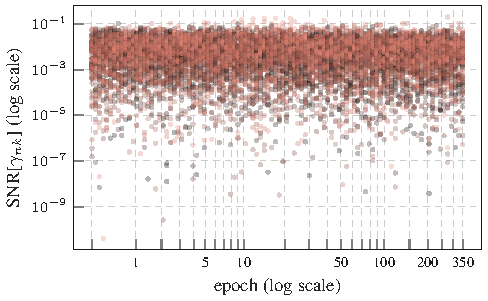
\includegraphics[width=\linewidth]{fig/exp13_plots/gammas_lambdas/cifar100_allcnnc_sgd_gammas.pdf}
    \end{minipage}\hfill
    \begin{minipage}{0.50\linewidth}
      \centering
      % % defines the pgfplots style "gammaslambdasdefault"
\pgfkeys{/pgfplots/gammaslambdasdefault/.style={
    width=1.0\linewidth,
    height=0.6\linewidth,
    every axis plot/.append style={line width = 1.5pt},
    mark size = 0.6,
    tick pos = left,
    ylabel near ticks,
    xlabel near ticks,
    xtick align = inside,
    ytick align = inside,
    legend cell align = left,
    legend columns = 1,
    legend pos = south east,
    legend style = {
      fill opacity = 0.7,
      text opacity = 1,
      font = \footnotesize,
    },
    xticklabel style = {font = \footnotesize},
    xlabel style = {font = \footnotesize},
    axis line style = {black},
    yticklabel style = {font = \footnotesize},
    ylabel style = {font = \footnotesize},
    title style = {font = \footnotesize},
    grid = major,
    grid style = {dashed}
  }
}
%%% Local Variables:
%%% mode: latex
%%% TeX-master: "../../thesis"
%%% End:

      % \pgfkeys{/pgfplots/zmystyle/.style={
      % gammaslambdasdefault
      % }}
      %   \tikzexternalenable
      %   NOTE: Too large. pdflatex will run out of memory during externalization
      %   % This file was created by tikzplotlib v0.9.7.
\begin{tikzpicture}

\begin{axis}[
axis line style={white!10!black},
log basis x={10},
tick pos=left,
xlabel={epoch (log scale)},
xmajorgrids,
xmin=0.746099240306814, xmax=469.106495613199,
xmode=log,
ylabel={SNR[\(\displaystyle \lambda_{nk}\)] (log scale)},
ymajorgrids,
ymin=0.00468108163876598, ymax=5122.44848080526,
ymode=log,
zmystyle
]
\addplot [
mark=*,
only marks,
scatter,
scatter/@post marker code/.code={%
  \endscope
},
scatter/@pre marker code/.code={%
  \expanded{%
  \noexpand\definecolor{thispointdrawcolor}{RGB}{\drawcolor}%
  \noexpand\definecolor{thispointfillcolor}{RGB}{\fillcolor}%
  }%
  \scope[draw=thispointdrawcolor, fill=thispointfillcolor]%
},
visualization depends on={value \thisrow{draw} \as \drawcolor},
visualization depends on={value \thisrow{fill} \as \fillcolor}
]
table{%
x  y  draw  fill
1 0.808994293212891 0,0,0 0,0,0
1 0.563908934593201 1.84313725490196,1.05882352941176,0.917647058823529 1.84313725490196,1.05882352941176,0.917647058823529
1 0.813127100467682 4.6078431372549,2.64705882352941,2.29411764705882 4.6078431372549,2.64705882352941,2.29411764705882
1 0.589056491851807 6.45098039215686,3.70588235294118,3.21176470588235 6.45098039215686,3.70588235294118,3.21176470588235
1 0.827552795410156 9.2156862745098,5.29411764705882,4.58823529411765 9.2156862745098,5.29411764705882,4.58823529411765
1 0.768382966518402 11.0588235294118,6.35294117647059,5.50588235294118 11.0588235294118,6.35294117647059,5.50588235294118
1 1.36948490142822 13.8235294117647,7.94117647058823,6.88235294117647 13.8235294117647,7.94117647058823,6.88235294117647
1 0.71027398109436 16.5882352941176,9.52941176470588,8.25882352941176 16.5882352941176,9.52941176470588,8.25882352941176
1 0.542422473430634 18.4313725490196,10.5882352941176,9.17647058823529 18.4313725490196,10.5882352941176,9.17647058823529
1 1.4381992816925 21.1960784313725,12.1764705882353,10.5529411764706 21.1960784313725,12.1764705882353,10.5529411764706
1 0.862465143203735 23.0392156862745,13.2352941176471,11.4705882352941 23.0392156862745,13.2352941176471,11.4705882352941
1 0.608683943748474 25.8039215686274,14.8235294117647,12.8470588235294 25.8039215686274,14.8235294117647,12.8470588235294
1 0.956924498081207 28.5686274509804,16.4117647058824,14.2235294117647 28.5686274509804,16.4117647058824,14.2235294117647
1 0.843901932239532 30.4117647058823,17.4705882352941,15.1411764705882 30.4117647058823,17.4705882352941,15.1411764705882
1 0.821968495845795 33.1764705882353,19.0588235294118,16.5176470588235 33.1764705882353,19.0588235294118,16.5176470588235
1 0.810039043426514 35.0196078431373,20.1176470588235,17.4352941176471 35.0196078431373,20.1176470588235,17.4352941176471
1 0.616682350635529 37.7843137254902,21.7058823529412,18.8117647058824 37.7843137254902,21.7058823529412,18.8117647058824
1 0.752242505550385 39.6274509803922,22.7647058823529,19.7294117647059 39.6274509803922,22.7647058823529,19.7294117647059
1 1.94454741477966 42.3921568627451,24.3529411764706,21.1058823529412 42.3921568627451,24.3529411764706,21.1058823529412
1 0.591163814067841 45.156862745098,25.9411764705882,22.4823529411765 45.156862745098,25.9411764705882,22.4823529411765
1 0.780003011226654 47,27,23.4 47,27,23.4
1 1.28690719604492 49.7647058823529,28.5882352941176,24.7764705882353 49.7647058823529,28.5882352941176,24.7764705882353
1 0.742906153202057 51.6078431372549,29.6470588235294,25.6941176470588 51.6078431372549,29.6470588235294,25.6941176470588
1 1.94534707069397 54.3725490196078,31.2352941176471,27.0705882352941 54.3725490196078,31.2352941176471,27.0705882352941
1 0.898939967155457 57.1372549019608,32.8235294117647,28.4470588235294 57.1372549019608,32.8235294117647,28.4470588235294
1 0.650392711162567 58.9803921568627,33.8823529411765,29.3647058823529 58.9803921568627,33.8823529411765,29.3647058823529
1 0.546567797660828 61.7450980392157,35.4705882352941,30.7411764705882 61.7450980392157,35.4705882352941,30.7411764705882
1 0.791007101535797 63.5882352941176,36.5294117647059,31.6588235294118 63.5882352941176,36.5294117647059,31.6588235294118
1 1.2445330619812 66.3529411764706,38.1176470588235,33.0352941176471 66.3529411764706,38.1176470588235,33.0352941176471
1 0.634105503559113 68.1960784313725,39.1764705882353,33.9529411764706 68.1960784313725,39.1764705882353,33.9529411764706
1 0.624742329120636 70.9607843137255,40.7647058823529,35.3294117647059 70.9607843137255,40.7647058823529,35.3294117647059
1 0.63439416885376 73.7254901960784,42.3529411764706,36.7058823529412 73.7254901960784,42.3529411764706,36.7058823529412
1 9.42076301574707 75.5686274509804,43.4117647058823,37.6235294117647 75.5686274509804,43.4117647058823,37.6235294117647
1 0.617523789405823 78.3333333333333,45,39 78.3333333333333,45,39
1 0.524870574474335 80.1764705882353,46.0588235294118,39.9176470588235 80.1764705882353,46.0588235294118,39.9176470588235
1 0.506676614284515 82.9411764705882,47.6470588235294,41.2941176470588 82.9411764705882,47.6470588235294,41.2941176470588
1 10.2818603515625 85.7058823529412,49.2352941176471,42.6705882352941 85.7058823529412,49.2352941176471,42.6705882352941
1 36.5568389892578 87.5490196078431,50.2941176470588,43.5882352941177 87.5490196078431,50.2941176470588,43.5882352941177
1 25.7533111572266 90.3137254901961,51.8823529411765,44.9647058823529 90.3137254901961,51.8823529411765,44.9647058823529
1 185.399032592773 92.156862745098,52.9411764705882,45.8823529411765 92.156862745098,52.9411764705882,45.8823529411765
1 758.512390136719 94.921568627451,54.5294117647059,47.2588235294118 94.921568627451,54.5294117647059,47.2588235294118
1 88.218132019043 97.6862745098039,56.1176470588235,48.635294117647 97.6862745098039,56.1176470588235,48.635294117647
1 394.449432373047 99.5294117647059,57.1764705882353,49.5529411764706 99.5294117647059,57.1764705882353,49.5529411764706
1 614.107299804688 102.294117647059,58.7647058823529,50.9294117647059 102.294117647059,58.7647058823529,50.9294117647059
1 221.549591064453 104.137254901961,59.8235294117647,51.8470588235294 104.137254901961,59.8235294117647,51.8470588235294
1 469.812164306641 106.901960784314,61.4117647058824,53.2235294117647 106.901960784314,61.4117647058824,53.2235294117647
1 726.306640625 108.745098039216,62.4705882352941,54.1411764705882 108.745098039216,62.4705882352941,54.1411764705882
1 1626.02722167969 111.509803921569,64.0588235294118,55.5176470588235 111.509803921569,64.0588235294118,55.5176470588235
1 910.588317871094 114.274509803922,65.6470588235294,56.8941176470588 114.274509803922,65.6470588235294,56.8941176470588
1 678.548645019531 116.117647058824,66.7058823529412,57.8117647058823 116.117647058824,66.7058823529412,57.8117647058823
1 950.266174316406 118.882352941176,68.2941176470588,59.1882352941176 118.882352941176,68.2941176470588,59.1882352941176
1 1157.06921386719 120.725490196078,69.3529411764706,60.1058823529412 120.725490196078,69.3529411764706,60.1058823529412
1 687.997924804688 123.490196078431,70.9411764705882,61.4823529411765 123.490196078431,70.9411764705882,61.4823529411765
1 1877.03161621094 126.254901960784,72.5294117647059,62.8588235294118 126.254901960784,72.5294117647059,62.8588235294118
1 1457.59130859375 128.098039215686,73.5882352941176,63.7764705882353 128.098039215686,73.5882352941176,63.7764705882353
1 830.036743164062 130.862745098039,75.1764705882353,65.1529411764706 130.862745098039,75.1764705882353,65.1529411764706
1 1049.26501464844 132.705882352941,76.2352941176471,66.0705882352941 132.705882352941,76.2352941176471,66.0705882352941
1 1274.33410644531 135.470588235294,77.8235294117647,67.4470588235294 135.470588235294,77.8235294117647,67.4470588235294
1 705.363647460938 137.313725490196,78.8823529411765,68.3647058823529 137.313725490196,78.8823529411765,68.3647058823529
1 1353.08374023438 140.078431372549,80.4705882352941,69.7411764705882 140.078431372549,80.4705882352941,69.7411764705882
1 994.206787109375 142.843137254902,82.0588235294118,71.1176470588235 142.843137254902,82.0588235294118,71.1176470588235
1 776.482788085938 144.686274509804,83.1176470588235,72.0352941176471 144.686274509804,83.1176470588235,72.0352941176471
1 711.322082519531 147.450980392157,84.7058823529412,73.4117647058823 147.450980392157,84.7058823529412,73.4117647058823
1 672.5888671875 149.294117647059,85.7647058823529,74.3294117647059 149.294117647059,85.7647058823529,74.3294117647059
1 1983.56860351562 152.058823529412,87.3529411764706,75.7058823529412 152.058823529412,87.3529411764706,75.7058823529412
1 843.3271484375 154.823529411765,88.9411764705882,77.0823529411765 154.823529411765,88.9411764705882,77.0823529411765
1 644.520446777344 156.666666666667,90,78 156.666666666667,90,78
1 1238.70166015625 159.43137254902,91.5882352941177,79.3764705882353 159.43137254902,91.5882352941177,79.3764705882353
1 362.113098144531 161.274509803922,92.6470588235294,80.2941176470588 161.274509803922,92.6470588235294,80.2941176470588
1 987.427429199219 164.039215686274,94.2352941176471,81.6705882352941 164.039215686274,94.2352941176471,81.6705882352941
1 899.133728027344 166.803921568627,95.8235294117647,83.0470588235294 166.803921568627,95.8235294117647,83.0470588235294
1 534.728698730469 168.647058823529,96.8823529411765,83.9647058823529 168.647058823529,96.8823529411765,83.9647058823529
1 392.879913330078 171.411764705882,98.4705882352941,85.3411764705882 171.411764705882,98.4705882352941,85.3411764705882
1 2057.1416015625 173.254901960784,99.5294117647059,86.2588235294118 173.254901960784,99.5294117647059,86.2588235294118
1 663.949462890625 176.019607843137,101.117647058824,87.6352941176471 176.019607843137,101.117647058824,87.6352941176471
1 1199.97912597656 177.862745098039,102.176470588235,88.5529411764706 177.862745098039,102.176470588235,88.5529411764706
1 1241.95568847656 180.627450980392,103.764705882353,89.9294117647059 180.627450980392,103.764705882353,89.9294117647059
1 953.24609375 183.392156862745,105.352941176471,91.3058823529412 183.392156862745,105.352941176471,91.3058823529412
1 1528.232421875 185.235294117647,106.411764705882,92.2235294117647 185.235294117647,106.411764705882,92.2235294117647
1 1372.8154296875 188,108,93.6 188,108,93.6
1 754.731750488281 189.843137254902,109.058823529412,94.5176470588235 189.843137254902,109.058823529412,94.5176470588235
1 868.9072265625 192.607843137255,110.647058823529,95.8941176470588 192.607843137255,110.647058823529,95.8941176470588
1 994.020385742188 195.372549019608,112.235294117647,97.2705882352941 195.372549019608,112.235294117647,97.2705882352941
1 761.520568847656 197.21568627451,113.294117647059,98.1882352941176 197.21568627451,113.294117647059,98.1882352941176
1 522.574890136719 199.980392156863,114.882352941176,99.5647058823529 199.980392156863,114.882352941176,99.5647058823529
1 943.716613769531 201.823529411765,115.941176470588,100.482352941176 201.823529411765,115.941176470588,100.482352941176
1 992.176696777344 204.588235294118,117.529411764706,101.858823529412 204.588235294118,117.529411764706,101.858823529412
1 996.417724609375 206.43137254902,118.588235294118,102.776470588235 206.43137254902,118.588235294118,102.776470588235
1 1168.04968261719 209.196078431373,120.176470588235,104.152941176471 209.196078431373,120.176470588235,104.152941176471
1 1505.39221191406 211.960784313725,121.764705882353,105.529411764706 211.960784313725,121.764705882353,105.529411764706
1 1188.90710449219 213.803921568627,122.823529411765,106.447058823529 213.803921568627,122.823529411765,106.447058823529
1 1141.71850585938 216.56862745098,124.411764705882,107.823529411765 216.56862745098,124.411764705882,107.823529411765
1 1148.02319335938 218.411764705882,125.470588235294,108.741176470588 218.411764705882,125.470588235294,108.741176470588
1 661.705444335938 221.176470588235,127.058823529412,110.117647058824 221.176470588235,127.058823529412,110.117647058824
1 952.605773925781 223.941176470588,128.647058823529,111.494117647059 223.941176470588,128.647058823529,111.494117647059
1 1027.205078125 225.78431372549,129.705882352941,112.411764705882 225.78431372549,129.705882352941,112.411764705882
1 855.072814941406 228.549019607843,131.294117647059,113.788235294118 228.549019607843,131.294117647059,113.788235294118
1 795.542419433594 230.392156862745,132.352941176471,114.705882352941 230.392156862745,132.352941176471,114.705882352941
1 826.18408203125 233.156862745098,133.941176470588,116.082352941176 233.156862745098,133.941176470588,116.082352941176
1 1014.36065673828 235,135,117 235,135,117
1.19230769230769 1.35795116424561 0,0,0 0,0,0
1.19230769230769 0.861963093280792 1.84313725490196,1.05882352941176,0.917647058823529 1.84313725490196,1.05882352941176,0.917647058823529
1.19230769230769 0.887554883956909 4.6078431372549,2.64705882352941,2.29411764705882 4.6078431372549,2.64705882352941,2.29411764705882
1.19230769230769 0.38072544336319 6.45098039215686,3.70588235294118,3.21176470588235 6.45098039215686,3.70588235294118,3.21176470588235
1.19230769230769 0.768184065818787 9.2156862745098,5.29411764705882,4.58823529411765 9.2156862745098,5.29411764705882,4.58823529411765
1.19230769230769 0.932542145252228 11.0588235294118,6.35294117647059,5.50588235294118 11.0588235294118,6.35294117647059,5.50588235294118
1.19230769230769 1.11487674713135 13.8235294117647,7.94117647058823,6.88235294117647 13.8235294117647,7.94117647058823,6.88235294117647
1.19230769230769 0.710956215858459 16.5882352941176,9.52941176470588,8.25882352941176 16.5882352941176,9.52941176470588,8.25882352941176
1.19230769230769 0.799950480461121 18.4313725490196,10.5882352941176,9.17647058823529 18.4313725490196,10.5882352941176,9.17647058823529
1.19230769230769 1.08285129070282 21.1960784313725,12.1764705882353,10.5529411764706 21.1960784313725,12.1764705882353,10.5529411764706
1.19230769230769 0.977025389671326 23.0392156862745,13.2352941176471,11.4705882352941 23.0392156862745,13.2352941176471,11.4705882352941
1.19230769230769 0.967946410179138 25.8039215686274,14.8235294117647,12.8470588235294 25.8039215686274,14.8235294117647,12.8470588235294
1.19230769230769 1.01523041725159 28.5686274509804,16.4117647058824,14.2235294117647 28.5686274509804,16.4117647058824,14.2235294117647
1.19230769230769 0.743030190467834 30.4117647058823,17.4705882352941,15.1411764705882 30.4117647058823,17.4705882352941,15.1411764705882
1.19230769230769 0.933668851852417 33.1764705882353,19.0588235294118,16.5176470588235 33.1764705882353,19.0588235294118,16.5176470588235
1.19230769230769 0.874017000198364 35.0196078431373,20.1176470588235,17.4352941176471 35.0196078431373,20.1176470588235,17.4352941176471
1.19230769230769 0.93651270866394 37.7843137254902,21.7058823529412,18.8117647058824 37.7843137254902,21.7058823529412,18.8117647058824
1.19230769230769 1.09835875034332 39.6274509803922,22.7647058823529,19.7294117647059 39.6274509803922,22.7647058823529,19.7294117647059
1.19230769230769 0.587191700935364 42.3921568627451,24.3529411764706,21.1058823529412 42.3921568627451,24.3529411764706,21.1058823529412
1.19230769230769 0.561335027217865 45.156862745098,25.9411764705882,22.4823529411765 45.156862745098,25.9411764705882,22.4823529411765
1.19230769230769 0.879558682441711 47,27,23.4 47,27,23.4
1.19230769230769 1.05321538448334 49.7647058823529,28.5882352941176,24.7764705882353 49.7647058823529,28.5882352941176,24.7764705882353
1.19230769230769 0.854389905929565 51.6078431372549,29.6470588235294,25.6941176470588 51.6078431372549,29.6470588235294,25.6941176470588
1.19230769230769 0.712514638900757 54.3725490196078,31.2352941176471,27.0705882352941 54.3725490196078,31.2352941176471,27.0705882352941
1.19230769230769 0.74808132648468 57.1372549019608,32.8235294117647,28.4470588235294 57.1372549019608,32.8235294117647,28.4470588235294
1.19230769230769 0.995623588562012 58.9803921568627,33.8823529411765,29.3647058823529 58.9803921568627,33.8823529411765,29.3647058823529
1.19230769230769 0.890311658382416 61.7450980392157,35.4705882352941,30.7411764705882 61.7450980392157,35.4705882352941,30.7411764705882
1.19230769230769 0.81850665807724 63.5882352941176,36.5294117647059,31.6588235294118 63.5882352941176,36.5294117647059,31.6588235294118
1.19230769230769 0.676484942436218 66.3529411764706,38.1176470588235,33.0352941176471 66.3529411764706,38.1176470588235,33.0352941176471
1.19230769230769 1.33132541179657 68.1960784313725,39.1764705882353,33.9529411764706 68.1960784313725,39.1764705882353,33.9529411764706
1.19230769230769 1.0765483379364 70.9607843137255,40.7647058823529,35.3294117647059 70.9607843137255,40.7647058823529,35.3294117647059
1.19230769230769 0.797456979751587 73.7254901960784,42.3529411764706,36.7058823529412 73.7254901960784,42.3529411764706,36.7058823529412
1.19230769230769 0.792668759822845 75.5686274509804,43.4117647058823,37.6235294117647 75.5686274509804,43.4117647058823,37.6235294117647
1.19230769230769 0.906218349933624 78.3333333333333,45,39 78.3333333333333,45,39
1.19230769230769 0.930460333824158 80.1764705882353,46.0588235294118,39.9176470588235 80.1764705882353,46.0588235294118,39.9176470588235
1.19230769230769 1.15001738071442 82.9411764705882,47.6470588235294,41.2941176470588 82.9411764705882,47.6470588235294,41.2941176470588
1.19230769230769 0.73034393787384 85.7058823529412,49.2352941176471,42.6705882352941 85.7058823529412,49.2352941176471,42.6705882352941
1.19230769230769 1.0525004863739 87.5490196078431,50.2941176470588,43.5882352941177 87.5490196078431,50.2941176470588,43.5882352941177
1.19230769230769 1.994744181633 90.3137254901961,51.8823529411765,44.9647058823529 90.3137254901961,51.8823529411765,44.9647058823529
1.19230769230769 1.9667934179306 92.156862745098,52.9411764705882,45.8823529411765 92.156862745098,52.9411764705882,45.8823529411765
1.19230769230769 1.66098582744598 94.921568627451,54.5294117647059,47.2588235294118 94.921568627451,54.5294117647059,47.2588235294118
1.19230769230769 0.785501897335052 97.6862745098039,56.1176470588235,48.635294117647 97.6862745098039,56.1176470588235,48.635294117647
1.19230769230769 0.864178061485291 99.5294117647059,57.1764705882353,49.5529411764706 99.5294117647059,57.1764705882353,49.5529411764706
1.19230769230769 1.81361603736877 102.294117647059,58.7647058823529,50.9294117647059 102.294117647059,58.7647058823529,50.9294117647059
1.19230769230769 6.40863037109375 104.137254901961,59.8235294117647,51.8470588235294 104.137254901961,59.8235294117647,51.8470588235294
1.19230769230769 2.331458568573 106.901960784314,61.4117647058824,53.2235294117647 106.901960784314,61.4117647058824,53.2235294117647
1.19230769230769 3.01337504386902 108.745098039216,62.4705882352941,54.1411764705882 108.745098039216,62.4705882352941,54.1411764705882
1.19230769230769 6.01915407180786 111.509803921569,64.0588235294118,55.5176470588235 111.509803921569,64.0588235294118,55.5176470588235
1.19230769230769 2.81303763389587 114.274509803922,65.6470588235294,56.8941176470588 114.274509803922,65.6470588235294,56.8941176470588
1.19230769230769 14.7338838577271 116.117647058824,66.7058823529412,57.8117647058823 116.117647058824,66.7058823529412,57.8117647058823
1.19230769230769 49.6594619750977 118.882352941176,68.2941176470588,59.1882352941176 118.882352941176,68.2941176470588,59.1882352941176
1.19230769230769 46.7768249511719 120.725490196078,69.3529411764706,60.1058823529412 120.725490196078,69.3529411764706,60.1058823529412
1.19230769230769 96.2994079589844 123.490196078431,70.9411764705882,61.4823529411765 123.490196078431,70.9411764705882,61.4823529411765
1.19230769230769 52.9707946777344 126.254901960784,72.5294117647059,62.8588235294118 126.254901960784,72.5294117647059,62.8588235294118
1.19230769230769 82.241584777832 128.098039215686,73.5882352941176,63.7764705882353 128.098039215686,73.5882352941176,63.7764705882353
1.19230769230769 206.9951171875 130.862745098039,75.1764705882353,65.1529411764706 130.862745098039,75.1764705882353,65.1529411764706
1.19230769230769 153.212677001953 132.705882352941,76.2352941176471,66.0705882352941 132.705882352941,76.2352941176471,66.0705882352941
1.19230769230769 427.731262207031 135.470588235294,77.8235294117647,67.4470588235294 135.470588235294,77.8235294117647,67.4470588235294
1.19230769230769 647.168395996094 137.313725490196,78.8823529411765,68.3647058823529 137.313725490196,78.8823529411765,68.3647058823529
1.19230769230769 634.480895996094 140.078431372549,80.4705882352941,69.7411764705882 140.078431372549,80.4705882352941,69.7411764705882
1.19230769230769 309.228057861328 142.843137254902,82.0588235294118,71.1176470588235 142.843137254902,82.0588235294118,71.1176470588235
1.19230769230769 317.804138183594 144.686274509804,83.1176470588235,72.0352941176471 144.686274509804,83.1176470588235,72.0352941176471
1.19230769230769 582.809265136719 147.450980392157,84.7058823529412,73.4117647058823 147.450980392157,84.7058823529412,73.4117647058823
1.19230769230769 701.812622070312 149.294117647059,85.7647058823529,74.3294117647059 149.294117647059,85.7647058823529,74.3294117647059
1.19230769230769 148.556411743164 152.058823529412,87.3529411764706,75.7058823529412 152.058823529412,87.3529411764706,75.7058823529412
1.19230769230769 97.5665969848633 154.823529411765,88.9411764705882,77.0823529411765 154.823529411765,88.9411764705882,77.0823529411765
1.19230769230769 205.812622070312 156.666666666667,90,78 156.666666666667,90,78
1.19230769230769 1149.86853027344 159.43137254902,91.5882352941177,79.3764705882353 159.43137254902,91.5882352941177,79.3764705882353
1.19230769230769 508.743927001953 161.274509803922,92.6470588235294,80.2941176470588 161.274509803922,92.6470588235294,80.2941176470588
1.19230769230769 175.718475341797 164.039215686274,94.2352941176471,81.6705882352941 164.039215686274,94.2352941176471,81.6705882352941
1.19230769230769 1123.78796386719 166.803921568627,95.8235294117647,83.0470588235294 166.803921568627,95.8235294117647,83.0470588235294
1.19230769230769 624.693359375 168.647058823529,96.8823529411765,83.9647058823529 168.647058823529,96.8823529411765,83.9647058823529
1.19230769230769 1353.26989746094 171.411764705882,98.4705882352941,85.3411764705882 171.411764705882,98.4705882352941,85.3411764705882
1.19230769230769 365.982727050781 173.254901960784,99.5294117647059,86.2588235294118 173.254901960784,99.5294117647059,86.2588235294118
1.19230769230769 156.559539794922 176.019607843137,101.117647058824,87.6352941176471 176.019607843137,101.117647058824,87.6352941176471
1.19230769230769 466.777801513672 177.862745098039,102.176470588235,88.5529411764706 177.862745098039,102.176470588235,88.5529411764706
1.19230769230769 217.713928222656 180.627450980392,103.764705882353,89.9294117647059 180.627450980392,103.764705882353,89.9294117647059
1.19230769230769 740.797302246094 183.392156862745,105.352941176471,91.3058823529412 183.392156862745,105.352941176471,91.3058823529412
1.19230769230769 1254.89636230469 185.235294117647,106.411764705882,92.2235294117647 185.235294117647,106.411764705882,92.2235294117647
1.19230769230769 996.719970703125 188,108,93.6 188,108,93.6
1.19230769230769 332.303253173828 189.843137254902,109.058823529412,94.5176470588235 189.843137254902,109.058823529412,94.5176470588235
1.19230769230769 1281.982421875 192.607843137255,110.647058823529,95.8941176470588 192.607843137255,110.647058823529,95.8941176470588
1.19230769230769 687.307861328125 195.372549019608,112.235294117647,97.2705882352941 195.372549019608,112.235294117647,97.2705882352941
1.19230769230769 443.59228515625 197.21568627451,113.294117647059,98.1882352941176 197.21568627451,113.294117647059,98.1882352941176
1.19230769230769 1594.48132324219 199.980392156863,114.882352941176,99.5647058823529 199.980392156863,114.882352941176,99.5647058823529
1.19230769230769 570.084777832031 201.823529411765,115.941176470588,100.482352941176 201.823529411765,115.941176470588,100.482352941176
1.19230769230769 1204.00671386719 204.588235294118,117.529411764706,101.858823529412 204.588235294118,117.529411764706,101.858823529412
1.19230769230769 2722.5234375 206.43137254902,118.588235294118,102.776470588235 206.43137254902,118.588235294118,102.776470588235
1.19230769230769 525.426208496094 209.196078431373,120.176470588235,104.152941176471 209.196078431373,120.176470588235,104.152941176471
1.19230769230769 927.635986328125 211.960784313725,121.764705882353,105.529411764706 211.960784313725,121.764705882353,105.529411764706
1.19230769230769 686.906799316406 213.803921568627,122.823529411765,106.447058823529 213.803921568627,122.823529411765,106.447058823529
1.19230769230769 582.556701660156 216.56862745098,124.411764705882,107.823529411765 216.56862745098,124.411764705882,107.823529411765
1.19230769230769 459.742401123047 218.411764705882,125.470588235294,108.741176470588 218.411764705882,125.470588235294,108.741176470588
1.19230769230769 461.623138427734 221.176470588235,127.058823529412,110.117647058824 221.176470588235,127.058823529412,110.117647058824
1.19230769230769 1118.41943359375 223.941176470588,128.647058823529,111.494117647059 223.941176470588,128.647058823529,111.494117647059
1.19230769230769 538.9248046875 225.78431372549,129.705882352941,112.411764705882 225.78431372549,129.705882352941,112.411764705882
1.19230769230769 2069.41650390625 228.549019607843,131.294117647059,113.788235294118 228.549019607843,131.294117647059,113.788235294118
1.19230769230769 320.65478515625 230.392156862745,132.352941176471,114.705882352941 230.392156862745,132.352941176471,114.705882352941
1.19230769230769 375.479034423828 233.156862745098,133.941176470588,116.082352941176 233.156862745098,133.941176470588,116.082352941176
1.19230769230769 483.768524169922 235,135,117 235,135,117
1.42307692307692 1.95500230789185 0,0,0 0,0,0
1.42307692307692 1.97958838939667 1.84313725490196,1.05882352941176,0.917647058823529 1.84313725490196,1.05882352941176,0.917647058823529
1.42307692307692 1.01119780540466 4.6078431372549,2.64705882352941,2.29411764705882 4.6078431372549,2.64705882352941,2.29411764705882
1.42307692307692 0.918121039867401 6.45098039215686,3.70588235294118,3.21176470588235 6.45098039215686,3.70588235294118,3.21176470588235
1.42307692307692 2.89300799369812 9.2156862745098,5.29411764705882,4.58823529411765 9.2156862745098,5.29411764705882,4.58823529411765
1.42307692307692 1.57716012001038 11.0588235294118,6.35294117647059,5.50588235294118 11.0588235294118,6.35294117647059,5.50588235294118
1.42307692307692 3.00442910194397 13.8235294117647,7.94117647058823,6.88235294117647 13.8235294117647,7.94117647058823,6.88235294117647
1.42307692307692 0.664495646953583 16.5882352941176,9.52941176470588,8.25882352941176 16.5882352941176,9.52941176470588,8.25882352941176
1.42307692307692 0.534196138381958 18.4313725490196,10.5882352941176,9.17647058823529 18.4313725490196,10.5882352941176,9.17647058823529
1.42307692307692 1.14181804656982 21.1960784313725,12.1764705882353,10.5529411764706 21.1960784313725,12.1764705882353,10.5529411764706
1.42307692307692 2.64451122283936 23.0392156862745,13.2352941176471,11.4705882352941 23.0392156862745,13.2352941176471,11.4705882352941
1.42307692307692 1.08156192302704 25.8039215686274,14.8235294117647,12.8470588235294 25.8039215686274,14.8235294117647,12.8470588235294
1.42307692307692 1.69971799850464 28.5686274509804,16.4117647058824,14.2235294117647 28.5686274509804,16.4117647058824,14.2235294117647
1.42307692307692 2.72180247306824 30.4117647058823,17.4705882352941,15.1411764705882 30.4117647058823,17.4705882352941,15.1411764705882
1.42307692307692 2.77368783950806 33.1764705882353,19.0588235294118,16.5176470588235 33.1764705882353,19.0588235294118,16.5176470588235
1.42307692307692 1.26712012290955 35.0196078431373,20.1176470588235,17.4352941176471 35.0196078431373,20.1176470588235,17.4352941176471
1.42307692307692 2.60721206665039 37.7843137254902,21.7058823529412,18.8117647058824 37.7843137254902,21.7058823529412,18.8117647058824
1.42307692307692 1.8559707403183 39.6274509803922,22.7647058823529,19.7294117647059 39.6274509803922,22.7647058823529,19.7294117647059
1.42307692307692 3.72987341880798 42.3921568627451,24.3529411764706,21.1058823529412 42.3921568627451,24.3529411764706,21.1058823529412
1.42307692307692 3.05734825134277 45.156862745098,25.9411764705882,22.4823529411765 45.156862745098,25.9411764705882,22.4823529411765
1.42307692307692 0.979347288608551 47,27,23.4 47,27,23.4
1.42307692307692 2.72672176361084 49.7647058823529,28.5882352941176,24.7764705882353 49.7647058823529,28.5882352941176,24.7764705882353
1.42307692307692 2.68520259857178 51.6078431372549,29.6470588235294,25.6941176470588 51.6078431372549,29.6470588235294,25.6941176470588
1.42307692307692 2.22483420372009 54.3725490196078,31.2352941176471,27.0705882352941 54.3725490196078,31.2352941176471,27.0705882352941
1.42307692307692 2.1756751537323 57.1372549019608,32.8235294117647,28.4470588235294 57.1372549019608,32.8235294117647,28.4470588235294
1.42307692307692 3.05267930030823 58.9803921568627,33.8823529411765,29.3647058823529 58.9803921568627,33.8823529411765,29.3647058823529
1.42307692307692 1.45364677906036 61.7450980392157,35.4705882352941,30.7411764705882 61.7450980392157,35.4705882352941,30.7411764705882
1.42307692307692 2.05835127830505 63.5882352941176,36.5294117647059,31.6588235294118 63.5882352941176,36.5294117647059,31.6588235294118
1.42307692307692 2.90008926391602 66.3529411764706,38.1176470588235,33.0352941176471 66.3529411764706,38.1176470588235,33.0352941176471
1.42307692307692 2.22300863265991 68.1960784313725,39.1764705882353,33.9529411764706 68.1960784313725,39.1764705882353,33.9529411764706
1.42307692307692 1.84130311012268 70.9607843137255,40.7647058823529,35.3294117647059 70.9607843137255,40.7647058823529,35.3294117647059
1.42307692307692 3.46012377738953 73.7254901960784,42.3529411764706,36.7058823529412 73.7254901960784,42.3529411764706,36.7058823529412
1.42307692307692 2.53142738342285 75.5686274509804,43.4117647058823,37.6235294117647 75.5686274509804,43.4117647058823,37.6235294117647
1.42307692307692 2.32749962806702 78.3333333333333,45,39 78.3333333333333,45,39
1.42307692307692 2.46534943580627 80.1764705882353,46.0588235294118,39.9176470588235 80.1764705882353,46.0588235294118,39.9176470588235
1.42307692307692 1.54808366298676 82.9411764705882,47.6470588235294,41.2941176470588 82.9411764705882,47.6470588235294,41.2941176470588
1.42307692307692 1.17471885681152 85.7058823529412,49.2352941176471,42.6705882352941 85.7058823529412,49.2352941176471,42.6705882352941
1.42307692307692 1.81684756278992 87.5490196078431,50.2941176470588,43.5882352941177 87.5490196078431,50.2941176470588,43.5882352941177
1.42307692307692 2.71103072166443 90.3137254901961,51.8823529411765,44.9647058823529 90.3137254901961,51.8823529411765,44.9647058823529
1.42307692307692 3.41397857666016 92.156862745098,52.9411764705882,45.8823529411765 92.156862745098,52.9411764705882,45.8823529411765
1.42307692307692 1.19526755809784 94.921568627451,54.5294117647059,47.2588235294118 94.921568627451,54.5294117647059,47.2588235294118
1.42307692307692 2.68954014778137 97.6862745098039,56.1176470588235,48.635294117647 97.6862745098039,56.1176470588235,48.635294117647
1.42307692307692 1.445955991745 99.5294117647059,57.1764705882353,49.5529411764706 99.5294117647059,57.1764705882353,49.5529411764706
1.42307692307692 3.37250065803528 102.294117647059,58.7647058823529,50.9294117647059 102.294117647059,58.7647058823529,50.9294117647059
1.42307692307692 2.88310217857361 104.137254901961,59.8235294117647,51.8470588235294 104.137254901961,59.8235294117647,51.8470588235294
1.42307692307692 0.695406556129456 106.901960784314,61.4117647058824,53.2235294117647 106.901960784314,61.4117647058824,53.2235294117647
1.42307692307692 2.68252611160278 108.745098039216,62.4705882352941,54.1411764705882 108.745098039216,62.4705882352941,54.1411764705882
1.42307692307692 1.90335047245026 111.509803921569,64.0588235294118,55.5176470588235 111.509803921569,64.0588235294118,55.5176470588235
1.42307692307692 2.99896621704102 114.274509803922,65.6470588235294,56.8941176470588 114.274509803922,65.6470588235294,56.8941176470588
1.42307692307692 2.9799587726593 116.117647058824,66.7058823529412,57.8117647058823 116.117647058824,66.7058823529412,57.8117647058823
1.42307692307692 2.84432911872864 118.882352941176,68.2941176470588,59.1882352941176 118.882352941176,68.2941176470588,59.1882352941176
1.42307692307692 2.75891423225403 120.725490196078,69.3529411764706,60.1058823529412 120.725490196078,69.3529411764706,60.1058823529412
1.42307692307692 1.90679514408112 123.490196078431,70.9411764705882,61.4823529411765 123.490196078431,70.9411764705882,61.4823529411765
1.42307692307692 1.55951321125031 126.254901960784,72.5294117647059,62.8588235294118 126.254901960784,72.5294117647059,62.8588235294118
1.42307692307692 1.03569459915161 128.098039215686,73.5882352941176,63.7764705882353 128.098039215686,73.5882352941176,63.7764705882353
1.42307692307692 1.66322338581085 130.862745098039,75.1764705882353,65.1529411764706 130.862745098039,75.1764705882353,65.1529411764706
1.42307692307692 1.94845032691956 132.705882352941,76.2352941176471,66.0705882352941 132.705882352941,76.2352941176471,66.0705882352941
1.42307692307692 2.13350486755371 135.470588235294,77.8235294117647,67.4470588235294 135.470588235294,77.8235294117647,67.4470588235294
1.42307692307692 2.23129296302795 137.313725490196,78.8823529411765,68.3647058823529 137.313725490196,78.8823529411765,68.3647058823529
1.42307692307692 1.93633544445038 140.078431372549,80.4705882352941,69.7411764705882 140.078431372549,80.4705882352941,69.7411764705882
1.42307692307692 3.22651863098145 142.843137254902,82.0588235294118,71.1176470588235 142.843137254902,82.0588235294118,71.1176470588235
1.42307692307692 2.93561863899231 144.686274509804,83.1176470588235,72.0352941176471 144.686274509804,83.1176470588235,72.0352941176471
1.42307692307692 2.80649280548096 147.450980392157,84.7058823529412,73.4117647058823 147.450980392157,84.7058823529412,73.4117647058823
1.42307692307692 2.76833772659302 149.294117647059,85.7647058823529,74.3294117647059 149.294117647059,85.7647058823529,74.3294117647059
1.42307692307692 2.11470723152161 152.058823529412,87.3529411764706,75.7058823529412 152.058823529412,87.3529411764706,75.7058823529412
1.42307692307692 1.4251366853714 154.823529411765,88.9411764705882,77.0823529411765 154.823529411765,88.9411764705882,77.0823529411765
1.42307692307692 1.47124779224396 156.666666666667,90,78 156.666666666667,90,78
1.42307692307692 1.20716917514801 159.43137254902,91.5882352941177,79.3764705882353 159.43137254902,91.5882352941177,79.3764705882353
1.42307692307692 1.6900839805603 161.274509803922,92.6470588235294,80.2941176470588 161.274509803922,92.6470588235294,80.2941176470588
1.42307692307692 2.01030468940735 164.039215686274,94.2352941176471,81.6705882352941 164.039215686274,94.2352941176471,81.6705882352941
1.42307692307692 3.0494236946106 166.803921568627,95.8235294117647,83.0470588235294 166.803921568627,95.8235294117647,83.0470588235294
1.42307692307692 0.887331366539001 168.647058823529,96.8823529411765,83.9647058823529 168.647058823529,96.8823529411765,83.9647058823529
1.42307692307692 1.49102354049683 171.411764705882,98.4705882352941,85.3411764705882 171.411764705882,98.4705882352941,85.3411764705882
1.42307692307692 2.08537364006042 173.254901960784,99.5294117647059,86.2588235294118 173.254901960784,99.5294117647059,86.2588235294118
1.42307692307692 3.81161069869995 176.019607843137,101.117647058824,87.6352941176471 176.019607843137,101.117647058824,87.6352941176471
1.42307692307692 1.04114866256714 177.862745098039,102.176470588235,88.5529411764706 177.862745098039,102.176470588235,88.5529411764706
1.42307692307692 2.20918250083923 180.627450980392,103.764705882353,89.9294117647059 180.627450980392,103.764705882353,89.9294117647059
1.42307692307692 2.47986054420471 183.392156862745,105.352941176471,91.3058823529412 183.392156862745,105.352941176471,91.3058823529412
1.42307692307692 1.01697313785553 185.235294117647,106.411764705882,92.2235294117647 185.235294117647,106.411764705882,92.2235294117647
1.42307692307692 2.37450861930847 188,108,93.6 188,108,93.6
1.42307692307692 4.02119064331055 189.843137254902,109.058823529412,94.5176470588235 189.843137254902,109.058823529412,94.5176470588235
1.42307692307692 1.58437061309814 192.607843137255,110.647058823529,95.8941176470588 192.607843137255,110.647058823529,95.8941176470588
1.42307692307692 3.0922679901123 195.372549019608,112.235294117647,97.2705882352941 195.372549019608,112.235294117647,97.2705882352941
1.42307692307692 4.23567342758179 197.21568627451,113.294117647059,98.1882352941176 197.21568627451,113.294117647059,98.1882352941176
1.42307692307692 1.4503800868988 199.980392156863,114.882352941176,99.5647058823529 199.980392156863,114.882352941176,99.5647058823529
1.42307692307692 2.26696348190308 201.823529411765,115.941176470588,100.482352941176 201.823529411765,115.941176470588,100.482352941176
1.42307692307692 3.05585360527039 204.588235294118,117.529411764706,101.858823529412 204.588235294118,117.529411764706,101.858823529412
1.42307692307692 0.985864758491516 206.43137254902,118.588235294118,102.776470588235 206.43137254902,118.588235294118,102.776470588235
1.42307692307692 1.82661688327789 209.196078431373,120.176470588235,104.152941176471 209.196078431373,120.176470588235,104.152941176471
1.42307692307692 0.783476054668427 211.960784313725,121.764705882353,105.529411764706 211.960784313725,121.764705882353,105.529411764706
1.42307692307692 1.42727982997894 213.803921568627,122.823529411765,106.447058823529 213.803921568627,122.823529411765,106.447058823529
1.42307692307692 5.14067268371582 216.56862745098,124.411764705882,107.823529411765 216.56862745098,124.411764705882,107.823529411765
1.42307692307692 0.983465313911438 218.411764705882,125.470588235294,108.741176470588 218.411764705882,125.470588235294,108.741176470588
1.42307692307692 4.17053174972534 221.176470588235,127.058823529412,110.117647058824 221.176470588235,127.058823529412,110.117647058824
1.42307692307692 0.80049455165863 223.941176470588,128.647058823529,111.494117647059 223.941176470588,128.647058823529,111.494117647059
1.42307692307692 0.736178815364838 225.78431372549,129.705882352941,112.411764705882 225.78431372549,129.705882352941,112.411764705882
1.42307692307692 4.08781003952026 228.549019607843,131.294117647059,113.788235294118 228.549019607843,131.294117647059,113.788235294118
1.42307692307692 2.42778301239014 230.392156862745,132.352941176471,114.705882352941 230.392156862745,132.352941176471,114.705882352941
1.42307692307692 0.791079998016357 233.156862745098,133.941176470588,116.082352941176 233.156862745098,133.941176470588,116.082352941176
1.42307692307692 1.96663618087769 235,135,117 235,135,117
1.69871794871795 1.59114229679108 0,0,0 0,0,0
1.69871794871795 1.50904047489166 1.84313725490196,1.05882352941176,0.917647058823529 1.84313725490196,1.05882352941176,0.917647058823529
1.69871794871795 1.46214306354523 4.6078431372549,2.64705882352941,2.29411764705882 4.6078431372549,2.64705882352941,2.29411764705882
1.69871794871795 1.28550446033478 6.45098039215686,3.70588235294118,3.21176470588235 6.45098039215686,3.70588235294118,3.21176470588235
1.69871794871795 1.07023215293884 9.2156862745098,5.29411764705882,4.58823529411765 9.2156862745098,5.29411764705882,4.58823529411765
1.69871794871795 1.54152762889862 11.0588235294118,6.35294117647059,5.50588235294118 11.0588235294118,6.35294117647059,5.50588235294118
1.69871794871795 1.54752588272095 13.8235294117647,7.94117647058823,6.88235294117647 13.8235294117647,7.94117647058823,6.88235294117647
1.69871794871795 2.01133728027344 16.5882352941176,9.52941176470588,8.25882352941176 16.5882352941176,9.52941176470588,8.25882352941176
1.69871794871795 2.35897350311279 18.4313725490196,10.5882352941176,9.17647058823529 18.4313725490196,10.5882352941176,9.17647058823529
1.69871794871795 1.27753567695618 21.1960784313725,12.1764705882353,10.5529411764706 21.1960784313725,12.1764705882353,10.5529411764706
1.69871794871795 1.83866667747498 23.0392156862745,13.2352941176471,11.4705882352941 23.0392156862745,13.2352941176471,11.4705882352941
1.69871794871795 1.55845248699188 25.8039215686274,14.8235294117647,12.8470588235294 25.8039215686274,14.8235294117647,12.8470588235294
1.69871794871795 1.193399310112 28.5686274509804,16.4117647058824,14.2235294117647 28.5686274509804,16.4117647058824,14.2235294117647
1.69871794871795 1.61564540863037 30.4117647058823,17.4705882352941,15.1411764705882 30.4117647058823,17.4705882352941,15.1411764705882
1.69871794871795 1.13760876655579 33.1764705882353,19.0588235294118,16.5176470588235 33.1764705882353,19.0588235294118,16.5176470588235
1.69871794871795 1.37241280078888 35.0196078431373,20.1176470588235,17.4352941176471 35.0196078431373,20.1176470588235,17.4352941176471
1.69871794871795 1.85603559017181 37.7843137254902,21.7058823529412,18.8117647058824 37.7843137254902,21.7058823529412,18.8117647058824
1.69871794871795 0.700679957866669 39.6274509803922,22.7647058823529,19.7294117647059 39.6274509803922,22.7647058823529,19.7294117647059
1.69871794871795 1.4152090549469 42.3921568627451,24.3529411764706,21.1058823529412 42.3921568627451,24.3529411764706,21.1058823529412
1.69871794871795 1.1916366815567 45.156862745098,25.9411764705882,22.4823529411765 45.156862745098,25.9411764705882,22.4823529411765
1.69871794871795 2.11880302429199 47,27,23.4 47,27,23.4
1.69871794871795 1.43943750858307 49.7647058823529,28.5882352941176,24.7764705882353 49.7647058823529,28.5882352941176,24.7764705882353
1.69871794871795 1.4885185956955 51.6078431372549,29.6470588235294,25.6941176470588 51.6078431372549,29.6470588235294,25.6941176470588
1.69871794871795 1.15400040149689 54.3725490196078,31.2352941176471,27.0705882352941 54.3725490196078,31.2352941176471,27.0705882352941
1.69871794871795 0.847138047218323 57.1372549019608,32.8235294117647,28.4470588235294 57.1372549019608,32.8235294117647,28.4470588235294
1.69871794871795 1.63774144649506 58.9803921568627,33.8823529411765,29.3647058823529 58.9803921568627,33.8823529411765,29.3647058823529
1.69871794871795 1.89625442028046 61.7450980392157,35.4705882352941,30.7411764705882 61.7450980392157,35.4705882352941,30.7411764705882
1.69871794871795 1.38270342350006 63.5882352941176,36.5294117647059,31.6588235294118 63.5882352941176,36.5294117647059,31.6588235294118
1.69871794871795 2.89057350158691 66.3529411764706,38.1176470588235,33.0352941176471 66.3529411764706,38.1176470588235,33.0352941176471
1.69871794871795 0.826105535030365 68.1960784313725,39.1764705882353,33.9529411764706 68.1960784313725,39.1764705882353,33.9529411764706
1.69871794871795 0.845798552036285 70.9607843137255,40.7647058823529,35.3294117647059 70.9607843137255,40.7647058823529,35.3294117647059
1.69871794871795 1.06245040893555 73.7254901960784,42.3529411764706,36.7058823529412 73.7254901960784,42.3529411764706,36.7058823529412
1.69871794871795 1.64059281349182 75.5686274509804,43.4117647058823,37.6235294117647 75.5686274509804,43.4117647058823,37.6235294117647
1.69871794871795 2.10653376579285 78.3333333333333,45,39 78.3333333333333,45,39
1.69871794871795 0.649454832077026 80.1764705882353,46.0588235294118,39.9176470588235 80.1764705882353,46.0588235294118,39.9176470588235
1.69871794871795 1.31099188327789 82.9411764705882,47.6470588235294,41.2941176470588 82.9411764705882,47.6470588235294,41.2941176470588
1.69871794871795 0.908090054988861 85.7058823529412,49.2352941176471,42.6705882352941 85.7058823529412,49.2352941176471,42.6705882352941
1.69871794871795 1.8677339553833 87.5490196078431,50.2941176470588,43.5882352941177 87.5490196078431,50.2941176470588,43.5882352941177
1.69871794871795 0.650914072990417 90.3137254901961,51.8823529411765,44.9647058823529 90.3137254901961,51.8823529411765,44.9647058823529
1.69871794871795 1.47344362735748 92.156862745098,52.9411764705882,45.8823529411765 92.156862745098,52.9411764705882,45.8823529411765
1.69871794871795 1.11100494861603 94.921568627451,54.5294117647059,47.2588235294118 94.921568627451,54.5294117647059,47.2588235294118
1.69871794871795 1.32842433452606 97.6862745098039,56.1176470588235,48.635294117647 97.6862745098039,56.1176470588235,48.635294117647
1.69871794871795 1.08500707149506 99.5294117647059,57.1764705882353,49.5529411764706 99.5294117647059,57.1764705882353,49.5529411764706
1.69871794871795 1.38428342342377 102.294117647059,58.7647058823529,50.9294117647059 102.294117647059,58.7647058823529,50.9294117647059
1.69871794871795 1.05267322063446 104.137254901961,59.8235294117647,51.8470588235294 104.137254901961,59.8235294117647,51.8470588235294
1.69871794871795 1.66592943668365 106.901960784314,61.4117647058824,53.2235294117647 106.901960784314,61.4117647058824,53.2235294117647
1.69871794871795 1.89472508430481 108.745098039216,62.4705882352941,54.1411764705882 108.745098039216,62.4705882352941,54.1411764705882
1.69871794871795 1.78624224662781 111.509803921569,64.0588235294118,55.5176470588235 111.509803921569,64.0588235294118,55.5176470588235
1.69871794871795 0.858914613723755 114.274509803922,65.6470588235294,56.8941176470588 114.274509803922,65.6470588235294,56.8941176470588
1.69871794871795 1.63415420055389 116.117647058824,66.7058823529412,57.8117647058823 116.117647058824,66.7058823529412,57.8117647058823
1.69871794871795 2.3330180644989 118.882352941176,68.2941176470588,59.1882352941176 118.882352941176,68.2941176470588,59.1882352941176
1.69871794871795 2.1323938369751 120.725490196078,69.3529411764706,60.1058823529412 120.725490196078,69.3529411764706,60.1058823529412
1.69871794871795 1.29541087150574 123.490196078431,70.9411764705882,61.4823529411765 123.490196078431,70.9411764705882,61.4823529411765
1.69871794871795 1.70677840709686 126.254901960784,72.5294117647059,62.8588235294118 126.254901960784,72.5294117647059,62.8588235294118
1.69871794871795 0.743664979934692 128.098039215686,73.5882352941176,63.7764705882353 128.098039215686,73.5882352941176,63.7764705882353
1.69871794871795 0.838493824005127 130.862745098039,75.1764705882353,65.1529411764706 130.862745098039,75.1764705882353,65.1529411764706
1.69871794871795 2.09750390052795 132.705882352941,76.2352941176471,66.0705882352941 132.705882352941,76.2352941176471,66.0705882352941
1.69871794871795 1.03264570236206 135.470588235294,77.8235294117647,67.4470588235294 135.470588235294,77.8235294117647,67.4470588235294
1.69871794871795 1.64630997180939 137.313725490196,78.8823529411765,68.3647058823529 137.313725490196,78.8823529411765,68.3647058823529
1.69871794871795 0.965422809123993 140.078431372549,80.4705882352941,69.7411764705882 140.078431372549,80.4705882352941,69.7411764705882
1.69871794871795 0.634972333908081 142.843137254902,82.0588235294118,71.1176470588235 142.843137254902,82.0588235294118,71.1176470588235
1.69871794871795 2.09379243850708 144.686274509804,83.1176470588235,72.0352941176471 144.686274509804,83.1176470588235,72.0352941176471
1.69871794871795 0.638284683227539 147.450980392157,84.7058823529412,73.4117647058823 147.450980392157,84.7058823529412,73.4117647058823
1.69871794871795 1.70084691047668 149.294117647059,85.7647058823529,74.3294117647059 149.294117647059,85.7647058823529,74.3294117647059
1.69871794871795 1.14633226394653 152.058823529412,87.3529411764706,75.7058823529412 152.058823529412,87.3529411764706,75.7058823529412
1.69871794871795 0.494609177112579 154.823529411765,88.9411764705882,77.0823529411765 154.823529411765,88.9411764705882,77.0823529411765
1.69871794871795 0.642041325569153 156.666666666667,90,78 156.666666666667,90,78
1.69871794871795 0.576003074645996 159.43137254902,91.5882352941177,79.3764705882353 159.43137254902,91.5882352941177,79.3764705882353
1.69871794871795 1.04582226276398 161.274509803922,92.6470588235294,80.2941176470588 161.274509803922,92.6470588235294,80.2941176470588
1.69871794871795 0.639006614685059 164.039215686274,94.2352941176471,81.6705882352941 164.039215686274,94.2352941176471,81.6705882352941
1.69871794871795 2.13318371772766 166.803921568627,95.8235294117647,83.0470588235294 166.803921568627,95.8235294117647,83.0470588235294
1.69871794871795 1.13682842254639 168.647058823529,96.8823529411765,83.9647058823529 168.647058823529,96.8823529411765,83.9647058823529
1.69871794871795 1.28917813301086 171.411764705882,98.4705882352941,85.3411764705882 171.411764705882,98.4705882352941,85.3411764705882
1.69871794871795 0.87633341550827 173.254901960784,99.5294117647059,86.2588235294118 173.254901960784,99.5294117647059,86.2588235294118
1.69871794871795 1.52718925476074 176.019607843137,101.117647058824,87.6352941176471 176.019607843137,101.117647058824,87.6352941176471
1.69871794871795 0.504923224449158 177.862745098039,102.176470588235,88.5529411764706 177.862745098039,102.176470588235,88.5529411764706
1.69871794871795 1.10562014579773 180.627450980392,103.764705882353,89.9294117647059 180.627450980392,103.764705882353,89.9294117647059
1.69871794871795 0.77761310338974 183.392156862745,105.352941176471,91.3058823529412 183.392156862745,105.352941176471,91.3058823529412
1.69871794871795 0.78270560503006 185.235294117647,106.411764705882,92.2235294117647 185.235294117647,106.411764705882,92.2235294117647
1.69871794871795 0.842667698860168 188,108,93.6 188,108,93.6
1.69871794871795 0.416043072938919 189.843137254902,109.058823529412,94.5176470588235 189.843137254902,109.058823529412,94.5176470588235
1.69871794871795 0.960135996341705 192.607843137255,110.647058823529,95.8941176470588 192.607843137255,110.647058823529,95.8941176470588
1.69871794871795 1.51381802558899 195.372549019608,112.235294117647,97.2705882352941 195.372549019608,112.235294117647,97.2705882352941
1.69871794871795 1.48356342315674 197.21568627451,113.294117647059,98.1882352941176 197.21568627451,113.294117647059,98.1882352941176
1.69871794871795 0.977357923984528 199.980392156863,114.882352941176,99.5647058823529 199.980392156863,114.882352941176,99.5647058823529
1.69871794871795 1.71724879741669 201.823529411765,115.941176470588,100.482352941176 201.823529411765,115.941176470588,100.482352941176
1.69871794871795 1.1982353925705 204.588235294118,117.529411764706,101.858823529412 204.588235294118,117.529411764706,101.858823529412
1.69871794871795 0.342007458209991 206.43137254902,118.588235294118,102.776470588235 206.43137254902,118.588235294118,102.776470588235
1.69871794871795 0.837144494056702 209.196078431373,120.176470588235,104.152941176471 209.196078431373,120.176470588235,104.152941176471
1.69871794871795 0.943689525127411 211.960784313725,121.764705882353,105.529411764706 211.960784313725,121.764705882353,105.529411764706
1.69871794871795 0.469966322183609 213.803921568627,122.823529411765,106.447058823529 213.803921568627,122.823529411765,106.447058823529
1.69871794871795 0.303882598876953 216.56862745098,124.411764705882,107.823529411765 216.56862745098,124.411764705882,107.823529411765
1.69871794871795 1.06596255302429 218.411764705882,125.470588235294,108.741176470588 218.411764705882,125.470588235294,108.741176470588
1.69871794871795 0.133910998702049 221.176470588235,127.058823529412,110.117647058824 221.176470588235,127.058823529412,110.117647058824
1.69871794871795 0.218349099159241 223.941176470588,128.647058823529,111.494117647059 223.941176470588,128.647058823529,111.494117647059
1.69871794871795 0.099282793700695 225.78431372549,129.705882352941,112.411764705882 225.78431372549,129.705882352941,112.411764705882
1.69871794871795 0.176430642604828 228.549019607843,131.294117647059,113.788235294118 228.549019607843,131.294117647059,113.788235294118
1.69871794871795 1.08351469039917 230.392156862745,132.352941176471,114.705882352941 230.392156862745,132.352941176471,114.705882352941
1.69871794871795 0.0815418362617493 233.156862745098,133.941176470588,116.082352941176 233.156862745098,133.941176470588,116.082352941176
1.69871794871795 0.248640075325966 235,135,117 235,135,117
2.03205128205128 1.18584406375885 0,0,0 0,0,0
2.03205128205128 0.964398384094238 1.84313725490196,1.05882352941176,0.917647058823529 1.84313725490196,1.05882352941176,0.917647058823529
2.03205128205128 1.57405924797058 4.6078431372549,2.64705882352941,2.29411764705882 4.6078431372549,2.64705882352941,2.29411764705882
2.03205128205128 2.03785824775696 6.45098039215686,3.70588235294118,3.21176470588235 6.45098039215686,3.70588235294118,3.21176470588235
2.03205128205128 1.862548828125 9.2156862745098,5.29411764705882,4.58823529411765 9.2156862745098,5.29411764705882,4.58823529411765
2.03205128205128 1.95239961147308 11.0588235294118,6.35294117647059,5.50588235294118 11.0588235294118,6.35294117647059,5.50588235294118
2.03205128205128 1.15941345691681 13.8235294117647,7.94117647058823,6.88235294117647 13.8235294117647,7.94117647058823,6.88235294117647
2.03205128205128 2.00193071365356 16.5882352941176,9.52941176470588,8.25882352941176 16.5882352941176,9.52941176470588,8.25882352941176
2.03205128205128 1.72400665283203 18.4313725490196,10.5882352941176,9.17647058823529 18.4313725490196,10.5882352941176,9.17647058823529
2.03205128205128 1.71180057525635 21.1960784313725,12.1764705882353,10.5529411764706 21.1960784313725,12.1764705882353,10.5529411764706
2.03205128205128 1.63054406642914 23.0392156862745,13.2352941176471,11.4705882352941 23.0392156862745,13.2352941176471,11.4705882352941
2.03205128205128 1.88141572475433 25.8039215686274,14.8235294117647,12.8470588235294 25.8039215686274,14.8235294117647,12.8470588235294
2.03205128205128 1.04238259792328 28.5686274509804,16.4117647058824,14.2235294117647 28.5686274509804,16.4117647058824,14.2235294117647
2.03205128205128 2.21985793113708 30.4117647058823,17.4705882352941,15.1411764705882 30.4117647058823,17.4705882352941,15.1411764705882
2.03205128205128 2.7812066078186 33.1764705882353,19.0588235294118,16.5176470588235 33.1764705882353,19.0588235294118,16.5176470588235
2.03205128205128 1.99368786811829 35.0196078431373,20.1176470588235,17.4352941176471 35.0196078431373,20.1176470588235,17.4352941176471
2.03205128205128 2.64100813865662 37.7843137254902,21.7058823529412,18.8117647058824 37.7843137254902,21.7058823529412,18.8117647058824
2.03205128205128 1.04931426048279 39.6274509803922,22.7647058823529,19.7294117647059 39.6274509803922,22.7647058823529,19.7294117647059
2.03205128205128 1.90652704238892 42.3921568627451,24.3529411764706,21.1058823529412 42.3921568627451,24.3529411764706,21.1058823529412
2.03205128205128 1.53293585777283 45.156862745098,25.9411764705882,22.4823529411765 45.156862745098,25.9411764705882,22.4823529411765
2.03205128205128 1.66914558410645 47,27,23.4 47,27,23.4
2.03205128205128 1.9199275970459 49.7647058823529,28.5882352941176,24.7764705882353 49.7647058823529,28.5882352941176,24.7764705882353
2.03205128205128 1.83747184276581 51.6078431372549,29.6470588235294,25.6941176470588 51.6078431372549,29.6470588235294,25.6941176470588
2.03205128205128 1.00178289413452 54.3725490196078,31.2352941176471,27.0705882352941 54.3725490196078,31.2352941176471,27.0705882352941
2.03205128205128 1.49535977840424 57.1372549019608,32.8235294117647,28.4470588235294 57.1372549019608,32.8235294117647,28.4470588235294
2.03205128205128 1.87470710277557 58.9803921568627,33.8823529411765,29.3647058823529 58.9803921568627,33.8823529411765,29.3647058823529
2.03205128205128 1.54520094394684 61.7450980392157,35.4705882352941,30.7411764705882 61.7450980392157,35.4705882352941,30.7411764705882
2.03205128205128 3.10958456993103 63.5882352941176,36.5294117647059,31.6588235294118 63.5882352941176,36.5294117647059,31.6588235294118
2.03205128205128 3.08921575546265 66.3529411764706,38.1176470588235,33.0352941176471 66.3529411764706,38.1176470588235,33.0352941176471
2.03205128205128 1.44987857341766 68.1960784313725,39.1764705882353,33.9529411764706 68.1960784313725,39.1764705882353,33.9529411764706
2.03205128205128 1.65680205821991 70.9607843137255,40.7647058823529,35.3294117647059 70.9607843137255,40.7647058823529,35.3294117647059
2.03205128205128 1.58205187320709 73.7254901960784,42.3529411764706,36.7058823529412 73.7254901960784,42.3529411764706,36.7058823529412
2.03205128205128 3.08133506774902 75.5686274509804,43.4117647058823,37.6235294117647 75.5686274509804,43.4117647058823,37.6235294117647
2.03205128205128 3.14140629768372 78.3333333333333,45,39 78.3333333333333,45,39
2.03205128205128 1.68778920173645 80.1764705882353,46.0588235294118,39.9176470588235 80.1764705882353,46.0588235294118,39.9176470588235
2.03205128205128 1.66627502441406 82.9411764705882,47.6470588235294,41.2941176470588 82.9411764705882,47.6470588235294,41.2941176470588
2.03205128205128 1.51268768310547 85.7058823529412,49.2352941176471,42.6705882352941 85.7058823529412,49.2352941176471,42.6705882352941
2.03205128205128 1.71024358272552 87.5490196078431,50.2941176470588,43.5882352941177 87.5490196078431,50.2941176470588,43.5882352941177
2.03205128205128 2.49802184104919 90.3137254901961,51.8823529411765,44.9647058823529 90.3137254901961,51.8823529411765,44.9647058823529
2.03205128205128 2.46133875846863 92.156862745098,52.9411764705882,45.8823529411765 92.156862745098,52.9411764705882,45.8823529411765
2.03205128205128 1.88048768043518 94.921568627451,54.5294117647059,47.2588235294118 94.921568627451,54.5294117647059,47.2588235294118
2.03205128205128 1.88735640048981 97.6862745098039,56.1176470588235,48.635294117647 97.6862745098039,56.1176470588235,48.635294117647
2.03205128205128 1.67069959640503 99.5294117647059,57.1764705882353,49.5529411764706 99.5294117647059,57.1764705882353,49.5529411764706
2.03205128205128 1.20821118354797 102.294117647059,58.7647058823529,50.9294117647059 102.294117647059,58.7647058823529,50.9294117647059
2.03205128205128 1.09903383255005 104.137254901961,59.8235294117647,51.8470588235294 104.137254901961,59.8235294117647,51.8470588235294
2.03205128205128 1.29628646373749 106.901960784314,61.4117647058824,53.2235294117647 106.901960784314,61.4117647058824,53.2235294117647
2.03205128205128 2.15117383003235 108.745098039216,62.4705882352941,54.1411764705882 108.745098039216,62.4705882352941,54.1411764705882
2.03205128205128 1.50467050075531 111.509803921569,64.0588235294118,55.5176470588235 111.509803921569,64.0588235294118,55.5176470588235
2.03205128205128 1.63128101825714 114.274509803922,65.6470588235294,56.8941176470588 114.274509803922,65.6470588235294,56.8941176470588
2.03205128205128 1.7169634103775 116.117647058824,66.7058823529412,57.8117647058823 116.117647058824,66.7058823529412,57.8117647058823
2.03205128205128 1.27430880069733 118.882352941176,68.2941176470588,59.1882352941176 118.882352941176,68.2941176470588,59.1882352941176
2.03205128205128 0.92046731710434 120.725490196078,69.3529411764706,60.1058823529412 120.725490196078,69.3529411764706,60.1058823529412
2.03205128205128 1.22703731060028 123.490196078431,70.9411764705882,61.4823529411765 123.490196078431,70.9411764705882,61.4823529411765
2.03205128205128 2.50188016891479 126.254901960784,72.5294117647059,62.8588235294118 126.254901960784,72.5294117647059,62.8588235294118
2.03205128205128 1.75871682167053 128.098039215686,73.5882352941176,63.7764705882353 128.098039215686,73.5882352941176,63.7764705882353
2.03205128205128 1.31948590278625 130.862745098039,75.1764705882353,65.1529411764706 130.862745098039,75.1764705882353,65.1529411764706
2.03205128205128 1.01685726642609 132.705882352941,76.2352941176471,66.0705882352941 132.705882352941,76.2352941176471,66.0705882352941
2.03205128205128 1.23715806007385 135.470588235294,77.8235294117647,67.4470588235294 135.470588235294,77.8235294117647,67.4470588235294
2.03205128205128 2.0208899974823 137.313725490196,78.8823529411765,68.3647058823529 137.313725490196,78.8823529411765,68.3647058823529
2.03205128205128 0.647130608558655 140.078431372549,80.4705882352941,69.7411764705882 140.078431372549,80.4705882352941,69.7411764705882
2.03205128205128 1.24162876605988 142.843137254902,82.0588235294118,71.1176470588235 142.843137254902,82.0588235294118,71.1176470588235
2.03205128205128 0.921103656291962 144.686274509804,83.1176470588235,72.0352941176471 144.686274509804,83.1176470588235,72.0352941176471
2.03205128205128 1.13235008716583 147.450980392157,84.7058823529412,73.4117647058823 147.450980392157,84.7058823529412,73.4117647058823
2.03205128205128 1.07150912284851 149.294117647059,85.7647058823529,74.3294117647059 149.294117647059,85.7647058823529,74.3294117647059
2.03205128205128 1.1968891620636 152.058823529412,87.3529411764706,75.7058823529412 152.058823529412,87.3529411764706,75.7058823529412
2.03205128205128 2.36205697059631 154.823529411765,88.9411764705882,77.0823529411765 154.823529411765,88.9411764705882,77.0823529411765
2.03205128205128 1.7626610994339 156.666666666667,90,78 156.666666666667,90,78
2.03205128205128 1.86532425880432 159.43137254902,91.5882352941177,79.3764705882353 159.43137254902,91.5882352941177,79.3764705882353
2.03205128205128 0.650716125965118 161.274509803922,92.6470588235294,80.2941176470588 161.274509803922,92.6470588235294,80.2941176470588
2.03205128205128 0.600292682647705 164.039215686274,94.2352941176471,81.6705882352941 164.039215686274,94.2352941176471,81.6705882352941
2.03205128205128 1.16220688819885 166.803921568627,95.8235294117647,83.0470588235294 166.803921568627,95.8235294117647,83.0470588235294
2.03205128205128 0.810940146446228 168.647058823529,96.8823529411765,83.9647058823529 168.647058823529,96.8823529411765,83.9647058823529
2.03205128205128 0.67827832698822 171.411764705882,98.4705882352941,85.3411764705882 171.411764705882,98.4705882352941,85.3411764705882
2.03205128205128 1.00549507141113 173.254901960784,99.5294117647059,86.2588235294118 173.254901960784,99.5294117647059,86.2588235294118
2.03205128205128 0.560335159301758 176.019607843137,101.117647058824,87.6352941176471 176.019607843137,101.117647058824,87.6352941176471
2.03205128205128 1.1347154378891 177.862745098039,102.176470588235,88.5529411764706 177.862745098039,102.176470588235,88.5529411764706
2.03205128205128 1.23693358898163 180.627450980392,103.764705882353,89.9294117647059 180.627450980392,103.764705882353,89.9294117647059
2.03205128205128 0.876389861106873 183.392156862745,105.352941176471,91.3058823529412 183.392156862745,105.352941176471,91.3058823529412
2.03205128205128 0.941393971443176 185.235294117647,106.411764705882,92.2235294117647 185.235294117647,106.411764705882,92.2235294117647
2.03205128205128 0.579507410526276 188,108,93.6 188,108,93.6
2.03205128205128 0.340603947639465 189.843137254902,109.058823529412,94.5176470588235 189.843137254902,109.058823529412,94.5176470588235
2.03205128205128 0.51047545671463 192.607843137255,110.647058823529,95.8941176470588 192.607843137255,110.647058823529,95.8941176470588
2.03205128205128 0.33612459897995 195.372549019608,112.235294117647,97.2705882352941 195.372549019608,112.235294117647,97.2705882352941
2.03205128205128 0.835489690303802 197.21568627451,113.294117647059,98.1882352941176 197.21568627451,113.294117647059,98.1882352941176
2.03205128205128 0.669190168380737 199.980392156863,114.882352941176,99.5647058823529 199.980392156863,114.882352941176,99.5647058823529
2.03205128205128 0.679299116134644 201.823529411765,115.941176470588,100.482352941176 201.823529411765,115.941176470588,100.482352941176
2.03205128205128 0.564455389976501 204.588235294118,117.529411764706,101.858823529412 204.588235294118,117.529411764706,101.858823529412
2.03205128205128 0.43097797036171 206.43137254902,118.588235294118,102.776470588235 206.43137254902,118.588235294118,102.776470588235
2.03205128205128 0.281479835510254 209.196078431373,120.176470588235,104.152941176471 209.196078431373,120.176470588235,104.152941176471
2.03205128205128 0.112914100289345 211.960784313725,121.764705882353,105.529411764706 211.960784313725,121.764705882353,105.529411764706
2.03205128205128 0.489937007427216 213.803921568627,122.823529411765,106.447058823529 213.803921568627,122.823529411765,106.447058823529
2.03205128205128 0.147508278489113 216.56862745098,124.411764705882,107.823529411765 216.56862745098,124.411764705882,107.823529411765
2.03205128205128 0.569638788700104 218.411764705882,125.470588235294,108.741176470588 218.411764705882,125.470588235294,108.741176470588
2.03205128205128 0.0496757589280605 221.176470588235,127.058823529412,110.117647058824 221.176470588235,127.058823529412,110.117647058824
2.03205128205128 0.0625922456383705 223.941176470588,128.647058823529,111.494117647059 223.941176470588,128.647058823529,111.494117647059
2.03205128205128 0.0858852714300156 225.78431372549,129.705882352941,112.411764705882 225.78431372549,129.705882352941,112.411764705882
2.03205128205128 0.763176798820496 228.549019607843,131.294117647059,113.788235294118 228.549019607843,131.294117647059,113.788235294118
2.03205128205128 0.804154336452484 230.392156862745,132.352941176471,114.705882352941 230.392156862745,132.352941176471,114.705882352941
2.03205128205128 0.656128227710724 233.156862745098,133.941176470588,116.082352941176 233.156862745098,133.941176470588,116.082352941176
2.03205128205128 0.249248400330544 235,135,117 235,135,117
2.42307692307692 1.25377225875854 0,0,0 0,0,0
2.42307692307692 2.20598983764648 1.84313725490196,1.05882352941176,0.917647058823529 1.84313725490196,1.05882352941176,0.917647058823529
2.42307692307692 1.93774652481079 4.6078431372549,2.64705882352941,2.29411764705882 4.6078431372549,2.64705882352941,2.29411764705882
2.42307692307692 1.46431565284729 6.45098039215686,3.70588235294118,3.21176470588235 6.45098039215686,3.70588235294118,3.21176470588235
2.42307692307692 1.71741807460785 9.2156862745098,5.29411764705882,4.58823529411765 9.2156862745098,5.29411764705882,4.58823529411765
2.42307692307692 2.19656920433044 11.0588235294118,6.35294117647059,5.50588235294118 11.0588235294118,6.35294117647059,5.50588235294118
2.42307692307692 1.98170161247253 13.8235294117647,7.94117647058823,6.88235294117647 13.8235294117647,7.94117647058823,6.88235294117647
2.42307692307692 1.62646389007568 16.5882352941176,9.52941176470588,8.25882352941176 16.5882352941176,9.52941176470588,8.25882352941176
2.42307692307692 0.841166436672211 18.4313725490196,10.5882352941176,9.17647058823529 18.4313725490196,10.5882352941176,9.17647058823529
2.42307692307692 1.55968701839447 21.1960784313725,12.1764705882353,10.5529411764706 21.1960784313725,12.1764705882353,10.5529411764706
2.42307692307692 3.02678632736206 23.0392156862745,13.2352941176471,11.4705882352941 23.0392156862745,13.2352941176471,11.4705882352941
2.42307692307692 1.4758939743042 25.8039215686274,14.8235294117647,12.8470588235294 25.8039215686274,14.8235294117647,12.8470588235294
2.42307692307692 2.11886215209961 28.5686274509804,16.4117647058824,14.2235294117647 28.5686274509804,16.4117647058824,14.2235294117647
2.42307692307692 2.05662965774536 30.4117647058823,17.4705882352941,15.1411764705882 30.4117647058823,17.4705882352941,15.1411764705882
2.42307692307692 2.32568693161011 33.1764705882353,19.0588235294118,16.5176470588235 33.1764705882353,19.0588235294118,16.5176470588235
2.42307692307692 1.07418441772461 35.0196078431373,20.1176470588235,17.4352941176471 35.0196078431373,20.1176470588235,17.4352941176471
2.42307692307692 1.22308373451233 37.7843137254902,21.7058823529412,18.8117647058824 37.7843137254902,21.7058823529412,18.8117647058824
2.42307692307692 1.71244251728058 39.6274509803922,22.7647058823529,19.7294117647059 39.6274509803922,22.7647058823529,19.7294117647059
2.42307692307692 2.38759160041809 42.3921568627451,24.3529411764706,21.1058823529412 42.3921568627451,24.3529411764706,21.1058823529412
2.42307692307692 1.69636952877045 45.156862745098,25.9411764705882,22.4823529411765 45.156862745098,25.9411764705882,22.4823529411765
2.42307692307692 1.30665671825409 47,27,23.4 47,27,23.4
2.42307692307692 0.952609479427338 49.7647058823529,28.5882352941176,24.7764705882353 49.7647058823529,28.5882352941176,24.7764705882353
2.42307692307692 1.26993560791016 51.6078431372549,29.6470588235294,25.6941176470588 51.6078431372549,29.6470588235294,25.6941176470588
2.42307692307692 2.37876200675964 54.3725490196078,31.2352941176471,27.0705882352941 54.3725490196078,31.2352941176471,27.0705882352941
2.42307692307692 1.10293817520142 57.1372549019608,32.8235294117647,28.4470588235294 57.1372549019608,32.8235294117647,28.4470588235294
2.42307692307692 0.964584290981293 58.9803921568627,33.8823529411765,29.3647058823529 58.9803921568627,33.8823529411765,29.3647058823529
2.42307692307692 2.48626470565796 61.7450980392157,35.4705882352941,30.7411764705882 61.7450980392157,35.4705882352941,30.7411764705882
2.42307692307692 1.84496355056763 63.5882352941176,36.5294117647059,31.6588235294118 63.5882352941176,36.5294117647059,31.6588235294118
2.42307692307692 1.55222582817078 66.3529411764706,38.1176470588235,33.0352941176471 66.3529411764706,38.1176470588235,33.0352941176471
2.42307692307692 0.727387070655823 68.1960784313725,39.1764705882353,33.9529411764706 68.1960784313725,39.1764705882353,33.9529411764706
2.42307692307692 0.289608031511307 70.9607843137255,40.7647058823529,35.3294117647059 70.9607843137255,40.7647058823529,35.3294117647059
2.42307692307692 2.04499650001526 73.7254901960784,42.3529411764706,36.7058823529412 73.7254901960784,42.3529411764706,36.7058823529412
2.42307692307692 1.17325007915497 75.5686274509804,43.4117647058823,37.6235294117647 75.5686274509804,43.4117647058823,37.6235294117647
2.42307692307692 1.4078676700592 78.3333333333333,45,39 78.3333333333333,45,39
2.42307692307692 0.713737070560455 80.1764705882353,46.0588235294118,39.9176470588235 80.1764705882353,46.0588235294118,39.9176470588235
2.42307692307692 1.61262428760529 82.9411764705882,47.6470588235294,41.2941176470588 82.9411764705882,47.6470588235294,41.2941176470588
2.42307692307692 1.44792115688324 85.7058823529412,49.2352941176471,42.6705882352941 85.7058823529412,49.2352941176471,42.6705882352941
2.42307692307692 0.765554130077362 87.5490196078431,50.2941176470588,43.5882352941177 87.5490196078431,50.2941176470588,43.5882352941177
2.42307692307692 1.26361227035522 90.3137254901961,51.8823529411765,44.9647058823529 90.3137254901961,51.8823529411765,44.9647058823529
2.42307692307692 1.62157118320465 92.156862745098,52.9411764705882,45.8823529411765 92.156862745098,52.9411764705882,45.8823529411765
2.42307692307692 1.87206339836121 94.921568627451,54.5294117647059,47.2588235294118 94.921568627451,54.5294117647059,47.2588235294118
2.42307692307692 1.68992102146149 97.6862745098039,56.1176470588235,48.635294117647 97.6862745098039,56.1176470588235,48.635294117647
2.42307692307692 0.468951910734177 99.5294117647059,57.1764705882353,49.5529411764706 99.5294117647059,57.1764705882353,49.5529411764706
2.42307692307692 1.2085520029068 102.294117647059,58.7647058823529,50.9294117647059 102.294117647059,58.7647058823529,50.9294117647059
2.42307692307692 0.652612328529358 104.137254901961,59.8235294117647,51.8470588235294 104.137254901961,59.8235294117647,51.8470588235294
2.42307692307692 0.71826446056366 106.901960784314,61.4117647058824,53.2235294117647 106.901960784314,61.4117647058824,53.2235294117647
2.42307692307692 1.13710951805115 108.745098039216,62.4705882352941,54.1411764705882 108.745098039216,62.4705882352941,54.1411764705882
2.42307692307692 1.83459830284119 111.509803921569,64.0588235294118,55.5176470588235 111.509803921569,64.0588235294118,55.5176470588235
2.42307692307692 0.886520445346832 114.274509803922,65.6470588235294,56.8941176470588 114.274509803922,65.6470588235294,56.8941176470588
2.42307692307692 0.784138381481171 116.117647058824,66.7058823529412,57.8117647058823 116.117647058824,66.7058823529412,57.8117647058823
2.42307692307692 0.521753907203674 118.882352941176,68.2941176470588,59.1882352941176 118.882352941176,68.2941176470588,59.1882352941176
2.42307692307692 0.729101061820984 120.725490196078,69.3529411764706,60.1058823529412 120.725490196078,69.3529411764706,60.1058823529412
2.42307692307692 1.30393981933594 123.490196078431,70.9411764705882,61.4823529411765 123.490196078431,70.9411764705882,61.4823529411765
2.42307692307692 1.40299618244171 126.254901960784,72.5294117647059,62.8588235294118 126.254901960784,72.5294117647059,62.8588235294118
2.42307692307692 1.19011652469635 128.098039215686,73.5882352941176,63.7764705882353 128.098039215686,73.5882352941176,63.7764705882353
2.42307692307692 0.891969859600067 130.862745098039,75.1764705882353,65.1529411764706 130.862745098039,75.1764705882353,65.1529411764706
2.42307692307692 1.2504643201828 132.705882352941,76.2352941176471,66.0705882352941 132.705882352941,76.2352941176471,66.0705882352941
2.42307692307692 0.580353200435638 135.470588235294,77.8235294117647,67.4470588235294 135.470588235294,77.8235294117647,67.4470588235294
2.42307692307692 0.841949224472046 137.313725490196,78.8823529411765,68.3647058823529 137.313725490196,78.8823529411765,68.3647058823529
2.42307692307692 0.798027634620667 140.078431372549,80.4705882352941,69.7411764705882 140.078431372549,80.4705882352941,69.7411764705882
2.42307692307692 0.943175852298737 142.843137254902,82.0588235294118,71.1176470588235 142.843137254902,82.0588235294118,71.1176470588235
2.42307692307692 1.23349583148956 144.686274509804,83.1176470588235,72.0352941176471 144.686274509804,83.1176470588235,72.0352941176471
2.42307692307692 1.00610387325287 147.450980392157,84.7058823529412,73.4117647058823 147.450980392157,84.7058823529412,73.4117647058823
2.42307692307692 1.02378857135773 149.294117647059,85.7647058823529,74.3294117647059 149.294117647059,85.7647058823529,74.3294117647059
2.42307692307692 0.456279367208481 152.058823529412,87.3529411764706,75.7058823529412 152.058823529412,87.3529411764706,75.7058823529412
2.42307692307692 1.25323021411896 154.823529411765,88.9411764705882,77.0823529411765 154.823529411765,88.9411764705882,77.0823529411765
2.42307692307692 0.842987358570099 156.666666666667,90,78 156.666666666667,90,78
2.42307692307692 0.575282454490662 159.43137254902,91.5882352941177,79.3764705882353 159.43137254902,91.5882352941177,79.3764705882353
2.42307692307692 0.825643599033356 161.274509803922,92.6470588235294,80.2941176470588 161.274509803922,92.6470588235294,80.2941176470588
2.42307692307692 0.408273875713348 164.039215686274,94.2352941176471,81.6705882352941 164.039215686274,94.2352941176471,81.6705882352941
2.42307692307692 0.275621086359024 166.803921568627,95.8235294117647,83.0470588235294 166.803921568627,95.8235294117647,83.0470588235294
2.42307692307692 0.57136482000351 168.647058823529,96.8823529411765,83.9647058823529 168.647058823529,96.8823529411765,83.9647058823529
2.42307692307692 0.619843423366547 171.411764705882,98.4705882352941,85.3411764705882 171.411764705882,98.4705882352941,85.3411764705882
2.42307692307692 0.646329343318939 173.254901960784,99.5294117647059,86.2588235294118 173.254901960784,99.5294117647059,86.2588235294118
2.42307692307692 0.8847616314888 176.019607843137,101.117647058824,87.6352941176471 176.019607843137,101.117647058824,87.6352941176471
2.42307692307692 0.807602643966675 177.862745098039,102.176470588235,88.5529411764706 177.862745098039,102.176470588235,88.5529411764706
2.42307692307692 1.37121105194092 180.627450980392,103.764705882353,89.9294117647059 180.627450980392,103.764705882353,89.9294117647059
2.42307692307692 0.40605241060257 183.392156862745,105.352941176471,91.3058823529412 183.392156862745,105.352941176471,91.3058823529412
2.42307692307692 0.850394129753113 185.235294117647,106.411764705882,92.2235294117647 185.235294117647,106.411764705882,92.2235294117647
2.42307692307692 0.344518035650253 188,108,93.6 188,108,93.6
2.42307692307692 0.819105267524719 189.843137254902,109.058823529412,94.5176470588235 189.843137254902,109.058823529412,94.5176470588235
2.42307692307692 0.167755275964737 192.607843137255,110.647058823529,95.8941176470588 192.607843137255,110.647058823529,95.8941176470588
2.42307692307692 0.640864789485931 195.372549019608,112.235294117647,97.2705882352941 195.372549019608,112.235294117647,97.2705882352941
2.42307692307692 0.642158091068268 197.21568627451,113.294117647059,98.1882352941176 197.21568627451,113.294117647059,98.1882352941176
2.42307692307692 0.280537188053131 199.980392156863,114.882352941176,99.5647058823529 199.980392156863,114.882352941176,99.5647058823529
2.42307692307692 0.558247089385986 201.823529411765,115.941176470588,100.482352941176 201.823529411765,115.941176470588,100.482352941176
2.42307692307692 0.629934549331665 204.588235294118,117.529411764706,101.858823529412 204.588235294118,117.529411764706,101.858823529412
2.42307692307692 0.364178359508514 206.43137254902,118.588235294118,102.776470588235 206.43137254902,118.588235294118,102.776470588235
2.42307692307692 0.347659885883331 209.196078431373,120.176470588235,104.152941176471 209.196078431373,120.176470588235,104.152941176471
2.42307692307692 0.309365630149841 211.960784313725,121.764705882353,105.529411764706 211.960784313725,121.764705882353,105.529411764706
2.42307692307692 0.175206050276756 213.803921568627,122.823529411765,106.447058823529 213.803921568627,122.823529411765,106.447058823529
2.42307692307692 0.476154953241348 216.56862745098,124.411764705882,107.823529411765 216.56862745098,124.411764705882,107.823529411765
2.42307692307692 0.0509436503052711 218.411764705882,125.470588235294,108.741176470588 218.411764705882,125.470588235294,108.741176470588
2.42307692307692 0.810147106647491 221.176470588235,127.058823529412,110.117647058824 221.176470588235,127.058823529412,110.117647058824
2.42307692307692 0.335961163043976 223.941176470588,128.647058823529,111.494117647059 223.941176470588,128.647058823529,111.494117647059
2.42307692307692 0.834567546844482 225.78431372549,129.705882352941,112.411764705882 225.78431372549,129.705882352941,112.411764705882
2.42307692307692 0.444127947092056 228.549019607843,131.294117647059,113.788235294118 228.549019607843,131.294117647059,113.788235294118
2.42307692307692 0.435902088880539 230.392156862745,132.352941176471,114.705882352941 230.392156862745,132.352941176471,114.705882352941
2.42307692307692 0.400300979614258 233.156862745098,133.941176470588,116.082352941176 233.156862745098,133.941176470588,116.082352941176
2.42307692307692 1.49326348304749 235,135,117 235,135,117
2.8974358974359 2.73594856262207 0,0,0 0,0,0
2.8974358974359 2.34732532501221 1.84313725490196,1.05882352941176,0.917647058823529 1.84313725490196,1.05882352941176,0.917647058823529
2.8974358974359 2.38114070892334 4.6078431372549,2.64705882352941,2.29411764705882 4.6078431372549,2.64705882352941,2.29411764705882
2.8974358974359 2.23996043205261 6.45098039215686,3.70588235294118,3.21176470588235 6.45098039215686,3.70588235294118,3.21176470588235
2.8974358974359 1.93430757522583 9.2156862745098,5.29411764705882,4.58823529411765 9.2156862745098,5.29411764705882,4.58823529411765
2.8974358974359 1.5640481710434 11.0588235294118,6.35294117647059,5.50588235294118 11.0588235294118,6.35294117647059,5.50588235294118
2.8974358974359 2.85993885993958 13.8235294117647,7.94117647058823,6.88235294117647 13.8235294117647,7.94117647058823,6.88235294117647
2.8974358974359 3.48089122772217 16.5882352941176,9.52941176470588,8.25882352941176 16.5882352941176,9.52941176470588,8.25882352941176
2.8974358974359 2.02822279930115 18.4313725490196,10.5882352941176,9.17647058823529 18.4313725490196,10.5882352941176,9.17647058823529
2.8974358974359 1.28593933582306 21.1960784313725,12.1764705882353,10.5529411764706 21.1960784313725,12.1764705882353,10.5529411764706
2.8974358974359 1.74639511108398 23.0392156862745,13.2352941176471,11.4705882352941 23.0392156862745,13.2352941176471,11.4705882352941
2.8974358974359 2.74655628204346 25.8039215686274,14.8235294117647,12.8470588235294 25.8039215686274,14.8235294117647,12.8470588235294
2.8974358974359 3.37658286094666 28.5686274509804,16.4117647058824,14.2235294117647 28.5686274509804,16.4117647058824,14.2235294117647
2.8974358974359 1.72017288208008 30.4117647058823,17.4705882352941,15.1411764705882 30.4117647058823,17.4705882352941,15.1411764705882
2.8974358974359 2.37253355979919 33.1764705882353,19.0588235294118,16.5176470588235 33.1764705882353,19.0588235294118,16.5176470588235
2.8974358974359 2.7599892616272 35.0196078431373,20.1176470588235,17.4352941176471 35.0196078431373,20.1176470588235,17.4352941176471
2.8974358974359 1.95281064510345 37.7843137254902,21.7058823529412,18.8117647058824 37.7843137254902,21.7058823529412,18.8117647058824
2.8974358974359 1.55510520935059 39.6274509803922,22.7647058823529,19.7294117647059 39.6274509803922,22.7647058823529,19.7294117647059
2.8974358974359 2.89380192756653 42.3921568627451,24.3529411764706,21.1058823529412 42.3921568627451,24.3529411764706,21.1058823529412
2.8974358974359 1.81435132026672 45.156862745098,25.9411764705882,22.4823529411765 45.156862745098,25.9411764705882,22.4823529411765
2.8974358974359 2.16337203979492 47,27,23.4 47,27,23.4
2.8974358974359 2.05406737327576 49.7647058823529,28.5882352941176,24.7764705882353 49.7647058823529,28.5882352941176,24.7764705882353
2.8974358974359 1.46149945259094 51.6078431372549,29.6470588235294,25.6941176470588 51.6078431372549,29.6470588235294,25.6941176470588
2.8974358974359 1.89739334583282 54.3725490196078,31.2352941176471,27.0705882352941 54.3725490196078,31.2352941176471,27.0705882352941
2.8974358974359 1.58510839939117 57.1372549019608,32.8235294117647,28.4470588235294 57.1372549019608,32.8235294117647,28.4470588235294
2.8974358974359 1.71976208686829 58.9803921568627,33.8823529411765,29.3647058823529 58.9803921568627,33.8823529411765,29.3647058823529
2.8974358974359 1.6408873796463 61.7450980392157,35.4705882352941,30.7411764705882 61.7450980392157,35.4705882352941,30.7411764705882
2.8974358974359 1.99490833282471 63.5882352941176,36.5294117647059,31.6588235294118 63.5882352941176,36.5294117647059,31.6588235294118
2.8974358974359 1.84580898284912 66.3529411764706,38.1176470588235,33.0352941176471 66.3529411764706,38.1176470588235,33.0352941176471
2.8974358974359 3.07084083557129 68.1960784313725,39.1764705882353,33.9529411764706 68.1960784313725,39.1764705882353,33.9529411764706
2.8974358974359 1.24214351177216 70.9607843137255,40.7647058823529,35.3294117647059 70.9607843137255,40.7647058823529,35.3294117647059
2.8974358974359 1.19801461696625 73.7254901960784,42.3529411764706,36.7058823529412 73.7254901960784,42.3529411764706,36.7058823529412
2.8974358974359 1.96059560775757 75.5686274509804,43.4117647058823,37.6235294117647 75.5686274509804,43.4117647058823,37.6235294117647
2.8974358974359 0.745379686355591 78.3333333333333,45,39 78.3333333333333,45,39
2.8974358974359 1.53373789787292 80.1764705882353,46.0588235294118,39.9176470588235 80.1764705882353,46.0588235294118,39.9176470588235
2.8974358974359 0.718284428119659 82.9411764705882,47.6470588235294,41.2941176470588 82.9411764705882,47.6470588235294,41.2941176470588
2.8974358974359 0.765703439712524 85.7058823529412,49.2352941176471,42.6705882352941 85.7058823529412,49.2352941176471,42.6705882352941
2.8974358974359 1.20689237117767 87.5490196078431,50.2941176470588,43.5882352941177 87.5490196078431,50.2941176470588,43.5882352941177
2.8974358974359 0.931246101856232 90.3137254901961,51.8823529411765,44.9647058823529 90.3137254901961,51.8823529411765,44.9647058823529
2.8974358974359 0.7369704246521 92.156862745098,52.9411764705882,45.8823529411765 92.156862745098,52.9411764705882,45.8823529411765
2.8974358974359 0.906548738479614 94.921568627451,54.5294117647059,47.2588235294118 94.921568627451,54.5294117647059,47.2588235294118
2.8974358974359 1.99749338626862 97.6862745098039,56.1176470588235,48.635294117647 97.6862745098039,56.1176470588235,48.635294117647
2.8974358974359 1.07819426059723 99.5294117647059,57.1764705882353,49.5529411764706 99.5294117647059,57.1764705882353,49.5529411764706
2.8974358974359 1.12613296508789 102.294117647059,58.7647058823529,50.9294117647059 102.294117647059,58.7647058823529,50.9294117647059
2.8974358974359 1.40019726753235 104.137254901961,59.8235294117647,51.8470588235294 104.137254901961,59.8235294117647,51.8470588235294
2.8974358974359 1.52135121822357 106.901960784314,61.4117647058824,53.2235294117647 106.901960784314,61.4117647058824,53.2235294117647
2.8974358974359 1.30874133110046 108.745098039216,62.4705882352941,54.1411764705882 108.745098039216,62.4705882352941,54.1411764705882
2.8974358974359 1.05372512340546 111.509803921569,64.0588235294118,55.5176470588235 111.509803921569,64.0588235294118,55.5176470588235
2.8974358974359 1.16996955871582 114.274509803922,65.6470588235294,56.8941176470588 114.274509803922,65.6470588235294,56.8941176470588
2.8974358974359 0.734912395477295 116.117647058824,66.7058823529412,57.8117647058823 116.117647058824,66.7058823529412,57.8117647058823
2.8974358974359 0.809352219104767 118.882352941176,68.2941176470588,59.1882352941176 118.882352941176,68.2941176470588,59.1882352941176
2.8974358974359 1.4028126001358 120.725490196078,69.3529411764706,60.1058823529412 120.725490196078,69.3529411764706,60.1058823529412
2.8974358974359 0.956171691417694 123.490196078431,70.9411764705882,61.4823529411765 123.490196078431,70.9411764705882,61.4823529411765
2.8974358974359 1.72130846977234 126.254901960784,72.5294117647059,62.8588235294118 126.254901960784,72.5294117647059,62.8588235294118
2.8974358974359 1.19200134277344 128.098039215686,73.5882352941176,63.7764705882353 128.098039215686,73.5882352941176,63.7764705882353
2.8974358974359 1.59141767024994 130.862745098039,75.1764705882353,65.1529411764706 130.862745098039,75.1764705882353,65.1529411764706
2.8974358974359 1.16418504714966 132.705882352941,76.2352941176471,66.0705882352941 132.705882352941,76.2352941176471,66.0705882352941
2.8974358974359 1.8090705871582 135.470588235294,77.8235294117647,67.4470588235294 135.470588235294,77.8235294117647,67.4470588235294
2.8974358974359 0.611665189266205 137.313725490196,78.8823529411765,68.3647058823529 137.313725490196,78.8823529411765,68.3647058823529
2.8974358974359 1.15491116046906 140.078431372549,80.4705882352941,69.7411764705882 140.078431372549,80.4705882352941,69.7411764705882
2.8974358974359 0.969438135623932 142.843137254902,82.0588235294118,71.1176470588235 142.843137254902,82.0588235294118,71.1176470588235
2.8974358974359 0.926943182945251 144.686274509804,83.1176470588235,72.0352941176471 144.686274509804,83.1176470588235,72.0352941176471
2.8974358974359 0.349862784147263 147.450980392157,84.7058823529412,73.4117647058823 147.450980392157,84.7058823529412,73.4117647058823
2.8974358974359 1.22011506557465 149.294117647059,85.7647058823529,74.3294117647059 149.294117647059,85.7647058823529,74.3294117647059
2.8974358974359 1.12902140617371 152.058823529412,87.3529411764706,75.7058823529412 152.058823529412,87.3529411764706,75.7058823529412
2.8974358974359 0.832287430763245 154.823529411765,88.9411764705882,77.0823529411765 154.823529411765,88.9411764705882,77.0823529411765
2.8974358974359 0.840929090976715 156.666666666667,90,78 156.666666666667,90,78
2.8974358974359 0.790818631649017 159.43137254902,91.5882352941177,79.3764705882353 159.43137254902,91.5882352941177,79.3764705882353
2.8974358974359 0.906288385391235 161.274509803922,92.6470588235294,80.2941176470588 161.274509803922,92.6470588235294,80.2941176470588
2.8974358974359 0.39724925160408 164.039215686274,94.2352941176471,81.6705882352941 164.039215686274,94.2352941176471,81.6705882352941
2.8974358974359 1.06685054302216 166.803921568627,95.8235294117647,83.0470588235294 166.803921568627,95.8235294117647,83.0470588235294
2.8974358974359 0.989359319210052 168.647058823529,96.8823529411765,83.9647058823529 168.647058823529,96.8823529411765,83.9647058823529
2.8974358974359 0.573549628257751 171.411764705882,98.4705882352941,85.3411764705882 171.411764705882,98.4705882352941,85.3411764705882
2.8974358974359 0.85634046792984 173.254901960784,99.5294117647059,86.2588235294118 173.254901960784,99.5294117647059,86.2588235294118
2.8974358974359 0.531603217124939 176.019607843137,101.117647058824,87.6352941176471 176.019607843137,101.117647058824,87.6352941176471
2.8974358974359 0.444591104984283 177.862745098039,102.176470588235,88.5529411764706 177.862745098039,102.176470588235,88.5529411764706
2.8974358974359 0.30714476108551 180.627450980392,103.764705882353,89.9294117647059 180.627450980392,103.764705882353,89.9294117647059
2.8974358974359 0.24798159301281 183.392156862745,105.352941176471,91.3058823529412 183.392156862745,105.352941176471,91.3058823529412
2.8974358974359 0.208109974861145 185.235294117647,106.411764705882,92.2235294117647 185.235294117647,106.411764705882,92.2235294117647
2.8974358974359 0.559615135192871 188,108,93.6 188,108,93.6
2.8974358974359 0.53944730758667 189.843137254902,109.058823529412,94.5176470588235 189.843137254902,109.058823529412,94.5176470588235
2.8974358974359 0.270725250244141 192.607843137255,110.647058823529,95.8941176470588 192.607843137255,110.647058823529,95.8941176470588
2.8974358974359 0.208009496331215 195.372549019608,112.235294117647,97.2705882352941 195.372549019608,112.235294117647,97.2705882352941
2.8974358974359 0.340794026851654 197.21568627451,113.294117647059,98.1882352941176 197.21568627451,113.294117647059,98.1882352941176
2.8974358974359 0.188634783029556 199.980392156863,114.882352941176,99.5647058823529 199.980392156863,114.882352941176,99.5647058823529
2.8974358974359 0.320818185806274 201.823529411765,115.941176470588,100.482352941176 201.823529411765,115.941176470588,100.482352941176
2.8974358974359 0.652934730052948 204.588235294118,117.529411764706,101.858823529412 204.588235294118,117.529411764706,101.858823529412
2.8974358974359 0.45339298248291 206.43137254902,118.588235294118,102.776470588235 206.43137254902,118.588235294118,102.776470588235
2.8974358974359 0.645700633525848 209.196078431373,120.176470588235,104.152941176471 209.196078431373,120.176470588235,104.152941176471
2.8974358974359 0.795239448547363 211.960784313725,121.764705882353,105.529411764706 211.960784313725,121.764705882353,105.529411764706
2.8974358974359 0.528556942939758 213.803921568627,122.823529411765,106.447058823529 213.803921568627,122.823529411765,106.447058823529
2.8974358974359 0.245184347033501 216.56862745098,124.411764705882,107.823529411765 216.56862745098,124.411764705882,107.823529411765
2.8974358974359 0.116298146545887 218.411764705882,125.470588235294,108.741176470588 218.411764705882,125.470588235294,108.741176470588
2.8974358974359 0.477367788553238 221.176470588235,127.058823529412,110.117647058824 221.176470588235,127.058823529412,110.117647058824
2.8974358974359 0.561149120330811 223.941176470588,128.647058823529,111.494117647059 223.941176470588,128.647058823529,111.494117647059
2.8974358974359 0.761821985244751 225.78431372549,129.705882352941,112.411764705882 225.78431372549,129.705882352941,112.411764705882
2.8974358974359 1.10782194137573 228.549019607843,131.294117647059,113.788235294118 228.549019607843,131.294117647059,113.788235294118
2.8974358974359 0.943844199180603 230.392156862745,132.352941176471,114.705882352941 230.392156862745,132.352941176471,114.705882352941
2.8974358974359 1.14137101173401 233.156862745098,133.941176470588,116.082352941176 233.156862745098,133.941176470588,116.082352941176
2.8974358974359 0.326866447925568 235,135,117 235,135,117
3.46153846153846 1.32850563526154 0,0,0 0,0,0
3.46153846153846 2.48165369033813 1.84313725490196,1.05882352941176,0.917647058823529 1.84313725490196,1.05882352941176,0.917647058823529
3.46153846153846 1.3532440662384 4.6078431372549,2.64705882352941,2.29411764705882 4.6078431372549,2.64705882352941,2.29411764705882
3.46153846153846 1.67446672916412 6.45098039215686,3.70588235294118,3.21176470588235 6.45098039215686,3.70588235294118,3.21176470588235
3.46153846153846 0.839003443717957 9.2156862745098,5.29411764705882,4.58823529411765 9.2156862745098,5.29411764705882,4.58823529411765
3.46153846153846 0.410786718130112 11.0588235294118,6.35294117647059,5.50588235294118 11.0588235294118,6.35294117647059,5.50588235294118
3.46153846153846 2.20172452926636 13.8235294117647,7.94117647058823,6.88235294117647 13.8235294117647,7.94117647058823,6.88235294117647
3.46153846153846 3.19945287704468 16.5882352941176,9.52941176470588,8.25882352941176 16.5882352941176,9.52941176470588,8.25882352941176
3.46153846153846 1.23446691036224 18.4313725490196,10.5882352941176,9.17647058823529 18.4313725490196,10.5882352941176,9.17647058823529
3.46153846153846 2.09570169448853 21.1960784313725,12.1764705882353,10.5529411764706 21.1960784313725,12.1764705882353,10.5529411764706
3.46153846153846 3.11031723022461 23.0392156862745,13.2352941176471,11.4705882352941 23.0392156862745,13.2352941176471,11.4705882352941
3.46153846153846 2.5891740322113 25.8039215686274,14.8235294117647,12.8470588235294 25.8039215686274,14.8235294117647,12.8470588235294
3.46153846153846 0.521106421947479 28.5686274509804,16.4117647058824,14.2235294117647 28.5686274509804,16.4117647058824,14.2235294117647
3.46153846153846 3.3449559211731 30.4117647058823,17.4705882352941,15.1411764705882 30.4117647058823,17.4705882352941,15.1411764705882
3.46153846153846 2.40376591682434 33.1764705882353,19.0588235294118,16.5176470588235 33.1764705882353,19.0588235294118,16.5176470588235
3.46153846153846 2.05562162399292 35.0196078431373,20.1176470588235,17.4352941176471 35.0196078431373,20.1176470588235,17.4352941176471
3.46153846153846 1.77645254135132 37.7843137254902,21.7058823529412,18.8117647058824 37.7843137254902,21.7058823529412,18.8117647058824
3.46153846153846 1.01499736309052 39.6274509803922,22.7647058823529,19.7294117647059 39.6274509803922,22.7647058823529,19.7294117647059
3.46153846153846 2.40406274795532 42.3921568627451,24.3529411764706,21.1058823529412 42.3921568627451,24.3529411764706,21.1058823529412
3.46153846153846 1.40004551410675 45.156862745098,25.9411764705882,22.4823529411765 45.156862745098,25.9411764705882,22.4823529411765
3.46153846153846 0.711435317993164 47,27,23.4 47,27,23.4
3.46153846153846 1.23412704467773 49.7647058823529,28.5882352941176,24.7764705882353 49.7647058823529,28.5882352941176,24.7764705882353
3.46153846153846 0.200824186205864 51.6078431372549,29.6470588235294,25.6941176470588 51.6078431372549,29.6470588235294,25.6941176470588
3.46153846153846 3.02326679229736 54.3725490196078,31.2352941176471,27.0705882352941 54.3725490196078,31.2352941176471,27.0705882352941
3.46153846153846 1.5669766664505 57.1372549019608,32.8235294117647,28.4470588235294 57.1372549019608,32.8235294117647,28.4470588235294
3.46153846153846 2.28280377388 58.9803921568627,33.8823529411765,29.3647058823529 58.9803921568627,33.8823529411765,29.3647058823529
3.46153846153846 2.00068521499634 61.7450980392157,35.4705882352941,30.7411764705882 61.7450980392157,35.4705882352941,30.7411764705882
3.46153846153846 2.42260336875916 63.5882352941176,36.5294117647059,31.6588235294118 63.5882352941176,36.5294117647059,31.6588235294118
3.46153846153846 1.49870252609253 66.3529411764706,38.1176470588235,33.0352941176471 66.3529411764706,38.1176470588235,33.0352941176471
3.46153846153846 1.77383768558502 68.1960784313725,39.1764705882353,33.9529411764706 68.1960784313725,39.1764705882353,33.9529411764706
3.46153846153846 3.34219717979431 70.9607843137255,40.7647058823529,35.3294117647059 70.9607843137255,40.7647058823529,35.3294117647059
3.46153846153846 1.93927335739136 73.7254901960784,42.3529411764706,36.7058823529412 73.7254901960784,42.3529411764706,36.7058823529412
3.46153846153846 2.19426918029785 75.5686274509804,43.4117647058823,37.6235294117647 75.5686274509804,43.4117647058823,37.6235294117647
3.46153846153846 1.0021721124649 78.3333333333333,45,39 78.3333333333333,45,39
3.46153846153846 2.6331992149353 80.1764705882353,46.0588235294118,39.9176470588235 80.1764705882353,46.0588235294118,39.9176470588235
3.46153846153846 1.99160552024841 82.9411764705882,47.6470588235294,41.2941176470588 82.9411764705882,47.6470588235294,41.2941176470588
3.46153846153846 1.9536292552948 85.7058823529412,49.2352941176471,42.6705882352941 85.7058823529412,49.2352941176471,42.6705882352941
3.46153846153846 3.53880500793457 87.5490196078431,50.2941176470588,43.5882352941177 87.5490196078431,50.2941176470588,43.5882352941177
3.46153846153846 0.911646366119385 90.3137254901961,51.8823529411765,44.9647058823529 90.3137254901961,51.8823529411765,44.9647058823529
3.46153846153846 3.02822351455688 92.156862745098,52.9411764705882,45.8823529411765 92.156862745098,52.9411764705882,45.8823529411765
3.46153846153846 2.05590796470642 94.921568627451,54.5294117647059,47.2588235294118 94.921568627451,54.5294117647059,47.2588235294118
3.46153846153846 2.95244884490967 97.6862745098039,56.1176470588235,48.635294117647 97.6862745098039,56.1176470588235,48.635294117647
3.46153846153846 1.86343824863434 99.5294117647059,57.1764705882353,49.5529411764706 99.5294117647059,57.1764705882353,49.5529411764706
3.46153846153846 1.84450936317444 102.294117647059,58.7647058823529,50.9294117647059 102.294117647059,58.7647058823529,50.9294117647059
3.46153846153846 2.69506454467773 104.137254901961,59.8235294117647,51.8470588235294 104.137254901961,59.8235294117647,51.8470588235294
3.46153846153846 2.08937788009644 106.901960784314,61.4117647058824,53.2235294117647 106.901960784314,61.4117647058824,53.2235294117647
3.46153846153846 2.13396167755127 108.745098039216,62.4705882352941,54.1411764705882 108.745098039216,62.4705882352941,54.1411764705882
3.46153846153846 2.87595772743225 111.509803921569,64.0588235294118,55.5176470588235 111.509803921569,64.0588235294118,55.5176470588235
3.46153846153846 3.02026510238647 114.274509803922,65.6470588235294,56.8941176470588 114.274509803922,65.6470588235294,56.8941176470588
3.46153846153846 2.03409504890442 116.117647058824,66.7058823529412,57.8117647058823 116.117647058824,66.7058823529412,57.8117647058823
3.46153846153846 1.66194212436676 118.882352941176,68.2941176470588,59.1882352941176 118.882352941176,68.2941176470588,59.1882352941176
3.46153846153846 3.43648886680603 120.725490196078,69.3529411764706,60.1058823529412 120.725490196078,69.3529411764706,60.1058823529412
3.46153846153846 1.33123087882996 123.490196078431,70.9411764705882,61.4823529411765 123.490196078431,70.9411764705882,61.4823529411765
3.46153846153846 0.640936553478241 126.254901960784,72.5294117647059,62.8588235294118 126.254901960784,72.5294117647059,62.8588235294118
3.46153846153846 1.99926328659058 128.098039215686,73.5882352941176,63.7764705882353 128.098039215686,73.5882352941176,63.7764705882353
3.46153846153846 0.427365183830261 130.862745098039,75.1764705882353,65.1529411764706 130.862745098039,75.1764705882353,65.1529411764706
3.46153846153846 1.73800146579742 132.705882352941,76.2352941176471,66.0705882352941 132.705882352941,76.2352941176471,66.0705882352941
3.46153846153846 1.03212237358093 135.470588235294,77.8235294117647,67.4470588235294 135.470588235294,77.8235294117647,67.4470588235294
3.46153846153846 0.97352397441864 137.313725490196,78.8823529411765,68.3647058823529 137.313725490196,78.8823529411765,68.3647058823529
3.46153846153846 0.940036296844482 140.078431372549,80.4705882352941,69.7411764705882 140.078431372549,80.4705882352941,69.7411764705882
3.46153846153846 1.99676012992859 142.843137254902,82.0588235294118,71.1176470588235 142.843137254902,82.0588235294118,71.1176470588235
3.46153846153846 1.21967840194702 144.686274509804,83.1176470588235,72.0352941176471 144.686274509804,83.1176470588235,72.0352941176471
3.46153846153846 0.412590950727463 147.450980392157,84.7058823529412,73.4117647058823 147.450980392157,84.7058823529412,73.4117647058823
3.46153846153846 1.08816051483154 149.294117647059,85.7647058823529,74.3294117647059 149.294117647059,85.7647058823529,74.3294117647059
3.46153846153846 1.58205807209015 152.058823529412,87.3529411764706,75.7058823529412 152.058823529412,87.3529411764706,75.7058823529412
3.46153846153846 1.04789960384369 154.823529411765,88.9411764705882,77.0823529411765 154.823529411765,88.9411764705882,77.0823529411765
3.46153846153846 0.871692299842834 156.666666666667,90,78 156.666666666667,90,78
3.46153846153846 0.658597707748413 159.43137254902,91.5882352941177,79.3764705882353 159.43137254902,91.5882352941177,79.3764705882353
3.46153846153846 1.03902113437653 161.274509803922,92.6470588235294,80.2941176470588 161.274509803922,92.6470588235294,80.2941176470588
3.46153846153846 1.01159751415253 164.039215686274,94.2352941176471,81.6705882352941 164.039215686274,94.2352941176471,81.6705882352941
3.46153846153846 1.5329042673111 166.803921568627,95.8235294117647,83.0470588235294 166.803921568627,95.8235294117647,83.0470588235294
3.46153846153846 1.66069376468658 168.647058823529,96.8823529411765,83.9647058823529 168.647058823529,96.8823529411765,83.9647058823529
3.46153846153846 1.06480085849762 171.411764705882,98.4705882352941,85.3411764705882 171.411764705882,98.4705882352941,85.3411764705882
3.46153846153846 0.966391921043396 173.254901960784,99.5294117647059,86.2588235294118 173.254901960784,99.5294117647059,86.2588235294118
3.46153846153846 1.06465470790863 176.019607843137,101.117647058824,87.6352941176471 176.019607843137,101.117647058824,87.6352941176471
3.46153846153846 0.646124243736267 177.862745098039,102.176470588235,88.5529411764706 177.862745098039,102.176470588235,88.5529411764706
3.46153846153846 2.57143068313599 180.627450980392,103.764705882353,89.9294117647059 180.627450980392,103.764705882353,89.9294117647059
3.46153846153846 0.146031975746155 183.392156862745,105.352941176471,91.3058823529412 183.392156862745,105.352941176471,91.3058823529412
3.46153846153846 0.352088987827301 185.235294117647,106.411764705882,92.2235294117647 185.235294117647,106.411764705882,92.2235294117647
3.46153846153846 0.595666825771332 188,108,93.6 188,108,93.6
3.46153846153846 1.09808218479156 189.843137254902,109.058823529412,94.5176470588235 189.843137254902,109.058823529412,94.5176470588235
3.46153846153846 0.539434552192688 192.607843137255,110.647058823529,95.8941176470588 192.607843137255,110.647058823529,95.8941176470588
3.46153846153846 0.402480244636536 195.372549019608,112.235294117647,97.2705882352941 195.372549019608,112.235294117647,97.2705882352941
3.46153846153846 0.901972591876984 197.21568627451,113.294117647059,98.1882352941176 197.21568627451,113.294117647059,98.1882352941176
3.46153846153846 0.215396195650101 199.980392156863,114.882352941176,99.5647058823529 199.980392156863,114.882352941176,99.5647058823529
3.46153846153846 0.80835098028183 201.823529411765,115.941176470588,100.482352941176 201.823529411765,115.941176470588,100.482352941176
3.46153846153846 0.877202153205872 204.588235294118,117.529411764706,101.858823529412 204.588235294118,117.529411764706,101.858823529412
3.46153846153846 0.447915524244308 206.43137254902,118.588235294118,102.776470588235 206.43137254902,118.588235294118,102.776470588235
3.46153846153846 0.940361797809601 209.196078431373,120.176470588235,104.152941176471 209.196078431373,120.176470588235,104.152941176471
3.46153846153846 0.537827908992767 211.960784313725,121.764705882353,105.529411764706 211.960784313725,121.764705882353,105.529411764706
3.46153846153846 0.490666925907135 213.803921568627,122.823529411765,106.447058823529 213.803921568627,122.823529411765,106.447058823529
3.46153846153846 0.410849779844284 216.56862745098,124.411764705882,107.823529411765 216.56862745098,124.411764705882,107.823529411765
3.46153846153846 1.04249548912048 218.411764705882,125.470588235294,108.741176470588 218.411764705882,125.470588235294,108.741176470588
3.46153846153846 0.801243364810944 221.176470588235,127.058823529412,110.117647058824 221.176470588235,127.058823529412,110.117647058824
3.46153846153846 0.169574782252312 223.941176470588,128.647058823529,111.494117647059 223.941176470588,128.647058823529,111.494117647059
3.46153846153846 1.44626379013062 225.78431372549,129.705882352941,112.411764705882 225.78431372549,129.705882352941,112.411764705882
3.46153846153846 0.543742716312408 228.549019607843,131.294117647059,113.788235294118 228.549019607843,131.294117647059,113.788235294118
3.46153846153846 0.786080181598663 230.392156862745,132.352941176471,114.705882352941 230.392156862745,132.352941176471,114.705882352941
3.46153846153846 1.57719910144806 233.156862745098,133.941176470588,116.082352941176 233.156862745098,133.941176470588,116.082352941176
3.46153846153846 0.557721316814423 235,135,117 235,135,117
4.13461538461539 5.58905506134033 0,0,0 0,0,0
4.13461538461539 3.91036653518677 1.84313725490196,1.05882352941176,0.917647058823529 1.84313725490196,1.05882352941176,0.917647058823529
4.13461538461539 2.36865186691284 4.6078431372549,2.64705882352941,2.29411764705882 4.6078431372549,2.64705882352941,2.29411764705882
4.13461538461539 1.83466255664825 6.45098039215686,3.70588235294118,3.21176470588235 6.45098039215686,3.70588235294118,3.21176470588235
4.13461538461539 5.72153854370117 9.2156862745098,5.29411764705882,4.58823529411765 9.2156862745098,5.29411764705882,4.58823529411765
4.13461538461539 4.10777902603149 11.0588235294118,6.35294117647059,5.50588235294118 11.0588235294118,6.35294117647059,5.50588235294118
4.13461538461539 3.58742952346802 13.8235294117647,7.94117647058823,6.88235294117647 13.8235294117647,7.94117647058823,6.88235294117647
4.13461538461539 2.60281729698181 16.5882352941176,9.52941176470588,8.25882352941176 16.5882352941176,9.52941176470588,8.25882352941176
4.13461538461539 2.28808832168579 18.4313725490196,10.5882352941176,9.17647058823529 18.4313725490196,10.5882352941176,9.17647058823529
4.13461538461539 3.4682080745697 21.1960784313725,12.1764705882353,10.5529411764706 21.1960784313725,12.1764705882353,10.5529411764706
4.13461538461539 3.79139137268066 23.0392156862745,13.2352941176471,11.4705882352941 23.0392156862745,13.2352941176471,11.4705882352941
4.13461538461539 2.67345476150513 25.8039215686274,14.8235294117647,12.8470588235294 25.8039215686274,14.8235294117647,12.8470588235294
4.13461538461539 3.11705040931702 28.5686274509804,16.4117647058824,14.2235294117647 28.5686274509804,16.4117647058824,14.2235294117647
4.13461538461539 1.42576479911804 30.4117647058823,17.4705882352941,15.1411764705882 30.4117647058823,17.4705882352941,15.1411764705882
4.13461538461539 2.08161401748657 33.1764705882353,19.0588235294118,16.5176470588235 33.1764705882353,19.0588235294118,16.5176470588235
4.13461538461539 1.93167078495026 35.0196078431373,20.1176470588235,17.4352941176471 35.0196078431373,20.1176470588235,17.4352941176471
4.13461538461539 1.86404490470886 37.7843137254902,21.7058823529412,18.8117647058824 37.7843137254902,21.7058823529412,18.8117647058824
4.13461538461539 1.70250308513641 39.6274509803922,22.7647058823529,19.7294117647059 39.6274509803922,22.7647058823529,19.7294117647059
4.13461538461539 2.40923738479614 42.3921568627451,24.3529411764706,21.1058823529412 42.3921568627451,24.3529411764706,21.1058823529412
4.13461538461539 1.91315865516663 45.156862745098,25.9411764705882,22.4823529411765 45.156862745098,25.9411764705882,22.4823529411765
4.13461538461539 2.22007584571838 47,27,23.4 47,27,23.4
4.13461538461539 4.30641937255859 49.7647058823529,28.5882352941176,24.7764705882353 49.7647058823529,28.5882352941176,24.7764705882353
4.13461538461539 1.66244637966156 51.6078431372549,29.6470588235294,25.6941176470588 51.6078431372549,29.6470588235294,25.6941176470588
4.13461538461539 1.80457246303558 54.3725490196078,31.2352941176471,27.0705882352941 54.3725490196078,31.2352941176471,27.0705882352941
4.13461538461539 2.6351273059845 57.1372549019608,32.8235294117647,28.4470588235294 57.1372549019608,32.8235294117647,28.4470588235294
4.13461538461539 2.32085108757019 58.9803921568627,33.8823529411765,29.3647058823529 58.9803921568627,33.8823529411765,29.3647058823529
4.13461538461539 2.13077521324158 61.7450980392157,35.4705882352941,30.7411764705882 61.7450980392157,35.4705882352941,30.7411764705882
4.13461538461539 2.26252031326294 63.5882352941176,36.5294117647059,31.6588235294118 63.5882352941176,36.5294117647059,31.6588235294118
4.13461538461539 2.15100121498108 66.3529411764706,38.1176470588235,33.0352941176471 66.3529411764706,38.1176470588235,33.0352941176471
4.13461538461539 2.18036556243896 68.1960784313725,39.1764705882353,33.9529411764706 68.1960784313725,39.1764705882353,33.9529411764706
4.13461538461539 1.60329699516296 70.9607843137255,40.7647058823529,35.3294117647059 70.9607843137255,40.7647058823529,35.3294117647059
4.13461538461539 2.58081984519958 73.7254901960784,42.3529411764706,36.7058823529412 73.7254901960784,42.3529411764706,36.7058823529412
4.13461538461539 2.72362565994263 75.5686274509804,43.4117647058823,37.6235294117647 75.5686274509804,43.4117647058823,37.6235294117647
4.13461538461539 2.85034728050232 78.3333333333333,45,39 78.3333333333333,45,39
4.13461538461539 2.65979623794556 80.1764705882353,46.0588235294118,39.9176470588235 80.1764705882353,46.0588235294118,39.9176470588235
4.13461538461539 2.00771737098694 82.9411764705882,47.6470588235294,41.2941176470588 82.9411764705882,47.6470588235294,41.2941176470588
4.13461538461539 2.10743260383606 85.7058823529412,49.2352941176471,42.6705882352941 85.7058823529412,49.2352941176471,42.6705882352941
4.13461538461539 1.59349238872528 87.5490196078431,50.2941176470588,43.5882352941177 87.5490196078431,50.2941176470588,43.5882352941177
4.13461538461539 1.76950800418854 90.3137254901961,51.8823529411765,44.9647058823529 90.3137254901961,51.8823529411765,44.9647058823529
4.13461538461539 0.99951833486557 92.156862745098,52.9411764705882,45.8823529411765 92.156862745098,52.9411764705882,45.8823529411765
4.13461538461539 2.26172637939453 94.921568627451,54.5294117647059,47.2588235294118 94.921568627451,54.5294117647059,47.2588235294118
4.13461538461539 1.59898054599762 97.6862745098039,56.1176470588235,48.635294117647 97.6862745098039,56.1176470588235,48.635294117647
4.13461538461539 1.91062474250793 99.5294117647059,57.1764705882353,49.5529411764706 99.5294117647059,57.1764705882353,49.5529411764706
4.13461538461539 1.10261631011963 102.294117647059,58.7647058823529,50.9294117647059 102.294117647059,58.7647058823529,50.9294117647059
4.13461538461539 0.783691585063934 104.137254901961,59.8235294117647,51.8470588235294 104.137254901961,59.8235294117647,51.8470588235294
4.13461538461539 0.63372939825058 106.901960784314,61.4117647058824,53.2235294117647 106.901960784314,61.4117647058824,53.2235294117647
4.13461538461539 2.03589797019958 108.745098039216,62.4705882352941,54.1411764705882 108.745098039216,62.4705882352941,54.1411764705882
4.13461538461539 1.54876446723938 111.509803921569,64.0588235294118,55.5176470588235 111.509803921569,64.0588235294118,55.5176470588235
4.13461538461539 2.34302306175232 114.274509803922,65.6470588235294,56.8941176470588 114.274509803922,65.6470588235294,56.8941176470588
4.13461538461539 2.3472695350647 116.117647058824,66.7058823529412,57.8117647058823 116.117647058824,66.7058823529412,57.8117647058823
4.13461538461539 1.03851544857025 118.882352941176,68.2941176470588,59.1882352941176 118.882352941176,68.2941176470588,59.1882352941176
4.13461538461539 0.624264240264893 120.725490196078,69.3529411764706,60.1058823529412 120.725490196078,69.3529411764706,60.1058823529412
4.13461538461539 2.48031187057495 123.490196078431,70.9411764705882,61.4823529411765 123.490196078431,70.9411764705882,61.4823529411765
4.13461538461539 0.340091794729233 126.254901960784,72.5294117647059,62.8588235294118 126.254901960784,72.5294117647059,62.8588235294118
4.13461538461539 0.27720433473587 128.098039215686,73.5882352941176,63.7764705882353 128.098039215686,73.5882352941176,63.7764705882353
4.13461538461539 0.813936710357666 130.862745098039,75.1764705882353,65.1529411764706 130.862745098039,75.1764705882353,65.1529411764706
4.13461538461539 1.59249913692474 132.705882352941,76.2352941176471,66.0705882352941 132.705882352941,76.2352941176471,66.0705882352941
4.13461538461539 1.32354533672333 135.470588235294,77.8235294117647,67.4470588235294 135.470588235294,77.8235294117647,67.4470588235294
4.13461538461539 0.63751745223999 137.313725490196,78.8823529411765,68.3647058823529 137.313725490196,78.8823529411765,68.3647058823529
4.13461538461539 1.59688699245453 140.078431372549,80.4705882352941,69.7411764705882 140.078431372549,80.4705882352941,69.7411764705882
4.13461538461539 0.428540527820587 142.843137254902,82.0588235294118,71.1176470588235 142.843137254902,82.0588235294118,71.1176470588235
4.13461538461539 0.41866934299469 144.686274509804,83.1176470588235,72.0352941176471 144.686274509804,83.1176470588235,72.0352941176471
4.13461538461539 2.00206351280212 147.450980392157,84.7058823529412,73.4117647058823 147.450980392157,84.7058823529412,73.4117647058823
4.13461538461539 0.734816133975983 149.294117647059,85.7647058823529,74.3294117647059 149.294117647059,85.7647058823529,74.3294117647059
4.13461538461539 1.17868745326996 152.058823529412,87.3529411764706,75.7058823529412 152.058823529412,87.3529411764706,75.7058823529412
4.13461538461539 0.468968123197556 154.823529411765,88.9411764705882,77.0823529411765 154.823529411765,88.9411764705882,77.0823529411765
4.13461538461539 1.0738832950592 156.666666666667,90,78 156.666666666667,90,78
4.13461538461539 2.0423481464386 159.43137254902,91.5882352941177,79.3764705882353 159.43137254902,91.5882352941177,79.3764705882353
4.13461538461539 1.22441613674164 161.274509803922,92.6470588235294,80.2941176470588 161.274509803922,92.6470588235294,80.2941176470588
4.13461538461539 0.607396006584167 164.039215686274,94.2352941176471,81.6705882352941 164.039215686274,94.2352941176471,81.6705882352941
4.13461538461539 0.701052010059357 166.803921568627,95.8235294117647,83.0470588235294 166.803921568627,95.8235294117647,83.0470588235294
4.13461538461539 0.648435473442078 168.647058823529,96.8823529411765,83.9647058823529 168.647058823529,96.8823529411765,83.9647058823529
4.13461538461539 0.966432571411133 171.411764705882,98.4705882352941,85.3411764705882 171.411764705882,98.4705882352941,85.3411764705882
4.13461538461539 0.525797843933105 173.254901960784,99.5294117647059,86.2588235294118 173.254901960784,99.5294117647059,86.2588235294118
4.13461538461539 0.474121809005737 176.019607843137,101.117647058824,87.6352941176471 176.019607843137,101.117647058824,87.6352941176471
4.13461538461539 0.964932084083557 177.862745098039,102.176470588235,88.5529411764706 177.862745098039,102.176470588235,88.5529411764706
4.13461538461539 0.999844968318939 180.627450980392,103.764705882353,89.9294117647059 180.627450980392,103.764705882353,89.9294117647059
4.13461538461539 0.482363551855087 183.392156862745,105.352941176471,91.3058823529412 183.392156862745,105.352941176471,91.3058823529412
4.13461538461539 1.49582755565643 185.235294117647,106.411764705882,92.2235294117647 185.235294117647,106.411764705882,92.2235294117647
4.13461538461539 0.827720999717712 188,108,93.6 188,108,93.6
4.13461538461539 0.441398024559021 189.843137254902,109.058823529412,94.5176470588235 189.843137254902,109.058823529412,94.5176470588235
4.13461538461539 0.993512690067291 192.607843137255,110.647058823529,95.8941176470588 192.607843137255,110.647058823529,95.8941176470588
4.13461538461539 0.89931982755661 195.372549019608,112.235294117647,97.2705882352941 195.372549019608,112.235294117647,97.2705882352941
4.13461538461539 0.237571761012077 197.21568627451,113.294117647059,98.1882352941176 197.21568627451,113.294117647059,98.1882352941176
4.13461538461539 0.976280152797699 199.980392156863,114.882352941176,99.5647058823529 199.980392156863,114.882352941176,99.5647058823529
4.13461538461539 1.29570555686951 201.823529411765,115.941176470588,100.482352941176 201.823529411765,115.941176470588,100.482352941176
4.13461538461539 0.403530776500702 204.588235294118,117.529411764706,101.858823529412 204.588235294118,117.529411764706,101.858823529412
4.13461538461539 0.952368557453156 206.43137254902,118.588235294118,102.776470588235 206.43137254902,118.588235294118,102.776470588235
4.13461538461539 0.319724470376968 209.196078431373,120.176470588235,104.152941176471 209.196078431373,120.176470588235,104.152941176471
4.13461538461539 1.55279362201691 211.960784313725,121.764705882353,105.529411764706 211.960784313725,121.764705882353,105.529411764706
4.13461538461539 0.330962151288986 213.803921568627,122.823529411765,106.447058823529 213.803921568627,122.823529411765,106.447058823529
4.13461538461539 1.05328416824341 216.56862745098,124.411764705882,107.823529411765 216.56862745098,124.411764705882,107.823529411765
4.13461538461539 0.358598381280899 218.411764705882,125.470588235294,108.741176470588 218.411764705882,125.470588235294,108.741176470588
4.13461538461539 0.111319951713085 221.176470588235,127.058823529412,110.117647058824 221.176470588235,127.058823529412,110.117647058824
4.13461538461539 0.252098798751831 223.941176470588,128.647058823529,111.494117647059 223.941176470588,128.647058823529,111.494117647059
4.13461538461539 0.334321975708008 225.78431372549,129.705882352941,112.411764705882 225.78431372549,129.705882352941,112.411764705882
4.13461538461539 0.948730230331421 228.549019607843,131.294117647059,113.788235294118 228.549019607843,131.294117647059,113.788235294118
4.13461538461539 2.51381826400757 230.392156862745,132.352941176471,114.705882352941 230.392156862745,132.352941176471,114.705882352941
4.13461538461539 0.537796497344971 233.156862745098,133.941176470588,116.082352941176 233.156862745098,133.941176470588,116.082352941176
4.13461538461539 1.38482785224915 235,135,117 235,135,117
4.93589743589744 4.1754994392395 0,0,0 0,0,0
4.93589743589744 3.81924295425415 1.84313725490196,1.05882352941176,0.917647058823529 1.84313725490196,1.05882352941176,0.917647058823529
4.93589743589744 3.27119469642639 4.6078431372549,2.64705882352941,2.29411764705882 4.6078431372549,2.64705882352941,2.29411764705882
4.93589743589744 2.69482517242432 6.45098039215686,3.70588235294118,3.21176470588235 6.45098039215686,3.70588235294118,3.21176470588235
4.93589743589744 1.8320859670639 9.2156862745098,5.29411764705882,4.58823529411765 9.2156862745098,5.29411764705882,4.58823529411765
4.93589743589744 2.27791881561279 11.0588235294118,6.35294117647059,5.50588235294118 11.0588235294118,6.35294117647059,5.50588235294118
4.93589743589744 2.77853035926819 13.8235294117647,7.94117647058823,6.88235294117647 13.8235294117647,7.94117647058823,6.88235294117647
4.93589743589744 2.00481390953064 16.5882352941176,9.52941176470588,8.25882352941176 16.5882352941176,9.52941176470588,8.25882352941176
4.93589743589744 2.19741582870483 18.4313725490196,10.5882352941176,9.17647058823529 18.4313725490196,10.5882352941176,9.17647058823529
4.93589743589744 2.17746901512146 21.1960784313725,12.1764705882353,10.5529411764706 21.1960784313725,12.1764705882353,10.5529411764706
4.93589743589744 3.5915265083313 23.0392156862745,13.2352941176471,11.4705882352941 23.0392156862745,13.2352941176471,11.4705882352941
4.93589743589744 3.96952557563782 25.8039215686274,14.8235294117647,12.8470588235294 25.8039215686274,14.8235294117647,12.8470588235294
4.93589743589744 2.95816016197205 28.5686274509804,16.4117647058824,14.2235294117647 28.5686274509804,16.4117647058824,14.2235294117647
4.93589743589744 1.56970238685608 30.4117647058823,17.4705882352941,15.1411764705882 30.4117647058823,17.4705882352941,15.1411764705882
4.93589743589744 3.37105870246887 33.1764705882353,19.0588235294118,16.5176470588235 33.1764705882353,19.0588235294118,16.5176470588235
4.93589743589744 0.639341235160828 35.0196078431373,20.1176470588235,17.4352941176471 35.0196078431373,20.1176470588235,17.4352941176471
4.93589743589744 1.63615226745605 37.7843137254902,21.7058823529412,18.8117647058824 37.7843137254902,21.7058823529412,18.8117647058824
4.93589743589744 2.47562980651855 39.6274509803922,22.7647058823529,19.7294117647059 39.6274509803922,22.7647058823529,19.7294117647059
4.93589743589744 0.835656046867371 42.3921568627451,24.3529411764706,21.1058823529412 42.3921568627451,24.3529411764706,21.1058823529412
4.93589743589744 2.58745789527893 45.156862745098,25.9411764705882,22.4823529411765 45.156862745098,25.9411764705882,22.4823529411765
4.93589743589744 1.86030304431915 47,27,23.4 47,27,23.4
4.93589743589744 1.67203044891357 49.7647058823529,28.5882352941176,24.7764705882353 49.7647058823529,28.5882352941176,24.7764705882353
4.93589743589744 1.50263643264771 51.6078431372549,29.6470588235294,25.6941176470588 51.6078431372549,29.6470588235294,25.6941176470588
4.93589743589744 1.2846462726593 54.3725490196078,31.2352941176471,27.0705882352941 54.3725490196078,31.2352941176471,27.0705882352941
4.93589743589744 1.74145615100861 57.1372549019608,32.8235294117647,28.4470588235294 57.1372549019608,32.8235294117647,28.4470588235294
4.93589743589744 1.36262333393097 58.9803921568627,33.8823529411765,29.3647058823529 58.9803921568627,33.8823529411765,29.3647058823529
4.93589743589744 2.17886137962341 61.7450980392157,35.4705882352941,30.7411764705882 61.7450980392157,35.4705882352941,30.7411764705882
4.93589743589744 1.86742854118347 63.5882352941176,36.5294117647059,31.6588235294118 63.5882352941176,36.5294117647059,31.6588235294118
4.93589743589744 2.55328559875488 66.3529411764706,38.1176470588235,33.0352941176471 66.3529411764706,38.1176470588235,33.0352941176471
4.93589743589744 3.0575213432312 68.1960784313725,39.1764705882353,33.9529411764706 68.1960784313725,39.1764705882353,33.9529411764706
4.93589743589744 1.81882166862488 70.9607843137255,40.7647058823529,35.3294117647059 70.9607843137255,40.7647058823529,35.3294117647059
4.93589743589744 1.8976753950119 73.7254901960784,42.3529411764706,36.7058823529412 73.7254901960784,42.3529411764706,36.7058823529412
4.93589743589744 2.77006459236145 75.5686274509804,43.4117647058823,37.6235294117647 75.5686274509804,43.4117647058823,37.6235294117647
4.93589743589744 1.10984086990356 78.3333333333333,45,39 78.3333333333333,45,39
4.93589743589744 1.17011749744415 80.1764705882353,46.0588235294118,39.9176470588235 80.1764705882353,46.0588235294118,39.9176470588235
4.93589743589744 1.87198781967163 82.9411764705882,47.6470588235294,41.2941176470588 82.9411764705882,47.6470588235294,41.2941176470588
4.93589743589744 2.15193772315979 85.7058823529412,49.2352941176471,42.6705882352941 85.7058823529412,49.2352941176471,42.6705882352941
4.93589743589744 0.980812132358551 87.5490196078431,50.2941176470588,43.5882352941177 87.5490196078431,50.2941176470588,43.5882352941177
4.93589743589744 3.53992700576782 90.3137254901961,51.8823529411765,44.9647058823529 90.3137254901961,51.8823529411765,44.9647058823529
4.93589743589744 1.84772419929504 92.156862745098,52.9411764705882,45.8823529411765 92.156862745098,52.9411764705882,45.8823529411765
4.93589743589744 0.119240500032902 94.921568627451,54.5294117647059,47.2588235294118 94.921568627451,54.5294117647059,47.2588235294118
4.93589743589744 2.78845310211182 97.6862745098039,56.1176470588235,48.635294117647 97.6862745098039,56.1176470588235,48.635294117647
4.93589743589744 0.960770606994629 99.5294117647059,57.1764705882353,49.5529411764706 99.5294117647059,57.1764705882353,49.5529411764706
4.93589743589744 3.21950459480286 102.294117647059,58.7647058823529,50.9294117647059 102.294117647059,58.7647058823529,50.9294117647059
4.93589743589744 2.61303353309631 104.137254901961,59.8235294117647,51.8470588235294 104.137254901961,59.8235294117647,51.8470588235294
4.93589743589744 2.56653094291687 106.901960784314,61.4117647058824,53.2235294117647 106.901960784314,61.4117647058824,53.2235294117647
4.93589743589744 2.53291487693787 108.745098039216,62.4705882352941,54.1411764705882 108.745098039216,62.4705882352941,54.1411764705882
4.93589743589744 1.66177892684937 111.509803921569,64.0588235294118,55.5176470588235 111.509803921569,64.0588235294118,55.5176470588235
4.93589743589744 2.32054686546326 114.274509803922,65.6470588235294,56.8941176470588 114.274509803922,65.6470588235294,56.8941176470588
4.93589743589744 1.3994255065918 116.117647058824,66.7058823529412,57.8117647058823 116.117647058824,66.7058823529412,57.8117647058823
4.93589743589744 1.72219908237457 118.882352941176,68.2941176470588,59.1882352941176 118.882352941176,68.2941176470588,59.1882352941176
4.93589743589744 2.14033699035645 120.725490196078,69.3529411764706,60.1058823529412 120.725490196078,69.3529411764706,60.1058823529412
4.93589743589744 1.94900500774384 123.490196078431,70.9411764705882,61.4823529411765 123.490196078431,70.9411764705882,61.4823529411765
4.93589743589744 2.21675086021423 126.254901960784,72.5294117647059,62.8588235294118 126.254901960784,72.5294117647059,62.8588235294118
4.93589743589744 0.74483585357666 128.098039215686,73.5882352941176,63.7764705882353 128.098039215686,73.5882352941176,63.7764705882353
4.93589743589744 2.36418271064758 130.862745098039,75.1764705882353,65.1529411764706 130.862745098039,75.1764705882353,65.1529411764706
4.93589743589744 1.96928989887238 132.705882352941,76.2352941176471,66.0705882352941 132.705882352941,76.2352941176471,66.0705882352941
4.93589743589744 1.69550466537476 135.470588235294,77.8235294117647,67.4470588235294 135.470588235294,77.8235294117647,67.4470588235294
4.93589743589744 2.4444580078125 137.313725490196,78.8823529411765,68.3647058823529 137.313725490196,78.8823529411765,68.3647058823529
4.93589743589744 0.873432993888855 140.078431372549,80.4705882352941,69.7411764705882 140.078431372549,80.4705882352941,69.7411764705882
4.93589743589744 1.62451279163361 142.843137254902,82.0588235294118,71.1176470588235 142.843137254902,82.0588235294118,71.1176470588235
4.93589743589744 2.4935564994812 144.686274509804,83.1176470588235,72.0352941176471 144.686274509804,83.1176470588235,72.0352941176471
4.93589743589744 1.82351315021515 147.450980392157,84.7058823529412,73.4117647058823 147.450980392157,84.7058823529412,73.4117647058823
4.93589743589744 0.945885598659515 149.294117647059,85.7647058823529,74.3294117647059 149.294117647059,85.7647058823529,74.3294117647059
4.93589743589744 1.39904057979584 152.058823529412,87.3529411764706,75.7058823529412 152.058823529412,87.3529411764706,75.7058823529412
4.93589743589744 1.04866635799408 154.823529411765,88.9411764705882,77.0823529411765 154.823529411765,88.9411764705882,77.0823529411765
4.93589743589744 1.18599700927734 156.666666666667,90,78 156.666666666667,90,78
4.93589743589744 0.214555352926254 159.43137254902,91.5882352941177,79.3764705882353 159.43137254902,91.5882352941177,79.3764705882353
4.93589743589744 1.0656350851059 161.274509803922,92.6470588235294,80.2941176470588 161.274509803922,92.6470588235294,80.2941176470588
4.93589743589744 0.96922892332077 164.039215686274,94.2352941176471,81.6705882352941 164.039215686274,94.2352941176471,81.6705882352941
4.93589743589744 1.25335824489594 166.803921568627,95.8235294117647,83.0470588235294 166.803921568627,95.8235294117647,83.0470588235294
4.93589743589744 0.811231255531311 168.647058823529,96.8823529411765,83.9647058823529 168.647058823529,96.8823529411765,83.9647058823529
4.93589743589744 1.29678177833557 171.411764705882,98.4705882352941,85.3411764705882 171.411764705882,98.4705882352941,85.3411764705882
4.93589743589744 1.5675413608551 173.254901960784,99.5294117647059,86.2588235294118 173.254901960784,99.5294117647059,86.2588235294118
4.93589743589744 0.92369282245636 176.019607843137,101.117647058824,87.6352941176471 176.019607843137,101.117647058824,87.6352941176471
4.93589743589744 1.50449001789093 177.862745098039,102.176470588235,88.5529411764706 177.862745098039,102.176470588235,88.5529411764706
4.93589743589744 0.272672325372696 180.627450980392,103.764705882353,89.9294117647059 180.627450980392,103.764705882353,89.9294117647059
4.93589743589744 0.802176892757416 183.392156862745,105.352941176471,91.3058823529412 183.392156862745,105.352941176471,91.3058823529412
4.93589743589744 0.805940508842468 185.235294117647,106.411764705882,92.2235294117647 185.235294117647,106.411764705882,92.2235294117647
4.93589743589744 0.747675955295563 188,108,93.6 188,108,93.6
4.93589743589744 1.48753678798676 189.843137254902,109.058823529412,94.5176470588235 189.843137254902,109.058823529412,94.5176470588235
4.93589743589744 0.90323668718338 192.607843137255,110.647058823529,95.8941176470588 192.607843137255,110.647058823529,95.8941176470588
4.93589743589744 0.435867846012115 195.372549019608,112.235294117647,97.2705882352941 195.372549019608,112.235294117647,97.2705882352941
4.93589743589744 0.690758585929871 197.21568627451,113.294117647059,98.1882352941176 197.21568627451,113.294117647059,98.1882352941176
4.93589743589744 0.328279972076416 199.980392156863,114.882352941176,99.5647058823529 199.980392156863,114.882352941176,99.5647058823529
4.93589743589744 0.596608519554138 201.823529411765,115.941176470588,100.482352941176 201.823529411765,115.941176470588,100.482352941176
4.93589743589744 1.08520662784576 204.588235294118,117.529411764706,101.858823529412 204.588235294118,117.529411764706,101.858823529412
4.93589743589744 1.03077590465546 206.43137254902,118.588235294118,102.776470588235 206.43137254902,118.588235294118,102.776470588235
4.93589743589744 1.2482590675354 209.196078431373,120.176470588235,104.152941176471 209.196078431373,120.176470588235,104.152941176471
4.93589743589744 0.689457893371582 211.960784313725,121.764705882353,105.529411764706 211.960784313725,121.764705882353,105.529411764706
4.93589743589744 0.483214467763901 213.803921568627,122.823529411765,106.447058823529 213.803921568627,122.823529411765,106.447058823529
4.93589743589744 0.218339011073112 216.56862745098,124.411764705882,107.823529411765 216.56862745098,124.411764705882,107.823529411765
4.93589743589744 1.19498527050018 218.411764705882,125.470588235294,108.741176470588 218.411764705882,125.470588235294,108.741176470588
4.93589743589744 0.374396473169327 221.176470588235,127.058823529412,110.117647058824 221.176470588235,127.058823529412,110.117647058824
4.93589743589744 1.04406464099884 223.941176470588,128.647058823529,111.494117647059 223.941176470588,128.647058823529,111.494117647059
4.93589743589744 0.91277801990509 225.78431372549,129.705882352941,112.411764705882 225.78431372549,129.705882352941,112.411764705882
4.93589743589744 1.5350147485733 228.549019607843,131.294117647059,113.788235294118 228.549019607843,131.294117647059,113.788235294118
4.93589743589744 0.950924813747406 230.392156862745,132.352941176471,114.705882352941 230.392156862745,132.352941176471,114.705882352941
4.93589743589744 0.184612765908241 233.156862745098,133.941176470588,116.082352941176 233.156862745098,133.941176470588,116.082352941176
4.93589743589744 0.884727656841278 235,135,117 235,135,117
5.8974358974359 1.88379263877869 0,0,0 0,0,0
5.8974358974359 3.53178310394287 1.84313725490196,1.05882352941176,0.917647058823529 1.84313725490196,1.05882352941176,0.917647058823529
5.8974358974359 2.6520049571991 4.6078431372549,2.64705882352941,2.29411764705882 4.6078431372549,2.64705882352941,2.29411764705882
5.8974358974359 2.51926064491272 6.45098039215686,3.70588235294118,3.21176470588235 6.45098039215686,3.70588235294118,3.21176470588235
5.8974358974359 2.99709177017212 9.2156862745098,5.29411764705882,4.58823529411765 9.2156862745098,5.29411764705882,4.58823529411765
5.8974358974359 3.56496143341064 11.0588235294118,6.35294117647059,5.50588235294118 11.0588235294118,6.35294117647059,5.50588235294118
5.8974358974359 1.85850441455841 13.8235294117647,7.94117647058823,6.88235294117647 13.8235294117647,7.94117647058823,6.88235294117647
5.8974358974359 1.35179007053375 16.5882352941176,9.52941176470588,8.25882352941176 16.5882352941176,9.52941176470588,8.25882352941176
5.8974358974359 1.56857013702393 18.4313725490196,10.5882352941176,9.17647058823529 18.4313725490196,10.5882352941176,9.17647058823529
5.8974358974359 2.70360422134399 21.1960784313725,12.1764705882353,10.5529411764706 21.1960784313725,12.1764705882353,10.5529411764706
5.8974358974359 2.06888270378113 23.0392156862745,13.2352941176471,11.4705882352941 23.0392156862745,13.2352941176471,11.4705882352941
5.8974358974359 2.50066995620728 25.8039215686274,14.8235294117647,12.8470588235294 25.8039215686274,14.8235294117647,12.8470588235294
5.8974358974359 1.97617924213409 28.5686274509804,16.4117647058824,14.2235294117647 28.5686274509804,16.4117647058824,14.2235294117647
5.8974358974359 1.92463719844818 30.4117647058823,17.4705882352941,15.1411764705882 30.4117647058823,17.4705882352941,15.1411764705882
5.8974358974359 2.60953330993652 33.1764705882353,19.0588235294118,16.5176470588235 33.1764705882353,19.0588235294118,16.5176470588235
5.8974358974359 2.35014510154724 35.0196078431373,20.1176470588235,17.4352941176471 35.0196078431373,20.1176470588235,17.4352941176471
5.8974358974359 2.83068513870239 37.7843137254902,21.7058823529412,18.8117647058824 37.7843137254902,21.7058823529412,18.8117647058824
5.8974358974359 1.42719638347626 39.6274509803922,22.7647058823529,19.7294117647059 39.6274509803922,22.7647058823529,19.7294117647059
5.8974358974359 1.85011839866638 42.3921568627451,24.3529411764706,21.1058823529412 42.3921568627451,24.3529411764706,21.1058823529412
5.8974358974359 2.34297633171082 45.156862745098,25.9411764705882,22.4823529411765 45.156862745098,25.9411764705882,22.4823529411765
5.8974358974359 2.34905076026917 47,27,23.4 47,27,23.4
5.8974358974359 1.47558045387268 49.7647058823529,28.5882352941176,24.7764705882353 49.7647058823529,28.5882352941176,24.7764705882353
5.8974358974359 2.01433396339417 51.6078431372549,29.6470588235294,25.6941176470588 51.6078431372549,29.6470588235294,25.6941176470588
5.8974358974359 2.01575446128845 54.3725490196078,31.2352941176471,27.0705882352941 54.3725490196078,31.2352941176471,27.0705882352941
5.8974358974359 2.0195779800415 57.1372549019608,32.8235294117647,28.4470588235294 57.1372549019608,32.8235294117647,28.4470588235294
5.8974358974359 1.65758407115936 58.9803921568627,33.8823529411765,29.3647058823529 58.9803921568627,33.8823529411765,29.3647058823529
5.8974358974359 2.03724026679993 61.7450980392157,35.4705882352941,30.7411764705882 61.7450980392157,35.4705882352941,30.7411764705882
5.8974358974359 1.96033072471619 63.5882352941176,36.5294117647059,31.6588235294118 63.5882352941176,36.5294117647059,31.6588235294118
5.8974358974359 2.18976163864136 66.3529411764706,38.1176470588235,33.0352941176471 66.3529411764706,38.1176470588235,33.0352941176471
5.8974358974359 1.33829045295715 68.1960784313725,39.1764705882353,33.9529411764706 68.1960784313725,39.1764705882353,33.9529411764706
5.8974358974359 1.5116890668869 70.9607843137255,40.7647058823529,35.3294117647059 70.9607843137255,40.7647058823529,35.3294117647059
5.8974358974359 2.01224040985107 73.7254901960784,42.3529411764706,36.7058823529412 73.7254901960784,42.3529411764706,36.7058823529412
5.8974358974359 1.62014031410217 75.5686274509804,43.4117647058823,37.6235294117647 75.5686274509804,43.4117647058823,37.6235294117647
5.8974358974359 1.5512809753418 78.3333333333333,45,39 78.3333333333333,45,39
5.8974358974359 2.22943019866943 80.1764705882353,46.0588235294118,39.9176470588235 80.1764705882353,46.0588235294118,39.9176470588235
5.8974358974359 1.46673011779785 82.9411764705882,47.6470588235294,41.2941176470588 82.9411764705882,47.6470588235294,41.2941176470588
5.8974358974359 1.57784295082092 85.7058823529412,49.2352941176471,42.6705882352941 85.7058823529412,49.2352941176471,42.6705882352941
5.8974358974359 1.38991224765778 87.5490196078431,50.2941176470588,43.5882352941177 87.5490196078431,50.2941176470588,43.5882352941177
5.8974358974359 0.775857448577881 90.3137254901961,51.8823529411765,44.9647058823529 90.3137254901961,51.8823529411765,44.9647058823529
5.8974358974359 1.50880289077759 92.156862745098,52.9411764705882,45.8823529411765 92.156862745098,52.9411764705882,45.8823529411765
5.8974358974359 1.09109401702881 94.921568627451,54.5294117647059,47.2588235294118 94.921568627451,54.5294117647059,47.2588235294118
5.8974358974359 1.15367531776428 97.6862745098039,56.1176470588235,48.635294117647 97.6862745098039,56.1176470588235,48.635294117647
5.8974358974359 2.26404738426208 99.5294117647059,57.1764705882353,49.5529411764706 99.5294117647059,57.1764705882353,49.5529411764706
5.8974358974359 2.1329972743988 102.294117647059,58.7647058823529,50.9294117647059 102.294117647059,58.7647058823529,50.9294117647059
5.8974358974359 1.33621048927307 104.137254901961,59.8235294117647,51.8470588235294 104.137254901961,59.8235294117647,51.8470588235294
5.8974358974359 0.980767369270325 106.901960784314,61.4117647058824,53.2235294117647 106.901960784314,61.4117647058824,53.2235294117647
5.8974358974359 0.876381397247314 108.745098039216,62.4705882352941,54.1411764705882 108.745098039216,62.4705882352941,54.1411764705882
5.8974358974359 1.62973296642303 111.509803921569,64.0588235294118,55.5176470588235 111.509803921569,64.0588235294118,55.5176470588235
5.8974358974359 2.1009566783905 114.274509803922,65.6470588235294,56.8941176470588 114.274509803922,65.6470588235294,56.8941176470588
5.8974358974359 1.39153349399567 116.117647058824,66.7058823529412,57.8117647058823 116.117647058824,66.7058823529412,57.8117647058823
5.8974358974359 2.1574764251709 118.882352941176,68.2941176470588,59.1882352941176 118.882352941176,68.2941176470588,59.1882352941176
5.8974358974359 1.44927334785461 120.725490196078,69.3529411764706,60.1058823529412 120.725490196078,69.3529411764706,60.1058823529412
5.8974358974359 1.13047754764557 123.490196078431,70.9411764705882,61.4823529411765 123.490196078431,70.9411764705882,61.4823529411765
5.8974358974359 0.800569236278534 126.254901960784,72.5294117647059,62.8588235294118 126.254901960784,72.5294117647059,62.8588235294118
5.8974358974359 1.14660847187042 128.098039215686,73.5882352941176,63.7764705882353 128.098039215686,73.5882352941176,63.7764705882353
5.8974358974359 1.00616109371185 130.862745098039,75.1764705882353,65.1529411764706 130.862745098039,75.1764705882353,65.1529411764706
5.8974358974359 0.422622591257095 132.705882352941,76.2352941176471,66.0705882352941 132.705882352941,76.2352941176471,66.0705882352941
5.8974358974359 1.39636886119843 135.470588235294,77.8235294117647,67.4470588235294 135.470588235294,77.8235294117647,67.4470588235294
5.8974358974359 1.32883405685425 137.313725490196,78.8823529411765,68.3647058823529 137.313725490196,78.8823529411765,68.3647058823529
5.8974358974359 1.53035771846771 140.078431372549,80.4705882352941,69.7411764705882 140.078431372549,80.4705882352941,69.7411764705882
5.8974358974359 1.33216273784637 142.843137254902,82.0588235294118,71.1176470588235 142.843137254902,82.0588235294118,71.1176470588235
5.8974358974359 0.86422199010849 144.686274509804,83.1176470588235,72.0352941176471 144.686274509804,83.1176470588235,72.0352941176471
5.8974358974359 0.964622437953949 147.450980392157,84.7058823529412,73.4117647058823 147.450980392157,84.7058823529412,73.4117647058823
5.8974358974359 1.22025120258331 149.294117647059,85.7647058823529,74.3294117647059 149.294117647059,85.7647058823529,74.3294117647059
5.8974358974359 1.72437965869904 152.058823529412,87.3529411764706,75.7058823529412 152.058823529412,87.3529411764706,75.7058823529412
5.8974358974359 1.8456699848175 154.823529411765,88.9411764705882,77.0823529411765 154.823529411765,88.9411764705882,77.0823529411765
5.8974358974359 0.749531149864197 156.666666666667,90,78 156.666666666667,90,78
5.8974358974359 0.915033102035522 159.43137254902,91.5882352941177,79.3764705882353 159.43137254902,91.5882352941177,79.3764705882353
5.8974358974359 1.08187639713287 161.274509803922,92.6470588235294,80.2941176470588 161.274509803922,92.6470588235294,80.2941176470588
5.8974358974359 1.60222041606903 164.039215686274,94.2352941176471,81.6705882352941 164.039215686274,94.2352941176471,81.6705882352941
5.8974358974359 0.97390604019165 166.803921568627,95.8235294117647,83.0470588235294 166.803921568627,95.8235294117647,83.0470588235294
5.8974358974359 0.551757037639618 168.647058823529,96.8823529411765,83.9647058823529 168.647058823529,96.8823529411765,83.9647058823529
5.8974358974359 1.41226840019226 171.411764705882,98.4705882352941,85.3411764705882 171.411764705882,98.4705882352941,85.3411764705882
5.8974358974359 1.21011662483215 173.254901960784,99.5294117647059,86.2588235294118 173.254901960784,99.5294117647059,86.2588235294118
5.8974358974359 0.629156053066254 176.019607843137,101.117647058824,87.6352941176471 176.019607843137,101.117647058824,87.6352941176471
5.8974358974359 0.491299420595169 177.862745098039,102.176470588235,88.5529411764706 177.862745098039,102.176470588235,88.5529411764706
5.8974358974359 0.59020209312439 180.627450980392,103.764705882353,89.9294117647059 180.627450980392,103.764705882353,89.9294117647059
5.8974358974359 0.98583996295929 183.392156862745,105.352941176471,91.3058823529412 183.392156862745,105.352941176471,91.3058823529412
5.8974358974359 1.4904545545578 185.235294117647,106.411764705882,92.2235294117647 185.235294117647,106.411764705882,92.2235294117647
5.8974358974359 0.882462084293365 188,108,93.6 188,108,93.6
5.8974358974359 0.606966972351074 189.843137254902,109.058823529412,94.5176470588235 189.843137254902,109.058823529412,94.5176470588235
5.8974358974359 0.860603511333466 192.607843137255,110.647058823529,95.8941176470588 192.607843137255,110.647058823529,95.8941176470588
5.8974358974359 0.872237026691437 195.372549019608,112.235294117647,97.2705882352941 195.372549019608,112.235294117647,97.2705882352941
5.8974358974359 0.667504847049713 197.21568627451,113.294117647059,98.1882352941176 197.21568627451,113.294117647059,98.1882352941176
5.8974358974359 0.581961452960968 199.980392156863,114.882352941176,99.5647058823529 199.980392156863,114.882352941176,99.5647058823529
5.8974358974359 0.742903470993042 201.823529411765,115.941176470588,100.482352941176 201.823529411765,115.941176470588,100.482352941176
5.8974358974359 0.223940312862396 204.588235294118,117.529411764706,101.858823529412 204.588235294118,117.529411764706,101.858823529412
5.8974358974359 0.121474012732506 206.43137254902,118.588235294118,102.776470588235 206.43137254902,118.588235294118,102.776470588235
5.8974358974359 0.418401032686234 209.196078431373,120.176470588235,104.152941176471 209.196078431373,120.176470588235,104.152941176471
5.8974358974359 1.01716244220734 211.960784313725,121.764705882353,105.529411764706 211.960784313725,121.764705882353,105.529411764706
5.8974358974359 0.969686925411224 213.803921568627,122.823529411765,106.447058823529 213.803921568627,122.823529411765,106.447058823529
5.8974358974359 0.202049016952515 216.56862745098,124.411764705882,107.823529411765 216.56862745098,124.411764705882,107.823529411765
5.8974358974359 0.421408295631409 218.411764705882,125.470588235294,108.741176470588 218.411764705882,125.470588235294,108.741176470588
5.8974358974359 0.101643577218056 221.176470588235,127.058823529412,110.117647058824 221.176470588235,127.058823529412,110.117647058824
5.8974358974359 1.18431758880615 223.941176470588,128.647058823529,111.494117647059 223.941176470588,128.647058823529,111.494117647059
5.8974358974359 1.22387182712555 225.78431372549,129.705882352941,112.411764705882 225.78431372549,129.705882352941,112.411764705882
5.8974358974359 1.4197301864624 228.549019607843,131.294117647059,113.788235294118 228.549019607843,131.294117647059,113.788235294118
5.8974358974359 0.952199578285217 230.392156862745,132.352941176471,114.705882352941 230.392156862745,132.352941176471,114.705882352941
5.8974358974359 1.89329159259796 233.156862745098,133.941176470588,116.082352941176 233.156862745098,133.941176470588,116.082352941176
5.8974358974359 1.15408897399902 235,135,117 235,135,117
7.04487179487179 2.19236040115356 0,0,0 0,0,0
7.04487179487179 3.56385779380798 1.84313725490196,1.05882352941176,0.917647058823529 1.84313725490196,1.05882352941176,0.917647058823529
7.04487179487179 3.2595522403717 4.6078431372549,2.64705882352941,2.29411764705882 4.6078431372549,2.64705882352941,2.29411764705882
7.04487179487179 2.420823097229 6.45098039215686,3.70588235294118,3.21176470588235 6.45098039215686,3.70588235294118,3.21176470588235
7.04487179487179 3.21102547645569 9.2156862745098,5.29411764705882,4.58823529411765 9.2156862745098,5.29411764705882,4.58823529411765
7.04487179487179 2.30412244796753 11.0588235294118,6.35294117647059,5.50588235294118 11.0588235294118,6.35294117647059,5.50588235294118
7.04487179487179 3.31533598899841 13.8235294117647,7.94117647058823,6.88235294117647 13.8235294117647,7.94117647058823,6.88235294117647
7.04487179487179 1.89641177654266 16.5882352941176,9.52941176470588,8.25882352941176 16.5882352941176,9.52941176470588,8.25882352941176
7.04487179487179 2.37185788154602 18.4313725490196,10.5882352941176,9.17647058823529 18.4313725490196,10.5882352941176,9.17647058823529
7.04487179487179 3.52867555618286 21.1960784313725,12.1764705882353,10.5529411764706 21.1960784313725,12.1764705882353,10.5529411764706
7.04487179487179 2.24683094024658 23.0392156862745,13.2352941176471,11.4705882352941 23.0392156862745,13.2352941176471,11.4705882352941
7.04487179487179 2.44582653045654 25.8039215686274,14.8235294117647,12.8470588235294 25.8039215686274,14.8235294117647,12.8470588235294
7.04487179487179 2.86311650276184 28.5686274509804,16.4117647058824,14.2235294117647 28.5686274509804,16.4117647058824,14.2235294117647
7.04487179487179 3.13442921638489 30.4117647058823,17.4705882352941,15.1411764705882 30.4117647058823,17.4705882352941,15.1411764705882
7.04487179487179 2.56491303443909 33.1764705882353,19.0588235294118,16.5176470588235 33.1764705882353,19.0588235294118,16.5176470588235
7.04487179487179 1.81718766689301 35.0196078431373,20.1176470588235,17.4352941176471 35.0196078431373,20.1176470588235,17.4352941176471
7.04487179487179 2.71625065803528 37.7843137254902,21.7058823529412,18.8117647058824 37.7843137254902,21.7058823529412,18.8117647058824
7.04487179487179 3.14166951179504 39.6274509803922,22.7647058823529,19.7294117647059 39.6274509803922,22.7647058823529,19.7294117647059
7.04487179487179 1.72692441940308 42.3921568627451,24.3529411764706,21.1058823529412 42.3921568627451,24.3529411764706,21.1058823529412
7.04487179487179 3.1369891166687 45.156862745098,25.9411764705882,22.4823529411765 45.156862745098,25.9411764705882,22.4823529411765
7.04487179487179 2.12786674499512 47,27,23.4 47,27,23.4
7.04487179487179 2.41176629066467 49.7647058823529,28.5882352941176,24.7764705882353 49.7647058823529,28.5882352941176,24.7764705882353
7.04487179487179 1.6207480430603 51.6078431372549,29.6470588235294,25.6941176470588 51.6078431372549,29.6470588235294,25.6941176470588
7.04487179487179 2.04141235351562 54.3725490196078,31.2352941176471,27.0705882352941 54.3725490196078,31.2352941176471,27.0705882352941
7.04487179487179 1.95164287090302 57.1372549019608,32.8235294117647,28.4470588235294 57.1372549019608,32.8235294117647,28.4470588235294
7.04487179487179 1.3299081325531 58.9803921568627,33.8823529411765,29.3647058823529 58.9803921568627,33.8823529411765,29.3647058823529
7.04487179487179 1.36204946041107 61.7450980392157,35.4705882352941,30.7411764705882 61.7450980392157,35.4705882352941,30.7411764705882
7.04487179487179 1.56578898429871 63.5882352941176,36.5294117647059,31.6588235294118 63.5882352941176,36.5294117647059,31.6588235294118
7.04487179487179 2.73941993713379 66.3529411764706,38.1176470588235,33.0352941176471 66.3529411764706,38.1176470588235,33.0352941176471
7.04487179487179 1.0695036649704 68.1960784313725,39.1764705882353,33.9529411764706 68.1960784313725,39.1764705882353,33.9529411764706
7.04487179487179 0.984692394733429 70.9607843137255,40.7647058823529,35.3294117647059 70.9607843137255,40.7647058823529,35.3294117647059
7.04487179487179 0.459802240133286 73.7254901960784,42.3529411764706,36.7058823529412 73.7254901960784,42.3529411764706,36.7058823529412
7.04487179487179 3.11159729957581 75.5686274509804,43.4117647058823,37.6235294117647 75.5686274509804,43.4117647058823,37.6235294117647
7.04487179487179 1.0462509393692 78.3333333333333,45,39 78.3333333333333,45,39
7.04487179487179 1.21127724647522 80.1764705882353,46.0588235294118,39.9176470588235 80.1764705882353,46.0588235294118,39.9176470588235
7.04487179487179 1.84200465679169 82.9411764705882,47.6470588235294,41.2941176470588 82.9411764705882,47.6470588235294,41.2941176470588
7.04487179487179 1.37834489345551 85.7058823529412,49.2352941176471,42.6705882352941 85.7058823529412,49.2352941176471,42.6705882352941
7.04487179487179 1.01099491119385 87.5490196078431,50.2941176470588,43.5882352941177 87.5490196078431,50.2941176470588,43.5882352941177
7.04487179487179 0.687308847904205 90.3137254901961,51.8823529411765,44.9647058823529 90.3137254901961,51.8823529411765,44.9647058823529
7.04487179487179 1.77265644073486 92.156862745098,52.9411764705882,45.8823529411765 92.156862745098,52.9411764705882,45.8823529411765
7.04487179487179 1.75172412395477 94.921568627451,54.5294117647059,47.2588235294118 94.921568627451,54.5294117647059,47.2588235294118
7.04487179487179 0.906504273414612 97.6862745098039,56.1176470588235,48.635294117647 97.6862745098039,56.1176470588235,48.635294117647
7.04487179487179 0.949612319469452 99.5294117647059,57.1764705882353,49.5529411764706 99.5294117647059,57.1764705882353,49.5529411764706
7.04487179487179 1.04364883899689 102.294117647059,58.7647058823529,50.9294117647059 102.294117647059,58.7647058823529,50.9294117647059
7.04487179487179 0.622907817363739 104.137254901961,59.8235294117647,51.8470588235294 104.137254901961,59.8235294117647,51.8470588235294
7.04487179487179 0.952808439731598 106.901960784314,61.4117647058824,53.2235294117647 106.901960784314,61.4117647058824,53.2235294117647
7.04487179487179 0.853818356990814 108.745098039216,62.4705882352941,54.1411764705882 108.745098039216,62.4705882352941,54.1411764705882
7.04487179487179 0.956000626087189 111.509803921569,64.0588235294118,55.5176470588235 111.509803921569,64.0588235294118,55.5176470588235
7.04487179487179 0.251701951026917 114.274509803922,65.6470588235294,56.8941176470588 114.274509803922,65.6470588235294,56.8941176470588
7.04487179487179 0.885031819343567 116.117647058824,66.7058823529412,57.8117647058823 116.117647058824,66.7058823529412,57.8117647058823
7.04487179487179 1.04844069480896 118.882352941176,68.2941176470588,59.1882352941176 118.882352941176,68.2941176470588,59.1882352941176
7.04487179487179 0.56773567199707 120.725490196078,69.3529411764706,60.1058823529412 120.725490196078,69.3529411764706,60.1058823529412
7.04487179487179 1.02771234512329 123.490196078431,70.9411764705882,61.4823529411765 123.490196078431,70.9411764705882,61.4823529411765
7.04487179487179 1.57665419578552 126.254901960784,72.5294117647059,62.8588235294118 126.254901960784,72.5294117647059,62.8588235294118
7.04487179487179 0.649838984012604 128.098039215686,73.5882352941176,63.7764705882353 128.098039215686,73.5882352941176,63.7764705882353
7.04487179487179 0.715863764286041 130.862745098039,75.1764705882353,65.1529411764706 130.862745098039,75.1764705882353,65.1529411764706
7.04487179487179 0.627886593341827 132.705882352941,76.2352941176471,66.0705882352941 132.705882352941,76.2352941176471,66.0705882352941
7.04487179487179 1.0115612745285 135.470588235294,77.8235294117647,67.4470588235294 135.470588235294,77.8235294117647,67.4470588235294
7.04487179487179 1.03376770019531 137.313725490196,78.8823529411765,68.3647058823529 137.313725490196,78.8823529411765,68.3647058823529
7.04487179487179 0.840976595878601 140.078431372549,80.4705882352941,69.7411764705882 140.078431372549,80.4705882352941,69.7411764705882
7.04487179487179 0.765796303749084 142.843137254902,82.0588235294118,71.1176470588235 142.843137254902,82.0588235294118,71.1176470588235
7.04487179487179 0.56520676612854 144.686274509804,83.1176470588235,72.0352941176471 144.686274509804,83.1176470588235,72.0352941176471
7.04487179487179 0.535866618156433 147.450980392157,84.7058823529412,73.4117647058823 147.450980392157,84.7058823529412,73.4117647058823
7.04487179487179 0.410433232784271 149.294117647059,85.7647058823529,74.3294117647059 149.294117647059,85.7647058823529,74.3294117647059
7.04487179487179 0.391185492277145 152.058823529412,87.3529411764706,75.7058823529412 152.058823529412,87.3529411764706,75.7058823529412
7.04487179487179 0.761189818382263 154.823529411765,88.9411764705882,77.0823529411765 154.823529411765,88.9411764705882,77.0823529411765
7.04487179487179 0.664944648742676 156.666666666667,90,78 156.666666666667,90,78
7.04487179487179 0.413085103034973 159.43137254902,91.5882352941177,79.3764705882353 159.43137254902,91.5882352941177,79.3764705882353
7.04487179487179 0.746265769004822 161.274509803922,92.6470588235294,80.2941176470588 161.274509803922,92.6470588235294,80.2941176470588
7.04487179487179 0.7876335978508 164.039215686274,94.2352941176471,81.6705882352941 164.039215686274,94.2352941176471,81.6705882352941
7.04487179487179 0.794610023498535 166.803921568627,95.8235294117647,83.0470588235294 166.803921568627,95.8235294117647,83.0470588235294
7.04487179487179 0.440863937139511 168.647058823529,96.8823529411765,83.9647058823529 168.647058823529,96.8823529411765,83.9647058823529
7.04487179487179 0.452501088380814 171.411764705882,98.4705882352941,85.3411764705882 171.411764705882,98.4705882352941,85.3411764705882
7.04487179487179 0.52635532617569 173.254901960784,99.5294117647059,86.2588235294118 173.254901960784,99.5294117647059,86.2588235294118
7.04487179487179 0.751945674419403 176.019607843137,101.117647058824,87.6352941176471 176.019607843137,101.117647058824,87.6352941176471
7.04487179487179 0.23497611284256 177.862745098039,102.176470588235,88.5529411764706 177.862745098039,102.176470588235,88.5529411764706
7.04487179487179 0.95958548784256 180.627450980392,103.764705882353,89.9294117647059 180.627450980392,103.764705882353,89.9294117647059
7.04487179487179 1.61910450458527 183.392156862745,105.352941176471,91.3058823529412 183.392156862745,105.352941176471,91.3058823529412
7.04487179487179 0.688916623592377 185.235294117647,106.411764705882,92.2235294117647 185.235294117647,106.411764705882,92.2235294117647
7.04487179487179 0.357389837503433 188,108,93.6 188,108,93.6
7.04487179487179 1.29326403141022 189.843137254902,109.058823529412,94.5176470588235 189.843137254902,109.058823529412,94.5176470588235
7.04487179487179 0.937160611152649 192.607843137255,110.647058823529,95.8941176470588 192.607843137255,110.647058823529,95.8941176470588
7.04487179487179 0.474726766347885 195.372549019608,112.235294117647,97.2705882352941 195.372549019608,112.235294117647,97.2705882352941
7.04487179487179 0.120326153934002 197.21568627451,113.294117647059,98.1882352941176 197.21568627451,113.294117647059,98.1882352941176
7.04487179487179 0.514684796333313 199.980392156863,114.882352941176,99.5647058823529 199.980392156863,114.882352941176,99.5647058823529
7.04487179487179 0.565906047821045 201.823529411765,115.941176470588,100.482352941176 201.823529411765,115.941176470588,100.482352941176
7.04487179487179 0.109567023813725 204.588235294118,117.529411764706,101.858823529412 204.588235294118,117.529411764706,101.858823529412
7.04487179487179 0.644497931003571 206.43137254902,118.588235294118,102.776470588235 206.43137254902,118.588235294118,102.776470588235
7.04487179487179 0.40136393904686 209.196078431373,120.176470588235,104.152941176471 209.196078431373,120.176470588235,104.152941176471
7.04487179487179 0.315162837505341 211.960784313725,121.764705882353,105.529411764706 211.960784313725,121.764705882353,105.529411764706
7.04487179487179 0.127313748002052 213.803921568627,122.823529411765,106.447058823529 213.803921568627,122.823529411765,106.447058823529
7.04487179487179 1.07677376270294 216.56862745098,124.411764705882,107.823529411765 216.56862745098,124.411764705882,107.823529411765
7.04487179487179 1.01670789718628 218.411764705882,125.470588235294,108.741176470588 218.411764705882,125.470588235294,108.741176470588
7.04487179487179 1.13084709644318 221.176470588235,127.058823529412,110.117647058824 221.176470588235,127.058823529412,110.117647058824
7.04487179487179 2.16553831100464 223.941176470588,128.647058823529,111.494117647059 223.941176470588,128.647058823529,111.494117647059
7.04487179487179 0.575446307659149 225.78431372549,129.705882352941,112.411764705882 225.78431372549,129.705882352941,112.411764705882
7.04487179487179 1.09959518909454 228.549019607843,131.294117647059,113.788235294118 228.549019607843,131.294117647059,113.788235294118
7.04487179487179 0.876638293266296 230.392156862745,132.352941176471,114.705882352941 230.392156862745,132.352941176471,114.705882352941
7.04487179487179 0.859935939311981 233.156862745098,133.941176470588,116.082352941176 233.156862745098,133.941176470588,116.082352941176
7.04487179487179 0.966244995594025 235,135,117 235,135,117
8.41025641025641 1.08358812332153 0,0,0 0,0,0
8.41025641025641 3.70888257026672 1.84313725490196,1.05882352941176,0.917647058823529 1.84313725490196,1.05882352941176,0.917647058823529
8.41025641025641 2.02446293830872 4.6078431372549,2.64705882352941,2.29411764705882 4.6078431372549,2.64705882352941,2.29411764705882
8.41025641025641 1.43423008918762 6.45098039215686,3.70588235294118,3.21176470588235 6.45098039215686,3.70588235294118,3.21176470588235
8.41025641025641 1.63558399677277 9.2156862745098,5.29411764705882,4.58823529411765 9.2156862745098,5.29411764705882,4.58823529411765
8.41025641025641 1.705486536026 11.0588235294118,6.35294117647059,5.50588235294118 11.0588235294118,6.35294117647059,5.50588235294118
8.41025641025641 2.04891562461853 13.8235294117647,7.94117647058823,6.88235294117647 13.8235294117647,7.94117647058823,6.88235294117647
8.41025641025641 2.21931123733521 16.5882352941176,9.52941176470588,8.25882352941176 16.5882352941176,9.52941176470588,8.25882352941176
8.41025641025641 2.62796258926392 18.4313725490196,10.5882352941176,9.17647058823529 18.4313725490196,10.5882352941176,9.17647058823529
8.41025641025641 2.21108102798462 21.1960784313725,12.1764705882353,10.5529411764706 21.1960784313725,12.1764705882353,10.5529411764706
8.41025641025641 3.36988425254822 23.0392156862745,13.2352941176471,11.4705882352941 23.0392156862745,13.2352941176471,11.4705882352941
8.41025641025641 1.57544040679932 25.8039215686274,14.8235294117647,12.8470588235294 25.8039215686274,14.8235294117647,12.8470588235294
8.41025641025641 1.44974946975708 28.5686274509804,16.4117647058824,14.2235294117647 28.5686274509804,16.4117647058824,14.2235294117647
8.41025641025641 1.86524379253387 30.4117647058823,17.4705882352941,15.1411764705882 30.4117647058823,17.4705882352941,15.1411764705882
8.41025641025641 1.47909486293793 33.1764705882353,19.0588235294118,16.5176470588235 33.1764705882353,19.0588235294118,16.5176470588235
8.41025641025641 1.99730062484741 35.0196078431373,20.1176470588235,17.4352941176471 35.0196078431373,20.1176470588235,17.4352941176471
8.41025641025641 2.23434376716614 37.7843137254902,21.7058823529412,18.8117647058824 37.7843137254902,21.7058823529412,18.8117647058824
8.41025641025641 2.15722870826721 39.6274509803922,22.7647058823529,19.7294117647059 39.6274509803922,22.7647058823529,19.7294117647059
8.41025641025641 2.96900415420532 42.3921568627451,24.3529411764706,21.1058823529412 42.3921568627451,24.3529411764706,21.1058823529412
8.41025641025641 1.73352110385895 45.156862745098,25.9411764705882,22.4823529411765 45.156862745098,25.9411764705882,22.4823529411765
8.41025641025641 2.27284026145935 47,27,23.4 47,27,23.4
8.41025641025641 1.42613315582275 49.7647058823529,28.5882352941176,24.7764705882353 49.7647058823529,28.5882352941176,24.7764705882353
8.41025641025641 1.13956689834595 51.6078431372549,29.6470588235294,25.6941176470588 51.6078431372549,29.6470588235294,25.6941176470588
8.41025641025641 1.488440990448 54.3725490196078,31.2352941176471,27.0705882352941 54.3725490196078,31.2352941176471,27.0705882352941
8.41025641025641 2.20827865600586 57.1372549019608,32.8235294117647,28.4470588235294 57.1372549019608,32.8235294117647,28.4470588235294
8.41025641025641 1.50642478466034 58.9803921568627,33.8823529411765,29.3647058823529 58.9803921568627,33.8823529411765,29.3647058823529
8.41025641025641 1.69852697849274 61.7450980392157,35.4705882352941,30.7411764705882 61.7450980392157,35.4705882352941,30.7411764705882
8.41025641025641 1.6400820016861 63.5882352941176,36.5294117647059,31.6588235294118 63.5882352941176,36.5294117647059,31.6588235294118
8.41025641025641 1.89460897445679 66.3529411764706,38.1176470588235,33.0352941176471 66.3529411764706,38.1176470588235,33.0352941176471
8.41025641025641 1.79302036762238 68.1960784313725,39.1764705882353,33.9529411764706 68.1960784313725,39.1764705882353,33.9529411764706
8.41025641025641 1.82525789737701 70.9607843137255,40.7647058823529,35.3294117647059 70.9607843137255,40.7647058823529,35.3294117647059
8.41025641025641 1.73135352134705 73.7254901960784,42.3529411764706,36.7058823529412 73.7254901960784,42.3529411764706,36.7058823529412
8.41025641025641 1.31357645988464 75.5686274509804,43.4117647058823,37.6235294117647 75.5686274509804,43.4117647058823,37.6235294117647
8.41025641025641 2.06329393386841 78.3333333333333,45,39 78.3333333333333,45,39
8.41025641025641 1.12919938564301 80.1764705882353,46.0588235294118,39.9176470588235 80.1764705882353,46.0588235294118,39.9176470588235
8.41025641025641 0.667590200901031 82.9411764705882,47.6470588235294,41.2941176470588 82.9411764705882,47.6470588235294,41.2941176470588
8.41025641025641 1.41783368587494 85.7058823529412,49.2352941176471,42.6705882352941 85.7058823529412,49.2352941176471,42.6705882352941
8.41025641025641 1.83529722690582 87.5490196078431,50.2941176470588,43.5882352941177 87.5490196078431,50.2941176470588,43.5882352941177
8.41025641025641 0.367315143346786 90.3137254901961,51.8823529411765,44.9647058823529 90.3137254901961,51.8823529411765,44.9647058823529
8.41025641025641 1.54212033748627 92.156862745098,52.9411764705882,45.8823529411765 92.156862745098,52.9411764705882,45.8823529411765
8.41025641025641 1.52214181423187 94.921568627451,54.5294117647059,47.2588235294118 94.921568627451,54.5294117647059,47.2588235294118
8.41025641025641 0.673525512218475 97.6862745098039,56.1176470588235,48.635294117647 97.6862745098039,56.1176470588235,48.635294117647
8.41025641025641 1.16958451271057 99.5294117647059,57.1764705882353,49.5529411764706 99.5294117647059,57.1764705882353,49.5529411764706
8.41025641025641 0.683885455131531 102.294117647059,58.7647058823529,50.9294117647059 102.294117647059,58.7647058823529,50.9294117647059
8.41025641025641 1.12347972393036 104.137254901961,59.8235294117647,51.8470588235294 104.137254901961,59.8235294117647,51.8470588235294
8.41025641025641 0.905874252319336 106.901960784314,61.4117647058824,53.2235294117647 106.901960784314,61.4117647058824,53.2235294117647
8.41025641025641 1.71922194957733 108.745098039216,62.4705882352941,54.1411764705882 108.745098039216,62.4705882352941,54.1411764705882
8.41025641025641 1.51930916309357 111.509803921569,64.0588235294118,55.5176470588235 111.509803921569,64.0588235294118,55.5176470588235
8.41025641025641 2.4904100894928 114.274509803922,65.6470588235294,56.8941176470588 114.274509803922,65.6470588235294,56.8941176470588
8.41025641025641 1.22876191139221 116.117647058824,66.7058823529412,57.8117647058823 116.117647058824,66.7058823529412,57.8117647058823
8.41025641025641 2.12110066413879 118.882352941176,68.2941176470588,59.1882352941176 118.882352941176,68.2941176470588,59.1882352941176
8.41025641025641 0.717754662036896 120.725490196078,69.3529411764706,60.1058823529412 120.725490196078,69.3529411764706,60.1058823529412
8.41025641025641 1.45658874511719 123.490196078431,70.9411764705882,61.4823529411765 123.490196078431,70.9411764705882,61.4823529411765
8.41025641025641 0.914680421352386 126.254901960784,72.5294117647059,62.8588235294118 126.254901960784,72.5294117647059,62.8588235294118
8.41025641025641 0.461057513952255 128.098039215686,73.5882352941176,63.7764705882353 128.098039215686,73.5882352941176,63.7764705882353
8.41025641025641 1.53473460674286 130.862745098039,75.1764705882353,65.1529411764706 130.862745098039,75.1764705882353,65.1529411764706
8.41025641025641 0.872427642345428 132.705882352941,76.2352941176471,66.0705882352941 132.705882352941,76.2352941176471,66.0705882352941
8.41025641025641 0.767487347126007 135.470588235294,77.8235294117647,67.4470588235294 135.470588235294,77.8235294117647,67.4470588235294
8.41025641025641 1.14809727668762 137.313725490196,78.8823529411765,68.3647058823529 137.313725490196,78.8823529411765,68.3647058823529
8.41025641025641 0.76424914598465 140.078431372549,80.4705882352941,69.7411764705882 140.078431372549,80.4705882352941,69.7411764705882
8.41025641025641 0.552336692810059 142.843137254902,82.0588235294118,71.1176470588235 142.843137254902,82.0588235294118,71.1176470588235
8.41025641025641 1.18877243995667 144.686274509804,83.1176470588235,72.0352941176471 144.686274509804,83.1176470588235,72.0352941176471
8.41025641025641 0.74468195438385 147.450980392157,84.7058823529412,73.4117647058823 147.450980392157,84.7058823529412,73.4117647058823
8.41025641025641 0.506850957870483 149.294117647059,85.7647058823529,74.3294117647059 149.294117647059,85.7647058823529,74.3294117647059
8.41025641025641 1.14714646339417 152.058823529412,87.3529411764706,75.7058823529412 152.058823529412,87.3529411764706,75.7058823529412
8.41025641025641 1.07181465625763 154.823529411765,88.9411764705882,77.0823529411765 154.823529411765,88.9411764705882,77.0823529411765
8.41025641025641 0.366479873657227 156.666666666667,90,78 156.666666666667,90,78
8.41025641025641 0.540620028972626 159.43137254902,91.5882352941177,79.3764705882353 159.43137254902,91.5882352941177,79.3764705882353
8.41025641025641 0.87938004732132 161.274509803922,92.6470588235294,80.2941176470588 161.274509803922,92.6470588235294,80.2941176470588
8.41025641025641 0.623501181602478 164.039215686274,94.2352941176471,81.6705882352941 164.039215686274,94.2352941176471,81.6705882352941
8.41025641025641 0.686009645462036 166.803921568627,95.8235294117647,83.0470588235294 166.803921568627,95.8235294117647,83.0470588235294
8.41025641025641 1.2599925994873 168.647058823529,96.8823529411765,83.9647058823529 168.647058823529,96.8823529411765,83.9647058823529
8.41025641025641 1.30330169200897 171.411764705882,98.4705882352941,85.3411764705882 171.411764705882,98.4705882352941,85.3411764705882
8.41025641025641 0.565733015537262 173.254901960784,99.5294117647059,86.2588235294118 173.254901960784,99.5294117647059,86.2588235294118
8.41025641025641 0.749774813652039 176.019607843137,101.117647058824,87.6352941176471 176.019607843137,101.117647058824,87.6352941176471
8.41025641025641 0.901504158973694 177.862745098039,102.176470588235,88.5529411764706 177.862745098039,102.176470588235,88.5529411764706
8.41025641025641 0.670349419116974 180.627450980392,103.764705882353,89.9294117647059 180.627450980392,103.764705882353,89.9294117647059
8.41025641025641 0.685489058494568 183.392156862745,105.352941176471,91.3058823529412 183.392156862745,105.352941176471,91.3058823529412
8.41025641025641 0.689460158348083 185.235294117647,106.411764705882,92.2235294117647 185.235294117647,106.411764705882,92.2235294117647
8.41025641025641 0.510664463043213 188,108,93.6 188,108,93.6
8.41025641025641 0.557594954967499 189.843137254902,109.058823529412,94.5176470588235 189.843137254902,109.058823529412,94.5176470588235
8.41025641025641 1.78537130355835 192.607843137255,110.647058823529,95.8941176470588 192.607843137255,110.647058823529,95.8941176470588
8.41025641025641 1.07808482646942 195.372549019608,112.235294117647,97.2705882352941 195.372549019608,112.235294117647,97.2705882352941
8.41025641025641 0.0578744970262051 197.21568627451,113.294117647059,98.1882352941176 197.21568627451,113.294117647059,98.1882352941176
8.41025641025641 0.496414303779602 199.980392156863,114.882352941176,99.5647058823529 199.980392156863,114.882352941176,99.5647058823529
8.41025641025641 0.713603138923645 201.823529411765,115.941176470588,100.482352941176 201.823529411765,115.941176470588,100.482352941176
8.41025641025641 0.305291384458542 204.588235294118,117.529411764706,101.858823529412 204.588235294118,117.529411764706,101.858823529412
8.41025641025641 0.92390102148056 206.43137254902,118.588235294118,102.776470588235 206.43137254902,118.588235294118,102.776470588235
8.41025641025641 0.284148514270782 209.196078431373,120.176470588235,104.152941176471 209.196078431373,120.176470588235,104.152941176471
8.41025641025641 0.88981157541275 211.960784313725,121.764705882353,105.529411764706 211.960784313725,121.764705882353,105.529411764706
8.41025641025641 0.608950018882751 213.803921568627,122.823529411765,106.447058823529 213.803921568627,122.823529411765,106.447058823529
8.41025641025641 0.537929475307465 216.56862745098,124.411764705882,107.823529411765 216.56862745098,124.411764705882,107.823529411765
8.41025641025641 0.708022356033325 218.411764705882,125.470588235294,108.741176470588 218.411764705882,125.470588235294,108.741176470588
8.41025641025641 0.962258338928223 221.176470588235,127.058823529412,110.117647058824 221.176470588235,127.058823529412,110.117647058824
8.41025641025641 1.42277348041534 223.941176470588,128.647058823529,111.494117647059 223.941176470588,128.647058823529,111.494117647059
8.41025641025641 1.20639884471893 225.78431372549,129.705882352941,112.411764705882 225.78431372549,129.705882352941,112.411764705882
8.41025641025641 1.33619022369385 228.549019607843,131.294117647059,113.788235294118 228.549019607843,131.294117647059,113.788235294118
8.41025641025641 0.867752075195312 230.392156862745,132.352941176471,114.705882352941 230.392156862745,132.352941176471,114.705882352941
8.41025641025641 0.435945570468903 233.156862745098,133.941176470588,116.082352941176 233.156862745098,133.941176470588,116.082352941176
8.41025641025641 1.61949717998505 235,135,117 235,135,117
10.0448717948718 2.48758459091187 0,0,0 0,0,0
10.0448717948718 3.13474321365356 1.84313725490196,1.05882352941176,0.917647058823529 1.84313725490196,1.05882352941176,0.917647058823529
10.0448717948718 1.35105109214783 4.6078431372549,2.64705882352941,2.29411764705882 4.6078431372549,2.64705882352941,2.29411764705882
10.0448717948718 1.92142713069916 6.45098039215686,3.70588235294118,3.21176470588235 6.45098039215686,3.70588235294118,3.21176470588235
10.0448717948718 1.48341965675354 9.2156862745098,5.29411764705882,4.58823529411765 9.2156862745098,5.29411764705882,4.58823529411765
10.0448717948718 2.14184761047363 11.0588235294118,6.35294117647059,5.50588235294118 11.0588235294118,6.35294117647059,5.50588235294118
10.0448717948718 1.81560981273651 13.8235294117647,7.94117647058823,6.88235294117647 13.8235294117647,7.94117647058823,6.88235294117647
10.0448717948718 2.02668714523315 16.5882352941176,9.52941176470588,8.25882352941176 16.5882352941176,9.52941176470588,8.25882352941176
10.0448717948718 2.1783287525177 18.4313725490196,10.5882352941176,9.17647058823529 18.4313725490196,10.5882352941176,9.17647058823529
10.0448717948718 3.0876350402832 21.1960784313725,12.1764705882353,10.5529411764706 21.1960784313725,12.1764705882353,10.5529411764706
10.0448717948718 2.74308514595032 23.0392156862745,13.2352941176471,11.4705882352941 23.0392156862745,13.2352941176471,11.4705882352941
10.0448717948718 1.64205205440521 25.8039215686274,14.8235294117647,12.8470588235294 25.8039215686274,14.8235294117647,12.8470588235294
10.0448717948718 2.00538849830627 28.5686274509804,16.4117647058824,14.2235294117647 28.5686274509804,16.4117647058824,14.2235294117647
10.0448717948718 1.62413609027863 30.4117647058823,17.4705882352941,15.1411764705882 30.4117647058823,17.4705882352941,15.1411764705882
10.0448717948718 1.26438224315643 33.1764705882353,19.0588235294118,16.5176470588235 33.1764705882353,19.0588235294118,16.5176470588235
10.0448717948718 3.06762552261353 35.0196078431373,20.1176470588235,17.4352941176471 35.0196078431373,20.1176470588235,17.4352941176471
10.0448717948718 2.36987447738647 37.7843137254902,21.7058823529412,18.8117647058824 37.7843137254902,21.7058823529412,18.8117647058824
10.0448717948718 3.41844177246094 39.6274509803922,22.7647058823529,19.7294117647059 39.6274509803922,22.7647058823529,19.7294117647059
10.0448717948718 1.74545979499817 42.3921568627451,24.3529411764706,21.1058823529412 42.3921568627451,24.3529411764706,21.1058823529412
10.0448717948718 1.37173104286194 45.156862745098,25.9411764705882,22.4823529411765 45.156862745098,25.9411764705882,22.4823529411765
10.0448717948718 1.62426710128784 47,27,23.4 47,27,23.4
10.0448717948718 2.19678640365601 49.7647058823529,28.5882352941176,24.7764705882353 49.7647058823529,28.5882352941176,24.7764705882353
10.0448717948718 0.692118763923645 51.6078431372549,29.6470588235294,25.6941176470588 51.6078431372549,29.6470588235294,25.6941176470588
10.0448717948718 1.83140110969543 54.3725490196078,31.2352941176471,27.0705882352941 54.3725490196078,31.2352941176471,27.0705882352941
10.0448717948718 2.57466292381287 57.1372549019608,32.8235294117647,28.4470588235294 57.1372549019608,32.8235294117647,28.4470588235294
10.0448717948718 1.17531847953796 58.9803921568627,33.8823529411765,29.3647058823529 58.9803921568627,33.8823529411765,29.3647058823529
10.0448717948718 1.274294257164 61.7450980392157,35.4705882352941,30.7411764705882 61.7450980392157,35.4705882352941,30.7411764705882
10.0448717948718 2.07620406150818 63.5882352941176,36.5294117647059,31.6588235294118 63.5882352941176,36.5294117647059,31.6588235294118
10.0448717948718 2.01305627822876 66.3529411764706,38.1176470588235,33.0352941176471 66.3529411764706,38.1176470588235,33.0352941176471
10.0448717948718 1.64705467224121 68.1960784313725,39.1764705882353,33.9529411764706 68.1960784313725,39.1764705882353,33.9529411764706
10.0448717948718 2.77306389808655 70.9607843137255,40.7647058823529,35.3294117647059 70.9607843137255,40.7647058823529,35.3294117647059
10.0448717948718 2.30995869636536 73.7254901960784,42.3529411764706,36.7058823529412 73.7254901960784,42.3529411764706,36.7058823529412
10.0448717948718 2.01417589187622 75.5686274509804,43.4117647058823,37.6235294117647 75.5686274509804,43.4117647058823,37.6235294117647
10.0448717948718 2.1927182674408 78.3333333333333,45,39 78.3333333333333,45,39
10.0448717948718 2.07573437690735 80.1764705882353,46.0588235294118,39.9176470588235 80.1764705882353,46.0588235294118,39.9176470588235
10.0448717948718 2.03355574607849 82.9411764705882,47.6470588235294,41.2941176470588 82.9411764705882,47.6470588235294,41.2941176470588
10.0448717948718 1.91138815879822 85.7058823529412,49.2352941176471,42.6705882352941 85.7058823529412,49.2352941176471,42.6705882352941
10.0448717948718 1.49935507774353 87.5490196078431,50.2941176470588,43.5882352941177 87.5490196078431,50.2941176470588,43.5882352941177
10.0448717948718 2.09384274482727 90.3137254901961,51.8823529411765,44.9647058823529 90.3137254901961,51.8823529411765,44.9647058823529
10.0448717948718 2.32007551193237 92.156862745098,52.9411764705882,45.8823529411765 92.156862745098,52.9411764705882,45.8823529411765
10.0448717948718 1.58586919307709 94.921568627451,54.5294117647059,47.2588235294118 94.921568627451,54.5294117647059,47.2588235294118
10.0448717948718 0.940146863460541 97.6862745098039,56.1176470588235,48.635294117647 97.6862745098039,56.1176470588235,48.635294117647
10.0448717948718 1.5728622674942 99.5294117647059,57.1764705882353,49.5529411764706 99.5294117647059,57.1764705882353,49.5529411764706
10.0448717948718 1.84116554260254 102.294117647059,58.7647058823529,50.9294117647059 102.294117647059,58.7647058823529,50.9294117647059
10.0448717948718 1.02226305007935 104.137254901961,59.8235294117647,51.8470588235294 104.137254901961,59.8235294117647,51.8470588235294
10.0448717948718 1.97948372364044 106.901960784314,61.4117647058824,53.2235294117647 106.901960784314,61.4117647058824,53.2235294117647
10.0448717948718 1.50082015991211 108.745098039216,62.4705882352941,54.1411764705882 108.745098039216,62.4705882352941,54.1411764705882
10.0448717948718 1.02597916126251 111.509803921569,64.0588235294118,55.5176470588235 111.509803921569,64.0588235294118,55.5176470588235
10.0448717948718 1.16793608665466 114.274509803922,65.6470588235294,56.8941176470588 114.274509803922,65.6470588235294,56.8941176470588
10.0448717948718 1.62798297405243 116.117647058824,66.7058823529412,57.8117647058823 116.117647058824,66.7058823529412,57.8117647058823
10.0448717948718 1.84708642959595 118.882352941176,68.2941176470588,59.1882352941176 118.882352941176,68.2941176470588,59.1882352941176
10.0448717948718 0.77821272611618 120.725490196078,69.3529411764706,60.1058823529412 120.725490196078,69.3529411764706,60.1058823529412
10.0448717948718 1.50122928619385 123.490196078431,70.9411764705882,61.4823529411765 123.490196078431,70.9411764705882,61.4823529411765
10.0448717948718 1.10660362243652 126.254901960784,72.5294117647059,62.8588235294118 126.254901960784,72.5294117647059,62.8588235294118
10.0448717948718 1.08503675460815 128.098039215686,73.5882352941176,63.7764705882353 128.098039215686,73.5882352941176,63.7764705882353
10.0448717948718 0.870251536369324 130.862745098039,75.1764705882353,65.1529411764706 130.862745098039,75.1764705882353,65.1529411764706
10.0448717948718 1.9187775850296 132.705882352941,76.2352941176471,66.0705882352941 132.705882352941,76.2352941176471,66.0705882352941
10.0448717948718 1.05794811248779 135.470588235294,77.8235294117647,67.4470588235294 135.470588235294,77.8235294117647,67.4470588235294
10.0448717948718 0.851304650306702 137.313725490196,78.8823529411765,68.3647058823529 137.313725490196,78.8823529411765,68.3647058823529
10.0448717948718 0.686334490776062 140.078431372549,80.4705882352941,69.7411764705882 140.078431372549,80.4705882352941,69.7411764705882
10.0448717948718 1.31807124614716 142.843137254902,82.0588235294118,71.1176470588235 142.843137254902,82.0588235294118,71.1176470588235
10.0448717948718 1.25511205196381 144.686274509804,83.1176470588235,72.0352941176471 144.686274509804,83.1176470588235,72.0352941176471
10.0448717948718 1.29333817958832 147.450980392157,84.7058823529412,73.4117647058823 147.450980392157,84.7058823529412,73.4117647058823
10.0448717948718 1.35236608982086 149.294117647059,85.7647058823529,74.3294117647059 149.294117647059,85.7647058823529,74.3294117647059
10.0448717948718 0.750406742095947 152.058823529412,87.3529411764706,75.7058823529412 152.058823529412,87.3529411764706,75.7058823529412
10.0448717948718 0.581769585609436 154.823529411765,88.9411764705882,77.0823529411765 154.823529411765,88.9411764705882,77.0823529411765
10.0448717948718 0.976110517978668 156.666666666667,90,78 156.666666666667,90,78
10.0448717948718 1.5902863740921 159.43137254902,91.5882352941177,79.3764705882353 159.43137254902,91.5882352941177,79.3764705882353
10.0448717948718 0.268512278795242 161.274509803922,92.6470588235294,80.2941176470588 161.274509803922,92.6470588235294,80.2941176470588
10.0448717948718 0.885800778865814 164.039215686274,94.2352941176471,81.6705882352941 164.039215686274,94.2352941176471,81.6705882352941
10.0448717948718 1.18312013149261 166.803921568627,95.8235294117647,83.0470588235294 166.803921568627,95.8235294117647,83.0470588235294
10.0448717948718 0.788605213165283 168.647058823529,96.8823529411765,83.9647058823529 168.647058823529,96.8823529411765,83.9647058823529
10.0448717948718 0.88160902261734 171.411764705882,98.4705882352941,85.3411764705882 171.411764705882,98.4705882352941,85.3411764705882
10.0448717948718 0.653369426727295 173.254901960784,99.5294117647059,86.2588235294118 173.254901960784,99.5294117647059,86.2588235294118
10.0448717948718 0.521207451820374 176.019607843137,101.117647058824,87.6352941176471 176.019607843137,101.117647058824,87.6352941176471
10.0448717948718 1.32257962226868 177.862745098039,102.176470588235,88.5529411764706 177.862745098039,102.176470588235,88.5529411764706
10.0448717948718 1.02929472923279 180.627450980392,103.764705882353,89.9294117647059 180.627450980392,103.764705882353,89.9294117647059
10.0448717948718 0.583293735980988 183.392156862745,105.352941176471,91.3058823529412 183.392156862745,105.352941176471,91.3058823529412
10.0448717948718 0.490648478269577 185.235294117647,106.411764705882,92.2235294117647 185.235294117647,106.411764705882,92.2235294117647
10.0448717948718 1.00312948226929 188,108,93.6 188,108,93.6
10.0448717948718 0.917341470718384 189.843137254902,109.058823529412,94.5176470588235 189.843137254902,109.058823529412,94.5176470588235
10.0448717948718 0.881596624851227 192.607843137255,110.647058823529,95.8941176470588 192.607843137255,110.647058823529,95.8941176470588
10.0448717948718 0.0864333063364029 195.372549019608,112.235294117647,97.2705882352941 195.372549019608,112.235294117647,97.2705882352941
10.0448717948718 1.12052249908447 197.21568627451,113.294117647059,98.1882352941176 197.21568627451,113.294117647059,98.1882352941176
10.0448717948718 0.108653515577316 199.980392156863,114.882352941176,99.5647058823529 199.980392156863,114.882352941176,99.5647058823529
10.0448717948718 0.563373804092407 201.823529411765,115.941176470588,100.482352941176 201.823529411765,115.941176470588,100.482352941176
10.0448717948718 1.32836580276489 204.588235294118,117.529411764706,101.858823529412 204.588235294118,117.529411764706,101.858823529412
10.0448717948718 0.564474880695343 206.43137254902,118.588235294118,102.776470588235 206.43137254902,118.588235294118,102.776470588235
10.0448717948718 0.964018404483795 209.196078431373,120.176470588235,104.152941176471 209.196078431373,120.176470588235,104.152941176471
10.0448717948718 0.562129735946655 211.960784313725,121.764705882353,105.529411764706 211.960784313725,121.764705882353,105.529411764706
10.0448717948718 0.704667806625366 213.803921568627,122.823529411765,106.447058823529 213.803921568627,122.823529411765,106.447058823529
10.0448717948718 1.11943864822388 216.56862745098,124.411764705882,107.823529411765 216.56862745098,124.411764705882,107.823529411765
10.0448717948718 1.50157189369202 218.411764705882,125.470588235294,108.741176470588 218.411764705882,125.470588235294,108.741176470588
10.0448717948718 1.16627740859985 221.176470588235,127.058823529412,110.117647058824 221.176470588235,127.058823529412,110.117647058824
10.0448717948718 1.04841113090515 223.941176470588,128.647058823529,111.494117647059 223.941176470588,128.647058823529,111.494117647059
10.0448717948718 0.713126540184021 225.78431372549,129.705882352941,112.411764705882 225.78431372549,129.705882352941,112.411764705882
10.0448717948718 0.887905538082123 228.549019607843,131.294117647059,113.788235294118 228.549019607843,131.294117647059,113.788235294118
10.0448717948718 1.50914299488068 230.392156862745,132.352941176471,114.705882352941 230.392156862745,132.352941176471,114.705882352941
10.0448717948718 1.75025868415833 233.156862745098,133.941176470588,116.082352941176 233.156862745098,133.941176470588,116.082352941176
10.0448717948718 1.42507541179657 235,135,117 235,135,117
12 1.49078416824341 0,0,0 0,0,0
12 1.17654931545258 1.84313725490196,1.05882352941176,0.917647058823529 1.84313725490196,1.05882352941176,0.917647058823529
12 1.9409008026123 4.6078431372549,2.64705882352941,2.29411764705882 4.6078431372549,2.64705882352941,2.29411764705882
12 1.8373509645462 6.45098039215686,3.70588235294118,3.21176470588235 6.45098039215686,3.70588235294118,3.21176470588235
12 1.36383318901062 9.2156862745098,5.29411764705882,4.58823529411765 9.2156862745098,5.29411764705882,4.58823529411765
12 1.57529366016388 11.0588235294118,6.35294117647059,5.50588235294118 11.0588235294118,6.35294117647059,5.50588235294118
12 1.21237444877625 13.8235294117647,7.94117647058823,6.88235294117647 13.8235294117647,7.94117647058823,6.88235294117647
12 1.34764075279236 16.5882352941176,9.52941176470588,8.25882352941176 16.5882352941176,9.52941176470588,8.25882352941176
12 1.84269678592682 18.4313725490196,10.5882352941176,9.17647058823529 18.4313725490196,10.5882352941176,9.17647058823529
12 1.46267807483673 21.1960784313725,12.1764705882353,10.5529411764706 21.1960784313725,12.1764705882353,10.5529411764706
12 1.21897327899933 23.0392156862745,13.2352941176471,11.4705882352941 23.0392156862745,13.2352941176471,11.4705882352941
12 2.06022262573242 25.8039215686274,14.8235294117647,12.8470588235294 25.8039215686274,14.8235294117647,12.8470588235294
12 1.80753087997437 28.5686274509804,16.4117647058824,14.2235294117647 28.5686274509804,16.4117647058824,14.2235294117647
12 1.36054527759552 30.4117647058823,17.4705882352941,15.1411764705882 30.4117647058823,17.4705882352941,15.1411764705882
12 0.961374819278717 33.1764705882353,19.0588235294118,16.5176470588235 33.1764705882353,19.0588235294118,16.5176470588235
12 0.992958009243011 35.0196078431373,20.1176470588235,17.4352941176471 35.0196078431373,20.1176470588235,17.4352941176471
12 1.2405070066452 37.7843137254902,21.7058823529412,18.8117647058824 37.7843137254902,21.7058823529412,18.8117647058824
12 1.12767159938812 39.6274509803922,22.7647058823529,19.7294117647059 39.6274509803922,22.7647058823529,19.7294117647059
12 1.51506090164185 42.3921568627451,24.3529411764706,21.1058823529412 42.3921568627451,24.3529411764706,21.1058823529412
12 1.45397627353668 45.156862745098,25.9411764705882,22.4823529411765 45.156862745098,25.9411764705882,22.4823529411765
12 0.761990070343018 47,27,23.4 47,27,23.4
12 0.95957225561142 49.7647058823529,28.5882352941176,24.7764705882353 49.7647058823529,28.5882352941176,24.7764705882353
12 1.14550137519836 51.6078431372549,29.6470588235294,25.6941176470588 51.6078431372549,29.6470588235294,25.6941176470588
12 1.26866185665131 54.3725490196078,31.2352941176471,27.0705882352941 54.3725490196078,31.2352941176471,27.0705882352941
12 1.48000001907349 57.1372549019608,32.8235294117647,28.4470588235294 57.1372549019608,32.8235294117647,28.4470588235294
12 1.4877268075943 58.9803921568627,33.8823529411765,29.3647058823529 58.9803921568627,33.8823529411765,29.3647058823529
12 1.41695559024811 61.7450980392157,35.4705882352941,30.7411764705882 61.7450980392157,35.4705882352941,30.7411764705882
12 1.31614351272583 63.5882352941176,36.5294117647059,31.6588235294118 63.5882352941176,36.5294117647059,31.6588235294118
12 0.96426260471344 66.3529411764706,38.1176470588235,33.0352941176471 66.3529411764706,38.1176470588235,33.0352941176471
12 0.570086598396301 68.1960784313725,39.1764705882353,33.9529411764706 68.1960784313725,39.1764705882353,33.9529411764706
12 0.867383241653442 70.9607843137255,40.7647058823529,35.3294117647059 70.9607843137255,40.7647058823529,35.3294117647059
12 0.937588632106781 73.7254901960784,42.3529411764706,36.7058823529412 73.7254901960784,42.3529411764706,36.7058823529412
12 1.63571763038635 75.5686274509804,43.4117647058823,37.6235294117647 75.5686274509804,43.4117647058823,37.6235294117647
12 1.15449559688568 78.3333333333333,45,39 78.3333333333333,45,39
12 1.14658963680267 80.1764705882353,46.0588235294118,39.9176470588235 80.1764705882353,46.0588235294118,39.9176470588235
12 1.04428422451019 82.9411764705882,47.6470588235294,41.2941176470588 82.9411764705882,47.6470588235294,41.2941176470588
12 0.86898809671402 85.7058823529412,49.2352941176471,42.6705882352941 85.7058823529412,49.2352941176471,42.6705882352941
12 1.36521089076996 87.5490196078431,50.2941176470588,43.5882352941177 87.5490196078431,50.2941176470588,43.5882352941177
12 1.25404024124146 90.3137254901961,51.8823529411765,44.9647058823529 90.3137254901961,51.8823529411765,44.9647058823529
12 0.963071167469025 92.156862745098,52.9411764705882,45.8823529411765 92.156862745098,52.9411764705882,45.8823529411765
12 1.12822997570038 94.921568627451,54.5294117647059,47.2588235294118 94.921568627451,54.5294117647059,47.2588235294118
12 1.10388600826263 97.6862745098039,56.1176470588235,48.635294117647 97.6862745098039,56.1176470588235,48.635294117647
12 0.970189869403839 99.5294117647059,57.1764705882353,49.5529411764706 99.5294117647059,57.1764705882353,49.5529411764706
12 0.834705233573914 102.294117647059,58.7647058823529,50.9294117647059 102.294117647059,58.7647058823529,50.9294117647059
12 1.1807713508606 104.137254901961,59.8235294117647,51.8470588235294 104.137254901961,59.8235294117647,51.8470588235294
12 1.10576152801514 106.901960784314,61.4117647058824,53.2235294117647 106.901960784314,61.4117647058824,53.2235294117647
12 1.06226277351379 108.745098039216,62.4705882352941,54.1411764705882 108.745098039216,62.4705882352941,54.1411764705882
12 0.917209029197693 111.509803921569,64.0588235294118,55.5176470588235 111.509803921569,64.0588235294118,55.5176470588235
12 1.19389045238495 114.274509803922,65.6470588235294,56.8941176470588 114.274509803922,65.6470588235294,56.8941176470588
12 0.754511773586273 116.117647058824,66.7058823529412,57.8117647058823 116.117647058824,66.7058823529412,57.8117647058823
12 1.0187132358551 118.882352941176,68.2941176470588,59.1882352941176 118.882352941176,68.2941176470588,59.1882352941176
12 1.1464558839798 120.725490196078,69.3529411764706,60.1058823529412 120.725490196078,69.3529411764706,60.1058823529412
12 0.775973677635193 123.490196078431,70.9411764705882,61.4823529411765 123.490196078431,70.9411764705882,61.4823529411765
12 1.47338306903839 126.254901960784,72.5294117647059,62.8588235294118 126.254901960784,72.5294117647059,62.8588235294118
12 1.09898495674133 128.098039215686,73.5882352941176,63.7764705882353 128.098039215686,73.5882352941176,63.7764705882353
12 0.650054574012756 130.862745098039,75.1764705882353,65.1529411764706 130.862745098039,75.1764705882353,65.1529411764706
12 1.11945927143097 132.705882352941,76.2352941176471,66.0705882352941 132.705882352941,76.2352941176471,66.0705882352941
12 0.680987179279327 135.470588235294,77.8235294117647,67.4470588235294 135.470588235294,77.8235294117647,67.4470588235294
12 0.916560232639313 137.313725490196,78.8823529411765,68.3647058823529 137.313725490196,78.8823529411765,68.3647058823529
12 0.587251126766205 140.078431372549,80.4705882352941,69.7411764705882 140.078431372549,80.4705882352941,69.7411764705882
12 0.906047165393829 142.843137254902,82.0588235294118,71.1176470588235 142.843137254902,82.0588235294118,71.1176470588235
12 1.63315033912659 144.686274509804,83.1176470588235,72.0352941176471 144.686274509804,83.1176470588235,72.0352941176471
12 0.996923983097076 147.450980392157,84.7058823529412,73.4117647058823 147.450980392157,84.7058823529412,73.4117647058823
12 0.803832769393921 149.294117647059,85.7647058823529,74.3294117647059 149.294117647059,85.7647058823529,74.3294117647059
12 1.33078908920288 152.058823529412,87.3529411764706,75.7058823529412 152.058823529412,87.3529411764706,75.7058823529412
12 1.06364107131958 154.823529411765,88.9411764705882,77.0823529411765 154.823529411765,88.9411764705882,77.0823529411765
12 0.862561523914337 156.666666666667,90,78 156.666666666667,90,78
12 1.06249856948853 159.43137254902,91.5882352941177,79.3764705882353 159.43137254902,91.5882352941177,79.3764705882353
12 0.708554446697235 161.274509803922,92.6470588235294,80.2941176470588 161.274509803922,92.6470588235294,80.2941176470588
12 0.934998989105225 164.039215686274,94.2352941176471,81.6705882352941 164.039215686274,94.2352941176471,81.6705882352941
12 0.852150022983551 166.803921568627,95.8235294117647,83.0470588235294 166.803921568627,95.8235294117647,83.0470588235294
12 0.990049600601196 168.647058823529,96.8823529411765,83.9647058823529 168.647058823529,96.8823529411765,83.9647058823529
12 1.05580294132233 171.411764705882,98.4705882352941,85.3411764705882 171.411764705882,98.4705882352941,85.3411764705882
12 0.571666896343231 173.254901960784,99.5294117647059,86.2588235294118 173.254901960784,99.5294117647059,86.2588235294118
12 0.493556678295135 176.019607843137,101.117647058824,87.6352941176471 176.019607843137,101.117647058824,87.6352941176471
12 0.86047750711441 177.862745098039,102.176470588235,88.5529411764706 177.862745098039,102.176470588235,88.5529411764706
12 0.156398758292198 180.627450980392,103.764705882353,89.9294117647059 180.627450980392,103.764705882353,89.9294117647059
12 0.675539493560791 183.392156862745,105.352941176471,91.3058823529412 183.392156862745,105.352941176471,91.3058823529412
12 0.870730698108673 185.235294117647,106.411764705882,92.2235294117647 185.235294117647,106.411764705882,92.2235294117647
12 0.472524851560593 188,108,93.6 188,108,93.6
12 0.48459666967392 189.843137254902,109.058823529412,94.5176470588235 189.843137254902,109.058823529412,94.5176470588235
12 1.07542407512665 192.607843137255,110.647058823529,95.8941176470588 192.607843137255,110.647058823529,95.8941176470588
12 0.758194267749786 195.372549019608,112.235294117647,97.2705882352941 195.372549019608,112.235294117647,97.2705882352941
12 0.271682530641556 197.21568627451,113.294117647059,98.1882352941176 197.21568627451,113.294117647059,98.1882352941176
12 1.0557609796524 199.980392156863,114.882352941176,99.5647058823529 199.980392156863,114.882352941176,99.5647058823529
12 0.839362978935242 201.823529411765,115.941176470588,100.482352941176 201.823529411765,115.941176470588,100.482352941176
12 0.457055419683456 204.588235294118,117.529411764706,101.858823529412 204.588235294118,117.529411764706,101.858823529412
12 1.24617218971252 206.43137254902,118.588235294118,102.776470588235 206.43137254902,118.588235294118,102.776470588235
12 0.852171003818512 209.196078431373,120.176470588235,104.152941176471 209.196078431373,120.176470588235,104.152941176471
12 0.727469682693481 211.960784313725,121.764705882353,105.529411764706 211.960784313725,121.764705882353,105.529411764706
12 1.01535654067993 213.803921568627,122.823529411765,106.447058823529 213.803921568627,122.823529411765,106.447058823529
12 0.489904195070267 216.56862745098,124.411764705882,107.823529411765 216.56862745098,124.411764705882,107.823529411765
12 0.997348845005035 218.411764705882,125.470588235294,108.741176470588 218.411764705882,125.470588235294,108.741176470588
12 0.65757691860199 221.176470588235,127.058823529412,110.117647058824 221.176470588235,127.058823529412,110.117647058824
12 0.804143607616425 223.941176470588,128.647058823529,111.494117647059 223.941176470588,128.647058823529,111.494117647059
12 1.3396270275116 225.78431372549,129.705882352941,112.411764705882 225.78431372549,129.705882352941,112.411764705882
12 1.41091501712799 228.549019607843,131.294117647059,113.788235294118 228.549019607843,131.294117647059,113.788235294118
12 0.91813600063324 230.392156862745,132.352941176471,114.705882352941 230.392156862745,132.352941176471,114.705882352941
12 1.26150321960449 233.156862745098,133.941176470588,116.082352941176 233.156862745098,133.941176470588,116.082352941176
12 0.506961643695831 235,135,117 235,135,117
14.3333333333333 0.865277528762817 0,0,0 0,0,0
14.3333333333333 1.25783920288086 1.84313725490196,1.05882352941176,0.917647058823529 1.84313725490196,1.05882352941176,0.917647058823529
14.3333333333333 1.18008291721344 4.6078431372549,2.64705882352941,2.29411764705882 4.6078431372549,2.64705882352941,2.29411764705882
14.3333333333333 1.42851305007935 6.45098039215686,3.70588235294118,3.21176470588235 6.45098039215686,3.70588235294118,3.21176470588235
14.3333333333333 1.62853348255157 9.2156862745098,5.29411764705882,4.58823529411765 9.2156862745098,5.29411764705882,4.58823529411765
14.3333333333333 1.53628015518188 11.0588235294118,6.35294117647059,5.50588235294118 11.0588235294118,6.35294117647059,5.50588235294118
14.3333333333333 1.45694768428802 13.8235294117647,7.94117647058823,6.88235294117647 13.8235294117647,7.94117647058823,6.88235294117647
14.3333333333333 1.14042806625366 16.5882352941176,9.52941176470588,8.25882352941176 16.5882352941176,9.52941176470588,8.25882352941176
14.3333333333333 1.69917154312134 18.4313725490196,10.5882352941176,9.17647058823529 18.4313725490196,10.5882352941176,9.17647058823529
14.3333333333333 1.51743519306183 21.1960784313725,12.1764705882353,10.5529411764706 21.1960784313725,12.1764705882353,10.5529411764706
14.3333333333333 0.968361675739288 23.0392156862745,13.2352941176471,11.4705882352941 23.0392156862745,13.2352941176471,11.4705882352941
14.3333333333333 0.944661140441895 25.8039215686274,14.8235294117647,12.8470588235294 25.8039215686274,14.8235294117647,12.8470588235294
14.3333333333333 0.779543817043304 28.5686274509804,16.4117647058824,14.2235294117647 28.5686274509804,16.4117647058824,14.2235294117647
14.3333333333333 1.62870991230011 30.4117647058823,17.4705882352941,15.1411764705882 30.4117647058823,17.4705882352941,15.1411764705882
14.3333333333333 1.11134433746338 33.1764705882353,19.0588235294118,16.5176470588235 33.1764705882353,19.0588235294118,16.5176470588235
14.3333333333333 1.15688800811768 35.0196078431373,20.1176470588235,17.4352941176471 35.0196078431373,20.1176470588235,17.4352941176471
14.3333333333333 0.450080364942551 37.7843137254902,21.7058823529412,18.8117647058824 37.7843137254902,21.7058823529412,18.8117647058824
14.3333333333333 1.62415134906769 39.6274509803922,22.7647058823529,19.7294117647059 39.6274509803922,22.7647058823529,19.7294117647059
14.3333333333333 0.741116046905518 42.3921568627451,24.3529411764706,21.1058823529412 42.3921568627451,24.3529411764706,21.1058823529412
14.3333333333333 0.806167662143707 45.156862745098,25.9411764705882,22.4823529411765 45.156862745098,25.9411764705882,22.4823529411765
14.3333333333333 1.46235179901123 47,27,23.4 47,27,23.4
14.3333333333333 1.43098115921021 49.7647058823529,28.5882352941176,24.7764705882353 49.7647058823529,28.5882352941176,24.7764705882353
14.3333333333333 1.46328628063202 51.6078431372549,29.6470588235294,25.6941176470588 51.6078431372549,29.6470588235294,25.6941176470588
14.3333333333333 1.15826463699341 54.3725490196078,31.2352941176471,27.0705882352941 54.3725490196078,31.2352941176471,27.0705882352941
14.3333333333333 0.578225672245026 57.1372549019608,32.8235294117647,28.4470588235294 57.1372549019608,32.8235294117647,28.4470588235294
14.3333333333333 1.40397346019745 58.9803921568627,33.8823529411765,29.3647058823529 58.9803921568627,33.8823529411765,29.3647058823529
14.3333333333333 1.29699611663818 61.7450980392157,35.4705882352941,30.7411764705882 61.7450980392157,35.4705882352941,30.7411764705882
14.3333333333333 1.24618244171143 63.5882352941176,36.5294117647059,31.6588235294118 63.5882352941176,36.5294117647059,31.6588235294118
14.3333333333333 0.62468820810318 66.3529411764706,38.1176470588235,33.0352941176471 66.3529411764706,38.1176470588235,33.0352941176471
14.3333333333333 0.933963716030121 68.1960784313725,39.1764705882353,33.9529411764706 68.1960784313725,39.1764705882353,33.9529411764706
14.3333333333333 1.01606798171997 70.9607843137255,40.7647058823529,35.3294117647059 70.9607843137255,40.7647058823529,35.3294117647059
14.3333333333333 0.57806134223938 73.7254901960784,42.3529411764706,36.7058823529412 73.7254901960784,42.3529411764706,36.7058823529412
14.3333333333333 1.02527511119843 75.5686274509804,43.4117647058823,37.6235294117647 75.5686274509804,43.4117647058823,37.6235294117647
14.3333333333333 0.930267930030823 78.3333333333333,45,39 78.3333333333333,45,39
14.3333333333333 0.768847167491913 80.1764705882353,46.0588235294118,39.9176470588235 80.1764705882353,46.0588235294118,39.9176470588235
14.3333333333333 0.689612090587616 82.9411764705882,47.6470588235294,41.2941176470588 82.9411764705882,47.6470588235294,41.2941176470588
14.3333333333333 0.744677305221558 85.7058823529412,49.2352941176471,42.6705882352941 85.7058823529412,49.2352941176471,42.6705882352941
14.3333333333333 0.167935967445374 87.5490196078431,50.2941176470588,43.5882352941177 87.5490196078431,50.2941176470588,43.5882352941177
14.3333333333333 0.744193434715271 90.3137254901961,51.8823529411765,44.9647058823529 90.3137254901961,51.8823529411765,44.9647058823529
14.3333333333333 1.05868828296661 92.156862745098,52.9411764705882,45.8823529411765 92.156862745098,52.9411764705882,45.8823529411765
14.3333333333333 0.749270260334015 94.921568627451,54.5294117647059,47.2588235294118 94.921568627451,54.5294117647059,47.2588235294118
14.3333333333333 1.52985012531281 97.6862745098039,56.1176470588235,48.635294117647 97.6862745098039,56.1176470588235,48.635294117647
14.3333333333333 0.759863317012787 99.5294117647059,57.1764705882353,49.5529411764706 99.5294117647059,57.1764705882353,49.5529411764706
14.3333333333333 1.29469954967499 102.294117647059,58.7647058823529,50.9294117647059 102.294117647059,58.7647058823529,50.9294117647059
14.3333333333333 0.826025545597076 104.137254901961,59.8235294117647,51.8470588235294 104.137254901961,59.8235294117647,51.8470588235294
14.3333333333333 1.21913957595825 106.901960784314,61.4117647058824,53.2235294117647 106.901960784314,61.4117647058824,53.2235294117647
14.3333333333333 0.92424201965332 108.745098039216,62.4705882352941,54.1411764705882 108.745098039216,62.4705882352941,54.1411764705882
14.3333333333333 0.566185832023621 111.509803921569,64.0588235294118,55.5176470588235 111.509803921569,64.0588235294118,55.5176470588235
14.3333333333333 0.589777290821075 114.274509803922,65.6470588235294,56.8941176470588 114.274509803922,65.6470588235294,56.8941176470588
14.3333333333333 0.409152030944824 116.117647058824,66.7058823529412,57.8117647058823 116.117647058824,66.7058823529412,57.8117647058823
14.3333333333333 1.00291168689728 118.882352941176,68.2941176470588,59.1882352941176 118.882352941176,68.2941176470588,59.1882352941176
14.3333333333333 0.584783673286438 120.725490196078,69.3529411764706,60.1058823529412 120.725490196078,69.3529411764706,60.1058823529412
14.3333333333333 0.545871019363403 123.490196078431,70.9411764705882,61.4823529411765 123.490196078431,70.9411764705882,61.4823529411765
14.3333333333333 0.633725464344025 126.254901960784,72.5294117647059,62.8588235294118 126.254901960784,72.5294117647059,62.8588235294118
14.3333333333333 0.812687397003174 128.098039215686,73.5882352941176,63.7764705882353 128.098039215686,73.5882352941176,63.7764705882353
14.3333333333333 1.11609816551208 130.862745098039,75.1764705882353,65.1529411764706 130.862745098039,75.1764705882353,65.1529411764706
14.3333333333333 0.805255472660065 132.705882352941,76.2352941176471,66.0705882352941 132.705882352941,76.2352941176471,66.0705882352941
14.3333333333333 0.670021653175354 135.470588235294,77.8235294117647,67.4470588235294 135.470588235294,77.8235294117647,67.4470588235294
14.3333333333333 0.614850223064423 137.313725490196,78.8823529411765,68.3647058823529 137.313725490196,78.8823529411765,68.3647058823529
14.3333333333333 1.07826673984528 140.078431372549,80.4705882352941,69.7411764705882 140.078431372549,80.4705882352941,69.7411764705882
14.3333333333333 0.695648729801178 142.843137254902,82.0588235294118,71.1176470588235 142.843137254902,82.0588235294118,71.1176470588235
14.3333333333333 0.618180453777313 144.686274509804,83.1176470588235,72.0352941176471 144.686274509804,83.1176470588235,72.0352941176471
14.3333333333333 0.454776853322983 147.450980392157,84.7058823529412,73.4117647058823 147.450980392157,84.7058823529412,73.4117647058823
14.3333333333333 0.339650213718414 149.294117647059,85.7647058823529,74.3294117647059 149.294117647059,85.7647058823529,74.3294117647059
14.3333333333333 0.814919352531433 152.058823529412,87.3529411764706,75.7058823529412 152.058823529412,87.3529411764706,75.7058823529412
14.3333333333333 1.06895172595978 154.823529411765,88.9411764705882,77.0823529411765 154.823529411765,88.9411764705882,77.0823529411765
14.3333333333333 0.727234125137329 156.666666666667,90,78 156.666666666667,90,78
14.3333333333333 0.35391303896904 159.43137254902,91.5882352941177,79.3764705882353 159.43137254902,91.5882352941177,79.3764705882353
14.3333333333333 0.797881126403809 161.274509803922,92.6470588235294,80.2941176470588 161.274509803922,92.6470588235294,80.2941176470588
14.3333333333333 0.380047023296356 164.039215686274,94.2352941176471,81.6705882352941 164.039215686274,94.2352941176471,81.6705882352941
14.3333333333333 0.548485100269318 166.803921568627,95.8235294117647,83.0470588235294 166.803921568627,95.8235294117647,83.0470588235294
14.3333333333333 0.932478964328766 168.647058823529,96.8823529411765,83.9647058823529 168.647058823529,96.8823529411765,83.9647058823529
14.3333333333333 0.708802282810211 171.411764705882,98.4705882352941,85.3411764705882 171.411764705882,98.4705882352941,85.3411764705882
14.3333333333333 0.797313570976257 173.254901960784,99.5294117647059,86.2588235294118 173.254901960784,99.5294117647059,86.2588235294118
14.3333333333333 0.671672523021698 176.019607843137,101.117647058824,87.6352941176471 176.019607843137,101.117647058824,87.6352941176471
14.3333333333333 0.497371196746826 177.862745098039,102.176470588235,88.5529411764706 177.862745098039,102.176470588235,88.5529411764706
14.3333333333333 0.529142737388611 180.627450980392,103.764705882353,89.9294117647059 180.627450980392,103.764705882353,89.9294117647059
14.3333333333333 0.797294080257416 183.392156862745,105.352941176471,91.3058823529412 183.392156862745,105.352941176471,91.3058823529412
14.3333333333333 0.617430031299591 185.235294117647,106.411764705882,92.2235294117647 185.235294117647,106.411764705882,92.2235294117647
14.3333333333333 0.31405645608902 188,108,93.6 188,108,93.6
14.3333333333333 0.540270388126373 189.843137254902,109.058823529412,94.5176470588235 189.843137254902,109.058823529412,94.5176470588235
14.3333333333333 0.4581278860569 192.607843137255,110.647058823529,95.8941176470588 192.607843137255,110.647058823529,95.8941176470588
14.3333333333333 0.751113712787628 195.372549019608,112.235294117647,97.2705882352941 195.372549019608,112.235294117647,97.2705882352941
14.3333333333333 0.8081955909729 197.21568627451,113.294117647059,98.1882352941176 197.21568627451,113.294117647059,98.1882352941176
14.3333333333333 0.706236362457275 199.980392156863,114.882352941176,99.5647058823529 199.980392156863,114.882352941176,99.5647058823529
14.3333333333333 0.906618475914001 201.823529411765,115.941176470588,100.482352941176 201.823529411765,115.941176470588,100.482352941176
14.3333333333333 0.566894471645355 204.588235294118,117.529411764706,101.858823529412 204.588235294118,117.529411764706,101.858823529412
14.3333333333333 0.731908738613129 206.43137254902,118.588235294118,102.776470588235 206.43137254902,118.588235294118,102.776470588235
14.3333333333333 0.398484885692596 209.196078431373,120.176470588235,104.152941176471 209.196078431373,120.176470588235,104.152941176471
14.3333333333333 0.950748801231384 211.960784313725,121.764705882353,105.529411764706 211.960784313725,121.764705882353,105.529411764706
14.3333333333333 1.30814301967621 213.803921568627,122.823529411765,106.447058823529 213.803921568627,122.823529411765,106.447058823529
14.3333333333333 0.780139982700348 216.56862745098,124.411764705882,107.823529411765 216.56862745098,124.411764705882,107.823529411765
14.3333333333333 0.215766996145248 218.411764705882,125.470588235294,108.741176470588 218.411764705882,125.470588235294,108.741176470588
14.3333333333333 0.439492344856262 221.176470588235,127.058823529412,110.117647058824 221.176470588235,127.058823529412,110.117647058824
14.3333333333333 0.145741447806358 223.941176470588,128.647058823529,111.494117647059 223.941176470588,128.647058823529,111.494117647059
14.3333333333333 1.82062554359436 225.78431372549,129.705882352941,112.411764705882 225.78431372549,129.705882352941,112.411764705882
14.3333333333333 1.02641046047211 228.549019607843,131.294117647059,113.788235294118 228.549019607843,131.294117647059,113.788235294118
14.3333333333333 1.12806606292725 230.392156862745,132.352941176471,114.705882352941 230.392156862745,132.352941176471,114.705882352941
14.3333333333333 1.20867621898651 233.156862745098,133.941176470588,116.082352941176 233.156862745098,133.941176470588,116.082352941176
14.3333333333333 0.702415943145752 235,135,117 235,135,117
17.1153846153846 1.3853725194931 0,0,0 0,0,0
17.1153846153846 1.19255602359772 1.84313725490196,1.05882352941176,0.917647058823529 1.84313725490196,1.05882352941176,0.917647058823529
17.1153846153846 1.35339593887329 4.6078431372549,2.64705882352941,2.29411764705882 4.6078431372549,2.64705882352941,2.29411764705882
17.1153846153846 1.52323734760284 6.45098039215686,3.70588235294118,3.21176470588235 6.45098039215686,3.70588235294118,3.21176470588235
17.1153846153846 1.45832407474518 9.2156862745098,5.29411764705882,4.58823529411765 9.2156862745098,5.29411764705882,4.58823529411765
17.1153846153846 1.24458169937134 11.0588235294118,6.35294117647059,5.50588235294118 11.0588235294118,6.35294117647059,5.50588235294118
17.1153846153846 0.904894888401031 13.8235294117647,7.94117647058823,6.88235294117647 13.8235294117647,7.94117647058823,6.88235294117647
17.1153846153846 0.786521553993225 16.5882352941176,9.52941176470588,8.25882352941176 16.5882352941176,9.52941176470588,8.25882352941176
17.1153846153846 0.985183596611023 18.4313725490196,10.5882352941176,9.17647058823529 18.4313725490196,10.5882352941176,9.17647058823529
17.1153846153846 0.821275293827057 21.1960784313725,12.1764705882353,10.5529411764706 21.1960784313725,12.1764705882353,10.5529411764706
17.1153846153846 0.865110814571381 23.0392156862745,13.2352941176471,11.4705882352941 23.0392156862745,13.2352941176471,11.4705882352941
17.1153846153846 1.11548674106598 25.8039215686274,14.8235294117647,12.8470588235294 25.8039215686274,14.8235294117647,12.8470588235294
17.1153846153846 0.485963195562363 28.5686274509804,16.4117647058824,14.2235294117647 28.5686274509804,16.4117647058824,14.2235294117647
17.1153846153846 0.9949671626091 30.4117647058823,17.4705882352941,15.1411764705882 30.4117647058823,17.4705882352941,15.1411764705882
17.1153846153846 1.03039860725403 33.1764705882353,19.0588235294118,16.5176470588235 33.1764705882353,19.0588235294118,16.5176470588235
17.1153846153846 0.969799160957336 35.0196078431373,20.1176470588235,17.4352941176471 35.0196078431373,20.1176470588235,17.4352941176471
17.1153846153846 1.44814610481262 37.7843137254902,21.7058823529412,18.8117647058824 37.7843137254902,21.7058823529412,18.8117647058824
17.1153846153846 1.0826963186264 39.6274509803922,22.7647058823529,19.7294117647059 39.6274509803922,22.7647058823529,19.7294117647059
17.1153846153846 0.574985384941101 42.3921568627451,24.3529411764706,21.1058823529412 42.3921568627451,24.3529411764706,21.1058823529412
17.1153846153846 1.18505668640137 45.156862745098,25.9411764705882,22.4823529411765 45.156862745098,25.9411764705882,22.4823529411765
17.1153846153846 0.947960376739502 47,27,23.4 47,27,23.4
17.1153846153846 0.958111107349396 49.7647058823529,28.5882352941176,24.7764705882353 49.7647058823529,28.5882352941176,24.7764705882353
17.1153846153846 0.878211557865143 51.6078431372549,29.6470588235294,25.6941176470588 51.6078431372549,29.6470588235294,25.6941176470588
17.1153846153846 1.13610577583313 54.3725490196078,31.2352941176471,27.0705882352941 54.3725490196078,31.2352941176471,27.0705882352941
17.1153846153846 0.953250050544739 57.1372549019608,32.8235294117647,28.4470588235294 57.1372549019608,32.8235294117647,28.4470588235294
17.1153846153846 1.16107368469238 58.9803921568627,33.8823529411765,29.3647058823529 58.9803921568627,33.8823529411765,29.3647058823529
17.1153846153846 1.23898708820343 61.7450980392157,35.4705882352941,30.7411764705882 61.7450980392157,35.4705882352941,30.7411764705882
17.1153846153846 1.38643741607666 63.5882352941176,36.5294117647059,31.6588235294118 63.5882352941176,36.5294117647059,31.6588235294118
17.1153846153846 0.719839870929718 66.3529411764706,38.1176470588235,33.0352941176471 66.3529411764706,38.1176470588235,33.0352941176471
17.1153846153846 1.10532093048096 68.1960784313725,39.1764705882353,33.9529411764706 68.1960784313725,39.1764705882353,33.9529411764706
17.1153846153846 1.10378801822662 70.9607843137255,40.7647058823529,35.3294117647059 70.9607843137255,40.7647058823529,35.3294117647059
17.1153846153846 1.08136570453644 73.7254901960784,42.3529411764706,36.7058823529412 73.7254901960784,42.3529411764706,36.7058823529412
17.1153846153846 0.907963216304779 75.5686274509804,43.4117647058823,37.6235294117647 75.5686274509804,43.4117647058823,37.6235294117647
17.1153846153846 0.511141717433929 78.3333333333333,45,39 78.3333333333333,45,39
17.1153846153846 0.865942478179932 80.1764705882353,46.0588235294118,39.9176470588235 80.1764705882353,46.0588235294118,39.9176470588235
17.1153846153846 0.466225802898407 82.9411764705882,47.6470588235294,41.2941176470588 82.9411764705882,47.6470588235294,41.2941176470588
17.1153846153846 1.1991411447525 85.7058823529412,49.2352941176471,42.6705882352941 85.7058823529412,49.2352941176471,42.6705882352941
17.1153846153846 0.997982740402222 87.5490196078431,50.2941176470588,43.5882352941177 87.5490196078431,50.2941176470588,43.5882352941177
17.1153846153846 1.07254707813263 90.3137254901961,51.8823529411765,44.9647058823529 90.3137254901961,51.8823529411765,44.9647058823529
17.1153846153846 0.774353325366974 92.156862745098,52.9411764705882,45.8823529411765 92.156862745098,52.9411764705882,45.8823529411765
17.1153846153846 1.12553131580353 94.921568627451,54.5294117647059,47.2588235294118 94.921568627451,54.5294117647059,47.2588235294118
17.1153846153846 0.749638080596924 97.6862745098039,56.1176470588235,48.635294117647 97.6862745098039,56.1176470588235,48.635294117647
17.1153846153846 0.920226514339447 99.5294117647059,57.1764705882353,49.5529411764706 99.5294117647059,57.1764705882353,49.5529411764706
17.1153846153846 0.695450782775879 102.294117647059,58.7647058823529,50.9294117647059 102.294117647059,58.7647058823529,50.9294117647059
17.1153846153846 0.836719214916229 104.137254901961,59.8235294117647,51.8470588235294 104.137254901961,59.8235294117647,51.8470588235294
17.1153846153846 0.89493590593338 106.901960784314,61.4117647058824,53.2235294117647 106.901960784314,61.4117647058824,53.2235294117647
17.1153846153846 0.0737367644906044 108.745098039216,62.4705882352941,54.1411764705882 108.745098039216,62.4705882352941,54.1411764705882
17.1153846153846 0.444396913051605 111.509803921569,64.0588235294118,55.5176470588235 111.509803921569,64.0588235294118,55.5176470588235
17.1153846153846 0.797333002090454 114.274509803922,65.6470588235294,56.8941176470588 114.274509803922,65.6470588235294,56.8941176470588
17.1153846153846 0.726372599601746 116.117647058824,66.7058823529412,57.8117647058823 116.117647058824,66.7058823529412,57.8117647058823
17.1153846153846 1.17600083351135 118.882352941176,68.2941176470588,59.1882352941176 118.882352941176,68.2941176470588,59.1882352941176
17.1153846153846 0.6299649477005 120.725490196078,69.3529411764706,60.1058823529412 120.725490196078,69.3529411764706,60.1058823529412
17.1153846153846 0.664012372493744 123.490196078431,70.9411764705882,61.4823529411765 123.490196078431,70.9411764705882,61.4823529411765
17.1153846153846 1.00238013267517 126.254901960784,72.5294117647059,62.8588235294118 126.254901960784,72.5294117647059,62.8588235294118
17.1153846153846 0.422748416662216 128.098039215686,73.5882352941176,63.7764705882353 128.098039215686,73.5882352941176,63.7764705882353
17.1153846153846 0.436450600624084 130.862745098039,75.1764705882353,65.1529411764706 130.862745098039,75.1764705882353,65.1529411764706
17.1153846153846 0.860178768634796 132.705882352941,76.2352941176471,66.0705882352941 132.705882352941,76.2352941176471,66.0705882352941
17.1153846153846 0.778098702430725 135.470588235294,77.8235294117647,67.4470588235294 135.470588235294,77.8235294117647,67.4470588235294
17.1153846153846 1.04653131961823 137.313725490196,78.8823529411765,68.3647058823529 137.313725490196,78.8823529411765,68.3647058823529
17.1153846153846 1.29650151729584 140.078431372549,80.4705882352941,69.7411764705882 140.078431372549,80.4705882352941,69.7411764705882
17.1153846153846 0.767332553863525 142.843137254902,82.0588235294118,71.1176470588235 142.843137254902,82.0588235294118,71.1176470588235
17.1153846153846 0.603553831577301 144.686274509804,83.1176470588235,72.0352941176471 144.686274509804,83.1176470588235,72.0352941176471
17.1153846153846 0.956711053848267 147.450980392157,84.7058823529412,73.4117647058823 147.450980392157,84.7058823529412,73.4117647058823
17.1153846153846 0.417018979787827 149.294117647059,85.7647058823529,74.3294117647059 149.294117647059,85.7647058823529,74.3294117647059
17.1153846153846 0.826418101787567 152.058823529412,87.3529411764706,75.7058823529412 152.058823529412,87.3529411764706,75.7058823529412
17.1153846153846 0.586474359035492 154.823529411765,88.9411764705882,77.0823529411765 154.823529411765,88.9411764705882,77.0823529411765
17.1153846153846 0.749369978904724 156.666666666667,90,78 156.666666666667,90,78
17.1153846153846 0.98403137922287 159.43137254902,91.5882352941177,79.3764705882353 159.43137254902,91.5882352941177,79.3764705882353
17.1153846153846 0.66114741563797 161.274509803922,92.6470588235294,80.2941176470588 161.274509803922,92.6470588235294,80.2941176470588
17.1153846153846 0.515834808349609 164.039215686274,94.2352941176471,81.6705882352941 164.039215686274,94.2352941176471,81.6705882352941
17.1153846153846 0.775669157505035 166.803921568627,95.8235294117647,83.0470588235294 166.803921568627,95.8235294117647,83.0470588235294
17.1153846153846 0.470686346292496 168.647058823529,96.8823529411765,83.9647058823529 168.647058823529,96.8823529411765,83.9647058823529
17.1153846153846 0.311853170394897 171.411764705882,98.4705882352941,85.3411764705882 171.411764705882,98.4705882352941,85.3411764705882
17.1153846153846 0.680816650390625 173.254901960784,99.5294117647059,86.2588235294118 173.254901960784,99.5294117647059,86.2588235294118
17.1153846153846 0.743340909481049 176.019607843137,101.117647058824,87.6352941176471 176.019607843137,101.117647058824,87.6352941176471
17.1153846153846 0.603825032711029 177.862745098039,102.176470588235,88.5529411764706 177.862745098039,102.176470588235,88.5529411764706
17.1153846153846 0.220947206020355 180.627450980392,103.764705882353,89.9294117647059 180.627450980392,103.764705882353,89.9294117647059
17.1153846153846 0.922472536563873 183.392156862745,105.352941176471,91.3058823529412 183.392156862745,105.352941176471,91.3058823529412
17.1153846153846 0.499489367008209 185.235294117647,106.411764705882,92.2235294117647 185.235294117647,106.411764705882,92.2235294117647
17.1153846153846 0.388541609048843 188,108,93.6 188,108,93.6
17.1153846153846 0.892632246017456 189.843137254902,109.058823529412,94.5176470588235 189.843137254902,109.058823529412,94.5176470588235
17.1153846153846 0.52081161737442 192.607843137255,110.647058823529,95.8941176470588 192.607843137255,110.647058823529,95.8941176470588
17.1153846153846 0.666045844554901 195.372549019608,112.235294117647,97.2705882352941 195.372549019608,112.235294117647,97.2705882352941
17.1153846153846 0.766500771045685 197.21568627451,113.294117647059,98.1882352941176 197.21568627451,113.294117647059,98.1882352941176
17.1153846153846 0.622280478477478 199.980392156863,114.882352941176,99.5647058823529 199.980392156863,114.882352941176,99.5647058823529
17.1153846153846 0.846644520759583 201.823529411765,115.941176470588,100.482352941176 201.823529411765,115.941176470588,100.482352941176
17.1153846153846 0.521128535270691 204.588235294118,117.529411764706,101.858823529412 204.588235294118,117.529411764706,101.858823529412
17.1153846153846 0.879386782646179 206.43137254902,118.588235294118,102.776470588235 206.43137254902,118.588235294118,102.776470588235
17.1153846153846 0.72497546672821 209.196078431373,120.176470588235,104.152941176471 209.196078431373,120.176470588235,104.152941176471
17.1153846153846 0.0751632302999496 211.960784313725,121.764705882353,105.529411764706 211.960784313725,121.764705882353,105.529411764706
17.1153846153846 0.628751635551453 213.803921568627,122.823529411765,106.447058823529 213.803921568627,122.823529411765,106.447058823529
17.1153846153846 0.599885106086731 216.56862745098,124.411764705882,107.823529411765 216.56862745098,124.411764705882,107.823529411765
17.1153846153846 0.139704823493958 218.411764705882,125.470588235294,108.741176470588 218.411764705882,125.470588235294,108.741176470588
17.1153846153846 0.91430401802063 221.176470588235,127.058823529412,110.117647058824 221.176470588235,127.058823529412,110.117647058824
17.1153846153846 0.750866115093231 223.941176470588,128.647058823529,111.494117647059 223.941176470588,128.647058823529,111.494117647059
17.1153846153846 1.00920033454895 225.78431372549,129.705882352941,112.411764705882 225.78431372549,129.705882352941,112.411764705882
17.1153846153846 0.410971850156784 228.549019607843,131.294117647059,113.788235294118 228.549019607843,131.294117647059,113.788235294118
17.1153846153846 1.0145298242569 230.392156862745,132.352941176471,114.705882352941 230.392156862745,132.352941176471,114.705882352941
17.1153846153846 0.993445694446564 233.156862745098,133.941176470588,116.082352941176 233.156862745098,133.941176470588,116.082352941176
17.1153846153846 0.399969667196274 235,135,117 235,135,117
20.4423076923077 0.629109919071198 0,0,0 0,0,0
20.4423076923077 1.12389671802521 1.84313725490196,1.05882352941176,0.917647058823529 1.84313725490196,1.05882352941176,0.917647058823529
20.4423076923077 0.811812996864319 4.6078431372549,2.64705882352941,2.29411764705882 4.6078431372549,2.64705882352941,2.29411764705882
20.4423076923077 0.505915462970734 6.45098039215686,3.70588235294118,3.21176470588235 6.45098039215686,3.70588235294118,3.21176470588235
20.4423076923077 0.959393739700317 9.2156862745098,5.29411764705882,4.58823529411765 9.2156862745098,5.29411764705882,4.58823529411765
20.4423076923077 0.627053439617157 11.0588235294118,6.35294117647059,5.50588235294118 11.0588235294118,6.35294117647059,5.50588235294118
20.4423076923077 0.896228134632111 13.8235294117647,7.94117647058823,6.88235294117647 13.8235294117647,7.94117647058823,6.88235294117647
20.4423076923077 0.683380484580994 16.5882352941176,9.52941176470588,8.25882352941176 16.5882352941176,9.52941176470588,8.25882352941176
20.4423076923077 0.736728072166443 18.4313725490196,10.5882352941176,9.17647058823529 18.4313725490196,10.5882352941176,9.17647058823529
20.4423076923077 0.929627001285553 21.1960784313725,12.1764705882353,10.5529411764706 21.1960784313725,12.1764705882353,10.5529411764706
20.4423076923077 0.515690743923187 23.0392156862745,13.2352941176471,11.4705882352941 23.0392156862745,13.2352941176471,11.4705882352941
20.4423076923077 0.7985600233078 25.8039215686274,14.8235294117647,12.8470588235294 25.8039215686274,14.8235294117647,12.8470588235294
20.4423076923077 0.492609620094299 28.5686274509804,16.4117647058824,14.2235294117647 28.5686274509804,16.4117647058824,14.2235294117647
20.4423076923077 0.590568006038666 30.4117647058823,17.4705882352941,15.1411764705882 30.4117647058823,17.4705882352941,15.1411764705882
20.4423076923077 0.885120868682861 33.1764705882353,19.0588235294118,16.5176470588235 33.1764705882353,19.0588235294118,16.5176470588235
20.4423076923077 0.853683054447174 35.0196078431373,20.1176470588235,17.4352941176471 35.0196078431373,20.1176470588235,17.4352941176471
20.4423076923077 0.752425730228424 37.7843137254902,21.7058823529412,18.8117647058824 37.7843137254902,21.7058823529412,18.8117647058824
20.4423076923077 0.819589793682098 39.6274509803922,22.7647058823529,19.7294117647059 39.6274509803922,22.7647058823529,19.7294117647059
20.4423076923077 0.456433951854706 42.3921568627451,24.3529411764706,21.1058823529412 42.3921568627451,24.3529411764706,21.1058823529412
20.4423076923077 0.830828011035919 45.156862745098,25.9411764705882,22.4823529411765 45.156862745098,25.9411764705882,22.4823529411765
20.4423076923077 0.748406231403351 47,27,23.4 47,27,23.4
20.4423076923077 0.981790900230408 49.7647058823529,28.5882352941176,24.7764705882353 49.7647058823529,28.5882352941176,24.7764705882353
20.4423076923077 0.426282465457916 51.6078431372549,29.6470588235294,25.6941176470588 51.6078431372549,29.6470588235294,25.6941176470588
20.4423076923077 0.973308801651001 54.3725490196078,31.2352941176471,27.0705882352941 54.3725490196078,31.2352941176471,27.0705882352941
20.4423076923077 0.850638508796692 57.1372549019608,32.8235294117647,28.4470588235294 57.1372549019608,32.8235294117647,28.4470588235294
20.4423076923077 0.701204240322113 58.9803921568627,33.8823529411765,29.3647058823529 58.9803921568627,33.8823529411765,29.3647058823529
20.4423076923077 0.645046949386597 61.7450980392157,35.4705882352941,30.7411764705882 61.7450980392157,35.4705882352941,30.7411764705882
20.4423076923077 0.467744410037994 63.5882352941176,36.5294117647059,31.6588235294118 63.5882352941176,36.5294117647059,31.6588235294118
20.4423076923077 0.88486123085022 66.3529411764706,38.1176470588235,33.0352941176471 66.3529411764706,38.1176470588235,33.0352941176471
20.4423076923077 0.935992956161499 68.1960784313725,39.1764705882353,33.9529411764706 68.1960784313725,39.1764705882353,33.9529411764706
20.4423076923077 1.09280788898468 70.9607843137255,40.7647058823529,35.3294117647059 70.9607843137255,40.7647058823529,35.3294117647059
20.4423076923077 0.463112831115723 73.7254901960784,42.3529411764706,36.7058823529412 73.7254901960784,42.3529411764706,36.7058823529412
20.4423076923077 0.871057450771332 75.5686274509804,43.4117647058823,37.6235294117647 75.5686274509804,43.4117647058823,37.6235294117647
20.4423076923077 0.523855626583099 78.3333333333333,45,39 78.3333333333333,45,39
20.4423076923077 0.854176163673401 80.1764705882353,46.0588235294118,39.9176470588235 80.1764705882353,46.0588235294118,39.9176470588235
20.4423076923077 0.624572098255157 82.9411764705882,47.6470588235294,41.2941176470588 82.9411764705882,47.6470588235294,41.2941176470588
20.4423076923077 0.614798963069916 85.7058823529412,49.2352941176471,42.6705882352941 85.7058823529412,49.2352941176471,42.6705882352941
20.4423076923077 0.916434407234192 87.5490196078431,50.2941176470588,43.5882352941177 87.5490196078431,50.2941176470588,43.5882352941177
20.4423076923077 0.409012228250504 90.3137254901961,51.8823529411765,44.9647058823529 90.3137254901961,51.8823529411765,44.9647058823529
20.4423076923077 0.795423746109009 92.156862745098,52.9411764705882,45.8823529411765 92.156862745098,52.9411764705882,45.8823529411765
20.4423076923077 1.20183563232422 94.921568627451,54.5294117647059,47.2588235294118 94.921568627451,54.5294117647059,47.2588235294118
20.4423076923077 0.710399568080902 97.6862745098039,56.1176470588235,48.635294117647 97.6862745098039,56.1176470588235,48.635294117647
20.4423076923077 0.748488903045654 99.5294117647059,57.1764705882353,49.5529411764706 99.5294117647059,57.1764705882353,49.5529411764706
20.4423076923077 0.887875974178314 102.294117647059,58.7647058823529,50.9294117647059 102.294117647059,58.7647058823529,50.9294117647059
20.4423076923077 1.05514991283417 104.137254901961,59.8235294117647,51.8470588235294 104.137254901961,59.8235294117647,51.8470588235294
20.4423076923077 0.657382845878601 106.901960784314,61.4117647058824,53.2235294117647 106.901960784314,61.4117647058824,53.2235294117647
20.4423076923077 0.660075128078461 108.745098039216,62.4705882352941,54.1411764705882 108.745098039216,62.4705882352941,54.1411764705882
20.4423076923077 1.07714462280273 111.509803921569,64.0588235294118,55.5176470588235 111.509803921569,64.0588235294118,55.5176470588235
20.4423076923077 0.594213545322418 114.274509803922,65.6470588235294,56.8941176470588 114.274509803922,65.6470588235294,56.8941176470588
20.4423076923077 0.900722801685333 116.117647058824,66.7058823529412,57.8117647058823 116.117647058824,66.7058823529412,57.8117647058823
20.4423076923077 0.796558558940887 118.882352941176,68.2941176470588,59.1882352941176 118.882352941176,68.2941176470588,59.1882352941176
20.4423076923077 0.504728615283966 120.725490196078,69.3529411764706,60.1058823529412 120.725490196078,69.3529411764706,60.1058823529412
20.4423076923077 0.68034815788269 123.490196078431,70.9411764705882,61.4823529411765 123.490196078431,70.9411764705882,61.4823529411765
20.4423076923077 0.485539227724075 126.254901960784,72.5294117647059,62.8588235294118 126.254901960784,72.5294117647059,62.8588235294118
20.4423076923077 0.57902204990387 128.098039215686,73.5882352941176,63.7764705882353 128.098039215686,73.5882352941176,63.7764705882353
20.4423076923077 0.542132675647736 130.862745098039,75.1764705882353,65.1529411764706 130.862745098039,75.1764705882353,65.1529411764706
20.4423076923077 0.576682448387146 132.705882352941,76.2352941176471,66.0705882352941 132.705882352941,76.2352941176471,66.0705882352941
20.4423076923077 0.851755917072296 135.470588235294,77.8235294117647,67.4470588235294 135.470588235294,77.8235294117647,67.4470588235294
20.4423076923077 0.487421303987503 137.313725490196,78.8823529411765,68.3647058823529 137.313725490196,78.8823529411765,68.3647058823529
20.4423076923077 0.772038757801056 140.078431372549,80.4705882352941,69.7411764705882 140.078431372549,80.4705882352941,69.7411764705882
20.4423076923077 0.44209361076355 142.843137254902,82.0588235294118,71.1176470588235 142.843137254902,82.0588235294118,71.1176470588235
20.4423076923077 0.331469237804413 144.686274509804,83.1176470588235,72.0352941176471 144.686274509804,83.1176470588235,72.0352941176471
20.4423076923077 0.606783330440521 147.450980392157,84.7058823529412,73.4117647058823 147.450980392157,84.7058823529412,73.4117647058823
20.4423076923077 0.512083530426025 149.294117647059,85.7647058823529,74.3294117647059 149.294117647059,85.7647058823529,74.3294117647059
20.4423076923077 0.647876679897308 152.058823529412,87.3529411764706,75.7058823529412 152.058823529412,87.3529411764706,75.7058823529412
20.4423076923077 0.828905284404755 154.823529411765,88.9411764705882,77.0823529411765 154.823529411765,88.9411764705882,77.0823529411765
20.4423076923077 0.597535371780396 156.666666666667,90,78 156.666666666667,90,78
20.4423076923077 0.519774973392487 159.43137254902,91.5882352941177,79.3764705882353 159.43137254902,91.5882352941177,79.3764705882353
20.4423076923077 0.533852875232697 161.274509803922,92.6470588235294,80.2941176470588 161.274509803922,92.6470588235294,80.2941176470588
20.4423076923077 0.736374497413635 164.039215686274,94.2352941176471,81.6705882352941 164.039215686274,94.2352941176471,81.6705882352941
20.4423076923077 0.190824300050735 166.803921568627,95.8235294117647,83.0470588235294 166.803921568627,95.8235294117647,83.0470588235294
20.4423076923077 0.54819518327713 168.647058823529,96.8823529411765,83.9647058823529 168.647058823529,96.8823529411765,83.9647058823529
20.4423076923077 0.181086078286171 171.411764705882,98.4705882352941,85.3411764705882 171.411764705882,98.4705882352941,85.3411764705882
20.4423076923077 0.936020612716675 173.254901960784,99.5294117647059,86.2588235294118 173.254901960784,99.5294117647059,86.2588235294118
20.4423076923077 0.165349289774895 176.019607843137,101.117647058824,87.6352941176471 176.019607843137,101.117647058824,87.6352941176471
20.4423076923077 0.503938138484955 177.862745098039,102.176470588235,88.5529411764706 177.862745098039,102.176470588235,88.5529411764706
20.4423076923077 0.217167064547539 180.627450980392,103.764705882353,89.9294117647059 180.627450980392,103.764705882353,89.9294117647059
20.4423076923077 0.409579426050186 183.392156862745,105.352941176471,91.3058823529412 183.392156862745,105.352941176471,91.3058823529412
20.4423076923077 0.26167494058609 185.235294117647,106.411764705882,92.2235294117647 185.235294117647,106.411764705882,92.2235294117647
20.4423076923077 0.218492552638054 188,108,93.6 188,108,93.6
20.4423076923077 0.405044734477997 189.843137254902,109.058823529412,94.5176470588235 189.843137254902,109.058823529412,94.5176470588235
20.4423076923077 0.611609756946564 192.607843137255,110.647058823529,95.8941176470588 192.607843137255,110.647058823529,95.8941176470588
20.4423076923077 0.980151534080505 195.372549019608,112.235294117647,97.2705882352941 195.372549019608,112.235294117647,97.2705882352941
20.4423076923077 0.202811643481255 197.21568627451,113.294117647059,98.1882352941176 197.21568627451,113.294117647059,98.1882352941176
20.4423076923077 0.271099954843521 199.980392156863,114.882352941176,99.5647058823529 199.980392156863,114.882352941176,99.5647058823529
20.4423076923077 0.304188907146454 201.823529411765,115.941176470588,100.482352941176 201.823529411765,115.941176470588,100.482352941176
20.4423076923077 0.421428501605988 204.588235294118,117.529411764706,101.858823529412 204.588235294118,117.529411764706,101.858823529412
20.4423076923077 0.499917834997177 206.43137254902,118.588235294118,102.776470588235 206.43137254902,118.588235294118,102.776470588235
20.4423076923077 0.596962094306946 209.196078431373,120.176470588235,104.152941176471 209.196078431373,120.176470588235,104.152941176471
20.4423076923077 0.361656486988068 211.960784313725,121.764705882353,105.529411764706 211.960784313725,121.764705882353,105.529411764706
20.4423076923077 0.328730702400208 213.803921568627,122.823529411765,106.447058823529 213.803921568627,122.823529411765,106.447058823529
20.4423076923077 0.361214905977249 216.56862745098,124.411764705882,107.823529411765 216.56862745098,124.411764705882,107.823529411765
20.4423076923077 0.282873243093491 218.411764705882,125.470588235294,108.741176470588 218.411764705882,125.470588235294,108.741176470588
20.4423076923077 0.445126980543137 221.176470588235,127.058823529412,110.117647058824 221.176470588235,127.058823529412,110.117647058824
20.4423076923077 0.549517571926117 223.941176470588,128.647058823529,111.494117647059 223.941176470588,128.647058823529,111.494117647059
20.4423076923077 0.602293729782104 225.78431372549,129.705882352941,112.411764705882 225.78431372549,129.705882352941,112.411764705882
20.4423076923077 0.1381526440382 228.549019607843,131.294117647059,113.788235294118 228.549019607843,131.294117647059,113.788235294118
20.4423076923077 0.967448711395264 230.392156862745,132.352941176471,114.705882352941 230.392156862745,132.352941176471,114.705882352941
20.4423076923077 0.133833453059196 233.156862745098,133.941176470588,116.082352941176 233.156862745098,133.941176470588,116.082352941176
20.4423076923077 0.415791511535645 235,135,117 235,135,117
24.4102564102564 0.619621694087982 0,0,0 0,0,0
24.4102564102564 0.664210200309753 1.84313725490196,1.05882352941176,0.917647058823529 1.84313725490196,1.05882352941176,0.917647058823529
24.4102564102564 0.663754642009735 4.6078431372549,2.64705882352941,2.29411764705882 4.6078431372549,2.64705882352941,2.29411764705882
24.4102564102564 1.02150428295135 6.45098039215686,3.70588235294118,3.21176470588235 6.45098039215686,3.70588235294118,3.21176470588235
24.4102564102564 0.980868697166443 9.2156862745098,5.29411764705882,4.58823529411765 9.2156862745098,5.29411764705882,4.58823529411765
24.4102564102564 0.751535892486572 11.0588235294118,6.35294117647059,5.50588235294118 11.0588235294118,6.35294117647059,5.50588235294118
24.4102564102564 0.808938384056091 13.8235294117647,7.94117647058823,6.88235294117647 13.8235294117647,7.94117647058823,6.88235294117647
24.4102564102564 0.965036809444427 16.5882352941176,9.52941176470588,8.25882352941176 16.5882352941176,9.52941176470588,8.25882352941176
24.4102564102564 0.945584237575531 18.4313725490196,10.5882352941176,9.17647058823529 18.4313725490196,10.5882352941176,9.17647058823529
24.4102564102564 0.944331169128418 21.1960784313725,12.1764705882353,10.5529411764706 21.1960784313725,12.1764705882353,10.5529411764706
24.4102564102564 0.506212711334229 23.0392156862745,13.2352941176471,11.4705882352941 23.0392156862745,13.2352941176471,11.4705882352941
24.4102564102564 0.473246067762375 25.8039215686274,14.8235294117647,12.8470588235294 25.8039215686274,14.8235294117647,12.8470588235294
24.4102564102564 0.829571545124054 28.5686274509804,16.4117647058824,14.2235294117647 28.5686274509804,16.4117647058824,14.2235294117647
24.4102564102564 0.510456442832947 30.4117647058823,17.4705882352941,15.1411764705882 30.4117647058823,17.4705882352941,15.1411764705882
24.4102564102564 0.767182528972626 33.1764705882353,19.0588235294118,16.5176470588235 33.1764705882353,19.0588235294118,16.5176470588235
24.4102564102564 0.782071113586426 35.0196078431373,20.1176470588235,17.4352941176471 35.0196078431373,20.1176470588235,17.4352941176471
24.4102564102564 0.917336344718933 37.7843137254902,21.7058823529412,18.8117647058824 37.7843137254902,21.7058823529412,18.8117647058824
24.4102564102564 0.583773732185364 39.6274509803922,22.7647058823529,19.7294117647059 39.6274509803922,22.7647058823529,19.7294117647059
24.4102564102564 1.07536375522614 42.3921568627451,24.3529411764706,21.1058823529412 42.3921568627451,24.3529411764706,21.1058823529412
24.4102564102564 0.779232323169708 45.156862745098,25.9411764705882,22.4823529411765 45.156862745098,25.9411764705882,22.4823529411765
24.4102564102564 1.15867805480957 47,27,23.4 47,27,23.4
24.4102564102564 0.747269690036774 49.7647058823529,28.5882352941176,24.7764705882353 49.7647058823529,28.5882352941176,24.7764705882353
24.4102564102564 0.868803679943085 51.6078431372549,29.6470588235294,25.6941176470588 51.6078431372549,29.6470588235294,25.6941176470588
24.4102564102564 0.530349135398865 54.3725490196078,31.2352941176471,27.0705882352941 54.3725490196078,31.2352941176471,27.0705882352941
24.4102564102564 0.681242823600769 57.1372549019608,32.8235294117647,28.4470588235294 57.1372549019608,32.8235294117647,28.4470588235294
24.4102564102564 0.385492950677872 58.9803921568627,33.8823529411765,29.3647058823529 58.9803921568627,33.8823529411765,29.3647058823529
24.4102564102564 0.700193166732788 61.7450980392157,35.4705882352941,30.7411764705882 61.7450980392157,35.4705882352941,30.7411764705882
24.4102564102564 0.48830458521843 63.5882352941176,36.5294117647059,31.6588235294118 63.5882352941176,36.5294117647059,31.6588235294118
24.4102564102564 0.839177906513214 66.3529411764706,38.1176470588235,33.0352941176471 66.3529411764706,38.1176470588235,33.0352941176471
24.4102564102564 0.563422381877899 68.1960784313725,39.1764705882353,33.9529411764706 68.1960784313725,39.1764705882353,33.9529411764706
24.4102564102564 0.493815928697586 70.9607843137255,40.7647058823529,35.3294117647059 70.9607843137255,40.7647058823529,35.3294117647059
24.4102564102564 0.55073469877243 73.7254901960784,42.3529411764706,36.7058823529412 73.7254901960784,42.3529411764706,36.7058823529412
24.4102564102564 0.54638147354126 75.5686274509804,43.4117647058823,37.6235294117647 75.5686274509804,43.4117647058823,37.6235294117647
24.4102564102564 0.890957951545715 78.3333333333333,45,39 78.3333333333333,45,39
24.4102564102564 0.615760982036591 80.1764705882353,46.0588235294118,39.9176470588235 80.1764705882353,46.0588235294118,39.9176470588235
24.4102564102564 0.730185568332672 82.9411764705882,47.6470588235294,41.2941176470588 82.9411764705882,47.6470588235294,41.2941176470588
24.4102564102564 0.722043871879578 85.7058823529412,49.2352941176471,42.6705882352941 85.7058823529412,49.2352941176471,42.6705882352941
24.4102564102564 0.776960909366608 87.5490196078431,50.2941176470588,43.5882352941177 87.5490196078431,50.2941176470588,43.5882352941177
24.4102564102564 0.618663132190704 90.3137254901961,51.8823529411765,44.9647058823529 90.3137254901961,51.8823529411765,44.9647058823529
24.4102564102564 0.321359187364578 92.156862745098,52.9411764705882,45.8823529411765 92.156862745098,52.9411764705882,45.8823529411765
24.4102564102564 0.698993325233459 94.921568627451,54.5294117647059,47.2588235294118 94.921568627451,54.5294117647059,47.2588235294118
24.4102564102564 0.560656487941742 97.6862745098039,56.1176470588235,48.635294117647 97.6862745098039,56.1176470588235,48.635294117647
24.4102564102564 0.765646457672119 99.5294117647059,57.1764705882353,49.5529411764706 99.5294117647059,57.1764705882353,49.5529411764706
24.4102564102564 0.689653217792511 102.294117647059,58.7647058823529,50.9294117647059 102.294117647059,58.7647058823529,50.9294117647059
24.4102564102564 0.697999477386475 104.137254901961,59.8235294117647,51.8470588235294 104.137254901961,59.8235294117647,51.8470588235294
24.4102564102564 0.635846674442291 106.901960784314,61.4117647058824,53.2235294117647 106.901960784314,61.4117647058824,53.2235294117647
24.4102564102564 0.288067221641541 108.745098039216,62.4705882352941,54.1411764705882 108.745098039216,62.4705882352941,54.1411764705882
24.4102564102564 0.462193459272385 111.509803921569,64.0588235294118,55.5176470588235 111.509803921569,64.0588235294118,55.5176470588235
24.4102564102564 0.557980000972748 114.274509803922,65.6470588235294,56.8941176470588 114.274509803922,65.6470588235294,56.8941176470588
24.4102564102564 0.503933608531952 116.117647058824,66.7058823529412,57.8117647058823 116.117647058824,66.7058823529412,57.8117647058823
24.4102564102564 0.363517343997955 118.882352941176,68.2941176470588,59.1882352941176 118.882352941176,68.2941176470588,59.1882352941176
24.4102564102564 0.747544944286346 120.725490196078,69.3529411764706,60.1058823529412 120.725490196078,69.3529411764706,60.1058823529412
24.4102564102564 0.398832321166992 123.490196078431,70.9411764705882,61.4823529411765 123.490196078431,70.9411764705882,61.4823529411765
24.4102564102564 0.507489502429962 126.254901960784,72.5294117647059,62.8588235294118 126.254901960784,72.5294117647059,62.8588235294118
24.4102564102564 0.393317431211472 128.098039215686,73.5882352941176,63.7764705882353 128.098039215686,73.5882352941176,63.7764705882353
24.4102564102564 1.04280006885529 130.862745098039,75.1764705882353,65.1529411764706 130.862745098039,75.1764705882353,65.1529411764706
24.4102564102564 0.827225148677826 132.705882352941,76.2352941176471,66.0705882352941 132.705882352941,76.2352941176471,66.0705882352941
24.4102564102564 0.667547404766083 135.470588235294,77.8235294117647,67.4470588235294 135.470588235294,77.8235294117647,67.4470588235294
24.4102564102564 0.90654468536377 137.313725490196,78.8823529411765,68.3647058823529 137.313725490196,78.8823529411765,68.3647058823529
24.4102564102564 0.407098323106766 140.078431372549,80.4705882352941,69.7411764705882 140.078431372549,80.4705882352941,69.7411764705882
24.4102564102564 0.676843881607056 142.843137254902,82.0588235294118,71.1176470588235 142.843137254902,82.0588235294118,71.1176470588235
24.4102564102564 0.590959131717682 144.686274509804,83.1176470588235,72.0352941176471 144.686274509804,83.1176470588235,72.0352941176471
24.4102564102564 0.493895620107651 147.450980392157,84.7058823529412,73.4117647058823 147.450980392157,84.7058823529412,73.4117647058823
24.4102564102564 0.481247544288635 149.294117647059,85.7647058823529,74.3294117647059 149.294117647059,85.7647058823529,74.3294117647059
24.4102564102564 0.301844775676727 152.058823529412,87.3529411764706,75.7058823529412 152.058823529412,87.3529411764706,75.7058823529412
24.4102564102564 0.462700963020325 154.823529411765,88.9411764705882,77.0823529411765 154.823529411765,88.9411764705882,77.0823529411765
24.4102564102564 0.511014997959137 156.666666666667,90,78 156.666666666667,90,78
24.4102564102564 0.301537871360779 159.43137254902,91.5882352941177,79.3764705882353 159.43137254902,91.5882352941177,79.3764705882353
24.4102564102564 0.709186375141144 161.274509803922,92.6470588235294,80.2941176470588 161.274509803922,92.6470588235294,80.2941176470588
24.4102564102564 0.753814995288849 164.039215686274,94.2352941176471,81.6705882352941 164.039215686274,94.2352941176471,81.6705882352941
24.4102564102564 0.735706090927124 166.803921568627,95.8235294117647,83.0470588235294 166.803921568627,95.8235294117647,83.0470588235294
24.4102564102564 0.655376076698303 168.647058823529,96.8823529411765,83.9647058823529 168.647058823529,96.8823529411765,83.9647058823529
24.4102564102564 0.394073069095612 171.411764705882,98.4705882352941,85.3411764705882 171.411764705882,98.4705882352941,85.3411764705882
24.4102564102564 0.854833543300629 173.254901960784,99.5294117647059,86.2588235294118 173.254901960784,99.5294117647059,86.2588235294118
24.4102564102564 0.861779510974884 176.019607843137,101.117647058824,87.6352941176471 176.019607843137,101.117647058824,87.6352941176471
24.4102564102564 0.473826080560684 177.862745098039,102.176470588235,88.5529411764706 177.862745098039,102.176470588235,88.5529411764706
24.4102564102564 0.309358566999435 180.627450980392,103.764705882353,89.9294117647059 180.627450980392,103.764705882353,89.9294117647059
24.4102564102564 0.242906913161278 183.392156862745,105.352941176471,91.3058823529412 183.392156862745,105.352941176471,91.3058823529412
24.4102564102564 0.348766505718231 185.235294117647,106.411764705882,92.2235294117647 185.235294117647,106.411764705882,92.2235294117647
24.4102564102564 0.274768382310867 188,108,93.6 188,108,93.6
24.4102564102564 0.363228648900986 189.843137254902,109.058823529412,94.5176470588235 189.843137254902,109.058823529412,94.5176470588235
24.4102564102564 0.3207768201828 192.607843137255,110.647058823529,95.8941176470588 192.607843137255,110.647058823529,95.8941176470588
24.4102564102564 0.500914692878723 195.372549019608,112.235294117647,97.2705882352941 195.372549019608,112.235294117647,97.2705882352941
24.4102564102564 0.519640147686005 197.21568627451,113.294117647059,98.1882352941176 197.21568627451,113.294117647059,98.1882352941176
24.4102564102564 0.636853277683258 199.980392156863,114.882352941176,99.5647058823529 199.980392156863,114.882352941176,99.5647058823529
24.4102564102564 0.377498000860214 201.823529411765,115.941176470588,100.482352941176 201.823529411765,115.941176470588,100.482352941176
24.4102564102564 0.557887196540833 204.588235294118,117.529411764706,101.858823529412 204.588235294118,117.529411764706,101.858823529412
24.4102564102564 0.418508678674698 206.43137254902,118.588235294118,102.776470588235 206.43137254902,118.588235294118,102.776470588235
24.4102564102564 0.340324401855469 209.196078431373,120.176470588235,104.152941176471 209.196078431373,120.176470588235,104.152941176471
24.4102564102564 0.391341924667358 211.960784313725,121.764705882353,105.529411764706 211.960784313725,121.764705882353,105.529411764706
24.4102564102564 0.246806740760803 213.803921568627,122.823529411765,106.447058823529 213.803921568627,122.823529411765,106.447058823529
24.4102564102564 0.309219866991043 216.56862745098,124.411764705882,107.823529411765 216.56862745098,124.411764705882,107.823529411765
24.4102564102564 0.258587628602982 218.411764705882,125.470588235294,108.741176470588 218.411764705882,125.470588235294,108.741176470588
24.4102564102564 0.65068644285202 221.176470588235,127.058823529412,110.117647058824 221.176470588235,127.058823529412,110.117647058824
24.4102564102564 0.583336532115936 223.941176470588,128.647058823529,111.494117647059 223.941176470588,128.647058823529,111.494117647059
24.4102564102564 0.249199151992798 225.78431372549,129.705882352941,112.411764705882 225.78431372549,129.705882352941,112.411764705882
24.4102564102564 0.316132307052612 228.549019607843,131.294117647059,113.788235294118 228.549019607843,131.294117647059,113.788235294118
24.4102564102564 0.294696450233459 230.392156862745,132.352941176471,114.705882352941 230.392156862745,132.352941176471,114.705882352941
24.4102564102564 0.753955662250519 233.156862745098,133.941176470588,116.082352941176 233.156862745098,133.941176470588,116.082352941176
24.4102564102564 0.126097336411476 235,135,117 235,135,117
29.1538461538462 0.755968630313873 0,0,0 0,0,0
29.1538461538462 0.661949396133423 1.84313725490196,1.05882352941176,0.917647058823529 1.84313725490196,1.05882352941176,0.917647058823529
29.1538461538462 0.827879130840302 4.6078431372549,2.64705882352941,2.29411764705882 4.6078431372549,2.64705882352941,2.29411764705882
29.1538461538462 0.886838495731354 6.45098039215686,3.70588235294118,3.21176470588235 6.45098039215686,3.70588235294118,3.21176470588235
29.1538461538462 0.783232629299164 9.2156862745098,5.29411764705882,4.58823529411765 9.2156862745098,5.29411764705882,4.58823529411765
29.1538461538462 0.440380543470383 11.0588235294118,6.35294117647059,5.50588235294118 11.0588235294118,6.35294117647059,5.50588235294118
29.1538461538462 0.586536586284637 13.8235294117647,7.94117647058823,6.88235294117647 13.8235294117647,7.94117647058823,6.88235294117647
29.1538461538462 0.815715432167053 16.5882352941176,9.52941176470588,8.25882352941176 16.5882352941176,9.52941176470588,8.25882352941176
29.1538461538462 0.489502102136612 18.4313725490196,10.5882352941176,9.17647058823529 18.4313725490196,10.5882352941176,9.17647058823529
29.1538461538462 0.593769669532776 21.1960784313725,12.1764705882353,10.5529411764706 21.1960784313725,12.1764705882353,10.5529411764706
29.1538461538462 0.662154197692871 23.0392156862745,13.2352941176471,11.4705882352941 23.0392156862745,13.2352941176471,11.4705882352941
29.1538461538462 0.816301226615906 25.8039215686274,14.8235294117647,12.8470588235294 25.8039215686274,14.8235294117647,12.8470588235294
29.1538461538462 0.590757369995117 28.5686274509804,16.4117647058824,14.2235294117647 28.5686274509804,16.4117647058824,14.2235294117647
29.1538461538462 0.618942201137543 30.4117647058823,17.4705882352941,15.1411764705882 30.4117647058823,17.4705882352941,15.1411764705882
29.1538461538462 0.371220767498016 33.1764705882353,19.0588235294118,16.5176470588235 33.1764705882353,19.0588235294118,16.5176470588235
29.1538461538462 0.617847084999084 35.0196078431373,20.1176470588235,17.4352941176471 35.0196078431373,20.1176470588235,17.4352941176471
29.1538461538462 0.747181534767151 37.7843137254902,21.7058823529412,18.8117647058824 37.7843137254902,21.7058823529412,18.8117647058824
29.1538461538462 0.535065650939941 39.6274509803922,22.7647058823529,19.7294117647059 39.6274509803922,22.7647058823529,19.7294117647059
29.1538461538462 0.832385838031769 42.3921568627451,24.3529411764706,21.1058823529412 42.3921568627451,24.3529411764706,21.1058823529412
29.1538461538462 0.764017581939697 45.156862745098,25.9411764705882,22.4823529411765 45.156862745098,25.9411764705882,22.4823529411765
29.1538461538462 0.776177227497101 47,27,23.4 47,27,23.4
29.1538461538462 0.829656481742859 49.7647058823529,28.5882352941176,24.7764705882353 49.7647058823529,28.5882352941176,24.7764705882353
29.1538461538462 0.838120996952057 51.6078431372549,29.6470588235294,25.6941176470588 51.6078431372549,29.6470588235294,25.6941176470588
29.1538461538462 0.702923715114594 54.3725490196078,31.2352941176471,27.0705882352941 54.3725490196078,31.2352941176471,27.0705882352941
29.1538461538462 0.624304175376892 57.1372549019608,32.8235294117647,28.4470588235294 57.1372549019608,32.8235294117647,28.4470588235294
29.1538461538462 0.626046180725098 58.9803921568627,33.8823529411765,29.3647058823529 58.9803921568627,33.8823529411765,29.3647058823529
29.1538461538462 0.459548741579056 61.7450980392157,35.4705882352941,30.7411764705882 61.7450980392157,35.4705882352941,30.7411764705882
29.1538461538462 0.703208088874817 63.5882352941176,36.5294117647059,31.6588235294118 63.5882352941176,36.5294117647059,31.6588235294118
29.1538461538462 0.57826030254364 66.3529411764706,38.1176470588235,33.0352941176471 66.3529411764706,38.1176470588235,33.0352941176471
29.1538461538462 0.542269229888916 68.1960784313725,39.1764705882353,33.9529411764706 68.1960784313725,39.1764705882353,33.9529411764706
29.1538461538462 0.428263306617737 70.9607843137255,40.7647058823529,35.3294117647059 70.9607843137255,40.7647058823529,35.3294117647059
29.1538461538462 0.83688485622406 73.7254901960784,42.3529411764706,36.7058823529412 73.7254901960784,42.3529411764706,36.7058823529412
29.1538461538462 0.705670893192291 75.5686274509804,43.4117647058823,37.6235294117647 75.5686274509804,43.4117647058823,37.6235294117647
29.1538461538462 0.604507327079773 78.3333333333333,45,39 78.3333333333333,45,39
29.1538461538462 0.537759602069855 80.1764705882353,46.0588235294118,39.9176470588235 80.1764705882353,46.0588235294118,39.9176470588235
29.1538461538462 0.425655156373978 82.9411764705882,47.6470588235294,41.2941176470588 82.9411764705882,47.6470588235294,41.2941176470588
29.1538461538462 0.370458155870438 85.7058823529412,49.2352941176471,42.6705882352941 85.7058823529412,49.2352941176471,42.6705882352941
29.1538461538462 0.521041810512543 87.5490196078431,50.2941176470588,43.5882352941177 87.5490196078431,50.2941176470588,43.5882352941177
29.1538461538462 0.313007354736328 90.3137254901961,51.8823529411765,44.9647058823529 90.3137254901961,51.8823529411765,44.9647058823529
29.1538461538462 0.644847869873047 92.156862745098,52.9411764705882,45.8823529411765 92.156862745098,52.9411764705882,45.8823529411765
29.1538461538462 0.827418029308319 94.921568627451,54.5294117647059,47.2588235294118 94.921568627451,54.5294117647059,47.2588235294118
29.1538461538462 0.569380700588226 97.6862745098039,56.1176470588235,48.635294117647 97.6862745098039,56.1176470588235,48.635294117647
29.1538461538462 0.65368789434433 99.5294117647059,57.1764705882353,49.5529411764706 99.5294117647059,57.1764705882353,49.5529411764706
29.1538461538462 0.447454750537872 102.294117647059,58.7647058823529,50.9294117647059 102.294117647059,58.7647058823529,50.9294117647059
29.1538461538462 0.81299364566803 104.137254901961,59.8235294117647,51.8470588235294 104.137254901961,59.8235294117647,51.8470588235294
29.1538461538462 0.605141639709473 106.901960784314,61.4117647058824,53.2235294117647 106.901960784314,61.4117647058824,53.2235294117647
29.1538461538462 0.566874802112579 108.745098039216,62.4705882352941,54.1411764705882 108.745098039216,62.4705882352941,54.1411764705882
29.1538461538462 0.550566613674164 111.509803921569,64.0588235294118,55.5176470588235 111.509803921569,64.0588235294118,55.5176470588235
29.1538461538462 0.46250507235527 114.274509803922,65.6470588235294,56.8941176470588 114.274509803922,65.6470588235294,56.8941176470588
29.1538461538462 0.550428986549377 116.117647058824,66.7058823529412,57.8117647058823 116.117647058824,66.7058823529412,57.8117647058823
29.1538461538462 0.50119560956955 118.882352941176,68.2941176470588,59.1882352941176 118.882352941176,68.2941176470588,59.1882352941176
29.1538461538462 0.580804944038391 120.725490196078,69.3529411764706,60.1058823529412 120.725490196078,69.3529411764706,60.1058823529412
29.1538461538462 0.632091581821442 123.490196078431,70.9411764705882,61.4823529411765 123.490196078431,70.9411764705882,61.4823529411765
29.1538461538462 0.243807181715965 126.254901960784,72.5294117647059,62.8588235294118 126.254901960784,72.5294117647059,62.8588235294118
29.1538461538462 0.5097616314888 128.098039215686,73.5882352941176,63.7764705882353 128.098039215686,73.5882352941176,63.7764705882353
29.1538461538462 0.351107388734818 130.862745098039,75.1764705882353,65.1529411764706 130.862745098039,75.1764705882353,65.1529411764706
29.1538461538462 0.288012355566025 132.705882352941,76.2352941176471,66.0705882352941 132.705882352941,76.2352941176471,66.0705882352941
29.1538461538462 0.340468496084213 135.470588235294,77.8235294117647,67.4470588235294 135.470588235294,77.8235294117647,67.4470588235294
29.1538461538462 0.32910567522049 137.313725490196,78.8823529411765,68.3647058823529 137.313725490196,78.8823529411765,68.3647058823529
29.1538461538462 0.837517917156219 140.078431372549,80.4705882352941,69.7411764705882 140.078431372549,80.4705882352941,69.7411764705882
29.1538461538462 0.509852170944214 142.843137254902,82.0588235294118,71.1176470588235 142.843137254902,82.0588235294118,71.1176470588235
29.1538461538462 0.564853429794312 144.686274509804,83.1176470588235,72.0352941176471 144.686274509804,83.1176470588235,72.0352941176471
29.1538461538462 0.238610312342644 147.450980392157,84.7058823529412,73.4117647058823 147.450980392157,84.7058823529412,73.4117647058823
29.1538461538462 0.380009919404984 149.294117647059,85.7647058823529,74.3294117647059 149.294117647059,85.7647058823529,74.3294117647059
29.1538461538462 0.585421800613403 152.058823529412,87.3529411764706,75.7058823529412 152.058823529412,87.3529411764706,75.7058823529412
29.1538461538462 0.553224384784698 154.823529411765,88.9411764705882,77.0823529411765 154.823529411765,88.9411764705882,77.0823529411765
29.1538461538462 1.03783333301544 156.666666666667,90,78 156.666666666667,90,78
29.1538461538462 0.314590692520142 159.43137254902,91.5882352941177,79.3764705882353 159.43137254902,91.5882352941177,79.3764705882353
29.1538461538462 0.405253261327744 161.274509803922,92.6470588235294,80.2941176470588 161.274509803922,92.6470588235294,80.2941176470588
29.1538461538462 0.45944744348526 164.039215686274,94.2352941176471,81.6705882352941 164.039215686274,94.2352941176471,81.6705882352941
29.1538461538462 0.419870138168335 166.803921568627,95.8235294117647,83.0470588235294 166.803921568627,95.8235294117647,83.0470588235294
29.1538461538462 0.236841544508934 168.647058823529,96.8823529411765,83.9647058823529 168.647058823529,96.8823529411765,83.9647058823529
29.1538461538462 0.479741007089615 171.411764705882,98.4705882352941,85.3411764705882 171.411764705882,98.4705882352941,85.3411764705882
29.1538461538462 0.293187439441681 173.254901960784,99.5294117647059,86.2588235294118 173.254901960784,99.5294117647059,86.2588235294118
29.1538461538462 0.525894939899445 176.019607843137,101.117647058824,87.6352941176471 176.019607843137,101.117647058824,87.6352941176471
29.1538461538462 0.37802791595459 177.862745098039,102.176470588235,88.5529411764706 177.862745098039,102.176470588235,88.5529411764706
29.1538461538462 0.188062533736229 180.627450980392,103.764705882353,89.9294117647059 180.627450980392,103.764705882353,89.9294117647059
29.1538461538462 0.68145078420639 183.392156862745,105.352941176471,91.3058823529412 183.392156862745,105.352941176471,91.3058823529412
29.1538461538462 0.358146041631699 185.235294117647,106.411764705882,92.2235294117647 185.235294117647,106.411764705882,92.2235294117647
29.1538461538462 0.355504155158997 188,108,93.6 188,108,93.6
29.1538461538462 0.439870178699493 189.843137254902,109.058823529412,94.5176470588235 189.843137254902,109.058823529412,94.5176470588235
29.1538461538462 0.483638733625412 192.607843137255,110.647058823529,95.8941176470588 192.607843137255,110.647058823529,95.8941176470588
29.1538461538462 0.38093501329422 195.372549019608,112.235294117647,97.2705882352941 195.372549019608,112.235294117647,97.2705882352941
29.1538461538462 0.628080248832703 197.21568627451,113.294117647059,98.1882352941176 197.21568627451,113.294117647059,98.1882352941176
29.1538461538462 0.188468545675278 199.980392156863,114.882352941176,99.5647058823529 199.980392156863,114.882352941176,99.5647058823529
29.1538461538462 0.528352737426758 201.823529411765,115.941176470588,100.482352941176 201.823529411765,115.941176470588,100.482352941176
29.1538461538462 0.284473717212677 204.588235294118,117.529411764706,101.858823529412 204.588235294118,117.529411764706,101.858823529412
29.1538461538462 0.535034000873566 206.43137254902,118.588235294118,102.776470588235 206.43137254902,118.588235294118,102.776470588235
29.1538461538462 0.297935217618942 209.196078431373,120.176470588235,104.152941176471 209.196078431373,120.176470588235,104.152941176471
29.1538461538462 0.331188231706619 211.960784313725,121.764705882353,105.529411764706 211.960784313725,121.764705882353,105.529411764706
29.1538461538462 0.462046474218369 213.803921568627,122.823529411765,106.447058823529 213.803921568627,122.823529411765,106.447058823529
29.1538461538462 0.425115138292313 216.56862745098,124.411764705882,107.823529411765 216.56862745098,124.411764705882,107.823529411765
29.1538461538462 0.266365766525269 218.411764705882,125.470588235294,108.741176470588 218.411764705882,125.470588235294,108.741176470588
29.1538461538462 0.505723059177399 221.176470588235,127.058823529412,110.117647058824 221.176470588235,127.058823529412,110.117647058824
29.1538461538462 0.57826691865921 223.941176470588,128.647058823529,111.494117647059 223.941176470588,128.647058823529,111.494117647059
29.1538461538462 0.44395923614502 225.78431372549,129.705882352941,112.411764705882 225.78431372549,129.705882352941,112.411764705882
29.1538461538462 0.429447025060654 228.549019607843,131.294117647059,113.788235294118 228.549019607843,131.294117647059,113.788235294118
29.1538461538462 0.682322978973389 230.392156862745,132.352941176471,114.705882352941 230.392156862745,132.352941176471,114.705882352941
29.1538461538462 0.365534335374832 233.156862745098,133.941176470588,116.082352941176 233.156862745098,133.941176470588,116.082352941176
29.1538461538462 0.249224498867989 235,135,117 235,135,117
34.8205128205128 0.381132960319519 0,0,0 0,0,0
34.8205128205128 0.561493813991547 1.84313725490196,1.05882352941176,0.917647058823529 1.84313725490196,1.05882352941176,0.917647058823529
34.8205128205128 0.681748688220978 4.6078431372549,2.64705882352941,2.29411764705882 4.6078431372549,2.64705882352941,2.29411764705882
34.8205128205128 0.735839128494263 6.45098039215686,3.70588235294118,3.21176470588235 6.45098039215686,3.70588235294118,3.21176470588235
34.8205128205128 0.588346540927887 9.2156862745098,5.29411764705882,4.58823529411765 9.2156862745098,5.29411764705882,4.58823529411765
34.8205128205128 0.702800452709198 11.0588235294118,6.35294117647059,5.50588235294118 11.0588235294118,6.35294117647059,5.50588235294118
34.8205128205128 0.709239304065704 13.8235294117647,7.94117647058823,6.88235294117647 13.8235294117647,7.94117647058823,6.88235294117647
34.8205128205128 0.636992216110229 16.5882352941176,9.52941176470588,8.25882352941176 16.5882352941176,9.52941176470588,8.25882352941176
34.8205128205128 0.700803458690643 18.4313725490196,10.5882352941176,9.17647058823529 18.4313725490196,10.5882352941176,9.17647058823529
34.8205128205128 0.733624219894409 21.1960784313725,12.1764705882353,10.5529411764706 21.1960784313725,12.1764705882353,10.5529411764706
34.8205128205128 0.768781542778015 23.0392156862745,13.2352941176471,11.4705882352941 23.0392156862745,13.2352941176471,11.4705882352941
34.8205128205128 0.431935995817184 25.8039215686274,14.8235294117647,12.8470588235294 25.8039215686274,14.8235294117647,12.8470588235294
34.8205128205128 0.642158389091492 28.5686274509804,16.4117647058824,14.2235294117647 28.5686274509804,16.4117647058824,14.2235294117647
34.8205128205128 0.469148397445679 30.4117647058823,17.4705882352941,15.1411764705882 30.4117647058823,17.4705882352941,15.1411764705882
34.8205128205128 0.680647611618042 33.1764705882353,19.0588235294118,16.5176470588235 33.1764705882353,19.0588235294118,16.5176470588235
34.8205128205128 0.544520556926727 35.0196078431373,20.1176470588235,17.4352941176471 35.0196078431373,20.1176470588235,17.4352941176471
34.8205128205128 0.686465561389923 37.7843137254902,21.7058823529412,18.8117647058824 37.7843137254902,21.7058823529412,18.8117647058824
34.8205128205128 0.818714916706085 39.6274509803922,22.7647058823529,19.7294117647059 39.6274509803922,22.7647058823529,19.7294117647059
34.8205128205128 0.645475685596466 42.3921568627451,24.3529411764706,21.1058823529412 42.3921568627451,24.3529411764706,21.1058823529412
34.8205128205128 0.602615356445312 45.156862745098,25.9411764705882,22.4823529411765 45.156862745098,25.9411764705882,22.4823529411765
34.8205128205128 0.68682587146759 47,27,23.4 47,27,23.4
34.8205128205128 0.581027507781982 49.7647058823529,28.5882352941176,24.7764705882353 49.7647058823529,28.5882352941176,24.7764705882353
34.8205128205128 0.516194999217987 51.6078431372549,29.6470588235294,25.6941176470588 51.6078431372549,29.6470588235294,25.6941176470588
34.8205128205128 0.594885408878326 54.3725490196078,31.2352941176471,27.0705882352941 54.3725490196078,31.2352941176471,27.0705882352941
34.8205128205128 0.655103266239166 57.1372549019608,32.8235294117647,28.4470588235294 57.1372549019608,32.8235294117647,28.4470588235294
34.8205128205128 0.666205108165741 58.9803921568627,33.8823529411765,29.3647058823529 58.9803921568627,33.8823529411765,29.3647058823529
34.8205128205128 0.753926634788513 61.7450980392157,35.4705882352941,30.7411764705882 61.7450980392157,35.4705882352941,30.7411764705882
34.8205128205128 0.413548171520233 63.5882352941176,36.5294117647059,31.6588235294118 63.5882352941176,36.5294117647059,31.6588235294118
34.8205128205128 0.539560616016388 66.3529411764706,38.1176470588235,33.0352941176471 66.3529411764706,38.1176470588235,33.0352941176471
34.8205128205128 0.732250392436981 68.1960784313725,39.1764705882353,33.9529411764706 68.1960784313725,39.1764705882353,33.9529411764706
34.8205128205128 0.681866466999054 70.9607843137255,40.7647058823529,35.3294117647059 70.9607843137255,40.7647058823529,35.3294117647059
34.8205128205128 0.772287905216217 73.7254901960784,42.3529411764706,36.7058823529412 73.7254901960784,42.3529411764706,36.7058823529412
34.8205128205128 0.460710108280182 75.5686274509804,43.4117647058823,37.6235294117647 75.5686274509804,43.4117647058823,37.6235294117647
34.8205128205128 0.515360057353973 78.3333333333333,45,39 78.3333333333333,45,39
34.8205128205128 0.618625581264496 80.1764705882353,46.0588235294118,39.9176470588235 80.1764705882353,46.0588235294118,39.9176470588235
34.8205128205128 0.251466274261475 82.9411764705882,47.6470588235294,41.2941176470588 82.9411764705882,47.6470588235294,41.2941176470588
34.8205128205128 0.453089684247971 85.7058823529412,49.2352941176471,42.6705882352941 85.7058823529412,49.2352941176471,42.6705882352941
34.8205128205128 0.64251983165741 87.5490196078431,50.2941176470588,43.5882352941177 87.5490196078431,50.2941176470588,43.5882352941177
34.8205128205128 0.450491279363632 90.3137254901961,51.8823529411765,44.9647058823529 90.3137254901961,51.8823529411765,44.9647058823529
34.8205128205128 0.511372983455658 92.156862745098,52.9411764705882,45.8823529411765 92.156862745098,52.9411764705882,45.8823529411765
34.8205128205128 0.446298837661743 94.921568627451,54.5294117647059,47.2588235294118 94.921568627451,54.5294117647059,47.2588235294118
34.8205128205128 0.516754686832428 97.6862745098039,56.1176470588235,48.635294117647 97.6862745098039,56.1176470588235,48.635294117647
34.8205128205128 0.409106016159058 99.5294117647059,57.1764705882353,49.5529411764706 99.5294117647059,57.1764705882353,49.5529411764706
34.8205128205128 0.565385520458221 102.294117647059,58.7647058823529,50.9294117647059 102.294117647059,58.7647058823529,50.9294117647059
34.8205128205128 0.594243586063385 104.137254901961,59.8235294117647,51.8470588235294 104.137254901961,59.8235294117647,51.8470588235294
34.8205128205128 0.603108048439026 106.901960784314,61.4117647058824,53.2235294117647 106.901960784314,61.4117647058824,53.2235294117647
34.8205128205128 0.483717024326324 108.745098039216,62.4705882352941,54.1411764705882 108.745098039216,62.4705882352941,54.1411764705882
34.8205128205128 0.446614265441895 111.509803921569,64.0588235294118,55.5176470588235 111.509803921569,64.0588235294118,55.5176470588235
34.8205128205128 0.257451832294464 114.274509803922,65.6470588235294,56.8941176470588 114.274509803922,65.6470588235294,56.8941176470588
34.8205128205128 0.64092606306076 116.117647058824,66.7058823529412,57.8117647058823 116.117647058824,66.7058823529412,57.8117647058823
34.8205128205128 0.757783174514771 118.882352941176,68.2941176470588,59.1882352941176 118.882352941176,68.2941176470588,59.1882352941176
34.8205128205128 0.470117628574371 120.725490196078,69.3529411764706,60.1058823529412 120.725490196078,69.3529411764706,60.1058823529412
34.8205128205128 0.581500947475433 123.490196078431,70.9411764705882,61.4823529411765 123.490196078431,70.9411764705882,61.4823529411765
34.8205128205128 0.428765505552292 126.254901960784,72.5294117647059,62.8588235294118 126.254901960784,72.5294117647059,62.8588235294118
34.8205128205128 0.483112633228302 128.098039215686,73.5882352941176,63.7764705882353 128.098039215686,73.5882352941176,63.7764705882353
34.8205128205128 0.504491031169891 130.862745098039,75.1764705882353,65.1529411764706 130.862745098039,75.1764705882353,65.1529411764706
34.8205128205128 0.674234449863434 132.705882352941,76.2352941176471,66.0705882352941 132.705882352941,76.2352941176471,66.0705882352941
34.8205128205128 0.523602962493896 135.470588235294,77.8235294117647,67.4470588235294 135.470588235294,77.8235294117647,67.4470588235294
34.8205128205128 0.433695524930954 137.313725490196,78.8823529411765,68.3647058823529 137.313725490196,78.8823529411765,68.3647058823529
34.8205128205128 0.801028370857239 140.078431372549,80.4705882352941,69.7411764705882 140.078431372549,80.4705882352941,69.7411764705882
34.8205128205128 0.636465430259705 142.843137254902,82.0588235294118,71.1176470588235 142.843137254902,82.0588235294118,71.1176470588235
34.8205128205128 0.41159388422966 144.686274509804,83.1176470588235,72.0352941176471 144.686274509804,83.1176470588235,72.0352941176471
34.8205128205128 0.222873091697693 147.450980392157,84.7058823529412,73.4117647058823 147.450980392157,84.7058823529412,73.4117647058823
34.8205128205128 0.7228884100914 149.294117647059,85.7647058823529,74.3294117647059 149.294117647059,85.7647058823529,74.3294117647059
34.8205128205128 0.477528363466263 152.058823529412,87.3529411764706,75.7058823529412 152.058823529412,87.3529411764706,75.7058823529412
34.8205128205128 0.5042684674263 154.823529411765,88.9411764705882,77.0823529411765 154.823529411765,88.9411764705882,77.0823529411765
34.8205128205128 0.58515739440918 156.666666666667,90,78 156.666666666667,90,78
34.8205128205128 0.447353839874268 159.43137254902,91.5882352941177,79.3764705882353 159.43137254902,91.5882352941177,79.3764705882353
34.8205128205128 0.455466449260712 161.274509803922,92.6470588235294,80.2941176470588 161.274509803922,92.6470588235294,80.2941176470588
34.8205128205128 0.540252864360809 164.039215686274,94.2352941176471,81.6705882352941 164.039215686274,94.2352941176471,81.6705882352941
34.8205128205128 0.769185841083527 166.803921568627,95.8235294117647,83.0470588235294 166.803921568627,95.8235294117647,83.0470588235294
34.8205128205128 0.440973103046417 168.647058823529,96.8823529411765,83.9647058823529 168.647058823529,96.8823529411765,83.9647058823529
34.8205128205128 0.372243881225586 171.411764705882,98.4705882352941,85.3411764705882 171.411764705882,98.4705882352941,85.3411764705882
34.8205128205128 0.458991587162018 173.254901960784,99.5294117647059,86.2588235294118 173.254901960784,99.5294117647059,86.2588235294118
34.8205128205128 0.30771541595459 176.019607843137,101.117647058824,87.6352941176471 176.019607843137,101.117647058824,87.6352941176471
34.8205128205128 0.266623914241791 177.862745098039,102.176470588235,88.5529411764706 177.862745098039,102.176470588235,88.5529411764706
34.8205128205128 0.480052918195724 180.627450980392,103.764705882353,89.9294117647059 180.627450980392,103.764705882353,89.9294117647059
34.8205128205128 0.461253941059113 183.392156862745,105.352941176471,91.3058823529412 183.392156862745,105.352941176471,91.3058823529412
34.8205128205128 0.312386006116867 185.235294117647,106.411764705882,92.2235294117647 185.235294117647,106.411764705882,92.2235294117647
34.8205128205128 0.771134972572327 188,108,93.6 188,108,93.6
34.8205128205128 0.471378058195114 189.843137254902,109.058823529412,94.5176470588235 189.843137254902,109.058823529412,94.5176470588235
34.8205128205128 0.325561016798019 192.607843137255,110.647058823529,95.8941176470588 192.607843137255,110.647058823529,95.8941176470588
34.8205128205128 0.365539789199829 195.372549019608,112.235294117647,97.2705882352941 195.372549019608,112.235294117647,97.2705882352941
34.8205128205128 0.287781745195389 197.21568627451,113.294117647059,98.1882352941176 197.21568627451,113.294117647059,98.1882352941176
34.8205128205128 0.357670903205872 199.980392156863,114.882352941176,99.5647058823529 199.980392156863,114.882352941176,99.5647058823529
34.8205128205128 0.557860434055328 201.823529411765,115.941176470588,100.482352941176 201.823529411765,115.941176470588,100.482352941176
34.8205128205128 0.395558923482895 204.588235294118,117.529411764706,101.858823529412 204.588235294118,117.529411764706,101.858823529412
34.8205128205128 0.430825144052505 206.43137254902,118.588235294118,102.776470588235 206.43137254902,118.588235294118,102.776470588235
34.8205128205128 0.30403196811676 209.196078431373,120.176470588235,104.152941176471 209.196078431373,120.176470588235,104.152941176471
34.8205128205128 0.197710126638412 211.960784313725,121.764705882353,105.529411764706 211.960784313725,121.764705882353,105.529411764706
34.8205128205128 0.164504572749138 213.803921568627,122.823529411765,106.447058823529 213.803921568627,122.823529411765,106.447058823529
34.8205128205128 0.25580433011055 216.56862745098,124.411764705882,107.823529411765 216.56862745098,124.411764705882,107.823529411765
34.8205128205128 0.263615310192108 218.411764705882,125.470588235294,108.741176470588 218.411764705882,125.470588235294,108.741176470588
34.8205128205128 0.564644873142242 221.176470588235,127.058823529412,110.117647058824 221.176470588235,127.058823529412,110.117647058824
34.8205128205128 0.214147642254829 223.941176470588,128.647058823529,111.494117647059 223.941176470588,128.647058823529,111.494117647059
34.8205128205128 0.281042397022247 225.78431372549,129.705882352941,112.411764705882 225.78431372549,129.705882352941,112.411764705882
34.8205128205128 0.252369701862335 228.549019607843,131.294117647059,113.788235294118 228.549019607843,131.294117647059,113.788235294118
34.8205128205128 0.33775919675827 230.392156862745,132.352941176471,114.705882352941 230.392156862745,132.352941176471,114.705882352941
34.8205128205128 0.170458659529686 233.156862745098,133.941176470588,116.082352941176 233.156862745098,133.941176470588,116.082352941176
34.8205128205128 0.102872423827648 235,135,117 235,135,117
41.5833333333333 0.485684037208557 0,0,0 0,0,0
41.5833333333333 0.246511086821556 1.84313725490196,1.05882352941176,0.917647058823529 1.84313725490196,1.05882352941176,0.917647058823529
41.5833333333333 0.628010451793671 4.6078431372549,2.64705882352941,2.29411764705882 4.6078431372549,2.64705882352941,2.29411764705882
41.5833333333333 0.560414791107178 6.45098039215686,3.70588235294118,3.21176470588235 6.45098039215686,3.70588235294118,3.21176470588235
41.5833333333333 0.873023748397827 9.2156862745098,5.29411764705882,4.58823529411765 9.2156862745098,5.29411764705882,4.58823529411765
41.5833333333333 0.58761590719223 11.0588235294118,6.35294117647059,5.50588235294118 11.0588235294118,6.35294117647059,5.50588235294118
41.5833333333333 0.651499390602112 13.8235294117647,7.94117647058823,6.88235294117647 13.8235294117647,7.94117647058823,6.88235294117647
41.5833333333333 0.577414989471436 16.5882352941176,9.52941176470588,8.25882352941176 16.5882352941176,9.52941176470588,8.25882352941176
41.5833333333333 0.481054455041885 18.4313725490196,10.5882352941176,9.17647058823529 18.4313725490196,10.5882352941176,9.17647058823529
41.5833333333333 0.41692316532135 21.1960784313725,12.1764705882353,10.5529411764706 21.1960784313725,12.1764705882353,10.5529411764706
41.5833333333333 0.476066142320633 23.0392156862745,13.2352941176471,11.4705882352941 23.0392156862745,13.2352941176471,11.4705882352941
41.5833333333333 0.463723719120026 25.8039215686274,14.8235294117647,12.8470588235294 25.8039215686274,14.8235294117647,12.8470588235294
41.5833333333333 0.620782315731049 28.5686274509804,16.4117647058824,14.2235294117647 28.5686274509804,16.4117647058824,14.2235294117647
41.5833333333333 0.443174481391907 30.4117647058823,17.4705882352941,15.1411764705882 30.4117647058823,17.4705882352941,15.1411764705882
41.5833333333333 0.502107799053192 33.1764705882353,19.0588235294118,16.5176470588235 33.1764705882353,19.0588235294118,16.5176470588235
41.5833333333333 0.550114393234253 35.0196078431373,20.1176470588235,17.4352941176471 35.0196078431373,20.1176470588235,17.4352941176471
41.5833333333333 0.339256078004837 37.7843137254902,21.7058823529412,18.8117647058824 37.7843137254902,21.7058823529412,18.8117647058824
41.5833333333333 0.429173529148102 39.6274509803922,22.7647058823529,19.7294117647059 39.6274509803922,22.7647058823529,19.7294117647059
41.5833333333333 0.40213868021965 42.3921568627451,24.3529411764706,21.1058823529412 42.3921568627451,24.3529411764706,21.1058823529412
41.5833333333333 0.496162295341492 45.156862745098,25.9411764705882,22.4823529411765 45.156862745098,25.9411764705882,22.4823529411765
41.5833333333333 0.33286589384079 47,27,23.4 47,27,23.4
41.5833333333333 0.510700523853302 49.7647058823529,28.5882352941176,24.7764705882353 49.7647058823529,28.5882352941176,24.7764705882353
41.5833333333333 0.576601386070251 51.6078431372549,29.6470588235294,25.6941176470588 51.6078431372549,29.6470588235294,25.6941176470588
41.5833333333333 0.421737968921661 54.3725490196078,31.2352941176471,27.0705882352941 54.3725490196078,31.2352941176471,27.0705882352941
41.5833333333333 0.561053574085236 57.1372549019608,32.8235294117647,28.4470588235294 57.1372549019608,32.8235294117647,28.4470588235294
41.5833333333333 0.591813385486603 58.9803921568627,33.8823529411765,29.3647058823529 58.9803921568627,33.8823529411765,29.3647058823529
41.5833333333333 0.632950484752655 61.7450980392157,35.4705882352941,30.7411764705882 61.7450980392157,35.4705882352941,30.7411764705882
41.5833333333333 0.314463824033737 63.5882352941176,36.5294117647059,31.6588235294118 63.5882352941176,36.5294117647059,31.6588235294118
41.5833333333333 0.491344720125198 66.3529411764706,38.1176470588235,33.0352941176471 66.3529411764706,38.1176470588235,33.0352941176471
41.5833333333333 0.399223953485489 68.1960784313725,39.1764705882353,33.9529411764706 68.1960784313725,39.1764705882353,33.9529411764706
41.5833333333333 0.292305290699005 70.9607843137255,40.7647058823529,35.3294117647059 70.9607843137255,40.7647058823529,35.3294117647059
41.5833333333333 0.479180812835693 73.7254901960784,42.3529411764706,36.7058823529412 73.7254901960784,42.3529411764706,36.7058823529412
41.5833333333333 0.628865480422974 75.5686274509804,43.4117647058823,37.6235294117647 75.5686274509804,43.4117647058823,37.6235294117647
41.5833333333333 0.785317242145538 78.3333333333333,45,39 78.3333333333333,45,39
41.5833333333333 0.358834862709045 80.1764705882353,46.0588235294118,39.9176470588235 80.1764705882353,46.0588235294118,39.9176470588235
41.5833333333333 0.40019029378891 82.9411764705882,47.6470588235294,41.2941176470588 82.9411764705882,47.6470588235294,41.2941176470588
41.5833333333333 0.304694473743439 85.7058823529412,49.2352941176471,42.6705882352941 85.7058823529412,49.2352941176471,42.6705882352941
41.5833333333333 0.194735899567604 87.5490196078431,50.2941176470588,43.5882352941177 87.5490196078431,50.2941176470588,43.5882352941177
41.5833333333333 0.408098131418228 90.3137254901961,51.8823529411765,44.9647058823529 90.3137254901961,51.8823529411765,44.9647058823529
41.5833333333333 0.30005469918251 92.156862745098,52.9411764705882,45.8823529411765 92.156862745098,52.9411764705882,45.8823529411765
41.5833333333333 0.255937129259109 94.921568627451,54.5294117647059,47.2588235294118 94.921568627451,54.5294117647059,47.2588235294118
41.5833333333333 0.411460340023041 97.6862745098039,56.1176470588235,48.635294117647 97.6862745098039,56.1176470588235,48.635294117647
41.5833333333333 0.393488019704819 99.5294117647059,57.1764705882353,49.5529411764706 99.5294117647059,57.1764705882353,49.5529411764706
41.5833333333333 0.431251049041748 102.294117647059,58.7647058823529,50.9294117647059 102.294117647059,58.7647058823529,50.9294117647059
41.5833333333333 0.502394020557404 104.137254901961,59.8235294117647,51.8470588235294 104.137254901961,59.8235294117647,51.8470588235294
41.5833333333333 0.276774197816849 106.901960784314,61.4117647058824,53.2235294117647 106.901960784314,61.4117647058824,53.2235294117647
41.5833333333333 0.326338797807693 108.745098039216,62.4705882352941,54.1411764705882 108.745098039216,62.4705882352941,54.1411764705882
41.5833333333333 0.412300050258636 111.509803921569,64.0588235294118,55.5176470588235 111.509803921569,64.0588235294118,55.5176470588235
41.5833333333333 0.379897803068161 114.274509803922,65.6470588235294,56.8941176470588 114.274509803922,65.6470588235294,56.8941176470588
41.5833333333333 0.501200556755066 116.117647058824,66.7058823529412,57.8117647058823 116.117647058824,66.7058823529412,57.8117647058823
41.5833333333333 0.418554127216339 118.882352941176,68.2941176470588,59.1882352941176 118.882352941176,68.2941176470588,59.1882352941176
41.5833333333333 0.345870137214661 120.725490196078,69.3529411764706,60.1058823529412 120.725490196078,69.3529411764706,60.1058823529412
41.5833333333333 0.143123209476471 123.490196078431,70.9411764705882,61.4823529411765 123.490196078431,70.9411764705882,61.4823529411765
41.5833333333333 0.579389333724976 126.254901960784,72.5294117647059,62.8588235294118 126.254901960784,72.5294117647059,62.8588235294118
41.5833333333333 0.224835097789764 128.098039215686,73.5882352941176,63.7764705882353 128.098039215686,73.5882352941176,63.7764705882353
41.5833333333333 0.412186115980148 130.862745098039,75.1764705882353,65.1529411764706 130.862745098039,75.1764705882353,65.1529411764706
41.5833333333333 0.386891841888428 132.705882352941,76.2352941176471,66.0705882352941 132.705882352941,76.2352941176471,66.0705882352941
41.5833333333333 0.247117429971695 135.470588235294,77.8235294117647,67.4470588235294 135.470588235294,77.8235294117647,67.4470588235294
41.5833333333333 0.415890395641327 137.313725490196,78.8823529411765,68.3647058823529 137.313725490196,78.8823529411765,68.3647058823529
41.5833333333333 0.420323580503464 140.078431372549,80.4705882352941,69.7411764705882 140.078431372549,80.4705882352941,69.7411764705882
41.5833333333333 0.441680163145065 142.843137254902,82.0588235294118,71.1176470588235 142.843137254902,82.0588235294118,71.1176470588235
41.5833333333333 0.431128174066544 144.686274509804,83.1176470588235,72.0352941176471 144.686274509804,83.1176470588235,72.0352941176471
41.5833333333333 0.265024960041046 147.450980392157,84.7058823529412,73.4117647058823 147.450980392157,84.7058823529412,73.4117647058823
41.5833333333333 0.216327846050262 149.294117647059,85.7647058823529,74.3294117647059 149.294117647059,85.7647058823529,74.3294117647059
41.5833333333333 0.241876885294914 152.058823529412,87.3529411764706,75.7058823529412 152.058823529412,87.3529411764706,75.7058823529412
41.5833333333333 0.52502578496933 154.823529411765,88.9411764705882,77.0823529411765 154.823529411765,88.9411764705882,77.0823529411765
41.5833333333333 0.447915077209473 156.666666666667,90,78 156.666666666667,90,78
41.5833333333333 0.385852038860321 159.43137254902,91.5882352941177,79.3764705882353 159.43137254902,91.5882352941177,79.3764705882353
41.5833333333333 0.266553431749344 161.274509803922,92.6470588235294,80.2941176470588 161.274509803922,92.6470588235294,80.2941176470588
41.5833333333333 0.506589531898499 164.039215686274,94.2352941176471,81.6705882352941 164.039215686274,94.2352941176471,81.6705882352941
41.5833333333333 0.338458716869354 166.803921568627,95.8235294117647,83.0470588235294 166.803921568627,95.8235294117647,83.0470588235294
41.5833333333333 0.307008445262909 168.647058823529,96.8823529411765,83.9647058823529 168.647058823529,96.8823529411765,83.9647058823529
41.5833333333333 0.572342693805695 171.411764705882,98.4705882352941,85.3411764705882 171.411764705882,98.4705882352941,85.3411764705882
41.5833333333333 0.509982705116272 173.254901960784,99.5294117647059,86.2588235294118 173.254901960784,99.5294117647059,86.2588235294118
41.5833333333333 0.316804260015488 176.019607843137,101.117647058824,87.6352941176471 176.019607843137,101.117647058824,87.6352941176471
41.5833333333333 0.201054081320763 177.862745098039,102.176470588235,88.5529411764706 177.862745098039,102.176470588235,88.5529411764706
41.5833333333333 0.64289790391922 180.627450980392,103.764705882353,89.9294117647059 180.627450980392,103.764705882353,89.9294117647059
41.5833333333333 0.281534969806671 183.392156862745,105.352941176471,91.3058823529412 183.392156862745,105.352941176471,91.3058823529412
41.5833333333333 0.161496683955193 185.235294117647,106.411764705882,92.2235294117647 185.235294117647,106.411764705882,92.2235294117647
41.5833333333333 0.255695283412933 188,108,93.6 188,108,93.6
41.5833333333333 0.200596302747726 189.843137254902,109.058823529412,94.5176470588235 189.843137254902,109.058823529412,94.5176470588235
41.5833333333333 0.269665032625198 192.607843137255,110.647058823529,95.8941176470588 192.607843137255,110.647058823529,95.8941176470588
41.5833333333333 0.361938118934631 195.372549019608,112.235294117647,97.2705882352941 195.372549019608,112.235294117647,97.2705882352941
41.5833333333333 0.273560643196106 197.21568627451,113.294117647059,98.1882352941176 197.21568627451,113.294117647059,98.1882352941176
41.5833333333333 0.177238062024117 199.980392156863,114.882352941176,99.5647058823529 199.980392156863,114.882352941176,99.5647058823529
41.5833333333333 0.113668449223042 201.823529411765,115.941176470588,100.482352941176 201.823529411765,115.941176470588,100.482352941176
41.5833333333333 0.301229327917099 204.588235294118,117.529411764706,101.858823529412 204.588235294118,117.529411764706,101.858823529412
41.5833333333333 0.0479962937533855 206.43137254902,118.588235294118,102.776470588235 206.43137254902,118.588235294118,102.776470588235
41.5833333333333 0.26359623670578 209.196078431373,120.176470588235,104.152941176471 209.196078431373,120.176470588235,104.152941176471
41.5833333333333 0.267984539270401 211.960784313725,121.764705882353,105.529411764706 211.960784313725,121.764705882353,105.529411764706
41.5833333333333 0.0725862085819244 213.803921568627,122.823529411765,106.447058823529 213.803921568627,122.823529411765,106.447058823529
41.5833333333333 0.244186744093895 216.56862745098,124.411764705882,107.823529411765 216.56862745098,124.411764705882,107.823529411765
41.5833333333333 0.310639470815659 218.411764705882,125.470588235294,108.741176470588 218.411764705882,125.470588235294,108.741176470588
41.5833333333333 0.193620279431343 221.176470588235,127.058823529412,110.117647058824 221.176470588235,127.058823529412,110.117647058824
41.5833333333333 0.212448343634605 223.941176470588,128.647058823529,111.494117647059 223.941176470588,128.647058823529,111.494117647059
41.5833333333333 0.324857473373413 225.78431372549,129.705882352941,112.411764705882 225.78431372549,129.705882352941,112.411764705882
41.5833333333333 0.23895825445652 228.549019607843,131.294117647059,113.788235294118 228.549019607843,131.294117647059,113.788235294118
41.5833333333333 0.0794555842876434 230.392156862745,132.352941176471,114.705882352941 230.392156862745,132.352941176471,114.705882352941
41.5833333333333 0.0876422300934792 233.156862745098,133.941176470588,116.082352941176 233.156862745098,133.941176470588,116.082352941176
41.5833333333333 0.154693573713303 235,135,117 235,135,117
49.6602564102564 0.468719631433487 0,0,0 0,0,0
49.6602564102564 0.483741790056229 1.84313725490196,1.05882352941176,0.917647058823529 1.84313725490196,1.05882352941176,0.917647058823529
49.6602564102564 0.319171875715256 4.6078431372549,2.64705882352941,2.29411764705882 4.6078431372549,2.64705882352941,2.29411764705882
49.6602564102564 0.391217559576035 6.45098039215686,3.70588235294118,3.21176470588235 6.45098039215686,3.70588235294118,3.21176470588235
49.6602564102564 0.510267019271851 9.2156862745098,5.29411764705882,4.58823529411765 9.2156862745098,5.29411764705882,4.58823529411765
49.6602564102564 0.36836963891983 11.0588235294118,6.35294117647059,5.50588235294118 11.0588235294118,6.35294117647059,5.50588235294118
49.6602564102564 0.192126005887985 13.8235294117647,7.94117647058823,6.88235294117647 13.8235294117647,7.94117647058823,6.88235294117647
49.6602564102564 0.29081466794014 16.5882352941176,9.52941176470588,8.25882352941176 16.5882352941176,9.52941176470588,8.25882352941176
49.6602564102564 0.310565322637558 18.4313725490196,10.5882352941176,9.17647058823529 18.4313725490196,10.5882352941176,9.17647058823529
49.6602564102564 0.532536506652832 21.1960784313725,12.1764705882353,10.5529411764706 21.1960784313725,12.1764705882353,10.5529411764706
49.6602564102564 0.3942551612854 23.0392156862745,13.2352941176471,11.4705882352941 23.0392156862745,13.2352941176471,11.4705882352941
49.6602564102564 0.225875616073608 25.8039215686274,14.8235294117647,12.8470588235294 25.8039215686274,14.8235294117647,12.8470588235294
49.6602564102564 0.523013889789581 28.5686274509804,16.4117647058824,14.2235294117647 28.5686274509804,16.4117647058824,14.2235294117647
49.6602564102564 0.393775016069412 30.4117647058823,17.4705882352941,15.1411764705882 30.4117647058823,17.4705882352941,15.1411764705882
49.6602564102564 0.308460861444473 33.1764705882353,19.0588235294118,16.5176470588235 33.1764705882353,19.0588235294118,16.5176470588235
49.6602564102564 0.407583862543106 35.0196078431373,20.1176470588235,17.4352941176471 35.0196078431373,20.1176470588235,17.4352941176471
49.6602564102564 0.507514715194702 37.7843137254902,21.7058823529412,18.8117647058824 37.7843137254902,21.7058823529412,18.8117647058824
49.6602564102564 0.495616048574448 39.6274509803922,22.7647058823529,19.7294117647059 39.6274509803922,22.7647058823529,19.7294117647059
49.6602564102564 0.637348055839539 42.3921568627451,24.3529411764706,21.1058823529412 42.3921568627451,24.3529411764706,21.1058823529412
49.6602564102564 0.430514395236969 45.156862745098,25.9411764705882,22.4823529411765 45.156862745098,25.9411764705882,22.4823529411765
49.6602564102564 0.618770718574524 47,27,23.4 47,27,23.4
49.6602564102564 0.564468383789062 49.7647058823529,28.5882352941176,24.7764705882353 49.7647058823529,28.5882352941176,24.7764705882353
49.6602564102564 0.283199369907379 51.6078431372549,29.6470588235294,25.6941176470588 51.6078431372549,29.6470588235294,25.6941176470588
49.6602564102564 0.398619532585144 54.3725490196078,31.2352941176471,27.0705882352941 54.3725490196078,31.2352941176471,27.0705882352941
49.6602564102564 0.387962430715561 57.1372549019608,32.8235294117647,28.4470588235294 57.1372549019608,32.8235294117647,28.4470588235294
49.6602564102564 0.254002183675766 58.9803921568627,33.8823529411765,29.3647058823529 58.9803921568627,33.8823529411765,29.3647058823529
49.6602564102564 0.586323082447052 61.7450980392157,35.4705882352941,30.7411764705882 61.7450980392157,35.4705882352941,30.7411764705882
49.6602564102564 0.397794514894485 63.5882352941176,36.5294117647059,31.6588235294118 63.5882352941176,36.5294117647059,31.6588235294118
49.6602564102564 0.343552142381668 66.3529411764706,38.1176470588235,33.0352941176471 66.3529411764706,38.1176470588235,33.0352941176471
49.6602564102564 0.374139219522476 68.1960784313725,39.1764705882353,33.9529411764706 68.1960784313725,39.1764705882353,33.9529411764706
49.6602564102564 0.29314848780632 70.9607843137255,40.7647058823529,35.3294117647059 70.9607843137255,40.7647058823529,35.3294117647059
49.6602564102564 0.516680896282196 73.7254901960784,42.3529411764706,36.7058823529412 73.7254901960784,42.3529411764706,36.7058823529412
49.6602564102564 0.366990059614182 75.5686274509804,43.4117647058823,37.6235294117647 75.5686274509804,43.4117647058823,37.6235294117647
49.6602564102564 0.341491550207138 78.3333333333333,45,39 78.3333333333333,45,39
49.6602564102564 0.376684367656708 80.1764705882353,46.0588235294118,39.9176470588235 80.1764705882353,46.0588235294118,39.9176470588235
49.6602564102564 0.431521266698837 82.9411764705882,47.6470588235294,41.2941176470588 82.9411764705882,47.6470588235294,41.2941176470588
49.6602564102564 0.477596938610077 85.7058823529412,49.2352941176471,42.6705882352941 85.7058823529412,49.2352941176471,42.6705882352941
49.6602564102564 0.606793224811554 87.5490196078431,50.2941176470588,43.5882352941177 87.5490196078431,50.2941176470588,43.5882352941177
49.6602564102564 0.583634078502655 90.3137254901961,51.8823529411765,44.9647058823529 90.3137254901961,51.8823529411765,44.9647058823529
49.6602564102564 0.529991388320923 92.156862745098,52.9411764705882,45.8823529411765 92.156862745098,52.9411764705882,45.8823529411765
49.6602564102564 0.286876708269119 94.921568627451,54.5294117647059,47.2588235294118 94.921568627451,54.5294117647059,47.2588235294118
49.6602564102564 0.196548730134964 97.6862745098039,56.1176470588235,48.635294117647 97.6862745098039,56.1176470588235,48.635294117647
49.6602564102564 0.471127033233643 99.5294117647059,57.1764705882353,49.5529411764706 99.5294117647059,57.1764705882353,49.5529411764706
49.6602564102564 0.297800779342651 102.294117647059,58.7647058823529,50.9294117647059 102.294117647059,58.7647058823529,50.9294117647059
49.6602564102564 0.346924722194672 104.137254901961,59.8235294117647,51.8470588235294 104.137254901961,59.8235294117647,51.8470588235294
49.6602564102564 0.490767180919647 106.901960784314,61.4117647058824,53.2235294117647 106.901960784314,61.4117647058824,53.2235294117647
49.6602564102564 0.345702141523361 108.745098039216,62.4705882352941,54.1411764705882 108.745098039216,62.4705882352941,54.1411764705882
49.6602564102564 0.330572426319122 111.509803921569,64.0588235294118,55.5176470588235 111.509803921569,64.0588235294118,55.5176470588235
49.6602564102564 0.278078466653824 114.274509803922,65.6470588235294,56.8941176470588 114.274509803922,65.6470588235294,56.8941176470588
49.6602564102564 0.374221503734589 116.117647058824,66.7058823529412,57.8117647058823 116.117647058824,66.7058823529412,57.8117647058823
49.6602564102564 0.253256320953369 118.882352941176,68.2941176470588,59.1882352941176 118.882352941176,68.2941176470588,59.1882352941176
49.6602564102564 0.32099312543869 120.725490196078,69.3529411764706,60.1058823529412 120.725490196078,69.3529411764706,60.1058823529412
49.6602564102564 0.216252043843269 123.490196078431,70.9411764705882,61.4823529411765 123.490196078431,70.9411764705882,61.4823529411765
49.6602564102564 0.414906978607178 126.254901960784,72.5294117647059,62.8588235294118 126.254901960784,72.5294117647059,62.8588235294118
49.6602564102564 0.363510936498642 128.098039215686,73.5882352941176,63.7764705882353 128.098039215686,73.5882352941176,63.7764705882353
49.6602564102564 0.546507120132446 130.862745098039,75.1764705882353,65.1529411764706 130.862745098039,75.1764705882353,65.1529411764706
49.6602564102564 0.40150785446167 132.705882352941,76.2352941176471,66.0705882352941 132.705882352941,76.2352941176471,66.0705882352941
49.6602564102564 0.254788249731064 135.470588235294,77.8235294117647,67.4470588235294 135.470588235294,77.8235294117647,67.4470588235294
49.6602564102564 0.404376626014709 137.313725490196,78.8823529411765,68.3647058823529 137.313725490196,78.8823529411765,68.3647058823529
49.6602564102564 0.239794656634331 140.078431372549,80.4705882352941,69.7411764705882 140.078431372549,80.4705882352941,69.7411764705882
49.6602564102564 0.321316063404083 142.843137254902,82.0588235294118,71.1176470588235 142.843137254902,82.0588235294118,71.1176470588235
49.6602564102564 0.298195838928223 144.686274509804,83.1176470588235,72.0352941176471 144.686274509804,83.1176470588235,72.0352941176471
49.6602564102564 0.340070605278015 147.450980392157,84.7058823529412,73.4117647058823 147.450980392157,84.7058823529412,73.4117647058823
49.6602564102564 0.4456906914711 149.294117647059,85.7647058823529,74.3294117647059 149.294117647059,85.7647058823529,74.3294117647059
49.6602564102564 0.396993279457092 152.058823529412,87.3529411764706,75.7058823529412 152.058823529412,87.3529411764706,75.7058823529412
49.6602564102564 0.157182633876801 154.823529411765,88.9411764705882,77.0823529411765 154.823529411765,88.9411764705882,77.0823529411765
49.6602564102564 0.231049969792366 156.666666666667,90,78 156.666666666667,90,78
49.6602564102564 0.316765815019608 159.43137254902,91.5882352941177,79.3764705882353 159.43137254902,91.5882352941177,79.3764705882353
49.6602564102564 0.184797346591949 161.274509803922,92.6470588235294,80.2941176470588 161.274509803922,92.6470588235294,80.2941176470588
49.6602564102564 0.246788874268532 164.039215686274,94.2352941176471,81.6705882352941 164.039215686274,94.2352941176471,81.6705882352941
49.6602564102564 0.397312968969345 166.803921568627,95.8235294117647,83.0470588235294 166.803921568627,95.8235294117647,83.0470588235294
49.6602564102564 0.307782113552094 168.647058823529,96.8823529411765,83.9647058823529 168.647058823529,96.8823529411765,83.9647058823529
49.6602564102564 0.224309965968132 171.411764705882,98.4705882352941,85.3411764705882 171.411764705882,98.4705882352941,85.3411764705882
49.6602564102564 0.13783922791481 173.254901960784,99.5294117647059,86.2588235294118 173.254901960784,99.5294117647059,86.2588235294118
49.6602564102564 0.268126159906387 176.019607843137,101.117647058824,87.6352941176471 176.019607843137,101.117647058824,87.6352941176471
49.6602564102564 0.153293713927269 177.862745098039,102.176470588235,88.5529411764706 177.862745098039,102.176470588235,88.5529411764706
49.6602564102564 0.446735918521881 180.627450980392,103.764705882353,89.9294117647059 180.627450980392,103.764705882353,89.9294117647059
49.6602564102564 0.211501628160477 183.392156862745,105.352941176471,91.3058823529412 183.392156862745,105.352941176471,91.3058823529412
49.6602564102564 0.411019653081894 185.235294117647,106.411764705882,92.2235294117647 185.235294117647,106.411764705882,92.2235294117647
49.6602564102564 0.0794422701001167 188,108,93.6 188,108,93.6
49.6602564102564 0.390310883522034 189.843137254902,109.058823529412,94.5176470588235 189.843137254902,109.058823529412,94.5176470588235
49.6602564102564 0.117431126534939 192.607843137255,110.647058823529,95.8941176470588 192.607843137255,110.647058823529,95.8941176470588
49.6602564102564 0.29745078086853 195.372549019608,112.235294117647,97.2705882352941 195.372549019608,112.235294117647,97.2705882352941
49.6602564102564 0.323629707098007 197.21568627451,113.294117647059,98.1882352941176 197.21568627451,113.294117647059,98.1882352941176
49.6602564102564 0.10313431173563 199.980392156863,114.882352941176,99.5647058823529 199.980392156863,114.882352941176,99.5647058823529
49.6602564102564 0.139252290129662 201.823529411765,115.941176470588,100.482352941176 201.823529411765,115.941176470588,100.482352941176
49.6602564102564 0.242522299289703 204.588235294118,117.529411764706,101.858823529412 204.588235294118,117.529411764706,101.858823529412
49.6602564102564 0.100273706018925 206.43137254902,118.588235294118,102.776470588235 206.43137254902,118.588235294118,102.776470588235
49.6602564102564 0.244114086031914 209.196078431373,120.176470588235,104.152941176471 209.196078431373,120.176470588235,104.152941176471
49.6602564102564 0.111905723810196 211.960784313725,121.764705882353,105.529411764706 211.960784313725,121.764705882353,105.529411764706
49.6602564102564 0.177621141076088 213.803921568627,122.823529411765,106.447058823529 213.803921568627,122.823529411765,106.447058823529
49.6602564102564 0.165742829442024 216.56862745098,124.411764705882,107.823529411765 216.56862745098,124.411764705882,107.823529411765
49.6602564102564 0.060085728764534 218.411764705882,125.470588235294,108.741176470588 218.411764705882,125.470588235294,108.741176470588
49.6602564102564 0.201873153448105 221.176470588235,127.058823529412,110.117647058824 221.176470588235,127.058823529412,110.117647058824
49.6602564102564 0.16599602997303 223.941176470588,128.647058823529,111.494117647059 223.941176470588,128.647058823529,111.494117647059
49.6602564102564 0.104724079370499 225.78431372549,129.705882352941,112.411764705882 225.78431372549,129.705882352941,112.411764705882
49.6602564102564 0.147299692034721 228.549019607843,131.294117647059,113.788235294118 228.549019607843,131.294117647059,113.788235294118
49.6602564102564 0.243923380970955 230.392156862745,132.352941176471,114.705882352941 230.392156862745,132.352941176471,114.705882352941
49.6602564102564 0.361423254013062 233.156862745098,133.941176470588,116.082352941176 233.156862745098,133.941176470588,116.082352941176
49.6602564102564 0.0664415434002876 235,135,117 235,135,117
59.3076923076923 0.305903166532516 0,0,0 0,0,0
59.3076923076923 0.47742086648941 1.84313725490196,1.05882352941176,0.917647058823529 1.84313725490196,1.05882352941176,0.917647058823529
59.3076923076923 0.425471007823944 4.6078431372549,2.64705882352941,2.29411764705882 4.6078431372549,2.64705882352941,2.29411764705882
59.3076923076923 0.18475116789341 6.45098039215686,3.70588235294118,3.21176470588235 6.45098039215686,3.70588235294118,3.21176470588235
59.3076923076923 0.489944458007812 9.2156862745098,5.29411764705882,4.58823529411765 9.2156862745098,5.29411764705882,4.58823529411765
59.3076923076923 0.429527968168259 11.0588235294118,6.35294117647059,5.50588235294118 11.0588235294118,6.35294117647059,5.50588235294118
59.3076923076923 0.391250312328339 13.8235294117647,7.94117647058823,6.88235294117647 13.8235294117647,7.94117647058823,6.88235294117647
59.3076923076923 0.350158780813217 16.5882352941176,9.52941176470588,8.25882352941176 16.5882352941176,9.52941176470588,8.25882352941176
59.3076923076923 0.394013971090317 18.4313725490196,10.5882352941176,9.17647058823529 18.4313725490196,10.5882352941176,9.17647058823529
59.3076923076923 0.268507391214371 21.1960784313725,12.1764705882353,10.5529411764706 21.1960784313725,12.1764705882353,10.5529411764706
59.3076923076923 0.382831573486328 23.0392156862745,13.2352941176471,11.4705882352941 23.0392156862745,13.2352941176471,11.4705882352941
59.3076923076923 0.27273166179657 25.8039215686274,14.8235294117647,12.8470588235294 25.8039215686274,14.8235294117647,12.8470588235294
59.3076923076923 0.423022270202637 28.5686274509804,16.4117647058824,14.2235294117647 28.5686274509804,16.4117647058824,14.2235294117647
59.3076923076923 0.364485770463943 30.4117647058823,17.4705882352941,15.1411764705882 30.4117647058823,17.4705882352941,15.1411764705882
59.3076923076923 0.329522907733917 33.1764705882353,19.0588235294118,16.5176470588235 33.1764705882353,19.0588235294118,16.5176470588235
59.3076923076923 0.461694896221161 35.0196078431373,20.1176470588235,17.4352941176471 35.0196078431373,20.1176470588235,17.4352941176471
59.3076923076923 0.359518557786942 37.7843137254902,21.7058823529412,18.8117647058824 37.7843137254902,21.7058823529412,18.8117647058824
59.3076923076923 0.422859758138657 39.6274509803922,22.7647058823529,19.7294117647059 39.6274509803922,22.7647058823529,19.7294117647059
59.3076923076923 0.309310793876648 42.3921568627451,24.3529411764706,21.1058823529412 42.3921568627451,24.3529411764706,21.1058823529412
59.3076923076923 0.388727396726608 45.156862745098,25.9411764705882,22.4823529411765 45.156862745098,25.9411764705882,22.4823529411765
59.3076923076923 0.320490151643753 47,27,23.4 47,27,23.4
59.3076923076923 0.241389080882072 49.7647058823529,28.5882352941176,24.7764705882353 49.7647058823529,28.5882352941176,24.7764705882353
59.3076923076923 0.493488878011703 51.6078431372549,29.6470588235294,25.6941176470588 51.6078431372549,29.6470588235294,25.6941176470588
59.3076923076923 0.510412156581879 54.3725490196078,31.2352941176471,27.0705882352941 54.3725490196078,31.2352941176471,27.0705882352941
59.3076923076923 0.310398489236832 57.1372549019608,32.8235294117647,28.4470588235294 57.1372549019608,32.8235294117647,28.4470588235294
59.3076923076923 0.19695845246315 58.9803921568627,33.8823529411765,29.3647058823529 58.9803921568627,33.8823529411765,29.3647058823529
59.3076923076923 0.505646765232086 61.7450980392157,35.4705882352941,30.7411764705882 61.7450980392157,35.4705882352941,30.7411764705882
59.3076923076923 0.227479040622711 63.5882352941176,36.5294117647059,31.6588235294118 63.5882352941176,36.5294117647059,31.6588235294118
59.3076923076923 0.27929013967514 66.3529411764706,38.1176470588235,33.0352941176471 66.3529411764706,38.1176470588235,33.0352941176471
59.3076923076923 0.207553490996361 68.1960784313725,39.1764705882353,33.9529411764706 68.1960784313725,39.1764705882353,33.9529411764706
59.3076923076923 0.417735278606415 70.9607843137255,40.7647058823529,35.3294117647059 70.9607843137255,40.7647058823529,35.3294117647059
59.3076923076923 0.395196378231049 73.7254901960784,42.3529411764706,36.7058823529412 73.7254901960784,42.3529411764706,36.7058823529412
59.3076923076923 0.295605391263962 75.5686274509804,43.4117647058823,37.6235294117647 75.5686274509804,43.4117647058823,37.6235294117647
59.3076923076923 0.199621796607971 78.3333333333333,45,39 78.3333333333333,45,39
59.3076923076923 0.3656005859375 80.1764705882353,46.0588235294118,39.9176470588235 80.1764705882353,46.0588235294118,39.9176470588235
59.3076923076923 0.487275451421738 82.9411764705882,47.6470588235294,41.2941176470588 82.9411764705882,47.6470588235294,41.2941176470588
59.3076923076923 0.356874048709869 85.7058823529412,49.2352941176471,42.6705882352941 85.7058823529412,49.2352941176471,42.6705882352941
59.3076923076923 0.436012446880341 87.5490196078431,50.2941176470588,43.5882352941177 87.5490196078431,50.2941176470588,43.5882352941177
59.3076923076923 0.298946022987366 90.3137254901961,51.8823529411765,44.9647058823529 90.3137254901961,51.8823529411765,44.9647058823529
59.3076923076923 0.340215474367142 92.156862745098,52.9411764705882,45.8823529411765 92.156862745098,52.9411764705882,45.8823529411765
59.3076923076923 0.553307771682739 94.921568627451,54.5294117647059,47.2588235294118 94.921568627451,54.5294117647059,47.2588235294118
59.3076923076923 0.326683729887009 97.6862745098039,56.1176470588235,48.635294117647 97.6862745098039,56.1176470588235,48.635294117647
59.3076923076923 0.439949423074722 99.5294117647059,57.1764705882353,49.5529411764706 99.5294117647059,57.1764705882353,49.5529411764706
59.3076923076923 0.311269044876099 102.294117647059,58.7647058823529,50.9294117647059 102.294117647059,58.7647058823529,50.9294117647059
59.3076923076923 0.365085542201996 104.137254901961,59.8235294117647,51.8470588235294 104.137254901961,59.8235294117647,51.8470588235294
59.3076923076923 0.416654169559479 106.901960784314,61.4117647058824,53.2235294117647 106.901960784314,61.4117647058824,53.2235294117647
59.3076923076923 0.333559364080429 108.745098039216,62.4705882352941,54.1411764705882 108.745098039216,62.4705882352941,54.1411764705882
59.3076923076923 0.541599750518799 111.509803921569,64.0588235294118,55.5176470588235 111.509803921569,64.0588235294118,55.5176470588235
59.3076923076923 0.387676417827606 114.274509803922,65.6470588235294,56.8941176470588 114.274509803922,65.6470588235294,56.8941176470588
59.3076923076923 0.177561283111572 116.117647058824,66.7058823529412,57.8117647058823 116.117647058824,66.7058823529412,57.8117647058823
59.3076923076923 0.278444856405258 118.882352941176,68.2941176470588,59.1882352941176 118.882352941176,68.2941176470588,59.1882352941176
59.3076923076923 0.102489434182644 120.725490196078,69.3529411764706,60.1058823529412 120.725490196078,69.3529411764706,60.1058823529412
59.3076923076923 0.314295589923859 123.490196078431,70.9411764705882,61.4823529411765 123.490196078431,70.9411764705882,61.4823529411765
59.3076923076923 0.390185624361038 126.254901960784,72.5294117647059,62.8588235294118 126.254901960784,72.5294117647059,62.8588235294118
59.3076923076923 0.23645430803299 128.098039215686,73.5882352941176,63.7764705882353 128.098039215686,73.5882352941176,63.7764705882353
59.3076923076923 0.339885741472244 130.862745098039,75.1764705882353,65.1529411764706 130.862745098039,75.1764705882353,65.1529411764706
59.3076923076923 0.306378781795502 132.705882352941,76.2352941176471,66.0705882352941 132.705882352941,76.2352941176471,66.0705882352941
59.3076923076923 0.278656840324402 135.470588235294,77.8235294117647,67.4470588235294 135.470588235294,77.8235294117647,67.4470588235294
59.3076923076923 0.244843944907188 137.313725490196,78.8823529411765,68.3647058823529 137.313725490196,78.8823529411765,68.3647058823529
59.3076923076923 0.221941158175468 140.078431372549,80.4705882352941,69.7411764705882 140.078431372549,80.4705882352941,69.7411764705882
59.3076923076923 0.27495414018631 142.843137254902,82.0588235294118,71.1176470588235 142.843137254902,82.0588235294118,71.1176470588235
59.3076923076923 0.196256250143051 144.686274509804,83.1176470588235,72.0352941176471 144.686274509804,83.1176470588235,72.0352941176471
59.3076923076923 0.248083680868149 147.450980392157,84.7058823529412,73.4117647058823 147.450980392157,84.7058823529412,73.4117647058823
59.3076923076923 0.249562233686447 149.294117647059,85.7647058823529,74.3294117647059 149.294117647059,85.7647058823529,74.3294117647059
59.3076923076923 0.202068194746971 152.058823529412,87.3529411764706,75.7058823529412 152.058823529412,87.3529411764706,75.7058823529412
59.3076923076923 0.10663540661335 154.823529411765,88.9411764705882,77.0823529411765 154.823529411765,88.9411764705882,77.0823529411765
59.3076923076923 0.184433564543724 156.666666666667,90,78 156.666666666667,90,78
59.3076923076923 0.290570735931396 159.43137254902,91.5882352941177,79.3764705882353 159.43137254902,91.5882352941177,79.3764705882353
59.3076923076923 0.369468569755554 161.274509803922,92.6470588235294,80.2941176470588 161.274509803922,92.6470588235294,80.2941176470588
59.3076923076923 0.216020703315735 164.039215686274,94.2352941176471,81.6705882352941 164.039215686274,94.2352941176471,81.6705882352941
59.3076923076923 0.352499961853027 166.803921568627,95.8235294117647,83.0470588235294 166.803921568627,95.8235294117647,83.0470588235294
59.3076923076923 0.260138630867004 168.647058823529,96.8823529411765,83.9647058823529 168.647058823529,96.8823529411765,83.9647058823529
59.3076923076923 0.225865960121155 171.411764705882,98.4705882352941,85.3411764705882 171.411764705882,98.4705882352941,85.3411764705882
59.3076923076923 0.285002082586288 173.254901960784,99.5294117647059,86.2588235294118 173.254901960784,99.5294117647059,86.2588235294118
59.3076923076923 0.31279468536377 176.019607843137,101.117647058824,87.6352941176471 176.019607843137,101.117647058824,87.6352941176471
59.3076923076923 0.452189236879349 177.862745098039,102.176470588235,88.5529411764706 177.862745098039,102.176470588235,88.5529411764706
59.3076923076923 0.151316106319427 180.627450980392,103.764705882353,89.9294117647059 180.627450980392,103.764705882353,89.9294117647059
59.3076923076923 0.369871735572815 183.392156862745,105.352941176471,91.3058823529412 183.392156862745,105.352941176471,91.3058823529412
59.3076923076923 0.244227096438408 185.235294117647,106.411764705882,92.2235294117647 185.235294117647,106.411764705882,92.2235294117647
59.3076923076923 0.226980313658714 188,108,93.6 188,108,93.6
59.3076923076923 0.411906749010086 189.843137254902,109.058823529412,94.5176470588235 189.843137254902,109.058823529412,94.5176470588235
59.3076923076923 0.241607487201691 192.607843137255,110.647058823529,95.8941176470588 192.607843137255,110.647058823529,95.8941176470588
59.3076923076923 0.0676840171217918 195.372549019608,112.235294117647,97.2705882352941 195.372549019608,112.235294117647,97.2705882352941
59.3076923076923 0.140055641531944 197.21568627451,113.294117647059,98.1882352941176 197.21568627451,113.294117647059,98.1882352941176
59.3076923076923 0.108731105923653 199.980392156863,114.882352941176,99.5647058823529 199.980392156863,114.882352941176,99.5647058823529
59.3076923076923 0.244179874658585 201.823529411765,115.941176470588,100.482352941176 201.823529411765,115.941176470588,100.482352941176
59.3076923076923 0.24926795065403 204.588235294118,117.529411764706,101.858823529412 204.588235294118,117.529411764706,101.858823529412
59.3076923076923 0.197957575321198 206.43137254902,118.588235294118,102.776470588235 206.43137254902,118.588235294118,102.776470588235
59.3076923076923 0.178411588072777 209.196078431373,120.176470588235,104.152941176471 209.196078431373,120.176470588235,104.152941176471
59.3076923076923 0.293833822011948 211.960784313725,121.764705882353,105.529411764706 211.960784313725,121.764705882353,105.529411764706
59.3076923076923 0.351312607526779 213.803921568627,122.823529411765,106.447058823529 213.803921568627,122.823529411765,106.447058823529
59.3076923076923 0.180596545338631 216.56862745098,124.411764705882,107.823529411765 216.56862745098,124.411764705882,107.823529411765
59.3076923076923 0.306669801473618 218.411764705882,125.470588235294,108.741176470588 218.411764705882,125.470588235294,108.741176470588
59.3076923076923 0.0276375412940979 221.176470588235,127.058823529412,110.117647058824 221.176470588235,127.058823529412,110.117647058824
59.3076923076923 0.0237545482814312 223.941176470588,128.647058823529,111.494117647059 223.941176470588,128.647058823529,111.494117647059
59.3076923076923 0.110888719558716 225.78431372549,129.705882352941,112.411764705882 225.78431372549,129.705882352941,112.411764705882
59.3076923076923 0.332220375537872 228.549019607843,131.294117647059,113.788235294118 228.549019607843,131.294117647059,113.788235294118
59.3076923076923 0.0115375509485602 230.392156862745,132.352941176471,114.705882352941 230.392156862745,132.352941176471,114.705882352941
59.3076923076923 0.192543432116508 233.156862745098,133.941176470588,116.082352941176 233.156862745098,133.941176470588,116.082352941176
59.3076923076923 0.0261244457215071 235,135,117 235,135,117
70.8269230769231 0.256551384925842 0,0,0 0,0,0
70.8269230769231 0.241477102041245 1.84313725490196,1.05882352941176,0.917647058823529 1.84313725490196,1.05882352941176,0.917647058823529
70.8269230769231 0.283588051795959 4.6078431372549,2.64705882352941,2.29411764705882 4.6078431372549,2.64705882352941,2.29411764705882
70.8269230769231 0.378598809242249 6.45098039215686,3.70588235294118,3.21176470588235 6.45098039215686,3.70588235294118,3.21176470588235
70.8269230769231 0.313449859619141 9.2156862745098,5.29411764705882,4.58823529411765 9.2156862745098,5.29411764705882,4.58823529411765
70.8269230769231 0.378699272871017 11.0588235294118,6.35294117647059,5.50588235294118 11.0588235294118,6.35294117647059,5.50588235294118
70.8269230769231 0.383761823177338 13.8235294117647,7.94117647058823,6.88235294117647 13.8235294117647,7.94117647058823,6.88235294117647
70.8269230769231 0.41054829955101 16.5882352941176,9.52941176470588,8.25882352941176 16.5882352941176,9.52941176470588,8.25882352941176
70.8269230769231 0.401060044765472 18.4313725490196,10.5882352941176,9.17647058823529 18.4313725490196,10.5882352941176,9.17647058823529
70.8269230769231 0.312540173530579 21.1960784313725,12.1764705882353,10.5529411764706 21.1960784313725,12.1764705882353,10.5529411764706
70.8269230769231 0.448449820280075 23.0392156862745,13.2352941176471,11.4705882352941 23.0392156862745,13.2352941176471,11.4705882352941
70.8269230769231 0.339456588029861 25.8039215686274,14.8235294117647,12.8470588235294 25.8039215686274,14.8235294117647,12.8470588235294
70.8269230769231 0.35135805606842 28.5686274509804,16.4117647058824,14.2235294117647 28.5686274509804,16.4117647058824,14.2235294117647
70.8269230769231 0.44520902633667 30.4117647058823,17.4705882352941,15.1411764705882 30.4117647058823,17.4705882352941,15.1411764705882
70.8269230769231 0.214496180415154 33.1764705882353,19.0588235294118,16.5176470588235 33.1764705882353,19.0588235294118,16.5176470588235
70.8269230769231 0.333193093538284 35.0196078431373,20.1176470588235,17.4352941176471 35.0196078431373,20.1176470588235,17.4352941176471
70.8269230769231 0.533123195171356 37.7843137254902,21.7058823529412,18.8117647058824 37.7843137254902,21.7058823529412,18.8117647058824
70.8269230769231 0.315313220024109 39.6274509803922,22.7647058823529,19.7294117647059 39.6274509803922,22.7647058823529,19.7294117647059
70.8269230769231 0.414255499839783 42.3921568627451,24.3529411764706,21.1058823529412 42.3921568627451,24.3529411764706,21.1058823529412
70.8269230769231 0.447918087244034 45.156862745098,25.9411764705882,22.4823529411765 45.156862745098,25.9411764705882,22.4823529411765
70.8269230769231 0.402823388576508 47,27,23.4 47,27,23.4
70.8269230769231 0.457642734050751 49.7647058823529,28.5882352941176,24.7764705882353 49.7647058823529,28.5882352941176,24.7764705882353
70.8269230769231 0.480561047792435 51.6078431372549,29.6470588235294,25.6941176470588 51.6078431372549,29.6470588235294,25.6941176470588
70.8269230769231 0.270148366689682 54.3725490196078,31.2352941176471,27.0705882352941 54.3725490196078,31.2352941176471,27.0705882352941
70.8269230769231 0.531952738761902 57.1372549019608,32.8235294117647,28.4470588235294 57.1372549019608,32.8235294117647,28.4470588235294
70.8269230769231 0.326279699802399 58.9803921568627,33.8823529411765,29.3647058823529 58.9803921568627,33.8823529411765,29.3647058823529
70.8269230769231 0.349544793367386 61.7450980392157,35.4705882352941,30.7411764705882 61.7450980392157,35.4705882352941,30.7411764705882
70.8269230769231 0.758993625640869 63.5882352941176,36.5294117647059,31.6588235294118 63.5882352941176,36.5294117647059,31.6588235294118
70.8269230769231 0.382917165756226 66.3529411764706,38.1176470588235,33.0352941176471 66.3529411764706,38.1176470588235,33.0352941176471
70.8269230769231 0.381084203720093 68.1960784313725,39.1764705882353,33.9529411764706 68.1960784313725,39.1764705882353,33.9529411764706
70.8269230769231 0.420632570981979 70.9607843137255,40.7647058823529,35.3294117647059 70.9607843137255,40.7647058823529,35.3294117647059
70.8269230769231 0.255773633718491 73.7254901960784,42.3529411764706,36.7058823529412 73.7254901960784,42.3529411764706,36.7058823529412
70.8269230769231 0.270779728889465 75.5686274509804,43.4117647058823,37.6235294117647 75.5686274509804,43.4117647058823,37.6235294117647
70.8269230769231 0.369906336069107 78.3333333333333,45,39 78.3333333333333,45,39
70.8269230769231 0.339354306459427 80.1764705882353,46.0588235294118,39.9176470588235 80.1764705882353,46.0588235294118,39.9176470588235
70.8269230769231 0.410566806793213 82.9411764705882,47.6470588235294,41.2941176470588 82.9411764705882,47.6470588235294,41.2941176470588
70.8269230769231 0.312592357397079 85.7058823529412,49.2352941176471,42.6705882352941 85.7058823529412,49.2352941176471,42.6705882352941
70.8269230769231 0.432007938623428 87.5490196078431,50.2941176470588,43.5882352941177 87.5490196078431,50.2941176470588,43.5882352941177
70.8269230769231 0.480391144752502 90.3137254901961,51.8823529411765,44.9647058823529 90.3137254901961,51.8823529411765,44.9647058823529
70.8269230769231 0.427682250738144 92.156862745098,52.9411764705882,45.8823529411765 92.156862745098,52.9411764705882,45.8823529411765
70.8269230769231 0.39884951710701 94.921568627451,54.5294117647059,47.2588235294118 94.921568627451,54.5294117647059,47.2588235294118
70.8269230769231 0.38432902097702 97.6862745098039,56.1176470588235,48.635294117647 97.6862745098039,56.1176470588235,48.635294117647
70.8269230769231 0.296452403068542 99.5294117647059,57.1764705882353,49.5529411764706 99.5294117647059,57.1764705882353,49.5529411764706
70.8269230769231 0.359016358852386 102.294117647059,58.7647058823529,50.9294117647059 102.294117647059,58.7647058823529,50.9294117647059
70.8269230769231 0.293124198913574 104.137254901961,59.8235294117647,51.8470588235294 104.137254901961,59.8235294117647,51.8470588235294
70.8269230769231 0.349474519491196 106.901960784314,61.4117647058824,53.2235294117647 106.901960784314,61.4117647058824,53.2235294117647
70.8269230769231 0.390057593584061 108.745098039216,62.4705882352941,54.1411764705882 108.745098039216,62.4705882352941,54.1411764705882
70.8269230769231 0.287521719932556 111.509803921569,64.0588235294118,55.5176470588235 111.509803921569,64.0588235294118,55.5176470588235
70.8269230769231 0.243118733167648 114.274509803922,65.6470588235294,56.8941176470588 114.274509803922,65.6470588235294,56.8941176470588
70.8269230769231 0.223996192216873 116.117647058824,66.7058823529412,57.8117647058823 116.117647058824,66.7058823529412,57.8117647058823
70.8269230769231 0.350370198488235 118.882352941176,68.2941176470588,59.1882352941176 118.882352941176,68.2941176470588,59.1882352941176
70.8269230769231 0.366495311260223 120.725490196078,69.3529411764706,60.1058823529412 120.725490196078,69.3529411764706,60.1058823529412
70.8269230769231 0.301791369915009 123.490196078431,70.9411764705882,61.4823529411765 123.490196078431,70.9411764705882,61.4823529411765
70.8269230769231 0.271439760923386 126.254901960784,72.5294117647059,62.8588235294118 126.254901960784,72.5294117647059,62.8588235294118
70.8269230769231 0.304617464542389 128.098039215686,73.5882352941176,63.7764705882353 128.098039215686,73.5882352941176,63.7764705882353
70.8269230769231 0.620449125766754 130.862745098039,75.1764705882353,65.1529411764706 130.862745098039,75.1764705882353,65.1529411764706
70.8269230769231 0.374720305204391 132.705882352941,76.2352941176471,66.0705882352941 132.705882352941,76.2352941176471,66.0705882352941
70.8269230769231 0.38081094622612 135.470588235294,77.8235294117647,67.4470588235294 135.470588235294,77.8235294117647,67.4470588235294
70.8269230769231 0.223418608307838 137.313725490196,78.8823529411765,68.3647058823529 137.313725490196,78.8823529411765,68.3647058823529
70.8269230769231 0.261859357357025 140.078431372549,80.4705882352941,69.7411764705882 140.078431372549,80.4705882352941,69.7411764705882
70.8269230769231 0.301815897226334 142.843137254902,82.0588235294118,71.1176470588235 142.843137254902,82.0588235294118,71.1176470588235
70.8269230769231 0.297925800085068 144.686274509804,83.1176470588235,72.0352941176471 144.686274509804,83.1176470588235,72.0352941176471
70.8269230769231 0.204905271530151 147.450980392157,84.7058823529412,73.4117647058823 147.450980392157,84.7058823529412,73.4117647058823
70.8269230769231 0.2851203083992 149.294117647059,85.7647058823529,74.3294117647059 149.294117647059,85.7647058823529,74.3294117647059
70.8269230769231 0.228311404585838 152.058823529412,87.3529411764706,75.7058823529412 152.058823529412,87.3529411764706,75.7058823529412
70.8269230769231 0.266208499670029 154.823529411765,88.9411764705882,77.0823529411765 154.823529411765,88.9411764705882,77.0823529411765
70.8269230769231 0.234954223036766 156.666666666667,90,78 156.666666666667,90,78
70.8269230769231 0.263745874166489 159.43137254902,91.5882352941177,79.3764705882353 159.43137254902,91.5882352941177,79.3764705882353
70.8269230769231 0.17796017229557 161.274509803922,92.6470588235294,80.2941176470588 161.274509803922,92.6470588235294,80.2941176470588
70.8269230769231 0.11808917671442 164.039215686274,94.2352941176471,81.6705882352941 164.039215686274,94.2352941176471,81.6705882352941
70.8269230769231 0.237970501184464 166.803921568627,95.8235294117647,83.0470588235294 166.803921568627,95.8235294117647,83.0470588235294
70.8269230769231 0.0751219764351845 168.647058823529,96.8823529411765,83.9647058823529 168.647058823529,96.8823529411765,83.9647058823529
70.8269230769231 0.267235577106476 171.411764705882,98.4705882352941,85.3411764705882 171.411764705882,98.4705882352941,85.3411764705882
70.8269230769231 0.208121284842491 173.254901960784,99.5294117647059,86.2588235294118 173.254901960784,99.5294117647059,86.2588235294118
70.8269230769231 0.129074841737747 176.019607843137,101.117647058824,87.6352941176471 176.019607843137,101.117647058824,87.6352941176471
70.8269230769231 0.187300100922585 177.862745098039,102.176470588235,88.5529411764706 177.862745098039,102.176470588235,88.5529411764706
70.8269230769231 0.118774078786373 180.627450980392,103.764705882353,89.9294117647059 180.627450980392,103.764705882353,89.9294117647059
70.8269230769231 0.2543625831604 183.392156862745,105.352941176471,91.3058823529412 183.392156862745,105.352941176471,91.3058823529412
70.8269230769231 0.239292591810226 185.235294117647,106.411764705882,92.2235294117647 185.235294117647,106.411764705882,92.2235294117647
70.8269230769231 0.16569809615612 188,108,93.6 188,108,93.6
70.8269230769231 0.267111629247665 189.843137254902,109.058823529412,94.5176470588235 189.843137254902,109.058823529412,94.5176470588235
70.8269230769231 0.243064805865288 192.607843137255,110.647058823529,95.8941176470588 192.607843137255,110.647058823529,95.8941176470588
70.8269230769231 0.116878248751163 195.372549019608,112.235294117647,97.2705882352941 195.372549019608,112.235294117647,97.2705882352941
70.8269230769231 0.349615842103958 197.21568627451,113.294117647059,98.1882352941176 197.21568627451,113.294117647059,98.1882352941176
70.8269230769231 0.168615594506264 199.980392156863,114.882352941176,99.5647058823529 199.980392156863,114.882352941176,99.5647058823529
70.8269230769231 0.0483904108405113 201.823529411765,115.941176470588,100.482352941176 201.823529411765,115.941176470588,100.482352941176
70.8269230769231 0.190547004342079 204.588235294118,117.529411764706,101.858823529412 204.588235294118,117.529411764706,101.858823529412
70.8269230769231 0.192323505878448 206.43137254902,118.588235294118,102.776470588235 206.43137254902,118.588235294118,102.776470588235
70.8269230769231 0.215577900409698 209.196078431373,120.176470588235,104.152941176471 209.196078431373,120.176470588235,104.152941176471
70.8269230769231 0.075123555958271 211.960784313725,121.764705882353,105.529411764706 211.960784313725,121.764705882353,105.529411764706
70.8269230769231 0.112330548465252 213.803921568627,122.823529411765,106.447058823529 213.803921568627,122.823529411765,106.447058823529
70.8269230769231 0.130907163023949 216.56862745098,124.411764705882,107.823529411765 216.56862745098,124.411764705882,107.823529411765
70.8269230769231 0.157826945185661 218.411764705882,125.470588235294,108.741176470588 218.411764705882,125.470588235294,108.741176470588
70.8269230769231 0.0173145737498999 221.176470588235,127.058823529412,110.117647058824 221.176470588235,127.058823529412,110.117647058824
70.8269230769231 0.219957277178764 223.941176470588,128.647058823529,111.494117647059 223.941176470588,128.647058823529,111.494117647059
70.8269230769231 0.158006444573402 225.78431372549,129.705882352941,112.411764705882 225.78431372549,129.705882352941,112.411764705882
70.8269230769231 0.0255297422409058 228.549019607843,131.294117647059,113.788235294118 228.549019607843,131.294117647059,113.788235294118
70.8269230769231 0.0869227945804596 230.392156862745,132.352941176471,114.705882352941 230.392156862745,132.352941176471,114.705882352941
70.8269230769231 0.0869002044200897 233.156862745098,133.941176470588,116.082352941176 233.156862745098,133.941176470588,116.082352941176
70.8269230769231 0.0669110789895058 235,135,117 235,135,117
84.5897435897436 0.231220602989197 0,0,0 0,0,0
84.5897435897436 0.336972922086716 1.84313725490196,1.05882352941176,0.917647058823529 1.84313725490196,1.05882352941176,0.917647058823529
84.5897435897436 0.232668250799179 4.6078431372549,2.64705882352941,2.29411764705882 4.6078431372549,2.64705882352941,2.29411764705882
84.5897435897436 0.33535435795784 6.45098039215686,3.70588235294118,3.21176470588235 6.45098039215686,3.70588235294118,3.21176470588235
84.5897435897436 0.457525640726089 9.2156862745098,5.29411764705882,4.58823529411765 9.2156862745098,5.29411764705882,4.58823529411765
84.5897435897436 0.363409996032715 11.0588235294118,6.35294117647059,5.50588235294118 11.0588235294118,6.35294117647059,5.50588235294118
84.5897435897436 0.278084844350815 13.8235294117647,7.94117647058823,6.88235294117647 13.8235294117647,7.94117647058823,6.88235294117647
84.5897435897436 0.387311488389969 16.5882352941176,9.52941176470588,8.25882352941176 16.5882352941176,9.52941176470588,8.25882352941176
84.5897435897436 0.253946334123611 18.4313725490196,10.5882352941176,9.17647058823529 18.4313725490196,10.5882352941176,9.17647058823529
84.5897435897436 0.348091870546341 21.1960784313725,12.1764705882353,10.5529411764706 21.1960784313725,12.1764705882353,10.5529411764706
84.5897435897436 0.338130265474319 23.0392156862745,13.2352941176471,11.4705882352941 23.0392156862745,13.2352941176471,11.4705882352941
84.5897435897436 0.249908149242401 25.8039215686274,14.8235294117647,12.8470588235294 25.8039215686274,14.8235294117647,12.8470588235294
84.5897435897436 0.241221606731415 28.5686274509804,16.4117647058824,14.2235294117647 28.5686274509804,16.4117647058824,14.2235294117647
84.5897435897436 0.324217081069946 30.4117647058823,17.4705882352941,15.1411764705882 30.4117647058823,17.4705882352941,15.1411764705882
84.5897435897436 0.247522994875908 33.1764705882353,19.0588235294118,16.5176470588235 33.1764705882353,19.0588235294118,16.5176470588235
84.5897435897436 0.388592481613159 35.0196078431373,20.1176470588235,17.4352941176471 35.0196078431373,20.1176470588235,17.4352941176471
84.5897435897436 0.166881456971169 37.7843137254902,21.7058823529412,18.8117647058824 37.7843137254902,21.7058823529412,18.8117647058824
84.5897435897436 0.250082850456238 39.6274509803922,22.7647058823529,19.7294117647059 39.6274509803922,22.7647058823529,19.7294117647059
84.5897435897436 0.150742456316948 42.3921568627451,24.3529411764706,21.1058823529412 42.3921568627451,24.3529411764706,21.1058823529412
84.5897435897436 0.27921336889267 45.156862745098,25.9411764705882,22.4823529411765 45.156862745098,25.9411764705882,22.4823529411765
84.5897435897436 0.311454385519028 47,27,23.4 47,27,23.4
84.5897435897436 0.163100391626358 49.7647058823529,28.5882352941176,24.7764705882353 49.7647058823529,28.5882352941176,24.7764705882353
84.5897435897436 0.312607645988464 51.6078431372549,29.6470588235294,25.6941176470588 51.6078431372549,29.6470588235294,25.6941176470588
84.5897435897436 0.238254949450493 54.3725490196078,31.2352941176471,27.0705882352941 54.3725490196078,31.2352941176471,27.0705882352941
84.5897435897436 0.330240279436111 57.1372549019608,32.8235294117647,28.4470588235294 57.1372549019608,32.8235294117647,28.4470588235294
84.5897435897436 0.250205308198929 58.9803921568627,33.8823529411765,29.3647058823529 58.9803921568627,33.8823529411765,29.3647058823529
84.5897435897436 0.236298337578773 61.7450980392157,35.4705882352941,30.7411764705882 61.7450980392157,35.4705882352941,30.7411764705882
84.5897435897436 0.161772519350052 63.5882352941176,36.5294117647059,31.6588235294118 63.5882352941176,36.5294117647059,31.6588235294118
84.5897435897436 0.289095163345337 66.3529411764706,38.1176470588235,33.0352941176471 66.3529411764706,38.1176470588235,33.0352941176471
84.5897435897436 0.201213479042053 68.1960784313725,39.1764705882353,33.9529411764706 68.1960784313725,39.1764705882353,33.9529411764706
84.5897435897436 0.219013139605522 70.9607843137255,40.7647058823529,35.3294117647059 70.9607843137255,40.7647058823529,35.3294117647059
84.5897435897436 0.266226142644882 73.7254901960784,42.3529411764706,36.7058823529412 73.7254901960784,42.3529411764706,36.7058823529412
84.5897435897436 0.310827910900116 75.5686274509804,43.4117647058823,37.6235294117647 75.5686274509804,43.4117647058823,37.6235294117647
84.5897435897436 0.251087307929993 78.3333333333333,45,39 78.3333333333333,45,39
84.5897435897436 0.359030723571777 80.1764705882353,46.0588235294118,39.9176470588235 80.1764705882353,46.0588235294118,39.9176470588235
84.5897435897436 0.274281591176987 82.9411764705882,47.6470588235294,41.2941176470588 82.9411764705882,47.6470588235294,41.2941176470588
84.5897435897436 0.389151841402054 85.7058823529412,49.2352941176471,42.6705882352941 85.7058823529412,49.2352941176471,42.6705882352941
84.5897435897436 0.362845212221146 87.5490196078431,50.2941176470588,43.5882352941177 87.5490196078431,50.2941176470588,43.5882352941177
84.5897435897436 0.243357986211777 90.3137254901961,51.8823529411765,44.9647058823529 90.3137254901961,51.8823529411765,44.9647058823529
84.5897435897436 0.165318682789803 92.156862745098,52.9411764705882,45.8823529411765 92.156862745098,52.9411764705882,45.8823529411765
84.5897435897436 0.263405948877335 94.921568627451,54.5294117647059,47.2588235294118 94.921568627451,54.5294117647059,47.2588235294118
84.5897435897436 0.181500092148781 97.6862745098039,56.1176470588235,48.635294117647 97.6862745098039,56.1176470588235,48.635294117647
84.5897435897436 0.356587260961533 99.5294117647059,57.1764705882353,49.5529411764706 99.5294117647059,57.1764705882353,49.5529411764706
84.5897435897436 0.137493163347244 102.294117647059,58.7647058823529,50.9294117647059 102.294117647059,58.7647058823529,50.9294117647059
84.5897435897436 0.401179164648056 104.137254901961,59.8235294117647,51.8470588235294 104.137254901961,59.8235294117647,51.8470588235294
84.5897435897436 0.429470151662827 106.901960784314,61.4117647058824,53.2235294117647 106.901960784314,61.4117647058824,53.2235294117647
84.5897435897436 0.225349351763725 108.745098039216,62.4705882352941,54.1411764705882 108.745098039216,62.4705882352941,54.1411764705882
84.5897435897436 0.290771543979645 111.509803921569,64.0588235294118,55.5176470588235 111.509803921569,64.0588235294118,55.5176470588235
84.5897435897436 0.409991472959518 114.274509803922,65.6470588235294,56.8941176470588 114.274509803922,65.6470588235294,56.8941176470588
84.5897435897436 0.424621522426605 116.117647058824,66.7058823529412,57.8117647058823 116.117647058824,66.7058823529412,57.8117647058823
84.5897435897436 0.228127151727676 118.882352941176,68.2941176470588,59.1882352941176 118.882352941176,68.2941176470588,59.1882352941176
84.5897435897436 0.166454002261162 120.725490196078,69.3529411764706,60.1058823529412 120.725490196078,69.3529411764706,60.1058823529412
84.5897435897436 0.13329254090786 123.490196078431,70.9411764705882,61.4823529411765 123.490196078431,70.9411764705882,61.4823529411765
84.5897435897436 0.179797679185867 126.254901960784,72.5294117647059,62.8588235294118 126.254901960784,72.5294117647059,62.8588235294118
84.5897435897436 0.296756416559219 128.098039215686,73.5882352941176,63.7764705882353 128.098039215686,73.5882352941176,63.7764705882353
84.5897435897436 0.175315007567406 130.862745098039,75.1764705882353,65.1529411764706 130.862745098039,75.1764705882353,65.1529411764706
84.5897435897436 0.173486679792404 132.705882352941,76.2352941176471,66.0705882352941 132.705882352941,76.2352941176471,66.0705882352941
84.5897435897436 0.0774367302656174 135.470588235294,77.8235294117647,67.4470588235294 135.470588235294,77.8235294117647,67.4470588235294
84.5897435897436 0.271283179521561 137.313725490196,78.8823529411765,68.3647058823529 137.313725490196,78.8823529411765,68.3647058823529
84.5897435897436 0.070062056183815 140.078431372549,80.4705882352941,69.7411764705882 140.078431372549,80.4705882352941,69.7411764705882
84.5897435897436 0.294520765542984 142.843137254902,82.0588235294118,71.1176470588235 142.843137254902,82.0588235294118,71.1176470588235
84.5897435897436 0.284895449876785 144.686274509804,83.1176470588235,72.0352941176471 144.686274509804,83.1176470588235,72.0352941176471
84.5897435897436 0.287027359008789 147.450980392157,84.7058823529412,73.4117647058823 147.450980392157,84.7058823529412,73.4117647058823
84.5897435897436 0.272913217544556 149.294117647059,85.7647058823529,74.3294117647059 149.294117647059,85.7647058823529,74.3294117647059
84.5897435897436 0.222959607839584 152.058823529412,87.3529411764706,75.7058823529412 152.058823529412,87.3529411764706,75.7058823529412
84.5897435897436 0.0978631377220154 154.823529411765,88.9411764705882,77.0823529411765 154.823529411765,88.9411764705882,77.0823529411765
84.5897435897436 0.252040952444077 156.666666666667,90,78 156.666666666667,90,78
84.5897435897436 0.309916734695435 159.43137254902,91.5882352941177,79.3764705882353 159.43137254902,91.5882352941177,79.3764705882353
84.5897435897436 0.168711751699448 161.274509803922,92.6470588235294,80.2941176470588 161.274509803922,92.6470588235294,80.2941176470588
84.5897435897436 0.162739962339401 164.039215686274,94.2352941176471,81.6705882352941 164.039215686274,94.2352941176471,81.6705882352941
84.5897435897436 0.153992488980293 166.803921568627,95.8235294117647,83.0470588235294 166.803921568627,95.8235294117647,83.0470588235294
84.5897435897436 0.345867216587067 168.647058823529,96.8823529411765,83.9647058823529 168.647058823529,96.8823529411765,83.9647058823529
84.5897435897436 0.100179366767406 171.411764705882,98.4705882352941,85.3411764705882 171.411764705882,98.4705882352941,85.3411764705882
84.5897435897436 0.107708916068077 173.254901960784,99.5294117647059,86.2588235294118 173.254901960784,99.5294117647059,86.2588235294118
84.5897435897436 0.196381345391273 176.019607843137,101.117647058824,87.6352941176471 176.019607843137,101.117647058824,87.6352941176471
84.5897435897436 0.365770310163498 177.862745098039,102.176470588235,88.5529411764706 177.862745098039,102.176470588235,88.5529411764706
84.5897435897436 0.20386415719986 180.627450980392,103.764705882353,89.9294117647059 180.627450980392,103.764705882353,89.9294117647059
84.5897435897436 0.0962977856397629 183.392156862745,105.352941176471,91.3058823529412 183.392156862745,105.352941176471,91.3058823529412
84.5897435897436 0.295743614435196 185.235294117647,106.411764705882,92.2235294117647 185.235294117647,106.411764705882,92.2235294117647
84.5897435897436 0.126475736498833 188,108,93.6 188,108,93.6
84.5897435897436 0.185249030590057 189.843137254902,109.058823529412,94.5176470588235 189.843137254902,109.058823529412,94.5176470588235
84.5897435897436 0.171158045530319 192.607843137255,110.647058823529,95.8941176470588 192.607843137255,110.647058823529,95.8941176470588
84.5897435897436 0.183603137731552 195.372549019608,112.235294117647,97.2705882352941 195.372549019608,112.235294117647,97.2705882352941
84.5897435897436 0.186043158173561 197.21568627451,113.294117647059,98.1882352941176 197.21568627451,113.294117647059,98.1882352941176
84.5897435897436 0.128491267561913 199.980392156863,114.882352941176,99.5647058823529 199.980392156863,114.882352941176,99.5647058823529
84.5897435897436 0.178959503769875 201.823529411765,115.941176470588,100.482352941176 201.823529411765,115.941176470588,100.482352941176
84.5897435897436 0.11185497790575 204.588235294118,117.529411764706,101.858823529412 204.588235294118,117.529411764706,101.858823529412
84.5897435897436 0.109014004468918 206.43137254902,118.588235294118,102.776470588235 206.43137254902,118.588235294118,102.776470588235
84.5897435897436 0.137781366705894 209.196078431373,120.176470588235,104.152941176471 209.196078431373,120.176470588235,104.152941176471
84.5897435897436 0.189758360385895 211.960784313725,121.764705882353,105.529411764706 211.960784313725,121.764705882353,105.529411764706
84.5897435897436 0.184892237186432 213.803921568627,122.823529411765,106.447058823529 213.803921568627,122.823529411765,106.447058823529
84.5897435897436 0.0694309398531914 216.56862745098,124.411764705882,107.823529411765 216.56862745098,124.411764705882,107.823529411765
84.5897435897436 0.295978635549545 218.411764705882,125.470588235294,108.741176470588 218.411764705882,125.470588235294,108.741176470588
84.5897435897436 0.134708300232887 221.176470588235,127.058823529412,110.117647058824 221.176470588235,127.058823529412,110.117647058824
84.5897435897436 0.0460572801530361 223.941176470588,128.647058823529,111.494117647059 223.941176470588,128.647058823529,111.494117647059
84.5897435897436 0.0989837050437927 225.78431372549,129.705882352941,112.411764705882 225.78431372549,129.705882352941,112.411764705882
84.5897435897436 0.0284929405897856 228.549019607843,131.294117647059,113.788235294118 228.549019607843,131.294117647059,113.788235294118
84.5897435897436 0.0349224843084812 230.392156862745,132.352941176471,114.705882352941 230.392156862745,132.352941176471,114.705882352941
84.5897435897436 0.0188296921551228 233.156862745098,133.941176470588,116.082352941176 233.156862745098,133.941176470588,116.082352941176
84.5897435897436 0.151857867836952 235,135,117 235,135,117
101.019230769231 0.324059367179871 0,0,0 0,0,0
101.019230769231 0.388346463441849 1.84313725490196,1.05882352941176,0.917647058823529 1.84313725490196,1.05882352941176,0.917647058823529
101.019230769231 0.296952098608017 4.6078431372549,2.64705882352941,2.29411764705882 4.6078431372549,2.64705882352941,2.29411764705882
101.019230769231 0.214840322732925 6.45098039215686,3.70588235294118,3.21176470588235 6.45098039215686,3.70588235294118,3.21176470588235
101.019230769231 0.187084376811981 9.2156862745098,5.29411764705882,4.58823529411765 9.2156862745098,5.29411764705882,4.58823529411765
101.019230769231 0.270431041717529 11.0588235294118,6.35294117647059,5.50588235294118 11.0588235294118,6.35294117647059,5.50588235294118
101.019230769231 0.169808030128479 13.8235294117647,7.94117647058823,6.88235294117647 13.8235294117647,7.94117647058823,6.88235294117647
101.019230769231 0.31918677687645 16.5882352941176,9.52941176470588,8.25882352941176 16.5882352941176,9.52941176470588,8.25882352941176
101.019230769231 0.158776253461838 18.4313725490196,10.5882352941176,9.17647058823529 18.4313725490196,10.5882352941176,9.17647058823529
101.019230769231 0.239742204546928 21.1960784313725,12.1764705882353,10.5529411764706 21.1960784313725,12.1764705882353,10.5529411764706
101.019230769231 0.263949394226074 23.0392156862745,13.2352941176471,11.4705882352941 23.0392156862745,13.2352941176471,11.4705882352941
101.019230769231 0.313416063785553 25.8039215686274,14.8235294117647,12.8470588235294 25.8039215686274,14.8235294117647,12.8470588235294
101.019230769231 0.16861866414547 28.5686274509804,16.4117647058824,14.2235294117647 28.5686274509804,16.4117647058824,14.2235294117647
101.019230769231 0.292278915643692 30.4117647058823,17.4705882352941,15.1411764705882 30.4117647058823,17.4705882352941,15.1411764705882
101.019230769231 0.182274922728539 33.1764705882353,19.0588235294118,16.5176470588235 33.1764705882353,19.0588235294118,16.5176470588235
101.019230769231 0.275883138179779 35.0196078431373,20.1176470588235,17.4352941176471 35.0196078431373,20.1176470588235,17.4352941176471
101.019230769231 0.357968538999557 37.7843137254902,21.7058823529412,18.8117647058824 37.7843137254902,21.7058823529412,18.8117647058824
101.019230769231 0.253259509801865 39.6274509803922,22.7647058823529,19.7294117647059 39.6274509803922,22.7647058823529,19.7294117647059
101.019230769231 0.328779399394989 42.3921568627451,24.3529411764706,21.1058823529412 42.3921568627451,24.3529411764706,21.1058823529412
101.019230769231 0.236887201666832 45.156862745098,25.9411764705882,22.4823529411765 45.156862745098,25.9411764705882,22.4823529411765
101.019230769231 0.372788161039352 47,27,23.4 47,27,23.4
101.019230769231 0.365154415369034 49.7647058823529,28.5882352941176,24.7764705882353 49.7647058823529,28.5882352941176,24.7764705882353
101.019230769231 0.42603662610054 51.6078431372549,29.6470588235294,25.6941176470588 51.6078431372549,29.6470588235294,25.6941176470588
101.019230769231 0.389163553714752 54.3725490196078,31.2352941176471,27.0705882352941 54.3725490196078,31.2352941176471,27.0705882352941
101.019230769231 0.328262895345688 57.1372549019608,32.8235294117647,28.4470588235294 57.1372549019608,32.8235294117647,28.4470588235294
101.019230769231 0.349643766880035 58.9803921568627,33.8823529411765,29.3647058823529 58.9803921568627,33.8823529411765,29.3647058823529
101.019230769231 0.30573371052742 61.7450980392157,35.4705882352941,30.7411764705882 61.7450980392157,35.4705882352941,30.7411764705882
101.019230769231 0.157148391008377 63.5882352941176,36.5294117647059,31.6588235294118 63.5882352941176,36.5294117647059,31.6588235294118
101.019230769231 0.225750669836998 66.3529411764706,38.1176470588235,33.0352941176471 66.3529411764706,38.1176470588235,33.0352941176471
101.019230769231 0.221110224723816 68.1960784313725,39.1764705882353,33.9529411764706 68.1960784313725,39.1764705882353,33.9529411764706
101.019230769231 0.284653693437576 70.9607843137255,40.7647058823529,35.3294117647059 70.9607843137255,40.7647058823529,35.3294117647059
101.019230769231 0.269257992506027 73.7254901960784,42.3529411764706,36.7058823529412 73.7254901960784,42.3529411764706,36.7058823529412
101.019230769231 0.245222851634026 75.5686274509804,43.4117647058823,37.6235294117647 75.5686274509804,43.4117647058823,37.6235294117647
101.019230769231 0.304255604743958 78.3333333333333,45,39 78.3333333333333,45,39
101.019230769231 0.213111847639084 80.1764705882353,46.0588235294118,39.9176470588235 80.1764705882353,46.0588235294118,39.9176470588235
101.019230769231 0.133673906326294 82.9411764705882,47.6470588235294,41.2941176470588 82.9411764705882,47.6470588235294,41.2941176470588
101.019230769231 0.271093457937241 85.7058823529412,49.2352941176471,42.6705882352941 85.7058823529412,49.2352941176471,42.6705882352941
101.019230769231 0.183069780468941 87.5490196078431,50.2941176470588,43.5882352941177 87.5490196078431,50.2941176470588,43.5882352941177
101.019230769231 0.27980700135231 90.3137254901961,51.8823529411765,44.9647058823529 90.3137254901961,51.8823529411765,44.9647058823529
101.019230769231 0.16811391711235 92.156862745098,52.9411764705882,45.8823529411765 92.156862745098,52.9411764705882,45.8823529411765
101.019230769231 0.175618186593056 94.921568627451,54.5294117647059,47.2588235294118 94.921568627451,54.5294117647059,47.2588235294118
101.019230769231 0.295361429452896 97.6862745098039,56.1176470588235,48.635294117647 97.6862745098039,56.1176470588235,48.635294117647
101.019230769231 0.250777661800385 99.5294117647059,57.1764705882353,49.5529411764706 99.5294117647059,57.1764705882353,49.5529411764706
101.019230769231 0.115351684391499 102.294117647059,58.7647058823529,50.9294117647059 102.294117647059,58.7647058823529,50.9294117647059
101.019230769231 0.215889662504196 104.137254901961,59.8235294117647,51.8470588235294 104.137254901961,59.8235294117647,51.8470588235294
101.019230769231 0.155886083841324 106.901960784314,61.4117647058824,53.2235294117647 106.901960784314,61.4117647058824,53.2235294117647
101.019230769231 0.404751688241959 108.745098039216,62.4705882352941,54.1411764705882 108.745098039216,62.4705882352941,54.1411764705882
101.019230769231 0.208424806594849 111.509803921569,64.0588235294118,55.5176470588235 111.509803921569,64.0588235294118,55.5176470588235
101.019230769231 0.0972505137324333 114.274509803922,65.6470588235294,56.8941176470588 114.274509803922,65.6470588235294,56.8941176470588
101.019230769231 0.077298603951931 116.117647058824,66.7058823529412,57.8117647058823 116.117647058824,66.7058823529412,57.8117647058823
101.019230769231 0.217099577188492 118.882352941176,68.2941176470588,59.1882352941176 118.882352941176,68.2941176470588,59.1882352941176
101.019230769231 0.410637736320496 120.725490196078,69.3529411764706,60.1058823529412 120.725490196078,69.3529411764706,60.1058823529412
101.019230769231 0.199518665671349 123.490196078431,70.9411764705882,61.4823529411765 123.490196078431,70.9411764705882,61.4823529411765
101.019230769231 0.163895770907402 126.254901960784,72.5294117647059,62.8588235294118 126.254901960784,72.5294117647059,62.8588235294118
101.019230769231 0.27465558052063 128.098039215686,73.5882352941176,63.7764705882353 128.098039215686,73.5882352941176,63.7764705882353
101.019230769231 0.281652003526688 130.862745098039,75.1764705882353,65.1529411764706 130.862745098039,75.1764705882353,65.1529411764706
101.019230769231 0.227021411061287 132.705882352941,76.2352941176471,66.0705882352941 132.705882352941,76.2352941176471,66.0705882352941
101.019230769231 0.189785838127136 135.470588235294,77.8235294117647,67.4470588235294 135.470588235294,77.8235294117647,67.4470588235294
101.019230769231 0.318972736597061 137.313725490196,78.8823529411765,68.3647058823529 137.313725490196,78.8823529411765,68.3647058823529
101.019230769231 0.254585564136505 140.078431372549,80.4705882352941,69.7411764705882 140.078431372549,80.4705882352941,69.7411764705882
101.019230769231 0.190473988652229 142.843137254902,82.0588235294118,71.1176470588235 142.843137254902,82.0588235294118,71.1176470588235
101.019230769231 0.128762468695641 144.686274509804,83.1176470588235,72.0352941176471 144.686274509804,83.1176470588235,72.0352941176471
101.019230769231 0.192176595330238 147.450980392157,84.7058823529412,73.4117647058823 147.450980392157,84.7058823529412,73.4117647058823
101.019230769231 0.193284496665001 149.294117647059,85.7647058823529,74.3294117647059 149.294117647059,85.7647058823529,74.3294117647059
101.019230769231 0.156228765845299 152.058823529412,87.3529411764706,75.7058823529412 152.058823529412,87.3529411764706,75.7058823529412
101.019230769231 0.296368062496185 154.823529411765,88.9411764705882,77.0823529411765 154.823529411765,88.9411764705882,77.0823529411765
101.019230769231 0.182623505592346 156.666666666667,90,78 156.666666666667,90,78
101.019230769231 0.185166612267494 159.43137254902,91.5882352941177,79.3764705882353 159.43137254902,91.5882352941177,79.3764705882353
101.019230769231 0.193632334470749 161.274509803922,92.6470588235294,80.2941176470588 161.274509803922,92.6470588235294,80.2941176470588
101.019230769231 0.145415127277374 164.039215686274,94.2352941176471,81.6705882352941 164.039215686274,94.2352941176471,81.6705882352941
101.019230769231 0.14227831363678 166.803921568627,95.8235294117647,83.0470588235294 166.803921568627,95.8235294117647,83.0470588235294
101.019230769231 0.225430220365524 168.647058823529,96.8823529411765,83.9647058823529 168.647058823529,96.8823529411765,83.9647058823529
101.019230769231 0.23082634806633 171.411764705882,98.4705882352941,85.3411764705882 171.411764705882,98.4705882352941,85.3411764705882
101.019230769231 0.335708409547806 173.254901960784,99.5294117647059,86.2588235294118 173.254901960784,99.5294117647059,86.2588235294118
101.019230769231 0.157931327819824 176.019607843137,101.117647058824,87.6352941176471 176.019607843137,101.117647058824,87.6352941176471
101.019230769231 0.0816731974482536 177.862745098039,102.176470588235,88.5529411764706 177.862745098039,102.176470588235,88.5529411764706
101.019230769231 0.337323576211929 180.627450980392,103.764705882353,89.9294117647059 180.627450980392,103.764705882353,89.9294117647059
101.019230769231 0.107210859656334 183.392156862745,105.352941176471,91.3058823529412 183.392156862745,105.352941176471,91.3058823529412
101.019230769231 0.0477837920188904 185.235294117647,106.411764705882,92.2235294117647 185.235294117647,106.411764705882,92.2235294117647
101.019230769231 0.205614924430847 188,108,93.6 188,108,93.6
101.019230769231 0.162152945995331 189.843137254902,109.058823529412,94.5176470588235 189.843137254902,109.058823529412,94.5176470588235
101.019230769231 0.128846034407616 192.607843137255,110.647058823529,95.8941176470588 192.607843137255,110.647058823529,95.8941176470588
101.019230769231 0.109286360442638 195.372549019608,112.235294117647,97.2705882352941 195.372549019608,112.235294117647,97.2705882352941
101.019230769231 0.0932815968990326 197.21568627451,113.294117647059,98.1882352941176 197.21568627451,113.294117647059,98.1882352941176
101.019230769231 0.142530009150505 199.980392156863,114.882352941176,99.5647058823529 199.980392156863,114.882352941176,99.5647058823529
101.019230769231 0.28467670083046 201.823529411765,115.941176470588,100.482352941176 201.823529411765,115.941176470588,100.482352941176
101.019230769231 0.131177335977554 204.588235294118,117.529411764706,101.858823529412 204.588235294118,117.529411764706,101.858823529412
101.019230769231 0.0542800240218639 206.43137254902,118.588235294118,102.776470588235 206.43137254902,118.588235294118,102.776470588235
101.019230769231 0.0424489825963974 209.196078431373,120.176470588235,104.152941176471 209.196078431373,120.176470588235,104.152941176471
101.019230769231 0.121472798287868 211.960784313725,121.764705882353,105.529411764706 211.960784313725,121.764705882353,105.529411764706
101.019230769231 0.250007778406143 213.803921568627,122.823529411765,106.447058823529 213.803921568627,122.823529411765,106.447058823529
101.019230769231 0.0806918367743492 216.56862745098,124.411764705882,107.823529411765 216.56862745098,124.411764705882,107.823529411765
101.019230769231 0.0922597795724869 218.411764705882,125.470588235294,108.741176470588 218.411764705882,125.470588235294,108.741176470588
101.019230769231 0.0521861687302589 221.176470588235,127.058823529412,110.117647058824 221.176470588235,127.058823529412,110.117647058824
101.019230769231 0.111578226089478 223.941176470588,128.647058823529,111.494117647059 223.941176470588,128.647058823529,111.494117647059
101.019230769231 0.0935399681329727 225.78431372549,129.705882352941,112.411764705882 225.78431372549,129.705882352941,112.411764705882
101.019230769231 0.082857184112072 228.549019607843,131.294117647059,113.788235294118 228.549019607843,131.294117647059,113.788235294118
101.019230769231 0.0190288834273815 230.392156862745,132.352941176471,114.705882352941 230.392156862745,132.352941176471,114.705882352941
101.019230769231 0.0836473852396011 233.156862745098,133.941176470588,116.082352941176 233.156862745098,133.941176470588,116.082352941176
101.019230769231 0.0483558177947998 235,135,117 235,135,117
120.641025641026 0.273852974176407 0,0,0 0,0,0
120.641025641026 0.284854233264923 1.84313725490196,1.05882352941176,0.917647058823529 1.84313725490196,1.05882352941176,0.917647058823529
120.641025641026 0.276924610137939 4.6078431372549,2.64705882352941,2.29411764705882 4.6078431372549,2.64705882352941,2.29411764705882
120.641025641026 0.317774653434753 6.45098039215686,3.70588235294118,3.21176470588235 6.45098039215686,3.70588235294118,3.21176470588235
120.641025641026 0.299966514110565 9.2156862745098,5.29411764705882,4.58823529411765 9.2156862745098,5.29411764705882,4.58823529411765
120.641025641026 0.206036418676376 11.0588235294118,6.35294117647059,5.50588235294118 11.0588235294118,6.35294117647059,5.50588235294118
120.641025641026 0.333405882120132 13.8235294117647,7.94117647058823,6.88235294117647 13.8235294117647,7.94117647058823,6.88235294117647
120.641025641026 0.24936580657959 16.5882352941176,9.52941176470588,8.25882352941176 16.5882352941176,9.52941176470588,8.25882352941176
120.641025641026 0.176564991474152 18.4313725490196,10.5882352941176,9.17647058823529 18.4313725490196,10.5882352941176,9.17647058823529
120.641025641026 0.232146888971329 21.1960784313725,12.1764705882353,10.5529411764706 21.1960784313725,12.1764705882353,10.5529411764706
120.641025641026 0.231321230530739 23.0392156862745,13.2352941176471,11.4705882352941 23.0392156862745,13.2352941176471,11.4705882352941
120.641025641026 0.297574669122696 25.8039215686274,14.8235294117647,12.8470588235294 25.8039215686274,14.8235294117647,12.8470588235294
120.641025641026 0.300601214170456 28.5686274509804,16.4117647058824,14.2235294117647 28.5686274509804,16.4117647058824,14.2235294117647
120.641025641026 0.414520233869553 30.4117647058823,17.4705882352941,15.1411764705882 30.4117647058823,17.4705882352941,15.1411764705882
120.641025641026 0.389480084180832 33.1764705882353,19.0588235294118,16.5176470588235 33.1764705882353,19.0588235294118,16.5176470588235
120.641025641026 0.32097190618515 35.0196078431373,20.1176470588235,17.4352941176471 35.0196078431373,20.1176470588235,17.4352941176471
120.641025641026 0.387511789798737 37.7843137254902,21.7058823529412,18.8117647058824 37.7843137254902,21.7058823529412,18.8117647058824
120.641025641026 0.350914388895035 39.6274509803922,22.7647058823529,19.7294117647059 39.6274509803922,22.7647058823529,19.7294117647059
120.641025641026 0.400329530239105 42.3921568627451,24.3529411764706,21.1058823529412 42.3921568627451,24.3529411764706,21.1058823529412
120.641025641026 0.276464462280273 45.156862745098,25.9411764705882,22.4823529411765 45.156862745098,25.9411764705882,22.4823529411765
120.641025641026 0.320617616176605 47,27,23.4 47,27,23.4
120.641025641026 0.179206073284149 49.7647058823529,28.5882352941176,24.7764705882353 49.7647058823529,28.5882352941176,24.7764705882353
120.641025641026 0.313026398420334 51.6078431372549,29.6470588235294,25.6941176470588 51.6078431372549,29.6470588235294,25.6941176470588
120.641025641026 0.203430697321892 54.3725490196078,31.2352941176471,27.0705882352941 54.3725490196078,31.2352941176471,27.0705882352941
120.641025641026 0.397278070449829 57.1372549019608,32.8235294117647,28.4470588235294 57.1372549019608,32.8235294117647,28.4470588235294
120.641025641026 0.320820689201355 58.9803921568627,33.8823529411765,29.3647058823529 58.9803921568627,33.8823529411765,29.3647058823529
120.641025641026 0.253125220537186 61.7450980392157,35.4705882352941,30.7411764705882 61.7450980392157,35.4705882352941,30.7411764705882
120.641025641026 0.160199180245399 63.5882352941176,36.5294117647059,31.6588235294118 63.5882352941176,36.5294117647059,31.6588235294118
120.641025641026 0.204872846603394 66.3529411764706,38.1176470588235,33.0352941176471 66.3529411764706,38.1176470588235,33.0352941176471
120.641025641026 0.292709648609161 68.1960784313725,39.1764705882353,33.9529411764706 68.1960784313725,39.1764705882353,33.9529411764706
120.641025641026 0.237582311034203 70.9607843137255,40.7647058823529,35.3294117647059 70.9607843137255,40.7647058823529,35.3294117647059
120.641025641026 0.264419674873352 73.7254901960784,42.3529411764706,36.7058823529412 73.7254901960784,42.3529411764706,36.7058823529412
120.641025641026 0.219501107931137 75.5686274509804,43.4117647058823,37.6235294117647 75.5686274509804,43.4117647058823,37.6235294117647
120.641025641026 0.247918486595154 78.3333333333333,45,39 78.3333333333333,45,39
120.641025641026 0.339203983545303 80.1764705882353,46.0588235294118,39.9176470588235 80.1764705882353,46.0588235294118,39.9176470588235
120.641025641026 0.388034075498581 82.9411764705882,47.6470588235294,41.2941176470588 82.9411764705882,47.6470588235294,41.2941176470588
120.641025641026 0.23290978372097 85.7058823529412,49.2352941176471,42.6705882352941 85.7058823529412,49.2352941176471,42.6705882352941
120.641025641026 0.443865120410919 87.5490196078431,50.2941176470588,43.5882352941177 87.5490196078431,50.2941176470588,43.5882352941177
120.641025641026 0.244484126567841 90.3137254901961,51.8823529411765,44.9647058823529 90.3137254901961,51.8823529411765,44.9647058823529
120.641025641026 0.260908544063568 92.156862745098,52.9411764705882,45.8823529411765 92.156862745098,52.9411764705882,45.8823529411765
120.641025641026 0.253959536552429 94.921568627451,54.5294117647059,47.2588235294118 94.921568627451,54.5294117647059,47.2588235294118
120.641025641026 0.180622890591621 97.6862745098039,56.1176470588235,48.635294117647 97.6862745098039,56.1176470588235,48.635294117647
120.641025641026 0.372836410999298 99.5294117647059,57.1764705882353,49.5529411764706 99.5294117647059,57.1764705882353,49.5529411764706
120.641025641026 0.146283552050591 102.294117647059,58.7647058823529,50.9294117647059 102.294117647059,58.7647058823529,50.9294117647059
120.641025641026 0.188194215297699 104.137254901961,59.8235294117647,51.8470588235294 104.137254901961,59.8235294117647,51.8470588235294
120.641025641026 0.283738404512405 106.901960784314,61.4117647058824,53.2235294117647 106.901960784314,61.4117647058824,53.2235294117647
120.641025641026 0.105118237435818 108.745098039216,62.4705882352941,54.1411764705882 108.745098039216,62.4705882352941,54.1411764705882
120.641025641026 0.175859093666077 111.509803921569,64.0588235294118,55.5176470588235 111.509803921569,64.0588235294118,55.5176470588235
120.641025641026 0.272561520338058 114.274509803922,65.6470588235294,56.8941176470588 114.274509803922,65.6470588235294,56.8941176470588
120.641025641026 0.163292080163956 116.117647058824,66.7058823529412,57.8117647058823 116.117647058824,66.7058823529412,57.8117647058823
120.641025641026 0.313567370176315 118.882352941176,68.2941176470588,59.1882352941176 118.882352941176,68.2941176470588,59.1882352941176
120.641025641026 0.16352753341198 120.725490196078,69.3529411764706,60.1058823529412 120.725490196078,69.3529411764706,60.1058823529412
120.641025641026 0.329749405384064 123.490196078431,70.9411764705882,61.4823529411765 123.490196078431,70.9411764705882,61.4823529411765
120.641025641026 0.138270273804665 126.254901960784,72.5294117647059,62.8588235294118 126.254901960784,72.5294117647059,62.8588235294118
120.641025641026 0.294620782136917 128.098039215686,73.5882352941176,63.7764705882353 128.098039215686,73.5882352941176,63.7764705882353
120.641025641026 0.240366831421852 130.862745098039,75.1764705882353,65.1529411764706 130.862745098039,75.1764705882353,65.1529411764706
120.641025641026 0.325769931077957 132.705882352941,76.2352941176471,66.0705882352941 132.705882352941,76.2352941176471,66.0705882352941
120.641025641026 0.218473836779594 135.470588235294,77.8235294117647,67.4470588235294 135.470588235294,77.8235294117647,67.4470588235294
120.641025641026 0.258942127227783 137.313725490196,78.8823529411765,68.3647058823529 137.313725490196,78.8823529411765,68.3647058823529
120.641025641026 0.281678944826126 140.078431372549,80.4705882352941,69.7411764705882 140.078431372549,80.4705882352941,69.7411764705882
120.641025641026 0.240137219429016 142.843137254902,82.0588235294118,71.1176470588235 142.843137254902,82.0588235294118,71.1176470588235
120.641025641026 0.178269505500793 144.686274509804,83.1176470588235,72.0352941176471 144.686274509804,83.1176470588235,72.0352941176471
120.641025641026 0.176609098911285 147.450980392157,84.7058823529412,73.4117647058823 147.450980392157,84.7058823529412,73.4117647058823
120.641025641026 0.311172395944595 149.294117647059,85.7647058823529,74.3294117647059 149.294117647059,85.7647058823529,74.3294117647059
120.641025641026 0.18207111954689 152.058823529412,87.3529411764706,75.7058823529412 152.058823529412,87.3529411764706,75.7058823529412
120.641025641026 0.266386985778809 154.823529411765,88.9411764705882,77.0823529411765 154.823529411765,88.9411764705882,77.0823529411765
120.641025641026 0.146333456039429 156.666666666667,90,78 156.666666666667,90,78
120.641025641026 0.191962718963623 159.43137254902,91.5882352941177,79.3764705882353 159.43137254902,91.5882352941177,79.3764705882353
120.641025641026 0.317889720201492 161.274509803922,92.6470588235294,80.2941176470588 161.274509803922,92.6470588235294,80.2941176470588
120.641025641026 0.168949469923973 164.039215686274,94.2352941176471,81.6705882352941 164.039215686274,94.2352941176471,81.6705882352941
120.641025641026 0.151908040046692 166.803921568627,95.8235294117647,83.0470588235294 166.803921568627,95.8235294117647,83.0470588235294
120.641025641026 0.171493411064148 168.647058823529,96.8823529411765,83.9647058823529 168.647058823529,96.8823529411765,83.9647058823529
120.641025641026 0.202211558818817 171.411764705882,98.4705882352941,85.3411764705882 171.411764705882,98.4705882352941,85.3411764705882
120.641025641026 0.125424563884735 173.254901960784,99.5294117647059,86.2588235294118 173.254901960784,99.5294117647059,86.2588235294118
120.641025641026 0.124461330473423 176.019607843137,101.117647058824,87.6352941176471 176.019607843137,101.117647058824,87.6352941176471
120.641025641026 0.181719049811363 177.862745098039,102.176470588235,88.5529411764706 177.862745098039,102.176470588235,88.5529411764706
120.641025641026 0.128593519330025 180.627450980392,103.764705882353,89.9294117647059 180.627450980392,103.764705882353,89.9294117647059
120.641025641026 0.260646909475327 183.392156862745,105.352941176471,91.3058823529412 183.392156862745,105.352941176471,91.3058823529412
120.641025641026 0.150641918182373 185.235294117647,106.411764705882,92.2235294117647 185.235294117647,106.411764705882,92.2235294117647
120.641025641026 0.172598853707314 188,108,93.6 188,108,93.6
120.641025641026 0.180235341191292 189.843137254902,109.058823529412,94.5176470588235 189.843137254902,109.058823529412,94.5176470588235
120.641025641026 0.155575528740883 192.607843137255,110.647058823529,95.8941176470588 192.607843137255,110.647058823529,95.8941176470588
120.641025641026 0.277216851711273 195.372549019608,112.235294117647,97.2705882352941 195.372549019608,112.235294117647,97.2705882352941
120.641025641026 0.224882543087006 197.21568627451,113.294117647059,98.1882352941176 197.21568627451,113.294117647059,98.1882352941176
120.641025641026 0.167449727654457 199.980392156863,114.882352941176,99.5647058823529 199.980392156863,114.882352941176,99.5647058823529
120.641025641026 0.164574056863785 201.823529411765,115.941176470588,100.482352941176 201.823529411765,115.941176470588,100.482352941176
120.641025641026 0.076124481856823 204.588235294118,117.529411764706,101.858823529412 204.588235294118,117.529411764706,101.858823529412
120.641025641026 0.0940553620457649 206.43137254902,118.588235294118,102.776470588235 206.43137254902,118.588235294118,102.776470588235
120.641025641026 0.114654086530209 209.196078431373,120.176470588235,104.152941176471 209.196078431373,120.176470588235,104.152941176471
120.641025641026 0.132232517004013 211.960784313725,121.764705882353,105.529411764706 211.960784313725,121.764705882353,105.529411764706
120.641025641026 0.0313245430588722 213.803921568627,122.823529411765,106.447058823529 213.803921568627,122.823529411765,106.447058823529
120.641025641026 0.203957602381706 216.56862745098,124.411764705882,107.823529411765 216.56862745098,124.411764705882,107.823529411765
120.641025641026 0.125973507761955 218.411764705882,125.470588235294,108.741176470588 218.411764705882,125.470588235294,108.741176470588
120.641025641026 0.172043174505234 221.176470588235,127.058823529412,110.117647058824 221.176470588235,127.058823529412,110.117647058824
120.641025641026 0.0984335467219353 223.941176470588,128.647058823529,111.494117647059 223.941176470588,128.647058823529,111.494117647059
120.641025641026 0.0273876860737801 225.78431372549,129.705882352941,112.411764705882 225.78431372549,129.705882352941,112.411764705882
120.641025641026 0.196529507637024 228.549019607843,131.294117647059,113.788235294118 228.549019607843,131.294117647059,113.788235294118
120.641025641026 0.195727571845055 230.392156862745,132.352941176471,114.705882352941 230.392156862745,132.352941176471,114.705882352941
120.641025641026 0.0119961760938168 233.156862745098,133.941176470588,116.082352941176 233.156862745098,133.941176470588,116.082352941176
120.641025641026 0.01028688903898 235,135,117 235,135,117
144.076923076923 0.233666986227036 0,0,0 0,0,0
144.076923076923 0.24654957652092 1.84313725490196,1.05882352941176,0.917647058823529 1.84313725490196,1.05882352941176,0.917647058823529
144.076923076923 0.150538995862007 4.6078431372549,2.64705882352941,2.29411764705882 4.6078431372549,2.64705882352941,2.29411764705882
144.076923076923 0.40138703584671 6.45098039215686,3.70588235294118,3.21176470588235 6.45098039215686,3.70588235294118,3.21176470588235
144.076923076923 0.288693159818649 9.2156862745098,5.29411764705882,4.58823529411765 9.2156862745098,5.29411764705882,4.58823529411765
144.076923076923 0.244689702987671 11.0588235294118,6.35294117647059,5.50588235294118 11.0588235294118,6.35294117647059,5.50588235294118
144.076923076923 0.366421759128571 13.8235294117647,7.94117647058823,6.88235294117647 13.8235294117647,7.94117647058823,6.88235294117647
144.076923076923 0.433643132448196 16.5882352941176,9.52941176470588,8.25882352941176 16.5882352941176,9.52941176470588,8.25882352941176
144.076923076923 0.264742821455002 18.4313725490196,10.5882352941176,9.17647058823529 18.4313725490196,10.5882352941176,9.17647058823529
144.076923076923 0.215570732951164 21.1960784313725,12.1764705882353,10.5529411764706 21.1960784313725,12.1764705882353,10.5529411764706
144.076923076923 0.407185286283493 23.0392156862745,13.2352941176471,11.4705882352941 23.0392156862745,13.2352941176471,11.4705882352941
144.076923076923 0.223874539136887 25.8039215686274,14.8235294117647,12.8470588235294 25.8039215686274,14.8235294117647,12.8470588235294
144.076923076923 0.283732652664185 28.5686274509804,16.4117647058824,14.2235294117647 28.5686274509804,16.4117647058824,14.2235294117647
144.076923076923 0.385030329227448 30.4117647058823,17.4705882352941,15.1411764705882 30.4117647058823,17.4705882352941,15.1411764705882
144.076923076923 0.27928614616394 33.1764705882353,19.0588235294118,16.5176470588235 33.1764705882353,19.0588235294118,16.5176470588235
144.076923076923 0.320281624794006 35.0196078431373,20.1176470588235,17.4352941176471 35.0196078431373,20.1176470588235,17.4352941176471
144.076923076923 0.400829344987869 37.7843137254902,21.7058823529412,18.8117647058824 37.7843137254902,21.7058823529412,18.8117647058824
144.076923076923 0.178418472409248 39.6274509803922,22.7647058823529,19.7294117647059 39.6274509803922,22.7647058823529,19.7294117647059
144.076923076923 0.316820293664932 42.3921568627451,24.3529411764706,21.1058823529412 42.3921568627451,24.3529411764706,21.1058823529412
144.076923076923 0.306341469287872 45.156862745098,25.9411764705882,22.4823529411765 45.156862745098,25.9411764705882,22.4823529411765
144.076923076923 0.253901094198227 47,27,23.4 47,27,23.4
144.076923076923 0.335493743419647 49.7647058823529,28.5882352941176,24.7764705882353 49.7647058823529,28.5882352941176,24.7764705882353
144.076923076923 0.250573605298996 51.6078431372549,29.6470588235294,25.6941176470588 51.6078431372549,29.6470588235294,25.6941176470588
144.076923076923 0.312747627496719 54.3725490196078,31.2352941176471,27.0705882352941 54.3725490196078,31.2352941176471,27.0705882352941
144.076923076923 0.221319526433945 57.1372549019608,32.8235294117647,28.4470588235294 57.1372549019608,32.8235294117647,28.4470588235294
144.076923076923 0.315567076206207 58.9803921568627,33.8823529411765,29.3647058823529 58.9803921568627,33.8823529411765,29.3647058823529
144.076923076923 0.283008515834808 61.7450980392157,35.4705882352941,30.7411764705882 61.7450980392157,35.4705882352941,30.7411764705882
144.076923076923 0.24428816139698 63.5882352941176,36.5294117647059,31.6588235294118 63.5882352941176,36.5294117647059,31.6588235294118
144.076923076923 0.193170160055161 66.3529411764706,38.1176470588235,33.0352941176471 66.3529411764706,38.1176470588235,33.0352941176471
144.076923076923 0.288952112197876 68.1960784313725,39.1764705882353,33.9529411764706 68.1960784313725,39.1764705882353,33.9529411764706
144.076923076923 0.310802429914474 70.9607843137255,40.7647058823529,35.3294117647059 70.9607843137255,40.7647058823529,35.3294117647059
144.076923076923 0.317983865737915 73.7254901960784,42.3529411764706,36.7058823529412 73.7254901960784,42.3529411764706,36.7058823529412
144.076923076923 0.256761193275452 75.5686274509804,43.4117647058823,37.6235294117647 75.5686274509804,43.4117647058823,37.6235294117647
144.076923076923 0.201565444469452 78.3333333333333,45,39 78.3333333333333,45,39
144.076923076923 0.238732442259789 80.1764705882353,46.0588235294118,39.9176470588235 80.1764705882353,46.0588235294118,39.9176470588235
144.076923076923 0.336486726999283 82.9411764705882,47.6470588235294,41.2941176470588 82.9411764705882,47.6470588235294,41.2941176470588
144.076923076923 0.466360360383987 85.7058823529412,49.2352941176471,42.6705882352941 85.7058823529412,49.2352941176471,42.6705882352941
144.076923076923 0.300141572952271 87.5490196078431,50.2941176470588,43.5882352941177 87.5490196078431,50.2941176470588,43.5882352941177
144.076923076923 0.289501637220383 90.3137254901961,51.8823529411765,44.9647058823529 90.3137254901961,51.8823529411765,44.9647058823529
144.076923076923 0.315458625555038 92.156862745098,52.9411764705882,45.8823529411765 92.156862745098,52.9411764705882,45.8823529411765
144.076923076923 0.313137024641037 94.921568627451,54.5294117647059,47.2588235294118 94.921568627451,54.5294117647059,47.2588235294118
144.076923076923 0.191120848059654 97.6862745098039,56.1176470588235,48.635294117647 97.6862745098039,56.1176470588235,48.635294117647
144.076923076923 0.286681145429611 99.5294117647059,57.1764705882353,49.5529411764706 99.5294117647059,57.1764705882353,49.5529411764706
144.076923076923 0.270064264535904 102.294117647059,58.7647058823529,50.9294117647059 102.294117647059,58.7647058823529,50.9294117647059
144.076923076923 0.161570116877556 104.137254901961,59.8235294117647,51.8470588235294 104.137254901961,59.8235294117647,51.8470588235294
144.076923076923 0.308154106140137 106.901960784314,61.4117647058824,53.2235294117647 106.901960784314,61.4117647058824,53.2235294117647
144.076923076923 0.163910076022148 108.745098039216,62.4705882352941,54.1411764705882 108.745098039216,62.4705882352941,54.1411764705882
144.076923076923 0.39086177945137 111.509803921569,64.0588235294118,55.5176470588235 111.509803921569,64.0588235294118,55.5176470588235
144.076923076923 0.250641673803329 114.274509803922,65.6470588235294,56.8941176470588 114.274509803922,65.6470588235294,56.8941176470588
144.076923076923 0.30900052189827 116.117647058824,66.7058823529412,57.8117647058823 116.117647058824,66.7058823529412,57.8117647058823
144.076923076923 0.299285143613815 118.882352941176,68.2941176470588,59.1882352941176 118.882352941176,68.2941176470588,59.1882352941176
144.076923076923 0.180400639772415 120.725490196078,69.3529411764706,60.1058823529412 120.725490196078,69.3529411764706,60.1058823529412
144.076923076923 0.123766124248505 123.490196078431,70.9411764705882,61.4823529411765 123.490196078431,70.9411764705882,61.4823529411765
144.076923076923 0.324433028697968 126.254901960784,72.5294117647059,62.8588235294118 126.254901960784,72.5294117647059,62.8588235294118
144.076923076923 0.157276064157486 128.098039215686,73.5882352941176,63.7764705882353 128.098039215686,73.5882352941176,63.7764705882353
144.076923076923 0.28133562207222 130.862745098039,75.1764705882353,65.1529411764706 130.862745098039,75.1764705882353,65.1529411764706
144.076923076923 0.299975275993347 132.705882352941,76.2352941176471,66.0705882352941 132.705882352941,76.2352941176471,66.0705882352941
144.076923076923 0.301953464746475 135.470588235294,77.8235294117647,67.4470588235294 135.470588235294,77.8235294117647,67.4470588235294
144.076923076923 0.269575476646423 137.313725490196,78.8823529411765,68.3647058823529 137.313725490196,78.8823529411765,68.3647058823529
144.076923076923 0.304693996906281 140.078431372549,80.4705882352941,69.7411764705882 140.078431372549,80.4705882352941,69.7411764705882
144.076923076923 0.216302707791328 142.843137254902,82.0588235294118,71.1176470588235 142.843137254902,82.0588235294118,71.1176470588235
144.076923076923 0.245812356472015 144.686274509804,83.1176470588235,72.0352941176471 144.686274509804,83.1176470588235,72.0352941176471
144.076923076923 0.249441012740135 147.450980392157,84.7058823529412,73.4117647058823 147.450980392157,84.7058823529412,73.4117647058823
144.076923076923 0.245719686150551 149.294117647059,85.7647058823529,74.3294117647059 149.294117647059,85.7647058823529,74.3294117647059
144.076923076923 0.205242365598679 152.058823529412,87.3529411764706,75.7058823529412 152.058823529412,87.3529411764706,75.7058823529412
144.076923076923 0.1041129976511 154.823529411765,88.9411764705882,77.0823529411765 154.823529411765,88.9411764705882,77.0823529411765
144.076923076923 0.101784184575081 156.666666666667,90,78 156.666666666667,90,78
144.076923076923 0.187996953725815 159.43137254902,91.5882352941177,79.3764705882353 159.43137254902,91.5882352941177,79.3764705882353
144.076923076923 0.227697506546974 161.274509803922,92.6470588235294,80.2941176470588 161.274509803922,92.6470588235294,80.2941176470588
144.076923076923 0.138498827815056 164.039215686274,94.2352941176471,81.6705882352941 164.039215686274,94.2352941176471,81.6705882352941
144.076923076923 0.327338516712189 166.803921568627,95.8235294117647,83.0470588235294 166.803921568627,95.8235294117647,83.0470588235294
144.076923076923 0.0368717834353447 168.647058823529,96.8823529411765,83.9647058823529 168.647058823529,96.8823529411765,83.9647058823529
144.076923076923 0.186198323965073 171.411764705882,98.4705882352941,85.3411764705882 171.411764705882,98.4705882352941,85.3411764705882
144.076923076923 0.213863775134087 173.254901960784,99.5294117647059,86.2588235294118 173.254901960784,99.5294117647059,86.2588235294118
144.076923076923 0.137591987848282 176.019607843137,101.117647058824,87.6352941176471 176.019607843137,101.117647058824,87.6352941176471
144.076923076923 0.147312834858894 177.862745098039,102.176470588235,88.5529411764706 177.862745098039,102.176470588235,88.5529411764706
144.076923076923 0.109146378934383 180.627450980392,103.764705882353,89.9294117647059 180.627450980392,103.764705882353,89.9294117647059
144.076923076923 0.235240817070007 183.392156862745,105.352941176471,91.3058823529412 183.392156862745,105.352941176471,91.3058823529412
144.076923076923 0.291220396757126 185.235294117647,106.411764705882,92.2235294117647 185.235294117647,106.411764705882,92.2235294117647
144.076923076923 0.126354068517685 188,108,93.6 188,108,93.6
144.076923076923 0.095305010676384 189.843137254902,109.058823529412,94.5176470588235 189.843137254902,109.058823529412,94.5176470588235
144.076923076923 0.167463019490242 192.607843137255,110.647058823529,95.8941176470588 192.607843137255,110.647058823529,95.8941176470588
144.076923076923 0.0722265690565109 195.372549019608,112.235294117647,97.2705882352941 195.372549019608,112.235294117647,97.2705882352941
144.076923076923 0.249802678823471 197.21568627451,113.294117647059,98.1882352941176 197.21568627451,113.294117647059,98.1882352941176
144.076923076923 0.348435640335083 199.980392156863,114.882352941176,99.5647058823529 199.980392156863,114.882352941176,99.5647058823529
144.076923076923 0.180369883775711 201.823529411765,115.941176470588,100.482352941176 201.823529411765,115.941176470588,100.482352941176
144.076923076923 0.223387703299522 204.588235294118,117.529411764706,101.858823529412 204.588235294118,117.529411764706,101.858823529412
144.076923076923 0.140679895877838 206.43137254902,118.588235294118,102.776470588235 206.43137254902,118.588235294118,102.776470588235
144.076923076923 0.231158033013344 209.196078431373,120.176470588235,104.152941176471 209.196078431373,120.176470588235,104.152941176471
144.076923076923 0.0808980092406273 211.960784313725,121.764705882353,105.529411764706 211.960784313725,121.764705882353,105.529411764706
144.076923076923 0.0364738218486309 213.803921568627,122.823529411765,106.447058823529 213.803921568627,122.823529411765,106.447058823529
144.076923076923 0.20003867149353 216.56862745098,124.411764705882,107.823529411765 216.56862745098,124.411764705882,107.823529411765
144.076923076923 0.102100722491741 218.411764705882,125.470588235294,108.741176470588 218.411764705882,125.470588235294,108.741176470588
144.076923076923 0.0641840025782585 221.176470588235,127.058823529412,110.117647058824 221.176470588235,127.058823529412,110.117647058824
144.076923076923 0.131304517388344 223.941176470588,128.647058823529,111.494117647059 223.941176470588,128.647058823529,111.494117647059
144.076923076923 0.075859047472477 225.78431372549,129.705882352941,112.411764705882 225.78431372549,129.705882352941,112.411764705882
144.076923076923 0.142876818776131 228.549019607843,131.294117647059,113.788235294118 228.549019607843,131.294117647059,113.788235294118
144.076923076923 0.162843972444534 230.392156862745,132.352941176471,114.705882352941 230.392156862745,132.352941176471,114.705882352941
144.076923076923 0.120328180491924 233.156862745098,133.941176470588,116.082352941176 233.156862745098,133.941176470588,116.082352941176
144.076923076923 0.0194656923413277 235,135,117 235,135,117
172.064102564103 0.256061553955078 0,0,0 0,0,0
172.064102564103 0.231850191950798 1.84313725490196,1.05882352941176,0.917647058823529 1.84313725490196,1.05882352941176,0.917647058823529
172.064102564103 0.321423262357712 4.6078431372549,2.64705882352941,2.29411764705882 4.6078431372549,2.64705882352941,2.29411764705882
172.064102564103 0.135731399059296 6.45098039215686,3.70588235294118,3.21176470588235 6.45098039215686,3.70588235294118,3.21176470588235
172.064102564103 0.216124460101128 9.2156862745098,5.29411764705882,4.58823529411765 9.2156862745098,5.29411764705882,4.58823529411765
172.064102564103 0.187311753630638 11.0588235294118,6.35294117647059,5.50588235294118 11.0588235294118,6.35294117647059,5.50588235294118
172.064102564103 0.387078136205673 13.8235294117647,7.94117647058823,6.88235294117647 13.8235294117647,7.94117647058823,6.88235294117647
172.064102564103 0.378385990858078 16.5882352941176,9.52941176470588,8.25882352941176 16.5882352941176,9.52941176470588,8.25882352941176
172.064102564103 0.277983784675598 18.4313725490196,10.5882352941176,9.17647058823529 18.4313725490196,10.5882352941176,9.17647058823529
172.064102564103 0.385670125484467 21.1960784313725,12.1764705882353,10.5529411764706 21.1960784313725,12.1764705882353,10.5529411764706
172.064102564103 0.203815385699272 23.0392156862745,13.2352941176471,11.4705882352941 23.0392156862745,13.2352941176471,11.4705882352941
172.064102564103 0.220266193151474 25.8039215686274,14.8235294117647,12.8470588235294 25.8039215686274,14.8235294117647,12.8470588235294
172.064102564103 0.241466790437698 28.5686274509804,16.4117647058824,14.2235294117647 28.5686274509804,16.4117647058824,14.2235294117647
172.064102564103 0.332297801971436 30.4117647058823,17.4705882352941,15.1411764705882 30.4117647058823,17.4705882352941,15.1411764705882
172.064102564103 0.358772188425064 33.1764705882353,19.0588235294118,16.5176470588235 33.1764705882353,19.0588235294118,16.5176470588235
172.064102564103 0.217033222317696 35.0196078431373,20.1176470588235,17.4352941176471 35.0196078431373,20.1176470588235,17.4352941176471
172.064102564103 0.319055527448654 37.7843137254902,21.7058823529412,18.8117647058824 37.7843137254902,21.7058823529412,18.8117647058824
172.064102564103 0.36807307600975 39.6274509803922,22.7647058823529,19.7294117647059 39.6274509803922,22.7647058823529,19.7294117647059
172.064102564103 0.18123459815979 42.3921568627451,24.3529411764706,21.1058823529412 42.3921568627451,24.3529411764706,21.1058823529412
172.064102564103 0.257211863994598 45.156862745098,25.9411764705882,22.4823529411765 45.156862745098,25.9411764705882,22.4823529411765
172.064102564103 0.248683646321297 47,27,23.4 47,27,23.4
172.064102564103 0.222031563520432 49.7647058823529,28.5882352941176,24.7764705882353 49.7647058823529,28.5882352941176,24.7764705882353
172.064102564103 0.373584061861038 51.6078431372549,29.6470588235294,25.6941176470588 51.6078431372549,29.6470588235294,25.6941176470588
172.064102564103 0.300526529550552 54.3725490196078,31.2352941176471,27.0705882352941 54.3725490196078,31.2352941176471,27.0705882352941
172.064102564103 0.130297392606735 57.1372549019608,32.8235294117647,28.4470588235294 57.1372549019608,32.8235294117647,28.4470588235294
172.064102564103 0.166759759187698 58.9803921568627,33.8823529411765,29.3647058823529 58.9803921568627,33.8823529411765,29.3647058823529
172.064102564103 0.0784113109111786 61.7450980392157,35.4705882352941,30.7411764705882 61.7450980392157,35.4705882352941,30.7411764705882
172.064102564103 0.235223263502121 63.5882352941176,36.5294117647059,31.6588235294118 63.5882352941176,36.5294117647059,31.6588235294118
172.064102564103 0.1914032548666 66.3529411764706,38.1176470588235,33.0352941176471 66.3529411764706,38.1176470588235,33.0352941176471
172.064102564103 0.148337885737419 68.1960784313725,39.1764705882353,33.9529411764706 68.1960784313725,39.1764705882353,33.9529411764706
172.064102564103 0.151473864912987 70.9607843137255,40.7647058823529,35.3294117647059 70.9607843137255,40.7647058823529,35.3294117647059
172.064102564103 0.261857867240906 73.7254901960784,42.3529411764706,36.7058823529412 73.7254901960784,42.3529411764706,36.7058823529412
172.064102564103 0.326348692178726 75.5686274509804,43.4117647058823,37.6235294117647 75.5686274509804,43.4117647058823,37.6235294117647
172.064102564103 0.193416088819504 78.3333333333333,45,39 78.3333333333333,45,39
172.064102564103 0.209602758288383 80.1764705882353,46.0588235294118,39.9176470588235 80.1764705882353,46.0588235294118,39.9176470588235
172.064102564103 0.234711572527885 82.9411764705882,47.6470588235294,41.2941176470588 82.9411764705882,47.6470588235294,41.2941176470588
172.064102564103 0.238538637757301 85.7058823529412,49.2352941176471,42.6705882352941 85.7058823529412,49.2352941176471,42.6705882352941
172.064102564103 0.311315715312958 87.5490196078431,50.2941176470588,43.5882352941177 87.5490196078431,50.2941176470588,43.5882352941177
172.064102564103 0.236367166042328 90.3137254901961,51.8823529411765,44.9647058823529 90.3137254901961,51.8823529411765,44.9647058823529
172.064102564103 0.142655402421951 92.156862745098,52.9411764705882,45.8823529411765 92.156862745098,52.9411764705882,45.8823529411765
172.064102564103 0.175510793924332 94.921568627451,54.5294117647059,47.2588235294118 94.921568627451,54.5294117647059,47.2588235294118
172.064102564103 0.270634710788727 97.6862745098039,56.1176470588235,48.635294117647 97.6862745098039,56.1176470588235,48.635294117647
172.064102564103 0.208234846591949 99.5294117647059,57.1764705882353,49.5529411764706 99.5294117647059,57.1764705882353,49.5529411764706
172.064102564103 0.230179101228714 102.294117647059,58.7647058823529,50.9294117647059 102.294117647059,58.7647058823529,50.9294117647059
172.064102564103 0.223819881677628 104.137254901961,59.8235294117647,51.8470588235294 104.137254901961,59.8235294117647,51.8470588235294
172.064102564103 0.263444900512695 106.901960784314,61.4117647058824,53.2235294117647 106.901960784314,61.4117647058824,53.2235294117647
172.064102564103 0.24974413216114 108.745098039216,62.4705882352941,54.1411764705882 108.745098039216,62.4705882352941,54.1411764705882
172.064102564103 0.115110695362091 111.509803921569,64.0588235294118,55.5176470588235 111.509803921569,64.0588235294118,55.5176470588235
172.064102564103 0.275072157382965 114.274509803922,65.6470588235294,56.8941176470588 114.274509803922,65.6470588235294,56.8941176470588
172.064102564103 0.236786603927612 116.117647058824,66.7058823529412,57.8117647058823 116.117647058824,66.7058823529412,57.8117647058823
172.064102564103 0.114041514694691 118.882352941176,68.2941176470588,59.1882352941176 118.882352941176,68.2941176470588,59.1882352941176
172.064102564103 0.100515574216843 120.725490196078,69.3529411764706,60.1058823529412 120.725490196078,69.3529411764706,60.1058823529412
172.064102564103 0.235547751188278 123.490196078431,70.9411764705882,61.4823529411765 123.490196078431,70.9411764705882,61.4823529411765
172.064102564103 0.156756818294525 126.254901960784,72.5294117647059,62.8588235294118 126.254901960784,72.5294117647059,62.8588235294118
172.064102564103 0.174372673034668 128.098039215686,73.5882352941176,63.7764705882353 128.098039215686,73.5882352941176,63.7764705882353
172.064102564103 0.252951323986053 130.862745098039,75.1764705882353,65.1529411764706 130.862745098039,75.1764705882353,65.1529411764706
172.064102564103 0.25773549079895 132.705882352941,76.2352941176471,66.0705882352941 132.705882352941,76.2352941176471,66.0705882352941
172.064102564103 0.132835283875465 135.470588235294,77.8235294117647,67.4470588235294 135.470588235294,77.8235294117647,67.4470588235294
172.064102564103 0.196197152137756 137.313725490196,78.8823529411765,68.3647058823529 137.313725490196,78.8823529411765,68.3647058823529
172.064102564103 0.338919043540955 140.078431372549,80.4705882352941,69.7411764705882 140.078431372549,80.4705882352941,69.7411764705882
172.064102564103 0.213435217738152 142.843137254902,82.0588235294118,71.1176470588235 142.843137254902,82.0588235294118,71.1176470588235
172.064102564103 0.196050271391869 144.686274509804,83.1176470588235,72.0352941176471 144.686274509804,83.1176470588235,72.0352941176471
172.064102564103 0.234086453914642 147.450980392157,84.7058823529412,73.4117647058823 147.450980392157,84.7058823529412,73.4117647058823
172.064102564103 0.0942078307271004 149.294117647059,85.7647058823529,74.3294117647059 149.294117647059,85.7647058823529,74.3294117647059
172.064102564103 0.185044974088669 152.058823529412,87.3529411764706,75.7058823529412 152.058823529412,87.3529411764706,75.7058823529412
172.064102564103 0.242935553193092 154.823529411765,88.9411764705882,77.0823529411765 154.823529411765,88.9411764705882,77.0823529411765
172.064102564103 0.169555023312569 156.666666666667,90,78 156.666666666667,90,78
172.064102564103 0.108030952513218 159.43137254902,91.5882352941177,79.3764705882353 159.43137254902,91.5882352941177,79.3764705882353
172.064102564103 0.144061341881752 161.274509803922,92.6470588235294,80.2941176470588 161.274509803922,92.6470588235294,80.2941176470588
172.064102564103 0.185176610946655 164.039215686274,94.2352941176471,81.6705882352941 164.039215686274,94.2352941176471,81.6705882352941
172.064102564103 0.148035168647766 166.803921568627,95.8235294117647,83.0470588235294 166.803921568627,95.8235294117647,83.0470588235294
172.064102564103 0.211134344339371 168.647058823529,96.8823529411765,83.9647058823529 168.647058823529,96.8823529411765,83.9647058823529
172.064102564103 0.213703364133835 171.411764705882,98.4705882352941,85.3411764705882 171.411764705882,98.4705882352941,85.3411764705882
172.064102564103 0.21002309024334 173.254901960784,99.5294117647059,86.2588235294118 173.254901960784,99.5294117647059,86.2588235294118
172.064102564103 0.204033672809601 176.019607843137,101.117647058824,87.6352941176471 176.019607843137,101.117647058824,87.6352941176471
172.064102564103 0.161005601286888 177.862745098039,102.176470588235,88.5529411764706 177.862745098039,102.176470588235,88.5529411764706
172.064102564103 0.114672102034092 180.627450980392,103.764705882353,89.9294117647059 180.627450980392,103.764705882353,89.9294117647059
172.064102564103 0.115748070180416 183.392156862745,105.352941176471,91.3058823529412 183.392156862745,105.352941176471,91.3058823529412
172.064102564103 0.117684960365295 185.235294117647,106.411764705882,92.2235294117647 185.235294117647,106.411764705882,92.2235294117647
172.064102564103 0.164352759718895 188,108,93.6 188,108,93.6
172.064102564103 0.129257455468178 189.843137254902,109.058823529412,94.5176470588235 189.843137254902,109.058823529412,94.5176470588235
172.064102564103 0.119888409972191 192.607843137255,110.647058823529,95.8941176470588 192.607843137255,110.647058823529,95.8941176470588
172.064102564103 0.204302757978439 195.372549019608,112.235294117647,97.2705882352941 195.372549019608,112.235294117647,97.2705882352941
172.064102564103 0.211998656392097 197.21568627451,113.294117647059,98.1882352941176 197.21568627451,113.294117647059,98.1882352941176
172.064102564103 0.118007212877274 199.980392156863,114.882352941176,99.5647058823529 199.980392156863,114.882352941176,99.5647058823529
172.064102564103 0.0743470638990402 201.823529411765,115.941176470588,100.482352941176 201.823529411765,115.941176470588,100.482352941176
172.064102564103 0.066024973988533 204.588235294118,117.529411764706,101.858823529412 204.588235294118,117.529411764706,101.858823529412
172.064102564103 0.130009964108467 206.43137254902,118.588235294118,102.776470588235 206.43137254902,118.588235294118,102.776470588235
172.064102564103 0.127557337284088 209.196078431373,120.176470588235,104.152941176471 209.196078431373,120.176470588235,104.152941176471
172.064102564103 0.154352679848671 211.960784313725,121.764705882353,105.529411764706 211.960784313725,121.764705882353,105.529411764706
172.064102564103 0.0844449698925018 213.803921568627,122.823529411765,106.447058823529 213.803921568627,122.823529411765,106.447058823529
172.064102564103 0.138739094138145 216.56862745098,124.411764705882,107.823529411765 216.56862745098,124.411764705882,107.823529411765
172.064102564103 0.0157280564308167 218.411764705882,125.470588235294,108.741176470588 218.411764705882,125.470588235294,108.741176470588
172.064102564103 0.152618810534477 221.176470588235,127.058823529412,110.117647058824 221.176470588235,127.058823529412,110.117647058824
172.064102564103 0.150585070252419 223.941176470588,128.647058823529,111.494117647059 223.941176470588,128.647058823529,111.494117647059
172.064102564103 0.114828810095787 225.78431372549,129.705882352941,112.411764705882 225.78431372549,129.705882352941,112.411764705882
172.064102564103 0.105426326394081 228.549019607843,131.294117647059,113.788235294118 228.549019607843,131.294117647059,113.788235294118
172.064102564103 0.0919370502233505 230.392156862745,132.352941176471,114.705882352941 230.392156862745,132.352941176471,114.705882352941
172.064102564103 0.0752103477716446 233.156862745098,133.941176470588,116.082352941176 233.156862745098,133.941176470588,116.082352941176
172.064102564103 0.162431716918945 235,135,117 235,135,117
205.487179487179 0.28999051451683 0,0,0 0,0,0
205.487179487179 0.166052863001823 1.84313725490196,1.05882352941176,0.917647058823529 1.84313725490196,1.05882352941176,0.917647058823529
205.487179487179 0.177030220627785 4.6078431372549,2.64705882352941,2.29411764705882 4.6078431372549,2.64705882352941,2.29411764705882
205.487179487179 0.326480358839035 6.45098039215686,3.70588235294118,3.21176470588235 6.45098039215686,3.70588235294118,3.21176470588235
205.487179487179 0.215763971209526 9.2156862745098,5.29411764705882,4.58823529411765 9.2156862745098,5.29411764705882,4.58823529411765
205.487179487179 0.225348949432373 11.0588235294118,6.35294117647059,5.50588235294118 11.0588235294118,6.35294117647059,5.50588235294118
205.487179487179 0.195506125688553 13.8235294117647,7.94117647058823,6.88235294117647 13.8235294117647,7.94117647058823,6.88235294117647
205.487179487179 0.293294012546539 16.5882352941176,9.52941176470588,8.25882352941176 16.5882352941176,9.52941176470588,8.25882352941176
205.487179487179 0.19526506960392 18.4313725490196,10.5882352941176,9.17647058823529 18.4313725490196,10.5882352941176,9.17647058823529
205.487179487179 0.185289889574051 21.1960784313725,12.1764705882353,10.5529411764706 21.1960784313725,12.1764705882353,10.5529411764706
205.487179487179 0.151078343391418 23.0392156862745,13.2352941176471,11.4705882352941 23.0392156862745,13.2352941176471,11.4705882352941
205.487179487179 0.302628844976425 25.8039215686274,14.8235294117647,12.8470588235294 25.8039215686274,14.8235294117647,12.8470588235294
205.487179487179 0.307151734828949 28.5686274509804,16.4117647058824,14.2235294117647 28.5686274509804,16.4117647058824,14.2235294117647
205.487179487179 0.10741650313139 30.4117647058823,17.4705882352941,15.1411764705882 30.4117647058823,17.4705882352941,15.1411764705882
205.487179487179 0.31269434094429 33.1764705882353,19.0588235294118,16.5176470588235 33.1764705882353,19.0588235294118,16.5176470588235
205.487179487179 0.20578570663929 35.0196078431373,20.1176470588235,17.4352941176471 35.0196078431373,20.1176470588235,17.4352941176471
205.487179487179 0.204005718231201 37.7843137254902,21.7058823529412,18.8117647058824 37.7843137254902,21.7058823529412,18.8117647058824
205.487179487179 0.246031194925308 39.6274509803922,22.7647058823529,19.7294117647059 39.6274509803922,22.7647058823529,19.7294117647059
205.487179487179 0.32647293806076 42.3921568627451,24.3529411764706,21.1058823529412 42.3921568627451,24.3529411764706,21.1058823529412
205.487179487179 0.201543062925339 45.156862745098,25.9411764705882,22.4823529411765 45.156862745098,25.9411764705882,22.4823529411765
205.487179487179 0.20358057320118 47,27,23.4 47,27,23.4
205.487179487179 0.173922806978226 49.7647058823529,28.5882352941176,24.7764705882353 49.7647058823529,28.5882352941176,24.7764705882353
205.487179487179 0.205120280385017 51.6078431372549,29.6470588235294,25.6941176470588 51.6078431372549,29.6470588235294,25.6941176470588
205.487179487179 0.230203598737717 54.3725490196078,31.2352941176471,27.0705882352941 54.3725490196078,31.2352941176471,27.0705882352941
205.487179487179 0.190807148814201 57.1372549019608,32.8235294117647,28.4470588235294 57.1372549019608,32.8235294117647,28.4470588235294
205.487179487179 0.118215590715408 58.9803921568627,33.8823529411765,29.3647058823529 58.9803921568627,33.8823529411765,29.3647058823529
205.487179487179 0.201261460781097 61.7450980392157,35.4705882352941,30.7411764705882 61.7450980392157,35.4705882352941,30.7411764705882
205.487179487179 0.213409930467606 63.5882352941176,36.5294117647059,31.6588235294118 63.5882352941176,36.5294117647059,31.6588235294118
205.487179487179 0.188327386975288 66.3529411764706,38.1176470588235,33.0352941176471 66.3529411764706,38.1176470588235,33.0352941176471
205.487179487179 0.324566602706909 68.1960784313725,39.1764705882353,33.9529411764706 68.1960784313725,39.1764705882353,33.9529411764706
205.487179487179 0.235702395439148 70.9607843137255,40.7647058823529,35.3294117647059 70.9607843137255,40.7647058823529,35.3294117647059
205.487179487179 0.078621968626976 73.7254901960784,42.3529411764706,36.7058823529412 73.7254901960784,42.3529411764706,36.7058823529412
205.487179487179 0.20140640437603 75.5686274509804,43.4117647058823,37.6235294117647 75.5686274509804,43.4117647058823,37.6235294117647
205.487179487179 0.182735875248909 78.3333333333333,45,39 78.3333333333333,45,39
205.487179487179 0.223242148756981 80.1764705882353,46.0588235294118,39.9176470588235 80.1764705882353,46.0588235294118,39.9176470588235
205.487179487179 0.165934324264526 82.9411764705882,47.6470588235294,41.2941176470588 82.9411764705882,47.6470588235294,41.2941176470588
205.487179487179 0.149717256426811 85.7058823529412,49.2352941176471,42.6705882352941 85.7058823529412,49.2352941176471,42.6705882352941
205.487179487179 0.179355800151825 87.5490196078431,50.2941176470588,43.5882352941177 87.5490196078431,50.2941176470588,43.5882352941177
205.487179487179 0.215511187911034 90.3137254901961,51.8823529411765,44.9647058823529 90.3137254901961,51.8823529411765,44.9647058823529
205.487179487179 0.156627506017685 92.156862745098,52.9411764705882,45.8823529411765 92.156862745098,52.9411764705882,45.8823529411765
205.487179487179 0.0993725284934044 94.921568627451,54.5294117647059,47.2588235294118 94.921568627451,54.5294117647059,47.2588235294118
205.487179487179 0.148974493145943 97.6862745098039,56.1176470588235,48.635294117647 97.6862745098039,56.1176470588235,48.635294117647
205.487179487179 0.304682970046997 99.5294117647059,57.1764705882353,49.5529411764706 99.5294117647059,57.1764705882353,49.5529411764706
205.487179487179 0.14975705742836 102.294117647059,58.7647058823529,50.9294117647059 102.294117647059,58.7647058823529,50.9294117647059
205.487179487179 0.25138333439827 104.137254901961,59.8235294117647,51.8470588235294 104.137254901961,59.8235294117647,51.8470588235294
205.487179487179 0.194159343838692 106.901960784314,61.4117647058824,53.2235294117647 106.901960784314,61.4117647058824,53.2235294117647
205.487179487179 0.200695902109146 108.745098039216,62.4705882352941,54.1411764705882 108.745098039216,62.4705882352941,54.1411764705882
205.487179487179 0.148931428790092 111.509803921569,64.0588235294118,55.5176470588235 111.509803921569,64.0588235294118,55.5176470588235
205.487179487179 0.165285870432854 114.274509803922,65.6470588235294,56.8941176470588 114.274509803922,65.6470588235294,56.8941176470588
205.487179487179 0.288329899311066 116.117647058824,66.7058823529412,57.8117647058823 116.117647058824,66.7058823529412,57.8117647058823
205.487179487179 0.353894412517548 118.882352941176,68.2941176470588,59.1882352941176 118.882352941176,68.2941176470588,59.1882352941176
205.487179487179 0.241875365376472 120.725490196078,69.3529411764706,60.1058823529412 120.725490196078,69.3529411764706,60.1058823529412
205.487179487179 0.135273769497871 123.490196078431,70.9411764705882,61.4823529411765 123.490196078431,70.9411764705882,61.4823529411765
205.487179487179 0.245294123888016 126.254901960784,72.5294117647059,62.8588235294118 126.254901960784,72.5294117647059,62.8588235294118
205.487179487179 0.161359801888466 128.098039215686,73.5882352941176,63.7764705882353 128.098039215686,73.5882352941176,63.7764705882353
205.487179487179 0.318160474300385 130.862745098039,75.1764705882353,65.1529411764706 130.862745098039,75.1764705882353,65.1529411764706
205.487179487179 0.281004428863525 132.705882352941,76.2352941176471,66.0705882352941 132.705882352941,76.2352941176471,66.0705882352941
205.487179487179 0.282046407461166 135.470588235294,77.8235294117647,67.4470588235294 135.470588235294,77.8235294117647,67.4470588235294
205.487179487179 0.260866850614548 137.313725490196,78.8823529411765,68.3647058823529 137.313725490196,78.8823529411765,68.3647058823529
205.487179487179 0.144630134105682 140.078431372549,80.4705882352941,69.7411764705882 140.078431372549,80.4705882352941,69.7411764705882
205.487179487179 0.321153461933136 142.843137254902,82.0588235294118,71.1176470588235 142.843137254902,82.0588235294118,71.1176470588235
205.487179487179 0.153542295098305 144.686274509804,83.1176470588235,72.0352941176471 144.686274509804,83.1176470588235,72.0352941176471
205.487179487179 0.135745376348495 147.450980392157,84.7058823529412,73.4117647058823 147.450980392157,84.7058823529412,73.4117647058823
205.487179487179 0.0987643674015999 149.294117647059,85.7647058823529,74.3294117647059 149.294117647059,85.7647058823529,74.3294117647059
205.487179487179 0.0898801386356354 152.058823529412,87.3529411764706,75.7058823529412 152.058823529412,87.3529411764706,75.7058823529412
205.487179487179 0.0497197732329369 154.823529411765,88.9411764705882,77.0823529411765 154.823529411765,88.9411764705882,77.0823529411765
205.487179487179 0.177630245685577 156.666666666667,90,78 156.666666666667,90,78
205.487179487179 0.153723061084747 159.43137254902,91.5882352941177,79.3764705882353 159.43137254902,91.5882352941177,79.3764705882353
205.487179487179 0.10611741989851 161.274509803922,92.6470588235294,80.2941176470588 161.274509803922,92.6470588235294,80.2941176470588
205.487179487179 0.0904632657766342 164.039215686274,94.2352941176471,81.6705882352941 164.039215686274,94.2352941176471,81.6705882352941
205.487179487179 0.134983912110329 166.803921568627,95.8235294117647,83.0470588235294 166.803921568627,95.8235294117647,83.0470588235294
205.487179487179 0.146828651428223 168.647058823529,96.8823529411765,83.9647058823529 168.647058823529,96.8823529411765,83.9647058823529
205.487179487179 0.105723969638348 171.411764705882,98.4705882352941,85.3411764705882 171.411764705882,98.4705882352941,85.3411764705882
205.487179487179 0.211996555328369 173.254901960784,99.5294117647059,86.2588235294118 173.254901960784,99.5294117647059,86.2588235294118
205.487179487179 0.0901046320796013 176.019607843137,101.117647058824,87.6352941176471 176.019607843137,101.117647058824,87.6352941176471
205.487179487179 0.145912498235703 177.862745098039,102.176470588235,88.5529411764706 177.862745098039,102.176470588235,88.5529411764706
205.487179487179 0.14089398086071 180.627450980392,103.764705882353,89.9294117647059 180.627450980392,103.764705882353,89.9294117647059
205.487179487179 0.158650979399681 183.392156862745,105.352941176471,91.3058823529412 183.392156862745,105.352941176471,91.3058823529412
205.487179487179 0.184644967317581 185.235294117647,106.411764705882,92.2235294117647 185.235294117647,106.411764705882,92.2235294117647
205.487179487179 0.073516808450222 188,108,93.6 188,108,93.6
205.487179487179 0.0814089104533195 189.843137254902,109.058823529412,94.5176470588235 189.843137254902,109.058823529412,94.5176470588235
205.487179487179 0.133757039904594 192.607843137255,110.647058823529,95.8941176470588 192.607843137255,110.647058823529,95.8941176470588
205.487179487179 0.0975592210888863 195.372549019608,112.235294117647,97.2705882352941 195.372549019608,112.235294117647,97.2705882352941
205.487179487179 0.086763858795166 197.21568627451,113.294117647059,98.1882352941176 197.21568627451,113.294117647059,98.1882352941176
205.487179487179 0.10490046441555 199.980392156863,114.882352941176,99.5647058823529 199.980392156863,114.882352941176,99.5647058823529
205.487179487179 0.0820771083235741 201.823529411765,115.941176470588,100.482352941176 201.823529411765,115.941176470588,100.482352941176
205.487179487179 0.15117372572422 204.588235294118,117.529411764706,101.858823529412 204.588235294118,117.529411764706,101.858823529412
205.487179487179 0.063599057495594 206.43137254902,118.588235294118,102.776470588235 206.43137254902,118.588235294118,102.776470588235
205.487179487179 0.228395506739616 209.196078431373,120.176470588235,104.152941176471 209.196078431373,120.176470588235,104.152941176471
205.487179487179 0.0167360305786133 211.960784313725,121.764705882353,105.529411764706 211.960784313725,121.764705882353,105.529411764706
205.487179487179 0.0647526904940605 213.803921568627,122.823529411765,106.447058823529 213.803921568627,122.823529411765,106.447058823529
205.487179487179 0.0406486168503761 216.56862745098,124.411764705882,107.823529411765 216.56862745098,124.411764705882,107.823529411765
205.487179487179 0.0436776019632816 218.411764705882,125.470588235294,108.741176470588 218.411764705882,125.470588235294,108.741176470588
205.487179487179 0.0557075478136539 221.176470588235,127.058823529412,110.117647058824 221.176470588235,127.058823529412,110.117647058824
205.487179487179 0.102114118635654 223.941176470588,128.647058823529,111.494117647059 223.941176470588,128.647058823529,111.494117647059
205.487179487179 0.213387459516525 225.78431372549,129.705882352941,112.411764705882 225.78431372549,129.705882352941,112.411764705882
205.487179487179 0.131998628377914 228.549019607843,131.294117647059,113.788235294118 228.549019607843,131.294117647059,113.788235294118
205.487179487179 0.011765006929636 230.392156862745,132.352941176471,114.705882352941 230.392156862745,132.352941176471,114.705882352941
205.487179487179 0.102234281599522 233.156862745098,133.941176470588,116.082352941176 233.156862745098,133.941176470588,116.082352941176
205.487179487179 0.0143782738596201 235,135,117 235,135,117
245.403846153846 0.262421131134033 0,0,0 0,0,0
245.403846153846 0.0667872503399849 1.84313725490196,1.05882352941176,0.917647058823529 1.84313725490196,1.05882352941176,0.917647058823529
245.403846153846 0.23810949921608 4.6078431372549,2.64705882352941,2.29411764705882 4.6078431372549,2.64705882352941,2.29411764705882
245.403846153846 0.233885556459427 6.45098039215686,3.70588235294118,3.21176470588235 6.45098039215686,3.70588235294118,3.21176470588235
245.403846153846 0.260844230651855 9.2156862745098,5.29411764705882,4.58823529411765 9.2156862745098,5.29411764705882,4.58823529411765
245.403846153846 0.205402716994286 11.0588235294118,6.35294117647059,5.50588235294118 11.0588235294118,6.35294117647059,5.50588235294118
245.403846153846 0.308259546756744 13.8235294117647,7.94117647058823,6.88235294117647 13.8235294117647,7.94117647058823,6.88235294117647
245.403846153846 0.217060118913651 16.5882352941176,9.52941176470588,8.25882352941176 16.5882352941176,9.52941176470588,8.25882352941176
245.403846153846 0.394140422344208 18.4313725490196,10.5882352941176,9.17647058823529 18.4313725490196,10.5882352941176,9.17647058823529
245.403846153846 0.136649623513222 21.1960784313725,12.1764705882353,10.5529411764706 21.1960784313725,12.1764705882353,10.5529411764706
245.403846153846 0.202343598008156 23.0392156862745,13.2352941176471,11.4705882352941 23.0392156862745,13.2352941176471,11.4705882352941
245.403846153846 0.289005249738693 25.8039215686274,14.8235294117647,12.8470588235294 25.8039215686274,14.8235294117647,12.8470588235294
245.403846153846 0.207457065582275 28.5686274509804,16.4117647058824,14.2235294117647 28.5686274509804,16.4117647058824,14.2235294117647
245.403846153846 0.150093272328377 30.4117647058823,17.4705882352941,15.1411764705882 30.4117647058823,17.4705882352941,15.1411764705882
245.403846153846 0.295132964849472 33.1764705882353,19.0588235294118,16.5176470588235 33.1764705882353,19.0588235294118,16.5176470588235
245.403846153846 0.229930102825165 35.0196078431373,20.1176470588235,17.4352941176471 35.0196078431373,20.1176470588235,17.4352941176471
245.403846153846 0.111558258533478 37.7843137254902,21.7058823529412,18.8117647058824 37.7843137254902,21.7058823529412,18.8117647058824
245.403846153846 0.367476463317871 39.6274509803922,22.7647058823529,19.7294117647059 39.6274509803922,22.7647058823529,19.7294117647059
245.403846153846 0.146690264344215 42.3921568627451,24.3529411764706,21.1058823529412 42.3921568627451,24.3529411764706,21.1058823529412
245.403846153846 0.077752061188221 45.156862745098,25.9411764705882,22.4823529411765 45.156862745098,25.9411764705882,22.4823529411765
245.403846153846 0.278270393610001 47,27,23.4 47,27,23.4
245.403846153846 0.340822517871857 49.7647058823529,28.5882352941176,24.7764705882353 49.7647058823529,28.5882352941176,24.7764705882353
245.403846153846 0.213027238845825 51.6078431372549,29.6470588235294,25.6941176470588 51.6078431372549,29.6470588235294,25.6941176470588
245.403846153846 0.345147997140884 54.3725490196078,31.2352941176471,27.0705882352941 54.3725490196078,31.2352941176471,27.0705882352941
245.403846153846 0.237070813775063 57.1372549019608,32.8235294117647,28.4470588235294 57.1372549019608,32.8235294117647,28.4470588235294
245.403846153846 0.170998260378838 58.9803921568627,33.8823529411765,29.3647058823529 58.9803921568627,33.8823529411765,29.3647058823529
245.403846153846 0.318467408418655 61.7450980392157,35.4705882352941,30.7411764705882 61.7450980392157,35.4705882352941,30.7411764705882
245.403846153846 0.324680954217911 63.5882352941176,36.5294117647059,31.6588235294118 63.5882352941176,36.5294117647059,31.6588235294118
245.403846153846 0.36564239859581 66.3529411764706,38.1176470588235,33.0352941176471 66.3529411764706,38.1176470588235,33.0352941176471
245.403846153846 0.199274018406868 68.1960784313725,39.1764705882353,33.9529411764706 68.1960784313725,39.1764705882353,33.9529411764706
245.403846153846 0.174186334013939 70.9607843137255,40.7647058823529,35.3294117647059 70.9607843137255,40.7647058823529,35.3294117647059
245.403846153846 0.167211085557938 73.7254901960784,42.3529411764706,36.7058823529412 73.7254901960784,42.3529411764706,36.7058823529412
245.403846153846 0.148550882935524 75.5686274509804,43.4117647058823,37.6235294117647 75.5686274509804,43.4117647058823,37.6235294117647
245.403846153846 0.191113620996475 78.3333333333333,45,39 78.3333333333333,45,39
245.403846153846 0.214460089802742 80.1764705882353,46.0588235294118,39.9176470588235 80.1764705882353,46.0588235294118,39.9176470588235
245.403846153846 0.183120965957642 82.9411764705882,47.6470588235294,41.2941176470588 82.9411764705882,47.6470588235294,41.2941176470588
245.403846153846 0.169660717248917 85.7058823529412,49.2352941176471,42.6705882352941 85.7058823529412,49.2352941176471,42.6705882352941
245.403846153846 0.256919324398041 87.5490196078431,50.2941176470588,43.5882352941177 87.5490196078431,50.2941176470588,43.5882352941177
245.403846153846 0.175433352589607 90.3137254901961,51.8823529411765,44.9647058823529 90.3137254901961,51.8823529411765,44.9647058823529
245.403846153846 0.187813982367516 92.156862745098,52.9411764705882,45.8823529411765 92.156862745098,52.9411764705882,45.8823529411765
245.403846153846 0.133864507079124 94.921568627451,54.5294117647059,47.2588235294118 94.921568627451,54.5294117647059,47.2588235294118
245.403846153846 0.10120839625597 97.6862745098039,56.1176470588235,48.635294117647 97.6862745098039,56.1176470588235,48.635294117647
245.403846153846 0.196562275290489 99.5294117647059,57.1764705882353,49.5529411764706 99.5294117647059,57.1764705882353,49.5529411764706
245.403846153846 0.186442941427231 102.294117647059,58.7647058823529,50.9294117647059 102.294117647059,58.7647058823529,50.9294117647059
245.403846153846 0.153885185718536 104.137254901961,59.8235294117647,51.8470588235294 104.137254901961,59.8235294117647,51.8470588235294
245.403846153846 0.19610022008419 106.901960784314,61.4117647058824,53.2235294117647 106.901960784314,61.4117647058824,53.2235294117647
245.403846153846 0.179549127817154 108.745098039216,62.4705882352941,54.1411764705882 108.745098039216,62.4705882352941,54.1411764705882
245.403846153846 0.174179598689079 111.509803921569,64.0588235294118,55.5176470588235 111.509803921569,64.0588235294118,55.5176470588235
245.403846153846 0.0545560531318188 114.274509803922,65.6470588235294,56.8941176470588 114.274509803922,65.6470588235294,56.8941176470588
245.403846153846 0.243036925792694 116.117647058824,66.7058823529412,57.8117647058823 116.117647058824,66.7058823529412,57.8117647058823
245.403846153846 0.171690493822098 118.882352941176,68.2941176470588,59.1882352941176 118.882352941176,68.2941176470588,59.1882352941176
245.403846153846 0.156222999095917 120.725490196078,69.3529411764706,60.1058823529412 120.725490196078,69.3529411764706,60.1058823529412
245.403846153846 0.116553120315075 123.490196078431,70.9411764705882,61.4823529411765 123.490196078431,70.9411764705882,61.4823529411765
245.403846153846 0.11529890447855 126.254901960784,72.5294117647059,62.8588235294118 126.254901960784,72.5294117647059,62.8588235294118
245.403846153846 0.232181563973427 128.098039215686,73.5882352941176,63.7764705882353 128.098039215686,73.5882352941176,63.7764705882353
245.403846153846 0.200392469763756 130.862745098039,75.1764705882353,65.1529411764706 130.862745098039,75.1764705882353,65.1529411764706
245.403846153846 0.182064563035965 132.705882352941,76.2352941176471,66.0705882352941 132.705882352941,76.2352941176471,66.0705882352941
245.403846153846 0.236976251006126 135.470588235294,77.8235294117647,67.4470588235294 135.470588235294,77.8235294117647,67.4470588235294
245.403846153846 0.139296159148216 137.313725490196,78.8823529411765,68.3647058823529 137.313725490196,78.8823529411765,68.3647058823529
245.403846153846 0.233948677778244 140.078431372549,80.4705882352941,69.7411764705882 140.078431372549,80.4705882352941,69.7411764705882
245.403846153846 0.213547006249428 142.843137254902,82.0588235294118,71.1176470588235 142.843137254902,82.0588235294118,71.1176470588235
245.403846153846 0.208553835749626 144.686274509804,83.1176470588235,72.0352941176471 144.686274509804,83.1176470588235,72.0352941176471
245.403846153846 0.191451117396355 147.450980392157,84.7058823529412,73.4117647058823 147.450980392157,84.7058823529412,73.4117647058823
245.403846153846 0.140239655971527 149.294117647059,85.7647058823529,74.3294117647059 149.294117647059,85.7647058823529,74.3294117647059
245.403846153846 0.235509172081947 152.058823529412,87.3529411764706,75.7058823529412 152.058823529412,87.3529411764706,75.7058823529412
245.403846153846 0.0929350927472115 154.823529411765,88.9411764705882,77.0823529411765 154.823529411765,88.9411764705882,77.0823529411765
245.403846153846 0.106146834790707 156.666666666667,90,78 156.666666666667,90,78
245.403846153846 0.19082011282444 159.43137254902,91.5882352941177,79.3764705882353 159.43137254902,91.5882352941177,79.3764705882353
245.403846153846 0.148566469550133 161.274509803922,92.6470588235294,80.2941176470588 161.274509803922,92.6470588235294,80.2941176470588
245.403846153846 0.0909825786948204 164.039215686274,94.2352941176471,81.6705882352941 164.039215686274,94.2352941176471,81.6705882352941
245.403846153846 0.0852558314800262 166.803921568627,95.8235294117647,83.0470588235294 166.803921568627,95.8235294117647,83.0470588235294
245.403846153846 0.19016569852829 168.647058823529,96.8823529411765,83.9647058823529 168.647058823529,96.8823529411765,83.9647058823529
245.403846153846 0.141250237822533 171.411764705882,98.4705882352941,85.3411764705882 171.411764705882,98.4705882352941,85.3411764705882
245.403846153846 0.174272507429123 173.254901960784,99.5294117647059,86.2588235294118 173.254901960784,99.5294117647059,86.2588235294118
245.403846153846 0.182562977075577 176.019607843137,101.117647058824,87.6352941176471 176.019607843137,101.117647058824,87.6352941176471
245.403846153846 0.127914786338806 177.862745098039,102.176470588235,88.5529411764706 177.862745098039,102.176470588235,88.5529411764706
245.403846153846 0.129084289073944 180.627450980392,103.764705882353,89.9294117647059 180.627450980392,103.764705882353,89.9294117647059
245.403846153846 0.0221247058361769 183.392156862745,105.352941176471,91.3058823529412 183.392156862745,105.352941176471,91.3058823529412
245.403846153846 0.186829537153244 185.235294117647,106.411764705882,92.2235294117647 185.235294117647,106.411764705882,92.2235294117647
245.403846153846 0.0663955211639404 188,108,93.6 188,108,93.6
245.403846153846 0.149934217333794 189.843137254902,109.058823529412,94.5176470588235 189.843137254902,109.058823529412,94.5176470588235
245.403846153846 0.136251375079155 192.607843137255,110.647058823529,95.8941176470588 192.607843137255,110.647058823529,95.8941176470588
245.403846153846 0.066847987473011 195.372549019608,112.235294117647,97.2705882352941 195.372549019608,112.235294117647,97.2705882352941
245.403846153846 0.140499442815781 197.21568627451,113.294117647059,98.1882352941176 197.21568627451,113.294117647059,98.1882352941176
245.403846153846 0.0914558693766594 199.980392156863,114.882352941176,99.5647058823529 199.980392156863,114.882352941176,99.5647058823529
245.403846153846 0.0864270403981209 201.823529411765,115.941176470588,100.482352941176 201.823529411765,115.941176470588,100.482352941176
245.403846153846 0.104273580014706 204.588235294118,117.529411764706,101.858823529412 204.588235294118,117.529411764706,101.858823529412
245.403846153846 0.0317347869277 206.43137254902,118.588235294118,102.776470588235 206.43137254902,118.588235294118,102.776470588235
245.403846153846 0.0401721373200417 209.196078431373,120.176470588235,104.152941176471 209.196078431373,120.176470588235,104.152941176471
245.403846153846 0.0430702418088913 211.960784313725,121.764705882353,105.529411764706 211.960784313725,121.764705882353,105.529411764706
245.403846153846 0.111715883016586 213.803921568627,122.823529411765,106.447058823529 213.803921568627,122.823529411765,106.447058823529
245.403846153846 0.113495700061321 216.56862745098,124.411764705882,107.823529411765 216.56862745098,124.411764705882,107.823529411765
245.403846153846 0.0299147702753544 218.411764705882,125.470588235294,108.741176470588 218.411764705882,125.470588235294,108.741176470588
245.403846153846 0.0792007446289062 221.176470588235,127.058823529412,110.117647058824 221.176470588235,127.058823529412,110.117647058824
245.403846153846 0.0432059913873672 223.941176470588,128.647058823529,111.494117647059 223.941176470588,128.647058823529,111.494117647059
245.403846153846 0.184318408370018 225.78431372549,129.705882352941,112.411764705882 225.78431372549,129.705882352941,112.411764705882
245.403846153846 0.0619686581194401 228.549019607843,131.294117647059,113.788235294118 228.549019607843,131.294117647059,113.788235294118
245.403846153846 0.102534659206867 230.392156862745,132.352941176471,114.705882352941 230.392156862745,132.352941176471,114.705882352941
245.403846153846 0.0213638283312321 233.156862745098,133.941176470588,116.082352941176 233.156862745098,133.941176470588,116.082352941176
245.403846153846 0.0924230813980103 235,135,117 235,135,117
293.070512820513 0.244443476200104 0,0,0 0,0,0
293.070512820513 0.201392292976379 1.84313725490196,1.05882352941176,0.917647058823529 1.84313725490196,1.05882352941176,0.917647058823529
293.070512820513 0.190854996442795 4.6078431372549,2.64705882352941,2.29411764705882 4.6078431372549,2.64705882352941,2.29411764705882
293.070512820513 0.232337310910225 6.45098039215686,3.70588235294118,3.21176470588235 6.45098039215686,3.70588235294118,3.21176470588235
293.070512820513 0.107782550156116 9.2156862745098,5.29411764705882,4.58823529411765 9.2156862745098,5.29411764705882,4.58823529411765
293.070512820513 0.226699948310852 11.0588235294118,6.35294117647059,5.50588235294118 11.0588235294118,6.35294117647059,5.50588235294118
293.070512820513 0.0699819475412369 13.8235294117647,7.94117647058823,6.88235294117647 13.8235294117647,7.94117647058823,6.88235294117647
293.070512820513 0.161563277244568 16.5882352941176,9.52941176470588,8.25882352941176 16.5882352941176,9.52941176470588,8.25882352941176
293.070512820513 0.203026711940765 18.4313725490196,10.5882352941176,9.17647058823529 18.4313725490196,10.5882352941176,9.17647058823529
293.070512820513 0.215986430644989 21.1960784313725,12.1764705882353,10.5529411764706 21.1960784313725,12.1764705882353,10.5529411764706
293.070512820513 0.213489785790443 23.0392156862745,13.2352941176471,11.4705882352941 23.0392156862745,13.2352941176471,11.4705882352941
293.070512820513 0.221647545695305 25.8039215686274,14.8235294117647,12.8470588235294 25.8039215686274,14.8235294117647,12.8470588235294
293.070512820513 0.164269626140594 28.5686274509804,16.4117647058824,14.2235294117647 28.5686274509804,16.4117647058824,14.2235294117647
293.070512820513 0.203598916530609 30.4117647058823,17.4705882352941,15.1411764705882 30.4117647058823,17.4705882352941,15.1411764705882
293.070512820513 0.187522515654564 33.1764705882353,19.0588235294118,16.5176470588235 33.1764705882353,19.0588235294118,16.5176470588235
293.070512820513 0.163274258375168 35.0196078431373,20.1176470588235,17.4352941176471 35.0196078431373,20.1176470588235,17.4352941176471
293.070512820513 0.0809290334582329 37.7843137254902,21.7058823529412,18.8117647058824 37.7843137254902,21.7058823529412,18.8117647058824
293.070512820513 0.273770660161972 39.6274509803922,22.7647058823529,19.7294117647059 39.6274509803922,22.7647058823529,19.7294117647059
293.070512820513 0.16438452899456 42.3921568627451,24.3529411764706,21.1058823529412 42.3921568627451,24.3529411764706,21.1058823529412
293.070512820513 0.257730901241302 45.156862745098,25.9411764705882,22.4823529411765 45.156862745098,25.9411764705882,22.4823529411765
293.070512820513 0.229234337806702 47,27,23.4 47,27,23.4
293.070512820513 0.210535883903503 49.7647058823529,28.5882352941176,24.7764705882353 49.7647058823529,28.5882352941176,24.7764705882353
293.070512820513 0.23495027422905 51.6078431372549,29.6470588235294,25.6941176470588 51.6078431372549,29.6470588235294,25.6941176470588
293.070512820513 0.16033524274826 54.3725490196078,31.2352941176471,27.0705882352941 54.3725490196078,31.2352941176471,27.0705882352941
293.070512820513 0.111635163426399 57.1372549019608,32.8235294117647,28.4470588235294 57.1372549019608,32.8235294117647,28.4470588235294
293.070512820513 0.114974416792393 58.9803921568627,33.8823529411765,29.3647058823529 58.9803921568627,33.8823529411765,29.3647058823529
293.070512820513 0.198083952069283 61.7450980392157,35.4705882352941,30.7411764705882 61.7450980392157,35.4705882352941,30.7411764705882
293.070512820513 0.153286442160606 63.5882352941176,36.5294117647059,31.6588235294118 63.5882352941176,36.5294117647059,31.6588235294118
293.070512820513 0.340934097766876 66.3529411764706,38.1176470588235,33.0352941176471 66.3529411764706,38.1176470588235,33.0352941176471
293.070512820513 0.22913670539856 68.1960784313725,39.1764705882353,33.9529411764706 68.1960784313725,39.1764705882353,33.9529411764706
293.070512820513 0.134012117981911 70.9607843137255,40.7647058823529,35.3294117647059 70.9607843137255,40.7647058823529,35.3294117647059
293.070512820513 0.183469280600548 73.7254901960784,42.3529411764706,36.7058823529412 73.7254901960784,42.3529411764706,36.7058823529412
293.070512820513 0.213376939296722 75.5686274509804,43.4117647058823,37.6235294117647 75.5686274509804,43.4117647058823,37.6235294117647
293.070512820513 0.21029432117939 78.3333333333333,45,39 78.3333333333333,45,39
293.070512820513 0.136081472039223 80.1764705882353,46.0588235294118,39.9176470588235 80.1764705882353,46.0588235294118,39.9176470588235
293.070512820513 0.165440157055855 82.9411764705882,47.6470588235294,41.2941176470588 82.9411764705882,47.6470588235294,41.2941176470588
293.070512820513 0.080827422440052 85.7058823529412,49.2352941176471,42.6705882352941 85.7058823529412,49.2352941176471,42.6705882352941
293.070512820513 0.180988535284996 87.5490196078431,50.2941176470588,43.5882352941177 87.5490196078431,50.2941176470588,43.5882352941177
293.070512820513 0.0937468335032463 90.3137254901961,51.8823529411765,44.9647058823529 90.3137254901961,51.8823529411765,44.9647058823529
293.070512820513 0.124857828021049 92.156862745098,52.9411764705882,45.8823529411765 92.156862745098,52.9411764705882,45.8823529411765
293.070512820513 0.187364920973778 94.921568627451,54.5294117647059,47.2588235294118 94.921568627451,54.5294117647059,47.2588235294118
293.070512820513 0.245450049638748 97.6862745098039,56.1176470588235,48.635294117647 97.6862745098039,56.1176470588235,48.635294117647
293.070512820513 0.24218924343586 99.5294117647059,57.1764705882353,49.5529411764706 99.5294117647059,57.1764705882353,49.5529411764706
293.070512820513 0.101405210793018 102.294117647059,58.7647058823529,50.9294117647059 102.294117647059,58.7647058823529,50.9294117647059
293.070512820513 0.220231860876083 104.137254901961,59.8235294117647,51.8470588235294 104.137254901961,59.8235294117647,51.8470588235294
293.070512820513 0.179748252034187 106.901960784314,61.4117647058824,53.2235294117647 106.901960784314,61.4117647058824,53.2235294117647
293.070512820513 0.143706440925598 108.745098039216,62.4705882352941,54.1411764705882 108.745098039216,62.4705882352941,54.1411764705882
293.070512820513 0.0922430753707886 111.509803921569,64.0588235294118,55.5176470588235 111.509803921569,64.0588235294118,55.5176470588235
293.070512820513 0.1329026222229 114.274509803922,65.6470588235294,56.8941176470588 114.274509803922,65.6470588235294,56.8941176470588
293.070512820513 0.136463895440102 116.117647058824,66.7058823529412,57.8117647058823 116.117647058824,66.7058823529412,57.8117647058823
293.070512820513 0.0618770346045494 118.882352941176,68.2941176470588,59.1882352941176 118.882352941176,68.2941176470588,59.1882352941176
293.070512820513 0.178521052002907 120.725490196078,69.3529411764706,60.1058823529412 120.725490196078,69.3529411764706,60.1058823529412
293.070512820513 0.172023251652718 123.490196078431,70.9411764705882,61.4823529411765 123.490196078431,70.9411764705882,61.4823529411765
293.070512820513 0.131285011768341 126.254901960784,72.5294117647059,62.8588235294118 126.254901960784,72.5294117647059,62.8588235294118
293.070512820513 0.141965717077255 128.098039215686,73.5882352941176,63.7764705882353 128.098039215686,73.5882352941176,63.7764705882353
293.070512820513 0.136368244886398 130.862745098039,75.1764705882353,65.1529411764706 130.862745098039,75.1764705882353,65.1529411764706
293.070512820513 0.197378143668175 132.705882352941,76.2352941176471,66.0705882352941 132.705882352941,76.2352941176471,66.0705882352941
293.070512820513 0.112269423902035 135.470588235294,77.8235294117647,67.4470588235294 135.470588235294,77.8235294117647,67.4470588235294
293.070512820513 0.211686119437218 137.313725490196,78.8823529411765,68.3647058823529 137.313725490196,78.8823529411765,68.3647058823529
293.070512820513 0.210921987891197 140.078431372549,80.4705882352941,69.7411764705882 140.078431372549,80.4705882352941,69.7411764705882
293.070512820513 0.165935680270195 142.843137254902,82.0588235294118,71.1176470588235 142.843137254902,82.0588235294118,71.1176470588235
293.070512820513 0.174579903483391 144.686274509804,83.1176470588235,72.0352941176471 144.686274509804,83.1176470588235,72.0352941176471
293.070512820513 0.108562722802162 147.450980392157,84.7058823529412,73.4117647058823 147.450980392157,84.7058823529412,73.4117647058823
293.070512820513 0.19266203045845 149.294117647059,85.7647058823529,74.3294117647059 149.294117647059,85.7647058823529,74.3294117647059
293.070512820513 0.162179633975029 152.058823529412,87.3529411764706,75.7058823529412 152.058823529412,87.3529411764706,75.7058823529412
293.070512820513 0.151055306196213 154.823529411765,88.9411764705882,77.0823529411765 154.823529411765,88.9411764705882,77.0823529411765
293.070512820513 0.181541949510574 156.666666666667,90,78 156.666666666667,90,78
293.070512820513 0.132774367928505 159.43137254902,91.5882352941177,79.3764705882353 159.43137254902,91.5882352941177,79.3764705882353
293.070512820513 0.255164325237274 161.274509803922,92.6470588235294,80.2941176470588 161.274509803922,92.6470588235294,80.2941176470588
293.070512820513 0.185419678688049 164.039215686274,94.2352941176471,81.6705882352941 164.039215686274,94.2352941176471,81.6705882352941
293.070512820513 0.169697687029839 166.803921568627,95.8235294117647,83.0470588235294 166.803921568627,95.8235294117647,83.0470588235294
293.070512820513 0.0896799862384796 168.647058823529,96.8823529411765,83.9647058823529 168.647058823529,96.8823529411765,83.9647058823529
293.070512820513 0.131085634231567 171.411764705882,98.4705882352941,85.3411764705882 171.411764705882,98.4705882352941,85.3411764705882
293.070512820513 0.106651604175568 173.254901960784,99.5294117647059,86.2588235294118 173.254901960784,99.5294117647059,86.2588235294118
293.070512820513 0.141639694571495 176.019607843137,101.117647058824,87.6352941176471 176.019607843137,101.117647058824,87.6352941176471
293.070512820513 0.094949297606945 177.862745098039,102.176470588235,88.5529411764706 177.862745098039,102.176470588235,88.5529411764706
293.070512820513 0.0938687920570374 180.627450980392,103.764705882353,89.9294117647059 180.627450980392,103.764705882353,89.9294117647059
293.070512820513 0.115781560540199 183.392156862745,105.352941176471,91.3058823529412 183.392156862745,105.352941176471,91.3058823529412
293.070512820513 0.150408506393433 185.235294117647,106.411764705882,92.2235294117647 185.235294117647,106.411764705882,92.2235294117647
293.070512820513 0.153184875845909 188,108,93.6 188,108,93.6
293.070512820513 0.0906944274902344 189.843137254902,109.058823529412,94.5176470588235 189.843137254902,109.058823529412,94.5176470588235
293.070512820513 0.0778077691793442 192.607843137255,110.647058823529,95.8941176470588 192.607843137255,110.647058823529,95.8941176470588
293.070512820513 0.119198851287365 195.372549019608,112.235294117647,97.2705882352941 195.372549019608,112.235294117647,97.2705882352941
293.070512820513 0.0834757909178734 197.21568627451,113.294117647059,98.1882352941176 197.21568627451,113.294117647059,98.1882352941176
293.070512820513 0.15852364897728 199.980392156863,114.882352941176,99.5647058823529 199.980392156863,114.882352941176,99.5647058823529
293.070512820513 0.157479882240295 201.823529411765,115.941176470588,100.482352941176 201.823529411765,115.941176470588,100.482352941176
293.070512820513 0.0331614017486572 204.588235294118,117.529411764706,101.858823529412 204.588235294118,117.529411764706,101.858823529412
293.070512820513 0.0786060765385628 206.43137254902,118.588235294118,102.776470588235 206.43137254902,118.588235294118,102.776470588235
293.070512820513 0.169583901762962 209.196078431373,120.176470588235,104.152941176471 209.196078431373,120.176470588235,104.152941176471
293.070512820513 0.0974192395806313 211.960784313725,121.764705882353,105.529411764706 211.960784313725,121.764705882353,105.529411764706
293.070512820513 0.0457884594798088 213.803921568627,122.823529411765,106.447058823529 213.803921568627,122.823529411765,106.447058823529
293.070512820513 0.0648966133594513 216.56862745098,124.411764705882,107.823529411765 216.56862745098,124.411764705882,107.823529411765
293.070512820513 0.0205836724489927 218.411764705882,125.470588235294,108.741176470588 218.411764705882,125.470588235294,108.741176470588
293.070512820513 0.0129916407167912 221.176470588235,127.058823529412,110.117647058824 221.176470588235,127.058823529412,110.117647058824
293.070512820513 0.14699199795723 223.941176470588,128.647058823529,111.494117647059 223.941176470588,128.647058823529,111.494117647059
293.070512820513 0.0471272058784962 225.78431372549,129.705882352941,112.411764705882 225.78431372549,129.705882352941,112.411764705882
293.070512820513 0.0109510095790029 228.549019607843,131.294117647059,113.788235294118 228.549019607843,131.294117647059,113.788235294118
293.070512820513 0.17545260488987 230.392156862745,132.352941176471,114.705882352941 230.392156862745,132.352941176471,114.705882352941
293.070512820513 0.171093255281448 233.156862745098,133.941176470588,116.082352941176 233.156862745098,133.941176470588,116.082352941176
293.070512820513 0.0609053485095501 235,135,117 235,135,117
350 0.151047751307487 0,0,0 0,0,0
350 0.273504465818405 1.84313725490196,1.05882352941176,0.917647058823529 1.84313725490196,1.05882352941176,0.917647058823529
350 0.161760807037354 4.6078431372549,2.64705882352941,2.29411764705882 4.6078431372549,2.64705882352941,2.29411764705882
350 0.171089082956314 6.45098039215686,3.70588235294118,3.21176470588235 6.45098039215686,3.70588235294118,3.21176470588235
350 0.182071074843407 9.2156862745098,5.29411764705882,4.58823529411765 9.2156862745098,5.29411764705882,4.58823529411765
350 0.116862565279007 11.0588235294118,6.35294117647059,5.50588235294118 11.0588235294118,6.35294117647059,5.50588235294118
350 0.0641492083668709 13.8235294117647,7.94117647058823,6.88235294117647 13.8235294117647,7.94117647058823,6.88235294117647
350 0.198424711823463 16.5882352941176,9.52941176470588,8.25882352941176 16.5882352941176,9.52941176470588,8.25882352941176
350 0.18424428999424 18.4313725490196,10.5882352941176,9.17647058823529 18.4313725490196,10.5882352941176,9.17647058823529
350 0.128715217113495 21.1960784313725,12.1764705882353,10.5529411764706 21.1960784313725,12.1764705882353,10.5529411764706
350 0.174981385469437 23.0392156862745,13.2352941176471,11.4705882352941 23.0392156862745,13.2352941176471,11.4705882352941
350 0.23868153989315 25.8039215686274,14.8235294117647,12.8470588235294 25.8039215686274,14.8235294117647,12.8470588235294
350 0.100767806172371 28.5686274509804,16.4117647058824,14.2235294117647 28.5686274509804,16.4117647058824,14.2235294117647
350 0.0792391300201416 30.4117647058823,17.4705882352941,15.1411764705882 30.4117647058823,17.4705882352941,15.1411764705882
350 0.096679113805294 33.1764705882353,19.0588235294118,16.5176470588235 33.1764705882353,19.0588235294118,16.5176470588235
350 0.212150856852531 35.0196078431373,20.1176470588235,17.4352941176471 35.0196078431373,20.1176470588235,17.4352941176471
350 0.066554419696331 37.7843137254902,21.7058823529412,18.8117647058824 37.7843137254902,21.7058823529412,18.8117647058824
350 0.224190294742584 39.6274509803922,22.7647058823529,19.7294117647059 39.6274509803922,22.7647058823529,19.7294117647059
350 0.175063282251358 42.3921568627451,24.3529411764706,21.1058823529412 42.3921568627451,24.3529411764706,21.1058823529412
350 0.0331781320273876 45.156862745098,25.9411764705882,22.4823529411765 45.156862745098,25.9411764705882,22.4823529411765
350 0.156808912754059 47,27,23.4 47,27,23.4
350 0.121084086596966 49.7647058823529,28.5882352941176,24.7764705882353 49.7647058823529,28.5882352941176,24.7764705882353
350 0.237875178456306 51.6078431372549,29.6470588235294,25.6941176470588 51.6078431372549,29.6470588235294,25.6941176470588
350 0.0721252635121346 54.3725490196078,31.2352941176471,27.0705882352941 54.3725490196078,31.2352941176471,27.0705882352941
350 0.102086491882801 57.1372549019608,32.8235294117647,28.4470588235294 57.1372549019608,32.8235294117647,28.4470588235294
350 0.0795068889856339 58.9803921568627,33.8823529411765,29.3647058823529 58.9803921568627,33.8823529411765,29.3647058823529
350 0.13273024559021 61.7450980392157,35.4705882352941,30.7411764705882 61.7450980392157,35.4705882352941,30.7411764705882
350 0.0575308166444302 63.5882352941176,36.5294117647059,31.6588235294118 63.5882352941176,36.5294117647059,31.6588235294118
350 0.110795237123966 66.3529411764706,38.1176470588235,33.0352941176471 66.3529411764706,38.1176470588235,33.0352941176471
350 0.130812406539917 68.1960784313725,39.1764705882353,33.9529411764706 68.1960784313725,39.1764705882353,33.9529411764706
350 0.100219786167145 70.9607843137255,40.7647058823529,35.3294117647059 70.9607843137255,40.7647058823529,35.3294117647059
350 0.151386976242065 73.7254901960784,42.3529411764706,36.7058823529412 73.7254901960784,42.3529411764706,36.7058823529412
350 0.171576023101807 75.5686274509804,43.4117647058823,37.6235294117647 75.5686274509804,43.4117647058823,37.6235294117647
350 0.133366852998734 78.3333333333333,45,39 78.3333333333333,45,39
350 0.10457880795002 80.1764705882353,46.0588235294118,39.9176470588235 80.1764705882353,46.0588235294118,39.9176470588235
350 0.230919823050499 82.9411764705882,47.6470588235294,41.2941176470588 82.9411764705882,47.6470588235294,41.2941176470588
350 0.169007524847984 85.7058823529412,49.2352941176471,42.6705882352941 85.7058823529412,49.2352941176471,42.6705882352941
350 0.0995612815022469 87.5490196078431,50.2941176470588,43.5882352941177 87.5490196078431,50.2941176470588,43.5882352941177
350 0.197859346866608 90.3137254901961,51.8823529411765,44.9647058823529 90.3137254901961,51.8823529411765,44.9647058823529
350 0.105052784085274 92.156862745098,52.9411764705882,45.8823529411765 92.156862745098,52.9411764705882,45.8823529411765
350 0.119281463325024 94.921568627451,54.5294117647059,47.2588235294118 94.921568627451,54.5294117647059,47.2588235294118
350 0.121493510901928 97.6862745098039,56.1176470588235,48.635294117647 97.6862745098039,56.1176470588235,48.635294117647
350 0.0526229701936245 99.5294117647059,57.1764705882353,49.5529411764706 99.5294117647059,57.1764705882353,49.5529411764706
350 0.10846121609211 102.294117647059,58.7647058823529,50.9294117647059 102.294117647059,58.7647058823529,50.9294117647059
350 0.0918906107544899 104.137254901961,59.8235294117647,51.8470588235294 104.137254901961,59.8235294117647,51.8470588235294
350 0.146165147423744 106.901960784314,61.4117647058824,53.2235294117647 106.901960784314,61.4117647058824,53.2235294117647
350 0.0433027893304825 108.745098039216,62.4705882352941,54.1411764705882 108.745098039216,62.4705882352941,54.1411764705882
350 0.107038840651512 111.509803921569,64.0588235294118,55.5176470588235 111.509803921569,64.0588235294118,55.5176470588235
350 0.21670663356781 114.274509803922,65.6470588235294,56.8941176470588 114.274509803922,65.6470588235294,56.8941176470588
350 0.150442123413086 116.117647058824,66.7058823529412,57.8117647058823 116.117647058824,66.7058823529412,57.8117647058823
350 0.179307863116264 118.882352941176,68.2941176470588,59.1882352941176 118.882352941176,68.2941176470588,59.1882352941176
350 0.132978305220604 120.725490196078,69.3529411764706,60.1058823529412 120.725490196078,69.3529411764706,60.1058823529412
350 0.0595695227384567 123.490196078431,70.9411764705882,61.4823529411765 123.490196078431,70.9411764705882,61.4823529411765
350 0.125677719712257 126.254901960784,72.5294117647059,62.8588235294118 126.254901960784,72.5294117647059,62.8588235294118
350 0.139908000826836 128.098039215686,73.5882352941176,63.7764705882353 128.098039215686,73.5882352941176,63.7764705882353
350 0.0831986740231514 130.862745098039,75.1764705882353,65.1529411764706 130.862745098039,75.1764705882353,65.1529411764706
350 0.0522807911038399 132.705882352941,76.2352941176471,66.0705882352941 132.705882352941,76.2352941176471,66.0705882352941
350 0.14032880961895 135.470588235294,77.8235294117647,67.4470588235294 135.470588235294,77.8235294117647,67.4470588235294
350 0.0526164211332798 137.313725490196,78.8823529411765,68.3647058823529 137.313725490196,78.8823529411765,68.3647058823529
350 0.162752136588097 140.078431372549,80.4705882352941,69.7411764705882 140.078431372549,80.4705882352941,69.7411764705882
350 0.152367874979973 142.843137254902,82.0588235294118,71.1176470588235 142.843137254902,82.0588235294118,71.1176470588235
350 0.156585395336151 144.686274509804,83.1176470588235,72.0352941176471 144.686274509804,83.1176470588235,72.0352941176471
350 0.115335911512375 147.450980392157,84.7058823529412,73.4117647058823 147.450980392157,84.7058823529412,73.4117647058823
350 0.139081344008446 149.294117647059,85.7647058823529,74.3294117647059 149.294117647059,85.7647058823529,74.3294117647059
350 0.176406979560852 152.058823529412,87.3529411764706,75.7058823529412 152.058823529412,87.3529411764706,75.7058823529412
350 0.110301099717617 154.823529411765,88.9411764705882,77.0823529411765 154.823529411765,88.9411764705882,77.0823529411765
350 0.119825579226017 156.666666666667,90,78 156.666666666667,90,78
350 0.083318255841732 159.43137254902,91.5882352941177,79.3764705882353 159.43137254902,91.5882352941177,79.3764705882353
350 0.122893534600735 161.274509803922,92.6470588235294,80.2941176470588 161.274509803922,92.6470588235294,80.2941176470588
350 0.048388808965683 164.039215686274,94.2352941176471,81.6705882352941 164.039215686274,94.2352941176471,81.6705882352941
350 0.0938377752900124 166.803921568627,95.8235294117647,83.0470588235294 166.803921568627,95.8235294117647,83.0470588235294
350 0.147988095879555 168.647058823529,96.8823529411765,83.9647058823529 168.647058823529,96.8823529411765,83.9647058823529
350 0.143856137990952 171.411764705882,98.4705882352941,85.3411764705882 171.411764705882,98.4705882352941,85.3411764705882
350 0.154725819826126 173.254901960784,99.5294117647059,86.2588235294118 173.254901960784,99.5294117647059,86.2588235294118
350 0.0967344492673874 176.019607843137,101.117647058824,87.6352941176471 176.019607843137,101.117647058824,87.6352941176471
350 0.0833540037274361 177.862745098039,102.176470588235,88.5529411764706 177.862745098039,102.176470588235,88.5529411764706
350 0.090646967291832 180.627450980392,103.764705882353,89.9294117647059 180.627450980392,103.764705882353,89.9294117647059
350 0.131791114807129 183.392156862745,105.352941176471,91.3058823529412 183.392156862745,105.352941176471,91.3058823529412
350 0.0621135123074055 185.235294117647,106.411764705882,92.2235294117647 185.235294117647,106.411764705882,92.2235294117647
350 0.142121940851212 188,108,93.6 188,108,93.6
350 0.145288452506065 189.843137254902,109.058823529412,94.5176470588235 189.843137254902,109.058823529412,94.5176470588235
350 0.0481352955102921 192.607843137255,110.647058823529,95.8941176470588 192.607843137255,110.647058823529,95.8941176470588
350 0.118768386542797 195.372549019608,112.235294117647,97.2705882352941 195.372549019608,112.235294117647,97.2705882352941
350 0.10048770904541 197.21568627451,113.294117647059,98.1882352941176 197.21568627451,113.294117647059,98.1882352941176
350 0.0664451196789742 199.980392156863,114.882352941176,99.5647058823529 199.980392156863,114.882352941176,99.5647058823529
350 0.0266441162675619 201.823529411765,115.941176470588,100.482352941176 201.823529411765,115.941176470588,100.482352941176
350 0.0530836693942547 204.588235294118,117.529411764706,101.858823529412 204.588235294118,117.529411764706,101.858823529412
350 0.0418864749372005 206.43137254902,118.588235294118,102.776470588235 206.43137254902,118.588235294118,102.776470588235
350 0.103835076093674 209.196078431373,120.176470588235,104.152941176471 209.196078431373,120.176470588235,104.152941176471
350 0.0294331964105368 211.960784313725,121.764705882353,105.529411764706 211.960784313725,121.764705882353,105.529411764706
350 0.0398708321154118 213.803921568627,122.823529411765,106.447058823529 213.803921568627,122.823529411765,106.447058823529
350 0.138188689947128 216.56862745098,124.411764705882,107.823529411765 216.56862745098,124.411764705882,107.823529411765
350 0.00980090722441673 218.411764705882,125.470588235294,108.741176470588 218.411764705882,125.470588235294,108.741176470588
350 0.11293551325798 221.176470588235,127.058823529412,110.117647058824 221.176470588235,127.058823529412,110.117647058824
350 0.0244209580123425 223.941176470588,128.647058823529,111.494117647059 223.941176470588,128.647058823529,111.494117647059
350 0.145838677883148 225.78431372549,129.705882352941,112.411764705882 225.78431372549,129.705882352941,112.411764705882
350 0.11390683054924 228.549019607843,131.294117647059,113.788235294118 228.549019607843,131.294117647059,113.788235294118
350 0.130123913288116 230.392156862745,132.352941176471,114.705882352941 230.392156862745,132.352941176471,114.705882352941
350 0.014725660905242 233.156862745098,133.941176470588,116.082352941176 233.156862745098,133.941176470588,116.082352941176
350 0.00880749057978392 235,135,117 235,135,117
};
\end{axis}

\end{tikzpicture}

      %   \tikzexternaldisable
      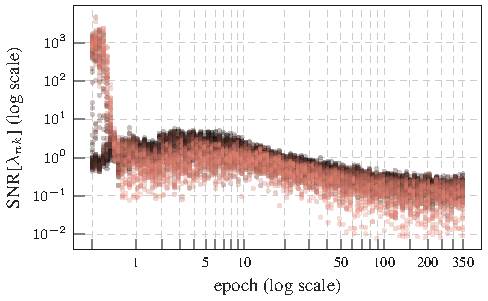
\includegraphics[width=\linewidth]{fig/exp13_plots/gammas_lambdas/cifar100_allcnnc_sgd_lambdas.pdf}
    \end{minipage}
  \end{subfigure}

  \begin{subfigure}[t]{\linewidth}
    \centering
    \caption{\cifarhun \allcnnc \adam}
    \begin{minipage}{0.50\linewidth}
      \centering
      % % defines the pgfplots style "gammaslambdasdefault"
\pgfkeys{/pgfplots/gammaslambdasdefault/.style={
    width=1.0\linewidth,
    height=0.6\linewidth,
    every axis plot/.append style={line width = 1.5pt},
    mark size = 0.6,
    tick pos = left,
    ylabel near ticks,
    xlabel near ticks,
    xtick align = inside,
    ytick align = inside,
    legend cell align = left,
    legend columns = 1,
    legend pos = south east,
    legend style = {
      fill opacity = 0.7,
      text opacity = 1,
      font = \footnotesize,
    },
    xticklabel style = {font = \footnotesize},
    xlabel style = {font = \footnotesize},
    axis line style = {black},
    yticklabel style = {font = \footnotesize},
    ylabel style = {font = \footnotesize},
    title style = {font = \footnotesize},
    grid = major,
    grid style = {dashed}
  }
}
%%% Local Variables:
%%% mode: latex
%%% TeX-master: "../../thesis"
%%% End:

      % \pgfkeys{/pgfplots/zmystyle/.style={
      % gammaslambdasdefault
      % }}
      %   \tikzexternalenable
      %   NOTE: Too large. pdflatex will run out of memory during externalization
      %   % This file was created by tikzplotlib v0.9.7.
\begin{tikzpicture}

\begin{axis}[
axis line style={white!10!black},
log basis x={10},
tick pos=left,
xlabel={epoch (log scale)},
xmajorgrids,
xmin=0.746099240306814, xmax=469.106495613199,
xmode=log,
ylabel={SNR[\(\displaystyle \gamma_{nk}\)] (log scale)},
ymajorgrids,
ymin=1.15277386728514e-11, ymax=0.462830668650656,
ymode=log,
zmystyle
]
\addplot [
mark=*,
only marks,
scatter,
scatter/@post marker code/.code={%
  \endscope
},
scatter/@pre marker code/.code={%
  \expanded{%
  \noexpand\definecolor{thispointdrawcolor}{RGB}{\drawcolor}%
  \noexpand\definecolor{thispointfillcolor}{RGB}{\fillcolor}%
  }%
  \scope[draw=thispointdrawcolor, fill=thispointfillcolor]%
},
visualization depends on={value \thisrow{draw} \as \drawcolor},
visualization depends on={value \thisrow{fill} \as \fillcolor}
]
table{%
x  y  draw  fill
1 0.00274634803645313 0,0,0 0,0,0
1 0.0195745080709457 1.84313725490196,1.05882352941176,0.917647058823529 1.84313725490196,1.05882352941176,0.917647058823529
1 0.000233649348956533 4.6078431372549,2.64705882352941,2.29411764705882 4.6078431372549,2.64705882352941,2.29411764705882
1 0.0162332039326429 6.45098039215686,3.70588235294118,3.21176470588235 6.45098039215686,3.70588235294118,3.21176470588235
1 0.000684606668073684 9.2156862745098,5.29411764705882,4.58823529411765 9.2156862745098,5.29411764705882,4.58823529411765
1 0.0658643618226051 11.0588235294118,6.35294117647059,5.50588235294118 11.0588235294118,6.35294117647059,5.50588235294118
1 0.00312149454839528 13.8235294117647,7.94117647058823,6.88235294117647 13.8235294117647,7.94117647058823,6.88235294117647
1 0.00180662947241217 16.5882352941176,9.52941176470588,8.25882352941176 16.5882352941176,9.52941176470588,8.25882352941176
1 0.0014764005318284 18.4313725490196,10.5882352941176,9.17647058823529 18.4313725490196,10.5882352941176,9.17647058823529
1 0.00722580496221781 21.1960784313725,12.1764705882353,10.5529411764706 21.1960784313725,12.1764705882353,10.5529411764706
1 9.92614150163718e-06 23.0392156862745,13.2352941176471,11.4705882352941 23.0392156862745,13.2352941176471,11.4705882352941
1 0.00913827959448099 25.8039215686274,14.8235294117647,12.8470588235294 25.8039215686274,14.8235294117647,12.8470588235294
1 0.00173584371805191 28.5686274509804,16.4117647058824,14.2235294117647 28.5686274509804,16.4117647058824,14.2235294117647
1 0.00692951353266835 30.4117647058823,17.4705882352941,15.1411764705882 30.4117647058823,17.4705882352941,15.1411764705882
1 0.0246012937277555 33.1764705882353,19.0588235294118,16.5176470588235 33.1764705882353,19.0588235294118,16.5176470588235
1 0.00832079909741879 35.0196078431373,20.1176470588235,17.4352941176471 35.0196078431373,20.1176470588235,17.4352941176471
1 0.00203080731444061 37.7843137254902,21.7058823529412,18.8117647058824 37.7843137254902,21.7058823529412,18.8117647058824
1 0.0184589792042971 39.6274509803922,22.7647058823529,19.7294117647059 39.6274509803922,22.7647058823529,19.7294117647059
1 0.0445655211806297 42.3921568627451,24.3529411764706,21.1058823529412 42.3921568627451,24.3529411764706,21.1058823529412
1 0.000785803014878184 45.156862745098,25.9411764705882,22.4823529411765 45.156862745098,25.9411764705882,22.4823529411765
1 0.00899182446300983 47,27,23.4 47,27,23.4
1 0.00697128474712372 49.7647058823529,28.5882352941176,24.7764705882353 49.7647058823529,28.5882352941176,24.7764705882353
1 0.0292930174618959 51.6078431372549,29.6470588235294,25.6941176470588 51.6078431372549,29.6470588235294,25.6941176470588
1 2.21466907532886e-05 54.3725490196078,31.2352941176471,27.0705882352941 54.3725490196078,31.2352941176471,27.0705882352941
1 0.000142595730721951 57.1372549019608,32.8235294117647,28.4470588235294 57.1372549019608,32.8235294117647,28.4470588235294
1 0.0016800103476271 58.9803921568627,33.8823529411765,29.3647058823529 58.9803921568627,33.8823529411765,29.3647058823529
1 0.00262654665857553 61.7450980392157,35.4705882352941,30.7411764705882 61.7450980392157,35.4705882352941,30.7411764705882
1 0.0277046374976635 63.5882352941176,36.5294117647059,31.6588235294118 63.5882352941176,36.5294117647059,31.6588235294118
1 0.0021676616743207 66.3529411764706,38.1176470588235,33.0352941176471 66.3529411764706,38.1176470588235,33.0352941176471
1 0.00710064824670553 68.1960784313725,39.1764705882353,33.9529411764706 68.1960784313725,39.1764705882353,33.9529411764706
1 0.0169522892683744 70.9607843137255,40.7647058823529,35.3294117647059 70.9607843137255,40.7647058823529,35.3294117647059
1 0.00573192769661546 73.7254901960784,42.3529411764706,36.7058823529412 73.7254901960784,42.3529411764706,36.7058823529412
1 0.0134858191013336 75.5686274509804,43.4117647058823,37.6235294117647 75.5686274509804,43.4117647058823,37.6235294117647
1 5.8486304624239e-05 78.3333333333333,45,39 78.3333333333333,45,39
1 1.42495555337518e-05 80.1764705882353,46.0588235294118,39.9176470588235 80.1764705882353,46.0588235294118,39.9176470588235
1 0.00481638219207525 82.9411764705882,47.6470588235294,41.2941176470588 82.9411764705882,47.6470588235294,41.2941176470588
1 0.0165880434215069 85.7058823529412,49.2352941176471,42.6705882352941 85.7058823529412,49.2352941176471,42.6705882352941
1 0.000152072592754848 87.5490196078431,50.2941176470588,43.5882352941177 87.5490196078431,50.2941176470588,43.5882352941177
1 0.00503631215542555 90.3137254901961,51.8823529411765,44.9647058823529 90.3137254901961,51.8823529411765,44.9647058823529
1 0.00281775719486177 92.156862745098,52.9411764705882,45.8823529411765 92.156862745098,52.9411764705882,45.8823529411765
1 0.0392145961523056 94.921568627451,54.5294117647059,47.2588235294118 94.921568627451,54.5294117647059,47.2588235294118
1 0.0201661288738251 97.6862745098039,56.1176470588235,48.635294117647 97.6862745098039,56.1176470588235,48.635294117647
1 5.31239893462043e-05 99.5294117647059,57.1764705882353,49.5529411764706 99.5294117647059,57.1764705882353,49.5529411764706
1 0.00351075595244765 102.294117647059,58.7647058823529,50.9294117647059 102.294117647059,58.7647058823529,50.9294117647059
1 0.000352529110386968 104.137254901961,59.8235294117647,51.8470588235294 104.137254901961,59.8235294117647,51.8470588235294
1 0.0113074472174048 106.901960784314,61.4117647058824,53.2235294117647 106.901960784314,61.4117647058824,53.2235294117647
1 0.00121186266187578 108.745098039216,62.4705882352941,54.1411764705882 108.745098039216,62.4705882352941,54.1411764705882
1 0.00102840445470065 111.509803921569,64.0588235294118,55.5176470588235 111.509803921569,64.0588235294118,55.5176470588235
1 0.0247546974569559 114.274509803922,65.6470588235294,56.8941176470588 114.274509803922,65.6470588235294,56.8941176470588
1 0.00187538238242269 116.117647058824,66.7058823529412,57.8117647058823 116.117647058824,66.7058823529412,57.8117647058823
1 0.107139453291893 118.882352941176,68.2941176470588,59.1882352941176 118.882352941176,68.2941176470588,59.1882352941176
1 0.000218821209273301 120.725490196078,69.3529411764706,60.1058823529412 120.725490196078,69.3529411764706,60.1058823529412
1 0.0346433743834496 123.490196078431,70.9411764705882,61.4823529411765 123.490196078431,70.9411764705882,61.4823529411765
1 0.000325466127833351 126.254901960784,72.5294117647059,62.8588235294118 126.254901960784,72.5294117647059,62.8588235294118
1 0.002991349902004 128.098039215686,73.5882352941176,63.7764705882353 128.098039215686,73.5882352941176,63.7764705882353
1 0.00441909627988935 130.862745098039,75.1764705882353,65.1529411764706 130.862745098039,75.1764705882353,65.1529411764706
1 0.0106925731524825 132.705882352941,76.2352941176471,66.0705882352941 132.705882352941,76.2352941176471,66.0705882352941
1 0.0160031095147133 135.470588235294,77.8235294117647,67.4470588235294 135.470588235294,77.8235294117647,67.4470588235294
1 0.000165284509421326 137.313725490196,78.8823529411765,68.3647058823529 137.313725490196,78.8823529411765,68.3647058823529
1 0.0162081383168697 140.078431372549,80.4705882352941,69.7411764705882 140.078431372549,80.4705882352941,69.7411764705882
1 0.00307095353491604 142.843137254902,82.0588235294118,71.1176470588235 142.843137254902,82.0588235294118,71.1176470588235
1 0.0125417076051235 144.686274509804,83.1176470588235,72.0352941176471 144.686274509804,83.1176470588235,72.0352941176471
1 0.000261359236901626 147.450980392157,84.7058823529412,73.4117647058823 147.450980392157,84.7058823529412,73.4117647058823
1 0.000613704440183938 149.294117647059,85.7647058823529,74.3294117647059 149.294117647059,85.7647058823529,74.3294117647059
1 0.00360157177783549 152.058823529412,87.3529411764706,75.7058823529412 152.058823529412,87.3529411764706,75.7058823529412
1 0.00815108697861433 154.823529411765,88.9411764705882,77.0823529411765 154.823529411765,88.9411764705882,77.0823529411765
1 3.31001319864299e-05 156.666666666667,90,78 156.666666666667,90,78
1 2.97258111459087e-06 159.43137254902,91.5882352941177,79.3764705882353 159.43137254902,91.5882352941177,79.3764705882353
1 0.00151807151269168 161.274509803922,92.6470588235294,80.2941176470588 161.274509803922,92.6470588235294,80.2941176470588
1 2.56227613135707e-05 164.039215686274,94.2352941176471,81.6705882352941 164.039215686274,94.2352941176471,81.6705882352941
1 0.000867351132910699 166.803921568627,95.8235294117647,83.0470588235294 166.803921568627,95.8235294117647,83.0470588235294
1 0.00161500286776572 168.647058823529,96.8823529411765,83.9647058823529 168.647058823529,96.8823529411765,83.9647058823529
1 0.000895721139386296 171.411764705882,98.4705882352941,85.3411764705882 171.411764705882,98.4705882352941,85.3411764705882
1 0.0292165707796812 173.254901960784,99.5294117647059,86.2588235294118 173.254901960784,99.5294117647059,86.2588235294118
1 0.00252614822238684 176.019607843137,101.117647058824,87.6352941176471 176.019607843137,101.117647058824,87.6352941176471
1 0.0061762728728354 177.862745098039,102.176470588235,88.5529411764706 177.862745098039,102.176470588235,88.5529411764706
1 0.00126398098655045 180.627450980392,103.764705882353,89.9294117647059 180.627450980392,103.764705882353,89.9294117647059
1 0.0037754001095891 183.392156862745,105.352941176471,91.3058823529412 183.392156862745,105.352941176471,91.3058823529412
1 0.00500148115679622 185.235294117647,106.411764705882,92.2235294117647 185.235294117647,106.411764705882,92.2235294117647
1 0.000146261270856485 188,108,93.6 188,108,93.6
1 0.00287263537757099 189.843137254902,109.058823529412,94.5176470588235 189.843137254902,109.058823529412,94.5176470588235
1 0.00155190366785973 192.607843137255,110.647058823529,95.8941176470588 192.607843137255,110.647058823529,95.8941176470588
1 0.00276355189271271 195.372549019608,112.235294117647,97.2705882352941 195.372549019608,112.235294117647,97.2705882352941
1 0.0345123372972012 197.21568627451,113.294117647059,98.1882352941176 197.21568627451,113.294117647059,98.1882352941176
1 0.00349616073071957 199.980392156863,114.882352941176,99.5647058823529 199.980392156863,114.882352941176,99.5647058823529
1 0.00124863861128688 201.823529411765,115.941176470588,100.482352941176 201.823529411765,115.941176470588,100.482352941176
1 0.00367017718963325 204.588235294118,117.529411764706,101.858823529412 204.588235294118,117.529411764706,101.858823529412
1 0.0213761106133461 206.43137254902,118.588235294118,102.776470588235 206.43137254902,118.588235294118,102.776470588235
1 3.43552237609401e-05 209.196078431373,120.176470588235,104.152941176471 209.196078431373,120.176470588235,104.152941176471
1 0.0023004780523479 211.960784313725,121.764705882353,105.529411764706 211.960784313725,121.764705882353,105.529411764706
1 0.00223583052866161 213.803921568627,122.823529411765,106.447058823529 213.803921568627,122.823529411765,106.447058823529
1 0.0041114529594779 216.56862745098,124.411764705882,107.823529411765 216.56862745098,124.411764705882,107.823529411765
1 1.71952196978964e-05 218.411764705882,125.470588235294,108.741176470588 218.411764705882,125.470588235294,108.741176470588
1 0.00232499931007624 221.176470588235,127.058823529412,110.117647058824 221.176470588235,127.058823529412,110.117647058824
1 0.0040188361890614 223.941176470588,128.647058823529,111.494117647059 223.941176470588,128.647058823529,111.494117647059
1 0.0051566525362432 225.78431372549,129.705882352941,112.411764705882 225.78431372549,129.705882352941,112.411764705882
1 0.000205356860533357 228.549019607843,131.294117647059,113.788235294118 228.549019607843,131.294117647059,113.788235294118
1 0.03796311840415 230.392156862745,132.352941176471,114.705882352941 230.392156862745,132.352941176471,114.705882352941
1 0.00999383069574833 233.156862745098,133.941176470588,116.082352941176 233.156862745098,133.941176470588,116.082352941176
1 0.00351339788176119 235,135,117 235,135,117
1.19230769230769 0.00650390610098839 0,0,0 0,0,0
1.19230769230769 0.0172444507479668 1.84313725490196,1.05882352941176,0.917647058823529 1.84313725490196,1.05882352941176,0.917647058823529
1.19230769230769 0.00121845258399844 4.6078431372549,2.64705882352941,2.29411764705882 4.6078431372549,2.64705882352941,2.29411764705882
1.19230769230769 0.0536837391555309 6.45098039215686,3.70588235294118,3.21176470588235 6.45098039215686,3.70588235294118,3.21176470588235
1.19230769230769 0.00164676376152784 9.2156862745098,5.29411764705882,4.58823529411765 9.2156862745098,5.29411764705882,4.58823529411765
1.19230769230769 0.00022142447414808 11.0588235294118,6.35294117647059,5.50588235294118 11.0588235294118,6.35294117647059,5.50588235294118
1.19230769230769 0.00711309723556042 13.8235294117647,7.94117647058823,6.88235294117647 13.8235294117647,7.94117647058823,6.88235294117647
1.19230769230769 0.0293446537107229 16.5882352941176,9.52941176470588,8.25882352941176 16.5882352941176,9.52941176470588,8.25882352941176
1.19230769230769 0.0118302311748266 18.4313725490196,10.5882352941176,9.17647058823529 18.4313725490196,10.5882352941176,9.17647058823529
1.19230769230769 0.0200936980545521 21.1960784313725,12.1764705882353,10.5529411764706 21.1960784313725,12.1764705882353,10.5529411764706
1.19230769230769 0.00227834866382182 23.0392156862745,13.2352941176471,11.4705882352941 23.0392156862745,13.2352941176471,11.4705882352941
1.19230769230769 1.73270054801833e-05 25.8039215686274,14.8235294117647,12.8470588235294 25.8039215686274,14.8235294117647,12.8470588235294
1.19230769230769 0.00116063945461065 28.5686274509804,16.4117647058824,14.2235294117647 28.5686274509804,16.4117647058824,14.2235294117647
1.19230769230769 0.0358673147857189 30.4117647058823,17.4705882352941,15.1411764705882 30.4117647058823,17.4705882352941,15.1411764705882
1.19230769230769 0.00968307163566351 33.1764705882353,19.0588235294118,16.5176470588235 33.1764705882353,19.0588235294118,16.5176470588235
1.19230769230769 0.0242300629615784 35.0196078431373,20.1176470588235,17.4352941176471 35.0196078431373,20.1176470588235,17.4352941176471
1.19230769230769 0.00938940420746803 37.7843137254902,21.7058823529412,18.8117647058824 37.7843137254902,21.7058823529412,18.8117647058824
1.19230769230769 0.00469276402145624 39.6274509803922,22.7647058823529,19.7294117647059 39.6274509803922,22.7647058823529,19.7294117647059
1.19230769230769 0.000819677079562098 42.3921568627451,24.3529411764706,21.1058823529412 42.3921568627451,24.3529411764706,21.1058823529412
1.19230769230769 0.00454029580578208 45.156862745098,25.9411764705882,22.4823529411765 45.156862745098,25.9411764705882,22.4823529411765
1.19230769230769 0.0303440056741238 47,27,23.4 47,27,23.4
1.19230769230769 0.035893090069294 49.7647058823529,28.5882352941176,24.7764705882353 49.7647058823529,28.5882352941176,24.7764705882353
1.19230769230769 0.00309676770120859 51.6078431372549,29.6470588235294,25.6941176470588 51.6078431372549,29.6470588235294,25.6941176470588
1.19230769230769 0.00643637916073203 54.3725490196078,31.2352941176471,27.0705882352941 54.3725490196078,31.2352941176471,27.0705882352941
1.19230769230769 0.0290366616100073 57.1372549019608,32.8235294117647,28.4470588235294 57.1372549019608,32.8235294117647,28.4470588235294
1.19230769230769 0.0033517733681947 58.9803921568627,33.8823529411765,29.3647058823529 58.9803921568627,33.8823529411765,29.3647058823529
1.19230769230769 0.030903521925211 61.7450980392157,35.4705882352941,30.7411764705882 61.7450980392157,35.4705882352941,30.7411764705882
1.19230769230769 0.000336043449351564 63.5882352941176,36.5294117647059,31.6588235294118 63.5882352941176,36.5294117647059,31.6588235294118
1.19230769230769 0.000265138136455789 66.3529411764706,38.1176470588235,33.0352941176471 66.3529411764706,38.1176470588235,33.0352941176471
1.19230769230769 0.00912346877157688 68.1960784313725,39.1764705882353,33.9529411764706 68.1960784313725,39.1764705882353,33.9529411764706
1.19230769230769 0.0153672927990556 70.9607843137255,40.7647058823529,35.3294117647059 70.9607843137255,40.7647058823529,35.3294117647059
1.19230769230769 0.00203079869970679 73.7254901960784,42.3529411764706,36.7058823529412 73.7254901960784,42.3529411764706,36.7058823529412
1.19230769230769 0.00168134283740073 75.5686274509804,43.4117647058823,37.6235294117647 75.5686274509804,43.4117647058823,37.6235294117647
1.19230769230769 0.00481356773525476 78.3333333333333,45,39 78.3333333333333,45,39
1.19230769230769 0.0172266084700823 80.1764705882353,46.0588235294118,39.9176470588235 80.1764705882353,46.0588235294118,39.9176470588235
1.19230769230769 0.000998982694000006 82.9411764705882,47.6470588235294,41.2941176470588 82.9411764705882,47.6470588235294,41.2941176470588
1.19230769230769 0.000267912371782586 85.7058823529412,49.2352941176471,42.6705882352941 85.7058823529412,49.2352941176471,42.6705882352941
1.19230769230769 0.00569981429725885 87.5490196078431,50.2941176470588,43.5882352941177 87.5490196078431,50.2941176470588,43.5882352941177
1.19230769230769 0.00368676288053393 90.3137254901961,51.8823529411765,44.9647058823529 90.3137254901961,51.8823529411765,44.9647058823529
1.19230769230769 0.00458840792998672 92.156862745098,52.9411764705882,45.8823529411765 92.156862745098,52.9411764705882,45.8823529411765
1.19230769230769 0.0127107342705131 94.921568627451,54.5294117647059,47.2588235294118 94.921568627451,54.5294117647059,47.2588235294118
1.19230769230769 0.00179884675890207 97.6862745098039,56.1176470588235,48.635294117647 97.6862745098039,56.1176470588235,48.635294117647
1.19230769230769 0.00441736215725541 99.5294117647059,57.1764705882353,49.5529411764706 99.5294117647059,57.1764705882353,49.5529411764706
1.19230769230769 0.0433225557208061 102.294117647059,58.7647058823529,50.9294117647059 102.294117647059,58.7647058823529,50.9294117647059
1.19230769230769 0.0127729121595621 104.137254901961,59.8235294117647,51.8470588235294 104.137254901961,59.8235294117647,51.8470588235294
1.19230769230769 0.0202664453536272 106.901960784314,61.4117647058824,53.2235294117647 106.901960784314,61.4117647058824,53.2235294117647
1.19230769230769 2.10174055936818e-09 108.745098039216,62.4705882352941,54.1411764705882 108.745098039216,62.4705882352941,54.1411764705882
1.19230769230769 0.0392000749707222 111.509803921569,64.0588235294118,55.5176470588235 111.509803921569,64.0588235294118,55.5176470588235
1.19230769230769 0.0114895645529032 114.274509803922,65.6470588235294,56.8941176470588 114.274509803922,65.6470588235294,56.8941176470588
1.19230769230769 0.00639737164601684 116.117647058824,66.7058823529412,57.8117647058823 116.117647058824,66.7058823529412,57.8117647058823
1.19230769230769 8.83961792652599e-10 118.882352941176,68.2941176470588,59.1882352941176 118.882352941176,68.2941176470588,59.1882352941176
1.19230769230769 0.000352088216459379 120.725490196078,69.3529411764706,60.1058823529412 120.725490196078,69.3529411764706,60.1058823529412
1.19230769230769 3.49427355104126e-05 123.490196078431,70.9411764705882,61.4823529411765 123.490196078431,70.9411764705882,61.4823529411765
1.19230769230769 0.00297117372974753 126.254901960784,72.5294117647059,62.8588235294118 126.254901960784,72.5294117647059,62.8588235294118
1.19230769230769 0.0112585481256247 128.098039215686,73.5882352941176,63.7764705882353 128.098039215686,73.5882352941176,63.7764705882353
1.19230769230769 0.00380137632600963 130.862745098039,75.1764705882353,65.1529411764706 130.862745098039,75.1764705882353,65.1529411764706
1.19230769230769 4.61988383904099e-05 132.705882352941,76.2352941176471,66.0705882352941 132.705882352941,76.2352941176471,66.0705882352941
1.19230769230769 0.0176632944494486 135.470588235294,77.8235294117647,67.4470588235294 135.470588235294,77.8235294117647,67.4470588235294
1.19230769230769 0.00111025827936828 137.313725490196,78.8823529411765,68.3647058823529 137.313725490196,78.8823529411765,68.3647058823529
1.19230769230769 0.0226951763033867 140.078431372549,80.4705882352941,69.7411764705882 140.078431372549,80.4705882352941,69.7411764705882
1.19230769230769 0.0134838754311204 142.843137254902,82.0588235294118,71.1176470588235 142.843137254902,82.0588235294118,71.1176470588235
1.19230769230769 0.00621756166219711 144.686274509804,83.1176470588235,72.0352941176471 144.686274509804,83.1176470588235,72.0352941176471
1.19230769230769 0.0467652343213558 147.450980392157,84.7058823529412,73.4117647058823 147.450980392157,84.7058823529412,73.4117647058823
1.19230769230769 0.000597878417465836 149.294117647059,85.7647058823529,74.3294117647059 149.294117647059,85.7647058823529,74.3294117647059
1.19230769230769 0.000377079733880237 152.058823529412,87.3529411764706,75.7058823529412 152.058823529412,87.3529411764706,75.7058823529412
1.19230769230769 0.00368606322444975 154.823529411765,88.9411764705882,77.0823529411765 154.823529411765,88.9411764705882,77.0823529411765
1.19230769230769 0.0231113117188215 156.666666666667,90,78 156.666666666667,90,78
1.19230769230769 0.00389427831396461 159.43137254902,91.5882352941177,79.3764705882353 159.43137254902,91.5882352941177,79.3764705882353
1.19230769230769 1.59645569510758e-05 161.274509803922,92.6470588235294,80.2941176470588 161.274509803922,92.6470588235294,80.2941176470588
1.19230769230769 0.00816253386437893 164.039215686274,94.2352941176471,81.6705882352941 164.039215686274,94.2352941176471,81.6705882352941
1.19230769230769 0.00317978346720338 166.803921568627,95.8235294117647,83.0470588235294 166.803921568627,95.8235294117647,83.0470588235294
1.19230769230769 0.000774249085225165 168.647058823529,96.8823529411765,83.9647058823529 168.647058823529,96.8823529411765,83.9647058823529
1.19230769230769 0.0216589737683535 171.411764705882,98.4705882352941,85.3411764705882 171.411764705882,98.4705882352941,85.3411764705882
1.19230769230769 0.00348546984605491 173.254901960784,99.5294117647059,86.2588235294118 173.254901960784,99.5294117647059,86.2588235294118
1.19230769230769 0.00259094662033021 176.019607843137,101.117647058824,87.6352941176471 176.019607843137,101.117647058824,87.6352941176471
1.19230769230769 0.000753606087528169 177.862745098039,102.176470588235,88.5529411764706 177.862745098039,102.176470588235,88.5529411764706
1.19230769230769 0.00832769460976124 180.627450980392,103.764705882353,89.9294117647059 180.627450980392,103.764705882353,89.9294117647059
1.19230769230769 0.00874201767146587 183.392156862745,105.352941176471,91.3058823529412 183.392156862745,105.352941176471,91.3058823529412
1.19230769230769 0.00839838106185198 185.235294117647,106.411764705882,92.2235294117647 185.235294117647,106.411764705882,92.2235294117647
1.19230769230769 0.00394111312925816 188,108,93.6 188,108,93.6
1.19230769230769 0.00141207873821259 189.843137254902,109.058823529412,94.5176470588235 189.843137254902,109.058823529412,94.5176470588235
1.19230769230769 0.0116165298968554 192.607843137255,110.647058823529,95.8941176470588 192.607843137255,110.647058823529,95.8941176470588
1.19230769230769 0.00030397396767512 195.372549019608,112.235294117647,97.2705882352941 195.372549019608,112.235294117647,97.2705882352941
1.19230769230769 0.00227042264305055 197.21568627451,113.294117647059,98.1882352941176 197.21568627451,113.294117647059,98.1882352941176
1.19230769230769 0.00332156289368868 199.980392156863,114.882352941176,99.5647058823529 199.980392156863,114.882352941176,99.5647058823529
1.19230769230769 0.00579151697456837 201.823529411765,115.941176470588,100.482352941176 201.823529411765,115.941176470588,100.482352941176
1.19230769230769 0.000512008497025818 204.588235294118,117.529411764706,101.858823529412 204.588235294118,117.529411764706,101.858823529412
1.19230769230769 0.00017511475016363 206.43137254902,118.588235294118,102.776470588235 206.43137254902,118.588235294118,102.776470588235
1.19230769230769 0.00336209451779723 209.196078431373,120.176470588235,104.152941176471 209.196078431373,120.176470588235,104.152941176471
1.19230769230769 0.000173560110852122 211.960784313725,121.764705882353,105.529411764706 211.960784313725,121.764705882353,105.529411764706
1.19230769230769 0.00554365804418921 213.803921568627,122.823529411765,106.447058823529 213.803921568627,122.823529411765,106.447058823529
1.19230769230769 0.00368817849084735 216.56862745098,124.411764705882,107.823529411765 216.56862745098,124.411764705882,107.823529411765
1.19230769230769 0.0249466802924871 218.411764705882,125.470588235294,108.741176470588 218.411764705882,125.470588235294,108.741176470588
1.19230769230769 0.000881184416357428 221.176470588235,127.058823529412,110.117647058824 221.176470588235,127.058823529412,110.117647058824
1.19230769230769 0.00491883186623454 223.941176470588,128.647058823529,111.494117647059 223.941176470588,128.647058823529,111.494117647059
1.19230769230769 0.0108974194154143 225.78431372549,129.705882352941,112.411764705882 225.78431372549,129.705882352941,112.411764705882
1.19230769230769 0.000315294542815536 228.549019607843,131.294117647059,113.788235294118 228.549019607843,131.294117647059,113.788235294118
1.19230769230769 0.0108918696641922 230.392156862745,132.352941176471,114.705882352941 230.392156862745,132.352941176471,114.705882352941
1.19230769230769 0.0135838221758604 233.156862745098,133.941176470588,116.082352941176 233.156862745098,133.941176470588,116.082352941176
1.19230769230769 0.017300458624959 235,135,117 235,135,117
1.42307692307692 0.00142246845643967 0,0,0 0,0,0
1.42307692307692 0.00759271951392293 1.84313725490196,1.05882352941176,0.917647058823529 1.84313725490196,1.05882352941176,0.917647058823529
1.42307692307692 0.00431809388101101 4.6078431372549,2.64705882352941,2.29411764705882 4.6078431372549,2.64705882352941,2.29411764705882
1.42307692307692 0.00993170402944088 6.45098039215686,3.70588235294118,3.21176470588235 6.45098039215686,3.70588235294118,3.21176470588235
1.42307692307692 0.000956125732045621 9.2156862745098,5.29411764705882,4.58823529411765 9.2156862745098,5.29411764705882,4.58823529411765
1.42307692307692 0.0253056567162275 11.0588235294118,6.35294117647059,5.50588235294118 11.0588235294118,6.35294117647059,5.50588235294118
1.42307692307692 0.000614238961134106 13.8235294117647,7.94117647058823,6.88235294117647 13.8235294117647,7.94117647058823,6.88235294117647
1.42307692307692 0.00102690665517002 16.5882352941176,9.52941176470588,8.25882352941176 16.5882352941176,9.52941176470588,8.25882352941176
1.42307692307692 0.0221353434026241 18.4313725490196,10.5882352941176,9.17647058823529 18.4313725490196,10.5882352941176,9.17647058823529
1.42307692307692 0.0131061868742108 21.1960784313725,12.1764705882353,10.5529411764706 21.1960784313725,12.1764705882353,10.5529411764706
1.42307692307692 0.00214608339592814 23.0392156862745,13.2352941176471,11.4705882352941 23.0392156862745,13.2352941176471,11.4705882352941
1.42307692307692 0.00357350124977529 25.8039215686274,14.8235294117647,12.8470588235294 25.8039215686274,14.8235294117647,12.8470588235294
1.42307692307692 0.0252631120383739 28.5686274509804,16.4117647058824,14.2235294117647 28.5686274509804,16.4117647058824,14.2235294117647
1.42307692307692 0.000301928317639977 30.4117647058823,17.4705882352941,15.1411764705882 30.4117647058823,17.4705882352941,15.1411764705882
1.42307692307692 0.000660296645946801 33.1764705882353,19.0588235294118,16.5176470588235 33.1764705882353,19.0588235294118,16.5176470588235
1.42307692307692 0.00276426575146616 35.0196078431373,20.1176470588235,17.4352941176471 35.0196078431373,20.1176470588235,17.4352941176471
1.42307692307692 0.0281298886984587 37.7843137254902,21.7058823529412,18.8117647058824 37.7843137254902,21.7058823529412,18.8117647058824
1.42307692307692 7.71764680393972e-05 39.6274509803922,22.7647058823529,19.7294117647059 39.6274509803922,22.7647058823529,19.7294117647059
1.42307692307692 0.00069428764982149 42.3921568627451,24.3529411764706,21.1058823529412 42.3921568627451,24.3529411764706,21.1058823529412
1.42307692307692 0.00692450255155563 45.156862745098,25.9411764705882,22.4823529411765 45.156862745098,25.9411764705882,22.4823529411765
1.42307692307692 0.0015578797319904 47,27,23.4 47,27,23.4
1.42307692307692 0.0185712818056345 49.7647058823529,28.5882352941176,24.7764705882353 49.7647058823529,28.5882352941176,24.7764705882353
1.42307692307692 0.00746939657256007 51.6078431372549,29.6470588235294,25.6941176470588 51.6078431372549,29.6470588235294,25.6941176470588
1.42307692307692 0.000185830998816527 54.3725490196078,31.2352941176471,27.0705882352941 54.3725490196078,31.2352941176471,27.0705882352941
1.42307692307692 0.00563231622800231 57.1372549019608,32.8235294117647,28.4470588235294 57.1372549019608,32.8235294117647,28.4470588235294
1.42307692307692 0.0103907091543078 58.9803921568627,33.8823529411765,29.3647058823529 58.9803921568627,33.8823529411765,29.3647058823529
1.42307692307692 0.00457964744418859 61.7450980392157,35.4705882352941,30.7411764705882 61.7450980392157,35.4705882352941,30.7411764705882
1.42307692307692 6.90775050316006e-05 63.5882352941176,36.5294117647059,31.6588235294118 63.5882352941176,36.5294117647059,31.6588235294118
1.42307692307692 0.00384885002858937 66.3529411764706,38.1176470588235,33.0352941176471 66.3529411764706,38.1176470588235,33.0352941176471
1.42307692307692 0.0140974717214704 68.1960784313725,39.1764705882353,33.9529411764706 68.1960784313725,39.1764705882353,33.9529411764706
1.42307692307692 0.0108648361638188 70.9607843137255,40.7647058823529,35.3294117647059 70.9607843137255,40.7647058823529,35.3294117647059
1.42307692307692 0.00599203398451209 73.7254901960784,42.3529411764706,36.7058823529412 73.7254901960784,42.3529411764706,36.7058823529412
1.42307692307692 0.0264144968241453 75.5686274509804,43.4117647058823,37.6235294117647 75.5686274509804,43.4117647058823,37.6235294117647
1.42307692307692 0.00676068849861622 78.3333333333333,45,39 78.3333333333333,45,39
1.42307692307692 0.014663876965642 80.1764705882353,46.0588235294118,39.9176470588235 80.1764705882353,46.0588235294118,39.9176470588235
1.42307692307692 0.00125042942818254 82.9411764705882,47.6470588235294,41.2941176470588 82.9411764705882,47.6470588235294,41.2941176470588
1.42307692307692 0.00264761387370527 85.7058823529412,49.2352941176471,42.6705882352941 85.7058823529412,49.2352941176471,42.6705882352941
1.42307692307692 0.000818726315628737 87.5490196078431,50.2941176470588,43.5882352941177 87.5490196078431,50.2941176470588,43.5882352941177
1.42307692307692 0.00987637974321842 90.3137254901961,51.8823529411765,44.9647058823529 90.3137254901961,51.8823529411765,44.9647058823529
1.42307692307692 0.000111251596536022 92.156862745098,52.9411764705882,45.8823529411765 92.156862745098,52.9411764705882,45.8823529411765
1.42307692307692 0.00797679089009762 94.921568627451,54.5294117647059,47.2588235294118 94.921568627451,54.5294117647059,47.2588235294118
1.42307692307692 0.0199286285787821 97.6862745098039,56.1176470588235,48.635294117647 97.6862745098039,56.1176470588235,48.635294117647
1.42307692307692 0.00719084404408932 99.5294117647059,57.1764705882353,49.5529411764706 99.5294117647059,57.1764705882353,49.5529411764706
1.42307692307692 0.00608246773481369 102.294117647059,58.7647058823529,50.9294117647059 102.294117647059,58.7647058823529,50.9294117647059
1.42307692307692 0.000987325678579509 104.137254901961,59.8235294117647,51.8470588235294 104.137254901961,59.8235294117647,51.8470588235294
1.42307692307692 0.00377068109810352 106.901960784314,61.4117647058824,53.2235294117647 106.901960784314,61.4117647058824,53.2235294117647
1.42307692307692 0.0163403898477554 108.745098039216,62.4705882352941,54.1411764705882 108.745098039216,62.4705882352941,54.1411764705882
1.42307692307692 0.000156006397446617 111.509803921569,64.0588235294118,55.5176470588235 111.509803921569,64.0588235294118,55.5176470588235
1.42307692307692 0.000611708150245249 114.274509803922,65.6470588235294,56.8941176470588 114.274509803922,65.6470588235294,56.8941176470588
1.42307692307692 0.00524566788226366 116.117647058824,66.7058823529412,57.8117647058823 116.117647058824,66.7058823529412,57.8117647058823
1.42307692307692 0.00263824453577399 118.882352941176,68.2941176470588,59.1882352941176 118.882352941176,68.2941176470588,59.1882352941176
1.42307692307692 3.36799421347678e-05 120.725490196078,69.3529411764706,60.1058823529412 120.725490196078,69.3529411764706,60.1058823529412
1.42307692307692 1.02788575873092e-07 123.490196078431,70.9411764705882,61.4823529411765 123.490196078431,70.9411764705882,61.4823529411765
1.42307692307692 0.00138971651904285 126.254901960784,72.5294117647059,62.8588235294118 126.254901960784,72.5294117647059,62.8588235294118
1.42307692307692 0.00291372998617589 128.098039215686,73.5882352941176,63.7764705882353 128.098039215686,73.5882352941176,63.7764705882353
1.42307692307692 0.00799092091619968 130.862745098039,75.1764705882353,65.1529411764706 130.862745098039,75.1764705882353,65.1529411764706
1.42307692307692 0.00461428333073854 132.705882352941,76.2352941176471,66.0705882352941 132.705882352941,76.2352941176471,66.0705882352941
1.42307692307692 0.0250746067613363 135.470588235294,77.8235294117647,67.4470588235294 135.470588235294,77.8235294117647,67.4470588235294
1.42307692307692 0.000141416123369709 137.313725490196,78.8823529411765,68.3647058823529 137.313725490196,78.8823529411765,68.3647058823529
1.42307692307692 0.0150819253176451 140.078431372549,80.4705882352941,69.7411764705882 140.078431372549,80.4705882352941,69.7411764705882
1.42307692307692 1.08856784208911e-05 142.843137254902,82.0588235294118,71.1176470588235 142.843137254902,82.0588235294118,71.1176470588235
1.42307692307692 0.00383605482056737 144.686274509804,83.1176470588235,72.0352941176471 144.686274509804,83.1176470588235,72.0352941176471
1.42307692307692 0.00969130545854568 147.450980392157,84.7058823529412,73.4117647058823 147.450980392157,84.7058823529412,73.4117647058823
1.42307692307692 0.0169003698974848 149.294117647059,85.7647058823529,74.3294117647059 149.294117647059,85.7647058823529,74.3294117647059
1.42307692307692 9.43430677580182e-06 152.058823529412,87.3529411764706,75.7058823529412 152.058823529412,87.3529411764706,75.7058823529412
1.42307692307692 0.00866247341036797 154.823529411765,88.9411764705882,77.0823529411765 154.823529411765,88.9411764705882,77.0823529411765
1.42307692307692 0.000192909472389147 156.666666666667,90,78 156.666666666667,90,78
1.42307692307692 0.000738637230824679 159.43137254902,91.5882352941177,79.3764705882353 159.43137254902,91.5882352941177,79.3764705882353
1.42307692307692 0.0228084698319435 161.274509803922,92.6470588235294,80.2941176470588 161.274509803922,92.6470588235294,80.2941176470588
1.42307692307692 0.00537433149293065 164.039215686274,94.2352941176471,81.6705882352941 164.039215686274,94.2352941176471,81.6705882352941
1.42307692307692 0.000638154218904674 166.803921568627,95.8235294117647,83.0470588235294 166.803921568627,95.8235294117647,83.0470588235294
1.42307692307692 0.00287844892591238 168.647058823529,96.8823529411765,83.9647058823529 168.647058823529,96.8823529411765,83.9647058823529
1.42307692307692 0.00045372114982456 171.411764705882,98.4705882352941,85.3411764705882 171.411764705882,98.4705882352941,85.3411764705882
1.42307692307692 0.0278083719313145 173.254901960784,99.5294117647059,86.2588235294118 173.254901960784,99.5294117647059,86.2588235294118
1.42307692307692 5.62121022085194e-05 176.019607843137,101.117647058824,87.6352941176471 176.019607843137,101.117647058824,87.6352941176471
1.42307692307692 0.0410480573773384 177.862745098039,102.176470588235,88.5529411764706 177.862745098039,102.176470588235,88.5529411764706
1.42307692307692 0.0194192677736282 180.627450980392,103.764705882353,89.9294117647059 180.627450980392,103.764705882353,89.9294117647059
1.42307692307692 0.0163712650537491 183.392156862745,105.352941176471,91.3058823529412 183.392156862745,105.352941176471,91.3058823529412
1.42307692307692 0.00235759699717164 185.235294117647,106.411764705882,92.2235294117647 185.235294117647,106.411764705882,92.2235294117647
1.42307692307692 0.000308376911561936 188,108,93.6 188,108,93.6
1.42307692307692 0.00955616869032383 189.843137254902,109.058823529412,94.5176470588235 189.843137254902,109.058823529412,94.5176470588235
1.42307692307692 2.11226542887744e-05 192.607843137255,110.647058823529,95.8941176470588 192.607843137255,110.647058823529,95.8941176470588
1.42307692307692 0.000191756000276655 195.372549019608,112.235294117647,97.2705882352941 195.372549019608,112.235294117647,97.2705882352941
1.42307692307692 0.00251376139931381 197.21568627451,113.294117647059,98.1882352941176 197.21568627451,113.294117647059,98.1882352941176
1.42307692307692 0.0259258691221476 199.980392156863,114.882352941176,99.5647058823529 199.980392156863,114.882352941176,99.5647058823529
1.42307692307692 0.00106474419590086 201.823529411765,115.941176470588,100.482352941176 201.823529411765,115.941176470588,100.482352941176
1.42307692307692 0.00939318630844355 204.588235294118,117.529411764706,101.858823529412 204.588235294118,117.529411764706,101.858823529412
1.42307692307692 2.66734878096031e-05 206.43137254902,118.588235294118,102.776470588235 206.43137254902,118.588235294118,102.776470588235
1.42307692307692 0.010729662142694 209.196078431373,120.176470588235,104.152941176471 209.196078431373,120.176470588235,104.152941176471
1.42307692307692 0.0031764842569828 211.960784313725,121.764705882353,105.529411764706 211.960784313725,121.764705882353,105.529411764706
1.42307692307692 0.0028276254888624 213.803921568627,122.823529411765,106.447058823529 213.803921568627,122.823529411765,106.447058823529
1.42307692307692 0.0141493966802955 216.56862745098,124.411764705882,107.823529411765 216.56862745098,124.411764705882,107.823529411765
1.42307692307692 6.94359550834633e-05 218.411764705882,125.470588235294,108.741176470588 218.411764705882,125.470588235294,108.741176470588
1.42307692307692 0.0371482484042645 221.176470588235,127.058823529412,110.117647058824 221.176470588235,127.058823529412,110.117647058824
1.42307692307692 0.000110327877337113 223.941176470588,128.647058823529,111.494117647059 223.941176470588,128.647058823529,111.494117647059
1.42307692307692 0.0505150817334652 225.78431372549,129.705882352941,112.411764705882 225.78431372549,129.705882352941,112.411764705882
1.42307692307692 0.00870765373110771 228.549019607843,131.294117647059,113.788235294118 228.549019607843,131.294117647059,113.788235294118
1.42307692307692 0.00102952390443534 230.392156862745,132.352941176471,114.705882352941 230.392156862745,132.352941176471,114.705882352941
1.42307692307692 0.000998751260340214 233.156862745098,133.941176470588,116.082352941176 233.156862745098,133.941176470588,116.082352941176
1.42307692307692 9.71765712165507e-06 235,135,117 235,135,117
1.69871794871795 0.0201659016311169 0,0,0 0,0,0
1.69871794871795 0.00958139356225729 1.84313725490196,1.05882352941176,0.917647058823529 1.84313725490196,1.05882352941176,0.917647058823529
1.69871794871795 0.00131134712137282 4.6078431372549,2.64705882352941,2.29411764705882 4.6078431372549,2.64705882352941,2.29411764705882
1.69871794871795 0.00109630543738604 6.45098039215686,3.70588235294118,3.21176470588235 6.45098039215686,3.70588235294118,3.21176470588235
1.69871794871795 5.60260923521128e-05 9.2156862745098,5.29411764705882,4.58823529411765 9.2156862745098,5.29411764705882,4.58823529411765
1.69871794871795 9.4253002316691e-05 11.0588235294118,6.35294117647059,5.50588235294118 11.0588235294118,6.35294117647059,5.50588235294118
1.69871794871795 0.00418728310614824 13.8235294117647,7.94117647058823,6.88235294117647 13.8235294117647,7.94117647058823,6.88235294117647
1.69871794871795 0.00356711633503437 16.5882352941176,9.52941176470588,8.25882352941176 16.5882352941176,9.52941176470588,8.25882352941176
1.69871794871795 0.00377952097915113 18.4313725490196,10.5882352941176,9.17647058823529 18.4313725490196,10.5882352941176,9.17647058823529
1.69871794871795 0.00249402923509479 21.1960784313725,12.1764705882353,10.5529411764706 21.1960784313725,12.1764705882353,10.5529411764706
1.69871794871795 0.011659580282867 23.0392156862745,13.2352941176471,11.4705882352941 23.0392156862745,13.2352941176471,11.4705882352941
1.69871794871795 0.0218633729964495 25.8039215686274,14.8235294117647,12.8470588235294 25.8039215686274,14.8235294117647,12.8470588235294
1.69871794871795 0.0107604172080755 28.5686274509804,16.4117647058824,14.2235294117647 28.5686274509804,16.4117647058824,14.2235294117647
1.69871794871795 0.000178639296791516 30.4117647058823,17.4705882352941,15.1411764705882 30.4117647058823,17.4705882352941,15.1411764705882
1.69871794871795 0.0268050953745842 33.1764705882353,19.0588235294118,16.5176470588235 33.1764705882353,19.0588235294118,16.5176470588235
1.69871794871795 0.0161823984235525 35.0196078431373,20.1176470588235,17.4352941176471 35.0196078431373,20.1176470588235,17.4352941176471
1.69871794871795 0.0110703278332949 37.7843137254902,21.7058823529412,18.8117647058824 37.7843137254902,21.7058823529412,18.8117647058824
1.69871794871795 0.00126152241136879 39.6274509803922,22.7647058823529,19.7294117647059 39.6274509803922,22.7647058823529,19.7294117647059
1.69871794871795 0.0209022238850594 42.3921568627451,24.3529411764706,21.1058823529412 42.3921568627451,24.3529411764706,21.1058823529412
1.69871794871795 0.0119739454239607 45.156862745098,25.9411764705882,22.4823529411765 45.156862745098,25.9411764705882,22.4823529411765
1.69871794871795 0.00386756821535528 47,27,23.4 47,27,23.4
1.69871794871795 0.00232928991317749 49.7647058823529,28.5882352941176,24.7764705882353 49.7647058823529,28.5882352941176,24.7764705882353
1.69871794871795 0.000744046934414655 51.6078431372549,29.6470588235294,25.6941176470588 51.6078431372549,29.6470588235294,25.6941176470588
1.69871794871795 0.011755270883441 54.3725490196078,31.2352941176471,27.0705882352941 54.3725490196078,31.2352941176471,27.0705882352941
1.69871794871795 0.0361046493053436 57.1372549019608,32.8235294117647,28.4470588235294 57.1372549019608,32.8235294117647,28.4470588235294
1.69871794871795 0.00518875103443861 58.9803921568627,33.8823529411765,29.3647058823529 58.9803921568627,33.8823529411765,29.3647058823529
1.69871794871795 0.00432793237268925 61.7450980392157,35.4705882352941,30.7411764705882 61.7450980392157,35.4705882352941,30.7411764705882
1.69871794871795 0.00982951186597347 63.5882352941176,36.5294117647059,31.6588235294118 63.5882352941176,36.5294117647059,31.6588235294118
1.69871794871795 0.00388869037851691 66.3529411764706,38.1176470588235,33.0352941176471 66.3529411764706,38.1176470588235,33.0352941176471
1.69871794871795 0.0227400008589029 68.1960784313725,39.1764705882353,33.9529411764706 68.1960784313725,39.1764705882353,33.9529411764706
1.69871794871795 3.22564192174468e-05 70.9607843137255,40.7647058823529,35.3294117647059 70.9607843137255,40.7647058823529,35.3294117647059
1.69871794871795 2.61549394053873e-05 73.7254901960784,42.3529411764706,36.7058823529412 73.7254901960784,42.3529411764706,36.7058823529412
1.69871794871795 0.00052537041483447 75.5686274509804,43.4117647058823,37.6235294117647 75.5686274509804,43.4117647058823,37.6235294117647
1.69871794871795 0.00705617852509022 78.3333333333333,45,39 78.3333333333333,45,39
1.69871794871795 0.0080574220046401 80.1764705882353,46.0588235294118,39.9176470588235 80.1764705882353,46.0588235294118,39.9176470588235
1.69871794871795 0.00833307579159737 82.9411764705882,47.6470588235294,41.2941176470588 82.9411764705882,47.6470588235294,41.2941176470588
1.69871794871795 0.000246046023676172 85.7058823529412,49.2352941176471,42.6705882352941 85.7058823529412,49.2352941176471,42.6705882352941
1.69871794871795 0.00279073393903673 87.5490196078431,50.2941176470588,43.5882352941177 87.5490196078431,50.2941176470588,43.5882352941177
1.69871794871795 0.00087934493785724 90.3137254901961,51.8823529411765,44.9647058823529 90.3137254901961,51.8823529411765,44.9647058823529
1.69871794871795 0.00284394295886159 92.156862745098,52.9411764705882,45.8823529411765 92.156862745098,52.9411764705882,45.8823529411765
1.69871794871795 0.00689713330939412 94.921568627451,54.5294117647059,47.2588235294118 94.921568627451,54.5294117647059,47.2588235294118
1.69871794871795 0.000732635031454265 97.6862745098039,56.1176470588235,48.635294117647 97.6862745098039,56.1176470588235,48.635294117647
1.69871794871795 0.00231086858548224 99.5294117647059,57.1764705882353,49.5529411764706 99.5294117647059,57.1764705882353,49.5529411764706
1.69871794871795 0.0148928603157401 102.294117647059,58.7647058823529,50.9294117647059 102.294117647059,58.7647058823529,50.9294117647059
1.69871794871795 0.000689220963977277 104.137254901961,59.8235294117647,51.8470588235294 104.137254901961,59.8235294117647,51.8470588235294
1.69871794871795 0.00182551133912057 106.901960784314,61.4117647058824,53.2235294117647 106.901960784314,61.4117647058824,53.2235294117647
1.69871794871795 0.00665541458874941 108.745098039216,62.4705882352941,54.1411764705882 108.745098039216,62.4705882352941,54.1411764705882
1.69871794871795 0.00662798061966896 111.509803921569,64.0588235294118,55.5176470588235 111.509803921569,64.0588235294118,55.5176470588235
1.69871794871795 1.63983273182566e-07 114.274509803922,65.6470588235294,56.8941176470588 114.274509803922,65.6470588235294,56.8941176470588
1.69871794871795 0.024414936080575 116.117647058824,66.7058823529412,57.8117647058823 116.117647058824,66.7058823529412,57.8117647058823
1.69871794871795 0.00365657126531005 118.882352941176,68.2941176470588,59.1882352941176 118.882352941176,68.2941176470588,59.1882352941176
1.69871794871795 0.00183354842010885 120.725490196078,69.3529411764706,60.1058823529412 120.725490196078,69.3529411764706,60.1058823529412
1.69871794871795 0.0292208343744278 123.490196078431,70.9411764705882,61.4823529411765 123.490196078431,70.9411764705882,61.4823529411765
1.69871794871795 0.00180335203185678 126.254901960784,72.5294117647059,62.8588235294118 126.254901960784,72.5294117647059,62.8588235294118
1.69871794871795 0.0237694978713989 128.098039215686,73.5882352941176,63.7764705882353 128.098039215686,73.5882352941176,63.7764705882353
1.69871794871795 0.0187235623598099 130.862745098039,75.1764705882353,65.1529411764706 130.862745098039,75.1764705882353,65.1529411764706
1.69871794871795 0.0128116207197309 132.705882352941,76.2352941176471,66.0705882352941 132.705882352941,76.2352941176471,66.0705882352941
1.69871794871795 0.00195056095253676 135.470588235294,77.8235294117647,67.4470588235294 135.470588235294,77.8235294117647,67.4470588235294
1.69871794871795 0.000110893910459708 137.313725490196,78.8823529411765,68.3647058823529 137.313725490196,78.8823529411765,68.3647058823529
1.69871794871795 0.000441814685473219 140.078431372549,80.4705882352941,69.7411764705882 140.078431372549,80.4705882352941,69.7411764705882
1.69871794871795 0.000610723393037915 142.843137254902,82.0588235294118,71.1176470588235 142.843137254902,82.0588235294118,71.1176470588235
1.69871794871795 0.00213666493073106 144.686274509804,83.1176470588235,72.0352941176471 144.686274509804,83.1176470588235,72.0352941176471
1.69871794871795 0.00748114613816142 147.450980392157,84.7058823529412,73.4117647058823 147.450980392157,84.7058823529412,73.4117647058823
1.69871794871795 0.013712590560317 149.294117647059,85.7647058823529,74.3294117647059 149.294117647059,85.7647058823529,74.3294117647059
1.69871794871795 0.0221927482634783 152.058823529412,87.3529411764706,75.7058823529412 152.058823529412,87.3529411764706,75.7058823529412
1.69871794871795 0.0326339602470398 154.823529411765,88.9411764705882,77.0823529411765 154.823529411765,88.9411764705882,77.0823529411765
1.69871794871795 0.0353556238114834 156.666666666667,90,78 156.666666666667,90,78
1.69871794871795 0.000396626972360536 159.43137254902,91.5882352941177,79.3764705882353 159.43137254902,91.5882352941177,79.3764705882353
1.69871794871795 0.000755801738705486 161.274509803922,92.6470588235294,80.2941176470588 161.274509803922,92.6470588235294,80.2941176470588
1.69871794871795 0.00012077758583473 164.039215686274,94.2352941176471,81.6705882352941 164.039215686274,94.2352941176471,81.6705882352941
1.69871794871795 0.00139042222872376 166.803921568627,95.8235294117647,83.0470588235294 166.803921568627,95.8235294117647,83.0470588235294
1.69871794871795 0.00198916997760534 168.647058823529,96.8823529411765,83.9647058823529 168.647058823529,96.8823529411765,83.9647058823529
1.69871794871795 0.00110297743231058 171.411764705882,98.4705882352941,85.3411764705882 171.411764705882,98.4705882352941,85.3411764705882
1.69871794871795 3.59020232281182e-05 173.254901960784,99.5294117647059,86.2588235294118 173.254901960784,99.5294117647059,86.2588235294118
1.69871794871795 0.00516365189105272 176.019607843137,101.117647058824,87.6352941176471 176.019607843137,101.117647058824,87.6352941176471
1.69871794871795 0.00402757339179516 177.862745098039,102.176470588235,88.5529411764706 177.862745098039,102.176470588235,88.5529411764706
1.69871794871795 0.000588166411034763 180.627450980392,103.764705882353,89.9294117647059 180.627450980392,103.764705882353,89.9294117647059
1.69871794871795 0.0148874334990978 183.392156862745,105.352941176471,91.3058823529412 183.392156862745,105.352941176471,91.3058823529412
1.69871794871795 0.00674809608608484 185.235294117647,106.411764705882,92.2235294117647 185.235294117647,106.411764705882,92.2235294117647
1.69871794871795 0.00149429135490209 188,108,93.6 188,108,93.6
1.69871794871795 0.0191788412630558 189.843137254902,109.058823529412,94.5176470588235 189.843137254902,109.058823529412,94.5176470588235
1.69871794871795 2.15275285881944e-05 192.607843137255,110.647058823529,95.8941176470588 192.607843137255,110.647058823529,95.8941176470588
1.69871794871795 0.0122312577441335 195.372549019608,112.235294117647,97.2705882352941 195.372549019608,112.235294117647,97.2705882352941
1.69871794871795 0.0160031635314226 197.21568627451,113.294117647059,98.1882352941176 197.21568627451,113.294117647059,98.1882352941176
1.69871794871795 0.00825077295303345 199.980392156863,114.882352941176,99.5647058823529 199.980392156863,114.882352941176,99.5647058823529
1.69871794871795 0.0272531621158123 201.823529411765,115.941176470588,100.482352941176 201.823529411765,115.941176470588,100.482352941176
1.69871794871795 1.33088860820862e-06 204.588235294118,117.529411764706,101.858823529412 204.588235294118,117.529411764706,101.858823529412
1.69871794871795 0.00747681641951203 206.43137254902,118.588235294118,102.776470588235 206.43137254902,118.588235294118,102.776470588235
1.69871794871795 0.0212641339749098 209.196078431373,120.176470588235,104.152941176471 209.196078431373,120.176470588235,104.152941176471
1.69871794871795 0.000183142532478087 211.960784313725,121.764705882353,105.529411764706 211.960784313725,121.764705882353,105.529411764706
1.69871794871795 0.024850208312273 213.803921568627,122.823529411765,106.447058823529 213.803921568627,122.823529411765,106.447058823529
1.69871794871795 0.000257081934250891 216.56862745098,124.411764705882,107.823529411765 216.56862745098,124.411764705882,107.823529411765
1.69871794871795 0.0043470780365169 218.411764705882,125.470588235294,108.741176470588 218.411764705882,125.470588235294,108.741176470588
1.69871794871795 0.00056473899167031 221.176470588235,127.058823529412,110.117647058824 221.176470588235,127.058823529412,110.117647058824
1.69871794871795 0.00183429836761206 223.941176470588,128.647058823529,111.494117647059 223.941176470588,128.647058823529,111.494117647059
1.69871794871795 3.55086444869812e-06 225.78431372549,129.705882352941,112.411764705882 225.78431372549,129.705882352941,112.411764705882
1.69871794871795 0.0266188886016607 228.549019607843,131.294117647059,113.788235294118 228.549019607843,131.294117647059,113.788235294118
1.69871794871795 0.0136918984353542 230.392156862745,132.352941176471,114.705882352941 230.392156862745,132.352941176471,114.705882352941
1.69871794871795 0.0194881819188595 233.156862745098,133.941176470588,116.082352941176 233.156862745098,133.941176470588,116.082352941176
1.69871794871795 0.0376913771033287 235,135,117 235,135,117
2.03205128205128 0.000445550394942984 0,0,0 0,0,0
2.03205128205128 0.00900725740939379 1.84313725490196,1.05882352941176,0.917647058823529 1.84313725490196,1.05882352941176,0.917647058823529
2.03205128205128 0.00108225073199719 4.6078431372549,2.64705882352941,2.29411764705882 4.6078431372549,2.64705882352941,2.29411764705882
2.03205128205128 0.0522279590368271 6.45098039215686,3.70588235294118,3.21176470588235 6.45098039215686,3.70588235294118,3.21176470588235
2.03205128205128 0.00157685356680304 9.2156862745098,5.29411764705882,4.58823529411765 9.2156862745098,5.29411764705882,4.58823529411765
2.03205128205128 0.00535367242991924 11.0588235294118,6.35294117647059,5.50588235294118 11.0588235294118,6.35294117647059,5.50588235294118
2.03205128205128 0.00046414922690019 13.8235294117647,7.94117647058823,6.88235294117647 13.8235294117647,7.94117647058823,6.88235294117647
2.03205128205128 0.0146153699606657 16.5882352941176,9.52941176470588,8.25882352941176 16.5882352941176,9.52941176470588,8.25882352941176
2.03205128205128 0.0229336377233267 18.4313725490196,10.5882352941176,9.17647058823529 18.4313725490196,10.5882352941176,9.17647058823529
2.03205128205128 2.4093294996419e-05 21.1960784313725,12.1764705882353,10.5529411764706 21.1960784313725,12.1764705882353,10.5529411764706
2.03205128205128 0.00854757893830538 23.0392156862745,13.2352941176471,11.4705882352941 23.0392156862745,13.2352941176471,11.4705882352941
2.03205128205128 0.000341669045155868 25.8039215686274,14.8235294117647,12.8470588235294 25.8039215686274,14.8235294117647,12.8470588235294
2.03205128205128 0.00355249061249197 28.5686274509804,16.4117647058824,14.2235294117647 28.5686274509804,16.4117647058824,14.2235294117647
2.03205128205128 0.00852362625300884 30.4117647058823,17.4705882352941,15.1411764705882 30.4117647058823,17.4705882352941,15.1411764705882
2.03205128205128 0.00667554140090942 33.1764705882353,19.0588235294118,16.5176470588235 33.1764705882353,19.0588235294118,16.5176470588235
2.03205128205128 0.00819626078009605 35.0196078431373,20.1176470588235,17.4352941176471 35.0196078431373,20.1176470588235,17.4352941176471
2.03205128205128 0.000594874378293753 37.7843137254902,21.7058823529412,18.8117647058824 37.7843137254902,21.7058823529412,18.8117647058824
2.03205128205128 0.00998159591108561 39.6274509803922,22.7647058823529,19.7294117647059 39.6274509803922,22.7647058823529,19.7294117647059
2.03205128205128 0.0364313200116158 42.3921568627451,24.3529411764706,21.1058823529412 42.3921568627451,24.3529411764706,21.1058823529412
2.03205128205128 0.00476352497935295 45.156862745098,25.9411764705882,22.4823529411765 45.156862745098,25.9411764705882,22.4823529411765
2.03205128205128 0.00314376945607364 47,27,23.4 47,27,23.4
2.03205128205128 0.00396833987906575 49.7647058823529,28.5882352941176,24.7764705882353 49.7647058823529,28.5882352941176,24.7764705882353
2.03205128205128 0.0272332467138767 51.6078431372549,29.6470588235294,25.6941176470588 51.6078431372549,29.6470588235294,25.6941176470588
2.03205128205128 0.000773154082708061 54.3725490196078,31.2352941176471,27.0705882352941 54.3725490196078,31.2352941176471,27.0705882352941
2.03205128205128 0.00195868010632694 57.1372549019608,32.8235294117647,28.4470588235294 57.1372549019608,32.8235294117647,28.4470588235294
2.03205128205128 8.3820617874153e-05 58.9803921568627,33.8823529411765,29.3647058823529 58.9803921568627,33.8823529411765,29.3647058823529
2.03205128205128 0.00113396276719868 61.7450980392157,35.4705882352941,30.7411764705882 61.7450980392157,35.4705882352941,30.7411764705882
2.03205128205128 0.00740889925509691 63.5882352941176,36.5294117647059,31.6588235294118 63.5882352941176,36.5294117647059,31.6588235294118
2.03205128205128 2.90625484922202e-05 66.3529411764706,38.1176470588235,33.0352941176471 66.3529411764706,38.1176470588235,33.0352941176471
2.03205128205128 0.0215890165418386 68.1960784313725,39.1764705882353,33.9529411764706 68.1960784313725,39.1764705882353,33.9529411764706
2.03205128205128 0.000960808130912483 70.9607843137255,40.7647058823529,35.3294117647059 70.9607843137255,40.7647058823529,35.3294117647059
2.03205128205128 0.00719126267358661 73.7254901960784,42.3529411764706,36.7058823529412 73.7254901960784,42.3529411764706,36.7058823529412
2.03205128205128 0.0041239419952035 75.5686274509804,43.4117647058823,37.6235294117647 75.5686274509804,43.4117647058823,37.6235294117647
2.03205128205128 0.0126296738162637 78.3333333333333,45,39 78.3333333333333,45,39
2.03205128205128 0.00221500266343355 80.1764705882353,46.0588235294118,39.9176470588235 80.1764705882353,46.0588235294118,39.9176470588235
2.03205128205128 0.000744978722650558 82.9411764705882,47.6470588235294,41.2941176470588 82.9411764705882,47.6470588235294,41.2941176470588
2.03205128205128 0.00486735021695495 85.7058823529412,49.2352941176471,42.6705882352941 85.7058823529412,49.2352941176471,42.6705882352941
2.03205128205128 0.0010245144367218 87.5490196078431,50.2941176470588,43.5882352941177 87.5490196078431,50.2941176470588,43.5882352941177
2.03205128205128 0.000897550256922841 90.3137254901961,51.8823529411765,44.9647058823529 90.3137254901961,51.8823529411765,44.9647058823529
2.03205128205128 0.000187329409527592 92.156862745098,52.9411764705882,45.8823529411765 92.156862745098,52.9411764705882,45.8823529411765
2.03205128205128 0.000364030856871977 94.921568627451,54.5294117647059,47.2588235294118 94.921568627451,54.5294117647059,47.2588235294118
2.03205128205128 1.31779825096601e-05 97.6862745098039,56.1176470588235,48.635294117647 97.6862745098039,56.1176470588235,48.635294117647
2.03205128205128 0.0389393866062164 99.5294117647059,57.1764705882353,49.5529411764706 99.5294117647059,57.1764705882353,49.5529411764706
2.03205128205128 0.000109016778878868 102.294117647059,58.7647058823529,50.9294117647059 102.294117647059,58.7647058823529,50.9294117647059
2.03205128205128 0.000730428961105645 104.137254901961,59.8235294117647,51.8470588235294 104.137254901961,59.8235294117647,51.8470588235294
2.03205128205128 0.00107032503001392 106.901960784314,61.4117647058824,53.2235294117647 106.901960784314,61.4117647058824,53.2235294117647
2.03205128205128 0.00515568722039461 108.745098039216,62.4705882352941,54.1411764705882 108.745098039216,62.4705882352941,54.1411764705882
2.03205128205128 0.0168770533055067 111.509803921569,64.0588235294118,55.5176470588235 111.509803921569,64.0588235294118,55.5176470588235
2.03205128205128 0.000758963520638645 114.274509803922,65.6470588235294,56.8941176470588 114.274509803922,65.6470588235294,56.8941176470588
2.03205128205128 0.0137821873649955 116.117647058824,66.7058823529412,57.8117647058823 116.117647058824,66.7058823529412,57.8117647058823
2.03205128205128 0.000434793677413836 118.882352941176,68.2941176470588,59.1882352941176 118.882352941176,68.2941176470588,59.1882352941176
2.03205128205128 0.00181058642920107 120.725490196078,69.3529411764706,60.1058823529412 120.725490196078,69.3529411764706,60.1058823529412
2.03205128205128 0.0121748186647892 123.490196078431,70.9411764705882,61.4823529411765 123.490196078431,70.9411764705882,61.4823529411765
2.03205128205128 0.00287375668995082 126.254901960784,72.5294117647059,62.8588235294118 126.254901960784,72.5294117647059,62.8588235294118
2.03205128205128 0.000504048075526953 128.098039215686,73.5882352941176,63.7764705882353 128.098039215686,73.5882352941176,63.7764705882353
2.03205128205128 0.00824120175093412 130.862745098039,75.1764705882353,65.1529411764706 130.862745098039,75.1764705882353,65.1529411764706
2.03205128205128 0.00460032979026437 132.705882352941,76.2352941176471,66.0705882352941 132.705882352941,76.2352941176471,66.0705882352941
2.03205128205128 0.000370324763935059 135.470588235294,77.8235294117647,67.4470588235294 135.470588235294,77.8235294117647,67.4470588235294
2.03205128205128 0.0128501718863845 137.313725490196,78.8823529411765,68.3647058823529 137.313725490196,78.8823529411765,68.3647058823529
2.03205128205128 0.00463857548311353 140.078431372549,80.4705882352941,69.7411764705882 140.078431372549,80.4705882352941,69.7411764705882
2.03205128205128 0.00315614836290479 142.843137254902,82.0588235294118,71.1176470588235 142.843137254902,82.0588235294118,71.1176470588235
2.03205128205128 0.000387655367376283 144.686274509804,83.1176470588235,72.0352941176471 144.686274509804,83.1176470588235,72.0352941176471
2.03205128205128 0.0067586787045002 147.450980392157,84.7058823529412,73.4117647058823 147.450980392157,84.7058823529412,73.4117647058823
2.03205128205128 0.00420602830126882 149.294117647059,85.7647058823529,74.3294117647059 149.294117647059,85.7647058823529,74.3294117647059
2.03205128205128 0.00479250308126211 152.058823529412,87.3529411764706,75.7058823529412 152.058823529412,87.3529411764706,75.7058823529412
2.03205128205128 0.0357059501111507 154.823529411765,88.9411764705882,77.0823529411765 154.823529411765,88.9411764705882,77.0823529411765
2.03205128205128 0.00274347676895559 156.666666666667,90,78 156.666666666667,90,78
2.03205128205128 0.00991284754127264 159.43137254902,91.5882352941177,79.3764705882353 159.43137254902,91.5882352941177,79.3764705882353
2.03205128205128 0.00478886859491467 161.274509803922,92.6470588235294,80.2941176470588 161.274509803922,92.6470588235294,80.2941176470588
2.03205128205128 0.00840570870786905 164.039215686274,94.2352941176471,81.6705882352941 164.039215686274,94.2352941176471,81.6705882352941
2.03205128205128 0.0139522748067975 166.803921568627,95.8235294117647,83.0470588235294 166.803921568627,95.8235294117647,83.0470588235294
2.03205128205128 2.49287368205842e-05 168.647058823529,96.8823529411765,83.9647058823529 168.647058823529,96.8823529411765,83.9647058823529
2.03205128205128 0.00757706724107265 171.411764705882,98.4705882352941,85.3411764705882 171.411764705882,98.4705882352941,85.3411764705882
2.03205128205128 0.00173289841040969 173.254901960784,99.5294117647059,86.2588235294118 173.254901960784,99.5294117647059,86.2588235294118
2.03205128205128 0.017143975943327 176.019607843137,101.117647058824,87.6352941176471 176.019607843137,101.117647058824,87.6352941176471
2.03205128205128 3.40003789460752e-05 177.862745098039,102.176470588235,88.5529411764706 177.862745098039,102.176470588235,88.5529411764706
2.03205128205128 0.00690403208136559 180.627450980392,103.764705882353,89.9294117647059 180.627450980392,103.764705882353,89.9294117647059
2.03205128205128 0.00131289125420153 183.392156862745,105.352941176471,91.3058823529412 183.392156862745,105.352941176471,91.3058823529412
2.03205128205128 0.012886923737824 185.235294117647,106.411764705882,92.2235294117647 185.235294117647,106.411764705882,92.2235294117647
2.03205128205128 0.0152195394039154 188,108,93.6 188,108,93.6
2.03205128205128 0.00527673633769155 189.843137254902,109.058823529412,94.5176470588235 189.843137254902,109.058823529412,94.5176470588235
2.03205128205128 0.0188131611794233 192.607843137255,110.647058823529,95.8941176470588 192.607843137255,110.647058823529,95.8941176470588
2.03205128205128 0.00542963529005647 195.372549019608,112.235294117647,97.2705882352941 195.372549019608,112.235294117647,97.2705882352941
2.03205128205128 0.0126498434692621 197.21568627451,113.294117647059,98.1882352941176 197.21568627451,113.294117647059,98.1882352941176
2.03205128205128 8.86517511844431e-07 199.980392156863,114.882352941176,99.5647058823529 199.980392156863,114.882352941176,99.5647058823529
2.03205128205128 0.0254166070371866 201.823529411765,115.941176470588,100.482352941176 201.823529411765,115.941176470588,100.482352941176
2.03205128205128 5.4409887525253e-05 204.588235294118,117.529411764706,101.858823529412 204.588235294118,117.529411764706,101.858823529412
2.03205128205128 0.0137683963403106 206.43137254902,118.588235294118,102.776470588235 206.43137254902,118.588235294118,102.776470588235
2.03205128205128 0.0171595998108387 209.196078431373,120.176470588235,104.152941176471 209.196078431373,120.176470588235,104.152941176471
2.03205128205128 0.00167394324671477 211.960784313725,121.764705882353,105.529411764706 211.960784313725,121.764705882353,105.529411764706
2.03205128205128 0.000244038208620623 213.803921568627,122.823529411765,106.447058823529 213.803921568627,122.823529411765,106.447058823529
2.03205128205128 0.0221016816794872 216.56862745098,124.411764705882,107.823529411765 216.56862745098,124.411764705882,107.823529411765
2.03205128205128 0.006043900270015 218.411764705882,125.470588235294,108.741176470588 218.411764705882,125.470588235294,108.741176470588
2.03205128205128 0.00637451652437449 221.176470588235,127.058823529412,110.117647058824 221.176470588235,127.058823529412,110.117647058824
2.03205128205128 0.0117045091465116 223.941176470588,128.647058823529,111.494117647059 223.941176470588,128.647058823529,111.494117647059
2.03205128205128 0.000149201761814766 225.78431372549,129.705882352941,112.411764705882 225.78431372549,129.705882352941,112.411764705882
2.03205128205128 0.00307793123647571 228.549019607843,131.294117647059,113.788235294118 228.549019607843,131.294117647059,113.788235294118
2.03205128205128 7.06937228756033e-08 230.392156862745,132.352941176471,114.705882352941 230.392156862745,132.352941176471,114.705882352941
2.03205128205128 0.00777759030461311 233.156862745098,133.941176470588,116.082352941176 233.156862745098,133.941176470588,116.082352941176
2.03205128205128 0.00616151047870517 235,135,117 235,135,117
2.42307692307692 0.00145428220275789 0,0,0 0,0,0
2.42307692307692 4.83685624885766e-09 1.84313725490196,1.05882352941176,0.917647058823529 1.84313725490196,1.05882352941176,0.917647058823529
2.42307692307692 0.00344931799918413 4.6078431372549,2.64705882352941,2.29411764705882 4.6078431372549,2.64705882352941,2.29411764705882
2.42307692307692 8.49434968586138e-07 6.45098039215686,3.70588235294118,3.21176470588235 6.45098039215686,3.70588235294118,3.21176470588235
2.42307692307692 0.0123666515573859 9.2156862745098,5.29411764705882,4.58823529411765 9.2156862745098,5.29411764705882,4.58823529411765
2.42307692307692 4.40354961028788e-06 11.0588235294118,6.35294117647059,5.50588235294118 11.0588235294118,6.35294117647059,5.50588235294118
2.42307692307692 0.0143916588276625 13.8235294117647,7.94117647058823,6.88235294117647 13.8235294117647,7.94117647058823,6.88235294117647
2.42307692307692 0.00936716701835394 16.5882352941176,9.52941176470588,8.25882352941176 16.5882352941176,9.52941176470588,8.25882352941176
2.42307692307692 3.26789559039753e-05 18.4313725490196,10.5882352941176,9.17647058823529 18.4313725490196,10.5882352941176,9.17647058823529
2.42307692307692 7.29698585928418e-05 21.1960784313725,12.1764705882353,10.5529411764706 21.1960784313725,12.1764705882353,10.5529411764706
2.42307692307692 0.00268815224990249 23.0392156862745,13.2352941176471,11.4705882352941 23.0392156862745,13.2352941176471,11.4705882352941
2.42307692307692 0.0176259353756905 25.8039215686274,14.8235294117647,12.8470588235294 25.8039215686274,14.8235294117647,12.8470588235294
2.42307692307692 0.0209230538457632 28.5686274509804,16.4117647058824,14.2235294117647 28.5686274509804,16.4117647058824,14.2235294117647
2.42307692307692 0.00168745324481279 30.4117647058823,17.4705882352941,15.1411764705882 30.4117647058823,17.4705882352941,15.1411764705882
2.42307692307692 0.004733981564641 33.1764705882353,19.0588235294118,16.5176470588235 33.1764705882353,19.0588235294118,16.5176470588235
2.42307692307692 0.00322494981810451 35.0196078431373,20.1176470588235,17.4352941176471 35.0196078431373,20.1176470588235,17.4352941176471
2.42307692307692 9.97280149022117e-05 37.7843137254902,21.7058823529412,18.8117647058824 37.7843137254902,21.7058823529412,18.8117647058824
2.42307692307692 0.0272832047194242 39.6274509803922,22.7647058823529,19.7294117647059 39.6274509803922,22.7647058823529,19.7294117647059
2.42307692307692 0.000939745281357318 42.3921568627451,24.3529411764706,21.1058823529412 42.3921568627451,24.3529411764706,21.1058823529412
2.42307692307692 0.000242615380557254 45.156862745098,25.9411764705882,22.4823529411765 45.156862745098,25.9411764705882,22.4823529411765
2.42307692307692 0.00568508915603161 47,27,23.4 47,27,23.4
2.42307692307692 0.0167861972004175 49.7647058823529,28.5882352941176,24.7764705882353 49.7647058823529,28.5882352941176,24.7764705882353
2.42307692307692 0.0188446696847677 51.6078431372549,29.6470588235294,25.6941176470588 51.6078431372549,29.6470588235294,25.6941176470588
2.42307692307692 0.0369077436625957 54.3725490196078,31.2352941176471,27.0705882352941 54.3725490196078,31.2352941176471,27.0705882352941
2.42307692307692 0.000494641833938658 57.1372549019608,32.8235294117647,28.4470588235294 57.1372549019608,32.8235294117647,28.4470588235294
2.42307692307692 0.00261875987052917 58.9803921568627,33.8823529411765,29.3647058823529 58.9803921568627,33.8823529411765,29.3647058823529
2.42307692307692 0.00597501872107387 61.7450980392157,35.4705882352941,30.7411764705882 61.7450980392157,35.4705882352941,30.7411764705882
2.42307692307692 0.0152817377820611 63.5882352941176,36.5294117647059,31.6588235294118 63.5882352941176,36.5294117647059,31.6588235294118
2.42307692307692 0.000932688475586474 66.3529411764706,38.1176470588235,33.0352941176471 66.3529411764706,38.1176470588235,33.0352941176471
2.42307692307692 0.000470708677312359 68.1960784313725,39.1764705882353,33.9529411764706 68.1960784313725,39.1764705882353,33.9529411764706
2.42307692307692 0.0803211107850075 70.9607843137255,40.7647058823529,35.3294117647059 70.9607843137255,40.7647058823529,35.3294117647059
2.42307692307692 0.0186611190438271 73.7254901960784,42.3529411764706,36.7058823529412 73.7254901960784,42.3529411764706,36.7058823529412
2.42307692307692 0.00666376808658242 75.5686274509804,43.4117647058823,37.6235294117647 75.5686274509804,43.4117647058823,37.6235294117647
2.42307692307692 0.00901543069630861 78.3333333333333,45,39 78.3333333333333,45,39
2.42307692307692 0.0277757681906223 80.1764705882353,46.0588235294118,39.9176470588235 80.1764705882353,46.0588235294118,39.9176470588235
2.42307692307692 0.0105454148724675 82.9411764705882,47.6470588235294,41.2941176470588 82.9411764705882,47.6470588235294,41.2941176470588
2.42307692307692 0.00178501033224165 85.7058823529412,49.2352941176471,42.6705882352941 85.7058823529412,49.2352941176471,42.6705882352941
2.42307692307692 0.000628336041700095 87.5490196078431,50.2941176470588,43.5882352941177 87.5490196078431,50.2941176470588,43.5882352941177
2.42307692307692 0.006487678270787 90.3137254901961,51.8823529411765,44.9647058823529 90.3137254901961,51.8823529411765,44.9647058823529
2.42307692307692 0.00253809057176113 92.156862745098,52.9411764705882,45.8823529411765 92.156862745098,52.9411764705882,45.8823529411765
2.42307692307692 0.00269607757218182 94.921568627451,54.5294117647059,47.2588235294118 94.921568627451,54.5294117647059,47.2588235294118
2.42307692307692 6.31163402431412e-06 97.6862745098039,56.1176470588235,48.635294117647 97.6862745098039,56.1176470588235,48.635294117647
2.42307692307692 0.00325871957466006 99.5294117647059,57.1764705882353,49.5529411764706 99.5294117647059,57.1764705882353,49.5529411764706
2.42307692307692 0.00771401962265372 102.294117647059,58.7647058823529,50.9294117647059 102.294117647059,58.7647058823529,50.9294117647059
2.42307692307692 0.000840126187540591 104.137254901961,59.8235294117647,51.8470588235294 104.137254901961,59.8235294117647,51.8470588235294
2.42307692307692 0.00942767225205898 106.901960784314,61.4117647058824,53.2235294117647 106.901960784314,61.4117647058824,53.2235294117647
2.42307692307692 0.00138614361640066 108.745098039216,62.4705882352941,54.1411764705882 108.745098039216,62.4705882352941,54.1411764705882
2.42307692307692 0.000498198613058776 111.509803921569,64.0588235294118,55.5176470588235 111.509803921569,64.0588235294118,55.5176470588235
2.42307692307692 0.0124638509005308 114.274509803922,65.6470588235294,56.8941176470588 114.274509803922,65.6470588235294,56.8941176470588
2.42307692307692 0.00233034766279161 116.117647058824,66.7058823529412,57.8117647058823 116.117647058824,66.7058823529412,57.8117647058823
2.42307692307692 0.0138801345601678 118.882352941176,68.2941176470588,59.1882352941176 118.882352941176,68.2941176470588,59.1882352941176
2.42307692307692 0.00658268202096224 120.725490196078,69.3529411764706,60.1058823529412 120.725490196078,69.3529411764706,60.1058823529412
2.42307692307692 0.079416424036026 123.490196078431,70.9411764705882,61.4823529411765 123.490196078431,70.9411764705882,61.4823529411765
2.42307692307692 0.00679360842332244 126.254901960784,72.5294117647059,62.8588235294118 126.254901960784,72.5294117647059,62.8588235294118
2.42307692307692 0.00713147548958659 128.098039215686,73.5882352941176,63.7764705882353 128.098039215686,73.5882352941176,63.7764705882353
2.42307692307692 0.0173707660287619 130.862745098039,75.1764705882353,65.1529411764706 130.862745098039,75.1764705882353,65.1529411764706
2.42307692307692 0.00198125676251948 132.705882352941,76.2352941176471,66.0705882352941 132.705882352941,76.2352941176471,66.0705882352941
2.42307692307692 0.000242615540628321 135.470588235294,77.8235294117647,67.4470588235294 135.470588235294,77.8235294117647,67.4470588235294
2.42307692307692 0.000519644003361464 137.313725490196,78.8823529411765,68.3647058823529 137.313725490196,78.8823529411765,68.3647058823529
2.42307692307692 0.000467092992039397 140.078431372549,80.4705882352941,69.7411764705882 140.078431372549,80.4705882352941,69.7411764705882
2.42307692307692 0.0146141406148672 142.843137254902,82.0588235294118,71.1176470588235 142.843137254902,82.0588235294118,71.1176470588235
2.42307692307692 0.00603343173861504 144.686274509804,83.1176470588235,72.0352941176471 144.686274509804,83.1176470588235,72.0352941176471
2.42307692307692 2.47671941906447e-05 147.450980392157,84.7058823529412,73.4117647058823 147.450980392157,84.7058823529412,73.4117647058823
2.42307692307692 0.000714102818164974 149.294117647059,85.7647058823529,74.3294117647059 149.294117647059,85.7647058823529,74.3294117647059
2.42307692307692 0.0203127469867468 152.058823529412,87.3529411764706,75.7058823529412 152.058823529412,87.3529411764706,75.7058823529412
2.42307692307692 0.00792138278484344 154.823529411765,88.9411764705882,77.0823529411765 154.823529411765,88.9411764705882,77.0823529411765
2.42307692307692 0.00408617779612541 156.666666666667,90,78 156.666666666667,90,78
2.42307692307692 0.00117512175347656 159.43137254902,91.5882352941177,79.3764705882353 159.43137254902,91.5882352941177,79.3764705882353
2.42307692307692 0.000576499500311911 161.274509803922,92.6470588235294,80.2941176470588 161.274509803922,92.6470588235294,80.2941176470588
2.42307692307692 0.00832573790103197 164.039215686274,94.2352941176471,81.6705882352941 164.039215686274,94.2352941176471,81.6705882352941
2.42307692307692 0.0033944440074265 166.803921568627,95.8235294117647,83.0470588235294 166.803921568627,95.8235294117647,83.0470588235294
2.42307692307692 0.00178750534541905 168.647058823529,96.8823529411765,83.9647058823529 168.647058823529,96.8823529411765,83.9647058823529
2.42307692307692 0.000896542682312429 171.411764705882,98.4705882352941,85.3411764705882 171.411764705882,98.4705882352941,85.3411764705882
2.42307692307692 0.0122912526130676 173.254901960784,99.5294117647059,86.2588235294118 173.254901960784,99.5294117647059,86.2588235294118
2.42307692307692 0.0018746400019154 176.019607843137,101.117647058824,87.6352941176471 176.019607843137,101.117647058824,87.6352941176471
2.42307692307692 0.000168651051353663 177.862745098039,102.176470588235,88.5529411764706 177.862745098039,102.176470588235,88.5529411764706
2.42307692307692 0.0226440150290728 180.627450980392,103.764705882353,89.9294117647059 180.627450980392,103.764705882353,89.9294117647059
2.42307692307692 0.000275290076388046 183.392156862745,105.352941176471,91.3058823529412 183.392156862745,105.352941176471,91.3058823529412
2.42307692307692 0.00543516641482711 185.235294117647,106.411764705882,92.2235294117647 185.235294117647,106.411764705882,92.2235294117647
2.42307692307692 0.00138655537739396 188,108,93.6 188,108,93.6
2.42307692307692 0.000670236942823976 189.843137254902,109.058823529412,94.5176470588235 189.843137254902,109.058823529412,94.5176470588235
2.42307692307692 0.0183196868747473 192.607843137255,110.647058823529,95.8941176470588 192.607843137255,110.647058823529,95.8941176470588
2.42307692307692 0.0465552024543285 195.372549019608,112.235294117647,97.2705882352941 195.372549019608,112.235294117647,97.2705882352941
2.42307692307692 0.0375023931264877 197.21568627451,113.294117647059,98.1882352941176 197.21568627451,113.294117647059,98.1882352941176
2.42307692307692 0.000133959954837337 199.980392156863,114.882352941176,99.5647058823529 199.980392156863,114.882352941176,99.5647058823529
2.42307692307692 0.0177625473588705 201.823529411765,115.941176470588,100.482352941176 201.823529411765,115.941176470588,100.482352941176
2.42307692307692 0.0493804886937141 204.588235294118,117.529411764706,101.858823529412 204.588235294118,117.529411764706,101.858823529412
2.42307692307692 0.000394015485653654 206.43137254902,118.588235294118,102.776470588235 206.43137254902,118.588235294118,102.776470588235
2.42307692307692 0.00366750196553767 209.196078431373,120.176470588235,104.152941176471 209.196078431373,120.176470588235,104.152941176471
2.42307692307692 0.00112096825614572 211.960784313725,121.764705882353,105.529411764706 211.960784313725,121.764705882353,105.529411764706
2.42307692307692 0.0221181828528643 213.803921568627,122.823529411765,106.447058823529 213.803921568627,122.823529411765,106.447058823529
2.42307692307692 0.000562609697226435 216.56862745098,124.411764705882,107.823529411765 216.56862745098,124.411764705882,107.823529411765
2.42307692307692 0.0140621243044734 218.411764705882,125.470588235294,108.741176470588 218.411764705882,125.470588235294,108.741176470588
2.42307692307692 0.00633633276447654 221.176470588235,127.058823529412,110.117647058824 221.176470588235,127.058823529412,110.117647058824
2.42307692307692 0.000364842388080433 223.941176470588,128.647058823529,111.494117647059 223.941176470588,128.647058823529,111.494117647059
2.42307692307692 0.0159447882324457 225.78431372549,129.705882352941,112.411764705882 225.78431372549,129.705882352941,112.411764705882
2.42307692307692 0.0274279061704874 228.549019607843,131.294117647059,113.788235294118 228.549019607843,131.294117647059,113.788235294118
2.42307692307692 0.00381809705868363 230.392156862745,132.352941176471,114.705882352941 230.392156862745,132.352941176471,114.705882352941
2.42307692307692 0.0112347956746817 233.156862745098,133.941176470588,116.082352941176 233.156862745098,133.941176470588,116.082352941176
2.42307692307692 0.000214573767152615 235,135,117 235,135,117
2.8974358974359 0.000501918140798807 0,0,0 0,0,0
2.8974358974359 0.0099507225677371 1.84313725490196,1.05882352941176,0.917647058823529 1.84313725490196,1.05882352941176,0.917647058823529
2.8974358974359 0.00972354598343372 4.6078431372549,2.64705882352941,2.29411764705882 4.6078431372549,2.64705882352941,2.29411764705882
2.8974358974359 0.00194695231039077 6.45098039215686,3.70588235294118,3.21176470588235 6.45098039215686,3.70588235294118,3.21176470588235
2.8974358974359 0.00613537849858403 9.2156862745098,5.29411764705882,4.58823529411765 9.2156862745098,5.29411764705882,4.58823529411765
2.8974358974359 0.0045505678281188 11.0588235294118,6.35294117647059,5.50588235294118 11.0588235294118,6.35294117647059,5.50588235294118
2.8974358974359 0.0203551240265369 13.8235294117647,7.94117647058823,6.88235294117647 13.8235294117647,7.94117647058823,6.88235294117647
2.8974358974359 0.0181460231542587 16.5882352941176,9.52941176470588,8.25882352941176 16.5882352941176,9.52941176470588,8.25882352941176
2.8974358974359 0.0131970513612032 18.4313725490196,10.5882352941176,9.17647058823529 18.4313725490196,10.5882352941176,9.17647058823529
2.8974358974359 0.0078577222302556 21.1960784313725,12.1764705882353,10.5529411764706 21.1960784313725,12.1764705882353,10.5529411764706
2.8974358974359 0.00169828860089183 23.0392156862745,13.2352941176471,11.4705882352941 23.0392156862745,13.2352941176471,11.4705882352941
2.8974358974359 0.0188915356993675 25.8039215686274,14.8235294117647,12.8470588235294 25.8039215686274,14.8235294117647,12.8470588235294
2.8974358974359 0.017476424574852 28.5686274509804,16.4117647058824,14.2235294117647 28.5686274509804,16.4117647058824,14.2235294117647
2.8974358974359 0.00538018206134439 30.4117647058823,17.4705882352941,15.1411764705882 30.4117647058823,17.4705882352941,15.1411764705882
2.8974358974359 4.1617389001658e-07 33.1764705882353,19.0588235294118,16.5176470588235 33.1764705882353,19.0588235294118,16.5176470588235
2.8974358974359 0.0220319125801325 35.0196078431373,20.1176470588235,17.4352941176471 35.0196078431373,20.1176470588235,17.4352941176471
2.8974358974359 0.048564039170742 37.7843137254902,21.7058823529412,18.8117647058824 37.7843137254902,21.7058823529412,18.8117647058824
2.8974358974359 0.0107106501236558 39.6274509803922,22.7647058823529,19.7294117647059 39.6274509803922,22.7647058823529,19.7294117647059
2.8974358974359 0.000453264714451507 42.3921568627451,24.3529411764706,21.1058823529412 42.3921568627451,24.3529411764706,21.1058823529412
2.8974358974359 0.000217678258195519 45.156862745098,25.9411764705882,22.4823529411765 45.156862745098,25.9411764705882,22.4823529411765
2.8974358974359 0.00175996765028685 47,27,23.4 47,27,23.4
2.8974358974359 0.00698598008602858 49.7647058823529,28.5882352941176,24.7764705882353 49.7647058823529,28.5882352941176,24.7764705882353
2.8974358974359 0.000182042378582992 51.6078431372549,29.6470588235294,25.6941176470588 51.6078431372549,29.6470588235294,25.6941176470588
2.8974358974359 3.62089986083447e-06 54.3725490196078,31.2352941176471,27.0705882352941 54.3725490196078,31.2352941176471,27.0705882352941
2.8974358974359 0.0125983785837889 57.1372549019608,32.8235294117647,28.4470588235294 57.1372549019608,32.8235294117647,28.4470588235294
2.8974358974359 0.00463916035369039 58.9803921568627,33.8823529411765,29.3647058823529 58.9803921568627,33.8823529411765,29.3647058823529
2.8974358974359 0.0342263020575047 61.7450980392157,35.4705882352941,30.7411764705882 61.7450980392157,35.4705882352941,30.7411764705882
2.8974358974359 0.00718449521809816 63.5882352941176,36.5294117647059,31.6588235294118 63.5882352941176,36.5294117647059,31.6588235294118
2.8974358974359 0.000604497035965323 66.3529411764706,38.1176470588235,33.0352941176471 66.3529411764706,38.1176470588235,33.0352941176471
2.8974358974359 1.29785239550984e-05 68.1960784313725,39.1764705882353,33.9529411764706 68.1960784313725,39.1764705882353,33.9529411764706
2.8974358974359 0.00889807473868132 70.9607843137255,40.7647058823529,35.3294117647059 70.9607843137255,40.7647058823529,35.3294117647059
2.8974358974359 5.33067504875362e-05 73.7254901960784,42.3529411764706,36.7058823529412 73.7254901960784,42.3529411764706,36.7058823529412
2.8974358974359 0.00224589067511261 75.5686274509804,43.4117647058823,37.6235294117647 75.5686274509804,43.4117647058823,37.6235294117647
2.8974358974359 0.00572872022166848 78.3333333333333,45,39 78.3333333333333,45,39
2.8974358974359 0.00884355884045362 80.1764705882353,46.0588235294118,39.9176470588235 80.1764705882353,46.0588235294118,39.9176470588235
2.8974358974359 0.00884004961699247 82.9411764705882,47.6470588235294,41.2941176470588 82.9411764705882,47.6470588235294,41.2941176470588
2.8974358974359 8.06790048955008e-05 85.7058823529412,49.2352941176471,42.6705882352941 85.7058823529412,49.2352941176471,42.6705882352941
2.8974358974359 0.0381223261356354 87.5490196078431,50.2941176470588,43.5882352941177 87.5490196078431,50.2941176470588,43.5882352941177
2.8974358974359 0.000824534392450005 90.3137254901961,51.8823529411765,44.9647058823529 90.3137254901961,51.8823529411765,44.9647058823529
2.8974358974359 3.63867502528592e-06 92.156862745098,52.9411764705882,45.8823529411765 92.156862745098,52.9411764705882,45.8823529411765
2.8974358974359 0.00085969315841794 94.921568627451,54.5294117647059,47.2588235294118 94.921568627451,54.5294117647059,47.2588235294118
2.8974358974359 0.00164786854293197 97.6862745098039,56.1176470588235,48.635294117647 97.6862745098039,56.1176470588235,48.635294117647
2.8974358974359 0.000396174174966291 99.5294117647059,57.1764705882353,49.5529411764706 99.5294117647059,57.1764705882353,49.5529411764706
2.8974358974359 0.00395170412957668 102.294117647059,58.7647058823529,50.9294117647059 102.294117647059,58.7647058823529,50.9294117647059
2.8974358974359 0.00297230202704668 104.137254901961,59.8235294117647,51.8470588235294 104.137254901961,59.8235294117647,51.8470588235294
2.8974358974359 0.0233579650521278 106.901960784314,61.4117647058824,53.2235294117647 106.901960784314,61.4117647058824,53.2235294117647
2.8974358974359 0.0138480896130204 108.745098039216,62.4705882352941,54.1411764705882 108.745098039216,62.4705882352941,54.1411764705882
2.8974358974359 0.00035460849176161 111.509803921569,64.0588235294118,55.5176470588235 111.509803921569,64.0588235294118,55.5176470588235
2.8974358974359 0.0114917298778892 114.274509803922,65.6470588235294,56.8941176470588 114.274509803922,65.6470588235294,56.8941176470588
2.8974358974359 0.0017288007074967 116.117647058824,66.7058823529412,57.8117647058823 116.117647058824,66.7058823529412,57.8117647058823
2.8974358974359 0.00555639946833253 118.882352941176,68.2941176470588,59.1882352941176 118.882352941176,68.2941176470588,59.1882352941176
2.8974358974359 0.0349570736289024 120.725490196078,69.3529411764706,60.1058823529412 120.725490196078,69.3529411764706,60.1058823529412
2.8974358974359 0.00622251536697149 123.490196078431,70.9411764705882,61.4823529411765 123.490196078431,70.9411764705882,61.4823529411765
2.8974358974359 0.00460959365591407 126.254901960784,72.5294117647059,62.8588235294118 126.254901960784,72.5294117647059,62.8588235294118
2.8974358974359 0.00123576365876943 128.098039215686,73.5882352941176,63.7764705882353 128.098039215686,73.5882352941176,63.7764705882353
2.8974358974359 5.30170245838235e-06 130.862745098039,75.1764705882353,65.1529411764706 130.862745098039,75.1764705882353,65.1529411764706
2.8974358974359 0.0066603091545403 132.705882352941,76.2352941176471,66.0705882352941 132.705882352941,76.2352941176471,66.0705882352941
2.8974358974359 0.00949885137379169 135.470588235294,77.8235294117647,67.4470588235294 135.470588235294,77.8235294117647,67.4470588235294
2.8974358974359 0.000586982467211783 137.313725490196,78.8823529411765,68.3647058823529 137.313725490196,78.8823529411765,68.3647058823529
2.8974358974359 0.000246708019403741 140.078431372549,80.4705882352941,69.7411764705882 140.078431372549,80.4705882352941,69.7411764705882
2.8974358974359 0.0192475095391273 142.843137254902,82.0588235294118,71.1176470588235 142.843137254902,82.0588235294118,71.1176470588235
2.8974358974359 0.00244258670136333 144.686274509804,83.1176470588235,72.0352941176471 144.686274509804,83.1176470588235,72.0352941176471
2.8974358974359 0.00458639673888683 147.450980392157,84.7058823529412,73.4117647058823 147.450980392157,84.7058823529412,73.4117647058823
2.8974358974359 1.56741662067361e-05 149.294117647059,85.7647058823529,74.3294117647059 149.294117647059,85.7647058823529,74.3294117647059
2.8974358974359 0.00171978306025267 152.058823529412,87.3529411764706,75.7058823529412 152.058823529412,87.3529411764706,75.7058823529412
2.8974358974359 0.0103873433545232 154.823529411765,88.9411764705882,77.0823529411765 154.823529411765,88.9411764705882,77.0823529411765
2.8974358974359 0.0109191844239831 156.666666666667,90,78 156.666666666667,90,78
2.8974358974359 0.0027543546166271 159.43137254902,91.5882352941177,79.3764705882353 159.43137254902,91.5882352941177,79.3764705882353
2.8974358974359 1.14352178570698e-05 161.274509803922,92.6470588235294,80.2941176470588 161.274509803922,92.6470588235294,80.2941176470588
2.8974358974359 7.04245176166296e-05 164.039215686274,94.2352941176471,81.6705882352941 164.039215686274,94.2352941176471,81.6705882352941
2.8974358974359 0.000111490720883012 166.803921568627,95.8235294117647,83.0470588235294 166.803921568627,95.8235294117647,83.0470588235294
2.8974358974359 0.0184918791055679 168.647058823529,96.8823529411765,83.9647058823529 168.647058823529,96.8823529411765,83.9647058823529
2.8974358974359 0.000240129826124758 171.411764705882,98.4705882352941,85.3411764705882 171.411764705882,98.4705882352941,85.3411764705882
2.8974358974359 0.00269388849847019 173.254901960784,99.5294117647059,86.2588235294118 173.254901960784,99.5294117647059,86.2588235294118
2.8974358974359 0.00398756051436067 176.019607843137,101.117647058824,87.6352941176471 176.019607843137,101.117647058824,87.6352941176471
2.8974358974359 0.0519015751779079 177.862745098039,102.176470588235,88.5529411764706 177.862745098039,102.176470588235,88.5529411764706
2.8974358974359 0.00194895744789392 180.627450980392,103.764705882353,89.9294117647059 180.627450980392,103.764705882353,89.9294117647059
2.8974358974359 0.00587353343144059 183.392156862745,105.352941176471,91.3058823529412 183.392156862745,105.352941176471,91.3058823529412
2.8974358974359 0.0214020367711782 185.235294117647,106.411764705882,92.2235294117647 185.235294117647,106.411764705882,92.2235294117647
2.8974358974359 0.000421193893998861 188,108,93.6 188,108,93.6
2.8974358974359 0.0078166276216507 189.843137254902,109.058823529412,94.5176470588235 189.843137254902,109.058823529412,94.5176470588235
2.8974358974359 3.27451707562432e-05 192.607843137255,110.647058823529,95.8941176470588 192.607843137255,110.647058823529,95.8941176470588
2.8974358974359 0.00170130690094084 195.372549019608,112.235294117647,97.2705882352941 195.372549019608,112.235294117647,97.2705882352941
2.8974358974359 0.00945414416491985 197.21568627451,113.294117647059,98.1882352941176 197.21568627451,113.294117647059,98.1882352941176
2.8974358974359 0.00691828550770879 199.980392156863,114.882352941176,99.5647058823529 199.980392156863,114.882352941176,99.5647058823529
2.8974358974359 0.0139181464910507 201.823529411765,115.941176470588,100.482352941176 201.823529411765,115.941176470588,100.482352941176
2.8974358974359 0.00275225983932614 204.588235294118,117.529411764706,101.858823529412 204.588235294118,117.529411764706,101.858823529412
2.8974358974359 0.00470898905768991 206.43137254902,118.588235294118,102.776470588235 206.43137254902,118.588235294118,102.776470588235
2.8974358974359 0.00862110499292612 209.196078431373,120.176470588235,104.152941176471 209.196078431373,120.176470588235,104.152941176471
2.8974358974359 0.000261422217590734 211.960784313725,121.764705882353,105.529411764706 211.960784313725,121.764705882353,105.529411764706
2.8974358974359 0.062448114156723 213.803921568627,122.823529411765,106.447058823529 213.803921568627,122.823529411765,106.447058823529
2.8974358974359 0.000597904727328569 216.56862745098,124.411764705882,107.823529411765 216.56862745098,124.411764705882,107.823529411765
2.8974358974359 0.0721973031759262 218.411764705882,125.470588235294,108.741176470588 218.411764705882,125.470588235294,108.741176470588
2.8974358974359 0.00587296206504107 221.176470588235,127.058823529412,110.117647058824 221.176470588235,127.058823529412,110.117647058824
2.8974358974359 0.036194384098053 223.941176470588,128.647058823529,111.494117647059 223.941176470588,128.647058823529,111.494117647059
2.8974358974359 0.00294447736814618 225.78431372549,129.705882352941,112.411764705882 225.78431372549,129.705882352941,112.411764705882
2.8974358974359 0.00365726975724101 228.549019607843,131.294117647059,113.788235294118 228.549019607843,131.294117647059,113.788235294118
2.8974358974359 0.00984173640608788 230.392156862745,132.352941176471,114.705882352941 230.392156862745,132.352941176471,114.705882352941
2.8974358974359 0.0037622966337949 233.156862745098,133.941176470588,116.082352941176 233.156862745098,133.941176470588,116.082352941176
2.8974358974359 0.00605606054887176 235,135,117 235,135,117
3.46153846153846 0.000221288864850067 0,0,0 0,0,0
3.46153846153846 0.0103059913963079 1.84313725490196,1.05882352941176,0.917647058823529 1.84313725490196,1.05882352941176,0.917647058823529
3.46153846153846 0.0181203857064247 4.6078431372549,2.64705882352941,2.29411764705882 4.6078431372549,2.64705882352941,2.29411764705882
3.46153846153846 0.00384408980607986 6.45098039215686,3.70588235294118,3.21176470588235 6.45098039215686,3.70588235294118,3.21176470588235
3.46153846153846 0.00974553730338812 9.2156862745098,5.29411764705882,4.58823529411765 9.2156862745098,5.29411764705882,4.58823529411765
3.46153846153846 0.00903468485921621 11.0588235294118,6.35294117647059,5.50588235294118 11.0588235294118,6.35294117647059,5.50588235294118
3.46153846153846 0.00864667259156704 13.8235294117647,7.94117647058823,6.88235294117647 13.8235294117647,7.94117647058823,6.88235294117647
3.46153846153846 0.00114382663741708 16.5882352941176,9.52941176470588,8.25882352941176 16.5882352941176,9.52941176470588,8.25882352941176
3.46153846153846 0.00438458519056439 18.4313725490196,10.5882352941176,9.17647058823529 18.4313725490196,10.5882352941176,9.17647058823529
3.46153846153846 1.60503816459823e-06 21.1960784313725,12.1764705882353,10.5529411764706 21.1960784313725,12.1764705882353,10.5529411764706
3.46153846153846 0.0130168460309505 23.0392156862745,13.2352941176471,11.4705882352941 23.0392156862745,13.2352941176471,11.4705882352941
3.46153846153846 0.0332749597728252 25.8039215686274,14.8235294117647,12.8470588235294 25.8039215686274,14.8235294117647,12.8470588235294
3.46153846153846 0.00040696031646803 28.5686274509804,16.4117647058824,14.2235294117647 28.5686274509804,16.4117647058824,14.2235294117647
3.46153846153846 0.00546527374535799 30.4117647058823,17.4705882352941,15.1411764705882 30.4117647058823,17.4705882352941,15.1411764705882
3.46153846153846 0.00283057289198041 33.1764705882353,19.0588235294118,16.5176470588235 33.1764705882353,19.0588235294118,16.5176470588235
3.46153846153846 0.00857325457036495 35.0196078431373,20.1176470588235,17.4352941176471 35.0196078431373,20.1176470588235,17.4352941176471
3.46153846153846 0.000143357188790105 37.7843137254902,21.7058823529412,18.8117647058824 37.7843137254902,21.7058823529412,18.8117647058824
3.46153846153846 1.36515800477355e-05 39.6274509803922,22.7647058823529,19.7294117647059 39.6274509803922,22.7647058823529,19.7294117647059
3.46153846153846 0.000210847341804765 42.3921568627451,24.3529411764706,21.1058823529412 42.3921568627451,24.3529411764706,21.1058823529412
3.46153846153846 0.00706021394580603 45.156862745098,25.9411764705882,22.4823529411765 45.156862745098,25.9411764705882,22.4823529411765
3.46153846153846 2.31955855269916e-05 47,27,23.4 47,27,23.4
3.46153846153846 0.00695101637393236 49.7647058823529,28.5882352941176,24.7764705882353 49.7647058823529,28.5882352941176,24.7764705882353
3.46153846153846 0.000350073387380689 51.6078431372549,29.6470588235294,25.6941176470588 51.6078431372549,29.6470588235294,25.6941176470588
3.46153846153846 0.00119686045218259 54.3725490196078,31.2352941176471,27.0705882352941 54.3725490196078,31.2352941176471,27.0705882352941
3.46153846153846 0.000276127277174965 57.1372549019608,32.8235294117647,28.4470588235294 57.1372549019608,32.8235294117647,28.4470588235294
3.46153846153846 0.00350646278820932 58.9803921568627,33.8823529411765,29.3647058823529 58.9803921568627,33.8823529411765,29.3647058823529
3.46153846153846 0.0164967831224203 61.7450980392157,35.4705882352941,30.7411764705882 61.7450980392157,35.4705882352941,30.7411764705882
3.46153846153846 2.16864073365741e-08 63.5882352941176,36.5294117647059,31.6588235294118 63.5882352941176,36.5294117647059,31.6588235294118
3.46153846153846 0.0221913624554873 66.3529411764706,38.1176470588235,33.0352941176471 66.3529411764706,38.1176470588235,33.0352941176471
3.46153846153846 0.000327125919284299 68.1960784313725,39.1764705882353,33.9529411764706 68.1960784313725,39.1764705882353,33.9529411764706
3.46153846153846 0.00221729860641062 70.9607843137255,40.7647058823529,35.3294117647059 70.9607843137255,40.7647058823529,35.3294117647059
3.46153846153846 0.00290267006494105 73.7254901960784,42.3529411764706,36.7058823529412 73.7254901960784,42.3529411764706,36.7058823529412
3.46153846153846 0.00189672608394176 75.5686274509804,43.4117647058823,37.6235294117647 75.5686274509804,43.4117647058823,37.6235294117647
3.46153846153846 0.000953268900047988 78.3333333333333,45,39 78.3333333333333,45,39
3.46153846153846 0.00251103658229113 80.1764705882353,46.0588235294118,39.9176470588235 80.1764705882353,46.0588235294118,39.9176470588235
3.46153846153846 9.16199405764928e-06 82.9411764705882,47.6470588235294,41.2941176470588 82.9411764705882,47.6470588235294,41.2941176470588
3.46153846153846 0.00262425560504198 85.7058823529412,49.2352941176471,42.6705882352941 85.7058823529412,49.2352941176471,42.6705882352941
3.46153846153846 0.0239637717604637 87.5490196078431,50.2941176470588,43.5882352941177 87.5490196078431,50.2941176470588,43.5882352941177
3.46153846153846 0.00111033394932747 90.3137254901961,51.8823529411765,44.9647058823529 90.3137254901961,51.8823529411765,44.9647058823529
3.46153846153846 0.0115936398506165 92.156862745098,52.9411764705882,45.8823529411765 92.156862745098,52.9411764705882,45.8823529411765
3.46153846153846 0.0200950894504786 94.921568627451,54.5294117647059,47.2588235294118 94.921568627451,54.5294117647059,47.2588235294118
3.46153846153846 0.00239107315428555 97.6862745098039,56.1176470588235,48.635294117647 97.6862745098039,56.1176470588235,48.635294117647
3.46153846153846 0.00491638062521815 99.5294117647059,57.1764705882353,49.5529411764706 99.5294117647059,57.1764705882353,49.5529411764706
3.46153846153846 0.000632159819360822 102.294117647059,58.7647058823529,50.9294117647059 102.294117647059,58.7647058823529,50.9294117647059
3.46153846153846 0.0042786980047822 104.137254901961,59.8235294117647,51.8470588235294 104.137254901961,59.8235294117647,51.8470588235294
3.46153846153846 0.0350112952291965 106.901960784314,61.4117647058824,53.2235294117647 106.901960784314,61.4117647058824,53.2235294117647
3.46153846153846 0.00300311692990363 108.745098039216,62.4705882352941,54.1411764705882 108.745098039216,62.4705882352941,54.1411764705882
3.46153846153846 0.0339179001748562 111.509803921569,64.0588235294118,55.5176470588235 111.509803921569,64.0588235294118,55.5176470588235
3.46153846153846 0.00308550149202347 114.274509803922,65.6470588235294,56.8941176470588 114.274509803922,65.6470588235294,56.8941176470588
3.46153846153846 0.00136037811171263 116.117647058824,66.7058823529412,57.8117647058823 116.117647058824,66.7058823529412,57.8117647058823
3.46153846153846 0.0297712404280901 118.882352941176,68.2941176470588,59.1882352941176 118.882352941176,68.2941176470588,59.1882352941176
3.46153846153846 0.00854510720819235 120.725490196078,69.3529411764706,60.1058823529412 120.725490196078,69.3529411764706,60.1058823529412
3.46153846153846 0.00669294875115156 123.490196078431,70.9411764705882,61.4823529411765 123.490196078431,70.9411764705882,61.4823529411765
3.46153846153846 0.0181945785880089 126.254901960784,72.5294117647059,62.8588235294118 126.254901960784,72.5294117647059,62.8588235294118
3.46153846153846 0.00543140480294824 128.098039215686,73.5882352941176,63.7764705882353 128.098039215686,73.5882352941176,63.7764705882353
3.46153846153846 0.00577183114364743 130.862745098039,75.1764705882353,65.1529411764706 130.862745098039,75.1764705882353,65.1529411764706
3.46153846153846 0.00266423402354121 132.705882352941,76.2352941176471,66.0705882352941 132.705882352941,76.2352941176471,66.0705882352941
3.46153846153846 0.03380436450243 135.470588235294,77.8235294117647,67.4470588235294 135.470588235294,77.8235294117647,67.4470588235294
3.46153846153846 0.00560777075588703 137.313725490196,78.8823529411765,68.3647058823529 137.313725490196,78.8823529411765,68.3647058823529
3.46153846153846 0.0221118908375502 140.078431372549,80.4705882352941,69.7411764705882 140.078431372549,80.4705882352941,69.7411764705882
3.46153846153846 0.0057803955860436 142.843137254902,82.0588235294118,71.1176470588235 142.843137254902,82.0588235294118,71.1176470588235
3.46153846153846 0.0160998739302158 144.686274509804,83.1176470588235,72.0352941176471 144.686274509804,83.1176470588235,72.0352941176471
3.46153846153846 0.011464599519968 147.450980392157,84.7058823529412,73.4117647058823 147.450980392157,84.7058823529412,73.4117647058823
3.46153846153846 0.00969995465129614 149.294117647059,85.7647058823529,74.3294117647059 149.294117647059,85.7647058823529,74.3294117647059
3.46153846153846 0.0048188497312367 152.058823529412,87.3529411764706,75.7058823529412 152.058823529412,87.3529411764706,75.7058823529412
3.46153846153846 0.0215093828737736 154.823529411765,88.9411764705882,77.0823529411765 154.823529411765,88.9411764705882,77.0823529411765
3.46153846153846 0.00116615334991366 156.666666666667,90,78 156.666666666667,90,78
3.46153846153846 0.0108527708798647 159.43137254902,91.5882352941177,79.3764705882353 159.43137254902,91.5882352941177,79.3764705882353
3.46153846153846 0.0381729938089848 161.274509803922,92.6470588235294,80.2941176470588 161.274509803922,92.6470588235294,80.2941176470588
3.46153846153846 0.0114318234845996 164.039215686274,94.2352941176471,81.6705882352941 164.039215686274,94.2352941176471,81.6705882352941
3.46153846153846 0.00502721453085542 166.803921568627,95.8235294117647,83.0470588235294 166.803921568627,95.8235294117647,83.0470588235294
3.46153846153846 0.00393800530582666 168.647058823529,96.8823529411765,83.9647058823529 168.647058823529,96.8823529411765,83.9647058823529
3.46153846153846 0.0118428468704224 171.411764705882,98.4705882352941,85.3411764705882 171.411764705882,98.4705882352941,85.3411764705882
3.46153846153846 0.0383404791355133 173.254901960784,99.5294117647059,86.2588235294118 173.254901960784,99.5294117647059,86.2588235294118
3.46153846153846 0.0120004499331117 176.019607843137,101.117647058824,87.6352941176471 176.019607843137,101.117647058824,87.6352941176471
3.46153846153846 0.000413113477407023 177.862745098039,102.176470588235,88.5529411764706 177.862745098039,102.176470588235,88.5529411764706
3.46153846153846 0.00637396378442645 180.627450980392,103.764705882353,89.9294117647059 180.627450980392,103.764705882353,89.9294117647059
3.46153846153846 0.00166287715546787 183.392156862745,105.352941176471,91.3058823529412 183.392156862745,105.352941176471,91.3058823529412
3.46153846153846 0.0104545950889587 185.235294117647,106.411764705882,92.2235294117647 185.235294117647,106.411764705882,92.2235294117647
3.46153846153846 0.000668577733449638 188,108,93.6 188,108,93.6
3.46153846153846 0.00182333181146532 189.843137254902,109.058823529412,94.5176470588235 189.843137254902,109.058823529412,94.5176470588235
3.46153846153846 0.00739149004220963 192.607843137255,110.647058823529,95.8941176470588 192.607843137255,110.647058823529,95.8941176470588
3.46153846153846 0.00868094526231289 195.372549019608,112.235294117647,97.2705882352941 195.372549019608,112.235294117647,97.2705882352941
3.46153846153846 0.00811481010168791 197.21568627451,113.294117647059,98.1882352941176 197.21568627451,113.294117647059,98.1882352941176
3.46153846153846 0.01496547088027 199.980392156863,114.882352941176,99.5647058823529 199.980392156863,114.882352941176,99.5647058823529
3.46153846153846 0.000945647188927978 201.823529411765,115.941176470588,100.482352941176 201.823529411765,115.941176470588,100.482352941176
3.46153846153846 0.0142778614535928 204.588235294118,117.529411764706,101.858823529412 204.588235294118,117.529411764706,101.858823529412
3.46153846153846 0.0113410707563162 206.43137254902,118.588235294118,102.776470588235 206.43137254902,118.588235294118,102.776470588235
3.46153846153846 0.0115201743319631 209.196078431373,120.176470588235,104.152941176471 209.196078431373,120.176470588235,104.152941176471
3.46153846153846 0.0120939696207643 211.960784313725,121.764705882353,105.529411764706 211.960784313725,121.764705882353,105.529411764706
3.46153846153846 0.00797219481319189 213.803921568627,122.823529411765,106.447058823529 213.803921568627,122.823529411765,106.447058823529
3.46153846153846 0.00748629262670875 216.56862745098,124.411764705882,107.823529411765 216.56862745098,124.411764705882,107.823529411765
3.46153846153846 4.09947830348756e-07 218.411764705882,125.470588235294,108.741176470588 218.411764705882,125.470588235294,108.741176470588
3.46153846153846 0.0200363527983427 221.176470588235,127.058823529412,110.117647058824 221.176470588235,127.058823529412,110.117647058824
3.46153846153846 0.00509962625801563 223.941176470588,128.647058823529,111.494117647059 223.941176470588,128.647058823529,111.494117647059
3.46153846153846 0.0113725569099188 225.78431372549,129.705882352941,112.411764705882 225.78431372549,129.705882352941,112.411764705882
3.46153846153846 0.00827586185187101 228.549019607843,131.294117647059,113.788235294118 228.549019607843,131.294117647059,113.788235294118
3.46153846153846 0.00129886891227216 230.392156862745,132.352941176471,114.705882352941 230.392156862745,132.352941176471,114.705882352941
3.46153846153846 0.00188440200872719 233.156862745098,133.941176470588,116.082352941176 233.156862745098,133.941176470588,116.082352941176
3.46153846153846 0.000255574792390689 235,135,117 235,135,117
4.13461538461539 0.0024585782084614 0,0,0 0,0,0
4.13461538461539 0.00406572688370943 1.84313725490196,1.05882352941176,0.917647058823529 1.84313725490196,1.05882352941176,0.917647058823529
4.13461538461539 0.00231247860938311 4.6078431372549,2.64705882352941,2.29411764705882 4.6078431372549,2.64705882352941,2.29411764705882
4.13461538461539 0.000281305896351114 6.45098039215686,3.70588235294118,3.21176470588235 6.45098039215686,3.70588235294118,3.21176470588235
4.13461538461539 5.30779143446125e-05 9.2156862745098,5.29411764705882,4.58823529411765 9.2156862745098,5.29411764705882,4.58823529411765
4.13461538461539 0.00718800956383348 11.0588235294118,6.35294117647059,5.50588235294118 11.0588235294118,6.35294117647059,5.50588235294118
4.13461538461539 0.000529060256667435 13.8235294117647,7.94117647058823,6.88235294117647 13.8235294117647,7.94117647058823,6.88235294117647
4.13461538461539 0.00857196375727654 16.5882352941176,9.52941176470588,8.25882352941176 16.5882352941176,9.52941176470588,8.25882352941176
4.13461538461539 0.0265818852931261 18.4313725490196,10.5882352941176,9.17647058823529 18.4313725490196,10.5882352941176,9.17647058823529
4.13461538461539 0.0222971029579639 21.1960784313725,12.1764705882353,10.5529411764706 21.1960784313725,12.1764705882353,10.5529411764706
4.13461538461539 0.00305449566803873 23.0392156862745,13.2352941176471,11.4705882352941 23.0392156862745,13.2352941176471,11.4705882352941
4.13461538461539 0.00676750857383013 25.8039215686274,14.8235294117647,12.8470588235294 25.8039215686274,14.8235294117647,12.8470588235294
4.13461538461539 0.0158710926771164 28.5686274509804,16.4117647058824,14.2235294117647 28.5686274509804,16.4117647058824,14.2235294117647
4.13461538461539 0.00840057339519262 30.4117647058823,17.4705882352941,15.1411764705882 30.4117647058823,17.4705882352941,15.1411764705882
4.13461538461539 6.17209195752366e-07 33.1764705882353,19.0588235294118,16.5176470588235 33.1764705882353,19.0588235294118,16.5176470588235
4.13461538461539 0.0119629027321935 35.0196078431373,20.1176470588235,17.4352941176471 35.0196078431373,20.1176470588235,17.4352941176471
4.13461538461539 0.00120560056529939 37.7843137254902,21.7058823529412,18.8117647058824 37.7843137254902,21.7058823529412,18.8117647058824
4.13461538461539 0.00125821784604341 39.6274509803922,22.7647058823529,19.7294117647059 39.6274509803922,22.7647058823529,19.7294117647059
4.13461538461539 0.000183466472662985 42.3921568627451,24.3529411764706,21.1058823529412 42.3921568627451,24.3529411764706,21.1058823529412
4.13461538461539 0.0279105100780725 45.156862745098,25.9411764705882,22.4823529411765 45.156862745098,25.9411764705882,22.4823529411765
4.13461538461539 0.0150026325136423 47,27,23.4 47,27,23.4
4.13461538461539 0.0535400956869125 49.7647058823529,28.5882352941176,24.7764705882353 49.7647058823529,28.5882352941176,24.7764705882353
4.13461538461539 0.00694912718608975 51.6078431372549,29.6470588235294,25.6941176470588 51.6078431372549,29.6470588235294,25.6941176470588
4.13461538461539 0.000786655640695244 54.3725490196078,31.2352941176471,27.0705882352941 54.3725490196078,31.2352941176471,27.0705882352941
4.13461538461539 0.00720600597560406 57.1372549019608,32.8235294117647,28.4470588235294 57.1372549019608,32.8235294117647,28.4470588235294
4.13461538461539 0.00249623181298375 58.9803921568627,33.8823529411765,29.3647058823529 58.9803921568627,33.8823529411765,29.3647058823529
4.13461538461539 1.36815779114841e-05 61.7450980392157,35.4705882352941,30.7411764705882 61.7450980392157,35.4705882352941,30.7411764705882
4.13461538461539 0.00291541684418917 63.5882352941176,36.5294117647059,31.6588235294118 63.5882352941176,36.5294117647059,31.6588235294118
4.13461538461539 0.00295157940126956 66.3529411764706,38.1176470588235,33.0352941176471 66.3529411764706,38.1176470588235,33.0352941176471
4.13461538461539 1.16073908884573e-06 68.1960784313725,39.1764705882353,33.9529411764706 68.1960784313725,39.1764705882353,33.9529411764706
4.13461538461539 0.00128081464208663 70.9607843137255,40.7647058823529,35.3294117647059 70.9607843137255,40.7647058823529,35.3294117647059
4.13461538461539 3.01461350318277e-05 73.7254901960784,42.3529411764706,36.7058823529412 73.7254901960784,42.3529411764706,36.7058823529412
4.13461538461539 0.00541051663458347 75.5686274509804,43.4117647058823,37.6235294117647 75.5686274509804,43.4117647058823,37.6235294117647
4.13461538461539 0.00243254215456545 78.3333333333333,45,39 78.3333333333333,45,39
4.13461538461539 0.0334344245493412 80.1764705882353,46.0588235294118,39.9176470588235 80.1764705882353,46.0588235294118,39.9176470588235
4.13461538461539 0.000105833125417121 82.9411764705882,47.6470588235294,41.2941176470588 82.9411764705882,47.6470588235294,41.2941176470588
4.13461538461539 0.00103127385955304 85.7058823529412,49.2352941176471,42.6705882352941 85.7058823529412,49.2352941176471,42.6705882352941
4.13461538461539 0.000736029236577451 87.5490196078431,50.2941176470588,43.5882352941177 87.5490196078431,50.2941176470588,43.5882352941177
4.13461538461539 0.00815490260720253 90.3137254901961,51.8823529411765,44.9647058823529 90.3137254901961,51.8823529411765,44.9647058823529
4.13461538461539 0.00924294162541628 92.156862745098,52.9411764705882,45.8823529411765 92.156862745098,52.9411764705882,45.8823529411765
4.13461538461539 0.012333894148469 94.921568627451,54.5294117647059,47.2588235294118 94.921568627451,54.5294117647059,47.2588235294118
4.13461538461539 0.00783272460103035 97.6862745098039,56.1176470588235,48.635294117647 97.6862745098039,56.1176470588235,48.635294117647
4.13461538461539 0.000271509197773412 99.5294117647059,57.1764705882353,49.5529411764706 99.5294117647059,57.1764705882353,49.5529411764706
4.13461538461539 0.00200429977849126 102.294117647059,58.7647058823529,50.9294117647059 102.294117647059,58.7647058823529,50.9294117647059
4.13461538461539 0.00683194445446134 104.137254901961,59.8235294117647,51.8470588235294 104.137254901961,59.8235294117647,51.8470588235294
4.13461538461539 0.000124182246509008 106.901960784314,61.4117647058824,53.2235294117647 106.901960784314,61.4117647058824,53.2235294117647
4.13461538461539 0.00734926061704755 108.745098039216,62.4705882352941,54.1411764705882 108.745098039216,62.4705882352941,54.1411764705882
4.13461538461539 0.0123170828446746 111.509803921569,64.0588235294118,55.5176470588235 111.509803921569,64.0588235294118,55.5176470588235
4.13461538461539 0.00114344048779458 114.274509803922,65.6470588235294,56.8941176470588 114.274509803922,65.6470588235294,56.8941176470588
4.13461538461539 3.17102808367054e-06 116.117647058824,66.7058823529412,57.8117647058823 116.117647058824,66.7058823529412,57.8117647058823
4.13461538461539 0.0152443097904325 118.882352941176,68.2941176470588,59.1882352941176 118.882352941176,68.2941176470588,59.1882352941176
4.13461538461539 0.0126796215772629 120.725490196078,69.3529411764706,60.1058823529412 120.725490196078,69.3529411764706,60.1058823529412
4.13461538461539 0.00712152663618326 123.490196078431,70.9411764705882,61.4823529411765 123.490196078431,70.9411764705882,61.4823529411765
4.13461538461539 0.0152670051902533 126.254901960784,72.5294117647059,62.8588235294118 126.254901960784,72.5294117647059,62.8588235294118
4.13461538461539 0.00249347626231611 128.098039215686,73.5882352941176,63.7764705882353 128.098039215686,73.5882352941176,63.7764705882353
4.13461538461539 0.0131412986665964 130.862745098039,75.1764705882353,65.1529411764706 130.862745098039,75.1764705882353,65.1529411764706
4.13461538461539 0.000392184476368129 132.705882352941,76.2352941176471,66.0705882352941 132.705882352941,76.2352941176471,66.0705882352941
4.13461538461539 0.00310626975260675 135.470588235294,77.8235294117647,67.4470588235294 135.470588235294,77.8235294117647,67.4470588235294
4.13461538461539 7.96234162407927e-05 137.313725490196,78.8823529411765,68.3647058823529 137.313725490196,78.8823529411765,68.3647058823529
4.13461538461539 0.00987458601593971 140.078431372549,80.4705882352941,69.7411764705882 140.078431372549,80.4705882352941,69.7411764705882
4.13461538461539 0.00052931101527065 142.843137254902,82.0588235294118,71.1176470588235 142.843137254902,82.0588235294118,71.1176470588235
4.13461538461539 0.0167935602366924 144.686274509804,83.1176470588235,72.0352941176471 144.686274509804,83.1176470588235,72.0352941176471
4.13461538461539 0.0316025130450726 147.450980392157,84.7058823529412,73.4117647058823 147.450980392157,84.7058823529412,73.4117647058823
4.13461538461539 0.00296199298463762 149.294117647059,85.7647058823529,74.3294117647059 149.294117647059,85.7647058823529,74.3294117647059
4.13461538461539 1.61219159053871e-05 152.058823529412,87.3529411764706,75.7058823529412 152.058823529412,87.3529411764706,75.7058823529412
4.13461538461539 0.00486621586605906 154.823529411765,88.9411764705882,77.0823529411765 154.823529411765,88.9411764705882,77.0823529411765
4.13461538461539 0.000419392978074029 156.666666666667,90,78 156.666666666667,90,78
4.13461538461539 0.00400015013292432 159.43137254902,91.5882352941177,79.3764705882353 159.43137254902,91.5882352941177,79.3764705882353
4.13461538461539 0.0384181402623653 161.274509803922,92.6470588235294,80.2941176470588 161.274509803922,92.6470588235294,80.2941176470588
4.13461538461539 0.00142435624729842 164.039215686274,94.2352941176471,81.6705882352941 164.039215686274,94.2352941176471,81.6705882352941
4.13461538461539 0.00315487221814692 166.803921568627,95.8235294117647,83.0470588235294 166.803921568627,95.8235294117647,83.0470588235294
4.13461538461539 0.00988150481134653 168.647058823529,96.8823529411765,83.9647058823529 168.647058823529,96.8823529411765,83.9647058823529
4.13461538461539 0.0418372191488743 171.411764705882,98.4705882352941,85.3411764705882 171.411764705882,98.4705882352941,85.3411764705882
4.13461538461539 0.000659482087939978 173.254901960784,99.5294117647059,86.2588235294118 173.254901960784,99.5294117647059,86.2588235294118
4.13461538461539 0.00237328396178782 176.019607843137,101.117647058824,87.6352941176471 176.019607843137,101.117647058824,87.6352941176471
4.13461538461539 0.00175788905471563 177.862745098039,102.176470588235,88.5529411764706 177.862745098039,102.176470588235,88.5529411764706
4.13461538461539 0.00329581857658923 180.627450980392,103.764705882353,89.9294117647059 180.627450980392,103.764705882353,89.9294117647059
4.13461538461539 0.0288485232740641 183.392156862745,105.352941176471,91.3058823529412 183.392156862745,105.352941176471,91.3058823529412
4.13461538461539 0.00220479047857225 185.235294117647,106.411764705882,92.2235294117647 185.235294117647,106.411764705882,92.2235294117647
4.13461538461539 0.00566064240410924 188,108,93.6 188,108,93.6
4.13461538461539 0.00898368749767542 189.843137254902,109.058823529412,94.5176470588235 189.843137254902,109.058823529412,94.5176470588235
4.13461538461539 0.0161333959549665 192.607843137255,110.647058823529,95.8941176470588 192.607843137255,110.647058823529,95.8941176470588
4.13461538461539 0.000136535381898284 195.372549019608,112.235294117647,97.2705882352941 195.372549019608,112.235294117647,97.2705882352941
4.13461538461539 0.041823573410511 197.21568627451,113.294117647059,98.1882352941176 197.21568627451,113.294117647059,98.1882352941176
4.13461538461539 0.00155302346684039 199.980392156863,114.882352941176,99.5647058823529 199.980392156863,114.882352941176,99.5647058823529
4.13461538461539 3.01066538668238e-05 201.823529411765,115.941176470588,100.482352941176 201.823529411765,115.941176470588,100.482352941176
4.13461538461539 0.00180157844442874 204.588235294118,117.529411764706,101.858823529412 204.588235294118,117.529411764706,101.858823529412
4.13461538461539 0.000125920691061765 206.43137254902,118.588235294118,102.776470588235 206.43137254902,118.588235294118,102.776470588235
4.13461538461539 0.000897189253009856 209.196078431373,120.176470588235,104.152941176471 209.196078431373,120.176470588235,104.152941176471
4.13461538461539 0.00627096509560943 211.960784313725,121.764705882353,105.529411764706 211.960784313725,121.764705882353,105.529411764706
4.13461538461539 0.0157763753086329 213.803921568627,122.823529411765,106.447058823529 213.803921568627,122.823529411765,106.447058823529
4.13461538461539 4.47804744396763e-08 216.56862745098,124.411764705882,107.823529411765 216.56862745098,124.411764705882,107.823529411765
4.13461538461539 0.000595699180848897 218.411764705882,125.470588235294,108.741176470588 218.411764705882,125.470588235294,108.741176470588
4.13461538461539 1.84330900765417e-07 221.176470588235,127.058823529412,110.117647058824 221.176470588235,127.058823529412,110.117647058824
4.13461538461539 0.0841386020183563 223.941176470588,128.647058823529,111.494117647059 223.941176470588,128.647058823529,111.494117647059
4.13461538461539 2.0304547433625e-05 225.78431372549,129.705882352941,112.411764705882 225.78431372549,129.705882352941,112.411764705882
4.13461538461539 0.0423138849437237 228.549019607843,131.294117647059,113.788235294118 228.549019607843,131.294117647059,113.788235294118
4.13461538461539 0.0199195444583893 230.392156862745,132.352941176471,114.705882352941 230.392156862745,132.352941176471,114.705882352941
4.13461538461539 0.0287464950233698 233.156862745098,133.941176470588,116.082352941176 233.156862745098,133.941176470588,116.082352941176
4.13461538461539 0.000273501413175836 235,135,117 235,135,117
4.93589743589744 1.80790175363654e-05 0,0,0 0,0,0
4.93589743589744 0.0127436770126224 1.84313725490196,1.05882352941176,0.917647058823529 1.84313725490196,1.05882352941176,0.917647058823529
4.93589743589744 0.00134978222195059 4.6078431372549,2.64705882352941,2.29411764705882 4.6078431372549,2.64705882352941,2.29411764705882
4.93589743589744 9.25366548472084e-05 6.45098039215686,3.70588235294118,3.21176470588235 6.45098039215686,3.70588235294118,3.21176470588235
4.93589743589744 0.0134615823626518 9.2156862745098,5.29411764705882,4.58823529411765 9.2156862745098,5.29411764705882,4.58823529411765
4.93589743589744 0.00200020777992904 11.0588235294118,6.35294117647059,5.50588235294118 11.0588235294118,6.35294117647059,5.50588235294118
4.93589743589744 0.0297842584550381 13.8235294117647,7.94117647058823,6.88235294117647 13.8235294117647,7.94117647058823,6.88235294117647
4.93589743589744 0.00462195044383407 16.5882352941176,9.52941176470588,8.25882352941176 16.5882352941176,9.52941176470588,8.25882352941176
4.93589743589744 0.0238319002091885 18.4313725490196,10.5882352941176,9.17647058823529 18.4313725490196,10.5882352941176,9.17647058823529
4.93589743589744 0.00374332722276449 21.1960784313725,12.1764705882353,10.5529411764706 21.1960784313725,12.1764705882353,10.5529411764706
4.93589743589744 0.00211458210833371 23.0392156862745,13.2352941176471,11.4705882352941 23.0392156862745,13.2352941176471,11.4705882352941
4.93589743589744 0.0205761734396219 25.8039215686274,14.8235294117647,12.8470588235294 25.8039215686274,14.8235294117647,12.8470588235294
4.93589743589744 0.00405870517715812 28.5686274509804,16.4117647058824,14.2235294117647 28.5686274509804,16.4117647058824,14.2235294117647
4.93589743589744 0.00120656995568424 30.4117647058823,17.4705882352941,15.1411764705882 30.4117647058823,17.4705882352941,15.1411764705882
4.93589743589744 0.0252348426729441 33.1764705882353,19.0588235294118,16.5176470588235 33.1764705882353,19.0588235294118,16.5176470588235
4.93589743589744 0.000766706827562302 35.0196078431373,20.1176470588235,17.4352941176471 35.0196078431373,20.1176470588235,17.4352941176471
4.93589743589744 0.00381472264416516 37.7843137254902,21.7058823529412,18.8117647058824 37.7843137254902,21.7058823529412,18.8117647058824
4.93589743589744 0.0167887955904007 39.6274509803922,22.7647058823529,19.7294117647059 39.6274509803922,22.7647058823529,19.7294117647059
4.93589743589744 0.00879846327006817 42.3921568627451,24.3529411764706,21.1058823529412 42.3921568627451,24.3529411764706,21.1058823529412
4.93589743589744 0.0113192014396191 45.156862745098,25.9411764705882,22.4823529411765 45.156862745098,25.9411764705882,22.4823529411765
4.93589743589744 0.00454480620101094 47,27,23.4 47,27,23.4
4.93589743589744 0.0168537609279156 49.7647058823529,28.5882352941176,24.7764705882353 49.7647058823529,28.5882352941176,24.7764705882353
4.93589743589744 0.0101712830364704 51.6078431372549,29.6470588235294,25.6941176470588 51.6078431372549,29.6470588235294,25.6941176470588
4.93589743589744 0.00302635412663221 54.3725490196078,31.2352941176471,27.0705882352941 54.3725490196078,31.2352941176471,27.0705882352941
4.93589743589744 0.0100370068103075 57.1372549019608,32.8235294117647,28.4470588235294 57.1372549019608,32.8235294117647,28.4470588235294
4.93589743589744 0.00467166863381863 58.9803921568627,33.8823529411765,29.3647058823529 58.9803921568627,33.8823529411765,29.3647058823529
4.93589743589744 0.00909923110157251 61.7450980392157,35.4705882352941,30.7411764705882 61.7450980392157,35.4705882352941,30.7411764705882
4.93589743589744 0.00567284366115928 63.5882352941176,36.5294117647059,31.6588235294118 63.5882352941176,36.5294117647059,31.6588235294118
4.93589743589744 0.00667988928034902 66.3529411764706,38.1176470588235,33.0352941176471 66.3529411764706,38.1176470588235,33.0352941176471
4.93589743589744 0.0196654554456472 68.1960784313725,39.1764705882353,33.9529411764706 68.1960784313725,39.1764705882353,33.9529411764706
4.93589743589744 0.00051866180729121 70.9607843137255,40.7647058823529,35.3294117647059 70.9607843137255,40.7647058823529,35.3294117647059
4.93589743589744 0.0008852519094944 73.7254901960784,42.3529411764706,36.7058823529412 73.7254901960784,42.3529411764706,36.7058823529412
4.93589743589744 0.00717500830069184 75.5686274509804,43.4117647058823,37.6235294117647 75.5686274509804,43.4117647058823,37.6235294117647
4.93589743589744 0.0103900898247957 78.3333333333333,45,39 78.3333333333333,45,39
4.93589743589744 7.8767658351353e-07 80.1764705882353,46.0588235294118,39.9176470588235 80.1764705882353,46.0588235294118,39.9176470588235
4.93589743589744 0.0166089069098234 82.9411764705882,47.6470588235294,41.2941176470588 82.9411764705882,47.6470588235294,41.2941176470588
4.93589743589744 0.00156333565246314 85.7058823529412,49.2352941176471,42.6705882352941 85.7058823529412,49.2352941176471,42.6705882352941
4.93589743589744 0.0222602374851704 87.5490196078431,50.2941176470588,43.5882352941177 87.5490196078431,50.2941176470588,43.5882352941177
4.93589743589744 0.0164138581603765 90.3137254901961,51.8823529411765,44.9647058823529 90.3137254901961,51.8823529411765,44.9647058823529
4.93589743589744 0.00723117869347334 92.156862745098,52.9411764705882,45.8823529411765 92.156862745098,52.9411764705882,45.8823529411765
4.93589743589744 0.00319538288749754 94.921568627451,54.5294117647059,47.2588235294118 94.921568627451,54.5294117647059,47.2588235294118
4.93589743589744 0.00399985583499074 97.6862745098039,56.1176470588235,48.635294117647 97.6862745098039,56.1176470588235,48.635294117647
4.93589743589744 0.0209365859627724 99.5294117647059,57.1764705882353,49.5529411764706 99.5294117647059,57.1764705882353,49.5529411764706
4.93589743589744 0.0366006381809711 102.294117647059,58.7647058823529,50.9294117647059 102.294117647059,58.7647058823529,50.9294117647059
4.93589743589744 0.000156284862896428 104.137254901961,59.8235294117647,51.8470588235294 104.137254901961,59.8235294117647,51.8470588235294
4.93589743589744 0.00814049690961838 106.901960784314,61.4117647058824,53.2235294117647 106.901960784314,61.4117647058824,53.2235294117647
4.93589743589744 0.000732284039258957 108.745098039216,62.4705882352941,54.1411764705882 108.745098039216,62.4705882352941,54.1411764705882
4.93589743589744 0.000291916891001165 111.509803921569,64.0588235294118,55.5176470588235 111.509803921569,64.0588235294118,55.5176470588235
4.93589743589744 0.0113457655534148 114.274509803922,65.6470588235294,56.8941176470588 114.274509803922,65.6470588235294,56.8941176470588
4.93589743589744 0.00133667897898704 116.117647058824,66.7058823529412,57.8117647058823 116.117647058824,66.7058823529412,57.8117647058823
4.93589743589744 0.0842870101332664 118.882352941176,68.2941176470588,59.1882352941176 118.882352941176,68.2941176470588,59.1882352941176
4.93589743589744 0.0126772308722138 120.725490196078,69.3529411764706,60.1058823529412 120.725490196078,69.3529411764706,60.1058823529412
4.93589743589744 0.000224305331357755 123.490196078431,70.9411764705882,61.4823529411765 123.490196078431,70.9411764705882,61.4823529411765
4.93589743589744 0.00260572484694421 126.254901960784,72.5294117647059,62.8588235294118 126.254901960784,72.5294117647059,62.8588235294118
4.93589743589744 0.00154905358795077 128.098039215686,73.5882352941176,63.7764705882353 128.098039215686,73.5882352941176,63.7764705882353
4.93589743589744 0.000622971507254988 130.862745098039,75.1764705882353,65.1529411764706 130.862745098039,75.1764705882353,65.1529411764706
4.93589743589744 0.018053350970149 132.705882352941,76.2352941176471,66.0705882352941 132.705882352941,76.2352941176471,66.0705882352941
4.93589743589744 0.0271954815834761 135.470588235294,77.8235294117647,67.4470588235294 135.470588235294,77.8235294117647,67.4470588235294
4.93589743589744 0.000858073763083667 137.313725490196,78.8823529411765,68.3647058823529 137.313725490196,78.8823529411765,68.3647058823529
4.93589743589744 0.000158043883857317 140.078431372549,80.4705882352941,69.7411764705882 140.078431372549,80.4705882352941,69.7411764705882
4.93589743589744 0.00686824088916183 142.843137254902,82.0588235294118,71.1176470588235 142.843137254902,82.0588235294118,71.1176470588235
4.93589743589744 0.0214952509850264 144.686274509804,83.1176470588235,72.0352941176471 144.686274509804,83.1176470588235,72.0352941176471
4.93589743589744 0.0106526631861925 147.450980392157,84.7058823529412,73.4117647058823 147.450980392157,84.7058823529412,73.4117647058823
4.93589743589744 0.00798784475773573 149.294117647059,85.7647058823529,74.3294117647059 149.294117647059,85.7647058823529,74.3294117647059
4.93589743589744 0.0103953601792455 152.058823529412,87.3529411764706,75.7058823529412 152.058823529412,87.3529411764706,75.7058823529412
4.93589743589744 0.0001859789917944 154.823529411765,88.9411764705882,77.0823529411765 154.823529411765,88.9411764705882,77.0823529411765
4.93589743589744 0.013498468324542 156.666666666667,90,78 156.666666666667,90,78
4.93589743589744 0.000329525442793965 159.43137254902,91.5882352941177,79.3764705882353 159.43137254902,91.5882352941177,79.3764705882353
4.93589743589744 0.00878958869725466 161.274509803922,92.6470588235294,80.2941176470588 161.274509803922,92.6470588235294,80.2941176470588
4.93589743589744 0.00123021856416017 164.039215686274,94.2352941176471,81.6705882352941 164.039215686274,94.2352941176471,81.6705882352941
4.93589743589744 0.0124044446274638 166.803921568627,95.8235294117647,83.0470588235294 166.803921568627,95.8235294117647,83.0470588235294
4.93589743589744 7.97187560408474e-09 168.647058823529,96.8823529411765,83.9647058823529 168.647058823529,96.8823529411765,83.9647058823529
4.93589743589744 0.000441698328359053 171.411764705882,98.4705882352941,85.3411764705882 171.411764705882,98.4705882352941,85.3411764705882
4.93589743589744 0.00406180461868644 173.254901960784,99.5294117647059,86.2588235294118 173.254901960784,99.5294117647059,86.2588235294118
4.93589743589744 0.000657217111438513 176.019607843137,101.117647058824,87.6352941176471 176.019607843137,101.117647058824,87.6352941176471
4.93589743589744 3.18224778084186e-07 177.862745098039,102.176470588235,88.5529411764706 177.862745098039,102.176470588235,88.5529411764706
4.93589743589744 0.00475641340017319 180.627450980392,103.764705882353,89.9294117647059 180.627450980392,103.764705882353,89.9294117647059
4.93589743589744 0.00132771907374263 183.392156862745,105.352941176471,91.3058823529412 183.392156862745,105.352941176471,91.3058823529412
4.93589743589744 0.00210355431772768 185.235294117647,106.411764705882,92.2235294117647 185.235294117647,106.411764705882,92.2235294117647
4.93589743589744 0.0260139722377062 188,108,93.6 188,108,93.6
4.93589743589744 0.00685188407078385 189.843137254902,109.058823529412,94.5176470588235 189.843137254902,109.058823529412,94.5176470588235
4.93589743589744 0.000152619788423181 192.607843137255,110.647058823529,95.8941176470588 192.607843137255,110.647058823529,95.8941176470588
4.93589743589744 0.00204304419457912 195.372549019608,112.235294117647,97.2705882352941 195.372549019608,112.235294117647,97.2705882352941
4.93589743589744 0.0168782044202089 197.21568627451,113.294117647059,98.1882352941176 197.21568627451,113.294117647059,98.1882352941176
4.93589743589744 0.000224627277930267 199.980392156863,114.882352941176,99.5647058823529 199.980392156863,114.882352941176,99.5647058823529
4.93589743589744 0.0419715009629726 201.823529411765,115.941176470588,100.482352941176 201.823529411765,115.941176470588,100.482352941176
4.93589743589744 0.00341333542019129 204.588235294118,117.529411764706,101.858823529412 204.588235294118,117.529411764706,101.858823529412
4.93589743589744 0.000389757915399969 206.43137254902,118.588235294118,102.776470588235 206.43137254902,118.588235294118,102.776470588235
4.93589743589744 0.00540627259761095 209.196078431373,120.176470588235,104.152941176471 209.196078431373,120.176470588235,104.152941176471
4.93589743589744 0.0220223795622587 211.960784313725,121.764705882353,105.529411764706 211.960784313725,121.764705882353,105.529411764706
4.93589743589744 0.000110270651930477 213.803921568627,122.823529411765,106.447058823529 213.803921568627,122.823529411765,106.447058823529
4.93589743589744 0.000107825770101044 216.56862745098,124.411764705882,107.823529411765 216.56862745098,124.411764705882,107.823529411765
4.93589743589744 0.00548056233674288 218.411764705882,125.470588235294,108.741176470588 218.411764705882,125.470588235294,108.741176470588
4.93589743589744 0.000558314728550613 221.176470588235,127.058823529412,110.117647058824 221.176470588235,127.058823529412,110.117647058824
4.93589743589744 4.12369172408944e-06 223.941176470588,128.647058823529,111.494117647059 223.941176470588,128.647058823529,111.494117647059
4.93589743589744 0.00282269180752337 225.78431372549,129.705882352941,112.411764705882 225.78431372549,129.705882352941,112.411764705882
4.93589743589744 1.07468767964747e-05 228.549019607843,131.294117647059,113.788235294118 228.549019607843,131.294117647059,113.788235294118
4.93589743589744 0.00214308593422174 230.392156862745,132.352941176471,114.705882352941 230.392156862745,132.352941176471,114.705882352941
4.93589743589744 0.00384357594884932 233.156862745098,133.941176470588,116.082352941176 233.156862745098,133.941176470588,116.082352941176
4.93589743589744 5.87436261412222e-05 235,135,117 235,135,117
5.8974358974359 7.0851827331353e-05 0,0,0 0,0,0
5.8974358974359 0.0651107951998711 1.84313725490196,1.05882352941176,0.917647058823529 1.84313725490196,1.05882352941176,0.917647058823529
5.8974358974359 0.0129520799964666 4.6078431372549,2.64705882352941,2.29411764705882 4.6078431372549,2.64705882352941,2.29411764705882
5.8974358974359 0.00267854635603726 6.45098039215686,3.70588235294118,3.21176470588235 6.45098039215686,3.70588235294118,3.21176470588235
5.8974358974359 0.0078468406572938 9.2156862745098,5.29411764705882,4.58823529411765 9.2156862745098,5.29411764705882,4.58823529411765
5.8974358974359 0.000210431811865419 11.0588235294118,6.35294117647059,5.50588235294118 11.0588235294118,6.35294117647059,5.50588235294118
5.8974358974359 0.0021506764460355 13.8235294117647,7.94117647058823,6.88235294117647 13.8235294117647,7.94117647058823,6.88235294117647
5.8974358974359 0.00198054546490312 16.5882352941176,9.52941176470588,8.25882352941176 16.5882352941176,9.52941176470588,8.25882352941176
5.8974358974359 0.00426675612106919 18.4313725490196,10.5882352941176,9.17647058823529 18.4313725490196,10.5882352941176,9.17647058823529
5.8974358974359 0.00248895352706313 21.1960784313725,12.1764705882353,10.5529411764706 21.1960784313725,12.1764705882353,10.5529411764706
5.8974358974359 1.4244947124098e-05 23.0392156862745,13.2352941176471,11.4705882352941 23.0392156862745,13.2352941176471,11.4705882352941
5.8974358974359 0.114527352154255 25.8039215686274,14.8235294117647,12.8470588235294 25.8039215686274,14.8235294117647,12.8470588235294
5.8974358974359 0.000243906149989925 28.5686274509804,16.4117647058824,14.2235294117647 28.5686274509804,16.4117647058824,14.2235294117647
5.8974358974359 0.0539189092814922 30.4117647058823,17.4705882352941,15.1411764705882 30.4117647058823,17.4705882352941,15.1411764705882
5.8974358974359 0.00305822398513556 33.1764705882353,19.0588235294118,16.5176470588235 33.1764705882353,19.0588235294118,16.5176470588235
5.8974358974359 0.079371303319931 35.0196078431373,20.1176470588235,17.4352941176471 35.0196078431373,20.1176470588235,17.4352941176471
5.8974358974359 0.0111366407945752 37.7843137254902,21.7058823529412,18.8117647058824 37.7843137254902,21.7058823529412,18.8117647058824
5.8974358974359 0.00954208895564079 39.6274509803922,22.7647058823529,19.7294117647059 39.6274509803922,22.7647058823529,19.7294117647059
5.8974358974359 0.00327267544344068 42.3921568627451,24.3529411764706,21.1058823529412 42.3921568627451,24.3529411764706,21.1058823529412
5.8974358974359 2.16805528907571e-06 45.156862745098,25.9411764705882,22.4823529411765 45.156862745098,25.9411764705882,22.4823529411765
5.8974358974359 0.0204085111618042 47,27,23.4 47,27,23.4
5.8974358974359 0.0480584725737572 49.7647058823529,28.5882352941176,24.7764705882353 49.7647058823529,28.5882352941176,24.7764705882353
5.8974358974359 0.00291192973963916 51.6078431372549,29.6470588235294,25.6941176470588 51.6078431372549,29.6470588235294,25.6941176470588
5.8974358974359 0.00477558793500066 54.3725490196078,31.2352941176471,27.0705882352941 54.3725490196078,31.2352941176471,27.0705882352941
5.8974358974359 0.000145428726682439 57.1372549019608,32.8235294117647,28.4470588235294 57.1372549019608,32.8235294117647,28.4470588235294
5.8974358974359 0.00603462755680084 58.9803921568627,33.8823529411765,29.3647058823529 58.9803921568627,33.8823529411765,29.3647058823529
5.8974358974359 0.00912765320390463 61.7450980392157,35.4705882352941,30.7411764705882 61.7450980392157,35.4705882352941,30.7411764705882
5.8974358974359 0.00556053593754768 63.5882352941176,36.5294117647059,31.6588235294118 63.5882352941176,36.5294117647059,31.6588235294118
5.8974358974359 0.00260877260006964 66.3529411764706,38.1176470588235,33.0352941176471 66.3529411764706,38.1176470588235,33.0352941176471
5.8974358974359 0.00908346008509398 68.1960784313725,39.1764705882353,33.9529411764706 68.1960784313725,39.1764705882353,33.9529411764706
5.8974358974359 0.0158410724252462 70.9607843137255,40.7647058823529,35.3294117647059 70.9607843137255,40.7647058823529,35.3294117647059
5.8974358974359 0.0264233723282814 73.7254901960784,42.3529411764706,36.7058823529412 73.7254901960784,42.3529411764706,36.7058823529412
5.8974358974359 0.0182781368494034 75.5686274509804,43.4117647058823,37.6235294117647 75.5686274509804,43.4117647058823,37.6235294117647
5.8974358974359 0.00092851638328284 78.3333333333333,45,39 78.3333333333333,45,39
5.8974358974359 0.0111579047515988 80.1764705882353,46.0588235294118,39.9176470588235 80.1764705882353,46.0588235294118,39.9176470588235
5.8974358974359 0.0264454334974289 82.9411764705882,47.6470588235294,41.2941176470588 82.9411764705882,47.6470588235294,41.2941176470588
5.8974358974359 0.0416509285569191 85.7058823529412,49.2352941176471,42.6705882352941 85.7058823529412,49.2352941176471,42.6705882352941
5.8974358974359 0.0177854746580124 87.5490196078431,50.2941176470588,43.5882352941177 87.5490196078431,50.2941176470588,43.5882352941177
5.8974358974359 3.61436032108031e-05 90.3137254901961,51.8823529411765,44.9647058823529 90.3137254901961,51.8823529411765,44.9647058823529
5.8974358974359 0.00033183567575179 92.156862745098,52.9411764705882,45.8823529411765 92.156862745098,52.9411764705882,45.8823529411765
5.8974358974359 0.0643602907657623 94.921568627451,54.5294117647059,47.2588235294118 94.921568627451,54.5294117647059,47.2588235294118
5.8974358974359 0.00143815786577761 97.6862745098039,56.1176470588235,48.635294117647 97.6862745098039,56.1176470588235,48.635294117647
5.8974358974359 0.00378508633002639 99.5294117647059,57.1764705882353,49.5529411764706 99.5294117647059,57.1764705882353,49.5529411764706
5.8974358974359 0.00180513970553875 102.294117647059,58.7647058823529,50.9294117647059 102.294117647059,58.7647058823529,50.9294117647059
5.8974358974359 0.0202259123325348 104.137254901961,59.8235294117647,51.8470588235294 104.137254901961,59.8235294117647,51.8470588235294
5.8974358974359 0.000626416993327439 106.901960784314,61.4117647058824,53.2235294117647 106.901960784314,61.4117647058824,53.2235294117647
5.8974358974359 2.95020231533272e-06 108.745098039216,62.4705882352941,54.1411764705882 108.745098039216,62.4705882352941,54.1411764705882
5.8974358974359 0.0124409580603242 111.509803921569,64.0588235294118,55.5176470588235 111.509803921569,64.0588235294118,55.5176470588235
5.8974358974359 0.00160380522720516 114.274509803922,65.6470588235294,56.8941176470588 114.274509803922,65.6470588235294,56.8941176470588
5.8974358974359 0.00190780183766037 116.117647058824,66.7058823529412,57.8117647058823 116.117647058824,66.7058823529412,57.8117647058823
5.8974358974359 0.0141916200518608 118.882352941176,68.2941176470588,59.1882352941176 118.882352941176,68.2941176470588,59.1882352941176
5.8974358974359 0.00542070204392076 120.725490196078,69.3529411764706,60.1058823529412 120.725490196078,69.3529411764706,60.1058823529412
5.8974358974359 0.000668142165523022 123.490196078431,70.9411764705882,61.4823529411765 123.490196078431,70.9411764705882,61.4823529411765
5.8974358974359 0.0249954219907522 126.254901960784,72.5294117647059,62.8588235294118 126.254901960784,72.5294117647059,62.8588235294118
5.8974358974359 0.00699941394850612 128.098039215686,73.5882352941176,63.7764705882353 128.098039215686,73.5882352941176,63.7764705882353
5.8974358974359 0.00532371457666159 130.862745098039,75.1764705882353,65.1529411764706 130.862745098039,75.1764705882353,65.1529411764706
5.8974358974359 1.27070343136637e-09 132.705882352941,76.2352941176471,66.0705882352941 132.705882352941,76.2352941176471,66.0705882352941
5.8974358974359 0.00444278214126825 135.470588235294,77.8235294117647,67.4470588235294 135.470588235294,77.8235294117647,67.4470588235294
5.8974358974359 0.00200864858925343 137.313725490196,78.8823529411765,68.3647058823529 137.313725490196,78.8823529411765,68.3647058823529
5.8974358974359 0.0124989748001099 140.078431372549,80.4705882352941,69.7411764705882 140.078431372549,80.4705882352941,69.7411764705882
5.8974358974359 0.00040363208972849 142.843137254902,82.0588235294118,71.1176470588235 142.843137254902,82.0588235294118,71.1176470588235
5.8974358974359 0.00506372004747391 144.686274509804,83.1176470588235,72.0352941176471 144.686274509804,83.1176470588235,72.0352941176471
5.8974358974359 1.67743583006086e-05 147.450980392157,84.7058823529412,73.4117647058823 147.450980392157,84.7058823529412,73.4117647058823
5.8974358974359 0.00139144307468086 149.294117647059,85.7647058823529,74.3294117647059 149.294117647059,85.7647058823529,74.3294117647059
5.8974358974359 0.000589362753089517 152.058823529412,87.3529411764706,75.7058823529412 152.058823529412,87.3529411764706,75.7058823529412
5.8974358974359 0.0361301675438881 154.823529411765,88.9411764705882,77.0823529411765 154.823529411765,88.9411764705882,77.0823529411765
5.8974358974359 0.000284684560028836 156.666666666667,90,78 156.666666666667,90,78
5.8974358974359 0.00161115301307291 159.43137254902,91.5882352941177,79.3764705882353 159.43137254902,91.5882352941177,79.3764705882353
5.8974358974359 0.0225549060851336 161.274509803922,92.6470588235294,80.2941176470588 161.274509803922,92.6470588235294,80.2941176470588
5.8974358974359 0.0082952780649066 164.039215686274,94.2352941176471,81.6705882352941 164.039215686274,94.2352941176471,81.6705882352941
5.8974358974359 0.0340454839169979 166.803921568627,95.8235294117647,83.0470588235294 166.803921568627,95.8235294117647,83.0470588235294
5.8974358974359 0.00923647731542587 168.647058823529,96.8823529411765,83.9647058823529 168.647058823529,96.8823529411765,83.9647058823529
5.8974358974359 0.00202429993078113 171.411764705882,98.4705882352941,85.3411764705882 171.411764705882,98.4705882352941,85.3411764705882
5.8974358974359 0.00330130686052144 173.254901960784,99.5294117647059,86.2588235294118 173.254901960784,99.5294117647059,86.2588235294118
5.8974358974359 0.0381847843527794 176.019607843137,101.117647058824,87.6352941176471 176.019607843137,101.117647058824,87.6352941176471
5.8974358974359 0.00355473905801773 177.862745098039,102.176470588235,88.5529411764706 177.862745098039,102.176470588235,88.5529411764706
5.8974358974359 0.000160888070240617 180.627450980392,103.764705882353,89.9294117647059 180.627450980392,103.764705882353,89.9294117647059
5.8974358974359 0.00321785756386817 183.392156862745,105.352941176471,91.3058823529412 183.392156862745,105.352941176471,91.3058823529412
5.8974358974359 0.0311880875378847 185.235294117647,106.411764705882,92.2235294117647 185.235294117647,106.411764705882,92.2235294117647
5.8974358974359 0.0100665772333741 188,108,93.6 188,108,93.6
5.8974358974359 0.00556274270638824 189.843137254902,109.058823529412,94.5176470588235 189.843137254902,109.058823529412,94.5176470588235
5.8974358974359 0.0206650588661432 192.607843137255,110.647058823529,95.8941176470588 192.607843137255,110.647058823529,95.8941176470588
5.8974358974359 0.0186283178627491 195.372549019608,112.235294117647,97.2705882352941 195.372549019608,112.235294117647,97.2705882352941
5.8974358974359 0.0106613449752331 197.21568627451,113.294117647059,98.1882352941176 197.21568627451,113.294117647059,98.1882352941176
5.8974358974359 0.000278422026894987 199.980392156863,114.882352941176,99.5647058823529 199.980392156863,114.882352941176,99.5647058823529
5.8974358974359 0.0491031408309937 201.823529411765,115.941176470588,100.482352941176 201.823529411765,115.941176470588,100.482352941176
5.8974358974359 0.00316010508686304 204.588235294118,117.529411764706,101.858823529412 204.588235294118,117.529411764706,101.858823529412
5.8974358974359 0.00243472144939005 206.43137254902,118.588235294118,102.776470588235 206.43137254902,118.588235294118,102.776470588235
5.8974358974359 0.0110276760533452 209.196078431373,120.176470588235,104.152941176471 209.196078431373,120.176470588235,104.152941176471
5.8974358974359 0.000944495084695518 211.960784313725,121.764705882353,105.529411764706 211.960784313725,121.764705882353,105.529411764706
5.8974358974359 0.00156000861898065 213.803921568627,122.823529411765,106.447058823529 213.803921568627,122.823529411765,106.447058823529
5.8974358974359 0.0340959317982197 216.56862745098,124.411764705882,107.823529411765 216.56862745098,124.411764705882,107.823529411765
5.8974358974359 0.0292751099914312 218.411764705882,125.470588235294,108.741176470588 218.411764705882,125.470588235294,108.741176470588
5.8974358974359 0.000785868789535016 221.176470588235,127.058823529412,110.117647058824 221.176470588235,127.058823529412,110.117647058824
5.8974358974359 0.0498450472950935 223.941176470588,128.647058823529,111.494117647059 223.941176470588,128.647058823529,111.494117647059
5.8974358974359 0.0244035646319389 225.78431372549,129.705882352941,112.411764705882 225.78431372549,129.705882352941,112.411764705882
5.8974358974359 0.0701365247368813 228.549019607843,131.294117647059,113.788235294118 228.549019607843,131.294117647059,113.788235294118
5.8974358974359 0.0526918210089207 230.392156862745,132.352941176471,114.705882352941 230.392156862745,132.352941176471,114.705882352941
5.8974358974359 0.0702602565288544 233.156862745098,133.941176470588,116.082352941176 233.156862745098,133.941176470588,116.082352941176
5.8974358974359 0.00473971012979746 235,135,117 235,135,117
7.04487179487179 0.0342218466103077 0,0,0 0,0,0
7.04487179487179 0.0065015722066164 1.84313725490196,1.05882352941176,0.917647058823529 1.84313725490196,1.05882352941176,0.917647058823529
7.04487179487179 0.0119456127285957 4.6078431372549,2.64705882352941,2.29411764705882 4.6078431372549,2.64705882352941,2.29411764705882
7.04487179487179 7.53237618482672e-05 6.45098039215686,3.70588235294118,3.21176470588235 6.45098039215686,3.70588235294118,3.21176470588235
7.04487179487179 0.00367312761954963 9.2156862745098,5.29411764705882,4.58823529411765 9.2156862745098,5.29411764705882,4.58823529411765
7.04487179487179 0.000930710695683956 11.0588235294118,6.35294117647059,5.50588235294118 11.0588235294118,6.35294117647059,5.50588235294118
7.04487179487179 0.0127854151651263 13.8235294117647,7.94117647058823,6.88235294117647 13.8235294117647,7.94117647058823,6.88235294117647
7.04487179487179 0.00982845015823841 16.5882352941176,9.52941176470588,8.25882352941176 16.5882352941176,9.52941176470588,8.25882352941176
7.04487179487179 0.015285886824131 18.4313725490196,10.5882352941176,9.17647058823529 18.4313725490196,10.5882352941176,9.17647058823529
7.04487179487179 0.00649435305967927 21.1960784313725,12.1764705882353,10.5529411764706 21.1960784313725,12.1764705882353,10.5529411764706
7.04487179487179 0.0120301228016615 23.0392156862745,13.2352941176471,11.4705882352941 23.0392156862745,13.2352941176471,11.4705882352941
7.04487179487179 0.000561795837711543 25.8039215686274,14.8235294117647,12.8470588235294 25.8039215686274,14.8235294117647,12.8470588235294
7.04487179487179 0.018955048173666 28.5686274509804,16.4117647058824,14.2235294117647 28.5686274509804,16.4117647058824,14.2235294117647
7.04487179487179 0.00609750580042601 30.4117647058823,17.4705882352941,15.1411764705882 30.4117647058823,17.4705882352941,15.1411764705882
7.04487179487179 0.0804703161120415 33.1764705882353,19.0588235294118,16.5176470588235 33.1764705882353,19.0588235294118,16.5176470588235
7.04487179487179 0.0242208391427994 35.0196078431373,20.1176470588235,17.4352941176471 35.0196078431373,20.1176470588235,17.4352941176471
7.04487179487179 0.00195040181279182 37.7843137254902,21.7058823529412,18.8117647058824 37.7843137254902,21.7058823529412,18.8117647058824
7.04487179487179 0.0127590037882328 39.6274509803922,22.7647058823529,19.7294117647059 39.6274509803922,22.7647058823529,19.7294117647059
7.04487179487179 0.0178541131317616 42.3921568627451,24.3529411764706,21.1058823529412 42.3921568627451,24.3529411764706,21.1058823529412
7.04487179487179 0.0259948000311852 45.156862745098,25.9411764705882,22.4823529411765 45.156862745098,25.9411764705882,22.4823529411765
7.04487179487179 0.00813747569918633 47,27,23.4 47,27,23.4
7.04487179487179 0.0158457700163126 49.7647058823529,28.5882352941176,24.7764705882353 49.7647058823529,28.5882352941176,24.7764705882353
7.04487179487179 0.00263173901475966 51.6078431372549,29.6470588235294,25.6941176470588 51.6078431372549,29.6470588235294,25.6941176470588
7.04487179487179 0.00120483967475593 54.3725490196078,31.2352941176471,27.0705882352941 54.3725490196078,31.2352941176471,27.0705882352941
7.04487179487179 0.00446635438129306 57.1372549019608,32.8235294117647,28.4470588235294 57.1372549019608,32.8235294117647,28.4470588235294
7.04487179487179 0.000452246807981282 58.9803921568627,33.8823529411765,29.3647058823529 58.9803921568627,33.8823529411765,29.3647058823529
7.04487179487179 0.00140288751572371 61.7450980392157,35.4705882352941,30.7411764705882 61.7450980392157,35.4705882352941,30.7411764705882
7.04487179487179 0.0030207964591682 63.5882352941176,36.5294117647059,31.6588235294118 63.5882352941176,36.5294117647059,31.6588235294118
7.04487179487179 0.00635648285970092 66.3529411764706,38.1176470588235,33.0352941176471 66.3529411764706,38.1176470588235,33.0352941176471
7.04487179487179 0.0142177753150463 68.1960784313725,39.1764705882353,33.9529411764706 68.1960784313725,39.1764705882353,33.9529411764706
7.04487179487179 0.00359254842624068 70.9607843137255,40.7647058823529,35.3294117647059 70.9607843137255,40.7647058823529,35.3294117647059
7.04487179487179 0.000317697558784857 73.7254901960784,42.3529411764706,36.7058823529412 73.7254901960784,42.3529411764706,36.7058823529412
7.04487179487179 0.00846475083380938 75.5686274509804,43.4117647058823,37.6235294117647 75.5686274509804,43.4117647058823,37.6235294117647
7.04487179487179 0.0213902816176414 78.3333333333333,45,39 78.3333333333333,45,39
7.04487179487179 0.0150358323007822 80.1764705882353,46.0588235294118,39.9176470588235 80.1764705882353,46.0588235294118,39.9176470588235
7.04487179487179 0.0157030522823334 82.9411764705882,47.6470588235294,41.2941176470588 82.9411764705882,47.6470588235294,41.2941176470588
7.04487179487179 0.000354476447682828 85.7058823529412,49.2352941176471,42.6705882352941 85.7058823529412,49.2352941176471,42.6705882352941
7.04487179487179 4.76909008284565e-06 87.5490196078431,50.2941176470588,43.5882352941177 87.5490196078431,50.2941176470588,43.5882352941177
7.04487179487179 1.54778444994008e-05 90.3137254901961,51.8823529411765,44.9647058823529 90.3137254901961,51.8823529411765,44.9647058823529
7.04487179487179 0.00568856950849295 92.156862745098,52.9411764705882,45.8823529411765 92.156862745098,52.9411764705882,45.8823529411765
7.04487179487179 0.0084386533126235 94.921568627451,54.5294117647059,47.2588235294118 94.921568627451,54.5294117647059,47.2588235294118
7.04487179487179 0.00075115350773558 97.6862745098039,56.1176470588235,48.635294117647 97.6862745098039,56.1176470588235,48.635294117647
7.04487179487179 0.000863639055751264 99.5294117647059,57.1764705882353,49.5529411764706 99.5294117647059,57.1764705882353,49.5529411764706
7.04487179487179 0.00164459901861846 102.294117647059,58.7647058823529,50.9294117647059 102.294117647059,58.7647058823529,50.9294117647059
7.04487179487179 0.000286947208223864 104.137254901961,59.8235294117647,51.8470588235294 104.137254901961,59.8235294117647,51.8470588235294
7.04487179487179 0.00829333811998367 106.901960784314,61.4117647058824,53.2235294117647 106.901960784314,61.4117647058824,53.2235294117647
7.04487179487179 0.00402942206710577 108.745098039216,62.4705882352941,54.1411764705882 108.745098039216,62.4705882352941,54.1411764705882
7.04487179487179 0.00219254894182086 111.509803921569,64.0588235294118,55.5176470588235 111.509803921569,64.0588235294118,55.5176470588235
7.04487179487179 0.0378766991198063 114.274509803922,65.6470588235294,56.8941176470588 114.274509803922,65.6470588235294,56.8941176470588
7.04487179487179 0.00911794230341911 116.117647058824,66.7058823529412,57.8117647058823 116.117647058824,66.7058823529412,57.8117647058823
7.04487179487179 0.00811232719570398 118.882352941176,68.2941176470588,59.1882352941176 118.882352941176,68.2941176470588,59.1882352941176
7.04487179487179 0.00827955547720194 120.725490196078,69.3529411764706,60.1058823529412 120.725490196078,69.3529411764706,60.1058823529412
7.04487179487179 0.00820606015622616 123.490196078431,70.9411764705882,61.4823529411765 123.490196078431,70.9411764705882,61.4823529411765
7.04487179487179 0.000631894276011735 126.254901960784,72.5294117647059,62.8588235294118 126.254901960784,72.5294117647059,62.8588235294118
7.04487179487179 0.00153413566295058 128.098039215686,73.5882352941176,63.7764705882353 128.098039215686,73.5882352941176,63.7764705882353
7.04487179487179 0.00606399634853005 130.862745098039,75.1764705882353,65.1529411764706 130.862745098039,75.1764705882353,65.1529411764706
7.04487179487179 0.00364794279448688 132.705882352941,76.2352941176471,66.0705882352941 132.705882352941,76.2352941176471,66.0705882352941
7.04487179487179 0.00288742105476558 135.470588235294,77.8235294117647,67.4470588235294 135.470588235294,77.8235294117647,67.4470588235294
7.04487179487179 0.00504378555342555 137.313725490196,78.8823529411765,68.3647058823529 137.313725490196,78.8823529411765,68.3647058823529
7.04487179487179 0.0100667485967278 140.078431372549,80.4705882352941,69.7411764705882 140.078431372549,80.4705882352941,69.7411764705882
7.04487179487179 0.00849191471934319 142.843137254902,82.0588235294118,71.1176470588235 142.843137254902,82.0588235294118,71.1176470588235
7.04487179487179 0.000308469898300245 144.686274509804,83.1176470588235,72.0352941176471 144.686274509804,83.1176470588235,72.0352941176471
7.04487179487179 0.000948133878409863 147.450980392157,84.7058823529412,73.4117647058823 147.450980392157,84.7058823529412,73.4117647058823
7.04487179487179 0.00442210957407951 149.294117647059,85.7647058823529,74.3294117647059 149.294117647059,85.7647058823529,74.3294117647059
7.04487179487179 0.000719401054084301 152.058823529412,87.3529411764706,75.7058823529412 152.058823529412,87.3529411764706,75.7058823529412
7.04487179487179 0.0156366843730211 154.823529411765,88.9411764705882,77.0823529411765 154.823529411765,88.9411764705882,77.0823529411765
7.04487179487179 0.000358931225491688 156.666666666667,90,78 156.666666666667,90,78
7.04487179487179 0.0123161915689707 159.43137254902,91.5882352941177,79.3764705882353 159.43137254902,91.5882352941177,79.3764705882353
7.04487179487179 0.000124721016618423 161.274509803922,92.6470588235294,80.2941176470588 161.274509803922,92.6470588235294,80.2941176470588
7.04487179487179 0.0108883455395699 164.039215686274,94.2352941176471,81.6705882352941 164.039215686274,94.2352941176471,81.6705882352941
7.04487179487179 0.0127424020320177 166.803921568627,95.8235294117647,83.0470588235294 166.803921568627,95.8235294117647,83.0470588235294
7.04487179487179 0.000428227649535984 168.647058823529,96.8823529411765,83.9647058823529 168.647058823529,96.8823529411765,83.9647058823529
7.04487179487179 0.0011474204948172 171.411764705882,98.4705882352941,85.3411764705882 171.411764705882,98.4705882352941,85.3411764705882
7.04487179487179 0.00923973601311445 173.254901960784,99.5294117647059,86.2588235294118 173.254901960784,99.5294117647059,86.2588235294118
7.04487179487179 0.000239973393036053 176.019607843137,101.117647058824,87.6352941176471 176.019607843137,101.117647058824,87.6352941176471
7.04487179487179 0.00270686927251518 177.862745098039,102.176470588235,88.5529411764706 177.862745098039,102.176470588235,88.5529411764706
7.04487179487179 0.00522273639217019 180.627450980392,103.764705882353,89.9294117647059 180.627450980392,103.764705882353,89.9294117647059
7.04487179487179 0.00357629428617656 183.392156862745,105.352941176471,91.3058823529412 183.392156862745,105.352941176471,91.3058823529412
7.04487179487179 0.0419028475880623 185.235294117647,106.411764705882,92.2235294117647 185.235294117647,106.411764705882,92.2235294117647
7.04487179487179 0.00910818856209517 188,108,93.6 188,108,93.6
7.04487179487179 0.032581701874733 189.843137254902,109.058823529412,94.5176470588235 189.843137254902,109.058823529412,94.5176470588235
7.04487179487179 0.025543425232172 192.607843137255,110.647058823529,95.8941176470588 192.607843137255,110.647058823529,95.8941176470588
7.04487179487179 0.00869093555957079 195.372549019608,112.235294117647,97.2705882352941 195.372549019608,112.235294117647,97.2705882352941
7.04487179487179 0.000267334864474833 197.21568627451,113.294117647059,98.1882352941176 197.21568627451,113.294117647059,98.1882352941176
7.04487179487179 0.0186911206692457 199.980392156863,114.882352941176,99.5647058823529 199.980392156863,114.882352941176,99.5647058823529
7.04487179487179 0.00053771334933117 201.823529411765,115.941176470588,100.482352941176 201.823529411765,115.941176470588,100.482352941176
7.04487179487179 0.0027731719892472 204.588235294118,117.529411764706,101.858823529412 204.588235294118,117.529411764706,101.858823529412
7.04487179487179 1.04159698821604e-05 206.43137254902,118.588235294118,102.776470588235 206.43137254902,118.588235294118,102.776470588235
7.04487179487179 0.00303624221123755 209.196078431373,120.176470588235,104.152941176471 209.196078431373,120.176470588235,104.152941176471
7.04487179487179 0.0124444430693984 211.960784313725,121.764705882353,105.529411764706 211.960784313725,121.764705882353,105.529411764706
7.04487179487179 0.000631637871265411 213.803921568627,122.823529411765,106.447058823529 213.803921568627,122.823529411765,106.447058823529
7.04487179487179 0.0212753918021917 216.56862745098,124.411764705882,107.823529411765 216.56862745098,124.411764705882,107.823529411765
7.04487179487179 0.0512735024094582 218.411764705882,125.470588235294,108.741176470588 218.411764705882,125.470588235294,108.741176470588
7.04487179487179 0.0335359647870064 221.176470588235,127.058823529412,110.117647058824 221.176470588235,127.058823529412,110.117647058824
7.04487179487179 0.0188600122928619 223.941176470588,128.647058823529,111.494117647059 223.941176470588,128.647058823529,111.494117647059
7.04487179487179 0.024220759049058 225.78431372549,129.705882352941,112.411764705882 225.78431372549,129.705882352941,112.411764705882
7.04487179487179 0.0300151836127043 228.549019607843,131.294117647059,113.788235294118 228.549019607843,131.294117647059,113.788235294118
7.04487179487179 0.0803361013531685 230.392156862745,132.352941176471,114.705882352941 230.392156862745,132.352941176471,114.705882352941
7.04487179487179 0.0122940195724368 233.156862745098,133.941176470588,116.082352941176 233.156862745098,133.941176470588,116.082352941176
7.04487179487179 0.00254641333594918 235,135,117 235,135,117
8.41025641025641 0.00422418117523193 0,0,0 0,0,0
8.41025641025641 0.0224782712757587 1.84313725490196,1.05882352941176,0.917647058823529 1.84313725490196,1.05882352941176,0.917647058823529
8.41025641025641 0.0318957529962063 4.6078431372549,2.64705882352941,2.29411764705882 4.6078431372549,2.64705882352941,2.29411764705882
8.41025641025641 0.00918785948306322 6.45098039215686,3.70588235294118,3.21176470588235 6.45098039215686,3.70588235294118,3.21176470588235
8.41025641025641 0.00496166571974754 9.2156862745098,5.29411764705882,4.58823529411765 9.2156862745098,5.29411764705882,4.58823529411765
8.41025641025641 0.00154756312258542 11.0588235294118,6.35294117647059,5.50588235294118 11.0588235294118,6.35294117647059,5.50588235294118
8.41025641025641 0.000178331669303589 13.8235294117647,7.94117647058823,6.88235294117647 13.8235294117647,7.94117647058823,6.88235294117647
8.41025641025641 0.000528300763107836 16.5882352941176,9.52941176470588,8.25882352941176 16.5882352941176,9.52941176470588,8.25882352941176
8.41025641025641 2.89122363028582e-06 18.4313725490196,10.5882352941176,9.17647058823529 18.4313725490196,10.5882352941176,9.17647058823529
8.41025641025641 0.00370933255180717 21.1960784313725,12.1764705882353,10.5529411764706 21.1960784313725,12.1764705882353,10.5529411764706
8.41025641025641 0.017150055617094 23.0392156862745,13.2352941176471,11.4705882352941 23.0392156862745,13.2352941176471,11.4705882352941
8.41025641025641 0.000233790909987874 25.8039215686274,14.8235294117647,12.8470588235294 25.8039215686274,14.8235294117647,12.8470588235294
8.41025641025641 0.0171297006309032 28.5686274509804,16.4117647058824,14.2235294117647 28.5686274509804,16.4117647058824,14.2235294117647
8.41025641025641 0.0335159860551357 30.4117647058823,17.4705882352941,15.1411764705882 30.4117647058823,17.4705882352941,15.1411764705882
8.41025641025641 3.09601018670946e-05 33.1764705882353,19.0588235294118,16.5176470588235 33.1764705882353,19.0588235294118,16.5176470588235
8.41025641025641 0.00378846214152873 35.0196078431373,20.1176470588235,17.4352941176471 35.0196078431373,20.1176470588235,17.4352941176471
8.41025641025641 0.0112030347809196 37.7843137254902,21.7058823529412,18.8117647058824 37.7843137254902,21.7058823529412,18.8117647058824
8.41025641025641 7.61098408474936e-06 39.6274509803922,22.7647058823529,19.7294117647059 39.6274509803922,22.7647058823529,19.7294117647059
8.41025641025641 0.000629421207122505 42.3921568627451,24.3529411764706,21.1058823529412 42.3921568627451,24.3529411764706,21.1058823529412
8.41025641025641 0.026758911088109 45.156862745098,25.9411764705882,22.4823529411765 45.156862745098,25.9411764705882,22.4823529411765
8.41025641025641 0.00511507736518979 47,27,23.4 47,27,23.4
8.41025641025641 0.000796917243860662 49.7647058823529,28.5882352941176,24.7764705882353 49.7647058823529,28.5882352941176,24.7764705882353
8.41025641025641 0.000111651112092659 51.6078431372549,29.6470588235294,25.6941176470588 51.6078431372549,29.6470588235294,25.6941176470588
8.41025641025641 0.00130883208476007 54.3725490196078,31.2352941176471,27.0705882352941 54.3725490196078,31.2352941176471,27.0705882352941
8.41025641025641 0.114041723310947 57.1372549019608,32.8235294117647,28.4470588235294 57.1372549019608,32.8235294117647,28.4470588235294
8.41025641025641 3.22798541674274e-06 58.9803921568627,33.8823529411765,29.3647058823529 58.9803921568627,33.8823529411765,29.3647058823529
8.41025641025641 0.00847113318741322 61.7450980392157,35.4705882352941,30.7411764705882 61.7450980392157,35.4705882352941,30.7411764705882
8.41025641025641 0.0373803563416004 63.5882352941176,36.5294117647059,31.6588235294118 63.5882352941176,36.5294117647059,31.6588235294118
8.41025641025641 0.00593700539320707 66.3529411764706,38.1176470588235,33.0352941176471 66.3529411764706,38.1176470588235,33.0352941176471
8.41025641025641 0.000151817963342182 68.1960784313725,39.1764705882353,33.9529411764706 68.1960784313725,39.1764705882353,33.9529411764706
8.41025641025641 0.00615340145304799 70.9607843137255,40.7647058823529,35.3294117647059 70.9607843137255,40.7647058823529,35.3294117647059
8.41025641025641 0.0313006192445755 73.7254901960784,42.3529411764706,36.7058823529412 73.7254901960784,42.3529411764706,36.7058823529412
8.41025641025641 0.0209640972316265 75.5686274509804,43.4117647058823,37.6235294117647 75.5686274509804,43.4117647058823,37.6235294117647
8.41025641025641 0.0194290075451136 78.3333333333333,45,39 78.3333333333333,45,39
8.41025641025641 4.02791791032087e-08 80.1764705882353,46.0588235294118,39.9176470588235 80.1764705882353,46.0588235294118,39.9176470588235
8.41025641025641 0.0210465025156736 82.9411764705882,47.6470588235294,41.2941176470588 82.9411764705882,47.6470588235294,41.2941176470588
8.41025641025641 0.000622378604020923 85.7058823529412,49.2352941176471,42.6705882352941 85.7058823529412,49.2352941176471,42.6705882352941
8.41025641025641 0.00190364639274776 87.5490196078431,50.2941176470588,43.5882352941177 87.5490196078431,50.2941176470588,43.5882352941177
8.41025641025641 0.000678120937664062 90.3137254901961,51.8823529411765,44.9647058823529 90.3137254901961,51.8823529411765,44.9647058823529
8.41025641025641 0.0089079886674881 92.156862745098,52.9411764705882,45.8823529411765 92.156862745098,52.9411764705882,45.8823529411765
8.41025641025641 0.000210429992876016 94.921568627451,54.5294117647059,47.2588235294118 94.921568627451,54.5294117647059,47.2588235294118
8.41025641025641 0.000928503402974457 97.6862745098039,56.1176470588235,48.635294117647 97.6862745098039,56.1176470588235,48.635294117647
8.41025641025641 0.000276452454272658 99.5294117647059,57.1764705882353,49.5529411764706 99.5294117647059,57.1764705882353,49.5529411764706
8.41025641025641 0.0227658096700907 102.294117647059,58.7647058823529,50.9294117647059 102.294117647059,58.7647058823529,50.9294117647059
8.41025641025641 0.00704688532277942 104.137254901961,59.8235294117647,51.8470588235294 104.137254901961,59.8235294117647,51.8470588235294
8.41025641025641 0.0181648638099432 106.901960784314,61.4117647058824,53.2235294117647 106.901960784314,61.4117647058824,53.2235294117647
8.41025641025641 3.79566772608086e-05 108.745098039216,62.4705882352941,54.1411764705882 108.745098039216,62.4705882352941,54.1411764705882
8.41025641025641 0.00489274831488729 111.509803921569,64.0588235294118,55.5176470588235 111.509803921569,64.0588235294118,55.5176470588235
8.41025641025641 0.00259507284499705 114.274509803922,65.6470588235294,56.8941176470588 114.274509803922,65.6470588235294,56.8941176470588
8.41025641025641 0.000319287326419726 116.117647058824,66.7058823529412,57.8117647058823 116.117647058824,66.7058823529412,57.8117647058823
8.41025641025641 0.00828093010932207 118.882352941176,68.2941176470588,59.1882352941176 118.882352941176,68.2941176470588,59.1882352941176
8.41025641025641 0.0242385528981686 120.725490196078,69.3529411764706,60.1058823529412 120.725490196078,69.3529411764706,60.1058823529412
8.41025641025641 0.0510396510362625 123.490196078431,70.9411764705882,61.4823529411765 123.490196078431,70.9411764705882,61.4823529411765
8.41025641025641 0.00017969569307752 126.254901960784,72.5294117647059,62.8588235294118 126.254901960784,72.5294117647059,62.8588235294118
8.41025641025641 0.000667278305627406 128.098039215686,73.5882352941176,63.7764705882353 128.098039215686,73.5882352941176,63.7764705882353
8.41025641025641 0.000817264430224895 130.862745098039,75.1764705882353,65.1529411764706 130.862745098039,75.1764705882353,65.1529411764706
8.41025641025641 0.00730611849576235 132.705882352941,76.2352941176471,66.0705882352941 132.705882352941,76.2352941176471,66.0705882352941
8.41025641025641 0.00277214241214097 135.470588235294,77.8235294117647,67.4470588235294 135.470588235294,77.8235294117647,67.4470588235294
8.41025641025641 0.00272517488338053 137.313725490196,78.8823529411765,68.3647058823529 137.313725490196,78.8823529411765,68.3647058823529
8.41025641025641 0.00657467870041728 140.078431372549,80.4705882352941,69.7411764705882 140.078431372549,80.4705882352941,69.7411764705882
8.41025641025641 0.0184441339224577 142.843137254902,82.0588235294118,71.1176470588235 142.843137254902,82.0588235294118,71.1176470588235
8.41025641025641 0.00051356857875362 144.686274509804,83.1176470588235,72.0352941176471 144.686274509804,83.1176470588235,72.0352941176471
8.41025641025641 0.0108046596869826 147.450980392157,84.7058823529412,73.4117647058823 147.450980392157,84.7058823529412,73.4117647058823
8.41025641025641 0.000137410417664796 149.294117647059,85.7647058823529,74.3294117647059 149.294117647059,85.7647058823529,74.3294117647059
8.41025641025641 0.00281665427610278 152.058823529412,87.3529411764706,75.7058823529412 152.058823529412,87.3529411764706,75.7058823529412
8.41025641025641 0.00230548088438809 154.823529411765,88.9411764705882,77.0823529411765 154.823529411765,88.9411764705882,77.0823529411765
8.41025641025641 8.925907604862e-05 156.666666666667,90,78 156.666666666667,90,78
8.41025641025641 0.00157703715376556 159.43137254902,91.5882352941177,79.3764705882353 159.43137254902,91.5882352941177,79.3764705882353
8.41025641025641 0.000118786294478923 161.274509803922,92.6470588235294,80.2941176470588 161.274509803922,92.6470588235294,80.2941176470588
8.41025641025641 0.0049333218485117 164.039215686274,94.2352941176471,81.6705882352941 164.039215686274,94.2352941176471,81.6705882352941
8.41025641025641 0.000860486878082156 166.803921568627,95.8235294117647,83.0470588235294 166.803921568627,95.8235294117647,83.0470588235294
8.41025641025641 0.00409885169938207 168.647058823529,96.8823529411765,83.9647058823529 168.647058823529,96.8823529411765,83.9647058823529
8.41025641025641 0.00560417398810387 171.411764705882,98.4705882352941,85.3411764705882 171.411764705882,98.4705882352941,85.3411764705882
8.41025641025641 0.00245089596137404 173.254901960784,99.5294117647059,86.2588235294118 173.254901960784,99.5294117647059,86.2588235294118
8.41025641025641 0.024513453245163 176.019607843137,101.117647058824,87.6352941176471 176.019607843137,101.117647058824,87.6352941176471
8.41025641025641 0.000630523718427867 177.862745098039,102.176470588235,88.5529411764706 177.862745098039,102.176470588235,88.5529411764706
8.41025641025641 0.00580024998635054 180.627450980392,103.764705882353,89.9294117647059 180.627450980392,103.764705882353,89.9294117647059
8.41025641025641 0.00188328616786748 183.392156862745,105.352941176471,91.3058823529412 183.392156862745,105.352941176471,91.3058823529412
8.41025641025641 0.0410757921636105 185.235294117647,106.411764705882,92.2235294117647 185.235294117647,106.411764705882,92.2235294117647
8.41025641025641 6.15903772995807e-05 188,108,93.6 188,108,93.6
8.41025641025641 0.00332252657972276 189.843137254902,109.058823529412,94.5176470588235 189.843137254902,109.058823529412,94.5176470588235
8.41025641025641 0.0456110388040543 192.607843137255,110.647058823529,95.8941176470588 192.607843137255,110.647058823529,95.8941176470588
8.41025641025641 0.0208676680922508 195.372549019608,112.235294117647,97.2705882352941 195.372549019608,112.235294117647,97.2705882352941
8.41025641025641 4.26643455284648e-05 197.21568627451,113.294117647059,98.1882352941176 197.21568627451,113.294117647059,98.1882352941176
8.41025641025641 0.00928307510912418 199.980392156863,114.882352941176,99.5647058823529 199.980392156863,114.882352941176,99.5647058823529
8.41025641025641 0.00721286423504353 201.823529411765,115.941176470588,100.482352941176 201.823529411765,115.941176470588,100.482352941176
8.41025641025641 0.0584887489676476 204.588235294118,117.529411764706,101.858823529412 204.588235294118,117.529411764706,101.858823529412
8.41025641025641 6.35673202964426e-09 206.43137254902,118.588235294118,102.776470588235 206.43137254902,118.588235294118,102.776470588235
8.41025641025641 0.00303799123503268 209.196078431373,120.176470588235,104.152941176471 209.196078431373,120.176470588235,104.152941176471
8.41025641025641 5.77006903768051e-05 211.960784313725,121.764705882353,105.529411764706 211.960784313725,121.764705882353,105.529411764706
8.41025641025641 0.00778594287112355 213.803921568627,122.823529411765,106.447058823529 213.803921568627,122.823529411765,106.447058823529
8.41025641025641 0.0115795899182558 216.56862745098,124.411764705882,107.823529411765 216.56862745098,124.411764705882,107.823529411765
8.41025641025641 0.00160994252655655 218.411764705882,125.470588235294,108.741176470588 218.411764705882,125.470588235294,108.741176470588
8.41025641025641 0.0196595378220081 221.176470588235,127.058823529412,110.117647058824 221.176470588235,127.058823529412,110.117647058824
8.41025641025641 0.00213179155252874 223.941176470588,128.647058823529,111.494117647059 223.941176470588,128.647058823529,111.494117647059
8.41025641025641 0.00262748380191624 225.78431372549,129.705882352941,112.411764705882 225.78431372549,129.705882352941,112.411764705882
8.41025641025641 2.47052207669185e-06 228.549019607843,131.294117647059,113.788235294118 228.549019607843,131.294117647059,113.788235294118
8.41025641025641 0.0304345320910215 230.392156862745,132.352941176471,114.705882352941 230.392156862745,132.352941176471,114.705882352941
8.41025641025641 0.00229572667740285 233.156862745098,133.941176470588,116.082352941176 233.156862745098,133.941176470588,116.082352941176
8.41025641025641 0.00282372627407312 235,135,117 235,135,117
10.0448717948718 0.000843807298224419 0,0,0 0,0,0
10.0448717948718 0.00061758776428178 1.84313725490196,1.05882352941176,0.917647058823529 1.84313725490196,1.05882352941176,0.917647058823529
10.0448717948718 0.0106039075180888 4.6078431372549,2.64705882352941,2.29411764705882 4.6078431372549,2.64705882352941,2.29411764705882
10.0448717948718 0.00577459111809731 6.45098039215686,3.70588235294118,3.21176470588235 6.45098039215686,3.70588235294118,3.21176470588235
10.0448717948718 0.00918977987021208 9.2156862745098,5.29411764705882,4.58823529411765 9.2156862745098,5.29411764705882,4.58823529411765
10.0448717948718 0.00050265050958842 11.0588235294118,6.35294117647059,5.50588235294118 11.0588235294118,6.35294117647059,5.50588235294118
10.0448717948718 0.00432527251541615 13.8235294117647,7.94117647058823,6.88235294117647 13.8235294117647,7.94117647058823,6.88235294117647
10.0448717948718 0.00217753741890192 16.5882352941176,9.52941176470588,8.25882352941176 16.5882352941176,9.52941176470588,8.25882352941176
10.0448717948718 0.0054899170063436 18.4313725490196,10.5882352941176,9.17647058823529 18.4313725490196,10.5882352941176,9.17647058823529
10.0448717948718 0.000193364452570677 21.1960784313725,12.1764705882353,10.5529411764706 21.1960784313725,12.1764705882353,10.5529411764706
10.0448717948718 3.64276493201032e-05 23.0392156862745,13.2352941176471,11.4705882352941 23.0392156862745,13.2352941176471,11.4705882352941
10.0448717948718 1.88175381481415e-05 25.8039215686274,14.8235294117647,12.8470588235294 25.8039215686274,14.8235294117647,12.8470588235294
10.0448717948718 0.0177587904036045 28.5686274509804,16.4117647058824,14.2235294117647 28.5686274509804,16.4117647058824,14.2235294117647
10.0448717948718 0.00442132214084268 30.4117647058823,17.4705882352941,15.1411764705882 30.4117647058823,17.4705882352941,15.1411764705882
10.0448717948718 0.00145668187178671 33.1764705882353,19.0588235294118,16.5176470588235 33.1764705882353,19.0588235294118,16.5176470588235
10.0448717948718 0.000285588874248788 35.0196078431373,20.1176470588235,17.4352941176471 35.0196078431373,20.1176470588235,17.4352941176471
10.0448717948718 0.00125294562894851 37.7843137254902,21.7058823529412,18.8117647058824 37.7843137254902,21.7058823529412,18.8117647058824
10.0448717948718 0.00776387704536319 39.6274509803922,22.7647058823529,19.7294117647059 39.6274509803922,22.7647058823529,19.7294117647059
10.0448717948718 0.0102218929678202 42.3921568627451,24.3529411764706,21.1058823529412 42.3921568627451,24.3529411764706,21.1058823529412
10.0448717948718 0.013812786899507 45.156862745098,25.9411764705882,22.4823529411765 45.156862745098,25.9411764705882,22.4823529411765
10.0448717948718 4.90421043650713e-05 47,27,23.4 47,27,23.4
10.0448717948718 0.02452596090734 49.7647058823529,28.5882352941176,24.7764705882353 49.7647058823529,28.5882352941176,24.7764705882353
10.0448717948718 0.000824888469651341 51.6078431372549,29.6470588235294,25.6941176470588 51.6078431372549,29.6470588235294,25.6941176470588
10.0448717948718 0.011406546458602 54.3725490196078,31.2352941176471,27.0705882352941 54.3725490196078,31.2352941176471,27.0705882352941
10.0448717948718 0.0171479266136885 57.1372549019608,32.8235294117647,28.4470588235294 57.1372549019608,32.8235294117647,28.4470588235294
10.0448717948718 0.0411189869046211 58.9803921568627,33.8823529411765,29.3647058823529 58.9803921568627,33.8823529411765,29.3647058823529
10.0448717948718 0.00122815486975014 61.7450980392157,35.4705882352941,30.7411764705882 61.7450980392157,35.4705882352941,30.7411764705882
10.0448717948718 0.0892377719283104 63.5882352941176,36.5294117647059,31.6588235294118 63.5882352941176,36.5294117647059,31.6588235294118
10.0448717948718 0.0009286412387155 66.3529411764706,38.1176470588235,33.0352941176471 66.3529411764706,38.1176470588235,33.0352941176471
10.0448717948718 0.00491558620706201 68.1960784313725,39.1764705882353,33.9529411764706 68.1960784313725,39.1764705882353,33.9529411764706
10.0448717948718 0.00275440816767514 70.9607843137255,40.7647058823529,35.3294117647059 70.9607843137255,40.7647058823529,35.3294117647059
10.0448717948718 7.37127174943453e-06 73.7254901960784,42.3529411764706,36.7058823529412 73.7254901960784,42.3529411764706,36.7058823529412
10.0448717948718 0.000443243683548644 75.5686274509804,43.4117647058823,37.6235294117647 75.5686274509804,43.4117647058823,37.6235294117647
10.0448717948718 0.00627662241458893 78.3333333333333,45,39 78.3333333333333,45,39
10.0448717948718 2.95003865176113e-05 80.1764705882353,46.0588235294118,39.9176470588235 80.1764705882353,46.0588235294118,39.9176470588235
10.0448717948718 0.00648518465459347 82.9411764705882,47.6470588235294,41.2941176470588 82.9411764705882,47.6470588235294,41.2941176470588
10.0448717948718 9.37427194003249e-06 85.7058823529412,49.2352941176471,42.6705882352941 85.7058823529412,49.2352941176471,42.6705882352941
10.0448717948718 0.0196784622967243 87.5490196078431,50.2941176470588,43.5882352941177 87.5490196078431,50.2941176470588,43.5882352941177
10.0448717948718 0.00406938558444381 90.3137254901961,51.8823529411765,44.9647058823529 90.3137254901961,51.8823529411765,44.9647058823529
10.0448717948718 0.00252675684168935 92.156862745098,52.9411764705882,45.8823529411765 92.156862745098,52.9411764705882,45.8823529411765
10.0448717948718 0.00837431196123362 94.921568627451,54.5294117647059,47.2588235294118 94.921568627451,54.5294117647059,47.2588235294118
10.0448717948718 0.00375186908058822 97.6862745098039,56.1176470588235,48.635294117647 97.6862745098039,56.1176470588235,48.635294117647
10.0448717948718 0.00149374816101044 99.5294117647059,57.1764705882353,49.5529411764706 99.5294117647059,57.1764705882353,49.5529411764706
10.0448717948718 0.00174584740307182 102.294117647059,58.7647058823529,50.9294117647059 102.294117647059,58.7647058823529,50.9294117647059
10.0448717948718 0.00193339120596647 104.137254901961,59.8235294117647,51.8470588235294 104.137254901961,59.8235294117647,51.8470588235294
10.0448717948718 0.00501640792936087 106.901960784314,61.4117647058824,53.2235294117647 106.901960784314,61.4117647058824,53.2235294117647
10.0448717948718 0.00092212192248553 108.745098039216,62.4705882352941,54.1411764705882 108.745098039216,62.4705882352941,54.1411764705882
10.0448717948718 0.00280819903127849 111.509803921569,64.0588235294118,55.5176470588235 111.509803921569,64.0588235294118,55.5176470588235
10.0448717948718 0.00309573439881206 114.274509803922,65.6470588235294,56.8941176470588 114.274509803922,65.6470588235294,56.8941176470588
10.0448717948718 0.00278749573044479 116.117647058824,66.7058823529412,57.8117647058823 116.117647058824,66.7058823529412,57.8117647058823
10.0448717948718 0.0102918073534966 118.882352941176,68.2941176470588,59.1882352941176 118.882352941176,68.2941176470588,59.1882352941176
10.0448717948718 0.0123111074790359 120.725490196078,69.3529411764706,60.1058823529412 120.725490196078,69.3529411764706,60.1058823529412
10.0448717948718 0.000530929188244045 123.490196078431,70.9411764705882,61.4823529411765 123.490196078431,70.9411764705882,61.4823529411765
10.0448717948718 0.00413392344489694 126.254901960784,72.5294117647059,62.8588235294118 126.254901960784,72.5294117647059,62.8588235294118
10.0448717948718 0.00187238003127277 128.098039215686,73.5882352941176,63.7764705882353 128.098039215686,73.5882352941176,63.7764705882353
10.0448717948718 0.0166378635913134 130.862745098039,75.1764705882353,65.1529411764706 130.862745098039,75.1764705882353,65.1529411764706
10.0448717948718 0.0135425664484501 132.705882352941,76.2352941176471,66.0705882352941 132.705882352941,76.2352941176471,66.0705882352941
10.0448717948718 0.000313621945679188 135.470588235294,77.8235294117647,67.4470588235294 135.470588235294,77.8235294117647,67.4470588235294
10.0448717948718 0.0056113013997674 137.313725490196,78.8823529411765,68.3647058823529 137.313725490196,78.8823529411765,68.3647058823529
10.0448717948718 0.0518376864492893 140.078431372549,80.4705882352941,69.7411764705882 140.078431372549,80.4705882352941,69.7411764705882
10.0448717948718 9.00014347280376e-05 142.843137254902,82.0588235294118,71.1176470588235 142.843137254902,82.0588235294118,71.1176470588235
10.0448717948718 0.00339168566279113 144.686274509804,83.1176470588235,72.0352941176471 144.686274509804,83.1176470588235,72.0352941176471
10.0448717948718 0.00285637541674078 147.450980392157,84.7058823529412,73.4117647058823 147.450980392157,84.7058823529412,73.4117647058823
10.0448717948718 0.0032369785476476 149.294117647059,85.7647058823529,74.3294117647059 149.294117647059,85.7647058823529,74.3294117647059
10.0448717948718 0.0169849190860987 152.058823529412,87.3529411764706,75.7058823529412 152.058823529412,87.3529411764706,75.7058823529412
10.0448717948718 0.00231768237426877 154.823529411765,88.9411764705882,77.0823529411765 154.823529411765,88.9411764705882,77.0823529411765
10.0448717948718 0.0357368513941765 156.666666666667,90,78 156.666666666667,90,78
10.0448717948718 0.0587849877774715 159.43137254902,91.5882352941177,79.3764705882353 159.43137254902,91.5882352941177,79.3764705882353
10.0448717948718 0.00456530088558793 161.274509803922,92.6470588235294,80.2941176470588 161.274509803922,92.6470588235294,80.2941176470588
10.0448717948718 0.0120713515207171 164.039215686274,94.2352941176471,81.6705882352941 164.039215686274,94.2352941176471,81.6705882352941
10.0448717948718 0.0295575223863125 166.803921568627,95.8235294117647,83.0470588235294 166.803921568627,95.8235294117647,83.0470588235294
10.0448717948718 0.000319411425152794 168.647058823529,96.8823529411765,83.9647058823529 168.647058823529,96.8823529411765,83.9647058823529
10.0448717948718 0.0266041494905949 171.411764705882,98.4705882352941,85.3411764705882 171.411764705882,98.4705882352941,85.3411764705882
10.0448717948718 0.0154455248266459 173.254901960784,99.5294117647059,86.2588235294118 173.254901960784,99.5294117647059,86.2588235294118
10.0448717948718 0.00383900431916118 176.019607843137,101.117647058824,87.6352941176471 176.019607843137,101.117647058824,87.6352941176471
10.0448717948718 0.000703617290128022 177.862745098039,102.176470588235,88.5529411764706 177.862745098039,102.176470588235,88.5529411764706
10.0448717948718 0.00362135376781225 180.627450980392,103.764705882353,89.9294117647059 180.627450980392,103.764705882353,89.9294117647059
10.0448717948718 0.0218257419764996 183.392156862745,105.352941176471,91.3058823529412 183.392156862745,105.352941176471,91.3058823529412
10.0448717948718 0.00202515628188848 185.235294117647,106.411764705882,92.2235294117647 185.235294117647,106.411764705882,92.2235294117647
10.0448717948718 0.010287418961525 188,108,93.6 188,108,93.6
10.0448717948718 6.843059509265e-06 189.843137254902,109.058823529412,94.5176470588235 189.843137254902,109.058823529412,94.5176470588235
10.0448717948718 0.0444630794227123 192.607843137255,110.647058823529,95.8941176470588 192.607843137255,110.647058823529,95.8941176470588
10.0448717948718 0.00584012595936656 195.372549019608,112.235294117647,97.2705882352941 195.372549019608,112.235294117647,97.2705882352941
10.0448717948718 0.000130257176351734 197.21568627451,113.294117647059,98.1882352941176 197.21568627451,113.294117647059,98.1882352941176
10.0448717948718 0.00443369243294001 199.980392156863,114.882352941176,99.5647058823529 199.980392156863,114.882352941176,99.5647058823529
10.0448717948718 0.00434236507862806 201.823529411765,115.941176470588,100.482352941176 201.823529411765,115.941176470588,100.482352941176
10.0448717948718 0.00152927485760301 204.588235294118,117.529411764706,101.858823529412 204.588235294118,117.529411764706,101.858823529412
10.0448717948718 0.00546151772141457 206.43137254902,118.588235294118,102.776470588235 206.43137254902,118.588235294118,102.776470588235
10.0448717948718 0.0227515231817961 209.196078431373,120.176470588235,104.152941176471 209.196078431373,120.176470588235,104.152941176471
10.0448717948718 0.0103916944935918 211.960784313725,121.764705882353,105.529411764706 211.960784313725,121.764705882353,105.529411764706
10.0448717948718 0.026903323829174 213.803921568627,122.823529411765,106.447058823529 213.803921568627,122.823529411765,106.447058823529
10.0448717948718 0.0225564576685429 216.56862745098,124.411764705882,107.823529411765 216.56862745098,124.411764705882,107.823529411765
10.0448717948718 0.0143282152712345 218.411764705882,125.470588235294,108.741176470588 218.411764705882,125.470588235294,108.741176470588
10.0448717948718 0.00991062633693218 221.176470588235,127.058823529412,110.117647058824 221.176470588235,127.058823529412,110.117647058824
10.0448717948718 0.0070767062716186 223.941176470588,128.647058823529,111.494117647059 223.941176470588,128.647058823529,111.494117647059
10.0448717948718 0.0223944745957851 225.78431372549,129.705882352941,112.411764705882 225.78431372549,129.705882352941,112.411764705882
10.0448717948718 0.000731002597603947 228.549019607843,131.294117647059,113.788235294118 228.549019607843,131.294117647059,113.788235294118
10.0448717948718 0.0482950396835804 230.392156862745,132.352941176471,114.705882352941 230.392156862745,132.352941176471,114.705882352941
10.0448717948718 0.00380774703808129 233.156862745098,133.941176470588,116.082352941176 233.156862745098,133.941176470588,116.082352941176
10.0448717948718 0.00665299640968442 235,135,117 235,135,117
12 0.00180589756928384 0,0,0 0,0,0
12 0.00284386449493468 1.84313725490196,1.05882352941176,0.917647058823529 1.84313725490196,1.05882352941176,0.917647058823529
12 0.00584830204024911 4.6078431372549,2.64705882352941,2.29411764705882 4.6078431372549,2.64705882352941,2.29411764705882
12 3.10761097352952e-05 6.45098039215686,3.70588235294118,3.21176470588235 6.45098039215686,3.70588235294118,3.21176470588235
12 0.000790347345173359 9.2156862745098,5.29411764705882,4.58823529411765 9.2156862745098,5.29411764705882,4.58823529411765
12 0.012698870152235 11.0588235294118,6.35294117647059,5.50588235294118 11.0588235294118,6.35294117647059,5.50588235294118
12 0.000183101510629058 13.8235294117647,7.94117647058823,6.88235294117647 13.8235294117647,7.94117647058823,6.88235294117647
12 0.0233419016003609 16.5882352941176,9.52941176470588,8.25882352941176 16.5882352941176,9.52941176470588,8.25882352941176
12 0.00225867424160242 18.4313725490196,10.5882352941176,9.17647058823529 18.4313725490196,10.5882352941176,9.17647058823529
12 0.000997519004158676 21.1960784313725,12.1764705882353,10.5529411764706 21.1960784313725,12.1764705882353,10.5529411764706
12 2.29290653805947e-05 23.0392156862745,13.2352941176471,11.4705882352941 23.0392156862745,13.2352941176471,11.4705882352941
12 3.23462663800456e-05 25.8039215686274,14.8235294117647,12.8470588235294 25.8039215686274,14.8235294117647,12.8470588235294
12 0.000137528564664535 28.5686274509804,16.4117647058824,14.2235294117647 28.5686274509804,16.4117647058824,14.2235294117647
12 0.000155313799041323 30.4117647058823,17.4705882352941,15.1411764705882 30.4117647058823,17.4705882352941,15.1411764705882
12 0.00320981931872666 33.1764705882353,19.0588235294118,16.5176470588235 33.1764705882353,19.0588235294118,16.5176470588235
12 1.01627974800067e-05 35.0196078431373,20.1176470588235,17.4352941176471 35.0196078431373,20.1176470588235,17.4352941176471
12 0.024045467376709 37.7843137254902,21.7058823529412,18.8117647058824 37.7843137254902,21.7058823529412,18.8117647058824
12 0.0162114407867193 39.6274509803922,22.7647058823529,19.7294117647059 39.6274509803922,22.7647058823529,19.7294117647059
12 0.00360319134779274 42.3921568627451,24.3529411764706,21.1058823529412 42.3921568627451,24.3529411764706,21.1058823529412
12 0.0024131597019732 45.156862745098,25.9411764705882,22.4823529411765 45.156862745098,25.9411764705882,22.4823529411765
12 0.00978358183056116 47,27,23.4 47,27,23.4
12 1.22033152365475e-05 49.7647058823529,28.5882352941176,24.7764705882353 49.7647058823529,28.5882352941176,24.7764705882353
12 4.19180141761899e-05 51.6078431372549,29.6470588235294,25.6941176470588 51.6078431372549,29.6470588235294,25.6941176470588
12 0.0200010277330875 54.3725490196078,31.2352941176471,27.0705882352941 54.3725490196078,31.2352941176471,27.0705882352941
12 0.00107479258440435 57.1372549019608,32.8235294117647,28.4470588235294 57.1372549019608,32.8235294117647,28.4470588235294
12 0.00307983532547951 58.9803921568627,33.8823529411765,29.3647058823529 58.9803921568627,33.8823529411765,29.3647058823529
12 0.000525438576005399 61.7450980392157,35.4705882352941,30.7411764705882 61.7450980392157,35.4705882352941,30.7411764705882
12 0.0351380370557308 63.5882352941176,36.5294117647059,31.6588235294118 63.5882352941176,36.5294117647059,31.6588235294118
12 0.00115107279270887 66.3529411764706,38.1176470588235,33.0352941176471 66.3529411764706,38.1176470588235,33.0352941176471
12 2.33700393437175e-05 68.1960784313725,39.1764705882353,33.9529411764706 68.1960784313725,39.1764705882353,33.9529411764706
12 1.28750416479306e-05 70.9607843137255,40.7647058823529,35.3294117647059 70.9607843137255,40.7647058823529,35.3294117647059
12 0.0104256337508559 73.7254901960784,42.3529411764706,36.7058823529412 73.7254901960784,42.3529411764706,36.7058823529412
12 0.000901242601685226 75.5686274509804,43.4117647058823,37.6235294117647 75.5686274509804,43.4117647058823,37.6235294117647
12 0.0129551263526082 78.3333333333333,45,39 78.3333333333333,45,39
12 0.0113696632906795 80.1764705882353,46.0588235294118,39.9176470588235 80.1764705882353,46.0588235294118,39.9176470588235
12 0.000544049253221601 82.9411764705882,47.6470588235294,41.2941176470588 82.9411764705882,47.6470588235294,41.2941176470588
12 0.000143457771628164 85.7058823529412,49.2352941176471,42.6705882352941 85.7058823529412,49.2352941176471,42.6705882352941
12 0.00248313322663307 87.5490196078431,50.2941176470588,43.5882352941177 87.5490196078431,50.2941176470588,43.5882352941177
12 0.0172533839941025 90.3137254901961,51.8823529411765,44.9647058823529 90.3137254901961,51.8823529411765,44.9647058823529
12 0.000202832787181251 92.156862745098,52.9411764705882,45.8823529411765 92.156862745098,52.9411764705882,45.8823529411765
12 0.000204074080102146 94.921568627451,54.5294117647059,47.2588235294118 94.921568627451,54.5294117647059,47.2588235294118
12 9.55334035097621e-05 97.6862745098039,56.1176470588235,48.635294117647 97.6862745098039,56.1176470588235,48.635294117647
12 0.00291112717241049 99.5294117647059,57.1764705882353,49.5529411764706 99.5294117647059,57.1764705882353,49.5529411764706
12 0.000803394883405417 102.294117647059,58.7647058823529,50.9294117647059 102.294117647059,58.7647058823529,50.9294117647059
12 0.011526926420629 104.137254901961,59.8235294117647,51.8470588235294 104.137254901961,59.8235294117647,51.8470588235294
12 0.00634564785286784 106.901960784314,61.4117647058824,53.2235294117647 106.901960784314,61.4117647058824,53.2235294117647
12 0.0130573632195592 108.745098039216,62.4705882352941,54.1411764705882 108.745098039216,62.4705882352941,54.1411764705882
12 0.000343919382430613 111.509803921569,64.0588235294118,55.5176470588235 111.509803921569,64.0588235294118,55.5176470588235
12 0.0444937236607075 114.274509803922,65.6470588235294,56.8941176470588 114.274509803922,65.6470588235294,56.8941176470588
12 0.0318117253482342 116.117647058824,66.7058823529412,57.8117647058823 116.117647058824,66.7058823529412,57.8117647058823
12 0.00981463305652142 118.882352941176,68.2941176470588,59.1882352941176 118.882352941176,68.2941176470588,59.1882352941176
12 0.00192260835319757 120.725490196078,69.3529411764706,60.1058823529412 120.725490196078,69.3529411764706,60.1058823529412
12 0.0104453936219215 123.490196078431,70.9411764705882,61.4823529411765 123.490196078431,70.9411764705882,61.4823529411765
12 0.00239463243633509 126.254901960784,72.5294117647059,62.8588235294118 126.254901960784,72.5294117647059,62.8588235294118
12 0.0124565334990621 128.098039215686,73.5882352941176,63.7764705882353 128.098039215686,73.5882352941176,63.7764705882353
12 0.0175425373017788 130.862745098039,75.1764705882353,65.1529411764706 130.862745098039,75.1764705882353,65.1529411764706
12 0.00928318221122026 132.705882352941,76.2352941176471,66.0705882352941 132.705882352941,76.2352941176471,66.0705882352941
12 0.000493579835165292 135.470588235294,77.8235294117647,67.4470588235294 135.470588235294,77.8235294117647,67.4470588235294
12 0.0305954907089472 137.313725490196,78.8823529411765,68.3647058823529 137.313725490196,78.8823529411765,68.3647058823529
12 0.000907317677047104 140.078431372549,80.4705882352941,69.7411764705882 140.078431372549,80.4705882352941,69.7411764705882
12 0.000758004724048078 142.843137254902,82.0588235294118,71.1176470588235 142.843137254902,82.0588235294118,71.1176470588235
12 0.0223509725183249 144.686274509804,83.1176470588235,72.0352941176471 144.686274509804,83.1176470588235,72.0352941176471
12 0.000576971971895546 147.450980392157,84.7058823529412,73.4117647058823 147.450980392157,84.7058823529412,73.4117647058823
12 0.000102305551990867 149.294117647059,85.7647058823529,74.3294117647059 149.294117647059,85.7647058823529,74.3294117647059
12 0.00194948294665664 152.058823529412,87.3529411764706,75.7058823529412 152.058823529412,87.3529411764706,75.7058823529412
12 0.00555017869919538 154.823529411765,88.9411764705882,77.0823529411765 154.823529411765,88.9411764705882,77.0823529411765
12 0.0130111873149872 156.666666666667,90,78 156.666666666667,90,78
12 7.42339980206452e-05 159.43137254902,91.5882352941177,79.3764705882353 159.43137254902,91.5882352941177,79.3764705882353
12 0.0141312619671226 161.274509803922,92.6470588235294,80.2941176470588 161.274509803922,92.6470588235294,80.2941176470588
12 0.00327493506483734 164.039215686274,94.2352941176471,81.6705882352941 164.039215686274,94.2352941176471,81.6705882352941
12 0.0102095669135451 166.803921568627,95.8235294117647,83.0470588235294 166.803921568627,95.8235294117647,83.0470588235294
12 0.0158412419259548 168.647058823529,96.8823529411765,83.9647058823529 168.647058823529,96.8823529411765,83.9647058823529
12 0.00107376929372549 171.411764705882,98.4705882352941,85.3411764705882 171.411764705882,98.4705882352941,85.3411764705882
12 0.0253217499703169 173.254901960784,99.5294117647059,86.2588235294118 173.254901960784,99.5294117647059,86.2588235294118
12 9.68329841271043e-05 176.019607843137,101.117647058824,87.6352941176471 176.019607843137,101.117647058824,87.6352941176471
12 0.0244823731482029 177.862745098039,102.176470588235,88.5529411764706 177.862745098039,102.176470588235,88.5529411764706
12 0.00457738805562258 180.627450980392,103.764705882353,89.9294117647059 180.627450980392,103.764705882353,89.9294117647059
12 0.0130046345293522 183.392156862745,105.352941176471,91.3058823529412 183.392156862745,105.352941176471,91.3058823529412
12 0.000275761092780158 185.235294117647,106.411764705882,92.2235294117647 185.235294117647,106.411764705882,92.2235294117647
12 0.00220571784302592 188,108,93.6 188,108,93.6
12 0.000376269250409678 189.843137254902,109.058823529412,94.5176470588235 189.843137254902,109.058823529412,94.5176470588235
12 0.0148069597780704 192.607843137255,110.647058823529,95.8941176470588 192.607843137255,110.647058823529,95.8941176470588
12 0.000338529323926196 195.372549019608,112.235294117647,97.2705882352941 195.372549019608,112.235294117647,97.2705882352941
12 0.0431831367313862 197.21568627451,113.294117647059,98.1882352941176 197.21568627451,113.294117647059,98.1882352941176
12 0.000614798627793789 199.980392156863,114.882352941176,99.5647058823529 199.980392156863,114.882352941176,99.5647058823529
12 0.00313376262784004 201.823529411765,115.941176470588,100.482352941176 201.823529411765,115.941176470588,100.482352941176
12 0.0193525031208992 204.588235294118,117.529411764706,101.858823529412 204.588235294118,117.529411764706,101.858823529412
12 0.00506160873919725 206.43137254902,118.588235294118,102.776470588235 206.43137254902,118.588235294118,102.776470588235
12 0.0497020296752453 209.196078431373,120.176470588235,104.152941176471 209.196078431373,120.176470588235,104.152941176471
12 0.0502885468304157 211.960784313725,121.764705882353,105.529411764706 211.960784313725,121.764705882353,105.529411764706
12 0.0289675462990999 213.803921568627,122.823529411765,106.447058823529 213.803921568627,122.823529411765,106.447058823529
12 0.0390328131616116 216.56862745098,124.411764705882,107.823529411765 216.56862745098,124.411764705882,107.823529411765
12 0.0264197941869497 218.411764705882,125.470588235294,108.741176470588 218.411764705882,125.470588235294,108.741176470588
12 0.0479522496461868 221.176470588235,127.058823529412,110.117647058824 221.176470588235,127.058823529412,110.117647058824
12 0.000146615187986754 223.941176470588,128.647058823529,111.494117647059 223.941176470588,128.647058823529,111.494117647059
12 0.00693017477169633 225.78431372549,129.705882352941,112.411764705882 225.78431372549,129.705882352941,112.411764705882
12 0.00259150192141533 228.549019607843,131.294117647059,113.788235294118 228.549019607843,131.294117647059,113.788235294118
12 0.152558624744415 230.392156862745,132.352941176471,114.705882352941 230.392156862745,132.352941176471,114.705882352941
12 0.0167646110057831 233.156862745098,133.941176470588,116.082352941176 233.156862745098,133.941176470588,116.082352941176
12 0.0346423126757145 235,135,117 235,135,117
14.3333333333333 0.00215271464549005 0,0,0 0,0,0
14.3333333333333 0.000946044689044356 1.84313725490196,1.05882352941176,0.917647058823529 1.84313725490196,1.05882352941176,0.917647058823529
14.3333333333333 0.0147028937935829 4.6078431372549,2.64705882352941,2.29411764705882 4.6078431372549,2.64705882352941,2.29411764705882
14.3333333333333 0.00567080872133374 6.45098039215686,3.70588235294118,3.21176470588235 6.45098039215686,3.70588235294118,3.21176470588235
14.3333333333333 0.00999925564974546 9.2156862745098,5.29411764705882,4.58823529411765 9.2156862745098,5.29411764705882,4.58823529411765
14.3333333333333 0.0011162661248818 11.0588235294118,6.35294117647059,5.50588235294118 11.0588235294118,6.35294117647059,5.50588235294118
14.3333333333333 3.5111832403345e-05 13.8235294117647,7.94117647058823,6.88235294117647 13.8235294117647,7.94117647058823,6.88235294117647
14.3333333333333 0.000606877612881362 16.5882352941176,9.52941176470588,8.25882352941176 16.5882352941176,9.52941176470588,8.25882352941176
14.3333333333333 0.0231958273798227 18.4313725490196,10.5882352941176,9.17647058823529 18.4313725490196,10.5882352941176,9.17647058823529
14.3333333333333 0.00342524121515453 21.1960784313725,12.1764705882353,10.5529411764706 21.1960784313725,12.1764705882353,10.5529411764706
14.3333333333333 0.00104802334681153 23.0392156862745,13.2352941176471,11.4705882352941 23.0392156862745,13.2352941176471,11.4705882352941
14.3333333333333 0.000496578810270876 25.8039215686274,14.8235294117647,12.8470588235294 25.8039215686274,14.8235294117647,12.8470588235294
14.3333333333333 0.00162114819977432 28.5686274509804,16.4117647058824,14.2235294117647 28.5686274509804,16.4117647058824,14.2235294117647
14.3333333333333 0.000463208009023219 30.4117647058823,17.4705882352941,15.1411764705882 30.4117647058823,17.4705882352941,15.1411764705882
14.3333333333333 0.022438021376729 33.1764705882353,19.0588235294118,16.5176470588235 33.1764705882353,19.0588235294118,16.5176470588235
14.3333333333333 0.00824363250285387 35.0196078431373,20.1176470588235,17.4352941176471 35.0196078431373,20.1176470588235,17.4352941176471
14.3333333333333 0.0104484530165792 37.7843137254902,21.7058823529412,18.8117647058824 37.7843137254902,21.7058823529412,18.8117647058824
14.3333333333333 0.0137328486889601 39.6274509803922,22.7647058823529,19.7294117647059 39.6274509803922,22.7647058823529,19.7294117647059
14.3333333333333 0.00341996573843062 42.3921568627451,24.3529411764706,21.1058823529412 42.3921568627451,24.3529411764706,21.1058823529412
14.3333333333333 0.0371840856969357 45.156862745098,25.9411764705882,22.4823529411765 45.156862745098,25.9411764705882,22.4823529411765
14.3333333333333 0.0265855602920055 47,27,23.4 47,27,23.4
14.3333333333333 0.00950531754642725 49.7647058823529,28.5882352941176,24.7764705882353 49.7647058823529,28.5882352941176,24.7764705882353
14.3333333333333 0.0431457981467247 51.6078431372549,29.6470588235294,25.6941176470588 51.6078431372549,29.6470588235294,25.6941176470588
14.3333333333333 0.000190606122487225 54.3725490196078,31.2352941176471,27.0705882352941 54.3725490196078,31.2352941176471,27.0705882352941
14.3333333333333 0.0296345874667168 57.1372549019608,32.8235294117647,28.4470588235294 57.1372549019608,32.8235294117647,28.4470588235294
14.3333333333333 0.00702743558213115 58.9803921568627,33.8823529411765,29.3647058823529 58.9803921568627,33.8823529411765,29.3647058823529
14.3333333333333 0.00191268266644329 61.7450980392157,35.4705882352941,30.7411764705882 61.7450980392157,35.4705882352941,30.7411764705882
14.3333333333333 0.00372522184625268 63.5882352941176,36.5294117647059,31.6588235294118 63.5882352941176,36.5294117647059,31.6588235294118
14.3333333333333 0.000228242279263213 66.3529411764706,38.1176470588235,33.0352941176471 66.3529411764706,38.1176470588235,33.0352941176471
14.3333333333333 9.98547784547554e-06 68.1960784313725,39.1764705882353,33.9529411764706 68.1960784313725,39.1764705882353,33.9529411764706
14.3333333333333 0.00139863940421492 70.9607843137255,40.7647058823529,35.3294117647059 70.9607843137255,40.7647058823529,35.3294117647059
14.3333333333333 0.000321591156534851 73.7254901960784,42.3529411764706,36.7058823529412 73.7254901960784,42.3529411764706,36.7058823529412
14.3333333333333 0.0185031350702047 75.5686274509804,43.4117647058823,37.6235294117647 75.5686274509804,43.4117647058823,37.6235294117647
14.3333333333333 0.00447806157171726 78.3333333333333,45,39 78.3333333333333,45,39
14.3333333333333 0.0149472886696458 80.1764705882353,46.0588235294118,39.9176470588235 80.1764705882353,46.0588235294118,39.9176470588235
14.3333333333333 0.0111043145880103 82.9411764705882,47.6470588235294,41.2941176470588 82.9411764705882,47.6470588235294,41.2941176470588
14.3333333333333 0.000680267054121941 85.7058823529412,49.2352941176471,42.6705882352941 85.7058823529412,49.2352941176471,42.6705882352941
14.3333333333333 0.00875027384608984 87.5490196078431,50.2941176470588,43.5882352941177 87.5490196078431,50.2941176470588,43.5882352941177
14.3333333333333 0.00045207457151264 90.3137254901961,51.8823529411765,44.9647058823529 90.3137254901961,51.8823529411765,44.9647058823529
14.3333333333333 0.000155785019160248 92.156862745098,52.9411764705882,45.8823529411765 92.156862745098,52.9411764705882,45.8823529411765
14.3333333333333 0.00958999805152416 94.921568627451,54.5294117647059,47.2588235294118 94.921568627451,54.5294117647059,47.2588235294118
14.3333333333333 0.0185278691351414 97.6862745098039,56.1176470588235,48.635294117647 97.6862745098039,56.1176470588235,48.635294117647
14.3333333333333 0.0030279781203717 99.5294117647059,57.1764705882353,49.5529411764706 99.5294117647059,57.1764705882353,49.5529411764706
14.3333333333333 0.000776904984377325 102.294117647059,58.7647058823529,50.9294117647059 102.294117647059,58.7647058823529,50.9294117647059
14.3333333333333 0.00155668298248202 104.137254901961,59.8235294117647,51.8470588235294 104.137254901961,59.8235294117647,51.8470588235294
14.3333333333333 0.00141900451853871 106.901960784314,61.4117647058824,53.2235294117647 106.901960784314,61.4117647058824,53.2235294117647
14.3333333333333 0.0240551177412271 108.745098039216,62.4705882352941,54.1411764705882 108.745098039216,62.4705882352941,54.1411764705882
14.3333333333333 0.00892665702849627 111.509803921569,64.0588235294118,55.5176470588235 111.509803921569,64.0588235294118,55.5176470588235
14.3333333333333 0.00814531557261944 114.274509803922,65.6470588235294,56.8941176470588 114.274509803922,65.6470588235294,56.8941176470588
14.3333333333333 0.00747368577867746 116.117647058824,66.7058823529412,57.8117647058823 116.117647058824,66.7058823529412,57.8117647058823
14.3333333333333 0.000177004767465405 118.882352941176,68.2941176470588,59.1882352941176 118.882352941176,68.2941176470588,59.1882352941176
14.3333333333333 0.0121369706466794 120.725490196078,69.3529411764706,60.1058823529412 120.725490196078,69.3529411764706,60.1058823529412
14.3333333333333 0.027108134701848 123.490196078431,70.9411764705882,61.4823529411765 123.490196078431,70.9411764705882,61.4823529411765
14.3333333333333 0.0299404691904783 126.254901960784,72.5294117647059,62.8588235294118 126.254901960784,72.5294117647059,62.8588235294118
14.3333333333333 6.04803517489927e-07 128.098039215686,73.5882352941176,63.7764705882353 128.098039215686,73.5882352941176,63.7764705882353
14.3333333333333 0.0028946518432349 130.862745098039,75.1764705882353,65.1529411764706 130.862745098039,75.1764705882353,65.1529411764706
14.3333333333333 0.0288378093391657 132.705882352941,76.2352941176471,66.0705882352941 132.705882352941,76.2352941176471,66.0705882352941
14.3333333333333 0.00020857532217633 135.470588235294,77.8235294117647,67.4470588235294 135.470588235294,77.8235294117647,67.4470588235294
14.3333333333333 0.00550404889509082 137.313725490196,78.8823529411765,68.3647058823529 137.313725490196,78.8823529411765,68.3647058823529
14.3333333333333 0.0244807247072458 140.078431372549,80.4705882352941,69.7411764705882 140.078431372549,80.4705882352941,69.7411764705882
14.3333333333333 0.00454450491815805 142.843137254902,82.0588235294118,71.1176470588235 142.843137254902,82.0588235294118,71.1176470588235
14.3333333333333 0.000101152865681797 144.686274509804,83.1176470588235,72.0352941176471 144.686274509804,83.1176470588235,72.0352941176471
14.3333333333333 0.016853166744113 147.450980392157,84.7058823529412,73.4117647058823 147.450980392157,84.7058823529412,73.4117647058823
14.3333333333333 0.00277337478473783 149.294117647059,85.7647058823529,74.3294117647059 149.294117647059,85.7647058823529,74.3294117647059
14.3333333333333 0.0243189744651318 152.058823529412,87.3529411764706,75.7058823529412 152.058823529412,87.3529411764706,75.7058823529412
14.3333333333333 0.0113880820572376 154.823529411765,88.9411764705882,77.0823529411765 154.823529411765,88.9411764705882,77.0823529411765
14.3333333333333 3.13886775984429e-05 156.666666666667,90,78 156.666666666667,90,78
14.3333333333333 0.0209755320101976 159.43137254902,91.5882352941177,79.3764705882353 159.43137254902,91.5882352941177,79.3764705882353
14.3333333333333 0.00601548654958606 161.274509803922,92.6470588235294,80.2941176470588 161.274509803922,92.6470588235294,80.2941176470588
14.3333333333333 0.00198268704116344 164.039215686274,94.2352941176471,81.6705882352941 164.039215686274,94.2352941176471,81.6705882352941
14.3333333333333 0.00346980290487409 166.803921568627,95.8235294117647,83.0470588235294 166.803921568627,95.8235294117647,83.0470588235294
14.3333333333333 0.0206930730491877 168.647058823529,96.8823529411765,83.9647058823529 168.647058823529,96.8823529411765,83.9647058823529
14.3333333333333 0.00127950916066766 171.411764705882,98.4705882352941,85.3411764705882 171.411764705882,98.4705882352941,85.3411764705882
14.3333333333333 0.000608678150456399 173.254901960784,99.5294117647059,86.2588235294118 173.254901960784,99.5294117647059,86.2588235294118
14.3333333333333 0.000182201431016438 176.019607843137,101.117647058824,87.6352941176471 176.019607843137,101.117647058824,87.6352941176471
14.3333333333333 0.0103481896221638 177.862745098039,102.176470588235,88.5529411764706 177.862745098039,102.176470588235,88.5529411764706
14.3333333333333 0.0115697653964162 180.627450980392,103.764705882353,89.9294117647059 180.627450980392,103.764705882353,89.9294117647059
14.3333333333333 0.0236259307712317 183.392156862745,105.352941176471,91.3058823529412 183.392156862745,105.352941176471,91.3058823529412
14.3333333333333 0.0044218678958714 185.235294117647,106.411764705882,92.2235294117647 185.235294117647,106.411764705882,92.2235294117647
14.3333333333333 0.00793131534010172 188,108,93.6 188,108,93.6
14.3333333333333 0.00138369936030358 189.843137254902,109.058823529412,94.5176470588235 189.843137254902,109.058823529412,94.5176470588235
14.3333333333333 0.000636601122096181 192.607843137255,110.647058823529,95.8941176470588 192.607843137255,110.647058823529,95.8941176470588
14.3333333333333 0.0361454114317894 195.372549019608,112.235294117647,97.2705882352941 195.372549019608,112.235294117647,97.2705882352941
14.3333333333333 0.0152313699945807 197.21568627451,113.294117647059,98.1882352941176 197.21568627451,113.294117647059,98.1882352941176
14.3333333333333 0.0101792681962252 199.980392156863,114.882352941176,99.5647058823529 199.980392156863,114.882352941176,99.5647058823529
14.3333333333333 0.000939153251238167 201.823529411765,115.941176470588,100.482352941176 201.823529411765,115.941176470588,100.482352941176
14.3333333333333 0.00197568722069263 204.588235294118,117.529411764706,101.858823529412 204.588235294118,117.529411764706,101.858823529412
14.3333333333333 0.00767740234732628 206.43137254902,118.588235294118,102.776470588235 206.43137254902,118.588235294118,102.776470588235
14.3333333333333 0.000741522177122533 209.196078431373,120.176470588235,104.152941176471 209.196078431373,120.176470588235,104.152941176471
14.3333333333333 0.030459376052022 211.960784313725,121.764705882353,105.529411764706 211.960784313725,121.764705882353,105.529411764706
14.3333333333333 0.0118969967588782 213.803921568627,122.823529411765,106.447058823529 213.803921568627,122.823529411765,106.447058823529
14.3333333333333 0.0296406522393227 216.56862745098,124.411764705882,107.823529411765 216.56862745098,124.411764705882,107.823529411765
14.3333333333333 3.02473654301139e-05 218.411764705882,125.470588235294,108.741176470588 218.411764705882,125.470588235294,108.741176470588
14.3333333333333 0.000292962038656697 221.176470588235,127.058823529412,110.117647058824 221.176470588235,127.058823529412,110.117647058824
14.3333333333333 0.037989716976881 223.941176470588,128.647058823529,111.494117647059 223.941176470588,128.647058823529,111.494117647059
14.3333333333333 0.000539813947398216 225.78431372549,129.705882352941,112.411764705882 225.78431372549,129.705882352941,112.411764705882
14.3333333333333 0.0137120801955462 228.549019607843,131.294117647059,113.788235294118 228.549019607843,131.294117647059,113.788235294118
14.3333333333333 0.00918867159634829 230.392156862745,132.352941176471,114.705882352941 230.392156862745,132.352941176471,114.705882352941
14.3333333333333 0.0785762891173363 233.156862745098,133.941176470588,116.082352941176 233.156862745098,133.941176470588,116.082352941176
14.3333333333333 0.0123876314610243 235,135,117 235,135,117
17.1153846153846 0.010845959186554 0,0,0 0,0,0
17.1153846153846 0.00124897097703069 1.84313725490196,1.05882352941176,0.917647058823529 1.84313725490196,1.05882352941176,0.917647058823529
17.1153846153846 0.00241299998015165 4.6078431372549,2.64705882352941,2.29411764705882 4.6078431372549,2.64705882352941,2.29411764705882
17.1153846153846 0.0266773216426373 6.45098039215686,3.70588235294118,3.21176470588235 6.45098039215686,3.70588235294118,3.21176470588235
17.1153846153846 3.51159214915242e-05 9.2156862745098,5.29411764705882,4.58823529411765 9.2156862745098,5.29411764705882,4.58823529411765
17.1153846153846 0.0203695986419916 11.0588235294118,6.35294117647059,5.50588235294118 11.0588235294118,6.35294117647059,5.50588235294118
17.1153846153846 0.0103768426924944 13.8235294117647,7.94117647058823,6.88235294117647 13.8235294117647,7.94117647058823,6.88235294117647
17.1153846153846 0.0160365272313356 16.5882352941176,9.52941176470588,8.25882352941176 16.5882352941176,9.52941176470588,8.25882352941176
17.1153846153846 0.00406450498849154 18.4313725490196,10.5882352941176,9.17647058823529 18.4313725490196,10.5882352941176,9.17647058823529
17.1153846153846 0.039783664047718 21.1960784313725,12.1764705882353,10.5529411764706 21.1960784313725,12.1764705882353,10.5529411764706
17.1153846153846 0.0183962639421225 23.0392156862745,13.2352941176471,11.4705882352941 23.0392156862745,13.2352941176471,11.4705882352941
17.1153846153846 0.0142489578574896 25.8039215686274,14.8235294117647,12.8470588235294 25.8039215686274,14.8235294117647,12.8470588235294
17.1153846153846 0.00109669473022223 28.5686274509804,16.4117647058824,14.2235294117647 28.5686274509804,16.4117647058824,14.2235294117647
17.1153846153846 0.0190111063420773 30.4117647058823,17.4705882352941,15.1411764705882 30.4117647058823,17.4705882352941,15.1411764705882
17.1153846153846 0.00353305204771459 33.1764705882353,19.0588235294118,16.5176470588235 33.1764705882353,19.0588235294118,16.5176470588235
17.1153846153846 6.62522434140556e-05 35.0196078431373,20.1176470588235,17.4352941176471 35.0196078431373,20.1176470588235,17.4352941176471
17.1153846153846 0.00376464519649744 37.7843137254902,21.7058823529412,18.8117647058824 37.7843137254902,21.7058823529412,18.8117647058824
17.1153846153846 0.000124868180137128 39.6274509803922,22.7647058823529,19.7294117647059 39.6274509803922,22.7647058823529,19.7294117647059
17.1153846153846 0.0131527995690703 42.3921568627451,24.3529411764706,21.1058823529412 42.3921568627451,24.3529411764706,21.1058823529412
17.1153846153846 0.0168615132570267 45.156862745098,25.9411764705882,22.4823529411765 45.156862745098,25.9411764705882,22.4823529411765
17.1153846153846 0.0619942955672741 47,27,23.4 47,27,23.4
17.1153846153846 0.00256940466351807 49.7647058823529,28.5882352941176,24.7764705882353 49.7647058823529,28.5882352941176,24.7764705882353
17.1153846153846 0.0167830772697926 51.6078431372549,29.6470588235294,25.6941176470588 51.6078431372549,29.6470588235294,25.6941176470588
17.1153846153846 0.000295140838716179 54.3725490196078,31.2352941176471,27.0705882352941 54.3725490196078,31.2352941176471,27.0705882352941
17.1153846153846 0.0117802368476987 57.1372549019608,32.8235294117647,28.4470588235294 57.1372549019608,32.8235294117647,28.4470588235294
17.1153846153846 0.00680532632395625 58.9803921568627,33.8823529411765,29.3647058823529 58.9803921568627,33.8823529411765,29.3647058823529
17.1153846153846 0.0404836721718311 61.7450980392157,35.4705882352941,30.7411764705882 61.7450980392157,35.4705882352941,30.7411764705882
17.1153846153846 0.012779364362359 63.5882352941176,36.5294117647059,31.6588235294118 63.5882352941176,36.5294117647059,31.6588235294118
17.1153846153846 0.00340914889238775 66.3529411764706,38.1176470588235,33.0352941176471 66.3529411764706,38.1176470588235,33.0352941176471
17.1153846153846 0.000337538484018296 68.1960784313725,39.1764705882353,33.9529411764706 68.1960784313725,39.1764705882353,33.9529411764706
17.1153846153846 2.90271850644785e-06 70.9607843137255,40.7647058823529,35.3294117647059 70.9607843137255,40.7647058823529,35.3294117647059
17.1153846153846 0.00296597857959569 73.7254901960784,42.3529411764706,36.7058823529412 73.7254901960784,42.3529411764706,36.7058823529412
17.1153846153846 0.00133063830435276 75.5686274509804,43.4117647058823,37.6235294117647 75.5686274509804,43.4117647058823,37.6235294117647
17.1153846153846 0.00748525839298964 78.3333333333333,45,39 78.3333333333333,45,39
17.1153846153846 0.0112258540466428 80.1764705882353,46.0588235294118,39.9176470588235 80.1764705882353,46.0588235294118,39.9176470588235
17.1153846153846 0.00262573198415339 82.9411764705882,47.6470588235294,41.2941176470588 82.9411764705882,47.6470588235294,41.2941176470588
17.1153846153846 0.00549851963296533 85.7058823529412,49.2352941176471,42.6705882352941 85.7058823529412,49.2352941176471,42.6705882352941
17.1153846153846 0.000866584421601146 87.5490196078431,50.2941176470588,43.5882352941177 87.5490196078431,50.2941176470588,43.5882352941177
17.1153846153846 0.00906292069703341 90.3137254901961,51.8823529411765,44.9647058823529 90.3137254901961,51.8823529411765,44.9647058823529
17.1153846153846 0.00645229779183865 92.156862745098,52.9411764705882,45.8823529411765 92.156862745098,52.9411764705882,45.8823529411765
17.1153846153846 0.000183032971108332 94.921568627451,54.5294117647059,47.2588235294118 94.921568627451,54.5294117647059,47.2588235294118
17.1153846153846 0.0158917121589184 97.6862745098039,56.1176470588235,48.635294117647 97.6862745098039,56.1176470588235,48.635294117647
17.1153846153846 0.0014178171986714 99.5294117647059,57.1764705882353,49.5529411764706 99.5294117647059,57.1764705882353,49.5529411764706
17.1153846153846 0.0125173730775714 102.294117647059,58.7647058823529,50.9294117647059 102.294117647059,58.7647058823529,50.9294117647059
17.1153846153846 2.96988819172839e-05 104.137254901961,59.8235294117647,51.8470588235294 104.137254901961,59.8235294117647,51.8470588235294
17.1153846153846 6.07368201599456e-05 106.901960784314,61.4117647058824,53.2235294117647 106.901960784314,61.4117647058824,53.2235294117647
17.1153846153846 0.00521391769871116 108.745098039216,62.4705882352941,54.1411764705882 108.745098039216,62.4705882352941,54.1411764705882
17.1153846153846 0.00730681326240301 111.509803921569,64.0588235294118,55.5176470588235 111.509803921569,64.0588235294118,55.5176470588235
17.1153846153846 0.00145368743687868 114.274509803922,65.6470588235294,56.8941176470588 114.274509803922,65.6470588235294,56.8941176470588
17.1153846153846 0.000559963751584291 116.117647058824,66.7058823529412,57.8117647058823 116.117647058824,66.7058823529412,57.8117647058823
17.1153846153846 0.000744551129173487 118.882352941176,68.2941176470588,59.1882352941176 118.882352941176,68.2941176470588,59.1882352941176
17.1153846153846 4.77274716104148e-06 120.725490196078,69.3529411764706,60.1058823529412 120.725490196078,69.3529411764706,60.1058823529412
17.1153846153846 0.0124301509931684 123.490196078431,70.9411764705882,61.4823529411765 123.490196078431,70.9411764705882,61.4823529411765
17.1153846153846 0.0186861399561167 126.254901960784,72.5294117647059,62.8588235294118 126.254901960784,72.5294117647059,62.8588235294118
17.1153846153846 0.00784448813647032 128.098039215686,73.5882352941176,63.7764705882353 128.098039215686,73.5882352941176,63.7764705882353
17.1153846153846 0.00120175804477185 130.862745098039,75.1764705882353,65.1529411764706 130.862745098039,75.1764705882353,65.1529411764706
17.1153846153846 0.030922956764698 132.705882352941,76.2352941176471,66.0705882352941 132.705882352941,76.2352941176471,66.0705882352941
17.1153846153846 0.00244932388886809 135.470588235294,77.8235294117647,67.4470588235294 135.470588235294,77.8235294117647,67.4470588235294
17.1153846153846 0.00165273190941662 137.313725490196,78.8823529411765,68.3647058823529 137.313725490196,78.8823529411765,68.3647058823529
17.1153846153846 0.011881897225976 140.078431372549,80.4705882352941,69.7411764705882 140.078431372549,80.4705882352941,69.7411764705882
17.1153846153846 0.00870259199291468 142.843137254902,82.0588235294118,71.1176470588235 142.843137254902,82.0588235294118,71.1176470588235
17.1153846153846 0.000165005170856602 144.686274509804,83.1176470588235,72.0352941176471 144.686274509804,83.1176470588235,72.0352941176471
17.1153846153846 0.000103172678791452 147.450980392157,84.7058823529412,73.4117647058823 147.450980392157,84.7058823529412,73.4117647058823
17.1153846153846 0.00012098542356398 149.294117647059,85.7647058823529,74.3294117647059 149.294117647059,85.7647058823529,74.3294117647059
17.1153846153846 0.0313250012695789 152.058823529412,87.3529411764706,75.7058823529412 152.058823529412,87.3529411764706,75.7058823529412
17.1153846153846 0.0228917151689529 154.823529411765,88.9411764705882,77.0823529411765 154.823529411765,88.9411764705882,77.0823529411765
17.1153846153846 0.0114626968279481 156.666666666667,90,78 156.666666666667,90,78
17.1153846153846 0.000970991444773972 159.43137254902,91.5882352941177,79.3764705882353 159.43137254902,91.5882352941177,79.3764705882353
17.1153846153846 0.0019892486743629 161.274509803922,92.6470588235294,80.2941176470588 161.274509803922,92.6470588235294,80.2941176470588
17.1153846153846 0.000182474366738461 164.039215686274,94.2352941176471,81.6705882352941 164.039215686274,94.2352941176471,81.6705882352941
17.1153846153846 0.00337981409393251 166.803921568627,95.8235294117647,83.0470588235294 166.803921568627,95.8235294117647,83.0470588235294
17.1153846153846 0.0320287831127644 168.647058823529,96.8823529411765,83.9647058823529 168.647058823529,96.8823529411765,83.9647058823529
17.1153846153846 0.0279455967247486 171.411764705882,98.4705882352941,85.3411764705882 171.411764705882,98.4705882352941,85.3411764705882
17.1153846153846 0.0148990545421839 173.254901960784,99.5294117647059,86.2588235294118 173.254901960784,99.5294117647059,86.2588235294118
17.1153846153846 0.000549131538718939 176.019607843137,101.117647058824,87.6352941176471 176.019607843137,101.117647058824,87.6352941176471
17.1153846153846 0.011204338632524 177.862745098039,102.176470588235,88.5529411764706 177.862745098039,102.176470588235,88.5529411764706
17.1153846153846 0.016111372038722 180.627450980392,103.764705882353,89.9294117647059 180.627450980392,103.764705882353,89.9294117647059
17.1153846153846 0.00308631407096982 183.392156862745,105.352941176471,91.3058823529412 183.392156862745,105.352941176471,91.3058823529412
17.1153846153846 0.00722255231812596 185.235294117647,106.411764705882,92.2235294117647 185.235294117647,106.411764705882,92.2235294117647
17.1153846153846 0.0116767892614007 188,108,93.6 188,108,93.6
17.1153846153846 0.0126044619828463 189.843137254902,109.058823529412,94.5176470588235 189.843137254902,109.058823529412,94.5176470588235
17.1153846153846 0.0121349254623055 192.607843137255,110.647058823529,95.8941176470588 192.607843137255,110.647058823529,95.8941176470588
17.1153846153846 0.0675939545035362 195.372549019608,112.235294117647,97.2705882352941 195.372549019608,112.235294117647,97.2705882352941
17.1153846153846 0.0184391159564257 197.21568627451,113.294117647059,98.1882352941176 197.21568627451,113.294117647059,98.1882352941176
17.1153846153846 0.000372229900676757 199.980392156863,114.882352941176,99.5647058823529 199.980392156863,114.882352941176,99.5647058823529
17.1153846153846 0.0101661868393421 201.823529411765,115.941176470588,100.482352941176 201.823529411765,115.941176470588,100.482352941176
17.1153846153846 0.00656248303130269 204.588235294118,117.529411764706,101.858823529412 204.588235294118,117.529411764706,101.858823529412
17.1153846153846 0.0168475285172462 206.43137254902,118.588235294118,102.776470588235 206.43137254902,118.588235294118,102.776470588235
17.1153846153846 5.98751867073588e-05 209.196078431373,120.176470588235,104.152941176471 209.196078431373,120.176470588235,104.152941176471
17.1153846153846 0.000382948579499498 211.960784313725,121.764705882353,105.529411764706 211.960784313725,121.764705882353,105.529411764706
17.1153846153846 0.02953727170825 213.803921568627,122.823529411765,106.447058823529 213.803921568627,122.823529411765,106.447058823529
17.1153846153846 0.00431326264515519 216.56862745098,124.411764705882,107.823529411765 216.56862745098,124.411764705882,107.823529411765
17.1153846153846 0.000568396295420825 218.411764705882,125.470588235294,108.741176470588 218.411764705882,125.470588235294,108.741176470588
17.1153846153846 0.00176926492713392 221.176470588235,127.058823529412,110.117647058824 221.176470588235,127.058823529412,110.117647058824
17.1153846153846 0.0221908669918776 223.941176470588,128.647058823529,111.494117647059 223.941176470588,128.647058823529,111.494117647059
17.1153846153846 0.00480249291285872 225.78431372549,129.705882352941,112.411764705882 225.78431372549,129.705882352941,112.411764705882
17.1153846153846 0.0860092416405678 228.549019607843,131.294117647059,113.788235294118 228.549019607843,131.294117647059,113.788235294118
17.1153846153846 0.0940298512578011 230.392156862745,132.352941176471,114.705882352941 230.392156862745,132.352941176471,114.705882352941
17.1153846153846 0.0248390976339579 233.156862745098,133.941176470588,116.082352941176 233.156862745098,133.941176470588,116.082352941176
17.1153846153846 0.00828360207378864 235,135,117 235,135,117
20.4423076923077 0.0100466012954712 0,0,0 0,0,0
20.4423076923077 2.80548562159311e-07 1.84313725490196,1.05882352941176,0.917647058823529 1.84313725490196,1.05882352941176,0.917647058823529
20.4423076923077 0.00369395245797932 4.6078431372549,2.64705882352941,2.29411764705882 4.6078431372549,2.64705882352941,2.29411764705882
20.4423076923077 0.0257222428917885 6.45098039215686,3.70588235294118,3.21176470588235 6.45098039215686,3.70588235294118,3.21176470588235
20.4423076923077 0.0446668528020382 9.2156862745098,5.29411764705882,4.58823529411765 9.2156862745098,5.29411764705882,4.58823529411765
20.4423076923077 0.0193401407450438 11.0588235294118,6.35294117647059,5.50588235294118 11.0588235294118,6.35294117647059,5.50588235294118
20.4423076923077 0.0172520484775305 13.8235294117647,7.94117647058823,6.88235294117647 13.8235294117647,7.94117647058823,6.88235294117647
20.4423076923077 0.00452664960175753 16.5882352941176,9.52941176470588,8.25882352941176 16.5882352941176,9.52941176470588,8.25882352941176
20.4423076923077 0.000596844183746725 18.4313725490196,10.5882352941176,9.17647058823529 18.4313725490196,10.5882352941176,9.17647058823529
20.4423076923077 0.00378703814931214 21.1960784313725,12.1764705882353,10.5529411764706 21.1960784313725,12.1764705882353,10.5529411764706
20.4423076923077 0.00334504758939147 23.0392156862745,13.2352941176471,11.4705882352941 23.0392156862745,13.2352941176471,11.4705882352941
20.4423076923077 0.00503390887752175 25.8039215686274,14.8235294117647,12.8470588235294 25.8039215686274,14.8235294117647,12.8470588235294
20.4423076923077 0.000222442729864269 28.5686274509804,16.4117647058824,14.2235294117647 28.5686274509804,16.4117647058824,14.2235294117647
20.4423076923077 0.00390967587009072 30.4117647058823,17.4705882352941,15.1411764705882 30.4117647058823,17.4705882352941,15.1411764705882
20.4423076923077 0.000919656362384558 33.1764705882353,19.0588235294118,16.5176470588235 33.1764705882353,19.0588235294118,16.5176470588235
20.4423076923077 0.000772458268329501 35.0196078431373,20.1176470588235,17.4352941176471 35.0196078431373,20.1176470588235,17.4352941176471
20.4423076923077 0.0604608319699764 37.7843137254902,21.7058823529412,18.8117647058824 37.7843137254902,21.7058823529412,18.8117647058824
20.4423076923077 0.0126962875947356 39.6274509803922,22.7647058823529,19.7294117647059 39.6274509803922,22.7647058823529,19.7294117647059
20.4423076923077 0.00012265240366105 42.3921568627451,24.3529411764706,21.1058823529412 42.3921568627451,24.3529411764706,21.1058823529412
20.4423076923077 0.000230477962759323 45.156862745098,25.9411764705882,22.4823529411765 45.156862745098,25.9411764705882,22.4823529411765
20.4423076923077 0.00242994865402579 47,27,23.4 47,27,23.4
20.4423076923077 0.078449584543705 49.7647058823529,28.5882352941176,24.7764705882353 49.7647058823529,28.5882352941176,24.7764705882353
20.4423076923077 0.00895632710307837 51.6078431372549,29.6470588235294,25.6941176470588 51.6078431372549,29.6470588235294,25.6941176470588
20.4423076923077 0.0129530411213636 54.3725490196078,31.2352941176471,27.0705882352941 54.3725490196078,31.2352941176471,27.0705882352941
20.4423076923077 2.53653943218524e-05 57.1372549019608,32.8235294117647,28.4470588235294 57.1372549019608,32.8235294117647,28.4470588235294
20.4423076923077 0.00221299519762397 58.9803921568627,33.8823529411765,29.3647058823529 58.9803921568627,33.8823529411765,29.3647058823529
20.4423076923077 0.0170215275138617 61.7450980392157,35.4705882352941,30.7411764705882 61.7450980392157,35.4705882352941,30.7411764705882
20.4423076923077 0.00210488075390458 63.5882352941176,36.5294117647059,31.6588235294118 63.5882352941176,36.5294117647059,31.6588235294118
20.4423076923077 0.00150982395280153 66.3529411764706,38.1176470588235,33.0352941176471 66.3529411764706,38.1176470588235,33.0352941176471
20.4423076923077 0.00771226407960057 68.1960784313725,39.1764705882353,33.9529411764706 68.1960784313725,39.1764705882353,33.9529411764706
20.4423076923077 0.00176948553416878 70.9607843137255,40.7647058823529,35.3294117647059 70.9607843137255,40.7647058823529,35.3294117647059
20.4423076923077 0.0146929109469056 73.7254901960784,42.3529411764706,36.7058823529412 73.7254901960784,42.3529411764706,36.7058823529412
20.4423076923077 0.00747710652649403 75.5686274509804,43.4117647058823,37.6235294117647 75.5686274509804,43.4117647058823,37.6235294117647
20.4423076923077 0.000322059146128595 78.3333333333333,45,39 78.3333333333333,45,39
20.4423076923077 0.00379643612541258 80.1764705882353,46.0588235294118,39.9176470588235 80.1764705882353,46.0588235294118,39.9176470588235
20.4423076923077 0.0394185148179531 82.9411764705882,47.6470588235294,41.2941176470588 82.9411764705882,47.6470588235294,41.2941176470588
20.4423076923077 0.00130252190865576 85.7058823529412,49.2352941176471,42.6705882352941 85.7058823529412,49.2352941176471,42.6705882352941
20.4423076923077 0.00323792966082692 87.5490196078431,50.2941176470588,43.5882352941177 87.5490196078431,50.2941176470588,43.5882352941177
20.4423076923077 0.0297599565237761 90.3137254901961,51.8823529411765,44.9647058823529 90.3137254901961,51.8823529411765,44.9647058823529
20.4423076923077 0.000384366983780637 92.156862745098,52.9411764705882,45.8823529411765 92.156862745098,52.9411764705882,45.8823529411765
20.4423076923077 0.010760928504169 94.921568627451,54.5294117647059,47.2588235294118 94.921568627451,54.5294117647059,47.2588235294118
20.4423076923077 0.00625659292563796 97.6862745098039,56.1176470588235,48.635294117647 97.6862745098039,56.1176470588235,48.635294117647
20.4423076923077 0.00347106484696269 99.5294117647059,57.1764705882353,49.5529411764706 99.5294117647059,57.1764705882353,49.5529411764706
20.4423076923077 1.37022016133415e-05 102.294117647059,58.7647058823529,50.9294117647059 102.294117647059,58.7647058823529,50.9294117647059
20.4423076923077 0.0221114531159401 104.137254901961,59.8235294117647,51.8470588235294 104.137254901961,59.8235294117647,51.8470588235294
20.4423076923077 0.00112930685281754 106.901960784314,61.4117647058824,53.2235294117647 106.901960784314,61.4117647058824,53.2235294117647
20.4423076923077 0.00687356991693377 108.745098039216,62.4705882352941,54.1411764705882 108.745098039216,62.4705882352941,54.1411764705882
20.4423076923077 0.0286374315619469 111.509803921569,64.0588235294118,55.5176470588235 111.509803921569,64.0588235294118,55.5176470588235
20.4423076923077 1.91498685353508e-07 114.274509803922,65.6470588235294,56.8941176470588 114.274509803922,65.6470588235294,56.8941176470588
20.4423076923077 0.000680863216985017 116.117647058824,66.7058823529412,57.8117647058823 116.117647058824,66.7058823529412,57.8117647058823
20.4423076923077 0.00380240776576102 118.882352941176,68.2941176470588,59.1882352941176 118.882352941176,68.2941176470588,59.1882352941176
20.4423076923077 1.50678270074422e-05 120.725490196078,69.3529411764706,60.1058823529412 120.725490196078,69.3529411764706,60.1058823529412
20.4423076923077 0.0102889835834503 123.490196078431,70.9411764705882,61.4823529411765 123.490196078431,70.9411764705882,61.4823529411765
20.4423076923077 0.00877653993666172 126.254901960784,72.5294117647059,62.8588235294118 126.254901960784,72.5294117647059,62.8588235294118
20.4423076923077 0.0203925743699074 128.098039215686,73.5882352941176,63.7764705882353 128.098039215686,73.5882352941176,63.7764705882353
20.4423076923077 0.0381435006856918 130.862745098039,75.1764705882353,65.1529411764706 130.862745098039,75.1764705882353,65.1529411764706
20.4423076923077 0.0201559048146009 132.705882352941,76.2352941176471,66.0705882352941 132.705882352941,76.2352941176471,66.0705882352941
20.4423076923077 0.00923560000956059 135.470588235294,77.8235294117647,67.4470588235294 135.470588235294,77.8235294117647,67.4470588235294
20.4423076923077 0.00591477891430259 137.313725490196,78.8823529411765,68.3647058823529 137.313725490196,78.8823529411765,68.3647058823529
20.4423076923077 0.0119845122098923 140.078431372549,80.4705882352941,69.7411764705882 140.078431372549,80.4705882352941,69.7411764705882
20.4423076923077 1.26908644233481e-05 142.843137254902,82.0588235294118,71.1176470588235 142.843137254902,82.0588235294118,71.1176470588235
20.4423076923077 0.00234985793940723 144.686274509804,83.1176470588235,72.0352941176471 144.686274509804,83.1176470588235,72.0352941176471
20.4423076923077 0.00496381474658847 147.450980392157,84.7058823529412,73.4117647058823 147.450980392157,84.7058823529412,73.4117647058823
20.4423076923077 0.0262102484703064 149.294117647059,85.7647058823529,74.3294117647059 149.294117647059,85.7647058823529,74.3294117647059
20.4423076923077 0.00294340029358864 152.058823529412,87.3529411764706,75.7058823529412 152.058823529412,87.3529411764706,75.7058823529412
20.4423076923077 0.00615700148046017 154.823529411765,88.9411764705882,77.0823529411765 154.823529411765,88.9411764705882,77.0823529411765
20.4423076923077 0.0163340903818607 156.666666666667,90,78 156.666666666667,90,78
20.4423076923077 0.00946571305394173 159.43137254902,91.5882352941177,79.3764705882353 159.43137254902,91.5882352941177,79.3764705882353
20.4423076923077 0.00590456509962678 161.274509803922,92.6470588235294,80.2941176470588 161.274509803922,92.6470588235294,80.2941176470588
20.4423076923077 0.000180785078555346 164.039215686274,94.2352941176471,81.6705882352941 164.039215686274,94.2352941176471,81.6705882352941
20.4423076923077 4.72068386443425e-05 166.803921568627,95.8235294117647,83.0470588235294 166.803921568627,95.8235294117647,83.0470588235294
20.4423076923077 0.0218118466436863 168.647058823529,96.8823529411765,83.9647058823529 168.647058823529,96.8823529411765,83.9647058823529
20.4423076923077 0.0250963158905506 171.411764705882,98.4705882352941,85.3411764705882 171.411764705882,98.4705882352941,85.3411764705882
20.4423076923077 0.0122412284836173 173.254901960784,99.5294117647059,86.2588235294118 173.254901960784,99.5294117647059,86.2588235294118
20.4423076923077 0.0464885868132114 176.019607843137,101.117647058824,87.6352941176471 176.019607843137,101.117647058824,87.6352941176471
20.4423076923077 0.00800990965217352 177.862745098039,102.176470588235,88.5529411764706 177.862745098039,102.176470588235,88.5529411764706
20.4423076923077 0.00498351361602545 180.627450980392,103.764705882353,89.9294117647059 180.627450980392,103.764705882353,89.9294117647059
20.4423076923077 0.00171364727430046 183.392156862745,105.352941176471,91.3058823529412 183.392156862745,105.352941176471,91.3058823529412
20.4423076923077 0.000776882923673838 185.235294117647,106.411764705882,92.2235294117647 185.235294117647,106.411764705882,92.2235294117647
20.4423076923077 0.0299172662198544 188,108,93.6 188,108,93.6
20.4423076923077 7.67385790823027e-05 189.843137254902,109.058823529412,94.5176470588235 189.843137254902,109.058823529412,94.5176470588235
20.4423076923077 0.0487159043550491 192.607843137255,110.647058823529,95.8941176470588 192.607843137255,110.647058823529,95.8941176470588
20.4423076923077 0.00176408875267953 195.372549019608,112.235294117647,97.2705882352941 195.372549019608,112.235294117647,97.2705882352941
20.4423076923077 0.00022706673189532 197.21568627451,113.294117647059,98.1882352941176 197.21568627451,113.294117647059,98.1882352941176
20.4423076923077 0.00401873048394918 199.980392156863,114.882352941176,99.5647058823529 199.980392156863,114.882352941176,99.5647058823529
20.4423076923077 0.00280109979212284 201.823529411765,115.941176470588,100.482352941176 201.823529411765,115.941176470588,100.482352941176
20.4423076923077 0.00658377446234226 204.588235294118,117.529411764706,101.858823529412 204.588235294118,117.529411764706,101.858823529412
20.4423076923077 0.0262740552425385 206.43137254902,118.588235294118,102.776470588235 206.43137254902,118.588235294118,102.776470588235
20.4423076923077 0.0292314980179071 209.196078431373,120.176470588235,104.152941176471 209.196078431373,120.176470588235,104.152941176471
20.4423076923077 0.00154359184671193 211.960784313725,121.764705882353,105.529411764706 211.960784313725,121.764705882353,105.529411764706
20.4423076923077 0.000649242429062724 213.803921568627,122.823529411765,106.447058823529 213.803921568627,122.823529411765,106.447058823529
20.4423076923077 0.00226975721307099 216.56862745098,124.411764705882,107.823529411765 216.56862745098,124.411764705882,107.823529411765
20.4423076923077 0.00533249229192734 218.411764705882,125.470588235294,108.741176470588 218.411764705882,125.470588235294,108.741176470588
20.4423076923077 0.0219647008925676 221.176470588235,127.058823529412,110.117647058824 221.176470588235,127.058823529412,110.117647058824
20.4423076923077 9.63730599323753e-06 223.941176470588,128.647058823529,111.494117647059 223.941176470588,128.647058823529,111.494117647059
20.4423076923077 0.00751433055847883 225.78431372549,129.705882352941,112.411764705882 225.78431372549,129.705882352941,112.411764705882
20.4423076923077 0.0515533536672592 228.549019607843,131.294117647059,113.788235294118 228.549019607843,131.294117647059,113.788235294118
20.4423076923077 0.0401144698262215 230.392156862745,132.352941176471,114.705882352941 230.392156862745,132.352941176471,114.705882352941
20.4423076923077 0.0826207473874092 233.156862745098,133.941176470588,116.082352941176 233.156862745098,133.941176470588,116.082352941176
20.4423076923077 0.00151026586536318 235,135,117 235,135,117
24.4102564102564 0.000158881637617014 0,0,0 0,0,0
24.4102564102564 0.00436673872172832 1.84313725490196,1.05882352941176,0.917647058823529 1.84313725490196,1.05882352941176,0.917647058823529
24.4102564102564 0.00576055655255914 4.6078431372549,2.64705882352941,2.29411764705882 4.6078431372549,2.64705882352941,2.29411764705882
24.4102564102564 0.0578476674854755 6.45098039215686,3.70588235294118,3.21176470588235 6.45098039215686,3.70588235294118,3.21176470588235
24.4102564102564 0.0202341340482235 9.2156862745098,5.29411764705882,4.58823529411765 9.2156862745098,5.29411764705882,4.58823529411765
24.4102564102564 0.0140189724043012 11.0588235294118,6.35294117647059,5.50588235294118 11.0588235294118,6.35294117647059,5.50588235294118
24.4102564102564 0.0160904321819544 13.8235294117647,7.94117647058823,6.88235294117647 13.8235294117647,7.94117647058823,6.88235294117647
24.4102564102564 0.00505536608397961 16.5882352941176,9.52941176470588,8.25882352941176 16.5882352941176,9.52941176470588,8.25882352941176
24.4102564102564 0.00578141724690795 18.4313725490196,10.5882352941176,9.17647058823529 18.4313725490196,10.5882352941176,9.17647058823529
24.4102564102564 0.0081899156793952 21.1960784313725,12.1764705882353,10.5529411764706 21.1960784313725,12.1764705882353,10.5529411764706
24.4102564102564 0.0258436370640993 23.0392156862745,13.2352941176471,11.4705882352941 23.0392156862745,13.2352941176471,11.4705882352941
24.4102564102564 0.0113775013014674 25.8039215686274,14.8235294117647,12.8470588235294 25.8039215686274,14.8235294117647,12.8470588235294
24.4102564102564 0.000484986143419519 28.5686274509804,16.4117647058824,14.2235294117647 28.5686274509804,16.4117647058824,14.2235294117647
24.4102564102564 0.00807016436010599 30.4117647058823,17.4705882352941,15.1411764705882 30.4117647058823,17.4705882352941,15.1411764705882
24.4102564102564 0.00026838542544283 33.1764705882353,19.0588235294118,16.5176470588235 33.1764705882353,19.0588235294118,16.5176470588235
24.4102564102564 0.0128926048055291 35.0196078431373,20.1176470588235,17.4352941176471 35.0196078431373,20.1176470588235,17.4352941176471
24.4102564102564 0.00282441824674606 37.7843137254902,21.7058823529412,18.8117647058824 37.7843137254902,21.7058823529412,18.8117647058824
24.4102564102564 0.00423199497163296 39.6274509803922,22.7647058823529,19.7294117647059 39.6274509803922,22.7647058823529,19.7294117647059
24.4102564102564 0.000771031656768173 42.3921568627451,24.3529411764706,21.1058823529412 42.3921568627451,24.3529411764706,21.1058823529412
24.4102564102564 0.00253781536594033 45.156862745098,25.9411764705882,22.4823529411765 45.156862745098,25.9411764705882,22.4823529411765
24.4102564102564 0.00532635999843478 47,27,23.4 47,27,23.4
24.4102564102564 0.00085746351396665 49.7647058823529,28.5882352941176,24.7764705882353 49.7647058823529,28.5882352941176,24.7764705882353
24.4102564102564 0.0165225230157375 51.6078431372549,29.6470588235294,25.6941176470588 51.6078431372549,29.6470588235294,25.6941176470588
24.4102564102564 0.00968393310904503 54.3725490196078,31.2352941176471,27.0705882352941 54.3725490196078,31.2352941176471,27.0705882352941
24.4102564102564 0.000994189875200391 57.1372549019608,32.8235294117647,28.4470588235294 57.1372549019608,32.8235294117647,28.4470588235294
24.4102564102564 0.00162778689991683 58.9803921568627,33.8823529411765,29.3647058823529 58.9803921568627,33.8823529411765,29.3647058823529
24.4102564102564 0.000273101672064513 61.7450980392157,35.4705882352941,30.7411764705882 61.7450980392157,35.4705882352941,30.7411764705882
24.4102564102564 0.00528003741055727 63.5882352941176,36.5294117647059,31.6588235294118 63.5882352941176,36.5294117647059,31.6588235294118
24.4102564102564 0.00190630392171443 66.3529411764706,38.1176470588235,33.0352941176471 66.3529411764706,38.1176470588235,33.0352941176471
24.4102564102564 0.00757095776498318 68.1960784313725,39.1764705882353,33.9529411764706 68.1960784313725,39.1764705882353,33.9529411764706
24.4102564102564 0.0209137927740812 70.9607843137255,40.7647058823529,35.3294117647059 70.9607843137255,40.7647058823529,35.3294117647059
24.4102564102564 0.000287071336060762 73.7254901960784,42.3529411764706,36.7058823529412 73.7254901960784,42.3529411764706,36.7058823529412
24.4102564102564 0.000675312301609665 75.5686274509804,43.4117647058823,37.6235294117647 75.5686274509804,43.4117647058823,37.6235294117647
24.4102564102564 0.00169675541110337 78.3333333333333,45,39 78.3333333333333,45,39
24.4102564102564 0.000131176318973303 80.1764705882353,46.0588235294118,39.9176470588235 80.1764705882353,46.0588235294118,39.9176470588235
24.4102564102564 0.000133266250486486 82.9411764705882,47.6470588235294,41.2941176470588 82.9411764705882,47.6470588235294,41.2941176470588
24.4102564102564 0.004122169688344 85.7058823529412,49.2352941176471,42.6705882352941 85.7058823529412,49.2352941176471,42.6705882352941
24.4102564102564 3.49727261039767e-11 87.5490196078431,50.2941176470588,43.5882352941177 87.5490196078431,50.2941176470588,43.5882352941177
24.4102564102564 0.0370208360254765 90.3137254901961,51.8823529411765,44.9647058823529 90.3137254901961,51.8823529411765,44.9647058823529
24.4102564102564 0.00660080229863524 92.156862745098,52.9411764705882,45.8823529411765 92.156862745098,52.9411764705882,45.8823529411765
24.4102564102564 0.00111858802847564 94.921568627451,54.5294117647059,47.2588235294118 94.921568627451,54.5294117647059,47.2588235294118
24.4102564102564 4.58359430410837e-08 97.6862745098039,56.1176470588235,48.635294117647 97.6862745098039,56.1176470588235,48.635294117647
24.4102564102564 3.70888255929458e-06 99.5294117647059,57.1764705882353,49.5529411764706 99.5294117647059,57.1764705882353,49.5529411764706
24.4102564102564 0.00186630594544113 102.294117647059,58.7647058823529,50.9294117647059 102.294117647059,58.7647058823529,50.9294117647059
24.4102564102564 0.118492193520069 104.137254901961,59.8235294117647,51.8470588235294 104.137254901961,59.8235294117647,51.8470588235294
24.4102564102564 0.00199313508346677 106.901960784314,61.4117647058824,53.2235294117647 106.901960784314,61.4117647058824,53.2235294117647
24.4102564102564 0.00341181736439466 108.745098039216,62.4705882352941,54.1411764705882 108.745098039216,62.4705882352941,54.1411764705882
24.4102564102564 0.000647106789983809 111.509803921569,64.0588235294118,55.5176470588235 111.509803921569,64.0588235294118,55.5176470588235
24.4102564102564 0.00550381373614073 114.274509803922,65.6470588235294,56.8941176470588 114.274509803922,65.6470588235294,56.8941176470588
24.4102564102564 0.00954026822000742 116.117647058824,66.7058823529412,57.8117647058823 116.117647058824,66.7058823529412,57.8117647058823
24.4102564102564 0.0074642444960773 118.882352941176,68.2941176470588,59.1882352941176 118.882352941176,68.2941176470588,59.1882352941176
24.4102564102564 0.0147674148902297 120.725490196078,69.3529411764706,60.1058823529412 120.725490196078,69.3529411764706,60.1058823529412
24.4102564102564 0.000968188454862684 123.490196078431,70.9411764705882,61.4823529411765 123.490196078431,70.9411764705882,61.4823529411765
24.4102564102564 0.00218432396650314 126.254901960784,72.5294117647059,62.8588235294118 126.254901960784,72.5294117647059,62.8588235294118
24.4102564102564 0.000253760343184695 128.098039215686,73.5882352941176,63.7764705882353 128.098039215686,73.5882352941176,63.7764705882353
24.4102564102564 0.000280378648312762 130.862745098039,75.1764705882353,65.1529411764706 130.862745098039,75.1764705882353,65.1529411764706
24.4102564102564 0.00226043025031686 132.705882352941,76.2352941176471,66.0705882352941 132.705882352941,76.2352941176471,66.0705882352941
24.4102564102564 3.27022621604556e-06 135.470588235294,77.8235294117647,67.4470588235294 135.470588235294,77.8235294117647,67.4470588235294
24.4102564102564 0.0162443406879902 137.313725490196,78.8823529411765,68.3647058823529 137.313725490196,78.8823529411765,68.3647058823529
24.4102564102564 0.00397390825673938 140.078431372549,80.4705882352941,69.7411764705882 140.078431372549,80.4705882352941,69.7411764705882
24.4102564102564 0.00157515017781407 142.843137254902,82.0588235294118,71.1176470588235 142.843137254902,82.0588235294118,71.1176470588235
24.4102564102564 0.000328078749589622 144.686274509804,83.1176470588235,72.0352941176471 144.686274509804,83.1176470588235,72.0352941176471
24.4102564102564 0.00121719681192189 147.450980392157,84.7058823529412,73.4117647058823 147.450980392157,84.7058823529412,73.4117647058823
24.4102564102564 0.00129453942645341 149.294117647059,85.7647058823529,74.3294117647059 149.294117647059,85.7647058823529,74.3294117647059
24.4102564102564 0.0283003654330969 152.058823529412,87.3529411764706,75.7058823529412 152.058823529412,87.3529411764706,75.7058823529412
24.4102564102564 0.00288787297904491 154.823529411765,88.9411764705882,77.0823529411765 154.823529411765,88.9411764705882,77.0823529411765
24.4102564102564 0.00559676811099052 156.666666666667,90,78 156.666666666667,90,78
24.4102564102564 0.018575033172965 159.43137254902,91.5882352941177,79.3764705882353 159.43137254902,91.5882352941177,79.3764705882353
24.4102564102564 0.000457612564787269 161.274509803922,92.6470588235294,80.2941176470588 161.274509803922,92.6470588235294,80.2941176470588
24.4102564102564 0.00141757889650762 164.039215686274,94.2352941176471,81.6705882352941 164.039215686274,94.2352941176471,81.6705882352941
24.4102564102564 0.0152770709246397 166.803921568627,95.8235294117647,83.0470588235294 166.803921568627,95.8235294117647,83.0470588235294
24.4102564102564 0.00304189161397517 168.647058823529,96.8823529411765,83.9647058823529 168.647058823529,96.8823529411765,83.9647058823529
24.4102564102564 0.00332913245074451 171.411764705882,98.4705882352941,85.3411764705882 171.411764705882,98.4705882352941,85.3411764705882
24.4102564102564 0.043708972632885 173.254901960784,99.5294117647059,86.2588235294118 173.254901960784,99.5294117647059,86.2588235294118
24.4102564102564 0.0210084244608879 176.019607843137,101.117647058824,87.6352941176471 176.019607843137,101.117647058824,87.6352941176471
24.4102564102564 0.0109101878479123 177.862745098039,102.176470588235,88.5529411764706 177.862745098039,102.176470588235,88.5529411764706
24.4102564102564 3.44395521096885e-05 180.627450980392,103.764705882353,89.9294117647059 180.627450980392,103.764705882353,89.9294117647059
24.4102564102564 0.00363664585165679 183.392156862745,105.352941176471,91.3058823529412 183.392156862745,105.352941176471,91.3058823529412
24.4102564102564 0.00430255196988583 185.235294117647,106.411764705882,92.2235294117647 185.235294117647,106.411764705882,92.2235294117647
24.4102564102564 0.000293964316369966 188,108,93.6 188,108,93.6
24.4102564102564 0.0121254818513989 189.843137254902,109.058823529412,94.5176470588235 189.843137254902,109.058823529412,94.5176470588235
24.4102564102564 0.0115686533972621 192.607843137255,110.647058823529,95.8941176470588 192.607843137255,110.647058823529,95.8941176470588
24.4102564102564 0.0315760597586632 195.372549019608,112.235294117647,97.2705882352941 195.372549019608,112.235294117647,97.2705882352941
24.4102564102564 0.0172957964241505 197.21568627451,113.294117647059,98.1882352941176 197.21568627451,113.294117647059,98.1882352941176
24.4102564102564 0.100989431142807 199.980392156863,114.882352941176,99.5647058823529 199.980392156863,114.882352941176,99.5647058823529
24.4102564102564 0.000434403133112937 201.823529411765,115.941176470588,100.482352941176 201.823529411765,115.941176470588,100.482352941176
24.4102564102564 0.0161995887756348 204.588235294118,117.529411764706,101.858823529412 204.588235294118,117.529411764706,101.858823529412
24.4102564102564 0.0260486509650946 206.43137254902,118.588235294118,102.776470588235 206.43137254902,118.588235294118,102.776470588235
24.4102564102564 0.00204417505301535 209.196078431373,120.176470588235,104.152941176471 209.196078431373,120.176470588235,104.152941176471
24.4102564102564 0.000909624213818461 211.960784313725,121.764705882353,105.529411764706 211.960784313725,121.764705882353,105.529411764706
24.4102564102564 0.0418250896036625 213.803921568627,122.823529411765,106.447058823529 213.803921568627,122.823529411765,106.447058823529
24.4102564102564 0.001093894476071 216.56862745098,124.411764705882,107.823529411765 216.56862745098,124.411764705882,107.823529411765
24.4102564102564 0.0426100194454193 218.411764705882,125.470588235294,108.741176470588 218.411764705882,125.470588235294,108.741176470588
24.4102564102564 0.00180025002919137 221.176470588235,127.058823529412,110.117647058824 221.176470588235,127.058823529412,110.117647058824
24.4102564102564 0.00177608500234783 223.941176470588,128.647058823529,111.494117647059 223.941176470588,128.647058823529,111.494117647059
24.4102564102564 0.0145824886858463 225.78431372549,129.705882352941,112.411764705882 225.78431372549,129.705882352941,112.411764705882
24.4102564102564 0.0302967187017202 228.549019607843,131.294117647059,113.788235294118 228.549019607843,131.294117647059,113.788235294118
24.4102564102564 0.011799237690866 230.392156862745,132.352941176471,114.705882352941 230.392156862745,132.352941176471,114.705882352941
24.4102564102564 0.0447408594191074 233.156862745098,133.941176470588,116.082352941176 233.156862745098,133.941176470588,116.082352941176
24.4102564102564 0.00030110395164229 235,135,117 235,135,117
29.1538461538462 0.000463473872514442 0,0,0 0,0,0
29.1538461538462 3.22410487569869e-05 1.84313725490196,1.05882352941176,0.917647058823529 1.84313725490196,1.05882352941176,0.917647058823529
29.1538461538462 0.0016722830478102 4.6078431372549,2.64705882352941,2.29411764705882 4.6078431372549,2.64705882352941,2.29411764705882
29.1538461538462 0.000734512694180012 6.45098039215686,3.70588235294118,3.21176470588235 6.45098039215686,3.70588235294118,3.21176470588235
29.1538461538462 0.0042051482014358 9.2156862745098,5.29411764705882,4.58823529411765 9.2156862745098,5.29411764705882,4.58823529411765
29.1538461538462 0.00106116698589176 11.0588235294118,6.35294117647059,5.50588235294118 11.0588235294118,6.35294117647059,5.50588235294118
29.1538461538462 0.00565419299528003 13.8235294117647,7.94117647058823,6.88235294117647 13.8235294117647,7.94117647058823,6.88235294117647
29.1538461538462 3.37557622742679e-07 16.5882352941176,9.52941176470588,8.25882352941176 16.5882352941176,9.52941176470588,8.25882352941176
29.1538461538462 0.000118742944323458 18.4313725490196,10.5882352941176,9.17647058823529 18.4313725490196,10.5882352941176,9.17647058823529
29.1538461538462 0.000171572057297453 21.1960784313725,12.1764705882353,10.5529411764706 21.1960784313725,12.1764705882353,10.5529411764706
29.1538461538462 0.00125619012396783 23.0392156862745,13.2352941176471,11.4705882352941 23.0392156862745,13.2352941176471,11.4705882352941
29.1538461538462 0.00664544058963656 25.8039215686274,14.8235294117647,12.8470588235294 25.8039215686274,14.8235294117647,12.8470588235294
29.1538461538462 9.16886419872753e-05 28.5686274509804,16.4117647058824,14.2235294117647 28.5686274509804,16.4117647058824,14.2235294117647
29.1538461538462 0.00418347166851163 30.4117647058823,17.4705882352941,15.1411764705882 30.4117647058823,17.4705882352941,15.1411764705882
29.1538461538462 0.0261874720454216 33.1764705882353,19.0588235294118,16.5176470588235 33.1764705882353,19.0588235294118,16.5176470588235
29.1538461538462 0.0275476537644863 35.0196078431373,20.1176470588235,17.4352941176471 35.0196078431373,20.1176470588235,17.4352941176471
29.1538461538462 0.000498579349368811 37.7843137254902,21.7058823529412,18.8117647058824 37.7843137254902,21.7058823529412,18.8117647058824
29.1538461538462 0.000215642881812528 39.6274509803922,22.7647058823529,19.7294117647059 39.6274509803922,22.7647058823529,19.7294117647059
29.1538461538462 0.00274930475279689 42.3921568627451,24.3529411764706,21.1058823529412 42.3921568627451,24.3529411764706,21.1058823529412
29.1538461538462 0.00509122433140874 45.156862745098,25.9411764705882,22.4823529411765 45.156862745098,25.9411764705882,22.4823529411765
29.1538461538462 0.0011540463892743 47,27,23.4 47,27,23.4
29.1538461538462 0.00203578965738416 49.7647058823529,28.5882352941176,24.7764705882353 49.7647058823529,28.5882352941176,24.7764705882353
29.1538461538462 0.000100622281024698 51.6078431372549,29.6470588235294,25.6941176470588 51.6078431372549,29.6470588235294,25.6941176470588
29.1538461538462 0.00798826199024916 54.3725490196078,31.2352941176471,27.0705882352941 54.3725490196078,31.2352941176471,27.0705882352941
29.1538461538462 0.0207855701446533 57.1372549019608,32.8235294117647,28.4470588235294 57.1372549019608,32.8235294117647,28.4470588235294
29.1538461538462 0.0107518341392279 58.9803921568627,33.8823529411765,29.3647058823529 58.9803921568627,33.8823529411765,29.3647058823529
29.1538461538462 0.0035897153429687 61.7450980392157,35.4705882352941,30.7411764705882 61.7450980392157,35.4705882352941,30.7411764705882
29.1538461538462 0.00837460439652205 63.5882352941176,36.5294117647059,31.6588235294118 63.5882352941176,36.5294117647059,31.6588235294118
29.1538461538462 0.00375330960378051 66.3529411764706,38.1176470588235,33.0352941176471 66.3529411764706,38.1176470588235,33.0352941176471
29.1538461538462 0.00029358672327362 68.1960784313725,39.1764705882353,33.9529411764706 68.1960784313725,39.1764705882353,33.9529411764706
29.1538461538462 0.00041716150008142 70.9607843137255,40.7647058823529,35.3294117647059 70.9607843137255,40.7647058823529,35.3294117647059
29.1538461538462 0.000338501762598753 73.7254901960784,42.3529411764706,36.7058823529412 73.7254901960784,42.3529411764706,36.7058823529412
29.1538461538462 9.40001846174709e-05 75.5686274509804,43.4117647058823,37.6235294117647 75.5686274509804,43.4117647058823,37.6235294117647
29.1538461538462 0.00402467790991068 78.3333333333333,45,39 78.3333333333333,45,39
29.1538461538462 0.0142471799626946 80.1764705882353,46.0588235294118,39.9176470588235 80.1764705882353,46.0588235294118,39.9176470588235
29.1538461538462 0.0172880906611681 82.9411764705882,47.6470588235294,41.2941176470588 82.9411764705882,47.6470588235294,41.2941176470588
29.1538461538462 0.00294681708328426 85.7058823529412,49.2352941176471,42.6705882352941 85.7058823529412,49.2352941176471,42.6705882352941
29.1538461538462 0.00314972852356732 87.5490196078431,50.2941176470588,43.5882352941177 87.5490196078431,50.2941176470588,43.5882352941177
29.1538461538462 0.00145124341361225 90.3137254901961,51.8823529411765,44.9647058823529 90.3137254901961,51.8823529411765,44.9647058823529
29.1538461538462 0.00053371413378045 92.156862745098,52.9411764705882,45.8823529411765 92.156862745098,52.9411764705882,45.8823529411765
29.1538461538462 0.00770437996834517 94.921568627451,54.5294117647059,47.2588235294118 94.921568627451,54.5294117647059,47.2588235294118
29.1538461538462 0.00016298983246088 97.6862745098039,56.1176470588235,48.635294117647 97.6862745098039,56.1176470588235,48.635294117647
29.1538461538462 0.00817378424108028 99.5294117647059,57.1764705882353,49.5529411764706 99.5294117647059,57.1764705882353,49.5529411764706
29.1538461538462 0.0001396259322064 102.294117647059,58.7647058823529,50.9294117647059 102.294117647059,58.7647058823529,50.9294117647059
29.1538461538462 0.00759354699403048 104.137254901961,59.8235294117647,51.8470588235294 104.137254901961,59.8235294117647,51.8470588235294
29.1538461538462 0.0378289297223091 106.901960784314,61.4117647058824,53.2235294117647 106.901960784314,61.4117647058824,53.2235294117647
29.1538461538462 0.000479617854580283 108.745098039216,62.4705882352941,54.1411764705882 108.745098039216,62.4705882352941,54.1411764705882
29.1538461538462 0.00649874797090888 111.509803921569,64.0588235294118,55.5176470588235 111.509803921569,64.0588235294118,55.5176470588235
29.1538461538462 0.000737380585633218 114.274509803922,65.6470588235294,56.8941176470588 114.274509803922,65.6470588235294,56.8941176470588
29.1538461538462 0.0101425647735596 116.117647058824,66.7058823529412,57.8117647058823 116.117647058824,66.7058823529412,57.8117647058823
29.1538461538462 0.031953401863575 118.882352941176,68.2941176470588,59.1882352941176 118.882352941176,68.2941176470588,59.1882352941176
29.1538461538462 0.00280604930594563 120.725490196078,69.3529411764706,60.1058823529412 120.725490196078,69.3529411764706,60.1058823529412
29.1538461538462 0.00518260849639773 123.490196078431,70.9411764705882,61.4823529411765 123.490196078431,70.9411764705882,61.4823529411765
29.1538461538462 0.0118550602346659 126.254901960784,72.5294117647059,62.8588235294118 126.254901960784,72.5294117647059,62.8588235294118
29.1538461538462 0.012556592002511 128.098039215686,73.5882352941176,63.7764705882353 128.098039215686,73.5882352941176,63.7764705882353
29.1538461538462 0.0213066749274731 130.862745098039,75.1764705882353,65.1529411764706 130.862745098039,75.1764705882353,65.1529411764706
29.1538461538462 0.00812817644327879 132.705882352941,76.2352941176471,66.0705882352941 132.705882352941,76.2352941176471,66.0705882352941
29.1538461538462 0.0113325156271458 135.470588235294,77.8235294117647,67.4470588235294 135.470588235294,77.8235294117647,67.4470588235294
29.1538461538462 0.0198820624500513 137.313725490196,78.8823529411765,68.3647058823529 137.313725490196,78.8823529411765,68.3647058823529
29.1538461538462 0.00215687393210828 140.078431372549,80.4705882352941,69.7411764705882 140.078431372549,80.4705882352941,69.7411764705882
29.1538461538462 0.00612903526052833 142.843137254902,82.0588235294118,71.1176470588235 142.843137254902,82.0588235294118,71.1176470588235
29.1538461538462 0.00268509588204324 144.686274509804,83.1176470588235,72.0352941176471 144.686274509804,83.1176470588235,72.0352941176471
29.1538461538462 0.0127609688788652 147.450980392157,84.7058823529412,73.4117647058823 147.450980392157,84.7058823529412,73.4117647058823
29.1538461538462 0.0047355848364532 149.294117647059,85.7647058823529,74.3294117647059 149.294117647059,85.7647058823529,74.3294117647059
29.1538461538462 0.00142170104663819 152.058823529412,87.3529411764706,75.7058823529412 152.058823529412,87.3529411764706,75.7058823529412
29.1538461538462 0.0200275406241417 154.823529411765,88.9411764705882,77.0823529411765 154.823529411765,88.9411764705882,77.0823529411765
29.1538461538462 0.0273351743817329 156.666666666667,90,78 156.666666666667,90,78
29.1538461538462 0.00409421091899276 159.43137254902,91.5882352941177,79.3764705882353 159.43137254902,91.5882352941177,79.3764705882353
29.1538461538462 0.00146242952905595 161.274509803922,92.6470588235294,80.2941176470588 161.274509803922,92.6470588235294,80.2941176470588
29.1538461538462 4.38431707152631e-05 164.039215686274,94.2352941176471,81.6705882352941 164.039215686274,94.2352941176471,81.6705882352941
29.1538461538462 0.000259195192484185 166.803921568627,95.8235294117647,83.0470588235294 166.803921568627,95.8235294117647,83.0470588235294
29.1538461538462 5.83902801736258e-05 168.647058823529,96.8823529411765,83.9647058823529 168.647058823529,96.8823529411765,83.9647058823529
29.1538461538462 0.0057349456474185 171.411764705882,98.4705882352941,85.3411764705882 171.411764705882,98.4705882352941,85.3411764705882
29.1538461538462 7.30448809918016e-05 173.254901960784,99.5294117647059,86.2588235294118 173.254901960784,99.5294117647059,86.2588235294118
29.1538461538462 0.00140734121669084 176.019607843137,101.117647058824,87.6352941176471 176.019607843137,101.117647058824,87.6352941176471
29.1538461538462 0.00909305829554796 177.862745098039,102.176470588235,88.5529411764706 177.862745098039,102.176470588235,88.5529411764706
29.1538461538462 0.00225865095853806 180.627450980392,103.764705882353,89.9294117647059 180.627450980392,103.764705882353,89.9294117647059
29.1538461538462 0.00752091873437166 183.392156862745,105.352941176471,91.3058823529412 183.392156862745,105.352941176471,91.3058823529412
29.1538461538462 0.00405292678624392 185.235294117647,106.411764705882,92.2235294117647 185.235294117647,106.411764705882,92.2235294117647
29.1538461538462 0.00450288085266948 188,108,93.6 188,108,93.6
29.1538461538462 0.0571202114224434 189.843137254902,109.058823529412,94.5176470588235 189.843137254902,109.058823529412,94.5176470588235
29.1538461538462 0.0110923098400235 192.607843137255,110.647058823529,95.8941176470588 192.607843137255,110.647058823529,95.8941176470588
29.1538461538462 0.0163351353257895 195.372549019608,112.235294117647,97.2705882352941 195.372549019608,112.235294117647,97.2705882352941
29.1538461538462 0.0227335449308157 197.21568627451,113.294117647059,98.1882352941176 197.21568627451,113.294117647059,98.1882352941176
29.1538461538462 0.0525525361299515 199.980392156863,114.882352941176,99.5647058823529 199.980392156863,114.882352941176,99.5647058823529
29.1538461538462 0.00126535724848509 201.823529411765,115.941176470588,100.482352941176 201.823529411765,115.941176470588,100.482352941176
29.1538461538462 0.00343714351765811 204.588235294118,117.529411764706,101.858823529412 204.588235294118,117.529411764706,101.858823529412
29.1538461538462 0.0768109560012817 206.43137254902,118.588235294118,102.776470588235 206.43137254902,118.588235294118,102.776470588235
29.1538461538462 0.019297081977129 209.196078431373,120.176470588235,104.152941176471 209.196078431373,120.176470588235,104.152941176471
29.1538461538462 0.0408127158880234 211.960784313725,121.764705882353,105.529411764706 211.960784313725,121.764705882353,105.529411764706
29.1538461538462 0.00138825352769345 213.803921568627,122.823529411765,106.447058823529 213.803921568627,122.823529411765,106.447058823529
29.1538461538462 6.97204595780931e-05 216.56862745098,124.411764705882,107.823529411765 216.56862745098,124.411764705882,107.823529411765
29.1538461538462 0.0415045022964478 218.411764705882,125.470588235294,108.741176470588 218.411764705882,125.470588235294,108.741176470588
29.1538461538462 1.13999010409316e-06 221.176470588235,127.058823529412,110.117647058824 221.176470588235,127.058823529412,110.117647058824
29.1538461538462 0.00707271695137024 223.941176470588,128.647058823529,111.494117647059 223.941176470588,128.647058823529,111.494117647059
29.1538461538462 0.00270537030883133 225.78431372549,129.705882352941,112.411764705882 225.78431372549,129.705882352941,112.411764705882
29.1538461538462 0.0143142631277442 228.549019607843,131.294117647059,113.788235294118 228.549019607843,131.294117647059,113.788235294118
29.1538461538462 0.00439349794760346 230.392156862745,132.352941176471,114.705882352941 230.392156862745,132.352941176471,114.705882352941
29.1538461538462 0.00297597888857126 233.156862745098,133.941176470588,116.082352941176 233.156862745098,133.941176470588,116.082352941176
29.1538461538462 0.00568808149546385 235,135,117 235,135,117
34.8205128205128 0.000522963877301663 0,0,0 0,0,0
34.8205128205128 0.01674516312778 1.84313725490196,1.05882352941176,0.917647058823529 1.84313725490196,1.05882352941176,0.917647058823529
34.8205128205128 0.0208396259695292 4.6078431372549,2.64705882352941,2.29411764705882 4.6078431372549,2.64705882352941,2.29411764705882
34.8205128205128 0.0469070710241795 6.45098039215686,3.70588235294118,3.21176470588235 6.45098039215686,3.70588235294118,3.21176470588235
34.8205128205128 0.000572596443817019 9.2156862745098,5.29411764705882,4.58823529411765 9.2156862745098,5.29411764705882,4.58823529411765
34.8205128205128 0.00496070925146341 11.0588235294118,6.35294117647059,5.50588235294118 11.0588235294118,6.35294117647059,5.50588235294118
34.8205128205128 0.00939577538520098 13.8235294117647,7.94117647058823,6.88235294117647 13.8235294117647,7.94117647058823,6.88235294117647
34.8205128205128 0.00252852705307305 16.5882352941176,9.52941176470588,8.25882352941176 16.5882352941176,9.52941176470588,8.25882352941176
34.8205128205128 0.000338727579219267 18.4313725490196,10.5882352941176,9.17647058823529 18.4313725490196,10.5882352941176,9.17647058823529
34.8205128205128 0.00314292311668396 21.1960784313725,12.1764705882353,10.5529411764706 21.1960784313725,12.1764705882353,10.5529411764706
34.8205128205128 0.0233644563704729 23.0392156862745,13.2352941176471,11.4705882352941 23.0392156862745,13.2352941176471,11.4705882352941
34.8205128205128 6.26903783995658e-05 25.8039215686274,14.8235294117647,12.8470588235294 25.8039215686274,14.8235294117647,12.8470588235294
34.8205128205128 0.00278376415371895 28.5686274509804,16.4117647058824,14.2235294117647 28.5686274509804,16.4117647058824,14.2235294117647
34.8205128205128 0.000936505093704909 30.4117647058823,17.4705882352941,15.1411764705882 30.4117647058823,17.4705882352941,15.1411764705882
34.8205128205128 0.00362858432345092 33.1764705882353,19.0588235294118,16.5176470588235 33.1764705882353,19.0588235294118,16.5176470588235
34.8205128205128 0.0168357416987419 35.0196078431373,20.1176470588235,17.4352941176471 35.0196078431373,20.1176470588235,17.4352941176471
34.8205128205128 0.00185646931640804 37.7843137254902,21.7058823529412,18.8117647058824 37.7843137254902,21.7058823529412,18.8117647058824
34.8205128205128 0.00579338055104017 39.6274509803922,22.7647058823529,19.7294117647059 39.6274509803922,22.7647058823529,19.7294117647059
34.8205128205128 0.0018716185586527 42.3921568627451,24.3529411764706,21.1058823529412 42.3921568627451,24.3529411764706,21.1058823529412
34.8205128205128 3.51291487277194e-06 45.156862745098,25.9411764705882,22.4823529411765 45.156862745098,25.9411764705882,22.4823529411765
34.8205128205128 0.00110491074156016 47,27,23.4 47,27,23.4
34.8205128205128 0.000514304323587567 49.7647058823529,28.5882352941176,24.7764705882353 49.7647058823529,28.5882352941176,24.7764705882353
34.8205128205128 0.0310688409954309 51.6078431372549,29.6470588235294,25.6941176470588 51.6078431372549,29.6470588235294,25.6941176470588
34.8205128205128 6.8441717303358e-05 54.3725490196078,31.2352941176471,27.0705882352941 54.3725490196078,31.2352941176471,27.0705882352941
34.8205128205128 0.000170501458342187 57.1372549019608,32.8235294117647,28.4470588235294 57.1372549019608,32.8235294117647,28.4470588235294
34.8205128205128 1.36161797854584e-05 58.9803921568627,33.8823529411765,29.3647058823529 58.9803921568627,33.8823529411765,29.3647058823529
34.8205128205128 0.0168809816241264 61.7450980392157,35.4705882352941,30.7411764705882 61.7450980392157,35.4705882352941,30.7411764705882
34.8205128205128 0.00658509507775307 63.5882352941176,36.5294117647059,31.6588235294118 63.5882352941176,36.5294117647059,31.6588235294118
34.8205128205128 0.00926206912845373 66.3529411764706,38.1176470588235,33.0352941176471 66.3529411764706,38.1176470588235,33.0352941176471
34.8205128205128 0.000166376732522622 68.1960784313725,39.1764705882353,33.9529411764706 68.1960784313725,39.1764705882353,33.9529411764706
34.8205128205128 0.0106419390067458 70.9607843137255,40.7647058823529,35.3294117647059 70.9607843137255,40.7647058823529,35.3294117647059
34.8205128205128 0.000975943228695542 73.7254901960784,42.3529411764706,36.7058823529412 73.7254901960784,42.3529411764706,36.7058823529412
34.8205128205128 0.00278193806298077 75.5686274509804,43.4117647058823,37.6235294117647 75.5686274509804,43.4117647058823,37.6235294117647
34.8205128205128 0.00578241795301437 78.3333333333333,45,39 78.3333333333333,45,39
34.8205128205128 0.0222257822751999 80.1764705882353,46.0588235294118,39.9176470588235 80.1764705882353,46.0588235294118,39.9176470588235
34.8205128205128 0.00134117796551436 82.9411764705882,47.6470588235294,41.2941176470588 82.9411764705882,47.6470588235294,41.2941176470588
34.8205128205128 0.00094074517255649 85.7058823529412,49.2352941176471,42.6705882352941 85.7058823529412,49.2352941176471,42.6705882352941
34.8205128205128 0.000111040659248829 87.5490196078431,50.2941176470588,43.5882352941177 87.5490196078431,50.2941176470588,43.5882352941177
34.8205128205128 0.0160729363560677 90.3137254901961,51.8823529411765,44.9647058823529 90.3137254901961,51.8823529411765,44.9647058823529
34.8205128205128 0.000651624461170286 92.156862745098,52.9411764705882,45.8823529411765 92.156862745098,52.9411764705882,45.8823529411765
34.8205128205128 0.00950892455875874 94.921568627451,54.5294117647059,47.2588235294118 94.921568627451,54.5294117647059,47.2588235294118
34.8205128205128 0.0103245824575424 97.6862745098039,56.1176470588235,48.635294117647 97.6862745098039,56.1176470588235,48.635294117647
34.8205128205128 0.0033780955709517 99.5294117647059,57.1764705882353,49.5529411764706 99.5294117647059,57.1764705882353,49.5529411764706
34.8205128205128 0.00116543099284172 102.294117647059,58.7647058823529,50.9294117647059 102.294117647059,58.7647058823529,50.9294117647059
34.8205128205128 0.000390331813832745 104.137254901961,59.8235294117647,51.8470588235294 104.137254901961,59.8235294117647,51.8470588235294
34.8205128205128 0.00138127978425473 106.901960784314,61.4117647058824,53.2235294117647 106.901960784314,61.4117647058824,53.2235294117647
34.8205128205128 0.032102644443512 108.745098039216,62.4705882352941,54.1411764705882 108.745098039216,62.4705882352941,54.1411764705882
34.8205128205128 2.18375112126523e-06 111.509803921569,64.0588235294118,55.5176470588235 111.509803921569,64.0588235294118,55.5176470588235
34.8205128205128 0.000992274610325694 114.274509803922,65.6470588235294,56.8941176470588 114.274509803922,65.6470588235294,56.8941176470588
34.8205128205128 0.00937981903553009 116.117647058824,66.7058823529412,57.8117647058823 116.117647058824,66.7058823529412,57.8117647058823
34.8205128205128 0.0401340126991272 118.882352941176,68.2941176470588,59.1882352941176 118.882352941176,68.2941176470588,59.1882352941176
34.8205128205128 0.000139944429975003 120.725490196078,69.3529411764706,60.1058823529412 120.725490196078,69.3529411764706,60.1058823529412
34.8205128205128 0.0197567623108625 123.490196078431,70.9411764705882,61.4823529411765 123.490196078431,70.9411764705882,61.4823529411765
34.8205128205128 0.0129447309300303 126.254901960784,72.5294117647059,62.8588235294118 126.254901960784,72.5294117647059,62.8588235294118
34.8205128205128 0.00385239091701806 128.098039215686,73.5882352941176,63.7764705882353 128.098039215686,73.5882352941176,63.7764705882353
34.8205128205128 0.000768644502386451 130.862745098039,75.1764705882353,65.1529411764706 130.862745098039,75.1764705882353,65.1529411764706
34.8205128205128 0.00201906054280698 132.705882352941,76.2352941176471,66.0705882352941 132.705882352941,76.2352941176471,66.0705882352941
34.8205128205128 0.0222975630313158 135.470588235294,77.8235294117647,67.4470588235294 135.470588235294,77.8235294117647,67.4470588235294
34.8205128205128 0.00611282745376229 137.313725490196,78.8823529411765,68.3647058823529 137.313725490196,78.8823529411765,68.3647058823529
34.8205128205128 0.00881572160869837 140.078431372549,80.4705882352941,69.7411764705882 140.078431372549,80.4705882352941,69.7411764705882
34.8205128205128 0.0049808663316071 142.843137254902,82.0588235294118,71.1176470588235 142.843137254902,82.0588235294118,71.1176470588235
34.8205128205128 0.00348319066688418 144.686274509804,83.1176470588235,72.0352941176471 144.686274509804,83.1176470588235,72.0352941176471
34.8205128205128 0.00406836299225688 147.450980392157,84.7058823529412,73.4117647058823 147.450980392157,84.7058823529412,73.4117647058823
34.8205128205128 7.85624797572382e-06 149.294117647059,85.7647058823529,74.3294117647059 149.294117647059,85.7647058823529,74.3294117647059
34.8205128205128 0.0301736351102591 152.058823529412,87.3529411764706,75.7058823529412 152.058823529412,87.3529411764706,75.7058823529412
34.8205128205128 0.00339133734814823 154.823529411765,88.9411764705882,77.0823529411765 154.823529411765,88.9411764705882,77.0823529411765
34.8205128205128 0.000415389484260231 156.666666666667,90,78 156.666666666667,90,78
34.8205128205128 0.0186177603900433 159.43137254902,91.5882352941177,79.3764705882353 159.43137254902,91.5882352941177,79.3764705882353
34.8205128205128 4.76367640658282e-05 161.274509803922,92.6470588235294,80.2941176470588 161.274509803922,92.6470588235294,80.2941176470588
34.8205128205128 1.79989601747366e-05 164.039215686274,94.2352941176471,81.6705882352941 164.039215686274,94.2352941176471,81.6705882352941
34.8205128205128 0.00046096695587039 166.803921568627,95.8235294117647,83.0470588235294 166.803921568627,95.8235294117647,83.0470588235294
34.8205128205128 0.00279586180113256 168.647058823529,96.8823529411765,83.9647058823529 168.647058823529,96.8823529411765,83.9647058823529
34.8205128205128 0.000413556350395083 171.411764705882,98.4705882352941,85.3411764705882 171.411764705882,98.4705882352941,85.3411764705882
34.8205128205128 0.0102727692574263 173.254901960784,99.5294117647059,86.2588235294118 173.254901960784,99.5294117647059,86.2588235294118
34.8205128205128 0.00275705102831125 176.019607843137,101.117647058824,87.6352941176471 176.019607843137,101.117647058824,87.6352941176471
34.8205128205128 0.0129755642265081 177.862745098039,102.176470588235,88.5529411764706 177.862745098039,102.176470588235,88.5529411764706
34.8205128205128 0.00312484242022038 180.627450980392,103.764705882353,89.9294117647059 180.627450980392,103.764705882353,89.9294117647059
34.8205128205128 0.0206782072782516 183.392156862745,105.352941176471,91.3058823529412 183.392156862745,105.352941176471,91.3058823529412
34.8205128205128 0.0190348289906979 185.235294117647,106.411764705882,92.2235294117647 185.235294117647,106.411764705882,92.2235294117647
34.8205128205128 0.00579619780182838 188,108,93.6 188,108,93.6
34.8205128205128 0.00996477901935577 189.843137254902,109.058823529412,94.5176470588235 189.843137254902,109.058823529412,94.5176470588235
34.8205128205128 0.00328909954987466 192.607843137255,110.647058823529,95.8941176470588 192.607843137255,110.647058823529,95.8941176470588
34.8205128205128 0.0022347082849592 195.372549019608,112.235294117647,97.2705882352941 195.372549019608,112.235294117647,97.2705882352941
34.8205128205128 0.00389049295336008 197.21568627451,113.294117647059,98.1882352941176 197.21568627451,113.294117647059,98.1882352941176
34.8205128205128 0.0495468601584435 199.980392156863,114.882352941176,99.5647058823529 199.980392156863,114.882352941176,99.5647058823529
34.8205128205128 0.000581064552534372 201.823529411765,115.941176470588,100.482352941176 201.823529411765,115.941176470588,100.482352941176
34.8205128205128 0.00115994887892157 204.588235294118,117.529411764706,101.858823529412 204.588235294118,117.529411764706,101.858823529412
34.8205128205128 0.00219769473187625 206.43137254902,118.588235294118,102.776470588235 206.43137254902,118.588235294118,102.776470588235
34.8205128205128 0.0591769218444824 209.196078431373,120.176470588235,104.152941176471 209.196078431373,120.176470588235,104.152941176471
34.8205128205128 0.0152664510533214 211.960784313725,121.764705882353,105.529411764706 211.960784313725,121.764705882353,105.529411764706
34.8205128205128 0.0259531941264868 213.803921568627,122.823529411765,106.447058823529 213.803921568627,122.823529411765,106.447058823529
34.8205128205128 0.0637390464544296 216.56862745098,124.411764705882,107.823529411765 216.56862745098,124.411764705882,107.823529411765
34.8205128205128 0.00625508790835738 218.411764705882,125.470588235294,108.741176470588 218.411764705882,125.470588235294,108.741176470588
34.8205128205128 0.000110486980702262 221.176470588235,127.058823529412,110.117647058824 221.176470588235,127.058823529412,110.117647058824
34.8205128205128 0.00391964195296168 223.941176470588,128.647058823529,111.494117647059 223.941176470588,128.647058823529,111.494117647059
34.8205128205128 0.000285339658148587 225.78431372549,129.705882352941,112.411764705882 225.78431372549,129.705882352941,112.411764705882
34.8205128205128 0.0238081831485033 228.549019607843,131.294117647059,113.788235294118 228.549019607843,131.294117647059,113.788235294118
34.8205128205128 8.04950195743004e-06 230.392156862745,132.352941176471,114.705882352941 230.392156862745,132.352941176471,114.705882352941
34.8205128205128 0.02627994120121 233.156862745098,133.941176470588,116.082352941176 233.156862745098,133.941176470588,116.082352941176
34.8205128205128 0.0157345272600651 235,135,117 235,135,117
41.5833333333333 0.00328762736171484 0,0,0 0,0,0
41.5833333333333 7.65081858844496e-06 1.84313725490196,1.05882352941176,0.917647058823529 1.84313725490196,1.05882352941176,0.917647058823529
41.5833333333333 1.38486702780938e-05 4.6078431372549,2.64705882352941,2.29411764705882 4.6078431372549,2.64705882352941,2.29411764705882
41.5833333333333 0.00157905998639762 6.45098039215686,3.70588235294118,3.21176470588235 6.45098039215686,3.70588235294118,3.21176470588235
41.5833333333333 0.0097091868519783 9.2156862745098,5.29411764705882,4.58823529411765 9.2156862745098,5.29411764705882,4.58823529411765
41.5833333333333 0.000113554990093689 11.0588235294118,6.35294117647059,5.50588235294118 11.0588235294118,6.35294117647059,5.50588235294118
41.5833333333333 9.06904097064398e-05 13.8235294117647,7.94117647058823,6.88235294117647 13.8235294117647,7.94117647058823,6.88235294117647
41.5833333333333 0.000332467345288023 16.5882352941176,9.52941176470588,8.25882352941176 16.5882352941176,9.52941176470588,8.25882352941176
41.5833333333333 0.00110492599196732 18.4313725490196,10.5882352941176,9.17647058823529 18.4313725490196,10.5882352941176,9.17647058823529
41.5833333333333 3.68435139534995e-05 21.1960784313725,12.1764705882353,10.5529411764706 21.1960784313725,12.1764705882353,10.5529411764706
41.5833333333333 0.0165448393672705 23.0392156862745,13.2352941176471,11.4705882352941 23.0392156862745,13.2352941176471,11.4705882352941
41.5833333333333 0.00229794182814658 25.8039215686274,14.8235294117647,12.8470588235294 25.8039215686274,14.8235294117647,12.8470588235294
41.5833333333333 0.0302448067814112 28.5686274509804,16.4117647058824,14.2235294117647 28.5686274509804,16.4117647058824,14.2235294117647
41.5833333333333 0.00383294350467622 30.4117647058823,17.4705882352941,15.1411764705882 30.4117647058823,17.4705882352941,15.1411764705882
41.5833333333333 0.0367736406624317 33.1764705882353,19.0588235294118,16.5176470588235 33.1764705882353,19.0588235294118,16.5176470588235
41.5833333333333 0.00076681183418259 35.0196078431373,20.1176470588235,17.4352941176471 35.0196078431373,20.1176470588235,17.4352941176471
41.5833333333333 0.00595797412097454 37.7843137254902,21.7058823529412,18.8117647058824 37.7843137254902,21.7058823529412,18.8117647058824
41.5833333333333 2.52658046520082e-05 39.6274509803922,22.7647058823529,19.7294117647059 39.6274509803922,22.7647058823529,19.7294117647059
41.5833333333333 0.0267104171216488 42.3921568627451,24.3529411764706,21.1058823529412 42.3921568627451,24.3529411764706,21.1058823529412
41.5833333333333 0.00077985308598727 45.156862745098,25.9411764705882,22.4823529411765 45.156862745098,25.9411764705882,22.4823529411765
41.5833333333333 0.00677601341158152 47,27,23.4 47,27,23.4
41.5833333333333 0.000961789162829518 49.7647058823529,28.5882352941176,24.7764705882353 49.7647058823529,28.5882352941176,24.7764705882353
41.5833333333333 0.034094050526619 51.6078431372549,29.6470588235294,25.6941176470588 51.6078431372549,29.6470588235294,25.6941176470588
41.5833333333333 0.00427454616874456 54.3725490196078,31.2352941176471,27.0705882352941 54.3725490196078,31.2352941176471,27.0705882352941
41.5833333333333 0.0112394383177161 57.1372549019608,32.8235294117647,28.4470588235294 57.1372549019608,32.8235294117647,28.4470588235294
41.5833333333333 0.0133600942790508 58.9803921568627,33.8823529411765,29.3647058823529 58.9803921568627,33.8823529411765,29.3647058823529
41.5833333333333 0.0168524291366339 61.7450980392157,35.4705882352941,30.7411764705882 61.7450980392157,35.4705882352941,30.7411764705882
41.5833333333333 0.00848056469112635 63.5882352941176,36.5294117647059,31.6588235294118 63.5882352941176,36.5294117647059,31.6588235294118
41.5833333333333 0.00308129191398621 66.3529411764706,38.1176470588235,33.0352941176471 66.3529411764706,38.1176470588235,33.0352941176471
41.5833333333333 0.00449792481958866 68.1960784313725,39.1764705882353,33.9529411764706 68.1960784313725,39.1764705882353,33.9529411764706
41.5833333333333 0.00978956371545792 70.9607843137255,40.7647058823529,35.3294117647059 70.9607843137255,40.7647058823529,35.3294117647059
41.5833333333333 0.00380037445574999 73.7254901960784,42.3529411764706,36.7058823529412 73.7254901960784,42.3529411764706,36.7058823529412
41.5833333333333 0.00525319203734398 75.5686274509804,43.4117647058823,37.6235294117647 75.5686274509804,43.4117647058823,37.6235294117647
41.5833333333333 0.00682572741061449 78.3333333333333,45,39 78.3333333333333,45,39
41.5833333333333 0.0122762015089393 80.1764705882353,46.0588235294118,39.9176470588235 80.1764705882353,46.0588235294118,39.9176470588235
41.5833333333333 0.0077825766056776 82.9411764705882,47.6470588235294,41.2941176470588 82.9411764705882,47.6470588235294,41.2941176470588
41.5833333333333 0.00417216261848807 85.7058823529412,49.2352941176471,42.6705882352941 85.7058823529412,49.2352941176471,42.6705882352941
41.5833333333333 0.086355447769165 87.5490196078431,50.2941176470588,43.5882352941177 87.5490196078431,50.2941176470588,43.5882352941177
41.5833333333333 0.000218692264752463 90.3137254901961,51.8823529411765,44.9647058823529 90.3137254901961,51.8823529411765,44.9647058823529
41.5833333333333 0.00539886252954602 92.156862745098,52.9411764705882,45.8823529411765 92.156862745098,52.9411764705882,45.8823529411765
41.5833333333333 0.00847895722836256 94.921568627451,54.5294117647059,47.2588235294118 94.921568627451,54.5294117647059,47.2588235294118
41.5833333333333 0.0114513514563441 97.6862745098039,56.1176470588235,48.635294117647 97.6862745098039,56.1176470588235,48.635294117647
41.5833333333333 0.00470985798165202 99.5294117647059,57.1764705882353,49.5529411764706 99.5294117647059,57.1764705882353,49.5529411764706
41.5833333333333 0.0238848067820072 102.294117647059,58.7647058823529,50.9294117647059 102.294117647059,58.7647058823529,50.9294117647059
41.5833333333333 0.0088272076100111 104.137254901961,59.8235294117647,51.8470588235294 104.137254901961,59.8235294117647,51.8470588235294
41.5833333333333 0.00114767532795668 106.901960784314,61.4117647058824,53.2235294117647 106.901960784314,61.4117647058824,53.2235294117647
41.5833333333333 0.00629273895174265 108.745098039216,62.4705882352941,54.1411764705882 108.745098039216,62.4705882352941,54.1411764705882
41.5833333333333 0.00181205966509879 111.509803921569,64.0588235294118,55.5176470588235 111.509803921569,64.0588235294118,55.5176470588235
41.5833333333333 0.000425591424573213 114.274509803922,65.6470588235294,56.8941176470588 114.274509803922,65.6470588235294,56.8941176470588
41.5833333333333 0.00103045732248574 116.117647058824,66.7058823529412,57.8117647058823 116.117647058824,66.7058823529412,57.8117647058823
41.5833333333333 0.000973825983237475 118.882352941176,68.2941176470588,59.1882352941176 118.882352941176,68.2941176470588,59.1882352941176
41.5833333333333 0.00304796476848423 120.725490196078,69.3529411764706,60.1058823529412 120.725490196078,69.3529411764706,60.1058823529412
41.5833333333333 0.000393260444980115 123.490196078431,70.9411764705882,61.4823529411765 123.490196078431,70.9411764705882,61.4823529411765
41.5833333333333 0.000250360113568604 126.254901960784,72.5294117647059,62.8588235294118 126.254901960784,72.5294117647059,62.8588235294118
41.5833333333333 0.00293740956112742 128.098039215686,73.5882352941176,63.7764705882353 128.098039215686,73.5882352941176,63.7764705882353
41.5833333333333 0.000112995963718276 130.862745098039,75.1764705882353,65.1529411764706 130.862745098039,75.1764705882353,65.1529411764706
41.5833333333333 0.00638051750138402 132.705882352941,76.2352941176471,66.0705882352941 132.705882352941,76.2352941176471,66.0705882352941
41.5833333333333 0.0216691084206104 135.470588235294,77.8235294117647,67.4470588235294 135.470588235294,77.8235294117647,67.4470588235294
41.5833333333333 0.00751763349398971 137.313725490196,78.8823529411765,68.3647058823529 137.313725490196,78.8823529411765,68.3647058823529
41.5833333333333 1.85389967555238e-06 140.078431372549,80.4705882352941,69.7411764705882 140.078431372549,80.4705882352941,69.7411764705882
41.5833333333333 0.0139878988265991 142.843137254902,82.0588235294118,71.1176470588235 142.843137254902,82.0588235294118,71.1176470588235
41.5833333333333 0.00118306756485254 144.686274509804,83.1176470588235,72.0352941176471 144.686274509804,83.1176470588235,72.0352941176471
41.5833333333333 3.05314715660643e-05 147.450980392157,84.7058823529412,73.4117647058823 147.450980392157,84.7058823529412,73.4117647058823
41.5833333333333 0.000643008854240179 149.294117647059,85.7647058823529,74.3294117647059 149.294117647059,85.7647058823529,74.3294117647059
41.5833333333333 0.0253570396453142 152.058823529412,87.3529411764706,75.7058823529412 152.058823529412,87.3529411764706,75.7058823529412
41.5833333333333 0.00875568017363548 154.823529411765,88.9411764705882,77.0823529411765 154.823529411765,88.9411764705882,77.0823529411765
41.5833333333333 0.00323738949373364 156.666666666667,90,78 156.666666666667,90,78
41.5833333333333 2.04721186491952e-06 159.43137254902,91.5882352941177,79.3764705882353 159.43137254902,91.5882352941177,79.3764705882353
41.5833333333333 0.000561416323762387 161.274509803922,92.6470588235294,80.2941176470588 161.274509803922,92.6470588235294,80.2941176470588
41.5833333333333 0.000522056245245039 164.039215686274,94.2352941176471,81.6705882352941 164.039215686274,94.2352941176471,81.6705882352941
41.5833333333333 0.00679055415093899 166.803921568627,95.8235294117647,83.0470588235294 166.803921568627,95.8235294117647,83.0470588235294
41.5833333333333 0.0185653567314148 168.647058823529,96.8823529411765,83.9647058823529 168.647058823529,96.8823529411765,83.9647058823529
41.5833333333333 1.13625901576597e-05 171.411764705882,98.4705882352941,85.3411764705882 171.411764705882,98.4705882352941,85.3411764705882
41.5833333333333 0.000134966016048566 173.254901960784,99.5294117647059,86.2588235294118 173.254901960784,99.5294117647059,86.2588235294118
41.5833333333333 0.0120042925700545 176.019607843137,101.117647058824,87.6352941176471 176.019607843137,101.117647058824,87.6352941176471
41.5833333333333 0.0112302340567112 177.862745098039,102.176470588235,88.5529411764706 177.862745098039,102.176470588235,88.5529411764706
41.5833333333333 0.00390690984204412 180.627450980392,103.764705882353,89.9294117647059 180.627450980392,103.764705882353,89.9294117647059
41.5833333333333 0.000809168152045459 183.392156862745,105.352941176471,91.3058823529412 183.392156862745,105.352941176471,91.3058823529412
41.5833333333333 0.00218724249862134 185.235294117647,106.411764705882,92.2235294117647 185.235294117647,106.411764705882,92.2235294117647
41.5833333333333 0.000118822143122088 188,108,93.6 188,108,93.6
41.5833333333333 0.0238416716456413 189.843137254902,109.058823529412,94.5176470588235 189.843137254902,109.058823529412,94.5176470588235
41.5833333333333 0.0164179168641567 192.607843137255,110.647058823529,95.8941176470588 192.607843137255,110.647058823529,95.8941176470588
41.5833333333333 0.00305256410501897 195.372549019608,112.235294117647,97.2705882352941 195.372549019608,112.235294117647,97.2705882352941
41.5833333333333 0.028428640216589 197.21568627451,113.294117647059,98.1882352941176 197.21568627451,113.294117647059,98.1882352941176
41.5833333333333 0.0271346755325794 199.980392156863,114.882352941176,99.5647058823529 199.980392156863,114.882352941176,99.5647058823529
41.5833333333333 0.00063566624885425 201.823529411765,115.941176470588,100.482352941176 201.823529411765,115.941176470588,100.482352941176
41.5833333333333 0.012803896330297 204.588235294118,117.529411764706,101.858823529412 204.588235294118,117.529411764706,101.858823529412
41.5833333333333 0.00514590414240956 206.43137254902,118.588235294118,102.776470588235 206.43137254902,118.588235294118,102.776470588235
41.5833333333333 0.0653504952788353 209.196078431373,120.176470588235,104.152941176471 209.196078431373,120.176470588235,104.152941176471
41.5833333333333 0.00094289262779057 211.960784313725,121.764705882353,105.529411764706 211.960784313725,121.764705882353,105.529411764706
41.5833333333333 0.000207355915335938 213.803921568627,122.823529411765,106.447058823529 213.803921568627,122.823529411765,106.447058823529
41.5833333333333 0.0907049626111984 216.56862745098,124.411764705882,107.823529411765 216.56862745098,124.411764705882,107.823529411765
41.5833333333333 0.0614518076181412 218.411764705882,125.470588235294,108.741176470588 218.411764705882,125.470588235294,108.741176470588
41.5833333333333 0.00628430582582951 221.176470588235,127.058823529412,110.117647058824 221.176470588235,127.058823529412,110.117647058824
41.5833333333333 0.0151568055152893 223.941176470588,128.647058823529,111.494117647059 223.941176470588,128.647058823529,111.494117647059
41.5833333333333 0.0220028236508369 225.78431372549,129.705882352941,112.411764705882 225.78431372549,129.705882352941,112.411764705882
41.5833333333333 0.0515463761985302 228.549019607843,131.294117647059,113.788235294118 228.549019607843,131.294117647059,113.788235294118
41.5833333333333 0.0160337369889021 230.392156862745,132.352941176471,114.705882352941 230.392156862745,132.352941176471,114.705882352941
41.5833333333333 0.000144146455568261 233.156862745098,133.941176470588,116.082352941176 233.156862745098,133.941176470588,116.082352941176
41.5833333333333 0.00234226603060961 235,135,117 235,135,117
49.6602564102564 0.000281431974144652 0,0,0 0,0,0
49.6602564102564 0.0034432637039572 1.84313725490196,1.05882352941176,0.917647058823529 1.84313725490196,1.05882352941176,0.917647058823529
49.6602564102564 0.00137135852128267 4.6078431372549,2.64705882352941,2.29411764705882 4.6078431372549,2.64705882352941,2.29411764705882
49.6602564102564 0.0454782247543335 6.45098039215686,3.70588235294118,3.21176470588235 6.45098039215686,3.70588235294118,3.21176470588235
49.6602564102564 0.00428518932312727 9.2156862745098,5.29411764705882,4.58823529411765 9.2156862745098,5.29411764705882,4.58823529411765
49.6602564102564 4.24571382495742e-08 11.0588235294118,6.35294117647059,5.50588235294118 11.0588235294118,6.35294117647059,5.50588235294118
49.6602564102564 0.0036169623490423 13.8235294117647,7.94117647058823,6.88235294117647 13.8235294117647,7.94117647058823,6.88235294117647
49.6602564102564 0.0315965078771114 16.5882352941176,9.52941176470588,8.25882352941176 16.5882352941176,9.52941176470588,8.25882352941176
49.6602564102564 0.00637059519067407 18.4313725490196,10.5882352941176,9.17647058823529 18.4313725490196,10.5882352941176,9.17647058823529
49.6602564102564 0.00156874768435955 21.1960784313725,12.1764705882353,10.5529411764706 21.1960784313725,12.1764705882353,10.5529411764706
49.6602564102564 0.00927997101098299 23.0392156862745,13.2352941176471,11.4705882352941 23.0392156862745,13.2352941176471,11.4705882352941
49.6602564102564 0.0342660248279572 25.8039215686274,14.8235294117647,12.8470588235294 25.8039215686274,14.8235294117647,12.8470588235294
49.6602564102564 0.0029647508636117 28.5686274509804,16.4117647058824,14.2235294117647 28.5686274509804,16.4117647058824,14.2235294117647
49.6602564102564 0.00109907891601324 30.4117647058823,17.4705882352941,15.1411764705882 30.4117647058823,17.4705882352941,15.1411764705882
49.6602564102564 0.0377863645553589 33.1764705882353,19.0588235294118,16.5176470588235 33.1764705882353,19.0588235294118,16.5176470588235
49.6602564102564 0.00049337832024321 35.0196078431373,20.1176470588235,17.4352941176471 35.0196078431373,20.1176470588235,17.4352941176471
49.6602564102564 0.0571176335215569 37.7843137254902,21.7058823529412,18.8117647058824 37.7843137254902,21.7058823529412,18.8117647058824
49.6602564102564 0.0128413653001189 39.6274509803922,22.7647058823529,19.7294117647059 39.6274509803922,22.7647058823529,19.7294117647059
49.6602564102564 0.00388699676841497 42.3921568627451,24.3529411764706,21.1058823529412 42.3921568627451,24.3529411764706,21.1058823529412
49.6602564102564 0.00341081689111888 45.156862745098,25.9411764705882,22.4823529411765 45.156862745098,25.9411764705882,22.4823529411765
49.6602564102564 0.00658122170716524 47,27,23.4 47,27,23.4
49.6602564102564 0.000521958980243653 49.7647058823529,28.5882352941176,24.7764705882353 49.7647058823529,28.5882352941176,24.7764705882353
49.6602564102564 0.00285624898970127 51.6078431372549,29.6470588235294,25.6941176470588 51.6078431372549,29.6470588235294,25.6941176470588
49.6602564102564 0.0017628330970183 54.3725490196078,31.2352941176471,27.0705882352941 54.3725490196078,31.2352941176471,27.0705882352941
49.6602564102564 0.00113642646465451 57.1372549019608,32.8235294117647,28.4470588235294 57.1372549019608,32.8235294117647,28.4470588235294
49.6602564102564 9.706163109513e-05 58.9803921568627,33.8823529411765,29.3647058823529 58.9803921568627,33.8823529411765,29.3647058823529
49.6602564102564 0.00893972534686327 61.7450980392157,35.4705882352941,30.7411764705882 61.7450980392157,35.4705882352941,30.7411764705882
49.6602564102564 0.00440604519098997 63.5882352941176,36.5294117647059,31.6588235294118 63.5882352941176,36.5294117647059,31.6588235294118
49.6602564102564 0.0020619248971343 66.3529411764706,38.1176470588235,33.0352941176471 66.3529411764706,38.1176470588235,33.0352941176471
49.6602564102564 0.000302685017231852 68.1960784313725,39.1764705882353,33.9529411764706 68.1960784313725,39.1764705882353,33.9529411764706
49.6602564102564 0.00128999259322882 70.9607843137255,40.7647058823529,35.3294117647059 70.9607843137255,40.7647058823529,35.3294117647059
49.6602564102564 6.94636673870264e-06 73.7254901960784,42.3529411764706,36.7058823529412 73.7254901960784,42.3529411764706,36.7058823529412
49.6602564102564 0.021242193877697 75.5686274509804,43.4117647058823,37.6235294117647 75.5686274509804,43.4117647058823,37.6235294117647
49.6602564102564 0.0326581597328186 78.3333333333333,45,39 78.3333333333333,45,39
49.6602564102564 0.00194194435607642 80.1764705882353,46.0588235294118,39.9176470588235 80.1764705882353,46.0588235294118,39.9176470588235
49.6602564102564 0.00489816721528769 82.9411764705882,47.6470588235294,41.2941176470588 82.9411764705882,47.6470588235294,41.2941176470588
49.6602564102564 0.000881765561643988 85.7058823529412,49.2352941176471,42.6705882352941 85.7058823529412,49.2352941176471,42.6705882352941
49.6602564102564 0.000921156140975654 87.5490196078431,50.2941176470588,43.5882352941177 87.5490196078431,50.2941176470588,43.5882352941177
49.6602564102564 0.0011348455445841 90.3137254901961,51.8823529411765,44.9647058823529 90.3137254901961,51.8823529411765,44.9647058823529
49.6602564102564 0.00737127428874373 92.156862745098,52.9411764705882,45.8823529411765 92.156862745098,52.9411764705882,45.8823529411765
49.6602564102564 0.00139258557464927 94.921568627451,54.5294117647059,47.2588235294118 94.921568627451,54.5294117647059,47.2588235294118
49.6602564102564 0.0133112538605928 97.6862745098039,56.1176470588235,48.635294117647 97.6862745098039,56.1176470588235,48.635294117647
49.6602564102564 0.00497883930802345 99.5294117647059,57.1764705882353,49.5529411764706 99.5294117647059,57.1764705882353,49.5529411764706
49.6602564102564 0.00133181072305888 102.294117647059,58.7647058823529,50.9294117647059 102.294117647059,58.7647058823529,50.9294117647059
49.6602564102564 0.000412541994592175 104.137254901961,59.8235294117647,51.8470588235294 104.137254901961,59.8235294117647,51.8470588235294
49.6602564102564 0.000343467050697654 106.901960784314,61.4117647058824,53.2235294117647 106.901960784314,61.4117647058824,53.2235294117647
49.6602564102564 0.00425499863922596 108.745098039216,62.4705882352941,54.1411764705882 108.745098039216,62.4705882352941,54.1411764705882
49.6602564102564 0.000434483663411811 111.509803921569,64.0588235294118,55.5176470588235 111.509803921569,64.0588235294118,55.5176470588235
49.6602564102564 0.000591318414080888 114.274509803922,65.6470588235294,56.8941176470588 114.274509803922,65.6470588235294,56.8941176470588
49.6602564102564 0.00207373430021107 116.117647058824,66.7058823529412,57.8117647058823 116.117647058824,66.7058823529412,57.8117647058823
49.6602564102564 0.00955873169004917 118.882352941176,68.2941176470588,59.1882352941176 118.882352941176,68.2941176470588,59.1882352941176
49.6602564102564 0.000155815927428193 120.725490196078,69.3529411764706,60.1058823529412 120.725490196078,69.3529411764706,60.1058823529412
49.6602564102564 0.000924242951441556 123.490196078431,70.9411764705882,61.4823529411765 123.490196078431,70.9411764705882,61.4823529411765
49.6602564102564 0.00687865214422345 126.254901960784,72.5294117647059,62.8588235294118 126.254901960784,72.5294117647059,62.8588235294118
49.6602564102564 0.00191563367843628 128.098039215686,73.5882352941176,63.7764705882353 128.098039215686,73.5882352941176,63.7764705882353
49.6602564102564 0.0484232753515244 130.862745098039,75.1764705882353,65.1529411764706 130.862745098039,75.1764705882353,65.1529411764706
49.6602564102564 0.0001219521072926 132.705882352941,76.2352941176471,66.0705882352941 132.705882352941,76.2352941176471,66.0705882352941
49.6602564102564 0.000171484265592881 135.470588235294,77.8235294117647,67.4470588235294 135.470588235294,77.8235294117647,67.4470588235294
49.6602564102564 0.00684573734179139 137.313725490196,78.8823529411765,68.3647058823529 137.313725490196,78.8823529411765,68.3647058823529
49.6602564102564 0.0119118634611368 140.078431372549,80.4705882352941,69.7411764705882 140.078431372549,80.4705882352941,69.7411764705882
49.6602564102564 0.00818280875682831 142.843137254902,82.0588235294118,71.1176470588235 142.843137254902,82.0588235294118,71.1176470588235
49.6602564102564 5.29551698491559e-06 144.686274509804,83.1176470588235,72.0352941176471 144.686274509804,83.1176470588235,72.0352941176471
49.6602564102564 0.0182287991046906 147.450980392157,84.7058823529412,73.4117647058823 147.450980392157,84.7058823529412,73.4117647058823
49.6602564102564 0.00611625565215945 149.294117647059,85.7647058823529,74.3294117647059 149.294117647059,85.7647058823529,74.3294117647059
49.6602564102564 0.00834188889712095 152.058823529412,87.3529411764706,75.7058823529412 152.058823529412,87.3529411764706,75.7058823529412
49.6602564102564 0.00545049645006657 154.823529411765,88.9411764705882,77.0823529411765 154.823529411765,88.9411764705882,77.0823529411765
49.6602564102564 0.000100731478596572 156.666666666667,90,78 156.666666666667,90,78
49.6602564102564 0.0297317802906036 159.43137254902,91.5882352941177,79.3764705882353 159.43137254902,91.5882352941177,79.3764705882353
49.6602564102564 0.000937179080210626 161.274509803922,92.6470588235294,80.2941176470588 161.274509803922,92.6470588235294,80.2941176470588
49.6602564102564 0.00287818582728505 164.039215686274,94.2352941176471,81.6705882352941 164.039215686274,94.2352941176471,81.6705882352941
49.6602564102564 0.000150363819557242 166.803921568627,95.8235294117647,83.0470588235294 166.803921568627,95.8235294117647,83.0470588235294
49.6602564102564 0.0084610702469945 168.647058823529,96.8823529411765,83.9647058823529 168.647058823529,96.8823529411765,83.9647058823529
49.6602564102564 5.53650679648854e-05 171.411764705882,98.4705882352941,85.3411764705882 171.411764705882,98.4705882352941,85.3411764705882
49.6602564102564 0.000735675625037402 173.254901960784,99.5294117647059,86.2588235294118 173.254901960784,99.5294117647059,86.2588235294118
49.6602564102564 0.000445728976046667 176.019607843137,101.117647058824,87.6352941176471 176.019607843137,101.117647058824,87.6352941176471
49.6602564102564 0.0140188178047538 177.862745098039,102.176470588235,88.5529411764706 177.862745098039,102.176470588235,88.5529411764706
49.6602564102564 0.0362075492739677 180.627450980392,103.764705882353,89.9294117647059 180.627450980392,103.764705882353,89.9294117647059
49.6602564102564 0.0490551851689816 183.392156862745,105.352941176471,91.3058823529412 183.392156862745,105.352941176471,91.3058823529412
49.6602564102564 0.000682336103636771 185.235294117647,106.411764705882,92.2235294117647 185.235294117647,106.411764705882,92.2235294117647
49.6602564102564 0.0394201427698135 188,108,93.6 188,108,93.6
49.6602564102564 0.0046360264532268 189.843137254902,109.058823529412,94.5176470588235 189.843137254902,109.058823529412,94.5176470588235
49.6602564102564 0.0747979879379272 192.607843137255,110.647058823529,95.8941176470588 192.607843137255,110.647058823529,95.8941176470588
49.6602564102564 0.00480429921299219 195.372549019608,112.235294117647,97.2705882352941 195.372549019608,112.235294117647,97.2705882352941
49.6602564102564 8.40436114231125e-05 197.21568627451,113.294117647059,98.1882352941176 197.21568627451,113.294117647059,98.1882352941176
49.6602564102564 0.00436298735439777 199.980392156863,114.882352941176,99.5647058823529 199.980392156863,114.882352941176,99.5647058823529
49.6602564102564 0.00280558271333575 201.823529411765,115.941176470588,100.482352941176 201.823529411765,115.941176470588,100.482352941176
49.6602564102564 0.00260156556032598 204.588235294118,117.529411764706,101.858823529412 204.588235294118,117.529411764706,101.858823529412
49.6602564102564 0.000682749843690544 206.43137254902,118.588235294118,102.776470588235 206.43137254902,118.588235294118,102.776470588235
49.6602564102564 0.0184057205915451 209.196078431373,120.176470588235,104.152941176471 209.196078431373,120.176470588235,104.152941176471
49.6602564102564 0.00220113107934594 211.960784313725,121.764705882353,105.529411764706 211.960784313725,121.764705882353,105.529411764706
49.6602564102564 0.000599707884248346 213.803921568627,122.823529411765,106.447058823529 213.803921568627,122.823529411765,106.447058823529
49.6602564102564 0.0553860105574131 216.56862745098,124.411764705882,107.823529411765 216.56862745098,124.411764705882,107.823529411765
49.6602564102564 0.00103682186454535 218.411764705882,125.470588235294,108.741176470588 218.411764705882,125.470588235294,108.741176470588
49.6602564102564 0.028071628883481 221.176470588235,127.058823529412,110.117647058824 221.176470588235,127.058823529412,110.117647058824
49.6602564102564 0.0123392064124346 223.941176470588,128.647058823529,111.494117647059 223.941176470588,128.647058823529,111.494117647059
49.6602564102564 0.0498620979487896 225.78431372549,129.705882352941,112.411764705882 225.78431372549,129.705882352941,112.411764705882
49.6602564102564 0.0632675290107727 228.549019607843,131.294117647059,113.788235294118 228.549019607843,131.294117647059,113.788235294118
49.6602564102564 0.000765493023209274 230.392156862745,132.352941176471,114.705882352941 230.392156862745,132.352941176471,114.705882352941
49.6602564102564 0.0018677688203752 233.156862745098,133.941176470588,116.082352941176 233.156862745098,133.941176470588,116.082352941176
49.6602564102564 0.000192479346878827 235,135,117 235,135,117
59.3076923076923 0.00438393978402019 0,0,0 0,0,0
59.3076923076923 0.0134653216227889 1.84313725490196,1.05882352941176,0.917647058823529 1.84313725490196,1.05882352941176,0.917647058823529
59.3076923076923 0.00551307667046785 4.6078431372549,2.64705882352941,2.29411764705882 4.6078431372549,2.64705882352941,2.29411764705882
59.3076923076923 0.00988971814513206 6.45098039215686,3.70588235294118,3.21176470588235 6.45098039215686,3.70588235294118,3.21176470588235
59.3076923076923 0.00110769947059453 9.2156862745098,5.29411764705882,4.58823529411765 9.2156862745098,5.29411764705882,4.58823529411765
59.3076923076923 0.00695684412494302 11.0588235294118,6.35294117647059,5.50588235294118 11.0588235294118,6.35294117647059,5.50588235294118
59.3076923076923 2.73728310276056e-05 13.8235294117647,7.94117647058823,6.88235294117647 13.8235294117647,7.94117647058823,6.88235294117647
59.3076923076923 0.0167575515806675 16.5882352941176,9.52941176470588,8.25882352941176 16.5882352941176,9.52941176470588,8.25882352941176
59.3076923076923 0.000317017023917288 18.4313725490196,10.5882352941176,9.17647058823529 18.4313725490196,10.5882352941176,9.17647058823529
59.3076923076923 0.0159319490194321 21.1960784313725,12.1764705882353,10.5529411764706 21.1960784313725,12.1764705882353,10.5529411764706
59.3076923076923 0.00689247343689203 23.0392156862745,13.2352941176471,11.4705882352941 23.0392156862745,13.2352941176471,11.4705882352941
59.3076923076923 0.00040386788896285 25.8039215686274,14.8235294117647,12.8470588235294 25.8039215686274,14.8235294117647,12.8470588235294
59.3076923076923 0.0104791382327676 28.5686274509804,16.4117647058824,14.2235294117647 28.5686274509804,16.4117647058824,14.2235294117647
59.3076923076923 0.0170482639223337 30.4117647058823,17.4705882352941,15.1411764705882 30.4117647058823,17.4705882352941,15.1411764705882
59.3076923076923 0.0295197274535894 33.1764705882353,19.0588235294118,16.5176470588235 33.1764705882353,19.0588235294118,16.5176470588235
59.3076923076923 0.0493021011352539 35.0196078431373,20.1176470588235,17.4352941176471 35.0196078431373,20.1176470588235,17.4352941176471
59.3076923076923 0.0692091211676598 37.7843137254902,21.7058823529412,18.8117647058824 37.7843137254902,21.7058823529412,18.8117647058824
59.3076923076923 0.00106376130133867 39.6274509803922,22.7647058823529,19.7294117647059 39.6274509803922,22.7647058823529,19.7294117647059
59.3076923076923 0.00102664600126445 42.3921568627451,24.3529411764706,21.1058823529412 42.3921568627451,24.3529411764706,21.1058823529412
59.3076923076923 0.00172134069725871 45.156862745098,25.9411764705882,22.4823529411765 45.156862745098,25.9411764705882,22.4823529411765
59.3076923076923 0.00262624910101295 47,27,23.4 47,27,23.4
59.3076923076923 0.00114521698560566 49.7647058823529,28.5882352941176,24.7764705882353 49.7647058823529,28.5882352941176,24.7764705882353
59.3076923076923 0.000223947266931646 51.6078431372549,29.6470588235294,25.6941176470588 51.6078431372549,29.6470588235294,25.6941176470588
59.3076923076923 0.011479907669127 54.3725490196078,31.2352941176471,27.0705882352941 54.3725490196078,31.2352941176471,27.0705882352941
59.3076923076923 0.00386362196877599 57.1372549019608,32.8235294117647,28.4470588235294 57.1372549019608,32.8235294117647,28.4470588235294
59.3076923076923 0.00465848995372653 58.9803921568627,33.8823529411765,29.3647058823529 58.9803921568627,33.8823529411765,29.3647058823529
59.3076923076923 0.000590997689869255 61.7450980392157,35.4705882352941,30.7411764705882 61.7450980392157,35.4705882352941,30.7411764705882
59.3076923076923 0.00765694072470069 63.5882352941176,36.5294117647059,31.6588235294118 63.5882352941176,36.5294117647059,31.6588235294118
59.3076923076923 0.000946960470173508 66.3529411764706,38.1176470588235,33.0352941176471 66.3529411764706,38.1176470588235,33.0352941176471
59.3076923076923 1.18832090834076e-07 68.1960784313725,39.1764705882353,33.9529411764706 68.1960784313725,39.1764705882353,33.9529411764706
59.3076923076923 0.00820794701576233 70.9607843137255,40.7647058823529,35.3294117647059 70.9607843137255,40.7647058823529,35.3294117647059
59.3076923076923 0.0866066589951515 73.7254901960784,42.3529411764706,36.7058823529412 73.7254901960784,42.3529411764706,36.7058823529412
59.3076923076923 0.00470699835568666 75.5686274509804,43.4117647058823,37.6235294117647 75.5686274509804,43.4117647058823,37.6235294117647
59.3076923076923 0.0282523203641176 78.3333333333333,45,39 78.3333333333333,45,39
59.3076923076923 0.00546301435679197 80.1764705882353,46.0588235294118,39.9176470588235 80.1764705882353,46.0588235294118,39.9176470588235
59.3076923076923 0.00096860877238214 82.9411764705882,47.6470588235294,41.2941176470588 82.9411764705882,47.6470588235294,41.2941176470588
59.3076923076923 0.00330243329517543 85.7058823529412,49.2352941176471,42.6705882352941 85.7058823529412,49.2352941176471,42.6705882352941
59.3076923076923 0.0180643852800131 87.5490196078431,50.2941176470588,43.5882352941177 87.5490196078431,50.2941176470588,43.5882352941177
59.3076923076923 0.0495941303670406 90.3137254901961,51.8823529411765,44.9647058823529 90.3137254901961,51.8823529411765,44.9647058823529
59.3076923076923 0.000100478478998411 92.156862745098,52.9411764705882,45.8823529411765 92.156862745098,52.9411764705882,45.8823529411765
59.3076923076923 0.000219622641452588 94.921568627451,54.5294117647059,47.2588235294118 94.921568627451,54.5294117647059,47.2588235294118
59.3076923076923 0.00119076727423817 97.6862745098039,56.1176470588235,48.635294117647 97.6862745098039,56.1176470588235,48.635294117647
59.3076923076923 0.0129354642704129 99.5294117647059,57.1764705882353,49.5529411764706 99.5294117647059,57.1764705882353,49.5529411764706
59.3076923076923 0.00326896575279534 102.294117647059,58.7647058823529,50.9294117647059 102.294117647059,58.7647058823529,50.9294117647059
59.3076923076923 0.00625015329569578 104.137254901961,59.8235294117647,51.8470588235294 104.137254901961,59.8235294117647,51.8470588235294
59.3076923076923 0.00347075494937599 106.901960784314,61.4117647058824,53.2235294117647 106.901960784314,61.4117647058824,53.2235294117647
59.3076923076923 0.00259149586781859 108.745098039216,62.4705882352941,54.1411764705882 108.745098039216,62.4705882352941,54.1411764705882
59.3076923076923 1.55925135914003e-05 111.509803921569,64.0588235294118,55.5176470588235 111.509803921569,64.0588235294118,55.5176470588235
59.3076923076923 0.00512256473302841 114.274509803922,65.6470588235294,56.8941176470588 114.274509803922,65.6470588235294,56.8941176470588
59.3076923076923 3.30930589598211e-08 116.117647058824,66.7058823529412,57.8117647058823 116.117647058824,66.7058823529412,57.8117647058823
59.3076923076923 0.00382611714303493 118.882352941176,68.2941176470588,59.1882352941176 118.882352941176,68.2941176470588,59.1882352941176
59.3076923076923 0.0184125229716301 120.725490196078,69.3529411764706,60.1058823529412 120.725490196078,69.3529411764706,60.1058823529412
59.3076923076923 0.000393351627280936 123.490196078431,70.9411764705882,61.4823529411765 123.490196078431,70.9411764705882,61.4823529411765
59.3076923076923 0.00229380815289915 126.254901960784,72.5294117647059,62.8588235294118 126.254901960784,72.5294117647059,62.8588235294118
59.3076923076923 0.0028247891459614 128.098039215686,73.5882352941176,63.7764705882353 128.098039215686,73.5882352941176,63.7764705882353
59.3076923076923 3.83224578399677e-05 130.862745098039,75.1764705882353,65.1529411764706 130.862745098039,75.1764705882353,65.1529411764706
59.3076923076923 0.0431522652506828 132.705882352941,76.2352941176471,66.0705882352941 132.705882352941,76.2352941176471,66.0705882352941
59.3076923076923 0.0035114970523864 135.470588235294,77.8235294117647,67.4470588235294 135.470588235294,77.8235294117647,67.4470588235294
59.3076923076923 0.0014907744480297 137.313725490196,78.8823529411765,68.3647058823529 137.313725490196,78.8823529411765,68.3647058823529
59.3076923076923 3.12185948132537e-05 140.078431372549,80.4705882352941,69.7411764705882 140.078431372549,80.4705882352941,69.7411764705882
59.3076923076923 0.00427032774314284 142.843137254902,82.0588235294118,71.1176470588235 142.843137254902,82.0588235294118,71.1176470588235
59.3076923076923 0.000256811385042965 144.686274509804,83.1176470588235,72.0352941176471 144.686274509804,83.1176470588235,72.0352941176471
59.3076923076923 0.000637314922641963 147.450980392157,84.7058823529412,73.4117647058823 147.450980392157,84.7058823529412,73.4117647058823
59.3076923076923 0.000718730851076543 149.294117647059,85.7647058823529,74.3294117647059 149.294117647059,85.7647058823529,74.3294117647059
59.3076923076923 0.0188696794211864 152.058823529412,87.3529411764706,75.7058823529412 152.058823529412,87.3529411764706,75.7058823529412
59.3076923076923 0.012915775179863 154.823529411765,88.9411764705882,77.0823529411765 154.823529411765,88.9411764705882,77.0823529411765
59.3076923076923 0.00186860514804721 156.666666666667,90,78 156.666666666667,90,78
59.3076923076923 0.0131957540288568 159.43137254902,91.5882352941177,79.3764705882353 159.43137254902,91.5882352941177,79.3764705882353
59.3076923076923 0.00740071106702089 161.274509803922,92.6470588235294,80.2941176470588 161.274509803922,92.6470588235294,80.2941176470588
59.3076923076923 0.00878811068832874 164.039215686274,94.2352941176471,81.6705882352941 164.039215686274,94.2352941176471,81.6705882352941
59.3076923076923 0.0111541841179132 166.803921568627,95.8235294117647,83.0470588235294 166.803921568627,95.8235294117647,83.0470588235294
59.3076923076923 0.00384343648329377 168.647058823529,96.8823529411765,83.9647058823529 168.647058823529,96.8823529411765,83.9647058823529
59.3076923076923 0.000764593714848161 171.411764705882,98.4705882352941,85.3411764705882 171.411764705882,98.4705882352941,85.3411764705882
59.3076923076923 0.000487202341901138 173.254901960784,99.5294117647059,86.2588235294118 173.254901960784,99.5294117647059,86.2588235294118
59.3076923076923 9.36326759983785e-05 176.019607843137,101.117647058824,87.6352941176471 176.019607843137,101.117647058824,87.6352941176471
59.3076923076923 3.68253713531885e-05 177.862745098039,102.176470588235,88.5529411764706 177.862745098039,102.176470588235,88.5529411764706
59.3076923076923 7.4300728556409e-06 180.627450980392,103.764705882353,89.9294117647059 180.627450980392,103.764705882353,89.9294117647059
59.3076923076923 0.00404407130554318 183.392156862745,105.352941176471,91.3058823529412 183.392156862745,105.352941176471,91.3058823529412
59.3076923076923 0.000890433264430612 185.235294117647,106.411764705882,92.2235294117647 185.235294117647,106.411764705882,92.2235294117647
59.3076923076923 0.0201497916132212 188,108,93.6 188,108,93.6
59.3076923076923 1.07582118289429e-05 189.843137254902,109.058823529412,94.5176470588235 189.843137254902,109.058823529412,94.5176470588235
59.3076923076923 0.000100659577583428 192.607843137255,110.647058823529,95.8941176470588 192.607843137255,110.647058823529,95.8941176470588
59.3076923076923 0.00355425523594022 195.372549019608,112.235294117647,97.2705882352941 195.372549019608,112.235294117647,97.2705882352941
59.3076923076923 0.0428593680262566 197.21568627451,113.294117647059,98.1882352941176 197.21568627451,113.294117647059,98.1882352941176
59.3076923076923 0.00674792844802141 199.980392156863,114.882352941176,99.5647058823529 199.980392156863,114.882352941176,99.5647058823529
59.3076923076923 0.00400348985567689 201.823529411765,115.941176470588,100.482352941176 201.823529411765,115.941176470588,100.482352941176
59.3076923076923 0.00527967885136604 204.588235294118,117.529411764706,101.858823529412 204.588235294118,117.529411764706,101.858823529412
59.3076923076923 0.00981197506189346 206.43137254902,118.588235294118,102.776470588235 206.43137254902,118.588235294118,102.776470588235
59.3076923076923 0.0599105805158615 209.196078431373,120.176470588235,104.152941176471 209.196078431373,120.176470588235,104.152941176471
59.3076923076923 0.0455234348773956 211.960784313725,121.764705882353,105.529411764706 211.960784313725,121.764705882353,105.529411764706
59.3076923076923 0.0224293749779463 213.803921568627,122.823529411765,106.447058823529 213.803921568627,122.823529411765,106.447058823529
59.3076923076923 0.00105303421150893 216.56862745098,124.411764705882,107.823529411765 216.56862745098,124.411764705882,107.823529411765
59.3076923076923 0.00396325113251805 218.411764705882,125.470588235294,108.741176470588 218.411764705882,125.470588235294,108.741176470588
59.3076923076923 0.0149436090141535 221.176470588235,127.058823529412,110.117647058824 221.176470588235,127.058823529412,110.117647058824
59.3076923076923 0.0229430366307497 223.941176470588,128.647058823529,111.494117647059 223.941176470588,128.647058823529,111.494117647059
59.3076923076923 0.0354634076356888 225.78431372549,129.705882352941,112.411764705882 225.78431372549,129.705882352941,112.411764705882
59.3076923076923 0.0183314941823483 228.549019607843,131.294117647059,113.788235294118 228.549019607843,131.294117647059,113.788235294118
59.3076923076923 0.00602795695886016 230.392156862745,132.352941176471,114.705882352941 230.392156862745,132.352941176471,114.705882352941
59.3076923076923 0.00450119283050299 233.156862745098,133.941176470588,116.082352941176 233.156862745098,133.941176470588,116.082352941176
59.3076923076923 0.00218332116492093 235,135,117 235,135,117
70.8269230769231 0.00046538285096176 0,0,0 0,0,0
70.8269230769231 0.00379614648409188 1.84313725490196,1.05882352941176,0.917647058823529 1.84313725490196,1.05882352941176,0.917647058823529
70.8269230769231 4.85876626044046e-05 4.6078431372549,2.64705882352941,2.29411764705882 4.6078431372549,2.64705882352941,2.29411764705882
70.8269230769231 0.00814029946923256 6.45098039215686,3.70588235294118,3.21176470588235 6.45098039215686,3.70588235294118,3.21176470588235
70.8269230769231 0.0111697819083929 9.2156862745098,5.29411764705882,4.58823529411765 9.2156862745098,5.29411764705882,4.58823529411765
70.8269230769231 9.85415135801304e-06 11.0588235294118,6.35294117647059,5.50588235294118 11.0588235294118,6.35294117647059,5.50588235294118
70.8269230769231 0.00338167836889625 13.8235294117647,7.94117647058823,6.88235294117647 13.8235294117647,7.94117647058823,6.88235294117647
70.8269230769231 0.0873556137084961 16.5882352941176,9.52941176470588,8.25882352941176 16.5882352941176,9.52941176470588,8.25882352941176
70.8269230769231 0.00135821453295648 18.4313725490196,10.5882352941176,9.17647058823529 18.4313725490196,10.5882352941176,9.17647058823529
70.8269230769231 0.0031970520503819 21.1960784313725,12.1764705882353,10.5529411764706 21.1960784313725,12.1764705882353,10.5529411764706
70.8269230769231 0.00747769419103861 23.0392156862745,13.2352941176471,11.4705882352941 23.0392156862745,13.2352941176471,11.4705882352941
70.8269230769231 4.48903047072235e-05 25.8039215686274,14.8235294117647,12.8470588235294 25.8039215686274,14.8235294117647,12.8470588235294
70.8269230769231 0.0117431133985519 28.5686274509804,16.4117647058824,14.2235294117647 28.5686274509804,16.4117647058824,14.2235294117647
70.8269230769231 0.00903173442929983 30.4117647058823,17.4705882352941,15.1411764705882 30.4117647058823,17.4705882352941,15.1411764705882
70.8269230769231 0.0408079400658607 33.1764705882353,19.0588235294118,16.5176470588235 33.1764705882353,19.0588235294118,16.5176470588235
70.8269230769231 3.71203459508251e-05 35.0196078431373,20.1176470588235,17.4352941176471 35.0196078431373,20.1176470588235,17.4352941176471
70.8269230769231 0.00718182604759932 37.7843137254902,21.7058823529412,18.8117647058824 37.7843137254902,21.7058823529412,18.8117647058824
70.8269230769231 0.0257583111524582 39.6274509803922,22.7647058823529,19.7294117647059 39.6274509803922,22.7647058823529,19.7294117647059
70.8269230769231 0.00256138970144093 42.3921568627451,24.3529411764706,21.1058823529412 42.3921568627451,24.3529411764706,21.1058823529412
70.8269230769231 7.52934329284471e-06 45.156862745098,25.9411764705882,22.4823529411765 45.156862745098,25.9411764705882,22.4823529411765
70.8269230769231 0.00222850171849132 47,27,23.4 47,27,23.4
70.8269230769231 0.00854399800300598 49.7647058823529,28.5882352941176,24.7764705882353 49.7647058823529,28.5882352941176,24.7764705882353
70.8269230769231 1.35662253342161e-06 51.6078431372549,29.6470588235294,25.6941176470588 51.6078431372549,29.6470588235294,25.6941176470588
70.8269230769231 0.00658318074420094 54.3725490196078,31.2352941176471,27.0705882352941 54.3725490196078,31.2352941176471,27.0705882352941
70.8269230769231 0.0047182640992105 57.1372549019608,32.8235294117647,28.4470588235294 57.1372549019608,32.8235294117647,28.4470588235294
70.8269230769231 3.76941784452356e-07 58.9803921568627,33.8823529411765,29.3647058823529 58.9803921568627,33.8823529411765,29.3647058823529
70.8269230769231 0.00364687363617122 61.7450980392157,35.4705882352941,30.7411764705882 61.7450980392157,35.4705882352941,30.7411764705882
70.8269230769231 1.00170132100175e-06 63.5882352941176,36.5294117647059,31.6588235294118 63.5882352941176,36.5294117647059,31.6588235294118
70.8269230769231 0.0021783362608403 66.3529411764706,38.1176470588235,33.0352941176471 66.3529411764706,38.1176470588235,33.0352941176471
70.8269230769231 0.069631427526474 68.1960784313725,39.1764705882353,33.9529411764706 68.1960784313725,39.1764705882353,33.9529411764706
70.8269230769231 0.00176777446176857 70.9607843137255,40.7647058823529,35.3294117647059 70.9607843137255,40.7647058823529,35.3294117647059
70.8269230769231 0.00916916504502296 73.7254901960784,42.3529411764706,36.7058823529412 73.7254901960784,42.3529411764706,36.7058823529412
70.8269230769231 0.0100135020911694 75.5686274509804,43.4117647058823,37.6235294117647 75.5686274509804,43.4117647058823,37.6235294117647
70.8269230769231 0.000126135448226705 78.3333333333333,45,39 78.3333333333333,45,39
70.8269230769231 0.0024079259019345 80.1764705882353,46.0588235294118,39.9176470588235 80.1764705882353,46.0588235294118,39.9176470588235
70.8269230769231 0.0414492562413216 82.9411764705882,47.6470588235294,41.2941176470588 82.9411764705882,47.6470588235294,41.2941176470588
70.8269230769231 0.00752447405830026 85.7058823529412,49.2352941176471,42.6705882352941 85.7058823529412,49.2352941176471,42.6705882352941
70.8269230769231 0.00801510084420443 87.5490196078431,50.2941176470588,43.5882352941177 87.5490196078431,50.2941176470588,43.5882352941177
70.8269230769231 0.0135684348642826 90.3137254901961,51.8823529411765,44.9647058823529 90.3137254901961,51.8823529411765,44.9647058823529
70.8269230769231 0.000341483188094571 92.156862745098,52.9411764705882,45.8823529411765 92.156862745098,52.9411764705882,45.8823529411765
70.8269230769231 0.000872425734996796 94.921568627451,54.5294117647059,47.2588235294118 94.921568627451,54.5294117647059,47.2588235294118
70.8269230769231 0.000797583954408765 97.6862745098039,56.1176470588235,48.635294117647 97.6862745098039,56.1176470588235,48.635294117647
70.8269230769231 0.0151727925986052 99.5294117647059,57.1764705882353,49.5529411764706 99.5294117647059,57.1764705882353,49.5529411764706
70.8269230769231 0.0128622408956289 102.294117647059,58.7647058823529,50.9294117647059 102.294117647059,58.7647058823529,50.9294117647059
70.8269230769231 0.000267819996224716 104.137254901961,59.8235294117647,51.8470588235294 104.137254901961,59.8235294117647,51.8470588235294
70.8269230769231 4.49636061716774e-08 106.901960784314,61.4117647058824,53.2235294117647 106.901960784314,61.4117647058824,53.2235294117647
70.8269230769231 0.00319125829264522 108.745098039216,62.4705882352941,54.1411764705882 108.745098039216,62.4705882352941,54.1411764705882
70.8269230769231 7.17195746346988e-07 111.509803921569,64.0588235294118,55.5176470588235 111.509803921569,64.0588235294118,55.5176470588235
70.8269230769231 0.00541661959141493 114.274509803922,65.6470588235294,56.8941176470588 114.274509803922,65.6470588235294,56.8941176470588
70.8269230769231 0.00501930806785822 116.117647058824,66.7058823529412,57.8117647058823 116.117647058824,66.7058823529412,57.8117647058823
70.8269230769231 3.04349650832592e-05 118.882352941176,68.2941176470588,59.1882352941176 118.882352941176,68.2941176470588,59.1882352941176
70.8269230769231 0.0073461583815515 120.725490196078,69.3529411764706,60.1058823529412 120.725490196078,69.3529411764706,60.1058823529412
70.8269230769231 0.00350579526275396 123.490196078431,70.9411764705882,61.4823529411765 123.490196078431,70.9411764705882,61.4823529411765
70.8269230769231 0.00091440649703145 126.254901960784,72.5294117647059,62.8588235294118 126.254901960784,72.5294117647059,62.8588235294118
70.8269230769231 0.0111811077222228 128.098039215686,73.5882352941176,63.7764705882353 128.098039215686,73.5882352941176,63.7764705882353
70.8269230769231 0.033690556883812 130.862745098039,75.1764705882353,65.1529411764706 130.862745098039,75.1764705882353,65.1529411764706
70.8269230769231 0.0317265912890434 132.705882352941,76.2352941176471,66.0705882352941 132.705882352941,76.2352941176471,66.0705882352941
70.8269230769231 2.17372047472963e-07 135.470588235294,77.8235294117647,67.4470588235294 135.470588235294,77.8235294117647,67.4470588235294
70.8269230769231 0.029621908441186 137.313725490196,78.8823529411765,68.3647058823529 137.313725490196,78.8823529411765,68.3647058823529
70.8269230769231 0.00358599936589599 140.078431372549,80.4705882352941,69.7411764705882 140.078431372549,80.4705882352941,69.7411764705882
70.8269230769231 0.000538476393558085 142.843137254902,82.0588235294118,71.1176470588235 142.843137254902,82.0588235294118,71.1176470588235
70.8269230769231 0.0103197768330574 144.686274509804,83.1176470588235,72.0352941176471 144.686274509804,83.1176470588235,72.0352941176471
70.8269230769231 0.000239097760641016 147.450980392157,84.7058823529412,73.4117647058823 147.450980392157,84.7058823529412,73.4117647058823
70.8269230769231 0.00063171423971653 149.294117647059,85.7647058823529,74.3294117647059 149.294117647059,85.7647058823529,74.3294117647059
70.8269230769231 0.000715429428964853 152.058823529412,87.3529411764706,75.7058823529412 152.058823529412,87.3529411764706,75.7058823529412
70.8269230769231 0.0117691606283188 154.823529411765,88.9411764705882,77.0823529411765 154.823529411765,88.9411764705882,77.0823529411765
70.8269230769231 0.0251961313188076 156.666666666667,90,78 156.666666666667,90,78
70.8269230769231 0.0192204341292381 159.43137254902,91.5882352941177,79.3764705882353 159.43137254902,91.5882352941177,79.3764705882353
70.8269230769231 0.00164264673367143 161.274509803922,92.6470588235294,80.2941176470588 161.274509803922,92.6470588235294,80.2941176470588
70.8269230769231 0.0153537364676595 164.039215686274,94.2352941176471,81.6705882352941 164.039215686274,94.2352941176471,81.6705882352941
70.8269230769231 0.00985314324498177 166.803921568627,95.8235294117647,83.0470588235294 166.803921568627,95.8235294117647,83.0470588235294
70.8269230769231 0.0021136908326298 168.647058823529,96.8823529411765,83.9647058823529 168.647058823529,96.8823529411765,83.9647058823529
70.8269230769231 0.00867619179189205 171.411764705882,98.4705882352941,85.3411764705882 171.411764705882,98.4705882352941,85.3411764705882
70.8269230769231 0.00143406155984849 173.254901960784,99.5294117647059,86.2588235294118 173.254901960784,99.5294117647059,86.2588235294118
70.8269230769231 0.00756545504555106 176.019607843137,101.117647058824,87.6352941176471 176.019607843137,101.117647058824,87.6352941176471
70.8269230769231 0.0318141728639603 177.862745098039,102.176470588235,88.5529411764706 177.862745098039,102.176470588235,88.5529411764706
70.8269230769231 0.00431880168616772 180.627450980392,103.764705882353,89.9294117647059 180.627450980392,103.764705882353,89.9294117647059
70.8269230769231 3.38643076247536e-05 183.392156862745,105.352941176471,91.3058823529412 183.392156862745,105.352941176471,91.3058823529412
70.8269230769231 0.00107924698386341 185.235294117647,106.411764705882,92.2235294117647 185.235294117647,106.411764705882,92.2235294117647
70.8269230769231 0.00736137293279171 188,108,93.6 188,108,93.6
70.8269230769231 0.00101302738767117 189.843137254902,109.058823529412,94.5176470588235 189.843137254902,109.058823529412,94.5176470588235
70.8269230769231 0.00683675985783339 192.607843137255,110.647058823529,95.8941176470588 192.607843137255,110.647058823529,95.8941176470588
70.8269230769231 0.0797175094485283 195.372549019608,112.235294117647,97.2705882352941 195.372549019608,112.235294117647,97.2705882352941
70.8269230769231 0.000556084036361426 197.21568627451,113.294117647059,98.1882352941176 197.21568627451,113.294117647059,98.1882352941176
70.8269230769231 3.60141348210163e-05 199.980392156863,114.882352941176,99.5647058823529 199.980392156863,114.882352941176,99.5647058823529
70.8269230769231 0.0072068078443408 201.823529411765,115.941176470588,100.482352941176 201.823529411765,115.941176470588,100.482352941176
70.8269230769231 0.0106153218075633 204.588235294118,117.529411764706,101.858823529412 204.588235294118,117.529411764706,101.858823529412
70.8269230769231 0.0585882961750031 206.43137254902,118.588235294118,102.776470588235 206.43137254902,118.588235294118,102.776470588235
70.8269230769231 0.000349034293321893 209.196078431373,120.176470588235,104.152941176471 209.196078431373,120.176470588235,104.152941176471
70.8269230769231 0.0412785559892654 211.960784313725,121.764705882353,105.529411764706 211.960784313725,121.764705882353,105.529411764706
70.8269230769231 0.00283956830389798 213.803921568627,122.823529411765,106.447058823529 213.803921568627,122.823529411765,106.447058823529
70.8269230769231 0.00789035577327013 216.56862745098,124.411764705882,107.823529411765 216.56862745098,124.411764705882,107.823529411765
70.8269230769231 0.0062399716116488 218.411764705882,125.470588235294,108.741176470588 218.411764705882,125.470588235294,108.741176470588
70.8269230769231 0.0128213074058294 221.176470588235,127.058823529412,110.117647058824 221.176470588235,127.058823529412,110.117647058824
70.8269230769231 0.0349103696644306 223.941176470588,128.647058823529,111.494117647059 223.941176470588,128.647058823529,111.494117647059
70.8269230769231 0.0320961400866508 225.78431372549,129.705882352941,112.411764705882 225.78431372549,129.705882352941,112.411764705882
70.8269230769231 7.41018884582445e-05 228.549019607843,131.294117647059,113.788235294118 228.549019607843,131.294117647059,113.788235294118
70.8269230769231 0.00245502428151667 230.392156862745,132.352941176471,114.705882352941 230.392156862745,132.352941176471,114.705882352941
70.8269230769231 0.000262341083725914 233.156862745098,133.941176470588,116.082352941176 233.156862745098,133.941176470588,116.082352941176
70.8269230769231 0.0174492113292217 235,135,117 235,135,117
84.5897435897436 0.000367379514500499 0,0,0 0,0,0
84.5897435897436 0.0104341637343168 1.84313725490196,1.05882352941176,0.917647058823529 1.84313725490196,1.05882352941176,0.917647058823529
84.5897435897436 0.00335267744958401 4.6078431372549,2.64705882352941,2.29411764705882 4.6078431372549,2.64705882352941,2.29411764705882
84.5897435897436 0.00154343002941459 6.45098039215686,3.70588235294118,3.21176470588235 6.45098039215686,3.70588235294118,3.21176470588235
84.5897435897436 0.00108072778675705 9.2156862745098,5.29411764705882,4.58823529411765 9.2156862745098,5.29411764705882,4.58823529411765
84.5897435897436 0.000354424875695258 11.0588235294118,6.35294117647059,5.50588235294118 11.0588235294118,6.35294117647059,5.50588235294118
84.5897435897436 0.00243052653968334 13.8235294117647,7.94117647058823,6.88235294117647 13.8235294117647,7.94117647058823,6.88235294117647
84.5897435897436 0.00529402866959572 16.5882352941176,9.52941176470588,8.25882352941176 16.5882352941176,9.52941176470588,8.25882352941176
84.5897435897436 0.0088769905269146 18.4313725490196,10.5882352941176,9.17647058823529 18.4313725490196,10.5882352941176,9.17647058823529
84.5897435897436 0.013328779488802 21.1960784313725,12.1764705882353,10.5529411764706 21.1960784313725,12.1764705882353,10.5529411764706
84.5897435897436 0.0101350592449307 23.0392156862745,13.2352941176471,11.4705882352941 23.0392156862745,13.2352941176471,11.4705882352941
84.5897435897436 0.0200526788830757 25.8039215686274,14.8235294117647,12.8470588235294 25.8039215686274,14.8235294117647,12.8470588235294
84.5897435897436 0.000366927619324997 28.5686274509804,16.4117647058824,14.2235294117647 28.5686274509804,16.4117647058824,14.2235294117647
84.5897435897436 0.00827517081052065 30.4117647058823,17.4705882352941,15.1411764705882 30.4117647058823,17.4705882352941,15.1411764705882
84.5897435897436 0.0135977221652865 33.1764705882353,19.0588235294118,16.5176470588235 33.1764705882353,19.0588235294118,16.5176470588235
84.5897435897436 0.0158742163330317 35.0196078431373,20.1176470588235,17.4352941176471 35.0196078431373,20.1176470588235,17.4352941176471
84.5897435897436 0.00282326200976968 37.7843137254902,21.7058823529412,18.8117647058824 37.7843137254902,21.7058823529412,18.8117647058824
84.5897435897436 0.000156040492583998 39.6274509803922,22.7647058823529,19.7294117647059 39.6274509803922,22.7647058823529,19.7294117647059
84.5897435897436 0.0289070773869753 42.3921568627451,24.3529411764706,21.1058823529412 42.3921568627451,24.3529411764706,21.1058823529412
84.5897435897436 0.00660731131210923 45.156862745098,25.9411764705882,22.4823529411765 45.156862745098,25.9411764705882,22.4823529411765
84.5897435897436 0.000395272625610232 47,27,23.4 47,27,23.4
84.5897435897436 0.000382371072191745 49.7647058823529,28.5882352941176,24.7764705882353 49.7647058823529,28.5882352941176,24.7764705882353
84.5897435897436 2.2087428078521e-05 51.6078431372549,29.6470588235294,25.6941176470588 51.6078431372549,29.6470588235294,25.6941176470588
84.5897435897436 0.0331161394715309 54.3725490196078,31.2352941176471,27.0705882352941 54.3725490196078,31.2352941176471,27.0705882352941
84.5897435897436 2.67416126007447e-05 57.1372549019608,32.8235294117647,28.4470588235294 57.1372549019608,32.8235294117647,28.4470588235294
84.5897435897436 0.0190445687621832 58.9803921568627,33.8823529411765,29.3647058823529 58.9803921568627,33.8823529411765,29.3647058823529
84.5897435897436 9.39953097258694e-05 61.7450980392157,35.4705882352941,30.7411764705882 61.7450980392157,35.4705882352941,30.7411764705882
84.5897435897436 0.0243588760495186 63.5882352941176,36.5294117647059,31.6588235294118 63.5882352941176,36.5294117647059,31.6588235294118
84.5897435897436 0.035500306636095 66.3529411764706,38.1176470588235,33.0352941176471 66.3529411764706,38.1176470588235,33.0352941176471
84.5897435897436 0.00626193080097437 68.1960784313725,39.1764705882353,33.9529411764706 68.1960784313725,39.1764705882353,33.9529411764706
84.5897435897436 0.00234774709679186 70.9607843137255,40.7647058823529,35.3294117647059 70.9607843137255,40.7647058823529,35.3294117647059
84.5897435897436 0.00387533521279693 73.7254901960784,42.3529411764706,36.7058823529412 73.7254901960784,42.3529411764706,36.7058823529412
84.5897435897436 0.00659052561968565 75.5686274509804,43.4117647058823,37.6235294117647 75.5686274509804,43.4117647058823,37.6235294117647
84.5897435897436 0.014855831861496 78.3333333333333,45,39 78.3333333333333,45,39
84.5897435897436 0.0375348702073097 80.1764705882353,46.0588235294118,39.9176470588235 80.1764705882353,46.0588235294118,39.9176470588235
84.5897435897436 8.2923703303095e-05 82.9411764705882,47.6470588235294,41.2941176470588 82.9411764705882,47.6470588235294,41.2941176470588
84.5897435897436 0.0161011703312397 85.7058823529412,49.2352941176471,42.6705882352941 85.7058823529412,49.2352941176471,42.6705882352941
84.5897435897436 0.00324284611269832 87.5490196078431,50.2941176470588,43.5882352941177 87.5490196078431,50.2941176470588,43.5882352941177
84.5897435897436 0.014627174474299 90.3137254901961,51.8823529411765,44.9647058823529 90.3137254901961,51.8823529411765,44.9647058823529
84.5897435897436 0.0011601111618802 92.156862745098,52.9411764705882,45.8823529411765 92.156862745098,52.9411764705882,45.8823529411765
84.5897435897436 7.88311299402267e-05 94.921568627451,54.5294117647059,47.2588235294118 94.921568627451,54.5294117647059,47.2588235294118
84.5897435897436 0.00144033995456994 97.6862745098039,56.1176470588235,48.635294117647 97.6862745098039,56.1176470588235,48.635294117647
84.5897435897436 0.034456729888916 99.5294117647059,57.1764705882353,49.5529411764706 99.5294117647059,57.1764705882353,49.5529411764706
84.5897435897436 0.0142983170226216 102.294117647059,58.7647058823529,50.9294117647059 102.294117647059,58.7647058823529,50.9294117647059
84.5897435897436 0.0129796015098691 104.137254901961,59.8235294117647,51.8470588235294 104.137254901961,59.8235294117647,51.8470588235294
84.5897435897436 0.00240538851357996 106.901960784314,61.4117647058824,53.2235294117647 106.901960784314,61.4117647058824,53.2235294117647
84.5897435897436 0.000885376764927059 108.745098039216,62.4705882352941,54.1411764705882 108.745098039216,62.4705882352941,54.1411764705882
84.5897435897436 0.000810935045592487 111.509803921569,64.0588235294118,55.5176470588235 111.509803921569,64.0588235294118,55.5176470588235
84.5897435897436 0.0347898341715336 114.274509803922,65.6470588235294,56.8941176470588 114.274509803922,65.6470588235294,56.8941176470588
84.5897435897436 0.0221541114151478 116.117647058824,66.7058823529412,57.8117647058823 116.117647058824,66.7058823529412,57.8117647058823
84.5897435897436 0.0024354076012969 118.882352941176,68.2941176470588,59.1882352941176 118.882352941176,68.2941176470588,59.1882352941176
84.5897435897436 0.00173170457128435 120.725490196078,69.3529411764706,60.1058823529412 120.725490196078,69.3529411764706,60.1058823529412
84.5897435897436 0.000308044924167916 123.490196078431,70.9411764705882,61.4823529411765 123.490196078431,70.9411764705882,61.4823529411765
84.5897435897436 0.00868232734501362 126.254901960784,72.5294117647059,62.8588235294118 126.254901960784,72.5294117647059,62.8588235294118
84.5897435897436 0.011455082334578 128.098039215686,73.5882352941176,63.7764705882353 128.098039215686,73.5882352941176,63.7764705882353
84.5897435897436 0.0211736187338829 130.862745098039,75.1764705882353,65.1529411764706 130.862745098039,75.1764705882353,65.1529411764706
84.5897435897436 0.00683496752753854 132.705882352941,76.2352941176471,66.0705882352941 132.705882352941,76.2352941176471,66.0705882352941
84.5897435897436 0.0068529793061316 135.470588235294,77.8235294117647,67.4470588235294 135.470588235294,77.8235294117647,67.4470588235294
84.5897435897436 0.00315862079150975 137.313725490196,78.8823529411765,68.3647058823529 137.313725490196,78.8823529411765,68.3647058823529
84.5897435897436 0.00625546788796782 140.078431372549,80.4705882352941,69.7411764705882 140.078431372549,80.4705882352941,69.7411764705882
84.5897435897436 0.00281121907755733 142.843137254902,82.0588235294118,71.1176470588235 142.843137254902,82.0588235294118,71.1176470588235
84.5897435897436 0.00786508154124022 144.686274509804,83.1176470588235,72.0352941176471 144.686274509804,83.1176470588235,72.0352941176471
84.5897435897436 7.65710428822786e-05 147.450980392157,84.7058823529412,73.4117647058823 147.450980392157,84.7058823529412,73.4117647058823
84.5897435897436 0.00167846691329032 149.294117647059,85.7647058823529,74.3294117647059 149.294117647059,85.7647058823529,74.3294117647059
84.5897435897436 0.000590623123571277 152.058823529412,87.3529411764706,75.7058823529412 152.058823529412,87.3529411764706,75.7058823529412
84.5897435897436 0.00263012712821364 154.823529411765,88.9411764705882,77.0823529411765 154.823529411765,88.9411764705882,77.0823529411765
84.5897435897436 0.000816940912045538 156.666666666667,90,78 156.666666666667,90,78
84.5897435897436 0.00798416510224342 159.43137254902,91.5882352941177,79.3764705882353 159.43137254902,91.5882352941177,79.3764705882353
84.5897435897436 0.00124710658565164 161.274509803922,92.6470588235294,80.2941176470588 161.274509803922,92.6470588235294,80.2941176470588
84.5897435897436 0.00026296591386199 164.039215686274,94.2352941176471,81.6705882352941 164.039215686274,94.2352941176471,81.6705882352941
84.5897435897436 0.0175355803221464 166.803921568627,95.8235294117647,83.0470588235294 166.803921568627,95.8235294117647,83.0470588235294
84.5897435897436 0.00407741870731115 168.647058823529,96.8823529411765,83.9647058823529 168.647058823529,96.8823529411765,83.9647058823529
84.5897435897436 0.031679417937994 171.411764705882,98.4705882352941,85.3411764705882 171.411764705882,98.4705882352941,85.3411764705882
84.5897435897436 0.00206945487298071 173.254901960784,99.5294117647059,86.2588235294118 173.254901960784,99.5294117647059,86.2588235294118
84.5897435897436 0.00634386017918587 176.019607843137,101.117647058824,87.6352941176471 176.019607843137,101.117647058824,87.6352941176471
84.5897435897436 0.000212927014217712 177.862745098039,102.176470588235,88.5529411764706 177.862745098039,102.176470588235,88.5529411764706
84.5897435897436 0.0101157799363136 180.627450980392,103.764705882353,89.9294117647059 180.627450980392,103.764705882353,89.9294117647059
84.5897435897436 0.0050444109365344 183.392156862745,105.352941176471,91.3058823529412 183.392156862745,105.352941176471,91.3058823529412
84.5897435897436 0.00998037587851286 185.235294117647,106.411764705882,92.2235294117647 185.235294117647,106.411764705882,92.2235294117647
84.5897435897436 6.28943439551222e-07 188,108,93.6 188,108,93.6
84.5897435897436 0.0001266703766305 189.843137254902,109.058823529412,94.5176470588235 189.843137254902,109.058823529412,94.5176470588235
84.5897435897436 0.029601639136672 192.607843137255,110.647058823529,95.8941176470588 192.607843137255,110.647058823529,95.8941176470588
84.5897435897436 0.00111025385558605 195.372549019608,112.235294117647,97.2705882352941 195.372549019608,112.235294117647,97.2705882352941
84.5897435897436 0.0266552492976189 197.21568627451,113.294117647059,98.1882352941176 197.21568627451,113.294117647059,98.1882352941176
84.5897435897436 0.0125484876334667 199.980392156863,114.882352941176,99.5647058823529 199.980392156863,114.882352941176,99.5647058823529
84.5897435897436 0.0150770368054509 201.823529411765,115.941176470588,100.482352941176 201.823529411765,115.941176470588,100.482352941176
84.5897435897436 0.00123150448780507 204.588235294118,117.529411764706,101.858823529412 204.588235294118,117.529411764706,101.858823529412
84.5897435897436 0.0071139452047646 206.43137254902,118.588235294118,102.776470588235 206.43137254902,118.588235294118,102.776470588235
84.5897435897436 0.00319181988015771 209.196078431373,120.176470588235,104.152941176471 209.196078431373,120.176470588235,104.152941176471
84.5897435897436 0.00178272707853466 211.960784313725,121.764705882353,105.529411764706 211.960784313725,121.764705882353,105.529411764706
84.5897435897436 0.00703177228569984 213.803921568627,122.823529411765,106.447058823529 213.803921568627,122.823529411765,106.447058823529
84.5897435897436 0.000539041066076607 216.56862745098,124.411764705882,107.823529411765 216.56862745098,124.411764705882,107.823529411765
84.5897435897436 0.0145950177684426 218.411764705882,125.470588235294,108.741176470588 218.411764705882,125.470588235294,108.741176470588
84.5897435897436 0.0257789734750986 221.176470588235,127.058823529412,110.117647058824 221.176470588235,127.058823529412,110.117647058824
84.5897435897436 0.00621718587353826 223.941176470588,128.647058823529,111.494117647059 223.941176470588,128.647058823529,111.494117647059
84.5897435897436 0.00934917014092207 225.78431372549,129.705882352941,112.411764705882 225.78431372549,129.705882352941,112.411764705882
84.5897435897436 0.00141338433604687 228.549019607843,131.294117647059,113.788235294118 228.549019607843,131.294117647059,113.788235294118
84.5897435897436 0.0287289377301931 230.392156862745,132.352941176471,114.705882352941 230.392156862745,132.352941176471,114.705882352941
84.5897435897436 0.000766907061915845 233.156862745098,133.941176470588,116.082352941176 233.156862745098,133.941176470588,116.082352941176
84.5897435897436 0.000131916167447343 235,135,117 235,135,117
101.019230769231 0.0116925816982985 0,0,0 0,0,0
101.019230769231 0.0454043820500374 1.84313725490196,1.05882352941176,0.917647058823529 1.84313725490196,1.05882352941176,0.917647058823529
101.019230769231 0.00830696988850832 4.6078431372549,2.64705882352941,2.29411764705882 4.6078431372549,2.64705882352941,2.29411764705882
101.019230769231 0.00769664347171783 6.45098039215686,3.70588235294118,3.21176470588235 6.45098039215686,3.70588235294118,3.21176470588235
101.019230769231 0.00654451362788677 9.2156862745098,5.29411764705882,4.58823529411765 9.2156862745098,5.29411764705882,4.58823529411765
101.019230769231 0.0068972809240222 11.0588235294118,6.35294117647059,5.50588235294118 11.0588235294118,6.35294117647059,5.50588235294118
101.019230769231 1.0735191153799e-06 13.8235294117647,7.94117647058823,6.88235294117647 13.8235294117647,7.94117647058823,6.88235294117647
101.019230769231 0.00476121017709374 16.5882352941176,9.52941176470588,8.25882352941176 16.5882352941176,9.52941176470588,8.25882352941176
101.019230769231 0.000174105662154034 18.4313725490196,10.5882352941176,9.17647058823529 18.4313725490196,10.5882352941176,9.17647058823529
101.019230769231 0.0196671169251204 21.1960784313725,12.1764705882353,10.5529411764706 21.1960784313725,12.1764705882353,10.5529411764706
101.019230769231 0.0152588998898864 23.0392156862745,13.2352941176471,11.4705882352941 23.0392156862745,13.2352941176471,11.4705882352941
101.019230769231 0.00577493105083704 25.8039215686274,14.8235294117647,12.8470588235294 25.8039215686274,14.8235294117647,12.8470588235294
101.019230769231 0.00308682722970843 28.5686274509804,16.4117647058824,14.2235294117647 28.5686274509804,16.4117647058824,14.2235294117647
101.019230769231 0.00955734588205814 30.4117647058823,17.4705882352941,15.1411764705882 30.4117647058823,17.4705882352941,15.1411764705882
101.019230769231 0.00116283900570124 33.1764705882353,19.0588235294118,16.5176470588235 33.1764705882353,19.0588235294118,16.5176470588235
101.019230769231 0.0135400490835309 35.0196078431373,20.1176470588235,17.4352941176471 35.0196078431373,20.1176470588235,17.4352941176471
101.019230769231 0.00206557172350585 37.7843137254902,21.7058823529412,18.8117647058824 37.7843137254902,21.7058823529412,18.8117647058824
101.019230769231 0.00563672604039311 39.6274509803922,22.7647058823529,19.7294117647059 39.6274509803922,22.7647058823529,19.7294117647059
101.019230769231 0.000239883796893992 42.3921568627451,24.3529411764706,21.1058823529412 42.3921568627451,24.3529411764706,21.1058823529412
101.019230769231 0.00338855083100498 45.156862745098,25.9411764705882,22.4823529411765 45.156862745098,25.9411764705882,22.4823529411765
101.019230769231 0.00317449378781021 47,27,23.4 47,27,23.4
101.019230769231 3.13504824589472e-05 49.7647058823529,28.5882352941176,24.7764705882353 49.7647058823529,28.5882352941176,24.7764705882353
101.019230769231 0.0250460561364889 51.6078431372549,29.6470588235294,25.6941176470588 51.6078431372549,29.6470588235294,25.6941176470588
101.019230769231 0.000180006740265526 54.3725490196078,31.2352941176471,27.0705882352941 54.3725490196078,31.2352941176471,27.0705882352941
101.019230769231 0.000974037102423608 57.1372549019608,32.8235294117647,28.4470588235294 57.1372549019608,32.8235294117647,28.4470588235294
101.019230769231 0.0229467172175646 58.9803921568627,33.8823529411765,29.3647058823529 58.9803921568627,33.8823529411765,29.3647058823529
101.019230769231 4.62382849946152e-05 61.7450980392157,35.4705882352941,30.7411764705882 61.7450980392157,35.4705882352941,30.7411764705882
101.019230769231 0.0387637093663216 63.5882352941176,36.5294117647059,31.6588235294118 63.5882352941176,36.5294117647059,31.6588235294118
101.019230769231 0.00491420226171613 66.3529411764706,38.1176470588235,33.0352941176471 66.3529411764706,38.1176470588235,33.0352941176471
101.019230769231 5.68425275560003e-05 68.1960784313725,39.1764705882353,33.9529411764706 68.1960784313725,39.1764705882353,33.9529411764706
101.019230769231 0.010214164853096 70.9607843137255,40.7647058823529,35.3294117647059 70.9607843137255,40.7647058823529,35.3294117647059
101.019230769231 0.00996914878487587 73.7254901960784,42.3529411764706,36.7058823529412 73.7254901960784,42.3529411764706,36.7058823529412
101.019230769231 0.00588206667453051 75.5686274509804,43.4117647058823,37.6235294117647 75.5686274509804,43.4117647058823,37.6235294117647
101.019230769231 0.00356824486516416 78.3333333333333,45,39 78.3333333333333,45,39
101.019230769231 0.00204077828675508 80.1764705882353,46.0588235294118,39.9176470588235 80.1764705882353,46.0588235294118,39.9176470588235
101.019230769231 0.00305545073933899 82.9411764705882,47.6470588235294,41.2941176470588 82.9411764705882,47.6470588235294,41.2941176470588
101.019230769231 0.00123304140288383 85.7058823529412,49.2352941176471,42.6705882352941 85.7058823529412,49.2352941176471,42.6705882352941
101.019230769231 0.00453933142125607 87.5490196078431,50.2941176470588,43.5882352941177 87.5490196078431,50.2941176470588,43.5882352941177
101.019230769231 0.000404799240641296 90.3137254901961,51.8823529411765,44.9647058823529 90.3137254901961,51.8823529411765,44.9647058823529
101.019230769231 0.00844515487551689 92.156862745098,52.9411764705882,45.8823529411765 92.156862745098,52.9411764705882,45.8823529411765
101.019230769231 3.16573550662724e-06 94.921568627451,54.5294117647059,47.2588235294118 94.921568627451,54.5294117647059,47.2588235294118
101.019230769231 0.0103864315897226 97.6862745098039,56.1176470588235,48.635294117647 97.6862745098039,56.1176470588235,48.635294117647
101.019230769231 0.00666933925822377 99.5294117647059,57.1764705882353,49.5529411764706 99.5294117647059,57.1764705882353,49.5529411764706
101.019230769231 0.0088130384683609 102.294117647059,58.7647058823529,50.9294117647059 102.294117647059,58.7647058823529,50.9294117647059
101.019230769231 0.00554104568436742 104.137254901961,59.8235294117647,51.8470588235294 104.137254901961,59.8235294117647,51.8470588235294
101.019230769231 0.00526384217664599 106.901960784314,61.4117647058824,53.2235294117647 106.901960784314,61.4117647058824,53.2235294117647
101.019230769231 0.0060942736454308 108.745098039216,62.4705882352941,54.1411764705882 108.745098039216,62.4705882352941,54.1411764705882
101.019230769231 0.00885186158120632 111.509803921569,64.0588235294118,55.5176470588235 111.509803921569,64.0588235294118,55.5176470588235
101.019230769231 0.000352518865838647 114.274509803922,65.6470588235294,56.8941176470588 114.274509803922,65.6470588235294,56.8941176470588
101.019230769231 0.000803456758148968 116.117647058824,66.7058823529412,57.8117647058823 116.117647058824,66.7058823529412,57.8117647058823
101.019230769231 0.00800216197967529 118.882352941176,68.2941176470588,59.1882352941176 118.882352941176,68.2941176470588,59.1882352941176
101.019230769231 0.00417238427326083 120.725490196078,69.3529411764706,60.1058823529412 120.725490196078,69.3529411764706,60.1058823529412
101.019230769231 0.000894474214874208 123.490196078431,70.9411764705882,61.4823529411765 123.490196078431,70.9411764705882,61.4823529411765
101.019230769231 0.0114494021981955 126.254901960784,72.5294117647059,62.8588235294118 126.254901960784,72.5294117647059,62.8588235294118
101.019230769231 0.015728423371911 128.098039215686,73.5882352941176,63.7764705882353 128.098039215686,73.5882352941176,63.7764705882353
101.019230769231 0.00227207294665277 130.862745098039,75.1764705882353,65.1529411764706 130.862745098039,75.1764705882353,65.1529411764706
101.019230769231 0.0122970975935459 132.705882352941,76.2352941176471,66.0705882352941 132.705882352941,76.2352941176471,66.0705882352941
101.019230769231 0.00438375072553754 135.470588235294,77.8235294117647,67.4470588235294 135.470588235294,77.8235294117647,67.4470588235294
101.019230769231 0.00577766448259354 137.313725490196,78.8823529411765,68.3647058823529 137.313725490196,78.8823529411765,68.3647058823529
101.019230769231 0.00529561704024673 140.078431372549,80.4705882352941,69.7411764705882 140.078431372549,80.4705882352941,69.7411764705882
101.019230769231 0.0189715344458818 142.843137254902,82.0588235294118,71.1176470588235 142.843137254902,82.0588235294118,71.1176470588235
101.019230769231 0.000161100178956985 144.686274509804,83.1176470588235,72.0352941176471 144.686274509804,83.1176470588235,72.0352941176471
101.019230769231 0.000644781277514994 147.450980392157,84.7058823529412,73.4117647058823 147.450980392157,84.7058823529412,73.4117647058823
101.019230769231 0.0105565106496215 149.294117647059,85.7647058823529,74.3294117647059 149.294117647059,85.7647058823529,74.3294117647059
101.019230769231 0.0521745607256889 152.058823529412,87.3529411764706,75.7058823529412 152.058823529412,87.3529411764706,75.7058823529412
101.019230769231 0.0214259196072817 154.823529411765,88.9411764705882,77.0823529411765 154.823529411765,88.9411764705882,77.0823529411765
101.019230769231 0.0301635973155499 156.666666666667,90,78 156.666666666667,90,78
101.019230769231 0.00750754773616791 159.43137254902,91.5882352941177,79.3764705882353 159.43137254902,91.5882352941177,79.3764705882353
101.019230769231 0.0136392833665013 161.274509803922,92.6470588235294,80.2941176470588 161.274509803922,92.6470588235294,80.2941176470588
101.019230769231 0.00315225892700255 164.039215686274,94.2352941176471,81.6705882352941 164.039215686274,94.2352941176471,81.6705882352941
101.019230769231 0.00566451204940677 166.803921568627,95.8235294117647,83.0470588235294 166.803921568627,95.8235294117647,83.0470588235294
101.019230769231 0.0245763771235943 168.647058823529,96.8823529411765,83.9647058823529 168.647058823529,96.8823529411765,83.9647058823529
101.019230769231 0.00364245474338531 171.411764705882,98.4705882352941,85.3411764705882 171.411764705882,98.4705882352941,85.3411764705882
101.019230769231 0.0131689850240946 173.254901960784,99.5294117647059,86.2588235294118 173.254901960784,99.5294117647059,86.2588235294118
101.019230769231 0.0048695164732635 176.019607843137,101.117647058824,87.6352941176471 176.019607843137,101.117647058824,87.6352941176471
101.019230769231 0.0132859135046601 177.862745098039,102.176470588235,88.5529411764706 177.862745098039,102.176470588235,88.5529411764706
101.019230769231 0.000145931742736138 180.627450980392,103.764705882353,89.9294117647059 180.627450980392,103.764705882353,89.9294117647059
101.019230769231 0.0088141318410635 183.392156862745,105.352941176471,91.3058823529412 183.392156862745,105.352941176471,91.3058823529412
101.019230769231 0.00088177906582132 185.235294117647,106.411764705882,92.2235294117647 185.235294117647,106.411764705882,92.2235294117647
101.019230769231 0.00133873196318746 188,108,93.6 188,108,93.6
101.019230769231 0.0113961342722178 189.843137254902,109.058823529412,94.5176470588235 189.843137254902,109.058823529412,94.5176470588235
101.019230769231 0.0533883087337017 192.607843137255,110.647058823529,95.8941176470588 192.607843137255,110.647058823529,95.8941176470588
101.019230769231 0.025132006034255 195.372549019608,112.235294117647,97.2705882352941 195.372549019608,112.235294117647,97.2705882352941
101.019230769231 0.0167887769639492 197.21568627451,113.294117647059,98.1882352941176 197.21568627451,113.294117647059,98.1882352941176
101.019230769231 1.48392109622364e-05 199.980392156863,114.882352941176,99.5647058823529 199.980392156863,114.882352941176,99.5647058823529
101.019230769231 0.00446906499564648 201.823529411765,115.941176470588,100.482352941176 201.823529411765,115.941176470588,100.482352941176
101.019230769231 0.000495379965286702 204.588235294118,117.529411764706,101.858823529412 204.588235294118,117.529411764706,101.858823529412
101.019230769231 0.0211187396198511 206.43137254902,118.588235294118,102.776470588235 206.43137254902,118.588235294118,102.776470588235
101.019230769231 0.0204112734645605 209.196078431373,120.176470588235,104.152941176471 209.196078431373,120.176470588235,104.152941176471
101.019230769231 0.00753514561802149 211.960784313725,121.764705882353,105.529411764706 211.960784313725,121.764705882353,105.529411764706
101.019230769231 0.0170171819627285 213.803921568627,122.823529411765,106.447058823529 213.803921568627,122.823529411765,106.447058823529
101.019230769231 0.0447295643389225 216.56862745098,124.411764705882,107.823529411765 216.56862745098,124.411764705882,107.823529411765
101.019230769231 0.000570319418329746 218.411764705882,125.470588235294,108.741176470588 218.411764705882,125.470588235294,108.741176470588
101.019230769231 0.000326505571138114 221.176470588235,127.058823529412,110.117647058824 221.176470588235,127.058823529412,110.117647058824
101.019230769231 0.02672821842134 223.941176470588,128.647058823529,111.494117647059 223.941176470588,128.647058823529,111.494117647059
101.019230769231 0.000142816628795117 225.78431372549,129.705882352941,112.411764705882 225.78431372549,129.705882352941,112.411764705882
101.019230769231 0.0501483306288719 228.549019607843,131.294117647059,113.788235294118 228.549019607843,131.294117647059,113.788235294118
101.019230769231 0.00222777528688312 230.392156862745,132.352941176471,114.705882352941 230.392156862745,132.352941176471,114.705882352941
101.019230769231 0.00260351970791817 233.156862745098,133.941176470588,116.082352941176 233.156862745098,133.941176470588,116.082352941176
101.019230769231 0.0206527076661587 235,135,117 235,135,117
120.641025641026 0.010315109975636 0,0,0 0,0,0
120.641025641026 3.22423693432938e-05 1.84313725490196,1.05882352941176,0.917647058823529 1.84313725490196,1.05882352941176,0.917647058823529
120.641025641026 0.0042355009354651 4.6078431372549,2.64705882352941,2.29411764705882 4.6078431372549,2.64705882352941,2.29411764705882
120.641025641026 0.0298266150057316 6.45098039215686,3.70588235294118,3.21176470588235 6.45098039215686,3.70588235294118,3.21176470588235
120.641025641026 0.0110457306727767 9.2156862745098,5.29411764705882,4.58823529411765 9.2156862745098,5.29411764705882,4.58823529411765
120.641025641026 0.000759379705414176 11.0588235294118,6.35294117647059,5.50588235294118 11.0588235294118,6.35294117647059,5.50588235294118
120.641025641026 0.00267188646830618 13.8235294117647,7.94117647058823,6.88235294117647 13.8235294117647,7.94117647058823,6.88235294117647
120.641025641026 0.00196122378110886 16.5882352941176,9.52941176470588,8.25882352941176 16.5882352941176,9.52941176470588,8.25882352941176
120.641025641026 0.0202552210539579 18.4313725490196,10.5882352941176,9.17647058823529 18.4313725490196,10.5882352941176,9.17647058823529
120.641025641026 0.00736572500318289 21.1960784313725,12.1764705882353,10.5529411764706 21.1960784313725,12.1764705882353,10.5529411764706
120.641025641026 0.00119565741624683 23.0392156862745,13.2352941176471,11.4705882352941 23.0392156862745,13.2352941176471,11.4705882352941
120.641025641026 0.00545441452413797 25.8039215686274,14.8235294117647,12.8470588235294 25.8039215686274,14.8235294117647,12.8470588235294
120.641025641026 0.0195585340261459 28.5686274509804,16.4117647058824,14.2235294117647 28.5686274509804,16.4117647058824,14.2235294117647
120.641025641026 0.00181169190909714 30.4117647058823,17.4705882352941,15.1411764705882 30.4117647058823,17.4705882352941,15.1411764705882
120.641025641026 0.00773419672623277 33.1764705882353,19.0588235294118,16.5176470588235 33.1764705882353,19.0588235294118,16.5176470588235
120.641025641026 0.00310797779820859 35.0196078431373,20.1176470588235,17.4352941176471 35.0196078431373,20.1176470588235,17.4352941176471
120.641025641026 0.000469204067485407 37.7843137254902,21.7058823529412,18.8117647058824 37.7843137254902,21.7058823529412,18.8117647058824
120.641025641026 0.0356742218136787 39.6274509803922,22.7647058823529,19.7294117647059 39.6274509803922,22.7647058823529,19.7294117647059
120.641025641026 0.00215716706588864 42.3921568627451,24.3529411764706,21.1058823529412 42.3921568627451,24.3529411764706,21.1058823529412
120.641025641026 0.00598547793924809 45.156862745098,25.9411764705882,22.4823529411765 45.156862745098,25.9411764705882,22.4823529411765
120.641025641026 0.00106511660851538 47,27,23.4 47,27,23.4
120.641025641026 0.00612822594121099 49.7647058823529,28.5882352941176,24.7764705882353 49.7647058823529,28.5882352941176,24.7764705882353
120.641025641026 0.00802863575518131 51.6078431372549,29.6470588235294,25.6941176470588 51.6078431372549,29.6470588235294,25.6941176470588
120.641025641026 0.000102572485047858 54.3725490196078,31.2352941176471,27.0705882352941 54.3725490196078,31.2352941176471,27.0705882352941
120.641025641026 0.00475487532094121 57.1372549019608,32.8235294117647,28.4470588235294 57.1372549019608,32.8235294117647,28.4470588235294
120.641025641026 0.0219521708786488 58.9803921568627,33.8823529411765,29.3647058823529 58.9803921568627,33.8823529411765,29.3647058823529
120.641025641026 0.000427375751314685 61.7450980392157,35.4705882352941,30.7411764705882 61.7450980392157,35.4705882352941,30.7411764705882
120.641025641026 3.65503692592029e-05 63.5882352941176,36.5294117647059,31.6588235294118 63.5882352941176,36.5294117647059,31.6588235294118
120.641025641026 8.18053706552746e-07 66.3529411764706,38.1176470588235,33.0352941176471 66.3529411764706,38.1176470588235,33.0352941176471
120.641025641026 0.00117173220496625 68.1960784313725,39.1764705882353,33.9529411764706 68.1960784313725,39.1764705882353,33.9529411764706
120.641025641026 0.000586106150876731 70.9607843137255,40.7647058823529,35.3294117647059 70.9607843137255,40.7647058823529,35.3294117647059
120.641025641026 0.010072479955852 73.7254901960784,42.3529411764706,36.7058823529412 73.7254901960784,42.3529411764706,36.7058823529412
120.641025641026 0.000292198645183817 75.5686274509804,43.4117647058823,37.6235294117647 75.5686274509804,43.4117647058823,37.6235294117647
120.641025641026 0.00127418758347631 78.3333333333333,45,39 78.3333333333333,45,39
120.641025641026 0.00115932757034898 80.1764705882353,46.0588235294118,39.9176470588235 80.1764705882353,46.0588235294118,39.9176470588235
120.641025641026 0.022615784779191 82.9411764705882,47.6470588235294,41.2941176470588 82.9411764705882,47.6470588235294,41.2941176470588
120.641025641026 0.0194103717803955 85.7058823529412,49.2352941176471,42.6705882352941 85.7058823529412,49.2352941176471,42.6705882352941
120.641025641026 0.00301118730567396 87.5490196078431,50.2941176470588,43.5882352941177 87.5490196078431,50.2941176470588,43.5882352941177
120.641025641026 0.000838735664729029 90.3137254901961,51.8823529411765,44.9647058823529 90.3137254901961,51.8823529411765,44.9647058823529
120.641025641026 0.0182938352227211 92.156862745098,52.9411764705882,45.8823529411765 92.156862745098,52.9411764705882,45.8823529411765
120.641025641026 0.0012926859781146 94.921568627451,54.5294117647059,47.2588235294118 94.921568627451,54.5294117647059,47.2588235294118
120.641025641026 0.0152168730273843 97.6862745098039,56.1176470588235,48.635294117647 97.6862745098039,56.1176470588235,48.635294117647
120.641025641026 0.000957963871769607 99.5294117647059,57.1764705882353,49.5529411764706 99.5294117647059,57.1764705882353,49.5529411764706
120.641025641026 0.0066649648360908 102.294117647059,58.7647058823529,50.9294117647059 102.294117647059,58.7647058823529,50.9294117647059
120.641025641026 0.00264156586490571 104.137254901961,59.8235294117647,51.8470588235294 104.137254901961,59.8235294117647,51.8470588235294
120.641025641026 0.0196841079741716 106.901960784314,61.4117647058824,53.2235294117647 106.901960784314,61.4117647058824,53.2235294117647
120.641025641026 0.000156512469402514 108.745098039216,62.4705882352941,54.1411764705882 108.745098039216,62.4705882352941,54.1411764705882
120.641025641026 0.0083475187420845 111.509803921569,64.0588235294118,55.5176470588235 111.509803921569,64.0588235294118,55.5176470588235
120.641025641026 0.00691163772717118 114.274509803922,65.6470588235294,56.8941176470588 114.274509803922,65.6470588235294,56.8941176470588
120.641025641026 0.00101658247876912 116.117647058824,66.7058823529412,57.8117647058823 116.117647058824,66.7058823529412,57.8117647058823
120.641025641026 0.00116883695591241 118.882352941176,68.2941176470588,59.1882352941176 118.882352941176,68.2941176470588,59.1882352941176
120.641025641026 0.000361584447091445 120.725490196078,69.3529411764706,60.1058823529412 120.725490196078,69.3529411764706,60.1058823529412
120.641025641026 0.00434011220932007 123.490196078431,70.9411764705882,61.4823529411765 123.490196078431,70.9411764705882,61.4823529411765
120.641025641026 0.00125131558161229 126.254901960784,72.5294117647059,62.8588235294118 126.254901960784,72.5294117647059,62.8588235294118
120.641025641026 0.0120051093399525 128.098039215686,73.5882352941176,63.7764705882353 128.098039215686,73.5882352941176,63.7764705882353
120.641025641026 0.0201156064867973 130.862745098039,75.1764705882353,65.1529411764706 130.862745098039,75.1764705882353,65.1529411764706
120.641025641026 0.000879427883774042 132.705882352941,76.2352941176471,66.0705882352941 132.705882352941,76.2352941176471,66.0705882352941
120.641025641026 0.000514178769662976 135.470588235294,77.8235294117647,67.4470588235294 135.470588235294,77.8235294117647,67.4470588235294
120.641025641026 0.0247110910713673 137.313725490196,78.8823529411765,68.3647058823529 137.313725490196,78.8823529411765,68.3647058823529
120.641025641026 0.0123659875243902 140.078431372549,80.4705882352941,69.7411764705882 140.078431372549,80.4705882352941,69.7411764705882
120.641025641026 0.00183566159103066 142.843137254902,82.0588235294118,71.1176470588235 142.843137254902,82.0588235294118,71.1176470588235
120.641025641026 0.000694673915859312 144.686274509804,83.1176470588235,72.0352941176471 144.686274509804,83.1176470588235,72.0352941176471
120.641025641026 0.000723382632713765 147.450980392157,84.7058823529412,73.4117647058823 147.450980392157,84.7058823529412,73.4117647058823
120.641025641026 0.0322824195027351 149.294117647059,85.7647058823529,74.3294117647059 149.294117647059,85.7647058823529,74.3294117647059
120.641025641026 0.00102942669764161 152.058823529412,87.3529411764706,75.7058823529412 152.058823529412,87.3529411764706,75.7058823529412
120.641025641026 0.0388341285288334 154.823529411765,88.9411764705882,77.0823529411765 154.823529411765,88.9411764705882,77.0823529411765
120.641025641026 0.010189644061029 156.666666666667,90,78 156.666666666667,90,78
120.641025641026 0.00302716926671565 159.43137254902,91.5882352941177,79.3764705882353 159.43137254902,91.5882352941177,79.3764705882353
120.641025641026 0.00196422450244427 161.274509803922,92.6470588235294,80.2941176470588 161.274509803922,92.6470588235294,80.2941176470588
120.641025641026 0.00885990727692842 164.039215686274,94.2352941176471,81.6705882352941 164.039215686274,94.2352941176471,81.6705882352941
120.641025641026 0.0276101287454367 166.803921568627,95.8235294117647,83.0470588235294 166.803921568627,95.8235294117647,83.0470588235294
120.641025641026 0.000821732566691935 168.647058823529,96.8823529411765,83.9647058823529 168.647058823529,96.8823529411765,83.9647058823529
120.641025641026 0.000413206173107028 171.411764705882,98.4705882352941,85.3411764705882 171.411764705882,98.4705882352941,85.3411764705882
120.641025641026 0.0168784968554974 173.254901960784,99.5294117647059,86.2588235294118 173.254901960784,99.5294117647059,86.2588235294118
120.641025641026 0.001495840260759 176.019607843137,101.117647058824,87.6352941176471 176.019607843137,101.117647058824,87.6352941176471
120.641025641026 0.00352603849023581 177.862745098039,102.176470588235,88.5529411764706 177.862745098039,102.176470588235,88.5529411764706
120.641025641026 0.0180141590535641 180.627450980392,103.764705882353,89.9294117647059 180.627450980392,103.764705882353,89.9294117647059
120.641025641026 0.00622008321806788 183.392156862745,105.352941176471,91.3058823529412 183.392156862745,105.352941176471,91.3058823529412
120.641025641026 0.016216741874814 185.235294117647,106.411764705882,92.2235294117647 185.235294117647,106.411764705882,92.2235294117647
120.641025641026 0.00312189199030399 188,108,93.6 188,108,93.6
120.641025641026 0.00174354738555849 189.843137254902,109.058823529412,94.5176470588235 189.843137254902,109.058823529412,94.5176470588235
120.641025641026 0.0858816802501678 192.607843137255,110.647058823529,95.8941176470588 192.607843137255,110.647058823529,95.8941176470588
120.641025641026 0.0198580883443356 195.372549019608,112.235294117647,97.2705882352941 195.372549019608,112.235294117647,97.2705882352941
120.641025641026 0.00726163061335683 197.21568627451,113.294117647059,98.1882352941176 197.21568627451,113.294117647059,98.1882352941176
120.641025641026 0.0187462195754051 199.980392156863,114.882352941176,99.5647058823529 199.980392156863,114.882352941176,99.5647058823529
120.641025641026 0.00439779693260789 201.823529411765,115.941176470588,100.482352941176 201.823529411765,115.941176470588,100.482352941176
120.641025641026 0.0556304380297661 204.588235294118,117.529411764706,101.858823529412 204.588235294118,117.529411764706,101.858823529412
120.641025641026 0.00613123830407858 206.43137254902,118.588235294118,102.776470588235 206.43137254902,118.588235294118,102.776470588235
120.641025641026 0.00301287835463881 209.196078431373,120.176470588235,104.152941176471 209.196078431373,120.176470588235,104.152941176471
120.641025641026 0.0141581501811743 211.960784313725,121.764705882353,105.529411764706 211.960784313725,121.764705882353,105.529411764706
120.641025641026 0.000218684115679935 213.803921568627,122.823529411765,106.447058823529 213.803921568627,122.823529411765,106.447058823529
120.641025641026 0.0338432565331459 216.56862745098,124.411764705882,107.823529411765 216.56862745098,124.411764705882,107.823529411765
120.641025641026 0.000285741465631872 218.411764705882,125.470588235294,108.741176470588 218.411764705882,125.470588235294,108.741176470588
120.641025641026 0.010559668764472 221.176470588235,127.058823529412,110.117647058824 221.176470588235,127.058823529412,110.117647058824
120.641025641026 0.00575478468090296 223.941176470588,128.647058823529,111.494117647059 223.941176470588,128.647058823529,111.494117647059
120.641025641026 0.0230484418570995 225.78431372549,129.705882352941,112.411764705882 225.78431372549,129.705882352941,112.411764705882
120.641025641026 0.00287897675298154 228.549019607843,131.294117647059,113.788235294118 228.549019607843,131.294117647059,113.788235294118
120.641025641026 0.000584208755753934 230.392156862745,132.352941176471,114.705882352941 230.392156862745,132.352941176471,114.705882352941
120.641025641026 0.000930921116378158 233.156862745098,133.941176470588,116.082352941176 233.156862745098,133.941176470588,116.082352941176
120.641025641026 0.0352403670549393 235,135,117 235,135,117
144.076923076923 0.0131579311564565 0,0,0 0,0,0
144.076923076923 0.0040029282681644 1.84313725490196,1.05882352941176,0.917647058823529 1.84313725490196,1.05882352941176,0.917647058823529
144.076923076923 0.00495061837136745 4.6078431372549,2.64705882352941,2.29411764705882 4.6078431372549,2.64705882352941,2.29411764705882
144.076923076923 2.94864344141388e-06 6.45098039215686,3.70588235294118,3.21176470588235 6.45098039215686,3.70588235294118,3.21176470588235
144.076923076923 7.22280019544996e-05 9.2156862745098,5.29411764705882,4.58823529411765 9.2156862745098,5.29411764705882,4.58823529411765
144.076923076923 0.0127534866333008 11.0588235294118,6.35294117647059,5.50588235294118 11.0588235294118,6.35294117647059,5.50588235294118
144.076923076923 0.00192973320372403 13.8235294117647,7.94117647058823,6.88235294117647 13.8235294117647,7.94117647058823,6.88235294117647
144.076923076923 0.0102772759273648 16.5882352941176,9.52941176470588,8.25882352941176 16.5882352941176,9.52941176470588,8.25882352941176
144.076923076923 0.00439867936074734 18.4313725490196,10.5882352941176,9.17647058823529 18.4313725490196,10.5882352941176,9.17647058823529
144.076923076923 0.00778252119198442 21.1960784313725,12.1764705882353,10.5529411764706 21.1960784313725,12.1764705882353,10.5529411764706
144.076923076923 0.0190195683389902 23.0392156862745,13.2352941176471,11.4705882352941 23.0392156862745,13.2352941176471,11.4705882352941
144.076923076923 0.0106789469718933 25.8039215686274,14.8235294117647,12.8470588235294 25.8039215686274,14.8235294117647,12.8470588235294
144.076923076923 0.00169415806885809 28.5686274509804,16.4117647058824,14.2235294117647 28.5686274509804,16.4117647058824,14.2235294117647
144.076923076923 0.0022972144652158 30.4117647058823,17.4705882352941,15.1411764705882 30.4117647058823,17.4705882352941,15.1411764705882
144.076923076923 0.00176545244175941 33.1764705882353,19.0588235294118,16.5176470588235 33.1764705882353,19.0588235294118,16.5176470588235
144.076923076923 0.00484445318579674 35.0196078431373,20.1176470588235,17.4352941176471 35.0196078431373,20.1176470588235,17.4352941176471
144.076923076923 0.00967541988939047 37.7843137254902,21.7058823529412,18.8117647058824 37.7843137254902,21.7058823529412,18.8117647058824
144.076923076923 8.3502680354286e-05 39.6274509803922,22.7647058823529,19.7294117647059 39.6274509803922,22.7647058823529,19.7294117647059
144.076923076923 0.016404464840889 42.3921568627451,24.3529411764706,21.1058823529412 42.3921568627451,24.3529411764706,21.1058823529412
144.076923076923 0.0116428751498461 45.156862745098,25.9411764705882,22.4823529411765 45.156862745098,25.9411764705882,22.4823529411765
144.076923076923 0.0025319263804704 47,27,23.4 47,27,23.4
144.076923076923 0.0076584811322391 49.7647058823529,28.5882352941176,24.7764705882353 49.7647058823529,28.5882352941176,24.7764705882353
144.076923076923 0.00240632728673518 51.6078431372549,29.6470588235294,25.6941176470588 51.6078431372549,29.6470588235294,25.6941176470588
144.076923076923 0.0149968583136797 54.3725490196078,31.2352941176471,27.0705882352941 54.3725490196078,31.2352941176471,27.0705882352941
144.076923076923 0.0192152690142393 57.1372549019608,32.8235294117647,28.4470588235294 57.1372549019608,32.8235294117647,28.4470588235294
144.076923076923 0.00172127259429544 58.9803921568627,33.8823529411765,29.3647058823529 58.9803921568627,33.8823529411765,29.3647058823529
144.076923076923 9.93979556369595e-05 61.7450980392157,35.4705882352941,30.7411764705882 61.7450980392157,35.4705882352941,30.7411764705882
144.076923076923 0.00672902818769217 63.5882352941176,36.5294117647059,31.6588235294118 63.5882352941176,36.5294117647059,31.6588235294118
144.076923076923 0.00545857846736908 66.3529411764706,38.1176470588235,33.0352941176471 66.3529411764706,38.1176470588235,33.0352941176471
144.076923076923 0.005178386811167 68.1960784313725,39.1764705882353,33.9529411764706 68.1960784313725,39.1764705882353,33.9529411764706
144.076923076923 0.00179507920984179 70.9607843137255,40.7647058823529,35.3294117647059 70.9607843137255,40.7647058823529,35.3294117647059
144.076923076923 0.00681919371709228 73.7254901960784,42.3529411764706,36.7058823529412 73.7254901960784,42.3529411764706,36.7058823529412
144.076923076923 2.84095972347131e-06 75.5686274509804,43.4117647058823,37.6235294117647 75.5686274509804,43.4117647058823,37.6235294117647
144.076923076923 8.68285223987186e-06 78.3333333333333,45,39 78.3333333333333,45,39
144.076923076923 0.000440559495473281 80.1764705882353,46.0588235294118,39.9176470588235 80.1764705882353,46.0588235294118,39.9176470588235
144.076923076923 0.0194230768829584 82.9411764705882,47.6470588235294,41.2941176470588 82.9411764705882,47.6470588235294,41.2941176470588
144.076923076923 0.00013446448429022 85.7058823529412,49.2352941176471,42.6705882352941 85.7058823529412,49.2352941176471,42.6705882352941
144.076923076923 0.00591239845380187 87.5490196078431,50.2941176470588,43.5882352941177 87.5490196078431,50.2941176470588,43.5882352941177
144.076923076923 0.00619149254634976 90.3137254901961,51.8823529411765,44.9647058823529 90.3137254901961,51.8823529411765,44.9647058823529
144.076923076923 0.00976195186376572 92.156862745098,52.9411764705882,45.8823529411765 92.156862745098,52.9411764705882,45.8823529411765
144.076923076923 0.0028138451743871 94.921568627451,54.5294117647059,47.2588235294118 94.921568627451,54.5294117647059,47.2588235294118
144.076923076923 0.000991620123386383 97.6862745098039,56.1176470588235,48.635294117647 97.6862745098039,56.1176470588235,48.635294117647
144.076923076923 0.00165701063815504 99.5294117647059,57.1764705882353,49.5529411764706 99.5294117647059,57.1764705882353,49.5529411764706
144.076923076923 0.00234900624491274 102.294117647059,58.7647058823529,50.9294117647059 102.294117647059,58.7647058823529,50.9294117647059
144.076923076923 0.000291408301563933 104.137254901961,59.8235294117647,51.8470588235294 104.137254901961,59.8235294117647,51.8470588235294
144.076923076923 0.0034366212785244 106.901960784314,61.4117647058824,53.2235294117647 106.901960784314,61.4117647058824,53.2235294117647
144.076923076923 0.0344338230788708 108.745098039216,62.4705882352941,54.1411764705882 108.745098039216,62.4705882352941,54.1411764705882
144.076923076923 0.00413571391254663 111.509803921569,64.0588235294118,55.5176470588235 111.509803921569,64.0588235294118,55.5176470588235
144.076923076923 0.00022531436115969 114.274509803922,65.6470588235294,56.8941176470588 114.274509803922,65.6470588235294,56.8941176470588
144.076923076923 0.00321927224285901 116.117647058824,66.7058823529412,57.8117647058823 116.117647058824,66.7058823529412,57.8117647058823
144.076923076923 0.000133520254166797 118.882352941176,68.2941176470588,59.1882352941176 118.882352941176,68.2941176470588,59.1882352941176
144.076923076923 0.00375666306354105 120.725490196078,69.3529411764706,60.1058823529412 120.725490196078,69.3529411764706,60.1058823529412
144.076923076923 0.00228596944361925 123.490196078431,70.9411764705882,61.4823529411765 123.490196078431,70.9411764705882,61.4823529411765
144.076923076923 0.0108837326988578 126.254901960784,72.5294117647059,62.8588235294118 126.254901960784,72.5294117647059,62.8588235294118
144.076923076923 4.13519301218912e-05 128.098039215686,73.5882352941176,63.7764705882353 128.098039215686,73.5882352941176,63.7764705882353
144.076923076923 0.00147621054202318 130.862745098039,75.1764705882353,65.1529411764706 130.862745098039,75.1764705882353,65.1529411764706
144.076923076923 0.0052249962463975 132.705882352941,76.2352941176471,66.0705882352941 132.705882352941,76.2352941176471,66.0705882352941
144.076923076923 0.00900029856711626 135.470588235294,77.8235294117647,67.4470588235294 135.470588235294,77.8235294117647,67.4470588235294
144.076923076923 0.0043442971073091 137.313725490196,78.8823529411765,68.3647058823529 137.313725490196,78.8823529411765,68.3647058823529
144.076923076923 0.00438386807218194 140.078431372549,80.4705882352941,69.7411764705882 140.078431372549,80.4705882352941,69.7411764705882
144.076923076923 0.00951296184211969 142.843137254902,82.0588235294118,71.1176470588235 142.843137254902,82.0588235294118,71.1176470588235
144.076923076923 0.0499529987573624 144.686274509804,83.1176470588235,72.0352941176471 144.686274509804,83.1176470588235,72.0352941176471
144.076923076923 0.0253753997385502 147.450980392157,84.7058823529412,73.4117647058823 147.450980392157,84.7058823529412,73.4117647058823
144.076923076923 0.00162031932268292 149.294117647059,85.7647058823529,74.3294117647059 149.294117647059,85.7647058823529,74.3294117647059
144.076923076923 0.00741967698559165 152.058823529412,87.3529411764706,75.7058823529412 152.058823529412,87.3529411764706,75.7058823529412
144.076923076923 0.00357272708788514 154.823529411765,88.9411764705882,77.0823529411765 154.823529411765,88.9411764705882,77.0823529411765
144.076923076923 0.0063015827909112 156.666666666667,90,78 156.666666666667,90,78
144.076923076923 0.000796240230556577 159.43137254902,91.5882352941177,79.3764705882353 159.43137254902,91.5882352941177,79.3764705882353
144.076923076923 0.013638025149703 161.274509803922,92.6470588235294,80.2941176470588 161.274509803922,92.6470588235294,80.2941176470588
144.076923076923 0.00997450761497021 164.039215686274,94.2352941176471,81.6705882352941 164.039215686274,94.2352941176471,81.6705882352941
144.076923076923 0.000480619288282469 166.803921568627,95.8235294117647,83.0470588235294 166.803921568627,95.8235294117647,83.0470588235294
144.076923076923 0.00713791651651263 168.647058823529,96.8823529411765,83.9647058823529 168.647058823529,96.8823529411765,83.9647058823529
144.076923076923 0.00327786896377802 171.411764705882,98.4705882352941,85.3411764705882 171.411764705882,98.4705882352941,85.3411764705882
144.076923076923 0.000845525995828211 173.254901960784,99.5294117647059,86.2588235294118 173.254901960784,99.5294117647059,86.2588235294118
144.076923076923 0.00898798368871212 176.019607843137,101.117647058824,87.6352941176471 176.019607843137,101.117647058824,87.6352941176471
144.076923076923 0.00293667707592249 177.862745098039,102.176470588235,88.5529411764706 177.862745098039,102.176470588235,88.5529411764706
144.076923076923 0.00180439406540245 180.627450980392,103.764705882353,89.9294117647059 180.627450980392,103.764705882353,89.9294117647059
144.076923076923 0.00436305347830057 183.392156862745,105.352941176471,91.3058823529412 183.392156862745,105.352941176471,91.3058823529412
144.076923076923 1.44430277941865e-05 185.235294117647,106.411764705882,92.2235294117647 185.235294117647,106.411764705882,92.2235294117647
144.076923076923 5.05455209349748e-05 188,108,93.6 188,108,93.6
144.076923076923 0.00346847740001976 189.843137254902,109.058823529412,94.5176470588235 189.843137254902,109.058823529412,94.5176470588235
144.076923076923 0.00156335020437837 192.607843137255,110.647058823529,95.8941176470588 192.607843137255,110.647058823529,95.8941176470588
144.076923076923 3.15181532641873e-05 195.372549019608,112.235294117647,97.2705882352941 195.372549019608,112.235294117647,97.2705882352941
144.076923076923 0.0194548070430756 197.21568627451,113.294117647059,98.1882352941176 197.21568627451,113.294117647059,98.1882352941176
144.076923076923 0.0153921209275723 199.980392156863,114.882352941176,99.5647058823529 199.980392156863,114.882352941176,99.5647058823529
144.076923076923 0.000672116642817855 201.823529411765,115.941176470588,100.482352941176 201.823529411765,115.941176470588,100.482352941176
144.076923076923 0.00653367815539241 204.588235294118,117.529411764706,101.858823529412 204.588235294118,117.529411764706,101.858823529412
144.076923076923 0.0336222872138023 206.43137254902,118.588235294118,102.776470588235 206.43137254902,118.588235294118,102.776470588235
144.076923076923 0.0424996688961983 209.196078431373,120.176470588235,104.152941176471 209.196078431373,120.176470588235,104.152941176471
144.076923076923 0.00826856214553118 211.960784313725,121.764705882353,105.529411764706 211.960784313725,121.764705882353,105.529411764706
144.076923076923 0.0222926195710897 213.803921568627,122.823529411765,106.447058823529 213.803921568627,122.823529411765,106.447058823529
144.076923076923 0.000758385809604079 216.56862745098,124.411764705882,107.823529411765 216.56862745098,124.411764705882,107.823529411765
144.076923076923 0.00224826391786337 218.411764705882,125.470588235294,108.741176470588 218.411764705882,125.470588235294,108.741176470588
144.076923076923 0.000410258857300505 221.176470588235,127.058823529412,110.117647058824 221.176470588235,127.058823529412,110.117647058824
144.076923076923 0.0109767317771912 223.941176470588,128.647058823529,111.494117647059 223.941176470588,128.647058823529,111.494117647059
144.076923076923 0.0208726264536381 225.78431372549,129.705882352941,112.411764705882 225.78431372549,129.705882352941,112.411764705882
144.076923076923 0.0481363646686077 228.549019607843,131.294117647059,113.788235294118 228.549019607843,131.294117647059,113.788235294118
144.076923076923 0.0115100545808673 230.392156862745,132.352941176471,114.705882352941 230.392156862745,132.352941176471,114.705882352941
144.076923076923 0.0133910262957215 233.156862745098,133.941176470588,116.082352941176 233.156862745098,133.941176470588,116.082352941176
144.076923076923 0.0206402186304331 235,135,117 235,135,117
172.064102564103 0.000246212031925097 0,0,0 0,0,0
172.064102564103 0.0117047242820263 1.84313725490196,1.05882352941176,0.917647058823529 1.84313725490196,1.05882352941176,0.917647058823529
172.064102564103 0.0200213138014078 4.6078431372549,2.64705882352941,2.29411764705882 4.6078431372549,2.64705882352941,2.29411764705882
172.064102564103 0.00159277755301446 6.45098039215686,3.70588235294118,3.21176470588235 6.45098039215686,3.70588235294118,3.21176470588235
172.064102564103 0.00324511667713523 9.2156862745098,5.29411764705882,4.58823529411765 9.2156862745098,5.29411764705882,4.58823529411765
172.064102564103 0.019240066409111 11.0588235294118,6.35294117647059,5.50588235294118 11.0588235294118,6.35294117647059,5.50588235294118
172.064102564103 0.000203399191377684 13.8235294117647,7.94117647058823,6.88235294117647 13.8235294117647,7.94117647058823,6.88235294117647
172.064102564103 0.000263627065578476 16.5882352941176,9.52941176470588,8.25882352941176 16.5882352941176,9.52941176470588,8.25882352941176
172.064102564103 0.00575382634997368 18.4313725490196,10.5882352941176,9.17647058823529 18.4313725490196,10.5882352941176,9.17647058823529
172.064102564103 0.00111390964593738 21.1960784313725,12.1764705882353,10.5529411764706 21.1960784313725,12.1764705882353,10.5529411764706
172.064102564103 0.00708624999970198 23.0392156862745,13.2352941176471,11.4705882352941 23.0392156862745,13.2352941176471,11.4705882352941
172.064102564103 0.0307433716952801 25.8039215686274,14.8235294117647,12.8470588235294 25.8039215686274,14.8235294117647,12.8470588235294
172.064102564103 0.0151616223156452 28.5686274509804,16.4117647058824,14.2235294117647 28.5686274509804,16.4117647058824,14.2235294117647
172.064102564103 3.21435413752624e-06 30.4117647058823,17.4705882352941,15.1411764705882 30.4117647058823,17.4705882352941,15.1411764705882
172.064102564103 0.0247223060578108 33.1764705882353,19.0588235294118,16.5176470588235 33.1764705882353,19.0588235294118,16.5176470588235
172.064102564103 0.00271978485397995 35.0196078431373,20.1176470588235,17.4352941176471 35.0196078431373,20.1176470588235,17.4352941176471
172.064102564103 0.000312368531012908 37.7843137254902,21.7058823529412,18.8117647058824 37.7843137254902,21.7058823529412,18.8117647058824
172.064102564103 0.00600886251777411 39.6274509803922,22.7647058823529,19.7294117647059 39.6274509803922,22.7647058823529,19.7294117647059
172.064102564103 0.00337545084767044 42.3921568627451,24.3529411764706,21.1058823529412 42.3921568627451,24.3529411764706,21.1058823529412
172.064102564103 0.00476859463378787 45.156862745098,25.9411764705882,22.4823529411765 45.156862745098,25.9411764705882,22.4823529411765
172.064102564103 0.00909389741718769 47,27,23.4 47,27,23.4
172.064102564103 0.000285102723864838 49.7647058823529,28.5882352941176,24.7764705882353 49.7647058823529,28.5882352941176,24.7764705882353
172.064102564103 4.18400077251135e-06 51.6078431372549,29.6470588235294,25.6941176470588 51.6078431372549,29.6470588235294,25.6941176470588
172.064102564103 0.00151842704508454 54.3725490196078,31.2352941176471,27.0705882352941 54.3725490196078,31.2352941176471,27.0705882352941
172.064102564103 0.00242090015672147 57.1372549019608,32.8235294117647,28.4470588235294 57.1372549019608,32.8235294117647,28.4470588235294
172.064102564103 0.0220797713845968 58.9803921568627,33.8823529411765,29.3647058823529 58.9803921568627,33.8823529411765,29.3647058823529
172.064102564103 0.00356492726132274 61.7450980392157,35.4705882352941,30.7411764705882 61.7450980392157,35.4705882352941,30.7411764705882
172.064102564103 0.0184365380555391 63.5882352941176,36.5294117647059,31.6588235294118 63.5882352941176,36.5294117647059,31.6588235294118
172.064102564103 0.00158449716400355 66.3529411764706,38.1176470588235,33.0352941176471 66.3529411764706,38.1176470588235,33.0352941176471
172.064102564103 0.0199232213199139 68.1960784313725,39.1764705882353,33.9529411764706 68.1960784313725,39.1764705882353,33.9529411764706
172.064102564103 0.000410609063692391 70.9607843137255,40.7647058823529,35.3294117647059 70.9607843137255,40.7647058823529,35.3294117647059
172.064102564103 0.00122808117885143 73.7254901960784,42.3529411764706,36.7058823529412 73.7254901960784,42.3529411764706,36.7058823529412
172.064102564103 0.000911237963009626 75.5686274509804,43.4117647058823,37.6235294117647 75.5686274509804,43.4117647058823,37.6235294117647
172.064102564103 0.016178609803319 78.3333333333333,45,39 78.3333333333333,45,39
172.064102564103 0.00230354629456997 80.1764705882353,46.0588235294118,39.9176470588235 80.1764705882353,46.0588235294118,39.9176470588235
172.064102564103 0.00229380931705236 82.9411764705882,47.6470588235294,41.2941176470588 82.9411764705882,47.6470588235294,41.2941176470588
172.064102564103 0.00316905742511153 85.7058823529412,49.2352941176471,42.6705882352941 85.7058823529412,49.2352941176471,42.6705882352941
172.064102564103 0.00294453371316195 87.5490196078431,50.2941176470588,43.5882352941177 87.5490196078431,50.2941176470588,43.5882352941177
172.064102564103 0.0127393081784248 90.3137254901961,51.8823529411765,44.9647058823529 90.3137254901961,51.8823529411765,44.9647058823529
172.064102564103 9.32479815674014e-05 92.156862745098,52.9411764705882,45.8823529411765 92.156862745098,52.9411764705882,45.8823529411765
172.064102564103 0.0110441343858838 94.921568627451,54.5294117647059,47.2588235294118 94.921568627451,54.5294117647059,47.2588235294118
172.064102564103 0.00604807306081057 97.6862745098039,56.1176470588235,48.635294117647 97.6862745098039,56.1176470588235,48.635294117647
172.064102564103 0.00558895478025079 99.5294117647059,57.1764705882353,49.5529411764706 99.5294117647059,57.1764705882353,49.5529411764706
172.064102564103 0.0110662747174501 102.294117647059,58.7647058823529,50.9294117647059 102.294117647059,58.7647058823529,50.9294117647059
172.064102564103 0.00371412700042129 104.137254901961,59.8235294117647,51.8470588235294 104.137254901961,59.8235294117647,51.8470588235294
172.064102564103 3.56799937435426e-05 106.901960784314,61.4117647058824,53.2235294117647 106.901960784314,61.4117647058824,53.2235294117647
172.064102564103 0.00264083524234593 108.745098039216,62.4705882352941,54.1411764705882 108.745098039216,62.4705882352941,54.1411764705882
172.064102564103 0.0113088060170412 111.509803921569,64.0588235294118,55.5176470588235 111.509803921569,64.0588235294118,55.5176470588235
172.064102564103 0.0172971561551094 114.274509803922,65.6470588235294,56.8941176470588 114.274509803922,65.6470588235294,56.8941176470588
172.064102564103 0.00884888041764498 116.117647058824,66.7058823529412,57.8117647058823 116.117647058824,66.7058823529412,57.8117647058823
172.064102564103 0.000218104250961915 118.882352941176,68.2941176470588,59.1882352941176 118.882352941176,68.2941176470588,59.1882352941176
172.064102564103 0.000420092372223735 120.725490196078,69.3529411764706,60.1058823529412 120.725490196078,69.3529411764706,60.1058823529412
172.064102564103 0.0084123183041811 123.490196078431,70.9411764705882,61.4823529411765 123.490196078431,70.9411764705882,61.4823529411765
172.064102564103 0.00453972676768899 126.254901960784,72.5294117647059,62.8588235294118 126.254901960784,72.5294117647059,62.8588235294118
172.064102564103 0.0106578720733523 128.098039215686,73.5882352941176,63.7764705882353 128.098039215686,73.5882352941176,63.7764705882353
172.064102564103 0.00857052020728588 130.862745098039,75.1764705882353,65.1529411764706 130.862745098039,75.1764705882353,65.1529411764706
172.064102564103 2.04855732590659e-05 132.705882352941,76.2352941176471,66.0705882352941 132.705882352941,76.2352941176471,66.0705882352941
172.064102564103 0.0324901342391968 135.470588235294,77.8235294117647,67.4470588235294 135.470588235294,77.8235294117647,67.4470588235294
172.064102564103 0.0396098271012306 137.313725490196,78.8823529411765,68.3647058823529 137.313725490196,78.8823529411765,68.3647058823529
172.064102564103 0.00429516192525625 140.078431372549,80.4705882352941,69.7411764705882 140.078431372549,80.4705882352941,69.7411764705882
172.064102564103 0.00254555512219667 142.843137254902,82.0588235294118,71.1176470588235 142.843137254902,82.0588235294118,71.1176470588235
172.064102564103 0.00225369981490076 144.686274509804,83.1176470588235,72.0352941176471 144.686274509804,83.1176470588235,72.0352941176471
172.064102564103 0.000112527821329422 147.450980392157,84.7058823529412,73.4117647058823 147.450980392157,84.7058823529412,73.4117647058823
172.064102564103 0.0116293970495462 149.294117647059,85.7647058823529,74.3294117647059 149.294117647059,85.7647058823529,74.3294117647059
172.064102564103 0.0159919317811728 152.058823529412,87.3529411764706,75.7058823529412 152.058823529412,87.3529411764706,75.7058823529412
172.064102564103 0.0464093200862408 154.823529411765,88.9411764705882,77.0823529411765 154.823529411765,88.9411764705882,77.0823529411765
172.064102564103 0.00285174045711756 156.666666666667,90,78 156.666666666667,90,78
172.064102564103 6.93902402417734e-05 159.43137254902,91.5882352941177,79.3764705882353 159.43137254902,91.5882352941177,79.3764705882353
172.064102564103 0.00886917673051357 161.274509803922,92.6470588235294,80.2941176470588 161.274509803922,92.6470588235294,80.2941176470588
172.064102564103 0.00729985255748034 164.039215686274,94.2352941176471,81.6705882352941 164.039215686274,94.2352941176471,81.6705882352941
172.064102564103 0.00786913372576237 166.803921568627,95.8235294117647,83.0470588235294 166.803921568627,95.8235294117647,83.0470588235294
172.064102564103 0.0467960722744465 168.647058823529,96.8823529411765,83.9647058823529 168.647058823529,96.8823529411765,83.9647058823529
172.064102564103 0.0184430349618196 171.411764705882,98.4705882352941,85.3411764705882 171.411764705882,98.4705882352941,85.3411764705882
172.064102564103 0.00993595737963915 173.254901960784,99.5294117647059,86.2588235294118 173.254901960784,99.5294117647059,86.2588235294118
172.064102564103 0.00515146972611547 176.019607843137,101.117647058824,87.6352941176471 176.019607843137,101.117647058824,87.6352941176471
172.064102564103 0.0216799862682819 177.862745098039,102.176470588235,88.5529411764706 177.862745098039,102.176470588235,88.5529411764706
172.064102564103 0.00122402713168412 180.627450980392,103.764705882353,89.9294117647059 180.627450980392,103.764705882353,89.9294117647059
172.064102564103 0.000912992632947862 183.392156862745,105.352941176471,91.3058823529412 183.392156862745,105.352941176471,91.3058823529412
172.064102564103 0.0274085160344839 185.235294117647,106.411764705882,92.2235294117647 185.235294117647,106.411764705882,92.2235294117647
172.064102564103 1.86410979949869e-05 188,108,93.6 188,108,93.6
172.064102564103 0.00185286102350801 189.843137254902,109.058823529412,94.5176470588235 189.843137254902,109.058823529412,94.5176470588235
172.064102564103 0.01258066855371 192.607843137255,110.647058823529,95.8941176470588 192.607843137255,110.647058823529,95.8941176470588
172.064102564103 0.00128525984473526 195.372549019608,112.235294117647,97.2705882352941 195.372549019608,112.235294117647,97.2705882352941
172.064102564103 0.0107825305312872 197.21568627451,113.294117647059,98.1882352941176 197.21568627451,113.294117647059,98.1882352941176
172.064102564103 0.0517555065453053 199.980392156863,114.882352941176,99.5647058823529 199.980392156863,114.882352941176,99.5647058823529
172.064102564103 0.0482718758285046 201.823529411765,115.941176470588,100.482352941176 201.823529411765,115.941176470588,100.482352941176
172.064102564103 0.00541922124102712 204.588235294118,117.529411764706,101.858823529412 204.588235294118,117.529411764706,101.858823529412
172.064102564103 0.0205684788525105 206.43137254902,118.588235294118,102.776470588235 206.43137254902,118.588235294118,102.776470588235
172.064102564103 0.00343227619305253 209.196078431373,120.176470588235,104.152941176471 209.196078431373,120.176470588235,104.152941176471
172.064102564103 0.00207182695157826 211.960784313725,121.764705882353,105.529411764706 211.960784313725,121.764705882353,105.529411764706
172.064102564103 0.00525571266189218 213.803921568627,122.823529411765,106.447058823529 213.803921568627,122.823529411765,106.447058823529
172.064102564103 0.0029872942250222 216.56862745098,124.411764705882,107.823529411765 216.56862745098,124.411764705882,107.823529411765
172.064102564103 0.0167957786470652 218.411764705882,125.470588235294,108.741176470588 218.411764705882,125.470588235294,108.741176470588
172.064102564103 0.0480480901896954 221.176470588235,127.058823529412,110.117647058824 221.176470588235,127.058823529412,110.117647058824
172.064102564103 0.00121106917504221 223.941176470588,128.647058823529,111.494117647059 223.941176470588,128.647058823529,111.494117647059
172.064102564103 0.00228086789138615 225.78431372549,129.705882352941,112.411764705882 225.78431372549,129.705882352941,112.411764705882
172.064102564103 0.0115900421515107 228.549019607843,131.294117647059,113.788235294118 228.549019607843,131.294117647059,113.788235294118
172.064102564103 0.00710279308259487 230.392156862745,132.352941176471,114.705882352941 230.392156862745,132.352941176471,114.705882352941
172.064102564103 0.0127454036846757 233.156862745098,133.941176470588,116.082352941176 233.156862745098,133.941176470588,116.082352941176
172.064102564103 8.7171712948475e-05 235,135,117 235,135,117
205.487179487179 0.00351733155548573 0,0,0 0,0,0
205.487179487179 0.00855256803333759 1.84313725490196,1.05882352941176,0.917647058823529 1.84313725490196,1.05882352941176,0.917647058823529
205.487179487179 0.00638792617246509 4.6078431372549,2.64705882352941,2.29411764705882 4.6078431372549,2.64705882352941,2.29411764705882
205.487179487179 0.000568127376027405 6.45098039215686,3.70588235294118,3.21176470588235 6.45098039215686,3.70588235294118,3.21176470588235
205.487179487179 0.00184722477570176 9.2156862745098,5.29411764705882,4.58823529411765 9.2156862745098,5.29411764705882,4.58823529411765
205.487179487179 0.004366394598037 11.0588235294118,6.35294117647059,5.50588235294118 11.0588235294118,6.35294117647059,5.50588235294118
205.487179487179 0.00256102066487074 13.8235294117647,7.94117647058823,6.88235294117647 13.8235294117647,7.94117647058823,6.88235294117647
205.487179487179 0.00135823350865394 16.5882352941176,9.52941176470588,8.25882352941176 16.5882352941176,9.52941176470588,8.25882352941176
205.487179487179 0.00568444654345512 18.4313725490196,10.5882352941176,9.17647058823529 18.4313725490196,10.5882352941176,9.17647058823529
205.487179487179 0.000180431132321246 21.1960784313725,12.1764705882353,10.5529411764706 21.1960784313725,12.1764705882353,10.5529411764706
205.487179487179 0.0260123629122972 23.0392156862745,13.2352941176471,11.4705882352941 23.0392156862745,13.2352941176471,11.4705882352941
205.487179487179 0.0034183852840215 25.8039215686274,14.8235294117647,12.8470588235294 25.8039215686274,14.8235294117647,12.8470588235294
205.487179487179 0.0014308700338006 28.5686274509804,16.4117647058824,14.2235294117647 28.5686274509804,16.4117647058824,14.2235294117647
205.487179487179 0.0474657602608204 30.4117647058823,17.4705882352941,15.1411764705882 30.4117647058823,17.4705882352941,15.1411764705882
205.487179487179 0.000449250364908949 33.1764705882353,19.0588235294118,16.5176470588235 33.1764705882353,19.0588235294118,16.5176470588235
205.487179487179 0.00100106745958328 35.0196078431373,20.1176470588235,17.4352941176471 35.0196078431373,20.1176470588235,17.4352941176471
205.487179487179 0.000542890920769423 37.7843137254902,21.7058823529412,18.8117647058824 37.7843137254902,21.7058823529412,18.8117647058824
205.487179487179 0.00633110664784908 39.6274509803922,22.7647058823529,19.7294117647059 39.6274509803922,22.7647058823529,19.7294117647059
205.487179487179 8.99375881999731e-05 42.3921568627451,24.3529411764706,21.1058823529412 42.3921568627451,24.3529411764706,21.1058823529412
205.487179487179 0.000441660522483289 45.156862745098,25.9411764705882,22.4823529411765 45.156862745098,25.9411764705882,22.4823529411765
205.487179487179 0.000974175054579973 47,27,23.4 47,27,23.4
205.487179487179 0.000286801747279242 49.7647058823529,28.5882352941176,24.7764705882353 49.7647058823529,28.5882352941176,24.7764705882353
205.487179487179 0.00070736714405939 51.6078431372549,29.6470588235294,25.6941176470588 51.6078431372549,29.6470588235294,25.6941176470588
205.487179487179 0.000733679160475731 54.3725490196078,31.2352941176471,27.0705882352941 54.3725490196078,31.2352941176471,27.0705882352941
205.487179487179 0.000645085528958589 57.1372549019608,32.8235294117647,28.4470588235294 57.1372549019608,32.8235294117647,28.4470588235294
205.487179487179 0.000216611704672687 58.9803921568627,33.8823529411765,29.3647058823529 58.9803921568627,33.8823529411765,29.3647058823529
205.487179487179 0.0079284617677331 61.7450980392157,35.4705882352941,30.7411764705882 61.7450980392157,35.4705882352941,30.7411764705882
205.487179487179 0.00125297717750072 63.5882352941176,36.5294117647059,31.6588235294118 63.5882352941176,36.5294117647059,31.6588235294118
205.487179487179 0.00320383976213634 66.3529411764706,38.1176470588235,33.0352941176471 66.3529411764706,38.1176470588235,33.0352941176471
205.487179487179 0.0453068241477013 68.1960784313725,39.1764705882353,33.9529411764706 68.1960784313725,39.1764705882353,33.9529411764706
205.487179487179 0.00472292397171259 70.9607843137255,40.7647058823529,35.3294117647059 70.9607843137255,40.7647058823529,35.3294117647059
205.487179487179 4.73738182336092e-05 73.7254901960784,42.3529411764706,36.7058823529412 73.7254901960784,42.3529411764706,36.7058823529412
205.487179487179 0.00289160222746432 75.5686274509804,43.4117647058823,37.6235294117647 75.5686274509804,43.4117647058823,37.6235294117647
205.487179487179 0.000442177319200709 78.3333333333333,45,39 78.3333333333333,45,39
205.487179487179 0.017864340916276 80.1764705882353,46.0588235294118,39.9176470588235 80.1764705882353,46.0588235294118,39.9176470588235
205.487179487179 0.000350422662450001 82.9411764705882,47.6470588235294,41.2941176470588 82.9411764705882,47.6470588235294,41.2941176470588
205.487179487179 0.000532074540387839 85.7058823529412,49.2352941176471,42.6705882352941 85.7058823529412,49.2352941176471,42.6705882352941
205.487179487179 7.44962164844765e-07 87.5490196078431,50.2941176470588,43.5882352941177 87.5490196078431,50.2941176470588,43.5882352941177
205.487179487179 0.0392749346792698 90.3137254901961,51.8823529411765,44.9647058823529 90.3137254901961,51.8823529411765,44.9647058823529
205.487179487179 0.0120709016919136 92.156862745098,52.9411764705882,45.8823529411765 92.156862745098,52.9411764705882,45.8823529411765
205.487179487179 0.00013939430937171 94.921568627451,54.5294117647059,47.2588235294118 94.921568627451,54.5294117647059,47.2588235294118
205.487179487179 0.00123535608872771 97.6862745098039,56.1176470588235,48.635294117647 97.6862745098039,56.1176470588235,48.635294117647
205.487179487179 7.30402753106318e-05 99.5294117647059,57.1764705882353,49.5529411764706 99.5294117647059,57.1764705882353,49.5529411764706
205.487179487179 0.0084479209035635 102.294117647059,58.7647058823529,50.9294117647059 102.294117647059,58.7647058823529,50.9294117647059
205.487179487179 0.0128788091242313 104.137254901961,59.8235294117647,51.8470588235294 104.137254901961,59.8235294117647,51.8470588235294
205.487179487179 0.00557103008031845 106.901960784314,61.4117647058824,53.2235294117647 106.901960784314,61.4117647058824,53.2235294117647
205.487179487179 0.00160746672190726 108.745098039216,62.4705882352941,54.1411764705882 108.745098039216,62.4705882352941,54.1411764705882
205.487179487179 0.0146850626915693 111.509803921569,64.0588235294118,55.5176470588235 111.509803921569,64.0588235294118,55.5176470588235
205.487179487179 0.000657874159514904 114.274509803922,65.6470588235294,56.8941176470588 114.274509803922,65.6470588235294,56.8941176470588
205.487179487179 0.0033768720459193 116.117647058824,66.7058823529412,57.8117647058823 116.117647058824,66.7058823529412,57.8117647058823
205.487179487179 0.00173074228223413 118.882352941176,68.2941176470588,59.1882352941176 118.882352941176,68.2941176470588,59.1882352941176
205.487179487179 0.0013840792234987 120.725490196078,69.3529411764706,60.1058823529412 120.725490196078,69.3529411764706,60.1058823529412
205.487179487179 0.036817729473114 123.490196078431,70.9411764705882,61.4823529411765 123.490196078431,70.9411764705882,61.4823529411765
205.487179487179 1.7732536434778e-05 126.254901960784,72.5294117647059,62.8588235294118 126.254901960784,72.5294117647059,62.8588235294118
205.487179487179 0.00245271227322519 128.098039215686,73.5882352941176,63.7764705882353 128.098039215686,73.5882352941176,63.7764705882353
205.487179487179 0.00149370264261961 130.862745098039,75.1764705882353,65.1529411764706 130.862745098039,75.1764705882353,65.1529411764706
205.487179487179 0.0182490255683661 132.705882352941,76.2352941176471,66.0705882352941 132.705882352941,76.2352941176471,66.0705882352941
205.487179487179 0.00188589049503207 135.470588235294,77.8235294117647,67.4470588235294 135.470588235294,77.8235294117647,67.4470588235294
205.487179487179 0.000416664377553388 137.313725490196,78.8823529411765,68.3647058823529 137.313725490196,78.8823529411765,68.3647058823529
205.487179487179 0.00603891629725695 140.078431372549,80.4705882352941,69.7411764705882 140.078431372549,80.4705882352941,69.7411764705882
205.487179487179 0.00776632921770215 142.843137254902,82.0588235294118,71.1176470588235 142.843137254902,82.0588235294118,71.1176470588235
205.487179487179 0.00567334052175283 144.686274509804,83.1176470588235,72.0352941176471 144.686274509804,83.1176470588235,72.0352941176471
205.487179487179 0.000793545739725232 147.450980392157,84.7058823529412,73.4117647058823 147.450980392157,84.7058823529412,73.4117647058823
205.487179487179 0.00263219652697444 149.294117647059,85.7647058823529,74.3294117647059 149.294117647059,85.7647058823529,74.3294117647059
205.487179487179 0.0371118597686291 152.058823529412,87.3529411764706,75.7058823529412 152.058823529412,87.3529411764706,75.7058823529412
205.487179487179 4.24077279603807e-06 154.823529411765,88.9411764705882,77.0823529411765 154.823529411765,88.9411764705882,77.0823529411765
205.487179487179 0.0023019821383059 156.666666666667,90,78 156.666666666667,90,78
205.487179487179 0.0114435208961368 159.43137254902,91.5882352941177,79.3764705882353 159.43137254902,91.5882352941177,79.3764705882353
205.487179487179 9.27252622204833e-05 161.274509803922,92.6470588235294,80.2941176470588 161.274509803922,92.6470588235294,80.2941176470588
205.487179487179 0.000472613843157887 164.039215686274,94.2352941176471,81.6705882352941 164.039215686274,94.2352941176471,81.6705882352941
205.487179487179 0.00763890519738197 166.803921568627,95.8235294117647,83.0470588235294 166.803921568627,95.8235294117647,83.0470588235294
205.487179487179 3.04690511256922e-05 168.647058823529,96.8823529411765,83.9647058823529 168.647058823529,96.8823529411765,83.9647058823529
205.487179487179 0.0130803426727653 171.411764705882,98.4705882352941,85.3411764705882 171.411764705882,98.4705882352941,85.3411764705882
205.487179487179 0.0181672833859921 173.254901960784,99.5294117647059,86.2588235294118 173.254901960784,99.5294117647059,86.2588235294118
205.487179487179 0.000513329636305571 176.019607843137,101.117647058824,87.6352941176471 176.019607843137,101.117647058824,87.6352941176471
205.487179487179 0.0495300926268101 177.862745098039,102.176470588235,88.5529411764706 177.862745098039,102.176470588235,88.5529411764706
205.487179487179 0.00301561667583883 180.627450980392,103.764705882353,89.9294117647059 180.627450980392,103.764705882353,89.9294117647059
205.487179487179 0.000837920524645597 183.392156862745,105.352941176471,91.3058823529412 183.392156862745,105.352941176471,91.3058823529412
205.487179487179 0.00296707847155631 185.235294117647,106.411764705882,92.2235294117647 185.235294117647,106.411764705882,92.2235294117647
205.487179487179 0.00344789400696754 188,108,93.6 188,108,93.6
205.487179487179 2.25368083306421e-07 189.843137254902,109.058823529412,94.5176470588235 189.843137254902,109.058823529412,94.5176470588235
205.487179487179 0.00189459207467735 192.607843137255,110.647058823529,95.8941176470588 192.607843137255,110.647058823529,95.8941176470588
205.487179487179 0.00341904046945274 195.372549019608,112.235294117647,97.2705882352941 195.372549019608,112.235294117647,97.2705882352941
205.487179487179 0.0325577445328236 197.21568627451,113.294117647059,98.1882352941176 197.21568627451,113.294117647059,98.1882352941176
205.487179487179 0.0105832302942872 199.980392156863,114.882352941176,99.5647058823529 199.980392156863,114.882352941176,99.5647058823529
205.487179487179 0.0120522575452924 201.823529411765,115.941176470588,100.482352941176 201.823529411765,115.941176470588,100.482352941176
205.487179487179 0.002796366577968 204.588235294118,117.529411764706,101.858823529412 204.588235294118,117.529411764706,101.858823529412
205.487179487179 0.0060474774800241 206.43137254902,118.588235294118,102.776470588235 206.43137254902,118.588235294118,102.776470588235
205.487179487179 0.0096865501254797 209.196078431373,120.176470588235,104.152941176471 209.196078431373,120.176470588235,104.152941176471
205.487179487179 0.00118103018030524 211.960784313725,121.764705882353,105.529411764706 211.960784313725,121.764705882353,105.529411764706
205.487179487179 0.00021930766524747 213.803921568627,122.823529411765,106.447058823529 213.803921568627,122.823529411765,106.447058823529
205.487179487179 0.000108013759017922 216.56862745098,124.411764705882,107.823529411765 216.56862745098,124.411764705882,107.823529411765
205.487179487179 0.00331134116277099 218.411764705882,125.470588235294,108.741176470588 218.411764705882,125.470588235294,108.741176470588
205.487179487179 0.0027126120403409 221.176470588235,127.058823529412,110.117647058824 221.176470588235,127.058823529412,110.117647058824
205.487179487179 0.0244704075157642 223.941176470588,128.647058823529,111.494117647059 223.941176470588,128.647058823529,111.494117647059
205.487179487179 0.00213678018189967 225.78431372549,129.705882352941,112.411764705882 225.78431372549,129.705882352941,112.411764705882
205.487179487179 0.0695783272385597 228.549019607843,131.294117647059,113.788235294118 228.549019607843,131.294117647059,113.788235294118
205.487179487179 0.018823679536581 230.392156862745,132.352941176471,114.705882352941 230.392156862745,132.352941176471,114.705882352941
205.487179487179 0.00464174151420593 233.156862745098,133.941176470588,116.082352941176 233.156862745098,133.941176470588,116.082352941176
205.487179487179 0.0516562424600124 235,135,117 235,135,117
245.403846153846 0.0145219815894961 0,0,0 0,0,0
245.403846153846 0.000285962683847174 1.84313725490196,1.05882352941176,0.917647058823529 1.84313725490196,1.05882352941176,0.917647058823529
245.403846153846 0.00950255524367094 4.6078431372549,2.64705882352941,2.29411764705882 4.6078431372549,2.64705882352941,2.29411764705882
245.403846153846 0.00170858553610742 6.45098039215686,3.70588235294118,3.21176470588235 6.45098039215686,3.70588235294118,3.21176470588235
245.403846153846 0.00474637513980269 9.2156862745098,5.29411764705882,4.58823529411765 9.2156862745098,5.29411764705882,4.58823529411765
245.403846153846 0.00797854643315077 11.0588235294118,6.35294117647059,5.50588235294118 11.0588235294118,6.35294117647059,5.50588235294118
245.403846153846 0.0045771449804306 13.8235294117647,7.94117647058823,6.88235294117647 13.8235294117647,7.94117647058823,6.88235294117647
245.403846153846 9.52138871070929e-05 16.5882352941176,9.52941176470588,8.25882352941176 16.5882352941176,9.52941176470588,8.25882352941176
245.403846153846 0.0014901120448485 18.4313725490196,10.5882352941176,9.17647058823529 18.4313725490196,10.5882352941176,9.17647058823529
245.403846153846 0.00208393321372569 21.1960784313725,12.1764705882353,10.5529411764706 21.1960784313725,12.1764705882353,10.5529411764706
245.403846153846 2.63809142779792e-05 23.0392156862745,13.2352941176471,11.4705882352941 23.0392156862745,13.2352941176471,11.4705882352941
245.403846153846 0.00727032357826829 25.8039215686274,14.8235294117647,12.8470588235294 25.8039215686274,14.8235294117647,12.8470588235294
245.403846153846 0.00685521448031068 28.5686274509804,16.4117647058824,14.2235294117647 28.5686274509804,16.4117647058824,14.2235294117647
245.403846153846 0.0125657599419355 30.4117647058823,17.4705882352941,15.1411764705882 30.4117647058823,17.4705882352941,15.1411764705882
245.403846153846 0.0276175402104855 33.1764705882353,19.0588235294118,16.5176470588235 33.1764705882353,19.0588235294118,16.5176470588235
245.403846153846 0.000580657972022891 35.0196078431373,20.1176470588235,17.4352941176471 35.0196078431373,20.1176470588235,17.4352941176471
245.403846153846 0.0322143547236919 37.7843137254902,21.7058823529412,18.8117647058824 37.7843137254902,21.7058823529412,18.8117647058824
245.403846153846 0.000880440988112241 39.6274509803922,22.7647058823529,19.7294117647059 39.6274509803922,22.7647058823529,19.7294117647059
245.403846153846 0.000110384957224596 42.3921568627451,24.3529411764706,21.1058823529412 42.3921568627451,24.3529411764706,21.1058823529412
245.403846153846 0.00700799096375704 45.156862745098,25.9411764705882,22.4823529411765 45.156862745098,25.9411764705882,22.4823529411765
245.403846153846 6.40553189441562e-05 47,27,23.4 47,27,23.4
245.403846153846 0.0050631701014936 49.7647058823529,28.5882352941176,24.7764705882353 49.7647058823529,28.5882352941176,24.7764705882353
245.403846153846 0.000168244543601759 51.6078431372549,29.6470588235294,25.6941176470588 51.6078431372549,29.6470588235294,25.6941176470588
245.403846153846 3.97246949432883e-05 54.3725490196078,31.2352941176471,27.0705882352941 54.3725490196078,31.2352941176471,27.0705882352941
245.403846153846 0.00157580513041466 57.1372549019608,32.8235294117647,28.4470588235294 57.1372549019608,32.8235294117647,28.4470588235294
245.403846153846 5.5762047850294e-06 58.9803921568627,33.8823529411765,29.3647058823529 58.9803921568627,33.8823529411765,29.3647058823529
245.403846153846 0.00970181729644537 61.7450980392157,35.4705882352941,30.7411764705882 61.7450980392157,35.4705882352941,30.7411764705882
245.403846153846 0.000182715768460184 63.5882352941176,36.5294117647059,31.6588235294118 63.5882352941176,36.5294117647059,31.6588235294118
245.403846153846 0.00156915420666337 66.3529411764706,38.1176470588235,33.0352941176471 66.3529411764706,38.1176470588235,33.0352941176471
245.403846153846 0.0118182664737105 68.1960784313725,39.1764705882353,33.9529411764706 68.1960784313725,39.1764705882353,33.9529411764706
245.403846153846 5.63361172680743e-05 70.9607843137255,40.7647058823529,35.3294117647059 70.9607843137255,40.7647058823529,35.3294117647059
245.403846153846 0.00019325663743075 73.7254901960784,42.3529411764706,36.7058823529412 73.7254901960784,42.3529411764706,36.7058823529412
245.403846153846 0.0120796551927924 75.5686274509804,43.4117647058823,37.6235294117647 75.5686274509804,43.4117647058823,37.6235294117647
245.403846153846 0.00609794305637479 78.3333333333333,45,39 78.3333333333333,45,39
245.403846153846 0.0021904525347054 80.1764705882353,46.0588235294118,39.9176470588235 80.1764705882353,46.0588235294118,39.9176470588235
245.403846153846 0.00583561975508928 82.9411764705882,47.6470588235294,41.2941176470588 82.9411764705882,47.6470588235294,41.2941176470588
245.403846153846 0.00241989968344569 85.7058823529412,49.2352941176471,42.6705882352941 85.7058823529412,49.2352941176471,42.6705882352941
245.403846153846 0.00063067174050957 87.5490196078431,50.2941176470588,43.5882352941177 87.5490196078431,50.2941176470588,43.5882352941177
245.403846153846 0.00678069470450282 90.3137254901961,51.8823529411765,44.9647058823529 90.3137254901961,51.8823529411765,44.9647058823529
245.403846153846 0.00871207844465971 92.156862745098,52.9411764705882,45.8823529411765 92.156862745098,52.9411764705882,45.8823529411765
245.403846153846 0.013989127241075 94.921568627451,54.5294117647059,47.2588235294118 94.921568627451,54.5294117647059,47.2588235294118
245.403846153846 0.0386959835886955 97.6862745098039,56.1176470588235,48.635294117647 97.6862745098039,56.1176470588235,48.635294117647
245.403846153846 0.00125262246001512 99.5294117647059,57.1764705882353,49.5529411764706 99.5294117647059,57.1764705882353,49.5529411764706
245.403846153846 0.000341549719450995 102.294117647059,58.7647058823529,50.9294117647059 102.294117647059,58.7647058823529,50.9294117647059
245.403846153846 0.00291283708065748 104.137254901961,59.8235294117647,51.8470588235294 104.137254901961,59.8235294117647,51.8470588235294
245.403846153846 0.015702061355114 106.901960784314,61.4117647058824,53.2235294117647 106.901960784314,61.4117647058824,53.2235294117647
245.403846153846 0.00279435957781971 108.745098039216,62.4705882352941,54.1411764705882 108.745098039216,62.4705882352941,54.1411764705882
245.403846153846 0.00724379951134324 111.509803921569,64.0588235294118,55.5176470588235 111.509803921569,64.0588235294118,55.5176470588235
245.403846153846 0.000350869144313037 114.274509803922,65.6470588235294,56.8941176470588 114.274509803922,65.6470588235294,56.8941176470588
245.403846153846 0.00386538333259523 116.117647058824,66.7058823529412,57.8117647058823 116.117647058824,66.7058823529412,57.8117647058823
245.403846153846 0.00269734975881875 118.882352941176,68.2941176470588,59.1882352941176 118.882352941176,68.2941176470588,59.1882352941176
245.403846153846 0.00130277697462589 120.725490196078,69.3529411764706,60.1058823529412 120.725490196078,69.3529411764706,60.1058823529412
245.403846153846 0.000383386097382754 123.490196078431,70.9411764705882,61.4823529411765 123.490196078431,70.9411764705882,61.4823529411765
245.403846153846 0.000271309545496479 126.254901960784,72.5294117647059,62.8588235294118 126.254901960784,72.5294117647059,62.8588235294118
245.403846153846 0.000149221945321187 128.098039215686,73.5882352941176,63.7764705882353 128.098039215686,73.5882352941176,63.7764705882353
245.403846153846 0.00119974021799862 130.862745098039,75.1764705882353,65.1529411764706 130.862745098039,75.1764705882353,65.1529411764706
245.403846153846 0.000285994203295559 132.705882352941,76.2352941176471,66.0705882352941 132.705882352941,76.2352941176471,66.0705882352941
245.403846153846 9.62084886850789e-05 135.470588235294,77.8235294117647,67.4470588235294 135.470588235294,77.8235294117647,67.4470588235294
245.403846153846 0.00035156705416739 137.313725490196,78.8823529411765,68.3647058823529 137.313725490196,78.8823529411765,68.3647058823529
245.403846153846 0.061080165207386 140.078431372549,80.4705882352941,69.7411764705882 140.078431372549,80.4705882352941,69.7411764705882
245.403846153846 0.00325980596244335 142.843137254902,82.0588235294118,71.1176470588235 142.843137254902,82.0588235294118,71.1176470588235
245.403846153846 0.000607062305789441 144.686274509804,83.1176470588235,72.0352941176471 144.686274509804,83.1176470588235,72.0352941176471
245.403846153846 5.65098616789328e-06 147.450980392157,84.7058823529412,73.4117647058823 147.450980392157,84.7058823529412,73.4117647058823
245.403846153846 0.0134905567392707 149.294117647059,85.7647058823529,74.3294117647059 149.294117647059,85.7647058823529,74.3294117647059
245.403846153846 0.00178192579187453 152.058823529412,87.3529411764706,75.7058823529412 152.058823529412,87.3529411764706,75.7058823529412
245.403846153846 0.0312537252902985 154.823529411765,88.9411764705882,77.0823529411765 154.823529411765,88.9411764705882,77.0823529411765
245.403846153846 0.00904721207916737 156.666666666667,90,78 156.666666666667,90,78
245.403846153846 0.00908696185797453 159.43137254902,91.5882352941177,79.3764705882353 159.43137254902,91.5882352941177,79.3764705882353
245.403846153846 0.0441449098289013 161.274509803922,92.6470588235294,80.2941176470588 161.274509803922,92.6470588235294,80.2941176470588
245.403846153846 0.002920231083408 164.039215686274,94.2352941176471,81.6705882352941 164.039215686274,94.2352941176471,81.6705882352941
245.403846153846 0.0149822998791933 166.803921568627,95.8235294117647,83.0470588235294 166.803921568627,95.8235294117647,83.0470588235294
245.403846153846 6.72769383527339e-05 168.647058823529,96.8823529411765,83.9647058823529 168.647058823529,96.8823529411765,83.9647058823529
245.403846153846 0.0124605838209391 171.411764705882,98.4705882352941,85.3411764705882 171.411764705882,98.4705882352941,85.3411764705882
245.403846153846 0.00767794111743569 173.254901960784,99.5294117647059,86.2588235294118 173.254901960784,99.5294117647059,86.2588235294118
245.403846153846 0.00262416596524417 176.019607843137,101.117647058824,87.6352941176471 176.019607843137,101.117647058824,87.6352941176471
245.403846153846 0.000573297846131027 177.862745098039,102.176470588235,88.5529411764706 177.862745098039,102.176470588235,88.5529411764706
245.403846153846 0.000221383248572238 180.627450980392,103.764705882353,89.9294117647059 180.627450980392,103.764705882353,89.9294117647059
245.403846153846 0.000666885520331562 183.392156862745,105.352941176471,91.3058823529412 183.392156862745,105.352941176471,91.3058823529412
245.403846153846 0.00613768212497234 185.235294117647,106.411764705882,92.2235294117647 185.235294117647,106.411764705882,92.2235294117647
245.403846153846 0.00378633220680058 188,108,93.6 188,108,93.6
245.403846153846 0.0105601204559207 189.843137254902,109.058823529412,94.5176470588235 189.843137254902,109.058823529412,94.5176470588235
245.403846153846 0.00856180023401976 192.607843137255,110.647058823529,95.8941176470588 192.607843137255,110.647058823529,95.8941176470588
245.403846153846 0.0217633061110973 195.372549019608,112.235294117647,97.2705882352941 195.372549019608,112.235294117647,97.2705882352941
245.403846153846 0.0250079911202192 197.21568627451,113.294117647059,98.1882352941176 197.21568627451,113.294117647059,98.1882352941176
245.403846153846 0.0024937205016613 199.980392156863,114.882352941176,99.5647058823529 199.980392156863,114.882352941176,99.5647058823529
245.403846153846 4.23846795456484e-05 201.823529411765,115.941176470588,100.482352941176 201.823529411765,115.941176470588,100.482352941176
245.403846153846 0.00311347912065685 204.588235294118,117.529411764706,101.858823529412 204.588235294118,117.529411764706,101.858823529412
245.403846153846 0.00379292573779821 206.43137254902,118.588235294118,102.776470588235 206.43137254902,118.588235294118,102.776470588235
245.403846153846 0.0616217963397503 209.196078431373,120.176470588235,104.152941176471 209.196078431373,120.176470588235,104.152941176471
245.403846153846 0.00774342752993107 211.960784313725,121.764705882353,105.529411764706 211.960784313725,121.764705882353,105.529411764706
245.403846153846 0.00479193776845932 213.803921568627,122.823529411765,106.447058823529 213.803921568627,122.823529411765,106.447058823529
245.403846153846 0.00269832066260278 216.56862745098,124.411764705882,107.823529411765 216.56862745098,124.411764705882,107.823529411765
245.403846153846 0.0078500397503376 218.411764705882,125.470588235294,108.741176470588 218.411764705882,125.470588235294,108.741176470588
245.403846153846 0.0154109513387084 221.176470588235,127.058823529412,110.117647058824 221.176470588235,127.058823529412,110.117647058824
245.403846153846 0.00310087180696428 223.941176470588,128.647058823529,111.494117647059 223.941176470588,128.647058823529,111.494117647059
245.403846153846 0.00330233736895025 225.78431372549,129.705882352941,112.411764705882 225.78431372549,129.705882352941,112.411764705882
245.403846153846 0.000524730305187404 228.549019607843,131.294117647059,113.788235294118 228.549019607843,131.294117647059,113.788235294118
245.403846153846 0.00873845256865025 230.392156862745,132.352941176471,114.705882352941 230.392156862745,132.352941176471,114.705882352941
245.403846153846 0.0160037931054831 233.156862745098,133.941176470588,116.082352941176 233.156862745098,133.941176470588,116.082352941176
245.403846153846 0.00395111879333854 235,135,117 235,135,117
293.070512820513 0.000639692530967295 0,0,0 0,0,0
293.070512820513 0.0749582871794701 1.84313725490196,1.05882352941176,0.917647058823529 1.84313725490196,1.05882352941176,0.917647058823529
293.070512820513 0.00402403622865677 4.6078431372549,2.64705882352941,2.29411764705882 4.6078431372549,2.64705882352941,2.29411764705882
293.070512820513 2.00673457584344e-05 6.45098039215686,3.70588235294118,3.21176470588235 6.45098039215686,3.70588235294118,3.21176470588235
293.070512820513 5.71110285818577e-05 9.2156862745098,5.29411764705882,4.58823529411765 9.2156862745098,5.29411764705882,4.58823529411765
293.070512820513 0.00170993024948984 11.0588235294118,6.35294117647059,5.50588235294118 11.0588235294118,6.35294117647059,5.50588235294118
293.070512820513 0.00170788017567247 13.8235294117647,7.94117647058823,6.88235294117647 13.8235294117647,7.94117647058823,6.88235294117647
293.070512820513 0.00180870085023344 16.5882352941176,9.52941176470588,8.25882352941176 16.5882352941176,9.52941176470588,8.25882352941176
293.070512820513 5.30240649823099e-05 18.4313725490196,10.5882352941176,9.17647058823529 18.4313725490196,10.5882352941176,9.17647058823529
293.070512820513 0.0003092979604844 21.1960784313725,12.1764705882353,10.5529411764706 21.1960784313725,12.1764705882353,10.5529411764706
293.070512820513 0.013251512311399 23.0392156862745,13.2352941176471,11.4705882352941 23.0392156862745,13.2352941176471,11.4705882352941
293.070512820513 0.0817687213420868 25.8039215686274,14.8235294117647,12.8470588235294 25.8039215686274,14.8235294117647,12.8470588235294
293.070512820513 0.00105475564487278 28.5686274509804,16.4117647058824,14.2235294117647 28.5686274509804,16.4117647058824,14.2235294117647
293.070512820513 0.000183234922587872 30.4117647058823,17.4705882352941,15.1411764705882 30.4117647058823,17.4705882352941,15.1411764705882
293.070512820513 0.000119682670629118 33.1764705882353,19.0588235294118,16.5176470588235 33.1764705882353,19.0588235294118,16.5176470588235
293.070512820513 0.0281940940767527 35.0196078431373,20.1176470588235,17.4352941176471 35.0196078431373,20.1176470588235,17.4352941176471
293.070512820513 0.0144669804722071 37.7843137254902,21.7058823529412,18.8117647058824 37.7843137254902,21.7058823529412,18.8117647058824
293.070512820513 0.00156144984066486 39.6274509803922,22.7647058823529,19.7294117647059 39.6274509803922,22.7647058823529,19.7294117647059
293.070512820513 0.00467307958751917 42.3921568627451,24.3529411764706,21.1058823529412 42.3921568627451,24.3529411764706,21.1058823529412
293.070512820513 0.0303931534290314 45.156862745098,25.9411764705882,22.4823529411765 45.156862745098,25.9411764705882,22.4823529411765
293.070512820513 3.79246775992215e-05 47,27,23.4 47,27,23.4
293.070512820513 0.0116860466077924 49.7647058823529,28.5882352941176,24.7764705882353 49.7647058823529,28.5882352941176,24.7764705882353
293.070512820513 0.00205184565857053 51.6078431372549,29.6470588235294,25.6941176470588 51.6078431372549,29.6470588235294,25.6941176470588
293.070512820513 0.0213624630123377 54.3725490196078,31.2352941176471,27.0705882352941 54.3725490196078,31.2352941176471,27.0705882352941
293.070512820513 0.056705042719841 57.1372549019608,32.8235294117647,28.4470588235294 57.1372549019608,32.8235294117647,28.4470588235294
293.070512820513 0.000413852336350828 58.9803921568627,33.8823529411765,29.3647058823529 58.9803921568627,33.8823529411765,29.3647058823529
293.070512820513 0.00355109525844455 61.7450980392157,35.4705882352941,30.7411764705882 61.7450980392157,35.4705882352941,30.7411764705882
293.070512820513 0.00179906759876758 63.5882352941176,36.5294117647059,31.6588235294118 63.5882352941176,36.5294117647059,31.6588235294118
293.070512820513 0.000684945145621896 66.3529411764706,38.1176470588235,33.0352941176471 66.3529411764706,38.1176470588235,33.0352941176471
293.070512820513 0.0364747531712055 68.1960784313725,39.1764705882353,33.9529411764706 68.1960784313725,39.1764705882353,33.9529411764706
293.070512820513 0.00856092479079962 70.9607843137255,40.7647058823529,35.3294117647059 70.9607843137255,40.7647058823529,35.3294117647059
293.070512820513 0.00626585027202964 73.7254901960784,42.3529411764706,36.7058823529412 73.7254901960784,42.3529411764706,36.7058823529412
293.070512820513 0.0029566443990916 75.5686274509804,43.4117647058823,37.6235294117647 75.5686274509804,43.4117647058823,37.6235294117647
293.070512820513 0.00476799719035625 78.3333333333333,45,39 78.3333333333333,45,39
293.070512820513 0.00770910503342748 80.1764705882353,46.0588235294118,39.9176470588235 80.1764705882353,46.0588235294118,39.9176470588235
293.070512820513 0.00596730830147862 82.9411764705882,47.6470588235294,41.2941176470588 82.9411764705882,47.6470588235294,41.2941176470588
293.070512820513 0.00847285147756338 85.7058823529412,49.2352941176471,42.6705882352941 85.7058823529412,49.2352941176471,42.6705882352941
293.070512820513 0.000387616571970284 87.5490196078431,50.2941176470588,43.5882352941177 87.5490196078431,50.2941176470588,43.5882352941177
293.070512820513 0.00509444437921047 90.3137254901961,51.8823529411765,44.9647058823529 90.3137254901961,51.8823529411765,44.9647058823529
293.070512820513 0.000852349447086453 92.156862745098,52.9411764705882,45.8823529411765 92.156862745098,52.9411764705882,45.8823529411765
293.070512820513 0.00387474033050239 94.921568627451,54.5294117647059,47.2588235294118 94.921568627451,54.5294117647059,47.2588235294118
293.070512820513 0.00292890216223896 97.6862745098039,56.1176470588235,48.635294117647 97.6862745098039,56.1176470588235,48.635294117647
293.070512820513 0.00606619380414486 99.5294117647059,57.1764705882353,49.5529411764706 99.5294117647059,57.1764705882353,49.5529411764706
293.070512820513 0.0282551515847445 102.294117647059,58.7647058823529,50.9294117647059 102.294117647059,58.7647058823529,50.9294117647059
293.070512820513 0.000183428768650629 104.137254901961,59.8235294117647,51.8470588235294 104.137254901961,59.8235294117647,51.8470588235294
293.070512820513 0.0182843301445246 106.901960784314,61.4117647058824,53.2235294117647 106.901960784314,61.4117647058824,53.2235294117647
293.070512820513 0.0132744992151856 108.745098039216,62.4705882352941,54.1411764705882 108.745098039216,62.4705882352941,54.1411764705882
293.070512820513 0.00582124153152108 111.509803921569,64.0588235294118,55.5176470588235 111.509803921569,64.0588235294118,55.5176470588235
293.070512820513 0.00960580725222826 114.274509803922,65.6470588235294,56.8941176470588 114.274509803922,65.6470588235294,56.8941176470588
293.070512820513 0.00523168919607997 116.117647058824,66.7058823529412,57.8117647058823 116.117647058824,66.7058823529412,57.8117647058823
293.070512820513 0.00400642678141594 118.882352941176,68.2941176470588,59.1882352941176 118.882352941176,68.2941176470588,59.1882352941176
293.070512820513 0.000125413804198615 120.725490196078,69.3529411764706,60.1058823529412 120.725490196078,69.3529411764706,60.1058823529412
293.070512820513 0.0118641536682844 123.490196078431,70.9411764705882,61.4823529411765 123.490196078431,70.9411764705882,61.4823529411765
293.070512820513 0.0020312590058893 126.254901960784,72.5294117647059,62.8588235294118 126.254901960784,72.5294117647059,62.8588235294118
293.070512820513 0.000251475488767028 128.098039215686,73.5882352941176,63.7764705882353 128.098039215686,73.5882352941176,63.7764705882353
293.070512820513 0.000195126005564816 130.862745098039,75.1764705882353,65.1529411764706 130.862745098039,75.1764705882353,65.1529411764706
293.070512820513 0.00243314984254539 132.705882352941,76.2352941176471,66.0705882352941 132.705882352941,76.2352941176471,66.0705882352941
293.070512820513 0.0154200848191977 135.470588235294,77.8235294117647,67.4470588235294 135.470588235294,77.8235294117647,67.4470588235294
293.070512820513 1.40191441460047e-05 137.313725490196,78.8823529411765,68.3647058823529 137.313725490196,78.8823529411765,68.3647058823529
293.070512820513 0.00162235274910927 140.078431372549,80.4705882352941,69.7411764705882 140.078431372549,80.4705882352941,69.7411764705882
293.070512820513 0.00806140806525946 142.843137254902,82.0588235294118,71.1176470588235 142.843137254902,82.0588235294118,71.1176470588235
293.070512820513 1.87737259693677e-05 144.686274509804,83.1176470588235,72.0352941176471 144.686274509804,83.1176470588235,72.0352941176471
293.070512820513 0.000282263150438666 147.450980392157,84.7058823529412,73.4117647058823 147.450980392157,84.7058823529412,73.4117647058823
293.070512820513 0.00397246656939387 149.294117647059,85.7647058823529,74.3294117647059 149.294117647059,85.7647058823529,74.3294117647059
293.070512820513 0.001204400556162 152.058823529412,87.3529411764706,75.7058823529412 152.058823529412,87.3529411764706,75.7058823529412
293.070512820513 0.0019766241312027 154.823529411765,88.9411764705882,77.0823529411765 154.823529411765,88.9411764705882,77.0823529411765
293.070512820513 0.000130954242195003 156.666666666667,90,78 156.666666666667,90,78
293.070512820513 0.00681179296225309 159.43137254902,91.5882352941177,79.3764705882353 159.43137254902,91.5882352941177,79.3764705882353
293.070512820513 0.0109455175697803 161.274509803922,92.6470588235294,80.2941176470588 161.274509803922,92.6470588235294,80.2941176470588
293.070512820513 0.00378179573453963 164.039215686274,94.2352941176471,81.6705882352941 164.039215686274,94.2352941176471,81.6705882352941
293.070512820513 6.49766443530098e-05 166.803921568627,95.8235294117647,83.0470588235294 166.803921568627,95.8235294117647,83.0470588235294
293.070512820513 7.07605286152102e-05 168.647058823529,96.8823529411765,83.9647058823529 168.647058823529,96.8823529411765,83.9647058823529
293.070512820513 0.00649429205805063 171.411764705882,98.4705882352941,85.3411764705882 171.411764705882,98.4705882352941,85.3411764705882
293.070512820513 0.00580261694267392 173.254901960784,99.5294117647059,86.2588235294118 173.254901960784,99.5294117647059,86.2588235294118
293.070512820513 0.00587026495486498 176.019607843137,101.117647058824,87.6352941176471 176.019607843137,101.117647058824,87.6352941176471
293.070512820513 0.00293478486128151 177.862745098039,102.176470588235,88.5529411764706 177.862745098039,102.176470588235,88.5529411764706
293.070512820513 0.00142759690061212 180.627450980392,103.764705882353,89.9294117647059 180.627450980392,103.764705882353,89.9294117647059
293.070512820513 0.00203873915597796 183.392156862745,105.352941176471,91.3058823529412 183.392156862745,105.352941176471,91.3058823529412
293.070512820513 2.77152612397913e-05 185.235294117647,106.411764705882,92.2235294117647 185.235294117647,106.411764705882,92.2235294117647
293.070512820513 0.00403625192120671 188,108,93.6 188,108,93.6
293.070512820513 0.00128152605611831 189.843137254902,109.058823529412,94.5176470588235 189.843137254902,109.058823529412,94.5176470588235
293.070512820513 0.0130077274516225 192.607843137255,110.647058823529,95.8941176470588 192.607843137255,110.647058823529,95.8941176470588
293.070512820513 0.0473023653030396 195.372549019608,112.235294117647,97.2705882352941 195.372549019608,112.235294117647,97.2705882352941
293.070512820513 0.00162784568965435 197.21568627451,113.294117647059,98.1882352941176 197.21568627451,113.294117647059,98.1882352941176
293.070512820513 0.016085559502244 199.980392156863,114.882352941176,99.5647058823529 199.980392156863,114.882352941176,99.5647058823529
293.070512820513 0.00089902977924794 201.823529411765,115.941176470588,100.482352941176 201.823529411765,115.941176470588,100.482352941176
293.070512820513 0.00987800303846598 204.588235294118,117.529411764706,101.858823529412 204.588235294118,117.529411764706,101.858823529412
293.070512820513 0.021452933549881 206.43137254902,118.588235294118,102.776470588235 206.43137254902,118.588235294118,102.776470588235
293.070512820513 0.0180988572537899 209.196078431373,120.176470588235,104.152941176471 209.196078431373,120.176470588235,104.152941176471
293.070512820513 0.0224149655550718 211.960784313725,121.764705882353,105.529411764706 211.960784313725,121.764705882353,105.529411764706
293.070512820513 0.000104240323707927 213.803921568627,122.823529411765,106.447058823529 213.803921568627,122.823529411765,106.447058823529
293.070512820513 0.00462289527058601 216.56862745098,124.411764705882,107.823529411765 216.56862745098,124.411764705882,107.823529411765
293.070512820513 0.0118879908695817 218.411764705882,125.470588235294,108.741176470588 218.411764705882,125.470588235294,108.741176470588
293.070512820513 0.00298462272621691 221.176470588235,127.058823529412,110.117647058824 221.176470588235,127.058823529412,110.117647058824
293.070512820513 0.0243769995868206 223.941176470588,128.647058823529,111.494117647059 223.941176470588,128.647058823529,111.494117647059
293.070512820513 0.0184770673513412 225.78431372549,129.705882352941,112.411764705882 225.78431372549,129.705882352941,112.411764705882
293.070512820513 0.000742092728614807 228.549019607843,131.294117647059,113.788235294118 228.549019607843,131.294117647059,113.788235294118
293.070512820513 0.0004625650763046 230.392156862745,132.352941176471,114.705882352941 230.392156862745,132.352941176471,114.705882352941
293.070512820513 0.0174973290413618 233.156862745098,133.941176470588,116.082352941176 233.156862745098,133.941176470588,116.082352941176
293.070512820513 0.000426827609771863 235,135,117 235,135,117
350 0.0303458701819181 0,0,0 0,0,0
350 0.000154827168444172 1.84313725490196,1.05882352941176,0.917647058823529 1.84313725490196,1.05882352941176,0.917647058823529
350 0.00228694337420166 4.6078431372549,2.64705882352941,2.29411764705882 4.6078431372549,2.64705882352941,2.29411764705882
350 0.00625208113342524 6.45098039215686,3.70588235294118,3.21176470588235 6.45098039215686,3.70588235294118,3.21176470588235
350 0.000256858096690848 9.2156862745098,5.29411764705882,4.58823529411765 9.2156862745098,5.29411764705882,4.58823529411765
350 0.00429909443482757 11.0588235294118,6.35294117647059,5.50588235294118 11.0588235294118,6.35294117647059,5.50588235294118
350 0.00309121469035745 13.8235294117647,7.94117647058823,6.88235294117647 13.8235294117647,7.94117647058823,6.88235294117647
350 0.0123093146830797 16.5882352941176,9.52941176470588,8.25882352941176 16.5882352941176,9.52941176470588,8.25882352941176
350 0.0111118890345097 18.4313725490196,10.5882352941176,9.17647058823529 18.4313725490196,10.5882352941176,9.17647058823529
350 4.06171493523289e-05 21.1960784313725,12.1764705882353,10.5529411764706 21.1960784313725,12.1764705882353,10.5529411764706
350 1.64394914463628e-05 23.0392156862745,13.2352941176471,11.4705882352941 23.0392156862745,13.2352941176471,11.4705882352941
350 0.00103648996446282 25.8039215686274,14.8235294117647,12.8470588235294 25.8039215686274,14.8235294117647,12.8470588235294
350 8.59530118759722e-05 28.5686274509804,16.4117647058824,14.2235294117647 28.5686274509804,16.4117647058824,14.2235294117647
350 0.000691579771228135 30.4117647058823,17.4705882352941,15.1411764705882 30.4117647058823,17.4705882352941,15.1411764705882
350 0.000816137064248323 33.1764705882353,19.0588235294118,16.5176470588235 33.1764705882353,19.0588235294118,16.5176470588235
350 0.00196229992434382 35.0196078431373,20.1176470588235,17.4352941176471 35.0196078431373,20.1176470588235,17.4352941176471
350 0.00840212777256966 37.7843137254902,21.7058823529412,18.8117647058824 37.7843137254902,21.7058823529412,18.8117647058824
350 0.00642979564145207 39.6274509803922,22.7647058823529,19.7294117647059 39.6274509803922,22.7647058823529,19.7294117647059
350 0.00811562035232782 42.3921568627451,24.3529411764706,21.1058823529412 42.3921568627451,24.3529411764706,21.1058823529412
350 4.14228452427778e-06 45.156862745098,25.9411764705882,22.4823529411765 45.156862745098,25.9411764705882,22.4823529411765
350 0.000229850687901489 47,27,23.4 47,27,23.4
350 0.000406017032219097 49.7647058823529,28.5882352941176,24.7764705882353 49.7647058823529,28.5882352941176,24.7764705882353
350 0.000347267254255712 51.6078431372549,29.6470588235294,25.6941176470588 51.6078431372549,29.6470588235294,25.6941176470588
350 0.00196727318689227 54.3725490196078,31.2352941176471,27.0705882352941 54.3725490196078,31.2352941176471,27.0705882352941
350 0.0394870154559612 57.1372549019608,32.8235294117647,28.4470588235294 57.1372549019608,32.8235294117647,28.4470588235294
350 3.21956736115681e-06 58.9803921568627,33.8823529411765,29.3647058823529 58.9803921568627,33.8823529411765,29.3647058823529
350 0.000527193711604923 61.7450980392157,35.4705882352941,30.7411764705882 61.7450980392157,35.4705882352941,30.7411764705882
350 0.00609976565465331 63.5882352941176,36.5294117647059,31.6588235294118 63.5882352941176,36.5294117647059,31.6588235294118
350 0.000788211531471461 66.3529411764706,38.1176470588235,33.0352941176471 66.3529411764706,38.1176470588235,33.0352941176471
350 0.00448557734489441 68.1960784313725,39.1764705882353,33.9529411764706 68.1960784313725,39.1764705882353,33.9529411764706
350 0.000233704849961214 70.9607843137255,40.7647058823529,35.3294117647059 70.9607843137255,40.7647058823529,35.3294117647059
350 6.37442053630366e-06 73.7254901960784,42.3529411764706,36.7058823529412 73.7254901960784,42.3529411764706,36.7058823529412
350 0.0163957383483648 75.5686274509804,43.4117647058823,37.6235294117647 75.5686274509804,43.4117647058823,37.6235294117647
350 0.0174777396023273 78.3333333333333,45,39 78.3333333333333,45,39
350 0.00669911177828908 80.1764705882353,46.0588235294118,39.9176470588235 80.1764705882353,46.0588235294118,39.9176470588235
350 0.000227601587539539 82.9411764705882,47.6470588235294,41.2941176470588 82.9411764705882,47.6470588235294,41.2941176470588
350 0.00716143008321524 85.7058823529412,49.2352941176471,42.6705882352941 85.7058823529412,49.2352941176471,42.6705882352941
350 0.00180251384153962 87.5490196078431,50.2941176470588,43.5882352941177 87.5490196078431,50.2941176470588,43.5882352941177
350 0.00248235743492842 90.3137254901961,51.8823529411765,44.9647058823529 90.3137254901961,51.8823529411765,44.9647058823529
350 0.0231588818132877 92.156862745098,52.9411764705882,45.8823529411765 92.156862745098,52.9411764705882,45.8823529411765
350 0.00496747810393572 94.921568627451,54.5294117647059,47.2588235294118 94.921568627451,54.5294117647059,47.2588235294118
350 0.00136561808176339 97.6862745098039,56.1176470588235,48.635294117647 97.6862745098039,56.1176470588235,48.635294117647
350 0.00429514609277248 99.5294117647059,57.1764705882353,49.5529411764706 99.5294117647059,57.1764705882353,49.5529411764706
350 0.0113280713558197 102.294117647059,58.7647058823529,50.9294117647059 102.294117647059,58.7647058823529,50.9294117647059
350 0.00515471445396543 104.137254901961,59.8235294117647,51.8470588235294 104.137254901961,59.8235294117647,51.8470588235294
350 0.00748769240453839 106.901960784314,61.4117647058824,53.2235294117647 106.901960784314,61.4117647058824,53.2235294117647
350 0.000680427590850741 108.745098039216,62.4705882352941,54.1411764705882 108.745098039216,62.4705882352941,54.1411764705882
350 0.00156506302300841 111.509803921569,64.0588235294118,55.5176470588235 111.509803921569,64.0588235294118,55.5176470588235
350 0.00159181375056505 114.274509803922,65.6470588235294,56.8941176470588 114.274509803922,65.6470588235294,56.8941176470588
350 0.000410561100579798 116.117647058824,66.7058823529412,57.8117647058823 116.117647058824,66.7058823529412,57.8117647058823
350 0.000241934976656921 118.882352941176,68.2941176470588,59.1882352941176 118.882352941176,68.2941176470588,59.1882352941176
350 0.0544476844370365 120.725490196078,69.3529411764706,60.1058823529412 120.725490196078,69.3529411764706,60.1058823529412
350 0.00589399132877588 123.490196078431,70.9411764705882,61.4823529411765 123.490196078431,70.9411764705882,61.4823529411765
350 0.000747754645999521 126.254901960784,72.5294117647059,62.8588235294118 126.254901960784,72.5294117647059,62.8588235294118
350 0.00325898779556155 128.098039215686,73.5882352941176,63.7764705882353 128.098039215686,73.5882352941176,63.7764705882353
350 0.00129087851382792 130.862745098039,75.1764705882353,65.1529411764706 130.862745098039,75.1764705882353,65.1529411764706
350 0.00846212264150381 132.705882352941,76.2352941176471,66.0705882352941 132.705882352941,76.2352941176471,66.0705882352941
350 0.00171109684742987 135.470588235294,77.8235294117647,67.4470588235294 135.470588235294,77.8235294117647,67.4470588235294
350 0.00571818696334958 137.313725490196,78.8823529411765,68.3647058823529 137.313725490196,78.8823529411765,68.3647058823529
350 4.15204522141721e-05 140.078431372549,80.4705882352941,69.7411764705882 140.078431372549,80.4705882352941,69.7411764705882
350 0.00400570733472705 142.843137254902,82.0588235294118,71.1176470588235 142.843137254902,82.0588235294118,71.1176470588235
350 0.000210480138775893 144.686274509804,83.1176470588235,72.0352941176471 144.686274509804,83.1176470588235,72.0352941176471
350 0.00182493962347507 147.450980392157,84.7058823529412,73.4117647058823 147.450980392157,84.7058823529412,73.4117647058823
350 0.00584954954683781 149.294117647059,85.7647058823529,74.3294117647059 149.294117647059,85.7647058823529,74.3294117647059
350 0.00587258767336607 152.058823529412,87.3529411764706,75.7058823529412 152.058823529412,87.3529411764706,75.7058823529412
350 0.000646147585939616 154.823529411765,88.9411764705882,77.0823529411765 154.823529411765,88.9411764705882,77.0823529411765
350 0.00555169535800815 156.666666666667,90,78 156.666666666667,90,78
350 0.0130598489195108 159.43137254902,91.5882352941177,79.3764705882353 159.43137254902,91.5882352941177,79.3764705882353
350 0.000329012022120878 161.274509803922,92.6470588235294,80.2941176470588 161.274509803922,92.6470588235294,80.2941176470588
350 0.00100788939744234 164.039215686274,94.2352941176471,81.6705882352941 164.039215686274,94.2352941176471,81.6705882352941
350 0.00213002972304821 166.803921568627,95.8235294117647,83.0470588235294 166.803921568627,95.8235294117647,83.0470588235294
350 0.00533015467226505 168.647058823529,96.8823529411765,83.9647058823529 168.647058823529,96.8823529411765,83.9647058823529
350 0.0065804491750896 171.411764705882,98.4705882352941,85.3411764705882 171.411764705882,98.4705882352941,85.3411764705882
350 0.013053460046649 173.254901960784,99.5294117647059,86.2588235294118 173.254901960784,99.5294117647059,86.2588235294118
350 0.00930264499038458 176.019607843137,101.117647058824,87.6352941176471 176.019607843137,101.117647058824,87.6352941176471
350 0.0584492236375809 177.862745098039,102.176470588235,88.5529411764706 177.862745098039,102.176470588235,88.5529411764706
350 0.00489894207566977 180.627450980392,103.764705882353,89.9294117647059 180.627450980392,103.764705882353,89.9294117647059
350 0.00181639648508281 183.392156862745,105.352941176471,91.3058823529412 183.392156862745,105.352941176471,91.3058823529412
350 0.00670978659763932 185.235294117647,106.411764705882,92.2235294117647 185.235294117647,106.411764705882,92.2235294117647
350 0.00641156127676368 188,108,93.6 188,108,93.6
350 0.00346425478346646 189.843137254902,109.058823529412,94.5176470588235 189.843137254902,109.058823529412,94.5176470588235
350 0.0339448340237141 192.607843137255,110.647058823529,95.8941176470588 192.607843137255,110.647058823529,95.8941176470588
350 5.19608363447333e-07 195.372549019608,112.235294117647,97.2705882352941 195.372549019608,112.235294117647,97.2705882352941
350 1.75076820596587e-05 197.21568627451,113.294117647059,98.1882352941176 197.21568627451,113.294117647059,98.1882352941176
350 0.00451440410688519 199.980392156863,114.882352941176,99.5647058823529 199.980392156863,114.882352941176,99.5647058823529
350 4.49400686193258e-05 201.823529411765,115.941176470588,100.482352941176 201.823529411765,115.941176470588,100.482352941176
350 0.027299290522933 204.588235294118,117.529411764706,101.858823529412 204.588235294118,117.529411764706,101.858823529412
350 0.00963916722685099 206.43137254902,118.588235294118,102.776470588235 206.43137254902,118.588235294118,102.776470588235
350 0.00204987684264779 209.196078431373,120.176470588235,104.152941176471 209.196078431373,120.176470588235,104.152941176471
350 0.00977490656077862 211.960784313725,121.764705882353,105.529411764706 211.960784313725,121.764705882353,105.529411764706
350 0.0016389045631513 213.803921568627,122.823529411765,106.447058823529 213.803921568627,122.823529411765,106.447058823529
350 0.00364131340757012 216.56862745098,124.411764705882,107.823529411765 216.56862745098,124.411764705882,107.823529411765
350 0.00120188714936376 218.411764705882,125.470588235294,108.741176470588 218.411764705882,125.470588235294,108.741176470588
350 0.0502803847193718 221.176470588235,127.058823529412,110.117647058824 221.176470588235,127.058823529412,110.117647058824
350 0.031991470605135 223.941176470588,128.647058823529,111.494117647059 223.941176470588,128.647058823529,111.494117647059
350 0.00351201556622982 225.78431372549,129.705882352941,112.411764705882 225.78431372549,129.705882352941,112.411764705882
350 0.00236257771030068 228.549019607843,131.294117647059,113.788235294118 228.549019607843,131.294117647059,113.788235294118
350 0.000117057381430641 230.392156862745,132.352941176471,114.705882352941 230.392156862745,132.352941176471,114.705882352941
350 0.015488644130528 233.156862745098,133.941176470588,116.082352941176 233.156862745098,133.941176470588,116.082352941176
350 0.0175151359289885 235,135,117 235,135,117
};
\end{axis}

\end{tikzpicture}

      %   \tikzexternaldisable
      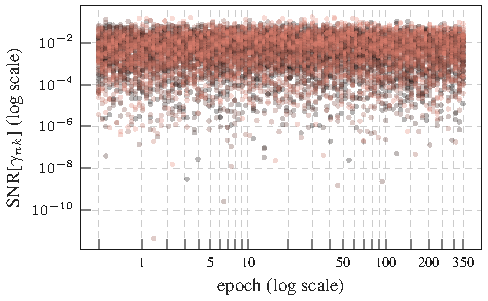
\includegraphics[width=\linewidth]{fig/exp13_plots/gammas_lambdas/cifar100_allcnnc_adam_gammas.pdf}
    \end{minipage}\hfill
    \begin{minipage}{0.50\linewidth}
      \centering
      % % defines the pgfplots style "gammaslambdasdefault"
\pgfkeys{/pgfplots/gammaslambdasdefault/.style={
    width=1.0\linewidth,
    height=0.6\linewidth,
    every axis plot/.append style={line width = 1.5pt},
    mark size = 0.6,
    tick pos = left,
    ylabel near ticks,
    xlabel near ticks,
    xtick align = inside,
    ytick align = inside,
    legend cell align = left,
    legend columns = 1,
    legend pos = south east,
    legend style = {
      fill opacity = 0.7,
      text opacity = 1,
      font = \footnotesize,
    },
    xticklabel style = {font = \footnotesize},
    xlabel style = {font = \footnotesize},
    axis line style = {black},
    yticklabel style = {font = \footnotesize},
    ylabel style = {font = \footnotesize},
    title style = {font = \footnotesize},
    grid = major,
    grid style = {dashed}
  }
}
%%% Local Variables:
%%% mode: latex
%%% TeX-master: "../../thesis"
%%% End:

      % \pgfkeys{/pgfplots/zmystyle/.style={
      % gammaslambdasdefault
      % }}
      %   \tikzexternalenable
      %   NOTE: Too large. pdflatex will run out of memory during externalization
      %   % This file was created by tikzplotlib v0.9.7.
\begin{tikzpicture}

\begin{axis}[
axis line style={white!10!black},
log basis x={10},
tick pos=left,
xlabel={epoch (log scale)},
xmajorgrids,
xmin=0.746099240306814, xmax=469.106495613199,
xmode=log,
ylabel={SNR[\(\displaystyle \lambda_{nk}\)] (log scale)},
ymajorgrids,
ymin=0.00681787118359022, ymax=3683.82973724169,
ymode=log,
zmystyle
]
\addplot [
mark=*,
only marks,
scatter,
scatter/@post marker code/.code={%
  \endscope
},
scatter/@pre marker code/.code={%
  \expanded{%
  \noexpand\definecolor{thispointdrawcolor}{RGB}{\drawcolor}%
  \noexpand\definecolor{thispointfillcolor}{RGB}{\fillcolor}%
  }%
  \scope[draw=thispointdrawcolor, fill=thispointfillcolor]%
},
visualization depends on={value \thisrow{draw} \as \drawcolor},
visualization depends on={value \thisrow{fill} \as \fillcolor}
]
table{%
x  y  draw  fill
1 1.00113499164581 0,0,0 0,0,0
1 0.704787790775299 1.84313725490196,1.05882352941176,0.917647058823529 1.84313725490196,1.05882352941176,0.917647058823529
1 0.600519955158234 4.6078431372549,2.64705882352941,2.29411764705882 4.6078431372549,2.64705882352941,2.29411764705882
1 1.06465888023376 6.45098039215686,3.70588235294118,3.21176470588235 6.45098039215686,3.70588235294118,3.21176470588235
1 1.00293588638306 9.2156862745098,5.29411764705882,4.58823529411765 9.2156862745098,5.29411764705882,4.58823529411765
1 0.568913519382477 11.0588235294118,6.35294117647059,5.50588235294118 11.0588235294118,6.35294117647059,5.50588235294118
1 1.2104594707489 13.8235294117647,7.94117647058823,6.88235294117647 13.8235294117647,7.94117647058823,6.88235294117647
1 0.810195505619049 16.5882352941176,9.52941176470588,8.25882352941176 16.5882352941176,9.52941176470588,8.25882352941176
1 1.47672140598297 18.4313725490196,10.5882352941176,9.17647058823529 18.4313725490196,10.5882352941176,9.17647058823529
1 0.912757813930511 21.1960784313725,12.1764705882353,10.5529411764706 21.1960784313725,12.1764705882353,10.5529411764706
1 1.18661451339722 23.0392156862745,13.2352941176471,11.4705882352941 23.0392156862745,13.2352941176471,11.4705882352941
1 0.777222990989685 25.8039215686274,14.8235294117647,12.8470588235294 25.8039215686274,14.8235294117647,12.8470588235294
1 0.550565600395203 28.5686274509804,16.4117647058824,14.2235294117647 28.5686274509804,16.4117647058824,14.2235294117647
1 0.928269803524017 30.4117647058823,17.4705882352941,15.1411764705882 30.4117647058823,17.4705882352941,15.1411764705882
1 1.24249732494354 33.1764705882353,19.0588235294118,16.5176470588235 33.1764705882353,19.0588235294118,16.5176470588235
1 0.633593201637268 35.0196078431373,20.1176470588235,17.4352941176471 35.0196078431373,20.1176470588235,17.4352941176471
1 1.61882352828979 37.7843137254902,21.7058823529412,18.8117647058824 37.7843137254902,21.7058823529412,18.8117647058824
1 0.873813271522522 39.6274509803922,22.7647058823529,19.7294117647059 39.6274509803922,22.7647058823529,19.7294117647059
1 1.23726904392242 42.3921568627451,24.3529411764706,21.1058823529412 42.3921568627451,24.3529411764706,21.1058823529412
1 1.4977343082428 45.156862745098,25.9411764705882,22.4823529411765 45.156862745098,25.9411764705882,22.4823529411765
1 0.408267199993134 47,27,23.4 47,27,23.4
1 1.04711675643921 49.7647058823529,28.5882352941176,24.7764705882353 49.7647058823529,28.5882352941176,24.7764705882353
1 0.564709782600403 51.6078431372549,29.6470588235294,25.6941176470588 51.6078431372549,29.6470588235294,25.6941176470588
1 2.63709139823914 54.3725490196078,31.2352941176471,27.0705882352941 54.3725490196078,31.2352941176471,27.0705882352941
1 1.53844618797302 57.1372549019608,32.8235294117647,28.4470588235294 57.1372549019608,32.8235294117647,28.4470588235294
1 0.851309299468994 58.9803921568627,33.8823529411765,29.3647058823529 58.9803921568627,33.8823529411765,29.3647058823529
1 1.16675412654877 61.7450980392157,35.4705882352941,30.7411764705882 61.7450980392157,35.4705882352941,30.7411764705882
1 2.23447942733765 63.5882352941176,36.5294117647059,31.6588235294118 63.5882352941176,36.5294117647059,31.6588235294118
1 1.23909986019135 66.3529411764706,38.1176470588235,33.0352941176471 66.3529411764706,38.1176470588235,33.0352941176471
1 1.05242013931274 68.1960784313725,39.1764705882353,33.9529411764706 68.1960784313725,39.1764705882353,33.9529411764706
1 1.2083432674408 70.9607843137255,40.7647058823529,35.3294117647059 70.9607843137255,40.7647058823529,35.3294117647059
1 0.928438723087311 73.7254901960784,42.3529411764706,36.7058823529412 73.7254901960784,42.3529411764706,36.7058823529412
1 1.37483823299408 75.5686274509804,43.4117647058823,37.6235294117647 75.5686274509804,43.4117647058823,37.6235294117647
1 5.1793966293335 78.3333333333333,45,39 78.3333333333333,45,39
1 0.841360867023468 80.1764705882353,46.0588235294118,39.9176470588235 80.1764705882353,46.0588235294118,39.9176470588235
1 0.696467518806458 82.9411764705882,47.6470588235294,41.2941176470588 82.9411764705882,47.6470588235294,41.2941176470588
1 9.61099243164062 85.7058823529412,49.2352941176471,42.6705882352941 85.7058823529412,49.2352941176471,42.6705882352941
1 12.2823266983032 87.5490196078431,50.2941176470588,43.5882352941177 87.5490196078431,50.2941176470588,43.5882352941177
1 27.5849514007568 90.3137254901961,51.8823529411765,44.9647058823529 90.3137254901961,51.8823529411765,44.9647058823529
1 259.803558349609 92.156862745098,52.9411764705882,45.8823529411765 92.156862745098,52.9411764705882,45.8823529411765
1 613.685424804688 94.921568627451,54.5294117647059,47.2588235294118 94.921568627451,54.5294117647059,47.2588235294118
1 94.0201416015625 97.6862745098039,56.1176470588235,48.635294117647 97.6862745098039,56.1176470588235,48.635294117647
1 351.733093261719 99.5294117647059,57.1764705882353,49.5529411764706 99.5294117647059,57.1764705882353,49.5529411764706
1 291.280883789062 102.294117647059,58.7647058823529,50.9294117647059 102.294117647059,58.7647058823529,50.9294117647059
1 267.131469726562 104.137254901961,59.8235294117647,51.8470588235294 104.137254901961,59.8235294117647,51.8470588235294
1 547.3408203125 106.901960784314,61.4117647058824,53.2235294117647 106.901960784314,61.4117647058824,53.2235294117647
1 491.698852539062 108.745098039216,62.4705882352941,54.1411764705882 108.745098039216,62.4705882352941,54.1411764705882
1 1150.30126953125 111.509803921569,64.0588235294118,55.5176470588235 111.509803921569,64.0588235294118,55.5176470588235
1 785.219116210938 114.274509803922,65.6470588235294,56.8941176470588 114.274509803922,65.6470588235294,56.8941176470588
1 507.264129638672 116.117647058824,66.7058823529412,57.8117647058823 116.117647058824,66.7058823529412,57.8117647058823
1 703.665954589844 118.882352941176,68.2941176470588,59.1882352941176 118.882352941176,68.2941176470588,59.1882352941176
1 916.541748046875 120.725490196078,69.3529411764706,60.1058823529412 120.725490196078,69.3529411764706,60.1058823529412
1 909.466369628906 123.490196078431,70.9411764705882,61.4823529411765 123.490196078431,70.9411764705882,61.4823529411765
1 1399.67517089844 126.254901960784,72.5294117647059,62.8588235294118 126.254901960784,72.5294117647059,62.8588235294118
1 1182.14221191406 128.098039215686,73.5882352941176,63.7764705882353 128.098039215686,73.5882352941176,63.7764705882353
1 639.095581054688 130.862745098039,75.1764705882353,65.1529411764706 130.862745098039,75.1764705882353,65.1529411764706
1 886.010986328125 132.705882352941,76.2352941176471,66.0705882352941 132.705882352941,76.2352941176471,66.0705882352941
1 1175.41101074219 135.470588235294,77.8235294117647,67.4470588235294 135.470588235294,77.8235294117647,67.4470588235294
1 757.674499511719 137.313725490196,78.8823529411765,68.3647058823529 137.313725490196,78.8823529411765,68.3647058823529
1 2021.736328125 140.078431372549,80.4705882352941,69.7411764705882 140.078431372549,80.4705882352941,69.7411764705882
1 1436.32946777344 142.843137254902,82.0588235294118,71.1176470588235 142.843137254902,82.0588235294118,71.1176470588235
1 956.371887207031 144.686274509804,83.1176470588235,72.0352941176471 144.686274509804,83.1176470588235,72.0352941176471
1 1003.58978271484 147.450980392157,84.7058823529412,73.4117647058823 147.450980392157,84.7058823529412,73.4117647058823
1 807.215759277344 149.294117647059,85.7647058823529,74.3294117647059 149.294117647059,85.7647058823529,74.3294117647059
1 1872.19213867188 152.058823529412,87.3529411764706,75.7058823529412 152.058823529412,87.3529411764706,75.7058823529412
1 637.596496582031 154.823529411765,88.9411764705882,77.0823529411765 154.823529411765,88.9411764705882,77.0823529411765
1 919.978515625 156.666666666667,90,78 156.666666666667,90,78
1 1487.35827636719 159.43137254902,91.5882352941177,79.3764705882353 159.43137254902,91.5882352941177,79.3764705882353
1 490.606414794922 161.274509803922,92.6470588235294,80.2941176470588 161.274509803922,92.6470588235294,80.2941176470588
1 816.002014160156 164.039215686274,94.2352941176471,81.6705882352941 164.039215686274,94.2352941176471,81.6705882352941
1 1058.35949707031 166.803921568627,95.8235294117647,83.0470588235294 166.803921568627,95.8235294117647,83.0470588235294
1 799.328491210938 168.647058823529,96.8823529411765,83.9647058823529 168.647058823529,96.8823529411765,83.9647058823529
1 400.106231689453 171.411764705882,98.4705882352941,85.3411764705882 171.411764705882,98.4705882352941,85.3411764705882
1 1668.75573730469 173.254901960784,99.5294117647059,86.2588235294118 173.254901960784,99.5294117647059,86.2588235294118
1 616.00537109375 176.019607843137,101.117647058824,87.6352941176471 176.019607843137,101.117647058824,87.6352941176471
1 968.190185546875 177.862745098039,102.176470588235,88.5529411764706 177.862745098039,102.176470588235,88.5529411764706
1 1141.9912109375 180.627450980392,103.764705882353,89.9294117647059 180.627450980392,103.764705882353,89.9294117647059
1 927.805480957031 183.392156862745,105.352941176471,91.3058823529412 183.392156862745,105.352941176471,91.3058823529412
1 1281.47900390625 185.235294117647,106.411764705882,92.2235294117647 185.235294117647,106.411764705882,92.2235294117647
1 1252.57604980469 188,108,93.6 188,108,93.6
1 914.550109863281 189.843137254902,109.058823529412,94.5176470588235 189.843137254902,109.058823529412,94.5176470588235
1 1101.43151855469 192.607843137255,110.647058823529,95.8941176470588 192.607843137255,110.647058823529,95.8941176470588
1 1025.58422851562 195.372549019608,112.235294117647,97.2705882352941 195.372549019608,112.235294117647,97.2705882352941
1 648.72119140625 197.21568627451,113.294117647059,98.1882352941176 197.21568627451,113.294117647059,98.1882352941176
1 765.291809082031 199.980392156863,114.882352941176,99.5647058823529 199.980392156863,114.882352941176,99.5647058823529
1 603.448303222656 201.823529411765,115.941176470588,100.482352941176 201.823529411765,115.941176470588,100.482352941176
1 836.677612304688 204.588235294118,117.529411764706,101.858823529412 204.588235294118,117.529411764706,101.858823529412
1 1095.49841308594 206.43137254902,118.588235294118,102.776470588235 206.43137254902,118.588235294118,102.776470588235
1 1466.12768554688 209.196078431373,120.176470588235,104.152941176471 209.196078431373,120.176470588235,104.152941176471
1 1549.2099609375 211.960784313725,121.764705882353,105.529411764706 211.960784313725,121.764705882353,105.529411764706
1 893.024658203125 213.803921568627,122.823529411765,106.447058823529 213.803921568627,122.823529411765,106.447058823529
1 1088.03942871094 216.56862745098,124.411764705882,107.823529411765 216.56862745098,124.411764705882,107.823529411765
1 1275.6298828125 218.411764705882,125.470588235294,108.741176470588 218.411764705882,125.470588235294,108.741176470588
1 1290.14831542969 221.176470588235,127.058823529412,110.117647058824 221.176470588235,127.058823529412,110.117647058824
1 1159.86462402344 223.941176470588,128.647058823529,111.494117647059 223.941176470588,128.647058823529,111.494117647059
1 1081.17224121094 225.78431372549,129.705882352941,112.411764705882 225.78431372549,129.705882352941,112.411764705882
1 969.159423828125 228.549019607843,131.294117647059,113.788235294118 228.549019607843,131.294117647059,113.788235294118
1 1122.84838867188 230.392156862745,132.352941176471,114.705882352941 230.392156862745,132.352941176471,114.705882352941
1 982.051696777344 233.156862745098,133.941176470588,116.082352941176 233.156862745098,133.941176470588,116.082352941176
1 993.204040527344 235,135,117 235,135,117
1.19230769230769 0.713050961494446 0,0,0 0,0,0
1.19230769230769 1.06151282787323 1.84313725490196,1.05882352941176,0.917647058823529 1.84313725490196,1.05882352941176,0.917647058823529
1.19230769230769 1.45211207866669 4.6078431372549,2.64705882352941,2.29411764705882 4.6078431372549,2.64705882352941,2.29411764705882
1.19230769230769 0.756913840770721 6.45098039215686,3.70588235294118,3.21176470588235 6.45098039215686,3.70588235294118,3.21176470588235
1.19230769230769 0.90383380651474 9.2156862745098,5.29411764705882,4.58823529411765 9.2156862745098,5.29411764705882,4.58823529411765
1.19230769230769 1.0608446598053 11.0588235294118,6.35294117647059,5.50588235294118 11.0588235294118,6.35294117647059,5.50588235294118
1.19230769230769 0.395066142082214 13.8235294117647,7.94117647058823,6.88235294117647 13.8235294117647,7.94117647058823,6.88235294117647
1.19230769230769 0.787444770336151 16.5882352941176,9.52941176470588,8.25882352941176 16.5882352941176,9.52941176470588,8.25882352941176
1.19230769230769 0.790936410427094 18.4313725490196,10.5882352941176,9.17647058823529 18.4313725490196,10.5882352941176,9.17647058823529
1.19230769230769 0.588178634643555 21.1960784313725,12.1764705882353,10.5529411764706 21.1960784313725,12.1764705882353,10.5529411764706
1.19230769230769 0.290847778320312 23.0392156862745,13.2352941176471,11.4705882352941 23.0392156862745,13.2352941176471,11.4705882352941
1.19230769230769 0.583744823932648 25.8039215686274,14.8235294117647,12.8470588235294 25.8039215686274,14.8235294117647,12.8470588235294
1.19230769230769 0.742611348628998 28.5686274509804,16.4117647058824,14.2235294117647 28.5686274509804,16.4117647058824,14.2235294117647
1.19230769230769 0.551761090755463 30.4117647058823,17.4705882352941,15.1411764705882 30.4117647058823,17.4705882352941,15.1411764705882
1.19230769230769 0.427844196557999 33.1764705882353,19.0588235294118,16.5176470588235 33.1764705882353,19.0588235294118,16.5176470588235
1.19230769230769 0.53782707452774 35.0196078431373,20.1176470588235,17.4352941176471 35.0196078431373,20.1176470588235,17.4352941176471
1.19230769230769 0.290100127458572 37.7843137254902,21.7058823529412,18.8117647058824 37.7843137254902,21.7058823529412,18.8117647058824
1.19230769230769 0.437833607196808 39.6274509803922,22.7647058823529,19.7294117647059 39.6274509803922,22.7647058823529,19.7294117647059
1.19230769230769 0.495498865842819 42.3921568627451,24.3529411764706,21.1058823529412 42.3921568627451,24.3529411764706,21.1058823529412
1.19230769230769 0.46238711476326 45.156862745098,25.9411764705882,22.4823529411765 45.156862745098,25.9411764705882,22.4823529411765
1.19230769230769 0.479868531227112 47,27,23.4 47,27,23.4
1.19230769230769 0.26605099439621 49.7647058823529,28.5882352941176,24.7764705882353 49.7647058823529,28.5882352941176,24.7764705882353
1.19230769230769 0.351072788238525 51.6078431372549,29.6470588235294,25.6941176470588 51.6078431372549,29.6470588235294,25.6941176470588
1.19230769230769 0.488341510295868 54.3725490196078,31.2352941176471,27.0705882352941 54.3725490196078,31.2352941176471,27.0705882352941
1.19230769230769 0.462820470333099 57.1372549019608,32.8235294117647,28.4470588235294 57.1372549019608,32.8235294117647,28.4470588235294
1.19230769230769 0.323237538337708 58.9803921568627,33.8823529411765,29.3647058823529 58.9803921568627,33.8823529411765,29.3647058823529
1.19230769230769 0.352579444646835 61.7450980392157,35.4705882352941,30.7411764705882 61.7450980392157,35.4705882352941,30.7411764705882
1.19230769230769 0.851368129253387 63.5882352941176,36.5294117647059,31.6588235294118 63.5882352941176,36.5294117647059,31.6588235294118
1.19230769230769 0.537303268909454 66.3529411764706,38.1176470588235,33.0352941176471 66.3529411764706,38.1176470588235,33.0352941176471
1.19230769230769 0.673282384872437 68.1960784313725,39.1764705882353,33.9529411764706 68.1960784313725,39.1764705882353,33.9529411764706
1.19230769230769 0.421907722949982 70.9607843137255,40.7647058823529,35.3294117647059 70.9607843137255,40.7647058823529,35.3294117647059
1.19230769230769 0.410865366458893 73.7254901960784,42.3529411764706,36.7058823529412 73.7254901960784,42.3529411764706,36.7058823529412
1.19230769230769 0.452413856983185 75.5686274509804,43.4117647058823,37.6235294117647 75.5686274509804,43.4117647058823,37.6235294117647
1.19230769230769 0.612820088863373 78.3333333333333,45,39 78.3333333333333,45,39
1.19230769230769 0.685076594352722 80.1764705882353,46.0588235294118,39.9176470588235 80.1764705882353,46.0588235294118,39.9176470588235
1.19230769230769 0.505680203437805 82.9411764705882,47.6470588235294,41.2941176470588 82.9411764705882,47.6470588235294,41.2941176470588
1.19230769230769 0.465778142213821 85.7058823529412,49.2352941176471,42.6705882352941 85.7058823529412,49.2352941176471,42.6705882352941
1.19230769230769 0.532334983348846 87.5490196078431,50.2941176470588,43.5882352941177 87.5490196078431,50.2941176470588,43.5882352941177
1.19230769230769 0.34974217414856 90.3137254901961,51.8823529411765,44.9647058823529 90.3137254901961,51.8823529411765,44.9647058823529
1.19230769230769 0.317860394716263 92.156862745098,52.9411764705882,45.8823529411765 92.156862745098,52.9411764705882,45.8823529411765
1.19230769230769 0.367700517177582 94.921568627451,54.5294117647059,47.2588235294118 94.921568627451,54.5294117647059,47.2588235294118
1.19230769230769 0.414616584777832 97.6862745098039,56.1176470588235,48.635294117647 97.6862745098039,56.1176470588235,48.635294117647
1.19230769230769 0.422904551029205 99.5294117647059,57.1764705882353,49.5529411764706 99.5294117647059,57.1764705882353,49.5529411764706
1.19230769230769 0.468307703733444 102.294117647059,58.7647058823529,50.9294117647059 102.294117647059,58.7647058823529,50.9294117647059
1.19230769230769 0.500924527645111 104.137254901961,59.8235294117647,51.8470588235294 104.137254901961,59.8235294117647,51.8470588235294
1.19230769230769 0.52239054441452 106.901960784314,61.4117647058824,53.2235294117647 106.901960784314,61.4117647058824,53.2235294117647
1.19230769230769 0.693659842014313 108.745098039216,62.4705882352941,54.1411764705882 108.745098039216,62.4705882352941,54.1411764705882
1.19230769230769 0.447685539722443 111.509803921569,64.0588235294118,55.5176470588235 111.509803921569,64.0588235294118,55.5176470588235
1.19230769230769 0.7470623254776 114.274509803922,65.6470588235294,56.8941176470588 114.274509803922,65.6470588235294,56.8941176470588
1.19230769230769 0.753121733665466 116.117647058824,66.7058823529412,57.8117647058823 116.117647058824,66.7058823529412,57.8117647058823
1.19230769230769 0.385654896497726 118.882352941176,68.2941176470588,59.1882352941176 118.882352941176,68.2941176470588,59.1882352941176
1.19230769230769 1.9381000995636 120.725490196078,69.3529411764706,60.1058823529412 120.725490196078,69.3529411764706,60.1058823529412
1.19230769230769 1.28636944293976 123.490196078431,70.9411764705882,61.4823529411765 123.490196078431,70.9411764705882,61.4823529411765
1.19230769230769 0.511007189750671 126.254901960784,72.5294117647059,62.8588235294118 126.254901960784,72.5294117647059,62.8588235294118
1.19230769230769 3.49432516098022 128.098039215686,73.5882352941176,63.7764705882353 128.098039215686,73.5882352941176,63.7764705882353
1.19230769230769 1.48308825492859 130.862745098039,75.1764705882353,65.1529411764706 130.862745098039,75.1764705882353,65.1529411764706
1.19230769230769 0.784870028495789 132.705882352941,76.2352941176471,66.0705882352941 132.705882352941,76.2352941176471,66.0705882352941
1.19230769230769 0.808475971221924 135.470588235294,77.8235294117647,67.4470588235294 135.470588235294,77.8235294117647,67.4470588235294
1.19230769230769 8.42332172393799 137.313725490196,78.8823529411765,68.3647058823529 137.313725490196,78.8823529411765,68.3647058823529
1.19230769230769 3.78917932510376 140.078431372549,80.4705882352941,69.7411764705882 140.078431372549,80.4705882352941,69.7411764705882
1.19230769230769 1.28384554386139 142.843137254902,82.0588235294118,71.1176470588235 142.843137254902,82.0588235294118,71.1176470588235
1.19230769230769 12.1600952148438 144.686274509804,83.1176470588235,72.0352941176471 144.686274509804,83.1176470588235,72.0352941176471
1.19230769230769 30.1963844299316 147.450980392157,84.7058823529412,73.4117647058823 147.450980392157,84.7058823529412,73.4117647058823
1.19230769230769 79.6838912963867 149.294117647059,85.7647058823529,74.3294117647059 149.294117647059,85.7647058823529,74.3294117647059
1.19230769230769 25.5117721557617 152.058823529412,87.3529411764706,75.7058823529412 152.058823529412,87.3529411764706,75.7058823529412
1.19230769230769 19.1663627624512 154.823529411765,88.9411764705882,77.0823529411765 154.823529411765,88.9411764705882,77.0823529411765
1.19230769230769 18.3083896636963 156.666666666667,90,78 156.666666666667,90,78
1.19230769230769 13.0802583694458 159.43137254902,91.5882352941177,79.3764705882353 159.43137254902,91.5882352941177,79.3764705882353
1.19230769230769 54.1464729309082 161.274509803922,92.6470588235294,80.2941176470588 161.274509803922,92.6470588235294,80.2941176470588
1.19230769230769 14.8679981231689 164.039215686274,94.2352941176471,81.6705882352941 164.039215686274,94.2352941176471,81.6705882352941
1.19230769230769 32.5844459533691 166.803921568627,95.8235294117647,83.0470588235294 166.803921568627,95.8235294117647,83.0470588235294
1.19230769230769 15.0849170684814 168.647058823529,96.8823529411765,83.9647058823529 168.647058823529,96.8823529411765,83.9647058823529
1.19230769230769 52.3348503112793 171.411764705882,98.4705882352941,85.3411764705882 171.411764705882,98.4705882352941,85.3411764705882
1.19230769230769 27.3592014312744 173.254901960784,99.5294117647059,86.2588235294118 173.254901960784,99.5294117647059,86.2588235294118
1.19230769230769 35.5221557617188 176.019607843137,101.117647058824,87.6352941176471 176.019607843137,101.117647058824,87.6352941176471
1.19230769230769 10.4775743484497 177.862745098039,102.176470588235,88.5529411764706 177.862745098039,102.176470588235,88.5529411764706
1.19230769230769 13.3286285400391 180.627450980392,103.764705882353,89.9294117647059 180.627450980392,103.764705882353,89.9294117647059
1.19230769230769 14.4685325622559 183.392156862745,105.352941176471,91.3058823529412 183.392156862745,105.352941176471,91.3058823529412
1.19230769230769 15.9286193847656 185.235294117647,106.411764705882,92.2235294117647 185.235294117647,106.411764705882,92.2235294117647
1.19230769230769 9.85371112823486 188,108,93.6 188,108,93.6
1.19230769230769 17.6254577636719 189.843137254902,109.058823529412,94.5176470588235 189.843137254902,109.058823529412,94.5176470588235
1.19230769230769 13.2749538421631 192.607843137255,110.647058823529,95.8941176470588 192.607843137255,110.647058823529,95.8941176470588
1.19230769230769 23.4181098937988 195.372549019608,112.235294117647,97.2705882352941 195.372549019608,112.235294117647,97.2705882352941
1.19230769230769 14.1378660202026 197.21568627451,113.294117647059,98.1882352941176 197.21568627451,113.294117647059,98.1882352941176
1.19230769230769 12.508487701416 199.980392156863,114.882352941176,99.5647058823529 199.980392156863,114.882352941176,99.5647058823529
1.19230769230769 10.5659961700439 201.823529411765,115.941176470588,100.482352941176 201.823529411765,115.941176470588,100.482352941176
1.19230769230769 13.476637840271 204.588235294118,117.529411764706,101.858823529412 204.588235294118,117.529411764706,101.858823529412
1.19230769230769 7.87775230407715 206.43137254902,118.588235294118,102.776470588235 206.43137254902,118.588235294118,102.776470588235
1.19230769230769 13.1741056442261 209.196078431373,120.176470588235,104.152941176471 209.196078431373,120.176470588235,104.152941176471
1.19230769230769 8.11706829071045 211.960784313725,121.764705882353,105.529411764706 211.960784313725,121.764705882353,105.529411764706
1.19230769230769 13.8913974761963 213.803921568627,122.823529411765,106.447058823529 213.803921568627,122.823529411765,106.447058823529
1.19230769230769 9.36343193054199 216.56862745098,124.411764705882,107.823529411765 216.56862745098,124.411764705882,107.823529411765
1.19230769230769 10.2804899215698 218.411764705882,125.470588235294,108.741176470588 218.411764705882,125.470588235294,108.741176470588
1.19230769230769 8.45233345031738 221.176470588235,127.058823529412,110.117647058824 221.176470588235,127.058823529412,110.117647058824
1.19230769230769 9.1556510925293 223.941176470588,128.647058823529,111.494117647059 223.941176470588,128.647058823529,111.494117647059
1.19230769230769 10.6282196044922 225.78431372549,129.705882352941,112.411764705882 225.78431372549,129.705882352941,112.411764705882
1.19230769230769 15.6339492797852 228.549019607843,131.294117647059,113.788235294118 228.549019607843,131.294117647059,113.788235294118
1.19230769230769 10.4707260131836 230.392156862745,132.352941176471,114.705882352941 230.392156862745,132.352941176471,114.705882352941
1.19230769230769 7.3332896232605 233.156862745098,133.941176470588,116.082352941176 233.156862745098,133.941176470588,116.082352941176
1.19230769230769 10.0245800018311 235,135,117 235,135,117
1.42307692307692 0.620631337165833 0,0,0 0,0,0
1.42307692307692 0.724843621253967 1.84313725490196,1.05882352941176,0.917647058823529 1.84313725490196,1.05882352941176,0.917647058823529
1.42307692307692 1.22612535953522 4.6078431372549,2.64705882352941,2.29411764705882 4.6078431372549,2.64705882352941,2.29411764705882
1.42307692307692 0.769785046577454 6.45098039215686,3.70588235294118,3.21176470588235 6.45098039215686,3.70588235294118,3.21176470588235
1.42307692307692 0.927691459655762 9.2156862745098,5.29411764705882,4.58823529411765 9.2156862745098,5.29411764705882,4.58823529411765
1.42307692307692 0.920777559280396 11.0588235294118,6.35294117647059,5.50588235294118 11.0588235294118,6.35294117647059,5.50588235294118
1.42307692307692 1.19627797603607 13.8235294117647,7.94117647058823,6.88235294117647 13.8235294117647,7.94117647058823,6.88235294117647
1.42307692307692 1.03356719017029 16.5882352941176,9.52941176470588,8.25882352941176 16.5882352941176,9.52941176470588,8.25882352941176
1.42307692307692 0.619524002075195 18.4313725490196,10.5882352941176,9.17647058823529 18.4313725490196,10.5882352941176,9.17647058823529
1.42307692307692 1.00333714485168 21.1960784313725,12.1764705882353,10.5529411764706 21.1960784313725,12.1764705882353,10.5529411764706
1.42307692307692 0.593349635601044 23.0392156862745,13.2352941176471,11.4705882352941 23.0392156862745,13.2352941176471,11.4705882352941
1.42307692307692 1.08147251605988 25.8039215686274,14.8235294117647,12.8470588235294 25.8039215686274,14.8235294117647,12.8470588235294
1.42307692307692 1.14319550991058 28.5686274509804,16.4117647058824,14.2235294117647 28.5686274509804,16.4117647058824,14.2235294117647
1.42307692307692 1.27548491954803 30.4117647058823,17.4705882352941,15.1411764705882 30.4117647058823,17.4705882352941,15.1411764705882
1.42307692307692 0.959066271781921 33.1764705882353,19.0588235294118,16.5176470588235 33.1764705882353,19.0588235294118,16.5176470588235
1.42307692307692 1.18874621391296 35.0196078431373,20.1176470588235,17.4352941176471 35.0196078431373,20.1176470588235,17.4352941176471
1.42307692307692 1.00393307209015 37.7843137254902,21.7058823529412,18.8117647058824 37.7843137254902,21.7058823529412,18.8117647058824
1.42307692307692 1.31414318084717 39.6274509803922,22.7647058823529,19.7294117647059 39.6274509803922,22.7647058823529,19.7294117647059
1.42307692307692 0.43096387386322 42.3921568627451,24.3529411764706,21.1058823529412 42.3921568627451,24.3529411764706,21.1058823529412
1.42307692307692 1.1150381565094 45.156862745098,25.9411764705882,22.4823529411765 45.156862745098,25.9411764705882,22.4823529411765
1.42307692307692 1.15064477920532 47,27,23.4 47,27,23.4
1.42307692307692 1.46535468101501 49.7647058823529,28.5882352941176,24.7764705882353 49.7647058823529,28.5882352941176,24.7764705882353
1.42307692307692 1.35513424873352 51.6078431372549,29.6470588235294,25.6941176470588 51.6078431372549,29.6470588235294,25.6941176470588
1.42307692307692 1.05626749992371 54.3725490196078,31.2352941176471,27.0705882352941 54.3725490196078,31.2352941176471,27.0705882352941
1.42307692307692 0.838187694549561 57.1372549019608,32.8235294117647,28.4470588235294 57.1372549019608,32.8235294117647,28.4470588235294
1.42307692307692 1.41229915618896 58.9803921568627,33.8823529411765,29.3647058823529 58.9803921568627,33.8823529411765,29.3647058823529
1.42307692307692 1.14561986923218 61.7450980392157,35.4705882352941,30.7411764705882 61.7450980392157,35.4705882352941,30.7411764705882
1.42307692307692 1.49707055091858 63.5882352941176,36.5294117647059,31.6588235294118 63.5882352941176,36.5294117647059,31.6588235294118
1.42307692307692 1.35956346988678 66.3529411764706,38.1176470588235,33.0352941176471 66.3529411764706,38.1176470588235,33.0352941176471
1.42307692307692 0.398156970739365 68.1960784313725,39.1764705882353,33.9529411764706 68.1960784313725,39.1764705882353,33.9529411764706
1.42307692307692 0.663439869880676 70.9607843137255,40.7647058823529,35.3294117647059 70.9607843137255,40.7647058823529,35.3294117647059
1.42307692307692 1.30862259864807 73.7254901960784,42.3529411764706,36.7058823529412 73.7254901960784,42.3529411764706,36.7058823529412
1.42307692307692 0.946869730949402 75.5686274509804,43.4117647058823,37.6235294117647 75.5686274509804,43.4117647058823,37.6235294117647
1.42307692307692 1.06314837932587 78.3333333333333,45,39 78.3333333333333,45,39
1.42307692307692 0.899042427539825 80.1764705882353,46.0588235294118,39.9176470588235 80.1764705882353,46.0588235294118,39.9176470588235
1.42307692307692 0.922859311103821 82.9411764705882,47.6470588235294,41.2941176470588 82.9411764705882,47.6470588235294,41.2941176470588
1.42307692307692 0.912660539150238 85.7058823529412,49.2352941176471,42.6705882352941 85.7058823529412,49.2352941176471,42.6705882352941
1.42307692307692 0.596000611782074 87.5490196078431,50.2941176470588,43.5882352941177 87.5490196078431,50.2941176470588,43.5882352941177
1.42307692307692 1.66594016551971 90.3137254901961,51.8823529411765,44.9647058823529 90.3137254901961,51.8823529411765,44.9647058823529
1.42307692307692 1.12211215496063 92.156862745098,52.9411764705882,45.8823529411765 92.156862745098,52.9411764705882,45.8823529411765
1.42307692307692 1.39004015922546 94.921568627451,54.5294117647059,47.2588235294118 94.921568627451,54.5294117647059,47.2588235294118
1.42307692307692 1.6152708530426 97.6862745098039,56.1176470588235,48.635294117647 97.6862745098039,56.1176470588235,48.635294117647
1.42307692307692 1.0675196647644 99.5294117647059,57.1764705882353,49.5529411764706 99.5294117647059,57.1764705882353,49.5529411764706
1.42307692307692 0.794151842594147 102.294117647059,58.7647058823529,50.9294117647059 102.294117647059,58.7647058823529,50.9294117647059
1.42307692307692 0.56535941362381 104.137254901961,59.8235294117647,51.8470588235294 104.137254901961,59.8235294117647,51.8470588235294
1.42307692307692 1.10459196567535 106.901960784314,61.4117647058824,53.2235294117647 106.901960784314,61.4117647058824,53.2235294117647
1.42307692307692 0.925725638866425 108.745098039216,62.4705882352941,54.1411764705882 108.745098039216,62.4705882352941,54.1411764705882
1.42307692307692 1.41376960277557 111.509803921569,64.0588235294118,55.5176470588235 111.509803921569,64.0588235294118,55.5176470588235
1.42307692307692 1.20982599258423 114.274509803922,65.6470588235294,56.8941176470588 114.274509803922,65.6470588235294,56.8941176470588
1.42307692307692 1.32229101657867 116.117647058824,66.7058823529412,57.8117647058823 116.117647058824,66.7058823529412,57.8117647058823
1.42307692307692 1.41896688938141 118.882352941176,68.2941176470588,59.1882352941176 118.882352941176,68.2941176470588,59.1882352941176
1.42307692307692 0.963859498500824 120.725490196078,69.3529411764706,60.1058823529412 120.725490196078,69.3529411764706,60.1058823529412
1.42307692307692 0.440105348825455 123.490196078431,70.9411764705882,61.4823529411765 123.490196078431,70.9411764705882,61.4823529411765
1.42307692307692 1.14452004432678 126.254901960784,72.5294117647059,62.8588235294118 126.254901960784,72.5294117647059,62.8588235294118
1.42307692307692 0.351415038108826 128.098039215686,73.5882352941176,63.7764705882353 128.098039215686,73.5882352941176,63.7764705882353
1.42307692307692 0.433066934347153 130.862745098039,75.1764705882353,65.1529411764706 130.862745098039,75.1764705882353,65.1529411764706
1.42307692307692 0.595673799514771 132.705882352941,76.2352941176471,66.0705882352941 132.705882352941,76.2352941176471,66.0705882352941
1.42307692307692 0.436432272195816 135.470588235294,77.8235294117647,67.4470588235294 135.470588235294,77.8235294117647,67.4470588235294
1.42307692307692 0.383756190538406 137.313725490196,78.8823529411765,68.3647058823529 137.313725490196,78.8823529411765,68.3647058823529
1.42307692307692 0.407092273235321 140.078431372549,80.4705882352941,69.7411764705882 140.078431372549,80.4705882352941,69.7411764705882
1.42307692307692 0.127958342432976 142.843137254902,82.0588235294118,71.1176470588235 142.843137254902,82.0588235294118,71.1176470588235
1.42307692307692 0.9097820520401 144.686274509804,83.1176470588235,72.0352941176471 144.686274509804,83.1176470588235,72.0352941176471
1.42307692307692 0.438594371080399 147.450980392157,84.7058823529412,73.4117647058823 147.450980392157,84.7058823529412,73.4117647058823
1.42307692307692 0.437206327915192 149.294117647059,85.7647058823529,74.3294117647059 149.294117647059,85.7647058823529,74.3294117647059
1.42307692307692 0.435680866241455 152.058823529412,87.3529411764706,75.7058823529412 152.058823529412,87.3529411764706,75.7058823529412
1.42307692307692 0.4348985850811 154.823529411765,88.9411764705882,77.0823529411765 154.823529411765,88.9411764705882,77.0823529411765
1.42307692307692 0.235362440347672 156.666666666667,90,78 156.666666666667,90,78
1.42307692307692 0.319575786590576 159.43137254902,91.5882352941177,79.3764705882353 159.43137254902,91.5882352941177,79.3764705882353
1.42307692307692 0.528746604919434 161.274509803922,92.6470588235294,80.2941176470588 161.274509803922,92.6470588235294,80.2941176470588
1.42307692307692 0.21379716694355 164.039215686274,94.2352941176471,81.6705882352941 164.039215686274,94.2352941176471,81.6705882352941
1.42307692307692 0.437114894390106 166.803921568627,95.8235294117647,83.0470588235294 166.803921568627,95.8235294117647,83.0470588235294
1.42307692307692 0.219371944665909 168.647058823529,96.8823529411765,83.9647058823529 168.647058823529,96.8823529411765,83.9647058823529
1.42307692307692 0.408343732357025 171.411764705882,98.4705882352941,85.3411764705882 171.411764705882,98.4705882352941,85.3411764705882
1.42307692307692 0.271004527807236 173.254901960784,99.5294117647059,86.2588235294118 173.254901960784,99.5294117647059,86.2588235294118
1.42307692307692 0.434431999921799 176.019607843137,101.117647058824,87.6352941176471 176.019607843137,101.117647058824,87.6352941176471
1.42307692307692 0.410938262939453 177.862745098039,102.176470588235,88.5529411764706 177.862745098039,102.176470588235,88.5529411764706
1.42307692307692 0.275156289339066 180.627450980392,103.764705882353,89.9294117647059 180.627450980392,103.764705882353,89.9294117647059
1.42307692307692 0.527487099170685 183.392156862745,105.352941176471,91.3058823529412 183.392156862745,105.352941176471,91.3058823529412
1.42307692307692 0.483599841594696 185.235294117647,106.411764705882,92.2235294117647 185.235294117647,106.411764705882,92.2235294117647
1.42307692307692 0.251073241233826 188,108,93.6 188,108,93.6
1.42307692307692 0.333559513092041 189.843137254902,109.058823529412,94.5176470588235 189.843137254902,109.058823529412,94.5176470588235
1.42307692307692 0.483779430389404 192.607843137255,110.647058823529,95.8941176470588 192.607843137255,110.647058823529,95.8941176470588
1.42307692307692 0.306732416152954 195.372549019608,112.235294117647,97.2705882352941 195.372549019608,112.235294117647,97.2705882352941
1.42307692307692 0.359036386013031 197.21568627451,113.294117647059,98.1882352941176 197.21568627451,113.294117647059,98.1882352941176
1.42307692307692 0.0531248077750206 199.980392156863,114.882352941176,99.5647058823529 199.980392156863,114.882352941176,99.5647058823529
1.42307692307692 0.185703754425049 201.823529411765,115.941176470588,100.482352941176 201.823529411765,115.941176470588,100.482352941176
1.42307692307692 0.172391086816788 204.588235294118,117.529411764706,101.858823529412 204.588235294118,117.529411764706,101.858823529412
1.42307692307692 0.0578648522496223 206.43137254902,118.588235294118,102.776470588235 206.43137254902,118.588235294118,102.776470588235
1.42307692307692 0.194866821169853 209.196078431373,120.176470588235,104.152941176471 209.196078431373,120.176470588235,104.152941176471
1.42307692307692 0.250178247690201 211.960784313725,121.764705882353,105.529411764706 211.960784313725,121.764705882353,105.529411764706
1.42307692307692 0.0951847955584526 213.803921568627,122.823529411765,106.447058823529 213.803921568627,122.823529411765,106.447058823529
1.42307692307692 0.1612239331007 216.56862745098,124.411764705882,107.823529411765 216.56862745098,124.411764705882,107.823529411765
1.42307692307692 0.0473750568926334 218.411764705882,125.470588235294,108.741176470588 218.411764705882,125.470588235294,108.741176470588
1.42307692307692 0.127441465854645 221.176470588235,127.058823529412,110.117647058824 221.176470588235,127.058823529412,110.117647058824
1.42307692307692 0.13277904689312 223.941176470588,128.647058823529,111.494117647059 223.941176470588,128.647058823529,111.494117647059
1.42307692307692 0.187869876623154 225.78431372549,129.705882352941,112.411764705882 225.78431372549,129.705882352941,112.411764705882
1.42307692307692 0.154594704508781 228.549019607843,131.294117647059,113.788235294118 228.549019607843,131.294117647059,113.788235294118
1.42307692307692 0.114194273948669 230.392156862745,132.352941176471,114.705882352941 230.392156862745,132.352941176471,114.705882352941
1.42307692307692 0.106195352971554 233.156862745098,133.941176470588,116.082352941176 233.156862745098,133.941176470588,116.082352941176
1.42307692307692 0.170742556452751 235,135,117 235,135,117
1.69871794871795 0.519126653671265 0,0,0 0,0,0
1.69871794871795 0.669970631599426 1.84313725490196,1.05882352941176,0.917647058823529 1.84313725490196,1.05882352941176,0.917647058823529
1.69871794871795 0.997739672660828 4.6078431372549,2.64705882352941,2.29411764705882 4.6078431372549,2.64705882352941,2.29411764705882
1.69871794871795 1.01351475715637 6.45098039215686,3.70588235294118,3.21176470588235 6.45098039215686,3.70588235294118,3.21176470588235
1.69871794871795 0.334018111228943 9.2156862745098,5.29411764705882,4.58823529411765 9.2156862745098,5.29411764705882,4.58823529411765
1.69871794871795 0.65932023525238 11.0588235294118,6.35294117647059,5.50588235294118 11.0588235294118,6.35294117647059,5.50588235294118
1.69871794871795 0.592022001743317 13.8235294117647,7.94117647058823,6.88235294117647 13.8235294117647,7.94117647058823,6.88235294117647
1.69871794871795 0.761277616024017 16.5882352941176,9.52941176470588,8.25882352941176 16.5882352941176,9.52941176470588,8.25882352941176
1.69871794871795 0.939371109008789 18.4313725490196,10.5882352941176,9.17647058823529 18.4313725490196,10.5882352941176,9.17647058823529
1.69871794871795 0.730550646781921 21.1960784313725,12.1764705882353,10.5529411764706 21.1960784313725,12.1764705882353,10.5529411764706
1.69871794871795 0.651711523532867 23.0392156862745,13.2352941176471,11.4705882352941 23.0392156862745,13.2352941176471,11.4705882352941
1.69871794871795 0.894258975982666 25.8039215686274,14.8235294117647,12.8470588235294 25.8039215686274,14.8235294117647,12.8470588235294
1.69871794871795 0.525243639945984 28.5686274509804,16.4117647058824,14.2235294117647 28.5686274509804,16.4117647058824,14.2235294117647
1.69871794871795 1.11759889125824 30.4117647058823,17.4705882352941,15.1411764705882 30.4117647058823,17.4705882352941,15.1411764705882
1.69871794871795 0.745583772659302 33.1764705882353,19.0588235294118,16.5176470588235 33.1764705882353,19.0588235294118,16.5176470588235
1.69871794871795 0.835886836051941 35.0196078431373,20.1176470588235,17.4352941176471 35.0196078431373,20.1176470588235,17.4352941176471
1.69871794871795 0.814156293869019 37.7843137254902,21.7058823529412,18.8117647058824 37.7843137254902,21.7058823529412,18.8117647058824
1.69871794871795 0.856119096279144 39.6274509803922,22.7647058823529,19.7294117647059 39.6274509803922,22.7647058823529,19.7294117647059
1.69871794871795 0.863919377326965 42.3921568627451,24.3529411764706,21.1058823529412 42.3921568627451,24.3529411764706,21.1058823529412
1.69871794871795 1.06974816322327 45.156862745098,25.9411764705882,22.4823529411765 45.156862745098,25.9411764705882,22.4823529411765
1.69871794871795 0.931421518325806 47,27,23.4 47,27,23.4
1.69871794871795 1.12555921077728 49.7647058823529,28.5882352941176,24.7764705882353 49.7647058823529,28.5882352941176,24.7764705882353
1.69871794871795 0.864960968494415 51.6078431372549,29.6470588235294,25.6941176470588 51.6078431372549,29.6470588235294,25.6941176470588
1.69871794871795 0.946864664554596 54.3725490196078,31.2352941176471,27.0705882352941 54.3725490196078,31.2352941176471,27.0705882352941
1.69871794871795 1.05191385746002 57.1372549019608,32.8235294117647,28.4470588235294 57.1372549019608,32.8235294117647,28.4470588235294
1.69871794871795 0.82011753320694 58.9803921568627,33.8823529411765,29.3647058823529 58.9803921568627,33.8823529411765,29.3647058823529
1.69871794871795 1.07297277450562 61.7450980392157,35.4705882352941,30.7411764705882 61.7450980392157,35.4705882352941,30.7411764705882
1.69871794871795 0.847987771034241 63.5882352941176,36.5294117647059,31.6588235294118 63.5882352941176,36.5294117647059,31.6588235294118
1.69871794871795 0.900112688541412 66.3529411764706,38.1176470588235,33.0352941176471 66.3529411764706,38.1176470588235,33.0352941176471
1.69871794871795 1.13693392276764 68.1960784313725,39.1764705882353,33.9529411764706 68.1960784313725,39.1764705882353,33.9529411764706
1.69871794871795 0.954886555671692 70.9607843137255,40.7647058823529,35.3294117647059 70.9607843137255,40.7647058823529,35.3294117647059
1.69871794871795 1.09133386611938 73.7254901960784,42.3529411764706,36.7058823529412 73.7254901960784,42.3529411764706,36.7058823529412
1.69871794871795 1.16980540752411 75.5686274509804,43.4117647058823,37.6235294117647 75.5686274509804,43.4117647058823,37.6235294117647
1.69871794871795 0.79420131444931 78.3333333333333,45,39 78.3333333333333,45,39
1.69871794871795 0.799357712268829 80.1764705882353,46.0588235294118,39.9176470588235 80.1764705882353,46.0588235294118,39.9176470588235
1.69871794871795 1.54546594619751 82.9411764705882,47.6470588235294,41.2941176470588 82.9411764705882,47.6470588235294,41.2941176470588
1.69871794871795 1.34495151042938 85.7058823529412,49.2352941176471,42.6705882352941 85.7058823529412,49.2352941176471,42.6705882352941
1.69871794871795 0.613058090209961 87.5490196078431,50.2941176470588,43.5882352941177 87.5490196078431,50.2941176470588,43.5882352941177
1.69871794871795 1.0386221408844 90.3137254901961,51.8823529411765,44.9647058823529 90.3137254901961,51.8823529411765,44.9647058823529
1.69871794871795 0.309028059244156 92.156862745098,52.9411764705882,45.8823529411765 92.156862745098,52.9411764705882,45.8823529411765
1.69871794871795 0.736237168312073 94.921568627451,54.5294117647059,47.2588235294118 94.921568627451,54.5294117647059,47.2588235294118
1.69871794871795 0.547532141208649 97.6862745098039,56.1176470588235,48.635294117647 97.6862745098039,56.1176470588235,48.635294117647
1.69871794871795 0.71546459197998 99.5294117647059,57.1764705882353,49.5529411764706 99.5294117647059,57.1764705882353,49.5529411764706
1.69871794871795 1.1624162197113 102.294117647059,58.7647058823529,50.9294117647059 102.294117647059,58.7647058823529,50.9294117647059
1.69871794871795 1.0118180513382 104.137254901961,59.8235294117647,51.8470588235294 104.137254901961,59.8235294117647,51.8470588235294
1.69871794871795 0.559237480163574 106.901960784314,61.4117647058824,53.2235294117647 106.901960784314,61.4117647058824,53.2235294117647
1.69871794871795 0.755873143672943 108.745098039216,62.4705882352941,54.1411764705882 108.745098039216,62.4705882352941,54.1411764705882
1.69871794871795 0.671104848384857 111.509803921569,64.0588235294118,55.5176470588235 111.509803921569,64.0588235294118,55.5176470588235
1.69871794871795 0.680605530738831 114.274509803922,65.6470588235294,56.8941176470588 114.274509803922,65.6470588235294,56.8941176470588
1.69871794871795 0.718923926353455 116.117647058824,66.7058823529412,57.8117647058823 116.117647058824,66.7058823529412,57.8117647058823
1.69871794871795 1.18418288230896 118.882352941176,68.2941176470588,59.1882352941176 118.882352941176,68.2941176470588,59.1882352941176
1.69871794871795 0.571979403495789 120.725490196078,69.3529411764706,60.1058823529412 120.725490196078,69.3529411764706,60.1058823529412
1.69871794871795 1.09726333618164 123.490196078431,70.9411764705882,61.4823529411765 123.490196078431,70.9411764705882,61.4823529411765
1.69871794871795 0.821437001228333 126.254901960784,72.5294117647059,62.8588235294118 126.254901960784,72.5294117647059,62.8588235294118
1.69871794871795 0.837128758430481 128.098039215686,73.5882352941176,63.7764705882353 128.098039215686,73.5882352941176,63.7764705882353
1.69871794871795 0.555650293827057 130.862745098039,75.1764705882353,65.1529411764706 130.862745098039,75.1764705882353,65.1529411764706
1.69871794871795 0.571090698242188 132.705882352941,76.2352941176471,66.0705882352941 132.705882352941,76.2352941176471,66.0705882352941
1.69871794871795 0.507716655731201 135.470588235294,77.8235294117647,67.4470588235294 135.470588235294,77.8235294117647,67.4470588235294
1.69871794871795 0.84180873632431 137.313725490196,78.8823529411765,68.3647058823529 137.313725490196,78.8823529411765,68.3647058823529
1.69871794871795 0.460165083408356 140.078431372549,80.4705882352941,69.7411764705882 140.078431372549,80.4705882352941,69.7411764705882
1.69871794871795 0.882088482379913 142.843137254902,82.0588235294118,71.1176470588235 142.843137254902,82.0588235294118,71.1176470588235
1.69871794871795 0.771427869796753 144.686274509804,83.1176470588235,72.0352941176471 144.686274509804,83.1176470588235,72.0352941176471
1.69871794871795 0.828227579593658 147.450980392157,84.7058823529412,73.4117647058823 147.450980392157,84.7058823529412,73.4117647058823
1.69871794871795 0.484567880630493 149.294117647059,85.7647058823529,74.3294117647059 149.294117647059,85.7647058823529,74.3294117647059
1.69871794871795 0.461237251758575 152.058823529412,87.3529411764706,75.7058823529412 152.058823529412,87.3529411764706,75.7058823529412
1.69871794871795 0.344362914562225 154.823529411765,88.9411764705882,77.0823529411765 154.823529411765,88.9411764705882,77.0823529411765
1.69871794871795 0.579834401607513 156.666666666667,90,78 156.666666666667,90,78
1.69871794871795 0.464815229177475 159.43137254902,91.5882352941177,79.3764705882353 159.43137254902,91.5882352941177,79.3764705882353
1.69871794871795 0.365509808063507 161.274509803922,92.6470588235294,80.2941176470588 161.274509803922,92.6470588235294,80.2941176470588
1.69871794871795 0.764417827129364 164.039215686274,94.2352941176471,81.6705882352941 164.039215686274,94.2352941176471,81.6705882352941
1.69871794871795 0.343890249729156 166.803921568627,95.8235294117647,83.0470588235294 166.803921568627,95.8235294117647,83.0470588235294
1.69871794871795 0.582970380783081 168.647058823529,96.8823529411765,83.9647058823529 168.647058823529,96.8823529411765,83.9647058823529
1.69871794871795 0.522708415985107 171.411764705882,98.4705882352941,85.3411764705882 171.411764705882,98.4705882352941,85.3411764705882
1.69871794871795 0.41194549202919 173.254901960784,99.5294117647059,86.2588235294118 173.254901960784,99.5294117647059,86.2588235294118
1.69871794871795 0.162102207541466 176.019607843137,101.117647058824,87.6352941176471 176.019607843137,101.117647058824,87.6352941176471
1.69871794871795 0.503147959709167 177.862745098039,102.176470588235,88.5529411764706 177.862745098039,102.176470588235,88.5529411764706
1.69871794871795 0.85901939868927 180.627450980392,103.764705882353,89.9294117647059 180.627450980392,103.764705882353,89.9294117647059
1.69871794871795 0.818957805633545 183.392156862745,105.352941176471,91.3058823529412 183.392156862745,105.352941176471,91.3058823529412
1.69871794871795 0.257733523845673 185.235294117647,106.411764705882,92.2235294117647 185.235294117647,106.411764705882,92.2235294117647
1.69871794871795 0.487851351499557 188,108,93.6 188,108,93.6
1.69871794871795 0.282390803098679 189.843137254902,109.058823529412,94.5176470588235 189.843137254902,109.058823529412,94.5176470588235
1.69871794871795 0.324799478054047 192.607843137255,110.647058823529,95.8941176470588 192.607843137255,110.647058823529,95.8941176470588
1.69871794871795 0.145414307713509 195.372549019608,112.235294117647,97.2705882352941 195.372549019608,112.235294117647,97.2705882352941
1.69871794871795 0.203594535589218 197.21568627451,113.294117647059,98.1882352941176 197.21568627451,113.294117647059,98.1882352941176
1.69871794871795 0.637661337852478 199.980392156863,114.882352941176,99.5647058823529 199.980392156863,114.882352941176,99.5647058823529
1.69871794871795 0.446608483791351 201.823529411765,115.941176470588,100.482352941176 201.823529411765,115.941176470588,100.482352941176
1.69871794871795 0.364160001277924 204.588235294118,117.529411764706,101.858823529412 204.588235294118,117.529411764706,101.858823529412
1.69871794871795 0.720904111862183 206.43137254902,118.588235294118,102.776470588235 206.43137254902,118.588235294118,102.776470588235
1.69871794871795 0.156717583537102 209.196078431373,120.176470588235,104.152941176471 209.196078431373,120.176470588235,104.152941176471
1.69871794871795 0.239293605089188 211.960784313725,121.764705882353,105.529411764706 211.960784313725,121.764705882353,105.529411764706
1.69871794871795 0.22596949338913 213.803921568627,122.823529411765,106.447058823529 213.803921568627,122.823529411765,106.447058823529
1.69871794871795 0.381034553050995 216.56862745098,124.411764705882,107.823529411765 216.56862745098,124.411764705882,107.823529411765
1.69871794871795 0.475509107112885 218.411764705882,125.470588235294,108.741176470588 218.411764705882,125.470588235294,108.741176470588
1.69871794871795 0.350804686546326 221.176470588235,127.058823529412,110.117647058824 221.176470588235,127.058823529412,110.117647058824
1.69871794871795 0.330114305019379 223.941176470588,128.647058823529,111.494117647059 223.941176470588,128.647058823529,111.494117647059
1.69871794871795 0.119352340698242 225.78431372549,129.705882352941,112.411764705882 225.78431372549,129.705882352941,112.411764705882
1.69871794871795 0.349920213222504 228.549019607843,131.294117647059,113.788235294118 228.549019607843,131.294117647059,113.788235294118
1.69871794871795 0.220530465245247 230.392156862745,132.352941176471,114.705882352941 230.392156862745,132.352941176471,114.705882352941
1.69871794871795 0.119253553450108 233.156862745098,133.941176470588,116.082352941176 233.156862745098,133.941176470588,116.082352941176
1.69871794871795 0.216950386762619 235,135,117 235,135,117
2.03205128205128 0.775999248027802 0,0,0 0,0,0
2.03205128205128 1.50568926334381 1.84313725490196,1.05882352941176,0.917647058823529 1.84313725490196,1.05882352941176,0.917647058823529
2.03205128205128 0.966498076915741 4.6078431372549,2.64705882352941,2.29411764705882 4.6078431372549,2.64705882352941,2.29411764705882
2.03205128205128 0.659474074840546 6.45098039215686,3.70588235294118,3.21176470588235 6.45098039215686,3.70588235294118,3.21176470588235
2.03205128205128 1.04945623874664 9.2156862745098,5.29411764705882,4.58823529411765 9.2156862745098,5.29411764705882,4.58823529411765
2.03205128205128 0.431724101305008 11.0588235294118,6.35294117647059,5.50588235294118 11.0588235294118,6.35294117647059,5.50588235294118
2.03205128205128 0.724905490875244 13.8235294117647,7.94117647058823,6.88235294117647 13.8235294117647,7.94117647058823,6.88235294117647
2.03205128205128 1.42072820663452 16.5882352941176,9.52941176470588,8.25882352941176 16.5882352941176,9.52941176470588,8.25882352941176
2.03205128205128 1.45515203475952 18.4313725490196,10.5882352941176,9.17647058823529 18.4313725490196,10.5882352941176,9.17647058823529
2.03205128205128 1.35986220836639 21.1960784313725,12.1764705882353,10.5529411764706 21.1960784313725,12.1764705882353,10.5529411764706
2.03205128205128 0.958915233612061 23.0392156862745,13.2352941176471,11.4705882352941 23.0392156862745,13.2352941176471,11.4705882352941
2.03205128205128 0.974464476108551 25.8039215686274,14.8235294117647,12.8470588235294 25.8039215686274,14.8235294117647,12.8470588235294
2.03205128205128 1.65886390209198 28.5686274509804,16.4117647058824,14.2235294117647 28.5686274509804,16.4117647058824,14.2235294117647
2.03205128205128 1.10197377204895 30.4117647058823,17.4705882352941,15.1411764705882 30.4117647058823,17.4705882352941,15.1411764705882
2.03205128205128 0.461879819631577 33.1764705882353,19.0588235294118,16.5176470588235 33.1764705882353,19.0588235294118,16.5176470588235
2.03205128205128 0.937194883823395 35.0196078431373,20.1176470588235,17.4352941176471 35.0196078431373,20.1176470588235,17.4352941176471
2.03205128205128 0.466230452060699 37.7843137254902,21.7058823529412,18.8117647058824 37.7843137254902,21.7058823529412,18.8117647058824
2.03205128205128 1.09569799900055 39.6274509803922,22.7647058823529,19.7294117647059 39.6274509803922,22.7647058823529,19.7294117647059
2.03205128205128 1.2599995136261 42.3921568627451,24.3529411764706,21.1058823529412 42.3921568627451,24.3529411764706,21.1058823529412
2.03205128205128 0.758435487747192 45.156862745098,25.9411764705882,22.4823529411765 45.156862745098,25.9411764705882,22.4823529411765
2.03205128205128 1.33003985881805 47,27,23.4 47,27,23.4
2.03205128205128 1.52555060386658 49.7647058823529,28.5882352941176,24.7764705882353 49.7647058823529,28.5882352941176,24.7764705882353
2.03205128205128 0.668351829051971 51.6078431372549,29.6470588235294,25.6941176470588 51.6078431372549,29.6470588235294,25.6941176470588
2.03205128205128 1.63473117351532 54.3725490196078,31.2352941176471,27.0705882352941 54.3725490196078,31.2352941176471,27.0705882352941
2.03205128205128 1.33346784114838 57.1372549019608,32.8235294117647,28.4470588235294 57.1372549019608,32.8235294117647,28.4470588235294
2.03205128205128 1.38408255577087 58.9803921568627,33.8823529411765,29.3647058823529 58.9803921568627,33.8823529411765,29.3647058823529
2.03205128205128 0.544600069522858 61.7450980392157,35.4705882352941,30.7411764705882 61.7450980392157,35.4705882352941,30.7411764705882
2.03205128205128 0.788670778274536 63.5882352941176,36.5294117647059,31.6588235294118 63.5882352941176,36.5294117647059,31.6588235294118
2.03205128205128 1.18148398399353 66.3529411764706,38.1176470588235,33.0352941176471 66.3529411764706,38.1176470588235,33.0352941176471
2.03205128205128 0.997334420681 68.1960784313725,39.1764705882353,33.9529411764706 68.1960784313725,39.1764705882353,33.9529411764706
2.03205128205128 1.05419552326202 70.9607843137255,40.7647058823529,35.3294117647059 70.9607843137255,40.7647058823529,35.3294117647059
2.03205128205128 1.49875724315643 73.7254901960784,42.3529411764706,36.7058823529412 73.7254901960784,42.3529411764706,36.7058823529412
2.03205128205128 0.972958207130432 75.5686274509804,43.4117647058823,37.6235294117647 75.5686274509804,43.4117647058823,37.6235294117647
2.03205128205128 0.633391618728638 78.3333333333333,45,39 78.3333333333333,45,39
2.03205128205128 1.51142573356628 80.1764705882353,46.0588235294118,39.9176470588235 80.1764705882353,46.0588235294118,39.9176470588235
2.03205128205128 1.23021245002747 82.9411764705882,47.6470588235294,41.2941176470588 82.9411764705882,47.6470588235294,41.2941176470588
2.03205128205128 0.769281804561615 85.7058823529412,49.2352941176471,42.6705882352941 85.7058823529412,49.2352941176471,42.6705882352941
2.03205128205128 1.49710130691528 87.5490196078431,50.2941176470588,43.5882352941177 87.5490196078431,50.2941176470588,43.5882352941177
2.03205128205128 0.891625583171844 90.3137254901961,51.8823529411765,44.9647058823529 90.3137254901961,51.8823529411765,44.9647058823529
2.03205128205128 0.607942163944244 92.156862745098,52.9411764705882,45.8823529411765 92.156862745098,52.9411764705882,45.8823529411765
2.03205128205128 0.92306649684906 94.921568627451,54.5294117647059,47.2588235294118 94.921568627451,54.5294117647059,47.2588235294118
2.03205128205128 0.757200479507446 97.6862745098039,56.1176470588235,48.635294117647 97.6862745098039,56.1176470588235,48.635294117647
2.03205128205128 0.777466714382172 99.5294117647059,57.1764705882353,49.5529411764706 99.5294117647059,57.1764705882353,49.5529411764706
2.03205128205128 0.786841571331024 102.294117647059,58.7647058823529,50.9294117647059 102.294117647059,58.7647058823529,50.9294117647059
2.03205128205128 0.742146551609039 104.137254901961,59.8235294117647,51.8470588235294 104.137254901961,59.8235294117647,51.8470588235294
2.03205128205128 0.401184916496277 106.901960784314,61.4117647058824,53.2235294117647 106.901960784314,61.4117647058824,53.2235294117647
2.03205128205128 1.02207517623901 108.745098039216,62.4705882352941,54.1411764705882 108.745098039216,62.4705882352941,54.1411764705882
2.03205128205128 0.5510333776474 111.509803921569,64.0588235294118,55.5176470588235 111.509803921569,64.0588235294118,55.5176470588235
2.03205128205128 0.344579428434372 114.274509803922,65.6470588235294,56.8941176470588 114.274509803922,65.6470588235294,56.8941176470588
2.03205128205128 0.538907647132874 116.117647058824,66.7058823529412,57.8117647058823 116.117647058824,66.7058823529412,57.8117647058823
2.03205128205128 0.912634491920471 118.882352941176,68.2941176470588,59.1882352941176 118.882352941176,68.2941176470588,59.1882352941176
2.03205128205128 0.805378317832947 120.725490196078,69.3529411764706,60.1058823529412 120.725490196078,69.3529411764706,60.1058823529412
2.03205128205128 0.969840228557587 123.490196078431,70.9411764705882,61.4823529411765 123.490196078431,70.9411764705882,61.4823529411765
2.03205128205128 0.419588208198547 126.254901960784,72.5294117647059,62.8588235294118 126.254901960784,72.5294117647059,62.8588235294118
2.03205128205128 0.371591061353683 128.098039215686,73.5882352941176,63.7764705882353 128.098039215686,73.5882352941176,63.7764705882353
2.03205128205128 0.657655537128448 130.862745098039,75.1764705882353,65.1529411764706 130.862745098039,75.1764705882353,65.1529411764706
2.03205128205128 0.93877899646759 132.705882352941,76.2352941176471,66.0705882352941 132.705882352941,76.2352941176471,66.0705882352941
2.03205128205128 0.487114787101746 135.470588235294,77.8235294117647,67.4470588235294 135.470588235294,77.8235294117647,67.4470588235294
2.03205128205128 0.598152935504913 137.313725490196,78.8823529411765,68.3647058823529 137.313725490196,78.8823529411765,68.3647058823529
2.03205128205128 0.337697148323059 140.078431372549,80.4705882352941,69.7411764705882 140.078431372549,80.4705882352941,69.7411764705882
2.03205128205128 0.32075509428978 142.843137254902,82.0588235294118,71.1176470588235 142.843137254902,82.0588235294118,71.1176470588235
2.03205128205128 0.919555127620697 144.686274509804,83.1176470588235,72.0352941176471 144.686274509804,83.1176470588235,72.0352941176471
2.03205128205128 0.890970051288605 147.450980392157,84.7058823529412,73.4117647058823 147.450980392157,84.7058823529412,73.4117647058823
2.03205128205128 1.07081818580627 149.294117647059,85.7647058823529,74.3294117647059 149.294117647059,85.7647058823529,74.3294117647059
2.03205128205128 0.476722985506058 152.058823529412,87.3529411764706,75.7058823529412 152.058823529412,87.3529411764706,75.7058823529412
2.03205128205128 0.694997906684875 154.823529411765,88.9411764705882,77.0823529411765 154.823529411765,88.9411764705882,77.0823529411765
2.03205128205128 0.321055740118027 156.666666666667,90,78 156.666666666667,90,78
2.03205128205128 0.382827758789062 159.43137254902,91.5882352941177,79.3764705882353 159.43137254902,91.5882352941177,79.3764705882353
2.03205128205128 0.316532701253891 161.274509803922,92.6470588235294,80.2941176470588 161.274509803922,92.6470588235294,80.2941176470588
2.03205128205128 0.690459191799164 164.039215686274,94.2352941176471,81.6705882352941 164.039215686274,94.2352941176471,81.6705882352941
2.03205128205128 0.314148336648941 166.803921568627,95.8235294117647,83.0470588235294 166.803921568627,95.8235294117647,83.0470588235294
2.03205128205128 0.801864206790924 168.647058823529,96.8823529411765,83.9647058823529 168.647058823529,96.8823529411765,83.9647058823529
2.03205128205128 0.419396549463272 171.411764705882,98.4705882352941,85.3411764705882 171.411764705882,98.4705882352941,85.3411764705882
2.03205128205128 0.434754490852356 173.254901960784,99.5294117647059,86.2588235294118 173.254901960784,99.5294117647059,86.2588235294118
2.03205128205128 0.405649304389954 176.019607843137,101.117647058824,87.6352941176471 176.019607843137,101.117647058824,87.6352941176471
2.03205128205128 0.420189410448074 177.862745098039,102.176470588235,88.5529411764706 177.862745098039,102.176470588235,88.5529411764706
2.03205128205128 0.291405290365219 180.627450980392,103.764705882353,89.9294117647059 180.627450980392,103.764705882353,89.9294117647059
2.03205128205128 0.425252676010132 183.392156862745,105.352941176471,91.3058823529412 183.392156862745,105.352941176471,91.3058823529412
2.03205128205128 0.651553213596344 185.235294117647,106.411764705882,92.2235294117647 185.235294117647,106.411764705882,92.2235294117647
2.03205128205128 0.520866930484772 188,108,93.6 188,108,93.6
2.03205128205128 0.579097628593445 189.843137254902,109.058823529412,94.5176470588235 189.843137254902,109.058823529412,94.5176470588235
2.03205128205128 0.37933549284935 192.607843137255,110.647058823529,95.8941176470588 192.607843137255,110.647058823529,95.8941176470588
2.03205128205128 0.14679428935051 195.372549019608,112.235294117647,97.2705882352941 195.372549019608,112.235294117647,97.2705882352941
2.03205128205128 0.814648449420929 197.21568627451,113.294117647059,98.1882352941176 197.21568627451,113.294117647059,98.1882352941176
2.03205128205128 0.303385406732559 199.980392156863,114.882352941176,99.5647058823529 199.980392156863,114.882352941176,99.5647058823529
2.03205128205128 0.54522180557251 201.823529411765,115.941176470588,100.482352941176 201.823529411765,115.941176470588,100.482352941176
2.03205128205128 0.570772051811218 204.588235294118,117.529411764706,101.858823529412 204.588235294118,117.529411764706,101.858823529412
2.03205128205128 0.367605894804001 206.43137254902,118.588235294118,102.776470588235 206.43137254902,118.588235294118,102.776470588235
2.03205128205128 0.45621645450592 209.196078431373,120.176470588235,104.152941176471 209.196078431373,120.176470588235,104.152941176471
2.03205128205128 0.242140144109726 211.960784313725,121.764705882353,105.529411764706 211.960784313725,121.764705882353,105.529411764706
2.03205128205128 0.2726891040802 213.803921568627,122.823529411765,106.447058823529 213.803921568627,122.823529411765,106.447058823529
2.03205128205128 0.149554833769798 216.56862745098,124.411764705882,107.823529411765 216.56862745098,124.411764705882,107.823529411765
2.03205128205128 0.168428793549538 218.411764705882,125.470588235294,108.741176470588 218.411764705882,125.470588235294,108.741176470588
2.03205128205128 0.24971704185009 221.176470588235,127.058823529412,110.117647058824 221.176470588235,127.058823529412,110.117647058824
2.03205128205128 0.862097442150116 223.941176470588,128.647058823529,111.494117647059 223.941176470588,128.647058823529,111.494117647059
2.03205128205128 0.345288217067719 225.78431372549,129.705882352941,112.411764705882 225.78431372549,129.705882352941,112.411764705882
2.03205128205128 0.23127880692482 228.549019607843,131.294117647059,113.788235294118 228.549019607843,131.294117647059,113.788235294118
2.03205128205128 0.187750354409218 230.392156862745,132.352941176471,114.705882352941 230.392156862745,132.352941176471,114.705882352941
2.03205128205128 0.735345423221588 233.156862745098,133.941176470588,116.082352941176 233.156862745098,133.941176470588,116.082352941176
2.03205128205128 0.242275670170784 235,135,117 235,135,117
2.42307692307692 1.60396313667297 0,0,0 0,0,0
2.42307692307692 1.11972439289093 1.84313725490196,1.05882352941176,0.917647058823529 1.84313725490196,1.05882352941176,0.917647058823529
2.42307692307692 1.09405791759491 4.6078431372549,2.64705882352941,2.29411764705882 4.6078431372549,2.64705882352941,2.29411764705882
2.42307692307692 1.41932654380798 6.45098039215686,3.70588235294118,3.21176470588235 6.45098039215686,3.70588235294118,3.21176470588235
2.42307692307692 0.910860359668732 9.2156862745098,5.29411764705882,4.58823529411765 9.2156862745098,5.29411764705882,4.58823529411765
2.42307692307692 1.60760831832886 11.0588235294118,6.35294117647059,5.50588235294118 11.0588235294118,6.35294117647059,5.50588235294118
2.42307692307692 1.65724170207977 13.8235294117647,7.94117647058823,6.88235294117647 13.8235294117647,7.94117647058823,6.88235294117647
2.42307692307692 0.933501124382019 16.5882352941176,9.52941176470588,8.25882352941176 16.5882352941176,9.52941176470588,8.25882352941176
2.42307692307692 0.998388469219208 18.4313725490196,10.5882352941176,9.17647058823529 18.4313725490196,10.5882352941176,9.17647058823529
2.42307692307692 1.850546002388 21.1960784313725,12.1764705882353,10.5529411764706 21.1960784313725,12.1764705882353,10.5529411764706
2.42307692307692 1.04245126247406 23.0392156862745,13.2352941176471,11.4705882352941 23.0392156862745,13.2352941176471,11.4705882352941
2.42307692307692 0.823625206947327 25.8039215686274,14.8235294117647,12.8470588235294 25.8039215686274,14.8235294117647,12.8470588235294
2.42307692307692 0.983643710613251 28.5686274509804,16.4117647058824,14.2235294117647 28.5686274509804,16.4117647058824,14.2235294117647
2.42307692307692 1.05558109283447 30.4117647058823,17.4705882352941,15.1411764705882 30.4117647058823,17.4705882352941,15.1411764705882
2.42307692307692 1.61167728900909 33.1764705882353,19.0588235294118,16.5176470588235 33.1764705882353,19.0588235294118,16.5176470588235
2.42307692307692 0.497236520051956 35.0196078431373,20.1176470588235,17.4352941176471 35.0196078431373,20.1176470588235,17.4352941176471
2.42307692307692 1.12947392463684 37.7843137254902,21.7058823529412,18.8117647058824 37.7843137254902,21.7058823529412,18.8117647058824
2.42307692307692 1.98294222354889 39.6274509803922,22.7647058823529,19.7294117647059 39.6274509803922,22.7647058823529,19.7294117647059
2.42307692307692 1.24191784858704 42.3921568627451,24.3529411764706,21.1058823529412 42.3921568627451,24.3529411764706,21.1058823529412
2.42307692307692 0.915289402008057 45.156862745098,25.9411764705882,22.4823529411765 45.156862745098,25.9411764705882,22.4823529411765
2.42307692307692 1.77666831016541 47,27,23.4 47,27,23.4
2.42307692307692 2.30928874015808 49.7647058823529,28.5882352941176,24.7764705882353 49.7647058823529,28.5882352941176,24.7764705882353
2.42307692307692 1.37422633171082 51.6078431372549,29.6470588235294,25.6941176470588 51.6078431372549,29.6470588235294,25.6941176470588
2.42307692307692 2.02833580970764 54.3725490196078,31.2352941176471,27.0705882352941 54.3725490196078,31.2352941176471,27.0705882352941
2.42307692307692 1.51020050048828 57.1372549019608,32.8235294117647,28.4470588235294 57.1372549019608,32.8235294117647,28.4470588235294
2.42307692307692 1.90309929847717 58.9803921568627,33.8823529411765,29.3647058823529 58.9803921568627,33.8823529411765,29.3647058823529
2.42307692307692 1.32385015487671 61.7450980392157,35.4705882352941,30.7411764705882 61.7450980392157,35.4705882352941,30.7411764705882
2.42307692307692 1.9132171869278 63.5882352941176,36.5294117647059,31.6588235294118 63.5882352941176,36.5294117647059,31.6588235294118
2.42307692307692 2.35939121246338 66.3529411764706,38.1176470588235,33.0352941176471 66.3529411764706,38.1176470588235,33.0352941176471
2.42307692307692 1.381068110466 68.1960784313725,39.1764705882353,33.9529411764706 68.1960784313725,39.1764705882353,33.9529411764706
2.42307692307692 1.94878816604614 70.9607843137255,40.7647058823529,35.3294117647059 70.9607843137255,40.7647058823529,35.3294117647059
2.42307692307692 1.52901446819305 73.7254901960784,42.3529411764706,36.7058823529412 73.7254901960784,42.3529411764706,36.7058823529412
2.42307692307692 1.7634072303772 75.5686274509804,43.4117647058823,37.6235294117647 75.5686274509804,43.4117647058823,37.6235294117647
2.42307692307692 1.15355050563812 78.3333333333333,45,39 78.3333333333333,45,39
2.42307692307692 1.38408970832825 80.1764705882353,46.0588235294118,39.9176470588235 80.1764705882353,46.0588235294118,39.9176470588235
2.42307692307692 1.02673029899597 82.9411764705882,47.6470588235294,41.2941176470588 82.9411764705882,47.6470588235294,41.2941176470588
2.42307692307692 1.45395958423615 85.7058823529412,49.2352941176471,42.6705882352941 85.7058823529412,49.2352941176471,42.6705882352941
2.42307692307692 1.87105762958527 87.5490196078431,50.2941176470588,43.5882352941177 87.5490196078431,50.2941176470588,43.5882352941177
2.42307692307692 0.935867130756378 90.3137254901961,51.8823529411765,44.9647058823529 90.3137254901961,51.8823529411765,44.9647058823529
2.42307692307692 0.932268917560577 92.156862745098,52.9411764705882,45.8823529411765 92.156862745098,52.9411764705882,45.8823529411765
2.42307692307692 1.593106508255 94.921568627451,54.5294117647059,47.2588235294118 94.921568627451,54.5294117647059,47.2588235294118
2.42307692307692 2.06055402755737 97.6862745098039,56.1176470588235,48.635294117647 97.6862745098039,56.1176470588235,48.635294117647
2.42307692307692 1.25743472576141 99.5294117647059,57.1764705882353,49.5529411764706 99.5294117647059,57.1764705882353,49.5529411764706
2.42307692307692 1.10676109790802 102.294117647059,58.7647058823529,50.9294117647059 102.294117647059,58.7647058823529,50.9294117647059
2.42307692307692 0.450999796390533 104.137254901961,59.8235294117647,51.8470588235294 104.137254901961,59.8235294117647,51.8470588235294
2.42307692307692 0.957693576812744 106.901960784314,61.4117647058824,53.2235294117647 106.901960784314,61.4117647058824,53.2235294117647
2.42307692307692 0.637190282344818 108.745098039216,62.4705882352941,54.1411764705882 108.745098039216,62.4705882352941,54.1411764705882
2.42307692307692 1.4157007932663 111.509803921569,64.0588235294118,55.5176470588235 111.509803921569,64.0588235294118,55.5176470588235
2.42307692307692 0.956795215606689 114.274509803922,65.6470588235294,56.8941176470588 114.274509803922,65.6470588235294,56.8941176470588
2.42307692307692 1.18650019168854 116.117647058824,66.7058823529412,57.8117647058823 116.117647058824,66.7058823529412,57.8117647058823
2.42307692307692 1.4166556596756 118.882352941176,68.2941176470588,59.1882352941176 118.882352941176,68.2941176470588,59.1882352941176
2.42307692307692 1.50087916851044 120.725490196078,69.3529411764706,60.1058823529412 120.725490196078,69.3529411764706,60.1058823529412
2.42307692307692 1.48519575595856 123.490196078431,70.9411764705882,61.4823529411765 123.490196078431,70.9411764705882,61.4823529411765
2.42307692307692 1.0031898021698 126.254901960784,72.5294117647059,62.8588235294118 126.254901960784,72.5294117647059,62.8588235294118
2.42307692307692 1.18450391292572 128.098039215686,73.5882352941176,63.7764705882353 128.098039215686,73.5882352941176,63.7764705882353
2.42307692307692 0.929960668087006 130.862745098039,75.1764705882353,65.1529411764706 130.862745098039,75.1764705882353,65.1529411764706
2.42307692307692 1.48195254802704 132.705882352941,76.2352941176471,66.0705882352941 132.705882352941,76.2352941176471,66.0705882352941
2.42307692307692 0.665928602218628 135.470588235294,77.8235294117647,67.4470588235294 135.470588235294,77.8235294117647,67.4470588235294
2.42307692307692 1.44081199169159 137.313725490196,78.8823529411765,68.3647058823529 137.313725490196,78.8823529411765,68.3647058823529
2.42307692307692 0.950817763805389 140.078431372549,80.4705882352941,69.7411764705882 140.078431372549,80.4705882352941,69.7411764705882
2.42307692307692 0.340435594320297 142.843137254902,82.0588235294118,71.1176470588235 142.843137254902,82.0588235294118,71.1176470588235
2.42307692307692 0.133778780698776 144.686274509804,83.1176470588235,72.0352941176471 144.686274509804,83.1176470588235,72.0352941176471
2.42307692307692 1.18160557746887 147.450980392157,84.7058823529412,73.4117647058823 147.450980392157,84.7058823529412,73.4117647058823
2.42307692307692 0.681600272655487 149.294117647059,85.7647058823529,74.3294117647059 149.294117647059,85.7647058823529,74.3294117647059
2.42307692307692 0.152640506625175 152.058823529412,87.3529411764706,75.7058823529412 152.058823529412,87.3529411764706,75.7058823529412
2.42307692307692 0.814891159534454 154.823529411765,88.9411764705882,77.0823529411765 154.823529411765,88.9411764705882,77.0823529411765
2.42307692307692 0.593799829483032 156.666666666667,90,78 156.666666666667,90,78
2.42307692307692 0.334223002195358 159.43137254902,91.5882352941177,79.3764705882353 159.43137254902,91.5882352941177,79.3764705882353
2.42307692307692 0.529414713382721 161.274509803922,92.6470588235294,80.2941176470588 161.274509803922,92.6470588235294,80.2941176470588
2.42307692307692 1.1737152338028 164.039215686274,94.2352941176471,81.6705882352941 164.039215686274,94.2352941176471,81.6705882352941
2.42307692307692 0.292286485433578 166.803921568627,95.8235294117647,83.0470588235294 166.803921568627,95.8235294117647,83.0470588235294
2.42307692307692 0.8420569896698 168.647058823529,96.8823529411765,83.9647058823529 168.647058823529,96.8823529411765,83.9647058823529
2.42307692307692 0.588236570358276 171.411764705882,98.4705882352941,85.3411764705882 171.411764705882,98.4705882352941,85.3411764705882
2.42307692307692 0.390864461660385 173.254901960784,99.5294117647059,86.2588235294118 173.254901960784,99.5294117647059,86.2588235294118
2.42307692307692 0.300797581672668 176.019607843137,101.117647058824,87.6352941176471 176.019607843137,101.117647058824,87.6352941176471
2.42307692307692 0.0462779849767685 177.862745098039,102.176470588235,88.5529411764706 177.862745098039,102.176470588235,88.5529411764706
2.42307692307692 0.616431415081024 180.627450980392,103.764705882353,89.9294117647059 180.627450980392,103.764705882353,89.9294117647059
2.42307692307692 0.625550091266632 183.392156862745,105.352941176471,91.3058823529412 183.392156862745,105.352941176471,91.3058823529412
2.42307692307692 0.377159595489502 185.235294117647,106.411764705882,92.2235294117647 185.235294117647,106.411764705882,92.2235294117647
2.42307692307692 0.410743683576584 188,108,93.6 188,108,93.6
2.42307692307692 0.315756797790527 189.843137254902,109.058823529412,94.5176470588235 189.843137254902,109.058823529412,94.5176470588235
2.42307692307692 0.514249980449677 192.607843137255,110.647058823529,95.8941176470588 192.607843137255,110.647058823529,95.8941176470588
2.42307692307692 0.352042198181152 195.372549019608,112.235294117647,97.2705882352941 195.372549019608,112.235294117647,97.2705882352941
2.42307692307692 0.223546877503395 197.21568627451,113.294117647059,98.1882352941176 197.21568627451,113.294117647059,98.1882352941176
2.42307692307692 0.172332480549812 199.980392156863,114.882352941176,99.5647058823529 199.980392156863,114.882352941176,99.5647058823529
2.42307692307692 0.358368098735809 201.823529411765,115.941176470588,100.482352941176 201.823529411765,115.941176470588,100.482352941176
2.42307692307692 0.278528302907944 204.588235294118,117.529411764706,101.858823529412 204.588235294118,117.529411764706,101.858823529412
2.42307692307692 0.327084451913834 206.43137254902,118.588235294118,102.776470588235 206.43137254902,118.588235294118,102.776470588235
2.42307692307692 0.480979651212692 209.196078431373,120.176470588235,104.152941176471 209.196078431373,120.176470588235,104.152941176471
2.42307692307692 0.203877955675125 211.960784313725,121.764705882353,105.529411764706 211.960784313725,121.764705882353,105.529411764706
2.42307692307692 0.174371019005775 213.803921568627,122.823529411765,106.447058823529 213.803921568627,122.823529411765,106.447058823529
2.42307692307692 0.562119245529175 216.56862745098,124.411764705882,107.823529411765 216.56862745098,124.411764705882,107.823529411765
2.42307692307692 0.25914078950882 218.411764705882,125.470588235294,108.741176470588 218.411764705882,125.470588235294,108.741176470588
2.42307692307692 0.0260594077408314 221.176470588235,127.058823529412,110.117647058824 221.176470588235,127.058823529412,110.117647058824
2.42307692307692 0.0739043951034546 223.941176470588,128.647058823529,111.494117647059 223.941176470588,128.647058823529,111.494117647059
2.42307692307692 0.0992542132735252 225.78431372549,129.705882352941,112.411764705882 225.78431372549,129.705882352941,112.411764705882
2.42307692307692 0.714154243469238 228.549019607843,131.294117647059,113.788235294118 228.549019607843,131.294117647059,113.788235294118
2.42307692307692 0.431029975414276 230.392156862745,132.352941176471,114.705882352941 230.392156862745,132.352941176471,114.705882352941
2.42307692307692 0.214821666479111 233.156862745098,133.941176470588,116.082352941176 233.156862745098,133.941176470588,116.082352941176
2.42307692307692 0.285027652978897 235,135,117 235,135,117
2.8974358974359 1.37153661251068 0,0,0 0,0,0
2.8974358974359 1.77568936347961 1.84313725490196,1.05882352941176,0.917647058823529 1.84313725490196,1.05882352941176,0.917647058823529
2.8974358974359 1.66810321807861 4.6078431372549,2.64705882352941,2.29411764705882 4.6078431372549,2.64705882352941,2.29411764705882
2.8974358974359 3.09487962722778 6.45098039215686,3.70588235294118,3.21176470588235 6.45098039215686,3.70588235294118,3.21176470588235
2.8974358974359 3.18856406211853 9.2156862745098,5.29411764705882,4.58823529411765 9.2156862745098,5.29411764705882,4.58823529411765
2.8974358974359 2.53073596954346 11.0588235294118,6.35294117647059,5.50588235294118 11.0588235294118,6.35294117647059,5.50588235294118
2.8974358974359 3.1452808380127 13.8235294117647,7.94117647058823,6.88235294117647 13.8235294117647,7.94117647058823,6.88235294117647
2.8974358974359 1.71302175521851 16.5882352941176,9.52941176470588,8.25882352941176 16.5882352941176,9.52941176470588,8.25882352941176
2.8974358974359 1.85553181171417 18.4313725490196,10.5882352941176,9.17647058823529 18.4313725490196,10.5882352941176,9.17647058823529
2.8974358974359 2.04696393013 21.1960784313725,12.1764705882353,10.5529411764706 21.1960784313725,12.1764705882353,10.5529411764706
2.8974358974359 2.43032121658325 23.0392156862745,13.2352941176471,11.4705882352941 23.0392156862745,13.2352941176471,11.4705882352941
2.8974358974359 2.32265210151672 25.8039215686274,14.8235294117647,12.8470588235294 25.8039215686274,14.8235294117647,12.8470588235294
2.8974358974359 1.91659915447235 28.5686274509804,16.4117647058824,14.2235294117647 28.5686274509804,16.4117647058824,14.2235294117647
2.8974358974359 1.79250371456146 30.4117647058823,17.4705882352941,15.1411764705882 30.4117647058823,17.4705882352941,15.1411764705882
2.8974358974359 1.77001857757568 33.1764705882353,19.0588235294118,16.5176470588235 33.1764705882353,19.0588235294118,16.5176470588235
2.8974358974359 1.44968938827515 35.0196078431373,20.1176470588235,17.4352941176471 35.0196078431373,20.1176470588235,17.4352941176471
2.8974358974359 1.55432140827179 37.7843137254902,21.7058823529412,18.8117647058824 37.7843137254902,21.7058823529412,18.8117647058824
2.8974358974359 1.09246230125427 39.6274509803922,22.7647058823529,19.7294117647059 39.6274509803922,22.7647058823529,19.7294117647059
2.8974358974359 0.548528790473938 42.3921568627451,24.3529411764706,21.1058823529412 42.3921568627451,24.3529411764706,21.1058823529412
2.8974358974359 1.1387265920639 45.156862745098,25.9411764705882,22.4823529411765 45.156862745098,25.9411764705882,22.4823529411765
2.8974358974359 1.73559546470642 47,27,23.4 47,27,23.4
2.8974358974359 0.979578852653503 49.7647058823529,28.5882352941176,24.7764705882353 49.7647058823529,28.5882352941176,24.7764705882353
2.8974358974359 2.34804630279541 51.6078431372549,29.6470588235294,25.6941176470588 51.6078431372549,29.6470588235294,25.6941176470588
2.8974358974359 1.21681261062622 54.3725490196078,31.2352941176471,27.0705882352941 54.3725490196078,31.2352941176471,27.0705882352941
2.8974358974359 1.00949931144714 57.1372549019608,32.8235294117647,28.4470588235294 57.1372549019608,32.8235294117647,28.4470588235294
2.8974358974359 1.73571872711182 58.9803921568627,33.8823529411765,29.3647058823529 58.9803921568627,33.8823529411765,29.3647058823529
2.8974358974359 0.690240263938904 61.7450980392157,35.4705882352941,30.7411764705882 61.7450980392157,35.4705882352941,30.7411764705882
2.8974358974359 1.30808067321777 63.5882352941176,36.5294117647059,31.6588235294118 63.5882352941176,36.5294117647059,31.6588235294118
2.8974358974359 3.7244188785553 66.3529411764706,38.1176470588235,33.0352941176471 66.3529411764706,38.1176470588235,33.0352941176471
2.8974358974359 0.924980342388153 68.1960784313725,39.1764705882353,33.9529411764706 68.1960784313725,39.1764705882353,33.9529411764706
2.8974358974359 1.26392614841461 70.9607843137255,40.7647058823529,35.3294117647059 70.9607843137255,40.7647058823529,35.3294117647059
2.8974358974359 0.927480757236481 73.7254901960784,42.3529411764706,36.7058823529412 73.7254901960784,42.3529411764706,36.7058823529412
2.8974358974359 1.7906950712204 75.5686274509804,43.4117647058823,37.6235294117647 75.5686274509804,43.4117647058823,37.6235294117647
2.8974358974359 2.377774477005 78.3333333333333,45,39 78.3333333333333,45,39
2.8974358974359 2.40193843841553 80.1764705882353,46.0588235294118,39.9176470588235 80.1764705882353,46.0588235294118,39.9176470588235
2.8974358974359 1.78935408592224 82.9411764705882,47.6470588235294,41.2941176470588 82.9411764705882,47.6470588235294,41.2941176470588
2.8974358974359 2.68848466873169 85.7058823529412,49.2352941176471,42.6705882352941 85.7058823529412,49.2352941176471,42.6705882352941
2.8974358974359 2.30353617668152 87.5490196078431,50.2941176470588,43.5882352941177 87.5490196078431,50.2941176470588,43.5882352941177
2.8974358974359 2.70400857925415 90.3137254901961,51.8823529411765,44.9647058823529 90.3137254901961,51.8823529411765,44.9647058823529
2.8974358974359 0.650835573673248 92.156862745098,52.9411764705882,45.8823529411765 92.156862745098,52.9411764705882,45.8823529411765
2.8974358974359 1.51389348506927 94.921568627451,54.5294117647059,47.2588235294118 94.921568627451,54.5294117647059,47.2588235294118
2.8974358974359 0.793684601783752 97.6862745098039,56.1176470588235,48.635294117647 97.6862745098039,56.1176470588235,48.635294117647
2.8974358974359 2.30780625343323 99.5294117647059,57.1764705882353,49.5529411764706 99.5294117647059,57.1764705882353,49.5529411764706
2.8974358974359 1.54333174228668 102.294117647059,58.7647058823529,50.9294117647059 102.294117647059,58.7647058823529,50.9294117647059
2.8974358974359 1.7318000793457 104.137254901961,59.8235294117647,51.8470588235294 104.137254901961,59.8235294117647,51.8470588235294
2.8974358974359 1.5060031414032 106.901960784314,61.4117647058824,53.2235294117647 106.901960784314,61.4117647058824,53.2235294117647
2.8974358974359 1.37457764148712 108.745098039216,62.4705882352941,54.1411764705882 108.745098039216,62.4705882352941,54.1411764705882
2.8974358974359 0.810552537441254 111.509803921569,64.0588235294118,55.5176470588235 111.509803921569,64.0588235294118,55.5176470588235
2.8974358974359 1.25663244724274 114.274509803922,65.6470588235294,56.8941176470588 114.274509803922,65.6470588235294,56.8941176470588
2.8974358974359 1.69615530967712 116.117647058824,66.7058823529412,57.8117647058823 116.117647058824,66.7058823529412,57.8117647058823
2.8974358974359 0.608957052230835 118.882352941176,68.2941176470588,59.1882352941176 118.882352941176,68.2941176470588,59.1882352941176
2.8974358974359 1.69360506534576 120.725490196078,69.3529411764706,60.1058823529412 120.725490196078,69.3529411764706,60.1058823529412
2.8974358974359 1.55359029769897 123.490196078431,70.9411764705882,61.4823529411765 123.490196078431,70.9411764705882,61.4823529411765
2.8974358974359 0.745266377925873 126.254901960784,72.5294117647059,62.8588235294118 126.254901960784,72.5294117647059,62.8588235294118
2.8974358974359 1.43303966522217 128.098039215686,73.5882352941176,63.7764705882353 128.098039215686,73.5882352941176,63.7764705882353
2.8974358974359 1.84043335914612 130.862745098039,75.1764705882353,65.1529411764706 130.862745098039,75.1764705882353,65.1529411764706
2.8974358974359 0.519008755683899 132.705882352941,76.2352941176471,66.0705882352941 132.705882352941,76.2352941176471,66.0705882352941
2.8974358974359 1.09825003147125 135.470588235294,77.8235294117647,67.4470588235294 135.470588235294,77.8235294117647,67.4470588235294
2.8974358974359 1.97192096710205 137.313725490196,78.8823529411765,68.3647058823529 137.313725490196,78.8823529411765,68.3647058823529
2.8974358974359 0.619125187397003 140.078431372549,80.4705882352941,69.7411764705882 140.078431372549,80.4705882352941,69.7411764705882
2.8974358974359 2.50578093528748 142.843137254902,82.0588235294118,71.1176470588235 142.843137254902,82.0588235294118,71.1176470588235
2.8974358974359 1.53657758235931 144.686274509804,83.1176470588235,72.0352941176471 144.686274509804,83.1176470588235,72.0352941176471
2.8974358974359 1.07571792602539 147.450980392157,84.7058823529412,73.4117647058823 147.450980392157,84.7058823529412,73.4117647058823
2.8974358974359 1.03434455394745 149.294117647059,85.7647058823529,74.3294117647059 149.294117647059,85.7647058823529,74.3294117647059
2.8974358974359 1.38021838665009 152.058823529412,87.3529411764706,75.7058823529412 152.058823529412,87.3529411764706,75.7058823529412
2.8974358974359 0.410053253173828 154.823529411765,88.9411764705882,77.0823529411765 154.823529411765,88.9411764705882,77.0823529411765
2.8974358974359 1.37313342094421 156.666666666667,90,78 156.666666666667,90,78
2.8974358974359 1.59070992469788 159.43137254902,91.5882352941177,79.3764705882353 159.43137254902,91.5882352941177,79.3764705882353
2.8974358974359 1.24936282634735 161.274509803922,92.6470588235294,80.2941176470588 161.274509803922,92.6470588235294,80.2941176470588
2.8974358974359 1.03673648834229 164.039215686274,94.2352941176471,81.6705882352941 164.039215686274,94.2352941176471,81.6705882352941
2.8974358974359 0.951563656330109 166.803921568627,95.8235294117647,83.0470588235294 166.803921568627,95.8235294117647,83.0470588235294
2.8974358974359 0.628733575344086 168.647058823529,96.8823529411765,83.9647058823529 168.647058823529,96.8823529411765,83.9647058823529
2.8974358974359 1.52220332622528 171.411764705882,98.4705882352941,85.3411764705882 171.411764705882,98.4705882352941,85.3411764705882
2.8974358974359 0.944710910320282 173.254901960784,99.5294117647059,86.2588235294118 173.254901960784,99.5294117647059,86.2588235294118
2.8974358974359 0.402754247188568 176.019607843137,101.117647058824,87.6352941176471 176.019607843137,101.117647058824,87.6352941176471
2.8974358974359 0.543090105056763 177.862745098039,102.176470588235,88.5529411764706 177.862745098039,102.176470588235,88.5529411764706
2.8974358974359 1.01473212242126 180.627450980392,103.764705882353,89.9294117647059 180.627450980392,103.764705882353,89.9294117647059
2.8974358974359 0.310942620038986 183.392156862745,105.352941176471,91.3058823529412 183.392156862745,105.352941176471,91.3058823529412
2.8974358974359 0.406475245952606 185.235294117647,106.411764705882,92.2235294117647 185.235294117647,106.411764705882,92.2235294117647
2.8974358974359 0.322644680738449 188,108,93.6 188,108,93.6
2.8974358974359 0.582839965820312 189.843137254902,109.058823529412,94.5176470588235 189.843137254902,109.058823529412,94.5176470588235
2.8974358974359 0.0959623530507088 192.607843137255,110.647058823529,95.8941176470588 192.607843137255,110.647058823529,95.8941176470588
2.8974358974359 1.05974686145782 195.372549019608,112.235294117647,97.2705882352941 195.372549019608,112.235294117647,97.2705882352941
2.8974358974359 0.0738485082983971 197.21568627451,113.294117647059,98.1882352941176 197.21568627451,113.294117647059,98.1882352941176
2.8974358974359 0.869274914264679 199.980392156863,114.882352941176,99.5647058823529 199.980392156863,114.882352941176,99.5647058823529
2.8974358974359 0.121244490146637 201.823529411765,115.941176470588,100.482352941176 201.823529411765,115.941176470588,100.482352941176
2.8974358974359 0.386976569890976 204.588235294118,117.529411764706,101.858823529412 204.588235294118,117.529411764706,101.858823529412
2.8974358974359 0.421370297670364 206.43137254902,118.588235294118,102.776470588235 206.43137254902,118.588235294118,102.776470588235
2.8974358974359 0.205778002738953 209.196078431373,120.176470588235,104.152941176471 209.196078431373,120.176470588235,104.152941176471
2.8974358974359 0.511425971984863 211.960784313725,121.764705882353,105.529411764706 211.960784313725,121.764705882353,105.529411764706
2.8974358974359 0.0464423038065434 213.803921568627,122.823529411765,106.447058823529 213.803921568627,122.823529411765,106.447058823529
2.8974358974359 0.172467544674873 216.56862745098,124.411764705882,107.823529411765 216.56862745098,124.411764705882,107.823529411765
2.8974358974359 0.0928661152720451 218.411764705882,125.470588235294,108.741176470588 218.411764705882,125.470588235294,108.741176470588
2.8974358974359 0.13798400759697 221.176470588235,127.058823529412,110.117647058824 221.176470588235,127.058823529412,110.117647058824
2.8974358974359 0.161558553576469 223.941176470588,128.647058823529,111.494117647059 223.941176470588,128.647058823529,111.494117647059
2.8974358974359 0.433546036481857 225.78431372549,129.705882352941,112.411764705882 225.78431372549,129.705882352941,112.411764705882
2.8974358974359 1.26816809177399 228.549019607843,131.294117647059,113.788235294118 228.549019607843,131.294117647059,113.788235294118
2.8974358974359 0.653707087039948 230.392156862745,132.352941176471,114.705882352941 230.392156862745,132.352941176471,114.705882352941
2.8974358974359 0.298380136489868 233.156862745098,133.941176470588,116.082352941176 233.156862745098,133.941176470588,116.082352941176
2.8974358974359 0.306447982788086 235,135,117 235,135,117
3.46153846153846 1.02361869812012 0,0,0 0,0,0
3.46153846153846 1.75751125812531 1.84313725490196,1.05882352941176,0.917647058823529 1.84313725490196,1.05882352941176,0.917647058823529
3.46153846153846 1.60275876522064 4.6078431372549,2.64705882352941,2.29411764705882 4.6078431372549,2.64705882352941,2.29411764705882
3.46153846153846 3.17180514335632 6.45098039215686,3.70588235294118,3.21176470588235 6.45098039215686,3.70588235294118,3.21176470588235
3.46153846153846 1.24855434894562 9.2156862745098,5.29411764705882,4.58823529411765 9.2156862745098,5.29411764705882,4.58823529411765
3.46153846153846 1.83485627174377 11.0588235294118,6.35294117647059,5.50588235294118 11.0588235294118,6.35294117647059,5.50588235294118
3.46153846153846 3.13953018188477 13.8235294117647,7.94117647058823,6.88235294117647 13.8235294117647,7.94117647058823,6.88235294117647
3.46153846153846 3.46628546714783 16.5882352941176,9.52941176470588,8.25882352941176 16.5882352941176,9.52941176470588,8.25882352941176
3.46153846153846 0.773155093193054 18.4313725490196,10.5882352941176,9.17647058823529 18.4313725490196,10.5882352941176,9.17647058823529
3.46153846153846 2.42086744308472 21.1960784313725,12.1764705882353,10.5529411764706 21.1960784313725,12.1764705882353,10.5529411764706
3.46153846153846 2.55860280990601 23.0392156862745,13.2352941176471,11.4705882352941 23.0392156862745,13.2352941176471,11.4705882352941
3.46153846153846 1.81865191459656 25.8039215686274,14.8235294117647,12.8470588235294 25.8039215686274,14.8235294117647,12.8470588235294
3.46153846153846 2.84281468391418 28.5686274509804,16.4117647058824,14.2235294117647 28.5686274509804,16.4117647058824,14.2235294117647
3.46153846153846 3.26641964912415 30.4117647058823,17.4705882352941,15.1411764705882 30.4117647058823,17.4705882352941,15.1411764705882
3.46153846153846 1.89919197559357 33.1764705882353,19.0588235294118,16.5176470588235 33.1764705882353,19.0588235294118,16.5176470588235
3.46153846153846 2.26555943489075 35.0196078431373,20.1176470588235,17.4352941176471 35.0196078431373,20.1176470588235,17.4352941176471
3.46153846153846 3.17650723457336 37.7843137254902,21.7058823529412,18.8117647058824 37.7843137254902,21.7058823529412,18.8117647058824
3.46153846153846 2.06299495697021 39.6274509803922,22.7647058823529,19.7294117647059 39.6274509803922,22.7647058823529,19.7294117647059
3.46153846153846 3.4490704536438 42.3921568627451,24.3529411764706,21.1058823529412 42.3921568627451,24.3529411764706,21.1058823529412
3.46153846153846 1.98816704750061 45.156862745098,25.9411764705882,22.4823529411765 45.156862745098,25.9411764705882,22.4823529411765
3.46153846153846 1.9120546579361 47,27,23.4 47,27,23.4
3.46153846153846 1.82948708534241 49.7647058823529,28.5882352941176,24.7764705882353 49.7647058823529,28.5882352941176,24.7764705882353
3.46153846153846 2.57105612754822 51.6078431372549,29.6470588235294,25.6941176470588 51.6078431372549,29.6470588235294,25.6941176470588
3.46153846153846 2.60944652557373 54.3725490196078,31.2352941176471,27.0705882352941 54.3725490196078,31.2352941176471,27.0705882352941
3.46153846153846 4.160400390625 57.1372549019608,32.8235294117647,28.4470588235294 57.1372549019608,32.8235294117647,28.4470588235294
3.46153846153846 1.95610308647156 58.9803921568627,33.8823529411765,29.3647058823529 58.9803921568627,33.8823529411765,29.3647058823529
3.46153846153846 1.50593245029449 61.7450980392157,35.4705882352941,30.7411764705882 61.7450980392157,35.4705882352941,30.7411764705882
3.46153846153846 2.90425276756287 63.5882352941176,36.5294117647059,31.6588235294118 63.5882352941176,36.5294117647059,31.6588235294118
3.46153846153846 3.11219525337219 66.3529411764706,38.1176470588235,33.0352941176471 66.3529411764706,38.1176470588235,33.0352941176471
3.46153846153846 3.45611548423767 68.1960784313725,39.1764705882353,33.9529411764706 68.1960784313725,39.1764705882353,33.9529411764706
3.46153846153846 2.81162762641907 70.9607843137255,40.7647058823529,35.3294117647059 70.9607843137255,40.7647058823529,35.3294117647059
3.46153846153846 1.514688372612 73.7254901960784,42.3529411764706,36.7058823529412 73.7254901960784,42.3529411764706,36.7058823529412
3.46153846153846 1.82450592517853 75.5686274509804,43.4117647058823,37.6235294117647 75.5686274509804,43.4117647058823,37.6235294117647
3.46153846153846 2.61802315711975 78.3333333333333,45,39 78.3333333333333,45,39
3.46153846153846 3.03995060920715 80.1764705882353,46.0588235294118,39.9176470588235 80.1764705882353,46.0588235294118,39.9176470588235
3.46153846153846 2.19556260108948 82.9411764705882,47.6470588235294,41.2941176470588 82.9411764705882,47.6470588235294,41.2941176470588
3.46153846153846 2.41615509986877 85.7058823529412,49.2352941176471,42.6705882352941 85.7058823529412,49.2352941176471,42.6705882352941
3.46153846153846 4.26025581359863 87.5490196078431,50.2941176470588,43.5882352941177 87.5490196078431,50.2941176470588,43.5882352941177
3.46153846153846 2.16963863372803 90.3137254901961,51.8823529411765,44.9647058823529 90.3137254901961,51.8823529411765,44.9647058823529
3.46153846153846 2.10075259208679 92.156862745098,52.9411764705882,45.8823529411765 92.156862745098,52.9411764705882,45.8823529411765
3.46153846153846 3.10079789161682 94.921568627451,54.5294117647059,47.2588235294118 94.921568627451,54.5294117647059,47.2588235294118
3.46153846153846 2.42145133018494 97.6862745098039,56.1176470588235,48.635294117647 97.6862745098039,56.1176470588235,48.635294117647
3.46153846153846 1.59933507442474 99.5294117647059,57.1764705882353,49.5529411764706 99.5294117647059,57.1764705882353,49.5529411764706
3.46153846153846 2.02691435813904 102.294117647059,58.7647058823529,50.9294117647059 102.294117647059,58.7647058823529,50.9294117647059
3.46153846153846 2.40756797790527 104.137254901961,59.8235294117647,51.8470588235294 104.137254901961,59.8235294117647,51.8470588235294
3.46153846153846 2.33619284629822 106.901960784314,61.4117647058824,53.2235294117647 106.901960784314,61.4117647058824,53.2235294117647
3.46153846153846 2.72388243675232 108.745098039216,62.4705882352941,54.1411764705882 108.745098039216,62.4705882352941,54.1411764705882
3.46153846153846 1.32189977169037 111.509803921569,64.0588235294118,55.5176470588235 111.509803921569,64.0588235294118,55.5176470588235
3.46153846153846 2.86309742927551 114.274509803922,65.6470588235294,56.8941176470588 114.274509803922,65.6470588235294,56.8941176470588
3.46153846153846 1.73822844028473 116.117647058824,66.7058823529412,57.8117647058823 116.117647058824,66.7058823529412,57.8117647058823
3.46153846153846 1.18193709850311 118.882352941176,68.2941176470588,59.1882352941176 118.882352941176,68.2941176470588,59.1882352941176
3.46153846153846 1.86264443397522 120.725490196078,69.3529411764706,60.1058823529412 120.725490196078,69.3529411764706,60.1058823529412
3.46153846153846 1.09939062595367 123.490196078431,70.9411764705882,61.4823529411765 123.490196078431,70.9411764705882,61.4823529411765
3.46153846153846 1.80761170387268 126.254901960784,72.5294117647059,62.8588235294118 126.254901960784,72.5294117647059,62.8588235294118
3.46153846153846 2.12454080581665 128.098039215686,73.5882352941176,63.7764705882353 128.098039215686,73.5882352941176,63.7764705882353
3.46153846153846 1.71672177314758 130.862745098039,75.1764705882353,65.1529411764706 130.862745098039,75.1764705882353,65.1529411764706
3.46153846153846 2.69658589363098 132.705882352941,76.2352941176471,66.0705882352941 132.705882352941,76.2352941176471,66.0705882352941
3.46153846153846 2.45751953125 135.470588235294,77.8235294117647,67.4470588235294 135.470588235294,77.8235294117647,67.4470588235294
3.46153846153846 1.20801711082458 137.313725490196,78.8823529411765,68.3647058823529 137.313725490196,78.8823529411765,68.3647058823529
3.46153846153846 0.357295870780945 140.078431372549,80.4705882352941,69.7411764705882 140.078431372549,80.4705882352941,69.7411764705882
3.46153846153846 2.2062816619873 142.843137254902,82.0588235294118,71.1176470588235 142.843137254902,82.0588235294118,71.1176470588235
3.46153846153846 1.23283433914185 144.686274509804,83.1176470588235,72.0352941176471 144.686274509804,83.1176470588235,72.0352941176471
3.46153846153846 1.22012794017792 147.450980392157,84.7058823529412,73.4117647058823 147.450980392157,84.7058823529412,73.4117647058823
3.46153846153846 1.04456615447998 149.294117647059,85.7647058823529,74.3294117647059 149.294117647059,85.7647058823529,74.3294117647059
3.46153846153846 1.35784482955933 152.058823529412,87.3529411764706,75.7058823529412 152.058823529412,87.3529411764706,75.7058823529412
3.46153846153846 1.97336971759796 154.823529411765,88.9411764705882,77.0823529411765 154.823529411765,88.9411764705882,77.0823529411765
3.46153846153846 1.00744867324829 156.666666666667,90,78 156.666666666667,90,78
3.46153846153846 1.5112236738205 159.43137254902,91.5882352941177,79.3764705882353 159.43137254902,91.5882352941177,79.3764705882353
3.46153846153846 1.27535116672516 161.274509803922,92.6470588235294,80.2941176470588 161.274509803922,92.6470588235294,80.2941176470588
3.46153846153846 0.953437387943268 164.039215686274,94.2352941176471,81.6705882352941 164.039215686274,94.2352941176471,81.6705882352941
3.46153846153846 0.786519169807434 166.803921568627,95.8235294117647,83.0470588235294 166.803921568627,95.8235294117647,83.0470588235294
3.46153846153846 1.19339001178741 168.647058823529,96.8823529411765,83.9647058823529 168.647058823529,96.8823529411765,83.9647058823529
3.46153846153846 0.868405878543854 171.411764705882,98.4705882352941,85.3411764705882 171.411764705882,98.4705882352941,85.3411764705882
3.46153846153846 0.480382204055786 173.254901960784,99.5294117647059,86.2588235294118 173.254901960784,99.5294117647059,86.2588235294118
3.46153846153846 0.801281452178955 176.019607843137,101.117647058824,87.6352941176471 176.019607843137,101.117647058824,87.6352941176471
3.46153846153846 0.99724006652832 177.862745098039,102.176470588235,88.5529411764706 177.862745098039,102.176470588235,88.5529411764706
3.46153846153846 0.586825728416443 180.627450980392,103.764705882353,89.9294117647059 180.627450980392,103.764705882353,89.9294117647059
3.46153846153846 0.569584667682648 183.392156862745,105.352941176471,91.3058823529412 183.392156862745,105.352941176471,91.3058823529412
3.46153846153846 0.362853765487671 185.235294117647,106.411764705882,92.2235294117647 185.235294117647,106.411764705882,92.2235294117647
3.46153846153846 0.136242687702179 188,108,93.6 188,108,93.6
3.46153846153846 0.698392629623413 189.843137254902,109.058823529412,94.5176470588235 189.843137254902,109.058823529412,94.5176470588235
3.46153846153846 0.154730215668678 192.607843137255,110.647058823529,95.8941176470588 192.607843137255,110.647058823529,95.8941176470588
3.46153846153846 0.50736528635025 195.372549019608,112.235294117647,97.2705882352941 195.372549019608,112.235294117647,97.2705882352941
3.46153846153846 0.290860027074814 197.21568627451,113.294117647059,98.1882352941176 197.21568627451,113.294117647059,98.1882352941176
3.46153846153846 0.689258754253387 199.980392156863,114.882352941176,99.5647058823529 199.980392156863,114.882352941176,99.5647058823529
3.46153846153846 0.329779207706451 201.823529411765,115.941176470588,100.482352941176 201.823529411765,115.941176470588,100.482352941176
3.46153846153846 0.248937144875526 204.588235294118,117.529411764706,101.858823529412 204.588235294118,117.529411764706,101.858823529412
3.46153846153846 0.194141626358032 206.43137254902,118.588235294118,102.776470588235 206.43137254902,118.588235294118,102.776470588235
3.46153846153846 0.191533029079437 209.196078431373,120.176470588235,104.152941176471 209.196078431373,120.176470588235,104.152941176471
3.46153846153846 0.0347201526165009 211.960784313725,121.764705882353,105.529411764706 211.960784313725,121.764705882353,105.529411764706
3.46153846153846 0.961752116680145 213.803921568627,122.823529411765,106.447058823529 213.803921568627,122.823529411765,106.447058823529
3.46153846153846 0.329164803028107 216.56862745098,124.411764705882,107.823529411765 216.56862745098,124.411764705882,107.823529411765
3.46153846153846 0.687952160835266 218.411764705882,125.470588235294,108.741176470588 218.411764705882,125.470588235294,108.741176470588
3.46153846153846 0.952284693717957 221.176470588235,127.058823529412,110.117647058824 221.176470588235,127.058823529412,110.117647058824
3.46153846153846 0.588569581508636 223.941176470588,128.647058823529,111.494117647059 223.941176470588,128.647058823529,111.494117647059
3.46153846153846 0.795413136482239 225.78431372549,129.705882352941,112.411764705882 225.78431372549,129.705882352941,112.411764705882
3.46153846153846 0.566698133945465 228.549019607843,131.294117647059,113.788235294118 228.549019607843,131.294117647059,113.788235294118
3.46153846153846 0.185707107186317 230.392156862745,132.352941176471,114.705882352941 230.392156862745,132.352941176471,114.705882352941
3.46153846153846 0.932411432266235 233.156862745098,133.941176470588,116.082352941176 233.156862745098,133.941176470588,116.082352941176
3.46153846153846 0.140654698014259 235,135,117 235,135,117
4.13461538461539 2.1958384513855 0,0,0 0,0,0
4.13461538461539 1.73900723457336 1.84313725490196,1.05882352941176,0.917647058823529 1.84313725490196,1.05882352941176,0.917647058823529
4.13461538461539 1.37545251846313 4.6078431372549,2.64705882352941,2.29411764705882 4.6078431372549,2.64705882352941,2.29411764705882
4.13461538461539 1.78241682052612 6.45098039215686,3.70588235294118,3.21176470588235 6.45098039215686,3.70588235294118,3.21176470588235
4.13461538461539 1.61138463020325 9.2156862745098,5.29411764705882,4.58823529411765 9.2156862745098,5.29411764705882,4.58823529411765
4.13461538461539 2.16765761375427 11.0588235294118,6.35294117647059,5.50588235294118 11.0588235294118,6.35294117647059,5.50588235294118
4.13461538461539 2.37821936607361 13.8235294117647,7.94117647058823,6.88235294117647 13.8235294117647,7.94117647058823,6.88235294117647
4.13461538461539 2.84553217887878 16.5882352941176,9.52941176470588,8.25882352941176 16.5882352941176,9.52941176470588,8.25882352941176
4.13461538461539 2.45256900787354 18.4313725490196,10.5882352941176,9.17647058823529 18.4313725490196,10.5882352941176,9.17647058823529
4.13461538461539 2.35128855705261 21.1960784313725,12.1764705882353,10.5529411764706 21.1960784313725,12.1764705882353,10.5529411764706
4.13461538461539 3.10235285758972 23.0392156862745,13.2352941176471,11.4705882352941 23.0392156862745,13.2352941176471,11.4705882352941
4.13461538461539 2.95071244239807 25.8039215686274,14.8235294117647,12.8470588235294 25.8039215686274,14.8235294117647,12.8470588235294
4.13461538461539 2.35399889945984 28.5686274509804,16.4117647058824,14.2235294117647 28.5686274509804,16.4117647058824,14.2235294117647
4.13461538461539 2.72574806213379 30.4117647058823,17.4705882352941,15.1411764705882 30.4117647058823,17.4705882352941,15.1411764705882
4.13461538461539 2.70691847801208 33.1764705882353,19.0588235294118,16.5176470588235 33.1764705882353,19.0588235294118,16.5176470588235
4.13461538461539 2.71531319618225 35.0196078431373,20.1176470588235,17.4352941176471 35.0196078431373,20.1176470588235,17.4352941176471
4.13461538461539 1.70965683460236 37.7843137254902,21.7058823529412,18.8117647058824 37.7843137254902,21.7058823529412,18.8117647058824
4.13461538461539 2.55596113204956 39.6274509803922,22.7647058823529,19.7294117647059 39.6274509803922,22.7647058823529,19.7294117647059
4.13461538461539 2.43914270401001 42.3921568627451,24.3529411764706,21.1058823529412 42.3921568627451,24.3529411764706,21.1058823529412
4.13461538461539 2.66753315925598 45.156862745098,25.9411764705882,22.4823529411765 45.156862745098,25.9411764705882,22.4823529411765
4.13461538461539 1.60064661502838 47,27,23.4 47,27,23.4
4.13461538461539 0.400523662567139 49.7647058823529,28.5882352941176,24.7764705882353 49.7647058823529,28.5882352941176,24.7764705882353
4.13461538461539 3.35779023170471 51.6078431372549,29.6470588235294,25.6941176470588 51.6078431372549,29.6470588235294,25.6941176470588
4.13461538461539 3.65666627883911 54.3725490196078,31.2352941176471,27.0705882352941 54.3725490196078,31.2352941176471,27.0705882352941
4.13461538461539 1.83989810943604 57.1372549019608,32.8235294117647,28.4470588235294 57.1372549019608,32.8235294117647,28.4470588235294
4.13461538461539 1.40039253234863 58.9803921568627,33.8823529411765,29.3647058823529 58.9803921568627,33.8823529411765,29.3647058823529
4.13461538461539 2.01011800765991 61.7450980392157,35.4705882352941,30.7411764705882 61.7450980392157,35.4705882352941,30.7411764705882
4.13461538461539 2.25357556343079 63.5882352941176,36.5294117647059,31.6588235294118 63.5882352941176,36.5294117647059,31.6588235294118
4.13461538461539 1.15154206752777 66.3529411764706,38.1176470588235,33.0352941176471 66.3529411764706,38.1176470588235,33.0352941176471
4.13461538461539 1.6662859916687 68.1960784313725,39.1764705882353,33.9529411764706 68.1960784313725,39.1764705882353,33.9529411764706
4.13461538461539 1.74580788612366 70.9607843137255,40.7647058823529,35.3294117647059 70.9607843137255,40.7647058823529,35.3294117647059
4.13461538461539 2.23503112792969 73.7254901960784,42.3529411764706,36.7058823529412 73.7254901960784,42.3529411764706,36.7058823529412
4.13461538461539 2.29918599128723 75.5686274509804,43.4117647058823,37.6235294117647 75.5686274509804,43.4117647058823,37.6235294117647
4.13461538461539 2.11687231063843 78.3333333333333,45,39 78.3333333333333,45,39
4.13461538461539 2.42750382423401 80.1764705882353,46.0588235294118,39.9176470588235 80.1764705882353,46.0588235294118,39.9176470588235
4.13461538461539 0.868158221244812 82.9411764705882,47.6470588235294,41.2941176470588 82.9411764705882,47.6470588235294,41.2941176470588
4.13461538461539 1.75504350662231 85.7058823529412,49.2352941176471,42.6705882352941 85.7058823529412,49.2352941176471,42.6705882352941
4.13461538461539 1.5710289478302 87.5490196078431,50.2941176470588,43.5882352941177 87.5490196078431,50.2941176470588,43.5882352941177
4.13461538461539 1.63246703147888 90.3137254901961,51.8823529411765,44.9647058823529 90.3137254901961,51.8823529411765,44.9647058823529
4.13461538461539 2.62381744384766 92.156862745098,52.9411764705882,45.8823529411765 92.156862745098,52.9411764705882,45.8823529411765
4.13461538461539 0.454333394765854 94.921568627451,54.5294117647059,47.2588235294118 94.921568627451,54.5294117647059,47.2588235294118
4.13461538461539 1.97948980331421 97.6862745098039,56.1176470588235,48.635294117647 97.6862745098039,56.1176470588235,48.635294117647
4.13461538461539 2.17526960372925 99.5294117647059,57.1764705882353,49.5529411764706 99.5294117647059,57.1764705882353,49.5529411764706
4.13461538461539 1.94009447097778 102.294117647059,58.7647058823529,50.9294117647059 102.294117647059,58.7647058823529,50.9294117647059
4.13461538461539 1.15305364131927 104.137254901961,59.8235294117647,51.8470588235294 104.137254901961,59.8235294117647,51.8470588235294
4.13461538461539 1.15792417526245 106.901960784314,61.4117647058824,53.2235294117647 106.901960784314,61.4117647058824,53.2235294117647
4.13461538461539 1.51286017894745 108.745098039216,62.4705882352941,54.1411764705882 108.745098039216,62.4705882352941,54.1411764705882
4.13461538461539 1.74217295646667 111.509803921569,64.0588235294118,55.5176470588235 111.509803921569,64.0588235294118,55.5176470588235
4.13461538461539 1.71600723266602 114.274509803922,65.6470588235294,56.8941176470588 114.274509803922,65.6470588235294,56.8941176470588
4.13461538461539 1.57179200649261 116.117647058824,66.7058823529412,57.8117647058823 116.117647058824,66.7058823529412,57.8117647058823
4.13461538461539 0.675963699817657 118.882352941176,68.2941176470588,59.1882352941176 118.882352941176,68.2941176470588,59.1882352941176
4.13461538461539 2.11382627487183 120.725490196078,69.3529411764706,60.1058823529412 120.725490196078,69.3529411764706,60.1058823529412
4.13461538461539 2.32939600944519 123.490196078431,70.9411764705882,61.4823529411765 123.490196078431,70.9411764705882,61.4823529411765
4.13461538461539 2.00106191635132 126.254901960784,72.5294117647059,62.8588235294118 126.254901960784,72.5294117647059,62.8588235294118
4.13461538461539 2.64465355873108 128.098039215686,73.5882352941176,63.7764705882353 128.098039215686,73.5882352941176,63.7764705882353
4.13461538461539 2.17955183982849 130.862745098039,75.1764705882353,65.1529411764706 130.862745098039,75.1764705882353,65.1529411764706
4.13461538461539 1.70814597606659 132.705882352941,76.2352941176471,66.0705882352941 132.705882352941,76.2352941176471,66.0705882352941
4.13461538461539 0.745100259780884 135.470588235294,77.8235294117647,67.4470588235294 135.470588235294,77.8235294117647,67.4470588235294
4.13461538461539 0.577196896076202 137.313725490196,78.8823529411765,68.3647058823529 137.313725490196,78.8823529411765,68.3647058823529
4.13461538461539 0.358890652656555 140.078431372549,80.4705882352941,69.7411764705882 140.078431372549,80.4705882352941,69.7411764705882
4.13461538461539 1.2227338552475 142.843137254902,82.0588235294118,71.1176470588235 142.843137254902,82.0588235294118,71.1176470588235
4.13461538461539 1.42214322090149 144.686274509804,83.1176470588235,72.0352941176471 144.686274509804,83.1176470588235,72.0352941176471
4.13461538461539 1.35652887821198 147.450980392157,84.7058823529412,73.4117647058823 147.450980392157,84.7058823529412,73.4117647058823
4.13461538461539 1.01296055316925 149.294117647059,85.7647058823529,74.3294117647059 149.294117647059,85.7647058823529,74.3294117647059
4.13461538461539 0.737986326217651 152.058823529412,87.3529411764706,75.7058823529412 152.058823529412,87.3529411764706,75.7058823529412
4.13461538461539 0.519320249557495 154.823529411765,88.9411764705882,77.0823529411765 154.823529411765,88.9411764705882,77.0823529411765
4.13461538461539 0.890883386135101 156.666666666667,90,78 156.666666666667,90,78
4.13461538461539 0.726913154125214 159.43137254902,91.5882352941177,79.3764705882353 159.43137254902,91.5882352941177,79.3764705882353
4.13461538461539 2.31183218955994 161.274509803922,92.6470588235294,80.2941176470588 161.274509803922,92.6470588235294,80.2941176470588
4.13461538461539 0.804417371749878 164.039215686274,94.2352941176471,81.6705882352941 164.039215686274,94.2352941176471,81.6705882352941
4.13461538461539 1.10414612293243 166.803921568627,95.8235294117647,83.0470588235294 166.803921568627,95.8235294117647,83.0470588235294
4.13461538461539 1.74129641056061 168.647058823529,96.8823529411765,83.9647058823529 168.647058823529,96.8823529411765,83.9647058823529
4.13461538461539 0.829295456409454 171.411764705882,98.4705882352941,85.3411764705882 171.411764705882,98.4705882352941,85.3411764705882
4.13461538461539 0.815163850784302 173.254901960784,99.5294117647059,86.2588235294118 173.254901960784,99.5294117647059,86.2588235294118
4.13461538461539 1.15763354301453 176.019607843137,101.117647058824,87.6352941176471 176.019607843137,101.117647058824,87.6352941176471
4.13461538461539 0.719905257225037 177.862745098039,102.176470588235,88.5529411764706 177.862745098039,102.176470588235,88.5529411764706
4.13461538461539 0.73456484079361 180.627450980392,103.764705882353,89.9294117647059 180.627450980392,103.764705882353,89.9294117647059
4.13461538461539 0.281236112117767 183.392156862745,105.352941176471,91.3058823529412 183.392156862745,105.352941176471,91.3058823529412
4.13461538461539 0.349867105484009 185.235294117647,106.411764705882,92.2235294117647 185.235294117647,106.411764705882,92.2235294117647
4.13461538461539 0.054641280323267 188,108,93.6 188,108,93.6
4.13461538461539 0.297198385000229 189.843137254902,109.058823529412,94.5176470588235 189.843137254902,109.058823529412,94.5176470588235
4.13461538461539 1.13269007205963 192.607843137255,110.647058823529,95.8941176470588 192.607843137255,110.647058823529,95.8941176470588
4.13461538461539 2.02948641777039 195.372549019608,112.235294117647,97.2705882352941 195.372549019608,112.235294117647,97.2705882352941
4.13461538461539 0.817801952362061 197.21568627451,113.294117647059,98.1882352941176 197.21568627451,113.294117647059,98.1882352941176
4.13461538461539 0.72590309381485 199.980392156863,114.882352941176,99.5647058823529 199.980392156863,114.882352941176,99.5647058823529
4.13461538461539 1.06829154491425 201.823529411765,115.941176470588,100.482352941176 201.823529411765,115.941176470588,100.482352941176
4.13461538461539 0.254285722970963 204.588235294118,117.529411764706,101.858823529412 204.588235294118,117.529411764706,101.858823529412
4.13461538461539 0.0769588202238083 206.43137254902,118.588235294118,102.776470588235 206.43137254902,118.588235294118,102.776470588235
4.13461538461539 0.567773401737213 209.196078431373,120.176470588235,104.152941176471 209.196078431373,120.176470588235,104.152941176471
4.13461538461539 0.185862675309181 211.960784313725,121.764705882353,105.529411764706 211.960784313725,121.764705882353,105.529411764706
4.13461538461539 0.167914181947708 213.803921568627,122.823529411765,106.447058823529 213.803921568627,122.823529411765,106.447058823529
4.13461538461539 0.917058885097504 216.56862745098,124.411764705882,107.823529411765 216.56862745098,124.411764705882,107.823529411765
4.13461538461539 0.615820586681366 218.411764705882,125.470588235294,108.741176470588 218.411764705882,125.470588235294,108.741176470588
4.13461538461539 2.5432071685791 221.176470588235,127.058823529412,110.117647058824 221.176470588235,127.058823529412,110.117647058824
4.13461538461539 0.87358283996582 223.941176470588,128.647058823529,111.494117647059 223.941176470588,128.647058823529,111.494117647059
4.13461538461539 0.727957367897034 225.78431372549,129.705882352941,112.411764705882 225.78431372549,129.705882352941,112.411764705882
4.13461538461539 0.173244804143906 228.549019607843,131.294117647059,113.788235294118 228.549019607843,131.294117647059,113.788235294118
4.13461538461539 0.751947522163391 230.392156862745,132.352941176471,114.705882352941 230.392156862745,132.352941176471,114.705882352941
4.13461538461539 2.00377607345581 233.156862745098,133.941176470588,116.082352941176 233.156862745098,133.941176470588,116.082352941176
4.13461538461539 0.253143519163132 235,135,117 235,135,117
4.93589743589744 0.817036330699921 0,0,0 0,0,0
4.93589743589744 1.65311062335968 1.84313725490196,1.05882352941176,0.917647058823529 1.84313725490196,1.05882352941176,0.917647058823529
4.93589743589744 0.805594980716705 4.6078431372549,2.64705882352941,2.29411764705882 4.6078431372549,2.64705882352941,2.29411764705882
4.93589743589744 2.5360951423645 6.45098039215686,3.70588235294118,3.21176470588235 6.45098039215686,3.70588235294118,3.21176470588235
4.93589743589744 1.18204987049103 9.2156862745098,5.29411764705882,4.58823529411765 9.2156862745098,5.29411764705882,4.58823529411765
4.93589743589744 1.73797929286957 11.0588235294118,6.35294117647059,5.50588235294118 11.0588235294118,6.35294117647059,5.50588235294118
4.93589743589744 2.37893843650818 13.8235294117647,7.94117647058823,6.88235294117647 13.8235294117647,7.94117647058823,6.88235294117647
4.93589743589744 2.1697793006897 16.5882352941176,9.52941176470588,8.25882352941176 16.5882352941176,9.52941176470588,8.25882352941176
4.93589743589744 1.21355843544006 18.4313725490196,10.5882352941176,9.17647058823529 18.4313725490196,10.5882352941176,9.17647058823529
4.93589743589744 1.56268548965454 21.1960784313725,12.1764705882353,10.5529411764706 21.1960784313725,12.1764705882353,10.5529411764706
4.93589743589744 0.65161007642746 23.0392156862745,13.2352941176471,11.4705882352941 23.0392156862745,13.2352941176471,11.4705882352941
4.93589743589744 1.22773730754852 25.8039215686274,14.8235294117647,12.8470588235294 25.8039215686274,14.8235294117647,12.8470588235294
4.93589743589744 2.17414498329163 28.5686274509804,16.4117647058824,14.2235294117647 28.5686274509804,16.4117647058824,14.2235294117647
4.93589743589744 3.01551485061646 30.4117647058823,17.4705882352941,15.1411764705882 30.4117647058823,17.4705882352941,15.1411764705882
4.93589743589744 1.20519757270813 33.1764705882353,19.0588235294118,16.5176470588235 33.1764705882353,19.0588235294118,16.5176470588235
4.93589743589744 1.56589460372925 35.0196078431373,20.1176470588235,17.4352941176471 35.0196078431373,20.1176470588235,17.4352941176471
4.93589743589744 1.78279364109039 37.7843137254902,21.7058823529412,18.8117647058824 37.7843137254902,21.7058823529412,18.8117647058824
4.93589743589744 1.90543651580811 39.6274509803922,22.7647058823529,19.7294117647059 39.6274509803922,22.7647058823529,19.7294117647059
4.93589743589744 0.704888463020325 42.3921568627451,24.3529411764706,21.1058823529412 42.3921568627451,24.3529411764706,21.1058823529412
4.93589743589744 1.71191418170929 45.156862745098,25.9411764705882,22.4823529411765 45.156862745098,25.9411764705882,22.4823529411765
4.93589743589744 1.35637831687927 47,27,23.4 47,27,23.4
4.93589743589744 1.58909118175507 49.7647058823529,28.5882352941176,24.7764705882353 49.7647058823529,28.5882352941176,24.7764705882353
4.93589743589744 1.78682994842529 51.6078431372549,29.6470588235294,25.6941176470588 51.6078431372549,29.6470588235294,25.6941176470588
4.93589743589744 1.69957649707794 54.3725490196078,31.2352941176471,27.0705882352941 54.3725490196078,31.2352941176471,27.0705882352941
4.93589743589744 0.644794583320618 57.1372549019608,32.8235294117647,28.4470588235294 57.1372549019608,32.8235294117647,28.4470588235294
4.93589743589744 1.58935928344727 58.9803921568627,33.8823529411765,29.3647058823529 58.9803921568627,33.8823529411765,29.3647058823529
4.93589743589744 1.5319789648056 61.7450980392157,35.4705882352941,30.7411764705882 61.7450980392157,35.4705882352941,30.7411764705882
4.93589743589744 2.75075531005859 63.5882352941176,36.5294117647059,31.6588235294118 63.5882352941176,36.5294117647059,31.6588235294118
4.93589743589744 1.98188996315002 66.3529411764706,38.1176470588235,33.0352941176471 66.3529411764706,38.1176470588235,33.0352941176471
4.93589743589744 2.20492196083069 68.1960784313725,39.1764705882353,33.9529411764706 68.1960784313725,39.1764705882353,33.9529411764706
4.93589743589744 3.23155784606934 70.9607843137255,40.7647058823529,35.3294117647059 70.9607843137255,40.7647058823529,35.3294117647059
4.93589743589744 2.26566672325134 73.7254901960784,42.3529411764706,36.7058823529412 73.7254901960784,42.3529411764706,36.7058823529412
4.93589743589744 1.76596820354462 75.5686274509804,43.4117647058823,37.6235294117647 75.5686274509804,43.4117647058823,37.6235294117647
4.93589743589744 3.1479320526123 78.3333333333333,45,39 78.3333333333333,45,39
4.93589743589744 2.05102896690369 80.1764705882353,46.0588235294118,39.9176470588235 80.1764705882353,46.0588235294118,39.9176470588235
4.93589743589744 2.76171588897705 82.9411764705882,47.6470588235294,41.2941176470588 82.9411764705882,47.6470588235294,41.2941176470588
4.93589743589744 2.40627336502075 85.7058823529412,49.2352941176471,42.6705882352941 85.7058823529412,49.2352941176471,42.6705882352941
4.93589743589744 2.35481524467468 87.5490196078431,50.2941176470588,43.5882352941177 87.5490196078431,50.2941176470588,43.5882352941177
4.93589743589744 2.60049653053284 90.3137254901961,51.8823529411765,44.9647058823529 90.3137254901961,51.8823529411765,44.9647058823529
4.93589743589744 1.57106578350067 92.156862745098,52.9411764705882,45.8823529411765 92.156862745098,52.9411764705882,45.8823529411765
4.93589743589744 1.89822208881378 94.921568627451,54.5294117647059,47.2588235294118 94.921568627451,54.5294117647059,47.2588235294118
4.93589743589744 3.66380667686462 97.6862745098039,56.1176470588235,48.635294117647 97.6862745098039,56.1176470588235,48.635294117647
4.93589743589744 1.89097797870636 99.5294117647059,57.1764705882353,49.5529411764706 99.5294117647059,57.1764705882353,49.5529411764706
4.93589743589744 1.47777354717255 102.294117647059,58.7647058823529,50.9294117647059 102.294117647059,58.7647058823529,50.9294117647059
4.93589743589744 2.20704102516174 104.137254901961,59.8235294117647,51.8470588235294 104.137254901961,59.8235294117647,51.8470588235294
4.93589743589744 1.99104297161102 106.901960784314,61.4117647058824,53.2235294117647 106.901960784314,61.4117647058824,53.2235294117647
4.93589743589744 1.64001703262329 108.745098039216,62.4705882352941,54.1411764705882 108.745098039216,62.4705882352941,54.1411764705882
4.93589743589744 1.85355079174042 111.509803921569,64.0588235294118,55.5176470588235 111.509803921569,64.0588235294118,55.5176470588235
4.93589743589744 1.16139733791351 114.274509803922,65.6470588235294,56.8941176470588 114.274509803922,65.6470588235294,56.8941176470588
4.93589743589744 1.1976283788681 116.117647058824,66.7058823529412,57.8117647058823 116.117647058824,66.7058823529412,57.8117647058823
4.93589743589744 1.96607208251953 118.882352941176,68.2941176470588,59.1882352941176 118.882352941176,68.2941176470588,59.1882352941176
4.93589743589744 1.07315051555634 120.725490196078,69.3529411764706,60.1058823529412 120.725490196078,69.3529411764706,60.1058823529412
4.93589743589744 1.08497834205627 123.490196078431,70.9411764705882,61.4823529411765 123.490196078431,70.9411764705882,61.4823529411765
4.93589743589744 0.939105272293091 126.254901960784,72.5294117647059,62.8588235294118 126.254901960784,72.5294117647059,62.8588235294118
4.93589743589744 1.06217789649963 128.098039215686,73.5882352941176,63.7764705882353 128.098039215686,73.5882352941176,63.7764705882353
4.93589743589744 1.70212233066559 130.862745098039,75.1764705882353,65.1529411764706 130.862745098039,75.1764705882353,65.1529411764706
4.93589743589744 0.117068409919739 132.705882352941,76.2352941176471,66.0705882352941 132.705882352941,76.2352941176471,66.0705882352941
4.93589743589744 1.49526536464691 135.470588235294,77.8235294117647,67.4470588235294 135.470588235294,77.8235294117647,67.4470588235294
4.93589743589744 1.32706189155579 137.313725490196,78.8823529411765,68.3647058823529 137.313725490196,78.8823529411765,68.3647058823529
4.93589743589744 1.09901988506317 140.078431372549,80.4705882352941,69.7411764705882 140.078431372549,80.4705882352941,69.7411764705882
4.93589743589744 0.470340073108673 142.843137254902,82.0588235294118,71.1176470588235 142.843137254902,82.0588235294118,71.1176470588235
4.93589743589744 0.364248216152191 144.686274509804,83.1176470588235,72.0352941176471 144.686274509804,83.1176470588235,72.0352941176471
4.93589743589744 0.964209198951721 147.450980392157,84.7058823529412,73.4117647058823 147.450980392157,84.7058823529412,73.4117647058823
4.93589743589744 1.15252768993378 149.294117647059,85.7647058823529,74.3294117647059 149.294117647059,85.7647058823529,74.3294117647059
4.93589743589744 0.994192242622375 152.058823529412,87.3529411764706,75.7058823529412 152.058823529412,87.3529411764706,75.7058823529412
4.93589743589744 1.67859423160553 154.823529411765,88.9411764705882,77.0823529411765 154.823529411765,88.9411764705882,77.0823529411765
4.93589743589744 1.2337726354599 156.666666666667,90,78 156.666666666667,90,78
4.93589743589744 0.914543211460114 159.43137254902,91.5882352941177,79.3764705882353 159.43137254902,91.5882352941177,79.3764705882353
4.93589743589744 1.59619748592377 161.274509803922,92.6470588235294,80.2941176470588 161.274509803922,92.6470588235294,80.2941176470588
4.93589743589744 0.137420311570168 164.039215686274,94.2352941176471,81.6705882352941 164.039215686274,94.2352941176471,81.6705882352941
4.93589743589744 0.604674458503723 166.803921568627,95.8235294117647,83.0470588235294 166.803921568627,95.8235294117647,83.0470588235294
4.93589743589744 0.543936133384705 168.647058823529,96.8823529411765,83.9647058823529 168.647058823529,96.8823529411765,83.9647058823529
4.93589743589744 1.52492785453796 171.411764705882,98.4705882352941,85.3411764705882 171.411764705882,98.4705882352941,85.3411764705882
4.93589743589744 0.112250313162804 173.254901960784,99.5294117647059,86.2588235294118 173.254901960784,99.5294117647059,86.2588235294118
4.93589743589744 1.16384720802307 176.019607843137,101.117647058824,87.6352941176471 176.019607843137,101.117647058824,87.6352941176471
4.93589743589744 1.49155223369598 177.862745098039,102.176470588235,88.5529411764706 177.862745098039,102.176470588235,88.5529411764706
4.93589743589744 0.755876302719116 180.627450980392,103.764705882353,89.9294117647059 180.627450980392,103.764705882353,89.9294117647059
4.93589743589744 0.713236749172211 183.392156862745,105.352941176471,91.3058823529412 183.392156862745,105.352941176471,91.3058823529412
4.93589743589744 1.43341720104218 185.235294117647,106.411764705882,92.2235294117647 185.235294117647,106.411764705882,92.2235294117647
4.93589743589744 1.14155101776123 188,108,93.6 188,108,93.6
4.93589743589744 0.714144289493561 189.843137254902,109.058823529412,94.5176470588235 189.843137254902,109.058823529412,94.5176470588235
4.93589743589744 0.514595627784729 192.607843137255,110.647058823529,95.8941176470588 192.607843137255,110.647058823529,95.8941176470588
4.93589743589744 0.120948933064938 195.372549019608,112.235294117647,97.2705882352941 195.372549019608,112.235294117647,97.2705882352941
4.93589743589744 0.460145086050034 197.21568627451,113.294117647059,98.1882352941176 197.21568627451,113.294117647059,98.1882352941176
4.93589743589744 0.134080335497856 199.980392156863,114.882352941176,99.5647058823529 199.980392156863,114.882352941176,99.5647058823529
4.93589743589744 0.458240419626236 201.823529411765,115.941176470588,100.482352941176 201.823529411765,115.941176470588,100.482352941176
4.93589743589744 0.739538431167603 204.588235294118,117.529411764706,101.858823529412 204.588235294118,117.529411764706,101.858823529412
4.93589743589744 0.415947526693344 206.43137254902,118.588235294118,102.776470588235 206.43137254902,118.588235294118,102.776470588235
4.93589743589744 0.22513909637928 209.196078431373,120.176470588235,104.152941176471 209.196078431373,120.176470588235,104.152941176471
4.93589743589744 0.053377129137516 211.960784313725,121.764705882353,105.529411764706 211.960784313725,121.764705882353,105.529411764706
4.93589743589744 0.614392697811127 213.803921568627,122.823529411765,106.447058823529 213.803921568627,122.823529411765,106.447058823529
4.93589743589744 0.157651200890541 216.56862745098,124.411764705882,107.823529411765 216.56862745098,124.411764705882,107.823529411765
4.93589743589744 1.01775240898132 218.411764705882,125.470588235294,108.741176470588 218.411764705882,125.470588235294,108.741176470588
4.93589743589744 0.218785688281059 221.176470588235,127.058823529412,110.117647058824 221.176470588235,127.058823529412,110.117647058824
4.93589743589744 0.88514655828476 223.941176470588,128.647058823529,111.494117647059 223.941176470588,128.647058823529,111.494117647059
4.93589743589744 1.14807856082916 225.78431372549,129.705882352941,112.411764705882 225.78431372549,129.705882352941,112.411764705882
4.93589743589744 1.28236138820648 228.549019607843,131.294117647059,113.788235294118 228.549019607843,131.294117647059,113.788235294118
4.93589743589744 0.399690330028534 230.392156862745,132.352941176471,114.705882352941 230.392156862745,132.352941176471,114.705882352941
4.93589743589744 1.70161843299866 233.156862745098,133.941176470588,116.082352941176 233.156862745098,133.941176470588,116.082352941176
4.93589743589744 0.233110368251801 235,135,117 235,135,117
5.8974358974359 1.20350313186646 0,0,0 0,0,0
5.8974358974359 2.20425701141357 1.84313725490196,1.05882352941176,0.917647058823529 1.84313725490196,1.05882352941176,0.917647058823529
5.8974358974359 2.43472075462341 4.6078431372549,2.64705882352941,2.29411764705882 4.6078431372549,2.64705882352941,2.29411764705882
5.8974358974359 1.90882468223572 6.45098039215686,3.70588235294118,3.21176470588235 6.45098039215686,3.70588235294118,3.21176470588235
5.8974358974359 1.75081169605255 9.2156862745098,5.29411764705882,4.58823529411765 9.2156862745098,5.29411764705882,4.58823529411765
5.8974358974359 1.84468603134155 11.0588235294118,6.35294117647059,5.50588235294118 11.0588235294118,6.35294117647059,5.50588235294118
5.8974358974359 0.702030539512634 13.8235294117647,7.94117647058823,6.88235294117647 13.8235294117647,7.94117647058823,6.88235294117647
5.8974358974359 1.81738328933716 16.5882352941176,9.52941176470588,8.25882352941176 16.5882352941176,9.52941176470588,8.25882352941176
5.8974358974359 0.866887092590332 18.4313725490196,10.5882352941176,9.17647058823529 18.4313725490196,10.5882352941176,9.17647058823529
5.8974358974359 1.45523500442505 21.1960784313725,12.1764705882353,10.5529411764706 21.1960784313725,12.1764705882353,10.5529411764706
5.8974358974359 1.71546638011932 23.0392156862745,13.2352941176471,11.4705882352941 23.0392156862745,13.2352941176471,11.4705882352941
5.8974358974359 1.27231550216675 25.8039215686274,14.8235294117647,12.8470588235294 25.8039215686274,14.8235294117647,12.8470588235294
5.8974358974359 1.67266392707825 28.5686274509804,16.4117647058824,14.2235294117647 28.5686274509804,16.4117647058824,14.2235294117647
5.8974358974359 0.590024888515472 30.4117647058823,17.4705882352941,15.1411764705882 30.4117647058823,17.4705882352941,15.1411764705882
5.8974358974359 1.17128908634186 33.1764705882353,19.0588235294118,16.5176470588235 33.1764705882353,19.0588235294118,16.5176470588235
5.8974358974359 1.21518635749817 35.0196078431373,20.1176470588235,17.4352941176471 35.0196078431373,20.1176470588235,17.4352941176471
5.8974358974359 1.68620669841766 37.7843137254902,21.7058823529412,18.8117647058824 37.7843137254902,21.7058823529412,18.8117647058824
5.8974358974359 1.73912787437439 39.6274509803922,22.7647058823529,19.7294117647059 39.6274509803922,22.7647058823529,19.7294117647059
5.8974358974359 1.44266581535339 42.3921568627451,24.3529411764706,21.1058823529412 42.3921568627451,24.3529411764706,21.1058823529412
5.8974358974359 1.93582558631897 45.156862745098,25.9411764705882,22.4823529411765 45.156862745098,25.9411764705882,22.4823529411765
5.8974358974359 0.718988180160522 47,27,23.4 47,27,23.4
5.8974358974359 0.988796234130859 49.7647058823529,28.5882352941176,24.7764705882353 49.7647058823529,28.5882352941176,24.7764705882353
5.8974358974359 2.18927407264709 51.6078431372549,29.6470588235294,25.6941176470588 51.6078431372549,29.6470588235294,25.6941176470588
5.8974358974359 1.95071935653687 54.3725490196078,31.2352941176471,27.0705882352941 54.3725490196078,31.2352941176471,27.0705882352941
5.8974358974359 1.46021354198456 57.1372549019608,32.8235294117647,28.4470588235294 57.1372549019608,32.8235294117647,28.4470588235294
5.8974358974359 1.09847831726074 58.9803921568627,33.8823529411765,29.3647058823529 58.9803921568627,33.8823529411765,29.3647058823529
5.8974358974359 1.61614239215851 61.7450980392157,35.4705882352941,30.7411764705882 61.7450980392157,35.4705882352941,30.7411764705882
5.8974358974359 0.856227874755859 63.5882352941176,36.5294117647059,31.6588235294118 63.5882352941176,36.5294117647059,31.6588235294118
5.8974358974359 1.59154748916626 66.3529411764706,38.1176470588235,33.0352941176471 66.3529411764706,38.1176470588235,33.0352941176471
5.8974358974359 1.19018864631653 68.1960784313725,39.1764705882353,33.9529411764706 68.1960784313725,39.1764705882353,33.9529411764706
5.8974358974359 1.842853307724 70.9607843137255,40.7647058823529,35.3294117647059 70.9607843137255,40.7647058823529,35.3294117647059
5.8974358974359 1.18288588523865 73.7254901960784,42.3529411764706,36.7058823529412 73.7254901960784,42.3529411764706,36.7058823529412
5.8974358974359 0.884261310100555 75.5686274509804,43.4117647058823,37.6235294117647 75.5686274509804,43.4117647058823,37.6235294117647
5.8974358974359 1.61402678489685 78.3333333333333,45,39 78.3333333333333,45,39
5.8974358974359 0.599543929100037 80.1764705882353,46.0588235294118,39.9176470588235 80.1764705882353,46.0588235294118,39.9176470588235
5.8974358974359 1.95306658744812 82.9411764705882,47.6470588235294,41.2941176470588 82.9411764705882,47.6470588235294,41.2941176470588
5.8974358974359 1.9920711517334 85.7058823529412,49.2352941176471,42.6705882352941 85.7058823529412,49.2352941176471,42.6705882352941
5.8974358974359 1.561159491539 87.5490196078431,50.2941176470588,43.5882352941177 87.5490196078431,50.2941176470588,43.5882352941177
5.8974358974359 0.730985403060913 90.3137254901961,51.8823529411765,44.9647058823529 90.3137254901961,51.8823529411765,44.9647058823529
5.8974358974359 1.6213196516037 92.156862745098,52.9411764705882,45.8823529411765 92.156862745098,52.9411764705882,45.8823529411765
5.8974358974359 1.01208794116974 94.921568627451,54.5294117647059,47.2588235294118 94.921568627451,54.5294117647059,47.2588235294118
5.8974358974359 1.23670375347137 97.6862745098039,56.1176470588235,48.635294117647 97.6862745098039,56.1176470588235,48.635294117647
5.8974358974359 0.633327484130859 99.5294117647059,57.1764705882353,49.5529411764706 99.5294117647059,57.1764705882353,49.5529411764706
5.8974358974359 1.322549700737 102.294117647059,58.7647058823529,50.9294117647059 102.294117647059,58.7647058823529,50.9294117647059
5.8974358974359 1.80496156215668 104.137254901961,59.8235294117647,51.8470588235294 104.137254901961,59.8235294117647,51.8470588235294
5.8974358974359 1.21899890899658 106.901960784314,61.4117647058824,53.2235294117647 106.901960784314,61.4117647058824,53.2235294117647
5.8974358974359 1.52783966064453 108.745098039216,62.4705882352941,54.1411764705882 108.745098039216,62.4705882352941,54.1411764705882
5.8974358974359 1.50205969810486 111.509803921569,64.0588235294118,55.5176470588235 111.509803921569,64.0588235294118,55.5176470588235
5.8974358974359 0.707881987094879 114.274509803922,65.6470588235294,56.8941176470588 114.274509803922,65.6470588235294,56.8941176470588
5.8974358974359 1.77122282981873 116.117647058824,66.7058823529412,57.8117647058823 116.117647058824,66.7058823529412,57.8117647058823
5.8974358974359 0.509867548942566 118.882352941176,68.2941176470588,59.1882352941176 118.882352941176,68.2941176470588,59.1882352941176
5.8974358974359 1.2255791425705 120.725490196078,69.3529411764706,60.1058823529412 120.725490196078,69.3529411764706,60.1058823529412
5.8974358974359 0.684276700019836 123.490196078431,70.9411764705882,61.4823529411765 123.490196078431,70.9411764705882,61.4823529411765
5.8974358974359 0.250507324934006 126.254901960784,72.5294117647059,62.8588235294118 126.254901960784,72.5294117647059,62.8588235294118
5.8974358974359 1.20208132266998 128.098039215686,73.5882352941176,63.7764705882353 128.098039215686,73.5882352941176,63.7764705882353
5.8974358974359 1.58786368370056 130.862745098039,75.1764705882353,65.1529411764706 130.862745098039,75.1764705882353,65.1529411764706
5.8974358974359 0.463918775320053 132.705882352941,76.2352941176471,66.0705882352941 132.705882352941,76.2352941176471,66.0705882352941
5.8974358974359 0.19625797867775 135.470588235294,77.8235294117647,67.4470588235294 135.470588235294,77.8235294117647,67.4470588235294
5.8974358974359 1.11135971546173 137.313725490196,78.8823529411765,68.3647058823529 137.313725490196,78.8823529411765,68.3647058823529
5.8974358974359 1.33219599723816 140.078431372549,80.4705882352941,69.7411764705882 140.078431372549,80.4705882352941,69.7411764705882
5.8974358974359 1.10790252685547 142.843137254902,82.0588235294118,71.1176470588235 142.843137254902,82.0588235294118,71.1176470588235
5.8974358974359 1.0171480178833 144.686274509804,83.1176470588235,72.0352941176471 144.686274509804,83.1176470588235,72.0352941176471
5.8974358974359 0.518200218677521 147.450980392157,84.7058823529412,73.4117647058823 147.450980392157,84.7058823529412,73.4117647058823
5.8974358974359 0.499270766973495 149.294117647059,85.7647058823529,74.3294117647059 149.294117647059,85.7647058823529,74.3294117647059
5.8974358974359 0.927650809288025 152.058823529412,87.3529411764706,75.7058823529412 152.058823529412,87.3529411764706,75.7058823529412
5.8974358974359 1.09503412246704 154.823529411765,88.9411764705882,77.0823529411765 154.823529411765,88.9411764705882,77.0823529411765
5.8974358974359 0.697894811630249 156.666666666667,90,78 156.666666666667,90,78
5.8974358974359 0.361504107713699 159.43137254902,91.5882352941177,79.3764705882353 159.43137254902,91.5882352941177,79.3764705882353
5.8974358974359 1.05367577075958 161.274509803922,92.6470588235294,80.2941176470588 161.274509803922,92.6470588235294,80.2941176470588
5.8974358974359 1.67755389213562 164.039215686274,94.2352941176471,81.6705882352941 164.039215686274,94.2352941176471,81.6705882352941
5.8974358974359 0.846722662448883 166.803921568627,95.8235294117647,83.0470588235294 166.803921568627,95.8235294117647,83.0470588235294
5.8974358974359 0.774323701858521 168.647058823529,96.8823529411765,83.9647058823529 168.647058823529,96.8823529411765,83.9647058823529
5.8974358974359 1.35121428966522 171.411764705882,98.4705882352941,85.3411764705882 171.411764705882,98.4705882352941,85.3411764705882
5.8974358974359 0.400096327066422 173.254901960784,99.5294117647059,86.2588235294118 173.254901960784,99.5294117647059,86.2588235294118
5.8974358974359 0.613619089126587 176.019607843137,101.117647058824,87.6352941176471 176.019607843137,101.117647058824,87.6352941176471
5.8974358974359 0.960452616214752 177.862745098039,102.176470588235,88.5529411764706 177.862745098039,102.176470588235,88.5529411764706
5.8974358974359 0.651408612728119 180.627450980392,103.764705882353,89.9294117647059 180.627450980392,103.764705882353,89.9294117647059
5.8974358974359 0.486241608858109 183.392156862745,105.352941176471,91.3058823529412 183.392156862745,105.352941176471,91.3058823529412
5.8974358974359 0.310601592063904 185.235294117647,106.411764705882,92.2235294117647 185.235294117647,106.411764705882,92.2235294117647
5.8974358974359 0.524596333503723 188,108,93.6 188,108,93.6
5.8974358974359 0.217896178364754 189.843137254902,109.058823529412,94.5176470588235 189.843137254902,109.058823529412,94.5176470588235
5.8974358974359 0.339996188879013 192.607843137255,110.647058823529,95.8941176470588 192.607843137255,110.647058823529,95.8941176470588
5.8974358974359 0.440119475126266 195.372549019608,112.235294117647,97.2705882352941 195.372549019608,112.235294117647,97.2705882352941
5.8974358974359 0.22633121907711 197.21568627451,113.294117647059,98.1882352941176 197.21568627451,113.294117647059,98.1882352941176
5.8974358974359 0.599457681179047 199.980392156863,114.882352941176,99.5647058823529 199.980392156863,114.882352941176,99.5647058823529
5.8974358974359 0.239168286323547 201.823529411765,115.941176470588,100.482352941176 201.823529411765,115.941176470588,100.482352941176
5.8974358974359 0.106579713523388 204.588235294118,117.529411764706,101.858823529412 204.588235294118,117.529411764706,101.858823529412
5.8974358974359 0.275006413459778 206.43137254902,118.588235294118,102.776470588235 206.43137254902,118.588235294118,102.776470588235
5.8974358974359 0.362047284841537 209.196078431373,120.176470588235,104.152941176471 209.196078431373,120.176470588235,104.152941176471
5.8974358974359 0.193420276045799 211.960784313725,121.764705882353,105.529411764706 211.960784313725,121.764705882353,105.529411764706
5.8974358974359 0.824320733547211 213.803921568627,122.823529411765,106.447058823529 213.803921568627,122.823529411765,106.447058823529
5.8974358974359 0.625055611133575 216.56862745098,124.411764705882,107.823529411765 216.56862745098,124.411764705882,107.823529411765
5.8974358974359 1.23418474197388 218.411764705882,125.470588235294,108.741176470588 218.411764705882,125.470588235294,108.741176470588
5.8974358974359 0.631144046783447 221.176470588235,127.058823529412,110.117647058824 221.176470588235,127.058823529412,110.117647058824
5.8974358974359 0.306313574314117 223.941176470588,128.647058823529,111.494117647059 223.941176470588,128.647058823529,111.494117647059
5.8974358974359 0.63366687297821 225.78431372549,129.705882352941,112.411764705882 225.78431372549,129.705882352941,112.411764705882
5.8974358974359 0.573412954807281 228.549019607843,131.294117647059,113.788235294118 228.549019607843,131.294117647059,113.788235294118
5.8974358974359 0.322744011878967 230.392156862745,132.352941176471,114.705882352941 230.392156862745,132.352941176471,114.705882352941
5.8974358974359 0.731087327003479 233.156862745098,133.941176470588,116.082352941176 233.156862745098,133.941176470588,116.082352941176
5.8974358974359 0.245874270796776 235,135,117 235,135,117
7.04487179487179 1.07326197624207 0,0,0 0,0,0
7.04487179487179 0.605579435825348 1.84313725490196,1.05882352941176,0.917647058823529 1.84313725490196,1.05882352941176,0.917647058823529
7.04487179487179 1.19547045230865 4.6078431372549,2.64705882352941,2.29411764705882 4.6078431372549,2.64705882352941,2.29411764705882
7.04487179487179 1.84864890575409 6.45098039215686,3.70588235294118,3.21176470588235 6.45098039215686,3.70588235294118,3.21176470588235
7.04487179487179 1.5628205537796 9.2156862745098,5.29411764705882,4.58823529411765 9.2156862745098,5.29411764705882,4.58823529411765
7.04487179487179 1.73808705806732 11.0588235294118,6.35294117647059,5.50588235294118 11.0588235294118,6.35294117647059,5.50588235294118
7.04487179487179 1.51678538322449 13.8235294117647,7.94117647058823,6.88235294117647 13.8235294117647,7.94117647058823,6.88235294117647
7.04487179487179 1.21350753307343 16.5882352941176,9.52941176470588,8.25882352941176 16.5882352941176,9.52941176470588,8.25882352941176
7.04487179487179 0.636757910251617 18.4313725490196,10.5882352941176,9.17647058823529 18.4313725490196,10.5882352941176,9.17647058823529
7.04487179487179 1.40575885772705 21.1960784313725,12.1764705882353,10.5529411764706 21.1960784313725,12.1764705882353,10.5529411764706
7.04487179487179 0.991164743900299 23.0392156862745,13.2352941176471,11.4705882352941 23.0392156862745,13.2352941176471,11.4705882352941
7.04487179487179 1.80773544311523 25.8039215686274,14.8235294117647,12.8470588235294 25.8039215686274,14.8235294117647,12.8470588235294
7.04487179487179 1.56498563289642 28.5686274509804,16.4117647058824,14.2235294117647 28.5686274509804,16.4117647058824,14.2235294117647
7.04487179487179 0.767291724681854 30.4117647058823,17.4705882352941,15.1411764705882 30.4117647058823,17.4705882352941,15.1411764705882
7.04487179487179 2.37571501731873 33.1764705882353,19.0588235294118,16.5176470588235 33.1764705882353,19.0588235294118,16.5176470588235
7.04487179487179 0.772186517715454 35.0196078431373,20.1176470588235,17.4352941176471 35.0196078431373,20.1176470588235,17.4352941176471
7.04487179487179 0.733441352844238 37.7843137254902,21.7058823529412,18.8117647058824 37.7843137254902,21.7058823529412,18.8117647058824
7.04487179487179 1.58040082454681 39.6274509803922,22.7647058823529,19.7294117647059 39.6274509803922,22.7647058823529,19.7294117647059
7.04487179487179 1.16961681842804 42.3921568627451,24.3529411764706,21.1058823529412 42.3921568627451,24.3529411764706,21.1058823529412
7.04487179487179 2.39918923377991 45.156862745098,25.9411764705882,22.4823529411765 45.156862745098,25.9411764705882,22.4823529411765
7.04487179487179 0.715341985225677 47,27,23.4 47,27,23.4
7.04487179487179 1.89313232898712 49.7647058823529,28.5882352941176,24.7764705882353 49.7647058823529,28.5882352941176,24.7764705882353
7.04487179487179 2.32383275032043 51.6078431372549,29.6470588235294,25.6941176470588 51.6078431372549,29.6470588235294,25.6941176470588
7.04487179487179 1.31729161739349 54.3725490196078,31.2352941176471,27.0705882352941 54.3725490196078,31.2352941176471,27.0705882352941
7.04487179487179 1.14560604095459 57.1372549019608,32.8235294117647,28.4470588235294 57.1372549019608,32.8235294117647,28.4470588235294
7.04487179487179 1.22845208644867 58.9803921568627,33.8823529411765,29.3647058823529 58.9803921568627,33.8823529411765,29.3647058823529
7.04487179487179 1.85030198097229 61.7450980392157,35.4705882352941,30.7411764705882 61.7450980392157,35.4705882352941,30.7411764705882
7.04487179487179 1.49930787086487 63.5882352941176,36.5294117647059,31.6588235294118 63.5882352941176,36.5294117647059,31.6588235294118
7.04487179487179 1.5257396697998 66.3529411764706,38.1176470588235,33.0352941176471 66.3529411764706,38.1176470588235,33.0352941176471
7.04487179487179 1.07333052158356 68.1960784313725,39.1764705882353,33.9529411764706 68.1960784313725,39.1764705882353,33.9529411764706
7.04487179487179 1.13542485237122 70.9607843137255,40.7647058823529,35.3294117647059 70.9607843137255,40.7647058823529,35.3294117647059
7.04487179487179 1.6203019618988 73.7254901960784,42.3529411764706,36.7058823529412 73.7254901960784,42.3529411764706,36.7058823529412
7.04487179487179 1.56948125362396 75.5686274509804,43.4117647058823,37.6235294117647 75.5686274509804,43.4117647058823,37.6235294117647
7.04487179487179 1.36459398269653 78.3333333333333,45,39 78.3333333333333,45,39
7.04487179487179 1.37610518932343 80.1764705882353,46.0588235294118,39.9176470588235 80.1764705882353,46.0588235294118,39.9176470588235
7.04487179487179 1.57332015037537 82.9411764705882,47.6470588235294,41.2941176470588 82.9411764705882,47.6470588235294,41.2941176470588
7.04487179487179 1.86724603176117 85.7058823529412,49.2352941176471,42.6705882352941 85.7058823529412,49.2352941176471,42.6705882352941
7.04487179487179 0.648794054985046 87.5490196078431,50.2941176470588,43.5882352941177 87.5490196078431,50.2941176470588,43.5882352941177
7.04487179487179 0.550018668174744 90.3137254901961,51.8823529411765,44.9647058823529 90.3137254901961,51.8823529411765,44.9647058823529
7.04487179487179 1.59751808643341 92.156862745098,52.9411764705882,45.8823529411765 92.156862745098,52.9411764705882,45.8823529411765
7.04487179487179 1.13741219043732 94.921568627451,54.5294117647059,47.2588235294118 94.921568627451,54.5294117647059,47.2588235294118
7.04487179487179 1.09487521648407 97.6862745098039,56.1176470588235,48.635294117647 97.6862745098039,56.1176470588235,48.635294117647
7.04487179487179 1.81861817836761 99.5294117647059,57.1764705882353,49.5529411764706 99.5294117647059,57.1764705882353,49.5529411764706
7.04487179487179 1.42819046974182 102.294117647059,58.7647058823529,50.9294117647059 102.294117647059,58.7647058823529,50.9294117647059
7.04487179487179 1.10507607460022 104.137254901961,59.8235294117647,51.8470588235294 104.137254901961,59.8235294117647,51.8470588235294
7.04487179487179 0.973967432975769 106.901960784314,61.4117647058824,53.2235294117647 106.901960784314,61.4117647058824,53.2235294117647
7.04487179487179 1.06661736965179 108.745098039216,62.4705882352941,54.1411764705882 108.745098039216,62.4705882352941,54.1411764705882
7.04487179487179 1.34050893783569 111.509803921569,64.0588235294118,55.5176470588235 111.509803921569,64.0588235294118,55.5176470588235
7.04487179487179 1.42721056938171 114.274509803922,65.6470588235294,56.8941176470588 114.274509803922,65.6470588235294,56.8941176470588
7.04487179487179 1.45007431507111 116.117647058824,66.7058823529412,57.8117647058823 116.117647058824,66.7058823529412,57.8117647058823
7.04487179487179 1.68566167354584 118.882352941176,68.2941176470588,59.1882352941176 118.882352941176,68.2941176470588,59.1882352941176
7.04487179487179 0.996904253959656 120.725490196078,69.3529411764706,60.1058823529412 120.725490196078,69.3529411764706,60.1058823529412
7.04487179487179 1.41306436061859 123.490196078431,70.9411764705882,61.4823529411765 123.490196078431,70.9411764705882,61.4823529411765
7.04487179487179 0.481604248285294 126.254901960784,72.5294117647059,62.8588235294118 126.254901960784,72.5294117647059,62.8588235294118
7.04487179487179 1.32767951488495 128.098039215686,73.5882352941176,63.7764705882353 128.098039215686,73.5882352941176,63.7764705882353
7.04487179487179 1.22279524803162 130.862745098039,75.1764705882353,65.1529411764706 130.862745098039,75.1764705882353,65.1529411764706
7.04487179487179 1.35096049308777 132.705882352941,76.2352941176471,66.0705882352941 132.705882352941,76.2352941176471,66.0705882352941
7.04487179487179 1.03269505500793 135.470588235294,77.8235294117647,67.4470588235294 135.470588235294,77.8235294117647,67.4470588235294
7.04487179487179 1.07359564304352 137.313725490196,78.8823529411765,68.3647058823529 137.313725490196,78.8823529411765,68.3647058823529
7.04487179487179 0.590831875801086 140.078431372549,80.4705882352941,69.7411764705882 140.078431372549,80.4705882352941,69.7411764705882
7.04487179487179 0.552781939506531 142.843137254902,82.0588235294118,71.1176470588235 142.843137254902,82.0588235294118,71.1176470588235
7.04487179487179 0.398167043924332 144.686274509804,83.1176470588235,72.0352941176471 144.686274509804,83.1176470588235,72.0352941176471
7.04487179487179 0.52948385477066 147.450980392157,84.7058823529412,73.4117647058823 147.450980392157,84.7058823529412,73.4117647058823
7.04487179487179 0.360445767641068 149.294117647059,85.7647058823529,74.3294117647059 149.294117647059,85.7647058823529,74.3294117647059
7.04487179487179 0.593767285346985 152.058823529412,87.3529411764706,75.7058823529412 152.058823529412,87.3529411764706,75.7058823529412
7.04487179487179 0.330835342407227 154.823529411765,88.9411764705882,77.0823529411765 154.823529411765,88.9411764705882,77.0823529411765
7.04487179487179 1.02539789676666 156.666666666667,90,78 156.666666666667,90,78
7.04487179487179 0.735371947288513 159.43137254902,91.5882352941177,79.3764705882353 159.43137254902,91.5882352941177,79.3764705882353
7.04487179487179 0.412438094615936 161.274509803922,92.6470588235294,80.2941176470588 161.274509803922,92.6470588235294,80.2941176470588
7.04487179487179 0.534195363521576 164.039215686274,94.2352941176471,81.6705882352941 164.039215686274,94.2352941176471,81.6705882352941
7.04487179487179 0.563642859458923 166.803921568627,95.8235294117647,83.0470588235294 166.803921568627,95.8235294117647,83.0470588235294
7.04487179487179 0.201376259326935 168.647058823529,96.8823529411765,83.9647058823529 168.647058823529,96.8823529411765,83.9647058823529
7.04487179487179 0.598239123821259 171.411764705882,98.4705882352941,85.3411764705882 171.411764705882,98.4705882352941,85.3411764705882
7.04487179487179 0.640002727508545 173.254901960784,99.5294117647059,86.2588235294118 173.254901960784,99.5294117647059,86.2588235294118
7.04487179487179 0.646049857139587 176.019607843137,101.117647058824,87.6352941176471 176.019607843137,101.117647058824,87.6352941176471
7.04487179487179 0.485508292913437 177.862745098039,102.176470588235,88.5529411764706 177.862745098039,102.176470588235,88.5529411764706
7.04487179487179 0.775973439216614 180.627450980392,103.764705882353,89.9294117647059 180.627450980392,103.764705882353,89.9294117647059
7.04487179487179 0.735395789146423 183.392156862745,105.352941176471,91.3058823529412 183.392156862745,105.352941176471,91.3058823529412
7.04487179487179 0.211123928427696 185.235294117647,106.411764705882,92.2235294117647 185.235294117647,106.411764705882,92.2235294117647
7.04487179487179 0.468662589788437 188,108,93.6 188,108,93.6
7.04487179487179 0.162269964814186 189.843137254902,109.058823529412,94.5176470588235 189.843137254902,109.058823529412,94.5176470588235
7.04487179487179 0.827053070068359 192.607843137255,110.647058823529,95.8941176470588 192.607843137255,110.647058823529,95.8941176470588
7.04487179487179 0.52495938539505 195.372549019608,112.235294117647,97.2705882352941 195.372549019608,112.235294117647,97.2705882352941
7.04487179487179 0.588214576244354 197.21568627451,113.294117647059,98.1882352941176 197.21568627451,113.294117647059,98.1882352941176
7.04487179487179 0.621226668357849 199.980392156863,114.882352941176,99.5647058823529 199.980392156863,114.882352941176,99.5647058823529
7.04487179487179 0.0852391719818115 201.823529411765,115.941176470588,100.482352941176 201.823529411765,115.941176470588,100.482352941176
7.04487179487179 0.35740938782692 204.588235294118,117.529411764706,101.858823529412 204.588235294118,117.529411764706,101.858823529412
7.04487179487179 0.241176158189774 206.43137254902,118.588235294118,102.776470588235 206.43137254902,118.588235294118,102.776470588235
7.04487179487179 0.432188957929611 209.196078431373,120.176470588235,104.152941176471 209.196078431373,120.176470588235,104.152941176471
7.04487179487179 0.202063769102097 211.960784313725,121.764705882353,105.529411764706 211.960784313725,121.764705882353,105.529411764706
7.04487179487179 0.0146991964429617 213.803921568627,122.823529411765,106.447058823529 213.803921568627,122.823529411765,106.447058823529
7.04487179487179 0.814972043037415 216.56862745098,124.411764705882,107.823529411765 216.56862745098,124.411764705882,107.823529411765
7.04487179487179 0.447276651859283 218.411764705882,125.470588235294,108.741176470588 218.411764705882,125.470588235294,108.741176470588
7.04487179487179 0.948325574398041 221.176470588235,127.058823529412,110.117647058824 221.176470588235,127.058823529412,110.117647058824
7.04487179487179 0.809216499328613 223.941176470588,128.647058823529,111.494117647059 223.941176470588,128.647058823529,111.494117647059
7.04487179487179 1.29560899734497 225.78431372549,129.705882352941,112.411764705882 225.78431372549,129.705882352941,112.411764705882
7.04487179487179 0.83722859621048 228.549019607843,131.294117647059,113.788235294118 228.549019607843,131.294117647059,113.788235294118
7.04487179487179 0.583777487277985 230.392156862745,132.352941176471,114.705882352941 230.392156862745,132.352941176471,114.705882352941
7.04487179487179 0.421113342046738 233.156862745098,133.941176470588,116.082352941176 233.156862745098,133.941176470588,116.082352941176
7.04487179487179 0.363157272338867 235,135,117 235,135,117
8.41025641025641 1.64299774169922 0,0,0 0,0,0
8.41025641025641 1.08704078197479 1.84313725490196,1.05882352941176,0.917647058823529 1.84313725490196,1.05882352941176,0.917647058823529
8.41025641025641 2.08512234687805 4.6078431372549,2.64705882352941,2.29411764705882 4.6078431372549,2.64705882352941,2.29411764705882
8.41025641025641 1.34326028823853 6.45098039215686,3.70588235294118,3.21176470588235 6.45098039215686,3.70588235294118,3.21176470588235
8.41025641025641 1.83008241653442 9.2156862745098,5.29411764705882,4.58823529411765 9.2156862745098,5.29411764705882,4.58823529411765
8.41025641025641 1.32054674625397 11.0588235294118,6.35294117647059,5.50588235294118 11.0588235294118,6.35294117647059,5.50588235294118
8.41025641025641 2.02634406089783 13.8235294117647,7.94117647058823,6.88235294117647 13.8235294117647,7.94117647058823,6.88235294117647
8.41025641025641 1.23109948635101 16.5882352941176,9.52941176470588,8.25882352941176 16.5882352941176,9.52941176470588,8.25882352941176
8.41025641025641 1.47566986083984 18.4313725490196,10.5882352941176,9.17647058823529 18.4313725490196,10.5882352941176,9.17647058823529
8.41025641025641 1.52257966995239 21.1960784313725,12.1764705882353,10.5529411764706 21.1960784313725,12.1764705882353,10.5529411764706
8.41025641025641 1.63513445854187 23.0392156862745,13.2352941176471,11.4705882352941 23.0392156862745,13.2352941176471,11.4705882352941
8.41025641025641 1.62418484687805 25.8039215686274,14.8235294117647,12.8470588235294 25.8039215686274,14.8235294117647,12.8470588235294
8.41025641025641 1.14708042144775 28.5686274509804,16.4117647058824,14.2235294117647 28.5686274509804,16.4117647058824,14.2235294117647
8.41025641025641 1.60804259777069 30.4117647058823,17.4705882352941,15.1411764705882 30.4117647058823,17.4705882352941,15.1411764705882
8.41025641025641 1.45542097091675 33.1764705882353,19.0588235294118,16.5176470588235 33.1764705882353,19.0588235294118,16.5176470588235
8.41025641025641 2.39451193809509 35.0196078431373,20.1176470588235,17.4352941176471 35.0196078431373,20.1176470588235,17.4352941176471
8.41025641025641 1.18442726135254 37.7843137254902,21.7058823529412,18.8117647058824 37.7843137254902,21.7058823529412,18.8117647058824
8.41025641025641 1.64398646354675 39.6274509803922,22.7647058823529,19.7294117647059 39.6274509803922,22.7647058823529,19.7294117647059
8.41025641025641 1.14851987361908 42.3921568627451,24.3529411764706,21.1058823529412 42.3921568627451,24.3529411764706,21.1058823529412
8.41025641025641 2.74539041519165 45.156862745098,25.9411764705882,22.4823529411765 45.156862745098,25.9411764705882,22.4823529411765
8.41025641025641 1.68815207481384 47,27,23.4 47,27,23.4
8.41025641025641 1.84749972820282 49.7647058823529,28.5882352941176,24.7764705882353 49.7647058823529,28.5882352941176,24.7764705882353
8.41025641025641 0.871167242527008 51.6078431372549,29.6470588235294,25.6941176470588 51.6078431372549,29.6470588235294,25.6941176470588
8.41025641025641 1.7620325088501 54.3725490196078,31.2352941176471,27.0705882352941 54.3725490196078,31.2352941176471,27.0705882352941
8.41025641025641 1.32276082038879 57.1372549019608,32.8235294117647,28.4470588235294 57.1372549019608,32.8235294117647,28.4470588235294
8.41025641025641 1.70369470119476 58.9803921568627,33.8823529411765,29.3647058823529 58.9803921568627,33.8823529411765,29.3647058823529
8.41025641025641 1.39701914787292 61.7450980392157,35.4705882352941,30.7411764705882 61.7450980392157,35.4705882352941,30.7411764705882
8.41025641025641 1.14348018169403 63.5882352941176,36.5294117647059,31.6588235294118 63.5882352941176,36.5294117647059,31.6588235294118
8.41025641025641 1.03572881221771 66.3529411764706,38.1176470588235,33.0352941176471 66.3529411764706,38.1176470588235,33.0352941176471
8.41025641025641 1.16863322257996 68.1960784313725,39.1764705882353,33.9529411764706 68.1960784313725,39.1764705882353,33.9529411764706
8.41025641025641 1.80031955242157 70.9607843137255,40.7647058823529,35.3294117647059 70.9607843137255,40.7647058823529,35.3294117647059
8.41025641025641 0.853164792060852 73.7254901960784,42.3529411764706,36.7058823529412 73.7254901960784,42.3529411764706,36.7058823529412
8.41025641025641 2.16619467735291 75.5686274509804,43.4117647058823,37.6235294117647 75.5686274509804,43.4117647058823,37.6235294117647
8.41025641025641 1.07001650333405 78.3333333333333,45,39 78.3333333333333,45,39
8.41025641025641 0.696653783321381 80.1764705882353,46.0588235294118,39.9176470588235 80.1764705882353,46.0588235294118,39.9176470588235
8.41025641025641 2.09331679344177 82.9411764705882,47.6470588235294,41.2941176470588 82.9411764705882,47.6470588235294,41.2941176470588
8.41025641025641 0.536391735076904 85.7058823529412,49.2352941176471,42.6705882352941 85.7058823529412,49.2352941176471,42.6705882352941
8.41025641025641 2.4214973449707 87.5490196078431,50.2941176470588,43.5882352941177 87.5490196078431,50.2941176470588,43.5882352941177
8.41025641025641 1.41566300392151 90.3137254901961,51.8823529411765,44.9647058823529 90.3137254901961,51.8823529411765,44.9647058823529
8.41025641025641 1.01218342781067 92.156862745098,52.9411764705882,45.8823529411765 92.156862745098,52.9411764705882,45.8823529411765
8.41025641025641 1.61325538158417 94.921568627451,54.5294117647059,47.2588235294118 94.921568627451,54.5294117647059,47.2588235294118
8.41025641025641 1.2867956161499 97.6862745098039,56.1176470588235,48.635294117647 97.6862745098039,56.1176470588235,48.635294117647
8.41025641025641 1.43643534183502 99.5294117647059,57.1764705882353,49.5529411764706 99.5294117647059,57.1764705882353,49.5529411764706
8.41025641025641 1.02305507659912 102.294117647059,58.7647058823529,50.9294117647059 102.294117647059,58.7647058823529,50.9294117647059
8.41025641025641 1.12218523025513 104.137254901961,59.8235294117647,51.8470588235294 104.137254901961,59.8235294117647,51.8470588235294
8.41025641025641 1.51774883270264 106.901960784314,61.4117647058824,53.2235294117647 106.901960784314,61.4117647058824,53.2235294117647
8.41025641025641 0.67025625705719 108.745098039216,62.4705882352941,54.1411764705882 108.745098039216,62.4705882352941,54.1411764705882
8.41025641025641 1.63030529022217 111.509803921569,64.0588235294118,55.5176470588235 111.509803921569,64.0588235294118,55.5176470588235
8.41025641025641 0.908590316772461 114.274509803922,65.6470588235294,56.8941176470588 114.274509803922,65.6470588235294,56.8941176470588
8.41025641025641 0.494886487722397 116.117647058824,66.7058823529412,57.8117647058823 116.117647058824,66.7058823529412,57.8117647058823
8.41025641025641 1.51561117172241 118.882352941176,68.2941176470588,59.1882352941176 118.882352941176,68.2941176470588,59.1882352941176
8.41025641025641 1.7407693862915 120.725490196078,69.3529411764706,60.1058823529412 120.725490196078,69.3529411764706,60.1058823529412
8.41025641025641 1.13709819316864 123.490196078431,70.9411764705882,61.4823529411765 123.490196078431,70.9411764705882,61.4823529411765
8.41025641025641 1.11633789539337 126.254901960784,72.5294117647059,62.8588235294118 126.254901960784,72.5294117647059,62.8588235294118
8.41025641025641 0.598898947238922 128.098039215686,73.5882352941176,63.7764705882353 128.098039215686,73.5882352941176,63.7764705882353
8.41025641025641 1.43279027938843 130.862745098039,75.1764705882353,65.1529411764706 130.862745098039,75.1764705882353,65.1529411764706
8.41025641025641 1.42027449607849 132.705882352941,76.2352941176471,66.0705882352941 132.705882352941,76.2352941176471,66.0705882352941
8.41025641025641 1.0862101316452 135.470588235294,77.8235294117647,67.4470588235294 135.470588235294,77.8235294117647,67.4470588235294
8.41025641025641 1.03513395786285 137.313725490196,78.8823529411765,68.3647058823529 137.313725490196,78.8823529411765,68.3647058823529
8.41025641025641 0.931298315525055 140.078431372549,80.4705882352941,69.7411764705882 140.078431372549,80.4705882352941,69.7411764705882
8.41025641025641 0.580819129943848 142.843137254902,82.0588235294118,71.1176470588235 142.843137254902,82.0588235294118,71.1176470588235
8.41025641025641 1.36235988140106 144.686274509804,83.1176470588235,72.0352941176471 144.686274509804,83.1176470588235,72.0352941176471
8.41025641025641 0.444990694522858 147.450980392157,84.7058823529412,73.4117647058823 147.450980392157,84.7058823529412,73.4117647058823
8.41025641025641 0.503922045230865 149.294117647059,85.7647058823529,74.3294117647059 149.294117647059,85.7647058823529,74.3294117647059
8.41025641025641 0.472744256258011 152.058823529412,87.3529411764706,75.7058823529412 152.058823529412,87.3529411764706,75.7058823529412
8.41025641025641 0.571216464042664 154.823529411765,88.9411764705882,77.0823529411765 154.823529411765,88.9411764705882,77.0823529411765
8.41025641025641 0.467398196458817 156.666666666667,90,78 156.666666666667,90,78
8.41025641025641 0.826560020446777 159.43137254902,91.5882352941177,79.3764705882353 159.43137254902,91.5882352941177,79.3764705882353
8.41025641025641 0.94475257396698 161.274509803922,92.6470588235294,80.2941176470588 161.274509803922,92.6470588235294,80.2941176470588
8.41025641025641 0.782644867897034 164.039215686274,94.2352941176471,81.6705882352941 164.039215686274,94.2352941176471,81.6705882352941
8.41025641025641 1.2343921661377 166.803921568627,95.8235294117647,83.0470588235294 166.803921568627,95.8235294117647,83.0470588235294
8.41025641025641 0.957902908325195 168.647058823529,96.8823529411765,83.9647058823529 168.647058823529,96.8823529411765,83.9647058823529
8.41025641025641 0.616172254085541 171.411764705882,98.4705882352941,85.3411764705882 171.411764705882,98.4705882352941,85.3411764705882
8.41025641025641 0.399606466293335 173.254901960784,99.5294117647059,86.2588235294118 173.254901960784,99.5294117647059,86.2588235294118
8.41025641025641 0.997616827487946 176.019607843137,101.117647058824,87.6352941176471 176.019607843137,101.117647058824,87.6352941176471
8.41025641025641 0.123637653887272 177.862745098039,102.176470588235,88.5529411764706 177.862745098039,102.176470588235,88.5529411764706
8.41025641025641 0.903288900852203 180.627450980392,103.764705882353,89.9294117647059 180.627450980392,103.764705882353,89.9294117647059
8.41025641025641 0.408304065465927 183.392156862745,105.352941176471,91.3058823529412 183.392156862745,105.352941176471,91.3058823529412
8.41025641025641 0.565074980258942 185.235294117647,106.411764705882,92.2235294117647 185.235294117647,106.411764705882,92.2235294117647
8.41025641025641 0.45598629117012 188,108,93.6 188,108,93.6
8.41025641025641 0.379238784313202 189.843137254902,109.058823529412,94.5176470588235 189.843137254902,109.058823529412,94.5176470588235
8.41025641025641 0.112193807959557 192.607843137255,110.647058823529,95.8941176470588 192.607843137255,110.647058823529,95.8941176470588
8.41025641025641 0.495676964521408 195.372549019608,112.235294117647,97.2705882352941 195.372549019608,112.235294117647,97.2705882352941
8.41025641025641 0.857763946056366 197.21568627451,113.294117647059,98.1882352941176 197.21568627451,113.294117647059,98.1882352941176
8.41025641025641 0.228996649384499 199.980392156863,114.882352941176,99.5647058823529 199.980392156863,114.882352941176,99.5647058823529
8.41025641025641 0.192500025033951 201.823529411765,115.941176470588,100.482352941176 201.823529411765,115.941176470588,100.482352941176
8.41025641025641 0.392445623874664 204.588235294118,117.529411764706,101.858823529412 204.588235294118,117.529411764706,101.858823529412
8.41025641025641 1.06830668449402 206.43137254902,118.588235294118,102.776470588235 206.43137254902,118.588235294118,102.776470588235
8.41025641025641 0.0521642602980137 209.196078431373,120.176470588235,104.152941176471 209.196078431373,120.176470588235,104.152941176471
8.41025641025641 0.124500960111618 211.960784313725,121.764705882353,105.529411764706 211.960784313725,121.764705882353,105.529411764706
8.41025641025641 0.551658391952515 213.803921568627,122.823529411765,106.447058823529 213.803921568627,122.823529411765,106.447058823529
8.41025641025641 1.14634299278259 216.56862745098,124.411764705882,107.823529411765 216.56862745098,124.411764705882,107.823529411765
8.41025641025641 0.246410772204399 218.411764705882,125.470588235294,108.741176470588 218.411764705882,125.470588235294,108.741176470588
8.41025641025641 0.772771060466766 221.176470588235,127.058823529412,110.117647058824 221.176470588235,127.058823529412,110.117647058824
8.41025641025641 0.48198127746582 223.941176470588,128.647058823529,111.494117647059 223.941176470588,128.647058823529,111.494117647059
8.41025641025641 0.803738594055176 225.78431372549,129.705882352941,112.411764705882 225.78431372549,129.705882352941,112.411764705882
8.41025641025641 0.55250608921051 228.549019607843,131.294117647059,113.788235294118 228.549019607843,131.294117647059,113.788235294118
8.41025641025641 0.65210372209549 230.392156862745,132.352941176471,114.705882352941 230.392156862745,132.352941176471,114.705882352941
8.41025641025641 0.10826200991869 233.156862745098,133.941176470588,116.082352941176 233.156862745098,133.941176470588,116.082352941176
8.41025641025641 1.09530866146088 235,135,117 235,135,117
10.0448717948718 1.55085599422455 0,0,0 0,0,0
10.0448717948718 0.488946050405502 1.84313725490196,1.05882352941176,0.917647058823529 1.84313725490196,1.05882352941176,0.917647058823529
10.0448717948718 2.11201810836792 4.6078431372549,2.64705882352941,2.29411764705882 4.6078431372549,2.64705882352941,2.29411764705882
10.0448717948718 1.0371435880661 6.45098039215686,3.70588235294118,3.21176470588235 6.45098039215686,3.70588235294118,3.21176470588235
10.0448717948718 0.836651504039764 9.2156862745098,5.29411764705882,4.58823529411765 9.2156862745098,5.29411764705882,4.58823529411765
10.0448717948718 1.3541864156723 11.0588235294118,6.35294117647059,5.50588235294118 11.0588235294118,6.35294117647059,5.50588235294118
10.0448717948718 1.83833575248718 13.8235294117647,7.94117647058823,6.88235294117647 13.8235294117647,7.94117647058823,6.88235294117647
10.0448717948718 1.12429475784302 16.5882352941176,9.52941176470588,8.25882352941176 16.5882352941176,9.52941176470588,8.25882352941176
10.0448717948718 1.5264014005661 18.4313725490196,10.5882352941176,9.17647058823529 18.4313725490196,10.5882352941176,9.17647058823529
10.0448717948718 0.834843099117279 21.1960784313725,12.1764705882353,10.5529411764706 21.1960784313725,12.1764705882353,10.5529411764706
10.0448717948718 2.45597052574158 23.0392156862745,13.2352941176471,11.4705882352941 23.0392156862745,13.2352941176471,11.4705882352941
10.0448717948718 0.873508274555206 25.8039215686274,14.8235294117647,12.8470588235294 25.8039215686274,14.8235294117647,12.8470588235294
10.0448717948718 0.858850359916687 28.5686274509804,16.4117647058824,14.2235294117647 28.5686274509804,16.4117647058824,14.2235294117647
10.0448717948718 1.60950803756714 30.4117647058823,17.4705882352941,15.1411764705882 30.4117647058823,17.4705882352941,15.1411764705882
10.0448717948718 0.773881673812866 33.1764705882353,19.0588235294118,16.5176470588235 33.1764705882353,19.0588235294118,16.5176470588235
10.0448717948718 1.97553706169128 35.0196078431373,20.1176470588235,17.4352941176471 35.0196078431373,20.1176470588235,17.4352941176471
10.0448717948718 1.1412318944931 37.7843137254902,21.7058823529412,18.8117647058824 37.7843137254902,21.7058823529412,18.8117647058824
10.0448717948718 0.79907363653183 39.6274509803922,22.7647058823529,19.7294117647059 39.6274509803922,22.7647058823529,19.7294117647059
10.0448717948718 1.86419093608856 42.3921568627451,24.3529411764706,21.1058823529412 42.3921568627451,24.3529411764706,21.1058823529412
10.0448717948718 1.65962493419647 45.156862745098,25.9411764705882,22.4823529411765 45.156862745098,25.9411764705882,22.4823529411765
10.0448717948718 1.78185093402863 47,27,23.4 47,27,23.4
10.0448717948718 1.23274326324463 49.7647058823529,28.5882352941176,24.7764705882353 49.7647058823529,28.5882352941176,24.7764705882353
10.0448717948718 0.875816702842712 51.6078431372549,29.6470588235294,25.6941176470588 51.6078431372549,29.6470588235294,25.6941176470588
10.0448717948718 0.80180436372757 54.3725490196078,31.2352941176471,27.0705882352941 54.3725490196078,31.2352941176471,27.0705882352941
10.0448717948718 2.24058246612549 57.1372549019608,32.8235294117647,28.4470588235294 57.1372549019608,32.8235294117647,28.4470588235294
10.0448717948718 1.80663824081421 58.9803921568627,33.8823529411765,29.3647058823529 58.9803921568627,33.8823529411765,29.3647058823529
10.0448717948718 1.54166531562805 61.7450980392157,35.4705882352941,30.7411764705882 61.7450980392157,35.4705882352941,30.7411764705882
10.0448717948718 1.26209199428558 63.5882352941176,36.5294117647059,31.6588235294118 63.5882352941176,36.5294117647059,31.6588235294118
10.0448717948718 1.05095219612122 66.3529411764706,38.1176470588235,33.0352941176471 66.3529411764706,38.1176470588235,33.0352941176471
10.0448717948718 1.22007584571838 68.1960784313725,39.1764705882353,33.9529411764706 68.1960784313725,39.1764705882353,33.9529411764706
10.0448717948718 0.679364502429962 70.9607843137255,40.7647058823529,35.3294117647059 70.9607843137255,40.7647058823529,35.3294117647059
10.0448717948718 1.78460001945496 73.7254901960784,42.3529411764706,36.7058823529412 73.7254901960784,42.3529411764706,36.7058823529412
10.0448717948718 1.02234554290771 75.5686274509804,43.4117647058823,37.6235294117647 75.5686274509804,43.4117647058823,37.6235294117647
10.0448717948718 1.53608691692352 78.3333333333333,45,39 78.3333333333333,45,39
10.0448717948718 0.414496719837189 80.1764705882353,46.0588235294118,39.9176470588235 80.1764705882353,46.0588235294118,39.9176470588235
10.0448717948718 0.779955089092255 82.9411764705882,47.6470588235294,41.2941176470588 82.9411764705882,47.6470588235294,41.2941176470588
10.0448717948718 1.31604528427124 85.7058823529412,49.2352941176471,42.6705882352941 85.7058823529412,49.2352941176471,42.6705882352941
10.0448717948718 0.841797590255737 87.5490196078431,50.2941176470588,43.5882352941177 87.5490196078431,50.2941176470588,43.5882352941177
10.0448717948718 1.18428564071655 90.3137254901961,51.8823529411765,44.9647058823529 90.3137254901961,51.8823529411765,44.9647058823529
10.0448717948718 0.389611393213272 92.156862745098,52.9411764705882,45.8823529411765 92.156862745098,52.9411764705882,45.8823529411765
10.0448717948718 1.10746550559998 94.921568627451,54.5294117647059,47.2588235294118 94.921568627451,54.5294117647059,47.2588235294118
10.0448717948718 1.03623688220978 97.6862745098039,56.1176470588235,48.635294117647 97.6862745098039,56.1176470588235,48.635294117647
10.0448717948718 1.11671900749207 99.5294117647059,57.1764705882353,49.5529411764706 99.5294117647059,57.1764705882353,49.5529411764706
10.0448717948718 0.752275705337524 102.294117647059,58.7647058823529,50.9294117647059 102.294117647059,58.7647058823529,50.9294117647059
10.0448717948718 0.759029567241669 104.137254901961,59.8235294117647,51.8470588235294 104.137254901961,59.8235294117647,51.8470588235294
10.0448717948718 1.01966631412506 106.901960784314,61.4117647058824,53.2235294117647 106.901960784314,61.4117647058824,53.2235294117647
10.0448717948718 1.5672003030777 108.745098039216,62.4705882352941,54.1411764705882 108.745098039216,62.4705882352941,54.1411764705882
10.0448717948718 1.42138588428497 111.509803921569,64.0588235294118,55.5176470588235 111.509803921569,64.0588235294118,55.5176470588235
10.0448717948718 0.871834635734558 114.274509803922,65.6470588235294,56.8941176470588 114.274509803922,65.6470588235294,56.8941176470588
10.0448717948718 0.61942058801651 116.117647058824,66.7058823529412,57.8117647058823 116.117647058824,66.7058823529412,57.8117647058823
10.0448717948718 0.619724214076996 118.882352941176,68.2941176470588,59.1882352941176 118.882352941176,68.2941176470588,59.1882352941176
10.0448717948718 1.13081157207489 120.725490196078,69.3529411764706,60.1058823529412 120.725490196078,69.3529411764706,60.1058823529412
10.0448717948718 0.952906548976898 123.490196078431,70.9411764705882,61.4823529411765 123.490196078431,70.9411764705882,61.4823529411765
10.0448717948718 0.748171150684357 126.254901960784,72.5294117647059,62.8588235294118 126.254901960784,72.5294117647059,62.8588235294118
10.0448717948718 0.828399181365967 128.098039215686,73.5882352941176,63.7764705882353 128.098039215686,73.5882352941176,63.7764705882353
10.0448717948718 0.891124844551086 130.862745098039,75.1764705882353,65.1529411764706 130.862745098039,75.1764705882353,65.1529411764706
10.0448717948718 0.701961278915405 132.705882352941,76.2352941176471,66.0705882352941 132.705882352941,76.2352941176471,66.0705882352941
10.0448717948718 1.13303709030151 135.470588235294,77.8235294117647,67.4470588235294 135.470588235294,77.8235294117647,67.4470588235294
10.0448717948718 0.60633248090744 137.313725490196,78.8823529411765,68.3647058823529 137.313725490196,78.8823529411765,68.3647058823529
10.0448717948718 0.853572428226471 140.078431372549,80.4705882352941,69.7411764705882 140.078431372549,80.4705882352941,69.7411764705882
10.0448717948718 0.768791913986206 142.843137254902,82.0588235294118,71.1176470588235 142.843137254902,82.0588235294118,71.1176470588235
10.0448717948718 1.17926716804504 144.686274509804,83.1176470588235,72.0352941176471 144.686274509804,83.1176470588235,72.0352941176471
10.0448717948718 1.20709037780762 147.450980392157,84.7058823529412,73.4117647058823 147.450980392157,84.7058823529412,73.4117647058823
10.0448717948718 1.01145899295807 149.294117647059,85.7647058823529,74.3294117647059 149.294117647059,85.7647058823529,74.3294117647059
10.0448717948718 0.746645152568817 152.058823529412,87.3529411764706,75.7058823529412 152.058823529412,87.3529411764706,75.7058823529412
10.0448717948718 0.941404938697815 154.823529411765,88.9411764705882,77.0823529411765 154.823529411765,88.9411764705882,77.0823529411765
10.0448717948718 0.541143536567688 156.666666666667,90,78 156.666666666667,90,78
10.0448717948718 0.576138138771057 159.43137254902,91.5882352941177,79.3764705882353 159.43137254902,91.5882352941177,79.3764705882353
10.0448717948718 0.764190971851349 161.274509803922,92.6470588235294,80.2941176470588 161.274509803922,92.6470588235294,80.2941176470588
10.0448717948718 0.42386594414711 164.039215686274,94.2352941176471,81.6705882352941 164.039215686274,94.2352941176471,81.6705882352941
10.0448717948718 1.3351719379425 166.803921568627,95.8235294117647,83.0470588235294 166.803921568627,95.8235294117647,83.0470588235294
10.0448717948718 0.8991659283638 168.647058823529,96.8823529411765,83.9647058823529 168.647058823529,96.8823529411765,83.9647058823529
10.0448717948718 0.236391127109528 171.411764705882,98.4705882352941,85.3411764705882 171.411764705882,98.4705882352941,85.3411764705882
10.0448717948718 0.428968906402588 173.254901960784,99.5294117647059,86.2588235294118 173.254901960784,99.5294117647059,86.2588235294118
10.0448717948718 0.724162459373474 176.019607843137,101.117647058824,87.6352941176471 176.019607843137,101.117647058824,87.6352941176471
10.0448717948718 0.420561045408249 177.862745098039,102.176470588235,88.5529411764706 177.862745098039,102.176470588235,88.5529411764706
10.0448717948718 0.779567301273346 180.627450980392,103.764705882353,89.9294117647059 180.627450980392,103.764705882353,89.9294117647059
10.0448717948718 0.875198662281036 183.392156862745,105.352941176471,91.3058823529412 183.392156862745,105.352941176471,91.3058823529412
10.0448717948718 0.245006635785103 185.235294117647,106.411764705882,92.2235294117647 185.235294117647,106.411764705882,92.2235294117647
10.0448717948718 0.21292433142662 188,108,93.6 188,108,93.6
10.0448717948718 0.12960858643055 189.843137254902,109.058823529412,94.5176470588235 189.843137254902,109.058823529412,94.5176470588235
10.0448717948718 0.852713108062744 192.607843137255,110.647058823529,95.8941176470588 192.607843137255,110.647058823529,95.8941176470588
10.0448717948718 0.861242651939392 195.372549019608,112.235294117647,97.2705882352941 195.372549019608,112.235294117647,97.2705882352941
10.0448717948718 0.578935861587524 197.21568627451,113.294117647059,98.1882352941176 197.21568627451,113.294117647059,98.1882352941176
10.0448717948718 0.248698741197586 199.980392156863,114.882352941176,99.5647058823529 199.980392156863,114.882352941176,99.5647058823529
10.0448717948718 1.27839171886444 201.823529411765,115.941176470588,100.482352941176 201.823529411765,115.941176470588,100.482352941176
10.0448717948718 0.748189806938171 204.588235294118,117.529411764706,101.858823529412 204.588235294118,117.529411764706,101.858823529412
10.0448717948718 0.986061871051788 206.43137254902,118.588235294118,102.776470588235 206.43137254902,118.588235294118,102.776470588235
10.0448717948718 0.710357785224915 209.196078431373,120.176470588235,104.152941176471 209.196078431373,120.176470588235,104.152941176471
10.0448717948718 0.0659462809562683 211.960784313725,121.764705882353,105.529411764706 211.960784313725,121.764705882353,105.529411764706
10.0448717948718 1.40539562702179 213.803921568627,122.823529411765,106.447058823529 213.803921568627,122.823529411765,106.447058823529
10.0448717948718 0.720748364925385 216.56862745098,124.411764705882,107.823529411765 216.56862745098,124.411764705882,107.823529411765
10.0448717948718 0.57439911365509 218.411764705882,125.470588235294,108.741176470588 218.411764705882,125.470588235294,108.741176470588
10.0448717948718 0.500360488891602 221.176470588235,127.058823529412,110.117647058824 221.176470588235,127.058823529412,110.117647058824
10.0448717948718 0.532486319541931 223.941176470588,128.647058823529,111.494117647059 223.941176470588,128.647058823529,111.494117647059
10.0448717948718 0.598856151103973 225.78431372549,129.705882352941,112.411764705882 225.78431372549,129.705882352941,112.411764705882
10.0448717948718 0.382335126399994 228.549019607843,131.294117647059,113.788235294118 228.549019607843,131.294117647059,113.788235294118
10.0448717948718 0.198730260133743 230.392156862745,132.352941176471,114.705882352941 230.392156862745,132.352941176471,114.705882352941
10.0448717948718 0.0553623847663403 233.156862745098,133.941176470588,116.082352941176 233.156862745098,133.941176470588,116.082352941176
10.0448717948718 0.353614747524261 235,135,117 235,135,117
12 1.42685866355896 0,0,0 0,0,0
12 0.907711565494537 1.84313725490196,1.05882352941176,0.917647058823529 1.84313725490196,1.05882352941176,0.917647058823529
12 1.3641060590744 4.6078431372549,2.64705882352941,2.29411764705882 4.6078431372549,2.64705882352941,2.29411764705882
12 0.834881544113159 6.45098039215686,3.70588235294118,3.21176470588235 6.45098039215686,3.70588235294118,3.21176470588235
12 1.23284828662872 9.2156862745098,5.29411764705882,4.58823529411765 9.2156862745098,5.29411764705882,4.58823529411765
12 0.88653552532196 11.0588235294118,6.35294117647059,5.50588235294118 11.0588235294118,6.35294117647059,5.50588235294118
12 1.51236200332642 13.8235294117647,7.94117647058823,6.88235294117647 13.8235294117647,7.94117647058823,6.88235294117647
12 1.35116338729858 16.5882352941176,9.52941176470588,8.25882352941176 16.5882352941176,9.52941176470588,8.25882352941176
12 1.26275491714478 18.4313725490196,10.5882352941176,9.17647058823529 18.4313725490196,10.5882352941176,9.17647058823529
12 0.972731590270996 21.1960784313725,12.1764705882353,10.5529411764706 21.1960784313725,12.1764705882353,10.5529411764706
12 1.43950319290161 23.0392156862745,13.2352941176471,11.4705882352941 23.0392156862745,13.2352941176471,11.4705882352941
12 2.13875842094421 25.8039215686274,14.8235294117647,12.8470588235294 25.8039215686274,14.8235294117647,12.8470588235294
12 1.26112198829651 28.5686274509804,16.4117647058824,14.2235294117647 28.5686274509804,16.4117647058824,14.2235294117647
12 1.35485208034515 30.4117647058823,17.4705882352941,15.1411764705882 30.4117647058823,17.4705882352941,15.1411764705882
12 1.77679538726807 33.1764705882353,19.0588235294118,16.5176470588235 33.1764705882353,19.0588235294118,16.5176470588235
12 1.1968891620636 35.0196078431373,20.1176470588235,17.4352941176471 35.0196078431373,20.1176470588235,17.4352941176471
12 0.754382312297821 37.7843137254902,21.7058823529412,18.8117647058824 37.7843137254902,21.7058823529412,18.8117647058824
12 0.986711859703064 39.6274509803922,22.7647058823529,19.7294117647059 39.6274509803922,22.7647058823529,19.7294117647059
12 0.766085505485535 42.3921568627451,24.3529411764706,21.1058823529412 42.3921568627451,24.3529411764706,21.1058823529412
12 2.03772068023682 45.156862745098,25.9411764705882,22.4823529411765 45.156862745098,25.9411764705882,22.4823529411765
12 1.87730193138123 47,27,23.4 47,27,23.4
12 0.194288089871407 49.7647058823529,28.5882352941176,24.7764705882353 49.7647058823529,28.5882352941176,24.7764705882353
12 1.09322476387024 51.6078431372549,29.6470588235294,25.6941176470588 51.6078431372549,29.6470588235294,25.6941176470588
12 1.04201817512512 54.3725490196078,31.2352941176471,27.0705882352941 54.3725490196078,31.2352941176471,27.0705882352941
12 0.350301623344421 57.1372549019608,32.8235294117647,28.4470588235294 57.1372549019608,32.8235294117647,28.4470588235294
12 1.04172432422638 58.9803921568627,33.8823529411765,29.3647058823529 58.9803921568627,33.8823529411765,29.3647058823529
12 0.557696282863617 61.7450980392157,35.4705882352941,30.7411764705882 61.7450980392157,35.4705882352941,30.7411764705882
12 0.648534834384918 63.5882352941176,36.5294117647059,31.6588235294118 63.5882352941176,36.5294117647059,31.6588235294118
12 0.735798060894012 66.3529411764706,38.1176470588235,33.0352941176471 66.3529411764706,38.1176470588235,33.0352941176471
12 0.466451913118362 68.1960784313725,39.1764705882353,33.9529411764706 68.1960784313725,39.1764705882353,33.9529411764706
12 1.1573828458786 70.9607843137255,40.7647058823529,35.3294117647059 70.9607843137255,40.7647058823529,35.3294117647059
12 0.749805152416229 73.7254901960784,42.3529411764706,36.7058823529412 73.7254901960784,42.3529411764706,36.7058823529412
12 1.00659811496735 75.5686274509804,43.4117647058823,37.6235294117647 75.5686274509804,43.4117647058823,37.6235294117647
12 1.50204157829285 78.3333333333333,45,39 78.3333333333333,45,39
12 1.38404905796051 80.1764705882353,46.0588235294118,39.9176470588235 80.1764705882353,46.0588235294118,39.9176470588235
12 1.27214825153351 82.9411764705882,47.6470588235294,41.2941176470588 82.9411764705882,47.6470588235294,41.2941176470588
12 0.661268889904022 85.7058823529412,49.2352941176471,42.6705882352941 85.7058823529412,49.2352941176471,42.6705882352941
12 1.29273283481598 87.5490196078431,50.2941176470588,43.5882352941177 87.5490196078431,50.2941176470588,43.5882352941177
12 0.715454280376434 90.3137254901961,51.8823529411765,44.9647058823529 90.3137254901961,51.8823529411765,44.9647058823529
12 1.35204255580902 92.156862745098,52.9411764705882,45.8823529411765 92.156862745098,52.9411764705882,45.8823529411765
12 0.457453161478043 94.921568627451,54.5294117647059,47.2588235294118 94.921568627451,54.5294117647059,47.2588235294118
12 1.03492724895477 97.6862745098039,56.1176470588235,48.635294117647 97.6862745098039,56.1176470588235,48.635294117647
12 0.622210085391998 99.5294117647059,57.1764705882353,49.5529411764706 99.5294117647059,57.1764705882353,49.5529411764706
12 1.65090239048004 102.294117647059,58.7647058823529,50.9294117647059 102.294117647059,58.7647058823529,50.9294117647059
12 0.785731852054596 104.137254901961,59.8235294117647,51.8470588235294 104.137254901961,59.8235294117647,51.8470588235294
12 1.18475949764252 106.901960784314,61.4117647058824,53.2235294117647 106.901960784314,61.4117647058824,53.2235294117647
12 0.804687082767487 108.745098039216,62.4705882352941,54.1411764705882 108.745098039216,62.4705882352941,54.1411764705882
12 0.76119327545166 111.509803921569,64.0588235294118,55.5176470588235 111.509803921569,64.0588235294118,55.5176470588235
12 0.519100785255432 114.274509803922,65.6470588235294,56.8941176470588 114.274509803922,65.6470588235294,56.8941176470588
12 0.948458433151245 116.117647058824,66.7058823529412,57.8117647058823 116.117647058824,66.7058823529412,57.8117647058823
12 0.703533113002777 118.882352941176,68.2941176470588,59.1882352941176 118.882352941176,68.2941176470588,59.1882352941176
12 0.73102480173111 120.725490196078,69.3529411764706,60.1058823529412 120.725490196078,69.3529411764706,60.1058823529412
12 1.01768290996552 123.490196078431,70.9411764705882,61.4823529411765 123.490196078431,70.9411764705882,61.4823529411765
12 0.818175435066223 126.254901960784,72.5294117647059,62.8588235294118 126.254901960784,72.5294117647059,62.8588235294118
12 1.49742817878723 128.098039215686,73.5882352941176,63.7764705882353 128.098039215686,73.5882352941176,63.7764705882353
12 0.916574239730835 130.862745098039,75.1764705882353,65.1529411764706 130.862745098039,75.1764705882353,65.1529411764706
12 0.518994271755219 132.705882352941,76.2352941176471,66.0705882352941 132.705882352941,76.2352941176471,66.0705882352941
12 0.802289366722107 135.470588235294,77.8235294117647,67.4470588235294 135.470588235294,77.8235294117647,67.4470588235294
12 0.742003321647644 137.313725490196,78.8823529411765,68.3647058823529 137.313725490196,78.8823529411765,68.3647058823529
12 0.851409256458282 140.078431372549,80.4705882352941,69.7411764705882 140.078431372549,80.4705882352941,69.7411764705882
12 0.456761360168457 142.843137254902,82.0588235294118,71.1176470588235 142.843137254902,82.0588235294118,71.1176470588235
12 0.383958846330643 144.686274509804,83.1176470588235,72.0352941176471 144.686274509804,83.1176470588235,72.0352941176471
12 0.800824284553528 147.450980392157,84.7058823529412,73.4117647058823 147.450980392157,84.7058823529412,73.4117647058823
12 0.338288426399231 149.294117647059,85.7647058823529,74.3294117647059 149.294117647059,85.7647058823529,74.3294117647059
12 1.25192749500275 152.058823529412,87.3529411764706,75.7058823529412 152.058823529412,87.3529411764706,75.7058823529412
12 0.8663649559021 154.823529411765,88.9411764705882,77.0823529411765 154.823529411765,88.9411764705882,77.0823529411765
12 0.691755831241608 156.666666666667,90,78 156.666666666667,90,78
12 0.589973866939545 159.43137254902,91.5882352941177,79.3764705882353 159.43137254902,91.5882352941177,79.3764705882353
12 0.970334947109222 161.274509803922,92.6470588235294,80.2941176470588 161.274509803922,92.6470588235294,80.2941176470588
12 1.21851074695587 164.039215686274,94.2352941176471,81.6705882352941 164.039215686274,94.2352941176471,81.6705882352941
12 0.208919331431389 166.803921568627,95.8235294117647,83.0470588235294 166.803921568627,95.8235294117647,83.0470588235294
12 0.887050151824951 168.647058823529,96.8823529411765,83.9647058823529 168.647058823529,96.8823529411765,83.9647058823529
12 0.800889790058136 171.411764705882,98.4705882352941,85.3411764705882 171.411764705882,98.4705882352941,85.3411764705882
12 0.723792493343353 173.254901960784,99.5294117647059,86.2588235294118 173.254901960784,99.5294117647059,86.2588235294118
12 0.403678864240646 176.019607843137,101.117647058824,87.6352941176471 176.019607843137,101.117647058824,87.6352941176471
12 0.614376902580261 177.862745098039,102.176470588235,88.5529411764706 177.862745098039,102.176470588235,88.5529411764706
12 0.191254258155823 180.627450980392,103.764705882353,89.9294117647059 180.627450980392,103.764705882353,89.9294117647059
12 0.441461056470871 183.392156862745,105.352941176471,91.3058823529412 183.392156862745,105.352941176471,91.3058823529412
12 0.911979913711548 185.235294117647,106.411764705882,92.2235294117647 185.235294117647,106.411764705882,92.2235294117647
12 0.2813341319561 188,108,93.6 188,108,93.6
12 1.11074197292328 189.843137254902,109.058823529412,94.5176470588235 189.843137254902,109.058823529412,94.5176470588235
12 0.456114113330841 192.607843137255,110.647058823529,95.8941176470588 192.607843137255,110.647058823529,95.8941176470588
12 0.381722509860992 195.372549019608,112.235294117647,97.2705882352941 195.372549019608,112.235294117647,97.2705882352941
12 0.38370069861412 197.21568627451,113.294117647059,98.1882352941176 197.21568627451,113.294117647059,98.1882352941176
12 0.516443312168121 199.980392156863,114.882352941176,99.5647058823529 199.980392156863,114.882352941176,99.5647058823529
12 0.145484313368797 201.823529411765,115.941176470588,100.482352941176 201.823529411765,115.941176470588,100.482352941176
12 0.0527432002127171 204.588235294118,117.529411764706,101.858823529412 204.588235294118,117.529411764706,101.858823529412
12 0.530028522014618 206.43137254902,118.588235294118,102.776470588235 206.43137254902,118.588235294118,102.776470588235
12 0.341532111167908 209.196078431373,120.176470588235,104.152941176471 209.196078431373,120.176470588235,104.152941176471
12 0.124789595603943 211.960784313725,121.764705882353,105.529411764706 211.960784313725,121.764705882353,105.529411764706
12 0.631886541843414 213.803921568627,122.823529411765,106.447058823529 213.803921568627,122.823529411765,106.447058823529
12 1.16508543491364 216.56862745098,124.411764705882,107.823529411765 216.56862745098,124.411764705882,107.823529411765
12 1.22036111354828 218.411764705882,125.470588235294,108.741176470588 218.411764705882,125.470588235294,108.741176470588
12 0.773074805736542 221.176470588235,127.058823529412,110.117647058824 221.176470588235,127.058823529412,110.117647058824
12 0.599489808082581 223.941176470588,128.647058823529,111.494117647059 223.941176470588,128.647058823529,111.494117647059
12 0.252471059560776 225.78431372549,129.705882352941,112.411764705882 225.78431372549,129.705882352941,112.411764705882
12 0.731583833694458 228.549019607843,131.294117647059,113.788235294118 228.549019607843,131.294117647059,113.788235294118
12 0.830269277095795 230.392156862745,132.352941176471,114.705882352941 230.392156862745,132.352941176471,114.705882352941
12 0.0277660079300404 233.156862745098,133.941176470588,116.082352941176 233.156862745098,133.941176470588,116.082352941176
12 0.540337204933167 235,135,117 235,135,117
14.3333333333333 0.790977001190186 0,0,0 0,0,0
14.3333333333333 1.25616502761841 1.84313725490196,1.05882352941176,0.917647058823529 1.84313725490196,1.05882352941176,0.917647058823529
14.3333333333333 1.24452781677246 4.6078431372549,2.64705882352941,2.29411764705882 4.6078431372549,2.64705882352941,2.29411764705882
14.3333333333333 0.810509920120239 6.45098039215686,3.70588235294118,3.21176470588235 6.45098039215686,3.70588235294118,3.21176470588235
14.3333333333333 0.249255031347275 9.2156862745098,5.29411764705882,4.58823529411765 9.2156862745098,5.29411764705882,4.58823529411765
14.3333333333333 1.13153231143951 11.0588235294118,6.35294117647059,5.50588235294118 11.0588235294118,6.35294117647059,5.50588235294118
14.3333333333333 1.15138459205627 13.8235294117647,7.94117647058823,6.88235294117647 13.8235294117647,7.94117647058823,6.88235294117647
14.3333333333333 0.604888439178467 16.5882352941176,9.52941176470588,8.25882352941176 16.5882352941176,9.52941176470588,8.25882352941176
14.3333333333333 1.59034943580627 18.4313725490196,10.5882352941176,9.17647058823529 18.4313725490196,10.5882352941176,9.17647058823529
14.3333333333333 1.45164132118225 21.1960784313725,12.1764705882353,10.5529411764706 21.1960784313725,12.1764705882353,10.5529411764706
14.3333333333333 0.632042229175568 23.0392156862745,13.2352941176471,11.4705882352941 23.0392156862745,13.2352941176471,11.4705882352941
14.3333333333333 0.761404573917389 25.8039215686274,14.8235294117647,12.8470588235294 25.8039215686274,14.8235294117647,12.8470588235294
14.3333333333333 0.606842875480652 28.5686274509804,16.4117647058824,14.2235294117647 28.5686274509804,16.4117647058824,14.2235294117647
14.3333333333333 1.52461349964142 30.4117647058823,17.4705882352941,15.1411764705882 30.4117647058823,17.4705882352941,15.1411764705882
14.3333333333333 1.19825065135956 33.1764705882353,19.0588235294118,16.5176470588235 33.1764705882353,19.0588235294118,16.5176470588235
14.3333333333333 0.362901896238327 35.0196078431373,20.1176470588235,17.4352941176471 35.0196078431373,20.1176470588235,17.4352941176471
14.3333333333333 1.032390832901 37.7843137254902,21.7058823529412,18.8117647058824 37.7843137254902,21.7058823529412,18.8117647058824
14.3333333333333 1.53385770320892 39.6274509803922,22.7647058823529,19.7294117647059 39.6274509803922,22.7647058823529,19.7294117647059
14.3333333333333 1.43885040283203 42.3921568627451,24.3529411764706,21.1058823529412 42.3921568627451,24.3529411764706,21.1058823529412
14.3333333333333 0.839300572872162 45.156862745098,25.9411764705882,22.4823529411765 45.156862745098,25.9411764705882,22.4823529411765
14.3333333333333 1.03764092922211 47,27,23.4 47,27,23.4
14.3333333333333 0.448142260313034 49.7647058823529,28.5882352941176,24.7764705882353 49.7647058823529,28.5882352941176,24.7764705882353
14.3333333333333 1.43694996833801 51.6078431372549,29.6470588235294,25.6941176470588 51.6078431372549,29.6470588235294,25.6941176470588
14.3333333333333 0.979389488697052 54.3725490196078,31.2352941176471,27.0705882352941 54.3725490196078,31.2352941176471,27.0705882352941
14.3333333333333 0.884989619255066 57.1372549019608,32.8235294117647,28.4470588235294 57.1372549019608,32.8235294117647,28.4470588235294
14.3333333333333 0.757738828659058 58.9803921568627,33.8823529411765,29.3647058823529 58.9803921568627,33.8823529411765,29.3647058823529
14.3333333333333 0.738222181797028 61.7450980392157,35.4705882352941,30.7411764705882 61.7450980392157,35.4705882352941,30.7411764705882
14.3333333333333 1.01950979232788 63.5882352941176,36.5294117647059,31.6588235294118 63.5882352941176,36.5294117647059,31.6588235294118
14.3333333333333 0.74418044090271 66.3529411764706,38.1176470588235,33.0352941176471 66.3529411764706,38.1176470588235,33.0352941176471
14.3333333333333 0.981953084468842 68.1960784313725,39.1764705882353,33.9529411764706 68.1960784313725,39.1764705882353,33.9529411764706
14.3333333333333 0.998945355415344 70.9607843137255,40.7647058823529,35.3294117647059 70.9607843137255,40.7647058823529,35.3294117647059
14.3333333333333 0.841689825057983 73.7254901960784,42.3529411764706,36.7058823529412 73.7254901960784,42.3529411764706,36.7058823529412
14.3333333333333 1.57809996604919 75.5686274509804,43.4117647058823,37.6235294117647 75.5686274509804,43.4117647058823,37.6235294117647
14.3333333333333 1.36375260353088 78.3333333333333,45,39 78.3333333333333,45,39
14.3333333333333 1.03901362419128 80.1764705882353,46.0588235294118,39.9176470588235 80.1764705882353,46.0588235294118,39.9176470588235
14.3333333333333 1.20939469337463 82.9411764705882,47.6470588235294,41.2941176470588 82.9411764705882,47.6470588235294,41.2941176470588
14.3333333333333 0.382684022188187 85.7058823529412,49.2352941176471,42.6705882352941 85.7058823529412,49.2352941176471,42.6705882352941
14.3333333333333 0.829118132591248 87.5490196078431,50.2941176470588,43.5882352941177 87.5490196078431,50.2941176470588,43.5882352941177
14.3333333333333 0.708124697208405 90.3137254901961,51.8823529411765,44.9647058823529 90.3137254901961,51.8823529411765,44.9647058823529
14.3333333333333 0.617167294025421 92.156862745098,52.9411764705882,45.8823529411765 92.156862745098,52.9411764705882,45.8823529411765
14.3333333333333 1.01746511459351 94.921568627451,54.5294117647059,47.2588235294118 94.921568627451,54.5294117647059,47.2588235294118
14.3333333333333 0.78289806842804 97.6862745098039,56.1176470588235,48.635294117647 97.6862745098039,56.1176470588235,48.635294117647
14.3333333333333 0.653225719928741 99.5294117647059,57.1764705882353,49.5529411764706 99.5294117647059,57.1764705882353,49.5529411764706
14.3333333333333 1.45312297344208 102.294117647059,58.7647058823529,50.9294117647059 102.294117647059,58.7647058823529,50.9294117647059
14.3333333333333 1.0043203830719 104.137254901961,59.8235294117647,51.8470588235294 104.137254901961,59.8235294117647,51.8470588235294
14.3333333333333 0.810003101825714 106.901960784314,61.4117647058824,53.2235294117647 106.901960784314,61.4117647058824,53.2235294117647
14.3333333333333 0.359742403030396 108.745098039216,62.4705882352941,54.1411764705882 108.745098039216,62.4705882352941,54.1411764705882
14.3333333333333 0.894377470016479 111.509803921569,64.0588235294118,55.5176470588235 111.509803921569,64.0588235294118,55.5176470588235
14.3333333333333 1.00766909122467 114.274509803922,65.6470588235294,56.8941176470588 114.274509803922,65.6470588235294,56.8941176470588
14.3333333333333 0.858475983142853 116.117647058824,66.7058823529412,57.8117647058823 116.117647058824,66.7058823529412,57.8117647058823
14.3333333333333 0.4135462641716 118.882352941176,68.2941176470588,59.1882352941176 118.882352941176,68.2941176470588,59.1882352941176
14.3333333333333 0.424763977527618 120.725490196078,69.3529411764706,60.1058823529412 120.725490196078,69.3529411764706,60.1058823529412
14.3333333333333 0.668267905712128 123.490196078431,70.9411764705882,61.4823529411765 123.490196078431,70.9411764705882,61.4823529411765
14.3333333333333 0.306870937347412 126.254901960784,72.5294117647059,62.8588235294118 126.254901960784,72.5294117647059,62.8588235294118
14.3333333333333 0.362915188074112 128.098039215686,73.5882352941176,63.7764705882353 128.098039215686,73.5882352941176,63.7764705882353
14.3333333333333 0.70271497964859 130.862745098039,75.1764705882353,65.1529411764706 130.862745098039,75.1764705882353,65.1529411764706
14.3333333333333 0.557356655597687 132.705882352941,76.2352941176471,66.0705882352941 132.705882352941,76.2352941176471,66.0705882352941
14.3333333333333 0.700669705867767 135.470588235294,77.8235294117647,67.4470588235294 135.470588235294,77.8235294117647,67.4470588235294
14.3333333333333 0.372844487428665 137.313725490196,78.8823529411765,68.3647058823529 137.313725490196,78.8823529411765,68.3647058823529
14.3333333333333 0.284428089857101 140.078431372549,80.4705882352941,69.7411764705882 140.078431372549,80.4705882352941,69.7411764705882
14.3333333333333 0.377124845981598 142.843137254902,82.0588235294118,71.1176470588235 142.843137254902,82.0588235294118,71.1176470588235
14.3333333333333 0.770548284053802 144.686274509804,83.1176470588235,72.0352941176471 144.686274509804,83.1176470588235,72.0352941176471
14.3333333333333 0.703565418720245 147.450980392157,84.7058823529412,73.4117647058823 147.450980392157,84.7058823529412,73.4117647058823
14.3333333333333 0.924508571624756 149.294117647059,85.7647058823529,74.3294117647059 149.294117647059,85.7647058823529,74.3294117647059
14.3333333333333 0.858469307422638 152.058823529412,87.3529411764706,75.7058823529412 152.058823529412,87.3529411764706,75.7058823529412
14.3333333333333 0.523873805999756 154.823529411765,88.9411764705882,77.0823529411765 154.823529411765,88.9411764705882,77.0823529411765
14.3333333333333 0.322162985801697 156.666666666667,90,78 156.666666666667,90,78
14.3333333333333 0.599993526935577 159.43137254902,91.5882352941177,79.3764705882353 159.43137254902,91.5882352941177,79.3764705882353
14.3333333333333 0.543865978717804 161.274509803922,92.6470588235294,80.2941176470588 161.274509803922,92.6470588235294,80.2941176470588
14.3333333333333 0.277956545352936 164.039215686274,94.2352941176471,81.6705882352941 164.039215686274,94.2352941176471,81.6705882352941
14.3333333333333 0.166923746466637 166.803921568627,95.8235294117647,83.0470588235294 166.803921568627,95.8235294117647,83.0470588235294
14.3333333333333 0.27970165014267 168.647058823529,96.8823529411765,83.9647058823529 168.647058823529,96.8823529411765,83.9647058823529
14.3333333333333 0.422257959842682 171.411764705882,98.4705882352941,85.3411764705882 171.411764705882,98.4705882352941,85.3411764705882
14.3333333333333 0.319846659898758 173.254901960784,99.5294117647059,86.2588235294118 173.254901960784,99.5294117647059,86.2588235294118
14.3333333333333 0.163711488246918 176.019607843137,101.117647058824,87.6352941176471 176.019607843137,101.117647058824,87.6352941176471
14.3333333333333 0.663674294948578 177.862745098039,102.176470588235,88.5529411764706 177.862745098039,102.176470588235,88.5529411764706
14.3333333333333 0.598128736019135 180.627450980392,103.764705882353,89.9294117647059 180.627450980392,103.764705882353,89.9294117647059
14.3333333333333 0.538500189781189 183.392156862745,105.352941176471,91.3058823529412 183.392156862745,105.352941176471,91.3058823529412
14.3333333333333 0.498606085777283 185.235294117647,106.411764705882,92.2235294117647 185.235294117647,106.411764705882,92.2235294117647
14.3333333333333 0.193889930844307 188,108,93.6 188,108,93.6
14.3333333333333 0.210966050624847 189.843137254902,109.058823529412,94.5176470588235 189.843137254902,109.058823529412,94.5176470588235
14.3333333333333 0.614773392677307 192.607843137255,110.647058823529,95.8941176470588 192.607843137255,110.647058823529,95.8941176470588
14.3333333333333 0.6460981965065 195.372549019608,112.235294117647,97.2705882352941 195.372549019608,112.235294117647,97.2705882352941
14.3333333333333 0.593602061271667 197.21568627451,113.294117647059,98.1882352941176 197.21568627451,113.294117647059,98.1882352941176
14.3333333333333 0.653514683246613 199.980392156863,114.882352941176,99.5647058823529 199.980392156863,114.882352941176,99.5647058823529
14.3333333333333 0.465764284133911 201.823529411765,115.941176470588,100.482352941176 201.823529411765,115.941176470588,100.482352941176
14.3333333333333 0.146923571825027 204.588235294118,117.529411764706,101.858823529412 204.588235294118,117.529411764706,101.858823529412
14.3333333333333 0.0912039875984192 206.43137254902,118.588235294118,102.776470588235 206.43137254902,118.588235294118,102.776470588235
14.3333333333333 0.548187911510468 209.196078431373,120.176470588235,104.152941176471 209.196078431373,120.176470588235,104.152941176471
14.3333333333333 0.34424415230751 211.960784313725,121.764705882353,105.529411764706 211.960784313725,121.764705882353,105.529411764706
14.3333333333333 1.73661482334137 213.803921568627,122.823529411765,106.447058823529 213.803921568627,122.823529411765,106.447058823529
14.3333333333333 0.817984342575073 216.56862745098,124.411764705882,107.823529411765 216.56862745098,124.411764705882,107.823529411765
14.3333333333333 0.636307179927826 218.411764705882,125.470588235294,108.741176470588 218.411764705882,125.470588235294,108.741176470588
14.3333333333333 0.670948326587677 221.176470588235,127.058823529412,110.117647058824 221.176470588235,127.058823529412,110.117647058824
14.3333333333333 0.364772737026215 223.941176470588,128.647058823529,111.494117647059 223.941176470588,128.647058823529,111.494117647059
14.3333333333333 0.250012993812561 225.78431372549,129.705882352941,112.411764705882 225.78431372549,129.705882352941,112.411764705882
14.3333333333333 0.0852900296449661 228.549019607843,131.294117647059,113.788235294118 228.549019607843,131.294117647059,113.788235294118
14.3333333333333 0.189501225948334 230.392156862745,132.352941176471,114.705882352941 230.392156862745,132.352941176471,114.705882352941
14.3333333333333 0.322145760059357 233.156862745098,133.941176470588,116.082352941176 233.156862745098,133.941176470588,116.082352941176
14.3333333333333 0.149750903248787 235,135,117 235,135,117
17.1153846153846 0.831926703453064 0,0,0 0,0,0
17.1153846153846 0.718127250671387 1.84313725490196,1.05882352941176,0.917647058823529 1.84313725490196,1.05882352941176,0.917647058823529
17.1153846153846 0.827195584774017 4.6078431372549,2.64705882352941,2.29411764705882 4.6078431372549,2.64705882352941,2.29411764705882
17.1153846153846 0.9782435297966 6.45098039215686,3.70588235294118,3.21176470588235 6.45098039215686,3.70588235294118,3.21176470588235
17.1153846153846 1.37002193927765 9.2156862745098,5.29411764705882,4.58823529411765 9.2156862745098,5.29411764705882,4.58823529411765
17.1153846153846 0.739584684371948 11.0588235294118,6.35294117647059,5.50588235294118 11.0588235294118,6.35294117647059,5.50588235294118
17.1153846153846 1.13060879707336 13.8235294117647,7.94117647058823,6.88235294117647 13.8235294117647,7.94117647058823,6.88235294117647
17.1153846153846 1.23830771446228 16.5882352941176,9.52941176470588,8.25882352941176 16.5882352941176,9.52941176470588,8.25882352941176
17.1153846153846 1.26161110401154 18.4313725490196,10.5882352941176,9.17647058823529 18.4313725490196,10.5882352941176,9.17647058823529
17.1153846153846 1.11110305786133 21.1960784313725,12.1764705882353,10.5529411764706 21.1960784313725,12.1764705882353,10.5529411764706
17.1153846153846 0.385834991931915 23.0392156862745,13.2352941176471,11.4705882352941 23.0392156862745,13.2352941176471,11.4705882352941
17.1153846153846 0.888873279094696 25.8039215686274,14.8235294117647,12.8470588235294 25.8039215686274,14.8235294117647,12.8470588235294
17.1153846153846 0.637152493000031 28.5686274509804,16.4117647058824,14.2235294117647 28.5686274509804,16.4117647058824,14.2235294117647
17.1153846153846 0.565423548221588 30.4117647058823,17.4705882352941,15.1411764705882 30.4117647058823,17.4705882352941,15.1411764705882
17.1153846153846 0.796620547771454 33.1764705882353,19.0588235294118,16.5176470588235 33.1764705882353,19.0588235294118,16.5176470588235
17.1153846153846 0.856234848499298 35.0196078431373,20.1176470588235,17.4352941176471 35.0196078431373,20.1176470588235,17.4352941176471
17.1153846153846 0.933949887752533 37.7843137254902,21.7058823529412,18.8117647058824 37.7843137254902,21.7058823529412,18.8117647058824
17.1153846153846 1.28768396377563 39.6274509803922,22.7647058823529,19.7294117647059 39.6274509803922,22.7647058823529,19.7294117647059
17.1153846153846 1.01515901088715 42.3921568627451,24.3529411764706,21.1058823529412 42.3921568627451,24.3529411764706,21.1058823529412
17.1153846153846 0.644872903823853 45.156862745098,25.9411764705882,22.4823529411765 45.156862745098,25.9411764705882,22.4823529411765
17.1153846153846 1.08117163181305 47,27,23.4 47,27,23.4
17.1153846153846 1.14225995540619 49.7647058823529,28.5882352941176,24.7764705882353 49.7647058823529,28.5882352941176,24.7764705882353
17.1153846153846 0.294573694467545 51.6078431372549,29.6470588235294,25.6941176470588 51.6078431372549,29.6470588235294,25.6941176470588
17.1153846153846 0.983599722385406 54.3725490196078,31.2352941176471,27.0705882352941 54.3725490196078,31.2352941176471,27.0705882352941
17.1153846153846 1.06514537334442 57.1372549019608,32.8235294117647,28.4470588235294 57.1372549019608,32.8235294117647,28.4470588235294
17.1153846153846 1.12291097640991 58.9803921568627,33.8823529411765,29.3647058823529 58.9803921568627,33.8823529411765,29.3647058823529
17.1153846153846 1.0619375705719 61.7450980392157,35.4705882352941,30.7411764705882 61.7450980392157,35.4705882352941,30.7411764705882
17.1153846153846 0.93187940120697 63.5882352941176,36.5294117647059,31.6588235294118 63.5882352941176,36.5294117647059,31.6588235294118
17.1153846153846 0.882474184036255 66.3529411764706,38.1176470588235,33.0352941176471 66.3529411764706,38.1176470588235,33.0352941176471
17.1153846153846 0.958640217781067 68.1960784313725,39.1764705882353,33.9529411764706 68.1960784313725,39.1764705882353,33.9529411764706
17.1153846153846 0.98577469587326 70.9607843137255,40.7647058823529,35.3294117647059 70.9607843137255,40.7647058823529,35.3294117647059
17.1153846153846 1.13204681873322 73.7254901960784,42.3529411764706,36.7058823529412 73.7254901960784,42.3529411764706,36.7058823529412
17.1153846153846 0.624277770519257 75.5686274509804,43.4117647058823,37.6235294117647 75.5686274509804,43.4117647058823,37.6235294117647
17.1153846153846 0.521623969078064 78.3333333333333,45,39 78.3333333333333,45,39
17.1153846153846 0.670032918453217 80.1764705882353,46.0588235294118,39.9176470588235 80.1764705882353,46.0588235294118,39.9176470588235
17.1153846153846 0.632831513881683 82.9411764705882,47.6470588235294,41.2941176470588 82.9411764705882,47.6470588235294,41.2941176470588
17.1153846153846 0.762792587280273 85.7058823529412,49.2352941176471,42.6705882352941 85.7058823529412,49.2352941176471,42.6705882352941
17.1153846153846 0.67180347442627 87.5490196078431,50.2941176470588,43.5882352941177 87.5490196078431,50.2941176470588,43.5882352941177
17.1153846153846 0.638176143169403 90.3137254901961,51.8823529411765,44.9647058823529 90.3137254901961,51.8823529411765,44.9647058823529
17.1153846153846 1.08010721206665 92.156862745098,52.9411764705882,45.8823529411765 92.156862745098,52.9411764705882,45.8823529411765
17.1153846153846 1.0114734172821 94.921568627451,54.5294117647059,47.2588235294118 94.921568627451,54.5294117647059,47.2588235294118
17.1153846153846 0.827677965164185 97.6862745098039,56.1176470588235,48.635294117647 97.6862745098039,56.1176470588235,48.635294117647
17.1153846153846 0.782710134983063 99.5294117647059,57.1764705882353,49.5529411764706 99.5294117647059,57.1764705882353,49.5529411764706
17.1153846153846 0.491224318742752 102.294117647059,58.7647058823529,50.9294117647059 102.294117647059,58.7647058823529,50.9294117647059
17.1153846153846 0.411531269550323 104.137254901961,59.8235294117647,51.8470588235294 104.137254901961,59.8235294117647,51.8470588235294
17.1153846153846 0.600049078464508 106.901960784314,61.4117647058824,53.2235294117647 106.901960784314,61.4117647058824,53.2235294117647
17.1153846153846 0.752544462680817 108.745098039216,62.4705882352941,54.1411764705882 108.745098039216,62.4705882352941,54.1411764705882
17.1153846153846 0.627300024032593 111.509803921569,64.0588235294118,55.5176470588235 111.509803921569,64.0588235294118,55.5176470588235
17.1153846153846 0.564869821071625 114.274509803922,65.6470588235294,56.8941176470588 114.274509803922,65.6470588235294,56.8941176470588
17.1153846153846 0.590394973754883 116.117647058824,66.7058823529412,57.8117647058823 116.117647058824,66.7058823529412,57.8117647058823
17.1153846153846 0.954538881778717 118.882352941176,68.2941176470588,59.1882352941176 118.882352941176,68.2941176470588,59.1882352941176
17.1153846153846 0.666189849376678 120.725490196078,69.3529411764706,60.1058823529412 120.725490196078,69.3529411764706,60.1058823529412
17.1153846153846 0.499706625938416 123.490196078431,70.9411764705882,61.4823529411765 123.490196078431,70.9411764705882,61.4823529411765
17.1153846153846 0.718031764030457 126.254901960784,72.5294117647059,62.8588235294118 126.254901960784,72.5294117647059,62.8588235294118
17.1153846153846 0.44956511259079 128.098039215686,73.5882352941176,63.7764705882353 128.098039215686,73.5882352941176,63.7764705882353
17.1153846153846 0.500481426715851 130.862745098039,75.1764705882353,65.1529411764706 130.862745098039,75.1764705882353,65.1529411764706
17.1153846153846 1.13861608505249 132.705882352941,76.2352941176471,66.0705882352941 132.705882352941,76.2352941176471,66.0705882352941
17.1153846153846 0.771911919116974 135.470588235294,77.8235294117647,67.4470588235294 135.470588235294,77.8235294117647,67.4470588235294
17.1153846153846 0.341252595186234 137.313725490196,78.8823529411765,68.3647058823529 137.313725490196,78.8823529411765,68.3647058823529
17.1153846153846 0.704940438270569 140.078431372549,80.4705882352941,69.7411764705882 140.078431372549,80.4705882352941,69.7411764705882
17.1153846153846 0.346744149923325 142.843137254902,82.0588235294118,71.1176470588235 142.843137254902,82.0588235294118,71.1176470588235
17.1153846153846 0.972871661186218 144.686274509804,83.1176470588235,72.0352941176471 144.686274509804,83.1176470588235,72.0352941176471
17.1153846153846 0.50342857837677 147.450980392157,84.7058823529412,73.4117647058823 147.450980392157,84.7058823529412,73.4117647058823
17.1153846153846 0.593543708324432 149.294117647059,85.7647058823529,74.3294117647059 149.294117647059,85.7647058823529,74.3294117647059
17.1153846153846 0.473274499177933 152.058823529412,87.3529411764706,75.7058823529412 152.058823529412,87.3529411764706,75.7058823529412
17.1153846153846 0.387365490198135 154.823529411765,88.9411764705882,77.0823529411765 154.823529411765,88.9411764705882,77.0823529411765
17.1153846153846 0.574914693832397 156.666666666667,90,78 156.666666666667,90,78
17.1153846153846 0.524868965148926 159.43137254902,91.5882352941177,79.3764705882353 159.43137254902,91.5882352941177,79.3764705882353
17.1153846153846 0.685467064380646 161.274509803922,92.6470588235294,80.2941176470588 161.274509803922,92.6470588235294,80.2941176470588
17.1153846153846 0.490975618362427 164.039215686274,94.2352941176471,81.6705882352941 164.039215686274,94.2352941176471,81.6705882352941
17.1153846153846 0.411358535289764 166.803921568627,95.8235294117647,83.0470588235294 166.803921568627,95.8235294117647,83.0470588235294
17.1153846153846 0.197790637612343 168.647058823529,96.8823529411765,83.9647058823529 168.647058823529,96.8823529411765,83.9647058823529
17.1153846153846 0.486000686883926 171.411764705882,98.4705882352941,85.3411764705882 171.411764705882,98.4705882352941,85.3411764705882
17.1153846153846 0.775772988796234 173.254901960784,99.5294117647059,86.2588235294118 173.254901960784,99.5294117647059,86.2588235294118
17.1153846153846 0.49784854054451 176.019607843137,101.117647058824,87.6352941176471 176.019607843137,101.117647058824,87.6352941176471
17.1153846153846 0.965822875499725 177.862745098039,102.176470588235,88.5529411764706 177.862745098039,102.176470588235,88.5529411764706
17.1153846153846 0.720894396305084 180.627450980392,103.764705882353,89.9294117647059 180.627450980392,103.764705882353,89.9294117647059
17.1153846153846 0.27124696969986 183.392156862745,105.352941176471,91.3058823529412 183.392156862745,105.352941176471,91.3058823529412
17.1153846153846 0.61271595954895 185.235294117647,106.411764705882,92.2235294117647 185.235294117647,106.411764705882,92.2235294117647
17.1153846153846 0.299717932939529 188,108,93.6 188,108,93.6
17.1153846153846 0.210336029529572 189.843137254902,109.058823529412,94.5176470588235 189.843137254902,109.058823529412,94.5176470588235
17.1153846153846 0.326716840267181 192.607843137255,110.647058823529,95.8941176470588 192.607843137255,110.647058823529,95.8941176470588
17.1153846153846 0.487348347902298 195.372549019608,112.235294117647,97.2705882352941 195.372549019608,112.235294117647,97.2705882352941
17.1153846153846 0.52466893196106 197.21568627451,113.294117647059,98.1882352941176 197.21568627451,113.294117647059,98.1882352941176
17.1153846153846 0.514133274555206 199.980392156863,114.882352941176,99.5647058823529 199.980392156863,114.882352941176,99.5647058823529
17.1153846153846 0.285640567541122 201.823529411765,115.941176470588,100.482352941176 201.823529411765,115.941176470588,100.482352941176
17.1153846153846 0.546490609645844 204.588235294118,117.529411764706,101.858823529412 204.588235294118,117.529411764706,101.858823529412
17.1153846153846 0.473972916603088 206.43137254902,118.588235294118,102.776470588235 206.43137254902,118.588235294118,102.776470588235
17.1153846153846 0.187949612736702 209.196078431373,120.176470588235,104.152941176471 209.196078431373,120.176470588235,104.152941176471
17.1153846153846 0.168908834457397 211.960784313725,121.764705882353,105.529411764706 211.960784313725,121.764705882353,105.529411764706
17.1153846153846 0.308754563331604 213.803921568627,122.823529411765,106.447058823529 213.803921568627,122.823529411765,106.447058823529
17.1153846153846 0.612260699272156 216.56862745098,124.411764705882,107.823529411765 216.56862745098,124.411764705882,107.823529411765
17.1153846153846 0.414811223745346 218.411764705882,125.470588235294,108.741176470588 218.411764705882,125.470588235294,108.741176470588
17.1153846153846 0.446338474750519 221.176470588235,127.058823529412,110.117647058824 221.176470588235,127.058823529412,110.117647058824
17.1153846153846 0.194963991641998 223.941176470588,128.647058823529,111.494117647059 223.941176470588,128.647058823529,111.494117647059
17.1153846153846 0.169480234384537 225.78431372549,129.705882352941,112.411764705882 225.78431372549,129.705882352941,112.411764705882
17.1153846153846 0.205808028578758 228.549019607843,131.294117647059,113.788235294118 228.549019607843,131.294117647059,113.788235294118
17.1153846153846 0.419175803661346 230.392156862745,132.352941176471,114.705882352941 230.392156862745,132.352941176471,114.705882352941
17.1153846153846 0.321307331323624 233.156862745098,133.941176470588,116.082352941176 233.156862745098,133.941176470588,116.082352941176
17.1153846153846 0.33213409781456 235,135,117 235,135,117
20.4423076923077 0.760740458965302 0,0,0 0,0,0
20.4423076923077 1.01602149009705 1.84313725490196,1.05882352941176,0.917647058823529 1.84313725490196,1.05882352941176,0.917647058823529
20.4423076923077 0.907396495342255 4.6078431372549,2.64705882352941,2.29411764705882 4.6078431372549,2.64705882352941,2.29411764705882
20.4423076923077 0.738326966762543 6.45098039215686,3.70588235294118,3.21176470588235 6.45098039215686,3.70588235294118,3.21176470588235
20.4423076923077 0.807709872722626 9.2156862745098,5.29411764705882,4.58823529411765 9.2156862745098,5.29411764705882,4.58823529411765
20.4423076923077 1.17836463451385 11.0588235294118,6.35294117647059,5.50588235294118 11.0588235294118,6.35294117647059,5.50588235294118
20.4423076923077 0.793854832649231 13.8235294117647,7.94117647058823,6.88235294117647 13.8235294117647,7.94117647058823,6.88235294117647
20.4423076923077 0.659859001636505 16.5882352941176,9.52941176470588,8.25882352941176 16.5882352941176,9.52941176470588,8.25882352941176
20.4423076923077 1.53570652008057 18.4313725490196,10.5882352941176,9.17647058823529 18.4313725490196,10.5882352941176,9.17647058823529
20.4423076923077 0.77466869354248 21.1960784313725,12.1764705882353,10.5529411764706 21.1960784313725,12.1764705882353,10.5529411764706
20.4423076923077 1.06249916553497 23.0392156862745,13.2352941176471,11.4705882352941 23.0392156862745,13.2352941176471,11.4705882352941
20.4423076923077 1.07458460330963 25.8039215686274,14.8235294117647,12.8470588235294 25.8039215686274,14.8235294117647,12.8470588235294
20.4423076923077 0.82198965549469 28.5686274509804,16.4117647058824,14.2235294117647 28.5686274509804,16.4117647058824,14.2235294117647
20.4423076923077 0.830591201782227 30.4117647058823,17.4705882352941,15.1411764705882 30.4117647058823,17.4705882352941,15.1411764705882
20.4423076923077 0.631836235523224 33.1764705882353,19.0588235294118,16.5176470588235 33.1764705882353,19.0588235294118,16.5176470588235
20.4423076923077 0.827592790126801 35.0196078431373,20.1176470588235,17.4352941176471 35.0196078431373,20.1176470588235,17.4352941176471
20.4423076923077 0.678602695465088 37.7843137254902,21.7058823529412,18.8117647058824 37.7843137254902,21.7058823529412,18.8117647058824
20.4423076923077 0.37126812338829 39.6274509803922,22.7647058823529,19.7294117647059 39.6274509803922,22.7647058823529,19.7294117647059
20.4423076923077 0.653524935245514 42.3921568627451,24.3529411764706,21.1058823529412 42.3921568627451,24.3529411764706,21.1058823529412
20.4423076923077 0.583491265773773 45.156862745098,25.9411764705882,22.4823529411765 45.156862745098,25.9411764705882,22.4823529411765
20.4423076923077 0.6278395652771 47,27,23.4 47,27,23.4
20.4423076923077 1.06807422637939 49.7647058823529,28.5882352941176,24.7764705882353 49.7647058823529,28.5882352941176,24.7764705882353
20.4423076923077 1.200892329216 51.6078431372549,29.6470588235294,25.6941176470588 51.6078431372549,29.6470588235294,25.6941176470588
20.4423076923077 0.724064826965332 54.3725490196078,31.2352941176471,27.0705882352941 54.3725490196078,31.2352941176471,27.0705882352941
20.4423076923077 0.685685396194458 57.1372549019608,32.8235294117647,28.4470588235294 57.1372549019608,32.8235294117647,28.4470588235294
20.4423076923077 0.646956026554108 58.9803921568627,33.8823529411765,29.3647058823529 58.9803921568627,33.8823529411765,29.3647058823529
20.4423076923077 0.829232633113861 61.7450980392157,35.4705882352941,30.7411764705882 61.7450980392157,35.4705882352941,30.7411764705882
20.4423076923077 0.971229732036591 63.5882352941176,36.5294117647059,31.6588235294118 63.5882352941176,36.5294117647059,31.6588235294118
20.4423076923077 0.667813062667847 66.3529411764706,38.1176470588235,33.0352941176471 66.3529411764706,38.1176470588235,33.0352941176471
20.4423076923077 0.774437010288239 68.1960784313725,39.1764705882353,33.9529411764706 68.1960784313725,39.1764705882353,33.9529411764706
20.4423076923077 0.716000258922577 70.9607843137255,40.7647058823529,35.3294117647059 70.9607843137255,40.7647058823529,35.3294117647059
20.4423076923077 0.862773895263672 73.7254901960784,42.3529411764706,36.7058823529412 73.7254901960784,42.3529411764706,36.7058823529412
20.4423076923077 0.349520593881607 75.5686274509804,43.4117647058823,37.6235294117647 75.5686274509804,43.4117647058823,37.6235294117647
20.4423076923077 0.857143461704254 78.3333333333333,45,39 78.3333333333333,45,39
20.4423076923077 0.504837453365326 80.1764705882353,46.0588235294118,39.9176470588235 80.1764705882353,46.0588235294118,39.9176470588235
20.4423076923077 1.07302963733673 82.9411764705882,47.6470588235294,41.2941176470588 82.9411764705882,47.6470588235294,41.2941176470588
20.4423076923077 0.964467823505402 85.7058823529412,49.2352941176471,42.6705882352941 85.7058823529412,49.2352941176471,42.6705882352941
20.4423076923077 0.669920265674591 87.5490196078431,50.2941176470588,43.5882352941177 87.5490196078431,50.2941176470588,43.5882352941177
20.4423076923077 0.429270088672638 90.3137254901961,51.8823529411765,44.9647058823529 90.3137254901961,51.8823529411765,44.9647058823529
20.4423076923077 0.948149383068085 92.156862745098,52.9411764705882,45.8823529411765 92.156862745098,52.9411764705882,45.8823529411765
20.4423076923077 0.819524824619293 94.921568627451,54.5294117647059,47.2588235294118 94.921568627451,54.5294117647059,47.2588235294118
20.4423076923077 0.76910001039505 97.6862745098039,56.1176470588235,48.635294117647 97.6862745098039,56.1176470588235,48.635294117647
20.4423076923077 0.655526101589203 99.5294117647059,57.1764705882353,49.5529411764706 99.5294117647059,57.1764705882353,49.5529411764706
20.4423076923077 0.615342319011688 102.294117647059,58.7647058823529,50.9294117647059 102.294117647059,58.7647058823529,50.9294117647059
20.4423076923077 0.911693453788757 104.137254901961,59.8235294117647,51.8470588235294 104.137254901961,59.8235294117647,51.8470588235294
20.4423076923077 0.612155914306641 106.901960784314,61.4117647058824,53.2235294117647 106.901960784314,61.4117647058824,53.2235294117647
20.4423076923077 0.705445289611816 108.745098039216,62.4705882352941,54.1411764705882 108.745098039216,62.4705882352941,54.1411764705882
20.4423076923077 0.760352194309235 111.509803921569,64.0588235294118,55.5176470588235 111.509803921569,64.0588235294118,55.5176470588235
20.4423076923077 0.713472902774811 114.274509803922,65.6470588235294,56.8941176470588 114.274509803922,65.6470588235294,56.8941176470588
20.4423076923077 0.172098457813263 116.117647058824,66.7058823529412,57.8117647058823 116.117647058824,66.7058823529412,57.8117647058823
20.4423076923077 0.754433155059814 118.882352941176,68.2941176470588,59.1882352941176 118.882352941176,68.2941176470588,59.1882352941176
20.4423076923077 0.585134625434875 120.725490196078,69.3529411764706,60.1058823529412 120.725490196078,69.3529411764706,60.1058823529412
20.4423076923077 0.667095363140106 123.490196078431,70.9411764705882,61.4823529411765 123.490196078431,70.9411764705882,61.4823529411765
20.4423076923077 0.427783697843552 126.254901960784,72.5294117647059,62.8588235294118 126.254901960784,72.5294117647059,62.8588235294118
20.4423076923077 0.699415564537048 128.098039215686,73.5882352941176,63.7764705882353 128.098039215686,73.5882352941176,63.7764705882353
20.4423076923077 0.678959488868713 130.862745098039,75.1764705882353,65.1529411764706 130.862745098039,75.1764705882353,65.1529411764706
20.4423076923077 0.729901075363159 132.705882352941,76.2352941176471,66.0705882352941 132.705882352941,76.2352941176471,66.0705882352941
20.4423076923077 1.09651744365692 135.470588235294,77.8235294117647,67.4470588235294 135.470588235294,77.8235294117647,67.4470588235294
20.4423076923077 0.520907938480377 137.313725490196,78.8823529411765,68.3647058823529 137.313725490196,78.8823529411765,68.3647058823529
20.4423076923077 0.938154220581055 140.078431372549,80.4705882352941,69.7411764705882 140.078431372549,80.4705882352941,69.7411764705882
20.4423076923077 0.499820739030838 142.843137254902,82.0588235294118,71.1176470588235 142.843137254902,82.0588235294118,71.1176470588235
20.4423076923077 0.420318812131882 144.686274509804,83.1176470588235,72.0352941176471 144.686274509804,83.1176470588235,72.0352941176471
20.4423076923077 0.922502100467682 147.450980392157,84.7058823529412,73.4117647058823 147.450980392157,84.7058823529412,73.4117647058823
20.4423076923077 0.494622051715851 149.294117647059,85.7647058823529,74.3294117647059 149.294117647059,85.7647058823529,74.3294117647059
20.4423076923077 0.405894577503204 152.058823529412,87.3529411764706,75.7058823529412 152.058823529412,87.3529411764706,75.7058823529412
20.4423076923077 0.422838360071182 154.823529411765,88.9411764705882,77.0823529411765 154.823529411765,88.9411764705882,77.0823529411765
20.4423076923077 0.70351105928421 156.666666666667,90,78 156.666666666667,90,78
20.4423076923077 0.352662295103073 159.43137254902,91.5882352941177,79.3764705882353 159.43137254902,91.5882352941177,79.3764705882353
20.4423076923077 0.516208827495575 161.274509803922,92.6470588235294,80.2941176470588 161.274509803922,92.6470588235294,80.2941176470588
20.4423076923077 0.52674013376236 164.039215686274,94.2352941176471,81.6705882352941 164.039215686274,94.2352941176471,81.6705882352941
20.4423076923077 0.278335243463516 166.803921568627,95.8235294117647,83.0470588235294 166.803921568627,95.8235294117647,83.0470588235294
20.4423076923077 0.390304088592529 168.647058823529,96.8823529411765,83.9647058823529 168.647058823529,96.8823529411765,83.9647058823529
20.4423076923077 0.496365547180176 171.411764705882,98.4705882352941,85.3411764705882 171.411764705882,98.4705882352941,85.3411764705882
20.4423076923077 0.356415569782257 173.254901960784,99.5294117647059,86.2588235294118 173.254901960784,99.5294117647059,86.2588235294118
20.4423076923077 0.686065256595612 176.019607843137,101.117647058824,87.6352941176471 176.019607843137,101.117647058824,87.6352941176471
20.4423076923077 0.196797117590904 177.862745098039,102.176470588235,88.5529411764706 177.862745098039,102.176470588235,88.5529411764706
20.4423076923077 0.511072278022766 180.627450980392,103.764705882353,89.9294117647059 180.627450980392,103.764705882353,89.9294117647059
20.4423076923077 0.0958898961544037 183.392156862745,105.352941176471,91.3058823529412 183.392156862745,105.352941176471,91.3058823529412
20.4423076923077 0.350501537322998 185.235294117647,106.411764705882,92.2235294117647 185.235294117647,106.411764705882,92.2235294117647
20.4423076923077 0.150578573346138 188,108,93.6 188,108,93.6
20.4423076923077 0.296369791030884 189.843137254902,109.058823529412,94.5176470588235 189.843137254902,109.058823529412,94.5176470588235
20.4423076923077 0.201878651976585 192.607843137255,110.647058823529,95.8941176470588 192.607843137255,110.647058823529,95.8941176470588
20.4423076923077 0.352293133735657 195.372549019608,112.235294117647,97.2705882352941 195.372549019608,112.235294117647,97.2705882352941
20.4423076923077 0.164667397737503 197.21568627451,113.294117647059,98.1882352941176 197.21568627451,113.294117647059,98.1882352941176
20.4423076923077 0.814746916294098 199.980392156863,114.882352941176,99.5647058823529 199.980392156863,114.882352941176,99.5647058823529
20.4423076923077 0.851365864276886 201.823529411765,115.941176470588,100.482352941176 201.823529411765,115.941176470588,100.482352941176
20.4423076923077 0.473846554756165 204.588235294118,117.529411764706,101.858823529412 204.588235294118,117.529411764706,101.858823529412
20.4423076923077 0.372381031513214 206.43137254902,118.588235294118,102.776470588235 206.43137254902,118.588235294118,102.776470588235
20.4423076923077 0.501919448375702 209.196078431373,120.176470588235,104.152941176471 209.196078431373,120.176470588235,104.152941176471
20.4423076923077 0.572037577629089 211.960784313725,121.764705882353,105.529411764706 211.960784313725,121.764705882353,105.529411764706
20.4423076923077 0.378670632839203 213.803921568627,122.823529411765,106.447058823529 213.803921568627,122.823529411765,106.447058823529
20.4423076923077 0.400205075740814 216.56862745098,124.411764705882,107.823529411765 216.56862745098,124.411764705882,107.823529411765
20.4423076923077 0.652676463127136 218.411764705882,125.470588235294,108.741176470588 218.411764705882,125.470588235294,108.741176470588
20.4423076923077 0.522547662258148 221.176470588235,127.058823529412,110.117647058824 221.176470588235,127.058823529412,110.117647058824
20.4423076923077 0.757638454437256 223.941176470588,128.647058823529,111.494117647059 223.941176470588,128.647058823529,111.494117647059
20.4423076923077 0.0498855523765087 225.78431372549,129.705882352941,112.411764705882 225.78431372549,129.705882352941,112.411764705882
20.4423076923077 0.690532088279724 228.549019607843,131.294117647059,113.788235294118 228.549019607843,131.294117647059,113.788235294118
20.4423076923077 0.453404873609543 230.392156862745,132.352941176471,114.705882352941 230.392156862745,132.352941176471,114.705882352941
20.4423076923077 0.246515840291977 233.156862745098,133.941176470588,116.082352941176 233.156862745098,133.941176470588,116.082352941176
20.4423076923077 0.0371136628091335 235,135,117 235,135,117
24.4102564102564 0.567652702331543 0,0,0 0,0,0
24.4102564102564 0.994494438171387 1.84313725490196,1.05882352941176,0.917647058823529 1.84313725490196,1.05882352941176,0.917647058823529
24.4102564102564 1.20589864253998 4.6078431372549,2.64705882352941,2.29411764705882 4.6078431372549,2.64705882352941,2.29411764705882
24.4102564102564 0.62685763835907 6.45098039215686,3.70588235294118,3.21176470588235 6.45098039215686,3.70588235294118,3.21176470588235
24.4102564102564 0.965437948703766 9.2156862745098,5.29411764705882,4.58823529411765 9.2156862745098,5.29411764705882,4.58823529411765
24.4102564102564 0.52768212556839 11.0588235294118,6.35294117647059,5.50588235294118 11.0588235294118,6.35294117647059,5.50588235294118
24.4102564102564 1.02501678466797 13.8235294117647,7.94117647058823,6.88235294117647 13.8235294117647,7.94117647058823,6.88235294117647
24.4102564102564 0.794286847114563 16.5882352941176,9.52941176470588,8.25882352941176 16.5882352941176,9.52941176470588,8.25882352941176
24.4102564102564 0.740144848823547 18.4313725490196,10.5882352941176,9.17647058823529 18.4313725490196,10.5882352941176,9.17647058823529
24.4102564102564 0.672474443912506 21.1960784313725,12.1764705882353,10.5529411764706 21.1960784313725,12.1764705882353,10.5529411764706
24.4102564102564 0.670020341873169 23.0392156862745,13.2352941176471,11.4705882352941 23.0392156862745,13.2352941176471,11.4705882352941
24.4102564102564 0.945960223674774 25.8039215686274,14.8235294117647,12.8470588235294 25.8039215686274,14.8235294117647,12.8470588235294
24.4102564102564 0.858034729957581 28.5686274509804,16.4117647058824,14.2235294117647 28.5686274509804,16.4117647058824,14.2235294117647
24.4102564102564 0.976960957050323 30.4117647058823,17.4705882352941,15.1411764705882 30.4117647058823,17.4705882352941,15.1411764705882
24.4102564102564 0.433122128248215 33.1764705882353,19.0588235294118,16.5176470588235 33.1764705882353,19.0588235294118,16.5176470588235
24.4102564102564 0.792114794254303 35.0196078431373,20.1176470588235,17.4352941176471 35.0196078431373,20.1176470588235,17.4352941176471
24.4102564102564 0.435004889965057 37.7843137254902,21.7058823529412,18.8117647058824 37.7843137254902,21.7058823529412,18.8117647058824
24.4102564102564 0.980709254741669 39.6274509803922,22.7647058823529,19.7294117647059 39.6274509803922,22.7647058823529,19.7294117647059
24.4102564102564 0.755156934261322 42.3921568627451,24.3529411764706,21.1058823529412 42.3921568627451,24.3529411764706,21.1058823529412
24.4102564102564 0.609419167041779 45.156862745098,25.9411764705882,22.4823529411765 45.156862745098,25.9411764705882,22.4823529411765
24.4102564102564 0.96191018819809 47,27,23.4 47,27,23.4
24.4102564102564 0.142517358064651 49.7647058823529,28.5882352941176,24.7764705882353 49.7647058823529,28.5882352941176,24.7764705882353
24.4102564102564 0.589587032794952 51.6078431372549,29.6470588235294,25.6941176470588 51.6078431372549,29.6470588235294,25.6941176470588
24.4102564102564 0.464585870504379 54.3725490196078,31.2352941176471,27.0705882352941 54.3725490196078,31.2352941176471,27.0705882352941
24.4102564102564 0.686462759971619 57.1372549019608,32.8235294117647,28.4470588235294 57.1372549019608,32.8235294117647,28.4470588235294
24.4102564102564 0.530748665332794 58.9803921568627,33.8823529411765,29.3647058823529 58.9803921568627,33.8823529411765,29.3647058823529
24.4102564102564 0.637570321559906 61.7450980392157,35.4705882352941,30.7411764705882 61.7450980392157,35.4705882352941,30.7411764705882
24.4102564102564 0.639380276203156 63.5882352941176,36.5294117647059,31.6588235294118 63.5882352941176,36.5294117647059,31.6588235294118
24.4102564102564 0.803660035133362 66.3529411764706,38.1176470588235,33.0352941176471 66.3529411764706,38.1176470588235,33.0352941176471
24.4102564102564 0.895657777786255 68.1960784313725,39.1764705882353,33.9529411764706 68.1960784313725,39.1764705882353,33.9529411764706
24.4102564102564 0.530157864093781 70.9607843137255,40.7647058823529,35.3294117647059 70.9607843137255,40.7647058823529,35.3294117647059
24.4102564102564 0.338730603456497 73.7254901960784,42.3529411764706,36.7058823529412 73.7254901960784,42.3529411764706,36.7058823529412
24.4102564102564 0.458925634622574 75.5686274509804,43.4117647058823,37.6235294117647 75.5686274509804,43.4117647058823,37.6235294117647
24.4102564102564 1.13122701644897 78.3333333333333,45,39 78.3333333333333,45,39
24.4102564102564 0.737910330295563 80.1764705882353,46.0588235294118,39.9176470588235 80.1764705882353,46.0588235294118,39.9176470588235
24.4102564102564 1.09131407737732 82.9411764705882,47.6470588235294,41.2941176470588 82.9411764705882,47.6470588235294,41.2941176470588
24.4102564102564 0.965992331504822 85.7058823529412,49.2352941176471,42.6705882352941 85.7058823529412,49.2352941176471,42.6705882352941
24.4102564102564 0.920737504959106 87.5490196078431,50.2941176470588,43.5882352941177 87.5490196078431,50.2941176470588,43.5882352941177
24.4102564102564 0.678696274757385 90.3137254901961,51.8823529411765,44.9647058823529 90.3137254901961,51.8823529411765,44.9647058823529
24.4102564102564 0.607300817966461 92.156862745098,52.9411764705882,45.8823529411765 92.156862745098,52.9411764705882,45.8823529411765
24.4102564102564 0.724388062953949 94.921568627451,54.5294117647059,47.2588235294118 94.921568627451,54.5294117647059,47.2588235294118
24.4102564102564 0.634333729743958 97.6862745098039,56.1176470588235,48.635294117647 97.6862745098039,56.1176470588235,48.635294117647
24.4102564102564 0.788264155387878 99.5294117647059,57.1764705882353,49.5529411764706 99.5294117647059,57.1764705882353,49.5529411764706
24.4102564102564 1.02726137638092 102.294117647059,58.7647058823529,50.9294117647059 102.294117647059,58.7647058823529,50.9294117647059
24.4102564102564 0.705289244651794 104.137254901961,59.8235294117647,51.8470588235294 104.137254901961,59.8235294117647,51.8470588235294
24.4102564102564 0.590013861656189 106.901960784314,61.4117647058824,53.2235294117647 106.901960784314,61.4117647058824,53.2235294117647
24.4102564102564 0.275026172399521 108.745098039216,62.4705882352941,54.1411764705882 108.745098039216,62.4705882352941,54.1411764705882
24.4102564102564 0.798793792724609 111.509803921569,64.0588235294118,55.5176470588235 111.509803921569,64.0588235294118,55.5176470588235
24.4102564102564 0.837842881679535 114.274509803922,65.6470588235294,56.8941176470588 114.274509803922,65.6470588235294,56.8941176470588
24.4102564102564 1.08264350891113 116.117647058824,66.7058823529412,57.8117647058823 116.117647058824,66.7058823529412,57.8117647058823
24.4102564102564 0.331295073032379 118.882352941176,68.2941176470588,59.1882352941176 118.882352941176,68.2941176470588,59.1882352941176
24.4102564102564 0.78157776594162 120.725490196078,69.3529411764706,60.1058823529412 120.725490196078,69.3529411764706,60.1058823529412
24.4102564102564 1.02484905719757 123.490196078431,70.9411764705882,61.4823529411765 123.490196078431,70.9411764705882,61.4823529411765
24.4102564102564 0.959207475185394 126.254901960784,72.5294117647059,62.8588235294118 126.254901960784,72.5294117647059,62.8588235294118
24.4102564102564 1.04114437103271 128.098039215686,73.5882352941176,63.7764705882353 128.098039215686,73.5882352941176,63.7764705882353
24.4102564102564 1.3224059343338 130.862745098039,75.1764705882353,65.1529411764706 130.862745098039,75.1764705882353,65.1529411764706
24.4102564102564 0.588337302207947 132.705882352941,76.2352941176471,66.0705882352941 132.705882352941,76.2352941176471,66.0705882352941
24.4102564102564 0.638771951198578 135.470588235294,77.8235294117647,67.4470588235294 135.470588235294,77.8235294117647,67.4470588235294
24.4102564102564 0.739283084869385 137.313725490196,78.8823529411765,68.3647058823529 137.313725490196,78.8823529411765,68.3647058823529
24.4102564102564 0.691068291664124 140.078431372549,80.4705882352941,69.7411764705882 140.078431372549,80.4705882352941,69.7411764705882
24.4102564102564 0.433442741632462 142.843137254902,82.0588235294118,71.1176470588235 142.843137254902,82.0588235294118,71.1176470588235
24.4102564102564 0.531491637229919 144.686274509804,83.1176470588235,72.0352941176471 144.686274509804,83.1176470588235,72.0352941176471
24.4102564102564 0.514485597610474 147.450980392157,84.7058823529412,73.4117647058823 147.450980392157,84.7058823529412,73.4117647058823
24.4102564102564 0.827817738056183 149.294117647059,85.7647058823529,74.3294117647059 149.294117647059,85.7647058823529,74.3294117647059
24.4102564102564 0.77437961101532 152.058823529412,87.3529411764706,75.7058823529412 152.058823529412,87.3529411764706,75.7058823529412
24.4102564102564 0.224469423294067 154.823529411765,88.9411764705882,77.0823529411765 154.823529411765,88.9411764705882,77.0823529411765
24.4102564102564 0.439860165119171 156.666666666667,90,78 156.666666666667,90,78
24.4102564102564 0.735829472541809 159.43137254902,91.5882352941177,79.3764705882353 159.43137254902,91.5882352941177,79.3764705882353
24.4102564102564 0.225098446011543 161.274509803922,92.6470588235294,80.2941176470588 161.274509803922,92.6470588235294,80.2941176470588
24.4102564102564 0.78283154964447 164.039215686274,94.2352941176471,81.6705882352941 164.039215686274,94.2352941176471,81.6705882352941
24.4102564102564 0.443582564592361 166.803921568627,95.8235294117647,83.0470588235294 166.803921568627,95.8235294117647,83.0470588235294
24.4102564102564 0.418541073799133 168.647058823529,96.8823529411765,83.9647058823529 168.647058823529,96.8823529411765,83.9647058823529
24.4102564102564 0.454538434743881 171.411764705882,98.4705882352941,85.3411764705882 171.411764705882,98.4705882352941,85.3411764705882
24.4102564102564 0.907761752605438 173.254901960784,99.5294117647059,86.2588235294118 173.254901960784,99.5294117647059,86.2588235294118
24.4102564102564 0.595165848731995 176.019607843137,101.117647058824,87.6352941176471 176.019607843137,101.117647058824,87.6352941176471
24.4102564102564 0.267181932926178 177.862745098039,102.176470588235,88.5529411764706 177.862745098039,102.176470588235,88.5529411764706
24.4102564102564 0.365002334117889 180.627450980392,103.764705882353,89.9294117647059 180.627450980392,103.764705882353,89.9294117647059
24.4102564102564 0.334171563386917 183.392156862745,105.352941176471,91.3058823529412 183.392156862745,105.352941176471,91.3058823529412
24.4102564102564 0.465556800365448 185.235294117647,106.411764705882,92.2235294117647 185.235294117647,106.411764705882,92.2235294117647
24.4102564102564 0.685180306434631 188,108,93.6 188,108,93.6
24.4102564102564 0.654452919960022 189.843137254902,109.058823529412,94.5176470588235 189.843137254902,109.058823529412,94.5176470588235
24.4102564102564 0.613298177719116 192.607843137255,110.647058823529,95.8941176470588 192.607843137255,110.647058823529,95.8941176470588
24.4102564102564 0.404497474431992 195.372549019608,112.235294117647,97.2705882352941 195.372549019608,112.235294117647,97.2705882352941
24.4102564102564 0.490434437990189 197.21568627451,113.294117647059,98.1882352941176 197.21568627451,113.294117647059,98.1882352941176
24.4102564102564 0.374527275562286 199.980392156863,114.882352941176,99.5647058823529 199.980392156863,114.882352941176,99.5647058823529
24.4102564102564 0.189090624451637 201.823529411765,115.941176470588,100.482352941176 201.823529411765,115.941176470588,100.482352941176
24.4102564102564 0.580619752407074 204.588235294118,117.529411764706,101.858823529412 204.588235294118,117.529411764706,101.858823529412
24.4102564102564 0.209918677806854 206.43137254902,118.588235294118,102.776470588235 206.43137254902,118.588235294118,102.776470588235
24.4102564102564 0.376351982355118 209.196078431373,120.176470588235,104.152941176471 209.196078431373,120.176470588235,104.152941176471
24.4102564102564 0.186835035681725 211.960784313725,121.764705882353,105.529411764706 211.960784313725,121.764705882353,105.529411764706
24.4102564102564 0.580891013145447 213.803921568627,122.823529411765,106.447058823529 213.803921568627,122.823529411765,106.447058823529
24.4102564102564 0.466908514499664 216.56862745098,124.411764705882,107.823529411765 216.56862745098,124.411764705882,107.823529411765
24.4102564102564 0.245183452963829 218.411764705882,125.470588235294,108.741176470588 218.411764705882,125.470588235294,108.741176470588
24.4102564102564 0.598171293735504 221.176470588235,127.058823529412,110.117647058824 221.176470588235,127.058823529412,110.117647058824
24.4102564102564 0.545550346374512 223.941176470588,128.647058823529,111.494117647059 223.941176470588,128.647058823529,111.494117647059
24.4102564102564 0.0479915849864483 225.78431372549,129.705882352941,112.411764705882 225.78431372549,129.705882352941,112.411764705882
24.4102564102564 0.391441375017166 228.549019607843,131.294117647059,113.788235294118 228.549019607843,131.294117647059,113.788235294118
24.4102564102564 0.337274134159088 230.392156862745,132.352941176471,114.705882352941 230.392156862745,132.352941176471,114.705882352941
24.4102564102564 0.4423888027668 233.156862745098,133.941176470588,116.082352941176 233.156862745098,133.941176470588,116.082352941176
24.4102564102564 0.0678285211324692 235,135,117 235,135,117
29.1538461538462 0.983382940292358 0,0,0 0,0,0
29.1538461538462 0.847149968147278 1.84313725490196,1.05882352941176,0.917647058823529 1.84313725490196,1.05882352941176,0.917647058823529
29.1538461538462 1.19691038131714 4.6078431372549,2.64705882352941,2.29411764705882 4.6078431372549,2.64705882352941,2.29411764705882
29.1538461538462 0.938825726509094 6.45098039215686,3.70588235294118,3.21176470588235 6.45098039215686,3.70588235294118,3.21176470588235
29.1538461538462 0.472736239433289 9.2156862745098,5.29411764705882,4.58823529411765 9.2156862745098,5.29411764705882,4.58823529411765
29.1538461538462 1.13676309585571 11.0588235294118,6.35294117647059,5.50588235294118 11.0588235294118,6.35294117647059,5.50588235294118
29.1538461538462 0.894533038139343 13.8235294117647,7.94117647058823,6.88235294117647 13.8235294117647,7.94117647058823,6.88235294117647
29.1538461538462 1.56281685829163 16.5882352941176,9.52941176470588,8.25882352941176 16.5882352941176,9.52941176470588,8.25882352941176
29.1538461538462 0.874284446239471 18.4313725490196,10.5882352941176,9.17647058823529 18.4313725490196,10.5882352941176,9.17647058823529
29.1538461538462 1.08906280994415 21.1960784313725,12.1764705882353,10.5529411764706 21.1960784313725,12.1764705882353,10.5529411764706
29.1538461538462 1.20139288902283 23.0392156862745,13.2352941176471,11.4705882352941 23.0392156862745,13.2352941176471,11.4705882352941
29.1538461538462 0.4765405356884 25.8039215686274,14.8235294117647,12.8470588235294 25.8039215686274,14.8235294117647,12.8470588235294
29.1538461538462 0.331197917461395 28.5686274509804,16.4117647058824,14.2235294117647 28.5686274509804,16.4117647058824,14.2235294117647
29.1538461538462 0.84868586063385 30.4117647058823,17.4705882352941,15.1411764705882 30.4117647058823,17.4705882352941,15.1411764705882
29.1538461538462 1.1605464220047 33.1764705882353,19.0588235294118,16.5176470588235 33.1764705882353,19.0588235294118,16.5176470588235
29.1538461538462 1.28704833984375 35.0196078431373,20.1176470588235,17.4352941176471 35.0196078431373,20.1176470588235,17.4352941176471
29.1538461538462 0.450924724340439 37.7843137254902,21.7058823529412,18.8117647058824 37.7843137254902,21.7058823529412,18.8117647058824
29.1538461538462 0.595113277435303 39.6274509803922,22.7647058823529,19.7294117647059 39.6274509803922,22.7647058823529,19.7294117647059
29.1538461538462 0.65399581193924 42.3921568627451,24.3529411764706,21.1058823529412 42.3921568627451,24.3529411764706,21.1058823529412
29.1538461538462 0.954908490180969 45.156862745098,25.9411764705882,22.4823529411765 45.156862745098,25.9411764705882,22.4823529411765
29.1538461538462 0.855145573616028 47,27,23.4 47,27,23.4
29.1538461538462 0.929060161113739 49.7647058823529,28.5882352941176,24.7764705882353 49.7647058823529,28.5882352941176,24.7764705882353
29.1538461538462 0.623046219348907 51.6078431372549,29.6470588235294,25.6941176470588 51.6078431372549,29.6470588235294,25.6941176470588
29.1538461538462 1.24710273742676 54.3725490196078,31.2352941176471,27.0705882352941 54.3725490196078,31.2352941176471,27.0705882352941
29.1538461538462 0.680019319057465 57.1372549019608,32.8235294117647,28.4470588235294 57.1372549019608,32.8235294117647,28.4470588235294
29.1538461538462 0.936025202274323 58.9803921568627,33.8823529411765,29.3647058823529 58.9803921568627,33.8823529411765,29.3647058823529
29.1538461538462 0.910890638828278 61.7450980392157,35.4705882352941,30.7411764705882 61.7450980392157,35.4705882352941,30.7411764705882
29.1538461538462 0.615329205989838 63.5882352941176,36.5294117647059,31.6588235294118 63.5882352941176,36.5294117647059,31.6588235294118
29.1538461538462 1.01282286643982 66.3529411764706,38.1176470588235,33.0352941176471 66.3529411764706,38.1176470588235,33.0352941176471
29.1538461538462 0.757692873477936 68.1960784313725,39.1764705882353,33.9529411764706 68.1960784313725,39.1764705882353,33.9529411764706
29.1538461538462 0.882638454437256 70.9607843137255,40.7647058823529,35.3294117647059 70.9607843137255,40.7647058823529,35.3294117647059
29.1538461538462 0.67291659116745 73.7254901960784,42.3529411764706,36.7058823529412 73.7254901960784,42.3529411764706,36.7058823529412
29.1538461538462 0.887935698032379 75.5686274509804,43.4117647058823,37.6235294117647 75.5686274509804,43.4117647058823,37.6235294117647
29.1538461538462 0.774582087993622 78.3333333333333,45,39 78.3333333333333,45,39
29.1538461538462 0.740797638893127 80.1764705882353,46.0588235294118,39.9176470588235 80.1764705882353,46.0588235294118,39.9176470588235
29.1538461538462 0.970030903816223 82.9411764705882,47.6470588235294,41.2941176470588 82.9411764705882,47.6470588235294,41.2941176470588
29.1538461538462 0.723007261753082 85.7058823529412,49.2352941176471,42.6705882352941 85.7058823529412,49.2352941176471,42.6705882352941
29.1538461538462 0.812168419361115 87.5490196078431,50.2941176470588,43.5882352941177 87.5490196078431,50.2941176470588,43.5882352941177
29.1538461538462 0.510303258895874 90.3137254901961,51.8823529411765,44.9647058823529 90.3137254901961,51.8823529411765,44.9647058823529
29.1538461538462 1.01838099956512 92.156862745098,52.9411764705882,45.8823529411765 92.156862745098,52.9411764705882,45.8823529411765
29.1538461538462 0.934799015522003 94.921568627451,54.5294117647059,47.2588235294118 94.921568627451,54.5294117647059,47.2588235294118
29.1538461538462 0.82224303483963 97.6862745098039,56.1176470588235,48.635294117647 97.6862745098039,56.1176470588235,48.635294117647
29.1538461538462 0.718802094459534 99.5294117647059,57.1764705882353,49.5529411764706 99.5294117647059,57.1764705882353,49.5529411764706
29.1538461538462 0.899712979793549 102.294117647059,58.7647058823529,50.9294117647059 102.294117647059,58.7647058823529,50.9294117647059
29.1538461538462 0.442085176706314 104.137254901961,59.8235294117647,51.8470588235294 104.137254901961,59.8235294117647,51.8470588235294
29.1538461538462 0.782700896263123 106.901960784314,61.4117647058824,53.2235294117647 106.901960784314,61.4117647058824,53.2235294117647
29.1538461538462 0.590109884738922 108.745098039216,62.4705882352941,54.1411764705882 108.745098039216,62.4705882352941,54.1411764705882
29.1538461538462 0.621129333972931 111.509803921569,64.0588235294118,55.5176470588235 111.509803921569,64.0588235294118,55.5176470588235
29.1538461538462 0.723315417766571 114.274509803922,65.6470588235294,56.8941176470588 114.274509803922,65.6470588235294,56.8941176470588
29.1538461538462 0.484918266534805 116.117647058824,66.7058823529412,57.8117647058823 116.117647058824,66.7058823529412,57.8117647058823
29.1538461538462 0.927554786205292 118.882352941176,68.2941176470588,59.1882352941176 118.882352941176,68.2941176470588,59.1882352941176
29.1538461538462 0.569157183170319 120.725490196078,69.3529411764706,60.1058823529412 120.725490196078,69.3529411764706,60.1058823529412
29.1538461538462 0.853525340557098 123.490196078431,70.9411764705882,61.4823529411765 123.490196078431,70.9411764705882,61.4823529411765
29.1538461538462 0.629042148590088 126.254901960784,72.5294117647059,62.8588235294118 126.254901960784,72.5294117647059,62.8588235294118
29.1538461538462 1.0659008026123 128.098039215686,73.5882352941176,63.7764705882353 128.098039215686,73.5882352941176,63.7764705882353
29.1538461538462 0.835252821445465 130.862745098039,75.1764705882353,65.1529411764706 130.862745098039,75.1764705882353,65.1529411764706
29.1538461538462 0.535120964050293 132.705882352941,76.2352941176471,66.0705882352941 132.705882352941,76.2352941176471,66.0705882352941
29.1538461538462 0.490202784538269 135.470588235294,77.8235294117647,67.4470588235294 135.470588235294,77.8235294117647,67.4470588235294
29.1538461538462 0.77898782491684 137.313725490196,78.8823529411765,68.3647058823529 137.313725490196,78.8823529411765,68.3647058823529
29.1538461538462 0.317450165748596 140.078431372549,80.4705882352941,69.7411764705882 140.078431372549,80.4705882352941,69.7411764705882
29.1538461538462 0.528744757175446 142.843137254902,82.0588235294118,71.1176470588235 142.843137254902,82.0588235294118,71.1176470588235
29.1538461538462 0.740167379379272 144.686274509804,83.1176470588235,72.0352941176471 144.686274509804,83.1176470588235,72.0352941176471
29.1538461538462 0.850796043872833 147.450980392157,84.7058823529412,73.4117647058823 147.450980392157,84.7058823529412,73.4117647058823
29.1538461538462 0.589003145694733 149.294117647059,85.7647058823529,74.3294117647059 149.294117647059,85.7647058823529,74.3294117647059
29.1538461538462 0.649476647377014 152.058823529412,87.3529411764706,75.7058823529412 152.058823529412,87.3529411764706,75.7058823529412
29.1538461538462 0.736892223358154 154.823529411765,88.9411764705882,77.0823529411765 154.823529411765,88.9411764705882,77.0823529411765
29.1538461538462 0.16953244805336 156.666666666667,90,78 156.666666666667,90,78
29.1538461538462 0.640663206577301 159.43137254902,91.5882352941177,79.3764705882353 159.43137254902,91.5882352941177,79.3764705882353
29.1538461538462 0.527833640575409 161.274509803922,92.6470588235294,80.2941176470588 161.274509803922,92.6470588235294,80.2941176470588
29.1538461538462 0.429069727659225 164.039215686274,94.2352941176471,81.6705882352941 164.039215686274,94.2352941176471,81.6705882352941
29.1538461538462 0.507274031639099 166.803921568627,95.8235294117647,83.0470588235294 166.803921568627,95.8235294117647,83.0470588235294
29.1538461538462 0.272880554199219 168.647058823529,96.8823529411765,83.9647058823529 168.647058823529,96.8823529411765,83.9647058823529
29.1538461538462 0.414386332035065 171.411764705882,98.4705882352941,85.3411764705882 171.411764705882,98.4705882352941,85.3411764705882
29.1538461538462 0.44443678855896 173.254901960784,99.5294117647059,86.2588235294118 173.254901960784,99.5294117647059,86.2588235294118
29.1538461538462 0.545911550521851 176.019607843137,101.117647058824,87.6352941176471 176.019607843137,101.117647058824,87.6352941176471
29.1538461538462 0.548114538192749 177.862745098039,102.176470588235,88.5529411764706 177.862745098039,102.176470588235,88.5529411764706
29.1538461538462 0.654014766216278 180.627450980392,103.764705882353,89.9294117647059 180.627450980392,103.764705882353,89.9294117647059
29.1538461538462 0.522976160049438 183.392156862745,105.352941176471,91.3058823529412 183.392156862745,105.352941176471,91.3058823529412
29.1538461538462 0.570968568325043 185.235294117647,106.411764705882,92.2235294117647 185.235294117647,106.411764705882,92.2235294117647
29.1538461538462 0.757232129573822 188,108,93.6 188,108,93.6
29.1538461538462 0.341369777917862 189.843137254902,109.058823529412,94.5176470588235 189.843137254902,109.058823529412,94.5176470588235
29.1538461538462 0.485231161117554 192.607843137255,110.647058823529,95.8941176470588 192.607843137255,110.647058823529,95.8941176470588
29.1538461538462 0.869150638580322 195.372549019608,112.235294117647,97.2705882352941 195.372549019608,112.235294117647,97.2705882352941
29.1538461538462 0.447871148586273 197.21568627451,113.294117647059,98.1882352941176 197.21568627451,113.294117647059,98.1882352941176
29.1538461538462 0.769620537757874 199.980392156863,114.882352941176,99.5647058823529 199.980392156863,114.882352941176,99.5647058823529
29.1538461538462 0.184635579586029 201.823529411765,115.941176470588,100.482352941176 201.823529411765,115.941176470588,100.482352941176
29.1538461538462 0.630645453929901 204.588235294118,117.529411764706,101.858823529412 204.588235294118,117.529411764706,101.858823529412
29.1538461538462 0.765449643135071 206.43137254902,118.588235294118,102.776470588235 206.43137254902,118.588235294118,102.776470588235
29.1538461538462 0.795736789703369 209.196078431373,120.176470588235,104.152941176471 209.196078431373,120.176470588235,104.152941176471
29.1538461538462 0.188249200582504 211.960784313725,121.764705882353,105.529411764706 211.960784313725,121.764705882353,105.529411764706
29.1538461538462 0.470133870840073 213.803921568627,122.823529411765,106.447058823529 213.803921568627,122.823529411765,106.447058823529
29.1538461538462 0.641088426113129 216.56862745098,124.411764705882,107.823529411765 216.56862745098,124.411764705882,107.823529411765
29.1538461538462 0.665171325206757 218.411764705882,125.470588235294,108.741176470588 218.411764705882,125.470588235294,108.741176470588
29.1538461538462 0.400526970624924 221.176470588235,127.058823529412,110.117647058824 221.176470588235,127.058823529412,110.117647058824
29.1538461538462 0.585577368736267 223.941176470588,128.647058823529,111.494117647059 223.941176470588,128.647058823529,111.494117647059
29.1538461538462 0.30182009935379 225.78431372549,129.705882352941,112.411764705882 225.78431372549,129.705882352941,112.411764705882
29.1538461538462 0.0897329524159431 228.549019607843,131.294117647059,113.788235294118 228.549019607843,131.294117647059,113.788235294118
29.1538461538462 0.29271012544632 230.392156862745,132.352941176471,114.705882352941 230.392156862745,132.352941176471,114.705882352941
29.1538461538462 0.235504597425461 233.156862745098,133.941176470588,116.082352941176 233.156862745098,133.941176470588,116.082352941176
29.1538461538462 0.112096421420574 235,135,117 235,135,117
34.8205128205128 0.365542560815811 0,0,0 0,0,0
34.8205128205128 0.649498820304871 1.84313725490196,1.05882352941176,0.917647058823529 1.84313725490196,1.05882352941176,0.917647058823529
34.8205128205128 0.828284025192261 4.6078431372549,2.64705882352941,2.29411764705882 4.6078431372549,2.64705882352941,2.29411764705882
34.8205128205128 1.28780841827393 6.45098039215686,3.70588235294118,3.21176470588235 6.45098039215686,3.70588235294118,3.21176470588235
34.8205128205128 0.538338303565979 9.2156862745098,5.29411764705882,4.58823529411765 9.2156862745098,5.29411764705882,4.58823529411765
34.8205128205128 0.332139194011688 11.0588235294118,6.35294117647059,5.50588235294118 11.0588235294118,6.35294117647059,5.50588235294118
34.8205128205128 0.556505382061005 13.8235294117647,7.94117647058823,6.88235294117647 13.8235294117647,7.94117647058823,6.88235294117647
34.8205128205128 0.985167622566223 16.5882352941176,9.52941176470588,8.25882352941176 16.5882352941176,9.52941176470588,8.25882352941176
34.8205128205128 0.67996084690094 18.4313725490196,10.5882352941176,9.17647058823529 18.4313725490196,10.5882352941176,9.17647058823529
34.8205128205128 0.578900158405304 21.1960784313725,12.1764705882353,10.5529411764706 21.1960784313725,12.1764705882353,10.5529411764706
34.8205128205128 1.07183027267456 23.0392156862745,13.2352941176471,11.4705882352941 23.0392156862745,13.2352941176471,11.4705882352941
34.8205128205128 0.644491136074066 25.8039215686274,14.8235294117647,12.8470588235294 25.8039215686274,14.8235294117647,12.8470588235294
34.8205128205128 1.26899015903473 28.5686274509804,16.4117647058824,14.2235294117647 28.5686274509804,16.4117647058824,14.2235294117647
34.8205128205128 1.02313983440399 30.4117647058823,17.4705882352941,15.1411764705882 30.4117647058823,17.4705882352941,15.1411764705882
34.8205128205128 1.05092000961304 33.1764705882353,19.0588235294118,16.5176470588235 33.1764705882353,19.0588235294118,16.5176470588235
34.8205128205128 1.03982305526733 35.0196078431373,20.1176470588235,17.4352941176471 35.0196078431373,20.1176470588235,17.4352941176471
34.8205128205128 0.733295500278473 37.7843137254902,21.7058823529412,18.8117647058824 37.7843137254902,21.7058823529412,18.8117647058824
34.8205128205128 0.889030992984772 39.6274509803922,22.7647058823529,19.7294117647059 39.6274509803922,22.7647058823529,19.7294117647059
34.8205128205128 0.719064712524414 42.3921568627451,24.3529411764706,21.1058823529412 42.3921568627451,24.3529411764706,21.1058823529412
34.8205128205128 0.933894157409668 45.156862745098,25.9411764705882,22.4823529411765 45.156862745098,25.9411764705882,22.4823529411765
34.8205128205128 0.653671443462372 47,27,23.4 47,27,23.4
34.8205128205128 0.967120349407196 49.7647058823529,28.5882352941176,24.7764705882353 49.7647058823529,28.5882352941176,24.7764705882353
34.8205128205128 0.96258819103241 51.6078431372549,29.6470588235294,25.6941176470588 51.6078431372549,29.6470588235294,25.6941176470588
34.8205128205128 0.607657313346863 54.3725490196078,31.2352941176471,27.0705882352941 54.3725490196078,31.2352941176471,27.0705882352941
34.8205128205128 0.754818499088287 57.1372549019608,32.8235294117647,28.4470588235294 57.1372549019608,32.8235294117647,28.4470588235294
34.8205128205128 0.781038045883179 58.9803921568627,33.8823529411765,29.3647058823529 58.9803921568627,33.8823529411765,29.3647058823529
34.8205128205128 1.01051473617554 61.7450980392157,35.4705882352941,30.7411764705882 61.7450980392157,35.4705882352941,30.7411764705882
34.8205128205128 1.02182495594025 63.5882352941176,36.5294117647059,31.6588235294118 63.5882352941176,36.5294117647059,31.6588235294118
34.8205128205128 0.758689641952515 66.3529411764706,38.1176470588235,33.0352941176471 66.3529411764706,38.1176470588235,33.0352941176471
34.8205128205128 0.882849156856537 68.1960784313725,39.1764705882353,33.9529411764706 68.1960784313725,39.1764705882353,33.9529411764706
34.8205128205128 0.753580093383789 70.9607843137255,40.7647058823529,35.3294117647059 70.9607843137255,40.7647058823529,35.3294117647059
34.8205128205128 0.601103782653809 73.7254901960784,42.3529411764706,36.7058823529412 73.7254901960784,42.3529411764706,36.7058823529412
34.8205128205128 0.756196677684784 75.5686274509804,43.4117647058823,37.6235294117647 75.5686274509804,43.4117647058823,37.6235294117647
34.8205128205128 0.700966536998749 78.3333333333333,45,39 78.3333333333333,45,39
34.8205128205128 1.18214821815491 80.1764705882353,46.0588235294118,39.9176470588235 80.1764705882353,46.0588235294118,39.9176470588235
34.8205128205128 0.523901760578156 82.9411764705882,47.6470588235294,41.2941176470588 82.9411764705882,47.6470588235294,41.2941176470588
34.8205128205128 0.495855271816254 85.7058823529412,49.2352941176471,42.6705882352941 85.7058823529412,49.2352941176471,42.6705882352941
34.8205128205128 0.697723209857941 87.5490196078431,50.2941176470588,43.5882352941177 87.5490196078431,50.2941176470588,43.5882352941177
34.8205128205128 1.02392578125 90.3137254901961,51.8823529411765,44.9647058823529 90.3137254901961,51.8823529411765,44.9647058823529
34.8205128205128 0.438837826251984 92.156862745098,52.9411764705882,45.8823529411765 92.156862745098,52.9411764705882,45.8823529411765
34.8205128205128 0.354790508747101 94.921568627451,54.5294117647059,47.2588235294118 94.921568627451,54.5294117647059,47.2588235294118
34.8205128205128 0.654361426830292 97.6862745098039,56.1176470588235,48.635294117647 97.6862745098039,56.1176470588235,48.635294117647
34.8205128205128 0.848694503307343 99.5294117647059,57.1764705882353,49.5529411764706 99.5294117647059,57.1764705882353,49.5529411764706
34.8205128205128 0.81595242023468 102.294117647059,58.7647058823529,50.9294117647059 102.294117647059,58.7647058823529,50.9294117647059
34.8205128205128 0.395274460315704 104.137254901961,59.8235294117647,51.8470588235294 104.137254901961,59.8235294117647,51.8470588235294
34.8205128205128 0.894412517547607 106.901960784314,61.4117647058824,53.2235294117647 106.901960784314,61.4117647058824,53.2235294117647
34.8205128205128 0.859389424324036 108.745098039216,62.4705882352941,54.1411764705882 108.745098039216,62.4705882352941,54.1411764705882
34.8205128205128 1.24736189842224 111.509803921569,64.0588235294118,55.5176470588235 111.509803921569,64.0588235294118,55.5176470588235
34.8205128205128 0.987139284610748 114.274509803922,65.6470588235294,56.8941176470588 114.274509803922,65.6470588235294,56.8941176470588
34.8205128205128 1.19425570964813 116.117647058824,66.7058823529412,57.8117647058823 116.117647058824,66.7058823529412,57.8117647058823
34.8205128205128 0.682372808456421 118.882352941176,68.2941176470588,59.1882352941176 118.882352941176,68.2941176470588,59.1882352941176
34.8205128205128 0.551806926727295 120.725490196078,69.3529411764706,60.1058823529412 120.725490196078,69.3529411764706,60.1058823529412
34.8205128205128 0.826035916805267 123.490196078431,70.9411764705882,61.4823529411765 123.490196078431,70.9411764705882,61.4823529411765
34.8205128205128 0.713339030742645 126.254901960784,72.5294117647059,62.8588235294118 126.254901960784,72.5294117647059,62.8588235294118
34.8205128205128 0.666153907775879 128.098039215686,73.5882352941176,63.7764705882353 128.098039215686,73.5882352941176,63.7764705882353
34.8205128205128 0.731732428073883 130.862745098039,75.1764705882353,65.1529411764706 130.862745098039,75.1764705882353,65.1529411764706
34.8205128205128 0.791569948196411 132.705882352941,76.2352941176471,66.0705882352941 132.705882352941,76.2352941176471,66.0705882352941
34.8205128205128 0.701830208301544 135.470588235294,77.8235294117647,67.4470588235294 135.470588235294,77.8235294117647,67.4470588235294
34.8205128205128 0.484083622694016 137.313725490196,78.8823529411765,68.3647058823529 137.313725490196,78.8823529411765,68.3647058823529
34.8205128205128 0.40903714299202 140.078431372549,80.4705882352941,69.7411764705882 140.078431372549,80.4705882352941,69.7411764705882
34.8205128205128 0.772725939750671 142.843137254902,82.0588235294118,71.1176470588235 142.843137254902,82.0588235294118,71.1176470588235
34.8205128205128 0.27410951256752 144.686274509804,83.1176470588235,72.0352941176471 144.686274509804,83.1176470588235,72.0352941176471
34.8205128205128 0.843916893005371 147.450980392157,84.7058823529412,73.4117647058823 147.450980392157,84.7058823529412,73.4117647058823
34.8205128205128 0.407215148210526 149.294117647059,85.7647058823529,74.3294117647059 149.294117647059,85.7647058823529,74.3294117647059
34.8205128205128 0.619367897510529 152.058823529412,87.3529411764706,75.7058823529412 152.058823529412,87.3529411764706,75.7058823529412
34.8205128205128 0.720740258693695 154.823529411765,88.9411764705882,77.0823529411765 154.823529411765,88.9411764705882,77.0823529411765
34.8205128205128 0.384392470121384 156.666666666667,90,78 156.666666666667,90,78
34.8205128205128 0.392845690250397 159.43137254902,91.5882352941177,79.3764705882353 159.43137254902,91.5882352941177,79.3764705882353
34.8205128205128 0.437531888484955 161.274509803922,92.6470588235294,80.2941176470588 161.274509803922,92.6470588235294,80.2941176470588
34.8205128205128 0.301234424114227 164.039215686274,94.2352941176471,81.6705882352941 164.039215686274,94.2352941176471,81.6705882352941
34.8205128205128 0.53017646074295 166.803921568627,95.8235294117647,83.0470588235294 166.803921568627,95.8235294117647,83.0470588235294
34.8205128205128 0.539619624614716 168.647058823529,96.8823529411765,83.9647058823529 168.647058823529,96.8823529411765,83.9647058823529
34.8205128205128 0.462593048810959 171.411764705882,98.4705882352941,85.3411764705882 171.411764705882,98.4705882352941,85.3411764705882
34.8205128205128 0.407529175281525 173.254901960784,99.5294117647059,86.2588235294118 173.254901960784,99.5294117647059,86.2588235294118
34.8205128205128 0.118708848953247 176.019607843137,101.117647058824,87.6352941176471 176.019607843137,101.117647058824,87.6352941176471
34.8205128205128 0.390343487262726 177.862745098039,102.176470588235,88.5529411764706 177.862745098039,102.176470588235,88.5529411764706
34.8205128205128 0.35795271396637 180.627450980392,103.764705882353,89.9294117647059 180.627450980392,103.764705882353,89.9294117647059
34.8205128205128 0.730900824069977 183.392156862745,105.352941176471,91.3058823529412 183.392156862745,105.352941176471,91.3058823529412
34.8205128205128 0.548089504241943 185.235294117647,106.411764705882,92.2235294117647 185.235294117647,106.411764705882,92.2235294117647
34.8205128205128 0.509352743625641 188,108,93.6 188,108,93.6
34.8205128205128 0.464801609516144 189.843137254902,109.058823529412,94.5176470588235 189.843137254902,109.058823529412,94.5176470588235
34.8205128205128 1.06377637386322 192.607843137255,110.647058823529,95.8941176470588 192.607843137255,110.647058823529,95.8941176470588
34.8205128205128 0.424086183309555 195.372549019608,112.235294117647,97.2705882352941 195.372549019608,112.235294117647,97.2705882352941
34.8205128205128 0.51962286233902 197.21568627451,113.294117647059,98.1882352941176 197.21568627451,113.294117647059,98.1882352941176
34.8205128205128 0.254498332738876 199.980392156863,114.882352941176,99.5647058823529 199.980392156863,114.882352941176,99.5647058823529
34.8205128205128 0.502387344837189 201.823529411765,115.941176470588,100.482352941176 201.823529411765,115.941176470588,100.482352941176
34.8205128205128 0.54871928691864 204.588235294118,117.529411764706,101.858823529412 204.588235294118,117.529411764706,101.858823529412
34.8205128205128 0.438915580511093 206.43137254902,118.588235294118,102.776470588235 206.43137254902,118.588235294118,102.776470588235
34.8205128205128 0.640598595142365 209.196078431373,120.176470588235,104.152941176471 209.196078431373,120.176470588235,104.152941176471
34.8205128205128 0.247643873095512 211.960784313725,121.764705882353,105.529411764706 211.960784313725,121.764705882353,105.529411764706
34.8205128205128 0.64209645986557 213.803921568627,122.823529411765,106.447058823529 213.803921568627,122.823529411765,106.447058823529
34.8205128205128 0.396966725587845 216.56862745098,124.411764705882,107.823529411765 216.56862745098,124.411764705882,107.823529411765
34.8205128205128 0.284821927547455 218.411764705882,125.470588235294,108.741176470588 218.411764705882,125.470588235294,108.741176470588
34.8205128205128 0.572202861309052 221.176470588235,127.058823529412,110.117647058824 221.176470588235,127.058823529412,110.117647058824
34.8205128205128 0.442977726459503 223.941176470588,128.647058823529,111.494117647059 223.941176470588,128.647058823529,111.494117647059
34.8205128205128 0.547863841056824 225.78431372549,129.705882352941,112.411764705882 225.78431372549,129.705882352941,112.411764705882
34.8205128205128 0.267983257770538 228.549019607843,131.294117647059,113.788235294118 228.549019607843,131.294117647059,113.788235294118
34.8205128205128 0.24164517223835 230.392156862745,132.352941176471,114.705882352941 230.392156862745,132.352941176471,114.705882352941
34.8205128205128 0.385933876037598 233.156862745098,133.941176470588,116.082352941176 233.156862745098,133.941176470588,116.082352941176
34.8205128205128 0.124668531119823 235,135,117 235,135,117
41.5833333333333 0.566465139389038 0,0,0 0,0,0
41.5833333333333 0.92328405380249 1.84313725490196,1.05882352941176,0.917647058823529 1.84313725490196,1.05882352941176,0.917647058823529
41.5833333333333 0.778997421264648 4.6078431372549,2.64705882352941,2.29411764705882 4.6078431372549,2.64705882352941,2.29411764705882
41.5833333333333 0.885007739067078 6.45098039215686,3.70588235294118,3.21176470588235 6.45098039215686,3.70588235294118,3.21176470588235
41.5833333333333 0.674999296665192 9.2156862745098,5.29411764705882,4.58823529411765 9.2156862745098,5.29411764705882,4.58823529411765
41.5833333333333 0.653968334197998 11.0588235294118,6.35294117647059,5.50588235294118 11.0588235294118,6.35294117647059,5.50588235294118
41.5833333333333 1.0058525800705 13.8235294117647,7.94117647058823,6.88235294117647 13.8235294117647,7.94117647058823,6.88235294117647
41.5833333333333 0.67565530538559 16.5882352941176,9.52941176470588,8.25882352941176 16.5882352941176,9.52941176470588,8.25882352941176
41.5833333333333 0.660170376300812 18.4313725490196,10.5882352941176,9.17647058823529 18.4313725490196,10.5882352941176,9.17647058823529
41.5833333333333 0.740280985832214 21.1960784313725,12.1764705882353,10.5529411764706 21.1960784313725,12.1764705882353,10.5529411764706
41.5833333333333 0.802039682865143 23.0392156862745,13.2352941176471,11.4705882352941 23.0392156862745,13.2352941176471,11.4705882352941
41.5833333333333 0.55369621515274 25.8039215686274,14.8235294117647,12.8470588235294 25.8039215686274,14.8235294117647,12.8470588235294
41.5833333333333 0.921211004257202 28.5686274509804,16.4117647058824,14.2235294117647 28.5686274509804,16.4117647058824,14.2235294117647
41.5833333333333 0.529039084911346 30.4117647058823,17.4705882352941,15.1411764705882 30.4117647058823,17.4705882352941,15.1411764705882
41.5833333333333 0.549934089183807 33.1764705882353,19.0588235294118,16.5176470588235 33.1764705882353,19.0588235294118,16.5176470588235
41.5833333333333 0.650855660438538 35.0196078431373,20.1176470588235,17.4352941176471 35.0196078431373,20.1176470588235,17.4352941176471
41.5833333333333 0.572157800197601 37.7843137254902,21.7058823529412,18.8117647058824 37.7843137254902,21.7058823529412,18.8117647058824
41.5833333333333 0.760839998722076 39.6274509803922,22.7647058823529,19.7294117647059 39.6274509803922,22.7647058823529,19.7294117647059
41.5833333333333 0.493559986352921 42.3921568627451,24.3529411764706,21.1058823529412 42.3921568627451,24.3529411764706,21.1058823529412
41.5833333333333 0.574876487255096 45.156862745098,25.9411764705882,22.4823529411765 45.156862745098,25.9411764705882,22.4823529411765
41.5833333333333 0.395797103643417 47,27,23.4 47,27,23.4
41.5833333333333 0.714903950691223 49.7647058823529,28.5882352941176,24.7764705882353 49.7647058823529,28.5882352941176,24.7764705882353
41.5833333333333 0.817212283611298 51.6078431372549,29.6470588235294,25.6941176470588 51.6078431372549,29.6470588235294,25.6941176470588
41.5833333333333 0.645950555801392 54.3725490196078,31.2352941176471,27.0705882352941 54.3725490196078,31.2352941176471,27.0705882352941
41.5833333333333 0.678017616271973 57.1372549019608,32.8235294117647,28.4470588235294 57.1372549019608,32.8235294117647,28.4470588235294
41.5833333333333 0.287784188985825 58.9803921568627,33.8823529411765,29.3647058823529 58.9803921568627,33.8823529411765,29.3647058823529
41.5833333333333 0.498444616794586 61.7450980392157,35.4705882352941,30.7411764705882 61.7450980392157,35.4705882352941,30.7411764705882
41.5833333333333 0.525419890880585 63.5882352941176,36.5294117647059,31.6588235294118 63.5882352941176,36.5294117647059,31.6588235294118
41.5833333333333 0.611232757568359 66.3529411764706,38.1176470588235,33.0352941176471 66.3529411764706,38.1176470588235,33.0352941176471
41.5833333333333 0.873649477958679 68.1960784313725,39.1764705882353,33.9529411764706 68.1960784313725,39.1764705882353,33.9529411764706
41.5833333333333 0.439717024564743 70.9607843137255,40.7647058823529,35.3294117647059 70.9607843137255,40.7647058823529,35.3294117647059
41.5833333333333 0.692324817180634 73.7254901960784,42.3529411764706,36.7058823529412 73.7254901960784,42.3529411764706,36.7058823529412
41.5833333333333 0.818942666053772 75.5686274509804,43.4117647058823,37.6235294117647 75.5686274509804,43.4117647058823,37.6235294117647
41.5833333333333 0.993698477745056 78.3333333333333,45,39 78.3333333333333,45,39
41.5833333333333 0.51418662071228 80.1764705882353,46.0588235294118,39.9176470588235 80.1764705882353,46.0588235294118,39.9176470588235
41.5833333333333 0.920154988765717 82.9411764705882,47.6470588235294,41.2941176470588 82.9411764705882,47.6470588235294,41.2941176470588
41.5833333333333 0.589890837669373 85.7058823529412,49.2352941176471,42.6705882352941 85.7058823529412,49.2352941176471,42.6705882352941
41.5833333333333 0.697550296783447 87.5490196078431,50.2941176470588,43.5882352941177 87.5490196078431,50.2941176470588,43.5882352941177
41.5833333333333 1.06585896015167 90.3137254901961,51.8823529411765,44.9647058823529 90.3137254901961,51.8823529411765,44.9647058823529
41.5833333333333 0.75321763753891 92.156862745098,52.9411764705882,45.8823529411765 92.156862745098,52.9411764705882,45.8823529411765
41.5833333333333 0.735787153244019 94.921568627451,54.5294117647059,47.2588235294118 94.921568627451,54.5294117647059,47.2588235294118
41.5833333333333 0.83579021692276 97.6862745098039,56.1176470588235,48.635294117647 97.6862745098039,56.1176470588235,48.635294117647
41.5833333333333 0.752421855926514 99.5294117647059,57.1764705882353,49.5529411764706 99.5294117647059,57.1764705882353,49.5529411764706
41.5833333333333 0.407577961683273 102.294117647059,58.7647058823529,50.9294117647059 102.294117647059,58.7647058823529,50.9294117647059
41.5833333333333 0.637733280658722 104.137254901961,59.8235294117647,51.8470588235294 104.137254901961,59.8235294117647,51.8470588235294
41.5833333333333 0.497611314058304 106.901960784314,61.4117647058824,53.2235294117647 106.901960784314,61.4117647058824,53.2235294117647
41.5833333333333 0.742804288864136 108.745098039216,62.4705882352941,54.1411764705882 108.745098039216,62.4705882352941,54.1411764705882
41.5833333333333 0.729244887828827 111.509803921569,64.0588235294118,55.5176470588235 111.509803921569,64.0588235294118,55.5176470588235
41.5833333333333 0.842385709285736 114.274509803922,65.6470588235294,56.8941176470588 114.274509803922,65.6470588235294,56.8941176470588
41.5833333333333 0.527883291244507 116.117647058824,66.7058823529412,57.8117647058823 116.117647058824,66.7058823529412,57.8117647058823
41.5833333333333 0.74691379070282 118.882352941176,68.2941176470588,59.1882352941176 118.882352941176,68.2941176470588,59.1882352941176
41.5833333333333 0.792554199695587 120.725490196078,69.3529411764706,60.1058823529412 120.725490196078,69.3529411764706,60.1058823529412
41.5833333333333 0.433479696512222 123.490196078431,70.9411764705882,61.4823529411765 123.490196078431,70.9411764705882,61.4823529411765
41.5833333333333 0.894876837730408 126.254901960784,72.5294117647059,62.8588235294118 126.254901960784,72.5294117647059,62.8588235294118
41.5833333333333 0.761263132095337 128.098039215686,73.5882352941176,63.7764705882353 128.098039215686,73.5882352941176,63.7764705882353
41.5833333333333 0.562840521335602 130.862745098039,75.1764705882353,65.1529411764706 130.862745098039,75.1764705882353,65.1529411764706
41.5833333333333 0.364549726247787 132.705882352941,76.2352941176471,66.0705882352941 132.705882352941,76.2352941176471,66.0705882352941
41.5833333333333 0.744585812091827 135.470588235294,77.8235294117647,67.4470588235294 135.470588235294,77.8235294117647,67.4470588235294
41.5833333333333 0.871288001537323 137.313725490196,78.8823529411765,68.3647058823529 137.313725490196,78.8823529411765,68.3647058823529
41.5833333333333 0.766275644302368 140.078431372549,80.4705882352941,69.7411764705882 140.078431372549,80.4705882352941,69.7411764705882
41.5833333333333 0.549452781677246 142.843137254902,82.0588235294118,71.1176470588235 142.843137254902,82.0588235294118,71.1176470588235
41.5833333333333 0.678259432315826 144.686274509804,83.1176470588235,72.0352941176471 144.686274509804,83.1176470588235,72.0352941176471
41.5833333333333 0.923960566520691 147.450980392157,84.7058823529412,73.4117647058823 147.450980392157,84.7058823529412,73.4117647058823
41.5833333333333 0.641474306583405 149.294117647059,85.7647058823529,74.3294117647059 149.294117647059,85.7647058823529,74.3294117647059
41.5833333333333 0.561920702457428 152.058823529412,87.3529411764706,75.7058823529412 152.058823529412,87.3529411764706,75.7058823529412
41.5833333333333 0.599920034408569 154.823529411765,88.9411764705882,77.0823529411765 154.823529411765,88.9411764705882,77.0823529411765
41.5833333333333 0.728715419769287 156.666666666667,90,78 156.666666666667,90,78
41.5833333333333 0.451845049858093 159.43137254902,91.5882352941177,79.3764705882353 159.43137254902,91.5882352941177,79.3764705882353
41.5833333333333 0.52839070558548 161.274509803922,92.6470588235294,80.2941176470588 161.274509803922,92.6470588235294,80.2941176470588
41.5833333333333 0.183160901069641 164.039215686274,94.2352941176471,81.6705882352941 164.039215686274,94.2352941176471,81.6705882352941
41.5833333333333 0.98894852399826 166.803921568627,95.8235294117647,83.0470588235294 166.803921568627,95.8235294117647,83.0470588235294
41.5833333333333 0.230069369077682 168.647058823529,96.8823529411765,83.9647058823529 168.647058823529,96.8823529411765,83.9647058823529
41.5833333333333 0.165552750229836 171.411764705882,98.4705882352941,85.3411764705882 171.411764705882,98.4705882352941,85.3411764705882
41.5833333333333 0.55994701385498 173.254901960784,99.5294117647059,86.2588235294118 173.254901960784,99.5294117647059,86.2588235294118
41.5833333333333 0.402387142181396 176.019607843137,101.117647058824,87.6352941176471 176.019607843137,101.117647058824,87.6352941176471
41.5833333333333 0.39395135641098 177.862745098039,102.176470588235,88.5529411764706 177.862745098039,102.176470588235,88.5529411764706
41.5833333333333 0.685277342796326 180.627450980392,103.764705882353,89.9294117647059 180.627450980392,103.764705882353,89.9294117647059
41.5833333333333 0.612740755081177 183.392156862745,105.352941176471,91.3058823529412 183.392156862745,105.352941176471,91.3058823529412
41.5833333333333 0.468277841806412 185.235294117647,106.411764705882,92.2235294117647 185.235294117647,106.411764705882,92.2235294117647
41.5833333333333 0.548791646957397 188,108,93.6 188,108,93.6
41.5833333333333 0.656099557876587 189.843137254902,109.058823529412,94.5176470588235 189.843137254902,109.058823529412,94.5176470588235
41.5833333333333 0.477844297885895 192.607843137255,110.647058823529,95.8941176470588 192.607843137255,110.647058823529,95.8941176470588
41.5833333333333 0.293172955513 195.372549019608,112.235294117647,97.2705882352941 195.372549019608,112.235294117647,97.2705882352941
41.5833333333333 0.280677914619446 197.21568627451,113.294117647059,98.1882352941176 197.21568627451,113.294117647059,98.1882352941176
41.5833333333333 0.279913574457169 199.980392156863,114.882352941176,99.5647058823529 199.980392156863,114.882352941176,99.5647058823529
41.5833333333333 0.782347917556763 201.823529411765,115.941176470588,100.482352941176 201.823529411765,115.941176470588,100.482352941176
41.5833333333333 0.34334859251976 204.588235294118,117.529411764706,101.858823529412 204.588235294118,117.529411764706,101.858823529412
41.5833333333333 0.400981485843658 206.43137254902,118.588235294118,102.776470588235 206.43137254902,118.588235294118,102.776470588235
41.5833333333333 0.337348967790604 209.196078431373,120.176470588235,104.152941176471 209.196078431373,120.176470588235,104.152941176471
41.5833333333333 0.538989901542664 211.960784313725,121.764705882353,105.529411764706 211.960784313725,121.764705882353,105.529411764706
41.5833333333333 0.359218627214432 213.803921568627,122.823529411765,106.447058823529 213.803921568627,122.823529411765,106.447058823529
41.5833333333333 0.391681671142578 216.56862745098,124.411764705882,107.823529411765 216.56862745098,124.411764705882,107.823529411765
41.5833333333333 0.418500363826752 218.411764705882,125.470588235294,108.741176470588 218.411764705882,125.470588235294,108.741176470588
41.5833333333333 0.190526366233826 221.176470588235,127.058823529412,110.117647058824 221.176470588235,127.058823529412,110.117647058824
41.5833333333333 0.175752446055412 223.941176470588,128.647058823529,111.494117647059 223.941176470588,128.647058823529,111.494117647059
41.5833333333333 0.261865079402924 225.78431372549,129.705882352941,112.411764705882 225.78431372549,129.705882352941,112.411764705882
41.5833333333333 0.0651996359229088 228.549019607843,131.294117647059,113.788235294118 228.549019607843,131.294117647059,113.788235294118
41.5833333333333 0.343280732631683 230.392156862745,132.352941176471,114.705882352941 230.392156862745,132.352941176471,114.705882352941
41.5833333333333 0.484439998865128 233.156862745098,133.941176470588,116.082352941176 233.156862745098,133.941176470588,116.082352941176
41.5833333333333 0.0862321183085442 235,135,117 235,135,117
49.6602564102564 0.742424488067627 0,0,0 0,0,0
49.6602564102564 0.764021992683411 1.84313725490196,1.05882352941176,0.917647058823529 1.84313725490196,1.05882352941176,0.917647058823529
49.6602564102564 0.677771925926208 4.6078431372549,2.64705882352941,2.29411764705882 4.6078431372549,2.64705882352941,2.29411764705882
49.6602564102564 0.672793865203857 6.45098039215686,3.70588235294118,3.21176470588235 6.45098039215686,3.70588235294118,3.21176470588235
49.6602564102564 0.620004177093506 9.2156862745098,5.29411764705882,4.58823529411765 9.2156862745098,5.29411764705882,4.58823529411765
49.6602564102564 0.451615691184998 11.0588235294118,6.35294117647059,5.50588235294118 11.0588235294118,6.35294117647059,5.50588235294118
49.6602564102564 0.887365162372589 13.8235294117647,7.94117647058823,6.88235294117647 13.8235294117647,7.94117647058823,6.88235294117647
49.6602564102564 0.819793999195099 16.5882352941176,9.52941176470588,8.25882352941176 16.5882352941176,9.52941176470588,8.25882352941176
49.6602564102564 0.930895566940308 18.4313725490196,10.5882352941176,9.17647058823529 18.4313725490196,10.5882352941176,9.17647058823529
49.6602564102564 0.848161399364471 21.1960784313725,12.1764705882353,10.5529411764706 21.1960784313725,12.1764705882353,10.5529411764706
49.6602564102564 0.61746746301651 23.0392156862745,13.2352941176471,11.4705882352941 23.0392156862745,13.2352941176471,11.4705882352941
49.6602564102564 0.774724423885345 25.8039215686274,14.8235294117647,12.8470588235294 25.8039215686274,14.8235294117647,12.8470588235294
49.6602564102564 0.675345540046692 28.5686274509804,16.4117647058824,14.2235294117647 28.5686274509804,16.4117647058824,14.2235294117647
49.6602564102564 0.768310785293579 30.4117647058823,17.4705882352941,15.1411764705882 30.4117647058823,17.4705882352941,15.1411764705882
49.6602564102564 0.534113228321075 33.1764705882353,19.0588235294118,16.5176470588235 33.1764705882353,19.0588235294118,16.5176470588235
49.6602564102564 0.880651950836182 35.0196078431373,20.1176470588235,17.4352941176471 35.0196078431373,20.1176470588235,17.4352941176471
49.6602564102564 0.750682830810547 37.7843137254902,21.7058823529412,18.8117647058824 37.7843137254902,21.7058823529412,18.8117647058824
49.6602564102564 0.640723168849945 39.6274509803922,22.7647058823529,19.7294117647059 39.6274509803922,22.7647058823529,19.7294117647059
49.6602564102564 0.384564816951752 42.3921568627451,24.3529411764706,21.1058823529412 42.3921568627451,24.3529411764706,21.1058823529412
49.6602564102564 0.650141298770905 45.156862745098,25.9411764705882,22.4823529411765 45.156862745098,25.9411764705882,22.4823529411765
49.6602564102564 0.726472675800323 47,27,23.4 47,27,23.4
49.6602564102564 0.588089466094971 49.7647058823529,28.5882352941176,24.7764705882353 49.7647058823529,28.5882352941176,24.7764705882353
49.6602564102564 0.950468420982361 51.6078431372549,29.6470588235294,25.6941176470588 51.6078431372549,29.6470588235294,25.6941176470588
49.6602564102564 0.404311537742615 54.3725490196078,31.2352941176471,27.0705882352941 54.3725490196078,31.2352941176471,27.0705882352941
49.6602564102564 0.639104068279266 57.1372549019608,32.8235294117647,28.4470588235294 57.1372549019608,32.8235294117647,28.4470588235294
49.6602564102564 0.695999622344971 58.9803921568627,33.8823529411765,29.3647058823529 58.9803921568627,33.8823529411765,29.3647058823529
49.6602564102564 0.944142997264862 61.7450980392157,35.4705882352941,30.7411764705882 61.7450980392157,35.4705882352941,30.7411764705882
49.6602564102564 0.520997405052185 63.5882352941176,36.5294117647059,31.6588235294118 63.5882352941176,36.5294117647059,31.6588235294118
49.6602564102564 0.635595440864563 66.3529411764706,38.1176470588235,33.0352941176471 66.3529411764706,38.1176470588235,33.0352941176471
49.6602564102564 0.55075740814209 68.1960784313725,39.1764705882353,33.9529411764706 68.1960784313725,39.1764705882353,33.9529411764706
49.6602564102564 0.547447383403778 70.9607843137255,40.7647058823529,35.3294117647059 70.9607843137255,40.7647058823529,35.3294117647059
49.6602564102564 0.722110748291016 73.7254901960784,42.3529411764706,36.7058823529412 73.7254901960784,42.3529411764706,36.7058823529412
49.6602564102564 0.94080525636673 75.5686274509804,43.4117647058823,37.6235294117647 75.5686274509804,43.4117647058823,37.6235294117647
49.6602564102564 0.851562559604645 78.3333333333333,45,39 78.3333333333333,45,39
49.6602564102564 0.602429330348969 80.1764705882353,46.0588235294118,39.9176470588235 80.1764705882353,46.0588235294118,39.9176470588235
49.6602564102564 0.670570313930511 82.9411764705882,47.6470588235294,41.2941176470588 82.9411764705882,47.6470588235294,41.2941176470588
49.6602564102564 1.14992845058441 85.7058823529412,49.2352941176471,42.6705882352941 85.7058823529412,49.2352941176471,42.6705882352941
49.6602564102564 0.651978433132172 87.5490196078431,50.2941176470588,43.5882352941177 87.5490196078431,50.2941176470588,43.5882352941177
49.6602564102564 0.716328978538513 90.3137254901961,51.8823529411765,44.9647058823529 90.3137254901961,51.8823529411765,44.9647058823529
49.6602564102564 0.839218556880951 92.156862745098,52.9411764705882,45.8823529411765 92.156862745098,52.9411764705882,45.8823529411765
49.6602564102564 0.805939793586731 94.921568627451,54.5294117647059,47.2588235294118 94.921568627451,54.5294117647059,47.2588235294118
49.6602564102564 0.459038943052292 97.6862745098039,56.1176470588235,48.635294117647 97.6862745098039,56.1176470588235,48.635294117647
49.6602564102564 0.747126936912537 99.5294117647059,57.1764705882353,49.5529411764706 99.5294117647059,57.1764705882353,49.5529411764706
49.6602564102564 0.371126890182495 102.294117647059,58.7647058823529,50.9294117647059 102.294117647059,58.7647058823529,50.9294117647059
49.6602564102564 0.365620166063309 104.137254901961,59.8235294117647,51.8470588235294 104.137254901961,59.8235294117647,51.8470588235294
49.6602564102564 0.967390954494476 106.901960784314,61.4117647058824,53.2235294117647 106.901960784314,61.4117647058824,53.2235294117647
49.6602564102564 0.718802988529205 108.745098039216,62.4705882352941,54.1411764705882 108.745098039216,62.4705882352941,54.1411764705882
49.6602564102564 0.605084896087646 111.509803921569,64.0588235294118,55.5176470588235 111.509803921569,64.0588235294118,55.5176470588235
49.6602564102564 0.49916610121727 114.274509803922,65.6470588235294,56.8941176470588 114.274509803922,65.6470588235294,56.8941176470588
49.6602564102564 0.908848524093628 116.117647058824,66.7058823529412,57.8117647058823 116.117647058824,66.7058823529412,57.8117647058823
49.6602564102564 0.541296243667603 118.882352941176,68.2941176470588,59.1882352941176 118.882352941176,68.2941176470588,59.1882352941176
49.6602564102564 0.59268456697464 120.725490196078,69.3529411764706,60.1058823529412 120.725490196078,69.3529411764706,60.1058823529412
49.6602564102564 0.574810266494751 123.490196078431,70.9411764705882,61.4823529411765 123.490196078431,70.9411764705882,61.4823529411765
49.6602564102564 0.591325283050537 126.254901960784,72.5294117647059,62.8588235294118 126.254901960784,72.5294117647059,62.8588235294118
49.6602564102564 0.407666236162186 128.098039215686,73.5882352941176,63.7764705882353 128.098039215686,73.5882352941176,63.7764705882353
49.6602564102564 0.394287139177322 130.862745098039,75.1764705882353,65.1529411764706 130.862745098039,75.1764705882353,65.1529411764706
49.6602564102564 0.415356427431107 132.705882352941,76.2352941176471,66.0705882352941 132.705882352941,76.2352941176471,66.0705882352941
49.6602564102564 1.01293206214905 135.470588235294,77.8235294117647,67.4470588235294 135.470588235294,77.8235294117647,67.4470588235294
49.6602564102564 0.521279811859131 137.313725490196,78.8823529411765,68.3647058823529 137.313725490196,78.8823529411765,68.3647058823529
49.6602564102564 0.662606775760651 140.078431372549,80.4705882352941,69.7411764705882 140.078431372549,80.4705882352941,69.7411764705882
49.6602564102564 0.257084727287292 142.843137254902,82.0588235294118,71.1176470588235 142.843137254902,82.0588235294118,71.1176470588235
49.6602564102564 0.493848651647568 144.686274509804,83.1176470588235,72.0352941176471 144.686274509804,83.1176470588235,72.0352941176471
49.6602564102564 0.810974538326263 147.450980392157,84.7058823529412,73.4117647058823 147.450980392157,84.7058823529412,73.4117647058823
49.6602564102564 0.560135066509247 149.294117647059,85.7647058823529,74.3294117647059 149.294117647059,85.7647058823529,74.3294117647059
49.6602564102564 0.395403742790222 152.058823529412,87.3529411764706,75.7058823529412 152.058823529412,87.3529411764706,75.7058823529412
49.6602564102564 0.180072143673897 154.823529411765,88.9411764705882,77.0823529411765 154.823529411765,88.9411764705882,77.0823529411765
49.6602564102564 0.665778994560242 156.666666666667,90,78 156.666666666667,90,78
49.6602564102564 0.62603884935379 159.43137254902,91.5882352941177,79.3764705882353 159.43137254902,91.5882352941177,79.3764705882353
49.6602564102564 0.517885982990265 161.274509803922,92.6470588235294,80.2941176470588 161.274509803922,92.6470588235294,80.2941176470588
49.6602564102564 0.509281814098358 164.039215686274,94.2352941176471,81.6705882352941 164.039215686274,94.2352941176471,81.6705882352941
49.6602564102564 0.494728296995163 166.803921568627,95.8235294117647,83.0470588235294 166.803921568627,95.8235294117647,83.0470588235294
49.6602564102564 0.479272216558456 168.647058823529,96.8823529411765,83.9647058823529 168.647058823529,96.8823529411765,83.9647058823529
49.6602564102564 0.262916833162308 171.411764705882,98.4705882352941,85.3411764705882 171.411764705882,98.4705882352941,85.3411764705882
49.6602564102564 0.601995706558228 173.254901960784,99.5294117647059,86.2588235294118 173.254901960784,99.5294117647059,86.2588235294118
49.6602564102564 0.42864727973938 176.019607843137,101.117647058824,87.6352941176471 176.019607843137,101.117647058824,87.6352941176471
49.6602564102564 0.509030938148499 177.862745098039,102.176470588235,88.5529411764706 177.862745098039,102.176470588235,88.5529411764706
49.6602564102564 0.532609522342682 180.627450980392,103.764705882353,89.9294117647059 180.627450980392,103.764705882353,89.9294117647059
49.6602564102564 0.567399919033051 183.392156862745,105.352941176471,91.3058823529412 183.392156862745,105.352941176471,91.3058823529412
49.6602564102564 0.59074193239212 185.235294117647,106.411764705882,92.2235294117647 185.235294117647,106.411764705882,92.2235294117647
49.6602564102564 0.417869418859482 188,108,93.6 188,108,93.6
49.6602564102564 0.274268627166748 189.843137254902,109.058823529412,94.5176470588235 189.843137254902,109.058823529412,94.5176470588235
49.6602564102564 0.272152900695801 192.607843137255,110.647058823529,95.8941176470588 192.607843137255,110.647058823529,95.8941176470588
49.6602564102564 0.657621264457703 195.372549019608,112.235294117647,97.2705882352941 195.372549019608,112.235294117647,97.2705882352941
49.6602564102564 0.454734116792679 197.21568627451,113.294117647059,98.1882352941176 197.21568627451,113.294117647059,98.1882352941176
49.6602564102564 0.657842934131622 199.980392156863,114.882352941176,99.5647058823529 199.980392156863,114.882352941176,99.5647058823529
49.6602564102564 0.339837640523911 201.823529411765,115.941176470588,100.482352941176 201.823529411765,115.941176470588,100.482352941176
49.6602564102564 0.41160187125206 204.588235294118,117.529411764706,101.858823529412 204.588235294118,117.529411764706,101.858823529412
49.6602564102564 0.526824712753296 206.43137254902,118.588235294118,102.776470588235 206.43137254902,118.588235294118,102.776470588235
49.6602564102564 0.190232574939728 209.196078431373,120.176470588235,104.152941176471 209.196078431373,120.176470588235,104.152941176471
49.6602564102564 0.10879211127758 211.960784313725,121.764705882353,105.529411764706 211.960784313725,121.764705882353,105.529411764706
49.6602564102564 0.401278674602509 213.803921568627,122.823529411765,106.447058823529 213.803921568627,122.823529411765,106.447058823529
49.6602564102564 0.332800030708313 216.56862745098,124.411764705882,107.823529411765 216.56862745098,124.411764705882,107.823529411765
49.6602564102564 0.0812107771635056 218.411764705882,125.470588235294,108.741176470588 218.411764705882,125.470588235294,108.741176470588
49.6602564102564 0.0824799314141273 221.176470588235,127.058823529412,110.117647058824 221.176470588235,127.058823529412,110.117647058824
49.6602564102564 0.133800655603409 223.941176470588,128.647058823529,111.494117647059 223.941176470588,128.647058823529,111.494117647059
49.6602564102564 0.170792490243912 225.78431372549,129.705882352941,112.411764705882 225.78431372549,129.705882352941,112.411764705882
49.6602564102564 0.106539532542229 228.549019607843,131.294117647059,113.788235294118 228.549019607843,131.294117647059,113.788235294118
49.6602564102564 0.267606467008591 230.392156862745,132.352941176471,114.705882352941 230.392156862745,132.352941176471,114.705882352941
49.6602564102564 0.245359733700752 233.156862745098,133.941176470588,116.082352941176 233.156862745098,133.941176470588,116.082352941176
49.6602564102564 0.145891517400742 235,135,117 235,135,117
59.3076923076923 0.990117728710175 0,0,0 0,0,0
59.3076923076923 0.602750480175018 1.84313725490196,1.05882352941176,0.917647058823529 1.84313725490196,1.05882352941176,0.917647058823529
59.3076923076923 0.882210493087769 4.6078431372549,2.64705882352941,2.29411764705882 4.6078431372549,2.64705882352941,2.29411764705882
59.3076923076923 0.568801641464233 6.45098039215686,3.70588235294118,3.21176470588235 6.45098039215686,3.70588235294118,3.21176470588235
59.3076923076923 0.886470556259155 9.2156862745098,5.29411764705882,4.58823529411765 9.2156862745098,5.29411764705882,4.58823529411765
59.3076923076923 0.715255379676819 11.0588235294118,6.35294117647059,5.50588235294118 11.0588235294118,6.35294117647059,5.50588235294118
59.3076923076923 0.587499022483826 13.8235294117647,7.94117647058823,6.88235294117647 13.8235294117647,7.94117647058823,6.88235294117647
59.3076923076923 0.959114551544189 16.5882352941176,9.52941176470588,8.25882352941176 16.5882352941176,9.52941176470588,8.25882352941176
59.3076923076923 0.940970063209534 18.4313725490196,10.5882352941176,9.17647058823529 18.4313725490196,10.5882352941176,9.17647058823529
59.3076923076923 0.739792704582214 21.1960784313725,12.1764705882353,10.5529411764706 21.1960784313725,12.1764705882353,10.5529411764706
59.3076923076923 0.600413501262665 23.0392156862745,13.2352941176471,11.4705882352941 23.0392156862745,13.2352941176471,11.4705882352941
59.3076923076923 0.776593565940857 25.8039215686274,14.8235294117647,12.8470588235294 25.8039215686274,14.8235294117647,12.8470588235294
59.3076923076923 1.01121163368225 28.5686274509804,16.4117647058824,14.2235294117647 28.5686274509804,16.4117647058824,14.2235294117647
59.3076923076923 0.890774846076965 30.4117647058823,17.4705882352941,15.1411764705882 30.4117647058823,17.4705882352941,15.1411764705882
59.3076923076923 0.859712362289429 33.1764705882353,19.0588235294118,16.5176470588235 33.1764705882353,19.0588235294118,16.5176470588235
59.3076923076923 0.739415109157562 35.0196078431373,20.1176470588235,17.4352941176471 35.0196078431373,20.1176470588235,17.4352941176471
59.3076923076923 0.467819064855576 37.7843137254902,21.7058823529412,18.8117647058824 37.7843137254902,21.7058823529412,18.8117647058824
59.3076923076923 0.761163830757141 39.6274509803922,22.7647058823529,19.7294117647059 39.6274509803922,22.7647058823529,19.7294117647059
59.3076923076923 0.758015215396881 42.3921568627451,24.3529411764706,21.1058823529412 42.3921568627451,24.3529411764706,21.1058823529412
59.3076923076923 0.456406265497208 45.156862745098,25.9411764705882,22.4823529411765 45.156862745098,25.9411764705882,22.4823529411765
59.3076923076923 0.471656829118729 47,27,23.4 47,27,23.4
59.3076923076923 0.365271717309952 49.7647058823529,28.5882352941176,24.7764705882353 49.7647058823529,28.5882352941176,24.7764705882353
59.3076923076923 0.54511833190918 51.6078431372549,29.6470588235294,25.6941176470588 51.6078431372549,29.6470588235294,25.6941176470588
59.3076923076923 0.762226164340973 54.3725490196078,31.2352941176471,27.0705882352941 54.3725490196078,31.2352941176471,27.0705882352941
59.3076923076923 0.523919761180878 57.1372549019608,32.8235294117647,28.4470588235294 57.1372549019608,32.8235294117647,28.4470588235294
59.3076923076923 0.74379551410675 58.9803921568627,33.8823529411765,29.3647058823529 58.9803921568627,33.8823529411765,29.3647058823529
59.3076923076923 0.487639784812927 61.7450980392157,35.4705882352941,30.7411764705882 61.7450980392157,35.4705882352941,30.7411764705882
59.3076923076923 0.277639746665955 63.5882352941176,36.5294117647059,31.6588235294118 63.5882352941176,36.5294117647059,31.6588235294118
59.3076923076923 0.816648244857788 66.3529411764706,38.1176470588235,33.0352941176471 66.3529411764706,38.1176470588235,33.0352941176471
59.3076923076923 0.749984562397003 68.1960784313725,39.1764705882353,33.9529411764706 68.1960784313725,39.1764705882353,33.9529411764706
59.3076923076923 0.665579497814178 70.9607843137255,40.7647058823529,35.3294117647059 70.9607843137255,40.7647058823529,35.3294117647059
59.3076923076923 0.691571712493896 73.7254901960784,42.3529411764706,36.7058823529412 73.7254901960784,42.3529411764706,36.7058823529412
59.3076923076923 0.275659382343292 75.5686274509804,43.4117647058823,37.6235294117647 75.5686274509804,43.4117647058823,37.6235294117647
59.3076923076923 0.613560736179352 78.3333333333333,45,39 78.3333333333333,45,39
59.3076923076923 0.561786532402039 80.1764705882353,46.0588235294118,39.9176470588235 80.1764705882353,46.0588235294118,39.9176470588235
59.3076923076923 0.612184226512909 82.9411764705882,47.6470588235294,41.2941176470588 82.9411764705882,47.6470588235294,41.2941176470588
59.3076923076923 0.676771581172943 85.7058823529412,49.2352941176471,42.6705882352941 85.7058823529412,49.2352941176471,42.6705882352941
59.3076923076923 0.589274883270264 87.5490196078431,50.2941176470588,43.5882352941177 87.5490196078431,50.2941176470588,43.5882352941177
59.3076923076923 0.57068806886673 90.3137254901961,51.8823529411765,44.9647058823529 90.3137254901961,51.8823529411765,44.9647058823529
59.3076923076923 0.326410055160522 92.156862745098,52.9411764705882,45.8823529411765 92.156862745098,52.9411764705882,45.8823529411765
59.3076923076923 0.422021746635437 94.921568627451,54.5294117647059,47.2588235294118 94.921568627451,54.5294117647059,47.2588235294118
59.3076923076923 0.575106680393219 97.6862745098039,56.1176470588235,48.635294117647 97.6862745098039,56.1176470588235,48.635294117647
59.3076923076923 0.774197459220886 99.5294117647059,57.1764705882353,49.5529411764706 99.5294117647059,57.1764705882353,49.5529411764706
59.3076923076923 0.696195006370544 102.294117647059,58.7647058823529,50.9294117647059 102.294117647059,58.7647058823529,50.9294117647059
59.3076923076923 0.646119654178619 104.137254901961,59.8235294117647,51.8470588235294 104.137254901961,59.8235294117647,51.8470588235294
59.3076923076923 0.302121549844742 106.901960784314,61.4117647058824,53.2235294117647 106.901960784314,61.4117647058824,53.2235294117647
59.3076923076923 0.81336385011673 108.745098039216,62.4705882352941,54.1411764705882 108.745098039216,62.4705882352941,54.1411764705882
59.3076923076923 0.500767588615417 111.509803921569,64.0588235294118,55.5176470588235 111.509803921569,64.0588235294118,55.5176470588235
59.3076923076923 0.482231169939041 114.274509803922,65.6470588235294,56.8941176470588 114.274509803922,65.6470588235294,56.8941176470588
59.3076923076923 0.521898448467255 116.117647058824,66.7058823529412,57.8117647058823 116.117647058824,66.7058823529412,57.8117647058823
59.3076923076923 0.671746850013733 118.882352941176,68.2941176470588,59.1882352941176 118.882352941176,68.2941176470588,59.1882352941176
59.3076923076923 0.413044899702072 120.725490196078,69.3529411764706,60.1058823529412 120.725490196078,69.3529411764706,60.1058823529412
59.3076923076923 0.53522127866745 123.490196078431,70.9411764705882,61.4823529411765 123.490196078431,70.9411764705882,61.4823529411765
59.3076923076923 0.481985509395599 126.254901960784,72.5294117647059,62.8588235294118 126.254901960784,72.5294117647059,62.8588235294118
59.3076923076923 0.574042677879333 128.098039215686,73.5882352941176,63.7764705882353 128.098039215686,73.5882352941176,63.7764705882353
59.3076923076923 0.194386959075928 130.862745098039,75.1764705882353,65.1529411764706 130.862745098039,75.1764705882353,65.1529411764706
59.3076923076923 0.489543825387955 132.705882352941,76.2352941176471,66.0705882352941 132.705882352941,76.2352941176471,66.0705882352941
59.3076923076923 0.481469362974167 135.470588235294,77.8235294117647,67.4470588235294 135.470588235294,77.8235294117647,67.4470588235294
59.3076923076923 0.334378331899643 137.313725490196,78.8823529411765,68.3647058823529 137.313725490196,78.8823529411765,68.3647058823529
59.3076923076923 0.449502497911453 140.078431372549,80.4705882352941,69.7411764705882 140.078431372549,80.4705882352941,69.7411764705882
59.3076923076923 0.481322705745697 142.843137254902,82.0588235294118,71.1176470588235 142.843137254902,82.0588235294118,71.1176470588235
59.3076923076923 0.254991859197617 144.686274509804,83.1176470588235,72.0352941176471 144.686274509804,83.1176470588235,72.0352941176471
59.3076923076923 0.756945133209229 147.450980392157,84.7058823529412,73.4117647058823 147.450980392157,84.7058823529412,73.4117647058823
59.3076923076923 0.362162977457047 149.294117647059,85.7647058823529,74.3294117647059 149.294117647059,85.7647058823529,74.3294117647059
59.3076923076923 0.591391086578369 152.058823529412,87.3529411764706,75.7058823529412 152.058823529412,87.3529411764706,75.7058823529412
59.3076923076923 0.581360697746277 154.823529411765,88.9411764705882,77.0823529411765 154.823529411765,88.9411764705882,77.0823529411765
59.3076923076923 0.445804178714752 156.666666666667,90,78 156.666666666667,90,78
59.3076923076923 0.564259111881256 159.43137254902,91.5882352941177,79.3764705882353 159.43137254902,91.5882352941177,79.3764705882353
59.3076923076923 0.70266330242157 161.274509803922,92.6470588235294,80.2941176470588 161.274509803922,92.6470588235294,80.2941176470588
59.3076923076923 0.478094696998596 164.039215686274,94.2352941176471,81.6705882352941 164.039215686274,94.2352941176471,81.6705882352941
59.3076923076923 0.689628303050995 166.803921568627,95.8235294117647,83.0470588235294 166.803921568627,95.8235294117647,83.0470588235294
59.3076923076923 0.349662363529205 168.647058823529,96.8823529411765,83.9647058823529 168.647058823529,96.8823529411765,83.9647058823529
59.3076923076923 0.484021455049515 171.411764705882,98.4705882352941,85.3411764705882 171.411764705882,98.4705882352941,85.3411764705882
59.3076923076923 0.453418046236038 173.254901960784,99.5294117647059,86.2588235294118 173.254901960784,99.5294117647059,86.2588235294118
59.3076923076923 0.428029388189316 176.019607843137,101.117647058824,87.6352941176471 176.019607843137,101.117647058824,87.6352941176471
59.3076923076923 0.542641401290894 177.862745098039,102.176470588235,88.5529411764706 177.862745098039,102.176470588235,88.5529411764706
59.3076923076923 0.333811432123184 180.627450980392,103.764705882353,89.9294117647059 180.627450980392,103.764705882353,89.9294117647059
59.3076923076923 0.342238575220108 183.392156862745,105.352941176471,91.3058823529412 183.392156862745,105.352941176471,91.3058823529412
59.3076923076923 0.366233438253403 185.235294117647,106.411764705882,92.2235294117647 185.235294117647,106.411764705882,92.2235294117647
59.3076923076923 0.281427025794983 188,108,93.6 188,108,93.6
59.3076923076923 0.214537218213081 189.843137254902,109.058823529412,94.5176470588235 189.843137254902,109.058823529412,94.5176470588235
59.3076923076923 0.587358474731445 192.607843137255,110.647058823529,95.8941176470588 192.607843137255,110.647058823529,95.8941176470588
59.3076923076923 0.347681224346161 195.372549019608,112.235294117647,97.2705882352941 195.372549019608,112.235294117647,97.2705882352941
59.3076923076923 0.46113446354866 197.21568627451,113.294117647059,98.1882352941176 197.21568627451,113.294117647059,98.1882352941176
59.3076923076923 0.567833781242371 199.980392156863,114.882352941176,99.5647058823529 199.980392156863,114.882352941176,99.5647058823529
59.3076923076923 0.566481411457062 201.823529411765,115.941176470588,100.482352941176 201.823529411765,115.941176470588,100.482352941176
59.3076923076923 0.177336782217026 204.588235294118,117.529411764706,101.858823529412 204.588235294118,117.529411764706,101.858823529412
59.3076923076923 0.586168706417084 206.43137254902,118.588235294118,102.776470588235 206.43137254902,118.588235294118,102.776470588235
59.3076923076923 0.51948070526123 209.196078431373,120.176470588235,104.152941176471 209.196078431373,120.176470588235,104.152941176471
59.3076923076923 0.22365440428257 211.960784313725,121.764705882353,105.529411764706 211.960784313725,121.764705882353,105.529411764706
59.3076923076923 0.746766924858093 213.803921568627,122.823529411765,106.447058823529 213.803921568627,122.823529411765,106.447058823529
59.3076923076923 0.0794429108500481 216.56862745098,124.411764705882,107.823529411765 216.56862745098,124.411764705882,107.823529411765
59.3076923076923 0.382163345813751 218.411764705882,125.470588235294,108.741176470588 218.411764705882,125.470588235294,108.741176470588
59.3076923076923 0.0659165382385254 221.176470588235,127.058823529412,110.117647058824 221.176470588235,127.058823529412,110.117647058824
59.3076923076923 0.105367802083492 223.941176470588,128.647058823529,111.494117647059 223.941176470588,128.647058823529,111.494117647059
59.3076923076923 0.175591558218002 225.78431372549,129.705882352941,112.411764705882 225.78431372549,129.705882352941,112.411764705882
59.3076923076923 0.162779778242111 228.549019607843,131.294117647059,113.788235294118 228.549019607843,131.294117647059,113.788235294118
59.3076923076923 0.430447489023209 230.392156862745,132.352941176471,114.705882352941 230.392156862745,132.352941176471,114.705882352941
59.3076923076923 0.246058225631714 233.156862745098,133.941176470588,116.082352941176 233.156862745098,133.941176470588,116.082352941176
59.3076923076923 0.122560270130634 235,135,117 235,135,117
70.8269230769231 0.732462346553802 0,0,0 0,0,0
70.8269230769231 0.720286190509796 1.84313725490196,1.05882352941176,0.917647058823529 1.84313725490196,1.05882352941176,0.917647058823529
70.8269230769231 0.781611680984497 4.6078431372549,2.64705882352941,2.29411764705882 4.6078431372549,2.64705882352941,2.29411764705882
70.8269230769231 0.466917127370834 6.45098039215686,3.70588235294118,3.21176470588235 6.45098039215686,3.70588235294118,3.21176470588235
70.8269230769231 0.542580604553223 9.2156862745098,5.29411764705882,4.58823529411765 9.2156862745098,5.29411764705882,4.58823529411765
70.8269230769231 0.673473238945007 11.0588235294118,6.35294117647059,5.50588235294118 11.0588235294118,6.35294117647059,5.50588235294118
70.8269230769231 0.540912270545959 13.8235294117647,7.94117647058823,6.88235294117647 13.8235294117647,7.94117647058823,6.88235294117647
70.8269230769231 0.517126560211182 16.5882352941176,9.52941176470588,8.25882352941176 16.5882352941176,9.52941176470588,8.25882352941176
70.8269230769231 0.480159312486649 18.4313725490196,10.5882352941176,9.17647058823529 18.4313725490196,10.5882352941176,9.17647058823529
70.8269230769231 0.523665428161621 21.1960784313725,12.1764705882353,10.5529411764706 21.1960784313725,12.1764705882353,10.5529411764706
70.8269230769231 0.745659649372101 23.0392156862745,13.2352941176471,11.4705882352941 23.0392156862745,13.2352941176471,11.4705882352941
70.8269230769231 0.378275781869888 25.8039215686274,14.8235294117647,12.8470588235294 25.8039215686274,14.8235294117647,12.8470588235294
70.8269230769231 0.508837282657623 28.5686274509804,16.4117647058824,14.2235294117647 28.5686274509804,16.4117647058824,14.2235294117647
70.8269230769231 0.323825895786285 30.4117647058823,17.4705882352941,15.1411764705882 30.4117647058823,17.4705882352941,15.1411764705882
70.8269230769231 0.734074175357819 33.1764705882353,19.0588235294118,16.5176470588235 33.1764705882353,19.0588235294118,16.5176470588235
70.8269230769231 0.552146732807159 35.0196078431373,20.1176470588235,17.4352941176471 35.0196078431373,20.1176470588235,17.4352941176471
70.8269230769231 1.03781449794769 37.7843137254902,21.7058823529412,18.8117647058824 37.7843137254902,21.7058823529412,18.8117647058824
70.8269230769231 0.759506344795227 39.6274509803922,22.7647058823529,19.7294117647059 39.6274509803922,22.7647058823529,19.7294117647059
70.8269230769231 0.236662939190865 42.3921568627451,24.3529411764706,21.1058823529412 42.3921568627451,24.3529411764706,21.1058823529412
70.8269230769231 0.599480450153351 45.156862745098,25.9411764705882,22.4823529411765 45.156862745098,25.9411764705882,22.4823529411765
70.8269230769231 0.653353869915009 47,27,23.4 47,27,23.4
70.8269230769231 0.771651327610016 49.7647058823529,28.5882352941176,24.7764705882353 49.7647058823529,28.5882352941176,24.7764705882353
70.8269230769231 0.520967304706573 51.6078431372549,29.6470588235294,25.6941176470588 51.6078431372549,29.6470588235294,25.6941176470588
70.8269230769231 0.41737362742424 54.3725490196078,31.2352941176471,27.0705882352941 54.3725490196078,31.2352941176471,27.0705882352941
70.8269230769231 0.795796930789948 57.1372549019608,32.8235294117647,28.4470588235294 57.1372549019608,32.8235294117647,28.4470588235294
70.8269230769231 0.552047848701477 58.9803921568627,33.8823529411765,29.3647058823529 58.9803921568627,33.8823529411765,29.3647058823529
70.8269230769231 0.85350513458252 61.7450980392157,35.4705882352941,30.7411764705882 61.7450980392157,35.4705882352941,30.7411764705882
70.8269230769231 0.502466022968292 63.5882352941176,36.5294117647059,31.6588235294118 63.5882352941176,36.5294117647059,31.6588235294118
70.8269230769231 0.545759201049805 66.3529411764706,38.1176470588235,33.0352941176471 66.3529411764706,38.1176470588235,33.0352941176471
70.8269230769231 0.628885567188263 68.1960784313725,39.1764705882353,33.9529411764706 68.1960784313725,39.1764705882353,33.9529411764706
70.8269230769231 0.494659215211868 70.9607843137255,40.7647058823529,35.3294117647059 70.9607843137255,40.7647058823529,35.3294117647059
70.8269230769231 0.461122393608093 73.7254901960784,42.3529411764706,36.7058823529412 73.7254901960784,42.3529411764706,36.7058823529412
70.8269230769231 0.768539905548096 75.5686274509804,43.4117647058823,37.6235294117647 75.5686274509804,43.4117647058823,37.6235294117647
70.8269230769231 0.88492751121521 78.3333333333333,45,39 78.3333333333333,45,39
70.8269230769231 0.770698845386505 80.1764705882353,46.0588235294118,39.9176470588235 80.1764705882353,46.0588235294118,39.9176470588235
70.8269230769231 0.378579378128052 82.9411764705882,47.6470588235294,41.2941176470588 82.9411764705882,47.6470588235294,41.2941176470588
70.8269230769231 0.664312899112701 85.7058823529412,49.2352941176471,42.6705882352941 85.7058823529412,49.2352941176471,42.6705882352941
70.8269230769231 0.700040400028229 87.5490196078431,50.2941176470588,43.5882352941177 87.5490196078431,50.2941176470588,43.5882352941177
70.8269230769231 0.550911068916321 90.3137254901961,51.8823529411765,44.9647058823529 90.3137254901961,51.8823529411765,44.9647058823529
70.8269230769231 0.677959322929382 92.156862745098,52.9411764705882,45.8823529411765 92.156862745098,52.9411764705882,45.8823529411765
70.8269230769231 0.457585752010345 94.921568627451,54.5294117647059,47.2588235294118 94.921568627451,54.5294117647059,47.2588235294118
70.8269230769231 0.533187091350555 97.6862745098039,56.1176470588235,48.635294117647 97.6862745098039,56.1176470588235,48.635294117647
70.8269230769231 0.590568780899048 99.5294117647059,57.1764705882353,49.5529411764706 99.5294117647059,57.1764705882353,49.5529411764706
70.8269230769231 0.787671625614166 102.294117647059,58.7647058823529,50.9294117647059 102.294117647059,58.7647058823529,50.9294117647059
70.8269230769231 0.361199826002121 104.137254901961,59.8235294117647,51.8470588235294 104.137254901961,59.8235294117647,51.8470588235294
70.8269230769231 0.581527292728424 106.901960784314,61.4117647058824,53.2235294117647 106.901960784314,61.4117647058824,53.2235294117647
70.8269230769231 0.458499431610107 108.745098039216,62.4705882352941,54.1411764705882 108.745098039216,62.4705882352941,54.1411764705882
70.8269230769231 0.534301817417145 111.509803921569,64.0588235294118,55.5176470588235 111.509803921569,64.0588235294118,55.5176470588235
70.8269230769231 0.370528280735016 114.274509803922,65.6470588235294,56.8941176470588 114.274509803922,65.6470588235294,56.8941176470588
70.8269230769231 0.711737990379333 116.117647058824,66.7058823529412,57.8117647058823 116.117647058824,66.7058823529412,57.8117647058823
70.8269230769231 0.569937407970428 118.882352941176,68.2941176470588,59.1882352941176 118.882352941176,68.2941176470588,59.1882352941176
70.8269230769231 0.641847491264343 120.725490196078,69.3529411764706,60.1058823529412 120.725490196078,69.3529411764706,60.1058823529412
70.8269230769231 0.601536452770233 123.490196078431,70.9411764705882,61.4823529411765 123.490196078431,70.9411764705882,61.4823529411765
70.8269230769231 0.348332226276398 126.254901960784,72.5294117647059,62.8588235294118 126.254901960784,72.5294117647059,62.8588235294118
70.8269230769231 0.359418600797653 128.098039215686,73.5882352941176,63.7764705882353 128.098039215686,73.5882352941176,63.7764705882353
70.8269230769231 0.415818780660629 130.862745098039,75.1764705882353,65.1529411764706 130.862745098039,75.1764705882353,65.1529411764706
70.8269230769231 0.330458134412766 132.705882352941,76.2352941176471,66.0705882352941 132.705882352941,76.2352941176471,66.0705882352941
70.8269230769231 0.354201376438141 135.470588235294,77.8235294117647,67.4470588235294 135.470588235294,77.8235294117647,67.4470588235294
70.8269230769231 0.465133488178253 137.313725490196,78.8823529411765,68.3647058823529 137.313725490196,78.8823529411765,68.3647058823529
70.8269230769231 0.788728773593903 140.078431372549,80.4705882352941,69.7411764705882 140.078431372549,80.4705882352941,69.7411764705882
70.8269230769231 0.261228322982788 142.843137254902,82.0588235294118,71.1176470588235 142.843137254902,82.0588235294118,71.1176470588235
70.8269230769231 0.570640385150909 144.686274509804,83.1176470588235,72.0352941176471 144.686274509804,83.1176470588235,72.0352941176471
70.8269230769231 0.67116516828537 147.450980392157,84.7058823529412,73.4117647058823 147.450980392157,84.7058823529412,73.4117647058823
70.8269230769231 0.450524508953094 149.294117647059,85.7647058823529,74.3294117647059 149.294117647059,85.7647058823529,74.3294117647059
70.8269230769231 0.216287449002266 152.058823529412,87.3529411764706,75.7058823529412 152.058823529412,87.3529411764706,75.7058823529412
70.8269230769231 0.482068687677383 154.823529411765,88.9411764705882,77.0823529411765 154.823529411765,88.9411764705882,77.0823529411765
70.8269230769231 0.370149105787277 156.666666666667,90,78 156.666666666667,90,78
70.8269230769231 0.310777097940445 159.43137254902,91.5882352941177,79.3764705882353 159.43137254902,91.5882352941177,79.3764705882353
70.8269230769231 0.353506714105606 161.274509803922,92.6470588235294,80.2941176470588 161.274509803922,92.6470588235294,80.2941176470588
70.8269230769231 0.423009186983109 164.039215686274,94.2352941176471,81.6705882352941 164.039215686274,94.2352941176471,81.6705882352941
70.8269230769231 0.548904001712799 166.803921568627,95.8235294117647,83.0470588235294 166.803921568627,95.8235294117647,83.0470588235294
70.8269230769231 0.537061750888824 168.647058823529,96.8823529411765,83.9647058823529 168.647058823529,96.8823529411765,83.9647058823529
70.8269230769231 0.518803119659424 171.411764705882,98.4705882352941,85.3411764705882 171.411764705882,98.4705882352941,85.3411764705882
70.8269230769231 0.619780123233795 173.254901960784,99.5294117647059,86.2588235294118 173.254901960784,99.5294117647059,86.2588235294118
70.8269230769231 0.576295375823975 176.019607843137,101.117647058824,87.6352941176471 176.019607843137,101.117647058824,87.6352941176471
70.8269230769231 0.279937535524368 177.862745098039,102.176470588235,88.5529411764706 177.862745098039,102.176470588235,88.5529411764706
70.8269230769231 0.528803825378418 180.627450980392,103.764705882353,89.9294117647059 180.627450980392,103.764705882353,89.9294117647059
70.8269230769231 0.433165371417999 183.392156862745,105.352941176471,91.3058823529412 183.392156862745,105.352941176471,91.3058823529412
70.8269230769231 0.520262122154236 185.235294117647,106.411764705882,92.2235294117647 185.235294117647,106.411764705882,92.2235294117647
70.8269230769231 0.534614682197571 188,108,93.6 188,108,93.6
70.8269230769231 0.262281477451324 189.843137254902,109.058823529412,94.5176470588235 189.843137254902,109.058823529412,94.5176470588235
70.8269230769231 0.595153868198395 192.607843137255,110.647058823529,95.8941176470588 192.607843137255,110.647058823529,95.8941176470588
70.8269230769231 0.166676238179207 195.372549019608,112.235294117647,97.2705882352941 195.372549019608,112.235294117647,97.2705882352941
70.8269230769231 0.399328291416168 197.21568627451,113.294117647059,98.1882352941176 197.21568627451,113.294117647059,98.1882352941176
70.8269230769231 0.609942018985748 199.980392156863,114.882352941176,99.5647058823529 199.980392156863,114.882352941176,99.5647058823529
70.8269230769231 0.297458231449127 201.823529411765,115.941176470588,100.482352941176 201.823529411765,115.941176470588,100.482352941176
70.8269230769231 0.47396057844162 204.588235294118,117.529411764706,101.858823529412 204.588235294118,117.529411764706,101.858823529412
70.8269230769231 0.221941769123077 206.43137254902,118.588235294118,102.776470588235 206.43137254902,118.588235294118,102.776470588235
70.8269230769231 0.251128613948822 209.196078431373,120.176470588235,104.152941176471 209.196078431373,120.176470588235,104.152941176471
70.8269230769231 0.237319231033325 211.960784313725,121.764705882353,105.529411764706 211.960784313725,121.764705882353,105.529411764706
70.8269230769231 0.255824506282806 213.803921568627,122.823529411765,106.447058823529 213.803921568627,122.823529411765,106.447058823529
70.8269230769231 0.123538233339787 216.56862745098,124.411764705882,107.823529411765 216.56862745098,124.411764705882,107.823529411765
70.8269230769231 0.179499551653862 218.411764705882,125.470588235294,108.741176470588 218.411764705882,125.470588235294,108.741176470588
70.8269230769231 0.0971433892846107 221.176470588235,127.058823529412,110.117647058824 221.176470588235,127.058823529412,110.117647058824
70.8269230769231 0.270429253578186 223.941176470588,128.647058823529,111.494117647059 223.941176470588,128.647058823529,111.494117647059
70.8269230769231 0.110142052173615 225.78431372549,129.705882352941,112.411764705882 225.78431372549,129.705882352941,112.411764705882
70.8269230769231 0.353607982397079 228.549019607843,131.294117647059,113.788235294118 228.549019607843,131.294117647059,113.788235294118
70.8269230769231 0.0357318595051765 230.392156862745,132.352941176471,114.705882352941 230.392156862745,132.352941176471,114.705882352941
70.8269230769231 0.180295214056969 233.156862745098,133.941176470588,116.082352941176 233.156862745098,133.941176470588,116.082352941176
70.8269230769231 0.190866634249687 235,135,117 235,135,117
84.5897435897436 0.594899117946625 0,0,0 0,0,0
84.5897435897436 0.477951437234879 1.84313725490196,1.05882352941176,0.917647058823529 1.84313725490196,1.05882352941176,0.917647058823529
84.5897435897436 0.778112828731537 4.6078431372549,2.64705882352941,2.29411764705882 4.6078431372549,2.64705882352941,2.29411764705882
84.5897435897436 0.796614408493042 6.45098039215686,3.70588235294118,3.21176470588235 6.45098039215686,3.70588235294118,3.21176470588235
84.5897435897436 0.581841289997101 9.2156862745098,5.29411764705882,4.58823529411765 9.2156862745098,5.29411764705882,4.58823529411765
84.5897435897436 0.530343055725098 11.0588235294118,6.35294117647059,5.50588235294118 11.0588235294118,6.35294117647059,5.50588235294118
84.5897435897436 0.406045258045197 13.8235294117647,7.94117647058823,6.88235294117647 13.8235294117647,7.94117647058823,6.88235294117647
84.5897435897436 0.858072400093079 16.5882352941176,9.52941176470588,8.25882352941176 16.5882352941176,9.52941176470588,8.25882352941176
84.5897435897436 0.667441606521606 18.4313725490196,10.5882352941176,9.17647058823529 18.4313725490196,10.5882352941176,9.17647058823529
84.5897435897436 0.55219841003418 21.1960784313725,12.1764705882353,10.5529411764706 21.1960784313725,12.1764705882353,10.5529411764706
84.5897435897436 0.547599196434021 23.0392156862745,13.2352941176471,11.4705882352941 23.0392156862745,13.2352941176471,11.4705882352941
84.5897435897436 0.534785687923431 25.8039215686274,14.8235294117647,12.8470588235294 25.8039215686274,14.8235294117647,12.8470588235294
84.5897435897436 0.566486358642578 28.5686274509804,16.4117647058824,14.2235294117647 28.5686274509804,16.4117647058824,14.2235294117647
84.5897435897436 0.463435351848602 30.4117647058823,17.4705882352941,15.1411764705882 30.4117647058823,17.4705882352941,15.1411764705882
84.5897435897436 0.486116170883179 33.1764705882353,19.0588235294118,16.5176470588235 33.1764705882353,19.0588235294118,16.5176470588235
84.5897435897436 0.584711194038391 35.0196078431373,20.1176470588235,17.4352941176471 35.0196078431373,20.1176470588235,17.4352941176471
84.5897435897436 0.399911165237427 37.7843137254902,21.7058823529412,18.8117647058824 37.7843137254902,21.7058823529412,18.8117647058824
84.5897435897436 0.701768577098846 39.6274509803922,22.7647058823529,19.7294117647059 39.6274509803922,22.7647058823529,19.7294117647059
84.5897435897436 0.712569952011108 42.3921568627451,24.3529411764706,21.1058823529412 42.3921568627451,24.3529411764706,21.1058823529412
84.5897435897436 0.449357241392136 45.156862745098,25.9411764705882,22.4823529411765 45.156862745098,25.9411764705882,22.4823529411765
84.5897435897436 0.330183655023575 47,27,23.4 47,27,23.4
84.5897435897436 0.611654102802277 49.7647058823529,28.5882352941176,24.7764705882353 49.7647058823529,28.5882352941176,24.7764705882353
84.5897435897436 0.4695925116539 51.6078431372549,29.6470588235294,25.6941176470588 51.6078431372549,29.6470588235294,25.6941176470588
84.5897435897436 0.474820226430893 54.3725490196078,31.2352941176471,27.0705882352941 54.3725490196078,31.2352941176471,27.0705882352941
84.5897435897436 0.386067032814026 57.1372549019608,32.8235294117647,28.4470588235294 57.1372549019608,32.8235294117647,28.4470588235294
84.5897435897436 0.552713990211487 58.9803921568627,33.8823529411765,29.3647058823529 58.9803921568627,33.8823529411765,29.3647058823529
84.5897435897436 0.525988757610321 61.7450980392157,35.4705882352941,30.7411764705882 61.7450980392157,35.4705882352941,30.7411764705882
84.5897435897436 0.421562552452087 63.5882352941176,36.5294117647059,31.6588235294118 63.5882352941176,36.5294117647059,31.6588235294118
84.5897435897436 0.517209768295288 66.3529411764706,38.1176470588235,33.0352941176471 66.3529411764706,38.1176470588235,33.0352941176471
84.5897435897436 0.523434698581696 68.1960784313725,39.1764705882353,33.9529411764706 68.1960784313725,39.1764705882353,33.9529411764706
84.5897435897436 0.435831129550934 70.9607843137255,40.7647058823529,35.3294117647059 70.9607843137255,40.7647058823529,35.3294117647059
84.5897435897436 0.593835055828094 73.7254901960784,42.3529411764706,36.7058823529412 73.7254901960784,42.3529411764706,36.7058823529412
84.5897435897436 0.576668441295624 75.5686274509804,43.4117647058823,37.6235294117647 75.5686274509804,43.4117647058823,37.6235294117647
84.5897435897436 0.631115257740021 78.3333333333333,45,39 78.3333333333333,45,39
84.5897435897436 0.671172857284546 80.1764705882353,46.0588235294118,39.9176470588235 80.1764705882353,46.0588235294118,39.9176470588235
84.5897435897436 0.729019045829773 82.9411764705882,47.6470588235294,41.2941176470588 82.9411764705882,47.6470588235294,41.2941176470588
84.5897435897436 0.642385900020599 85.7058823529412,49.2352941176471,42.6705882352941 85.7058823529412,49.2352941176471,42.6705882352941
84.5897435897436 0.413663536310196 87.5490196078431,50.2941176470588,43.5882352941177 87.5490196078431,50.2941176470588,43.5882352941177
84.5897435897436 0.316494137048721 90.3137254901961,51.8823529411765,44.9647058823529 90.3137254901961,51.8823529411765,44.9647058823529
84.5897435897436 0.585390269756317 92.156862745098,52.9411764705882,45.8823529411765 92.156862745098,52.9411764705882,45.8823529411765
84.5897435897436 0.578657507896423 94.921568627451,54.5294117647059,47.2588235294118 94.921568627451,54.5294117647059,47.2588235294118
84.5897435897436 0.77767938375473 97.6862745098039,56.1176470588235,48.635294117647 97.6862745098039,56.1176470588235,48.635294117647
84.5897435897436 0.243193626403809 99.5294117647059,57.1764705882353,49.5529411764706 99.5294117647059,57.1764705882353,49.5529411764706
84.5897435897436 0.426303803920746 102.294117647059,58.7647058823529,50.9294117647059 102.294117647059,58.7647058823529,50.9294117647059
84.5897435897436 0.278778463602066 104.137254901961,59.8235294117647,51.8470588235294 104.137254901961,59.8235294117647,51.8470588235294
84.5897435897436 0.293043822050095 106.901960784314,61.4117647058824,53.2235294117647 106.901960784314,61.4117647058824,53.2235294117647
84.5897435897436 0.404076606035233 108.745098039216,62.4705882352941,54.1411764705882 108.745098039216,62.4705882352941,54.1411764705882
84.5897435897436 0.319580107927322 111.509803921569,64.0588235294118,55.5176470588235 111.509803921569,64.0588235294118,55.5176470588235
84.5897435897436 0.346380531787872 114.274509803922,65.6470588235294,56.8941176470588 114.274509803922,65.6470588235294,56.8941176470588
84.5897435897436 0.671294271945953 116.117647058824,66.7058823529412,57.8117647058823 116.117647058824,66.7058823529412,57.8117647058823
84.5897435897436 0.665495634078979 118.882352941176,68.2941176470588,59.1882352941176 118.882352941176,68.2941176470588,59.1882352941176
84.5897435897436 0.409004658460617 120.725490196078,69.3529411764706,60.1058823529412 120.725490196078,69.3529411764706,60.1058823529412
84.5897435897436 0.2965969145298 123.490196078431,70.9411764705882,61.4823529411765 123.490196078431,70.9411764705882,61.4823529411765
84.5897435897436 0.348597317934036 126.254901960784,72.5294117647059,62.8588235294118 126.254901960784,72.5294117647059,62.8588235294118
84.5897435897436 0.285966813564301 128.098039215686,73.5882352941176,63.7764705882353 128.098039215686,73.5882352941176,63.7764705882353
84.5897435897436 0.461267411708832 130.862745098039,75.1764705882353,65.1529411764706 130.862745098039,75.1764705882353,65.1529411764706
84.5897435897436 0.552562057971954 132.705882352941,76.2352941176471,66.0705882352941 132.705882352941,76.2352941176471,66.0705882352941
84.5897435897436 0.385480761528015 135.470588235294,77.8235294117647,67.4470588235294 135.470588235294,77.8235294117647,67.4470588235294
84.5897435897436 0.273496389389038 137.313725490196,78.8823529411765,68.3647058823529 137.313725490196,78.8823529411765,68.3647058823529
84.5897435897436 0.537667870521545 140.078431372549,80.4705882352941,69.7411764705882 140.078431372549,80.4705882352941,69.7411764705882
84.5897435897436 0.378644466400146 142.843137254902,82.0588235294118,71.1176470588235 142.843137254902,82.0588235294118,71.1176470588235
84.5897435897436 0.52671617269516 144.686274509804,83.1176470588235,72.0352941176471 144.686274509804,83.1176470588235,72.0352941176471
84.5897435897436 0.319472312927246 147.450980392157,84.7058823529412,73.4117647058823 147.450980392157,84.7058823529412,73.4117647058823
84.5897435897436 0.700364530086517 149.294117647059,85.7647058823529,74.3294117647059 149.294117647059,85.7647058823529,74.3294117647059
84.5897435897436 0.496841818094254 152.058823529412,87.3529411764706,75.7058823529412 152.058823529412,87.3529411764706,75.7058823529412
84.5897435897436 0.693017423152924 154.823529411765,88.9411764705882,77.0823529411765 154.823529411765,88.9411764705882,77.0823529411765
84.5897435897436 0.390537917613983 156.666666666667,90,78 156.666666666667,90,78
84.5897435897436 0.432492345571518 159.43137254902,91.5882352941177,79.3764705882353 159.43137254902,91.5882352941177,79.3764705882353
84.5897435897436 0.434674441814423 161.274509803922,92.6470588235294,80.2941176470588 161.274509803922,92.6470588235294,80.2941176470588
84.5897435897436 0.396070688962936 164.039215686274,94.2352941176471,81.6705882352941 164.039215686274,94.2352941176471,81.6705882352941
84.5897435897436 0.282022267580032 166.803921568627,95.8235294117647,83.0470588235294 166.803921568627,95.8235294117647,83.0470588235294
84.5897435897436 0.282250136137009 168.647058823529,96.8823529411765,83.9647058823529 168.647058823529,96.8823529411765,83.9647058823529
84.5897435897436 0.466215550899506 171.411764705882,98.4705882352941,85.3411764705882 171.411764705882,98.4705882352941,85.3411764705882
84.5897435897436 0.261554718017578 173.254901960784,99.5294117647059,86.2588235294118 173.254901960784,99.5294117647059,86.2588235294118
84.5897435897436 0.283482939004898 176.019607843137,101.117647058824,87.6352941176471 176.019607843137,101.117647058824,87.6352941176471
84.5897435897436 0.267640978097916 177.862745098039,102.176470588235,88.5529411764706 177.862745098039,102.176470588235,88.5529411764706
84.5897435897436 0.303533911705017 180.627450980392,103.764705882353,89.9294117647059 180.627450980392,103.764705882353,89.9294117647059
84.5897435897436 0.236884444952011 183.392156862745,105.352941176471,91.3058823529412 183.392156862745,105.352941176471,91.3058823529412
84.5897435897436 0.55425351858139 185.235294117647,106.411764705882,92.2235294117647 185.235294117647,106.411764705882,92.2235294117647
84.5897435897436 0.415611773729324 188,108,93.6 188,108,93.6
84.5897435897436 0.080134354531765 189.843137254902,109.058823529412,94.5176470588235 189.843137254902,109.058823529412,94.5176470588235
84.5897435897436 0.297564893960953 192.607843137255,110.647058823529,95.8941176470588 192.607843137255,110.647058823529,95.8941176470588
84.5897435897436 0.308286130428314 195.372549019608,112.235294117647,97.2705882352941 195.372549019608,112.235294117647,97.2705882352941
84.5897435897436 0.273380696773529 197.21568627451,113.294117647059,98.1882352941176 197.21568627451,113.294117647059,98.1882352941176
84.5897435897436 0.286053061485291 199.980392156863,114.882352941176,99.5647058823529 199.980392156863,114.882352941176,99.5647058823529
84.5897435897436 0.204898208379745 201.823529411765,115.941176470588,100.482352941176 201.823529411765,115.941176470588,100.482352941176
84.5897435897436 0.298492282629013 204.588235294118,117.529411764706,101.858823529412 204.588235294118,117.529411764706,101.858823529412
84.5897435897436 0.314211845397949 206.43137254902,118.588235294118,102.776470588235 206.43137254902,118.588235294118,102.776470588235
84.5897435897436 0.349473476409912 209.196078431373,120.176470588235,104.152941176471 209.196078431373,120.176470588235,104.152941176471
84.5897435897436 0.545211255550385 211.960784313725,121.764705882353,105.529411764706 211.960784313725,121.764705882353,105.529411764706
84.5897435897436 0.368255913257599 213.803921568627,122.823529411765,106.447058823529 213.803921568627,122.823529411765,106.447058823529
84.5897435897436 0.283241897821426 216.56862745098,124.411764705882,107.823529411765 216.56862745098,124.411764705882,107.823529411765
84.5897435897436 0.376330077648163 218.411764705882,125.470588235294,108.741176470588 218.411764705882,125.470588235294,108.741176470588
84.5897435897436 0.456109017133713 221.176470588235,127.058823529412,110.117647058824 221.176470588235,127.058823529412,110.117647058824
84.5897435897436 0.29255747795105 223.941176470588,128.647058823529,111.494117647059 223.941176470588,128.647058823529,111.494117647059
84.5897435897436 0.13444584608078 225.78431372549,129.705882352941,112.411764705882 225.78431372549,129.705882352941,112.411764705882
84.5897435897436 0.0543312355875969 228.549019607843,131.294117647059,113.788235294118 228.549019607843,131.294117647059,113.788235294118
84.5897435897436 0.19369649887085 230.392156862745,132.352941176471,114.705882352941 230.392156862745,132.352941176471,114.705882352941
84.5897435897436 0.0756570994853973 233.156862745098,133.941176470588,116.082352941176 233.156862745098,133.941176470588,116.082352941176
84.5897435897436 0.122911736369133 235,135,117 235,135,117
101.019230769231 0.515785336494446 0,0,0 0,0,0
101.019230769231 0.315960437059402 1.84313725490196,1.05882352941176,0.917647058823529 1.84313725490196,1.05882352941176,0.917647058823529
101.019230769231 0.716296970844269 4.6078431372549,2.64705882352941,2.29411764705882 4.6078431372549,2.64705882352941,2.29411764705882
101.019230769231 0.487062096595764 6.45098039215686,3.70588235294118,3.21176470588235 6.45098039215686,3.70588235294118,3.21176470588235
101.019230769231 0.397812992334366 9.2156862745098,5.29411764705882,4.58823529411765 9.2156862745098,5.29411764705882,4.58823529411765
101.019230769231 0.549629926681519 11.0588235294118,6.35294117647059,5.50588235294118 11.0588235294118,6.35294117647059,5.50588235294118
101.019230769231 0.349489659070969 13.8235294117647,7.94117647058823,6.88235294117647 13.8235294117647,7.94117647058823,6.88235294117647
101.019230769231 0.455484330654144 16.5882352941176,9.52941176470588,8.25882352941176 16.5882352941176,9.52941176470588,8.25882352941176
101.019230769231 0.573412299156189 18.4313725490196,10.5882352941176,9.17647058823529 18.4313725490196,10.5882352941176,9.17647058823529
101.019230769231 0.189220100641251 21.1960784313725,12.1764705882353,10.5529411764706 21.1960784313725,12.1764705882353,10.5529411764706
101.019230769231 0.301103413105011 23.0392156862745,13.2352941176471,11.4705882352941 23.0392156862745,13.2352941176471,11.4705882352941
101.019230769231 0.561288416385651 25.8039215686274,14.8235294117647,12.8470588235294 25.8039215686274,14.8235294117647,12.8470588235294
101.019230769231 0.46162274479866 28.5686274509804,16.4117647058824,14.2235294117647 28.5686274509804,16.4117647058824,14.2235294117647
101.019230769231 0.487173169851303 30.4117647058823,17.4705882352941,15.1411764705882 30.4117647058823,17.4705882352941,15.1411764705882
101.019230769231 0.529471457004547 33.1764705882353,19.0588235294118,16.5176470588235 33.1764705882353,19.0588235294118,16.5176470588235
101.019230769231 0.660581529140472 35.0196078431373,20.1176470588235,17.4352941176471 35.0196078431373,20.1176470588235,17.4352941176471
101.019230769231 0.388236850500107 37.7843137254902,21.7058823529412,18.8117647058824 37.7843137254902,21.7058823529412,18.8117647058824
101.019230769231 0.610299706459045 39.6274509803922,22.7647058823529,19.7294117647059 39.6274509803922,22.7647058823529,19.7294117647059
101.019230769231 0.653480112552643 42.3921568627451,24.3529411764706,21.1058823529412 42.3921568627451,24.3529411764706,21.1058823529412
101.019230769231 0.81545227766037 45.156862745098,25.9411764705882,22.4823529411765 45.156862745098,25.9411764705882,22.4823529411765
101.019230769231 0.708894610404968 47,27,23.4 47,27,23.4
101.019230769231 0.633479118347168 49.7647058823529,28.5882352941176,24.7764705882353 49.7647058823529,28.5882352941176,24.7764705882353
101.019230769231 0.555575132369995 51.6078431372549,29.6470588235294,25.6941176470588 51.6078431372549,29.6470588235294,25.6941176470588
101.019230769231 0.585840582847595 54.3725490196078,31.2352941176471,27.0705882352941 54.3725490196078,31.2352941176471,27.0705882352941
101.019230769231 0.579330384731293 57.1372549019608,32.8235294117647,28.4470588235294 57.1372549019608,32.8235294117647,28.4470588235294
101.019230769231 0.461465865373611 58.9803921568627,33.8823529411765,29.3647058823529 58.9803921568627,33.8823529411765,29.3647058823529
101.019230769231 0.624447524547577 61.7450980392157,35.4705882352941,30.7411764705882 61.7450980392157,35.4705882352941,30.7411764705882
101.019230769231 0.500394761562347 63.5882352941176,36.5294117647059,31.6588235294118 63.5882352941176,36.5294117647059,31.6588235294118
101.019230769231 0.64136278629303 66.3529411764706,38.1176470588235,33.0352941176471 66.3529411764706,38.1176470588235,33.0352941176471
101.019230769231 0.606196284294128 68.1960784313725,39.1764705882353,33.9529411764706 68.1960784313725,39.1764705882353,33.9529411764706
101.019230769231 0.407674878835678 70.9607843137255,40.7647058823529,35.3294117647059 70.9607843137255,40.7647058823529,35.3294117647059
101.019230769231 0.534002602100372 73.7254901960784,42.3529411764706,36.7058823529412 73.7254901960784,42.3529411764706,36.7058823529412
101.019230769231 0.17380465567112 75.5686274509804,43.4117647058823,37.6235294117647 75.5686274509804,43.4117647058823,37.6235294117647
101.019230769231 0.478350043296814 78.3333333333333,45,39 78.3333333333333,45,39
101.019230769231 0.403621584177017 80.1764705882353,46.0588235294118,39.9176470588235 80.1764705882353,46.0588235294118,39.9176470588235
101.019230769231 0.54808509349823 82.9411764705882,47.6470588235294,41.2941176470588 82.9411764705882,47.6470588235294,41.2941176470588
101.019230769231 0.314853429794312 85.7058823529412,49.2352941176471,42.6705882352941 85.7058823529412,49.2352941176471,42.6705882352941
101.019230769231 0.466998845338821 87.5490196078431,50.2941176470588,43.5882352941177 87.5490196078431,50.2941176470588,43.5882352941177
101.019230769231 0.267971992492676 90.3137254901961,51.8823529411765,44.9647058823529 90.3137254901961,51.8823529411765,44.9647058823529
101.019230769231 0.514064431190491 92.156862745098,52.9411764705882,45.8823529411765 92.156862745098,52.9411764705882,45.8823529411765
101.019230769231 0.346220433712006 94.921568627451,54.5294117647059,47.2588235294118 94.921568627451,54.5294117647059,47.2588235294118
101.019230769231 0.622436761856079 97.6862745098039,56.1176470588235,48.635294117647 97.6862745098039,56.1176470588235,48.635294117647
101.019230769231 0.461980938911438 99.5294117647059,57.1764705882353,49.5529411764706 99.5294117647059,57.1764705882353,49.5529411764706
101.019230769231 0.456850588321686 102.294117647059,58.7647058823529,50.9294117647059 102.294117647059,58.7647058823529,50.9294117647059
101.019230769231 0.470179915428162 104.137254901961,59.8235294117647,51.8470588235294 104.137254901961,59.8235294117647,51.8470588235294
101.019230769231 0.427814841270447 106.901960784314,61.4117647058824,53.2235294117647 106.901960784314,61.4117647058824,53.2235294117647
101.019230769231 0.489566713571548 108.745098039216,62.4705882352941,54.1411764705882 108.745098039216,62.4705882352941,54.1411764705882
101.019230769231 0.741798758506775 111.509803921569,64.0588235294118,55.5176470588235 111.509803921569,64.0588235294118,55.5176470588235
101.019230769231 0.619369447231293 114.274509803922,65.6470588235294,56.8941176470588 114.274509803922,65.6470588235294,56.8941176470588
101.019230769231 0.298288196325302 116.117647058824,66.7058823529412,57.8117647058823 116.117647058824,66.7058823529412,57.8117647058823
101.019230769231 0.486778736114502 118.882352941176,68.2941176470588,59.1882352941176 118.882352941176,68.2941176470588,59.1882352941176
101.019230769231 0.411458730697632 120.725490196078,69.3529411764706,60.1058823529412 120.725490196078,69.3529411764706,60.1058823529412
101.019230769231 0.317362368106842 123.490196078431,70.9411764705882,61.4823529411765 123.490196078431,70.9411764705882,61.4823529411765
101.019230769231 0.445680141448975 126.254901960784,72.5294117647059,62.8588235294118 126.254901960784,72.5294117647059,62.8588235294118
101.019230769231 0.488710045814514 128.098039215686,73.5882352941176,63.7764705882353 128.098039215686,73.5882352941176,63.7764705882353
101.019230769231 0.366290807723999 130.862745098039,75.1764705882353,65.1529411764706 130.862745098039,75.1764705882353,65.1529411764706
101.019230769231 0.414772778749466 132.705882352941,76.2352941176471,66.0705882352941 132.705882352941,76.2352941176471,66.0705882352941
101.019230769231 0.623503386974335 135.470588235294,77.8235294117647,67.4470588235294 135.470588235294,77.8235294117647,67.4470588235294
101.019230769231 0.509428799152374 137.313725490196,78.8823529411765,68.3647058823529 137.313725490196,78.8823529411765,68.3647058823529
101.019230769231 0.377569556236267 140.078431372549,80.4705882352941,69.7411764705882 140.078431372549,80.4705882352941,69.7411764705882
101.019230769231 0.3455491065979 142.843137254902,82.0588235294118,71.1176470588235 142.843137254902,82.0588235294118,71.1176470588235
101.019230769231 0.218643948435783 144.686274509804,83.1176470588235,72.0352941176471 144.686274509804,83.1176470588235,72.0352941176471
101.019230769231 0.28566986322403 147.450980392157,84.7058823529412,73.4117647058823 147.450980392157,84.7058823529412,73.4117647058823
101.019230769231 0.264516919851303 149.294117647059,85.7647058823529,74.3294117647059 149.294117647059,85.7647058823529,74.3294117647059
101.019230769231 0.474056005477905 152.058823529412,87.3529411764706,75.7058823529412 152.058823529412,87.3529411764706,75.7058823529412
101.019230769231 0.446267008781433 154.823529411765,88.9411764705882,77.0823529411765 154.823529411765,88.9411764705882,77.0823529411765
101.019230769231 0.474551916122437 156.666666666667,90,78 156.666666666667,90,78
101.019230769231 0.285943537950516 159.43137254902,91.5882352941177,79.3764705882353 159.43137254902,91.5882352941177,79.3764705882353
101.019230769231 0.293970495462418 161.274509803922,92.6470588235294,80.2941176470588 161.274509803922,92.6470588235294,80.2941176470588
101.019230769231 0.511140823364258 164.039215686274,94.2352941176471,81.6705882352941 164.039215686274,94.2352941176471,81.6705882352941
101.019230769231 0.319207429885864 166.803921568627,95.8235294117647,83.0470588235294 166.803921568627,95.8235294117647,83.0470588235294
101.019230769231 0.271057933568954 168.647058823529,96.8823529411765,83.9647058823529 168.647058823529,96.8823529411765,83.9647058823529
101.019230769231 0.261059045791626 171.411764705882,98.4705882352941,85.3411764705882 171.411764705882,98.4705882352941,85.3411764705882
101.019230769231 0.448772698640823 173.254901960784,99.5294117647059,86.2588235294118 173.254901960784,99.5294117647059,86.2588235294118
101.019230769231 0.378348380327225 176.019607843137,101.117647058824,87.6352941176471 176.019607843137,101.117647058824,87.6352941176471
101.019230769231 0.257926940917969 177.862745098039,102.176470588235,88.5529411764706 177.862745098039,102.176470588235,88.5529411764706
101.019230769231 0.196602076292038 180.627450980392,103.764705882353,89.9294117647059 180.627450980392,103.764705882353,89.9294117647059
101.019230769231 0.263996452093124 183.392156862745,105.352941176471,91.3058823529412 183.392156862745,105.352941176471,91.3058823529412
101.019230769231 0.221556097269058 185.235294117647,106.411764705882,92.2235294117647 185.235294117647,106.411764705882,92.2235294117647
101.019230769231 0.266255229711533 188,108,93.6 188,108,93.6
101.019230769231 0.377024233341217 189.843137254902,109.058823529412,94.5176470588235 189.843137254902,109.058823529412,94.5176470588235
101.019230769231 0.509745419025421 192.607843137255,110.647058823529,95.8941176470588 192.607843137255,110.647058823529,95.8941176470588
101.019230769231 0.331438660621643 195.372549019608,112.235294117647,97.2705882352941 195.372549019608,112.235294117647,97.2705882352941
101.019230769231 0.272272258996964 197.21568627451,113.294117647059,98.1882352941176 197.21568627451,113.294117647059,98.1882352941176
101.019230769231 0.288694262504578 199.980392156863,114.882352941176,99.5647058823529 199.980392156863,114.882352941176,99.5647058823529
101.019230769231 0.341250091791153 201.823529411765,115.941176470588,100.482352941176 201.823529411765,115.941176470588,100.482352941176
101.019230769231 0.218071579933167 204.588235294118,117.529411764706,101.858823529412 204.588235294118,117.529411764706,101.858823529412
101.019230769231 0.247347071766853 206.43137254902,118.588235294118,102.776470588235 206.43137254902,118.588235294118,102.776470588235
101.019230769231 0.268349140882492 209.196078431373,120.176470588235,104.152941176471 209.196078431373,120.176470588235,104.152941176471
101.019230769231 0.299559980630875 211.960784313725,121.764705882353,105.529411764706 211.960784313725,121.764705882353,105.529411764706
101.019230769231 0.171980604529381 213.803921568627,122.823529411765,106.447058823529 213.803921568627,122.823529411765,106.447058823529
101.019230769231 0.186581268906593 216.56862745098,124.411764705882,107.823529411765 216.56862745098,124.411764705882,107.823529411765
101.019230769231 0.316075265407562 218.411764705882,125.470588235294,108.741176470588 218.411764705882,125.470588235294,108.741176470588
101.019230769231 0.328235119581223 221.176470588235,127.058823529412,110.117647058824 221.176470588235,127.058823529412,110.117647058824
101.019230769231 0.197764232754707 223.941176470588,128.647058823529,111.494117647059 223.941176470588,128.647058823529,111.494117647059
101.019230769231 0.0587234236299992 225.78431372549,129.705882352941,112.411764705882 225.78431372549,129.705882352941,112.411764705882
101.019230769231 0.155447348952293 228.549019607843,131.294117647059,113.788235294118 228.549019607843,131.294117647059,113.788235294118
101.019230769231 0.0476644895970821 230.392156862745,132.352941176471,114.705882352941 230.392156862745,132.352941176471,114.705882352941
101.019230769231 0.0571809522807598 233.156862745098,133.941176470588,116.082352941176 233.156862745098,133.941176470588,116.082352941176
101.019230769231 0.048717062920332 235,135,117 235,135,117
120.641025641026 0.604926705360413 0,0,0 0,0,0
120.641025641026 0.517242968082428 1.84313725490196,1.05882352941176,0.917647058823529 1.84313725490196,1.05882352941176,0.917647058823529
120.641025641026 0.412572532892227 4.6078431372549,2.64705882352941,2.29411764705882 4.6078431372549,2.64705882352941,2.29411764705882
120.641025641026 0.655619204044342 6.45098039215686,3.70588235294118,3.21176470588235 6.45098039215686,3.70588235294118,3.21176470588235
120.641025641026 0.472377955913544 9.2156862745098,5.29411764705882,4.58823529411765 9.2156862745098,5.29411764705882,4.58823529411765
120.641025641026 0.494419723749161 11.0588235294118,6.35294117647059,5.50588235294118 11.0588235294118,6.35294117647059,5.50588235294118
120.641025641026 0.441668480634689 13.8235294117647,7.94117647058823,6.88235294117647 13.8235294117647,7.94117647058823,6.88235294117647
120.641025641026 0.44719061255455 16.5882352941176,9.52941176470588,8.25882352941176 16.5882352941176,9.52941176470588,8.25882352941176
120.641025641026 0.308210045099258 18.4313725490196,10.5882352941176,9.17647058823529 18.4313725490196,10.5882352941176,9.17647058823529
120.641025641026 0.362716138362885 21.1960784313725,12.1764705882353,10.5529411764706 21.1960784313725,12.1764705882353,10.5529411764706
120.641025641026 0.647005677223206 23.0392156862745,13.2352941176471,11.4705882352941 23.0392156862745,13.2352941176471,11.4705882352941
120.641025641026 0.478850066661835 25.8039215686274,14.8235294117647,12.8470588235294 25.8039215686274,14.8235294117647,12.8470588235294
120.641025641026 0.367618530988693 28.5686274509804,16.4117647058824,14.2235294117647 28.5686274509804,16.4117647058824,14.2235294117647
120.641025641026 0.486457467079163 30.4117647058823,17.4705882352941,15.1411764705882 30.4117647058823,17.4705882352941,15.1411764705882
120.641025641026 0.313961565494537 33.1764705882353,19.0588235294118,16.5176470588235 33.1764705882353,19.0588235294118,16.5176470588235
120.641025641026 0.45270437002182 35.0196078431373,20.1176470588235,17.4352941176471 35.0196078431373,20.1176470588235,17.4352941176471
120.641025641026 0.48079714179039 37.7843137254902,21.7058823529412,18.8117647058824 37.7843137254902,21.7058823529412,18.8117647058824
120.641025641026 0.314561039209366 39.6274509803922,22.7647058823529,19.7294117647059 39.6274509803922,22.7647058823529,19.7294117647059
120.641025641026 0.59965193271637 42.3921568627451,24.3529411764706,21.1058823529412 42.3921568627451,24.3529411764706,21.1058823529412
120.641025641026 0.457487374544144 45.156862745098,25.9411764705882,22.4823529411765 45.156862745098,25.9411764705882,22.4823529411765
120.641025641026 0.408581405878067 47,27,23.4 47,27,23.4
120.641025641026 0.385769724845886 49.7647058823529,28.5882352941176,24.7764705882353 49.7647058823529,28.5882352941176,24.7764705882353
120.641025641026 0.371715903282166 51.6078431372549,29.6470588235294,25.6941176470588 51.6078431372549,29.6470588235294,25.6941176470588
120.641025641026 0.59795618057251 54.3725490196078,31.2352941176471,27.0705882352941 54.3725490196078,31.2352941176471,27.0705882352941
120.641025641026 0.433499753475189 57.1372549019608,32.8235294117647,28.4470588235294 57.1372549019608,32.8235294117647,28.4470588235294
120.641025641026 0.452827006578445 58.9803921568627,33.8823529411765,29.3647058823529 58.9803921568627,33.8823529411765,29.3647058823529
120.641025641026 0.511457681655884 61.7450980392157,35.4705882352941,30.7411764705882 61.7450980392157,35.4705882352941,30.7411764705882
120.641025641026 0.436594605445862 63.5882352941176,36.5294117647059,31.6588235294118 63.5882352941176,36.5294117647059,31.6588235294118
120.641025641026 0.541434168815613 66.3529411764706,38.1176470588235,33.0352941176471 66.3529411764706,38.1176470588235,33.0352941176471
120.641025641026 0.528732359409332 68.1960784313725,39.1764705882353,33.9529411764706 68.1960784313725,39.1764705882353,33.9529411764706
120.641025641026 0.301322519779205 70.9607843137255,40.7647058823529,35.3294117647059 70.9607843137255,40.7647058823529,35.3294117647059
120.641025641026 0.501570224761963 73.7254901960784,42.3529411764706,36.7058823529412 73.7254901960784,42.3529411764706,36.7058823529412
120.641025641026 0.571575284004211 75.5686274509804,43.4117647058823,37.6235294117647 75.5686274509804,43.4117647058823,37.6235294117647
120.641025641026 0.176073685288429 78.3333333333333,45,39 78.3333333333333,45,39
120.641025641026 0.443544745445251 80.1764705882353,46.0588235294118,39.9176470588235 80.1764705882353,46.0588235294118,39.9176470588235
120.641025641026 0.387298494577408 82.9411764705882,47.6470588235294,41.2941176470588 82.9411764705882,47.6470588235294,41.2941176470588
120.641025641026 0.486995577812195 85.7058823529412,49.2352941176471,42.6705882352941 85.7058823529412,49.2352941176471,42.6705882352941
120.641025641026 0.426770120859146 87.5490196078431,50.2941176470588,43.5882352941177 87.5490196078431,50.2941176470588,43.5882352941177
120.641025641026 0.369257628917694 90.3137254901961,51.8823529411765,44.9647058823529 90.3137254901961,51.8823529411765,44.9647058823529
120.641025641026 0.498745620250702 92.156862745098,52.9411764705882,45.8823529411765 92.156862745098,52.9411764705882,45.8823529411765
120.641025641026 0.519345700740814 94.921568627451,54.5294117647059,47.2588235294118 94.921568627451,54.5294117647059,47.2588235294118
120.641025641026 0.482039153575897 97.6862745098039,56.1176470588235,48.635294117647 97.6862745098039,56.1176470588235,48.635294117647
120.641025641026 0.498171091079712 99.5294117647059,57.1764705882353,49.5529411764706 99.5294117647059,57.1764705882353,49.5529411764706
120.641025641026 0.431986451148987 102.294117647059,58.7647058823529,50.9294117647059 102.294117647059,58.7647058823529,50.9294117647059
120.641025641026 0.151331707835197 104.137254901961,59.8235294117647,51.8470588235294 104.137254901961,59.8235294117647,51.8470588235294
120.641025641026 0.48807293176651 106.901960784314,61.4117647058824,53.2235294117647 106.901960784314,61.4117647058824,53.2235294117647
120.641025641026 0.465153008699417 108.745098039216,62.4705882352941,54.1411764705882 108.745098039216,62.4705882352941,54.1411764705882
120.641025641026 0.365632891654968 111.509803921569,64.0588235294118,55.5176470588235 111.509803921569,64.0588235294118,55.5176470588235
120.641025641026 0.333604395389557 114.274509803922,65.6470588235294,56.8941176470588 114.274509803922,65.6470588235294,56.8941176470588
120.641025641026 0.4464430809021 116.117647058824,66.7058823529412,57.8117647058823 116.117647058824,66.7058823529412,57.8117647058823
120.641025641026 0.593467175960541 118.882352941176,68.2941176470588,59.1882352941176 118.882352941176,68.2941176470588,59.1882352941176
120.641025641026 0.362557113170624 120.725490196078,69.3529411764706,60.1058823529412 120.725490196078,69.3529411764706,60.1058823529412
120.641025641026 0.393978536128998 123.490196078431,70.9411764705882,61.4823529411765 123.490196078431,70.9411764705882,61.4823529411765
120.641025641026 0.198547869920731 126.254901960784,72.5294117647059,62.8588235294118 126.254901960784,72.5294117647059,62.8588235294118
120.641025641026 0.470868319272995 128.098039215686,73.5882352941176,63.7764705882353 128.098039215686,73.5882352941176,63.7764705882353
120.641025641026 0.458706796169281 130.862745098039,75.1764705882353,65.1529411764706 130.862745098039,75.1764705882353,65.1529411764706
120.641025641026 0.381525784730911 132.705882352941,76.2352941176471,66.0705882352941 132.705882352941,76.2352941176471,66.0705882352941
120.641025641026 0.547093272209167 135.470588235294,77.8235294117647,67.4470588235294 135.470588235294,77.8235294117647,67.4470588235294
120.641025641026 0.174436971545219 137.313725490196,78.8823529411765,68.3647058823529 137.313725490196,78.8823529411765,68.3647058823529
120.641025641026 0.302331000566483 140.078431372549,80.4705882352941,69.7411764705882 140.078431372549,80.4705882352941,69.7411764705882
120.641025641026 0.387168735265732 142.843137254902,82.0588235294118,71.1176470588235 142.843137254902,82.0588235294118,71.1176470588235
120.641025641026 0.171626403927803 144.686274509804,83.1176470588235,72.0352941176471 144.686274509804,83.1176470588235,72.0352941176471
120.641025641026 0.349043548107147 147.450980392157,84.7058823529412,73.4117647058823 147.450980392157,84.7058823529412,73.4117647058823
120.641025641026 0.484968990087509 149.294117647059,85.7647058823529,74.3294117647059 149.294117647059,85.7647058823529,74.3294117647059
120.641025641026 0.1492989808321 152.058823529412,87.3529411764706,75.7058823529412 152.058823529412,87.3529411764706,75.7058823529412
120.641025641026 0.23345947265625 154.823529411765,88.9411764705882,77.0823529411765 154.823529411765,88.9411764705882,77.0823529411765
120.641025641026 0.206811726093292 156.666666666667,90,78 156.666666666667,90,78
120.641025641026 0.250360637903214 159.43137254902,91.5882352941177,79.3764705882353 159.43137254902,91.5882352941177,79.3764705882353
120.641025641026 0.363148778676987 161.274509803922,92.6470588235294,80.2941176470588 161.274509803922,92.6470588235294,80.2941176470588
120.641025641026 0.560085237026215 164.039215686274,94.2352941176471,81.6705882352941 164.039215686274,94.2352941176471,81.6705882352941
120.641025641026 0.455497801303864 166.803921568627,95.8235294117647,83.0470588235294 166.803921568627,95.8235294117647,83.0470588235294
120.641025641026 0.221318125724792 168.647058823529,96.8823529411765,83.9647058823529 168.647058823529,96.8823529411765,83.9647058823529
120.641025641026 0.250604212284088 171.411764705882,98.4705882352941,85.3411764705882 171.411764705882,98.4705882352941,85.3411764705882
120.641025641026 0.224964380264282 173.254901960784,99.5294117647059,86.2588235294118 173.254901960784,99.5294117647059,86.2588235294118
120.641025641026 0.181467145681381 176.019607843137,101.117647058824,87.6352941176471 176.019607843137,101.117647058824,87.6352941176471
120.641025641026 0.307556718587875 177.862745098039,102.176470588235,88.5529411764706 177.862745098039,102.176470588235,88.5529411764706
120.641025641026 0.223604217171669 180.627450980392,103.764705882353,89.9294117647059 180.627450980392,103.764705882353,89.9294117647059
120.641025641026 0.341775357723236 183.392156862745,105.352941176471,91.3058823529412 183.392156862745,105.352941176471,91.3058823529412
120.641025641026 0.136076152324677 185.235294117647,106.411764705882,92.2235294117647 185.235294117647,106.411764705882,92.2235294117647
120.641025641026 0.317914634943008 188,108,93.6 188,108,93.6
120.641025641026 0.300077944993973 189.843137254902,109.058823529412,94.5176470588235 189.843137254902,109.058823529412,94.5176470588235
120.641025641026 0.333563566207886 192.607843137255,110.647058823529,95.8941176470588 192.607843137255,110.647058823529,95.8941176470588
120.641025641026 0.202706694602966 195.372549019608,112.235294117647,97.2705882352941 195.372549019608,112.235294117647,97.2705882352941
120.641025641026 0.31573361158371 197.21568627451,113.294117647059,98.1882352941176 197.21568627451,113.294117647059,98.1882352941176
120.641025641026 0.367789447307587 199.980392156863,114.882352941176,99.5647058823529 199.980392156863,114.882352941176,99.5647058823529
120.641025641026 0.269574135541916 201.823529411765,115.941176470588,100.482352941176 201.823529411765,115.941176470588,100.482352941176
120.641025641026 0.262324959039688 204.588235294118,117.529411764706,101.858823529412 204.588235294118,117.529411764706,101.858823529412
120.641025641026 0.33522441983223 206.43137254902,118.588235294118,102.776470588235 206.43137254902,118.588235294118,102.776470588235
120.641025641026 0.207889437675476 209.196078431373,120.176470588235,104.152941176471 209.196078431373,120.176470588235,104.152941176471
120.641025641026 0.30757811665535 211.960784313725,121.764705882353,105.529411764706 211.960784313725,121.764705882353,105.529411764706
120.641025641026 0.0873831287026405 213.803921568627,122.823529411765,106.447058823529 213.803921568627,122.823529411765,106.447058823529
120.641025641026 0.151432827115059 216.56862745098,124.411764705882,107.823529411765 216.56862745098,124.411764705882,107.823529411765
120.641025641026 0.242023542523384 218.411764705882,125.470588235294,108.741176470588 218.411764705882,125.470588235294,108.741176470588
120.641025641026 0.196376547217369 221.176470588235,127.058823529412,110.117647058824 221.176470588235,127.058823529412,110.117647058824
120.641025641026 0.311938226222992 223.941176470588,128.647058823529,111.494117647059 223.941176470588,128.647058823529,111.494117647059
120.641025641026 0.102063544094563 225.78431372549,129.705882352941,112.411764705882 225.78431372549,129.705882352941,112.411764705882
120.641025641026 0.0712834447622299 228.549019607843,131.294117647059,113.788235294118 228.549019607843,131.294117647059,113.788235294118
120.641025641026 0.11643722653389 230.392156862745,132.352941176471,114.705882352941 230.392156862745,132.352941176471,114.705882352941
120.641025641026 0.0968829393386841 233.156862745098,133.941176470588,116.082352941176 233.156862745098,133.941176470588,116.082352941176
120.641025641026 0.0772782787680626 235,135,117 235,135,117
144.076923076923 0.292982965707779 0,0,0 0,0,0
144.076923076923 0.5672287940979 1.84313725490196,1.05882352941176,0.917647058823529 1.84313725490196,1.05882352941176,0.917647058823529
144.076923076923 0.184477522969246 4.6078431372549,2.64705882352941,2.29411764705882 4.6078431372549,2.64705882352941,2.29411764705882
144.076923076923 0.505112767219543 6.45098039215686,3.70588235294118,3.21176470588235 6.45098039215686,3.70588235294118,3.21176470588235
144.076923076923 0.412173241376877 9.2156862745098,5.29411764705882,4.58823529411765 9.2156862745098,5.29411764705882,4.58823529411765
144.076923076923 0.350708693265915 11.0588235294118,6.35294117647059,5.50588235294118 11.0588235294118,6.35294117647059,5.50588235294118
144.076923076923 0.389942854642868 13.8235294117647,7.94117647058823,6.88235294117647 13.8235294117647,7.94117647058823,6.88235294117647
144.076923076923 0.314612835645676 16.5882352941176,9.52941176470588,8.25882352941176 16.5882352941176,9.52941176470588,8.25882352941176
144.076923076923 0.532837808132172 18.4313725490196,10.5882352941176,9.17647058823529 18.4313725490196,10.5882352941176,9.17647058823529
144.076923076923 0.323829233646393 21.1960784313725,12.1764705882353,10.5529411764706 21.1960784313725,12.1764705882353,10.5529411764706
144.076923076923 0.217769712209702 23.0392156862745,13.2352941176471,11.4705882352941 23.0392156862745,13.2352941176471,11.4705882352941
144.076923076923 0.35035440325737 25.8039215686274,14.8235294117647,12.8470588235294 25.8039215686274,14.8235294117647,12.8470588235294
144.076923076923 0.527255237102509 28.5686274509804,16.4117647058824,14.2235294117647 28.5686274509804,16.4117647058824,14.2235294117647
144.076923076923 0.432431757450104 30.4117647058823,17.4705882352941,15.1411764705882 30.4117647058823,17.4705882352941,15.1411764705882
144.076923076923 0.348654270172119 33.1764705882353,19.0588235294118,16.5176470588235 33.1764705882353,19.0588235294118,16.5176470588235
144.076923076923 0.514043807983398 35.0196078431373,20.1176470588235,17.4352941176471 35.0196078431373,20.1176470588235,17.4352941176471
144.076923076923 0.410574346780777 37.7843137254902,21.7058823529412,18.8117647058824 37.7843137254902,21.7058823529412,18.8117647058824
144.076923076923 0.433484643697739 39.6274509803922,22.7647058823529,19.7294117647059 39.6274509803922,22.7647058823529,19.7294117647059
144.076923076923 0.395918905735016 42.3921568627451,24.3529411764706,21.1058823529412 42.3921568627451,24.3529411764706,21.1058823529412
144.076923076923 0.41545844078064 45.156862745098,25.9411764705882,22.4823529411765 45.156862745098,25.9411764705882,22.4823529411765
144.076923076923 0.398736208677292 47,27,23.4 47,27,23.4
144.076923076923 0.39719033241272 49.7647058823529,28.5882352941176,24.7764705882353 49.7647058823529,28.5882352941176,24.7764705882353
144.076923076923 0.469316005706787 51.6078431372549,29.6470588235294,25.6941176470588 51.6078431372549,29.6470588235294,25.6941176470588
144.076923076923 0.500360012054443 54.3725490196078,31.2352941176471,27.0705882352941 54.3725490196078,31.2352941176471,27.0705882352941
144.076923076923 0.318592727184296 57.1372549019608,32.8235294117647,28.4470588235294 57.1372549019608,32.8235294117647,28.4470588235294
144.076923076923 0.248275220394135 58.9803921568627,33.8823529411765,29.3647058823529 58.9803921568627,33.8823529411765,29.3647058823529
144.076923076923 0.317353129386902 61.7450980392157,35.4705882352941,30.7411764705882 61.7450980392157,35.4705882352941,30.7411764705882
144.076923076923 0.449685782194138 63.5882352941176,36.5294117647059,31.6588235294118 63.5882352941176,36.5294117647059,31.6588235294118
144.076923076923 0.399578869342804 66.3529411764706,38.1176470588235,33.0352941176471 66.3529411764706,38.1176470588235,33.0352941176471
144.076923076923 0.439926147460938 68.1960784313725,39.1764705882353,33.9529411764706 68.1960784313725,39.1764705882353,33.9529411764706
144.076923076923 0.294391304254532 70.9607843137255,40.7647058823529,35.3294117647059 70.9607843137255,40.7647058823529,35.3294117647059
144.076923076923 0.251374214887619 73.7254901960784,42.3529411764706,36.7058823529412 73.7254901960784,42.3529411764706,36.7058823529412
144.076923076923 0.243598997592926 75.5686274509804,43.4117647058823,37.6235294117647 75.5686274509804,43.4117647058823,37.6235294117647
144.076923076923 0.324962198734283 78.3333333333333,45,39 78.3333333333333,45,39
144.076923076923 0.307068318128586 80.1764705882353,46.0588235294118,39.9176470588235 80.1764705882353,46.0588235294118,39.9176470588235
144.076923076923 0.38867449760437 82.9411764705882,47.6470588235294,41.2941176470588 82.9411764705882,47.6470588235294,41.2941176470588
144.076923076923 0.339652806520462 85.7058823529412,49.2352941176471,42.6705882352941 85.7058823529412,49.2352941176471,42.6705882352941
144.076923076923 0.380125552415848 87.5490196078431,50.2941176470588,43.5882352941177 87.5490196078431,50.2941176470588,43.5882352941177
144.076923076923 0.266090273857117 90.3137254901961,51.8823529411765,44.9647058823529 90.3137254901961,51.8823529411765,44.9647058823529
144.076923076923 0.383887022733688 92.156862745098,52.9411764705882,45.8823529411765 92.156862745098,52.9411764705882,45.8823529411765
144.076923076923 0.366818845272064 94.921568627451,54.5294117647059,47.2588235294118 94.921568627451,54.5294117647059,47.2588235294118
144.076923076923 0.28612819314003 97.6862745098039,56.1176470588235,48.635294117647 97.6862745098039,56.1176470588235,48.635294117647
144.076923076923 0.369543761014938 99.5294117647059,57.1764705882353,49.5529411764706 99.5294117647059,57.1764705882353,49.5529411764706
144.076923076923 0.376329153776169 102.294117647059,58.7647058823529,50.9294117647059 102.294117647059,58.7647058823529,50.9294117647059
144.076923076923 0.301248401403427 104.137254901961,59.8235294117647,51.8470588235294 104.137254901961,59.8235294117647,51.8470588235294
144.076923076923 0.413615494966507 106.901960784314,61.4117647058824,53.2235294117647 106.901960784314,61.4117647058824,53.2235294117647
144.076923076923 0.337596118450165 108.745098039216,62.4705882352941,54.1411764705882 108.745098039216,62.4705882352941,54.1411764705882
144.076923076923 0.219987839460373 111.509803921569,64.0588235294118,55.5176470588235 111.509803921569,64.0588235294118,55.5176470588235
144.076923076923 0.41397488117218 114.274509803922,65.6470588235294,56.8941176470588 114.274509803922,65.6470588235294,56.8941176470588
144.076923076923 0.329822927713394 116.117647058824,66.7058823529412,57.8117647058823 116.117647058824,66.7058823529412,57.8117647058823
144.076923076923 0.482854843139648 118.882352941176,68.2941176470588,59.1882352941176 118.882352941176,68.2941176470588,59.1882352941176
144.076923076923 0.313818842172623 120.725490196078,69.3529411764706,60.1058823529412 120.725490196078,69.3529411764706,60.1058823529412
144.076923076923 0.357671767473221 123.490196078431,70.9411764705882,61.4823529411765 123.490196078431,70.9411764705882,61.4823529411765
144.076923076923 0.314793825149536 126.254901960784,72.5294117647059,62.8588235294118 126.254901960784,72.5294117647059,62.8588235294118
144.076923076923 0.267184644937515 128.098039215686,73.5882352941176,63.7764705882353 128.098039215686,73.5882352941176,63.7764705882353
144.076923076923 0.322453856468201 130.862745098039,75.1764705882353,65.1529411764706 130.862745098039,75.1764705882353,65.1529411764706
144.076923076923 0.359413027763367 132.705882352941,76.2352941176471,66.0705882352941 132.705882352941,76.2352941176471,66.0705882352941
144.076923076923 0.179752573370934 135.470588235294,77.8235294117647,67.4470588235294 135.470588235294,77.8235294117647,67.4470588235294
144.076923076923 0.43072721362114 137.313725490196,78.8823529411765,68.3647058823529 137.313725490196,78.8823529411765,68.3647058823529
144.076923076923 0.293530017137527 140.078431372549,80.4705882352941,69.7411764705882 140.078431372549,80.4705882352941,69.7411764705882
144.076923076923 0.212110117077827 142.843137254902,82.0588235294118,71.1176470588235 142.843137254902,82.0588235294118,71.1176470588235
144.076923076923 0.305003196001053 144.686274509804,83.1176470588235,72.0352941176471 144.686274509804,83.1176470588235,72.0352941176471
144.076923076923 0.442535430192947 147.450980392157,84.7058823529412,73.4117647058823 147.450980392157,84.7058823529412,73.4117647058823
144.076923076923 0.287427395582199 149.294117647059,85.7647058823529,74.3294117647059 149.294117647059,85.7647058823529,74.3294117647059
144.076923076923 0.300713270902634 152.058823529412,87.3529411764706,75.7058823529412 152.058823529412,87.3529411764706,75.7058823529412
144.076923076923 0.202938288450241 154.823529411765,88.9411764705882,77.0823529411765 154.823529411765,88.9411764705882,77.0823529411765
144.076923076923 0.401595413684845 156.666666666667,90,78 156.666666666667,90,78
144.076923076923 0.357653260231018 159.43137254902,91.5882352941177,79.3764705882353 159.43137254902,91.5882352941177,79.3764705882353
144.076923076923 0.17519199848175 161.274509803922,92.6470588235294,80.2941176470588 161.274509803922,92.6470588235294,80.2941176470588
144.076923076923 0.306097537279129 164.039215686274,94.2352941176471,81.6705882352941 164.039215686274,94.2352941176471,81.6705882352941
144.076923076923 0.0807638093829155 166.803921568627,95.8235294117647,83.0470588235294 166.803921568627,95.8235294117647,83.0470588235294
144.076923076923 0.323088347911835 168.647058823529,96.8823529411765,83.9647058823529 168.647058823529,96.8823529411765,83.9647058823529
144.076923076923 0.438751608133316 171.411764705882,98.4705882352941,85.3411764705882 171.411764705882,98.4705882352941,85.3411764705882
144.076923076923 0.318875849246979 173.254901960784,99.5294117647059,86.2588235294118 173.254901960784,99.5294117647059,86.2588235294118
144.076923076923 0.180233612656593 176.019607843137,101.117647058824,87.6352941176471 176.019607843137,101.117647058824,87.6352941176471
144.076923076923 0.299482792615891 177.862745098039,102.176470588235,88.5529411764706 177.862745098039,102.176470588235,88.5529411764706
144.076923076923 0.0875293835997581 180.627450980392,103.764705882353,89.9294117647059 180.627450980392,103.764705882353,89.9294117647059
144.076923076923 0.381658345460892 183.392156862745,105.352941176471,91.3058823529412 183.392156862745,105.352941176471,91.3058823529412
144.076923076923 0.227766633033752 185.235294117647,106.411764705882,92.2235294117647 185.235294117647,106.411764705882,92.2235294117647
144.076923076923 0.221707969903946 188,108,93.6 188,108,93.6
144.076923076923 0.169130146503448 189.843137254902,109.058823529412,94.5176470588235 189.843137254902,109.058823529412,94.5176470588235
144.076923076923 0.339461803436279 192.607843137255,110.647058823529,95.8941176470588 192.607843137255,110.647058823529,95.8941176470588
144.076923076923 0.153994709253311 195.372549019608,112.235294117647,97.2705882352941 195.372549019608,112.235294117647,97.2705882352941
144.076923076923 0.0393803752958775 197.21568627451,113.294117647059,98.1882352941176 197.21568627451,113.294117647059,98.1882352941176
144.076923076923 0.156766414642334 199.980392156863,114.882352941176,99.5647058823529 199.980392156863,114.882352941176,99.5647058823529
144.076923076923 0.261239528656006 201.823529411765,115.941176470588,100.482352941176 201.823529411765,115.941176470588,100.482352941176
144.076923076923 0.365166008472443 204.588235294118,117.529411764706,101.858823529412 204.588235294118,117.529411764706,101.858823529412
144.076923076923 0.225701451301575 206.43137254902,118.588235294118,102.776470588235 206.43137254902,118.588235294118,102.776470588235
144.076923076923 0.300465434789658 209.196078431373,120.176470588235,104.152941176471 209.196078431373,120.176470588235,104.152941176471
144.076923076923 0.222504794597626 211.960784313725,121.764705882353,105.529411764706 211.960784313725,121.764705882353,105.529411764706
144.076923076923 0.268723994493484 213.803921568627,122.823529411765,106.447058823529 213.803921568627,122.823529411765,106.447058823529
144.076923076923 0.256782531738281 216.56862745098,124.411764705882,107.823529411765 216.56862745098,124.411764705882,107.823529411765
144.076923076923 0.202854990959167 218.411764705882,125.470588235294,108.741176470588 218.411764705882,125.470588235294,108.741176470588
144.076923076923 0.209061324596405 221.176470588235,127.058823529412,110.117647058824 221.176470588235,127.058823529412,110.117647058824
144.076923076923 0.140997871756554 223.941176470588,128.647058823529,111.494117647059 223.941176470588,128.647058823529,111.494117647059
144.076923076923 0.0348429344594479 225.78431372549,129.705882352941,112.411764705882 225.78431372549,129.705882352941,112.411764705882
144.076923076923 0.195462808012962 228.549019607843,131.294117647059,113.788235294118 228.549019607843,131.294117647059,113.788235294118
144.076923076923 0.240867435932159 230.392156862745,132.352941176471,114.705882352941 230.392156862745,132.352941176471,114.705882352941
144.076923076923 0.0518886260688305 233.156862745098,133.941176470588,116.082352941176 233.156862745098,133.941176470588,116.082352941176
144.076923076923 0.0414235293865204 235,135,117 235,135,117
172.064102564103 0.359538525342941 0,0,0 0,0,0
172.064102564103 0.294062077999115 1.84313725490196,1.05882352941176,0.917647058823529 1.84313725490196,1.05882352941176,0.917647058823529
172.064102564103 0.294605791568756 4.6078431372549,2.64705882352941,2.29411764705882 4.6078431372549,2.64705882352941,2.29411764705882
172.064102564103 0.247413709759712 6.45098039215686,3.70588235294118,3.21176470588235 6.45098039215686,3.70588235294118,3.21176470588235
172.064102564103 0.407475680112839 9.2156862745098,5.29411764705882,4.58823529411765 9.2156862745098,5.29411764705882,4.58823529411765
172.064102564103 0.287045687437057 11.0588235294118,6.35294117647059,5.50588235294118 11.0588235294118,6.35294117647059,5.50588235294118
172.064102564103 0.258181065320969 13.8235294117647,7.94117647058823,6.88235294117647 13.8235294117647,7.94117647058823,6.88235294117647
172.064102564103 0.343023091554642 16.5882352941176,9.52941176470588,8.25882352941176 16.5882352941176,9.52941176470588,8.25882352941176
172.064102564103 0.447526335716248 18.4313725490196,10.5882352941176,9.17647058823529 18.4313725490196,10.5882352941176,9.17647058823529
172.064102564103 0.484702706336975 21.1960784313725,12.1764705882353,10.5529411764706 21.1960784313725,12.1764705882353,10.5529411764706
172.064102564103 0.415120720863342 23.0392156862745,13.2352941176471,11.4705882352941 23.0392156862745,13.2352941176471,11.4705882352941
172.064102564103 0.247926294803619 25.8039215686274,14.8235294117647,12.8470588235294 25.8039215686274,14.8235294117647,12.8470588235294
172.064102564103 0.381634950637817 28.5686274509804,16.4117647058824,14.2235294117647 28.5686274509804,16.4117647058824,14.2235294117647
172.064102564103 0.381471306085587 30.4117647058823,17.4705882352941,15.1411764705882 30.4117647058823,17.4705882352941,15.1411764705882
172.064102564103 0.268991887569427 33.1764705882353,19.0588235294118,16.5176470588235 33.1764705882353,19.0588235294118,16.5176470588235
172.064102564103 0.435719132423401 35.0196078431373,20.1176470588235,17.4352941176471 35.0196078431373,20.1176470588235,17.4352941176471
172.064102564103 0.35691025853157 37.7843137254902,21.7058823529412,18.8117647058824 37.7843137254902,21.7058823529412,18.8117647058824
172.064102564103 0.450779169797897 39.6274509803922,22.7647058823529,19.7294117647059 39.6274509803922,22.7647058823529,19.7294117647059
172.064102564103 0.454662412405014 42.3921568627451,24.3529411764706,21.1058823529412 42.3921568627451,24.3529411764706,21.1058823529412
172.064102564103 0.340520530939102 45.156862745098,25.9411764705882,22.4823529411765 45.156862745098,25.9411764705882,22.4823529411765
172.064102564103 0.3091921210289 47,27,23.4 47,27,23.4
172.064102564103 0.436436474323273 49.7647058823529,28.5882352941176,24.7764705882353 49.7647058823529,28.5882352941176,24.7764705882353
172.064102564103 0.536075115203857 51.6078431372549,29.6470588235294,25.6941176470588 51.6078431372549,29.6470588235294,25.6941176470588
172.064102564103 0.378285646438599 54.3725490196078,31.2352941176471,27.0705882352941 54.3725490196078,31.2352941176471,27.0705882352941
172.064102564103 0.392804980278015 57.1372549019608,32.8235294117647,28.4470588235294 57.1372549019608,32.8235294117647,28.4470588235294
172.064102564103 0.194750219583511 58.9803921568627,33.8823529411765,29.3647058823529 58.9803921568627,33.8823529411765,29.3647058823529
172.064102564103 0.424636423587799 61.7450980392157,35.4705882352941,30.7411764705882 61.7450980392157,35.4705882352941,30.7411764705882
172.064102564103 0.289612591266632 63.5882352941176,36.5294117647059,31.6588235294118 63.5882352941176,36.5294117647059,31.6588235294118
172.064102564103 0.402435302734375 66.3529411764706,38.1176470588235,33.0352941176471 66.3529411764706,38.1176470588235,33.0352941176471
172.064102564103 0.394843250513077 68.1960784313725,39.1764705882353,33.9529411764706 68.1960784313725,39.1764705882353,33.9529411764706
172.064102564103 0.349038511514664 70.9607843137255,40.7647058823529,35.3294117647059 70.9607843137255,40.7647058823529,35.3294117647059
172.064102564103 0.3554308116436 73.7254901960784,42.3529411764706,36.7058823529412 73.7254901960784,42.3529411764706,36.7058823529412
172.064102564103 0.39820608496666 75.5686274509804,43.4117647058823,37.6235294117647 75.5686274509804,43.4117647058823,37.6235294117647
172.064102564103 0.334845453500748 78.3333333333333,45,39 78.3333333333333,45,39
172.064102564103 0.403186559677124 80.1764705882353,46.0588235294118,39.9176470588235 80.1764705882353,46.0588235294118,39.9176470588235
172.064102564103 0.420075863599777 82.9411764705882,47.6470588235294,41.2941176470588 82.9411764705882,47.6470588235294,41.2941176470588
172.064102564103 0.387995719909668 85.7058823529412,49.2352941176471,42.6705882352941 85.7058823529412,49.2352941176471,42.6705882352941
172.064102564103 0.33026310801506 87.5490196078431,50.2941176470588,43.5882352941177 87.5490196078431,50.2941176470588,43.5882352941177
172.064102564103 0.324302613735199 90.3137254901961,51.8823529411765,44.9647058823529 90.3137254901961,51.8823529411765,44.9647058823529
172.064102564103 0.342446863651276 92.156862745098,52.9411764705882,45.8823529411765 92.156862745098,52.9411764705882,45.8823529411765
172.064102564103 0.355421781539917 94.921568627451,54.5294117647059,47.2588235294118 94.921568627451,54.5294117647059,47.2588235294118
172.064102564103 0.282502740621567 97.6862745098039,56.1176470588235,48.635294117647 97.6862745098039,56.1176470588235,48.635294117647
172.064102564103 0.277899503707886 99.5294117647059,57.1764705882353,49.5529411764706 99.5294117647059,57.1764705882353,49.5529411764706
172.064102564103 0.139217734336853 102.294117647059,58.7647058823529,50.9294117647059 102.294117647059,58.7647058823529,50.9294117647059
172.064102564103 0.31533870100975 104.137254901961,59.8235294117647,51.8470588235294 104.137254901961,59.8235294117647,51.8470588235294
172.064102564103 0.366004765033722 106.901960784314,61.4117647058824,53.2235294117647 106.901960784314,61.4117647058824,53.2235294117647
172.064102564103 0.125131696462631 108.745098039216,62.4705882352941,54.1411764705882 108.745098039216,62.4705882352941,54.1411764705882
172.064102564103 0.341989189386368 111.509803921569,64.0588235294118,55.5176470588235 111.509803921569,64.0588235294118,55.5176470588235
172.064102564103 0.233937531709671 114.274509803922,65.6470588235294,56.8941176470588 114.274509803922,65.6470588235294,56.8941176470588
172.064102564103 0.372313678264618 116.117647058824,66.7058823529412,57.8117647058823 116.117647058824,66.7058823529412,57.8117647058823
172.064102564103 0.434412807226181 118.882352941176,68.2941176470588,59.1882352941176 118.882352941176,68.2941176470588,59.1882352941176
172.064102564103 0.267706662416458 120.725490196078,69.3529411764706,60.1058823529412 120.725490196078,69.3529411764706,60.1058823529412
172.064102564103 0.30704402923584 123.490196078431,70.9411764705882,61.4823529411765 123.490196078431,70.9411764705882,61.4823529411765
172.064102564103 0.38745191693306 126.254901960784,72.5294117647059,62.8588235294118 126.254901960784,72.5294117647059,62.8588235294118
172.064102564103 0.318861782550812 128.098039215686,73.5882352941176,63.7764705882353 128.098039215686,73.5882352941176,63.7764705882353
172.064102564103 0.299508363008499 130.862745098039,75.1764705882353,65.1529411764706 130.862745098039,75.1764705882353,65.1529411764706
172.064102564103 0.264267027378082 132.705882352941,76.2352941176471,66.0705882352941 132.705882352941,76.2352941176471,66.0705882352941
172.064102564103 0.328317016363144 135.470588235294,77.8235294117647,67.4470588235294 135.470588235294,77.8235294117647,67.4470588235294
172.064102564103 0.223924890160561 137.313725490196,78.8823529411765,68.3647058823529 137.313725490196,78.8823529411765,68.3647058823529
172.064102564103 0.27400341629982 140.078431372549,80.4705882352941,69.7411764705882 140.078431372549,80.4705882352941,69.7411764705882
172.064102564103 0.289798855781555 142.843137254902,82.0588235294118,71.1176470588235 142.843137254902,82.0588235294118,71.1176470588235
172.064102564103 0.260847270488739 144.686274509804,83.1176470588235,72.0352941176471 144.686274509804,83.1176470588235,72.0352941176471
172.064102564103 0.196996212005615 147.450980392157,84.7058823529412,73.4117647058823 147.450980392157,84.7058823529412,73.4117647058823
172.064102564103 0.168381229043007 149.294117647059,85.7647058823529,74.3294117647059 149.294117647059,85.7647058823529,74.3294117647059
172.064102564103 0.243110805749893 152.058823529412,87.3529411764706,75.7058823529412 152.058823529412,87.3529411764706,75.7058823529412
172.064102564103 0.325086176395416 154.823529411765,88.9411764705882,77.0823529411765 154.823529411765,88.9411764705882,77.0823529411765
172.064102564103 0.148865148425102 156.666666666667,90,78 156.666666666667,90,78
172.064102564103 0.305685073137283 159.43137254902,91.5882352941177,79.3764705882353 159.43137254902,91.5882352941177,79.3764705882353
172.064102564103 0.355433225631714 161.274509803922,92.6470588235294,80.2941176470588 161.274509803922,92.6470588235294,80.2941176470588
172.064102564103 0.281357645988464 164.039215686274,94.2352941176471,81.6705882352941 164.039215686274,94.2352941176471,81.6705882352941
172.064102564103 0.197736278176308 166.803921568627,95.8235294117647,83.0470588235294 166.803921568627,95.8235294117647,83.0470588235294
172.064102564103 0.225948363542557 168.647058823529,96.8823529411765,83.9647058823529 168.647058823529,96.8823529411765,83.9647058823529
172.064102564103 0.361819386482239 171.411764705882,98.4705882352941,85.3411764705882 171.411764705882,98.4705882352941,85.3411764705882
172.064102564103 0.283744484186172 173.254901960784,99.5294117647059,86.2588235294118 173.254901960784,99.5294117647059,86.2588235294118
172.064102564103 0.0535583794116974 176.019607843137,101.117647058824,87.6352941176471 176.019607843137,101.117647058824,87.6352941176471
172.064102564103 0.392528027296066 177.862745098039,102.176470588235,88.5529411764706 177.862745098039,102.176470588235,88.5529411764706
172.064102564103 0.246274679899216 180.627450980392,103.764705882353,89.9294117647059 180.627450980392,103.764705882353,89.9294117647059
172.064102564103 0.104376442730427 183.392156862745,105.352941176471,91.3058823529412 183.392156862745,105.352941176471,91.3058823529412
172.064102564103 0.253932505846024 185.235294117647,106.411764705882,92.2235294117647 185.235294117647,106.411764705882,92.2235294117647
172.064102564103 0.204030930995941 188,108,93.6 188,108,93.6
172.064102564103 0.146955043077469 189.843137254902,109.058823529412,94.5176470588235 189.843137254902,109.058823529412,94.5176470588235
172.064102564103 0.299429893493652 192.607843137255,110.647058823529,95.8941176470588 192.607843137255,110.647058823529,95.8941176470588
172.064102564103 0.354864656925201 195.372549019608,112.235294117647,97.2705882352941 195.372549019608,112.235294117647,97.2705882352941
172.064102564103 0.183309063315392 197.21568627451,113.294117647059,98.1882352941176 197.21568627451,113.294117647059,98.1882352941176
172.064102564103 0.291835248470306 199.980392156863,114.882352941176,99.5647058823529 199.980392156863,114.882352941176,99.5647058823529
172.064102564103 0.280633568763733 201.823529411765,115.941176470588,100.482352941176 201.823529411765,115.941176470588,100.482352941176
172.064102564103 0.149754360318184 204.588235294118,117.529411764706,101.858823529412 204.588235294118,117.529411764706,101.858823529412
172.064102564103 0.13124668598175 206.43137254902,118.588235294118,102.776470588235 206.43137254902,118.588235294118,102.776470588235
172.064102564103 0.250495970249176 209.196078431373,120.176470588235,104.152941176471 209.196078431373,120.176470588235,104.152941176471
172.064102564103 0.126838892698288 211.960784313725,121.764705882353,105.529411764706 211.960784313725,121.764705882353,105.529411764706
172.064102564103 0.217298462986946 213.803921568627,122.823529411765,106.447058823529 213.803921568627,122.823529411765,106.447058823529
172.064102564103 0.245880469679832 216.56862745098,124.411764705882,107.823529411765 216.56862745098,124.411764705882,107.823529411765
172.064102564103 0.17219503223896 218.411764705882,125.470588235294,108.741176470588 218.411764705882,125.470588235294,108.741176470588
172.064102564103 0.0469826720654964 221.176470588235,127.058823529412,110.117647058824 221.176470588235,127.058823529412,110.117647058824
172.064102564103 0.164127811789513 223.941176470588,128.647058823529,111.494117647059 223.941176470588,128.647058823529,111.494117647059
172.064102564103 0.161767408251762 225.78431372549,129.705882352941,112.411764705882 225.78431372549,129.705882352941,112.411764705882
172.064102564103 0.0691296756267548 228.549019607843,131.294117647059,113.788235294118 228.549019607843,131.294117647059,113.788235294118
172.064102564103 0.0124229239299893 230.392156862745,132.352941176471,114.705882352941 230.392156862745,132.352941176471,114.705882352941
172.064102564103 0.0222145114094019 233.156862745098,133.941176470588,116.082352941176 233.156862745098,133.941176470588,116.082352941176
172.064102564103 0.015864497050643 235,135,117 235,135,117
205.487179487179 0.438314735889435 0,0,0 0,0,0
205.487179487179 0.325460821390152 1.84313725490196,1.05882352941176,0.917647058823529 1.84313725490196,1.05882352941176,0.917647058823529
205.487179487179 0.208823129534721 4.6078431372549,2.64705882352941,2.29411764705882 4.6078431372549,2.64705882352941,2.29411764705882
205.487179487179 0.398626625537872 6.45098039215686,3.70588235294118,3.21176470588235 6.45098039215686,3.70588235294118,3.21176470588235
205.487179487179 0.278344422578812 9.2156862745098,5.29411764705882,4.58823529411765 9.2156862745098,5.29411764705882,4.58823529411765
205.487179487179 0.247517988085747 11.0588235294118,6.35294117647059,5.50588235294118 11.0588235294118,6.35294117647059,5.50588235294118
205.487179487179 0.31704369187355 13.8235294117647,7.94117647058823,6.88235294117647 13.8235294117647,7.94117647058823,6.88235294117647
205.487179487179 0.285630017518997 16.5882352941176,9.52941176470588,8.25882352941176 16.5882352941176,9.52941176470588,8.25882352941176
205.487179487179 0.358670651912689 18.4313725490196,10.5882352941176,9.17647058823529 18.4313725490196,10.5882352941176,9.17647058823529
205.487179487179 0.38290998339653 21.1960784313725,12.1764705882353,10.5529411764706 21.1960784313725,12.1764705882353,10.5529411764706
205.487179487179 0.329266399145126 23.0392156862745,13.2352941176471,11.4705882352941 23.0392156862745,13.2352941176471,11.4705882352941
205.487179487179 0.298960208892822 25.8039215686274,14.8235294117647,12.8470588235294 25.8039215686274,14.8235294117647,12.8470588235294
205.487179487179 0.397670745849609 28.5686274509804,16.4117647058824,14.2235294117647 28.5686274509804,16.4117647058824,14.2235294117647
205.487179487179 0.395664066076279 30.4117647058823,17.4705882352941,15.1411764705882 30.4117647058823,17.4705882352941,15.1411764705882
205.487179487179 0.249599888920784 33.1764705882353,19.0588235294118,16.5176470588235 33.1764705882353,19.0588235294118,16.5176470588235
205.487179487179 0.351533561944962 35.0196078431373,20.1176470588235,17.4352941176471 35.0196078431373,20.1176470588235,17.4352941176471
205.487179487179 0.335494488477707 37.7843137254902,21.7058823529412,18.8117647058824 37.7843137254902,21.7058823529412,18.8117647058824
205.487179487179 0.345771998167038 39.6274509803922,22.7647058823529,19.7294117647059 39.6274509803922,22.7647058823529,19.7294117647059
205.487179487179 0.351226001977921 42.3921568627451,24.3529411764706,21.1058823529412 42.3921568627451,24.3529411764706,21.1058823529412
205.487179487179 0.388955950737 45.156862745098,25.9411764705882,22.4823529411765 45.156862745098,25.9411764705882,22.4823529411765
205.487179487179 0.315306305885315 47,27,23.4 47,27,23.4
205.487179487179 0.239169463515282 49.7647058823529,28.5882352941176,24.7764705882353 49.7647058823529,28.5882352941176,24.7764705882353
205.487179487179 0.284765243530273 51.6078431372549,29.6470588235294,25.6941176470588 51.6078431372549,29.6470588235294,25.6941176470588
205.487179487179 0.287696361541748 54.3725490196078,31.2352941176471,27.0705882352941 54.3725490196078,31.2352941176471,27.0705882352941
205.487179487179 0.457025945186615 57.1372549019608,32.8235294117647,28.4470588235294 57.1372549019608,32.8235294117647,28.4470588235294
205.487179487179 0.275394767522812 58.9803921568627,33.8823529411765,29.3647058823529 58.9803921568627,33.8823529411765,29.3647058823529
205.487179487179 0.369039624929428 61.7450980392157,35.4705882352941,30.7411764705882 61.7450980392157,35.4705882352941,30.7411764705882
205.487179487179 0.352261900901794 63.5882352941176,36.5294117647059,31.6588235294118 63.5882352941176,36.5294117647059,31.6588235294118
205.487179487179 0.302505940198898 66.3529411764706,38.1176470588235,33.0352941176471 66.3529411764706,38.1176470588235,33.0352941176471
205.487179487179 0.306179523468018 68.1960784313725,39.1764705882353,33.9529411764706 68.1960784313725,39.1764705882353,33.9529411764706
205.487179487179 0.350178778171539 70.9607843137255,40.7647058823529,35.3294117647059 70.9607843137255,40.7647058823529,35.3294117647059
205.487179487179 0.365455567836761 73.7254901960784,42.3529411764706,36.7058823529412 73.7254901960784,42.3529411764706,36.7058823529412
205.487179487179 0.259456247091293 75.5686274509804,43.4117647058823,37.6235294117647 75.5686274509804,43.4117647058823,37.6235294117647
205.487179487179 0.398178905248642 78.3333333333333,45,39 78.3333333333333,45,39
205.487179487179 0.311893463134766 80.1764705882353,46.0588235294118,39.9176470588235 80.1764705882353,46.0588235294118,39.9176470588235
205.487179487179 0.532929658889771 82.9411764705882,47.6470588235294,41.2941176470588 82.9411764705882,47.6470588235294,41.2941176470588
205.487179487179 0.19384554028511 85.7058823529412,49.2352941176471,42.6705882352941 85.7058823529412,49.2352941176471,42.6705882352941
205.487179487179 0.252471715211868 87.5490196078431,50.2941176470588,43.5882352941177 87.5490196078431,50.2941176470588,43.5882352941177
205.487179487179 0.227234423160553 90.3137254901961,51.8823529411765,44.9647058823529 90.3137254901961,51.8823529411765,44.9647058823529
205.487179487179 0.329125314950943 92.156862745098,52.9411764705882,45.8823529411765 92.156862745098,52.9411764705882,45.8823529411765
205.487179487179 0.376001864671707 94.921568627451,54.5294117647059,47.2588235294118 94.921568627451,54.5294117647059,47.2588235294118
205.487179487179 0.478371381759644 97.6862745098039,56.1176470588235,48.635294117647 97.6862745098039,56.1176470588235,48.635294117647
205.487179487179 0.199714869260788 99.5294117647059,57.1764705882353,49.5529411764706 99.5294117647059,57.1764705882353,49.5529411764706
205.487179487179 0.236228257417679 102.294117647059,58.7647058823529,50.9294117647059 102.294117647059,58.7647058823529,50.9294117647059
205.487179487179 0.301305443048477 104.137254901961,59.8235294117647,51.8470588235294 104.137254901961,59.8235294117647,51.8470588235294
205.487179487179 0.361908733844757 106.901960784314,61.4117647058824,53.2235294117647 106.901960784314,61.4117647058824,53.2235294117647
205.487179487179 0.341360002756119 108.745098039216,62.4705882352941,54.1411764705882 108.745098039216,62.4705882352941,54.1411764705882
205.487179487179 0.370695620775223 111.509803921569,64.0588235294118,55.5176470588235 111.509803921569,64.0588235294118,55.5176470588235
205.487179487179 0.141584873199463 114.274509803922,65.6470588235294,56.8941176470588 114.274509803922,65.6470588235294,56.8941176470588
205.487179487179 0.359941959381104 116.117647058824,66.7058823529412,57.8117647058823 116.117647058824,66.7058823529412,57.8117647058823
205.487179487179 0.124714620411396 118.882352941176,68.2941176470588,59.1882352941176 118.882352941176,68.2941176470588,59.1882352941176
205.487179487179 0.308698982000351 120.725490196078,69.3529411764706,60.1058823529412 120.725490196078,69.3529411764706,60.1058823529412
205.487179487179 0.240849122405052 123.490196078431,70.9411764705882,61.4823529411765 123.490196078431,70.9411764705882,61.4823529411765
205.487179487179 0.439961791038513 126.254901960784,72.5294117647059,62.8588235294118 126.254901960784,72.5294117647059,62.8588235294118
205.487179487179 0.223589837551117 128.098039215686,73.5882352941176,63.7764705882353 128.098039215686,73.5882352941176,63.7764705882353
205.487179487179 0.173402309417725 130.862745098039,75.1764705882353,65.1529411764706 130.862745098039,75.1764705882353,65.1529411764706
205.487179487179 0.354636371135712 132.705882352941,76.2352941176471,66.0705882352941 132.705882352941,76.2352941176471,66.0705882352941
205.487179487179 0.224310919642448 135.470588235294,77.8235294117647,67.4470588235294 135.470588235294,77.8235294117647,67.4470588235294
205.487179487179 0.290279597043991 137.313725490196,78.8823529411765,68.3647058823529 137.313725490196,78.8823529411765,68.3647058823529
205.487179487179 0.241173222661018 140.078431372549,80.4705882352941,69.7411764705882 140.078431372549,80.4705882352941,69.7411764705882
205.487179487179 0.312448710203171 142.843137254902,82.0588235294118,71.1176470588235 142.843137254902,82.0588235294118,71.1176470588235
205.487179487179 0.213076233863831 144.686274509804,83.1176470588235,72.0352941176471 144.686274509804,83.1176470588235,72.0352941176471
205.487179487179 0.28071203827858 147.450980392157,84.7058823529412,73.4117647058823 147.450980392157,84.7058823529412,73.4117647058823
205.487179487179 0.145510673522949 149.294117647059,85.7647058823529,74.3294117647059 149.294117647059,85.7647058823529,74.3294117647059
205.487179487179 0.1432766020298 152.058823529412,87.3529411764706,75.7058823529412 152.058823529412,87.3529411764706,75.7058823529412
205.487179487179 0.21224319934845 154.823529411765,88.9411764705882,77.0823529411765 154.823529411765,88.9411764705882,77.0823529411765
205.487179487179 0.441773533821106 156.666666666667,90,78 156.666666666667,90,78
205.487179487179 0.239372730255127 159.43137254902,91.5882352941177,79.3764705882353 159.43137254902,91.5882352941177,79.3764705882353
205.487179487179 0.240554943680763 161.274509803922,92.6470588235294,80.2941176470588 161.274509803922,92.6470588235294,80.2941176470588
205.487179487179 0.244106844067574 164.039215686274,94.2352941176471,81.6705882352941 164.039215686274,94.2352941176471,81.6705882352941
205.487179487179 0.21343831717968 166.803921568627,95.8235294117647,83.0470588235294 166.803921568627,95.8235294117647,83.0470588235294
205.487179487179 0.199711173772812 168.647058823529,96.8823529411765,83.9647058823529 168.647058823529,96.8823529411765,83.9647058823529
205.487179487179 0.231533050537109 171.411764705882,98.4705882352941,85.3411764705882 171.411764705882,98.4705882352941,85.3411764705882
205.487179487179 0.239022552967072 173.254901960784,99.5294117647059,86.2588235294118 173.254901960784,99.5294117647059,86.2588235294118
205.487179487179 0.15950083732605 176.019607843137,101.117647058824,87.6352941176471 176.019607843137,101.117647058824,87.6352941176471
205.487179487179 0.0994375497102737 177.862745098039,102.176470588235,88.5529411764706 177.862745098039,102.176470588235,88.5529411764706
205.487179487179 0.208749070763588 180.627450980392,103.764705882353,89.9294117647059 180.627450980392,103.764705882353,89.9294117647059
205.487179487179 0.160246759653091 183.392156862745,105.352941176471,91.3058823529412 183.392156862745,105.352941176471,91.3058823529412
205.487179487179 0.11262085288763 185.235294117647,106.411764705882,92.2235294117647 185.235294117647,106.411764705882,92.2235294117647
205.487179487179 0.159370049834251 188,108,93.6 188,108,93.6
205.487179487179 0.10189862549305 189.843137254902,109.058823529412,94.5176470588235 189.843137254902,109.058823529412,94.5176470588235
205.487179487179 0.15117184817791 192.607843137255,110.647058823529,95.8941176470588 192.607843137255,110.647058823529,95.8941176470588
205.487179487179 0.200873360037804 195.372549019608,112.235294117647,97.2705882352941 195.372549019608,112.235294117647,97.2705882352941
205.487179487179 0.167751327157021 197.21568627451,113.294117647059,98.1882352941176 197.21568627451,113.294117647059,98.1882352941176
205.487179487179 0.210179910063744 199.980392156863,114.882352941176,99.5647058823529 199.980392156863,114.882352941176,99.5647058823529
205.487179487179 0.213125541806221 201.823529411765,115.941176470588,100.482352941176 201.823529411765,115.941176470588,100.482352941176
205.487179487179 0.301774978637695 204.588235294118,117.529411764706,101.858823529412 204.588235294118,117.529411764706,101.858823529412
205.487179487179 0.270479083061218 206.43137254902,118.588235294118,102.776470588235 206.43137254902,118.588235294118,102.776470588235
205.487179487179 0.120961122214794 209.196078431373,120.176470588235,104.152941176471 209.196078431373,120.176470588235,104.152941176471
205.487179487179 0.327012985944748 211.960784313725,121.764705882353,105.529411764706 211.960784313725,121.764705882353,105.529411764706
205.487179487179 0.151768147945404 213.803921568627,122.823529411765,106.447058823529 213.803921568627,122.823529411765,106.447058823529
205.487179487179 0.184996843338013 216.56862745098,124.411764705882,107.823529411765 216.56862745098,124.411764705882,107.823529411765
205.487179487179 0.189107045531273 218.411764705882,125.470588235294,108.741176470588 218.411764705882,125.470588235294,108.741176470588
205.487179487179 0.195017457008362 221.176470588235,127.058823529412,110.117647058824 221.176470588235,127.058823529412,110.117647058824
205.487179487179 0.182833075523376 223.941176470588,128.647058823529,111.494117647059 223.941176470588,128.647058823529,111.494117647059
205.487179487179 0.179541438817978 225.78431372549,129.705882352941,112.411764705882 225.78431372549,129.705882352941,112.411764705882
205.487179487179 0.144760012626648 228.549019607843,131.294117647059,113.788235294118 228.549019607843,131.294117647059,113.788235294118
205.487179487179 0.217530280351639 230.392156862745,132.352941176471,114.705882352941 230.392156862745,132.352941176471,114.705882352941
205.487179487179 0.104460678994656 233.156862745098,133.941176470588,116.082352941176 233.156862745098,133.941176470588,116.082352941176
205.487179487179 0.07748743891716 235,135,117 235,135,117
245.403846153846 0.323659539222717 0,0,0 0,0,0
245.403846153846 0.403470098972321 1.84313725490196,1.05882352941176,0.917647058823529 1.84313725490196,1.05882352941176,0.917647058823529
245.403846153846 0.267764270305634 4.6078431372549,2.64705882352941,2.29411764705882 4.6078431372549,2.64705882352941,2.29411764705882
245.403846153846 0.386468440294266 6.45098039215686,3.70588235294118,3.21176470588235 6.45098039215686,3.70588235294118,3.21176470588235
245.403846153846 0.350406765937805 9.2156862745098,5.29411764705882,4.58823529411765 9.2156862745098,5.29411764705882,4.58823529411765
245.403846153846 0.244129121303558 11.0588235294118,6.35294117647059,5.50588235294118 11.0588235294118,6.35294117647059,5.50588235294118
245.403846153846 0.306485503911972 13.8235294117647,7.94117647058823,6.88235294117647 13.8235294117647,7.94117647058823,6.88235294117647
245.403846153846 0.324168115854263 16.5882352941176,9.52941176470588,8.25882352941176 16.5882352941176,9.52941176470588,8.25882352941176
245.403846153846 0.265602588653564 18.4313725490196,10.5882352941176,9.17647058823529 18.4313725490196,10.5882352941176,9.17647058823529
245.403846153846 0.264691025018692 21.1960784313725,12.1764705882353,10.5529411764706 21.1960784313725,12.1764705882353,10.5529411764706
245.403846153846 0.339538216590881 23.0392156862745,13.2352941176471,11.4705882352941 23.0392156862745,13.2352941176471,11.4705882352941
245.403846153846 0.334553480148315 25.8039215686274,14.8235294117647,12.8470588235294 25.8039215686274,14.8235294117647,12.8470588235294
245.403846153846 0.288707852363586 28.5686274509804,16.4117647058824,14.2235294117647 28.5686274509804,16.4117647058824,14.2235294117647
245.403846153846 0.269184082746506 30.4117647058823,17.4705882352941,15.1411764705882 30.4117647058823,17.4705882352941,15.1411764705882
245.403846153846 0.25672310590744 33.1764705882353,19.0588235294118,16.5176470588235 33.1764705882353,19.0588235294118,16.5176470588235
245.403846153846 0.371920824050903 35.0196078431373,20.1176470588235,17.4352941176471 35.0196078431373,20.1176470588235,17.4352941176471
245.403846153846 0.144919753074646 37.7843137254902,21.7058823529412,18.8117647058824 37.7843137254902,21.7058823529412,18.8117647058824
245.403846153846 0.222638219594955 39.6274509803922,22.7647058823529,19.7294117647059 39.6274509803922,22.7647058823529,19.7294117647059
245.403846153846 0.330121248960495 42.3921568627451,24.3529411764706,21.1058823529412 42.3921568627451,24.3529411764706,21.1058823529412
245.403846153846 0.309838682413101 45.156862745098,25.9411764705882,22.4823529411765 45.156862745098,25.9411764705882,22.4823529411765
245.403846153846 0.232129693031311 47,27,23.4 47,27,23.4
245.403846153846 0.263416320085526 49.7647058823529,28.5882352941176,24.7764705882353 49.7647058823529,28.5882352941176,24.7764705882353
245.403846153846 0.306829988956451 51.6078431372549,29.6470588235294,25.6941176470588 51.6078431372549,29.6470588235294,25.6941176470588
245.403846153846 0.117757618427277 54.3725490196078,31.2352941176471,27.0705882352941 54.3725490196078,31.2352941176471,27.0705882352941
245.403846153846 0.35695007443428 57.1372549019608,32.8235294117647,28.4470588235294 57.1372549019608,32.8235294117647,28.4470588235294
245.403846153846 0.282669872045517 58.9803921568627,33.8823529411765,29.3647058823529 58.9803921568627,33.8823529411765,29.3647058823529
245.403846153846 0.34321004152298 61.7450980392157,35.4705882352941,30.7411764705882 61.7450980392157,35.4705882352941,30.7411764705882
245.403846153846 0.351290971040726 63.5882352941176,36.5294117647059,31.6588235294118 63.5882352941176,36.5294117647059,31.6588235294118
245.403846153846 0.312040627002716 66.3529411764706,38.1176470588235,33.0352941176471 66.3529411764706,38.1176470588235,33.0352941176471
245.403846153846 0.290898263454437 68.1960784313725,39.1764705882353,33.9529411764706 68.1960784313725,39.1764705882353,33.9529411764706
245.403846153846 0.236030876636505 70.9607843137255,40.7647058823529,35.3294117647059 70.9607843137255,40.7647058823529,35.3294117647059
245.403846153846 0.209599733352661 73.7254901960784,42.3529411764706,36.7058823529412 73.7254901960784,42.3529411764706,36.7058823529412
245.403846153846 0.255218356847763 75.5686274509804,43.4117647058823,37.6235294117647 75.5686274509804,43.4117647058823,37.6235294117647
245.403846153846 0.178007289767265 78.3333333333333,45,39 78.3333333333333,45,39
245.403846153846 0.234084755182266 80.1764705882353,46.0588235294118,39.9176470588235 80.1764705882353,46.0588235294118,39.9176470588235
245.403846153846 0.382100433111191 82.9411764705882,47.6470588235294,41.2941176470588 82.9411764705882,47.6470588235294,41.2941176470588
245.403846153846 0.191094473004341 85.7058823529412,49.2352941176471,42.6705882352941 85.7058823529412,49.2352941176471,42.6705882352941
245.403846153846 0.310525000095367 87.5490196078431,50.2941176470588,43.5882352941177 87.5490196078431,50.2941176470588,43.5882352941177
245.403846153846 0.102744445204735 90.3137254901961,51.8823529411765,44.9647058823529 90.3137254901961,51.8823529411765,44.9647058823529
245.403846153846 0.35118293762207 92.156862745098,52.9411764705882,45.8823529411765 92.156862745098,52.9411764705882,45.8823529411765
245.403846153846 0.157798767089844 94.921568627451,54.5294117647059,47.2588235294118 94.921568627451,54.5294117647059,47.2588235294118
245.403846153846 0.14961165189743 97.6862745098039,56.1176470588235,48.635294117647 97.6862745098039,56.1176470588235,48.635294117647
245.403846153846 0.311137527227402 99.5294117647059,57.1764705882353,49.5529411764706 99.5294117647059,57.1764705882353,49.5529411764706
245.403846153846 0.365910112857819 102.294117647059,58.7647058823529,50.9294117647059 102.294117647059,58.7647058823529,50.9294117647059
245.403846153846 0.262379944324493 104.137254901961,59.8235294117647,51.8470588235294 104.137254901961,59.8235294117647,51.8470588235294
245.403846153846 0.202292695641518 106.901960784314,61.4117647058824,53.2235294117647 106.901960784314,61.4117647058824,53.2235294117647
245.403846153846 0.113812454044819 108.745098039216,62.4705882352941,54.1411764705882 108.745098039216,62.4705882352941,54.1411764705882
245.403846153846 0.199196353554726 111.509803921569,64.0588235294118,55.5176470588235 111.509803921569,64.0588235294118,55.5176470588235
245.403846153846 0.263509184122086 114.274509803922,65.6470588235294,56.8941176470588 114.274509803922,65.6470588235294,56.8941176470588
245.403846153846 0.380555063486099 116.117647058824,66.7058823529412,57.8117647058823 116.117647058824,66.7058823529412,57.8117647058823
245.403846153846 0.266379535198212 118.882352941176,68.2941176470588,59.1882352941176 118.882352941176,68.2941176470588,59.1882352941176
245.403846153846 0.297734767198563 120.725490196078,69.3529411764706,60.1058823529412 120.725490196078,69.3529411764706,60.1058823529412
245.403846153846 0.276110380887985 123.490196078431,70.9411764705882,61.4823529411765 123.490196078431,70.9411764705882,61.4823529411765
245.403846153846 0.273231774568558 126.254901960784,72.5294117647059,62.8588235294118 126.254901960784,72.5294117647059,62.8588235294118
245.403846153846 0.175963923335075 128.098039215686,73.5882352941176,63.7764705882353 128.098039215686,73.5882352941176,63.7764705882353
245.403846153846 0.284265041351318 130.862745098039,75.1764705882353,65.1529411764706 130.862745098039,75.1764705882353,65.1529411764706
245.403846153846 0.284519851207733 132.705882352941,76.2352941176471,66.0705882352941 132.705882352941,76.2352941176471,66.0705882352941
245.403846153846 0.237348005175591 135.470588235294,77.8235294117647,67.4470588235294 135.470588235294,77.8235294117647,67.4470588235294
245.403846153846 0.229136988520622 137.313725490196,78.8823529411765,68.3647058823529 137.313725490196,78.8823529411765,68.3647058823529
245.403846153846 0.133424311876297 140.078431372549,80.4705882352941,69.7411764705882 140.078431372549,80.4705882352941,69.7411764705882
245.403846153846 0.109572112560272 142.843137254902,82.0588235294118,71.1176470588235 142.843137254902,82.0588235294118,71.1176470588235
245.403846153846 0.315198719501495 144.686274509804,83.1176470588235,72.0352941176471 144.686274509804,83.1176470588235,72.0352941176471
245.403846153846 0.188251063227654 147.450980392157,84.7058823529412,73.4117647058823 147.450980392157,84.7058823529412,73.4117647058823
245.403846153846 0.180615976452827 149.294117647059,85.7647058823529,74.3294117647059 149.294117647059,85.7647058823529,74.3294117647059
245.403846153846 0.282008171081543 152.058823529412,87.3529411764706,75.7058823529412 152.058823529412,87.3529411764706,75.7058823529412
245.403846153846 0.237470671534538 154.823529411765,88.9411764705882,77.0823529411765 154.823529411765,88.9411764705882,77.0823529411765
245.403846153846 0.215304389595985 156.666666666667,90,78 156.666666666667,90,78
245.403846153846 0.134148821234703 159.43137254902,91.5882352941177,79.3764705882353 159.43137254902,91.5882352941177,79.3764705882353
245.403846153846 0.269426256418228 161.274509803922,92.6470588235294,80.2941176470588 161.274509803922,92.6470588235294,80.2941176470588
245.403846153846 0.142050981521606 164.039215686274,94.2352941176471,81.6705882352941 164.039215686274,94.2352941176471,81.6705882352941
245.403846153846 0.312432289123535 166.803921568627,95.8235294117647,83.0470588235294 166.803921568627,95.8235294117647,83.0470588235294
245.403846153846 0.220901861786842 168.647058823529,96.8823529411765,83.9647058823529 168.647058823529,96.8823529411765,83.9647058823529
245.403846153846 0.249802440404892 171.411764705882,98.4705882352941,85.3411764705882 171.411764705882,98.4705882352941,85.3411764705882
245.403846153846 0.15113864839077 173.254901960784,99.5294117647059,86.2588235294118 173.254901960784,99.5294117647059,86.2588235294118
245.403846153846 0.235281109809875 176.019607843137,101.117647058824,87.6352941176471 176.019607843137,101.117647058824,87.6352941176471
245.403846153846 0.231467261910439 177.862745098039,102.176470588235,88.5529411764706 177.862745098039,102.176470588235,88.5529411764706
245.403846153846 0.302221715450287 180.627450980392,103.764705882353,89.9294117647059 180.627450980392,103.764705882353,89.9294117647059
245.403846153846 0.193048775196075 183.392156862745,105.352941176471,91.3058823529412 183.392156862745,105.352941176471,91.3058823529412
245.403846153846 0.116579234600067 185.235294117647,106.411764705882,92.2235294117647 185.235294117647,106.411764705882,92.2235294117647
245.403846153846 0.285949259996414 188,108,93.6 188,108,93.6
245.403846153846 0.251436740159988 189.843137254902,109.058823529412,94.5176470588235 189.843137254902,109.058823529412,94.5176470588235
245.403846153846 0.0944408848881721 192.607843137255,110.647058823529,95.8941176470588 192.607843137255,110.647058823529,95.8941176470588
245.403846153846 0.193674489855766 195.372549019608,112.235294117647,97.2705882352941 195.372549019608,112.235294117647,97.2705882352941
245.403846153846 0.162484809756279 197.21568627451,113.294117647059,98.1882352941176 197.21568627451,113.294117647059,98.1882352941176
245.403846153846 0.161827713251114 199.980392156863,114.882352941176,99.5647058823529 199.980392156863,114.882352941176,99.5647058823529
245.403846153846 0.217578232288361 201.823529411765,115.941176470588,100.482352941176 201.823529411765,115.941176470588,100.482352941176
245.403846153846 0.128596216440201 204.588235294118,117.529411764706,101.858823529412 204.588235294118,117.529411764706,101.858823529412
245.403846153846 0.146177783608437 206.43137254902,118.588235294118,102.776470588235 206.43137254902,118.588235294118,102.776470588235
245.403846153846 0.108511626720428 209.196078431373,120.176470588235,104.152941176471 209.196078431373,120.176470588235,104.152941176471
245.403846153846 0.250075042247772 211.960784313725,121.764705882353,105.529411764706 211.960784313725,121.764705882353,105.529411764706
245.403846153846 0.0652871951460838 213.803921568627,122.823529411765,106.447058823529 213.803921568627,122.823529411765,106.447058823529
245.403846153846 0.140903294086456 216.56862745098,124.411764705882,107.823529411765 216.56862745098,124.411764705882,107.823529411765
245.403846153846 0.171067655086517 218.411764705882,125.470588235294,108.741176470588 218.411764705882,125.470588235294,108.741176470588
245.403846153846 0.0656123906373978 221.176470588235,127.058823529412,110.117647058824 221.176470588235,127.058823529412,110.117647058824
245.403846153846 0.0735024139285088 223.941176470588,128.647058823529,111.494117647059 223.941176470588,128.647058823529,111.494117647059
245.403846153846 0.118306130170822 225.78431372549,129.705882352941,112.411764705882 225.78431372549,129.705882352941,112.411764705882
245.403846153846 0.104472637176514 228.549019607843,131.294117647059,113.788235294118 228.549019607843,131.294117647059,113.788235294118
245.403846153846 0.0669676065444946 230.392156862745,132.352941176471,114.705882352941 230.392156862745,132.352941176471,114.705882352941
245.403846153846 0.0365711264312267 233.156862745098,133.941176470588,116.082352941176 233.156862745098,133.941176470588,116.082352941176
245.403846153846 0.0161331817507744 235,135,117 235,135,117
293.070512820513 0.366070687770844 0,0,0 0,0,0
293.070512820513 0.410458415746689 1.84313725490196,1.05882352941176,0.917647058823529 1.84313725490196,1.05882352941176,0.917647058823529
293.070512820513 0.213829338550568 4.6078431372549,2.64705882352941,2.29411764705882 4.6078431372549,2.64705882352941,2.29411764705882
293.070512820513 0.394815057516098 6.45098039215686,3.70588235294118,3.21176470588235 6.45098039215686,3.70588235294118,3.21176470588235
293.070512820513 0.415979623794556 9.2156862745098,5.29411764705882,4.58823529411765 9.2156862745098,5.29411764705882,4.58823529411765
293.070512820513 0.235785230994225 11.0588235294118,6.35294117647059,5.50588235294118 11.0588235294118,6.35294117647059,5.50588235294118
293.070512820513 0.304280966520309 13.8235294117647,7.94117647058823,6.88235294117647 13.8235294117647,7.94117647058823,6.88235294117647
293.070512820513 0.324621111154556 16.5882352941176,9.52941176470588,8.25882352941176 16.5882352941176,9.52941176470588,8.25882352941176
293.070512820513 0.352168679237366 18.4313725490196,10.5882352941176,9.17647058823529 18.4313725490196,10.5882352941176,9.17647058823529
293.070512820513 0.218153968453407 21.1960784313725,12.1764705882353,10.5529411764706 21.1960784313725,12.1764705882353,10.5529411764706
293.070512820513 0.27107959985733 23.0392156862745,13.2352941176471,11.4705882352941 23.0392156862745,13.2352941176471,11.4705882352941
293.070512820513 0.305748105049133 25.8039215686274,14.8235294117647,12.8470588235294 25.8039215686274,14.8235294117647,12.8470588235294
293.070512820513 0.311432063579559 28.5686274509804,16.4117647058824,14.2235294117647 28.5686274509804,16.4117647058824,14.2235294117647
293.070512820513 0.340256810188293 30.4117647058823,17.4705882352941,15.1411764705882 30.4117647058823,17.4705882352941,15.1411764705882
293.070512820513 0.280480772256851 33.1764705882353,19.0588235294118,16.5176470588235 33.1764705882353,19.0588235294118,16.5176470588235
293.070512820513 0.296384453773499 35.0196078431373,20.1176470588235,17.4352941176471 35.0196078431373,20.1176470588235,17.4352941176471
293.070512820513 0.360087841749191 37.7843137254902,21.7058823529412,18.8117647058824 37.7843137254902,21.7058823529412,18.8117647058824
293.070512820513 0.136568784713745 39.6274509803922,22.7647058823529,19.7294117647059 39.6274509803922,22.7647058823529,19.7294117647059
293.070512820513 0.141485273838043 42.3921568627451,24.3529411764706,21.1058823529412 42.3921568627451,24.3529411764706,21.1058823529412
293.070512820513 0.351751148700714 45.156862745098,25.9411764705882,22.4823529411765 45.156862745098,25.9411764705882,22.4823529411765
293.070512820513 0.218699023127556 47,27,23.4 47,27,23.4
293.070512820513 0.241535112261772 49.7647058823529,28.5882352941176,24.7764705882353 49.7647058823529,28.5882352941176,24.7764705882353
293.070512820513 0.27248227596283 51.6078431372549,29.6470588235294,25.6941176470588 51.6078431372549,29.6470588235294,25.6941176470588
293.070512820513 0.266103267669678 54.3725490196078,31.2352941176471,27.0705882352941 54.3725490196078,31.2352941176471,27.0705882352941
293.070512820513 0.324807226657867 57.1372549019608,32.8235294117647,28.4470588235294 57.1372549019608,32.8235294117647,28.4470588235294
293.070512820513 0.392840772867203 58.9803921568627,33.8823529411765,29.3647058823529 58.9803921568627,33.8823529411765,29.3647058823529
293.070512820513 0.368124216794968 61.7450980392157,35.4705882352941,30.7411764705882 61.7450980392157,35.4705882352941,30.7411764705882
293.070512820513 0.29604971408844 63.5882352941176,36.5294117647059,31.6588235294118 63.5882352941176,36.5294117647059,31.6588235294118
293.070512820513 0.334354937076569 66.3529411764706,38.1176470588235,33.0352941176471 66.3529411764706,38.1176470588235,33.0352941176471
293.070512820513 0.244343161582947 68.1960784313725,39.1764705882353,33.9529411764706 68.1960784313725,39.1764705882353,33.9529411764706
293.070512820513 0.292718648910522 70.9607843137255,40.7647058823529,35.3294117647059 70.9607843137255,40.7647058823529,35.3294117647059
293.070512820513 0.315319180488586 73.7254901960784,42.3529411764706,36.7058823529412 73.7254901960784,42.3529411764706,36.7058823529412
293.070512820513 0.191413938999176 75.5686274509804,43.4117647058823,37.6235294117647 75.5686274509804,43.4117647058823,37.6235294117647
293.070512820513 0.256560087203979 78.3333333333333,45,39 78.3333333333333,45,39
293.070512820513 0.216882154345512 80.1764705882353,46.0588235294118,39.9176470588235 80.1764705882353,46.0588235294118,39.9176470588235
293.070512820513 0.178210064768791 82.9411764705882,47.6470588235294,41.2941176470588 82.9411764705882,47.6470588235294,41.2941176470588
293.070512820513 0.262327343225479 85.7058823529412,49.2352941176471,42.6705882352941 85.7058823529412,49.2352941176471,42.6705882352941
293.070512820513 0.204753831028938 87.5490196078431,50.2941176470588,43.5882352941177 87.5490196078431,50.2941176470588,43.5882352941177
293.070512820513 0.290517598390579 90.3137254901961,51.8823529411765,44.9647058823529 90.3137254901961,51.8823529411765,44.9647058823529
293.070512820513 0.350555390119553 92.156862745098,52.9411764705882,45.8823529411765 92.156862745098,52.9411764705882,45.8823529411765
293.070512820513 0.26636278629303 94.921568627451,54.5294117647059,47.2588235294118 94.921568627451,54.5294117647059,47.2588235294118
293.070512820513 0.305834591388702 97.6862745098039,56.1176470588235,48.635294117647 97.6862745098039,56.1176470588235,48.635294117647
293.070512820513 0.324839949607849 99.5294117647059,57.1764705882353,49.5529411764706 99.5294117647059,57.1764705882353,49.5529411764706
293.070512820513 0.377914786338806 102.294117647059,58.7647058823529,50.9294117647059 102.294117647059,58.7647058823529,50.9294117647059
293.070512820513 0.308611214160919 104.137254901961,59.8235294117647,51.8470588235294 104.137254901961,59.8235294117647,51.8470588235294
293.070512820513 0.212322473526001 106.901960784314,61.4117647058824,53.2235294117647 106.901960784314,61.4117647058824,53.2235294117647
293.070512820513 0.224934920668602 108.745098039216,62.4705882352941,54.1411764705882 108.745098039216,62.4705882352941,54.1411764705882
293.070512820513 0.191431030631065 111.509803921569,64.0588235294118,55.5176470588235 111.509803921569,64.0588235294118,55.5176470588235
293.070512820513 0.227928653359413 114.274509803922,65.6470588235294,56.8941176470588 114.274509803922,65.6470588235294,56.8941176470588
293.070512820513 0.390712529420853 116.117647058824,66.7058823529412,57.8117647058823 116.117647058824,66.7058823529412,57.8117647058823
293.070512820513 0.188878685235977 118.882352941176,68.2941176470588,59.1882352941176 118.882352941176,68.2941176470588,59.1882352941176
293.070512820513 0.182436227798462 120.725490196078,69.3529411764706,60.1058823529412 120.725490196078,69.3529411764706,60.1058823529412
293.070512820513 0.229233458638191 123.490196078431,70.9411764705882,61.4823529411765 123.490196078431,70.9411764705882,61.4823529411765
293.070512820513 0.155534341931343 126.254901960784,72.5294117647059,62.8588235294118 126.254901960784,72.5294117647059,62.8588235294118
293.070512820513 0.329796612262726 128.098039215686,73.5882352941176,63.7764705882353 128.098039215686,73.5882352941176,63.7764705882353
293.070512820513 0.254744321107864 130.862745098039,75.1764705882353,65.1529411764706 130.862745098039,75.1764705882353,65.1529411764706
293.070512820513 0.336312025785446 132.705882352941,76.2352941176471,66.0705882352941 132.705882352941,76.2352941176471,66.0705882352941
293.070512820513 0.290864199399948 135.470588235294,77.8235294117647,67.4470588235294 135.470588235294,77.8235294117647,67.4470588235294
293.070512820513 0.299560070037842 137.313725490196,78.8823529411765,68.3647058823529 137.313725490196,78.8823529411765,68.3647058823529
293.070512820513 0.252561092376709 140.078431372549,80.4705882352941,69.7411764705882 140.078431372549,80.4705882352941,69.7411764705882
293.070512820513 0.247860968112946 142.843137254902,82.0588235294118,71.1176470588235 142.843137254902,82.0588235294118,71.1176470588235
293.070512820513 0.311228364706039 144.686274509804,83.1176470588235,72.0352941176471 144.686274509804,83.1176470588235,72.0352941176471
293.070512820513 0.269824236631393 147.450980392157,84.7058823529412,73.4117647058823 147.450980392157,84.7058823529412,73.4117647058823
293.070512820513 0.306208550930023 149.294117647059,85.7647058823529,74.3294117647059 149.294117647059,85.7647058823529,74.3294117647059
293.070512820513 0.213378071784973 152.058823529412,87.3529411764706,75.7058823529412 152.058823529412,87.3529411764706,75.7058823529412
293.070512820513 0.280592024326324 154.823529411765,88.9411764705882,77.0823529411765 154.823529411765,88.9411764705882,77.0823529411765
293.070512820513 0.215533778071404 156.666666666667,90,78 156.666666666667,90,78
293.070512820513 0.143811658024788 159.43137254902,91.5882352941177,79.3764705882353 159.43137254902,91.5882352941177,79.3764705882353
293.070512820513 0.305997669696808 161.274509803922,92.6470588235294,80.2941176470588 161.274509803922,92.6470588235294,80.2941176470588
293.070512820513 0.225970566272736 164.039215686274,94.2352941176471,81.6705882352941 164.039215686274,94.2352941176471,81.6705882352941
293.070512820513 0.27466681599617 166.803921568627,95.8235294117647,83.0470588235294 166.803921568627,95.8235294117647,83.0470588235294
293.070512820513 0.204801201820374 168.647058823529,96.8823529411765,83.9647058823529 168.647058823529,96.8823529411765,83.9647058823529
293.070512820513 0.205274686217308 171.411764705882,98.4705882352941,85.3411764705882 171.411764705882,98.4705882352941,85.3411764705882
293.070512820513 0.345252573490143 173.254901960784,99.5294117647059,86.2588235294118 173.254901960784,99.5294117647059,86.2588235294118
293.070512820513 0.179067298769951 176.019607843137,101.117647058824,87.6352941176471 176.019607843137,101.117647058824,87.6352941176471
293.070512820513 0.0673841759562492 177.862745098039,102.176470588235,88.5529411764706 177.862745098039,102.176470588235,88.5529411764706
293.070512820513 0.284143179655075 180.627450980392,103.764705882353,89.9294117647059 180.627450980392,103.764705882353,89.9294117647059
293.070512820513 0.213529363274574 183.392156862745,105.352941176471,91.3058823529412 183.392156862745,105.352941176471,91.3058823529412
293.070512820513 0.149907171726227 185.235294117647,106.411764705882,92.2235294117647 185.235294117647,106.411764705882,92.2235294117647
293.070512820513 0.0969580411911011 188,108,93.6 188,108,93.6
293.070512820513 0.0858514159917831 189.843137254902,109.058823529412,94.5176470588235 189.843137254902,109.058823529412,94.5176470588235
293.070512820513 0.0685296952724457 192.607843137255,110.647058823529,95.8941176470588 192.607843137255,110.647058823529,95.8941176470588
293.070512820513 0.174735262989998 195.372549019608,112.235294117647,97.2705882352941 195.372549019608,112.235294117647,97.2705882352941
293.070512820513 0.149640575051308 197.21568627451,113.294117647059,98.1882352941176 197.21568627451,113.294117647059,98.1882352941176
293.070512820513 0.247569352388382 199.980392156863,114.882352941176,99.5647058823529 199.980392156863,114.882352941176,99.5647058823529
293.070512820513 0.206098645925522 201.823529411765,115.941176470588,100.482352941176 201.823529411765,115.941176470588,100.482352941176
293.070512820513 0.117779798805714 204.588235294118,117.529411764706,101.858823529412 204.588235294118,117.529411764706,101.858823529412
293.070512820513 0.218014270067215 206.43137254902,118.588235294118,102.776470588235 206.43137254902,118.588235294118,102.776470588235
293.070512820513 0.240573555231094 209.196078431373,120.176470588235,104.152941176471 209.196078431373,120.176470588235,104.152941176471
293.070512820513 0.245572477579117 211.960784313725,121.764705882353,105.529411764706 211.960784313725,121.764705882353,105.529411764706
293.070512820513 0.14433653652668 213.803921568627,122.823529411765,106.447058823529 213.803921568627,122.823529411765,106.447058823529
293.070512820513 0.17914055287838 216.56862745098,124.411764705882,107.823529411765 216.56862745098,124.411764705882,107.823529411765
293.070512820513 0.166328221559525 218.411764705882,125.470588235294,108.741176470588 218.411764705882,125.470588235294,108.741176470588
293.070512820513 0.0335270389914513 221.176470588235,127.058823529412,110.117647058824 221.176470588235,127.058823529412,110.117647058824
293.070512820513 0.043667696416378 223.941176470588,128.647058823529,111.494117647059 223.941176470588,128.647058823529,111.494117647059
293.070512820513 0.0694238096475601 225.78431372549,129.705882352941,112.411764705882 225.78431372549,129.705882352941,112.411764705882
293.070512820513 0.179890394210815 228.549019607843,131.294117647059,113.788235294118 228.549019607843,131.294117647059,113.788235294118
293.070512820513 0.101887375116348 230.392156862745,132.352941176471,114.705882352941 230.392156862745,132.352941176471,114.705882352941
293.070512820513 0.0806670859456062 233.156862745098,133.941176470588,116.082352941176 233.156862745098,133.941176470588,116.082352941176
293.070512820513 0.0330432653427124 235,135,117 235,135,117
350 0.272901952266693 0,0,0 0,0,0
350 0.29607880115509 1.84313725490196,1.05882352941176,0.917647058823529 1.84313725490196,1.05882352941176,0.917647058823529
350 0.281380295753479 4.6078431372549,2.64705882352941,2.29411764705882 4.6078431372549,2.64705882352941,2.29411764705882
350 0.291150778532028 6.45098039215686,3.70588235294118,3.21176470588235 6.45098039215686,3.70588235294118,3.21176470588235
350 0.276517063379288 9.2156862745098,5.29411764705882,4.58823529411765 9.2156862745098,5.29411764705882,4.58823529411765
350 0.347188949584961 11.0588235294118,6.35294117647059,5.50588235294118 11.0588235294118,6.35294117647059,5.50588235294118
350 0.287056714296341 13.8235294117647,7.94117647058823,6.88235294117647 13.8235294117647,7.94117647058823,6.88235294117647
350 0.249419569969177 16.5882352941176,9.52941176470588,8.25882352941176 16.5882352941176,9.52941176470588,8.25882352941176
350 0.348068982362747 18.4313725490196,10.5882352941176,9.17647058823529 18.4313725490196,10.5882352941176,9.17647058823529
350 0.308008134365082 21.1960784313725,12.1764705882353,10.5529411764706 21.1960784313725,12.1764705882353,10.5529411764706
350 0.30532294511795 23.0392156862745,13.2352941176471,11.4705882352941 23.0392156862745,13.2352941176471,11.4705882352941
350 0.232840433716774 25.8039215686274,14.8235294117647,12.8470588235294 25.8039215686274,14.8235294117647,12.8470588235294
350 0.276993095874786 28.5686274509804,16.4117647058824,14.2235294117647 28.5686274509804,16.4117647058824,14.2235294117647
350 0.305160731077194 30.4117647058823,17.4705882352941,15.1411764705882 30.4117647058823,17.4705882352941,15.1411764705882
350 0.37246561050415 33.1764705882353,19.0588235294118,16.5176470588235 33.1764705882353,19.0588235294118,16.5176470588235
350 0.220046207308769 35.0196078431373,20.1176470588235,17.4352941176471 35.0196078431373,20.1176470588235,17.4352941176471
350 0.313969641923904 37.7843137254902,21.7058823529412,18.8117647058824 37.7843137254902,21.7058823529412,18.8117647058824
350 0.247072368860245 39.6274509803922,22.7647058823529,19.7294117647059 39.6274509803922,22.7647058823529,19.7294117647059
350 0.428704380989075 42.3921568627451,24.3529411764706,21.1058823529412 42.3921568627451,24.3529411764706,21.1058823529412
350 0.331817001104355 45.156862745098,25.9411764705882,22.4823529411765 45.156862745098,25.9411764705882,22.4823529411765
350 0.377079576253891 47,27,23.4 47,27,23.4
350 0.33190792798996 49.7647058823529,28.5882352941176,24.7764705882353 49.7647058823529,28.5882352941176,24.7764705882353
350 0.251309007406235 51.6078431372549,29.6470588235294,25.6941176470588 51.6078431372549,29.6470588235294,25.6941176470588
350 0.306003272533417 54.3725490196078,31.2352941176471,27.0705882352941 54.3725490196078,31.2352941176471,27.0705882352941
350 0.320201337337494 57.1372549019608,32.8235294117647,28.4470588235294 57.1372549019608,32.8235294117647,28.4470588235294
350 0.202821627259254 58.9803921568627,33.8823529411765,29.3647058823529 58.9803921568627,33.8823529411765,29.3647058823529
350 0.361342936754227 61.7450980392157,35.4705882352941,30.7411764705882 61.7450980392157,35.4705882352941,30.7411764705882
350 0.292049825191498 63.5882352941176,36.5294117647059,31.6588235294118 63.5882352941176,36.5294117647059,31.6588235294118
350 0.193957969546318 66.3529411764706,38.1176470588235,33.0352941176471 66.3529411764706,38.1176470588235,33.0352941176471
350 0.180829495191574 68.1960784313725,39.1764705882353,33.9529411764706 68.1960784313725,39.1764705882353,33.9529411764706
350 0.316168516874313 70.9607843137255,40.7647058823529,35.3294117647059 70.9607843137255,40.7647058823529,35.3294117647059
350 0.289127022027969 73.7254901960784,42.3529411764706,36.7058823529412 73.7254901960784,42.3529411764706,36.7058823529412
350 0.163378670811653 75.5686274509804,43.4117647058823,37.6235294117647 75.5686274509804,43.4117647058823,37.6235294117647
350 0.288509011268616 78.3333333333333,45,39 78.3333333333333,45,39
350 0.260161191225052 80.1764705882353,46.0588235294118,39.9176470588235 80.1764705882353,46.0588235294118,39.9176470588235
350 0.347408443689346 82.9411764705882,47.6470588235294,41.2941176470588 82.9411764705882,47.6470588235294,41.2941176470588
350 0.229899644851685 85.7058823529412,49.2352941176471,42.6705882352941 85.7058823529412,49.2352941176471,42.6705882352941
350 0.310767114162445 87.5490196078431,50.2941176470588,43.5882352941177 87.5490196078431,50.2941176470588,43.5882352941177
350 0.262866109609604 90.3137254901961,51.8823529411765,44.9647058823529 90.3137254901961,51.8823529411765,44.9647058823529
350 0.203987926244736 92.156862745098,52.9411764705882,45.8823529411765 92.156862745098,52.9411764705882,45.8823529411765
350 0.311197906732559 94.921568627451,54.5294117647059,47.2588235294118 94.921568627451,54.5294117647059,47.2588235294118
350 0.343227237462997 97.6862745098039,56.1176470588235,48.635294117647 97.6862745098039,56.1176470588235,48.635294117647
350 0.266335815191269 99.5294117647059,57.1764705882353,49.5529411764706 99.5294117647059,57.1764705882353,49.5529411764706
350 0.31642273068428 102.294117647059,58.7647058823529,50.9294117647059 102.294117647059,58.7647058823529,50.9294117647059
350 0.205904617905617 104.137254901961,59.8235294117647,51.8470588235294 104.137254901961,59.8235294117647,51.8470588235294
350 0.189271524548531 106.901960784314,61.4117647058824,53.2235294117647 106.901960784314,61.4117647058824,53.2235294117647
350 0.214949920773506 108.745098039216,62.4705882352941,54.1411764705882 108.745098039216,62.4705882352941,54.1411764705882
350 0.242346659302711 111.509803921569,64.0588235294118,55.5176470588235 111.509803921569,64.0588235294118,55.5176470588235
350 0.315236270427704 114.274509803922,65.6470588235294,56.8941176470588 114.274509803922,65.6470588235294,56.8941176470588
350 0.282528042793274 116.117647058824,66.7058823529412,57.8117647058823 116.117647058824,66.7058823529412,57.8117647058823
350 0.194065734744072 118.882352941176,68.2941176470588,59.1882352941176 118.882352941176,68.2941176470588,59.1882352941176
350 0.168895691633224 120.725490196078,69.3529411764706,60.1058823529412 120.725490196078,69.3529411764706,60.1058823529412
350 0.290953010320663 123.490196078431,70.9411764705882,61.4823529411765 123.490196078431,70.9411764705882,61.4823529411765
350 0.182900622487068 126.254901960784,72.5294117647059,62.8588235294118 126.254901960784,72.5294117647059,62.8588235294118
350 0.30947145819664 128.098039215686,73.5882352941176,63.7764705882353 128.098039215686,73.5882352941176,63.7764705882353
350 0.209751710295677 130.862745098039,75.1764705882353,65.1529411764706 130.862745098039,75.1764705882353,65.1529411764706
350 0.199051603674889 132.705882352941,76.2352941176471,66.0705882352941 132.705882352941,76.2352941176471,66.0705882352941
350 0.254472404718399 135.470588235294,77.8235294117647,67.4470588235294 135.470588235294,77.8235294117647,67.4470588235294
350 0.269596815109253 137.313725490196,78.8823529411765,68.3647058823529 137.313725490196,78.8823529411765,68.3647058823529
350 0.381667971611023 140.078431372549,80.4705882352941,69.7411764705882 140.078431372549,80.4705882352941,69.7411764705882
350 0.137277618050575 142.843137254902,82.0588235294118,71.1176470588235 142.843137254902,82.0588235294118,71.1176470588235
350 0.210782647132874 144.686274509804,83.1176470588235,72.0352941176471 144.686274509804,83.1176470588235,72.0352941176471
350 0.186167269945145 147.450980392157,84.7058823529412,73.4117647058823 147.450980392157,84.7058823529412,73.4117647058823
350 0.160494416952133 149.294117647059,85.7647058823529,74.3294117647059 149.294117647059,85.7647058823529,74.3294117647059
350 0.133771136403084 152.058823529412,87.3529411764706,75.7058823529412 152.058823529412,87.3529411764706,75.7058823529412
350 0.192685052752495 154.823529411765,88.9411764705882,77.0823529411765 154.823529411765,88.9411764705882,77.0823529411765
350 0.162719205021858 156.666666666667,90,78 156.666666666667,90,78
350 0.20356710255146 159.43137254902,91.5882352941177,79.3764705882353 159.43137254902,91.5882352941177,79.3764705882353
350 0.280725955963135 161.274509803922,92.6470588235294,80.2941176470588 161.274509803922,92.6470588235294,80.2941176470588
350 0.163421392440796 164.039215686274,94.2352941176471,81.6705882352941 164.039215686274,94.2352941176471,81.6705882352941
350 0.250682383775711 166.803921568627,95.8235294117647,83.0470588235294 166.803921568627,95.8235294117647,83.0470588235294
350 0.173340663313866 168.647058823529,96.8823529411765,83.9647058823529 168.647058823529,96.8823529411765,83.9647058823529
350 0.234965234994888 171.411764705882,98.4705882352941,85.3411764705882 171.411764705882,98.4705882352941,85.3411764705882
350 0.189502477645874 173.254901960784,99.5294117647059,86.2588235294118 173.254901960784,99.5294117647059,86.2588235294118
350 0.301437437534332 176.019607843137,101.117647058824,87.6352941176471 176.019607843137,101.117647058824,87.6352941176471
350 0.315965294837952 177.862745098039,102.176470588235,88.5529411764706 177.862745098039,102.176470588235,88.5529411764706
350 0.246821090579033 180.627450980392,103.764705882353,89.9294117647059 180.627450980392,103.764705882353,89.9294117647059
350 0.168954461812973 183.392156862745,105.352941176471,91.3058823529412 183.392156862745,105.352941176471,91.3058823529412
350 0.169631958007812 185.235294117647,106.411764705882,92.2235294117647 185.235294117647,106.411764705882,92.2235294117647
350 0.173980534076691 188,108,93.6 188,108,93.6
350 0.157673716545105 189.843137254902,109.058823529412,94.5176470588235 189.843137254902,109.058823529412,94.5176470588235
350 0.180255711078644 192.607843137255,110.647058823529,95.8941176470588 192.607843137255,110.647058823529,95.8941176470588
350 0.225909724831581 195.372549019608,112.235294117647,97.2705882352941 195.372549019608,112.235294117647,97.2705882352941
350 0.183088004589081 197.21568627451,113.294117647059,98.1882352941176 197.21568627451,113.294117647059,98.1882352941176
350 0.177755907177925 199.980392156863,114.882352941176,99.5647058823529 199.980392156863,114.882352941176,99.5647058823529
350 0.185329303145409 201.823529411765,115.941176470588,100.482352941176 201.823529411765,115.941176470588,100.482352941176
350 0.184509232640266 204.588235294118,117.529411764706,101.858823529412 204.588235294118,117.529411764706,101.858823529412
350 0.110743150115013 206.43137254902,118.588235294118,102.776470588235 206.43137254902,118.588235294118,102.776470588235
350 0.239182442426682 209.196078431373,120.176470588235,104.152941176471 209.196078431373,120.176470588235,104.152941176471
350 0.154124513268471 211.960784313725,121.764705882353,105.529411764706 211.960784313725,121.764705882353,105.529411764706
350 0.0431889854371548 213.803921568627,122.823529411765,106.447058823529 213.803921568627,122.823529411765,106.447058823529
350 0.168195754289627 216.56862745098,124.411764705882,107.823529411765 216.56862745098,124.411764705882,107.823529411765
350 0.0983333438634872 218.411764705882,125.470588235294,108.741176470588 218.411764705882,125.470588235294,108.741176470588
350 0.128426030278206 221.176470588235,127.058823529412,110.117647058824 221.176470588235,127.058823529412,110.117647058824
350 0.0145845478400588 223.941176470588,128.647058823529,111.494117647059 223.941176470588,128.647058823529,111.494117647059
350 0.120506554841995 225.78431372549,129.705882352941,112.411764705882 225.78431372549,129.705882352941,112.411764705882
350 0.171699121594429 228.549019607843,131.294117647059,113.788235294118 228.549019607843,131.294117647059,113.788235294118
350 0.0581763871014118 230.392156862745,132.352941176471,114.705882352941 230.392156862745,132.352941176471,114.705882352941
350 0.0775497183203697 233.156862745098,133.941176470588,116.082352941176 233.156862745098,133.941176470588,116.082352941176
350 0.0156706310808659 235,135,117 235,135,117
};
\end{axis}

\end{tikzpicture}

      %   \tikzexternaldisable
      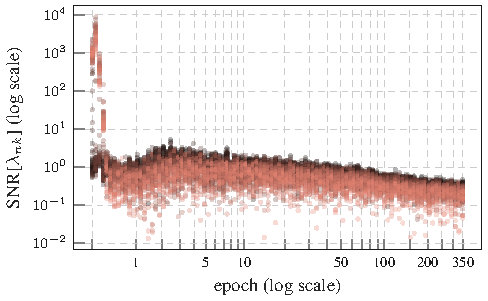
\includegraphics[width=\linewidth]{fig/exp13_plots/gammas_lambdas/cifar100_allcnnc_adam_lambdas.pdf}
    \end{minipage}
  \end{subfigure}
  \caption{\textbf{Directional SNRs (2).} SNR along each of the mini-batch
    \ggn{}'s top-$C$ eigenvectors during training for all test problems. At fixed
    epoch, the SNR for the most curved direction is shown in
    {\protect\tikz{\protect\draw[white,fill={light_red},line width=0mm] (0,0)
        circle (.8ex);}} and for the least curved direction in
    {\protect\tikz{\protect\draw[white,fill={black}] (0,0) circle (.8ex);}}.
  } \label{vivit::fig:directional_derivatives_2}
\end{figure*}
%%% Local Variables:
%%% mode: latex
%%% TeX-master: "../../thesis"
%%% End:
